\documentclass[10pt,a4paper,titlepage]{jsarticle}
\usepackage{amsmath,amsfonts,amssymb,array,comment,mathtools,url,docmute}
\usepackage{longtable,booktabs,dcolumn,tabularx,mathtools,multirow,colortbl,xcolor}
\usepackage[dvipdfmx]{graphics}
\usepackage{bmpsize}
\usepackage{amsthm}
\usepackage{enumitem}
\setlistdepth{20}
\renewlist{itemize}{itemize}{20}
\setlist[itemize]{label=•}
\renewlist{enumerate}{enumerate}{20}
\setlist[enumerate]{label=\arabic*.}
\setcounter{MaxMatrixCols}{20}
\setcounter{tocdepth}{3}
\newcommand{\rotin}{\text{\rotatebox[origin=c]{90}{$\in $}}}
\newcommand{\amap}[6]{\text{\raisebox{-0.7cm}{\begin{tikzpicture} 
  \node (a) at (0, 1) {$\textstyle{#2}$};
  \node (b) at (#6, 1) {$\textstyle{#3}$};
  \node (c) at (0, 0) {$\textstyle{#4}$};
  \node (d) at (#6, 0) {$\textstyle{#5}$};
  \node (x) at (0, 0.5) {$\rotin $};
  \node (x) at (#6, 0.5) {$\rotin $};
  \draw[->] (a) to node[xshift=0pt, yshift=7pt] {$\textstyle{\scriptstyle{#1}}$} (b);
  \draw[|->] (c) to node[xshift=0pt, yshift=7pt] {$\textstyle{\scriptstyle{#1}}$} (d);
\end{tikzpicture}}}}
\newcommand{\twomaps}[9]{\text{\raisebox{-0.7cm}{\begin{tikzpicture} 
  \node (a) at (0, 1) {$\textstyle{#3}$};
  \node (b) at (#9, 1) {$\textstyle{#4}$};
  \node (c) at (#9+#9, 1) {$\textstyle{#5}$};
  \node (d) at (0, 0) {$\textstyle{#6}$};
  \node (e) at (#9, 0) {$\textstyle{#7}$};
  \node (f) at (#9+#9, 0) {$\textstyle{#8}$};
  \node (x) at (0, 0.5) {$\rotin $};
  \node (x) at (#9, 0.5) {$\rotin $};
  \node (x) at (#9+#9, 0.5) {$\rotin $};
  \draw[->] (a) to node[xshift=0pt, yshift=7pt] {$\textstyle{\scriptstyle{#1}}$} (b);
  \draw[|->] (d) to node[xshift=0pt, yshift=7pt] {$\textstyle{\scriptstyle{#2}}$} (e);
  \draw[->] (b) to node[xshift=0pt, yshift=7pt] {$\textstyle{\scriptstyle{#1}}$} (c);
  \draw[|->] (e) to node[xshift=0pt, yshift=7pt] {$\textstyle{\scriptstyle{#2}}$} (f);
\end{tikzpicture}}}}
\renewcommand{\thesection}{第\arabic{section}部}
\renewcommand{\thesubsection}{\arabic{section}.\arabic{subsection}}
\renewcommand{\thesubsubsection}{\arabic{section}.\arabic{subsection}.\arabic{subsubsection}}
\everymath{\displaystyle}
\allowdisplaybreaks[4]
\usepackage{vtable}
\theoremstyle{definition}
\newtheorem{thm}{定理}[subsection]
\newtheorem*{thm*}{定理}
\newtheorem{dfn}{定義}[subsection]
\newtheorem*{dfn*}{定義}
\newtheorem{axs}[dfn]{公理}
\newtheorem*{axs*}{公理}
\renewcommand{\headfont}{\bfseries}
\makeatletter
  \renewcommand{\section}{%
    \@startsection{section}{1}{\z@}%
    {\Cvs}{\Cvs}%
    {\normalfont\huge\headfont\raggedright}}
\makeatother
\makeatletter
  \renewcommand{\subsection}{%
    \@startsection{subsection}{2}{\z@}%
    {0.5\Cvs}{0.5\Cvs}%
    {\normalfont\LARGE\headfont\raggedright}}
\makeatother
\makeatletter
  \renewcommand{\subsubsection}{%
    \@startsection{subsubsection}{3}{\z@}%
    {0.4\Cvs}{0.4\Cvs}%
    {\normalfont\Large\headfont\raggedright}}
\makeatother
\makeatletter
\renewenvironment{proof}[1][\proofname]{\par
  \pushQED{\qed}%
  \normalfont \topsep6\p@\@plus6\p@\relax
  \trivlist
  \item\relax
  {
  #1\@addpunct{.}}\hspace\labelsep\ignorespaces
}{%
  \popQED\endtrivlist\@endpefalse
}
\makeatother
\renewcommand{\proofname}{\textbf{証明}}
\usepackage{tikz,graphics}
\usepackage[dvipdfmx]{hyperref}
\usepackage{pxjahyper}
\hypersetup{
 setpagesize=false,
 bookmarks=true,
 bookmarksdepth=tocdepth,
 bookmarksnumbered=true,
 colorlinks=false,
 pdftitle={},
 pdfsubject={},
 pdfauthor={},
 pdfkeywords={}}
\title{解析学 暫定版}
\author{@k74226197Y126}
\begin{document}
\maketitle
\pagenumbering{roman}
\section*{はじめに}
\documentclass[a4paper]{jsarticle}
\usepackage{amsmath,amsfonts,amssymb,array,comment,mathtools,url,docmute}
\usepackage{longtable,booktabs,dcolumn,tabularx,mathtools,multirow,colortbl,xcolor}
\usepackage[dvipdfmx]{graphics}
\usepackage{bmpsize}
\usepackage{amsthm}
\usepackage{enumitem}
\setlistdepth{20}
\renewlist{itemize}{itemize}{20}
\setlist[itemize]{label=•}
\renewlist{enumerate}{enumerate}{20}
\setlist[enumerate]{label=\arabic*.}
\setcounter{MaxMatrixCols}{20}
\setcounter{tocdepth}{3}
\newcommand{\rotin}{\text{\rotatebox[origin=c]{90}{$\in $}}}
\newcommand{\amap}[6]{\text{\raisebox{-0.7cm}{\begin{tikzpicture} 
  \node (a) at (0, 1) {$\textstyle{#2}$};
  \node (b) at (#6, 1) {$\textstyle{#3}$};
  \node (c) at (0, 0) {$\textstyle{#4}$};
  \node (d) at (#6, 0) {$\textstyle{#5}$};
  \node (x) at (0, 0.5) {$\rotin $};
  \node (x) at (#6, 0.5) {$\rotin $};
  \draw[->] (a) to node[xshift=0pt, yshift=7pt] {$\textstyle{\scriptstyle{#1}}$} (b);
  \draw[|->] (c) to node[xshift=0pt, yshift=7pt] {$\textstyle{\scriptstyle{#1}}$} (d);
\end{tikzpicture}}}}
\newcommand{\twomaps}[9]{\text{\raisebox{-0.7cm}{\begin{tikzpicture} 
  \node (a) at (0, 1) {$\textstyle{#3}$};
  \node (b) at (#9, 1) {$\textstyle{#4}$};
  \node (c) at (#9+#9, 1) {$\textstyle{#5}$};
  \node (d) at (0, 0) {$\textstyle{#6}$};
  \node (e) at (#9, 0) {$\textstyle{#7}$};
  \node (f) at (#9+#9, 0) {$\textstyle{#8}$};
  \node (x) at (0, 0.5) {$\rotin $};
  \node (x) at (#9, 0.5) {$\rotin $};
  \node (x) at (#9+#9, 0.5) {$\rotin $};
  \draw[->] (a) to node[xshift=0pt, yshift=7pt] {$\textstyle{\scriptstyle{#1}}$} (b);
  \draw[|->] (d) to node[xshift=0pt, yshift=7pt] {$\textstyle{\scriptstyle{#2}}$} (e);
  \draw[->] (b) to node[xshift=0pt, yshift=7pt] {$\textstyle{\scriptstyle{#1}}$} (c);
  \draw[|->] (e) to node[xshift=0pt, yshift=7pt] {$\textstyle{\scriptstyle{#2}}$} (f);
\end{tikzpicture}}}}
\renewcommand{\thesection}{第\arabic{section}部}
\renewcommand{\thesubsection}{\arabic{section}.\arabic{subsection}}
\renewcommand{\thesubsubsection}{\arabic{section}.\arabic{subsection}.\arabic{subsubsection}}
\everymath{\displaystyle}
\allowdisplaybreaks[4]
\usepackage{vtable}
\theoremstyle{definition}
\newtheorem{thm}{定理}[subsection]
\newtheorem*{thm*}{定理}
\newtheorem{dfn}{定義}[subsection]
\newtheorem*{dfn*}{定義}
\newtheorem{axs}[dfn]{公理}
\newtheorem*{axs*}{公理}
\renewcommand{\headfont}{\bfseries}
\makeatletter
  \renewcommand{\section}{%
    \@startsection{section}{1}{\z@}%
    {\Cvs}{\Cvs}%
    {\normalfont\huge\headfont\raggedright}}
\makeatother
\makeatletter
  \renewcommand{\subsection}{%
    \@startsection{subsection}{2}{\z@}%
    {0.5\Cvs}{0.5\Cvs}%
    {\normalfont\LARGE\headfont\raggedright}}
\makeatother
\makeatletter
  \renewcommand{\subsubsection}{%
    \@startsection{subsubsection}{3}{\z@}%
    {0.4\Cvs}{0.4\Cvs}%
    {\normalfont\Large\headfont\raggedright}}
\makeatother
\makeatletter
\renewenvironment{proof}[1][\proofname]{\par
  \pushQED{\qed}%
  \normalfont \topsep6\p@\@plus6\p@\relax
  \trivlist
  \item\relax
  {
  #1\@addpunct{.}}\hspace\labelsep\ignorespaces
}{%
  \popQED\endtrivlist\@endpefalse
}
\makeatother
\renewcommand{\proofname}{\textbf{証明}}
\usepackage{tikz,graphics}
\usepackage[dvipdfmx]{hyperref}
\usepackage{pxjahyper}
\hypersetup{
 setpagesize=false,
 bookmarks=true,
 bookmarksdepth=tocdepth,
 bookmarksnumbered=true,
 colorlinks=false,
 pdftitle={},
 pdfsubject={},
 pdfauthor={},
 pdfkeywords={}}
\begin{document}
この.pdfファイルはもともと一学生が勉強のため、特に、自分の言葉で整理するために作成したものです。そのため、比較的行間は狭めになっております。そこで、他に私が勉強している内容を勉強している方がある箇所などで悩んだときに、参考になるかと思い公開させていただきました。そのこともあって、参考文献を詳細に書き章末にまとめてみました。ぜひ、参考文献リストもご活用してみるといいかもしれません。また、公開した他の理由として、誤植や間違い、不適切な表現、紛らわしい表現を自分でも探しておりますが、いかんせん大変なので、あえて公開することで誰かが探してくれるかもしれないというのもございます。\par
この.pdfファイルは一学生が勉強のため作成したもので監修を受けたわけではないので、正確性については保証できなく誤植や間違い、不適切な表現、紛らわしい表現があるかもしれません。誤植も今まで多数見つかってきております。論理の誤りは、書籍の定義や定理の主張に気を配っているので、少なめかもしれませんが、ないとは言い切れません。もし、そのようなものがございましたら、ご連絡していただければ幸いです。また、記号や言い回しで独特な箇所があり見苦しい箇所もあるかと思います。これも深刻であれば、可能な限り対応したいと考えております。また、参考文献に挙げられた書籍などと併読しておくこともお勧めいたします。\par
この.pdfファイル、および、そのソースコードの著作権はfrmrnthdr(Twitter:@k74226197Y126)にあるものといたします。.pdfファイルのダウンロード、印刷、勉強会での配布などでご利用していただいても問題ございませんし、そのソースコードのダウンロード、編集、改造をしていただいても問題ございません。ただ、自作発言、二次配布、商用利用はご遠慮くださいますようお願いいたします。\par
.pdfファイルで使用された.pngファイルや.pdfファイルのベースとなる.texファイル、プリアンブルに書くための.texファイル(macro.tex)も公開しております。先ほど述べられた通り自由にダウンロード、編集をしていただいても問題ございません。ただ、ローカルリポジトリの親フォルダに保存しております本文の.texファイルに関しましては、当面の間、非公開とさせていただきます。ご了承ください。
\end{document}\par
このPDF資料はまだ書きかけです。ただ、解析学の内容が広範囲にわたるため、完成はかなり厳しいかと思われます。今後の予定としては、特殊関数、広義積分、線積分、複素解析の拡充を考えております。また、極限、微分、積分の詳しい計算は微分積分学、Fourier級数展開、Fourier変換は関数解析(?)、vector 解析は微分幾何学に譲る予定です。面積分、体積分は解析学に残すか幾何学にまわすか悩み中です。お見苦しいところがあるかもしれませんが、ご理解のほどよろしくお願いいたします。
\tableofcontents
\clearpage
\pagenumbering{arabic}
\documentclass[a4paper]{jsarticle}
\setcounter{section}{0}
\usepackage{amsmath,amsfonts,amssymb,array,comment,mathtools,url,docmute}
\usepackage{longtable,booktabs,dcolumn,tabularx,mathtools,multirow,colortbl,xcolor}
\usepackage[dvipdfmx]{graphics}
\usepackage{bmpsize}
\usepackage{amsthm}
\usepackage{enumitem}
\setlistdepth{20}
\renewlist{itemize}{itemize}{20}
\setlist[itemize]{label=•}
\renewlist{enumerate}{enumerate}{20}
\setlist[enumerate]{label=\arabic*.}
\setcounter{MaxMatrixCols}{20}
\setcounter{tocdepth}{3}
\newcommand{\rotin}{\text{\rotatebox[origin=c]{90}{$\in $}}}
\newcommand{\amap}[6]{\text{\raisebox{-0.7cm}{\begin{tikzpicture} 
  \node (a) at (0, 1) {$\textstyle{#2}$};
  \node (b) at (#6, 1) {$\textstyle{#3}$};
  \node (c) at (0, 0) {$\textstyle{#4}$};
  \node (d) at (#6, 0) {$\textstyle{#5}$};
  \node (x) at (0, 0.5) {$\rotin $};
  \node (x) at (#6, 0.5) {$\rotin $};
  \draw[->] (a) to node[xshift=0pt, yshift=7pt] {$\textstyle{\scriptstyle{#1}}$} (b);
  \draw[|->] (c) to node[xshift=0pt, yshift=7pt] {$\textstyle{\scriptstyle{#1}}$} (d);
\end{tikzpicture}}}}
\newcommand{\twomaps}[9]{\text{\raisebox{-0.7cm}{\begin{tikzpicture} 
  \node (a) at (0, 1) {$\textstyle{#3}$};
  \node (b) at (#9, 1) {$\textstyle{#4}$};
  \node (c) at (#9+#9, 1) {$\textstyle{#5}$};
  \node (d) at (0, 0) {$\textstyle{#6}$};
  \node (e) at (#9, 0) {$\textstyle{#7}$};
  \node (f) at (#9+#9, 0) {$\textstyle{#8}$};
  \node (x) at (0, 0.5) {$\rotin $};
  \node (x) at (#9, 0.5) {$\rotin $};
  \node (x) at (#9+#9, 0.5) {$\rotin $};
  \draw[->] (a) to node[xshift=0pt, yshift=7pt] {$\textstyle{\scriptstyle{#1}}$} (b);
  \draw[|->] (d) to node[xshift=0pt, yshift=7pt] {$\textstyle{\scriptstyle{#2}}$} (e);
  \draw[->] (b) to node[xshift=0pt, yshift=7pt] {$\textstyle{\scriptstyle{#1}}$} (c);
  \draw[|->] (e) to node[xshift=0pt, yshift=7pt] {$\textstyle{\scriptstyle{#2}}$} (f);
\end{tikzpicture}}}}
\renewcommand{\thesection}{第\arabic{section}部}
\renewcommand{\thesubsection}{\arabic{section}.\arabic{subsection}}
\renewcommand{\thesubsubsection}{\arabic{section}.\arabic{subsection}.\arabic{subsubsection}}
\everymath{\displaystyle}
\allowdisplaybreaks[4]
\usepackage{vtable}
\theoremstyle{definition}
\newtheorem{thm}{定理}[subsection]
\newtheorem*{thm*}{定理}
\newtheorem{dfn}{定義}[subsection]
\newtheorem*{dfn*}{定義}
\newtheorem{axs}[dfn]{公理}
\newtheorem*{axs*}{公理}
\renewcommand{\headfont}{\bfseries}
\makeatletter
  \renewcommand{\section}{%
    \@startsection{section}{1}{\z@}%
    {\Cvs}{\Cvs}%
    {\normalfont\huge\headfont\raggedright}}
\makeatother
\makeatletter
  \renewcommand{\subsection}{%
    \@startsection{subsection}{2}{\z@}%
    {0.5\Cvs}{0.5\Cvs}%
    {\normalfont\LARGE\headfont\raggedright}}
\makeatother
\makeatletter
  \renewcommand{\subsubsection}{%
    \@startsection{subsubsection}{3}{\z@}%
    {0.4\Cvs}{0.4\Cvs}%
    {\normalfont\Large\headfont\raggedright}}
\makeatother
\makeatletter
\renewenvironment{proof}[1][\proofname]{\par
  \pushQED{\qed}%
  \normalfont \topsep6\p@\@plus6\p@\relax
  \trivlist
  \item\relax
  {
  #1\@addpunct{.}}\hspace\labelsep\ignorespaces
}{%
  \popQED\endtrivlist\@endpefalse
}
\makeatother
\renewcommand{\proofname}{\textbf{証明}}
\usepackage{tikz,graphics}
\usepackage[dvipdfmx]{hyperref}
\usepackage{pxjahyper}
\hypersetup{
 setpagesize=false,
 bookmarks=true,
 bookmarksdepth=tocdepth,
 bookmarksnumbered=true,
 colorlinks=false,
 pdftitle={},
 pdfsubject={},
 pdfauthor={},
 pdfkeywords={}}
\begin{document}
\section{実数論}
ここでは、自然数の存在を認めたうえで、実数の構成について、いくらか雑ではあるものの最も手っ取り早い方法を述べよう。なお、必要な知識については集合と写像のみで仮定しておこう。そのあと、複素数$\mathbb{C}$を$\mathbb{R}^2$と同一視して導入する。また、これの拡張としてvectorや行列も導入する。このあと、解析学で基本的な道具となる極限を位相空間論に近い立場から、詳しくいえば、近傍系を導入してから論じることにする。なお、意欲のある読者が位相空間論について興味を持ったらば、他の書籍をみることを勧める。このときに無限大という概念も導入する。これに基づき、ほとんどの極限は点列の極限に帰着できるので、まずは点列の極限を述べ、これの応用として級数の収束や関数列の極限も述べよう。
\end{document}
\documentclass[dvipdfmx]{jsarticle}
\setcounter{section}{1}
\setcounter{subsection}{0}
\usepackage{amsmath,amsfonts,amssymb,array,comment,mathtools,url,docmute}
\usepackage{longtable,booktabs,dcolumn,tabularx,mathtools,multirow,colortbl,xcolor}
\usepackage[dvipdfmx]{graphics}
\usepackage{bmpsize}
\usepackage{amsthm}
\usepackage{enumitem}
\setlistdepth{20}
\renewlist{itemize}{itemize}{20}
\setlist[itemize]{label=•}
\renewlist{enumerate}{enumerate}{20}
\setlist[enumerate]{label=\arabic*.}
\setcounter{MaxMatrixCols}{20}
\setcounter{tocdepth}{3}
\newcommand{\rotin}{\text{\rotatebox[origin=c]{90}{$\in $}}}
\newcommand{\amap}[6]{\text{\raisebox{-0.7cm}{\begin{tikzpicture} 
  \node (a) at (0, 1) {$\textstyle{#2}$};
  \node (b) at (#6, 1) {$\textstyle{#3}$};
  \node (c) at (0, 0) {$\textstyle{#4}$};
  \node (d) at (#6, 0) {$\textstyle{#5}$};
  \node (x) at (0, 0.5) {$\rotin $};
  \node (x) at (#6, 0.5) {$\rotin $};
  \draw[->] (a) to node[xshift=0pt, yshift=7pt] {$\textstyle{\scriptstyle{#1}}$} (b);
  \draw[|->] (c) to node[xshift=0pt, yshift=7pt] {$\textstyle{\scriptstyle{#1}}$} (d);
\end{tikzpicture}}}}
\newcommand{\twomaps}[9]{\text{\raisebox{-0.7cm}{\begin{tikzpicture} 
  \node (a) at (0, 1) {$\textstyle{#3}$};
  \node (b) at (#9, 1) {$\textstyle{#4}$};
  \node (c) at (#9+#9, 1) {$\textstyle{#5}$};
  \node (d) at (0, 0) {$\textstyle{#6}$};
  \node (e) at (#9, 0) {$\textstyle{#7}$};
  \node (f) at (#9+#9, 0) {$\textstyle{#8}$};
  \node (x) at (0, 0.5) {$\rotin $};
  \node (x) at (#9, 0.5) {$\rotin $};
  \node (x) at (#9+#9, 0.5) {$\rotin $};
  \draw[->] (a) to node[xshift=0pt, yshift=7pt] {$\textstyle{\scriptstyle{#1}}$} (b);
  \draw[|->] (d) to node[xshift=0pt, yshift=7pt] {$\textstyle{\scriptstyle{#2}}$} (e);
  \draw[->] (b) to node[xshift=0pt, yshift=7pt] {$\textstyle{\scriptstyle{#1}}$} (c);
  \draw[|->] (e) to node[xshift=0pt, yshift=7pt] {$\textstyle{\scriptstyle{#2}}$} (f);
\end{tikzpicture}}}}
\renewcommand{\thesection}{第\arabic{section}部}
\renewcommand{\thesubsection}{\arabic{section}.\arabic{subsection}}
\renewcommand{\thesubsubsection}{\arabic{section}.\arabic{subsection}.\arabic{subsubsection}}
\everymath{\displaystyle}
\allowdisplaybreaks[4]
\usepackage{vtable}
\theoremstyle{definition}
\newtheorem{thm}{定理}[subsection]
\newtheorem*{thm*}{定理}
\newtheorem{dfn}{定義}[subsection]
\newtheorem*{dfn*}{定義}
\newtheorem{axs}[dfn]{公理}
\newtheorem*{axs*}{公理}
\renewcommand{\headfont}{\bfseries}
\makeatletter
  \renewcommand{\section}{%
    \@startsection{section}{1}{\z@}%
    {\Cvs}{\Cvs}%
    {\normalfont\huge\headfont\raggedright}}
\makeatother
\makeatletter
  \renewcommand{\subsection}{%
    \@startsection{subsection}{2}{\z@}%
    {0.5\Cvs}{0.5\Cvs}%
    {\normalfont\LARGE\headfont\raggedright}}
\makeatother
\makeatletter
  \renewcommand{\subsubsection}{%
    \@startsection{subsubsection}{3}{\z@}%
    {0.4\Cvs}{0.4\Cvs}%
    {\normalfont\Large\headfont\raggedright}}
\makeatother
\makeatletter
\renewenvironment{proof}[1][\proofname]{\par
  \pushQED{\qed}%
  \normalfont \topsep6\p@\@plus6\p@\relax
  \trivlist
  \item\relax
  {
  #1\@addpunct{.}}\hspace\labelsep\ignorespaces
}{%
  \popQED\endtrivlist\@endpefalse
}
\makeatother
\renewcommand{\proofname}{\textbf{証明}}
\usepackage{tikz,graphics}
\usepackage[dvipdfmx]{hyperref}
\usepackage{pxjahyper}
\hypersetup{
 setpagesize=false,
 bookmarks=true,
 bookmarksdepth=tocdepth,
 bookmarksnumbered=true,
 colorlinks=false,
 pdftitle={},
 pdfsubject={},
 pdfauthor={},
 pdfkeywords={}}
\begin{document}
%\hypertarget{ux5b9fux6570}{%
\subsection{実数}%\label{ux5b9fux6570}}
\subsubsection{群}%\label{ux7fa4-1}}
\begin{axs}[群の公理]
空集合でない集合$G$に対し算法$*:G \times G \rightarrow G;(a,b) \mapsto a*b$が与えられたとする。このとき、次の条件たちを満たす集合$G$と算法$*$を合わせて群といい、集合$G$は算法$*$に対し群をなすといい、$(G,*)$と書く。そのような集合$G$の元の個数が有限なら、その群$(G,*)$は有限群といい、その集合の濃度$\#G$をその群$(G,*)$の位数といい、$o(G,*)$と書く。逆に、その集合$G$の元の個数が無限ならば、その群$(G,*)$は無限群という。単位元$e$のみからなる群$\left( \left\{ e \right\},* \right)$を単位群という\footnote{余談ですが、集合$G$の1つの部分集合を$S$、$n$つの部分集合たちのうち1つを$S_{i}$、これの元の1つを$s_{i}$とおき、写像$f:\prod_{i} S_{i} \rightarrow S;\left( s_{i} \right)_{i} \mapsto f\left( s_{i} \right)_{i}$を考えるとき、紛らわしいことに集合$\left\{ f\left( s_{i} \right)_{i} \middle| \forall i\left\lbrack s_{i} \in S_{i} \right\rbrack \right\}$を$f\left( S_{i} \right)_{i}$と表記することがあります…。例えば、$S_{1}*S_{2}$、$a*S_{1}$などといった感じに。}。
\begin{itemize}
\item
  算法$*$について結合的である、即ち、$\forall a,b,c \in G$に対し、$(a*b)*c = a*(b*c)$が成り立つ。
\item
  $\exists b \in G\forall a \in G$に対し、$a*b = b*a = a$が成り立つ。この元$b$をその群$(G,*)$の単位元という。
\item
  $\forall a \in G\exists b \in G$に対し、$a*b = b*a = e$が成り立つ。この元$b$を$a$の逆元といい、$a^{- 1}$と書く。
\end{itemize}
さらに次の条件も満たす群$(G,*)$を特に可換群、Abel群という。
\begin{itemize}
\item
  算法$*$は可換的である、即ち、$\forall a,b \in G$に対し、$a*b = b*a$が成り立つ。
\end{itemize}
なお、$a*b = b*a$が成り立つような元々$a$、$b$は可換であるという。
\end{axs}
\begin{thm}\label{4.1.1.1}
群$(G,*)$について、その単位元$e$、その集合$G$の任意の元$a$の逆元$a^{- 1}$は一意的に存在する。
\end{thm}\par
これはいずれも背理法によって示される。
\begin{proof}
群$(G,*)$において、$\forall a \in G$に対し、$a*e = e*a = a$なるその集合$G$の元$e$とは異なる、$\forall a \in G$に対し、$a*e' = e'*a = a$なる元$e'$がその集合$G$に存在するとする。このとき、$e*e' = e$かつ$e*e' = e'$が成り立つので、$e = e'$が成り立つこととなり、仮定に矛盾する。よって、$\forall a \in G$に対し、$a*e = e*a = a$が成り立つようなその単位元$e$は一意的に存在する。\par
同様に、$\forall a \in G$に対し、$a*a^{- 1} = a^{- 1}*a = e$なるその集合$G$の元$a^{- 1}$とは異なる$a*b = b*a = e$なる元$b$がその集合$G$に存在するとする。このとき、次のようになり、
\begin{align*}
a^{- 1} &= a^{- 1}*e\\
&= a^{- 1}*(a*b)\\
&= \left( a^{- 1}*a \right)*b\\
&= e*b = b
\end{align*}
仮定に矛盾する。よって、$\forall a \in G$に対し、$a*a^{- 1} = a^{- 1}*a = e$となる元$a^{- 1}$が一意的に存在する。
\end{proof}
\begin{thm}[簡易律]\label{4.1.1.2}
群$(G,*)$において、$\forall a,u,v \in G$に対し、次のことが成り立つ。
\begin{itemize}
\item
  $a*u = a*v$が成り立つなら、$u = v$が成り立つ。
\item
  $u*a = v*a$が成り立つなら、$u = v$が成り立つ。
\end{itemize}
\par
この性質を簡易律という。
\end{thm}
\begin{proof}
群$(G,*)$が与えられたとする。$\forall a,u,v \in G$に対し、$a*u = a*v$が成り立つなら、次式が成り立つかつ、
\begin{align*}
a^{- 1}*(a*u) &= \left( a^{- 1}*a \right)*u\\
&= e*u = u
\end{align*}
次式が成り立つので、
\begin{align*}
a^{- 1}*(a*u) &= a^{- 1}*(a*v)\\
&= \left( a^{- 1}*a \right)*v\\
&= e*v = v
\end{align*}
$u = v$が得られる。\par
同様にして、$u*a = v*a$が成り立つなら、$u = v$が成り立つことが示される。
\end{proof}
\begin{thm}\label{4.1.1.3}
群$(G,*)$について、$\forall a,b \in G$に対し、$(a*b)^{- 1} = b^{- 1}*a^{- 1}$が成り立つ。
\end{thm}
\begin{proof}
群$(G,*)$が与えられたとする。$\forall a,b \in G$に対し、$(a*b)*(a*b)^{- 1} = e$が成り立つかつ、次式が成り立つので、
\begin{align*}
(a*b)*\left( b^{- 1}*a^{- 1} \right) &= \left( a*\left( b*b^{- 1} \right) \right)*a^{- 1}\\
&= (a*e)*a^{- 1}\\
&= a*a^{- 1} = e
\end{align*}
$(a*b)*(a*b)^{- 1} = (a*b)*\left( b^{- 1}*a^{- 1} \right)$が得られ、したがって、簡易律により$(a*b)^{- 1} = b^{- 1}*a^{- 1}$が成り立つ。
\end{proof}
\begin{dfn}
群$(G,*)$をなす集合$G$の元$a$について$m,n \in \mathbb{Z}$に対し次式のように記法を定める。
\begin{align*}
a^{m}*a^{n} &= a^{m + n}\\
\left( a^{m} \right)^{n} &= a^{mn}\\
(a*b)^{n} &= a^{n}*b^{n}\ \mathrm{if}\ a*b = b*a
\end{align*}
\end{dfn}
\begin{thm}\label{4.1.1.4}
群$(G,*)$について、$\forall a \in G\forall n \in \mathbb{N}$に対し、次式たちが成り立つ。
\begin{align*}
a^{0} = e,\ \ a^{1} = a,\ \ a^{n + 1} = a^{n}*a,\ \ e^{- n} = e^{n} = e,\ \ a^{- n} = \left( a^{- 1} \right)^{n}
\end{align*}
\end{thm}
\begin{proof}
群$(G,*)$をなす集合$G$について、$\forall a \in G\forall n \in \mathbb{N}$に対し、次のようになる。
\begin{align*}
a^{0} &= e*a^{0}\\
&= \left( a^{0} \right)^{- 1}*a^{0}*a^{0}\\
&= \left( a^{0} \right)^{- 1}*a^{0 + 0}\\
&= \left( a^{0} \right)^{- 1}*a^{0}\\
&= e\\
a^{1} &= e*a^{1}\\
&= a*a^{- 1}*a^{1}\\
&= a*a^{- 1 + 1}\\
&= a*a^{0}\\
&= a*e = a\\
a^{n + 1} &= a^{n}*a^{1}\\
&= a^{n}*a
\end{align*}\par
また、上記の議論より$e^{- 1} = e^{0} = e^{1} = e$が成り立つ。$n = k$のとき、$e^{k} = e$と仮定しよう。$n = k + 1$のとき、次のようになる。
\begin{align*}
e^{k + 1} &= e^{k}*e^{1}\\
&= e*e\\
&= e
\end{align*}
逆に、$n = k$のとき、$e^{- k} = e$と仮定しよう。$n = k + 1$のとき、次のようになる。
\begin{align*}
e^{- (k + 1)} &= e^{- k - 1}\\
&= e^{- k}*e^{- 1}\\
&= e*e\\
&= e
\end{align*}
以上より数学的帰納法によって$\forall n \in \mathbb{Z}$に対し、次式が成り立つ。
\begin{align*}
e^{n} = e
\end{align*}\par
また、上記の議論により次のようになる。
\begin{align*}
a^{- n} &= a^{- n}*e\\
&= a^{- n}*\left( a^{- 1} \right)^{0}\\
&= a^{- n}*\left( a^{- 1} \right)^{- n + n}\\
&= a^{- n}*\left( a^{- 1} \right)^{- n}*\left( a^{- 1} \right)^{n}\\
&= \left( a*a^{- 1} \right)^{- n}*\left( a^{- 1} \right)^{n}\\
&= e^{- n}*\left( a^{- 1} \right)^{n}\\
&= e*\left( a^{- 1} \right)^{n}\\
&= \left( a^{- 1} \right)^{n}
\end{align*}
\end{proof}
\subsubsection{環}%\label{ux74b0-1}}
\begin{axs}[環の公理]
空集合でない集合$R$に対し2つの算法それぞれ加法$+ :R \times R \rightarrow R;(a,b) \mapsto a + b$、乗法$\cdot :R \times R \rightarrow R;(a,b) \mapsto ab$が与えられたとする。このとき、次の条件たちを満たす集合$R$を環という\footnote{ここから先は心象するのがほぼ不可能な分野になりますので、定義をよく読んでおくことをお勧めします。}。
\begin{itemize}
\item
  集合$R$は加法について可換群$(R, + )$をなす。
\item
  $\forall a,b,c \in R$に対し、$(ab)c = a(bc)$が成り立つ、即ち、乗法について結合的である。
\item
  $\exists e \in R\forall a \in R$に対し、$ae = ea = a$が成り立つ、即ち、乗法について集合$R$の単位元$e$が存在する。
\item
  $\forall a,b,c \in R$に対し、$a(b + c) = ab + ac$かつ$(a + b)c = ac + bc$が成り立つ、即ち、乗法は加法に対して両側から分配的である。
\end{itemize}
さらに、次の条件も満たす環$R$を特に可換環という。
\begin{itemize}
\item
  $\forall a,b \in R$に対し、$ab = ba$が成り立つ、即ち、乗法は可換的である。
\end{itemize}
\end{axs}
\begin{dfn}
可換群$(R, + )$において、その単位元を零元といい$0$と、逆元$a^{- 1}$を$- a$と、$\forall n \in \mathbb{Z}$に対し、元$a^{n}$を$na$と、乗法についての単位元$e$を$1$と書く。
\end{dfn}
\begin{thm}\label{4.1.1.5}
環$R$が与えられたとき、$\forall a \in R$に対し、$a0 = 0a = 0$が成り立つ。
\end{thm}
\begin{proof} 環$R$について、$\forall a \in R$に対し、次のようになるかつ、
\begin{align*}
0 &= a0 - a0\\
&= a(0 + 0) - a0\\
&= a0 + a0 - a0 = a0
\end{align*}
次のようになるので、
\begin{align*}
0 &= 0a - 0a\\
&= (0 + 0)a - 0a\\
&= 0a + 0a - 0a = 0a
\end{align*}
$a0 = 0a = 0$が成り立つ。
\end{proof}
\begin{dfn}
  環$R$について、$0 = 1$が成り立つとき、$\forall a \in R$に対し、$a = 1a = 0a = 0$が成り立ち$R = \left\{ 0 \right\}$が得られる。これを零環という。以下、環の元が2つ以上現れるのであれば、その環は零環でないので、断りがない場合、そうする。
\end{dfn}
\begin{dfn}
  環$R$について、$\exists a,b \in R$に対し、$a \neq 0$かつ$b \neq 0$が成り立つかつ、$ab = 0$が成り立つなら、それらの元々$a$、$b$をそれぞれ左零因子、右零因子といい、あわせて零因子という。これをもたない可換環を、即ち、その環$R$が可換環で、$\forall a,b \in R$に対し、$a \neq 0$かつ$b \neq 0$が成り立つなら、$ab \neq 0$が成り立つような環を整域という。
\end{dfn}
\begin{dfn}\label{体の定義}
  環$R$について、$\exists a,b \in R$に対し、$ab = 1$が成り立つなら、その元$a$を環$R$の可逆元、単元といい、その元$b$を逆元といい、後に示すように$a^{- 1}$、$\frac{1}{a}$などと書くことができる。以下、その元$a^{-1}$はその群$\left(R,+\right)$における逆元ではなくその可逆元$a$の積における逆元を意味するものとする。これにより、可逆元からなる集合は乗法について群をなし、$0$以外の元全てが可逆元であるような環を斜体といい、乗法について可換的な斜体を体といい、可換的でない斜体を非可換体という。
\end{dfn}\par
斜体を体、体を可換体というときもある。
\begin{thm}\label{4.1.1.6}
  環$R$の可逆元について、次のことが成り立つ。
  \begin{itemize}
  \item
    その環$R$が零環でなくその環$R$の元$a$が可逆元なら、これは$0$でない。
  \item 
    その環$R$の元$a$が可逆元なら、一意的に逆元${a}^{-1}$が定まる。
  \item
    その環$R$が斜体であるなら、零因子をもたない。
  \end{itemize}
\end{thm}
\begin{proof}
  環$R$について、$a \in R$が成り立ちその環$R$が零環でなくその元$a$が可逆元であり${a}^{-1} \in R$なる元${a}^{-1}$を$a$の逆元とする。$a = 0$が成り立つなら、$a{a}^{-1} = 0{a}^{-1} = 0 \neq 1$が成り立つので、可逆元の定義に矛盾する。よって$a \neq 0$が成り立つ。\par
  また、その環$R$の元$a$が可逆元でその元$a^{- 1}$でないその元$a$の逆元$b$が与えられたとするとき、次式が成り立つので、
  \begin{align*}
  {a}^{-1} &= {a}^{-1}1\\
  &= {a}^{-1}(ab)\\
  &= \left( {a}^{-1}a \right)b\\
  &= 1b = b
  \end{align*}
  仮定に矛盾する。よって、一意的に逆元${a}^{-1}$が定まる。\par
  環$R$が斜体であるなら、$0$以外の元全てが可逆元であるので、$\forall a,b \in R$に対し、$a \neq 0$かつ$b \neq 0$が成り立つなら、${a}^{-1},{b}^{-1} \in R$が成り立ち、したがって、次のようになる。
  \begin{align*}
  ab{b}^{-1}{a}^{-1} &= a1{a}^{-1}\\
  &= a{a}^{-1} = 1\\
  {b}^{-1}{a}^{-1}ab &= {b}^{-1}1b\\
  &= {b}^{-1}b = 1
  \end{align*}
  したがって、その元$ab$は可逆元であることになるので、$ab \neq 0$が成り立つ。ゆえに、その環$R$は零因子をもたない。
\end{proof}
\begin{thm}\label{4.1.1.7}
  環$R$の性質として、次のことが成り立つ。
  \begin{itemize}
    \item $\forall a\in R$に対し、$-(-a) =a$が成り立つ。
    \item $\forall a,b\in R$に対し、$a(-b)=(-a)b=-ab$が成り立つ。
    \item $\forall a,b\in R$に対し、$(-a)(-b)=ab$が成り立つ。
    \item $\forall a,b\in R$に対し、$a=0$または$b=0$が成り立つなら、$ab=0$が成り立つ。
    \item $\forall a,b\in R$に対し、$a=0$かつ$b=0$が成り立つなら、$a^2 +b^2 =0$が成り立つ。
    \item $\forall a\in R$に対し、その元$a$が可逆元なら、その元$-a$も可逆元で$(-a)^{-1} =-a^{-1}$が成り立つ。
    \item $\forall a\in R$に対し、それらの元々$a$、$b$が可逆元なら、その元$ab$も可逆元で$(ab)^{-1} =b^{-1} a^{-1}$が成り立つ。
  \end{itemize}
\end{thm}
\begin{proof} 環$R$が与えられたとき、$\forall a\in R$に対し、次のようになる。
  \begin{align*}
  - ( - a) &= 0 - ( - a)\\
  &= a - a - ( - a)\\
  &= a + ( - a) - ( - a)\\
  &= a + 0 = a
  \end{align*}\par
  $\forall a,b\in R$に対し、次のようになる。
  \begin{align*}
  a( - b) &= 0 + a( - b)\\
  &= - ab + ab + a( - b)\\
  &= - ab + a\left( b + ( - b) \right)\\
  &= - ab + a0\\
  &= - ab + 0\\
  &= - ab
  \end{align*}\par
  $\forall a,b\in R$に対し、次のようになる。
  \begin{align*}
  ( - a)b &= ( - a)b + 0\\
  &= ( - a)b + ab - ab\\
  &= \left( ( - a) + a \right)b - ab\\
  &= 0b - ab\\
  &= a - ab\\
  &= - ab
  \end{align*}\par
  $\forall a,b\in R$に対し、次のようになる。
  \begin{align*}
  ( - a)( - b) &= ( - a)( - b) + 0\\
  &= ( - a)( - b) + ( - a)b - ( - a)b\\
  &= ( - a)\left( ( - b) + b \right) - ( - ab)\\
  &= ( - a)0 + ab\\
  &= 0 + ab\\
  &= ab
  \end{align*}
  $\forall a,b\in R$に対し、$a=0$または$b=0$が成り立つなら、次のようになるので、
  \begin{align*}
  a = 0 \vee b = 0 &\Rightarrow ab = 0 \vee ab = 0\\
  &\Leftrightarrow ab = 0
  \end{align*}
  $ab=0$が成り立つ。\par
  $\forall a,b\in R$に対し、$a=0$かつ$b=0$が成り立つなら、次のようになるので、
  \begin{align*}
  a = 0 \land b = 0 &\Rightarrow a^{2} = 0 \land b^{2} = 0\\
  &\Rightarrow a^{2} + b^{2} = 0
  \end{align*}
  $a^2 +b^2 =0$が成り立つ。\par
  $\forall a\in R$に対し、その元$a$が可逆元なら、次のようになるので、
  \begin{align*}
  \left( -a^{-1} \right) \left(-a\right) &= a^{-1} a =1\\
  \left( -a\right) \left(-a^{-1} \right) &= aa^{-1} =1
  \end{align*}
  その元$-a$も可逆元で$(-a)^{-1} =-a^{-1}$が成り立つ。\par
  $\forall a\in R$に対し、それらの元々$a$、$b$が可逆元なら、次のようになるので、
  \begin{align*}
  \left( b^{-1} a^{-1} \right) \left(ab\right) &= b^{-1} \left( a^{-1} a\right) b \\
  &= b^{-1} 1 b =b^{-1} b =1\\
  \left(ab\right)\left( b^{-1} a^{-1} \right) &= a\left( bb^{-1} \right) a^{-1} \\
  &=a1a^{-1} =aa^{-1} =1
  \end{align*}
  その元$ab$も可逆元で$(ab)^{-1} =b^{-1} a^{-1}$が成り立つ。
\end{proof}
%\hypertarget{ux9806ux5e8fux4f53}{%
\subsubsection{順序体}%\label{ux9806ux5e8fux4f53}}
\begin{axs}[順序体の公理]
$\forall a,b,c,d \in O$に対し関係$a \leq b$を次の条件たちを満たすように定める。なお、$a \leq b$を$b \geq a$とも書く。上から1つ目から3つ目までの条件たちを満たす集合$O$を順序集合、順序集合であることに加えて上から4つ目の条件を満たす集合を全順序集合、集合$O$が体で次の条件を全て満たす集合を順序体という。
\begin{itemize}
\item
  $\forall a \in O$に対し、$a \leq a$が成り立つ。これを反射律という。
\item
  $\forall a,b \in O$に対し、$a \leq b$かつ$b \geq a$が成り立つなら、$a = b$が成り立つ。これを反対称律という。
\item
  $\forall a,b,c \in O$に対し、$a \leq b$かつ$b \leq c$が成り立つなら、$a \leq c$が成り立つ。これを推移律という。
\item
  $\forall a,b \in O$に対し、$a \leq b$または$b \leq a$が成り立つ。これを全順序性という。
\item
  $\forall a,b,c \in O$に対し、$a \leq b$が成り立つなら、$a + c \leq b + c$が成り立つ。
\item
  $\forall a,b \in O$に対し、$0 \leq a$かつ$0 \leq b$が成り立つなら、$0 \leq ab$が成り立つ。
\end{itemize}
\end{axs}
\begin{dfn}
$a \leq b$かつ$a \neq b$が成り立つことを$a < b$と書く。なお、$a < b$を$b > a$とも書く。
\end{dfn}
\begin{dfn}
$0 < a$、$a < 0$が成り立つとき、それぞれ$a$は正である、負であるという。
\end{dfn}
\begin{thm}\label{4.1.1.8} 順序体$O$が与えられたとき、次のことが成り立つ。
\begin{itemize}
\item
  $\forall a,b \in O$に対し、$a \leq b$が成り立つならそのときに限り、$a < b$または$a = b$が成り立つ。
\item
  $\forall a,b \in O$に対し、$a < b$または$a = b$または$b < a$が成り立つ。
\item
  $\forall a,b \in O$に対し、$a < b$かつ$a = b$が成り立つことはない。
\item
  $\forall a,b \in O$に対し、$a < b$かつ$b < a$が成り立つことはない。
\item
  $\forall a \in O$に対し、$0 \leq a$が成り立つならそのときに限り、$- a \leq 0$が成り立つ。
\item
  $\forall a \in O$に対し、$0 \leq a^{2} = ( - a)^{2}$が成り立つ。
\item
  $0 \neq 1$が成り立つなら、$0 < 1$が成り立つ。
\item
  $\forall a,b \in O$に対し、$a \leq b$が成り立つならそのときに限り、$0 \leq b - a$が成り立つ。
\item
  $\forall a,b \in O$に対し、$a^{2} + b^{2} = 0$が成り立つならそのときに限り、$a = 0$かつ$b = 0$が成り立つ。
\item
  $\forall a,b \in O$に対し、$ab = 0$が成り立つならそのときに限り、$a = 0$または$b = 0$が成り立つ。
\item
  $\forall a,b \in O$に対し、$a \leq b$が成り立つならそのときに限り、$- b \leq - a$が成り立つ。
\item
  $\forall a,b,c \in O$に対し、$a \leq b$かつ$c \leq 0$が成り立つなら、$bc \leq ac$が成り立つ。
\item
  $\forall a \in O$に対し、$0 < a$が成り立つなら、$0 < a^{- 1}$が成り立つ。
\item
  $\forall a,b,c,d \in O$に対し、$a \leq b$かつ$c \leq d$が成り立つなら、$a + c \leq b + d$が成り立つ。
\item
  $\forall a,b,c,d \in O$に対し、$a \leq b$かつ$c < d$が成り立つなら、$a + c < b + d$が成り立つ。
\item
  $\forall a,b \in O$に対し、$a < b$が成り立つなら、$a < c < b$なる元$c$がその順序体$O$に存在する。
\item
  $\forall a,b \in O$に対し、$\forall c \in O$に対し、$0 < c$が成り立つかつ、$a \leq b + c$が成り立つなら、$a \leq b$が成り立つ。
\item
  $\forall a \in O$に対し、$0 \leq a$が成り立つかつ、$\forall b \in O$に対し、$a < b$が成り立つなら、$a = 0$が成り立つ。
\end{itemize}
最後の性質は順序体の任意の元の近くにいくらでも別の元が存在することを示しており、この性質を稠密性といい集合$O$は稠密順序集合であるという。
\end{thm}
\begin{proof}
順序体$O$が与えられたとき、$\forall a,b \in O$に対し、次のようになるので、
\begin{align*}
a \leq b &\Leftrightarrow a \leq b \land \top\\ 
&\Leftrightarrow (a \leq b \vee a \leq b) \land (a \leq b \vee b \leq a)\\ 
&\Leftrightarrow a \leq b \vee (a \leq b \land b \leq a)\\ 
&\Leftrightarrow a \leq b \vee a = b\\ 
&\Leftrightarrow (a \leq b \vee a = b) \land \top\\ 
&\Leftrightarrow (a \leq b \vee a = b) \land (a \neq b \vee a = b)\\ 
&\Leftrightarrow (a \leq b \land a \neq b) \vee a = b\\ 
&\Leftrightarrow a < b \vee a = b
\end{align*}
$a \leq b$が成り立つならそのときに限り、$a < b$または$a = b$が成り立つ。\par
$\forall a,b \in O$に対し、次のようになるので、
\begin{align*}
a < b \vee a = b \vee b < a &\Leftrightarrow (a \leq b \land a \neq b) \vee a = b \vee (b \leq a \land a \neq b)\\ 
&\Leftrightarrow (a \leq b \vee a = b \vee b \leq a) \land (a \leq b \vee a = b \vee a \neq b) \\
&\quad \land (b \leq a \vee a = b \vee a \neq b) \land (a = b \vee a \neq b \vee a \neq b)\\ 
&\Leftrightarrow (a = b \vee \top) \land (a \leq b \vee \top) \land (b \leq a \vee \top) \land (a \neq b \vee \top)\\ 
&\Leftrightarrow \top \land \top \land \top \land \top \Leftrightarrow \top
\end{align*}
$a < b$または$a = b$または$b < a$が成り立つ。\par
$\forall a,b \in O$に対し、次のようになるので、
\begin{align*}
a < b \land a = b &\Leftrightarrow a \leq b \land a \neq b \land a = b\\ 
&\Leftrightarrow a \leq b \land \bot \Leftrightarrow \bot
\end{align*}
$a < b$かつ$a = b$が成り立つことはない。\par
$\forall a,b \in O$に対し、次のようになるので、
\begin{align*}
a < b \land b < a &\Leftrightarrow a \leq b \land a \neq b \land b \leq a \land a \neq b\\ 
&\Leftrightarrow a \neq b \land (a \leq b \land b \leq a)\\ 
&\Leftrightarrow a \neq b \land a = b \Leftrightarrow \bot
\end{align*}
$a < b$かつ$b < a$が成り立つことはない。\par
$\forall a \in O$に対し、次のようになるので、
\begin{align*}
0 \leq a &\Leftrightarrow 0 + ( - a) \leq a + ( - a)\\ 
&\Leftrightarrow - a \leq 0
\end{align*}
$0 \leq a$が成り立つならそのときに限り、$- a \leq 0$が成り立つ。\par
$\forall a \in O$に対し、次のようになるので、
\begin{align*}
\top &\Leftrightarrow a < 0 \vee a = 0 \vee 0 < a\\ 
&\Leftrightarrow (a < 0 \vee a = 0) \vee (0 < a \vee a = 0)\\ 
&\Leftrightarrow a \leq 0 \vee 0 \leq a\\ 
&\Leftrightarrow - ( - a) \leq 0 \vee 0 \leq a\\ 
&\Leftrightarrow 0 \leq - a \vee 0 \leq a\\ 
&\Leftrightarrow 0 \leq ( - a)^{2} \vee 0 \leq a^{2}\\ 
&\Leftrightarrow 0 \leq ( - a)^{2} = a^{2} \vee 0 \leq a^{2} = ( - a)^{2}\\ 
&\Leftrightarrow 0 \leq a^{2} = ( - a)^{2}
\end{align*}
$0 \leq a^{2} = ( - a)^{2}$が成り立つ。\par
$0 \neq 1$が成り立つなら、次のようになるので、
\begin{align*}
\top &\Leftrightarrow \top \land \top\\ 
&\Leftrightarrow 0 \leq 1^{2} = 1 \land 1 \neq 0\\ 
&\Leftrightarrow 0 \leq 1 \land 0 \neq 1\\ 
&\Leftrightarrow 0 < 1
\end{align*}
$0 < 1$が成り立つ。\par
$\forall a,b \in O$に対し、次のようになるので、
\begin{align*}
a \leq b &\Rightarrow a + ( - a) \leq b + ( - a)\\ 
&\Leftrightarrow 0 \leq b - a\\ 
0 \leq b - a &\Rightarrow a \leq b - a + a = b
\end{align*}
$a \leq b$が成り立つならそのときに限り、$0 \leq b - a$が成り立つ。\par
$\forall a,b \in O$に対し、次のようになるので、
\begin{align*}
a^{2} + b^{2} = 0 &\Rightarrow a^{2} = - b^{2}\\ 
&\Leftrightarrow 0 \leq a^{2} = - b^{2}\\ 
&\Leftrightarrow a^{2} = - b^{2} \land 0 \leq b^{2} \leq 0\\ 
&\Leftrightarrow a^{2} = - b^{2} \land \left( b^{2} = 0 \vee 0 < b^{2} \right) \land \left( b^{2} = 0 \vee b^{2} < 0 \right)\\ 
&\Leftrightarrow a^{2} = - b^{2} \land \left( b^{2} = 0 \vee \left( 0 < b^{2} \land 0 < b^{2} \right) \right)\\ 
&\Leftrightarrow a^{2} = - b^{2} \land b^{2} = 0\\ 
&\Leftrightarrow a^{2} = 0 \land b^{2} = 0\\ 
&\Leftrightarrow a = 0 \land b = 0\\ 
a = 0 \land b = 0 &\Rightarrow a^{2} = 0 \land b^{2} = 0\\ 
&\Rightarrow a^{2} + b^{2} = 0 + 0 = 0
\end{align*}
$a^{2} + b^{2} = 0$が成り立つならそのときに限り、$a = 0$かつ$b = 0$が成り立つ。\par
$\forall a,b \in O$に対し、次のようになるので、
\begin{align*}
\neg(ab \neq 0 \vee a = 0 \vee b = 0) &\Leftrightarrow ab = 0 \land a \neq 0 \land b \neq 0\\ 
&\Rightarrow ab = 0 \land ab \neq 0 \Leftrightarrow \bot
\end{align*}
背理法により$ab = 0$が成り立つなら、$a = 0$または$b = 0$が成り立つ。また、$a = 0$または$b = 0$が成り立つなら、$ab = 0$が成り立つので、$ab = 0$が成り立つならそのときに限り、$a = 0$または$b = 0$が成り立つ。\par
$\forall a,b \in O$に対し、次のようになるので、
\begin{align*}
a \leq b &\Leftrightarrow 0 \leq b - a = - a + b = - a - ( - b)\\ 
&\Leftrightarrow - b \leq - a
\end{align*}
$a \leq b$が成り立つならそのときに限り、$- b \leq - a$が成り立つ。\par
$\forall a,b,c \in O$に対し、次のようになるので、
\begin{align*}
a \leq b \land c = - ( - c) \leq 0 &\Leftrightarrow a \leq b \land 0 \leq - c\\ 
&\Rightarrow a( - c) = - ac \leq b( - c) = - bc\\ 
&\Leftrightarrow bc \leq ac
\end{align*}
$a \leq b$かつ$c \leq 0$が成り立つなら、$bc \leq ac$が成り立つ。
$\forall a \in O$に対し、次のようになるので、
\begin{align*}
\neg\left( 0 < a \Rightarrow 0 < a^{- 1} \right) &\Leftrightarrow \neg\left( \neg 0 < a \vee 0 < a^{- 1} \right)\\ 
&\Leftrightarrow \neg\neg 0 < a \land \neg 0 < a^{- 1}\\ 
&\Leftrightarrow 0 < a \land a^{- 1} \leq 0\\ 
&\Leftrightarrow 0 < a \land \left( a^{- 1} = 0 \vee a^{- 1} < 0 \right)\\ 
&\Leftrightarrow \left( 0 < a \land a^{- 1} = 0 \right) \vee \left( 0 < a \land a^{- 1} < 0 \right)\\ 
&\Leftrightarrow \left( 0 < a \land aaa^{- 1} = a1 = a = aa0 = 0 \right) \vee 0 < \left( - a^{- 1} \right)a = - a^{- 1}a = - 1\\ 
&\Leftrightarrow (0 < a \land a = 0) \vee 1 < 0\\ 
&\Leftrightarrow \bot \vee \bot \Leftrightarrow \bot
\end{align*}
$0 < a$が成り立つなら、$0 < a^{- 1}$が成り立つ。\par
$\forall a,b,c,d \in O$に対し、次のようになるので、
\begin{align*}
a \leq b \land c \leq d &\Leftrightarrow a + c \leq b + c \land b + c \leq b + d\\ 
&\Leftrightarrow a + c \leq b + c \leq b + d\\ 
&\Rightarrow a + c \leq b + d
\end{align*}
$a \leq b$かつ$c \leq d$が成り立つなら、$a + c \leq b + d$が成り立つ。\par
$\forall a,b,c,d \in O$に対し、次のようになるので、
\begin{align*}
a \leq b \land c < d &\Leftrightarrow a + c \leq b + c \land b + c < b + d\\ 
&\Leftrightarrow a + c \leq b + c < b + d\\ 
&\Rightarrow a + c < b + d
\end{align*}
$a \leq b$かつ$c < d$が成り立つなら、$a + c < b + d$が成り立つ。\par
$\forall a,b \in O$に対し、$a < b$が成り立つなら、$\frac{1}{2}a < \frac{1}{2}b$が成り立つので、次式が成り立つ。
\begin{align*}
a = \frac{1}{2}a + \frac{1}{2}a < \frac{1}{2}a + \frac{1}{2}b < \frac{1}{2}b + \frac{1}{2}b = b
\end{align*}
ゆえに、$a < c < b$なる元$c$がその順序体$O$に存在する。\par
$\forall a,b \in O$に対し、$\forall c \in O$に対し、$0 < c$が成り立つかつ、$a \leq b + c$が成り立つなら、$a \leq b$が成り立つことの否定は、$\exists a,b \in O$に対し、$\forall c \in O$に対し、$0 < c$が成り立つかつ、$a \leq b + c$が成り立つかつ、$b < a$が成り立つことである。このとき、$b < a$が成り立つならそのときに限り、$0 < a - b$が成り立ち、あるその順序体$O$の元$c$が存在して、$0 < c < a - b$が成り立つ。したがって、次のようになる。
\begin{align*}
&\quad \forall c \in O[ 0 < c \land a \leq b + c] \land \exists c \in O[ 0 < c < a - b]\\ 
&\Rightarrow \forall c \in O[ 0 < c] \land \forall c \in O[ a \leq b + c] \land \exists c \in O[ c < a - b]\\ 
&\Leftrightarrow \forall c \in O[ 0 < c] \land \forall c \in O[ a \leq b + c] \land \exists c \in O[ b + c < a]\\ 
&\Leftrightarrow \forall c \in O[ 0 < c] \land \forall c \in O[ a \leq b + c] \land \exists c \in O\left[ \neg(a \leq b + c) \right]\\ 
&\Leftrightarrow \forall c \in O[ 0 < c] \land \forall c \in O[ a \leq b + c] \land \neg\forall c \in O[ a \leq b + c]\\ 
&\Leftrightarrow \forall c \in O[ 0 < c] \land \bot \Leftrightarrow \bot
\end{align*}
背理法によりしたがって、$\forall a,b \in O$に対し、$\forall c \in O$に対し、$0 < c$が成り立つかつ、$a \leq b + c$が成り立つなら、$a \leq b$が成り立つ。\par
$\exists a \in O$に対し、$0 \leq a \land \forall b \in O[ a < b] \land a \neq 0$が成り立つと仮定すると、$0 < a$が成り立つが、$\exists c \in O[ 0 < a \Rightarrow 0 < c < a]$より$c < a$が成り立つようなその順序体$O$の元$c$が存在することになり、したがって、$\forall b \in O[ a < b]$に矛盾する。よって、$0 \leq a$が成り立つかつ、$\forall b \in O$に対し、$a < b$が成り立つなら、$a = 0$が成り立つ。
\end{proof}
%\hypertarget{ux6700ux5927ux5143ux3068ux6700ux5c0fux5143}{%
\subsubsection{最大元と最小元}%\label{ux6700ux5927ux5143ux3068ux6700ux5c0fux5143}}
\begin{dfn}
順序体$O$の部分集合$A$について、これを順序集合$(A, \leq )$とみたときのその集合$A$の最大元、即ち、$\forall a \in A$に対し、$a \leq m$が成り立つその集合$A$の元$m$をその集合の最大元という。同様にして、これを順序集合$(A, \leq )$とみたときのその集合$A$の最小元、即ち、$\forall a \in A$に対し、$m \leq a$が成り立つその集合$A$の元$m$をその集合の最小元という。\par
順序集合に関する一定理より、その集合$A$の最大元が存在するなら、これは一意的になり、その集合$A$の最小元が存在するなら、これは一意的になるのであった。これにより、その集合$A$の最大元と最小元をそれぞれ$\max A$、$\min A$と書く。しかしながら、これらは必ずしも存在するとは限らない。
\end{dfn}
\begin{thm}\label{4.1.1.9}
順序体$O$の最大元$\max O$、最小元$\min O$はどちらも存在しない。
\end{thm}\par
このことは背理法によって示される。
\begin{proof}
順序体$O$の最大元$\max O$が存在すると仮定する。このとき、$\forall a \in O$に対し、$a \leq \max O$が成り立つが、不等式$0 < 1$の両辺に$\max O$を加えると、$\max O < \max O + 1$が成り立ち明らかに$\max O + 1$は存在しその順序体$O$に属するので、仮定に矛盾する。順序体の最小元$\min O$についても同様に示される。
\end{proof}
%\hypertarget{ux7d76ux5bfeux5024}{%
\subsubsection{絶対値}%\label{ux7d76ux5bfeux5024}}
\begin{dfn}
順序体$O$の任意の元$a$に対して次式のように定められる$|a|$を$a$の絶対値という。
\begin{align*}
|a| = \max\left\{ - a,a \right\}
\end{align*}
\end{dfn}
\begin{thm}\label{4.1.1.10} 順序体$O$での絶対値について次のようになる。
\begin{itemize}
\item
  $\forall a \in O$に対し、$|a| = \left\{ \begin{matrix}
  a & \mathrm{if} & 0 \leq a \\
   - a & \mathrm{if} & a < 0 \\
  \end{matrix} \right.\ $が成り立つ。
\item
  $\forall a \in O$に対し、$| - a| = |a|$が成り立つ。
\item
  $\forall a \in O$に対し、$- |a| \leq a \leq |a|$が成り立つ。
\item
  $\forall a \in O$に対し、$0 \leq |a|$が成り立つ。
\item
  $\forall a \in O$に対し、$|a| = 0$が成り立つならそのときに限り、$a = 0$が成り立つ。
\item
  $\forall a,b \in O$に対し、$|ab| = |a||b|$が成り立つ。
\item
  $\forall a,b \in O$に対し、$|a + b| \leq |a| + |b|$が成り立つ。特に、この式を三角不等式という。
\item
  $\forall a,b \in O$に対し、$|a| - |b| \leq |a - b|$が成り立つ。
\end{itemize}
\end{thm}
\begin{proof} 順序体$O$について、$\forall a \in O$に対し、次のようになる。
\begin{align*}
|a| &= \max\left\{ - a,a \right\}\\ 
&= \left\{ \begin{matrix}
a & \mathrm{if} & - a \leq a \\
 - a & \mathrm{if} & a < - a \\
\end{matrix} \right.\ \\ 
&= \left\{ \begin{matrix}
a & \mathrm{if} & 0 \leq 2a \\
 - a & \mathrm{if} & 2a < 0 \\
\end{matrix} \right.\ \\ 
&= \left\{ \begin{matrix}
a & \mathrm{if} & 0 \leq a \\
 - a & \mathrm{if} & a < 0 \\
\end{matrix} \right.\ 
\end{align*}\par
$\forall a \in O$に対し、次のようになる。
\begin{align*}
|a| &= \left\{ \begin{matrix}
a & \mathrm{if} & 0 \leq a \\
 - a & \mathrm{if} & a < 0 \\
\end{matrix} \right.\ \\ 
&= \left\{ \begin{matrix}
a & \mathrm{if} & - a \leq 0 \\
 - a & \mathrm{if} & 0 < - a \\
\end{matrix} \right.\ \\ 
&= \left\{ \begin{matrix}
a & \mathrm{if} & - a < 0 \\
 - a & \mathrm{if} & 0 \leq - a \\
\end{matrix} \right.\ \\ 
&= \left\{ \begin{matrix}
 - a & \mathrm{if} & 0 \leq - a \\
a & \mathrm{if} & - a < 0 \\
\end{matrix} \right.\  = | - a|
\end{align*}\par
$\forall a \in O$に対し、次のようになるので、
\begin{align*}
|a| = \left\{ \begin{matrix}
a & \mathrm{if} & 0 \leq a \\
 - a & \mathrm{if} & a < 0 \\
\end{matrix} \right.\  &\Leftrightarrow \left\{ \begin{matrix}
|a| = a & \mathrm{if} & 0 \leq a \\
|a| = - a & \mathrm{if} & a < 0 \\
\end{matrix} \right.\ \\ 
&\Leftrightarrow \left\{ \begin{matrix}
|a| = a & \mathrm{if} & 0 \leq a \\
|a| = - a & \mathrm{if} & a \leq 0 \\
\end{matrix} \right.\  \land \left\{ \begin{matrix}
 - |a| = - a \leq 0 & \mathrm{if} & 0 \leq a \\
 - |a| = a \leq 0 & \mathrm{if} & a \leq 0 \\
\end{matrix} \right.\ \\ 
&\Leftrightarrow \left\{ \begin{matrix}
 - |a| = - a \leq 0 \leq |a| = a & \mathrm{if} & 0 \leq a \\
 - |a| = a \leq 0 \leq |a| = - a & \mathrm{if} & a \leq 0 \\
\end{matrix} \right.\ \\ 
&\Leftrightarrow \left\{ \begin{matrix}
 - |a| \leq |a| = a & \mathrm{if} & 0 \leq a \\
 - |a| = a \leq |a| & \mathrm{if} & a < 0 \\
\end{matrix} \right.\ \\ 
&\Leftrightarrow \left\{ \begin{matrix}
 - |a| \leq a \leq |a| & \mathrm{if} & 0 \leq a \\
 - |a| \leq a \leq |a| & \mathrm{if} & a < 0 \\
\end{matrix} \right.\ \\ 
&\Leftrightarrow - |a| \leq a \leq |a|
\end{align*}
$- |a| \leq a \leq |a|$が成り立つ。\par
$\forall a \in O$に対し、次のようになるので、
\begin{align*}
|a| = \left\{ \begin{matrix}
a & \mathrm{if} & 0 \leq a \\
 - a & \mathrm{if} & a < 0 \\
\end{matrix} \right.\  &\Leftrightarrow |a| = \left\{ \begin{matrix}
a & \mathrm{if} & 0 \leq a \\
 - a & \mathrm{if} & 0 \leq - a \\
\end{matrix} \right.\ \\ 
&\Leftrightarrow \left\{ \begin{matrix}
|a| = a & \mathrm{if} & 0 \leq |a| \\
|a| = - a & \mathrm{if} & 0 \leq |a| \\
\end{matrix} \right.\ \\ 
&\Leftrightarrow \left( |a| = a \land 0 \leq |a| \right) \vee \left( |a| = - a \land 0 \leq |a| \right)\\ 
&\Leftrightarrow 0 \leq |a| \land \left( |a| = a \vee |a| = - a \right)\\ 
&\Leftrightarrow 0 \leq |a|
\end{align*}
$0 \leq |a|$が成り立つ。\par
$\forall a \in O$に対し、次のようになるので、
\begin{align*}
|a| = \left\{ \begin{matrix}
a & \mathrm{if} & 0 \leq a \\
 - a & \mathrm{if} & a < 0 \\
\end{matrix} \right.\  = 0 &\Leftrightarrow \left\{ \begin{matrix}
a = 0 & \mathrm{if} & 0 \leq a \\
 - a = 0 & \mathrm{if} & a < 0 \\
\end{matrix} \right.\ \\ 
&\Leftrightarrow \left\{ \begin{matrix}
a = 0 & \mathrm{if} & 0 \leq a \\
a = 0 & \mathrm{if} & a < 0 \\
\end{matrix} \right.\ \\ 
&\Leftrightarrow a = 0
\end{align*}
$|a| = 0$が成り立つならそのときに限り、$a = 0$が成り立つ。\par
$\forall a,b \in O$に対し、次のようになる。
\begin{align*}
|a||b| &= \left\{ \begin{matrix}
ab & \mathrm{if} & 0 \leq a \land 0 \leq b \\
a( - b) & \mathrm{if} & 0 \leq a \land b < 0 \\
( - a)b & \mathrm{if} & a < 0 \land 0 \leq b \\
( - a)( - b) & \mathrm{if} & a < 0 \land b < 0 \\
\end{matrix} \right.\ \\ 
&= \left\{ \begin{matrix}
ab & \mathrm{if} & 0 \leq a \land 0 \leq b \\
 - ab & \mathrm{if} & 0 \leq a \land 0 < - b \\
 - ab & \mathrm{if} & 0 < - a \land 0 \leq b \\
ab & \mathrm{if} & 0 < - a \land 0 < - b \\
\end{matrix} \right.\ \\ 
&= \left\{ \begin{matrix}
ab & \mathrm{if} & 0 \leq ab \\
 - ab & \mathrm{if} & 0 \leq - ab \\
 - ab & \mathrm{if} & 0 < - ab \\
ab & \mathrm{if} & 0 < ab \\
\end{matrix} \right.\ \\ 
&= \left\{ \begin{matrix}
ab & \mathrm{if} & 0 \leq ab \\
 - ab & \mathrm{if} & 0 < - ab \\
\end{matrix} \right.\ \\ 
&= \left\{ \begin{matrix}
ab & \mathrm{if} & 0 \leq ab \\
 - ab & \mathrm{if} & ab < 0 \\
\end{matrix} \right.\  = |ab|
\end{align*}\par
$\forall a,b \in O$に対し、次のようになるので、
\begin{align*}
- |a| \leq a \leq |a| \land - |b| \leq b \leq |b| &\Leftrightarrow - |a| - |b| = - \left( |a| + |b| \right) \leq a + b \leq |a| + |b|\\ 
&\Leftrightarrow - \left( |a| + |b| \right) \leq a + b \leq |a| + |b| \vee - \left( |a| + |b| \right) \leq - (a + b) \leq |a| + |b|\\ 
&\Leftrightarrow a + b \leq |a| + |b| \vee - (a + b) \leq |a| + |b|\\ 
&\Leftrightarrow |a + b| \leq |a| + |b|
\end{align*}
$|a + b| \leq |a| + |b|$が成り立つ。\par
特に、式$|a + b| \leq |a| + |b|$の$a$に$a - b$と書き換えると、次のようになる。
\begin{align*}
\left| (a - b) + b \right| \leq |a - b| + |b| &\Leftrightarrow |a| \leq |a - b| + |b|\\ 
&\Leftrightarrow |a| - |b| \leq |a - b|
\end{align*}
\end{proof}
%\hypertarget{ux4e0aux754cux3068ux4e0bux754c}{%
\subsubsection{上界と下界}%\label{ux4e0aux754cux3068ux4e0bux754c}}
\begin{dfn}
順序体$O$の部分集合$A$について、これを順序集合$(A, \leq )$とみたときのその集合$A$の上界、即ち、$\forall a \in A$に対し、$a \leq u$が成り立つようなその順序体$O$の元$u$をその集合$A$のその順序体$O$における上界といい、これ全体の集合を次式のように$U(A)$とおく。
\begin{align*}
U(A) = \left\{ u \in O \middle| \forall a \in A[ a \leq u] \right\}
\end{align*}
これが空集合でないとき、即ち、$\exists u \in O\forall a \in A$に対し、$a \leq u$が成り立つとき、その集合$A$はその順序体$O$において上に有界であるという。\par
同様に、これを順序集合$(A, \leq )$とみたときのその集合$A$の下界、即ち、$\forall a \in A$に対し、$l \leq a$が成り立つようなその順序体$O$の元$l$をその集合$A$のその順序体$O$における下界といい、これ全体の集合を次式のように$L(A)$とおく。
\begin{align*}
L(A) = \left\{ l \in O \middle| \forall a \in A[ l \leq a] \right\}
\end{align*}
これが空集合でないとき、即ち、$\exists l \in O\forall a \in A$に対し、$l \leq a$が成り立つとき、その集合$A$はその順序体$O$において下に有界であるという。
\end{dfn}
\begin{dfn}
順序体$O$の部分集合$A$について、これを順序集合$(A, \leq )$とみたときのその集合$A$の上限、即ち、その集合$A$のその順序体$O$における上界全体の集合$U(A)$の最小元$\min{U(A)}$が存在するとき、この元をその集合$A$のその順序体$O$における最小上界、上限といい$\sup M$と書く。同様に、これを順序集合$(A, \leq )$とみたときのその集合$A$の下限、即ち、その集合$A$のその順序体$O$における下界全体の集合$L(A)$の最大元$\max{L(A)}$が存在するとき、この元をその集合$A$のその順序体$O$における最大下界、下限といい$\inf M$と書く。
\end{dfn}
\begin{thm}\label{4.1.1.11}
順序体$O$の部分集合$A$について、その順序体$O$の元$m$がその集合$A$のその順序体$O$における上限となるならそのときに限り、$m \in O$なる元$m$について、次のことが成り立つ。
\begin{itemize}
\item
  $\forall a \in A$に対し、$a \leq m$が成り立つ。
\item
  $\forall b \in O$に対し、$b \in U(A)$が成り立つなら、$m \leq b$が成り立つ。
\end{itemize}\par
同様に、その集合$A$の元$m$がその集合$A$のその順序体$O$における下限となるならそのときに限り、$m \in O$なる元$m$について、次のことが成り立つ。
\begin{itemize}
\item
  $\forall a \in A$に対し、$m \leq a$が成り立つ。
\item
  $\forall b \in O$に対し、$b \in L(A)$が成り立つなら、$b \leq m$が成り立つ。
\end{itemize}
\end{thm}
\begin{proof}
順序体$O$の部分集合$A$について、その順序体$O$の元$m$がその集合$A$のその順序体$O$における上限となるなら、$m = \min{U(A)}$が成り立つ。ここで、$m \in U(A)$が成り立つので、$\forall a \in A$に対し、$a \leq m$が成り立つ。また、$\forall b \in O$に対し、$b \in U(A)$が成り立つなら、$\forall a \in A$に対し、$a \leq b$が成り立ち、したがって、その元$a'$はその集合$A$のその順序体$O$における上界となっておりその集合$U(A)$に属することになる。上限の定義より$m = \min{U(A)}$が成り立つので、$m \leq b$が成り立つ。したがって、次のことが成り立つ。
\begin{itemize}
\item
  $\forall a \in A$に対し、$a \leq m$が成り立つ。
\item
  $\forall b \in O$に対し、$b \in U(A)$が成り立つなら、$m \leq b$が成り立つ。
\end{itemize}\par
逆に、$m \in O$なる元$m$について、次のことが成り立つなら、
\begin{itemize}
\item
  $\forall a \in A$に対し、$a \leq m$が成り立つ。
\item
  $\forall b \in O$に対し、$b \in U(A)$が成り立つなら、$m \leq b$が成り立つ。
\end{itemize}
その元$m$はその集合$A$のその順序体$O$における上界となっており$m \in U(A)$が成り立つ。さらに、$\forall b \in O$に対し、$b \in U(A)$が成り立つなら、$m \leq b$が成り立つので、$m \in U(A)$が成り立つかつ、$\forall b \in U(A)$に対し、$m \leq b$が成り立つことになり、ゆえに、$m = \min{U(A)}$が成り立ちその集合$U(A)$の元$m$がその集合$A$のその順序体$O$における上限となる。\par
下限についても同様にして示される。
\end{proof}
\begin{thm}\label{4.1.1.12}
順序体$O$の部分集合$A$について、その順序体$O$の元$m$がその集合$A$のその順序体$O$における上限となるならそのときに限り、$m \in O$なる元$m$について、次のことが成り立つ。
\begin{itemize}
\item
  $\forall a \in A$に対し、$a \leq m$が成り立つ。
\item
  $\forall b \in O\exists a \in A$に対し、$b < m$が成り立つなら、$b < a$が成り立つ。
\end{itemize}\par
同様に、その集合$A$の元$m$がその集合$A$のその順序体$O$における下限となるならそのときに限り、$m \in O$なる元$m$について、次のことが成り立つ。
\begin{itemize}
\item
  $\forall a \in A$に対し、$m \leq a$が成り立つ。
\item
  $\forall b \in O\exists a \in A$に対し、$a < b$が成り立つなら、$a < b$が成り立つ。
\end{itemize}
\end{thm}
\begin{proof}
順序体$O$の部分集合$A$について、その順序体$O$の元$m$がその集合$A$のその順序体$O$における上限となるなら、$m \in U(A)$が成り立つので、その集合$U(A)$の定義より$\forall a \in A$に対し、$a \leq m$が成り立つかつ、$\forall b \in O$に対し、$b \in U(A) \Rightarrow m \leq b$が成り立つ。これの対偶がとられれば、$b < m \Rightarrow b \notin U(A)$が成り立ち、$b \notin U(A)$が成り立つことと、$\exists a \in A$に対し、$b < a$が成り立つこととは同値であるので、$\forall b \in O\exists a \in A$に対し、$b < m$が成り立つなら、$b < a$が成り立つ。以上の議論により、次のことが成り立つ。
\begin{itemize}
\item
  $\forall a \in A$に対し、$a \leq m$が成り立つ。
\item
  $\forall b \in O\exists a \in A$に対し、$b < m$が成り立つなら、$b < a$が成り立つ。
\end{itemize}\par
逆に、次のことが成り立つなら、
\begin{itemize}
\item
  $\forall a \in A$に対し、$a \leq m$が成り立つ。
\item
  $\forall b \in O\exists a \in A$に対し、$b < m$が成り立つなら、$b < a$が成り立つ。
\end{itemize}
定義より$m \in U(A)$が成り立つかつ、$\exists a \in A$に対し、$a < b$が成り立つことと$b \notin U(A)$が成り立つこととは同値であるので、$b < m \Rightarrow b \notin U(A)$の対偶がとられれば、$b \in U(A) \Rightarrow m \leq b$が成り立ち、したがって、$m \in U(A)$が成り立つかつ、$b \in U(A) \Rightarrow m \leq b$が成り立つので、$m \in U(A)$が成り立つかつ、$\forall b \in U(A)$に対し、$m \leq b$が成り立ち、定義よりよって、$m = \sup A$が成り立つ。\par
下限についても同様にして示される。
\end{proof}
\begin{thm}\label{4.1.1.13} 順序体$O$の部分集合$A$について、次のことが成り立つ。
\begin{itemize}
\item
  その集合$A$の最大元$\max A$はその集合$A$のその順序体$O$における上限でもある。
\item
  その集合$A$の最小元$\min A$はその集合$A$のその順序体$O$における下限でもある。
\end{itemize}
\end{thm}
\begin{proof}
順序体$O$の部分集合$A$について、その集合$A$の最大元$\max A$は定義より、$\forall a \in A$に対し、$a \leq \max A$を満たす。これにより、その元$\max A$はその集合$A$のその順序体$O$における上界で、その集合$A$の上界全体の集合$U(A)$を用いて、$\max A \in U(A)$が成り立つ。ここで、$u < \max A$なる元$u$がその集合$U(A)$に存在すると仮定すると、$\max A \in A$も成り立っているので、$u < a$が成り立つような元$a$がその集合$A$に存在することになるが、これはその元$u$がその集合$A$の上界であることに矛盾する。したがって、$\forall u \in U(A)$に対し、$\max A \leq u$が成り立つので、その元$\max A$はその集合$A$のその順序体$O$における上限でもある。\par
下限についても同様にして示される。
\end{proof}
%\hypertarget{ux4e0aux9650ux6027ux8cea}{%
\subsubsection{上限性質}%\label{ux4e0aux9650ux6027ux8cea}}
\begin{axs}[上限性質]
順序体$O$が与えられたとき、$\forall A \in \mathfrak{P}(O)$に対し、その集合$A$が上に有界で空集合$\emptyset$でないなら、$\exists u \in O$に対し、$u = \sup A$が成り立つ、即ち、その順序体$O$の上に有界な任意の空集合$\emptyset$でない部分集合$A$に対して、その集合$A$の上限$\sup A$がその順序体$O$に存在し属する。この公理を上限性質という。
\end{axs}
\begin{axs}[下限性質]
順序体$O$が与えられたとき、$\forall A \in \mathfrak{P}(O)$に対し、その集合$A$が下に有界で空集合$\emptyset$でないなら、$\exists u \in O$に対し、$u = \inf A$が成り立つ、即ち、その順序体$O$の下に有界な任意の空集合$\emptyset$でない部分集合$A$に対して、その集合$A$の下限$\inf A$がその順序体$O$に存在し属する。この公理を下限性質という。
\end{axs}
\begin{axs}
上記で述べられた順序体であるかつ、上限性質を満たす集合を$\mathbb{R}$などと書きこの集合$\mathbb{R}$の元を実数という。即ち、次の公理たちを満たす集合$\mathbb{R}$の元は実数である。また、しばしば使われるので、集合$\left\{ a \in \mathbb{R} \middle| 0 < a \right\}$を$\mathbb{R}^{+}$とおく。
\begin{itemize}
\item
  $\forall a,b,c \in \mathbb{R}\left[ (a + b) + c = a + (b + c) \right]$
\item
  $\exists 0 \in \mathbb{R}\forall a \in \mathbb{R}[ a + 0 = 0 + a = a]$
\item
  $\forall a \in \mathbb{R}\exists - a \in \mathbb{R}\left[ a + ( - a) = - a + a = 0 \right]$
\item
  $\forall a,b \in \mathbb{R}[ a + b = b + a]$
\item
  $\forall a,b,c \in \mathbb{R}\left[ (ab)c = a(bc) \right]$
\item
  $\exists 1 \in \mathbb{R}\forall a \in \mathbb{R}[ a1 = 1a = a]$
\item
  $\forall a,b,c \in \mathbb{R}\left[ a(b + c) = ab + ac \land (a + b)c = ac + bc \right]$
\item
  $\forall a \in \mathbb{R} \setminus \left\{ 0 \right\}\exists a^{- 1} \in \mathbb{R}\left[ aa^{- 1} = a^{- 1}a = 1 \right]$
\item
  $\forall a,b \in \mathbb{R}[ a + b = b + a]$
\item
  $\forall 0,1 \in \mathbb{R}[ 0 \neq 1]$
\item
  $\forall a \in \mathbb{R}[ a \leq a]$
\item
  $\forall a,b \in \mathbb{R}[ a \leq b \land b \geq a \Rightarrow a = b]$
\item
  $\forall a,b,c \in \mathbb{R}[ a \leq b \land b \leq c \Rightarrow a \leq c]$
\item
  $\forall a,b \in \mathbb{R}[ a \leq b \vee b \leq a \Leftrightarrow \top]$
\item
  $\forall a,b,c \in \mathbb{R}[ a \leq b \Rightarrow a + c \leq b + c]$
\item
  $\forall a,b \in \mathbb{R}[ 0 \leq a \land 0 \leq b \Rightarrow 0 \leq ab]$
\item
  $\forall A \in \mathfrak{P}\left( \mathbb{R} \right) \setminus \left\{ \emptyset \right\}\left[ U(A) \neq \emptyset \Rightarrow \sup A \in \mathbb{R} \right]$
\end{itemize}
\end{axs}
\begin{thm}\label{4.1.1.14}
上限性質が認められれば、順序体$O$が与えられたとき、次のことが成り立つ\footnote{なお、以下、集合の記法として任意の順序体$O$の元$c$と算法$*$、2つの順序体$O$の部分集合たち$A$、$B$について$c*A = \left\{ c*a \middle| a \in A \right\}$、$A*B = \left\{ a*b \middle| a \in A \land b \in B \right\}$と書いてある。}。
\begin{itemize}
\item
  $\forall A \in \mathfrak{P}(O)$に対し、その集合$A$が下に有界で空集合$\emptyset$でないなら、その下限$\inf A$が存在し、$\inf A = - \sup( - A)$が成り立つ。
\item
  $\forall A \in \mathfrak{P}(O)$に対し、その集合$A$が上に有界で空集合$\emptyset$でないなら、その上限$\sup A$が存在し、$\sup A = - \inf( - A)$が成り立つ。
\end{itemize}
\end{thm}
\begin{proof}
順序体$O$が与えられたとき、$\forall A \in \mathfrak{P}(O)$に対し、その集合$A$が下に有界で空集合$\emptyset$でないなら、$\exists l \in O$に対し、$l \in L(A)$が成り立つ、即ち、$\exists l \in O\forall a \in A$に対し、$l \leq a$が成り立ち、したがって、$\forall - a \in - A$に対し、$- a \leq - l$が成り立ち、$- l \in U( - A)$が成り立つので、$U( - A) \neq \emptyset$が成り立つ。上限性質より、集合$- A$の上限$\sup( - A)$が存在し、$\forall - a \in - A$に対し、$- a \leq \sup( - A)$が成り立つかつ、定理\ref{4.1.1.12}より$\forall - b \in O\exists - a \in - A$に対し、$- b < \sup( - A)$が成り立つなら、$- b < - a$が成り立つので、$\forall a \in A$に対し、$- \sup( - A) \leq a$が成り立つかつ、$\forall b \in O\exists a \in A$に対し、$- \sup( - A) < b$が成り立つなら、$a < b$が成り立つ。これにより、定理\ref{4.1.1.12}より$\inf A = - \sup( - A)$が成り立つ。\par
下限についても同様にして示される。
\end{proof}
\begin{thm}\label{4.1.1.15}
順序体$O$が与えられたとき、上限性質が成り立つならそのときに限り、下限性質も成り立つ。
\end{thm}
\begin{proof}
順序体$O$が与えられたとき、上限性質が成り立つなら、下限性質が成り立つことは定理\ref{4.1.1.14}そのものである。逆も同様にして示される。
\end{proof}
\begin{thm}\label{4.1.1.16}
順序体$O$の空集合でない$A \subseteq B$なる2つの集合たち$A$、$B$について、上限性質が認められれば、次のことが成り立つ。
\begin{itemize}
\item
  その集合$B$が上に有界であるなら、その集合$A$もそうであり$\sup A \leq \sup B$が成り立つ。
\item
  その集合$B$が下に有界であるなら、その集合$A$もそうであり$\inf B \leq \inf A$が成り立つ。
\end{itemize}
\end{thm}
\begin{proof}
順序体$O$の空集合でない$A \subseteq B$なる2つの集合たち$A$、$B$について、上限性質が認められれば、その集合$B$が上に有界であるなら、$\exists m \in O$に対し、$m \in U(B)$が成り立ち、したがって、$\forall b \in B$に対し、$b \leq m$が成り立つ。ここで、$A \subseteq B$が成り立つことより$\forall a \in A$に対し、$a \in B$が成り立ち、したがって、$\forall a \in A$に対し、$a \leq m$が成り立つので、$U(A) \neq \emptyset$が成り立ちその集合$A$は上に有界である。また、$\forall u \in O$に対し、$u \in U(B)$が成り立つなら、$\forall b \in B$に対し、$b \leq u$が成り立ち、$A \subseteq B$が成り立つことより$\forall a \in A$に対し、$a \leq u$が成り立ち、したがって、$u \in U(A)$が成り立つので、$U(B) \subseteq U(A)$が成り立つ。ゆえに、その上限$\sup B$に対し、$\sup B \in U(A)$が成り立ち、上限性質よりその上限$\sup A$が存在し、$\forall u \in U(A)$に対し、$\sup A \leq u$が成り立つので、$\sup A \leq \sup B$が成り立つ。\par
下限についても同様にして示される。
\end{proof}
\begin{thm}\label{4.1.1.17}
順序体$O$の空集合でない2つの集合たち$A$、$B$について、上限性質が認められれば、次のことが成り立つ。
\begin{itemize}
\item
  それらの集合たち$A$、$B$がどちらも上に有界であるとき、次式が成り立つ。
\begin{align*}
\sup(A + B) = \sup A + \sup B
\end{align*}
\item
  $A,B \in \mathfrak{P}\left( \left\{ c \in O \middle| 0 \leq c \right\} \right)$でそれらの集合たち$A$、$B$がどちらも上に有界であるとき、次式が成り立つ。
\begin{align*}
\sup(AB) = \sup A\sup B
\end{align*}
\item
  それらの集合たち$A$、$B$がどちらも下に有界であるとき、次式が成り立つ。
\begin{align*}
\inf(A + B) = \inf A + \inf B
\end{align*}
\item
  $A,B \in \mathfrak{P}\left( \left\{ c \in O \middle| 0 \leq c \right\} \right)$のとき、それらの集合たち$A$、$B$がどちらも下に有界であるとき、次式が成り立つ。
\begin{align*}
\inf(AB) = \inf A\inf B
\end{align*}
\end{itemize}
\end{thm}
\begin{proof}
順序体$O$の空集合でない2つの集合たち$A$、$B$について、それらの集合たち$A$、$B$がどちらも上に有界であるとき、上限性質よりそれらの集合たち$A$、$B$の上限たち$\sup A$、$\sup B$が存在し$\sup A \in U(A)$かつ$\sup B \in U(B)$が成り立ち、$\forall a \in A\forall b \in B$に対し、$a \leq \sup A$かつ$b \leq \sup B$が成り立つので、$a + b \leq \sup A + \sup B$が成り立つ。したがって、その集合$A + B$は上に有界で上限性質よりその上限$\sup(A + B)$が存在し$a + b \leq \sup(A + B)$が成り立つ。ここで、$\sup A + \sup B < \sup(A + B)$と仮定すれば、定理\ref{4.1.1.12}より$\sup A + \sup B < a + b \leq \sup(A + B)$なる集合$A + B$の元$a + b$が存在できるが、これは$a + b \leq \sup A + \sup B$が成り立つことに矛盾する。したがって、$\sup(A + B) \leq \sup A + \sup B$が成り立つ、即ち、$0 \leq \sup A + \sup B - \sup(A + B)$が成り立つ。また、定理\ref{4.1.1.12}より$\forall\varepsilon_{A} \in O\exists a \in A$に対し、$0 < \varepsilon_{A}$が成り立つなら、$\sup A - \varepsilon_{A} < a$が成り立つので、したがって、$0 \leq \sup A - a < \varepsilon_{A}$が成り立つ。同様にして、$\forall\varepsilon_{B} \in O\exists b \in B$に対し、$0 < \varepsilon_{B}$が成り立つなら、$0 \leq \sup B - b < \varepsilon_{B}$が成り立つことが示される。ここで、$\varepsilon = \varepsilon_{A} + \varepsilon_{B}$とおけば、次のようなり、
\begin{align*}
&\quad a + b \leq \sup(A + B) \land 0 \leq \sup A + \sup B - \sup(A + B) \land 0 \leq \sup A - a < \varepsilon_{A} \land 0 \leq \sup B - b < \varepsilon_{B}\\ 
&\Rightarrow 0 \leq \sup A + \sup B - \sup(A + B) \leq \sup A + \sup B - (a + b) \land 0 \leq \left( \sup A - a \right) + \left( \sup B - b \right) < \varepsilon_{A} + \varepsilon_{B}\\ 
&\Leftrightarrow 0 \leq \sup A + \sup B - \sup(A + B) \leq \sup A + \sup B - (a + b) \land 0 \leq \sup A + \sup B - (a + b) < \varepsilon\\ 
&\Leftrightarrow 0 \leq \sup A + \sup B - \sup(A + B) \leq \sup A + \sup B - (a + b) < \varepsilon
\end{align*}
したがって、$0 \leq \sup A + \sup B - \sup(A + B) < \varepsilon$が成り立ち、定理\ref{4.1.1.8}よりよって、$0 = \sup A + \sup B - \sup(A + B)$が成り立つ、即ち、$\sup(A + B) = \sup A + \sup B$が成り立つ。\par
$A,B \in \mathfrak{P}\left( \left\{ c \in O \middle| 0 \leq c \right\} \right)$のとき、それらの集合たち$A$、$B$がどちらも上に有界であるとき、$\sup(AB) = \sup A\sup B$が成り立つことも同様にして示される。下限についても同様にして示される。
\end{proof}
%\hypertarget{dedekindux306eux5207ux65ad}{%
\subsubsection{Dedekindの切断}%\label{dedekindux306eux5207ux65ad}}
\begin{dfn}
順序体$O$の空でない部分集合の順序対$\left( O_{-},O_{+} \right)$が次のことを満たすとき、この対$\left( O_{-},O_{+} \right)$をDedekindの切断という。
\begin{itemize}
\item
  $O = O_{-} \sqcup O_{+}$が成り立つ。
\item
  $\forall a \in O_{-}\forall b \in O_{+}$に対し、$a < b$が成り立つ。
\end{itemize}
\end{dfn}
\begin{axs}[Dedekindの公理]
順序体$O$のDedekindの切断$\left( O_{-},O_{+} \right)$が次の2通りのみに限るとする。この公理をDedekindの公理という。
\begin{itemize}
\item
  その集合$O_{-}$の最大元が存在せず、その集合$O_{+}$の最小元が存在する。
\item
  その集合$O_{-}$の最大元が存在し、その集合$O_{+}$の最小元が存在しない。
\end{itemize}
\end{axs}
\begin{thm}\label{4.1.1.18} Dedekindの公理は上限性質と同値である。
\end{thm}
\begin{proof}
順序体$O$のDedekindの切断$\left( O_{-},O_{+} \right)$が次の2通りのみに限るとき、
\begin{itemize}
\item
  その集合$O_{-}$の最大元が存在せず、その集合$O_{+}$の最小元が存在する。
\item
  その集合$O_{-}$の最大元が存在し、その集合$O_{+}$の最小元が存在しない。
\end{itemize}
$\forall A \in \mathfrak{P}(O)$に対し、その集合$A$が上に有界で空集合$\emptyset$でないなら、$\exists u \in O$に対し、$u \in U(A)$が成り立つ、即ち、$\forall a \in A$に対し、$a \leq u$が成り立つ。そこで、$\forall a \in O \setminus U(A)\forall b \in U(A)$に対し、$a \notin U(A)$なので、$\exists c \in A$に対し、$a \leq c$が成り立ち、$c \leq b$より$a \leq b$が成り立つ。そこで、$O = O \setminus U(A) \sqcup U(A)$が成り立つことから、$a < b$が成り立つ。これにより、その組$\left( O \setminus U(A),U(A) \right)$がその順序体$O$のDedekindの切断となっているので、次の2通りのみに限る。
\begin{itemize}
\item
  その集合$O \setminus U(A)$の最大元が存在せず、その集合$U(A)$の最小元が存在する。
\item
  その集合$O \setminus U(A)$の最大元が存在し、その集合$U(A)$の最小元が存在しない。
\end{itemize}
その集合$O \setminus U(A)$の最大元が存在せず、その集合$U(A)$の最小元が存在するとき、その最小元が$u$とおかれれば、$u = \sup A$が成り立つ。その集合$O \setminus U(A)$の最大元が存在し、その集合$U(A)$の最小元が存在しないとき、その最大元が$l$とおかれよう。$\exists a \in O$に対し、$a \in A$かつ$a \in U(A)$が成り立つとすると、$\forall b \in U(A)$に対し、$a \leq b$が成り立つので、$a = \min{U(A)}$が得られるが、これは仮定に矛盾している。したがって、$\forall a \in O$に対し、$a \in A$が成り立つなら、$a \notin U(A)$が成り立つので、$A \subseteq O \setminus U(A)$が得られる。これにより、$\forall a \in A$に対し、$a \leq l$が成り立つので、$l \in U(A)$が得られるが、$l \in O \setminus U(A)$が成り立つことに矛盾する。よって、上限性質が成り立つ。\par
逆に、上限性質が成り立つなら、Dedekindの切断$\left( O_{-},O_{+} \right)$について、$\forall a \in O_{-}\exists b \in O_{+}$に対し、$a < b$が成り立つので、その集合$O_{-}$は上に有界で空集合でない。したがって、$\exists u \in O$に対し、$u = \sup O_{-}$が成り立つ。その集合$O_{-}$の最大元が存在しないなら、その集合$U(A)$の最小元が存在しないと仮定しよう。このとき、$u \in O_{-}$が成り立つと仮定すると、$\forall a \in O_{-}$に対し、$a \leq u$が成り立つので、$u = \max O_{-}$となり仮定に矛盾する。ゆえに、$u \notin O_{-}$が成り立つ。また、$O = O_{-} \sqcup O_{+}$より$u \in O_{+}$が成り立ち、$\forall a \in O$に対し、$a \in O_{+}$が成り立つなら、$\forall b \in O_{-}$に対し、$b < a$が成り立つので、$a \in U\left( O_{+} \right)$が得られる。したがって、$\forall a \in O_{+}$に対し、$u \leq a$が成り立つ。これにより、$u = \min O_{+}$が得られることになるが、これは仮定に矛盾している。また、その集合$O_{-}$の最大元が存在するなら、その集合$O_{+}$の最小元も存在すると仮定しよう。このとき、定理\ref{4.1.1.13}より$u = \sup O_{-} = \max O_{-}$が成り立つ。そこで、その集合$O_{+}$の最小元$\min O_{+}$について、$\forall a \in O_{-}$に対し、$a < \min O_{+}$が成り立つので、$\min O_{+} \in U\left( O_{-} \right)$が得られ、したがって、$\sup O_{-} \leq \min O_{+}$が成り立つ。$O = O_{-} \sqcup O_{+}$より$\sup O_{-} = \max O_{-} < \min O_{+}$が得られるので、次のように元$m$がおかれれば、
\begin{align*}
m = \frac{\max O_{-} + \min O_{+}}{2}
\end{align*}
$\max O_{-} < m < \min O_{+}$が成り立つ。$m \in O_{-}$とすれば、$\max O_{-} < m$が成り立つことに矛盾するので、$O = O_{-} \sqcup O_{+}$より$m \in O_{+}$が成り立つが、これも$m < \min O_{+}$が成り立つことに矛盾する。以上の議論により、次のことが成り立つ。
\begin{itemize}
\item
  その集合$O \setminus U(A)$の最大元が存在せず、その集合$U(A)$の最小元が存在する。
\item
  その集合$O \setminus U(A)$の最大元が存在し、その集合$U(A)$の最小元が存在しない。
\end{itemize}
上の議論により、上の2通りしかないことも示される。
\end{proof}
%\hypertarget{ux81eaux7136ux6570}{%
\subsubsection{自然数}%\label{ux81eaux7136ux6570}}
\begin{dfn}
集合$\mathbb{R}$の部分集合$A$が次の条件たちを満たすとき、その集合$A$は継承的で
あるという。
\begin{itemize}
\item
  $0 \in A$が成り立つ。
\item
  $n \in A \Rightarrow n + 1 \in A$が成り立つ。
\end{itemize}
\end{dfn}
\begin{thm}\label{4.1.1.19}
継承的な集合全体の集合を$\varGamma$とおくと、次のことが成り立つ。
\begin{itemize}
\item
  継承的集合$\varGamma$は存在する。
\item
  いくつかの継承的集合の共通部分も継承的である、即ち、次式が成り立つ。
\begin{align*}
\bigcap_{A \in \varGamma' \subseteq \varGamma} A \in \varGamma
\end{align*}
\end{itemize}
\end{thm}
\begin{proof}
継承的集合$\varGamma$は存在することについては、例えば、集合$\mathbb{R}$を考えればよい。いくつかの継承的集合の共通部分も継承的であることは定義にあてはめられれば、直ちに示される。
\end{proof}
\begin{thm}\label{4.1.1.20}
集合$\mathbb{R}$の全ての継承的な部分集合の共通部分$\bigcap_{} \varGamma$と写像$+_{1}:\bigcap_{} \varGamma \rightarrow \bigcap_{} \varGamma;n \mapsto n + 1$を用いた組$\left( \bigcap_{} \varGamma,0, +_{1} \right)$は1つのPeano系となる。
\end{thm}
\begin{proof}
集合$\mathbb{R}$の全ての継承的な部分集合の共通部分$\bigcap_{} \varGamma$と写像$+_{1}:\bigcap_{} \varGamma \rightarrow \bigcap_{} \varGamma;n \mapsto n + 1$を用いた組$\left( \bigcap_{} \varGamma,0, +_{1} \right)0$が与えられたとき、今のところ次のことが示されているのであった。
\begin{itemize}
\item
  写像$+_{1}:\bigcap_{} \varGamma \rightarrow \bigcap_{} \varGamma$が存在する。
\item
  その写像$+_{1}$は単射である。
\end{itemize}
ここで、集合$\mathbb{R}$の継承的な部分集合$A$のうち$- 1$に属されないものが存在するので、次のことが成り立つ。
\begin{itemize}
\item
  ある1つの元0が存在し$0 \in \bigcap_{} \varGamma \setminus V\left( +_{1} \right)$を満たす。
\end{itemize}
最後に、$\forall A'\in \mathfrak{P}\left( \bigcap_{} \varGamma \right)$に対し、$0 \in A'$が成り立つかつ、$\forall n \in \bigcap_{} \varGamma$に対し、$n \in A' \Rightarrow +_{1}(n) \in A'$が成り立つなら、その集合$A'$も集合$\mathbb{R}$の継承的な部分集合であるから、$A' \in \varGamma$が成り立ち、$\bigcap_{} \varGamma \subseteq A'$が成り立つので、$\bigcap_{} \varGamma = A'$が得られる。\par
以上より、次のことが成り立つので、
\begin{itemize}
\item
  写像$+_{1}:\bigcap_{} \varGamma \rightarrow \bigcap_{} \varGamma$が存在する。
\item
  ある1つの元0が存在し$0 \in \bigcap_{} \varGamma \setminus V\left( +_{1} \right)$を満たす。
\item
  その写像$+_{1}$は単射である。
\item
  $\forall A'\in \mathfrak{P}\left( \bigcap_{} \varGamma \right)$に対し、$0 \in A'$かつ$\forall n \in \bigcap_{} \varGamma\left[ n \in A' \Rightarrow +_{1}(n) \in A' \right]$が成り立つなら、$A' = \bigcap_{} \varGamma$が成り立つ。
\end{itemize}
その組$\left( \bigcap_{} \varGamma,0, +_{1} \right)$は1つのPeano系となる。
\end{proof}
\begin{dfn}
Peano系$\left( \mathcal{N,}\nu,\sigma \right)$が与えられたとき、その集合$\mathcal{N}$から$\nu$を除いた集合を$\mathbb{N}$と書きこの集合の元を自然数という。
\end{dfn}\par
ただし、文献によって$\nu$がその集合$\mathbb{N}$に属するように定義する場合があることに注意されたい。以下、$\varLambda_{n} = \left\{ i \in \mathbb{N}|1 \leq i \leq n \right\}$とおく。
\begin{dfn}
$\exists f \in \mathfrak{F}\left( \varLambda_{n},A \right)$に対し、$f:\varLambda_{n}\overset{\sim}{\rightarrow}A$なる集合$A$は$n$つの元を持つといいこの$n$を$cardA$、$\# A$、$n(A)$、$|A|$などと書きこのような集合を有限集合という。
\end{dfn}
\begin{thm}\label{4.1.1.21}
$\forall A \in \mathfrak{P}\left( \mathbb{N} \right)\exists m \in A$に対し、$A \neq \emptyset$が成り立つなら、$m = \min A$が成り立つ。
\end{thm}
\begin{proof}
$\forall A \in \mathfrak{P}\left( \mathbb{N} \right)$に対し、$A \neq \emptyset$が成り立つとする。空集合でないその集合$\mathbb{N}$の任意の部分集合$A$に対し、$\#A = 1$が成り立つなら、明らかにその唯一の元がその集合$A$の最小元$\min A$である。$\#A = k \in \mathbb{N}$なる集合$A$に最小元$\min A$が存在すると仮定する。\par
$\#A' = k + 1 \in \mathbb{N}$なるその集合$\mathbb{N}$の空集合でない集合$A'$についてその集合$A'$の1つの元$a$を用いて集合$A' \setminus \left\{ a \right\}$を考えると、$\#{A' \setminus \left\{ a \right\}} = k$が成り立ち仮定よりその最小元$\min{A' \setminus \left\{ a \right\}}$が存在する。ここで、その集合$A' \setminus \left\{ a \right\}$も集合$\mathbb{N}$の部分集合でありその集合$A'$も全順序集合であるから、元$\min\left\{ \min{A' \setminus \left\{ a \right\}},a \right\}$がその最小限$\min A'$となり数学的帰納法により示すべきことが示された。
\end{proof}
\begin{dfn}
次式のように定義される2つの集合たち$\mathbb{Z}$、$\mathbb{Q}$の元をそれぞれ整数、有理数という。
\begin{align*}
\mathbb{Z} &= \left\{ n \in \mathbb{R} \middle| n \in - \mathbb{N} \cup \left\{ 0 \right\} \cup \mathbb{N} \right\}\\ 
\mathbb{Q} &= \left\{ \frac{m}{n} \in \mathbb{R} \middle| m \in \mathbb{Z} \land n \in \mathbb{N} \right\}
\end{align*}
ちなみに、集合$\mathbb{R} \setminus \mathbb{Q}$の元を無理数という。
\end{dfn}
%\hypertarget{ux3acux3c1ux3c7ux3b9ux3bcux3aeux3b4ux3b7ux3c2ux306eux6027ux8cea}{%
\subsubsection{Archimedesの性質}%\label{ux3acux3c1ux3c7ux3b9ux3bcux3aeux3b4ux3b7ux3c2ux306eux6027ux8cea}}
\begin{thm}[Archimedesの性質]\label{4.1.1.22}
$\forall a,b \in \mathbb{R}^{+}\exists n \in \mathbb{N}$に対し、$a < nb$が成り立つ。これをArchimedesの性質という。
\end{thm}
\begin{proof}
$\exists a,b \in \mathbb{R}^{+}\forall n \in \mathbb{N}$に対し、$nb \leq a$が成り立つなら、$n \leq \frac{a}{b}$が得られ、したがって、集合$\mathbb{N}$は上に有界であるので、上限$\sup\mathbb{N}$が存在する。これにより、$\forall n \in \mathbb{N}$に対し、次式が成り立つ。
\begin{align*}
n \leq \sup\mathbb{N} \leq \frac{a}{b}
\end{align*}
そこで、上限の定義よりその集合$\mathbb{N}$の任意の上界$u$に対し、$\sup\mathbb{N} \leq u$が成り立つので、その実数$\sup\mathbb{N} - 1$はその集合$\mathbb{N}$の上界でありえない、即ち、$\exists N \in \mathbb{N}$に対し、$\sup\mathbb{N} - 1 < N$が成り立つ。これにより、$\sup\mathbb{N} < N + 1$が得られる。しかしながら、これは上限がその集合$\mathbb{N}$の上界であることに矛盾している。ゆえに、$\forall a,b \in \mathbb{R}^{+}\exists n \in \mathbb{N}$に対し、$a < nb$が成り立つ。
\end{proof}
%\hypertarget{nux4e57ux6839}{%
\subsubsection{$n$乗根}%\label{nux4e57ux6839}}
\begin{thm}\label{4.1.1.23}
$\forall a \in \mathbb{R}^{+}\forall n \in \mathbb{N}\exists b \in \mathbb{R}^{+}$に対し、$b^{n} = a$が成り立つ。さらに、そのような実数$b$はただ1つのみ存在する。
\end{thm}
\begin{dfn}
正の実数$a$と自然数$n$に対し、$b^{n} = a$なる実数$b$をその実数$a$の$n$乗根などといい$a^{\frac{1}{n}}$、$\sqrt[n]{a}$などと書く。特に、$n = 2$のとき、平方根、$n = 3$のとき、立方根といい、平方根は$\sqrt{a}$などと書く。
\end{dfn}
\begin{proof}
$\forall a \in \mathbb{R}^{+}\forall n \in \mathbb{N}$に対し、$A = \left\{ c \in \mathbb{R} \middle| 0 \leq c \land c^{n} \leq a \right\}$とおかれれば、$a < 1$のとき、$a^{n} \leq a$が成り立つので、$a \in A$が成り立つ。$1 \leq a$のとき、$1^{n} = 1 \leq a$が成り立つので、$1 \in A$が成り立つ。さらに、$\forall c \in A$に対し、$c^{n} \leq a$が成り立つので、$a \in U(A)$が成り立つ。上限性質より$\exists u \in \mathbb{R}$に対し、$u = \sup A$が成り立ち、$u \neq 0$より$0 < u$が得られる。\par
ここで、$u^{n} < a$が成り立つと仮定すると、次のように正の実数$\varepsilon$がおかれれば、
\begin{align*}
\varepsilon = \min\left\{ u,\frac{a - u^{n}}{n!nu^{n - 1}} \right\}
\end{align*}
$0 < \varepsilon$で次のようになることから、
\begin{align*}
(u + \varepsilon)^{n} &= \sum_{k \in \varLambda_{n} \cup \left\{ 0 \right\}} {\frac{n!}{k!(n - k)!}u^{n - k}\varepsilon^{k}}\\ 
&= u^{n} + \sum_{k \in \varLambda_{n}} {\frac{n!}{k!(n - k)!}u^{n - k}\varepsilon^{k}}\\ 
&\leq u^{n} + \sum_{k \in \varLambda_{n}} {n!u^{n - k}\varepsilon^{k}}\\ 
&\leq u^{n} + \sum_{k \in \varLambda_{n}} {n!u^{n - 1}\varepsilon}\\ 
&= u^{n} + n!nu^{n - 1}\varepsilon\\ 
&\leq u^{n} + n!nu^{n - 1}\frac{a - u^{n}}{n!nu^{n - 1}}\\ 
&= u^{n} + a - u^{n} = a
\end{align*}
$u < u + \varepsilon$かつ$u + \varepsilon \in A$が得られるが、これはその実数$u$がその集合$A$の上限であることに矛盾する。\par
一方で、$a < u^{n}$が成り立つと仮定すると、次のように正の実数$\varepsilon$がおかれれば、
\begin{align*}
\varepsilon = \min\left\{ u,\frac{u^{n} - a}{n!nu^{n - 1}} \right\}
\end{align*}
$0 < \varepsilon$で、$\forall k \in \varLambda_{n}$に対し、$- n!u^{k - 1} \leq 0 \leq \varepsilon^{k - 1}$が成り立つことに注意すれば、次のようになることから、
\begin{align*}
(u - \varepsilon)^{n} &= \sum_{k \in \varLambda_{n} \cup \left\{ 0 \right\}} {\frac{n!}{k!(n - k)!}u^{n - k}( - \varepsilon)^{k}}\\ 
&= u^{n} + \sum_{\scriptsize \begin{matrix} k \in \varLambda_{n} \\ k \in 2\mathbb{Z} \end{matrix}} {\frac{n!}{k!(n - k)!}u^{n - k}( - \varepsilon)^{k}} + \sum_{\scriptsize \begin{matrix} k \in \varLambda_{n} \\ k \notin 2\mathbb{Z} \end{matrix}} {\frac{n!}{k!(n - k)!}u^{n - k}( - \varepsilon)^{k}}\\ 
&= u^{n} + \sum_{\scriptsize \begin{matrix} k \in \varLambda_{n} \\ k \in 2\mathbb{Z} \end{matrix}} {\frac{n!}{k!(n - k)!}u^{n - k}\varepsilon^{k}} - \sum_{\scriptsize \begin{matrix} k \in \varLambda_{n} \\ k \notin 2\mathbb{Z} \end{matrix}} {\frac{n!}{k!(n - k)!}u^{n - k}\varepsilon^{k}}\\ 
&\geq u^{n} + \sum_{\scriptsize \begin{matrix} k \in \varLambda_{n} \\ k \in 2\mathbb{Z} \end{matrix}} {u^{n - k}\varepsilon^{k}} - \sum_{\scriptsize \begin{matrix} k \in \varLambda_{n} \\ k \notin 2\mathbb{Z} \end{matrix}} {n!u^{n - k}\varepsilon^{k}}\\ 
&\geq u^{n} - \sum_{\scriptsize \begin{matrix} k \in \varLambda_{n} \\ k \in 2\mathbb{Z} \end{matrix}} {n!u^{n - 1}\varepsilon} - \sum_{\scriptsize \begin{matrix} k \in \varLambda_{n} \\ k \notin 2\mathbb{Z} \end{matrix}} {n!u^{n - 1}\varepsilon}\\ 
&= u^{n} - \sum_{k \in \varLambda_{n} } {n!u^{n - 1}\varepsilon}\\ 
&= u^{n} - n!nu^{n - 1}\varepsilon\\ 
&\geq u^{n} - n!nu^{n - 1}\frac{u^{n} - a}{n!nu^{n - 1}}\\ 
&= u^{n} - u^{n} + a = a
\end{align*}
$u - \varepsilon < u$かつ$a \leq (u - \varepsilon)^{n}$が得られる。そこで、$u - \varepsilon \in U(A)$が成り立つと仮定すると、$u = \min{U(A)} \leq u - \varepsilon$より$0 \leq \varepsilon$となって矛盾しているので、$u - \varepsilon \notin U(A)$が成り立つ。したがって、$\exists b \in A$に対し、$u - \varepsilon < b$が得られ、したがって、$(u - \varepsilon)^{n} < b^{n} \leq a$が得られるが、これは$a \leq (u - \varepsilon)^{n}$が成り立つことに矛盾する。\par
以上の議論により、$\exists u \in \mathbb{R}^{+}$に対し、$u^{n} = a$が成り立つ。そこで、$u^{n} = v^{n} = a$なる正の実数たち$u$、$v$が与えられたとき、$\forall k \in \varLambda_{n}$に対し、$0 < u^{n - k}v^{k - 1}$が成り立つかつ、次のようになるので、
\begin{align*}
(u - v)\sum_{k \in \varLambda_{n}} {u^{n - k}v^{k - 1}} &= \sum_{k \in \varLambda_{n}} {u^{n - k + 1}v^{k - 1}} - \sum_{k \in \varLambda_{n}} {u^{n - k}v^{k}}\\ 
&= u^{n} + \sum_{k \in \varLambda_{n} \setminus \left\{ 1 \right\}} {u^{n - k + 1}v^{k - 1}} - \sum_{k \in \varLambda_{n - 1}} {u^{n - k}v^{k}} - v^{n}\\ 
&= u^{n} + \sum_{k \in \varLambda_{n - 1}} {u^{n - k}v^{k}} - \sum_{k \in \varLambda_{n - 1}} {u^{n - k}v^{k}} - v^{n}\\ 
&= u^{n} - v^{n} = a - a = 0
\end{align*}
$u = v$が得られる。
\end{proof}
\begin{thebibliography}{50}
  \bibitem{1}
  杉浦光夫, 解析入門I, 東京大学出版社, 1985. 第34刷 p1-11,19 ISBN978-4-13-062005-5
  \bibitem{2}
  松坂和夫, 代数系入門, 岩波書店, 1976. 新装版第2刷 p45-50,107-112 ISBN978-4-00-029873-5
  \bibitem{3}
  土屋卓也. "実数の定義(その1) -- Dedekind切断". 愛媛大学. \url{http://daisy.math.sci.ehime-u.ac.jp/users/tsuchiya/math/calculus/dedekind.pdf} (2021-1-10 取得)
\end{thebibliography}
\end{document}

\clearpage
\documentclass[dvipdfmx]{jsarticle}
\setcounter{section}{1}
\setcounter{subsection}{1}
\usepackage{amsmath,amsfonts,amssymb,array,comment,mathtools,url,docmute}
\usepackage{longtable,booktabs,dcolumn,tabularx,mathtools,multirow,colortbl,xcolor}
\usepackage[dvipdfmx]{graphics}
\usepackage{bmpsize}
\usepackage{amsthm}
\usepackage{enumitem}
\setlistdepth{20}
\renewlist{itemize}{itemize}{20}
\setlist[itemize]{label=•}
\renewlist{enumerate}{enumerate}{20}
\setlist[enumerate]{label=\arabic*.}
\setcounter{MaxMatrixCols}{20}
\setcounter{tocdepth}{3}
\newcommand{\rotin}{\text{\rotatebox[origin=c]{90}{$\in $}}}
\newcommand{\amap}[6]{\text{\raisebox{-0.7cm}{\begin{tikzpicture} 
  \node (a) at (0, 1) {$\textstyle{#2}$};
  \node (b) at (#6, 1) {$\textstyle{#3}$};
  \node (c) at (0, 0) {$\textstyle{#4}$};
  \node (d) at (#6, 0) {$\textstyle{#5}$};
  \node (x) at (0, 0.5) {$\rotin $};
  \node (x) at (#6, 0.5) {$\rotin $};
  \draw[->] (a) to node[xshift=0pt, yshift=7pt] {$\textstyle{\scriptstyle{#1}}$} (b);
  \draw[|->] (c) to node[xshift=0pt, yshift=7pt] {$\textstyle{\scriptstyle{#1}}$} (d);
\end{tikzpicture}}}}
\newcommand{\twomaps}[9]{\text{\raisebox{-0.7cm}{\begin{tikzpicture} 
  \node (a) at (0, 1) {$\textstyle{#3}$};
  \node (b) at (#9, 1) {$\textstyle{#4}$};
  \node (c) at (#9+#9, 1) {$\textstyle{#5}$};
  \node (d) at (0, 0) {$\textstyle{#6}$};
  \node (e) at (#9, 0) {$\textstyle{#7}$};
  \node (f) at (#9+#9, 0) {$\textstyle{#8}$};
  \node (x) at (0, 0.5) {$\rotin $};
  \node (x) at (#9, 0.5) {$\rotin $};
  \node (x) at (#9+#9, 0.5) {$\rotin $};
  \draw[->] (a) to node[xshift=0pt, yshift=7pt] {$\textstyle{\scriptstyle{#1}}$} (b);
  \draw[|->] (d) to node[xshift=0pt, yshift=7pt] {$\textstyle{\scriptstyle{#2}}$} (e);
  \draw[->] (b) to node[xshift=0pt, yshift=7pt] {$\textstyle{\scriptstyle{#1}}$} (c);
  \draw[|->] (e) to node[xshift=0pt, yshift=7pt] {$\textstyle{\scriptstyle{#2}}$} (f);
\end{tikzpicture}}}}
\renewcommand{\thesection}{第\arabic{section}部}
\renewcommand{\thesubsection}{\arabic{section}.\arabic{subsection}}
\renewcommand{\thesubsubsection}{\arabic{section}.\arabic{subsection}.\arabic{subsubsection}}
\everymath{\displaystyle}
\allowdisplaybreaks[4]
\usepackage{vtable}
\theoremstyle{definition}
\newtheorem{thm}{定理}[subsection]
\newtheorem*{thm*}{定理}
\newtheorem{dfn}{定義}[subsection]
\newtheorem*{dfn*}{定義}
\newtheorem{axs}[dfn]{公理}
\newtheorem*{axs*}{公理}
\renewcommand{\headfont}{\bfseries}
\makeatletter
  \renewcommand{\section}{%
    \@startsection{section}{1}{\z@}%
    {\Cvs}{\Cvs}%
    {\normalfont\huge\headfont\raggedright}}
\makeatother
\makeatletter
  \renewcommand{\subsection}{%
    \@startsection{subsection}{2}{\z@}%
    {0.5\Cvs}{0.5\Cvs}%
    {\normalfont\LARGE\headfont\raggedright}}
\makeatother
\makeatletter
  \renewcommand{\subsubsection}{%
    \@startsection{subsubsection}{3}{\z@}%
    {0.4\Cvs}{0.4\Cvs}%
    {\normalfont\Large\headfont\raggedright}}
\makeatother
\makeatletter
\renewenvironment{proof}[1][\proofname]{\par
  \pushQED{\qed}%
  \normalfont \topsep6\p@\@plus6\p@\relax
  \trivlist
  \item\relax
  {
  #1\@addpunct{.}}\hspace\labelsep\ignorespaces
}{%
  \popQED\endtrivlist\@endpefalse
}
\makeatother
\renewcommand{\proofname}{\textbf{証明}}
\usepackage{tikz,graphics}
\usepackage[dvipdfmx]{hyperref}
\usepackage{pxjahyper}
\hypersetup{
 setpagesize=false,
 bookmarks=true,
 bookmarksdepth=tocdepth,
 bookmarksnumbered=true,
 colorlinks=false,
 pdftitle={},
 pdfsubject={},
 pdfauthor={},
 pdfkeywords={}}
\begin{document}
%\hypertarget{vector-ux884cux5217-ux8907ux7d20ux6570}{%
\subsection{行列 複素数}%\label{vector-ux884cux5217-ux8907ux7d20ux6570}}
%\hypertarget{vectorux7a7aux9593}{%
\subsubsection{vector空間}%\label{vectorux7a7aux9593}}
\begin{axs}[vector空間の公理]
集合$K$を体とする。空集合でない集合$V$に対し、加法$+ :V \times V \rightarrow V;\left( \mathbf{v},\mathbf{w} \right) \mapsto \mathbf{v} + \mathbf{w}$が与えられたとする。\par
このとき、次の条件たちを満たす集合$V$を体$K$上のvector空間、有向量空間、線形空間、線型空間という。
\begin{itemize}
\item
  集合$V$は加法について可換群$(V, + )$をなす。
\item
  $\forall k \in K\forall\mathbf{v} \in V$に対し、scalar倍$\cdot :K \times V \rightarrow V;\left( k,\mathbf{v} \right) \mapsto k\mathbf{v}$が定義されている。
\item
  $\forall k \in K\forall\mathbf{v},\mathbf{w} \in V$に対し、$k\left( \mathbf{v} + \mathbf{w} \right) = k\mathbf{v}\mathbf{+}k\mathbf{w}$が成り立つ。
\item
  $\forall k,l \in K\forall\mathbf{v} \in V$に対し、$(k + l)\mathbf{v} = k\mathbf{v}\mathbf{+}l\mathbf{v}$が成り立つ。
\item
  $\forall k,l \in K\forall\mathbf{v} \in V$に対し、$(kl)\mathbf{v} = k\left( l\mathbf{v} \right)$が成り立つ。
\item
  $\exists 1 \in K\forall\mathbf{v} \in V$に対し、$1\mathbf{v} = \mathbf{v}$が成り立つ。
\end{itemize}
体$K$上のvector空間$V$の元をvector、有向量などといいふつう$\mathbf{v}$など小文字太字で表される。特に加法の単位元であるvectorを零vectorといい、\textbf{0}と表す。一方、vector空間を考えるとき体$K$の元をscalar、無向量などという。
\end{axs}
\begin{thm}\label{4.1.2.1} 体$K$上のvector空間$V$において、次のことが成り立つ。
\begin{itemize}
\item
  $\forall k \in K\forall\mathbf{v},\mathbf{w} \in V$に対し、$k\left( \mathbf{v}-\mathbf{w} \right) = k\mathbf{v}-k\mathbf{w}$が成り立つ。
\item
  $\forall k,l \in K\forall\mathbf{v} \in V$に対し、$(k - l)\mathbf{v} = k\mathbf{v} - l\mathbf{v}$が成り立つ。
\item
  $\exists\mathbf{0} \in V\forall k \in K$に対し、$k\mathbf{0} = \mathbf{0}$が成り立つ。
\item
  $\exists 0 \in K\forall\mathbf{v} \in V$に対し、$0\mathbf{v} = \mathbf{0}$が成り立つ。
\item
  $\forall k \in K\forall\mathbf{v} \in V$に対し、$( - k)\mathbf{v} = k\left( - \mathbf{v} \right) = - k\mathbf{v}$が成り立つ。
\end{itemize}
\end{thm}
\begin{proof}
体$K$上のvector空間$V$を考えれば、$\forall k \in K\forall\mathbf{v},\mathbf{w} \in V$に対し、次のようになる。
\begin{align*}
k\left( \mathbf{v}-\mathbf{w} \right) + k\mathbf{w} - k\mathbf{w}&=k\left( \left( \mathbf{v} - \mathbf{w} \right) + \mathbf{w} \right) - k\mathbf{w}\\
&=k\mathbf{v} - k\mathbf{w}\\
&=k\left( \mathbf{v}-\mathbf{w} \right)\\
&= k\mathbf{v} - k\mathbf{w}
\end{align*}
$\forall k,l \in K\forall\mathbf{v} \in V$に対し、次のようになる。
\begin{align*}
(k - l)\mathbf{v} + l\mathbf{v} - l\mathbf{v}&=\left( (k - l) + l \right)\mathbf{v} - l\mathbf{v}\\
&=k\mathbf{v} - l\mathbf{v}\\
&=(k - l)\mathbf{v}\\
&= k\mathbf{v} - l\mathbf{v}
\end{align*}
$\exists\mathbf{0} \in V\forall k \in K$に対し、次のようになる。
\begin{align*}
k\mathbf{0} &= k\left( \mathbf{v}-\mathbf{v} \right)\\
&= k\mathbf{v}-k\mathbf{v} = \mathbf{0}
\end{align*}
$\exists 0 \in K\forall\mathbf{v} \in V$に対し、次のようになる。
\begin{align*}
0\mathbf{v} &= (k - k)\mathbf{v}\\
&= k\mathbf{v} - k\mathbf{v} = \mathbf{0}
\end{align*}
$\forall k \in K\forall\mathbf{v} \in V$に対し、次のようになる。
\begin{align*}
( - k)\mathbf{v} &= (0 - k)\mathbf{v}\\
&= 0\mathbf{v} - k\mathbf{v}\\
&= \mathbf{0} - k\mathbf{v} = - k\mathbf{v}
\end{align*}
$\forall k,l \in K\forall\mathbf{v},\mathbf{w} \in V\exists 0 \in K\exists\mathbf{0} \in V$に対し、次のようになる。
\begin{align*}
k\left( - \mathbf{v} \right) &= k\left( \mathbf{0} - \mathbf{v} \right)\\
&= k\mathbf{0} - k\mathbf{v}\\
&= \mathbf{0} - k\mathbf{v} = - k\mathbf{v}
\end{align*}
\end{proof}
%\hypertarget{ux4f53kux4e0aux306en-vector}{%
\subsubsection{体$K$上の$n$-vector}%\label{ux4f53kux4e0aux306en-vector}}
\begin{dfn}
体$K$の$n$つの積$K^{n}$の元、即ち、体$K$の元$a_{i}$の順序付けられた組$\left( a_{i} \right)_{i \in \varLambda_{n}} = \left( a_{1},a_{2},\cdots,a_{n} \right)$を考え集合$K^{n}$について次のように定義する。
\begin{itemize}
\item
  $\forall\left( a_{i} \right)_{i \in \varLambda_{n}},\left( b_{i} \right)_{i \in \varLambda_{n}} \in K^{n}$に対し、$\left( a_{i} \right)_{i \in \varLambda_{n}} + \left( b_{i} \right)_{i \in \varLambda_{n}} = \left( a_{i} + b_{i} \right)_{i \in \varLambda_{n}}$が成り立つ。
\item
  $\forall k \in K\forall\left( a_{i} \right)_{i \in \varLambda_{n}} \in K^{n}$に対し、${k\left( a_{i} \right)}_{i \in \varLambda_{n}} = \left( {ka}_{i} \right)_{i \in \varLambda_{n}}$が成り立つ。
\end{itemize}
\end{dfn}
\begin{thm}\label{4.1.2.2} 集合$K^{n}$はvector空間である。
\end{thm}
\begin{dfn}
組$\left( a_{i} \right)_{i \in \varLambda_{n}}$を体$K$上の$n$-vectorといい、$a_{i}$をこのvectorの第$i$成分、第$i$座標という。なお、その自然数$n$をそのvector空間の次元ということにする\footnote{ちゃんとした定義でいえば基底の個数を次元ということになります。ただ、これのwell define性の確認がやや大変なので、ここでは省略させていただきました。}。
\end{dfn}
\begin{proof}
体$K$の$n$つの積$K^{n}$の元、即ち体$K$の元$a_{i}$の順序付けられた組$\left( a_{i} \right)_{i \in \varLambda_{n}} = \left( a_{1},a_{2},\cdots,a_{n} \right)$が与えられたとき、集合$K^{n}$について定義より$\forall\left( a_{i} \right)_{i \in \varLambda_{n}},\left( b_{i} \right)_{i \in \varLambda_{n}} \in K^{n}$に対し、$\left( a_{i} \right)_{i \in \varLambda_{n}} + \left( b_{i} \right)_{i \in \varLambda_{n}} = \left( a_{i} + b_{i} \right)_{i \in \varLambda_{n}}$が成り立つ。このとき、体$K$が加法について群$(K, + )$をなし、$a_{i} + b_{i}$のみ着眼して考えると、各成分も加法について群$(K, + )$をなしているので、$K^{n}$は加法について群$\left( K^{n}, + \right)$をなす。\par
また、定義より$\forall k \in K\forall\left( a_{i} \right)_{i \in \varLambda_{n}} \in K^{n}$に対し、$k\left( a_{i} \right)_{i \in \varLambda_{n}} = \left( {ka}_{i} \right)_{i \in \varLambda_{n}}$が成り立ち${ka}_{i} \in K$が成り立つので、$\left( {ka}_{i} \right)_{i \in \varLambda_{n}} \in K^{n}$であり写像$\cdot :K \times K^{n} \rightarrow K^{n};\left( k,\left( a_{i} \right)_{i \in \varLambda_{n}} \right) \mapsto \left( {ka}_{i} \right)_{i \in \varLambda_{n}}$が定義される。\par
さらに、$\forall k,l \in K\forall\left( a_{i} \right)_{i \in \varLambda_{n}},\left( b_{i} \right)_{i \in \varLambda_{n}} \in K^{n}$に対し、次のようになる。
\begin{align*}
k\left( \left( a_{i} \right)_{i \in \varLambda_{n}} + \left( b_{i} \right)_{i \in \varLambda_{n}} \right) &= k\left( a_{i} + b_{i} \right)_{i \in \varLambda_{n}}\\
&= \left( k\left( a_{i} + b_{i} \right) \right)_{i \in \varLambda_{n}}\\
&= \left( ka_{i} + kb_{i} \right)_{i \in \varLambda_{n}}\\
&= \left( ka_{i} \right)_{i \in \varLambda_{n}}\mathbf{+}\left( kb_{i} \right)_{i \in \varLambda_{n}}\\
&= k\left( a_{i} \right)_{i \in \varLambda_{n}}\mathbf{+}k\left( b_{i} \right)_{i \in \varLambda_{n}}\\
(k + l)\left( a_{i} \right)_{i \in \varLambda_{n}} &= \left( (k + l)a_{i} \right)_{i \in \varLambda_{n}}\\
&= \left( ka_{i} + la_{i} \right)_{i \in \varLambda_{n}}\\
&= \left( ka_{i} \right)_{i \in \varLambda_{n}}\mathbf{+}\left( la_{i} \right)_{i \in \varLambda_{n}}\\
&= k\left( a_{i} \right)_{i \in \varLambda_{n}}\mathbf{+}l\left( a_{i} \right)_{i \in \varLambda_{n}}\\
(kl)\left( a_{i} \right)_{i \in \varLambda_{n}} &= \left( (kl)a_{i} \right)_{i \in \varLambda_{n}}\\
&= \left( k\left( la_{i} \right) \right)_{i \in \varLambda_{n}}\\
&= {k\left( la_{i} \right)}_{i \in \varLambda_{n}}\\
&= k\left( l\left( a_{i} \right)_{i \in \varLambda_{n}} \right)\\
&1\left( a_{i} \right)_{i \in \varLambda_{n}} = \left( 1a_{i} \right)_{i \in \varLambda_{n}} = \left( a_{i} \right)_{i \in \varLambda_{n}}
\end{align*}\par
以上より、その集合$K^{n}$はvector空間の定義を満たしているので、vector空間である。
\end{proof}
\begin{thm}\label{4.1.2.3}
体$K$上のvector空間$K^{n}$において、$i \in \varLambda_{n}$なるvectors$\mathbf{e}_{i}$を次式のようにおく。
\begin{align*}
\mathbf{e}_{i} = \left( \delta_{ij} \right)_{j \in \varLambda_{n}},\ \ \delta_{ij} = \left\{ \begin{matrix}
1 & \mathrm{if} & i = j \\
0 & \mathrm{if} & i \neq j \\
\end{matrix} \right.\ 
\end{align*}
このとき、次式が成り立つ\footnote{この組$\left\langle \mathbf{e}_{i} \right\rangle_{i\in \varLambda_{n} }$を自然な正規直交基底とかいったりするらしいです。これについて詳しくは線形代数学のほうを参照していただければ…。}。
\begin{align*}
\sum_{i \in \varLambda_{n}} {a_{i}\mathbf{e}_{i}} = \mathbf{0} \Leftrightarrow \forall i \in \varLambda_{n}\left[ a_{i} = 0 \right]
\end{align*}
\end{thm}
\begin{proof}
体$K$上のvector空間$K^{n}$において、$\forall i \in \varLambda_{n}$に対し、$c_{i} = 0$が成り立つなら、$\forall i \in \varLambda_{n}$に対し$c_{i}\mathbf{e}_{i} = \mathbf{0}$が成り立つので、明らかに$\sum_{i \in \varLambda_{n}} {c_{i}\mathbf{e}_{i}} = \mathbf{0}$が成り立つ。逆に、$a_{i} \in K$なる元々$a_{i}$を用いて式$\sum_{i \in \varLambda_{n}} {a_{i}\mathbf{e}_{i}} = \mathbf{0}$について考えよう。$\exists i \in \varLambda_{n}$に対し、$a_{i} \neq 0$と仮定するとき、$\varLambda' = \left\{ i \in \varLambda_{n} \middle| a_{i} \neq 0 \right\}$とおくと、この集合は空集合でなく、次のようになる。
\begin{align*}
\sum_{i \in \varLambda_{n}} {a_{i}\mathbf{e}_{i}} &= \sum_{i \in \varLambda_{n} \setminus \varLambda' \cup \varLambda'} {a_{i}\mathbf{e}_{i}}\\
&= \sum_{i \in \varLambda_{n} \setminus \varLambda'} {a_{i}\mathbf{e}_{i}} + \sum_{i \in \varLambda'} {a_{i}\mathbf{e}_{i}}\\
&= 0\sum_{i \in \varLambda_{n} \setminus \varLambda'} \mathbf{e}_{i} + \sum_{i \in \varLambda'} {a_{i}\mathbf{e}_{i}}\\
&= \mathbf{0} + \sum_{i \in \varLambda'} {a_{i}\mathbf{e}_{i}}\\
&= \sum_{i \in \varLambda'} {a_{i}\mathbf{e}_{i}}\\
&= \sum_{i \in \varLambda'} {a_{i}\left( \delta_{ij} \right)_{i \in \varLambda_{n}}}\\
&= \sum_{i \in \varLambda'} \left( a_{i}\delta_{ij} \right)_{j \in \varLambda_{n}}
\end{align*}
ここで、総和をとられる$i \in \varLambda'$なる各vectors$\left( a_{i}\delta_{ij} \right)_{j \in \varLambda_{n}}$の添数$i$たちは互いに異なり同じ成分同士の和がとられることはなく$i \in \varLambda'$より$a_{i} \neq 0$が成り立つので、
\begin{align*}
\sum_{i \in \varLambda_{n}} {a_{i}\mathbf{e}_{i}} = \left( \left\{ \begin{matrix}
a_{i} & \mathrm{if} & i \in \varLambda' \\
0 & \mathrm{if} & i \notin \varLambda' \\
\end{matrix} \right.\  \right)_{i \in \varLambda_{n}}
\end{align*}
$i \in \varLambda_{n}$に対する各vectors$\left( \left\{ \begin{matrix}
a_{i} & \mathrm{if} & i \in \varLambda' \\
0 & \mathrm{if} & i \notin \varLambda' \\
\end{matrix} \right.\  \right)_{i \in \varLambda_{n}}$の成分のうち$a_{i} \neq 0$なる成分が存在するので、vector$\sum_{i \in \varLambda_{n}} {a_{i}\mathbf{e}_{i}}$は零vector$\mathbf{0} $ではない。しかし、これは仮定に矛盾するので、$\forall i \in \varLambda_{n}$に対し、$a_{i} = 0$が成り立つ。
\end{proof}
\begin{thm}\label{4.1.2.4}
$\forall\left( a_{i} \right)_{i \in \varLambda_{n}} \in K^{n}$に対し次式が成り立つ。
\begin{align*}
\left( a_{i} \right)_{i \in \varLambda_{n}} = \sum_{i \in \varLambda_{n}} {a_{i}\mathbf{e}_{i}}
\end{align*}
そのvector$\mathbf{v}$が$\sum_{i \in \varLambda_{n}} {a_{i}\mathbf{e}_{i}}$と書かれることができるとき、そのvector$\mathbf{v}$をそのvector$\left( a_{i} \right)_{i \in \varLambda_{n}}$に書きかえることをそのvector$\mathbf{v}$をそのvector$\left( a_{i} \right)_{i \in \varLambda_{n}}$と成分表示するという。
\end{thm}
\begin{proof}
体$K$上のvector空間$K^{n}$において、$\forall i \in \varLambda_{n}$に対しvectors$\mathbf{e}_{i}$を次式のようにおく。
\begin{align*}
\mathbf{e}_{i} = \left( \delta_{ij} \right)_{j \in \varLambda_{n}},\ \ \delta_{ij} = \left\{ \begin{matrix}
1 & \mathrm{if} & i = j \\
0 & \mathrm{if} & i \neq j \\
\end{matrix} \right.\ 
\end{align*}
このとき、$\forall\left( a_{i} \right)_{i \in \varLambda_{n}} \in K^{n}$に対し、次のようになる。
\begin{align*}
\left( a_{i} \right)_{i \in \varLambda_{n}} &= \sum_{i \in \varLambda_{n}} \left( a_{i}\delta_{ij} \right)_{j \in \varLambda_{n}}\\
&= \sum_{i \in \varLambda_{n}} {a_{i}\left( \delta_{ij} \right)_{j \in \varLambda_{n}}}\\
&= \sum_{i \in \varLambda_{n}} {a_{i}\mathbf{e}_{i}}
\end{align*}
\end{proof}
%\hypertarget{ux5ea7ux6a19}{%
\subsubsection{座標}%\label{ux5ea7ux6a19}}
\begin{thm}\label{4.1.2.5}
$\forall\mathbf{v} \in K^{n}$なる元$\mathbf{v}$は$i \in \varLambda_{n}$なるその体$K$の元々$a_{i}$を用いて次式のように表されるのであった。
\begin{align*}
\mathbf{v} = \sum_{i \in \varLambda_{n}} {a_{i}\mathbf{e}_{i}}
\end{align*}
$i \in \varLambda_{n}$なるこのときのこれらの元々$a_{i}$は一意的である。これは背理法によって示される。
\end{thm}
\begin{dfn}
このvector$\left( a_{i} \right)_{i \in \varLambda_{i}}$を標準直交基底によるそのvector$\mathbf{v}$の座標、座標vector、成分、成分vector、位置、位置vectorなどといい$a_{i}$をそのvector$\mathbf{v}$の第$i$成分、第$i$座標という。
\end{dfn}
\begin{proof}
$\forall\mathbf{v} \in K^{n}$に対し、$i \in \varLambda_{n}$なるその体$K$の元々$a_{i}$を用いて次式のように表されるとする。
\begin{align*}
\mathbf{v} = \sum_{i \in \varLambda_{n}} {a_{i}\mathbf{e}_{i}}
\end{align*}
$i \in \varLambda_{n}$なるこのときのこれらの元々$a_{i}$は一意的でないと仮定する。このとき、$\exists i \in \varLambda_{n}$に対し、$a_{i} \neq b_{i}$が成り立ち$b_{i} \in K$なる元々$b_{i}$を用いて次式のように表されることができる。
\begin{align*}
\mathbf{v} = \sum_{i \in \varLambda_{n}} {b_{i}\mathbf{e}_{i}}
\end{align*}
この式を前述した式$\mathbf{v} = \sum_{i \in \varLambda_{n}} {a_{i}\mathbf{e}_{i}}$から引けば、次式が成り立つ。
\begin{align*}
\mathbf{0} &= \mathbf{v} - \mathbf{v}\\
&= \sum_{i \in \varLambda_{n}} {a_{i}\mathbf{e}_{i}} - \sum_{i \in \varLambda_{n}} {b_{i}\mathbf{e}_{i}}\\
&= \sum_{i \in \varLambda_{n}} {\left( a_{i} - b_{i} \right)\mathbf{e}_{i}}
\end{align*}
ここで、上記の定理より次式が成り立つ。
\begin{align*}
\forall i \in \varLambda_{n}\left[ a_{i} - b_{i} = 0 \right] &\Leftrightarrow \forall i \in \varLambda_{n}\left[ a_{i} = b_{i} \right]\\
&\Leftrightarrow \neg\exists i \in \varLambda_{n}\left[ a_{i} \neq b_{i} \right]
\end{align*}
これは仮定の$\exists i \in \varLambda_{n}$に対し、$a_{i} \neq b_{i}$が成り立つことに矛盾する。
\end{proof}
\begin{dfn}
集合$\mathbb{R}^{n}$の元を点といい$\forall\mathbf{r} \in \mathbb{R}^{n}$なる点$\mathbf{r}$が$\forall i \in \varLambda_{n}$に対しそれらのvectors$\mathbf{e}_{i}$を用いて$\sum_{i \in \varLambda_{n}} {x_{i}\mathbf{e}_{i}}$と書かれることができるとき、写像$\varphi:\mathbf{r} \mapsto \left( x_{i} \right)_{i \in \varLambda_{n}}$を$n$次元直交座標系、または、単に直交座標系などという。$\forall\mathbf{r} \in \mathbb{R}^{n}$なる点$\mathbf{r}$のその基底が標準直交基底である座標$\left( x_{i} \right)_{i \in \varLambda_{n}}$をその点$\mathbf{r}$の$n$次元直交座標、または単に、直交座標などといいしばしば$\overrightarrow{r}$などの矢印つきの小文字などを用いるときがある。
\end{dfn}
\begin{dfn}
特に、2次元直交座標系なら$x_{1}$、$x_{2}$をそれぞれ$x$、$y$などと表しこの座標系を$xy$平面ともいい、3次元直交座標系なら$x_{1}$、$x_{2}$、$x_{3}$をそれぞれ$x$、$y$、$z$などと表しこの座標系を$xyz$空間ともいい、任意の実数$x_{j}$を用いて、次式で表される集合$P$を$j = 1$なら$yz$平面、$j = 2$なら$zx$平面、$j = 3$なら$xy$平面という。
\begin{align*}
P = \left\{ \left( x_{i} \right)_{i \in \varLambda_{3}} \in \mathbb{R}^{3} \middle| x_{j} = 0 \right\}
\end{align*}
\end{dfn}
%\hypertarget{ux884cux5217}{%
\subsubsection{行列}%\label{ux884cux5217}}
\begin{dfn}
1つの体を$K$と、2つの空集合でない集合たちを$I$、$J$とおくとき、その2つの集合たち$I$、$J$の直積$I \times J$から体$K$への写像$a:I \times J \rightarrow K;(i,j) \mapsto a_{ij}$によって得られる体$K$の元$a_{ij}$全体の順序付けられた組を体$K$における$(I,J)$型の行列といい、$\left( a_{ij} \right)_{(i,j) \in I \times J}$、または単に、$\left( a_{ij} \right)$と表される。その2つの集合たち$I$、$J$がそれぞれ${\#}I$つ、${\#}J$つの元からなる有限集合であるとき、$(I,J)$型の行列を$\left( {\#}I,{\#}J \right)$型の行列、${\#}I \times {\#}J$型の行列などという。これに対比して体$K$の元をscalar、無向量などという。特に、その2つの集合たち$I$、$J$は、写像$f$を適切に定めれば、体$K$の元$a_{ij}$を定めるのに任意性があるので、自然数$m$、$n$を用いてその2つの集合たち$I$、$J$を次式のようにおいても一般性が失われることはない。
\begin{align*}
\left\{ \begin{matrix}
\varLambda_{m} = \left\{ i \in \mathbb{N} \middle| 1 \leq i \leq m \right\} = I \\
\varLambda_{n} = \left\{ j \in \mathbb{N} \middle| 1 \leq j \leq m \right\} = J \\
\end{matrix} \right.\ 
\end{align*}
このとき、$\left( \varLambda_{m},\varLambda_{n} \right)$型の行列は$(m,n)$型の行列、$m \times n$型の行列にあたり、$\left( a_{ij} \right)_{(i,j) \in \varLambda_{m} \times \varLambda_{n}}$を次式のようにも書き、その元$a_{ij}$が明示的に書かれているものを成分表示された行列などといい、その元$a_{ij}$は集合$K$に属し、これを$(i,j)$成分という。また、これが属する集合を$M_{mn}(K)$、$K^{m \times n}$と書き、特に$m = n$ならば単に$M_{n}(K)$、$K^{n^{2}}$とも書く。
\begin{align*}
\left( a_{ij} \right)_{(i,j) \in \varLambda_{m} \times \varLambda_{n}} = A_{mn} = \left( a_{ij} \right)_{1 \leq i \leq m,1 \leq j \leq n} = \begin{pmatrix}
\begin{matrix}
a_{11} & a_{12} \\
a_{21} & a_{22} \\
\end{matrix} & \begin{matrix}
\cdots & a_{1n} \\
\cdots & a_{2n} \\
\end{matrix} \\
\begin{matrix}
 \vdots & \vdots \\
a_{m1} & a_{m2} \\
\end{matrix} & \begin{matrix}
 \ddots & \vdots \\
\cdots & a_{mn} \\
\end{matrix} \\
\end{pmatrix}
\end{align*}\par
以下、行列たち$A_{mn}$、$B_{mn}$、$C_{mn}$がそれぞれ$\left( a_{ij} \right)_{(i,j) \in \varLambda_{m} \times \varLambda_{n}}$、$\left( b_{ij} \right)_{(i,j) \in \varLambda_{m} \times \varLambda_{n}}$、$\left( c_{ij} \right)_{(i,j) \in \varLambda_{m} \times \varLambda_{n}}$と成分表示されるとする。
\end{dfn}
\begin{dfn}
$\forall\left( a_{ij} \right)_{(i,j) \in \varLambda_{m} \times \varLambda_{n}},\left( b_{ij} \right)_{(i,j) \in \varLambda_{m} \times \varLambda_{n}} \in M_{mn}(K)\forall k,l \in K$に対し、次式のように定義する。
\begin{align*}
k\left( a_{ij} \right)_{(i,j) \in \varLambda_{m} \times \varLambda_{n}} + l\left( b_{ij} \right)_{(i,j) \in \varLambda_{m} \times \varLambda_{n}} = \left( ka_{ij} + lb_{ij} \right)_{(i,j) \in \varLambda_{m} \times \varLambda_{n}}
\end{align*}
このとき、行列はvectorとなり、$\exists\varLambda \in \left\{ \varLambda_{m},\varLambda_{n} \right\}$に対し、${\#}\varLambda = 1$となれば、即ち、その2つの集合たち$\varLambda_{m}$、$\varLambda_{n}$どちらかまたは両方とも元の個数が$1$になっても行列$\begin{pmatrix}
\begin{matrix}
a_{11} & a_{12} \\
a_{21} & a_{22} \\
\end{matrix} & \begin{matrix}
\cdots & a_{1n} \\
\cdots & a_{2n} \\
\end{matrix} \\
\begin{matrix}
 \vdots & \vdots \\
a_{m1} & a_{m2} \\
\end{matrix} & \begin{matrix}
 \ddots & \vdots \\
\cdots & a_{mn} \\
\end{matrix} \\
\end{pmatrix}$はvectorであり、$\left( \varLambda_{1},\varLambda_{n} \right)$型の行列$\begin{pmatrix}
a_{11} & a_{12} & \cdots & a_{1n} \\
\end{pmatrix}$、$\left( \varLambda_{m},\varLambda_{1} \right)$型の行列$\begin{pmatrix}
\begin{matrix}
a_{11} \\
a_{21} \\
\end{matrix} \\
\begin{matrix}
 \vdots \\
a_{m1} \\
\end{matrix} \\
\end{pmatrix}$をそれぞれ$n$-行vector、$m$-列vectorという。また、行列$\begin{pmatrix}
\begin{matrix}
a_{11} & a_{12} \\
a_{21} & a_{22} \\
\end{matrix} & \begin{matrix}
\cdots & a_{1n} \\
\cdots & a_{2n} \\
\end{matrix} \\
\begin{matrix}
 \vdots & \vdots \\
a_{m1} & a_{m2} \\
\end{matrix} & \begin{matrix}
 \ddots & \vdots \\
\cdots & a_{mn} \\
\end{matrix} \\
\end{pmatrix}$から取り出されたvector$\begin{pmatrix}
a_{i1} & a_{i2} & \cdots & a_{in} \\
\end{pmatrix}$、vector$\begin{pmatrix}
\begin{matrix}
a_{1j} \\
a_{2j} \\
\end{matrix} \\
\begin{matrix}
 \vdots \\
a_{mj} \\
\end{matrix} \\
\end{pmatrix}$をそれぞれその行列$A_{mn}$の第$i$行、第$j$列という。
\end{dfn}
\begin{dfn}
次式のように定義される行列$O_{mn}$を$\left( \varLambda_{m},\varLambda_{n} \right)$型の零行列、$(m,n)$型の零行列、$m \times n$型の零行列といい、特に$m = n$ならば$n$次零行列といい、単に$O_{n}$とも表す。
\begin{align*}
O_{mn} = (0)_{(i,j) \in \varLambda_{n} \times \varLambda_{n}}
\end{align*}
\end{dfn}
\begin{thm}\label{4.1.2.7}
$\forall k,l \in K\forall A_{mn},B_{mn},C_{mn} \in M_{mn}(K)$に対し、体$K$上の行列について、次のことが成り立つ。
\begin{itemize}
\item
  $\exists 1 \in K\forall A_{mn} \in M_{mn}(K)$に対し、$1A_{mn} = A_{mn}$が成り立つ。
\item
  $\exists 0 \in K\exists O_{mn} \in M_{mn}(K)\forall A_{mn} \in M_{mn}(K)$に対し、$0A_{mn} = O_{mn}$が成り立つ。
\item
  $\forall k,l \in K\forall A_{mn} \in M_{mn}(K)$に対し、$(k + l)A_{mn} = kA_{mn} + lA_{mn}$が成り立つ。
\item
  $\forall k \in K\forall A_{mn},B_{mn} \in M_{mn}(K)$に対し、$k\left( A_{mn} + B_{mn} \right) = kA_{mn} + kB_{mn}$が成り立つ。
\item
  $\forall k,l \in K\forall A_{mn} \in M_{mn}(K)$に対し、$k\left( lA_{mn} \right) = (kl)A_{mn}$が成り立つ。
\item
  $\forall A_{mn},B_{mn} \in M_{mn}(K)$に対し、$A_{mn} + B_{mn} = B_{mn} + A_{mn}$が成り立つ。
\item
  $\forall A_{mn},B_{mn},C_{mn} \in M_{mn}(K)$に対し、$\left( A_{mn} + B_{mn} \right) + C_{mn} = A_{mn} + \left( B_{mn} + C_{mn} \right)$が成り立つ。
\item
  $\exists O_{mn} \in M_{mn}(K)\forall A_{mn} \in M_{mn}(K)$に対し、$A_{mn} + O_{mn} = A_{mn}$が成り立つ。
\item
  $\forall A_{mn} \in M_{mn}(K)\exists - A_{mn} \in M_{mn}(K)$に対し、$A_{mn} - A_{mn} = O_{mn}$が成り立つ。
\end{itemize}
\end{thm}
\begin{proof}
行列たち$A_{mn}$、$B_{mn}$、$C_{mn}$がそれぞれ$\left( a_{ij} \right)_{(i,j) \in \varLambda_{m} \times \varLambda_{n}}$、$\left( b_{ij} \right)_{(i,j) \in \varLambda_{m} \times \varLambda_{n}}$、$\left( c_{ij} \right)_{(i,j) \in \varLambda_{m} \times \varLambda_{n}}$と成分表示されることができるとすると、$\exists 1 \in K\forall A_{mn} \in M_{mn}(K)$に対し、次のようになる。
\begin{align*}
1A_{mn} &= 1\left( a_{ij} \right)_{(i,j) \in \varLambda_{m} \times \varLambda_{n}}\\
&= \left( 1a_{ij} \right)_{(i,j) \in \varLambda_{m} \times \varLambda_{n}}\\
&= \left( a_{ij} \right)_{(i,j) \in \varLambda_{m} \times \varLambda_{n}} = A_{mn}
\end{align*}
$\exists 0 \in K\exists O_{mn} \in M_{mn}(K)\forall A_{mn} \in M_{mn}(K)$に対し、次のようになる。
\begin{align*}
0A_{mn} &= 0\left( a_{ij} \right)_{(i,j) \in \varLambda_{m} \times \varLambda_{n}}\\
&= \left( 0a_{ij} \right)_{(i,j) \in \varLambda_{m} \times \varLambda_{n}}\\
&= (0)_{(i,j) \in \varLambda_{m} \times \varLambda_{n}} = O_{mn}
\end{align*}
$\forall k,l \in K\forall A_{mn} \in M_{mn}(K)$に対し、次のようになる。
\begin{align*}
(k + l)A_{mn} &= (k + l)\left( a_{ij} \right)_{(i,j) \in \varLambda_{m} \times \varLambda_{n}}\\
&= \left( (k + l)a_{ij} \right)_{(i,j) \in \varLambda_{m} \times \varLambda_{n}}\\
&= \left( ka_{ij} + la_{ij} \right)_{(i,j) \in \varLambda_{m} \times \varLambda_{n}}\\
&= \left( ka_{ij} \right)_{(i,j) \in \varLambda_{m} \times \varLambda_{n}} + \left( la_{ij} \right)_{(i,j) \in \varLambda_{m} \times \varLambda_{n}}\\
&= {k\left( a_{ij} \right)}_{(i,j) \in \varLambda_{m} \times \varLambda_{n}} + l\left( a_{ij} \right)_{(i,j) \in \varLambda_{m} \times \varLambda_{n}}\\
&= kA_{mn} + lA_{mn}
\end{align*}
$\forall k \in K\forall A_{mn},B_{mn} \in M_{mn}(K)$に対し、次のようになる。
\begin{align*}
k\left( A_{mn} + B_{mn} \right) &= k\left( \left( a_{ij} \right)_{(i,j) \in \varLambda_{m} \times \varLambda_{n}} + \left( b_{ij} \right)_{(i,j) \in \varLambda_{m} \times \varLambda_{n}} \right)\\
&= k\left( a_{ij} + b_{ij} \right)_{(i,j) \in \varLambda_{m} \times \varLambda_{n}}\\
&= \left( k\left( a_{ij} + b_{ij} \right) \right)_{(i,j) \in \varLambda_{m} \times \varLambda_{n}}\\
&= \left( ka_{ij} + kb_{ij} \right)_{(i,j) \in \varLambda_{m} \times \varLambda_{n}}\\
&= \left( ka_{ij} \right)_{(i,j) \in \varLambda_{m} \times \varLambda_{n}} + \left( kb_{ij} \right)_{(i,j) \in \varLambda_{m} \times \varLambda_{n}}\\
&= k\left( a_{ij} \right)_{(i,j) \in \varLambda_{m} \times \varLambda_{n}} + k\left( b_{ij} \right)_{(i,j) \in \varLambda_{m} \times \varLambda_{n}}\\
&= kA_{mn} + kB_{mn}
\end{align*}
$\forall k,l \in K\forall A_{mn} \in M_{mn}(K)$に対し、次のようになる。
\begin{align*}
k\left( lA_{mn} \right) &= k\left( l\left( a_{ij} \right)_{(i,j) \in \varLambda_{m} \times \varLambda_{n}} \right)\\
&= k\left( la_{ij} \right)_{(i,j) \in \varLambda_{m} \times \varLambda_{n}}\\
&= \left( k\left( la_{ij} \right) \right)_{(i,j) \in \varLambda_{m} \times \varLambda_{n}}\\
&= \left( (kl)a_{ij} \right)_{(i,j) \in \varLambda_{m} \times \varLambda_{n}}\\
&= (kl)\left( a_{ij} \right)_{(i,j) \in \varLambda_{m} \times \varLambda_{n}} = (kl)A_{mn}
\end{align*}
$\forall A_{mn},B_{mn} \in M_{mn}(K)$に対し、次のようになる。
\begin{align*}
A_{mn} + B_{mn} &= \left( a_{ij} \right)_{(i,j) \in \varLambda_{m} \times \varLambda_{n}} + \left( b_{ij} \right)_{(i,j) \in \varLambda_{m} \times \varLambda_{n}}\\
&= \left( a_{ij} + b_{ij} \right)_{(i,j) \in \varLambda_{m} \times \varLambda_{n}}\\
&= \left( b_{ij} + a_{ij} \right)_{(i,j) \in \varLambda_{m} \times \varLambda_{n}}\\
&= \left( b_{ij} \right)_{(i,j) \in \varLambda_{m} \times \varLambda_{n}} + \left( a_{ij} \right)_{(i,j) \in \varLambda_{m} \times \varLambda_{n}}\\
&= B_{mn} + A_{mn}
\end{align*}
$\forall A_{mn},B_{mn},C_{mn} \in M_{mn}(K)$に対し、次のようになる。
\begin{align*}
\left( A_{mn} + B_{mn} \right) + C_{mn} &= \left( \left( a_{ij} \right)_{(i,j) \in \varLambda_{m} \times \varLambda_{n}} + \left( b_{ij} \right)_{(i,j) \in \varLambda_{m} \times \varLambda_{n}} \right) + \left( c_{ij} \right)_{(i,j) \in \varLambda_{m} \times \varLambda_{n}}\\
&= \left( a_{ij} + b_{ij} \right)_{(i,j) \in \varLambda_{m} \times \varLambda_{n}} + \left( c_{ij} \right)_{(i,j) \in \varLambda_{m} \times \varLambda_{n}}\\
&= \left( \left( a_{ij} + b_{ij} \right) + c_{ij} \right)_{(i,j) \in \varLambda_{m} \times \varLambda_{n}}\\
&= \left( a_{ij} + \left( b_{ij} + c_{ij} \right) \right)_{(i,j) \in \varLambda_{m} \times \varLambda_{n}}\\
&= \left( a_{ij} \right)_{(i,j) \in \varLambda_{m} \times \varLambda_{n}} + \left( b_{ij} + c_{ij} \right)_{(i,j) \in \varLambda_{m} \times \varLambda_{n}}\\
&= \left( a_{ij} \right)_{(i,j) \in \varLambda_{m} \times \varLambda_{n}} + \left( \left( b_{ij} \right)_{(i,j) \in \varLambda_{m} \times \varLambda_{n}} + \left( c_{ij} \right)_{(i,j) \in \varLambda_{m} \times \varLambda_{n}} \right)\\
&= A_{mn} + \left( B_{mn} + C_{mn} \right)
\end{align*}
$\exists O_{mn} \in M_{mn}(K)\forall A_{mn} \in M_{mn}(K)$に対し、次のようになる。
\begin{align*}
A_{mn} + O_{mn} &= \left( a_{ij} \right)_{(i,j) \in \varLambda_{m} \times \varLambda_{n}} + (0)_{(i,j) \in \varLambda_{m} \times \varLambda_{n}}\\
&= \left( a_{ij} + 0 \right)_{(i,j) \in \varLambda_{m} \times \varLambda_{n}}\\
&= \left( a_{ij} \right)_{(i,j) \in \varLambda_{m} \times \varLambda_{n}} = A_{mn}
\end{align*}
$\forall A_{mn} \in M_{mn}(K)\exists - A_{mn} \in M_{mn}(K)$に対し、次のようになる。
\begin{align*}
A_{mn} - A_{mn} &= \left( a_{ij} \right)_{(i,j) \in \varLambda_{m} \times \varLambda_{n}} + \left( - \left( a_{ij} \right)_{(i,j) \in \varLambda_{m} \times \varLambda_{n}} \right)\\
&= \left( a_{ij} \right)_{(i,j) \in \varLambda_{m} \times \varLambda_{n}} + \left( - a_{ij} \right)_{(i,j) \in \varLambda_{m} \times \varLambda_{n}}\\
&= \left( a_{ij} + \left( - a_{ij} \right) \right)_{(i,j) \in \varLambda_{m} \times \varLambda_{n}}\\
&= \left( a_{ij} - a_{ij} \right)_{(i,j) \in \varLambda_{m} \times \varLambda_{n}}\\
&= (0)_{(i,j) \in \varLambda_{m} \times \varLambda_{n}} = O_{mn}
\end{align*}
\end{proof}
\begin{dfn}
2つの行列$A_{lm}$、$B_{mn}$に対して次式のように行列の積を定義する。
\begin{align*}
A_{lm}B_{mn} = \left( \sum_{h \in \varLambda_{m}} {a_{ih}b_{hj}} \right)_{(i,j) \in \varLambda_{l} \times \varLambda_{n}}
\end{align*}
\end{dfn}
\begin{thm}\label{4.1.2.8} 行列の積について次のことが成り立つ。
\begin{itemize}
\item
  $\forall A_{lm} \in M_{lm}(K)\forall B_{mn} \in M_{mn}(K)\forall C_{no} \in M_{no}(K)$に対し、$A_{lm}\left( B_{mn}C_{no} \right) = \left( A_{lm}B_{mn} \right)C_{no}$が成り立つ。
\item
  $\forall A_{lm} \in M_{lm}(K)\forall B_{mn},C_{mn} \in M_{mn}(K)$に対し、$A_{lm}\left( B_{mn} + C_{mn} \right) = A_{lm}B_{mn} + A_{lm}C_{mn}$が成り立つ。
\item
  $\forall A_{lm},B_{lm} \in M_{lm}(K)\forall C_{mn} \in M_{mn}(K)$に対し、$\left( A_{lm} + B_{lm} \right)C_{mn} = A_{lm}C_{mn} + B_{lm}C_{mn}$が成り立つ。
\item
  $\forall k \in K\forall A_{lm} \in M_{lm}(K)\forall B_{mn} \in M_{mn}(K)$に対し、$A_{lm}\left( kB_{mn} \right) = \left( kA_{lm} \right)B_{mn} = k\left( A_{lm}B_{mn} \right)$が成り立つ。
\end{itemize}
\end{thm}\par
以上より、3つの行列同士の積、2つの行列同士の積の$k$倍は結合的であり、行列同士では積が和に対して右からも左からも分配的であるが、2つの行列同士の積は必ずしも可換的であるとは限らない。
\begin{proof}
行列たち$A_{mn}$、$B_{mn}$、$C_{mn}$がそれぞれ$\left( a_{ij} \right)_{(i,j) \in \varLambda_{m} \times \varLambda_{n}}$、$\left( b_{ij} \right)_{(i,j) \in \varLambda_{m} \times \varLambda_{n}}$、$\left( c_{ij} \right)_{(i,j) \in \varLambda_{m} \times \varLambda_{n}}$と成分表示されることができるとすると、$\forall A_{lm} \in M_{lm}(K)\forall B_{mn} \in M_{mn}(K)\forall C_{no} \in M_{no}(K)$に対し、次のようになる。
\begin{align*}
A_{lm}\left( B_{mn}C_{no} \right) &= \left( a_{ij} \right)_{(i,j) \in \varLambda_{l} \times \varLambda_{m}}\left( \left( b_{ij} \right)_{(i,j) \in \varLambda_{m} \times \varLambda_{n}}\left( c_{ij} \right)_{(i,j) \in \varLambda_{n} \times \varLambda_{o}} \right)\\
&= \left( a_{ij} \right)_{(i,j) \in \varLambda_{l} \times \varLambda_{m}}\left( \sum_{h \in \varLambda_{n}} {b_{ih}c_{hj}} \right)_{(i,j) \in \varLambda_{m} \times \varLambda_{o}}\\
&= \left( \sum_{g \in \varLambda_{m}} a_{ig}\sum_{h \in \varLambda_{n}} {b_{gh}c_{hj}} \right)_{(i,j) \in \varLambda_{l} \times \varLambda_{o}}\\
&= \left( \sum_{g \in \varLambda_{m}} {\sum_{h \in \varLambda_{n}} {a_{ig}b_{gh}c_{hj}}} \right)_{(i,j) \in \varLambda_{l} \times \varLambda_{o}}\\
&= \left( \sum_{h \in \varLambda_{n}} {\sum_{g \in \varLambda_{m}} {a_{ig}b_{gh}c_{hj}}} \right)_{(i,j) \in \varLambda_{l} \times \varLambda_{o}}\\
&= \left( \sum_{g \in \varLambda_{m}} {a_{ig}b_{gj}} \right)_{(i,j) \in \varLambda_{l} \times \varLambda_{n}}\left( c_{ij} \right)_{(i,j) \in \varLambda_{n} \times \varLambda_{o}}\\
&= \left( \left( a_{ij} \right)_{(i,j) \in \varLambda_{l} \times \varLambda_{m}}\left( b_{ij} \right)_{(i,j) \in \varLambda_{m} \times \varLambda_{n}} \right)\left( c_{ij} \right)_{(i,j) \in \varLambda_{n} \times \varLambda_{o}}\\
&= \left( A_{lm}B_{mn} \right)C_{no}
\end{align*}
$\forall A_{lm} \in M_{lm}(K)\forall B_{mn},C_{mn} \in M_{mn}(K)$に対し、次のようになる。
\begin{align*}
A_{lm}\left( B_{mn} + C_{mn} \right) &= \left( a_{ij} \right)_{(i,j) \in \varLambda_{l} \times \varLambda_{m}}\left( \left( b_{ij} \right)_{(i,j) \in \varLambda_{m} \times \varLambda_{n}} + \left( c_{ij} \right)_{(i,j) \in \varLambda_{m} \times \varLambda_{n}} \right)\\
&= \left( a_{ij} \right)_{(i,j) \in \varLambda_{l} \times \varLambda_{m}}\left( b_{ij} + c_{ij} \right)_{(i,j) \in \varLambda_{m} \times \varLambda_{n}}\\
&= \left( \sum_{h \in \varLambda_{m}} {a_{ih}\left( b_{hj} + c_{hj} \right)} \right)_{(i,j) \in \varLambda_{l} \times \varLambda_{n}}\\
&= \left( \sum_{h \in \varLambda_{m}} \left( a_{ih}b_{hj} + a_{ih}c_{hj} \right) \right)_{(i,j) \in \varLambda_{l} \times \varLambda_{n}}\\
&= \left( \sum_{h \in \varLambda_{m}} {a_{ih}b_{hj}} + \sum_{h \in \varLambda_{m}} {a_{ih}c_{hj}} \right)_{(i,j) \in \varLambda_{l} \times \varLambda_{n}}\\
&= \left( \sum_{h \in \varLambda_{m}} {a_{ih}b_{hj}} \right)_{(i,j) \in \varLambda_{l} \times \varLambda_{n}} + \left( \sum_{h \in \varLambda_{m}} {a_{ih}c_{hj}} \right)_{(i,j) \in \varLambda_{l} \times \varLambda_{n}}\\
&= \left( a_{ij} \right)_{(i,j) \in \varLambda_{l} \times \varLambda_{m}}\left( b_{ij} \right)_{(i,j) \in \varLambda_{m} \times \varLambda_{n}} + \left( a_{ij} \right)_{(i,j) \in \varLambda_{l} \times \varLambda_{m}}\left( c_{ij} \right)_{(i,j) \in \varLambda_{m} \times \varLambda_{n}}\\
&= A_{lm}B_{mn} + A_{lm}C_{mn}
\end{align*}
$\forall A_{lm},B_{lm} \in M_{lm}(K)\forall C_{mn} \in M_{mn}(K)$に対し、次のようになる。
\begin{align*}
\left( A_{lm} + B_{lm} \right)C_{mn} &= \left( \left( a_{ij} \right)_{(i,j) \in \varLambda_{l} \times \varLambda_{m}} + \left( b_{ij} \right)_{(i,j) \in \varLambda_{l} \times \varLambda_{m}} \right)\left( c_{ij} \right)_{(i,j) \in \varLambda_{m} \times \varLambda_{n}}\\
&= \left( a_{ij} + b_{ij} \right)_{(i,j) \in \varLambda_{l} \times \varLambda_{m}}\left( c_{ij} \right)_{(i,j) \in \varLambda_{m} \times \varLambda_{n}}\\
&= \left( \sum_{h \in \varLambda_{m}} {\left( a_{ih} + b_{ih} \right)c_{hj}} \right)_{(i,j) \in \varLambda_{l} \times \varLambda_{n}}\\
&= \left( \sum_{h \in \varLambda_{m}} \left( a_{ih}c_{hj} + b_{ih}c_{hj} \right) \right)_{(i,j) \in \varLambda_{l} \times \varLambda_{n}}\\
&= \left( \sum_{h \in \varLambda_{m}} {a_{ih}c_{hj}} + \sum_{h \in \varLambda_{m}} {b_{ih}c_{hj}} \right)_{(i,j) \in \varLambda_{l} \times \varLambda_{n}}\\
&= \left( \sum_{h \in \varLambda_{m}} {a_{ih}c_{hj}} \right)_{(i,j) \in \varLambda_{l} \times \varLambda_{n}} + \left( \sum_{h \in \varLambda_{m}} {b_{ih}c_{hj}} \right)_{(i,j) \in \varLambda_{l} \times \varLambda_{n}}\\
&= \left( a_{ij} \right)_{(i,j) \in \varLambda_{l} \times \varLambda_{m}}\left( c_{ij} \right)_{(i,j) \in \varLambda_{m} \times \varLambda_{n}} + \left( a_{ij} \right)_{(i,j) \in \varLambda_{l} \times \varLambda_{m}}\left( c_{ij} \right)_{(i,j) \in \varLambda_{m} \times \varLambda_{n}}\\
&= A_{lm}C_{mn} + A_{lm}C_{mn}
\end{align*}
$\forall k \in K\forall A_{lm} \in M_{lm}(K)\forall B_{mn} \in M_{mn}(K)$に対し、次のようになる。
\begin{align*}
A_{lm}\left( kB_{mn} \right) &= \left( a_{ij} \right)_{(i,j) \in \varLambda_{l} \times \varLambda_{m}}\left( k\left( b_{ij} \right)_{(i,j) \in \varLambda_{m} \times \varLambda_{n}} \right)\\
&= \left( a_{ij} \right)_{(i,j) \in \varLambda_{l} \times \varLambda_{m}}\left( kb_{ij} \right)_{(i,j) \in \varLambda_{m} \times \varLambda_{n}}\\
&= \left( \sum_{h \in \varLambda_{m}} {a_{ih}kb_{hj}} \right)_{(i,j) \in \varLambda_{l} \times \varLambda_{n}}\\
&= \left( \sum_{h \in \varLambda_{m}} {ka_{ih}b_{hj}} \right)_{(i,j) \in \varLambda_{l} \times \varLambda_{n}}\\
&= \left( ka_{ij} \right)_{(i,j) \in \varLambda_{l} \times \varLambda_{m}}\left( b_{ij} \right)_{(i,j) \in \varLambda_{m} \times \varLambda_{n}}\\
&= \left( k\left( a_{ij} \right)_{(i,j) \in \varLambda_{l} \times \varLambda_{m}} \right)\left( b_{ij} \right)_{(i,j) \in \varLambda_{m} \times \varLambda_{n}}\\
&= \left( kA_{lm} \right)B_{mn}\\
A_{lm}\left( kB_{mn} \right) &= \left( a_{ij} \right)_{(i,j) \in \varLambda_{l} \times \varLambda_{m}}\left( k\left( b_{ij} \right)_{(i,j) \in \varLambda_{m} \times \varLambda_{n}} \right)\\
&= \left( a_{ij} \right)_{(i,j) \in \varLambda_{l} \times \varLambda_{m}}\left( kb_{ij} \right)_{(i,j) \in \varLambda_{m} \times \varLambda_{n}}\\
&= \left( \sum_{h \in \varLambda_{m}} {a_{ih}kb_{hj}} \right)_{(i,j) \in \varLambda_{l} \times \varLambda_{n}}\\
&= \left( \sum_{h \in \varLambda_{m}} {ka_{ih}b_{hj}} \right)_{(i,j) \in \varLambda_{l} \times \varLambda_{n}}\\
&= k\left( \sum_{h \in \varLambda_{m}} {a_{ih}b_{hj}} \right)_{(i,j) \in \varLambda_{l} \times \varLambda_{n}}\\
&= k\left( \left( a_{ij} \right)_{(i,j) \in \varLambda_{l} \times \varLambda_{m}}\left( b_{ij} \right)_{(i,j) \in \varLambda_{m} \times \varLambda_{n}} \right)\\
&= k\left( A_{lm}B_{mn} \right)
\end{align*}
\end{proof}
%\hypertarget{ux8907ux7d20ux6570}{%
\subsubsection{複素数}%\label{ux8907ux7d20ux6570}}
\begin{dfn}
集合$\mathbb{R}^{2}$の元々$\left( a_{1},a_{2} \right)$、$\left( b_{1},b_{2} \right)$を考え次式のように乗法$\cdot$を定義する。
\begin{align*}
\cdot :\mathbb{R}^{2} \times \mathbb{R}^{2} \rightarrow \mathbb{R}^{2};\left( \left( a_{1},a_{2} \right),\left( b_{1},b_{2} \right) \right) \mapsto \left( a_{1},a_{2} \right)\left( b_{1},b_{2} \right) = \left( a_{1}b_{1} - a_{2}b_{2},a_{1}b_{2} + a_{2}b_{1} \right)
\end{align*}
この乗法$\cdot$が定義されているかつ、$(1,0) = 1 \in \mathbb{R}、(0,1) = i$としたその集合$\mathbb{R}^{2}$を$\mathbb{C}$と書きこれの元$(a,b)$を複素数といい$a + bi$と書くことにする。また、複素数$z$の射影たち$\mathrm{pr}_{1}z$、$\mathrm{pr}_{2}z$、即ち、$z = a + bi$としたときの$a$、$b$をそれぞれその複素数$z$の実部、虚部といいそれぞれ$\mathrm{Re}z$、$\mathrm{Im}z$などと書く。これにより、$z = \mathrm{Re}z + \mathrm{Im}zi$が成り立つ。
\end{dfn}
\begin{dfn}
次のような写像$c$を考え$z \in \mathbb{C}$なる$c(z)$を$\overline{z}$などと書きその複素数$z$の共役複素数という。
\begin{align*}
c:\mathbb{C} \rightarrow \mathbb{C};z \mapsto \mathrm{Re}z - \mathrm{Im}zi
\end{align*}
\end{dfn}
\begin{dfn}
次のような写像$a$を考え$z \in \mathbb{C}$なる$a(z)$を$|z|$などと書く。
\begin{align*}
a:\mathbb{C} \rightarrow \mathbb{R};z \mapsto \sqrt{{\mathrm{Re}z}^{2} + {\mathrm{Im}z}^{2}}
\end{align*}
\end{dfn}
\begin{thm}\label{4.1.2.9}
この集合$\mathbb{C}$は体であり複素数$z$の加法、乗法の逆元はそれぞれ$- z$、$\frac{\overline{z}}{|z|^{2}}$となる。
\end{thm}
\begin{proof}
この集合$\mathbb{C}$について考えよう。このとき、$\forall z,v,w \in \mathbb{C}$に対し、次のようになる。
\begin{align*}
(z + v) + w &= \left( \mathrm{Re}z + \mathrm{Im}zi + \mathrm{Re}v + \mathrm{Im}vi \right) + \mathrm{Re}w + \mathrm{Im}wi\\
&= \left( \mathrm{Re}z + \mathrm{Re}v \right) + \left( \mathrm{Im}z + \mathrm{Im}v \right)i + \mathrm{Re}w + \mathrm{Im}wi\\
&= \left( \mathrm{Re}z + \mathrm{Re}v + \mathrm{Re}w \right) + \left( \mathrm{Im}z + \mathrm{Im}v + \mathrm{Im}w \right)i\\
&= \mathrm{Re}z + \mathrm{Im}zi + \left( \mathrm{Re}v + \mathrm{Re}w \right) + \left( \mathrm{Im}v + \mathrm{Im}w \right)i\\
&= \mathrm{Re}z + \mathrm{Im}zi + \left( \mathrm{Re}v + \mathrm{Im}vi + \mathrm{Re}w + \mathrm{Im}wi \right)\\
&= z + (v + w)
\end{align*}
$\exists 0 \in \mathbb{C}\forall z \in \mathbb{C}$に対し、次のようになる。
\begin{align*}
z + 0 &= \mathrm{Re}z + \mathrm{Im}zi + 0 + 0i\\
&= \left( \mathrm{Re}z + 0 \right) + \left( \mathrm{Im}z + 0 \right)i\\
&= \mathrm{Re}z + \mathrm{Im}zi = z\\
0 + z &= 0 + 0i + \mathrm{Re}z + \mathrm{Im}zi\\
&= \left( 0 + \mathrm{Re}z \right) + \left( 0 + \mathrm{Im}z \right)i\\
&= \mathrm{Re}z + \mathrm{Im}zi = z
\end{align*}
$\forall z \in \mathbb{C}\exists - z \in \mathbb{C}$に対し、次のようになる。
\begin{align*}
z - z &= \mathrm{Re}z + \mathrm{Im}zi - \mathrm{Re}z - \mathrm{Im}zi\\
&= \left( \mathrm{Re}z - \mathrm{Re}z \right) + \left( \mathrm{Im}z - \mathrm{Im}z \right)i = 0\\
&- z + z = - \mathrm{Re}z - \mathrm{Im}zi + \mathrm{Re}z + \mathrm{Im}zi\\
&= \left( - \mathrm{Re}z + \mathrm{Re}z \right) + \left( - \mathrm{Im}z + \mathrm{Im}z \right)i = 0
\end{align*}
$\forall z,w \in \mathbb{C}$に対し、次のようになる。
\begin{align*}
z + w &= \mathrm{Re}z + \mathrm{Im}zi + \mathrm{Re}w + \mathrm{Im}wi\\
&= \left( \mathrm{Re}z + \mathrm{Re}w \right) + \left( \mathrm{Im}z + \mathrm{Im}w \right)i\\
&= \left( \mathrm{Re}w + \mathrm{Re}z \right) + \left( \mathrm{Im}w + \mathrm{Im}z \right)i\\
&= \mathrm{Re}w + \mathrm{Im}wi + \mathrm{Re}z + \mathrm{Im}zi\\
&= w + z
\end{align*}
$\forall z,v,w \in \mathbb{C}$に対し、次のようになる。
\begin{align*}
(zv)w &= \left( \left( \mathrm{Re}z + \mathrm{Im}zi \right)\left( \mathrm{Re}v + \mathrm{Im}vi \right) \right)\left( \mathrm{Re}w + \mathrm{Im}wi \right)\\
&= \left( \left( \mathrm{Re}z\mathrm{Re}v - \mathrm{Im}z\mathrm{Im}v \right) + \left( \mathrm{Re}z\mathrm{Im}v + \mathrm{Re}v\mathrm{Im}z \right)i \right)\left( \mathrm{Re}w + \mathrm{Im}wi \right)\\
&= \left( \left( \mathrm{Re}z\mathrm{Re}v - \mathrm{Im}z\mathrm{Im}v \right)\mathrm{Re}w - \left( \mathrm{Re}z\mathrm{Im}v + \mathrm{Re}v\mathrm{Im}z \right)\mathrm{Im}w \right) \\
&\quad + \left( \left( \mathrm{Re}z\mathrm{Re}v - \mathrm{Im}z\mathrm{Im}v \right)\mathrm{Im}w + \mathrm{Re}w\left( \mathrm{Re}z\mathrm{Im}v + \mathrm{Re}v\mathrm{Im}z \right) \right)i\\
&= \left( \mathrm{Re}z\mathrm{Re}v\mathrm{Re}w - \mathrm{Re}w\mathrm{Im}z\mathrm{Im}v - \mathrm{Re}z\mathrm{Im}v\mathrm{Im}w - \mathrm{Re}v\mathrm{Im}z\mathrm{Im}w \right) \\
&\quad + \left( \mathrm{Re}z\mathrm{Re}v\mathrm{Im}w - \mathrm{Im}z\mathrm{Im}v\mathrm{Im}w + \mathrm{Re}z\mathrm{Re}w\mathrm{Im}v + \mathrm{Re}v\mathrm{Re}w\mathrm{Im}z \right)i\\
&= \left( \mathrm{Re}z\mathrm{Re}v\mathrm{Re}w - \mathrm{Re}z\mathrm{Im}v\mathrm{Im}w - \mathrm{Re}v\mathrm{Im}z\mathrm{Im}w - \mathrm{Re}w\mathrm{Im}z\mathrm{Im}v \right) \\
&\quad + \left( \mathrm{Re}z\mathrm{Re}v\mathrm{Im}w + \mathrm{Re}z\mathrm{Re}w\mathrm{Im}v + \mathrm{Re}v\mathrm{Re}w\mathrm{Im}z - \mathrm{Im}z\mathrm{Im}v\mathrm{Im}w \right)i\\
&= \left( \mathrm{Re}z\left( \mathrm{Re}v\mathrm{Re}w - \mathrm{Im}v\mathrm{Im}w \right) - \mathrm{Im}z\left( \mathrm{Re}v\mathrm{Im}w + \mathrm{Re}w\mathrm{Im}v \right) \right) \\
&\quad + \left( \mathrm{Re}z\left( \mathrm{Re}v\mathrm{Im}w + \mathrm{Re}w\mathrm{Im}v \right) + \mathrm{Im}z\left( \mathrm{Re}v\mathrm{Re}w - \mathrm{Im}v\mathrm{Im}w \right) \right)i\\
&= \left( \mathrm{Re}z + \mathrm{Im}zi \right)\left( \left( \mathrm{Re}v\mathrm{Re}w - \mathrm{Im}v\mathrm{Im}w \right) + \left( \mathrm{Re}v\mathrm{Im}w + \mathrm{Re}w\mathrm{Im}v \right)i \right)\\
&= \left( \mathrm{Re}z + \mathrm{Im}zi \right)\left( \left( \mathrm{Re}v + \mathrm{Im}vi \right)\left( \mathrm{Re}w + \mathrm{Im}wi \right) \right) = z(vw)
\end{align*}
$\exists 1 \in \mathbb{C}\forall z \in \mathbb{C}$に対し、次のようになる。
\begin{align*}
z1 &= \left( \mathrm{Re}z + \mathrm{Im}zi \right)(1 + 0i)\\
&= \left( 1\mathrm{Re}z - 0\mathrm{Im}z \right) + \left( 0\mathrm{Re}z + 1\mathrm{Im}z \right)i\\
&= \mathrm{Re}z + \mathrm{Im}zi = z\\
1z &= (1 + 0i)\left( \mathrm{Re}z + \mathrm{Im}zi \right)\\
&= \left( 1\mathrm{Re}z - 0\mathrm{Im}z \right) + \left( 1\mathrm{Im}z + 0\mathrm{Re}z \right)i\\
&= \mathrm{Re}z + \mathrm{Im}zi = z
\end{align*}
$\forall z,w \in \mathbb{C}$に対し、次のようになる。
\begin{align*}
zw &= \left( \mathrm{Re}z + \mathrm{Im}zi \right)\left( \mathrm{Re}w + \mathrm{Im}wi \right)\\
&= \left( \mathrm{Re}z\mathrm{Re}w - \mathrm{Im}z\mathrm{Im}w \right) + \left( \mathrm{Re}z\mathrm{Im}w + \mathrm{Re}w\mathrm{Im}z \right)i\\
&= \left( \mathrm{Re}wRez - \mathrm{Im}w\mathrm{Im}z \right) + \left( \mathrm{Re}w\mathrm{Im}z + \mathrm{Re}z\mathrm{Im}w \right)i\\
&= \left( \mathrm{Re}w + \mathrm{Im}wi \right)\left( \mathrm{Re}z + \mathrm{Im}zi \right) = wz
\end{align*}
$\forall z,v,w \in \mathbb{C}$に対し、次のようになる。
\begin{align*}
z(v + w) &= \left( \mathrm{Re}z + \mathrm{Im}zi \right)\left( \mathrm{Re}v + \mathrm{Im}vi + \mathrm{Re}w + \mathrm{Im}wi \right)\\
&= \left( \mathrm{Re}z + \mathrm{Im}zi \right)\left( \left( \mathrm{Re}v + \mathrm{Re}w \right) + \left( \mathrm{Im}v + \mathrm{Im}w \right)i \right)\\
&= \left( \mathrm{Re}z\left( \mathrm{Re}v + \mathrm{Re}w \right) - \mathrm{Im}z\left( \mathrm{Im}v + \mathrm{Im}w \right) \right) \\
&\quad + \left( \mathrm{Re}z\left( \mathrm{Im}v + \mathrm{Im}w \right) + \mathrm{Im}z\left( \mathrm{Re}v + \mathrm{Re}w \right) \right)i\\
&= \left( \mathrm{Re}z\mathrm{Re}v + \mathrm{Re}z\mathrm{Re}w - \mathrm{Im}z\mathrm{Im}v - \mathrm{Im}z\mathrm{Im}w \right) \\
&\quad + \left( \mathrm{Re}z\mathrm{Im}v + \mathrm{Re}z\mathrm{Im}w + \mathrm{Re}v\mathrm{Im}z + \mathrm{Re}w\mathrm{Im}z \right)i\\
&= \left( \mathrm{Re}z\mathrm{Re}v - \mathrm{Im}z\mathrm{Im}v \right) + \left( \mathrm{Re}z\mathrm{Im}v + \mathrm{Re}v\mathrm{Im}z \right)i \\
&\quad + \left( \mathrm{Re}z\mathrm{Re}w - \mathrm{Im}z\mathrm{Im}w \right) + \left( \mathrm{Re}z\mathrm{Im}w + \mathrm{Re}w\mathrm{Im}z \right)i\\
&= \left( \mathrm{Re}z + \mathrm{Im}zi \right)\left( \mathrm{Re}v + \mathrm{Im}vi \right) + \left( \mathrm{Re}z + \mathrm{Im}zi \right)\left( \mathrm{Re}w + \mathrm{Im}wi \right)\\
&= zv + zw\\
(z + v)w &= \left( \mathrm{Re}z + \mathrm{Im}zi + \mathrm{Re}v + \mathrm{Im}vi \right)\left( \mathrm{Re}w + \mathrm{Im}wi \right)\\
&= \left( \left( \mathrm{Re}z + \mathrm{Re}v \right) + \left( \mathrm{Im}z + \mathrm{Im}v \right)i \right)\left( \mathrm{Re}w + \mathrm{Im}wi \right)\\
&= \left( \left( \mathrm{Re}z + \mathrm{Re}v \right)\mathrm{Re}w - \left( \mathrm{Im}z + \mathrm{Im}v \right)\mathrm{Im}w \right) \\
&\quad + \left( \left( \mathrm{Re}z + \mathrm{Re}v \right)\mathrm{Im}w + \left( \mathrm{Im}z + \mathrm{Im}v \right)\mathrm{Re}w \right)i\\
&= \left( \mathrm{Re}z\mathrm{Re}w + \mathrm{Re}v\mathrm{Re}w - \mathrm{Im}z\mathrm{Im}w - \mathrm{Im}v\mathrm{Im}w \right) \\
&\quad + \left( \mathrm{Re}z\mathrm{Im}w + \mathrm{Re}v\mathrm{Im}w + \mathrm{Re}w\mathrm{Im}z + \mathrm{Re}w\mathrm{Im}v \right)i\\
&= \left( \mathrm{Re}z\mathrm{Re}w - \mathrm{Im}z\mathrm{Im}w \right) + \left( \mathrm{Re}z\mathrm{Im}w + \mathrm{Re}w\mathrm{Im}z \right)i \\
&\quad+ \left( \mathrm{Re}v\mathrm{Re}w - \mathrm{Im}v\mathrm{Im}w \right) + \left( \mathrm{Re}v\mathrm{Im}w + \mathrm{Re}w\mathrm{Im}v \right)i\\
&= \left( \mathrm{Re}z + \mathrm{Im}zi \right)\left( \mathrm{Re}w + \mathrm{Im}wi \right) + \left( \mathrm{Re}v + \mathrm{Im}vi \right)\left( \mathrm{Re}w + \mathrm{Im}wi \right)\\
&= zw + vw
\end{align*}
$\forall z \in \mathbb{C} \setminus \left\{ 0 \right\}\exists\frac{\overline{z}}{|z|^{2}} \in \mathbb{C} \setminus \left\{ 0 \right\}$に対し、次のようになる。
\begin{align*}
z\frac{\overline{z}}{|z|^{2}} &= \left( \mathrm{Re}z + \mathrm{Im}zi \right)\left( \frac{\mathrm{Re}z - \mathrm{Im}zi}{\left( \mathrm{Re}z \right)^{2} + \left( \mathrm{Im}z \right)^{2}} \right)\\
&= \frac{1}{\left( \mathrm{Re}z \right)^{2} + \left( \mathrm{Im}z \right)^{2}}\left( \mathrm{Re}z + \mathrm{Im}zi \right)\left( \mathrm{Re}z - \mathrm{Im}zi \right)\\
&= \frac{1}{\left( \mathrm{Re}z \right)^{2} + \left( \mathrm{Im}z \right)^{2}}\left( \left( \left( \mathrm{Re}z \right)^{2} + \left( \mathrm{Im}z \right)^{2} \right) + \left( - \mathrm{Re}z\mathrm{Im}z + \mathrm{Re}z\mathrm{Im}z \right)i \right)\\
&= \frac{\left( \left( \mathrm{Re}z \right)^{2} + \left( \mathrm{Im}z \right)^{2} \right) + 0i}{\left( \mathrm{Re}z \right)^{2} + \left( \mathrm{Im}z \right)^{2}}\\
&= \frac{\left( \mathrm{Re}z \right)^{2} + \left( \mathrm{Im}z \right)^{2}}{\left( \mathrm{Re}z \right)^{2} + \left( \mathrm{Im}z \right)^{2}} = 1\\
\frac{\overline{z}}{|z|^{2}}z &= \left( \frac{\mathrm{Re}z - \mathrm{Im}zi}{\left( \mathrm{Re}z \right)^{2} + \left( \mathrm{Im}z \right)^{2}} \right)\left( \mathrm{Re}z + \mathrm{Im}zi \right)\\
&= \frac{1}{\left( \mathrm{Re}z \right)^{2} + \left( \mathrm{Im}z \right)^{2}}\left( \mathrm{Re}z - \mathrm{Im}zi \right)\left( \mathrm{Re}z + \mathrm{Im}zi \right)\\
&= \frac{1}{\left( \mathrm{Re}z \right)^{2} + \left( \mathrm{Im}z \right)^{2}}\left( \left( \left( \mathrm{Re}z \right)^{2} + \left( \mathrm{Im}z \right)^{2} \right) + \left( \mathrm{Re}z\mathrm{Im}z - \mathrm{Re}z\mathrm{Im}z \right)i \right)\\
&= \frac{\left( \left( \mathrm{Re}z \right)^{2} + \left( \mathrm{Im}z \right)^{2} \right) + 0i}{\left( \mathrm{Re}z \right)^{2} + \left( \mathrm{Im}z \right)^{2}}\\
&= \frac{\left( \mathrm{Re}z \right)^{2} + \left( \mathrm{Im}z \right)^{2}}{\left( \mathrm{Re}z \right)^{2} + \left( \mathrm{Im}z \right)^{2}} = 1
\end{align*}
\end{proof}
\begin{thm}\label{4.1.2.10} これの系として次式が成り立つ。
\begin{align*}
z\overline{z} = \overline{z}z = |z|^{2}
\end{align*}
\end{thm}
\begin{proof}
$\forall z \in \mathbb{C} \setminus \left\{ 0 \right\}$に対し、$\frac{1}{z} = \frac{\overline{z}}{|z|^{2}}$が成り立つのであったので、
\begin{align*}
1 &= z\frac{1}{z} = z\frac{\overline{z}}{|z|^{2}} = \frac{1}{|z|^{2}}z\overline{z} \Leftrightarrow z\overline{z} = |z|^{2}\\
1 &= \frac{1}{z} = \frac{\overline{z}}{|z|^{2}}z = \frac{1}{|z|^{2}}\overline{z}z \Leftrightarrow \overline{z}z = |z|^{2}
\end{align*}
$z = 0$のときも明らかに成り立つ。
\end{proof}
\begin{thm}\label{4.1.2.11}
この写像$c$は$\mathbb{R}$-線形同型写像であるかつ、算法$+ 、 \cdot$どちらについても同型写像である、即ち、$\forall a,b \in \mathbb{R}\forall z,w \in \mathbb{C}$に対し次式が成り立つような全単射となり$c^{- 1} = c$が成り立つ。
\begin{longtable}[c]{cc}
\hspace{-0.5em}\begin{tabular}{c}
  $c(z + w) = c(z) + c(w)$\\
  $c(zw) = c(z)c(w)$\\
  $c(az + bw) = ac(z) + bc(w)$\\
\end{tabular} & \hspace{-0.5em}\begin{tabular}{c}
  $\overline{z + w} = \overline{z} + \overline{w}$\\
  $\overline{zw} = \overline{z}\ \overline{w}$\\
  $\overline{az + bw} = a\overline{z} + b\overline{w}$\\
\end{tabular} \\
\end{longtable}
当然ながら、次式も成り立つ。
\begin{longtable}[c]{cc}
\hspace{-0.5em}\begin{tabular}{c}
  $c(z - w) = c(z) - c(w)$\\
  $c\left( \frac{z}{w} \right) = \frac{c(z)}{c(w)}\ \mathrm{if}\ w \neq 0$\\
\end{tabular} & \hspace{-0.5em}\begin{tabular}{c}
  $\overline{z - w} = \overline{z} - \overline{w}$\\
  $\overline{\frac{z}{w}} = \frac{\overline{z}}{\overline{w}}\ \mathrm{if}\ w \neq 0$\\
\end{tabular} \\
\end{longtable}
\end{thm}
\begin{proof} 次のような写像$c$を考えよう。
\begin{align*}
c:\mathbb{C} \rightarrow \mathbb{C};z \mapsto \mathrm{Re}z - \mathrm{Im}zi
\end{align*}\par
このとき、$\forall z,w \in \mathbb{C}$に対し、次のようになる。
\begin{align*}
c(z + w) &= c\left( \mathrm{Re}z + \mathrm{Im}zi + \mathrm{Re}w + \mathrm{Im}wi \right)\\
&= c\left( \left( \mathrm{Re}z + \mathrm{Re}w \right) + \left( \mathrm{Im}z + \mathrm{Im}w \right)i \right)\\
&= \left( \mathrm{Re}z + \mathrm{Re}w \right) - \left( \mathrm{Im}z + \mathrm{Im}w \right)i\\
&= \mathrm{Re}z + \mathrm{Re}w - \mathrm{Im}zi - \mathrm{Im}wi\\
&= \mathrm{Re}z - \mathrm{Im}zi + \mathrm{Re}w - \mathrm{Im}wi\\
&= c\left( \mathrm{Re}z + \mathrm{Im}zi \right) + c\left( \mathrm{Re}w + \mathrm{Im}wi \right)\\
&= c(z) + c(w)\\
c(zw) &= c\left( \left( \mathrm{Re}z + \mathrm{Im}zi \right)\left( \mathrm{Re}w + \mathrm{Im}wi \right) \right)\\
&= c\left( \left( \mathrm{Re}z\mathrm{Re}w - \mathrm{Im}z\mathrm{Im}w \right) + \left( \mathrm{Re}z\mathrm{Im}w + \mathrm{Re}w\mathrm{Im}z \right)i \right)\\
&= \left( \mathrm{Re}z\mathrm{Re}w - \mathrm{Im}z\mathrm{Im}w \right) - \left( \mathrm{Re}z\mathrm{Im}w + \mathrm{Re}w\mathrm{Im}z \right)i\\
&= \left( \mathrm{Re}z\mathrm{Re}w - \left( - \mathrm{Im}z \right)\left( - \mathrm{Im}w \right) \right) + \left( \mathrm{Re}z\left( - \mathrm{Im}w \right) + \mathrm{Re}w\left( - \mathrm{Im}z \right) \right)i\\
&= \left( \mathrm{Re}z - \mathrm{Im}zi \right)\left( \mathrm{Re}w - \mathrm{Im}wi \right)\\
&= c\left( \mathrm{Re}z + \mathrm{Im}zi \right)c\left( \mathrm{Re}w + \mathrm{Im}wi \right)\\
&= c(z)c(w)
\end{align*}
以上より、$c(z + w) = c(z) + c(w)$と$c(zw) = c(z)c(w)$が成り立つことが示された。\par
一方で、$\forall a,b \in \mathbb{R}$に対し、次のようになる。
\begin{align*}
c(az + bw) &= c\left( a\left( \mathrm{Re}z + \mathrm{Im}zi \right) + b\left( \mathrm{Re}w + \mathrm{Im}wi \right) \right)\\
&= c\left( a\mathrm{Re}z + a\mathrm{Im}zi + b\mathrm{Re}w + b\mathrm{Im}wi \right)\\
&= c\left( \left( a\mathrm{Re}z + b\mathrm{Re}w \right) + \left( a\mathrm{Im}z + b\mathrm{Im}w \right)i \right)\\
&= \left( a\mathrm{Re}z + b\mathrm{Re}w \right) - \left( a\mathrm{Im}z + b\mathrm{Im}w \right)i\\
&= a\mathrm{Re}z - a\mathrm{Im}zi + b\mathrm{Re}w - b\mathrm{Im}wi\\
&= a\left( \mathrm{Re}z - \mathrm{Im}zi \right) + b\left( \mathrm{Re}w - \mathrm{Im}wi \right)\\
&= ac\left( \mathrm{Re}z + \mathrm{Im}zi \right) + bc\left( \mathrm{Re}w + \mathrm{Im}wi \right)\\
&= ac(z) + bc(w)
\end{align*}
これにより、この写像$c$は$\mathbb{R}$-線形写像であり、このとき、次のようになるので、
\begin{align*}
c \circ c(z) &= c\left( c(z) \right)\\
&= c\left( \mathrm{Re}z - \mathrm{Im}zi \right)\\
&= Re\left( \mathrm{Re}z - \mathrm{Im}zi \right) - Im\left( \mathrm{Re}z - \mathrm{Im}zi \right)i\\
&= \mathrm{Re}z - \left( - \mathrm{Im}z \right)i\\
&= \mathrm{Re}z + \mathrm{Im}zi = z
\end{align*}
$c^{- 1} = c$が成り立つ。\par
さらに、次のようになる。
\begin{align*}
c(z - w) = c\left( z + ( - 1)w \right) = c(z) + ( - 1)c(w) = c(z) - c(w)
\end{align*}
$w \neq 0$のとき、次のようになる。
\begin{align*}
c\left( \frac{z}{w} \right) &= c\left( z\frac{\overline{w}}{|w|^{2}} \right)\\
&= c\left( \frac{1}{w\overline{w}}z\overline{w} \right)\\
&= c\left( \frac{1}{wc(w)}zc(w) \right)\\
&= \frac{1}{wc(w)}c(z)c\left( c(w) \right)\\
&= \frac{1}{c(w)c\left( c(w) \right)}c(z)c\left( c(w) \right)\\
&= c(z)\frac{c\left( c(w) \right)}{c(w)c\left( c(w) \right)}\\
&= c(z)\frac{\overline{c(w)}}{c(w)\ \overline{c(w)}}\\
&= c(z)\frac{\overline{c(w)}}{\left| c(w) \right|^{2}}\\
&= c(z)\frac{1}{c(w)} = \frac{c(z)}{c(w)}
\end{align*}
\end{proof}
\begin{thm}\label{4.1.2.12}
この写像$a$は算法$\cdot$について準同型写像である、即ち、$\forall z,w \in \mathbb{C}$に対し次式が成り立つ。
\begin{longtable}[c]{cc}
\hspace{-0.5em}\begin{tabular}{c}
$a(zw) = a(z)a(w)$\\
$a\left( \frac{z}{w} \right) = \frac{a(z)}{a(w)}\ \mathrm{if}\ w \neq 0$\\
\end{tabular} & \begin{tabular}{c}
$|zw| = |z||w|$\\
$\left| \frac{z}{w} \right| = \frac{|z|}{|w|}\ \mathrm{if}\ w \neq 0$\\
\end{tabular} \\
\end{longtable}
\end{thm}
\begin{proof} 次のような写像$a$を考えよう。
\begin{align*}
a:\mathbb{C} \rightarrow \mathbb{R};z \mapsto \sqrt{\left( \mathrm{Re}z \right)^{2} + \left( \mathrm{Im}z \right)^{2}}
\end{align*}\par
このとき、$\forall z,w \in \mathbb{C}$に対し、次のようになる。
\begin{align*}
a(zw) &= a\left( \left( \mathrm{Re}z + \mathrm{Im}zi \right)\left( \mathrm{Re}w + \mathrm{Im}wi \right) \right)\\
&= a\left( \left( \mathrm{Re}z\mathrm{Re}w - \mathrm{Im}z\mathrm{Im}w \right) + \left( \mathrm{Re}z\mathrm{Im}w + \mathrm{Re}w\mathrm{Im}z \right)i \right)\\
&= \left( \left( \mathrm{Re}z\mathrm{Re}w - \mathrm{Im}z\mathrm{Im}w \right)^{2} + \left( \mathrm{Re}z\mathrm{Im}w + \mathrm{Re}w\mathrm{Im}z \right)^{2} \right)^{\frac{1}{2}}\\
&= \left( \left( \mathrm{Re}z \right)^{2}\left( \mathrm{Re}w \right)^{2} - 2\mathrm{Re}z\mathrm{Re}w\mathrm{Im}z\mathrm{Im}w + \left( \mathrm{Im}z \right)^{2}\left( \mathrm{Im}w \right)^{2} \right. \\
&\quad \left.+ \left( \mathrm{Re}z \right)^{2}\left( \mathrm{Im}w \right)^{2} + 2\mathrm{Re}z\mathrm{Re}w\mathrm{Im}w\mathrm{Im}z + \left( \mathrm{Re}w \right)^{2}\left( \mathrm{Im}z \right)^{2} \right)^{\frac{1}{2}}\\
&= \left( \left( \mathrm{Re}z \right)^{2}\left( \mathrm{Re}w \right)^{2} + \left( \mathrm{Im}z \right)^{2}\left( \mathrm{Im}w \right)^{2} + \left( \mathrm{Re}z \right)^{2}\left( \mathrm{Im}w \right)^{2} + \left( \mathrm{Re}w \right)^{2}\left( \mathrm{Im}z \right)^{2} \right)^{\frac{1}{2}}\\
&= \left( \left( \left( \mathrm{Re}z \right)^{2} + \left( \mathrm{Im}z \right)^{2} \right)\left( \left( \mathrm{Re}w \right)^{2} + \left( \mathrm{Im}w \right)^{2} \right) \right)^{\frac{1}{2}}\\
&= \left( \left( \mathrm{Re}z \right)^{2} + \left( \mathrm{Im}z \right)^{2} \right)^{\frac{1}{2}}\left( \left( \mathrm{Re}w \right)^{2} + \left( \mathrm{Im}w \right)^{2} \right)^{\frac{1}{2}}\\
&= a\left( \mathrm{Re}z + \mathrm{Im}zi \right)a\left( \mathrm{Re}w + \mathrm{Im}wi \right) = a(z)a(w)
\end{align*}
$w \neq 0$のとき、次のようになる。
\begin{align*}
a\left( \frac{z}{w} \right) &= a\left( z\frac{\overline{w}}{|w|^{2}} \right)\\
&= a\left( \left( \mathrm{Re}z + \mathrm{Im}zi \right)\left( \frac{\mathrm{Re}w - \mathrm{Im}wi}{\left( \mathrm{Re}w \right)^{2} + \left( \mathrm{Im}w \right)^{2}} \right) \right)\\
&= a\left( \frac{1}{\left( \mathrm{Re}w \right)^{2} + \left( \mathrm{Im}w \right)^{2}}\left( \mathrm{Re}z + \mathrm{Im}zi \right)\left( \mathrm{Re}w - \mathrm{Im}wi \right) \right)\\
&= a\left( \frac{1}{\left( \mathrm{Re}w \right)^{2} + \left( \mathrm{Im}w \right)^{2}}\left( \left( \mathrm{Re}z\mathrm{Re}w - \mathrm{Im}z\mathrm{Im}w \right) + \left( \mathrm{Re}z\mathrm{Im}w + \mathrm{Re}w\mathrm{Im}z \right)i \right) \right)\\
&= a\left( \left( \frac{\mathrm{Re}zRe\left( z_{2} \right) - \mathrm{Im}z\mathrm{Im}w}{\left( \mathrm{Re}w \right)^{2} + \left( \mathrm{Im}w \right)^{2}} + \frac{\mathrm{Re}z\mathrm{Im}w + \mathrm{Re}w\mathrm{Im}z}{\left( \mathrm{Re}w \right)^{2} + \left( \mathrm{Im}w \right)^{2}}i \right) \right)\\
&= \left( \left( \frac{\mathrm{Re}z\mathrm{Re}w - \mathrm{Im}z\mathrm{Im}w}{\left( \mathrm{Re}w \right)^{2} + \left( \mathrm{Im}w \right)^{2}} \right)^{2} + \left( \frac{\mathrm{Re}z\mathrm{Im}w + \mathrm{Re}w\mathrm{Im}z}{\left( \mathrm{Re}w \right)^{2} + \left( \mathrm{Im}w \right)^{2}} \right)^{2} \right)^{\frac{1}{2}}\\
&= \frac{1}{\left( \mathrm{Re}w \right)^{2} + \left( \mathrm{Im}w \right)^{2}}\left( \left( \mathrm{Re}z\mathrm{Re}w - \mathrm{Im}z\mathrm{Im}w \right)^{2} + \left( \mathrm{Re}z\mathrm{Im}w + \mathrm{Re}w\mathrm{Im}z \right)^{2} \right)^{\frac{1}{2}}\\
&= \frac{1}{\left( \mathrm{Re}w \right)^{2} + \left( \mathrm{Im}w \right)^{2}}\left( \left( \mathrm{Re}z \right)^{2}\left( \mathrm{Re}w \right)^{2} - 2\mathrm{Re}z\mathrm{Re}w\mathrm{Im}z\mathrm{Im}w \right. \\
&\quad \left. + \left( \mathrm{Im}z \right)^{2}\left( \mathrm{Im}w \right)^{2} + \left( \mathrm{Re}z \right)^{2}\left( \mathrm{Im}w \right)^{2} + 2\mathrm{Re}z\mathrm{Re}w\mathrm{Im}w\mathrm{Im}z + \left( \mathrm{Re}w \right)^{2}\left( \mathrm{Im}z \right)^{2} \right)^{\frac{1}{2}}\\
&= \frac{1}{\left( \mathrm{Re}w \right)^{2} + {Im\left( z_{2} \right)}^{2}}\left( \left( \mathrm{Re}z \right)^{2}\left( \mathrm{Re}w \right)^{2} + \left( \mathrm{Im}z \right)^{2}\left( \mathrm{Im}w \right)^{2} + \left( \mathrm{Re}z \right)^{2}\left( \mathrm{Im}w \right)^{2} + \left( \mathrm{Re}w \right)^{2}\left( \mathrm{Im}z \right)^{2} \right)^{\frac{1}{2}}\\
&= \frac{1}{\left( \mathrm{Re}w \right)^{2} + \left( \mathrm{Im}w \right)^{2}}\left( \left( \left( \mathrm{Re}z \right)^{2} + \left( \mathrm{Im}z \right)^{2} \right)\left( \left( \mathrm{Re}w \right)^{2} + \left( \mathrm{Im}w \right)^{2} \right) \right)^{\frac{1}{2}}\\
&= \frac{\left( \left( \mathrm{Re}z \right)^{2} + \left( \mathrm{Im}z \right)^{2} \right)^{\frac{1}{2}}}{\left( \left( \mathrm{Re}w \right)^{2} + \left( \mathrm{Im}w \right)^{2} \right)^{\frac{1}{2}}}\\
&= \frac{a\left( \mathrm{Re}z + \mathrm{Im}zi \right)}{a\left( \mathrm{Re}w + \mathrm{Im}wi \right)} = \frac{a(z)}{a(w)}
\end{align*}
\end{proof}
\begin{thm}\label{4.1.2.13}
この写像$a$はnormをなす、即ち、$\forall b \in \mathbb{R}\forall z,w \in \mathbb{C}$に対し次式が成り立つ。
\begin{longtable}[c]{cc}
\begin{tabular}{c}
$0 \leq a(z)$\\
$a(z) = 0 \Leftrightarrow z = 0$\\
$a(bz) = |b|a(z)$\\
$a(z + w) \leq a(z) + a(w)$\\
\end{tabular} & \begin{tabular}{c}
$0 \leq |z|$\\
$|z| = 0 \Leftrightarrow z = 0$\\
$|bz| = |b||z|$\\
$|z + w| \leq |z| + |w|$\\
\end{tabular} \\
\end{longtable}
\end{thm}
\begin{proof}
$b \in \mathbb{R}\forall z,w \in \mathbb{C}$に対し、もちろん、$0 \leq a(z)$が成り立つ。また、$a(z) = 0$が成り立つかつ、$z \neq 0$が成り立つなら、$\mathrm{Re}z \neq 0$または$\mathrm{Im}z \neq 0$が成り立つので、$0 < \left( \mathrm{Re}z \right)^{2} + \left( \mathrm{Im}z \right)^{2}$が成り立ち、したがって、$0 < a(z)$が成り立つが、これは$a(z) = 0$が成り立つことに矛盾する。$z = 0$が成り立つなら、明らかに$a(z) = 0$が成り立つ。\par
また、次のようになる。
\begin{align*}
a(bz) &= a\left( b\mathrm{Re}z + b\mathrm{Im}zi \right)\\
&= \left( \left( b\mathrm{Re}w \right)^{2} + \left( b\mathrm{Im}w \right)^{2} \right)^{\frac{1}{2}}\\
&= \left( b^{2}\left( \left( \mathrm{Re}w \right)^{2} + \left( \mathrm{Im}w \right)^{2} \right) \right)^{\frac{1}{2}}\\
&= |b|\left( \left( \mathrm{Re}w \right)^{2} + \left( \mathrm{Im}w \right)^{2} \right)^{\frac{1}{2}}\\
&= |b|a\left( \mathrm{Re}z + \mathrm{Im}zi \right) = |b|a(z)
\end{align*}
ここで、次式が成り立つことから、
\begin{align*}
0 &\leq \left| \mathrm{Re}z\mathrm{Im}w - \mathrm{Re}w\mathrm{Im}z \right|^{2}\\
&= \left( \mathrm{Re}z \right)^{2}\left( \mathrm{Im}w \right)^{2} + \left( \mathrm{Re}w \right)^{2}\left( \mathrm{Im}z \right)^{2} - 2\mathrm{Re}z\mathrm{Re}w\mathrm{Im}w\mathrm{Im}z
\end{align*}
次のようになるので、
\begin{align*}
\mathrm{Re}z\mathrm{Re}w + \mathrm{Im}z\mathrm{Im}w &= \left( \left( \mathrm{Re}z\mathrm{Re}w + \mathrm{Im}z\mathrm{Im}w \right)^{2} \right)^{\frac{1}{2}}\\
&= \left( \left( \mathrm{Re}z \right)^{2}\left( \mathrm{Re}w \right)^{2} + 2\mathrm{Re}z\mathrm{Re}w\mathrm{Im}w\mathrm{Im}z + \left( \mathrm{Im}z \right)^{2}\left( \mathrm{Im}w \right)^{2} \right)^{\frac{1}{2}}\\
&\leq \left( \left( \mathrm{Re}z \right)^{2}\left( \mathrm{Re}w \right)^{2} + \left( \mathrm{Re}z \right)^{2}\left( \mathrm{Im}w \right)^{2} + \left( \mathrm{Re}w \right)^{2}\left( \mathrm{Im}z \right)^{2} + \left( \mathrm{Im}z \right)^{2}\left( \mathrm{Im}w \right)^{2} \right)^{\frac{1}{2}}\\
&= \left( \left( \left( \mathrm{Re}z \right)^{2} + \left( \mathrm{Im}z \right)^{2} \right)\left( \left( \mathrm{Re}w \right)^{2} + \left( \mathrm{Im}w \right)^{2} \right) \right)^{\frac{1}{2}}\\
&= \left( \left( \mathrm{Re}z \right)^{2} + \left( \mathrm{Im}z \right)^{2} \right)^{\frac{1}{2}}\left( \left( \mathrm{Re}w \right)^{2} + \left( \mathrm{Im}w \right)^{2} \right)^{\frac{1}{2}}
\end{align*}
したがって、次のようになる。
\begin{align*}
a(z + w) &= a\left( \mathrm{Re}z + \mathrm{Im}zi + \mathrm{Re}w + \mathrm{Im}wi \right)\\
&= a\left( \left( \mathrm{Re}z + \mathrm{Re}w \right) + \left( \mathrm{Im}z + \mathrm{Im}w \right)i \right)\\
&= \left( \left( \mathrm{Re}z + \mathrm{Re}w \right)^{2} + \left( \mathrm{Im}z + \mathrm{Im}w \right)^{2} \right)^{\frac{1}{2}}\\
&= \left( \left( \mathrm{Re}z \right)^{2} + 2\mathrm{Re}z\mathrm{Re}w + \left( \mathrm{Re}w \right)^{2} + \left( \mathrm{Im}z \right)^{2} + 2\mathrm{Im}z\mathrm{Im}w + \left( \mathrm{Im}w \right)^{2} \right)^{\frac{1}{2}}\\
&= \left( \left( \mathrm{Re}z \right)^{2} + \left( \mathrm{Re}w \right)^{2} + \left( \mathrm{Im}z \right)^{2} + \left( \mathrm{Im}w \right)^{2} + 2\left( \mathrm{Re}z\mathrm{Re}w + \mathrm{Im}z\mathrm{Im}w \right) \right)^{\frac{1}{2}}\\
&\leq \left( \left( \mathrm{Re}z \right)^{2} + \left( \mathrm{Re}w \right)^{2} + \left( \mathrm{Im}z \right)^{2} + \left( \mathrm{Im}w \right)^{2} \right. \\
&\quad \left. + 2\left( \left( \mathrm{Re}z \right)^{2} + \left( \mathrm{Im}z \right)^{2} \right)^{\frac{1}{2}}\left( \left( \mathrm{Re}w \right)^{2} + \left( \mathrm{Im}w \right)^{2} \right)^{\frac{1}{2}} \right)^{\frac{1}{2}}\\
&= \left( \left( \mathrm{Re}z \right)^{2} + \left( \mathrm{Im}z \right)^{2} + 2\left( \left( \mathrm{Re}z \right)^{2} + \left( \mathrm{Im}z \right)^{2} \right)^{\frac{1}{2}}\left( \left( \mathrm{Re}w \right)^{2} + \left( \mathrm{Im}w \right)^{2} \right)^{\frac{1}{2}} \right. \\
&\quad \left. + \left( \mathrm{Re}w \right)^{2} + \left( \mathrm{Im}w \right)^{2} \right)^{\frac{1}{2}}\\
&= \left( \left( \left( \left( \mathrm{Re}z \right)^{2} + \left( \mathrm{Im}z \right)^{2} \right)^{\frac{1}{2}} + \left( \left( \mathrm{Re}w \right)^{2} + \left( \mathrm{Im}w \right)^{2} \right)^{\frac{1}{2}} \right)^{2} \right)^{\frac{1}{2}}\\
&= \left| \left( \left( \mathrm{Re}z \right)^{2} + \left( \mathrm{Im}z \right)^{2} \right)^{\frac{1}{2}} + \left( \left( \mathrm{Re}w \right)^{2} + \left( \mathrm{Im}w \right)^{2} \right)^{\frac{1}{2}} \right|\\
&= \left( \left( \mathrm{Re}z \right)^{2} + \left( \mathrm{Im}z \right)^{2} \right)^{\frac{1}{2}} + \left( \left( \mathrm{Re}w \right)^{2} + \left( \mathrm{Im}w \right)^{2} \right)^{\frac{1}{2}}\\
&= a\left( \mathrm{Re}z + \mathrm{Im}zi \right) + a\left( \mathrm{Re}w + \mathrm{Im}wi \right)\\
&= a(z) + a(w)
\end{align*}
\end{proof}\par
最後に体に関する性質を述べよう。
\begin{thm}\label{4.1.2.14}
$K \subseteq \mathbb{C}$なる任意の体$K$は$\mathbb{Q} \subseteq K$を満たす。
\end{thm}
\begin{proof}
$K \subseteq \mathbb{C}$なる任意の体$K$が与えられたとき、体の定義より$0,1 \in K$が成り立つ。さらに、体の定義より$1 + 1 = 2 \in K$が成り立つので、自然数$n$に対し、$n = k$のとき、$k \in K$が成り立つと仮定すれば、$n = k + 1$のとき、$1 \in K$より$k + 1 \in K$が成り立つので、数学的帰納法により$\forall n \in \mathbb{N}$に対し、$n \in K$が成り立つ。さらに、$\forall n \in \mathbb{N}$に対し、$- n \in K$が成り立つので、$0 \in K$も併せて$\mathbb{Z} = - \mathbb{N} \sqcup \left\{ 0 \right\} \sqcup \mathbb{N}$が成り立つことにより、$\forall n \in \mathbb{Z}$に対し、$n \in K$が成り立つ。さらに、$\forall m \in \mathbb{Z} \setminus \left\{ 0 \right\}$に対し、$\frac{1}{m} \in K$が成り立つので、$\forall m \in \mathbb{Z}\forall n \in \mathbb{Z} \setminus \left\{ 0 \right\}$に対し、$\frac{m}{n} \in K$が成り立つ、即ち、$\forall q \in \mathbb{Q}$に対し、$q \in K$が成り立つ。以上より、$\mathbb{Q} \subseteq K$が得られる。
\end{proof}
\begin{thebibliography}{50}
  \bibitem{1}
  松坂和夫, 線型代数入門, 岩波書店, 1980. 新装版第2刷 p1-73 ISBN978-4-00-029873-8
  \bibitem{2}
  松坂和夫, 代数系入門, 岩波書店, 1976. 新装版第2刷 p39-51,65-71,107-116,170-182 ISBN978-4-00-029873-5
  \bibitem{3}
  杉浦光夫, 解析入門I, 東京大学出版社, 1985. 第34刷 p33-38 ISBN978-4-13-062005-5
  \bibitem{4}
  対馬龍司. "第9章 標準形の応用 第10章 体と多項式". 明治大学. \url{http://www.isc.meiji.ac.jp/~tsushima/senkei/furoku.pdf} (2021-12-31 0:55 取得)
\end{thebibliography}
\end{document}

\clearpage
\documentclass[dvipdfmx]{jsarticle}
\setcounter{section}{1}
\setcounter{subsection}{2}
\usepackage{xr}
\externaldocument{4.1.1}
\usepackage{amsmath,amsfonts,amssymb,array,comment,mathtools,url,docmute}
\usepackage{longtable,booktabs,dcolumn,tabularx,mathtools,multirow,colortbl,xcolor}
\usepackage[dvipdfmx]{graphics}
\usepackage{bmpsize}
\usepackage{amsthm}
\usepackage{enumitem}
\setlistdepth{20}
\renewlist{itemize}{itemize}{20}
\setlist[itemize]{label=•}
\renewlist{enumerate}{enumerate}{20}
\setlist[enumerate]{label=\arabic*.}
\setcounter{MaxMatrixCols}{20}
\setcounter{tocdepth}{3}
\newcommand{\rotin}{\text{\rotatebox[origin=c]{90}{$\in $}}}
\newcommand{\amap}[6]{\text{\raisebox{-0.7cm}{\begin{tikzpicture} 
  \node (a) at (0, 1) {$\textstyle{#2}$};
  \node (b) at (#6, 1) {$\textstyle{#3}$};
  \node (c) at (0, 0) {$\textstyle{#4}$};
  \node (d) at (#6, 0) {$\textstyle{#5}$};
  \node (x) at (0, 0.5) {$\rotin $};
  \node (x) at (#6, 0.5) {$\rotin $};
  \draw[->] (a) to node[xshift=0pt, yshift=7pt] {$\textstyle{\scriptstyle{#1}}$} (b);
  \draw[|->] (c) to node[xshift=0pt, yshift=7pt] {$\textstyle{\scriptstyle{#1}}$} (d);
\end{tikzpicture}}}}
\newcommand{\twomaps}[9]{\text{\raisebox{-0.7cm}{\begin{tikzpicture} 
  \node (a) at (0, 1) {$\textstyle{#3}$};
  \node (b) at (#9, 1) {$\textstyle{#4}$};
  \node (c) at (#9+#9, 1) {$\textstyle{#5}$};
  \node (d) at (0, 0) {$\textstyle{#6}$};
  \node (e) at (#9, 0) {$\textstyle{#7}$};
  \node (f) at (#9+#9, 0) {$\textstyle{#8}$};
  \node (x) at (0, 0.5) {$\rotin $};
  \node (x) at (#9, 0.5) {$\rotin $};
  \node (x) at (#9+#9, 0.5) {$\rotin $};
  \draw[->] (a) to node[xshift=0pt, yshift=7pt] {$\textstyle{\scriptstyle{#1}}$} (b);
  \draw[|->] (d) to node[xshift=0pt, yshift=7pt] {$\textstyle{\scriptstyle{#2}}$} (e);
  \draw[->] (b) to node[xshift=0pt, yshift=7pt] {$\textstyle{\scriptstyle{#1}}$} (c);
  \draw[|->] (e) to node[xshift=0pt, yshift=7pt] {$\textstyle{\scriptstyle{#2}}$} (f);
\end{tikzpicture}}}}
\renewcommand{\thesection}{第\arabic{section}部}
\renewcommand{\thesubsection}{\arabic{section}.\arabic{subsection}}
\renewcommand{\thesubsubsection}{\arabic{section}.\arabic{subsection}.\arabic{subsubsection}}
\everymath{\displaystyle}
\allowdisplaybreaks[4]
\usepackage{vtable}
\theoremstyle{definition}
\newtheorem{thm}{定理}[subsection]
\newtheorem*{thm*}{定理}
\newtheorem{dfn}{定義}[subsection]
\newtheorem*{dfn*}{定義}
\newtheorem{axs}[dfn]{公理}
\newtheorem*{axs*}{公理}
\renewcommand{\headfont}{\bfseries}
\makeatletter
  \renewcommand{\section}{%
    \@startsection{section}{1}{\z@}%
    {\Cvs}{\Cvs}%
    {\normalfont\huge\headfont\raggedright}}
\makeatother
\makeatletter
  \renewcommand{\subsection}{%
    \@startsection{subsection}{2}{\z@}%
    {0.5\Cvs}{0.5\Cvs}%
    {\normalfont\LARGE\headfont\raggedright}}
\makeatother
\makeatletter
  \renewcommand{\subsubsection}{%
    \@startsection{subsubsection}{3}{\z@}%
    {0.4\Cvs}{0.4\Cvs}%
    {\normalfont\Large\headfont\raggedright}}
\makeatother
\makeatletter
\renewenvironment{proof}[1][\proofname]{\par
  \pushQED{\qed}%
  \normalfont \topsep6\p@\@plus6\p@\relax
  \trivlist
  \item\relax
  {
  #1\@addpunct{.}}\hspace\labelsep\ignorespaces
}{%
  \popQED\endtrivlist\@endpefalse
}
\makeatother
\renewcommand{\proofname}{\textbf{証明}}
\usepackage{tikz,graphics}
\usepackage[dvipdfmx]{hyperref}
\usepackage{pxjahyper}
\hypersetup{
 setpagesize=false,
 bookmarks=true,
 bookmarksdepth=tocdepth,
 bookmarksnumbered=true,
 colorlinks=false,
 pdftitle={},
 pdfsubject={},
 pdfauthor={},
 pdfkeywords={}}
\begin{document}
%\hypertarget{varepsilonux8fd1ux508d}{%
\subsection{$\varepsilon$近傍}%\label{varepsilonux8fd1ux508d}}
%\hypertarget{ux88dcux5b8cux6570ux76f4ux7dda}{%
\subsubsection{補完数直線}%\label{ux88dcux5b8cux6570ux76f4ux7dda}}
\begin{axs}[無限大の算法]
次のことを満たす2つの元$- \infty$、$\infty$をそれぞれ負の無限大、正の無限大という\footnote{ただ、$\infty - \infty$や$- \infty + \infty$、$0 \cdot \infty$、$\infty \cdot 0$などは定義されてないということに注意されたい。}。
\begin{itemize}
\item
  $\forall a \in \mathbb{R}$に対し、$- \infty < a$が成り立つ。
\item
  $\forall a \in \mathbb{R}$に対し、$a < \infty$が成り立つ。
\item
  $\forall a \in \mathbb{R}$に対し、$a - \infty = - \infty + a = - \infty$が成り立つ。
\item
  $\forall a \in \mathbb{R}$に対し、$a + \infty = \infty + a = \infty$が成り立つ。
\item
  $\forall a \in \mathbb{R}^{-}$に対し、$a \cdot ( - \infty) = - \infty \cdot a = \infty$が成り立つ。
\item
  $\forall a \in \mathbb{R}^{-}$に対し、$a \cdot \infty = \infty \cdot a = - \infty$が成り立つ。
\item
  $\forall a \in \mathbb{R}^{+}$に対し、$a \cdot ( - \infty) = - \infty \cdot a = - \infty$が成り立つ。
\item
  $\forall a \in \mathbb{R}^{+}$に対し、$a \cdot \infty = \infty \cdot a = \infty$が成り立つ。
\item
  $\infty + \infty = \infty$が成り立つ。
\item
  $- \infty - \infty = - \infty$が成り立つ。
\item
  $\frac{1}{- \infty} = \frac{1}{\infty} = 0$が成り立つ。
\end{itemize}
\end{axs}
\begin{dfn}
さらに、次のように定義される集合${}^{*}\mathbb{R}$を補完数直線といいこれの元を拡大実数、超実数という。
\begin{align*}
{}^{*}\mathbb{R} = \mathbb{R} \cup \left\{ \pm \infty \right\}
\end{align*}
\end{dfn}
\begin{dfn}
2つの超実数たち$a$、$b$が$a \leq b$を満たすとき、次のように集合たちが定義される。これらの集合たちを補完区間という。
\begin{align*}
(a,b) &= \left\{ c \in{}^{*}\mathbb{R} \middle| a < c < b \right\}\\
(a,b] &= \left\{ c \in{}^{*}\mathbb{R} \middle| a < c \leq b \right\}\\
[ a,b) &= \left\{ c \in{}^{*}\mathbb{R} \middle| a \leq c < b \right\}\\
[ a,b] &= \left\{ c \in{}^{*}\mathbb{R} \middle| a \leq c \leq b \right\}
\end{align*}
特に、2つの超実数たち$a$、$b$が$a \leq b$を満たすとき、次のようにいう。
\begin{longtable}[c]{|c|c|c|c|c|c|}
\hline
補完区間 & 左に等しい集合の例 & \multicolumn{4}{c|}{名称} \\
\hline \hline
$(a,b)$ & & 有界開区間 & 有界区間 & \multirow{2}{*}{開区間} & \multirow{3}{*}{区間} \\\cline{1-4}
$(a,\infty)$ & & 無限開区間 & 無限区間 & & \\\cline{1-5}
$(a,b]$ & $(a,b) \cup \left\{ b \right\}$ & 有界半開区間 & 有界区間 & 半開区間 & \\\hline
$(a,\infty]$ & $(a,b) \cup \left\{ \infty \right\}$ & & & & \\\hline
$( - \infty,b)$ & & 無限開区間 & \multirow{2}{*}{無限区間} & 開区間 & \multirow{2}{*}{区間} \\\cline{1-3} \cline{5-5}
$( - \infty,\infty)$ & $\mathbb{R}$ & & & & \\\hline
$( - \infty,b]$ & $( - \infty,b) \cup \left\{ b \right\}$ & 無限閉区間 & 無限区間 & 閉区間 & \\\hline
$( - \infty,\infty]$ & $\mathbb{R} \cup \left\{ \infty \right\}$ & & & & \\\hline
$[ a,b)$ & $(a,b) \cup \left\{ a \right\}$ & 有界半開区間 & 有界区間 & 半開区間 & \multirow{3}{*}{区間} \\\cline{1-5}
$[ a,\infty)$ & $(a,\infty) \cup \left\{ a \right\}$ & 無限半開区間 & 無限区間 & \multirow{2}{*}{閉区間} & \\\cline{1-4}
$[ a,b]$ & $(a,b) \cup \left\{ a,b \right\}$ & 有界閉区間 & 有界区間 & & \\\hline
$[ a,\infty]$ & $(a,\infty) \cup \left\{ a,\infty \right\}$ & \multirow{5}{*}{} & \multirow{5}{*}{} & \multirow{5}{*}{} & \multirow{5}{*}{} \\\cline{1-2}
$[ - \infty,b)$ & $( - \infty,b) \cup \left\{ - \infty \right\}$ & & & & \\\cline{1-2}
$[ - \infty,\infty)$ & $\mathbb{R} \cup \left\{ - \infty \right\}$ & & & & \\\cline{1-2}
$[ - \infty,b]$ & $( - \infty,b) \cup \left\{ - \infty,b \right\}$ & & & & \\\cline{1-2}
$[ - \infty,\infty]$ & ${}^{*}\mathbb{R}$ & & & & \\\hline
\end{longtable}
\end{dfn}
\begin{dfn}
補完数直線${}^{*}\mathbb{R}$の部分集合$A$が与えられたとき、順序集合$(A, \leq )$が与えられたと考えたときの上界、下界、即ち、それぞれ、$\forall a \in A$に対し、$a \leq b$が成り立つようなその元$b$をその集合$A$の上界といい、同様にして、$\forall a \in A$に対し、$b \leq a$が成り立つようなその元$b$をその集合$A$の下界という。今まで通り、その集合$A$の上界、下界全体の集合をそれぞれ$U(A)$、$L(A)$とおく。
\end{dfn}
\begin{thm}\label{4.1.3.1}
$\forall A \in \mathfrak{P}\left({}^{*}\mathbb{R} \right)$に対し、補完数直線${}^{*}\mathbb{R}$の元々$\min{U(A)}$、$\max{L(A)}$が存在する。
\end{thm}
\begin{proof}
$\forall A \in \mathfrak{P}\left({}^{*}\mathbb{R} \right)$に対し、$A \cap \mathbb{R} = \emptyset$のとき、その集合$A$は明らかに$\emptyset$、$\left\{ - \infty \right\}$、$\left\{ \infty \right\}$、$\left\{ - \infty,\infty \right\}$のうちどれかであるから、前から1つ目、2つ目では、$U(A) ={}^{*}\mathbb{R}$が成り立つので、$\min{U(A)} = - \infty$が成り立ち、3つ目、4つ目では、$U(A) = \left\{ \infty \right\}$が成り立つので、$\min{U(A)} = \infty$が成り立つ。$A \cap \mathbb{R} \neq \emptyset$のとき、$A \cap \mathbb{R}$が集合$\mathbb{R}$で上に有界でないか、$\infty \in A$が成り立つときでは、$U\left( A \cap \mathbb{R} \right) = \left\{ \infty \right\}$が成り立ち、したがって、$U(A) = \left\{ \infty \right\}$が成り立つので、$\min{U(A)}$が成り立つ。逆に、$A \cap \mathbb{R}$が上に有界であるかつ、$\infty \notin A$が成り立つときでは、上限性質より最小元$\min{U\left( A \cap \mathbb{R} \right)}$がその集合$\mathbb{R}$に存在する。あとは、$U(A) = U\left( A \cap \mathbb{R} \right) \cup \left\{ \infty \right\}$が成り立つので、$\min\left( A \cap \mathbb{R} \right) = \min{U(A)}$が成り立つ。\par
最大元$\max{L(A)}$についても同様にして示される。
\end{proof}
\begin{dfn}
補完数直線${}^{*}\mathbb{R}$の部分集合$A$に対する補完数直線${}^{*}\mathbb{R}$の元々$\min{U(A)}$、$\max{L(A)}$をそれぞれその集合$A$の上限、下限といい、それぞれ、$\sup A$、$\inf A$と書く。
\end{dfn}
\begin{thm}\label{4.1.3.2}
$\emptyset \neq A \subseteq \mathbb{R}$が成り立ち、その集合$A$が上に有界であるとき、$\sup A \in U(A) \cap \mathbb{R}$が成り立つ。また、その集合$A$が上に有界でないとき、$\sup A = \infty$が成り立つ。同様に$\emptyset \neq A \subseteq \mathbb{R}$が成り立ち、その集合$A$が下に有界であるとき、$\inf A \in U(A) \cap \mathbb{R}$が成り立つ。また、その集合$A$が下に有界でないとき、$\inf A = - \infty$が成り立つ。
\end{thm}
\begin{proof}
$\emptyset \neq A \subseteq \mathbb{R}$が成り立ち、その集合$A$が上に有界であるかつ、$\sup A \notin U(A) \cap \mathbb{R}$が成り立たないと仮定しよう。このとき、その集合$A$は上に有界であるので、$\forall a \in A$に対し、$a \leq b$となる実数$b$が存在する。したがって、$a \leq \sup A \leq b$が成り立つことになり、$\sup A \in \mathbb{R}$が成り立つがこれは仮定に矛盾する。よって、$\sup A \in U(A) \cap \mathbb{R}$が成り立つ。\par
その集合$A$が上に有界でないとき、$\forall u \in \mathbb{R}\exists a \in A$に対し、$u < a$が成り立つので、$U(A) = \left\{ \infty \right\}$が成り立ち、よって、$\sup A = \infty$が成り立つことになる。\par
下限についても同様にして示される。
\end{proof}
%\hypertarget{ux62e1ux5f35nux6b21ux5143ux6570ux7a7aux9593}{%
\subsubsection{拡張$n$次元数空間}%\label{ux62e1ux5f35nux6b21ux5143ux6570ux7a7aux9593}}
\begin{axs} 次のことを満たす元$a_{\infty}$を無限大という\footnote{ちなみにその$a$はAlexandroff拡大のaのつもりです…。}。
\begin{itemize}
\item
  $\forall\mathbf{a} \in \mathbb{R}^{n}$に対し、$\mathbf{a} + a_{\infty} = a_{\infty} + \mathbf{a} = a_{\infty}$が成り立つ。
\item
  $\forall a \in \mathbb{R} \setminus \left\{ 0 \right\}$に対し、$a \cdot a_{\infty} = a_{\infty} \cdot a = a_{\infty}$が成り立つ。
\item
  $a_{\infty} + a_{\infty} = a_{\infty}$が成り立つ。
\item
  $\left\| a_{\infty} \right\| = \infty$が成り立つ。
\end{itemize}
さらに、集合$\mathbb{R}^{n} \cup \left\{ a_{\infty} \right\}$を拡張$n$次元数空間といい$\mathbb{R}_{\infty}^{n}$などと書く。
\end{axs}
\begin{axs}
拡張$2$次元数空間$\mathbb{R}_{\infty}^{2}$において、$\mathbb{C} = \mathbb{R}^{2}$に注意すれば、次のように定義される。
\begin{itemize}
\item
  $\forall z \in \mathbb{C}$に対し、$z + a_{\infty} = a_{\infty} + z$が成り立つ。
\item
  $\forall z \in \mathbb{C} \setminus \left\{ 0 \right\}$に対し、$z \cdot a_{\infty} = a_{\infty} \cdot z = a_{\infty}$が成り立つ。
\item
  $\forall z \in \mathbb{C} \setminus \left\{ 0 \right\}$に対し、$\frac{z}{0} = a_{\infty}$が成り立つ。
\item
  $\forall z \in \mathbb{C} \setminus \left\{ 0 \right\}$に対し、$\frac{z}{a_{\infty}} = 0$が成り立つ。
\item
  $a_{\infty} \cdot a_{\infty} = a_{\infty}$が成り立つ。
\end{itemize}
\end{axs}
%\hypertarget{varepsilonux8fd1ux508d-1}{%
\subsubsection{$\varepsilon$近傍}%\label{varepsilonux8fd1ux508d-1}}
\begin{dfn}
$\left\| \mathbf{b} - \mathbf{a} \right\| < \varepsilon$なる$n$次元数空間$\mathbb{R}^{n}$の点$\mathbf{b}$全体の集合を$n$次元数空間$\mathbb{R}^{n}$の点$\mathbf{a}$を中心とする半径$\varepsilon$の開球、その点$\mathbf{a}$の$\varepsilon$近傍といい、$U\left( \mathbf{a},\varepsilon \right)$などと書く。これはその$n$次元数空間での中心$\mathbf{a}$、半径$\varepsilon$の中身がぎっしり詰まってその縁が除かれた球体のようなものである。また、$\left\| \mathbf{b} - \mathbf{a} \right\| \leq \varepsilon$なる$n$次元数空間$\mathbb{R}^{n}$の点$\mathbf{b}$全体の集合を$n$次元数空間$\mathbb{R}^{n}$の点$\mathbf{a}$を中心とする半径$\varepsilon$の閉球といい、$\overline{U}\left( \mathbf{a},\varepsilon \right)$などと書く。
\end{dfn}
\begin{dfn}
$b < - \varepsilon < 0$なる超実数$b$全体の集合を補完数直線${}^{*}\mathbb{R}$における負の無限大$- \infty$を中心とする半径$\varepsilon$の開球、負の無限大の$\varepsilon$近傍といい、$U( - \infty,\varepsilon)$などと書く。同様に、$0 < \varepsilon < b$なる超実数$b$全体の集合を補完数直線${}^{*}\mathbb{R}$における正の無限大$\infty$を中心とする半径$\varepsilon$の開球、正の無限大の$\varepsilon$近傍といい、$U(\infty,\varepsilon)$などと書く。$b \leq - \varepsilon < 0$なる超実数$b$全体の集合を補完数直線${}^{*}\mathbb{R}$における負の無限大$- \infty$を中心とする半径$\varepsilon$の閉球といい、$\overline{U}( - \infty,\varepsilon)$などと書く。同様に、$0 < \varepsilon \leq b$なる超実数$b$全体の集合を補完数直線${}^{*}\mathbb{R}$における正の無限大$\infty$を中心とする半径$\varepsilon$の閉球といい、$\overline{U}(\infty,\varepsilon)$などと書く。
\end{dfn}
\begin{dfn}
$0 < \varepsilon < \left\| \mathbf{b} \right\|$なる$n$次元数空間$\mathbb{R}^{n}$の点$\mathbf{b}$全体の集合を拡張$n$次元数空間$\mathbb{R}^{n} \cup \left\{ a_{\infty} \right\}$における無限大$a_{\infty}$を中心とする半径$\varepsilon$の開球、無限大の$\varepsilon$近傍といい、$U\left( a_{\infty},\varepsilon \right)$などと書く。また、$0 < \varepsilon \leq \left\| \mathbf{b} \right\|$なる$n$次元数空間$\mathbb{R}^{n}$の点$\mathbf{b}$全体の集合を拡張$n$次元数空間$\mathbb{R}^{n} \cup \left\{ a_{\infty} \right\}$における無限大$a_{\infty}$を中心とする半径$\varepsilon$の閉球といい、$\overline{U}\left( a_{\infty},\varepsilon \right)$などと書く。
\end{dfn}
\begin{dfn}
$\forall R \in \mathfrak{P}\left( \mathbb{R}_{\infty}^{n} \right)\forall\mathbf{a} \in R$に対し、集合$U\left( \mathbf{a},\varepsilon \right) \cap R$をその集合$R$におけるその点$\mathbf{a}$の$\varepsilon$近傍という\footnote{その$R$は相対位相、relative topologyという意味のRです。}。拡張$n$次元数空間$\mathbb{R}_{\infty}^{n}$を補完数直線${}^{*}\mathbb{R}$におきかえても同様にして定義される。
\end{dfn}
\begin{thm}\label{4.1.3.3}
$\forall\mathbf{a} \in \mathbb{R}^{n}$に対し、その点$\mathbf{a}$の$\varepsilon$近傍について、$\forall\varepsilon \in \mathbb{R}^{+}$に対し、$a_{\infty} \notin U\left( \mathbf{a},\varepsilon \right)$が成り立つ。
\end{thm}
\begin{proof}
$\forall\mathbf{a} \in \mathbb{R}^{n}$に対し、その点$\mathbf{a}$の$\varepsilon$近傍について、$\exists\varepsilon \in \mathbb{R}^{+}$に対し、$a_{\infty} \in U\left( \mathbf{a},\varepsilon \right)$が成り立つと仮定すると、$\left\| a_{\infty} - \mathbf{a} \right\| = \left\| a_{\infty} \right\| = \infty < \varepsilon$が得られるが、これは矛盾している。
\end{proof}
\begin{thm}\label{4.1.3.4}
$\forall R \in \mathfrak{P}\left( \mathbb{R}_{\infty}^{n} \right)$に対し、その集合$R$の点$\mathbf{a}$のその集合$R$における$\varepsilon$近傍について、次のことが成り立つ。
\begin{itemize}
\item
  $\forall\mathbf{a} \in R\forall\varepsilon \in \mathbb{R}^{+}$に対し、$\mathbf{a} \in U\left( \mathbf{a},\varepsilon \right) \cap R$が成り立つ。
\item
  $\forall\mathbf{a} \in R\forall\delta,\varepsilon \in \mathbb{R}^{+}\exists r \in \mathbb{R}^{+}$に対し、$U\left( \mathbf{a},r \right) \cap R \subseteq U\left( \mathbf{a},\delta \right) \cap U\left( \mathbf{a},\varepsilon \right) \cap R$が成り立つ。
\item
  $\forall\mathbf{a} \in R\forall\varepsilon \in \mathbb{R}^{+}\forall\mathbf{b} \in U\left( \mathbf{a},\varepsilon \right) \cap R\exists\delta \in \mathbb{R}^{+}$に対し、$U\left( \mathbf{b},\delta \right) \cap R \subseteq U\left( \mathbf{a},\varepsilon \right) \cap R$が成り立つ。
\end{itemize}
拡張$n$次元数空間$\mathbb{R}_{\infty}^{n}$のかわりに補完数直線${}^{*}\mathbb{R}$でおきかえても同様にして示される。
\end{thm}
\begin{proof}
$\forall R \in \mathfrak{P}\left( \mathbb{R}_{\infty}^{n} \right)$に対し、その集合$R$の点$\mathbf{a}$のその集合$R$における$\varepsilon$近傍について、$\forall\mathbf{a} \in R\forall\varepsilon \in \mathbb{R}^{+}$に対し、$\mathbf{a} \in \mathbb{R}^{n}$のとき、$\left\| \mathbf{a} - \mathbf{a} \right\| = 0 < \varepsilon$より$\mathbf{a} \in U\left( \mathbf{a},\varepsilon \right) \cap R$が成り立つ。$\mathbf{a} = a_{\infty}$のとき、$\varepsilon < \infty = \left\| \infty \right\|$より$a_{\infty} \in U\left( a_{\infty},\varepsilon \right) \cap R$が成り立つ。\par
$\forall\mathbf{a} \in R\forall\delta,\varepsilon \in \mathbb{R}^{+}$に対し、$\mathbf{a} \in \mathbb{R}^{n}$のとき、$r = \min\left\{ \delta,\varepsilon \right\}$とすれば、$\exists r \in \mathbb{R}^{+}\forall\mathbf{b} \in \mathbb{R}_{\infty}^{n}$に対し、$\mathbf{b} \in U\left( \mathbf{a},r \right) \cap R$が成り立つなら、定理\ref{4.1.3.3}より$\mathbf{b} \in \mathbb{R}^{n}$が成り立つ。このとき、$\mathbf{b} \in R$が成り立つかつ、$\left\| \mathbf{b} - \mathbf{a} \right\| < r$で、$r \leq \delta$かつ$r \leq \varepsilon$が成り立つので、$\left\| \mathbf{b} - \mathbf{a} \right\| < \delta$かつ$\left\| \mathbf{b} - \mathbf{a} \right\| < \varepsilon$が成り立つ、即ち、$\mathbf{b} \in U\left( \mathbf{a},\delta \right)$かつ$\mathbf{b} \in U\left( \mathbf{a},\varepsilon \right)$が成り立つ。$\mathbf{a} = a_{\infty}$のとき、$r = \max\left\{ \delta,\varepsilon \right\}$とすれば、$\exists r \in \mathbb{R}^{+}\forall\mathbf{b} \in \mathbb{R}_{\infty}^{n}$に対し、$\mathbf{b} \in U\left( \mathbf{a},r \right) \cap R$が成り立つなら、$\mathbf{b} \in R$が成り立つかつ、$r < \left\| \mathbf{b} \right\|$で、$\delta \leq r$かつ$\varepsilon \leq r$が成り立つので、$\delta < \left\| \mathbf{b} \right\|$かつ$\varepsilon < \left\| \mathbf{b} \right\|$が成り立つ、即ち、$\mathbf{b} \in U\left( a_{\infty},\delta \right)$かつ$\mathbf{b} \in U\left( a_{\infty},\varepsilon \right)$が成り立つ。よって、$\forall\mathbf{a} \in R\forall\delta,\varepsilon \in \mathbb{R}^{+}\exists r \in \mathbb{R}^{+}$に対し、$U\left( \mathbf{a},r \right) \cap R \subseteq U\left( \mathbf{a},\delta \right) \cap U\left( \mathbf{a},\varepsilon \right) \cap R$が成り立つ。\par
$\forall\mathbf{a} \in R\forall\varepsilon \in \mathbb{R}^{+}\forall\mathbf{b} \in U\left( \mathbf{a},\varepsilon \right) \cap R$に対し、$\mathbf{a} \in \mathbb{R}^{n}$のとき、定理\ref{4.1.3.3}より$\mathbf{b} \in \mathbb{R}^{n}$が成り立つ。そこで、次のように正の実数$\delta$がおかれれば、
\begin{align*}
\delta = \frac{\varepsilon - \left\| \mathbf{b} - \mathbf{a} \right\|}{2}
\end{align*}
$\exists\delta \in \mathbb{R}^{+}\forall\mathbf{c} \in U\left( \mathbf{b},\delta \right) \cap R$に対し、定理\ref{4.1.3.3}より$\mathbf{c} \in \mathbb{R}^{n}$で次のようになるので、
\begin{align*}
\mathbf{c} \in U\left( \mathbf{b},\delta \right) \cap R &\Leftrightarrow \mathbf{c} \in R \land 0 \leq \left\| \mathbf{c} - \mathbf{b} \right\| < \delta = \frac{\varepsilon - \left\| \mathbf{b} - \mathbf{a} \right\|}{2}\\
&\Leftrightarrow \mathbf{c} \in R \land - \left\| \mathbf{b} - \mathbf{a} \right\| \leq 0 \leq \left\| \mathbf{c} - \mathbf{b} \right\| \\
&\quad \leq \left\| \mathbf{c} - \mathbf{b} \right\| + \left\| \mathbf{c} - \mathbf{b} \right\| < 2\delta = \varepsilon - \left\| \mathbf{b} - \mathbf{a} \right\|\\
&\Rightarrow \mathbf{c} \in R \land 0 \leq \left\| \mathbf{c} - \mathbf{a} \right\| \leq \left\| \mathbf{c} - \mathbf{b} \right\| + \left\| \mathbf{b} - \mathbf{a} \right\| < \varepsilon\\
&\Rightarrow \mathbf{c} \in R \land 0 \leq \left\| \mathbf{c} - \mathbf{a} \right\| < \varepsilon\\
&\Leftrightarrow \mathbf{c} \in U\left( \mathbf{a},\varepsilon \right) \cap R
\end{align*}
$U\left( \mathbf{b},\delta \right) \cap R \subseteq U\left( \mathbf{a},\varepsilon \right) \cap R$が成り立つ。$\mathbf{a} = a_{\infty}$かつ$\mathbf{b} \in \mathbb{R}^{n}$のとき、$\varepsilon < \left\| \mathbf{b} \right\|$が成り立つので、次のように正の実数$\delta$がおかれれば、
\begin{align*}
\delta = \frac{\left\| \mathbf{b} \right\| - \varepsilon}{2}
\end{align*}
$\exists\delta \in \mathbb{R}^{+}\forall\mathbf{c} \in U\left( \mathbf{b},\delta \right) \cap R$に対し、定理\ref{4.1.3.3}より$\mathbf{c} \in \mathbb{R}^{n}$で次のようになるので、
\begin{align*}
\mathbf{c} \in U\left( \mathbf{b},\delta \right) \cap R &\Leftrightarrow \mathbf{c} \in R \land 0 \leq \left\| \mathbf{c} - \mathbf{b} \right\| < \delta = \frac{\left\| \mathbf{b} \right\| - \varepsilon}{2}\\
&\Leftrightarrow \mathbf{c} \in R \land - \frac{\left\| \mathbf{b} \right\| - \varepsilon}{2} = - \delta < - \left\| \mathbf{c - b} \right\| \\
&\quad \leq \left\| \mathbf{c} \right\| - \left\| \mathbf{b} \right\| \leq \left\| \mathbf{c} - \mathbf{b} \right\| < \delta = \frac{\left\| \mathbf{b} \right\| - \varepsilon}{2}\\
&\Rightarrow \mathbf{c} \in R \land - \frac{\left\| \mathbf{b} \right\| - \varepsilon}{2} < \left\| \mathbf{c} \right\| - \left\| \mathbf{b} \right\|\\
&\Leftrightarrow \mathbf{c} \in R \land \varepsilon < \frac{\left\| \mathbf{b} \right\| + \varepsilon}{2} < \left\| \mathbf{c} \right\|\\
&\Rightarrow \mathbf{c} \in R \land \varepsilon < \left\| \mathbf{c} \right\|\\
&\Leftrightarrow \mathbf{c} \in U\left( a_{\infty},\varepsilon \right) \cap R
\end{align*}
$U\left( \mathbf{b},\delta \right) \cap R \subseteq U\left( a_{\infty},\varepsilon \right) \cap R$が成り立つ。$\mathbf{a} = \mathbf{b} = a_{\infty}$のとき、$\delta = \varepsilon$とすればよい。よって、$\forall\mathbf{a} \in R\forall\varepsilon \in \mathbb{R}^{+}\forall\mathbf{b} \in U\left( \mathbf{a},\varepsilon \right) \cap R\exists\delta \in \mathbb{R}^{+}$に対し、$U\left( \mathbf{b},\delta \right) \cap R \subseteq U\left( \mathbf{a},\varepsilon \right) \cap R$が成り立つ。
\end{proof}
\begin{thm}\label{4.1.3.5}
$\forall R \in \mathfrak{P}\left( \mathbb{R}_{\infty}^{n} \right)\forall\mathbf{a},\mathbf{b} \in R$に対し、$\mathbf{a} \neq \mathbf{b}$が成り立つなら、$\exists\delta,\varepsilon \in \mathbb{R}^{+}$に対し、$U\left( \mathbf{a},\delta \right) \cap U\left( \mathbf{b},\varepsilon \right) \cap R = \emptyset$が成り立つ。
\end{thm}
\begin{proof}
$\forall R \in \mathfrak{P}\left( \mathbb{R}_{\infty}^{n} \right)\forall\mathbf{a},\mathbf{b} \in R$に対し、$\mathbf{a} \neq \mathbf{b}$が成り立つなら、$\mathbf{a},\mathbf{b} \in \mathbb{R}^{n}$のとき、$\left\| \mathbf{b} - \mathbf{a} \right\| \in \mathbb{R}^{+}$が成り立つので、例えば、次のように正の実数たち$\delta$、$\varepsilon$がおかれれば、
\begin{align*}
\delta = \varepsilon = \frac{1}{2}\left\| \mathbf{b} - \mathbf{a} \right\|
\end{align*}
$\forall\mathbf{c} \in \mathbb{R}_{\infty}^{n}$に対し、$\mathbf{c} \in U\left( \mathbf{a},\delta \right) \cap U\left( \mathbf{b},\varepsilon \right)$が成り立つなら、三角不等式より次のようになる。
\begin{align*}
\mathbf{c} \in U\left( \mathbf{a},\delta \right) \cap U\left( \mathbf{b},\varepsilon \right) &\Leftrightarrow \mathbf{c} \in U\left( \mathbf{a},\delta \right) \land \mathbf{c} \in U\left( \mathbf{b},\varepsilon \right)\\
&\Leftrightarrow \left\| \mathbf{c} - \mathbf{a} \right\| < \delta = \frac{1}{2}\left\| \mathbf{b} - \mathbf{a} \right\| \land \left\| \mathbf{c} - \mathbf{b} \right\| < \varepsilon = \frac{1}{2}\left\| \mathbf{b} - \mathbf{a} \right\|\\
&\Rightarrow \left\| \mathbf{c} - \mathbf{a} \right\| + \left\| \mathbf{c} - \mathbf{b} \right\| < \delta + \varepsilon = \left\| \mathbf{b} - \mathbf{a} \right\|\\
&\Rightarrow \left\| \mathbf{b} - \mathbf{c} + \mathbf{c} - \mathbf{a} \right\| \leq \left\| \mathbf{b} - \mathbf{c} \right\| + \left\| \mathbf{c} - \mathbf{a} \right\| < \left\| \mathbf{b} - \mathbf{a} \right\|\\
&\Rightarrow \left\| \mathbf{b} - \mathbf{a} \right\| < \left\| \mathbf{b} - \mathbf{a} \right\|\\
&\Leftrightarrow \bot
\end{align*}
したがって、$U\left( \mathbf{a},\delta \right) \cap U\left( \mathbf{b},\varepsilon \right) = \emptyset$が成り立ち、よって、$U\left( \mathbf{a},\delta \right) \cap U\left( \mathbf{b},\varepsilon \right) \cap R = \emptyset$が成り立つ。$\mathbf{a} \in \mathbb{R}^{n}$かつ$\mathbf{b} = a_{\infty}$のとき、例えば、次のように正の実数たち$\delta$、$\varepsilon$がおかれれば、
\begin{align*}
\delta = 1,\ \ \varepsilon = \left\| \mathbf{a} \right\| + 1
\end{align*}
$\forall\mathbf{b} \in \mathbb{R}_{\infty}^{n}$に対し、$\mathbf{b} \in U\left( \mathbf{a},\delta \right) \cap U\left( a_{\infty},\varepsilon \right)$が成り立つなら、三角不等式より次のようになる。
\begin{align*}
\mathbf{b} \in U\left( \mathbf{a},\delta \right) \cap U\left( a_{\infty},\varepsilon \right) &\Leftrightarrow \mathbf{b} \in U\left( \mathbf{a},\delta \right) \land \mathbf{b} \in U\left( a_{\infty},\varepsilon \right)\\
&\Leftrightarrow \left\| \mathbf{b} - \mathbf{a} \right\| < \delta = 1 \land \varepsilon = \left\| \mathbf{a} \right\| + 1 < \left\| \mathbf{b} \right\|\\
&\Leftrightarrow - 1 < - \left\| \mathbf{b} - \mathbf{a} \right\| \leq \left\| \mathbf{b} \right\| - \left\| \mathbf{a} \right\| \leq \left\| \mathbf{b} - \mathbf{a} \right\| < 1 \land 1 < \left\| \mathbf{b} \right\| - \left\| \mathbf{a} \right\|\\
&\Rightarrow 1 < \left\| \mathbf{b} \right\| - \left\| \mathbf{a} \right\| < 1\\
&\Leftrightarrow \bot
\end{align*}
したがって、$U\left( \mathbf{a},\delta \right) \cap U\left( a_{\infty},\varepsilon \right) = \emptyset$が成り立ち、よって、$U\left( \mathbf{a},\delta \right) \cap U\left( a_{\infty},\varepsilon \right) \cap R = \emptyset$が成り立つ。
\end{proof}
%\hypertarget{ux9664ux5916varepsilonux8fd1ux508d}{%
\subsubsection{除外$\varepsilon$近傍}%\label{ux9664ux5916varepsilonux8fd1ux508d}}
\begin{dfn}
集合$U\left( \mathbf{a},\varepsilon \right) \setminus \left\{ \mathbf{a} \right\}$を$n$次元数空間$\mathbb{R}^{n}$の点$\mathbf{a}$の除外$\varepsilon$近傍といい、$U_{0}\left( \mathbf{a},\varepsilon \right)$などと書く。拡張$n$次元数空間$\mathbb{R}_{\infty}^{n}$を補完数直線${}^{*}\mathbb{R}$におきかえても同様にして定義される。
\end{dfn}
\begin{dfn}
$\forall R \in \mathfrak{P}\left( \mathbb{R}_{\infty}^{n} \right)\forall\mathbf{a} \in R$に対し、集合$U_{0}\left( \mathbf{a},\varepsilon \right) \cap R$をその集合$R$におけるその点$\mathbf{a}$の除外$\varepsilon$近傍という。拡張$n$次元数空間$\mathbb{R}_{\infty}^{n}$を補完数直線${}^{*}\mathbb{R}$におきかえても同様にして定義される。
\end{dfn}
\begin{thm}\label{4.1.3.6}
$\forall R \in \mathfrak{P}\left( \mathbb{R}_{\infty}^{n} \right)$に対し、その集合$R$の点$\mathbf{a}$のその集合$R$における除外$\varepsilon$近傍について、次のことが成り立つ。
\begin{itemize}
\item
  $\forall\mathbf{a} \in R\forall\varepsilon \in \mathbb{R}^{+}$に対し、$\mathbf{a} \notin U_{0}\left( \mathbf{a},\varepsilon \right) \cap R$が成り立つ。
\item
  $\forall\mathbf{a} \in R\forall\delta,\varepsilon \in \mathbb{R}^{+}\exists r \in \mathbb{R}^{+}$に対し、$U_{0}\left( \mathbf{a},r \right) \cap R \subseteq U_{0}\left( \mathbf{a},\delta \right) \cap U_{0}\left( \mathbf{a},\varepsilon \right) \cap R$が成り立つ。
\end{itemize}
拡張$n$次元数空間$\mathbb{R}_{\infty}^{n}$のかわりに補完数直線${}^{*}\mathbb{R}$でおきかえても同様にして示される。
\end{thm}
\begin{proof}
$\forall R \in \mathfrak{P}\left( \mathbb{R}_{\infty}^{n} \right)$に対し、その集合$R$の点$\mathbf{a}$のその集合$R$における$\varepsilon$近傍について、定義より明らかに、$\forall\mathbf{a} \in R\forall\varepsilon \in \mathbb{R}^{+}$に対し、$\mathbf{a} \notin U_{0}\left( \mathbf{a},\varepsilon \right) \cap R$が成り立つ。\par
$\forall\mathbf{a} \in R\forall\delta,\varepsilon \in \mathbb{R}^{+}$に対し、$\mathbf{a} \in \mathbb{R}^{n}$のとき、$r = \min\left\{ \delta,\varepsilon \right\}$とすれば、$\exists r \in \mathbb{R}^{+}\forall\mathbf{b} \in \mathbb{R}_{\infty}^{n}$に対し、$\mathbf{b} \in U_{0}\left( \mathbf{a},r \right) \cap R$が成り立つなら、定理\ref{4.1.3.3}より$\mathbf{b} \in \mathbb{R}^{n}$が成り立つ。このとき、$\mathbf{b} \neq \mathbf{a}$かつ$\mathbf{b} \in R$が成り立つかつ、$\left\| \mathbf{b} - \mathbf{a} \right\| < r$で、$r \leq \delta$かつ$r \leq \varepsilon$が成り立つので、$\mathbf{b} \neq \mathbf{a}$かつ$\left\| \mathbf{b} - \mathbf{a} \right\| < \delta$かつ$\left\| \mathbf{b} - \mathbf{a} \right\| < \varepsilon$が成り立つ、即ち、$\mathbf{b} \in U_{0}\left( \mathbf{a},\delta \right)$かつ$\mathbf{b} \in U_{0}\left( \mathbf{a},\varepsilon \right)$が成り立つ。$\mathbf{a} = a_{\infty}$のとき、$r = \max\left\{ \delta,\varepsilon \right\}$とすれば、$\exists r \in \mathbb{R}^{+}\forall\mathbf{b} \in \mathbb{R}_{\infty}^{n}$に対し、$\mathbf{b} \in U_{0}\left( \mathbf{a},r \right) \cap R$が成り立つなら、$\mathbf{b} \neq a_{\infty}$かつ$\mathbf{b} \in R$が成り立つかつ、$r < \left\| \mathbf{b} \right\|$で、$\delta \leq r$かつ$\varepsilon \leq r$が成り立つので、$\delta < \left\| \mathbf{b} \right\|$かつ$\varepsilon < \left\| \mathbf{b} \right\|$が成り立つ、即ち、$\mathbf{b} \in U_{0}\left( a_{\infty},\delta \right)$かつ$\mathbf{b} \in U_{0}\left( a_{\infty},\varepsilon \right)$が成り立つ。よって、$\forall\mathbf{a} \in R\forall\delta,\varepsilon \in \mathbb{R}^{+}\exists r \in \mathbb{R}^{+}$に対し、$U_{0}\left( \mathbf{a},r \right) \cap R \subseteq U_{0}\left( \mathbf{a},\delta \right) \cap U_{0}\left( \mathbf{a},\varepsilon \right) \cap R$が成り立つ。
\end{proof}
%\hypertarget{ux6709ux754c}{%
\subsubsection{有界}%\label{ux6709ux754c}}
\begin{dfn}
$A \subseteq R \subseteq \mathbb{R}_{\infty}^{n}$なる集合たち$A$、$R$が与えられたとする。$\exists\mathbf{a} \in \mathbb{R}^{n}\exists M \in \mathbb{R}^{+}$に対し、$A \subseteq U\left( \mathbf{a},M \right) \cap R$を満たすとき、その集合$A$はその集合$R$で有界であるという。
\end{dfn}
\begin{thm}\label{4.1.3.7}
$A \subseteq R \subseteq \mathbb{R}_{\infty}^{n}$なる集合たち$A$、$R$について、次のことは同値である。
\begin{itemize}
\item
  その集合$A$はその集合$R$で有界である。
\item
  $\exists M \in \mathbb{R}^{+}$に対し、$A \subseteq U\left( \mathbf{0},M \right) \cap R$が成り立つ。
\item
  $\exists M \in \mathbb{R}^{+}\forall\mathbf{a} \in A$に対し、$\mathbf{a} \in R$かつ$\left\| \mathbf{a} \right\| < M$が成り立つ\footnote{$A \subseteq R$なのでこれの否定が、$\forall M \in \mathbb{R}^{+}\exists\mathbf{a} \in A$に対し、$\mathbf{a} \in A$かつ$M \leq \left\| \mathbf{a} \right\|$が成り立つことであることに注意されたい。}。
\end{itemize}
\end{thm}
\begin{proof}
$A \subseteq \mathbb{R}_{\infty}^{n}$なる集合$A$について、その集合$A$がその集合$R$で有界であるなら、定義より$\exists\mathbf{a} \in \mathbb{R}^{n}\exists M \in \mathbb{R}^{+}$に対し、$A \subseteq U\left( \mathbf{a},M \right) \cap R$が成り立つ。ここで、$\forall\mathbf{b} \in A$に対し、三角不等式より次のようになる。
\begin{align*}
\mathbf{b} \in A &\Rightarrow \mathbf{b} \in U\left( \mathbf{a},M \right) \cap R\\
&\Leftrightarrow \left\| \mathbf{b} \right\| - \left\| \mathbf{a} \right\| \leq \left\| \mathbf{b} - \mathbf{a} \right\| < M \land \mathbf{b} \in R\\
&\Rightarrow \left\| \mathbf{b} \right\| < M + \left\| \mathbf{a} \right\| \land \mathbf{b} \in R\\
&\Leftrightarrow \mathbf{b} \in U\left( \mathbf{0},M + \left\| \mathbf{a} \right\| \right) \cap R
\end{align*}
ここで、明らかに$M + \left\| \mathbf{a} \right\| \in \mathbb{R}^{+}$が成り立つので、よって、$\exists M \in \mathbb{R}^{+}$に対し、$A \subseteq U\left( \mathbf{0},M \right) \cap R$が成り立つ。逆は明らかである。\par
また、$\exists M \in \mathbb{R}^{+}$に対し、$A \subseteq U\left( \mathbf{0},M \right) \cap R$が成り立つならそのときに限り、$\forall\mathbf{a} \in A\exists M \in \mathbb{R}^{+}$に対し、$\mathbf{a} \in U\left( \mathbf{0},M \right) \cap R$が成り立つので、$\mathbf{a} \in R$かつ$\left\| \mathbf{a - 0} \right\| = \left\| \mathbf{a} \right\| < M$が成り立つ。
\end{proof}
%\hypertarget{ux958bux6838}{%
\subsubsection{開核}%\label{ux958bux6838}}
\begin{dfn}
$A \subseteq R \subseteq \mathbb{R}_{\infty}^{n}$なる集合たち$A$、$R$について、その集合$R$の点$\mathbf{a}$のその集合$R$における$\varepsilon$近傍$U\left( \mathbf{a},\varepsilon \right) \cap R$がその集合$A$の部分集合となるようなその$\varepsilon$近傍$U\left( \mathbf{a},\varepsilon \right) \cap R$が存在するとき、即ち、$\exists\varepsilon \in \mathbb{R}^{+}$に対し、$U\left( \mathbf{a},\varepsilon \right) \cap R \subseteq A$が成り立つとき、その点$\mathbf{a}$をその集合$R$におけるその集合$A$の内点という。これは、その開球の中心がその集合$A$に属さないか縁上にあったら、どのような正の実数$\varepsilon$がとられても、その開球の一部がその集合$A$から飛び出てしまうか、そもそもその集合$A$と交わらないので、文字通りにその開球の中心がその集合$B$の縁上になく内側にあるようなものであると考えてもよい。拡張$n$次元数空間$\mathbb{R}_{\infty}^{n}$を補完数直線${}^{*}\mathbb{R}$におきかえても同様にして定義される。
\end{dfn}
\begin{dfn}
$A \subseteq R \subseteq \mathbb{R}_{\infty}^{n}$なる集合$A$のその集合$R$における内点全体の集合をその集合$A$の内部、開核などといい、$\mathrm{int}_{R}A$、特に、$R = \mathbb{R}^{n}$のとき、単に$\mathrm{int}A$、$A^{{^\circ}}$、$A^{i}$などと書く。これはその集合$A$の縁上になく内側にあるような点々を中心とする開球全体の和集合でありどのような和集合をとってもその集合$A$の縁の一部を部分集合とできなくその集合$A$の縁が除かれた集合のようなものであると考えてもよい。拡張$n$次元数空間$\mathbb{R}_{\infty}^{n}$を補完数直線${}^{*}\mathbb{R}$におきかえても同様にして定義される。
\end{dfn}
\begin{thm}\label{4.1.3.8}
$\forall R \in \mathfrak{P}\left( \mathbb{R}_{\infty}^{n} \right)$に対し、開核について次のことが成り立つ。
\begin{itemize}
\item
  $\mathrm{int}_{R}\emptyset = \emptyset$が成り立つ。
\item
  $\mathrm{int}_{R}R = R$が成り立つ。
\item
  $\forall A \in \mathfrak{P}(R)$に対し、$\mathrm{int}_{R}A \subseteq A$が成り立つ。
\item
  $\forall A \in \mathfrak{P}(R)$に対し、$\mathrm{int}_{R}{\mathrm{int}_{R}A} = \mathrm{int}_{R}A$が成り立つ。
\item
  $\forall A,B \in \mathfrak{P}(R)$に対し、$A \subseteq B$が成り立つなら、$\mathrm{int}_{R}A \subseteq \mathrm{int}_{R}B$が成り立つ。
\item
  $\forall A,B \in \mathfrak{P}(R)$に対し、$\mathrm{int}_{R}(A \cap B) = \mathrm{int}_{R}A \cap \mathrm{int}_{R}B$が成り立つ。
\end{itemize}
拡張$n$次元数空間$\mathbb{R}_{\infty}^{n}$のかわりに補完数直線${}^{*}\mathbb{R}$でおきかえても同様にして示される。
\end{thm}
\begin{proof}
$\forall R \in \mathfrak{P}\left( \mathbb{R}_{\infty}^{n} \right)$に対し、開核について、$\forall A \in \mathfrak{P}(R)\forall\mathbf{a} \in \mathbb{R}_{\infty}^{n}$に対し、$\mathbf{a} \in \mathrm{int}_{R}A$が成り立つなら、$\exists\varepsilon \in \mathbb{R}^{+}$に対し、$\mathbf{a} \in U\left( \mathbf{a},\varepsilon \right) \cap R \subseteq A$が成り立つので、$\mathbf{a} \in A$が成り立つ。よって、$\mathrm{int}_{R}A \subseteq A$が得られる。\par
空集合の公理より$\mathrm{int}_{R}\emptyset \supseteq \emptyset$が成り立つかつ、上の議論により$\mathrm{int}_{R}\emptyset \subseteq \emptyset$が成り立つので、$\mathrm{int}_{R}\emptyset = \emptyset$が成り立つ。\par
$\mathrm{int}_{R}R = R$を示すとき、上の議論によりすでに$\mathrm{int}_{R}R \subseteq R$が成り立つことが示されているので、$\mathrm{int}_{R}R \supseteq R$を示せばよい。$\forall\mathbf{a} \in \mathbb{R}_{\infty}^{n}$に対し、$\mathbf{a} \in R$が成り立つなら、$\forall\varepsilon \in \mathbb{R}^{+}$に対し、$U\left( \mathbf{a},\varepsilon \right) \subseteq \mathbb{R}_{\infty}^{n}$なので、$U\left( \mathbf{a},\varepsilon \right) \cap R \subseteq \mathbb{R}_{\infty}^{n} \cap R = R$が成り立つ。よって、$\mathbf{a} \in \mathrm{int}_{R}R$が得られたので、$\mathrm{int}_{R}R \supseteq R$が成り立つ。\par
$\forall A,B \in \mathfrak{P}(R)$に対し、$A \subseteq B$が成り立つとする。$\forall\mathbf{a} \in \mathbb{R}_{\infty}^{n}$に対し、$\mathbf{a} \in \mathrm{int}_{R}A$が成り立つなら、$\exists\varepsilon \in \mathbb{R}^{+}$に対し、$U\left( \mathbf{a},\varepsilon \right) \cap R \subseteq A \subseteq B$が成り立つので、$\mathbf{a} \in \mathrm{int}_{R}B$が成り立つ。よって、$\mathrm{int}_{R}A \subseteq \mathrm{int}_{R}B$が得られる。\par
上の議論により、$\forall A \in \mathfrak{P}(R)$に対し、$\mathrm{int}_{R}{\mathrm{int}_{R}A} \subseteq \mathrm{int}_{R}A$が成り立つことが示されているので、$\mathrm{int}_{R}{\mathrm{int}_{R}A} \supseteq \mathrm{int}_{R}A$が成り立つことが示されればよい。$\forall\mathbf{a} \in \mathbb{R}_{\infty}^{n}$に対し、$\mathbf{a} \in \mathrm{int}_{R}A$が成り立つなら、$\exists\varepsilon \in \mathbb{R}^{+}$に対し、$U\left( \mathbf{a},\varepsilon \right) \cap R \subseteq A$が成り立つので、上の議論により$\mathrm{int}_{R}\left( U\left( \mathbf{a},\varepsilon \right) \cap R \right) \subseteq \mathrm{int}_{R}A$が成り立つ。そこで、$\forall\mathbf{b} \in \mathbb{R}_{\infty}^{n}$に対し、$\mathbf{b} \in U\left( \mathbf{a},\varepsilon \right) \cap R$が成り立つなら、定理\ref{4.1.3.4}より$\exists\delta \in \mathbb{R}^{+}$に対し、$U\left( \mathbf{b},\delta \right) \cap R \subseteq U\left( \mathbf{a},\varepsilon \right) \cap R$が成り立つので、$\mathbf{b} \in \mathrm{int}_{R}\left( U\left( \mathbf{a},\varepsilon \right) \cap R \right)$が成り立つ。したがって、$U\left( \mathbf{a},\varepsilon \right) \cap R \subseteq \mathrm{int}_{R}\left( U\left( \mathbf{a},\varepsilon \right) \cap R \right) \subseteq \mathrm{int}_{R}A$が成り立つので、$\mathbf{a} \in \mathrm{int}_{R}{\mathrm{int}_{R}A}$が得られ、よって、$\mathrm{int}_{R}{\mathrm{int}_{R}A} \supseteq \mathrm{int}_{R}A$が成り立つ。\par
$\forall A,B \in \mathfrak{P}(R)$に対し、$\mathrm{int}_{R}(A \cap B) \subseteq \mathrm{int}_{R}A$かつ$\mathrm{int}_{R}(A \cap B) \subseteq \mathrm{int}_{R}B$が成り立つので、$\mathrm{int}_{R}(A \cap B) \subseteq \mathrm{int}_{R}A \cap \mathrm{int}_{R}B$が得られる。逆に、$\forall\mathbf{a} \in \mathbb{R}_{\infty}^{n}$に対し、$\mathbf{a} \in \mathrm{int}_{R}A \cap \mathrm{int}_{R}B$が成り立つなら、$\exists\delta \in \mathbb{R}^{\mathbf{+}}$に対し、$U\left( \mathbf{a},\delta \right) \cap R \subseteq A$が成り立つかつ、$\exists\varepsilon \in \mathbb{R}^{+}$に対し、$U\left( \mathbf{a},\delta \right) \cap R \subseteq B$が成り立つ。そこで、定理\ref{4.1.3.4}より$\exists r \in \mathbb{R}^{+}$に対し、$U\left( \mathbf{a},r \right) \cap R \subseteq U\left( \mathbf{a},\delta \right) \cap U\left( \mathbf{a},\varepsilon \right) \cap R$が成り立つので、次式が得られ、
\begin{align*}
U\left( \mathbf{a},r \right) \cap R \subseteq U\left( \mathbf{a},\delta \right) \cap U\left( \mathbf{a},\varepsilon \right) \cap R = \left( U\left( \mathbf{a},\delta \right) \cap R \right) \cap \left( U\left( \mathbf{a},\varepsilon \right) \cap R \right) \subseteq A \cap B
\end{align*}
したがって、$\mathbf{a} \in \mathrm{int}_{R}(A \cap B)$が成り立つ。以上の議論により、$\mathrm{int}_{R}A \cap \mathrm{int}_{R}B \subseteq \mathrm{int}_{R}(A \cap B)$が得られる。よって、$\mathrm{int}_{R}(A \cap B) = \mathrm{int}_{R}A \cap \mathrm{int}_{R}B$が成り立つ。
\end{proof}
%\hypertarget{ux9589ux5305}{%
\subsubsection{閉包}%\label{ux9589ux5305}}
\begin{dfn}
$A \subseteq R \subseteq \mathbb{R}_{\infty}^{n}$なる集合たち$A$、$R$が与えられたとき、その集合$R$の点$\mathbf{a}$の任意の$\varepsilon$近傍$U\left( \mathbf{a},\varepsilon \right)$とその集合$A$との共通部分$U\left( \mathbf{a},\varepsilon \right) \cap A$が空集合$\emptyset$でないときの点$\mathbf{a}$、即ち、$\forall\varepsilon \in \mathbb{R}^{+}$に対し、$U\left( \mathbf{a},\varepsilon \right) \cap A \neq \emptyset$を満たすその点$\mathbf{a}$をその集合$A$のその集合$R$における触点、接触点などという。これはその集合$A$に属する元であるかその集合$A$に属さなくても限りなく近い点のようなものであると考えてもよい。拡張$n$次元数空間$\mathbb{R}_{\infty}^{n}$を補完数直線${}^{*}\mathbb{R}$におきかえても同様にして定義される。
\end{dfn}
\begin{dfn}
$A \subseteq R \subseteq \mathbb{R}_{\infty}^{n}$なる集合たち$A$、$R$が与えられたとき、その集合$A$の触点全体の集合、即ち、$\forall\varepsilon \in \mathbb{R}^{\mathbf{+}}$に対し、$U\left( \mathbf{a},\varepsilon \right) \cap A \neq \emptyset$を満たすようなその$n$次元数空間$\mathbb{R}^{n}$上の点$\mathbf{a}$全体の集合をその集合$A$のその集合$R$における閉包、触集合などといい、$\mathrm{cl}_{R}A$などと書く。拡張$n$次元数空間$\mathbb{R}_{\infty}^{n}$を補完数直線${}^{*}\mathbb{R}$におきかえても同様にして定義される。特に、$R ={}^{*}\mathbb{R}$、あるいは、$1 < n$かつ$R = \mathbb{R}_{\infty}^{n}$のとき、単に$\mathrm{cl}A$、$\overline{A}$、$A^{a}$などと書く。これはその集合$A$自身にその集合$A$に限りなく近い点をすべて付け加えた集合でその集合$A$に限りなく近い点全体がまさにその集合$A$の縁をなすものと考えてもよい。
\end{dfn}
\begin{dfn}
$A \subseteq R \subseteq \mathbb{R}_{\infty}^{n}$なる集合たち$A$、$R$が与えられたとき、$\mathrm{cl}_{R}A = R$が成り立つことをその集合$A$はその集合$R$で稠密であるといい、その性質を稠密性などという。
\end{dfn}\par
次の定理\ref{4.1.3.10}を示すときの補題として次の定理たちが述べられよう。
\begin{thm}\label{4.1.3.9}
2つの写像たち$a:\mathbb{N} \rightarrow \mathbb{R}_{\infty}^{n}$、$n_{\bullet}:\mathbb{N} \rightarrow \mathbb{N};k \mapsto n_{k}$が与えられたとき、$\forall k \in \mathbb{N}$に対し、$n_{k} < n_{k + 1}$が成り立つなら、$\forall n \in \mathbb{N}\exists k \in \mathbb{N}$に対し、$n \leq n_{k}$が成り立つ。
\end{thm}
\begin{proof}
2つの写像たち$a:\mathbb{N} \rightarrow \mathbb{R}_{\infty}^{n}$、$n_{\bullet}:\mathbb{N} \rightarrow \mathbb{N};k \mapsto n_{k}$が与えられたとき、$\forall k \in \mathbb{N}$に対し、$n_{k} < n_{k + 1}$が成り立つかつ、$\exists N \in \mathbb{N}\forall k \in \mathbb{N}$に対し、$n_{k} < N$が成り立つと仮定すると、$\left\{ m_{k} \right\}_{k \in \mathbb{N}} \subseteq \varLambda_{N}$となるので、$\#\left\{ m_{k} \right\}_{k \in \mathbb{N}} \leq \#\varLambda_{N} = N$が成り立つ。一方で、その写像$n_{\bullet}$は単射なので、$\#\mathbb{N} = \aleph_{0} \leq \#\left\{ m_{k} \right\}_{k \in \mathbb{N}}$より$\aleph_{0} < N$が得られることになるが、これは矛盾している。したがって、$\forall n \in \mathbb{N}\exists k \in \mathbb{N}$に対し、$n \leq n_{k}$が成り立つ。
\end{proof}
\begin{thm}\label{4.1.3.10}
$\forall R \in \mathfrak{P}\left( \mathbb{R}_{\infty}^{n} \right)$に対し、閉包について次のことが成り立つ。
\begin{itemize}
\item
  $\mathrm{cl}_{R}\emptyset = \emptyset$が成り立つ。
\item
  $\mathrm{cl}_{R}R = R$が成り立つ。
\item
  $\forall A \in \mathfrak{P}(R)$に対し、$A \subseteq \mathrm{cl}_{R}A$が成り立つ。
\item
  $\forall A \in \mathfrak{P}(R)$に対し、$\mathrm{cl}_{R}{\mathrm{cl}_{R}A} = \mathrm{cl}_{R}A$が成り立つ。
\item
  $\forall A,B \in \mathfrak{P}(R)$に対し、$A \subseteq B$が成り立つなら、$\mathrm{cl}_{R}A \subseteq \mathrm{cl}_{R}B$が成り立つ。
\item
  $\forall A,B \in \mathfrak{P}(R)$に対し、$\mathrm{cl}_{R}(A \cup B) = \mathrm{cl}_{R}A \cup \mathrm{cl}_{R}B$が成り立つ。
\end{itemize}
拡張$n$次元数空間$\mathbb{R}_{\infty}^{n}$のかわりに補完数直線${}^{*}\mathbb{R}$でおきかえても同様にして示される。
\end{thm}
\begin{proof}
$\forall R \in \mathfrak{P}\left( \mathbb{R}_{\infty}^{n} \right)$に対し、閉包について、$\emptyset \neq \mathrm{cl}_{R}\emptyset$が成り立つなら、$\exists\mathbf{a} \in \mathbb{R}_{\infty}^{n}$に対し、$\mathbf{a} \in \mathrm{cl}_{R}\emptyset$が成り立つことになるので、$\forall\varepsilon \in \mathbb{R}^{+}$に対し、$U\left( \mathbf{a},\varepsilon \right) \cap \emptyset = \emptyset \neq \emptyset$が成り立つことになるが、これは矛盾している。よって、$\emptyset = \mathrm{cl}_{R}\emptyset$が成り立つ。\par
$\forall A \in \mathfrak{P}(R)\forall\mathbf{a} \in \mathbb{R}_{\infty}^{n}$に対し、$\mathbf{a} \in A$が成り立つなら、$\forall\varepsilon \in \mathbb{R}^{+}$に対し、$\mathbf{a} \in U\left( \mathbf{a},\varepsilon \right) \cap R$が成り立つので、$\mathbf{a} \in A$かつ$\mathbf{a} \in U\left( \mathbf{a},\varepsilon \right) \cap R$が成り立つ。したがって、$\forall\varepsilon \in \mathbb{R}^{+}$に対し、$U\left( \mathbf{a},\varepsilon \right) \cap R \cap A = U\left( \mathbf{a},\varepsilon \right) \cap A \neq \emptyset$が成り立つので、$\mathbf{a} \in \mathrm{cl}_{R}A$が成り立つ。よって、$A \subseteq \mathrm{cl}_{R}A$が得られる。\par
上の議論によりすでに、$\mathrm{cl}_{R}R \supseteq R$が成り立つことが示されているので、$\mathrm{cl}_{R}R = R$を示すのに$\mathrm{cl}_{R}R \subseteq R$が成り立つことが示されればよい。$\exists\mathbf{a} \in \mathbb{R}_{\infty}^{n}$に対し、$\mathbf{a} \in \mathrm{cl}_{R}R$が成り立つかつ、$\mathbf{a} \notin R$が成り立つと仮定しよう。$\forall\varepsilon \in \mathbb{R}^{+}$に対し、$U\left( \mathbf{a},\varepsilon \right) \cap R \neq \emptyset$が成り立つので、$\mathbf{a} \in \mathbb{R}^{n}$のとき、定理\ref{4.1.3.3}に注意すれば、次のように集合$D$がおかれると、
\begin{align*}
D = \left\{ d \in \mathbb{R} \middle| \exists\varepsilon \in \mathbb{R}^{+}\exists\mathbf{b} \in \mathbb{R}^{n}\left[ \mathbf{b} \in U\left( \mathbf{a},\varepsilon \right) \cap R \land d = \left\| \mathbf{b} - \mathbf{a} \right\| \right] \right\}
\end{align*}
$\forall d \in D$に対し、$0 \leq d$が成り立つ。そこで、$\exists d \in D$に対し、$d = 0$が成り立つとすれば、$\exists\varepsilon \in \mathbb{R}^{+}\exists\mathbf{b} \in U\left( \mathbf{a},\varepsilon \right) \cap R$に対し、$d = \left\| \mathbf{b} - \mathbf{a} \right\| = 0$が成り立ち、したがって、$\mathbf{a} = \mathbf{b}$が成り立つので、$\mathbf{a} = \mathbf{b} \in U\left( \mathbf{a},\varepsilon \right) \cap R \subseteq R$が得られるが、これは$\mathbf{a} \notin R$が成り立つことに矛盾する。ゆえに、$\forall d \in D$に対し、$d > 0$が成り立つ。したがって、その集合$D$は下に有界であるので、下限性質よりその集合$D$の下限$\inf D$が存在する。そこで、$\inf D = 0$が成り立つとすれば、$\forall\varepsilon \in \mathbb{R}^{+}$に対し、その正の実数$\varepsilon$はその集合$D$の下界でないので、$\exists d \in D$に対し、$0 \leq d < \varepsilon$が成り立つことになり、その正の実数$\varepsilon$の任意性より$d = 0$が成り立つことになるが、これは上の議論の$\forall d \in D$に対し、$0 < d$が成り立つことに矛盾する。したがって、$0 < \inf D$が成り立つ。これにより、正の実数$\delta$が次のようにおかれることができてそうすると、
\begin{align*}
\delta = \frac{\inf D}{2}
\end{align*}
$\forall\mathbf{c} \in \mathbb{R}^{n}$に対し、$\mathbf{c} \in U\left( \mathbf{a},\delta \right) \cap R$が成り立つなら、次のようになるので、
\begin{align*}
\mathbf{c} \in U\left( \mathbf{a},\delta \right) \cap R &\Leftrightarrow \mathbf{c} \in U\left( \mathbf{a},\delta \right) \cap R \land \mathbf{c} \in U\left( \mathbf{a},\delta \right)\\
&\Leftrightarrow \left\| \mathbf{c} - \mathbf{a} \right\| \in D \land \left\| \mathbf{c} - \mathbf{a} \right\| < \delta\\
&\Rightarrow \inf D < \left\| \mathbf{c} - \mathbf{a} \right\| \land \left\| \mathbf{c} - \mathbf{a} \right\| < \delta = \frac{\inf D}{2} < \inf D\\
&\Rightarrow \inf D < \left\| \mathbf{c} - \mathbf{a} \right\| \land \left\| \mathbf{c} - \mathbf{a} \right\| < \inf D\\
&\Leftrightarrow \bot
\end{align*}
$U\left( \mathbf{a},\delta \right) \cap R = \emptyset$が成り立つ。しかしながら、これは$\forall\varepsilon \in \mathbb{R}^{+}$に対し、$U\left( \mathbf{a},\varepsilon \right) \cap R \neq \emptyset$が成り立つことに矛盾する。$\mathbf{a} = a_{\infty}$のとき、$R \subseteq \mathbb{R}^{n}$が成り立つので、$\mathbf{b} \in U\left( a_{\infty},\varepsilon \right) \cap R$なるその$n$次元数空間$\mathbb{R}^{n}$の点$\mathbf{b}$が存在する。したがって、次のようになる。
\begin{align*}
\mathbf{b} \in U\left( a_{\infty},\varepsilon \right) \cap R &\Leftrightarrow \mathbf{b} \in U\left( a_{\infty},\varepsilon \right) \land \mathbf{b} \in R\\
&\Leftrightarrow 0 < \varepsilon < \left\| \mathbf{b} \right\| \land \mathbf{b} \in R\\
&\Leftrightarrow 0 < \frac{1}{\left\| \mathbf{b} \right\|} < \frac{1}{\varepsilon} \land \mathbf{b} \in R
\end{align*}
そこで、その正の実数$\varepsilon$の任意性より$\frac{1}{\left\| \mathbf{b} \right\|} = 0$が得られるが、これは矛盾している。よって、$\forall\mathbf{a} \in \mathbb{R}^{n}$に対し、$\mathbf{a} \in \mathrm{cl}_{R}R$が成り立つなら、$\mathbf{a} \in R$が成り立つので、$\mathrm{cl}_{R}R \subseteq R$が成り立つ。\par
$\forall A,B \in \mathfrak{P}(R)$に対し、$A \subseteq B$が成り立つとする。$\forall\mathbf{a} \in \mathbb{R}_{\infty}^{n}$に対し、$\mathbf{a} \in \mathrm{cl}_{R}A$が成り立つなら、$\forall\varepsilon \in \mathbb{R}^{+}$に対し、$U\left( \mathbf{a},\varepsilon \right) \cap A \neq \emptyset$が成り立つ。そこで、$U\left( \mathbf{a},\varepsilon \right) \cap A \subseteq U\left( \mathbf{a},\varepsilon \right) \cap B$が成り立つので、$\forall\varepsilon \in \mathbb{R}^{+}$に対し、$U\left( \mathbf{a},\varepsilon \right) \cap B \neq \emptyset$が成り立つことから、$\mathbf{a} \in \mathrm{cl}_{R}B$が成り立つ。よって、$\mathrm{cl}_{R}A \subseteq \mathrm{cl}_{R}B$が得られる。\par
$\forall A \in \mathfrak{P}(R)$に対し、上の議論により、$\mathrm{cl}_{R}A \subseteq \mathrm{cl}_{R}R = R$が成り立つので、$\mathrm{cl}_{R}A\in \mathfrak{P}(R)$が成り立つ。したがって、上の議論により、$\mathrm{cl}_{R}{\mathrm{cl}_{R}A} \supseteq \mathrm{cl}_{R}A$が成り立つことになるので、あとは、$\mathrm{cl}_{R}{\mathrm{cl}_{R}A} \subseteq \mathrm{cl}_{R}A$が成り立つことが示されればよい。$\forall\mathbf{a} \in \mathbb{R}_{\infty}^{n}$に対し、$\mathbf{a} \in \mathrm{cl}_{R}{\mathrm{cl}_{R}A}$が成り立つなら、$\mathbf{a} \in \mathbb{R}^{n}$のとき、$\forall\varepsilon \in \mathbb{R}^{+}$に対し、$U\left( \mathbf{a},\varepsilon \right) \cap \mathrm{cl}_{R}A \neq \emptyset$が成り立つので、定理\ref{4.1.3.3}より$\exists\mathbf{b} \in \mathbb{R}^{n}$に対し、$\mathbf{b} \in \mathrm{cl}_{R}A$かつ$\mathbf{b} \in U\left( \mathbf{a},\varepsilon \right)$が成り立つ。このとき、$\mathbf{b} \in \mathrm{cl}_{R}A$より$U\left( \mathbf{b},\varepsilon \right) \cap A \neq \emptyset$が成り立つので、$\exists\mathbf{c} \in \mathbb{R}^{n}$に対し、$\mathbf{c} \in A$かつ$\mathbf{c} \in U\left( \mathbf{b},\varepsilon \right)$が成り立つ。このとき、三角不等式より次のようになることから、
\begin{align*}
\mathbf{b} \in U\left( \mathbf{a},\varepsilon \right) \land \mathbf{c} \in U\left( \mathbf{b},\varepsilon \right) &\Leftrightarrow \left\| \mathbf{b} - \mathbf{a} \right\| < \varepsilon \land \left\| \mathbf{c} - \mathbf{b} \right\| < \varepsilon\\
&\Rightarrow \left\| \mathbf{c} - \mathbf{a} \right\| \leq \left\| \mathbf{b} - \mathbf{a} \right\| + \left\| \mathbf{c} - \mathbf{b} \right\| < 2\varepsilon\\
&\Leftrightarrow \mathbf{c} \in U\left( \mathbf{a},2\varepsilon \right)
\end{align*}
$\forall\varepsilon \in \mathbb{R}^{+}$に対し、$U\left( \mathbf{a},\varepsilon \right) \cap A \neq \emptyset$が成り立つので、$\mathbf{a} \in \mathrm{cl}_{R}A$が得られる。$\mathbf{a} = a_{\infty}$のとき、$\forall\varepsilon \in \mathbb{R}^{+}$に対し、$U\left( a_{\infty},\varepsilon \right) \cap \mathrm{cl}_{R}A \neq \emptyset$が成り立つので、定理\ref{4.1.3.3}より$\exists\mathbf{b} \in \mathbb{R}_{\infty}^{n}$に対し、$\mathbf{b} \in \mathrm{cl}_{R}A$かつ$\mathbf{b} \in U\left( a_{\infty},\varepsilon \right)$が成り立つ。$\mathbf{b} = a_{\infty}$のとき、$a_{\infty} = \mathbf{b} \in \mathrm{cl}_{R}A$より$U\left( a_{\infty},\varepsilon \right) \cap A \neq \emptyset$が成り立つので、$a_{\infty} \in \mathrm{cl}_{R}A$が得られる。$\mathbf{b} \in \mathbb{R}^{n}$のとき、次のように正の実数$\delta$がおかれれば、
\begin{align*}
\delta = \frac{\left\| \mathbf{b} \right\| - \varepsilon}{2}
\end{align*}
$\mathbf{b} \in \mathrm{cl}_{R}A$より$U\left( \mathbf{b},\delta \right) \cap A \neq \emptyset$が成り立つので、$\exists\mathbf{c} \in \mathbb{R}^{n}$に対し、$\mathbf{c} \in A$かつ$\mathbf{c} \in U\left( \mathbf{b},\delta \right)$が成り立つ。このとき、三角不等式より次のようになることから、
\begin{align*}
\mathbf{b} \in U\left( a_{\infty},\varepsilon \right) \land \mathbf{c} \in U\left( \mathbf{b},\delta \right) &\Leftrightarrow 0 < \varepsilon < \left\| \mathbf{b} \right\| \land \delta < \left\| \mathbf{c} - \mathbf{b} \right\|\\
&\Leftrightarrow 0 < \varepsilon < \left\| \mathbf{b} \right\| \land - \frac{\left\| \mathbf{b} \right\| - \varepsilon}{2} < - \left\| \mathbf{c} - \mathbf{b} \right\| \leq \left\| \mathbf{c} \right\| - \left\| \mathbf{b} \right\| \leq \left\| \mathbf{c - b} \right\| < \frac{\left\| \mathbf{b} \right\| - \varepsilon}{2}\\
&\Rightarrow 0 < \varepsilon < \left\| \mathbf{b} \right\| \land \frac{\left\| \mathbf{b} \right\| + \varepsilon}{2} < \left\| \mathbf{c} \right\|\\
&\Leftrightarrow 0 < \varepsilon < \frac{\left\| \mathbf{b} \right\| + \varepsilon}{2} < \left\| \mathbf{c} \right\|\\
&\Rightarrow 0 < \varepsilon < \left\| \mathbf{c} \right\|
\end{align*}
$\forall\varepsilon \in \mathbb{R}^{+}$に対し、$U\left( a_{\infty},\varepsilon \right) \cap A \neq \emptyset$が成り立つので、$a_{\infty} \in \mathrm{cl}_{R}A$が得られる。以上より、$\mathrm{cl}_{R}{\mathrm{cl}_{R}A} \subseteq \mathrm{cl}_{R}A$が成り立つ。よって、$\mathrm{cl}_{R}{\mathrm{cl}_{R}A} = \mathrm{cl}_{R}A$が成り立つ。\par
$\forall A,B \in \mathfrak{P}\left( \mathbb{R}_{\infty}^{n} \right)$に対し、$\mathrm{cl}_{R}A \subseteq \mathrm{cl}_{R}(A \cup B)$かつ$\mathrm{cl}_{R}B \subseteq \mathrm{cl}_{R}(A \cup B)$が成り立つので、$\mathrm{cl}_{R}A \cup \mathrm{cl}_{R}B \subseteq \mathrm{cl}_{R}(A \cup B)$が得られる。逆に、$\forall\mathbf{a} \in \mathbb{R}_{\infty}^{n}$に対し、$\mathbf{a} \in \mathrm{cl}_{R}(A \cup B)$が成り立つなら、$\forall\varepsilon \in \mathbb{R}^{\mathbf{+}}$に対し、$U\left( \mathbf{a},\varepsilon \right) \cap (A \cup B) \neq \emptyset$が成り立つ。$\mathbf{a} \in \mathbb{R}^{n}$のとき、$\forall m \in \mathbb{N}$に対し、$U\left( \mathbf{a},\frac{1}{m} \right) \cap (A \cup B) \neq \emptyset$が成り立つので、$\exists\mathbf{a}_{m} \in \mathbb{R}_{\infty}^{n}$に対し、$\mathbf{a}_{m} \in U\left( \mathbf{a},\frac{1}{m} \right) \cap (A \cup B)$が成り立つ、即ち、$\mathbf{a}_{m} \in A \cup B$かつ$\left\| \mathbf{a}_{m} - \mathbf{a} \right\| < \frac{1}{m}$が成り立つ。また、定理\ref{4.1.1.22}、即ち、Archimedesの性質より$\forall\varepsilon \in \mathbb{R}^{+}\exists m \in \mathbb{N}$に対し、$\frac{1}{m} < \varepsilon$が成り立つ。さて、それらの集合たち$A$、$B$のうち一方は無限に多くの項々$\mathbf{a}_{m}$を含み両方とも含みうる場合はどちらでもとることにする。このような集合がその集合$A$であるとき、元$\mathbf{a}_{m}$がその集合$A$に属するようなその自然数$m$が小さい順から$k$番目であるとしその自然数$m$を$m_{k}$とおくことにすれば、定理\ref{4.1.3.9}より$\forall m \in \mathbb{N}\exists k \in \mathbb{N}$に対し、$m \leq m_{k}$が成り立つ。$\forall\varepsilon \in \mathbb{R}^{+}\exists m \in \mathbb{N}$に対し、$\frac{1}{m} < \varepsilon$が成り立つのであったから、$\exists k \in \mathbb{N}$に対し、次式が成り立つ。
\begin{align*}
\left\| \mathbf{a}_{m_{k}} - \mathbf{a} \right\| < \frac{1}{m_{k}} \leq \frac{1}{m} < \varepsilon
\end{align*}
したがって、$\forall\varepsilon \in \mathbb{R}^{+}$に対し、$U\left( \mathbf{a},\varepsilon \right) \cap A \neq \emptyset$が成り立つので、$\mathbf{a} \in \mathrm{cl}_{R}A$が成り立つ。それらの集合たち$A$、$B$のうち一方は無限に多くの項々$\mathbf{a}_{m}$を含み両方とも含みうる場合はどちらでもとることにしたときの集合がその集合$B$であるときも同様にして、$\mathbf{a} \in \mathrm{cl}_{R}A$が成り立つことが示される。$\mathbf{a} = a_{\infty}$のとき、$\forall m \in \mathbb{N}$に対し、$U\left( a_{\infty},m \right) \cap (A \cup B) \neq \emptyset$が成り立つので、$\exists\mathbf{a}_{m} \in \mathbb{R}_{\infty}^{n}$に対し、$\mathbf{a}_{m} \in U\left( a_{\infty},m \right) \cap (A \cup B)$が成り立つ、即ち、$\mathbf{a}_{m} \in A \cup B$かつ$m < \left\| \mathbf{a}_{m} \right\|$が成り立つ。また、定理\ref{4.1.1.22}、即ち、Archimedesの性質より$\forall\varepsilon \in \mathbb{R}^{+}\exists m \in \mathbb{N}$に対し、$\varepsilon < m$が成り立つ。さて、上と同様にそれらの集合たち$A$、$B$のうち一方は無限に多くの項々$\mathbf{a}_{m}$を含み両方とも含みうる場合はどちらでもとることにする。このような集合がその集合$A$であるとき、元$\mathbf{a}_{m}$がその集合$A$に属するようなその自然数$m$が小さい順から$k$番目であるとしその自然数$m$を$m_{k}$とおくことにすれば、定理\ref{4.1.3.9}より$\forall m \in \mathbb{N}\exists k \in \mathbb{N}$に対し、$m \leq m_{k}$が成り立つ。$\forall\varepsilon \in \mathbb{R}^{+}\exists m \in \mathbb{N}$に対し、$\varepsilon < m$が成り立つのであったから、$\exists k \in \mathbb{N}$に対し、次式が成り立つ。
\begin{align*}
\varepsilon < m \leq m_{k} < \left\| \mathbf{a}_{m_{k}} \right\|
\end{align*}
したがって、$\forall\varepsilon \in \mathbb{R}^{+}$に対し、$U\left( a_{\infty},\varepsilon \right) \cap A \neq \emptyset$が成り立つので、$a_{\infty} \in \mathrm{cl}_{R}A$が成り立つ。それらの集合たち$A$、$B$のうち一方は無限に多くの項々$\mathbf{a}_{m}$を含み両方とも含みうる場合はどちらでもとることにしたときの集合がその集合$B$であるときも同様にして、$\mathbf{a} \in \mathrm{cl}_{R}A$が成り立つことが示される。以上の議論により、$\mathbf{a} \in \mathrm{cl}_{R}A \cup \mathrm{cl}_{R}B$が成り立つので、$\mathrm{cl}_{R}A \cup \mathrm{cl}_{R}B \subseteq \mathrm{cl}_{R}(A \cup B)$が得られる。よって、$\mathrm{cl}_{R}(A \cup B) = \mathrm{cl}_{R}A \cup \mathrm{cl}_{R}B$が成り立つ。
\end{proof}
\begin{thm}\label{4.1.3.11}
$n$次元数空間$\mathbb{R}^{n}$における閉包について次のことが成り立つ。
\begin{itemize}
\item
  $\mathrm{cl}\mathbb{R}^{n} = \mathbb{R}_{\infty}^{n}$が成り立つ。
\item
  $\forall\varepsilon \in \mathbb{R}^{+}\forall\mathbf{a} \in \mathbb{R}_{\infty}^{n}$に対し、$\mathrm{cl}{U\left( \mathbf{a},\varepsilon \right)} = \overline{U}\left( \mathbf{a},\varepsilon \right)$が成り立つ。
\item
  $\mathrm{cl}\mathbb{R} ={}^{*}\mathbb{R}$が成り立つ。
\item
  $\mathrm{cl}\mathbb{R}^{+} = [ 0,\infty]$が成り立つ。
\end{itemize}
拡張$n$次元数空間$\mathbb{R}_{\infty}^{n}$のかわりに補完数直線${}^{*}\mathbb{R}$でおきかえても同様にして示される。
\end{thm}
\begin{proof}
$\mathbb{R}^{n} \subseteq \mathbb{R}_{\infty}^{n}$より$\mathrm{cl}\mathbb{R}^{n} \subseteq \mathrm{cl}\mathbb{R}_{\infty}^{n} = \mathbb{R}_{\infty}^{n}$が成り立つので、あとは$\mathbb{R}_{\infty}^{n} \subseteq \mathrm{cl}\mathbb{R}^{n}$が成り立つことを示せばよい。$\forall\mathbf{a} \in \mathbb{R}_{\infty}^{n}$に対し、$\mathbf{a} \in \mathbb{R}^{n}$が成り立つなら、定理\ref{4.1.3.5}より$\mathbb{R}^{n} \subseteq \mathrm{cl}\mathbb{R}^{n}$が成り立つので、$\mathbf{a} \in \mathrm{cl}\mathbb{R}^{n}$が成り立つ。$\mathbf{a} = a_{\infty}$が成り立つなら、$\forall\varepsilon \in \mathbb{R}^{+}$に対し、任意の$\mathbf{0}$でない点$\mathbf{b}$に対し、$\varepsilon < \left\| \mathbf{b} \right\|$のとき、$\mathbf{b} \in U\left( a_{\infty},\varepsilon \right) \cap \mathbb{R}^{n}$が成り立つし、$\left\| \mathbf{b} \right\| < \varepsilon$のとき、次のように点$\mathbf{b}'$がおかれれば、
\begin{align*}
\mathbf{b}' = \frac{\varepsilon + 1}{\left\| \mathbf{b} \right\|}\mathbf{b}
\end{align*}
次のようになることから、
\begin{align*}
\left\| \mathbf{b}' \right\| = \left\| \frac{\varepsilon + 1}{\left\| \mathbf{b} \right\|}\mathbf{b} \right\| = \frac{\varepsilon + 1}{\left\| \mathbf{b} \right\|}\left\| \mathbf{b} \right\| = \varepsilon + 1 > \varepsilon
\end{align*}
$\mathbf{b} \in U\left( a_{\infty},\varepsilon \right) \cap \mathbb{R}^{n}$が成り立つ。これにより、$U\left( a_{\infty},\varepsilon \right) \cap \mathbb{R}^{n} \neq \emptyset$が成り立つので、$a_{\infty} \in \mathrm{cl}\mathbb{R}^{n}$が成り立つ。以上の議論により、$\mathrm{cl}\mathbb{R}^{n} = \mathbb{R}_{\infty}^{n}$が成り立つことが示された。\par
$\exists\varepsilon \in \mathbb{R}^{+}\exists\mathbf{a},\mathbf{b} \in \mathbb{R}_{\infty}^{n}$に対し、$\mathbf{b} \in \mathrm{cl}{U\left( \mathbf{a},\varepsilon \right)}$かつ$\mathbf{b} \notin \overline{U}\left( \mathbf{a},\varepsilon \right)$が成り立つと仮定する。このとき、$\forall\delta \in \mathbb{R}^{+}$に対し、$U\left( \mathbf{b},\delta \right) \cap U\left( \mathbf{a},\varepsilon \right) \neq \emptyset$が成り立っており、$\mathbf{a} \in \mathbb{R}^{n}$のとき、$\mathbf{b} = a_{\infty}$が成り立ちえない。実際、正の実数$\delta$が次のように定義されれば、
\begin{align*}
\delta = \left\| \mathbf{a} \right\| + \varepsilon
\end{align*}
$\exists\delta \in \mathbb{R}^{+}\forall\mathbf{c} \in \mathbb{R}_{\infty}^{n}$に対し、次のようになるので、
\begin{align*}
\mathbf{c} \in U\left( a_{\infty},\delta \right) \cap U\left( \mathbf{a},\varepsilon \right) &\Leftrightarrow \delta = \left\| \mathbf{a} \right\| + \varepsilon < \left\| \mathbf{c} \right\| \land \left\| \mathbf{c} - \mathbf{a} \right\| < \varepsilon\\
&\Leftrightarrow \delta = \left\| \mathbf{a} \right\| + \varepsilon < \left\| \mathbf{c} \right\| \land - \varepsilon < - \left\| \mathbf{c} - \mathbf{a} \right\| \leq \left\| \mathbf{c} \right\| - \left\| \mathbf{a} \right\| \leq \left\| \mathbf{c} - \mathbf{a} \right\| < \varepsilon\\
&\Rightarrow \delta = \left\| \mathbf{a} \right\| + \varepsilon < \left\| \mathbf{c} \right\| \land \left\| \mathbf{a} \right\| - \varepsilon < \left\| \mathbf{c} \right\| < \left\| \mathbf{a} \right\| + \varepsilon\\
&\Rightarrow \delta = \left\| \mathbf{a} \right\| + \varepsilon < \left\| \mathbf{c} \right\| < \left\| \mathbf{a} \right\| + \varepsilon\\
&\Rightarrow \bot
\end{align*}
$\exists\delta \in \mathbb{R}^{+}$に対し、$U\left( a_{\infty},\delta \right) \cap U\left( \mathbf{a},\varepsilon \right) = \emptyset$が得られ、$a_{\infty} \notin \mathrm{cl}{U\left( \mathbf{a},\varepsilon \right)}$が成り立つがこれは矛盾している。ゆえに、$\mathbf{b} \in \mathbb{R}^{n}$が成り立つ。$\mathbf{b} \notin \overline{U}\left( \mathbf{a},\varepsilon \right)$より$\varepsilon < \left\| \mathbf{b} - \mathbf{a} \right\|$が成り立つことに注意して次のように正の実数$\delta$がおかれれば、
\begin{align*}
\delta = \left\| \mathbf{a} - \mathbf{b} \right\| - \varepsilon
\end{align*}
定理\ref{4.1.3.3}より$\exists\mathbf{c} \in \mathbb{R}^{n}$に対し、$\left\| \mathbf{c} - \mathbf{b} \right\| < \delta$かつ$\left\| \mathbf{c} - \mathbf{a} \right\| < \varepsilon$が成り立つ。そこで、次のようになるので、
\begin{align*}
\left\| \mathbf{c} - \mathbf{b} \right\| < \delta \land \left\| \mathbf{c} - \mathbf{a} \right\| < \varepsilon &\Leftrightarrow \left\| \mathbf{c} - \mathbf{b} \right\| < \left\| \mathbf{a} - \mathbf{b} \right\| - \varepsilon \land \left\| \mathbf{c} - \mathbf{a} \right\| < \varepsilon\\
&\Leftrightarrow \varepsilon < \left\| \mathbf{a} - \mathbf{b} \right\| - \left\| \mathbf{c} - \mathbf{b} \right\| \leq \left\| \mathbf{a} - \mathbf{c} \right\| + \left\| \mathbf{c} - \mathbf{b} \right\| - \left\| \mathbf{c} - \mathbf{b} \right\| = \left\| \mathbf{c} - \mathbf{a} \right\| \land \left\| \mathbf{c} - \mathbf{a} \right\| < \varepsilon\\
&\Rightarrow \varepsilon < \left\| \mathbf{c} - \mathbf{a} \right\| < \varepsilon \Rightarrow \bot
\end{align*}
$\exists\delta \in \mathbb{R}^{+}$に対し、$U\left( \mathbf{b},\delta \right) \cap U\left( \mathbf{a},\varepsilon \right) = \emptyset$が成り立つことになるが、これは$\forall\delta \in \mathbb{R}^{+}$に対し、$U\left( \mathbf{b},\delta \right) \cap U\left( \mathbf{a},\varepsilon \right) \neq \emptyset$が成り立つことに矛盾する。$\mathbf{a} = a_{\infty}$のとき、$\mathbf{b} = a_{\infty}$が成り立ちえない。実際、$\mathbf{b} \notin \overline{U}\left( a_{\infty},\varepsilon \right)$より$\left\| \mathbf{b} \right\| < \varepsilon$が成り立つ。ゆえに、$\mathbf{b} \in \mathbb{R}^{n}$が成り立つ。$\mathbf{b} \notin \overline{U}\left( \mathbf{a},\varepsilon \right)$より$\left\| \mathbf{b} \right\| < \varepsilon$が成り立つことに注意して次のように正の実数$\delta$がおかれれば、
\begin{align*}
\delta = \varepsilon - \left\| \mathbf{b} \right\|
\end{align*}
定理\ref{4.1.3.3}より$\exists\mathbf{c} \in \mathbb{R}^{n}$に対し、$\left\| \mathbf{c} - \mathbf{b} \right\| < \delta$かつ$\varepsilon < \left\| \mathbf{c} \right\|$が成り立つ。そこで、次のようになるので、
\begin{align*}
\left\| \mathbf{c} - \mathbf{b} \right\| < \delta \land \varepsilon < \left\| \mathbf{c} \right\| &\Leftrightarrow \left\| \mathbf{c} - \mathbf{b} \right\| < \varepsilon - \left\| \mathbf{b} \right\| \land \varepsilon < \left\| \mathbf{c} \right\|\\
&\Leftrightarrow \left\| \mathbf{c} \right\| \leq \left\| \mathbf{c} - \mathbf{b} \right\| + \left\| \mathbf{b} \right\| < \varepsilon \land \varepsilon < \left\| \mathbf{c} \right\|\\
&\Rightarrow \left\| \mathbf{c} \right\| < \varepsilon < \left\| \mathbf{c} \right\| \Rightarrow \bot
\end{align*}
$\exists\delta \in \mathbb{R}^{+}$に対し、$U\left( \mathbf{b},\delta \right) \cap U\left( a_{\infty},\varepsilon \right) = \emptyset$が成り立つことになるが、これは$\forall\delta \in \mathbb{R}^{+}$に対し、$U\left( \mathbf{b},\delta \right) \cap U\left( a_{\infty},\varepsilon \right) \neq \emptyset$が成り立つことに矛盾する。以上の議論により、$\forall\varepsilon \in \mathbb{R}^{+}\forall\mathbf{a},\mathbf{b} \in \mathbb{R}_{\infty}^{n}$に対し、$\mathbf{b} \in \mathrm{cl}{U\left( \mathbf{a},\varepsilon \right)}$が成り立つなら、$\mathbf{b} \in \overline{U}\left( \mathbf{a},\varepsilon \right)$が成り立つ、即ち、$\forall\varepsilon \in \mathbb{R}^{+}\forall\mathbf{a} \in \mathbb{R}_{\infty}^{n}$に対し、$\mathrm{cl}{U\left( \mathbf{a},\varepsilon \right)} \subseteq \overline{U}\left( \mathbf{a},\varepsilon \right)$が成り立つ。逆に、$\forall\varepsilon \in \mathbb{R}^{+}\forall\mathbf{a,b} \in \mathbb{R}_{\infty}^{n}$に対し、$\mathbf{b} \in \overline{U}\left( \mathbf{a},\varepsilon \right)$が成り立つなら、$\mathbf{a} \in \mathbb{R}^{n}$のとき、$\left\| \mathbf{b} - \mathbf{a} \right\| \leq \varepsilon$が成り立つので、$\mathbf{b} \neq a_{\infty}$が得られ、$\mathbf{a} = \mathbf{b}$のときは明らかに、$\forall\delta \in \mathbb{R}^{+}$に対し、次式が成り立つので、
\begin{align*}
\mathbf{a} = \mathbf{b} \in U\left( \mathbf{b},\delta \right) \cap U\left( \mathbf{a},\varepsilon \right) = U\left( \mathbf{a},\delta \right) \cap U\left( \mathbf{a},\varepsilon \right)
\end{align*}
$\mathbf{b} \in \mathrm{cl}{U\left( \mathbf{a},\varepsilon \right)}$が成り立つ。$\mathbf{a} \neq \mathbf{b}$のとき、$\forall\delta \in \mathbb{R}^{+}$に対し、次のような点$\mathbf{c}$が考えられれば、
\begin{align*}
\mathbf{c} = k\frac{\mathbf{a} - \mathbf{b}}{\left\| \mathbf{a} - \mathbf{b} \right\|} + \mathbf{b},\ \ k = \frac{1}{2}\min\left\{ \delta,\left\| \mathbf{a} - \mathbf{b} \right\| \right\}
\end{align*}
次のようになるかつ、
\begin{align*}
\left\| \mathbf{c} - \mathbf{b} \right\| &= \left\| k\frac{\mathbf{a} - \mathbf{b}}{\left\| \mathbf{a} - \mathbf{b} \right\|} + \mathbf{b} - \mathbf{b} \right\|\\
&= \left\| k\frac{\mathbf{a} - \mathbf{b}}{\left\| \mathbf{a} - \mathbf{b} \right\|} \right\|\\
&= k \leq \frac{\delta}{2} < \delta
\end{align*}
次のようになることから、
\begin{align*}
{}^{t}\left( \mathbf{b - c} \right)\left( \mathbf{c - a} \right) &={}^{t}\left( \mathbf{b} - k\frac{\mathbf{a} - \mathbf{b}}{\left\| \mathbf{a} - \mathbf{b} \right\|}\mathbf{- b} \right)\left( k\frac{\mathbf{a} - \mathbf{b}}{\left\| \mathbf{a} - \mathbf{b} \right\|} + \mathbf{b} - \mathbf{a} \right)\\
&={}^{t}\left( - k\frac{\mathbf{a} - \mathbf{b}}{\left\| \mathbf{a} - \mathbf{b} \right\|} \right)\left( \left( k - \left\| \mathbf{a} - \mathbf{b} \right\| \right)\frac{\mathbf{a} - \mathbf{b}}{\left\| \mathbf{a} - \mathbf{b} \right\|} \right)\\
&= - k\left( k - \left\| \mathbf{a} - \mathbf{b} \right\| \right)\frac{{}^{t}\left( \mathbf{a} - \mathbf{b} \right)\left( \mathbf{a} - \mathbf{b} \right)}{\left\| \mathbf{a - b} \right\|^{2}}\\
&= - k\left( k - \left\| \mathbf{a} - \mathbf{b} \right\| \right)\\
&= k\left| k - \left\| \mathbf{a} - \mathbf{b} \right\| \right|\\
&= \left\| - k\frac{\mathbf{a} - \mathbf{b}}{\left\| \mathbf{a} - \mathbf{b} \right\|} \right\|\left\| \left( k - \left\| \mathbf{a} - \mathbf{b} \right\| \right)\frac{\mathbf{a} - \mathbf{b}}{\left\| \mathbf{a} - \mathbf{b} \right\|} \right\|\\
&= \left\| \mathbf{b} - k\frac{\mathbf{a} - \mathbf{b}}{\left\| \mathbf{a} - \mathbf{b} \right\|}\mathbf{- b} \right\|\left\| k\frac{\mathbf{a} - \mathbf{b}}{\left\| \mathbf{a} - \mathbf{b} \right\|} + \mathbf{b} - \mathbf{a} \right\|\\
&= \left\| \mathbf{b - c} \right\|\left\| \mathbf{c - a} \right\|
\end{align*}
次のようになるので、
\begin{align*}
\left\| \mathbf{b} - \mathbf{a} \right\|^{2} &= \left\| \mathbf{b} - \mathbf{c} + \mathbf{c} - \mathbf{a} \right\|^{2}\\
&={}^{t}\left( \mathbf{b} - \mathbf{c} + \mathbf{c} - \mathbf{a} \right)\left( \mathbf{b} - \mathbf{c} + \mathbf{c} - \mathbf{a} \right)\\
&= \left({}^{t}\left( \mathbf{b} - \mathbf{c} \right) +{}^{t}\left( \mathbf{c} - \mathbf{a} \right) \right)\left( \left( \mathbf{b} - \mathbf{c} \right) + \left( \mathbf{c} - \mathbf{a} \right) \right)\\
&={}^{t}\left( \mathbf{b} - \mathbf{c} \right)\left( \mathbf{b} - \mathbf{c} \right) +{}^{t}\left( \mathbf{b} - \mathbf{c} \right)\left( \mathbf{c} - \mathbf{a} \right) +{}^{t}\left( \mathbf{c} - \mathbf{a} \right)\left( \mathbf{b} - \mathbf{c} \right) +{}^{t}\left( \mathbf{c} - \mathbf{a} \right)\left( \mathbf{c} - \mathbf{a} \right)\\
&= \left\| \mathbf{b - c} \right\|^{2} + 2{}^{t}\left( \mathbf{b} - \mathbf{c} \right)\left( \mathbf{c} - \mathbf{a} \right) + \left\| \mathbf{c - a} \right\|^{2}\\
&= \left\| \mathbf{b - c} \right\|^{2} + 2\left\| \mathbf{b - c} \right\|\left\| \mathbf{c - a} \right\| + \left\| \mathbf{c - a} \right\|^{2}\\
&= \left( \left\| \mathbf{b - c} \right\| + \left\| \mathbf{c - a} \right\| \right)^{2}
\end{align*}
次のようになる。
\begin{align*}
\left\| \mathbf{c - a} \right\| &= \left\| \mathbf{b - c} \right\| + \left\| \mathbf{c - a} \right\| - \left\| \mathbf{b - c} \right\|\\
&= \left\| \mathbf{b} - \mathbf{a} \right\| - \left\| \mathbf{b - c} \right\|\\
&= \left\| \mathbf{b} - \mathbf{a} \right\| - \left\| \mathbf{b} - k\frac{\mathbf{a} - \mathbf{b}}{\left\| \mathbf{a} - \mathbf{b} \right\|}\mathbf{- b} \right\|\\
&= \left\| \mathbf{a} - \mathbf{b} \right\| - \left\| k\frac{\mathbf{a} - \mathbf{b}}{\left\| \mathbf{a} - \mathbf{b} \right\|} \right\|\\
&= \left\| \mathbf{a} - \mathbf{b} \right\| - k < \left\| \mathbf{a - b} \right\| \leq \varepsilon
\end{align*}
以上の議論により、$\forall\delta \in \mathbb{R}^{+}$に対し、次式が成り立つので、
\begin{align*}
\mathbf{c} \in U\left( \mathbf{b},\delta \right) \cap U\left( \mathbf{a},\varepsilon \right)
\end{align*}
$\mathbf{b} \in \mathrm{cl}{U\left( \mathbf{a},\varepsilon \right)}$が成り立つ。$\mathbf{a} = \mathbf{b} = a_{\infty}$のときは明らかに、$\forall\delta \in \mathbb{R}^{+}$に対し、次式が成り立つので、
\begin{align*}
\mathbf{a} = \mathbf{b} = a_{\infty} \in U\left( \mathbf{b},\delta \right) \cap U\left( \mathbf{a},\varepsilon \right) = U\left( a_{\infty},\delta \right) \cap U\left( a_{\infty},\varepsilon \right)
\end{align*}
$\mathbf{b} \in \mathrm{cl}{U\left( a_{\infty},\varepsilon \right)}$が成り立つ。$\mathbf{a} = a_{\infty}$かつ$\mathbf{b} \in \mathbb{R}^{n}$のとき、$\mathbf{b} \in \overline{U}\left( a_{\infty},\varepsilon \right)$より$0 < \varepsilon \leq \left\| \mathbf{b} \right\|$が成り立つので、$\mathbf{b} \neq \mathbf{0}$が成り立つ。$\forall\delta \in \mathbb{R}^{+}$に対し、次のような点$\mathbf{c}$が考えられれば、
\begin{align*}
\mathbf{c} = k\frac{\mathbf{b}}{\left\| \mathbf{b} \right\|},\ \ k = \left\| \mathbf{b} \right\| + \frac{\delta}{2}
\end{align*}
次のようになるかつ、
\begin{align*}
\left\| \mathbf{c} - \mathbf{b} \right\| &= \left\| k\frac{\mathbf{b}}{\left\| \mathbf{b} \right\|} - \mathbf{b} \right\|\\
&= \left\| \left( k - \left\| \mathbf{b} \right\| \right)\frac{\mathbf{b}}{\left\| \mathbf{b} \right\|} \right\|\\
&= \left| k - \left\| \mathbf{b} \right\| \right|\\
&= \left| \left\| \mathbf{b} \right\| + \frac{\delta}{2} - \left\| \mathbf{b} \right\| \right|\\
&= \frac{\delta}{2} < \delta
\end{align*}
次のようになるので、
\begin{align*}
\left\| \mathbf{c} \right\| = \left\| k\frac{\mathbf{b}}{\left\| \mathbf{b} \right\|} \right\| = |k| = \left\| \mathbf{b} \right\| + \frac{\delta}{2} > \left\| \mathbf{b} \right\| \geq \varepsilon
\end{align*}
$\forall\delta \in \mathbb{R}^{+}$に対し、次式が成り立つ。
\begin{align*}
\mathbf{c} \in U\left( \mathbf{b},\delta \right) \cap U\left( \mathbf{a},\varepsilon \right)
\end{align*}
よって、$\mathbf{b} \in \mathrm{cl}{U\left( \mathbf{a},\varepsilon \right)}$が成り立つ。以上の議論により、$\forall\varepsilon \in \mathbb{R}^{+}\forall\mathbf{a,b} \in \mathbb{R}_{\infty}^{n}$に対し、$\mathbf{b} \in \overline{U}\left( \mathbf{a},\varepsilon \right)$が成り立つなら、$\mathbf{b} \in \mathrm{cl}{U\left( \mathbf{a},\varepsilon \right)}$が成り立つので、$\forall\varepsilon \in \mathbb{R}^{+}\forall\mathbf{a} \in \mathbb{R}_{\infty}^{n}$に対し、$\overline{U}\left( \mathbf{a},\varepsilon \right) \subseteq \mathrm{cl}{U\left( \mathbf{a},\varepsilon \right)}$が成り立つ。よって、$\forall\varepsilon \in \mathbb{R}^{+}\forall\mathbf{a} \in \mathbb{R}_{\infty}^{n}$に対し、$\mathrm{cl}{U\left( \mathbf{a},\varepsilon \right)} = \overline{U}\left( \mathbf{a},\varepsilon \right)$が成り立つ。\par
$\mathbb{R}^{n} \subseteq \mathbb{R}_{\infty}^{n}$より$\mathrm{cl}\mathbb{R}^{n} \subseteq \mathrm{cl}\mathbb{R}_{\infty}^{n} = \mathbb{R}_{\infty}^{n}$が成り立つので、あとは$\mathbb{R}_{\infty}^{n} \subseteq \mathrm{cl}\mathbb{R}^{n}$が成り立つことを示せばよい。$\forall\mathbf{a} \in \mathbb{R}_{\infty}^{n}$に対し、$\mathbf{a} \in \mathbb{R}^{n}$が成り立つなら、定理\ref{4.1.3.10}より$\mathbb{R}^{n} \subseteq \mathrm{cl}\mathbb{R}^{n}$が成り立つので、$\mathbf{a} \in \mathrm{cl}\mathbb{R}^{n}$が成り立つ。$\mathbf{a} = a_{\infty}$が成り立つなら、$\forall\varepsilon \in \mathbb{R}^{+}$に対し、任意の$\mathbf{0}$でない点$\mathbf{b}$に対し、$\varepsilon < \left\| \mathbf{b} \right\|$のとき、$\mathbf{b} \in U\left( a_{\infty},\varepsilon \right) \cap \mathbb{R}^{n}$が成り立つし、$\left\| \mathbf{b} \right\| < \varepsilon$のとき、次のように点$\mathbf{b}'$がおかれれば、
\begin{align*}
\mathbf{b}' = \frac{\varepsilon + 1}{\left\| \mathbf{b} \right\|}\mathbf{b}
\end{align*}
次のようになることから、
\begin{align*}
\left\| \mathbf{b}' \right\| = \left\| \frac{\varepsilon + 1}{\left\| \mathbf{b} \right\|}\mathbf{b} \right\| = \frac{\varepsilon + 1}{\left\| \mathbf{b} \right\|}\left\| \mathbf{b} \right\| = \varepsilon + 1 > \varepsilon
\end{align*}
$\mathbf{b} \in U\left( a_{\infty},\varepsilon \right) \cap \mathbb{R}^{n}$が成り立つ。これにより、$U\left( a_{\infty},\varepsilon \right) \cap \mathbb{R}^{n} \neq \emptyset$が成り立つので、$a_{\infty} \in \mathrm{cl}\mathbb{R}^{n}$が成り立つ。以上の議論により、$\mathrm{cl}\mathbb{R}^{n} = \mathbb{R}_{\infty}^{n}$が成り立つことが示された。\par
$\mathbb{R} \subseteq{}^{*}\mathbb{R}$より$\mathrm{cl}\mathbb{R} \subseteq \mathrm{cl}{{}^{*}\mathbb{R}} ={}^{*}\mathbb{R}$が成り立つので、あとは${}^{*}\mathbb{R} \subseteq \mathrm{cl}\mathbb{R}$が成り立つことを示せばよい。$\forall a \in{}^{*}\mathbb{R}$に対し、$a \in \mathbb{R}$が成り立つなら、定理\ref{4.1.3.10}より$\mathbb{R} \subseteq \mathrm{cl}\mathbb{R}$が成り立つので、$a \in \mathrm{cl}\mathbb{R}$が成り立つ。$a = \infty$が成り立つなら、$\forall\varepsilon \in \mathbb{R}^{+}$に対し、$\varepsilon + 1 \in U(\infty,\varepsilon) \cap \mathbb{R}$が成り立つことから、$U(\infty,\varepsilon) \cap \mathbb{R} \neq \emptyset$が成り立つので、$\infty \in \mathrm{cl}\mathbb{R}$が成り立つ。同様にして、$- \infty \in \mathrm{cl}\mathbb{R}$が得られる。以上の議論により、$\mathrm{cl}\mathbb{R} ={}^{*}\mathbb{R}$が成り立つことが示された。\par
$\mathbb{R}^{+} \subseteq [ 0,\infty]$より$\mathrm{cl}\mathbb{R}^{+} \subseteq \mathrm{cl}[ 0,\infty]$が成り立つ。そこで、$\forall a \in{}^{*}\mathbb{R}$に対し、$a \in \mathrm{cl}[ 0,\infty]$が成り立つなら、$\forall\varepsilon \in \mathbb{R}^{+}$に対し、$U(a,\varepsilon) \cap [ 0,\infty] \neq \emptyset$が成り立つ。そこで、$a < 0$が成り立つと仮定すると、次のように正の実数$\delta$がおかれれば、
\begin{align*}
\delta = - \frac{a}{2}
\end{align*}
$\forall b \in{}^{*}\mathbb{R}$に対し、次のようになることから、
\begin{align*}
b \in U(a,\delta) \cap [ 0,\infty] &\Leftrightarrow b \in U(a,\delta) \land 0 \leq b \leq \infty\\
&\Leftrightarrow |b - a| < \delta \land 0 \leq b \leq \infty\\
&\Leftrightarrow \frac{a}{2} < b - a < - \frac{a}{2} \land 0 \leq b \leq \infty\\
&\Leftrightarrow \frac{3a}{2} < b < \frac{a}{2} < 0 \land 0 \leq b \leq \infty\\
&\Rightarrow b < 0 \leq b \Leftrightarrow \bot
\end{align*}
$\exists\delta \in \mathbb{R}^{+}$に対し、$U(a,\delta) \cap [ 0,\infty] = \emptyset$が成り立つので、矛盾している。ゆえに、$0 \leq a$が成り立つ。よって、$a \in [ 0,\infty]$が成り立つので、$\mathrm{cl}[ 0,\infty] \subseteq [ 0,\infty]$が成り立つ。また、$[ 0,\infty] \subseteq \mathrm{cl}[ 0,\infty]$が成り立つことから、$[ 0,\infty] = \mathrm{cl}[ 0,\infty]$が成り立ち、したがって、$\mathrm{cl}\mathbb{R}^{+} \subseteq \mathrm{cl}[ 0,\infty] = [ 0,\infty]$が成り立つ。あとは$[ 0,\infty] \subseteq \mathrm{cl}\mathbb{R}^{+}$が成り立つことを示せばよい。$\forall a \in [ 0,\infty]$に対し、$a \in \mathbb{R}^{+}$が成り立つなら、定理\ref{4.1.3.10}より$\mathbb{R}^{+} \subseteq \mathrm{cl}\mathbb{R}^{+}$が成り立つので、$a \in \mathrm{cl}\mathbb{R}^{+}$が成り立つ。$a = \infty$が成り立つなら、$\forall\varepsilon \in \mathbb{R}^{+}$に対し、$\varepsilon + 1 \in U(\infty,\varepsilon) \cap \mathbb{R}^{+}$が成り立つことから、$U(\infty,\varepsilon) \cap \mathbb{R}^{+} \neq \emptyset$が成り立つので、$\infty \in \mathrm{cl}\mathbb{R}^{+}$が成り立つ。以上の議論により、$\mathrm{cl}\mathbb{R}^{+} = [ 0,\infty]$が成り立つことが示された。
\end{proof}
%\hypertarget{ux958bux96c6ux5408ux3068ux9589ux96c6ux5408}{%
\subsubsection{開集合と閉集合}%\label{ux958bux96c6ux5408ux3068ux9589ux96c6ux5408}}
\begin{dfn}
$U \subseteq R \subseteq \mathbb{R}_{\infty}^{n}$なる集合たち$R$、$U$を考え、$\forall\mathbf{a} \in U$に対し、その点$\mathbf{a}$のその集合$R$における$\varepsilon$近傍$U\left( \mathbf{a},\varepsilon \right) \cap R$が$U\left( \mathbf{a},\varepsilon \right) \cap R \subseteq U$となるような正の実数$\varepsilon$が存在するとき、その集合$U$はその集合$R$における開集合という。これは縁がないような集合であると考えてもよい。拡張$n$次元数空間$\mathbb{R}_{\infty}^{n}$を補完数直線${}^{*}\mathbb{R}$におきかえても同様にして定義される。
\end{dfn}
\begin{dfn}
$A \subseteq R \subseteq \mathbb{R}_{\infty}^{n}$なる集合たち$A$、$R$とその集合$A$のその集合$R$における閉包$\mathrm{cl}_{R}A$が等しいとき、即ち、$A = \mathrm{cl}_{R}A$を満たすとき、その集合$A$はその集合$R$における閉集合という。これはその集合$A$に限りなく近い集合もその集合$A$の部分集合としてくれるようなもので、その集合$A$に限りなく近い集合がその集合$A$の縁となりこの集合もその集合$A$の一部であるから、縁をもっているようなものである。拡張$n$次元数空間$\mathbb{R}_{\infty}^{n}$を補完数直線${}^{*}\mathbb{R}$におきかえても同様にして定義される。
\end{dfn}
\begin{thm}\label{4.1.3.12}
$\forall R \in \mathfrak{P}\left( \mathbb{R}_{\infty}^{n} \right)\forall U \in \mathfrak{P}(R)$に対し、次のことが成り立つ。
\begin{itemize}
\item
  $U = \mathrm{int}_{R}U$が成り立つならそのときに限り、その集合$U$はその集合$R$における開集合である。
\item
  その集合$R \setminus U$がその集合$R$における閉集合であるならそのときに限り、その集合$U$はその集合$R$における開集合である。
\item
  $\forall\mathbf{a} \in \mathbb{R}^{n}$に対し、$\mathbf{a} \in U$が成り立つなら、$\exists\varepsilon \in \mathbb{R}^{+}$に対し、$U\left( \mathbf{a},\varepsilon \right) \cap R \subseteq U$が成り立つならそのときに限り\footnote{分かりにくくなってしまいましたが、論理式でいえば、''$\forall\mathbf{a} \in \mathbb{R}_{\infty}^{n}\left[ \mathbf{a} \in U \Rightarrow \exists\varepsilon \in \mathbb{R}^{+}\left[ U\left( \mathbf{a},\varepsilon \right) \subseteq U \right] \right] \Leftrightarrow$その集合$U$は開集合である''という主張です。}、その集合$U$はその集合$R$における開集合である。
\end{itemize}
拡張$n$次元数空間$\mathbb{R}_{\infty}^{n}$のかわりに補完数直線${}^{*}\mathbb{R}$でおきかえても同様にして示される。
\end{thm}
\begin{proof}
$\forall R \in \mathfrak{P}\left( \mathbb{R}_{\infty}^{n} \right)\forall U \in \mathfrak{P}(R)$に対し、$U = \mathrm{int}_{R}U$が成り立つなら、$\forall\mathbf{a} \in U\exists\varepsilon \in \mathbb{R}^{+}$に対し、$U\left( \mathbf{a},\varepsilon \right) \cap R \subseteq U$が成り立つ。これにより、その集合$U$はその集合$R$における開集合である。逆に、その集合$U$がその集合$R$における開集合であるなら、$\forall\mathbf{a} \in \mathbb{R}_{\infty}^{n}$に対し、$\mathbf{a} \in U$が成り立つなら、$\exists\varepsilon \in \mathbb{R}^{+}$に対し、$U\left( \mathbf{a},\varepsilon \right) \cap R \subseteq U$が成り立つので、$U \subseteq \mathrm{int}_{R}U$が成り立つ。また、$\mathrm{int}_{R}U \subseteq U$が成り立つのであったので、$U = \mathrm{int}_{R}U$が成り立つ。\par
その集合$R \setminus U$がその集合$R$における閉集合であるならそのときに限り、$R \setminus U = \mathrm{cl}_{R}(R \setminus U)$が成り立つので、次のようになる。
\begin{align*}
R \setminus U = \mathrm{cl}_{R}(R \setminus U) &\Leftrightarrow \mathrm{cl}_{R}(R \setminus U) \subseteq R \setminus U\\
&\Leftrightarrow \forall\mathbf{a} \in \mathbb{R}_{\infty}^{n}\left[ \mathbf{a} \in \mathrm{cl}_{R}(R \setminus U) \Rightarrow \mathbf{a} \in R \setminus U \right]\\
&\Leftrightarrow \forall\mathbf{a} \in \mathbb{R}_{\infty}^{n}\left[ \forall\varepsilon \in \mathbb{R}^{\mathbf{+}}\left[ U\left( \mathbf{a},\varepsilon \right) \cap R \setminus U \neq \emptyset \right] \Rightarrow \mathbf{a} \in R \setminus U \right]\\
&\Leftrightarrow \forall\mathbf{a} \in \mathbb{R}_{\infty}^{n}\left[ \neg\mathbf{a} \in R \setminus U \Rightarrow \neg\forall\varepsilon \in \mathbb{R}^{\mathbf{+}}\left[ U\left( \mathbf{a},\varepsilon \right) \cap R \setminus U \neq \emptyset \right] \right]\\
&\Leftrightarrow \forall\mathbf{a} \in \mathbb{R}_{\infty}^{n}\left[ \mathbf{a} \notin R \setminus U \Rightarrow \exists\varepsilon \in \mathbb{R}^{\mathbf{+}}\left[ U\left( \mathbf{a},\varepsilon \right) \cap R \setminus U = \emptyset \right] \right]\\
&\Leftrightarrow \forall\mathbf{a} \in \mathbb{R}_{\infty}^{n}\left[ \mathbf{a} \in U \Rightarrow \exists\varepsilon \in \mathbb{R}^{\mathbf{+}}\left[ U\left( \mathbf{a},\varepsilon \right) \cap R \subseteq U \right] \right]\\
&\Leftrightarrow \forall\mathbf{a} \in \mathbb{R}_{\infty}^{n}\left[ \mathbf{a} \in U \Rightarrow \mathbf{a} \in \mathrm{int}_{R}U \right]\\
&\Leftrightarrow U \subseteq \mathrm{int}_{R}U\\
&\Leftrightarrow U = \mathrm{int}_{R}U
\end{align*}
以上より、集合$R \setminus U$がその集合$R$における閉集合であるならそのときに限り、その集合$U$がその集合$R$における開集合であることが示された。\par
$\forall\mathbf{a} \in \mathbb{R}_{\infty}^{n}$に対し、$\mathbf{a} \in U$が成り立つなら、$\exists\varepsilon \in \mathbb{R}^{+}$に対し、$U\left( \mathbf{a},\varepsilon \right) \cap R \subseteq U$が成り立つならそのときに限り、その集合$U$はその集合$R$における開集合であるということは開集合の定義よりほとんど明らかである。
\end{proof}
\begin{dfn}
$R \subseteq \mathbb{R}_{\infty}^{n}$なるその集合$R$における開集合全体の集合をその集合$R$における開集合系、位相といい$\left( \mathfrak{O}_{d_{E^{n}}}^{*} \right)_{R}$などと、特に、$R = \mathbb{R}^{n}$のとき、$\mathfrak{O}_{d_{E^{n}}}$などと、$R \subseteq \mathbb{R}^{n}$のとき、$\left( \mathfrak{O}_{d_{E^{n}}} \right)_{R}$などと書くことにする。拡張$n$次元数空間$\mathbb{R}_{\infty}^{n}$を補完数直線${}^{*}\mathbb{R}$におきかえても同様にして定義される。
\end{dfn}
\begin{thm}\label{4.1.3.13}
$R \subseteq \mathbb{R}_{\infty}^{n}$なるその集合$R$における開集合系$\left( \mathfrak{O}_{d_{E^{n}}}^{*} \right)_{R}$について、次のことが成り立つ。
\begin{itemize}
\item
  $\emptyset,R \in \left( \mathfrak{O}_{d_{E^{n}}}^{*} \right)_{R}$が成り立つ。
\item
  $\forall\lambda \in \varLambda$に対し、$U_{\lambda} \in \left( \mathfrak{O}_{d_{E^{n}}}^{*} \right)_{R}$が成り立つなら、$\bigcap_{ \lambda \in \varLambda } U_{\lambda} \in \left( \mathfrak{O}_{d_{E^{n}}}^{*} \right)_{R}$が成り立つ。ただし、$\#\varLambda < \aleph_{0}$とする、即ち、その集合$\varLambda$が有限集合であるとする。
\item
  $\forall\lambda \in \varLambda$に対し、$U_{\lambda} \in \left( \mathfrak{O}_{d_{E^{n}}}^{*} \right)_{R}$が成り立つなら、$\bigcup_{\lambda \in \varLambda} U_{\lambda} \in \left( \mathfrak{O}_{d_{E^{n}}}^{*} \right)_{R}$が成り立つ。
\end{itemize}
\end{thm}\par
この定理より、ここで、定義された開集合はまさしく位相空間論での開集合のことを指すことになる。さらに、ここで定義された閉集合はこれの補集合が開集合であったので、位相空間論での閉集合とやはり一致することになる\footnote{ここまできて、華麗なるたらい回しです!! ただ、歴史的にいえば、どうやらこの定理のほうが位相空間論のきっかけとなっているらしいですね…。}。拡張$n$次元数空間$\mathbb{R}_{\infty}^{n}$のかわりに補完数直線${}^{*}\mathbb{R}$でおきかえても同様にして示される。
\begin{proof}
$R \subseteq \mathbb{R}_{\infty}^{n}$なるその集合$R$における開集合系$\left( \mathfrak{O}_{d_{E^{n}}}^{*} \right)_{R}$について、定理\ref{4.1.3.4}と定理\ref{4.1.3.8}より$R \in \left( \mathfrak{O}_{d_{E^{n}}}^{*} \right)_{R}$が成り立つ。また、定理\ref{4.1.3.10}より$\mathrm{cl}_{R}R = R$が成り立つので、その集合$R$はその集合$R$における閉集合でもあり定理\ref{4.1.3.12}より$\emptyset \in \left( \mathfrak{O}_{d_{E^{n}}}^{*} \right)_{R}$が成り立つ。\par
$\#\varLambda < \aleph_{0}$とし、$\forall\lambda \in \varLambda$に対し、$U_{\lambda} \in \left( \mathfrak{O}_{d_{E^{n}}}^{*} \right)_{R}$が成り立つなら、$\exists\lambda_{1},\lambda_{2} \in \varLambda$に対し、$U_{\lambda_{1}} \cap U_{\lambda_{2}} = \emptyset$が成り立つ場合、$\bigcap_{\lambda \in \varLambda ,\ } U_{\lambda} = \emptyset$となるので、上記の議論より$\bigcap_{\lambda \in \varLambda } U_{\lambda} \in \left( \mathfrak{O}_{d_{E^{n}}}^{*} \right)_{R}$が成り立つ。一方で、$\forall\lambda_{1},\lambda_{2} \in \varLambda$に対し$U_{\lambda_{1}} \cap U_{\lambda_{2}} \neq \emptyset$が成り立つ場合、数学的帰納法により$\bigcap_{\lambda \in \varLambda} U_{\lambda} \neq \emptyset$が成り立ち、$\forall\mathbf{a} \in \bigcap_{\lambda \in \varLambda } U_{\lambda}$に対し、$\forall\lambda \in \varLambda$に対し、$\mathbf{a} \in U_{\lambda}$が成り立つことにより、$\forall\lambda \in \varLambda$に対し、$U\left( \mathbf{a},\varepsilon_{\lambda} \right) \cap R \subseteq U_{\lambda}$が成り立つような正の実数$\varepsilon_{\lambda}$が存在するので、その集合$\varLambda$が有限集合であることに注意して定理\ref{4.1.3.4}より$\exists\varepsilon \in \mathbb{R}^{+}$に対し、$U\left( \mathbf{a},\varepsilon \right) \cap R \subseteq \bigcap_{\lambda \in \varLambda ,\ } U_{\lambda}$が成り立ちその集合$\bigcap_{\lambda \in \varLambda ,\ } U_{\lambda}$は開集合である。\par
$\forall\lambda \in \varLambda$に対し、$U_{\lambda} \in \left( \mathfrak{O}_{d_{E^{n}}}^{*} \right)_{R}$が成り立つなら、$\forall\mathbf{a} \in \bigcup_{\lambda \in \varLambda ,\ } U_{\lambda}\exists\lambda \in \varLambda$に対し、$\mathbf{a} \in U_{\lambda}$が成り立つことになり、仮定より$\exists\varepsilon \in \mathbb{R}^{+}$に対し、$U\left( \mathbf{a},\varepsilon \right) \cap R \subseteq U_{\lambda}$が成り立つ。さらに、$\forall\lambda \in \varLambda$に対し、$U_{\lambda} \subseteq \bigcup_{\lambda \in \varLambda ,\ } U_{\lambda}$が成り立つので、$\forall\mathbf{a} \in \bigcup_{\lambda \in \varLambda ,\ } U_{\lambda}\exists\varepsilon \in \mathbb{R}^{+}\exists\lambda \in \varLambda$に対し、$U\left( \mathbf{a},\varepsilon \right) \cap R \subseteq U_{\lambda} \subseteq \bigcup_{\lambda \in \varLambda ,\ } U_{\lambda}$が成り立ち、特に、$\forall\mathbf{a} \in \bigcup_{\lambda \in \varLambda ,\ } U_{\lambda}\exists\varepsilon \in \mathbb{R}^{+}$に対し、$U\left( \mathbf{a},\varepsilon \right) \cap R \subseteq \bigcup_{\lambda \in \varLambda ,\ } U_{\lambda}$が成り立つ。よって、その集合$\bigcup_{\lambda \in \varLambda ,\ } U_{\lambda}$は開集合である。
\end{proof}
\begin{thm}\label{4.1.3.14}
$\forall R \in \mathfrak{P}\left( \mathbb{R}_{\infty}^{n} \right)$に対し、次のことが成り立つ。
\begin{itemize}
\item
  $\forall A \in \mathfrak{P}(R)$に対し、その集合$A$が拡張$n$次元数空間$\mathbb{R}_{\infty}^{n}$での開集合であるなら、その集合$A$はその集合$R$での開集合でもある。
\item
  $\forall A \in \mathfrak{P}(R)$に対し、その集合$A$が拡張$n$次元数空間$\mathbb{R}_{\infty}^{n}$での閉集合であるなら、その集合$A$はその集合$R$での閉集合でもある。
\item
  $\forall A \in \mathfrak{P}(R)$に対し、その集合$R$が拡張$n$次元数空間$\mathbb{R}_{\infty}^{n}$での開集合でその集合$A$がその集合$R$での開集合であるなら、その集合$A$は拡張$n$次元数空間$\mathbb{R}_{\infty}^{n}$での開集合でもある。
\item
  $\forall A \in \mathfrak{P}(R)$に対し、その集合$R$が拡張$n$次元数空間$\mathbb{R}_{\infty}^{n}$での閉集合でその集合$A$がその集合$R$での閉集合であるなら、その集合$A$は拡張$n$次元数空間$\mathbb{R}_{\infty}^{n}$での閉集合でもある。
\end{itemize}
\end{thm}
\begin{proof}
$\forall R \in \mathfrak{P}\left( \mathbb{R}_{\infty}^{n} \right)\forall A \in \mathfrak{P}(R)$に対し、その集合$A$が拡張$n$次元数空間$\mathbb{R}_{\infty}^{n}$での開集合であるなら、$\forall\mathbf{a} \in A\exists\varepsilon \in \mathbb{R}^{+}$に対し、$U\left( \mathbf{a},\varepsilon \right) \subseteq A$が成り立つ。そこで、$A \subseteq R$より$U\left( \mathbf{a},\varepsilon \right) \cap R \subseteq A \cap R = A$が成り立つので、その集合$A$はその集合$R$での開集合でもある。\par
$\forall A \in \mathfrak{P}(R)$に対し、その集合$A$が拡張$n$次元数空間$\mathbb{R}_{\infty}^{n}$での閉集合であるとき、$\forall\mathbf{a} \in R$に対し、$\mathbf{a} \in \mathrm{cl}_{R}A$が成り立つなら、$\forall\varepsilon \in \mathbb{R}^{\mathbf{+}}$に対し、$U\left( \mathbf{a},\varepsilon \right) \cap A \neq \emptyset$が成り立つので、$\mathbf{a} \in \mathrm{cl}A$が成り立つ。そこで、仮定より$\mathrm{cl}A = A$が成り立つので、定理\ref{4.1.3.10}より$\forall\mathbf{a} \in \mathbb{R}_{\infty}^{n}$に対し、$\mathbf{a} \in \mathrm{cl}A$が成り立つなら、$\mathbf{a} \in A$が成り立つ。ゆえに、$\mathrm{cl}_{R}A \subseteq A$が得られ、定理\ref{4.1.3.10}より$\mathrm{cl}_{R}A = A$が成り立つ。よって、その集合$A$はその集合$R$での閉集合でもある。\par
$\forall A \in \mathfrak{P}(R)$に対し、その集合$R$が拡張$n$次元数空間$\mathbb{R}_{\infty}^{n}$での開集合でその集合$A$がその集合$R$での開集合であるなら、$\forall\mathbf{a} \in A$に対し、$\mathbf{a} \in R$が成り立つので、$\exists\delta,\varepsilon \in \mathbb{R}^{+}$に対し、$U\left( \mathbf{a},\delta \right) \subseteq R$かつ$U\left( \mathbf{a},\varepsilon \right) \cap R \subseteq A$が成り立つ。そこで、定理\ref{4.1.3.4}より$\exists r \in \mathbb{R}^{+}$に対し、$U\left( \mathbf{a},r \right) \subseteq U\left( \mathbf{a},\delta \right) \cap U\left( \mathbf{a},\varepsilon \right)$が成り立つので、次のようになる。
\begin{align*}
U\left( \mathbf{a},r \right) \subseteq U\left( \mathbf{a},\delta \right) \cap U\left( \mathbf{a},\varepsilon \right) \subseteq R \cap U\left( \mathbf{a},\varepsilon \right) \subseteq A
\end{align*}
よって、その集合$A$は拡張$n$次元数空間$\mathbb{R}_{\infty}^{n}$での開集合でもある。\par
$\forall A \in \mathfrak{P}(R)$に対し、その集合$R$が拡張$n$次元数空間$\mathbb{R}_{\infty}^{n}$での閉集合でその集合$A$がその集合$R$での閉集合であるとき、$\forall\mathbf{a} \in \mathbb{R}_{\infty}^{n}$に対し、$\mathbf{a} \in \mathrm{cl}A$が成り立つなら、$\forall\varepsilon \in \mathbb{R}^{\mathbf{+}}$に対し、$U\left( \mathbf{a},\varepsilon \right) \cap A \neq \emptyset$が成り立つ。このとき、仮定と定理\ref{4.1.3.10}より$\mathrm{cl}A \subseteq \mathrm{cl}R = R$が成り立つので、$\mathbf{a} \in R$も得られる。ゆえに、$\mathbf{a} \in \mathrm{cl}_{R}A$も成り立つので、定理\ref{4.1.3.10}より$\mathbf{a} \in A$が得られる。以上の議論により、$\mathrm{cl}A \subseteq A$が成り立つので、定理\ref{4.1.3.10}よりよって、その集合$A$は拡張$n$次元数空間$\mathbb{R}_{\infty}^{n}$での閉集合でもある。
\end{proof}
\begin{thebibliography}{50}
  \bibitem{1}
  松坂和夫, 線型代数入門, 岩波書店, 1980. 新装版第2刷 p1-73 ISBN978-4-00-029873-8
  \bibitem{2}
  松坂和夫, 代数系入門, 岩波書店, 1976. 新装版第2刷 p39-51,65-71,107-116,170-182 ISBN978-4-00-029873-5
  \bibitem{3}
  杉浦光夫, 解析入門I, 東京大学出版社, 1985. 第34刷 p33-38 ISBN978-4-13-062005-5
  \bibitem{4}
  対馬龍司. "第9章 標準形の応用 第10章 体と多項式". 明治大学. \url{http://www.isc.meiji.ac.jp/~tsushima/senkei/furoku.pdf} (2021-12-31 0:55 取得)
\end{thebibliography}
\end{document}

\clearpage
\documentclass[dvipdfmx]{jsarticle}
\setcounter{section}{1}
\setcounter{subsection}{3}
\usepackage{xr}
\externaldocument{4.1.1}
\externaldocument{4.1.3}
\usepackage{amsmath,amsfonts,amssymb,array,comment,mathtools,url,docmute}
\usepackage{longtable,booktabs,dcolumn,tabularx,mathtools,multirow,colortbl,xcolor}
\usepackage[dvipdfmx]{graphics}
\usepackage{bmpsize}
\usepackage{amsthm}
\usepackage{enumitem}
\setlistdepth{20}
\renewlist{itemize}{itemize}{20}
\setlist[itemize]{label=•}
\renewlist{enumerate}{enumerate}{20}
\setlist[enumerate]{label=\arabic*.}
\setcounter{MaxMatrixCols}{20}
\setcounter{tocdepth}{3}
\newcommand{\rotin}{\text{\rotatebox[origin=c]{90}{$\in $}}}
\newcommand{\amap}[6]{\text{\raisebox{-0.7cm}{\begin{tikzpicture} 
  \node (a) at (0, 1) {$\textstyle{#2}$};
  \node (b) at (#6, 1) {$\textstyle{#3}$};
  \node (c) at (0, 0) {$\textstyle{#4}$};
  \node (d) at (#6, 0) {$\textstyle{#5}$};
  \node (x) at (0, 0.5) {$\rotin $};
  \node (x) at (#6, 0.5) {$\rotin $};
  \draw[->] (a) to node[xshift=0pt, yshift=7pt] {$\textstyle{\scriptstyle{#1}}$} (b);
  \draw[|->] (c) to node[xshift=0pt, yshift=7pt] {$\textstyle{\scriptstyle{#1}}$} (d);
\end{tikzpicture}}}}
\newcommand{\twomaps}[9]{\text{\raisebox{-0.7cm}{\begin{tikzpicture} 
  \node (a) at (0, 1) {$\textstyle{#3}$};
  \node (b) at (#9, 1) {$\textstyle{#4}$};
  \node (c) at (#9+#9, 1) {$\textstyle{#5}$};
  \node (d) at (0, 0) {$\textstyle{#6}$};
  \node (e) at (#9, 0) {$\textstyle{#7}$};
  \node (f) at (#9+#9, 0) {$\textstyle{#8}$};
  \node (x) at (0, 0.5) {$\rotin $};
  \node (x) at (#9, 0.5) {$\rotin $};
  \node (x) at (#9+#9, 0.5) {$\rotin $};
  \draw[->] (a) to node[xshift=0pt, yshift=7pt] {$\textstyle{\scriptstyle{#1}}$} (b);
  \draw[|->] (d) to node[xshift=0pt, yshift=7pt] {$\textstyle{\scriptstyle{#2}}$} (e);
  \draw[->] (b) to node[xshift=0pt, yshift=7pt] {$\textstyle{\scriptstyle{#1}}$} (c);
  \draw[|->] (e) to node[xshift=0pt, yshift=7pt] {$\textstyle{\scriptstyle{#2}}$} (f);
\end{tikzpicture}}}}
\renewcommand{\thesection}{第\arabic{section}部}
\renewcommand{\thesubsection}{\arabic{section}.\arabic{subsection}}
\renewcommand{\thesubsubsection}{\arabic{section}.\arabic{subsection}.\arabic{subsubsection}}
\everymath{\displaystyle}
\allowdisplaybreaks[4]
\usepackage{vtable}
\theoremstyle{definition}
\newtheorem{thm}{定理}[subsection]
\newtheorem*{thm*}{定理}
\newtheorem{dfn}{定義}[subsection]
\newtheorem*{dfn*}{定義}
\newtheorem{axs}[dfn]{公理}
\newtheorem*{axs*}{公理}
\renewcommand{\headfont}{\bfseries}
\makeatletter
  \renewcommand{\section}{%
    \@startsection{section}{1}{\z@}%
    {\Cvs}{\Cvs}%
    {\normalfont\huge\headfont\raggedright}}
\makeatother
\makeatletter
  \renewcommand{\subsection}{%
    \@startsection{subsection}{2}{\z@}%
    {0.5\Cvs}{0.5\Cvs}%
    {\normalfont\LARGE\headfont\raggedright}}
\makeatother
\makeatletter
  \renewcommand{\subsubsection}{%
    \@startsection{subsubsection}{3}{\z@}%
    {0.4\Cvs}{0.4\Cvs}%
    {\normalfont\Large\headfont\raggedright}}
\makeatother
\makeatletter
\renewenvironment{proof}[1][\proofname]{\par
  \pushQED{\qed}%
  \normalfont \topsep6\p@\@plus6\p@\relax
  \trivlist
  \item\relax
  {
  #1\@addpunct{.}}\hspace\labelsep\ignorespaces
}{%
  \popQED\endtrivlist\@endpefalse
}
\makeatother
\renewcommand{\proofname}{\textbf{証明}}
\usepackage{tikz,graphics}
\usepackage[dvipdfmx]{hyperref}
\usepackage{pxjahyper}
\hypersetup{
 setpagesize=false,
 bookmarks=true,
 bookmarksdepth=tocdepth,
 bookmarksnumbered=true,
 colorlinks=false,
 pdftitle={},
 pdfsubject={},
 pdfauthor={},
 pdfkeywords={}}
\begin{document}
%\hypertarget{ux70b9ux5217}{%
\subsection{点列}%\label{ux70b9ux5217}}
%\hypertarget{ux70b9ux5217-1}{%
\subsubsection{点列}%\label{ux70b9ux5217-1}}
\begin{dfn}
集合$\mathbb{N}$から1つの集合$A$への写像$a$のことをその集合$A$の元の無限列といい、自然数$n$のその写像$a$による像$a(n)$を$a_{n}$と、その写像$a$を$a_{1},a_{2},\cdots,a_{n},\cdots$、$\left( a_{n} \right)_{n \in \mathbb{N}}$、または単に$\left( a_{n} \right)$などと、その集合$A$の元の無限列$\left( a_{n} \right)_{n \in \mathbb{N}}$の値域$V\left( \left( a_{n} \right)_{n \in \mathbb{N}} \right)$を$\left\{ a_{1},a_{2},\cdots,a_{n},\cdots \right\}$、$\left\{ a_{n} \right\}_{n \in \mathbb{N}}$、$\left\{ a_{n} \right\}$などと書く。このような無限列全体の集合を$A^{\mathbb{N}}$と書くことがある。
\end{dfn}
\begin{dfn}
集合$\varLambda_{n}$から1つの集合$A$への写像$a$のことをその集合$A$の元の長さ$n$の有限列といい、$i \in \varLambda_{n}$なる自然数$i$のその写像$a$による像$a(i)$を$a_{i}$と、その写像$a$を$a_{1},a_{2},\cdots,a_{i},\cdots,a_{n}$、$\left( a_{i} \right)_{i \in \varLambda_{n}}$、$\left( a_{i} \right)_{1 \leq i \leq n}$などと、その集合$A$の元の長さ$n$の有限列$\left( a_{i} \right)_{i \in \varLambda_{n}}$の値域$V\left( \left( a_{i} \right)_{i \in \varLambda_{n}} \right)$を$\left\{ a_{1},a_{2},\cdots,a_{i},\cdots,a_{n} \right\}$、$\left\{ a_{i} \right\}_{i \in \varLambda_{n}}$、$\left\{ a_{i} \right\}_{1 \leq i \leq n}$などと書く。
\end{dfn}
\begin{dfn}
集合$A$の元の無限列をその集合$A$の元の列という。文献によっては、その集合$A$の元の無限列と元の有限列を合わせてその集合$A$の元の列という場合があることに注意されたい。元$a_{n}$をこの元の列の第$n$項といい、特に集合$\mathbb{R}$の無限列を実数列、集合$\mathbb{C}$の無限列を複素数列、集合$\mathbb{R}^{n}$の無限列を点列という。
\end{dfn}
%\hypertarget{ux70b9ux5217ux306eux6975ux9650}{%
\subsubsection{点列の極限}%\label{ux70b9ux5217ux306eux6975ux9650}}
\begin{dfn}
$R \in \mathfrak{P}\left( \mathbb{R}_{\infty}^{n} \right)$、$\mathbf{a} \in R$としてその集合$R$の点列$\left( \mathbf{a}_{m} \right)_{m \in \mathbb{N}}$が、$\forall\varepsilon \in \mathbb{R}^{+}\exists N \in \mathbb{N}\forall m \in \mathbb{N}$に対し、$N \leq m$が成り立つなら、$\mathbf{a}_{m} \in U\left( \mathbf{a},\varepsilon \right) \cap R$が成り立つとき、即ち、任意の正の実数$\varepsilon$どのように与えられても、何らかしらで自然数$N$が存在して、任意の自然数$m$がその自然数$N$より大きくなれば、第$m$項$\mathbf{a}_{m}$がその点$\mathbf{a}$の$\varepsilon$近傍に入ることができるとき、その点$\mathbf{a}$にその集合$R$の広い意味で収束するといい、逆に、どの点$\mathbf{a}$に収束しないとき、その点列$\left( \mathbf{a}_{m} \right)_{m \in \mathbb{N}}$はその集合$R$で振動するという。\par
拡張$n$次元数空間$\mathbb{R}_{\infty}^{n}$のかわりに補完数直線${}^{*}\mathbb{R}$でおきかえても同様にして定義される。
\end{dfn}
\begin{dfn}
$R \in \mathfrak{P}\left( \mathbb{R}_{\infty}^{n} \right)$、$\mathbf{a} \in R \setminus \left\{ a_{\infty} \right\}$としてその集合$R$の点列$\left( \mathbf{a}_{m} \right)_{m \in \mathbb{N}}$が、$\forall\varepsilon \in \mathbb{R}^{+}\exists N \in \mathbb{N}\forall m \in \mathbb{N}$に対し、$N \leq m$が成り立つなら、$\mathbf{a}_{m} \in U\left( \mathbf{a},\varepsilon \right) \cap R$が成り立つとき、即ち、$\mathbf{a}_{m} \in R$かつ$\left\| \mathbf{a}_{m} - \mathbf{a} \right\| < \varepsilon$が成り立つとき、その点$\mathbf{a}$にその集合$R$で収束するといい、逆に、どの点$\mathbf{a}$に収束しないとき、その点列$\left( \mathbf{a}_{m} \right)_{m \in \mathbb{N}}$はその集合$R$で発散するという。
\end{dfn}
\begin{dfn}
$R \in \mathfrak{P}\left({}^{*}\mathbb{R} \right)$としてその集合$R$の実数列$\left( a_{m} \right)_{m \in \mathbb{N}}$が、$\forall\varepsilon \in \mathbb{R}^{+}\exists N \in \mathbb{N}\forall m \in \mathbb{N}$に対し、$N \leq m$が成り立つなら、$a_{m} \in U( \pm \infty,\varepsilon) \cap R$が成り立つとき、即ち、$a_{m} \in R$かつ$\varepsilon < \pm a_{m}$が成り立つとき、正負の順でそれぞれその集合$R$で正の無限大に、負の無限大に発散するという。また、$R \in \mathfrak{P}\left( \mathbb{R}_{\infty}^{n} \right)$、$\mathbf{a} \in R \setminus \left\{ a_{\infty} \right\}$としてその集合$R$の点列$\left( \mathbf{a}_{m} \right)_{m \in \mathbb{N}}$が、$\forall\varepsilon \in \mathbb{R}^{+}\exists N \in \mathbb{N}\forall m \in \mathbb{N}$に対し、$N \leq m$が成り立つなら、$\mathbf{a}_{m} \in U\left( a_{\infty},\varepsilon \right) \cap R$が成り立つとき、即ち、$\mathbf{a}_{m} \in R$かつ$\varepsilon < \left\| \mathbf{a}_{m} \right\|$が成り立つとき、その点列$\left( \mathbf{a}_{m} \right)_{m \in \mathbb{N}}$はその集合$R$で無限大に発散するという。
\end{dfn}
\begin{dfn}
上の式、またはこの式を用いた議論を点列の極限の$\varepsilon$-$N$論法という。このことは次式のように表されその点$\mathbf{a}$はその点列$\left( \mathbf{a}_{m} \right)_{m \in \mathbb{N}}$の広い意味での極限値、極限などといい、特に、$\mathbf{a} \in \mathbb{R}^{n}$のとき、その点列$\left( \mathbf{a}_{m} \right)_{m \in \mathbb{N}}$の極限値、極限などという。
\begin{align*}
\mathbf{a}_{m} \rightarrow \mathbf{a}\ (m \rightarrow \infty),\ \ \mathbf{a}_{m} \rightarrow \mathbf{a}\ \mathrm{as}\ m \rightarrow \infty
\end{align*}
実はのちに述べるようにその点$\mathbf{a}$はただ1つのみ存在するので、その点$\mathbf{a}$は次のように書かれるときがある。
\begin{align*}
\mathbf{a} = \lim_{\scriptsize \begin{matrix} m \rightarrow \infty \\ R \\\end{matrix}}\mathbf{a}_{m}
\end{align*}
また、$R = \mathbb{R}^{n}$のときは単に次のように書かれる。
\begin{align*}
\mathbf{a} = \lim_{m \rightarrow \infty}\mathbf{a}_{m}
\end{align*}
\end{dfn}
\begin{thm}\label{4.1.4.1}
$\forall R \in \mathfrak{P}\left( \mathbb{R}_{\infty}^{n} \right)\forall\mathbf{a} \in R$に対し、その集合$R$の点列$\left( \mathbf{a}_{m} \right)_{m \in \mathbb{N}}$が与えられたとき、次のことは同値である。
\begin{itemize}
\item
  $\forall\varepsilon \in \mathbb{R}^{+}\exists N \in \mathbb{N}\forall m \in \mathbb{N}$に対し、$N \leq m$が成り立つなら、$\mathbf{a}_{m} \in U\left( \mathbf{a},\varepsilon \right) \cap R$が成り立つ。
\item
  $\forall\varepsilon \in \mathbb{R}^{+}\exists N \in \mathbb{N}\forall m \in \mathbb{N}$に対し、$N \leq m$が成り立つなら、その自然数$N$と正の実数$\varepsilon$によらない任意の正の実数$k$を用いて$\mathbf{a}_{m} \in U\left( \mathbf{a},k\varepsilon \right) \cap R$が成り立つ。
\item
  $\forall\varepsilon \in \mathbb{R}^{+}\exists N \in \mathbb{N}\forall m \in \mathbb{N}$に対し、$N \leq m$が成り立つなら、$\mathbf{a}_{m} \in \overline{U}\left( \mathbf{a},\varepsilon \right) \cap R$が成り立つ。
\end{itemize}\par
また、$R \in \mathfrak{P}\left( \mathbb{R}^{n} \right)$のとき、次のことも同値である。
\begin{itemize}
\item
  $\forall\varepsilon \in \mathbb{R}^{+}\exists N \in \mathbb{N}\forall m \in \mathbb{N}$に対し、$N \leq m$が成り立つなら、$\mathbf{a}_{m} \in U\left( \mathbf{a},\varepsilon \right) \cap R$が成り立つ。
\item
  $\forall\varepsilon \in \mathbb{R}^{+}\exists N \in \mathbb{N}\forall m \in \mathbb{N}$に対し、その自然数$N$と正の実数$\varepsilon$によらない任意の正の実数$k$を用いて$\varepsilon < k$かつ$N \leq m$が成り立つなら、$\mathbf{a}_{m} \in R$かつ$\left\| \mathbf{a}_{m} - \mathbf{a} \right\| < \varepsilon$が成り立つ。
\end{itemize}\par
また、次のことも同値である。
\begin{itemize}
\item
  $\forall\varepsilon \in \mathbb{R}^{+}\exists N \in \mathbb{N}\forall m \in \mathbb{N}$に対し、$N \leq m$が成り立つなら、$\mathbf{a}_{m} \in U\left( a_{\infty},\varepsilon \right) \cap R$が成り立つ。
\item
  $\forall\varepsilon \in \mathbb{R}^{+}\exists N \in \mathbb{N}\forall m \in \mathbb{N}$に対し、その自然数$N$と正の実数$\varepsilon$によらない任意の正の実数$k$を用いて$k < \varepsilon$かつ$N \leq m$が成り立つなら、$\mathbf{a}_{m} \in R$かつ$\varepsilon < \left\| \mathbf{a}_{m} \right\|$が成り立つ。
\end{itemize}
拡張$n$次元数空間$\mathbb{R}_{\infty}^{n}$のかわりに補完数直線${}^{*}\mathbb{R}$でおきかえても同様にして示される。\par
さらに、$\forall R \in \mathfrak{P}\left( \mathbb{R}_{\infty}^{n} \right)\forall\mathbf{a},\mathbf{b} \in R$に対し、その集合$R$の点列たち$\left( \mathbf{a}_{m} \right)_{m \in \mathbb{N}}$、$\left( \mathbf{b}_{m} \right)_{m \in \mathbb{N}}$が与えられたとき、次のことは同値である。
\begin{itemize}
\item
  $\forall\varepsilon \in \mathbb{R}^{+}\exists N \in \mathbb{N}\forall m \in \mathbb{N}$に対し、$N \leq m$が成り立つなら、$\mathbf{a}_{m} \in U\left( \mathbf{a},\varepsilon \right) \cap R$が成り立つかつ、$\forall\varepsilon \in \mathbb{R}^{+}\exists N \in \mathbb{N}\forall m \in \mathbb{N}$に対し、$N \leq m$が成り立つなら、$\mathbf{b}_{m} \in U\left( \mathbf{b},\varepsilon \right) \cap R$が成り立つ。
\item
  $\forall\varepsilon \in \mathbb{R}^{+}\exists N \in \mathbb{N}\forall m \in \mathbb{N}$に対し、$N \leq m$が成り立つなら、$\mathbf{a}_{m} \in U\left( \mathbf{a},\varepsilon \right) \cap R$かつ$\mathbf{b}_{m} \in U\left( \mathbf{b},\varepsilon \right) \cap R$が成り立つ。
\end{itemize}
\end{thm}
\begin{proof}
$\forall R \in \mathfrak{P}\left( \mathbb{R}_{\infty}^{n} \right)\forall\mathbf{a} \in R$に対し、その集合$R$の点列$\left( \mathbf{a}_{m} \right)_{m \in \mathbb{N}}$が与えられたとき、$\forall\varepsilon \in \mathbb{R}^{+}\exists N \in \mathbb{N}\forall m \in \mathbb{N}$に対し、$N \leq m$が成り立つなら、$\mathbf{a}_{m} \in U\left( \mathbf{a},\varepsilon \right) \cap R$が成り立つとき、その正の実数$\varepsilon$の任意性より明らかに、$\forall\varepsilon \in \mathbb{R}^{+}\exists N \in \mathbb{N}\forall m \in \mathbb{N}$に対し、$N \leq m$が成り立つなら、その自然数$N$と正の実数$\varepsilon$によらない任意の正の実数$k$を用いて$\mathbf{a}_{m} \in U\left( \mathbf{a},k\varepsilon \right) \cap R$が成り立つ。逆も同様である。\par
$\forall\varepsilon \in \mathbb{R}^{+}\exists N \in \mathbb{N}\forall m \in \mathbb{N}$に対し、$N \leq m$が成り立つなら、$\mathbf{a}_{m} \in U\left( \mathbf{a},\varepsilon \right) \cap R$が成り立つとき、明らかに$N \leq m$が成り立つなら、$\mathbf{a}_{m} \in \overline{U}\left( \mathbf{a},\varepsilon \right) \cap R$が成り立つとしてもよい。逆は、$\mathbf{a} \in \mathbb{R}^{n}$のとき$\frac{\varepsilon}{2}$で、$\mathbf{a} = a_{\infty}$のとき$2\varepsilon$で考えればよい。\par
$R \in \mathfrak{P}\left( \mathbb{R}^{n} \right)$のとき、$\forall\varepsilon \in \mathbb{R}^{+}\exists N \in \mathbb{N}\forall m \in \mathbb{N}$に対し、$N \leq m$が成り立つなら、$\mathbf{a}_{m} \in U\left( \mathbf{a},\varepsilon \right) \cap R$が成り立つとき、明らかに、その自然数$N$と正の実数$\varepsilon$によらない任意の正の実数$k$を用いて$\varepsilon < k$かつ$N \leq m$が成り立つなら、$\mathbf{a}_{m} \in U\left( \mathbf{a},\varepsilon \right) \cap R$が成り立つとしてもよい。逆では、$k \leq \varepsilon$のとき正の実数$\varepsilon$の代わりに$\varepsilon' < k$なる正の実数$\varepsilon'$で考えれば、$\varepsilon' < \varepsilon$が成り立つことにより明らかである。\par
また、無限大においても同様である。\par
さらに、$\forall R \in \mathfrak{P}\left( \mathbb{R}_{\infty}^{n} \right)\forall\mathbf{a},\mathbf{b} \in R$に対し、その集合$R$の点列たち$\left( \mathbf{a}_{m} \right)_{m \in \mathbb{N}}$、$\left( \mathbf{b}_{m} \right)_{m \in \mathbb{N}}$が与えられたとき、$\forall\varepsilon \in \mathbb{R}^{+}\exists M \in \mathbb{N}\forall m \in \mathbb{N}$に対し、$N \leq m$が成り立つなら、$\mathbf{a}_{m} \in U\left( \mathbf{a},\varepsilon \right) \cap R$が成り立つかつ、$\forall\varepsilon \in \mathbb{R}^{+}\exists N \in \mathbb{N}\forall m \in \mathbb{N}$に対し、$N \leq m$が成り立つなら、$\mathbf{b}_{m} \in U\left( \mathbf{b},\varepsilon \right) \cap R$が成り立つとき、$N' = \max\left\{ M,N \right\}$とおかれれば、論理和の分配則により、$\forall\varepsilon \in \mathbb{R}^{+}\exists N' \in \mathbb{N}\forall m \in \mathbb{N}$に対し、$N' \leq m$が成り立つなら、$\mathbf{a}_{m} \in U\left( \mathbf{a},\varepsilon \right) \cap R$かつ$\mathbf{b}_{m} \in U\left( \mathbf{b},\varepsilon \right) \cap R$が成り立つ。逆は自明である。
\end{proof}
\begin{thm}\label{4.1.4.2}
$R \in \mathfrak{P}\left( \mathbb{R}_{\infty}^{n} \right)$、$\mathbf{a} \in R$としてその集合$R$の点列$\left( \mathbf{a}_{m} \right)_{m \in \mathbb{N}}$が与えられたとき、その点列$\left( \mathbf{a}_{m} \right)_{m \in \mathbb{N}}$のその集合$R$の広い意味での極限値$\mathbf{a}$が存在すれば、これはただ1つである。\par
拡張$n$次元数空間$\mathbb{R}_{\infty}^{n}$のかわりに補完数直線${}^{*}\mathbb{R}$でおきかえても同様にして示される。
\end{thm}
\begin{proof}
$R \in \mathfrak{P}\left( \mathbb{R}_{\infty}^{n} \right)$、$\mathbf{a} \in R$としてその集合$R$の点列$\left( \mathbf{a}_{m} \right)_{m \in \mathbb{N}}$が与えられたとする。その点列$\left( \mathbf{a}_{m} \right)_{m \in \mathbb{N}}$のその集合$R$の広い意味での極限値が存在するとき、これらが2つの互いに異なる$n$次元数空間$\mathbb{R}^{n}$の点々$\mathbf{a}$、$\mathbf{b}$であったとする。このとき、定理\ref{4.1.4.1}より$\forall\varepsilon \in \mathbb{R}^{+}\exists N \in \mathbb{N}\forall m \in \mathbb{N}$に対し、$N \leq m$が成り立つなら、$\left\| \mathbf{a}_{m} - \mathbf{a} \right\| < \varepsilon$かつ$\left\| \mathbf{a}_{m} - \mathbf{b} \right\| < \varepsilon$が成り立つ。$\left\| \mathbf{a - b} \right\| = 2\varepsilon$とおくと、$\left\| \mathbf{a} - \mathbf{a}_{m} \right\| + \left\| \mathbf{a}_{m} - \mathbf{b} \right\| < 2\varepsilon$が得られ、三角不等式より$0 < \left\| \mathbf{a - b} \right\| \leq \left\| \mathbf{a} - \mathbf{a}_{m} \right\| + \left\| \mathbf{a}_{m} - \mathbf{b} \right\| < 2\varepsilon$も得られる。ここで、仮定より$2\varepsilon = \left\| \mathbf{a - b} \right\| \leq \left\| \mathbf{a} - \mathbf{a}_{m} \right\| + \left\| \mathbf{a}_{m} - \mathbf{b} \right\| < 2\varepsilon$が得られるが、これは矛盾している。\par
その点列$\left( \mathbf{a}_{m} \right)_{m \in \mathbb{N}}$の広い意味での極限値が存在するとき、これらが$n$次元数空間$\mathbb{R}^{n}$の点$\mathbf{a}$と無限大$a_{\infty}$であったとする。このとき、定理\ref{4.1.4.1}より$\forall\varepsilon \in \mathbb{R}^{+}\exists N \in \mathbb{N}\forall m \in \mathbb{N}$に対し、$N \leq m$が成り立つなら、$\left\| \mathbf{a}_{m} - \mathbf{a} \right\| < \varepsilon$かつ$2\varepsilon < \left\| \mathbf{a}_{m} \right\|$が成り立つ。したがって、次のようになる。
\begin{align*}
\left\| \mathbf{a}_{m} - \mathbf{a} \right\| < \varepsilon \land 2\varepsilon < \left\| \mathbf{a}_{m} \right\| &\Leftrightarrow \left\| \mathbf{a}_{m} \right\| - \left\| \mathbf{a} \right\| \leq \left\| \mathbf{a}_{m} - \mathbf{a} \right\| < \varepsilon \land - \left\| \mathbf{a}_{m} \right\| < - 2\varepsilon\\
&\Rightarrow \left\| \mathbf{a}_{m} \right\| - \left\| \mathbf{a} \right\| < \varepsilon \land - \left\| \mathbf{a}_{m} \right\| < - 2\varepsilon\\
&\Rightarrow - \left\| \mathbf{a} \right\| < - \varepsilon\\
&\Leftrightarrow 0 < \frac{1}{\left\| \mathbf{a} \right\|} < \varepsilon\\
&\Rightarrow 0 < \frac{1}{\left\| \mathbf{a} \right\|} = 0
\end{align*}
これは矛盾している。\par
以上背理法により、その点列$\left( \mathbf{a}_{m} \right)_{m \in \mathbb{N}}$が与えられたとき、その点列$\left( \mathbf{a}_{m} \right)_{m \in \mathbb{N}}$の広い意味での極限値$\mathbf{a}$が存在すれば、これはただ1つである。
\end{proof}
\begin{thm}\label{4.1.4.3}
$R \in \mathfrak{P}\left( \mathbb{R}_{\infty}^{n} \right)$、$\mathbf{a} \in R$としてその集合$R$の点列たち$\left( \mathbf{a}_{m} \right)_{m \in \mathbb{N}}$、$\left( \mathbf{b}_{m} \right)_{m \in \mathbb{N}}$が与えられたとき、その点列$\left( \mathbf{a}_{m} \right)_{m \in \mathbb{N}}$のその集合$R$の広い意味での極限値$\mathbf{a}$が存在するかつ、次式が成り立つなら、
\begin{align*}
\#\left\{ m \in \mathbb{N} \middle| \mathbf{a}_{m} \neq \mathbf{b}_{m} \right\} < \aleph_{0}
\end{align*}
その点列$\left( \mathbf{b}_{m} \right)_{m \in \mathbb{N}}$もその集合$R$の広い意味での極限値$\mathbf{a}$をもつ。\par
この定理は有限個の項が異なる点列であっても、広い意味での極限値は一致するということを主張している。拡張$n$次元数空間$\mathbb{R}_{\infty}^{n}$のかわりに補完数直線${}^{*}\mathbb{R}$でおきかえても同様にして示される。
\end{thm}
\begin{proof}
$R \in \mathfrak{P}\left( \mathbb{R}_{\infty}^{n} \right)$、$\mathbf{a} \in R$としてその集合$R$の点列たち$\left( \mathbf{a}_{m} \right)_{m \in \mathbb{N}}$、$\left( \mathbf{b}_{m} \right)_{m \in \mathbb{N}}$が与えられたとき、その点列$\left( \mathbf{a}_{m} \right)_{m \in \mathbb{N}}$のその集合$R$の広い意味での極限値$\mathbf{a}$が存在するかつ、次式が成り立つとする。
\begin{align*}
\#A < \aleph_{0},\ \ A = \left\{ m \in \mathbb{N} \middle| \mathbf{a}_{m} \neq \mathbf{b}_{m} \right\}
\end{align*}
このとき、次のように自然数$M$が定義されることができて、
\begin{align*}
M = \max A + 1
\end{align*}
$\exists m \in \mathbb{N}$に対し、$M \leq m$が成り立つかつ、$\mathbf{a}_{m} \neq \mathbf{b}_{m}$が成り立つと仮定すると、$m \in A$が得られ、$\max A < \max A + 1 = M \leq m$も得られるが、これは矛盾している。したがって、$\forall m \in \mathbb{N}$に対し、$M \leq m$が成り立つなら、$\mathbf{a}_{m} = \mathbf{b}_{m}$が成り立つ。\par
そこで、仮定より$\forall\varepsilon \in \mathbb{R}^{+}\exists N \in \mathbb{N}\forall m \in \mathbb{N}$に対し、$N \leq m$が成り立つなら、$\mathbf{a}_{m} \in U\left( \mathbf{a},\varepsilon \right) \cap R$が成り立つので、次のように自然数$N'$がおかれれば、
\begin{align*}
N' = \max\left\{ M,N \right\}
\end{align*}
$\exists N' \in \mathbb{N}\forall m \in \mathbb{N}$に対し、$N' \leq m$が成り立つなら、$M \leq m$も成り立つので、$\mathbf{a}_{m} = \mathbf{b}_{m}$が得られるかつ、$N \leq m$も成り立つので、$\mathbf{a}_{m} \in U\left( \mathbf{a},\varepsilon \right) \cap R$も成り立つ。したがって、$\mathbf{b}_{m} \in U\left( \mathbf{a},\varepsilon \right) \cap R$も得られる。よって、その点列$\left( \mathbf{b}_{m} \right)_{m \in \mathbb{N}}$もその集合$R$の広い意味での極限値$\mathbf{a}$をもつ。
\end{proof}
\begin{thm}\label{4.1.4.4}
$A \subseteq R \subseteq \mathbb{R}_{\infty}^{n}$なる集合$A$が与えられたとき、これのその集合$R$における閉包$\mathrm{cl}_{R}A$について、$\mathbf{a} \in \mathrm{cl}_{R}A$が成り立つならそのときに限り、その点$\mathbf{a}$にその集合$R$の広い意味で収束するその集合$A$の点列$\left( \mathbf{a}_{m} \right)_{m \in \mathbb{N}}:\mathbb{N} \rightarrow A$が存在する。\par
拡張$n$次元数空間$\mathbb{R}_{\infty}^{n}$のかわりに補完数直線${}^{*}\mathbb{R}$でおきかえても同様にして示される。
\end{thm}
\begin{proof}
$A \subseteq R \subseteq \mathbb{R}_{\infty}^{n}$なる集合$A$が与えられたとき、$\mathbf{a} \in \mathrm{cl}_{R}A$が成り立つならそのときに限り、$\mathbf{a} \in R$かつ、$\forall\varepsilon \in \mathbb{R}^{+}$に対し、$U\left( \mathbf{a},\varepsilon \right) \cap A \neq \emptyset$が成り立つ。$\mathbf{a} \in \mathbb{R}^{n}$のとき、$\forall m \in \mathbb{N}$に対し、$U\left( \mathbf{a},\frac{1}{m} \right) \cap A \neq \emptyset$が成り立ち、$\exists\mathbf{a}_{m} \in \mathbb{R}_{\infty}^{n}$に対し、$\mathbf{a}_{m} \in U\left( \mathbf{a},\frac{1}{m} \right) \cap A$が成り立つ、即ち、$\mathbf{a}_{m} \in A$かつ$\left\| \mathbf{a}_{m} - \mathbf{a} \right\| < \frac{1}{m}$が成り立つので、このようにしてその集合$A$の点列$\left( \mathbf{a}_{m} \right)_{m \in \mathbb{N}}:\mathbb{N} \rightarrow A$が定義されれば、定理\ref{4.1.1.22}、即ち、Archimedesの性質より$\forall\varepsilon \in \mathbb{R}^{+}\exists N \in \mathbb{N}$に対し、$\frac{1}{N} < \varepsilon$が成り立つ。これにより、$\forall\varepsilon \in \mathbb{R}^{+}\exists N \in \mathbb{N}\forall m \in \mathbb{N}$に対し、$N \leq m$が成り立つなら、次式が成り立つ、
\begin{align*}
\left\| \mathbf{a}_{m} - \mathbf{a} \right\| < \frac{1}{m} \leq \frac{1}{N} < \varepsilon
\end{align*}
即ち、$\mathbf{a}_{m} \in U\left( \mathbf{a},\varepsilon \right)$が成り立つ。$\mathbf{a} = a_{\infty}$のとき、$\forall m \in \mathbb{N}$に対し、$U\left( a_{\infty},m \right) \cap A \neq \emptyset$が成り立ち、$\exists\mathbf{a}_{m} \in \mathbb{R}_{\infty}^{n}$に対し、$\mathbf{a}_{m} \in U\left( a_{\infty},m \right) \cap A$が成り立つ、即ち、$\mathbf{a}_{m} \in A$かつ$m < \left\| \mathbf{a}_{m} \right\|$が成り立つので、このようにしてその集合$A$の点列$\left( \mathbf{a}_{m} \right)_{m \in \mathbb{N}}:\mathbb{N} \rightarrow A$が定義されれば、定理\ref{4.1.1.22}、即ち、Archimedesの性質より$\forall\varepsilon \in \mathbb{R}^{+}\exists N \in \mathbb{N}$に対し、$\varepsilon < N$が成り立つ。これにより、$\forall\varepsilon \in \mathbb{R}^{+}\exists N \in \mathbb{N}\forall m \in \mathbb{N}$に対し、$N \leq m$が成り立つなら、次式が成り立つ、
\begin{align*}
\varepsilon < N \leq m < \left\| \mathbf{a}_{m} \right\|
\end{align*}
即ち、$\mathbf{a}_{m} \in U\left( \mathbf{a},\varepsilon \right)$が成り立つ。もちろん、$\mathbf{a}_{m} \in R$なので、以上の議論により、$\forall\varepsilon \in \mathbb{R}^{+}\exists N \in \mathbb{N}\forall m \in \mathbb{N}$に対し、$N \leq m$が成り立つなら、$\mathbf{a}_{m} \in U\left( \mathbf{a},\varepsilon \right) \cap R$が成り立つ。\par
逆に、その点$\mathbf{a}$にその集合$R$の広い意味で収束するその集合$A$の点列$\left( \mathbf{a}_{m} \right)_{m \in \mathbb{N}}:\mathbb{N} \rightarrow A$が存在するなら、$\forall\varepsilon \in \mathbb{R}^{+}\exists N \in \mathbb{N}\forall m \in \mathbb{N}$に対し、$N \leq m$が成り立つなら、$\mathbf{a}_{m} \in U\left( \mathbf{a},\varepsilon \right) \cap R$が成り立つので、特に、$\forall\varepsilon \in \mathbb{R}^{+}$に対し、$U(\alpha,\varepsilon) \cap A \neq \emptyset$が成り立つ。よって、$\mathbf{a} \in \mathrm{cl}_{R}A$が成り立つ。\par
以上の議論により、示すべきことが示された。
\end{proof}
\begin{thm}\label{4.1.4.5}
$A \subseteq R \subseteq \mathbb{R}_{\infty}^{n}$なる集合$A$が与えられたとき、この集合$A$がその集合$R$における閉集合であるならそのときに限り、その集合$A$の任意の点列$\left( \mathbf{a}_{m} \right)_{m \in \mathbb{N}}$に対し、これが広い意味で収束するなら、その集合$R$での広い意味での極限値はその集合$A$に属する。\par
拡張$n$次元数空間$\mathbb{R}_{\infty}^{n}$のかわりに補完数直線${}^{*}\mathbb{R}$でおきかえても同様にして示される。
\end{thm}
\begin{proof}
$A \subseteq R \subseteq \mathbb{R}_{\infty}^{n}$なる集合$A$が与えられたとき、この集合$A$がその集合$R$における閉集合であるならそのときに限り、$A = \mathrm{cl}_{R}A$が成り立つ。そこで、その集合$A$の任意の点列$\left( \mathbf{a}_{m} \right)_{m \in \mathbb{N}}$に対し、これが広い意味で収束するなら、定理\ref{4.1.4.4}よりその集合$R$での広い意味での極限値$\mathbf{a}$について、$\mathbf{a} \in \mathrm{cl}_{R}A$が成り立つので、よって、その極限値$\mathbf{a}$はその集合$A$に属する\footnote{$p \Leftrightarrow \exists x \in X\left[ q(x) \right] \Leftrightarrow \forall x \in X\left[ p \Leftrightarrow q(x) \right]$という式変形をしていることに注意した。}。\par
逆に、その集合$A$の任意の点列$\left( \mathbf{a}_{m} \right)_{m \in \mathbb{N}}$に対し、これが広い意味で収束するなら、その集合$R$での広い意味での極限値がその集合$A$に属するなら、$\forall\mathbf{a} \in \mathbb{R}_{\infty}^{n}$に対し、$\mathbf{a} \in \mathrm{cl}_{R}A$が成り立つなら、定理\ref{4.1.4.4}よりその点$\mathbf{a}$にその集合$R$の広い意味で収束するその集合$A$の点列$\left( \mathbf{a}_{m} \right)_{m \in \mathbb{N}}:\mathbb{N} \rightarrow A$が存在する。そこで、仮定より$\mathbf{a} \in A$が成り立つので、$\mathrm{cl}_{R}A \subseteq A$が得られる。あとは定理\ref{4.1.3.10}よりその集合$A$がその集合$R$における閉集合である。
\end{proof}
%\hypertarget{ux70b9ux5217ux306eux6975ux9650ux306eux53ceux675f}{%
\subsubsection{点列の極限の収束}%\label{ux70b9ux5217ux306eux6975ux9650ux306eux53ceux675f}}
\begin{thm}\label{4.1.4.6}
$R \subseteq \mathbb{R}^{n}$なる集合$R$が与えられたとき、その集合$R$で点列$\left( \mathbf{a}_{m} \right)_{m \in \mathbb{N}}$が点$\mathbf{a}$に収束するならそのときに限り、$\mathbf{a}_{m} = \left( a_{m,k} \right)_{k \in \varLambda_{n}}$、$\mathbf{a} = \left( a_{k} \right)_{k \in \varLambda_{n}}$として、$\forall k \in \varLambda_{n}$に対し、$\mathbf{a}_{m} \in R$かつその実数列$\left( a_{m,k} \right)_{m \in \mathbb{N}}$がその実数$a_{k}$に収束する。
\end{thm}
\begin{proof}
$R \subseteq \mathbb{R}^{n}$なる集合$R$が与えられたとき、その集合$R$で点列$\left( \mathbf{a}_{m} \right)_{m \in \mathbb{N}}$が点$\mathbf{a}$に収束するなら、$\forall\varepsilon \in \mathbb{R}^{+}\exists N \in \mathbb{N}\forall m \in \mathbb{N}$に対し、$N \leq m$が成り立つなら、$\mathbf{a}_{m} \in R$かつ$\left\| \mathbf{a}_{m} - \mathbf{a} \right\| < \varepsilon$が成り立つ。そこで、$\mathbf{a}_{m} = \left( a_{m,k} \right)_{k \in \varLambda_{n}}$、$\mathbf{a} = \left( a_{k} \right)_{k \in \varLambda_{n}}$として、$\forall k \in \varLambda_{n}$に対し、次式が成り立つので、
\begin{align*}
\left| a_{m,k} - a_{k} \right|^{2} \leq \sum_{k \in \varLambda_{n}} \left| a_{m,k} - a_{k} \right|^{2} = \left\| \mathbf{a}_{m} - \mathbf{a} \right\|^{2} < \varepsilon^{2}
\end{align*}
$\left| a_{m,k} - a_{k} \right| < \varepsilon$が得られる。よって、$\forall k \in \varLambda_{n}$に対し、$\mathbf{a}_{m} \in R$かつその実数列$\left( a_{m,k} \right)_{m \in \mathbb{N}}$がその実数$a_{k}$に収束する。\par
逆に、$\forall k \in \varLambda_{n}$に対し、$\mathbf{a}_{m} \in R$かつその実数列$\left( a_{m,k} \right)_{m \in \mathbb{N}}$がその実数$a_{k}$に収束するとき、$\forall\varepsilon \in \mathbb{R}^{+}\exists N_{k} \in \mathbb{N}\forall m \in \mathbb{N}$に対し、$N_{k} \leq m$が成り立つなら、$\left| a_{m,k} - a_{k} \right| < \varepsilon$が成り立つ。そこで、次のようにおかれれば、
\begin{align*}
N = \max\left\{ N_{k} \right\}_{k \in \varLambda_{n}},\ \ D_{m} = \max\left\{ \left| a_{m,k} - a_{k} \right| \right\}_{k \in \varLambda_{n}}
\end{align*}
$\forall\varepsilon \in \mathbb{R}^{+}\exists N \in \mathbb{N}\forall m \in \mathbb{N}$に対し、$N \leq m$が成り立つなら、$D_{m} < \varepsilon$が成り立つかつ、$\forall k \in \varLambda_{n}$に対し、$\left| a_{m,k} - a_{k} \right| \leq D_{m}$が成り立つので、次のようになる。
\begin{align*}
\left\| \mathbf{a}_{m} - \mathbf{a} \right\|^{2} = \sum_{k \in \varLambda_{n}} \left| a_{m,k} - a_{k} \right|^{2} \leq \sum_{k \in \varLambda_{n}} D_{m}^{2} = nD_{m}^{2} < n\varepsilon^{2}
\end{align*}
したがって、$\left\| \mathbf{a}_{m} - \mathbf{a} \right\| < \sqrt{n}\varepsilon$が得られる。よって、その集合$R$で点列$\left( \mathbf{a}_{m} \right)_{m \in \mathbb{N}}$が点$\mathbf{a}$に収束する。
\end{proof}
\begin{dfn}
拡張$n$次元数空間$\mathbb{R}_{\infty}^{n}$の点列$\left( \mathbf{a}_{m} \right)_{m \in \mathbb{N}}$の値域$\left\{ \mathbf{a}_{m} \right\}_{m \in \mathbb{N}}$が有界であるとき、その点列$\left( \mathbf{a}_{m} \right)_{m \in \mathbb{N}}$は有界であるという。
\end{dfn}
\begin{thm}\label{4.1.4.7}
$R \subseteq \mathbb{R}^{n}$なる集合$R$が与えられたとき、その集合$R$で収束する点列$\left( \mathbf{a}_{m} \right)_{m \in \mathbb{N}}$は有界である。
\end{thm}
\begin{proof}
$R \subseteq \mathbb{R}^{n}$なる集合$R$が与えられたとする。$n$次元数空間$\mathbb{R}^{n}$の点列$\left( \mathbf{a}_{m} \right)_{m \in \mathbb{N}}$がその集合$R$で点$\mathbf{a}$に収束するとき、$\forall\varepsilon \in \mathbb{R}^{+}\exists N \in \mathbb{N}\forall m \in \mathbb{N}$に対し、$N \leq m$が成り立つなら、$\left\| \mathbf{a}_{m} - \mathbf{a} \right\| < \varepsilon$が成り立つので、次式のようにおけば、
\begin{align*}
M &= \max\left\{ a \in \mathbb{R}|\exists m \in \varLambda_{N - 1}\left[ a = \left\| \mathbf{a}_{m} \right\| \right] \vee a = \left\| \mathbf{a} \right\| + \varepsilon \right\}\\
&= \max\left\{ \left\| \mathbf{a}_{1} \right\|,\left\| \mathbf{a}_{2} \right\|,\cdots\left\| \mathbf{a}_{N - 1} \right\|,\left\| \mathbf{a} \right\| + \varepsilon \right\}
\end{align*}
$m < N$のとき、即ち、$m \leq N - 1$のとき、$\left\| \mathbf{a}_{m} \right\| \leq M$が成り立つし、$N \leq m$のとき、$\left\| \mathbf{a}_{m} - \mathbf{a} \right\| < \varepsilon$が成り立つので、三角不等式より$\left\| \mathbf{a}_{m} \right\| < \left\| \mathbf{a} \right\| + \varepsilon \leq M$が成り立つ。以上の議論により、$\forall m \in \mathbb{N}$に対し、$\left\| \mathbf{a}_{m} \right\| \leq M$が成り立つ。定理\ref{4.1.3.7}よりよって、その点列$\left( \mathbf{a}_{m} \right)_{m \in \mathbb{N}}$は有界である。
\end{proof}
\begin{thm}\label{4.1.4.8}
$R \subseteq \mathbb{R}^{n}$なる集合$R$が与えられ、2つの任意の$n$次元数空間$\mathbb{R}^{n}$の点列$\left( \mathbf{a}_{m} \right)_{m \in \mathbb{N}}$、$\left( \mathbf{b}_{m} \right)_{m \in \mathbb{N}}$がそれぞれその集合$R$の極限値$\mathbf{a}$、$\mathbf{b}$に収束するとき、$\forall k,l \in \mathbb{R}$に対し、次式が成り立つ。
\begin{align*}
\lim_{m \rightarrow \infty}\left( k\mathbf{a}_{m} + l\mathbf{b}_{m} \right) = k\mathbf{a} + l\mathbf{b}
\end{align*}
\end{thm}
\begin{proof}
$R \subseteq \mathbb{R}^{n}$なる集合$R$が与えられ、2つの任意の$n$次元数空間$\mathbb{R}^{n}$の点列$\left( \mathbf{a}_{m} \right)_{m \in \mathbb{N}}$、$\left( \mathbf{b}_{m} \right)_{m \in \mathbb{N}}$がそれぞれその集合$R$の極限値$\mathbf{a}$、$\mathbf{b}$に収束するとき、$\forall k,l \in \mathbb{R}$に対し、定理\ref{4.1.4.1}より、$\forall\delta \in \mathbb{R}^{+}\exists M \in \mathbb{N}\forall m \in \mathbb{N}$に対し、$M \leq m$が成り立つなら、$|k|\left\| \mathbf{a}_{m} - \mathbf{a} \right\| \leq |k|\delta$が成り立つかつ、$\forall\varepsilon \in \mathbb{R}^{+}\exists N \in \mathbb{N}\forall m \in \mathbb{N}$に対し、$N \leq m$、が成り立つなら、$|l|\left\| \mathbf{b}_{n} - \mathbf{b} \right\| \leq |l|\varepsilon$が成り立つ。$N' = \max\left\{ M,N \right\}$とすれば、$\forall\varepsilon \in \mathbb{R}^{+}\exists N' \in \mathbb{N}\forall m \in \mathbb{N}$に対し、$N' \leq m$が成り立つなら、次のようになるので、
\begin{align*}
\left\| \left( k\mathbf{a}_{m} + l\mathbf{b}_{m} \right) - \left( k\mathbf{a} + l\mathbf{b} \right) \right\| &= \left\| k\left( \mathbf{a}_{m} - \mathbf{a} \right) + l\left( \mathbf{b}_{m} - \mathbf{b} \right) \right\|\\
&\leq \left\| k\left( \mathbf{a}_{m} - \mathbf{a} \right) \right\| + \left\| l\left( \mathbf{b}_{m} - \mathbf{b} \right) \right\|\\
&= |k|\left\| \mathbf{a}_{m} - \mathbf{a} \right\| + |l|\left\| \mathbf{b}_{n} - \mathbf{b} \right\|\\
&\leq |k|\varepsilon + |l|\varepsilon = \left( |k| + |l| \right)\varepsilon
\end{align*}
$\forall\varepsilon \in \mathbb{R}^{+}\exists N' \in \mathbb{N}\forall m \in \mathbb{N}$に対し、$N' \leq m$が成り立つなら、$\left\| \left( k\mathbf{a}_{m} + l\mathbf{b}_{m} \right) - \left( k\mathbf{a} + l\mathbf{b} \right) \right\| \leq \varepsilon$が成り立つ。よって、次式が成り立つ。
\begin{align*}
\lim_{m \rightarrow \infty}\left( k\mathbf{a}_{m} + l\mathbf{b}_{m} \right) = k\mathbf{a} + l\mathbf{b}
\end{align*}
\end{proof}
\begin{thm}\label{4.1.4.9}
$R \subseteq \mathbb{R}$なる集合$R$が与えられ、2つの任意の実数列$\left( a_{n} \right)_{n \in \mathbb{N}}$、$\left( b_{n} \right)_{n \in \mathbb{N}}$がそれぞれその集合$R$の極限値$a$、$b$に収束するとき、次式が成り立つ。
\begin{align*}
\lim_{n \rightarrow \infty}{a_{n}b_{n}} &= ab\\
\lim_{n \rightarrow \infty}\frac{a_{n}}{b_{n}} &= \frac{a}{b}\ \mathrm{if}\ b \neq 0
\end{align*}
実数列のかわりに複素数列でおきかえても同様にして示される。
\end{thm}\par
これから直ちに分かることとして、次の系が与えられる。
\begin{thm}\label{4.1.4.9s}
$R \subseteq \mathbb{R}^{n}$なる集合$R$が与えられ、2つの任意の$n$次元数空間$\mathbb{R}^{n}$の点列$\left( \mathbf{a}_{m} \right)_{m \in \mathbb{N}}$、$\left( \mathbf{b}_{m} \right)_{m \in \mathbb{N}}$がそれぞれその集合$R$の極限値$\mathbf{a}$、$\mathbf{b}$に収束するとき、次式が成り立つ。
\begin{align*}
\lim_{n \rightarrow \infty}{{}^{t}\mathbf{a}_{n}\mathbf{b}_{n}} ={}^{t}\mathbf{ab}
\end{align*}
\end{thm}
\begin{proof}
$R \subseteq \mathbb{R}$なる集合$R$が与えられ、2つの任意の実数列$\left( a_{n} \right)_{n \in \mathbb{N}}$、$\left( b_{n} \right)_{n \in \mathbb{N}}$がそれぞれその集合$R$の極限値$a$、$b$に収束するとき、$\forall\delta \in \mathbb{R}^{+}\exists M \in \mathbb{N}\forall n \in \mathbb{N}$に対し、$M \leq n$が成り立つなら、$\left| a_{n} - a \right| < \delta$が成り立つかつ、$\forall\varepsilon \in \mathbb{R}^{+}\exists N \in \mathbb{N}\forall n \in \mathbb{N}$に対し、$N \leq n$が成り立つなら、$\left| b_{n} - b \right| < \varepsilon$が成り立つ。$N' = \max\left\{ M,N \right\}$とすれば、したがって、$\forall\varepsilon \in \mathbb{R}^{+}\exists N' \in \mathbb{N}\forall n \in \mathbb{N}$に対し、$N' \leq n$が成り立つなら、$|b|\left| a_{n} - a \right| \leq |b|\varepsilon$かつ$\left| a_{n} \right|\left| b_{n} - b \right| \leq \left| a_{n} \right|\varepsilon$が成り立つ。したがって、三角不等式より次のようになり
\begin{align*}
\left| a_{n}b_{n} - ab \right| &= \left| ba_{n} - ab + a_{n}b_{n} - ba_{n} \right|\\
&= \left| b\left( a_{n} - a \right) + a_{n}\left( b_{n} - b \right) \right|\\
&\leq \left| b\left( a_{n} - a \right) \right| + \left| a_{n}\left( b_{n} - b \right) \right|\\
&\leq |b|\varepsilon + \left| a_{n} \right|\varepsilon
\end{align*}
定理\ref{4.1.4.7}より$\exists M \in \mathbb{R}^{+}\forall n \in \mathbb{N}$に対し、$\left| a_{n} \right| < M$が成り立つので、$\left| a_{n}b_{n} - ab \right| \leq \left( |b| + M \right)\varepsilon$が成り立つ。よって、次式が成り立つ。
\begin{align*}
\lim_{n \rightarrow \infty}{a_{n}b_{n}} = ab
\end{align*}\par
また、$b \neq 0$のとき、$\forall\delta \in \mathbb{R}^{+}\exists M \in \mathbb{N}\forall n \in \mathbb{N}$に対し、$M \leq n$が成り立つなら、$\left| a_{n} - a \right| < \delta$が成り立つかつ、$\forall\varepsilon \in \mathbb{R}^{+}\exists N \in \mathbb{N}\forall n \in \mathbb{N}$に対し、$N \leq n$が成り立つなら、$\left| b_{n} - b \right| < \varepsilon$が成り立つ。ここで、$\varepsilon = \frac{1}{2}|b|$とおけば、$\exists N \in \mathbb{N}\forall n \in \mathbb{N}$に対し、$N \leq n$が成り立つなら、次のようになる。
\begin{align*}
|b| - \left| b_{n} \right| \leq \left| b_{n} - b \right| < \frac{1}{2}|b| &\Leftrightarrow - \frac{1}{2}|b| < \left| b_{n} \right| - |b|\\
&\Leftrightarrow \frac{1}{2}|b| < \left| b_{n} \right|
\end{align*}
$b \neq 0$よりしたがって、$0 < \left| b_{n} \right|$が成り立つ。これにより、$\forall\varepsilon \in \mathbb{R}^{+}\exists N \in \mathbb{N}\forall n \in \mathbb{N}$に対し、$N \leq n$が成り立つなら、$\left| a_{n} - a \right| < \varepsilon$かつ$\left| b_{n} - b \right| < \varepsilon$が成り立つ。ここで、次式が成り立つことから、
\begin{align*}
\frac{1}{2}|b|^{2} < \left| b_{n} \right||b|
\end{align*}
次のようになる。
\begin{align*}
\left| b_{n} - b \right| < \varepsilon &\Leftrightarrow \frac{2\left| b_{n} - b \right|}{|b|^{2}} < \frac{2\varepsilon}{|b|^{2}}\\
&\Leftrightarrow \frac{\left| b_{n} - b \right|}{\left| b_{n} \right||b|} < \frac{\left| b_{n} - b \right|}{\frac{1}{2}|b|^{2}} < \frac{2\varepsilon}{|b|^{2}}\\
&\Rightarrow \frac{\left| b_{n} - b \right|}{\left| b_{n} \right||b|} < \frac{2\varepsilon}{|b|^{2}}
\end{align*}
ここで、次式が成り立つことから、
\begin{align*}
\frac{\left| b_{n} - b \right|}{\left| b_{n} \right||b|} = \left| \frac{b_{n} - b}{b_{n}b} \right| = \left| \frac{1}{b} - \frac{1}{b_{n}} \right| = \left| \frac{1}{b_{n}} - \frac{1}{b} \right|
\end{align*}
次式が成り立つ。
\begin{align*}
\left| \frac{1}{b_{n}} - \frac{1}{b} \right| < \frac{2\varepsilon}{|b|^{2}}
\end{align*}
したがって、三角不等式より次のようになる。
\begin{align*}
\left\{ \begin{matrix}
\left| a_{n} - a \right| < \varepsilon \\
\left| \frac{1}{b_{n}} - \frac{1}{b} \right| \leq \frac{2\varepsilon}{|b|^{2}} \\
\end{matrix} \right.\  &\Leftrightarrow \left\{ \begin{matrix}
\left| \frac{1}{b} \right|\left| a_{n} - a \right| < \left| \frac{1}{b} \right|\varepsilon \\
\left| a_{n} \right|\left| \frac{1}{b_{n}} - \frac{1}{b} \right| \leq \left| a_{n} \right|\frac{2\varepsilon}{|b|^{2}} \\
\end{matrix} \right.\ \\
&\Leftrightarrow \left\{ \begin{matrix}
\left| \frac{a_{n}}{b} - \frac{a}{b} \right| < \left| \frac{1}{b} \right|\varepsilon \\
\left| \frac{a_{n}}{b_{n}} - \frac{a_{n}}{b} \right| \leq \left| a_{n} \right|\frac{2\varepsilon}{|b|^{2}} \\
\end{matrix} \right.\ \\
&\Rightarrow \left| \frac{a_{n}}{b_{n}} - \frac{a}{b} \right| \leq \left| \frac{a_{n}}{b_{n}} - \frac{a_{n}}{b} \right| + \left| \frac{a_{n}}{b} - \frac{a}{b} \right| \leq \frac{\varepsilon}{|b|} + \frac{2\left| a_{n} \right|\varepsilon}{|b|^{2}}\\
&\Leftrightarrow \left| \frac{a_{n}}{b_{n}} - \frac{a}{b} \right| \leq \frac{\varepsilon}{|b|} + \frac{2\left| a_{n} \right|\varepsilon}{|b|^{2}}
\end{align*}
定理\ref{4.1.4.7}より$\exists M \in \mathbb{R}^{+}\forall n \in \mathbb{N}$に対し、$\left| a_{n} \right| < M$が成り立つので、
\begin{align*}
\left| \frac{a_{n}}{b_{n}} - \frac{a}{b} \right| \leq \frac{\varepsilon}{|b|} + \frac{2\left| a_{n} \right|\varepsilon}{|b|^{2}} < \frac{\varepsilon}{|b|} + \frac{2M\varepsilon}{|b|^{2}} = \frac{|b| + 2M}{|b|^{2}}\varepsilon
\end{align*}
よって、次式が成り立つ。
\begin{align*}
\lim_{n \rightarrow \infty}\frac{a_{n}}{b_{n}} = \frac{a}{b}
\end{align*}
\end{proof}
%\hypertarget{ux90e8ux5206ux5217}{%
\subsubsection{部分列}%\label{ux90e8ux5206ux5217}}
\begin{dfn}
実数列$\left( a_{n} \right)_{n \in \mathbb{N}}$が与えられたとき、$\forall n \in \mathbb{N}$に対し、$a_{n} \leq a_{n + 1}$、$a_{n} \geq a_{n + 1}$、$a_{n} < a_{n + 1}$、$a_{n} > a_{n + 1}$が成り立つとき、このことをそれぞれ単調増加、単調減少、狭義単調増加、狭義単調減少という。
\end{dfn}
\begin{dfn}
集合$\mathbb{N}$の元の列$\left( n_{k} \right)_{k \in \mathbb{N}}$が与えられ、これが狭義単調増加するとき、拡張$n$次元数空間$\mathbb{R}_{\infty}^{n}$の点列$\left( \mathbf{a}_{n} \right)_{n \in \mathbb{N}}$からつくられたその点列$\left( {\mathbf{a}_{n}}_{k} \right)_{k \in \mathbb{N}}$をその点列$\left( \mathbf{a}_{n} \right)_{n \in \mathbb{N}}$の部分列という。その元の列$\left( n_{k} \right)_{k \in \mathbb{N}}$は1つの写像$\left( n_{k} \right)_{k \in \mathbb{N}}:\mathbb{N} \rightarrow \mathbb{N};k \mapsto n_{k}$でありその点列$\left( \mathbf{a}_{n} \right)_{n \in \mathbb{N}}$は1つの写像$\left( \mathbf{a}_{n} \right)_{n \in \mathbb{N}}:\mathbb{N} \rightarrow \mathbb{R};n \mapsto \mathbf{a}_{n}$であるので、その部分列$\left( \mathbf{a}_{n_{k}} \right)_{k \in \mathbb{N}}$はその合成写像$\left( \mathbf{a}_{n} \right)_{n \in \mathbb{N}} \circ \left( n_{k} \right)_{k \in \mathbb{N}}:\mathbb{N} \rightarrow \mathbb{R};k \mapsto a_{n_{k}}$である。拡張$n$次元数空間$\mathbb{R}_{\infty}^{n}$のかわりに補完数直線${}^{*}\mathbb{R}$でおきかえても同様にして定義される。
\end{dfn}
\begin{thm}\label{4.1.4.10}
集合$\mathbb{N}$の元の列$\left( n_{k} \right)_{k \in \mathbb{N}}$が与えられ、これが狭義単調増加するとき、$\forall k \in \mathbb{N}$に対し、$k \leq n_{k}$が成り立つ。
\end{thm}
\begin{proof}
集合$\mathbb{N}$の元の列$\left( n_{k} \right)_{k \in \mathbb{N}}$が与えられ、これが狭義単調増加するとき、$k = 1$のとき、集合$\mathbb{N}$の最小元が存在するので、明らかに$1 \leq n_{1}$が成り立つ。$k = k'$のとき$k' \leq n_{k'}$が成り立つと仮定すると、$k = k' + 1$のとき$k' + 1 \leq n_{k'} + 1$が成り立ち、その元の列$\left( n_{k} \right)_{k \in \mathbb{N}}$が狭義単調増加し集合$\mathbb{N}$は継承的であるので、$n_{k'} \leq n_{k'} + 1 \leq n_{k' + 1}$が成り立ち、したがって、$k' + 1 \leq n_{k' + 1}$が成り立つので、数学的帰納法によって$\forall k \in \mathbb{N}$に対し、$k \leq n_{k}$が成り立つ。
\end{proof}
\begin{thm}\label{4.1.4.11}
$R \subseteq \mathbb{R}_{\infty}^{n}$なる集合$R$が与えられたとする。その集合$R$の点列$\left( \mathbf{a}_{m} \right)_{m \in \mathbb{N}}$がその集合$R$で広い意味で点$\mathbf{a}$に収束するとき、その点列$\left( \mathbf{a}_{m} \right)_{m \in \mathbb{N}}$の任意の部分列もその集合$R$で広い意味でその点$\mathbf{a}$に収束する。
\end{thm}\par
これの逆は成り立たないことに注意されたい。拡張$n$次元数空間$\mathbb{R}_{\infty}^{n}$のかわりに補完数直線${}^{*}\mathbb{R}$でおきかえても同様にして示される。
\begin{proof}
$R \subseteq \mathbb{R}_{\infty}^{n}$なる集合$R$が与えられたとする。その集合$R$の点列$\left( \mathbf{a}_{m} \right)_{m \in \mathbb{N}}$がその集合$R$で広い意味で点$\mathbf{a}$に収束するとき、$\forall\varepsilon \in \mathbb{R}^{+}\exists N \in \mathbb{N}\forall n \in \mathbb{N}$に対し、$N \leq n$が成り立つなら、$\mathbf{a}_{n} \in U\left( \mathbf{a},\varepsilon \right) \cap R$が成り立つ。その点列$\left( \mathbf{a}_{n} \right)_{n \in \mathbb{N}}$の任意の部分列$\left( {\mathbf{a}_{n}}_{k} \right)_{k \in \mathbb{N}}$が与えられたらば、その元の列$\left( n_{k} \right)_{k \in \mathbb{N}}$について、定理\ref{4.1.4.10}より$\forall k \in \mathbb{N}$に対し、$k \leq n_{k}$が成り立つので、$\forall\varepsilon \in \mathbb{R}^{+}\exists N \in \mathbb{N}\forall k \in \mathbb{N}$に対し、$N \leq k$が成り立つなら、$N \leq k \leq n_{k}$が成り立ち、したがって、$\mathbf{a}_{n} \in U\left( \mathbf{a},\varepsilon \right) \cap R$が成り立つ。よって、その点列$\left( \mathbf{a}_{m} \right)_{m \in \mathbb{N}}$の任意の部分列もその集合$R$で広い意味でその点$\mathbf{a}$に収束する。
\end{proof}
%\hypertarget{ux70b9ux5217ux306eux6975ux9650ux3068ux4e0dux7b49ux5f0f}{%
\subsubsection{点列の極限と不等式}%\label{ux70b9ux5217ux306eux6975ux9650ux3068ux4e0dux7b49ux5f0f}}
\begin{thm}\label{4.1.4.12}
$R \subseteq{}^{*}\mathbb{R}$なる集合$R$が与えられ、2つの任意のその集合$R$の元の列$\left( a_{n} \right)_{n \in \mathbb{N}}$、$\left( b_{n} \right)_{n \in \mathbb{N}}$に対し、$\left( a_{n} \right)_{n \in \mathbb{N}} \leq \left( b_{n} \right)_{n \in \mathbb{N}}$が成り立つ、即ち、$\forall n \in \mathbb{N}$に対し、$a_{n} \leq b_{n}$が成り立つかつ、これらの実数列たち$\left( a_{n} \right)_{n \in \mathbb{N}}$、$\left( b_{n} \right)_{n \in \mathbb{N}}$がその集合$R$で広い意味で収束するなら、$\lim_{n \rightarrow \infty}a_{n} \leq \lim_{n \rightarrow \infty}b_{n}$が成り立つ。
\end{thm}\par
この定理は実数列の極限も大小関係が保たれるということを主張する。なお、上記の不等式$a_{n} \leq b_{n}$は$a_{n} < b_{n}$または$a_{n} = b_{n}$であったので、$a_{n} < b_{n}$であったとしても、$a_{n} \leq b_{n}$が成り立つとみなされ、$\lim_{n \rightarrow \infty}a_{n} \leq \lim_{n \rightarrow \infty}b_{n}$は不等式$a_{n} \leq b_{n}$の等号、不等号の有無に依存しない。証明するとき、$\lim_{n \rightarrow \infty}a_{n} > \lim_{n \rightarrow \infty}b_{n}$と仮定し$3\varepsilon = \lim_{n \rightarrow \infty}a_{n} - \lim_{n \rightarrow \infty}b_{n}$とおくことで矛盾を導く背理法を用いている。
\begin{proof}
$R \subseteq{}^{*}\mathbb{R}$なる集合$R$が与えられ、2つの任意のその集合$R$の元の列$\left( a_{n} \right)_{n \in \mathbb{N}}$、$\left( b_{n} \right)_{n \in \mathbb{N}}$に対し、$\left( a_{n} \right)_{n \in \mathbb{N}} \leq \left( b_{n} \right)_{n \in \mathbb{N}}$が成り立つ、即ち、$\forall n \in \mathbb{N}$に対し、$a_{n} \leq b_{n}$が成り立つかつ、これらの実数列たち$\left( a_{n} \right)_{n \in \mathbb{N}}$、$\left( b_{n} \right)_{n \in \mathbb{N}}$がその集合$R$でそれぞれ$a$、$b$に広い意味で収束するとき、$a > b$が成り立つと仮定する。$a,b \in \mathbb{R}$のとき、$a - b \in \mathbb{R}^{+}$が成り立つことから、特に、$\exists N \in \mathbb{N}\forall n \in \mathbb{N}$に対し、$N \leq n$が成り立つなら、次のようになる。
\begin{align*}
\left\{ \begin{matrix}
\left| a_{n} - a \right| < \frac{a - b}{2} \\
\left| b_{n} - b \right| < \frac{a - b}{2} \\
\end{matrix} \right.\  &\Leftrightarrow \left\{ \begin{matrix}
 - \frac{a - b}{2} < a_{n} - a < \frac{a - b}{2} \\
 - \frac{a - b}{2} < b_{n} - b < \frac{a - b}{2} \\
\end{matrix} \right.\ \\
&\Leftrightarrow \left\{ \begin{matrix}
\frac{a + b}{2} < a_{n} < \frac{3a - b}{2} \\
\frac{3b - a}{2} < b_{n} < \frac{a + b}{2} \\
\end{matrix} \right.\ \\
&\Leftrightarrow \frac{3b - a}{2} < b_{n} < \frac{a + b}{2} < a_{n} < \frac{3a - b}{2}\\
&\Rightarrow b_{n} < a_{n}
\end{align*}
これは仮定の、$\forall n \in \mathbb{N}$に対し、$a_{n} \leq b_{n}$が成り立つことに矛盾する。\par
$b = \infty$のときは明らかに$a \leq b = \infty$が成り立つし、$a = - \infty$のときも明らかに$a = - \infty \leq b$が成り立つ。\par
$a \in \mathbb{R}$かつ$b = - \infty$のとき、$|a| + 1 \in \mathbb{R}^{+}$が成り立つことから、特に、$\exists N \in \mathbb{N}\forall n \in \mathbb{N}$に対し、$N \leq n$が成り立つなら、次のようになる。
\begin{align*}
\left\{ \begin{matrix}
\left| a_{n} - a \right| < 1 \\
b_{n} < - |a| - 1 \\
\end{matrix} \right.\  &\Leftrightarrow \left\{ \begin{matrix}
 - 1 < a_{n} - a < 1 \\
b_{n} < - |a| - 1 \\
\end{matrix} \right.\ \\
&\Leftrightarrow \left\{ \begin{matrix}
 - |a| - 1 \leq a - 1 < a_{n} < a + 1 \\
b_{n} < - |a| - 1 \\
\end{matrix} \right.\ \\
&\Leftrightarrow b_{n} < - |a| - 1 \leq a - 1 < a_{n} < a + 1\\
&\Rightarrow b_{n} < a_{n}
\end{align*}
これは仮定の、$\forall n \in \mathbb{N}$に対し、$a_{n} \leq b_{n}$が成り立つことに矛盾する。\par
$a = \infty$かつ$b \in \mathbb{R}$のとき、$|b| + 1 \in \mathbb{R}^{+}$が成り立つことから、特に、$\exists N \in \mathbb{N}\forall n \in \mathbb{N}$に対し、$N \leq n$が成り立つなら、次のようになる。
\begin{align*}
\left\{ \begin{matrix}
|b| + 1 < a_{n} \\
\left| b_{n} - b \right| < 1 \\
\end{matrix} \right.\  &\Leftrightarrow \left\{ \begin{matrix}
|b| + 1 < a_{n} \\
 - 1 < b_{n} - b < 1 \\
\end{matrix} \right.\ \\
&\Leftrightarrow \left\{ \begin{matrix}
|b| + 1 < a_{n} \\
b - 1 < b_{n} < b + 1 \leq |b| + 1 \\
\end{matrix} \right.\ \\
&\Leftrightarrow b - 1 < b_{n} < b + 1 \leq |b| + 1 < a_{n}\\
&\Rightarrow b_{n} < a_{n}
\end{align*}
これは仮定の、$\forall n \in \mathbb{N}$に対し、$a_{n} \leq b_{n}$が成り立つことに矛盾する。$a = \infty$かつ$b = - \infty$のとき、$1 \in \mathbb{R}^{+}$が成り立つことから、特に、$\exists N \in \mathbb{N}\forall n \in \mathbb{N}$に対し、$N \leq n$が成り立つなら、次のようになる。
\begin{align*}
\left\{ \begin{matrix}
1 < a_{n} \\
b_{n} < - 1 \\
\end{matrix} \right.\  &\Leftrightarrow b_{n} < - 1 < 1 < a_{n}\\
&\Rightarrow b_{n} < a_{n}
\end{align*}
これは仮定の、$\forall n \in \mathbb{N}$に対し、$a_{n} \leq b_{n}$が成り立つことに矛盾する。\par
よって、背理法により2つの任意の実数列$\left( a_{n} \right)_{n \in \mathbb{N}}$、$\left( b_{n} \right)_{n \in \mathbb{N}}$に対し、$\left( a_{n} \right)_{n \in \mathbb{N}} \leq \left( b_{n} \right)_{n \in \mathbb{N}}$が成り立つかつ、これらの実数列たち$\left( a_{n} \right)_{n \in \mathbb{N}}$、$\left( b_{n} \right)_{n \in \mathbb{N}}$がその集合$R$でそれぞれ$a$、$b$に広い意味で収束するなら、$a \leq b$が成り立つ。
\end{proof}
\begin{thm}[追い出しの原理]\label{4.1.4.13}
$R \subseteq{}^{*}\mathbb{R}$なる集合$R$が与えられ、2つの任意のその集合$R$の元の列$\left( a_{n} \right)_{n \in \mathbb{N}}$、$\left( b_{n} \right)_{n \in \mathbb{N}}$に対し、次のことが成り立つ。
\begin{itemize}
\item
  $\left( a_{n} \right)_{n \in \mathbb{N}} \leq \left( b_{n} \right)_{n \in \mathbb{N}}$が成り立つかつ、その元の列$\left( a_{n} \right)_{n \in \mathbb{N}}$がその集合$R$で正の無限大に発散するなら、その元の列$\left( b_{n} \right)_{n \in \mathbb{N}}$もその集合$R$で正の無限大に発散する。
\item
  $\left( a_{n} \right)_{n \in \mathbb{N}} \leq \left( b_{n} \right)_{n \in \mathbb{N}}$が成り立つかつ、その元の列$\left( b_{n} \right)_{n \in \mathbb{N}}$がその集合$R$で負の無限大に発散するなら、その元の列$\left( a_{n} \right)_{n \in \mathbb{N}}$もその集合$R$で負の無限大に発散する。
\end{itemize}
この定理を追い出しの原理という。
\end{thm}
\begin{proof} 定理\ref{4.1.4.12}より明らかである。別の証明として、その元の列$\left( a_{n} \right)_{n \in \mathbb{N}}$がその集合$R$で正の無限大に発散するなら、$\forall n \in \mathbb{N}$に対し、$a_{n} \leq b_{n}$が成り立つかつ、$\forall\varepsilon \in \mathbb{R}^{+}\exists N \in \mathbb{N}\forall n \in \mathbb{N}$に対し、$N \leq n$が成り立つなら、$\varepsilon < a_{n}$が成り立つ。このとき、$a_{n} \leq b_{n}$より$\varepsilon < b_{n}$が成り立つので、その実数列$\left( b_{n} \right)_{n \in \mathbb{N}}$も正の無限大に発散する。
\end{proof}
\begin{thm}[はさみうちの原理]\label{4.1.4.14}
$R \subseteq{}^{*}\mathbb{R}$なる集合$R$が与えられ、3つの任意のその集合$R$の元の列$\left( a_{n} \right)_{n \in \mathbb{N}}$、$\left( b_{n} \right)_{n \in \mathbb{N}}$、$\left( c_{n} \right)_{n \in \mathbb{N}}$に対し、$\left( a_{n} \right)_{n \in \mathbb{N}} \leq \left( b_{n} \right)_{n \in \mathbb{N}} \leq \left( c_{n} \right)_{n \in \mathbb{N}}$が成り立つかつ、その集合$R$でそれらの元の列たち$\left( a_{n} \right)_{n \in \mathbb{N}}$、$\left( c_{n} \right)_{n \in \mathbb{N}}$が実数$a$に収束するなら、その元の列$\left( b_{n} \right)_{n \in \mathbb{N}}$もその実数$a$に収束する。この定理をはさみうちの原理という。
\end{thm}
\begin{proof}
3つの任意の$R \subseteq{}^{*}\mathbb{R}$なる集合$R$の元の列$\left( a_{n} \right)_{n \in \mathbb{N}}$、$\left( b_{n} \right)_{n \in \mathbb{N}}$、$\left( c_{n} \right)_{n \in \mathbb{N}}$に対し、$\left( a_{n} \right)_{n \in \mathbb{N}} \leq \left( b_{n} \right)_{n \in \mathbb{N}} \leq \left( c_{n} \right)_{n \in \mathbb{N}}$が成り立つかつ、それらの元の列たち$\left( a_{n} \right)_{n \in \mathbb{N}}$、$\left( c_{n} \right)_{n \in \mathbb{N}}$が実数$a$に収束するなら、$\forall n \in \mathbb{N}$に対し、$a_{n} \leq b_{n} \leq c_{n}$が成り立つかつ、$\forall\varepsilon \in \mathbb{R}^{+}\exists N \in \mathbb{N}\forall n \in \mathbb{N}$に対し、$N \leq n$が成り立つなら、$\left| a_{n} - a \right| < \varepsilon$かつ$\left| c_{n} - a \right| < \varepsilon$が成り立つ。ここで、$a \leq b_{n}$のとき、$0 \leq b_{n} - a \leq c_{n} - a$より$\left| b_{n} - a \right| \leq \left| c_{n} - a \right| < \varepsilon$が成り立つし、$b_{n} < a$のとき、$a_{n} - a \leq b_{n} - a < 0$より$0 < \left| b_{n} - a \right| \leq \left| a_{n} - a \right| < \varepsilon$が成り立つので、$\forall\varepsilon \in \mathbb{R}^{+}\exists N \in \mathbb{N}\forall n \in \mathbb{N}$に対し、$N \leq n$が成り立つなら、$\left| b_{n} - a \right| < \varepsilon$が成り立つ。よって、その元の列$\left( b_{n} \right)_{n \in \mathbb{N}}$もその実数$a$に収束する。
\end{proof}
\begin{dfn}
実数列$\left( a_{n} \right)_{n \in \mathbb{N}}$が与えられたとき、その値域$\left\{ a_{n} \right\}_{n \in \mathbb{N}}$が上に有界であるとき、その実数列$\left( a_{n} \right)_{n \in \mathbb{N}}$が上に有界であるといい、同様にして、その値域$\left\{ a_{n} \right\}_{n \in \mathbb{N}}$が下に有界であるとき、その実数列$\left( a_{n} \right)_{n \in \mathbb{N}}$が下に有界であるという。
\end{dfn}
\begin{thm}\label{4.1.4.15}
実数列$\left( a_{n} \right)_{n \in \mathbb{N}}$が与えられたとき、次のことは同値である。
\begin{itemize}
\item
  その実数列$\left( a_{n} \right)_{n \in \mathbb{N}}$は上に有界であるかつ、下に有界である。
\item
  その実数列$\left( a_{n} \right)_{n \in \mathbb{N}}$は有界である。
\end{itemize}
\end{thm}
\begin{proof}
実数列$\left( a_{n} \right)_{n \in \mathbb{N}}$が与えられたとき、その実数列$\left( a_{n} \right)_{n \in \mathbb{N}}$が上に有界であるかつ、下に有界であるなら、その値域$\left\{ a_{n} \right\}_{n \in \mathbb{N}}$が上に有界であるかつ、下に有界であるので、その値域$\left\{ a_{n} \right\}_{n \in \mathbb{N}}$の上界全体の集合、下界全体の集合がそれぞれ$U\left( \left\{ a_{n} \right\}_{n \in \mathbb{N}} \right)$、$L\left( \left\{ a_{n} \right\}_{n \in \mathbb{N}} \right)$とおかれれば、$U\left( \left\{ a_{n} \right\}_{n \in \mathbb{N}} \right) \neq \emptyset$かつ$L\left( \left\{ a_{n} \right\}_{n \in \mathbb{N}} \right) \neq \emptyset$が成り立つので、$\exists u,l \in \mathbb{R}\forall n \in \mathbb{N}$に対し、$l \leq a_{n} \leq u$が成り立つ。そこで、$M = \max\left\{ |l|,|u| \right\} + 1$とおかれれば、したがって、次のようになる。
\begin{align*}
l \leq a_{n} \leq u &\Leftrightarrow \left\{ \begin{matrix}
0 < l \leq a_{n} \leq u & \mathrm{if} & 0 < l \\
l \leq 0 < a_{n} \leq u & \mathrm{if} & l \leq 0 < a_{n} \\
l \leq a_{n} \leq 0 < u & \mathrm{if} & a_{n} \leq 0 < u \\
l \leq a_{n} \leq u \leq 0 & \mathrm{if} & u \leq 0 \\
\end{matrix} \right.\ \\
&\Rightarrow \left\{ \begin{matrix}
0 < |l| \leq \left| a_{n} \right| \leq |u| & \mathrm{if} & 0 < l \\
0 < \left| a_{n} \right| \leq |u| & \mathrm{if} & l \leq 0 < a_{n} \\
0 \leq \left| a_{n} \right| \leq |l| & \mathrm{if} & a_{n} \leq 0 < u \\
0 \leq |u| \leq \left| a_{n} \right| \leq |l| & \mathrm{if} & u \leq 0 \\
\end{matrix} \right.\ \\
&\Rightarrow \left\{ \begin{matrix}
\left| a_{n} \right| \leq |u| < M & \mathrm{if} & 0 < l \\
\left| a_{n} \right| \leq |u| < M & \mathrm{if} & l \leq 0 < a_{n} \\
\left| a_{n} \right| \leq |l| < M & \mathrm{if} & a_{n} \leq 0 < u \\
\left| a_{n} \right| \leq |l| < M & \mathrm{if} & u \leq 0 \\
\end{matrix} \right.\ \\
&\Rightarrow \left| a_{n} \right| < M
\end{align*}
よって、$\forall n \in \mathbb{N}$に対し、$\left| a_{n} \right| < M$が成り立つので、定理\ref{4.1.3.7}よりその実数列$\left( a_{n} \right)_{n \in \mathbb{N}}$は有界である。逆は定理\ref{4.1.3.7}より明らかである。
\end{proof}
\begin{thm}\label{4.1.4.16}
実数列$\left( a_{n} \right)_{n \in \mathbb{N}}$が与えられたとき、次のことが成り立つ。
\begin{itemize}
\item
  上に有界な単調増加の実数列$\left( a_{n} \right)_{n \in \mathbb{N}}$は収束し、さらに、次式が成り立つ。
\begin{align*}
\lim_{n \rightarrow \infty}a_{n} = \sup\left\{ a_{n} \right\}_{n \in \mathbb{N}}
\end{align*}
\item
  下に有界な単調減少の実数列$\left( a_{n} \right)_{n \in \mathbb{N}}$は収束し、さらに、次式が成り立つ。
\begin{align*}
\lim_{n \rightarrow \infty}a_{n} = \inf\left\{ a_{n} \right\}_{n \in \mathbb{N}}
\end{align*}
\end{itemize}
\end{thm}
\begin{proof}
上に有界な単調増加の実数列$\left( a_{n} \right)_{n \in \mathbb{N}}$が与えられたとき、その値域$\left\{ a_{n} \right\}_{n \in \mathbb{N}}$は集合$\mathbb{R}$の空集合でない部分集合で上界が存在して$U\left( \left\{ a_{n} \right\}_{n \in \mathbb{N}} \right) \neq \emptyset$が成り立つので、上限性質よりその値域の上限$\sup\left\{ a_{n} \right\}_{n \in \mathbb{N}}$が集合$\mathbb{R}$に存在する。$\sup\left\{ a_{n} \right\}_{n \in \mathbb{N}} \in U\left( \left\{ a_{n} \right\}_{n \in \mathbb{N}} \right)$が成り立つので、$\forall n \in \mathbb{N}$に対し、$a_{n} \leq \sup\left\{ a_{n} \right\}_{n \in \mathbb{N}}$が成り立つ。一方、$\forall\varepsilon \in \mathbb{R}^{+}$に対し、$\sup\left\{ a_{n} \right\}_{n \in \mathbb{N}} - \varepsilon < \sup\left\{ a_{n} \right\}_{n \in \mathbb{N}}$が成り立つかつ、$\forall u \in U\left( \left\{ a_{n} \right\}_{n \in \mathbb{N}} \right)$に対し、$\sup\left\{ a_{n} \right\}_{n \in \mathbb{N}} \leq u$が成り立つので、$\sup\left\{ a_{n} \right\}_{n \in \mathbb{N}} - \varepsilon \notin U\left( \left\{ a_{n} \right\}_{n \in \mathbb{N}} \right)$が成り立つ。これにより、$\exists N \in \mathbb{N}$に対し、$\sup\left\{ a_{N} \right\}_{N \in \mathbb{N}} - \varepsilon < a_{N}$が成り立つので、$\forall n \in \mathbb{N}$に対し、$a_{n} \leq a_{n + 1}$かつ$a_{n} \leq \sup\left\{ a_{n} \right\}_{n \in \mathbb{N}}$が成り立つことにより、したがって、$\forall\varepsilon \in \mathbb{R}^{+}\exists N \in \mathbb{N}\forall n\mathbf{\in}\mathbb{N}$に対し、$N \leq n$が成り立つなら、次のようになる。
\begin{align*}
\sup\left\{ a_{n} \right\}_{n \in \mathbb{N}} - \varepsilon < a_{N} \leq a_{n} \leq \sup\left\{ a_{n} \right\}_{n \in \mathbb{N}} &\Rightarrow - \varepsilon < a_{n} - \sup\left\{ a_{n} \right\}_{n \in \mathbb{N}} \leq 0\\
&\Leftrightarrow 0 \leq - \left( a_{n} - \sup\left\{ a_{n} \right\}_{n \in \mathbb{N}} \right) \leq \varepsilon\\
&\Leftrightarrow \left| a_{n} - \sup\left\{ a_{n} \right\}_{n \in \mathbb{N}} \right| \leq \varepsilon
\end{align*}
よって、上に有界な単調増加の実数列$\left( a_{n} \right)_{n \in \mathbb{N}}$は収束し、さらに、次式が成り立つ。
\begin{align*}
\lim_{n \rightarrow \infty}a_{n} = \sup\left\{ a_{n} \right\}_{n \in \mathbb{N}}
\end{align*}\par
同様にして、下に有界な単調減少の実数列$\left( a_{n} \right)_{n \in \mathbb{N}}$は収束し、さらに、次式が成り立つことが示される。
\begin{align*}
\lim_{n \rightarrow \infty}a_{n} = \inf\left\{ a_{n} \right\}_{n \in \mathbb{N}}
\end{align*}
\end{proof}
\begin{thm}\label{4.1.4.17}
実数列$\left( a_{n} \right)_{n \in \mathbb{N}}$が与えられたとき、次のことが成り立つ。
\begin{itemize}
\item
  単調増加の実数列$\left( a_{n} \right)_{n \in \mathbb{N}}$が上に有界でないなら、その数列$\left( a_{n} \right)_{n \in \mathbb{N}}$は正の無限大に発散する。
\item
  単調減少の実数列$\left( a_{n} \right)_{n \in \mathbb{N}}$が下に有界でないなら、その数列$\left( a_{n} \right)_{n \in \mathbb{N}}$は負の無限大に発散する。
\end{itemize}
\end{thm}
\begin{proof}
単調増加の実数列$\left( a_{n} \right)_{n \in \mathbb{N}}$が上に有界でないなら、$\exists M \in \mathbb{R}\forall n \in \mathbb{N}$に対し、$a_{n} \leq M$が成り立たない、即ち、$\forall M \in \mathbb{R}\exists N \in \mathbb{N}$に対し、$M < a_{n}$が成り立つかつ、$\forall n \in \mathbb{N}$に対し、$a_{n} \leq a_{n + 1}$が成り立つので、$\forall M \in \mathbb{R}^{+}\exists N \in \mathbb{N}\forall n \in \mathbb{N}$に対し、$N \leq n$が成り立つなら、$M < a_{N} \leq a_{n}$が成り立つので、$a_{n} \in U(\infty,M)$が得られ、よって、その数列$\left( a_{n} \right)_{n \in \mathbb{N}}$は正の無限大に発散する。\par
同様にして、単調減少の実数列$\left( a_{n} \right)_{n \in \mathbb{N}}$が下に有界でないなら、その数列$\left( a_{n} \right)_{n \in \mathbb{N}}$は負の無限大に発散することが示される。
\end{proof}
\begin{thm}\label{4.1.4.18}
補完数直線${}^{*}\mathbb{R}$の元の列$\left( a_{n} \right)_{n \in \mathbb{N}}$が与えられたとき、次のことが成り立つ。
\begin{itemize}
\item
  その元の列$\left( a_{n} \right)_{n \in \mathbb{N}}$が単調増加するなら、これの広い意味での極限値$\lim_{n \rightarrow \infty}a_{n}$が補完数直線${}^{*}\mathbb{R}$に存在し、次式が成り立つ。
\begin{align*}
\lim_{n \rightarrow \infty}a_{n} = \sup\left\{ a_{n} \right\}_{n \in \mathbb{N}}
\end{align*}
\item
  その元の列$\left( a_{n} \right)_{n \in \mathbb{N}}$が単調減少するなら、これの広い意味での極限値$\lim_{n \rightarrow \infty}a_{n}$が補完数直線${}^{*}\mathbb{R}$に存在し、次式が成り立つ。
\begin{align*}
\lim_{n \rightarrow \infty}a_{n} = \inf\left\{ a_{n} \right\}_{n \in \mathbb{N}}
\end{align*}
\end{itemize}
\end{thm}
\begin{proof}
補完数直線${}^{*}\mathbb{R}$の元の列$\left( a_{n} \right)_{n \in \mathbb{N}}$が与えられたとし、その元の列$\left( a_{n} \right)_{n \in \mathbb{N}}$が単調増加するとする。このとき、$\forall n \in \mathbb{N}$に対し、$a_{n} = - \infty$のときは明らかであるので、$\exists n \in \mathbb{N}$に対し、$a_{n} \neq - \infty$が成り立つとする。上に有界であるなら、$\exists M \in \mathbb{R}^{+}\forall n \in \mathbb{N}$に対し、$a_{n} \leq M$が成り立つので、その元の列$\left( a_{n} \right)_{n \in \mathbb{N}}$は実数列となり定理\ref{4.1.4.16}より極限値$\lim_{n \rightarrow \infty}a_{n}$が存在し、次式が成り立つ。
\begin{align*}
\lim_{n \rightarrow \infty}a_{n} = \sup\left\{ a_{n} \right\}_{n \in \mathbb{N}}
\end{align*}
上に有界でないなら、定理\ref{4.1.4.16}より$\lim_{n \rightarrow \infty}a_{n} = \infty$が成り立つ。そこで、$\sup\left\{ a_{n} \right\}_{n \in \mathbb{N}} \in \mathbb{R}$が成り立つと仮定すると、$M = \sup\left\{ a_{n} \right\}_{n \in \mathbb{N}}$とすれば、$\exists M \in \mathbb{R}\forall n \in \mathbb{N}$に対し、$a_{n} \leq M$が成り立つので、その元の列は上に有界となるが、これは仮定に矛盾している。ゆえに、その元の列$\left( a_{n} \right)_{n \in \mathbb{N}}$が単調増加することから、$\sup\left\{ a_{n} \right\}_{n \in \mathbb{N}} = \infty$が成り立つので、次式が成り立つ。
\begin{align*}
\lim_{n \rightarrow \infty}a_{n} = \sup\left\{ a_{n} \right\}_{n \in \mathbb{N}}
\end{align*}\par
同様にして、その元の列$\left( a_{n} \right)_{n \in \mathbb{N}}$が単調減少するなら、これの広い意味での極限値$\lim_{n \rightarrow \infty}a_{n}$が補完数直線${}^{*}\mathbb{R}$に存在し、次式が成り立つことも示される。
\begin{align*}
\lim_{n \rightarrow \infty}a_{n} = \inf\left\{ a_{n} \right\}_{n \in \mathbb{N}}
\end{align*}
\end{proof}
%\hypertarget{ux96c6ux5408mathbfqux306eux7a20ux5bc6ux6027}{%
\subsubsection{集合$\mathbb{Q}$の稠密性}%\label{ux96c6ux5408mathbfqux306eux7a20ux5bc6ux6027}}
\begin{thm}\label{4.1.4.19}
$\forall a \in \mathbb{R}\exists!n \in \mathbb{Z}$に対し、$n \leq a < n + 1$が成り立つ。
\end{thm}
\begin{dfn}
実数$a$に対し、$n \leq a < n + 1$なる整数$n$をその実数$a$の整数部分などといい、Gauss記号と呼ばれる記号を用いて$\left\lfloor a \right\rfloor$、$[ a]$などと表す。さらに、次のように実数$a$を$n \leq a < n + 1$なる整数$n$に移す関数$\left\lfloor \bullet \right\rfloor$を床関数という。
\begin{align*}
\left\lfloor \bullet \right\rfloor:\mathbb{R} \rightarrow \mathbb{Z};a \mapsto \left\lfloor a \right\rfloor
\end{align*}
これの代表的な言い換えとして、実数$n$は整数で$n \leq a < n + 1$が満される、整数$n$は実数$a$の整数部分である、実数$a$の切り捨てが整数$n$である、実数$n$は$a$を超えない最大の整数であるなどが挙げられる。
\end{dfn}
\begin{proof}
$\forall a \in \mathbb{R}$に対し、$a < 1$のとき、$1 - a \in \mathbb{R}^{+}$が成り立つので、Archimedesの性質より$\exists m \in \mathbb{N}$に対し、$1 - a < m$が成り立つ。$1 \leq a$のとき、例えば$m = 1$とすれば、$1 - a \leq 0 < 1 = m$が成り立つので、直ちに、$\exists m \in \mathbb{N}$に対し、$1 - a < m$が成り立つ。以上より、$\exists m \in \mathbb{N}$に対し、$1 - a < m$が成り立つ。ここで、$1 - a < m$なる自然数$m$を1つ定め次のように集合$A$をおくと、
\begin{align*}
A = \left\{ n \in \mathbb{N} \middle| m + a < n \right\}
\end{align*}
$0 < 1 < m + a$が成り立つので、Archimedesの性質より$\exists n \in \mathbb{N}$に対し、$m + a < n$が成り立つ。したがって、$A \neq \emptyset$が成り立ち、$A \subseteq \mathbb{N}$が成り立つので、定理\ref{4.1.1.21}よりその集合$A$の最小元$\min A$が存在して、$\forall a \in A$に対し、$\min A \leq a$が成り立つ。したがって、$1 - a < m$より$1 < m + a < \min A$が成り立つことから$\min A - 1 \in \mathbb{N}$が成り立つので、$\min A - 1 \leq m + a < \min A$が成り立ち、次のように整数がおかれれば、
\begin{align*}
n = \min A - m - 1
\end{align*}
次のようになり、
\begin{align*}
\min A - 1 \leq m + a < \min A &\Leftrightarrow \min A - m - 1 \leq a < \min A - m - 1 + 1\\
&\Leftrightarrow n \leq a < n + 1
\end{align*}
$\forall a \in \mathbb{R}\exists n \in \mathbb{Z}$に対し、$n \leq a < n + 1$が成り立つ。\par
ここで、$\forall m \in \mathbb{Z}$に対し、$m \neq n$が成り立つなら、$m < n$または$n < m$が成り立つ。そこで、$m < n$が成り立つなら、次のようになるし、
\begin{align*}
m < n \leq a < n + 1 &\Leftrightarrow m + 1 \leq n \leq a < n + 1\\
&\Rightarrow m + 1 \leq a\\
&\Rightarrow m + 1 \leq a \vee a < m\\
&\Leftrightarrow \neg(m \leq a < m + 1)
\end{align*}
$n < m$が成り立つなら、次のようになるので、
\begin{align*}
n < m \land n \leq a < n + 1 &\Leftrightarrow n \leq a < n + 1 < m + 1\\
&\Rightarrow a < m\\
&\Rightarrow m + 1 \leq a \vee a < m\\
&\Leftrightarrow \neg(m \leq a < m + 1)
\end{align*}
$\forall a \in \mathbb{R}\exists!n \in \mathbb{Z}$に対し、$n \leq a < n + 1$が成り立つ。
\end{proof}
\begin{thm}\label{4.1.4.20}
$\forall a,b \in \mathbb{R}\exists q \in \mathbb{Q}$に対し、$a < b$が成り立つなら、$a < q < b$が成り立つ。
\end{thm}\par
この定理は$a < b$なる任意の実数たち$a$、$b$のどんなに近くにも有理数$q$が存在することを言及する。このことを集合$\mathbb{Q}$は集合$\mathbb{R}$で稠密であるという。これが前述した定義に矛盾しないことは後に示されよう。
\begin{proof}
$\forall a,b \in \mathbb{R}$に対し、$a < b$が成り立つなら、$b - a \in \mathbb{R}^{+}$が成り立つこととArchimedesの性質より、$\forall b - a \in \mathbb{R}^{+}\exists m \in \mathbb{N}$に対し、$1 < m(b - a)$が成り立ち、定理\ref{4.1.4.19}より$\exists!n \in \mathbb{Z}$に対し、$n \leq ma + 1 < n + 1$が成り立ち、したがって、次のようになる。
\begin{align*}
1 < m(b - a) \land n \leq ma + 1 < n + 1 &\Leftrightarrow 1 < mb - ma \land n \leq ma + 1 \land ma < n\\
&\Leftrightarrow ma < n \land n \leq ma + 1 \land ma + 1 < mb\\
&\Rightarrow ma < n < mb\\
&\Leftrightarrow a < \frac{n}{m} < b
\end{align*}
$\frac{n}{m} \in \mathbb{Q}$が成り立つ。
\end{proof}
\begin{thm}[$l$進小数展開]\label{4.1.4.21}
$\forall a \in \mathbb{R}\forall l \in \mathbb{N} \setminus \left\{ 1 \right\}$に対し、$a_{k} \in \varLambda_{l} \cup \left\{ 0 \right\}$なる整数たち$a_{k}$を用いて実数列$\left( \left\lfloor a \right\rfloor + \sum_{k \in \varLambda_{n}} \frac{a_{k}}{l^{k}} \right)_{n \in \mathbb{N}}$が与えられたとき、これのうち次式が成り立つようなものが存在する。このことを実数$a$の$l$進小数展開という。
\begin{align*}
\lim_{n \rightarrow \infty}\left( \left\lfloor a \right\rfloor + \sum_{k \in \varLambda_{n}} \frac{a_{k}}{l^{k}} \right) = a
\end{align*}
\end{thm}
\begin{proof}
$\forall a \in \mathbb{R}\forall l \in \mathbb{N} \setminus \left\{ 1 \right\}$に対し、$a_{k} \in \varLambda_{l} \cup \left\{ 0 \right\}$なる整数たち$a_{k}$を用いて実数列$\left( \left\lfloor a \right\rfloor + \sum_{k \in \varLambda_{n}} \frac{a_{k}}{l^{k}} \right)_{n \in \mathbb{N}}$が与えられたとき、$\left\lfloor a \right\rfloor \leq a < \left\lfloor a \right\rfloor + 1$より$a - \left\lfloor a \right\rfloor \in [ 0,1)$が成り立ち、半開区間$[ 0,1)$が$l' \in \varLambda_{l - 1} \cup \left\{ 0 \right\}$なる半開区間$\left[ \frac{l'}{l},\frac{l' + 1}{l} \right)$たちに$l$等分されると、次式が成り立つことから、
\begin{align*}
[ 0,1) = \bigsqcup_{l' \in \varLambda_{l - 1} \cup \left\{ 0 \right\}} \left[ \frac{l'}{l},\frac{l' + 1}{l} \right)
\end{align*}
その実数$a - \left\lfloor a \right\rfloor$はこれらの半開区間たち$\left[ \frac{l'}{l},\frac{l' + 1}{l} \right)$のどれか1つに含まれるので、このような整数$l'$を$a_{1}$とおく。同様にして、次式のように帰納的に集合$\varLambda_{l - 1} \cup \left\{ 0 \right\}$の元の列$\left( a_{n} \right)_{n \in \mathbb{N}}$が定義される。
\begin{align*}
a - \left\lfloor a \right\rfloor \in \left[ \sum_{k \in \varLambda_{n}} \frac{a_{k}}{l^{k}} + \frac{l'}{l^{n + 1}},\sum_{k \in \varLambda_{n}} \frac{a_{k}}{l^{k}} + \frac{l' + 1}{l^{n + 1}} \right) \Rightarrow a_{n + 1} = l'
\end{align*}
これを用いた実数列たち$\left( \left\lfloor a \right\rfloor + \sum_{k \in \varLambda_{n}} \frac{a_{k}}{l^{k}} \right)_{n \in \mathbb{N}}$、$\left( \left\lfloor a \right\rfloor + \sum_{k \in \varLambda_{n}} \frac{a_{k}}{l^{k}} + \frac{1}{l^{n}} \right)_{n \in \mathbb{N}}$について、$\forall n \in \mathbb{N}$に対し、次のようになる。
\begin{align*}
&\quad a - \left\lfloor a \right\rfloor \in \left[ \sum_{k \in \varLambda_{n}} \frac{a_{k}}{l^{k}} + \frac{a_{n + 1}}{l^{n + 1}},\sum_{k \in \varLambda_{n}} \frac{a_{k}}{l^{k}} + \frac{a_{n + 1} + 1}{l^{n + 1}} \right)\\
&\Leftrightarrow \sum_{k \in \varLambda_{n}} \frac{a_{k}}{l^{k}} + \frac{a_{n + 1}}{l^{n + 1}} \leq a - \left\lfloor a \right\rfloor < \sum_{k \in \varLambda_{n + 1}} \frac{a_{k}}{l^{k}} + \frac{a_{n + 1}}{l^{n + 1}} + \frac{1}{l^{n + 1}}\\
&\Leftrightarrow \sum_{k \in \varLambda_{n + 1}} \frac{a_{k}}{l^{k}} \leq a - \left\lfloor a \right\rfloor < \sum_{k \in \varLambda_{n + 1}} \frac{a_{k}}{l^{k}} + \frac{1}{l^{n + 1}}\\
&\Leftrightarrow 0 \leq a - \left\lfloor a \right\rfloor - \sum_{k \in \varLambda_{n + 1}} \frac{a_{k}}{l^{k}} < \frac{1}{l^{n + 1}}
\end{align*}
ここで、$\lim_{n \rightarrow \infty}\frac{1}{l^{n + 1}} = 0$が成り立つこととはさみうちの原理より$\lim_{n \rightarrow \infty}\left( a - \left\lfloor a \right\rfloor - \sum_{k \in \varLambda_{n}} \frac{a_{k}}{l^{k}} \right) = 0$が成り立つ。したがって、次のようになる。
\begin{align*}
\lim_{n \rightarrow \infty}\left( \left\lfloor a \right\rfloor + \sum_{k \in \varLambda_{n}} \frac{a_{k}}{l^{k}} \right) &= \lim_{n \rightarrow \infty}\left( - a + \left\lfloor a \right\rfloor + \sum_{k \in \varLambda_{n}} \frac{a_{k}}{l^{k}} + a \right)\\
&= - \lim_{n \rightarrow \infty}\left( a - \left\lfloor a \right\rfloor - \sum_{k \in \varLambda_{n}} \frac{a_{k}}{l^{k}} \right) + a\\
&= - 0 + a = a
\end{align*}
\end{proof}
\begin{thm}\label{4.1.4.22}
$\forall a \in \mathbb{R}$に対し、ある有理数列$\left( q_{n} \right)_{n \in \mathbb{N}}$が存在して、$\lim_{n \rightarrow \infty}q_{n} = a$が成り立つ。
\end{thm}
\begin{proof} 定理\ref{4.1.4.21}で述べられた$l$進小数展開がまさしくこれである。
\end{proof}
\begin{thm}\label{4.1.4.23} $\mathrm{cl}_{\mathbb{R}}\mathbb{Q} = \mathbb{R}$が成り立つ。
\end{thm}
\begin{proof}
$\mathbb{Q} \subseteq \mathbb{R}$が成り立つので、$\mathrm{cl}_{\mathbb{R}}\mathbb{Q} \subseteq \mathrm{cl}_{\mathbb{R}}\mathbb{R} = \mathbb{R}$が得られる。そこで、$\forall a \in \mathbb{R}$に対し、定理\ref{4.1.4.21}よりある有理数列$\left( q_{n} \right)_{n \in \mathbb{N}}$が存在して、$\lim_{n \rightarrow \infty}q_{n} = a$が成り立つ。したがって、$\forall\varepsilon \in \mathbb{R}^{+}\exists N \in \mathbb{N}\forall n \in \mathbb{N}$に対し、$N \leq n$が成り立つなら、$q_{n} \in U(a,\varepsilon)$が成り立つ、特に、$\forall\varepsilon \in \mathbb{R}^{+}\exists N \in \mathbb{N}$に対し、$q_{N} \in U(a,\varepsilon)$が成り立つ。ここで、$q_{N} \in \mathbb{Q}$に注意すれば、$\forall\varepsilon \in \mathbb{R}^{+}\exists q_{N} \in \mathbb{Q}$に対し、$q_{N} \in U(a,\varepsilon)$が成り立つので、$\forall\varepsilon \in \mathbb{R}^{+}$に対し、$U(a,\varepsilon) \cap \mathbb{Q} \neq \emptyset$が成り立つ。よって、$a \in \mathrm{cl}_{\mathbb{R}}\mathbb{Q}$が成り立つので、$\mathbb{R} \subseteq \mathrm{cl}_{\mathbb{R}}\mathbb{Q}$が得られる。
\end{proof}
\subsubsection{実数の濃度}
\begin{thm}\label{1.2.7.5}
実数全体の集合$\mathbb{R}$はこれの部分集合である任意の開区間$(a,b)$と対等である。
\end{thm}\par
これは次のようにして示される。
\begin{enumerate}
\item
  まず、集合$\mathbb{R}$とこれの部分集合である開区間$( - 1,1)$とが対等であることを示す。
\item
  その開区間$( - 1,1)$と集合$\mathbb{R}$の部分集合である任意の開区間$(a,b)$とが対等であることを示す。
\item
  1. 、2. より示すべきことを示す。
\end{enumerate}
\begin{proof}
集合$\mathbb{R}$の部分集合である開区間$( - 1,1)$から実数全体の集合$\mathbb{R}$への写像$f:( - 1,1) \rightarrow \mathbb{R};x \mapsto \frac{x}{1 - x^{2}}$を考える。\par
$0 < x < 1$の場合、
\begin{align*}
f(x) = \frac{x}{1 - x^{2}} &\Leftrightarrow \frac{1}{f(x)} = \frac{1 - x^{2}}{x}\\
&\Leftrightarrow - \frac{x}{f(x)} = x^{2} - 1\\
&\Leftrightarrow x^{2} + \frac{x}{f(x)} - 1 = 0\\
&\Leftrightarrow x = \frac{- \frac{1}{f(x)} + \sqrt{\frac{1}{\left( f(x) \right)^{2}} + 4}}{2} \\
&\Leftrightarrow x = - \frac{1}{2f(x)} + \frac{1}{2f(x)}\sqrt{1 + 4\left( f(x) \right)^{2}}
\end{align*}
以上より、写像$g|(0,\infty):(0,\infty) \rightarrow (0,1)$が得られる。\par
$0 < x < 1$の場合、
\begin{align*}
f(x) = \frac{x}{1 - x^{2}} &\Leftrightarrow \frac{1}{f(x)} = \frac{1 - x^{2}}{x}\\
&\Leftrightarrow - \frac{x}{f(x)} = x^{2} - 1\\
&\Leftrightarrow x^{2} + \frac{x}{f(x)} - 1 = 0\\
&\Leftrightarrow x = \frac{- \frac{1}{f(x)} - \sqrt{\frac{1}{\left( f(x) \right)^{2}} + 4}}{2} \\
&\Leftrightarrow x = - \frac{1}{2f(x)} + \frac{1}{2f(x)}\sqrt{1 + 4\left( f(x) \right)^{2}}
\end{align*}
以上より、写像$g|(0,\infty):( - \infty,0) \rightarrow ( - 1,0)$が得られる。\par
$x = 0$の場合、$x = 0 = g(0)$とすれば、写像$g|\left\{ 0 \right\}\ :\left\{ 0 \right\} \rightarrow \left\{ 0 \right\}$が得られる。\par
以上より次のような写像$g$が得られこれがその写像$f$の逆写像となる。
\begin{align*}
g:\mathbb{R} \rightarrow ( - 1,1);x \mapsto \left\{ \begin{matrix}
 - \frac{1}{2x} + \frac{1}{2x}\sqrt{1 + 4x^{2}} & \mathrm{if} & x \neq 0 \\
0 & \mathrm{if} & x = 0 \\
\end{matrix} \right.\ 
\end{align*}
したがって、その写像$f$は全単射となるので、集合$\mathbb{R}$とこれの部分集合である開区間$( - 1,1)$とが対等である。\par
また、その開区間$( - 1,1)$から集合$\mathbb{R}$の部分集合である任意の開区間$(a,b)$への写像$f:( - 1,1) \rightarrow (a,b);x \mapsto \frac{b - a}{2}(x + 1) + a$を考える。このとき、
\begin{align*}
f(x) = \frac{b - a}{2}(x + 1) + a &\Leftrightarrow f(x) - a = \frac{b - a}{2}(x + 1)\\
&\Leftrightarrow \frac{2}{b - a}\left( f(x) - a \right) = x + 1\\
&\Leftrightarrow x = \frac{2}{b - a}\left( f(x) - a \right) - 1
\end{align*}
したがって、その写像$f$は全単射となるので、その開区間$( - 1,1)$と集合$\mathbb{R}$の部分集合であるその開区間$(a,b)$とが対等である。\par
以上より、$\mathbb{R} \sim ( - 1,1)$かつ$( - 1,1) \sim (a,b)$が成り立つので、$\mathbb{R} \sim (a,b)$が成り立つ。
\end{proof}
\begin{thm}\label{1.2.7.10}
  集合$\mathbb{R}$は非可算である、即ち、次式が成り立つ。
  \begin{align*}
  \# \mathbb{N} < \# \mathbb{R}
  \end{align*}
\end{thm}\par
上の定理の証明は有名なものでありこれをCantorの対角線論法などという。
\begin{proof}
  実数全体の集合$\mathbb{R}$はこれの部分集合である任意の開区間$(a,b)$と対等であったので、その集合$\mathbb{R}$は開区間$(0,1)$と対等であることになる。ここで、$\forall a \in (0,1)$に対し、例えば、その元$a$を10進小数展開されれば、$\forall k \in \varLambda_{m}\forall a_{k} \in \varLambda_{10} \cup \left\{ 0 \right\}$なる整数たち$k$、$a_{k}$を用いて次式が成り立つ。
  \begin{align*}
  a = \lim_{m \rightarrow \infty}\left( \sum_{k \in \varLambda_{m}} \frac{a_{k}}{10^{k}} \right)
  \end{align*}
  ここで、次式のような任意の写像$f$を考え
  \begin{align*}
  f:\mathbb{N} \rightarrow (0,1);n \mapsto f(n) = \lim_{m \rightarrow \infty}\left( \sum_{k \in \varLambda_{m}} \frac{f'\left( n,a_{k} \right)}{10^{k}} \right)\ {\mathrm {if}}\ f'\left( n,a_{k} \right) \in \varLambda_{10} \cup \left\{ 0 \right\}
  \end{align*}
  $\forall k \in \varLambda_{m}\forall a_{k} \in \varLambda_{10} \cup \left\{ 0 \right\}$に対し、$2\mathbb{Z} = \left\{ m \in \mathbb{Z} \middle| \exists n \in \mathbb{Z}[ m = 2n] \right\}$として次式のような整数$b(n,k)$を考えると、
  \begin{align*}
  b(n,k) = \left\{ \begin{matrix}
  1 & {\mathrm {if}} & f'\left( n,a_{k} \right) \in 2\mathbb{Z} \\
  2 & {\mathrm {if}} & f'\left( n,a_{k} \right) \in \mathbb{Z} \setminus 2\mathbb{Z} \\
  \end{matrix} \right.\ 
  \end{align*}
  $\forall n \in \mathbb{N}\forall k \in \varLambda_{m}$に対し、次のようになるが、
  \begin{align*}
  b(n,k) \neq f'\left( n,a_{k} \right)
  \end{align*}
  $\lim_{m \rightarrow \infty}\left( \sum_{k \in \varLambda_{m}} \frac{b(n,k)}{10^{k}} \right)$は明らかにその開区間$(0,1)$に属するので、$V(f) \subseteq (0,1)$が成り立ちその写像$f$は全射になりえない。したがって、任意の写像$f:\mathbb{N} \rightarrow (0,1)$は全単射になりえなく2つの集合たち$\mathbb{N}$、$(0,1)$とが対等でない。その集合$\mathbb{R}$は開区間$(0,1)$と対等であることより、よって、示すべきことは示された。
\end{proof}
\begin{thebibliography}{50}
  \bibitem{1}
  杉浦光夫, 解析入門I, 東京大学出版社, 1985. 第34刷 p11-43,362-363 ISBN978-4-13-062005-5
  \bibitem{2}
  原隆. "微分積分学 A". 九州大学. \url{https://www2.math.kyushu-u.ac.jp/~hara/lectures/05/biseki4-050615.pdf} (2020-8-10 取得)
  \bibitem{3}
  難波博之. "ガウス記号の定義と3つの性質". 高校数学の美しい物語. \url{https://mathtrain.jp/kirisute} (2020-8-11 閲覧)
  \bibitem{4}
  松坂和夫, 集合・位相入門, 岩波書店, 1968. 新装版第2刷 p137-175,186-190 ISBN978-4-00-029871-1
  \bibitem{5}
  長岡亮介ほか, 新しい微積分 上, 講談社, 2017. 第5刷 p1-5 ISBN978-4-06-156558-6
\end{thebibliography}
\end{document}

\clearpage
\documentclass[dvipdfmx]{jsarticle}
\setcounter{section}{1}
\setcounter{subsection}{4}
\usepackage{xr}
\externaldocument{4.1.3}
\externaldocument{4.1.4}
\usepackage{amsmath,amsfonts,amssymb,array,comment,mathtools,url,docmute}
\usepackage{longtable,booktabs,dcolumn,tabularx,mathtools,multirow,colortbl,xcolor}
\usepackage[dvipdfmx]{graphics}
\usepackage{bmpsize}
\usepackage{amsthm}
\usepackage{enumitem}
\setlistdepth{20}
\renewlist{itemize}{itemize}{20}
\setlist[itemize]{label=•}
\renewlist{enumerate}{enumerate}{20}
\setlist[enumerate]{label=\arabic*.}
\setcounter{MaxMatrixCols}{20}
\setcounter{tocdepth}{3}
\newcommand{\rotin}{\text{\rotatebox[origin=c]{90}{$\in $}}}
\newcommand{\amap}[6]{\text{\raisebox{-0.7cm}{\begin{tikzpicture} 
  \node (a) at (0, 1) {$\textstyle{#2}$};
  \node (b) at (#6, 1) {$\textstyle{#3}$};
  \node (c) at (0, 0) {$\textstyle{#4}$};
  \node (d) at (#6, 0) {$\textstyle{#5}$};
  \node (x) at (0, 0.5) {$\rotin $};
  \node (x) at (#6, 0.5) {$\rotin $};
  \draw[->] (a) to node[xshift=0pt, yshift=7pt] {$\textstyle{\scriptstyle{#1}}$} (b);
  \draw[|->] (c) to node[xshift=0pt, yshift=7pt] {$\textstyle{\scriptstyle{#1}}$} (d);
\end{tikzpicture}}}}
\newcommand{\twomaps}[9]{\text{\raisebox{-0.7cm}{\begin{tikzpicture} 
  \node (a) at (0, 1) {$\textstyle{#3}$};
  \node (b) at (#9, 1) {$\textstyle{#4}$};
  \node (c) at (#9+#9, 1) {$\textstyle{#5}$};
  \node (d) at (0, 0) {$\textstyle{#6}$};
  \node (e) at (#9, 0) {$\textstyle{#7}$};
  \node (f) at (#9+#9, 0) {$\textstyle{#8}$};
  \node (x) at (0, 0.5) {$\rotin $};
  \node (x) at (#9, 0.5) {$\rotin $};
  \node (x) at (#9+#9, 0.5) {$\rotin $};
  \draw[->] (a) to node[xshift=0pt, yshift=7pt] {$\textstyle{\scriptstyle{#1}}$} (b);
  \draw[|->] (d) to node[xshift=0pt, yshift=7pt] {$\textstyle{\scriptstyle{#2}}$} (e);
  \draw[->] (b) to node[xshift=0pt, yshift=7pt] {$\textstyle{\scriptstyle{#1}}$} (c);
  \draw[|->] (e) to node[xshift=0pt, yshift=7pt] {$\textstyle{\scriptstyle{#2}}$} (f);
\end{tikzpicture}}}}
\renewcommand{\thesection}{第\arabic{section}部}
\renewcommand{\thesubsection}{\arabic{section}.\arabic{subsection}}
\renewcommand{\thesubsubsection}{\arabic{section}.\arabic{subsection}.\arabic{subsubsection}}
\everymath{\displaystyle}
\allowdisplaybreaks[4]
\usepackage{vtable}
\theoremstyle{definition}
\newtheorem{thm}{定理}[subsection]
\newtheorem*{thm*}{定理}
\newtheorem{dfn}{定義}[subsection]
\newtheorem*{dfn*}{定義}
\newtheorem{axs}[dfn]{公理}
\newtheorem*{axs*}{公理}
\renewcommand{\headfont}{\bfseries}
\makeatletter
  \renewcommand{\section}{%
    \@startsection{section}{1}{\z@}%
    {\Cvs}{\Cvs}%
    {\normalfont\huge\headfont\raggedright}}
\makeatother
\makeatletter
  \renewcommand{\subsection}{%
    \@startsection{subsection}{2}{\z@}%
    {0.5\Cvs}{0.5\Cvs}%
    {\normalfont\LARGE\headfont\raggedright}}
\makeatother
\makeatletter
  \renewcommand{\subsubsection}{%
    \@startsection{subsubsection}{3}{\z@}%
    {0.4\Cvs}{0.4\Cvs}%
    {\normalfont\Large\headfont\raggedright}}
\makeatother
\makeatletter
\renewenvironment{proof}[1][\proofname]{\par
  \pushQED{\qed}%
  \normalfont \topsep6\p@\@plus6\p@\relax
  \trivlist
  \item\relax
  {
  #1\@addpunct{.}}\hspace\labelsep\ignorespaces
}{%
  \popQED\endtrivlist\@endpefalse
}
\makeatother
\renewcommand{\proofname}{\textbf{証明}}
\usepackage{tikz,graphics}
\usepackage[dvipdfmx]{hyperref}
\usepackage{pxjahyper}
\hypersetup{
 setpagesize=false,
 bookmarks=true,
 bookmarksdepth=tocdepth,
 bookmarksnumbered=true,
 colorlinks=false,
 pdftitle={},
 pdfsubject={},
 pdfauthor={},
 pdfkeywords={}}
\begin{document}
%\hypertarget{ux9023ux7d9aux306eux516cux7406}{%
\subsection{連続の公理}%\label{ux9023ux7d9aux306eux516cux7406}}
%\hypertarget{cauchyux5217}{%
\subsubsection{Cauchy列}%\label{cauchyux5217}}
\begin{dfn}
$R \subseteq \mathbb{R}^{n}$なる集合$R$が与えられたとき、$\forall\varepsilon \in \mathbb{R}^{+}\exists N \in \mathbb{N}\forall l,m \in \mathbb{N}$に対し、$N \leq l$かつ$N \leq m$が成り立つなら、$\left\| \mathbf{a}_{l} - \mathbf{a}_{m} \right\| < \varepsilon$が成り立つようなその集合$R$の点列$\left( \mathbf{a}_{m} \right)_{m \in \mathbb{N}}$をCauchy列、基本列という。このことを$\lim_{l,m \rightarrow \infty}\left( \mathbf{a}_{l} - \mathbf{a}_{m} \right) = 0$とも書く。
\end{dfn}
\begin{thm}\label{4.1.5.1}
$R \subseteq \mathbb{R}^{n}$なる集合$R$が与えられたとき、任意のその集合$R$の点列$\left( \mathbf{a}_{m} \right)_{m \in \mathbb{N}}$に対し、これがCauchy列であるならそのときに限り、$\mathbf{a}_{m} = \left( a_{m,k} \right)_{k \in \varLambda_{n}}$として、$\forall k \in \varLambda_{n}$に対し、その実数列$\left( a_{m,k} \right)_{m \in \mathbb{N}}$もCauchy列である。
\end{thm}
\begin{proof}
$R \subseteq \mathbb{R}^{n}$なる集合$R$が与えられたとき、任意のその集合$R$の点列$\left( \mathbf{a}_{m} \right)_{m \in \mathbb{N}}$に対し、これがCauchy列であるなら、$\forall\varepsilon \in \mathbb{R}^{+}\exists N \in \mathbb{N}\forall l,m \in \mathbb{N}$に対し、$N \leq l$かつ$N \leq m$が成り立つなら、$\left\| \mathbf{a}_{l} - \mathbf{a}_{m} \right\| < \varepsilon$が成り立つ。そこで、$\mathbf{a}_{m} = \left( a_{m,k} \right)_{k \in \varLambda_{n}}$として、$\forall k \in \varLambda_{n}$に対し、次式が成り立つので、
\begin{align*}
\left| a_{l,k} - a_{m,k} \right|^{2} \leq \sum_{k \in \varLambda_{n}}\left| a_{l,k} - a_{m,k} \right|^{2} = \left\| \mathbf{a}_{l} - \mathbf{a}_{m} \right\|^{2} < \varepsilon^{2}
\end{align*}
$\left| a_{l,k} - a_{m,k} \right| < \varepsilon$が得られる。よって、$\forall k \in \varLambda_{n}$に対し、その実数列$\left( a_{m,k} \right)_{m \in \mathbb{N}}$もCauchy列である。\par
逆に、$\forall k \in \varLambda_{n}$に対し、その実数列$\left( a_{m,k} \right)_{m \in \mathbb{N}}$がCauchy列であるとき、$\forall\varepsilon \in \mathbb{R}^{+}\exists N_{k} \in \mathbb{N}\forall l,m \in \mathbb{N}$に対し、$N_{k} \leq l$かつ$N_{k} \leq m$が成り立つなら、$\left| a_{l,k} - a_{m,k} \right| < \varepsilon$が成り立つ。そこで、次のようにおかれれば、
\begin{align*}
N = \max\left\{ N_{k} \right\}_{k \in \varLambda_{n}},\ \ D_{m} = \max\left\{ \left| a_{l,k} - a_{m,k} \right| \right\}_{k \in \varLambda_{n}}
\end{align*}
$\forall\varepsilon \in \mathbb{R}^{+}\exists N \in \mathbb{N}\forall m \in \mathbb{N}$に対し、$N \leq m$かつ$N \leq n$が成り立つなら、$D_{m} < \varepsilon$が成り立つかつ、$\forall k \in \varLambda_{n}$に対し、$\left| a_{l,k} - a_{m,k} \right| \leq D_{m}$が成り立つので、次のようになる。
\begin{align*}
\left\| \mathbf{a}_{l} - \mathbf{a}_{m} \right\|^{2} = \sum_{k \in \varLambda_{n}}\left| a_{l,k} - a_{m,k} \right|^{2} \leq \sum_{k \in \varLambda_{n}}D_{m}^{2} = nD_{m}^{2} < n\varepsilon^{2}
\end{align*}
したがって、$\left\| \mathbf{a}_{l} - \mathbf{a}_{m} \right\| < \sqrt{n}\varepsilon$が得られる。よって、その点列$\left( \mathbf{a}_{m} \right)_{m \in \mathbb{N}}$はCauchy列である。
\end{proof}
\begin{thm}\label{4.1.5.2}
$R \subseteq \mathbb{R}^{n}$なる集合$R$が与えられたとき、任意のその集合$R$のCauchy列$\left( \mathbf{a}_{m} \right)_{m \in \mathbb{N}}$は有界である。
\end{thm}
\begin{proof}
$R \subseteq \mathbb{R}^{n}$なる集合$R$の任意のCauchy列$\left( \mathbf{a}_{m} \right)_{m \in \mathbb{N}}$が与えられたとき、$\forall\varepsilon \in \mathbb{R}^{+}\exists N \in \mathbb{N}\forall l,m \in \mathbb{N}$に対し、$N \leq l$かつ$N \leq m$が成り立つなら、$\left\| \mathbf{a}_{l} - \mathbf{a}_{m} \right\| < \varepsilon$が成り立つ。特に、$\forall\varepsilon \in \mathbb{R}^{+}\exists N \in \mathbb{N}\forall m \in \mathbb{N}$に対し、$N \leq m$が成り立つなら、$\left\| \mathbf{a}_{m} - \mathbf{a}_{N} \right\| < \varepsilon$が成り立つので、次式が成り立ち、
\begin{align*}
- \varepsilon < - \left\| \mathbf{a}_{m} - \mathbf{a}_{N} \right\| \leq \left\| \mathbf{a}_{m} \right\| - \left\| \mathbf{a}_{N} \right\| \leq \left\| \mathbf{a}_{m} - \mathbf{a}_{N} \right\| < \varepsilon
\end{align*}
したがって、$\left\| \mathbf{a}_{m} \right\| < \left\| \mathbf{a}_{N} \right\| + \varepsilon$が成り立つ。ここで、正の実数$M$が次のようにおかれれば、
\begin{align*}
M &= \max\left\{ a \in \mathbb{R}^{+} \cup \left\{ 0 \right\}|\exists m \in \varLambda_{N - 1}\left[ a = \left\| \mathbf{a}_{m} \right\| \right] \vee a = \left\| \mathbf{a}_{N} \right\| + \varepsilon \right\}\\
&= \max\left\{ \left\| \mathbf{a}_{1} \right\|,\left\| \mathbf{a}_{2} \right\|,\cdots,\left\| \mathbf{a}_{N - 1} \right\|,\left\| \mathbf{a}_{N} \right\| + \varepsilon \right\}
\end{align*}
$m < N$のとき、即ち、$m \leq N - 1$のとき、$\left\| \mathbf{a}_{m} \right\| \leq M$が成り立つし、$N \leq m$かつ$\mathbf{a}_{m} = \mathbf{0}$のとき、$\left\| \mathbf{a}_{m} \right\| = 0 < \varepsilon \leq \left\| \mathbf{a}_{N} \right\| + \varepsilon \leq M$が成り立ち、$N \leq m$かつ$\mathbf{a}_{m} \neq \mathbf{0}$のとき、$\left\| \mathbf{a}_{m} \right\| < \left\| \mathbf{a}_{N} \right\| + \varepsilon \leq M$が成り立つ。以上より、$\forall m \in \mathbb{N}\exists M \in \mathbb{R}^{+}$に対し、$\left\| \mathbf{a}_{m} \right\| \leq M$が成り立つので、定理\ref{4.1.3.7}よりそのCauchy列$\left( \mathbf{a}_{m} \right)_{m \in \mathbb{N}}$は有界である。
\end{proof}
\begin{thm}\label{4.1.5.3}
$R \subseteq \mathbb{R}^{n}$なる集合$R$が与えられたとき、任意のその集合$R$のCauchy列$\left( \mathbf{a}_{m} \right)_{m \in \mathbb{N}}$に対し、これの任意の部分列$\left( \mathbf{a}_{m_{k}} \right)_{k \in \mathbb{N}}$もCauchy列である。
\end{thm}
\begin{proof}
$R \subseteq \mathbb{R}^{n}$なる集合$R$の任意のCauchy列$\left( \mathbf{a}_{m} \right)_{m \in \mathbb{N}}$が与えられたとき、これの任意の部分列$\left( \mathbf{a}_{m_{k}} \right)_{k \in \mathbb{N}}$について、$\forall\varepsilon \in \mathbb{R}^{+}\exists N \in \mathbb{N}\forall k,l \in \mathbb{N}$に対し、$N \leq k$かつ$N \leq l$が成り立つなら、定理\ref{4.1.4.10}より$k \leq m_{k}$かつ$l \leq m_{l}$が成り立つので、仮定より$\left\| \mathbf{a}_{m_{k}} - \mathbf{a}_{m_{l}} \right\| < \varepsilon$が成り立つ。よって、その部分列$\left( \mathbf{a}_{m_{k}} \right)_{k \in \mathbb{N}}$もCauchy列である。
\end{proof}
\begin{thm}\label{4.1.5.4}
$R \subseteq \mathbb{R}^{n}$なる集合$R$が与えられたとき、任意のその集合$R$のCauchy列$\left( \mathbf{a}_{m} \right)_{m \in \mathbb{N}}$に対し、これのある部分列$\left( \mathbf{a}_{m_{k}} \right)_{k \in \mathbb{N}}$がその集合$R$である点$\mathbf{a}$に収束するなら、その点列$\left( \mathbf{a}_{m} \right)_{m \in \mathbb{N}}$もその集合$R$でその点$\mathbf{a}$に収束する。
\end{thm}
\begin{proof}
$R \subseteq \mathbb{R}^{n}$なる集合$R$の任意のCauchy列$\left( \mathbf{a}_{m} \right)_{m \in \mathbb{N}}$が与えられたとき、これのある部分列$\left( \mathbf{a}_{m_{k}} \right)_{k \in \mathbb{N}}$がその集合$R$である点$\mathbf{a}$に収束するとする。このとき、$\forall\varepsilon \in \mathbb{R}^{+}\exists M \in \mathbb{N}\forall l,m \in \mathbb{N}$に対し、$M \leq l$かつ$M \leq m$が成り立つなら、$\left\| \mathbf{a}_{l} - \mathbf{a}_{m} \right\| < \varepsilon$が成り立つかつ、$\forall\varepsilon \in \mathbb{R}^{+}\exists N \in \mathbb{N}\forall k \in \mathbb{N}$に対し、$N \leq k$が成り立つなら、$\left\| \mathbf{a}_{m_{k}} - \mathbf{a} \right\| < \varepsilon$が成り立つ。そこで、次のように自然数$N'$がおかれれば、
\begin{align*}
N' = \max\left\{ M,N \right\}
\end{align*}
$\exists N' \in \mathbb{N}\forall k \in \mathbb{N}$に対し、$N' \leq k$が成り立つなら、定理\ref{4.1.4.10}より$k \leq m_{k}$が成り立つので、$N' \leq k \leq m_{k}$が成り立つことになる。三角不等式よりしたがって次のようになる。
\begin{align*}
\left\{ \begin{matrix}
\left\| \mathbf{a}_{k} - \mathbf{a}_{m_{k}} \right\| < \varepsilon \\
\left\| \mathbf{a}_{m_{k}} - \mathbf{a} \right\| < \varepsilon \\
\end{matrix} \right.\  &\Rightarrow \left\| \mathbf{a}_{k} - \mathbf{a}_{m_{k}} \right\| + \left\| \mathbf{a}_{m_{k}} - \mathbf{a} \right\| < 2\varepsilon\\
&\Leftrightarrow \left\| \left( \mathbf{a}_{k} - \mathbf{a}_{m_{k}} \right) + \left( \mathbf{a}_{m_{k}} - \mathbf{a} \right) \right\| \leq \left\| \mathbf{a}_{k} - \mathbf{a}_{m_{k}} \right\| + \left\| \mathbf{a}_{m_{k}} - \mathbf{a} \right\| < 2\varepsilon\\
&\Rightarrow \left\| \mathbf{a}_{k} - \mathbf{a} \right\| < 2\varepsilon
\end{align*}
これが成り立つならそのときに限り、その点列$\left( \mathbf{a}_{m} \right)_{m \in \mathbb{N}}$もその集合$R$でその点$\mathbf{a}$に収束する。
\end{proof}
\begin{thm}\label{4.1.5.5}
$R \subseteq \mathbb{R}^{n}$なる集合$R$が与えられたとき、任意のその集合$R$の点列$\left( \mathbf{a}_{m} \right)_{m \in \mathbb{N}}$に対し、これが$n$次元数空間$\mathbb{R}^{n}$で点$\mathbf{a}$に収束するなら、その点列$\left( \mathbf{a}_{m} \right)_{m \in \mathbb{N}}$はCauchy列である。
\end{thm}
\begin{proof}
$R \subseteq \mathbb{R}^{n}$なる集合$R$の任意の点列$\left( \mathbf{a}_{m} \right)_{m \in \mathbb{N}}$が与えられたとき、これが$n$次元数空間$\mathbb{R}^{n}$で点$\mathbf{a}$に収束するなら、$\forall\varepsilon \in \mathbb{R}^{+}\exists N \in \mathbb{N}\forall m \in \mathbb{N}$に対し、$N \leq m$が成り立つなら、$\left\| \mathbf{a}_{m} - \mathbf{a} \right\| < \varepsilon$が成り立つ。そこで、$\forall l,m \in \mathbb{N}$に対し、$N \leq l$かつ$N \leq m$が成り立つなら、$\left\| \mathbf{a}_{l} - \mathbf{a} \right\| < \varepsilon$かつ$\left\| \mathbf{a}_{m} - \mathbf{a} \right\| < \varepsilon$が成り立つので、次のようになる。
\begin{align*}
\left\| \mathbf{a}_{l} - \mathbf{a}_{m} \right\| &= \left\| \left( \mathbf{a}_{l} - \mathbf{a} \right) + \left( \mathbf{a} - \mathbf{a}_{m} \right) \right\|\\
&\leq \left\| \mathbf{a}_{l} - \mathbf{a} \right\| + \left\| \mathbf{a} - \mathbf{a}_{m} \right\|\\
&= \left\| \mathbf{a}_{l} - \mathbf{a} \right\| + \left\| \mathbf{a}_{m} - \mathbf{a} \right\| < 2\varepsilon
\end{align*}
よって、その点列$\left( \mathbf{a}_{m} \right)_{m \in \mathbb{N}}$はCauchy列である。
\end{proof}
%\hypertarget{ux533aux9593ux7e2eux5c0fux6cd5}{%
\subsubsection{区間縮小法}%\label{ux533aux9593ux7e2eux5c0fux6cd5}}
\begin{thm}[区間縮小法]\label{4.1.5.6}
有界閉区間全体の集合$\left\{ [ a,b]\in \mathfrak{P}\left( \mathbb{R} \right) \middle| a,b \in \mathbb{R} \right\}$を$\mathfrak{I}$とおく。その集合$\mathfrak{I}$の元の無限列、即ち、集合$\mathbb{N}$からその集合$\mathfrak{I}$への写像$\left( I_{n} \right)_{n \in \mathbb{N}}:\mathbb{N}\mathfrak{\rightarrow I;}n \mapsto I_{n} = \left[ a_{n},b_{n} \right]$が与えられたとき、次のことが成り立つ。
\begin{itemize}
\item
  $\forall n \in \mathbb{N}$に対し、$I_{n} \supseteq I_{n + 1}$が成り立つなら、$\exists c \in \mathbb{R}$に対し、$c \in \bigcap_{n \in \mathbb{N}}I_{n}$が成り立つ、即ち、それらの有界閉区間たち$I_{n}$の共通部分$\bigcap_{n \in \mathbb{N}}I_{n}$に含まれる実数が存在する。
\item
  $\forall n \in \mathbb{N}$に対し、$I_{n} \supseteq I_{n + 1}$が成り立つかつ、$\lim_{n \rightarrow \infty}\left( b_{n} - a_{n} \right) = 0$が成り立つなら、$\exists c \in \mathbb{R}$に対し、$\left\{ c \right\} = \bigcap_{n \in \mathbb{N}}I_{n}$が成り立つかつ、$\lim_{n \rightarrow \infty}a_{n} = \lim_{n \rightarrow \infty}b_{n} = c$が成り立つ、即ち、それらの有界閉区間たち$I_{n}$の共通部分$\bigcap_{n \in \mathbb{N}}I_{n}$は1つの$\lim_{n \rightarrow \infty}a_{n} = \lim_{n \rightarrow \infty}b_{n} = c$なる実数$c$のみを含む。
\end{itemize}
この定理を区間縮小法という。
\end{thm}\par
このことは次のようにして示される。
\begin{enumerate}
\def\labelenumi{\arabic{enumi}.}
\item
  $\forall n \in \mathbb{N}$に対し、$\left[ a_{n},b_{n} \right] \supseteq \left[ a_{n + 1},b_{n + 1} \right]$が成り立つならそのときに限り、$a_{n} \leq a_{n + 1} \leq b_{n + 1} \leq b_{n}$が成り立つ。
\item
  定理\ref{4.1.4.16}より$\lim_{n \rightarrow \infty}a_{n} = \sup\left\{ a_{n} \right\}_{n \in \mathbb{N}}$かつ$\lim_{n \rightarrow \infty}b_{n} = \inf\left\{ b_{n} \right\}_{n \in \mathbb{N}}$が成り立つ。
\item
  定理\ref{4.1.4.12}より$\sup\left\{ a_{n} \right\}_{n \in \mathbb{N}} \leq \inf\left\{ b_{n} \right\}_{n \in \mathbb{N}}$が成り立つ。
\item
  3. より次式が成り立つ。
\begin{align*}
\left[ {\sup\left\{ a_{n} \right\}}_{n \in \mathbb{N}},{\inf\left\{ b_{n} \right\}}_{n \in \mathbb{N}} \right] \subseteq \left[ a_{n},b_{n} \right]
\end{align*}
\item
  $\bigcap_{n \in \mathbb{N}}I_{n} \neq \emptyset$が成り立つことにより、$\exists c \in \mathbb{R}$に対し、$c \in \bigcap_{n \in \mathbb{N}}I_{n}$が成り立つことが示される。
\item
  4. より$0 \leq {\inf\left\{ b_{n} \right\}}_{n \in \mathbb{N}} - {\sup\left\{ a_{n} \right\}}_{n \in \mathbb{N}} \leq b_{n} - a_{n}$が成り立つ。
\item
  $\lim_{n \rightarrow \infty}\left( b_{n} - a_{n} \right) = 0$が成り立つことと6. より${\sup\left\{ a_{n} \right\}}_{n \in \mathbb{N}} = {\inf\left\{ b_{n} \right\}}_{n \in \mathbb{N}}$が成り立つ。
\item
  7. より$\lim_{n \rightarrow \infty}a_{n} = \lim_{n \rightarrow \infty}b_{n} = c$とおかれるとき、$\left\{ c \right\} \subseteq \bigcap_{n \in \mathbb{N}}I_{n}$が成り立つ。
\item
  $\forall a \in \mathbb{R}$に対し、$a \in \bigcap_{n \in \mathbb{N}}I_{n}$が成り立つなら、$\forall n \in \mathbb{N}$に対し、$a_{n} \leq a \leq b_{n}$が得られ、2. 、7. より$a = c$が成り立つ。
\item
  8. 、9. より$\exists c \in \mathbb{R}$に対し、$\left\{ c \right\} = \bigcap_{n \in \mathbb{N}}I_{n}$が成り立つかつ、$\lim_{n \rightarrow \infty}a_{n} = \lim_{n \rightarrow \infty}b_{n} = c$が成り立つことが示される。
\end{enumerate}
\begin{proof}
有界閉区間全体の集合$\left\{ [ a,b]\in \mathfrak{P}\left( \mathbb{R} \right) \middle| a,b \in \mathbb{R} \right\}$を$\mathfrak{I}$とおく。その集合$\mathfrak{I}$の元の無限列、即ち、集合$\mathbb{N}$からその集合$\mathfrak{I}$への写像$\left( I_{n} \right)_{n \in \mathbb{N}}:\mathbb{N}\mathfrak{\rightarrow I;}n \mapsto I_{n} = \left[ a_{n},b_{n} \right]$が与えられたとき、$\forall n \in \mathbb{N}$に対し、$\left[ a_{n},b_{n} \right] \supseteq \left[ a_{n + 1},b_{n + 1} \right]$が成り立つならそのときに限り、明らかに$a_{n} \leq a_{n + 1} \leq b_{n + 1} \leq b_{n}$が成り立つ。したがって、その実数列$\left( a_{n} \right)_{n \in \mathbb{N}}$は上に有界な単調増加の実数列でその実数列$\left( b_{n} \right)_{n \in \mathbb{N}}$も下に有界な単調減少の実数列であるので、定理\ref{4.1.4.16}より次式が成り立つ。
\begin{align*}
\lim_{n \rightarrow \infty}a_{n} = {\sup\left\{ a_{n} \right\}}_{n \in \mathbb{N}},\ \ \lim_{n \rightarrow \infty}b_{n} = {\inf\left\{ b_{n} \right\}}_{n \in \mathbb{N}}
\end{align*}
ここで、$\left( a_{n} \right)_{n \in \mathbb{N}} \leq \left( b_{n} \right)_{n \in \mathbb{N}}$が成り立つので、定理\ref{4.1.4.12}より次式が成り立つ。
\begin{align*}
\lim_{n \rightarrow \infty}a_{n} = {\sup\left\{ a_{n} \right\}}_{n \in \mathbb{N}} \leq {\inf\left\{ b_{n} \right\}}_{n \in \mathbb{N}} = \lim_{n \rightarrow \infty}b_{n}
\end{align*}
したがって、次のようにおかれれば、
\begin{align*}
I = \left[ {\sup\left\{ a_{n} \right\}}_{n \in \mathbb{N}},{\inf\left\{ b_{n} \right\}}_{n \in \mathbb{N}} \right]
\end{align*}
${\sup\left\{ a_{n} \right\}}_{n \in \mathbb{N}},{\inf\left\{ b_{n} \right\}}_{n \in \mathbb{N}} \in I$より空集合でない閉区間$I$が存在し、$\forall n \in \mathbb{N}$に対し、$a_{n} \leq {\sup\left\{ a_{n} \right\}}_{n \in \mathbb{N}} \leq {\inf\left\{ b_{n} \right\}}_{n \in \mathbb{N}} \leq b_{n}$が成り立ち、これが成り立つならそのときに限り、明らかに$\forall n \in \mathbb{N}$に対し、次式が成り立つ。
\begin{align*}
I = \left[ {\sup\left\{ a_{n} \right\}}_{n \in \mathbb{N}},{\inf\left\{ b_{n} \right\}}_{n \in \mathbb{N}} \right] \subseteq \left[ a_{n},b_{n} \right] = I_{n}
\end{align*}
したがって、$I \subseteq \bigcap_{n \in \mathbb{N}}I_{n}$が成り立ち、その閉区間$I$が空集合でないので、全ての有界閉区間たち$I_{n}$のその共通部分$\bigcap_{n \in \mathbb{N}}I_{n}$も空集合でなく、$\exists c \in \mathbb{R}$に対し、$c \in \bigcap_{n \in \mathbb{N}}I_{n}$が成り立つ。\par
また上記より、$\forall n \in \mathbb{N}$に対し、$a_{n} \leq {\sup\left\{ a_{n} \right\}}_{n \in \mathbb{N}} \leq {\inf\left\{ b_{n} \right\}}_{n \in \mathbb{N}} \leq b_{n}$が成り立つので、したがって、次のようになる。
\begin{align*}
a_{n} \leq {\sup\left\{ a_{n} \right\}}_{n \in \mathbb{N}} \leq {\inf\left\{ b_{n} \right\}}_{n \in \mathbb{N}} \leq b_{n} &\Leftrightarrow \left\{ \begin{matrix}
a_{n} \leq {\sup\left\{ a_{n} \right\}}_{n \in \mathbb{N}} \\
\sup\left\{ a_{n} \right\}_{n \in \mathbb{N}} \leq {\inf\left\{ b_{n} \right\}}_{n \in \mathbb{N}} \\
\inf\left\{ b_{n} \right\}_{n \in \mathbb{N}} \leq b_{n} \\
\end{matrix} \right.\ \\
&\Leftrightarrow \left\{ \begin{matrix}
 - {\sup\left\{ a_{n} \right\}}_{n \in \mathbb{N}} \leq - a_{n} \\
 - {\inf\left\{ b_{n} \right\}}_{n \in \mathbb{N}} \leq - {\sup\left\{ a_{n} \right\}}_{n \in \mathbb{N}} \\
{\inf\left\{ b_{n} \right\}}_{n \in \mathbb{N}} \leq b_{n} \\
\end{matrix} \right.\ \\
&\Leftrightarrow \left\{ \begin{matrix}
b_{n} - {\sup\left\{ a_{n} \right\}}_{n \in \mathbb{N}} \leq b_{n} - a_{n} \\
0 \leq {\inf\left\{ b_{n} \right\}}_{n \in \mathbb{N}} - {\sup\left\{ a_{n} \right\}}_{n \in \mathbb{N}} \\
{\inf\left\{ b_{n} \right\}}_{n \in \mathbb{N}} - {\sup\left\{ a_{n} \right\}}_{n \in \mathbb{N}} \leq b_{n} - {\sup\left\{ a_{n} \right\}}_{n \in \mathbb{N}} \\
\end{matrix} \right.\ \\
&\Leftrightarrow 0 \leq {\inf\left\{ b_{n} \right\}}_{n \in \mathbb{N}} - {\sup\left\{ a_{n} \right\}}_{n \in \mathbb{N}} \leq b_{n} - {\sup\left\{ a_{n} \right\}}_{n \in \mathbb{N}} \leq b_{n} - a_{n}\\
&\Rightarrow 0 \leq {\inf\left\{ b_{n} \right\}}_{n \in \mathbb{N}} - {\sup\left\{ a_{n} \right\}}_{n \in \mathbb{N}} \leq b_{n} - a_{n}
\end{align*}
仮定より$\lim_{n \rightarrow \infty}\left( b_{n} - a_{n} \right) = 0$が成り立つことよりしたがって、はさみうちの原理より次のようになる。
\begin{align*}
\lim_{n \rightarrow \infty}\left( {\inf\left\{ b_{n} \right\}}_{n \in \mathbb{N}} - {\sup\left\{ a_{n} \right\}}_{n \in \mathbb{N}} \right) = 0 \Leftrightarrow {\inf\left\{ b_{n} \right\}}_{n \in \mathbb{N}} = {\sup\left\{ a_{n} \right\}}_{n \in \mathbb{N}}
\end{align*}
ここで、次のように実数$c$がおかれれば、
\begin{align*}
c = {\sup\left\{ a_{n} \right\}}_{n \in \mathbb{N}} = {\inf\left\{ b_{n} \right\}}_{n \in \mathbb{N}}
\end{align*}
$I = \left\{ c \right\}$が成り立ち、上記の議論により$I \subseteq \bigcap_{n \in \mathbb{N}}I_{n}$が成り立つので、$\left\{ c \right\} \subseteq \bigcap_{n \in \mathbb{N}}I_{n}$が得られる。ここで、$\forall a \in \mathbb{R}$に対し、$a \in \bigcap_{n \in \mathbb{N}}I_{n}$が成り立つなら、$\forall n \in \mathbb{N}$に対し、$a \in I_{n}$が成り立つので、$a_{n} \leq a \leq b_{n}$が得られる。次式が成り立つことに注意すれば、
\begin{align*}
\lim_{n \rightarrow \infty}a_{n} = {\sup\left\{ a_{n} \right\}}_{n \in \mathbb{N}},\ \ \lim_{n \rightarrow \infty}b_{n} = {\inf\left\{ b_{n} \right\}}_{n \in \mathbb{N}},\ \ c = {\sup\left\{ a_{n} \right\}}_{n \in \mathbb{N}} = {\inf\left\{ b_{n} \right\}}_{n \in \mathbb{N}}
\end{align*}
\ref{4.1.4.12}より次式が成り立つことから、
\begin{align*}
c = {\sup\left\{ a_{n} \right\}}_{n \in \mathbb{N}} = \lim_{n \rightarrow \infty}a_{n} \leq \lim_{n \rightarrow \infty}a = a \leq \lim_{n \rightarrow \infty}b_{n} = {\inf\left\{ b_{n} \right\}}_{n \in \mathbb{N}} = c
\end{align*}
$a = c$が得られ、よって、$a \in \left\{ c \right\}$が成り立つ。ゆえに、$\exists c \in \mathbb{R}$に対し、$\left\{ c \right\} = \bigcap_{n \in \mathbb{N}}I_{n}$が成り立つかつ、$\lim_{n \rightarrow \infty}a_{n} = \lim_{n \rightarrow \infty}b_{n} = c$が成り立つ。
\end{proof}
%\hypertarget{bolzano-weierstrassux306eux5b9aux7406}{%
\subsubsection{Bolzano-Weierstrassの定理}%\label{bolzano-weierstrassux306eux5b9aux7406}}
\begin{thm}[Bolzano-Weierstrassの定理]\label{4.1.5.7}
任意の有界な実数列$\left( a_{n} \right)_{n \in \mathbb{N}}$は集合$\mathbb{R}$で収束する部分列をもつ。この定理をBolzano-Weierstrassの定理、点列compact性定理などという。
\end{thm}\par
このことは次のようにして示される。
\begin{enumerate}
\item
  有界閉区間全体の集合の元の列$\left( \left[ b_{n},c_{n} \right] \right)_{n \in \mathbb{N}}$が、有界閉区間$\left[ b_{n + 1},c_{n + 1} \right]$が2つの有界閉区間たち$\left[ b_{n},\frac{b_{n} + c_{n}}{2} \right]$、$\left[ \frac{b_{n} + c_{n}}{2},c_{n} \right]$のうち$a_{n}$の項が無限個入っている方とされるように、帰納的に定義される。
\item
  このとき、$0 \leq c_{n} - b_{n} = \frac{1}{2^{n - 1}}\left( c_{1} - b_{1} \right)$が成り立つ。
\item
  $\lim_{n \rightarrow \infty}\left( c_{n} - b_{n} \right) = 0$が$\varepsilon$-$N$論法より成り立つ。
\item
  区間縮小法によって、$\lim_{n \rightarrow \infty}b_{n} = \lim_{n \rightarrow \infty}c_{n} = a$なる実数$a$が存在する。
\item
  次のように集合$A_{k}$がおかれ
\begin{align*}
A_{k} = \left\{ m \in \mathbb{N} \middle| a_{m} \in \left[ b_{k},c_{k} \right] \right\}
\end{align*}
集合$\mathbb{N}$の元の列$\left( n_{k} \right)_{k \in \mathbb{N}}$が$n_{k} < n_{k + 1}$かつ$n_{k} = \min A_{k}$を満たすように定義される。
\item
  4. と不等式$b_{k} \leq a_{n_{k}} \leq c_{k}$が成り立つこととはさみうちの原理より、$\lim_{k \rightarrow \infty}a_{n_{k}} = a$が成り立つ。
\end{enumerate}
\begin{proof}
任意の有界な実数列$\left( a_{n} \right)_{n \in \mathbb{N}}$が与えられたとき、$\exists M \in \mathbb{R}^{+}\forall n \in \mathbb{N}$に対し、$\left| a_{n} \right| \leq M$が成り立つので、$b_{1} = - M$、$c_{1} = M$として、$b_{1} \leq a_{n} \leq c_{1}$が成り立つ。ここで、有界閉区間全体の集合の元の列$\left( \left[ b_{n},c_{n} \right] \right)_{n \in \mathbb{N}}$が次のように帰納的に定義される。有界閉区間$\left[ b_{n + 1},c_{n + 1} \right]$を2つの有界閉区間たち$\left[ b_{n},\frac{b_{n} + c_{n}}{2} \right]$、$\left[ \frac{b_{n} + c_{n}}{2},c_{n} \right]$のうち$a_{n}$の項が無限個入っている方とする。両方とも入っている場合はその有界閉区間$\left[ b_{n},\frac{b_{n} + c_{n}}{2} \right]$のほうにする。このとき、$\forall n \in \mathbb{N}$に対し、$\left[ b_{n},c_{n} \right] \supseteq \left[ b_{n + 1},c_{n + 1} \right]$が成り立ち、したがって、次のようになることにより\footnote{この記号$\{$は場合分けのほうの意味での$\{$です。}、
\begin{align*}
c_{n + 1} - b_{n + 1} = \left\{ \begin{matrix}
\frac{b_{n} + c_{n}}{2} - b_{n} \\
c_{n} - \frac{b_{n} + c_{n}}{2} \\
\end{matrix} \right.\  = \left\{ \begin{matrix}
\frac{b_{n} + c_{n} - 2b_{n}}{2} \\
\frac{2c_{n} - b_{n} - c_{n}}{2} \\
\end{matrix} \right.\  = \left\{ \begin{matrix}
\frac{c_{n} - b_{n}}{2} \\
\frac{c_{n} - b_{n}}{2} \\
\end{matrix} \right.\  = \frac{1}{2}\left( c_{n} - b_{n} \right)
\end{align*}
数学的帰納法によって、次式が成り立つ。
\begin{align*}
0 \leq c_{n} - b_{n} = \frac{1}{2^{n - 1}}\left( c_{1} - b_{1} \right)
\end{align*}
したがって、$\forall\varepsilon \in \mathbb{R}^{+}$に対し、$\frac{2\left( c_{1} - b_{1} \right)}{\varepsilon} < 2^{N}$なる自然数$N$が存在して、$\forall n \in \mathbb{N}$に対し、$N \leq n$が成り立つなら、次のようになる。
\begin{align*}
N \leq n &\Leftrightarrow 2^{N} \leq 2^{n}\\
&\Leftrightarrow \frac{1}{2^{n}} \leq \frac{1}{2^{N}}\\
&\Leftrightarrow 0 \leq \frac{1}{2^{n - 1}}\left( c_{1} - b_{1} \right) \leq \frac{1}{2^{N - 1}}\left( c_{1} - b_{1} \right) = \frac{2}{2^{N}}\left( c_{1} - b_{1} \right)\\
&\Leftrightarrow 0 \leq \frac{1}{2^{n - 1}}\left( c_{1} - b_{1} \right) \leq \frac{2}{\frac{2\left( c_{1} - b_{1} \right)}{\varepsilon}}\left( c_{1} - b_{1} \right) = \varepsilon\\
&\Rightarrow 0 \leq \left| \frac{1}{2^{n - 1}}\left( c_{1} - b_{1} \right) \right| \leq \varepsilon
\end{align*}
これが成り立つならそのときに限り、$\lim_{n \rightarrow \infty}\left( c_{n} - b_{n} \right) = 0$が成り立ち、区間縮小法によって、$\lim_{n \rightarrow \infty}b_{n} = \lim_{n \rightarrow \infty}c_{n} = a$なる実数$a$が存在する。\par
また、次のように集合$A_{k}$がおかれ
\begin{align*}
A_{k} = \left\{ m \in \mathbb{N} \middle| a_{m} \in \left[ b_{k},c_{k} \right] \right\}
\end{align*}
集合$\mathbb{N}$の元の列$\left( n_{k} \right)_{k \in \mathbb{N}}$が$n_{k} < n_{k + 1}$かつ$n_{k} = \min A_{k}$を満たすように定義されると、有界閉区間全体の集合の元の列$\left( \left[ b_{n},c_{n} \right] \right)_{n \in \mathbb{N}}$の定義よりそのような元の列$\left( n_{k} \right)_{k \in \mathbb{N}}$は存在して、その実数列$\left( a_{n} \right)_{n \in \mathbb{N}}$の部分列$\left( a_{n_{k}} \right)_{k \in \mathbb{N}}$が与えられ、不等式$b_{k} \leq a_{n_{k}} \leq c_{k}$が成り立つかつ、$\lim_{n \rightarrow \infty}b_{n} = \lim_{n \rightarrow \infty}c_{n} = a$なる実数$a$が存在するので、はさみうちの原理より、$\lim_{k \rightarrow \infty}a_{n_{k}} = a$が成り立つ。よって、任意の有界な実数列$\left( a_{n} \right)_{n \in \mathbb{N}}$は集合$\mathbb{R}$で収束する部分列$\left( a_{n_{k}} \right)_{k \in \mathbb{N}}$をもつ。
\end{proof}
\begin{thm}[Bolzano-Weierstrassの定理の拡張]\label{4.1.5.8}
任意の有界な$n$次元数空間$\mathbb{R}^{n}$の点列$\left( \mathbf{a}_{m} \right)_{m \in \mathbb{N}}$は$n$次元数空間$\mathbb{R}^{n}$で収束する部分列をもつ。この定理をBolzano-Weierstrassの定理の拡張、点列compact性定理の拡張など、あるいは単に、Bolzano-Weierstrassの定理、点列compact性定理などという。
\end{thm}
\begin{proof}
任意の有界な$n$次元数空間$\mathbb{R}^{n}$の点列$\left( \mathbf{a}_{m} \right)_{m \in \mathbb{N}}$が与えられたとき、$n = 1$のときは定理\ref{4.1.5.7}より明らかである。\par
$n = k$のとき、$k$次元数空間$\mathbb{R}^{k}$の有界な点列は収束する部分列をもつと仮定すると、$n = k + 1$のとき、$k + 1$次元数空間$\mathbb{R}^{k + 1}$の有界な点列$\left( \mathbf{a}_{m} \right)_{m \in \mathbb{N}}$は次式のようにみなされることができる。
\begin{align*}
\left( \mathbf{a}_{m} \right)_{m \in \mathbb{N}} = \begin{pmatrix}
\mathbf{a}_{m}^{*} \\
a_{m,k + 1} \\
\end{pmatrix}_{m \in \mathbb{N}},\ \ \left( \mathbf{a}_{m}^{*} \right)_{m \in \mathbb{N}} = \left( \left( a_{m,l} \right)_{l \in \varLambda_{k}} \right)_{m \in \mathbb{N}}
\end{align*}
ここで、$\exists M \in \mathbb{R}^{+}\forall m \in \mathbb{N}$に対し、$\left\| \mathbf{a}_{m} \right\| < M$が成り立つので、次のようになることから、
\begin{align*}
\left\| \mathbf{a}_{m}^{*} \right\|^{2} &= \sum_{l \in \varLambda_{k}}\left| a_{m,l} \right|^{2} \leq \sum_{l \in \varLambda_{k + 1}}\left| a_{m,l} \right|^{2} = \left\| \mathbf{a}_{m} \right\|^{2} < M^{2}\\
\left| a_{m,k + 1} \right|^{2} &\leq \sum_{l \in \varLambda_{k + 1}}\left| a_{m,l} \right|^{2} = \left\| \mathbf{a}_{m} \right\|^{2} < M^{2}
\end{align*}
これらの点列たち$\left( \mathbf{a}_{m}^{*} \right)_{m \in \mathbb{N}}$、$\left( a_{m,k + 1} \right)_{m \in \mathbb{N}}$は有界である。仮定よりその点列$\left( \mathbf{a}_{m}^{*} \right)_{m \in \mathbb{N}}$は$k$次元数空間$\mathbb{R}^{k}$で収束する部分列$\left( \mathbf{a}_{m}^{*} \right)_{m \in \mathbb{N}} \circ \left( m_{m'} \right)_{m' \in \mathbb{N}}$をもち、その極限値を$\mathbf{a}^{*}$とする。さらに、実数列$\left( a_{m,k + 1} \right)_{m \in \mathbb{N}} \circ \left( m_{m'} \right)_{m' \in \mathbb{N}}$はその実数列$\left( a_{m,k + 1} \right)_{m \in \mathbb{N}}$の部分列であることから有界であり、これが定理\ref{4.1.5.7}よりその集合$\mathbb{R}$で収束する部分列$\left( a_{m,k + 1} \right)_{m \in \mathbb{N}} \circ \left( m_{m'} \right)_{m' \in \mathbb{N}} \circ \left( m_{m''}' \right)_{m'' \in \mathbb{N}}$をもち、その極限値を$a_{k + 1}$とする。このとき、定理\ref{4.1.4.11}よりその点列$\left( \mathbf{a}_{m}^{*} \right)_{m \in \mathbb{N}}$の部分列$\left( \mathbf{a}_{m}^{*} \right)_{m \in \mathbb{N}} \circ \left( m_{m'} \right)_{m' \in \mathbb{N}} \circ \left( m_{m''}' \right)_{m'' \in \mathbb{N}}$もその点$\mathbf{a}^{*}$に収束するので、$\mathbf{a} = \begin{pmatrix}
\mathbf{a}^{*} \\
a_{k + 1} \\
\end{pmatrix}$とすれば、定理\ref{4.1.4.6}よりその点列$\left( \mathbf{a}_{m} \right)_{m \in \mathbb{N}}$の部分列$\left( \mathbf{a}_{m} \right)_{m \in \mathbb{N}} \circ \left( m_{m'} \right)_{m' \in \mathbb{N}} \circ \left( m_{m''}' \right)_{m'' \in \mathbb{N}}$も$k + 1$次元数空間$\mathbb{R}^{k + 1}$でその点$\mathbf{a}$に収束する。\par
以上より、数学的帰納法によって、有界な$n$次元数空間$\mathbb{R}^{n}$の点列$\left( \mathbf{a}_{m} \right)_{m \in \mathbb{N}}$は$n$次元数空間$\mathbb{R}^{n}$で収束する部分列をもつことが示された。
\end{proof}
\begin{thm}\label{4.1.5.9}
任意の拡張$n$次元数空間$\mathbb{R}_{\infty}^{n}$の点列$\left( \mathbf{a}_{m} \right)_{m \in \mathbb{N}}$に対し、広い意味で収束する部分列をもつ。\par
拡張$n$次元数空間$\mathbb{R}_{\infty}^{n}$のかわりに補完数直線${}^{*}\mathbb{R}$でおきかえても同様にして示される。
\end{thm}
\begin{dfn}
任意の拡張$n$次元数空間$\mathbb{R}_{\infty}^{n}$の点列$\left( \mathbf{a}_{m} \right)_{m \in \mathbb{N}}$に対し、広い意味で収束する部分列$\left( \mathbf{a}_{m_{k}} \right)_{k \in \mathbb{N}}$をもつのであった。この極限$\lim_{k \rightarrow \infty}\mathbf{a}_{m_{k}}$をその点列$\left( \mathbf{a}_{m} \right)_{m \in \mathbb{N}}$の集積値という。
\end{dfn}
\begin{proof}
任意の拡張$n$次元数空間$\mathbb{R}_{\infty}^{n}$の点列$\left( \mathbf{a}_{m} \right)_{m \in \mathbb{N}}$に対し、$\mathbf{a}_{m} = a_{\infty}$なる自然数$m$が無限にあるとき、これ全体の集合を$A$とすれば、$A \subseteq \mathbb{N}$より$A = \left\{ m_{k} \right\}_{k \in \mathbb{N}}$とおくことができる。このようにして得られたその点列$\left( \mathbf{a}_{m} \right)$の部分列$\left( \mathbf{a}_{m_{k}} \right)_{k \in \mathbb{N}}$が考えられれば、もちろん、$\lim_{k \rightarrow \infty}\mathbf{a}_{m_{k}} = a_{\infty}$が成り立つ。\par
$\mathbf{a}_{m} = a_{\infty}$なる自然数$m$が有限のみしかないとき、そのような第$m$項を$\mathbf{r} \in R$なる点$\mathbf{r}$におきかえたもので考えても、定理\ref{4.1.4.3}より一般性は失われない\footnote{定理\ref{4.1.4.3}は次のことを主張する定理です。
\begin{quote}
$R \in \mathfrak{P}\left( \mathbb{R}_{\infty}^{n} \right)$、$\mathbf{a} \in R$としてその集合$R$の点列たち$\left( \mathbf{a}_{m} \right)_{m \in \mathbb{N}}$、$\left( \mathbf{b}_{m} \right)_{m \in \mathbb{N}}$が与えられたとき、その点列$\left( \mathbf{a}_{m} \right)_{m \in \mathbb{N}}$のその集合$R$の広い意味での極限値$\mathbf{a}$が存在するかつ、次式が成り立つなら、
\begin{align*}
\#\left\{ m \in \mathbb{N} \middle| \mathbf{a}_{m} \neq \mathbf{b}_{m} \right\} < \aleph_{0}
\end{align*}
その点列$\left( \mathbf{b}_{m} \right)_{m \in \mathbb{N}}$もその集合$R$の広い意味での極限値$\mathbf{a}$をもつ。
\end{quote}
}。ゆえに、以下、$n$次元数空間$\mathbb{R}^{n}$の点列$\left( \mathbf{a}_{m} \right)_{m \in \mathbb{N}}$で考えることにする。\par
これが有界であるなら、Bolzano-Weierstrassの定理より収束する部分列をもつ。\par
有界でないなら、$\forall M \in \mathbb{R}^{+}\exists m \in \mathbb{N}$に対し、$M \leq \left\| \mathbf{a}_{m} \right\|$が成り立つので、$m_{1} = 1$かつ、$\forall k \in \mathbb{N}$に対し、次のような自然数$m$のうち1つを$m_{k + 1}$とおくことにすると、
\begin{align*}
\max\left\{ \left\| \mathbf{a}_{m} \right\| \right\}_{m \in \varLambda_{m_{k}}} \leq \left\| \mathbf{a}_{m} \right\|
\end{align*}
このようにして得られるその集合$\mathbb{N}$の元の列$\left( m_{k} \right)_{k \in \mathbb{N}}$は狭義単調増加している。実際、$\exists k \in \mathbb{N}$に対し、$m_{k} \geq m_{k + 1}$が成り立つと仮定すると、$\exists m \in \varLambda_{n_{k}}$に対し、$m_{k + 1} = m$が成り立つので、次式が得られるが、
\begin{align*}
\left\| \mathbf{a}_{m_{k + 1}} \right\| = \left\| \mathbf{a}_{m} \right\| \leq \max\left\{ \left\| \mathbf{a}_{m} \right\| \right\}_{m \in \varLambda_{m_{k}}} \leq \left\| \mathbf{a}_{m_{k + 1}} \right\|
\end{align*}
これは矛盾している。これにより、その点列$\left( \mathbf{a}_{m_{k}} \right)_{k \in \mathbb{N}}$はその点列$\left( \mathbf{a}_{m} \right)_{m \in \mathbb{N}}$の部分列となっている。このとき、$\forall k \in \mathbb{N}$に対し、$\left\| \mathbf{a}_{m_{k}} \right\| \leq \left\| \mathbf{a}_{m_{k + 1}} \right\|$が成り立つ。実際、$\exists k \in \mathbb{N}$に対し、$\left\| \mathbf{a}_{m_{k}} \right\| > \left\| \mathbf{a}_{m_{k + 1}} \right\|$が成り立つと仮定すると、その集合$\mathbb{N}$の元の列$\left( m_{k} \right)_{k \in \mathbb{N}}$のおき方より次のようになるが、
\begin{align*}
\left\| \mathbf{a}_{m_{k + 1}} \right\| < \left\| \mathbf{a}_{m_{k}} \right\| \leq \max\left\{ \left\| \mathbf{a}_{m} \right\| \right\}_{m \in \varLambda_{m_{k}}} \leq \left\| \mathbf{a}_{m_{k + 1}} \right\|
\end{align*}
これは矛盾している。したがって、$\forall\varepsilon \in \mathbb{R}^{+}$に対し、仮定より$\exists N \in \mathbb{N}$に対し、$\varepsilon \leq \left\| \mathbf{a}_{N} \right\|$が成り立つので、$\forall k \in \mathbb{N}$に対し、$N + 1 \leq k$が成り立つなら、定理\ref{4.1.4.10}より$N \leq m_{N}$が成り立つかつ、その集合$\mathbb{N}$の元の列$\left( m_{k} \right)_{k \in \mathbb{N}}$のおき方より$\left\| \mathbf{a}_{N} \right\| \leq \max\left\{ \left\| \mathbf{a}_{m} \right\| \right\}_{m \in \varLambda_{m_{k - 1}}} \leq \left\| \mathbf{a}_{m_{k}} \right\|$が成り立つので、$\varepsilon \leq \left\| \mathbf{a}_{m_{k}} \right\|$が得られる。これにより、$\lim_{k \rightarrow \infty}\mathbf{a}_{m_{k}} = a_{\infty}$が成り立つ。\par
よって、任意の拡張$n$次元数空間$\mathbb{R}_{\infty}^{n}$の点列$\left( \mathbf{a}_{m} \right)_{m \in \mathbb{N}}$に対し、広い意味で収束する部分列をもつ。
\end{proof}
%\hypertarget{cauchyux306eux53ceux675fux6761ux4ef6}{%
\subsubsection{Cauchyの収束条件}%\label{cauchyux306eux53ceux675fux6761ux4ef6}}
\begin{thm}[Cauchyの収束条件]\label{4.1.5.10}
$R \subseteq \mathbb{R}^{n}$なる集合$R$が与えられたとき、任意のその集合$R$のCauchy列$\left( \mathbf{a}_{m} \right)_{m \in \mathbb{N}}$は$n$次元数空間$\mathbb{R}^{n}$で収束する。この定理をCauchyの収束条件という。
\end{thm}\par
ここで、注意点としては、Cauchy列$\left( \mathbf{a}_{m} \right)_{m \in \mathbb{N}}$がその集合$R$で収束するとはいっていないことである。このことは$n = 1$、$R = \mathbb{Q}$で考えればわかるのであろう。なお、その集合$R$がどういう集合のときにCauchyの収束条件が成り立つのかは一般にそこまでやさしくない問題のようである。詳しくは距離空間論の完備性のところを参照するといいかもしれない。この定理により、与えられた実数列$\left( a_{n} \right)_{n \in \mathbb{N}}$がCauchy列であるか否かはその実数列$\left( a_{n} \right)_{n \in \mathbb{N}}$が収束するか否かの極めて有効な判定するための条件といえる。実際、ある実数列$\left( a_{n} \right)_{n \in \mathbb{N}}$が収束するか否かを判定するとき、ほとんどの場合はCauchyの収束条件を用いるといってもよい。上に有界な単調増加の実数列か否かで判定する方が簡単であるが、与えられた実数列$\left( a_{n} \right)_{n \in \mathbb{N}}$が単調増加であることはそんなに多くない。さらに、定理\ref{4.1.5.4}より任意のその集合$R$の点列$\left( \mathbf{a}_{m} \right)_{m \in \mathbb{N}}$に対し、これが点$\mathbf{a}$に収束することとその点列$\left( \mathbf{a}_{m} \right)_{m \in \mathbb{N}}$がCauchy列であることとは同値であることもわかる。
\begin{proof}
$R \subseteq \mathbb{R}^{n}$なる集合$R$のCauchy列$\left( \mathbf{a}_{m} \right)_{m \in \mathbb{N}}$が与えられたとき、定理\ref{4.1.5.2}よりその点列$\left( \mathbf{a}_{m} \right)_{m \in \mathbb{N}}$は有界であり、Bolzano-Weierstrassの定理より、その点列$\left( \mathbf{a}_{m} \right)_{m \in \mathbb{N}}$は収束する部分列$\left( \mathbf{a}_{m_{k}} \right)_{k \in \mathbb{N}}$をもち、定理\ref{4.1.5.3}よりその点列$\left( \mathbf{a}_{m} \right)_{m \in \mathbb{N}}$も$n$次元数空間$\mathbb{R}^{n}$で収束する。
\end{proof}
%\hypertarget{ux9023ux7d9aux306eux516cux7406-1}{%
\subsubsection{連続の公理}%\label{ux9023ux7d9aux306eux516cux7406-1}}\par
\begin{axs}[連続の公理]
我々は実数の公理の1つとして次の上限性質を採用した。
\begin{enumerate}
\item
  $\forall A \in \mathfrak{P}(O)$に対し、その集合$A$が上に有界で空集合$\emptyset$でないなら、$\exists u \in O$に対し、$u = \sup A$が成り立つ。この公理を上限性質という。
\end{enumerate}
ここで、上限性質から次の6つの定理たちが導かれるのであった。
\begin{enumerate}
\def\labelenumi{\arabic{enumi}.}
\setcounter{enumi}{1}
\item
  $\forall A \in \mathfrak{P}(O)$に対し、その集合$A$が下に有界で空集合$\emptyset$でないなら、$\exists u \in O$に対し、$u = \inf A$が成り立つ。この公理を下限性質という。
\item
  順序体$O$のDedekindの切断$\left( O_{-},O_{+} \right)$が次の2通りのみに限る。この公理をDedekindの公理という。
  \begin{itemize}
  \item
    その集合$O_{-}$の最大元が存在せず、その集合$O_{+}$の最小元が存在する。
  \item
    その集合$O_{-}$の最大元が存在し、その集合$O_{+}$の最小元が存在しない。
  \end{itemize}
\item
  $\forall a,b \in \mathbb{R}^{+}\exists n \in \mathbb{N}$に対し、$a < nb$が成り立つ。これをArchimedesの性質という。
\item
  実数列$\left( a_{n} \right)_{n \in \mathbb{N}}$の収束について次のことが成り立つ。
  \begin{itemize}
  \item
    上に有界な単調増加の実数列$\left( a_{n} \right)_{n \in \mathbb{N}}$は収束し、さらに、次式が成り立つ。
\begin{align*}
\lim_{n \rightarrow \infty}a_{n} = \sup\left\{ a_{n} \right\}_{n \in \mathbb{N}}
\end{align*}
  \item
    下に有界な単調減少の実数列$\left( a_{n} \right)_{n \in \mathbb{N}}$は収束し、さらに、次式が成り立つ。
\begin{align*}
\lim_{n \rightarrow \infty}a_{n} = \inf\left\{ a_{n} \right\}_{n \in \mathbb{N}}
\end{align*}
  \end{itemize}
\item
  有界閉区間全体の集合$\left\{ [ a,b]\in \mathfrak{P}\left( \mathbb{R} \right) \middle| a,b \in \mathbb{R} \right\}$を$\mathfrak{I}$とおく。その集合$\mathfrak{I}$の元の無限列、即ち、集合$\mathbb{N}$からその集合$\mathfrak{I}$への写像$\left( I_{n} \right)_{n \in \mathbb{N}}:\mathbb{N}\mathfrak{\rightarrow I;}n \mapsto I_{n} = \left[ a_{n},b_{n} \right]$が与えられたとき、次のことが成り立つ。
  \begin{itemize}
  \item
    $\forall n \in \mathbb{N}$に対し、$I_{n} \supseteq I_{n + 1}$が成り立つなら、$\exists c \in \mathbb{R}$に対し、$c \in \bigcap_{n \in \mathbb{N}}I_{n}$が成り立つ、即ち、それらの有界閉区間たち$I_{n}$の共通部分$\bigcap_{n \in \mathbb{N}}I_{n}$に含まれる実数が存在する。
  \item
    $\forall n \in \mathbb{N}$に対し、$I_{n} \supseteq I_{n + 1}$が成り立つかつ、$\lim_{n \rightarrow \infty}\left( b_{n} - a_{n} \right) = 0$が成り立つなら、$\exists c \in \mathbb{R}$に対し、$\left\{ c \right\} = \bigcap_{n \in \mathbb{N}}I_{n}$が成り立つかつ、$\lim_{n \rightarrow \infty}a_{n} = \lim_{n \rightarrow \infty}b_{n} = c$が成り立つ、即ち、それらの有界閉区間たち$I_{n}$の共通部分$\bigcap_{n \in \mathbb{N}}I_{n}$は1つの$\lim_{n \rightarrow \infty}a_{n} = \lim_{n \rightarrow \infty}b_{n} = c$なる実数$c$のみを含む。
  \end{itemize}
この定理を区間縮小法という。
\item
  有界な実数列$\left( a_{n} \right)_{n \in N}$は収束する部分列をもつ。この定理をBolzano-Weierstrassの定理という。
\item
  実数列$\left( a_{n} \right)_{n \in \mathbb{N}}$がCauchy列であるなら、その実数列$\left( a_{n} \right)_{n \in \mathbb{N}}$は収束する。この定理をCauchyの収束条件という。
\end{enumerate}
ここで、上記の6つの命題たち上限性質1. 、下限性質2. 、Dedekindの公理3. 、定理\ref{4.1.4.16}5. 、Archimedesの性質4. かつ区間縮小法6. 、Bolzano-Weierstrassの定理7. 、Archimedesの原理4. かつCauchyの収束条件8. どれも公理として採用されることができる。この公理を連続の公理という。
\end{axs}
\begin{thm}\label{4.1.5.11} ここでは、Archimedesの性質4. かつCauchyの収束条件8. が公理として採用された場合、上限性質1. を示そう。これは次のようにして示される。
\begin{enumerate}
\item
  $A \in \mathfrak{P}\left( \mathbb{R} \right)$なる空集合でなく上に有界な集合$A$が与えられたとする。
\item
  $\mathbb{R} \setminus U(A)$も空集合$\emptyset$でない。
\item
  その集合$U(A)$の元の列$\left( b_{n} \right)_{n \in \mathbb{N}}$、その集合$\mathbb{R} \setminus U(A)$の元の列$\left( c_{n} \right)_{n \in \mathbb{N}}$を次式のように帰納的に定義する。
\begin{align*}
\left\{ \begin{matrix}
b_{n + 1} = \frac{b_{n} + c_{n}}{2},\ \ c_{n + 1} = c_{n} & \mathrm{if} & \frac{b_{n} + c_{n}}{2} \in U(A) \\
b_{n + 1} = b_{n},\ \ c_{n + 1} = \frac{b_{n} + c_{n}}{2} & \mathrm{if} & \frac{b_{n} + c_{n}}{2} \in \mathbb{R} \setminus U(A) \\
\end{matrix} \right.\ 
\end{align*}
\item
  $b_{n} - c_{n} = \frac{1}{2^{n - 1}}\left( b_{1} - c_{1} \right)$よりそれらの実数列たち$\left( b_{n} \right)_{n \in \mathbb{N}}$、$\left( c_{n} \right)_{n \in \mathbb{N}}$はCauchy列である。
\item
  Cauchyの収束条件より$\lim_{n \rightarrow \infty}b_{n} = \lim_{n \rightarrow \infty}c_{n}$が成り立つ。
\item
  $\forall a \in \mathbb{R}$に対し、$a < \lim_{n \rightarrow \infty}b_{n}$が成り立つなら、$\exists N \in \mathbb{N}$に対し、$\left| c_{N} - \lim_{n \rightarrow \infty}b_{n} \right| < \lim_{n \rightarrow \infty}b_{n} - a$が成り立つので、$\exists c \in A$に対し、$a < c_{N} < c \leq \lim_{n \rightarrow \infty}b_{n}$が成り立つ。
\item
  対偶律により$\lim_{n \rightarrow \infty}b_{n} = \sup A$が成り立つ。
\end{enumerate}
\end{thm}
\begin{proof} Archimedesの性質4. かつCauchyの収束条件8. が公理として採用されたとする。$A \in \mathfrak{P}\left( \mathbb{R} \right)$なる空集合でなく上に有界な集合$A$が与えられたとき、集合$\mathbb{R} \setminus U(A)$の元は明らかにその集合$A$の上界でなく、その集合$U(A)$は空集合でない。また、$a \in A$が成り立つなら、明らかに$a - 1 \in \mathbb{R} \setminus U(A)$が成り立つので、$\mathbb{R} \setminus U(A)$も空集合でない。$\forall b \in U(A)\forall c \in \mathbb{R} \setminus U(A)$に対し、$c \notin U(A)$より$\exists a \in A$に対し、$c < a$が成り立つので、$b \in U(A)$より$c < a \leq b$が成り立つ。ここで、次式が成り立つことにより
\begin{align*}
\frac{b_{n} + c_{n}}{2} \in \mathbb{R} = U(A) \sqcup \mathbb{R} \setminus U(A)
\end{align*}
その集合$U(A)$の元の列$\left( b_{n} \right)_{n \in \mathbb{N}}$、その集合$\mathbb{R} \setminus U(A)$の元の列$\left( c_{n} \right)_{n \in \mathbb{N}}$が次式のように帰納的に定義される。
\begin{align*}
\left\{ \begin{matrix}
b_{n + 1} = \frac{b_{n} + c_{n}}{2},\ \ c_{n + 1} = c_{n} & \mathrm{if} & \frac{b_{n} + c_{n}}{2} \in U(A) \\
b_{n + 1} = b_{n},\ \ c_{n + 1} = \frac{b_{n} + c_{n}}{2} & \mathrm{if} & \frac{b_{n} + c_{n}}{2} \in \mathbb{R} \setminus U(A) \\
\end{matrix} \right.\ 
\end{align*}
ここで、明らかに$c_{n} \leq \frac{b_{n} + c_{n}}{2} \leq b_{n}$が成り立つので、その実数列$\left( b_{n} \right)_{n \in \mathbb{N}}$は単調減少でその実数列$\left( c_{n} \right)_{n \in \mathbb{N}}$は単調増加である。ここで、次式が成り立つことにより\footnote{ここでの記号$\{$は場合分けのほうの意味での$\{$です。}
\begin{align*}
b_{n + 1} - c_{n + 1} &= \left\{ \begin{matrix}
\frac{b_{n} + c_{n}}{2} - c_{n} \\
b_{n} - \frac{b_{n} + c_{n}}{2} \\
\end{matrix} \right.\ \\
&= \left\{ \begin{matrix}
\frac{b_{n} + c_{n} - 2c_{n}}{2} \\
\frac{2b_{n} - b_{n} - c_{n}}{2} \\
\end{matrix} \right.\ \\
&= \left\{ \begin{matrix}
\frac{b_{n} - c_{n}}{2} \\
\frac{b_{n} - c_{n}}{2} \\
\end{matrix} \right.\ \\
&= \frac{1}{2}\left( b_{n} - c_{n} \right)
\end{align*}
数学的帰納法によって、次式が成り立つ。
\begin{align*}
b_{n} - c_{n} = \frac{1}{2^{n - 1}}\left( b_{1} - c_{1} \right)
\end{align*}\par
したがって、$\forall\varepsilon \in \mathbb{R}^{+}$に対し、$\frac{2\left( b_{1} - c_{1} \right)}{\varepsilon} \leq 2^{N}$なる自然数$N$が存在して、$\forall m,n \in \mathbb{N}$に対し、$N \leq m$かつ$N \leq n$が成り立つなら、$m \leq n$としても一般性は失われず、次のようになる。
\begin{align*}
c_{N} \leq c_{m} \leq c_{n} < b_{n} \leq b_{m} \leq b_{N} &\Rightarrow \left\{ \begin{matrix}
c_{N} - b_{N} < b_{n} - b_{m} \leq 0 \\
0 \leq c_{n} - c_{m} < b_{N} - c_{N} \\
\end{matrix} \right.\ \\
&\Rightarrow \left\{ \begin{matrix}
0 \leq \left| b_{m} - b_{n} \right| < b_{N} - c_{N} \\
0 \leq \left| c_{m} - c_{n} \right| < b_{N} - c_{N} \\
\end{matrix} \right.
\end{align*}
ここで、$b_{N} - c_{N} = \frac{1}{2^{N - 1}}\left( b_{1} - c_{1} \right)$が成り立つことにより、
\begin{align*}
c_{N} \leq c_{m} \leq c_{n} < b_{n} \leq b_{m} \leq b_{N} &\Rightarrow \left\{ \begin{matrix}
0 \leq \left| b_{m} - b_{n} \right| < \frac{1}{2^{N - 1}}\left( b_{1} - c_{1} \right) \\
0 \leq \left| c_{m} - c_{n} \right| < \frac{1}{2^{N - 1}}\left( b_{1} - c_{1} \right) \\
\end{matrix} \right.\ \\
&\Leftrightarrow \left\{ \begin{matrix}
0 \leq \left| b_{m} - b_{n} \right| < \frac{2}{2^{N}}\left( b_{1} - c_{1} \right) \leq \frac{2}{\frac{2\left( b_{1} - c_{1} \right)}{\varepsilon}}\left( b_{1} - c_{1} \right) \\
0 \leq \left| c_{m} - c_{n} \right| < \frac{2}{2^{N}}\left( b_{1} - c_{1} \right) \leq \frac{2}{\frac{2\left( b_{1} - c_{1} \right)}{\varepsilon}}\left( b_{1} - c_{1} \right) \\
\end{matrix} \right.\ \\
&\Leftrightarrow \left\{ \begin{matrix}
0 \leq \left| b_{m} - b_{n} \right| < \varepsilon \\
0 \leq \left| c_{m} - c_{n} \right| < \varepsilon \\
\end{matrix} \right.
\end{align*}
したがって、それらの実数列たち$\left( b_{n} \right)_{n \in \mathbb{N}}$、$\left( c_{n} \right)_{n \in \mathbb{N}}$はCauchy列であり、Cauchyの収束条件よりそれらの実数列たち$\left( b_{n} \right)_{n \in \mathbb{N}}$、$\left( c_{n} \right)_{n \in \mathbb{N}}$は収束する。ここで、$b_{n} - c_{n} = \frac{1}{2^{n - 1}}\left( b_{1} - c_{1} \right)$が成り立つこと$\varepsilon$-$N$論法より明らかに次式が成り立つので\footnote{つまり定義に戻って参照すればということです。}、
\begin{align*}
\lim_{n \rightarrow \infty}\left( b_{n} - c_{n} \right) = \lim_{n \rightarrow \infty}{\frac{1}{2^{n - 1}}\left( b_{1} - c_{1} \right)} = 0
\end{align*}
次式が成り立つ。
\begin{align*}
\lim_{n \rightarrow \infty}b_{n} = \lim_{n \rightarrow \infty}\left( b_{n} - c_{n} \right) + \lim_{n \rightarrow \infty}c_{n} = \lim_{n \rightarrow \infty}c_{n}
\end{align*}\par
また、定義より$\forall n \in \mathbb{N}$に対し、$b_{n} \in U(A)$が成り立つので、$\forall a \in A\forall n \in \mathbb{N}$に対し、$a \leq b_{n}$が成り立ち、$n \rightarrow \infty$とすれば、定理\ref{4.1.4.12}より$\forall a \in A\forall n \in \mathbb{N}$に対し、$a \leq \lim_{n \rightarrow \infty}b_{n}$が成り立ち、したがって、$\lim_{n \rightarrow \infty}b_{n} \in U(A)$が成り立つ。$\forall a \in \mathbb{R}$に対し、$a < \lim_{n \rightarrow \infty}b_{n}$が成り立つなら、$\lim_{n \rightarrow \infty}c_{n} = \lim_{n \rightarrow \infty}b_{n}$が成り立つことより、$a < \lim_{n \rightarrow \infty}b_{n}$で、$\forall\varepsilon \in \mathbb{R}^{+}\exists N \in \mathbb{N}\forall n \in \mathbb{N}$に対し、$N \leq n$が成り立つなら、$\left| c_{n} - \lim_{n \rightarrow \infty}b_{n} \right| < \varepsilon$が成り立つので、特に、$\exists N \in \mathbb{N}$に対し、$\left| c_{N} - \lim_{n \rightarrow \infty}b_{n} \right| < \lim_{n \rightarrow \infty}b_{n} - a$が成り立つ。$\lim_{n \rightarrow \infty}b_{n} \in U(A)$が成り立つかつ、$c_{N} \in \mathbb{R} \setminus U(A)$が成り立つことと定理\ref{4.1.4.12}より次のようになるので、
\begin{align*}
\left| c_{N} - \lim_{n \rightarrow \infty}b_{n} \right| < \lim_{n \rightarrow \infty}b_{n} - a &\Rightarrow 0 < - \left( c_{N} - \lim_{n \rightarrow \infty}b_{n} \right) < \lim_{n \rightarrow \infty}b_{n} - a\\
&\Leftrightarrow - \lim_{n \rightarrow \infty}b_{n} + a < c_{N} - \lim_{n \rightarrow \infty}b_{n} < 0\\
&\Leftrightarrow a < c_{N} < \lim_{n \rightarrow \infty}b_{n}
\end{align*}
ここで、$c_{N} \in \mathbb{R} \setminus U(A)$が成り立つことにより、$\exists c \in A$に対し、$a < c_{N} < c \leq \lim_{n \rightarrow \infty}b_{n}$が成り立つ。これにより、$a \in \mathbb{R} \setminus U(A)$、即ち、$a \notin U(A)$が成り立つ。対偶律により、$\forall a \in \mathbb{R}$に対し、$a \in U(A)$が成り立つなら、$\lim_{n \rightarrow \infty}b_{n} \leq a$が成り立つ。以上の議論により、$\lim_{n \rightarrow \infty}b_{n} = \sup A$が得られる。\par
以上より、$\forall A \in \mathfrak{P}(O)$に対し、その集合$A$が上に有界で空集合$\emptyset$でないなら、$\exists u \in O$に対し、$u = \sup A$が成り立つ。
\end{proof}
\begin{thebibliography}{50}
  \bibitem{1}
  杉浦光夫, 解析入門I, 東京大学出版社, 1985. 第34刷 p25-29,33-43 ISBN978-4-13-062005-5
  \bibitem{3}
  shakayami. "ボルツァーノ=ワイエルシュトラスの定理". 数学についていろいろ解説するブログ. \url{https://shakayami-math.hatenablog.com/entry/2018/07/30/024710} (2020-8-9 閲覧)
  \bibitem{4}
  原隆. "微分積分学 A". \url{https://www2.math.kyushu-u.ac.jp/~hara/lectures/05/biseki4-050615.pdf} (2020-8-10 取得)
  \bibitem{5}
  松坂和夫, 集合・位相入門, 岩波書店, 1968. 新装版第2刷 p42-46,256-260 ISBN978-4-00-029871-1
\end{thebibliography}
\end{document}

\clearpage
\documentclass[dvipdfmx]{jsarticle}
\setcounter{section}{1}
\setcounter{subsection}{5}
\usepackage{xr}
\externaldocument{4.1.1}
\externaldocument{4.1.4}
\usepackage{amsmath,amsfonts,amssymb,array,comment,mathtools,url,docmute}
\usepackage{longtable,booktabs,dcolumn,tabularx,mathtools,multirow,colortbl,xcolor}
\usepackage[dvipdfmx]{graphics}
\usepackage{bmpsize}
\usepackage{amsthm}
\usepackage{enumitem}
\setlistdepth{20}
\renewlist{itemize}{itemize}{20}
\setlist[itemize]{label=•}
\renewlist{enumerate}{enumerate}{20}
\setlist[enumerate]{label=\arabic*.}
\setcounter{MaxMatrixCols}{20}
\setcounter{tocdepth}{3}
\newcommand{\rotin}{\text{\rotatebox[origin=c]{90}{$\in $}}}
\newcommand{\amap}[6]{\text{\raisebox{-0.7cm}{\begin{tikzpicture} 
  \node (a) at (0, 1) {$\textstyle{#2}$};
  \node (b) at (#6, 1) {$\textstyle{#3}$};
  \node (c) at (0, 0) {$\textstyle{#4}$};
  \node (d) at (#6, 0) {$\textstyle{#5}$};
  \node (x) at (0, 0.5) {$\rotin $};
  \node (x) at (#6, 0.5) {$\rotin $};
  \draw[->] (a) to node[xshift=0pt, yshift=7pt] {$\textstyle{\scriptstyle{#1}}$} (b);
  \draw[|->] (c) to node[xshift=0pt, yshift=7pt] {$\textstyle{\scriptstyle{#1}}$} (d);
\end{tikzpicture}}}}
\newcommand{\twomaps}[9]{\text{\raisebox{-0.7cm}{\begin{tikzpicture} 
  \node (a) at (0, 1) {$\textstyle{#3}$};
  \node (b) at (#9, 1) {$\textstyle{#4}$};
  \node (c) at (#9+#9, 1) {$\textstyle{#5}$};
  \node (d) at (0, 0) {$\textstyle{#6}$};
  \node (e) at (#9, 0) {$\textstyle{#7}$};
  \node (f) at (#9+#9, 0) {$\textstyle{#8}$};
  \node (x) at (0, 0.5) {$\rotin $};
  \node (x) at (#9, 0.5) {$\rotin $};
  \node (x) at (#9+#9, 0.5) {$\rotin $};
  \draw[->] (a) to node[xshift=0pt, yshift=7pt] {$\textstyle{\scriptstyle{#1}}$} (b);
  \draw[|->] (d) to node[xshift=0pt, yshift=7pt] {$\textstyle{\scriptstyle{#2}}$} (e);
  \draw[->] (b) to node[xshift=0pt, yshift=7pt] {$\textstyle{\scriptstyle{#1}}$} (c);
  \draw[|->] (e) to node[xshift=0pt, yshift=7pt] {$\textstyle{\scriptstyle{#2}}$} (f);
\end{tikzpicture}}}}
\renewcommand{\thesection}{第\arabic{section}部}
\renewcommand{\thesubsection}{\arabic{section}.\arabic{subsection}}
\renewcommand{\thesubsubsection}{\arabic{section}.\arabic{subsection}.\arabic{subsubsection}}
\everymath{\displaystyle}
\allowdisplaybreaks[4]
\usepackage{vtable}
\theoremstyle{definition}
\newtheorem{thm}{定理}[subsection]
\newtheorem*{thm*}{定理}
\newtheorem{dfn}{定義}[subsection]
\newtheorem*{dfn*}{定義}
\newtheorem{axs}[dfn]{公理}
\newtheorem*{axs*}{公理}
\renewcommand{\headfont}{\bfseries}
\makeatletter
  \renewcommand{\section}{%
    \@startsection{section}{1}{\z@}%
    {\Cvs}{\Cvs}%
    {\normalfont\huge\headfont\raggedright}}
\makeatother
\makeatletter
  \renewcommand{\subsection}{%
    \@startsection{subsection}{2}{\z@}%
    {0.5\Cvs}{0.5\Cvs}%
    {\normalfont\LARGE\headfont\raggedright}}
\makeatother
\makeatletter
  \renewcommand{\subsubsection}{%
    \@startsection{subsubsection}{3}{\z@}%
    {0.4\Cvs}{0.4\Cvs}%
    {\normalfont\Large\headfont\raggedright}}
\makeatother
\makeatletter
\renewenvironment{proof}[1][\proofname]{\par
  \pushQED{\qed}%
  \normalfont \topsep6\p@\@plus6\p@\relax
  \trivlist
  \item\relax
  {
  #1\@addpunct{.}}\hspace\labelsep\ignorespaces
}{%
  \popQED\endtrivlist\@endpefalse
}
\makeatother
\renewcommand{\proofname}{\textbf{証明}}
\usepackage{tikz,graphics}
\usepackage[dvipdfmx]{hyperref}
\usepackage{pxjahyper}
\hypersetup{
 setpagesize=false,
 bookmarks=true,
 bookmarksdepth=tocdepth,
 bookmarksnumbered=true,
 colorlinks=false,
 pdftitle={},
 pdfsubject={},
 pdfauthor={},
 pdfkeywords={}}
\begin{document}
%\hypertarget{ux4e0aux6975ux9650ux3068ux4e0bux6975ux9650}{%
\subsection{上極限と下極限}%\label{ux4e0aux6975ux9650ux3068ux4e0bux6975ux9650}}
%\hypertarget{ux4e0aux6975ux9650ux3068ux4e0bux6975ux9650-1}{%
\subsubsection{上極限と下極限}%\label{ux4e0aux6975ux9650ux3068ux4e0bux6975ux9650-1}}
\begin{dfn}
実数列$\left( a_{n} \right)_{n \in \mathbb{N}}$に対し、$\left\{ a_{m} \right\}_{m = n}^{\infty} = \left\{ a_{m} \right\}_{m \in \mathbb{N} \setminus \varLambda_{n - 1}}$とおくと、次式のように極限たち$\limsup_{n \rightarrow \infty}a_{n}$、$\liminf_{n \rightarrow \infty}a_{n}$が定義される。
\begin{align*}
\limsup_{n \rightarrow \infty}a_{n} &= \lim_{n \rightarrow \infty}{\sup\left\{ a_{m} \right\}_{m = n}^{\infty}}\\
\liminf_{n \rightarrow \infty}a_{n} &= \lim_{n \rightarrow \infty}{\inf\left\{ a_{m} \right\}_{m = n}^{\infty}}
\end{align*}
このような極限たち$\limsup_{n \rightarrow \infty}a_{n}$、$\liminf_{n \rightarrow \infty}a_{n}$をそれぞれその実数列$\left( a_{n} \right)_{n \in \mathbb{N}}$の上極限、下極限という。
\end{dfn}
\begin{thm}\label{4.1.6.1}
任意の実数列$\left( a_{n} \right)_{n \in \mathbb{N}}$に対し、これの上極限$\limsup_{n \rightarrow \infty}a_{n}$、下極限$\liminf_{n \rightarrow \infty}a_{n}$が補完数直線${}^{*}\mathbb{R}$で必ず存在し、次式が成り立つ。
\begin{align*}
\limsup_{n \rightarrow \infty}a_{n} &= \inf\left\{ \sup\left\{ a_{m} \right\}_{m = n}^{\infty} \right\}_{n \in \mathbb{N}}\\
\liminf_{n \rightarrow \infty}a_{n} &= \sup\left\{ \inf\left\{ a_{m} \right\}_{m = n}^{\infty} \right\}_{n \in \mathbb{N}}
\end{align*}
\end{thm}
\begin{proof}
任意の実数列$\left( a_{n} \right)_{n \in \mathbb{N}}$に対し、$\left\{ a_{m} \right\}_{m = n}^{\infty} = \left\{ a_{m} \right\}_{m \in \mathbb{N} \setminus \varLambda_{n - 1}}$とおくと、定義より明らかに$\forall n \in \mathbb{N}$に対し、$\left\{ a_{n},a_{n + 1},a_{n + 2}\cdots \right\} \supseteq \left\{ a_{n + 1},a_{n + 2},a_{n + 3}\cdots \right\}$、即ち、$\left\{ a_{m} \right\}_{m = n}^{\infty} \supseteq \left\{ a_{m} \right\}_{m = n + 1}^{\infty}$が成り立つので、次式が成り立つ。
\begin{align*}
\sup\left\{ a_{m} \right\}_{m = n}^{\infty} \geq \sup\left\{ a_{m} \right\}_{m = n + 1}^{\infty}
\end{align*}
このとき、その元の列$\left( \sup\left\{ a_{m} \right\}_{m = n}^{\infty} \right)_{n \in \mathbb{N}}$は単調減少するので、定理\ref{4.1.4.18}より次式が成り立つ。
\begin{align*}
\limsup_{n \rightarrow \infty}a_{n} = \lim_{n \rightarrow \infty}{\sup\left\{ a_{m} \right\}_{m = n}^{\infty}} = \inf\left\{ \sup\left\{ a_{m} \right\}_{m = n}^{\infty} \right\}_{n \in \mathbb{N}} \in{}^{*}\mathbb{R}
\end{align*}
よって、その上極限$\limsup_{n \rightarrow \infty}a_{n}$が補完数直線${}^{*}\mathbb{R}$で必ず存在する。その下極限$\limsup_{n \rightarrow \infty}a_{n}$についても同様にして示される。
\end{proof}
\begin{thm}\label{4.1.6.2}
任意の実数列$\left( a_{n} \right)_{n \in \mathbb{N}}$に対し、次式が成り立つ。
\begin{align*}
\liminf_{n \rightarrow \infty}a_{n} \leq \limsup_{n \rightarrow \infty}a_{n}
\end{align*}
\end{thm}
\begin{proof}
任意の実数列$\left( a_{n} \right)_{n \in \mathbb{N}}$に対し、$\left\{ a_{m} \right\}_{m = n}^{\infty} = \left\{ a_{m} \right\}_{m \in \mathbb{N} \setminus \varLambda_{n - 1}}$とおくと、定義より明らかに次式が成り立つ。
\begin{align*}
\inf\left\{ a_{m} \right\}_{m = n}^{\infty} \leq \sup\left\{ a_{m} \right\}_{m = n}^{\infty}
\end{align*}
あとは$n \rightarrow \infty$とすれば、定理\ref{4.1.4.12}より次式が成り立つ。
\begin{align*}
\liminf_{n \rightarrow \infty}a_{n} = \lim_{n \rightarrow \infty}{\inf\left\{ a_{m} \right\}_{m = n}^{\infty}} \leq \lim_{n \rightarrow \infty}{\sup\left\{ a_{m} \right\}_{m = n}^{\infty}} = \limsup_{n \rightarrow \infty}a_{n}
\end{align*}
\end{proof}
\begin{thm}\label{4.1.6.3}
任意の実数列$\left( a_{n} \right)_{n \in \mathbb{N}}$に対し、ある部分列たち$\left( a_{m_{k}} \right)_{k \in \mathbb{N}}$、$\left( a_{n_{k}} \right)_{k \in \mathbb{N}}$が存在して、次式が成り立つ。
\begin{align*}
\lim_{k \rightarrow \infty}a_{m_{k}} = \liminf_{n \rightarrow \infty}a_{n},\ \ \lim_{k \rightarrow \infty}a_{n_{k}} = \limsup_{n \rightarrow \infty}a_{n}
\end{align*}
\end{thm}
\begin{proof}
任意の実数列$\left( a_{n} \right)_{n \in \mathbb{N}}$に対し、定理\ref{4.1.6.1}よりこの上極限$\limsup_{n \rightarrow \infty}a_{n}$が補完数直線${}^{*}\mathbb{R}$で必ず存在するので、これが$a$とおかれよう。$a \in \mathbb{R}$のとき、$n_{1} = 1$として、$\forall k \in \mathbb{N}$に対し、自然数$n_{k}$が与えられたとする。このとき、$\exists N \in \mathbb{N}\forall n \in \mathbb{N}$に対し、$N \leq n$が成り立つなら、$\left\{ a_{m} \right\}_{m = n}^{\infty} = \left\{ a_{m} \right\}_{m \in \mathbb{N} \setminus \varLambda_{n - 1}}$とおくと、次式が成り立ち、
\begin{align*}
\left| \sup\left\{ a_{m} \right\}_{m = n}^{\infty} - a \right| < \frac{1}{k + 1}
\end{align*}
特に、$N' = \max\left\{ N,n_{k} \right\}$とおけば、$N \leq N'$より次式が成り立つ。
\begin{align*}
\left| \sup\left\{ a_{m} \right\}_{m = N'}^{\infty} - a \right| < \frac{1}{k + 1}
\end{align*}
そこで、上限が上界のうち最小なので、実数$\sup\left\{ a_{m} \right\}_{m = N'}^{\infty} - \frac{1}{k + 1}$がその集合$\left\{ a_{m} \right\}_{m = N'}^{\infty}$の上界でなく、$\exists K \in \mathbb{N} \setminus \varLambda_{N'}$に対し、$\sup\left\{ a_{m} \right\}_{m = N'}^{\infty} - \frac{1}{k + 1} \leq a_{K}$が成り立つ。この自然数$K$を$n_{k + 1}$とおくと、その集合$\mathbb{N}$の元の列$\left( n_{k} \right)_{k \in \mathbb{N}}$が得られる。このとき、$\forall k \in \mathbb{N}$に対し、$n_{k} \leq N'$より$n_{k + 1} \in \mathbb{N} \setminus \varLambda_{N'} \subseteq \mathbb{N} \setminus \varLambda_{n_{k}}$が成り立つので、$n_{k} < n_{k + 1}$となりその元の列$\left( n_{k} \right)_{k \in \mathbb{N}}$は狭義単調増加する。これにより、その実数列$\left( a_{n} \right)_{n \in \mathbb{N}}$の部分列$\left( a_{n_{k}} \right)_{k \in \mathbb{N}}$が得られた。このとき、$\forall\varepsilon \in \mathbb{R}^{+}$に対し、定理\ref{4.1.1.22}、即ち、Archimedesの性質よりある自然数$K$が存在して、$\frac{1}{K + 1} < \varepsilon$が成り立ち、$\forall k \in \mathbb{N}$に対し、$K + 1 \leq k$が成り立つとき、定理\ref{4.1.6.1}より$\exists N \in \mathbb{N}\forall l \in \mathbb{N}$に対し、$N \leq l$が成り立つなら、次式が成り立つ。
\begin{align*}
\left| \sup\left\{ a_{m} \right\}_{m = l}^{\infty} - a \right| < \frac{1}{k}
\end{align*}
特に、$N' = \max\left\{ N,n_{k - 1} \right\}$とおけば、$N \leq N'$より次式が成り立つ。
\begin{align*}
\left| \sup\left\{ a_{m} \right\}_{m = N'}^{\infty} - a \right| < \frac{1}{k},\ \ \sup\left\{ a_{m} \right\}_{m = N'}^{\infty} - \frac{1}{k} \leq a_{n_{k}}
\end{align*}
$n_{k} < N'$より$\left\{ a_{m} \right\}_{m = n_{k}}^{\infty} \subset \left\{ a_{m} \right\}_{m = N'}^{\infty}$が成り立つので、$a_{n_{k}} \leq \sup\left\{ a_{m} \right\}_{m = N'}^{\infty}$が得られる。したがって、次のようになる。
\begin{align*}
\left| a_{n_{k}} - a \right| &= \left| a_{n_{k}} - \sup\left\{ a_{m} \right\}_{m = N'}^{\infty} + \sup\left\{ a_{m} \right\}_{m = N'}^{\infty} - a \right|\\
&\leq \left| a_{n_{k}} - \sup\left\{ a_{m} \right\}_{m = N'}^{\infty} \right| + \left| \sup\left\{ a_{m} \right\}_{m = N'}^{\infty} - a \right|\\
&= \sup\left\{ a_{m} \right\}_{m = N'}^{\infty} - a_{n_{k}} + \left| \sup\left\{ a_{m} \right\}_{m = N'}^{\infty} - a \right|\\
&\leq \frac{1}{k} + \frac{1}{k} \leq \frac{2}{k} < \frac{2}{K + 1} < 2\varepsilon
\end{align*}
よって、次式が成り立つ。
\begin{align*}
\lim_{k \rightarrow \infty}a_{n_{k}} = \limsup_{n \rightarrow \infty}a_{n}
\end{align*}
$a = \infty$のとき、$n_{1} = 1$として、$\forall k \in \mathbb{N}$に対し、自然数$n_{k}$が与えられたとする。このとき、$\exists N \in \mathbb{N}\forall n \in \mathbb{N}$に対し、$N \leq n$が成り立つなら、次式が成り立ち、
\begin{align*}
k + 1 < \sup\left\{ a_{m} \right\}_{m = n}^{\infty}
\end{align*}
特に、$N' = \max\left\{ N,n_{k} \right\}$とおいて$\forall n \in \mathbb{N}$に対し、$N' \leq n$が成り立つなら、次式が成り立つ。
\begin{align*}
k + 1 < \sup\left\{ a_{m} \right\}_{m = N'}^{\infty}
\end{align*}
そこで、$\forall m \in \mathbb{N} \setminus \varLambda_{N' - 1}$に対し、$a_{m} \leq k + 1$が成り立つとすれば、その自然数$k + 1$はその集合$\left\{ a_{m} \right\}_{m = N'}^{\infty}$の上界なので、$\sup\left\{ a_{m} \right\}_{m = N'}^{\infty} \leq k + 1$が得られるが、これは矛盾している。ゆえに、$\exists K \in \mathbb{N} \setminus \varLambda_{N' - 1}$に対し、$k + 1 < a_{K}$が成り立つ。この自然数$K$を$n_{k + 1}$とおくと、その集合$\mathbb{N}$の元の列$\left( n_{k} \right)_{k \in \mathbb{N}}$が得られる。このとき、$\forall k \in \mathbb{N}$に対し、$n_{k} \leq N'$より$n_{k + 1} \in \mathbb{N} \setminus \varLambda_{N'} \subseteq \mathbb{N} \setminus \varLambda_{n_{k}}$が成り立つので、$n_{k} < n_{k + 1}$となりその元の列$\left( n_{k} \right)_{k \in \mathbb{N}}$は狭義単調増加する。これにより、その実数列$\left( a_{n} \right)_{n \in \mathbb{N}}$の部分列$\left( a_{n_{k}} \right)_{k \in \mathbb{N}}$が得られた。このとき、$\forall\varepsilon \in \mathbb{R}^{+}$に対し、定理\ref{4.1.1.22}、即ち、Archimedesの性質よりある自然数$K$が存在して、$\varepsilon < K + 1$が成り立ち、$\forall k \in \mathbb{N}$に対し、$K + 1 \leq k$が成り立つとき、定理\ref{4.1.6.1}より$\exists N \in \mathbb{N}\forall l \in \mathbb{N}$に対し、$N \leq l$が成り立つなら、次式が成り立ち、
\begin{align*}
k < \sup\left\{ a_{m} \right\}_{m = l}^{\infty}
\end{align*}
特に、$N' = \max\left\{ N,n_{k - 1} \right\}$とおけば、$k < a_{n_{k}}$が成り立つ。したがって、次のようになる。
\begin{align*}
\varepsilon < K + 1 \leq k < a_{n_{k}}
\end{align*}
よって、次式が成り立つ。
\begin{align*}
\lim_{k \rightarrow \infty}a_{n_{k}} = \limsup_{n \rightarrow \infty}a_{n}
\end{align*}
$a = - \infty$のときも同様にして示される。\par
下極限についても同様にして示される。
\end{proof}
\begin{thm}\label{4.1.6.4}
任意の実数列$\left( a_{n} \right)_{n \in \mathbb{N}}$と任意の拡大実数$a$について、次のことは同値である。
\begin{itemize}
\item
  $a = \limsup_{n \rightarrow \infty}a_{n}$が成り立つ。
\item
  $\forall b \in{}^{*}\mathbb{R}$に対し、$a < b$のとき、$\exists N \in \mathbb{N}\forall n \in \mathbb{N}$に対し、$N \leq n$が成り立つなら、$a_{n} < b$が成り立ち、$b < a$のとき、$b < a_{n}$が成り立つような自然数$n$が無限に存在する。
\item
  その拡大実数$a$に収束するその実数列$\left( a_{n} \right)_{n \in \mathbb{N}}$の部分列が存在するかつ、$a < b$なる拡大実数$b$に収束するその実数列$\left( a_{n} \right)_{n \in \mathbb{N}}$の部分列は存在しない。
\item
  その拡大実数$a$はその実数列$\left( a_{n} \right)_{n \in \mathbb{N}}$のその補完数直線${}^{*}\mathbb{R}$における集積値のうち最大のものである。
\end{itemize}
さらに、次のことも同値である。
\begin{itemize}
\item
  $a = \liminf_{n \rightarrow \infty}a_{n}$が成り立つ。
\item
  $\forall b \in{}^{*}\mathbb{R}$に対し、$b < a$のとき、$\exists N \in \mathbb{N}\forall n \in \mathbb{N}$に対し、$N \leq n$が成り立つなら、$b < a_{n}$が成り立ち、$a < b$のとき、$a_{n} < b$が成り立つような自然数$n$が無限に存在する。
\item
  その拡大実数$a$に収束するその実数列$\left( a_{n} \right)_{n \in \mathbb{N}}$の部分列が存在するかつ、$a < b$なる拡大実数$b$に収束するその実数列$\left( a_{n} \right)_{n \in \mathbb{N}}$の部分列は存在しない。
\item
  その拡大実数$a$はその実数列$\left( a_{n} \right)_{n \in \mathbb{N}}$の補完数直線${}^{*}\mathbb{R}$における集積値のうち最小のものである。
\end{itemize}
\end{thm}
\begin{proof}
任意の実数列$\left( a_{n} \right)_{n \in \mathbb{N}}$と任意の拡大実数$a$について、$a = \limsup_{n \rightarrow \infty}a_{n}$が成り立つとき、$\left\{ a_{m} \right\}_{m = n}^{\infty} = \left\{ a_{m} \right\}_{m \in \mathbb{N} \setminus \varLambda_{n - 1}}$とおくと、$\forall b \in{}^{*}\mathbb{R}$に対し、$a < b$のとき、$a = \inf\left\{ \sup\left\{ a_{m} \right\}_{m = n}^{\infty} \right\}_{n \in \mathbb{N}}$が成り立つので、$\exists N \in \mathbb{N}$に対し、$\sup\left\{ a_{m} \right\}_{m = N}^{\infty} < b$が成り立ち、その元の列$\left( \sup\left\{ a_{m} \right\}_{m = n}^{\infty} \right)_{n \in \mathbb{N}}$は単調減少するので、$\forall n \in \mathbb{N}$に対し、$N \leq n$が成り立つなら、$\sup\left\{ a_{m} \right\}_{m = n}^{\infty} \leq \sup\left\{ a_{m} \right\}_{m = N}^{\infty} < b$が成り立ち、したがって、$a_{n} \leq \sup\left\{ a_{m} \right\}_{m = n}^{\infty} < b$が成り立つ。$b < a$のとき、$\forall n \in \mathbb{N}$に対し、次式が成り立つので、
\begin{align*}
b < a = \inf\left\{ \sup\left\{ a_{m} \right\}_{m = n}^{\infty} \right\}_{n \in \mathbb{N}} \leq \sup\left\{ a_{m} \right\}_{m = n}^{\infty}
\end{align*}
$b < a_{m_{n}} \leq \sup\left\{ a_{m} \right\}_{m = n}^{\infty}$かつ$n < m_{n}$なる自然数$m_{n}$が存在する。このことはすべての自然数$n$に対し、成り立つので、$b < a_{n}$が成り立つような自然数$n$が無限に存在する。\par
逆に、$\forall b \in{}^{*}\mathbb{R}$に対し、$a < b$のとき、$\exists N \in \mathbb{N}\forall n \in \mathbb{N}$に対し、$N \leq n$が成り立つなら、$a_{n} < b$が成り立ち、$b < a$のとき、$b < a_{n}$が成り立つような自然数$n$が無限に存在するとする。$\forall b \in{}^{*}\mathbb{R}$に対し、$a < b$のとき、$\exists N \in \mathbb{N}\forall n \in \mathbb{N}$に対し、$N \leq n$が成り立つなら、$a_{n} < b$が成り立つので、$a_{n} \leq \sup\left\{ a_{m} \right\}_{m = n}^{\infty} \leq b$が成り立ちその元の列$\left( \sup\left\{ a_{m} \right\}_{m = n}^{\infty} \right)_{n \in \mathbb{N}}$は単調減少するので、次式のようになる。
\begin{align*}
\limsup_{n \rightarrow \infty}a_{n} = \inf\left\{ \sup\left\{ a_{m} \right\}_{m = n}^{\infty} \right\}_{n \in \mathbb{N}} \leq \sup\left\{ a_{m} \right\}_{m = n}^{\infty} \leq \sup\left\{ a_{m} \right\}_{m = N}^{\infty} \leq b
\end{align*}
ここで、$a < b$が成り立つので、$a < \limsup_{n \rightarrow \infty}a_{n}$が成り立つようであれば、稠密性より$\exists b \in{}^{*}\mathbb{R}$に対し、$a < b < \limsup_{n \rightarrow \infty}a_{n}$が成り立つことになるが、これは上記の$\limsup_{n \rightarrow \infty}a_{n} < b$が成り立つことに矛盾する。したがって、$\limsup_{n \rightarrow \infty}a_{n} \leq a$が成り立つ。次に、$\forall b \in{}^{*}\mathbb{R}$に対し、$b < a$が成り立つなら、$b < a_{n}$が成り立つような自然数$n$は無限に存在することになる。$b > \limsup_{n \rightarrow \infty}a_{n}$が成り立つと仮定すると、$\exists N \in \mathbb{N}$に対し、$\sup\left\{ a_{m} \right\}_{m = N}^{\infty} < b$が成り立ち、その元の列$\left( \sup\left\{ a_{m} \right\}_{m = n}^{\infty} \right)_{n \in \mathbb{N}}$は単調減少するので、$\forall n \in \mathbb{N}$に対し、$N \leq n$が成り立つなら、次式が成り立ち、
\begin{align*}
\sup\left\{ a_{m} \right\}_{m = N}^{\infty} \leq \sup\left\{ a_{m} \right\}_{m = n}^{\infty} \leq \limsup_{n \rightarrow \infty}a_{n} < b
\end{align*}
したがって、$a_{n} \leq \sup\left\{ a_{m} \right\}_{m = n}^{\infty} < \limsup_{n \rightarrow \infty}a_{n} < b$が成り立つが、これは$b < a_{n}$が成り立つような自然数$n$が無限に存在することに矛盾する。したがって、$b \leq \limsup_{n \rightarrow \infty}a_{n}$が成り立つ。ここで、$a > \limsup_{n \rightarrow \infty}a_{n}$が成り立つと仮定すると、稠密性より$\exists b \in{}^{*}\mathbb{R}$に対し、$a > b > \limsup_{n \rightarrow \infty}a_{n}$が成り立つことになるが、これは$b \leq \limsup_{n \rightarrow \infty}a_{n}$が成り立つことに矛盾する。したがって、$a \leq \limsup_{n \rightarrow \infty}a_{n}$が成り立つ。以上の議論により、$\limsup_{n \rightarrow \infty}a_{n} \leq a$かつ$a \leq \limsup_{n \rightarrow \infty}a_{n}$が成り立つので、$a = \limsup_{n \rightarrow \infty}a_{n}$が得られる。\par
$\forall b \in{}^{*}\mathbb{R}$に対し、$a < b$のとき、$\exists N \in \mathbb{N}\forall n \in \mathbb{N}$に対し、$N \leq n$が成り立つなら、$a_{n} < b$が成り立ち、$b < a$のとき、$b < a_{n}$が成り立つような自然数$n$が無限に存在するとする。$a = \infty$のとき、$1 < a_{n}$なる自然数$n$を$n_{1}$とおくことにし、$\forall k \in \mathbb{N}$に対し、次のような自然数$n$のうち1つを$n_{k + 1}$とおくことにすると、
\begin{align*}
\max\left\{ a_{m} \right\}_{m \in \varLambda_{n_{k}}} < a_{n}
\end{align*}
このようにして得られるその集合$\mathbb{N}$の元の列$\left( n_{k} \right)_{k \in \mathbb{N}}$は狭義単調増加している。実際、$\exists k \in \mathbb{N}$に対し、$n_{k} \geq n_{k + 1}$が成り立つと仮定すると、$\exists m \in \varLambda_{n_{k}}$に対し、$n_{k + 1} = m$が成り立つので、次式が得られるが、
\begin{align*}
a_{n_{k + 1}} = a_{m} \leq \max\left\{ a_{m} \right\}_{m \in \varLambda_{n_{k}}} < a_{n_{k + 1}}
\end{align*}
これは矛盾している。これにより、その実数列$\left( a_{n_{k}} \right)_{k \in \mathbb{N}}$はその実数列$\left( a_{n} \right)_{n \in \mathbb{N}}$の部分列となっている。さらに、その部分列$\left( a_{n_{k}} \right)_{k \in \mathbb{N}}$は単調増加している。実際、$\exists k \in \mathbb{N}$に対し、$a_{n_{k}} > a_{n_{k + 1}}$が成り立つと仮定すると、その集合$\mathbb{N}$の元の列$\left( n_{k} \right)_{k \in \mathbb{N}}$のおき方より次のようになるが、
\begin{align*}
a_{n_{k + 1}} < a_{n_{k}} \leq \max\left\{ a_{m} \right\}_{m \in \varLambda_{n_{k}}} < a_{n_{k + 1}}
\end{align*}
これは矛盾している。ここで、仮定より$\forall M \in \mathbb{R}^{+}\exists N \in \mathbb{N}$に対し、$M < a_{N}$が成り立ち、定理\ref{4.1.4.10}より$N + 1 \leq n_{N + 1}$が成り立ちその集合$\mathbb{N}$の元の列$\left( n_{k} \right)_{k \in \mathbb{N}}$のおき方より次のようになるので、
\begin{align*}
M < a_{N} \leq \max\left\{ a_{m} \right\}_{m \in \varLambda_{n_{N}}} < a_{n_{N + 1}}
\end{align*}
$\forall k \in \mathbb{N}$に対し、$N + 1 \leq k$が成り立つなら、その部分列$\left( a_{n_{k}} \right)_{k \in \mathbb{N}}$は単調増加しているので、次のようになる。
\begin{align*}
M < a_{N} \leq \max\left\{ a_{m} \right\}_{m \in \varLambda_{n_{N}}} < a_{n_{N + 1}} \leq a_{n_{k}}
\end{align*}
これは$\varepsilon$-$N$論法そのものだから、$\lim_{k \rightarrow \infty}a_{n_{k}} = \infty$が成り立ち、正の無限大に収束するその元の列$\left( a_{n} \right)_{n \in \mathbb{N}}$の部分列が存在する。また、明らかに$\infty < b$なる拡大実数$b$に収束するその元の列$\left( a_{n} \right)_{n \in \mathbb{N}}$の部分列は存在しない。$a = - \infty$のとき、$\forall b \in{}^{*}\mathbb{R}$に対し、$- \infty < b$が成り立つなら、仮定より$\exists N \in \mathbb{N}\forall n \in \mathbb{N}$に対し、$N \leq n$が成り立つなら、$a_{n} < b$が成り立つことになるので、特に、$\forall M \in \mathbb{R}^{+}\exists N \in \mathbb{N}\forall n \in \mathbb{N}$に対し、$N < n$が成り立つなら、$a_{n} < - M$が成り立ち、これは$\varepsilon$-$N$論法そのものだから、$\lim_{n \rightarrow \infty}a_{n} = - \infty$が成り立つ。これにより、その拡大実数$a$に収束するその元の列$\left( a_{n} \right)_{n \in \mathbb{N}}$の部分列が存在する。また、定理\ref{4.1.4.2}、定理\ref{4.1.4.11}より$a < b$なる拡大実数$b$に収束するその元の列$\left( a_{n} \right)_{n \in \mathbb{N}}$の部分列は存在しない。$a \in \mathbb{R}$のとき、仮定より$\forall\varepsilon \in \mathbb{R}^{+}$に対し、$a - \varepsilon < a_{n}$が成り立つような自然数$n$は無限に存在するので、このような自然数たち全体の集合を$A$とおくと、その集合$A$は無限集合であるかつ、$A \subseteq \mathbb{N}$が成り立つので、定理\ref{4.1.1.21}に注意すれば、狭義単調増加する元の列$\left( n_{k} \right)_{k \in \mathbb{N}}$が存在して、$\left\{ n_{k} \right\}_{k \in \mathbb{N}} = A$が成り立つ。仮定より$\exists N \in \mathbb{N}\forall k \in \mathbb{N}$に対し、$N \leq k$が成り立つなら、$a_{k} < a + \varepsilon$が成り立つかつ、定理\ref{4.1.4.10}より$k \leq n_{k}$が成り立つので、もちろん、$N \leq k \leq n_{k}$が成り立ち、このとき、$a_{n_{k}} < a + \varepsilon$が成り立つ。さらに、$n_{k} \in A$なので、$a - \varepsilon < a_{n_{k}}$が成り立つ。したがって、$\left| a_{n_{k}} - a \right| < \varepsilon$が得られる。これは$\varepsilon$-$N$論法そのものなので、$\lim_{k \rightarrow \infty}a_{n_{k}} = a$が成り立つ。また、$\forall b \in{}^{*}\mathbb{R}$に対し、$a < b$が成り立つとすると、$\exists N \in \mathbb{N}\forall n \in \mathbb{N}$に対し、$N \leq n$が成り立つなら、$a_{n} < b$が成り立つことから、稠密性より$a_{n} < c < b$なる元$c$をとると、$c < a_{n}$を満たすような自然数は多くとも$N$つしかないので、$a < b$なる拡大実数$b$に収束するその実数列$\left( a_{n} \right)_{n \in \mathbb{N}}$の部分列は存在しない。\par
逆に、その拡大実数$a$に収束するその実数列$\left( a_{n} \right)_{n \in \mathbb{N}}$の部分列が存在するかつ、$a < b$なる拡大実数$b$に収束するその実数列$\left( a_{n} \right)_{n \in \mathbb{N}}$の部分列は存在しないとする。$\forall b \in{}^{*}\mathbb{R}$に対し、$a < b$が成り立つなら、$b \leq a_{n}$なる自然数$n$が無限にあれば、このような自然数たち全体の集合を$A$とおくと、その集合$A$は無限集合であるかつ、$A \subseteq \mathbb{N}$が成り立つので、定理\ref{4.1.1.21}に注意すれば、狭義単調増加する元の列$\left( n_{k} \right)_{k \in \mathbb{N}}$が存在して、$\left\{ n_{k} \right\}_{k \in \mathbb{N}} = A$が成り立つ。この部分列$\left( a_{n_{k}} \right)_{k \in \mathbb{N}}$が定理\ref{4.1.5.9}よりさらに補完数直線${}^{*}\mathbb{R}$で広い意味で収束する部分列をもち、定理\ref{4.1.4.12}よりこれの極限$c$は$a < b \leq c$を満たすことになるが、これは$a < b$なる元$b$に収束するその元の列$\left( a_{n} \right)_{n \in \mathbb{N}}$の部分列は存在しないことに矛盾する。したがって、$b \leq a_{n}$なる自然数$n$が有限にしかなく、これの最大なものを$N$とおくと、$\exists N + 1 \in \mathbb{N}\forall n \in \mathbb{N}$に対し、$N + 1 \leq n$が成り立つなら、$a_{n} < b$が成り立つ。さらに、$\forall b \in{}^{*}\mathbb{R}$に対し、$b < a$が成り立つなら、その拡大実数$a$に収束するその実数列$\left( a_{n} \right)_{n \in \mathbb{N}}$の部分列が存在するので、この部分列のうち$b < a_{n}$なるもので考えれば、これもその拡大実数$a$に収束するので、$\varepsilon$-$N$論法より$b < a_{n}$なる自然数$n$が無限にある。\par
最後に、その拡大実数$a$に収束するその元の列$\left( a_{n} \right)_{n \in \mathbb{N}}$の部分列が存在するかつ、$a < b$なる拡大実数$b$に収束するその元の列$\left( a_{n} \right)_{n \in \mathbb{N}}$の部分列が存在しないならそのときに限り、集積値の定義より明らかにその拡大実数$a$はその元の列$\left( a_{n} \right)_{n \in \mathbb{N}}$のその集合${}^{*}\mathbb{R}$における集積値のうち最大のものである。\par
下極限についても同様にして示される。
\end{proof}
%\hypertarget{ux4e0aux6975ux9650ux3068ux4e0bux6975ux9650ux3068ux6975ux9650}{%
\subsubsection{上極限と下極限と極限}%\label{ux4e0aux6975ux9650ux3068ux4e0bux6975ux9650ux3068ux6975ux9650}}
\begin{thm}\label{4.1.6.5}
任意の実数列$\left( a_{n} \right)_{n \in \mathbb{N}}$について、これの極限$\lim_{n \rightarrow \infty}a_{n}$が補完数直線${}^{*}\mathbb{R}$に存在するならそのときに限り、次式が成り立つ。
\begin{align*}
\liminf_{n \rightarrow \infty}a_{n} = \limsup_{n \rightarrow \infty}a_{n}
\end{align*}
さらに、これが成り立つなら、次式も成り立つ。
\begin{align*}
\liminf_{n \rightarrow \infty}a_{n} = \lim_{n \rightarrow \infty}a_{n} = \limsup_{n \rightarrow \infty}a_{n}
\end{align*}
\end{thm}
\begin{proof}
任意の実数列$\left( a_{n} \right)_{n \in \mathbb{N}}$について、$\left\{ a_{m} \right\}_{m = n}^{\infty} = \left\{ a_{m} \right\}_{m \in \mathbb{N} \setminus \varLambda_{n - 1}}$とおくと、これの極限$\lim_{n \rightarrow \infty}a_{n}$が補完数直線${}^{*}\mathbb{R}$に存在するなら、任意の部分列もその極限$\lim_{n \rightarrow \infty}a_{n}$に収束し、$\forall a \in{}^{*}\mathbb{R}$に対し、$\lim_{n \rightarrow \infty}a_{n} < a$が成り立つなら、これに収束するような部分列が存在しないので、定理\ref{4.1.6.4}より$\limsup_{n \rightarrow \infty}a_{n} = \lim_{n \rightarrow \infty}a_{n}$が成り立つ。同様にして、$\liminf_{n \rightarrow \infty}a_{n} = \lim_{n \rightarrow \infty}a_{n}$が成り立つので、したがって、次のようになる。
\begin{align*}
\limsup_{n \rightarrow \infty}a_{n} = \lim_{n \rightarrow \infty}a_{n} = \liminf_{n \rightarrow \infty}a_{n}
\end{align*}\par
逆に、次式が成り立つなら、
\begin{align*}
\limsup_{n \rightarrow \infty}a_{n} = \liminf_{n \rightarrow \infty}a_{n}
\end{align*}
$\forall n \in \mathbb{N}$に対し、$\inf\left\{ a_{m} \right\}_{m = n}^{\infty} \leq a_{n} \leq \sup\left\{ a_{m} \right\}_{m = n}^{\infty}$が成り立つので、はさみうちの原理より極限が必ず補完数直線${}^{*}\mathbb{R}$に存在して次式が成り立つ。
\begin{align*}
\lim_{n \rightarrow \infty}{\inf A_{n}} = \lim_{n \rightarrow \infty}a_{n} = \lim_{n \rightarrow \infty}{\sup A_{n}}
\end{align*}
\end{proof}
%\hypertarget{ux4e0aux6975ux9650ux3068ux4e0bux6975ux9650ux306eux4e0dux7b49ux5f0f}{%
\subsubsection{上極限と下極限の不等式}%\label{ux4e0aux6975ux9650ux3068ux4e0bux6975ux9650ux306eux4e0dux7b49ux5f0f}}
\begin{thm}\label{4.1.6.6}
任意の実数列たち$\left( a_{n} \right)_{n \in \mathbb{N}}$、$\left( b_{n} \right)_{n \in \mathbb{N}}$に対し、次の不等式たちが成り立つ。
\begin{align*}
\liminf_{n \rightarrow \infty}a_{n} &+ \liminf_{n \rightarrow \infty}b_{n} \leq \liminf_{n \rightarrow \infty}\left( a_{n} + b_{n} \right) \leq \liminf_{n \rightarrow \infty}a_{n} + \limsup_{n \rightarrow \infty}b_{n}\\
&\leq \limsup_{n \rightarrow \infty}\left( a_{n} + b_{n} \right) \leq \limsup_{n \rightarrow \infty}a_{n} + \limsup_{n \rightarrow \infty}b_{n}
\end{align*}
特に、極限$\lim_{n \rightarrow \infty}b_{n}$が存在するとき、次式が成り立つ。
\begin{align*}
\limsup_{n \rightarrow \infty}\left( a_{n} + b_{n} \right) &= \limsup_{n \rightarrow \infty}a_{n} + \lim_{n \rightarrow \infty}b_{n}\\
\liminf_{n \rightarrow \infty}\left( a_{n} + b_{n} \right) &= \liminf_{n \rightarrow \infty}a_{n} + \lim_{n \rightarrow \infty}b_{n}
\end{align*}
\end{thm}
\begin{proof}
任意の実数列たち$\left( a_{n} \right)_{n \in \mathbb{N}}$、$\left( b_{n} \right)_{n \in \mathbb{N}}$が与えられたとする。$\forall n \in \mathbb{N}$に対し、次式が成り立つので、
\begin{align*}
\sup\left\{ a_{m} + b_{m} \right\}_{m = n}^{\infty} \leq \sup\left\{ a_{m} \right\}_{m = n}^{\infty} + \sup\left\{ b_{m} \right\}_{m = n}^{\infty}
\end{align*}
両辺に$n \rightarrow \infty$とすれば、次のようになる。
\begin{align*}
\lim_{n \rightarrow \infty}{\sup\left\{ a_{m} + b_{m} \right\}_{m = n}^{\infty}} \leq \lim_{n \rightarrow \infty}{\sup\left\{ a_{m} \right\}_{m = n}^{\infty}} + \lim_{n \rightarrow \infty}{\sup\left\{ b_{m} \right\}_{m = n}^{\infty}}
\end{align*}
したがって、次式が成り立つ。
\begin{align*}
\limsup_{n \rightarrow \infty}\left( a_{n} + b_{n} \right) \leq \limsup_{n \rightarrow \infty}a_{n} + \limsup_{n \rightarrow \infty}b_{n}
\end{align*}
同様にして、次式が成り立つことが示される。
\begin{align*}
\liminf_{n \rightarrow \infty}a_{n} + \liminf_{n \rightarrow \infty}b_{n} \leq \liminf_{n \rightarrow \infty}\left( a_{n} + b_{n} \right)
\end{align*}
また、$\forall n \in \mathbb{N}$に対し、次式が成り立つので、
\begin{align*}
\inf\left\{ a_{m} \right\}_{m = n}^{\infty} + \sup\left\{ b_{m} \right\}_{m = n}^{\infty} \leq \sup\left\{ a_{m} + b_{m} \right\}_{m = n}^{\infty}
\end{align*}
両辺に$n \rightarrow \infty$とすれば、次のようになる。
\begin{align*}
\lim_{n \rightarrow \infty}{\inf\left\{ a_{m} \right\}_{m = n}^{\infty}} + \lim_{n \rightarrow \infty}{\sup\left\{ b_{m} \right\}_{m = n}^{\infty}} \leq \lim_{n \rightarrow \infty}{\sup\left\{ a_{m} + b_{m} \right\}_{m = n}^{\infty}}
\end{align*}
したがって、次式が成り立つ。
\begin{align*}
\liminf_{n \rightarrow \infty}a_{n} + \limsup_{n \rightarrow \infty}b_{n} \leq \limsup_{n \rightarrow \infty}\left( a_{n} + b_{n} \right)
\end{align*}
同様にして、次式が成り立つことが示される。
\begin{align*}
\liminf_{n \rightarrow \infty}\left( a_{n} + b_{n} \right) \leq \liminf_{n \rightarrow \infty}a_{n} + \limsup_{n \rightarrow \infty}b_{n}
\end{align*}
以上の議論により次式が成り立つ。
\begin{align*}
\liminf_{n \rightarrow \infty}a_{n} &+ \liminf_{n \rightarrow \infty}b_{n} \leq \liminf_{n \rightarrow \infty}\left( a_{n} + b_{n} \right) \leq \liminf_{n \rightarrow \infty}a_{n} + \limsup_{n \rightarrow \infty}b_{n}\\
&\leq \limsup_{n \rightarrow \infty}\left( a_{n} + b_{n} \right) \leq \limsup_{n \rightarrow \infty}a_{n} + \limsup_{n \rightarrow \infty}b_{n}
\end{align*}\par
特に、極限$\lim_{n \rightarrow \infty}b_{n}$が存在するとき、$\liminf_{n \rightarrow \infty}b_{n} = \limsup_{n \rightarrow \infty}b_{n} = \lim_{n \rightarrow \infty}b_{n}$が成り立つので、次式は上記の議論により成り立ち、
\begin{align*}
\limsup_{n \rightarrow \infty}a_{n} + \liminf_{n \rightarrow \infty}b_{n} \leq \limsup_{n \rightarrow \infty}\left( a_{n} + b_{n} \right) \leq \limsup_{n \rightarrow \infty}a_{n} + \limsup_{n \rightarrow \infty}b_{n}
\end{align*}
さらに、次のように書き換えられることができる。
\begin{align*}
\limsup_{n \rightarrow \infty}a_{n} + \lim_{n \rightarrow \infty}b_{n} \leq \limsup_{n \rightarrow \infty}\left( a_{n} + b_{n} \right) \leq \limsup_{n \rightarrow \infty}a_{n} + \lim_{n \rightarrow \infty}b_{n}
\end{align*}
よって、次式が成り立つ。
\begin{align*}
\limsup_{n \rightarrow \infty}\left( a_{n} + b_{n} \right) = \limsup_{n \rightarrow \infty}a_{n} + \lim_{n \rightarrow \infty}b_{n}
\end{align*}
同様にして、次式が成り立つことも示される。
\begin{align*}
\liminf_{n \rightarrow \infty}\left( a_{n} + b_{n} \right) = \liminf_{n \rightarrow \infty}a_{n} + \lim_{n \rightarrow \infty}b_{n}
\end{align*}
\end{proof}
\begin{thm}\label{4.1.6.7}
任意の実数列たち$\left( a_{n} \right)_{n \in \mathbb{N}}$、$\left( b_{n} \right)_{n \in \mathbb{N}}$が与えられとき、$0 \leq \left( a_{n} \right)_{n \in \mathbb{N}}$かつ$0 \leq \left( b_{n} \right)_{n \in \mathbb{N}}$が成り立つなら、次の不等式が成り立つ。
\begin{align*}
\liminf_{n \rightarrow \infty}a_{n}\liminf_{n \rightarrow \infty}b_{n} \leq \liminf_{n \rightarrow \infty}\left( a_{n}b_{n} \right) \leq \limsup_{n \rightarrow \infty}\left( a_{n}b_{n} \right) \leq \limsup_{n \rightarrow \infty}a_{n}\limsup_{n \rightarrow \infty}b_{n}
\end{align*}
特に、$\forall c \in \mathbb{R}^{+}$に対し、次式が成り立ち、
\begin{align*}
\limsup_{n \rightarrow \infty}\left( ca_{n} \right) &= c\limsup_{n \rightarrow \infty}a_{n}\\
\liminf_{n \rightarrow \infty}\left( ca_{n} \right) &= c\liminf_{n \rightarrow \infty}a_{n}
\end{align*}
$\forall c \in \mathbb{R}$に対し、$c < 0$のとき、次式が成り立つ。
\begin{align*}
\limsup_{n \rightarrow \infty}\left( ca_{n} \right) &= c\liminf_{n \rightarrow \infty}a_{n}\\
\liminf_{n \rightarrow \infty}\left( ca_{n} \right) &= c\limsup_{n \rightarrow \infty}a_{n}
\end{align*}
\end{thm}
\begin{proof}
任意の実数列たち$\left( a_{n} \right)_{n \in \mathbb{N}}$、$\left( b_{n} \right)_{n \in \mathbb{N}}$が与えられとき、$0 \leq \left( a_{n} \right)_{n \in \mathbb{N}}$かつ$0 \leq \left( b_{n} \right)_{n \in \mathbb{N}}$が成り立つなら、$\forall n \in \mathbb{N}$に対し、次式が成り立つので、
\begin{align*}
\sup\left\{ a_{m}b_{m} \right\}_{m = n}^{\infty} \leq \sup\left\{ a_{m} \right\}_{m = n}^{\infty}\sup\left\{ b_{m} \right\}_{m = n}^{\infty}
\end{align*}
両辺に$n \rightarrow \infty$とすれば、次のようになる。
\begin{align*}
\lim_{n \rightarrow \infty}{\sup\left\{ a_{m}b_{m} \right\}_{m = n}^{\infty}} \leq \lim_{n \rightarrow \infty}{\sup\left\{ a_{m} \right\}_{m = n}^{\infty}}\lim_{n \rightarrow \infty}{\sup\left\{ b_{m} \right\}_{m = n}^{\infty}}
\end{align*}
したがって、次式が成り立つ。
\begin{align*}
\limsup_{n \rightarrow \infty}\left( a_{n}b_{n} \right) \leq \limsup_{n \rightarrow \infty}a_{n}\limsup_{n \rightarrow \infty}b_{n}
\end{align*}
同様にして、次式が成り立つことが示される。
\begin{align*}
\liminf_{n \rightarrow \infty}a_{n}\liminf_{n \rightarrow \infty}b_{n} \leq \liminf_{n \rightarrow \infty}\left( a_{n}b_{n} \right)
\end{align*}
また、定義より$\forall n \in \mathbb{N}$に対し、次式が成り立つので、
\begin{align*}
\inf\left\{ a_{m}b_{m} \right\}_{m = n}^{\infty} \leq \sup\left\{ a_{m}b_{m} \right\}_{m = n}^{\infty}
\end{align*}
両辺に$n \rightarrow \infty$とすれば、次のようになる。
\begin{align*}
\lim_{n \rightarrow \infty}{\inf\left\{ a_{m}b_{m} \right\}_{m = n}^{\infty}} \leq \lim_{n \rightarrow \infty}{\sup\left\{ a_{m}b_{m} \right\}_{m = n}^{\infty}}
\end{align*}
したがって、次式が成り立つ。
\begin{align*}
\liminf_{n \rightarrow \infty}\left( a_{n}b_{n} \right) \leq \limsup_{n \rightarrow \infty}\left( a_{n}b_{n} \right)
\end{align*}
以上の議論により次式が成り立つ。
\begin{align*}
\liminf_{n \rightarrow \infty}a_{n}\liminf_{n \rightarrow \infty}b_{n} \leq \liminf_{n \rightarrow \infty}\left( a_{n}b_{n} \right) \leq \limsup_{n \rightarrow \infty}\left( a_{n}b_{n} \right) \leq \limsup_{n \rightarrow \infty}a_{n}\limsup_{n \rightarrow \infty}b_{n}
\end{align*}\par
特に、$\forall c \in \mathbb{R}^{+}$に対し、上記の議論により次のようになるかつ、
\begin{align*}
\limsup_{n \rightarrow \infty}\left( ca_{n} \right) \leq \limsup_{n \rightarrow \infty}c\limsup_{n \rightarrow \infty}a_{n} = c\limsup_{n \rightarrow \infty}a_{n}
\end{align*}
次のようになるので、
\begin{align*}
c\limsup_{n \rightarrow \infty}a_{n} = c\limsup_{n \rightarrow \infty}\left( \frac{ca_{n}}{c} \right) \leq \frac{c}{c}\limsup_{n \rightarrow \infty}\left( ca_{n} \right) = \limsup_{n \rightarrow \infty}\left( ca_{n} \right)
\end{align*}
次式が成り立つ。
\begin{align*}
\limsup_{n \rightarrow \infty}\left( ca_{n} \right) = c\limsup_{n \rightarrow \infty}a_{n}
\end{align*}
同様にして、次式が成り立つことが示される。
\begin{align*}
\liminf_{n \rightarrow \infty}\left( ca_{n} \right) = c\liminf_{n \rightarrow \infty}a_{n}
\end{align*}
また、$\forall c \in \mathbb{R}$に対し、$c < 0$のとき、$- c \in \mathbb{R}^{+}$より次式が成り立つ。
\begin{align*}
\liminf_{n \rightarrow \infty}\left( - ca_{n} \right) = - c\liminf_{n \rightarrow \infty}a_{n}
\end{align*}
両辺に$- 1$をかけると、次のようになり、
\begin{align*}
- \liminf_{n \rightarrow \infty}\left( - ca_{n} \right) = c\liminf_{n \rightarrow \infty}a_{n}
\end{align*}
ここで、次のようになることから、
\begin{align*}
- \liminf_{n \rightarrow \infty}\left( - ca_{n} \right) &= \lim_{n \rightarrow \infty}\left( - \inf\left\{ - ca_{m} \right\}_{m = n}^{\infty} \right)\\
&= \lim_{n \rightarrow \infty}{\sup\left\{ ca_{m} \right\}_{m = n}^{\infty}}\\
&= \limsup_{n \rightarrow \infty}\left( ca_{n} \right)
\end{align*}
次式が成り立つ。
\begin{align*}
\limsup_{n \rightarrow \infty}\left( ca_{n} \right) = c\liminf_{n \rightarrow \infty}a_{n}
\end{align*}
同様にして、次式が成り立つことが示される。
\begin{align*}
\liminf_{n \rightarrow \infty}\left( ca_{n} \right) = c\limsup_{n \rightarrow \infty}a_{n}
\end{align*}
\end{proof}
\begin{thm}\label{4.1.6.8}
任意の実数列$\left( a_{n} \right)_{n \in \mathbb{N}}$が与えられたとき、$0 < \left( a_{n} \right)_{n \in \mathbb{N}}$が成り立つなら、次の不等式が成り立つ。
\begin{align*}
\liminf_{n \rightarrow \infty}\frac{a_{n + 1}}{a_{n}} \leq \liminf_{n \rightarrow \infty}\sqrt[n]{a_{n}} \leq \limsup_{n \rightarrow \infty}\sqrt[n]{a_{n}} \leq \limsup_{n \rightarrow \infty}\frac{a_{n + 1}}{a_{n}}
\end{align*}
\end{thm}
\begin{proof}
任意の実数列$\left( a_{n} \right)_{n \in \mathbb{N}}$が与えられたとき、$0 < \left( a_{n} \right)_{n \in \mathbb{N}}$が成り立つなら、$\limsup_{n \rightarrow \infty}\frac{a_{n + 1}}{a_{n}} = \infty$のとき、$\limsup_{n \rightarrow \infty}\sqrt[n]{a_{n}} \leq \limsup_{n \rightarrow \infty}\frac{a_{n + 1}}{a_{n}}$が成り立つことは自明である。そこで、$\limsup_{n \rightarrow \infty}\frac{a_{n + 1}}{a_{n}} = a \in \mathbb{R}$が成り立つときで考えよう。このとき、$\forall\varepsilon \in \mathbb{R}^{+}\exists N \in \mathbb{N}$に対し、$N < n$が成り立つなら、次のようになる。
\begin{align*}
\left| \sup\left\{ \frac{a_{m + 1}}{a_{m}} \right\}_{m = n}^{\infty} - a \right| < \varepsilon &\Rightarrow \frac{a_{n + 1}}{a_{n}} \leq \sup\left\{ \frac{a_{m + 1}}{a_{m}} \right\}_{m = n}^{\infty} < a + \varepsilon\\
&\Rightarrow \frac{a_{n + 1}}{a_{n}} < a + \varepsilon\\
&\Leftrightarrow a_{n + 1} < (a + \varepsilon)a_{n}
\end{align*}
ここで、数学的帰納法により$a_{n + 1} < (a + \varepsilon)a_{n} < (a + \varepsilon)^{n - N + 1}a_{N}$が成り立つので、次のようになる。
\begin{align*}
\left| \sup\left\{ a_{m} \right\}_{m = n}^{\infty} - a \right| < \varepsilon &\Rightarrow a_{n + 1} < (a + \varepsilon)^{n - N + 1}a_{N}\\
&\Leftrightarrow \sqrt[{n + 1}]{a_{n + 1}} < (a + \varepsilon)^{1 - \frac{N}{n + 1}}\sqrt[{n + 1}]{a_{N}}\\
&\Leftrightarrow \sqrt[{n + 1}]{a_{n + 1}} < (a + \varepsilon)\left\{ (a + \varepsilon)^{- N}a_{N} \right\}^{\frac{1}{n + 1}}\\
&\Rightarrow \sup\left\{ \sqrt[m]{a_{m}} \right\}_{m = n + 1}^{\infty} \leq (a + \varepsilon)\left\{ (a + \varepsilon)^{- N}a_{N} \right\}^{\frac{1}{n + 1}}
\end{align*}
ここで、次式について、
\begin{align*}
\sup\left\{ \sqrt[m]{a_{m}} \right\}_{m = n + 1}^{\infty} \leq (a + \varepsilon)\left\{ (a + \varepsilon)^{- N}a_{N} \right\}^{\frac{1}{n + 1}}
\end{align*}
$n \rightarrow \infty$とすれば、次のようになり、
\begin{align*}
\limsup_{n \rightarrow \infty}\sqrt[n]{a_{n}} &= \lim_{n \rightarrow \infty}{\sup\left\{ \sqrt[m]{a_{m}} \right\}_{m = n + 1}^{\infty}}\\
&\leq \lim_{n \rightarrow \infty}{(a + \varepsilon)\left\{ (a + \varepsilon)^{- N}a_{N} \right\}^{\frac{1}{n + 1}}}\\
&= (a + \varepsilon)\lim_{n \rightarrow \infty}\left\{ (a + \varepsilon)^{- N}a_{N} \right\}^{\frac{1}{n + 1}}\\
&= a + \varepsilon = \limsup_{n \rightarrow \infty}\frac{a_{n + 1}}{a_{n}} + \varepsilon
\end{align*}
その正の実数$\varepsilon$の任意性よりよって、次式が得られる。
\begin{align*}
\limsup_{n \rightarrow \infty}\sqrt[n]{a_{n}} \leq \limsup_{n \rightarrow \infty}\frac{a_{n + 1}}{a_{n}}
\end{align*}\par
同様にして、次式が成り立つことが示される。
\begin{align*}
\liminf_{n \rightarrow \infty}\frac{a_{n + 1}}{a_{n}} \leq \liminf_{n \rightarrow \infty}\sqrt[n]{a_{n}}
\end{align*}
次式が成り立つことはすでに示されているのであった。
\begin{align*}
\liminf_{n \rightarrow \infty}\sqrt[n]{a_{n}} \leq \limsup_{n \rightarrow \infty}\sqrt[n]{a_{n}}
\end{align*}
よって、次式が成り立つ。
\begin{align*}
\liminf_{n \rightarrow \infty}\frac{a_{n + 1}}{a_{n}} \leq \liminf_{n \rightarrow \infty}\sqrt[n]{a_{n}} \leq \limsup_{n \rightarrow \infty}\sqrt[n]{a_{n}} \leq \limsup_{n \rightarrow \infty}\frac{a_{n + 1}}{a_{n}}
\end{align*}
\end{proof}
\begin{thebibliography}{50}
  \bibitem{1}
  杉浦光夫, 解析入門I, 東京大学出版社, 1985. 第34刷 p362-366 ISBN978-4-13-062005-5
  \bibitem{2}
  数学の景色. 上極限,下極限(limsup,liminf)の定義と例と性質2つ". 数学の景色. \url{https://mathlandscape.com/limsup-liminf/} (2022-8-3 15:47 閲覧)
\end{thebibliography}
\end{document}

\clearpage
\documentclass[dvipdfmx]{jsarticle}
\setcounter{section}{1}
\setcounter{subsection}{6}
\usepackage{xr}
\externaldocument{4.1.1}
\externaldocument{4.1.3}
\externaldocument{4.1.4}
\externaldocument{4.1.5}
\usepackage{amsmath,amsfonts,amssymb,array,comment,mathtools,url,docmute}
\usepackage{longtable,booktabs,dcolumn,tabularx,mathtools,multirow,colortbl,xcolor}
\usepackage[dvipdfmx]{graphics}
\usepackage{bmpsize}
\usepackage{amsthm}
\usepackage{enumitem}
\setlistdepth{20}
\renewlist{itemize}{itemize}{20}
\setlist[itemize]{label=•}
\renewlist{enumerate}{enumerate}{20}
\setlist[enumerate]{label=\arabic*.}
\setcounter{MaxMatrixCols}{20}
\setcounter{tocdepth}{3}
\newcommand{\rotin}{\text{\rotatebox[origin=c]{90}{$\in $}}}
\newcommand{\amap}[6]{\text{\raisebox{-0.7cm}{\begin{tikzpicture} 
  \node (a) at (0, 1) {$\textstyle{#2}$};
  \node (b) at (#6, 1) {$\textstyle{#3}$};
  \node (c) at (0, 0) {$\textstyle{#4}$};
  \node (d) at (#6, 0) {$\textstyle{#5}$};
  \node (x) at (0, 0.5) {$\rotin $};
  \node (x) at (#6, 0.5) {$\rotin $};
  \draw[->] (a) to node[xshift=0pt, yshift=7pt] {$\textstyle{\scriptstyle{#1}}$} (b);
  \draw[|->] (c) to node[xshift=0pt, yshift=7pt] {$\textstyle{\scriptstyle{#1}}$} (d);
\end{tikzpicture}}}}
\newcommand{\twomaps}[9]{\text{\raisebox{-0.7cm}{\begin{tikzpicture} 
  \node (a) at (0, 1) {$\textstyle{#3}$};
  \node (b) at (#9, 1) {$\textstyle{#4}$};
  \node (c) at (#9+#9, 1) {$\textstyle{#5}$};
  \node (d) at (0, 0) {$\textstyle{#6}$};
  \node (e) at (#9, 0) {$\textstyle{#7}$};
  \node (f) at (#9+#9, 0) {$\textstyle{#8}$};
  \node (x) at (0, 0.5) {$\rotin $};
  \node (x) at (#9, 0.5) {$\rotin $};
  \node (x) at (#9+#9, 0.5) {$\rotin $};
  \draw[->] (a) to node[xshift=0pt, yshift=7pt] {$\textstyle{\scriptstyle{#1}}$} (b);
  \draw[|->] (d) to node[xshift=0pt, yshift=7pt] {$\textstyle{\scriptstyle{#2}}$} (e);
  \draw[->] (b) to node[xshift=0pt, yshift=7pt] {$\textstyle{\scriptstyle{#1}}$} (c);
  \draw[|->] (e) to node[xshift=0pt, yshift=7pt] {$\textstyle{\scriptstyle{#2}}$} (f);
\end{tikzpicture}}}}
\renewcommand{\thesection}{第\arabic{section}部}
\renewcommand{\thesubsection}{\arabic{section}.\arabic{subsection}}
\renewcommand{\thesubsubsection}{\arabic{section}.\arabic{subsection}.\arabic{subsubsection}}
\everymath{\displaystyle}
\allowdisplaybreaks[4]
\usepackage{vtable}
\theoremstyle{definition}
\newtheorem{thm}{定理}[subsection]
\newtheorem*{thm*}{定理}
\newtheorem{dfn}{定義}[subsection]
\newtheorem*{dfn*}{定義}
\newtheorem{axs}[dfn]{公理}
\newtheorem*{axs*}{公理}
\renewcommand{\headfont}{\bfseries}
\makeatletter
  \renewcommand{\section}{%
    \@startsection{section}{1}{\z@}%
    {\Cvs}{\Cvs}%
    {\normalfont\huge\headfont\raggedright}}
\makeatother
\makeatletter
  \renewcommand{\subsection}{%
    \@startsection{subsection}{2}{\z@}%
    {0.5\Cvs}{0.5\Cvs}%
    {\normalfont\LARGE\headfont\raggedright}}
\makeatother
\makeatletter
  \renewcommand{\subsubsection}{%
    \@startsection{subsubsection}{3}{\z@}%
    {0.4\Cvs}{0.4\Cvs}%
    {\normalfont\Large\headfont\raggedright}}
\makeatother
\makeatletter
\renewenvironment{proof}[1][\proofname]{\par
  \pushQED{\qed}%
  \normalfont \topsep6\p@\@plus6\p@\relax
  \trivlist
  \item\relax
  {
  #1\@addpunct{.}}\hspace\labelsep\ignorespaces
}{%
  \popQED\endtrivlist\@endpefalse
}
\makeatother
\renewcommand{\proofname}{\textbf{証明}}
\usepackage{tikz,graphics}
\usepackage[dvipdfmx]{hyperref}
\usepackage{pxjahyper}
\hypersetup{
 setpagesize=false,
 bookmarks=true,
 bookmarksdepth=tocdepth,
 bookmarksnumbered=true,
 colorlinks=false,
 pdftitle={},
 pdfsubject={},
 pdfauthor={},
 pdfkeywords={}}
\begin{document}
%\hypertarget{compact}{%
\subsection{compact}%\label{compact}}
この周辺の議論のさらなる一般化については位相空間論に詳しいので、そちらのほうを参照されたい。ここでは主に、いわゆる$n$次元Euclid空間というやや特殊化された条件下であるものの、$n$次元Euclid空間特有の性質について述べよう。なお、一般的な位相空間論の知識は仮定しないでおこう。
%\hypertarget{compact-1}{%
\subsubsection{compact}%\label{compact-1}}
\begin{dfn}
$K \subseteq R \subseteq \mathbb{R}_{\infty}^{n}$なる集合$K$が与えられたとき、その集合$R$の集合族$\left\{ U_{\lambda} \right\}_{\lambda \in \varLambda}$が次式を満たすとき、その集合族$\left\{ U_{\lambda} \right\}_{\lambda \in \varLambda}$はその集合$R$におけるその集合$K$の被覆であるという。
\begin{align*}
K \subseteq \bigcup_{\lambda \in \varLambda} U_{\lambda}
\end{align*}
全てのそれらの集合たち$U_{\lambda}$がその集合$R$における開集合であるとき、その被覆$\left\{ U_{\lambda} \right\}_{\lambda \in \varLambda}$を開被覆という。
\end{dfn}
\begin{dfn}
$K \subseteq R \subseteq \mathbb{R}_{\infty}^{n}$なる集合$R$におけるその集合$K$の任意の開被覆$\left\{ U_{\lambda} \right\}_{\lambda \in \varLambda}$に対し、有限集合$\varLambda'$を用いた$\left\{ U_{\lambda} \right\}_{\lambda \in \varLambda' \subseteq \varLambda } \subseteq \left\{ U_{\lambda} \right\}_{\lambda \in \varLambda}$なる集合族$\left\{ U_{\lambda} \right\}_{\lambda \in \varLambda' \subseteq \varLambda }$が存在して、次式を満たすことができるとき、その集合$K$はその集合$R$でcompactである、完閉であるという。
\begin{align*}
K \subseteq \bigcup_{\lambda \in \varLambda' \subseteq \varLambda } U_{\lambda}
\end{align*}
\end{dfn}
\begin{thm}\label{4.1.7.1}
$K \subseteq R \subseteq \mathbb{R}_{\infty}^{n}$なる集合$R$がその集合$R$自身でcompactでその集合$K$がその集合$R$での閉集合であるなら、その集合$K$もその集合$R$でcompactである。
\end{thm}
\begin{proof}
$K \subseteq R \subseteq \mathbb{R}_{\infty}^{n}$なる集合$R$が拡張$n$次元数空間$\mathbb{R}_{\infty}^{n}$でcompactでその集合$K$がその集合$R$での閉集合であるなら、その集合$R$におけるその集合$K$の任意の開被覆$\left\{ U_{\lambda} \right\}_{\lambda \in \varLambda}$が与えられたとき、次のようになる。
\begin{align*}
R = K \sqcup (R \setminus K) = \bigcup_{\lambda \in \varLambda} U_{\lambda} \cup (R \setminus K)
\end{align*}
ここで、その集合$R \setminus K$は定理\ref{4.1.3.12}よりその集合$R$における開集合であるので、集合$\left\{ U_{\lambda} \right\}_{\lambda \in \varLambda} \cup \left\{ R \setminus K \right\}$はその集合$R$のその集合$R$自身での開被覆である。このとき、仮定より有限集合$\varLambda'$を用いた集合族$\left\{ U_{\lambda} \right\}_{\lambda \in \varLambda' \subseteq \varLambda } \cup \left\{ R \setminus K \right\}$が存在して、次式が成り立つ。
\begin{align*}
R = \bigcup_{} \left( \left\{ U_{\lambda} \right\}_{\lambda \in \varLambda' \subseteq \varLambda } \cup \left\{ R \setminus K \right\} \right) = \bigcup_{\lambda \in \varLambda' \subseteq \varLambda} U_{\lambda} \cup (R \setminus K) = K \sqcup (R \setminus K)
\end{align*}
これにより、$K \subseteq \bigcup_{\lambda \in \varLambda' \subseteq \varLambda} U_{\lambda}$が成り立つので、その集合$K$もその集合$R$でcompactである。
\end{proof}
\begin{thm}\label{4.1.7.2}
$K \subseteq R \subseteq \mathbb{R}_{\infty}^{n}$なる集合$K$がその集合$R$でcompactであるなら、その集合$K$はその集合$R$で閉集合である。
\end{thm}\par
この定理から、その集合$K$がその集合$R$で閉集合でなければ、その集合$K$はその集合$R$でcompactになりえないということも分かる。
\begin{proof}
$K \subseteq R \subseteq \mathbb{R}_{\infty}^{n}$なる集合$K$がその集合$R$でcompactであるとき、$\forall\mathbf{a} \in R \setminus K\forall\mathbf{b} \in K$に対し、$\mathbf{a} \neq \mathbf{b}$が成り立つので、定理\ref{4.1.3.5}より$\exists\delta_{\mathbf{b}},\varepsilon_{\mathbf{b}} \in \mathbb{R}^{+}$に対し、$U\left( \mathbf{a},\delta_{\mathbf{b}} \right) \cap U\left( \mathbf{b},\varepsilon_{\mathbf{b}} \right) \cap R = \emptyset$が成り立つ。このような$\varepsilon_{\mathbf{b}}$近傍$U\left( \mathbf{b},\varepsilon_{\mathbf{b}} \right) \cap R$の開核について、$\mathbf{b} \in \mathrm{int}_{R}\left( U\left( \mathbf{b},\varepsilon_{\mathbf{b}} \right) \cap R \right)$が成り立つので、その族$\left\{ \mathrm{int}_{R}\left( U\left( \mathbf{b},\varepsilon_{\mathbf{b}} \right) \cap R \right) \right\}_{\mathbf{b} \in K}$はその集合$K$のその集合$R$での開被覆である。そこで、その集合$K$がその集合$R$でcompactであるので、その集合$K$の有限集合である部分集合$L$が存在して、その族$\left\{ \mathrm{int}_{R}\left( U\left( \mathbf{b},\varepsilon_{\mathbf{b}} \right) \cap R \right) \right\}_{\mathbf{b} \in L}$がその集合$K$の開被覆であることができる。このとき、$\forall\mathbf{b} \in L$に対し、$\mathbf{a} \in \mathrm{int}_{R}\left( U\left( \mathbf{a},\delta_{\mathbf{b}} \right) \cap R \right)$が成り立つので、$\mathbf{a} \in \bigcap_{\mathbf{b} \in L} {\mathrm{int}_{R}\left( U\left( \mathbf{a},\delta_{\mathbf{b}} \right) \cap R \right)}$が成り立つ。したがって、$\bigcap_{\mathbf{b} \in L} {\mathrm{int}_{R}\left( U\left( \mathbf{a},\delta_{\mathbf{b}} \right) \cap R \right)} \subseteq U\left( \mathbf{a},\delta_{\mathbf{b}} \right) \cap R$かつ$U\left( \mathbf{a},\delta_{\mathbf{b}} \right) \cap U\left( \mathbf{b},\varepsilon_{\mathbf{b}} \right) \cap R = \emptyset$が成り立つので、定理\ref{4.1.3.8}より次のようになる。
\begin{align*}
\emptyset &= \bigcup_{\mathbf{b} \in L} \left( U\left( \mathbf{a},\delta_{\mathbf{b}} \right) \cap U\left( \mathbf{b},\varepsilon_{\mathbf{b}} \right) \cap R \right)\\
&\supseteq \bigcup_{\mathbf{b} \in L} {\mathrm{int}_{R}\left( U\left( \mathbf{a},\delta_{\mathbf{b}} \right) \cap U\left( \mathbf{b},\varepsilon_{\mathbf{b}} \right) \cap R \right)}\\
&= \bigcup_{\mathbf{b} \in L} \left( \mathrm{int}_{R}\left( U\left( \mathbf{a},\delta_{\mathbf{b}} \right) \cap R \right) \cap \mathrm{int}_{R}\left( U\left( \mathbf{b},\varepsilon_{\mathbf{b}} \right) \cap R \right) \right)\\
&\supseteq \bigcup_{\mathbf{b} \in L} \left( \bigcap_{\mathbf{c} \in L} {\mathrm{int}_{R}\left( U\left( \mathbf{a},\delta_{\mathbf{c}} \right) \cap R \right)} \cap \mathrm{int}_{R}\left( U\left( \mathbf{b},\varepsilon_{\mathbf{b}} \right) \cap R \right) \right)\\
&= \bigcup_{\mathbf{b} \in L} \left( \mathrm{int}_{R}{\bigcap_{\mathbf{c} \in L} \left( U\left( \mathbf{a},\delta_{\mathbf{c}} \right) \cap R \right)} \cap \mathrm{int}_{R}\left( U\left( \mathbf{b},\varepsilon_{\mathbf{b}} \right) \cap R \right) \right)\\
&= \mathrm{int}_{R}{\bigcap_{\mathbf{c} \in L} \left( U\left( \mathbf{a},\delta_{\mathbf{c}} \right) \cap R \right)} \cap \bigcup_{\mathbf{b} \in L} {\mathrm{int}_{R}\left( U\left( \mathbf{b},\varepsilon_{\mathbf{b}} \right) \cap R \right)}\\
&= \mathrm{int}_{R}{\bigcap_{\mathbf{b} \in L} \left( U\left( \mathbf{a},\delta_{\mathbf{b}} \right) \cap R \right)} \cap \bigcup_{\mathbf{b} \in L} {\mathrm{int}_{R}\left( U\left( \mathbf{b},\varepsilon_{\mathbf{b}} \right) \cap R \right)}\\
&\supseteq \mathrm{int}_{R}{\bigcap_{\mathbf{b} \in L} \left( U\left( \mathbf{a},\delta_{\mathbf{b}} \right) \cap R \right)} \cap K
\end{align*}
これにより、その集合$\mathrm{int}_{R}{\bigcap_{\mathbf{b} \in L} \left( U\left( \mathbf{a},\delta_{\mathbf{b}} \right) \cap R \right)} \cap K$は空集合であるので、次のようになる。
\begin{align*}
\mathrm{int}_{R}{\bigcap_{\mathbf{b} \in L} \left( U\left( \mathbf{a},\delta_{\mathbf{b}} \right) \cap R \right)} \subseteq R \setminus K
\end{align*}
したがって、定理\ref{4.1.3.8}より次のようになるので、
\begin{align*}
\mathbf{a} \in \mathrm{int}_{R}{\bigcap_{\mathbf{b} \in L} \left( U\left( \mathbf{a},\delta_{\mathbf{b}} \right) \cap R \right)} = \mathrm{int}_{R}{\mathrm{int}_{R}{\bigcap_{\mathbf{b} \in L} \left( U\left( \mathbf{a},\delta_{\mathbf{b}} \right) \cap R \right)}} \subseteq \mathrm{int}_{R}(R \setminus K)
\end{align*}
その点$\mathbf{a}$はその集合$R \setminus K$の内点となっており、$\exists\varepsilon \in \mathbb{R}^{+}$に対し、$U\left( \mathbf{a},\varepsilon \right) \cap R \subseteq R \setminus K$が成り立つ。これにより、$R \setminus K = \mathrm{int}_{R}(R \setminus K)$が得られ、定理\ref{4.1.3.12}よりその集合$R \setminus K$はその集合$R$における開集合となり、よって、その集合$K$はその集合$R$で閉集合となる。
\end{proof}
%\hypertarget{ux70b9ux5217compact}{%
\subsubsection{点列compact}%%\label{ux70b9ux5217compact}}
\begin{dfn}
$K \subseteq R \subseteq \mathbb{R}_{\infty}^{n}$なる集合$K$の任意の点列$\left( \mathbf{a}_{m} \right)_{m \in \mathbb{N}}$に対し、これのその集合$R$で広い意味で収束する部分列$\left( \mathbf{a}_{m_{k}} \right)_{k \in \mathbb{N}}$が存在して、$\lim_{k \rightarrow \infty}\mathbf{a}_{m_{k}} \in K$が成り立つとき、その集合$K$はその集合$R$で点列compactである、点列完閉であるという。拡張$n$次元数空間$\mathbb{R}_{\infty}^{n}$のかわりに補完数直線${}^{*}\mathbb{R}$でおきかえても同様にして定義される。
\end{dfn}
\begin{thm}\label{4.1.7.3}
$K \subseteq R \subseteq \mathbb{R}_{\infty}^{n}$なる集合$K$がその集合$R$でcompactであるならそのときに限り、その集合$K$はその集合$R$で点列compactである。
\end{thm}\par
これは次のようにして示される。
\begin{enumerate}
\item
  まず、集合$K$がcompactであるなら、その集合$K$は点列compactであることを示そう。
\item
  その集合$K$の任意の点列$\left( \mathbf{a}_{m} \right)_{m \in \mathbb{N}}$に対し、次のように集合$M\left( \mathbf{a},\varepsilon \right)$がおかれると、
\begin{align*}
M\left( \mathbf{a},\varepsilon \right) = \left\{ m \in \mathbb{N} \middle| \mathbf{a}_{m} \in U\left( \mathbf{a},\varepsilon \right) \cap R \right\}
\end{align*}
\item
  $\exists\mathbf{a} \in K\forall\varepsilon \in \mathbb{R}^{+}$に対し、その集合$M\left( \mathbf{a},\varepsilon \right)$は無限集合となる。
\item
  $m \in M\left( \mathbf{a},1 \right) \setminus \varLambda_{1}$なる自然数$m$を$m_{1}$として、自然数$m_{k}$が与えられたとき、$m \in M\left( \mathbf{a},\frac{1}{k + 1} \right) \setminus \varLambda_{m_{k}}$なる自然数$m$を$m_{k + 1}$とおくことにする。
\item
  4. より、その点列$\left( \mathbf{a}_{m} \right)_{m \in \mathbb{N}}$の部分列$\left( \mathbf{a}_{m_{k}} \right)_{k \in \mathbb{N}}$が得られ、$\lim_{k \rightarrow \infty}\mathbf{a}_{m_{k}} = \mathbf{a}$が成り立つ。
\item
  1. ~5. より集合$K$がcompactであるなら、その集合$K$は点列compactである。
\item
  次に、集合$K$が点列compactであるなら、その集合$K$はcompactであることを背理法で示そう。
\item
  その集合$K$が点列compactであるかつ、その集合$K$のある開被覆$\left\{ U_{\lambda} \right\}_{\lambda \in \varLambda}$が存在して、その集合$\varLambda$のどの有限集合な部分集合$\varLambda'$に対してもその族$\left\{ U_{\lambda} \right\}_{\lambda \in \varLambda'}$がその集合$K$の開被覆になりえないとする。
\item
  次のように集合$\mathfrak{L}$がおかれると、
\begin{align*}
\mathfrak{L} =\left\{ \varLambda'\in \mathfrak{P}(\varLambda) \middle| K \subseteq \bigcup_{\lambda \in \varLambda'} U_{\lambda} \right\}
\end{align*}
その組$\left( \mathfrak{L, \supseteq} \right)$は帰納的な順序集合となっている。
\item
  Zornの補題よりその順序集合$\left( \mathfrak{L, \supseteq} \right)$に極大元$\varLambda_{m}$が存在する。
\item
  $\forall\lambda \in \varLambda_{m}\exists\mathbf{a}_{\lambda} \in U_{\lambda}\forall\mu \in \varLambda_{m} \setminus \left\{ \lambda \right\}$に対し、$\mathbf{a}_{\lambda} \notin U_{\mu}$が成り立つ。
\item
  $\forall\mu \in \varLambda_{m} \setminus \left\{ \lambda \right\}$に対し、$\mathbf{a}_{\lambda} \notin U_{\mu}$が成り立つようなその集合$U_{\lambda}$の元$\mathbf{a}_{\lambda}$全体$V$のうちその添数$\lambda$に自然数を割り当てた元の列$\left( \mathbf{a}_{\lambda_{m}} \right)_{m \in \mathbb{N}}$を考える。
\item
  仮定の8. より広い意味で収束する部分列$\left( \mathbf{a}_{\lambda_{m_{k}}} \right)_{k \in \mathbb{N}}$が存在して、$\lim_{k \rightarrow \infty}\mathbf{a}_{\lambda_{m_{k}}} = \mathbf{a} \in K$が成り立つ。
\item
  $\exists\lambda \in \varLambda_{m}\exists\varepsilon \in \mathbb{R}^{+}\exists N \in \mathbb{N}\forall k \in \mathbb{N}$に対し、$N \leq k$が成り立つなら、$\mathbf{a}_{\lambda_{m_{k}}} \in U\left( \mathbf{a},\varepsilon \right) \cap R \subseteq U_{\lambda}$が成り立つ。
\item
  14. は12. のその点列$\left( \mathbf{a}_{\lambda_{m}} \right)_{m \in \mathbb{N}}$のおき方に矛盾している。
\item
  8. ~15. よりその集合$K$が点列compactであるなら、その集合$K$がcompactである。
\end{enumerate}
\begin{proof}
$K \subseteq R \subseteq \mathbb{R}_{\infty}^{n}$なる集合$K$がその集合$R$でcompactであるとする。その集合$K$の任意の点列$\left( \mathbf{a}_{m} \right)_{m \in \mathbb{N}}$に対し、次のように集合$M\left( \mathbf{a},\varepsilon \right)$がおかれると、
\begin{align*}
M\left( \mathbf{a},\varepsilon \right) = \left\{ m \in \mathbb{N} \middle| \mathbf{a}_{m} \in U\left( \mathbf{a},\varepsilon \right) \cap R \right\}
\end{align*}
$\exists\mathbf{a} \in K\forall\varepsilon \in \mathbb{R}^{+}$に対し、その集合$M\left( \mathbf{a},\varepsilon \right)$は無限集合となる。実際、$\forall\mathbf{a} \in K\exists\varepsilon \in \mathbb{R}^{+}$に対し、その集合$M\left( \mathbf{a},\varepsilon \right)$が有限集合となるなら、その族$\left\{ U\left( \mathbf{a},\varepsilon \right) \cap R \right\}_{\mathbf{a} \in K}$は明らかにその集合$K$の開被覆であるので、仮定よりその集合$K$の有限集合である部分集合$L$が存在して、その族$\left\{ U\left( \mathbf{a},\varepsilon \right) \cap R \right\}_{\mathbf{a} \in L}$がその集合$K$の開被覆であることができる。このとき、$\forall m \in \mathbb{N}\exists\mathbf{a} \in L$に対し、$\mathbf{a}_{m} \in U\left( \mathbf{a},\varepsilon \right) \cap R$が成り立つので、$m \in M\left( \mathbf{a},\varepsilon \right)$が得られる。したがって、$\mathbb{N} \subseteq M\left( \mathbf{a},\varepsilon \right)$となりその集合$M\left( \mathbf{a},\varepsilon \right)$は無限集合となるが、これは仮定の、$\forall\mathbf{a} \in K\exists\varepsilon \in \mathbb{R}^{+}$に対し、その集合$M\left( \mathbf{a},\varepsilon \right)$が有限集合となることに矛盾している。特に、$\exists\mathbf{a} \in K\forall\varepsilon \in \mathbb{R}^{+}\forall k \in \mathbb{N}$に対し、その集合$M\left( \mathbf{a},\varepsilon \right) \setminus \varLambda_{k}$は無限集合となる。そこで、$m \in M\left( \mathbf{a},1 \right) \setminus \varLambda_{1}$なる自然数$m$を$m_{1}$として、自然数$m_{k}$が与えられたとき、$m \in M\left( \mathbf{a},\frac{1}{k + 1} \right) \setminus \varLambda_{m_{k}}$なる自然数$m$を$m_{k + 1}$とおくことにすると、これによって得られるその集合$\mathbb{N}$の元の列$\left( m_{k} \right)_{k \in \mathbb{N}}$は狭義単調増加する。実際、$\forall k \in \mathbb{N}$に対し、$m_{k + 1} \in M\left( \mathbf{a},\frac{1}{k + 1} \right) \setminus \varLambda_{m_{k}}$より$m_{k} < m_{k + 1}$が成り立つ。これにより、その点列$\left( \mathbf{a}_{m} \right)_{m \in \mathbb{N}}$の部分列$\left( \mathbf{a}_{m_{k}} \right)_{k \in \mathbb{N}}$が得られる。このとき、$\forall\varepsilon \in \mathbb{R}^{+}$に対し、定理\ref{4.1.1.22}、即ち、Archimedesの性質より$\exists K \in \mathbb{N}$に対し、$\frac{1}{K} < \varepsilon$が成り立ち、$\forall k \in \mathbb{N}$に対し、$K \leq k$が成り立つなら、$m_{K} \leq m_{k}$で次のようになる。
\begin{align*}
\mathbf{a}_{m_{k}} \in U\left( \mathbf{a},\frac{1}{k} \right) \cap R \subseteq U\left( \mathbf{a},\frac{1}{K} \right) \cap R \subseteq U\left( \mathbf{a},\varepsilon \right) \cap R
\end{align*}
これにより、$\lim_{k \rightarrow \infty}\mathbf{a}_{m_{k}} = \mathbf{a}$が成り立つ。よって、その集合$K$はその集合$R$で点列compactである。\par
逆に、その集合$K$がその集合$R$で点列compactであるかつ、その集合$K$のその集合$R$でのある開被覆$\left\{ U_{\lambda} \right\}_{\lambda \in \varLambda}$が存在して、その集合$\varLambda$のどの有限集合な部分集合$\varLambda'$に対してもその族$\left\{ U_{\lambda} \right\}_{\lambda \in \varLambda'}$がその集合$K$の開被覆になりえないとする。このとき、次のように集合$\mathfrak{L}$がおかれると、
\begin{align*}
\mathfrak{L} =\left\{ \varLambda'\in \mathfrak{P}(\varLambda) \middle| K \subseteq \bigcup_{\lambda \in \varLambda'} U_{\lambda} \right\}
\end{align*}
$\varLambda\in \mathfrak{L}$よりその集合$\mathfrak{L}$は空集合でない。このとき、その組$\left( \mathfrak{L, \supseteq} \right)$は順序集合となっているのは明らかである。さらに、その順序集合$\left( \mathfrak{L, \supseteq} \right)$の部分順序集合で空集合でない全順序集合となっているもの$\left( \mathfrak{M, \supseteq} \right)$が考えられれば、その集合$\bigcap_{} \mathfrak{M}$がその集合$\mathfrak{M}$の上限となっている。さらに、$\forall M\in \mathfrak{M}$に対し、$K \subseteq \bigcup_{\lambda \in M} U_{\lambda}$が成り立つので、次のようになることから、
\begin{align*}
K \subseteq \bigcap_{M\in \mathfrak{M}} {\bigcup_{\lambda \in M} U_{\lambda}} = \bigcup_{\lambda \in \bigcap_{M\in \mathfrak{M}} M} U_{\lambda} = \bigcup_{\lambda \in \bigcap_{} \mathfrak{M}} U_{\lambda}
\end{align*}
$\bigcap_{} \mathfrak{M}\in \mathfrak{L}$が得られる。これにより、その順序集合$\left( \mathfrak{L, \supseteq} \right)$は帰納的である。そこで、Zornの補題よりその順序集合$\left( \mathfrak{L, \supseteq} \right)$に極大元$\varLambda_{m}$が存在する、即ち、$\exists\varLambda_{m}\in \mathfrak{L\forall}\varLambda'\in \mathfrak{L}$に対し、$\varLambda_{m} \supset \varLambda'$が成り立たない。このとき、$\forall\lambda \in \varLambda_{m}\exists\mathbf{a}_{\lambda} \in U_{\lambda}\forall\mu \in \varLambda_{m} \setminus \left\{ \lambda \right\}$に対し、$\mathbf{a}_{\lambda} \notin U_{\mu}$が成り立つ。実際、$\exists\lambda \in \varLambda_{m}\forall\mathbf{a}_{\lambda} \in U_{\lambda}\exists\mu \in \varLambda_{m} \setminus \left\{ \lambda \right\}$に対し、$\mathbf{a}_{\lambda} \in U_{\mu}$が成り立つと仮定すると、もちろん、$\varLambda_{m} \supset \varLambda_{m} \setminus \left\{ \lambda \right\}$が成り立つかつ、次のようになることから、
\begin{align*}
K \subseteq \bigcup_{\mu \in \varLambda_{m}} U_{\mu} = \bigcup_{\mu \in \varLambda_{m} \setminus \left\{ \lambda \right\}} U_{\mu} \cup U_{\lambda} = \bigcup_{\mu \in \varLambda_{m} \setminus \left\{ \lambda \right\}} U_{\mu}
\end{align*}
$\varLambda_{m} \setminus \left\{ \lambda \right\}\in \mathfrak{L}$が得られるが、これはその集合$\varLambda_{m}$がその順序集合$\left( \mathfrak{L, \supseteq} \right)$に極大元であることに矛盾する。そこで、仮定よりその集合$\varLambda_{m}$は無限集合であるので、$\forall\mu \in \varLambda_{m} \setminus \left\{ \lambda \right\}$に対し、$\mathbf{a}_{\lambda} \notin U_{\mu}$が成り立つようなその集合$U_{\lambda}$の元$\mathbf{a}_{\lambda}$全体$V$のうちその添数$\lambda$に自然数を割り当てた元の列$\left( \mathbf{a}_{\lambda_{m}} \right)_{m \in \mathbb{N}}$、即ち、$\forall\mathbf{k} \in K$に対し、$K \subseteq \bigcup_{N \in \mathbb{N}} {U\left( \mathbf{k},\frac{1}{N} \right) \cap R}$が成り立つことから単射な写像$\left( \lambda_{m} \right)_{m \in \mathbb{N}}:\mathbb{N} \rightarrow \varLambda_{m}$が存在して、これと添数集合$\varLambda_{m}$の任意の添数$\lambda$のうち$\forall\mu \in \varLambda_{m} \setminus \left\{ \lambda \right\}$に対し、$\mathbf{a}_{\lambda} \notin U_{\mu}$が成り立つようなその集合$U_{\lambda}$の元$\mathbf{a}_{\lambda}$をどれか1つ割り当てる写像$\left( \mathbf{a}_{\lambda} \right)_{\lambda \in \varLambda_{m}}$を用いて次のような写像が考えられれば、
\begin{comment}
\begin{align*}
\left( \mathbf{a}_{\lambda_{m}} \right)_{m \in \mathbb{N}} = \left( \mathbf{a}_{\lambda} \right)_{\lambda \in \varLambda_{m}} \circ \left( \lambda_{m} \right)_{m \in \mathbb{N}} = \text{
\begin{tikzpicture}
  \node (x) at (0, 0) {};
  \node (a) at (0, 1) {$\mathbb{N} $};
  \node (b) at (2, 1) {$\varLambda_m $};
  \node (c) at (4, 1) {$V$};
  \node (d) at (0, 0) {$m$};
  \node (e) at (2, 0) {$\lambda_{m}$};
  \node (f) at (4, 0) {$\mathbf{a}_{\lambda_{m}}$};
  \node[rotate=90] (x) at (0, 0.5) {$\in $};
  \node[rotate=90] (x) at (2, 0.5) {$\in $};
  \node[rotate=90] (x) at (4, 0.5) {$\in $};
\end{tikzpicture}
}
\end{align*}
\end{comment}
\begin{align*}
\left( \mathbf{a}_{\lambda_{m}} \right)_{m \in \mathbb{N}} = \left( \mathbf{a}_{\lambda} \right)_{\lambda \in \varLambda_{m}} \circ \left( \lambda_{m} \right)_{m \in \mathbb{N}} =\begin{matrix}
\mathbb{N} & \rightarrow & \varLambda_{m} & \rightarrow & V \\
\text{\rotatebox[origin=c]{90}{$\in$}} & & \text{\rotatebox[origin=c]{90}{$\in$}} & & \text{\rotatebox[origin=c]{90}{$\in$}} \\
m & \mapsto & \lambda_{m} & \mapsto & \mathbf{a}_{\lambda_{m}} \\
\end{matrix}
\end{align*}
その集合$K$がその集合$R$で点列compactであるので、これのその集合$R$で広い意味で収束する部分列$\left( \mathbf{a}_{\lambda_{m_{k}}} \right)_{k \in \mathbb{N}}$が存在して、$\lim_{k \rightarrow \infty}\mathbf{a}_{\lambda_{m_{k}}} \in K$が成り立つ。この広い意味での極限値$\lim_{k \rightarrow \infty}\mathbf{a}_{\lambda_{m_{k}}}$が$\mathbf{a}$とおかれれば、$\exists\lambda \in \varLambda_{m}$に対し、$\mathbf{a} \in U_{\lambda}$が得られ、その集合$U_{\lambda}$は開集合なので、$\exists\varepsilon \in \mathbb{R}^{+}$に対し、$U\left( \mathbf{a},\varepsilon \right) \cap R \subseteq U_{\lambda}$が成り立つ。このとき、$\varepsilon$-$N$論法に注意すれば、$\exists N \in \mathbb{N}\forall k \in \mathbb{N}$に対し、$N \leq k$が成り立つなら、$\mathbf{a}_{\lambda_{m_{k}}} \in U\left( \mathbf{a},\varepsilon \right) \cap R \subseteq U_{\lambda}$が成り立つ。しかしながら、$\exists\lambda \in \varLambda_{m} \setminus \left\{ \lambda_{m_{k}} \right\}$に対し、$\mathbf{a}_{\lambda_{m_{k}}} \in U_{\lambda}$が成り立つので、$\mathbf{a}_{\lambda_{m_{k}}} \notin V$が得られる。これはその点列$\left( \mathbf{a}_{\lambda_{m}} \right)_{m \in \mathbb{N}}$のおき方に矛盾している。よって、その集合$K$がその集合$R$で点列compactであるなら、その集合$K$のその集合$R$での任意の開被覆$\left\{ U_{\lambda} \right\}_{\lambda \in \varLambda}$に対し、その集合$\varLambda$のある有限集合な部分集合$\varLambda'$に対するその族$\left\{ U_{\lambda} \right\}_{\lambda \in \varLambda'}$が存在して、これがその集合$K$の開被覆になる、即ち、その集合$K$がその集合$R$でcompactである。
\end{proof}
\begin{thm}\label{4.1.7.4}
$\varepsilon \in \mathbb{R}^{+}$、$\mathbf{a} \in \mathbb{R}_{\infty}^{n}$なる集合たち$\mathbb{R}_{\infty}^{n}$、$\overline{U}\left( \mathbf{a},\varepsilon \right)$、${}^{*}\mathbb{R}$、$[ 0,\infty]$はいづれも拡張$n$次元数空間$\mathbb{R}_{\infty}^{n}$でcompactでこれらの集合の任意の点列に対し、広い意味で収束する点列が存在してこれの広い意味での極限値がもとの集合に属する。
\end{thm}
\begin{proof} 定理\ref{4.1.5.9}より任意の拡張$n$次元数空間$\mathbb{R}_{\infty}^{n}$の点列$\left( \mathbf{a}_{m} \right)_{m \in \mathbb{N}}$に対し、広い意味で収束する部分列をもつので、その拡張$n$次元数空間$\mathbb{R}_{\infty}^{n}$は点列compactである。そこで、定理\ref{4.1.7.3}より拡張$n$次元数空間$\mathbb{R}_{\infty}^{n}$は拡張$n$次元数空間$\mathbb{R}_{\infty}^{n}$自身でcompactである。$\varepsilon \in \mathbb{R}^{+}$、$\mathbf{a} \in \mathbb{R}_{\infty}^{n}$なる集合たち$\mathbb{R}_{\infty}^{n}$、$\overline{U}\left( \mathbf{a},\varepsilon \right)$はいづれも拡張$n$次元数空間$\mathbb{R}_{\infty}^{n}$での閉集合であるから、定理\ref{4.1.7.1}より$\varepsilon \in \mathbb{R}^{+}$、$\mathbf{a} \in \mathbb{R}_{\infty}^{n}$なる集合たち$\mathbb{R}_{\infty}^{n}$、$\overline{U}\left( \mathbf{a},\varepsilon \right)$はいづれも拡張$n$次元数空間$\mathbb{R}_{\infty}^{n}$でcompactである。あとは定理\ref{4.1.7.3}から従う。集合たち${}^{*}\mathbb{R}$、$[ 0,\infty]$についても同様にして示される。
\end{proof}
%\hypertarget{ux5168ux6709ux754c}{%
\subsubsection{全有界}%\label{ux5168ux6709ux754c}}
\begin{dfn}
$K \subseteq R \subseteq \mathbb{R}_{\infty}^{n}$なる集合$K$の任意の点列$\left( \mathbf{a}_{m} \right)_{m \in \mathbb{N}}$に対し、これのその集合$R$で収束する部分列$\left( \mathbf{a}_{m_{k}} \right)_{k \in \mathbb{N}}$が存在するとき、その集合$K$はその集合$R$で全有界であるという\footnote{次の定理\ref{4.1.5.9}と比較されたい。
\begin{quote}
  任意の拡張$n$次元数空間$\mathbb{R}_{\infty}^{n}$の点列$\left( \mathbf{a}_{m} \right)_{m \in \mathbb{N}}$に対し、広い意味で収束する部分列をもつ。
\end{quote}
}。拡張$n$次元数空間$\mathbb{R}_{\infty}^{n}$のかわりに補完数直線${}^{*}\mathbb{R}$でおきかえても同様にして定義される。
\end{dfn}
\begin{thm}\label{4.1.7.5}
$K \subseteq R \subseteq \mathbb{R}^{n}$なる集合$K$が与えられたとき、その集合$K$がその集合$R$で全有界であるならそのときに限り、その集合$K$は有界である。\par
なお、このことは$\Rightarrow$の向きで有界でない集合$K$を考え、$\forall m \in \mathbb{N}$に対し、$m < \left\| \mathbf{a}_{m} \right\|$が成り立つようなその集合$K$の点列$\left( \mathbf{a}_{m} \right)_{m \in \mathbb{N}}$が定義されれば、$\lim_{m \rightarrow \infty}\mathbf{a}_{m} = \infty$が成り立つことにより、$\Leftarrow$の向きでBolzano-Weierstrassの定理より示される。
\end{thm}
\begin{proof}
$K \subseteq R \subseteq \mathbb{R}^{n}$なる集合$K$が与えられたとき、その集合$K$が有界でないなら、$\exists M \in \mathbb{R}^{+}\forall\mathbf{a} \in K$に対し、$\left\| \mathbf{a} \right\| \leq M$が成り立たない、即ち、$\forall M \in \mathbb{R}^{+}\exists\mathbf{a} \in K$に対し、$M < \left\| \mathbf{a} \right\|$が成り立つので、$\forall m \in \mathbb{N}$に対し、$m < \left\| \mathbf{a}_{m} \right\|$が成り立つようにしてその集合$K$の点列$\left( \mathbf{a}_{m} \right)_{m \in \mathbb{N}}$が定義されれば、$\forall\varepsilon \in \mathbb{R}^{+}$に対し、定理\ref{4.1.1.22}、即ち、Archimedesの性質より$\exists N \in \mathbb{N}$に対し、$\varepsilon \leq N$が成り立つので、$\forall m \in \mathbb{N}$に対し、$N \leq m$が成り立つなら、$\varepsilon \leq N \leq m \leq \left\| \mathbf{a}_{m} \right\|$が成り立つ。したがって、$\lim_{m \rightarrow \infty}\mathbf{a}_{m} = \infty$が成り立つので、定理\ref{4.1.4.11}よりその点列$\left( \mathbf{a}_{m} \right)_{m \in \mathbb{N}}$の任意の部分列についても$\lim_{k \rightarrow \infty}\mathbf{a}_{m_{k}} = \infty$が成り立つ。よって、その集合$K$は全有界でない。これより、その集合$K$が全有界であるなら、その集合$K$は有界である。\par
逆に、その集合$K$が有界であるなら、その集合$K$の任意の点列$\left( \mathbf{a}_{m} \right)_{m \in \mathbb{N}}$の値域はその集合$K$に含まれるので、その点列$\left( \mathbf{a}_{m} \right)_{m \in \mathbb{N}}$も有界である。このとき、$K \subseteq R \subseteq \mathbb{R}^{n}$が成り立つことに注意すれば、定理\ref{4.1.5.8}、即ち、Bolzano-Weierstrassの定理よりその点列$\left( \mathbf{a}_{m} \right)_{m \in \mathbb{N}}$は収束する部分列$\left( \mathbf{a}_{m_{k}} \right)_{k \in \mathbb{N}}$をもつので、その集合$K$は全有界である。
\end{proof}
\begin{thm}\label{4.1.7.6}
$K \subseteq R \subseteq \mathbb{R}^{n}$なる集合$K$が与えられたとき、その集合$K$がその集合$R$で有界な閉集合であるならそのときに限り、その集合$K$はその集合$R$で点列compactである。
\end{thm}\par
なお、このことは次の定理\ref{4.1.4.5}、定理\ref{4.1.4.11}、定理\ref{4.1.7.1}に注意すれば示される。
\begin{itemize}
\item
  $A \subseteq R \subseteq \mathbb{R}_{\infty}^{n}$なる集合$A$が与えられたとき、この集合$A$がその集合$R$における閉集合であるならそのときに限り、その集合$A$の任意の点列$\left( \mathbf{a}_{m} \right)_{m \in \mathbb{N}}$に対し、これが広い意味で収束するなら、その集合$R$での広い意味での極限値はその集合$A$に属する。
\item
  $R \subseteq \mathbb{R}_{\infty}^{n}$なる集合$R$が与えられたとする。その集合$R$の点列$\left( \mathbf{a}_{m} \right)_{m \in \mathbb{N}}$がその集合$R$で広い意味で点$\mathbf{a}$に収束するとき、その点列$\left( \mathbf{a}_{m} \right)_{m \in \mathbb{N}}$の任意の部分列もその集合$R$で広い意味でその点$\mathbf{a}$に収束する。
\item
  $K \subseteq \mathbb{R}^{n}$なる集合$K$が与えられたとき、その集合$K$が全有界であるならそのときに限り、その集合$K$は有界である。
\end{itemize}
\begin{proof}
$K \subseteq R \subseteq \mathbb{R}^{n}$なる集合$K$が与えられたとき、その集合$K$がその集合$R$で有界な閉集合であるなら、$R \subseteq \mathbb{R}^{n}$に注意して定理\ref{4.1.7.1}よりその集合$K$は全有界である。また、その集合$K$が閉集合であるので、定義より$\mathrm{cl}_{R}K = K$が成り立ち、定理\ref{4.1.4.5}より収束するその集合$K$の任意の点列$\left( \mathbf{a}_{m} \right)_{m \in \mathbb{N}}$に対し、$\lim_{m \rightarrow \infty}\mathbf{a}_{m} \in K$が成り立つ。ゆえに、全有界な集合$K$の任意の点列$\left( \mathbf{a}_{m} \right)_{m \in \mathbb{N}}$の収束する部分列$\left( \mathbf{a}_{m_{k}} \right)_{k \in \mathbb{N}}$について、定理\ref{4.1.4.11}より$\lim_{k \rightarrow \infty}\left( \mathbf{a}_{m_{k}} \right)_{k \in \mathbb{N}} = \lim_{m \rightarrow \infty}\mathbf{a}_{m} \in K$が成り立つので、その集合$K$はその集合$R$で点列compactである。\par
逆に、その集合$K$がその集合$R$で点列compactであるなら、定義よりその集合$K$は全有界であり定理\ref{4.1.7.1}よりその集合$K$は有界である。また、その集合$K$のある点列$\left( \mathbf{a}_{m} \right)_{m \in \mathbb{N}}$が存在して、$R \subseteq \mathbb{R}^{n}$よりこれがその集合$R$で収束するかつ、その集合$R$での極限値がその集合$K$に属さないとすれば、定理\ref{4.1.4.11}よりこれの部分列$\left( \mathbf{a}_{m_{k}} \right)_{k \in \mathbb{N}}$はその集合$R$で収束して$\lim_{k \rightarrow \infty}\mathbf{a}_{m_{k}} = \lim_{m \rightarrow \infty}\mathbf{a}_{m} \notin K$が成り立つことになりこれはその集合$K$がその集合$R$で点列compactであることに矛盾する。ゆえに、その集合$K$の任意の点列$\left( \mathbf{a}_{m} \right)_{m \in \mathbb{N}}$に対し、これがその集合$R$で収束するなら、その集合$R$での極限値がその集合$K$に属することになる。定理\ref{4.1.4.5}よりしたがって、その集合$K$は閉集合である。以上より、その集合$K$は有界な閉集合であることが示された。
\end{proof}
%\hypertarget{heine-borelux306eux88abux8986ux5b9aux7406}{%
\subsubsection{Heine-Borelの被覆定理}%\label{heine-borelux306eux88abux8986ux5b9aux7406}}
\begin{thm}[Heine-Borelの被覆定理]\label{4.1.7.7}
$K \subseteq R \subseteq \mathbb{R}^{n}$なる集合$K$がその集合$R$でcompactであるならそのときに限り、その集合$K$はその集合$R$で有界な閉集合である。この定理をHeine-Borelの被覆定理、Borel-Lebesgueの被覆定理という\footnote{これはムズいです。ゆっくりしていってね。}。
\end{thm}\par
この定理では$R \subseteq \mathbb{R}_{\infty}^{n}$でなく$R \subseteq \mathbb{R}^{n}$という仮定になっていることに注意されたい。定理\ref{4.1.7.3}、定理\ref{4.1.7.5}、定理\ref{4.1.7.6}よりこの定理から$R \subseteq \mathbb{R}^{n}$のとき、$\forall K \in \mathfrak{P}(R)$に対し、次のことは同値であることも分かる。
\begin{itemize}
\item
  その集合$K$がその集合$R$でcompactである。
\item
  その集合$K$がその集合$R$で点列compactである。
\item
  その集合$K$がその集合$R$で有界な閉集合である。
\item
  その集合$K$がその集合$R$で閉集合で、その集合$K$の任意の点列$\left( \mathbf{a}_{m} \right)_{m \in \mathbb{N}}$に対し、これのその集合$R$で収束する部分列$\left( \mathbf{a}_{m_{k}} \right)_{k \in \mathbb{N}}$が存在する。
\end{itemize}
この定理は次のようにして示される。
\begin{enumerate}
\item
  まず、集合$K$がcompactであるなら、その集合$K$は有界であることを対偶律で示す。
\item
  $K \subseteq R \subseteq \mathbb{R}^{n}$なる集合$K$がその集合$R$で有界でないと仮定する。
\item
  $U_{m} = U\left( \mathbf{0},m \right) \cap R$とおかれた集合$U_{m}$を用いた集合族$\left\{ U_{m} \right\}_{m \in \mathbb{N}}$はその集合$K$のその集合$R$における開被覆である。
\item
  任意のその集合$\mathbb{N}$の有限な部分集合$A$に対し、$N = \max A$とおかれれば、$\bigcup_{m \in A} U_{m} = U_{N}$が成り立つ。
\item
  2. より$\exists\mathbf{k} \in K$に対し、$N < \left\| \mathbf{k} \right\|$が成り立ち3. より$K \subseteq \bigcup_{m \in A} U_{m}$が成り立たない。
\item
  1. ~5. より集合$K$がcompactであるなら、その集合$K$が有界である。
\item
  次に、その集合$K$がcompactであるなら、その集合$K$は閉集合であることを示す。
\item
  $\forall\mathbf{a} \in R \setminus K\forall\mathbf{b} \in K$に対し、$\mathbf{a} \neq \mathbf{b}$が成り立つので、次式で定義される2つの集合たち$U_{\mathbf{b}}$、$V_{\mathbf{b}}$が考えられる。
\begin{align*}
U_{\mathbf{b}} = \left\{ \mathbf{k} \in R \middle| \left\| \mathbf{k} - \mathbf{a} \right\| < \frac{1}{2}\left\| \mathbf{a} - \mathbf{b} \right\| \right\},\ \ V_{\mathbf{b}} = \left\{ \mathbf{k} \in R \middle| \left\| \mathbf{k} - \mathbf{b} \right\| < \frac{1}{2}\left\| \mathbf{a} - \mathbf{b} \right\| \right\}
\end{align*}
\item
  8. より$U_{\mathbf{b}} \cap V_{\mathbf{b}} = \emptyset$が成り立つ。
\item
  $K \subseteq \bigcup_{\mathbf{b} \in L} V_{\mathbf{b}}$なるその集合$K$の有限な部分集合$L$が存在して、$K \cap \bigcap_{\mathbf{b} \in L} U_{\mathbf{b}} \subseteq \emptyset$が成り立つことを示すことよりその集合$R \setminus K$は開集合である。
\item
  10. よりその集合$K$は閉集合である。
\item
  7. ~11. よりその集合$K$がcompactであるなら、その集合$K$は閉集合であることがいえる。
\item
  6. と12. よりその集合$K$がcompactであるなら、その集合$K$は有界な閉集合であることがいえる。
\item
  その集合$K$が有界な閉集合であるなら、その集合$K$はcompactであることを背理法で示す。
\item
  その集合$K$は有界であるから、$\exists a_{i1},b_{i1} \in \mathbb{R}$に対し次式が成り立つ。
\begin{align*}
K \subseteq \prod_{i \in \varLambda_{n}} \left[ a_{i1},b_{i1} \right] \cap R
\end{align*}
\item
  その集合$\prod_{i \in \varLambda_{n}} \left[ a_{i1},b_{i1} \right]$の区間たち$\left[ a_{i1},b_{i1} \right]$をそれぞれ2つの区間たち$\left[ a_{i1},\frac{1}{2}\left( a_{i1} + b_{i1} \right) \right] 、\left[ \frac{1}{2}\left( a_{i1} + b_{i1} \right),b_{i1} \right]$に分割する。
\item
  $K = \prod_{i \in \varLambda_{n}} \left[ a_{i1},b_{i1} \right] \cap K$が成り立つことに注意してその集合$\prod_{i \in \varLambda_{n}} \left[ a_{i1},b_{i1} \right]$から$2^{n}$通りに分割されたそれらの区間たち$I$のうちある区間が存在して、これとその集合$K$との共通部分$K \cap I$が、その集合$K$のある開被覆$\left\{ U_{\lambda} \right\}_{\lambda \in \varLambda}$が与えられたとき、その集合$\varLambda$のどの有限な部分集合$\varLambda'$に対しても$K \cap I \subseteq \bigcup_{\lambda \in \varLambda'} U_{\lambda}$が成り立たないことが背理法で示される。
\item
  16. ~17. の議論を繰り返して$m \in \mathbb{N}$なる集合$\prod_{i \in \varLambda_{n}} \left[ a_{im},b_{im} \right]$が得られる。以下、$\mathbf{a}_{m} = \left( a_{im} \right)_{i \in \varLambda_{n}}$、$\mathbf{b}_{m} = \left( b_{im} \right)_{i \in \varLambda_{n}}$とおく。
\item
  15. ~18. より次のことが分かる。
\begin{itemize}
\item
  $\forall m \in \mathbb{N}$に対し、$\prod_{i \in \varLambda_{n}} \left[ a_{i,m + 1},b_{i,m + 1} \right] \subseteq \prod_{i \in \varLambda_{n}} \left[ a_{im},b_{im} \right]$が成り立つ。
\item
  その集合$\prod_{i \in \varLambda_{n}} \left[ a_{i,m + 1},b_{i,m + 1} \right]$のある区間$\left[ a_{i,m + 1},b_{i,m + 1} \right]$の長さ$\left| b_{i,m + 1} - a_{i,m + 1} \right|$がその区間$\left[ a_{i,m + 1},b_{i,m + 1} \right]$に対応する区間$\left[ a_{im},b_{im} \right]$の長さ$\left| b_{im} - a_{im} \right|$の$\frac{1}{2}$倍である。
\item
  その集合$K \cap \prod_{i \in \varLambda_{n}} \left[ a_{im},b_{im} \right]$が$K_{m}$とおかれると、その集合$K$のある開被覆$\left\{ U_{\lambda} \right\}_{\lambda \in \varLambda}$が与えられたとき、その集合$\varLambda$のどの有限な部分集合$\varLambda'$に対しても$K \cap I \subseteq \bigcup_{\lambda \in \varLambda'} U_{\lambda}$が成り立たない。
\end{itemize}
\item
  $\forall i \in \varLambda_{n}$に対し、その区間たち$\left[ a_{im},b_{im} \right]$は区間縮小法より$\bigcap_{m \in \mathbb{N}} \left[ a_{im},b_{im} \right] = \left\{ a_{i} \right\}$なる実数$a_{i}$が存在する。
\item
  $\mathbf{c}_{m} \in K \cap \prod_{i \in \varLambda_{n}} \left[ a_{im},b_{im} \right]$なる点列$\left( \mathbf{c}_{m} \right)_{m \in \mathbb{N}}$に対し、$\lim_{m \rightarrow \infty}\mathbf{c}_{m} = \mathbf{a} = \left( a_{i} \right)_{i \in \varLambda_{n}}$が成り立つ。
\item
  その集合$K$のその開被覆$\left\{ U_{\lambda} \right\}_{\lambda \in \varLambda}$を用いて$\mathbf{a} \in \mathrm{cl}_{R}K = K \subseteq \bigcup_{\lambda \in \varLambda} U_{\lambda}$が成り立つ。
\item
  $\exists\lambda \in \varLambda\exists\varepsilon \in \mathbb{R}^{+}$に対し、$U\left( \mathbf{a},\varepsilon \right) \subseteq U_{\lambda}$が成り立つ。
\item
  $\exists i \in \varLambda_{n}$に対し、$\left| b_{i,m + 1} - a_{i,m + 1} \right| = \frac{1}{2}\left| b_{im} - a_{im} \right|$が成り立つことにより$\lim_{m \rightarrow \infty}\left( a_{im} - b_{im} \right) = 0$が成り立つ。
\item
  21. と、$\forall i \in \varLambda_{n}$に対し、$a_{im} \leq c_{i} \leq b_{im} \Rightarrow \left| c_{i} - a_{i} \right| \leq \left| a_{im} - b_{im} \right|$が成り立つことに注意すれば、$\forall\mathbf{c} \in \mathbb{R}_{\infty}^{n}$に対し、$\mathbf{c} \in \prod_{i \in \varLambda_{n}} \left[ a_{im},b_{im} \right]$が成り立つなら、$\forall i \in \varLambda_{n}$に対し、$\left| c_{i} - a_{i} \right| \leq \left| a_{im} - b_{im} \right|$が成り立つ。
\item
  24. より$\varepsilon$-$N$論法に注意すれば、次式が成り立つ。
\begin{align*}
\prod_{i \in \varLambda_{n}} \left[ a_{im},b_{im} \right] \subseteq U\left( \mathbf{a},\varepsilon \right)
\end{align*}
\item
  $K \cap \prod_{i \in \varLambda_{n}} \left[ a_{im},b_{im} \right] \subseteq \prod_{i \in \varLambda_{n}} \left[ a_{im},b_{im} \right]$が成り立つことに注意すれば、23. と26. を用いて$K \cap \prod_{i \in \varLambda_{n}} \left[ a_{im},b_{im} \right] \subseteq U_{\lambda}$が成り立つ。
\item
  27. が19. に矛盾している。
\item
  14. ~28. より背理法によりその集合$K$が有界な閉集合であるなら、その集合$K$はcompactであることがいえる。
\item
  13. と29. よりHeine-Borelの被覆定理が成り立つ。
\end{enumerate}
\begin{proof}
$K \subseteq R \subseteq \mathbb{R}^{n}$なる集合$K$がその集合$R$で有界でないとする。このとき、$U_{m} = U\left( \mathbf{0},m \right) \cap R$とおかれた集合$U_{m}$を用いた集合族$\left\{ U_{m} \right\}_{m \in \mathbb{N}}$が与えられたとき、それらの集合たち$U_{m}$は開集合であり、$\forall\mathbf{k} \in K$に対し、もちろん、$\mathbf{k} \in R$が成り立ち、Archimedesの性質より$\exists m \in \mathbb{N}$に対し、$\left\| \mathbf{k} \right\| < m$が成り立つので、$\mathbf{k} \in U_{m}$が得られる。ゆえに、$K \subseteq \bigcup_{m \in \mathbb{N}} U_{m}$が得られその集合族$\left\{ U_{m} \right\}_{m \in \mathbb{N}}$はその集合$K$の開被覆である。任意のその集合$\mathbb{N}$の有限な部分集合$A$に対し、$N = \max A$とおかれれば、$\forall m,n \in A$に対し、$m \leq n$が成り立つなら、$U_{m} \subseteq U_{n}$が成り立つので、$\bigcup_{m \in A} U_{m} = U_{N}$が成り立つ。そこで仮定より、$\exists M \in \mathbb{R}^{+}\forall\mathbf{k} \in K$に対し、$\left\| \mathbf{k} \right\| \leq M$が成り立たない、即ち、$\forall M \in \mathbb{R}^{+}\exists\mathbf{k} \in K$に対し、$M < \left\| \mathbf{k} \right\|$が成り立つので、$\exists\mathbf{k} \in R$に対し、$\mathbf{k} \in K$かつ$N < \left\| \mathbf{k} \right\|$が成り立つ。ここで、その集合$U_{N}$の定義より$\mathbf{k} \notin U_{N}$が成り立つ。したがって、$\exists\mathbf{k} \in R$に対し、$\mathbf{k} \in K$かつ$\mathbf{k} \notin \bigcup_{m \in A} U_{m} = U_{N}$が成り立つ、即ち、$K \subseteq \bigcup_{m \in A} U_{m}$が成り立たないので、その集合$K$はその集合$R$でcompactでない。対偶律より、その集合$K$がその集合$R$でcompactであるなら、その集合はその集合$R$で有界である。\par
また、その集合$K$がその集合$R$でcompactであるなら、$K = \emptyset$かつ$K \subset R$のとき、$\forall\mathbf{a} \in R \setminus K\forall\mathbf{b} \in K$に対し、$\mathbf{a} \neq \mathbf{b}$が成り立つので、次式で定義される2つの集合たち$U_{\mathbf{b}}$、$V_{\mathbf{b}}$が考えられることができる。
\begin{align*}
U_{\mathbf{b}} = \left\{ \mathbf{k} \in R \middle| \left\| \mathbf{k} - \mathbf{a} \right\| < \frac{1}{2}\left\| \mathbf{a} - \mathbf{b} \right\| \right\},\ \ V_{\mathbf{b}} = \left\{ \mathbf{k} \in R \middle| \left\| \mathbf{k} - \mathbf{b} \right\| < \frac{1}{2}\left\| \mathbf{a} - \mathbf{b} \right\| \right\}
\end{align*}
これらは開球とその集合$R$の共通部分であるから、定義より明らかにその集合$R$での開集合である。ここで、$\exists\mathbf{c} \in R$に対し、$\mathbf{c} \in U_{\mathbf{b}} \cap V_{\mathbf{b}}$が成り立つと仮定すると、三角不等式より次のようになる。
\begin{align*}
\left\| \mathbf{a} - \mathbf{b} \right\| &= \left\| \mathbf{a} - \mathbf{c} - \mathbf{b} + \mathbf{c} \right\|\\
&\leq \left\| \mathbf{a} - \mathbf{c} \right\| + \left\| \mathbf{c} - \mathbf{b} \right\|\\
&< \frac{1}{2}\left\| \mathbf{a} - \mathbf{b} \right\| + \frac{1}{2}\left\| \mathbf{a} - \mathbf{b} \right\| = \left\| \mathbf{a} - \mathbf{b} \right\|
\end{align*}
これは矛盾している。したがって、$U_{\mathbf{b}} \cap V_{\mathbf{b}} = \emptyset$が成り立つ。その集合$K$はその集合$R$でcompactであったので、$\mathbf{b} \in V_{\mathbf{b}}$が成り立つことにより、$K \subseteq \bigcup_{\mathbf{b} \in K} V_{\mathbf{b}}$が成り立つことから、上の議論により、その集合族$\left\{ V_{\mathbf{b}} \right\}_{\mathbf{b} \in K}$はその集合の開被覆であるので、$K \subseteq \bigcup_{\mathbf{b} \in L} V_{\mathbf{b}}$なるその集合$K$の有限な部分集合$L$が存在する。このとき、各集合たち$U_{\mathbf{b}}$がその点$\mathbf{a}$の$\frac{1}{2}\left\| \mathbf{a} - \mathbf{b} \right\|$近傍とその集合$R$との共通部分であることから、その集合$\bigcap_{\mathbf{b} \in L} U_{\mathbf{b}}$はその集合$R$での開集合であるかつ、$\forall\mathbf{b} \in K$に対し、$U_{\mathbf{b}} \cap V_{\mathbf{b}} = \emptyset$が成り立つので、次のようになる。
\begin{align*}
K \cap \bigcap_{\mathbf{b} \in L} U_{\mathbf{b}} &\subseteq \bigcup_{\mathbf{b} \in L} V_{\mathbf{b}} \cap \bigcap_{\mathbf{b} \in L} U_{\mathbf{b}}\\
&\subseteq \bigcup_{\mathbf{b} \in L} V_{\mathbf{b}} \cap \bigcup_{\mathbf{b} \in L} U_{\mathbf{b}}\\
&= \bigcup_{\mathbf{b} \in L} \left( V_{\mathbf{b}} \cap U_{\mathbf{b}} \right)\\
&= \bigcup_{\mathbf{b} \in L} \emptyset = \emptyset
\end{align*}
したがって、$\bigcap_{\mathbf{b} \in L} U_{\mathbf{b}} \subseteq R \setminus K$が得られるので、その集合$R \setminus K$はその集合$R$で開集合であり定理\ref{4.1.3.12}よりその集合$K$はその集合$R$で閉集合である。\par
したがって、その集合$K$がその集合$R$でcompactであるなら、その集合$K$はその集合$R$で有界な閉集合である。\par
逆に、その集合$K$がその集合$R$で有界な閉集合であるかつ、その集合$K$がその集合$R$でcompactでない、即ち、その集合$K$のある開被覆$\left\{ U_{\lambda} \right\}_{\lambda \in \varLambda}$が存在し、これからどのように有限個の集合$U_{\lambda}$を取り出しても、これらはその集合$K$の開被覆であることができないと仮定する。その集合$K$は有界であるから、$\exists M \in \mathbb{R}^{+}$に対し、$K \subseteq U\left( \mathbf{0},M \right) \cap R$が成り立つ。ここで、$\forall\mathbf{a} \in \mathbb{R}_{\infty}^{n}$に対し、$\mathbf{a} \in U\left( \mathbf{0},M \right) \cap R$が成り立つなら、$\left\| \mathbf{a} \right\| < M$が成り立つので、$\mathbf{a} = \left( a_{i} \right)_{i \in \varLambda_{n}}$とおかれれば、$\forall i \in \varLambda_{n}$に対し、次のようになる。
\begin{align*}
\left| a_{i} \right|^{2} \leq \sum_{i \in \varLambda_{n}} \left| a_{i} \right|^{2} = \left\| \mathbf{a} \right\| < M
\end{align*}
したがって、$- M \leq a_{i} \leq M$が得られるので、この実数たち$- M$、$M$がそれぞれ$a_{i1}$、$b_{i1}$とおかれれば、次式が成り立つ。
\begin{align*}
K \subseteq U\left( \mathbf{0},M \right) \cap R \subseteq \prod_{i \in \varLambda_{n}} \left[ a_{i1},b_{i1} \right] \cap R
\end{align*}
ここで、その集合$\prod_{i \in \varLambda_{n}} \left[ a_{i1},b_{i1} \right]$の区間たち$\left[ a_{i1},b_{i1} \right]$がそれぞれ2つの区間たち$\left[ a_{i1},\frac{1}{2}\left( a_{i1} + b_{i1} \right) \right]$、$\left[ \frac{1}{2}\left( a_{i1} + b_{i1} \right),b_{i1} \right]$で分割されると、その集合$\prod_{i \in \varLambda_{n}} \left[ a_{i1},b_{i1} \right]$は$2^{n}$通りの区間たちに分割される。全ての$2^{n}$通りに分割されたこれらの区間たち$I$とその集合$K$との共通部分$K \cap I$が、その集合$K$の任意の開被覆$\left\{ U_{\lambda} \right\}_{\lambda \in \varLambda}$が与えられたとき、その集合$\varLambda$の有限な部分集合$\varLambda_{I}$が存在して$K \cap I \subseteq \bigcup_{\lambda \in \varLambda_{I}} U_{\lambda}$が成り立つことができるとすると、区間たち$I$全体の集合が$\mathfrak{I}$とおかれれば、これは有限集合で$\prod_{i \in \varLambda_{n}} \left[ a_{im},b_{im} \right] = \bigcup_{I\in \mathfrak{I}} I$が成り立つので、次のようになる。
\begin{align*}
K \cap \prod_{i \in \varLambda_{n}} \left[ a_{i1},b_{i1} \right] = K \cap \bigcup_{I\in \mathfrak{I}} I = \bigcup_{I\in \mathfrak{I}} (K \cap I) \subseteq \bigcup_{I\in \mathfrak{I}} {\bigcup_{\lambda \in \varLambda_{I}} U_{\lambda}}
\end{align*}
ここで、$K = \prod_{i \in \varLambda_{n}} \left[ a_{i1},b_{i1} \right] \cap K$が成り立つので、次のようになる。
\begin{align*}
K = K \cap \prod_{i \in \varLambda_{n}} \left[ a_{i1},b_{i1} \right] \subseteq \bigcup_{I\in \mathfrak{I}} {\bigcup_{\lambda \in \varLambda_{I}} U_{\lambda}}
\end{align*}
これにより、その集合$K$の任意の開被覆$\left\{ U_{\lambda} \right\}_{\lambda \in \varLambda}$が与えられたとき、その集合$\varLambda$の有限な部分集合$\varLambda'$が存在して、$K \subseteq \bigcup_{\lambda \in \varLambda'} U_{\lambda}$が成り立つ。しかしながら、これはその集合$K$がcompactでないことに矛盾する。したがって、その集合$\prod_{i \in \varLambda_{n}} \left[ a_{i1},b_{i1} \right]$から$2^{n}$通りに分割されたそれらの区間たち$I$のうちある区間が存在して、これとその集合$K$との共通部分$K \cap I$が、その集合$K$のある開被覆$\left\{ U_{\lambda} \right\}_{\lambda \in \varLambda}$が与えられたとき、その集合$\varLambda$のどの有限な部分集合$\varLambda'$に対しても$K \cap I \subseteq \bigcup_{\lambda \in \varLambda'} U_{\lambda}$が成り立たない。このような区間$I$を1つとり$\prod_{i \in \varLambda_{n}} \left[ a_{i2},b_{i2} \right]$とする。以下同様にして、$m \in \mathbb{N}$なる集合$\prod_{i \in \varLambda_{n}} \left[ a_{im},b_{im} \right]$が得られる。以下、$\mathbf{a}_{m} = \left( a_{im} \right)_{i \in \varLambda_{n}}$、$\mathbf{b}_{m} = \left( b_{im} \right)_{i \in \varLambda_{n}}$とおかれよう。このとき、次のことが成り立つ。
\begin{itemize}
\item
  $\forall m \in \mathbb{N}$に対し、$\prod_{i \in \varLambda_{n}} \left[ a_{i,m + 1},b_{i,m + 1} \right] \subseteq \prod_{i \in \varLambda_{n}} \left[ a_{im},b_{im} \right]$が成り立つ。
\item
  その集合$\prod_{i \in \varLambda_{n}} \left[ a_{i,m + 1},b_{i,m + 1} \right]$のある区間$\left[ a_{i,m + 1},b_{i,m + 1} \right]$の長さ$\left| b_{i,m + 1} - a_{i,m + 1} \right|$がその区間$\left[ a_{i,m + 1},b_{i,m + 1} \right]$に対応する区間$\left[ a_{im},b_{im} \right]$の長さ$\left| b_{im} - a_{im} \right|$の$\frac{1}{2}$倍である。
\item
  その集合$K \cap \prod_{i \in \varLambda_{n}} \left[ a_{im},b_{im} \right]$が$K_{m}$とおかれると、その集合$K$のある開被覆$\left\{ U_{\lambda} \right\}_{\lambda \in \varLambda}$が与えられたとき、その集合$\varLambda$のどの有限な部分集合$\varLambda'$に対しても$K \cap I \subseteq \bigcup_{\lambda \in \varLambda'} U_{\lambda}$が成り立たない。
\end{itemize}
$\forall i \in \varLambda_{n}$に対し、その区間たち$\left[ a_{im},b_{im} \right]$は区間縮小法より$\bigcap_{m \in \mathbb{N}} \left[ a_{im},b_{im} \right] = \left\{ a_{i} \right\}$なる実数$a_{i}$が存在する。以下、$\mathbf{a} = \left( a_{i} \right)_{i \in \varLambda_{n}}$とおかれよう。したがって、$\bigcap_{m \in \mathbb{N}} {\prod_{i \in \varLambda_{n}} \left[ a_{im},b_{im} \right]} = \left\{ \mathbf{a} \right\}$が成り立ち、$\mathbf{c}_{m} \in K \cap \prod_{i \in \varLambda_{n}} \left[ a_{im},b_{im} \right]$なる点列$\left( \mathbf{c}_{m} \right)_{m \in \mathbb{N}}$に対し、$\lim_{m \rightarrow \infty}\mathbf{c}_{m} = \mathbf{a}$が成り立つので、$\mathbf{a} \in \mathrm{cl}_{R}K$が成り立ち、その集合$K$は閉集合であったので、その集合$K$のその開被覆$\left\{ U_{\lambda} \right\}_{\lambda \in \varLambda}$を用いて$\mathbf{a} \in \mathrm{cl}_{R}K = K \subseteq \bigcup_{\lambda \in \varLambda} U_{\lambda}$が成り立つ。したがって、$\exists\lambda \in \varLambda$に対し、$\mathbf{a} \in U_{\lambda}$が成り立ち、$\forall\lambda \in \varLambda$に対し、それらの集合たち$U_{\lambda}$は開集合であったので、$\exists\varepsilon \in \mathbb{R}^{+}$に対し、$U\left( \mathbf{a},\varepsilon \right) \subseteq U_{\lambda}$が成り立つ。その集合$\prod_{i \in \varLambda_{n}} \left[ a_{i,m + 1},b_{i,m + 1} \right]$のある区間$\left[ a_{i,m + 1},b_{i,m + 1} \right]$の長さ$\left| b_{i,m + 1} - a_{i,m + 1} \right|$がその区間$\left[ a_{i,m + 1},b_{i,m + 1} \right]$に対応する区間$\left[ a_{im},b_{im} \right]$の長さ$\left| b_{im} - a_{im} \right|$の$\frac{1}{2}$倍であったので、次式が成り立つ。
\begin{align*}
\left| b_{i,m + 1} - a_{i,m + 1} \right| = \frac{1}{2}\left| b_{im} - a_{im} \right| &\Rightarrow \left| b_{im} - a_{im} \right| = \left( \frac{1}{2} \right)^{m - 1}\left| b_{i1} - a_{i1} \right|\\
&\Rightarrow \lim_{m \rightarrow \infty}\left| b_{im} - a_{im} \right| = \lim_{m \rightarrow \infty}{\left( \frac{1}{2} \right)^{m - 1}\left| b_{i1} - a_{i1} \right|} = 0\\
&\Leftrightarrow \lim_{m \rightarrow \infty}\left( a_{im} - b_{im} \right) = 0
\end{align*}
ゆえに、$\lim_{m \rightarrow \infty}\left( \mathbf{a}_{m} - \mathbf{b}_{m} \right) = \mathbf{0}$が成り立つ。したがって、$\mathbf{c} = \left( c_{i} \right)_{i \in \varLambda_{n}}$とおかれれば、$\forall\mathbf{c} \in \mathbb{R}_{\infty}^{n}$に対し、$\mathbf{c} \in \prod_{i \in \varLambda_{n}} \left[ a_{im},b_{im} \right]$が成り立つなら、$\forall i \in \varLambda_{n}$に対し、次のようになる。
\begin{align*}
c_{i} \in \left[ a_{im},b_{im} \right] &\Leftrightarrow a_{im} \leq c_{i} \leq b_{im}\\
&\Rightarrow a_{im} - b_{im} \leq c_{i} - a_{i} \leq - a_{im} + b_{im}\\
&\Leftrightarrow \left| c_{i} - a_{i} \right| \leq \left| a_{im} - b_{im} \right|
\end{align*}
ここで、$\lim_{m \rightarrow \infty}\left( a_{im} - b_{im} \right) = 0$が成り立つので、$\varepsilon$-$N$論法より$\forall\varepsilon \in \mathbb{R}^{+}\exists N_{i} \in \mathbb{N}$に対し、$N = \max\left\{ N_{i} \right\}_{i \in \varLambda_{n}}$とおかれれば、$\forall m \in \mathbb{N}$に対し、$N \leq m$が成り立つなら、$\left| a_{im} - b_{im} \right| < \frac{\varepsilon}{\sqrt{n}}$が成り立つので、次のようになる。
\begin{align*}
\sum_{i \in \varLambda_{n}} \left| c_{i} - a_{i} \right|^{2} \leq \sum_{i \in \varLambda_{n}} \left| b_{im} - a_{im} \right|^{2} < \sum_{i \in \varLambda_{n}} \left( \frac{\varepsilon}{\sqrt{n}} \right)^{2} &\Leftrightarrow \left\| \mathbf{c} - \mathbf{a} \right\|^{2} \leq \left\| \mathbf{b}_{m} - \mathbf{a}_{m} \right\|^{2} < \varepsilon^{2}\\
&\Leftrightarrow \left\| \mathbf{c} - \mathbf{a} \right\| \leq \left\| \mathbf{b}_{m} - \mathbf{a}_{m} \right\| < \varepsilon\\
&\Rightarrow \left\| \mathbf{c} - \mathbf{a} \right\| < \varepsilon\\
&\Leftrightarrow \mathbf{c} \in U\left( \mathbf{a},\varepsilon \right)
\end{align*}
したがって、次式が成り立つ。
\begin{align*}
\prod_{i \in \varLambda_{n}} \left[ a_{im},b_{im} \right] \subseteq U\left( \mathbf{a},\varepsilon \right)
\end{align*}
ここで、これと明らかに次式が成り立つかつ、
\begin{align*}
K \cap \prod_{i \in \varLambda_{n}} \left[ a_{im},b_{im} \right] \subseteq \prod_{i \in \varLambda_{n}} \left[ a_{im},b_{im} \right]
\end{align*}
$\exists\varepsilon \in \mathbb{R}^{+}$に対し、$U\left( \mathbf{a},\varepsilon \right) \subseteq U_{\lambda}$が成り立つのであったので、次式が成り立つ。
\begin{align*}
K \cap \prod_{i \in \varLambda_{n}} \left[ a_{im},b_{im} \right] \subseteq \prod_{i \in \varLambda_{n}} \left[ a_{im},b_{im} \right] \subseteq U\left( \mathbf{a},\varepsilon \right) \subseteq U_{\lambda}
\end{align*}
ここで、その集合$U_{\lambda}$は開集合で1つと有限個であるから、その集合族$\left\{ U_{\lambda} \right\}$はその集合$K \cap \prod_{i \in \varLambda_{n}} \left[ a_{im},b_{im} \right]$の開被覆である。これは、その集合$K$のある開被覆$\left\{ U_{\lambda} \right\}_{\lambda \in \varLambda}$が与えられたとき、その集合$\varLambda$のどの有限な部分集合$\varLambda'$に対しても$K \cap I \subseteq \bigcup_{\lambda \in \varLambda'} U_{\lambda}$が成り立たないことに矛盾する。背理法によりその集合$K$が有界な閉集合であるなら、その集合$K$がcompactである。\par
よって、その集合$K$がその集合$R$でcompactであるならそのときに限り、その集合$K$はその集合$R$で有界な閉集合である。
\end{proof}
\begin{thebibliography}{50}
  \bibitem{1}
  杉浦光夫, 解析入門I, 東京大学出版社, 1980. 第34刷 p64-73 ISBN978-4-13-062005-5
  \bibitem{2}
  室田一雄. "基礎数理 室田 有界閉とコンパクト". 東京大学. \url{http://www.misojiro.t.u-tokyo.ac.jp/~murota/lect-kisosuri/compactRn041202.pdf} (2020-8-25 取得)
  \bibitem{3}
  松坂和夫, 集合・位相入門, 岩波書店, 1968. 新装版第2刷 p90-94,108-111,186-190,208-223,258-268 ISBN978-4-00-029871-1
  \bibitem{4}
  金子晃. "第6章 コンパクト性". アレクセイカーネンコ応用数理研究室. \url{http://www.kanenko.com/~kanenko/KOUGI/Iso/resume4.pdf} (2022-8-7 2:14 閲覧)
\end{thebibliography}
\end{document}

\clearpage
\documentclass[dvipdfmx]{jsarticle}
\setcounter{section}{1}
\setcounter{subsection}{7}
\usepackage{xr}
\externaldocument{4.1.4}
\externaldocument{4.1.6}
\usepackage{amsmath,amsfonts,amssymb,array,comment,mathtools,url,docmute}
\usepackage{longtable,booktabs,dcolumn,tabularx,mathtools,multirow,colortbl,xcolor}
\usepackage[dvipdfmx]{graphics}
\usepackage{bmpsize}
\usepackage{amsthm}
\usepackage{enumitem}
\setlistdepth{20}
\renewlist{itemize}{itemize}{20}
\setlist[itemize]{label=•}
\renewlist{enumerate}{enumerate}{20}
\setlist[enumerate]{label=\arabic*.}
\setcounter{MaxMatrixCols}{20}
\setcounter{tocdepth}{3}
\newcommand{\rotin}{\text{\rotatebox[origin=c]{90}{$\in $}}}
\newcommand{\amap}[6]{\text{\raisebox{-0.7cm}{\begin{tikzpicture} 
  \node (a) at (0, 1) {$\textstyle{#2}$};
  \node (b) at (#6, 1) {$\textstyle{#3}$};
  \node (c) at (0, 0) {$\textstyle{#4}$};
  \node (d) at (#6, 0) {$\textstyle{#5}$};
  \node (x) at (0, 0.5) {$\rotin $};
  \node (x) at (#6, 0.5) {$\rotin $};
  \draw[->] (a) to node[xshift=0pt, yshift=7pt] {$\textstyle{\scriptstyle{#1}}$} (b);
  \draw[|->] (c) to node[xshift=0pt, yshift=7pt] {$\textstyle{\scriptstyle{#1}}$} (d);
\end{tikzpicture}}}}
\newcommand{\twomaps}[9]{\text{\raisebox{-0.7cm}{\begin{tikzpicture} 
  \node (a) at (0, 1) {$\textstyle{#3}$};
  \node (b) at (#9, 1) {$\textstyle{#4}$};
  \node (c) at (#9+#9, 1) {$\textstyle{#5}$};
  \node (d) at (0, 0) {$\textstyle{#6}$};
  \node (e) at (#9, 0) {$\textstyle{#7}$};
  \node (f) at (#9+#9, 0) {$\textstyle{#8}$};
  \node (x) at (0, 0.5) {$\rotin $};
  \node (x) at (#9, 0.5) {$\rotin $};
  \node (x) at (#9+#9, 0.5) {$\rotin $};
  \draw[->] (a) to node[xshift=0pt, yshift=7pt] {$\textstyle{\scriptstyle{#1}}$} (b);
  \draw[|->] (d) to node[xshift=0pt, yshift=7pt] {$\textstyle{\scriptstyle{#2}}$} (e);
  \draw[->] (b) to node[xshift=0pt, yshift=7pt] {$\textstyle{\scriptstyle{#1}}$} (c);
  \draw[|->] (e) to node[xshift=0pt, yshift=7pt] {$\textstyle{\scriptstyle{#2}}$} (f);
\end{tikzpicture}}}}
\renewcommand{\thesection}{第\arabic{section}部}
\renewcommand{\thesubsection}{\arabic{section}.\arabic{subsection}}
\renewcommand{\thesubsubsection}{\arabic{section}.\arabic{subsection}.\arabic{subsubsection}}
\everymath{\displaystyle}
\allowdisplaybreaks[4]
\usepackage{vtable}
\theoremstyle{definition}
\newtheorem{thm}{定理}[subsection]
\newtheorem*{thm*}{定理}
\newtheorem{dfn}{定義}[subsection]
\newtheorem*{dfn*}{定義}
\newtheorem{axs}[dfn]{公理}
\newtheorem*{axs*}{公理}
\renewcommand{\headfont}{\bfseries}
\makeatletter
  \renewcommand{\section}{%
    \@startsection{section}{1}{\z@}%
    {\Cvs}{\Cvs}%
    {\normalfont\huge\headfont\raggedright}}
\makeatother
\makeatletter
  \renewcommand{\subsection}{%
    \@startsection{subsection}{2}{\z@}%
    {0.5\Cvs}{0.5\Cvs}%
    {\normalfont\LARGE\headfont\raggedright}}
\makeatother
\makeatletter
  \renewcommand{\subsubsection}{%
    \@startsection{subsubsection}{3}{\z@}%
    {0.4\Cvs}{0.4\Cvs}%
    {\normalfont\Large\headfont\raggedright}}
\makeatother
\makeatletter
\renewenvironment{proof}[1][\proofname]{\par
  \pushQED{\qed}%
  \normalfont \topsep6\p@\@plus6\p@\relax
  \trivlist
  \item\relax
  {
  #1\@addpunct{.}}\hspace\labelsep\ignorespaces
}{%
  \popQED\endtrivlist\@endpefalse
}
\makeatother
\renewcommand{\proofname}{\textbf{証明}}
\usepackage{tikz,graphics}
\usepackage[dvipdfmx]{hyperref}
\usepackage{pxjahyper}
\hypersetup{
 setpagesize=false,
 bookmarks=true,
 bookmarksdepth=tocdepth,
 bookmarksnumbered=true,
 colorlinks=false,
 pdftitle={},
 pdfsubject={},
 pdfauthor={},
 pdfkeywords={}}
\begin{document}
%\hypertarget{ux7d1aux6570}{%
\subsection{級数}%\label{ux7d1aux6570}}
%\hypertarget{ux7d1aux6570-1}{%
\subsubsection{級数}%\label{ux7d1aux6570-1}}
\begin{dfn}
$n$次元数空間$\mathbb{R}^{n}$の点列$\left( \mathbf{a}_{m} \right)_{m \in \mathbb{N}}$から新しい元の列$\left( s_{m} \right)_{m \in \mathbb{N}}$を次式のように定義する。
\begin{align*}
\left( s_{m} \right)_{m \in \mathbb{N}} = \left( \sum_{k \in \varLambda_{m}} \mathbf{a}_{k} \right)_{m \in \mathbb{N}}
\end{align*}
この元の列$\left( s_{m} \right)_{m \in \mathbb{N}}$をその点列$\left( \mathbf{a}_{m} \right)_{m \in \mathbb{N}}$から誘導される級数、その$n$次元数空間$\mathbb{R}^{n}$の点$\mathbf{a}_{m}$を第$m$項とする級数といい、その第$m$項$s_{m}$は定義より明らかにその$n$次元数空間$\mathbb{R}^{n}$の点$\sum_{k \in \varLambda_{m}} \mathbf{a}_{k}$に等しく、これをこの級数$\left( s_{m} \right)_{m \in \mathbb{N}}$の第$m$部分和という。
\end{dfn}
\begin{dfn}
$n$次元数空間$\mathbb{R}^{n}$の点列$\left( \mathbf{a}_{m} \right)_{m \in \mathbb{N}}$から誘導される級数$\left( s_{m} \right)_{m \in \mathbb{N}}$の極限値$\mathbf{s}$が存在すれば、この級数$\left( s_{m} \right)_{m \in \mathbb{N}}$は収束するといい、その極限値$\mathbf{s}$は$\lim_{m \rightarrow \infty}{\sum_{k \in \varLambda_{m}} \mathbf{a}_{k}}$、$\sum_{m \in \mathbb{N}} \mathbf{a}_{m}$、$\sum_{k = 1}^{\infty}\mathbf{a}_{k}$、$\sum_{k} \mathbf{a}_{k}$、$\sum_{} \mathbf{a}_{m}$、$\mathbf{a}_{1} + \mathbf{a}_{2} + \cdots$などと書く。逆に、その級数$\left( s_{m} \right)_{m \in \mathbb{N}}$が収束しないとき、この級数$\left( s_{m} \right)_{m \in \mathbb{N}}$は発散するという。
\end{dfn}
\begin{thm}\label{4.1.8.1}
級数$\left( \sum_{k \in \varLambda_{m}} \mathbf{a}_{k} \right)_{m \in \mathbb{N}}$が$n$次元数空間$\mathbb{R}^{n}$の点$\mathbf{s}$に収束するならそのときに限り、$\mathbf{a}_{m} = \left( a_{m,l} \right)_{l \in \varLambda_{n}}$、$\mathbf{s} = \left( s_{l} \right)_{l \in \varLambda_{n}}$として、$\forall l \in \varLambda_{n}$に対し、その級数$\left( \sum_{k \in \varLambda_{m}} a_{k,l} \right)_{m \in \mathbb{N}}$がその実数$s_{l}$に収束する。
\end{thm}
\begin{proof}
級数$\left( \sum_{k \in \varLambda_{m}} \mathbf{a}_{k} \right)_{m \in \mathbb{N}}$は$n$次元数空間$\mathbb{R}^{n}$の点列たちでもあることから定理\ref{4.1.4.6}より従う。
\end{proof}
\begin{thm}\label{4.1.8.2}
2つの級数たち$\left( \sum_{k \in \varLambda_{m}} \mathbf{a}_{k} \right)_{m \in \mathbb{N}}$、$\left( \sum_{k \in \varLambda_{m}} \mathbf{b}_{k} \right)_{m \in \mathbb{N}}$がそれぞれ$n$次元数空間$\mathbb{R}^{n}$の点々$\mathbf{s}$、$\mathbf{t}$に収束するなら、$\forall a,b \in \mathbb{R}$に対し、級数$\left( \sum_{k \in \varLambda_{m}} \left( a\mathbf{a}_{k} + b\mathbf{b}_{k} \right) \right)_{m \in \mathbb{N}}$もその$n$次元数空間$\mathbb{R}^{n}$の点$a\mathbf{s} + b\mathbf{t}$に収束する。
\end{thm}
\begin{proof}
2つの級数たち$\left( \sum_{k \in \varLambda_{m}} \mathbf{a}_{k} \right)_{m \in \mathbb{N}}$、$\left( \sum_{k \in \varLambda_{m}} \mathbf{b}_{k} \right)_{m \in \mathbb{N}}$は2つの$n$次元数空間$\mathbb{R}^{n}$の点列たちでもあり総和も線形的であることから従う。
\end{proof}
\begin{thm}\label{4.1.8.3}
級数$\left( \sum_{k \in \varLambda_{m}} \mathbf{a}_{k} \right)_{m \in \mathbb{N}}$が$n$次元数空間$\mathbb{R}^{n}$の点$\mathbf{s}$に収束するなら、級数$\left( \sum_{k \in \varLambda_{m}} {\sum_{l \in \varLambda_{m_{k}} \setminus \varLambda_{m_{k - 1}}} \mathbf{a}_{l}} \right)_{m \in \mathbb{N}}$も$n$次元数空間$\mathbb{R}^{n}$の点$\mathbf{s}$に収束する。ただし、その写像$\left( m_{k} \right)_{k \in \mathbb{N}}$は狭義単調増加するその集合$\mathbb{N}$の元の列で$\varLambda_{m_{0}} = \emptyset$とする\footnote{つまり、$\mathbf{a}_{1} + \mathbf{a}_{2} + \cdots = \mathbf{s}$が成り立つなら、$\left( \mathbf{a}_{1} + \mathbf{a}_{2} + \cdots + \mathbf{a}_{m_{1}} \right) + \left( \mathbf{a}_{m_{1} + 1} + \mathbf{a}_{m_{1} + 2} + \cdots + \mathbf{a}_{m_{2}} \right) + \cdots = \mathbf{s}$も成り立つ。}。
\end{thm}
\begin{proof}
級数$\left( \sum_{k \in \varLambda_{m}} \mathbf{a}_{k} \right)_{m \in \mathbb{N}}$は$n$次元数空間$\mathbb{R}^{n}$の点列でもあり、$\varLambda_{m_{0}} = \emptyset$なる狭義単調増加するその集合$\mathbb{N}$の元の列$\left( m_{k} \right)_{k \in \mathbb{N}}$が与えられたとき、級数$\left( \sum_{k \in \varLambda_{m}} {\sum_{l \in \varLambda_{m_{k}} \setminus \varLambda_{m_{k - 1}}} \mathbf{a}_{l}} \right)_{m \in \mathbb{N}}$がその級数$\left( \sum_{k \in \varLambda_{m}} \mathbf{a}_{k} \right)_{m \in \mathbb{N}}$の部分列でもあることから従う。
\end{proof}
%\hypertarget{ux7d1aux6570ux306bux95a2ux3059ux308bcauchyux306eux53ceux675fux6761ux4ef6}{%
\subsubsection{級数に関するCauchyの収束条件}%\label{ux7d1aux6570ux306bux95a2ux3059ux308bcauchyux306eux53ceux675fux6761ux4ef6}}
\begin{thm}[級数に関するCauchyの収束条件]\label{4.1.8.4}
$n$次元数空間$\mathbb{R}^{n}$の点列$\left( \mathbf{a}_{m} \right)_{m \in \mathbb{N}}$から誘導される級数$\left( \sum_{k \in \varLambda_{m}} \mathbf{a}_{k} \right)_{m \in \mathbb{N}}$が収束するならそのときに限り、$\forall\varepsilon \in \mathbb{R}^{+}\exists N \in \mathbb{N}\forall l,m \in \mathbb{N}$に対し、$N \leq l < m$が成り立つなら、$\left\| \sum_{k \in \varLambda_{m} \setminus \varLambda_{l}} \mathbf{a}_{k} \right\| < \varepsilon$が成り立つ。この定理を級数に関するCauchyの収束条件という。
\end{thm}
\begin{proof}
$n$次元数空間$\mathbb{R}^{n}$の点列$\left( \mathbf{a}_{m} \right)_{m \in \mathbb{N}}$から誘導される級数$\left( \sum_{k \in \varLambda_{m}} \mathbf{a}_{k} \right)_{m \in \mathbb{N}}$が収束するならそのときに限り、Cauchyの収束条件より$\forall\varepsilon \in \mathbb{R}^{+}\exists N \in \mathbb{N}\forall l,m \in \mathbb{N}$に対し、$N \leq l$かつ$N \leq m$が成り立つなら、$\left\| \sum_{k \in \varLambda_{m}} \mathbf{a}_{k} - \sum_{k \in \varLambda_{l}} \mathbf{a}_{k} \right\| < \varepsilon$が成り立つ。ここで、$l < m$が成り立つとしても一般性は失われず、次のようになる。
\begin{align*}
\left\| \sum_{k \in \varLambda_{m} \setminus \varLambda_{l}} \mathbf{a}_{k} \right\| = \left\| \sum_{k \in \varLambda_{m}} \mathbf{a}_{k} - \sum_{k \in \varLambda_{l}} \mathbf{a}_{k} \right\| < \varepsilon
\end{align*}
\end{proof}
\begin{thm}\label{4.1.8.5}
級数に関するCauchyの収束条件の系として、$n$次元数空間$\mathbb{R}^{n}$の点列$\left( \mathbf{a}_{m} \right)_{m \in \mathbb{N}}$から誘導される級数$\left( \sum_{k \in \varLambda_{m}} \mathbf{a}_{k} \right)_{m \in \mathbb{N}}$が収束するなら、その点列$\left( \mathbf{a}_{m} \right)_{m \in \mathbb{N}}$は$\mathbf{0}$に収束する。
\end{thm}
\begin{proof}
級数$\left( \sum_{k \in \varLambda_{m}} \mathbf{a}_{k} \right)_{m \in \mathbb{N}}$が収束するならそのときに限り、級数に関するCauchyの収束条件より、$\forall\varepsilon \in \mathbb{R}^{+}\exists N \in \mathbb{N}\forall l,m \in \mathbb{N}$に対し、$N \leq l < m$が成り立つなら、$\left\| \sum_{k \in \varLambda_{m} \setminus \varLambda_{l}} \mathbf{a}_{k} \right\| < \varepsilon$が成り立つ。特に、$m = l + 1$とすれば、次のようになる。
\begin{align*}
\left\| \sum_{k \in \varLambda_{l + 1} \setminus \varLambda_{l}} \mathbf{a}_{k} \right\| = \left\| \mathbf{a}_{m + 1} \right\| < \varepsilon
\end{align*}
よって、その点列$\left( \mathbf{a}_{m} \right)_{m \in \mathbb{N}}$は$\mathbf{0}$に収束する。
\end{proof}
%\hypertarget{ux6b63ux9805ux7d1aux6570}{%
\subsubsection{正項級数}%\label{ux6b63ux9805ux7d1aux6570}}
\begin{dfn}
集合$\mathbb{R}^{+} \cup \left\{ 0 \right\}$の元の列$\left( a_{n} \right)_{n \in \mathbb{N}}$、即ち、$0 \leq \left( a_{n} \right)_{n \in \mathbb{N}}$なる実数列$\left( a_{n} \right)_{n \in \mathbb{N}}$から誘導される級数$\left( \sum_{k \in \varLambda_{n}} a_{k} \right)_{n \in \mathbb{N}}$を正項級数という。
\end{dfn}
\begin{thm}\label{4.1.8.6}
正項級数$\left( \sum_{k \in \varLambda_{n}} a_{k} \right)_{n \in \mathbb{N}}$は収束するか正の無限大に発散する。
\end{thm}
\begin{proof}
正項級数$\left( \sum_{k \in \varLambda_{n}} a_{k} \right)_{n \in \mathbb{N}}$を誘導する実数列$\left( a_{k} \right)_{n \in \mathbb{N}}$の各項$a_{k}$が$0$以上でその級数$\left( \sum_{k \in \varLambda_{n}} a_{k} \right)_{n \in \mathbb{N}}$は単調増加するので、定理\ref{4.1.4.12}と定理\ref{4.1.4.18}よりこれの広い意味での極限値$\sum_{n \in \mathbb{N}} a_{n}$が補完数直線${}^{*}\mathbb{R}$に存在する、即ち、その正項級数$\left( \sum_{k \in \varLambda_{n}} a_{k} \right)_{n \in \mathbb{N}}$は収束するか正の無限大に発散する。
\end{proof}
\begin{thm}\label{4.1.8.7}
正項級数$\left( \sum_{k \in \varLambda_{n}} a_{k} \right)_{n \in \mathbb{N}}$が収束するならそのときに限り、その級数$\left( \sum_{k \in \varLambda_{n}} a_{k} \right)_{n \in \mathbb{N}}$が有界である。
\end{thm}
\begin{proof}
正項級数$\left( \sum_{k \in \varLambda_{n}} a_{k} \right)_{n \in \mathbb{N}}$は実数列でもあり定理\ref{4.1.4.7}より収束する実数列は有界であったので、その級数$\left( \sum_{k \in \varLambda_{n}} a_{k} \right)_{n \in \mathbb{N}}$が収束するなら、その級数$\left( \sum_{k \in \varLambda_{n}} a_{k} \right)_{n \in \mathbb{N}}$は有界である。\par
逆に、正項級数$\left( \sum_{k \in \varLambda_{n}} a_{k} \right)_{n \in \mathbb{N}}$が有界であるなら、実数列$\left( a_{k} \right)_{n \in \mathbb{N}}$の各項$a_{k}$が$0$以上で、明らかに、その級数$\left( \sum_{k \in \varLambda_{n}} a_{k} \right)_{n \in \mathbb{N}}$は単調増加し、定理\ref{4.1.4.16}より上に有界な単調増加の実数列は収束するのであったので、その級数$\left( \sum_{k \in \varLambda_{n}} a_{k} \right)_{n \in \mathbb{N}}$も収束する。
\end{proof}
%\hypertarget{ux6b63ux9805ux7d1aux6570ux306eux53ceux675fux6761ux4ef6}{%
\subsubsection{正項級数の収束条件}%\label{ux6b63ux9805ux7d1aux6570ux306eux53ceux675fux6761ux4ef6}}
\begin{thm}[比較定理]\label{4.1.8.8}
2つの正項級数たち$\left( \sum_{k \in \varLambda_{n}} a_{k} \right)_{n \in \mathbb{N}}$、$\left( \sum_{k \in \varLambda_{n}} b_{k} \right)_{n \in \mathbb{N}}$が与えられたとき、次のことが成り立つ。この定理を比較定理という。
\begin{itemize}
\item
  その級数$\left( \sum_{k \in \varLambda_{n}} b_{k} \right)_{n \in \mathbb{N}}$が収束するかつ、$\left( a_{n} \right)_{n \in \mathbb{N}} \leq \left( b_{n} \right)_{n \in \mathbb{N}}$が成り立つなら、その級数$\left( \sum_{k \in \varLambda_{n}} a_{k} \right)_{n \in \mathbb{N}}$も収束する。
\item
  その級数$\left( \sum_{k \in \varLambda_{n}} b_{k} \right)_{n \in \mathbb{N}}$が収束しないかつ、$\left( b_{n} \right)_{n \in \mathbb{N}} \leq \left( a_{n} \right)_{n \in \mathbb{N}}$が成り立つなら、その級数$\left( \sum_{k \in \varLambda_{n}} a_{k} \right)_{n \in \mathbb{N}}$も収束しない。
\item
  その級数$\left( \sum_{k \in \varLambda_{n}} b_{k} \right)_{n \in \mathbb{N}}$が収束し、$\forall n \in \mathbb{N}$に対し、$\frac{a_{n + 1}}{a_{n}} \leq \frac{b_{n + 1}}{b_{n}}$が成り立つなら、その級数$\left( \sum_{k \in \varLambda_{n}} a_{k} \right)_{n \in \mathbb{N}}$も収束する。
\item
  その級数$\left( \sum_{k \in \varLambda_{n}} b_{k} \right)_{n \in \mathbb{N}}$が収束せず、$\forall n \in \mathbb{N}$に対し、$\frac{b_{n + 1}}{b_{n}} \leq \frac{a_{n + 1}}{a_{n}}$が成り立つなら、その級数$\left( \sum_{k \in \varLambda_{n}} a_{k} \right)_{n \in \mathbb{N}}$も収束しない。
\end{itemize}
\end{thm}
\begin{proof}
2つの正項級数たち$\left( \sum_{k \in \varLambda_{n}} a_{k} \right)_{n \in \mathbb{N}}$、$\left( \sum_{k \in \varLambda_{n}} b_{k} \right)_{n \in \mathbb{N}}$が与えられたとする。その級数$\left( \sum_{k \in \varLambda_{n}} b_{k} \right)_{n \in \mathbb{N}}$が収束するかつ、$\left( a_{n} \right)_{n \in \mathbb{N}} \leq \left( b_{n} \right)_{n \in \mathbb{N}}$が成り立つ、即ち、$\forall n \in \mathbb{N}$に対し、$a_{n} \leq b_{n}$が成り立つなら、定理\ref{4.1.4.7}よりその級数$\left( \sum_{k \in \varLambda_{n}} b_{k} \right)_{n \in \mathbb{N}}$は上に有界であり、したがって、その級数$\left( \sum_{k \in \varLambda_{n}} a_{k} \right)_{n \in \mathbb{N}}$も上に有界であり、正項級数が収束するならそのときに限り、定理\ref{4.1.8.7}よりその級数$\left( \sum_{k \in \varLambda_{n}} a_{k} \right)_{n \in \mathbb{N}}$が有界であったので、その級数$\left( \sum_{k \in \varLambda_{n}} a_{k} \right)_{n \in \mathbb{N}}$も収束する。\par
その級数$\left( \sum_{k \in \varLambda_{n}} b_{k} \right)_{n \in \mathbb{N}}$が収束しないかつ、$\left( b_{n} \right)_{n \in \mathbb{N}} \leq \left( a_{n} \right)_{n \in \mathbb{N}}$、即ち、$\forall n \in \mathbb{N}$に対し、$b_{n} \leq a_{n}$が成り立つかつ、その級数$\left( \sum_{k \in \varLambda_{n}} a_{k} \right)_{n \in \mathbb{N}}$が収束すると仮定すれば、上記の議論によりその級数$\left( \sum_{k \in \varLambda_{n}} b_{k} \right)_{n \in \mathbb{N}}$も収束し仮定に矛盾する。よって、その級数$\left( \sum_{k \in \varLambda_{n}} a_{k} \right)_{n \in \mathbb{N}}$は収束しない。\par
その級数$\left( \sum_{k \in \varLambda_{n}} b_{k} \right)_{n \in \mathbb{N}}$が収束し、$\forall n \in \mathbb{N}$に対し、$\frac{a_{n + 1}}{a_{n}} \leq \frac{b_{n + 1}}{b_{n}}$が成り立つなら、次のようになることにより、
\begin{align*}
\frac{a_{n + 1}}{a_{n}} \leq \frac{b_{n + 1}}{b_{n}} \Leftrightarrow \frac{a_{n + 1}}{b_{n + 1}} \leq \frac{a_{n}}{b_{n}} \leq \frac{a_{1}}{b_{1}} \Leftrightarrow a_{n} \leq \frac{a_{1}}{b_{1}}b_{n}
\end{align*}
ここで、定理\ref{4.1.8.2}よりその級数$\left( \sum_{k \in \varLambda_{n}} {\frac{a_{1}}{b_{1}}b_{k}} \right)_{n \in \mathbb{N}}$が収束し、$\forall n \in \mathbb{N}$に対し、$a_{n} \leq \frac{a_{1}}{b_{1}}b_{n}$が成り立つので、上記の議論によりその級数$\left( \sum_{k \in \varLambda_{n}} a_{k} \right)_{n \in \mathbb{N}}$も収束する。\par
その級数$\left( \sum_{k \in \varLambda_{n}} b_{k} \right)_{n \in \mathbb{N}}$が収束せず、$\forall n \in \mathbb{N}$に対し、$\frac{b_{n + 1}}{b_{n}} \leq \frac{a_{n + 1}}{a_{n}}$が成り立つなら、その級数$\left( \sum_{k \in \varLambda_{n}} a_{k} \right)_{n \in \mathbb{N}}$が収束すると仮定すれば、上記の議論によりその級数$\left( \sum_{k \in \varLambda_{n}} b_{k} \right)_{n \in \mathbb{N}}$も収束し仮定に矛盾する。よって、その級数$\left( \sum_{k \in \varLambda_{n}} a_{k} \right)_{n \in \mathbb{N}}$は収束しない。
\end{proof}
\begin{thm}[根判定法と比判定法]\label{4.1.8.9}
正項級数$\left( \sum_{k \in \varLambda_{n}} a_{k} \right)_{n \in \mathbb{N}}$において、次のことが成り立つ。
\begin{itemize}
\item
  $\exists l \in [ 0,1)\exists N \in \mathbb{N}\forall n \in \mathbb{N}$に対し、$N < n$が成り立つなら、$\sqrt[n]{a_{n}} \leq l$が成り立つとき、その級数$\left( \sum_{k \in \varLambda_{n}} a_{k} \right)_{n \in \mathbb{N}}$は収束する。
\item
  $\exists l \in [ 0,1)\exists N \in \mathbb{N}\forall n \in \mathbb{N}$に対し、$N < n$が成り立つなら、$\frac{a_{n + 1}}{a_{n}} \leq l$が成り立つとき、その級数$\left( \sum_{k \in \varLambda_{n}} a_{k} \right)_{n \in \mathbb{N}}$は収束する。
\item
  $\exists l \in (1,\infty]\exists N \in \mathbb{N}\forall n \in \mathbb{N}$に対し、$N < n$が成り立つなら、$l \leq \sqrt[n]{a_{n}}$が成り立つとき、その級数$\left( \sum_{k \in \varLambda_{n}} a_{k} \right)_{n \in \mathbb{N}}$は発散する。
\item
  $\exists l \in (1,\infty]\exists N \in \mathbb{N}\forall n \in \mathbb{N}$に対し、$N < n$が成り立つなら、$l \leq \frac{a_{n + 1}}{a_{n}}$が成り立つとき、その級数$\left( \sum_{k \in \varLambda_{n}} a_{k} \right)_{n \in \mathbb{N}}$は発散する。
\end{itemize}
この定理のうち1つ目、3つ目の主張を根判定法、root test、2つ目、4つ目の主張を比判定法、ratio testという。
\end{thm}
\begin{proof}
正項級数$\left( \sum_{k \in \varLambda_{n}} a_{k} \right)_{n \in \mathbb{N}}$において、まず、$\forall l \in \left( \mathbb{R}^{+} \cup \left\{ 0 \right\} \right) \setminus \left\{ 1 \right\}$に対し、級数$\left( \sum_{k \in \varLambda_{n}} l^{k} \right)_{n \in \mathbb{N}}$が与えられたとき、次式が成り立つ。
\begin{align*}
\lim_{n \rightarrow \infty}{\sum_{k \in \varLambda_{n}} l^{k}} = \left\{ \begin{matrix}
\lim_{n \rightarrow \infty}\frac{l\left( 1 - l^{n} \right)}{1 - l} & \mathrm{if} & l \in [ 0,1) \\
\lim_{n \rightarrow \infty}\frac{l\left( 1 - l^{n} \right)}{1 - l} & \mathrm{if} & l \in (1,\infty) \\
\end{matrix} \right.\  = \left\{ \begin{matrix}
\frac{l}{1 - l} & \mathrm{if} & l \in [ 0,1) \\
\infty & \mathrm{if} & l \in (1,\infty) \\
\end{matrix} \right.\ 
\end{align*}
ここで、級数の収束、発散は、最初の有限項が除かれたとしても、部分列を考えることにより、影響されないのであった。\par
$\exists l \in [ 0,1)\exists N \in \mathbb{N}\forall n \in \mathbb{N}$に対し、$N < n$が成り立つなら、$\sqrt[n]{a_{n}} \leq l$が成り立つとき、$\forall n \in \mathbb{N}$に対し、$a_{n} \leq l^{n}$が成り立つので、比較定理よりその級数$\left( \sum_{k \in \varLambda_{n}} a_{k} \right)_{n \in \mathbb{N}}$は収束する。\par
$\exists l \in [ 0,1)\exists N \in \mathbb{N}\forall n \in \mathbb{N}$に対し、$N < n$が成り立つなら、$\frac{a_{n + 1}}{a_{n}} \leq l$が成り立つとき、$l = 0$のときは明らかであるので、$0 < l$のとき、$\forall n \in \mathbb{N}$に対し、$\frac{a_{n + 1}}{a_{n}} \leq \frac{l^{n + 1}}{l^{n}}$が成り立つので、比較定理よりその級数$\left( \sum_{k \in \varLambda_{n}} a_{k} \right)_{n \in \mathbb{N}}$は収束する。\par
$\exists l \in (1,\infty]\exists N \in \mathbb{N}\forall n \in \mathbb{N}$に対し、$N < n$が成り立つなら、$l \leq \sqrt[n]{a_{n}}$が成り立つとき、$\forall n \in \mathbb{N}$に対し、$l^{n} \leq a_{n}$が成り立つので、比較定理よりその級数$\left( \sum_{k \in \varLambda_{n}} a_{k} \right)_{n \in \mathbb{N}}$は発散する。\par
$\exists l \in (1,\infty]\exists N \in \mathbb{N}\forall n \in \mathbb{N}$に対し、$N < n$が成り立つなら、$l \leq \frac{a_{n + 1}}{a_{n}}$が成り立つとき、$\forall n \in \mathbb{N}$に対し、$\frac{l^{n + 1}}{l^{n}} \leq \frac{a_{n + 1}}{a_{n}}$が成り立つので、比較定理よりその級数$\left( \sum_{k \in \varLambda_{n}} a_{k} \right)_{n \in \mathbb{N}}$は発散する。
\end{proof}
\begin{thm}[d'Alembertの収束判定法]\label{4.1.8.10}
正項級数$\left( \sum_{k \in \varLambda_{n}} a_{k} \right)_{n \in \mathbb{N}}$において、$\lim_{n \rightarrow \infty}\frac{a_{n + 1}}{a_{n}} \in \mathbb{R} \cup \left\{ \infty \right\}$が成り立つとき、次のことが成り立つ。
\begin{itemize}
\item
  $\lim_{n \rightarrow \infty}\frac{a_{n + 1}}{a_{n}} < 1$のときその級数$\left( \sum_{k \in \varLambda_{n}} a_{k} \right)_{n \in \mathbb{N}}$は収束する。
\item
  $1 < \lim_{n \rightarrow \infty}\frac{a_{n + 1}}{a_{n}}$のときその級数$\left( \sum_{k \in \varLambda_{n}} a_{k} \right)_{n \in \mathbb{N}}$は発散する。
\end{itemize}
この定理をd'Alembertの収束判定法といい、比判定法、ratio testともいう。
\end{thm}
\begin{proof}
正項級数$\left( \sum_{k \in \varLambda_{n}} a_{k} \right)_{n \in \mathbb{N}}$において、$\lim_{n \rightarrow \infty}\frac{a_{n + 1}}{a_{n}} = a \in \mathbb{R} \cup \left\{ \infty \right\}$が成り立つとき、$\forall n \in \mathbb{N}$に対し、$0 \leq \frac{a_{n + 1}}{a_{n}}$が成り立つので、定理\ref{4.1.4.12}より$0 \leq \lim_{n \rightarrow \infty}\frac{a_{n + 1}}{a_{n}} = a$が成り立つ。\par
$a < 1$のとき$0 \leq a < l < 1$なる実数$l$をとると、$\exists N \in \mathbb{N}\forall n \in \mathbb{N}$に対し、$N \leq n$が成り立つなら、$\frac{a_{n + 1}}{a_{n}} < l$が成り立ち、定理\ref{4.1.8.9}の根判定法によりその級数$\left( \sum_{k \in \varLambda_{n}} a_{k} \right)_{n \in \mathbb{N}}$は収束する。\par
$1 < a$のとき$1 < l < a$なる実数$l$をとると、$\exists N \in \mathbb{N}\forall n \in \mathbb{N}$に対し、$N \leq n$が成り立つなら、$l < \frac{a_{n + 1}}{a_{n}}$が成り立ち、定理\ref{4.1.8.9}の根判定法によりその級数$\left( \sum_{k \in \varLambda_{n}} a_{k} \right)_{n \in \mathbb{N}}$は発散する。
\end{proof}
\begin{thm}[比判定法]\label{4.1.8.11}
正項級数$\left( \sum_{k \in \varLambda_{n}} a_{k} \right)_{n \in \mathbb{N}}$において、次のことが成り立つ。
\begin{itemize}
\item
  $\limsup_{n \rightarrow \infty}\frac{a_{n + 1}}{a_{n}} < 1$のとき、その級数$\left( \sum_{k \in \varLambda_{n}} a_{k} \right)_{n \in \mathbb{N}}$は収束する。
\item
  $1 < \liminf_{n \rightarrow \infty}\frac{a_{n + 1}}{a_{n}}$のとき、その級数$\left( \sum_{k \in \varLambda_{n}} a_{k} \right)_{n \in \mathbb{N}}$は発散する。
\end{itemize}
この定理も比判定法、ratio testという。
\end{thm}
\begin{proof}
正項級数$\left( \sum_{k \in \varLambda_{n}} a_{k} \right)_{n \in \mathbb{N}}$において、$r = \limsup_{n \rightarrow \infty}\frac{a_{n + 1}}{a_{n}} < 1$のとき、$\forall a \in \mathbb{R}$に対し、$r < a < 1$が成り立つなら、定理\ref{4.1.6.4}より、$\exists N \in \mathbb{N}\forall n \in \mathbb{N}$に対し、$N \leq n$が成り立つなら、$\frac{a_{n + 1}}{a_{n}} < a$が成り立つので、定理\ref{4.1.8.9}の比判定法によりその級数$\left( \sum_{k \in \varLambda_{n}} a_{k} \right)_{n \in \mathbb{N}}$は収束する。\par
$1 < r = \liminf_{n \rightarrow \infty}\frac{a_{n + 1}}{a_{n}}$のとき、$\forall a \in \mathbb{R}$に対し、$1 < a < r$が成り立つなら、定理\ref{4.1.6.4}より、$\exists N \in \mathbb{N}\forall n \in \mathbb{N}$に対し、$N \leq n$が成り立つなら、$a < \frac{a_{n + 1}}{a_{n}}$が成り立つので、定理\ref{4.1.8.9}の比判定法によりその級数$\left( \sum_{k \in \varLambda_{n}} a_{k} \right)_{n \in \mathbb{N}}$は発散する。
\end{proof}
\begin{thm}[Cauchyの根判定法]\label{4.1.8.12}
正項級数$\left( \sum_{k \in \varLambda_{n}} a_{k} \right)_{n \in \mathbb{N}}$において、次のことが成り立つ。
\begin{itemize}
\item
  $\limsup_{n \rightarrow \infty}\sqrt[n]{a_{n}} < 1$のとき、その級数$\left( \sum_{k \in \varLambda_{n}} a_{k} \right)_{n \in \mathbb{N}}$は収束する。
\item
  $1 < \limsup_{n \rightarrow \infty}\sqrt[n]{a_{n}}$のとき、その級数$\left( \sum_{k \in \varLambda_{n}} a_{k} \right)_{n \in \mathbb{N}}$は発散する。
\end{itemize}
この定理をCauchyの根判定法、Cauchyのroot testという。
\end{thm}
\begin{proof}
正項級数$\left( \sum_{k \in \varLambda_{n}} a_{k} \right)_{n \in \mathbb{N}}$において、$r = \limsup_{n \rightarrow \infty}\sqrt[n]{a_{n}} < 1$のとき、$\forall a \in \mathbb{R}$に対し、$r < a < 1$が成り立つなら、定理\ref{4.1.6.4}より、$\exists N \in \mathbb{N}\forall n \in \mathbb{N}$に対し、$N \leq n$が成り立つなら、$\frac{a_{n + 1}}{a_{n}} < a$が成り立つので、定理\ref{4.1.8.9}の根判定法によりその級数$\left( \sum_{k \in \varLambda_{n}} a_{k} \right)_{n \in \mathbb{N}}$は収束する。\par
$1 < r = \limsup_{n \rightarrow \infty}\sqrt[n]{a_{n}}$のとき、定理\ref{4.1.6.4}より$1 < \sqrt[n]{a_{n}}$、即ち、$1 < a_{n}$が成り立つような自然数$n$が無限に存在する。そこで、その実数列$\left( a_{n} \right)_{n \in \mathbb{N}}$が$0$に収束すると仮定すると、$\exists N \in \mathbb{N}\forall n \in \mathbb{N}$に対し、$N \leq n$が成り立つなら、$a_{n} < 1$が成り立つので、$1 \leq a_{n}$が成り立つなら、$n < N$が成り立つことになり、そのような自然数の個数は多くても$N - 1$つのみとなり仮定に矛盾する。ゆえに、その実数列$\left( a_{n} \right)_{n \in \mathbb{N}}$が$0$に収束しないので、定理\ref{4.1.8.2}よりその級数$\left( \sum_{k \in \varLambda_{n}} a_{k} \right)_{n \in \mathbb{N}}$は収束しない。その級数$\left( \sum_{k \in \varLambda_{n}} a_{k} \right)_{n \in \mathbb{N}}$は単調増加しているので、定理\ref{4.1.4.18}よりその級数$\left( \sum_{k \in \varLambda_{n}} a_{k} \right)_{n \in \mathbb{N}}$は発散する。
\end{proof}
%\hypertarget{ux7d76ux5bfeux53ceux675fux3068ux6761ux4ef6ux53ceux675f}{%
\subsubsection{絶対収束と条件収束}%\label{ux7d76ux5bfeux53ceux675fux3068ux6761ux4ef6ux53ceux675f}}
\begin{thm}\label{4.1.8.13}
$n$次元数空間$\mathbb{R}^{n}$の点列$\left( \mathbf{a}_{m} \right)_{m \in \mathbb{N}}$が与えられたとき、実数列$\left( \left\| \mathbf{a}_{m} \right\| \right)_{m \in \mathbb{N}}$から誘導される級数$\left( \sum_{k \in \varLambda_{m}} \left\| \mathbf{a}_{k} \right\| \right)_{m \in \mathbb{N}}$が収束するなら、その点列$\left( \mathbf{a}_{m} \right)_{m \in \mathbb{N}}$から誘導される級数$\left( \sum_{k \in \varLambda_{m}} \mathbf{a}_{k} \right)_{m \in \mathbb{N}}$も収束する。
\end{thm}
\begin{dfn}
上の級数$\left( \sum_{k \in \varLambda_{m}} \left\| \mathbf{a}_{k} \right\| \right)_{m \in \mathbb{N}}$が収束するとき、その級数$\left( \sum_{k \in \varLambda_{m}} \mathbf{a}_{k} \right)_{m \in \mathbb{N}}$は絶対収束するといい、このような級数$\left( \sum_{k \in \varLambda_{m}} \mathbf{a}_{k} \right)_{m \in \mathbb{N}}$を絶対収束級数という。この定理\ref{4.1.8.13}の逆は成り立たなく\footnote{例えば、実数列$\left( -\frac{\left(-1\right)^{n}}{n} \right)_{n\in \mathbb{N}}$から誘導される級数は収束しますが、実数列$\left( \frac{1}{n} \right)_{n\in \mathbb{N}}$から誘導される級数$\left( s_n \right)_{n\in \mathbb{N}}$は差$s_{2n}-s_n$を考えれば分かるように上の級数に関するCauchyの収束条件が満たされなくなってしまうので収束しないことになります。なお、実数列$\left( -\frac{\left(-1\right)^{n}}{n} \right)_{n\in \mathbb{N}}$から誘導される級数の和は$\ln 2$になることが知られていますが、その収束性も含め証明は今の段階では厳しいので割愛させていただきます。}、級数$\left( \sum_{k \in \varLambda_{m}} \mathbf{a}_{k} \right)_{m \in \mathbb{N}}$が収束するが、その級数$\left( \sum_{k \in \varLambda_{m}} \left\| \mathbf{a}_{k} \right\| \right)_{m \in \mathbb{N}}$が収束しないとき、その級数$\left( \sum_{k \in \varLambda_{m}} \mathbf{a}_{k} \right)_{m \in \mathbb{N}}$は条件収束するといい、このような級数$\left( \sum_{k \in \varLambda_{m}} \mathbf{a}_{k} \right)_{m \in \mathbb{N}}$を条件収束級数という。
\end{dfn}
\begin{proof}
$n$次元数空間$\mathbb{R}^{n}$の点列$\left( \mathbf{a}_{m} \right)_{m \in \mathbb{N}}$が与えられたとき、実数列$\left( \left\| \mathbf{a}_{m} \right\| \right)_{m \in \mathbb{N}}$から誘導される級数$\left( \sum_{k \in \varLambda_{m}} \left\| \mathbf{a}_{k} \right\| \right)_{m \in \mathbb{N}}$が収束するならそのときに限り、級数に関するCauchyの収束条件と三角不等式より$\forall\varepsilon \in \mathbb{R}^{+}\exists N \in \mathbb{N}\forall l,m \in \mathbb{N}$に対し、$N \leq l < m$が成り立つなら、次のようになる。
\begin{align*}
\left\| \sum_{k \in \varLambda_{l} \setminus \varLambda_{m}} \mathbf{a}_{k} \right\| \leq \left| \sum_{k \in \varLambda_{l} \setminus \varLambda_{m}} \left\| \mathbf{a}_{k} \right\| \right| < \varepsilon
\end{align*}
よって、その点列$\left( \mathbf{a}_{m} \right)_{m \in \mathbb{N}}$から誘導される級数$\left( \sum_{k \in \varLambda_{m}} \mathbf{a}_{k} \right)_{m \in \mathbb{N}}$も収束する。
\end{proof}
\begin{thm}\label{4.1.8.14}
$n$次元数空間$\mathbb{R}^{n}$の点列$\left( \mathbf{a}_{m} \right)_{m \in \mathbb{N}}$が与えられたとき、実数列$\left( \left\| \mathbf{a}_{m} \right\| \right)_{m \in \mathbb{N}}$から誘導される級数$\left( \sum_{k \in \varLambda_{m}} \left\| \mathbf{a}_{k} \right\| \right)_{m \in \mathbb{N}}$が収束するならそのときに限り、$\mathbf{a}_{m} = \left( a_{m,l} \right)_{l \in \varLambda_{n}}$として、$\forall l \in \varLambda_{n}$に対し、その級数$\left( \sum_{k \in \varLambda_{m}} \left| a_{k,l} \right| \right)_{m \in \mathbb{N}}$が収束する。
\end{thm}
\begin{proof}
$n$次元数空間$\mathbb{R}^{n}$の点列$\left( \mathbf{a}_{m} \right)_{m \in \mathbb{N}}$が与えられたとき、実数列$\left( \left\| \mathbf{a}_{m} \right\| \right)_{m \in \mathbb{N}}$から誘導される級数$\left( \sum_{k \in \varLambda_{m}} \left\| \mathbf{a}_{k} \right\| \right)_{m \in \mathbb{N}}$が収束するなら、$\mathbf{a}_{m} = \left( a_{m,l} \right)_{l \in \varLambda_{n}}$として、定理\ref{4.1.4.7}よりその級数$\left( \sum_{k \in \varLambda_{m}} \left\| \mathbf{a}_{k} \right\| \right)_{m \in \mathbb{N}}$は有界であるので、$\exists M \in \mathbb{R}^{+}\forall m \in \mathbb{N}$に対し、次のようになる。
\begin{align*}
\sum_{k \in \varLambda_{m}} \left\| \mathbf{a}_{m} \right\| = \left| \sum_{k \in \varLambda_{m}} \left\| \mathbf{a}_{m} \right\| \right| < M
\end{align*}
$\forall l \in \varLambda_{n}$に対し、次のようになるので、
\begin{align*}
\left| a_{k,l} \right|^{2} \leq \sum_{l \in \varLambda_{n}} \left| a_{k,l} \right|^{2} = \left\| \mathbf{a}_{m} \right\|^{2}
\end{align*}
次のようになる。
\begin{align*}
\sum_{k \in \varLambda_{m}} \left| a_{k,l} \right| \leq \sum_{k \in \varLambda_{m}} \left\| \mathbf{a}_{m} \right\| = \left| \sum_{k \in \varLambda_{m}} \left\| \mathbf{a}_{m} \right\| \right| < M
\end{align*}
ゆえに、その級数$\left( \sum_{k \in \varLambda_{m}} \left| a_{k,l} \right| \right)_{m \in \mathbb{N}}$は有界である。そこで、その級数$\left( \sum_{k \in \varLambda_{m}} \left| a_{k,l} \right| \right)_{m \in \mathbb{N}}$は正項級数でもあるので、定理\ref{4.1.8.7}よりその級数$\left( \sum_{k \in \varLambda_{m}} \left| a_{k,l} \right| \right)_{m \in \mathbb{N}}$も収束する。\par
逆に、$\forall l \in \varLambda_{n}$に対し、その級数$\left( \sum_{k \in \varLambda_{m}} \left| a_{k,l} \right| \right)_{m \in \mathbb{N}}$が収束するなら、定理\ref{4.1.4.7}よりその級数$\left( \sum_{k \in \varLambda_{m}} \left| a_{k,l} \right| \right)_{m \in \mathbb{N}}$は有界であるので、$\exists M_{l} \in \mathbb{R}^{+}\forall m \in \mathbb{N}$に対し、次のようになる。
\begin{align*}
\sum_{k \in \varLambda_{m}} \left| a_{k,l} \right| = \left| \sum_{k \in \varLambda_{m}} \left| a_{k,l} \right| \right| < M_{l}
\end{align*}
このとき、$\forall m \in \mathbb{N}$に対し、三角不等式より次のようになるので、
\begin{align*}
\left\| \mathbf{a}_{m} \right\| = \left\| \left( a_{m,l} \right)_{l \in \varLambda_{n}} \right\| = \left\| \sum_{l \in \varLambda_{n}} {a_{m,l}\left( \delta_{kl} \right)_{k \in \varLambda_{n}}} \right\| \leq \sum_{l \in \varLambda_{n}} \left\| a_{m,l}\left( \delta_{kl} \right)_{k \in \varLambda_{n}} \right\| = \sum_{l \in \varLambda_{n}} \left| a_{m,l} \right|
\end{align*}
次のようになる。
\begin{align*}
\sum_{k \in \varLambda_{m}} \left\| \mathbf{a}_{k} \right\| \leq \sum_{k \in \varLambda_{m}} {\sum_{l \in \varLambda_{n}} \left| a_{m,l} \right|} = \sum_{l \in \varLambda_{m}} {\sum_{k \in \varLambda_{n}} \left| a_{m,l} \right|} < \sum_{l \in \varLambda_{m}} M_{l}
\end{align*}
ゆえに、その級数$\left( \sum_{k \in \varLambda_{m}} \left\| \mathbf{a}_{k} \right\| \right)_{m \in \mathbb{N}}$は有界である。そこで、その級数$\left( \sum_{k \in \varLambda_{m}} \left\| \mathbf{a}_{k} \right\| \right)_{m \in \mathbb{N}}$は正項級数でもあるので、定理\ref{4.1.8.7}よりその級数$\left( \sum_{k \in \varLambda_{m}} \left\| \mathbf{a}_{k} \right\| \right)_{m \in \mathbb{N}}$も収束する。
\end{proof}
\begin{thm}\label{4.1.8.15}
$n$次元数空間$\mathbb{R}^{n}$の点列$\left( \mathbf{a}_{m} \right)_{m \in \mathbb{N}}$が与えられたとき、実数列$\left( \left\| \mathbf{a}_{m} \right\| \right)_{m \in \mathbb{N}}$から誘導される級数$\left( \sum_{k \in \varLambda_{m}} \left\| \mathbf{a}_{k} \right\| \right)_{m \in \mathbb{N}}$が収束するならそのときに限り、$\mathbf{a}_{m} = \left( a_{m,l} \right)_{l \in \varLambda_{n}}$、$\left\| \mathbf{a}_{m} \right\|_{C} = \max\left\{ \left| a_{k,l} \right| \right\}_{l \in \varLambda_{n}}$として、その級数$\left( \sum_{k \in \varLambda_{m}} \left\| \mathbf{a}_{k} \right\|_{C} \right)_{m \in \mathbb{N}}$が収束する\footnote{実は、その写像$\left\| \bullet \right\|_{C}:\mathbb{R}^{n} \rightarrow \mathbb{R} \cup \left\{ 0 \right\}$はChebychev距離を誘導するnormで、normを変えても収束性が保たれるという主張に近いですね。この辺りの話は結構難しいので、あとで述べることにします。}。
\end{thm}
\begin{proof}
$n$次元数空間$\mathbb{R}^{n}$の点列$\left( \mathbf{a}_{m} \right)_{m \in \mathbb{N}}$が与えられたとき、実数列$\left( \left\| \mathbf{a}_{m} \right\| \right)_{m \in \mathbb{N}}$から誘導される級数$\left( \sum_{k \in \varLambda_{m}} \left\| \mathbf{a}_{k} \right\| \right)_{m \in \mathbb{N}}$が収束するなら、定理\ref{4.1.4.7}よりその級数$\left( \sum_{k \in \varLambda_{m}} \left\| \mathbf{a}_{k} \right\| \right)_{m \in \mathbb{N}}$は有界であるので、$\exists M \in \mathbb{R}^{+}\forall m \in \mathbb{N}$に対し、次のようになる。
\begin{align*}
\sum_{k \in \varLambda_{m}} \left\| \mathbf{a}_{k} \right\| = \left| \sum_{k \in \varLambda_{m}} \left\| \mathbf{a}_{k} \right\| \right| < M
\end{align*}
ここで、$\mathbf{a}_{m} = \left( a_{m,l} \right)_{l \in \varLambda_{n}}$、$\left\| \mathbf{a}_{m} \right\|_{C} = \max\left\{ \left| a_{k,l} \right| \right\}_{l \in \varLambda_{n}}$として、$\left\| \mathbf{a}_{m} \right\|_{C} = \max\left\{ \left| a_{k,l} \right| \right\}_{l \in \varLambda_{n}} \leq \left\| \mathbf{a}_{k} \right\|$が成り立つので、次のようになる。
\begin{align*}
\sum_{k \in \varLambda_{m}} \left\| \mathbf{a}_{m} \right\|_{C} \leq \sum_{k \in \varLambda_{m}} \left\| \mathbf{a}_{k} \right\| = \left| \sum_{k \in \varLambda_{m}} \left\| \mathbf{a}_{k} \right\| \right| < M
\end{align*}
ゆえに、その級数$\left( \sum_{k \in \varLambda_{m}} \left\| \mathbf{a}_{k} \right\|_{C} \right)_{m \in \mathbb{N}}$は有界である。そこで、その級数$\left( \sum_{k \in \varLambda_{m}} \left\| \mathbf{a}_{k} \right\|_{C} \right)_{m \in \mathbb{N}}$は正項級数でもあるので、定理\ref{4.1.8.7}よりその級数$\left( \sum_{k \in \varLambda_{m}} \left\| \mathbf{a}_{k} \right\|_{C} \right)_{m \in \mathbb{N}}$も収束する。\par
逆に、その級数$\left( \sum_{k \in \varLambda_{m}} \left\| \mathbf{a}_{k} \right\|_{C} \right)_{m \in \mathbb{N}}$が収束するなら、定理\ref{4.1.4.7}よりその級数$\left( \sum_{k \in \varLambda_{m}} \left\| \mathbf{a}_{k} \right\|_{C} \right)_{m \in \mathbb{N}}$は有界であるので、$\exists M \in \mathbb{R}^{+}\forall m \in \mathbb{N}$に対し、次のようになる。
\begin{align*}
\sum_{k \in \varLambda_{m}} \left\| \mathbf{a}_{m} \right\|_{C} = \left| \sum_{k \in \varLambda_{m}} \left\| \mathbf{a}_{m} \right\|_{C} \right| < M
\end{align*}
このとき、$\forall m \in \mathbb{N}$に対し、次のようになるので、
\begin{align*}
\left\| \mathbf{a}_{k} \right\|^{2} = \sum_{l \in \varLambda_{n}} \left| a_{k,l} \right|^{2} \leq \sum_{l \in \varLambda_{n}} \left\| \mathbf{a}_{m} \right\|_{C}^{2} = n\left\| \mathbf{a}_{m} \right\|_{C}^{2}
\end{align*}
次のようになる。
\begin{align*}
\sum_{k \in \varLambda_{m}} \left\| \mathbf{a}_{k} \right\| \leq \sum_{k \in \varLambda_{m}} {\sqrt{n}\left\| \mathbf{a}_{m} \right\|_{C}} = \sqrt{n}\sum_{k \in \varLambda_{m}} \left\| \mathbf{a}_{m} \right\|_{C} < \sqrt{n}M
\end{align*}
ゆえに、その級数$\left( \sum_{k \in \varLambda_{m}} \left\| \mathbf{a}_{k} \right\| \right)_{m \in \mathbb{N}}$は有界である。そこで、その級数$\left( \sum_{k \in \varLambda_{m}} \left\| \mathbf{a}_{k} \right\| \right)_{m \in \mathbb{N}}$は正項級数でもあるので、定理\ref{4.1.8.7}よりその級数$\left( \sum_{k \in \varLambda_{m}} \left\| \mathbf{a}_{k} \right\| \right)_{m \in \mathbb{N}}$も収束する。
\end{proof}
\begin{dfn}
次のような写像たち$( \bullet )_{+}$、$( \bullet )_{-}$が定義されよう。
\begin{align*}
( \bullet )_{+}&:{}^{*}\mathbb{R} \rightarrow \mathrm{cl}\mathbb{R}^{+};a \mapsto (a)_{+} = \max\left\{ a,0 \right\}\\
( \bullet )_{-}&:{}^{*}\mathbb{R} \rightarrow \mathrm{cl}\mathbb{R}^{+};a \mapsto (a)_{-} = \max\left\{ - a,0 \right\}
\end{align*}
\end{dfn}
\begin{thm}\label{4.1.8.16}
上の写像たち$( \bullet )_{+}$、$( \bullet )_{-}$について、$\forall a \in{}^{*}\mathbb{R}$に対し、次のことが成り立つ。
\begin{align*}
a = (a)_{+} - (a)_{-},\ \ |a| = (a)_{+} + (a)_{-}
\end{align*}
\end{thm}
\begin{proof}
$a < 0$の場合と$a = 0$の場合と$0 < a$の場合で場合分けすると示される。
\end{proof}
\begin{thm}\label{4.1.8.17}
実数列$\left( a_{n} \right)_{n \in \mathbb{N}}$から誘導される級数$\left( \sum_{k \in \varLambda_{n}} a_{k} \right)_{n \in \mathbb{N}}$について、次のことは同値である。
\begin{itemize}
\item
  その級数$\left( \sum_{k \in \varLambda_{n}} a_{k} \right)_{n \in \mathbb{N}}$は絶対収束する。
\item
  それらの級数たち$\left( \sum_{k \in \varLambda_{n}} \left( a_{k} \right)_{+} \right)_{n \in \mathbb{N}}$、$\left( \sum_{k \in \varLambda_{n}} \left( a_{k} \right)_{-} \right)_{n \in \mathbb{N}}$はどちらも収束する。
\end{itemize}
\end{thm}
\begin{proof}
実数列$\left( a_{n} \right)_{n \in \mathbb{N}}$から誘導される級数$\left( \sum_{k \in \varLambda_{n}} a_{k} \right)_{n \in \mathbb{N}}$について、その級数$\left( \sum_{k \in \varLambda_{n}} a_{k} \right)_{n \in \mathbb{N}}$が絶対収束するなら、その級数$\left( \sum_{k \in \varLambda_{n}} \left| a_{k} \right| \right)_{n \in \mathbb{N}}$、それらの級数たち$\left( \sum_{k \in \varLambda_{n}} \left( a_{k} \right)_{+} \right)_{n \in \mathbb{N}}$、$\left( \sum_{k \in \varLambda_{n}} \left( a_{k} \right)_{-} \right)_{n \in \mathbb{N}}$どれも正項級数なので、定理\ref{4.1.8.16}より$\forall n \in \mathbb{N}$に対し、$\left( a_{n} \right)_{+} \leq \left| a_{n} \right|$かつ$\left( a_{n} \right)_{-} \leq \left| a_{n} \right|$が成り立つ。定理\ref{4.1.8.8}、即ち、比較定理よりそれらの級数たち$\left( \sum_{k \in \varLambda_{n}} \left( a_{k} \right)_{+} \right)_{n \in \mathbb{N}}$、$\left( \sum_{k \in \varLambda_{n}} \left( a_{k} \right)_{-} \right)_{n \in \mathbb{N}}$はどちらも収束する。\par
逆に、それらの級数たち$\left( \sum_{k \in \varLambda_{n}} \left( a_{k} \right)_{+} \right)_{n \in \mathbb{N}}$、$\left( \sum_{k \in \varLambda_{n}} \left( a_{k} \right)_{-} \right)_{n \in \mathbb{N}}$がどちらも収束するなら、定理\ref{4.1.8.16}より$\forall n \in \mathbb{N}$に対し、$\left| a_{n} \right| = \left( a_{n} \right)_{+} + \left( a_{n} \right)_{-}$が成り立つので、定理\ref{4.1.8.2}よりその級数$\left( \sum_{k \in \varLambda_{n}} \left| a_{k} \right| \right)_{n \in \mathbb{N}}$も収束する。
\end{proof}
%\hypertarget{mertensux306eux5b9aux7406}{%
\subsubsection{Mertensの定理}%\label{mertensux306eux5b9aux7406}}
\begin{thm}[Mertensの定理]\label{4.1.8.18}
2つの級数たち$\left( \sum_{k \in \varLambda_{n}} a_{k} \right)_{n \in \mathbb{N}}$、$\left( \sum_{k \in \varLambda_{n}} b_{k} \right)_{n \in \mathbb{N}}$がどちらもそれぞれ実数$s$、$t$に絶対収束するなら、級数$\left( \sum_{k \in \varLambda_{n}} {\sum_{l \in \varLambda_{k}} {a_{l}b_{k - l + 1}}} \right)_{n \in \mathbb{N}}$は実数$st$に絶対収束する。この定理をMertensの定理という。
\end{thm}
\begin{proof}
2つの級数たち$\left( \sum_{k \in \varLambda_{n}} a_{k} \right)_{n \in \mathbb{N}}$、$\left( \sum_{k \in \varLambda_{n}} b_{k} \right)_{n \in \mathbb{N}}$がどちらもそれぞれ実数$s$、$t$に絶対収束するとき、三角不等式より次式が成り立つ。
\begin{align*}
\sum_{k \in \varLambda_{n}} \left| \sum_{l \in \varLambda_{k}} {a_{l}b_{k - l + 1}} \right| &\leq \sum_{k \in \varLambda_{n}} {\sum_{l \in \varLambda_{k}} \left| a_{l}b_{k - l + 1} \right|}\\
&= \sum_{k \in \varLambda_{n}} {\sum_{\begin{matrix}
p,q \in \varLambda_{k} \\
p + q = k + 1 \\
\end{matrix}} \left| a_{p}b_{q} \right|}\\
&= \begin{matrix}
\  & \left| a_{1}b_{1} \right| & + & \left| a_{1}b_{2} \right| & + & \cdots & + & \left| a_{1}b_{n - 1} \right| & + & \left| a_{1}b_{n} \right| \\
 + & \left| a_{2}b_{1} \right| & + & \left| a_{2}b_{2} \right| & + & \cdots & + & \left| a_{2}b_{n - 1} \right| & \  & \  \\
\  & \  & \  & \  & + & \cdots & \  & \  & \  & \  \\
 + & \left| a_{n - 1}b_{1} \right| & + & \left| a_{n - 1}b_{2} \right| & \  & \  & \  & \  & \  & \  \\
 + & \left| a_{n}b_{1} \right| & \  & \  & \  & \  & \  & \  & \  & \  \\
\end{matrix}\\
&\leq \begin{matrix}
\  & \left| a_{1}b_{1} \right| & + & \left| a_{1}b_{2} \right| & + & \cdots & + & \left| a_{1}b_{n - 1} \right| & + & \left| a_{1}b_{n} \right| \\
 + & \left| a_{2}b_{1} \right| & + & \left| a_{2}b_{2} \right| & + & \cdots & + & \left| a_{2}b_{n - 1} \right| & + & \left| a_{2}b_{n} \right| \\
\  & \  & \  & \  & + & \cdots & \  & \  & \  & \  \\
 + & \left| a_{n - 1}b_{1} \right| & + & \left| a_{n - 1}b_{2} \right| & + & \cdots & + & \left| a_{n - 1}b_{n - 1} \right| & + & \left| a_{n - 1}b_{n} \right| \\
 + & \left| a_{n}b_{1} \right| & + & \left| a_{n}b_{2} \right| & + & \cdots & + & \left| a_{n}b_{n - 1} \right| & + & \left| a_{n}b_{n} \right| \\
\end{matrix}\\
&= \sum_{p,q \in \varLambda_{n}} \left| a_{p}b_{q} \right|\\
&= \sum_{p \in \varLambda_{n}} \left| a_{p} \right|\sum_{q \in \varLambda_{n}} \left| b_{q} \right|
\end{align*}
ここで、仮定より2つの級数たち$\left( \sum_{k \in \varLambda_{n}} a_{k} \right)_{n \in \mathbb{N}}$、$\left( \sum_{k \in \varLambda_{n}} b_{k} \right)_{n \in \mathbb{N}}$がどちらも絶対収束するのであったので、定理\ref{4.1.8.7}より実数たち$M$、$N$が存在して、$\sum_{p \in \varLambda_{n}} \left| a_{p} \right| \leq M$かつ$\sum_{q \in \varLambda_{n}} \left| b_{q} \right| \leq N$が成り立つ。したがって、次式が成り立つ。
\begin{align*}
\sum_{k \in \varLambda_{n}} \left| \sum_{l \in \varLambda_{k}} {a_{l}b_{k - l}} \right| \leq \left( \sum_{p \in \varLambda_{n}} \left| a_{p} \right| \right)\left( \sum_{q \in \varLambda_{n}} \left| b_{q} \right| \right) \leq MN
\end{align*}
これにより、その正項級数$\left( \sum_{k \in \varLambda_{n}} \left| \sum_{l \in \varLambda_{k}} {a_{l}b_{k - l}} \right| \right)_{n \in \mathbb{N}}$は有界で収束することになるので、その級数$\left( \sum_{k \in \varLambda_{n}} {\sum_{l \in \varLambda_{k}} {a_{l}b_{k - l}}} \right)_{n \in \mathbb{N}}$は絶対収束する。\par
ここで、次のようになることから、
\begin{align*}
&\quad \left| \sum_{k \in \varLambda_{2n}} {\sum_{l \in \varLambda_{k}} {a_{l}b_{k - l + 1}}} - \sum_{p \in \varLambda_{n}} a_{p}\sum_{\begin{matrix}
q \in \varLambda_{n} \\
\end{matrix}} b_{q} \right|\\
&= \left| \begin{matrix}
\  & a_{1}b_{1} & + & a_{1}b_{2} & + & \cdots & + & a_{1}b_{n} & + & a_{1}b_{n + 1} & + & \cdots & + & a_{1}b_{2n - 1} & + & a_{1}b_{2n} \\
 + & a_{2}b_{1} & + & a_{2}b_{2} & + & \cdots & + & a_{2}b_{n} & + & a_{2}b_{n + 1} & + & \cdots & + & a_{2}b_{2n - 1} & \  & \  \\
\  & \  & \  & \  & \  & \  & \  & \  & \  & \  & \  & \  & \  & \  & \  & \  \\
 + & a_{n}b_{1} & + & a_{n}b_{2} & + & \cdots & + & a_{n}b_{n} & + & a_{n}b_{n + 1} & \  & \  & \  & \  & \  & \  \\
 + & a_{n + 1}b_{1} & + & a_{n + 1}b_{2} & + & \cdots & + & a_{n + 1}b_{n} & \  & \  & \  & \  & \  & \  & \  & \  \\
\  & \  & \  & \  & \  & \  & \  & \  & \  & \  & \  & \  & \  & \  & \  & \  \\
 + & a_{2n - 1}b_{1} & + & a_{2n - 1}b_{2} & \  & \  & \  & \  & \  & \  & \  & \  & \  & \  & \  & \  \\
 + & a_{2n}b_{1} & \  & \  & \  & \  & \  & \  & \  & \  & \  & \  & \  & \  & \  & \  \\
\end{matrix} \right. \\
&\quad \left. - \begin{matrix}
\  & a_{1}b_{1} & + & a_{1}b_{2} & + & \cdots & + & a_{1}b_{n} \\
 + & a_{2}b_{1} & + & a_{2}b_{2} & + & \cdots & + & a_{2}b_{n} \\
\  & \  & \  & \  & \  & \  & \  & \  \\
 + & a_{n}b_{1} & + & a_{n}b_{2} & + & \cdots & + & a_{n}b_{n} \\
\end{matrix} \right|\\
&= \left| \begin{matrix}
\  & \  & \  & \  & \  & \  & \  & \  & \  & a_{1}b_{n + 1} & + & \cdots & + & a_{1}b_{2n - 1} & + & a_{1}b_{2n} \\
\  & \  & \  & \  & \  & \  & \  & \  & + & a_{2}b_{n + 1} & + & \cdots & + & a_{2}b_{2n - 1} & \  & \  \\
\  & \  & \  & \  & \  & \  & \  & \  & \  & \  & \  & \  & \  & \  & \  & \  \\
\  & \  & \  & \  & \  & \  & \  & \  & + & a_{n}b_{n + 1} & \  & \  & \  & \  & \  & \  \\
 + & a_{n + 1}b_{1} & + & a_{n + 1}b_{2} & + & \cdots & + & a_{n + 1}b_{n} & \  & \  & \  & \  & \  & \  & \  & \  \\
\  & \  & \  & \  & \  & \  & \  & \  & \  & \  & \  & \  & \  & \  & \  & \  \\
 + & a_{2n - 1}b_{1} & + & a_{2n - 1}b_{2} & \  & \  & \  & \  & \  & \  & \  & \  & \  & \  & \  & \  \\
 + & a_{2n}b_{1} & \  & \  & \  & \  & \  & \  & \  & \  & \  & \  & \  & \  & \  & \  \\
\end{matrix} \right|\\
&\leq \left| \begin{matrix}
\  & a_{1}b_{n + 1} & + & \cdots & + & a_{1}b_{2n - 1} & + & a_{1}b_{2n} \\
 + & a_{2}b_{n + 1} & + & \cdots & + & a_{2}b_{2n - 1} & \  & \  \\
\  & \  & \  & \  & \  & \  & \  & \  \\
 + & a_{n}b_{n + 1} & \  & \  & \  & \  & \  & \  \\
\end{matrix} \right| + \left| \begin{matrix}
\  & a_{n + 1}b_{1} & + & a_{n + 1}b_{2} & + & \cdots & + & a_{n + 1}b_{n} \\
\  & \  & \  & \  & \  & \  & \  & \  \\
 + & a_{2n - 1}b_{1} & + & a_{2n - 1}b_{2} & \  & \  & \  & \  \\
 + & a_{2n}b_{1} & \  & \  & \  & \  & \  & \  \\
\end{matrix} \right|\\
&= \left| \sum_{q \in \varLambda_{2n} \setminus \varLambda_{n}} {\sum_{p \in \varLambda_{2n - q + 1}} {a_{p}b_{q}}} \right| + \left| \sum_{p \in \varLambda_{2n} \setminus \varLambda_{n}} {\sum_{q \in \varLambda_{2n - p + 1}} {a_{p}b_{q}}} \right|\\
&\leq \sum_{q \in \varLambda_{2n} \setminus \varLambda_{n}} {\sum_{p \in \varLambda_{2n - q + 1}} \left| a_{p}b_{q} \right|} + \sum_{p \in \varLambda_{2n} \setminus \varLambda_{n}} {\sum_{q \in \varLambda_{2n - p + 1}} \left| a_{p}b_{q} \right|}\\
&\leq \sum_{q \in \varLambda_{2n} \setminus \varLambda_{n}} {\sum_{p \in \varLambda_{2n + 1}} \left| a_{p}b_{q} \right|} + \sum_{p \in \varLambda_{2n} \setminus \varLambda_{n}} {\sum_{q \in \varLambda_{2n + 1}} \left| a_{p}b_{q} \right|}\\
&= \sum_{p \in \varLambda_{2n + 1}} \left| a_{p} \right|\left( \sum_{q \in \varLambda_{2n}} \left| b_{q} \right| - \sum_{q \in \varLambda_{n}} \left| b_{q} \right| \right) + \left( \sum_{p \in \varLambda_{2n}} \left| a_{p} \right| - \sum_{p \in \varLambda_{n}} \left| a_{p} \right| \right)\sum_{q \in \varLambda_{2n + 1}} \left| b_{q} \right|\\
&\leq \sum_{p \in \mathbb{N}} \left| a_{p} \right|\left( \sum_{q \in \mathbb{N}} \left| b_{q} \right| - \sum_{q \in \varLambda_{n}} \left| b_{q} \right| \right) + \left( \sum_{p \in \mathbb{N}} \left| a_{p} \right| - \sum_{p \in \varLambda_{n}} \left| a_{p} \right| \right)\sum_{q \in \mathbb{N}} \left| b_{q} \right|
\end{align*}
$n \rightarrow \infty$とすれば、2つの級数たち$\left( \sum_{k \in \varLambda_{n}} a_{k} \right)_{n \in \mathbb{N}}$、$\left( \sum_{k \in \varLambda_{n}} b_{k} \right)_{n \in \mathbb{N}}$がどちらもそれぞれ実数$s$、$t$に絶対収束するので、次のようになる。
\begin{align*}
0 &\leq \lim_{n \rightarrow \infty}\left| \sum_{k \in \varLambda_{2n}} {\sum_{l \in \varLambda_{k}} {a_{l}b_{k - l + 1}}} - \sum_{p \in \varLambda_{n}} a_{p}\sum_{q \in \varLambda_{n} } b_{q} \right|\\
&\leq \lim_{n \rightarrow \infty}\left( \sum_{p \in \mathbb{N}} \left| a_{p} \right|\left( \sum_{q \in \mathbb{N}} \left| b_{q} \right| - \sum_{q \in \varLambda_{n}} \left| b_{q} \right| \right) + \left( \sum_{p \in \mathbb{N}} \left| a_{p} \right| - \sum_{p \in \varLambda_{n}} \left| a_{p} \right| \right)\sum_{q \in \mathbb{N}} \left| b_{q} \right| \right)\\
&= \sum_{p \in \mathbb{N}} \left| a_{p} \right|\left( \sum_{q \in \mathbb{N}} \left| b_{q} \right| - \lim_{n \rightarrow \infty}{\sum_{q \in \varLambda_{n}} \left| b_{q} \right|} \right) + \left( \sum_{p \in \mathbb{N}} \left| a_{p} \right| - \lim_{n \rightarrow \infty}{\sum_{p \in \varLambda_{n}} \left| a_{p} \right|} \right)\sum_{q \in \mathbb{N}} \left| b_{q} \right|\\
&= \sum_{p \in \mathbb{N}} \left| a_{p} \right|\left( \sum_{q \in \mathbb{N}} \left| b_{q} \right| - \sum_{q \in \mathbb{N}} \left| b_{q} \right| \right) + \left( \sum_{p \in \mathbb{N}} \left| a_{p} \right| - \sum_{p \in \mathbb{N}} \left| a_{p} \right| \right)\sum_{q \in \mathbb{N}} \left| b_{q} \right|\\
&= 0
\end{align*}
したがって、次のようになることから、
\begin{align*}
\sum_{k \in \mathbb{N}} {\sum_{l \in \varLambda_{k}} {a_{l}b_{k - l + 1}}} &= \lim_{n \rightarrow \infty}{\sum_{k \in \varLambda_{2n}} {\sum_{l \in \varLambda_{k}} {a_{l}b_{k - l + 1}}}}\\
&= \lim_{n \rightarrow \infty}\left( \sum_{k \in \varLambda_{2n}} {\sum_{l \in \varLambda_{k}} {a_{l}b_{k - l + 1}}} - \sum_{p \in \varLambda_{n}} a_{p}\sum_{q \in \varLambda_{n} } b_{q} + \sum_{p \in \varLambda_{n}} a_{p}\sum_{q \in \varLambda_{n} } b_{q} \right)\\
&= \lim_{n \rightarrow \infty}\left( \sum_{k \in \varLambda_{2n}} {\sum_{l \in \varLambda_{k}} {a_{l}b_{k - l + 1}}} - \sum_{p \in \varLambda_{n}} a_{p}\sum_{q \in \varLambda_{n} } b_{q} \right) + \lim_{n \rightarrow \infty}{\sum_{p \in \varLambda_{n}} a_{p}}\lim_{n \rightarrow \infty}{\sum_{q \in \varLambda_{n} } b_{q}}\\
&= st
\end{align*}
よって、級数$\left( \sum_{k \in \varLambda_{n}} {\sum_{l \in \varLambda_{k}} {a_{l}b_{k - l + 1}}} \right)_{n \in \mathbb{N}}$は実数$st$に絶対収束する。
\end{proof}
%\hypertarget{ux9805ux306eux9806ux5e8fux3092ux5909ux3048ux305fux7d1aux6570}{%
\subsubsection{項の順序を変えた級数}%\label{ux9805ux306eux9806ux5e8fux3092ux5909ux3048ux305fux7d1aux6570}}
\begin{dfn}
$n$次元数空間$\mathbb{R}^{n}$の点列$\left( \mathbf{a}_{m} \right)_{m \in \mathbb{N}}$から誘導される級数$\left( \sum_{k \in \varLambda_{m}} \mathbf{a}_{k} \right)_{m \in \mathbb{N}}$が与えられたとき、全単射な写像$p:\mathbb{N} \rightarrow \mathbb{N}$を用いた級数$\left( \sum_{k \in \varLambda_{m}} \mathbf{a}_{p(k)} \right)_{m \in \mathbb{N}}$をその級数$\left( \sum_{k \in \varLambda_{m}} \mathbf{a}_{k} \right)_{m \in \mathbb{N}}$の項の順序を変えた級数という。
\end{dfn}
\begin{thm}\label{4.1.8.19}
正項級数$\left( \sum_{k \in \varLambda_{n}} a_{k} \right)_{n \in \mathbb{N}}$の広い意味での極限値は必ずもつのであった。このとき、その集合$\mathbb{N}$の有限集合である部分集合全体の集合が$\mathcal{F}$とおかれれば、次式が成り立つ。
\begin{align*}
\sum_{n \in \mathbb{N}} a_{n} = \sup\left\{ \sum_{n \in F} a_{n} \right\}_{F\in \mathcal{F}}
\end{align*}
\end{thm}
\begin{proof}
正項級数$\left( \sum_{k \in \varLambda_{n}} a_{k} \right)_{n \in \mathbb{N}}$が与えられたとき、その集合$\mathbb{N}$の有限集合である部分集合全体の集合が$\mathcal{F}$とおかれれば、$\forall n \in \mathbb{N}$に対し、$\varLambda_{n} = \left\{ 1,2,\cdots,n \right\}\in \mathcal{F}$が成り立つので、次のようになる。
\begin{align*}
\sum_{k \in \varLambda_{n}} a_{k} \leq \sup\left\{ \sum_{n \in F} a_{n} \right\}_{F\in \mathcal{F}}
\end{align*}
したがって、定理\ref{4.1.4.12}より次のようになる。
\begin{align*}
\sum_{k \in \varLambda_{n}} a_{k} \leq \sum_{n \in \mathbb{N}} a_{n} = \lim_{n \rightarrow \infty}{\sum_{k \in \varLambda_{n}} a_{k}} \leq \sup\left\{ \sum_{n \in F} a_{n} \right\}_{F\in \mathcal{F}}
\end{align*}
一方で、$\forall F\in \mathcal{F}$に対し、これの最大値$\max F$が存在するので、これが$N$とおかれれば、$F \subseteq \varLambda_{N}$より次式が成り立つ。
\begin{align*}
\sum_{n \in F} a_{n} \leq \sum_{k \in \varLambda_{N}} a_{k} \leq \sum_{n \in \mathbb{N}} a_{n}
\end{align*}
したがって、次のようになる。
\begin{align*}
\sup\left\{ \sum_{n \in F} a_{n} \right\}_{F\in \mathcal{F}} \leq \sum_{k \in \varLambda_{N}} a_{k} \leq \sum_{n \in \mathbb{N}} a_{n}
\end{align*}
以上の議論により、次式が成り立つ。
\begin{align*}
\sum_{n \in \mathbb{N}} a_{n} = \sup\left\{ \sum_{n \in F} a_{n} \right\}_{F\in \mathcal{F}}
\end{align*}
\end{proof}
\begin{thm}\label{4.1.8.20}
正項級数$\left( \sum_{k \in \varLambda_{n}} a_{k} \right)_{n \in \mathbb{N}}$の項の順序を変えた級数$\left( \sum_{k \in \varLambda_{n}} a_{p(k)} \right)_{n \in \mathbb{N}}$について、次式が成り立つ。
\begin{align*}
\sum_{n \in \mathbb{N}} a_{n} = \sum_{n \in \mathbb{N}} a_{p(n)}
\end{align*}
\end{thm}
\begin{proof}
正項級数$\left( \sum_{k \in \varLambda_{n}} a_{k} \right)_{n \in \mathbb{N}}$の項の順序を変えた級数$\left( \sum_{k \in \varLambda_{n}} a_{p(k)} \right)_{n \in \mathbb{N}}$について、定理\ref{4.1.8.19}より次のようになることから従う。
\begin{align*}
\sum_{n \in \mathbb{N}} a_{n} = \sup\left\{ \sum_{n \in F} a_{n} \right\}_{F\in \mathcal{F}} = \sup\left\{ \sum_{n \in F} a_{p(n)} \right\}_{F\in \mathcal{F}} = \sum_{n \in \mathbb{N}} a_{p(n)}
\end{align*}
\end{proof}\par
別の証明も載せておこう。
\begin{proof}
正項級数$\left( \sum_{k \in \varLambda_{n}} a_{k} \right)_{n \in \mathbb{N}}$の項の順序を変えた級数$\left( \sum_{k \in \varLambda_{n}} a_{p(k)} \right)_{n \in \mathbb{N}}$について、その値域$V\left( p|\varLambda_{n} \right)$もその集合$\mathbb{N}$の有限集合な部分集合でもあるので、最大値$\max{V\left( p|\varLambda_{n} \right)}$が存在する。これが$N$とおかれれば、$\varLambda_{n} \subseteq V\left( p|\varLambda_{n} \right) \subseteq \varLambda_{N}$より次のようになることから従う。
\begin{align*}
\sum_{k \in \varLambda_{n}} a_{k} \leq \sum_{k \in \varLambda_{n}} a_{p(k)} \leq \sum_{k \in \varLambda_{N}} a_{k} \leq \sum_{n \in \mathbb{N}} a_{n}
\end{align*}
したがって、$n \rightarrow \infty$とすれば、はさみうちの原理より次式が成り立つ。
\begin{align*}
\sum_{n \in \mathbb{N}} a_{n} = \sum_{n \in \mathbb{N}} a_{p(n)}
\end{align*}
\end{proof}
\begin{thm}\label{4.1.8.21}
正項級数$\left( \sum_{k \in \varLambda_{n}} a_{k} \right)_{n \in \mathbb{N}}$が与えられたとき、その集合$\mathbb{N}$の有限集合である部分集合全体の集合が$\mathcal{F}$とおかれれば、その正項級数$\left( \sum_{k \in \varLambda_{n}} a_{k} \right)_{n \in \mathbb{N}}$が収束するならそのときに限り、その集合$\left\{ \sum_{n \in F} a_{n} \right\}_{F\in \mathcal{F}}$の上限が有限である。
\end{thm}
\begin{proof} 定理\ref{4.1.8.19}より次式が成り立つことから直ちにわかる。
\begin{align*}
\sum_{n \in \mathbb{N}} a_{n} = \sup\left\{ \sum_{n \in F} a_{n} \right\}_{F\in \mathcal{F}}
\end{align*}
\end{proof}
\begin{thm}\label{4.1.8.22}
実数列$\left( a_{n} \right)_{n \in \mathbb{N}}$から誘導される級数$\left( \sum_{k \in \varLambda_{n}} a_{k} \right)_{n \in \mathbb{N}}$が条件収束する、即ち、その級数$\left( \sum_{k \in \varLambda_{n}} a_{k} \right)_{n \in \mathbb{N}}$が収束しその級数$\left( \sum_{k \in \varLambda_{n}} \left| a_{k} \right| \right)_{n \in \mathbb{N}}$が正の無限大に発散するとき、次式が成り立つ。
\begin{align*}
\sum_{n \in \mathbb{N}} \left( a_{n} \right)_{+} = \sum_{n \in \mathbb{N}} \left( a_{n} \right)_{-} = \infty
\end{align*}
\end{thm}
\begin{proof}
実数列$\left( a_{n} \right)_{n \in \mathbb{N}}$から誘導される級数$\left( \sum_{k \in \varLambda_{n}} a_{k} \right)_{n \in \mathbb{N}}$が条件収束するとき、定理\ref{4.1.8.16}より次のようになる。
\begin{align*}
\sum_{k \in \varLambda_{n}} \left| a_{k} \right| &= \sum_{k \in \varLambda_{n}} \left( \left( a_{k} \right)_{+} + \left( a_{k} \right)_{-} \right)\\
&= \sum_{k \in \varLambda_{n}} \left( a_{k} \right)_{+} + \sum_{k \in \varLambda_{n}} \left( a_{k} \right)_{-}
\end{align*}
そこで$n \rightarrow \infty$とすれば、仮定より次式が成り立つことから、
\begin{align*}
\infty &= \sum_{n \in \mathbb{N}} \left| a_{n} \right| = \lim_{n \rightarrow \infty}{\sum_{k \in \varLambda_{n}} \left| a_{k} \right|}\\
&= \lim_{n \rightarrow \infty}\left( \sum_{k \in \varLambda_{n}} \left( a_{k} \right)_{+} + \sum_{k \in \varLambda_{n}} \left( a_{k} \right)_{-} \right)\\
&= \sum_{n \in \mathbb{N}} \left( a_{n} \right)_{+} + \sum_{n \in \mathbb{N}} \left( a_{n} \right)_{-}
\end{align*}
次式が成り立つ。
\begin{align*}
\sum_{n \in \mathbb{N}} \left( a_{n} \right)_{+} = \infty \vee \sum_{n \in \mathbb{N}} \left( a_{n} \right)_{-} = \infty
\end{align*}
$\sum_{n \in \mathbb{N}} \left( a_{n} \right)_{+} \in \mathbb{R}$が成り立つと仮定すると、定理\ref{4.1.8.16}より次のようになる。
\begin{align*}
\sum_{k \in \varLambda_{n}} a_{k} &= \sum_{k \in \varLambda_{n}} \left( \left( a_{k} \right)_{+} - \left( a_{k} \right)_{-} \right)\\
&= \sum_{k \in \varLambda_{n}} \left( a_{k} \right)_{+} - \sum_{k \in \varLambda_{n}} \left( a_{k} \right)_{-}
\end{align*}
そこで$n \rightarrow \infty$とすれば、仮定より次式が成り立つ。
\begin{align*}
\sum_{n \in \mathbb{N}} a_{n} &= \lim_{n \rightarrow \infty}{\sum_{k \in \varLambda_{n}} a_{k}}\\
&= \lim_{n \rightarrow \infty}\left( \sum_{k \in \varLambda_{n}} \left( a_{k} \right)_{+} - \sum_{k \in \varLambda_{n}} \left( a_{k} \right)_{-} \right)\\
&= \sum_{n \in \mathbb{N}} \left( a_{n} \right)_{+} - \sum_{n \in \mathbb{N}} \left( a_{n} \right)_{-} = - \infty
\end{align*}
しかしながら、これは仮定に矛盾している。ゆえに、$\sum_{n \in \mathbb{N}} \left( a_{n} \right)_{+} = \infty$が成り立つ。同様にして、$\sum_{n \in \mathbb{N}} \left( a_{n} \right)_{-} = \infty$が成り立つことが示される。
\end{proof}
\begin{thm}[Dirichlet -Riemannの再配列定理]\label{4.1.8.23}
実数列$\left( a_{n} \right)_{n \in \mathbb{N}}$から誘導される級数$\left( \sum_{k \in \varLambda_{n}} a_{k} \right)_{n \in \mathbb{N}}$が条件収束するとき、$\forall V \in{}^{*}\mathbb{R}$に対し、ある全単射な写像$p:\mathbb{N} \rightarrow \mathbb{N}$が存在して、次式が成り立つ。
\begin{align*}
\sum_{n \in \mathbb{N}} a_{p(n)} = V
\end{align*}
この定理をDirichlet -Riemannの再配列定理という。
\end{thm}
\begin{proof}
実数列$\left( a_{n} \right)_{n \in \mathbb{N}}$から誘導される級数$\left( \sum_{k \in \varLambda_{n}} a_{k} \right)_{n \in \mathbb{N}}$が条件収束するとき、定理\ref{4.1.8.22}より次式が成り立つので、
\begin{align*}
\sum_{n \in \mathbb{N}} \left( a_{n} \right)_{+} = \sum_{n \in \mathbb{N}} \left( a_{n} \right)_{-} = \infty
\end{align*}
次のように定義される集合たち$D_{\geq 0}$、$D_{< 0}$はいずれも無限集合である。
\begin{align*}
D_{\geq 0} = \left\{ n \in \mathbb{N} \middle| a_{n} \geq 0 \right\},\ \ D_{< 0} = \left\{ n \in \mathbb{N} \middle| a_{n} < 0 \right\}
\end{align*}
実際、その集合$D_{\geq 0}$が有限集合であるなら、次のようになるが、
\begin{align*}
\sum_{n \in \mathbb{N}} \left( a_{n} \right)_{+} &= \lim_{n \rightarrow \infty}{\sum_{k \in \varLambda_{n}} \left( a_{k} \right)_{+}}\\
&= \lim_{n \rightarrow \infty}{\sum_{k \in D_{\geq 0}} \left( a_{k} \right)_{+}}\\
&= \sum_{n \in D_{\geq 0}} \left( a_{n} \right)_{+} < \infty
\end{align*}
これは矛盾している。その集合$D_{< 0}$についても同様にして示される。\par
そこで、$\forall n \in \mathbb{N}$に対し、それらの集合たち$D_{\geq 0} \setminus \varLambda_{n}$、$D_{< 0} \setminus \varLambda_{n}$はいずれも自然数全体の集合$\mathbb{N}$の部分集合であるから、これらの最小値$\min\left( D_{\geq 0} \setminus \varLambda_{n} \right)$、$\min\left( D_{< 0} \setminus \varLambda_{n} \right)$が存在する。このことから、$m_{1} = \min D_{\geq 0}$、$n_{1} = \min D_{< 0}$として、$\forall k \in \mathbb{N}$に対し、次のように元の列たち$\left( m_{k} \right)_{k \in \mathbb{N}}$、$\left( n_{k} \right)_{k \in \mathbb{N}}$が定義されよう。
\begin{align*}
m_{k + 1} = \min\left( D_{\geq 0} \setminus \varLambda_{m_{k}} \right),\ \ n_{k + 1} = \min\left( D_{< 0} \setminus \varLambda_{n_{k}} \right)
\end{align*}
このとき、これらの元の列たち$\left( m_{k} \right)_{k \in \mathbb{N}}$、$\left( n_{k} \right)_{k \in \mathbb{N}}$が狭義単調増加しているので、実数列たち$\left( \left( a_{n} \right)_{+} \right)_{n \in \mathbb{N}}$、$\left( \left( a_{n} \right)_{-} \right)_{n \in \mathbb{N}}$の部分列たち$\left( \left( a_{m_{k}} \right)_{+} \right)_{k \in \mathbb{N}}$、$\left( \left( a_{n_{k}} \right)_{-} \right)_{k \in \mathbb{N}}$が定義されることができる。もちろん、次式が成り立つ。
\begin{align*}
\sum_{k \in \mathbb{N}} \left( a_{m_{k}} \right)_{+} = \sum_{k \in \mathbb{N}} \left( a_{n_{k}} \right)_{-} = \infty
\end{align*}\par
さらに、$\forall n \in \mathbb{N}$に対し、$n \in D_{\geq 0}$が成り立つなら、$n = \min D_{\geq 0}$のとき、$n = m_{1}$が成り立つ。$n > \min D_{\geq 0}$のとき、次のように自然数$k$がおかれれば、
\begin{align*}
k = \#\left\{ \max\left( D_{\geq 0} \cap \varLambda_{n - l} \right) \right\}_{l \in \varLambda_{n - \min D_{\geq 0}}}
\end{align*}
$n = m_{k + 1}$が成り立つ\footnote{これは次のように考えると分かりやすいかもしれない。$N_{l} = \max\left( D_{\geq 0} \cap \varLambda_{n - l} \right)$とおくと、次のようになり、
\begin{align*}
N_{1} &= \max\left( D_{\geq 0} \cap \varLambda_{n - 1} \right)\\
&\vdots \\
N_{j_{1}} &= \max\left( D_{\geq 0} \cap \varLambda_{n - j_{1}} \right)\\
N_{j_{1} + 1} &= \max\left( D_{\geq 0} \cap \varLambda_{n - j_{1} - 1} \right)\\
&\vdots \\
N_{j_{2}} &= \max\left( D_{\geq 0} \cap \varLambda_{n - j_{2}} \right)\\
&\vdots \\
N_{j_{k - 2} + 1} &= \max\left( D_{\geq 0} \cap \varLambda_{n - j_{k - 2} - 1} \right)\\
&\vdots \\
N_{j_{k - 1}} &= \max\left( D_{\geq 0} \cap \varLambda_{n - j_{k - 1}} \right)\\
N_{j_{k - 1} + 1} &= \max\left( D_{\geq 0} \cap \varLambda_{n - j_{k - 1} - 1} \right)\\
&\vdots \\
N_{j_{k}} &= \max\left( D_{\geq 0} \cap \varLambda_{n - j_{k}} \right) = m_{1}
\end{align*}
$j_{k} = n - \min D_{\geq 0}$が得られる。ここで、等しいもので班分けすれば、次のようになる。
\begin{align*}
\left. \ \begin{matrix}
N_{1} = \max\left( D_{\geq 0} \cap \varLambda_{n - 1} \right) \\
\vdots \\
N_{j_{1}} = \max\left( D_{\geq 0} \cap \varLambda_{n - j_{1}} \right) \\
\end{matrix} \right\} &= m_{k}\\
\left. \begin{matrix}
N_{j_{1} + 1} = \max\left( D_{\geq 0} \cap \varLambda_{n - j_{1} - 1} \right) \\
 \vdots \\
N_{j_{2}} = \max\left( D_{\geq 0} \cap \varLambda_{n - j_{2}} \right) \\
\end{matrix} \right\} &= m_{k - 1}\\
&\vdots \\
\left. \ \begin{matrix}
N_{j_{k - 2} + 1} = \max\left( D_{\geq 0} \cap \varLambda_{n - j_{k - 2} - 1} \right) \\
 \vdots \\
N_{j_{k - 1}} = \max\left( D_{\geq 0} \cap \varLambda_{n - j_{k - 1}} \right) \\
\end{matrix} \right\} &= m_{2}\\
\left. \ \begin{matrix}
N_{j_{k - 1} + 1} = \max\left( D_{\geq 0} \cap \varLambda_{n - j_{k - 1} - 1} \right) \\
 \vdots \\
N_{j_{k}} = \max\left( D_{\geq 0} \cap \varLambda_{n - j_{k}} \right) \\
\end{matrix} \right\} &= m_{1}\\
\end{align*}}。ゆえに、$D_{\geq 0} \subseteq \left\{ m_{k} \right\}_{k \in \mathbb{N}}$が成り立つので、$D_{\geq 0} = \left\{ m_{k} \right\}_{k \in \mathbb{N}}$が得られる。同様にして$D_{< 0} = \left\{ n_{k} \right\}_{k \in \mathbb{N}}$が成り立つことが示される。さらに、$\mathbb{N} = D_{\geq 0} \sqcup D_{< 0}$に注意すれば、$\exists N \in \mathbb{N}\forall k \in \mathbb{N}$に対し、$N \neq m_{k}$かつ$N \neq n_{k}$が成り立つと仮定すると、$N \notin \left\{ m_{k} \right\}_{k \in \mathbb{N}}$かつ$N \notin \left\{ n_{k} \right\}_{k \in \mathbb{N}}$が得られ、$\left\{ m_{k} \right\}_{k \in \mathbb{N}} = D_{\geq 0}$かつ$\left\{ n_{k} \right\}_{k \in \mathbb{N}} = D_{< 0}$が成り立つので、$N \notin D_{\geq 0} \sqcup D_{< 0} = \mathbb{N}$が得られるが、これは矛盾している。ゆえに、$\forall n \in \mathbb{N}\exists k \in \mathbb{N}$に対し、$N = m_{k}$または$N = n_{k}$が成り立つ。\par
$\forall V \in \mathbb{R}$に対し、$\sum_{k \in \varLambda_{0}} a_{p(k)} = 0$と約束して次のように写像$p:\mathbb{N} \rightarrow \mathbb{N}$が再帰的に定義されよう。
\begin{align*}
p(n + 1) = \left\{ \begin{matrix}
\min D_{\geq 0} \setminus V\left( p|\varLambda_{n} \right) & \mathrm{if} & \sum_{k \in \varLambda_{n}} a_{p(k)} \leq V \\
\min D_{< 0} \setminus V\left( p|\varLambda_{n} \right) & \mathrm{if} & \sum_{k \in \varLambda_{n}} a_{p(k)} > V \\
\end{matrix} \right.\ 
\end{align*}
このとき、$\exists m,n \in \mathbb{N}$に対し、$p(m) = p(n)$が成り立つと仮定すると、$m < n$としても一般性は失われないので、そうすれば、$p(m) \in V\left( p|\varLambda_{n - 1} \right)$が成り立ち、その写像$p$の定義より次式が成り立つので、
\begin{align*}
p(m) = p(n) = \left\{ \begin{matrix}
\min{D_{\geq 0} \setminus V\left( p|\varLambda_{n - 1} \right)} \in D_{\geq 0} \setminus V\left( p|\varLambda_{n - 1} \right) & \mathrm{if} & \sum_{k \in \varLambda_{n - 1}} a_{p(k)} \leq V \\
\min{D_{< 0} \setminus V\left( p|\varLambda_{n - 1} \right)} \in D_{< 0} \setminus V\left( p|\varLambda_{n - 1} \right) & \mathrm{if} & \sum_{k \in \varLambda_{n - 1}} a_{p(k)} > V \\
\end{matrix} \right.\ 
\end{align*}
$p(m) \notin V\left( p|\varLambda_{n - 1} \right)$が得られるが、これは矛盾している。ゆえに、その写像$p$は単射である。次に、$\mathbb{N} = D_{\geq 0} \sqcup D_{<0}$に注意すれば、$\exists N \in \mathbb{N}\forall m \in \mathbb{N}$に対し、$N \neq p(m)$が成り立つと仮定すると、$N \in D_{\geq 0}$のとき、$\exists K \in \mathbb{N}$に対し、$N = m_{K}$が成り立つので、$\forall n \in \mathbb{N}$に対し、次のようになる。
\begin{align*}
\sum_{k \in \varLambda_{K - 1}} \left( a_{m_{k}} \right)_{+} - \sum_{k \in \varLambda_{n}} \left( a_{n_{k}} \right)_{-} > V
\end{align*}
ここで、$n \rightarrow \infty$とすれば、定理\ref{4.1.8.22}より次のようになるが、
\begin{align*}
- \infty = \sum_{k \in \varLambda_{K - 1}} \left( a_{m_{k}} \right)_{+} - \infty > V
\end{align*}
これは矛盾している。ゆえに、その写像$p$は全射である。以上の議論により、その写像$p$は全単射となる。\par
仮定よりその級数$\left( \sum_{k \in \varLambda_{n}} a_{k} \right)_{n \in \mathbb{N}}$は収束するので、定理\ref{4.1.8.5}よりその実数列$\left( a_{n} \right)_{n \in \mathbb{N}}$は$0$に収束する。したがって、$\forall\varepsilon \in \mathbb{R}^{+}\exists N \in \mathbb{N}\forall n \in \mathbb{N}$に対し、$N \leq n$が成り立つなら、$\left| a_{n} \right| < \varepsilon$が成り立つ。ここで、$M = \max\left\{ p^{- 1}(k) \right\}_{k \in \varLambda_{N}}$とおかれれば、$\varLambda_{N} \subseteq \left\{ p(k) \right\}_{k \in \varLambda_{M}}$が成り立つので、$M \leq n$が成り立つなら、次のようになる\footnote{次のように考えると分かりやすいかもしれない。例えば、$0 < V$が成り立つとき、次のようにしていけば、
\begin{align*}
\sum_{k \in \varLambda_{n_{1} - 1}} a_{p(k)} &\leq V < \sum_{k \in \varLambda_{n_{1}}} a_{p(k)},\\
0 &\leq a_{p(1)},a_{p(2)},\cdots,a_{p\left( n_{1} \right)}\\
\sum_{k \in \varLambda_{n_{2} - 1}} a_{p(k)} &\geq V > \sum_{k \in \varLambda_{n_{2}}} a_{p(k)},\\
0 &\leq a_{p(1)},a_{p(2)},\cdots,a_{p\left( n_{1} \right)},\ \ 0 > a_{p\left( n_{1} + 1 \right)},a_{p\left( n_{1} + 2 \right)},\cdots,a_{p\left( n_{2} \right)}\\
\sum_{k \in \varLambda_{n_{3} - 1}} a_{p(k)} &\leq V < \sum_{k \in \varLambda_{n_{3}}} a_{p(k)},\\
0 &\leq a_{p(1)},a_{p(2)},\cdots,a_{p\left( n_{1} \right)},\ \ 0 > a_{p\left( n_{1} + 1 \right)},a_{p\left( n_{1} + 2 \right)},\cdots,a_{p\left( n_{2} \right)},\ \ 0 \leq a_{p\left( n_{2} + 1 \right)},a_{p\left( n_{2} + 2 \right)},\cdots,a_{p\left( n_{3} \right)}\\
&\vdots \\
\sum_{k \in \varLambda_{n_{N} - 1}} a_{p(k)} &\lesseqgtr V \lessgtr \sum_{k \in \varLambda_{n_{N}}} a_{p(k)},\\
0 &\leq a_{p(1)},a_{p(2)},\cdots,a_{p\left( n_{1} \right)},\ \ 0 > a_{p\left( n_{1} + 1 \right)},a_{p\left( n_{1} + 2 \right)},\cdots,a_{p\left( n_{2} \right)},\ \ 0 \leq a_{p\left( n_{2} + 1 \right)},a_{p\left( n_{2} + 2 \right)},\cdots,a_{p\left( n_{3} \right)},\ \ \cdots
\end{align*}
次式が成り立つので、
\begin{align*}
\sum_{k \in \varLambda_{n - 1}} a_{p(k)} = \sum_{k \in \varLambda_{n}} a_{p(k)} - a_{p(n)} \lesseqgtr V \lessgtr \sum_{k \in \varLambda_{n}} a_{p(k)}
\end{align*}
次式が得られる。
\begin{align*}
0 \lessgtr \sum_{k \in \varLambda_{n}} a_{p(k)} - V \lesseqgtr a_{p(n)}
\end{align*}}。
\begin{align*}
\left| \sum_{k \in \varLambda_{n}} a_{p(k)} - V \right| \leq \left| a_{p(n)} \right| < \varepsilon
\end{align*}
よって、次式が得られる。
\begin{align*}
\sum_{n \in \mathbb{N}} a_{p(n)} = V
\end{align*}\par
$V = \infty$のとき、$\sum_{k \in \mathbb{N}} \left( a_{m_{k}} \right)_{+} = \infty$なので、和$\sum_{k \in \varLambda_{l}} \left( a_{m_{k}} \right)_{+}$がはじめて自然数$j$より大きくなる自然数$l$を$k_{j}$とし項$\left( a_{m_{k_{j}}} \right)_{+}$の次に加える項を$\left( a_{n_{j}} \right)_{-}$としその次に加える項を$\left( a_{m_{k_{j} + 1}} \right)_{+}$とすればよい。$V = - \infty$についても同様にして示される。
\end{proof}
\begin{thm}\label{4.1.8.24}
$n$次元数空間$\mathbb{R}^{n}$の点列$\left( \mathbf{a}_{m} \right)_{m \in \mathbb{N}}$から誘導される級数$\left( \sum_{k \in \varLambda_{m}} \mathbf{a}_{k} \right)_{m \in \mathbb{N}}$が収束するとき、次のことは同値である。
\begin{itemize}
\item
  その級数$\left( \sum_{k \in \varLambda_{m}} \mathbf{a}_{k} \right)_{m \in \mathbb{N}}$は絶対収束する。
\item
  その級数$\left( \sum_{k \in \varLambda_{m}} \mathbf{a}_{k} \right)_{m \in \mathbb{N}}$はどのように項の順序を変えてもその極限値は変わらない。
\end{itemize}
\end{thm}
\begin{proof}
$n$次元数空間$\mathbb{R}^{n}$の点列$\left( \mathbf{a}_{m} \right)_{m \in \mathbb{N}}$から誘導される級数$\left( \sum_{k \in \varLambda_{m}} \mathbf{a}_{k} \right)_{m \in \mathbb{N}}$が収束するとき、その級数$\left( \sum_{k \in \varLambda_{m}} \mathbf{a}_{k} \right)_{m \in \mathbb{N}}$が絶対収束するなら、定理\ref{4.1.8.14}より$\mathbf{a}_{m} = \left( a_{m,l} \right)_{l \in \varLambda_{n}}$として、$\forall l \in \varLambda_{n}$に対し、その級数$\left( \sum_{k \in \varLambda_{m}} \left| a_{k,l} \right| \right)_{m \in \mathbb{N}}$が収束する、即ち、その級数$\left( \sum_{k \in \varLambda_{m}} a_{k,l} \right)_{m \in \mathbb{N}}$が絶対収束する。そこで、定理\ref{4.1.8.17}よりこれが成り立つならそのときに限り、それらの級数たち$\left( \sum_{k \in \varLambda_{n}} \left( a_{k,l} \right)_{+} \right)_{n \in \mathbb{N}}$、$\left( \sum_{k \in \varLambda_{n}} \left( a_{k,l} \right)_{-} \right)_{n \in \mathbb{N}}$はどちらも収束する。これらの級数たち$\left( \sum_{k \in \varLambda_{n}} \left( a_{k,l} \right)_{+} \right)_{n \in \mathbb{N}}$、$\left( \sum_{k \in \varLambda_{n}} \left( a_{k,l} \right)_{-} \right)_{n \in \mathbb{N}}$はどちらも正項級数なので、これらの項の順序を変えた級数たち$\left( \sum_{k \in \varLambda_{n}} \left( a_{p(k),l} \right)_{+} \right)_{n \in \mathbb{N}}$、$\left( \sum_{k \in \varLambda_{n}} \left( a_{p(k),l} \right)_{-} \right)_{n \in \mathbb{N}}$はどちらも収束し次式が成り立つ。
\begin{align*}
\sum_{n \in \mathbb{N}} \left( a_{n,l} \right)_{+} = \sum_{n \in \mathbb{N}} \left( a_{p(n),l} \right)_{+},\ \ \sum_{n \in \mathbb{N}} \left( a_{n,l} \right)_{-} = \sum_{n \in \mathbb{N}} \left( a_{p(n),l} \right)_{-}
\end{align*}
以上の議論により、次のようになる。
\begin{align*}
\sum_{n \in \mathbb{N}} a_{n,l} &= \sum_{n \in \mathbb{N}} \left( \left( a_{n,l} \right)_{+} - \left( a_{n,l} \right)_{-} \right)\\
&= \sum_{n \in \mathbb{N}} \left( a_{n,l} \right)_{+} - \sum_{n \in \mathbb{N}} \left( a_{n,l} \right)_{-}\\
&= \sum_{n \in \mathbb{N}} \left( a_{p(n),l} \right)_{+} - \sum_{n \in \mathbb{N}} \left( a_{p(n),l} \right)_{-}\\
&= \sum_{n \in \mathbb{N}} \left( \left( a_{p(n),l} \right)_{+} - \left( a_{p(n),l} \right)_{-} \right)\\
&= \sum_{n \in \mathbb{N}} a_{p(n),l}
\end{align*}
定理\ref{4.1.8.1}よりよって、次式が成り立つことから、
\begin{align*}
\sum_{n \in \mathbb{N}} \mathbf{a}_{n} = \sum_{n \in \mathbb{N}} \mathbf{a}_{p(n)}
\end{align*}
その級数$\left( \sum_{k \in \varLambda_{m}} \mathbf{a}_{k} \right)_{m \in \mathbb{N}}$はどのように項の順序を変えてもその極限値は変わらない。\par
逆に、その級数$\left( \sum_{k \in \varLambda_{m}} \mathbf{a}_{k} \right)_{m \in \mathbb{N}}$が絶対収束しないなら、定理\ref{4.1.8.14}より$\mathbf{a}_{m} = \left( a_{m,l} \right)_{l \in \varLambda_{n}}$として、$\exists l \in \varLambda_{n}$に対し、その級数$\left( \sum_{k \in \varLambda_{m}} \left| a_{k,l} \right| \right)_{m \in \mathbb{N}}$が収束しない、即ち、その級数$\left( \sum_{k \in \varLambda_{m}} a_{k,l} \right)_{m \in \mathbb{N}}$が条件収束する。定理\ref{4.1.8.23}、即ち、Riemannの再配列定理より$V \neq \sum_{n \in \mathbb{N}} a_{n,l}$なる任意の実数$V$に対し、ある全単射な写像$p:\mathbb{N} \rightarrow \mathbb{N}$が存在して、次式が成り立つ。
\begin{align*}
\sum_{n \in \mathbb{N}} a_{p(n),l} = V \neq \sum_{n \in \mathbb{N}} a_{n,l}
\end{align*}
定理\ref{4.1.8.1}よりよって、次式が成り立つことから、
\begin{align*}
\sum_{n \in \mathbb{N}} \mathbf{a}_{n} \neq \sum_{n \in \mathbb{N}} \mathbf{a}_{p(n)}
\end{align*}
その級数$\left( \sum_{k \in \varLambda_{m}} \mathbf{a}_{k} \right)_{m \in \mathbb{N}}$はその極限値が変わるような項の順序の変え方が存在する。対偶律により、その級数$\left( \sum_{k \in \varLambda_{m}} \mathbf{a}_{k} \right)_{m \in \mathbb{N}}$がどのように項の順序を変えてもその極限値は変わらないなら、その級数$\left( \sum_{k \in \varLambda_{m}} \mathbf{a}_{k} \right)_{m \in \mathbb{N}}$が絶対収束することも示された。
\end{proof}
%\hypertarget{abelux306eux5909ux5f62}{%
\subsubsection{Abelの変形}%\label{abelux306eux5909ux5f62}}
\begin{thm}[Leibnizの交代級数定理]\label{4.1.8.25}
実数列$\left( a_{n} \right)_{n \in \mathbb{N}}$が与えられたとき、$0 < \left( a_{n} \right)_{n \in \mathbb{N}}$が満たされ単調減少しその極限値が$0$であるなら、その級数$\left( \sum_{k \in \varLambda_{n}} {( - 1)^{k}a_{k}} \right)_{n \in \mathbb{N}}$は収束する。この定理をLeibnizの交代級数定理という。
\end{thm}
\begin{proof}
実数列$\left( a_{n} \right)_{n \in \mathbb{N}}$が与えられたとき、$0 < \left( a_{n} \right)_{n \in \mathbb{N}}$が満たされ単調減少しその極限値が$0$であるなら、次のように実数列たち$\left( s_{2n} \right)_{n \in \mathbb{N}}$、$\left( s_{2n - 1} \right)_{n \in \mathbb{N}}$が定義されると、
\begin{align*}
\left( s_{2n} \right)_{n \in \mathbb{N}}&:\mathbb{N} \rightarrow \mathbb{R};n \mapsto - \sum_{k \in \varLambda_{n}} \left( a_{2k - 1} - a_{2k} \right)\\
\left( s_{2n - 1} \right)_{n \in \mathbb{N}}&:\mathbb{N} \rightarrow \mathbb{R};n \mapsto - a_{1} + \sum_{k \in \varLambda_{n - 1}} \left( a_{2k} - a_{2k + 1} \right)
\end{align*}
$\forall n \in \mathbb{N}$に対し、次のようになることから、
\begin{align*}
s_{2(n + 1)} - s_{2n} &= - \sum_{k \in \varLambda_{n + 1}} \left( a_{2k - 1} - a_{2k} \right) + \sum_{k \in \varLambda_{n}} \left( a_{2k - 1} - a_{2k} \right)\\
&= - \left( a_{2n + 1} - a_{2n + 2} \right) - \sum_{k \in \varLambda_{n}} \left( a_{2k - 1} - a_{2k} \right) + \sum_{k \in \varLambda_{n}} \left( a_{2k - 1} - a_{2k} \right)\\
&= - \left( a_{2n + 1} - a_{2n + 2} \right)\\
&= a_{2n + 2} - a_{2n + 1} \leq 0\\
s_{2(n + 1) - 1} - s_{2n - 1} &= - a_{1} + \sum_{k \in \varLambda_{n}} \left( a_{2k} - a_{2k + 1} \right) + a_{1} - \sum_{k \in \varLambda_{n - 1}} \left( a_{2k} - a_{2k + 1} \right)\\
&= a_{2n} - a_{2n + 1} + \sum_{k \in \varLambda_{n - 1}} \left( a_{2k} - a_{2k + 1} \right) - \sum_{k \in \varLambda_{n - 1}} \left( a_{2k} - a_{2k + 1} \right)\\
&= a_{2n} - a_{2n + 1} \geq 0
\end{align*}
これらの実数列たち$\left( s_{2n} \right)_{n \in \mathbb{N}}$、$\left( s_{2n - 1} \right)_{n \in \mathbb{N}}$はそれぞれ単調減少、単調増加している。さらに、$\forall n \in \mathbb{N}$に対し、次のようになることから、
\begin{align*}
s_{2n + 1} - s_{2n} &= - a_{1} + \sum_{k \in \varLambda_{n}} \left( a_{2k} - a_{2k + 1} \right) + \sum_{k \in \varLambda_{n}} \left( a_{2k - 1} - a_{2k} \right)\\
&= - a_{1} + \sum_{k \in \varLambda_{n}} a_{2k} - \sum_{k \in \varLambda_{n}} a_{2k + 1} + \sum_{k \in \varLambda_{n}} a_{2k - 1} - \sum_{k \in \varLambda_{n}} a_{2k}\\
&= - a_{1} + \sum_{k \in \varLambda_{n}} a_{2k - 1} - \sum_{k \in \varLambda_{n}} a_{2k + 1}\\
&= \sum_{k \in \varLambda_{n}} a_{2k - 1} - \sum_{k \in \varLambda_{n}} a_{2k - 1} - a_{2n + 1}\\
&= - a_{2n + 1} \leq 0
\end{align*}
$s_{2n + 1} \leq s_{2n}$が得られる。これにより、これらの実数列たち$\left( s_{2n} \right)_{n \in \mathbb{N}}$、$\left( s_{2n - 1} \right)_{n \in \mathbb{N}}$の下界、上界としてそれぞれ$s_{1}$、$s_{2}$があげられるので、これらの実数列たち$\left( s_{2n} \right)_{n \in \mathbb{N}}$、$\left( s_{2n - 1} \right)_{n \in \mathbb{N}}$は収束する。さらに、次のようになることから、
\begin{align*}
\lim_{n \rightarrow \infty}s_{2n - 1} - \lim_{n \rightarrow \infty}s_{2n} &= \lim_{n \rightarrow \infty}\left( s_{2n + 1} - s_{2n} \right)\\
&= \lim_{n \rightarrow \infty}\left( - a_{2n + 1} \right) = - \lim_{n \rightarrow \infty}a_{n} = 0
\end{align*}
次式が成り立つ。
\begin{align*}
\lim_{n \rightarrow \infty}s_{2n} = \lim_{n \rightarrow \infty}s_{2n - 1}
\end{align*}
さらに、$\forall n \in \mathbb{N}$に対し、次のようになることから、
\begin{align*}
s_{2n} &= - \sum_{k \in \varLambda_{n}} \left( a_{2k - 1} - a_{2k} \right)\\
&= \sum_{k \in \varLambda_{n}} \left( \left( - a_{2k - 1} \right) + a_{2k} \right)\\
&= \sum_{k \in \varLambda_{n}} \left( ( - 1)^{2k - 1}a_{2k - 1} + ( - 1)^{2k}a_{2k} \right)\\
&= \sum_{k \in \varLambda_{2n}} {( - 1)^{k}a_{k}}\\
s_{2n - 1} &= - a_{1} + \sum_{k \in \varLambda_{n - 1}} \left( a_{2k} - a_{2k + 1} \right)\\
&= ( - 1)^{1}a_{1} + \sum_{k \in \varLambda_{n - 1}} \left( ( - 1)^{2k}a_{2k} + ( - 1)^{2k + 1}a_{2k + 1} \right)\\
&= \sum_{k \in \varLambda_{2n - 1}} {( - 1)^{k}a_{k}}
\end{align*}
$\forall n \in \mathbb{N}$に対し、$n \in 2\mathbb{N}$のとき、次のようになるかつ、
\begin{align*}
\lim_{n \rightarrow \infty}{\sum_{k \in \varLambda_{n}} {( - 1)^{k}a_{k}}} = \lim_{n \rightarrow \infty}{\sum_{k \in \varLambda_{2n}} {( - 1)^{k}a_{k}}} = \lim_{n \rightarrow \infty}s_{2n}
\end{align*}
$n \in 2\mathbb{N} - 1$のとき、次のようになるので、
\begin{align*}
\lim_{n \rightarrow \infty}{\sum_{k \in \varLambda_{n}} {( - 1)^{k}a_{k}}} = \lim_{n \rightarrow \infty}{\sum_{k \in \varLambda_{2n - 1}} {( - 1)^{k}a_{k}}} = \lim_{n \rightarrow \infty}s_{2n - 1}
\end{align*}
その級数$\left( \sum_{k \in \varLambda_{n}} {( - 1)^{k}a_{k}} \right)_{n \in \mathbb{N}}$は収束する。
\end{proof}
\begin{thm}[Abelの変形]\label{4.1.8.26}
実数列たち$\left( a_{n} \right)_{n \in \mathbb{N}}$、$\left( b_{n} \right)_{n \in \mathbb{N}}$が与えられたとき、次のことが成り立つなら、
\begin{itemize}
\item
  $\exists C \in \mathbb{R}^{+} \cup \left\{ 0 \right\}\forall n \in \mathbb{N}$に対し、次式が成り立つ。
\begin{align*}
\left| \sum_{k \in \varLambda_{n}} a_{k} \right| \leq C
\end{align*}
\item
  $0 \leq \left( b_{n} \right)_{n \in \mathbb{N}}$が成り立つ。
\item
  その実数列$\left( b_{n} \right)_{n \in \mathbb{N}}$は単調減少している。
\end{itemize}
$\forall m,n \in \mathbb{N}$に対し、$m \leq n$が成り立つなら、次式が成り立つかつ、
\begin{align*}
\left| \sum_{k \in \varLambda_{n} \setminus \varLambda_{m - 1}} {a_{k}b_{k}} \right| \leq 2Cb_{m}
\end{align*}
$\forall n \in \mathbb{N}$に対し、次式が成り立つ。
\begin{align*}
\left| \sum_{k \in \varLambda_{n}} {a_{k}b_{k}} \right| \leq Cb_{1}
\end{align*}
この定理をAbelの変形という。
\end{thm}
\begin{proof}
実数列たち$\left( a_{n} \right)_{n \in \mathbb{N}}$、$\left( b_{n} \right)_{n \in \mathbb{N}}$が与えられたとき、次のことが成り立つとする。
\begin{itemize}
\item
  $\exists C \in \mathbb{R}^{+} \cup \left\{ 0 \right\}\forall n \in \mathbb{N}$に対し、次式が成り立つ。
\begin{align*}
\left| \sum_{k \in \varLambda_{n}} a_{k} \right| \leq C
\end{align*}
\item
  $0 \leq \left( b_{n} \right)_{n \in \mathbb{N}}$が成り立つ。
\item
  その実数列$\left( b_{n} \right)_{n \in \mathbb{N}}$は単調減少している。
\end{itemize}
$\forall m,n \in \mathbb{N}$に対し、$m \leq n$が成り立つなら、次のように実数列$\left( s_{n} \right)_{n \in \mathbb{N}}$が定義されると、
\begin{align*}
\left( s_{n} \right)_{n \in \mathbb{N}}:\mathbb{N} \rightarrow \mathbb{R};n \mapsto \sum_{k \in \varLambda_{n}} a_{k}
\end{align*}
次のようになる。
\begin{align*}
\sum_{k \in \varLambda_{n} \setminus \varLambda_{m - 1}} {a_{k}b_{k}} &= \sum_{k \in \varLambda_{n} \setminus \varLambda_{m - 1}} {\left( \sum_{l \in \varLambda_{k}} a_{l} - \sum_{l \in \varLambda_{k - 1}} a_{l} \right)b_{k}}\\
&= \sum_{k \in \varLambda_{n} \setminus \varLambda_{m - 1}} {\left( s_{k} - s_{k - 1} \right)b_{k}}\\
&= \sum_{k \in \varLambda_{n} \setminus \varLambda_{m - 1}} {s_{k}b_{k}} - \sum_{k \in \varLambda_{n} \setminus \varLambda_{m - 1}} {s_{k - 1}b_{k}}\\
&= \sum_{k \in \varLambda_{n - 1} \setminus \varLambda_{m - 1}} {s_{k}b_{k}} + s_{n}b_{n} - s_{m - 1}b_{m} - \sum_{k \in \varLambda_{n} \setminus \varLambda_{m}} {s_{k - 1}b_{k}}\\
&= \sum_{k \in \varLambda_{n - 1} \setminus \varLambda_{m - 1}} {s_{k}\left( b_{k} - b_{k + 1} \right)} - s_{m - 1}b_{m} + s_{n}b_{n}
\end{align*}
したがって、三角不等式より次のようになる。
\begin{align*}
\left| \sum_{k \in \varLambda_{n} \setminus \varLambda_{m - 1}} {a_{k}b_{k}} \right| &= \left| \sum_{k \in \varLambda_{n - 1} \setminus \varLambda_{m - 1}} {s_{k}\left( b_{k} - b_{k + 1} \right)} - s_{m - 1}b_{m} + s_{n}b_{n} \right|\\
&\leq \sum_{k \in \varLambda_{n - 1} \setminus \varLambda_{m - 1}} {\left| s_{k} \right|\left| b_{k} - b_{k + 1} \right|} + \left| s_{m - 1} \right|\left| b_{m} \right| + \left| s_{n} \right|\left| b_{n} \right|\\
&= \sum_{k \in \varLambda_{n - 1} \setminus \varLambda_{m - 1}} {\left| \sum_{l \in \varLambda_{k}} a_{l} \right|\left( b_{k} - b_{k + 1} \right)} + \left| \sum_{k \in \varLambda_{m - 1}} a_{k} \right|b_{m} + \left| \sum_{k \in \varLambda_{n}} a_{k} \right|b_{n}\\
&\leq \sum_{k \in \varLambda_{n - 1} \setminus \varLambda_{m - 1}} {C\left( b_{k} - b_{k + 1} \right)} + Cb_{m} + Cb_{n}\\
&= C\left( \sum_{k \in \varLambda_{n - 1} \setminus \varLambda_{m - 1}} \left( b_{k} - b_{k + 1} \right) + b_{m} + b_{n} \right)\\
&= C\left( \sum_{k \in \varLambda_{n - 1} \setminus \varLambda_{m - 1}} b_{k} - \sum_{k \in \varLambda_{n - 1} \setminus \varLambda_{m - 1}} b_{k + 1} + b_{m} + b_{n} \right)\\
&= C\left( \sum_{k \in \varLambda_{n} \setminus \varLambda_{m}} b_{k} - \sum_{k \in \varLambda_{n - 1} \setminus \varLambda_{m - 1}} b_{k + 1} + 2b_{m} \right)\\
&= C\left( \sum_{k \in \varLambda_{n} \setminus \varLambda_{m}} b_{k} - \sum_{k \in \varLambda_{n} \setminus \varLambda_{m}} b_{k} + 2b_{m} \right)\\
&= 2Cb_{m}
\end{align*}\par
また、$\forall n \in \mathbb{N}$に対し、次のようになり、
\begin{align*}
\sum_{k \in \varLambda_{n}} {a_{k}b_{k}} &= \sum_{k \in \varLambda_{n}} {\left( \sum_{l \in \varLambda_{k}} a_{l} - \sum_{l \in \varLambda_{k - 1}} a_{l} \right)b_{k}}\\
&= \sum_{k \in \varLambda_{n}} {\left( s_{k} - s_{k - 1} \right)b_{k}}\\
&= \sum_{k \in \varLambda_{n}} {s_{k}b_{k}} - \sum_{k \in \varLambda_{n}} {s_{k - 1}b_{k}}\\
&= \sum_{k \in \varLambda_{n - 1}} {s_{k}b_{k}} + s_{n}b_{n} - \sum_{k \in \varLambda_{n}} {s_{k - 1}b_{k}}\\
&= \sum_{k \in \varLambda_{n - 1}} {s_{k}\left( b_{k} - b_{k + 1} \right)} + s_{n}b_{n}
\end{align*}
したがって、三角不等式より次のようになる。
\begin{align*}
\left| \sum_{k \in \varLambda_{n}} {a_{k}b_{k}} \right| &= \left| \sum_{k \in \varLambda_{n - 1}} {s_{k}\left( b_{k} - b_{k + 1} \right)} + s_{n}b_{n} \right|\\
&\leq \sum_{k \in \varLambda_{n - 1}} {\left| s_{k} \right|\left| b_{k} - b_{k + 1} \right|} + \left| s_{n} \right|\left| b_{n} \right|\\
&= \sum_{k \in \varLambda_{n - 1}} {\left| \sum_{l \in \varLambda_{k}} a_{l} \right|\left( b_{k} - b_{k + 1} \right)} + \left| \sum_{k \in \varLambda_{n}} a_{k} \right|b_{n}\\
&\leq \sum_{k \in \varLambda_{n - 1}} {C\left( b_{k} - b_{k + 1} \right)} + Cb_{n}\\
&= C\left( \sum_{k \in \varLambda_{n - 1}} \left( b_{k} - b_{k + 1} \right) + b_{n} \right)\\
&= C\left( \sum_{k \in \varLambda_{n - 1}} b_{k} - \sum_{k \in \varLambda_{n - 1}} b_{k + 1} + b_{n} \right)\\
&= C\left( \sum_{k \in \varLambda_{n} \setminus \left\{ 1 \right\}} b_{k} - \sum_{k \in \varLambda_{n - 1}} b_{k + 1} + b_{1} \right)\\
&= C\left( \sum_{k \in \varLambda_{n - 1}} b_{k + 1} - \sum_{k \in \varLambda_{n - 1}} b_{k + 1} + b_{1} \right)\\
&= Cb_{1}
\end{align*}
\end{proof}
\begin{thm}[級数に関するDirichletの収束判定法]\label{4.1.8.27}
実数列たち$\left( a_{n} \right)_{n \in \mathbb{N}}$、$\left( b_{n} \right)_{n \in \mathbb{N}}$が与えられたとき、次のことが成り立つなら、
\begin{itemize}
\item
  $\exists C \in \mathbb{R}^{+} \cup \left\{ 0 \right\}\forall n \in \mathbb{N}$に対し、次式が成り立つ。
\begin{align*}
\left| \sum_{k \in \varLambda_{n}} a_{k} \right| \leq C
\end{align*}
\item
  $0 \leq \left( b_{n} \right)_{n \in \mathbb{N}}$が成り立つ。
\item
  その実数列$\left( b_{n} \right)_{n \in \mathbb{N}}$は単調減少している。
\item
  その実数列$\left( b_{n} \right)_{n \in \mathbb{N}}$は$0$に収束する。
\end{itemize}
その級数$\left( \sum_{k \in \varLambda_{n}} {a_{k}b_{k}} \right)_{n \in \mathbb{N}}$は収束し次式が成り立つ。
\begin{align*}
\left| \sum_{n \in \mathbb{N}} {a_{n}b_{n}} \right| \leq Cb_{1}
\end{align*}
この定理を級数に関するDirichletの収束判定法という。
\end{thm}
\begin{proof}
実数列たち$\left( a_{n} \right)_{n \in \mathbb{N}}$、$\left( b_{n} \right)_{n \in \mathbb{N}}$が与えられたとき、次のことが成り立つとする。
\begin{itemize}
\item
  $\exists C \in \mathbb{R}^{+} \cup \left\{ 0 \right\}\forall n \in \mathbb{N}$に対し、次式が成り立つ。
\begin{align*}
\left| \sum_{k \in \varLambda_{n}} a_{k} \right| \leq C
\end{align*}
\item
  $0 \leq \left( b_{n} \right)_{n \in \mathbb{N}}$が成り立つ。
\item
  その実数列$\left( b_{n} \right)_{n \in \mathbb{N}}$は単調減少している。
\item
  その実数列$\left( b_{n} \right)_{n \in \mathbb{N}}$は$0$に収束する。
\end{itemize}
$\forall m,n \in \mathbb{N}$に対し、$m \leq n$が成り立つなら、Ableの変形より次のようになる。
\begin{align*}
\left| \sum_{k \in \varLambda_{n} \setminus \varLambda_{m - 1}} {a_{k}b_{k}} \right| \leq 2Cb_{m}
\end{align*}
ここで、$\forall\varepsilon \in \mathbb{R}^{+}\exists N \in \mathbb{N}\forall m,n \in \mathbb{N}$に対し、$N \leq m \leq n$が成り立つなら、$b_{m} = \left| b_{m} \right| < \varepsilon$が成り立つので、次のようになる。
\begin{align*}
\left| \sum_{k \in \varLambda_{n} \setminus \varLambda_{m - 1}} {a_{k}b_{k}} \right| \leq 2Cb_{m} < 2C\varepsilon
\end{align*}
$n \leq m$のときも同様にして示される。級数のCauchyの収束条件よりしたがって、その級数$\left( \sum_{k \in \varLambda_{n}} {a_{k}b_{k}} \right)_{n \in \mathbb{N}}$は収束する。\par
また、Ableの変形より$\forall n \in \mathbb{N}$に対し、次のようになり、
\begin{align*}
\left| \sum_{k \in \varLambda_{n}} {a_{k}b_{k}} \right| \leq Cb_{1}
\end{align*}
その級数$\left( \sum_{k \in \varLambda_{n}} {a_{k}b_{k}} \right)_{n \in \mathbb{N}}$が収束するので、次式が成り立つ。
\begin{align*}
\left| \sum_{n \in \mathbb{N}} {a_{n}b_{n}} \right| \leq Cb_{1}
\end{align*}
\end{proof}
\begin{thm}[級数に関するAbelの収束判定法]\label{4.1.8.28}
実数列たち$\left( a_{n} \right)_{n \in \mathbb{N}}$、$\left( b_{n} \right)_{n \in \mathbb{N}}$が与えられたとき、次のことが成り立つなら、
\begin{itemize}
\item
  $\exists C \in \mathbb{R}^{+} \cup \left\{ 0 \right\}\forall n \in \mathbb{N}$に対し、次式が成り立つ。
\begin{align*}
\left| \sum_{k \in \varLambda_{n}} a_{k} \right| \leq C
\end{align*}
\item
  $0 \leq \left( b_{n} \right)_{n \in \mathbb{N}}$が成り立つ。
\item
  その実数列$\left( b_{n} \right)_{n \in \mathbb{N}}$は単調減少している。
\item
  その級数$\left( \sum_{k \in \varLambda_{n}} a_{k} \right)_{n \in \mathbb{N}}$は収束する。
\end{itemize}
その級数$\left( \sum_{k \in \varLambda_{n}} {a_{k}b_{k}} \right)_{n \in \mathbb{N}}$は収束し次式が成り立つ。
\begin{align*}
\left| \sum_{n \in \mathbb{N}} {a_{n}b_{n}} \right| \leq Cb_{1}
\end{align*}
この定理を級数に関するAbelの収束判定法という。
\end{thm}
\begin{proof}
実数列たち$\left( a_{n} \right)_{n \in \mathbb{N}}$、$\left( b_{n} \right)_{n \in \mathbb{N}}$が与えられたとき、次のことが成り立つとする。
\begin{itemize}
\item
  $\exists C \in \mathbb{R}^{+} \cup \left\{ 0 \right\}\forall n \in \mathbb{N}$に対し、次式が成り立つ。
\begin{align*}
\left| \sum_{k \in \varLambda_{n}} a_{k} \right| \leq C
\end{align*}
\item
  $0 \leq \left( b_{n} \right)_{n \in \mathbb{N}}$が成り立つ。
\item
  その実数列$\left( b_{n} \right)_{n \in \mathbb{N}}$は単調減少している。
\item
  その級数$\left( \sum_{k \in \varLambda_{n}} a_{k} \right)_{n \in \mathbb{N}}$は収束する。
\end{itemize}
その実数列$\left( b_{n} \right)_{n \in \mathbb{N}}$が下に有界であるので、その実数列$\left( b_{n} \right)_{n \in \mathbb{N}}$は収束する。これの極限値が$b$とおかれれば、$b = \inf\left\{ b_{n} \right\}_{n \in \mathbb{N}}$よりその実数列$\left( b_{n} - b \right)_{n \in \mathbb{N}}$は次のことを満たす。
\begin{itemize}
\item
  $0 \leq \left( b_{n} - b \right)_{n \in \mathbb{N}}$が成り立つ。
\item
  その実数列$\left( b_{n} - b \right)_{n \in \mathbb{N}}$は単調減少している。
\item
  その実数列$\left( b_{n} - b \right)_{n \in \mathbb{N}}$は$0$に収束する。
\end{itemize}
したがって、次のようになり、
\begin{align*}
\sum_{k \in \varLambda_{n}} {a_{k}b_{k}} = \sum_{k \in \varLambda_{n}} {a_{k}\left( b_{k} - b + b \right)} = \sum_{k \in \varLambda_{n}} {a_{k}\left( b_{k} - b \right)} + b\sum_{k \in \varLambda_{n}} a_{k}
\end{align*}
$n \rightarrow \infty$とすれば、Dirichletの収束判定法よりその級数$\left( \sum_{k \in \varLambda_{n}} {a_{k}\left( b_{k} - b \right)} \right)_{n \in \mathbb{N}}$は収束し仮定よりその級数$\left( \sum_{k \in \varLambda_{n}} {a_{k}b_{k}} \right)_{n \in \mathbb{N}}$も収束する。\par
また、Ableの変形より$\forall n \in \mathbb{N}$に対し、次のようになり、
\begin{align*}
\left| \sum_{k \in \varLambda_{n}} {a_{k}b_{k}} \right| \leq Cb_{1}
\end{align*}
その級数$\left( \sum_{k \in \varLambda_{n}} {a_{k}b_{k}} \right)_{n \in \mathbb{N}}$が収束するので、次式が成り立つ。
\begin{align*}
\left| \sum_{n \in \mathbb{N}} {a_{n}b_{n}} \right| \leq Cb_{1}
\end{align*}
\end{proof}
\begin{thebibliography}{50}
\bibitem{1}
  杉浦光夫, 解析入門I, 東京大学出版社, 1985. 第34刷 p44-49,366-381 ISBN978-4-13-062005-5
\bibitem{2}
  野村隆昭. "正項級数でないと,たとえ収束しても,項の順序を入れ替えると,和がかわってしまう可能性がある.項の順序を入れ替えても和が変わらない級数は?". 九州大学. \url{https://www2.math.kyushu-u.ac.jp/~tnomura/EdAct/2010GRN/L05forprint.pdf} (2021-6-17 取得)
\bibitem{3}
  数学の景色. "絶対収束級数は和の順序によらず同じ値に収束することの証明". 数学の景色. \url{https://mathlandscape.com/abs-conv-rearrangement/} (2021-8-31 17:25 閲覧)
\bibitem{4}
  数学の景色. "条件収束級数は和の順序交換により任意の値に収束できることの証明". 数学の景色. \url{https://mathlandscape.com/cond-conv-rearrangement/} (2022-8-11 5:45 閲覧)
\bibitem{5}
  せきゅーん. "リーマンの再配列定理". INTEGERS. \url{https://integers.hatenablog.com/entry/2016/08/25/025342} (2022-8-11 15:39 閲覧)
\bibitem{6}
  数学の景色. "【級数の収束判定法】ディリクレの定理とその証明". 数学の景色. \url{https://mathlandscape.com/dirichlet-test/} (2022-8-11 18:15 閲覧)
\end{thebibliography}
\end{document}

\clearpage
\documentclass[dvipdfmx]{jsarticle}
\setcounter{section}{1}
\setcounter{subsection}{8}
\usepackage{xr}
\externaldocument{4.1.1}
\externaldocument{4.1.3}
\externaldocument{4.1.4}
\externaldocument{4.1.5}
\usepackage{amsmath,amsfonts,amssymb,array,comment,mathtools,url,docmute}
\usepackage{longtable,booktabs,dcolumn,tabularx,mathtools,multirow,colortbl,xcolor}
\usepackage[dvipdfmx]{graphics}
\usepackage{bmpsize}
\usepackage{amsthm}
\usepackage{enumitem}
\setlistdepth{20}
\renewlist{itemize}{itemize}{20}
\setlist[itemize]{label=•}
\renewlist{enumerate}{enumerate}{20}
\setlist[enumerate]{label=\arabic*.}
\setcounter{MaxMatrixCols}{20}
\setcounter{tocdepth}{3}
\newcommand{\rotin}{\text{\rotatebox[origin=c]{90}{$\in $}}}
\newcommand{\amap}[6]{\text{\raisebox{-0.7cm}{\begin{tikzpicture} 
  \node (a) at (0, 1) {$\textstyle{#2}$};
  \node (b) at (#6, 1) {$\textstyle{#3}$};
  \node (c) at (0, 0) {$\textstyle{#4}$};
  \node (d) at (#6, 0) {$\textstyle{#5}$};
  \node (x) at (0, 0.5) {$\rotin $};
  \node (x) at (#6, 0.5) {$\rotin $};
  \draw[->] (a) to node[xshift=0pt, yshift=7pt] {$\textstyle{\scriptstyle{#1}}$} (b);
  \draw[|->] (c) to node[xshift=0pt, yshift=7pt] {$\textstyle{\scriptstyle{#1}}$} (d);
\end{tikzpicture}}}}
\newcommand{\twomaps}[9]{\text{\raisebox{-0.7cm}{\begin{tikzpicture} 
  \node (a) at (0, 1) {$\textstyle{#3}$};
  \node (b) at (#9, 1) {$\textstyle{#4}$};
  \node (c) at (#9+#9, 1) {$\textstyle{#5}$};
  \node (d) at (0, 0) {$\textstyle{#6}$};
  \node (e) at (#9, 0) {$\textstyle{#7}$};
  \node (f) at (#9+#9, 0) {$\textstyle{#8}$};
  \node (x) at (0, 0.5) {$\rotin $};
  \node (x) at (#9, 0.5) {$\rotin $};
  \node (x) at (#9+#9, 0.5) {$\rotin $};
  \draw[->] (a) to node[xshift=0pt, yshift=7pt] {$\textstyle{\scriptstyle{#1}}$} (b);
  \draw[|->] (d) to node[xshift=0pt, yshift=7pt] {$\textstyle{\scriptstyle{#2}}$} (e);
  \draw[->] (b) to node[xshift=0pt, yshift=7pt] {$\textstyle{\scriptstyle{#1}}$} (c);
  \draw[|->] (e) to node[xshift=0pt, yshift=7pt] {$\textstyle{\scriptstyle{#2}}$} (f);
\end{tikzpicture}}}}
\renewcommand{\thesection}{第\arabic{section}部}
\renewcommand{\thesubsection}{\arabic{section}.\arabic{subsection}}
\renewcommand{\thesubsubsection}{\arabic{section}.\arabic{subsection}.\arabic{subsubsection}}
\everymath{\displaystyle}
\allowdisplaybreaks[4]
\usepackage{vtable}
\theoremstyle{definition}
\newtheorem{thm}{定理}[subsection]
\newtheorem*{thm*}{定理}
\newtheorem{dfn}{定義}[subsection]
\newtheorem*{dfn*}{定義}
\newtheorem{axs}[dfn]{公理}
\newtheorem*{axs*}{公理}
\renewcommand{\headfont}{\bfseries}
\makeatletter
  \renewcommand{\section}{%
    \@startsection{section}{1}{\z@}%
    {\Cvs}{\Cvs}%
    {\normalfont\huge\headfont\raggedright}}
\makeatother
\makeatletter
  \renewcommand{\subsection}{%
    \@startsection{subsection}{2}{\z@}%
    {0.5\Cvs}{0.5\Cvs}%
    {\normalfont\LARGE\headfont\raggedright}}
\makeatother
\makeatletter
  \renewcommand{\subsubsection}{%
    \@startsection{subsubsection}{3}{\z@}%
    {0.4\Cvs}{0.4\Cvs}%
    {\normalfont\Large\headfont\raggedright}}
\makeatother
\makeatletter
\renewenvironment{proof}[1][\proofname]{\par
  \pushQED{\qed}%
  \normalfont \topsep6\p@\@plus6\p@\relax
  \trivlist
  \item\relax
  {
  #1\@addpunct{.}}\hspace\labelsep\ignorespaces
}{%
  \popQED\endtrivlist\@endpefalse
}
\makeatother
\renewcommand{\proofname}{\textbf{証明}}
\usepackage{tikz,graphics}
\usepackage[dvipdfmx]{hyperref}
\usepackage{pxjahyper}
\hypersetup{
 setpagesize=false,
 bookmarks=true,
 bookmarksdepth=tocdepth,
 bookmarksnumbered=true,
 colorlinks=false,
 pdftitle={},
 pdfsubject={},
 pdfauthor={},
 pdfkeywords={}}
\begin{document}
%\hypertarget{ux4e8cux91cdux7d1aux6570}{%
\subsection{二重級数}%\label{ux4e8cux91cdux7d1aux6570}}
%\hypertarget{ux4e8cux91cdux7d1aux6570-1}{%
\subsubsection{二重級数}%\label{ux4e8cux91cdux7d1aux6570-1}}
\begin{dfn}
写像$\left( a_{mn} \right)_{(m,n) \in \mathbb{N}^{2}}:\mathbb{N}^{2} \rightarrow \mathbb{R};(m,n) \mapsto a_{mn}$を二重数列という。
\end{dfn}
\begin{dfn}
二重数列$\left( a_{mn} \right)_{(m,n) \in \mathbb{N}^{2}}$が与えられたとする。集合$\mathbb{N}^{2}$の有限集合である部分集合全体の集合が$\mathcal{F}$とおかれるとき、$F \in \mathcal{F}$なる集合$F$に対する実数$\sum_{(m,n) \in F}a_{mn}$をその集合$F$に対するその二重数列$\left( a_{mn} \right)_{(m,n) \in \mathbb{N}^{2}}$から誘導される二重級数の部分和という。
\end{dfn}
%\hypertarget{ux975eux8ca0ux9805ux4e8cux91cdux6570ux5217ux304bux3089ux8a98ux5c0eux3055ux308cux308bux4e8cux91cdux7d1aux6570ux306eux548c}{%
\subsubsection{非負項二重数列から誘導される二重級数の和}%\label{ux975eux8ca0ux9805ux4e8cux91cdux6570ux5217ux304bux3089ux8a98ux5c0eux3055ux308cux308bux4e8cux91cdux7d1aux6570ux306eux548c}}
\begin{dfn}
$0 \leq \left( a_{mn} \right)_{(m,n) \in \mathbb{N}^{2}}$なる二重数列$\left( a_{mn} \right)_{(m,n) \in \mathbb{N}^{2}}$を非負項二重数列という。
\end{dfn}
\begin{dfn}
非負項二重数列$\left( a_{mn} \right)_{(m,n) \in \mathbb{N}^{2}}$が与えられ、さらに、集合$\mathbb{N}^{2}$の有限集合である部分集合全体の集合が$\mathcal{F}$とおかれるとき、拡大実数$\sup\left\{ \sum_{(m,n) \in F}a_{mn} \right\}_{F \in \mathcal{F}}$をその非負項二重数列$\left( a_{mn} \right)_{(m,n) \in \mathbb{N}^{2}}$から誘導される二重級数の和といい$\sum_{(m,n) \in \mathbb{N}^{2}}a_{mn}$などと書く。特に、これが実数であるとき、その非負項二重数列$\left( a_{mn} \right)_{(m,n) \in \mathbb{N}^{2}}$から誘導される二重級数は収束するという。
\end{dfn}
\begin{dfn}
集合$\mathbb{N}^{2}$の有限集合である部分集合全体の集合が$\mathcal{F}$とおかれるとき、その集合$\mathcal{F}$の元の列$\left( F_{n} \right)_{n \in \mathbb{N}}$で次のことを満たすとき、
\begin{itemize}
\item
  $\forall n \in \mathbb{N}$に対し、$F_{n} \subseteq F_{n + 1}$が成り立つ。
\item
  $\forall F \in \mathcal{F}\exists N \in \mathbb{N}$に対し、$F \subseteq F_{N}$が成り立つ。
\end{itemize}
その元の列$\left( F_{n} \right)_{n \in \mathbb{N}}$を集合$\mathbb{N}^{2}$の$F$近似列という。
\end{dfn}
\begin{thm}\label{4.1.9.1}
非負項二重数列$\left( a_{mn} \right)_{(m,n) \in \mathbb{N}^{2}}$と集合$\mathbb{N}^{2}$の$F$近似列$\left( F_{n} \right)_{n \in \mathbb{N}}$が与えられたとき、次のことは同値である。
\begin{itemize}
\item
  その非負項二重数列$\left( a_{mn} \right)_{(m,n) \in \mathbb{N}^{2}}$から誘導される二重級数が収束する。
\item
  その実数列$\left( \sum_{(k,l) \in F_{n}}a_{kl} \right)_{n \in \mathbb{N}}$が収束する。
\end{itemize}
これらが成り立つとき、次式が成り立つ。
\begin{align*}
\sum_{(m,n) \in \mathbb{N}^{2}}a_{mn} = \lim_{n \rightarrow \infty}{\sum_{(k,l) \in F_{n}}a_{kl}} = \sup\left\{ \sum_{(m,n) \in F}a_{mn} \right\}_{F \in \mathcal{F}}
\end{align*}
\end{thm}
\begin{proof}
非負項二重数列$\left( a_{mn} \right)_{(m,n) \in \mathbb{N}^{2}}$と集合$\mathbb{N}^{2}$の$F$近似列$\left( F_{n} \right)_{n \in \mathbb{N}}$が与えられたとき、その非負項二重数列$\left( a_{mn} \right)_{(m,n) \in \mathbb{N}^{2}}$から誘導される二重級数が収束するなら、$\forall n \in \mathbb{N}$に対し、次のようになる。
\begin{align*}
\sum_{(k,l) \in F_{n}}a_{kl} \leq \sup\left\{ \sum_{(m,n) \in F}a_{mn} \right\}_{F \in \mathcal{F}} = \sum_{(m,n) \in \mathbb{N}^{2}}a_{mn}
\end{align*}
その実数列$\left( \sum_{(k,l) \in F_{n}}a_{kl} \right)_{n \in \mathbb{N}}$が単調増加していて上に有界であることに注意すれば、その実数列$\left( \sum_{(k,l) \in F_{n}}a_{kl} \right)_{n \in \mathbb{N}}$は収束し次式が成り立つ。
\begin{align*}
\lim_{n \rightarrow \infty}{\sum_{(k,l) \in F_{n}}a_{kl}} \leq \sup\left\{ \sum_{(m,n) \in F}a_{mn} \right\}_{F \in \mathcal{F}} = \sum_{(m,n) \in \mathbb{N}^{2}}a_{mn}
\end{align*}\par
逆に、その実数列$\left( \sum_{(k,l) \in F_{n}}a_{kl} \right)_{n \in \mathbb{N}}$が収束するなら、$\forall F \in \mathcal{F\exists}N \in \mathbb{N}$に対し、$F \subseteq F_{N}$が成り立つので、その実数列$\left( \sum_{(k,l) \in F_{n}}a_{kl} \right)_{n \in \mathbb{N}}$が単調増加していることに注意すれば、次式が成り立つ。
\begin{align*}
\sum_{(m,n) \in F}a_{mn} \leq \sum_{(k,l) \in F_{N}}a_{kl} \leq \lim_{n \rightarrow \infty}{\sum_{(k,l) \in F_{n}}a_{kl}}
\end{align*}
これにより、その集合$\left\{ \sum_{(m,n) \in F}a_{mn} \right\}_{F \in \mathcal{F}}$は上に有界であるので、その上限が実数でその二重数列$\left( a_{mn} \right)_{(m,n) \in \mathbb{N}^{2}}$から誘導される二重級数が収束する。このとき、次式が成り立つ。
\begin{align*}
\sum_{(m,n) \in \mathbb{N}^{2}}a_{mn} = \sup\left\{ \sum_{(m,n) \in F}a_{mn} \right\}_{F \in \mathcal{F}} \leq \lim_{n \rightarrow \infty}{\sum_{(k,l) \in F_{n}}a_{kl}}
\end{align*}\par
以上の議論により、その非負項二重数列$\left( a_{mn} \right)_{(m,n) \in \mathbb{N}^{2}}$から誘導される二重級数が収束するなら、次式が成り立つ。
\begin{align*}
\sum_{(m,n) \in \mathbb{N}^{2}}a_{mn} = \lim_{n \rightarrow \infty}{\sum_{(k,l) \in F_{n}}a_{kl}} = \sup\left\{ \sum_{(m,n) \in F}a_{mn} \right\}_{F\in \mathcal{F}}
\end{align*}
\end{proof}
\begin{thm}\label{4.1.9.2}
非負項二重数列$\left( a_{mn} \right)_{(m,n) \in \mathbb{N}^{2}}$が与えられたとき、次式が成り立つ。
\begin{align*}
\sum_{(m,n) \in \mathbb{N}^{2}}a_{mn} = \sup\left\{ \sum_{(m,n) \in F}a_{mn} \right\}_{F \in \mathcal{F}} = \lim_{m \rightarrow \infty}{\lim_{n \rightarrow \infty}{\sum_{k \in \varLambda_{m}}{\sum_{l \in \varLambda_{n}}a_{kl}}}} = \lim_{n \rightarrow \infty}{\lim_{m \rightarrow \infty}{\sum_{l \in \varLambda_{n}}{\sum_{k \in \varLambda_{m}}a_{kl}}}}
\end{align*}
\end{thm}
\begin{proof}
非負項二重数列$\left( a_{mn} \right)_{(m,n) \in \mathbb{N}^{2}}$が与えられたとする。集合$\mathbb{N}^{2}$の有限集合である部分集合全体の集合が$\mathcal{F}$とおかれるとき、次式が成り立つことに注意すれば、
\begin{align*}
\sup\left\{ \sum_{(m,n) \in F}a_{mn} \right\}_{F \in \mathcal{F}},\ \ \lim_{m \rightarrow \infty}{\lim_{n \rightarrow \infty}{\sum_{k \in \varLambda_{m}}{\sum_{l \in \varLambda_{n}}a_{kl}}}},\ \ \lim_{n \rightarrow \infty}{\lim_{m \rightarrow \infty}{\sum_{l \in \varLambda_{n}}{\sum_{k \in \varLambda_{m}}a_{kl}}}} \in{}^{*}\mathbb{R}
\end{align*}
あとは上の拡大実数たちが等しいことが示されればよい。\par
$\forall m,n \in \mathbb{N}$に対し、$\varLambda_{m} \times \varLambda_{n} \subseteq \mathcal{F}$が成り立つので、次のようになる。
\begin{align*}
\sum_{k \in \varLambda_{m}}{\sum_{l \in \varLambda_{n}}a_{kl}} \leq \sup\left\{ \sum_{(m,n) \in F}a_{mn} \right\}_{F \in \mathcal{F}} = \sum_{(m,n) \in \mathbb{N}^{2}}a_{mn}
\end{align*}
したがって、次のようになる。
\begin{align*}
\lim_{m \rightarrow \infty}{\lim_{n \rightarrow \infty}{\sum_{k \in \varLambda_{m}}{\sum_{l \in \varLambda_{n}}a_{kl}}}} \leq \sup\left\{ \sum_{(m,n) \in F}a_{mn} \right\}_{F \in \mathcal{F}} = \sum_{(m,n) \in \mathbb{N}^{2}}a_{mn}
\end{align*}
一方で、$\forall F \in \mathcal{F\exists}m,n \in \mathbb{N}$に対し、$F \subseteq \varLambda_{m} \times \varLambda_{n}$が成り立つので、次のようになる。
\begin{align*}
\sum_{(m,n) \in F}a_{mn} \leq \sum_{k \in \varLambda_{m}}{\sum_{l \in \varLambda_{n}}a_{kl}} \leq \lim_{n \rightarrow \infty}{\sum_{k \in \varLambda_{m}}{\sum_{l \in \varLambda_{n}}a_{kl}}} \leq \lim_{m \rightarrow \infty}{\lim_{n \rightarrow \infty}{\sum_{k \in \varLambda_{m}}{\sum_{l \in \varLambda_{n}}a_{kl}}}}
\end{align*}
したがって、次のようになる。
\begin{align*}
\sum_{(m,n) \in \mathbb{N}^{2}}a_{mn} = \sup\left\{ \sum_{(m,n) \in F}a_{mn} \right\}_{F \in \mathcal{F}} \leq \lim_{m \rightarrow \infty}{\lim_{n \rightarrow \infty}{\sum_{k \in \varLambda_{m}}{\sum_{l \in \varLambda_{n}}a_{kl}}}}
\end{align*}
これにより、次式が成り立つ。
\begin{align*}
\sum_{(m,n) \in \mathbb{N}^{2}}a_{mn} = \sup\left\{ \sum_{(m,n) \in F}a_{mn} \right\}_{F \in \mathcal{F}} = \lim_{m \rightarrow \infty}{\lim_{n \rightarrow \infty}{\sum_{k \in \varLambda_{m}}{\sum_{l \in \varLambda_{n}}a_{kl}}}}
\end{align*}\par
同様にして次式が成り立つことも示される。
\begin{align*}
\sum_{(m,n) \in \mathbb{N}^{2}}a_{mn} = \sup\left\{ \sum_{(m,n) \in F}a_{mn} \right\}_{F \in \mathcal{F}} = \lim_{n \rightarrow \infty}{\lim_{m \rightarrow \infty}{\sum_{l \in \varLambda_{n}}{\sum_{k \in \varLambda_{m}}a_{kl}}}}
\end{align*}
\end{proof}
\begin{thm}\label{4.1.9.3}
非負項二重数列$\left( a_{mn} \right)_{(m,n) \in \mathbb{N}^{2}}$が与えられたとき、次のことは同値である。
\begin{itemize}
\item
  その非負項二重数列$\left( a_{mn} \right)_{(m,n) \in \mathbb{N}^{2}}$から誘導される二重級数が収束する。
\item
  次式が成り立つ。
\begin{align*}
\lim_{m \rightarrow \infty}{\lim_{n \rightarrow \infty}{\sum_{k \in \varLambda_{m}}{\sum_{l \in \varLambda_{n}}a_{kl}}}} \in \mathbb{R}
\end{align*}
\item
  次式が成り立つ。
\begin{align*}
\lim_{n \rightarrow \infty}{\lim_{m \rightarrow \infty}{\sum_{l \in \varLambda_{n}}{\sum_{k \in \varLambda_{m}}a_{kl}}}} \in \mathbb{R}
\end{align*}
\end{itemize}
\end{thm}
\begin{proof} 定理\ref{4.1.9.2}より明らかである。
\end{proof}
%\hypertarget{ux4e8cux91cdux6570ux5217ux304bux3089ux8a98ux5c0eux3055ux308cux308bux4e8cux91cdux7d1aux6570ux306eux548c}{%
\subsubsection{二重数列から誘導される二重級数の和}%\label{ux4e8cux91cdux6570ux5217ux304bux3089ux8a98ux5c0eux3055ux308cux308bux4e8cux91cdux7d1aux6570ux306eux548c}}
\begin{dfn}
二重数列$\left( a_{mn} \right)_{(m,n) \in \mathbb{N}^{2}}$が与えられ、さらに、その非負項二重数列$\left( \left| a_{mn} \right| \right)_{(m,n) \in \mathbb{N}^{2}}$から誘導される二重級数が収束するとき、その二重数列$\left( a_{mn} \right)_{(m,n) \in \mathbb{N}^{2}}$から誘導される二重級数は絶対収束するという。
\end{dfn}
\begin{thm}\label{4.1.9.4}
二重数列$\left( a_{mn} \right)_{(m,n) \in \mathbb{N}^{2}}$が与えられたとき、次のことは同値である。
\begin{itemize}
\item
  その二重数列$\left( a_{mn} \right)_{(m,n) \in \mathbb{N}^{2}}$から誘導される二重級数が絶対収束する。
\item
  その非負項二重数列$\left( \left| a_{mn} \right| \right)_{(m,n) \in \mathbb{N}^{2}}$から誘導される二重級数が収束する。
\item
  その非負項二重数列たち$\left( \left( a_{mn} \right)_{+} \right)_{(m,n) \in \mathbb{N}^{2}}$、$\left( \left( a_{mn} \right)_{-} \right)_{(m,n) \in \mathbb{N}^{2}}$から誘導される二重級数がどちらも収束する。
\item
  その集合$\left\{ \sum_{(m,n) \in F}\left| a_{mn} \right| \right\}_{F \in \mathcal{F}}$が上に有界である。
\end{itemize}
\end{thm}
\begin{proof}
二重数列$\left( a_{mn} \right)_{(m,n) \in \mathbb{N}^{2}}$が与えられたとき、定義より明らかに次のことが同値である。
\begin{itemize}
\item
  その二重数列$\left( a_{mn} \right)_{(m,n) \in \mathbb{N}^{2}}$から誘導される二重級数が絶対収束する。
\item
  その非負項二重数列$\left( \left| a_{mn} \right| \right)_{(m,n) \in \mathbb{N}^{2}}$から誘導される二重級数が収束する。
\end{itemize}
さらに、$\left| a_{mn} \right| = \left( a_{mn} \right)_{+} + \left( a_{mn} \right)_{-}$が成り立つので、定理\ref{4.1.9.3}より次のことが同値である。
\begin{itemize}
\item
  その非負項二重数列$\left( \left| a_{mn} \right| \right)_{(m,n) \in \mathbb{N}^{2}}$から誘導される二重級数が収束する。
\item
  その非負項二重数列たち$\left( \left( a_{mn} \right)_{+} \right)_{(m,n) \in \mathbb{N}^{2}}$、$\left( \left( a_{mn} \right)_{-} \right)_{(m,n) \in \mathbb{N}^{2}}$から誘導される二重級数がどちらも収束する。
\end{itemize}
また、定理\ref{4.1.9.2}より次のことが同値である。
\begin{itemize}
\item
  その非負項二重数列$\left( \left| a_{mn} \right| \right)_{(m,n) \in \mathbb{N}^{2}}$から誘導される二重級数が収束する。
\item
  その集合$\left\{ \sum_{(m,n) \in F}\left| a_{mn} \right| \right\}_{F\in \mathcal{F}}$が上に有界である。
\end{itemize}
\end{proof}
\begin{dfn}
二重数列$\left( a_{mn} \right)_{(m,n) \in \mathbb{N}^{2}}$が与えられ、さらに、その二重数列$\left( a_{mn} \right)_{(m,n) \in \mathbb{N}^{2}}$から誘導される二重級数が絶対収束するとき、次のように定義される実数$S$をその二重数列$\left( a_{mn} \right)_{(m,n) \in \mathbb{N}^{2}}$から誘導される二重級数の和といい$\sum_{(m,n) \in \mathbb{N}^{2}}a_{mn}$などと書く。
\begin{align*}
S = \sum_{(m,n) \in \mathbb{N}^{2}}\left( a_{mn} \right)_{+} - \sum_{(m,n) \in \mathbb{N}^{2}}\left( a_{mn} \right)_{-}
\end{align*}
特に、これ$S$が実数であるとき、その二重数列$\left( a_{mn} \right)_{(m,n) \in \mathbb{N}^{2}}$から誘導される二重級数は収束するという。
\end{dfn}
\begin{thm}\label{4.1.9.5}
二重数列$\left( a_{mn} \right)_{(m,n) \in \mathbb{N}^{2}}$が与えられたとき、その二重数列$\left( a_{mn} \right)_{(m,n) \in \mathbb{N}^{2}}$から誘導される二重級数が絶対収束するなら、集合$\mathbb{N}^{2}$の任意の$F$近似列$\left( F_{n} \right)_{n \in \mathbb{N}}$に対し、次式が成り立つ。
\begin{align*}
\sum_{(m,n) \in \mathbb{N}^{2}}a_{mn} = \lim_{n \rightarrow \infty}{\sum_{(k,l) \in F_{n}}a_{kl}}
\end{align*}
\end{thm}
\begin{proof}
二重数列$\left( a_{mn} \right)_{(m,n) \in \mathbb{N}^{2}}$が与えられたとき、その二重数列$\left( a_{mn} \right)_{(m,n) \in \mathbb{N}^{2}}$から誘導される二重級数が絶対収束するなら、定理\ref{4.1.9.4}よりその非負項二重数列たち$\left( \left( a_{mn} \right)_{+} \right)_{(m,n) \in \mathbb{N}^{2}}$、$\left( \left( a_{mn} \right)_{-} \right)_{(m,n) \in \mathbb{N}^{2}}$から誘導される二重級数がどちらも収束するので、これが成り立つならそのときに限り、集合$\mathbb{N}^{2}$の任意の$F$近似列$\left( F_{n} \right)_{n \in \mathbb{N}}$に対し、定理\ref{4.1.9.1}よりそれらの実数列たち$\left( \sum_{(k,l) \in F_{n}}\left( a_{kl} \right)_{+} \right)_{n \in \mathbb{N}}$、$\left( \sum_{(k,l) \in F_{n}}\left( a_{kl} \right)_{-} \right)_{n \in \mathbb{N}}$が収束し、このとき、次式が成り立つ。
\begin{align*}
\sum_{(m,n) \in \mathbb{N}^{2}}\left( a_{mn} \right)_{+} = \lim_{n \rightarrow \infty}{\sum_{(k,l) \in F_{n}}\left( a_{kl} \right)_{+}},\ \ \sum_{(m,n) \in \mathbb{N}^{2}}\left( a_{mn} \right)_{-} = \lim_{n \rightarrow \infty}{\sum_{(k,l) \in F_{n}}\left( a_{kl} \right)_{-}}
\end{align*}
したがって、次のようになる。
\begin{align*}
\sum_{(m,n) \in \mathbb{N}^{2}}a_{mn} &= \sum_{(m,n) \in \mathbb{N}^{2}}\left( a_{mn} \right)_{+} - \sum_{(m,n) \in \mathbb{N}^{2}}\left( a_{mn} \right)_{-}\\
&= \lim_{n \rightarrow \infty}{\sum_{(k,l) \in F_{n}}\left( a_{kl} \right)_{+}} - \lim_{n \rightarrow \infty}{\sum_{(k,l) \in F_{n}}\left( a_{kl} \right)_{-}}\\
&= \lim_{n \rightarrow \infty}{\sum_{(k,l) \in F_{n}}\left( \left( a_{kl} \right)_{+} - \left( a_{kl} \right)_{-} \right)}\\
&= \lim_{n \rightarrow \infty}{\sum_{(k,l) \in F_{n}}a_{kl}}
\end{align*}
\end{proof}
\begin{thm}\label{4.1.9.6}
二重数列$\left( a_{mn} \right)_{(m,n) \in \mathbb{N}^{2}}$が与えられたとき、次のことは同値である。
\begin{itemize}
\item
  その二重数列$\left( a_{mn} \right)_{(m,n) \in \mathbb{N}^{2}}$から誘導される二重級数が絶対収束する。
\item
  次式が成り立つ。
\begin{align*}
\lim_{m \rightarrow \infty}{\lim_{n \rightarrow \infty}{\sum_{k \in \varLambda_{m}}{\sum_{l \in \varLambda_{n}}\left| a_{kl} \right|}}} \in \mathbb{R}
\end{align*}
\item
  次式が成り立つ。
\begin{align*}
\lim_{n \rightarrow \infty}{\lim_{m \rightarrow \infty}{\sum_{l \in \varLambda_{n}}{\sum_{k \in \varLambda_{m}}\left| a_{kl} \right|}}} \in \mathbb{R}
\end{align*}
\end{itemize}
このとき、次式が成り立つ。
\begin{align*}
\sum_{(m,n) \in \mathbb{N}^{2}}a_{mn} = \lim_{m \rightarrow \infty}{\lim_{n \rightarrow \infty}{\sum_{k \in \varLambda_{m}}{\sum_{l \in \varLambda_{n}}a_{kl}}}} = \lim_{n \rightarrow \infty}{\lim_{m \rightarrow \infty}{\sum_{l \in \varLambda_{n}}{\sum_{k \in \varLambda_{m}}a_{kl}}}}
\end{align*}
\end{thm}
\begin{proof}
二重数列$\left( a_{mn} \right)_{(m,n) \in \mathbb{N}^{2}}$が与えられたとき、次のことは同値であることは定理\ref{4.1.9.3}より明らかである。
\begin{itemize}
\item
  その二重数列$\left( a_{mn} \right)_{(m,n) \in \mathbb{N}^{2}}$から誘導される二重級数が絶対収束する。
\item
  次式が成り立つ。
\begin{align*}
\lim_{m \rightarrow \infty}{\lim_{n \rightarrow \infty}{\sum_{k \in \varLambda_{m}}{\sum_{l \in \varLambda_{n}}\left| a_{kl} \right|}}} \in \mathbb{R}
\end{align*}
\item
  次式が成り立つ。
\begin{align*}
\lim_{n \rightarrow \infty}{\lim_{m \rightarrow \infty}{\sum_{l \in \varLambda_{n}}{\sum_{k \in \varLambda_{m}}\left| a_{kl} \right|}}} \in \mathbb{R}
\end{align*}
\end{itemize}\par
このとき、$\forall m,n \in \mathbb{N}$に対し、$m < N$かつ$n < N$が成り立つような自然数$N$が存在するので、集合$\mathbb{N}^{2}$の有限集合である部分集合全体の集合が$\mathcal{F}$とおかれるとき、次のようになる。
\begin{align*}
\left| \sum_{(k,l) \in \varLambda_{N}^{2}}a_{kl} - \sum_{k \in \varLambda_{m}}{\sum_{l \in \varLambda_{n}}a_{kl}} \right| &= \left| \sum_{(k,l) \in \varLambda_{N}^{2}}a_{kl} - \sum_{(k,l) \in \varLambda_{m} \times \varLambda_{n}}a_{kl} \right|\\
&= \left| \sum_{(k,l) \in \varLambda_{N}^{2} \setminus \left( \varLambda_{m} \times \varLambda_{n} \right)}a_{kl} \right|\\
&\leq \sum_{(k,l) \in \varLambda_{N}^{2} \setminus \left( \varLambda_{m} \times \varLambda_{n} \right)}\left| a_{kl} \right|\\
&= \sum_{(k,l) \in \varLambda_{N}^{2}}\left| a_{kl} \right| - \sum_{(k,l) \in \varLambda_{m} \times \varLambda_{n}}\left| a_{kl} \right|\\
&\leq \sup\left\{ \sum_{(m,n) \in F}a_{mn} \right\}_{F \in \mathcal{F}} - \sum_{(k,l) \in \varLambda_{m} \times \varLambda_{n}}\left| a_{kl} \right|\\
&= \sum_{(k,l) \in \mathbb{N}^{2}}\left| a_{kl} \right| - \sum_{k \in \varLambda_{m}}{\sum_{l \in \varLambda_{n}}\left| a_{kl} \right|}
\end{align*}
ここで、$N \rightarrow \infty$とすれば、集合$\mathbb{N}^{2}$の元の列$\left( \varLambda_{n}^{2} \right)_{n \in \mathbb{N}}$が集合$\mathbb{N}^{2}$の$F$近似列となっているので、定理\ref{4.1.9.5}より次式が成り立つ。
\begin{align*}
\sum_{(k,l) \in \mathbb{N}^{2}}a_{kl} = \lim_{N \rightarrow \infty}{\sum_{(k,l) \in \varLambda_{N}^{2}}a_{kl}}
\end{align*}
したがって、次式が成り立つ。
\begin{align*}
\left| \sum_{(k,l) \in \mathbb{N}^{2}}a_{kl} - \sum_{k \in \varLambda_{m}}{\sum_{l \in \varLambda_{n}}a_{kl}} \right| \leq \sum_{(k,l) \in \mathbb{N}^{2}}\left| a_{kl} \right| - \sum_{k \in \varLambda_{m}}{\sum_{l \in \varLambda_{n}}\left| a_{kl} \right|}
\end{align*}
ここで、$n \rightarrow \infty$、$m \rightarrow \infty$の順で極限がとられれば、定理\ref{4.1.9.2}より次式が成り立つ。
\begin{align*}
\left| \sum_{(k,l) \in \mathbb{N}^{2}}a_{kl} - \lim_{m \rightarrow \infty}{\lim_{n \rightarrow \infty}{\sum_{k \in \varLambda_{m}}{\sum_{l \in \varLambda_{n}}a_{kl}}}} \right| &\leq \sum_{(k,l) \in \mathbb{N}^{2}}\left| a_{kl} \right| - \lim_{m \rightarrow \infty}{\lim_{n \rightarrow \infty}{\sum_{k \in \varLambda_{m}}{\sum_{l \in \varLambda_{n}}\left| a_{kl} \right|}}}\\
&= \sum_{(k,l) \in \mathbb{N}^{2}}\left| a_{kl} \right| - \sum_{(k,l) \in \mathbb{N}^{2}}\left| a_{kl} \right| = 0
\end{align*}
よって、次式が成り立つ。
\begin{align*}
\sum_{(k,l) \in \mathbb{N}^{2}}a_{kl} = \lim_{m \rightarrow \infty}{\lim_{n \rightarrow \infty}{\sum_{k \in \varLambda_{m}}{\sum_{l \in \varLambda_{n}}a_{kl}}}}
\end{align*}
同様にして次式が成り立つことも示される。
\begin{align*}
\sum_{(m,n) \in \mathbb{N}^{2}}a_{mn} = \lim_{n \rightarrow \infty}{\lim_{m \rightarrow \infty}{\sum_{l \in \varLambda_{n}}{\sum_{k \in \varLambda_{m}}a_{kl}}}}
\end{align*}
\end{proof}
%\hypertarget{ux4e00ux5217ux5316}{%
\subsubsection{一列化}%\label{ux4e00ux5217ux5316}}
\begin{dfn}
全単射な写像$\varphi:\mathbb{N} \rightarrow \mathbb{N}^{2}$と二重数列$\left( a_{mn} \right)_{(m,n) \in \mathbb{N}^{2}}$が与えられたとき、その実数列$\left( a_{\varphi(n)} \right)_{n \in \mathbb{N}}$をその二重数列$\left( a_{mn} \right)_{(m,n) \in \mathbb{N}^{2}}$のその写像$\varphi$による一列化という。
\end{dfn}
\begin{dfn}
二重数列$\left( a_{mn} \right)_{(m,n) \in \mathbb{N}^{2}}$の写像$\varphi$による一列化$\left( a_{\varphi(n)} \right)_{n \in \mathbb{N}}$から誘導される級数をその二重数列$\left( a_{mn} \right)_{(m,n) \in \mathbb{N}^{2}}$から誘導されるその写像$\varphi$による二重級数の一列化という。
\end{dfn}
\begin{thm}\label{4.1.9.7}
二重数列$\left( a_{mn} \right)_{(m,n) \in \mathbb{N}^{2}}$が与えられたとき、次のことは同値である。
\begin{itemize}
\item
  その二重数列$\left( a_{mn} \right)_{(m,n) \in \mathbb{N}^{2}}$から誘導される二重級数が絶対収束する。
\item
  その二重数列$\left( a_{mn} \right)_{(m,n) \in \mathbb{N}^{2}}$から誘導される任意の写像$\varphi$による二重級数の一列化が絶対収束する。
\end{itemize}
このとき、次式が成り立つ。
\begin{align*}
\sum_{(m,n) \in \mathbb{N}^{2}}a_{mn} = \sum_{n \in \mathbb{N}}a_{\varphi(n)}
\end{align*}
\end{thm}
\begin{proof}
二重数列$\left( a_{mn} \right)_{(m,n) \in \mathbb{N}^{2}}$が与えられたとき、その二重数列$\left( a_{mn} \right)_{(m,n) \in \mathbb{N}^{2}}$から誘導される二重級数が絶対収束するなら、その二重数列$\left( a_{mn} \right)_{(m,n) \in \mathbb{N}^{2}}$の任意の写像$\varphi$による一列化$\left( a_{\varphi(n)} \right)_{n \in \mathbb{N}}$について、集合$\mathbb{N}^{2}$の有限集合である部分集合全体の集合が$\mathcal{F}$とおかれるとき、次のようにとおかれれば、
\begin{align*}
\left( F_{n} \right)_{n \in \mathbb{N}}:\mathbb{N}\mathcal{\rightarrow F;}n \mapsto V\left( \varphi|\varLambda_{n} \right)
\end{align*}
その元の列$\left( F_{n} \right)_{n \in \mathbb{N}}$は集合$\mathbb{N}^{2}$の$F$近似列となっており次式が成り立つ。
\begin{align*}
\sum_{(k,l) \in F_{n}}a_{kl} = \sum_{k \in \varLambda_{n}}a_{\varphi(k)}
\end{align*}
そこで、定理\ref{4.1.9.5}より次式が成り立つ。
\begin{align*}
\sum_{(m,n) \in \mathbb{N}^{2}}a_{mn} = \lim_{n \rightarrow \infty}{\sum_{(k,l) \in F_{n}}a_{kl}} = \lim_{n \rightarrow \infty}{\sum_{k \in \varLambda_{n}}a_{\varphi(k)}} = \sum_{n \in \mathbb{N}}a_{\varphi(n)}
\end{align*}
同様にして考えれば、次式が成り立つので、
\begin{align*}
\sum_{(m,n) \in \mathbb{N}^{2}}\left| a_{mn} \right| = \sum_{n \in \mathbb{N}}\left| a_{\varphi(n)} \right|
\end{align*}
よって、その二重数列$\left( a_{mn} \right)_{(m,n) \in \mathbb{N}^{2}}$から誘導される任意の写像$\varphi$による二重級数の一列化は絶対収束する。\par
その二重数列$\left( a_{mn} \right)_{(m,n) \in \mathbb{N}^{2}}$から誘導される任意の写像$\varphi$による二重級数の一列化が絶対収束するとする。上で定義された集合$\mathbb{N}^{2}$の$F$近似列$\left( F_{n} \right)_{n \in \mathbb{N}}$を用いれば、$\forall F \in \mathcal{F\exists}N \in \mathbb{N}$に対し、$F \subseteq F_{N}$が成り立つので、次のようになる。
\begin{align*}
\sum_{(k,l) \in F}\left| a_{kl} \right| &\leq \sum_{(k,l) \in F_{n}}\left| a_{kl} \right|\\
&= \sum_{k \in \varLambda_{n}}\left| a_{\varphi(k)} \right|\\
&\leq \sup\left\{ \sum_{k \in \varLambda_{n}}\left| a_{\varphi(k)} \right| \right\}_{n \in \mathbb{N}}\\
&= \lim_{n \rightarrow \infty}{\sum_{k \in \varLambda_{n}}\left| a_{\varphi(k)} \right|}\\
&= \sum_{n \in \mathbb{N}}\left| a_{\varphi(n)} \right| < \infty
\end{align*}
したがって、次のようになるので、
\begin{align*}
\sum_{(m,n) \in \mathbb{N}^{2}}\left| a_{mn} \right| = \sup\left\{ \sum_{(k,l) \in F}\left| a_{kl} \right| \right\}_{F \in \mathcal{F}} \leq \sum_{n \in \mathbb{N}}\left| a_{\varphi(n)} \right| < \infty
\end{align*}
定理\ref{4.1.9.4}よりその二重数列$\left( a_{mn} \right)_{(m,n) \in \mathbb{N}^{2}}$から誘導される二重級数は絶対収束する。
\end{proof}\par
最後に、二重数列から誘導される二重級数が絶対収束しないときの例を考えよう。次のように二重数列$\left( a_{mn} \right)_{(m,n) \in \mathbb{N}^{2}}$が与えられたとき、
\begin{align*}
\left( a_{mn} \right)_{(m,n) \in \mathbb{N}^{2}}:\mathbb{N}^{2} \rightarrow \mathbb{R};(m,n) \mapsto \left\{ \begin{matrix}
1 & \mathrm{if} & n = m + 1 \\
 - 1 & \mathrm{if} & m = n + 1 \\
0 & \mathrm{otherwise} & \  
\end{matrix} \right.\ 
\end{align*}
次の表のようになっている。
\begin{longtable}[c]{|c||c|c|c|c|c|c|c|c|}
\hline
$a_{mn}$ & $1$ & $2$ & $3$ & $4$ & $5$ & $\cdots$ & $n - 1$ & $n$ \\
\hline\hline
$1$ & $0$ & $1$ & $0$ & $0$ & $0$ & & $0$ & $0$ \\
\hline
$2$ & $- 1$ & $0$ & $1$ & $0$ & $0$ & & $0$ & $0$ \\
\hline
$3$ & $0$ & $- 1$ & $0$ & $1$ & $0$ & & $0$ & $0$ \\
\hline
$4$ & $0$ & $0$ & $- 1$ & $0$ & $1$ & & $0$ & $0$ \\
\hline
$5$ & $0$ & $0$ & $0$ & $- 1$ & $0$ & & $0$ & $0$ \\
\hline
$\vdots$ & & & & & & $\ddots$ & $\vdots$ & $\vdots$ \\
\hline
$m - 1$ & $0$ & $0$ & $0$ & $0$ & $0$ & $\cdots$ & $0$ & $1$ \\
\hline
$m$ & $0$ & $0$ & $0$ & $0$ & $0$ & $\cdots$ & $- 1$ & $0$ \\
\hline
\end{longtable}
このことから、その二重数列$\left( a_{mn} \right)_{(m,n) \in \mathbb{N}^{2}}$から誘導される二重級数が絶対収束しないことも分かる。ここで、次のように集合$\mathbb{N}^{2}$の有限集合である部分集合全体の集合$\mathcal{F}$の元の列たち$\left( F_{n} \right)_{n \in \mathbb{N}}$、$\left( G_{n} \right)_{n \in \mathbb{N}}$、$\left( H_{n} \right)_{n \in \mathbb{N}}$が与えられたらば、
\begin{align*}
\left( F_{n} \right)_{n \in \mathbb{N}}&:\mathbb{N}^{2}\mathcal{\rightarrow F;}(m,n) \mapsto \varLambda_{n}^{2}\\
\left( G_{n} \right)_{n \in \mathbb{N}}&:\mathbb{N}^{2}\mathcal{\rightarrow F;}(m,n) \mapsto \varLambda_{n} \times \varLambda_{n + 1}\\
\left( H_{n} \right)_{n \in \mathbb{N}}&:\mathbb{N}^{2}\mathcal{\rightarrow F;}(m,n) \mapsto \varLambda_{n + 1} \times \varLambda_{n}
\end{align*}
$\forall n \in \mathbb{N}$に対し、次のようになる。
\begin{align*}
\sum_{(k,l) \in F_{n}}a_{kl} = 0,\ \ \sum_{(k,l) \in G_{n}}a_{kl} = 1,\ \ \sum_{(k,l) \in H_{n}}a_{kl} = - 1
\end{align*}
ゆえに、次式が成り立つ。
\begin{align*}
\lim_{n \rightarrow \infty}{\sum_{(k,l) \in F_{n}}a_{kl}} = 0,\ \ \lim_{n \rightarrow \infty}{\sum_{(k,l) \in G_{n}}a_{kl}} = 1,\ \ \lim_{n \rightarrow \infty}{\sum_{(k,l) \in H_{n}}a_{kl}} = - 1
\end{align*}
また、次式が成り立つ。
\begin{align*}
\lim_{m \rightarrow \infty}{\lim_{n \rightarrow \infty}{\sum_{k \in \varLambda_{m}}{\sum_{l \in \varLambda_{n}}a_{kl}}}} = 1,\ \ \lim_{n \rightarrow \infty}{\lim_{m \rightarrow \infty}{\sum_{l \in \varLambda_{n}}{\sum_{k \in \varLambda_{m}}a_{kl}}}} = - 1
\end{align*}\par
このように二重数列から誘導される二重級数が絶対収束しないとき、和のとり方に指定しておく必要がある。このことはDirichlet
-Riemannの再配列定理に似ている。
\begin{thebibliography}{50}
  \bibitem{1}
  杉浦光夫, 解析入門I, 東京大学出版社, 1985. 第34刷 p382-388 ISBN978-4-13-062005-5
\end{thebibliography}
\end{document}

\clearpage
\documentclass[dvipdfmx]{jsarticle}
\setcounter{section}{1}
\setcounter{subsection}{9}
\usepackage{xr}
\externaldocument{4.1.3}
\externaldocument{4.1.4}
\externaldocument{4.1.5}
\usepackage{amsmath,amsfonts,amssymb,array,comment,mathtools,url,docmute}
\usepackage{longtable,booktabs,dcolumn,tabularx,mathtools,multirow,colortbl,xcolor}
\usepackage[dvipdfmx]{graphics}
\usepackage{bmpsize}
\usepackage{amsthm}
\usepackage{enumitem}
\setlistdepth{20}
\renewlist{itemize}{itemize}{20}
\setlist[itemize]{label=•}
\renewlist{enumerate}{enumerate}{20}
\setlist[enumerate]{label=\arabic*.}
\setcounter{MaxMatrixCols}{20}
\setcounter{tocdepth}{3}
\newcommand{\rotin}{\text{\rotatebox[origin=c]{90}{$\in $}}}
\newcommand{\amap}[6]{\text{\raisebox{-0.7cm}{\begin{tikzpicture} 
  \node (a) at (0, 1) {$\textstyle{#2}$};
  \node (b) at (#6, 1) {$\textstyle{#3}$};
  \node (c) at (0, 0) {$\textstyle{#4}$};
  \node (d) at (#6, 0) {$\textstyle{#5}$};
  \node (x) at (0, 0.5) {$\rotin $};
  \node (x) at (#6, 0.5) {$\rotin $};
  \draw[->] (a) to node[xshift=0pt, yshift=7pt] {$\textstyle{\scriptstyle{#1}}$} (b);
  \draw[|->] (c) to node[xshift=0pt, yshift=7pt] {$\textstyle{\scriptstyle{#1}}$} (d);
\end{tikzpicture}}}}
\newcommand{\twomaps}[9]{\text{\raisebox{-0.7cm}{\begin{tikzpicture} 
  \node (a) at (0, 1) {$\textstyle{#3}$};
  \node (b) at (#9, 1) {$\textstyle{#4}$};
  \node (c) at (#9+#9, 1) {$\textstyle{#5}$};
  \node (d) at (0, 0) {$\textstyle{#6}$};
  \node (e) at (#9, 0) {$\textstyle{#7}$};
  \node (f) at (#9+#9, 0) {$\textstyle{#8}$};
  \node (x) at (0, 0.5) {$\rotin $};
  \node (x) at (#9, 0.5) {$\rotin $};
  \node (x) at (#9+#9, 0.5) {$\rotin $};
  \draw[->] (a) to node[xshift=0pt, yshift=7pt] {$\textstyle{\scriptstyle{#1}}$} (b);
  \draw[|->] (d) to node[xshift=0pt, yshift=7pt] {$\textstyle{\scriptstyle{#2}}$} (e);
  \draw[->] (b) to node[xshift=0pt, yshift=7pt] {$\textstyle{\scriptstyle{#1}}$} (c);
  \draw[|->] (e) to node[xshift=0pt, yshift=7pt] {$\textstyle{\scriptstyle{#2}}$} (f);
\end{tikzpicture}}}}
\renewcommand{\thesection}{第\arabic{section}部}
\renewcommand{\thesubsection}{\arabic{section}.\arabic{subsection}}
\renewcommand{\thesubsubsection}{\arabic{section}.\arabic{subsection}.\arabic{subsubsection}}
\everymath{\displaystyle}
\allowdisplaybreaks[4]
\usepackage{vtable}
\theoremstyle{definition}
\newtheorem{thm}{定理}[subsection]
\newtheorem*{thm*}{定理}
\newtheorem{dfn}{定義}[subsection]
\newtheorem*{dfn*}{定義}
\newtheorem{axs}[dfn]{公理}
\newtheorem*{axs*}{公理}
\renewcommand{\headfont}{\bfseries}
\makeatletter
  \renewcommand{\section}{%
    \@startsection{section}{1}{\z@}%
    {\Cvs}{\Cvs}%
    {\normalfont\huge\headfont\raggedright}}
\makeatother
\makeatletter
  \renewcommand{\subsection}{%
    \@startsection{subsection}{2}{\z@}%
    {0.5\Cvs}{0.5\Cvs}%
    {\normalfont\LARGE\headfont\raggedright}}
\makeatother
\makeatletter
  \renewcommand{\subsubsection}{%
    \@startsection{subsubsection}{3}{\z@}%
    {0.4\Cvs}{0.4\Cvs}%
    {\normalfont\Large\headfont\raggedright}}
\makeatother
\makeatletter
\renewenvironment{proof}[1][\proofname]{\par
  \pushQED{\qed}%
  \normalfont \topsep6\p@\@plus6\p@\relax
  \trivlist
  \item\relax
  {
  #1\@addpunct{.}}\hspace\labelsep\ignorespaces
}{%
  \popQED\endtrivlist\@endpefalse
}
\makeatother
\renewcommand{\proofname}{\textbf{証明}}
\usepackage{tikz,graphics}
\usepackage[dvipdfmx]{hyperref}
\usepackage{pxjahyper}
\hypersetup{
 setpagesize=false,
 bookmarks=true,
 bookmarksdepth=tocdepth,
 bookmarksnumbered=true,
 colorlinks=false,
 pdftitle={},
 pdfsubject={},
 pdfauthor={},
 pdfkeywords={}}
\begin{document}
%\hypertarget{ux95a2ux6570ux306eux6975ux9650}{%
\subsection{関数の極限}%\label{ux95a2ux6570ux306eux6975ux9650}}
%\hypertarget{ux95a2ux6570ux306eux6975ux9650-1}{%
\subsubsection{関数の極限}%\label{ux95a2ux6570ux306eux6975ux9650-1}}
\begin{dfn}
$D(f) \subseteq R \subseteq \mathbb{R}^{m}$、$S \subseteq \mathbb{R}_{\infty}^{n}$なる関数$f:D(f) \rightarrow S$が与えられたとき、$\mathbf{a} \in \mathrm{cl}_{R}{D(f)}$、$\mathbf{b} \in \mathrm{cl}_{S}{V(f)}$なる点々$\mathbf{a}$、$\mathbf{b}$を用いて、$\forall\varepsilon \in \mathbb{R}^{+}\exists\delta \in \mathbb{R}^{+}\forall\mathbf{x} \in D(f)$に対し、$\mathbf{x} \in U\left( \mathbf{a},\delta \right) \cap R$が成り立つなら、$f\left( \mathbf{x} \right) \in U\left( \mathbf{b},\varepsilon \right) \cap S$が成り立つとき、その関数$f$の変数がその集合$R$でその点$\mathbf{a}$に近づくとき、その関数$f$はその集合$S$でその点$\mathbf{b}$に近づくという。この式、またはこの式を用いた議論を$\varepsilon$-$\delta$論法という。このことは例えば次式のように表される。
\begin{align*}
\lim_{\scriptsize \begin{matrix} \mathbf{x} \rightarrow \mathbf{a} \\ R \rightarrow S \\\end{matrix}}{f\left( \mathbf{x} \right)} = \mathbf{b},\ \ f\left( \mathbf{x} \right) \rightarrow \mathbf{b} \in \mathrm{cl}_{S}{V(f)}\ \left( \mathbf{x} \rightarrow \mathbf{a},R \rightarrow S \right)
\end{align*}\par
$\mathbf{x} \rightarrow \mathbf{a}$をその点$\mathbf{x}$がその点$\mathbf{a}$に近づく、$f\left( \mathbf{x} \right) \rightarrow \mathbf{b}$をその関数$f$はその点$\mathbf{b}$に広い意味で収束するといい、その点$\mathbf{b}$をそのときの広い意味での極限値などという。$\mathbf{b} \in \mathbb{R}^{m}$のとき、$f\left( \mathbf{x} \right) \rightarrow \mathbf{b}$をその関数$f$はその点$\mathbf{b}$に収束するといい、その点$\mathbf{b}$をそのときの極限値などという。$\mathbf{b} \notin \mathbb{R}^{m}$が成り立つとき、または、上のその論理式が成り立つようなその点$\mathbf{b}$が存在しないとき、その関数$f$は発散するという。特に、上のその論理式が成り立つようなその点$\mathbf{b}$が存在しないことをその関数$f$は振動するといい、形式的に$\lim_{\scriptsize \begin{matrix} \mathbf{x} \rightarrow \mathbf{a} \\ R \rightarrow S \\\end{matrix}}{f\left( \mathbf{x} \right)} = \mathrm{indefinite}$、$f\left( \mathbf{x} \right) \rightarrow \mathrm{indefinite}\ \left( \mathbf{x} \rightarrow \mathbf{a,\ \ }R \rightarrow S \right)$などと書くこともある。\par
拡張$n$次元数空間$\mathbb{R}_{\infty}^{n}$のかわりに補完数直線${}^{*}\mathbb{R}$でおきかえても同様にして定義される。
\end{dfn}
\begin{dfn}
$A \subseteq D(f) \subseteq R \subseteq \mathbb{R}^{m}$、$S \subseteq \mathbb{R}_{\infty}^{n}$なる関数$f:D(f) \rightarrow S$が与えられたとき、$\mathbf{a} \in \mathrm{cl}_{R}A$、$\mathbf{b} \in \mathrm{cl}_{S}\left( V(f) \right)$なる点々$\mathbf{a}$、$\mathbf{b}$を用いて$\lim_{\scriptsize \begin{matrix} \mathbf{x} \rightarrow \mathbf{a} \\ R \rightarrow S \\\end{matrix}}{f|A\left( \mathbf{x} \right)} = \mathbf{b}$が成り立つことを$\lim_{A \ni \mathbf{x} \rightarrow \mathbf{a} ,\ R \rightarrow S }{f\left( \mathbf{x} \right)} = \mathbf{b}$、$f\left( \mathbf{x} \right) \rightarrow \mathbf{b}\ \left( A \ni \mathbf{x} \rightarrow \mathbf{a},\ \ R \rightarrow S \right)$などと書きその関数$f$の変数がその集合$A$でその点$\mathbf{a}$に近づくとき、その関数$f$はその集合$S$でその点$\mathbf{b}$に近づくという。\par
拡張$n$次元数空間$\mathbb{R}_{\infty}^{n}$のかわりに補完数直線${}^{*}\mathbb{R}$でおきかえても同様にして定義される。
\end{dfn}
\begin{thm}\label{4.1.10.1}
$D(f) \subseteq R \subseteq \mathbb{R}^{m}$、$S \subseteq \mathbb{R}_{\infty}^{n}$なる関数$f:D(f) \rightarrow S$が与えられたとき、$\forall\mathbf{a} \in \mathrm{cl}_{R}{D(f)}$に対し、広い意味での極限値$\lim_{\scriptsize \begin{matrix} \mathbf{x} \rightarrow \mathbf{a} \\ R \rightarrow S \\\end{matrix}}{f\left( \mathbf{x} \right)}$が存在すれば、これはただ1つである。\par
拡張$n$次元数空間$\mathbb{R}_{\infty}^{n}$のかわりに補完数直線${}^{*}\mathbb{R}$でおきかえても同様にして示される。
\end{thm}
\begin{proof}
$D(f) \subseteq R \subseteq \mathbb{R}^{m}$、$S \subseteq \mathbb{R}_{\infty}^{n}$なる関数$f:D(f) \rightarrow S$が与えられたとき、$\forall\mathbf{a} \in \mathrm{cl}_{R}{D(f)}$に対し、広い意味での極限値$\lim_{\scriptsize \begin{matrix} \mathbf{x} \rightarrow \mathbf{a} \\ R \rightarrow S \\\end{matrix}}{f\left( \mathbf{x} \right)}$が存在するとき、これが2つの互いに異なる点々$\mathbf{b}$、$\mathbf{c}$であったとする。$\mathbf{b},\mathbf{c} \in \mathbb{R}^{n}$のとき、$\left\| \mathbf{b} - \mathbf{c} \right\| = 2\varepsilon$とおくと、$\forall\varepsilon \in \mathbb{R}^{+}\exists\delta \in \mathbb{R}^{+}\forall\mathbf{x} \in D(f)$に対し、$\mathbf{x} \in U\left( \mathbf{a},\delta \right) \cap R$が成り立つなら、$\left\| f\left( \mathbf{x} \right) - \mathbf{b} \right\| < \varepsilon$かつ$\left\| f\left( \mathbf{x} \right) - \mathbf{c} \right\| < \varepsilon$が成り立つ。したがって、三角不等式より次のようになる。
\begin{align*}
2\varepsilon = \left\| \mathbf{b} - \mathbf{c} \right\| \leq \left\| \mathbf{b} - f\left( \mathbf{x} \right) \right\| + \left\| f\left( \mathbf{x} \right) - \mathbf{c} \right\| = \left\| f\left( \mathbf{x} \right) - \mathbf{b} \right\| + \left\| f\left( \mathbf{x} \right) - \mathbf{c} \right\| < 2\varepsilon
\end{align*}
これにより$2\varepsilon < 2\varepsilon$が得られるが、これは矛盾している。
$\mathbf{b} \in \mathbb{R}^{n}$、$\mathbf{c} = a_{\infty}$のとき、$\forall\varepsilon \in \mathbb{R}^{+}\exists\delta \in \mathbb{R}^{+}\forall\mathbf{x} \in D(f)$に対し、$\mathbf{x} \in U\left( \mathbf{a},\delta \right) \cap R$が成り立つなら、$\left\| f\left( \mathbf{x} \right) - \mathbf{b} \right\| < \varepsilon$かつ$\varepsilon + \left\| \mathbf{b} \right\| < \left\| f\left( \mathbf{x} \right) \right\|$が成り立つ。したがって、三角不等式より次のようになる。
\begin{align*}
\left\| \mathbf{b} \right\| - \varepsilon < \left\| f\left( \mathbf{x} \right) \right\| < \left\| \mathbf{b} \right\| + \varepsilon < \left\| f\left( \mathbf{x} \right) \right\|
\end{align*}
これは矛盾している。よって、広い意味での極限値$\lim_{\scriptsize \begin{matrix} \mathbf{x} \rightarrow \mathbf{a} \\ R \rightarrow S \\\end{matrix}}{f\left( \mathbf{x} \right)}$が存在すれば、これはただ1つである。
\end{proof}
\begin{thm}\label{4.1.10.2}
$D(f) \subseteq R \subseteq \mathbb{R}^{m}$、$S \subseteq \mathbb{R}_{\infty}^{n}$なる関数$f:D(f) \rightarrow S$が与えられたとき、$\forall\mathbf{a} \in \mathrm{cl}_{R}{D(f)}$に対し、次のことは同値である。
\begin{itemize}
\item
  $f\left( \mathbf{x} \right) \rightarrow \mathbf{b}\ \left( \mathbf{x} \rightarrow \mathbf{a},\ \ R \rightarrow S \right)$が成り立つ。
\item
  任意のその集合$D(f)$の点列$\left( \mathbf{a}_{k} \right)_{k \in \mathbb{N}}$に対し、その集合$R$で$\lim_{k \rightarrow \infty}\mathbf{a}_{k} = \mathbf{a}$が成り立つなら\footnote{少なくともその集合$R$で$\lim_{k \rightarrow \infty}\mathbf{a}_{k} = \mathbf{a}$が成り立つようなその集合$D(f)$の点列$\left( \mathbf{a}_{k} \right)_{k \in \mathbb{N}}$が存在することは次の定理で分かることに注意しよう。
\begin{quote}
  $A \subseteq R \subseteq \mathbb{R}_{\infty}^{n}$なる集合$A$が与えられたとき、これのその集合$R$における閉包$\mathrm{cl}_{R}A$について、$\mathbf{a} \in \mathrm{cl}_{R}A$が成り立つならそのときに限り、その点$\mathbf{a}$にその集合$R$の広い意味で収束するその集合$A$の点列$\left( \mathbf{a}_{m} \right)_{m \in \mathbb{N}}:\mathbb{N} \rightarrow A$が存在する。
\end{quote}
}、$\lim_{k \rightarrow \infty}{f\left( \mathbf{a}_{k} \right)} = \mathbf{b} \in \mathrm{cl}_{S}{V(f)}$が成り立つ。
\end{itemize}\par
拡張$n$次元数空間$\mathbb{R}_{\infty}^{n}$のかわりに補完数直線${}^{*}\mathbb{R}$でおきかえても同様にして示される。
\end{thm}
\begin{proof}
$D(f) \subseteq R \subseteq \mathbb{R}^{m}$、$S \subseteq \mathbb{R}_{\infty}^{n}$なる関数$f:D(f) \rightarrow S$が与えられたとき、$\forall\mathbf{a} \in \mathrm{cl}_{R}{D(f)}$に対し、$f\left( \mathbf{x} \right) \rightarrow \mathbf{b}\ \left( \mathbf{x} \rightarrow \mathbf{a},\ \ R \rightarrow S \right)$が成り立つなら、$\forall\varepsilon \in \mathbb{R}^{+}\exists\delta \in \mathbb{R}^{+}\forall\mathbf{x} \in D(f)$に対し、$\mathbf{x} \in U\left( \mathbf{a},\delta \right) \cap R$が成り立つなら、$f\left( \mathbf{x} \right) \in U\left( \mathbf{b},\varepsilon \right) \cap S$が成り立つ。ここで、任意のその集合$D(f)$の点列$\left( \mathbf{a}_{k} \right)_{k \in \mathbb{N}}$に対し、その集合$R$で$\lim_{k \rightarrow \infty}\mathbf{a}_{k} = \mathbf{a}$が成り立つなら、$\forall\delta \in \mathbb{R}^{+}\exists N \in \mathbb{N}\forall k \in \mathbb{N}$に対し、$N \leq k$が成り立つなら、$\mathbf{a}_{k} \in U\left( \mathbf{a},\delta \right) \cap R$が成り立つ。したがって、$\forall\varepsilon \in \mathbb{R}^{+}\exists\delta \in \mathbb{R}^{+}\exists N \in \mathbb{N}\forall k \in \mathbb{N}$に対し、$N \leq k$が成り立つなら、$\mathbf{a}_{k} \in U\left( \mathbf{a},\delta \right) \cap R$が成り立ち、これが成り立つなら、$f\left( \mathbf{a}_{k} \right) \in U\left( \mathbf{b},\varepsilon \right) \cap S$が成り立つ。以上より、$\lim_{k \rightarrow \infty}{f\left( \mathbf{a}_{k} \right)} = \mathbf{b} \in \mathrm{cl}_{S}{V(f)}$が成り立つ。\par
逆に、$f\left( \mathbf{x} \right) \rightarrow \mathbf{b}\ \left( \mathbf{x} \rightarrow \mathbf{a},\ \ R \rightarrow S \right)$が成り立たなければ、定義より明らかに、$\exists\varepsilon \in \mathbb{R}^{+}\forall\delta \in \mathbb{R}^{+}\exists\mathbf{x} \in A$に対し、$\mathbf{x} \in U\left( \mathbf{a},\delta \right) \cap R$かつ$f\left( \mathbf{x} \right) \in U\left( \mathbf{b},\varepsilon \right) \cap S$が成り立つ。特に、選択の公理より、$\forall k \in \mathbb{N}\exists\mathbf{a}_{k} \in A$に対し、$\mathbf{a}_{k} \in U\left( \mathbf{a},\frac{1}{k} \right) \cap R$かつ$f\left( \mathbf{a}_{k} \right) \notin U\left( \mathbf{b},\varepsilon \right) \cap S$が成り立つような点$\mathbf{a}_{k}$が存在するので、これからその集合$D(f)$の点列$\left( \mathbf{a}_{k} \right)_{k \in \mathbb{N}}$が得られ、上の式より$\lim_{k \rightarrow \infty}\mathbf{a}_{k} = \mathbf{a}$が成り立つが、$f\left( \mathbf{a}_{k} \right) \notin U\left( \mathbf{b},\varepsilon \right) \cap S$が成り立つので、$\lim_{k \rightarrow \infty}{f\left( \mathbf{a}_{k} \right)} = \mathbf{b}$は成り立たない。したがって、対偶律により、任意のその集合$D(f)$の点列$\left( \mathbf{a}_{k} \right)_{k \in \mathbb{N}}$に対し、その集合$R$で$\lim_{k \rightarrow \infty}\mathbf{a}_{k} = \mathbf{a}$が成り立つなら、$\lim_{k \rightarrow \infty}{f\left( \mathbf{a}_{k} \right)} = \mathbf{b} \in \mathrm{cl}_{S}{V(f)}$が成り立つとき、$f\left( \mathbf{x} \right) \rightarrow \mathbf{b}\ \left( \mathbf{x} \rightarrow \mathbf{a},\ \ R \rightarrow S \right)$が成り立つ。
\end{proof}
\begin{thm}\label{4.1.10.3}
$D(f) \subseteq R \subseteq \mathbb{R}^{m}$、$S \subseteq \mathbb{R}_{\infty}^{n}$なる関数$f:D(f) \rightarrow S$が与えられたとき、$\forall\mathbf{a} \in \mathrm{cl}_{R}{D(f)}$に対し、次のことは同値である。
\begin{itemize}
\item
  広い意味での極限値$\lim_{\scriptsize \begin{matrix} \mathbf{x} \rightarrow \mathbf{a} \\ R \rightarrow S \\\end{matrix}}{f\left( \mathbf{x} \right)}$が存在する。
\item
  任意のその集合$D(f)$の点列$\left( \mathbf{a}_{k} \right)_{k \in \mathbb{N}}$に対し、その集合$R$で$\lim_{k \rightarrow \infty}\mathbf{a}_{k} = \mathbf{a}$が成り立つなら、広い意味での極限値$\lim_{k \rightarrow \infty}{f\left( \mathbf{a}_{k} \right)}$が存在する。
\end{itemize}
これが成り立つなら、次式が成り立つ。
\begin{align*}
\lim_{\scriptsize \begin{matrix} \mathbf{x} \rightarrow \mathbf{a} \\ R \rightarrow S \\\end{matrix}}{f\left( \mathbf{x} \right)} = \lim_{k \rightarrow \infty}{f\left( \mathbf{a}_{k} \right)}
\end{align*}\par
拡張$n$次元数空間$\mathbb{R}_{\infty}^{n}$のかわりに補完数直線${}^{*}\mathbb{R}$でおきかえても同様にして示される。
\end{thm}
\begin{proof}
$D(f) \subseteq R \subseteq \mathbb{R}^{m}$、$S \subseteq \mathbb{R}_{\infty}^{n}$なる関数$f:D(f) \rightarrow S$が与えられたとき、$\forall\mathbf{a} \in \mathrm{cl}_{R}{D(f)}$に対し、広い意味での極限値$\lim_{\scriptsize \begin{matrix} \mathbf{x} \rightarrow \mathbf{a} \\ R \rightarrow S \\\end{matrix}}{f\left( \mathbf{x} \right)}$が存在するなら、定理\ref{4.1.10.2}より任意のその集合$D(f)$の点列$\left( \mathbf{a}_{k} \right)_{k \in \mathbb{N}}$に対し、その集合$R$で$\lim_{k \rightarrow \infty}\mathbf{a}_{k} = \mathbf{a}$が成り立つなら、広い意味での極限値$\lim_{k \rightarrow \infty}{f\left( \mathbf{a}_{k} \right)}$も存在する。\par
逆に、任意のその集合$D(f)$の点列$\left( \mathbf{a}_{k} \right)_{k \in \mathbb{N}}$に対し、その集合$R$で$\lim_{k \rightarrow \infty}\mathbf{a}_{k} = \mathbf{a}$が成り立つなら、広い意味での極限値$\lim_{k \rightarrow \infty}{f\left( \mathbf{a}_{k} \right)}$が存在するとき、このような点列たち$\left( \mathbf{a}_{k} \right)_{k \in \mathbb{N}}$によるある自然数$k$の像$\mathbf{a}_{k}$をその点列たちから取り出して得られるどの点列でも、その点列の広い意味での極限値が点$\mathbf{a}$となるので、その広い意味での極限値$\lim_{k \rightarrow \infty}{f\left( \mathbf{a}_{k} \right)}$がその集合$\mathrm{cl}_{S}{V(f)}$に一意的に存在する。したがって、定理\ref{4.1.10.2}よりその広い意味での極限値$\lim_{\scriptsize \begin{matrix} \mathbf{x} \rightarrow \mathbf{a} \\ R \rightarrow S \\\end{matrix}}{f\left( \mathbf{x} \right)}$が存在する。\par
あとは、定理\ref{4.1.10.2}より分かる。
\end{proof}
\begin{thm}\label{4.1.10.4}
$D(f) \subseteq R \subseteq \mathbb{R}^{l}$、$D(g) \subseteq S \subseteq \mathbb{R}^{m}$、$T \subseteq \mathbb{R}_{\infty}^{n}$なる2つの関数たち$f:D(f) \rightarrow S$、$g:D(g) \rightarrow T$が与えられたとき、$V(f) \subseteq D(g)$が成り立つなら、これらの2つの関数たち$f$、$g$は合成可能であり\footnote{合成関数の詳しい議論のところは集合論に参照するといいかもしれません。}合成関数$g \circ f:D(f) \rightarrow T;\mathbf{x} \mapsto g\left( f\left( \mathbf{x} \right) \right)$が定義できるのであった。このとき、$\forall\mathbf{a} \in \mathrm{cl}_{R}{D(f)}$に対し、次のことが成り立つ。
\begin{itemize}
\item
  広い意味での極限値$\lim_{\scriptsize \begin{matrix} \mathbf{x} \rightarrow \mathbf{a} \\ R \rightarrow S \end{matrix}}{f\left( \mathbf{x} \right)}$が存在して$\lim_{\scriptsize \begin{matrix} \mathbf{x} \rightarrow \mathbf{a} \\ R \rightarrow S \end{matrix}}{f\left( \mathbf{x} \right)} = \mathbf{b}$が成り立つなら、$\mathbf{b} \in \mathrm{cl}_{S}{V(f)} \subseteq \mathrm{cl}_{S}{D(g)}$が成り立つ。
\item
  広い意味での極限値たち$\lim_{\scriptsize \begin{matrix} \mathbf{x} \rightarrow \mathbf{a} \\ R \rightarrow S \end{matrix}}{f\left( \mathbf{x} \right)}$、$\lim_{\scriptsize \begin{matrix} \mathbf{x} \rightarrow \mathbf{b} \\S \rightarrow T \end{matrix}}{g\left( \mathbf{x} \right)}$が存在して$\lim_{\scriptsize \begin{matrix} \mathbf{x} \rightarrow \mathbf{a} \\ R \rightarrow S \end{matrix}}{f\left( \mathbf{x} \right)} = \mathbf{b}$、$\lim_{\scriptsize \begin{matrix} \mathbf{x} \rightarrow \mathbf{b} \\S \rightarrow T \end{matrix}}{g\left( \mathbf{x} \right)} = \mathbf{c}$が成り立つなら、広い意味での極限値$\lim_{\scriptsize \begin{matrix} \mathbf{x} \rightarrow \mathbf{a} \\ R \rightarrow T \end{matrix}}{g \circ f\left( \mathbf{x} \right)}$が存在して$\lim_{\scriptsize \begin{matrix} \mathbf{x} \rightarrow \mathbf{a} \\ R \rightarrow T \end{matrix}}{g \circ f\left( \mathbf{x} \right)} = \mathbf{c}$が成り立つ。
\end{itemize}\par
拡張$n$次元数空間$\mathbb{R}_{\infty}^{n}$のかわりに補完数直線${}^{*}\mathbb{R}$でおきかえても同様にして示される。
\end{thm}
\begin{proof}
$D(f) \subseteq R \subseteq \mathbb{R}^{l}$、$D(g) \subseteq S \subseteq \mathbb{R}^{m}$、$T \subseteq \mathbb{R}^{n}$なる2つの関数たち$f:D(f) \rightarrow S$、$g:D(g) \rightarrow T$が与えられたとする。$V(f) \subseteq D(g)$が成り立つとき、$\forall\mathbf{a} \in \mathrm{cl}_{R}{D(f)}$に対し、定理\ref{4.1.4.4}よりその点$\mathbf{a}$に収束するその集合$D(f)$の点列$\left( \mathbf{a}_{k} \right)_{k \in \mathbb{N}}$が存在することに注意すれば、広い意味での極限値$\lim_{\scriptsize \begin{matrix} \mathbf{x} \rightarrow \mathbf{a} \\ R \rightarrow S \\\end{matrix}}{f\left( \mathbf{x} \right)}$が存在して$\lim_{\scriptsize \begin{matrix} \mathbf{x} \rightarrow \mathbf{a} \\ R \rightarrow S \\\end{matrix}}{f\left( \mathbf{x} \right)} = \mathbf{b}$が成り立つなら、定理\ref{4.1.10.2}より$\lim_{k \rightarrow \infty}{f\left( \mathbf{a}_{k} \right)} = \mathbf{b}$が成り立つので、定理\ref{4.1.4.4}より$\mathbf{b} \in \mathrm{cl}_{S}{V(f)}$が成り立つ。ここで、仮定より$V(f) \subseteq D(g)$が成り立つので、$\mathrm{cl}_{S}{V(f)} \subseteq \mathrm{cl}_{S}{D(g)}$が成り立つ。よって、$\mathbf{b} \in \mathrm{cl}_{S}{V(f)} \subseteq \mathrm{cl}_{S}{D(g)}$が成り立つ。\par
広い意味での極限値たち$\lim_{\scriptsize \begin{matrix} \mathbf{x} \rightarrow \mathbf{a} \\ R \rightarrow S \\\end{matrix}}{f\left( \mathbf{x} \right)}$、$\lim_{\scriptsize \begin{matrix} \mathbf{x} \rightarrow \mathbf{b} \\ S \rightarrow T \end{matrix}}{g\left( \mathbf{x} \right)}$が存在して$\lim_{\scriptsize \begin{matrix} \mathbf{x} \rightarrow \mathbf{a} \\ R \rightarrow S \\\end{matrix}}{f\left( \mathbf{x} \right)} = \mathbf{b}$、$\lim_{\scriptsize \begin{matrix} \mathbf{x} \rightarrow \mathbf{b} \\ S \rightarrow T \end{matrix}}{g\left( \mathbf{x} \right)} = \mathbf{c}$が成り立つなら、定義より$\forall\varepsilon \in \mathbb{R}^{+}\exists\delta \in \mathbb{R}^{+}\forall\mathbf{x} \in D(f)$に対し、$\mathbf{x} \in U\left( \mathbf{a},\delta \right) \cap R$が成り立つなら、$f\left( \mathbf{x} \right) \in U\left( \mathbf{b},\varepsilon \right) \cap S$が成り立つかつ、$\forall\varepsilon \in \mathbb{R}^{+}\exists\gamma \in \mathbb{R}^{+}\forall\mathbf{x} \in D(g)$に対し、$\mathbf{x} \in U\left( \mathbf{b},\gamma \right) \cap S$が成り立つなら、$g\left( \mathbf{x} \right) \in U\left( \mathbf{c},\varepsilon \right) \cap T$が成り立つ。したがって、$\forall\varepsilon \in \mathbb{R}^{+}\exists\gamma,\delta \in \mathbb{R}^{+}\forall\mathbf{x} \in D(f)$に対し、$\mathbf{x} \in U\left( \mathbf{a},\delta \right) \cap R$が成り立つなら、$f\left( \mathbf{x} \right) \in U\left( \mathbf{b},\gamma \right) \cap S$が成り立ち、したがって、これが成り立つなら、$g \circ f\left( \mathbf{x} \right) \in U\left( \mathbf{c},\varepsilon \right) \cap T$が成り立つ。よって、広い意味での極限値$\lim_{\scriptsize \begin{matrix} \mathbf{x} \rightarrow \mathbf{a} \\ R \rightarrow T \end{matrix}}{g \circ f\left( \mathbf{x} \right)}$が存在して$\lim_{\scriptsize \begin{matrix} \mathbf{x} \rightarrow \mathbf{a} \\ R \rightarrow T \end{matrix}}{g \circ f\left( \mathbf{x} \right)} = \mathbf{c}$が成り立つ。
\end{proof}
\begin{thm}[極限が開球で表される]\label{4.1.10.5}
$D(f) \subseteq R \subseteq \mathbb{R}^{m}$、$S \subseteq \mathbb{R}_{\infty}^{n}$なる関数$f:D(f) \rightarrow S$が与えられたとき、$\forall\mathbf{a} \in \mathrm{cl}_{R}{D(f)}$に対し、次のことは同値である。
\begin{itemize}
\item
  $f\left( \mathbf{x} \right) \rightarrow \mathbf{b}\ \left( \mathbf{x} \rightarrow \mathbf{a},\ \ R \rightarrow S \right)$が成り立つ。
\item
  $\forall\varepsilon \in \mathbb{R}^{+}\exists\delta \in \mathbb{R}^{+}\forall\mathbf{x} \in D(f)$に対し、$\mathbf{x} \in U\left( \mathbf{a},\delta \right) \cap R$が成り立つなら、$f\left( \mathbf{x} \right) \in U\left( \mathbf{b},\varepsilon \right) \cap S$が成り立つ。
\item
  $\forall\varepsilon \in \mathbb{R}^{+}\exists\delta \in \mathbb{R}^{+}$に対し、$U\left( \mathbf{a},\delta \right) \cap D(f) \subseteq V\left( f^{- 1}|U\left( \mathbf{b},\varepsilon \right) \cap S \right)$が成り立つ。
\item
  $\forall\varepsilon \in \mathbb{R}^{+}\exists\delta \in \mathbb{R}^{+}$に対し、$V\left( f|U\left( \mathbf{a},\delta \right) \cap D(f) \right) \subseteq U\left( \mathbf{b},\varepsilon \right) \cap S$が成り立つ。
\end{itemize}
このことをここでは極限が開球で表されると呼ぶことにする。\par
拡張$n$次元数空間$\mathbb{R}_{\infty}^{n}$のかわりに補完数直線${}^{*}\mathbb{R}$でおきかえても同様にして示される。
\end{thm}
\begin{proof}
$D(f) \subseteq R \subseteq \mathbb{R}^{m}$、$S \subseteq \mathbb{R}_{\infty}^{n}$なる関数$f:D(f) \rightarrow S$が与えられたとき、$\forall\mathbf{a} \in \mathrm{cl}_{R}{D(f)}$に対し、定義より明らかに次のことは同値である。
\begin{itemize}
\item
  $f\left( \mathbf{x} \right) \rightarrow \mathbf{b}\ \left( \mathbf{x} \rightarrow \mathbf{a},\ \ R \rightarrow S \right)$が成り立つ。
\item
  $\forall\varepsilon \in \mathbb{R}^{+}\exists\delta \in \mathbb{R}^{+}\forall\mathbf{x} \in D(f)$に対し、$\mathbf{x} \in U\left( \mathbf{a},\delta \right) \cap R$が成り立つなら、$f\left( \mathbf{x} \right) \in U\left( \mathbf{b},\varepsilon \right) \cap S$が成り立つ。
\end{itemize}
$\forall\varepsilon \in \mathbb{R}^{+}\exists\delta \in \mathbb{R}^{+}\forall\mathbf{x} \in D(f)$に対し、$\mathbf{x} \in U\left( \mathbf{a},\delta \right) \cap R$が成り立つなら、$f\left( \mathbf{x} \right) \in U\left( \mathbf{b},\varepsilon \right) \cap S$が成り立つとき、$\mathbf{x} \in V\left( f^{- 1}|U\left( \mathbf{b},\varepsilon \right) \cap S \right)$が成り立つので、$\forall\varepsilon \in \mathbb{R}^{+}\exists\delta \in \mathbb{R}^{+}$に対し、$U\left( \mathbf{a},\delta \right) \cap D(f) \subseteq V\left( f^{- 1}|U\left( \mathbf{b},\varepsilon \right) \cap S \right)$が成り立つ。逆に、これが成り立つなら、$\forall\mathbf{x} \in D(f)$に対し、$\mathbf{x} \in U\left( \mathbf{a},\delta \right) \cap R$が成り立つなら、$D(f) \subseteq R$より$\mathbf{x} \in U\left( \mathbf{a},\delta \right) \cap D(f)$が成り立つので、仮定より$\mathbf{x} \in V\left( f^{- 1}|U\left( \mathbf{b},\varepsilon \right) \cap S \right)$が成り立つ。ゆえに、$f\left( \mathbf{x} \right) \in U\left( \mathbf{b},\varepsilon \right) \cap S$が得られる。これにより、次のことは同値である。
\begin{itemize}
\item
  $\forall\varepsilon \in \mathbb{R}^{+}\exists\delta \in \mathbb{R}^{+}\forall\mathbf{x} \in D(f)$に対し、$\mathbf{x} \in U\left( \mathbf{a},\delta \right) \cap R$が成り立つなら、$f\left( \mathbf{x} \right) \in U\left( \mathbf{b},\varepsilon \right) \cap S$が成り立つ。
\item
  $\forall\varepsilon \in \mathbb{R}^{+}\exists\delta \in \mathbb{R}^{+}$に対し、$U\left( \mathbf{a},\delta \right) \cap D(f) \subseteq V\left( f^{- 1}|U\left( \mathbf{b},\varepsilon \right) \cap S \right)$が成り立つ。
\end{itemize}
$\forall\varepsilon \in \mathbb{R}^{+}\exists\delta \in \mathbb{R}^{+}$に対し、$U\left( \mathbf{a},\delta \right) \cap D(f) \subseteq V\left( f^{- 1}|U\left( \mathbf{b},\varepsilon \right) \cap S \right)$が成り立つなら、次のようになる。
\begin{align*}
V\left( f|U\left( \mathbf{a},\delta \right) \cap D(f) \right) \subseteq V\left( f|V\left( f^{- 1}|U\left( \mathbf{b},\varepsilon \right) \cap S \right) \right) \subseteq U\left( \mathbf{b},\varepsilon \right) \cap S
\end{align*}
逆に、$\forall\varepsilon \in \mathbb{R}^{+}\exists\delta \in \mathbb{R}^{+}$に対し、$V\left( f|U\left( \mathbf{a},\delta \right) \cap D(f) \right) \subseteq U\left( \mathbf{b},\varepsilon \right) \cap S$が成り立つなら、次のようになる。
\begin{align*}
U\left( \mathbf{a},\delta \right) \cap D(f) \subseteq V\left( f^{- 1}|V\left( f|U\left( \mathbf{a},\delta \right) \cap D(f) \right) \right) \subseteq V\left( f^{- 1}|U\left( \mathbf{b},\varepsilon \right) \cap S \right)
\end{align*}
これにより、次のことは同値である。
\begin{itemize}
\item
  $\forall\varepsilon \in \mathbb{R}^{+}\exists\delta \in \mathbb{R}^{+}$に対し、$U\left( \mathbf{a},\delta \right) \cap D(f) \subseteq V\left( f^{- 1}|U\left( \mathbf{b},\varepsilon \right) \cap S \right)$が成り立つ。
\item
  $\forall\varepsilon \in \mathbb{R}^{+}\exists\delta \in \mathbb{R}^{+}$に対し、$V\left( f|U\left( \mathbf{a},\delta \right) \cap D(f) \right) \subseteq U\left( \mathbf{b},\varepsilon \right) \cap S$が成り立つ。
\end{itemize}
\end{proof}
%\hypertarget{ux95a2ux6570ux306eux6975ux9650ux306eux53ceux675f}{%
\subsubsection{関数の極限の収束}%\label{ux95a2ux6570ux306eux6975ux9650ux306eux53ceux675f}}
\begin{thm}\label{4.1.10.6}
$D(f) \subseteq R \subseteq \mathbb{R}^{m}$、$S \subseteq \mathbb{R}_{\infty}^{n}$なる関数$f = \left( f_{i} \right)_{i \in \varLambda_{n}}:D(f) \rightarrow S$が与えられたとき、$\forall\mathbf{a} \in \mathrm{cl}_{R}{D(f)}$に対し、極限値$\lim_{\scriptsize \begin{matrix} \mathbf{x} \rightarrow \mathbf{a} \\ R \rightarrow S \\\end{matrix}}{f\left( \mathbf{x} \right)}$が$n$次元数空間$\mathbb{R}^{n}$に存在して$\lim_{\scriptsize \begin{matrix} \mathbf{x} \rightarrow \mathbf{a} \\ R \rightarrow S \\\end{matrix}}{f\left( \mathbf{x} \right)} = \mathbf{b}$が成り立つならそのときに限り、$\mathbf{b} = \left( b_{i} \right)_{i \in \varLambda_{n}}$として、$\forall i \in \varLambda_{m}$に対し、極限値$\lim_{\scriptsize \begin{matrix} \mathbf{x} \rightarrow \mathbf{a} \\ R \rightarrow S \\\end{matrix}}{f_{i}\left( \mathbf{x} \right)}$が集合$\mathbb{R}$に存在して$\lim_{\scriptsize \begin{matrix} \mathbf{x} \rightarrow \mathbf{a} \\ R \rightarrow S \\\end{matrix}}{f_{i}\left( \mathbf{x} \right)} = b_{i}$が成り立つ。\par
拡張$n$次元数空間$\mathbb{R}_{\infty}^{n}$のかわりに補完数直線${}^{*}\mathbb{R}$でおきかえても同様にして示される。
\end{thm}
\begin{proof} 定理\ref{4.1.4.6}、定理\ref{4.1.10.2}より明らかである。
\end{proof}
\begin{dfn}
$A \subseteq D(f) \subseteq R \subseteq \mathbb{R}^{m}$、$S \subseteq \mathbb{R}_{\infty}^{n}$なる関数$f:D(f) \rightarrow S$が与えられたとする。その値域$V\left( f|A \right)$が有界であるとき、その関数$f$はその集合$A$で有界であるという。\par
拡張$n$次元数空間$\mathbb{R}_{\infty}^{n}$のかわりに補完数直線${}^{*}\mathbb{R}$でおきかえても同様にして定義される。
\end{dfn}
\begin{thm}\label{4.1.10.7}
$A \subseteq D(f) \subseteq R \subseteq \mathbb{R}^{m}$、$S \subseteq \mathbb{R}_{\infty}^{n}$なる関数$f:D(f) \rightarrow S$が与えられたとき、これが集合$A$で有界であるなら、$\exists M \in \mathbb{R}^{+}\forall\mathbf{x} \in A$に対し、$\left\| f\left( \mathbf{x} \right) \right\| \leq M$が成り立つ。\par
拡張$n$次元数空間$\mathbb{R}_{\infty}^{n}$のかわりに補完数直線${}^{*}\mathbb{R}$でおきかえても同様にして示される。
\end{thm}
\begin{proof} 定理\ref{4.1.3.7}より明らかである。
\end{proof}
\begin{thm}\label{4.1.10.8}
$D(f) \subseteq R \subseteq \mathbb{R}^{m}$、$S \subseteq \mathbb{R}_{\infty}^{n}$なる関数$f:D(f) \rightarrow S$が与えられたとき、$\forall\mathbf{a} \in \mathrm{cl}_{R}{D(f)}$に対し、極限値$\lim_{\scriptsize \begin{matrix} \mathbf{x} \rightarrow \mathbf{a} \\ R \rightarrow S \\\end{matrix}}{f\left( \mathbf{x} \right)}$が$n$次元数空間$\mathbb{R}^{n}$に存在するなら、その関数$f$は、$\exists\delta \in \mathbb{R}^{+}$に対し、集合$U\left( \mathbf{a},\delta \right) \cap D(f)$で有界である。\par
拡張$n$次元数空間$\mathbb{R}_{\infty}^{n}$のかわりに補完数直線${}^{*}\mathbb{R}$でおきかえても同様にして示される。
\end{thm}
\begin{proof}
$D(f) \subseteq R \subseteq \mathbb{R}^{m}$、$S \subseteq \mathbb{R}_{\infty}^{n}$なる関数$f:D(f) \rightarrow S$が与えられたとき、$\forall\mathbf{a} \in \mathrm{cl}{D(f)}$に対し、極限値$\lim_{\scriptsize \begin{matrix} \mathbf{x} \rightarrow \mathbf{a} \\ R \rightarrow S \\\end{matrix}}{f\left( \mathbf{x} \right)}$が$n$次元数空間$\mathbb{R}^{n}$に存在するなら、定理\ref{4.1.10.5}より$\forall\varepsilon \in \mathbb{R}^{+}\exists\delta \in \mathbb{R}^{+}$に対し、$V\left( f|U\left( \mathbf{a},\delta \right) \cap D(f) \right) \subseteq U\left( \mathbf{b},\varepsilon \right) \cap S$が成り立つのであったので、定義よりその関数$f$はその集合$U\left( \mathbf{a},\delta \right) \cap D(f)$で有界である。
\end{proof}
\begin{thm}\label{4.1.10.9}
$D(f),D(g) \subseteq R \subseteq \mathbb{R}^{m}$、$S \subseteq \mathbb{R}_{\infty}^{n}$なる関数たち$f:D(f) \rightarrow S$、$g:D(g) \rightarrow S$が与えられたとき、$\forall\mathbf{a} \in \mathrm{cl}_{R}\left( D(f) \cap D(g) \right)$に対し、極限値たち$\lim_{\scriptsize \begin{matrix} \mathbf{x} \rightarrow \mathbf{a} \\ R \rightarrow S \\\end{matrix}}{f\left( \mathbf{x} \right)}$、$\lim_{\scriptsize \begin{matrix} \mathbf{x} \rightarrow \mathbf{a} \\ R \rightarrow S \\\end{matrix}}{g\left( \mathbf{x} \right)}$が$n$次元数空間$\mathbb{R}^{n}$に存在して$\lim_{\scriptsize \begin{matrix} \mathbf{x} \rightarrow \mathbf{a} \\ R \rightarrow S \\\end{matrix}}{f\left( \mathbf{x} \right)} = \mathbf{b}$、$\lim_{\scriptsize \begin{matrix} \mathbf{x} \rightarrow \mathbf{a} \\ R \rightarrow S \\\end{matrix}}{g\left( \mathbf{x} \right)} = \mathbf{c}$が成り立つなら、$\forall k,l \in \mathbb{R}$に対し、次式が成り立つ\footnote{より正確にいえば、関数$kf + lg:D(f) \cap D(g) \rightarrow S$で考えていることに注意しよう。}。
\begin{align*}
\lim_{\scriptsize \begin{matrix} \mathbf{x} \rightarrow \mathbf{a} \\ R \rightarrow S \\\end{matrix}}{(kf + lg)\left( \mathbf{x} \right)} = k\mathbf{b} + l\mathbf{c}
\end{align*}\par
拡張$n$次元数空間$\mathbb{R}_{\infty}^{n}$のかわりに補完数直線${}^{*}\mathbb{R}$でおきかえても同様にして示される。
\end{thm}
\begin{proof} 定理\ref{4.1.4.8}、定理\ref{4.1.10.2}より明らかである\footnote{つまり、関数の極限を点列の極限だと考えるってことですね! }。
\end{proof}
\begin{thm}\label{4.1.10.10}
$D(f),D(g) \subseteq R \subseteq \mathbb{R}^{m}$、$S \subseteq{}^{*}\mathbb{R}$なる関数たち$f:D(f) \rightarrow S$、$g:D(g) \rightarrow S$が与えられたとき、$\forall\mathbf{a} \in \mathrm{cl}_{R}\left( D(f) \cap D(g) \right)$に対し、極限値たち$\lim_{\scriptsize \begin{matrix} \mathbf{x} \rightarrow \mathbf{a} \\ R \rightarrow S \\\end{matrix}}{f\left( \mathbf{x} \right)}$、$\lim_{\scriptsize \begin{matrix} \mathbf{x} \rightarrow \mathbf{a} \\ R \rightarrow S \\\end{matrix}}{g\left( \mathbf{x} \right)}$が集合$\mathbb{R}$に存在して$\lim_{\scriptsize \begin{matrix} \mathbf{x} \rightarrow \mathbf{a} \\ R \rightarrow S \\\end{matrix}}{f\left( \mathbf{x} \right)} = b$、$\lim_{\scriptsize \begin{matrix} \mathbf{x} \rightarrow \mathbf{a} \\ R \rightarrow S \\\end{matrix}}{g\left( \mathbf{x} \right)} = c$が成り立つなら、次式が成り立つ\footnote{より正確にいえば、関数たち$fg$、$\frac{f}{g}$の定義域は$D(f) \cap D(g)$で考えていることに注意しよう。}。
\begin{align*}
\lim_{\scriptsize \begin{matrix} \mathbf{x} \rightarrow \mathbf{a} \\ R \rightarrow S \\\end{matrix}}{(fg)\left( \mathbf{x} \right)} &= bc\\
\lim_{\scriptsize \begin{matrix} \mathbf{x} \rightarrow \mathbf{a} \\ R \rightarrow S \\\end{matrix}}{\frac{f}{g}\left( \mathbf{x} \right)} &= \frac{b}{c}\ \mathrm{if}\ c \neq 0
\end{align*}
それらの関数たち$f$、$g$の値域が実数のかわりに複素数でおきかえても同様にして示される。
\end{thm}\par
これから直ちに分かることとして、次の系が与えられる。
\begin{thm}\label{4.1.10.10s}
$D(f),D(g) \subseteq R \subseteq \mathbb{R}^{m}$、$S \subseteq \mathbb{R}_{\infty}^{n}$なる関数たち$f:D(f) \rightarrow S$、$g:D(g) \rightarrow S$が与えられたとき、$\forall\mathbf{a} \in \mathrm{cl}_{R}\left( D(f) \cap D(g) \right)$に対し、極限値たち$\lim_{\scriptsize \begin{matrix} \mathbf{x} \rightarrow \mathbf{a} \\ R \rightarrow S \\\end{matrix}}{f\left( \mathbf{x} \right)}$、$\lim_{\scriptsize \begin{matrix} \mathbf{x} \rightarrow \mathbf{a} \\ R \rightarrow S \\\end{matrix}}{g\left( \mathbf{x} \right)}$が$n$次元数空間$\mathbb{R}^{n}$に存在して$\lim_{\scriptsize \begin{matrix} \mathbf{x} \rightarrow \mathbf{a} \\ R \rightarrow S \\\end{matrix}}{f\left( \mathbf{x} \right)} = \mathbf{b}$、$\lim_{\scriptsize \begin{matrix} \mathbf{x} \rightarrow \mathbf{a} \\ R \rightarrow S \\\end{matrix}}{g\left( \mathbf{x} \right)} = \mathbf{c}$が成り立つなら、次式が成り立つ\footnote{証明としては平たくいえば成分表示して先ほどの定理に適用する感じです。}。
\begin{align*}
\lim_{\scriptsize \begin{matrix} \mathbf{x} \rightarrow \mathbf{a} \\ R \rightarrow S \\\end{matrix}}{\left(^{t}fg \right)\left( \mathbf{x} \right)} =^{t}\mathbf{bc}
\end{align*}
\end{thm}
\begin{proof} 定理\ref{4.1.4.10}、定理\ref{4.1.10.2}より明らかである\footnote{つまり、関数の極限を点列の極限だと考えるってことですね! }。
\end{proof}
%\hypertarget{ux95a2ux6570ux306eux6975ux9650ux3068ux4e0dux7b49ux5f0f}{%
\subsubsection{関数の極限と不等式}%\label{ux95a2ux6570ux306eux6975ux9650ux3068ux4e0dux7b49ux5f0f}}
\begin{thm}\label{4.1.10.11}
$D(f),D(g) \subseteq R \subseteq \mathbb{R}^{m}$、$S \subseteq{}^{*}\mathbb{R}$なる関数たち$f:D(f) \rightarrow S$、$g:D(g) \rightarrow S$が与えられたとき、$\forall\mathbf{a} \in \mathrm{cl}_{R}\left( D(f) \cap D(g) \right)$に対し、$f \leq g$が成り立つかつ、$\mathbf{x} \rightarrow \mathbf{a}$のとき、これらの関数たち$f$、$g$がそれぞれ拡大実数$a$、$b$に収束するなら、$a \leq b$が成り立つ。
\end{thm}\par
上記の不等式$f \leq g$は$f < g$または$f = g$であったので、$f < g$であったとしても、$f \leq g$が成り立つとみなされ、$a \leq b$は不等式$f \leq g$の等号、不等号の有無に依存しない。
\begin{proof} 定理\ref{4.1.4.12}、定理\ref{4.1.10.2}より明らかである。
\end{proof}
\begin{thm}[追い出しの原理]\label{4.1.10.12}
$D(f),D(g) \subseteq R \subseteq \mathbb{R}^{m}$、$S \subseteq{}^{*}\mathbb{R}$なる関数たち$f:D(f) \rightarrow S$、$g:D(g) \rightarrow S$が与えられたとき、$\forall\mathbf{a} \in \mathrm{cl}_{R}\left( D(f) \cap D(g) \right)$に対し、次のことが成り立つ。
\begin{itemize}
\item
  $f \leq g$が成り立つかつ、$\mathbf{x} \rightarrow \mathbf{a}$のとき、その関数$f$が正の無限大に発散するなら、その関数$g$も正の無限大に発散する。
\item
  $f \leq g$が成り立つかつ、$\mathbf{x} \rightarrow \mathbf{a}$のとき、その関数$g$が負の無限大に発散するなら、その関数$f$も負の無限大に発散する。
\end{itemize}
この定理も追い出しの原理という。
\end{thm}
\begin{proof} 定理\ref{4.1.4.13}、定理\ref{4.1.10.2}より明らかである。
\end{proof}
\begin{thm}[はさみうちの原理]\label{4.1.10.13}
$D(f),D(g),D(h) \subseteq R \subseteq \mathbb{R}^{m}$、$S \subseteq{}^{*}\mathbb{R}$なる関数たち$f:D(f) \rightarrow S$、$g:D(g) \rightarrow S$、$h:D(h) \rightarrow S$が与えられたとき、$\forall\mathbf{a} \in \mathrm{cl}_{R}\left( D(f) \cap D(g) \cap D(h) \right)$に対し、$f \leq g \leq h$が成り立つかつ、$\mathbf{x} \rightarrow \mathbf{a}$のとき、これらの関数たち$f$、$h$がどちらも実数$a$に収束するなら、その関数$g$もその実数$a$に収束する。この定理もはさみうちの原理という。
\end{thm}
\begin{proof} 定理\ref{4.1.4.14}、定理\ref{4.1.10.2}より明らかである。
\end{proof}
%\hypertarget{ux95a2ux6570ux306eux6975ux9650ux306bux95a2ux3059ux308bcauchyux306eux53ceux675fux6761ux4ef6}{%
\subsubsection{関数の極限に関するCauchyの収束条件}%\label{ux95a2ux6570ux306eux6975ux9650ux306bux95a2ux3059ux308bcauchyux306eux53ceux675fux6761ux4ef6}}
\begin{thm}[関数の極限に関するCauchyの収束条件]\label{4.1.10.14}
$D(f) \subseteq R \subseteq \mathbb{R}^{m}$なる関数$f:D(f) \rightarrow \mathbb{R}_{\infty}^{n}$が与えられたとき、$\forall\mathbf{a} \in \mathrm{cl}_{R}{D(f)}$に対し、極限値$\lim_{\scriptsize \begin{matrix} \mathbf{x} \rightarrow \mathbf{a} \\ R \rightarrow S \\\end{matrix}}{f\left( \mathbf{x} \right)}$が$n$次元数空間$\mathbb{R}^{n}$に存在するならそのときに限り、$\forall\varepsilon \in \mathbb{R}^{+}\exists\delta \in \mathbb{R}^{+}\forall\mathbf{x},\mathbf{y} \in D(f)$に対し、$\mathbf{x},\mathbf{y} \in U\left( \mathbf{a},\delta \right) \cap R$が成り立つなら、$\left\| f\left( \mathbf{x} \right) - f\left( \mathbf{y} \right) \right\| < \varepsilon$が成り立つ。この定理を関数の極限に関するCauchyの収束条件という。
\end{thm}
\begin{proof}
$D(f) \subseteq R \subseteq \mathbb{R}^{m}$なる関数$f:D(f) \rightarrow \mathbb{R}_{\infty}^{n}$が与えられたとき、$\forall\mathbf{a} \in \mathrm{cl}_{R}{D(f)}$に対し、極限値$\lim_{\scriptsize \begin{matrix} \mathbf{x} \rightarrow \mathbf{a} \\ R \rightarrow S \\\end{matrix}}{f\left( \mathbf{x} \right)}$が$n$次元数空間$\mathbb{R}^{n}$に存在するなら、この極限値$\lim_{\scriptsize \begin{matrix} \mathbf{x} \rightarrow \mathbf{a} \\ R \rightarrow S \\\end{matrix}}{f\left( \mathbf{x} \right)}$を$\mathbf{b}$とおけば、$\forall\varepsilon \in \mathbb{R}^{+}\exists\delta \in \mathbb{R}^{+}\forall\mathbf{x},\mathbf{y} \in D(f)$に対し、$\mathbf{x},\mathbf{y} \in U\left( \mathbf{a},\delta \right) \cap R$が成り立つなら、次式が成り立つ。
\begin{align*}
\left\| f\left( \mathbf{x} \right) - \mathbf{b} \right\| + \left\| f\left( \mathbf{y} \right) - \mathbf{b} \right\| &= \left\| f\left( \mathbf{x} \right) - \mathbf{b} \right\| + \left\| - f\left( \mathbf{y} \right) + \mathbf{b} \right\|\\
&\leq \left\| f\left( \mathbf{x} \right) - \mathbf{b} - f\left( \mathbf{y} \right) + \mathbf{b} \right\|\\
&= \left\| f\left( \mathbf{x} \right) - f\left( \mathbf{y} \right) \right\| < \varepsilon
\end{align*}\par
逆に、$\forall\varepsilon \in \mathbb{R}^{+}\exists\delta \in \mathbb{R}^{+}\forall\mathbf{x},\mathbf{y} \in D(f)$に対し、$\mathbf{x},\mathbf{y} \in U\left( \mathbf{a},\delta \right) \cap R$が成り立つなら、$\left\| f\left( \mathbf{x} \right) - f\left( \mathbf{y} \right) \right\| < \varepsilon$が成り立つとき、定理\ref{4.1.4.4}よりその点$\mathbf{a}$に収束するその集合$D(f)$の点列$\left( \mathbf{a}_{k} \right)_{k \in \mathbb{N}}$が存在するので、これを用いて考えれば、$\forall\varepsilon \in \mathbb{R}^{+}\exists N \in \mathbb{N}\forall k,l \in \mathbb{N}$に対し、$N \leq k$かつ$N \leq l$が成り立つなら、$\left\| \mathbf{a}_{k} - \mathbf{a} \right\| < \varepsilon$かつ$\left\| \mathbf{a}_{l} - \mathbf{a} \right\| < \varepsilon$が成り立ち、したがって、$\mathbf{a}_{k},\mathbf{a}_{l} \in U\left( \mathbf{a},\delta \right) \cap R$が成り立つ。これにより、$\left\| f\left( \mathbf{a}_{k} \right) - f\left( \mathbf{a}_{l} \right) \right\| < \varepsilon$が成り立つので、その点列$\left( f\left( \mathbf{a}_{k} \right) \right)_{k \in \mathbb{N}}$はCauchy列である。したがって、定理\ref{4.1.5.10}のCauchyの収束条件と定理\ref{4.1.10.2}よりその極限値$\lim_{\scriptsize \begin{matrix} \mathbf{x} \rightarrow \mathbf{a} \\ R \rightarrow S \\\end{matrix}}{f\left( \mathbf{x} \right)}$が$n$次元数空間$\mathbb{R}^{n}$に存在する。
\end{proof}
%\hypertarget{ux53f3ux6975ux9650ux3068ux5de6ux6975ux9650}{%
\subsubsection{右極限と左極限}%\label{ux53f3ux6975ux9650ux3068ux5de6ux6975ux9650}}
\begin{dfn}
$D(f) \subseteq R \subseteq \mathbb{R}$、$S \subseteq \mathbb{R}_{\infty}^{n}$なる関数$f:D(f) \rightarrow S$が与えられたとき、$a \in \mathrm{cl}_{R}{D(f)}$、$\mathbf{b} \in \mathrm{cl}_{S}{V(f)}$なる点々$a$、$\mathbf{b}$を用いて$\lim_{\scriptsize \begin{matrix} x \rightarrow a \\ R \rightarrow S \end{matrix}}{f|(a,\infty) \cap D(f)} = \mathbf{b}$が成り立つことを$\lim_{\scriptsize \begin{matrix} x \rightarrow a + 0 \\ R \rightarrow S \end{matrix}}{f(x)} = \mathbf{b}$、$f(x) \rightarrow \mathbf{b}\ \left( x \rightarrow a + 0,\ \ R \rightarrow S \right)$などと書きこれを右側極限、右極限という。$\lim_{\scriptsize \begin{matrix} x \rightarrow a \\ R \rightarrow S \end{matrix}}{f|( - \infty,a) \cap D(f)} = \mathbf{b}$が成り立つことを$\lim_{\scriptsize \begin{matrix} x \rightarrow a - 0 \\ R \rightarrow S \end{matrix}}{f(x)} = \mathbf{b}$、$f(x) \rightarrow \mathbf{b}\ (x \rightarrow a - 0,\ \ R \rightarrow S)$などと書きこれを左側極限、左極限という。
\end{dfn}
\begin{thm}\label{4.1.10.15}
$D(f) \subseteq R \subseteq \mathbb{R}$、$S \subseteq \mathbb{R}^{n}$なる関数$f:D(f) \rightarrow S$が与えられたとき、次のことは同値である。
\begin{itemize}
\item
  $\lim_{\scriptsize \begin{matrix} x \rightarrow + 0 \\ R \rightarrow S \end{matrix}}{f(x)} = \lim_{\scriptsize \begin{matrix} x \rightarrow a - 0 \\ R \rightarrow S \end{matrix}}{f(x)} = \mathbf{b}$が成り立つ。
\item
  $f(x) \rightarrow \mathbf{b}\ (x \rightarrow a,\ \ x \neq a,\ \ R \rightarrow S)$が成り立つ。
\end{itemize}
\end{thm}
\begin{proof}
2つの集合たち$(a,\infty)$、$( - \infty,a)$の和集合が$\mathbb{R} \setminus \left\{ a \right\}$であるから、明らかである。
\end{proof}
%\hypertarget{ux9023ux7d9a}{%
\subsubsection{連続}%\label{ux9023ux7d9a}}
\begin{dfn}
$A \subseteq D(f) \subseteq R \subseteq \mathbb{R}^{m}$、$S \subseteq \mathbb{R}_{\infty}^{n}$なる関数$f:D(f) \rightarrow S$が与えられたとき、$\forall\mathbf{a} \in A$に対し、$\lim_{\scriptsize \begin{matrix} A \ni \mathbf{x} \rightarrow \mathbf{a} \\ R \rightarrow S \end{matrix}}{f\left( \mathbf{x} \right)} = f\left( \mathbf{a} \right)$が成り立つとき、その関数$f$はその集合$A$で連続であるなどという。特に、その集合$A$が$A = \left\{ \mathbf{a} \right\}$と与えられているとき、その関数$f$は点$\mathbf{a}$で連続であるなどという。
\end{dfn}
\begin{thm}\label{4.1.10.16}
$D(f) \subseteq R \subseteq \mathbb{R}^{m}$、$S \subseteq \mathbb{R}_{\infty}^{n}$なる関数$f:D(f) \rightarrow S$が与えられたとき、$\forall\mathbf{a} \in D(f)$に対し、次のことは同値である。
\begin{itemize}
\item
  その関数$f$はその点$\mathbf{a}$で連続である。
\item
  $\forall\varepsilon \in \mathbb{R}^{+}\exists\delta \in \mathbb{R}^{+}\forall\mathbf{x} \in D(f)$に対し、$\mathbf{x} \in U\left( \mathbf{a},\delta \right) \cap R$が成り立つなら、$f\left( \mathbf{x} \right) \in U\left( f\left( \mathbf{a} \right),\varepsilon \right)$が成り立つ。
\item
  $\forall\varepsilon \in \mathbb{R}^{+}\exists\delta \in \mathbb{R}^{+}$に対し、$V\left( f|U\left( \mathbf{a},\delta \right) \cap D(f) \right) \subseteq U\left( f\left( \mathbf{a} \right),\varepsilon \right) \cap S$が成り立つ。
\item
  $\forall\varepsilon \in \mathbb{R}^{+}\exists\delta \in \mathbb{R}^{+}$に対し、$U\left( \mathbf{a},\delta \right) \cap D(f) \subseteq V\left( f^{- 1}|U\left( f\left( \mathbf{a} \right),\varepsilon \right) \cap S \right)$が成り立つ。
\item
  $\forall\varepsilon \in \mathbb{R}^{+}$に対し、$\mathbf{a} \in \mathrm{int}_{D(f)}{V\left( f^{- 1}|U\left( f\left( \mathbf{a} \right),\varepsilon \right) \cap S \right)}$が成り立つ。
\item
  $\forall U \in \mathfrak{P}(S)$に対し、$f\left( \mathbf{a} \right) \in \mathrm{int}_{S}U$が成り立つなら、$\mathbf{a} \in \mathrm{int}_{D(f)}{V\left( f^{- 1}|U \right)}$が成り立つ。
\item
  広い意味での極限値$\lim_{\scriptsize \begin{matrix} \mathbf{x} \rightarrow \mathbf{a} \\ \mathbf{x} \neq \mathbf{a} \\ R \rightarrow S \\\end{matrix}}{f\left( \mathbf{x} \right)}$がその集合$S$で存在しこれがその点$f\left( \mathbf{a} \right)$に等しい。
\end{itemize}
\end{thm}
\begin{proof} 定義と定理\ref{4.1.10.5}より明らかに次のことは同値である。
\begin{itemize}
\item
  その関数$f$はその点$\mathbf{a}$で連続である。
\item
  $\forall\varepsilon \in \mathbb{R}^{+}\exists\delta \in \mathbb{R}^{+}\forall\mathbf{x} \in D(f)$に対し、$\mathbf{x} \in U\left( \mathbf{a},\delta \right) \cap R$が成り立つなら、$f\left( \mathbf{x} \right) \in U\left( f\left( \mathbf{a} \right),\varepsilon \right)$が成り立つ。
\item
  $\forall\varepsilon \in \mathbb{R}^{+}\exists\delta \in \mathbb{R}^{+}$に対し、$V\left( f|U\left( \mathbf{a},\delta \right) \cap D(f) \right) \subseteq U\left( f\left( \mathbf{a} \right),\varepsilon \right) \cap S$が成り立つ。
\item
  $\forall\varepsilon \in \mathbb{R}^{+}\exists\delta \in \mathbb{R}^{+}$に対し、$U\left( \mathbf{a},\delta \right) \cap D(f) \subseteq V\left( f^{- 1}|U\left( f\left( \mathbf{a} \right),\varepsilon \right) \cap S \right)$が成り立つ。
\end{itemize}
また、開核の定義より次のことは同値である。
\begin{itemize}
\item
  $\forall\varepsilon \in \mathbb{R}^{+}\exists\delta \in \mathbb{R}^{+}$に対し、$U\left( \mathbf{a},\delta \right) \cap D(f) \subseteq V\left( f^{- 1}|U\left( f\left( \mathbf{a} \right),\varepsilon \right) \cap S \right)$が成り立つ。
\item
  $\forall\varepsilon \in \mathbb{R}^{+}$に対し、$\mathbf{a} \in \mathrm{int}_{D(f)}{V\left( f^{- 1}|U\left( f\left( \mathbf{a} \right),\varepsilon \right) \cap S \right)}$が成り立つ。
\end{itemize}
さらに、$\forall\varepsilon \in \mathbb{R}^{+}\exists\delta \in \mathbb{R}^{+}$に対し、$U\left( \mathbf{a},\delta \right) \cap D(f) \subseteq V\left( f^{- 1}|U\left( f\left( \mathbf{a} \right),\varepsilon \right) \cap S \right)$が成り立つとき、$\forall U \in \mathfrak{P}(S)$に対し、$f\left( \mathbf{a} \right) \in \mathrm{int}_{S}U$が成り立つなら、$\exists\varepsilon \in \mathbb{R}^{+}$に対し、$U\left( f\left( \mathbf{a} \right),\varepsilon \right) \cap S \subseteq U$が成り立つので、$V\left( f^{- 1}|U\left( f\left( \mathbf{a} \right),\varepsilon \right) \cap S \right) \subseteq V\left( f^{- 1}|U \right)$が成り立つかつ、$\exists\delta \in \mathbb{R}^{+}$に対し、$U\left( \mathbf{a},\delta \right) \cap D(f) \subseteq V\left( f^{- 1}|U\left( f\left( \mathbf{a} \right),\varepsilon \right) \cap S \right)$が成り立つことから、$U\left( \mathbf{a},\delta \right) \cap D(f) \subseteq V\left( f^{- 1}|U \right)$が得られる。これにより、$\mathbf{a} \in \mathrm{int}_{D(f)}{V\left( f^{- 1}|U \right)}$が成り立つ。逆に、$\forall U \in \mathfrak{P}(S)$に対し、$f\left( \mathbf{a} \right) \in \mathrm{int}_{S}U$が成り立つなら、$\mathbf{a} \in \mathrm{int}_{D(f)}{V\left( f^{- 1}|U \right)}$が成り立つとき、明らかに、$\forall\varepsilon \in \mathbb{R}^{+}$に対し、$\mathbf{a} \in \mathrm{int}_{D(f)}{V\left( f^{- 1}|U\left( f\left( \mathbf{a} \right),\varepsilon \right) \cap S \right)}$が成り立つ。これにより、次のことは同値である。
\begin{itemize}
\item
  $\forall\varepsilon \in \mathbb{R}^{+}\exists\delta \in \mathbb{R}^{+}$に対し、$U\left( \mathbf{a},\delta \right) \cap D(f) \subseteq V\left( f^{- 1}|U\left( f\left( \mathbf{a} \right),\varepsilon \right) \cap S \right)$が成り立つ。
\item
  $\forall\varepsilon \in \mathbb{R}^{+}$に対し、$\mathbf{a} \in \mathrm{int}_{D(f)}{V\left( f^{- 1}|U\left( f\left( \mathbf{a} \right),\varepsilon \right) \cap S \right)}$が成り立つ。
\item
  $\forall U \in \mathfrak{P}(S)$に対し、$f\left( \mathbf{a} \right) \in \mathrm{int}_{S}U$が成り立つなら、$\mathbf{a} \in \mathrm{int}_{D(f)}{V\left( f^{- 1}|U \right)}$が成り立つ。
\end{itemize}
さらに、$\forall\varepsilon \in \mathbb{R}^{+}\exists\delta \in \mathbb{R}^{+}\forall\mathbf{x} \in D(f)$に対し、$\mathbf{x} \in U\left( \mathbf{a},\delta \right) \cap R$が成り立つなら、$f\left( \mathbf{x} \right) \in U\left( f\left( \mathbf{a} \right),\varepsilon \right)$が成り立つとき、もちろん、$\mathbf{x} \neq \mathbf{a}$としても成り立つので、その極限値$\lim_{\scriptsize \begin{matrix} \mathbf{x} \rightarrow \mathbf{a} \\ \mathbf{x} \neq \mathbf{a}\\R \rightarrow S \end{matrix}}{f\left( \mathbf{x} \right)}$がその集合$S$で存在しこれがその点$f\left( \mathbf{a} \right)$に等しい。逆にこれが成り立つなら、$\forall\varepsilon \in \mathbb{R}^{+}\exists\delta \in \mathbb{R}^{+}$に対し、$\mathbf{a} \in U\left( \mathbf{a},\delta \right) \cap R$が成り立つなら、$f\left( \mathbf{a} \right) \in U\left( f\left( \mathbf{a} \right),\varepsilon \right)$が成り立つので、その関数$f$はその点$\mathbf{a}$で連続である。ゆえに、次のことは同値である。
\begin{itemize}
\item
  その関数$f$はその点$\mathbf{a}$で連続である。
\item
  $\forall\varepsilon \in \mathbb{R}^{+}\exists\delta \in \mathbb{R}^{+}\forall\mathbf{x} \in D(f)$に対し、$\mathbf{x} \in U\left( \mathbf{a},\delta \right) \cap R$が成り立つなら、$f\left( \mathbf{x} \right) \in U\left( f\left( \mathbf{a} \right),\varepsilon \right)$が成り立つ。
\item
  広い意味での極限値$\lim_{\scriptsize \begin{matrix} \mathbf{x} \rightarrow \mathbf{a} \\ \mathbf{x} \neq \mathbf{a} \\ R \rightarrow S \end{matrix}}{f\left( \mathbf{x} \right)}$がその集合$S$で存在しこれがその点$f\left( \mathbf{a} \right)$に等しい。
\end{itemize}
\end{proof}
\begin{thm}\label{4.1.10.17}
$A \subseteq D(f) \subseteq R \subseteq \mathbb{R}^{m}$、$S \subseteq \mathbb{R}_{\infty}^{n}$なる関数$f:D(f) \rightarrow S$が与えられたとき、次のことは同値である。
\begin{itemize}
\item
  その関数$f$がその集合$A$で連続である。
\item
  $\forall U \in \mathfrak{P}(S)$に対し、その集合$U$がその集合$S$で開集合であるなら、その集合$V\left( f^{- 1}|U \right) \cap A$もその集合$A$で開集合である。
\end{itemize}
\end{thm}
\begin{proof}
$A \subseteq D(f) \subseteq R \subseteq \mathbb{R}^{m}$、$S \subseteq \mathbb{R}_{\infty}^{n}$なる関数$f:D(f) \rightarrow S$が与えられたとき、その関数$f$がその集合$A$で連続であるとする。そこで、$\forall U \in \mathfrak{P}(S)$に対し、その集合$U$がその集合$S$で開集合であるなら、$\forall\mathbf{a} \in V\left( f^{- 1}|U \right) \cap A$に対し、$f\left( \mathbf{a} \right) \in U$が成り立つので、$\exists\varepsilon \in \mathbb{R}^{+}$に対し、$U\left( f\left( \mathbf{a} \right),\varepsilon \right) \cap S \subseteq U$が成り立つ。仮定と定理\ref{4.1.10.16}より$\exists\delta \in \mathbb{R}^{+}$に対し、$U\left( \mathbf{a},\delta \right) \cap D(f) \subseteq V\left( f^{- 1}|U\left( f\left( \mathbf{a} \right),\varepsilon \right) \cap S \right) \subseteq V\left( f^{- 1}|U \right)$が成り立つので、$A \subseteq D(f)$より$U\left( \mathbf{a},\delta \right) \cap A \subseteq V\left( f^{- 1}|U \right) \cap A$が成り立つ。\par
逆に、$\forall U \in \mathfrak{P}(S)$に対し、その集合$U$がその集合$S$で開集合であるなら、その集合$V\left( f^{- 1}|U \right) \cap A$もその集合$A$で開集合であるとする。$\forall\mathbf{a} \in A\forall\varepsilon \in \mathbb{R}^{+}$に対し、その集合$U\left( f\left( \mathbf{a} \right),\varepsilon \right) \cap S$がその集合$S$での開集合であるので、仮定よりその集合$V\left( f^{- 1}|U\left( f\left( \mathbf{a} \right),\varepsilon \right) \cap S \right) \cap A$もその集合$A$で開集合である。$f\left( \mathbf{a} \right) \in U\left( f\left( \mathbf{a} \right),\varepsilon \right) \cap S$が成り立つかつ、$\mathbf{a} \in A$も成り立つので、$\mathbf{a} \in V\left( f^{- 1}|U\left( f\left( \mathbf{a} \right),\varepsilon \right) \cap S \right) \cap A$も成り立つことから、$\exists\delta \in \mathbb{R}^{+}$に対し、$U\left( \mathbf{a},\delta \right) \cap A \subseteq V\left( f^{- 1}|U\left( f\left( \mathbf{a} \right),\varepsilon \right) \cap S \right) \cap A$が成り立つ、即ち、$U\left( \mathbf{a},\delta \right) \cap A \subseteq V\left( \left( f|A \right)^{- 1}|U\left( f|A\left( \mathbf{a} \right),\varepsilon \right) \cap S \right)$が成り立つので、定理\ref{4.1.10.16}よりその関数$f|A$はその集合$A$で連続である。よって、その関数$f$はその集合$A$で連続である。
\end{proof}
\begin{thm}\label{4.1.10.18}
$D(f) \subseteq R \subseteq \mathbb{R}^{m}$、$S \subseteq \mathbb{R}^{n}$なる関数$f = \left( f_{i} \right)_{i \in \varLambda_{n}}:D(f) \rightarrow S$が与えられたとき、$\forall\mathbf{a} \in D(f)$に対し、その関数$f$がその点$\mathbf{a}$で連続であるならそのときに限り、$\forall i \in \varLambda_{m}$に対し、その関数$f_{i}$がその点$\mathbf{a}$で連続である。\par
ここで、$S \subseteq \mathbb{R}^{n}$でなく$S \subseteq \mathbb{R}_{\infty}^{n}$と仮定していることに注意しよう。
\end{thm}
\begin{proof} 定理\ref{4.1.10.6}より明らかである。
\end{proof}
\begin{thm}\label{4.1.10.19}
$D(f) \subseteq R \subseteq \mathbb{R}^{l}$、$D(g) \subseteq S \subseteq \mathbb{R}^{m}$、$T \subseteq \mathbb{R}_{\infty}^{n}$なる2つの関数たち$f:D(f) \rightarrow S$、$g:D(g) \rightarrow T$が与えられたとき、$V(f) \subseteq D(g)$が成り立つとき、$\forall\mathbf{a} \in D(f)$に対し、その関数$f$がその点$\mathbf{a}$で連続でその関数$g$がその点$f\left( \mathbf{a} \right)$で連続であるなら、その関数$g \circ f$はその点$\mathbf{a}$で連続である。
\end{thm}
\begin{proof} 定理\ref{4.1.10.4}より明らかである。
\end{proof}
\begin{thebibliography}{50}
  \bibitem{1}
  杉浦光夫, 解析入門I, 東京大学出版社, 1985. 第34刷 p50-63 ISBN978-4-13-062005-5
\end{thebibliography}
\end{document}

\section*{謝辞}
本書を作成するにあたってさまざまな方々からのご援助をいただいた。2020年度17組の担任の先生は証明などで挫折しそうになったときemailでの質問にわざわざ対応してくださった。おかげで、夏期休業の間に解析学に精通している方々への相談ができた。2020年度春学期の基礎微分積分1(17組)の先生は極限の定義のミスを指摘してくださり、さらに、証明に関する貴重な助言をしてくださった。おかげで、難航してしまった証明を書ききることができた。これらのお骨折りに対し厚く感謝する。
\clearpage
\documentclass[dvipdfmx]{jsarticle}
\setcounter{section}{1}
\setcounter{subsection}{10}
\usepackage{xr}
\externaldocument{4.1.7}
\externaldocument{4.1.8}
\externaldocument{4.1.10}
\usepackage{amsmath,amsfonts,amssymb,array,comment,mathtools,url,docmute}
\usepackage{longtable,booktabs,dcolumn,tabularx,mathtools,multirow,colortbl,xcolor}
\usepackage[dvipdfmx]{graphics}
\usepackage{bmpsize}
\usepackage{amsthm}
\usepackage{enumitem}
\setlistdepth{20}
\renewlist{itemize}{itemize}{20}
\setlist[itemize]{label=•}
\renewlist{enumerate}{enumerate}{20}
\setlist[enumerate]{label=\arabic*.}
\setcounter{MaxMatrixCols}{20}
\setcounter{tocdepth}{3}
\newcommand{\rotin}{\text{\rotatebox[origin=c]{90}{$\in $}}}
\newcommand{\amap}[6]{\text{\raisebox{-0.7cm}{\begin{tikzpicture} 
  \node (a) at (0, 1) {$\textstyle{#2}$};
  \node (b) at (#6, 1) {$\textstyle{#3}$};
  \node (c) at (0, 0) {$\textstyle{#4}$};
  \node (d) at (#6, 0) {$\textstyle{#5}$};
  \node (x) at (0, 0.5) {$\rotin $};
  \node (x) at (#6, 0.5) {$\rotin $};
  \draw[->] (a) to node[xshift=0pt, yshift=7pt] {$\textstyle{\scriptstyle{#1}}$} (b);
  \draw[|->] (c) to node[xshift=0pt, yshift=7pt] {$\textstyle{\scriptstyle{#1}}$} (d);
\end{tikzpicture}}}}
\newcommand{\twomaps}[9]{\text{\raisebox{-0.7cm}{\begin{tikzpicture} 
  \node (a) at (0, 1) {$\textstyle{#3}$};
  \node (b) at (#9, 1) {$\textstyle{#4}$};
  \node (c) at (#9+#9, 1) {$\textstyle{#5}$};
  \node (d) at (0, 0) {$\textstyle{#6}$};
  \node (e) at (#9, 0) {$\textstyle{#7}$};
  \node (f) at (#9+#9, 0) {$\textstyle{#8}$};
  \node (x) at (0, 0.5) {$\rotin $};
  \node (x) at (#9, 0.5) {$\rotin $};
  \node (x) at (#9+#9, 0.5) {$\rotin $};
  \draw[->] (a) to node[xshift=0pt, yshift=7pt] {$\textstyle{\scriptstyle{#1}}$} (b);
  \draw[|->] (d) to node[xshift=0pt, yshift=7pt] {$\textstyle{\scriptstyle{#2}}$} (e);
  \draw[->] (b) to node[xshift=0pt, yshift=7pt] {$\textstyle{\scriptstyle{#1}}$} (c);
  \draw[|->] (e) to node[xshift=0pt, yshift=7pt] {$\textstyle{\scriptstyle{#2}}$} (f);
\end{tikzpicture}}}}
\renewcommand{\thesection}{第\arabic{section}部}
\renewcommand{\thesubsection}{\arabic{section}.\arabic{subsection}}
\renewcommand{\thesubsubsection}{\arabic{section}.\arabic{subsection}.\arabic{subsubsection}}
\everymath{\displaystyle}
\allowdisplaybreaks[4]
\usepackage{vtable}
\theoremstyle{definition}
\newtheorem{thm}{定理}[subsection]
\newtheorem*{thm*}{定理}
\newtheorem{dfn}{定義}[subsection]
\newtheorem*{dfn*}{定義}
\newtheorem{axs}[dfn]{公理}
\newtheorem*{axs*}{公理}
\renewcommand{\headfont}{\bfseries}
\makeatletter
  \renewcommand{\section}{%
    \@startsection{section}{1}{\z@}%
    {\Cvs}{\Cvs}%
    {\normalfont\huge\headfont\raggedright}}
\makeatother
\makeatletter
  \renewcommand{\subsection}{%
    \@startsection{subsection}{2}{\z@}%
    {0.5\Cvs}{0.5\Cvs}%
    {\normalfont\LARGE\headfont\raggedright}}
\makeatother
\makeatletter
  \renewcommand{\subsubsection}{%
    \@startsection{subsubsection}{3}{\z@}%
    {0.4\Cvs}{0.4\Cvs}%
    {\normalfont\Large\headfont\raggedright}}
\makeatother
\makeatletter
\renewenvironment{proof}[1][\proofname]{\par
  \pushQED{\qed}%
  \normalfont \topsep6\p@\@plus6\p@\relax
  \trivlist
  \item\relax
  {
  #1\@addpunct{.}}\hspace\labelsep\ignorespaces
}{%
  \popQED\endtrivlist\@endpefalse
}
\makeatother
\renewcommand{\proofname}{\textbf{証明}}
\usepackage{tikz,graphics}
\usepackage[dvipdfmx]{hyperref}
\usepackage{pxjahyper}
\hypersetup{
 setpagesize=false,
 bookmarks=true,
 bookmarksdepth=tocdepth,
 bookmarksnumbered=true,
 colorlinks=false,
 pdftitle={},
 pdfsubject={},
 pdfauthor={},
 pdfkeywords={}}
\begin{document}
%\hypertarget{ux95a2ux6570ux5217}{%
\subsection{関数列}%\label{ux95a2ux6570ux5217}}
%\hypertarget{ux95a2ux6570ux5217-1}{%
\subsubsection{関数列}%\label{ux95a2ux6570ux5217-1}}
\begin{dfn}
$A \subseteq \mathbb{R}^{m}$、$B \subseteq \mathbb{R}_{\infty}^{n}$なる関数$f:A \rightarrow B$全体の集合$\mathfrak{F}(A,B)$を関数空間といいこれの元の列を関数列という。
\end{dfn}
\begin{dfn}
$A \subseteq \mathbb{R}^{m}$、$B \subseteq \mathbb{R}^{n}$なる有界な関数$f:A \rightarrow B$全体の集合を有界関数空間といいこれを$\mathfrak{B}(A,B)$と書くことにする。
\end{dfn}
\begin{thm}\label{4.1.11.1}
$A \subseteq \mathbb{R}^{m}$、$B \subseteq \mathbb{R}^{n}$なる有界関数空間$\mathfrak{B}(A,B)$は体$\mathbb{R}$上のvector空間をなす\footnote{$\mathbb{R}$のかわりに$\mathbb{C}$としても同様にして示される。}。
\end{thm}
\begin{proof}
$\forall k,l \in \mathbb{R}\forall f,g \in \mathfrak{B}(A,B)$に対し、$\exists M,N \in \mathbb{R}^{+}$に対し、$\left\| f \right\| < M$、$\left\| g \right\| < N$が成り立つので、三角不等式より次のようになる。
\begin{align*}
\left\| kf + lg \right\| \leq \left\| kf \right\| + \left\| \lg \right\| = |k|\left\| f \right\| + |l|\left\| g \right\| \leq |k|M + |l|N
\end{align*}
ゆえに、$kf + lg \in \mathfrak{B}(A,B)$が成り立つ。あとは明らかである。
\end{proof}
\begin{dfn}
$D(f) \subseteq \mathbb{R}^{n}$なる関数$f:D(f) \rightarrow \mathbb{R}$が与えられたとき、上限$\sup{V(f)}$をその集合$D(f)$におけるその関数$f$の上限といい$\sup_{\mathbf{x} \in D(f)}{f\left( \mathbf{x} \right)}$、特にその集合$D(f)$が明らかな場合では、$\sup f$などと書く。
\end{dfn}
\begin{dfn}
同様に、$D(f) \subseteq \mathbb{R}^{n}$なる関数$f:D(f) \rightarrow \mathbb{R}$が与えられたとき、下限$\inf{V(f)}$をその集合$D(f)$におけるその関数$f$の下限といい$\inf_{\mathbf{x} \in D(f)}{f\left( \mathbf{x} \right)}$、特にその集合$D(f)$が明らかな場合では、$\inf f$などと書く。
\end{dfn}
\begin{dfn}
$A \subseteq \mathbb{R}^{m}$、$B \subseteq \mathbb{R}^{n}$なる有界関数空間$\mathfrak{B}(A,B)$が与えられたとき、次のような写像$\left\| \bullet \right\|_{A,\infty}$をその有界関数空間$\mathfrak{B}(A,B)$の一様normという。
\begin{align*}
\left\| \bullet \right\|_{A,\infty}\mathfrak{:B}(A,B) \rightarrow \mathbb{R}^{+} \cup \left\{ 0 \right\};f \mapsto \sup\left\| f \right\| = \sup_{\mathbf{x} \in A}\left\| f\left( \mathbf{x} \right) \right\|
\end{align*}
\end{dfn}
\begin{thm}\label{4.1.11.2}
$A \subseteq \mathbb{R}^{m}$、$B \subseteq \mathbb{R}^{n}$なる有界関数空間$\mathfrak{B}(A,B)$の一様norm$\left\| \bullet \right\|_{A,\infty}$を用いた組$\left( \mathfrak{B}(A,B),\left\| \bullet \right\|_{A,\infty} \right)$は体$\mathbb{R}$上のnorm空間をなす、即ち、次のことが成り立つ。
\begin{itemize}
\item
  $\forall f \in \mathfrak{B}(A,B)$に対し、$\left\| f \right\|_{\infty} = 0$が成り立つならそのときに限り、$f = 0$が成り立つ。
\item
  $\forall f \in \mathfrak{B}(A,B)\forall k \in \mathbb{R}$に対し、$\left\| kf \right\|_{\infty} = |k|\left\| f \right\|_{\infty}$が成り立つ。
\item
  $\forall f,g \in \mathfrak{B}(A,B)$に対し、$\left\| f + g \right\|_{\infty} \leq \left\| f \right\|_{\infty} + \left\| g \right\|_{\infty}$が成り立つ。
\end{itemize}
\end{thm}
\begin{proof}
$A \subseteq \mathbb{R}^{m}$、$B \subseteq \mathbb{R}^{n}$なる有界関数空間$\mathfrak{B}(A,B)$の一様norm$\left\| \bullet \right\|_{A,\infty}$を用いた組$\left( \mathfrak{B}(A,B),\left\| \bullet \right\|_{A,\infty} \right)$が与えられたとき、$\forall f \in \mathfrak{B}(A,B)$に対し、$\left\| f \right\|_{A,\infty} = 0$が成り立つなら、$0 \leq \left\| f \right\| \leq \sup\left\| f \right\| = \left\| f \right\|_{A,\infty} = 0$が成り立つので、$f = 0$が得られる。逆は明らかである。\par
$\forall f \in \mathfrak{B}(A,B)\forall k \in \mathbb{R}$に対し、$\left\| kf \right\| = |k|\left\| f \right\|$が成り立つので、$\left\| kf \right\|_{A,\infty} = \sup\left\| kf \right\| = \sup{|k|\left\| f \right\|} = |k|\sup\left\| f \right\| = |k|\left\| f \right\|_{A,\infty}$が成り立つ。\par
$\forall f,g \in \mathfrak{B}(A,B)$に対し、次式が成り立つので、
\begin{align*}
\left\| f + g \right\| \leq \left\| f \right\| + \left\| g \right\| \leq \left\| f \right\|_{A,\infty} + \left\| g \right\|_{A,\infty}
\end{align*}
$\left\| f + g \right\|_{A,\infty} \leq \left\| f \right\|_{A,\infty} + \left\| g \right\|_{A,\infty}$が成り立つ。\par
よって、その組$\left( \mathfrak{B}(A,B),\left\| \bullet \right\|_{A,\infty} \right)$は体$\mathbb{R}$上のnorm空間をなす。
\end{proof}
\begin{thm}\label{4.1.11.3}
$A \subseteq \mathbb{R}^{m}$、$B \subseteq \mathbb{R}^{n}$なる有界関数空間$\mathfrak{B}(A,B)$が与えられたとき、$\forall D,E \in \mathfrak{P}(A)\forall f \in \mathfrak{B}(A,B)$に対し、$D \subseteq E$が成り立つなら、$\left\| f|D \right\|_{D,\infty} \leq \left\| f|E \right\|_{E,\infty}$が成り立つ。
\end{thm}
\begin{proof}
$A \subseteq \mathbb{R}^{m}$、$B \subseteq \mathbb{R}^{n}$なる有界関数空間$\mathfrak{B}(A,B)$が与えられたとき、$\forall D,E \in \mathfrak{P}(A)\forall f \in \mathfrak{B}(A,B)$に対し、$D \subseteq E$が成り立つなら、もちろん、$f|D:D \rightarrow B \in \mathfrak{B}(D,B)$かつ$f|E:E \rightarrow B \in \mathfrak{B}(E,B)$が成り立つ。このとき、$V\left( f|D \right) \subseteq V\left( f|E \right)$が成り立つので、次のようになる。
\begin{align*}
\left\| f|D \right\|_{D,\infty} = \sup\left\| f|D \right\| = \sup{V\left( f|D \right)} \leq \sup{V\left( f|E \right)} = \sup\left\| f|E \right\| = \left\| f|E \right\|_{E,\infty}
\end{align*}
\end{proof}
%\hypertarget{ux5404ux70b9ux53ceux675f}{%
\subsubsection{各点収束}%\label{ux5404ux70b9ux53ceux675f}}
\begin{dfn}
$A \subseteq R \subseteq \mathbb{R}^{m}$、$S \subseteq \mathbb{R}_{\infty}^{n}$なる関数空間$\mathfrak{F}(A,S)$の関数列$\left( f_{k} \right)_{k \in \mathbb{N}}$が与えられたとする。$\forall\mathbf{x} \in A$に対し、極限値$\lim_{k \rightarrow \infty}{f_{k}\left( \mathbf{x} \right)}$がその集合$S$に存在するとき、$f\left( \mathbf{x} \right) = \lim_{k \rightarrow \infty}{f_{k}\left( \mathbf{x} \right)}$とおくと、この関数列$\left( f_{k} \right)_{k \in \mathbb{N}}$はその集合$A$上でその関数$f:A \rightarrow S$に各点収束するといい、その関数$f$をその関数列$\left( f_{k} \right)_{k \in \mathbb{N}}$の極限関数といい$\lim_{k \rightarrow \infty}f_{k}$と書くことにする。
\end{dfn}
\begin{dfn}
$A \subseteq R \subseteq \mathbb{R}^{m}$、$S \subseteq \mathbb{R}_{\infty}^{n}$なる関数空間$\mathfrak{F}(A,S)$の関数列$\left( f_{k} \right)_{k \in \mathbb{N}}$が与えられたとする。$\forall\mathbf{x} \in A$に対し、その点列$\left( f_{k}\left( \mathbf{x} \right) \right)_{k \in \mathbb{N}}$から誘導される級数$\left( \sum_{i \in \varLambda_{k}} {f_{i}\left( \mathbf{x} \right)} \right)_{k \in \mathbb{N}}$が収束するとき、$f\left( \mathbf{x} \right) = \sum_{k \in \mathbb{N}} {f_{k}\left( \mathbf{x} \right)}$とおくと、この級数$\left( \sum_{i \in \varLambda_{k}} f_{i} \right)_{k \in \mathbb{N}}$はその集合$A$上でその極限関数$f:A \rightarrow S$に各点収束するといい、その極限関数$f$を$\sum_{k \in \mathbb{N}} f_{k}$と書くことにする。
\end{dfn}\par
さて、$A \subseteq R \subseteq \mathbb{R}^{m}$、$S \subseteq \mathbb{R}_{\infty}^{n}$なる関数空間$\mathfrak{F}(A,S)$の関数列$\left( f_{k} \right)_{k \in \mathbb{N}}$が与えられたとき、$\forall k \in \mathbb{N}$に対し、それらの関数たち$f_{k}:A \rightarrow S$がその集合$A$で連続であっても、その極限関数$f$はその集合$A$で連続であるとは限らないことに注意されたい。例えば、関数列$\left( f_{k}:[ 0,1] \rightarrow \mathbb{R};x \mapsto x^{k} \right)_{k \in \mathbb{N}}$が挙げられる。実際、$\forall x \in [ 0,1)$に対し、$f_{k}(x) = x^{k}$なので、$k \rightarrow \infty$とすれば、$f = \lim_{k \rightarrow \infty}f_{k}$として$f(x) = 0$が成り立つかつ、$f_{k}(1) = 1$なので、$k \rightarrow \infty$としても$f(1) = 1$が成り立つ\footnote{杉浦先生の解析入門Iによれば、これはAbel先生がはじめて指摘したらしいです。}。
\begin{thm}\label{4.1.11.4}
$A \subseteq R \subseteq \mathbb{R}^{m}$、$S \subseteq \mathbb{R}^{n}$なる関数空間$\mathfrak{F}(A,S)$の関数列$\left( f_{k} \right)_{k \in \mathbb{N}}$が与えられたとき、次のことは同値である。
\begin{itemize}
\item
  その関数列$\left( f_{k} \right)_{k \in \mathbb{N}}$がその集合$A$上でその極限関数$f:A \rightarrow S$に各点収束する。
\item
  $\forall\varepsilon \in \mathbb{R}^{+}\forall\mathbf{x} \in A\exists N \in \mathbb{N}\forall k \in \mathbb{N}$に対し、$N \leq k$が成り立つなら、$\left\| f_{k}\left( \mathbf{x} \right) - f\left( \mathbf{x} \right) \right\| < \varepsilon$が成り立つ。
\end{itemize}
\end{thm}
\begin{proof}
$A \subseteq R \subseteq \mathbb{R}^{m}$、$S \subseteq \mathbb{R}^{n}$なる関数空間$\mathfrak{F}(A,S)$の関数列$\left( f_{k} \right)_{k \in \mathbb{N}}$が与えられたとき、その関数列$\left( f_{k} \right)_{k \in \mathbb{N}}$がその集合$A$上でその関数$f:A \rightarrow S$に各点収束するならそのときに限り、$\forall\mathbf{x} \in A$に対し、$f\left( \mathbf{x} \right) = \lim_{k \rightarrow \infty}{f_{k}\left( \mathbf{x} \right)}$が成り立つので、これが成り立つならそのときに限り、$\forall\mathbf{x} \in A\forall\varepsilon \in \mathbb{R}^{+}\exists N \in \mathbb{N}\forall k \in \mathbb{N}$に対し、$N \leq k$が成り立つなら、$\left\| f_{k}\left( \mathbf{x} \right) - f\left( \mathbf{x} \right) \right\| < \varepsilon$が成り立つ。これが成り立つならそのときに限り、$\forall\varepsilon \in \mathbb{R}^{+}\forall\mathbf{x} \in A\exists N \in \mathbb{N}\forall k \in \mathbb{N}$に対し、$N \leq k$が成り立つなら、$\left\| f_{k}\left( \mathbf{x} \right) - f\left( \mathbf{x} \right) \right\| < \varepsilon$が成り立つ。よって、次のことは同値であることが示された。
\begin{itemize}
\item
  その関数列$\left( f_{k} \right)_{k \in \mathbb{N}}$がその集合$A$上でその極限関数$f:A \rightarrow S$に各点収束する。
\item
  $\forall\varepsilon \in \mathbb{R}^{+}\forall\mathbf{x} \in A\exists N \in \mathbb{N}\forall k \in \mathbb{N}$に対し、$N \leq k$が成り立つなら、$\left\| f_{k}\left( \mathbf{x} \right) - f\left( \mathbf{x} \right) \right\| < \varepsilon$が成り立つ。
\end{itemize}
\end{proof}
\begin{thm}\label{4.1.11.5}
$A \subseteq R \subseteq \mathbb{R}^{m}$なる関数空間$\mathfrak{F}\left( A,\mathbb{R}^{n} \right)$の関数列$\left( f_{k} \right)_{k \in \mathbb{N}}$が与えられたとする。その級数$\left( \sum_{i \in \varLambda_{k}} \left\| f_{i} \right\| \right)_{k \in \mathbb{N}}$が収束するとき、その級数$\left( \sum_{i \in \varLambda_{k}} f_{i} \right)_{k \in \mathbb{N}}$も各点収束する。
\end{thm}
\begin{dfn}
$A \subseteq R \subseteq \mathbb{R}^{m}$なる関数空間$\mathfrak{F}\left( A,\mathbb{R}^{n} \right)$の関数列$\left( f_{k} \right)_{k \in \mathbb{N}}$が与えられたとする。その級数$\left( \sum_{i \in \varLambda_{k}} \left\| f_{i} \right\| \right)_{k \in \mathbb{N}}$が収束するとき、その級数$\left( \sum_{i \in \varLambda_{k}} f_{i} \right)_{k \in \mathbb{N}}$はその集合$A$上で絶対収束するという。逆に、その級数$\left( \sum_{i \in \varLambda_{k}} f_{i} \right)_{k \in \mathbb{N}}$が収束するかつその級数$\left( \sum_{i \in \varLambda_{k}} \left\| f_{i} \right\| \right)_{k \in \mathbb{N}}$が収束しないとき、その級数$\left( \sum_{i \in \varLambda_{k}} f_{i} \right)_{k \in \mathbb{N}}$はその集合$A$上で条件収束するという。
\end{dfn}
\begin{proof} 定理\ref{4.1.8.13}より明らかである。実際、その級数$\left( \sum_{i \in \varLambda_{k}} \left\| f_{i} \right\| \right)_{k \in \mathbb{N}}$が収束するならそのときに限り、$\forall\mathbf{x} \in A$に対し、その級数$\left( \sum_{i \in \varLambda_{k}} \left\| f_{i}\left( \mathbf{x} \right) \right\| \right)_{k \in \mathbb{N}}$が収束することになる。そこで、定理\ref{4.1.8.13}よりその級数$\left( \sum_{i \in \varLambda_{k}} {f_{i}\left( \mathbf{x} \right)} \right)_{k \in \mathbb{N}}$も収束するので、その級数$\left( \sum_{i \in \varLambda_{k}} f_{i} \right)_{k \in \mathbb{N}}$も各点収束する。
\end{proof}
%\hypertarget{ux4e00ux69d8ux53ceux675f}{%
\subsubsection{一様収束}%\label{ux4e00ux69d8ux53ceux675f}}
\begin{dfn}
$A \subseteq R \subseteq \mathbb{R}^{m}$、$S \subseteq \mathbb{R}^{n}$なる有界関数空間$\mathfrak{B}(A,S)$の関数列$\left( f_{k} \right)_{k \in \mathbb{N}}$が与えられたとする。ある関数$f:A \rightarrow S$が存在して、$\lim_{k \rightarrow \infty}\left\| f_{k} - f \right\|_{A,\infty} = 0$が成り立つとき、この関数列$\left( f_{k} \right)_{k \in \mathbb{N}}$はその集合$A$上でその関数$f:A \rightarrow S$に一様収束するという。
\end{dfn}
\begin{dfn}
$A \subseteq R \subseteq \mathbb{R}^{m}$、$S \subseteq \mathbb{R}^{n}$なる有界関数空間$\mathfrak{B}(A,S)$の関数列$\left( f_{k} \right)_{k \in \mathbb{N}}$が与えられたとする。その関数列$\left( f_{k} \right)_{k \in \mathbb{N}}$から誘導される級数$\left( \sum_{i \in \varLambda_{k}} f_{i} \right)_{k \in \mathbb{N}}$について、ある関数$f:A \rightarrow S$が存在して、$\lim_{k \rightarrow \infty}\left\| \sum_{i \in \varLambda_{k}} f_{i} - f \right\|_{A,\infty} = 0$が成り立つとき、この級数$\left( \sum_{i \in \varLambda_{k}} f_{i} \right)_{k \in \mathbb{N}}$はその集合$A$上でその関数$f:A \rightarrow S$に一様収束するという。
\end{dfn}
\begin{thm}\label{4.1.11.6}
$A \subseteq R \subseteq \mathbb{R}^{m}$、$S \subseteq \mathbb{R}^{n}$なる有界関数空間$\mathfrak{B}(A,S)$の関数列$\left( f_{k} \right)_{k \in \mathbb{N}}$が与えられたとき、次のことは同値である。
\begin{itemize}
\item
  その関数列$\left( f_{k} \right)_{k \in \mathbb{N}}$がその集合$A$上でその関数$f:A \rightarrow S$に一様収束する。
\item
  $\forall\varepsilon \in \mathbb{R}^{+}\exists N \in \mathbb{N}\forall\mathbf{x} \in A\forall k \in \mathbb{N}$に対し、$N \leq k$が成り立つなら、$\left\| f_{k}\left( \mathbf{x} \right) - f\left( \mathbf{x} \right) \right\| < \varepsilon$が成り立つ。
\end{itemize}
\end{thm}\par
この定理と定理\ref{4.1.11.4}によりその関数列$\left( f_{k} \right)_{k \in \mathbb{N}}$がその集合$A$上でその関数$f:A \rightarrow S$に各点収束するときの違いがよく表れているのであろう。
\begin{proof}
$A \subseteq R \subseteq \mathbb{R}^{m}$、$S \subseteq \mathbb{R}^{n}$なる有界関数空間$\mathfrak{B}(A,S)$の関数列$\left( f_{k} \right)_{k \in \mathbb{N}}$が与えられたとき、その関数列$\left( f_{k} \right)_{k \in \mathbb{N}}$がその集合$A$上でその関数$f:A \rightarrow S$に一様収束するならそのときに限り、$\lim_{k \rightarrow \infty}\left\| f_{k} - f \right\|_{A,\infty} = 0$が成り立つ。これが成り立つならそのときに限り、$\forall\varepsilon \in \mathbb{R}^{+}\exists N \in \mathbb{N}\forall k \in \mathbb{N}$に対し、$N \leq k$が成り立つなら、$\left\| f_{k} - f \right\|_{A,\infty} < \varepsilon$が成り立つ。ここで、$\forall\mathbf{x} \in A$に対し、$\left\| f_{k}\left( \mathbf{x} \right) - f\left( \mathbf{x} \right) \right\| \leq \sup_{\mathbf{x} \in A}\left\| f_{k}\left( \mathbf{x} \right) - f\left( \mathbf{x} \right) \right\| = \left\| f_{k} - f \right\|_{A,\infty} < \varepsilon$が成り立つので、$\forall\varepsilon \in \mathbb{R}^{+}\exists N \in \mathbb{N}\forall\mathbf{x} \in A\forall k \in \mathbb{N}$に対し、$N \leq k$が成り立つなら、$\left\| f_{k}\left( \mathbf{x} \right) - f\left( \mathbf{x} \right) \right\| < \varepsilon$が成り立つ。\par
逆に、$\forall\varepsilon \in \mathbb{R}^{+}\exists N \in \mathbb{N}\forall\mathbf{x} \in A\forall k \in \mathbb{N}$に対し、$N \leq k$が成り立つなら、$\left\| f_{k}\left( \mathbf{x} \right) - f\left( \mathbf{x} \right) \right\| < \varepsilon$が成り立つとき、$\forall\varepsilon \in \mathbb{R}^{+}\exists N \in \mathbb{N}\forall k \in \mathbb{N}$に対し、$N \leq k$が成り立つなら、$\sup_{\mathbf{x} \in A}\left\| f_{k}\left( \mathbf{x} \right) - f\left( \mathbf{x} \right) \right\| \leq \varepsilon$が成り立つので、$\forall\varepsilon \in \mathbb{R}^{+}\exists N \in \mathbb{N}\forall k \in \mathbb{N}$に対し、$N \leq k$が成り立つなら、$\left\| f_{k} - f \right\|_{A,\infty} < \varepsilon$が成り立ち、これが成り立つならそのときに限り、$\lim_{k \rightarrow \infty}\left\| f_{k} - f \right\|_{A,\infty} = 0$が成り立つ。よって、その関数列$\left( f_{k} \right)_{k \in \mathbb{N}}$がその集合$A$上でその関数$f:A \rightarrow S$に一様収束する。
\end{proof}\par
先ほどの定理の注意により次の系が得られる。
\begin{thm}\label{4.1.11.7}
$A \subseteq R \subseteq \mathbb{R}^{m}$、$S \subseteq \mathbb{R}^{n}$なる有界関数空間$\mathfrak{B}(A,S)$の関数列$\left( f_{k} \right)_{k \in \mathbb{N}}$が与えられたとき、その関数列$\left( f_{k} \right)_{k \in \mathbb{N}}$がその集合$A$上でその関数$f:A \rightarrow S$に一様収束するなら、その関数列$\left( f_{k} \right)_{k \in \mathbb{N}}$がその集合$A$上でその極限関数$f:A \rightarrow S$に各点収束する。
\end{thm}\par
ただし、これの逆は成り立たないことに注意されたい。
\begin{proof} 定理\ref{4.1.11.4}と定理\ref{4.1.11.6}より明らかである。
\end{proof}\par
ここで、一様収束する関数列の例を挙げておこう。例えば、関数列$\left( f_{k}:\left[ 0,\frac{1}{2} \right] \rightarrow \mathbb{R};x \mapsto x^{k} \right)_{k \in \mathbb{N}}$が挙げられる。実際、$\sup_{x \in \left[ 0,\frac{1}{2} \right]}\left| f_{k}(x) - 0 \right| = \frac{1}{2^{k}}$が成り立つので、$k \rightarrow \infty$とすれば、その関数列$\left( f_{k} \right)_{k \in \mathbb{N}}$は関数$0$に一様収束する。これ以外にも関数列$\left( f_{k}:\mathbb{R}^{+} \rightarrow \mathbb{R};x \mapsto \frac{1}{k + x} \right)_{k \in \mathbb{N}}$が挙げられる。実際、$\sup_{x \in \mathbb{R}^{+}}\left| f_{k}(x) - 0 \right| = \frac{1}{k}$が成り立つので、$k \rightarrow \infty$とすれば、その関数列$\left( f_{k} \right)_{k \in \mathbb{N}}$は関数$0$に一様収束する。逆に、一様収束しない例も挙げておこう。例えば、関数列$\left( f_{k}:[ 0,1] \rightarrow \mathbb{R};x \mapsto x^{k} \right)_{k \in \mathbb{N}}$について、上の例により関数$f:[ 0,1] \rightarrow \mathbb{R};x \mapsto \left\{ \begin{matrix}
0 & \mathrm{if} & x < 1 \\
1 & \mathrm{if} & x = 1 \\
\end{matrix} \right.\ $に各点収束するのであったが、$\sup_{x \in [ 0,1]}\left| f_{k}(x) - f(x) \right| = 1$が成り立つので、$k \rightarrow \infty$としても$0$に収束しない。
\begin{thm}\label{4.1.11.8}
$A \subseteq R \subseteq \mathbb{R}^{m}$、$S \subseteq \mathbb{R}^{n}$なる有界関数空間$\mathfrak{B}(A,S)$の関数列$\left( f_{k} \right)_{k \in \mathbb{N}}$が与えられたとき、$\forall k \in \mathbb{N}$に対し、その関数$f_{k}$がその集合$A$で連続であるかつ、その関数列$\left( f_{k} \right)_{k \in \mathbb{N}}$がその集合$A$上でその関数$f:A \rightarrow S$に一様収束するなら、その極限関数$f$はその集合$A$で連続である。
\end{thm}
\begin{proof}
$A \subseteq R \subseteq \mathbb{R}^{m}$、$S \subseteq \mathbb{R}^{n}$なる有界関数空間$\mathfrak{B}(A,S)$の関数列$\left( f_{k} \right)_{k \in \mathbb{N}}$が与えられたとき、$\forall k \in \mathbb{N}$に対し、その関数$f_{k}$がその集合$A$で連続であるかつ、その関数列$\left( f_{k} \right)_{k \in \mathbb{N}}$がその集合$A$上でその関数$f:A \rightarrow S$に一様収束するとする。このとき、$\forall\varepsilon \in \mathbb{R}^{+}\exists N \in \mathbb{N}\forall k \in \mathbb{N}$に対し、$N \leq k$が成り立つなら、$\left\| f_{k} - f \right\|_{A,\infty} < \varepsilon$が成り立つ。ここで、その関数$f_{k}$がその集合$A$で連続であるので、$\forall\mathbf{x} \in A\exists\delta \in \mathbb{R}^{+}\forall\mathbf{y} \in R$に対し、$\mathbf{y} \in U\left( \mathbf{x},\delta \right) \cap A$が成り立つなら、$f_{k}\left( \mathbf{y} \right) \in U\left( f_{k}\left( \mathbf{x} \right),\varepsilon \right) \cap S$、即ち、$\left\| f_{k}\left( \mathbf{y} \right) - f_{k}\left( \mathbf{x} \right) \right\| < \varepsilon$が成り立つ。このとき、次のようになることから、
\begin{align*}
\left\| f\left( \mathbf{x} \right) - f\left( \mathbf{y} \right) \right\| &= \left\| f\left( \mathbf{x} \right) - f_{k}\left( \mathbf{x} \right) + f_{k}\left( \mathbf{x} \right) - f_{k}\left( \mathbf{y} \right) + f_{k}\left( \mathbf{y} \right) - f\left( \mathbf{y} \right) \right\|\\
&\leq \left\| f\left( \mathbf{x} \right) - f_{k}\left( \mathbf{x} \right) \right\| + \left\| f_{k}\left( \mathbf{x} \right) - f_{k}\left( \mathbf{y} \right) \right\| + \left\| f_{k}\left( \mathbf{y} \right) - f\left( \mathbf{y} \right) \right\|\\
&= \left\| f\left( \mathbf{x} \right) - f_{k}\left( \mathbf{x} \right) \right\| + \left\| f_{k}\left( \mathbf{y} \right) - f_{k}\left( \mathbf{x} \right) \right\| + \left\| f\left( \mathbf{y} \right) - f_{k}\left( \mathbf{y} \right) \right\|\\
&\leq \sup_{\mathbf{x} \in A}\left\| f\left( \mathbf{x} \right) - f_{k}\left( \mathbf{x} \right) \right\| + \left\| f_{k}\left( \mathbf{y} \right) - f_{k}\left( \mathbf{x} \right) \right\| + \sup_{\mathbf{x} \in A}\left\| f\left( \mathbf{x} \right) - f_{k}\left( \mathbf{x} \right) \right\|\\
&= 2\left\| f_{k} - f \right\|_{A,\infty} + \left\| f_{k}\left( \mathbf{y} \right) - f_{k}\left( \mathbf{x} \right) \right\| < 3\varepsilon
\end{align*}
$f\left( \mathbf{y} \right) \in U\left( f\left( \mathbf{x} \right),3\varepsilon \right) \cap S$が得られる。これにより、$\forall\mathbf{x} \in A\forall\varepsilon \in \mathbb{R}^{+}\exists\delta \in \mathbb{R}^{+}\forall\mathbf{y} \in R$に対し、$\mathbf{y} \in U\left( \mathbf{x},\delta \right) \cap A$が成り立つなら、$f\left( \mathbf{y} \right) \in U\left( f\left( \mathbf{x} \right),\varepsilon \right) \cap S$が成り立つことになるので、その極限関数$f$はその集合$A$で連続である。
\end{proof}
%\hypertarget{ux5e83ux7fa9ux4e00ux69d8ux53ceux675f}{%
\subsubsection{広義一様収束}%\label{ux5e83ux7fa9ux4e00ux69d8ux53ceux675f}}
\begin{dfn}
$A \subseteq R \subseteq \mathbb{R}^{m}$、$S \subseteq \mathbb{R}^{n}$なる有界関数空間$\mathfrak{B}(A,S)$の関数列$\left( f_{k} \right)_{k \in \mathbb{N}}$が与えられたとする。$\forall K \in \mathfrak{P}(A)$に対し、その集合$K$がその集合$R$でcompactであるなら、ある関数$f:A \rightarrow S$が存在して、$\lim_{k \rightarrow \infty}\left\| \left( f_{k} - f \right)|K \right\|_{K,\infty} = 0$が成り立つとき、この関数列$\left( f_{k} \right)_{k \in \mathbb{N}}$はその集合$A$上でその関数$f:A \rightarrow S$に広義一様収束する、compact一様収束するという。
\end{dfn}
\begin{dfn}
$A \subseteq R \subseteq \mathbb{R}^{m}$、$S \subseteq \mathbb{R}^{n}$なる有界関数空間$\mathfrak{B}(A,S)$の関数列$\left( f_{k} \right)_{k \in \mathbb{N}}$が与えられたとする。その関数列$\left( f_{k} \right)_{k \in \mathbb{N}}$から誘導される級数$\left( \sum_{i \in \varLambda_{k}} f_{i} \right)_{k \in \mathbb{N}}$について、$\forall K \in \mathfrak{P}(A)$に対し、その集合$K$がその集合$R$でcompactであるなら、ある関数$f:A \rightarrow S$が存在して、$\lim_{k \rightarrow \infty}\left\| \left( \sum_{i \in \varLambda_{k}} f_{i} - f \right)|K \right\|_{K,\infty} = 0$が成り立つとき、この級数$\left( \sum_{i \in \varLambda_{k}} f_{i} \right)_{k \in \mathbb{N}}$はその集合$A$上でその関数$f:A \rightarrow S$に広義一様収束する、compact一様収束するという。
\end{dfn}
\begin{thm}\label{4.1.11.9}
$A \subseteq R \subseteq \mathbb{R}^{m}$、$S \subseteq \mathbb{R}^{n}$なる有界関数空間$\mathfrak{B}(A,S)$の関数列$\left( f_{k} \right)_{k \in \mathbb{N}}$が与えられたとき、その集合$A$がその集合$R$での開集合、または、閉集合であり、$\forall k \in \mathbb{N}$に対し、その関数$f_{k}$がその集合$A$で連続であるかつ、その関数列$\left( f_{k} \right)_{k \in \mathbb{N}}$がその集合$A$上でその関数$f:A \rightarrow S$に広義一様収束するなら、その極限関数$f$はその集合$A$で連続である。
\end{thm}
\begin{proof}
$A \subseteq R \subseteq \mathbb{R}^{m}$、$S \subseteq \mathbb{R}^{n}$なる有界関数空間$\mathfrak{B}(A,S)$の関数列$\left( f_{k} \right)_{k \in \mathbb{N}}$が与えられたとする。その集合$A$がその集合$R$での開集合であり、$\forall k \in \mathbb{N}$に対し、その関数$f_{k}$がその集合$A$で連続であるかつ、その関数列$\left( f_{k} \right)_{k \in \mathbb{N}}$がその集合$A$上でその関数$f:A \rightarrow S$に広義一様収束するとき、$\forall\mathbf{x} \in A\exists\varepsilon \in \mathbb{R}^{+}$に対し、$U\left( \mathbf{x},\varepsilon \right) \cap R \subseteq A$が成り立つ。$K = \mathrm{cl}_{R}\left( U\left( \mathbf{x},\frac{\varepsilon}{2} \right) \cap R \right)$とおかれるとき、$\exists\mathbf{a} \in R$に対し、$\mathbf{a} \in K$が成り立つ、即ち、$\forall\delta \in \mathbb{R}^{+}$に対し、$U\left( \mathbf{a},\delta \right) \cap U\left( \mathbf{x},\frac{\varepsilon}{2} \right) \cap R \neq \emptyset$が成り立つかつ、$\mathbf{a} \notin U\left( \mathbf{x},\varepsilon \right) \cap R$が成り立つと仮定すると、$\exists\mathbf{b} \in R$に対し、$\left\| \mathbf{b} - \mathbf{a} \right\| < \frac{\varepsilon}{4}$かつ$\left\| \mathbf{b} - \mathbf{x} \right\| < \frac{\varepsilon}{2}$が成り立つかつ、$\varepsilon \leq \left\| \mathbf{x} - \mathbf{a} \right\|$が成り立つので、次のようになる。
\begin{align*}
\varepsilon &\leq \left\| \mathbf{x} - \mathbf{a} \right\|\\
&= \left\| \mathbf{x} - \mathbf{b} + \mathbf{b} - \mathbf{a} \right\|\\
&\leq \left\| \mathbf{x} - \mathbf{b} \right\| + \left\| \mathbf{b} - \mathbf{a} \right\|\\
&= \left\| \mathbf{b} - \mathbf{x} \right\| + \left\| \mathbf{b} - \mathbf{a} \right\|\\
&< \frac{\varepsilon}{2} + \frac{\varepsilon}{4} = \frac{3\varepsilon}{4}
\end{align*}
しかしながら、これは矛盾している。ゆえに、$\forall\mathbf{a} \in R$に対し、$\mathbf{a} \in K$が成り立つなら、$\mathbf{a} \in U\left( \mathbf{x},\varepsilon \right) \cap R$が成り立つので、次のようになる。
\begin{align*}
K = \mathrm{cl}_{R}\left( U\left( \mathbf{x},\frac{\varepsilon}{2} \right) \cap R \right) \subseteq U\left( \mathbf{x},\varepsilon \right) \cap R \subseteq A
\end{align*}
ここで、その集合$K$はその集合$R$で有界な閉集合であるので、定理\ref{4.1.7.7}、即ち、Heine-Borelの被覆定理よりその集合$K$はその集合$R$でcompactなその集合$A$の部分集合であることになる。仮定よりある関数$f:A \rightarrow S$が存在して、$\lim_{k \rightarrow \infty}\left\| \left( f_{k} - f \right)|K \right\|_{K,\infty} = 0$が成り立つ。特に、関数列$\left( f_{k}|K \right)_{k \in \mathbb{N}}$について考えれば、ある関数$f|K:K \rightarrow S$が存在して、$\lim_{k \rightarrow \infty}\left\| f_{k}|K - f|K \right\|_{K,\infty} = 0$が成り立つので、この関数列$\left( f_{k}|K \right)_{k \in \mathbb{N}}$はその集合$K$上でその関数$f|K:K \rightarrow S$に一様収束する。そこで、$\forall k \in \mathbb{N}$に対し、その関数$f_{k}|K$がその集合$K$で連続であることから、定理\ref{4.1.11.8}よりその極限関数$f|K$はその集合$K$で連続である。特に、その極限関数$f$はその点$\mathbf{x}$で連続であるので、よって、その極限関数$f$はその集合$A$で連続である。\par
その集合$A$がその集合$R$での閉集合であり、$\forall k \in \mathbb{N}$に対し、その関数$f_{k}$がその集合$A$で連続であるかつ、その関数列$\left( f_{k} \right)_{k \in \mathbb{N}}$がその集合$A$上でその関数$f:A \rightarrow S$に広義一様収束するなら、$\forall\mathbf{x} \in A\forall\varepsilon \in \mathbb{R}^{+}$に対し、$L = \mathrm{cl}_{R}\left( U\left( \mathbf{x},\varepsilon \right) \cap R \right) \cap A$とおかれるとき、その集合$L$はその集合$R$で閉集合であり、上と同じ議論により、$\mathrm{cl}_{R}\left( U\left( \mathbf{x},\varepsilon \right) \cap R \right) \subseteq U\left( \mathbf{x},2\varepsilon \right) \cap R$が成り立つので、その集合$L$は有界である。定理\ref{4.1.7.7}、即ち、Heine-Borelの被覆定理よりその集合$L$はその集合$R$でcompactなその集合$A$の部分集合であることになる。あとはその集合$A$が開集合のときと同様にして示される。実際、仮定よりある関数$f:A \rightarrow S$が存在して、$\lim_{k \rightarrow \infty}\left\| \left( f_{k} - f \right)|L \right\|_{L,\infty} = 0$が成り立つ。特に、関数列$\left( f_{k}|L \right)_{k \in \mathbb{N}}$について考えれば、ある関数$f|L:L \rightarrow S$が存在して、$\lim_{k \rightarrow \infty}\left\| f_{k}|L - f|L \right\|_{L,\infty} = 0$が成り立つので、この関数列$\left( f_{k}|L \right)_{k \in \mathbb{N}}$はその集合$L$上でその関数$f|L:L \rightarrow S$に一様収束する。そこで、$\forall k \in \mathbb{N}$に対し、その関数$f_{k}|L$がその集合$L$で連続であることから、定理\ref{4.1.11.8}よりその極限関数$f|L$はその集合$L$で連続である。特に、その極限関数$f$はその点$\mathbf{x}$で連続であるので、よって、その極限関数$f$はその集合$A$で連続である。
\end{proof}
%\hypertarget{ux95a2ux6570ux65cf}{%
\subsubsection{関数族}%\label{ux95a2ux6570ux65cf}}
\begin{dfn}
$\varLambda \subseteq \mathbb{R}^{l}$、$A \subseteq \mathbb{R}^{m}$、$B \subseteq \mathbb{R}^{n}$なる有界な関数$f:\varLambda \times A \rightarrow B$が与えられたとき、次のような写像$\left( f_{\lambda} \right)_{\lambda \in \varLambda}$を有界関数空間$\mathfrak{B}(A,B)$における関数族という。
\begin{align*}
\left( f_{\lambda} \right)_{\lambda \in \varLambda}:\varLambda \rightarrow \mathfrak{B}(A,B);\lambda \mapsto \left( f_{\lambda}:A \rightarrow B;\mathbf{x} \mapsto f\left( \lambda,\mathbf{x} \right) \right)
\end{align*}
\end{dfn}
\begin{dfn}
$\varLambda \subseteq T \subseteq \mathbb{R}^{l}$、$A \subseteq R \subseteq \mathbb{R}^{m}$、$S \subseteq \mathbb{R}^{n}$なる有界関数空間$\mathfrak{B}(A,S)$における関数族$\left( f_{\lambda} \right)_{\lambda \in \varLambda}$が与えられたとき、$\mathbf{b} \in \mathrm{cl}_{T}\varLambda$なる点$\mathbf{b}$について、$\forall\mathbf{x} \in A$に対し、極限値$\lim_{\scriptsize \begin{matrix} \lambda \rightarrow \mathbf{b} \\ T \rightarrow \mathbb{R} \end{matrix}}{f_{\lambda}\left( \mathbf{x} \right)}$がその集合$S$に存在するとき、$f\left( \mathbf{x} \right) = \lim_{\scriptsize \begin{matrix} \lambda \rightarrow \mathbf{b} \\ T \rightarrow \mathbb{R} \end{matrix}}{f_{\lambda}\left( \mathbf{x} \right)}$とおくと、この関数族$\left( f_{\lambda} \right)_{\lambda \in \varLambda}$がその集合$A$上で$\lambda \rightarrow \mathbf{b}$のときにその関数$f:A \rightarrow S$に各点収束するといい、その関数$f$をその関数族$\left( f_{\lambda} \right)_{\lambda \in \varLambda}$の極限関数といい$\lim_{\scriptsize \begin{matrix} \lambda \rightarrow \mathbf{b} \\ T \rightarrow \mathbb{R} \end{matrix}}f_{\lambda}$と書くことにする。
\end{dfn}
\begin{dfn}
$\varLambda \subseteq T \subseteq \mathbb{R}^{l}$、$A \subseteq R \subseteq \mathbb{R}^{m}$、$S \subseteq \mathbb{R}^{n}$なる有界関数空間$\mathfrak{B}(A,S)$における関数族$\left( f_{\lambda} \right)_{\lambda \in \varLambda}$が与えられたとき、$\mathbf{b} \in \mathrm{cl}_{T}\varLambda$なる点$\mathbf{b}$に対し、ある関数$f:A \rightarrow S$が存在して、$\lim_{\scriptsize \begin{matrix} \lambda \rightarrow \mathbf{b} \\ T \rightarrow \mathbb{R} \end{matrix}}\left\| f_{\lambda} - f \right\|_{A,\infty} = 0$が成り立つとき、この関数族$\left( f_{\lambda} \right)_{\lambda \in \varLambda}$はその集合$A$上で$\lambda \rightarrow \mathbf{b}$のときにその関数$f:A \rightarrow S$に一様収束するという。
\end{dfn}
\begin{thm}\label{4.1.11.10}
$\varLambda \subseteq T \subseteq \mathbb{R}^{l}$、$A \subseteq R \subseteq \mathbb{R}^{m}$、$S \subseteq \mathbb{R}^{n}$なる有界関数空間$\mathfrak{B}(A,S)$における関数族$\left( f_{\lambda} \right)_{\lambda \in \varLambda}$が与えられたとき、次のことは同値である。
\begin{itemize}
\item
  その関数族$\left( f_{\lambda} \right)_{\lambda \in \varLambda}$がその集合$A$上で$\lambda \rightarrow \mathbf{b}$のときにその関数$f:A \rightarrow S$に一様収束する。
\item
  $\forall\varepsilon \in \mathbb{R}^{+}\exists\delta \in \mathbb{R}^{+}\forall\lambda \in \varLambda$に対し、$\left\| \lambda - \mathbf{b} \right\| < \delta$が成り立つなら、$\left\| f_{\lambda} - f \right\|_{A,\infty} < \varepsilon$が成り立つ。
\item
  任意のその集合$\varLambda$の点列$\left( \lambda_{k} \right)_{k \in \mathbb{N}}$に対し、その集合$T$で$\lim_{k \rightarrow \infty}\lambda_{k} = \mathbf{b}$が成り立つなら、その関数列$\left( f_{\lambda_{k}} \right)_{k \in \mathbb{N}}$はその集合$A$上でその関数$f:A \rightarrow S$に一様収束する。
\end{itemize}
\end{thm}
\begin{proof}
$\varLambda \subseteq T \subseteq \mathbb{R}^{l}$、$A \subseteq R \subseteq \mathbb{R}^{m}$、$S \subseteq \mathbb{R}^{n}$なる有界関数空間$\mathfrak{B}(A,S)$における関数族$\left( f_{\lambda} \right)_{\lambda \in \varLambda}$が与えられたとき、次のことは同値であることは明らかである。
\begin{itemize}
\item
  その関数族$\left( f_{\lambda} \right)_{\lambda \in \varLambda}$がその集合$A$上で$\lambda \rightarrow \mathbf{b}$のときにその関数$f:A \rightarrow S$に一様収束する。
\item
  $\forall\varepsilon \in \mathbb{R}^{+}\exists\delta \in \mathbb{R}^{+}\forall\lambda \in \varLambda$に対し、$\left\| \lambda - \mathbf{b} \right\| < \delta$が成り立つなら、$\left\| f_{\lambda} - f \right\|_{A,\infty} < \varepsilon$が成り立つ。
\end{itemize}\par
また、その関数族$\left( f_{\lambda} \right)_{\lambda \in \varLambda}$がその集合$A$上で$\lambda \rightarrow \mathbf{b}$のときにその関数$f:A \rightarrow S$に一様収束するならそのときに限り、$\lim_{\scriptsize \begin{matrix} \lambda \rightarrow \mathbf{b} \\ T \rightarrow \mathbb{R} \end{matrix}}\left\| f_{\lambda} - f \right\|_{A,\infty} = 0$が成り立つ。そこで、関数$F:\varLambda \rightarrow \mathbb{R};\lambda \mapsto \left\| f_{\lambda} - f \right\|_{A,\infty}$が考えられれば、$F(\lambda) \rightarrow 0\ \left( \lambda \rightarrow \mathbf{b},\ \ T \rightarrow \mathbb{R} \right)$が成り立つ。そこで、定理\ref{4.1.10.2}よりこれが成り立つならそのときに限り、任意のその集合$\varLambda$の点列$\left( \lambda_{k} \right)_{k \in \mathbb{N}}$に対し、その集合$T$で$\lim_{k \rightarrow \infty}\lambda_{k} = \mathbf{b}$が成り立つなら、$\lim_{k \rightarrow \infty}{F\left( \lambda_{k} \right)} = 0$が成り立つ。そこで、次式が成り立つことから、
\begin{align*}
\lim_{k \rightarrow \infty}{F\left( \lambda_{k} \right)} = \lim_{k \rightarrow \infty}\left\| f_{\lambda_{k}} - f \right\|_{A,\infty} = 0
\end{align*}
これが成り立つならそのときに限り、その関数列$\left( f_{\lambda_{k}} \right)_{k \in \mathbb{N}}$はその集合$A$上でその関数$f:A \rightarrow S$に一様収束する。したがって、次のことは同値である。
\begin{itemize}
\item
  その関数族$\left( f_{\lambda} \right)_{\lambda \in \varLambda}$がその集合$A$上で$\lambda \rightarrow \mathbf{b}$のときにその関数$f:A \rightarrow S$に一様収束する。
\item
  任意のその集合$\varLambda$の点列$\left( \lambda_{k} \right)_{k \in \mathbb{N}}$に対し、その集合$T$で$\lim_{k \rightarrow \infty}\lambda_{k} = \mathbf{b}$が成り立つなら、その関数列$\left( f_{\lambda_{k}} \right)_{k \in \mathbb{N}}$はその集合$A$上でその関数$f:A \rightarrow S$に一様収束する。
\end{itemize}
\end{proof}
\begin{thm}\label{4.1.11.11}
$\varLambda \subseteq T \subseteq \mathbb{R}^{l}$、$A \subseteq R \subseteq \mathbb{R}^{m}$、$S \subseteq \mathbb{R}^{n}$なる有界関数空間$\mathfrak{B}(A,S)$における関数族$\left( f_{\lambda} \right)_{\lambda \in \varLambda}$が与えられたとき、その関数族$\left( f_{\lambda} \right)_{\lambda \in \varLambda}$がその集合$A$上で$\lambda \rightarrow \mathbf{b}$のときにその関数$f:A \rightarrow S$に一様収束するなら、その関数族$\left( f_{\lambda} \right)_{\lambda \in \varLambda}$はその集合$A$上で$\lambda \rightarrow \mathbf{b}$のときその極限関数$f:A \rightarrow S$に各点収束する。
\end{thm}
\begin{proof} 定理\ref{4.1.11.7}と定理\ref{4.1.11.10}より明らかである。
\end{proof}
\begin{thm}\label{4.1.11.12}
$\varLambda \subseteq T \subseteq \mathbb{R}^{l}$、$A \subseteq R \subseteq \mathbb{R}^{m}$、$S \subseteq \mathbb{R}^{n}$なる有界関数空間$\mathfrak{B}(A,S)$における関数族$\left( f_{\lambda} \right)_{\lambda \in \varLambda}$が与えられたとき、$\forall\lambda \in \varLambda$に対し、その関数$f_{\lambda}$がその集合$A$で連続であるかつ、その関数族$\left( f_{\lambda} \right)_{\lambda \in \varLambda}$がその集合$A$上で$\lambda \rightarrow \mathbf{b}$のときにその関数$f:A \rightarrow S$に一様収束するなら、その極限関数$f$はその集合$A$で連続である。
\end{thm}
\begin{proof} 定理\ref{4.1.11.8}と定理\ref{4.1.11.10}より明らかである。
\end{proof}
\begin{dfn}
$\varLambda \subseteq T \subseteq \mathbb{R}^{l}$、$A \subseteq R \subseteq \mathbb{R}^{m}$、$S \subseteq \mathbb{R}^{n}$なる有界関数空間$\mathfrak{B}(A,S)$における関数族$\left( f_{\lambda} \right)_{\lambda \in \varLambda}$が与えられたとする。$\mathbf{b} \in \mathrm{cl}_{T}\varLambda$なる点$\mathbf{b}$に対し、$\forall K \in \mathfrak{P}(A)$に対し、その集合$K$がその集合$R$でcompactであるなら、ある関数$f:A \rightarrow S$が存在して、$\lim_{\scriptsize \begin{matrix} \lambda \rightarrow \mathbf{b} \\ T \rightarrow \mathbb{R} \end{matrix}}\left\| \left( f_{\lambda} - f \right)|K \right\|_{K,\infty} = 0$が成り立つとき、この関数族$\left( f_{\lambda} \right)_{\lambda \in \varLambda}$はその集合$A$上で$\lambda \rightarrow \mathbf{b}$のときにその関数$f:A \rightarrow S$に広義一様収束する、compact一様収束するという。
\end{dfn}
\begin{thm}\label{4.1.11.13}
$\varLambda \subseteq T \subseteq \mathbb{R}^{l}$、$A \subseteq R \subseteq \mathbb{R}^{m}$、$S \subseteq \mathbb{R}^{n}$なる有界関数空間$\mathfrak{B}(A,S)$における関数族$\left( f_{\lambda} \right)_{\lambda \in \varLambda}$が与えられたとき、その集合$A$がその集合$R$での開集合、または、閉集合であり、$\forall\lambda \in \varLambda$に対し、その関数$f_{\lambda}$がその集合$A$で連続であるかつ、その関数族$\left( f_{\lambda} \right)_{\lambda \in \varLambda}$がその集合$A$上で$\lambda \rightarrow \mathbf{b}$のときにその関数$f:A \rightarrow S$に広義一様収束するなら、その極限関数$f$はその集合$A$で連続である。
\end{thm}
\begin{proof} 定理\ref{4.1.11.9}と定理\ref{4.1.11.10}より明らかである。
\end{proof}
%\hypertarget{cauchyux306eux4e00ux69d8ux53ceux675fux6761ux4ef6}{%
\subsubsection{Cauchyの一様収束条件}%\label{cauchyux306eux4e00ux69d8ux53ceux675fux6761ux4ef6}}
\begin{thm}[関数列に関するCauchyの一様収束条件]\label{4.1.11.14}
$A \subseteq R \subseteq \mathbb{R}^{m}$なる有界関数空間$\mathfrak{B}\left( A,\mathbb{R}^{n} \right)$の関数列$\left( f_{k} \right)_{k \in \mathbb{N}}$が与えられたとき、次のことは同値である。
\begin{itemize}
\item
  その関数列$\left( f_{k} \right)_{k \in \mathbb{N}}$がその集合$A$上でその関数$f:A \rightarrow \mathbb{R}^{n}$に一様収束する。
\item
  $\forall\varepsilon \in \mathbb{R}^{+}\exists N \in \mathbb{N}\forall k,l \in \mathbb{N}$に対し、$N \leq k$かつ$N \leq l$が成り立つなら、$\left\| f_{k} - f_{l} \right\|_{A,\infty} < \varepsilon$が成り立つ。
\end{itemize}
この定理を関数列に関するCauchyの一様収束条件という。
\end{thm}
\begin{proof}
$A \subseteq R \subseteq \mathbb{R}^{m}$なる有界関数空間$\mathfrak{B}\left( A,\mathbb{R}^{n} \right)$の関数列$\left( f_{k} \right)_{k \in \mathbb{N}}$が与えられたとき、その関数列$\left( f_{k} \right)_{k \in \mathbb{N}}$がその集合$A$上でその関数$f:A \rightarrow \mathbb{R}^{n}$に一様収束するならそのときに限り、$\forall\varepsilon \in \mathbb{R}^{+}\exists N \in \mathbb{N}\forall k \in \mathbb{N}$に対し、$N \leq k$が成り立つなら、$\left\| f_{k} - f \right\|_{A,\infty} < \varepsilon$が成り立つことになるので、$\forall\varepsilon \in \mathbb{R}^{+}\exists N \in \mathbb{N}\forall k,l \in \mathbb{N}$に対し、$N \leq k$かつ$N \leq l$が成り立つなら、三角不等式より次のようになる。
\begin{align*}
\left\| f_{k} - f_{l} \right\|_{A,\infty} &= \left\| f_{k} - f + f - f_{l} \right\|_{A,\infty}\\
&\leq \left\| f_{k} - f \right\|_{A,\infty} + \left\| f - f_{l} \right\|_{A,\infty}\\
&= \left\| f_{k} - f \right\|_{A,\infty} + \left\| f_{l} - f \right\|_{A,\infty} < 2\varepsilon
\end{align*}\par
逆に、$\forall\varepsilon \in \mathbb{R}^{+}\exists N \in \mathbb{N}\forall k,l \in \mathbb{N}$に対し、$N \leq k$かつ$N \leq l$が成り立つなら、$\left\| f_{k} - f_{l} \right\|_{A,\infty} < \varepsilon$が成り立つとき、$\forall\mathbf{x} \in A$に対し、$\left\| f_{k}\left( \mathbf{x} \right) - f_{l}\left( \mathbf{x} \right) \right\| \leq \sup_{\mathbf{x} \in A}\left\| f_{k}\left( \mathbf{x} \right) - f_{l}\left( \mathbf{x} \right) \right\| = \left\| f_{k} - f_{l} \right\|_{A,\infty} < \varepsilon$が成り立つので、その点列$\left( f_{k}\left( \mathbf{x} \right) \right)_{k \in \mathbb{N}}$はCauchy列である。Cauchyの収束条件よりその点列$\left( f_{k}\left( \mathbf{x} \right) \right)_{k \in \mathbb{N}}$は収束しその極限値$f\left( \mathbf{x} \right)$が$n$次元数空間$\mathbb{R}^{n}$に存在する。このとき、$l \rightarrow \infty$とすれば、$\forall\varepsilon \in \mathbb{R}^{+}\exists N \in \mathbb{N}\forall k \in \mathbb{N}$に対し、$N \leq k$が成り立つなら、$\left\| f_{k}\left( \mathbf{x} \right) - f\left( \mathbf{x} \right) \right\| \leq \varepsilon$が成り立つ。これにより、$\left\| f_{k} - f \right\|_{A,\infty} \leq \varepsilon$が得られるので、その関数列$\left( f_{k} \right)_{k \in \mathbb{N}}$はその集合$A$上でその関数$f:A \rightarrow \mathbb{R}^{n}$に一様収束する。
\end{proof}
\begin{thm}[関数族に関するCauchyの一様収束条件]\label{4.1.11.15}
$\varLambda \subseteq T \subseteq \mathbb{R}^{l}$、$A \subseteq R \subseteq \mathbb{R}^{m}$なる有界関数空間$\mathfrak{B}\left( A,\mathbb{R}^{n} \right)$における関数族$\left( f_{\lambda} \right)_{\lambda \in \varLambda}$が与えられたとき、次のことは同値である。
\begin{itemize}
\item
  その関数族$\left( f_{\lambda} \right)_{\lambda \in \varLambda}$がその集合$A$上で$\lambda \rightarrow \mathbf{b}$のときにその関数$f:A \rightarrow \mathbb{R}^{n}$に一様収束する。
\item
  $\forall\varepsilon \in \mathbb{R}^{+}\exists\delta \in \mathbb{R}^{+}\forall\kappa,\lambda \in \varLambda$に対し、$\kappa,\lambda \in U\left( \mathbf{b},\delta \right) \cap T$が成り立つなら、$\left\| f_{\kappa} - f_{\lambda} \right\|_{A,\infty} < \varepsilon$が成り立つ。
\end{itemize}
この定理を関数族に関するCauchyの一様収束条件という。
\end{thm}
\begin{proof}
$\varLambda \subseteq T \subseteq \mathbb{R}^{l}$、$A \subseteq R \subseteq \mathbb{R}^{m}$なる有界関数空間$\mathfrak{B}\left( A,\mathbb{R}^{n} \right)$における関数族$\left( f_{\lambda} \right)_{\lambda \in \varLambda}$が与えられたとき、その関数族$\left( f_{\lambda} \right)_{\lambda \in \varLambda}$がその集合$A$上で$\lambda \rightarrow \mathbf{b}$のときにその関数$f:A \rightarrow \mathbb{R}^{n}$に一様収束するならそのときに限り、$\forall\varepsilon \in \mathbb{R}^{+}\exists\delta \in \mathbb{R}^{+}\forall\lambda \in \varLambda$に対し、$\lambda \in U\left( \mathbf{b},\delta \right) \cap T$が成り立つなら、$\left\| f_{\lambda} - f \right\|_{A,\infty} < \varepsilon$が成り立つことになるので、$\forall\varepsilon \in \mathbb{R}^{+}\exists\delta \in \mathbb{R}^{+}\forall\kappa,\lambda \in \varLambda$に対し、$\kappa,\lambda \in U\left( \mathbf{b},\delta \right) \cap T$が成り立つなら、三角不等式より次のようになる。
\begin{align*}
\left\| f_{\kappa} - f_{\lambda} \right\|_{A,\infty} &= \left\| f_{\kappa} - f + f - f_{\lambda} \right\|_{A,\infty}\\
&\leq \left\| f_{\kappa} - f \right\|_{A,\infty} + \left\| f - f_{\lambda} \right\|_{A,\infty}\\
&= \left\| f_{\kappa} - f \right\|_{A,\infty} + \left\| f_{\lambda} - f \right\|_{A,\infty} < 2\varepsilon
\end{align*}\par
逆に、$\forall\varepsilon \in \mathbb{R}^{+}\exists\delta \in \mathbb{R}^{+}\forall\kappa,\lambda \in \varLambda$に対し、$\kappa,\lambda \in U\left( \mathbf{b},\delta \right) \cap T$が成り立つなら、$\left\| f_{\kappa} - f_{\lambda} \right\|_{A,\infty} < \varepsilon$が成り立つとき、$\forall\mathbf{x} \in A$に対し、$\left\| f_{\kappa}\left( \mathbf{x} \right) - f_{\lambda}\left( \mathbf{x} \right) \right\| \leq \sup_{\mathbf{x} \in A}\left\| f_{\kappa}\left( \mathbf{x} \right) - f_{\lambda}\left( \mathbf{x} \right) \right\| = \left\| f_{\kappa} - f_{\lambda} \right\|_{A,\infty} < \varepsilon$が成り立つので、定理\ref{4.1.10.14}、即ち、関数の極限に関するCauchyの収束条件よりその極限値$\lim_{\scriptsize \begin{matrix} \lambda \rightarrow \mathbf{b} \\ T \rightarrow \mathbb{R} \end{matrix}}{f_{\lambda}\left( \mathbf{x} \right)}$がその$n$次元数空間$\mathbb{R}^{n}$に存在する。このとき、$\lambda \rightarrow \mathbf{b}$とすれば、$\forall\varepsilon \in \mathbb{R}^{+}\exists\delta \in \mathbb{R}^{+}\forall\kappa \in \varLambda$に対し、$\kappa \in U\left( \mathbf{b},\delta \right) \cap T$が成り立つなら、$\left\| f_{\kappa}\left( \mathbf{x} \right) - f\left( \mathbf{x} \right) \right\| \leq \varepsilon$が成り立つ。これにより、$\left\| f_{\kappa} - f \right\|_{A,\infty} \leq \varepsilon$が得られるので、その関数族$\left( f_{\lambda} \right)_{\lambda \in \varLambda}$がその集合$A$上で$\lambda \rightarrow \mathbf{b}$のときにその関数$f:A \rightarrow \mathbb{R}^{n}$に一様収束する。
\end{proof}
%\hypertarget{ux512aux7d1aux6570ux5b9aux7406}{%
\subsubsection{優級数定理}%\label{ux512aux7d1aux6570ux5b9aux7406}}
\begin{thm}[優級数定理]\label{4.1.11.16}
$A \subseteq R \subseteq \mathbb{R}^{m}$なる関数空間$\mathfrak{F}\left( A,\mathbb{R}^{n} \right)$の関数列$\left( f_{k} \right)_{k \in \mathbb{N}}$が与えられたとする。その級数$\left( \sum_{i \in \varLambda_{k}} f_{i} \right)_{k \in \mathbb{N}}$が次の条件たちいづれも満たすとき、
\begin{itemize}
\item
  $\forall k \in \mathbb{N}$に対し、その関数$f_{k}$はその集合$A$で連続である。
\item
  $\forall k \in \mathbb{N}\exists M_{k} \in \mathbb{R}^{+} \cup \left\{ 0 \right\}$に対し、$\left\| f_{k} \right\| \leq M_{k}$が成り立つ\footnote{もちろん、$\forall\mathbf{x} \in A\forall k \in \mathbb{N}\exists M_{k} \in \mathbb{R}^{+} \cup \left\{ 0 \right\}$に対し、$\left\| f_{k}\left( \mathbf{x} \right) \right\| \leq M_{k}$が成り立つという意味である。}。
\item
  その級数$\left( \sum_{i \in \varLambda_{k}} M_{i} \right)_{k \in \mathbb{N}}$が収束する。
\end{itemize}
その級数$\left( \sum_{i \in \varLambda_{k}} f_{i} \right)_{k \in \mathbb{N}}$が絶対収束しその極限関数$\sum_{k \in \mathbb{N}} f_{k}$はその集合$A$で連続である。この定理を優級数定理という。\par
なお、この定理におけるその級数$\left( \sum_{i \in \varLambda_{k}} M_{i} \right)_{k \in \mathbb{N}}$をその級数$\left( \sum_{i \in \varLambda_{k}} f_{i} \right)_{k \in \mathbb{N}}$の優級数という。
\end{thm}
\begin{proof}
$A \subseteq R \subseteq \mathbb{R}^{m}$なる関数空間$\mathfrak{F}\left( A,\mathbb{R}^{n} \right)$の関数列$\left( f_{k} \right)_{k \in \mathbb{N}}$が与えられたとする。その級数$\left( \sum_{i \in \varLambda_{k}} f_{i} \right)_{k \in \mathbb{N}}$が次の条件たちいづれも満たすとき、
\begin{itemize}
\item
  $\forall k \in \mathbb{N}$に対し、その関数$f_{k}$はその集合$A$で連続である。
\item
  $\forall k \in \mathbb{N}\exists M_{k} \in \mathbb{R}^{+} \cup \left\{ 0 \right\}$に対し、$\left\| f_{k} \right\| \leq M_{k}$が成り立つ。
\item
  その級数$\left( \sum_{i \in \varLambda_{k}} M_{i} \right)_{k \in \mathbb{N}}$が収束する。
\end{itemize}
比較定理より、その級数$\left( \sum_{i \in \varLambda_{k}} M_{i} \right)_{k \in \mathbb{N}}$が収束するかつ、$\forall k \in \mathbb{N}$に対し、$\left\| f_{k} \right\| \leq M_{k}$が成り立つなら、その級数$\left( \sum_{i \in \varLambda_{k}} \left\| f_{i} \right\| \right)_{k \in \mathbb{N}}$も収束する。したがって、定理\ref{4.1.11.5}よりその級数$\left( \sum_{i \in \varLambda_{k}} f_{i} \right)_{k \in \mathbb{N}}$も絶対収束する。\par
ここで、仮定より級数$\left( \sum_{i \in \varLambda_{k}} M_{i} \right)_{k \in \mathbb{N}}$が収束することから、極限値$\lim_{k \rightarrow \infty}{\sum_{i \in \varLambda_{k}} M_{i}} = \sum_{k \in \mathbb{N}} M_{k}$が存在する。これが$S$とおかれると、$\forall\varepsilon \in \mathbb{R}^{+}\exists p \in \mathbb{N}\forall k \in \mathbb{N}$に対し、$p \leq k$が成り立つなら、$\left| \sum_{i \in \varLambda_{k}} M_{i} - S \right| < \varepsilon$が成り立つ。ここで、仮定よりそれらの定数たち$M_{k}$は負でない実数であるから、次のようになる。
\begin{align*}
\left| \sum_{i \in \varLambda_{k}} M_{i} - S \right| &= \left| \sum_{i \in \varLambda_{k}} M_{i} - \sum_{i \in \mathbb{N}} M_{i} \right|\\
&= \left| \sum_{i \in \varLambda_{k}} M_{i} - \left( \sum_{i \in \varLambda_{k}} M_{i} + \sum_{i \in \mathbb{N} \setminus \varLambda_{k}} M_{i} \right) \right|\\
&= \left| \sum_{i \in \varLambda_{k}} M_{i} - \sum_{i \in \varLambda_{k}} M_{i} - \sum_{i \in \mathbb{N} \setminus \varLambda_{k}} M_{i} \right|\\
&= \left| - \sum_{i \in \mathbb{N} \setminus \varLambda_{k}} M_{i} \right| = \sum_{i \in \mathbb{N} \setminus \varLambda_{k}} M_{i}
\end{align*}
また、関数$\left\| \sum_{i \in \mathbb{N}} f_{i} - \sum_{i \in \varLambda_{k}} f_{i} \right\|$において三角不等式より次のようになり、
\begin{align*}
\left\| \sum_{i \in \mathbb{N}} f_{i} - \sum_{i \in \varLambda_{k}} f_{i} \right\| &= \left\| \sum_{i \in \varLambda_{k}} f_{i} + \sum_{i \in \mathbb{N} \setminus \varLambda_{k}} f_{i} - \sum_{i \in \varLambda_{k}} f_{i} \right\|\\
&= \left\| \sum_{i \in \mathbb{N} \setminus \varLambda_{k}} f_{i} \right\| \leq \sum_{i \in \mathbb{N} \setminus \varLambda_{k}} \left\| f_{i} \right\|
\end{align*}
仮定より$\forall i \in \mathbb{N}$に対し、$\left\| f_{i} \right\| \leq M_{i}$が成り立つのであったので、$\sum_{i \in \mathbb{N} \setminus \varLambda_{k}} \left\| f_{i} \right\| \leq \sum_{i \in \mathbb{N} \setminus \varLambda_{k}} M_{i}$が成り立つ。ここで、$\forall\varepsilon \in \mathbb{R}^{+}\exists p \in \mathbb{N}\forall k \in \mathbb{N}$に対し、$p < k$が成り立つなら、$\sum_{i \in \mathbb{N} \setminus \varLambda_{k}} M_{i} < \varepsilon$が成り立つことによりしたがって、次式が成り立つ。
\begin{align*}
\left\| \sum_{i \in \mathbb{N}} f_{i} - \sum_{i \in \varLambda_{k}} f_{i} \right\| = \left\| \sum_{i \in \mathbb{N} \setminus \varLambda_{k}} f_{i} \right\| \leq \sum_{i \in \mathbb{N} \setminus \varLambda_{k}} \left\| f_{i} \right\| \leq \sum_{i \in \mathbb{N} \setminus \varLambda_{k}} M_{i} < \varepsilon
\end{align*}
したがって、$k = p$とすれば、$\forall\varepsilon \in \mathbb{R}^{+}\exists p \in \mathbb{N}$に対し、$\left\| \sum_{i \in \mathbb{N}} f_{i} - \sum_{i \in \varLambda_{p}} f_{i} \right\| < \varepsilon$が成り立つ。\par
また、$\forall k \in \mathbb{N}$に対し、それらの関数たち$f_{k}$はその集合$A$で連続であったので、$\forall k \in \mathbb{N}\forall\mathbf{a} \in A$に対し、$\lim_{\scriptsize \begin{matrix} \mathbf{x} \rightarrow \mathbf{a} \\ R \rightarrow S \end{matrix}}{f_{k}\left( \mathbf{x} \right)} = f_{k}\left( \mathbf{a} \right)$が成り立つ。したがって、$\forall\mathbf{a} \in A$に対し、次式が成り立つ。
\begin{align*}
\lim_{\scriptsize \begin{matrix} \mathbf{x} \rightarrow \mathbf{a} \\ R \rightarrow S \end{matrix}}{\sum_{i \in \varLambda_{p}} {f_{i}\left( \mathbf{x} \right)}} = \sum_{i \in \varLambda_{p}} {\lim_{\scriptsize \begin{matrix} \mathbf{x} \rightarrow \mathbf{a} \\ R \rightarrow S \end{matrix}}{f_{i}\left( \mathbf{x} \right)}} = \sum_{i \in \varLambda_{p}} {f_{i}\left( \mathbf{a} \right)}
\end{align*}
これは関数$\sum_{i \in \varLambda_{p}} f_{i}$がその集合$A$で連続であるということを表している。したがって、$\forall\mathbf{a} \in A\forall\varepsilon \in \mathbb{R}^{+}\exists\delta \in \mathbb{R}^{+}\forall\mathbf{x} \in A$に対し、$\mathbf{x} \in U\left( \mathbf{a},\delta \right) \cap R$、即ち、$\left\| \mathbf{x} - \mathbf{a} \right\| < \delta$が成り立つなら、次式が成り立つ。
\begin{align*}
\left\| \sum_{i \in \varLambda_{p}} {f_{i}\left( \mathbf{x} \right)} - \sum_{i \in \varLambda_{p}} {f_{i}\left( \mathbf{a} \right)} \right\| < \varepsilon
\end{align*}\par
以上より、$\forall\mathbf{a} \in A\forall\varepsilon \in \mathbb{R}^{+}\exists p \in \mathbb{N}\forall\mathbf{x} \in A$に対し、$\left\| \mathbf{x} - \mathbf{a} \right\| < \delta$が成り立つなら、次式が成り立つので、
\begin{align*}
\left\| \sum_{i \in \mathbb{N}} {f_{i}\left( \mathbf{x} \right)} - \sum_{i \in \varLambda_{p}} {f_{i}\left( \mathbf{x} \right)} \right\| < \varepsilon,\ \ \left\| \sum_{i \in \mathbb{N}} {f_{i}\left( \mathbf{a} \right)} - \sum_{i \in \varLambda_{p}} {f_{i}\left( \mathbf{a} \right)} \right\| < \varepsilon,\ \ \left\| \sum_{i \in \varLambda_{p}} {f_{i}\left( \mathbf{x} \right)} - \sum_{i \in \varLambda_{p}} {f_{i}\left( \mathbf{a} \right)} \right\| < \varepsilon
\end{align*}
三角不等式より次のようになる。
\begin{align*}
\left\| \sum_{k \in \mathbb{N}} {f_{k}\left( \mathbf{x} \right)} - \sum_{k \in \mathbb{N}} {f_{k}\left( \mathbf{a} \right)} \right\| &= \left\| \sum_{i \in \mathbb{N}} {f_{i}\left( \mathbf{x} \right)} - \sum_{i \in \mathbb{N}} {f_{i}\left( \mathbf{a} \right)} \right\|\\
&= \left\| \sum_{i \in \mathbb{N}} {f_{i}\left( \mathbf{x} \right)} - \sum_{i \in \varLambda_{p}} {f_{i}\left( \mathbf{x} \right)} + \sum_{i \in \varLambda_{p}} {f_{i}\left( \mathbf{x} \right)} - \sum_{i \in \varLambda_{p}} {f_{i}\left( \mathbf{a} \right)} + \sum_{i \in \varLambda_{p}} {f_{i}\left( \mathbf{a} \right)} - \sum_{i \in \mathbb{N}} {f_{i}\left( \mathbf{a} \right)} \right\|\\
&\leq \left\| \sum_{i \in \mathbb{N}} {f_{i}\left( \mathbf{x} \right)} - \sum_{i \in \varLambda_{p}} {f_{i}\left( \mathbf{x} \right)} \right\| + \left\| \sum_{i \in \mathbb{N}} {f_{i}\left( \mathbf{a} \right)} - \sum_{i \in \varLambda_{p}} {f_{i}\left( \mathbf{a} \right)} \right\| + \left\| \sum_{i \in \varLambda_{p}} {f_{i}\left( \mathbf{x} \right)} - \sum_{i \in \varLambda_{p}} {f_{i}\left( \mathbf{a} \right)} \right\| \\
&< 3\varepsilon
\end{align*}
よって、その極限関数$\sum_{i \in \mathbb{N}} f_{i}$はその集合$A$で連続である。
\end{proof}
\begin{thm}[Weierstrassの$M$判定法]\label{4.1.11.17}
$A \subseteq R \subseteq \mathbb{R}^{m}$なる有界関数空間$\mathfrak{B}\left( A,\mathbb{R}^{n} \right)$の関数列$\left( f_{k} \right)_{k \in \mathbb{N}}$が与えられたとする。次の条件たちいづれも満たされるとき、
\begin{itemize}
\item
  $\forall k \in \mathbb{N}\exists M_{k} \in \mathbb{R}^{+} \cup \left\{ 0 \right\}$に対し、$\left\| f_{k} \right\|_{A,\infty} \leq M_{k}$が成り立つ。
\item
  その級数$\left( \sum_{i \in \varLambda_{k}} M_{i} \right)_{k \in \mathbb{N}}$が収束する。
\end{itemize}
その級数$\left( \sum_{i \in \varLambda_{k}} f_{i} \right)_{k \in \mathbb{N}}$はその極限関数$\sum_{k \in \mathbb{N}} f_{k}$に絶対収束するかつ一様収束する。この定理をWeierstrassの$M$判定法という。\par
この定理におけるその級数$\left( \sum_{i \in \varLambda_{k}} M_{i} \right)_{k \in \mathbb{N}}$もその級数$\left( \sum_{i \in \varLambda_{k}} f_{i} \right)_{k \in \mathbb{N}}$の優級数という。
\end{thm}
\begin{proof}
$A \subseteq R \subseteq \mathbb{R}^{m}$なる有界関数空間$\mathfrak{B}\left( A,\mathbb{R}^{n} \right)$の関数列$\left( f_{k} \right)_{k \in \mathbb{N}}$が与えられたとする。次の条件たちいづれも満たされるとする。
\begin{itemize}
\item
  $\forall k \in \mathbb{N}\exists M_{k} \in \mathbb{R}^{+} \cup \left\{ 0 \right\}$に対し、$\left\| f_{k} \right\|_{A,\infty} \leq M_{k}$が成り立つ。
\item
  その級数$\left( \sum_{i \in \varLambda_{k}} M_{i} \right)_{k \in \mathbb{N}}$が収束する。
\end{itemize}
$\forall\varepsilon \in \mathbb{R}^{+}\exists N \in \mathbb{N}\forall l,m \in \mathbb{N}$に対し、$N \leq l$かつ$N \leq m$が成り立つとき、$l < m$としても一般性は失われないのでそうすると、$\forall\mathbf{x} \in A$に対し、定理\ref{4.1.8.4}、即ち、級数に関するCauchyの収束条件より次のようになる。
\begin{align*}
\left| \sum_{i \in \varLambda_{m} \setminus \varLambda_{l}} \left\| f_{i}\left( \mathbf{x} \right) \right\| \right| &\leq \sum_{i \in \varLambda_{m} \setminus \varLambda_{l}} \left\| f_{i}\left( \mathbf{x} \right) \right\|\\
&\leq \sum_{i \in \varLambda_{m} \setminus \varLambda_{l}} {\sup_{\mathbf{x} \in A}\left\| f_{i}\left( \mathbf{x} \right) \right\|}\\
&= \sum_{i \in \varLambda_{m} \setminus \varLambda_{l}} \left\| f_{i} \right\|_{A,\infty}\\
&\leq \sum_{i \in \varLambda_{m} \setminus \varLambda_{l}} M_{i}\\
&= \left| \sum_{i \in \varLambda_{m} \setminus \varLambda_{l}} M_{i} \right| < \varepsilon
\end{align*}
定理\ref{4.1.8.4}、即ち、級数に関するCauchyの収束条件より$\forall\mathbf{x} \in A$に対し、その級数$\left( \sum_{i \in \varLambda_{k}} {f_{i}\left( \mathbf{x} \right)} \right)_{k \in \mathbb{N}}$は絶対収束する、即ち、その級数$\left( \sum_{i \in \varLambda_{k}} f_{i} \right)_{k \in \mathbb{N}}$は絶対収束する。定理\ref{4.1.11.5}よりその級数$\left( \sum_{i \in \varLambda_{k}} {f_{i}\left( \mathbf{x} \right)} \right)_{k \in \mathbb{N}}$は収束するので、その極限関数が$\sum_{k \in \mathbb{N}} f_{k}$とおかれることができる。\par
また、定理\ref{4.1.8.4}、即ち、級数に関するCauchyの収束条件より次のようになり、
\begin{align*}
\left\| \sum_{i \in \varLambda_{m}} f_{i} - \sum_{i \in \varLambda_{l}} f_{i} \right\|_{A,\infty} &= \left\| \sum_{i \in \varLambda_{m} \setminus \varLambda_{l}} f_{i} \right\|_{A,\infty}\\
&\leq \sum_{i \in \varLambda_{m} \setminus \varLambda_{l}} \left\| f_{i} \right\|_{A,\infty}\\
&\leq \sum_{i \in \varLambda_{m} \setminus \varLambda_{l}} M_{i}\\
&= \left| \sum_{i \in \varLambda_{m} \setminus \varLambda_{l}} M_{i} \right| < \varepsilon
\end{align*}
定理\ref{4.1.11.7}と定理\ref{4.1.11.14}、即ち、関数列に関するCauchyの一様収束条件よりよって、その級数$\left( \sum_{i \in \varLambda_{k}} f_{i} \right)_{k \in \mathbb{N}}$はその極限関数$\sum_{k \in \mathbb{N}} f_{k}$に一様収束する。
\end{proof}
%\hypertarget{ux6975ux9650ux306eux9806ux5e8fux4ea4ux63db}{%
\subsubsection{極限の順序交換}%\label{ux6975ux9650ux306eux9806ux5e8fux4ea4ux63db}}
\begin{thm}\label{4.1.11.18}
$A \subseteq R \subseteq \mathbb{R}^{l}$、$B \subseteq S \subseteq \mathbb{R}^{m}$、$T \subseteq \mathbb{R}^{n}$なる関数$f:A \times B \rightarrow T$が与えられたとき、次のことが満たされるなら、
\begin{itemize}
\item
  その関数族$\left( A \rightarrow T;\mathbf{x} \mapsto f\begin{pmatrix}
  \mathbf{x} \\
  \mathbf{y} \\
  \end{pmatrix} \right)_{\mathbf{y} \in B}$がその集合$A$上で$\mathbf{y} \rightarrow \mathbf{b}$のときにある極限関数$X:A \rightarrow T$に一様収束する。
\item
  その関数族$\left( B \rightarrow T;\mathbf{y} \mapsto f\begin{pmatrix}
  \mathbf{x} \\
  \mathbf{y} \\
  \end{pmatrix} \right)_{\mathbf{x} \in A}$がその集合$B$上で$\mathbf{x} \rightarrow \mathbf{a}$のときにある極限関数$Y:B \rightarrow T$に各点収束する。
\item
  極限値$\lim_{\mathbf{x} \rightarrow \mathbf{a} ,\  R \rightarrow T }{X\left( \mathbf{x} \right)}$がその集合$T$に存在する。
\end{itemize}
次式が成り立つ\footnote{仮定が満たされてなく成り立たない例として、次のような関数$f$が挙げられる。
\begin{align*}
  f:\mathbb{R}^+ \times \mathbb{R}^+ \rightarrow \mathbb{R} ;\begin{pmatrix}
    x \\ y
  \end{pmatrix} \mapsto \frac{x}{x+y}
\end{align*}
実際、次のようになる。
\begin{align*}
  \lim_{y\rightarrow \infty } \lim_{x\rightarrow \infty } f\begin{pmatrix}
    x \\ y
  \end{pmatrix} &= \lim_{y\rightarrow \infty } \lim_{x\rightarrow \infty } \frac{x}{x+y} = \lim_{y\rightarrow \infty } \lim_{x\rightarrow \infty } \frac{1}{1+\frac{y}{x}} = \lim_{y\rightarrow \infty } 1 =1 \\
  \lim_{x\rightarrow \infty } \lim_{y\rightarrow \infty } f\begin{pmatrix}
    x \\ y
  \end{pmatrix} &= \lim_{x\rightarrow \infty } \lim_{y\rightarrow \infty } \frac{x}{x+y} = \lim_{x\rightarrow \infty } \lim_{y\rightarrow \infty } \frac{\frac{x}{y}}{\frac{x}{y}+1} = \lim_{x\rightarrow \infty } 0 =0 \\
\end{align*}}。
\begin{align*}
\lim_{\scriptsize \begin{matrix} \begin{pmatrix}
\mathbf{x} \\
\mathbf{y} \\
\end{pmatrix} \rightarrow \begin{pmatrix}
\mathbf{a} \\
\mathbf{b} \\
\end{pmatrix} \\ R \times S \rightarrow T \end{matrix}}{f\begin{pmatrix}
\mathbf{x} \\
\mathbf{y} \\
\end{pmatrix}} = \lim_{\scriptsize \begin{matrix} \mathbf{x} \rightarrow \mathbf{a} \\ R \rightarrow T \end{matrix}}{\lim_{\scriptsize \begin{matrix} \mathbf{y} \rightarrow \mathbf{b} \\ S \rightarrow T \end{matrix}}{f\begin{pmatrix}
\mathbf{x} \\
\mathbf{y} \\
\end{pmatrix}}} = \lim_{\scriptsize \begin{matrix} \mathbf{y} \rightarrow \mathbf{b} \\ S \rightarrow T \end{matrix}}{\lim_{\scriptsize \begin{matrix} \mathbf{x} \rightarrow \mathbf{a} \\ R \rightarrow T \end{matrix}}{f\begin{pmatrix}
\mathbf{x} \\
\mathbf{y} \\
\end{pmatrix}}}
\end{align*}
\end{thm}
\begin{proof}
$A \subseteq R \subseteq \mathbb{R}^{l}$、$B \subseteq S \subseteq \mathbb{R}^{m}$、$T \subseteq \mathbb{R}^{n}$なる関数$f:A \times B \rightarrow T$が与えられたとき、次のことが満たされるとする。
\begin{itemize}
\item
  その関数族$\left( A \rightarrow T;\mathbf{x} \mapsto f\begin{pmatrix}
  \mathbf{x} \\
  \mathbf{y} \\
  \end{pmatrix} \right)_{\mathbf{y} \in B}$がその集合$A$上で$\mathbf{y} \rightarrow \mathbf{b}$のときにある極限関数$X:A \rightarrow T$に一様収束する。
\item
  その関数族$\left( B \rightarrow T;\mathbf{y} \mapsto f\begin{pmatrix}
  \mathbf{x} \\
  \mathbf{y} \\
  \end{pmatrix} \right)_{\mathbf{x} \in A}$がその集合$B$上で$\mathbf{x} \rightarrow \mathbf{a}$のときにある極限関数$Y:B \rightarrow T$に各点収束する。
\item
  極限値$\lim_{\mathbf{x} \rightarrow \mathbf{a} ,\  R \rightarrow T }{X\left( \mathbf{x} \right)}$がその集合$T$に存在する。
\end{itemize}
そこで、関数たち$A \rightarrow T;\mathbf{x} \mapsto f\begin{pmatrix}
\mathbf{x} \\
\mathbf{y} \\
\end{pmatrix}$、$B \rightarrow T;\mathbf{y} \mapsto f\begin{pmatrix}
\mathbf{x} \\
\mathbf{y} \\
\end{pmatrix}$がそれぞれ$X_{\mathbf{y}}$、$Y_{\mathbf{x}}$とおかれ、さらに、その極限値$\lim_{\scriptsize \begin{matrix} \mathbf{x} \rightarrow \mathbf{a} \\ R \rightarrow T \end{matrix}}{X\left( \mathbf{x} \right)}$が$\mathbf{c}$とおかれよう。このとき、上の仮定は次のようになる。
\begin{itemize}
\item
  $\forall\varepsilon \in \mathbb{R}^{+}\exists\delta \in \mathbb{R}^{+}\forall\mathbf{x} \in A\forall\mathbf{y} \in B$に対し、$\mathbf{y} \in U\left( \mathbf{b},\delta \right) \cap S$が成り立つなら、$\left\| X_{\mathbf{y}}\left( \mathbf{x} \right) - X\left( \mathbf{x} \right) \right\| < \varepsilon$が成り立つ。
\item
  $\forall\mathbf{y} \in B\forall\varepsilon \in \mathbb{R}^{+}\exists\gamma' \in \mathbb{R}^{+}\forall\mathbf{x} \in A$に対し、$\mathbf{x} \in U\left( \mathbf{a},\gamma' \right) \cap R$が成り立つなら、$\left\| Y_{\mathbf{x}}\left( \mathbf{y} \right) - Y\left( \mathbf{y} \right) \right\| < \varepsilon$が成り立つ。
\item
  $\forall\varepsilon \in \mathbb{R}^{+}\exists\gamma'' \in \mathbb{R}^{+}\forall\mathbf{x} \in A$に対し、$\mathbf{x} \in U\left( \mathbf{a},\gamma'' \right) \cap R$が成り立つなら、$\left\| X\left( \mathbf{x} \right) - \mathbf{c} \right\| < \varepsilon$かつ$\mathbf{c} \in T$が成り立つ。
\end{itemize}
そこで、$\forall\varepsilon \in \mathbb{R}^{+}\exists\delta \in \mathbb{R}^{+}\forall\mathbf{y} \in B$に対し、$\mathbf{y} \in U\left( \mathbf{b},\delta \right) \cap S$が成り立つなら、$\exists\gamma \in \mathbb{R}^{+}\forall\mathbf{x} \in A$に対し、$U\left( \mathbf{a},\gamma \right) \cap R \subseteq U\left( \mathbf{a},\gamma' \right) \cap U\left( \mathbf{a},\gamma'' \right) \cap R$が成り立たせることができると注意すれば、$\mathbf{x} \in U\left( \mathbf{a},\gamma \right) \cap R$が成り立つとき、次のようになる。
\begin{align*}
\left\| Y\left( \mathbf{y} \right) - \mathbf{c} \right\| &= \left\| Y\left( \mathbf{y} \right) - Y_{\mathbf{x}}\left( \mathbf{y} \right) + Y_{\mathbf{x}}\left( \mathbf{y} \right) - X\left( \mathbf{x} \right) + X\left( \mathbf{x} \right) - \mathbf{c} \right\|\\
&= \left\| f\begin{pmatrix}
\mathbf{x} \\
\mathbf{y} \\
\end{pmatrix} - X\left( \mathbf{x} \right) + Y\left( \mathbf{y} \right) - f\begin{pmatrix}
\mathbf{x} \\
\mathbf{y} \\
\end{pmatrix} + X\left( \mathbf{x} \right) - \mathbf{c} \right\|\\
&\leq \left\| f\begin{pmatrix}
\mathbf{x} \\
\mathbf{y} \\
\end{pmatrix} - X\left( \mathbf{x} \right) \right\| + \left\| Y\left( \mathbf{y} \right) - f\begin{pmatrix}
\mathbf{x} \\
\mathbf{y} \\
\end{pmatrix} \right\| + \left\| X\left( \mathbf{x} \right) - \mathbf{c} \right\|\\
&= \left\| X_{\mathbf{y}}\left( \mathbf{x} \right) - X\left( \mathbf{x} \right) \right\| + \left\| Y_{\mathbf{x}}\left( \mathbf{y} \right) - Y\left( \mathbf{y} \right) \right\| + \left\| X\left( \mathbf{x} \right) - \mathbf{c} \right\|\\
&< 3\varepsilon
\end{align*}
特に、$\forall\varepsilon \in \mathbb{R}^{+}\exists\delta \in \mathbb{R}^{+}\forall\mathbf{y} \in B$に対し、$\mathbf{y} \in U\left( \mathbf{b},\delta \right) \cap S$が成り立つなら、$\left\| Y\left( \mathbf{y} \right) - \mathbf{c} \right\| < 3\varepsilon$が成り立つ。これにより、$\lim_{\scriptsize \begin{matrix} \mathbf{y} \rightarrow \mathbf{b} \\ S \rightarrow T \end{matrix}}{Y\left( \mathbf{y} \right)} = \mathbf{c} =\lim_{\scriptsize \begin{matrix} \mathbf{x} \rightarrow \mathbf{a} \\ R \rightarrow T \end{matrix}}{X\left( \mathbf{x} \right)}$が成り立つので、次のようになる。
\begin{align*}
\lim_{\scriptsize \begin{matrix} \mathbf{y} \rightarrow \mathbf{b} \\ S \rightarrow T \end{matrix}}{\lim_{\scriptsize \begin{matrix} \mathbf{x} \rightarrow \mathbf{a} \\ R \rightarrow T \end{matrix}}{f\begin{pmatrix}
\mathbf{x} \\
\mathbf{y} \\
\end{pmatrix}}} &= \lim_{\scriptsize \begin{matrix} \mathbf{y} \rightarrow \mathbf{b} \\ S \rightarrow T \end{matrix}}{\lim_{\scriptsize \begin{matrix} \mathbf{x} \rightarrow \mathbf{a} \\ R \rightarrow T \end{matrix}}{Y_{\mathbf{x}}\left( \mathbf{y} \right)}}\\
&= \lim_{\scriptsize \begin{matrix} \mathbf{y} \rightarrow \mathbf{b} \\ S \rightarrow T \end{matrix}}{Y\left( \mathbf{y} \right)}\\
&= \lim_{\scriptsize \begin{matrix} \mathbf{x} \rightarrow \mathbf{a} \\ R \rightarrow T \end{matrix}}{X\left( \mathbf{x} \right)}\\
&= \lim_{\scriptsize \begin{matrix} \mathbf{x} \rightarrow \mathbf{a} \\ R \rightarrow T \end{matrix}}{\lim_{\scriptsize \begin{matrix} \mathbf{y} \rightarrow \mathbf{b} \\ S \rightarrow T \end{matrix}}{X_{\mathbf{y}}\left( \mathbf{x} \right)}}\\
&= \lim_{\scriptsize \begin{matrix} \mathbf{x} \rightarrow \mathbf{a} \\ R \rightarrow T \end{matrix}}{\lim_{\scriptsize \begin{matrix} \mathbf{y} \rightarrow \mathbf{b} \\ S \rightarrow T \end{matrix}}{f\begin{pmatrix}
\mathbf{x} \\
\mathbf{y} \\
\end{pmatrix}}}
\end{align*}\par
$\forall\gamma,\delta \in \mathbb{R}^{+}$に対し、$r = \min\left\{ \gamma,\delta \right\}$として、$U\left( \begin{pmatrix}
\mathbf{a} \\
\mathbf{b} \\
\end{pmatrix},r \right) \subseteq U\left( \mathbf{a},\gamma \right) \times U\left( \mathbf{b},\delta \right)$が成り立つことを示そう。$\forall\begin{pmatrix}
\mathbf{x} \\
\mathbf{y} \\
\end{pmatrix} \in \mathbb{R}^{l} \times \mathbb{R}^{m}$に対し、$\begin{pmatrix}
\mathbf{x} \\
\mathbf{y} \\
\end{pmatrix} \in U\left( \begin{pmatrix}
\mathbf{a} \\
\mathbf{b} \\
\end{pmatrix},r \right)$が成り立つなら、$\left\| \begin{pmatrix}
\mathbf{x} \\
\mathbf{y} \\
\end{pmatrix} - \begin{pmatrix}
\mathbf{a} \\
\mathbf{b} \\
\end{pmatrix} \right\| < r$が成り立つので、次のようになる。
\begin{align*}
\left\| \mathbf{x} - \mathbf{a} \right\|^{2} &\leq \left\| \mathbf{x} - \mathbf{a} \right\|^{2} + \left\| \mathbf{y} - \mathbf{b} \right\|^{2}\\
&= \left\| \begin{pmatrix}
\mathbf{x - a} \\
\mathbf{y - b} \\
\end{pmatrix} \right\|^{2} = \left\| \begin{pmatrix}
\mathbf{x} \\
\mathbf{y} \\
\end{pmatrix} - \begin{pmatrix}
\mathbf{a} \\
\mathbf{b} \\
\end{pmatrix} \right\|^{2}\\
&< r^{2} \leq \gamma^{2}\\
\left\| \mathbf{y} - \mathbf{b} \right\|^{2} &\leq \left\| \mathbf{x} - \mathbf{a} \right\|^{2} + \left\| \mathbf{y} - \mathbf{b} \right\|^{2}\\
&= \left\| \begin{pmatrix}
\mathbf{x - a} \\
\mathbf{y - b} \\
\end{pmatrix} \right\|^{2} = \left\| \begin{pmatrix}
\mathbf{x} \\
\mathbf{y} \\
\end{pmatrix} - \begin{pmatrix}
\mathbf{a} \\
\mathbf{b} \\
\end{pmatrix} \right\|^{2}\\
&< r^{2} \leq \delta^{2}
\end{align*}
したがって、$\mathbf{x} \in U\left( \mathbf{a},\gamma \right)$かつ$\mathbf{y} \in U\left( \mathbf{b},\delta \right)$が成り立つので、$\begin{pmatrix}
\mathbf{x} \\
\mathbf{y} \\
\end{pmatrix} \in U\left( \mathbf{a},\gamma \right) \times U\left( \mathbf{b},\delta \right)$が成り立つ。\par
$\forall\varepsilon \in \mathbb{R}^{+}\exists\gamma,\delta \in \mathbb{R}^{+}$に対し、$r = \min\left\{ \gamma,\delta \right\}$とすれば、$\forall\begin{pmatrix}
\mathbf{x} \\
\mathbf{y} \\
\end{pmatrix} \in A \times B$に対し、$\begin{pmatrix}
\mathbf{x} \\
\mathbf{y} \\
\end{pmatrix} \in U\left( \begin{pmatrix}
\mathbf{a} \\
\mathbf{b} \\
\end{pmatrix},r \right) \cap (R \times S)$が成り立つなら、次のようになるので、
\begin{align*}
U\left( \begin{pmatrix}
\mathbf{a} \\
\mathbf{b} \\
\end{pmatrix},r \right) \cap (R \times S) &\subseteq \left( U\left( \mathbf{a},\gamma \right) \times U\left( \mathbf{b},\delta \right) \right) \cap (R \times S)\\
&= \left( U\left( \mathbf{a},\gamma \right) \cap R \right) \times \left( U\left( \mathbf{b},\delta \right) \cap S \right)
\end{align*}
$\mathbf{x} \in U\left( \mathbf{a},\gamma \right) \cap R$かつ$\mathbf{y} \in U\left( \mathbf{b},\delta \right) \cap S$が成り立つ。したがって、次のようになる。
\begin{align*}
\left\| f\begin{pmatrix}
\mathbf{x} \\
\mathbf{y} \\
\end{pmatrix} - \mathbf{c} \right\| &= \left\| f\begin{pmatrix}
\mathbf{x} \\
\mathbf{y} \\
\end{pmatrix} - X\left( \mathbf{x} \right) + X\left( \mathbf{x} \right) - \mathbf{c} \right\|\\
&\leq \left\| f\begin{pmatrix}
\mathbf{x} \\
\mathbf{y} \\
\end{pmatrix} - X\left( \mathbf{x} \right) \right\| + \left\| X\left( \mathbf{x} \right) - \mathbf{c} \right\|\\
&< 2\varepsilon
\end{align*}
これにより、$\lim_{\scriptsize \begin{matrix} \begin{pmatrix}
\mathbf{x} \\
\mathbf{y} \\
\end{pmatrix} \rightarrow \begin{pmatrix}
\mathbf{a} \\
\mathbf{b} \\
\end{pmatrix} \\ R \times S \rightarrow T \end{matrix}}{f\begin{pmatrix}
\mathbf{x} \\
\mathbf{y} \\
\end{pmatrix}} = \mathbf{c} =\lim_{\scriptsize \begin{matrix} \mathbf{x} \rightarrow \mathbf{a} \\ R \rightarrow T \end{matrix}}{X\left( \mathbf{x} \right)}$が成り立つので、次のようになる。
\begin{align*}
\lim_{\scriptsize \begin{matrix} \begin{pmatrix}
\mathbf{x} \\
\mathbf{y} \\
\end{pmatrix} \rightarrow \begin{pmatrix}
\mathbf{a} \\
\mathbf{b} \\
\end{pmatrix} \\ R \times S \rightarrow T \end{matrix}}{f\begin{pmatrix}
\mathbf{x} \\
\mathbf{y} \\
\end{pmatrix}} &= \lim_{\scriptsize \begin{matrix} \mathbf{x} \rightarrow \mathbf{a} \\ R \rightarrow T \end{matrix}}{X\left( \mathbf{x} \right)}\\
&= \lim_{\scriptsize \begin{matrix} \mathbf{x} \rightarrow \mathbf{a} \\ R \rightarrow T \end{matrix}}{\lim_{\scriptsize \begin{matrix} \mathbf{y} \rightarrow \mathbf{b} \\ S \rightarrow T \end{matrix}}{X_{\mathbf{y}}\left( \mathbf{x} \right)}}\\
&= \lim_{\scriptsize \begin{matrix} \mathbf{x} \rightarrow \mathbf{a} \\ R \rightarrow T \end{matrix}}{\lim_{\scriptsize \begin{matrix} \mathbf{y} \rightarrow \mathbf{b} \\ S \rightarrow T \end{matrix}}{f\begin{pmatrix}
\mathbf{x} \\
\mathbf{y} \\
\end{pmatrix}}}
\end{align*}\par
よって、次式が成り立つ。
\begin{align*}
\lim_{\scriptsize \begin{matrix} \begin{pmatrix}
\mathbf{x} \\
\mathbf{y} \\
\end{pmatrix} \rightarrow \begin{pmatrix}
\mathbf{a} \\
\mathbf{b} \\
\end{pmatrix} \\ R \times S \rightarrow T \end{matrix}}{f\begin{pmatrix}
\mathbf{x} \\
\mathbf{y} \\
\end{pmatrix}} = \lim_{\scriptsize \begin{matrix} \mathbf{x} \rightarrow \mathbf{a} \\ R \rightarrow T \end{matrix}}{\lim_{\scriptsize \begin{matrix} \mathbf{y} \rightarrow \mathbf{b} \\ S \rightarrow T \end{matrix}}{f\begin{pmatrix}
\mathbf{x} \\
\mathbf{y} \\
\end{pmatrix}}} = \lim_{\scriptsize \begin{matrix} \mathbf{y} \rightarrow \mathbf{b} \\ S \rightarrow T \end{matrix}}{\lim_{\scriptsize \begin{matrix} \mathbf{x} \rightarrow \mathbf{a} \\ R \rightarrow T \end{matrix}}{f\begin{pmatrix}
\mathbf{x} \\
\mathbf{y} \\
\end{pmatrix}}}
\end{align*}
\end{proof}
%\hypertarget{diniux306eux5b9aux7406}{%
\subsubsection{Diniの定理}%\label{diniux306eux5b9aux7406}}
\begin{thm}[Diniの定理]\label{4.1.11.19}
$A \subseteq R \subseteq \mathbb{R}^{m}$、$S \subseteq \mathbb{R}$なる有界関数空間$\mathfrak{B}(A,S)$の関数列$\left( f_{k} \right)_{k \in \mathbb{N}}$が与えられたとき、次のことが成り立つなら、
\begin{itemize}
\item
  その集合$A$がその集合$R$でcompactである。
\item
  $\forall k \in \mathbb{N}$に対し、その関数$f_{k}$はその集合$A$で連続である。
\item
  その実数列$\left( f_{k} \right)_{k \in \mathbb{N}}$は単調増加している、即ち、$\forall k \in \mathbb{N}$に対し、$f_{k} \leq f_{k + 1}$が成り立つ\footnote{もちろん、$f_{k} \geq f_{k + 1}$が成り立つとしても一般性は失われない。}。
\item
  その関数列$\left( f_{k} \right)_{k \in \mathbb{N}}$が極限関数$f:A \rightarrow S$にその集合$A$上で各点収束する。
\item
  その極限関数$f:A \rightarrow S$がその集合$A$で連続である。
\end{itemize}
その関数列$\left( f_{k} \right)_{k \in \mathbb{N}}$はその集合$A$上でその極限関数$f:A \rightarrow S$に一様収束する。この定理をDiniの定理という。
\end{thm}
\begin{proof}
$A \subseteq R \subseteq \mathbb{R}^{m}$、$S \subseteq \mathbb{R}$なる有界関数空間$\mathfrak{B}(A,S)$の関数列$\left( f_{k} \right)_{k \in \mathbb{N}}$が与えられたとき、次のことが成り立つとき、
\begin{itemize}
\item
  その集合$A$がその集合$R$でcompactである。
\item
  $\forall k \in \mathbb{N}$に対し、その関数$f_{k}$はその集合$A$で連続である。
\item
  $\forall k \in \mathbb{N}$に対し、$f_{k} \leq f_{k + 1}$が成り立つ。
\item
  その関数列$\left( f_{k} \right)_{k \in \mathbb{N}}$が極限関数$f:A \rightarrow S$にその集合$A$上で各点収束する。
\item
  その極限関数$f:A \rightarrow S$がその集合$A$で連続である。
\end{itemize}
上から4つ目の仮定より$\forall\mathbf{x} \in A\forall\varepsilon \in \mathbb{R}^{+}\exists N_{\mathbf{x}} \in \mathbb{N}$に対し、次式が成り立つ。
\begin{align*}
0 \leq \left| f\left( \mathbf{x} \right) - f_{N_{\mathbf{x}}}\left( \mathbf{x} \right) \right| < \varepsilon
\end{align*}
上から2つ目、5つ目の仮定よりその関数$f_{N_{\mathbf{x}}}:A \rightarrow S$とその極限関数$f:A \rightarrow S$どちらもその点$\mathbf{x}$で連続であるので、$\exists\delta_{\mathbf{x}} \in \mathbb{R}^{+}\forall\mathbf{y} \in A$に対し、$\mathbf{y} \in U\left( \mathbf{x},\delta_{\mathbf{x}} \right) \cap R$が成り立つなら、次式が成り立つ。
\begin{align*}
0 \leq \left| f_{N_{\mathbf{x}}}\left( \mathbf{y} \right) - f_{N_{\mathbf{x}}}\left( \mathbf{x} \right) \right| < \varepsilon,\ \ 0 \leq \left| f\left( \mathbf{y} \right) - f\left( \mathbf{x} \right) \right| < \varepsilon
\end{align*}
これにより、次のようになる。
\begin{align*}
\left| f\left( \mathbf{y} \right) - f_{N_{\mathbf{x}}}\left( \mathbf{y} \right) \right| &= \left| f\left( \mathbf{x} \right) - f\left( \mathbf{x} \right) + f\left( \mathbf{y} \right) - f_{N_{\mathbf{x}}}\left( \mathbf{x} \right) + f_{N_{\mathbf{x}}}\left( \mathbf{x} \right) - f_{N_{\mathbf{x}}}\left( \mathbf{y} \right) \right|\\
&= \left| f\left( \mathbf{x} \right) - f_{N_{\mathbf{x}}}\left( \mathbf{x} \right) + f_{N_{\mathbf{x}}}\left( \mathbf{x} \right) - f_{N_{\mathbf{x}}}\left( \mathbf{y} \right) + f\left( \mathbf{y} \right) - f\left( \mathbf{x} \right) \right|\\
&\leq \left| f\left( \mathbf{x} \right) - f_{N_{\mathbf{x}}}\left( \mathbf{x} \right) \right| + \left| f_{N_{\mathbf{x}}}\left( \mathbf{x} \right) - f_{N_{\mathbf{x}}}\left( \mathbf{y} \right) \right| + \left| f\left( \mathbf{y} \right) - f\left( \mathbf{x} \right) \right|\\
&= \left| f\left( \mathbf{x} \right) - f_{N_{\mathbf{x}}}\left( \mathbf{x} \right) \right| + \left| f_{N_{\mathbf{x}}}\left( \mathbf{y} \right) - f_{N_{\mathbf{x}}}\left( \mathbf{x} \right) \right| + \left| f\left( \mathbf{y} \right) - f\left( \mathbf{x} \right) \right|\\
&< 3\varepsilon
\end{align*}\par
そこで、その族$\left\{ U\left( \mathbf{x},\delta_{\mathbf{x}} \right) \cap R \right\}_{\mathbf{x} \in A}$がその集合$A$の開被覆であるので、1つ目の仮定よりその集合$A$のある有限集合な部分集合$A'$が存在して、その族$\left\{ U\left( \mathbf{x},\delta_{\mathbf{x}} \right) \cap R \right\}_{\mathbf{x} \in A'}$がその集合$A$の開被覆であることができる。そこで、$N = \max\left\{ N_{\mathbf{x}} \right\}_{\mathbf{x} \in A'}$とすれば、$\forall\varepsilon \in \mathbb{R}^{+}\exists N \in \mathbb{N}\forall\mathbf{y} \in A\forall k \in \mathbb{N}$に対し、$N \leq k$が成り立つなら、その族$\left\{ U\left( \mathbf{x},\delta_{\mathbf{x}} \right) \cap R \right\}_{\mathbf{x} \in A'}$がその集合$A$の開被覆であるので、$\exists\mathbf{x} \in A'\exists\delta_{\mathbf{x}} \in \mathbb{R}^{+}$に対し、$\mathbf{y} \in U\left( \mathbf{x},\delta_{\mathbf{x}} \right) \cap R$が成り立つので、上記の議論により、次のようになる。
\begin{align*}
0 \leq \left| f\left( \mathbf{y} \right) - f_{N_{\mathbf{x}}}\left( \mathbf{y} \right) \right| < 3\varepsilon
\end{align*}
3つ目の仮定よりしたがって、次のようになる。
\begin{align*}
0 &\leq \left| f_{N}\left( \mathbf{y} \right) - f\left( \mathbf{y} \right) \right|\\
&= f\left( \mathbf{y} \right) - f_{N}\left( \mathbf{y} \right)\\
&= f\left( \mathbf{y} \right) - f_{N_{\mathbf{x}}}\left( \mathbf{y} \right) - f_{N}\left( \mathbf{y} \right) + f_{N_{\mathbf{x}}}\left( \mathbf{y} \right)\\
&= \left| f\left( \mathbf{y} \right) - f_{N_{\mathbf{x}}}\left( \mathbf{y} \right) \right| - \left| f_{N}\left( \mathbf{y} \right) - f_{N_{\mathbf{x}}}\left( \mathbf{y} \right) \right|\\
&\leq \left| f\left( \mathbf{y} \right) - f_{N_{\mathbf{x}}}\left( \mathbf{y} \right) \right| < 3\varepsilon
\end{align*}
よって、その関数列$\left( f_{k} \right)_{k \in \mathbb{N}}$はその集合$A$上でその極限関数$f:A \rightarrow S$に一様収束する。
\end{proof}
%\hypertarget{ux95a2ux6570ux5217ux3068abelux5909ux5f62}{%
\subsubsection{関数列とAbel変形}%\label{ux95a2ux6570ux5217ux3068abelux5909ux5f62}}
\begin{thm}[関数列に関するDirichletの収束判定法]\label{4.1.11.20}
$A \subseteq R \subseteq \mathbb{R}^{m}$、$S \subseteq \mathbb{R}$なる有界関数空間$\mathfrak{B}(A,S)$の関数列たち$\left( f_{k} \right)_{k \in \mathbb{N}}$、$\left( g_{k} \right)_{k \in \mathbb{N}}$が与えられたとき、次のことが成り立つなら、
\begin{itemize}
\item
  $\exists C \in \mathbb{R}^{+} \cup \left\{ 0 \right\}\forall n \in \mathbb{N}$に対し、次式が成り立つ。
\begin{align*}
\left\| \sum_{k \in \varLambda_{n}} f_{k} \right\|_{A,\infty} \leq C
\end{align*}
\item
  $0 \leq \left( g_{k} \right)_{k \in \mathbb{N}}$が成り立つ、即ち、$\forall k \in \mathbb{N}$に対し、$0 \leq g_{k}$が成り立つ。
\item
  その関数列$\left( g_{k} \right)_{k \in \mathbb{N}}$は単調減少している、即ち、$\forall k \in \mathbb{N}$に対し、$g_{k} \geq g_{k + 1}$が成り立つ。
\item
  その関数列$\left( g_{k} \right)_{k \in \mathbb{N}}$は極限関数$0:A \rightarrow S$にその集合$A$上で一様収束する。
\end{itemize}
その級数$\left( \sum_{k \in \varLambda_{n}} {f_{k}g_{k}} \right)_{n \in \mathbb{N}}$はその集合$A$上で一様収束する。この定理を関数列に関するDirichletの収束判定法という。
\end{thm}
\begin{proof}
$A \subseteq R \subseteq \mathbb{R}^{m}$、$S \subseteq \mathbb{R}$なる有界関数空間$\mathfrak{B}(A,S)$の関数列たち$\left( f_{k} \right)_{k \in \mathbb{N}}$、$\left( g_{k} \right)_{k \in \mathbb{N}}$が与えられたとき、次のことが成り立つなら、
\begin{itemize}
\item
  $\exists C \in \mathbb{R}^{+} \cup \left\{ 0 \right\}\forall n \in \mathbb{N}$に対し、次式が成り立つ。
\begin{align*}
\left\| \sum_{k \in \varLambda_{n}} f_{k} \right\|_{A,\infty} \leq C
\end{align*}
\item
  $0 \leq \left( g_{k} \right)_{k \in \mathbb{N}}$が成り立つ。
\item
  その関数列$\left( g_{k} \right)_{k \in \mathbb{N}}$は単調減少している。
\item
  その関数列$\left( g_{k} \right)_{k \in \mathbb{N}}$は極限関数$0:A \rightarrow S$にその集合$A$上で一様収束する。
\end{itemize}
$\forall\mathbf{x} \in A$に対し、次のことが成り立つので、
\begin{itemize}
\item
  $\exists C \in \mathbb{R}^{+} \cup \left\{ 0 \right\}\forall n \in \mathbb{N}$に対し、次式が成り立つ。
\begin{align*}
\left| \sum_{k \in \varLambda_{n}} {f_{k}\left( \mathbf{x} \right)} \right| \leq \sup_{\mathbf{x} \in A}\left| \sum_{k \in \varLambda_{n}} {f_{k}\left( \mathbf{x} \right)} \right| = \left\| \sum_{k \in \varLambda_{n}} f_{k} \right\|_{A,\infty} \leq C
\end{align*}
\item
  $0 \leq \left( g_{k}\left( \mathbf{x} \right) \right)_{k \in \mathbb{N}}$が成り立つ。
\item
  その実数列$\left( g_{k}\left( \mathbf{x} \right) \right)_{k \in \mathbb{N}}$が単調減少している。
\end{itemize}
定理\ref{4.1.8.26}、即ち、Abelの変形より、$\forall m,n \in \mathbb{N}$に対し、$m + 1 \leq n$が成り立つなら、次式が成り立つ。
\begin{align*}
\left| \sum_{k \in \varLambda_{n} \setminus \varLambda_{m}} {f_{k}\left( \mathbf{x} \right)g_{k}\left( \mathbf{x} \right)} \right| \leq 2Cg_{m + 1}\left( \mathbf{x} \right)
\end{align*}
したがって、次のようになる。
\begin{align*}
\left\| \sum_{k \in \varLambda_{n} \setminus \varLambda_{m}} {f_{k}g_{k}} \right\|_{A,\infty} &= \sup_{\mathbf{x} \in A}\left| \sum_{k \in \varLambda_{n} \setminus \varLambda_{m}} {f_{k}\left( \mathbf{x} \right)g_{k}\left( \mathbf{x} \right)} \right|\\
&\leq \sup_{\mathbf{x} \in A}{2Cg_{m + 1}\left( \mathbf{x} \right)}\\
&= 2C\sup_{\mathbf{x} \in A}\left| g_{m + 1}\left( \mathbf{x} \right) \right|\\
&= 2C\left\| g_{m + 1} \right\|_{A,\infty}
\end{align*}\par
ここで、その関数列$\left( g_{k} \right)_{k \in \mathbb{N}}$は極限関数$0:A \rightarrow S$にその集合$A$上で一様収束することから、$\forall\varepsilon \in \mathbb{R}^{+}\exists N \in \mathbb{N}\forall m \in \mathbb{N}$に対し、$N \leq m + 1$が成り立つなら、$\left\| g_{m + 1} \right\|_{A,\infty} < \varepsilon$が成り立つ。これにより、$\forall m,n \in \mathbb{N}$に対し、$N \leq m$かつ$N \leq n$が成り立つなら、$m + 1 \leq n$のとき、次のようになる。
\begin{align*}
\left\| \sum_{k \in \varLambda_{n}} {f_{k}g_{k}} - \sum_{k \in \varLambda_{m}} {f_{k}g_{k}} \right\|_{A,\infty} &= \left\| \sum_{k \in \varLambda_{n} \setminus \varLambda_{m}} {f_{k}g_{k}} \right\|_{A,\infty}\\
&\leq 2C\left\| g_{m + 1} \right\|_{A,\infty} \leq 2C\varepsilon
\end{align*}
定理\ref{4.1.11.14}、即ち、関数列に関するCauchyの一様収束条件より\footnote{詳しくいえば、$m + 1 \leq n$のとき、次のようになる。
\begin{align*}
\left\| \sum_{k \in \varLambda_{n}} {f_{k}g_{k}} - \sum_{k \in \varLambda_{m}} {f_{k}g_{k}} \right\|_{A,\infty} = \left\| \sum_{k \in \varLambda_{n} \setminus \varLambda_{m}} {f_{k}g_{k}} \right\|_{A,\infty} \leq 2C\left\| g_{m + 1} \right\|_{A,\infty} \leq 2C\varepsilon
\end{align*}
$m = n$のときは明らかに次式が成り立つ。
\begin{align*}
\left\| \sum_{k \in \varLambda_{n}} {f_{k}g_{k}} - \sum_{k \in \varLambda_{m}} {f_{k}g_{k}} \right\|_{A,\infty} = 0 \leq 2C\varepsilon
\end{align*}
$n + 1 \leq m$のとき、同様にして$\left\| \sum_{k \in \varLambda_{m} \setminus \varLambda_{n}} {f_{k}g_{k}} \right\|_{A,\infty} \leq 2C\left\| g_{n + 1} \right\|_{A,\infty}$が成り立つことが示されるので、次のようになる。
\begin{align*}
\left\| \sum_{k \in \varLambda_{n}} {f_{k}g_{k}} - \sum_{k \in \varLambda_{m}} {f_{k}g_{k}} \right\|_{A,\infty} = \left\| \sum_{k \in \varLambda_{m} \setminus \varLambda_{n}} {f_{k}g_{k}} \right\|_{A,\infty} \leq 2C\left\| g_{n + 1} \right\|_{A,\infty} < 2C\varepsilon
\end{align*}
いづれの場合でも、次式が成り立つ。
\begin{align*}
\left\| \sum_{k \in \varLambda_{n}} {f_{k}g_{k}} - \sum_{k \in \varLambda_{m}} {f_{k}g_{k}} \right\|_{A,\infty} < 2C\varepsilon
\end{align*}}その級数$\left( \sum_{k \in \varLambda_{n}} {f_{k}g_{k}} \right)_{n \in \mathbb{N}}$はその集合$A$上で一様収束する。
\end{proof}
\begin{thm}[関数列に関するAbelの収束判定法]\label{4.1.11.21}
$A \subseteq R \subseteq \mathbb{R}^{m}$、$S \subseteq \mathbb{R}$なる有界関数空間$\mathfrak{B}(A,S)$の関数列たち$\left( f_{k} \right)_{k \in \mathbb{N}}$、$\left( g_{k} \right)_{k \in \mathbb{N}}$が与えられたとき、次のことが成り立つなら、
\begin{itemize}
\item
  その関数列$\left( \sum_{k \in \varLambda_{n}} f_{k} \right)_{n \in \mathbb{N}}$はその集合$A$上で一様収束する。
\item
  $0 \leq \left( g_{k} \right)_{k \in \mathbb{N}}$が成り立つ、即ち、$\forall k \in \mathbb{N}$に対し、$0 \leq g_{k}$が成り立つ。
\item
  その関数列$\left( g_{k} \right)_{k \in \mathbb{N}}$は単調減少している、即ち、$\forall k \in \mathbb{N}$に対し、$g_{k} \geq g_{k + 1}$が成り立つ。
\item
  その関数$g_{1}$はその集合$A$上で有界である。
\end{itemize}
その級数$\left( \sum_{k \in \varLambda_{n}} {f_{k}g_{k}} \right)_{n \in \mathbb{N}}$はその集合$A$上で一様収束する。この定理を関数列に関するAbelの収束判定法という。
\end{thm}
\begin{proof}
$A \subseteq R \subseteq \mathbb{R}^{m}$、$S \subseteq \mathbb{R}$なる有界関数空間$\mathfrak{B}(A,S)$の関数列たち$\left( f_{k} \right)_{k \in \mathbb{N}}$、$\left( g_{k} \right)_{k \in \mathbb{N}}$が与えられたとき、次のことが成り立つなら、
\begin{itemize}
\item
  その関数列$\left( \sum_{k \in \varLambda_{n}} f_{k} \right)_{n \in \mathbb{N}}$はその集合$A$上で一様収束する。
\item
  $0 \leq \left( g_{k} \right)_{k \in \mathbb{N}}$が成り立つ。
\item
  その関数列$\left( g_{k} \right)_{k \in \mathbb{N}}$は単調減少している。
\item
  その関数$g_{1}$はその集合$A$上で有界である。
\end{itemize}
その関数列$\left( \sum_{k \in \varLambda_{n}} f_{k} \right)_{n \in \mathbb{N}}$がその集合$A$上で一様収束するので、定理\ref{4.1.11.14}、即ち、関数列に関するCauchyの一様収束条件より$\forall\varepsilon \in \mathbb{R}^{+}\exists N \in \mathbb{N}\forall n \in \mathbb{N}$に対し、$N < n + N$が成り立ち、したがって、次式が成り立つ。
\begin{align*}
\left\| \sum_{k \in \varLambda_{n}} f_{k + N} \right\|_{A,\infty} &= \left\| \sum_{k \in \varLambda_{n + N} \setminus \varLambda_{N}} f_{k} \right\|_{A,\infty}\\
&= \left\| \sum_{k \in \varLambda_{n + N}} f_{k} - \sum_{k \in \varLambda_{N}} f_{k} \right\|_{A,\infty} < \varepsilon
\end{align*}\par
ここで、$\forall\mathbf{x} \in A$に対し、次のことが成り立つので、
\begin{itemize}
\item
  $\exists C \in \mathbb{R}^{+} \cup \left\{ 0 \right\}\forall n \in \mathbb{N}$に対し、次式が成り立つ。
\begin{align*}
\left| \sum_{k \in \varLambda_{n}} {f_{k + N}\left( \mathbf{x} \right)} \right| \leq \sup_{\mathbf{x} \in A}\left| \sum_{k \in \varLambda_{n}} {f_{k + N}\left( \mathbf{x} \right)} \right| = \left\| \sum_{k \in \varLambda_{n}} f_{k + N} \right\|_{A,\infty} \leq \varepsilon
\end{align*}
\item
  $0 \leq \left( g_{k + N}\left( \mathbf{x} \right) \right)_{k \in \mathbb{N}}$が成り立つ。
\item
  その実数列$\left( g_{k + N}\left( \mathbf{x} \right) \right)_{k \in \mathbb{N}}$が単調減少している。
\end{itemize}
定理\ref{4.1.8.26}、即ち、Abelの変形より、$\forall m,n \in \mathbb{N}$に対し、$N \leq m < n$が成り立つなら、次式が成り立つ。
\begin{align*}
\left| \sum_{k \in \varLambda_{n - N} \setminus \varLambda_{m - N}} {f_{k + N}\left( \mathbf{x} \right)g_{k + N}\left( \mathbf{x} \right)} \right| \leq 2\varepsilon g_{m + 1}\left( \mathbf{x} \right)
\end{align*}
したがって、次のようになる。
\begin{align*}
\left\| \sum_{k \in \varLambda_{n - N} \setminus \varLambda_{m - N}} {f_{k + N}g_{k + N}} \right\|_{A,\infty} &= \sup_{\mathbf{x} \in A}\left| \sum_{k \in \varLambda_{n - N} \setminus \varLambda_{m - N}} {f_{k + N}\left( \mathbf{x} \right)g_{k + N}\left( \mathbf{x} \right)} \right|\\
&\leq \sup_{\mathbf{x} \in A}{2\varepsilon g_{m + 1}\left( \mathbf{x} \right)}\\
&= 2\varepsilon\sup_{\mathbf{x} \in A}{g_{m + 1}\left( \mathbf{x} \right)}\\
&\leq 2\varepsilon\sup_{\mathbf{x} \in A}{g_{1}\left( \mathbf{x} \right)}\\
&= 2\varepsilon\left\| g_{1} \right\|_{A,\infty}
\end{align*}
そこで、その関数$g_{1}$はその集合$A$上で有界であるので、$\exists M \in \mathbb{R}^{+}\forall\mathbf{x} \in A$に対し、$\left| g_{1}\left( \mathbf{x} \right) \right| < M$が成り立つので、次のようになる。
\begin{align*}
\left| g_{1}\left( \mathbf{x} \right) \right| \leq \sup_{\mathbf{x} \in A}\left| g_{1}\left( \mathbf{x} \right) \right| = \left\| g_{1} \right\|_{A,\infty} \leq M
\end{align*}
これにより、次のようになる。
\begin{align*}
\left\| \sum_{k \in \varLambda_{n}} {f_{k}g_{k}} - \sum_{k \in \varLambda_{m}} {f_{k}g_{k}} \right\|_{A,\infty} &= \left\| \sum_{k \in \varLambda_{n} \setminus \varLambda_{m}} {f_{k}g_{k}} \right\|_{A,\infty}\\
&= \left\| \sum_{k \in \varLambda_{n - N} \setminus \varLambda_{m - N}} {f_{k + N}g_{k + N}} \right\|_{A,\infty}\\
&= 2\varepsilon\left\| g_{1} \right\|_{A,\infty} \leq 2\varepsilon M
\end{align*}
定理\ref{4.1.11.14}、即ち、関数列に関するCauchyの一様収束条件よりその級数$\left( \sum_{k \in \varLambda_{n}} {f_{k}g_{k}} \right)_{n \in \mathbb{N}}$はその集合$A$上で一様収束する。
\end{proof}
\begin{thebibliography}{50}
\bibitem{1}
  杉浦光夫, 解析入門I, 東京大学出版社, 1985. 第34刷 p62-63,301-314,377-378 ISBN978-4-13-062005-5
\bibitem{2}
  数学の景色. "広義一様収束の定義と具体例". 数学の景色. \url{https://mathlandscape.com/unif-conv-on-cpts/} (2022-8-16 6:28 閲覧)
\bibitem{3}
  数学の景色. "一様収束と各点収束の違いを4つの例とともに理解する". 数学の景色. \url{https://mathlandscape.com/uniformly-pointwise-convergence/} (2022-8-16 6:29 閲覧)
\bibitem{4}
  数学の景色. "連続関数列の一様収束極限は必ず連続関数になることの証明". 数学の景色. \url{https://mathlandscape.com/unif-conv-to-continuous/} (2022-8-16 6:31 閲覧)
\bibitem{5}
  数学の景色. "ワイエルシュトラスのM判定法(優級数定理)とは~証明と具体例~". 数学の景色. \url{https://mathlandscape.com/m-test/} (2022-8-16 6:34 閲覧)
\bibitem{6}
  へんなの(@Notes\_JP). 極限操作(微分・積分・lim)の交換:定理と反例 - Notes\_JP. Hatena Blog. \url{https://www.mynote-jp.com/entry/interchange-of-limiting-operations} (2022年12月24日16:24 閲覧)
\end{thebibliography}
\end{document}

\clearpage
\documentclass[dvipdfmx]{jsarticle}
\setcounter{section}{1}
\setcounter{subsection}{11}
\usepackage{xr}
\externaldocument{4.1.7}
\externaldocument{4.1.10}
\usepackage{amsmath,amsfonts,amssymb,array,comment,mathtools,url,docmute}
\usepackage{longtable,booktabs,dcolumn,tabularx,mathtools,multirow,colortbl,xcolor}
\usepackage[dvipdfmx]{graphics}
\usepackage{bmpsize}
\usepackage{amsthm}
\usepackage{enumitem}
\setlistdepth{20}
\renewlist{itemize}{itemize}{20}
\setlist[itemize]{label=•}
\renewlist{enumerate}{enumerate}{20}
\setlist[enumerate]{label=\arabic*.}
\setcounter{MaxMatrixCols}{20}
\setcounter{tocdepth}{3}
\newcommand{\rotin}{\text{\rotatebox[origin=c]{90}{$\in $}}}
\newcommand{\amap}[6]{\text{\raisebox{-0.7cm}{\begin{tikzpicture} 
  \node (a) at (0, 1) {$\textstyle{#2}$};
  \node (b) at (#6, 1) {$\textstyle{#3}$};
  \node (c) at (0, 0) {$\textstyle{#4}$};
  \node (d) at (#6, 0) {$\textstyle{#5}$};
  \node (x) at (0, 0.5) {$\rotin $};
  \node (x) at (#6, 0.5) {$\rotin $};
  \draw[->] (a) to node[xshift=0pt, yshift=7pt] {$\textstyle{\scriptstyle{#1}}$} (b);
  \draw[|->] (c) to node[xshift=0pt, yshift=7pt] {$\textstyle{\scriptstyle{#1}}$} (d);
\end{tikzpicture}}}}
\newcommand{\twomaps}[9]{\text{\raisebox{-0.7cm}{\begin{tikzpicture} 
  \node (a) at (0, 1) {$\textstyle{#3}$};
  \node (b) at (#9, 1) {$\textstyle{#4}$};
  \node (c) at (#9+#9, 1) {$\textstyle{#5}$};
  \node (d) at (0, 0) {$\textstyle{#6}$};
  \node (e) at (#9, 0) {$\textstyle{#7}$};
  \node (f) at (#9+#9, 0) {$\textstyle{#8}$};
  \node (x) at (0, 0.5) {$\rotin $};
  \node (x) at (#9, 0.5) {$\rotin $};
  \node (x) at (#9+#9, 0.5) {$\rotin $};
  \draw[->] (a) to node[xshift=0pt, yshift=7pt] {$\textstyle{\scriptstyle{#1}}$} (b);
  \draw[|->] (d) to node[xshift=0pt, yshift=7pt] {$\textstyle{\scriptstyle{#2}}$} (e);
  \draw[->] (b) to node[xshift=0pt, yshift=7pt] {$\textstyle{\scriptstyle{#1}}$} (c);
  \draw[|->] (e) to node[xshift=0pt, yshift=7pt] {$\textstyle{\scriptstyle{#2}}$} (f);
\end{tikzpicture}}}}
\renewcommand{\thesection}{第\arabic{section}部}
\renewcommand{\thesubsection}{\arabic{section}.\arabic{subsection}}
\renewcommand{\thesubsubsection}{\arabic{section}.\arabic{subsection}.\arabic{subsubsection}}
\everymath{\displaystyle}
\allowdisplaybreaks[4]
\usepackage{vtable}
\theoremstyle{definition}
\newtheorem{thm}{定理}[subsection]
\newtheorem*{thm*}{定理}
\newtheorem{dfn}{定義}[subsection]
\newtheorem*{dfn*}{定義}
\newtheorem{axs}[dfn]{公理}
\newtheorem*{axs*}{公理}
\renewcommand{\headfont}{\bfseries}
\makeatletter
  \renewcommand{\section}{%
    \@startsection{section}{1}{\z@}%
    {\Cvs}{\Cvs}%
    {\normalfont\huge\headfont\raggedright}}
\makeatother
\makeatletter
  \renewcommand{\subsection}{%
    \@startsection{subsection}{2}{\z@}%
    {0.5\Cvs}{0.5\Cvs}%
    {\normalfont\LARGE\headfont\raggedright}}
\makeatother
\makeatletter
  \renewcommand{\subsubsection}{%
    \@startsection{subsubsection}{3}{\z@}%
    {0.4\Cvs}{0.4\Cvs}%
    {\normalfont\Large\headfont\raggedright}}
\makeatother
\makeatletter
\renewenvironment{proof}[1][\proofname]{\par
  \pushQED{\qed}%
  \normalfont \topsep6\p@\@plus6\p@\relax
  \trivlist
  \item\relax
  {
  #1\@addpunct{.}}\hspace\labelsep\ignorespaces
}{%
  \popQED\endtrivlist\@endpefalse
}
\makeatother
\renewcommand{\proofname}{\textbf{証明}}
\usepackage{tikz,graphics}
\usepackage[dvipdfmx]{hyperref}
\usepackage{pxjahyper}
\hypersetup{
 setpagesize=false,
 bookmarks=true,
 bookmarksdepth=tocdepth,
 bookmarksnumbered=true,
 colorlinks=false,
 pdftitle={},
 pdfsubject={},
 pdfauthor={},
 pdfkeywords={}}
\begin{document}
%\hypertarget{ux4e2dux9593ux5024ux306eux5b9aux7406}{%
\subsection{中間値の定理}%\label{ux4e2dux9593ux5024ux306eux5b9aux7406}}
この周辺の議論のさらなる一般化については位相空間論に詳しいので、そちらのほうを参照されたい。ここでは主に、いわゆる$n$次元Euclid空間というやや特殊化された条件下であるものの、$n$次元Euclid空間特有の性質について述べよう。なお、一般的な位相空間論の知識は仮定していない。
%\hypertarget{ux6700ux5927ux5024ux6700ux5c0fux5024ux306eux5b9aux7406}{%
\subsubsection{最大値最小値の定理}%\label{ux6700ux5927ux5024ux6700ux5c0fux5024ux306eux5b9aux7406}}
\begin{dfn}
$D(f) \subseteq \mathbb{R}^{n}$なる関数$f:D(f) \rightarrow \mathbb{R}$が与えられたとき\footnote{終集合が$\mathbb{R}$と大小関係が比較できるようになっていることが重要です。}、実数$\max{V(f)}$をその集合$D(f)$におけるその関数$f$の最大値といい$\max_{\mathbf{x} \in D(f)}{f\left( \mathbf{x} \right)}$、$\underset{\mathbf{x} \in D(f)}{\mathrm{Max}}{f\left( \mathbf{x} \right)}$などと、特にその集合$D(f)$が明らかな場合では、$\max f$、$\mathrm{Max}f$などとも書く。さらに、$f\left( \mathbf{x} \right) = \max f$なる集合$D(f)$の元$\mathbf{x}$をその関数$f$の最大点といい、$f\left( \mathbf{x} \right) = \max f$が成り立つことをその関数$f$はその元$\mathbf{x}$において最大に達する、最大値に達するなどという。\par
同様に、$D(f) \subseteq \mathbb{R}^{n}$なる関数$f:D(f) \rightarrow \mathbb{R};\mathbf{x} \mapsto f\left( \mathbf{x} \right)$が与えられたとき、実数$\min{V(f)}$をその集合$D(f)$におけるその関数$f$の最小値といい$\min_{\mathbf{x} \in D(f)}{f\left( \mathbf{x} \right)}$、$\underset{\mathbf{x} \in D(f)}{\mathrm{Min}}{f\left( \mathbf{x} \right)}$などと、特にその集合$D(f)$が明らかな場合では、$\min f$、$\mathrm{Min}f$などとも書く。さらに、$f\left( \mathbf{x} \right) = \min f$なる集合$D(f)$の元$\mathbf{x}$をその関数$f$の最小点といい、$f\left( \mathbf{x} \right) = \min f$が成り立つことをその関数$f$はその元$\mathbf{x}$において最小に達する、最小値に達するなどという。
\end{dfn}
\begin{thm}\label{4.1.12.1}
$K \subseteq D(f) \subseteq R \subseteq \mathbb{R}^{m}$、$S \subseteq \mathbb{R}_{\infty}^{n}$なる関数$f:D(f) \rightarrow S$が与えられたとき、その集合$K$がその集合$R$で点列compactでその関数$f:D(f) \rightarrow S$がその集合$K$で連続であるとき、即ち、その関数$f|K:K \rightarrow S$がその集合$K$で連続であるとき、その集合$V\left( f|K \right)$は点列compactであり、特に、$S \subseteq \mathbb{R}^{n}$のとき、その関数$f|K$はその集合$S$で有界である。
\end{thm}\par
この定理の証明のplotを述べよう。その集合$V\left( f|K \right)$の任意の点列$\left( b_{l} \right)_{l \in \mathbb{N}}$に対し、$b_{l} = f\left( \mathbf{a}_{l} \right)$なるその集合$K$の元$\mathbf{a}_{l}$を1つとると、その集合$K$の点列$\left( \mathbf{a}_{l} \right)_{l \in \mathbb{N}}$が得られる。その点列$\left( \mathbf{a}_{l} \right)_{l \in \mathbb{N}}$に収束する部分列$\left( \mathbf{a}_{l_{k}} \right)_{k \in \mathbb{N}}$が存在し、この部分列$\left( \mathbf{a}_{l_{k}} \right)_{k \in \mathbb{N}}$について、$\lim_{k \rightarrow \infty}\mathbf{a}_{l_{k}} \in K$が成り立つ。このこととその関数$f:D(f) \rightarrow S$はその集合$K$で連続であることに注意すれば、$\lim_{k \rightarrow \infty}b_{l_{k}} \in V\left( f|K \right)$が成り立つ。その後半も定理\ref{4.1.7.6}より数行ほどで示される。拡張$n$次元数空間$\mathbb{R}_{\infty}^{n}$のかわりに補完数直線${}^{*}\mathbb{R}$でおきかえても同様にして示される。
\begin{proof}
$K \subseteq D(f) \subseteq R \subseteq \mathbb{R}^{m}$、$S \subseteq \mathbb{R}_{\infty}^{n}$なる関数$f:D(f) \rightarrow S$が与えられたとき、その集合$K$がその集合$R$で点列compactでその関数$f:D(f) \rightarrow S$がその集合$K$で連続であるとき、即ち、その関数$f|K:K \rightarrow S$がその集合$K$で連続であるとき、その集合$V\left( f|K \right)$の任意の点列$\left( b_{l} \right)_{l \in \mathbb{N}}$に対し、$b_{l} = f\left( \mathbf{a}_{l} \right)$なるその集合$K$の元$\mathbf{a}_{l}$を1つとると、その集合$K$の点列$\left( \mathbf{a}_{l} \right)_{l \in \mathbb{N}}$が得られる。ここで、その集合$K$は点列compactであったので、その点列$\left( \mathbf{a}_{l} \right)_{l \in \mathbb{N}}$にその集合$R$で収束する部分列$\left( \mathbf{a}_{l_{k}} \right)_{k \in \mathbb{N}}$が存在し、この部分列$\left( \mathbf{a}_{l_{k}} \right)_{k \in \mathbb{N}}$についてこの極限値$\lim_{k \rightarrow \infty}\mathbf{a}_{l_{k}}$が$\mathbf{a}$とおかれると、$\mathbf{a} = \lim_{k \rightarrow \infty}\mathbf{a}_{l_{k}} \in K$が成り立ち、さらに、その関数$f:D(f) \rightarrow S$はその集合$K$で連続であったので、定理\ref{4.1.10.2}より次式が成り立つ。
\begin{align*}
\lim_{k \rightarrow \infty}b_{l_{k}} = \lim_{k \rightarrow \infty}{f\left( \mathbf{a}_{l_{k}} \right)} = \lim_{\scriptsize \begin{matrix}
\mathbf{x} \rightarrow \mathbf{a} \\
R \rightarrow S \\
\end{matrix}}{f\left( \mathbf{x} \right)} = f\left( \mathbf{a} \right) \in V\left( f|K \right)
\end{align*}
したがって、任意の点列$\left( b_{l} \right)_{l \in \mathbb{N}}$に対し、収束する部分列$\left( b_{l_{k}} \right)_{k \in \mathbb{N}}$が存在し、この部分列$\left( b_{l_{k}} \right)_{k \in \mathbb{N}}$について、$\lim_{k \rightarrow \infty}b_{l_{k}} \in V\left( f|K \right)$が成り立つ。よって、その集合$V\left( f|K \right)$もその集合$S$で点列compactである。\par
特に、$S \subseteq \mathbb{R}^{n}$のとき、定理\ref{4.1.7.6}よりその集合$K$がその集合$S$で点列compactであるならそのときに限り、その集合$K$はその集合$S$で有界な閉集合であったので、その集合$V\left( f|K \right)$もその集合$S$で有界である。
\end{proof}
\begin{thm}\label{4.1.12.2}
$K \subseteq D(f) \subseteq R \subseteq \mathbb{R}^{m}$、$S \subseteq{}^{*}\mathbb{R}$なる関数$f:D(f) \rightarrow S$が与えられたとき、その集合$K$がその集合$R$で点列compactでその関数$f:D(f) \rightarrow S$がその集合$K$で連続であるとき、その関数$f$はその集合$K$で最大値$\max f$、最小値$\min f$をとることができる、即ち、その関数$f|K:K \rightarrow S$の最大値$\max{f|K}$と最小値$\min{f|K}$が存在する。
\end{thm}\par
この定理の証明のplotを述べよう。定理\ref{4.1.12.1}よりその集合$V\left( f|K \right)$は点列compactで上限$\sup{V\left( f|K \right)}$が存在する。また、$\forall\varepsilon \in \mathbb{R}^{+}$に対し、次式が成り立つので、
\begin{align*}
\sup{V\left( f|K \right)} - \varepsilon < f\left( \mathbf{k} \right) < \sup{V\left( f|K \right)} + \varepsilon
\end{align*}
$\sup{V\left( f|K \right)} \in \mathrm{cl}_{S}{V\left( f|K \right)}$が成り立つ。そこで、定理\ref{4.1.7.2}、定理\ref{4.1.7.3}よりその集合$K$は閉集合なので、$\sup{V\left( f|K \right)} \in V\left( f|K \right)$が成り立つ。よって、その関数$f$はその集合$K$で最大値$\max f$をとることができる。
\begin{proof}
$K \subseteq D(f) \subseteq R \subseteq \mathbb{R}^{m}$、$S \subseteq{}^{*}\mathbb{R}$なる関数$f:D(f) \rightarrow S$が与えられたとき、その集合$K$がその集合$R$で点列compactでその関数$f:D(f) \rightarrow S$がその集合$K$で連続であるとき、定理\ref{4.1.12.1}よりその集合$V\left( f|K \right)$は点列compactであった。上限性質よりその集合$V\left( f|K \right)$が上に有界であるとき、実数として上限$\sup{V\left( f|K \right)}$が存在するし、その集合$V\left( f|K \right)$が上に有界でないとき、$\sup{V\left( f|K \right)} = \infty$とすればよい。いづれも拡大実数として上限$\sup{V\left( f|K \right)}$が存在する。また、$\forall\varepsilon \in \mathbb{R}^{+}$に対し、その実数$\sup{V\left( f|K \right)} - \varepsilon$はその集合$V\left( f|K \right)$の上界でありえないので、$\exists\mathbf{k} \in K$に対し、$\sup{V\left( f|K \right)} - \varepsilon \leq f\left( \mathbf{k} \right)$が成り立つ。正の実数$\varepsilon$のおき方に工夫すれば、特に、$\sup{V\left( f|K \right)} - \varepsilon < f\left( \mathbf{k} \right)$が成り立つとしてもよい。また、上限の定義より$f\left( \mathbf{k} \right) < \sup{V\left( f|K \right)} + \varepsilon$が成り立つので、これにより、次のようになる。
\begin{align*}
\sup{V\left( f|K \right)} - \varepsilon < f\left( \mathbf{k} \right) < \sup{V\left( f|K \right)} + \varepsilon &\Leftrightarrow - \varepsilon < f\left( \mathbf{k} \right) - \sup{V\left( f|K \right)} < \varepsilon\\
&\Leftrightarrow \left| f\left( \mathbf{k} \right) - \sup{V\left( f|K \right)} \right| < \varepsilon\\
&\Leftrightarrow f\left( \mathbf{k} \right) \in U\left( \sup{V\left( f|K \right)},\varepsilon \right)
\end{align*}
したがって、$U\left( \sup{V\left( f|K \right)},\varepsilon \right) \cap S \neq \emptyset$が成り立つので、$\sup{V\left( f|K \right)} \in \mathrm{cl}_{S}{V\left( f|K \right)}$が成り立つ。そこで、定理\ref{4.1.7.2}、定理\ref{4.1.7.3}よりその集合$K$はその集合$S$で閉集合であるので、$\sup{V\left( f|K \right)} \in V\left( f|K \right)$が成り立つ。したがって、$\sup{V\left( f|K \right)} = \max{V\left( f|K \right)} = \max{f|K}$が成り立つ。よって、その関数$f$はその集合$K$で最大値$\max f$をとることができる。\par
同様にして、その関数$f$はその集合$K$で最小値$\min f$をとることが示される。
\end{proof}
\begin{thm}[最大値最小値の定理]\label{4.1.12.3}
$K \subseteq D(f) \subseteq R \subseteq \mathbb{R}^{m}$、$S \subseteq{}^{*}\mathbb{R}$なる関数$f:D(f) \rightarrow S$が与えられたとき、その集合$K$が空集合$\emptyset$でない有界な閉集合でその関数$f:D(f) \rightarrow S$がその集合$K$で連続であるとき、その関数$f$はその集合$K$で最大値$\max f$、最小値$\min f$をとることができる。
\end{thm}\par
この定理はよく使われる形である定理\ref{4.1.12.2}の系であり、これを最大値最小値の定理、最大・最小の定理などという。
\begin{proof} 定理\ref{4.1.7.6}より明らかである。
\end{proof}
%\hypertarget{ux9023ux7d50}{%
\subsubsection{連結}%\label{ux9023ux7d50}}
\begin{dfn}
$R \subseteq \mathbb{R}_{\infty}^{n}$なる集合$R$における開集合であるかつ閉集合でもあるようなその集合$R$の部分集合がその集合$R$自身か空集合以外に存在しないようなとき、その集合$R$は連結であるという。
\end{dfn}
\begin{dfn}
$R \subseteq \mathbb{R}_{\infty}^{n}$なる集合$R$における開集合であるかつ連結であるようなその集合$R$の部分集合$D$をその集合$R$における領域という\footnote{日常語とのズレ注意です。}。
\end{dfn}
\begin{thm}\label{4.1.12.4}
$R \subseteq \mathbb{R}_{\infty}^{n}$なる集合$R$が与えられたとき、次のことは同値である。
\begin{itemize}
\item
  その集合$R$は連結である。
\item
  2つの空集合でないその集合$R$における任意の開集合たち$U$、$V$は$R \neq U \sqcup V$を満たす。
\item
  2つの空集合でないその集合$R$における任意の閉集合たち$C$、$D$は$R \neq C \sqcup D$を満たす。
\end{itemize}
\end{thm}
\begin{proof}
$R \subseteq \mathbb{R}_{\infty}^{n}$なる集合$R$が与えられたとき、2つの空集合でないその集合$R$におけるある開集合たち$U$、$V$が存在して、$R = U \sqcup V$が成り立つなら、それらの集合たち$U$、$V$がそれぞれ開集合$V$、$U$の補集合でもあるので、それらの集合たち$U$、$V$は閉集合でもある。ゆえに、その集合$R$は連結でない。逆に、その集合$R$が連結でないなら、その集合$R$自身か空集合以外に集合$R$における開集合であるかつ閉集合でもあるような部分集合$U$が存在する。そこで、$V = R \setminus U$とすれば、その集合$V$が閉集合でもあるので、その集合$V$は空集合でない開集合となっており、さらに、$R = U \sqcup V$が成り立つ。以上の議論により、次のことは同値であることが示された。
\begin{itemize}
\item
  その集合$R$は連結である。
\item
  2つの空集合でないその集合$R$における任意の開集合たち$U$、$V$は$R \neq U \sqcup V$を満たす。
\end{itemize}
同様にして次のことは同値であることも示される。
\begin{itemize}
\item
  その集合$R$は連結である。
\item
  2つの空集合でないその集合$R$における任意の閉集合たち$C$、$D$は$R \neq C \sqcup D$を満たす。
\end{itemize}
\end{proof}
\begin{thm}\label{4.1.12.5}
$A \subseteq D(f) \subseteq R \subseteq \mathbb{R}^{m}$、$S \subseteq \mathbb{R}_{\infty}^{n}$なる関数$f:D(f) \rightarrow S$が与えられたとき、この関数$f$がその集合$A$で連続であるかつ、その集合$A$が連結であるなら、その値域$V\left( f|A \right)$は連結である。
\end{thm}
\begin{proof}
$A \subseteq D(f) \subseteq R \subseteq \mathbb{R}^{m}$、$S \subseteq \mathbb{R}_{\infty}^{n}$なる関数$f:D(f) \rightarrow S$が与えられたとき、この関数$f$がその集合$A$で連続であるかつ、その集合$A$が連結であるとする。その値域$V\left( f|A \right)$が連結でないと仮定すると、定理\ref{4.1.12.4}よりその値域$V\left( f|A \right)$の空集合でない開集合たち$U$、$V$が存在して、$V\left( f|A \right) = U \sqcup V$が成り立つ。このとき、次のようになるかつ、
\begin{align*}
V\left( f|A \right) = U \cup V &\Leftrightarrow A \subseteq V\left( f^{- 1}|V\left( f|A \right) \right) = V\left( f^{- 1}|U \cup V \right)\\
&\Rightarrow A \subseteq V\left( f^{- 1}|U \right) \cup V\left( f^{- 1}|V \right)
\end{align*}
値域の定義より$V\left( f^{- 1}|U \right) \subseteq A$かつ$V\left( f^{- 1}|V \right) \subseteq A$が成り立つので、$A = V\left( f^{- 1}|U \right) \cup V\left( f^{- 1}|V \right)$が成り立つ。また、次のようになるので、
\begin{align*}
U \cap V = \emptyset &\Rightarrow V\left( f^{- 1}|U \cap V \right) = V\left( f^{- 1}|\emptyset \right) = \emptyset\\
&\Leftrightarrow V\left( f^{- 1}|U \right) \cap V\left( f^{- 1}|V \right) = \emptyset
\end{align*}
よって、$A = V\left( f^{- 1}|U \right) \sqcup V\left( f^{- 1}|V \right)$が成り立つ。もちろん、$V\left( f^{- 1}|U \right) \neq \emptyset$かつ$V\left( f^{- 1}|V \right) \neq \emptyset$が成り立つ。\par
そこで、定理\ref{4.1.10.17}よりそれらの集合たち$V\left( f^{- 1}|U \right) \cap A$、$V\left( f^{- 1}|V \right) \cap A$もその集合$A$で開集合であるので、$A = V\left( f^{- 1}|U \right) \sqcup V\left( f^{- 1}|V \right)$に注意すれば、それらの集合たち$V\left( f^{- 1}|U \right)$、$V\left( f^{- 1}|V \right)$もその集合$A$での空集合でない開集合であることになる。このとき、$A = V\left( f^{- 1}|U \right) \sqcup V\left( f^{- 1}|V \right)$が成り立っているので、その集合$A$は連結でないことになるが、これは仮定に矛盾している。
\end{proof}
%\hypertarget{ux4e2dux9593ux5024ux306eux5b9aux7406-1}{%
\subsubsection{中間値の定理}%\label{ux4e2dux9593ux5024ux306eux5b9aux7406-1}}\par
中間値の定理を示す前に次の補題を考えよう。
\begin{thm}\label{4.1.12.6}
$R \subseteq \mathbb{R}$なる集合$R$が連結であるとき、$\forall a,b \in R$に対し、$[ a,b] \subseteq R$が成り立つ。
\end{thm}
\begin{proof}
$R \subseteq \mathbb{R}$なる集合$R$が連結であるとき、$\forall a,b \in R$に対し、ある実数$c$が存在して、$a \leq c \leq b$が成り立つかつ、$c \in R$が成り立たないものとする。このとき、$a = b$のときは明らかに成り立ちえないので、$a < b$が成り立つことになる。$a = c$または$b = c$が成り立つことは仮定よりありえないので、$a < c < b$が成り立つことになる。このとき、開区間たち$( - \infty,c)$、$(c,\infty)$が考えられれば、これらの集合たち$( - \infty,c) \cap R$、$(c,\infty) \cap R$はその集合$R$での開集合である。さらに、次式が成り立つ。
\begin{align*}
R = \left( ( - \infty,c) \cap R \right) \sqcup \left( (c,\infty) \cap R \right)
\end{align*}
実際、$R \subseteq \mathbb{R} \setminus \left\{ c \right\}$より次のようになることから従う。
\begin{align*}
\left( ( - \infty,c) \cap R \right) \cup \left( (c,\infty) \cap R \right) &= \left( ( - \infty,c) \cup (c,\infty) \right) \cap R\\
&= \left( \mathbb{R} \setminus \left\{ c \right\} \right) \cap R = R\\
&\left( ( - \infty,c) \cap R \right) \cap \left( (c,\infty) \cap R \right) = ( - \infty,c) \cap (c,\infty) \cap R\\
&= \emptyset \cap R = \emptyset
\end{align*}
ここで、$a \in ( - \infty,c) \cap R$かつ$b \in (c,\infty)$が成り立つので、これらの集合たち$( - \infty,c) \cap R$、$(c,\infty) \cap R$は空集合でない。以上の議論により、その集合$R$は連結でないことになるが、これは仮定に矛盾している。したがって、$\forall a,b \in R\forall c \in \mathbb{R}$に対し、$a \leq c \leq b$が成り立つなら、$c \in R$が成り立つことになる、即ち、$[ a,b] \subseteq R$が成り立つ。
\end{proof}
\begin{thm}[中間値の定理]\label{4.1.12.7}
$A \subseteq D(f) \subseteq R \subseteq \mathbb{R}^{m}$、$S \subseteq \mathbb{R}$なる関数$f:D(f) \rightarrow S$が与えられたとし、さらに、この関数$f$がその集合$A$で連続であるかつ、その集合$A$が連結であるとする。$\forall\mathbf{a},\mathbf{b} \in A\forall\gamma \in \mathbb{R}$に対し、$f\left( \mathbf{a} \right) \lesseqgtr \gamma \lesseqgtr f\left( \mathbf{b} \right)$が成り立つなら、$f\left( \mathbf{c} \right) = \gamma$なる点$\mathbf{c}$がその集合$A$に存在する。この定理を中間値の定理という。
\end{thm}
\begin{proof}
$A \subseteq D(f) \subseteq R \subseteq \mathbb{R}^{m}$、$S \subseteq \mathbb{R}$なる関数$f:D(f) \rightarrow S$が与えられたとし、さらに、この関数$f$がその集合$A$で連続であるかつ、その集合$A$が連結であるとする。$\forall\mathbf{a},\mathbf{b} \in A$に対し、$f\left( \mathbf{a} \right) \lesseqgtr \gamma \lesseqgtr f\left( \mathbf{b} \right)$が成り立つとき、$f\left( \mathbf{a} \right) \leq \gamma \leq f\left( \mathbf{b} \right)$としても一般性は失われない。さらに、$\gamma = f\left( \mathbf{a} \right)$または$\gamma = f\left( \mathbf{b} \right)$のときは明らかなので、$f\left( \mathbf{a} \right) < \gamma < f\left( \mathbf{b} \right)$が成り立つとしてもよい。このとき、その値域$V\left( f|A \right)$も連結であるので、$\forall f\left( \mathbf{a} \right),f\left( \mathbf{b} \right) \in V\left( f|A \right)$が成り立つことに注意すれば、定理\ref{4.1.12.6}より$\left[ f\left( \mathbf{a} \right),f\left( \mathbf{b} \right) \right] \subseteq V\left( f|A \right)$が成り立つ。ここで、$\gamma \in \left[ f\left( \mathbf{a} \right),f\left( \mathbf{b} \right) \right]$が成り立つので、$\gamma \in V\left( f|A \right)$となりよって、$f\left( \mathbf{c} \right) = \gamma$なる点$\mathbf{c}$がその集合$A$に存在する。
\end{proof}
\begin{thm}\label{4.1.12.8}
$A \subseteq D(f) \subseteq R \subseteq \mathbb{R}^{m}$、$S \subseteq \mathbb{R}$なる関数$f:D(f) \rightarrow S$が与えられたとし、さらに、この関数$f$がその集合$A$で連続であるかつ、その集合$A$が連結でその集合$R$での有界な閉集合であるとき、次式が成り立つ。
\begin{align*}
V\left( f|A \right) = \left[ \min{f|A},\max{f|A} \right] = \left[ \inf{V\left( f|A \right)},\sup{V\left( f|A \right)} \right]
\end{align*}
\end{thm}
\begin{proof}
$A \subseteq D(f) \subseteq R \subseteq \mathbb{R}^{m}$、$S \subseteq \mathbb{R}$なる関数$f:D(f) \rightarrow S$が与えられたとし、さらに、この関数$f$がその集合$A$で連続であるかつ、その集合$A$が連結でその集合$R$での有界な閉集合であるとき、最大値最小値の定理よりその関数$f$はその集合$A$で最大値$\max{f|A}$、最小値$\min{f|A}$をとることができる。したがって、$f\left( \mathbf{a} \right) = \max{f|A}$、$f\left( \mathbf{b} \right) = \min{f|A}$なる点々$\mathbf{a}$、$\mathbf{b}$がその集合$A$に存在する。ここで、$\max{f|A} = \max{V\left( f|A \right)} = \sup{V\left( f|A \right)}$、$\min{f|A} = \min{V\left( f|A \right)} = \inf{V\left( f|A \right)}$が成り立ち、したがって、$V\left( f|A \right) \subseteq \left[ \inf{V\left( f|A \right)},\sup{V\left( f|A \right)} \right]$が成り立つ。また、中間値の定理より$\inf{V\left( f|A \right)} \leq \gamma \leq \sup{V\left( f|A \right)}$なる任意の実数$\gamma$に対し$f\left( \mathbf{c} \right) = \gamma$なる点$\mathbf{c}$がその有界閉区間$D(f)$に存在するので、$V\left( f|A \right) \supseteq \left[ \inf{V\left( f|A \right)},\sup{V\left( f|A \right)} \right]$が成り立つ。よって、次式が成り立つ。
\begin{align*}
V\left( f|A \right) = \left[ \min{f|A},\max{f|A} \right] = \left[ \inf{V\left( f|A \right)},\sup{V\left( f|A \right)} \right]
\end{align*}
\end{proof}\par
中間値の定理のclassicな主張と証明も次に述べよう\footnote{つまり、上記のように現代的な位相空間論に基づく幾何学的な議論をしたものでなく解析学的な感じにしたものです。}。
\begin{thm}[中間値の定理]\label{4.1.12.9}
$[ a,b] \subseteq D(f) \subseteq \mathbb{R}$なる関数$f:D(f) \rightarrow \mathbb{R}$が与えられたとし、さらに、この関数$f$がその有界閉区間$[ a,b]$で連続であるとする。$\forall a,b \in A\forall\gamma \in \mathbb{R}$に対し、$f(a) \lesseqgtr \gamma \lesseqgtr f(b)$が成り立つなら、$f(c) = \gamma$なる実数$c$がその集合$A$に存在する。
\end{thm}\par
これは次のようにして示される。
\begin{enumerate}
\item
  $a_{1} = a$、$b_{1} = b$とおき次式のように帰納的に定義する。
\begin{align*}
a_{n + 1} &= \left\{ \begin{matrix}
a_{n} & \mathrm{if} & \gamma < f\left( \frac{a_{n} + b_{n}}{2} \right) \\
\frac{a_{n} + b_{n}}{2} & \mathrm{if} & f\left( \frac{a_{n} + b_{n}}{2} \right) \leq \gamma \\
\end{matrix} \right.\ ,\\
b_{n + 1} &= \left\{ \begin{matrix}
\frac{a_{n} + b_{n}}{2} & \mathrm{if} & \gamma < f\left( \frac{a_{n} + b_{n}}{2} \right) \\
b_{n} & \mathrm{if} & f\left( \frac{a_{n} + b_{n}}{2} \right) \leq \gamma \\
\end{matrix} \right.\ 
\end{align*}
\item
  数学的帰納法により、$\forall n \in \mathbb{N}$に対し、$f\left( a_{n} \right) \leq \gamma \leq f\left( b_{n} \right)$が成り立つ。
\item
  1. より$\lim_{n \rightarrow \infty}\left( b_{n} - a_{n} \right) = 0$が成り立つ。
\item
  区間縮小法よりその共通部分$\bigcap_{n \in \mathbb{N}} \left[ a_{n},b_{n} \right]$は1つの$\lim_{n \rightarrow \infty}a_{n} = \lim_{n \rightarrow \infty}b_{n} = c$なる実数$c$を含む。
\item
  その関数$f$はその有界閉区間$[ a,b]$で連続であることに注意すれば、2. より$\lim_{n \rightarrow \infty}{f\left( a_{n} \right)} = \lim_{n \rightarrow \infty}{f\left( b_{n} \right)} = f(c) = \gamma$が成り立つ。
\end{enumerate}
\begin{proof}
$[ a,b] \subseteq D(f) \subseteq \mathbb{R}$なる関数$f:D(f) \rightarrow \mathbb{R}$が与えられたとし、さらに、この関数$f$がその有界閉区間$[ a,b]$で連続であるとする。$\forall a,b \in A\forall\gamma \in \mathbb{R}$に対し、$f(a) \lesseqgtr \gamma \lesseqgtr f(b)$が成り立つとき、$f(a) < 0 < f(b)$が成り立つとしてもよい。そこで、$a_{1} = a$、$b_{1} = b$とおき次式のように実数列たち$\left( a_{n} \right)_{n \in \mathbb{N}}$、$\left( b_{n} \right)_{n \in \mathbb{N}}$を帰納的に定義する。
\begin{align*}
a_{n + 1} &= \left\{ \begin{matrix}
a_{n} & \mathrm{if} & \gamma < f\left( \frac{a_{n} + b_{n}}{2} \right) \\
\frac{a_{n} + b_{n}}{2} & \mathrm{if} & f\left( \frac{a_{n} + b_{n}}{2} \right) \leq \gamma \\
\end{matrix} \right.\ ,\\
b_{n + 1} &= \left\{ \begin{matrix}
\frac{a_{n} + b_{n}}{2} & \mathrm{if} & \gamma < f\left( \frac{a_{n} + b_{n}}{2} \right) \\
b_{n} & \mathrm{if} & f\left( \frac{a_{n} + b_{n}}{2} \right) \leq \gamma \\
\end{matrix} \right.\ 
\end{align*}
このとき、$n = 1$のとき、定義より明らかに$f\left( a_{1} \right) \leq \gamma \leq f\left( b_{1} \right)$が成り立ち、$n = k$のとき、$f\left( a_{k} \right) \leq \gamma \leq f\left( b_{k} \right)$が成り立つと仮定すれば、$n = k + 1$のとき、次のようになる。
\begin{align*}
&\quad \left\{ \begin{matrix}
f\left( a_{k + 1} \right) = \left\{ \begin{matrix}
f\left( a_{k} \right) & \mathrm{if} & \gamma < f\left( \frac{a_{k} + b_{k}}{2} \right) \\
f\left( \frac{a_{k} + b_{k}}{2} \right) & \mathrm{if} & f\left( \frac{a_{k} + b_{k}}{2} \right) \leq \gamma \\
\end{matrix} \right.\  \\
f\left( b_{k + 1} \right) = \left\{ \begin{matrix}
f\left( \frac{a_{k} + b_{k}}{2} \right) & \mathrm{if} & \gamma < f\left( \frac{a_{k} + b_{k}}{2} \right) \\
f\left( b_{k} \right) & \mathrm{if} & f\left( \frac{a_{k} + b_{k}}{2} \right) \leq \gamma \\
\end{matrix} \right.\  \\
\end{matrix} \right.\ \\
&\Leftrightarrow \left\{ \begin{matrix}
f\left( a_{k + 1} \right) = f\left( a_{k} \right) & \mathrm{if} & \gamma < f\left( \frac{a_{k} + b_{k}}{2} \right) \\
f\left( a_{k + 1} \right) = f\left( \frac{a_{k} + b_{k}}{2} \right) & \mathrm{if} & f\left( \frac{a_{k} + b_{k}}{2} \right) \leq \gamma \\
f\left( b_{k + 1} \right) = f\left( \frac{a_{k} + b_{k}}{2} \right) & \mathrm{if} & \gamma < f\left( \frac{a_{k} + b_{k}}{2} \right) \\
f\left( b_{k + 1} \right) = f\left( b_{k} \right) & \mathrm{if} & f\left( \frac{a_{k} + b_{k}}{2} \right) \leq \gamma \\
\end{matrix} \right.\ \\
&\Leftrightarrow \left\{ \begin{matrix}
\left\{ \begin{matrix}
f\left( a_{k + 1} \right) = f\left( a_{k} \right) \\
f\left( b_{k + 1} \right) = f\left( \frac{a_{k} + b_{k}}{2} \right) \\
\end{matrix} \right.\  & \mathrm{if} & \gamma < f\left( \frac{a_{k} + b_{k}}{2} \right) \\
\left\{ \begin{matrix}
f\left( a_{k + 1} \right) = f\left( \frac{a_{k} + b_{k}}{2} \right) \\
f\left( b_{k + 1} \right) = f\left( b_{k} \right) \\
\end{matrix} \right.\  & \mathrm{if} & f\left( \frac{a_{k} + b_{k}}{2} \right) \leq \gamma \\
\end{matrix} \right.\ \\
&\Leftrightarrow \left\{ \begin{matrix}
f\left( a_{k + 1} \right) = f\left( a_{k} \right) \\
\gamma < f\left( b_{k + 1} \right) = f\left( \frac{a_{k} + b_{k}}{2} \right) \\
\end{matrix} \right.\  \vee \left\{ \begin{matrix}
f\left( a_{k + 1} \right) = f\left( \frac{a_{k} + b_{k}}{2} \right) \leq \gamma \\
f'\left( b_{k + 1} \right) = f\left( b_{k} \right) \\
\end{matrix} \right.\ \\
&\Leftrightarrow \left\{ \begin{matrix}
f\left( a_{k + 1} \right) = f\left( a_{k} \right) \leq \gamma \\
\gamma < f\left( b_{k + 1} \right) = f\left( \frac{a_{k} + b_{k}}{2} \right) \\
\end{matrix} \right.\  \vee \left\{ \begin{matrix}
f\left( a_{k + 1} \right) = f\left( \frac{a_{k} + b_{k}}{2} \right) \leq \gamma \\
\gamma \leq f\left( b_{k + 1} \right) = f\left( b_{k} \right) \\
\end{matrix} \right.\ \\
&\Rightarrow \left\{ \begin{matrix}
f\left( a_{k + 1} \right) \leq \gamma \\
\gamma \leq f\left( b_{k + 1} \right) \\
\end{matrix} \right.\  \vee \left\{ \begin{matrix}
f\left( a_{k + 1} \right) \leq \gamma \\
\gamma \leq f\left( b_{k + 1} \right) \\
\end{matrix} \right.\ \\
&\Leftrightarrow \left\{ \begin{matrix}
f\left( a_{k + 1} \right) \leq \gamma \leq f\left( b_{k + 1} \right) \\
f\left( a_{k + 1} \right) \leq \gamma \leq f\left( b_{k + 1} \right) \\
\end{matrix} \right.\ \\
&\Leftrightarrow f\left( a_{k + 1} \right) \leq \gamma \leq f\left( b_{k + 1} \right)
\end{align*}
以上より、数学的帰納法によって、$\forall n \in \mathbb{N}$に対し、$f\left( a_{n} \right) \leq \gamma \leq f\left( b_{n} \right)$が成り立つ。\par
一方、明らかに$\forall n \in \mathbb{N}$に対し、$\left[ a_{n + 1},b_{n + 1} \right] \subseteq \left[ a_{n},b_{n} \right]$が成り立つかつ、実数$b_{n + 1} - a_{n + 1}$について次のようになる。
\begin{align*}
b_{n + 1} - a_{n + 1} &= \left\{ \begin{matrix}
\frac{a_{n} + b_{n}}{2} - a_{n} & \mathrm{if} & 0 < f\left( \frac{a_{n} + b_{n}}{2} \right) \\
b_{n} - \frac{a_{n} + b_{n}}{2} & \mathrm{if} & f\left( \frac{a_{n} + b_{n}}{2} \right) \leq 0 \\
\end{matrix} \right.\ \\
&= \left\{ \begin{matrix}
\frac{a_{n} + b_{n} - 2a_{n}}{2} & \mathrm{if} & 0 < f\left( \frac{a_{n} + b_{n}}{2} \right) \\
\frac{2b_{n} - a_{n} - b_{n}}{2} & \mathrm{if} & f\left( \frac{a_{n} + b_{n}}{2} \right) \leq 0 \\
\end{matrix} \right.\ \\
&= \left\{ \begin{matrix}
\frac{b_{n} - a_{n}}{2} & \mathrm{if} & 0 < f\left( \frac{a_{n} + b_{n}}{2} \right) \\
\frac{b_{n} - a_{n}}{2} & \mathrm{if} & f\left( \frac{a_{n} + b_{n}}{2} \right) \leq 0 \\
\end{matrix} \right.\ \\
&= \frac{b_{n} - a_{n}}{2} = \frac{1}{2}\left( b_{n} - a_{n} \right)
\end{align*}
数学的帰納法によって明らかに次のようになる。
\begin{align*}
\lim_{n \rightarrow \infty}\left( b_{n} - a_{n} \right) &= \lim_{n \rightarrow \infty}{\left( \frac{1}{2} \right)^{n - 1}\left( b_{1} - a_{1} \right)}\\
&= 2\left( b_{1} - a_{1} \right)\lim_{n \rightarrow \infty}\left( \frac{1}{2} \right)^{n}\\
&= 2\left( b_{1} - a_{1} \right) \cdot 0 = 0
\end{align*}
以上より、区間縮小法より全ての有界閉区間たち$\left[ a_{n},b_{n} \right]$の共通部分$\bigcap_{n \in \mathbb{N}} \left[ a_{n},b_{n} \right]$は1つの$\lim_{n \rightarrow \infty}a_{n} = \lim_{n \rightarrow \infty}b_{n} = c$なる実数$c$を含む。\par
ここで、その関数$f$は有界閉区間$[ a,b]$で連続であるかつ、$\forall n \in \mathbb{N}$に対し、$f\left( a_{n} \right) \leq \gamma \leq f\left( b_{n} \right)$が成り立つのであったので、はさみうちの原理より次のようになる。
\begin{align*}
\left\{ \begin{matrix}
\lim_{n \rightarrow \infty}{f\left( a_{n} \right)} = \lim_{a_{n} \rightarrow c}{f\left( a_{n} \right)} = f(c) \\
\lim_{n \rightarrow \infty}{f\left( b_{n} \right)} = \lim_{b_{n} \rightarrow c}{f\left( b_{n} \right)} = f(c) \\
\end{matrix} \right.\  \Rightarrow \lim_{n \rightarrow \infty}{f\left( a_{n} \right)} = \lim_{n \rightarrow \infty}{f\left( b_{n} \right)} = f(c) = \gamma
\end{align*}
よって、$f(c) = \gamma$なる実数$c$がその有界閉区間$[ a,b]$に存在する。
\end{proof}
\begin{thm}\label{4.1.12.10}
$D(f) \subseteq \mathbb{R}$で$a,b \in{}^{*}\mathbb{R}$なる開区間$(a,b)$で連続な関数$f:D(f)\mathbf{\rightarrow R}$が与えられたとき、互いに異なる2つの実数たち$\lim_{x \rightarrow a + 0}{f(x)}、\lim_{x \rightarrow b - 0}{f(x)}$が存在するなら、$\lim_{x \rightarrow a + 0}{f(x)} \lessgtr \gamma \lessgtr \lim_{x \rightarrow b - 0}{f(x)}$なる任意の実数$\gamma$に対し$f(z) = \gamma$なる実数$z$がその開区間$(a,b)$に存在する。
\end{thm}
\begin{proof}
$D(f) \subseteq \mathbb{R}$で$a,b \in{}^{*}\mathbb{R}$なる開区間$(a,b)$で連続な関数$f:D(f)\mathbf{\rightarrow R}$が与えられたとき、互いに異なる2つの実数たち$\lim_{x \rightarrow a + 0}{f(x)}、\lim_{x \rightarrow b - 0}{f(x)}$が存在するとき、任意の実数$\gamma$に対し、$\lim_{x \rightarrow a + 0}{f(x)} < \gamma < \lim_{x \rightarrow b - 0}{f(x)}$が成り立つなら、$f(x) < \gamma < f(y)$なる2つの実数たち$x$、$y$がその開区間$(a,b)$に存在する。ここで、有界閉区間$[ x,y]$または$[ y,x]$を考え中間値の定理より$f(x) < \gamma < f(y)$なるその実数$\gamma$に対し、$f(z) = \gamma$なる実数$z$がその有界閉区間$[ x,y]$または$[ y,x]$に存在する。ここで、$x,y \in (a,b)$が成り立つことよりその実数$z$がその開区間$(a,b)$に存在する。
\end{proof}
%\hypertarget{ux5f27ux72b6ux9023ux7d50}{%
\subsubsection{弧状連結}%\label{ux5f27ux72b6ux9023ux7d50}}
\begin{dfn}
$n$次元数空間$\mathbb{R}^{n}$の部分集合$A$が与えられたとき、$\forall\mathbf{a},\mathbf{b} \in A$に対し、次を満たすような集合$\mathbb{R}$の部分集合となる有界閉区間$[\alpha,\beta]$と写像$f:[\alpha,\beta] \rightarrow \mathbb{R}^{n}$が存在するとき、その集合$A$は弧状連結であるといいその写像$f$をそれらの元々$\mathbf{a}$、$\mathbf{b}$を結ぶその集合$A$内で結ぶ連続曲線という。
\begin{itemize}
\item
  その写像$f$が有界閉区間$[\alpha,\beta]$で連続である。
\item
  $f(\alpha) = \mathbf{a}$かつ$f(\beta) = \mathbf{b}$が成り立つ。
\item
  $V(f) \subseteq A$が成り立つ。
\end{itemize}
\end{dfn}
\begin{dfn}
$n$次元数空間$\mathbb{R}^{n}$の部分集合$A$が与えられたとき、$\forall\mathbf{a},\mathbf{b} \in A$に対し、これらの2点$\mathbf{a}$、$\mathbf{b}$を端点とする線分$l = \left\{ \mathbf{a} + t\left( \mathbf{b} - \mathbf{a} \right) \middle| t \in [ 0,1] \right\}$が$l \subseteq A$を満たすとき、その集合$A$は凸集合であるなどという。
\end{dfn}
\begin{dfn}
$n$次元数空間$\mathbb{R}^{n}$の部分集合$A$が与えられたとき、$\forall\mathbf{b} \in A$に対し、2点$\mathbf{a}$、$\mathbf{b}$を端点とする線分$l = \left\{ \mathbf{a} + t\left( \mathbf{b} - \mathbf{a} \right) \middle| t \in [ 0,1] \right\}$が$l \subseteq A$を満たすようなその集合$A$の元$\mathbf{a}$が存在するとき、この集合$A$はその点$\mathbf{a}$に関して星形であるという。
\end{dfn}
\begin{thm}\label{4.1.12.11}
凸集合であるかある1点$\mathbf{a}$に関して星形であるような集合$A$は弧状連結である。
\end{thm}
\begin{proof}
凸集合であるかある1点$\mathbf{a}$に関して星形であるような集合$A$が与えられたとき、その集合$A$が凸集合であるとき、$\forall\mathbf{a},\mathbf{b} \in A$に対し、これらの2点$\mathbf{a}$、$\mathbf{b}$を端点とする線分$l = \left\{ \mathbf{a} + t\left( \mathbf{b} - \mathbf{a} \right) \middle| t \in [ 0,1] \right\}$は$l \subseteq A$を満たすのであった。このとき、写像$f:[ 0,1] \rightarrow l;t \mapsto \mathbf{a} + t\left( \mathbf{b} - \mathbf{a} \right)$が考えられれば、明らかにその写像$f$が有界閉区間$[ 0,1]$で連続であるかつ、$f(0) = \mathbf{a}$かつ$f(1) = \mathbf{b}$が成り立つかつ、$V(f) = l \subseteq A$が成り立つので、その集合$A$は弧状連結である。\par
その集合$A$がある1点$\mathbf{a}$に関して星形であるとき、$\forall\mathbf{b}_{1},\mathbf{b}_{2} \in A$に対し、これらの2点$\mathbf{a}$、$\mathbf{b}_{1}$を端点とする線分$l_{1} = \left\{ \mathbf{a} + t\left( \mathbf{b}_{1} - \mathbf{a} \right) \middle| t \in [ 0,1] \right\}$、これらの2点$\mathbf{a}$、$\mathbf{b}_{2}$を端点とする線分$l_{2} = \left\{ \mathbf{a} + t\left( \mathbf{b}_{2} - \mathbf{a} \right) \middle| t \in [ 0,1] \right\}$は$l_{1},l_{2} \subseteq A$を満たすのであった。ここで、写像たち$g:[ - 1,0] \rightarrow [ 0,1];t \rightarrow - t$、$f_{1}:[ 0,1] \rightarrow l;t \mapsto \mathbf{a} + t\left( \mathbf{b}_{1} - \mathbf{a} \right)$、$f_{2}:[ 0,1] \rightarrow l;t \mapsto \mathbf{a} + t\left( \mathbf{b}_{2} - \mathbf{a} \right)$を用いて写像$f:[ - 1,1] \rightarrow l_{1} \cup l_{2};t \mapsto \left\{ \begin{matrix}
\mathbf{a} + t\left( \mathbf{b}_{1} - \mathbf{a} \right) & \mathrm{if} & t \geq 0 \\
\mathbf{a} - t\left( \mathbf{b}_{2} - \mathbf{a} \right) & \mathrm{if} & t < 0 \\
\end{matrix} \right.\ $が考えられれば、明らかにその写像$f$が有界閉区間$[ - 1,1]$で連続であるかつ、$f(0) = \mathbf{a}$かつ$f(1) = \mathbf{b}$が成り立つかつ、$V(f) = l_{1} \cup l_{2} \subseteq A$が成り立つので、その集合$A$は弧状連結である。
\end{proof}
\begin{dfn}
集合$\mathbb{R}$の有界閉区間$[\alpha,\beta]$から$n$次元数空間$\mathbb{R}^{n}$への次を満たすような写像$f$を折線という。
\begin{itemize}
\item
  その写像$f$はその有界閉区間$[\alpha,\beta]$で連続である。
\item
  有限個の$\left\{ \begin{matrix}
  a_{1} = \alpha \\
  \forall i \in \varLambda_{m}\left[ a_{i} \leq a_{i + 1} \right] \\
  a_{m + 1} = \beta \\
  \end{matrix} \right.\ $なる自然数$m$と実数たち$a_{i}$が存在して、$\forall i \in \varLambda_{m}\exists\mathbf{c}_{1},\mathbf{c}_{2} \in \mathbb{R}^{n}$に対し、$f|\left[ a_{i},a_{i + 1} \right]:\left[ a_{i},a_{i + 1} \right] \rightarrow \mathbb{R}^{n};t \mapsto \mathbf{c}_{1}t + \mathbf{c}_{2}$が成り立つ。
\end{itemize}
\end{dfn}
\begin{thm}\label{4.1.12.12}
集合$\mathbb{R}$の有界閉区間$[\alpha,\beta]$から$n$次元数空間$\mathbb{R}^{n}$への折線$f$はそれらの元々$f(\alpha)$、$f(\beta)$を結ぶその集合$A$内で結ぶ連続曲線である。
\end{thm}
\begin{proof}
集合$\mathbb{R}$の有界閉区間$[\alpha,\beta]$から$n$次元数空間$\mathbb{R}^{n}$への折線$f$において、その写像$f$はその閉区間$[\alpha,\beta]$で連続であるかつ、$V(f) \subseteq \mathbb{R}^{n}$が成り立つので、明らかにその写像$f$はその$n$次元数空間$\mathbb{R}^{n}$の元々$f(\alpha)$、$f(\beta)$を結ぶその集合$A$内で結ぶ連続曲線である。
\end{proof}
\begin{thm}\label{4.1.12.13}
$n$次元数空間$\mathbb{R}^{n}$の空でない開集合$U$について、次のことは同値である。
\begin{itemize}
\item
  その集合$U$は連結である。
\item
  その集合$U$の任意の2点$\mathbf{a}$、$\mathbf{b}$はその集合$U$内の折線で結べる。
\item
  その集合$U$は弧状連結である。
\end{itemize}
\end{thm}\par
これは次のようにして示される。
\begin{enumerate}
\item
  まず、その集合$U$が連結であるなら、その集合$U$の任意の2点$\mathbf{a}$、$\mathbf{b}$はその集合$U$内の折線で結べることを示す。
\item
  $\forall\mathbf{a} \in U$に対し、その点$\mathbf{a}$と折線で結べる点全体の集合を$A$とおきそうでない点全体の集合を$B$とおく。
\item
  その集合$A$は空でないかつ、その集合$U$が開集合であるかつ、$\forall\mathbf{a}' \in U\exists\varepsilon \in \mathbb{R}^{+}\forall\mathbf{b}' \in U\left( \mathbf{a}',\varepsilon \right) \subseteq U$に対し、これらの2点$\mathbf{a}'$、$\mathbf{b}'$を端点とする線分$l$は$l \subseteq U\left( \mathbf{a}',\varepsilon \right)$を満たす。
\item
  その開球$U\left( \mathbf{a}',\varepsilon \right)$内で線分が結ばれることができるので、それらの集合たち$A、B$は開集合である。
\item
  4. よりその集合$B$は空集合である。
\item
  2. と5. より、その集合$U$の任意の2点$\mathbf{a}$、$\mathbf{b}$はその集合$U$内の折線で結べる。
\item
  その集合$U$の任意の2点$\mathbf{a}$、$\mathbf{b}$はその集合$U$内の折線で結べるなら、明らかにその集合$U$は弧状連結である。
\item
  最後にその集合$U$は弧状連結であるなら、その集合$U$は連結であることを背理法で示す。
\item
  その集合$U$は弧状連結であるかつ、その集合$U$は連結でないと仮定する。
\item
  $U = A \sqcup B$かつ$A,B \neq \emptyset$なる開集合たち$A$、$B$が与えられたとき、$\forall\mathbf{a} \in A\forall\mathbf{b} \in B$に対し、それらの元々$\mathbf{a}$、$\mathbf{b}$をその集合$U$内で結ぶ始集合が有界閉区間$[\alpha,\beta]$であるような連続曲線$f$が存在できる。
\item
  10. より$\alpha < \beta$が成り立つ。
\item
  $K = \left\{ t \in [\alpha,\beta] \middle| f(t) \in A \right\}$なる集合$K$は空集合でない。
\item
  $U(K) \neq \emptyset$が成り立つ。
\item
  $\alpha \leq \sup K \leq \beta$が成り立つ。
\item
  その写像$f$はその閉区間$[\alpha,\beta]$で連続であることから、$\varepsilon$-$\delta$論法を開球を用いた式に書き換える。
\item
  その集合$A$は開集合であることから、$\exists\varepsilon \in \mathbb{R}^{+}\exists\delta \in \mathbb{R}^{+}$に対し、$V\left( f|[\alpha,\alpha + \delta) \right) \subseteq U(a,\varepsilon) \subseteq A$が成り立つ。
\item
  16. より$\alpha \neq \sup K$が成り立つ。
\item
  15. から17. までと同様にして、$\beta \neq \sup K$が成り立つ。
\item
  14. から18. より$\alpha < \sup K < \beta$が成り立つ。
\item
  $f\left( \sup K \right) \in A$のとき、その写像$f$はその閉区間$[\alpha,\beta]$で連続であることから、$\varepsilon$-$\delta$論法を開球を用いた式に書き換える。
\item
  $\exists\varepsilon \in \mathbb{R}^{+}\exists\delta \in \mathbb{R}^{+}$に対し、$V\left( f|\left( \sup K - \delta,\sup K + \delta \right) \right) \subseteq U\left( f\left( \sup K \right),\varepsilon \right) \subseteq A$が成り立つ。
\item
  $0 < \delta' < \delta$なる実数$\delta'$をとり$\sup K + \delta' \in K$が成り立つことに注意すると、その実数$\sup K$が上限であることに矛盾している。
\item
  $f\left( \sup K \right) \in B$のとき、20. から21. までと同様にして、$\exists\varepsilon \in \mathbb{R}^{+}\exists\delta \in \mathbb{R}^{+}$に対し、$V\left( f|\left( \sup K - \delta,\sup K + \delta \right) \right) \subseteq U\left( f\left( \sup K \right),\varepsilon \right) \subseteq B$が成り立つ。
\item
  $0 < \delta' < \delta$なる実数$\delta'$をとり$\sup K - \delta' \in K$が成り立つことに注意すれば、$f\left( \sup K - \delta' \right) \in A \cap B$が成り立つ。
\item
  24. は$U = A \sqcup B$が成り立つことに矛盾している。
\item
  以上より、その集合$U$は弧状連結であるなら、その集合$U$は連結である。
\end{enumerate}
\begin{proof}
$n$次元数空間$\mathbb{R}^{n}$の空でない連結な開集合$U$が与えられたとき、$\forall\mathbf{a} \in U$に対し、その点$\mathbf{a}$と折線で結べる点全体の集合を$A$とおきそうでない点全体の集合を$B$とおくと、明らかに$U = A \sqcup B$が成り立ち、$\mathbf{a} \in A$が成り立つので、その集合$A$は空でない。ここで、その集合$U$は開集合であるから、$\forall\mathbf{a}' \in U\exists\varepsilon \in \mathbb{R}^{+}$に対し、中心がその点$\mathbf{a}'$で半径が実数$\varepsilon$であるような開球$U\left( \mathbf{a}',\varepsilon \right)$が$U\left( \mathbf{a}',\varepsilon \right) \subseteq U$を満たす。$\forall\mathbf{b}' \in U\left( \mathbf{a}',\varepsilon \right)$に対し、明らかにこれらの2点$\mathbf{a}'$、$\mathbf{b}'$を端点とする線分$l = \left\{ \mathbf{a}' + t\left( \mathbf{b}' - \mathbf{a}' \right) \middle| t \in [ 0,1] \right\}$は$l \subseteq U\left( \mathbf{a}',\varepsilon \right)$を満たす。明らかに$l \subseteq U\left( \mathbf{a}',\varepsilon \right) \subseteq U$が成り立つので、その点$\mathbf{a}'$がその点$\mathbf{a}$とその集合$U$内で折線で結べるならそのときに限り、その点$\mathbf{b}'$がその点$\mathbf{a}$とその集合$U$内で折線で結べる。ここで、$\mathbf{a}' \in A$なら先ほどの議論で開球$U\left( \mathbf{a}',\varepsilon \right)$内で線分が結ばれることができていたので、$U\left( \mathbf{a}',\varepsilon \right) \subseteq A$が成り立つ。$\mathbf{a}' \in B$なら同様にして$U\left( \mathbf{a}',\varepsilon \right) \subseteq B$が成り立つ。したがって、それらの集合たち$A$、$B$は開集合である。ここで、連結の定義より空でない2つの開集合たちの直和とならないかつ、$U = A \sqcup B$が成り立つかつ、その集合$A$は空でないので、その集合$B$は空集合である。これにより、その集合$U$の任意の2点$\mathbf{a}$、$\mathbf{b}$はその集合$U$内の折線で結べる。\par
その集合$U$の任意の2点$\mathbf{a}$、$\mathbf{b}$はその集合$U$内の折線で結べるなら、その折線はその集合$U$内で結ぶ連続曲線であったので、その集合$U$は弧状連結である。\par
その集合$U$は弧状連結であるかつ、その集合$U$は連結でないと仮定しよう。このとき、$U = A \sqcup B$かつ$A,B \neq \emptyset$なる開集合たち$A$、$B$が存在することになる。$\forall\mathbf{a} \in A\forall\mathbf{b} \in B$に対し、仮定よりそれらの元々$\mathbf{a}$、$\mathbf{b}$をその集合$U$内で結ぶ連続曲線$f$が存在できるのであったので、そうするとき、集合$\mathbb{R}$のある閉区間$[\alpha,\beta]$を用いて$U = A \sqcup B$より$A \cap B = \emptyset$が成り立ち$\mathbf{a} \neq \mathbf{b}$が成り立つかつ、対応$f$は写像で、その閉区間$[\alpha,\beta]$の元が1つ決まると、その集合$U$の元がただ1つ決まるかつ、$f(\alpha) = \mathbf{a}$かつ$f(\beta) = \mathbf{b}$が成り立つので、$\alpha \neq \beta$が得られ、したがって、$\alpha < \beta$が成り立つ。$K = \left\{ t \in [\alpha,\beta] \middle| f(t) \in A \right\}$なる集合$K$が与えられたとき、$\alpha \in K$よりその集合$K$は空集合でなく、$\beta \notin K$かつ$\alpha < \beta$よりその元$\beta$がその集合$K$の上界となるので、$U(K) \neq \emptyset$が成り立ちその集合$K$は上に有界となり、したがって、$\sup K \in \mathbb{R}$なる実数$\sup K$が存在し、定義より明らかに、$\alpha \leq \sup K \leq \beta$が成り立つ。ここで、これらの集合たち$A$、$B$は開集合であるから、$U\left( \mathbf{a},\varepsilon \right) \subseteq A$かつ$U\left( \mathbf{b},\varepsilon \right) \subseteq B$なる実数$\varepsilon$が集合$\mathbb{R}^{+}$に存在する。ここで、その写像$f$はその閉区間$[\alpha,\beta]$で連続であるから、次式が成り立ち、
\begin{align*}
\lim_{t \rightarrow \alpha}{f(t)} = f(\alpha) = \mathbf{a}
\end{align*}
したがって、開球を用いれば、$\varepsilon$-$\delta$論法は、$\forall\varepsilon \in \mathbb{R}^{+}\exists\delta \in \mathbb{R}^{+}$に対し、$V\left( f|U(\alpha,\delta) \cap [\alpha,\beta] \right) \subseteq U\left( \mathbf{a},\varepsilon \right)$が成り立つことと同値である。ここで、次のようになり、
\begin{align*}
t \in U(\alpha,\delta) \cap [\alpha,\beta] &\Leftrightarrow |t - \alpha| < \delta \land \alpha \leq t \leq \beta\\
&\Leftrightarrow \alpha - \delta < t < \alpha + \delta \land \alpha \leq t \leq \beta\\
&\Leftrightarrow \alpha \leq t < \alpha + \delta \land \alpha \leq t \leq \beta
\end{align*}
さらに、その実数$\delta$をもっと小さくとることができ、そうすれば、$\alpha + \delta \leq \beta$が成り立つので、次のようになる。
\begin{align*}
t \in U(\alpha,\delta) \cap [\alpha,\beta] &\Leftrightarrow \alpha \leq t < \alpha + \delta\\
&\Leftrightarrow t \in [\alpha,\alpha + \delta)
\end{align*}
したがって、$\forall\varepsilon \in \mathbb{R}^{+}\exists\delta \in \mathbb{R}^{+}$に対し、$V\left( f|[\alpha,\alpha + \delta) \right) \subseteq U\left( \mathbf{a},\varepsilon \right)$が成り立つ。また、その集合$A$は開集合であるので、$\exists\varepsilon \in \mathbb{R}^{+}\exists\delta \in \mathbb{R}^{+}$に対し、$V\left( f|[\alpha,\alpha + \delta) \right) \subseteq U\left( \mathbf{a},\varepsilon \right) \subseteq A$が成り立つ。これにより、$\alpha + \delta \in K$となりその実数$\alpha$より大きいその集合$K$の元が必ず存在できるので、$\alpha \neq \sup K$が得られる。同様にして、$\sup K \neq \beta$が得られる。先ほどで$\alpha \leq \sup K \leq \beta$が成り立つのであったので、$\alpha < \sup K < \beta$が成り立つ。\par
$\sup K \in [\alpha,\beta]$より$f\left( \sup K \right) \in U = A \sqcup B$が成り立つので、$f\left( \sup K \right) \in A$または$f\left( \sup K \right) \in B$が成り立つかつ、$f\left( \sup K \right) \notin A \cap B$が成り立たないことになる。\par
$f\left( \sup K \right) \in A$のとき、その写像$f$はその閉区間$[\alpha,\beta]$で連続であるから、次式が成り立ち
\begin{align*}
\lim_{t \rightarrow \sup K}{f(t)} = f\left( \sup K \right)
\end{align*}
したがって、開球を用いれば、$\varepsilon$-$\delta$論法は、$\forall\varepsilon \in \mathbb{R}^{+}\exists\delta \in \mathbb{R}^{+}$に対し、$V\left( f|U\left( \sup K,\delta \right) \cap [\alpha,\beta] \right) \subseteq U\left( f\left( \sup K \right),\varepsilon \right)$が成り立つことと同値である。その集合$A$は開集合であるので、$\exists\varepsilon \in \mathbb{R}^{+}\exists\delta \in \mathbb{R}^{+}$に対し、$V\left( f|U\left( \sup K,\delta \right) \cap [\alpha,\beta] \right) \subseteq U\left( f\left( \sup K \right),\varepsilon \right) \subseteq A$が成り立つ。ここで、さらに、その実数$\delta$をもっと小さくとることができ、そうすれば、$\alpha \leq \sup K - \delta$かつ$\sup K + \delta \leq \beta$が成り立つので、
\begin{align*}
t \in U\left( \sup K,\delta \right) \cap [\alpha,\beta] &\Leftrightarrow \left| t - \sup K \right| < \delta \land \alpha \leq t \leq \beta\\
&\Leftrightarrow \sup K - \delta < t < \sup K + \delta \land \alpha \leq t \leq \beta\\
&\Leftrightarrow \sup K - \delta < t < \sup K + \delta\\
&\Leftrightarrow t \in \left( \sup K - \delta,\sup K + \delta \right)
\end{align*}
したがって、$\exists\varepsilon \in \mathbb{R}^{+}\exists\delta \in \mathbb{R}^{+}$に対し、$V\left( f|\left( \sup K - \delta,\sup K + \delta \right) \right) \subseteq U\left( f\left( \sup K \right),\varepsilon \right) \subseteq A$が成り立つ。これにより、$0 < \delta' < \delta$なる実数$\delta'$がとられれば、$\sup K + \delta' \in K$が成り立つが、$\sup K < \sup K + \delta'$が成り立つので、その実数$\sup K$が上限であることに矛盾する。\par
$f\left( \sup K \right) \in B$のとき、同様にして、$\forall\varepsilon \in \mathbb{R}^{+}\exists\delta \in \mathbb{R}^{+}$に対し、$V\left( f|U\left( \sup K,\delta \right) \cap [\alpha,\beta] \right) \subseteq U\left( f\left( \sup K \right),\varepsilon \right)$が成り立つ。その集合$B$は開集合であるので、$\exists\varepsilon \in \mathbb{R}^{+}\exists\delta \in \mathbb{R}^{+}$に対し、$V\left( f|U\left( \sup K,\delta \right) \cap [\alpha,\beta] \right) \subseteq U\left( f\left( \sup K \right),\varepsilon \right) \subseteq B$が成り立つ。ここで、同様にして、$\exists\varepsilon \in \mathbb{R}^{+}\exists\delta \in \mathbb{R}^{+}$に対し、$V\left( f|\left( \sup K - \delta,\sup K + \delta \right) \right) \subseteq U\left( f\left( \sup K \right),\varepsilon \right) \subseteq B$が成り立つ。これにより、$0 < \delta' < \delta$なる実数$\delta'$をとれば、$\sup K - \delta' \in \left( \sup K - \delta,\sup K + \delta \right)$が成り立つかつ、$\sup K - \delta' \in K$が成り立つので、$f\left( \sup K - \delta' \right) \in A$が成り立つが、$f\left( \sup K - \delta' \right) \in V\left( f|U\left( \sup K,\delta \right) \cap [\alpha,\beta] \right) \subseteq B$が成り立つので、次式が成り立ち
\begin{align*}
f\left( \sup K - \delta' \right) \in A \land f\left( \sup K - \delta' \right) \in B \Leftrightarrow f\left( \sup K - \delta' \right) \in A \cap B
\end{align*}
その集合$A \cap B$は空集合でなくなり$U = A \sqcup B$に矛盾する。\par
以上より、その集合$U$は弧状連結であるなら、その集合$U$は連結である。
\end{proof}
\begin{thebibliography}{50}
\bibitem{1}
  杉浦光夫, 解析入門I, 東京大学出版社, 1980. 第34刷 p68-78 ISBN978-4-13-062005-5
\bibitem{2}
  松坂和夫, 集合・位相入門, 岩波書店, 1968. 新装版第2刷 p200-206 ISBN978-4-00-029871-1
\end{thebibliography}
\end{document}
  
\clearpage
\documentclass[dvipdfmx]{jsarticle}
\setcounter{section}{1}
\setcounter{subsection}{12}
\usepackage{xr}
\externaldocument{4.1.4}
\externaldocument{4.1.7}
\externaldocument{4.1.8}
\externaldocument{4.1.11}
\externaldocument{4.1.12}
\usepackage{amsmath,amsfonts,amssymb,array,comment,mathtools,url,docmute}
\usepackage{longtable,booktabs,dcolumn,tabularx,mathtools,multirow,colortbl,xcolor}
\usepackage[dvipdfmx]{graphics}
\usepackage{bmpsize}
\usepackage{amsthm}
\usepackage{enumitem}
\setlistdepth{20}
\renewlist{itemize}{itemize}{20}
\setlist[itemize]{label=•}
\renewlist{enumerate}{enumerate}{20}
\setlist[enumerate]{label=\arabic*.}
\setcounter{MaxMatrixCols}{20}
\setcounter{tocdepth}{3}
\newcommand{\rotin}{\text{\rotatebox[origin=c]{90}{$\in $}}}
\newcommand{\amap}[6]{\text{\raisebox{-0.7cm}{\begin{tikzpicture} 
  \node (a) at (0, 1) {$\textstyle{#2}$};
  \node (b) at (#6, 1) {$\textstyle{#3}$};
  \node (c) at (0, 0) {$\textstyle{#4}$};
  \node (d) at (#6, 0) {$\textstyle{#5}$};
  \node (x) at (0, 0.5) {$\rotin $};
  \node (x) at (#6, 0.5) {$\rotin $};
  \draw[->] (a) to node[xshift=0pt, yshift=7pt] {$\textstyle{\scriptstyle{#1}}$} (b);
  \draw[|->] (c) to node[xshift=0pt, yshift=7pt] {$\textstyle{\scriptstyle{#1}}$} (d);
\end{tikzpicture}}}}
\newcommand{\twomaps}[9]{\text{\raisebox{-0.7cm}{\begin{tikzpicture} 
  \node (a) at (0, 1) {$\textstyle{#3}$};
  \node (b) at (#9, 1) {$\textstyle{#4}$};
  \node (c) at (#9+#9, 1) {$\textstyle{#5}$};
  \node (d) at (0, 0) {$\textstyle{#6}$};
  \node (e) at (#9, 0) {$\textstyle{#7}$};
  \node (f) at (#9+#9, 0) {$\textstyle{#8}$};
  \node (x) at (0, 0.5) {$\rotin $};
  \node (x) at (#9, 0.5) {$\rotin $};
  \node (x) at (#9+#9, 0.5) {$\rotin $};
  \draw[->] (a) to node[xshift=0pt, yshift=7pt] {$\textstyle{\scriptstyle{#1}}$} (b);
  \draw[|->] (d) to node[xshift=0pt, yshift=7pt] {$\textstyle{\scriptstyle{#2}}$} (e);
  \draw[->] (b) to node[xshift=0pt, yshift=7pt] {$\textstyle{\scriptstyle{#1}}$} (c);
  \draw[|->] (e) to node[xshift=0pt, yshift=7pt] {$\textstyle{\scriptstyle{#2}}$} (f);
\end{tikzpicture}}}}
\renewcommand{\thesection}{第\arabic{section}部}
\renewcommand{\thesubsection}{\arabic{section}.\arabic{subsection}}
\renewcommand{\thesubsubsection}{\arabic{section}.\arabic{subsection}.\arabic{subsubsection}}
\everymath{\displaystyle}
\allowdisplaybreaks[4]
\usepackage{vtable}
\theoremstyle{definition}
\newtheorem{thm}{定理}[subsection]
\newtheorem*{thm*}{定理}
\newtheorem{dfn}{定義}[subsection]
\newtheorem*{dfn*}{定義}
\newtheorem{axs}[dfn]{公理}
\newtheorem*{axs*}{公理}
\renewcommand{\headfont}{\bfseries}
\makeatletter
  \renewcommand{\section}{%
    \@startsection{section}{1}{\z@}%
    {\Cvs}{\Cvs}%
    {\normalfont\huge\headfont\raggedright}}
\makeatother
\makeatletter
  \renewcommand{\subsection}{%
    \@startsection{subsection}{2}{\z@}%
    {0.5\Cvs}{0.5\Cvs}%
    {\normalfont\LARGE\headfont\raggedright}}
\makeatother
\makeatletter
  \renewcommand{\subsubsection}{%
    \@startsection{subsubsection}{3}{\z@}%
    {0.4\Cvs}{0.4\Cvs}%
    {\normalfont\Large\headfont\raggedright}}
\makeatother
\makeatletter
\renewenvironment{proof}[1][\proofname]{\par
  \pushQED{\qed}%
  \normalfont \topsep6\p@\@plus6\p@\relax
  \trivlist
  \item\relax
  {
  #1\@addpunct{.}}\hspace\labelsep\ignorespaces
}{%
  \popQED\endtrivlist\@endpefalse
}
\makeatother
\renewcommand{\proofname}{\textbf{証明}}
\usepackage{tikz,graphics}
\usepackage[dvipdfmx]{hyperref}
\usepackage{pxjahyper}
\hypersetup{
 setpagesize=false,
 bookmarks=true,
 bookmarksdepth=tocdepth,
 bookmarksnumbered=true,
 colorlinks=false,
 pdftitle={},
 pdfsubject={},
 pdfauthor={},
 pdfkeywords={}}
\begin{document}
%\hypertarget{ux6574ux7d1aux6570}{%
\subsection{整級数}%\label{ux6574ux7d1aux6570}}
%\hypertarget{ux6574ux7d1aux6570-1}{%
\subsubsection{整級数}%\label{ux6574ux7d1aux6570-1}}
\begin{dfn}
複素数たち$a_{n}$、$a$、$z$を用いた級数$\left( \sum_{k \in \varLambda_{n} \cup \left\{ 0 \right\}} {a_{k}(z - a)^{k}} \right)_{n \in \mathbb{N}}$をその複素数$a$を中心とする整級数、冪級数などという。
\end{dfn}
\begin{thm}\label{4.1.13.1}
整級数$\left( \sum_{k \in \varLambda_{n} \cup \left\{ 0 \right\}} {a_{k}(z - a)^{k}} \right)_{n \in \mathbb{N}}$は、$z = a$が成り立てば、その複素数$a_{0}$に収束する。
\end{thm}
\begin{proof}
任意の整級数$\left( \sum_{k \in \varLambda_{n} \cup \left\{ 0 \right\}} {a_{k}(z - a)^{k}} \right)_{n \in \mathbb{N}}$が与えられたとする。このとき、$z = a$が成り立てば、次のようになるので、
\begin{align*}
\sum_{k \in \varLambda_{n} \cup \left\{ 0 \right\}} {a_{k}(z - a)^{k}} &= a_{0}(z - a)^{0} + \sum_{k \in \varLambda_{n}} {a_{k}(z - a)^{k}}\\
&= a_{0} + \sum_{k \in \varLambda_{n}} {a_{k}(a - a)^{k}}\\
&= a_{0} + \sum_{k \in \varLambda_{n}} {a_{k}0^{k}} = a_{0}
\end{align*}
したがって、次式が成り立つ。
\begin{align*}
\lim_{n \rightarrow \infty}{\sum_{k \in \varLambda_{n}} {a_{k}(z - a)^{k}}} = \lim_{n \rightarrow \infty}a_{0} = a_{0}
\end{align*}
\end{proof}
%\hypertarget{ux53ceux675fux5186ux677f}{%
\subsubsection{収束円板}%\label{ux53ceux675fux5186ux677f}}
\begin{dfn}
次式のように定義される集合$D(a,R)$をその複素数$a$を中心とする半径$R$の円板という。
\begin{align*}
D(a,R) = \left\{ z \in \mathbb{C} \middle| |z - a| < R \right\}
\end{align*}
\end{dfn}
\begin{thm}\label{4.1.13.2}
$\forall a \in \mathbb{C}$に対し、$D(a,\infty) = \mathbb{C}$が成り立つ。
\end{thm}
\begin{proof}
複素数$a$を中心とする半径$\infty$の円板$D(a,\infty)$が与えられたとき、定義より明らかに$D(a,\infty) \subseteq \mathbb{C}$が成り立つ。一方で、$\forall z \in \mathbb{C}$に対し、$|z - a| \in \mathbb{R}$が成り立つので、$|z - a| < \infty$が成り立つ。したがって、$\mathbb{C} \subseteq D(a,\infty)$が得られ、よって、$\forall a \in \mathbb{C}$に対し、$D(a,\infty) = \mathbb{C}$が成り立つ。
\end{proof}
\begin{thm}\label{4.1.13.3}
任意の整級数$\left( \sum_{k \in \varLambda_{n} \cup \left\{ 0 \right\}} {a_{k}(z - a)^{k}} \right)_{n \in \mathbb{N}}$がある複素数$z_{0}$を用いて$z = z_{0}$が成り立つときで収束するとき、$|z - a| < \left| z_{0} - a \right|$が成り立つような任意の複素数$z$に対し、その整級数$\left( \sum_{k \in \varLambda_{n} \cup \left\{ 0 \right\}} {a_{k}(z - a)^{k}} \right)_{n \in \mathbb{N}}$は絶対収束する。
\end{thm}\par
もちろん、絶対収束する級数は収束するのであったので、その整級数$\left( \sum_{k \in \varLambda_{n} \cup \left\{ 0 \right\}} {a_{k}(z - a)^{k}} \right)_{n \in \mathbb{N}}$も収束する。
\begin{proof}
任意の整級数$\left( \sum_{k \in \varLambda_{n} \cup \left\{ 0 \right\}} {a_{k}(z - a)^{k}} \right)_{n \in \mathbb{N}}$がある複素数$z_{0}$を用いて$z = z_{0}$が成り立つときで収束するとき、点列$\left( a_{n}\left( z_{0} - a \right)^{n} \right)_{n \in \mathbb{N}}$は$0$に収束することになるので、その点列$\left( a_{n}\left( z_{0} - a \right)^{n} \right)_{n \in \mathbb{N}}$は有界で、$\forall n \in \mathbb{N}$に対し、次式が成り立つような正の実数$M$が存在する。
\begin{align*}
\left| a_{n}\left( z_{0} - a \right)^{n} \right| \leq M
\end{align*}
$|z - a| < \left| z_{0} - a \right|$が成り立つような任意の複素数$z$に対し、次のようになる。
\begin{align*}
|z - a| < \left| z_{0} - a \right| &\Rightarrow \left| a_{n}(z - a)^{n} \right| < \left| a_{n}\left( z_{0} - a \right)^{n} \right| \leq M\\
&\Rightarrow \left| a_{n} \right|\left| (z - a)^{n} \right| = \left| a_{n}(z - a)^{n} \right| \leq M\frac{\left| (z - a)^{n} \right|}{\left| \left( z_{0} - a \right)^{n} \right|} = M\left| \frac{z - a}{z_{0} - a} \right|^{n}
\end{align*}
ここで、$|z - a| < \left| z_{0} - a \right|$が成り立つので、次式が成り立つ。
\begin{align*}
\lim_{n \rightarrow \infty}{\sum_{k \in \varLambda_{n} \cup \left\{ 0 \right\}} {M\left| \frac{z - a}{z_{0} - a} \right|^{k}}} &= M\lim_{n \rightarrow \infty}{\sum_{k \in \varLambda_{n} \cup \left\{ 0 \right\}} \left| \frac{z - a}{z_{0} - a} \right|^{k}}\\
&= M\lim_{n \rightarrow \infty}\left( 1 + \left| \frac{z - a}{z_{0} - a} \right|\frac{1 - \left| \frac{z - a}{z_{0} - a} \right|^{n}}{1 - \left| \frac{z - a}{z_{0} - a} \right|} \right)\\
&= M + M\frac{\left| \frac{z - a}{z_{0} - a} \right|}{1 - \left| \frac{z - a}{z_{0} - a} \right|} = M + \frac{M|z - a|}{\left| z_{0} - a \right| - |z - a|}
\end{align*}
したがって、$\left| a_{n}(z - a)^{n} \right| \leq M\left| \frac{z - a}{z_{0} - a} \right|^{n}$が成り立つことにおいて、比較定理よりその級数$\left( \sum_{k \in \varLambda_{n}} {a_{k}(z - a)^{k}} \right)_{n \in \mathbb{N}}$は絶対収束する。
\end{proof}
\begin{thm}\label{4.1.13.4}
任意の整級数$\left( \sum_{k \in \varLambda_{n} \cup \left\{ 0 \right\}} {a_{k}(z - a)^{k}} \right)_{n \in \mathbb{N}}$に対し、次のことをみたす$R \in \mathrm{cl}\mathbb{R}^{+}$なる拡大実数$R$が一意的に存在する。
\begin{itemize}
\item
  $|z - a| < R$が成り立つなら、その整級数$\left( \sum_{k \in \varLambda_{n} \cup \left\{ 0 \right\}} {a_{k}(z - a)^{k}} \right)_{n \in \mathbb{N}}$は絶対収束する。
\item
  $|z - a| > R$が成り立つなら、その整級数$\left( \sum_{k \in \varLambda_{n} \cup \left\{ 0 \right\}} {a_{k}(z - a)^{k}} \right)_{n \in \mathbb{N}}$は収束しない。
\end{itemize}
\end{thm}\par
その複素数$z$が$|z - a| = R$を満たすときではその整級数$\left( \sum_{k \in \varLambda_{n} \cup \left\{ 0 \right\}} {a_{k}(z - a)^{k}} \right)_{n \in \mathbb{N}}$が収束することも発散することもあることに注意されたい。
\begin{dfn}
上の拡大実数$R$をその整級数$\left( \sum_{k \in \varLambda_{n} \cup \left\{ 0 \right\}} {a_{k}(z - a)^{k}} \right)_{n \in \mathbb{N}}$の収束半径といいその複素数$a$を中心とする半径$R$の円板$D(a,R)$を収束円板といい集合$\left\{ z \in \mathbb{C} \middle| |z - a| = R \right\}$、即ち、集合$\mathrm{cl}{D(a,R)} \setminus \mathrm{int}{D(a,R)}$を収束円周という。
\end{dfn}
\begin{proof}
$\forall n \in \mathbb{N}$に対し、整級数$\left( \sum_{k \in \varLambda_{n} \cup \left\{ 0 \right\}} {a_{k}(z - a)^{k}} \right)_{n \in \mathbb{N}}$が収束するような複素数$z$全体の集合を$S$とし次式のように集合$A$を定義する。
\begin{align*}
A = \left\{ |z - a| \in \mathrm{cl}\mathbb{R}^{+} \middle| z \in S \right\}
\end{align*}
その集合$A$が上に有界であるなら、$R = \sup A$とし、そうでないなら、$R = \infty$とする。\par
$|z - a| < R$が成り立つなら、次式が成り立つような複素数$z_{0}$が存在する。
\begin{align*}
|z - a| < \left| z_{0} - a \right| < R
\end{align*}
このとき、上記の議論によりその整級数$\left( \sum_{k \in \varLambda_{n} \cup \left\{ 0 \right\}} {a_{k}\left( z_{0} - a \right)^{k}} \right)_{n \in \mathbb{N}}$は絶対収束する。\par
逆に、$|z - a| > R$が成り立つなら、$R = \sup A$のとき、$|z - a| \notin A$が成り立つので、$z \notin S$が成り立ち、$R = \infty$のとき、そもそも$z \notin \mathbb{C}$が成り立つので、$z \notin S$が成り立つ。これにより、その整級数$\left( \sum_{k \in \varLambda_{n} \cup \left\{ 0 \right\}} {a_{k}\left( z_{0} - a \right)^{k}} \right)_{n \in \mathbb{N}}$は収束しない。\par
以上より、任意の整級数$\left( \sum_{k \in \varLambda_{n} \cup \left\{ 0 \right\}} {a_{k}(z - a)^{k}} \right)_{n \in \mathbb{N}}$に対し、このような$R \in \mathrm{cl}\left( \mathbb{R}^{+} \right)$なる拡大実数$R$が存在する。\par
また、このような拡大実数たち$R$、$R'$が互いに異なって存在するとする。$R < R'$のとき、上記の議論により次式が成り立つようなある複素数$z_{0}$を用いて
\begin{align*}
R < \left| z_{0} - a \right| < R'
\end{align*}
$\left| z_{0} - a \right| < R'$が成り立つなら、その整級数$\left( \sum_{k \in \varLambda_{n} \cup \left\{ 0 \right\}} {a_{k}\left( z_{0} - a \right)^{k}} \right)_{n \in \mathbb{N}}$は絶対収束し、もちろん、収束することになるが、$\left| z_{0} - a \right| > R$も成り立つので、その整級数$\left( \sum_{k \in \varLambda_{n} \cup \left\{ 0 \right\}} {a_{k}\left( z_{0} - a \right)^{k}} \right)_{n \in \mathbb{N}}$は収束しないことになり矛盾する。$R > R'$のときも同様にして示される。以上より、そのような実数$R$は一意的である。
\end{proof}
\begin{thm}\label{4.1.13.5}
整級数$\left( \sum_{k \in \varLambda_{n} \cup \left\{ 0 \right\}} {a_{k}(z - a)^{k}} \right)_{n \in \mathbb{N}}$の収束半径$R$が$R = 0$を満たすとき、$z = a$が成り立つとき以外でその整級数$\left( \sum_{k \in \varLambda_{n} \cup \left\{ 0 \right\}} {a_{k}(z - a)^{k}} \right)_{n \in \mathbb{N}}$は収束しない。
\end{thm}
\begin{proof}
整級数$\left( \sum_{k \in \varLambda_{n} \cup \left\{ 0 \right\}} {a_{k}(z - a)^{k}} \right)_{n \in \mathbb{N}}$の収束半径$R$が$R = 0$を満たすとき、$R \in \mathrm{cl}\mathbb{R}^{+}$が成り立つことに注意すれば、$z = a$が成り立つとき以外で$|z - a| > R$が成り立つことになり、このとき、その整級数$\left( \sum_{k \in \varLambda_{n} \cup \left\{ 0 \right\}} {a_{k}(z - a)^{k}} \right)_{n \in \mathbb{N}}$は収束しない。
\end{proof}
\begin{thm}\label{4.1.13.6}
整級数たち$\left( \sum_{k \in \varLambda_{n} \cup \left\{ 0 \right\}} {a_{k}(z - a)^{k}} \right)_{n \in \mathbb{N}}$、$\left( \sum_{k \in \varLambda_{n} \cup \left\{ 0 \right\}} {b_{k}(z - a)^{k}} \right)_{n \in \mathbb{N}}$が与えられたとする。これらの収束半径たちのうち小さいほうを$R$とおくと、$|z - a| < R$が成り立つとき、$\forall k,l \in \mathbb{C}$に対し、次式が成り立つ。
\begin{align*}
k\sum_{n \in \mathbb{N} \cup \left\{ 0 \right\}} {a_{n}(z - a)^{n}} + l\sum_{n \in \mathbb{N} \cup \left\{ 0 \right\}} {b_{n}(z - a)^{n}} = \sum_{n \in \mathbb{N} \cup \left\{ 0 \right\}} {\left( ka_{n} + lb_{n} \right)(z - a)^{n}}
\end{align*}
\end{thm}
\begin{proof}
整級数たち$\left( \sum_{k \in \varLambda_{n} \cup \left\{ 0 \right\}} {a_{k}(z - a)^{k}} \right)_{n \in \mathbb{N}}$、$\left( \sum_{k \in \varLambda_{n} \cup \left\{ 0 \right\}} {b_{k}(z - a)^{k}} \right)_{n \in \mathbb{N}}$が与えられたとする。これらの収束半径たちのうち小さいほうを$R$とおくと、$|z - a| < R$が成り立つとき、これらの整級数たちはいづれも絶対収束する。また、これらの整級数は点列の級数でもあるので、次式が成り立つ。
\begin{align*}
k\sum_{n \in \mathbb{N} \cup \left\{ 0 \right\}} {a_{n}(z - a)^{n}} + l\sum_{n \in \mathbb{N} \cup \left\{ 0 \right\}} {b_{n}(z - a)^{n}} &= k\sum_{n \in \mathbb{N}} {a_{n - 1}(z - a)^{n - 1}} + l\sum_{n \in \mathbb{N}} {b_{n - 1}(z - a)^{n - 1}}\\
&= \sum_{n \in \mathbb{N}} \left( ka_{n - 1}(z - a)^{n - 1} + lb_{n - 1}(z - a)^{n - 1} \right)\\
&= \sum_{n \in \mathbb{N}} {\left( ka_{n - 1} + lb_{n - 1} \right)(z - a)^{n - 1}}\\
&= \sum_{n \in \mathbb{N} \cup \left\{ 0 \right\}} {\left( ka_{n} + lb_{n} \right)(z - a)^{n}}
\end{align*}
\end{proof}
\begin{thm}[整級数におけるMertensの定理]\label{4.1.13.7}
整級数たち$\left( \sum_{k \in \varLambda_{n} \cup \left\{ 0 \right\}} {a_{k}(z - a)^{k}} \right)_{n \in \mathbb{N}}$、$\left( \sum_{k \in \varLambda_{n} \cup \left\{ 0 \right\}} {b_{k}(z - a)^{k}} \right)_{n \in \mathbb{N}}$が与えられたとする。これらの収束半径たちのうち小さいほうを$R$とおくと、$|z - a| < R$が成り立つとき、$\forall k,l \in \mathbb{C}$に対し、次式が成り立つ。
\begin{align*}
\sum_{n \in \mathbb{N} \cup \left\{ 0 \right\}} {a_{n}(z - a)^{n}}\sum_{n \in \mathbb{N} \cup \left\{ 0 \right\}} {b_{n}(z - a)^{n}} = \sum_{n \in \mathbb{N} \cup \left\{ 0 \right\}} {\sum_{k \in \varLambda_{n} \cup \left\{ 0 \right\}} {a_{k}b_{n - k}}(z - a)^{n}}
\end{align*}
この定理を整級数におけるMertensの定理という。
\end{thm}
\begin{proof}
整級数たち$\left( \sum_{k \in \varLambda_{n} \cup \left\{ 0 \right\}} {a_{k}(z - a)^{k}} \right)_{n \in \mathbb{N}}$、$\left( \sum_{k \in \varLambda_{n} \cup \left\{ 0 \right\}} {b_{k}(z - a)^{k}} \right)_{n \in \mathbb{N}}$が与えられたとする。これらの収束半径たちのうち小さいほうを$R$とおくと、$|z - a| < R$が成り立つとき、これらの整級数たちはいづれも絶対収束する。また、これらの整級数は点列の級数でもあるので、定理\ref{4.1.8.18}、即ち、Mertensの定理より次式が成り立つ。
\begin{align*}
\sum_{n \in \mathbb{N} \cup \left\{ 0 \right\}} {a_{n}(z - a)^{n}}\sum_{n \in \mathbb{N} \cup \left\{ 0 \right\}} {b_{n}(z - a)^{n}} &= \sum_{n \in \mathbb{N}} {a_{n - 1}(z - a)^{n - 1}}\sum_{n \in \mathbb{N}} {b_{n - 1}(z - a)^{n - 1}}\\
&= \sum_{n \in \mathbb{N}} {\sum_{k \in \varLambda_{n}} {a_{k - 1}(z - a)^{k - 1}b_{n - k}(z - a)^{n - k}}}\\
&= \sum_{n \in \mathbb{N}} {\sum_{k \in \varLambda_{n}} {a_{k - 1}b_{n - k}(z - a)^{n - 1}}}\\
&= \sum_{n \in \mathbb{N} \cup \left\{ 0 \right\}} {\sum_{k \in \varLambda_{n + 1}} {a_{k - 1}b_{n - k + 1}(z - a)^{n}}}\\
&= \sum_{n \in \mathbb{N} \cup \left\{ 0 \right\}} {\sum_{k \in \varLambda_{n} \cup \left\{ 0 \right\}} {a_{k}b_{n - k}(z - a)^{n}}}
\end{align*}
\end{proof}
%\hypertarget{ux6574ux7d1aux6570ux306bux304aux3051ux308bux53ceux675fux5224ux5b9aux6cd5}{%
\subsubsection{整級数における収束判定法}%\label{ux6574ux7d1aux6570ux306bux304aux3051ux308bux53ceux675fux5224ux5b9aux6cd5}}
\begin{thm}[整級数におけるd'Alembertの収束判定法]\label{4.1.13.8}
整級数$\left( \sum_{k \in \varLambda_{n} \cup \left\{ 0 \right\}} {a_{k}(z - a)^{k}} \right)_{n \in \mathbb{N}}$が与えられたとする。次式のように収束するとき、
\begin{align*}
\lim_{n \rightarrow \infty}\left| \frac{a_{n}}{a_{n + 1}} \right| = R \in \mathrm{cl}\mathbb{R}^{+}
\end{align*}
その実数$R$がその整級数$\left( \sum_{k \in \varLambda_{n} \cup \left\{ 0 \right\}} {a_{k}(z - a)^{k}} \right)_{n \in \mathbb{N}}$の収束半径となる。この定理を整級数におけるd'Alembertの収束判定法という。
\end{thm}
\begin{proof}
整級数$\left( \sum_{k \in \varLambda_{n} \cup \left\{ 0 \right\}} {a_{k}(z - a)^{k}} \right)_{n \in \mathbb{N}}$が与えられたとする。次式のように収束するとき、
\begin{align*}
\lim_{n \rightarrow \infty}\left| \frac{a_{n}}{a_{n + 1}} \right| = R \in \mathrm{cl}\left( \mathbb{R}^{+} \right)
\end{align*}
極限$\lim_{n \rightarrow \infty}\left| \frac{a_{n + 1}(z - a)^{n + 1}}{a_{n}(z - a)^{n}} \right|$が次式を満たし
\begin{align*}
\lim_{n \rightarrow \infty}\left| \frac{a_{n + 1}(z - a)^{n + 1}}{a_{n}(z - a)^{n}} \right| &= \lim_{n \rightarrow \infty}\left| \frac{a_{n + 1}}{a_{n}} \right|\lim_{n \rightarrow \infty}\left| \frac{(z - a)^{n}(z - a)}{(z - a)^{n}} \right|\\
&= \lim_{n \rightarrow \infty}\frac{1}{\left| \frac{a_{n}}{a_{n + 1}} \right|}\lim_{n \rightarrow \infty}|z - a|\\
&= \frac{1}{R}|z - a| = \frac{|z - a|}{R} \in \mathrm{cl}\left( \mathbb{R}^{+} \right) \subseteq \mathbb{R} \cup \left\{ \infty \right\}
\end{align*}
ratio testより$\frac{|z - a|}{R} < 1$のとき、その整級数$\left( \sum_{k \in \varLambda_{n} \cup \left\{ 0 \right\}} {a_{k}(z - a)^{k}} \right)_{n \in \mathbb{N}}$は絶対収束し、$\frac{|z - a|}{R} > 1$のとき、その整級数$\left( \sum_{k \in \varLambda_{n} \cup \left\{ 0 \right\}} {a_{k}(z - a)^{k}} \right)_{n \in \mathbb{N}}$は絶対収束しない、即ち、$|z - a| < R$のとき、その整級数$\left( \sum_{k \in \varLambda_{n} \cup \left\{ 0 \right\}} {a_{k}(z - a)^{k}} \right)_{n \in \mathbb{N}}$は絶対収束し、$|z - a| > R$のとき、その整級数$\left( \sum_{k \in \varLambda_{n} \cup \left\{ 0 \right\}} {a_{k}(z - a)^{k}} \right)_{n \in \mathbb{N}}$は絶対収束しないことになる。\par
ここで、その整級数$\left( \sum_{k \in \varLambda_{n} \cup \left\{ 0 \right\}} {a_{k}(z - a)^{k}} \right)_{n \in \mathbb{N}}$の収束半径を$R'$とおく。$R > R'$が成り立つと仮定すると、次式が成り立つようなある複素数$z_{0}$を用いて
\begin{align*}
R' < \left| z_{0} - a \right| < R
\end{align*}
$\left| z_{0} - a \right| < R$が成り立つなら、その整級数$\left( \sum_{k \in \varLambda_{n} \cup \left\{ 0 \right\}} {a_{k}\left( z_{0} - a \right)^{k}} \right)_{n \in \mathbb{N}}$は絶対収束し、もちろん、収束することになるが、$\left| z_{0} - a \right| > R'$も成り立つので、その整級数$\left( \sum_{k \in \varLambda_{n} \cup \left\{ 0 \right\}} {a_{k}\left( z_{0} - a \right)^{k}} \right)_{n \in \mathbb{N}}$は収束しないことになり矛盾する。したがって、$R \leq R'$が成り立つ。ここで、$R < R'$が成り立つと仮定しても、同様にして、次式が成り立つようなある複素数$z_{0}$を用いて
\begin{align*}
R < \left| z_{0} - a \right| < R'
\end{align*}
$\left| z_{0} - a \right| < R'$が成り立つなら、その整級数$\left( \sum_{k \in \varLambda_{n} \cup \left\{ 0 \right\}} {a_{k}\left( z_{0} - a \right)^{k}} \right)_{n \in \mathbb{N}}$は絶対収束することになるが、$\left| z_{0} - a \right| > R$も成り立つので、その整級数$\left( \sum_{k \in \varLambda_{n} \cup \left\{ 0 \right\}} {a_{k}\left( z_{0} - a \right)^{k}} \right)_{n \in \mathbb{N}}$は絶対収束しないことになり、やはり、矛盾する。したがって、$R = R'$が成り立つことになる。
\end{proof}
\begin{thm}[Cauchy-Hadamardの収束判定法]\label{4.1.13.9}
整級数$\left( \sum_{k \in \varLambda_{n} \cup \left\{ 0 \right\}} {a_{k}(z - a)^{k}} \right)_{n \in \mathbb{N}}$が与えられたとする。次式のように収束するとき、
\begin{align*}
\limsup_{n \rightarrow \infty}\sqrt[n]{\left| a_{n} \right|} = \frac{1}{R} \in \mathrm{cl}\mathbb{R}^{+}
\end{align*}
その拡大実数$R$がその整級数$\left( \sum_{k \in \varLambda_{n} \cup \left\{ 0 \right\}} {a_{k}(z - a)^{k}} \right)_{n \in \mathbb{N}}$の収束半径となる。この定理をCauchy-Hadamardの収束判定法という。
\end{thm}\par
なお、その上極限$\limsup_{n \rightarrow \infty}\sqrt[n]{\left| a_{n} \right|}$が$0$、$\infty$のとき、その拡大実数$R$をそれぞれ$\infty$、$0$と約束する。
\begin{proof}
整級数$\left( \sum_{k \in \varLambda_{n} \cup \left\{ 0 \right\}} {a_{k}(z - a)^{k}} \right)_{n \in \mathbb{N}}$が与えられたとする。次式のように収束するとき、
\begin{align*}
\limsup_{n \rightarrow \infty}\sqrt[n]{\left| a_{n} \right|} = \frac{1}{R} \in \mathrm{cl}\mathbb{R}^{+}
\end{align*}
定理\ref{4.1.13.1}より$z = a$のとき収束するので、$z \neq a$が成り立つとすると、次のようになることから、
\begin{align*}
\limsup_{n \rightarrow \infty}\sqrt[n]{\left| a_{n}(z - a)^{n} \right|} &= \limsup_{n \rightarrow \infty}\sqrt[n]{\left| a_{n} \right||z - a|^{n}}\\
&= \limsup_{n \rightarrow \infty}{\sqrt[n]{\left| a_{n} \right|}\sqrt[n]{|z - a|^{n}}}\\
&= \limsup_{n \rightarrow \infty}\sqrt[n]{\left| a_{n} \right|}|z - a|\\
&= \frac{|z - a|}{R}
\end{align*}
Cauchyの根判定法よりその実数$\frac{|z - a|}{R}$が$1$未満のとき絶対収束し$1$超過のとき絶対収束しない。ここで、$R \in \mathbb{R}^{+}$のとき、その実数$|z - a|$が$R$未満のとき絶対収束し$R$超過のとき絶対収束しない。$R = \infty$のとき、その複素数$z$によらず絶対収束する。$R = 0$のとき、その複素数$z$が$z \neq a$が成り立つなら、絶対収束しない。以上の議論により、その拡大実数$R$がその整級数$\left( \sum_{k \in \varLambda_{n} \cup \left\{ 0 \right\}} {a_{k}(z - a)^{k}} \right)_{n \in \mathbb{N}}$の収束半径となる。
\end{proof}
%\hypertarget{ux6574ux7d1aux6570ux3068ux5e83ux7fa9ux4e00ux69d8ux53ceux675f}{%
\subsubsection{整級数と広義一様収束}%\label{ux6574ux7d1aux6570ux3068ux5e83ux7fa9ux4e00ux69d8ux53ceux675f}}
\begin{thm}\label{4.1.13.10}
収束半径$R$の整級数$\left( \sum_{k \in \varLambda_{n} \cup \left\{ 0 \right\}} {a_{k}(z - a)^{k}} \right)_{n \in \mathbb{N}}$が与えられたとする。このとき、その関数列$\left( D(a,R) \rightarrow \mathbb{C};z \mapsto \sum_{k \in \varLambda_{n} \cup \left\{ 0 \right\}} {a_{k}(z - a)^{k}} \right)_{n \in \mathbb{N}}$はその円板$D(a,R)$上で関数$D(a,R) \rightarrow \mathbb{C};z \mapsto \sum_{n \in \mathbb{N} \cup \left\{ 0 \right\}} {a_{n}(z - a)^{n}}$に広義一様収束する\footnote{ちなみに考えている位相空間は定義域と値域どちらも2次元Euclid空間$\left( \mathbb{C},\mathfrak{O}_{d_{E^{2}}} \right)$としています。}。
\end{thm}
\begin{proof}
収束半径$R$の整級数$\left( \sum_{k \in \varLambda_{n} \cup \left\{ 0 \right\}} {a_{k}(z - a)^{k}} \right)_{n \in \mathbb{N}}$が与えられたとする。その関数列$\left( D(a,R) \rightarrow \mathbb{C};\right. $ $\left. z \mapsto \sum_{k \in \varLambda_{n} \cup \left\{ 0 \right\}} {a_{k}(z - a)^{k}} \right)_{n \in \mathbb{N}}$について、$R = 0$のときは$D(a,R) = \emptyset$より明らかであるので、$0 < R$で考えることにしてもよい。$K \subseteq D(a,R)$なる任意のその集合$\mathbb{C}$でcompactな集合$K$が与えられたとき、定理\ref{4.1.7.7}、即ち、Heine-Borelの被覆定理よりその集合$K$は有界な閉集合であり、関数$K \rightarrow \mathbb{R};z \mapsto |z - a|$がその集合$K$で連続であるので、定理\ref{4.1.12.3}、即ち、最大値最小値の定理より最大値が存在する。これを$r$とおくと、$K \subset D(a,R)$より$r \leq R$が成り立つ。さらに、$r \neq R$が成り立つ。実際、$r = R$とすれば、$\exists z \in K$に対し、$|z - a| = R$が成り立つので、$z \notin D(a,R)$が得られるが、これは$K \subseteq D(a,R)$が成り立つことに矛盾する。さらに、$\forall z \in \mathbb{C}$に対し、$z \in K$が成り立つなら、$|z - a| \leq r$が成り立つので、$z \in \overline{U}(a,r)$が成り立つ。したがって、$K \subseteq \overline{U}(a,r)$が得られる。\par
ここで、$r < |w - a| < R$なる実数$|w - a|$が存在するので、このような複素数$w$が考えられれば、$w \in D(a,R)$が成り立つので、定理\ref{4.1.13.4}よりその整級数$\left( \sum_{k \in \varLambda_{n} \cup \left\{ 0 \right\}} {a_{k}(w - a)^{k}} \right)_{n \in \mathbb{N}}$は収束する。定理\ref{4.1.8.5}よりその複素数列$\left( a_{n}(w - a)^{n} \right)_{n \in \mathbb{N}}$は$0$に収束することから、定理\ref{4.1.4.7}よりその複素数列$\left( a_{n}(w - a)^{n} \right)_{n \in \mathbb{N}}$は有界である。したがって、$\exists M \in \mathbb{R}^{+}\forall n \in \mathbb{N}$に対し、$\left| a_{n}(w - a)^{n} \right| < M$が成り立つ。\par
このとき、$w \neq a$に注意すれば、次のようになることから、
\begin{align*}
\left| a_{n}(z - a)^{n} \right| &= \left| a_{n}(w - a)^{n}\frac{(z - a)^{n}}{(w - a)^{n}} \right|\\
&= \left| a_{n}(w - a)^{n} \right|\frac{|z - a|^{n}}{|w - a|^{n}}\\
&\leq \left| a_{n}(w - a)^{n} \right|\frac{r^{n}}{|w - a|^{n}}\\
&< \frac{Mr^{n}}{|w - a|^{n}}
\end{align*}
次のようになる。
\begin{align*}
\left\| K \rightarrow \mathbb{R};z \mapsto \left| a_{n}(z - a)^{n} \right| \right\|_{K,\infty} = \sup_{z \in K}\left| a_{n}(z - a)^{n} \right| \leq \frac{Mr^{n}}{|w - a|^{n}}
\end{align*}
さらに、$r < |w - a|$より次のようになることから、
\begin{align*}
\sum_{n \in \mathbb{N}} \frac{Mr^{n}}{|w - a|^{n}} &= \lim_{n \rightarrow \infty}{\sum_{k \in \varLambda_{n}} \frac{Mr^{k}}{|w - a|^{k}}}\\
&= M\lim_{n \rightarrow \infty}{\sum_{k \in \varLambda_{n}} \left( \frac{r}{|w - a|} \right)^{k}}\\
&= M\lim_{n \rightarrow \infty}{\frac{r}{|w - a|}\frac{1 - \left( \frac{r}{|w - a|} \right)^{n}}{1 - \frac{r}{|w - a|}}}\\
&= M\frac{r}{|w - a|}\frac{1}{1 - \frac{r}{|w - a|}} < \infty
\end{align*}
その級数$\left( \sum_{k \in \varLambda_{n}} \frac{Mr^{k}}{|w - a|^{k}} \right)_{n \in \mathbb{N}}$は収束する。定理\ref{4.1.11.17}、即ち、Weierstrassの$M$判定法よりその級数$\left( K \rightarrow \mathbb{C};z \mapsto \sum_{k \in \varLambda_{n} \cup \left\{ 0 \right\}} {a_{k}(z - a)^{k}} \right)_{n \in \mathbb{N}}$はその極限関数$K \rightarrow \mathbb{C};z \mapsto \sum_{n \in \mathbb{N} \cup \left\{ 0 \right\}} {a_{n}(z - a)^{n}}$に絶対収束するかつ一様収束する。よって、その関数列$\left( D(a,R) \rightarrow \mathbb{C};z \mapsto \sum_{k \in \varLambda_{n} \cup \left\{ 0 \right\}} {a_{k}(z - a)^{k}} \right)_{n \in \mathbb{N}}$はその円板$D(a,R)$上で関数$D(a,R) \rightarrow \mathbb{C};z \mapsto \sum_{n \in \mathbb{N} \cup \left\{ 0 \right\}} {a_{n}(z - a)^{n}}$に広義一様収束する。
\end{proof}
\subsubsection{Abelの連続性定理}
\begin{thm}[Abelの連続性定理]\label{4.1.13.11}
整級数$\left( \sum_{k \in \varLambda_{n} \cup \left\{ 0 \right\}} {a_{k}z^{k}} \right)_{n \in \mathbb{N}}$が与えられたとき、級数$\left( \sum_{k \in \varLambda_{n}} a_{k - 1} \right)_{n \in \mathbb{N}}$が収束するなら、次のことが成り立つ。
\begin{itemize}
\item
  その関数列$\left( [ 0,1] \rightarrow \mathbb{C};x \mapsto \sum_{k \in \varLambda_{n} \cup \left\{ 0 \right\}} {a_{k}x^{k}} \right)_{n \in \mathbb{N}}$はその有界閉区間$[ 0,1]$上で一様収束する。
\item
  次式が成り立つ。
\begin{align*}
\lim_{x \rightarrow 1 - 0}{\sum_{n \in \mathbb{N} \cup \left\{ 0 \right\}} {a_{n}x^{n}}} = \sum_{n \in \mathbb{N} \cup \left\{ 0 \right\}} a_{n}
\end{align*}
\end{itemize}
この定理をAbelの連続性定理という。
\end{thm}
\begin{proof}
整級数$\left( \sum_{k \in \varLambda_{n} \cup \left\{ 0 \right\}} {a_{k}z^{k}} \right)_{n \in \mathbb{N}}$が与えられたとき、級数$\left( \sum_{k \in \varLambda_{n}} a_{k - 1} \right)_{n \in \mathbb{N}}$が収束するなら、これの極限値が$s$とおかれると、$\forall\varepsilon \in \mathbb{R}^{+}\exists N \in \mathbb{N}\forall n \in \mathbb{N}$に対し、$N \leq n$が成り立つなら、次式が成り立つので、
\begin{align*}
\left| \sum_{k \in \varLambda_{n}} a_{k - 1} - s \right| &= \sup_{x \in [ 0,1]}\left| \sum_{k \in \varLambda_{n}} a_{k - 1} - s \right|\\
&= \left\| \left( [ 0,1] \rightarrow \mathbb{C};x \mapsto \sum_{k \in \varLambda_{n}} a_{k - 1} \right) - \left( [ 0,1] \rightarrow \mathbb{C};x \mapsto s \right) \right\|_{[ 0,1],\infty} < \varepsilon
\end{align*}
次のことが成り立つ。
\begin{itemize}
\item
  その関数列$\left( [ 0,1] \rightarrow \mathbb{C};x \mapsto \sum_{k \in \varLambda_{n}} a_{k - 1} \right)_{n \in \mathbb{N}}$はその有界閉区間$[ 0,1]$上で一様収束する。
\item
  $0 \leq \left( [ 0,1] \rightarrow \mathbb{C};x \mapsto x^{k - 1} \right)_{k \in \mathbb{N}}$が成り立つ。
\item
  その関数列$\left( [ 0,1] \rightarrow \mathbb{C};x \mapsto x^{k - 1} \right)_{k \in \mathbb{N}}$は単調減少している。
\item
  その関数$[ 0,1] \rightarrow \mathbb{C};x \mapsto 1$はその有界閉区間$[ 0,1]$上で有界である。
\end{itemize}
定理\ref{4.1.11.21}、即ち、関数列に関するAbelの収束判定法よりその級数$\left( [ 0,1] \rightarrow \mathbb{C};x \mapsto \sum_{k \in \varLambda_{n}} {a_{k - 1}x^{k - 1}} \right)_{n \in \mathbb{N}}$はその有界閉区間$[ 0,1]$上で一様収束する、即ち、その関数列$\left( [ 0,1] \rightarrow \mathbb{C};x \mapsto \sum_{k \in \varLambda_{n} \cup \left\{ 0 \right\}} {a_{k}x^{k}} \right)_{n \in \mathbb{N}}$はその有界閉区間$[ 0,1]$上で一様収束する。\par
また、定理\ref{4.1.11.8}よりその関数$[ 0,1] \rightarrow \mathbb{C};x \mapsto \sum_{k \in \mathbb{N} \cup \left\{ 0 \right\}} {a_{k}x^{k}}$はその有界閉区間$[ 0,1]$上で連続であるので、次式が成り立つ。
\begin{align*}
\lim_{x \rightarrow 1 - 0}{\sum_{n \in \mathbb{N} \cup \left\{ 0 \right\}} {a_{n}x^{n}}} = \sum_{n \in \mathbb{N} \cup \left\{ 0 \right\}} a_{n}
\end{align*}
\end{proof}
\begin{thebibliography}{50}
\bibitem{1}
  杉浦光夫, 解析入門I, 東京大学出版社, 1985. 第34刷 p146-149,378-379 ISBN978-4-13-062005-5
\bibitem{2}
  棚橋典大. "複素関数論 講義ノート". 京都大学. \url{https://www2.yukawa.kyoto-u.ac.jp/~norihiro.tanahashi/pdf/complex-analysis/note.pdf} (2021-3-19 取得)
\end{thebibliography}
\end{document}

\clearpage
\documentclass[a4paper]{jsarticle}
\setcounter{section}{1}
\usepackage{amsmath,amsfonts,amssymb,array,comment,mathtools,url,docmute}
\usepackage{longtable,booktabs,dcolumn,tabularx,mathtools,multirow,colortbl,xcolor}
\usepackage[dvipdfmx]{graphics}
\usepackage{bmpsize}
\usepackage{amsthm}
\usepackage{enumitem}
\setlistdepth{20}
\renewlist{itemize}{itemize}{20}
\setlist[itemize]{label=•}
\renewlist{enumerate}{enumerate}{20}
\setlist[enumerate]{label=\arabic*.}
\setcounter{MaxMatrixCols}{20}
\setcounter{tocdepth}{3}
\newcommand{\rotin}{\text{\rotatebox[origin=c]{90}{$\in $}}}
\newcommand{\amap}[6]{\text{\raisebox{-0.7cm}{\begin{tikzpicture} 
  \node (a) at (0, 1) {$\textstyle{#2}$};
  \node (b) at (#6, 1) {$\textstyle{#3}$};
  \node (c) at (0, 0) {$\textstyle{#4}$};
  \node (d) at (#6, 0) {$\textstyle{#5}$};
  \node (x) at (0, 0.5) {$\rotin $};
  \node (x) at (#6, 0.5) {$\rotin $};
  \draw[->] (a) to node[xshift=0pt, yshift=7pt] {$\textstyle{\scriptstyle{#1}}$} (b);
  \draw[|->] (c) to node[xshift=0pt, yshift=7pt] {$\textstyle{\scriptstyle{#1}}$} (d);
\end{tikzpicture}}}}
\newcommand{\twomaps}[9]{\text{\raisebox{-0.7cm}{\begin{tikzpicture} 
  \node (a) at (0, 1) {$\textstyle{#3}$};
  \node (b) at (#9, 1) {$\textstyle{#4}$};
  \node (c) at (#9+#9, 1) {$\textstyle{#5}$};
  \node (d) at (0, 0) {$\textstyle{#6}$};
  \node (e) at (#9, 0) {$\textstyle{#7}$};
  \node (f) at (#9+#9, 0) {$\textstyle{#8}$};
  \node (x) at (0, 0.5) {$\rotin $};
  \node (x) at (#9, 0.5) {$\rotin $};
  \node (x) at (#9+#9, 0.5) {$\rotin $};
  \draw[->] (a) to node[xshift=0pt, yshift=7pt] {$\textstyle{\scriptstyle{#1}}$} (b);
  \draw[|->] (d) to node[xshift=0pt, yshift=7pt] {$\textstyle{\scriptstyle{#2}}$} (e);
  \draw[->] (b) to node[xshift=0pt, yshift=7pt] {$\textstyle{\scriptstyle{#1}}$} (c);
  \draw[|->] (e) to node[xshift=0pt, yshift=7pt] {$\textstyle{\scriptstyle{#2}}$} (f);
\end{tikzpicture}}}}
\renewcommand{\thesection}{第\arabic{section}部}
\renewcommand{\thesubsection}{\arabic{section}.\arabic{subsection}}
\renewcommand{\thesubsubsection}{\arabic{section}.\arabic{subsection}.\arabic{subsubsection}}
\everymath{\displaystyle}
\allowdisplaybreaks[4]
\usepackage{vtable}
\theoremstyle{definition}
\newtheorem{thm}{定理}[subsection]
\newtheorem*{thm*}{定理}
\newtheorem{dfn}{定義}[subsection]
\newtheorem*{dfn*}{定義}
\newtheorem{axs}[dfn]{公理}
\newtheorem*{axs*}{公理}
\renewcommand{\headfont}{\bfseries}
\makeatletter
  \renewcommand{\section}{%
    \@startsection{section}{1}{\z@}%
    {\Cvs}{\Cvs}%
    {\normalfont\huge\headfont\raggedright}}
\makeatother
\makeatletter
  \renewcommand{\subsection}{%
    \@startsection{subsection}{2}{\z@}%
    {0.5\Cvs}{0.5\Cvs}%
    {\normalfont\LARGE\headfont\raggedright}}
\makeatother
\makeatletter
  \renewcommand{\subsubsection}{%
    \@startsection{subsubsection}{3}{\z@}%
    {0.4\Cvs}{0.4\Cvs}%
    {\normalfont\Large\headfont\raggedright}}
\makeatother
\makeatletter
\renewenvironment{proof}[1][\proofname]{\par
  \pushQED{\qed}%
  \normalfont \topsep6\p@\@plus6\p@\relax
  \trivlist
  \item\relax
  {
  #1\@addpunct{.}}\hspace\labelsep\ignorespaces
}{%
  \popQED\endtrivlist\@endpefalse
}
\makeatother
\renewcommand{\proofname}{\textbf{証明}}
\usepackage{tikz,graphics}
\usepackage[dvipdfmx]{hyperref}
\usepackage{pxjahyper}
\hypersetup{
 setpagesize=false,
 bookmarks=true,
 bookmarksdepth=tocdepth,
 bookmarksnumbered=true,
 colorlinks=false,
 pdftitle={},
 pdfsubject={},
 pdfauthor={},
 pdfkeywords={}}
\begin{document}
\section{微分法}
\end{document}
\documentclass[dvipdfmx]{jsarticle}
\setcounter{section}{2}
\setcounter{subsection}{0}
\usepackage{xr}
\externaldocument{4.1.4}
\externaldocument{4.1.7}
\externaldocument{4.1.8}
\externaldocument{4.1.11}
\externaldocument{4.1.12}
\usepackage{amsmath,amsfonts,amssymb,array,comment,mathtools,url,docmute}
\usepackage{longtable,booktabs,dcolumn,tabularx,mathtools,multirow,colortbl,xcolor}
\usepackage[dvipdfmx]{graphics}
\usepackage{bmpsize}
\usepackage{amsthm}
\usepackage{enumitem}
\setlistdepth{20}
\renewlist{itemize}{itemize}{20}
\setlist[itemize]{label=•}
\renewlist{enumerate}{enumerate}{20}
\setlist[enumerate]{label=\arabic*.}
\setcounter{MaxMatrixCols}{20}
\setcounter{tocdepth}{3}
\newcommand{\rotin}{\text{\rotatebox[origin=c]{90}{$\in $}}}
\newcommand{\amap}[6]{\text{\raisebox{-0.7cm}{\begin{tikzpicture} 
  \node (a) at (0, 1) {$\textstyle{#2}$};
  \node (b) at (#6, 1) {$\textstyle{#3}$};
  \node (c) at (0, 0) {$\textstyle{#4}$};
  \node (d) at (#6, 0) {$\textstyle{#5}$};
  \node (x) at (0, 0.5) {$\rotin $};
  \node (x) at (#6, 0.5) {$\rotin $};
  \draw[->] (a) to node[xshift=0pt, yshift=7pt] {$\textstyle{\scriptstyle{#1}}$} (b);
  \draw[|->] (c) to node[xshift=0pt, yshift=7pt] {$\textstyle{\scriptstyle{#1}}$} (d);
\end{tikzpicture}}}}
\newcommand{\twomaps}[9]{\text{\raisebox{-0.7cm}{\begin{tikzpicture} 
  \node (a) at (0, 1) {$\textstyle{#3}$};
  \node (b) at (#9, 1) {$\textstyle{#4}$};
  \node (c) at (#9+#9, 1) {$\textstyle{#5}$};
  \node (d) at (0, 0) {$\textstyle{#6}$};
  \node (e) at (#9, 0) {$\textstyle{#7}$};
  \node (f) at (#9+#9, 0) {$\textstyle{#8}$};
  \node (x) at (0, 0.5) {$\rotin $};
  \node (x) at (#9, 0.5) {$\rotin $};
  \node (x) at (#9+#9, 0.5) {$\rotin $};
  \draw[->] (a) to node[xshift=0pt, yshift=7pt] {$\textstyle{\scriptstyle{#1}}$} (b);
  \draw[|->] (d) to node[xshift=0pt, yshift=7pt] {$\textstyle{\scriptstyle{#2}}$} (e);
  \draw[->] (b) to node[xshift=0pt, yshift=7pt] {$\textstyle{\scriptstyle{#1}}$} (c);
  \draw[|->] (e) to node[xshift=0pt, yshift=7pt] {$\textstyle{\scriptstyle{#2}}$} (f);
\end{tikzpicture}}}}
\renewcommand{\thesection}{第\arabic{section}部}
\renewcommand{\thesubsection}{\arabic{section}.\arabic{subsection}}
\renewcommand{\thesubsubsection}{\arabic{section}.\arabic{subsection}.\arabic{subsubsection}}
\everymath{\displaystyle}
\allowdisplaybreaks[4]
\usepackage{vtable}
\theoremstyle{definition}
\newtheorem{thm}{定理}[subsection]
\newtheorem*{thm*}{定理}
\newtheorem{dfn}{定義}[subsection]
\newtheorem*{dfn*}{定義}
\newtheorem{axs}[dfn]{公理}
\newtheorem*{axs*}{公理}
\renewcommand{\headfont}{\bfseries}
\makeatletter
  \renewcommand{\section}{%
    \@startsection{section}{1}{\z@}%
    {\Cvs}{\Cvs}%
    {\normalfont\huge\headfont\raggedright}}
\makeatother
\makeatletter
  \renewcommand{\subsection}{%
    \@startsection{subsection}{2}{\z@}%
    {0.5\Cvs}{0.5\Cvs}%
    {\normalfont\LARGE\headfont\raggedright}}
\makeatother
\makeatletter
  \renewcommand{\subsubsection}{%
    \@startsection{subsubsection}{3}{\z@}%
    {0.4\Cvs}{0.4\Cvs}%
    {\normalfont\Large\headfont\raggedright}}
\makeatother
\makeatletter
\renewenvironment{proof}[1][\proofname]{\par
  \pushQED{\qed}%
  \normalfont \topsep6\p@\@plus6\p@\relax
  \trivlist
  \item\relax
  {
  #1\@addpunct{.}}\hspace\labelsep\ignorespaces
}{%
  \popQED\endtrivlist\@endpefalse
}
\makeatother
\renewcommand{\proofname}{\textbf{証明}}
\usepackage{tikz,graphics}
\usepackage[dvipdfmx]{hyperref}
\usepackage{pxjahyper}
\hypersetup{
 setpagesize=false,
 bookmarks=true,
 bookmarksdepth=tocdepth,
 bookmarksnumbered=true,
 colorlinks=false,
 pdftitle={},
 pdfsubject={},
 pdfauthor={},
 pdfkeywords={}}
\begin{document}
%\hypertarget{ux5faeux5206}{%
\subsection{関数$\mathbb{R}\supseteq D(f)\rightarrow \mathbb{R}^{n} $の微分}%\label{ux5faeux5206}}
%\hypertarget{ux5faeux5206-1}{%
\subsubsection{関数$\mathbb{R}\supseteq D(f)\rightarrow \mathbb{R}^{n} $の微分}%\label{ux5faeux5206-1}}
\begin{dfn}
$I = (a,b) \subseteq D(f) \subseteq \mathbb{R}$なる開区間$I$と関数$f:D(f) \rightarrow \mathbb{R}^{n}$について、$\forall x \in I$に対し、極限$\lim_{\scriptsize \begin{matrix}
h \rightarrow 0 \\
h \neq 0 \\
\end{matrix}}\frac{f(x + h) - f(x)}{h}$が収束するとき、その関数$f$はその区間$I$で微分可能であるといい、特に、その関数$f$はその実数$x$で微分可能であるともいう。このとき、極限$\lim_{\scriptsize \begin{matrix}
h \rightarrow 0 \\
h \neq 0 \\
\end{matrix}}\frac{f(x + h) - f(x)}{h}$は関数となり$\partial f:I \rightarrow \mathbb{R}^{n}$、$Df:I \rightarrow \mathbb{R}^{n}$、$f':I \rightarrow \mathbb{R}^{n}$などと書くことがある。特に、その関数$\partial f$について、次のように書くこともある。
\begin{align*}
\partial f:I \rightarrow \mathbb{R}^{n};x \mapsto \frac{d}{dx}f(x) = \left. \ \frac{d}{dx'}f\left( x' \right) \right|_{x' = x}
\end{align*}
このとき、その関数$\partial f$のことをその関数$f$の導関数といいこれを求めることをその関数$f$を$x$で微分するという。
\end{dfn}
\begin{dfn}
$I = (a,b) \subseteq D(f) \subseteq \mathbb{R}$なる開区間$I$と関数$f:D(f) \rightarrow \mathbb{R}^{n}$について、$\forall x \in I$に対し、極限$\lim_{\scriptsize \begin{matrix}
h \rightarrow 0 \\
h > 0 \\
\end{matrix}}\frac{f(x + h) - f(x)}{h}$が収束するとき、その関数$f$はその区間$I$で右微分可能である、右から微分可能であるといい、特に、その関数$f$はその実数$x$で右微分可能である、右から微分可能であるという。このとき、式$\lim_{h \rightarrow 0}\frac{f(x + h) - f(x)}{h}$は関数となり$\partial_{+}f:I \rightarrow \mathbb{R}^{n}$などと書くことがある。特に、その関数$\partial_{+}f$について、次のように書くこともある。
\begin{align*}
\partial_{+}f:I \rightarrow \mathbb{R}^{n};x \mapsto \frac{d}{dx}_{+}f(x) = \left. \ \frac{d}{dx'}_{+}f\left( x' \right) \right|_{x' = x}
\end{align*}
このとき、その関数$\partial_{+}f$のことをその関数$f$の右導値といいこれを求めることをその関数$f$を$x$で右から微分する、右微分するという。\par
同様にして、$I = (a,b) \subseteq D(f) \subseteq \mathbb{R}$なる開区間$I$と関数$f:D(f) \rightarrow \mathbb{R}^{n}$について、$\forall x \in I$に対し、極限$\lim_{\scriptsize \begin{matrix}
h \rightarrow 0 \\
h < 0 \\
\end{matrix}}\frac{f(x + h) - f(x)}{h}$が収束するとき、その関数$f$はその区間$I$で左微分可能である、左から微分可能であるといい、特に、その関数$f$はその実数$x$で左微分可能である、左から微分可能であるという。このとき、式$\lim_{h \rightarrow 0}\frac{f(x + h) - f(x)}{h}$は関数となり$\partial_{-}f:I \rightarrow \mathbb{R}^{n}$などと書くことがある。特に、その関数$\partial_{-}f$について、次のように書くこともある。
\begin{align*}
\partial_{-}f:I \rightarrow \mathbb{R}^{n};x \mapsto \frac{d}{dx}_{-}f(x) = \left. \ \frac{d}{dx'}_{-}f\left( x' \right) \right|_{x' = x}
\end{align*}
このとき、その関数$\partial_{-}f$のことをその関数$f$の左導値といいこれを求めることをその関数$f$を$x$で左から微分する、左微分するという。
\end{dfn}
\begin{thm}\label{4.2.1.1}
$I = (a,b) \subseteq D(f) \subseteq \mathbb{R}$なる開区間$I$と関数$f:D(f) \rightarrow \mathbb{R}^{n}$について、関数$f$がその区間$I$で右微分可能でありその関数$f$はその区間$I$で左微分可能であるかつ、$\partial_{+}f = \partial_{-}f = \mathbf{c}$が成り立つならそのときに限り、その関数$f$はその区間$I$で微分可能でありその$\partial f = \mathbf{c}$が成り立つ。
\end{thm}
\begin{proof}
これは右側極限と左側極限が収束しこれらの極限値たちが一致する場合を考えれば、明らかである。
\end{proof}
\begin{dfn}
$I = [ a,b] \subseteq D(f) \subseteq \mathbb{R}$なる閉区間$I$と関数$f:D(f) \rightarrow \mathbb{R}^{n}$について、その関数$f$は開区間$\mathrm{int}I = (a,b)$で微分可能であるかつ、その実数$a$で右微分可能でありその実数$b$で左微分可能であるとき、その関数$f$はその区間$I$で微分可能であるという。
\end{dfn}
\begin{thm}\label{4.2.1.2}
$I = (a,b) \subseteq D(f) \subseteq \mathbb{R}$なる開区間$I$と関数$f:D(f) \rightarrow \mathbb{R}^{n}$について、その関数$f$が$f = \left( f_{i} \right)_{i \in \varLambda_{n}}$と成分表示されたとき、その関数$f$が区間$I$で微分可能であるならそのときに限り、$\forall i \in \varLambda_{n}$に対し、それらの関数たち$f_{i}$がその区間$I$で微分可能である。このとき、次式が成り立つ。
\begin{align*}
\partial f = \left( \partial f_{i} \right)_{i \in \varLambda_{n}}:I \rightarrow \mathbb{R}^{n}
\end{align*}
\end{thm}
\begin{proof}
$I = (a,b) \subseteq D(f) \subseteq \mathbb{R}$なる開区間$I$と関数$f:D(f) \rightarrow \mathbb{R}^{n}$について、その関数$f$が$f = \left( f_{i} \right)_{i \in \varLambda_{n}}$と成分表示されたとき、その関数$f$が区間$I$で微分可能であるならそのときに限り、$\forall x \in I$に対し、極限$\lim_{\scriptsize \begin{matrix}
h \rightarrow 0 \\
h \neq 0 \\
\end{matrix}}\frac{f(x + h) - f(x)}{h}$が収束するのであったが、定理\ref{4.1.4.6}より$\forall i \in \varLambda_{n}\forall x \in I$に対し、極限$\lim_{\scriptsize \begin{matrix}
h \rightarrow 0 \\
h \neq 0 \\
\end{matrix}}\frac{f_{i}(x + h) - f_{i}(x)}{h}$が収束することになる。したがって、$\forall i \in \varLambda_{n}$に対し、それらの関数たち$f_{i}$がその区間$I$で微分可能である。以上より、次式が成り立つ。
\begin{align*}
\partial f(x) &= \lim_{\scriptsize \begin{matrix}
h \rightarrow 0 \\
h \neq 0 \\
\end{matrix}}\frac{f(x + h) - f(x)}{h}\\
&= \left( \lim_{\scriptsize \begin{matrix}
h \rightarrow 0 \\
h \neq 0 \\
\end{matrix}}\frac{f_{i}(x + h) - f_{i}(x)}{h} \right)_{i \in \varLambda_{n}}\\
&= \left( \partial f_{i}(x) \right)_{i \in \varLambda_{n}} = \left( \partial f_{i} \right)_{i \in \varLambda_{n}}(x)
\end{align*}
\end{proof}
\begin{thm}\label{4.2.1.3}
$I = (a,b) \subseteq D(f) \subseteq \mathbb{R}$なる開区間$I$と関数$f:D(f) \rightarrow \mathbb{R}^{n}$について、関数$f$が区間$I$で微分可能であるなら、その関数$f$はその区間$I$で連続である。
\end{thm}
\begin{proof}
$I = (a,b) \subseteq D(f) \subseteq \mathbb{R}$なる開区間$I$と関数$f:D(f) \rightarrow \mathbb{R}^{n}$について、その関数$f$が区間$I$で微分可能であるならそのときに限り、$\forall x \in I$に対し、極限$\lim_{\scriptsize \begin{matrix}
h \rightarrow 0 \\
h \neq 0 \\
\end{matrix}}\frac{f(x + h) - f(x)}{h}$が収束するのであった。このとき、$\lim_{\scriptsize \begin{matrix}
h \rightarrow 0 \\
h \neq 0 \\
\end{matrix}}h = 0$が成り立つので、収束条件より次式が成り立つ。
\begin{align*}
\lim_{\scriptsize \begin{matrix}
h \rightarrow 0 \\
h \neq 0 \\
\end{matrix}}\left( f(x + h) - f(x) \right) = \mathbf{0}
\end{align*}
したがって、次のようになる。
\begin{align*}
\lim_{\scriptsize \begin{matrix}
h \rightarrow 0 \\
h \neq 0 \\
\end{matrix}}\left( f(x + h) - f(x) \right) &= \mathbf{0} \Leftrightarrow \lim_{\scriptsize \begin{matrix}
h \rightarrow 0 \\
h \neq 0 \\
\end{matrix}}{f(x + h)} - \lim_{\scriptsize \begin{matrix}
h \rightarrow 0 \\
h \neq 0 \\
\end{matrix}}{f(x)} = \mathbf{0}\\
&\Leftrightarrow \lim_{\scriptsize \begin{matrix}
x + h \rightarrow x \\
x + h \neq x \\
\end{matrix}}{f(x + h)} - f(x) = \mathbf{0}\\
&\Leftrightarrow \lim_{\scriptsize \begin{matrix}
a \rightarrow x \\
a \neq x \\
\end{matrix}}{f(a)} = f(x)
\end{align*}
\end{proof}
\begin{thm}\label{4.2.1.4}
$I = (a,b) \subseteq D(f) \subseteq \mathbb{R}$、$I \subseteq D(g) \subseteq \mathbb{R}$なる2つの関数たち$f:D(f) \rightarrow \mathbb{R}^{n}$、$g:D(g) \rightarrow \mathbb{R}^{n}$が与えられたとき、それらの関数たち$f$、$g$がその区間$I$で微分可能であるとき、$\forall k,l \in \mathbb{R}\forall\mathbf{c} \in \mathbb{R}^{n}$に対し、次式が成り立つ\footnote{あれ、合成関数や逆関数の微分はどこへ行ったの?? と不安になるかもしれませんが、これについてはだいぶ後にかなり一般的な定理として述べます。}。
\begin{align*}
\partial\left( kf + lg + \mathbf{c} \right) = k\partial f + l\partial g:I \rightarrow \mathbb{R}^{n}
\end{align*}
また、$\mathbb{R}^{n} = \mathbb{C}$のとき、次式が成り立つ。
\begin{align*}
\partial(fg) &= \partial fg + f\partial g:I \rightarrow \mathbb{R}^{n}\\
\partial\frac{f}{g} &= \frac{\partial fg - f\partial g}{g^{2}}:I \rightarrow \mathbb{R}^{n}\ \mathrm{if}\ g \neq 0
\end{align*}
\end{thm}
\begin{proof}
$I = (a,b) \subseteq D(f) \subseteq \mathbb{R}$、$I \subseteq D(g) \subseteq \mathbb{R}$なる2つの関数たち$f:D(f) \rightarrow \mathbb{R}^{n}$、$g:D(g) \rightarrow \mathbb{R}^{n}$が与えられたとき、それらの関数たち$f$、$g$がその区間$I$で微分可能であるとき、$\forall k,l \in \mathbb{R}\forall\mathbf{c} \in \mathbb{R}^{n}$に対し、次のようになる。
\begin{align*}
\partial\left( kf + lg + \mathbf{c} \right)(x) &= \lim_{\scriptsize \begin{matrix}
h \rightarrow 0 \\
h \neq 0 \\
\end{matrix}}\frac{\left( kf + lg + \mathbf{c} \right)(x + h) - \left( kf + lg + \mathbf{c} \right)(x)}{h}\\
&= \lim_{\scriptsize \begin{matrix}
h \rightarrow 0 \\
h \neq 0 \\
\end{matrix}}\frac{\left( kf(x + h) + lg(x + h) + \mathbf{c} \right) - \left( kf(x) + lg(x) + \mathbf{c} \right)}{h}\\
&= \lim_{\scriptsize \begin{matrix}
h \rightarrow 0 \\
h \neq 0 \\
\end{matrix}}\frac{kf(x + h) - kf(x) + lg(x + h) - lg(x) + \mathbf{c} - \mathbf{c}}{h}\\
&= \lim_{\scriptsize \begin{matrix}
h \rightarrow 0 \\
h \neq 0 \\
\end{matrix}}\left( k\frac{f(x + h) - f(x)}{h} + l\frac{g(x + h) - g(x)}{h} \right)\\
&= k\lim_{\scriptsize \begin{matrix}
h \rightarrow 0 \\
h \neq 0 \\
\end{matrix}}\frac{f(x + h) - f(x)}{h} + l\lim_{\scriptsize \begin{matrix}
h \rightarrow 0 \\
h \neq 0 \\
\end{matrix}}\frac{g(x + h) - g(x)}{h}\\
&= k\partial f(x) + l\partial g(x)\\
&= (k\partial f + l\partial g)(x)
\end{align*}\par
$\mathbb{R}^{n} = \mathbb{C}$のとき、次のようになる\footnote{ちなみに結構しれっと微分可能なら連続であるという定理\ref{4.2.1.3}を使っています。}。
\begin{align*}
\partial(fg)(x) &= \lim_{\scriptsize \begin{matrix}
h \rightarrow 0 \\
h \neq 0 \\
\end{matrix}}\frac{fg(x + h) - fg(x)}{h}\\
&= \lim_{\scriptsize \begin{matrix}
h \rightarrow 0 \\
h \neq 0 \\
\end{matrix}}\frac{f(x + h)g(x + h) - f(x)g(x)}{h}\\
&= \lim_{\scriptsize \begin{matrix}
h \rightarrow 0 \\
h \neq 0 \\
\end{matrix}}\frac{f(x + h)g(x + h) - f(x)g(x + h) + f(x)g(x + h) - f(x)g(x)}{h}\\
&= \lim_{\scriptsize \begin{matrix}
h \rightarrow 0 \\
h \neq 0 \\
\end{matrix}}\left( \frac{\left( f(x + h) - f(x) \right)g(x + h)}{h} + \frac{f(x)\left( g(x + h) - g(x) \right)}{h} \right)\\
&= \lim_{\scriptsize \begin{matrix}
h \rightarrow 0 \\
h \neq 0 \\
\end{matrix}}\left( \frac{f(x + h) - f(x)}{h}g(x + h) + f(x)\frac{g(x + h) - g(x)}{h} \right)\\
&= \lim_{\scriptsize \begin{matrix}
h \rightarrow 0 \\
h \neq 0 \\
\end{matrix}}\frac{f(x + h) - f(x)}{h}\lim_{\scriptsize \begin{matrix}
h \rightarrow 0 \\
h \neq 0 \\
\end{matrix}}{g(x + h)} + \lim_{\scriptsize \begin{matrix}
h \rightarrow 0 \\
h \neq 0 \\
\end{matrix}}{f(x)}\lim_{\scriptsize \begin{matrix}
h \rightarrow 0 \\
h \neq 0 \\
\end{matrix}}\frac{g(x + h) - g(x)}{h}\\
&= \lim_{\scriptsize \begin{matrix}
h \rightarrow 0 \\
h \neq 0 \\
\end{matrix}}\frac{f(x + h) - f(x)}{h}\lim_{\scriptsize \begin{matrix}
h \rightarrow 0 \\
h \neq 0 \\
\end{matrix}}{g(x + h)} + \lim_{\scriptsize \begin{matrix}
h \rightarrow 0 \\
h \neq 0 \\
\end{matrix}}{f(x)}\lim_{\scriptsize \begin{matrix}
h \rightarrow 0 \\
h \neq 0 \\
\end{matrix}}\frac{g(x + h) - g(x)}{h}\\
&= \partial f(x)g(x) + f(x)\partial g(x)\\
&= (\partial fg + f\partial g)(x)
\end{align*}\par
$\mathbb{R}^{n} = \mathbb{C}$かつ$g \neq 0$のとき、定理\ref{4.2.1.3}に注意すれば、次のようになる。
\begin{align*}
\partial\frac{f}{g}(x) &= \lim_{\scriptsize \begin{matrix}
h \rightarrow 0 \\
h \neq 0 \\
\end{matrix}}\frac{\frac{f}{g}(x + h) - \frac{f}{g}(x)}{h}\\
&= \lim_{\scriptsize \begin{matrix}
h \rightarrow 0 \\
h \neq 0 \\
\end{matrix}}\frac{\frac{f(x + h)}{g(x + h)} - \frac{f(x)}{g(x)}}{h}\\
&= \lim_{\scriptsize \begin{matrix}
h \rightarrow 0 \\
h \neq 0 \\
\end{matrix}}\frac{\left( \frac{f(x + h)}{g(x + h)} - \frac{f(x)}{g(x)} \right)g(x)g(x + h)}{hg(x)g(x + h)}\\
&= \lim_{\scriptsize \begin{matrix}
h \rightarrow 0 \\
h \neq 0 \\
\end{matrix}}\frac{f(x + h)g(x) - f(x)g(x) + f(x)g(x) - f(x)g(x + h)}{hg(x)g(x + h)}\\
&= \lim_{\scriptsize \begin{matrix}
h \rightarrow 0 \\
h \neq 0 \\
\end{matrix}}\left( \left( \frac{f(x + h) - f(x)}{h}g(x) - f(x)\frac{g(x + h) - g(x)}{h} \right)\frac{1}{g(x)g(x + h)} \right)\\
&= \left( \lim_{\scriptsize \begin{matrix}
h \rightarrow 0 \\
h \neq 0 \\
\end{matrix}}\frac{f(x + h) - f(x)}{h}\lim_{\scriptsize \begin{matrix}
h \rightarrow 0 \\
h \neq 0 \\
\end{matrix}}{g(x)} - \lim_{\scriptsize \begin{matrix}
h \rightarrow 0 \\
h \neq 0 \\
\end{matrix}}{f(x)}\lim_{\scriptsize \begin{matrix}
h \rightarrow 0 \\
h \neq 0 \\
\end{matrix}}\frac{g(x + h) - g(x)}{h} \right)\lim_{\scriptsize \begin{matrix}
h \rightarrow 0 \\
h \neq 0 \\
\end{matrix}}\frac{1}{g(x)g(x + h)}\\
&= \left( \partial f(x)g(x) - f(x)\partial g(x) \right)\frac{1}{g(x)g(x)}\\
&= \frac{\partial f(x)g(x) - f(x)\partial g(x)}{{g(x)}^{2}}\\
&= \frac{\partial fg - f\partial g}{g^{2}}(x)
\end{align*}
\end{proof}
\begin{thm}\label{4.2.1.5}
$I = [ a,b] \subseteq \mathbb{R}$なる関数$f:I \rightarrow \mathbb{R}^{n}$について、その関数$f$がその閉区間$I$で微分可能であるならそのときに限り、その関数$f$はその区間$I$を含むある開区間$J$で微分可能な関数$g$に延長できる。
\end{thm}
\begin{proof}
$I = [ a,b] \subseteq \mathbb{R}$なる関数$f:I \rightarrow \mathbb{R}^{n}$について、その関数$f$がその閉区間$I$で微分可能であるなら、その区間$I$を含むある開区間$J$を用いて、次式のようにおくと、
\begin{align*}
g:J \rightarrow \mathbb{R}^{n};x \mapsto \left\{ \begin{matrix}
f(b) + \partial_{-}f(b)(x - b) & \mathrm{if} & b < x \\
f(x) & \mathrm{if} & a \leq x \leq b \\
f(a) + \partial_{+}f(a)(x - a) & \mathrm{if} & x < a \\
\end{matrix} \right.\ 
\end{align*}
区間$x < a$では、次のようになり、
\begin{align*}
\partial(g)(x) &= \frac{d}{dx}\left( f(a) + \partial_{+}f(a)(x - a) \right)\\
&= \frac{d}{dx}\left( f(a) + \partial_{+}f(a)x - \partial_{+}f(a)a \right)\\
&= \partial_{+}f(a)\frac{dx}{dx}\\
&= \partial_{+}f(a)\lim_{\scriptsize \begin{matrix}
h \rightarrow 0 \\
h \neq 0 \\
\end{matrix}}\frac{(x + h) - x}{h}\\
&= \partial_{+}f(a)\lim_{\scriptsize \begin{matrix}
h \rightarrow 0 \\
h \neq 0 \\
\end{matrix}}1 = \partial_{+}f(a) \in \mathbb{R}^{n}
\end{align*}
以上より、その区間$x < a$でその関数$g$は微分可能である。\par
区間$x = a$では、次のようになり、
\begin{align*}
\partial_{-}g(x) &= \frac{d}{dx}_{-}\left( f(a) + \partial_{+}f(a)(x - a) \right)\\
&= \frac{d}{dx}_{-}\left( f(a) + \partial_{+}f(a)x - \partial_{+}f(a)a \right)\\
&= \partial_{+}f(a)\frac{dx}{dx}_{-}\\
&= \partial_{+}f(a)\lim_{\scriptsize \begin{matrix}
h \rightarrow 0 \\
h < 0 \\
\end{matrix}}\frac{(x + h) - x}{h}\\
&= \partial_{+}f(a)\lim_{\scriptsize \begin{matrix}
h \rightarrow 0 \\
h < 0 \\
\end{matrix}}1 = \partial_{+}f(a)\\
&= \partial f(a) = \partial f(x)\\
&= \partial_{+}g(x) \in \mathbb{R}^{n}
\end{align*}
以上より、その区間$x = a$でその関数$g$は微分可能である。\par
区間$a < x < b$では、仮定より明らかに、次のようになり、
\begin{align*}
\partial g(x) = \partial f(x) \in \mathbb{R}^{n}
\end{align*}
以上より、その区間$a < x < b$でその関数$g$は微分可能である。\par
同様にして、区間$x = b$、区間$b < x$でその関数$g$は微分可能である。以上より、その関数$f$はその区間$I$を含むある開区間$J$で微分可能な関数$g$に延長できる。\par
逆に、その関数$f$がその区間$I$を含むある開区間$J$で微分可能な関数$g$に延長できるなら、$\partial_{-}f(x) = \partial f(x) = \partial_{+}f(x)$が成り立つことより明らかにその関数$f$がその閉区間$I$で微分可能である。
\end{proof}
%\hypertarget{ux5b9fux95a2ux6570ux306eux9ad8ux968eux5faeux5206}{%
\subsubsection{関数$\mathbb{R}\supseteq D(f)\rightarrow \mathbb{R}^{n} $の高階微分}%\label{ux5b9fux95a2ux6570ux306eux9ad8ux968eux5faeux5206}}
\begin{dfn}
$I = (a,b) \subseteq D(f) \subseteq \mathbb{R}$なる開区間$I$と関数$f:D(f) \rightarrow \mathbb{R}^{n}$について、その関数$f$の導関数$\partial f$がその区間$I$で微分可能なとき、その関数$f$はその区間$I$で$2$階微分可能であるという。このとき、その関数$\partial f$の導関数$\partial\partial f$が定義されこれをその関数$f$の$2$階導関数といいこれを求めることをその関数$f$を$2$階微分するという。帰納的に、その関数$f$がその区間$I$で$k$階微分可能でその関数$f$の$k$階導関数$\partial^{k}f$がその区間$I$で微分可能なとき、その関数$f$はその区間$I$で$k + 1$階微分可能であるという。このとき、その関数$\partial^{k}f$の導関数$\partial\partial^{k}f$が定義されこれをその関数$f$の$k + 1$階導関数といい$\partial^{k + 1}f$などと書く。これを求めることをその関数$f$を$k + 1$階微分するという。なお、その関数$f$の$0$階導関数はその関数$f$自身と定義することが多い。
\end{dfn}
\begin{dfn}
関数$f:D(f) \rightarrow \mathbb{R}^{n}$がその区間$I$で$k$階までの導関数$\partial^{k}f$が存在しその関数$\partial^{k}f$がその区間$I$で連続であるとき、その関数$f$はその区間$I$で$C^{k}$級である、$k$回連続微分可能であるという。なお、その関数$f$はその区間$I$で$C^{0}$級であることはその関数$f$はその区間$I$で連続であるということである。その区間$I$で$C^{k}$級であるような関数全体の集合を$C^{k}\left( I,\mathbb{R}^{n} \right)$と書くことがある。また、$\forall k \in \mathbb{N} \cup \left\{ 0 \right\}$に対し、その関数$f$がその区間$I$で$C^{k}$級であるとき、その関数$f$はその区間$I$で$C^{\infty}$級である、無限回微分可能であるという。その区間$I$で$C^{\infty}$級であるような関数全体の集合を$C^{\infty}\left( I,\mathbb{R}^{n} \right)$と書くことがある。
\end{dfn}
\begin{thm}[Leibnizの公式]\label{4.2.1.6}
$I \subseteq D(f),D(g)\in \mathfrak{P}\left( \mathbb{R} \right)$なる2つの関数たち$f:D(f) \rightarrow \mathbb{R}^{n}$、$g:D(g) \rightarrow \mathbb{R}^{n}$に対し、それらの関数たち$f$、$g$がその区間$I$で$k$階微分可能であるとき、次式が成り立つ。この式をLeibnizの公式という。
\begin{align*}
\partial^{k}(fg) = \sum_{i \in \varLambda_{k} \cup \left\{ 0 \right\}} {\begin{pmatrix}
k \\
i \\
\end{pmatrix}\partial^{i}f\partial^{k - i}g}:I \rightarrow \mathbb{R}^{n}
\end{align*}
ただし、係数$\begin{pmatrix}
k \\
i \\
\end{pmatrix}$は次式のように定義されこれを二項係数という。
\begin{align*}
\begin{pmatrix}
k \\
i \\
\end{pmatrix} = \frac{k!}{i!(k - i)!} = \left\{ \begin{matrix}
\frac{k(k - 1)\cdots\left( k - (i - 1) \right)}{i(i - 1)\cdots 2 \cdot 1} & \mathrm{if} & i > 0 \\
1 & \mathrm{if} & i = 0 \\
\end{matrix} \right.\ 
\end{align*}
\end{thm}
\begin{proof}
$I \subseteq D(f),D(g)\in \mathfrak{P}\left( \mathbb{R} \right)$とし、2つの関数たち$f:D(f) \rightarrow \mathbb{R}^{n}$、$g:D(g) \rightarrow \mathbb{R}^{n}$に対し、それらの関数たち$f$、$g$がその区間$I$で$0$階微分可能であるとき、明らかに次のようになる。
\begin{align*}
\partial^{0}(fg) &= \sum_{i = 0} {\begin{pmatrix}
0 \\
i \\
\end{pmatrix}\partial^{i}f\partial^{0 - i}g}\\
&= \begin{pmatrix}
0 \\
0 \\
\end{pmatrix}\partial^{0}f\partial^{0}g\\
&= \frac{0!}{0!0!}fg = fg
\end{align*}\par
同様に、それらの関数たち$f$、$g$がその区間$I$で$1$階微分可能であるとき、次のようになる。
\begin{align*}
\partial^{1}(fg) &= \sum_{i \in \varLambda_{1} \cup \left\{ 0 \right\}} {\begin{pmatrix}
1 \\
i \\
\end{pmatrix}\partial^{i}f\partial^{1 - i}g}\\
&= \begin{pmatrix}
1 \\
0 \\
\end{pmatrix}\partial^{0}f\partial^{1}g + \begin{pmatrix}
1 \\
1 \\
\end{pmatrix}\partial^{1}f\partial^{0}g\\
&= \frac{1!}{0!1!}f\partial g + \frac{1!}{1!0!}\partial fg\\
&= f\partial g + \partial fg
\end{align*}\par
ここで$2 \leq k$とし、それらの関数たち$f$、$g$がその区間$I$で$k + 1$階微分可能であるとき、次式が成り立つと仮定する。
\begin{align*}
\partial^{k}(fg) = \sum_{i \in \varLambda_{k} \cup \left\{ 0 \right\}} {\begin{pmatrix}
k \\
i \\
\end{pmatrix}\partial^{i}f\partial^{k - i}g}
\end{align*}
このとき、次のようになる。
\begin{align*}
\partial^{k + 1}(fg) &= \partial\partial^{k}(fg)\\
&= \partial\sum_{i \in \varLambda_{k} \cup \left\{ 0 \right\}} {\begin{pmatrix}
k \\
i \\
\end{pmatrix}\partial^{i}f\partial^{k - i}g}\\
&= \sum_{i \in \varLambda_{k} \cup \left\{ 0 \right\}} {\begin{pmatrix}
k \\
i \\
\end{pmatrix}\partial\left( \partial^{i}f\partial^{k - i}g \right)}\\
&= \sum_{i \in \varLambda_{k} \cup \left\{ 0 \right\}} \left( \frac{k!}{i!(k - i)!}\partial^{i + 1}f\partial^{k - i}g + \frac{k!}{i!(k - i)!}\partial^{i}f\partial^{k - i + 1}g \right)\\
&= \sum_{i \in \varLambda_{k} \cup \left\{ 0 \right\}} {\frac{k!}{i!(k - i)!}\partial^{i + 1}f\partial^{k - i}g} + \sum_{i \in \varLambda_{k} \cup \left\{ 0 \right\}} {\frac{k!}{i!(k - i)!}\partial^{i}f\partial^{k - i + 1}g}\\
&= \frac{k!}{0!k!}\partial^{0}f\partial^{k + 1}g + \sum_{i \in \varLambda_{k - 1} \cup \left\{ 0 \right\}} {\frac{k!}{i!(k - i)!}\partial^{i + 1}f\partial^{k - i}g} \\
&\quad + \sum_{i \in \varLambda_{k}} {\frac{k!}{i!(k - i)!}\partial^{i}f\partial^{k - i + 1}g} + \frac{k!}{k!0!}\partial^{k + 1}f\partial^{0}g\\
&= \frac{(k + 1)!}{0!(k + 1)!}\partial^{0}f\partial^{k + 1}g + \sum_{i \in \varLambda_{k} \cup \left\{ 0 \right\}} {\frac{k!}{(i - 1)!(k - i + 1)!}\partial^{i}f\partial^{k - i + 1}g} \\
&\quad + \sum_{i \in \varLambda_{k} \cup \left\{ 0 \right\}} {\frac{k!}{i!(k - i)!}\partial^{i}f\partial^{k - i + 1}g} + \frac{(k + 1)!}{(k + 1)!0!}\partial^{k + 1}f\partial^{0}g\\
&= \frac{(k + 1)!}{0!(k + 1)!}\partial^{0}f\partial^{k + 1}g + \sum_{i \in \varLambda_{k} \cup \left\{ 0 \right\}} {\left( \frac{k!}{(i - 1)!(k - i + 1)!} + \frac{k!}{i!(k - i)!} \right)\partial^{i}f\partial^{k - i + 1}g} \\
&\quad + \frac{(k + 1)!}{(k + 1)!0!}\partial^{k + 1}f\partial^{0}g\\
&= \frac{(k + 1)!}{0!(k + 1)!}\partial^{0}f\partial^{k + 1}g + \sum_{i \in \varLambda_{k} \cup \left\{ 0 \right\}} {\frac{k!i + k!(k - i + 1)}{(i - 1)!i(k - i)!(k - i + 1)}\partial^{i}f\partial^{k - i + 1}g} \\
&\quad + \frac{(k + 1)!}{(k + 1)!0!}\partial^{k + 1}f\partial^{0}g\\
&= \frac{(k + 1)!}{0!(k - 0 + 1)!}\partial^{0}f\partial^{k - 0 + 1}g + \sum_{i \in \varLambda_{k} \cup \left\{ 0 \right\}} {\frac{(k + 1)!}{i!(k - i + 1)!}\partial^{i}f\partial^{k - i + 1}g} \\
&\quad + \frac{(k + 1)!}{(k + 1)!\left( k - (k + 1) + 1 \right)!}\partial^{k + 1}f\partial^{k - (k + 1) + 1}g\\
&= \sum_{i \in \varLambda_{k + 1} \cup \left\{ 0 \right\}} {\frac{(k + 1)!}{i!(k - i + 1)!}\partial^{i}f\partial^{k - i + 1}g}\\
&= \sum_{i \in \varLambda_{k + 1} \cup \left\{ 0 \right\}} {\frac{(k + 1)!}{i!\left( (k + 1) - i \right)!}\partial^{i}f\partial^{k - i + 1}g}
\end{align*}
以上より数学的帰納法によって示すべきことは示された。
\end{proof}
\begin{thebibliography}{50}
  \bibitem{1}
  杉浦光夫, 解析入門I, 東京大学出版社, 1985. 第34刷 p81-90 ISBN978-4-13-062005-5
\end{thebibliography}
\end{document}

\clearpage
\documentclass[dvipdfmx]{jsarticle}
\setcounter{section}{2}
\setcounter{subsection}{1}
\usepackage{amsmath,amsfonts,amssymb,array,comment,mathtools,url,docmute}
\usepackage{longtable,booktabs,dcolumn,tabularx,mathtools,multirow,colortbl,xcolor}
\usepackage[dvipdfmx]{graphics}
\usepackage{bmpsize}
\usepackage{amsthm}
\usepackage{enumitem}
\setlistdepth{20}
\renewlist{itemize}{itemize}{20}
\setlist[itemize]{label=•}
\renewlist{enumerate}{enumerate}{20}
\setlist[enumerate]{label=\arabic*.}
\setcounter{MaxMatrixCols}{20}
\setcounter{tocdepth}{3}
\newcommand{\rotin}{\text{\rotatebox[origin=c]{90}{$\in $}}}
\newcommand{\amap}[6]{\text{\raisebox{-0.7cm}{\begin{tikzpicture} 
  \node (a) at (0, 1) {$\textstyle{#2}$};
  \node (b) at (#6, 1) {$\textstyle{#3}$};
  \node (c) at (0, 0) {$\textstyle{#4}$};
  \node (d) at (#6, 0) {$\textstyle{#5}$};
  \node (x) at (0, 0.5) {$\rotin $};
  \node (x) at (#6, 0.5) {$\rotin $};
  \draw[->] (a) to node[xshift=0pt, yshift=7pt] {$\textstyle{\scriptstyle{#1}}$} (b);
  \draw[|->] (c) to node[xshift=0pt, yshift=7pt] {$\textstyle{\scriptstyle{#1}}$} (d);
\end{tikzpicture}}}}
\newcommand{\twomaps}[9]{\text{\raisebox{-0.7cm}{\begin{tikzpicture} 
  \node (a) at (0, 1) {$\textstyle{#3}$};
  \node (b) at (#9, 1) {$\textstyle{#4}$};
  \node (c) at (#9+#9, 1) {$\textstyle{#5}$};
  \node (d) at (0, 0) {$\textstyle{#6}$};
  \node (e) at (#9, 0) {$\textstyle{#7}$};
  \node (f) at (#9+#9, 0) {$\textstyle{#8}$};
  \node (x) at (0, 0.5) {$\rotin $};
  \node (x) at (#9, 0.5) {$\rotin $};
  \node (x) at (#9+#9, 0.5) {$\rotin $};
  \draw[->] (a) to node[xshift=0pt, yshift=7pt] {$\textstyle{\scriptstyle{#1}}$} (b);
  \draw[|->] (d) to node[xshift=0pt, yshift=7pt] {$\textstyle{\scriptstyle{#2}}$} (e);
  \draw[->] (b) to node[xshift=0pt, yshift=7pt] {$\textstyle{\scriptstyle{#1}}$} (c);
  \draw[|->] (e) to node[xshift=0pt, yshift=7pt] {$\textstyle{\scriptstyle{#2}}$} (f);
\end{tikzpicture}}}}
\renewcommand{\thesection}{第\arabic{section}部}
\renewcommand{\thesubsection}{\arabic{section}.\arabic{subsection}}
\renewcommand{\thesubsubsection}{\arabic{section}.\arabic{subsection}.\arabic{subsubsection}}
\everymath{\displaystyle}
\allowdisplaybreaks[4]
\usepackage{vtable}
\theoremstyle{definition}
\newtheorem{thm}{定理}[subsection]
\newtheorem*{thm*}{定理}
\newtheorem{dfn}{定義}[subsection]
\newtheorem*{dfn*}{定義}
\newtheorem{axs}[dfn]{公理}
\newtheorem*{axs*}{公理}
\renewcommand{\headfont}{\bfseries}
\makeatletter
  \renewcommand{\section}{%
    \@startsection{section}{1}{\z@}%
    {\Cvs}{\Cvs}%
    {\normalfont\huge\headfont\raggedright}}
\makeatother
\makeatletter
  \renewcommand{\subsection}{%
    \@startsection{subsection}{2}{\z@}%
    {0.5\Cvs}{0.5\Cvs}%
    {\normalfont\LARGE\headfont\raggedright}}
\makeatother
\makeatletter
  \renewcommand{\subsubsection}{%
    \@startsection{subsubsection}{3}{\z@}%
    {0.4\Cvs}{0.4\Cvs}%
    {\normalfont\Large\headfont\raggedright}}
\makeatother
\makeatletter
\renewenvironment{proof}[1][\proofname]{\par
  \pushQED{\qed}%
  \normalfont \topsep6\p@\@plus6\p@\relax
  \trivlist
  \item\relax
  {
  #1\@addpunct{.}}\hspace\labelsep\ignorespaces
}{%
  \popQED\endtrivlist\@endpefalse
}
\makeatother
\renewcommand{\proofname}{\textbf{証明}}
\usepackage{tikz,graphics}
\usepackage[dvipdfmx]{hyperref}
\usepackage{pxjahyper}
\hypersetup{
 setpagesize=false,
 bookmarks=true,
 bookmarksdepth=tocdepth,
 bookmarksnumbered=true,
 colorlinks=false,
 pdftitle={},
 pdfsubject={},
 pdfauthor={},
 pdfkeywords={}}
\begin{document}
%\hypertarget{ux5e73ux5747ux5024ux306eux5b9aux7406}{%
\subsection{平均値の定理}%\label{ux5e73ux5747ux5024ux306eux5b9aux7406}}
%\hypertarget{ux6975ux5024}{%
\subsubsection{極値}%\label{ux6975ux5024}}
\begin{dfn}\label{極大値と極小値}
$D(f) \subseteq \mathbb{R}^{n}$なる集合$D(f)$を定義域とする関数$f:D(f) \rightarrow \mathbb{R}$について、その集合$D(f)$の内点$\mathbf{a}$をとる、即ち、$\mathbf{a} \in \mathbb{R}^{n}$なる点$\mathbf{a}$のある$\varepsilon$近傍$U\left( \mathbf{a},\varepsilon \right)$がその集合$D(f)$の部分集合となるようにその点$\mathbf{a}$をとる。ここで、実数$f\left( \mathbf{a} \right)$が$\max{V\left( f|U\left( \mathbf{a},\varepsilon \right) \right)}$に等しい、即ち、その関数$f$のその集合$U\left( \mathbf{a},\varepsilon \right)$での最大値となるとき、その関数$f$はその点$\mathbf{a}$で極大であるといいその点$\mathbf{a}$をその関数$f$の極大値という、即ち、点$\mathbf{a}$がその関数$f$の極大値であることは次式が成り立つことである。
\begin{align*}
f\left( \mathbf{a} \right) = \max{V\left( f|U\left( \mathbf{a},\varepsilon \right) \right)}
\end{align*}\par
同様にして、$D(f) \subseteq \mathbb{R}^{n}$なる集合$D(f)$を定義域とする関数$f:D(f) \rightarrow \mathbb{R}$について、実数$f\left( \mathbf{a} \right)$が$\min{V\left( f|U\left( \mathbf{a},\varepsilon \right) \right)}$に等しい、即ち、その関数$f$のその集合$U\left( \mathbf{a},\varepsilon \right)$での最小値となるとき、その関数$f$はその点$\mathbf{a}$で極小であるといいその点$\mathbf{a}$をその関数$f$の極小値という。
\begin{align*}
f\left( \mathbf{a} \right) = \min{V\left( f|U\left( \mathbf{a},\varepsilon \right) \right)}
\end{align*}
\end{dfn}
\begin{dfn}\label{極値}
$D(f) \subseteq \mathbb{R}^{n}$なる集合$D(f)$を定義域とする関数$f:D(f) \rightarrow \mathbb{R}$について、その関数$f$がその集合$D(f)$の内点$\mathbf{a}$で極大になる、または、極小になることをその関数$f$はその点$\mathbf{a}$で極値をとるといいその点$\mathbf{a}$をその関数$f$の極値点という。
\end{dfn}
\begin{dfn}\label{狭義の極大値と極小値}
$D(f) \subseteq \mathbb{R}^{n}$なる集合$D(f)$を定義域とする関数$f:D(f) \rightarrow \mathbb{R}$について、その関数$f$はその点$\mathbf{a}$で極大であるかつ、$\forall\mathbf{x} \in U\left( \mathbf{a},\varepsilon \right)$に対し、$\mathbf{x} \neq \mathbf{a}$成り立つなら、$f\left( \mathbf{x} \right) < f\left( \mathbf{a} \right)$が成り立つとき、その関数$f$はその点$\mathbf{a}$で狭義の極大であるといいその点$\mathbf{a}$をその関数$f$の狭義の極大値という、即ち、点$\mathbf{a}$がその関数$f$の狭義の極大値であることは次式が成り立つことである。
\begin{align*}
f\left( \mathbf{a} \right) = \max{V\left( f|U\left( \mathbf{a},\varepsilon \right) \right)},\ \ \forall\mathbf{x} \in U\left( \mathbf{a},\varepsilon \right)\left[ \mathbf{x} \neq \mathbf{a} \Rightarrow f\left( \mathbf{x} \right) < f\left( \mathbf{a} \right) \right]
\end{align*}\par
同様に$D(f) \subseteq \mathbb{R}^{n}$なる集合$D(f)$を定義域とする関数$f:D(f) \rightarrow \mathbb{R}$について、その関数$f$はその点$\mathbf{a}$で極小であるかつ、$\forall\mathbf{x} \in U\left( \mathbf{a},\varepsilon \right)$に対し、$\mathbf{x} \neq \mathbf{a}$成り立つなら、$f\left( \mathbf{x} \right) > f\left( \mathbf{a} \right)$が成り立つとき、その関数$f$はその点$\mathbf{a}$で狭義の極小であるといいその点$\mathbf{a}$をその関数$f$の狭義の極小値という、即ち、点$\mathbf{a}$がその関数$f$の狭義の極小値であることは次式が成り立つことである。
\begin{align*}
f\left( \mathbf{a} \right) = \min{V\left( f|U\left( \mathbf{a},\varepsilon \right) \right)},\ \ \forall\mathbf{x} \in U\left( \mathbf{a},\varepsilon \right)\left[ \mathbf{x} \neq \mathbf{a} \Rightarrow f\left( \mathbf{x} \right) > f\left( \mathbf{a} \right) \right]
\end{align*}
\end{dfn}
\begin{thm}\label{4.2.2.1}
$D(f) \subseteq \mathbb{R}$なる集合$D(f)$を定義域とする関数$f:D(f) \rightarrow \mathbb{R}$について、その集合$D(f)$の内点$a$で極値をとりその関数$f$がその実数$a$で微分可能であるなら、$\partial f(a) = 0$が成り立つ。
\end{thm}\par
これにより、$n = 1$のとき、極値点が$\partial f(a) = 0$なる実数$a$のうちどれかになることがわかる。
\begin{proof}
$D(f) \subseteq \mathbb{R}$なる集合$D(f)$を定義域とする関数$f:D(f) \rightarrow \mathbb{R}$について、その集合$D(f)$の内点$a$で極大値をとりその関数$f$がその実数$a$で微分可能であるなら、ある$\varepsilon$近傍$U(a,\varepsilon)$がその集合$D(f)$の部分集合となるかつ、実数$f(a)$がその関数$f$のその集合$U(a,\varepsilon)$での最大値となるので、$\forall h \in \mathbb{R}^{+}$に対し、$|h| < \varepsilon$が成り立つなら、$f(a + h) \leq f(a)$が成り立ち、したがって、次式が成り立つ。
\begin{align*}
\frac{f(a + h) - f(a)}{h} \leq 0
\end{align*}
$h \rightarrow + 0$のとき、$h > 0$に注意すれば、次式のようになる。
\begin{align*}
\lim_{h \rightarrow + 0}\frac{f(a + h) - f(a)}{h} \leq 0
\end{align*}
また、$h \rightarrow - 0$のとき、$h < 0$に注意すれば、次式のようになる。
\begin{align*}
\lim_{h \rightarrow - 0}\frac{f(a + h) - f(a)}{h} \geq 0
\end{align*}
ここで、その関数$f$がその実数$a$で微分可能であるので、次式のようになる。
\begin{align*}
\lim_{h \rightarrow 0}\frac{f(a + h) - f(a)}{h} = \lim_{h \rightarrow + 0}\frac{f(a + h) - f(a)}{h} = \lim_{h \rightarrow - 0}\frac{f(a + h) - f(a)}{h}
\end{align*}
したがって、
\begin{align*}
\partial f(a) = \lim_{h \rightarrow 0}\frac{f(a + h) - f(a)}{h} = 0
\end{align*}
その集合$D(f)$の内点$a$で極小値をとりその関数$f$がその実数$a$で微分可能であるときも同様である。
\end{proof}
%\hypertarget{rolleux306eux5b9aux7406}{%
\subsubsection{Rolleの定理}%\label{rolleux306eux5b9aux7406}}
\begin{thm}[Rolleの定理]\label{4.2.2.2}
$a < b$とし$I = [ a,b] \subseteq D(f) \subseteq \mathbb{R}$なる集合$D(f)$を定義域とする関数$f:D(f) \rightarrow \mathbb{R}$について、その関数$f$がその有界閉区間$I$で連続であるかつ、その開区間$\mathrm{int}(I)$で微分可能であるとき、$f(a) = f(b)$が成り立つなら、$\partial f(c) = 0$のようになる実数$c$がその開区間$\mathrm{int}I$で存在する。この定理をRolleの定理という。
\end{thm}
\begin{proof}
$a < b$とし$I = [ a,b] \subseteq D(f) \subseteq \mathbb{R}$なる集合$D(f)$を定義域とする関数$f:D(f) \rightarrow \mathbb{R}$について、その関数$f$がその有界閉区間$I$で連続であるかつ、その開区間$\mathrm{int}I$で微分可能であるとき、$f(a) = f(b)$が成り立つなら、その関数$f$がその区間$I$で定数となるとき、明らかに$\partial f(c) = 0$のようになる実数$c$がその開区間$\mathrm{int}I$で存在する。\par
その関数$f$がその区間$I$で定数とならないとき、$f(x) \neq f(a) = f(b)$なる実数$x$がその開区間$\mathrm{int}I$で存在する。そこで、$f(a) = f(b) < f(x)$としても一般性は失われない。このとき、最大値最小値の定理より$I \subseteq \mathbb{R}$なる集合$I$が空でない有界閉区間でその関数$f|I:I \rightarrow \mathbb{R}$がその集合$I$で連続であるとき、その関数$f|I$はその集合$I$で最大値、最小値をとるのであったので、その関数$f$は$c \in I$なる実数$c$で最大値をとることができる。このとき、$a \leq c \leq b$が成り立つが、$f(a) = f(b) < f(x) \leq f(c)$が成り立つので、$a < c < b$が成り立ち$c \in \mathrm{int}I$が成り立つ。これにより、その実数$c$はその閉区間$I$のない点であるから、$U(c,\varepsilon) \subseteq I$となるようにすると、その実数$f(c)$が最大値$\max{V\left( f|U(c,\varepsilon) \right)}$に等しい、即ち、その関数$f$の$\varepsilon$近傍$U(c,\varepsilon)$での最大値でもあることになりその関数$f$はその実数$c$において極大である。ここで、定理\ref{4.2.2.1}より$\partial f(c) = 0$が成り立つ。
\end{proof}
%\hypertarget{ux5e73ux5747ux5024ux306eux5b9aux7406-1}{%
\subsubsection{平均値の定理}%\label{ux5e73ux5747ux5024ux306eux5b9aux7406-1}}
\begin{thm}[平均値の定理]\label{4.2.2.3}
$a < b$とし$I = [ a,b] \subseteq D(f) \subseteq \mathbb{R}$なる集合$D(f)$を定義域とする関数$f:D(f) \rightarrow \mathbb{R}$について、その関数$f$がその有界閉区間$I$で連続であるかつ、その開区間$\mathrm{int}I$で微分可能であるとき、次式のようになる実数$c$がその開区間$\mathrm{int}I$で存在する。
\begin{align*}
\partial f(c) = \frac{f(b) - f(a)}{b - a}
\end{align*}
この定理を平均値の定理という。
\end{thm}\par
この定理は実数全体の集合$\mathbb{R}$の部分集合から実数全体の集合$\mathbb{R}$の部分集合への関数に対してのみ適用されることに注意されたい、つまり、始集合や終集合のいずれかが$n \geq 2$なる$n$次元数空間の部分集合であるような場合にはこの段階では適用されることができない。
\begin{proof}
$a < b$とし$I = [ a,b] \subseteq D(f) \subseteq \mathbb{R}$なる集合$D(f)$を定義域とする関数$f:D(f) \rightarrow \mathbb{R}$について、その関数$f$がその有界閉区間$I$で連続であるかつ、その開区間$\mathrm{int}I$で微分可能であるとき、次式のような関数$g$を定義すると、
\begin{align*}
g:I \rightarrow \mathbb{R};x \mapsto f(x) - \frac{f(b) - f(a)}{b - a}x
\end{align*}
この関数$g$は明らかにその有界閉区間$I$で連続であるかつ、その開区間$\mathrm{int}I$で微分可能である。さらに、次のようになるので、
\begin{align*}
g(a) &= f(a) - \frac{f(b) - f(a)}{b - a}a = \frac{f(a)(b - a) - a\left( f(b) - f(a) \right)}{b - a}\\
&= \frac{bf(a) - af(a) - af(b) + af(a)}{b - a} = \frac{bf(a) - af(b)}{b - a}\\
g(b) &= f(b) - \frac{f(b) - f(a)}{b - a}b = \frac{f(b)(b - a) - b\left( f(b) - f(a) \right)}{b - a}\\
&= \frac{bf(b) - af(b) - bf(b) + bf(a)}{b - a} = \frac{bf(a) - af(b)}{b - a}
\end{align*}
したがって、次式が成り立つ。
\begin{align*}
g(a) = g(b)
\end{align*}
これにより、Rolleの定理より$\partial g(c) = 0$のようになる実数$c$がその開区間$\mathrm{int}I$で存在する。したがって、次のようになるので、
\begin{align*}
0 = \partial g(c) = \partial f(c) - \frac{f(b) - f(a)}{b - a}
\end{align*}
よって、次式が成り立つ。
\begin{align*}
\partial f(c) = \frac{f(b) - f(a)}{b - a}
\end{align*}
\end{proof}
%\hypertarget{ux5faeux5206ux3068ux95a2ux6570fux306eux5897ux6e1b}{%
\subsubsection{微分と関数$f$の増減}%\label{ux5faeux5206ux3068ux95a2ux6570fux306eux5897ux6e1b}}
\begin{thm}\label{4.2.2.4}
$I \subseteq D(f) \subseteq \mathbb{R}$なる区間$I$と関数$f:D(f) \rightarrow \mathbb{R}^{n}$について、その関数$f$がその区間$I$で微分可能であるとき、その関数$f$はその区間$I$で定数となるならそのときに限り、$\partial f|I = \mathbf{0}$が成り立つ。
\end{thm}
\begin{proof}
$I \subseteq D(f) \subseteq \mathbb{R}$なる区間$I$と関数$f:D(f) \rightarrow \mathbb{R}^{n}$について、その関数$f$がその区間$I$で微分可能であるとき、その関数$f$はその区間$I$で定数となるなら、その定数を$\mathbf{c}$とおかれれば、次式が成り立つ。
\begin{align*}
\partial f(x) = \lim_{\scriptsize \begin{matrix}
h \rightarrow 0 \\
h \neq 0 \\
\end{matrix}}\frac{f(x + h) - f(x)}{h} = \lim_{\scriptsize \begin{matrix}
h \rightarrow 0 \\
h \neq 0 \\
\end{matrix}}\frac{\mathbf{c} - \mathbf{c}}{h} = \lim_{\scriptsize \begin{matrix}
h \rightarrow 0 \\
h \neq 0 \\
\end{matrix}}\mathbf{0} = \mathbf{0}
\end{align*}\par
逆に、$\partial f|I = \mathbf{0}$が成り立つなら、$n = 1$のとき、$0 < h$なるある実数$x + h \in I$を用いた区間$[ x,x + h]$に平均値の定理を用いれば、次式が成り立つような実数$c$が$x < c < x + h$に存在する。
\begin{align*}
\partial f(c) = \frac{f(x + h) - f(x)}{h}
\end{align*}
仮定より次のようになるので、
\begin{align*}
\partial f(c) = \frac{f(x + h) - f(x)}{h} = \mathbf{0} \Leftrightarrow f(x + h) = f(x)
\end{align*}
これにより、その関数$f$は区間$I$で定数となる。$h < 0$のときも同様にして示される。\par
$n \geq 2$のときも成分ごとで考えれば、明らかである。
\end{proof}
\begin{thm}\label{4.2.2.5}
$I \subseteq D(f) \subseteq \mathbb{R}$、$I \subseteq D(g) \subseteq \mathbb{R}$なる区間$I$と関数たち$f:D(f) \rightarrow \mathbb{R}^{n}$、$g:D(g) \rightarrow \mathbb{R}^{n}$について、それらの関数たち$f$、$g$がその区間$I$で微分可能であり、$\partial f|I = \partial g|I$が成り立つとき、$\mathbf{c} \in \mathbb{R}^{n}$なる定数$\mathbf{c}$を用いて次式のようになる。
\begin{align*}
f|I = g|I + \mathbf{c}
\end{align*}
\end{thm}
\begin{proof}
$I \subseteq D(f) \subseteq \mathbb{R}$、$I \subseteq D(g) \subseteq \mathbb{R}$なる区間$I$と関数たち$f:D(f) \rightarrow \mathbb{R}^{n}$、$g:D(g) \rightarrow \mathbb{R}^{n}$について、それらの関数たち$f$、$g$がその区間$I$で微分可能であり、$\partial f|I = \partial g|I$が成り立つとき、その関数$f - g$もその区間$I$で微分可能であり、したがって、次式が成り立つ。
\begin{align*}
\partial(f - g)|I = \partial f|I - \partial g|I = \mathbf{0}
\end{align*}
これが成り立つならそのときに限り、その関数$f - g$は区間$I$で定数となり、この定数を$\mathbf{c}$とおくと、したがって、$f|I = g|I + \mathbf{c}$が成り立つ。
\end{proof}
\begin{thm}\label{4.2.2.6}
$a < b$とし$I = [ a,b] \subseteq D(f) \subseteq \mathbb{R}$なる集合$D(f)$を定義域とする関数$f:D(f) \rightarrow \mathbb{R}$について、その関数$f$がその有界閉区間$I$で連続であるかつ、その開区間$\mathrm{int}\left. \ I \right.\ $で微分可能であるとき、次のことが成り立つ。
\begin{itemize}
\item
  その関数$f$がその区間$I$で単調増加するならそのときに限り、$\partial f|\mathrm{int}I \geq 0$が成り立つ。
\item
  その関数$f$がその区間$I$で狭義単調増加するならそのときに限り、$\partial f|\mathrm{int}I \geq 0$が成り立つかつ、$J = \left( a',b' \right) \in \mathrm{int}I$かつ$a' < b'$なるどのような開区間$J$に対し、$\partial f(x) \neq 0$なる実数$x$がその開区間$J$に存在する。
\item
  その関数$f$がその区間$I$で単調減少するならそのときに限り、$\partial f|\mathrm{int}I \leq 0$が成り立つ。
\item
  その関数$f$がその区間$I$で狭義単調減少するならそのときに限り、$\partial f|\mathrm{int}I \leq 0$が成り立つかつ、$J = \left( a',b' \right) \in \mathrm{int}I$かつ$a' < b'$なるどのような開区間$J$に対し、$\partial f(x) \neq 0$なる実数$x$がその開区間$J$に存在する。
\end{itemize}
\end{thm}
\begin{proof}
$a < b$とし$I = [ a,b] \subseteq D(f) \subseteq \mathbb{R}$なる集合$D(f)$を定義域とする関数$f:D(f) \rightarrow \mathbb{R}$について、その関数$f$がその有界閉区間$I$で連続であるかつ、その開区間$\mathrm{int}I$で微分可能であるとする。その関数$f$がその区間$I$で単調増加するなら、$\forall x \in \mathrm{int}I$に対し、$0 < h \Leftrightarrow h \in \mathbb{R}^{+}$なる実数$h$を用いて次式が成り立つ。
\begin{align*}
f(x) \leq f(x + h)
\end{align*}
したがって、次のようになる。
\begin{align*}
f(x + h) - f(x) \geq 0 &\Leftrightarrow \frac{f(x + h) - f(x)}{h} \geq 0\\
&\Leftrightarrow \lim_{\scriptsize \begin{matrix}
h \rightarrow 0 \\
h \neq 0 \\
\end{matrix}}\frac{f(x + h) - f(x)}{h} \geq 0\\
&\Leftrightarrow \partial f(x) \geq 0
\end{align*}\par
逆に、$\partial f|\mathrm{int}I \geq 0$が成り立つなら、明らかに、$0 < h \Leftrightarrow h \in \mathbb{R}^{+}$かつ$x + h \in I$なる実数$h$を用いた閉区間$[ x,x + h]$でもその関数$f$が連続でその開区間$(x,x + h)$でその関数$f$が微分可能であるので、平均値の定理より次式のようになる実数$c$がその開区間$(x,x + h)$で存在する。
\begin{align*}
\partial f(c) = \frac{f(x + h) - f(x)}{h}
\end{align*}
したがって、次のようになる。
\begin{align*}
\partial f(c) = \frac{f(x + h) - f(x)}{h} \geq 0 \Leftrightarrow f(x + h) \geq f(x)
\end{align*}
これにより、その関数$f$はその区間$I$で単調増加する。\par
また、その関数$f$がその区間$I$で狭義単調増加するなら、上記の議論より明らかに$\partial f|\mathrm{int}I \geq 0$が成り立つ。また、$J = \left( a',b' \right) \in \mathrm{int}I$かつ$a' < b'$なる開区間$J$を考え、$\forall x \in J$に対し、$\partial f(x) = 0$なるその開区間$J$が存在するなら、先ほどの議論により、その区間$J$でその関数$f$が定数となり、$\forall x_{1},x_{2} \in J \subseteq I$に対し、$f\left( x_{1} \right) = f\left( x_{2} \right)$が成り立つが、これはその関数$f$がその区間$I$で狭義単調増加するという仮定に反する。したがって、$J = \left( a',b' \right) \in \mathrm{int}I$かつ$a' < b'$なるどのような開区間$J$に対し、$\partial f(x) \neq 0$なる実数$x$がその開区間$J$に存在する。\par
逆に、$\partial f|\mathrm{int}I \geq 0$が成り立つかつ、$J = \left( a',b' \right) \in \mathrm{int}I$かつ$a' < b'$なるどのような開区間$J$に対し、$\partial f(x) \neq 0$なる実数$x$がその開区間$J$に存在するなら、上記の議論よりその関数$f$はその区間$I$で単調増加する。さらに、$x_{1} < x_{2}$かつ$x_{1},x_{2} \in I$なる実数たち$x_{1}$、$x_{2}$を用いて$f\left( x_{1} \right) = f\left( x_{2} \right)$が成り立つのであれば、その関数$f$は閉区間$\left[ x_{1},x_{2} \right]$で定数となり、これが成り立つならそのときに限り、$\forall x \in \left( x_{1},x_{2} \right)$に対し、$\partial f(x) = 0$が成り立つことになるが、これは$J = \left( a',b' \right) \in \mathrm{int}I$かつ$a' < b'$なるどのような開区間$J$に対し、$\partial f(x) \neq 0$なる実数$x$がその開区間$J$に存在することに矛盾する。したがって、その関数$f$はその区間$I$で狭義単調増加する。\par
以上より、次のことが示された。
\begin{itemize}
\item
  その関数$f$がその区間$I$で単調増加するならそのときに限り、$\partial f|\mathrm{int}I \geq 0$が成り立つ。
\item
  その関数$f$がその区間$I$で狭義単調増加するならそのときに限り、$\partial f|\mathrm{int}I \geq 0$が成り立つかつ、$J = \left( a',b' \right) \in \mathrm{int}I$かつ$a' < b'$なるどのような開区間$J$に対し、$\partial f(x) \neq 0$なる実数$x$がその開区間$J$に存在する。
\end{itemize}\par
次のことも同様に示される。
\begin{itemize}
\item
  その関数$f$がその区間$I$で単調減少するならそのときに限り、$\partial f|\mathrm{int}I \leq 0$が成り立つ。
\item
  その関数$f$がその区間$I$で狭義単調減少するならそのときに限り、$\partial f|\mathrm{int}I \leq 0$が成り立つかつ、$J = \left( a',b' \right) \in \mathrm{int}I$かつ$a' < b'$なるどのような開区間$J$に対し、$\partial f(x) \neq 0$なる実数$x$がその開区間$J$に存在する。
\end{itemize}
\end{proof}
\begin{thm}\label{4.2.2.7}
$a < b$とし$I = [ a,b] \subseteq D(f) \subseteq \mathbb{R}$なる集合$D(f)$を定義域とする関数$f:D(f) \rightarrow \mathbb{R}$について、その関数$f$がその有界閉区間$I$で連続であるかつ、その開区間$\mathrm{int}I$で微分可能であるとき、次のことが成り立つ。
\begin{itemize}
\item
  $\partial f|\mathrm{int}I > 0$が成り立つなら、その関数$f$はその区間$I$で狭義単調増加する。
\item
  $\partial f|\mathrm{int}I < 0$が成り立つなら、その関数$f$はその区間$I$で狭義単調減少する。
\end{itemize}
\end{thm}
\begin{proof}
$a < b$とし$I = [ a,b] \subseteq D(f) \subseteq \mathbb{R}$なる集合$D(f)$を定義域とする関数$f:D(f) \rightarrow \mathbb{R}$について、その関数$f$がその有界閉区間$I$で連続であるかつ、その区間$\mathrm{int}I$で微分可能であるとする。\par
$\partial f|\mathrm{int}I > 0$が成り立つなら、明らかに、$\partial f|\mathrm{int}I \geq 0$が成り立つ。また、$J = \left( a',b' \right) \in \mathrm{int}I$かつ$a' < b'$なる開区間$J$を考え、$\forall x \in J$に対し、$\partial f(x) = 0$なるその開区間$J$が存在するなら、$\partial f(x) = 0$が成り立つような実数$x$がその開区間$\mathrm{int}I$に存在する。したがって、対偶律より$\partial f|\mathrm{int}I > 0$が成り立つなら、$J = \left( a',b' \right) \in \mathrm{int}I$かつ$a' < b'$なるどのような開区間$J$に対し、$\partial f(x) \neq 0$なる実数$x$がその開区間$J$に存在することになる。したがって、$\partial f|\mathrm{int}I \geq 0$が成り立つかつ、$J = \left( a',b' \right) \in \mathrm{int}I$かつ$a' < b'$なるどのような開区間$J$に対し、$\partial f(x) \neq 0$なる実数$x$がその開区間$J$に存在することがいえたので、上記の議論よりその関数$f$がその区間$I$で狭義単調増加する。\par
$\partial f|\mathrm{int}I < 0$が成り立つなら、その関数$f$はその区間$I$で狭義単調減少することも同様にして示される。
\end{proof}
\begin{thm}\label{4.2.2.8}
$a \in D(f) \subseteq \mathbb{R}$なる実数$a$の$\varepsilon$近傍$U(a,\varepsilon)$で$C^{1}$級の関数$f:D(f) \rightarrow \mathbb{R}$が$\partial f(a) = 0$を満たすかつ、その導関数$\partial f$がその実数$a$で微分可能であるとする。このとき、次のことが成り立つ。
\begin{itemize}
\item
  $\partial^{2}f(a) > 0$が成り立つなら、その関数$f$はその実数$a$で狭義の極小となる。
\item
  $\partial^{2}f(a) < 0$が成り立つなら、その関数$f$はその実数$a$で狭義の極大となる。
\end{itemize}
\end{thm}
\begin{proof}
$a \in D(f) \subseteq \mathbb{R}$なる実数$a$の$\varepsilon$近傍$U(a,\varepsilon)$で$C^{1}$級の関数$f:D(f) \rightarrow \mathbb{R}$が$\partial f(a) = 0$を満たすかつ、その導関数$\partial f$がその実数$a$で微分可能であるとする。このとき、$\partial^{2}f(a) > 0$が成り立つなら、次のようになり、
\begin{align*}
0 &< \partial^{2}f(a) = \lim_{\scriptsize \begin{matrix}
h \rightarrow 0 \\
h \neq 0 \\
\end{matrix}}\frac{\partial f(a + h) - \partial f(a)}{h}\\
&= \lim_{\scriptsize \begin{matrix}
h \rightarrow 0 \\
h \neq 0 \\
\end{matrix}}\frac{\partial f(a + h)}{h} - \partial f(x)\lim_{\scriptsize \begin{matrix}
h \rightarrow 0 \\
h \neq 0 \\
\end{matrix}}\frac{1}{h}\\
&= \lim_{\scriptsize \begin{matrix}
h \rightarrow 0 \\
h \neq 0 \\
\end{matrix}}\frac{\partial f(a + h)}{h}
\end{align*}
ここで、$\forall\varepsilon \in \mathbb{R}^{+}\exists\delta \in \mathbb{R}^{+}$に対し、次のようになるので、
\begin{align*}
0 < |h| < \delta &\Rightarrow 0 < \left| \frac{\partial f(a + h)}{h} - \partial^{2}f(a) \right| < \varepsilon\\
&\Leftrightarrow \left\{ \begin{matrix}
0 < \frac{\partial f(a + h)}{h} - \partial^{2}f(a) < \varepsilon & \mathrm{if} & \frac{\partial f(a + h)}{h} < \partial^{2}f(a) \\
 - \varepsilon < - \frac{\partial f(a + h)}{h} + \partial^{2}f(a) < 0 & \mathrm{if} & \frac{\partial f(a + h)}{h} > \partial^{2}f(a) \\
\end{matrix} \right.\ \\
&\Rightarrow \left\{ \begin{matrix}
0 < \partial^{2}f(a) < \frac{\partial f(a + h)}{h} & \mathrm{if} & \frac{\partial f(a + h)}{h} < \partial^{2}f(a) \\
0 < \partial^{2}f(a) < \frac{\partial f(a + h)}{h} & \mathrm{if} & \frac{\partial f(a + h)}{h} > \partial^{2}f(a) \\
\end{matrix} \right.\ \\
&\Rightarrow 0 < \frac{\partial f(a + h)}{h}
\end{align*}
したがって、$a + h \in (a - \delta,a)$のとき、次式が成り立つことにより
\begin{align*}
a + h \in (a - \delta,a) \Leftrightarrow a - \delta < a + h < a \Leftrightarrow - \delta < h < 0
\end{align*}
次式が成り立ち、
\begin{align*}
0 < \frac{\partial f(a + h)}{h} \Leftrightarrow \partial f(a + h) < 0
\end{align*}
$a + h \in (a,a + \delta)$のとき、次式が成り立つことにより
\begin{align*}
a + h \in (a,a + \delta) \Leftrightarrow a < a + h < a + \delta \Leftrightarrow 0 < h < \delta
\end{align*}
次式が成り立つ。
\begin{align*}
0 < \frac{\partial f(a + h)}{h} \Leftrightarrow 0 < \partial f(a + h)
\end{align*}
その関数$f$はその区間$(a - \delta,a)$で狭義単調減少しその区間$(a,a + \delta)$で狭義単調増加するので、その実数$a$の$\delta$近傍$U(a,\delta)$が$U(a,\delta) \subseteq D(f)$を満たし、$\forall x \in U(a,\delta)$に対し、次のようになる。
\begin{align*}
\left\{ \begin{matrix}
f(x) > f(a) & \mathrm{if} & x \in (a - \delta,a) \\
f(x) = f(a) & \mathrm{if} & x = a \\
f(a) < f(x) & \mathrm{if} & x \in (a,a + \delta) \\
\end{matrix} \right.\  &\Leftrightarrow \left\{ \begin{matrix}
f(a) \leq f(x) & \  & \  \\
f(a) < f(x) & \mathrm{if} & x \neq a \\
\end{matrix} \right.\ \\
&\Leftrightarrow \left\{ \begin{matrix}
f(a) = \min{V\left( f|U(a,\delta) \right)} & \  & \  \\
f(x) < f(a) & \mathrm{if} & x \neq a \\
\end{matrix} \right.
\end{align*}
これにより、その関数$f$はその実数$a$で狭義の極小となる。\par
同様にして、$\partial^{2}f(a) < 0$が成り立つなら、その関数$f$はその実数$a$で狭義の極大となることが示される。
\end{proof}
\begin{thm}\label{4.2.2.9}
関数$f:\mathbb{R} \rightarrow \mathbb{R}^{n}$が実数$a$の$\varepsilon$近傍$U(a,\varepsilon)$で連続であるかつ、その実数$a$以外で微分可能で次式が成り立つなら、
\begin{align*}
\lim_{\scriptsize \begin{matrix}
x \rightarrow a \\
x \neq a \\
\end{matrix}}{\partial f(x)} \in \mathbb{R}^{n}
\end{align*}
その関数$f$はその実数$a$で微分可能で次式が成り立つ。
\begin{align*}
\partial f(a) = \lim_{\scriptsize \begin{matrix}
x \rightarrow a \\
x \neq a \\
\end{matrix}}{\partial f(x)}
\end{align*}
\end{thm}
\begin{proof}
関数$f:\mathbb{R} \rightarrow \mathbb{R}^{n}$が実数$a$の$\varepsilon$近傍$U(a,\varepsilon)$で連続であるかつ、その実数$a$以外で微分可能で次式が成り立つなら、
\begin{align*}
\lim_{\scriptsize \begin{matrix}
x \rightarrow a \\
x \neq a \\
\end{matrix}}{\partial f(x)} \in \mathbb{R}^{n}
\end{align*}
$n = 1$のとき、$h > 0$として区間$[ a,a + h]$で平均値の定理よりその実数$a$の$\varepsilon$近傍$U(a,\varepsilon)$が考えられれば、$\forall a + h \in (a,\varepsilon) \subseteq U(a,\varepsilon) \setminus \left\{ a \right\}$に対し、次式が成り立つような実数$c$が区間$(a,a + h)$で存在する。
\begin{align*}
\frac{f(a + h) - f(a)}{(a + h) - a} = \frac{f(a + h) - f(a)}{h} = \partial f(c)
\end{align*}
ここで、$h \rightarrow 0$とすると、$c \in (a,a + h) \Leftrightarrow a < c < a + h$ではさみうちの原理より$c \rightarrow a$となり次式のようになる。
\begin{align*}
\mathbb{R}^{n} \ni \lim_{\scriptsize \begin{matrix}
c \rightarrow a \\
c \neq a \\
\end{matrix}}{\partial f(c)} = \lim_{\scriptsize \begin{matrix}
h \rightarrow 0 \\
h \neq 0 \\
\end{matrix}}\frac{f(a + h) - f(a)}{h} = \partial f(a)
\end{align*}
$h < 0$のときも同様にして、示される。\par
$n \geq 2$のときも成分ごとで考えれば、明らかである。
\end{proof}
\begin{thm}\label{4.2.2.10}
$I = [ a,b] \subseteq D(f) \subseteq \mathbb{R}$なる集合$D(f)$を定義域とする関数$f:D(f) \rightarrow \mathbb{R}$について、その関数$f$がその有界閉区間$I$で微分可能であるとき、$\forall\gamma \in \left( \partial f(a),\partial f(b) \right) \cup \left( \partial f(b),\partial f(a) \right)$に対し、次式が成り立つような実数$c$がその区間$\mathrm{int}I$で存在する。
\begin{align*}
\partial f(c) = \gamma
\end{align*}
\end{thm}\par
これは、その関数$f$がその区間$I$で微分可能であるとしても、その導関数$\partial f$が連続であるとは限らないが、その導関数$\partial f$は、たとえ連続でなくても、中間値の定理が成り立つことを述べている。
\begin{proof}
$I = [ a,b] \subseteq D(f) \subseteq \mathbb{R}$なる集合$D(f)$を定義域とする関数$f:D(f) \rightarrow \mathbb{R}$について、その関数$f$が有界閉区間$I$で微分可能であるとき、$\gamma \in \left( \partial f(a),\partial f(b) \right)$なる実数$\gamma$を考え次式のように関数$g$を定めると、
\begin{align*}
g:D(f) \rightarrow \mathbb{R};x \mapsto f(x) - \gamma x
\end{align*}
次式が成り立つ。
\begin{align*}
\partial g(x) = \partial f(x) - \gamma
\end{align*}
ここで、$\gamma \in \left( \partial f(a),\partial f(b) \right)$より次式が成り立つ。
\begin{align*}
\partial g(a) &= \partial f(a) - \gamma < 0\\
\partial g(b) &= \partial f(b) - \gamma > 0
\end{align*}
ここで、明らかに、その関数$g$はその区間$I$で連続であるので、最大値最小値の定理より次式が成り立つような実数$c$がその区間$I$で存在する。
\begin{align*}
g(c) = \min{V\left( g|I \right)}
\end{align*}
$\delta \in \mathbb{R}^{+}$なる実数$\delta$が十分に小さくとられれば、$\forall a + h \in (a,a + \delta)$に対し、次式が成り立つ。
\begin{align*}
\frac{g(a + h) - g(a)}{(a + h) - a} = \frac{g(a + h) - g(a)}{h} < 0
\end{align*}
$h > 0$が成り立つことに注意すれば、$g(a + h) < g(a)$が成り立つので、$a \neq c$となる。同様にして、$b \neq c$となる。したがって、$c \in I = [ a,b]$より$a < c < b$が成り立つ。これによりその実数$c$はその区間$I$の内点で$\varepsilon$近傍$U(c,\varepsilon)$を用いて考えれば、$U(c,\varepsilon) \subseteq I$より
\begin{align*}
g(c) = \min{V\left( g|I \right)} = \min{V\left( g \middle| U(c,\varepsilon) \right)}
\end{align*}
これにより、その関数$g$はその実数$c$で極小になるので、定理より次式が成り立つ。
\begin{align*}
\partial g(c) = 0
\end{align*}
したがって、次式が成り立つ。
\begin{align*}
\partial g(c) = \partial f(c) - \gamma = 0 \Leftrightarrow \partial f(c) = \gamma
\end{align*}\par
$\gamma \in \left( \partial f(b),\partial f(a) \right)$のときも同様にして示される。
\end{proof}
%\hypertarget{cauchyux306eux5e73ux5747ux5024ux306eux5b9aux7406}{%
\subsubsection{Cauchyの平均値の定理}%\label{cauchyux306eux5e73ux5747ux5024ux306eux5b9aux7406}}
\begin{thm}[Cauchyの平均値の定理]\label{4.2.2.11}
$I = [ a,b] \subseteq D(f) \subseteq \mathbb{R}$かつ$I = [ a,b] \subseteq D(g) \subseteq \mathbb{R}$なる区間$I$と関数たち$f:D(f) \rightarrow \mathbb{R}^{n}$、$g:D(g) \rightarrow \mathbb{R}^{n}$について、それらの関数たち$f$、$g$がその有界閉区間$I$で連続でその開区間$\mathrm{int}I$で微分可能であり、$g(a) \neq g(b)$が成り立つかつ、$\partial f(x) = \partial g(x) = 0$が成り立たないとする。このとき、次式が成り立つような実数$c$がその開区間$\mathrm{int}I$で存在する。
\begin{align*}
\frac{f(b) - f(a)}{g(b) - g(a)} = \frac{\partial f}{\partial g}(c)
\end{align*}
この定理をCauchyの平均値の定理という。
\end{thm}
\begin{proof}
$I = [ a,b] \subseteq D(f) \subseteq \mathbb{R}$かつ$I = [ a,b] \subseteq D(g) \subseteq \mathbb{R}$なる区間$I$と関数たち$f:D(f) \rightarrow \mathbb{R}^{n}$、$g:D(g) \rightarrow \mathbb{R}^{n}$について、それらの関数たち$f$、$g$がその有界閉区間$I$で連続でその開区間$\mathrm{int}I$で微分可能であり、$g(a) \neq g(b)$が成り立つかつ、$\partial f(x) = \partial g(x) = 0$が成り立たないとする。このとき、次式のように関数$h$を定めると、
\begin{align*}
h = \left( g(b) - g(a) \right)f - \left( f(b) - f(a) \right)g:I \rightarrow \mathbb{R}
\end{align*}
明らかに、その関数$h$はその区間$I$で連続でその区間$\mathrm{int}I$で微分可能であり次のようになる。
\begin{align*}
h(a) &= \left( g(b) - g(a) \right)f(a) - \left( f(b) - f(a) \right)g(a)\\
&= f(a)g(b) - f(a)g(a) - f(b)g(a) + f(a)g(a)\\
&= f(a)g(b) - f(b)g(a)\\
h(b) &= \left( g(b) - g(a) \right)f(b) - \left( f(b) - f(a) \right)g(b)\\
&= f(b)g(b) - f(b)g(a) - f(b)g(b) + f(a)g(b)\\
&= f(a)g(b) - f(b)g(a)
\end{align*}
これにより、$h(a) = h(b)$が成り立つので、Rolleの定理より次式が成り立つような実数$c$がその区間$\mathrm{int}I$に存在する。
\begin{align*}
\partial h(c) = 0
\end{align*}
したがって、次のようになる。
\begin{align*}
&\quad \partial h(c) = \left( g(b) - g(a) \right)\partial f(c) - \left( f(b) - f(a) \right)\partial g(c) = 0\\
&\Leftrightarrow \left( g(b) - g(a) \right)\partial f(c) = \left( f(b) - f(a) \right)\partial g(c)
\end{align*}
このとき、$g(a) \neq g(b)$が成り立つので、$g(b) - g(a) \neq 0$が成り立つ。ここで、$\partial g(c) = 0$とすれば、$\partial f(c) = 0$が成り立ちこれは仮定より$\partial f(x) = \partial g(x) = 0$が成り立つことに矛盾する。したがって、$\partial g(c) \neq 0$となる。したがって、両辺に$\left( g(b) - g(a) \right)\partial g(c)$で割ると、次式のようになる。
\begin{align*}
\frac{f(b) - f(a)}{g(b) - g(a)} = \frac{\partial f}{\partial g}(c)
\end{align*}
\end{proof}
%\hypertarget{taylorux5c55ux958b}{%
\subsubsection{Taylor展開}%\label{taylorux5c55ux958b}}
\begin{thm}[Taylorの定理]\label{4.2.2.12}
$I = [ x,a] \cup [ a,x] \subseteq D(f) \subseteq \mathbb{R}$なる区間$I$で$n$回微分可能な関数$f:D(f) \rightarrow \mathbb{R}$に対し、次式のように実数$R_{n + 1}(x)$が定義されるとき、
\begin{align*}
R_{n + 1}(x) = f(x) - \sum_{i \in \varLambda_{n} \cup \left\{ 0 \right\}} {\frac{(x - a)^{i}}{i!}\partial^{i}f(a)}
\end{align*}
次式が成り立つような実数$c$がその区間$\mathrm{int}I$に存在する。
\begin{align*}
R_{n + 1}(x) = \frac{(x - a)^{n + 1}}{(n + 1)!}\partial^{n + 1}f(c)
\end{align*}
この定理をTaylorの定理という。
\end{thm}\par
なお、この実数$R_{n + 1}(x)$をその関数$f$のその実数$a$のまわりの$n + 1$次剰余項という。この定理は、$n = 1$とすれば、平均値の定理に一致することに注意されたい。
\begin{proof}
$I = [ x,a] \cup [ a,x] \subseteq D(f) \subseteq \mathbb{R}$なる区間$I$で$n$回微分可能な関数$f:D(f) \rightarrow \mathbb{R}$に対し次式のように実数$R_{n + 1}(x)$が定義されるとき、
\begin{align*}
R_{n + 1}(x) = f(x) - \sum_{i \in \varLambda_{n} \cup \left\{ 0 \right\}} {\frac{(x - a)^{i}}{i!}\partial^{i}f(a)}
\end{align*}
次式のように関数$r$を定めると、
\begin{align*}
r:I \rightarrow \mathbb{R};x \mapsto R_{n + 1}(x) = f(x) - \sum_{i \in \varLambda_{n} \cup \left\{ 0 \right\}} {\frac{(x - a)^{i}}{i!}\partial^{i}f(a)}
\end{align*}
その関数$r$は明らかにその区間$I$で$n$回微分可能であり、$\forall k \in \varLambda_{n + 1} \cup \left\{ 0 \right\}$に対し、次のようになる。
\begin{align*}
\partial^{k}r(x) &= \partial^{k}f(x) - \sum_{i \in \varLambda_{n} \cup \left\{ 0 \right\}} {\frac{d^{k}}{dx^{k}}\frac{(x - a)^{i}}{i!}\partial^{i}f(a)}\\
&= \partial^{k}f(x) - \sum_{i \in \varLambda_{n} \cup \left\{ 0 \right\}} {\frac{1}{i!}\partial^{i}f(a)\frac{d^{k}}{dx^{k}}(x - a)^{i}}
\end{align*}\par
ここで、$\forall i \in \varLambda_{n} \cup \left\{ 0 \right\}$に対し、$k = 0$のとき、次のようになる。
\begin{align*}
\frac{d^{0}}{dx^{0}}(x - a)^{i} = (x - a)^{i}
\end{align*}\par
$k = 1$のとき、次のようになる。
\begin{align*}
\frac{d}{dx}(x - a)^{i} &= \left\{ \begin{matrix}
\frac{d}{dx}(x - a)^{i} & \mathrm{if} & 1 \leq i \\
\frac{d}{dx}(x - a)^{i} & \mathrm{if} & i < 1 \\
\end{matrix} \right.\ \\
&= \left\{ \begin{matrix}
\frac{d}{dx}(x - a)^{i} & \mathrm{if} & 1 \leq i \\
\frac{d}{dx}(x - a)^{0} & \mathrm{if} & i < 0 \\
\end{matrix} \right.\ \\
&= \left\{ \begin{matrix}
i(x - a)^{i - 1} & \mathrm{if} & 1 \leq i \\
0 & \mathrm{if} & i < 1 \\
\end{matrix} \right.
\end{align*}\par
$k = k'$のとき、次式のように仮定すると、
\begin{align*}
\frac{d^{k'}}{dx^{k'}}(x - a)^{i} = \left\{ \begin{matrix}
\frac{i!}{\left( i - k' \right)!}(x - a)^{i - k'} & \mathrm{if} & k' \leq i \\
0 & \mathrm{if} & i < k' \\
\end{matrix} \right.\ 
\end{align*}
$k = k' + 1$のとき、次のようになる。
\begin{align*}
\frac{d^{k' + 1}}{dx^{k' + 1}}(x - a)^{i} &= \frac{d^{k' + 1}}{dx^{k' + 1}}(x - a)^{i} = \frac{d}{dx}\frac{d^{k'}}{dx^{k'}}(x - a)^{i}\\
&= \left\{ \begin{matrix}
\frac{d}{dx}\frac{i!}{\left( i - k' \right)!}(x - a)^{i - k'} & \mathrm{if} & k' \leq i \\
\frac{d0}{dx} & \mathrm{if} & i < k' \\
\end{matrix} \right.\ \\
&= \left\{ \begin{matrix}
\frac{d}{dx}\frac{i!}{\left( i - k' \right)!}(x - a)^{i - k'} & \mathrm{if} & k' + 1 \leq i \\
\frac{d}{dx}\frac{i!}{0!}(x - a)^{0} & \mathrm{if} & i = k' \\
\frac{d0}{dx} & \mathrm{if} & i < k' \\
\end{matrix} \right.\ \\
&= \left\{ \begin{matrix}
\frac{i!\left( i - k' \right)}{\left( i - k' - 1 \right)!\left( i - k' \right)}(x - a)^{i - \left( k' + 1 \right)} & \mathrm{if} & k' + 1 \leq i \\
0 & \mathrm{if} & i = k' \\
0 & \mathrm{if} & i < k' \\
\end{matrix} \right.\ \\
&= \left\{ \begin{matrix}
\frac{i!}{\left( i - \left( k' + 1 \right) \right)!}(x - a)^{i - \left( k' + 1 \right)} & \mathrm{if} & k' + 1 \leq i \\
0 & \mathrm{if} & i < k' + 1 \\
\end{matrix} \right.
\end{align*}
したがって、$\forall k \in \varLambda_{n + 1} \cup \left\{ 0 \right\}$に対し、次式が成り立つ。
\begin{align*}
\frac{d^{k}}{dx^{k}}(x - a)^{i} = \left\{ \begin{matrix}
\frac{i!}{(i - k)!}(x - a)^{i - k} & \mathrm{if} & k \leq i \\
0 & \mathrm{if} & i < k \\
\end{matrix} \right.\ 
\end{align*}\par
これにより、次式のように集合たち$\varLambda'$、$\varLambda''$を定めると、
\begin{align*}
\varLambda' &= \left( \varLambda_{n} \cup \left\{ 0 \right\} \right) \setminus \left( \varLambda_{k - 1} \cup \left\{ 0 \right\} \right) = \left\{ i \in \mathbb{Z} \middle| k \leq i \leq n \right\}\\
\varLambda'' &= \varLambda_{k - 1} \cup \left\{ 0 \right\} = \left\{ i \in \mathbb{Z} \middle| 0 \leq i \leq k - 1 \right\}
\end{align*}
$\forall k \in \varLambda_{n + 1} \cup \left\{ 0 \right\}$に対し、次のようになる。
\begin{align*}
\partial^{k}r(x) &= \partial^{k}f(x) - \sum_{i \in \varLambda_{n} \cup \left\{ 0 \right\}} {\frac{1}{i!}\partial^{i}f(a)\frac{d^{k}}{dx^{k}}(x - a)^{i}}\\
&= \partial^{k}f(x) - \sum_{i \in \varLambda' \sqcup \varLambda''} {\frac{1}{i!}\partial^{i}f(a)\frac{d^{k}}{dx^{k}}(x - a)^{i}}\\
&= \partial^{k}f(x) - \sum_{i \in \varLambda' } {\frac{1}{i!}\partial^{i}f(a)\frac{d^{k}}{dx^{k}}(x - a)^{i}} - \sum_{i \in \varLambda'' } {\frac{1}{i!}\partial^{i}f(a)\frac{d^{k}}{dx^{k}}(x - a)^{i}}\\
&= \partial^{k}f(x) - \sum_{i \in \varLambda' } {\frac{1}{i!}\partial^{i}f(a)\frac{i!}{(i - k)!}(x - a)^{i - k}} - \sum_{i \in \varLambda'' } {\frac{1}{i!}\partial^{i}f(a)0}\\
&= \partial^{k}f(x) - \sum_{i \in \varLambda' } {\frac{1}{(i - k)!}\partial^{i}f(a)(x - a)^{i - k}}
\end{align*}
ここで次のようになるので、
\begin{align*}
i \in \varLambda' \setminus \left\{ k \right\} &\Leftrightarrow i \in \varLambda' \land i \neq k \Leftrightarrow k \leq i \leq n \land i \neq k\\
&\Leftrightarrow k + 1 \leq i \leq n \Leftrightarrow 1 \leq i - k \leq n - k
\end{align*}
したがって、次のようになる。
\begin{align*}
\partial^{k}r(a) &= \partial^{k}f(a) - \sum_{i \in \varLambda' } {\frac{1}{(i - k)!}\partial^{i}f(a)(a - a)^{i - k}}\\
&= \partial^{k}f(a) - \sum_{i \in \varLambda' \setminus \left\{ k \right\}} {\frac{1}{(i - k)!}\partial^{i}f(a)(a - a)^{i - k}} - \frac{1}{0!}\partial^{k}f(a)(a - a)^{0}\\
&= \partial^{k}f(a) - \sum_{i \in \varLambda' \setminus \left\{ k \right\}} {\frac{1}{(i - k)!}\partial^{i}f(a)(a - a)^{i - k}} - \partial^{k}f(a)\\
&= \partial^{k}f(a) - \sum_{i \in \varLambda' \setminus \left\{ k \right\}} {\frac{1}{(i - k)!}\partial^{i}f(a)(a - a)^{i - k}} - \partial^{k}f(a)\\
&= \left( \partial^{k}f(a) - \partial^{k}f(a) \right) - \sum_{i \in \varLambda' \setminus \left\{ k \right\}} {\frac{1}{(i - k)!}\partial^{i}f(a)0^{i - k}}\\
&= 0 - 0 = 0\ \because\ 1 \leq i - k
\end{align*}\par
また、$k = n$のとき、次式に注意すれば、
\begin{align*}
i \in \varLambda' \Leftrightarrow k = n \leq i \leq n \Leftrightarrow i = n
\end{align*}
したがって、次のようになる。
\begin{align*}
\partial^{k}r(a) &= \partial^{n}f(a) - \sum_{i \in \varLambda' } {\frac{1}{(i - n)!}\partial^{i}f(a)(x - a)^{i - n}}\\
&= \partial^{n}f(a) - \frac{1}{0!}\partial^{n}f(a)(a - a)^{0}\\
&= \partial^{n}f(a) - \partial^{n}f(a) = 0
\end{align*}\par
また、$k = n + 1$のとき、次式に注意すれば、
\begin{align*}
i \in \varLambda' \Leftrightarrow k = n + 1 \leq i \leq n \Leftrightarrow \bot
\end{align*}
したがって、次のようになる。
\begin{align*}
\partial^{n + 1}r(a) &= \partial^{n + 1}f(a) - \sum_{i \in \varLambda' } {\frac{1}{\left( i - (n + 1) \right)!}\partial^{i}f(a)(x - a)^{i - (n + 1)}}\\
&= \partial^{n + 1}f(a) - \sum_{\bot } {\frac{1}{\left( i - (n + 1) \right)!}\partial^{i}f(a)(x - a)^{i - (n + 1)}}\\
&= \partial^{n + 1}f(a) - 0 = \partial^{n + 1}f(a)
\end{align*}\par
また、$I_{1} = I = [ x,a] \cup [ a,x]$かつ$x \neq a$なる区間$I_{1}$で$(x - a)^{n + 1} \neq 0$となるので、上記の議論より$\forall n + 1 \in \mathbb{N}\forall k \in \mathbb{N} \cup \left\{ 0 \right\}$に対し、次式が成り立つ。
\begin{align*}
\frac{d^{k}}{dx^{k}}(x - a)^{n + 1} = \left\{ \begin{matrix}
\frac{(n + 1)!}{(n + 1 - k)!}(x - a)^{n + 1 - k} & \mathrm{if} & k \leq n + 1 \\
0 & \mathrm{if} & n + 1 < k \\
\end{matrix} \right.\ 
\end{align*}
ここで、それらの関数たち$r$、$g:I \rightarrow \mathbb{R};x \mapsto (x - a)^{n + 1}$が、明らかに、その有界閉区間$I_{1}$で連続でその開区間$\mathrm{int}I_{1}$で微分可能であり、$g(x) \neq g(a) = 0$が成り立つかつ、$\partial(g)(x) \neq 0$より$\partial r(x) = \partial g(x) = 0$が成り立たないので、Cauchyの平均値の定理より次式が成り立つような実数$x_{1}$がその区間$\mathrm{int}I_{1}$に存在する。
\begin{align*}
\frac{r(x) - r(a)}{g(x) - g(a)} = \frac{\partial r}{\partial g}\left( x_{1} \right)
\end{align*}\par
$k = k' \leq n$のとき、$I_{k'} = \left[ x_{k' - 1},a \right] \cup \left[ a,x_{k' - 1} \right]$かつ$x_{k' - 1} \neq a$なる区間$I_{k'}$を考え次式が成り立つような実数$x_{k'}$がその区間$\mathrm{int}I_{k'} \subseteq \mathrm{int}I$に存在すると仮定しよう。
\begin{align*}
\frac{r(x) - r(a)}{g(x) - g(a)} = \frac{\partial^{k'}r}{\partial^{k'}g}\left( x_{k'} \right)
\end{align*}
$k = k' + 1 \leq n + 1$のとき、$I_{k' + 1} = \left[ x_{k'},a \right] \cup \left[ a,x_{k'} \right]$かつ$x_{k'} \neq a$なる区間$I_{k' + 1}$で$\left( x_{k'} - a \right)^{n} \neq 0$となるので、上記の議論より$\forall n \in \mathbb{N}\forall k \in \mathbb{N} \cup \left\{ 0 \right\}$に対し、次式が成り立つ。
\begin{align*}
\frac{d^{k}}{dx^{k}}(x - a)^{n + 1} = \left\{ \begin{matrix}
\frac{(n + 1)!}{(n + 1 - k)!}(x - a)^{n + 1 - k} & \mathrm{if} & k \leq n + 1 \\
0 & \mathrm{if} & n + 1 < k \\
\end{matrix} \right.\ 
\end{align*}
ここで、それらの関数たち$\partial^{k'}r$、$\partial^{k'}g$がその有界閉区間$I$で連続でその開区間$\mathrm{int}I$で微分可能であり、$\partial^{k'}g\left( x_{k'} \right) \neq \partial^{k'}g(a) = 0$が成り立つかつ、$\partial^{k' + 1}g\left( x_{k'} \right) \neq 0$より$\partial^{k' + 1}r\left( x_{k'} \right) = \partial^{k' + 1}g\left( x_{k'} \right) = 0$が成り立たないので、Cauchyの平均値の定理より次式が成り立つような実数$x_{k' + 1}$がその区間$\mathrm{int}I_{k' + 1} \subseteq \mathrm{int}I$に存在する。
\begin{align*}
\frac{\partial^{k'}r}{\partial^{k'}g}\left( x_{k'} \right) = \frac{\partial^{k' + 1}r}{\partial^{k' + 1}g}\left( x_{k' + 1} \right)
\end{align*}
したがって、次式が成り立つような実数$x_{k' + 1}$がその区間$\mathrm{int}I_{k' + 1} \subseteq \mathrm{int}I$に存在する。
\begin{align*}
\frac{r(x) - r(a)}{g(x) - g(a)} = \frac{\partial^{k' + 1}r}{\partial^{k' + 1}g}\left( x_{k' + 1} \right)
\end{align*}\par
以上より数学的帰納法によって、$k \leq n + 1$のとき、次式が成り立つような実数$x_{k}$がその区間$\mathrm{int}I$に存在する。
\begin{align*}
\frac{r(x) - r(a)}{g(x) - g(a)} = \frac{\partial^{k}r}{\partial^{k}g}\left( x_{k} \right)
\end{align*}
$k = n + 1$とし$x_{n + 1} = c$とおくと、次式が成り立つような実数$c$がその区間$\mathrm{int}I$に存在する。
\begin{align*}
\frac{r(x) - r(a)}{g(x) - g(a)} = \frac{\partial^{n + 1}r}{\partial^{n + 1}g}(c)
\end{align*}
ここで、次式たちいづれも成り立つことに注意すれば、
\begin{align*}
r(a) = g(a) = 0,\ \ g(x) = (x - a)^{n + 1},
\end{align*}
\begin{align*}
\partial^{n + 1}r(c) = \partial^{n + 1}f(c),\ \ \partial^{n + 1}g(c) = (n + 1)!
\end{align*}
したがって、次のようになる。
\begin{align*}
\frac{r(x) - r(a)}{g(x) - g(a)} = \frac{\partial^{n + 1}r}{\partial^{n + 1}g}(c) &\Leftrightarrow \frac{r(x)}{(x - a)^{n + 1}} = \frac{\partial^{n + 1}f(c)}{(n + 1)!}\\
&\Leftrightarrow R_{n + 1}(x) = \frac{(x - a)^{n + 1}}{(n + 1)!}\partial^{n + 1}f(c)
\end{align*}
よって、次式が成り立つような実数$c$がその区間$\mathrm{int}I$に存在する。
\begin{align*}
R_{n + 1}(x) = \frac{(x - a)^{n + 1}}{(n + 1)!}\partial^{n + 1}f(c)
\end{align*}
\end{proof}
\begin{thm}\label{4.2.2.13}
$I = [ x,a] \cup [ a,x] \subseteq D(f) \subseteq \mathbb{R}$なる区間$I$で$n$回微分可能な関数$f:D(f) \rightarrow \mathbb{R}$のその実数$a$のまわりの$n + 1$次剰余項$R_{n + 1}(x)$について、次式が成り立つ。
\begin{align*}
\lim_{x \rightarrow a}\frac{R_{n + 1}(x)}{(x - a)^{n}} = 0
\end{align*}
\end{thm}
\begin{proof}
$I = [ x,a] \cup [ a,x] \subseteq D(f) \subseteq \mathbb{R}$なる区間$I$で$n$回微分可能な関数$f:D(f) \rightarrow \mathbb{R}$に対し、次式のように$n + 1$次剰余項$R_{n + 1}(x)$が定義されるとき、
\begin{align*}
R_{n + 1}(x) = f(x) - \sum_{i \in \varLambda_{n} \cup \left\{ 0 \right\}} {\frac{(x - a)^{i}}{i!}\partial^{i}f(a)}
\end{align*}
Taylorの定理より次式が成り立つような実数$c$がその区間$\mathrm{int}I$に存在する。
\begin{align*}
R_{n + 1}(x) = \frac{(x - a)^{n + 1}}{(n + 1)!}\partial^{n + 1}f(c)
\end{align*}
ここで、$a < x$のとき、$a < c < x$が成り立つので、$x \rightarrow a$とすれば、はさみうちの原理より$c \rightarrow a$となることに注意すれば、次式のようになる。
\begin{align*}
\lim_{x \rightarrow a}\frac{R_{n + 1}(x)}{(x - a)^{n}} &= \lim_{x \rightarrow a}{\frac{1}{(x - a)^{n}}\frac{(x - a)^{n + 1}}{(n + 1)!}\partial^{n + 1}f(c)}\\
&= \frac{1}{(n + 1)!}\lim_{x \rightarrow a}\frac{(x - a)^{n + 1}}{(x - a)^{n}}\lim_{x \rightarrow a}{\partial^{n + 1}f(c)}\\
&= \frac{1}{(n + 1)!}\lim_{x \rightarrow a}(x - a)\lim_{c \rightarrow a}{\partial^{n + 1}f(c)}\\
&= \frac{1}{(n + 1)!} \cdot 0 \cdot \partial^{n + 1}f(a) = 0
\end{align*}\par
$a > x$のときも同様にして示される。
\end{proof}
\begin{thm}[Taylor展開]\label{4.2.2.14}
$\left\{ a \right\} \subset I \subseteq D(f) \subseteq \mathbb{R}$なる区間$I$で$C^{\infty}$級の関数$f:D(f) \rightarrow \mathbb{R}$を考え、$\forall x \in I$に対し、次式が成り立つとき、
\begin{align*}
\lim_{n \rightarrow \infty}{R_{n + 1}(x)} = 0
\end{align*}
その関数$f$はその区間$I$上で次式のように書かれることができる。
\begin{align*}
f(x) &= \sum_{n \in \mathbb{N} \cup \left\{ 0 \right\}} {\frac{(x - a)^n}{n!}\partial^n f(a)}\\
&= f(a) + (x - a)\partial f(a) + \frac{(x - a)^{2}}{2}\partial^{2}f(a) + \frac{(x - a)^{3}}{6}\partial^{3}f(a) + \cdots
\end{align*}
この式をその関数$f$のその実数$a$のまわりのTaylor展開などという。特に、$a = 0$としたものをその関数$f$のMaclaurin展開などという。
\end{thm}
\begin{dfn}
$\left\{ a \right\} \subset I \subseteq D(f) \subseteq \mathbb{R}$なる区間$I$で$C^{\infty}$級の関数$f:D(f) \rightarrow \mathbb{R}^{n}$が、$\forall x \in I$に対し、次式が成り立つとき、
\begin{align*}
  f(x) = \sum_{n \in \mathbb{N} \cup \left\{ 0 \right\}} {\frac{(x - a)^n}{n!}\partial^n f(a)}
\end{align*}
その関数$f$はその区間$I$で$C^{\omega}$級である、解析的であるという。その区間$I$で解析的であるような関数全体の集合を$C^{\omega}\left( I,\mathbb{R}^{n} \right)$と書くことがある\footnote{ここで反例を。$C^{\infty}$級の関数であるものの解析的でない関数として次のようなものがある。
\begin{align*}
  f:\mathbb{R} \rightarrow \mathbb{R} ; x \mapsto \left\{ \begin{matrix}
    0 & \mathrm{if} & x \leq 0 \\
    \exp \left( -\frac{1}{x} \right) & \mathrm{if} & 0 < x
  \end{matrix}\right. 
\end{align*}
$x \ne 0$においては、その関数$f$が定数関数であるか無限回微分可能な関数の合成なので、無限回微分可能であることはわかる。ここで、$x=0$について、l'Hôpitalの定理\ref{4.2.2.20}より次のようになるので、
\begin{align*}
  \lim_{h\rightarrow-0} \frac{f\left( h\right) -f\left( 0\right) }{h} &= \lim_{h\rightarrow-0} \frac{0-0}{h} =0 \\
  \lim_{h\rightarrow+0} \frac{f\left( h\right) -f\left( 0\right) }{h} &= \lim_{h\rightarrow+0} \frac{\exp \left( -\frac{1}{h}\right)}{h} \\
  &= \lim_{\frac{1}{h}\rightarrow \infty } \frac{\frac{1}{h} }{\exp \frac{1}{h} } = \lim_{\frac{1}{h}\rightarrow \infty } \frac{1}{\exp \frac{1}{h} } = 0 \\
\end{align*}
その関数$f$は$x=0$で微分可能でありその導関数$\partial f$は次のようになる。
\begin{align*}
  \partial f:\mathbb{R} \rightarrow \mathbb{R} ; x \mapsto \left\{ \begin{matrix}
    0 & \mathrm{if} & x \leq 0 \\
    -\frac{1}{x^2 } f\left( x\right) & \mathrm{if} & 0 < x
  \end{matrix}\right. 
\end{align*}
ここで、その関数$f$がその集合$\mathbb{R}$で$k$回微分可能で$k$階導関数$\partial^k f$が$k-1$次多項式関数$p_{k-1} $を用いて次のようになると仮定しよう。
\begin{align*}
  \partial^k f:\mathbb{R} \rightarrow \mathbb{R} ; x \mapsto \left\{ \begin{matrix}
    0 & \mathrm{if} & x \leq 0 \\
    \frac{p_{k-1} \left(x \right) }{x^{2k }} f\left( x\right) & \mathrm{if} & 0 < x
  \end{matrix}\right. 
\end{align*}
このとき、先ほどの議論により$k+1$回微分可能であるので、$\forall x < 0 $に対し、$\partial^{k+1} f\left(x\right) =0 $が成り立つ。$\forall x >0 $に対し、次のようになる。
\begin{align*}
  \partial^{k+1} f \left(x\right) &= \frac{d}{dx} \left(\frac{p_{k-1} \left(x \right) }{x^{2k }} f\left( x\right) \right)\\
  &= \frac{\left(\frac{d}{dx} p_{k-1} \left(x\right) f\left(x\right) +p_{k-1} \left(x\right) \frac{d}{dx} f\left(x\right) \right) x^{2k} -p_{k-1} \left(x\right) f\left(x\right) \frac{d}{dx} x^{2k} }{x^{4k} } \\
  &= \frac{\left(\frac{d}{dx} p_{k-1} \left(x\right) f\left(x\right) -\frac{1}{x^2 } p_{k-1} \left(x\right) f\left(x\right) \right) x^{2k} -\frac{2k}{x} p_{k-1} \left(x\right) f\left(x\right) x^{2k} }{x^{4k} } \\
  &= \frac{\frac{d}{dx} p_{k-1} \left(x\right) f\left(x\right) -\frac{1}{x^2 } p_{k-1} \left(x\right) f\left(x\right) -\frac{2k}{x} p_{k-1} \left(x\right) f\left(x\right) }{x^{2k} } \\
  &= \frac{x^2 \frac{d}{dx} p_{k-1} \left(x\right) -p_{k-1} \left(x\right) -2kx p_{k-1} \left(x\right) }{x^{2(k+1)} } f\left(x\right)
\end{align*}
数学的帰納法により$\forall x>0 \forall n\in \mathbb{N} $に対し、$n$階導関数$\partial^n f$は$n-1$次多項式関数$p_{n-1} $を用いて次のようになる。
\begin{align*}
  \partial^n f:\mathbb{R}\setminus \left\{ 0\right\} \rightarrow \mathbb{R} ; x \mapsto \left\{ \begin{matrix}
    0 & \mathrm{if} & x < 0 \\
    \frac{p_{n-1} \left(x \right) }{x^{2n }} f\left( x\right) & \mathrm{if} & 0 < x
  \end{matrix}\right. 
\end{align*}
$x=0$について、$\frac{p_{k-1} \left(h\right) }{h^{2k+1}}$が$\frac{1}{h}$の多項式となっていることに注意すれば、l'Hôpitalの定理\ref{4.2.2.20}より次のようになるので、
\begin{align*}
  \lim_{h\rightarrow-0} \frac{\partial^k f\left( h\right) -\partial^k f\left( 0\right) }{h} &= \lim_{h\rightarrow-0} \frac{0-0}{h} =0 \\
  \lim_{h\rightarrow+0} \frac{\partial^k f\left( h\right) -\partial^k f\left( 0\right) }{h} &= \lim_{h\rightarrow+0} \frac{\frac{p_{k-1} \left(h\right) \exp \left( -\frac{1}{h}\right)}{h^{2k}}}{h} \\
  &= \lim_{\frac{1}{h}\rightarrow \infty } \frac{\frac{p_{k-1} \left(h\right) }{h^{2k+1}}}{\exp \frac{1}{h} } = \lim_{\frac{1}{h}\rightarrow \infty } \frac{1}{\exp \frac{1}{h} } = 0 \\
\end{align*}
その導関数$\partial^k f$は$x=0$でも微分可能であり$\partial^{k+1} f \left(0\right) =0$が成り立つ。数学的帰納法により、$\forall n\in \mathbb{N}$に対し、$n-1$次多項式関数$p_{n-1} $を用いて次のようになる。
\begin{align*}
  \partial^n f:\mathbb{R}\setminus \left\{ 0\right\} \rightarrow \mathbb{R} ; x \mapsto \left\{ \begin{matrix}
    0 & \mathrm{if} & x \leq 0 \\
    \frac{p_{n-1} \left(x \right) }{x^{2n }} f\left( x\right) & \mathrm{if} & 0 < x
  \end{matrix} \right. 
\end{align*}
このとき、$\forall x >0$に対し、次のようになるので、
\begin{align*}
  \sum_{n \in \mathbb{N} \cup \left\{ 0 \right\}} {\frac{x^{n}}{n!}\partial^{n}f(0)} &= \sum_{n \in \mathbb{N} \cup \left\{ 0 \right\}} {\frac{x^{n}}{n!} \cdot 0} =0 < f\left(x\right) =\exp \left( -\frac{1}{x}\right)
\end{align*}
実数$0$まわりでその関数$f$はTaylor展開できていない、即ち、その関数$f$は解析的でないことになる。}。
\end{dfn}
\begin{proof}
$\left\{ a \right\} \subset I \subseteq D(f) \subseteq \mathbb{R}$なる区間$I$で$C^{\infty}$級の関数$f:D(f) \rightarrow \mathbb{R}$を考え、$\forall x \in I$に対し、次式が成り立つとき、
\begin{align*}
\lim_{n \rightarrow \infty}{R_{n + 1}(x)} = 0
\end{align*}
その$n + 1$次剰余項の定義より次のようになり、
\begin{align*}
0 &= \lim_{n \rightarrow \infty}{R_{n + 1}(x)}\\
&= \lim_{n \rightarrow \infty}\left( f(x) - \sum_{i \in \varLambda_{n} \cup \left\{ 0 \right\}} {\frac{(x - a)^{i}}{i!}\partial^{i}f(a)} \right)\\
&= \lim_{n \rightarrow \infty}{f(x)} - \lim_{n \rightarrow \infty}{\sum_{i \in \varLambda_{n} \cup \left\{ 0 \right\}} {\frac{(x - a)^{i}}{i!}\partial^{i}f(a)}}\\
&= f(x) - \lim_{n \rightarrow \infty}{\sum_{i \in \varLambda_{n} \cup \left\{ 0 \right\}} {\frac{(x - a)^{i}}{i!}\partial^{i}f(a)}}
\end{align*}
したがって、次のようになる。
\begin{align*}
f(x) = \lim_{n \rightarrow \infty}{\sum_{i \in \varLambda_{n} \cup \left\{ 0 \right\}} {\frac{(x - a)^{i}}{i!}\partial^{i}f(a)}} = \sum_{i \in \mathbb{N} \cup \left\{ 0 \right\}} {\frac{(x - a)^{i}}{i!}\partial^{i}f(a)}
\end{align*}
\end{proof}
\begin{thm}\label{4.2.2.15}
$\left\{ a \right\} \subset I \subseteq D(f) \subseteq \mathbb{R}$なる区間$I$で$C^{\infty}$級の関数$f:D(f) \rightarrow \mathbb{R}$を考え、$\forall n \in \mathbb{N}\forall x \in I$に対し、次式が成り立つような負でない実数たち$C$、$M$が存在するとき、
\begin{align*}
\left| \partial^{n}f(x) \right| \leq CM^{n}
\end{align*}
その関数$f$はこれのその実数$a$のまわりのTaylor展開に変形できる。
\end{thm}
\begin{proof}
$\left\{ a \right\} \subset I \subseteq D(f) \subseteq \mathbb{R}$なる区間$I$で$C^{\infty}$級の関数$f:D(f) \rightarrow \mathbb{R}$を考え、$\forall n \in \mathbb{N}\forall x \in I$に対し、次式が成り立つような負でない実数たち$C$、$M$が存在するとき、
\begin{align*}
\left| \partial^{n}f(x) \right| \leq CM^{n}
\end{align*}
その関数$f$の$n + 1$次剰余項$R_{n + 1}(x)$についてTaylorの定理より次のようになり、
\begin{align*}
\left| R_{n + 1}(x) \right| = \left| \frac{(x - a)^{n + 1}}{(n + 1)!}\partial^{n + 1}f(c) \right| = \frac{|x - a|^{n + 1}}{(n + 1)!}\left| \partial^{n + 1}f(c) \right|
\end{align*}
ここで、仮定より次式が成り立つような負でない実数たち$C$、$M$が存在する。
\begin{align*}
0 \leq \left| R_{n + 1}(x) \right| &= \frac{|x - a|^{n + 1}}{(n + 1)!}\left| \partial^{n + 1}f(c) \right|\\
&\leq \frac{|x - a|^{n + 1}}{(n + 1)!}CM^{n + 1}\\
&= C\frac{|x - a|^{n + 1}M^{n + 1}}{(n + 1)!}
\end{align*}\par
ここで、次式のような級数$\left( s_{n} \right)_{n \in \mathbb{N}}$を考え、
\begin{align*}
\left( s_{n} \right)_{n \in \mathbb{N}}:\mathbb{N} \rightarrow \mathbb{R};n \mapsto C\sum_{k \in \varLambda_{n}} \frac{|x - a|^{k + 1}M^{k + 1}}{(k + 1)!}
\end{align*}
$C = 0$または$M = 0$が成り立つとき、明らかに、次式が成り立ち
\begin{align*}
\lim_{n \rightarrow \infty}{C\sum_{k \in \varLambda_{n}} \frac{|x - a|^{k + 1}M^{k + 1}}{(k + 1)!}} = 0\lim_{n \rightarrow \infty}{\sum_{k \in \varLambda_{n}} \frac{|x - a|^{k + 1}}{(k + 1)!}} = 0 \in \mathbb{R}
\end{align*}
その級数$\left( s_{n} \right)_{n \in \mathbb{N}}$は収束する。\par
$C \neq 0$かつ$M \neq 0$が成り立つとき、次のようになり、
\begin{align*}
\lim_{n \rightarrow \infty}\frac{\frac{|x - a|^{n + 2}M^{n + 2}}{(n + 2)!}}{\frac{|x - a|^{n + 1}M^{n + 1}}{(n + 1)!}} &= \lim_{n \rightarrow \infty}\frac{\frac{|x - a|^{n + 1}M^{n + 1}}{(n + 1)!}\frac{|x - a|M}{n + 2}}{\frac{|x - a|^{n + 1}M^{n + 1}}{(n + 1)!}}\\
&= \lim_{n \rightarrow \infty}\frac{|x - a|M}{n + 2}\\
&= |x - a|M\lim_{n \rightarrow \infty}\frac{1}{n + 2} = 0 \in \mathbb{R}
\end{align*}
したがって、ratio testよりその級数$\left( s_{n} \right)_{n \in \mathbb{N}}$は収束する。\par
これにより、定理よりその級数$\left( s_{n} \right)_{n \in \mathbb{N}}$が収束するので、次式が成り立つ。
\begin{align*}
C\lim_{n \rightarrow \infty}\frac{|x - a|^{n + 1}M^{n + 1}}{(n + 1)!} = 0
\end{align*}
したがって、次式が成り立つことにより
\begin{align*}
0 \leq \left| R_{n + 1}(x) \right| \leq C\frac{|x - a|^{n + 1}M^{n + 1}}{(n + 1)!}
\end{align*}
次式が成り立ち
\begin{align*}
- C\lim_{n \rightarrow \infty}\frac{|x - a|^{n + 1}M^{n + 1}}{(n + 1)!} = 0 \leq \lim_{n \rightarrow \infty}{R_{n + 1}(x)} \leq C\lim_{n \rightarrow \infty}\frac{|x - a|^{n + 1}M^{n + 1}}{(n + 1)!} = 0
\end{align*}
はさみうちの原理より$\lim_{n \rightarrow \infty}{R_{n + 1}(x)} = 0$が成り立つ。これにより、その関数$f$はこれのその実数$a$のまわりのTaylor展開に変形できる。
\end{proof}
%\hypertarget{ux51f8ux95a2ux6570}{%
\subsubsection{凸関数}%\label{ux51f8ux95a2ux6570}}
\begin{dfn}
$I \subseteq D(f) \subseteq \mathbb{R}$なる区間$I$で関数$f:D(f) \rightarrow \mathbb{R}$が、$\forall a,b \in I\forall t \in (0,1)$に対し、次式が成り立つとき、
\begin{align*}
f\left( ta + (1 - t)b \right) \leq tf(a) + (1 - t)f(b)
\end{align*}
この関数$f$はその区間$I$で下への凸、下への凸関数などという。また、次式が成り立つとき、
\begin{align*}
f\left( ta + (1 - t)b \right) < tf(a) + (1 - t)f(b)
\end{align*}
この関数$f$はその区間$I$で下への狭義凸関数などという。
\begin{center}
  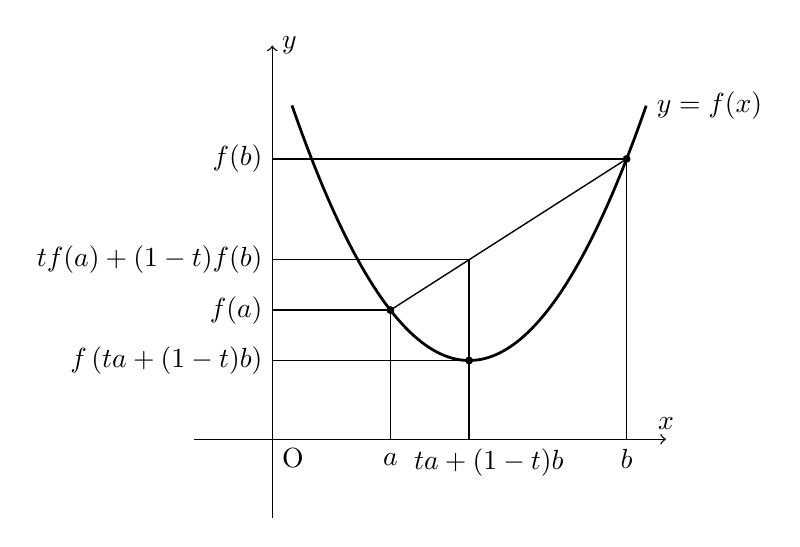
\begin{tikzpicture}
    \draw[->,line width=0.5pt] (-1,0)--(5,0) node[above]{$x$}; %x軸
    \draw[->,line width=0.5pt] (0,-1)--(0,5) node[right]{$y$}; %y軸
    \draw[line width=0.5pt] (0,3.56)--(4.5,3.56)--(4.5,0);
    \draw[line width=0.5pt] (0,2.28)--(2.5,2.28)--(2.5,0); 
    \draw[line width=0.5pt] (0,1.64)--(1.5,1.64)--(1.5,0);
    \draw[line width=0.5pt] (0,1)--(2.5,1); 
    \draw[line width=0.5pt] (1.5,1.64)--(4.5,3.56); 
    \draw (0,0) node[below right] {O}; %原点
    \draw (0,3.56) node[left] {$f(b)$};
    \draw (0,2.28) node[left] {$tf(a)+(1-t)f(b)$};
    \draw (0,1.64) node[left] {$f(a)$};
    \draw (0,1) node[left] {$f\left(ta+(1-t)b\right)$};
    \draw (1.5,-0.06) node[below] {$a$};
    \draw (2.75,0) node[below] {$ta+(1-t)b$};
    \draw (4.5,0) node[below] {$b$};
    \draw[samples=100,domain=0.25:4.75,line width=1pt] plot(\x,0.64*\x*\x-3.2*\x+5) node[right] {$y=f(x)$}; 
    \fill (1.5,1.64) circle (0.05); 
    \fill (2.5,1) circle (0.05); 
    \fill (4.5,3.56) circle (0.05); 
  \end{tikzpicture}
%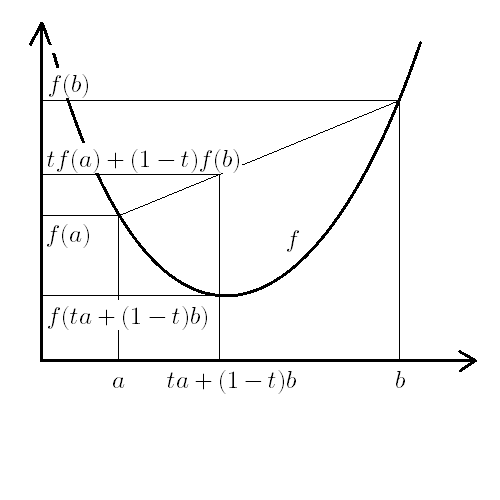
\includegraphics[width=160pt]{4.2.2.a.png}
\end{center}
同様にして、関数$f:D(f) \rightarrow \mathbb{R}$が、$\forall a,b \in I\forall t \in (0,1)$に対し、次式が成り立つとき、
\begin{align*}
f\left( ta + (1 - t)b \right) \geq tf(a) + (1 - t)f(b)
\end{align*}
この関数$f$はその区間$I$で上への凸、上への凸関数などという。また、次式が成り立つとき、
\begin{align*}
f\left( ta + (1 - t)b \right) > tf(a) + (1 - t)f(b)
\end{align*}
この関数$f$はその区間$I$で上への狭義凸関数などという。
\end{dfn}
\begin{dfn}
関数$f$が下への凸関数である、または、上への凸関数であるとき、その関数$f$は凸関数であるという。同様にして、関数$f$が下への狭義凸関数である、または、上への狭義凸関数であるとき、その関数$f$は狭義凸関数であるという。
\end{dfn}
\begin{thm}\label{4.2.2.16}
$I \subseteq D(f) \subseteq \mathbb{R}$なる区間$I$で関数$f:D(f) \rightarrow \mathbb{R}$の2階導関数$\partial^{2}f$が存在するとき、次のことは同値である。
\begin{itemize}
\item
  その関数$f$はその区間$I$で下への凸関数である。
\item
  $a < x < b$かつ$a,b,x \in I$なる実数たち$a$、$b$、$x$が次式を満たす。
\begin{align*}
\frac{f(x) - f(a)}{x - a} \leq \frac{f(b) - f(a)}{b - a} \leq \frac{f(b) - f(x)}{b - x}
\end{align*}
\item
  その1階導関数$\partial f$はその区間$I$上で単調増加する。
\item
  $\partial^{2}f|\mathrm{int}I \geq 0$が成り立つ。
\end{itemize}
また、同様に次のことが同値である。
\begin{itemize}
\item
  その関数$f$はその区間$I$で上への凸関数である。
\item
  $a < x < b$かつ$a,b,x \in I$なる実数たち$a$、$b$、$x$が次式を満たす。
\begin{align*}
\frac{f(x) - f(a)}{x - a} \geq \frac{f(b) - f(a)}{b - a} \geq \frac{f(b) - f(x)}{b - x}
\end{align*}
\item
  その1階導関数$\partial f$はその区間$I$上で単調減少する。
\item
  $\partial^{2}f|\mathrm{int}I \leq 0$が成り立つ。
\end{itemize}
\end{thm}
\begin{proof}
$I \subseteq D(f) \subseteq \mathbb{R}$なる区間$I$で関数$f:D(f) \rightarrow \mathbb{R}$の2階導関数$\partial^{2}f$が存在するとする。$\partial^{2}f|\mathrm{int}I \geq 0$が成り立つとき、Taylorの定理より次式が成り立つような実数$c$が区間$(a,x) \cup (x,a)$に存在するのであった。
\begin{align*}
f(x) = f(a) + (x - a)\partial f(x) + \frac{(x - a)^{2}}{2}\partial^{2}f(c)
\end{align*}
ここで、$c \in I$が成り立ち仮定より$\partial^{2}f(c) \geq 0$が成り立つので、$\frac{(x - a)^{2}}{2}\partial^{2}f(c) \geq 0$が成り立つ。したがって、次のようになる。
\begin{align*}
f(x) = f(a) + (x - a)\partial f(x) + \frac{(x - a)^{2}}{2}\partial^{2}f(c) \geq f(a) + (x - a)\partial f(x)
\end{align*}
これにより、$\forall a,b \in I\forall t \in (0,1)$に対し、$x = ta + (1 - t)b$とおくと、次のようになる。
\begin{align*}
\left\{ \begin{matrix}
f(a) \geq f(x) + (a - x)\partial f(x) \\
f(b) \geq f(x) + (b - x)\partial f(x) \\
\end{matrix} \right.\ 
\end{align*}
したがって、次のようになる。
\begin{align*}
&\quad \left\{ \begin{matrix}
tf(a) \geq tf(x) + t(a - x)\partial f(x) \\
(1 - t)f(b) \geq (1 - t)f(x) + (1 - t)(b - x)\partial f(x) \\
\end{matrix} \right.\ \\
&\Rightarrow tf(a) + (1 - t)f(b) \geq tf(x) + t(a - x)\partial f(x) + (1 - t)f(x) + (1 - t)(b - x)\partial f(x)\\
&\Leftrightarrow tf(a) + (1 - t)f(b) \geq (t + 1 - t)f(x) + (ta - tx + b - x - tb + tx)\partial f(x)\\
&\Leftrightarrow tf(a) + (1 - t)f(b) \geq f(x) + (ta - tx + b - x - tb + tx)\partial f(x)
\end{align*}
ここで、次のようになることから、
\begin{align*}
ta - tx + b - x - tb + tx &= ta - t\left( ta + (1 - t)b \right) + b - \left( ta + (1 - t)b \right) - tb + t\left( ta + (1 - t)b \right)\\
&= ta - t^{2}a - tb + t^{2}b + b - ta - b + tb - tb + t^{2}a + tb - t^{2}b\\
&= t^{2}a - t^{2}a + ta - ta + t^{2}b - t^{2}b + tb - tb + tb - tb + b - b = 0
\end{align*}
次のようになる。
\begin{align*}
\left\{ \begin{matrix}
f(a) \geq f(x) + (a - x)\partial f(x) \\
f(b) \geq f(x) + (b - x)\partial f(x) \\
\end{matrix} \right. &\Rightarrow tf(a) + (1 - t)f(b) \geq f(x) + 0\partial f(x)\\
&\Leftrightarrow tf(a) + (1 - t)f(b) \geq f\left( ta + (1 - t)b \right)
\end{align*}
これにより、その関数$f$はその区間$I$で下への凸関数である。\par
逆に、$a < x < b$とし、$t = \frac{x - b}{a - b}$とおくと、$0 < t < 1$で次のようになり
\begin{align*}
t = \frac{x - b}{a - b} &\Leftrightarrow t(a - b) = x - b\\
&\Leftrightarrow ta + b - tb = x\\
&\Leftrightarrow ta + (1 - t)b = x
\end{align*}
その関数$f$はその区間$I$で下への凸関数であるならそのときに限り、$\forall a,b \in I\forall t \in (0,1)$に対し、$a \neq b$が成り立つなら、$tf(a) + (1 - t)f(b) \geq f(x)$が成り立つのであったので、したがって、次のようになる。
\begin{align*}
\frac{x - b}{a - b}f(a) + \left( 1 - \frac{x - b}{a - b} \right)f(b) \geq f(x) &\Leftrightarrow \frac{x - b}{a - b}f(a) + \frac{a - b - x + b}{a - b}f(b) \geq f(x)\\
&\Leftrightarrow \frac{x - b}{a - b}f(a) + \frac{x - a}{b - a}f(b) \geq f(x)
\end{align*}
ここで、次のようになることから、
\begin{align*}
f(x) \leq \frac{x - b}{a - b}f(a) + \frac{x - a}{b - a}f(b) &\Leftrightarrow f(x) - f(a) \leq \frac{x - b}{a - b}f(a) + \frac{x - a}{b - a}f(b) - \frac{a - b}{a - b}f(a)\\
&\Leftrightarrow f(x) - f(a) \leq \frac{x - b - a + b}{a - b}f(a) + \frac{x - a}{b - a}f(b)\\
&\Leftrightarrow f(x) - f(a) \leq - \frac{x - a}{b - a}f(a) - \frac{x - a}{b - a}f(b)\\
&\Leftrightarrow \frac{f(x) - f(a)}{x - a} \leq \frac{f(b) - f(a)}{b - a}\\
f(x) \leq \frac{x - b}{a - b}f(a) + \frac{x - a}{b - a}f(b) &\Leftrightarrow f(x) - f(b) \leq \frac{x - b}{a - b}f(a) + \frac{x - a}{b - a}f(b) - \frac{b - a}{b - a}f(b)\\
&\Leftrightarrow f(x) - f(b) \leq \frac{x - b}{a - b}f(a) + \frac{x - a - b + a}{b - a}f(b)\\
&\Leftrightarrow f(x) - f(b) \leq - \frac{x - b}{b - a}f(a) - \frac{x - b}{b - a}f(b)\\
&\Leftrightarrow \frac{f(x) - f(b)}{x - b} \geq \frac{f(b) - f(a)}{b - a}
\end{align*}
したがって、次式が成り立つ。
\begin{align*}
\frac{f(x) - f(a)}{x - a} \leq \frac{f(b) - f(a)}{b - a} \leq \frac{f(b) - f(x)}{b - x}
\end{align*}\par
また、$a < x < b$かつ$a,b,x \in I$なる実数たち$a$、$b$、$x$が次式を満たすとき、
\begin{align*}
\frac{f(x) - f(a)}{x - a} \leq \frac{f(b) - f(a)}{b - a} \leq \frac{f(b) - f(x)}{b - x}
\end{align*}
$x = a + \delta$、$x = b + \varepsilon$とおくと、次式のように書かれることができ、
\begin{align*}
\frac{f(a + \delta) - f(a)}{\delta} \leq \frac{f(b) - f(a)}{b - a} \leq \frac{f(b + \varepsilon) - f(b)}{\varepsilon}
\end{align*}
$\delta,\varepsilon \rightarrow 0$とすれば、次のようになる。
\begin{align*}
\lim_{\scriptsize \begin{matrix}
\delta \rightarrow 0 \\
\delta \neq 0 \\
\end{matrix}}\frac{f(a + \delta) - f(a)}{\delta} \leq \frac{f(b) - f(a)}{b - a} \leq \lim_{\scriptsize \begin{matrix}
\varepsilon \rightarrow 0 \\
\varepsilon \neq 0 \\
\end{matrix}}\frac{f(b + \varepsilon) - f(b)}{\varepsilon}
\end{align*}
微分の定義より、$\forall a,b \in I$に対し、$a < b$が成り立つなら、次式が成り立つ。
\begin{align*}
\partial f(a) \leq \frac{f(b) - f(a)}{b - a} \leq \partial f(b)
\end{align*}
これにより、その1階導関数$\partial f$はその区間$I$上で単調増加する。\par
上記の関数の増減の議論より、これが成り立つならそのときに限り、$\partial^{2}f|\mathrm{int}I \geq 0$が成り立つ。\par
以上より、次のことは同値であることが示された。
\begin{itemize}
\item
  その関数$f$はその区間$I$で下への凸関数である。
\item
  $a < x < b$かつ$a,b,x \in I$なる実数たち$a$、$b$、$x$が次式を満たす。
\begin{align*}
\frac{f(x) - f(a)}{x - a} \leq \frac{f(b) - f(a)}{b - a} \leq \frac{f(b) - f(x)}{b - x}
\end{align*}
\item
  その1階導関数$\partial f$はその区間$I$上で単調増加する。
\item
  $\partial^{2}f|\mathrm{int}I \geq 0$が成り立つ。
\end{itemize}
同様にして、次のことが同値であることが示される。
\begin{itemize}
\item
  その関数$f$はその区間$I$で上への凸関数である。
\item
  $a < x < b$かつ$a,b,x \in I$なる実数たち$a$、$b$、$x$が次式を満たす。
\begin{align*}
\frac{f(x) - f(a)}{x - a} \geq \frac{f(b) - f(a)}{b - a} \geq \frac{f(b) - f(x)}{b - x}
\end{align*}
\item
  その1階導関数$\partial f$はその区間$I$上で単調減少する。
\item
  $\partial^{2}f|\mathrm{int}I \leq 0$が成り立つ。
\end{itemize}
\end{proof}
\begin{thm}\label{4.2.2.17}
$I \subseteq D(f) \in \mathbb{R}$なる区間$I$で関数$f:D(f) \rightarrow \mathbb{R}$の2階導関数$\partial^{2}f$が存在するとき、$\partial^{2}f|\mathrm{int}I > 0$が成り立つなら、次のことが成り立つ\footnote{これをうまく応用すれば、最大値、最小値を求めることができますが、まだ、厳密に議論するには予備知識が不足しているので、もうしばらく待っててください。}。
\begin{itemize}
\item
  $\forall a,x \in I$に対し、$x \neq a$が成り立つなら、次式が成り立つ。
\begin{align*}
f(x) > f(a) + (x - a)\partial f(a)
\end{align*}
\item
  その関数$f$はその区間$I$で下への狭義凸関数である。
\item
  $a < x < b$かつ$a,b,x \in I$なる実数たち$a$、$b$、$x$が次式を満たす。
\begin{align*}
\frac{f(x) - f(a)}{x - a} < \frac{f(b) - f(a)}{b - a} < \frac{f(b) - f(x)}{b - x}
\end{align*}
\end{itemize}
同様に、$\partial^{2}f|\mathrm{int}I < 0$が成り立つなら、次のことが成り立つ。
\begin{itemize}
\item
  $\forall a,x \in I$に対し、$x \neq a$が成り立つなら、次式が成り立つ。
\begin{align*}
f(x) < f(a) + (x - a)\partial f(a)
\end{align*}
\item
  その関数$f$はその区間$I$で上への狭義凸関数である。
\item
  $a < x < b$かつ$a,b,x \in I$なる実数たち$a$、$b$、$x$が次式を満たす。
\begin{align*}
\frac{f(x) - f(a)}{x - a} > \frac{f(b) - f(a)}{b - a} > \frac{f(b) - f(x)}{b - x}
\end{align*}
\end{itemize}
\end{thm}
\begin{proof}
$I \subseteq D(f) \in \mathbb{R}$なる区間$I$で関数$f:D(f) \rightarrow \mathbb{R}$の2階導関数$\partial^{2}f$が存在するとき、$\partial^{2}f|\mathrm{int}I > 0$が成り立つなら、Taylorの定理より次式が成り立つような実数$c$が区間$(a,x) \cup (x,a)$に存在するのであった。
\begin{align*}
f(x) = f(a) + (x - a)\partial f(x) + \frac{(x - a)^{2}}{2}\partial^{2}f(c)
\end{align*}
ここで、$c \in I$が成り立ち仮定より$\partial^{2}f(c) > 0$が成り立つので、$\frac{(x - a)^{2}}{2}\partial^{2}f(c) > 0$が成り立つ。したがって、次のようになる。
\begin{align*}
f(x) = f(a) + (x - a)\partial f(x) + \frac{(x - a)^{2}}{2}\partial^{2}f(c) > f(a) + (x - a)\partial f(x)
\end{align*}
これにより、$\forall a,x \in I$に対し、$x \neq a$が成り立つなら、$f(x) > f(a) + (x - a)\partial f(a)$が成り立つ。\par
これにより、$\forall a,b \in I\forall t \in (0,1)$に対し、$x = ta + (1 - t)b$とおくと、次のようになり、
\begin{align*}
\left\{ \begin{matrix}
f(a) > f(x) + (a - x)\partial f(x) \\
f(b) > f(x) + (b - x)\partial f(x) \\
\end{matrix} \right. &\Leftrightarrow \left\{ \begin{matrix}
tf(a) > tf(x) + t(a - x)\partial f(x) \\
(1 - t)f(b) > (1 - t)f(x) + (1 - t)(b - x)\partial f(x) \\
\end{matrix} \right.\ \\
&\Rightarrow tf(a) + (1 - t)f(b) > tf(x) + t(a - x)\partial f(x) \\
&\quad + (1 - t)f(x) + (1 - t)(b - x)\partial f(x)\\
&\Leftrightarrow tf(a) + (1 - t)f(b) > (t + 1 - t)f(x) \\
&\quad + (ta - tx + b - x - tb + tx)\partial f(x)\\
&\Leftrightarrow tf(a) + (1 - t)f(b) > f(x) + (ta - tx + b - x - tb + tx)\partial f(x)
\end{align*}
ここで、次のようになることから、
\begin{align*}
ta - tx + b - x - tb + tx &= ta - t\left( ta + (1 - t)b \right) + b - \left( ta + (1 - t)b \right) - tb + t\left( ta + (1 - t)b \right)\\
&= ta - t^{2}a - tb + t^{2}b + b - ta - b + tb - tb + t^{2}a + tb - t^{2}b\\
&= t^{2}a - t^{2}a + ta - ta + t^{2}b - t^{2}b + tb - tb + tb - tb + b - b = 0
\end{align*}
次のようになる。
\begin{align*}
\left\{ \begin{matrix}
f(a) > f(x) + (a - x)\partial f(x) \\
f(b) > f(x) + (b - x)\partial f(x) \\
\end{matrix} \right. &\Rightarrow tf(a) + (1 - t)f(b) > f(x) + 0\partial f(x)\\
&\Leftrightarrow tf(a) + (1 - t)f(b) > f\left( ta + (1 - t)b \right)
\end{align*}
これにより、その関数$f$はその区間$I$で下への狭義凸関数である。\par
逆に、$a < b$とし$ta + (1 - t)b = x$とおくと、その関数$f$はその区間$I$で下への狭義凸関数であるならそのときに限り、$\forall a,b \in I\forall t \in (0,1)$に対し、$a \neq b$が成り立つなら、$tf(a) + (1 - t)f(b) > f(x)$が成り立つ。ここで、関係$a < x < b$が成り立つことに注意すれば、次のようになり、
\begin{align*}
ta + (1 - t)b = x &\Leftrightarrow ta + b - tb = x\\
&\Leftrightarrow t(a - b) = x - b \Leftrightarrow t = \frac{x - b}{a - b}
\end{align*}
したがって、次のようになる。
\begin{align*}
\frac{x - b}{a - b}f(a) + \left( 1 - \frac{x - b}{a - b} \right)f(b) > f(x) &\Leftrightarrow \frac{x - b}{a - b}f(a) + \frac{a - b - x + b}{a - b}f(b) > f(x)\\
&\Leftrightarrow \frac{x - b}{a - b}f(a) + \frac{x - a}{b - a}f(b) > f(x)
\end{align*}
ここで、次のようになることから、
\begin{align*}
f(x) < \frac{x - b}{a - b}f(a) + \frac{x - a}{b - a}f(b) &\Leftrightarrow f(x) - f(a) < \frac{x - b}{a - b}f(a) + \frac{x - a}{b - a}f(b) - \frac{a - b}{a - b}f(a)\\
&\Leftrightarrow f(x) - f(a) < \frac{x - b - a + b}{a - b}f(a) + \frac{x - a}{b - a}f(b)\\
&\Leftrightarrow f(x) - f(a) < - \frac{x - a}{b - a}f(a) - \frac{x - a}{b - a}f(b)\\
&\Leftrightarrow \frac{f(x) - f(a)}{x - a} < \frac{f(b) - f(a)}{b - a}\\
f(x) < \frac{x - b}{a - b}f(a) + \frac{x - a}{b - a}f(b) &\Leftrightarrow f(x) - f(b) < \frac{x - b}{a - b}f(a) + \frac{x - a}{b - a}f(b) - \frac{b - a}{b - a}f(b)\\
&\Leftrightarrow f(x) - f(b) < \frac{x - b}{a - b}f(a) + \frac{x - a - b + a}{b - a}f(b)\\
&\Leftrightarrow f(x) - f(b) < - \frac{x - b}{b - a}f(a) - \frac{x - b}{b - a}f(b)\\
&\Leftrightarrow \frac{f(x) - f(b)}{x - b} > \frac{f(b) - f(a)}{b - a}
\end{align*}
したがって、次式が成り立つ。
\begin{align*}
\frac{f(x) - f(a)}{x - a} < \frac{f(b) - f(a)}{b - a} < \frac{f(b) - f(x)}{b - x}
\end{align*}\par
$\partial^{2}f|\mathrm{int}I > 0$が成り立つなら、次のことが成り立つ。
\begin{itemize}
\item
  $\forall a,x \in I$に対し、$x \neq a$が成り立つなら、次式が成り立つ。
\begin{align*}
f(x) > f(a) + (x - a)\partial f(a)
\end{align*}
\item
  その関数$f$はその区間$I$で下への狭義凸関数である。
\item
  $a < x < b$かつ$a,b,x \in I$なる実数たち$a$、$b$、$x$が次式を満たす。
\begin{align*}
\frac{f(x) - f(a)}{x - a} < \frac{f(b) - f(a)}{b - a} < \frac{f(b) - f(x)}{b - x}
\end{align*}
\end{itemize}\par
同様にして、$\partial^{2}f|\mathrm{int}I < 0$が成り立つなら、次のことが成り立つことも示される。
\begin{itemize}
\item
  $\forall a,x \in I$に対し、$x \neq a$が成り立つなら、次式が成り立つ。
\begin{align*}
f(x) < f(a) + (x - a)\partial f(a)
\end{align*}
\item
  その関数$f$はその区間$I$で上への狭義凸関数である。
\item
  $a < x < b$かつ$a,b,x \in I$なる実数たち$a$、$b$、$x$が次式を満たす。
\begin{align*}
\frac{f(x) - f(a)}{x - a} > \frac{f(b) - f(a)}{b - a} > \frac{f(b) - f(x)}{b - x}
\end{align*}
\end{itemize}
\end{proof}
\begin{thm}\label{4.2.2.18}
$I = [ a,b] \subseteq D(f) \in \mathbb{R}$なる区間$I$で関数$f:D(f) \rightarrow \mathbb{R}$の2階導関数$\partial^{2}f$が存在するとき、$\partial^{2}f|I > 0$が成り立つかつ、$f(a)f(b) < 0$が成り立つなら、その関数$f$はその区間$\mathrm{int}I$で$f(c) = 0$が成り立つような実数$c$をただ1つもつ。\par
このような実数$c$をその関数$f$のその区間$I$での零点などという。
\end{thm}
\begin{proof}
$I = [ a,b] \subseteq D(f) \in \mathbb{R}$なる区間$I$で関数$f:D(f) \rightarrow \mathbb{R}$の2階導関数$\partial^{2}f$が存在するとき、$\partial^{2}f|I > 0$が成り立つかつ、$f(a)f(b) < 0$が成り立つなら、その関数$f$はその区間$I$で微分可能でありその区間$I$で連続であるかつ、仮定より次のようになるので、
\begin{align*}
f(a)f(b) < 0 &\Leftrightarrow \left( f(a) > 0 \land f(b) < 0 \right) \vee \left( f(a) < 0 \land f(b) > 0 \right)\\
&\Leftrightarrow f(b) < 0 < f(a) \vee f(a) < 0 < f(b)\\
&\Leftrightarrow f(a) \lessgtr 0 \lessgtr f(b)
\end{align*}
したがって、中間値の定理よりその関数$f$はその区間$\mathrm{int}I$で$f(c) = 0$が成り立つような実数$c$をもつ。\par
ここで、$f\left( c \right) = f\left( d \right) = 0$が成り立つような$a < c < d < b$なる実数たち$c$、$d$が複数存在するとする。このとき、明らかに、次式が成り立つような実数たち$s$、$t$が区間$(0,1)$に存在し、
\begin{align*}
c = sa + \left( 1 - s \right)d,\ \ d = tc + \left( 1 - t \right)b
\end{align*}
$\partial^{2}f|I > 0$が成り立つので、その関数$f$はその区間$I$で下に狭義凸関数である。したがって、次のようになる。
\begin{align*}
\left\{ \begin{matrix}
f\left( c \right) = f\left( d \right) = 0 \\
c = sa + \left( 1 - s \right)d \\
d = tc + \left( 1 - t \right)b \\
f\left( sa + \left( 1 - s \right)d \right) < sf(a) + \left( 1 - s \right)f\left( d \right) \\
f\left( tc + \left( 1 - t \right)b \right) < tf\left( c \right) + \left( 1 - t \right)f(b) \\
\end{matrix} \right. &\Leftrightarrow \left\{ \begin{matrix}
0 < sf(a) + \left( 1 - s \right)f\left( d \right) \\
0 = f\left( c \right) = f\left( sa + \left( 1 - s \right)d \right) \\
0 < \left( 1 - t \right)f(b) \\
0 = f\left( d \right) = f\left( tc + \left( 1 - t \right)b \right) \\
\end{matrix} \right.\\
&\Rightarrow \left\{ \begin{matrix}
0 < sf(a) \\
0 < \left( 1 - t \right)f(b) \\
\end{matrix} \right.\\
&\Leftrightarrow \left\{ \begin{matrix}
0 < f(a) \\
0 < f(b) \\
\end{matrix} \right.\\
&\Rightarrow f(a)f(b) > 0
\end{align*}
これは仮定$f(a)f(b) < 0$に矛盾する。\par
よって、その関数$f$はその区間$\mathrm{int}I$で$f(c) = 0$が成り立つような実数$c$をただ1つもつ。
\end{proof}
\begin{thm}[Newtonの逐次近似法]\label{4.2.2.19}
$I = [ a,b] \subseteq D(f) \in \mathbb{R}$なる区間$I$で関数$f:D(f) \rightarrow \mathbb{R}$の2階導関数$\partial^{2}f$が存在し、$\partial^{2}f|I > 0$が成り立つかつ、$f(a)f(b) < 0$が成り立つとし、$f\left( x_{1} \right) > 0かつx_{1} \in \mathrm{int}I$なる実数$x_{1}$を1つとり、$\forall n \in \mathbb{N}$に対し、実数$x_{n + 1}$が次式のように定義されるとする。
\begin{align*}
x_{n + 1} = x_{n} - \frac{f\left( x_{n} \right)}{\partial f\left( x_{n} \right)}
\end{align*}
このとき、その実数列$\left( x_{n} \right)_{n \in \mathbb{N}}$は単調増加するか、単調減少しその区間$I$におけるただ1つの零点に収束する。これによって、その区間$I$における方程式$f(x) = 0$の解が数値的に求められることができる。この方法をNewtonの逐次近似法、Newton法などという。
\begin{center}
  \begin{tikzpicture}
    \draw[->,line width=0.5pt] (-1,0)--(5,0) node[above]{$x$}; %x軸
%   \draw[->,line width=0.5pt] (0,-1)--(0,5) node[right]{$p'$}; %y軸
    \draw[line width=0.5pt] (4,0)--(4,3.44)--(1.47,0)--(1.47,0.89)--(0.24,0);
    \draw (0,0) node[above left] {$\lim_{n\to \infty } x_n$};
    \draw (4,0) node[below] {$x_1 $};
    \draw (1.47,0) node[below] {$x_2 $};
    \draw (0.24,0) node[below] {$x_3 $};
    \draw[samples=100,domain=-1:5,line width=1pt] plot(\x,{2*exp(\x/4 ) -2} ) node[right] {$y=f\left( x\right) $}; 
    \fill (0,0) circle (0.05); 
    \fill (4,3.44) circle (0.05); 
    \fill (1.47,0.89) circle (0.05); 
  \end{tikzpicture}
%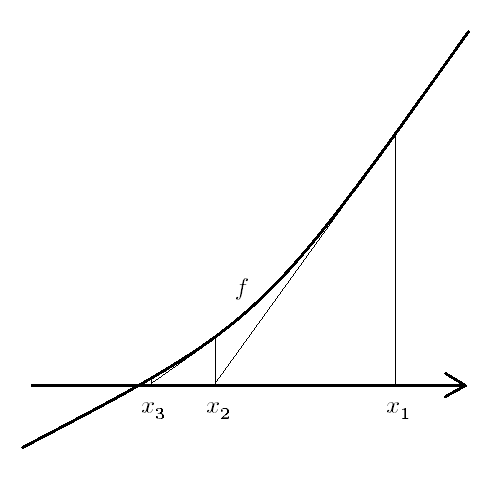
\includegraphics[width=160pt]{4.2.2.b.png}
\end{center}
\end{thm}
\begin{proof}
$I = [ a,b] \subseteq D(f) \in \mathbb{R}$なる区間$I$で関数$f:D(f) \rightarrow \mathbb{R}$の2階導関数$\partial^{2}f$が存在し、$\partial^{2}f|I > 0$が成り立つかつ、$f(a)f(b) < 0$が成り立つとし、$f\left( x_{1} \right) > 0$かつ$x_{1} \in \mathrm{int}I$なる実数$x_{1}$を1つとり、$\forall n \in \mathbb{N}$に対し、実数$x_{n + 1}$が次式のように定義されるとする。
\begin{align*}
x_{n + 1} = x_{n} - \frac{f\left( x_{n} \right)}{\partial f\left( x_{n} \right)}
\end{align*}\par
このとき、$\mu \in I$かつ$\partial f(\mu) = 0$が成り立つような実数$\mu$が考えられると、$\partial^{2}f|I > 0$が成り立つので、定理\ref{4.2.2.17}より$\forall x \in I$に対し、$x \neq \mu$が成り立つなら、次式が成り立つ。
\begin{align*}
f(x) > f(\mu) + (x - \mu)\partial f(\mu) = f(\mu)
\end{align*}
これにより、$f(\mu) = \min{V\left( f \middle| I \right)}$が成り立つ。\par
ここで、仮定より次のようになるので、
\begin{align*}
f(a)f(b) < 0 &\Leftrightarrow \left( f(a) > 0 \land f(b) < 0 \right) \vee \left( f(a) < 0 \land f(b) > 0 \right)\\
&\Leftrightarrow f(b) < 0 < f(a) \vee f(a) < 0 < f(b)\\
&\Leftrightarrow f(a) \lessgtr 0 \lessgtr f(b)
\end{align*}
次式のように集合$J$を定め
\begin{align*}
J = \left\{ x \in I \middle| f(x) \geq 0 \right\}
\end{align*}
$\mu \in J$と仮定すると、$f(a) < 0 < f(b)$のとき、$f(a) < 0 \leq f(\mu)$が成り立つが、これは$f(\mu) = \min{V\left( f \middle| I \right)}$が成り立つことに矛盾する。$f(a) < 0 < f(b)$のときも同様にして示される。\par
したがって、$\mu \notin J$が成り立ち、したがって、$\forall\mu \in I$に対し、$\partial f(\mu) = 0$が成り立つなら、$\mu \notin J$も成り立つ。対偶律より$\forall x \in I$に対し、$x \in J$が成り立つなら、$\partial f(x) \neq 0$が成り立つ。\par
ここで、上記の議論より、$\partial^{2}f|I > 0$が成り立つかつ、$f(a)f(b) < 0$が成り立つなら、その関数$f$はその区間$\mathrm{int}I$で零点$c$をただ1つもつのであった。\par
ここで、$f(a) > 0$のとき、関係$a < c < b$より$a < d < c$かつ$f(d) \leq 0$となるような実数$d$が存在するとすると、$f(d) = 0$のときは$d \in \mathrm{int}I$よりその関数$f$がその区間$\mathrm{int}I$で零点$c$をただ1つもつことに矛盾するので、$f(d) < 0$が成り立つことになり、その関数$f$は区間$[ a,d]$で連続で$f(d) < 0 < f(a)$が成り立つので、中間値の定理より$f\left( c' \right) = 0$となる実数$c'$がその区間$[ a,d]$に存在し、さらに、$f(d) < f\left( c' \right) = 0 < f(a)$より$a \neq c'$かつ$d \neq c'$が成り立つことになり$a < c' < d < c$が成り立つ。これにより、その関数$f$の零点$c'$がその実数$c$とは別にその区間$\mathrm{int}I$で存在することになるが、その関数$f$がその区間$\mathrm{int}I$で零点$c$をただ1つもつことに矛盾する。\par
以上より、ある実数$d$が開区間$(a,c)$に存在して$f(d) \leq 0$が成り立つことがいえない、即ち、$\forall x \in (a,c)$に対し、$f(x) > 0$が成り立つ。同様にして、$\forall x \in (c,b)$に対し、$f(x) < 0$が成り立つことも示される。\par
ここで、次式たちが成り立つことにより
\begin{align*}
I = \left\{ a \right\} \sqcup (a,c) \sqcup \left\{ c \right\} \sqcup (c,b) \sqcup \left\{ b \right\},\\
\forall x \in \left\{ a \right\}\left[ f(x) > 0 \right],\ \ 
\forall x \in (a,c)\left[ f(x) > 0 \right],\\
\forall x \in \left\{ c \right\}\left[ f(x) = 0 \right],\ \ 
\forall x \in (c,b)\left[ f(x) < 0 \right],\ \ 
\forall x \in \left\{ b \right\}\left[ f(x) < 0 \right]
\end{align*}
$J = \left\{ a \right\} \sqcup (a,c) \sqcup \left\{ c \right\} = [ a,c]$が成り立つ。\par
また、$\partial f|J \geq 0$が成り立つと仮定しよう。$\forall x \in I$に対し、$x \in J$が成り立つなら、$\partial f(x) \neq 0$が成り立つのであったので、$\partial f\partial f(x) = 0$が成り立たなく$\partial f(x) > 0$が成り立つことになり、その区間$[ a,c]$で平均値の定理より次式が成り立つような実数$c'$が区間$\mathrm{int}[ a,c] = (a,c)$に存在する。
\begin{align*}
\partial f\left( c' \right) = \frac{f(c) - f(a)}{c - a}
\end{align*}
したがって、次のようになる。
\begin{align*}
\partial f\left( c' \right) = \frac{f(c) - f(a)}{c - a} &\Leftrightarrow f(c) - f(a) = (c - a)\partial f\left( c' \right)\\
&\Leftrightarrow f(c) = f(a) + (c - a)\partial f\left( c' \right)
\end{align*}
ここで、$f(c) = 0$より次のようになる。
\begin{align*}
\partial f\left( c' \right) = \frac{f(c) - f(a)}{c - a} &\Leftrightarrow 0 = f(a) + (c - a)\partial f\left( c' \right)\\
&\Leftrightarrow (a - c)\partial f\left( c' \right) = f(a)
\end{align*}
ここで、$c' \in (a,c) \subset J$が成り立ち$\partial f\left( c' \right) > 0$が成り立つかつ、$a < c$が成り立つので、次式が得られる。
\begin{align*}
0 > (a - c)\partial f\left( c' \right) = f(a)
\end{align*}
これは仮定の$f(a) > 0$が成り立つことに矛盾する。したがって、$\forall x \in J$に対し、$\partial f(x) < 0$が成り立つ。\par
ここで、仮定より、$f\left( x_{1} \right) > f(c) = 0$より$x_{1} \neq c$が成り立つことに注意すれば、明らかに$a < x_{1} < c$が成り立つ。\par
$n = k$のとき、$a < x_{k} < c$が成り立つと仮定しよう。このとき、$f(a) > 0$のとき、$\forall x \in (a,c)$に対し、$f(x) > 0$が成り立つのであったので、上記の議論より$f\left( x_{k} \right) > 0$かつ$\partial f\left( x_{k} \right) < 0$が成り立つので、$- \frac{f\left( x_{k} \right)}{\partial f\left( x_{k} \right)} > 0$が成り立つ。$n = k + 1$のとき、その実数列$\left( x_{n} \right)_{n \in \mathbb{N}}$の定義より次式が成り立ち、
\begin{align*}
x_{k + 1} = x_{k} - \frac{f\left( x_{k} \right)}{\partial f\left( x_{k} \right)}
\end{align*}
$- \frac{f\left( x_{k} \right)}{\partial f\left( x_{k} \right)} > 0$が成り立つので、$x_{k} < x_{k + 1}$が成り立つ。さらに、仮定より$a < x_{k}$が成り立つことに注意すれば、$a < x_{k} < x_{k + 1}$が成り立つ。また、仮定より$\forall x \in I$に対し、$\partial^{2}f(x) > 0$が成り立つので、$c \in I$より$\partial^{2}f(c) > 0$が成り立ち、$f\left( x_{k} \right) > f(c) = 0$より$x_{k} \neq c$が成り立つことに注意すれば、上記の定理より$f(c) > f\left( x_{k} \right) + \left( c - x_{k} \right)\partial f\left( x_{k} \right)$が成り立つ。\par
ここで、$f\left( x_{k} \right) > 0$かつ$\partial f\left( x_{k} \right) < 0$が成り立つことに注意すれば、次のようになる。
\begin{align*}
0 = f(c) > f\left( x_{k} \right) + \left( c - x_{k} \right)\partial f\left( x_{k} \right) &\Leftrightarrow 0 = \frac{f(c)}{\partial f\left( x_{k} \right)} < \frac{1}{\partial f\left( x_{k} \right)}\left( f\left( x_{k} \right) + \left( c - x_{k} \right)\partial f\left( x_{k} \right) \right)\\
&\Leftrightarrow 0 = \frac{f(c)}{\partial f\left( x_{k} \right)} < \frac{f\left( x_{k} \right)}{\partial f\left( x_{k} \right)} + c - x_{k}\\
&\Leftrightarrow 0 = \frac{f(c)}{\partial f\left( x_{k} \right)} < c - \left( x_{k} - \frac{f\left( x_{k} \right)}{\partial f\left( x_{k} \right)} \right)\\
&\Leftrightarrow 0 = \frac{f(c)}{\partial f\left( x_{k} \right)} < c - x_{k + 1} \Rightarrow x_{k + 1} < c
\end{align*}
以上より、$a < x_{k} < x_{k + 1} < c$が成り立つ。\par
数学的帰納法によって$\forall n \in \mathbb{N}$に対し、$a < x_{n} < x_{n + 1} < c$が成り立つ。これにより、その実数列$\left( x_{n} \right)_{n \in \mathbb{N}}$は上に有界であるかつ、単調増加するので、$\lim_{n \rightarrow \infty}x_{n} \in \mathbb{R}$が成り立つ。この実数$\lim_{n \rightarrow \infty}x_{n}$は少なくとも$a < \lim_{n \rightarrow \infty}x_{n} \leq c$が成り立っているので、$\lim_{n \rightarrow \infty}x_{n} \in J$が成り立ち、$\forall x \in I$に対し、$x \in J \Rightarrow \partial f(x) \neq 0$が成り立つのであったので、$\partial f\left( \lim_{n \rightarrow \infty}x_{n} \right) \neq 0$が成り立つことに注意すれば、$n \rightarrow \infty$のとき、次のようになる。
\begin{align*}
\lim_{n \rightarrow \infty}x_{n + 1} = \lim_{n \rightarrow \infty}\left( x_{n} - \frac{f\left( x_{n} \right)}{\partial f\left( x_{n} \right)} \right) &\Leftrightarrow \lim_{n \rightarrow \infty}x_{n} = \lim_{n \rightarrow \infty}x_{n} - \lim_{n \rightarrow \infty}\frac{f\left( x_{n} \right)}{\partial f\left( x_{n} \right)}\\
&\Leftrightarrow 0 = - \frac{f\left( \lim_{n \rightarrow \infty}x_{n} \right)}{\partial f\left( \lim_{n \rightarrow \infty}x_{n} \right)}\\
&\Leftrightarrow f\left( \lim_{n \rightarrow \infty}x_{n} \right) = 0
\end{align*}
ここで、その関数$f$がその区間$\mathrm{int}I$で零点$c$をただ1つもつのであったので、$c = \lim_{n \rightarrow \infty}x_{n}$が成り立つ。\par
よって、その実数列$\left( x_{n} \right)_{n \in \mathbb{N}}$は単調増加しその区間$I$におけるただ1つの零点に収束する。$f(a) < 0$のときも同様にして示される。
\end{proof}
%\hypertarget{lhuxf4pitalux306eux5b9aux7406}{%
\subsubsection{l'Hôpitalの定理}%\label{lhuxf4pitalux306eux5b9aux7406}}
\begin{thm}[l'Hôpitalの定理]\label{4.2.2.20}
ある区間$I$を用いた$I \subseteq D(f) \subseteq \mathbb{R}$かつ$I \subseteq D(g) \subseteq \mathbb{R}$なる関数たち$f:D(f) \rightarrow \mathbb{R}$、$g:D(g) \rightarrow \mathbb{R}$が、実数$a$を用いて$\mathfrak{a} =a$のとき、区間$I$がその実数$aの\varepsilon 近傍U(a,\varepsilon)$で、$\mathfrak{a = \infty}$のとき、その区間$I$が上に有界でない区間で、$\mathfrak{a} = - \infty$のとき、その区間$I$が下に有界でない区間であるとして、その区間$I$で微分可能であるとする。
\begin{itemize}
\item
  次式たちが成り立つかつ、
\begin{align*}
\lim_{x \rightarrow \mathfrak{a}}{f(x)} = \lim_{x \rightarrow \mathfrak{a}}{g(x)} = 0,\ \ \forall x \in I\left[ \partial g(x) \neq 0 \right]
\end{align*}
極限$\lim_{x \rightarrow \mathfrak{a}}{\frac{\partial f}{\partial g}(x)}$が振動しなければ、次式が成り立つ。
\begin{align*}
\lim_{x \rightarrow \mathfrak{a}}{\frac{f}{g}(x)} = \lim_{x \rightarrow \mathfrak{a}}{\frac{\partial f}{\partial g}(x)}
\end{align*}
\item
  次式たちが成り立つかつ、
\begin{align*}
\lim_{x \rightarrow \mathfrak{a}}{g(x)} = \infty,\ \ \forall x \in I\left[ \partial g(x) \neq 0 \right]
\end{align*}
極限$\lim_{x \rightarrow \mathfrak{a}}{\frac{\partial f}{\partial g}(x)}$が振動しなければ、次式が成り立つ。
\begin{align*}
\lim_{x \rightarrow \mathfrak{a}}{\frac{f}{g}(x)} = \lim_{x \rightarrow \mathfrak{a}}{\frac{\partial f}{\partial g}(x)}
\end{align*}
\end{itemize}
この定理をl'Hôpitalの定理という\footnote{
ここで少し反例を。ただ、高校数学の内容であるもののまだ述べられていない内容も含まれますので、目を通す程度でOKです。\par
\begin{itemize}
\item
$\lim_{x \rightarrow \mathfrak{a}}{f(x)} = \lim_{x \rightarrow \mathfrak{a}}{g(x)} = 0$が成り立っていない場合として、例えば、$f(x)=\cos x$、$g(x)=x$のときが挙げられる。$x\rightarrow +0$で$f(x)=\cos x\rightarrow 1$、$g(x)=x \rightarrow 0$となっているものの、$f'(x)=-\sin x$、$g'(x)=1$なので、次のようになる。
\begin{align*}
\lim_{x\rightarrow +0}{\frac{f(x)}{g(x)}} &=\lim_{x\rightarrow +0}{\frac{\cos x}{x}} =\infty, \\
\lim_{x\rightarrow +0}{\frac{f'(x)}{g'(x)}} &=\lim_{x\rightarrow +0}{(-\sin x)} =0
\end{align*}
\item
極限$\lim_{x \rightarrow \mathfrak{a}}{\frac{\partial f}{\partial g}(x)}$が振動してしまっている場合として、例えば、$f(x)=x^2 \sin \frac{1}{x}$、$g(x)=x$のときが挙げられる。$x\rightarrow +0$で、$0\leq \sin \frac{1}{x} \leq 1$かつ$x^2 \rightarrow 0$なので、はさみうちの原理より$f(x)=x^2 \sin \frac{1}{x}\rightarrow 0$、$g(x)\rightarrow 0$となっている。ここで、$x\rightarrow +0$で、$0\leq \sin \frac{1}{x} \leq 1$なので、はさみうちの原理より次のようになる。
\begin{align*}
\lim_{x\rightarrow +0}{\frac{f(x)}{g(x)}} =\lim_{x\rightarrow +0}{x\sin \frac{1}{x}} =0
\end{align*}
一方で、$f'(x)=2x\sin \frac{1}{x} -\cos \frac{1}{x}$、$g'(x)=1$なので、次のようになる。
\begin{align*}
\lim_{x\rightarrow +0}{\frac{f'(x)}{g'(x)}} &=\lim_{x\rightarrow +0}{\left( 2x\sin \frac{1}{x} -\cos \frac{1}{x}\right) } \\
&=\lim_{\frac{1}{x} \rightarrow \infty }{\left( 2x\sin \frac{1}{x} -\cos \frac{1}{x}\right) } =\mathrm{indefinite} 
\end{align*}
\item
$\forall x \in I\left[ \partial g(x) \neq 0 \right]$が成り立っていない場合として、例えば、$f(x)=\frac{1}{2} +\frac{1}{4}\sin 2x$、$g(x)=f(x) e^{\sin x}$のときが挙げられる。このとき、$x\rightarrow \infty $で$-1\leq \sin 2x $と追い出しの原理より$f(x),g(x)\rightarrow \infty $となる。もちろん$x\rightarrow \infty $で$e^{\sin x} =\mathrm{indefinite}$なので、次のようになる。
\begin{align*}
\lim_{x\rightarrow \infty }{\frac{f(x)}{g(x)}} =\lim_{x\rightarrow \infty }{\frac{1}{e^{\sin x} }}=\mathrm{indefinite}
\end{align*}
ここで、次のようになるので、
\begin{align*}
f'(x) &= \frac{1}{2} +\frac{1}{2} \cos 2x ={\cos }^2 x\\
g'(x) &= f'(x) e^{\sin x} +f(x) e^{\sin x} \cos x\\
&=\cos x\left( \cos x e^{\sin x} +g(x) \right)
\end{align*}
$\forall n\in \mathbb{Z} $に対し、$\cos \left( \frac{\pi }{2} +n\pi \right) =0$なので、$g' \left( \frac{\pi }{2} +n\pi \right) =0$となっている。ゆえに、上に有界でないどの区間でもある$x$が存在して、$g'(x)=0$となっている。このとき、$-1\leq \sin x, \cos x$に注意すれば、$-\frac{1}{e} \leq \cos x e^{\sin x}$なので、次のようになる。
\begin{align*}
0&\leq \left| \frac{\cos x}{\cos x e^{\sin x} +g(x)} \right| \\
&\leq \frac{1}{\left| \cos xe^{\sin x} +g(x)\right| } \\
&\leq \frac{1}{-\frac{1}{e} +g(x)}
\end{align*}
$x\rightarrow \infty $で$\frac{1}{-\frac{1}{e} +g(x)} \rightarrow 0$となっている。はさみうちの原理よりしたがって、次のようになる。
\begin{align*}
\lim_{x\rightarrow \infty }{\frac{f'(x)}{g'(x)}} =\lim_{x\rightarrow \infty }{\frac{\cos x}{\cos x e^{\sin x} +g(x)} }=0
\end{align*}
\end{itemize}
}。
\end{thm}
\begin{proof}
ある区間$I$を用いた$I \subseteq D(f) \subseteq \mathbb{R}$かつ$U\left( a,\gamma + \delta \right) \subseteq D(g) \subseteq \mathbb{R}$なる関数たち$f:D(f) \rightarrow \mathbb{R}$、$g:D(g) \rightarrow \mathbb{R}$が、実数$a$を用いて$\mathfrak{a} =a$のとき、区間$I$がその実数$a$の$\gamma + \delta$近傍$U\left( a,\gamma + \delta \right)$で、$\mathfrak{a = \infty}$のとき、その区間$I$が上に有界でない区間で、$\mathfrak{a = - \infty}$のとき、その区間$I$が下に有界でない区間であるとして、その区間$I$で微分可能であるとする。\par
次式たちが成り立つかつ、
\begin{align*}
\lim_{x \rightarrow \mathfrak{a}}{f(x)} = \lim_{x \rightarrow \mathfrak{a}}{g(x)} = 0,\ \ \forall x \in I\left[ \partial g(x) \neq 0 \right]
\end{align*}
極限$\lim_{x \rightarrow \mathfrak{a}}{\frac{\partial f}{\partial g}(x)}$が振動しないとき、$\mathfrak{a} =a$かつ$a < x$のとき、$x = a + \gamma + \delta$なる正の実数$\gamma + \delta$を用いてCauchyの平均値の定理より次式が成り立つような実数$c$が$(a,x) \subset U\left( a,\gamma + \delta \right)$なる区間$(a,x)$に存在する。
\begin{align*}
\frac{f(x) - f(a)}{g(x) - g(a)} = \frac{f}{g}(x) = \frac{\partial f}{\partial g}(c)
\end{align*}
ここで、$\gamma + \delta \rightarrow 0$とすると、$0 < c - a < \gamma + \delta$より$c - a \rightarrow 0$となり、したがって、次式が成り立つ。
\begin{align*}
\lim_{\gamma + \delta \rightarrow 0}{\frac{f}{g}(x)} = \lim_{\gamma + \delta \rightarrow 0}{\frac{\partial f}{\partial g}(c)} = \lim_{c - a \rightarrow 0}{\frac{\partial f}{\partial g}(c)} = \lim_{x \rightarrow a}{\frac{\partial f}{\partial g}(x)}
\end{align*}
$a > x$のときも同様にして示される。\par
$\mathfrak{a = \infty}$のとき、$x \rightarrow \infty$とすれば、$\frac{1}{x} \rightarrow + 0$となるので、次式が成り立つ。
\begin{align*}
\lim_{x \rightarrow \infty}{\frac{f}{g}(x)} = \lim_{\frac{1}{x} \rightarrow + 0}{\frac{f}{g}\left( \frac{1}{\frac{1}{x}} \right)} = \lim_{\frac{1}{x} \rightarrow + 0}{\frac{\partial f}{\partial g}\left( \frac{1}{\frac{1}{x}} \right)} = \lim_{x \rightarrow \infty}{\frac{\partial f}{\partial g}(x)}
\end{align*}
$\mathfrak{a = - \infty}$のときも同様にして示される。\par
また、次式たちが成り立つかつ、
\begin{align*}
\lim_{x \rightarrow \mathfrak{a}}{g(x)} = \infty,\ \ \forall x \in I\left[ \partial(g)(x) \neq 0 \right]
\end{align*}
極限$\lim_{x \rightarrow \mathfrak{a}}{\frac{\partial f}{\partial g}(x)}$が振動しないとき、$\mathfrak{a} =a$かつ$a < x$のとき、$a + \gamma < x = a + \gamma + \delta$なる正の実数たち$\gamma$、$\delta$を用いてCauchyの平均値の定理より次式が成り立つような実数$c$が$\left( a + \gamma,x \right) \subset U\left( a,\gamma + \delta \right)$なる区間$\left( a + \gamma,x \right)$に存在する。
\begin{align*}
\frac{f(x) - f\left( a + \gamma \right)}{g(x) - g\left( a + \gamma \right)} = \frac{\partial f}{\partial g}(c)
\end{align*}
ここで、仮定の$\lim_{x \rightarrow a}{g(x)} = \infty$より$\forall\varepsilon \in \mathbb{R}^{+}\exists\delta \in \mathbb{R}^{+}$に対し、$0 < |x - a| < \delta \Rightarrow \varepsilon < g(x)$が成り立つ。これにより、$0 < g(x)$が成り立つので、次のようになる。
\begin{align*}
\frac{f(x) - f\left( a + \gamma \right)}{g(x) - g\left( a + \gamma \right)} = \frac{\partial f}{\partial g}(c) &\Leftrightarrow f(x) - f\left( a + \gamma \right) = \frac{\partial f}{\partial g}(c)\left( g(x) - g\left( a + \gamma \right) \right)\\
&\Leftrightarrow \frac{f(x) - f\left( a + \gamma \right)}{g\left( a + \gamma \right)} = \frac{\partial f}{\partial g}(c)\frac{g(x) - g\left( a + \gamma \right)}{g\left( a + \gamma \right)}\\
&\Leftrightarrow \frac{f(x)}{g\left( a + \gamma \right)} - \frac{f}{g}\left( a + \gamma \right) = \frac{\partial f}{\partial g}(c)\left( \frac{g(x)}{g\left( a + \gamma \right)} - 1 \right)\\
&\Leftrightarrow \frac{f}{g}\left( a + \gamma \right) = \frac{f(x)}{g\left( a + \gamma \right)} + \frac{\partial f}{\partial g}(c) - \frac{\partial f}{\partial g}(c)\frac{g(x)}{g\left( a + \gamma \right)}
\end{align*}
$\lim_{x \rightarrow a}{\frac{\partial f}{\partial g}(x)} \in \mathbb{R}$のとき、$\lim_{x \rightarrow a}{\frac{\partial f}{\partial g}(x)} = \alpha$とおく。$\gamma + \delta \rightarrow 0$とすると、$0 < c - a < \gamma + \delta$より$c - a \rightarrow 0$となり、したがって、次式が成り立つ。
\begin{align*}
\lim_{\gamma + \delta \rightarrow 0}{\frac{\partial f}{\partial g}(c)} = \lim_{c - a \rightarrow 0}{\frac{\partial f}{\partial g}(c)} = \lim_{c \rightarrow a}{\frac{\partial f}{\partial g}(c)} = \alpha
\end{align*}
これにより、$\forall\varepsilon' \in \mathbb{R}^{+}\exists\delta' \in \mathbb{R}^{+}$に対し、$0 < \gamma + \delta < \delta' \Leftrightarrow 0 < \gamma < \gamma + \delta < \delta' \Rightarrow \left| \frac{\partial f}{\partial g}(c) - \alpha \right| < \varepsilon'$が成り立つ。関数$\frac{\partial f}{\partial g}:(a,x) \rightarrow \mathbb{R}$は上に有界となるので、$\forall a + \delta_{0} \in (a,x)$に対し、次式が成り立つような正の実数$R$が存在する。
\begin{align*}
\left| \frac{\partial f}{\partial g}\left( a + \delta_{0} \right) \right| \leq R
\end{align*}
仮定の$\lim_{x \rightarrow a}{g(x)} = \infty$より、次のようになる。
\begin{align*}
\lim_{\gamma \rightarrow 0}\frac{f(x)}{g\left( a + \gamma \right)} &= \lim_{a + \gamma \rightarrow a}\frac{f\left( a + \gamma + \delta \right)}{g\left( a + \gamma \right)}\\
&= \lim_{a + \gamma \rightarrow a}{f\left( a + \gamma + \delta \right)}\lim_{a + \gamma \rightarrow a}\frac{1}{g\left( a + \gamma \right)}\\
&= f\left( a + \delta \right) \cdot 0 = 0\\
\lim_{\gamma \rightarrow 0}\frac{g(x)}{g\left( a + \gamma \right)} &= \lim_{a + \gamma \rightarrow a}\frac{g\left( a + \gamma + \delta \right)}{g\left( a + \gamma \right)}\\
&= \lim_{a + \gamma \rightarrow a}{g\left( a + \gamma + \delta \right)}\lim_{a + \gamma \rightarrow a}\frac{1}{g\left( a + \gamma \right)}\\
&= g\left( a + \delta \right) \cdot 0 = 0
\end{align*}
これにより、$\forall\varepsilon \in \mathbb{R}^{+}\exists\delta'' \in \mathbb{R}^{+}$に対し、$0 < \gamma < \delta'' \Rightarrow \left| \frac{f(x)}{g\left( a + \gamma \right)} \right| < \varepsilon''$が成り立つかつ、$\forall\varepsilon \in \mathbb{R}^{+}\exists\delta''' \in \mathbb{R}^{+}$に対し、$0 < \gamma < \delta''' \Rightarrow \left| \frac{g(x)}{g\left( a + \gamma \right)} \right| < \varepsilon'''$が成り立つ。以上より、$a < a + \gamma < x = a + \gamma + \delta$より$x \rightarrow a$とすれば、$\gamma \rightarrow 0$となり、$\forall\varepsilon \in \mathbb{R}^{+}$に対し、$0 < \gamma < \min\left\{ \delta',\delta'',\delta''' \right\} = \delta''''$なる実数$\delta''''$が存在して次式のようになる。
\begin{align*}
\left| \frac{f}{g}\left( a + \gamma \right) - \alpha \right| &= \left| \frac{f(x)}{g\left( a + \gamma \right)} + \frac{\partial f}{\partial g}(c) - \frac{\partial f}{\partial g}(c)\frac{g(x)}{g\left( a + \gamma \right)} - \alpha \right|\\
&\leq \left| \frac{f(x)}{g\left( a + \gamma \right)} \right| + \left| \frac{\partial f}{\partial g}(c) - \alpha \right| + \left| - \frac{\partial f}{\partial g}(c) \right|\left| \frac{g(x)}{g\left( a + \gamma \right)} \right|\\
&< \varepsilon'' + \varepsilon' + R\varepsilon''' = \varepsilon' + \varepsilon'' + R\varepsilon'''
\end{align*}
これにより、$0 < \gamma < \delta'''' \Leftrightarrow 0 < \left| a + \gamma - a \right| < \delta''''$が成り立つことに注意すれば、$\forall\varepsilon' + \varepsilon'' + R\varepsilon''' \in \mathbb{R}^{+}\exists\delta'''' \in \mathbb{R}^{+}$に対し、次式が成り立つ。
\begin{align*}
0 < \left| a + \gamma - a \right| < \delta'''' \Rightarrow \left| \frac{f}{g}\left( a + \gamma \right) - \alpha \right| < \varepsilon' + \varepsilon'' + R\varepsilon'''
\end{align*}
これにより、$\lim_{x \rightarrow a}{\frac{f}{g}(x)} = \alpha$が成り立つので、よって、次式が成り立つ。
\begin{align*}
\lim_{x \rightarrow a}{\frac{f}{g}(x)} = \lim_{x \rightarrow a}{\frac{\partial f}{\partial g}(x)}
\end{align*}\par
$\lim_{x \rightarrow a}{\frac{\partial f}{\partial g}(x)} = \infty$のとき、$\gamma + \delta \rightarrow 0$とすると、$0 < c - a < \gamma + \delta$より$c - a \rightarrow 0$となり、したがって、次式が成り立つ。
\begin{align*}
\lim_{\gamma + \delta \rightarrow 0}{\frac{\partial f}{\partial g}(c)} = \lim_{c - a \rightarrow 0}{\frac{\partial f}{\partial g}(c)} = \lim_{c \rightarrow a}{\frac{\partial f}{\partial g}(c)} = \infty
\end{align*}
これにより、$\forall\varepsilon \in \mathbb{R}^{+}\exists\delta' \in \mathbb{R}^{+}$に対し、次式が成り立つ。
\begin{align*}
0 < \gamma + \delta < \delta' \Leftrightarrow 0 < \gamma < \gamma + \delta < \delta' \Rightarrow \varepsilon < \frac{\partial f}{\partial g}(c)
\end{align*}
仮定の$\lim_{x \rightarrow a}{g(x)} = \infty$より、次のようになり、
\begin{align*}
\lim_{\gamma \rightarrow 0}\frac{f(x)}{g\left( a + \gamma \right)} &= \lim_{a + \gamma \rightarrow a}\frac{f\left( a + \gamma + \delta \right)}{g\left( a + \gamma \right)}\\
&= \lim_{a + \gamma \rightarrow a}{f\left( a + \gamma + \delta \right)}\lim_{a + \gamma \rightarrow a}\frac{1}{g\left( a + \gamma \right)}\\
&= f\left( a + \delta \right) \cdot 0 = 0\\
\lim_{\gamma \rightarrow 0}\frac{g(x)}{g\left( a + \gamma \right)} &= \lim_{a + \gamma \rightarrow a}\frac{g\left( a + \gamma + \delta \right)}{g\left( a + \gamma \right)}\\
&= \lim_{a + \gamma \rightarrow a}{g\left( a + \gamma + \delta \right)}\lim_{a + \gamma \rightarrow a}\frac{1}{g\left( a + \gamma \right)}\\
&= g\left( a + \delta \right) \cdot 0 = 0
\end{align*}
これにより、$\forall\varepsilon \in \mathbb{R}^{+}\exists\delta'' \in \mathbb{R}^{+}$に対し、次式が成り立つかつ、
\begin{align*}
0 < \gamma < \delta'' \Rightarrow \left| \frac{f(x)}{g\left( a + \gamma \right)} \right| < \varepsilon
\end{align*}
$\forall\varepsilon \in \mathbb{R}^{+}\exists\delta''' \in \mathbb{R}^{+}$に対し、次式が成り立つ。
\begin{align*}
0 < \gamma < \delta''' \Rightarrow \left| \frac{g(x)}{g\left( a + \gamma \right)} \right| < \varepsilon
\end{align*}
特に、$\exists\delta'' \in \mathbb{R}^{+}$に対し、次式が成り立つかつ、
\begin{align*}
0 < \gamma < \delta'' \Rightarrow - \frac{1}{2} \leq \frac{f(x)}{g\left( a + \gamma \right)}
\end{align*}
$\exists\delta''' \in \mathbb{R}^{+}$に対し、次式が成り立つようにすることができる。
\begin{align*}
0 < \gamma < \delta''' \Rightarrow \frac{1}{2} \leq 1 - \frac{g(x)}{g\left( a + \gamma \right)}
\end{align*}
以上より、$a < a + \gamma < x = a + \gamma + \delta$より$x \rightarrow a$とすれば、$\gamma \rightarrow 0$となり、$\forall\varepsilon \in \mathbb{R}^{+}$に対し、$0 < \gamma < \min\left\{ \delta',\delta'',\delta''' \right\} = \delta''''$なる実数$\delta''''$が存在して次式のようになる。
\begin{align*}
\frac{f}{g}\left( a + \gamma \right) = \frac{f(x)}{g\left( a + \gamma \right)} + \frac{\partial f}{\partial g}(c)\left( 1 - \frac{g(x)}{g\left( a + \gamma \right)} \right) > - \frac{1}{2} + \varepsilon \cdot \frac{1}{2} = \frac{\varepsilon - 1}{2}
\end{align*}
これにより、$0 < \gamma < \delta'''' \Leftrightarrow 0 < \left| a + \gamma - a \right| < \delta''''$が成り立つことに注意すれば、$\forall(2 + R)\varepsilon \in \mathbb{R}^{+}\exists\delta'''' \in \mathbb{R}^{+}$に対し、次式が成り立つ。
\begin{align*}
0 < \left| a + \gamma - a \right| < \delta'''' \Rightarrow \frac{\varepsilon - 1}{2} < \frac{f}{g}\left( a + \gamma \right)
\end{align*}
これにより、$\lim_{x \rightarrow a}{\frac{f}{g}(x)} = \infty$が成り立つので、よって、次式が成り立つ。
\begin{align*}
\lim_{x \rightarrow a}{\frac{f}{g}(x)} = \lim_{x \rightarrow a}{\frac{\partial f}{\partial g}(x)}
\end{align*}
$a > x$のときも同様にして示される。\par
$\mathfrak{a = \infty}$のとき、$x \rightarrow \infty$とすれば、$\frac{1}{x} \rightarrow + 0$となるので、次式が成り立つ。
\begin{align*}
\lim_{x \rightarrow \infty}{\frac{f}{g}(x)} = \lim_{\frac{1}{x} \rightarrow + 0}{\frac{f}{g}\left( \frac{1}{\frac{1}{x}} \right)} = \lim_{\frac{1}{x} \rightarrow + 0}{\frac{\partial f}{\partial g}\left( \frac{1}{\frac{1}{x}} \right)} = \lim_{x \rightarrow \infty}{\frac{\partial f}{\partial g}(x)}
\end{align*}
$\mathfrak{a = - \infty}$のときも同様にして示される。
\end{proof}
\begin{thebibliography}{50}
  \bibitem{1}
  杉浦光夫, 解析入門I, 東京大学出版社, 1985. 第34刷 p64-75 ISBN978-4-13-062005-5
  \bibitem{2}
  高橋淳也. "l'Hˆopital の定理とその注意点(解析学 A)". 東北大学. \url{http://www.math.is.tohoku.ac.jp/~junya/lecture/calculus/l'Hopital.pdf} (2021-2-19 取得)
\end{thebibliography}
\end{document}

\clearpage
\documentclass[dvipdfmx]{jsarticle}
\setcounter{section}{2}
\setcounter{subsection}{2}
\usepackage{amsmath,amsfonts,amssymb,array,comment,mathtools,url,docmute}
\usepackage{longtable,booktabs,dcolumn,tabularx,mathtools,multirow,colortbl,xcolor}
\usepackage[dvipdfmx]{graphics}
\usepackage{bmpsize}
\usepackage{amsthm}
\usepackage{enumitem}
\setlistdepth{20}
\renewlist{itemize}{itemize}{20}
\setlist[itemize]{label=•}
\renewlist{enumerate}{enumerate}{20}
\setlist[enumerate]{label=\arabic*.}
\setcounter{MaxMatrixCols}{20}
\setcounter{tocdepth}{3}
\newcommand{\rotin}{\text{\rotatebox[origin=c]{90}{$\in $}}}
\newcommand{\amap}[6]{\text{\raisebox{-0.7cm}{\begin{tikzpicture} 
  \node (a) at (0, 1) {$\textstyle{#2}$};
  \node (b) at (#6, 1) {$\textstyle{#3}$};
  \node (c) at (0, 0) {$\textstyle{#4}$};
  \node (d) at (#6, 0) {$\textstyle{#5}$};
  \node (x) at (0, 0.5) {$\rotin $};
  \node (x) at (#6, 0.5) {$\rotin $};
  \draw[->] (a) to node[xshift=0pt, yshift=7pt] {$\textstyle{\scriptstyle{#1}}$} (b);
  \draw[|->] (c) to node[xshift=0pt, yshift=7pt] {$\textstyle{\scriptstyle{#1}}$} (d);
\end{tikzpicture}}}}
\newcommand{\twomaps}[9]{\text{\raisebox{-0.7cm}{\begin{tikzpicture} 
  \node (a) at (0, 1) {$\textstyle{#3}$};
  \node (b) at (#9, 1) {$\textstyle{#4}$};
  \node (c) at (#9+#9, 1) {$\textstyle{#5}$};
  \node (d) at (0, 0) {$\textstyle{#6}$};
  \node (e) at (#9, 0) {$\textstyle{#7}$};
  \node (f) at (#9+#9, 0) {$\textstyle{#8}$};
  \node (x) at (0, 0.5) {$\rotin $};
  \node (x) at (#9, 0.5) {$\rotin $};
  \node (x) at (#9+#9, 0.5) {$\rotin $};
  \draw[->] (a) to node[xshift=0pt, yshift=7pt] {$\textstyle{\scriptstyle{#1}}$} (b);
  \draw[|->] (d) to node[xshift=0pt, yshift=7pt] {$\textstyle{\scriptstyle{#2}}$} (e);
  \draw[->] (b) to node[xshift=0pt, yshift=7pt] {$\textstyle{\scriptstyle{#1}}$} (c);
  \draw[|->] (e) to node[xshift=0pt, yshift=7pt] {$\textstyle{\scriptstyle{#2}}$} (f);
\end{tikzpicture}}}}
\renewcommand{\thesection}{第\arabic{section}部}
\renewcommand{\thesubsection}{\arabic{section}.\arabic{subsection}}
\renewcommand{\thesubsubsection}{\arabic{section}.\arabic{subsection}.\arabic{subsubsection}}
\everymath{\displaystyle}
\allowdisplaybreaks[4]
\usepackage{vtable}
\theoremstyle{definition}
\newtheorem{thm}{定理}[subsection]
\newtheorem*{thm*}{定理}
\newtheorem{dfn}{定義}[subsection]
\newtheorem*{dfn*}{定義}
\newtheorem{axs}[dfn]{公理}
\newtheorem*{axs*}{公理}
\renewcommand{\headfont}{\bfseries}
\makeatletter
  \renewcommand{\section}{%
    \@startsection{section}{1}{\z@}%
    {\Cvs}{\Cvs}%
    {\normalfont\huge\headfont\raggedright}}
\makeatother
\makeatletter
  \renewcommand{\subsection}{%
    \@startsection{subsection}{2}{\z@}%
    {0.5\Cvs}{0.5\Cvs}%
    {\normalfont\LARGE\headfont\raggedright}}
\makeatother
\makeatletter
  \renewcommand{\subsubsection}{%
    \@startsection{subsubsection}{3}{\z@}%
    {0.4\Cvs}{0.4\Cvs}%
    {\normalfont\Large\headfont\raggedright}}
\makeatother
\makeatletter
\renewenvironment{proof}[1][\proofname]{\par
  \pushQED{\qed}%
  \normalfont \topsep6\p@\@plus6\p@\relax
  \trivlist
  \item\relax
  {
  #1\@addpunct{.}}\hspace\labelsep\ignorespaces
}{%
  \popQED\endtrivlist\@endpefalse
}
\makeatother
\renewcommand{\proofname}{\textbf{証明}}
\usepackage{tikz,graphics}
\usepackage[dvipdfmx]{hyperref}
\usepackage{pxjahyper}
\hypersetup{
 setpagesize=false,
 bookmarks=true,
 bookmarksdepth=tocdepth,
 bookmarksnumbered=true,
 colorlinks=false,
 pdftitle={},
 pdfsubject={},
 pdfauthor={},
 pdfkeywords={}}
\begin{document}
%\hypertarget{ux504fux5faeux5206}{%
\subsection{偏微分}%\label{ux504fux5faeux5206}}
%\hypertarget{ux65b9ux5411ux5faeux5206}{%
\subsubsection{方向微分}%\label{ux65b9ux5411ux5faeux5206}}
\begin{dfn}
$I \subseteq D(f) \subseteq \mathbb{R}^{n}$なる関数$f:D(f) \rightarrow \mathbb{R}^{m}$を用いて、$\forall\mathbf{x} \in I\forall\mathbf{e} \in \mathbb{R}^{n}$に対し、0の$\varepsilon$近傍$U(0,\varepsilon)$を用いて次式のように関数$d\left( f,\mathbf{x},\mathbf{e} \right)$を定め
\begin{align*}
d\left( f,\mathbf{x},\mathbf{e} \right):\mathbb{R} \rightarrow \mathbb{R}^{m};t \mapsto f\left( \mathbf{x} + t\mathbf{e} \right)
\end{align*}
その関数$d\left( f,\mathbf{x},\mathbf{e} \right)$が$0$で微分可能であるなら、その関数$f$はその集合$I$で$\mathbf{e}$方向に微分可能であるといい$\partial\left( d\left( f,\mathbf{x},\mathbf{e} \right) \right)(0)$をその関数$f$のその点$\mathbf{x}$における$\mathbf{e}$方向の導値、微分係数などといい関数$I \rightarrow \mathbb{R}^{m};\mathbf{x} \mapsto \partial\left( d\left( f,\mathbf{x},\mathbf{e} \right) \right)(0)$を$D_{\mathbf{e}}f$、$\nabla_{\mathbf{e}}f$のように、即ち、次式のように書くことがある。
\begin{align*}
\partial\left( d\left( f,\mathbf{x},\mathbf{e} \right) \right)(0) = D_{\mathbf{e}}f\left( \mathbf{x} \right) = \nabla_{\mathbf{e}}f\left( \mathbf{x} \right)
\end{align*}
このような関数$D_{\mathbf{e}}f$を求めることをその関数$f$をそのvector$\mathbf{e}$について方向微分するという。
\end{dfn}
\begin{thm}\label{4.2.3.1}
$\forall\mathbf{e} \in \mathbb{R}^{n}$に対し、$I \subseteq D(f) \subseteq \mathbb{R}^{n}$なる関数$f:D(f) \rightarrow \mathbb{R}^{m}$がその集合$I$で$\mathbf{e}$方向に微分可能であるとき、次式が成り立つ。
\begin{align*}
D_{\mathbf{e}}f\left( \mathbf{x} \right) = \lim_{h \rightarrow 0}\frac{f\left( \mathbf{x} + h\mathbf{e} \right) - f\left( \mathbf{x} \right)}{h}
\end{align*}
\end{thm}
\begin{proof}
$\forall\mathbf{e} \in \mathbb{R}^{n}$に対し、$I \subseteq D(f) \subseteq \mathbb{R}^{n}$なる関数$f:D(f) \rightarrow \mathbb{R}^{m}$がその集合$I$で$\mathbf{e}$方向に微分可能であるとき、$\forall\mathbf{x} \in I$に対し、$0$の$\varepsilon$近傍$U(0,\varepsilon)$を用いて次式のように関数$d\left( f,\mathbf{x},\mathbf{e} \right):\mathbb{R} \rightarrow \mathbb{R}^{m}$が定められているのであったので、
\begin{align*}
d\left( f,\mathbf{x},\mathbf{e} \right)(t) = f\left( \mathbf{x} + t\mathbf{e} \right)
\end{align*}
したがって、次のようになる。
\begin{align*}
D_{\mathbf{e}}f\left( \mathbf{x} \right) &= \partial d\left( f,\mathbf{x},\mathbf{e} \right)(0) \\
&= \lim_{h \rightarrow 0}\frac{d\left( f,\mathbf{x},\mathbf{e} \right)(h) - d\left( f,\mathbf{x},\mathbf{e} \right)(0)}{h} \\
&= \lim_{h \rightarrow 0}\frac{f\left( \mathbf{x} + h\mathbf{e} \right) - f\left( \mathbf{x} \right)}{h}
\end{align*}
\end{proof}
\begin{thm}\label{4.2.3.2}
$I \subseteq D(f) \subseteq \mathbb{R}^{n}$なる関数$f:D(f) \rightarrow \mathbb{R}^{m}$が$f = \left( f_{i} \right)_{i \in \varLambda_{m}}$とおかれると、$\forall\mathbf{e} \in \mathbb{R}^{n}$に対し、その関数$f$がその集合$I$で$\mathbf{e}$方向に微分可能であるならそのときに限り、$\forall i \in \varLambda_{m}$に対し、その関数$f_{i}$がその集合$I$で$\mathbf{e}$方向に微分可能であり次式が成り立つ。
\begin{align*}
D_{\mathbf{e}}f = \left( D_{\mathbf{e}}f_{i} \right)_{i \in \varLambda_{m}}
\end{align*}
\end{thm}
\begin{proof}
$I \subseteq D(f) \subseteq \mathbb{R}^{n}$なる関数$f:D(f) \rightarrow \mathbb{R}^{m}$が$f = \left( f_{i} \right)_{i \in \varLambda_{m}}$とおかれると、$\forall\mathbf{e} \in \mathbb{R}^{n}$に対し、その関数$f$がその集合$I$で$\mathbf{e}$方向に微分可能であるならそのときに限り、次のようになる。
\begin{align*}
D_{\mathbf{e}}f\left( \mathbf{x} \right) &= \lim_{h \rightarrow 0}\frac{f\left( \mathbf{x} + h\mathbf{e} \right) - f\left( \mathbf{x} \right)}{h}\\
&= \lim_{h \rightarrow 0}\frac{\left( f_{i}\left( \mathbf{x} + h\mathbf{e} \right) \right)_{i \in \varLambda_{m}} - \left( f_{i}\left( \mathbf{x} \right) \right)_{i \in \varLambda_{m}}}{h}\\
&= \lim_{h \rightarrow 0}\left( \frac{f_{i}\left( \mathbf{x} + h\mathbf{e} \right) - f_{i}\left( \mathbf{x} \right)}{h} \right)_{i \in \varLambda_{m}}\\
&= \left( \lim_{h \rightarrow 0}\frac{f_{i}\left( \mathbf{x} + h\mathbf{e} \right) - f_{i}\left( \mathbf{x} \right)}{h} \right)_{i \in \varLambda_{m}} = \left( D_{\mathbf{e}}f_{i}\left( \mathbf{x} \right) \right)_{i \in \varLambda_{m}}
\end{align*}
したがって、$\forall i \in \varLambda_{m}$に対し、その関数$f_{i}$がその集合$I$で$\mathbf{e}$方向に微分可能である。
\end{proof}
\begin{thm}\label{4.2.3.3}
$\forall\mathbf{e} \in \mathbb{R}^{n}$に対し、$I \subseteq D(f) \subseteq \mathbb{R}^{n}$、$I \subseteq D(g) \subseteq \mathbb{R}^{n}$なる関数たち$f:D(f) \rightarrow \mathbb{R}^{m}$、$g:D(g) \rightarrow \mathbb{R}^{m}$がその集合$I$で$\mathbf{e}$方向に微分可能であるなら、$\forall k,l \in \mathbb{R}$に対し、次式が成り立つ。
\begin{align*}
D_{k\mathbf{e}}f &= kD_{\mathbf{e}}f:I \rightarrow \mathbb{R}^{m}\\
D_{\mathbf{e}}(kf + lg) &= kD_{\mathbf{e}}f + lD_{e}g:I \rightarrow \mathbb{R}^{m}\\
D_{\mathbf{e}}(fg) &= D_{\mathbf{e}}fg + fD_{\mathbf{e}}g:I \rightarrow \mathbb{R}^{m}\ \mathrm{if}\ \mathbb{R}^{m} = \mathbb{C}
\end{align*}
\end{thm}
\begin{proof}
$\forall\mathbf{e} \in \mathbb{R}^{n}$に対し、$I \subseteq D(f) \subseteq \mathbb{R}^{n}$、$I \subseteq D(g) \subseteq \mathbb{R}^{n}$なる関数たち$f:D(f) \rightarrow \mathbb{R}^{m}$、$g:D(g) \rightarrow \mathbb{R}^{m}$がその集合$I$で$\mathbf{e}$方向に微分可能であるなら、$\forall\mathbf{x} \in I$に対し、0の$\varepsilon$近傍$U(0,\varepsilon)$を用いて次式のように関数$d\left( f,\mathbf{x},\mathbf{e} \right):\mathbb{R} \rightarrow \mathbb{R}^{m}$が定められているのであったので、
\begin{align*}
d\left( f,\mathbf{x},\mathbf{e} \right)(t) = f\left( \mathbf{x} + t\mathbf{e} \right)
\end{align*}
$\forall k,l \in \mathbb{R}$に対し、次のようになる。
\begin{align*}
D_{k\mathbf{e}}f\left( \mathbf{x} \right) &= \lim_{h \rightarrow 0}\frac{f\left( \mathbf{x} + hk\mathbf{e} \right) - f\left( \mathbf{x} \right)}{h} \\
&= \lim_{h \rightarrow 0}\left( k\frac{f\left( \mathbf{x} + hk\mathbf{e} \right) - f\left( \mathbf{x} \right)}{kh} \right)\\
&= k\lim_{hk \rightarrow 0}\frac{f\left( \mathbf{x} + kh\mathbf{e} \right) - f\left( \mathbf{x} \right)}{kh} = kD_{\mathbf{e}}f\left( \mathbf{x} \right)\\
D_{\mathbf{e}}(kf + lg)\left( \mathbf{x} \right) &= D_{\mathbf{e}}\left( kf\left( \mathbf{x} \right) + lg\left( \mathbf{x} \right) \right)\\
&= \lim_{h \rightarrow 0}\frac{\left( kf\left( \mathbf{x} + h\mathbf{e} \right) + lg\left( \mathbf{x} + h\mathbf{e} \right) \right) - \left( kf\left( \mathbf{x} \right) + lg\left( \mathbf{x} \right) \right)}{h}\\
&= \lim_{h \rightarrow 0}\left( k\frac{f\left( \mathbf{x} + h\mathbf{e} \right) - f\left( \mathbf{x} \right)}{h} + l\frac{g\left( \mathbf{x} + h\mathbf{e} \right) - g\left( \mathbf{x} \right)}{h} \right)\\
&= k\lim_{h \rightarrow 0}\frac{f\left( \mathbf{x} + h\mathbf{e} \right) - f\left( \mathbf{x} \right)}{h} + l\lim_{h \rightarrow 0}\frac{g\left( \mathbf{x} + h\mathbf{e} \right) - g\left( \mathbf{x} \right)}{h}\\
&= kD_{\mathbf{e}}f\left( \mathbf{x} \right) + lD_{\mathbf{e}}g\left( \mathbf{x} \right)\\
&= \left( kD_{\mathbf{e}}f + lD_{\mathbf{e}}g \right)\left( \mathbf{x} \right)\\
D_{\mathbf{e}}(fg)\left( \mathbf{x} \right) &= D_{\mathbf{e}}\left( f\left( \mathbf{x} \right)g\left( \mathbf{x} \right) \right)\\
&= \lim_{h \rightarrow 0}\frac{f\left( \mathbf{x} + h\mathbf{e} \right)g\left( \mathbf{x} + h\mathbf{e} \right) - f\left( \mathbf{x} \right)g\left( \mathbf{x} \right)}{h}\\
&= \lim_{h \rightarrow 0}\frac{f\left( \mathbf{x} + h\mathbf{e} \right)g\left( \mathbf{x} + h\mathbf{e} \right) - f\left( \mathbf{x} \right)g\left( \mathbf{x} \right)}{h}\\
&= \lim_{h \rightarrow 0}{\frac{f\left( \mathbf{x} + h\mathbf{e} \right)g\left( \mathbf{x} + h\mathbf{e} \right) - f\left( \mathbf{x} \right)g\left( \mathbf{x} + h\mathbf{e} \right)}{h} \cdot \frac{+ f\left( \mathbf{x} \right)g\left( \mathbf{x} + h\mathbf{e} \right) - f\left( \mathbf{x} \right)g\left( \mathbf{x} \right)}{h}}\\
&= \lim_{h \rightarrow 0}\frac{f\left( \mathbf{x} + h\mathbf{e} \right)g\left( \mathbf{x} + h\mathbf{e} \right) - f\left( \mathbf{x} \right)g\left( \mathbf{x} + h\mathbf{e} \right)}{h} + \lim_{h \rightarrow 0}\frac{f\left( \mathbf{x} \right)g\left( \mathbf{x} + h\mathbf{e} \right) - f\left( \mathbf{x} \right)g\left( \mathbf{x} \right)}{h}\\
&= \lim_{h \rightarrow 0}\frac{f\left( \mathbf{x} + h\mathbf{e} \right) - f\left( \mathbf{x} \right)}{h}\lim_{h \rightarrow 0}{g\left( \mathbf{x} + h\mathbf{e} \right)} + f\left( \mathbf{x} \right)\lim_{h \rightarrow 0}\frac{g\left( \mathbf{x} + h\mathbf{e} \right) - g\left( \mathbf{x} \right)}{h}\\
&= D_{\mathbf{e}}f\left( \mathbf{x} \right)g\left( \mathbf{x} \right) + f\left( \mathbf{x} \right)D_{\mathbf{e}}g\left( \mathbf{x} \right)\\
&= \left( D_{\mathbf{e}}fg + fD_{\mathbf{e}}g \right)\left( \mathbf{x} \right)
\end{align*}
\end{proof}
%\hypertarget{ux504fux5faeux5206-1}{%
\subsubsection{偏微分}%\label{ux504fux5faeux5206-1}}
\begin{dfn} vectors$\mathbf{e}_{j}$が次式のように定義されるとする。
\begin{align*}
\mathbf{e}_{j} = \left( \delta_{ij} \right)_{i \in \varLambda_{n}} ,\ \ \delta_{ij} =\left\{ \begin{matrix}
1 & \mathrm{if} & i = j \\
0 & \mathrm{if} & i \neq j \\
\end{matrix} \right.\  
\end{align*}
このとき、組$\left\langle \mathbf{e}_{j} \right\rangle_{j \in \varLambda_{n}}$は$n$次元数空間$\mathbb{R}^{n}$の基底になるのであった。この基底をその$n$次元数空間$\mathbb{R}^{n}$の標準直交基底、自然基底などといいこの$\delta_{ij}$をKroneckerの$\delta$などという。
\end{dfn}
\begin{dfn}
$\forall j \in \varLambda_{n}$に対し、$I \subseteq D(f) \subseteq \mathbb{R}^{n}$なる関数$f:D(f) \rightarrow \mathbb{R}^{m}$がその集合$I$で$\mathbf{e}_{j}$方向に微分可能であるとき、その関数$f$はその集合$I$で第$j$成分について偏微分可能であるといい次式のようにvector$\mathbf{x}$をおいて
\begin{align*}
\mathbf{x} = \left( x_{i} \right)_{i \in \varLambda_{n}} = \sum_{j \in \varLambda_{n}} {x_{j}\mathbf{e}_{j}} \in I
\end{align*}
$D_{\mathbf{e}_{j}}f\left( \mathbf{x} \right)$をその関数$f$のその点$\mathbf{x}$における第$j$成分の偏導値、偏微分係数などといいこれは次式のように書かれる。
\begin{align*}
D_{\mathbf{e}_{j}}f\left( \mathbf{x} \right) = \frac{\partial}{\partial x_{j}}f\left( \mathbf{x} \right) = f_{x_{j}}\left( \mathbf{x} \right) = \partial_{j}f\left( \mathbf{x} \right) = D_{j}f\left( \mathbf{x} \right)
\end{align*}
このような関数$\partial_{j}f$をその関数$f$のその第$j$成分の偏導関数などといいこれを求めることをその関数$f$を第$j$成分について偏微分するという。
\end{dfn}
\begin{dfn}
$I \subseteq D(f) \subseteq \mathbb{R}^{n}$なる関数$f:D(f) \rightarrow \mathbb{R}^{m}$の第$i$成分の偏導関数$\partial_{i}f$が第$j$成分について偏微分可能であるなら、その関数$\partial_{i}f$のその第$j$成分の偏導関数$\partial_{j}\partial_{i}f$が得られこれは次式のようにも書かれる。
\begin{align*}
\partial_{j}\partial_{i}f\left( \mathbf{x} \right) &= \left\{ \begin{matrix}
\frac{\partial^{2}f}{\partial x_{j}^{2}}\left( \mathbf{x} \right) & \mathrm{if} & i = j \\
\frac{\partial^{2}f}{\partial x_{j}\partial x_{i}}\left( \mathbf{x} \right) & \mathrm{if} & i \neq j \\
\end{matrix} \right.\  = f_{x_{i}x_{j}}\left( \mathbf{x} \right) = \partial_{ij}f\left( \mathbf{x} \right) = D_{ij}f\left( \mathbf{x} \right)
\end{align*}
\end{dfn}
\begin{thm}\label{4.2.3.4}
$I \subseteq D(f) \subseteq \mathbb{R}^{n}$なる関数$f:D(f) \rightarrow \mathbb{R}^{m}$が第$j$成分について偏微分可能であるとき、次式が成り立つ。
\begin{align*}
\partial_{j}f\left( \mathbf{x} \right) = \lim_{h \rightarrow 0}\frac{1}{h}\left( f\left( \begin{matrix}
x_{1} \\
\vdots \\
x_{j} + h \\
\vdots \\
x_{n} 
\end{matrix} \right) - f\left( \begin{matrix}
x_{1} \\
\vdots \\
x_{j} \\
\vdots \\
x_{n} 
\end{matrix} \right) \right)
\end{align*}
\end{thm}
\begin{proof}
$I \subseteq D(f) \subseteq \mathbb{R}^{n}$なる関数$f:D(f) \rightarrow \mathbb{R}^{m}$がその集合$I$で第$j$成分について偏微分可能であるとき、定義より$\partial_{j}f\left( \mathbf{x} \right) = D_{\mathbf{e}_{j}}f\left( \mathbf{x} \right)$が成り立つ。したがって、次式が成り立つ。
\begin{align*}
D_{\mathbf{e}_{j}}f\left( \mathbf{x} \right) = \lim_{h \rightarrow 0}\frac{f\left( \mathbf{x} + h\mathbf{e}_{j} \right) - f\left( \mathbf{x} \right)}{h}
\end{align*}
ここで、次のようになるので、
\begin{align*}
\mathbf{x} + h\mathbf{e}_{j} &= \left( \begin{matrix}
x_{1} \\
\vdots \\
x_{j} \\
\vdots \\
x_{n} 
\end{matrix} \right)+ h\left( \begin{matrix}
0 \\
\vdots \\
1 \\
\vdots \\
0\\
\end{matrix} \right)= \left( \begin{matrix}
x_{1} \\
\vdots \\
x_{j} +h\\
\vdots \\
x_{n} 
\end{matrix} \right)
\end{align*}
したがって、次のようになる。
\begin{align*}
\partial_{j}f\left( \mathbf{x} \right) = \lim_{h \rightarrow 0}\frac{1}{h}\left( f\left( \begin{matrix}
x_{1} \\
\vdots \\
x_{j} + h \\
\vdots \\
x_{n} 
\end{matrix} \right) - f\left( \begin{matrix}
x_{1} \\
\vdots \\
x_{j} \\
\vdots \\
x_{n} 
\end{matrix} \right) \right)\end{align*}
\end{proof}
\begin{thm}\label{4.2.3.5}
開集合$U$を用いた$U \subseteq D(f) \subseteq \mathbb{R}^{n}$なる関数$f:D(f) \rightarrow \mathbb{R}^{m}$について、$\mathbf{c} \in U$なる点$\mathbf{c}$の$\varepsilon$近傍$U\left( \mathbf{c},\varepsilon \right)$で偏導関数たち$\partial_{ij}f$、$\partial_{ji}f$が存在して、これらがその点$\mathbf{c}$で連続であるなら、次式が成り立つ。
\begin{align*}
\partial_{ij}f\left( \mathbf{c} \right) = \partial_{ji}f\left( \mathbf{c} \right)
\end{align*}
\end{thm}
\begin{proof}
開集合$U$を用いた$U \subseteq D(f) \subseteq \mathbb{R}^{n}$なる関数$f:D(f) \rightarrow \mathbb{R}^{m}$について、$\mathbf{c} = \sum_{j \in \varLambda_{n} \setminus \left\{ i,j \right\}} {x_{j}\mathbf{e}_{j}} + c_{i}\mathbf{e}_{i} + c_{j}\mathbf{e}_{j} \in I$なる点$\mathbf{c}$の$\varepsilon$近傍$U\left( \mathbf{c},\varepsilon \right)$で偏導関数たち$\partial_{i}f$、$\partial_{j}f$が存在してこれらがその点$\mathbf{c}$で連続であるとする。$m = 1$のとき、次式のようにvectors$\mathbf{x}$、$\mathbf{x}'$をおく。
\begin{align*}
\mathbf{x} = \left( x_{i} \right)_{i \in \varLambda_{n}} = \sum_{j \in \varLambda_{n}} {x_{j}\mathbf{e}_{j}},\mathbf{x}' = \sum_{j \in \varLambda_{n} \setminus \left\{ i,j \right\}} {x_{j}\mathbf{e}_{j}}
\end{align*}
また、その集合$U$が開集合であるから、$\mathbf{x}' + \left( c_{i} + h_{i} \right)\mathbf{e}_{i} + \left( c_{j} + h_{j} \right)\mathbf{e}_{j} \in U\left( \mathbf{c},\varepsilon \right)$なる実数たち$h_{i}$、$h_{j}$をおく。\par
ここで、$0 < h_{i}$のとき、関数$g_{i}$が次式のように定義されると、
\begin{align*}
g_{i}:\left\{ x_{i} \in \mathbb{R} \middle| \mathbf{x} \in U \right\} \rightarrow \mathbb{R}^{m};x_{i} \rightarrow f\left( \mathbf{x}' + x_{i}\mathbf{e}_{i} + \left( x_{j} + h_{j} \right)\mathbf{e}_{j} \right) - f\left( \mathbf{x}' + x_{i}\mathbf{e}_{i} + x_{j}\mathbf{e}_{j} \right)
\end{align*}
仮定よりその偏導関数$\partial_{ij}f$が存在し次式が成り立つので、
\begin{align*}
\partial g_{i}\left( x_{i} \right) = \partial_{i}f\left( \mathbf{x}' + x_{i}\mathbf{e}_{i} + \left( c_{j} + h_{j} \right)\mathbf{e}_{j} \right) - \partial_{i}f\left( \mathbf{x}' + x_{i}\mathbf{e}_{i} + c_{j}\mathbf{e}_{j} \right)
\end{align*}
その関数$g_{i}$は明らかに集合$\left[ c_{i},c_{i} + h_{i} \right]$で連続でその関数$g_{i}$はその集合$\left( c_{i},c_{i} + h_{i} \right)$で微分可能であるので、平均値の定理より次式が成り立つような実数$d_{i}$がその集合$\left( c_{i},c_{i} + h_{i} \right)$に存在する。
\begin{align*}
\frac{g_{i}\left( c_{i} + h_{i} \right) - g_{i}\left( c_{i} \right)}{h_{i}} = \partial g_{i}\left( d_{i} \right)
\end{align*}
さらに、$0 < h_{j}$のとき、関数$g_{j}$が次式のように定義されると、
\begin{align*}
g_{j}:\left\{ x_{j} \in \mathbb{R} \middle| \mathbf{x} \in U \right\} \rightarrow \mathbb{R}^{m};x_{j} \rightarrow \partial_{i}f\left( \mathbf{x}' + d_{i}\mathbf{e}_{i} + x_{j}\mathbf{e}_{j} \right)
\end{align*}
仮定よりその偏導関数たち$\partial_{ij}f$がその$\varepsilon$近傍$U\left( \mathbf{c},\varepsilon \right)$で存在しその偏導関数$\partial_{i}f$がその$\varepsilon$近傍$U\left( \mathbf{c},\varepsilon \right)$で連続であり$c' + \left( c_{i} + h_{i} \right)\mathbf{e}_{i} + \left( c_{j} + h_{j} \right)\mathbf{e}_{j} \in U\left( \mathbf{c},\varepsilon \right)$が成り立つようにされているので、その関数$g_{j}$はその集合$\left[ c_{j},c_{j} + h_{j} \right]$で連続であるかつ、その集合$\left( c_{j},c_{j} + h_{j} \right)$で微分可能であるので、平均値の定理より次式が成り立つような実数$d_{j}$がその集合$\left( c_{i},c_{i} + h_{i} \right)$に存在する。
\begin{align*}
\frac{g_{j}\left( c_{j} + h_{j} \right) - g_{j}\left( c_{j} \right)}{h_{j}} = \partial g_{j}\left( d_{j} \right)
\end{align*}
ここで、点$\varDelta$を次のようにおくと、
\begin{align*}
\varDelta = g_{i}\left( c_{i} + h_{i} \right) - g_{i}\left( c_{i} \right)
\end{align*}
したがって、次のようになる。
\begin{align*}
\varDelta &= g\left( c_{i} + h_{i} \right) - g\left( c_{i} \right)\\
&= h_{i}\partial g_{i}\left( d_{i} \right)\\
&= h_{i}\left( \partial_{i}f\left( \mathbf{x}' + d_{i}\mathbf{e}_{i} + \left( c_{j} + h_{j} \right)\mathbf{e}_{j} \right) - \partial_{i}f\left( \mathbf{x}' + d_{i}\mathbf{e}_{i} + c_{j}\mathbf{e}_{j} \right) \right)\\
&= h_{i}\left( g_{j}\left( c_{j} + h_{j} \right) - g_{j}\left( c_{j} \right) \right)\\
&= h_{i}h_{j}\partial g_{j}\left( d_{j} \right)\\
&= h_{i}h_{j}\partial_{ij}f\left( \mathbf{x}' + d_{i}\mathbf{e}_{i} + d_{j}\mathbf{e}_{j} \right)
\end{align*}
ここで、仮定よりその偏導関数$\partial_{ij}f$がその点$\mathbf{c}$で連続であるので、次式が成り立つ。
\begin{align*}
\partial_{ij}f\left( \mathbf{c} \right) = \lim_{\mathbf{x} \rightarrow \mathbf{c}}{\partial_{ij}f\left( \mathbf{x} \right)}
\end{align*}
したがって、$x_{i} \neq c_{i},x_{j} \neq c_{j}$として次のようになる。
\begin{align*}
\partial_{ij}f\left( \mathbf{c} \right) &= \lim_{\scriptsize \begin{matrix}
\mathbf{x} \rightarrow \mathbf{c} \\
x_{i} \neq c_{i},x_{j} \neq c_{j} \\
\end{matrix}}{\partial_{ij}f\left( \mathbf{x} \right)} = \lim_{\scriptsize \begin{matrix}
\mathbf{x} \rightarrow \mathbf{c} \\
x_{i} \neq c_{i},x_{j} \neq c_{j} \\
\end{matrix}}{\partial_{ij}f\left( \mathbf{x} \right)}\\
&= \lim_{\scriptsize \begin{matrix}
\sum_{j \in \varLambda_{n}} {x_{j}\mathbf{e}_{j}} \rightarrow \sum_{j \in \varLambda_{n} \setminus \left\{ i,j \right\}} {x_{j}\mathbf{e}_{j}} + c_{i}\mathbf{e}_{i} + c_{j}\mathbf{e}_{j} \\
x_{i} \neq c_{i},x_{j} \neq c_{j} \\
\end{matrix}}{\partial_{ij}f\left( \mathbf{x} \right)}\\
&= \lim_{\scriptsize \begin{matrix}
x_{i}\mathbf{e}_{i} + x_{j}\mathbf{e}_{j} \rightarrow c_{i}\mathbf{e}_{i} + c_{j}\mathbf{e}_{j} \\
x_{i} \neq c_{i},x_{j} \neq c_{j} \\
\end{matrix}}{\partial_{ij}f\left( \mathbf{x} \right)} = \lim_{\scriptsize \begin{matrix}
x_{i} \rightarrow c_{i},x_{j} \rightarrow c_{j} \\
x_{i} \neq c_{i},x_{j} \neq c_{j} \\
\end{matrix}}{\partial_{ij}f\left( \mathbf{x} \right)}
\end{align*}
ここで、それらの実数たち$x_{i}$、$x_{j}$が十分にそれらの実数たち$c_{i}$、$c_{j}$に近いので、次式のようにおくと、
\begin{align*}
x_{i} = c_{i} + h_{i},\ \ x_{j} = c_{j} + h_{j}
\end{align*}
したがって、次のようになる。
\begin{align*}
\partial_{ij}f\left( \mathbf{c} \right) = \lim_{\scriptsize \begin{matrix}
c_{i} + h_{i} \rightarrow c_{i},\ c_{j} + h_{j} \rightarrow 0 \\
h_{i} \neq 0,h_{j} \neq 0 \\
\end{matrix}}{\partial_{ij}f\left( \mathbf{x} \right)}
\end{align*}
ここで、$c_{i} < d_{i} < c_{i} + h_{i}$かつ$c_{j} < d_{j} < c_{j} + h_{j}$よりはさみうちの原理より次式のようになる。
\begin{align*}
\partial_{ij}f\left( \mathbf{c} \right) = \lim_{\scriptsize \begin{matrix}
d_{i} \rightarrow c_{i},d_{j} \rightarrow c_{j} \\
h_{i} \neq 0,h_{j} \neq 0 \\
\end{matrix}}{\partial_{ij}f\left( \mathbf{x} \right)} = \lim_{\scriptsize \begin{matrix}
d_{i} \rightarrow c_{i},d_{j} \rightarrow c_{j} \\
h_{i} \neq 0,h_{j} \neq 0 \\
\end{matrix}}\frac{\varDelta}{h_{i}h_{j}}
\end{align*}
同様にして次式が得られる。
\begin{align*}
\partial_{ji}f\left( \mathbf{c} \right) = \lim_{\scriptsize \begin{matrix}
d_{i} \rightarrow c_{i},d_{j} \rightarrow c_{j} \\
h_{i} \neq 0,h_{j} \neq 0 \\
\end{matrix}}\frac{\varDelta}{h_{i}h_{j}}
\end{align*}\par
以上より、次式が成り立つ。
\begin{align*}
\partial_{ij}f\left( \mathbf{c} \right) = \partial_{ji}f\left( \mathbf{c} \right)
\end{align*}
$0 > h_{i}$または$0 > h_{j}$のときも同様にして示される。$m \geq 2$のときも成分ごとで考えれば、明らかである。
\end{proof}
\begin{dfn}
添数集合$\varLambda_{n}$について考えよう。次のように全単射な写像$p$をその添数集合$\varLambda_{n}$の置換という。
\begin{align*}
p:\varLambda_{n}\overset{\sim}{\rightarrow}\varLambda_{n};i \mapsto p(i)
\end{align*}
ここでは、添数集合$\varLambda_{n}$の置換全体の集合を$\mathfrak{S}_{n}$とおくことにする。
\end{dfn}
\begin{dfn}
開集合$U$を用いた$U \subseteq D(f) \subseteq \mathbb{R}^{n}$なる関数$f:D(f) \rightarrow \mathbb{R}^{m}$の$k$階の偏導関数が存在してこれらがその開集合$U$で連続であるとき、その関数$f$はその開集合$U$上で$C^{k}$級である、$k$回連続微分可能であるという。$\forall k \in \mathbb{N}$に対し、その関数$f$が$C^{k}$級であるなら、その関数$f$は$C^{\infty}$級である、無限回微分可能であるという。
\end{dfn}
\begin{thm}\label{4.2.3.6}
開集合$U$を用いた$U \subseteq D(f) \subseteq \mathbb{R}^{n}$なる関数$f:D(f) \rightarrow \mathbb{R}^{m}$がその開集合$U$で$C^{k}$級であるなら、その開集合$U$上で、その関数$f$の$k$階までのすべての偏導関数は偏微分の順序によらない、即ち、添数集合$\varLambda_{k}$の置換全体の集合を$\mathfrak{S}_{k}$として$\forall p,q \in \mathfrak{S}_{k}$に対し、次式が成り立つ。
\begin{align*}
\partial_{j_{p(1)}j_{p(2)}\cdots j_{p(k)}}f = \partial_{j_{q(1)}j_{q(2)}\cdots j_{q(k)}}f
\end{align*}
\end{thm}
\begin{proof}
開集合$U$を用いた$U \subseteq D(f) \subseteq \mathbb{R}^{n}$なる関数$f:D(f) \rightarrow \mathbb{R}^{m}$がその開集合$U$で$C^{k}$級であるとする。\par
$k = 1$のときは明らかであろう。$k = 2$のとき、仮定より偏導関数たち$\partial_{j_{1}j_{2}}f$、$\partial_{j_{2}j_{1}}f$が存在してこれらがその開集合$U$で連続であるので、その開集合$U$上で次式が成り立つ。
\begin{align*}
\partial_{j_{1}j_{2}}f = \partial_{j_{2}j_{1}}f
\end{align*}
また、次式たちが成り立つことは明らかであろう。
\begin{align*}
\partial_{j_{1}j_{1}}f = \partial_{j_{1}j_{1}}f,\ \ \partial_{j_{2}j_{2}}f = \partial_{j_{2}j_{2}}f
\end{align*}\par
$k = k'$のとき、添数集合$\varLambda_{k'}$の置換全体の集合を$\mathfrak{S}_{k'}$として$\forall p \in \mathfrak{S}_{k'}$に対し、その開集合$U$上で次式が成り立つと仮定しよう。
\begin{align*}
\partial_{j_{p(1)}j_{p(2)}\cdots j_{p\left( k' \right)}}f = \partial_{j_{1}j_{2}\cdots j_{k'}}f
\end{align*}\par
$k = k' + 1$のとき、添数集合$\varLambda_{k' + 1}$の置換全体の集合を$\mathfrak{S}_{k' + 1}$としてその開集合$U$上で$\forall p \in \mathfrak{S}_{k' + 1}$に対し、$p\left( k' + 1 \right) = k' + 1$のとき、次のようになる。
\begin{align*}
\partial_{j_{p(1)}j_{p(2)}\cdots j_{p\left( k' \right)}j_{p\left( k' + 1 \right)}}f &= \partial_{j_{p\left( k' + 1 \right)}}\partial_{j_{p(1)}j_{p(2)}\cdots j_{p\left( k' \right)}}f\\
&= \partial_{j_{k' + 1}}\partial_{j_{p(1)}j_{p(2)}\cdots j_{p\left( k' \right)}}f
\end{align*}
ここで、次式のような写像$p'$を考えると、
\begin{align*}
p':\varLambda_{k'}\overset{\sim}{\rightarrow}\varLambda_{k'};i \mapsto p(i)
\end{align*}
次式のようにその写像$p'$の逆写像が存在するので、
\begin{align*}
{p'}^{- 1}:\varLambda_{k'}\overset{\sim}{\rightarrow}\varLambda_{k'};i \mapsto p^{- 1}(i)
\end{align*}
その写像$p'$は全単射である。したがって、$p' \in \mathfrak{S}_{k'}$となり仮定より次のようになる。
\begin{align*}
\partial_{j_{p(1)}j_{p(2)}\cdots j_{p\left( k' \right)}j_{p\left( k' + 1 \right)}}f &= \partial_{j_{k' + 1}}\partial_{j_{p'(1)}j_{p'(2)}\cdots j_{p'\left( k' \right)}}f\\
&= \partial_{j_{k' + 1}}\partial_{j_{1}j_{2}\cdots j_{k'}}f\\
&= \partial_{j_{1}j_{2}\cdots j_{k'}j_{k' + 1}}f
\end{align*}\par
$p\left( k' + 1 \right) \neq k' + 1$のとき、その置換$p$は全単射であるから、$p\left( i' \right) = k' + 1$とおき、$k' - i' + 1 = 1$のとき、明らかに$i' = k'$となるので、次のようになる。
\begin{align*}
\partial_{j_{p(1)}j_{p(2)}\cdots j_{p\left( k' \right)}j_{p\left( k' + 1 \right)}}f = \partial_{j_{p\left( k' \right)}j_{p\left( k' + 1 \right)}}\partial_{j_{p(1)}j_{p(2)}\cdots j_{p\left( k' - 1 \right)}}f
\end{align*}
仮定より、その関数$f$の$k$階の偏導関数が存在してこれらがその開集合$U$で連続であるので、次のようになる。
\begin{align*}
\partial_{j_{p(1)}j_{p(2)}\cdots j_{p\left( k' \right)}j_{p\left( k' + 1 \right)}}f &= \partial_{j_{p\left( k' + 1 \right)}j_{p\left( k' \right)}}\partial_{j_{p(1)}j_{p(2)}\cdots j_{p\left( k' - 1 \right)}}f\\
&= \partial_{j_{p\left( k' \right)}}\partial_{j_{p(1)}j_{p(2)}\cdots j_{p\left( k' - 1 \right)}j_{p\left( k' + 1 \right)}}f
\end{align*}
ここで、次のような写像$p'$を考えると、
\begin{align*}
p':\varLambda_{k'}\overset{\sim}{\rightarrow}\varLambda_{k'};i \mapsto \left\{ \begin{matrix}
p\left( k' + 1 \right) & \mathrm{if} & i = k' \\
p(i) & \mathrm{if} & i \neq k' \\
\end{matrix} \right.\ 
\end{align*}
次のようにその写像$p'$の逆写像が存在するので、
\begin{align*}
{p'}^{- 1}:\varLambda_{k'}\overset{\sim}{\rightarrow}\varLambda_{k'};i \mapsto \left\{ \begin{matrix}
k' & \mathrm{if} & i = p\left( k' + 1 \right) \\
p^{- 1}(i) & \mathrm{if} & i \neq k' \\
\end{matrix} \right.\ 
\end{align*}
その写像$p'$は全単射である。したがって、$p' \in \mathfrak{S}_{k'}$となり次式が成り立つ。
\begin{align*}
\partial_{j_{p(1)}j_{p(2)}\cdots j_{p\left( k' \right)}j_{p\left( k' + 1 \right)}}f = \partial_{j_{k' + 1}}\partial_{j_{p'(1)}j_{p'(2)}\cdots j_{p'\left( k' - 1 \right)}j_{p'\left( k' \right)}}f
\end{align*}\par
$k' - i + 1 = k'' \leq k' - 1$のとき、次式が成り立つような置換$p'$がその集合$\mathfrak{S}_{k'}$に存在すると仮定しよう。
\begin{align*}
\partial_{j_{p(i + 1)}\cdots j_{p\left( k' + 1 \right)}}\partial_{j_{k' + 1}}\partial_{j_{p(1)}j_{p(2)}\cdots j_{p(i - 1)}}f = \partial_{j_{k' + 1}}\partial_{j_{p'(1)}j_{p'(2)}\cdots j_{p'\left( k' \right)}}f
\end{align*}\par
$k' - i + 1 = k'' + 1 \leq k'$のとき、次のようになる。
\begin{align*}
\partial_{j_{p(1)}j_{p(2)}\cdots j_{p\left( k' + 1 \right)}}f = \partial_{j_{p\left( k'' + 2 \right)}\cdots j_{p\left( k' + 1 \right)}}\partial_{j_{p(i)}j_{p(i + 1)}}\partial_{j_{p(1)}j_{p(2)}\cdots j_{p\left( k'' - 1 \right)}}f
\end{align*}
仮定より、その関数$f$の$k$階の偏導関数が存在してこれらがその開集合$U$で連続であるので、次のようになる。
\begin{align*}
\partial_{j_{p(1)}j_{p(2)}\cdots j_{p\left( k' + 1 \right)}}f = \partial_{j_{p(i + 2)}\cdots j_{p\left( k' + 1 \right)}}\partial_{j_{p(i + 1)}j_{p(i)}}\partial_{j_{p(1)}j_{p(2)}\cdots j_{p(i - 1)}}f
\end{align*}
ここで、次のような写像$p''$を考えると、
\begin{align*}
p'':\varLambda_{k' + 1}\overset{\sim}{\rightarrow}\varLambda_{k' + 1};i \mapsto \left\{ \begin{matrix}
p(i) & \mathrm{if} & i = i \\
p(i + 1) & \mathrm{if} & i = i + 1 \\
p(i) & \mathrm{otherwise} & \  \\
\end{matrix} \right.\ 
\end{align*}
次のようにその写像$p''$の逆写像が存在するので、
\begin{align*}
{p''}^{- 1}:\varLambda_{k' + 1}\overset{\sim}{\rightarrow}\varLambda_{k' + 1};i \mapsto \left\{ \begin{matrix}
i + 1 & \mathrm{if} & i = p(i) \\
i & \mathrm{if} & i = p(i + 1) \\
p^{- 1}(i) & \mathrm{otherwise} & \  \\
\end{matrix} \right.\ 
\end{align*}
その写像$p'$は全単射である。したがって、$p'' \in \mathfrak{S}_{k' + 1}$となり次式のようになる。
\begin{align*}
\partial_{j_{p(1)}j_{p(2)}\cdots j_{p\left( k' + 1 \right)}}f = \partial_{j_{p''(i + 2)}\cdots j_{p''\left( k' + 1 \right)}}\partial_{j_{p''(i + 1)}j_{p''(i)}}\partial_{j_{p''(1)}j_{p''(2)}\cdots j_{p''(i - 1)}}f
\end{align*}
したがって、次のようになる。
\begin{align*}
\partial_{j_{p(1)}j_{p(2)}\cdots j_{p\left( k' + 1 \right)}}f = \partial_{j_{p''(i + 1)}\cdots j_{p''\left( k' + 1 \right)}}\partial_{j_{k' + 1}}\partial_{j_{p''(1)}j_{p''(2)}\cdots j_{p''(i - 1)}}f
\end{align*}
ここで、仮定より次式が成り立つような置換$p'$がその集合$\mathfrak{S}_{k'}$に存在する。
\begin{align*}
\partial_{j_{p''(i + 1)}\cdots j_{p''\left( k' + 1 \right)}}\partial_{j_{k' + 1}}\partial_{j_{p''(1)}j_{p''(2)}\cdots j_{p''(i - 1)}}f = \partial_{j_{k' + 1}}\partial_{j_{p'(1)}j_{p'(2)}\cdots j_{p'\left( k' \right)}}f
\end{align*}\par
以上より、数学的帰納法によって、$p\left( k' + 1 \right) \neq k' + 1$のとき、$\forall i \in \varLambda_{k'}$に対し次式が成り立つような置換$p'$がその集合$\mathfrak{S}_{k'}$に存在する。
\begin{align*}
\partial_{j_{p(i + 1)}\cdots j_{p\left( k' + 1 \right)}}\partial_{j_{k' + 1}}\partial_{j_{p(1)}j_{p(2)}\cdots j_{p(i - 1)}}f = \partial_{j_{k' + 1}}\partial_{j_{p'(1)}j_{p'(2)}\cdots j_{p'\left( k' \right)}}f
\end{align*}
ここで、先ほどの$p'\left( k' + 1 \right) = k' + 1$のときの議論より次式が成り立つ。
\begin{align*}
\partial_{j_{k' + 1}}\partial_{j_{p'(1)}j_{p'(2)}\cdots j_{p'\left( k' \right)}}f = \partial_{j_{1}j_{2}\cdots j_{k'}j_{k' + 1}}f
\end{align*}\par
以上より数学的帰納法によって、$\forall p \in \mathfrak{S}_{k}$に対し次式が成り立つ。
\begin{align*}
\partial_{j_{p(1)}j_{p(2)}\cdots j_{p(k)}}f = \partial_{j_{1}j_{2}\cdots j_{k}}f
\end{align*}
したがって、$\forall p,q \in \mathfrak{S}_{k}に対し$次式が成り立つ。
\begin{align*}
\partial_{j_{p(1)}j_{p(2)}\cdots j_{p(k)}}f = \partial_{j_{1}j_{2}\cdots j_{k}}f = \partial_{j_{q(1)}j_{q(2)}\cdots j_{q(k)}}f
\end{align*}
\end{proof}
\begin{thebibliography}{50}
\bibitem{1}
杉浦光夫, 解析入門I, 東京大学出版社, 1985. 第34刷 p107-112 ISBN978-4-13-062005-5
\end{thebibliography}
\end{document}

\clearpage
\documentclass[dvipdfmx]{jsarticle}
\setcounter{section}{2}
\setcounter{subsection}{3}
\usepackage{amsmath,amsfonts,amssymb,array,comment,mathtools,url,docmute}
\usepackage{longtable,booktabs,dcolumn,tabularx,mathtools,multirow,colortbl,xcolor}
\usepackage[dvipdfmx]{graphics}
\usepackage{bmpsize}
\usepackage{amsthm}
\usepackage{enumitem}
\setlistdepth{20}
\renewlist{itemize}{itemize}{20}
\setlist[itemize]{label=•}
\renewlist{enumerate}{enumerate}{20}
\setlist[enumerate]{label=\arabic*.}
\setcounter{MaxMatrixCols}{20}
\setcounter{tocdepth}{3}
\newcommand{\rotin}{\text{\rotatebox[origin=c]{90}{$\in $}}}
\newcommand{\amap}[6]{\text{\raisebox{-0.7cm}{\begin{tikzpicture} 
  \node (a) at (0, 1) {$\textstyle{#2}$};
  \node (b) at (#6, 1) {$\textstyle{#3}$};
  \node (c) at (0, 0) {$\textstyle{#4}$};
  \node (d) at (#6, 0) {$\textstyle{#5}$};
  \node (x) at (0, 0.5) {$\rotin $};
  \node (x) at (#6, 0.5) {$\rotin $};
  \draw[->] (a) to node[xshift=0pt, yshift=7pt] {$\textstyle{\scriptstyle{#1}}$} (b);
  \draw[|->] (c) to node[xshift=0pt, yshift=7pt] {$\textstyle{\scriptstyle{#1}}$} (d);
\end{tikzpicture}}}}
\newcommand{\twomaps}[9]{\text{\raisebox{-0.7cm}{\begin{tikzpicture} 
  \node (a) at (0, 1) {$\textstyle{#3}$};
  \node (b) at (#9, 1) {$\textstyle{#4}$};
  \node (c) at (#9+#9, 1) {$\textstyle{#5}$};
  \node (d) at (0, 0) {$\textstyle{#6}$};
  \node (e) at (#9, 0) {$\textstyle{#7}$};
  \node (f) at (#9+#9, 0) {$\textstyle{#8}$};
  \node (x) at (0, 0.5) {$\rotin $};
  \node (x) at (#9, 0.5) {$\rotin $};
  \node (x) at (#9+#9, 0.5) {$\rotin $};
  \draw[->] (a) to node[xshift=0pt, yshift=7pt] {$\textstyle{\scriptstyle{#1}}$} (b);
  \draw[|->] (d) to node[xshift=0pt, yshift=7pt] {$\textstyle{\scriptstyle{#2}}$} (e);
  \draw[->] (b) to node[xshift=0pt, yshift=7pt] {$\textstyle{\scriptstyle{#1}}$} (c);
  \draw[|->] (e) to node[xshift=0pt, yshift=7pt] {$\textstyle{\scriptstyle{#2}}$} (f);
\end{tikzpicture}}}}
\renewcommand{\thesection}{第\arabic{section}部}
\renewcommand{\thesubsection}{\arabic{section}.\arabic{subsection}}
\renewcommand{\thesubsubsection}{\arabic{section}.\arabic{subsection}.\arabic{subsubsection}}
\everymath{\displaystyle}
\allowdisplaybreaks[4]
\usepackage{vtable}
\theoremstyle{definition}
\newtheorem{thm}{定理}[subsection]
\newtheorem*{thm*}{定理}
\newtheorem{dfn}{定義}[subsection]
\newtheorem*{dfn*}{定義}
\newtheorem{axs}[dfn]{公理}
\newtheorem*{axs*}{公理}
\renewcommand{\headfont}{\bfseries}
\makeatletter
  \renewcommand{\section}{%
    \@startsection{section}{1}{\z@}%
    {\Cvs}{\Cvs}%
    {\normalfont\huge\headfont\raggedright}}
\makeatother
\makeatletter
  \renewcommand{\subsection}{%
    \@startsection{subsection}{2}{\z@}%
    {0.5\Cvs}{0.5\Cvs}%
    {\normalfont\LARGE\headfont\raggedright}}
\makeatother
\makeatletter
  \renewcommand{\subsubsection}{%
    \@startsection{subsubsection}{3}{\z@}%
    {0.4\Cvs}{0.4\Cvs}%
    {\normalfont\Large\headfont\raggedright}}
\makeatother
\makeatletter
\renewenvironment{proof}[1][\proofname]{\par
  \pushQED{\qed}%
  \normalfont \topsep6\p@\@plus6\p@\relax
  \trivlist
  \item\relax
  {
  #1\@addpunct{.}}\hspace\labelsep\ignorespaces
}{%
  \popQED\endtrivlist\@endpefalse
}
\makeatother
\renewcommand{\proofname}{\textbf{証明}}
\usepackage{tikz,graphics}
\usepackage[dvipdfmx]{hyperref}
\usepackage{pxjahyper}
\hypersetup{
 setpagesize=false,
 bookmarks=true,
 bookmarksdepth=tocdepth,
 bookmarksnumbered=true,
 colorlinks=false,
 pdftitle={},
 pdfsubject={},
 pdfauthor={},
 pdfkeywords={}}
\begin{document}
%\hypertarget{ux43bux430ux43dux434ux430ux443ux306eux8a18ux53f7}{%
\subsection{Landauの記号}%\label{ux43bux430ux43dux434ux430ux443ux306eux8a18ux53f7}}
%\hypertarget{ux43bux430ux43dux434ux430ux443ux306eux8a18ux53f7-1}{%
\subsubsection{Landauの記号}%\label{ux43bux430ux43dux434ux430ux443ux306eux8a18ux53f7-1}}
\begin{dfn}
$D(f) \subseteq \mathbb{R}_{\infty}^{n}$なる関数$f:D(f) \rightarrow \mathbb{R}$を考え$\mathbf{a} \in \mathrm{cl}{D(f)}$とする。$\forall\varepsilon \in \mathbb{R}^{+}\exists\delta \in \mathbb{R}^{+}$に対し、$\mathbf{x} \in U_{0}\left( \mathbf{a},\delta \right) \Rightarrow f\left( \mathbf{x} \right) \in U_{0}(0,\varepsilon)$が成り立つとき、その関数$f$はその点$\mathbf{a}$で無限小であるといい$\lim_{\scriptsize \begin{matrix}
\mathbf{x} \rightarrow \mathbf{a} \\
\mathbf{x} \neq \mathbf{a} \\
\end{matrix}}{f\left( \mathbf{x} \right)} = 0$と書く。拡張$n$次元数空間$\mathbb{R}_{\infty}^{n}$のかわりに補完数直線${}^{*}\mathbb{R}$でおきかえても同様にして定義される。
\end{dfn}
\begin{dfn}
$D(f) \subseteq \mathbb{R}_{\infty}^{n}$なる関数$f:D(f) \rightarrow \mathbb{R}$を考え$\mathbf{a} \in \mathrm{cl}{D(f)}$とする。$\forall\varepsilon \in \mathbb{R}^{+}\exists\delta \in \mathbb{R}^{+}$に対し、$\mathbf{x} \in U_{0}\left( \mathbf{a},\delta \right) \Rightarrow f\left( \mathbf{x} \right) \in U_{0}(\infty,\varepsilon)$が成り立つとき、その関数$f$はその点$\mathbf{a}$で正の無限大であるといい$\lim_{\scriptsize \begin{matrix}
\mathbf{x} \rightarrow \mathbf{a} \\
\mathbf{x} \neq \mathbf{a} \\
\end{matrix}}{f\left( \mathbf{x} \right)} = \infty$と書く。$\forall\varepsilon \in \mathbb{R}^{+}\exists\delta \in \mathbb{R}^{+}$に対し、$\mathbf{x} \in U_{0}\left( \mathbf{a},\delta \right) \Rightarrow f\left( \mathbf{x} \right) \in U_{0}( - \infty,\varepsilon)$が成り立つとき、その関数$f$はその点$\mathbf{a}$で負の無限大であるといい$\lim_{\scriptsize \begin{matrix}
\mathbf{x} \rightarrow \mathbf{a} \\
\mathbf{x} \neq \mathbf{a} \\
\end{matrix}}{f\left( \mathbf{x} \right)} = - \infty$と書く。拡張$n$次元数空間$\mathbb{R}_{\infty}^{n}$のかわりに補完数直線${}^{*}\mathbb{R}$でおきかえても同様にして定義される。
\end{dfn}
\begin{dfn}
$A \subseteq \mathbb{R}_{\infty}^{n}$なる関数たち$f:A \rightarrow \mathbb{R}$、$g:A \rightarrow \mathbb{R}$を考え、$\forall\mathbf{x} \in U_{0}\left( \mathbf{a},\varepsilon \right)$に対し、$g\left( \mathbf{x} \right) \neq 0$が成り立つようなその集合$A$における$\mathbf{a} \in \mathrm{cl}A$なる点$\mathbf{a}$の除外$\varepsilon$近傍$U_{0}\left( \mathbf{a},\varepsilon \right)$が存在するとする。その関数$f$が$\lim_{\scriptsize \begin{matrix}
\mathbf{x} \rightarrow \mathbf{a} \\
\mathbf{x} \neq \mathbf{a} \\
\end{matrix}}{\frac{f}{g}\left( \mathbf{x} \right)} = 0$を満たすとき、その関数$f$はその点$a$においてその関数$g$に比べて無視できるといい$f \ll g$、$g \gg f$などと書く。特に、それらの関数たち$f$、$g$がその点$\mathbf{a}$で無限小である、無限大であるなら、それぞれその関数$f$はその点$\mathbf{a}$においてその関数$g$より高次の無限小である、高次の無限大であるなどという。拡張$n$次元数空間$\mathbb{R}_{\infty}^{n}$のかわりに補完数直線${}^{*}\mathbb{R}$でおきかえても同様にして定義される。
\end{dfn}
\begin{dfn}
$A \subseteq \mathbb{R}_{\infty}^{n}$なる関数$g:A \rightarrow \mathbb{R}$を考え次式のように集合$o_{g,\mathbf{a}}$を定義する。
\begin{align*}
o_{g,\mathbf{a}} = \left\{ f \in \mathfrak{F}\left( A,\mathbb{R} \right) \middle| \lim_{\scriptsize \begin{matrix}
\mathbf{x} \rightarrow \mathbf{a} \\
\mathbf{x} \neq \mathbf{a} \\
\end{matrix}}{\frac{f}{g}\left( \mathbf{x} \right)} = 0 \right\}
\end{align*}
さらに、その点$\mathbf{a}$の除外$\varepsilon$近傍$U_{0}\left( \mathbf{a},\varepsilon \right)$を用いて$U \subseteq U_{0}\left( \mathbf{a},\varepsilon \right)$なるある集合$U$を用いてその関数$f$が、$\forall\mathbf{x} \in A \cap U\exists R \in \mathbb{R}$に対し、$\left| \frac{f}{g}\left( \mathbf{x} \right) \right| < R$を満たすとき、即ち、その関数$\left| \frac{f}{g} \right|$がその集合$A \cap U$上で有界であるとき、その関数$f$は$\mathbf{x} \rightarrow a$のときその関数$g$で押さえられるといい$f \preccurlyeq g$、$g \succcurlyeq f$などと書く。拡張$n$次元数空間$\mathbb{R}_{\infty}^{n}$のかわりに補完数直線${}^{*}\mathbb{R}$でおきかえても同様にして定義される。
\end{dfn}
\begin{dfn}
$A \subseteq \mathbb{R}_{\infty}^{n}$なる関数$g:A \rightarrow \mathbb{R}$を考え次式のように集合$O_{g,\mathbf{a}}$を定義する。
\begin{align*}
O_{g,\mathbf{a}} = \left\{ f \in \mathfrak{F}\left( A,\mathbb{R} \right) \middle| \exists U \in \mathfrak{P}\left( U_{0}\left( \mathbf{a},\varepsilon \right) \right)\forall x \in A \cap U\exists R \in \mathbb{R}\left[ \left| \frac{f}{g}\left( \mathbf{x} \right) \right| < R \right] \right\}
\end{align*}
拡張$n$次元数空間$\mathbb{R}_{\infty}^{n}$のかわりに補完数直線${}^{*}\mathbb{R}$でおきかえても同様にして定義される。
\end{dfn}
\begin{dfn} このようにして定義された集合たち$o_{g,\mathbf{a}}$、$O_{g,\mathbf{a}}$をここでは合わせてLandauの記号と呼ぶことにする。
\end{dfn}
\begin{thm}\label{4.2.4.1}
$\mathbf{a} \in \mathrm{cl}A$なる点$\mathbf{a}$と$A \subseteq \mathbb{R}_{\infty}^{n}$なる関数たち$f:A \rightarrow \mathbb{R}$、$g:A \rightarrow \mathbb{R}$、$h:A \rightarrow \mathbb{R}$を考えると、次式たちが成り立つ。
\begin{align*}
f \in o_{g,\mathbf{a}} &\Rightarrow f \in O_{g,\mathbf{a}}\\
f \in O_{g,\mathbf{a}} \land g \in O_{h,\mathbf{a}} &\Rightarrow f \in O_{h,\mathbf{a}}\\
f \in o_{g,\mathbf{a}} \land g \in O_{h,\mathbf{a}} &\Rightarrow f \in O_{h,\mathbf{a}}\\
f \in O_{g,\mathbf{a}} \land g \in o_{h,\mathbf{a}} &\Rightarrow f \in O_{h,\mathbf{a}}\\
f \in o_{g,\mathbf{a}} \land g \in o_{h,\mathbf{a}} &\Rightarrow f \in o_{h,\mathbf{a}}
\end{align*}
拡張$n$次元数空間$\mathbb{R}_{\infty}^{n}$のかわりに補完数直線${}^{*}\mathbb{R}$でおきかえても同様にして示される。
\end{thm}
\begin{proof}
$A \subseteq \mathbb{R}_{\infty}^{n}$なる関数たち$f:A \rightarrow \mathbb{R}$、$g:A \rightarrow \mathbb{R}$を考え、$\forall\mathbf{x} \in U_{0}\left( \mathbf{a},\varepsilon \right)$に対し、$g\left( \mathbf{x} \right) \neq 0$かつ$h\left( \mathbf{x} \right) \neq 0$が成り立つようなその集合$A$における$\mathbf{a} \in \mathrm{cl}A$なる点$\mathfrak{a}$の除外$\varepsilon$近傍$U_{0}\left( \mathbf{a},\varepsilon \right)$が存在するとする。\par
$f \in o_{g,\mathbf{a}}$が成り立つならそのときに限り、$\lim_{\scriptsize \begin{matrix}
\mathbf{x} \rightarrow \mathbf{a} \\
\mathbf{x} \neq \mathbf{a} \\
\end{matrix}}{\frac{f}{g}\left( \mathbf{x} \right)} = 0$が成り立つ。ここで、$\lim_{\scriptsize \begin{matrix}
\mathbf{x} \rightarrow \mathbf{a} \\
\mathbf{x} \neq \mathbf{a} \\
\end{matrix}}{\frac{f}{g}\left( \mathbf{x} \right)} \in \mathbb{R}$が成り立っているので、その関数$\frac{f}{g}:A \rightarrow \mathbb{R}$はその点$\mathbf{a}$のその集合$A \setminus \left\{ \mathbf{a} \right\}$におけるある$\delta$近傍$U\left( \mathbf{a},\delta \right) \cap \left( A \setminus \left\{ \mathbf{a} \right\} \right)$で有界となるのであった。ここで、その点$\mathbf{a}$の除外$\varepsilon$近傍$U_{0}\left( \mathbf{a},\varepsilon \right)$を用いた次式が成り立つので、
\begin{align*}
U\left( \mathbf{a},\delta \right) \cap \left( A \setminus \left\{ \mathbf{a} \right\} \right) = A \cap \left( U\left( \mathbf{a},\delta \right) \setminus \left\{ \mathbf{a} \right\} \right) = A \cap U_{0}\left( \mathbf{a},\varepsilon \right)
\end{align*}
その関数$\frac{f}{g}$はその集合$A \cap U_{0}\left( \mathbf{a},\delta \right)$上で有界でありその関数$\left| \frac{f}{g} \right|$も同様である。したがって、$f \in O_{g,\mathbf{a}}$が成り立つ。\par
$f \in O_{g,\mathbf{a}} \land g \in O_{h,\mathbf{a}}$が成り立つならそのときに限り、その関数$\left| \frac{f}{g} \right|$がその集合$A \cap U$上で有界であるかつ、その関数$\left| \frac{g}{h} \right|$がその集合$A \cap V$上で有界であるような$U \subseteq U_{0}\left( \mathbf{a},\varepsilon \right)$かつ$V \subseteq U_{0}\left( \mathbf{a},\varepsilon \right)$なる集合たち$U$、$V$が存在する。ここで、$U = U \cap V$のように集合$U$が定義されると、やはり、その関数$\left| \frac{f}{g} \right|$がその集合$A \cap U$上で有界であるかつ、その関数$\left| \frac{g}{h} \right|$がその集合$A \cap U$上で有界である。これにより、$\forall\mathbf{x} \in A \cap U$に対し、次式が成り立つような実数たち$R$、$S$が存在する。
\begin{align*}
\left| \frac{f}{g}\left( \mathbf{x} \right) \right| < R,\ \ \left| \frac{g}{h}\left( \mathbf{x} \right) \right| < S
\end{align*}
したがって、次のようになる。
\begin{align*}
\left| \frac{f}{g}\left( \mathbf{x} \right) \right| < R \land \left| \frac{g}{h}\left( \mathbf{x} \right) \right| < S &\Leftrightarrow \left| f\left( \mathbf{x} \right) \right| < R\left| g\left( \mathbf{x} \right) \right| \land \left| g\left( \mathbf{x} \right) \right| < S\left| h\left( \mathbf{x} \right) \right|\\
&\Leftrightarrow \left| f\left( \mathbf{x} \right) \right| < R\left| g\left( \mathbf{x} \right) \right| \land R\left| g\left( \mathbf{x} \right) \right| < RS\left| h\left( \mathbf{x} \right) \right|\\
&\Rightarrow \left| f\left( \mathbf{x} \right) \right| < RS\left| h\left( \mathbf{x} \right) \right| \Leftrightarrow \left| \frac{f}{h}\left( \mathbf{x} \right) \right| < RS
\end{align*}
これにより、その関数$\left| \frac{f}{h} \right|$はその集合$A \cap U$上で有界であるので、$f \in O_{h,\mathbf{a}}$が成り立つ。\par
$f \in o_{g,\mathbf{a}}$が成り立つならそのときに限り、$\lim_{\scriptsize \begin{matrix}
\mathbf{x} \rightarrow \mathbf{a} \\
\mathbf{x} \neq \mathbf{a} \\
\end{matrix}}{\frac{f}{g}\left( \mathbf{x} \right)} = 0$が成り立つ。ここで、$\lim_{\scriptsize \begin{matrix}
\mathbf{x} \rightarrow \mathbf{a} \\
\mathbf{x} \neq \mathbf{a} \\
\end{matrix}}{\frac{f}{g}\left( \mathbf{x} \right)} \in \mathbb{R}$が成り立っているので、その関数$\frac{f}{g}:A \rightarrow \mathbb{R}$はその点$\mathbf{a}$のその集合$A \setminus \left\{ \mathbf{a} \right\}$におけるある$\delta$近傍$U\left( \mathbf{a},\delta \right) \cap \left( A \setminus \left\{ \mathbf{a} \right\} \right)$で有界となるのであった。ここで、その点$\mathbf{a}$の除外$\varepsilon$近傍$U_{0}\left( \mathbf{a},\varepsilon \right)$を用いた次式が成り立つので、
\begin{align*}
U\left( \mathbf{a},\delta \right) \cap \left( A \setminus \left\{ \mathbf{a} \right\} \right) = A \cap \left( U\left( \mathbf{a},\delta \right) \setminus \left\{ \mathbf{a} \right\} \right) = A \cap U_{0}\left( \mathbf{a},\varepsilon \right)
\end{align*}
その関数$\frac{f}{g}$はその集合$A \cap U_{0}\left( \mathbf{a},\varepsilon \right)$上で有界でありその関数$\left| \frac{f}{g} \right|$も同様である。したがって、$\forall\mathbf{x} \in A \cap U_{0}\left( \mathbf{a},\varepsilon \right)$に対し、$\left| \frac{f}{g}\left( \mathbf{x} \right) \right| < R$が成り立つような実数$R$が存在する。$g \in O_{h,\mathbf{a}}$が成り立つならそのときに限り、その関数$\left| \frac{g}{h} \right|$がその集合$A \cap U$上で有界であるような$U \subseteq U_{0}\left( \mathbf{a},\varepsilon \right)$なる集合$U$が存在する。これにより、$\forall\mathbf{x} \in A \cap U$に対し、$\left| \frac{g}{h}\left( \mathbf{x} \right) \right| < S$が成り立つような実数たち$S$が存在する。したがって、次のようになる。
\begin{align*}
\left| \frac{f}{g}\left( \mathbf{x} \right) \right| < R \land \left| \frac{g}{h}\left( \mathbf{x} \right) \right| < S \Rightarrow \left| \frac{f}{g}\left( \mathbf{x} \right) \right|\left| \frac{g}{h}\left( \mathbf{x} \right) \right| = \left| \frac{f}{h}\left( \mathbf{x} \right) \right| < RS
\end{align*}
これにより、その関数$\left| \frac{f}{h} \right|$はその集合$A \cap U$上で有界であるので、$f \in O_{h,\mathfrak{a}}$が成り立つ。\par
$f \in O_{g,\mathbf{a}}$が成り立つならそのときに限り、その関数$\left| \frac{f}{g} \right|$がその集合$A \cap U$上で有界であるような$U \subseteq U_{0}\left( \mathbf{a},\varepsilon \right)$なる集合$U$が存在する。これにより、$\forall\mathbf{x} \in A \cap U$に対し、$\left| \frac{f}{g}\left( \mathbf{x} \right) \right| < R$が成り立つような実数たち$R$が存在する。$g \in o_{h,\mathbf{a}}$が成り立つならそのときに限り、$\lim_{\scriptsize \begin{matrix}
\mathbf{x} \rightarrow \mathbf{a} \\
\mathbf{x} \neq \mathbf{a} \\
\end{matrix}}{\frac{g}{h}\left( \mathbf{x} \right)} = 0$が成り立つ。ここで、$\lim_{\scriptsize \begin{matrix}
\mathbf{x} \rightarrow \mathbf{a} \\
\mathbf{x} \neq \mathbf{a} \\
\end{matrix}}{\frac{g}{h}\left( \mathbf{x} \right)} \in \mathbb{R}$が成り立っているので、その関数$\frac{g}{h}:A \rightarrow \mathbb{R}$はその点$\mathbf{a}$のその集合$A \setminus \left\{ \mathbf{a} \right\}$におけるある$\delta$近傍$U\left( \mathbf{a},\delta \right) \cap \left( A \setminus \left\{ \mathbf{a} \right\} \right)$で有界となるのであった。ここで、その点$\mathbf{a}$の除外$\varepsilon$近傍$U_{0}\left( \mathbf{a},\varepsilon \right)$を用いた次式が成り立つので、
\begin{align*}
U\left( \mathbf{a},\delta \right) \cap \left( A \setminus \left\{ \mathbf{a} \right\} \right) = A \cap \left( U\left( \mathbf{a},\delta \right) \setminus \left\{ \mathbf{a} \right\} \right) = A \cap U_{0}\left( \mathbf{a},\varepsilon \right)
\end{align*}
その関数$\frac{g}{h}$はその集合$A \cap U_{0}\left( \mathbf{a},\varepsilon \right)$上で有界でありその関数$\left| \frac{g}{h} \right|$も同様である。したがって、$\forall\mathbf{x} \in A \cap U_{0}\left( \mathbf{a} \right)$に対し、$\left| \frac{g}{h}\left( \mathbf{x} \right) \right| < S$が成り立つような実数$S$が存在する。したがって、次のようになる。
\begin{align*}
\left| \frac{f}{g}\left( \mathbf{x} \right) \right| < R \land \left| \frac{g}{h}\left( \mathbf{x} \right) \right| < S \Rightarrow \left| \frac{f}{g}\left( \mathbf{x} \right) \right|\left| \frac{g}{h}\left( \mathbf{x} \right) \right| = \left| \frac{f}{h}\left( \mathbf{x} \right) \right| < RS
\end{align*}
これにより、その関数$\left| \frac{f}{h} \right|$はその集合$A \cap U$上で有界であるので、$f \in O_{h,\mathbf{a}}$が成り立つ。\par
最後に、次のようになる。
\begin{align*}
f \in o_{g,\mathbf{a}} &\Rightarrow f \in O_{g,\mathbf{a}} \Leftrightarrow f \notin o_{g,\mathbf{a}} \vee f \in O_{g,\mathbf{a}}\\
&\Rightarrow f \notin o_{g,\mathbf{a}} \vee f \in O_{g,\mathbf{a}} \vee g \in o_{h,\mathbf{a}}\\
&\Leftrightarrow \left( f \notin o_{g,\mathbf{a}} \vee f \in O_{g,\mathbf{a}} \vee g \notin o_{h,\mathbf{a}} \right) \land \left( f \notin o_{g,\mathbf{a}} \vee g \in o_{h,\mathbf{a}} \vee g \notin o_{h,\mathbf{a}} \right)\\
&\Leftrightarrow f \notin o_{g,\mathbf{a}} \vee g \notin o_{h,\mathbf{a}} \vee \left( f \in O_{g,\mathbf{a}} \land g \in o_{h,\mathbf{a}} \right)\\
&\Leftrightarrow f \in o_{g,\mathbf{a}} \land g \in o_{h,\mathbf{a}} \Rightarrow f \in O_{g,\mathbf{a}} \land g \in o_{h,\mathbf{a}}
\end{align*}
ここで、$f \in O_{g,\mathbf{a}} \land g \in o_{h,\mathbf{a}} \Rightarrow f \in O_{h,\mathbf{a}}$が成り立つので、次式が得られる。
\begin{align*}
f \in o_{g,\mathbf{a}} \land g \in o_{h,\mathbf{a}} \Rightarrow f \in o_{h,\mathbf{a}}
\end{align*}
\end{proof}
\begin{thm}\label{4.2.4.2}
$\mathbf{a} \in \mathrm{cl}A$なる点$\mathbf{a}$と$A \subseteq \mathbb{R}_{\infty}^{n}$なる関数たち$f:A \rightarrow \mathbb{R}$、$g:A \rightarrow \mathbb{R}$、$h:A \rightarrow \mathbb{R}$、$F:A \rightarrow \mathbb{R}$、$G:A \rightarrow \mathbb{R}$を考えると、次式たちが成り立つ。
\begin{align*}
f \in o_{h,\mathbf{a}} \land g \in o_{h,\mathbf{a}} &\Rightarrow f \pm g \in o_{h,\mathbf{a}}\\
f \in o_{F,\mathbf{a}} \land g \in O_{G,\mathbf{a}} &\Rightarrow fg \in o_{FG,\mathbf{a}}
\end{align*}
拡張$n$次元数空間$\mathbb{R}_{\infty}^{n}$のかわりに補完数直線${}^{*}\mathbb{R}$でおきかえても同様にして示される。
\end{thm}
\begin{proof}
$A \subseteq \mathbb{R}_{\infty}^{n}$なる関数たち$f:A \rightarrow \mathbb{R}$、$g:A \rightarrow \mathbb{R}$、$h:A \rightarrow \mathbb{R}$、$F:A \rightarrow \mathbb{R}$、$G:A \rightarrow \mathbb{R}$を考え$\forall\mathbf{x} \in U_{0}\left( \mathbf{a},\varepsilon \right)$に対し、$h\left( \mathbf{x} \right) \neq 0$、$F\left( \mathbf{x} \right) \neq 0$、$G\left( \mathbf{x} \right) \neq 0$が成り立つようなその集合$A$における$\mathbf{a} \in \mathrm{cl}A$なる点$\mathbf{a}$の除外$\varepsilon$近傍$U_{0}\left( \mathbf{a},\varepsilon \right)$が存在するとする。$f \in o_{h,\mathbf{a}}$かつ$g \in o_{h,\mathbf{a}}$が成り立つならそのときに限り、$\lim_{\scriptsize \begin{matrix}
\mathbf{x} \rightarrow \mathbf{a} \\
\mathbf{x} \neq \mathbf{a} \\
\end{matrix}}{\frac{f}{h}\left( \mathbf{x} \right)} = 0$かつ$\lim_{\scriptsize \begin{matrix}
\mathbf{x} \rightarrow \mathbf{a} \\
\mathbf{x} \neq \mathbf{a} \\
\end{matrix}}{\frac{g}{h}\left( \mathbf{x} \right)} = 0$が成り立つ。したがって、$\forall\varepsilon \in \mathbb{R}^{+}$に対し、$\left| \frac{f}{h}\left( \mathbf{x} \right) \right| < \varepsilon$かつ$\left| \frac{g}{h}\left( \mathbf{x} \right) \right| < \varepsilon$が成り立つ。したがって、三角不等式より次のようになる。
\begin{align*}
\left| \frac{(f \pm g)}{h}\left( \mathbf{x} \right) \right| = \left| \frac{f}{h}\left( \mathbf{x} \right) \pm \frac{g}{h}\left( \mathbf{x} \right) \right| \leq \left| \frac{f}{h}\left( \mathbf{x} \right) \right| + \left| \pm \frac{g}{h}\left( \mathbf{x} \right) \right| = \left| \frac{f}{h}\left( \mathbf{x} \right) \right| + \left| \frac{g}{h}\left( \mathbf{x} \right) \right| < 2\varepsilon
\end{align*}
これにより、$\lim_{\scriptsize \begin{matrix}
\mathbf{x} \rightarrow \mathbf{a} \\
\mathbf{x} \neq \mathbf{a} \\
\end{matrix}}{\frac{(f \pm g)}{h}\left( \mathbf{x} \right)} = 0$が成り立つので、よって、$f \pm g \in o_{h,\mathbf{a}}$が成り立つ。\par
$f \in o_{F,\mathbf{a}}$が成り立つならそのときに限り、$\lim_{\scriptsize \begin{matrix}
\mathbf{x} \rightarrow \mathbf{a} \\
\mathbf{x} \neq \mathbf{a} \\
\end{matrix}}{\frac{f}{F}\left( \mathbf{x} \right)} = 0$が成り立つ。したがって、$\mathbf{x} \rightarrow \mathbf{a},\mathbf{x} \neq \mathbf{a}$のとき、$\forall\varepsilon \in \mathbb{R}^{+}$に対し、$\left| \frac{f}{F}\left( \mathbf{x} \right) \right| < \varepsilon$が成り立つ。また、$g \in O_{G,\mathbf{a}}$が成り立つならそのときに限り、その関数$\frac{g}{G}$はその集合$A \cap U_{0}\left( \mathbf{a},\varepsilon \right)$上で有界でありその関数$\left| \frac{g}{G} \right|$も同様である。したがって、$\forall\mathbf{x} \in A \cap U_{0}\left( \mathbf{a},\varepsilon \right)$に対し、$\left| \frac{g}{G}\left( \mathbf{x} \right) \right| < R$が成り立つような実数$R$が存在する。なお、その実数$R$は正である。したがって、次のようになる。
\begin{align*}
\left| \frac{f}{F}\left( \mathbf{x} \right) \right|\left| \frac{g}{G}\left( \mathbf{x} \right) \right| = \left| \frac{fg}{FG}\left( \mathbf{x} \right) \right| < \varepsilon R
\end{align*}
この正の実数$\varepsilon R$は任意であり、したがって、$\mathbf{x} \rightarrow \mathbf{a},\mathbf{x} \neq \mathbf{a}$のとき、$\forall\varepsilon' \in \mathbb{R}^{+}$に対し、$\left| \frac{fg}{FG}\left( \mathbf{x} \right) \right| < \varepsilon'$が成り立つ。したがって、$\lim_{\scriptsize \begin{matrix}
\mathbf{x} \rightarrow \mathbf{a} \\
\mathbf{x} \neq \mathbf{a} \\
\end{matrix}}{\frac{fg}{FG}\left( \mathbf{x} \right)} = 0$が成り立つ。よって、$fg \in o_{FG(x),\mathbf{a}}$が成り立つ。
\end{proof}
%\hypertarget{ux305dux306eux95a2ux6570fux306fux305dux306eux70b9mathbfaux306bux304aux3044ux3066ux305dux306eux95a2ux6570gux3068ux540cux6b21ux3067ux3042ux308b}{%
\subsubsection{その関数$f$はその点$\mathbf{a}$においてその関数$g$と同次である}%\label{ux305dux306eux95a2ux6570fux306fux305dux306eux70b9mathbfaux306bux304aux3044ux3066ux305dux306eux95a2ux6570gux3068ux540cux6b21ux3067ux3042ux308b}}
\begin{dfn}
$A \subseteq \mathbb{R}_{\infty}^{n}$なる関数たち$f:A \rightarrow \mathbb{R}$、$g:A \rightarrow \mathbb{R}$を考え、$\forall\mathbf{x} \in U_{0}\left( \mathbf{a},\varepsilon \right)$に対し、$g\left( \mathbf{x} \right) \neq 0$が成り立つようなその集合$A$における$\mathbf{a} \in \mathrm{cl}A$なる点$\mathbf{a}$の除外$\varepsilon$近傍$U_{0}\left( \mathbf{a},\varepsilon \right)$が存在するとする。その関数$f$が次式を満たすとき、その関数$f$はその点$\mathbf{a}$においてその関数$g$と同次であるなどといい$f \sim g\ \left( \mathbf{x} \rightarrow \mathbf{a} \right)$、$f \approx g\ \left( \mathbf{x} \rightarrow \mathbf{a} \right)$などと書く。
\begin{align*}
\lim_{\scriptsize \begin{matrix}
\mathbf{x} \rightarrow \mathbf{a} \\
\mathbf{x} \neq \mathbf{a} \\
\end{matrix}}{\frac{f}{g}\left( \mathbf{x} \right)} = 1
\end{align*}
拡張$n$次元数空間$\mathbb{R}_{\infty}^{n}$のかわりに補完数直線${}^{*}\mathbb{R}$でおきかえても同様にして定義される。
\end{dfn}
\begin{thm}\label{4.2.4.3}
$I = [ x,a] \cup [ a,x] \subseteq D(f) \subseteq \mathbb{R}$なる区間$I$で$n$回微分可能な関数$f:D(f) \rightarrow \mathbb{R}$に対し、その関数$f$は$r \in o_{(x - a)^{n},a}$なるある関数$r:D(f) \rightarrow \mathbb{R}$を用いてその区間$I$上で次式のように書かれることができる。
\begin{align*}
f(x) = \sum_{i \in \varLambda_{n} \cup \left\{ 0 \right\}} {\frac{(x - a)^{i}}{i!}\partial^{i}f(a)} + r(x)
\end{align*}
\end{thm}
\begin{proof}
$I=[x,a]\cup[a,x]\subseteq D(f)\subseteq\mathbb{R}$なる区間$$I$$で$n$回微分可能な関数$f:D(f)\rightarrow \mathbb{R} $に対し次式のように$n+1$次剰余項$R_{n+1} (x)$が定義されるとき、
\begin{align*}
R_{n + 1}(x) = f(x) - \sum_{i \in \varLambda_{n} \cup \left\{ 0 \right\}} {\frac{(x - a)^{i}}{i!}\partial^{i}f(a)}
\end{align*}
$\lim_{x \rightarrow a}\frac{R_{n + 1}(x)}{(x - a)^{n}} = 0$が成り立つのであった。これにより、関数$r$を次式のように定義されると、
\begin{align*}
r:D(f) \rightarrow \mathbb{R}:x \mapsto R_{n + 1}(x)
\end{align*}
$\lim_{x \rightarrow a}\frac{r(x)}{(x - a)^{n}} = 0$が成り立つので、$r \in o_{(x - a)^{n},a}$が成り立つ。したがって、その関数$f$は$r \in o_{(x - a)^{n},a}$なるある関数$r$を用いてその区間$I$上で次式のように書かれることができる。
\begin{align*}
f(x) = \sum_{i \in \varLambda_{n} \cup \left\{ 0 \right\}} {\frac{(x - a)^{i}}{i!}\partial^{i}f(a)} + r(x)
\end{align*}
\end{proof}
\begin{thm}\label{4.2.4.4}
$A \subseteq \mathbb{R}$なる関数たち$f:A \rightarrow \mathbb{R}$、$g:A \rightarrow \mathbb{R}$がその集合$A$において実数$a$の$\varepsilon$近傍$U(a,\varepsilon)$で$n$回微分可能であり$k \leq n$かつ$l \leq n$なる自然数たち$k$、$l$を用いて次式たちを満たすとき、
\begin{align*}
\forall i &\in \varLambda_{k - 1} \cup \left\{ 0 \right\}\left[ \partial^{i}f(a) = 0 \right],\ \ \partial^{k}f(a) \neq 0,\\
\forall i &\in \varLambda_{l - 1} \cup \left\{ 0 \right\}\left[ \partial^{i}g(a) = 0 \right],\ \ \partial^{l}g(a) \neq 0
\end{align*}
次式たちが成り立つ。
\begin{align*}
f(x) &\approx \frac{(x - a)^{k}}{k!}\partial^{k}f(a)\ (x \rightarrow a)\\
\lim_{\scriptsize \begin{matrix}
x \rightarrow a \\
x \neq a \\
\end{matrix}}{\frac{f}{g}(x)} &= \left\{ \begin{matrix}
0 & \mathrm{if} & k > l \\
\frac{\partial^{k}f}{\partial^{l}g}(a) & \mathrm{if} & k = l \\
\end{matrix} \right.\  \land \lim_{\scriptsize \begin{matrix}
x \rightarrow a \\
x \neq a \\
\end{matrix}}\left| \frac{f}{g}(x) \right| = \infty\ \mathrm{if}\ k < l
\end{align*}
\end{thm}
\begin{proof}
$A \subseteq \mathbb{R}$なる関数$f:A \rightarrow \mathbb{R}$、$g:A \rightarrow \mathbb{R}$がその集合$A$において実数$a$の$\varepsilon$近傍$U(a,\varepsilon)$で$n$回微分可能であり$k \leq n$かつ$l \leq n$なる自然数たち$k$、$l$を用いて次式たちを満たすとき、
\begin{align*}
\forall i &\in \varLambda_{k - 1} \cup \left\{ 0 \right\}\left[ \partial^{i}f(a) = 0 \right],\ \ \partial^{k}f(a) \neq 0,\\
\forall i &\in \varLambda_{l - 1} \cup \left\{ 0 \right\}\left[ \partial^{i}g(a) = 0 \right],\ \ \partial^{l}g(a) \neq 0
\end{align*}
その関数$f$は$r \in o_{(x - a)^{k},a}$なるある関数$r:A \rightarrow \mathbb{R}$を用いてその区間$I$上で次式のように書かれることができる。
\begin{align*}
f(x) &= \sum_{i \in \varLambda_{k} \cup \left\{ 0 \right\}} {\frac{(x - a)^{i}}{i!}\partial^{i}f(a)} + r(x)\\
f(x) &= \sum_{i \in \varLambda_{n} \cup \left\{ 0 \right\}} {\frac{(x - a)^{i}}{i!}\partial^{i}f(a)} + r(x)\\
&= \sum_{i \in \varLambda_{k - 1} \cup \left\{ 0 \right\}} {\frac{(x - a)^{i}}{i!}\partial^{i}f(a)} + \frac{(x - a)^{k}}{k!}\partial^{k}f(a) + r(x)\\
&= \sum_{i \in \varLambda_{k - 1} \cup \left\{ 0 \right\}} {\frac{(x - a)^{i}}{i!} \cdot 0} + \frac{(x - a)^{k}}{k!}\partial^{k}f(a) + r(x) \\
&= \frac{(x - a)^{k}}{k!}\partial^{k}f(a) + r(x)
\end{align*}
同様にして、その関数$g$は$s \in o_{(x - a)^{l},a}$なるある関数$s:A \rightarrow \mathbb{R}$を用いてその区間$I$上で次式のように書かれることができる。
\begin{align*}
g(x) &= \frac{(x - a)^{l}}{l!}\partial^{l}g(a) + s(x)
\lim_{\scriptsize \begin{matrix}
x \rightarrow a \\
x \neq a \\
\end{matrix}}\frac{f(x)}{\frac{(x - a)^{k}}{k!}\partial^{k}f(a)} \\
&= \lim_{\scriptsize \begin{matrix}
x \rightarrow a \\
x \neq a \\
\end{matrix}}\frac{\frac{(x - a)^{k}}{k!}\partial^{k}f(a) + r_{1}(x)}{\frac{(x - a)^{k}}{k!}\partial^{k}f(a)}\\
&= \lim_{\scriptsize \begin{matrix}
x \rightarrow a \\
x \neq a \\
\end{matrix}}\left( \frac{\frac{(x - a)^{k}}{k!}\partial^{k}f(a)}{\frac{(x - a)^{k}}{k!}\partial^{k}f(a)} + \frac{r_{1}(x)}{\frac{(x - a)^{k}}{k!}\partial^{k}f(a)} \right)\\
&= \lim_{\scriptsize \begin{matrix}
x \rightarrow a \\
x \neq a \\
\end{matrix}}\left( 1 + \frac{k!}{\partial^{k}f(a)}\frac{r_{1}(x)}{(x - a)^{k}} \right) = 1 + \frac{k!}{\partial^{k}f(a)}\lim_{\scriptsize \begin{matrix}
x \rightarrow a \\
x \neq a \\
\end{matrix}}\frac{r_{1}(x)}{(x - a)^{k}}
\end{align*}
ここで、$r \in o_{(x - a)^{k},a}$が成り立つので、
\begin{align*}
\lim_{\scriptsize \begin{matrix}
x \rightarrow a \\
x \neq a \\
\end{matrix}}\frac{f(x)}{\frac{(x - a)^{k}}{k!}\partial^{k}f(a)} = 1 + \frac{k!}{\partial^{k}f(a)} \cdot 0 = 1
\end{align*}
よって、次式が成り立つ。
\begin{align*}
f(x) \approx \frac{(x - a)^{k}}{k!}\partial^{k}f(a)\ (x \rightarrow a)
\end{align*}\par
また、次のようになることから、
\begin{align*}
\lim_{\scriptsize \begin{matrix}
x \rightarrow a \\
x \neq a \\
\end{matrix}}{\frac{f}{g}(x)} &= \lim_{\scriptsize \begin{matrix}
x \rightarrow a \\
x \neq a \\
\end{matrix}}\frac{\frac{(x - a)^{k}}{k!}\partial^{k}f(a) + r(x)}{\frac{(x - a)^{l}}{l!}\partial^{l}g(a) + s(x)} = \lim_{\scriptsize \begin{matrix}
x \rightarrow a \\
x \neq a \\
\end{matrix}}\frac{\frac{1}{k!}\partial^{k}f(a) + \frac{r(x)}{(x - a)^{k}}}{\frac{1}{(x - a)^{k - l}}\left( \frac{1}{l!}\partial^{l}g(a) + \frac{s(x)}{(x - a)^{l}} \right)}\\
&= \lim_{\scriptsize \begin{matrix}
x \rightarrow a \\
x \neq a \\
\end{matrix}}\left( (x - a)^{k - l}\frac{\frac{1}{k!}\partial^{k}f(a) + \frac{r(x)}{(x - a)^{k}}}{\frac{1}{l!}\partial^{l}g(a) + \frac{s(x)}{(x - a)^{l}}} \right)\\
&= \lim_{\scriptsize \begin{matrix}
x \rightarrow a \\
x \neq a \\
\end{matrix}}(x - a)^{k - l}\frac{\frac{1}{k!}\partial^{k}f(a) + \lim_{\scriptsize \begin{matrix}
x \rightarrow a \\
x \neq a \\
\end{matrix}}\frac{r(x)}{(x - a)^{k}}}{\frac{1}{l!}\partial^{l}g(a) + \lim_{\scriptsize \begin{matrix}
x \rightarrow a \\
x \neq a \\
\end{matrix}}\frac{s(x)}{(x - a)^{l}}}
\end{align*}
ここで、$r \in o_{(x - a)^{k},a}$、$s \in o_{(x - a)^{l},a}$が成り立つので、
\begin{align*}
\lim_{\scriptsize \begin{matrix}
x \rightarrow a \\
x \neq a \\
\end{matrix}}{\frac{f}{g}(x)} = \lim_{\scriptsize \begin{matrix}
x \rightarrow a \\
x \neq a \\
\end{matrix}}(x - a)^{k - l}\frac{\frac{1}{k!}\partial^{k}f(a) + 0}{\frac{1}{l!}\partial^{l}g(a) + 0} = \lim_{\scriptsize \begin{matrix}
x \rightarrow a \\
x \neq a \\
\end{matrix}}(x - a)^{k - l}\frac{\frac{1}{k!}\partial^{k}f}{\frac{1}{l!}\partial^{l}g}(a)
\end{align*}
$k > l$のとき、$k - l > 0$より次のようになり、
\begin{align*}
\lim_{\scriptsize \begin{matrix}
x \rightarrow a \\
x \neq a \\
\end{matrix}}{\frac{f}{g}(x)} = 0 \cdot \frac{\frac{1}{k!}\partial^{k}f}{\frac{1}{l!}\partial^{l}g}(a) = 0
\end{align*}
$k = l$のとき、次のようになる。
\begin{align*}
\lim_{\scriptsize \begin{matrix}
x \rightarrow a \\
x \neq a \\
\end{matrix}}{\frac{f}{g}(x)} = 1 \cdot \frac{\frac{1}{k!}\partial^{k}f}{\frac{1}{l!}\partial^{l}g}(a) = \frac{\frac{1}{k!}\partial^{k}f}{\frac{1}{l!}\partial^{l}g}(a) = \frac{\partial^{k}f}{\partial^{l}g}(a)
\end{align*}
よって、次式が成り立つ。
\begin{align*}
\lim_{\scriptsize \begin{matrix}
x \rightarrow a \\
x \neq a \\
\end{matrix}}{\frac{f}{g}(x)} = \left\{ \begin{matrix}
0 & \mathrm{if} & k > l \\
\frac{\partial^{k}f}{\partial^{l}g}(a) & \mathrm{if} & k = l \\
\end{matrix} \right.\ 
\end{align*}\par
また、$k < l$のとき、上記の議論より明らかに、次式が成り立つ。
\begin{align*}
\lim_{\scriptsize \begin{matrix}
x \rightarrow a \\
x \neq a \\
\end{matrix}}\left| \frac{f}{g}(x) \right| = \lim_{\scriptsize \begin{matrix}
x \rightarrow a \\
x \neq a \\
\end{matrix}}\left| \frac{1}{\frac{g}{f}(x)} \right| = \lim_{\scriptsize \begin{matrix}
\frac{g}{f}(x) \rightarrow 0 \\
\end{matrix}}\left| \frac{1}{\frac{g}{f}(x)} \right| = \infty
\end{align*}
\end{proof}
%\hypertarget{ux6f38ux8fd1ux5c55ux958b}{%
\subsubsection{漸近展開}%\label{ux6f38ux8fd1ux5c55ux958b}}
\begin{dfn}
$D(f) \subseteq \mathbb{R}$なる関数$f:D(f) \rightarrow \mathbb{R}$が$a \in{}^{*}\mathbb{R}なる点a$における無限小であるまたは無限大であるとき、$\forall k \in \varLambda_{n}$に対し、次のことを満たすような関数たち$c_{k}g_{k}$全体からなる関数族を$\mathcal{E}$とおき和$\sum_{k \in \varLambda_{n}} {c_{k}g_{k}(x)}$のことをその関数族$\mathcal{E}$に関するその関数$f$の$n$項の漸近展開などという。
\begin{itemize}
\item
  $\forall k \in \varLambda_{n}$に対し、$c_{k} \in \mathbb{R} \setminus \left\{ 0 \right\}$が成り立つ。
\item
  $\forall k \in \varLambda_{n}$に対し、$g_{k}:U_{0}(a,\varepsilon) \rightarrow \mathbb{R}$が成り立つようなその点$a$の除外$\varepsilon$近傍$U_{0}(a,\varepsilon)$が存在する。
\item
  $\forall k \in \varLambda_{n - 1}$に対し、関数たち$g_{k}$、$g_{k + 1}$は次式を満たす。
\begin{align*}
g_{k + 1} \in o_{g_{k},a}
\end{align*}
\item
  $r \in o_{g_{n},a}$なる関数$r$を用いた次式が成り立つ。
\begin{align*}
f = \sum_{k \in \varLambda_{n}} {c_{k}g_{k}} + r
\end{align*}
\end{itemize}
このときのその関数$c_{1}g_{1}$をこの漸近展開の主要部といいその関数$r$をこの漸近展開の剰余という。
\end{dfn}
\begin{thm}\label{4.2.4.5}
$I = [ x,a] \cup [ a,x] \subseteq D(f) \subseteq \mathbb{R}$なる区間$I$で$n$回微分可能であり$\partial^{n}f(a) \neq 0$なる関数$f:D(f) \rightarrow \mathbb{R}$に対し、その関数$f$は$r \in o_{(x - a)^{n},a}$なるある関数$r:D(f) \rightarrow \mathbb{R}$を用いてその区間$I$上で次式のように書かれることができるのであった。
\begin{align*}
f(x) = \sum_{i \in \varLambda_{n} \cup \left\{ 0 \right\}} {\frac{(x - a)^{i}}{i!}\partial^{i}f(a)} + r(x)
\end{align*}
このとき、これは集合$\left\{ i\in \varLambda_{n} \cup \{0\} \middle| \partial_{i} f(a)\neq 0\right\} $を$D$とおくと、次のことを満たすような写像$p:\varLambda_{\# D}\rightarrow D$を用いて
\begin{itemize}
\item
  $p(1) = \min D$が成り立つ。
\item
  $\forall n \in \varLambda_{\#D} \setminus \left\{ \#D \right\}$に対し、$p(n + 1) = \min\left( D \setminus V\left( p|\varLambda_{n} \right) \right)$が成り立つ。
\end{itemize}
$j \in \varLambda_{\#D}$なる実数$c_{j}$と関数$g_{j}$が次のようにおかれたその関数$fの\#D$項の漸近展開となる。
\begin{align*}
c_{j} = \frac{1}{p(j)!}\partial^{p(j)}f(a),\ \ g_{j}:U_{0}(a) \rightarrow \mathbb{R};x \mapsto (x - a)^{p(j)}
\end{align*}
\end{thm}
\begin{proof}
$I = [ x,a] \cup [ a,x] \subseteq D(f) \subseteq \mathbb{R}$なる区間$I$で$n$回微分可能であり$\partial^{n}f(a) \neq 0$なる関数$f:D(f) \rightarrow \mathbb{R}$に対し、その関数$f$は$r \in o_{(x - a)^{n},a}$なるある関数$r:D(f) \rightarrow \mathbb{R}$を用いてその区間$I$上で次式のように書かれることができるのであった。
\begin{align*}
f(x) = \sum_{i \in \varLambda_{n} \cup \left\{ 0 \right\}} {\frac{(x - a)^{i}}{i!}\partial^{i}f(a)} + r(x)
\end{align*}
\begin{align*}
D = \left\{ i \in \varLambda_{n} \cup \left\{ 0 \right\} \middle| \partial^{i}f(a) \neq 0 \right\}
\end{align*}
次のようになる。
\begin{align*}
f(x) &= \sum_{i \in D} {\frac{(x - a)^{i}}{i!}\partial^{i}f(a)} + \sum_{i \in \left( \varLambda_{n} \cup \left\{ 0 \right\} \right) \setminus D} {\frac{(x - a)^{i}}{i!}\partial^{i}f(a)} + r(x)\\
&= \sum_{i \in D} {\frac{(x - a)^{i}}{i!}\partial^{i}f(a)} + \sum_{i \in \left( \varLambda_{n} \cup \left\{ 0 \right\} \right) \setminus D} {\frac{(x - a)^{i}}{i!} \cdot 0} + r(x)\\
&= \sum_{i \in D} {\frac{(x - a)^{i}}{i!}\partial^{i}f(a)} + r(x)
\end{align*}
ここで、次の条件たちを満たすような写像$p:\varLambda_{\#D} \rightarrow D$が考えられるとして、
\begin{itemize}
\item
  $p(1) = \min D$が成り立つ。
\item
  $\forall n \in \varLambda_{\#D} \setminus \left\{ \#D \right\}$に対し、$p(n + 1) = \min\left( D \setminus V\left( p|\varLambda_{n} \right) \right)$が成り立つ。
\end{itemize}
$i' < j'$かつ$p\left( i' \right) = p\left( j' \right)$が成り立つと仮定しよう。\par
$j' - i' = 1$のとき、定義より$p\left( j' \right) = p\left( i' + 1 \right) = \min\left( D \setminus V\left( p|\varLambda_{i'} \right) \right)$が成り立つので、$p\left( j' \right) \in D \setminus V\left( p|\varLambda_{i'} \right)$が成り立つ。\par
$j' - i' = k$のとき、$p\left( i' + k \right) \in D \setminus V\left( p|\varLambda_{i'} \right)$が成り立つと仮定しよう。$j' - i' = k + 1$のとき、定義より$p\left( i' + k + 1 \right) = \min\left( D \setminus V\left( p|\varLambda_{i' + k} \right) \right)$が成り立つので、$p\left( i' + k + 1 \right) \in D \setminus V\left( p|\varLambda_{i' + k} \right)$が成り立ち、したがって、次式が成り立つ。
\begin{align*}
p\left( i' + k + 1 \right) \in D \land p\left( i' + k + 1 \right) \notin \varLambda_{i' + k}
\end{align*}
ここで、明らかに、$\varLambda_{i'} \subseteq \varLambda_{i' + k}$が成り立つので、次式が成り立つ。
\begin{align*}
p\left( i' + k + 1 \right) \in D \land p\left( i' + k + 1 \right) \notin \varLambda_{i'}
\end{align*}
これにより、$p\left( i' + k + 1 \right) \in D \setminus V\left( p|\varLambda_{i'} \right)$が成り立つ。\par
以上より数学的帰納法によって、$\forall j' - i' \in \mathbb{N}$に対し、$p\left( j' \right) \in D \setminus V\left( p|\varLambda_{i'} \right)$が成り立つ、即ち、$\forall i',j' \in \mathbb{N}$に対し、$i' < j'$のとき、$p\left( j' \right) \in D \setminus V\left( p|\varLambda_{i'} \right)$が成り立つ。仮定より$p\left( i' \right) = p\left( j' \right)$が成り立つので、$p\left( i' \right) \in D \setminus V\left( p|\varLambda_{i'} \right)$が成り立つが、$i' \in \varLambda_{i'}$より$p\left( i' \right) = p|\varLambda_{i'}\left( i' \right) \in V\left( p|\varLambda_{i'} \right)$が成り立つことに矛盾する。したがって、$i' < j' \Rightarrow p\left( i' \right) \neq p\left( j' \right)$が成り立つ。$j' < i'$のときも同様にして示される。これにより、その関数$p$は単射である。\par
一方で、明らかに、$n = 1$のとき、$\#{V\left( p|\varLambda_{1} \right)} = \#\left\{ p(1) \right\} = 1$が成り立つ。\par
ここで、$n = k$のとき、$\#{V\left( p|\varLambda_{k} \right)} = k$が成り立つと仮定しよう。$n = k + 1$のとき、次のようになるので、
\begin{align*}
p(j) \in V\left( p|\varLambda_{k + 1} \right) &\Leftrightarrow j \in \varLambda_{k + 1}\\
&\Leftrightarrow j \in \varLambda_{k} \vee j = k + 1\\
&\Leftrightarrow p(j) \in V\left( p|\varLambda_{k + 1} \right) \vee p(k + 1) \in \left\{ p(k + 1) \right\}
\end{align*}
$V\left( p|\varLambda_{k + 1} \right) = V\left( p|\varLambda_{k} \right) \cup \left\{ p(k + 1) \right\}$が成り立つ。ここで、$p(k + 1) \in V\left( p|\varLambda_{k} \right)$が成り立つと仮定すると、$p(k + 1) = p(j)$なる自然数$j$がその添数集合$\varLambda_{k}$に存在しその自然数$j$はその自然数$k + 1$とは異なることになるが、これはその写像$p$が単射であることに矛盾する。したがって、$V\left( p|\varLambda_{k + 1} \right) = V\left( p|\varLambda_{k} \right) \sqcup \left\{ p(k + 1) \right\}$が成り立つ。\par
これにより、次式が成り立つ。
\begin{align*}
\#{V\left( p|\varLambda_{k + 1} \right)} = \#\left( V\left( p|\varLambda_{k} \right) \sqcup \left\{ p(k + 1) \right\} \right) = \#{V\left( p|\varLambda_{k} \right)} + \#\left\{ p(k + 1) \right\}
\end{align*}
仮定より$\#{V\left( p|\varLambda_{k} \right)} = k$が成り立つので、
\begin{align*}
\#{V\left( p|\varLambda_{k + 1} \right)} = k + 1
\end{align*}
以上より数学的帰納法によって、$\forall n \in \varLambda_{\#D}$に対し、$\#{V\left( p|\varLambda_{n} \right)} = n$が成り立つ。特に、$\#{V\left( p|\varLambda_{\#D} \right)} = \#{V(p)} = \#D$が成り立つ。これにより、2つの集合たち$V(p)$、$D$との間に全単射であるような写像が存在する。\par
ここで、$i' \in D \setminus V(p)$なる自然数$i'$が存在すると仮定しよう。このとき、次式が成り立つ。
\begin{align*}
\#{D \setminus V(p)} \neq 0
\end{align*}
$D = V(p) \sqcup D \setminus V(p)$が成り立つので、次式が成り立つ。
\begin{align*}
\#D = \#{V(p)} + \#{D \setminus V(p)}
\end{align*}
ここで、$\#{D \setminus V(p)} \neq 0$が成り立つので、次式が成り立つが、
\begin{align*}
\#D = \#{V(p)} + \#{D \setminus V(p)} \neq \#{V(p)}
\end{align*}
これは$\#{V(p)} = \#D$が成り立つことに矛盾する。したがって、$i' \in D \setminus V(p)$なる自然数$i'$が存在せずその写像$p$は全射である。\par
以上の議論よりその写像$p$は全単射となりその写像$p$の逆写像$p^{- 1}$が存在する。これにより、$i \in D \Leftrightarrow p(j) \in D \Leftrightarrow j \in \varLambda_{\#D}$が成り立ち次式のようになる。
\begin{align*}
f(x) = \sum_{j \in \varLambda_{\#D}} {\frac{(x - a)^{p(j)}}{p(j)!}\partial^{p(j)}f(a)} + r(x)
\end{align*}
ここで、その集合$D$の定義より$\forall j \in \varLambda_{\#D}$に対し、$\frac{1}{p(j)!}\partial^{p(j)}f(a) \neq 0$が成り立つ。以下、実数$\frac{1}{p(j)!}\partial^{p(j)}f(a)$を$c_{j}$とおく。また、明らかに、$\forall k \in \varLambda_{n}$に対し、次式が成り立つようなその点$\mathfrak{a}$の除外$\varepsilon$近傍$U_{0}\left( \mathfrak{a} \right)$が存在する。
\begin{align*}
g_{j}:U_{0}(a) \rightarrow \mathbb{R};x \mapsto (x - a)^{p(j)}
\end{align*}\par
ここで、$i' < j'$かつ$p\left( i' \right) > p\left( j' \right)$が成り立つような自然数たち$i'$、$j'$が存在すると仮定しよう。$i' = 1$のとき、定義より$p(1) = \min D$が成り立つので、$\forall i \in D$に対し、$p(1) \leq i$が成り立つ。ここで、その写像$p$の定義より$p\left( j' \right) \in D$が成り立つのであった。これにより、$p\left( j' \right) \in D$かつ$p\left( j' \right) < p\left( i' \right)$が成り立つことになるが、これは、$\forall i \in D$に対し、$p\left( i' \right) = p(1) \leq i$が成り立つことに矛盾する。$2 \leq i'$のとき、定義より$p\left( i' \right) = p\left( i' - 1 + 1 \right) = \min\left( D \setminus V\left( p|\varLambda_{i' - 1} \right) \right)$が成り立つので、$\forall i \in D \setminus V\left( p|\varLambda_{i' - 1} \right)$に対し、$p\left( i' \right) \leq i$が成り立つ。ここで、上記の議論より$i' - 1 < i' < j'$のとき、$p\left( j' \right) \in D \setminus V\left( p|\varLambda_{i' - 1} \right)$が成り立つのであった。これにより、$p\left( j' \right) \in D \setminus V\left( p|\varLambda_{i' - 1} \right)$かつ$p\left( j' \right) < p\left( i' \right)$が成り立つことになるが、これは$\forall i \in D \setminus V\left( p|\varLambda_{i' - 1} \right)$に対し、$p\left( i' \right) \leq i$が成り立つことに矛盾する。\par
以上の議論とその写像$p$が単射であることにより、$\forall i',j' \in \mathbb{N}$に対し、$i' < j' \Rightarrow p\left( i' \right) < p\left( j' \right)$が成り立つ。これにより、$\forall j \in \varLambda_{\#D}$に対し、$p(j) < p(j + 1)$が成り立つので、次式のようになる。
\begin{align*}
\lim_{\scriptsize \begin{matrix}
x \rightarrow a \\
x \neq a \\
\end{matrix}}\frac{(x - a)^{p(j + 1)}}{(x - a)^{p(j)}} = \lim_{\scriptsize \begin{matrix}
x \rightarrow a \\
x \neq a \\
\end{matrix}}(x - a)^{p(j + 1) - p(j)} = 0
\end{align*}
したがって、$g_{j + 1} \in o_{g_{j},a}$が成り立つ。\par
また、仮定より$\partial^{n}f(a) \neq 0$が成り立つので、$n \in D$が成り立ち$\#D = p^{- 1}(n)$が成り立つので、次式のようになる。
\begin{align*}
0 = \lim_{\scriptsize \begin{matrix}
x \rightarrow a \\
x \neq a \\
\end{matrix}}\frac{r(x)}{(x - a)^{n}} = \lim_{\scriptsize \begin{matrix}
x \rightarrow a \\
x \neq a \\
\end{matrix}}\frac{r(x)}{(x - a)^{p\left( \#D \right)}}
\end{align*}
以上より、その和$\sum_{i \in \varLambda_{n} \cup \left\{ 0 \right\}} {\frac{(x - a)^{i}}{i!}\partial^{i}f(a)}$は$j \in \varLambda_{\#D}$なる実数$c_{j}$と関数$g_{j}$が次のようにおかれたその関数$f$の$\#D$項の漸近展開となる。
\begin{align*}
c_{j} = \frac{1}{p(j)!}\partial^{p(j)}f(a),\ \ g_{j}:U_{0}(a) \rightarrow \mathbb{R};x \mapsto (x - a)^{p(j)}
\end{align*}
\end{proof}
\begin{thm}\label{4.2.4.6}
上記の議論でのその関数族$\mathcal{E}$に関するその関数$f$の漸近展開が存在するなら、その関数族$\mathcal{E}$に$f \approx g\ (x \rightarrow a)$が成り立つような関数$g$が存在しその漸近展開の主要部$c_{1}g_{1}$はこれを満たす。
\end{thm}
\begin{proof}
$D(f) \subseteq \mathbb{R}$なる関数$f:D(f) \rightarrow \mathbb{R}$が$a \in{}^{*}\mathbb{R}$なる点$a$における無限小であるまたは無限大でありその関数族$\mathcal{E}$に関するその関数$f$の$n$項の漸近展開$\sum_{k \in \varLambda_{n}} {c_{k}g_{k}}$が存在するならそのときに限り、次式が成り立つ。
\begin{align*}
f = \sum_{k \in \varLambda_{n}} {c_{k}g_{k}} + r
\end{align*}
ここで、定義より明らかに、$g_{2} \in o_{g_{1},a}$が成り立つ。\par
ここで、$k = k'$のとき、$g_{k'} \in o_{g_{1},a}$が成り立つと仮定しよう。$k = k' + 1$のとき、定義より$g_{k' + 1} \in o_{g_{k'},a}$が成り立つかつ、仮定より$g_{k'} \in o_{g_{1},a}$が成り立つかつ、定理より$g_{k' + 1} \in o_{g_{k'},a} \land g_{k'} \in o_{g_{1},a} \Rightarrow g_{k' + 1} \in o_{g_{1},a}$が成り立つのであったので、$g_{k' + 1} \in o_{g_{1},a}$が成り立つ。\par
以上より数学的帰納法によって、$\forall k \in \varLambda_{n} \setminus \left\{ 1 \right\}$に対し、$g_{k} \in o_{g_{1},a}$が成り立つ。また、定義よりその集合$o_{g_{1},a}$が存在するので、その点$a$の除外$\varepsilon$近傍$U_{0}(a,\varepsilon)$で$c_{1}g_{1} \neq 0$が成り立つ。したがって、次のようになる。
\begin{align*}
\lim_{x \rightarrow a}\frac{f(x)}{c_{1}g_{1}(x)} = \lim_{x \rightarrow a}\frac{\sum_{k \in \varLambda_{n}} {c_{k}g_{k}(x)} + r(x)}{c_{1}g_{1}(x)} = 1 + \sum_{k \in \varLambda_{n} \setminus \left\{ 1 \right\}} {\frac{c_{k}}{c_{1}}\lim_{x \rightarrow a}\frac{g_{k}(x)}{g_{1}(x)}} + \frac{1}{c_{1}}\lim_{x \rightarrow a}\frac{r(x)}{g_{1}(x)}
\end{align*}
ここで、$r \in o_{g_{n},a}$が成り立つかつ、$\forall k \in \varLambda_{n} \setminus \left\{ 1 \right\}$に対し、$g_{k} \in o_{g_{1},a}$が成り立つかつ、定理より$r \in o_{g_{n},a} \land g_{k}(x) \in o_{g_{1},a} \Rightarrow r \in o_{g_{1},a}$が成り立つのであったので、$r \in o_{g_{1},a}$が成り立つかつ、上記の議論より$\forall k \in \varLambda_{n} \setminus \left\{ 1 \right\}$に対し、$g_{k} \in o_{g_{1},a}$が成り立つので、次式が成り立つ。
\begin{align*}
\lim_{x \rightarrow a}\frac{f(x)}{c_{1}g_{1}(x)} = 1 + \sum_{k \in \varLambda_{n} \setminus \left\{ 1 \right\}} {\frac{c_{k}}{c_{1}} \cdot 0} + \frac{1}{c_{1}} \cdot 0 = 1
\end{align*}
これにより、その関数族$\mathcal{E}$に属する主要部$c_{1}g_{1}$が$f \approx c_{1}g_{1}\ (x \rightarrow a)$を満たす。
\end{proof}
\begin{thm}\label{4.2.4.7}
上記の議論でのその関数族$\mathcal{E}$に関するその関数$f$の漸近展開が存在しその関数族$\mathcal{E}$が次式を満たすとき、その漸近展開の主要部が一意的になる。
\begin{align*}
g\in \mathcal{E,\ \ }f \approx g\ (x \rightarrow a),\ \ \forall x \in U_{0}(a,\varepsilon)\left[ g(x) \neq 0 \right] \Rightarrow f = g
\end{align*}
\end{thm}
\begin{proof}
$D(f) \subseteq \mathbb{R}$なる関数$f:D(f) \rightarrow \mathbb{R}$が$a \in{}^{*}\mathbb{R}$なる点$a$における無限小であるまたは無限大でありその関数族$\mathcal{E}$に関するその関数$f$の$n$項の漸近展開$\sum_{k \in \varLambda_{n}} {c_{k}g_{k}(x)}$が存在しその関数族$\mathcal{E}$が次式を満たすとする。
\begin{align*}
g\in \mathcal{E,\ \ }f \approx g\ (x \rightarrow a),\ \ \forall x \in U_{0}(a,\varepsilon)\left[ g(x) \neq 0 \right] \Rightarrow f = g
\end{align*}
このとき、その関数族$\mathcal{E}$に$f \approx g\ (x \rightarrow a)$が成り立つような関数$g$が存在しその漸近展開の主要部$c_{1}g_{1}$はこれを満たすのであったので、次式が成り立つ。
\begin{align*}
c_{1}g_{1}\in \mathcal{E,\ \ }f \approx c_{1}g_{1}\ (x \rightarrow a),\ \ \forall x \in U_{0}(a,\varepsilon)\left[ c_{1}g_{1}(x) \neq 0 \right] \Rightarrow f = c_{1}g_{1}
\end{align*}
よって、その漸近展開の主要部$c_{1}g_{1}$は一意的になっている。
\end{proof}
%\hypertarget{ux6f38ux8fd1ux7dda}{%
\subsubsection{漸近線}%\label{ux6f38ux8fd1ux7dda}}
\begin{dfn}
$D(f) \subseteq \mathbb{R}$なる関数$f:D(f) \rightarrow \mathbb{R}$がある実数たち$a、bとr \in o_{1, \pm \infty}$なるある関数$r$を用いて次式のようになるとき、
\begin{align*}
f(x) = ax + b + r(x)
\end{align*}
関数$A_{f}:\mathbb{R} \rightarrow \mathbb{R};x \mapsto ax + b$をその関数$f$の漸近線という。
\end{dfn}
\begin{thm}\label{4.2.4.8}
$D(f) \subseteq \mathbb{R}$なる関数$f:D(f) \rightarrow \mathbb{R}$が$\lim_{x \rightarrow \pm \infty}{f(x)} = \alpha \in \mathbb{R}$を満たすとき、関数$A_{f}:\mathbb{R} \rightarrow \mathbb{R};x \mapsto \alpha$がその関数$f$の漸近線となる。
\end{thm}
\begin{proof}
$D(f) \subseteq \mathbb{R}$なる関数$f:D(f) \rightarrow \mathbb{R}$が$\lim_{x \rightarrow \pm \infty}{f(x)} = \alpha \in \mathbb{R}$を満たすとき、明らかに次式が成り立つので、
\begin{align*}
\lim_{x \rightarrow \pm \infty}\frac{f(x) - \alpha}{1} = 0
\end{align*}
$f - \alpha \in o_{1, \pm \infty}$が成り立つ。これにより、次式のようになる。
\begin{align*}
f(x) = \alpha + f(x) - \alpha
\end{align*}
したがって、関数$A_{f}:\mathbb{R} \rightarrow \mathbb{R};x \mapsto \alpha$がその関数$f$の漸近線となる。
\end{proof}
\begin{thm}\label{4.2.4.9}
$D(f) \subseteq \mathbb{R}$なる関数$f:D(f) \rightarrow \mathbb{R}$が次式を満たすとき、
\begin{align*}
\lim_{x \rightarrow \pm \infty}\frac{f(x)}{x} = \alpha \in \mathbb{R} \land \lim_{x \rightarrow \pm \infty}\left( f(x) - \alpha x \right) = \beta \in \mathbb{R}
\end{align*}
関数$A_{f}:\mathbb{R} \rightarrow \mathbb{R};x \mapsto \alpha x + \beta$がその関数$f$の漸近線となる。
\end{thm}
\begin{proof}
$D(f) \subseteq \mathbb{R}$なる関数$f:D(f) \rightarrow \mathbb{R}$が次式を満たすとき、
\begin{align*}
\lim_{x \rightarrow \pm \infty}\frac{f(x)}{x} = \alpha \in \mathbb{R} \land \lim_{x \rightarrow \pm \infty}\left( f(x) - \alpha x \right) = \beta \in \mathbb{R}
\end{align*}
ここで、関数$r$を次式のようにおくと、
\begin{align*}
r:D(f) \rightarrow \mathbb{R};x \mapsto f(x) - (\alpha x + \beta)
\end{align*}
したがって、次のようになり
\begin{align*}
\lim_{x \rightarrow \pm \infty}\frac{r(x)}{1} = \lim_{x \rightarrow \pm \infty}\left( f(x) - (\alpha x + \beta) \right) = \lim_{x \rightarrow \pm \infty}\left( f(x) - \alpha x \right) - \beta = \beta - \beta = 0
\end{align*}
$r \in o_{1, \pm \infty}$が成り立つ。これにより、次式のようになる。
\begin{align*}
f(x) = \alpha x + \beta + f(x) - (\alpha x + \beta) = \alpha x + \beta + r(x)
\end{align*}
したがって、関数$A_{f}:\mathbb{R} \rightarrow \mathbb{R};x \mapsto \alpha x + \beta$がその関数$f$の漸近線となる。
\end{proof}
\begin{thebibliography}{50}
  \bibitem{1}
  杉浦光夫, 解析入門I, 東京大学出版社, 1985. 第34刷 p113-118 ISBN978-4-13-062005-5
\end{thebibliography}
\end{document}

\clearpage
\documentclass[dvipdfmx]{jsarticle}
\setcounter{section}{2}
\setcounter{subsection}{4}
\usepackage{amsmath,amsfonts,amssymb,array,comment,mathtools,url,docmute}
\usepackage{longtable,booktabs,dcolumn,tabularx,mathtools,multirow,colortbl,xcolor}
\usepackage[dvipdfmx]{graphics}
\usepackage{bmpsize}
\usepackage{amsthm}
\usepackage{enumitem}
\setlistdepth{20}
\renewlist{itemize}{itemize}{20}
\setlist[itemize]{label=•}
\renewlist{enumerate}{enumerate}{20}
\setlist[enumerate]{label=\arabic*.}
\setcounter{MaxMatrixCols}{20}
\setcounter{tocdepth}{3}
\newcommand{\rotin}{\text{\rotatebox[origin=c]{90}{$\in $}}}
\newcommand{\amap}[6]{\text{\raisebox{-0.7cm}{\begin{tikzpicture} 
  \node (a) at (0, 1) {$\textstyle{#2}$};
  \node (b) at (#6, 1) {$\textstyle{#3}$};
  \node (c) at (0, 0) {$\textstyle{#4}$};
  \node (d) at (#6, 0) {$\textstyle{#5}$};
  \node (x) at (0, 0.5) {$\rotin $};
  \node (x) at (#6, 0.5) {$\rotin $};
  \draw[->] (a) to node[xshift=0pt, yshift=7pt] {$\textstyle{\scriptstyle{#1}}$} (b);
  \draw[|->] (c) to node[xshift=0pt, yshift=7pt] {$\textstyle{\scriptstyle{#1}}$} (d);
\end{tikzpicture}}}}
\newcommand{\twomaps}[9]{\text{\raisebox{-0.7cm}{\begin{tikzpicture} 
  \node (a) at (0, 1) {$\textstyle{#3}$};
  \node (b) at (#9, 1) {$\textstyle{#4}$};
  \node (c) at (#9+#9, 1) {$\textstyle{#5}$};
  \node (d) at (0, 0) {$\textstyle{#6}$};
  \node (e) at (#9, 0) {$\textstyle{#7}$};
  \node (f) at (#9+#9, 0) {$\textstyle{#8}$};
  \node (x) at (0, 0.5) {$\rotin $};
  \node (x) at (#9, 0.5) {$\rotin $};
  \node (x) at (#9+#9, 0.5) {$\rotin $};
  \draw[->] (a) to node[xshift=0pt, yshift=7pt] {$\textstyle{\scriptstyle{#1}}$} (b);
  \draw[|->] (d) to node[xshift=0pt, yshift=7pt] {$\textstyle{\scriptstyle{#2}}$} (e);
  \draw[->] (b) to node[xshift=0pt, yshift=7pt] {$\textstyle{\scriptstyle{#1}}$} (c);
  \draw[|->] (e) to node[xshift=0pt, yshift=7pt] {$\textstyle{\scriptstyle{#2}}$} (f);
\end{tikzpicture}}}}
\renewcommand{\thesection}{第\arabic{section}部}
\renewcommand{\thesubsection}{\arabic{section}.\arabic{subsection}}
\renewcommand{\thesubsubsection}{\arabic{section}.\arabic{subsection}.\arabic{subsubsection}}
\everymath{\displaystyle}
\allowdisplaybreaks[4]
\usepackage{vtable}
\theoremstyle{definition}
\newtheorem{thm}{定理}[subsection]
\newtheorem*{thm*}{定理}
\newtheorem{dfn}{定義}[subsection]
\newtheorem*{dfn*}{定義}
\newtheorem{axs}[dfn]{公理}
\newtheorem*{axs*}{公理}
\renewcommand{\headfont}{\bfseries}
\makeatletter
  \renewcommand{\section}{%
    \@startsection{section}{1}{\z@}%
    {\Cvs}{\Cvs}%
    {\normalfont\huge\headfont\raggedright}}
\makeatother
\makeatletter
  \renewcommand{\subsection}{%
    \@startsection{subsection}{2}{\z@}%
    {0.5\Cvs}{0.5\Cvs}%
    {\normalfont\LARGE\headfont\raggedright}}
\makeatother
\makeatletter
  \renewcommand{\subsubsection}{%
    \@startsection{subsubsection}{3}{\z@}%
    {0.4\Cvs}{0.4\Cvs}%
    {\normalfont\Large\headfont\raggedright}}
\makeatother
\makeatletter
\renewenvironment{proof}[1][\proofname]{\par
  \pushQED{\qed}%
  \normalfont \topsep6\p@\@plus6\p@\relax
  \trivlist
  \item\relax
  {
  #1\@addpunct{.}}\hspace\labelsep\ignorespaces
}{%
  \popQED\endtrivlist\@endpefalse
}
\makeatother
\renewcommand{\proofname}{\textbf{証明}}
\usepackage{tikz,graphics}
\usepackage[dvipdfmx]{hyperref}
\usepackage{pxjahyper}
\hypersetup{
 setpagesize=false,
 bookmarks=true,
 bookmarksdepth=tocdepth,
 bookmarksnumbered=true,
 colorlinks=false,
 pdftitle={},
 pdfsubject={},
 pdfauthor={},
 pdfkeywords={}}
\begin{document}
%\hypertarget{ux52feux914d}{%
\subsection{勾配}%\label{ux52feux914d}}
%\hypertarget{ux52feux914d-1}{%
\subsubsection{勾配}%\label{ux52feux914d-1}}
\begin{thm}\label{4.2.5.1}
開区間$I$を用いた$I \subseteq D(f) \subseteq \mathbb{R}$なる関数$f:D(f) \rightarrow \mathbb{R}$と$x \in I$なる実数$x$に対し、次のことは同値である。
\begin{itemize}
\item
  その関数$f$はその区間$I$で微分可能で$\partial f(x) = c$が成り立つ。
\item
  $r \in o_{h,0}$なる関数$r:U_{0}(0,\varepsilon) \rightarrow \mathbb{R}$を用いた次式が成り立つ。
\begin{align*}
f(x + h) - f(x) = ch + r(h)
\end{align*}
\item
  $0$の$\varepsilon$近傍$U(0,\varepsilon)$を用いた実数0で連続で次式を満たすような関数$g:U(0,\varepsilon) \rightarrow \mathbb{R}$が存在する。
\begin{align*}
f(x + h) - f(x) = hg(h) \land g(0) = c
\end{align*}
\end{itemize}
\end{thm}
\begin{proof}
開区間$I$を用いた$I \subseteq D(f) \subseteq \mathbb{R}$なる関数$f:D(f) \rightarrow \mathbb{R}$と$x \in I$なる実数$x$に対し、その関数$f$は微分可能で$\partial f(x) = c$が成り立つならそのときに限り、次式が成り立つ。
\begin{align*}
\lim_{\scriptsize \begin{matrix}
h \rightarrow 0 \\
h \neq 0 \\
\end{matrix}}\frac{f(x + h) - f(x)}{h} = c \in \mathbb{R}
\end{align*}\par
ここで、次式のように関数$r$が定義されると、
\begin{align*}
r:U_{0}(0,\varepsilon) \rightarrow \mathbb{R};h \mapsto f(x + h) - f(x) - ch
\end{align*}
したがって、次のようになる。
\begin{align*}
\lim_{\scriptsize \begin{matrix}
h \rightarrow 0 \\
h \neq 0 \\
\end{matrix}}\frac{r(h)}{h} &= \lim_{\scriptsize \begin{matrix}
h \rightarrow 0 \\
h \neq 0 \\
\end{matrix}}\frac{f(x + h) - f(x) - ch}{h} \\
&= \lim_{\scriptsize \begin{matrix}
h \rightarrow 0 \\
h \neq 0 \\
\end{matrix}}\left( \frac{f(x + h) - f(x)}{h} - c \right)\\
&= \lim_{\scriptsize \begin{matrix}
h \rightarrow 0 \\
h \neq 0 \\
\end{matrix}}\frac{f(x + h) - f(x)}{h} - c \\
&= c - c = 0
\end{align*}
これにより、$r \in o_{h,0}$が成り立ち、したがって、次式が成り立つ。
\begin{align*}
f(x + h) - f(x) = ch + r(h)
\end{align*}\par
また、$r \in o_{h,0}$なる関数$r:U_{0}(0,\varepsilon) \rightarrow \mathbb{R}$を用いた次式が成り立つとき、
\begin{align*}
f(x + h) - f(x) = ch + r(h)
\end{align*}
その関数$r$は次式のようになる。
\begin{align*}
r:U_{0}(0,\varepsilon) \rightarrow \mathbb{R};h \mapsto f(x + h) - f(x) - ch
\end{align*}
ここで、次式のように関数$g$が定義されると、
\begin{align*}
g:U(0,\varepsilon) \rightarrow \mathbb{R};h \mapsto \left\{ \begin{matrix}
c + \frac{r(h)}{h} & \mathrm{if} & h \neq 0 \\
c & \mathrm{if} & h = 0 \\
\end{matrix} \right.\ 
\end{align*}
このとき、明らかに、$g(0) = c$となる。また、次式が成り立ち、
\begin{align*}
\lim_{\scriptsize \begin{matrix}
h \rightarrow 0 \\
h \neq 0 \\
\end{matrix}}{g(h)} = \lim_{\scriptsize \begin{matrix}
h \rightarrow 0 \\
h \neq 0 \\
\end{matrix}}\left( c + \frac{r(h)}{h} \right) = c + \lim_{\scriptsize \begin{matrix}
h \rightarrow 0 \\
h \neq 0 \\
\end{matrix}}\frac{r(h)}{h}
\end{align*}
ここで、$r \in o_{h,0}$が成り立つので、
\begin{align*}
\lim_{\scriptsize \begin{matrix}
h \rightarrow 0 \\
h \neq 0 \\
\end{matrix}}{g(h)} = c + 0 = c
\end{align*}
以上より、その関数$g$は実数$0$で連続である。さらに、$h = 0$のときでは明らかに、$f(x + h) - f(x) = hg(h)$が成り立つ。$h \neq 0$のときもまた、次式が成り立つ。
\begin{align*}
f(x + h) - f(x) = ch + r(h) = h\left( c + \frac{r(h)}{h} \right) = hg(h)
\end{align*}\par
0の$\varepsilon$近傍$U(0,\varepsilon)$を用いた実数0で連続で次式を満たすような関数$g:U(0,\varepsilon) \rightarrow \mathbb{R}$が存在するとする。
\begin{align*}
f(x + h) - f(x) = hg(h),\ \ g(0) = c
\end{align*}
$h \neq 0$が成り立つとき、次式が成り立つ。
\begin{align*}
\frac{f(x + h) - f(x)}{h} = g(h)
\end{align*}
したがって、次式が成り立つ。
\begin{align*}
\lim_{\scriptsize \begin{matrix}
h \rightarrow 0 \\
h \neq 0 \\
\end{matrix}}\frac{f(x + h) - f(x)}{h} = \lim_{\scriptsize \begin{matrix}
h \rightarrow 0 \\
h \neq 0 \\
\end{matrix}}{g(h)} = c
\end{align*}
これにより、その関数$f$はその区間$I$で微分可能である。
\end{proof}
\begin{dfn}
開集合$U$を用いた$U \subseteq D(f) \subseteq \mathbb{R}^{n}$なる関数$f:D(f) \rightarrow \mathbb{R}$について、$\mathbf{a} \in U$なる点$\mathbf{a}$と$r \in o_{\left\| \mathbf{h} \right\|,\mathbf{0}}$なる関数$r:U \rightarrow \mathbb{R}$を用いて次式を満たすような$\mathbf{c} \in \mathbb{R}^{n}$なるvector$\mathbf{c}$が存在するとき、その関数$f$はその点$\mathbf{a}$で微分可能であるという。
\begin{align*}
f\left( \mathbf{a} + \mathbf{h} \right) - f\left( \mathbf{a} \right) ={}^{t}\mathbf{ch} + r\left( \mathbf{h} \right)
\end{align*}
このときのそのvector$\mathbf{c}$をその関数$f$のその点$\mathbf{a}$における導値、微分係数などといい$\mathrm{grad}f\left( \mathbf{a} \right)$、$\partial f\left( \mathbf{a} \right)$、$Df\left( \mathbf{a} \right)$などと書く。さらに、$\forall\mathbf{x} \in U$に対し、その関数$f$がその点$\mathbf{x}$で微分可能であるとき、その関数$f$はその開集合$U$で微分可能であるという。このときのそのvector$\mathbf{c} = \mathrm{grad}f\left( \mathbf{x} \right)$は次式のように関数の像となっているので、その関数$\mathrm{grad}f$をその関数$f$の勾配、導関数という。
\begin{align*}
\mathrm{grad}f:U \rightarrow \mathbb{R}^n;\mathbf{x} \mapsto \mathbf{c}
\end{align*}
これは後述するようにその点$\mathbf{x}$でその関数$f$の変化率が最大となる方向でその変化率を長さとするvectorとなっている。また、記法について次のように書くこともある。
\begin{align*}
\mathrm{grad}f:U \rightarrow \mathbb{R}^n;\mathbf{x} \mapsto \frac{\partial}{\partial\mathbf{x}}f\left( \mathbf{x} \right) = \left. \ \frac{\partial}{\partial\mathbf{x}'}f\left( \mathbf{x}' \right) \right|_{\mathbf{x} = \mathbf{x}'}
\end{align*}
\end{dfn}
\begin{thm}\label{4.2.5.2}
開集合$U$を用いた$U \subseteq D(f) \subseteq \mathbb{R}^{n}$なる関数$f:D(f) \rightarrow \mathbb{R}$について、その関数$f$がその点$\mathbf{a}$で微分可能であるとき、その式$f\left( \mathbf{a} + \mathbf{h} \right) - f\left( \mathbf{a} \right) ={}^{t}\mathbf{ch} + r\left( \mathbf{h} \right)$は次のようにも書き換えられることができる。
\begin{align*}
\lim_{\scriptsize \begin{matrix}
\mathbf{h} \rightarrow \mathbf{0} \\
\mathbf{h} \neq \mathbf{0} \\
\end{matrix}}\frac{f\left( \mathbf{a} + \mathbf{h} \right) - f\left( \mathbf{a} \right)}{\left\| \mathbf{h} \right\|} = \lim_{\scriptsize \begin{matrix}
\mathbf{h} \rightarrow \mathbf{0} \\
\mathbf{h} \neq \mathbf{0} \\
\end{matrix}}\frac{{}^{t}\mathbf{ch}}{\left\| \mathbf{h} \right\|}
\end{align*}
\end{thm}
\begin{proof}
開集合$U$を用いた$U \subseteq D(f) \subseteq \mathbb{R}^{n}$なる関数$f:D(f) \rightarrow \mathbb{R}$が$\mathbf{a} \in U$なる点$\mathbf{a}$で微分可能であるならそのときに限り、$r \in o_{\left\| \mathbf{h} \right\|,\mathbf{0}}$なる関数$r:U \rightarrow \mathbb{R}$を用いて次式を満たすような$\mathbf{c} \in \mathbb{R}^{n}$なるvectorが存在するのであった。
\begin{align*}
f\left( \mathbf{a} + \mathbf{h} \right) - f\left( \mathbf{a} \right) ={}^{t}\mathbf{ch} + r\left( \mathbf{h} \right)
\end{align*}
したがって、次のようになる。
\begin{align*}
r\left( \mathbf{h} \right) = f\left( \mathbf{a} + \mathbf{h} \right) - f\left( \mathbf{a} \right) -{}^{t}\mathbf{ch}
\end{align*}
ここで、$r \in o_{\left\| \mathbf{h} \right\|,\mathbf{0}}$が成り立つので、次のようになる。
\begin{align*}
\mathbf{0} &= \lim_{\scriptsize \begin{matrix}
\mathbf{h} \rightarrow \mathbf{0} \\
\mathbf{h \neq 0} \\
\end{matrix}}\frac{r\left( \mathbf{x} \right)}{\left\| \mathbf{h} \right\|}\\
&= \lim_{\scriptsize \begin{matrix}
\mathbf{h} \rightarrow \mathbf{0} \\
\mathbf{h} \neq \mathbf{0} \\
\end{matrix}}\frac{f\left( \mathbf{a} + \mathbf{h} \right) - f\left( \mathbf{a} \right) -{}^{t}\mathbf{ch}}{\left\| \mathbf{h} \right\|}\\
&= \lim_{\scriptsize \begin{matrix}
\mathbf{h} \rightarrow \mathbf{0} \\
\mathbf{h} \neq \mathbf{0} \\
\end{matrix}}\frac{f\left( \mathbf{a} + \mathbf{h} \right) - f\left( \mathbf{a} \right)}{\left\| \mathbf{h} \right\|} - \lim_{\scriptsize \begin{matrix}
\mathbf{h} \rightarrow \mathbf{0} \\
\mathbf{h} \neq \mathbf{0} \\
\end{matrix}}\frac{{}^{t}\mathbf{ch}}{\left\| \mathbf{h} \right\|}
\end{align*}
したがって、次のようになる。
\begin{align*}
\lim_{\scriptsize \begin{matrix}
\mathbf{h} \rightarrow \mathbf{0} \\
\mathbf{h} \neq \mathbf{0} \\
\end{matrix}}\frac{f\left( \mathbf{a} + \mathbf{h} \right) - f\left( \mathbf{a} \right)}{\left\| \mathbf{h} \right\|} = \lim_{\scriptsize \begin{matrix}
\mathbf{h} \rightarrow \mathbf{0} \\
\mathbf{h} \neq \mathbf{0} \\
\end{matrix}}\frac{{}^{t}\mathbf{ch}}{\left\| \mathbf{h} \right\|}
\end{align*}
\end{proof}
\begin{thm}\label{4.2.5.3}
開集合$U$を用いた$U \subseteq D(f) \subseteq \mathbb{R}^{n}$なる関数$f:D(f) \rightarrow \mathbb{R}$が$\mathbf{a} \in U$なる点$\mathbf{a}$で微分可能であるとき、次のことが成り立つ。なお、これの逆は必ずしも成り立たないことに注意されたい。
\begin{itemize}
\item
  $\forall\mathbf{e} \in \mathbb{R}^{n}$に対し、その関数$f$は$\mathbf{a} \in Uなる点\mathbf{a}で\mathbf{e}$方向に微分可能で次式が成り立つ。
\begin{align*}
D_{\mathbf{e}}f\left( \mathbf{a} \right) ={}^{t}\mathrm{grad}f\left( \mathbf{a} \right)\mathbf{e}
\end{align*}
\item
  その関数$f$は各成分で偏微分可能で次式が成り立つ。
\begin{align*}
\mathrm{grad}f\left( \mathbf{a} \right) = \left( \partial_{i}f\left( \mathbf{a} \right) \right)_{i \in \varLambda_{n}}
\end{align*}
\end{itemize}\par
特に、開集合$U$を用いた$U \subseteq D(f) \subseteq \mathbb{R}^{n}$なる関数$f:D(f) \rightarrow \mathbb{R}$がその開集合$U$で微分可能であるとき、次のことが成り立つ。なお、これの逆は必ずしも成り立たないことに注意されたい。
\begin{itemize}
\item
  $\forall\mathbf{e} \in \mathbb{R}^{n}$に対し、その関数$f$はその開集合$U$で$\mathbf{e}$方向に微分可能で次式が成り立つ。
\begin{align*}
D_{\mathbf{e}}f ={}^{t}\mathrm{grad}f\left( \mathbf{a} \right)\mathbf{e}:U \rightarrow \mathbb{R}
\end{align*}
\item
  その関数$f$は各成分で偏微分可能で次式が成り立つ。
\begin{align*}
\mathrm{grad}f = \left( \partial_{i}f \right)_{i \in \varLambda_{n}}:U \rightarrow \mathbb{R}
\end{align*}
\end{itemize}
\end{thm}
\begin{proof}
開集合$U$を用いた$U \subseteq D(f) \subseteq \mathbb{R}^{n}$なる関数$f:D(f) \rightarrow \mathbb{R}$が$\mathbf{a} \in U$なる点$\mathbf{a}$で微分可能であるとき、$\forall\mathbf{e} \in \mathbb{R}^{n}$に対し、$\mathbf{e} = \mathbf{0}$のとき、明らかにその関数$f$はその開集合$U$で$\mathbf{e}$方向に微分可能で次式が成り立つ。
\begin{align*}
D_{\mathbf{e}}f\left( \mathbf{a} \right) ={}^{t}\mathrm{grad}f\left( \mathbf{a} \right)\mathbf{e} = \mathbf{0}
\end{align*}
$\mathbf{e} \neq \mathbf{0}$のとき、$\mathbf{h} = t\mathbf{e}$とおくと、$\mathbf{h} \neq \mathbf{0} \Leftrightarrow t \neq 0$が成り立つかつ、次式が成り立つ。
\begin{align*}
\lim_{\scriptsize \begin{matrix}
t \rightarrow 0 \\
t \neq 0 \\
\end{matrix}}\mathbf{h} = \mathbf{0},\ \ \lim_{\scriptsize \begin{matrix}
\mathbf{h} \rightarrow \mathbf{0} \\
\mathbf{h} \neq \mathbf{0} \\
\end{matrix}}t = 0
\end{align*}
また、仮定よりその関数$f$は$\mathbf{a} \in U$なる点$\mathbf{a}$で微分可能であるので、次式が成り立つ。
\begin{align*}
\lim_{\scriptsize \begin{matrix}
\mathbf{h} \rightarrow \mathbf{0} \\
\mathbf{h} \neq \mathbf{0} \\
\end{matrix}}\frac{f\left( \mathbf{a} + \mathbf{h} \right) - f\left( \mathbf{a} \right)}{\left\| \mathbf{h} \right\|} = \lim_{\scriptsize \begin{matrix}
\mathbf{h} \rightarrow \mathbf{0} \\
\mathbf{h} \neq \mathbf{0} \\
\end{matrix}}\frac{{}^{t}\mathrm{grad}f\left( \mathbf{a} \right)\mathbf{h}}{\left\| \mathbf{h} \right\|}
\end{align*}
したがって次のようになる。
\begin{align*}
0 &= \left\| \mathbf{e} \right\|\left( \lim_{\scriptsize \begin{matrix}
\mathbf{h} \rightarrow \mathbf{0} \\
\mathbf{h} \neq \mathbf{0} \\
\end{matrix}}\frac{f\left( \mathbf{a} + \mathbf{h} \right) - f\left( \mathbf{a} \right)}{\left\| \mathbf{h} \right\|} - \lim_{\scriptsize \begin{matrix}
\mathbf{h} \rightarrow \mathbf{0} \\
\mathbf{h} \neq \mathbf{0} \\
\end{matrix}}\frac{f\left( \mathbf{a} + \mathbf{h} \right) - f\left( \mathbf{a} \right)}{\left\| \mathbf{h} \right\|} \right)\\
&= \left\| \mathbf{e} \right\|\left( \lim_{\scriptsize \begin{matrix}
\mathbf{h} \rightarrow \mathbf{0} \\
\mathbf{h} \neq \mathbf{0} \\
\end{matrix}}\frac{f\left( \mathbf{a} + \mathbf{h} \right) - f\left( \mathbf{a} \right)}{\left\| \mathbf{h} \right\|} - \lim_{\scriptsize \begin{matrix}
\mathbf{h} \rightarrow \mathbf{0} \\
\mathbf{h} \neq \mathbf{0} \\
\end{matrix}}\frac{{}^{t}\mathrm{grad}f\left( \mathbf{a} \right)\mathbf{h}}{\left\| \mathbf{h} \right\|} \right)\\
&= \left\| \mathbf{e} \right\|\lim_{\scriptsize \begin{matrix}
\mathbf{h} \rightarrow \mathbf{0} \\
\mathbf{h} \neq \mathbf{0} \\
\end{matrix}}\frac{f\left( \mathbf{a} + \mathbf{h} \right) - f\left( \mathbf{a} \right) -{}^{t}\mathrm{grad}f\left( \mathbf{a} \right)\mathbf{h}}{\left\| \mathbf{h} \right\|}\\
&= \lim_{\scriptsize \begin{matrix}
t \rightarrow 0 \\
t \neq 0 \\
\end{matrix}}\frac{\left\| \mathbf{e} \right\|\left( f\left( \mathbf{a} + t\mathbf{e} \right) - f\left( \mathbf{a} \right) -{}^{t}\mathrm{grad}f\left( \mathbf{a} \right)t\mathbf{e} \right)}{|t|\left\| \mathbf{e} \right\|}\\
&= \pm \lim_{\scriptsize \begin{matrix}
t \rightarrow 0 \\
t \neq 0 \\
\end{matrix}}\frac{f\left( \mathbf{a} + t\mathbf{e} \right) - f\left( \mathbf{a} \right) - t{}^{t}\mathrm{grad}f\left( \mathbf{a} \right)\mathbf{e}}{t}\\
&= \pm \left( \lim_{\scriptsize \begin{matrix}
t \rightarrow 0 \\
t \neq 0 \\
\end{matrix}}\frac{f\left( \mathbf{a} + t\mathbf{e} \right) - f\left( \mathbf{a} \right)}{t} -{}^{t}\mathrm{grad}f\left( \mathbf{a} \right)\mathbf{e} \right)
\end{align*}
これにより、次式が成り立つ。
\begin{align*}
D_{\mathbf{e}}f\left( \mathbf{a} \right) = \lim_{\scriptsize \begin{matrix}
t \rightarrow 0 \\
t \neq 0 \\
\end{matrix}}\frac{f\left( \mathbf{a} + t\mathbf{e} \right) - f\left( \mathbf{a} \right)}{t} ={}^{t}\mathrm{grad}f\left( \mathbf{a} \right)\mathbf{e}
\end{align*}
上記の議論より$\forall j \in \varLambda_{n}$に対し、vectors$\mathbf{e}_{j}$が次式のように定義されるとすると、
\begin{align*}
\mathbf{e}_{j} = \left( \delta_{ij} \right)_{i \in \varLambda_{n}} = \left( \left\{ \begin{matrix}
1 & \mathrm{if} & i = j \\
0 & \mathrm{if} & i \neq j \\
\end{matrix} \right.\  \right)_{i \in \varLambda_{n}}
\end{align*}
次式が成り立つ。
\begin{align*}
D_{\mathbf{e}_{j}}f\left( \mathbf{a} \right) = \partial_{j}f\left( \mathbf{a} \right) ={}^{t}\mathrm{grad}f\left( \mathbf{a} \right)\mathbf{e}_{j}
\end{align*}
ここで、$\mathrm{grad}f\left( \mathbf{a} \right) = \left( c_{i} \right)_{i \in \varLambda_{n}}$とおくと、次式が成り立つので、
\begin{align*}
{}^{t}\mathrm{grad}f\left( \mathbf{a} \right)\mathbf{e}_{j} = \begin{pmatrix}
c_{1} & \cdots & c_{j} & \cdots & c_{n} \\
\end{pmatrix}\begin{pmatrix}
0 \\
 \vdots \\
1 \\
 \vdots \\
0 \\
\end{pmatrix} = c_{j}
\end{align*}
次式のようになる。
\begin{align*}
\mathrm{grad}f\left( \mathbf{a} \right) = \left( \mathrm{grad}f\left( \mathbf{a} \right)\mathbf{e}_{j} \right)_{i \in \varLambda_{n}} = \left( \partial_{i}f\left( \mathbf{a} \right) \right)_{i \in \varLambda_{n}}
\end{align*}
\end{proof}
\begin{thm}\label{4.2.5.4}
開集合$U$を用いた$U \subseteq D(f) \subseteq \mathbb{R}^{n}$なるその開集合$U$で$C^{1}$級の関数$f:D(f) \rightarrow \mathbb{R}$はその開集合$U$で微分可能である。
\end{thm}
\begin{proof}
開集合$U$を用いた$U \subseteq D(f) \subseteq \mathbb{R}^{n}$なる$C^{1}$級の関数$f:D(f) \rightarrow \mathbb{R}$について考えよう。$\mathbf{x} = \left( x_{i} \right)_{i \in \varLambda_{n}} \in U$が成り立つなら、その点の$\varepsilon$近傍$U\left( \mathbf{x},\varepsilon \right)$を用いた$U\left( \mathbf{x},\varepsilon \right) \subseteq U$が成り立つような正の実数$\varepsilon$が存在する。ここで、$\mathbf{h} = \left( h_{i} \right)_{i \in \varLambda_{n}} \neq \mathbf{0}$なるvector$\mathbf{h}$を用いて$\left\| \mathbf{h} \right\| < \varepsilon$が成り立つなら、$\left\| \mathbf{x} - \left( \mathbf{x} + \mathbf{h} \right) \right\| < \varepsilon$が成り立つので、$\mathbf{x} + \mathbf{h} \in U$が成り立つ。ここで、$\forall i' \in \varLambda_{n + 1}$に対し、vector$\mathbf{h}_{i'}'$が次式のように定義されるとする。
\begin{align*}
\mathbf{h}_{i'}' = \left( \left\{ \begin{matrix}
0 & \mathrm{if} & i \in \varLambda_{i' - 1} \\
h_{i} & \mathrm{if} & i \in \varLambda_{n} \setminus \varLambda_{i' - 1} \\
\end{matrix} \right.\  \right)_{i \in \varLambda_{n}}
\end{align*}
このとき、その関数$f$は$C^{1}$級であるから、平均値の定理より$\forall i' \in \varLambda_{n + 1}$に対し、次式が成り立つような実数$c_{i'}$が区間$\left( x_{i'},x_{i'} + h_{i'} \right) \cup \left( x_{i'} + h_{i'},x_{i'} \right)$に存在する。
\begin{align*}
\frac{f\left( \mathbf{x} + h_{i'}\mathbf{e}_{i'} + \mathbf{h}_{i' + 1}' \right) - f\left( \mathbf{x} + \mathbf{h}_{i' + 1}' \right)}{h_{i'}} = \partial_{i}f\left( \mathbf{x} + c_{i'}\mathbf{e}_{i'} + \mathbf{h}_{i' + 1}' \right)
\end{align*}
したがって、次式が成り立つ。
\begin{align*}
\sum_{i' \in \varLambda_{n}} \left( f\left( \mathbf{x} + h_{i'}\mathbf{e}_{i'} + \mathbf{h}_{i' + 1}' \right) - f\left( \mathbf{x} + \mathbf{h}_{i' + 1}' \right) \right) = \sum_{i' \in \varLambda_{n}} {h_{i'}\partial_{i'}f\left( \mathbf{x} + c_{i'}\mathbf{e}_{i'} + \mathbf{h}_{i' + 1}' \right)}
\end{align*}
したがって、次のようになる。
\begin{align*}
\sum_{i' \in \varLambda_{n}} {h_{i'}\partial_{i'}f\left( \mathbf{x} + c_{i'}\mathbf{e}_{i'} + \mathbf{h}_{i' + 1}' \right)} &= \sum_{i' \in \varLambda_{n + 1}} \left( f\left( \mathbf{x} + h_{i'}\mathbf{e}_{i'} + \mathbf{h}_{i' + 1}' \right) - f\left( \mathbf{x} + \mathbf{h}_{i' + 1}' \right) \right)\\
&= \sum_{i' \in \varLambda_{n + 1}} {f\left( \mathbf{x} + h_{i'}\mathbf{e}_{i'} + \mathbf{h}_{i' + 1}' \right)} - \sum_{i' \in \varLambda_{n + 1}} {f\left( \mathbf{x} + \mathbf{h}_{i' + 1}' \right)}\\
&= f\left( \mathbf{x} + h_{1}\mathbf{e}_{1} + \mathbf{h}_{2}' \right) + \sum_{i' \in \varLambda_{n + 1} \setminus \left\{ 1 \right\}} {f\left( \mathbf{x} + h_{i'}\mathbf{e}_{i'} + \mathbf{h}_{i' + 1}' \right)} \\
&\quad - \sum_{i' \in \varLambda_{n + 1} \setminus \left\{ n + 1 \right\}} {f\left( \mathbf{x} + \mathbf{h}_{i' + 1}' \right)} - f\left( \mathbf{x} + \mathbf{h}_{n + 1}' \right)\\
&= f\left( \mathbf{x} + \mathbf{h} \right) + \sum_{i' \in \varLambda_{n + 1} \setminus \left\{ 1 \right\}} {f\left( \mathbf{x} + \mathbf{h}_{i'}' \right)} - \sum_{i' \in \varLambda_{n}} {f\left( \mathbf{x} + \mathbf{h}_{i' + 1}' \right)} - f\left( \mathbf{x} \right)\\
&= f\left( \mathbf{x} + \mathbf{h} \right) + \sum_{i' \in \varLambda_{n}} {f\left( \mathbf{x} + \mathbf{h}_{i' + 1}' \right)} - \sum_{i' \in \varLambda_{n}} {f\left( \mathbf{x} + \mathbf{h}_{i' + 1}' \right)} - f\left( \mathbf{x} \right)\\
&= f\left( \mathbf{x} + \mathbf{h} \right) - f\left( \mathbf{x} \right)
\end{align*}
したがって、次のようになる。
\begin{align*}
&\quad \left| \frac{f\left( \mathbf{x} + \mathbf{h} \right) - f\left( \mathbf{x} \right) -{}^{t}\mathrm{grad}f\left( \mathbf{x} \right)\mathbf{h}}{\left\| \mathbf{h} \right\|} \right|\\
&= \frac{1}{\left\| \mathbf{h} \right\|}\left| f\left( \mathbf{x} + \mathbf{h} \right) - f\left( \mathbf{x} \right) - \begin{pmatrix}
\partial_{1}f\left( \mathbf{x} \right) & \partial_{2}f\left( \mathbf{x} \right) & \cdots & \partial_{n}f\left( \mathbf{x} \right) \\
\end{pmatrix}\begin{pmatrix}
h_{1} \\
h_{2} \\
 \vdots \\
h_{n} \\
\end{pmatrix} \right|\\
&= \frac{1}{\left\| \mathbf{h} \right\|}\left| f\left( \mathbf{x} + \mathbf{h} \right) - f\left( \mathbf{x} \right) - \sum_{i \in \varLambda_{n}} {h_{i}\partial_{i}f\left( \mathbf{x} \right)} \right|\\
&= \frac{1}{\left\| \mathbf{h} \right\|}\left| \sum_{i \in \varLambda_{n}} {h_{i}\partial_{i}f\left( \mathbf{x} + c_{i}\mathbf{e}_{i} + \mathbf{h}_{i + 1}' \right)} - \sum_{i \in \varLambda_{n}} {h_{i}\partial_{i}f\left( \mathbf{x} \right)} \right|\\
&= \frac{1}{\left\| \mathbf{h} \right\|}\left| \sum_{i \in \varLambda_{n}} {h_{i}\left( \partial_{i}f\left( \mathbf{x} + c_{i}\mathbf{e}_{i} + \mathbf{h}_{i + 1}' \right) - \partial_{i}f\left( \mathbf{x} \right) \right)} \right|\\
&= \frac{1}{\left\| \mathbf{h} \right\|}\left|{}^{t}\mathbf{h}\left( \partial_{i}f\left( \mathbf{x} + c_{i}\mathbf{e}_{i} + \mathbf{h}_{i + 1}' \right) - \partial_{i}f\left( \mathbf{x} \right) \right)_{i \in \varLambda_{n}} \right|
\end{align*}
ここで、Schwarzの不等式より次のようになる。
\begin{align*}
\left| \frac{f\left( \mathbf{x} + \mathbf{h} \right) - f\left( \mathbf{x} \right) -{}^{t}\mathrm{grad}f\left( \mathbf{x} \right)\mathbf{h}}{\left\| \mathbf{h} \right\|} \right| &\leq \frac{1}{\left\| \mathbf{h} \right\|}\left\| \mathbf{h} \right\|\left\| \left( \partial_{i}f\left( \mathbf{x} + c_{i}\mathbf{e}_{i} + \mathbf{h}_{i + 1}' \right) - \partial_{i}f\left( \mathbf{x} \right) \right)_{i \in \varLambda_{n}} \right\|\\
&= \left\| \left( \partial_{i}f\left( \mathbf{x} + c_{i}\mathbf{e}_{i} + \mathbf{h}_{i + 1}' \right) - \partial_{i}f\left( \mathbf{x} \right) \right)_{i \in \varLambda_{n}} \right\|\\
&= \left( \sum_{i \in \varLambda_{n}} \left( \partial_{i}f\left( \mathbf{x} + c_{i}\mathbf{e}_{i} + \mathbf{h}_{i + 1}' \right) - \partial_{i}f\left( \mathbf{x} \right) \right)^{2} \right)^{\frac{1}{2}}
\end{align*}
ここで、次式が成り立つので、
\begin{align*}
\lim_{\mathbf{h} \rightarrow \mathbf{0}}\left( c_{i}\mathbf{e}_{i} + \mathbf{h}_{i + 1}' \right) = \lim_{\scriptsize \begin{matrix}
h_{i} \rightarrow 0 \\
\forall i' \in \varLambda_{n} \setminus \varLambda_{i}\left[ h_{i'} \rightarrow 0 \right] \\
\end{matrix}}\left( c_{i}\mathbf{e}_{i} + \mathbf{h}_{i + 1}' \right) = \lim_{\scriptsize \begin{matrix}
c_{i} \rightarrow 0 \\
h_{i + 1}' \rightarrow 0 \\
\end{matrix}}\left( c_{i}\mathbf{e}_{i} + \mathbf{h}_{i + 1}' \right) = \mathbf{0}
\end{align*}
したがって、次のようになる。
\begin{align*}
&\quad \lim_{\scriptsize \begin{matrix}
\mathbf{h} \rightarrow \mathbf{0} \\
\mathbf{h} \neq \mathbf{0} \\
\end{matrix}}\left( \sum_{i \in \varLambda_{n}} \left( \partial_{i}f\left( \mathbf{x} + c_{i}\mathbf{e}_{i} + \mathbf{h}_{i + 1}' \right) - \partial_{i}f\left( \mathbf{x} \right) \right)^{2} \right)^{\frac{1}{2}}\\
&= \lim_{\scriptsize \begin{matrix}
c_{i}\mathbf{e}_{i} + \mathbf{h}_{i + 1}' \rightarrow \mathbf{0} \\
\end{matrix}}\left( \sum_{i \in \varLambda_{n}} \left( \partial_{i}f\left( \mathbf{x} + c_{i}\mathbf{e}_{i} + \mathbf{h}_{i + 1}' \right) - \partial_{i}f\left( \mathbf{x} \right) \right)^{2} \right)^{\frac{1}{2}}\\
&= \left( \sum_{i \in \varLambda_{n}} \left( \lim_{c_{i}\mathbf{e}_{i} + \mathbf{h}_{i + 1}' \rightarrow \mathbf{0}}{\partial_{i}f\left( \mathbf{x} + c_{i}\mathbf{e}_{i} + \mathbf{h}_{i + 1}' \right)} - \partial_{i}f\left( \mathbf{x} \right) \right)^{2} \right)^{\frac{1}{2}}\\
&= \left( \sum_{i \in \varLambda_{n}} \left( \partial_{i}f\left( \mathbf{x} \right) - \partial_{i}f\left( \mathbf{x} \right) \right)^{2} \right)^{\frac{1}{2}} = \left( \sum_{i \in \varLambda_{n}} 0^{2} \right)^{\frac{1}{2}} = 0
\end{align*}
これにより、はさみうちの原理より次式が成り立つ。
\begin{align*}
\lim_{\scriptsize \begin{matrix}
\mathbf{h} \rightarrow \mathbf{0} \\
\mathbf{h} \neq \mathbf{0} \\
\end{matrix}}\left| \frac{f\left( \mathbf{x} + \mathbf{h} \right) - f\left( \mathbf{x} \right) -{}^{t}\mathrm{grad}f\left( \mathbf{x} \right)\mathbf{h}}{\left\| \mathbf{h} \right\|} \right| = \pm \lim_{\scriptsize \begin{matrix}
\mathbf{h} \rightarrow \mathbf{0} \\
\mathbf{h} \neq \mathbf{0} \\
\end{matrix}}\frac{f\left( \mathbf{x} + \mathbf{h} \right) - f\left( \mathbf{x} \right) -{}^{t}\mathrm{grad}f\left( \mathbf{x} \right)\mathbf{h}}{\left\| \mathbf{h} \right\|} = 0
\end{align*}
したがって、次式が成り立つ。
\begin{align*}
\lim_{\scriptsize \begin{matrix}
\mathbf{h} \rightarrow \mathbf{0} \\
\mathbf{h} \neq \mathbf{0} \\
\end{matrix}}\frac{f\left( \mathbf{x} + \mathbf{h} \right) - f\left( \mathbf{x} \right)}{\left\| \mathbf{h} \right\|} = \lim_{\scriptsize \begin{matrix}
\mathbf{h} \rightarrow \mathbf{0} \\
\mathbf{h} \neq \mathbf{0} \\
\end{matrix}}\frac{{}^{t}\mathrm{grad}f\left( \mathbf{x} \right)\mathbf{h}}{\left\| \mathbf{h} \right\|}
\end{align*}
\end{proof}
\begin{thm}\label{4.2.5.5}
開集合$U$を用いた$U \subseteq D(f) \subseteq \mathbb{R}^{n}$なる関数$f:D(f) \rightarrow \mathbb{R}$がその開集合$U$で微分可能であるとき、$\mathbf{e} \in \mathbb{R}^{n}$かつ$\left\| \mathbf{e} \right\| = 1$なるvector$\mathbf{e}$が負でない実数$t$を用いて$\mathrm{grad}f\left( \mathbf{x} \right) = t\mathbf{e}$を満たすなら、実数$D_{\mathbf{e}}f\left( \mathbf{x} \right)$は次式を満たす、即ち、これがそのvector$\mathbf{e}$の関数とみなされたとき、最大となる。
\begin{align*}
D_{\mathbf{e}}f\left( \mathbf{x} \right) = \max{V(D)} = t,\ \ D:\mathbb{R}^{n} \rightarrow \mathbb{R};\mathbf{e} \mapsto D_{\mathbf{e}}f\left( \mathbf{x} \right)
\end{align*}
\end{thm}
\begin{proof}
開集合$U$を用いた$U \subseteq D(f) \subseteq \mathbb{R}^{n}$なる関数$f:D(f) \rightarrow \mathbb{R}$がその開集合$U$で微分可能であるとき、$\forall\mathbf{e} \in \mathbb{R}^{n}$に対し、明らかにその関数$f$はその開集合$U$で$\mathbf{e}$方向に微分可能で$D_{\mathbf{e}}f\left( \mathbf{x} \right) ={}^{t}\mathrm{grad}f\left( \mathbf{x} \right)\mathbf{e}$が成り立つ。Schwarzの不等式より$D_{\mathbf{e}}f\left( \mathbf{x} \right) \leq \left\| \mathrm{grad}f\left( \mathbf{x} \right) \right\|\left\| \mathbf{e} \right\|$が成り立つ。$\mathbf{e} \in \mathbb{R}^{n}$かつ$\left\| \mathbf{e} \right\| = 1$なるvector$\mathbf{e}$が負でない実数$t$を用いて$\partial f\left( \mathbf{x} \right) = t\mathbf{e}$を満たすなら、次のようになるので、
\begin{align*}
D_{\mathbf{e}}f\left( \mathbf{x} \right) &={}^{t}\mathrm{grad}f\left( \mathbf{x} \right)\mathbf{e} = t{}^{t}\mathbf{ee} = t\left\| \mathbf{e} \right\|^{2} = t\\
\left\| \mathrm{grad}f\left( \mathbf{x} \right) \right\| &= \left\| t\mathbf{e} \right\| = t
\end{align*}
$D_{\mathbf{e}}f\left( \mathbf{x} \right) = \left\| \mathrm{grad}f\left( \mathbf{x} \right) \right\|\left\| \mathbf{e} \right\| = t$が成り立つ。以上より、実数$D_{\mathbf{e}}f\left( \mathbf{x} \right)$は次式を満たす、即ち、これがそのvector$\mathbf{e}$の関数とみなされたとき、最大となる。
\begin{align*}
D_{\mathbf{e}}f\left( \mathbf{x} \right) = \max{V(D)} = t,\ \ D:\mathbb{R}^{n} \rightarrow \mathbb{R};\mathbf{e} \mapsto D_{\mathbf{e}}f\left( \mathbf{x} \right)
\end{align*}
\end{proof}
\begin{thebibliography}{50}
  \bibitem{1}
  杉浦光夫, 解析入門I, 東京大学出版社, 1985. 第34刷 p118-126 ISBN978-4-13-062005-5
\end{thebibliography}
\end{document}

\clearpage
\documentclass[dvipdfmx]{jsarticle}
\setcounter{section}{2}
\setcounter{subsection}{5}
\usepackage{xr}
\externaldocument{4.2.5}
\usepackage{amsmath,amsfonts,amssymb,array,comment,mathtools,url,docmute}
\usepackage{longtable,booktabs,dcolumn,tabularx,mathtools,multirow,colortbl,xcolor}
\usepackage[dvipdfmx]{graphics}
\usepackage{bmpsize}
\usepackage{amsthm}
\usepackage{enumitem}
\setlistdepth{20}
\renewlist{itemize}{itemize}{20}
\setlist[itemize]{label=•}
\renewlist{enumerate}{enumerate}{20}
\setlist[enumerate]{label=\arabic*.}
\setcounter{MaxMatrixCols}{20}
\setcounter{tocdepth}{3}
\newcommand{\rotin}{\text{\rotatebox[origin=c]{90}{$\in $}}}
\newcommand{\amap}[6]{\text{\raisebox{-0.7cm}{\begin{tikzpicture} 
  \node (a) at (0, 1) {$\textstyle{#2}$};
  \node (b) at (#6, 1) {$\textstyle{#3}$};
  \node (c) at (0, 0) {$\textstyle{#4}$};
  \node (d) at (#6, 0) {$\textstyle{#5}$};
  \node (x) at (0, 0.5) {$\rotin $};
  \node (x) at (#6, 0.5) {$\rotin $};
  \draw[->] (a) to node[xshift=0pt, yshift=7pt] {$\textstyle{\scriptstyle{#1}}$} (b);
  \draw[|->] (c) to node[xshift=0pt, yshift=7pt] {$\textstyle{\scriptstyle{#1}}$} (d);
\end{tikzpicture}}}}
\newcommand{\twomaps}[9]{\text{\raisebox{-0.7cm}{\begin{tikzpicture} 
  \node (a) at (0, 1) {$\textstyle{#3}$};
  \node (b) at (#9, 1) {$\textstyle{#4}$};
  \node (c) at (#9+#9, 1) {$\textstyle{#5}$};
  \node (d) at (0, 0) {$\textstyle{#6}$};
  \node (e) at (#9, 0) {$\textstyle{#7}$};
  \node (f) at (#9+#9, 0) {$\textstyle{#8}$};
  \node (x) at (0, 0.5) {$\rotin $};
  \node (x) at (#9, 0.5) {$\rotin $};
  \node (x) at (#9+#9, 0.5) {$\rotin $};
  \draw[->] (a) to node[xshift=0pt, yshift=7pt] {$\textstyle{\scriptstyle{#1}}$} (b);
  \draw[|->] (d) to node[xshift=0pt, yshift=7pt] {$\textstyle{\scriptstyle{#2}}$} (e);
  \draw[->] (b) to node[xshift=0pt, yshift=7pt] {$\textstyle{\scriptstyle{#1}}$} (c);
  \draw[|->] (e) to node[xshift=0pt, yshift=7pt] {$\textstyle{\scriptstyle{#2}}$} (f);
\end{tikzpicture}}}}
\renewcommand{\thesection}{第\arabic{section}部}
\renewcommand{\thesubsection}{\arabic{section}.\arabic{subsection}}
\renewcommand{\thesubsubsection}{\arabic{section}.\arabic{subsection}.\arabic{subsubsection}}
\everymath{\displaystyle}
\allowdisplaybreaks[4]
\usepackage{vtable}
\theoremstyle{definition}
\newtheorem{thm}{定理}[subsection]
\newtheorem*{thm*}{定理}
\newtheorem{dfn}{定義}[subsection]
\newtheorem*{dfn*}{定義}
\newtheorem{axs}[dfn]{公理}
\newtheorem*{axs*}{公理}
\renewcommand{\headfont}{\bfseries}
\makeatletter
  \renewcommand{\section}{%
    \@startsection{section}{1}{\z@}%
    {\Cvs}{\Cvs}%
    {\normalfont\huge\headfont\raggedright}}
\makeatother
\makeatletter
  \renewcommand{\subsection}{%
    \@startsection{subsection}{2}{\z@}%
    {0.5\Cvs}{0.5\Cvs}%
    {\normalfont\LARGE\headfont\raggedright}}
\makeatother
\makeatletter
  \renewcommand{\subsubsection}{%
    \@startsection{subsubsection}{3}{\z@}%
    {0.4\Cvs}{0.4\Cvs}%
    {\normalfont\Large\headfont\raggedright}}
\makeatother
\makeatletter
\renewenvironment{proof}[1][\proofname]{\par
  \pushQED{\qed}%
  \normalfont \topsep6\p@\@plus6\p@\relax
  \trivlist
  \item\relax
  {
  #1\@addpunct{.}}\hspace\labelsep\ignorespaces
}{%
  \popQED\endtrivlist\@endpefalse
}
\makeatother
\renewcommand{\proofname}{\textbf{証明}}
\usepackage{tikz,graphics}
\usepackage[dvipdfmx]{hyperref}
\usepackage{pxjahyper}
\hypersetup{
 setpagesize=false,
 bookmarks=true,
 bookmarksdepth=tocdepth,
 bookmarksnumbered=true,
 colorlinks=false,
 pdftitle={},
 pdfsubject={},
 pdfauthor={},
 pdfkeywords={}}
\begin{document}
%\hypertarget{jacobiux884cux5217}{%
\subsection{Jacobi行列}%\label{jacobiux884cux5217}}
%\hypertarget{jacobiux884cux5217-1}{%
\subsubsection{Jacobi行列}%\label{jacobiux884cux5217-1}}
\begin{dfn}
体$\mathbb{R}$上の$(m,n)$型の行列全体の集合$M_{mn}\left( \mathbb{R} \right)$は体$\mathbb{R}$上のvector空間となっているのであった。ここで、$A_{mn} = \left( a_{ij} \right)_{(i,j) \in \varLambda_{m} \times \varLambda_{n}} \in M_{mn}\left( \mathbb{R} \right)$なる行列$A_{mn}$をvectorとみなし実数$\left\| A_{mn} \right\|$が次式のように定義されるとしこれがnormとなるのであった。
\begin{align*}
\left\| A_{mn} \right\| = \left( \sum_{(i,j) \in \varLambda_{m} \times \varLambda_{n}} a_{ij}^{2} \right)^{\frac{1}{2}}
\end{align*}
$D(f) \subseteq \mathbb{R}^{m}$なる集合$D(f)$を定義域とする関数$f:D(f) \rightarrow \mathbb{R}^{n}$が$\mathbf{a} \in \mathrm{cl}{D(f)}$なる点$\mathbf{a}$を用いて$\lim_{\mathbf{x} \rightarrow \mathbf{a}}{f\left( \mathbf{x} \right)} = \mathbf{0}$を満たすとき、この関数$f$はその点$\mathbf{a}$における無限小という。
\end{dfn}
\begin{thm}\label{4.2.6.1}
$D(f) \subseteq \mathbb{R}^{m}$なる集合$D(f)$を定義域とする関数$f:D(f) \rightarrow \mathbb{R}^{n}$がその点$\mathbf{a}$で無限小であるならそのときに限り、その関数$\left\| f \right\|$はその点$\mathbf{a}$で無限小である。
\end{thm}
\begin{proof}
$D(f) \subseteq \mathbb{R}^{m}$なる集合$D(f)$を定義域とする関数$f:D(f) \rightarrow \mathbb{R}^{n}$が$\mathbf{a} \in \mathrm{cl}{D(f)}$なる点$\mathbf{a}$で無限小であるならそのときに限り、定義より$\forall\varepsilon \in \mathbb{R}^{+}\exists\delta \in \mathbb{R}^{+}$に対し、次式が成り立つ。
\begin{align*}
\left\| \mathbf{x} - \mathbf{a} \right\| < \delta \Rightarrow \left\| f\left( \mathbf{x} \right) \right\| < \varepsilon
\end{align*}
これにより、その関数$\left\| f \right\|$はその点$\mathbf{a}$で無限小である。
\end{proof}
\begin{dfn}
開集合$U$を用いた$U \subseteq D(f) \subseteq \mathbb{R}^{m}$なる関数$f:D(f) \rightarrow \mathbb{R}^{n}$について、$\mathbf{a} \in U$なる点$\mathbf{a}$と$r \in o_{\left\| \mathbf{h} \right\|,\mathbf{0}}$なる関数$r:U \rightarrow \mathbb{R}^{n}$を用いて次式を満たすような$M \in M_{nm}\left( \mathbb{R} \right)$なる行列$M$が存在するとき、その関数$f$はその点$\mathbf{a}$で微分可能であるという。なお、vector$M\mathbf{h}$はそのvectors$\mathbf{h}$を行列とみなしたときの2つの行列たち$M$、$\mathbf{h}$の積である。
\begin{align*}
f\left( \mathbf{a} + \mathbf{h} \right) - f\left( \mathbf{a} \right) = M\mathbf{h} + r\left( \mathbf{h} \right)
\end{align*}
このときのその行列$M$をその関数$f$のその点$a$における導値、微分係数などといい$J_{f}\left( \mathbf{a} \right)$、$J(f)\left( \mathbf{a} \right)$、$\partial f\left( \mathbf{a} \right)$、$Df\left( \mathbf{a} \right)$などと書く。さらに、$\forall\mathbf{x} \in U$に対し、その関数$f$がその点$\mathbf{x}$で微分可能であるとき、その関数$f$はその開集合$U$で微分可能であるという。このときのその行列$M = J_{f}\left( \mathbf{x} \right)$は次式のように関数の像となっているので、その関数$J_{f}$をその関数$f$のJacobi行列、関数行列、導関数といいこれの行列式をJacobi行列式、Jacobianなどという。
\begin{align*}
J_{f}:U \rightarrow M_{nm}\left( \mathbb{R} \right);\mathbf{x} \mapsto M
\end{align*}
また、記法について次のように書くこともある。
\begin{align*}
J_{f}:U \rightarrow M_{nm}\left( \mathbb{R} \right);\mathbf{x} \mapsto \frac{\partial}{\partial\mathbf{x}}f\left( \mathbf{x} \right) = \left. \ \frac{\partial}{\partial\mathbf{x}'}f\left( \mathbf{x}' \right) \right|_{\mathbf{x} = \mathbf{x}'}
\end{align*}
\end{dfn}
\begin{thm}\label{4.2.6.2}
開集合$U$を用いた$U \subseteq D(f) \subseteq \mathbb{R}^{m}$なる関数$f:D(f) \rightarrow \mathbb{R}^{n}$が$\mathbf{a} \in U$なる点$\mathbf{a}$で微分可能であるとき、その式$f\left( \mathbf{a} + \mathbf{h} \right) - f\left( \mathbf{a} \right) = M\mathbf{h} + r\left( \mathbf{h} \right)$は次のようにも書き換えられることができる。
\begin{align*}
\lim_{\scriptsize \begin{matrix}
\mathbf{h} \rightarrow \mathbf{0} \\
\mathbf{h} \neq \mathbf{0} \\
\end{matrix}}\frac{f\left( \mathbf{a} + \mathbf{h} \right) - f\left( \mathbf{a} \right)}{\left\| \mathbf{h} \right\|} = \lim_{\scriptsize \begin{matrix}
\mathbf{h} \rightarrow \mathbf{0} \\
\mathbf{h} \neq \mathbf{0} \\
\end{matrix}}\frac{M\mathbf{h}}{\left\| \mathbf{h} \right\|}
\end{align*}
\end{thm}
\begin{proof}
開集合$U$を用いた$U \subseteq D(f) \subseteq \mathbb{R}^{m}$なる関数$f:D(f) \rightarrow \mathbb{R}^{n}$が$\mathbf{a} \in U$なる点$\mathbf{a}$で微分可能であるならそのときに限り、$r \in o_{\left\| \mathbf{h} \right\|,\mathbf{0}}$なる関数$r:U \rightarrow \mathbb{R}^{n}$を用いて次式を満たすような$M \in M_{nm}(\mathbb{R})$なる行列が存在するのであった。
\begin{align*}
f\left( \mathbf{a} + \mathbf{h} \right) - f\left( \mathbf{a} \right) = M\mathbf{h} + r\left( \mathbf{h} \right)
\end{align*}
したがって、次のようになる。
\begin{align*}
r\left( \mathbf{h} \right) = f\left( \mathbf{a} + \mathbf{h} \right) - f\left( \mathbf{a} \right) - M\mathbf{h}
\end{align*}
ここで、$r \in o_{\left\| \mathbf{h} \right\|,\mathbf{0}}$が成り立つので、次のようになる。
\begin{align*}
0 = \lim_{\scriptsize \begin{matrix}
\mathbf{h} \rightarrow 0 \\
\mathbf{h} \neq 0 \\
\end{matrix}}\frac{r\left( \mathbf{h} \right)}{\left\| \mathbf{h} \right\|} = \lim_{\scriptsize \begin{matrix}
\mathbf{h} \rightarrow \mathbf{0} \\
\mathbf{h} \neq \mathbf{0} \\
\end{matrix}}\frac{f\left( \mathbf{a} + \mathbf{h} \right) - f\left( \mathbf{a} \right) - M\mathbf{h}}{\left\| \mathbf{h} \right\|} = \lim_{\scriptsize \begin{matrix}
\mathbf{h} \rightarrow \mathbf{0} \\
\mathbf{h} \neq \mathbf{0} \\
\end{matrix}}\frac{f\left( \mathbf{a} + \mathbf{h} \right) - f\left( \mathbf{a} \right)}{\left\| \mathbf{h} \right\|} - \lim_{\scriptsize \begin{matrix}
\mathbf{h} \rightarrow \mathbf{0} \\
\mathbf{h} \neq \mathbf{0} \\
\end{matrix}}\frac{M\mathbf{h}}{\left\| \mathbf{h} \right\|}
\end{align*}
したがって、次のようになる。
\begin{align*}
\lim_{\scriptsize \begin{matrix}
\mathbf{h} \rightarrow \mathbf{0} \\
\mathbf{h} \neq \mathbf{0} \\
\end{matrix}}\frac{f\left( \mathbf{a} + \mathbf{h} \right) - f\left( \mathbf{a} \right)}{\left\| \mathbf{h} \right\|} = \lim_{\scriptsize \begin{matrix}
\mathbf{h} \rightarrow \mathbf{0} \\
\mathbf{h} \neq \mathbf{0} \\
\end{matrix}}\frac{M\mathbf{h}}{\left\| \mathbf{h} \right\|}
\end{align*}
\end{proof}
\begin{thm}\label{4.2.6.3}
開集合$U$を用いた$U \subseteq D(f) \subseteq \mathbb{R}^{m}$なる関数$f:D(f) \rightarrow \mathbb{R}^{n}$が$\mathbf{a} \in Uなる点\mathbf{a}$で微分可能であるとき、次のことが成り立つ。
\begin{itemize}
\item
  その関数$f$は$\mathbf{a} \in U$なる点$\mathbf{a}$で連続である。
\item
  その関数$f$の$\mathbf{a} \in U$なる点$\mathbf{a}$での導値$\partial f\left( \mathbf{a} \right)$は一意的である。
\end{itemize}
\end{thm}
\begin{proof}
開集合$U$を用いた$U \subseteq D(f) \subseteq \mathbb{R}^{m}$なる関数$f:D(f) \rightarrow \mathbb{R}^{n}$が$\mathbf{a} \in U$なる点$\mathbf{a}$で微分可能であるとき、$r \in o_{\left\| \mathbf{h} \right\|,\mathbf{0}}$なる関数$r:U \rightarrow \mathbb{R}^{n}$を用いて次式を満たすような$M \in M_{nm}(\mathbb{R})$なる行列が存在するのであった。
\begin{align*}
\lim_{\scriptsize \begin{matrix}
\mathbf{h} \rightarrow \mathbf{0} \\
\mathbf{h} \neq \mathbf{0} \\
\end{matrix}}\frac{f\left( \mathbf{a} + \mathbf{h} \right) - f\left( \mathbf{a} \right)}{\left\| \mathbf{h} \right\|} = \lim_{\scriptsize \begin{matrix}
\mathbf{h} \rightarrow \mathbf{0} \\
\mathbf{h} \neq \mathbf{0} \\
\end{matrix}}\frac{M\mathbf{h}}{\left\| \mathbf{h} \right\|}
\end{align*}
したがって、次のようになる。
\begin{align*}
\lim_{\scriptsize \begin{matrix}
\mathbf{x} \rightarrow \mathbf{a} \\
\mathbf{x} \neq \mathbf{a} \\
\end{matrix}}{f\left( \mathbf{x} \right)} &= \lim_{\scriptsize \begin{matrix}
\mathbf{h} \rightarrow \mathbf{0} \\
\mathbf{h} \neq \mathbf{0} \\
\end{matrix}}{f\left( \mathbf{a} + \mathbf{h} \right)}\\
&= \lim_{\scriptsize \begin{matrix}
\mathbf{h} \rightarrow \mathbf{0} \\
\mathbf{h} \neq \mathbf{0} \\
\end{matrix}}{f\left( \mathbf{a} + \mathbf{h} \right)} + f\left( \mathbf{a} \right) - f\left( \mathbf{a} \right)\\
&= \lim_{\scriptsize \begin{matrix}
\mathbf{h} \rightarrow \mathbf{0} \\
\mathbf{h} \neq \mathbf{0} \\
\end{matrix}}\left( f\left( \mathbf{a} + \mathbf{h} \right) - f\left( \mathbf{a} \right) \right) + f\left( \mathbf{a} \right)\\
&= \lim_{\scriptsize \begin{matrix}
\mathbf{h} \rightarrow \mathbf{0} \\
\mathbf{h} \neq \mathbf{0} \\
\end{matrix}}\frac{f\left( \mathbf{a} + \mathbf{h} \right) - f\left( \mathbf{a} \right)}{\left\| \mathbf{h} \right\|}\lim_{\scriptsize \begin{matrix}
\mathbf{h} \rightarrow \mathbf{0} \\
\mathbf{h} \neq \mathbf{0} \\
\end{matrix}}\left\| \mathbf{h} \right\| + f\left( \mathbf{a} \right)\\
&= \lim_{\scriptsize \begin{matrix}
\mathbf{h} \rightarrow \mathbf{0} \\
\mathbf{h} \neq \mathbf{0} \\
\end{matrix}}\frac{M\mathbf{h}}{\left\| \mathbf{h} \right\|}\lim_{\scriptsize \begin{matrix}
\mathbf{h} \rightarrow \mathbf{0} \\
\mathbf{h} \neq \mathbf{0} \\
\end{matrix}}\left\| \mathbf{h} \right\| + f\left( \mathbf{a} \right)\\
&= \lim_{\scriptsize \begin{matrix}
\mathbf{h} \rightarrow \mathbf{0} \\
\mathbf{h} \neq \mathbf{0} \\
\end{matrix}}\left( M\mathbf{h} \right) + f\left( \mathbf{a} \right) = f\left( \mathbf{a} \right)
\end{align*}
以上より、その関数$f$はその開集合$U$で連続であることが示された。\par
また、次式が成り立つような互いに異なる行列たち$M$、$N$が存在すると仮定しよう。
\begin{align*}
\lim_{\scriptsize \begin{matrix}
\mathbf{h} \rightarrow \mathbf{0} \\
\mathbf{h} \neq \mathbf{0} \\
\end{matrix}}\frac{f\left( \mathbf{a} + \mathbf{h} \right) - f\left( \mathbf{a} \right)}{\left\| \mathbf{h} \right\|} = \lim_{\scriptsize \begin{matrix}
\mathbf{h} \rightarrow \mathbf{0} \\
\mathbf{h} \neq \mathbf{0} \\
\end{matrix}}\frac{M\mathbf{h}}{\left\| \mathbf{h} \right\|} = \lim_{\scriptsize \begin{matrix}
\mathbf{h} \rightarrow \mathbf{0} \\
\mathbf{h} \neq \mathbf{0} \\
\end{matrix}}\frac{N\mathbf{h}}{\left\| \mathbf{h} \right\|}
\end{align*}
ここで、$\mathbf{h} = t\mathbf{e}$かつ$t \in \mathbb{R}^{+}$かつ$\mathbf{e} \in \mathbb{R}^{m} \setminus \left\{ \mathbf{0} \right\}$なる実数$t$と点$\mathbf{e}$を用いると、次のようになる。
\begin{align*}
\lim_{\scriptsize \begin{matrix}
t \rightarrow 0 \\
t \neq 0 \\
\end{matrix}}\frac{Mt\mathbf{e}}{\left\| t\mathbf{e} \right\|} = \lim_{\scriptsize \begin{matrix}
t \rightarrow 0 \\
t \neq 0 \\
\end{matrix}}\frac{Nt\mathbf{e}}{\left\| t\mathbf{e} \right\|} &\Leftrightarrow \lim_{\scriptsize \begin{matrix}
t \rightarrow 0 \\
t \neq 0 \\
\end{matrix}}\frac{M\mathbf{e}}{\left\| \mathbf{e} \right\|} = \lim_{\scriptsize \begin{matrix}
t \rightarrow 0 \\
t \neq 0 \\
\end{matrix}}\frac{N\mathbf{e}}{\left\| \mathbf{e} \right\|}\\
&\Leftrightarrow \frac{M\mathbf{e}}{\left\| \mathbf{e} \right\|} = \frac{N\mathbf{e}}{\left\| \mathbf{e} \right\|}\\
&\Leftrightarrow M\mathbf{e} = N\mathbf{e}
\end{align*}
ここで、$\mathbf{e} \neq \mathbf{0}$より$M = N$が成り立つことになるが、これは仮定の$M \neq N$が成り立つことに矛盾している。よって、その関数$f$の$\mathbf{x} \in U$なる点$\mathbf{x}$での導値$J_{f}\left( \mathbf{x} \right)$は一意的である。
\end{proof}
\begin{thm}\label{4.2.6.4}
開集合$U$を用いた$U \subseteq D(f) \subseteq \mathbb{R}^{m}$なる関数$f:D(f) \rightarrow \mathbb{R}^{n}$が$\mathbf{a} \in U$なる点$\mathbf{a}$で微分可能であるならそのときに限り、$f = \left( f_{i} \right)_{i \in \varLambda_{n}}$とおくと、$\forall i \in \varLambda_{n}$に対し、その関数$f_{i}$は$\mathbf{a} \in U$なる点$\mathbf{a}$で微分可能である。さらに、これが成り立つなら、次のことが成り立つ。なお、これの逆は必ずしも成り立たないことに注意されたい。
\begin{itemize}
\item
  その関数$f$の各成分が$\mathbf{a} \in U$なる点$\mathbf{a}$で偏微分可能で、その関数$f$を$\left( f_{i} \right)_{i \in \varLambda_{n}}$とおくと、次式が成り立つ。
\begin{align*}
J_{f}\left( \mathbf{a} \right) = \left( \partial_{j}f_{i}\left( \mathbf{a} \right) \right)_{(i,j) \in \varLambda_{n} \times \varLambda_{m}}
\end{align*}
\item
  $\forall\mathbf{e} \in \mathbb{R}^{n}$に対し、その関数$f$は$\mathbf{a} \in U$なる点$\mathbf{a}$で$\mathbf{e}$方向に微分可能で次式が成り立つ。
\begin{align*}
D_{\mathbf{e}}f\left( \mathbf{a} \right) = J_{f}\left( \mathbf{a} \right)\mathbf{e}
\end{align*}
\item
  $n = 1$のとき、次式が成り立つ。
\begin{align*}
J_{f}\left( \mathbf{a} \right) ={}^{t}\mathrm{grad}f\left( \mathbf{a} \right)
\end{align*}
\end{itemize}\par
特に、開集合$U$を用いた$U \subseteq D(f) \subseteq \mathbb{R}^{m}$なる関数$f:D(f) \rightarrow \mathbb{R}^{n}$がその開集合$U$で微分可能であるならそのときに限り、$f = \left( f_{i} \right)_{i \in \varLambda_{n}}$とおくと、$\forall i \in \varLambda_{n}$に対し、その関数$f_{i}$はその開集合$U$で微分可能である。さらに、これが成り立つなら、次のことが成り立つ。なお、これの逆は必ずしも成り立たないことに注意されたい。
\begin{itemize}
\item
  その関数$f$の各成分がその開集合$U$で偏微分可能で、その関数$f$を$\left( f_{i} \right)_{i \in \varLambda_{n}}$とおくと、次式が成り立つ。
\begin{align*}
J_{f} = \left( \partial_{j}f_{i} \right)_{(i,j) \in \varLambda_{n} \times \varLambda_{m}}:U \rightarrow \mathbb{R}^{n}
\end{align*}
\item
  $\forall\mathbf{e} \in \mathbb{R}^{n}$に対し、その関数$f$はその開集合$U$で$\mathbf{e}$方向に微分可能で次式が成り立つ。
\begin{align*}
D_{\mathbf{e}}f = J_{f}\mathbf{e}:U \rightarrow \mathbb{R}^{n}
\end{align*}
\item
  $n = 1$のとき、次式が成り立つ。
\begin{align*}
J_{f} ={}^{t}\mathrm{grad}f:U \rightarrow \mathbb{R}^{n}
\end{align*}
\end{itemize}
\end{thm}
\begin{proof}
開集合$U$を用いた$U \subseteq D(f) \subseteq \mathbb{R}^{m}$なる関数$f:D(f) \rightarrow \mathbb{R}^{n}$が$\mathbf{a} \in U$なる点$\mathbf{a}$で微分可能であるとする。その関数$f$のその点$\mathbf{a}$における導値$J_{f}\left( \mathbf{a} \right)$の第$i$行vectorを$\mathbf{a}_{i}$、その関数$f$の成分表示を$\left( f_{i} \right)_{i \in \varLambda_{n}}$とおくと、定義よりこれが成り立つならそのときに限り、次式が成り立つ。
\begin{align*}
\lim_{\scriptsize \begin{matrix}
\mathbf{h} \rightarrow \mathbf{0} \\
\mathbf{h} \neq \mathbf{0} \\
\end{matrix}}\frac{f\left( \mathbf{a} + \mathbf{h} \right) - f\left( \mathbf{a} \right)}{\left\| \mathbf{h} \right\|} = \lim_{\scriptsize \begin{matrix}
\mathbf{h} \rightarrow \mathbf{0} \\
\mathbf{h} \neq \mathbf{0} \\
\end{matrix}}\frac{J_{f}\left( \mathbf{a} \right)\mathbf{h}}{\left\| \mathbf{h} \right\|} = \lim_{\scriptsize \begin{matrix}
\mathbf{h} \rightarrow \mathbf{0} \\
\mathbf{h} \neq \mathbf{0} \\
\end{matrix}}\frac{\left( \mathbf{a}_{i} \right)_{i \in \varLambda_{n}}\mathbf{h}}{\left\| \mathbf{h} \right\|} = \lim_{\scriptsize \begin{matrix}
\mathbf{h} \rightarrow \mathbf{0} \\
\mathbf{h} \neq \mathbf{0} \\
\end{matrix}}\frac{\left({}^{t}\mathbf{a}_{i}\mathbf{h} \right)_{i \in \varLambda_{n}}}{\left\| \mathbf{h} \right\|}
\end{align*}
したがって、$\forall i \in \varLambda_{n}$に対し、次のようになる。
\begin{align*}
\lim_{\scriptsize \begin{matrix}
\mathbf{h} \rightarrow \mathbf{0} \\
\mathbf{h} \neq \mathbf{0} \\
\end{matrix}}\frac{f_{i}\left( \mathbf{a} + \mathbf{h} \right) - f_{i}\left( \mathbf{a} \right)}{\left\| \mathbf{h} \right\|} = \lim_{\scriptsize \begin{matrix}
\mathbf{h} \rightarrow \mathbf{0} \\
\mathbf{h} \neq \mathbf{0} \\
\end{matrix}}\frac{{}^{t}\mathbf{a}_{i}\mathbf{h}}{\left\| \mathbf{h} \right\|}
\end{align*}
したがって、定義よりこれが成り立つならそのときに限り、$\forall i \in \varLambda_{n}$に対し、その関数$f_{i}$は$\mathbf{a} \in U$なる点$\mathbf{a}$で微分可能である。\par
ここで、開集合$U$を用いた$U \subseteq D(f) \subseteq \mathbb{R}^{m}$なる関数$f:D(f) \rightarrow \mathbb{R}^{n}$が$\mathbf{a} \in U$なる点$\mathbf{a}$で微分可能であるならそのときに限り、$\forall i \in \varLambda_{n}$に対し、その関数$f_{i}$は$\mathbf{a} \in U$なる点$\mathbf{a}$で微分可能であることが示された。\par
さらに、勾配の定義よりこれが成り立つなら、次式が成り立つ。
\begin{align*}
\mathbf{a}_{i} = \mathrm{grad}f\left( \mathbf{a} \right) = \left( \partial_{j}f_{i}\left( \mathbf{a} \right) \right)_{j \in \varLambda_{m}}
\end{align*}
したがって、その関数$f$の各成分が$\mathbf{a} \in U$なる点$\mathbf{a}$で偏微分可能で次式が成り立つ。
\begin{align*}
J_{f}\left( \mathbf{a} \right) = \left( \mathbf{a}_{i} \right)_{i \in \varLambda_{n}} = \left( \left( \partial_{j}f_{i}\left( \mathbf{a} \right) \right)_{j \in \varLambda_{m}} \right)_{i \in \varLambda_{n}} = \left( \partial_{j}f_{i}\left( \mathbf{a} \right) \right)_{(i,j) \in \varLambda_{n} \times \varLambda_{m}}
\end{align*}
また、$\mathbf{h} = t\mathbf{e}$かつ$t \in \mathbb{R}^{+}$かつ$\mathbf{e} \in \mathbb{R}^{m} \setminus \left\{ \mathbf{0} \right\}$なる実数$t$と点$\mathbf{e}$を用いると、次のようになる。
\begin{align*}
\mathbf{0} &= \lim_{\scriptsize \begin{matrix}
\mathbf{h} \rightarrow \mathbf{0} \\
\mathbf{h} \neq \mathbf{0} \\
\end{matrix}}\frac{f\left( \mathbf{a} + \mathbf{h} \right) - f\left( \mathbf{a} \right)}{\left\| \mathbf{h} \right\|} - \lim_{\scriptsize \begin{matrix}
\mathbf{h} \rightarrow \mathbf{0} \\
\mathbf{h} \neq \mathbf{0} \\
\end{matrix}}\frac{J_{f}\left( \mathbf{a} \right)\mathbf{h}}{\left\| \mathbf{h} \right\|}\\
&= \lim_{\scriptsize \begin{matrix}
\mathbf{h} \rightarrow \mathbf{0} \\
\mathbf{h} \neq \mathbf{0} \\
\end{matrix}}\frac{f\left( \mathbf{a} + \mathbf{h} \right) - f\left( \mathbf{a} \right) - J_{f}\left( \mathbf{a} \right)\mathbf{h}}{\left\| \mathbf{h} \right\|}\\
&= \lim_{\scriptsize \begin{matrix}
t \rightarrow 0 \\
t \neq 0 \\
\end{matrix}}\frac{f\left( \mathbf{a} + t\mathbf{e} \right) - f\left( \mathbf{a} \right) - J_{f}\left( \mathbf{a} \right)t\mathbf{e}}{\left\| t\mathbf{e} \right\|}\\
&= \frac{1}{\left\| \mathbf{e} \right\|}\lim_{\scriptsize \begin{matrix}
t \rightarrow 0 \\
t \neq 0 \\
\end{matrix}}\left( \frac{f\left( \mathbf{a} + t\mathbf{e} \right) - f\left( \mathbf{a} \right)}{t} - J_{f}\left( \mathbf{a} \right)\mathbf{e} \right)
\end{align*}
したがって、方向微分の定義より次のようになる。
\begin{align*}
D_{\mathbf{e}}f\left( \mathbf{a} \right) = \lim_{\scriptsize \begin{matrix}
t \rightarrow 0 \\
t \neq 0 \\
\end{matrix}}\frac{f\left( \mathbf{a} + t\mathbf{e} \right) - f\left( \mathbf{a} \right)}{t} = J_{f}\left( \mathbf{a} \right)\mathbf{e}
\end{align*}\par
最後の式は上記の議論と定理\ref{4.2.5.3}より明らかであろう。
\end{proof}
\begin{thm}\label{4.2.6.5}
開集合$U$を用いた$U \subseteq D(f) \subseteq \mathbb{R}^{m}$なる関数$f:D(f) \rightarrow \mathbb{R}^{n}$がその開集合$U$上で$C^{1}$級であるならそのときに限り、その関数$f$はその開集合$U$上で微分可能でこれの導関数$J_{f}$はその開集合$U$上で連続である。
\end{thm}
\begin{proof}
開集合$U$を用いた$U \subseteq D(f) \subseteq \mathbb{R}^{m}$なる関数$f:D(f) \rightarrow \mathbb{R}^{n}$がその開集合$U$上で$C^{1}$級であるなら、$\forall\mathbf{x} \in U$に対し、$f = \left( f_{i} \right)_{i \in \varLambda_{n}}$とおくと、その関数$f_{i}$はその開集合$U$上で微分可能であり、したがって、その関数$f$はその開集合$U$上で微分可能である。さらに、その像$J_{f}\left( \mathbf{x} \right)$の第$(i,j)$成分$\partial_{j}f_{i}\left( \mathbf{x} \right)$はその開集合$U$上で連続であるのであったので、やはり、その像$J_{f}\left( \mathbf{x} \right)$もその開集合$U$上で連続である。\par
逆に、その関数$f$はその開集合$U$上で微分可能でこれの導関数$J_{f}$はその開集合$U$上で連続であるなら、$\forall(i,j) \in \varLambda_{n} \times \varLambda_{m}$に対し、その開集合$U$上でその偏導関数たち$\partial_{j}f_{i}$が存在し連続となるので、定義より明らかにその関数$f$は$C^{1}$級である。
\end{proof}
\begin{thm}\label{4.2.6.6} Jacobi行列について次のことが成り立つ。
\begin{itemize}
\item
  開集合$U$を用いた$U \subseteq D(f) \subseteq \mathbb{R}^{m}$かつ$U \subseteq D(g) \subseteq \mathbb{R}^{m}$なる関数たち$f:D(f) \rightarrow \mathbb{R}^{n}$、$g:D(g) \rightarrow \mathbb{R}^{n}$がどちらも$\mathbf{a} \in U$なる点$\mathbf{a}$で微分可能であるなら、$\forall k,l \in \mathbb{R}$に対し、その関数$kf + lg$はその点$\mathbf{a}$で微分可能で次式が成り立つ。
\begin{align*}
J_{kf + lg}\left( \mathbf{a} \right) = kJ_{f}\left( \mathbf{a} \right) + lJ_{g}\left( \mathbf{a} \right)
\end{align*}
\item
  開集合$U$を用いた$U \subseteq D(f) \subseteq \mathbb{R}^{m}$かつ$U \subseteq D(g) \subseteq \mathbb{R}^{m}$なる関数たち$f:D(f) \rightarrow \mathbb{R}$、$g:D(g) \rightarrow \mathbb{R}^{n}$がどちらも$\mathbf{a} \in U$なる点$\mathbf{a}$で微分可能であるなら、その関数$fg$はその点$\mathbf{a}$で微分可能で次式が成り立つ。
\begin{align*}
J_{fg}\left( \mathbf{a} \right) = g\left( \mathbf{a} \right){}^{t}\mathrm{grad}f\left( \mathbf{a} \right) + f\left( \mathbf{a} \right)J_{g}\left( \mathbf{a} \right)
\end{align*}
\end{itemize}\par
特に、次のことが成り立つ。
\begin{itemize}
\item
  開集合$U$を用いた$U \subseteq D(f) \subseteq \mathbb{R}^{m}$かつ$U \subseteq D(g) \subseteq \mathbb{R}^{m}$なる関数たち$f:D(f) \rightarrow \mathbb{R}^{n}$、$g:D(g) \rightarrow \mathbb{R}^{n}$がどちらもその開集合$U$で微分可能であるなら、$\forall k,l \in \mathbb{R}$に対し、その関数$kf + lg$はその開集合$U$で微分可能で次式が成り立つ。
\begin{align*}
J_{kf + lg} = kJ_{f} + lJ_{g}:U \rightarrow \mathbb{R}^{n}
\end{align*}
\item
  開集合$U$を用いた$U \subseteq D(f) \subseteq \mathbb{R}^{m}$かつ$U \subseteq D(g) \subseteq \mathbb{R}^{m}$なる関数たち$f:D(f) \rightarrow \mathbb{R}$、$g:D(g) \rightarrow \mathbb{R}^{n}$がどちらもその開集合$U$で微分可能であるなら、その関数$fg$はその開集合$U$で微分可能で次式が成り立つ。
\begin{align*}
J_{fg} = g{}^{t}\mathrm{grad}f + fJ_{g}:U \rightarrow \mathbb{R}^{n}
\end{align*}
\end{itemize}
\end{thm}
\begin{proof}
開集合$U$を用いた$U \subseteq D(f) \subseteq \mathbb{R}^{m}$かつ$U \subseteq D(g) \subseteq \mathbb{R}^{m}$なる関数たち$f:D(f) \rightarrow \mathbb{R}^{n}$、$g:D(g) \rightarrow \mathbb{R}^{n}$がどちらも$\mathbf{a} \in U$なる点$\mathbf{a}$で微分可能であるなら、$\forall k,l \in \mathbb{R}$に対し、次式が成り立つ。
\begin{align*}
\lim_{\scriptsize \begin{matrix}
\mathbf{h} \rightarrow \mathbf{0} \\
\mathbf{h} \neq \mathbf{0} \\
\end{matrix}}\frac{f\left( \mathbf{a} + \mathbf{h} \right) - f\left( \mathbf{a} \right)}{\left\| \mathbf{h} \right\|} = \lim_{\scriptsize \begin{matrix}
\mathbf{h} \rightarrow \mathbf{0} \\
\mathbf{h} \neq \mathbf{0} \\
\end{matrix}}\frac{J_{f}\left( \mathbf{a} \right)\mathbf{h}}{\left\| \mathbf{h} \right\|},\ \ \lim_{\scriptsize \begin{matrix}
\mathbf{h} \rightarrow \mathbf{0} \\
\mathbf{h} \neq \mathbf{0} \\
\end{matrix}}\frac{g\left( \mathbf{a} + \mathbf{h} \right) - g\left( \mathbf{a} \right)}{\left\| \mathbf{h} \right\|} = \lim_{\scriptsize \begin{matrix}
\mathbf{h} \rightarrow \mathbf{0} \\
\mathbf{h} \neq \mathbf{0} \\
\end{matrix}}\frac{J_{g}\left( \mathbf{a} \right)\mathbf{h}}{\left\| \mathbf{h} \right\|}
\end{align*}
したがって、次のようになる。
\begin{align*}
\lim_{\scriptsize \begin{matrix}
\mathbf{h} \rightarrow \mathbf{0} \\
\mathbf{h} \neq \mathbf{0} \\
\end{matrix}}\frac{(kf + lg)\left( \mathbf{a} + \mathbf{h} \right) - (kf + lg)\left( \mathbf{a} \right)}{\left\| \mathbf{h} \right\|} &= \lim_{\scriptsize \begin{matrix}
\mathbf{h} \rightarrow \mathbf{0} \\
\mathbf{h} \neq \mathbf{0} \\
\end{matrix}}\frac{kf\left( \mathbf{a} + \mathbf{h} \right) + lg\left( \mathbf{a} + \mathbf{h} \right) - kf\left( \mathbf{a} \right) - lg\left( \mathbf{a} \right)}{\left\| \mathbf{h} \right\|}\\
&= k\lim_{\scriptsize \begin{matrix}
\mathbf{h} \rightarrow \mathbf{0} \\
\mathbf{h} \neq \mathbf{0} \\
\end{matrix}}\frac{f\left( \mathbf{a} + \mathbf{h} \right) - f\left( \mathbf{a} \right)}{\left\| \mathbf{h} \right\|} + l\lim_{\scriptsize \begin{matrix}
\mathbf{h} \rightarrow \mathbf{0} \\
\mathbf{h} \neq \mathbf{0} \\
\end{matrix}}\frac{g\left( \mathbf{a} + \mathbf{h} \right) - g\left( \mathbf{a} \right)}{\left\| \mathbf{h} \right\|}\\
&= k\lim_{\scriptsize \begin{matrix}
\mathbf{h} \rightarrow \mathbf{0} \\
\mathbf{h} \neq \mathbf{0} \\
\end{matrix}}\frac{J_{f}\left( \mathbf{a} \right)\mathbf{h}}{\left\| \mathbf{h} \right\|} + l\lim_{\scriptsize \begin{matrix}
\mathbf{h} \rightarrow \mathbf{0} \\
\mathbf{h} \neq \mathbf{0} \\
\end{matrix}}\frac{J_{g}\left( \mathbf{a} \right)\mathbf{h}}{\left\| \mathbf{h} \right\|}\\
&= \lim_{\scriptsize \begin{matrix}
\mathbf{h} \rightarrow \mathbf{0} \\
\mathbf{h} \neq \mathbf{0} \\
\end{matrix}}\frac{\left( kJ_{f}\left( \mathbf{a} \right) + lJ_{g}\left( \mathbf{a} \right) \right)\mathbf{h}}{\left\| \mathbf{h} \right\|}
\end{align*}
以上より、その関数$kf + lg$はその点$\mathbf{a}$で微分可能で次式が成り立つ。
\begin{align*}
J_{kf + lg}\left( \mathbf{a} \right) = kJ_{f}\left( \mathbf{a} \right) + lJ_{g}\left( \mathbf{a} \right)
\end{align*}\par
開集合$U$を用いた$U \subseteq D(f) \subseteq \mathbb{R}^{m}$かつ$U \subseteq D(g) \subseteq \mathbb{R}^{m}$なる関数たち$f:D(f) \rightarrow \mathbb{R}$、$g:D(g) \rightarrow \mathbb{R}^{n}$がどちらも$\mathbf{a} \in U$なる点$\mathbf{a}$で微分可能であるなら、次式が成り立つ。
\begin{align*}
\lim_{\scriptsize \begin{matrix}
\mathbf{h} \rightarrow \mathbf{0} \\
\mathbf{h} \neq \mathbf{0} \\
\end{matrix}}\frac{f\left( \mathbf{a} + \mathbf{h} \right) - f\left( \mathbf{a} \right)}{\left\| \mathbf{h} \right\|} = \lim_{\scriptsize \begin{matrix}
\mathbf{h} \rightarrow \mathbf{0} \\
\mathbf{h} \neq \mathbf{0} \\
\end{matrix}}\frac{{}^{t}\mathrm{grad}f\left( \mathbf{a} \right)\mathbf{h}}{\left\| \mathbf{h} \right\|},\ \ \lim_{\scriptsize \begin{matrix}
\mathbf{h} \rightarrow \mathbf{0} \\
\mathbf{h} \neq \mathbf{0} \\
\end{matrix}}\frac{g\left( \mathbf{a} + \mathbf{h} \right) - g\left( \mathbf{a} \right)}{\left\| \mathbf{h} \right\|} = \lim_{\scriptsize \begin{matrix}
\mathbf{h} \rightarrow \mathbf{0} \\
\mathbf{h} \neq \mathbf{0} \\
\end{matrix}}\frac{J_{g}\left( \mathbf{a} \right)\mathbf{h}}{\left\| \mathbf{h} \right\|}
\end{align*}
したがって、次のようになる。
\begin{align*}
\lim_{\scriptsize \begin{matrix}
\mathbf{h} \rightarrow \mathbf{0} \\
\mathbf{h} \neq \mathbf{0} \\
\end{matrix}}\frac{fg\left( \mathbf{a} + \mathbf{h} \right) - fg\left( \mathbf{a} \right)}{\left\| \mathbf{h} \right\|} &= \lim_{\scriptsize \begin{matrix}
\mathbf{h} \rightarrow \mathbf{0} \\
\mathbf{h} \neq \mathbf{0} \\
\end{matrix}}\frac{f\left( \mathbf{a} + \mathbf{h} \right)g\left( \mathbf{a} + \mathbf{h} \right) - f\left( \mathbf{a} \right)g\left( \mathbf{a} + \mathbf{h} \right) + f\left( \mathbf{a} \right)g\left( \mathbf{a} + \mathbf{h} \right) - f\left( \mathbf{a} \right)g\left( \mathbf{a} \right)}{\left\| \mathbf{h} \right\|}\\
&= \lim_{\scriptsize \begin{matrix}
\mathbf{h} \rightarrow \mathbf{0} \\
\mathbf{h} \neq \mathbf{0} \\
\end{matrix}}\frac{f\left( \mathbf{a} + \mathbf{h} \right)g\left( \mathbf{a} + \mathbf{h} \right) - f\left( \mathbf{a} \right)g\left( \mathbf{a} + \mathbf{h} \right)}{\left\| \mathbf{h} \right\|} + \lim_{\scriptsize \begin{matrix}
\mathbf{h} \rightarrow \mathbf{0} \\
\mathbf{h} \neq \mathbf{0} \\
\end{matrix}}\frac{f\left( \mathbf{a} \right)g\left( \mathbf{a} + \mathbf{h} \right) - f\left( \mathbf{a} \right)g\left( \mathbf{a} \right)}{\left\| \mathbf{h} \right\|}\\
&= \lim_{\scriptsize \begin{matrix}
\mathbf{h} \rightarrow \mathbf{0} \\
\mathbf{h} \neq \mathbf{0} \\
\end{matrix}}{g\left( \mathbf{a} + \mathbf{h} \right)}\lim_{\scriptsize \begin{matrix}
\mathbf{h} \rightarrow \mathbf{0} \\
\mathbf{h} \neq \mathbf{0} \\
\end{matrix}}\frac{f\left( \mathbf{a} + \mathbf{h} \right) - f\left( \mathbf{a} \right)}{\left\| \mathbf{h} \right\|} + f\left( \mathbf{a} \right)\lim_{\scriptsize \begin{matrix}
\mathbf{h} \rightarrow \mathbf{0} \\
\mathbf{h} \neq \mathbf{0} \\
\end{matrix}}\frac{g\left( \mathbf{a} + \mathbf{h} \right) - f\left( \mathbf{a} \right)g\left( \mathbf{a} \right)}{\left\| \mathbf{h} \right\|}\\
&= \lim_{\scriptsize \begin{matrix}
\mathbf{h} \rightarrow \mathbf{0} \\
\mathbf{h} \neq \mathbf{0} \\
\end{matrix}}{g\left( \mathbf{a} + \mathbf{h} \right)}\lim_{\scriptsize \begin{matrix}
\mathbf{h} \rightarrow \mathbf{0} \\
\mathbf{h} \neq \mathbf{0} \\
\end{matrix}}\frac{{}^{t}\mathrm{grad}f\left( \mathbf{a} \right)\mathbf{h}}{\left\| \mathbf{h} \right\|} + f\left( \mathbf{a} \right)\lim_{\scriptsize \begin{matrix}
\mathbf{h} \rightarrow \mathbf{0} \\
\mathbf{h} \neq \mathbf{0} \\
\end{matrix}}\frac{J_{g}\left( \mathbf{a} \right)\mathbf{h}}{\left\| \mathbf{h} \right\|}\\
&= g\left( \mathbf{a} \right)\lim_{\scriptsize \begin{matrix}
\mathbf{h} \rightarrow \mathbf{0} \\
\mathbf{h} \neq \mathbf{0} \\
\end{matrix}}\frac{{}^{t}\mathrm{grad}f\left( \mathbf{a} \right)\mathbf{h}}{\left\| \mathbf{h} \right\|} + f\left( \mathbf{a} \right)\lim_{\scriptsize \begin{matrix}
\mathbf{h} \rightarrow \mathbf{0} \\
\mathbf{h} \neq \mathbf{0} \\
\end{matrix}}\frac{J_{g}\left( \mathbf{a} \right)\mathbf{h}}{\left\| \mathbf{h} \right\|}\\
&= \lim_{\scriptsize \begin{matrix}
\mathbf{h} \rightarrow \mathbf{0} \\
\mathbf{h} \neq \mathbf{0} \\
\end{matrix}}\frac{g\left( \mathbf{a} \right){}^{t}\mathrm{grad}f\left( \mathbf{a} \right)\mathbf{h}}{\left\| \mathbf{h} \right\|} + \lim_{\scriptsize \begin{matrix}
\mathbf{h} \rightarrow \mathbf{0} \\
\mathbf{h} \neq \mathbf{0} \\
\end{matrix}}\frac{f\left( \mathbf{a} \right)J_{g}\left( \mathbf{a} \right)\mathbf{h}}{\left\| \mathbf{h} \right\|}\\
&= \lim_{\scriptsize \begin{matrix}
\mathbf{h} \rightarrow \mathbf{0} \\
\mathbf{h} \neq \mathbf{0} \\
\end{matrix}}\frac{\left( g\left( \mathbf{a} \right){}^{t}\mathrm{grad}f\left( \mathbf{a} \right) + f\left( \mathbf{a} \right)J_{g}\left( \mathbf{a} \right) \right)\mathbf{h}}{\left\| \mathbf{h} \right\|}
\end{align*}
以上より、その関数$fg$はその点$\mathbf{a}$で微分可能で次式が成り立つ。
\begin{align*}
J_{fg}\left( \mathbf{a} \right) = g\left( \mathbf{a} \right){}^{t}\mathrm{grad}f\left( \mathbf{a} \right) + f\left( \mathbf{a} \right)J_{g}\left( \mathbf{a} \right)
\end{align*}
\end{proof}
\begin{thm}\label{4.2.6.7}
詳しくは線形代数学のほうに参照されたいが、$\forall M \in M_{mn}\left( \mathbb{R} \right)\forall N \in M_{no}\left( \mathbb{R} \right)\forall\mathbf{x} \in \mathbb{R}^{n}$に対し、次のことが成り立つ。
\begin{itemize}
\item
  $\left\| M\mathbf{x} \right\| \leq \left\| M \right\|\left\| \mathbf{x} \right\|$が成り立つ。
\item
  $\left\| MN \right\| \leq \left\| M \right\|\left\| N \right\|$が成り立つ。
\item
  $M \in \mathrm{GL}_{m}\left( \mathbb{R} \right)$が成り立つとき、$\left\| M\mathbf{x} \right\| \geq \left\| M^{- 1} \right\|^{- 1}\left\| \mathbf{x} \right\|$が成り立つ。
\end{itemize}
\end{thm}
\begin{proof}
$\forall M \in M_{mn}\left( \mathbb{R} \right)\forall N \in M_{no}\left( \mathbb{R} \right)\forall x \in \mathbb{R}^{n}$に対し、次式のように行列たち$M$、$N$とvector$\mathbf{x}$がおかれると、
\begin{align*}
M = \begin{pmatrix}
a_{11} & a_{12} & \cdots & a_{1n} \\
a_{21} & a_{22} & \cdots & a_{2n} \\
 \vdots & \vdots & \ddots & \vdots \\
a_{m1} & a_{m2} & \cdots & a_{mn} \\
\end{pmatrix},\ \ N = \begin{pmatrix}
b_{11} & b_{12} & \cdots & b_{1o} \\
b_{21} & b_{22} & \cdots & b_{2o} \\
 \vdots & \vdots & \ddots & \vdots \\
b_{n1} & b_{n2} & \cdots & b_{no} \\
\end{pmatrix},\ \ \mathbf{x} = \begin{pmatrix}
x_{1} \\
x_{2} \\
 \vdots \\
x_{n} \\
\end{pmatrix}
\end{align*}
定義よりしたがって、次のようになる。
\begin{align*}
\left\| M\mathbf{x} \right\| &= \left\| \begin{pmatrix}
a_{11} & a_{12} & \cdots & a_{1n} \\
a_{21} & a_{22} & \cdots & a_{2n} \\
 \vdots & \vdots & \ddots & \vdots \\
a_{m1} & a_{m2} & \cdots & a_{mn} \\
\end{pmatrix}\begin{pmatrix}
x_{1} \\
x_{2} \\
 \vdots \\
x_{n} \\
\end{pmatrix} \right\|\\
&= \left\| \begin{pmatrix}
\sum_{j \in \varLambda_{n}} {a_{1j}x_{j}} \\
\sum_{j \in \varLambda_{n}} {a_{2j}x_{j}} \\
 \vdots \\
\sum_{j \in \varLambda_{n}} {a_{mj}x_{j}} \\
\end{pmatrix} \right\|\\
&= \left( \sum_{i \in \varLambda_{m}} \left| \sum_{j \in \varLambda_{n}} {a_{ij}x_{j}} \right|^{2} \right)^{\frac{1}{2}}\\
&= \left( \sum_{i \in \varLambda_{m}} \left( \begin{pmatrix}
a_{i1} & a_{i2} & \cdots & a_{in} \\
\end{pmatrix}\begin{pmatrix}
x_{1} \\
x_{2} \\
 \vdots \\
x_{n} \\
\end{pmatrix} \right)^{2} \right)^{\frac{1}{2}}
\end{align*}
ここで、Schwarzの不等式より次のようになる。
\begin{align*}
\left\| M\mathbf{x} \right\| &= \left( \sum_{i \in \varLambda_{m}} \left( \begin{pmatrix}
a_{i1} & a_{i2} & \cdots & a_{in} \\
\end{pmatrix}\begin{pmatrix}
x_{1} \\
x_{2} \\
 \vdots \\
x_{n} \\
\end{pmatrix} \right)^{2} \right)^{\frac{1}{2}}\\
&\leq \left( \sum_{i \in \varLambda_{m}} \left( \left\| \begin{matrix}
a_{i1} \\
a_{i2} \\
 \vdots \\
a_{in} \\
\end{matrix} \right\|^{2}\left\| \begin{matrix}
x_{1} \\
x_{2} \\
 \vdots \\
x_{n} \\
\end{matrix} \right\|^{2} \right) \right)^{\frac{1}{2}}\\
&= \left( \sum_{i \in \varLambda_{m}} {\sum_{j \in \varLambda_{n}} a_{ij}^{2}}\left\| \begin{matrix}
x_{1} \\
x_{2} \\
 \vdots \\
x_{n} \\
\end{matrix} \right\|^{2} \right)^{\frac{1}{2}}\\
&= \left( \sum_{i \in \varLambda_{m}} {\sum_{j \in \varLambda_{n}} a_{ij}^{2}} \right)^{\frac{1}{2}}\left\| \begin{matrix}
x_{1} \\
x_{2} \\
 \vdots \\
x_{n} \\
\end{matrix} \right\|\\
&= \left\| \begin{matrix}
a_{11} & a_{12} & \cdots & a_{1n} \\
a_{21} & a_{22} & \cdots & a_{2n} \\
 \vdots & \vdots & \ddots & \vdots \\
a_{m1} & a_{m2} & \cdots & a_{mn} \\
\end{matrix} \right\|\left\| \begin{matrix}
x_{1} \\
x_{2} \\
 \vdots \\
x_{n} \\
\end{matrix} \right\| = \left\| M \right\|\left\| \mathbf{x} \right\|
\end{align*}\par
また、定義よりしたがって、次のようになる。
\begin{align*}
\left\| MN \right\| &= \left\| \begin{pmatrix}
a_{11} & a_{12} & \cdots & a_{1n} \\
a_{21} & a_{22} & \cdots & a_{2n} \\
 \vdots & \vdots & \ddots & \vdots \\
a_{m1} & a_{m2} & \cdots & a_{mn} \\
\end{pmatrix}\begin{pmatrix}
b_{11} & b_{12} & \cdots & b_{1o} \\
b_{21} & b_{22} & \cdots & b_{2o} \\
 \vdots & \vdots & \ddots & \vdots \\
b_{n1} & b_{n2} & \cdots & b_{no} \\
\end{pmatrix} \right\|\\
&= \left\| \begin{matrix}
\sum_{k \in \varLambda_{n}} {a_{1k}b_{k1}} & \sum_{k \in \varLambda_{n}} {a_{1k}b_{k2}} & \cdots & \sum_{k \in \varLambda_{n}} {a_{1k}b_{ko}} \\
\sum_{k \in \varLambda_{n}} {a_{2k}b_{k1}} & \sum_{k \in \varLambda_{n}} {a_{2k}b_{k2}} & \cdots & \sum_{k \in \varLambda_{n}} {a_{1k}b_{ko}} \\
 \vdots & \vdots & \ddots & \vdots \\
\sum_{k \in \varLambda_{n}} {a_{mk}b_{k1}} & \sum_{k \in \varLambda_{n}} {a_{mk}b_{k2}} & \cdots & \sum_{k \in \varLambda_{n}} {a_{mk}b_{ko}} \\
\end{matrix} \right\|\\
&= \left( \sum_{i \in \varLambda_{m}} {\sum_{j \in \varLambda_{o}} \left( \sum_{k \in \varLambda_{n}} {a_{ik}b_{kj}} \right)^{2}} \right)^{\frac{1}{2}}\\
&= \left( \sum_{j \in \varLambda_{o}} {\sum_{i \in \varLambda_{m}} \left( \sum_{k \in \varLambda_{n}} {a_{ik}b_{kj}} \right)^{2}} \right)^{\frac{1}{2}}\\
&= \left( \sum_{j \in \varLambda_{o}} \left\| \sum_{k \in \varLambda_{n}} \begin{pmatrix}
a_{1k}b_{kj} \\
a_{2k}b_{kj} \\
 \vdots \\
a_{mk}b_{kj} \\
\end{pmatrix} \right\|^{2} \right)^{\frac{1}{2}}\\
&= \left( \sum_{j \in \varLambda_{o}} \left\| \begin{pmatrix}
\sum_{k \in \varLambda_{n}} {a_{1k}b_{kj}} \\
\sum_{k \in \varLambda_{n}} {a_{2k}b_{kj}} \\
 \vdots \\
\sum_{k \in \varLambda_{n}} {a_{mk}b_{kj}} \\
\end{pmatrix} \right\|^{2} \right)^{\frac{1}{2}}\\
&= \left( \sum_{j \in \varLambda_{o}} \left\| \begin{pmatrix}
a_{11} & a_{12} & \cdots & a_{1n} \\
a_{21} & a_{22} & \cdots & a_{2n} \\
 \vdots & \vdots & \ddots & \vdots \\
a_{m1} & a_{m2} & \cdots & a_{mn} \\
\end{pmatrix}\begin{pmatrix}
b_{1j} \\
b_{2j} \\
 \vdots \\
b_{nj} \\
\end{pmatrix} \right\|^{2} \right)^{\frac{1}{2}}
\end{align*}
ここで、上記の議論により次のようになる。
\begin{align*}
\left\| MN \right\| &= \left( \sum_{j \in \varLambda_{o}} \left\| \begin{pmatrix}
a_{11} & a_{12} & \cdots & a_{1n} \\
a_{21} & a_{22} & \cdots & a_{2n} \\
 \vdots & \vdots & \ddots & \vdots \\
a_{m1} & a_{m2} & \cdots & a_{mn} \\
\end{pmatrix}\begin{pmatrix}
b_{1j} \\
b_{2j} \\
 \vdots \\
b_{nj} \\
\end{pmatrix} \right\|^{2} \right)^{\frac{1}{2}}\\
&\leq \left( \sum_{j \in \varLambda_{o}} {\left\| \begin{matrix}
a_{11} & a_{12} & \cdots & a_{1n} \\
a_{21} & a_{22} & \cdots & a_{2n} \\
 \vdots & \vdots & \ddots & \vdots \\
a_{m1} & a_{m2} & \cdots & a_{mn} \\
\end{matrix} \right\|^{2}\left\| \begin{matrix}
b_{1j} \\
b_{2j} \\
 \vdots \\
b_{nj} \\
\end{matrix} \right\|^{2}} \right)^{\frac{1}{2}}\\
&= \left( \sum_{j \in \varLambda_{o}} \left( \sum_{i \in \varLambda_{m}} {\sum_{k \in \varLambda_{n}} a_{ik}^{2}}\sum_{k \in \varLambda_{n}} b_{kj}^{2} \right) \right)^{\frac{1}{2}}\\
&= \left( \sum_{i \in \varLambda_{m}} {\sum_{k \in \varLambda_{n}} a_{ik}^{2}} \right)^{\frac{1}{2}}\left( \sum_{k \in \varLambda_{n}} {\sum_{j \in \varLambda_{o}} b_{kj}^{2}} \right)^{\frac{1}{2}}\\
&= \left\| \begin{matrix}
a_{11} & a_{12} & \cdots & a_{1n} \\
a_{21} & a_{22} & \cdots & a_{2n} \\
 \vdots & \vdots & \ddots & \vdots \\
a_{m1} & a_{m2} & \cdots & a_{mn} \\
\end{matrix} \right\|\left\| \begin{matrix}
b_{11} & b_{12} & \cdots & b_{1o} \\
b_{21} & b_{22} & \cdots & b_{2o} \\
 \vdots & \vdots & \ddots & \vdots \\
b_{n1} & b_{n2} & \cdots & b_{no} \\
\end{matrix} \right\| = \left\| M \right\|\left\| N \right\|
\end{align*}\par
最後に、$M \in \mathrm{GL}_{m}\left( \mathbb{R} \right)$が成り立つとき、その逆行列$M^{- 1}$が存在して次式が成り立つ。
\begin{align*}
\left\| M\mathbf{x} \right\| = \frac{\left\| M^{- 1} \right\|\left\| M\mathbf{x} \right\|}{\left\| M^{- 1} \right\|}
\end{align*}
上記の議論により次のようになる。
\begin{align*}
\left\| M\mathbf{x} \right\| = \frac{\left\| M^{- 1} \right\|\left\| M\mathbf{x} \right\|}{\left\| M^{- 1} \right\|} \geq \frac{\left\| M^{- 1}M\mathbf{x} \right\|}{\left\| M^{- 1} \right\|} = \frac{\left\| \mathbf{x} \right\|}{\left\| M^{- 1} \right\|} = \left\| M^{- 1} \right\|^{- 1}\left\| \mathbf{x} \right\|
\end{align*}
\end{proof}
\begin{thm}[連鎖律]\label{4.2.6.8}
開集合たち$T$、$U$を用いた$T \subseteq D(f) \subseteq \mathbb{R}^{m}$かつ$U \subseteq D(g) \subseteq \mathbb{R}^{n}$なる関数たち$f:D(f) \rightarrow \mathbb{R}^{n}$、$g:D(g) \rightarrow \mathbb{R}^{o}$が合成可能で、その関数$f$が$\mathbf{a} \in T$なる点$\mathbf{a}$で、その関数$g$が$f\left( \mathbf{a} \right) \in U$なる点$f\left( \mathbf{a} \right)$で微分可能であるとき、次のことが成り立つ。
\begin{itemize}
\item
  その合成関数$g \circ f$はその点$\mathbf{a}$で微分可能である。
\item
  次式が成り立つ。
\begin{align*}
J_{g \circ f}\left( \mathbf{a} \right) = J_{g}\left( f\left( \mathbf{a} \right) \right)J_{f}\left( \mathbf{a} \right)
\end{align*}
\item
  $\forall(i,j) \in \varLambda_{o} \times \varLambda_{m}$に対し、それらの関数$f$、$g$をそれぞれ$\left( f_{i} \right)_{i \in \varLambda_{n}}$、$\left( g_{i} \right)_{i \in \varLambda_{n}}$とおくと、次式が成り立つ。
\begin{align*}
\partial_{j}\left( g_{i} \circ f \right)\left( \mathbf{a} \right) = \sum_{k \in \varLambda_{n}} {\partial_{k}g_{i}\left( f\left( \mathbf{a} \right) \right)\partial_{j}f_{k}}\left( \mathbf{a} \right)
\end{align*}
\end{itemize}\par
特に、開集合たち$T$、$U$を用いた$T \subseteq D(f) \subseteq \mathbb{R}^{m}$かつ$U \subseteq D(g) \subseteq \mathbb{R}^{n}$なる関数たち$f:D(f) \rightarrow \mathbb{R}^{n}$、$g:D(g) \rightarrow \mathbb{R}^{o}$が合成可能で、その関数$f$がその開集合$T$で、その関数$g$がその開集合$U$で微分可能であるとき、次のことが成り立つ。
\begin{itemize}
\item
  その合成関数$g \circ f$はその開集合$U$で微分可能である。
\item
  次式が成り立つ。
\begin{align*}
J_{g \circ f} = \left( J_{g} \circ f \right)J_{f}:U \rightarrow \mathbb{R}^{o}
\end{align*}
\item
  $\forall(i,j) \in \varLambda_{o} \times \varLambda_{m}$に対し、それらの関数$f$、$g$をそれぞれ$\left( f_{i} \right)_{i \in \varLambda_{n}}$、$\left( g_{i} \right)_{i \in \varLambda_{n}}$とおくと、次式が成り立つ\footnote{Einstein縮約記法という添字が2回現れたとき、その添字を媒介変数として和をとるという流儀がある。これを用いれば$k \in \varLambda_{n}$として次式が成り立つ。
\begin{align*}
\partial_{j}\left( g_{i} \circ f \right) = \left( \partial_{k}g_{i} \circ f \right)\partial_{j}f_{k}
\end{align*}}。
\begin{align*}
\partial_{j}\left( g_{i} \circ f \right) = \sum_{k \in \varLambda_{n}} {\left( \partial_{k}g_{i} \circ f \right)\partial_{j}f_{k}}:U \rightarrow \mathbb{R}^{o}
\end{align*}
\end{itemize}
この定理を連鎖律、chain rule、合成関数の微分という。
\end{thm}
\begin{proof}
開集合たち$T$、$U$を用いた$T \subseteq D(f) \subseteq \mathbb{R}^{m}$かつ$U \subseteq D(g) \subseteq \mathbb{R}^{n}$なる関数たち$f:D(f) \rightarrow \mathbb{R}^{n}$、$g:D(g) \rightarrow \mathbb{R}^{o}$が合成可能で、その関数$f$が$\mathbf{a} \in T$なる点$\mathbf{a}$で、その関数$g$が$f\left( \mathbf{a} \right) \in U$なる点$f\left( \mathbf{a} \right)$で微分可能であるとき、定義より$r \in o_{\left\| \mathbf{k} \right\|,\mathbf{0}}$かつ$s \in o_{\left\| \mathbf{l} \right\|,\mathbf{0}}$なる関数たち$r:T \rightarrow \mathbb{R}^{n}$、$s:U \rightarrow \mathbb{R}^{o}$を用いて次式が成り立つ。
\begin{align*}
f\left( \mathbf{a} + \mathbf{k} \right) - f\left( \mathbf{a} \right) = J_{f}\left( \mathbf{a} \right)\mathbf{k} + r\left( \mathbf{k} \right),\ \ g\left( f\left( \mathbf{a} \right) + \mathbf{l} \right) - g\left( f\left( \mathbf{a} \right) \right) = J_{g}\left( f\left( \mathbf{a} \right) \right)\mathbf{l} + s\left( \mathbf{l} \right)
\end{align*}
ここで、それぞれ$\mathbb{R}^{m}$、$\mathbb{R}^{n}$における$\mathbf{0}$のある除外近傍たち$U_{0}\left( \mathbf{0},\varepsilon \right)$、$U_{0}\left( \mathbf{0},\delta \right)$を定義域とされており次式たちが成り立つような関数たち$r':U\left( \mathbf{0},\varepsilon \right) \rightarrow \mathbb{R}^{n}$、$s':U\left( \mathbf{0},\delta \right) \rightarrow \mathbb{R}^{o}$を考えると、
\begin{align*}
\lim_{\scriptsize \begin{matrix}
\mathbf{k} \rightarrow \mathbf{0} \\
\mathbf{k} \neq \mathbf{0} \\
\end{matrix}}{r'\left( \mathbf{k} \right)} = \lim_{\scriptsize \begin{matrix}
\mathbf{l} \rightarrow \mathbf{0} \\
\mathbf{l} \neq \mathbf{0} \\
\end{matrix}}{s'\left( \mathbf{l} \right)} = \mathbf{0},\ \ r'\left( \mathbf{0} \right) = s'\left( \mathbf{0} \right) = \mathbf{0}
\end{align*}
Landauの記号の定義よりこのような写像は存在しこれらはその点$0$で連続で次式が成り立つ。
\begin{align*}
f\left( \mathbf{a} + \mathbf{k} \right) = f\left( \mathbf{a} \right) + J_{f}\left( \mathbf{a} \right)\mathbf{k} + \left\| \mathbf{k} \right\| r'\left( \mathbf{k} \right) \land g\left( f\left( \mathbf{a} \right) + \mathbf{l} \right) = g\left( f\left( \mathbf{a} \right) \right) + J_{g}\left( f\left( \mathbf{a} \right) \right)\mathbf{l} + \left\| \mathbf{l} \right\| s'\left( \mathbf{l} \right)
\end{align*}
したがって、次のようになるので、
\begin{align*}
\lim_{\scriptsize \begin{matrix}
\mathbf{x} \rightarrow \mathbf{a} \\
\mathbf{x} \neq \mathbf{a} \\
\end{matrix}}{f\left( \mathbf{x} \right)} &= \lim_{\scriptsize \begin{matrix}
\mathbf{k} \rightarrow \mathbf{0} \\
\mathbf{k} \neq \mathbf{0} \\
\end{matrix}}{f\left( \mathbf{a} + \mathbf{k} \right)}\\
&= \lim_{\scriptsize \begin{matrix}
\mathbf{k} \rightarrow \mathbf{0} \\
\mathbf{k} \neq \mathbf{0} \\
\end{matrix}}\left( f\left( \mathbf{a} \right) + J_{f}\left( \mathbf{a} \right)\mathbf{k} + \left\| \mathbf{k} \right\| r'\left( \mathbf{k} \right) \right)\\
&= f\left( \mathbf{a} \right) + J_{f}\left( \mathbf{a} \right)\lim_{\scriptsize \begin{matrix}
\mathbf{k} \rightarrow \mathbf{0} \\
\mathbf{k} \neq \mathbf{0} \\
\end{matrix}}\mathbf{k} + \lim_{\scriptsize \begin{matrix}
\mathbf{k} \rightarrow \mathbf{0} \\
\mathbf{k} \neq \mathbf{0} \\
\end{matrix}}\left\| \mathbf{k} \right\|\lim_{\scriptsize \begin{matrix}
\mathbf{k} \rightarrow \mathbf{0} \\
\mathbf{k} \neq \mathbf{0} \\
\end{matrix}}{r'\left( \mathbf{k} \right)}\\
&= f\left( \mathbf{a} \right) + J_{f}\left( \mathbf{a} \right)\mathbf{0} + 0\mathbf{0} = f\left( \mathbf{a} \right)
\end{align*}
その関数$f$はその点$\mathbf{a}$で連続であることになり次式のようにおくことができる。
\begin{align*}
\mathbf{l} = f\left( \mathbf{a} + \mathbf{k} \right) - f\left( \mathbf{a} \right)
\end{align*}
したがって、次のようになる。
\begin{align*}
g \circ f\left( \mathbf{a} + \mathbf{k} \right) - g \circ f\left( \mathbf{a} \right) &= g\left( f\left( \mathbf{a} + \mathbf{k} \right) \right) - g\left( f\left( \mathbf{a} \right) \right)\\
&= g\left( f\left( \mathbf{a} \right) + f\left( \mathbf{a} + \mathbf{k} \right) - f\left( \mathbf{a} \right) \right) - g\left( f\left( \mathbf{a} \right) \right)\\
&= g\left( f\left( \mathbf{a} \right) + \mathbf{l} \right) - g\left( f\left( \mathbf{a} \right) \right)
\end{align*}
ここで、Jacobi行列の定義より次式が成り立つ。
\begin{align*}
g \circ f\left( \mathbf{a} + \mathbf{k} \right) - g \circ f\left( \mathbf{a} \right) = J_{g}\left( f\left( \mathbf{a} \right) \right)\mathbf{l} + \left\| \mathbf{l} \right\| s'\left( \mathbf{l} \right)
\end{align*}
さらに、$\mathbf{l} = f\left( \mathbf{a} + \mathbf{k} \right) - f\left( \mathbf{a} \right)$がおかれているので、次式が成り立つ。
\begin{align*}
g \circ f\left( \mathbf{a} + \mathbf{k} \right) - g \circ f\left( \mathbf{a} \right) = J_{g}\left( f\left( \mathbf{a} \right) \right)\left( f\left( \mathbf{a} + \mathbf{k} \right) - f\left( \mathbf{a} \right) \right) + \left\| \mathbf{l} \right\| s'\left( \mathbf{l} \right)
\end{align*}
Jacobi行列の定義より次のようになる。
\begin{align*}
g \circ f\left( \mathbf{a} + \mathbf{k} \right) - g \circ f\left( \mathbf{a} \right) &= J_{g}\left( f\left( \mathbf{a} \right) \right)\left( J_{f}\left( \mathbf{a} \right)\mathbf{k} + \left\| \mathbf{k} \right\| r'\left( \mathbf{k} \right) \right) + \left\| \mathbf{l} \right\| s'\left( \mathbf{l} \right)\\
&= J_{g}\left( f\left( \mathbf{a} \right) \right)J_{f}\left( \mathbf{a} \right)\mathbf{k} + J_{\frac{g}{\mathbf{y}}}\left( f\left( \mathbf{a} \right) \right)\left\| \mathbf{k} \right\| r'\left( \mathbf{k} \right) + \left\| \mathbf{l} \right\| s'\left( \mathbf{l} \right)
\end{align*}
ここで、Jacobi行列の定義より次のようになる。
\begin{align*}
\frac{\left\| \mathbf{l} \right\|}{\left\| \mathbf{k} \right\|} = \frac{\left\| f\left( \mathbf{a} + \mathbf{k} \right) - f\left( \mathbf{a} \right) \right\|}{\left\| \mathbf{k} \right\|} = \frac{\left\| J_{\frac{f}{\mathbf{x}}}\left( \mathbf{a} \right)\mathbf{k} + \left\| \mathbf{k} \right\| r'\left( \mathbf{k} \right) \right\|}{\left\| \mathbf{k} \right\|}
\end{align*}
三角不等式と$\left\| J_{f}\left( \mathbf{a} \right)\mathbf{k} \right\| \leq \left\| J_{f}\left( \mathbf{a} \right) \right\|\left\| \mathbf{k} \right\|$が成り立つことにより次のようになる。
\begin{align*}
\frac{\left\| \mathbf{l} \right\|}{\left\| \mathbf{k} \right\|} = \frac{\left\| J_{f}\left( \mathbf{a} \right)\mathbf{k} + \left\| \mathbf{k} \right\| r'\left( \mathbf{k} \right) \right\|}{\left\| \mathbf{k} \right\|} \leq \frac{\left\| J_{f}\left( \mathbf{a} \right) \right\|\left\| \mathbf{k} \right\| + \left\| \mathbf{k} \right\|\left\| r'\left( \mathbf{k} \right) \right\|}{\left\| \mathbf{k} \right\|} = \left\| J_{f}\left( \mathbf{a} \right) \right\| + \left\| r'\left( \mathbf{k} \right) \right\|
\end{align*}
これにより、実数$\frac{\left\| \mathbf{l} \right\|}{\left\| \mathbf{k} \right\|}$は$0$のある除外近傍$U_{0}(0,\varepsilon)$で有界で無限大ではないことが示された。したがって、次式のように関数$t$が定義されると、
\begin{align*}
t:T \rightarrow \mathbb{R}^{o};\mathbf{k} \mapsto J_{g}\left( f\left( \mathbf{a} \right) \right)\left\| \mathbf{k} \right\| r'\left( \mathbf{k} \right) + \left\| \mathbf{l} \right\| s'\left( \mathbf{l} \right)
\end{align*}
次のようになる。
\begin{align*}
\lim_{\scriptsize \begin{matrix}
\mathbf{k} \rightarrow \mathbf{0} \\
\mathbf{k} \neq \mathbf{0} \\
\end{matrix}}\frac{t\left( \mathbf{k} \right)}{\left\| \mathbf{k} \right\|} &= \lim_{\scriptsize \begin{matrix}
\mathbf{k} \rightarrow \mathbf{0} \\
\mathbf{k} \neq \mathbf{0} \\
\end{matrix}}\frac{J_{g}\left( f\left( \mathbf{a} \right) \right)\left\| \mathbf{k} \right\| r'\left( \mathbf{k} \right) + \left\| \mathbf{l} \right\| s'\left( \mathbf{l} \right)}{\left\| \mathbf{k} \right\|}\\
&= \lim_{\scriptsize \begin{matrix}
\mathbf{k} \rightarrow \mathbf{0} \\
\mathbf{k} \neq \mathbf{0} \\
\end{matrix}}\left( J_{g}\left( f\left( \mathbf{a} \right) \right)r'\left( \mathbf{k} \right) + \frac{\left\| \mathbf{l} \right\|}{\left\| \mathbf{k} \right\|}s'\left( \mathbf{l} \right) \right)\\
&= J_{g}\left( f\left( \mathbf{a} \right) \right)\lim_{\scriptsize \begin{matrix}
\mathbf{k} \rightarrow \mathbf{0} \\
\mathbf{k} \neq \mathbf{0} \\
\end{matrix}}{r'\left( \mathbf{k} \right)} + \lim_{\scriptsize \begin{matrix}
\mathbf{k} \rightarrow \mathbf{0} \\
\mathbf{k} \neq \mathbf{0} \\
\end{matrix}}\frac{\left\| \mathbf{l} \right\|}{\left\| \mathbf{k} \right\|}\lim_{\scriptsize \begin{matrix}
\mathbf{k} \rightarrow \mathbf{0} \\
\mathbf{k} \neq \mathbf{0} \\
\end{matrix}}{s'\left( \mathbf{l} \right)}
\end{align*}
ここで、$\lim_{\scriptsize \begin{matrix}
\mathbf{k} \rightarrow \mathbf{0} \\
\mathbf{k} \neq \mathbf{0} \\
\end{matrix}}{s'\left( \mathbf{l} \right)}$について考えると、$\mathbf{l} = f\left( \mathbf{a} + \mathbf{k} \right) - f\left( \mathbf{a} \right)$がおかれているので、次のようになる。
\begin{align*}
\lim_{\scriptsize \begin{matrix}
\mathbf{k} \rightarrow \mathbf{0} \\
\mathbf{k} \neq \mathbf{0} \\
\end{matrix}}{s'\left( \mathbf{l} \right)} = \lim_{\scriptsize \begin{matrix}
\mathbf{k} \rightarrow \mathbf{0} \\
\mathbf{k} \neq \mathbf{0} \\
\end{matrix}}{s'\left( f\left( \mathbf{a} + \mathbf{k} \right) - f\left( \mathbf{a} \right) \right)} = \lim_{\scriptsize \begin{matrix}
f\left( \mathbf{a} + \mathbf{k} \right) - f\left( \mathbf{a} \right) \rightarrow 0 \\
\end{matrix}}{s'\left( f\left( \mathbf{a} + \mathbf{k} \right) - f\left( \mathbf{a} \right) \right)} = \mathbf{0}
\end{align*}
以上より、次式が成り立つので、
\begin{align*}
\lim_{\scriptsize \begin{matrix}
\mathbf{k} \rightarrow 0 \\
\mathbf{k} \neq 0 \\
\end{matrix}}\frac{t\left( \mathbf{k} \right)}{\left\| \mathbf{k} \right\|} = J_{g}\left( f\left( \mathbf{a} \right) \right)\mathbf{0} + \lim_{\scriptsize \begin{matrix}
\mathbf{k} \rightarrow \mathbf{0} \\
\mathbf{k} \neq \mathbf{0} \\
\end{matrix}}\frac{\left\| \mathbf{l} \right\|}{\left\| \mathbf{k} \right\|}\mathbf{0} = \mathbf{0}
\end{align*}
$t \in o_{\left\| \mathbf{k} \right\|,\mathbf{0}}$が成り立つ。したがって、次式が成り立つので、
\begin{align*}
g \circ f\left( \mathbf{a} + \mathbf{k} \right) - g \circ f\left( \mathbf{a} \right) = J_{g}\left( f\left( \mathbf{a} \right) \right)J_{f}\left( \mathbf{a} \right)\mathbf{k} + t\left( \mathbf{k} \right)
\end{align*}
Jacobi行列の定義よりその合成関数$g \circ f$はその点$\mathbf{a}$で微分可能で次式が得られる。
\begin{align*}
J_{g \circ f}\left( \mathbf{a} \right) = J_{g}\left( f\left( \mathbf{a} \right) \right)J_{f}\left( \mathbf{a} \right)
\end{align*}\par
最後に、それらの関数たち$f$、$g$をそれぞれ$\left( f_{i} \right)_{i \in \varLambda_{n}}$、$\left( g_{i} \right)_{i \in \varLambda_{n}}$とおくと、次のようになる。
\begin{align*}
J_{g \circ f}\left( \mathbf{a} \right) &= \left( \partial_{j}\left( g_{i} \circ f \right)\left( \mathbf{a} \right) \right)_{(i,j) \in \varLambda_{o} \times \varLambda_{m}}\\
J_{g \circ f}\left( \mathbf{a} \right) &= \left( J_{g} \circ f \right)J_{f}\left( \mathbf{a} \right)\\
&= \left( \partial_{j}g_{i} \circ f\left( \mathbf{a} \right) \right)_{(i,j) \in \varLambda_{o} \times \varLambda_{n}}\left( \partial_{j}f_{i}\left( \mathbf{a} \right) \right)_{(i,j) \in \varLambda_{n} \times \varLambda_{m}}\\
&= \left( \sum_{k \in \varLambda_{n}} {\partial_{k}g_{i} \circ f\left( \mathbf{a} \right)}\partial_{j}f_{k}\left( \mathbf{a} \right) \right)_{(i,j) \in \varLambda_{o} \times \varLambda_{m}}\\
&= \left( \sum_{k \in \varLambda_{n}} {\left( \partial_{k}g_{i} \circ f \right)\partial_{j}f_{k}}\left( \mathbf{a} \right) \right)_{(i,j) \in \varLambda_{o} \times \varLambda_{m}}
\end{align*}
したがって、次式が得られる。
\begin{align*}
\left( \partial_{j}\left( g_{i} \circ f \right)\left( \mathbf{a} \right) \right)_{(i,j) \in \varLambda_{o} \times \varLambda_{m}} = \left( \sum_{k \in \varLambda_{n}} {\left( \partial_{k}g_{i} \circ f \right)\partial_{j}f_{k}}\left( \mathbf{a} \right) \right)_{(i,j) \in \varLambda_{o} \times \varLambda_{m}}
\end{align*}
$\forall(i,j) \in \varLambda_{o} \times \varLambda_{m}$に対し、各成分を比較すれば、次式が得られる。
\begin{align*}
\partial_{j}\left( g_{i} \circ f \right)\left( \mathbf{a} \right) = \sum_{k \in \varLambda_{n}} {\partial_{k}g_{i}\left( f\left( \mathbf{a} \right) \right)\partial_{j}f_{k}\left( \mathbf{a} \right)}
\end{align*}
\end{proof}
\begin{thm}[連鎖律の系]\label{4.2.6.9} 連鎖律の系として次のことが成り立つ。
\begin{itemize}
\item
  開集合たち$T$、$U$を用いた$T \subseteq D(f) \subseteq \mathbb{R}^{m}$かつ$U \subseteq D(g) \subseteq \mathbb{R}^{n}$なる関数たち$f:D(f) \rightarrow \mathbb{R}^{n}$、$g:D(g) \rightarrow \mathbb{R}$が合成可能で、その関数$f$が$\mathbf{a} \in T$なる点$\mathbf{a}$で、その関数$g$が$f\left( \mathbf{a} \right) \in Uなる点f\left( \mathbf{a} \right)$で微分可能であるとき、その合成関数$g \circ f$はその点$\mathbf{a}$で微分可能で、その関数$f$を$\left( f_{i} \right)_{i \in \varLambda_{n}}$とおくと、次式が成り立つ。
\begin{align*}
\mathrm{grad}(g \circ f)\left( \mathbf{a} \right) ={}^{t}J_{f}\left( \mathbf{a} \right)\left( \mathrm{grad}g\left( f\left( \mathbf{a} \right) \right) \right) = \left( \sum_{k \in \varLambda_{n}} {\partial_{k}g\left( f\left( \mathbf{a} \right) \right)\partial_{i}f_{k}}\left( \mathbf{a} \right) \right)_{i \in \varLambda_{m}}
\end{align*}
\item
  開集合たち$T$、$U$を用いた$T \subseteq D(f) \subseteq \mathbb{R}$かつ$U \subseteq D(g) \subseteq \mathbb{R}$なる関数たち$f:D(f) \rightarrow \mathbb{R}$、$g:D(g) \rightarrow \mathbb{R}$が合成可能で、その関数$f$が$a \in T$なる点$a$で、その関数$g$が$f(a) \in Uなる点f(a)$で微分可能であるとき、その合成関数$g \circ f$はその点$a$で微分可能で次式が成り立つ。
\begin{align*}
\partial(g \circ f)(a) = \partial g\left( f(a) \right)\partial f(a)
\end{align*}
\end{itemize}\par
特に、開集合にわたって微分可能であれば次のようになる。
\begin{itemize}
\item
  開集合たち$T$、$U$を用いた$T \subseteq D(f) \subseteq \mathbb{R}^{m}$かつ$U \subseteq D(g) \subseteq \mathbb{R}^{n}$なる関数たち$f:D(f) \rightarrow \mathbb{R}^{n}$、$g:D(g) \rightarrow \mathbb{R}$が合成可能で、その関数$f$がその開集合$T$で、その関数$g$がその開集合$U$で微分可能であるとき、その合成関数$g \circ f$はその開集合$U$で微分可能で、その関数$f$を$\left( f_{i} \right)_{i \in \varLambda_{n}}$とおくと、次式が成り立つ\footnote{ここもEinstein縮約記法を用いれば$k \in \varLambda_{n}$として、$\forall i\in \varLambda_{m}$に対し、次式が成り立つ。
  \begin{align*}
  \partial_{i}\left( g \circ f \right) = \left( \partial_{k}g \circ f \right)\partial_{i}f_{k}
  \end{align*}}。
\begin{align*}
\mathrm{grad}(g \circ f) ={}^{t}J_{f}\left( \mathrm{grad}g \circ f \right) = \left( \sum_{k \in \varLambda_{n}} {\left( \partial_{k}g \circ f \right)\partial_{i}f_{k}} \right)_{i \in \varLambda_{m}}:T \rightarrow \mathbb{R}
\end{align*}
\item
  開集合たち$T$、$U$を用いた$T \subseteq D(f) \subseteq \mathbb{R}$かつ$U \subseteq D(g) \subseteq \mathbb{R}$なる関数たち$f:D(f) \rightarrow \mathbb{R}$、$g:D(g) \rightarrow \mathbb{R}$が合成可能で、その関数$f$がその開集合$T$で、その関数$g$がその開集合$U$で微分可能であるとき、その合成関数$g \circ f$はその開集合$T$で微分可能で次式が成り立つ。
\begin{align*}
\partial(g \circ f) = (\partial g \circ f)\partial f:T \rightarrow \mathbb{R}
\end{align*}
\end{itemize}
\end{thm}
\begin{proof}
開集合たち$T$、$U$を用いた$T \subseteq D(f) \subseteq \mathbb{R}^{m}$かつ$U \subseteq D(g) \subseteq \mathbb{R}^{n}$なる関数たち$f:D(f) \rightarrow \mathbb{R}^{n}$、$g:D(g) \rightarrow \mathbb{R}$が合成可能で、その関数$f$が$\mathbf{a} \in T$なる点$\mathbf{a}$で、その関数$g$が$f\left( \mathbf{a} \right) \in U$なる点$f\left( \mathbf{a} \right)で$微分可能であるとき、連鎖律よりその合成関数$g \circ f$はその点$\mathbf{a}$で微分可能で次式が成り立つ。
\begin{align*}
J_{g \circ f}\left( \mathbf{a} \right) = \left( J_{g} \circ f \right)J_{f}\left( \mathbf{a} \right)
\end{align*}
その関数$f$を$\left( f_{i} \right)_{i \in \varLambda_{n}}$とおくと、次のようになる。
\begin{align*}
\mathrm{grad}(g \circ f)\left( \mathbf{a} \right) &= \left( \partial_{i}(g \circ f)\left( \mathbf{a} \right) \right)_{i \in \varLambda_{m}}\\
&={}^{t}J_{g \circ f}\left( \mathbf{a} \right) ={}^{t}J_{f}{}^{t}\left( J_{g} \circ f \right)\left( \mathbf{a} \right)\\
&={}^{t}J_{f}\left( \mathrm{grad}g \circ f \right)\left( \mathbf{a} \right)\\
&= \left( \partial_{i}f_{j}\left( \mathbf{a} \right) \right)_{(i,j) \in \varLambda_{m} \times \varLambda_{n}}\left( \partial_{j}g \circ f\left( \mathbf{a} \right) \right)_{j \in \varLambda_{n}}\\
&= \left( \sum_{k \in \varLambda_{n}} {\left( \partial_{k}g \circ f \right)\partial_{i}f_{k}\left( \mathbf{a} \right)} \right)_{i \in \varLambda_{m}}
\end{align*}
よって、次式が得られる。
\begin{align*}
\mathrm{grad}(g \circ f)\left( \mathbf{a} \right) ={}^{t}J_{f}\left( \mathbf{a} \right)\left( \mathrm{grad}g\left( f\left( \mathbf{a} \right) \right) \right) = \left( \sum_{k \in \varLambda_{n}} {\partial_{k}g\left( f\left( \mathbf{a} \right) \right)\partial_{i}f_{k}}\left( \mathbf{a} \right) \right)_{i \in \varLambda_{m}}
\end{align*}\par
開集合たち$T$、$U$を用いた$T \subseteq D(f) \subseteq \mathbb{R}$かつ$U \subseteq D(g) \subseteq \mathbb{R}$なる関数たち$f:D(f) \rightarrow \mathbb{R}$、$g:D(g) \rightarrow \mathbb{R}$が合成可能で、その関数$f$が$a \in T$なる点$a$で、その関数$g$が$f(a) \in U$なる点$f(a)$で微分可能であるとき、連鎖律よりその合成関数$g \circ f$はその点$a$で微分可能で次式が成り立つ。
\begin{align*}
J_{g \circ f}(a) = \left( J_{g} \circ f \right)J_{f}(a)
\end{align*}
ここで、次のようになるので、
\begin{align*}
\partial(g \circ f)(a) = J_{g \circ f}(a) = \left( J_{g} \circ f \right)J_{f}(a) = (\partial g \circ f)\partial f(a)
\end{align*}
よって、次式が得られる。
\begin{align*}
\partial(g \circ f)(a) = \partial g\left( f(a) \right)\partial f(a)
\end{align*}
\end{proof}
\begin{thm}\label{4.2.6.10}
開集合$U$を用いた$U \subseteq D(f) \subseteq \mathbb{R}^{m}$かつ$U \subseteq D(g) \subseteq \mathbb{R}^{m}$なる関数たち$f:D(f) \rightarrow \mathbb{R}$、$g:D(g) \rightarrow \mathbb{R}$が$\mathbf{a} \in Uなる点\mathbf{a}$で微分可能であるなら、その関数$fg$もその点$\mathbf{a}$で微分可能で次式が成り立つ。
\begin{align*}
\mathrm{grad}(fg)\left( \mathbf{a} \right) = \mathrm{grad}f\left( \mathbf{a} \right)g\left( \mathbf{a} \right) + f\left( \mathbf{a} \right)\mathrm{grad}g\left( \mathbf{a} \right)
\end{align*}
さらに、$U \subseteq D(f) \subseteq \mathbb{R}^{m}$かつ$U \subseteq D(g) \subseteq \mathbb{R}^{m}$なる関数たち$f:D(f) \rightarrow \mathbb{R}^{n}$、$g:D(g) \rightarrow \mathbb{R}^{n}$が$\mathbf{a} \in Uなる点\mathbf{a}$で微分可能であるなら、その関数${}^{t}fg$もその点$\mathbf{a}$で微分可能で次式が成り立つ。
\begin{align*}
\mathrm{grad}\left({}^{t}fg \right)\left( \mathbf{a} \right) ={}^{t}J_{f}\left( \mathbf{a} \right)g\left( \mathbf{a} \right) +{}^{t}J_{g}\left( \mathbf{a} \right)f\left( \mathbf{a} \right)
\end{align*}\par
特に、開集合$U$を用いた$U \subseteq D(f) \subseteq \mathbb{R}^{m}$かつ$U \subseteq D(g) \subseteq \mathbb{R}^{m}$なる関数たち$f:D(f) \rightarrow \mathbb{R}$、$g:D(g) \rightarrow \mathbb{R}$がその開集合$U$で微分可能であるなら、その関数$fg$もその開集合$U$で微分可能で次式が成り立つ\footnote{ここもEinstein縮約記法を用いれば、$\forall i\in \varLambda_{m}$に対し、次式が成り立つ。
\begin{align*}
\partial_{i}\left( fg \right) = \partial_{i} fg+f\partial_{i} g
\end{align*}}。
\begin{align*}
\mathrm{grad}(fg) = \mathrm{grad}fg + f\mathrm{grad}g:U \rightarrow \mathbb{R}
\end{align*}
さらに、$U \subseteq D(f) \subseteq \mathbb{R}^{m}$かつ$U \subseteq D(g) \subseteq \mathbb{R}^{m}$なる関数たち$f:D(f) \rightarrow \mathbb{R}^{n}$、$g:D(g) \rightarrow \mathbb{R}^{n}$が$\mathbf{a} \in Uなる点\mathbf{a}$で微分可能であるなら、その関数${}^{t}fg$もその点$\mathbf{a}$で微分可能で次式が成り立つ\footnote{ここもEinstein縮約記法を用いれば$k \in \varLambda_{n}$として、$\forall i\in \varLambda_{m}$に対し、次式が成り立つ。
\begin{align*}
\partial_{i}\left( f_k g_k \right) = \partial_i f_k g_k +\partial_i g_k f_k 
\end{align*}}。
\begin{align*}
\mathrm{grad}\left({}^{t}fg \right) ={}^{t}J_{f}g +{}^{t}J_{g}f:U \rightarrow \mathbb{R}^{n}
\end{align*}
\end{thm}
\begin{proof}
開集合$U$を用いた$U \subseteq D(f) \subseteq \mathbb{R}^{m}$かつ$U \subseteq D(g) \subseteq \mathbb{R}^{m}$なる関数たち$f:D(f) \rightarrow \mathbb{R}$、$g:D(g) \rightarrow \mathbb{R}$が$\mathbf{a} \in U$なる点$\mathbf{a}$で微分可能であるとき、次のように定義される写像たち$\begin{pmatrix}
f \\
g \\
\end{pmatrix}$、$\cdot$は上記の議論によりそれぞれその点$\mathbf{a}$で、その開集合$\mathbb{R}^{2}$で微分可能で
\begin{align*}
\begin{pmatrix}
f \\
g 
\end{pmatrix}&:U \rightarrow \mathbb{R}^{2};\mathbf{x} \mapsto \begin{pmatrix}
f\left( \mathbf{x} \right) \\
g\left( \mathbf{x} \right) \\
\end{pmatrix}\\
\cdot &:\mathbb{R}^{2} \rightarrow \mathbb{R};\begin{pmatrix}
x \\
y \\
\end{pmatrix} \mapsto xy
\end{align*}
次式たちが成り立つ。
\begin{align*}
J_{\begin{pmatrix}
f \\
g \\
\end{pmatrix}}\left( \mathbf{a} \right) &= \begin{pmatrix}
J_{f} \\
J_{g} \\
\end{pmatrix}\left( \mathbf{a} \right) = \begin{pmatrix}
{}^{t}\mathrm{grad}f \\
{}^{t}\mathrm{grad}g \\
\end{pmatrix}\left( \mathbf{a} \right),\\
\mathrm{grad} \cdot \begin{pmatrix}
x \\
y \\
\end{pmatrix} &= \frac{\partial}{\partial\begin{pmatrix}
x \\
y \\
\end{pmatrix}}(xy) = \begin{pmatrix}
\frac{\partial}{\partial x}(xy) \\
\frac{\partial}{\partial y}(xy) \\
\end{pmatrix} = \begin{pmatrix}
\frac{\partial x}{\partial x}y \\
x\frac{\partial y}{\partial y} \\
\end{pmatrix} = \begin{pmatrix}
y \\
x \\
\end{pmatrix}
\end{align*}
また、$fg = \cdot \circ \begin{pmatrix}
f \\
g \\
\end{pmatrix}$が成り立つので、連鎖律よりしたがって、次のようになる。
\begin{align*}
\mathrm{grad}(fg)\left( \mathbf{a} \right) &={}^{t}J_{\begin{pmatrix}
f \\
g \\
\end{pmatrix}}\left( \mathrm{grad} \cdot \circ \begin{pmatrix}
f \\
g \\
\end{pmatrix} \right)\left( \mathbf{a} \right)\\
&={}^{t}\begin{pmatrix}
{}^{t}\mathrm{grad}f \\
{}^{t}\mathrm{grad}g \\
\end{pmatrix}\left( \mathbb{R}^{2} \rightarrow \mathbb{R}^{2};\begin{pmatrix}
x \\
y \\
\end{pmatrix} \mapsto \begin{pmatrix}
y \\
x \\
\end{pmatrix} \circ \begin{pmatrix}
f \\
g \\
\end{pmatrix} \right)\left( \mathbf{a} \right)\\
&= \begin{pmatrix}
\mathrm{grad}f & \mathrm{grad}g \\
\end{pmatrix}\begin{pmatrix}
g \\
f \\
\end{pmatrix}\left( \mathbf{a} \right)\\
&= \left( \mathrm{grad}fg + f\mathrm{grad}g \right)\left( \mathbf{a} \right)\\
&= \mathrm{grad}f\left( \mathbf{a} \right)g\left( \mathbf{a} \right) + f\left( \mathbf{a} \right)\mathrm{grad}g\left( \mathbf{a} \right)
\end{align*}\par
さらに、$U \subseteq D(f) \subseteq \mathbb{R}^{m}$かつ$U \subseteq D(g) \subseteq \mathbb{R}^{m}$なる関数たち$f:D(f) \rightarrow \mathbb{R}^{n}$、$g:D(g) \rightarrow \mathbb{R}^{n}$が$\mathbf{a} \in Uなる点\mathbf{a}$で微分可能であるならそのときに限り、定理\ref{4.2.6.4}より$f = \left( f_{i} \right)_{i \in \varLambda_{n}}$、$g = \left( g_{i} \right)_{i \in \varLambda_{n}}$とおくと、$\forall i \in \varLambda_{n}$に対し、それらの関数たち$f_{i}$、$g_{i}$は$\mathbf{a} \in U$なる点$\mathbf{a}$で微分可能であるので、上記の議論により、その関数$ fg$も$\mathbf{a} \in U$なる点$\mathbf{a}$で微分可能であり、したがって、次のようになる\footnote{計算だけ考えればここもEinstein縮約記法を用いて$k \in \varLambda_{n}$として、$\forall i\in \varLambda_{m}$に対し、次のようになる。
\begin{align*}
\partial_{i}\left( f_k g_k \right) &= \partial_i f_k g_k +f_k \partial_i g_k \\
&= \partial_i f_k g_k +\partial_i g_k f_k 
\end{align*}}。
\begin{align*}
\mathrm{grad}\left({}^{t}fg \right)\left( \mathbf{a} \right) &= \mathrm{grad}{\begin{pmatrix}
f_{1} & f_{2} & \cdots & f_{n} \\
\end{pmatrix}\begin{pmatrix}
g_{1} \\
g_{2} \\
 \vdots \\
g_{n} \\
\end{pmatrix}}\left( \mathbf{a} \right)\\
&= \mathrm{grad}\left( f_{1}g_{1} + f_{2}g_{2} + \cdots + f_{n}g_{n} \right)\left( \mathbf{a} \right)\\
&= \begin{pmatrix}
\partial_{1}\left( f_{1}g_{1} + f_{2}g_{2} + \cdots + f_{n}g_{n} \right)\left( \mathbf{a} \right) \\
\partial_{2}\left( f_{1}g_{1} + f_{2}g_{2} + \cdots + f_{n}g_{n} \right)\left( \mathbf{a} \right) \\
 \vdots \\
\partial_{n}\left( f_{1}g_{1} + f_{2}g_{2} + \cdots + f_{n}g_{n} \right)\left( \mathbf{a} \right) \\
\end{pmatrix}\\
&= \begin{pmatrix}
\partial_{1}\left( f_{1}g_{1} \right)\left( \mathbf{a} \right) + \partial_{1}\left( f_{2}g_{2} \right)\left( \mathbf{a} \right) + \cdots + \partial_{1}\left( f_{n}g_{n} \right)\left( \mathbf{a} \right) \\
\partial_{2}\left( f_{1}g_{1} \right)\left( \mathbf{a} \right) + \partial_{2}\left( f_{2}g_{2} \right)\left( \mathbf{a} \right) + \cdots + \partial_{2}\left( f_{n}g_{n} \right)\left( \mathbf{a} \right) \\
 \vdots \\
\partial_{n}\left( f_{1}g_{1} \right)\left( \mathbf{a} \right) + \partial_{n}\left( f_{2}g_{2} \right)\left( \mathbf{a} \right) + \cdots + \partial_{n}\left( f_{n}g_{n} \right)\left( \mathbf{a} \right) \\
\end{pmatrix}\\
&= \begin{pmatrix}
\left( \partial_{1}f_{1}g_{1} + f_{1}\partial_{1}g_{1} \right)\left( \mathbf{a} \right) + \cdots + \left( \partial_{1}f_{n}g_{n} + f_{n}\partial_{1}g_{n} \right)\left( \mathbf{a} \right) \\
\left( \partial_{2}f_{1}g_{1} + f_{1}\partial_{2}g_{1} \right)\left( \mathbf{a} \right) + \cdots + \left( \partial_{2}f_{n}g_{n} + f_{n}\partial_{2}g_{n} \right)\left( \mathbf{a} \right) \\
 \vdots \\
\left( \partial_{n}f_{1}g_{1} + f_{1}\partial_{n}g_{1} \right)\left( \mathbf{a} \right) + \cdots + \left( \partial_{n}f_{n}g_{n} + f_{n}\partial_{n}g_{n} \right)\left( \mathbf{a} \right) \\
\end{pmatrix}\\
&= \begin{pmatrix}
\partial_{1}f_{1}\left( \mathbf{a} \right)g_{1}\left( \mathbf{a} \right) + \partial_{1}f_{2}\left( \mathbf{a} \right)g_{2}\left( \mathbf{a} \right) + \cdots + \partial_{1}f_{n}\left( \mathbf{a} \right)g_{n}\left( \mathbf{a} \right) \\
\partial_{2}f_{1}\left( \mathbf{a} \right)g_{1}\left( \mathbf{a} \right) + \partial_{2}f_{2}\left( \mathbf{a} \right)g_{2}\left( \mathbf{a} \right) + \cdots + \partial_{2}f_{n}\left( \mathbf{a} \right)g_{n}\left( \mathbf{a} \right) \\
 \vdots \\
\partial_{n}f_{1}\left( \mathbf{a} \right)g_{1}\left( \mathbf{a} \right) + \partial_{n}f_{2}\left( \mathbf{a} \right)g_{2}\left( \mathbf{a} \right) + \cdots + \partial_{n}f_{n}\left( \mathbf{a} \right)g_{n}\left( \mathbf{a} \right) \\
\end{pmatrix} \\
&\quad + \begin{pmatrix}
f_{1}\left( \mathbf{a} \right)\partial_{1}g_{1}\left( \mathbf{a} \right) + f_{2}\left( \mathbf{a} \right)\partial_{1}g_{2}\left( \mathbf{a} \right) + \cdots + f_{n}\left( \mathbf{a} \right)\partial_{1}g_{n}\left( \mathbf{a} \right) \\
f_{1}\left( \mathbf{a} \right)\partial_{2}g_{1}\left( \mathbf{a} \right) + f_{2}\left( \mathbf{a} \right)\partial_{2}g_{2}\left( \mathbf{a} \right) + \cdots + f_{n}\left( \mathbf{a} \right)\partial_{2}g_{n}\left( \mathbf{a} \right) \\
 \vdots \\
f_{1}\left( \mathbf{a} \right)\partial_{n}g_{1}\left( \mathbf{a} \right) + f_{2}\left( \mathbf{a} \right)\partial_{n}g_{2}\left( \mathbf{a} \right) + \cdots + f_{n}\left( \mathbf{a} \right)\partial_{n}g_{n}\left( \mathbf{a} \right) \\
\end{pmatrix}\\
&= \begin{pmatrix}
\partial_{1}f_{1}\left( \mathbf{a} \right) & \partial_{1}f_{2}\left( \mathbf{a} \right) & \cdots & \partial_{1}f_{n}\left( \mathbf{a} \right) \\
\partial_{2}f_{1}\left( \mathbf{a} \right) & \partial_{2}f_{2}\left( \mathbf{a} \right) & \cdots & \partial_{2}f_{n}\left( \mathbf{a} \right) \\
 \vdots & \vdots & \ddots & \vdots \\
\partial_{n}f_{1}\left( \mathbf{a} \right) & \partial_{n}f_{2}\left( \mathbf{a} \right) & \cdots & \partial_{n}f_{n}\left( \mathbf{a} \right) \\
\end{pmatrix}\begin{pmatrix}
g_{1}\left( \mathbf{a} \right) \\
g_{2}\left( \mathbf{a} \right) \\
 \vdots \\
g_{n}\left( \mathbf{a} \right) \\
\end{pmatrix} \\
&\quad + \begin{pmatrix}
\partial_{1}g_{1}\left( \mathbf{a} \right) & \partial_{1}g_{2}\left( \mathbf{a} \right) & \cdots & \partial_{1}g_{n}\left( \mathbf{a} \right) \\
\partial_{2}g_{1}\left( \mathbf{a} \right) & \partial_{2}g_{2}\left( \mathbf{a} \right) & \cdots & \partial_{2}g_{n}\left( \mathbf{a} \right) \\
 \vdots & \vdots & \ddots & \vdots \\
\partial_{n}g_{1}\left( \mathbf{a} \right) & \partial_{n}g_{2}\left( \mathbf{a} \right) & \cdots & \partial_{n}g_{n}\left( \mathbf{a} \right) \\
\end{pmatrix}\begin{pmatrix}
f_{1}\left( \mathbf{a} \right) \\
f_{2}\left( \mathbf{a} \right) \\
 \vdots \\
f_{n}\left( \mathbf{a} \right) \\
\end{pmatrix}\\
&={}^{t}\begin{pmatrix}
\partial_{1}f_{1}\left( \mathbf{a} \right) & \partial_{2}f_{1}\left( \mathbf{a} \right) & \cdots & \partial_{n}f_{1}\left( \mathbf{a} \right) \\
\partial_{1}f_{2}\left( \mathbf{a} \right) & \partial_{2}f_{2}\left( \mathbf{a} \right) & \cdots & \partial_{n}f_{2}\left( \mathbf{a} \right) \\
 \vdots & \vdots & \ddots & \vdots \\
\partial_{1}f_{n}\left( \mathbf{a} \right) & \partial_{2}f_{n}\left( \mathbf{a} \right) & \cdots & \partial_{n}f_{n}\left( \mathbf{a} \right) \\
\end{pmatrix}\begin{pmatrix}
g_{1}\left( \mathbf{a} \right) \\
g_{2}\left( \mathbf{a} \right) \\
 \vdots \\
g_{n}\left( \mathbf{a} \right) \\
\end{pmatrix} \\
&\quad +{}^{t}\begin{pmatrix}
\partial_{1}g_{1}\left( \mathbf{a} \right) & \partial_{2}g_{1}\left( \mathbf{a} \right) & \cdots & \partial_{n}g_{1}\left( \mathbf{a} \right) \\
\partial_{1}g_{2}\left( \mathbf{a} \right) & \partial_{2}g_{2}\left( \mathbf{a} \right) & \cdots & \partial_{n}g_{2}\left( \mathbf{a} \right) \\
 \vdots & \vdots & \ddots & \vdots \\
\partial_{1}g_{n}\left( \mathbf{a} \right) & \partial_{2}g_{n}\left( \mathbf{a} \right) & \cdots & \partial_{n}g_{n}\left( \mathbf{a} \right) \\
\end{pmatrix}\begin{pmatrix}
f_{1}\left( \mathbf{a} \right) \\
f_{2}\left( \mathbf{a} \right) \\
 \vdots \\
f_{n}\left( \mathbf{a} \right) \\
\end{pmatrix}\\
&={}^{t}J_{f}\left( \mathbf{a} \right)g\left( \mathbf{a} \right) +{}^{t}J_{g}\left( \mathbf{a} \right)f\left( \mathbf{a} \right)
\end{align*}
\end{proof}
\begin{thm}\label{4.2.6.11}
開集合たち$T$、$U$を用いた$T \subseteq D(f) \subseteq \mathbb{R}^{m}$かつ$U \subseteq D(g) \subseteq \mathbb{R}^{n}$なる関数たち$f:D(f) \rightarrow \mathbb{R}^{n}$、$g:D(g) \rightarrow \mathbb{R}^{o}$が合成可能で、その関数$f$が$\mathbf{a} \in T$なる点$\mathbf{a}$で、その関数$g$が$f\left( \mathbf{a} \right) \in U$なる点$f\left( \mathbf{a} \right)$で$C^{2}$級であるとき、次のことが成り立つ。
\begin{itemize}
\item
  その合成関数$g \circ f$はその点$\mathbf{a}$で$C^{2}$級である。
\item
  $\forall(i,j),(i,k) \in \varLambda_{o} \times \varLambda_{m}$に対し、それらの関数たち$f$、$g$をそれぞれ$\left( f_{i} \right)_{i \in \varLambda_{n}}$、$\left( g_{i} \right)_{i \in \varLambda_{n}}$とおくと、次式が成り立つ。
\begin{align*}
\partial_{kj}\left( g_{i} \circ f \right)\left( \mathbf{a} \right) = \sum_{\alpha,\beta \in \varLambda_{n}} {\partial_{\beta\alpha}g_{i}\left( f\left( \mathbf{a} \right) \right)\partial_{j}f_{\alpha}\left( \mathbf{a} \right)\partial_{k}f_{\beta}\left( \mathbf{a} \right)} + \sum_{\gamma \in \varLambda_{n}} {\partial_{\gamma}g_{i}\left( f\left( \mathbf{a} \right) \right)\partial_{kj}f_{\gamma}\left( \mathbf{a} \right)}
\end{align*}
\end{itemize}\par
特に、開集合たち$T$、$U$を用いた$T \subseteq D(f) \subseteq \mathbb{R}^{m}$かつ$U \subseteq D(g) \subseteq \mathbb{R}^{n}$なる関数たち$f:D(f) \rightarrow \mathbb{R}^{n}$、$g:D(g) \rightarrow \mathbb{R}^{o}$が合成可能で、その関数$f$がその開集合$T$で、その関数$g$がその開集合$U$で$C^{2}$級であるとき、次のことが成り立つ。
\begin{itemize}
\item
  その合成関数$g \circ f$はその開集合$T$で$C^{2}$級である。
\item
  $\forall(i,j),(i,k) \in \varLambda_{o} \times \varLambda_{m}$に対し、それらの関数たち$f$、$g$をそれぞれ$\left( f_{i} \right)_{i \in \varLambda_{n}}$、$\left( g_{i} \right)_{i \in \varLambda_{n}}$とおくと、次式が成り立つ\footnote{Einstein縮約記法を用いれば、$\alpha,\beta,\gamma \in \varLambda_{n}$として次式が成り立つ。
\begin{align*}
\partial_{kj}\left( g_{i} \circ f \right) = \left( \partial_{\beta\alpha}g_{i} \circ f \right)\partial_{j}f_{\alpha}\partial_{k}f_{\beta} + \left( \partial_{\gamma}g_{i} \circ f \right)\partial_{kj}f_{\gamma}
\end{align*}}。
\begin{align*}
\partial_{kj}\left( g_{i} \circ f \right) = \sum_{\alpha,\beta \in \varLambda_{n}} {\left( \partial_{\beta\alpha}g_{i} \circ f \right)\partial_{j}f_{\alpha}\partial_{k}f_{\beta}} + \sum_{\gamma \in \varLambda_{n}} {\left( \partial_{\gamma}g_{i} \circ f \right)\partial_{kj}f_{\gamma}}:T \rightarrow \mathbb{R}^{o}
\end{align*}
\end{itemize}
\end{thm}
\begin{proof}
開集合たち$T$、$U$を用いた$T \subseteq D(f) \subseteq \mathbb{R}^{m}$かつ$U \subseteq D(g) \subseteq \mathbb{R}^{n}$なる関数たち$f:D(f) \rightarrow \mathbb{R}^{n}$、$g:D(g) \rightarrow \mathbb{R}^{o}$が合成可能で、その関数$f$が$\mathbf{a} \in T$なる点$\mathbf{a}$で、その関数$g$が$f\left( \mathbf{a} \right) \in U$なる点$f\left( \mathbf{a} \right)$で$C^{1}$級であるとき、連鎖律よりその合成関数$g \circ f$はその点$\mathbf{a}$で$C^{2}$級で$\forall(i,j) \in \varLambda_{o} \times \varLambda_{m}$に対し、それらの関数たち$f$、$g$をそれぞれ$\left( f_{i} \right)_{i \in \varLambda_{n}}$、$\left( g_{i} \right)_{i \in \varLambda_{n}}$とおくと、次式が成り立つ。
\begin{align*}
\partial_{j}\left( g_{i} \circ f \right)\left( \mathbf{a} \right) = \sum_{k \in \varLambda_{n}} {\left( \partial_{k}g_{i} \circ f \right)\partial_{j}f_{k}}\left( \mathbf{a} \right)
\end{align*}\par
さらに、連鎖律よりその合成関数$g \circ f$はその点$\mathbf{a}$で$C^{2}$級で、$\forall(i,j),(i,k) \in \varLambda_{o} \times \varLambda_{m}$に対し、次のようになる\footnote{計算だけ考えればここもEinstein縮約記法を用いて$\alpha ,\beta ,\gamma \in \varLambda_{n}$として、$\forall i\in \varLambda_{o} \forall j,k\in \varLambda{m} $に対し、次のようになる。
\begin{align*}
\partial_{kj}\left( g_i \circ f \right) &= \partial_j \partial_k \left( g_i \circ f\right) \\
&=\partial_j \left( \left( \partial_{\alpha} g_i \circ f\right) \partial_k f_{\alpha} \right) \\
&=\partial_j \left( \partial_{\alpha} g_i \circ f\right) \partial_k f_{\alpha} +\left( \partial_{\alpha}  g_i \circ f\right) \partial_j \partial_k f_{\alpha} \\
&=\partial_j \left( \partial_{\beta} g_i \circ f\right) \partial_k f_{\beta} +\left( \partial_{\gamma}  g_i \circ f\right) \partial_{kj} f_{\gamma} \\
&=\left( \partial_{\alpha} \partial_{\beta} g_i \circ f\right) \partial_j f_{\alpha} \partial_k f_{\beta} +\left( \partial_{\gamma}  g_i \circ f\right) \partial_{kj} f_{\gamma} \\
&=\left( \partial_{\beta \alpha} g_i \circ f\right) \partial_j f_{\alpha} \partial_k f_{\beta} +\left( \partial_{\gamma}  g_i \circ f\right) \partial_{kj} f_{\gamma} 
\end{align*}}。
\begin{align*}
\partial_{kj}\left( g_{i} \circ f \right)\left( \mathbf{a} \right) &= \partial_{j}\partial_{k}\left( g_{i} \circ f \right)\left( \mathbf{a} \right)\\
&= \partial_{j}\sum_{\alpha \in \varLambda_{n}} {\left( \partial_{\alpha}g_{i} \circ f \right)\partial_{k}f_{\alpha}}\left( \mathbf{a} \right)\\
&= \sum_{\alpha \in \varLambda_{n}} {\partial_{j}\left( \left( \partial_{\alpha}g_{i} \circ f \right)\partial_{k}f_{\alpha} \right)}\left( \mathbf{a} \right)\\
&= \sum_{\alpha \in \varLambda_{n}} \left( \partial_{j}\left( \partial_{\alpha}g_{i} \circ f \right)\partial_{k}f_{\alpha} + \left( \partial_{\alpha}g_{i} \circ f \right)\partial_{j}\partial_{k}f_{\alpha} \right)\left( \mathbf{a} \right)\\
&= \sum_{\alpha \in \varLambda_{n}} {\partial_{j}\left( \partial_{\alpha}g_{i} \circ f \right)\partial_{k}f_{\alpha}}\left( \mathbf{a} \right) + \sum_{\alpha \in \varLambda_{n}} {\left( \partial_{\alpha}g_{i} \circ f \right)\partial_{j}\partial_{k}f_{\alpha}}\left( \mathbf{a} \right)\\
&= \sum_{\beta \in \varLambda_{n}} {\partial_{j}\left( \partial_{\beta}g_{i} \circ f \right)\left( \mathbf{a} \right)\partial_{k}f_{\beta}\left( \mathbf{a} \right)} + \sum_{\gamma \in \varLambda_{n}} {\left( \partial_{\gamma}g_{i} \circ f \right)\left( \mathbf{a} \right)\partial_{kj}f_{\gamma}\left( \mathbf{a} \right)}\\
&= \sum_{\beta \in \varLambda_{n}} {\sum_{\alpha \in \varLambda_{n}} {\left( \partial_{\alpha}\partial_{\beta}g_{i} \circ f \right)\partial_{j}f_{\alpha}}\left( \mathbf{a} \right)\partial_{k}f_{\beta}\left( \mathbf{a} \right)} + \sum_{\gamma \in \varLambda_{n}} {\left( \partial_{\gamma}g_{i} \circ f \right)\left( \mathbf{a} \right)\partial_{kj}f_{\gamma}\left( \mathbf{a} \right)}\\
&= \sum_{\beta \in \varLambda_{n}} {\sum_{\alpha \in \varLambda_{n}} {\left( \partial_{\alpha}\partial_{\beta}g_{i} \circ f \right)\partial_{j}f_{\alpha}}\left( \mathbf{a} \right)\partial_{k}f_{\beta}\left( \mathbf{a} \right)} + \sum_{\gamma \in \varLambda_{n}} {\left( \partial_{\gamma}g_{i} \circ f \right)\left( \mathbf{a} \right)\partial_{kj}f_{\gamma}\left( \mathbf{a} \right)}\\
&= \sum_{\alpha,\beta \in \varLambda_{n}} {\left( \partial_{\beta\alpha}g_{i} \circ f \right)\partial_{j}f_{\alpha}\left( \mathbf{a} \right)\partial_{k}f_{\beta}\left( \mathbf{a} \right)} + \sum_{\gamma \in \varLambda_{n}} {\left( \partial_{\gamma}g_{i} \circ f \right)\left( \mathbf{a} \right)\partial_{kj}f_{\gamma}\left( \mathbf{a} \right)}\\
&= \sum_{\alpha,\beta \in \varLambda_{n}} {\partial_{\beta\alpha}g_{i}\left( f\left( \mathbf{a} \right) \right)\partial_{j}f_{\alpha}\left( \mathbf{a} \right)\partial_{k}f_{\beta}\left( \mathbf{a} \right)} + \sum_{\gamma \in \varLambda_{n}} {\partial_{\gamma}g_{i}\left( f\left( \mathbf{a} \right) \right)\partial_{kj}f_{\gamma}\left( \mathbf{a} \right)}
\end{align*}
\end{proof}
%\hypertarget{ux6709ux9650ux5897ux5206ux306eux5b9aux7406}{%
\subsubsection{有限増分の定理}%\label{ux6709ux9650ux5897ux5206ux306eux5b9aux7406}}
\begin{thm}[有限増分の定理]\label{4.2.6.12}
開集合$U$を用いた$U \subseteq D(f) \subseteq \mathbb{R}^{m}$なる関数$f:D(f) \rightarrow \mathbb{R}^{n}$がその集合$U$で微分可能であるとする。$\forall\mathbf{a},\mathbf{b} \in U$に対し、次式のように定義される線分$L$が$L \subseteq U$を満たすとき、
\begin{align*}
L = \left\{ \mathbf{a} + t\left( \mathbf{b} - \mathbf{a} \right) \in \mathbb{R}^{m} \middle| t \in [ 0,1] \right\}
\end{align*}
次式が成り立つ。
\begin{align*}
\left\| f\left( \mathbf{b} \right) - f\left( \mathbf{a} \right) \right\| \leq \sqrt{n}\sup_{\mathbf{x} \in L}\left\| J_{f}\left( \mathbf{x} \right) \right\|\left\| \mathbf{b} - \mathbf{a} \right\|
\end{align*}
この定理を有限増分の定理などという。
\end{thm}
\begin{proof}
開集合$U$を用いた$U \subseteq D(f) \subseteq \mathbb{R}^{m}$なる関数$f:D(f) \rightarrow \mathbb{R}^{n}$がその集合$U$で微分可能であるとする。$\forall\mathbf{a},\mathbf{b} \in U$に対し、次式のように定義される線分$L$が$L \subseteq U$を満たすとき、
\begin{align*}
L = \left\{ \mathbf{a} + t\left( \mathbf{b} - \mathbf{a} \right) \in \mathbb{R}^{m} \middle| t \in [ 0,1] \right\}
\end{align*}
$\mathbf{a} = \mathbf{b}$のときは明らかに示すべきことが成り立つので、$\mathbf{a} \neq \mathbf{b}$とする。\par
次式のように定義される関数$g$を用いたその合成関数$f \circ g$は連鎖律よりその区間$[ 0,1]$で微分可能で
\begin{align*}
g:[ 0,1] \rightarrow \mathbb{R}^{m};t \mapsto \mathbf{a} + t\left( \mathbf{b} - \mathbf{a} \right)
\end{align*}
次のようになる。
\begin{align*}
J_{f \circ g}(t) &= \left( J_{f} \circ g \right)J_{g}(t)\\
&= J_{f}\left( \mathbf{a} + t\left( \mathbf{b} - \mathbf{a} \right) \right)\frac{d}{dt}\left( \mathbf{a} + t\left( \mathbf{b} - \mathbf{a} \right) \right)\\
&= J_{f}\left( \mathbf{a} + t\left( \mathbf{b} - \mathbf{a} \right) \right)\left( \mathbf{b} - \mathbf{a} \right)\frac{dt}{dt}\\
&= J_{f}\left( \mathbf{a} + t\left( \mathbf{b} - \mathbf{a} \right) \right)\left( \mathbf{b} - \mathbf{a} \right)
\end{align*}
ここで、$f = \left( f_{i} \right)_{i \in \varLambda_{n}}$とおくと、$\forall i \in \varLambda_{n}$に対し、平均値の定理より次式を満たすような実数$c$がその区間$(0,1)$に存在する。
\begin{align*}
\frac{f_{i} \circ g(1) - f_{i} \circ g(0)}{1 - 0} = \partial\left( f_{i} \circ g \right)(c)
\end{align*}
したがって、連鎖律より次のようになる。
\begin{align*}
f_{i}\left( \mathbf{b} \right) - f_{i}\left( \mathbf{a} \right) &= f_{i} \circ g(1) - f_{i} \circ g(0)\\
&= \partial\left( f_{i} \circ g \right)(c) = J_{f_{i} \circ g}(c) = \left( J_{f_{i}} \circ g \right)J_{g}(c)\\
&={}^{t}\mathrm{grad}f_{i} \circ g(c)\partial g(c)\\
&={}^{t}\mathrm{grad}f_{i} \circ g(c)\left( \mathbf{b} - \mathbf{a} \right)
\end{align*}
ここで、次式が成り立つことにより、
\begin{align*}
{}^{t}\mathrm{grad}f_{i} \circ g(c)\left( \mathbf{b} - \mathbf{a} \right) \leq \left\| \mathrm{grad}f_{i} \circ g(c) \right\|\left\| \mathbf{b} - \mathbf{a} \right\|,\ \ \left\| \mathrm{grad}f_{i} \circ g(c) \right\| \leq \sup_{\mathbf{x} \in L}\left\| J_{f}\left( \mathbf{x} \right) \right\|
\end{align*}
次のようになる。
\begin{align*}
\left| f_{i}\left( \mathbf{b} \right) - f_{i}\left( \mathbf{a} \right) \right| &= \left|{}^{t}\mathrm{grad}f_{i} \circ g(c)\left( \mathbf{b} - \mathbf{a} \right) \right|\\
&\leq \left\| \mathrm{grad}f_{i} \circ g(c) \right\|\left\| \mathbf{b} - \mathbf{a} \right\|\\
&\leq \sup_{\mathbf{x} \in L}\left\| J_{f}\left( \mathbf{x} \right) \right\|\left\| \mathbf{b} - \mathbf{a} \right\|
\end{align*}
したがって、次のようになる。
\begin{align*}
\left\| f\left( \mathbf{b} \right) - f\left( \mathbf{a} \right) \right\| &= \left( \sum_{i \in \varLambda_{n}} \left| f_{i}\left( \mathbf{b} \right) - f_{i}\left( \mathbf{a} \right) \right|^{2} \right)^{\frac{1}{2}}\\
&\leq \left( \sum_{i \in \varLambda_{n}} {\left( \sup_{\mathbf{x} \in L}\left\| J_{f}\left( \mathbf{x} \right) \right\| \right)^{2}\left\| \mathbf{b} - \mathbf{a} \right\|^{2}} \right)^{\frac{1}{2}}\\
&= n^{\frac{1}{2}}\left( \left( \sup_{\mathbf{x} \in L}\left\| J_{f}\left( \mathbf{x} \right) \right\| \right)^{2} \right)^{\frac{1}{2}}\left( \left\| \mathbf{b} - \mathbf{a} \right\|^{2} \right)^{\frac{1}{2}}\\
&= \sqrt{n}\sup_{\mathbf{x} \in L}\left\| J_{f}\left( \mathbf{x} \right) \right\|\left\| \mathbf{b} - \mathbf{a} \right\|
\end{align*}
\end{proof}
\begin{thm}\label{4.2.6.13}
連結な開集合$U$を用いた$U \subseteq D(f) \subseteq \mathbb{R}^{m}$なる関数$f:D(f) \rightarrow \mathbb{R}^{n}$がその集合$U$で微分可能であるかつ、常に$J_{f} = \mathbf{0}$が成り立つなら、その関数$f$はその開集合$U$で定数である。
\end{thm}
\begin{proof}
連結な開集合$U$を用いた$U \subseteq D(f) \subseteq \mathbb{R}^{m}$なる関数$f:D(f) \rightarrow \mathbb{R}^{n}$がその集合$U$で微分可能であるかつ、常に$J_{f} = 0$が成り立つなら、その集合$U$は連結な開集合であったので、$\forall\mathbf{a},\mathbf{b} \in U$に対し、それらの2点間に折線で結ぶことができる。したがって、その折線が$o$つの線分たちからなるとして、$\forall i \in \varLambda_{o}$に対し、点$\mathbf{a}_{i}$から点$\mathbf{b}_{i}$を結ぶ1つの線分$L_{i}$において、有限増分の定理より次式が成り立つ。
\begin{align*}
\left\| f\left( \mathbf{b}_{i} \right) - f\left( \mathbf{a}_{i} \right) \right\| \leq \sqrt{n}\sup_{\mathbf{x} \in L_{i}}\left\| J_{f}\left( \mathbf{x} \right) \right\|\left\| \mathbf{b}_{i} - \mathbf{a}_{i} \right\|
\end{align*}
ここで、仮定より$J_{f}\left( \mathbf{x} \right) = \mathbf{0}$が成り立つので、$\left\| f\left( \mathbf{b}_{i} \right) - f\left( \mathbf{a}_{i} \right) \right\|$が負の値をとらないことに注意すれば、$\left\| f\left( \mathbf{b}_{i} \right) - f\left( \mathbf{a}_{i} \right) \right\| = 0$が成り立つ。したがって、三角不等式より次式が成り立つ。
\begin{align*}
\left\| f\left( \mathbf{b} \right) - f\left( \mathbf{a} \right) \right\| \leq \sum_{i \in \varLambda_{o}} \left\| f\left( \mathbf{b}_{i} \right) - f\left( \mathbf{a}_{i} \right) \right\| = 0
\end{align*}\par
以上より、$\left\| f\left( \mathbf{b} \right) - f\left( \mathbf{a} \right) \right\| = 0$が得られ、これにより、その関数$f$はその集合$U$で定数である。
\end{proof}
%\hypertarget{ux9006ux95a2ux6570ux5b9aux7406}{%
\subsubsection{逆関数定理}%\label{ux9006ux95a2ux6570ux5b9aux7406}}
\begin{thm}[逆関数定理]\label{4.2.6.14}
開集合たち$U$、$V$を用いた$U \subseteq \mathbb{R}^{n}$かつ$V \subseteq \mathbb{R}^{n}$なる関数$f:U \rightarrow V$がその集合$UでC^{1}$級であるかつ、行列$J_{f} $の逆行列が存在するかつ、その関数$f$は全単射であるとき、次のことが成り立つ。
\begin{itemize}
\item
  次式が成り立つ\footnote{$J_{f^{- 1}} = \left( J_{f} \circ f^{- 1} \right)^{- 1}$での$- 1$について、1つ目と2つ目が逆関数を表す$- 1$で3つ目が逆行列を表す$- 1$となっていることに注意しよう。}。
\begin{align*}
J_{f^{- 1}} = \left( J_{f} \circ f^{- 1} \right)^{- 1}:V \rightarrow U
\end{align*}
\item
  その逆関数$f^{- 1}$はその集合$V$上で$C^{1}$級である。
\end{itemize}
この定理を逆関数定理などという。\par
特に、$n=1$のとき、次のようになる。
\begin{align*}
\partial f^{-1} =\frac{1}{\partial f \circ f^{-1} } : V\rightarrow U
\end{align*}
\end{thm}
\begin{proof}
開集合たち$U$、$V$を用いた$U \subseteq \mathbb{R}^{n}$かつ$V \subseteq \mathbb{R}^{n}$なる関数$f:U \rightarrow V$がその集合$U$で$C^{1}$級であるかつ、行列$J_{f}\left( \mathbf{x} \right)$の逆行列が存在するかつ、その関数$f$は全単射であるとき、$\forall\mathbf{a} \in U$に対し、正の実数$\left\| J_{f}\left( \mathbf{a} \right)^{- 1} \right\|^{- 1}$を$\rho$とおくと、$\left\| J_{f}\left( \mathbf{a} \right)\mathbf{x} \right\| \geq \rho\left\| \mathbf{x} \right\|$が成り立つ。ここで、仮定よりその関数$J_{f}$はその集合$U$で連続でもあったので、$\lim_{\mathbf{x} \rightarrow \mathbf{a}}{J_{f}\left( \mathbf{x} \right)} = J_{f}\left( \mathbf{a} \right)$が成り立つ。これが$\varepsilon $-$\delta $論法に書き換えられると、$\forall\varepsilon \in \mathbb{R}^{+}\exists\delta \in \mathbb{R}^{+}$に対し、$\left\| \mathbf{x} - \mathbf{a} \right\| < \delta \Rightarrow \left\| J_{f}\left( \mathbf{x} \right) - J_{f}\left( \mathbf{a} \right) \right\| < \varepsilon$が成り立つ。ここで、$0 < \varepsilon < \frac{\rho}{\sqrt{n}}$が成り立っても、$\left\| J_{f}\left( \mathbf{x} \right) - J_{f}\left( \mathbf{a} \right) \right\| < \varepsilon$がやはり成り立つ。さらに、次式のように関数$g$が定義されると、
\begin{align*}
g:U \rightarrow \mathbb{R}^{n};\mathbf{x} \mapsto f\left( \mathbf{x} \right) - J_{f}\left( \mathbf{a} \right)I_{\mathbb{R}^{n}}\left( \mathbf{x} \right)
\end{align*}
$n$次単位行列$I_{n}$を用いた次式が成り立つかつ、
\begin{align*}
J_{g}\left( \mathbf{x} \right) = J_{f}\left( \mathbf{x} \right) - J_{f}\left( \mathbf{a} \right)J_{I_{\mathbb{R}^{n}}}\left( \mathbf{x} \right) = J_{f}\left( \mathbf{x} \right) - J_{f}\left( \mathbf{a} \right)I_{n} = J_{f}\left( \mathbf{x} \right) - J_{f}\left( \mathbf{a} \right)
\end{align*}
その集合$U$が開集合でその点$\mathbf{a}$の十分に小さい$\delta'$近傍$U\left( \mathbf{a},\delta' \right)$がとられることができ、$\forall\mathbf{x} \in U\left( \mathbf{a},\delta' \right)$に対し、次式のように定義される線分$L$が$L \subseteq U$を満たすので、
\begin{align*}
L = \left\{ \mathbf{a} + t\left( \mathbf{x} - \mathbf{a} \right) \in \mathbb{R}^{m} \middle| t \in [ 0,1] \right\}
\end{align*}
有限増分の定理より次式が成り立つ。
\begin{align*}
\left\| g\left( \mathbf{x} \right) - g\left( \mathbf{a} \right) \right\| \leq \sqrt{n}\sup_{\mathbf{x} \in L}\left\| J_{g}\left( \mathbf{x} \right) \right\|\left\| \mathbf{x} - \mathbf{a} \right\|
\end{align*}
ここで、$J_{g}\left( \mathbf{x} \right) = J_{f}\left( \mathbf{x} \right) - J_{f}\left( \mathbf{a} \right)$が成り立つかつ、$\left\| J_{f}\left( \mathbf{x} \right) - J_{f}\left( \mathbf{a} \right) \right\| < \varepsilon$が成り立つので、次式が成り立つ。
\begin{align*}
\left\| g\left( \mathbf{x} \right) - g\left( \mathbf{a} \right) \right\| \leq \sqrt{n}\varepsilon\left\| \mathbf{x} - \mathbf{a} \right\|
\end{align*}
ここで、上記の議論により$\rho\left\| \mathbf{x} - \mathbf{a} \right\| \leq \left\| J_{f}\left( \mathbf{a} \right)\left( \mathbf{x} - \mathbf{a} \right) \right\|$が成り立ち、したがって、次式が成り立つ。
\begin{align*}
\rho\left\| \mathbf{x} - \mathbf{a} \right\| - \left\| f\left( \mathbf{x} \right) - f\left( \mathbf{a} \right) \right\| \leq \left\| J_{f}\left( \mathbf{a} \right)\left( \mathbf{x} - \mathbf{a} \right) \right\| - \left\| f\left( \mathbf{x} \right) - f\left( \mathbf{a} \right) \right\|
\end{align*}
また、三角不等式とその関数$g$の定義より次のようになる。
\begin{align*}
\rho\left\| \mathbf{x} - \mathbf{a} \right\| - \left\| f\left( \mathbf{x} \right) - f\left( \mathbf{a} \right) \right\| &\leq \left\| J_{f}\left( \mathbf{a} \right)\left( \mathbf{x} - \mathbf{a} \right) - \left( f\left( \mathbf{x} \right) - f\left( \mathbf{a} \right) \right) \right\|\\
&= \left\| f\left( \mathbf{x} \right) - f\left( \mathbf{a} \right) - J_{f}\left( \mathbf{a} \right)\left( \mathbf{x} - \mathbf{a} \right) \right\|\\
&= \left\| f\left( \mathbf{x} \right) - f\left( \mathbf{a} \right) - J_{f}\left( \mathbf{a} \right)\mathbf{x} + J_{f}\left( \mathbf{a} \right)\mathbf{a} \right\|\\
&= \left\| \left( f\left( \mathbf{x} \right) - J_{f}\left( \mathbf{a} \right)\mathbf{x} \right) - \left( f\left( \mathbf{a} \right) - J_{f}\left( \mathbf{a} \right)\mathbf{a} \right) \right\|\\
&= \left\| g\left( \mathbf{x} \right) - g\left( \mathbf{a} \right) \right\|
\end{align*}
ここで、上記の議論により$\left\| g\left( \mathbf{x} \right) - g\left( \mathbf{a} \right) \right\| \leq \sqrt{n}\varepsilon\left\| \mathbf{x} - \mathbf{a} \right\|$が成り立つので、次式が成り立つ。
\begin{align*}
\rho\left\| \mathbf{x} - \mathbf{a} \right\| - \left\| f\left( \mathbf{x} \right) - f\left( \mathbf{a} \right) \right\| \leq \left\| g\left( \mathbf{x} \right) - g\left( \mathbf{a} \right) \right\| \leq \sqrt{n}\varepsilon\left\| \mathbf{x} - \mathbf{a} \right\|
\end{align*}
ここで、その関数$f$が全単射であることに注意すれば、$\mathbf{y} = f\left( \mathbf{x} \right)$、$\mathbf{b} = f\left( \mathbf{a} \right)$として次のようになる。
\begin{align*}
&\quad \rho\left\| \mathbf{x} - \mathbf{a} \right\| - \left\| f\left( \mathbf{x} \right) - f\left( \mathbf{a} \right) \right\| \leq \sqrt{n}\varepsilon\left\| \mathbf{x} - \mathbf{a} \right\|\\
&\Leftrightarrow \rho\left\| f^{- 1}\left( \mathbf{y} \right) - f^{- 1}\left( \mathbf{b} \right) \right\| - \left\| \mathbf{y} - \mathbf{b} \right\| \leq \sqrt{n}\varepsilon\left\| f^{- 1}\left( \mathbf{y} \right) - f^{- 1}\left( \mathbf{b} \right) \right\|\\
&\Leftrightarrow \rho\left\| f^{- 1}\left( \mathbf{y} \right) - f^{- 1}\left( \mathbf{b} \right) \right\| - \sqrt{n}\varepsilon\left\| f^{- 1}\left( \mathbf{y} \right) - f^{- 1}\left( \mathbf{b} \right) \right\| \leq \left\| \mathbf{y} - \mathbf{b} \right\|\\
&\Leftrightarrow \left( \rho - \sqrt{n}\varepsilon \right)\left\| f^{- 1}\left( \mathbf{y} \right) - f^{- 1}\left( \mathbf{b} \right) \right\| \leq \left\| \mathbf{y} - \mathbf{b} \right\|
\end{align*}
ここで、$0 < \varepsilon < \frac{\rho}{\sqrt{n}}$が成り立つのであったので、$0 < \rho - \sqrt{n}\varepsilon$が成り立ち、したがって、次式が成り立つ。
\begin{align*}
\left\| f^{- 1}\left( \mathbf{y} \right) - f^{- 1}\left( \mathbf{b} \right) \right\| \leq \frac{1}{\rho - \sqrt{n}\varepsilon}\left\| \mathbf{y} - \mathbf{b} \right\|
\end{align*}
$\varepsilon' = \frac{1}{\rho - \sqrt{n}\varepsilon}\left\| \mathbf{y} - \mathbf{b} \right\|$とすれば、$\mathbf{x} \in U\left( \mathbf{a},\delta' \right)$は$\left\| \mathbf{x} - \mathbf{a} \right\| < \delta'$と書き換えられることができその関数$f$はその集合$U$で連続であるので、$\forall\varepsilon' \in \mathbb{R}^{+}\exists\varepsilon'' \in \mathbb{R}^{+}$に対し、次式が成り立つ。
\begin{align*}
\left\| f\left( \mathbf{x} \right) - f\left( \mathbf{a} \right) \right\| = \left\| \mathbf{y} - \mathbf{b} \right\| < \varepsilon'' \Rightarrow \left\| f^{- 1}\left( \mathbf{y} \right) - f^{- 1}\left( \mathbf{b} \right) \right\| \leq \varepsilon'
\end{align*}
これにより、その関数$f^{- 1}$はその点$\mathbf{b}$で連続であることが示され、したがって、その集合$V$で連続である。\par
次に、$\forall a \in U$に対し、その関数$f$はその点$\mathbf{a}$で微分可能であるので、$r \in o_{\left\| \mathbf{k} \right\|,\mathbf{0}}$なる関数$r:U \rightarrow \mathbb{R}^{n}$を用いた次式が成り立つ。
\begin{align*}
f\left( \mathbf{a} + \mathbf{k} \right) - f\left( \mathbf{a} \right) = J_{f}\left( \mathbf{a} \right)\mathbf{k} + r\left( \mathbf{k} \right)
\end{align*}
ここで、その集合$V$は開集合で、$\forall\mathbf{b} = f\left( \mathbf{a} \right) \in V$に対し、その点$\mathbf{b}$のある近傍$U\left( \mathbf{b},\varepsilon_{\mathbf{b}} \right)$がその集合$V$に含まれ$\mathbf{b} + \mathbf{l} \in V$が成り立つようにすることができるので、$f^{- 1}\left( \mathbf{b} + \mathbf{l} \right)$が存在できる。ここで、$f^{- 1}\left( \mathbf{b} + \mathbf{l} \right) = \mathbf{a} + \mathbf{k}$とすると、それらの関数たち$f$、$f^{- 1}$は全単射で連続であるので、その点$\mathbf{l}$が$\mathbf{0}$に近づくならそのときに限り、その点$\mathbf{k}$が$\mathbf{0}$に近づくかつ、$\mathbf{l} = \mathbf{0}$が成り立つならそのときに限り、$\mathbf{k} = \mathbf{0}$が成り立つ。\par
また、$\forall\mathbf{x} \in U$に対し、その行列$J_{f}\left( \mathbf{x} \right)$の逆行列$J_{f}\left( \mathbf{x} \right)^{- 1}$が存在するので、次式が成り立つ。
\begin{align*}
J_{f}\left( \mathbf{a} \right)^{- 1}\left( f\left( \mathbf{a} + \mathbf{k} \right) - f\left( \mathbf{a} \right) \right) = J_{f}\left( \mathbf{a} \right)^{- 1}\left( J_{f}\left( \mathbf{a} \right)\mathbf{k} + r\left( \mathbf{k} \right) \right) = \mathbf{k} + J_{f}\left( \mathbf{a} \right)^{- 1}r\left( \mathbf{k} \right)
\end{align*}
ここで、その関数$f$は全単射であるかつ、$f^{- 1}\left( \mathbf{b} + \mathbf{l} \right) = \mathbf{a} + \mathbf{k}$が成り立つので、$f^{- 1}\left( \mathbf{b} + \mathbf{l} \right) - f^{- 1}\left( \mathbf{b} \right) = \mathbf{k}$かつ$f\left( \mathbf{a} + \mathbf{k} \right) - f\left( \mathbf{a} \right) = \mathbf{l}$が成り立ち、したがって、次式が成り立つ。
\begin{align*}
J_{f}\left( \mathbf{a} \right)^{- 1}\mathbf{l} = f^{- 1}\left( \mathbf{b} + \mathbf{l} \right) - f^{- 1}\left( \mathbf{b} \right) + J_{f}\left( \mathbf{a} \right)^{- 1}r\left( \mathbf{k} \right)
\end{align*}
ここで、$\left( \rho - \sqrt{n}\varepsilon \right)\left\| f^{- 1}\left( \mathbf{y} \right) - f^{- 1}\left( \mathbf{b} \right) \right\| \leq \left\| \mathbf{y} - \mathbf{b} \right\|$が成り立つので、$\frac{\left\| \mathbf{k} \right\|}{\left\| f\left( \mathbf{a} + \mathbf{k} \right) - f\left( \mathbf{a} \right) \right\|} \leq \frac{1}{\rho - \sqrt{n}\varepsilon}$が成り立ち、したがって、次のようになる。
\begin{align*}
\frac{\left\| - J_{f}\left( \mathbf{a} \right)^{- 1}r\left( \mathbf{k} \right) \right\|}{\left\| \mathbf{l} \right\|} &\leq \frac{\left\| J_{f}\left( \mathbf{a} \right)^{- 1} \right\|\left\| r\left( \mathbf{k} \right) \right\|}{\left\| \mathbf{l} \right\|}\\
&= \frac{\left\| J_{f}\left( \mathbf{a} \right)^{- 1} \right\|\left\| r\left( \mathbf{k} \right) \right\|\left\| \mathbf{k} \right\|}{\left\| \mathbf{k} \right\|\left\| f\left( \mathbf{a} + \mathbf{k} \right) - f\left( \mathbf{a} \right) \right\|}\\
&= \left\| J_{f}\left( \mathbf{a} \right)^{- 1} \right\|\frac{\left\| r\left( \mathbf{k} \right) \right\|}{\left\| \mathbf{k} \right\|}\frac{\left\| \mathbf{k} \right\|}{\left\| f\left( \mathbf{a} + \mathbf{k} \right) - f\left( \mathbf{a} \right) \right\|}\\
&\leq \left\| J_{f}\left( \mathbf{a} \right)^{- 1} \right\|\frac{\left\| r\left( \mathbf{k} \right) \right\|}{\left\| \mathbf{k} \right\|}\frac{1}{\rho - \sqrt{n}\varepsilon}\\
&= \frac{\left\| J_{f}\left( \mathbf{a} \right)^{- 1} \right\|}{\rho - \sqrt{n}\varepsilon}\left\| \frac{r\left( \mathbf{k} \right)}{\left\| \mathbf{k} \right\|} \right\|
\end{align*}
ここで、$\mathbf{l} \rightarrow \mathbf{0}$のとき、$r \in o_{\left\| \mathbf{k} \right\|,\mathbf{0}}$が成り立つことに注意すれば、次のようになる。
\begin{align*}
\lim_{\mathbf{l} \rightarrow \mathbf{0}}\frac{\left\| - J_{f}\left( \mathbf{a} \right)^{- 1}r\left( \mathbf{k} \right) \right\|}{\left\| \mathbf{l} \right\|} &= \lim_{\mathbf{k} \rightarrow \mathbf{0}}{\frac{\left\| J_{f}\left( \mathbf{a} \right)^{- 1} \right\|}{\rho - \sqrt{n}\varepsilon}\left\| \frac{r\left( \mathbf{k} \right)}{\left\| \mathbf{k} \right\|} \right\|}\\
&= \frac{\left\| J_{f}\left( \mathbf{a} \right)^{- 1} \right\|}{\rho - \sqrt{n}\varepsilon}\lim_{\mathbf{k} \rightarrow \mathbf{0}}\left\| \frac{r\left( \mathbf{k} \right)}{\left\| \mathbf{k} \right\|} \right\|\\
&= \frac{\left\| J_{f}\left( \mathbf{a} \right)^{- 1} \right\|}{\rho - \sqrt{n}\varepsilon}\left\| \lim_{\mathbf{k} \rightarrow \mathbf{0}}\frac{r\left( \mathbf{k} \right)}{\left\| \mathbf{k} \right\|} \right\|\\
&= \frac{\left\| J_{f}\left( \mathbf{a} \right)^{- 1} \right\|}{\rho - \sqrt{n}\varepsilon} \cdot 0 = 0
\end{align*}
これにより、$\lim_{\mathbf{l} \rightarrow \mathbf{0}}\frac{- J_{f}\left( \mathbf{a} \right)^{- 1}r\left( \mathbf{k} \right)}{\left\| \mathbf{l} \right\|} = \mathbf{0}$が成り立ち、次式のように関数$s$が定義されると、
\begin{align*}
s:V \rightarrow \mathbb{R}^{n};\mathbf{l} \mapsto - J_{f}\left( \mathbf{a} \right)^{- 1}r\left( \mathbf{k} \right)
\end{align*}
$s \in o_{\left\| \mathbf{l} \right\|,\mathbf{0}}$が成り立つことになるので、次式が得られ
\begin{align*}
f^{- 1}\left( \mathbf{b} + \mathbf{l} \right) - f^{- 1}\left( \mathbf{b} \right) = J_{f}\left( \mathbf{a} \right)^{- 1}\mathbf{l} - J_{f}\left( \mathbf{a} \right)^{- 1}r\left( \mathbf{k} \right) = J_{f}\left( \mathbf{a} \right)^{- 1}\mathbf{l} + s(l)
\end{align*}
Jacobi行列の定義より$\forall\mathbf{b} \in V$に対し、次式が成り立つ。
\begin{align*}
J_{f^{- 1}}\left( \mathbf{b} \right) = J_{f}\left( \mathbf{a} \right)^{- 1} = J_{f}\left( f^{- 1}\left( \mathbf{b} \right) \right)^{- 1} = \left( J_{f} \circ f^{- 1} \right)^{- 1}\left( \mathbf{b} \right)
\end{align*}
したがって、次式が得られた。
\begin{align*}
J_{f^{- 1}} = \left( J_{f} \circ f^{- 1} \right)^{- 1}:V \rightarrow U
\end{align*}\par
また、その行列$J_{f}\left( \mathbf{x} \right)$の$(j,i)$余因子行列を$\widetilde{J_{f}\left( \mathbf{x} \right)}$とおくと、次式が成り立つので、
\begin{align*}
J_{f^{- 1}}\left( \mathbf{y} \right) = J_{f}\left( \mathbf{x} \right)^{- 1} = \frac{\widetilde{J_{f}\left( \mathbf{x} \right)}}{\det{J_{f}\left( \mathbf{x} \right)}}
\end{align*}
連続な関数$J_{f^{- 1}} \circ f:U \rightarrow \mathbb{R}^{n};\mathbf{x} \mapsto \frac{\widetilde{J_{f}\left( \mathbf{x} \right)}}{\det{J_{f}\left( \mathbf{x} \right)}}$が得られているが、その関数$f^{- 1}$もその集合$V$で連続であったので、$J_{f^{- 1}} \circ f \circ f^{- 1} = J_{f^{- 1}}$よりその関数$J_{f^{- 1}}$もその集合$V$で連続でありその関数$f^{- 1}$はその集合$V$上で$C^{1}$級である。
\end{proof}
\begin{thebibliography}{50}
  \bibitem{1}
  杉浦光夫, 解析入門I, 東京大学出版社, 1985. 第34刷 p127-141 ISBN978-4-13-062005-5
\end{thebibliography}
\end{document}

\clearpage
\documentclass[dvipdfmx]{jsarticle}
\setcounter{section}{2}
\setcounter{subsection}{6}
\usepackage{xr}
\externaldocument{4.2.6}
\usepackage{amsmath,amsfonts,amssymb,array,comment,mathtools,url,docmute}
\usepackage{longtable,booktabs,dcolumn,tabularx,mathtools,multirow,colortbl,xcolor}
\usepackage[dvipdfmx]{graphics}
\usepackage{bmpsize}
\usepackage{amsthm}
\usepackage{enumitem}
\setlistdepth{20}
\renewlist{itemize}{itemize}{20}
\setlist[itemize]{label=•}
\renewlist{enumerate}{enumerate}{20}
\setlist[enumerate]{label=\arabic*.}
\setcounter{MaxMatrixCols}{20}
\setcounter{tocdepth}{3}
\newcommand{\rotin}{\text{\rotatebox[origin=c]{90}{$\in $}}}
\newcommand{\amap}[6]{\text{\raisebox{-0.7cm}{\begin{tikzpicture} 
  \node (a) at (0, 1) {$\textstyle{#2}$};
  \node (b) at (#6, 1) {$\textstyle{#3}$};
  \node (c) at (0, 0) {$\textstyle{#4}$};
  \node (d) at (#6, 0) {$\textstyle{#5}$};
  \node (x) at (0, 0.5) {$\rotin $};
  \node (x) at (#6, 0.5) {$\rotin $};
  \draw[->] (a) to node[xshift=0pt, yshift=7pt] {$\textstyle{\scriptstyle{#1}}$} (b);
  \draw[|->] (c) to node[xshift=0pt, yshift=7pt] {$\textstyle{\scriptstyle{#1}}$} (d);
\end{tikzpicture}}}}
\newcommand{\twomaps}[9]{\text{\raisebox{-0.7cm}{\begin{tikzpicture} 
  \node (a) at (0, 1) {$\textstyle{#3}$};
  \node (b) at (#9, 1) {$\textstyle{#4}$};
  \node (c) at (#9+#9, 1) {$\textstyle{#5}$};
  \node (d) at (0, 0) {$\textstyle{#6}$};
  \node (e) at (#9, 0) {$\textstyle{#7}$};
  \node (f) at (#9+#9, 0) {$\textstyle{#8}$};
  \node (x) at (0, 0.5) {$\rotin $};
  \node (x) at (#9, 0.5) {$\rotin $};
  \node (x) at (#9+#9, 0.5) {$\rotin $};
  \draw[->] (a) to node[xshift=0pt, yshift=7pt] {$\textstyle{\scriptstyle{#1}}$} (b);
  \draw[|->] (d) to node[xshift=0pt, yshift=7pt] {$\textstyle{\scriptstyle{#2}}$} (e);
  \draw[->] (b) to node[xshift=0pt, yshift=7pt] {$\textstyle{\scriptstyle{#1}}$} (c);
  \draw[|->] (e) to node[xshift=0pt, yshift=7pt] {$\textstyle{\scriptstyle{#2}}$} (f);
\end{tikzpicture}}}}
\renewcommand{\thesection}{第\arabic{section}部}
\renewcommand{\thesubsection}{\arabic{section}.\arabic{subsection}}
\renewcommand{\thesubsubsection}{\arabic{section}.\arabic{subsection}.\arabic{subsubsection}}
\everymath{\displaystyle}
\allowdisplaybreaks[4]
\usepackage{vtable}
\theoremstyle{definition}
\newtheorem{thm}{定理}[subsection]
\newtheorem*{thm*}{定理}
\newtheorem{dfn}{定義}[subsection]
\newtheorem*{dfn*}{定義}
\newtheorem{axs}[dfn]{公理}
\newtheorem*{axs*}{公理}
\renewcommand{\headfont}{\bfseries}
\makeatletter
  \renewcommand{\section}{%
    \@startsection{section}{1}{\z@}%
    {\Cvs}{\Cvs}%
    {\normalfont\huge\headfont\raggedright}}
\makeatother
\makeatletter
  \renewcommand{\subsection}{%
    \@startsection{subsection}{2}{\z@}%
    {0.5\Cvs}{0.5\Cvs}%
    {\normalfont\LARGE\headfont\raggedright}}
\makeatother
\makeatletter
  \renewcommand{\subsubsection}{%
    \@startsection{subsubsection}{3}{\z@}%
    {0.4\Cvs}{0.4\Cvs}%
    {\normalfont\Large\headfont\raggedright}}
\makeatother
\makeatletter
\renewenvironment{proof}[1][\proofname]{\par
  \pushQED{\qed}%
  \normalfont \topsep6\p@\@plus6\p@\relax
  \trivlist
  \item\relax
  {
  #1\@addpunct{.}}\hspace\labelsep\ignorespaces
}{%
  \popQED\endtrivlist\@endpefalse
}
\makeatother
\renewcommand{\proofname}{\textbf{証明}}
\usepackage{tikz,graphics}
\usepackage[dvipdfmx]{hyperref}
\usepackage{pxjahyper}
\hypersetup{
 setpagesize=false,
 bookmarks=true,
 bookmarksdepth=tocdepth,
 bookmarksnumbered=true,
 colorlinks=false,
 pdftitle={},
 pdfsubject={},
 pdfauthor={},
 pdfkeywords={}}
\begin{document}
%\hypertarget{taylorux306eux5b9aux7406}{%
\subsection{Taylorの定理}%\label{taylorux306eux5b9aux7406}}
%\hypertarget{mux6b21ux5faeux5206}{%
\subsubsection{$m$次微分}%\label{mux6b21ux5faeux5206}}
\begin{thm}\label{4.2.7.1}
$\forall k \in \mathbb{N}$に対し、開集合$U$を用いて$U \subseteq D(f) \subseteq \mathbb{R}^{n}$なるその開集合$U$上で$C^{k}$級の関数$f:D(f) \rightarrow \mathbb{R}$が与えられたとする。次式のように関数$g$と
\begin{align*}
g:\mathbb{R} \rightarrow \mathbb{R}^{n};t \rightarrow \mathbf{x} + t\mathbf{h}
\end{align*}
その$n$次元数空間$\mathbb{R}^{n}$の2点$\mathbf{x}$、$\mathbf{x} + \mathbf{h}$を結ぶ線分$L$が与えられたとき、
\begin{align*}
L = \left\{ \mathbf{x} + t\mathbf{h} \in \mathbb{R}^{n} \middle| t \in [ 0,1] \right\}
\end{align*}
ここで、その実数$\left\| \mathbf{h} \right\|$が十分に小さければ、開集合の定義より$L \subseteq U$が成り立つことができる。$L \subseteq U$が成り立つとき、その合成関数$f \circ g$はその閉区間$[ 0,1]$上で$C^{k}$級で、$\forall m \in \varLambda_{k}\forall t \in [ 0,1]$に対し、vector$\mathbf{h}$が$\left( h_{i} \right)_{i \in \varLambda_{n}}$とおかれると、その合成関数$f \circ g$の$m$次導関数$\partial^{m}(f \circ g)$は次式を満たす。
\begin{align*}
\partial^{m}(f \circ g)(t) = \sum_{\forall j \in \varLambda_{m}\left[ i_{j} \in \varLambda_{n} \right]} {\partial_{i_{m}\cdots i_{2}i_{1}}f\left( \mathbf{x} + t\mathbf{h} \right)\prod_{j \in \varLambda_{m}} h_{i_{j}}}
\end{align*}
\end{thm}
\begin{dfn}
上の式はいわゆる$m$次同次多項式で、$\forall\mathbf{x} \in U$に対し、次式で与えられる式$\left( d^{m}f \right)_{\mathbf{x}}\left( \mathbf{h} \right)$、即ち、上の式の実数$t$を$t = 0$としたものをその関数$f$のその点$x$における$m$次微分などといい$d^{m}f$などとも書く。特に、$m = 1$のとき、$df$とも書く。
\begin{align*}
\left( d^{m}f \right)_{\mathbf{x}}\left( \mathbf{h} \right) = \sum_{\forall j \in \varLambda_{m}\left[ i_{j} \in \varLambda_{n} \right]} {\partial_{i_{m}\cdots i_{2}i_{1}}f\left( \mathbf{x} \right)\prod_{j \in \varLambda_{m}} h_{i_{j}}}
\end{align*}
\end{dfn}\par
例えば、$d\mathbf{x} = \left( dx_{i} \right)_{i \in \varLambda_{n}}$とおかれれば、$m = 1$のとき、次のようになるし、
\begin{align*}
(df)_{\mathbf{a}}\left( d\mathbf{x} \right) &= \partial_{1}f\left( \mathbf{a} \right)dx_{1} + \partial_{2}f\left( \mathbf{a} \right)dx_{2} + \cdots + \partial_{n}f\left( \mathbf{a} \right)dx_{n}\\
&= \begin{pmatrix}
\partial_{1}f\left( \mathbf{a} \right) & \partial_{2}f\left( \mathbf{a} \right) & \cdots & \partial_{n}f\left( \mathbf{a} \right) \\
\end{pmatrix}\begin{pmatrix}
dx_{1} \\
dx_{2} \\
 \vdots \\
dx_{n} \\
\end{pmatrix}
\end{align*}
$m = 2$のとき、次のようになる。
\begin{align*}
\left( d^{2}f \right)_{\mathbf{a}}\left( d\mathbf{x} \right) &= \begin{matrix}
\  & \partial_{11}f\left( \mathbf{a} \right)dx_{1}dx_{1} & + & \partial_{12}f\left( \mathbf{a} \right)dx_{1}dx_{2} & + & \cdots & + & \partial_{1n}f\left( \mathbf{a} \right)dx_{1}dx_{n} \\
 + & \partial_{21}f\left( \mathbf{a} \right)dx_{2}dx_{1} & + & \partial_{22}f\left( \mathbf{a} \right)dx_{2}dx_{2} & + & \cdots & + & \partial_{2n}f\left( \mathbf{a} \right)dx_{2}dx_{n} \\
\  & \  & \  & \vdots & \  & \  & \  & \  \\
 + & \partial_{n1}f\left( \mathbf{a} \right)dx_{n}dx_{1} & + & \partial_{n2}f\left( \mathbf{a} \right)dx_{n}dx_{2} & + & \cdots & + & \partial_{nn}f\left( \mathbf{a} \right)dx_{n}dx_{n} \\
\end{matrix}\\
&= \begin{pmatrix}
dx_{1} & dx_{2} & \cdots & dx_{n} \\
\end{pmatrix}\begin{pmatrix}
\partial_{11}f\left( \mathbf{a} \right) & \partial_{21}f\left( \mathbf{a} \right) & \cdots & \partial_{n1}f\left( \mathbf{a} \right) \\
\partial_{12}f\left( \mathbf{a} \right) & \partial_{22}f\left( \mathbf{a} \right) & \cdots & \partial_{n2}f\left( \mathbf{a} \right) \\
 \vdots & \vdots & \ddots & \vdots \\
\partial_{1n}f\left( \mathbf{a} \right) & \partial_{2n}f\left( \mathbf{a} \right) & \cdots & \partial_{nn}f\left( \mathbf{a} \right) \\
\end{pmatrix}\begin{pmatrix}
dx_{1} \\
dx_{2} \\
 \vdots \\
dx_{n} \\
\end{pmatrix}
\end{align*}
\begin{proof}
$\forall k \in \mathbb{N}$に対し、開集合$U$を用いて$U \subseteq D(f) \subseteq \mathbb{R}^{n}$なるその開集合$U$上で$C^{k}$級の関数$f:D(f) \rightarrow \mathbb{R}$が与えられたとする。次式のように関数$g$と
\begin{align*}
g:\mathbb{R} \rightarrow \mathbb{R}^{n};t \rightarrow \mathbf{x} + t\mathbf{h}
\end{align*}
その$n$次元数空間$\mathbb{R}^{n}$の2点$\mathbf{x}$、$\mathbf{x} + \mathbf{h}$を結ぶ線分$L$が与えられ、
\begin{align*}
L = \left\{ \mathbf{x} + t\mathbf{h} \in \mathbb{R}^{n} \middle| t \in [ 0,1] \right\}
\end{align*}
$L \subseteq U$が成り立つとき、その集合$\mathbb{R}$は稠密順序集合であるので、次式のような線分$L'$が
\begin{align*}
L' = \left\{ \mathbf{x} + t\mathbf{h} \in \mathbb{R}^{n} \middle| t \in I_{\varepsilon} = ( - \varepsilon,1 + \varepsilon) \right\}
\end{align*}
$L' \subseteq U$を満たすような正の実数$\varepsilon$が存在し、さらに、その関数$g$はその開区間$I_{\varepsilon}$上で$C^{\infty}$級である。したがって、その合成関数$f \circ g$はその閉区間$[ 0,1]$上で$C^{k}$級である。\par
ここで$\forall t \in [ 0,1]$に対し、vector$\mathbf{h}$が$\left( h_{i} \right)_{i \in \varLambda_{n}}$とおかれると、$m = 1$のとき、連鎖律より次式が成り立つ。
\begin{align*}
\partial(f \circ g)(t) &={}^{t}\left( \mathrm{grad}f \circ g \right)\partial g(t) ={}^{t}\mathrm{grad}f\left( g(t) \right)\mathbf{h}\\
&={}^{t}\left( \partial_{i}\left( \mathbf{x} + t\mathbf{h} \right) \right)_{i \in \varLambda_{n}}\left( h_{i} \right)_{i \in \varLambda_{n}} = \sum_{i_{1} \in \varLambda_{n}} {\partial_{i_{1}}\left( \mathbf{x} + t\mathbf{h} \right)h_{i_{1}}}
\end{align*}\par
$m = l$のとき、次式が成り立つと仮定しよう。
\begin{align*}
\partial^{l}(f \circ g)(t) = \sum_{\forall j \in \varLambda_{l}\left[ i_{j} \in \varLambda_{n} \right]} {\partial_{i_{l}\cdots i_{2}i_{1}}f\left( \mathbf{x} + t\mathbf{h} \right)\prod_{j \in \varLambda_{l}} h_{i_{j}}}
\end{align*}\par
$m = l + 1$のとき、次のようになる。
\begin{align*}
\partial^{l + 1}(f \circ g)(t) &= \partial\partial^{l}(f \circ g)(t)\\
&= \partial\sum_{\forall j \in \varLambda_{l}\left[ i_{j} \in \varLambda_{n} \right]} {\partial_{i_{l}\cdots i_{2}i_{1}}f\left( \mathbf{x} + t\mathbf{h} \right)\prod_{j \in \varLambda_{l}} h_{i_{j}}}\\
&= \sum_{\forall j \in \varLambda_{l}\left[ i_{j} \in \varLambda_{n} \right]} {\partial\left( \partial_{i_{l}\cdots i_{2}i_{1}}f\left( \mathbf{x} + t\mathbf{h} \right) \right)\prod_{j \in \varLambda_{l}} h_{i_{j}}}
\end{align*}
連鎖律よりしたがって、次のようになる。
\begin{align*}
\partial^{l + 1}(f \circ g)(t) &= \sum_{\forall j \in \varLambda_{l}\left[ i_{j} \in \varLambda_{n} \right]} {{}^{t}\mathrm{grad}{\partial_{i_{l}\cdots i_{2}i_{1}}f}\left( \mathbf{x} + t\mathbf{h} \right)\partial g(t)\prod_{j \in \varLambda_{l}} h_{i_{j}}}\\
&= \sum_{\forall j \in \varLambda_{l}\left[ i_{j} \in \varLambda_{n} \right]} {{}^{t}\left( \partial_{i_{l + 1}}\partial_{i_{l}\cdots i_{2}i_{1}}f\left( \mathbf{x} + t\mathbf{h} \right) \right)_{i_{l + 1} \in \varLambda_{n}} \cdot \left( \frac{d}{dt}\left( x_{i_{l + 1}} + th_{i_{l + 1}} \right) \right)_{i_{l + 1} \in \varLambda_{n}}\prod_{j \in \varLambda_{l}} h_{i_{j}}}\\
&= \sum_{\forall j \in \varLambda_{l}\left[ i_{j} \in \varLambda_{n} \right]} {{}^{t}\left( \partial_{i_{l + 1}i_{l}\cdots i_{2}i_{1}}f\left( \mathbf{x} + t\mathbf{h} \right) \right)_{i_{l + 1} \in \varLambda_{n}}\left( h_{i_{l + 1}} \right)_{i_{l + 1} \in \varLambda_{n}}\prod_{j \in \varLambda_{l}} h_{i_{j}}}\\
&= \sum_{\forall j \in \varLambda_{l}\left[ i_{j} \in \varLambda_{n} \right]} {\sum_{i_{l + 1} \in \varLambda_{n}} {\partial_{i_{l + 1}i_{l}\cdots i_{2}i_{1}}f\left( \mathbf{x} + t\mathbf{h} \right)h_{i_{l + 1}}}\prod_{j \in \varLambda_{l}} h_{i_{j}}}\\
&= \sum_{\forall j \in \varLambda_{l + 1}\left[ i_{j} \in \varLambda_{n} \right]} {\partial_{i_{l + 1}i_{l}\cdots i_{2}i_{1}}f\left( \mathbf{x} + t\mathbf{h} \right)\prod_{j \in \varLambda_{l + 1}} h_{i_{j}}}
\end{align*}\par
以上より数学的帰納法によって$\forall m \in \varLambda_{k}\forall t \in [ 0,1]$に対し、次式が得られた。
\begin{align*}
\partial^{m}(f \circ g)(t) = \sum_{\forall j \in \varLambda_{m}\left[ i_{j} \in \varLambda_{n} \right]} {\partial_{i_{m}\cdots i_{2}i_{1}}f\left( \mathbf{x} + t\mathbf{h} \right)\prod_{j \in \varLambda_{m}} h_{i_{j}}}
\end{align*}
\end{proof}
%\hypertarget{taylorux306eux5b9aux7406-1}{%
\subsubsection{Taylorの定理}%\label{taylorux306eux5b9aux7406-1}}
\begin{thm}[多変数のTaylorの定理]\label{4.2.7.2}
$\forall k \in \mathbb{N}$に対し、開集合$U$を用いて$U \subseteq D(f) \subseteq \mathbb{R}^{n}$なるその開集合$U$上で$C^{k}$級の関数$f:D(f) \rightarrow \mathbb{R}$が与えられたとする。その$n$次元数空間$\mathbb{R}^{n}$の2点$\mathbf{x}$、$\mathbf{x} + \mathbf{h}$を結ぶ線分$L$が与えられ$L \subseteq U$が成り立つとき、次式が成り立つような実数$c$が開区間$(0,1)$に存在する。
\begin{align*}
f\left( \mathbf{x} + \mathbf{h} \right) = f\left( \mathbf{x} \right) + \sum_{m \in \varLambda_{k - 1}} {\frac{1}{m!}\left( d^{m}f \right)_{\mathbf{x}}\left( \mathbf{h} \right)} + \frac{1}{k!}\left( d^{k}f \right)_{\mathbf{x} + c\mathbf{h}}\left( \mathbf{h} \right)
\end{align*}
この定理を多変数のTaylorの定理という。
\end{thm}
\begin{dfn}
開集合$U$を用いて$U \subseteq D(f) \subseteq \mathbb{R}^{n}$なるその開集合$U$上で$C^{\infty}$級の関数$f:D(f) \rightarrow \mathbb{R}$が与えられたとする。その$n$次元数空間$\mathbb{R}^{n}$の2点$\mathbf{x}$、$\mathbf{x} + \mathbf{h}$を結ぶ線分$L$が与えられ$L \subseteq U$が成り立つとき、多変数のTaylorの定理における$c \in (0,1)$なる実数$c$を用いて次式が成り立つなら、
\begin{align*}
\lim_{k \rightarrow \infty}{\frac{1}{k!}\left( d^{k}f \right)_{\mathbf{x} + c\mathbf{h}}\left( \mathbf{h} \right)} = 0
\end{align*}
次式が得られる。
\begin{align*}
f\left( \mathbf{x} + \mathbf{h} \right) = f\left( \mathbf{x} \right) + \sum_{m \in \mathbb{N}} {\frac{1}{m!}\left( d^{m}f \right)_{\mathbf{x}}\left( \mathbf{h} \right)}
\end{align*}
この式をその関数$f$のその点$\mathbf{x}$のまわりの多変数Taylor展開などという。特に、$\mathbf{x} = \mathbf{0}$としたものをその関数$f$の多変数Maclaurin展開などという。このように、$\forall\mathbf{x} \in U$に対し、次式が成り立つとき、
\begin{align*}
\lim_{k \rightarrow \infty}{\frac{1}{k!}\left( d^{k}f \right)_{\mathbf{x} + c\mathbf{h}}\left( \mathbf{h} \right)} = 0
\end{align*}
即ち、多変数Taylor展開ができるとき、その関数$f$はその開集合$U$で$C^{\omega}$級である、解析的であるという。その開集合$U$で解析的であるような関数全体の集合を$C^{\omega}\left( U,\mathbb{R}^{n} \right)$と書くことがある。
\end{dfn}
\begin{proof}
$\forall k \in \mathbb{N}$に対し、開集合$U$を用いて$U \subseteq D(f) \subseteq \mathbb{R}^{n}$なるその開集合$U$上で$C^{k}$級の関数$f:D(f) \rightarrow \mathbb{R}$が与えられたとする。次式のように関数$g$と
\begin{align*}
g:\mathbb{R} \rightarrow \mathbb{R}^{n};t \rightarrow \mathbf{x} + t\mathbf{h}
\end{align*}
その$n$次元数空間$\mathbb{R}^{n}$の2点$\mathbf{x}$、$\mathbf{x} + \mathbf{h}$を結ぶ線分$L$が与えられ、
\begin{align*}
L = \left\{ \mathbf{x} + t\mathbf{h} \in \mathbb{R}^{n} \middle| t \in [ 0,1] \right\}
\end{align*}
$L \subseteq U$が成り立つとき、その集合$\mathbb{R}$は稠密順序集合であるので、次式のような線分$L'$が
\begin{align*}
L' = \left\{ \mathbf{x} + t\mathbf{h} \in \mathbb{R}^{n} \middle| t \in I_{\varepsilon} = ( - \varepsilon,1 + \varepsilon) \right\}
\end{align*}
$L' \subseteq U$を満たすような正の実数$\varepsilon$が存在し、さらに、その関数$g$はその開区間$I_{\varepsilon}$上で$C^{\infty}$級である。したがって、その合成関数$f \circ g$はその閉区間$[ 0,1]$上で$C^{k}$級である。\par
このとき、Taylorの定理より次式が成り立つような実数$c$がその開区間$(0,1)$に存在する。
\begin{align*}
f \circ g(1) = f \circ g(0) + \sum_{m \in \varLambda_{k - 1}} {\frac{1}{m!}\partial^{m}(f \circ g)(0)(1 - 0)^{m}} + \frac{1}{k!}\partial^{k}(f \circ g)(c)(1 - 0)^{k}
\end{align*}
したがって、次のようになる。
\begin{align*}
f\left( \mathbf{x} + \mathbf{h} \right) &= f\left( g(1) \right) = f \circ g(1)\\
&= f \circ g(0) + \sum_{m \in \varLambda_{k - 1}} {\frac{1}{m!}\partial^{m}(f \circ g)(0)(1 - 0)^{m}} + \frac{1}{k!}\partial^{k}(f \circ g)(c)(1 - 0)^{k}\\
&= f\left( g(0) \right) + \sum_{m \in \varLambda_{k - 1}} {\frac{1}{m!}\partial^{m}(f \circ g)(0)} + \frac{1}{k!}\partial^{k}(f \circ g)(c)\\
&= f\left( \mathbf{x} \right) + \sum_{m \in \varLambda_{k - 1}} {\frac{1}{m!}\partial^{m}(f \circ g)(0)} + \frac{1}{k!}\partial^{k}(f \circ g)(c)
\end{align*}
ここで、$\forall m \in \varLambda_{k}\forall t \in [ 0,1]$に対し、vector$\mathbf{h}$が$\left( h_{i} \right)_{i \in \varLambda_{n}}$とおかれると、次式が成り立つので、
\begin{align*}
\partial^{m}(f \circ g)(t) = \sum_{\forall j \in \varLambda_{m}\left[ i_{j} \in \varLambda_{n} \right]} {\partial_{i_{m}\cdots i_{2}i_{1}}f\left( \mathbf{x} + t\mathbf{h} \right)\prod_{j \in \varLambda_{m}} h_{i_{j}}}
\end{align*}
次のようになる。
\begin{align*}
f\left( \mathbf{x} + \mathbf{h} \right) &= f\left( \mathbf{x} \right) + \sum_{m \in \varLambda_{k - 1}} {\frac{1}{m!}\sum_{\forall j \in \varLambda_{m}\left[ i_{j} \in \varLambda_{n} \right]} {\partial_{i_{m}\cdots i_{2}i_{1}}f\left( \mathbf{x} \right)\prod_{j \in \varLambda_{m}} h_{i_{j}}}} \\
&\quad + \frac{1}{k!}\sum_{\forall j \in \varLambda_{k}\left[ i_{j} \in \varLambda_{n} \right]} {\partial_{i_{k}\cdots i_{2}i_{1}}f\left( \mathbf{x} + c\mathbf{h} \right)\prod_{j \in \varLambda_{k}} h_{i_{j}}}
\end{align*}
ここで、$m$次微分の定義より次のようになる。
\begin{align*}
f\left( \mathbf{x} + \mathbf{h} \right) = f\left( \mathbf{x} \right) + \sum_{m \in \varLambda_{k - 1}} {\frac{1}{m!}\left( d^{m}f \right)_{\mathbf{x}}\left( \mathbf{h} \right)} + \frac{1}{k!}\left( d^{k}f \right)_{\mathbf{x} + c\mathbf{h}}\left( \mathbf{h} \right)
\end{align*}
\end{proof}
%\hypertarget{ux6b21ux5faeux5206}{%
\subsubsection{1次微分}%\label{ux6b21ux5faeux5206}}\par
開集合$U$を用いて$U \subseteq D(f) \subseteq \mathbb{R}^{n}$なるその開集合$U$上で$C^{1}$級の関数$f:D(f) \rightarrow \mathbb{R}$が与えられたとする。ここでは$\mathbf{x} \in U$なる1次微分$(df)_{\mathbf{x}}$について考えよう。
\begin{thm}\label{4.2.7.3}
開集合$U$を用いて$U \subseteq D(f) \subseteq \mathbb{R}^{n}$なるその開集合$U$上で$C^{1}$級の関数$f:D(f) \rightarrow \mathbb{R}$が与えられたとき、定義より明らかに、vector$\mathbf{h}$が$\left( h_{i} \right)_{i \in \varLambda_{n}}$とおかれると、次式のような関数$(df)_{\mathbf{x}}$が定義されることができる。
\begin{align*}
(df)_{\mathbf{x}}:\mathbb{R}^{n} \rightarrow \mathbb{R};\mathbf{h} \mapsto \sum_{i \in \varLambda_{n}} {\partial_{i}f\left( \mathbf{x} \right)h_{i}}
\end{align*}
このとき、次式が成り立つ。
\begin{align*}
(df)_{\mathbf{x}}\left( \mathbf{h} \right) ={}^{t}\mathrm{grad}f\left( \mathbf{x} \right)\mathbf{h}
\end{align*}
\end{thm}
\begin{proof}
開集合$U$を用いて$U \subseteq D(f) \subseteq \mathbb{R}^{n}$なるその開集合$U$上で$C^{1}$級の関数$f:D(f) \rightarrow \mathbb{R}$が与えられたとする。$\forall\mathbf{x} \in U$に対し、定義より明らかに、vector$\mathbf{h}$が$\left( h_{i} \right)_{i \in \varLambda_{n}}$とおかれ次式のような関数$(df)_{\mathbf{x}}$が定義されるとき、
\begin{align*}
(df)_{\mathbf{x}}:\mathbb{R}^{n} \rightarrow \mathbb{R};\mathbf{h} \mapsto \sum_{i \in \varLambda_{n}} {\partial_{i}f\left( \mathbf{x} \right)h_{i}}
\end{align*}
次のようになる。
\begin{align*}
(df)_{\mathbf{x}}\left( \mathbf{h} \right) = \sum_{i \in \varLambda_{n}} {\partial_{i}f\left( \mathbf{x} \right)h_{i}} = \begin{pmatrix}
\partial_{1}f\left( \mathbf{x} \right) & \partial_{2}f\left( \mathbf{x} \right) & \cdots & \partial_{n}f\left( \mathbf{x} \right) \\
\end{pmatrix}\begin{pmatrix}
h_{1} \\
h_{2} \\
 \vdots \\
h_{n} \\
\end{pmatrix} ={}^{t}\mathrm{grad}f\left( \mathbf{x} \right)\mathbf{h}
\end{align*}
\end{proof}
\begin{dfn}
開集合$U$を用いて$U \subseteq D(f) \subseteq \mathbb{R}^{m}$なるその開集合$U$上で$C^{1}$級の関数$f:D(f) \rightarrow \mathbb{R}^{n}$が与えられ次式のように関数$(df)_{\mathbf{x}}$が定義されたとしても、$n = 1$のとき、${}^{t}\mathrm{grad}f = J_{f}$が成り立つのであったので、先ほどの定義での関数$(df)_{\mathbf{x}}$と一致する\footnote{ここで、$f=\left(f_i\right)_{i\in \varLambda_{n}}$、$d\mathbf{x}=\left(d x_i\right)_{i\in \varLambda_{m}} $とおかれれば$k\in \varLambda_m $として、$\forall i\in \varLambda_n $に対し、次式が成り立つ。
\begin{align*}
\left( df\right)_{\mathbf{a}} \left(d\mathbf{x} \right) &=\partial_k f_i \left( \mathbf{a} \right) dx_k \\
&=\left. \frac{\partial }{\partial x_1} f_i \left(\mathbf{x}\right) \right|_{\mathbf{x}=\mathbf{a}} dx_1+\left. \frac{\partial }{\partial x_2} f_i \left(\mathbf{x}\right) \right|_{\mathbf{x}=\mathbf{a}} dx_2+\cdots +\left. \frac{\partial }{\partial x_n} f_i \left(\mathbf{x}\right) \right|_{\mathbf{x}=\mathbf{a}} dx_n
\end{align*}}。
\begin{align*}
(df)_{\mathbf{x}}:\mathbb{R}^{m} \rightarrow \mathbb{R}^{n};\mathbf{h} \mapsto J_{f}\left( \mathbf{x} \right)\mathbf{h}
\end{align*}
\end{dfn}
\begin{thm}\label{4.2.7.4}
開集合$U$を用いて$U \subseteq D(f) \subseteq \mathbb{R}^{m}$なるその開集合$U$上で$C^{1}$級の関数$f:D(f) \rightarrow \mathbb{R}^{n}$が与えられたとき、その関数$(df)_{\mathbf{x}}$は線形的である、即ち、$\forall k,l \in \mathbb{R}\forall\mathbf{g},\mathbf{h} \in \mathbb{R}^{m}$に対し、次式が成り立つ。
\begin{align*}
(df)_{\mathbf{x}}\left( k\mathbf{g} + l\mathbf{h} \right) = k(df)_{\mathbf{x}}\left( \mathbf{g} \right) + l(df)_{\mathbf{x}}\left( \mathbf{h} \right)
\end{align*}
\end{thm}\par
線形写像をよく知っている人は、vector空間たち$\mathbb{R}^{m}$、$\mathbb{R}^{n}$の間の任意の線形写像は行列とvectorとの積に書き換えられることができるので、その定理が導かれることができると予想できるのだろう。
\begin{proof}
開集合$U$を用いて$U \subseteq D(f) \subseteq \mathbb{R}^{m}$なるその開集合$U$上で$C^{1}$級の関数$f:D(f) \rightarrow \mathbb{R}^{n}$が与えられたとする。\par
$\forall\mathbf{x} \in U$に対し、次式のような関数$(df)_{\mathbf{x}}$が定義されるとき、
\begin{align*}
(df)_{\mathbf{x}}:\mathbb{R}^{m} \rightarrow \mathbb{R}^{n};\mathbf{h} \mapsto J_{f}\left( \mathbf{x} \right)\mathbf{h}
\end{align*}
$\forall k,l \in \mathbb{R}$に対し、次のようになる。
\begin{align*}
(df)_{\mathbf{x}}\left( k\mathbf{g} + l\mathbf{h} \right) &= J_{f}\left( \mathbf{x} \right)\left( k\mathbf{g} + l\mathbf{h} \right)\\
&= kJ_{f}\left( \mathbf{x} \right)\mathbf{g} + lJ_{f}\left( \mathbf{x} \right)\mathbf{l}\\
&= k(df)_{\mathbf{x}}\left( \mathbf{g} \right) + l(df)_{\mathbf{x}}\left( \mathbf{h} \right)
\end{align*}\par
以上より、その関数$(df)_{\mathbf{x}}$は線形的である。
\end{proof}
\begin{thm}\label{4.2.7.5} さらに、次のことが成り立つ。
\begin{itemize}
\item
  開集合$U$を用いて$U \subseteq D(f) \subseteq \mathbb{R}^{m}$かつ$U \subseteq D(g) \subseteq \mathbb{R}^{m}$なるその開集合$U$上で$C^{1}$級の関数たち$f:D(f) \rightarrow \mathbb{R}^{n}$、$g:D(g) \rightarrow \mathbb{R}^{n}$について、$\forall\mathbf{x} \in U\forall k,l \in \mathbb{R}$に対し、次式が成り立つ。
\begin{align*}
\left( d(kf + lg) \right)_{\mathbf{x}} = k(df)_{\mathbf{x}} + l(dg)_{\mathbf{x}}:\mathbb{R}^{m} \rightarrow \mathbb{R}^{n}
\end{align*}
\item
  開集合$U$を用いて$U \subseteq D(f) \subseteq \mathbb{R}^{m}$かつ$U \subseteq D(g) \subseteq \mathbb{R}^{m}$なるその開集合$U$上で$C^{1}$級の関数たち$f:D(f) \rightarrow \mathbb{R}^{n}$、$g:D(g) \rightarrow \mathbb{R}^{n}$について、$\forall\mathbf{x} \in U$に対し、次式が成り立つ。
\begin{align*}
\left( d\left({}^{t}fg \right) \right)_{\mathbf{x}} ={}^{t}g\left( \mathbf{x} \right)(df)_{\mathbf{x}} +{}^{t}f\left( \mathbf{x} \right)(dg)_{\mathbf{x}}:\mathbb{R}^{m} \rightarrow \mathbb{R}^{n}
\end{align*}
\item
  開集合たち$U、V$を用いて$U \subseteq D(f) \subseteq \mathbb{R}^{m}$かつ$V \subseteq D(g) \subseteq \mathbb{R}^{n}$なるその開集合$U$上で$C^{1}$級の関数たち$f:D(f) \rightarrow \mathbb{R}^{n}$、$g:D(g) \rightarrow \mathbb{R}^{o}$が合成可能でその合成関数$g \circ f$が存在するとき、$\forall\mathbf{x} \in U$に対し、次式が成り立つ。
\begin{align*}
\left( d(g \circ f) \right)_{\mathbf{x}} = J_{g} \circ f\left( \mathbf{x} \right)(df)_{\mathbf{x}}:\mathbb{R}^{m} \rightarrow \mathbb{R}^{n}
\end{align*}
\end{itemize}
\end{thm}
\begin{proof}
開集合$U$を用いて$U \subseteq D(f) \subseteq \mathbb{R}^{m}$かつ$U \subseteq D(g) \subseteq \mathbb{R}^{m}$なるその開集合$U$上で$C^{1}$級の関数たち$f:D(f) \rightarrow \mathbb{R}^{n}$、$g:D(g) \rightarrow \mathbb{R}^{n}$について、$\forall\mathbf{x} \in U\forall\mathbf{h} \in \mathbb{R}^{m}\forall k,l \in \mathbb{R}$に対し、次のようになる。
\begin{align*}
\left( d(kf + lg) \right)_{\mathbf{x}}\left( \mathbf{h} \right) &= J_{kf + lg}\left( \mathbf{x} \right)\mathbf{h} = \left( kJ_{f}\left( \mathbf{x} \right) + lJ_{g}\left( \mathbf{x} \right) \right)\mathbf{h}\\
&= kJ_{f}\left( \mathbf{x} \right)\mathbf{h} + lJ_{g}\left( \mathbf{x} \right)\mathbf{h} = k(df)_{\mathbf{x}}\left( \mathbf{h} \right) + l(dg)_{\mathbf{x}}\left( \mathbf{h} \right)\\
\left( d\left({}^{t}fg \right) \right)_{\mathbf{x}}\left( \mathbf{h} \right) &= J_{{}^{t}fg}\left( \mathbf{x} \right)\mathbf{h} ={}^{t}\left({}^{t}J_{f}\left( \mathbf{x} \right)g\left( \mathbf{x} \right) +{}^{t}J_{g}\left( \mathbf{x} \right)f\left( \mathbf{x} \right) \right)\mathbf{h}\\
&={}^{t}g\left( \mathbf{x} \right)J_{f}\left( \mathbf{x} \right)\mathbf{h} +{}^{t}f\left( \mathbf{x} \right)J_{g}\left( \mathbf{x} \right)\mathbf{h}\\
&={}^{t}g\left( \mathbf{x} \right)(df)_{\mathbf{x}}\left( \mathbf{h} \right) +{}^{t}f\left( \mathbf{x} \right)(dg)_{\mathbf{x}}\left( \mathbf{h} \right)
\end{align*}
開集合たち$U$、$V$を用いて$U \subseteq D(f) \subseteq \mathbb{R}^{m}$かつ$V \subseteq D(g) \subseteq \mathbb{R}^{n}$なるその開集合$U$上で$C^{1}$級の関数たち$f:D(f) \rightarrow \mathbb{R}^{n}$、$g:D(g) \rightarrow \mathbb{R}^{o}$が合成可能でその合成関数$g \circ f$が存在するとき、$\forall\mathbf{x} \in U\forall\mathbf{h} \in \mathbb{R}^{m}$に対し、連鎖律より次のようになる。
\begin{align*}
\left( d(g \circ f) \right)_{\mathbf{x}}\left( \mathbf{h} \right) &= J_{g \circ f}\left( \mathbf{x} \right)\mathbf{h}\\
&= \left( \left( J_{g} \circ f \right)J_{f} \right)\left( \mathbf{x} \right)\mathbf{h}\\
&= \left( J_{g} \circ f \right)\left( \mathbf{x} \right)(df)_{\mathbf{x}}\left( \mathbf{h} \right)
\end{align*}
\end{proof}
%\hypertarget{hesseux884cux5217}{%
\subsubsection{Hesse行列}%\label{hesseux884cux5217}}
\begin{dfn}
開集合$U$を用いて$U \subseteq D(f) \subseteq \mathbb{R}^{n}$なる関数$f:D(f) \rightarrow \mathbb{R}$が与えられ、その関数$f$の各成分が$\mathbf{a} \in U$なる点$\mathbf{a}$で2階微分可能であるとき、次式のように与えられる行列$H_{f}\left( \mathbf{a} \right)$をその関数$f$のその点$\mathbf{a}$におけるHesse行列という。
\begin{align*}
H_{f}\left( \mathbf{a} \right) = \begin{pmatrix}
\partial_{11}f\left( \mathbf{a} \right) & \partial_{21}f\left( \mathbf{a} \right) & \cdots & \partial_{n1}f\left( \mathbf{a} \right) \\
\partial_{12}f\left( \mathbf{a} \right) & \partial_{22}f\left( \mathbf{a} \right) & \cdots & \partial_{n2}f\left( \mathbf{a} \right) \\
 \vdots & \vdots & \ddots & \vdots \\
\partial_{1n}f\left( \mathbf{a} \right) & \partial_{2n}f\left( \mathbf{a} \right) & \cdots & \partial_{nn}f\left( \mathbf{a} \right) \\
\end{pmatrix}
\end{align*}
さらに、その関数$f$の各成分がその開集合$U$で2階微分可能であるとき、次式のように与えられる関数$H_{f}$をその関数$f$のHesse関数という。
\begin{align*}
H_{f} = \begin{pmatrix}
\partial_{11}f & \partial_{21}f & \cdots & \partial_{n1}f \\
\partial_{12}f & \partial_{22}f & \cdots & \partial_{n2}f \\
 \vdots & \vdots & \ddots & \vdots \\
\partial_{1n}f & \partial_{2n}f & \cdots & \partial_{nn}f \\
\end{pmatrix}:U \rightarrow M_{nn}\left( \mathbb{R} \right);\mathbf{x} \mapsto \begin{pmatrix}
\partial_{11}f\left( \mathbf{x} \right) & \partial_{21}f\left( \mathbf{x} \right) & \cdots & \partial_{n1}f\left( \mathbf{x} \right) \\
\partial_{12}f\left( \mathbf{x} \right) & \partial_{22}f\left( \mathbf{x} \right) & \cdots & \partial_{n2}f\left( \mathbf{x} \right) \\
 \vdots & \vdots & \ddots & \vdots \\
\partial_{1n}f\left( \mathbf{x} \right) & \partial_{2n}f\left( \mathbf{x} \right) & \cdots & \partial_{nn}f\left( \mathbf{x} \right) \\
\end{pmatrix}
\end{align*}
\end{dfn}
\begin{thm}\label{4.2.7.6}
開集合$U$を用いて$U \subseteq D(f) \subseteq \mathbb{R}^{n}$なるその開集合$U$上で$C^{2}$級の関数$f:D(f) \rightarrow \mathbb{R}$が与えられたとき、その関数$f$のHesse行列$H_{f}$は対称行列である。
\end{thm}
\begin{proof}
開集合$U$を用いて$U \subseteq D(f) \subseteq \mathbb{R}^{n}$なるその開集合$U$上で$C^{2}$級の関数$f:D(f) \rightarrow \mathbb{R}$が与えられたとき、その関数$f$のHesse行列$H_{f}$について、定理\ref{4.2.3.6}より$\forall(i,j) \in \varLambda_{n}^{2}$に対し、$\partial_{ji}f = \partial_{ij}f$が成り立つので、たしかにその関数$f$のHesse行列$H_{f}$は対称行列である。
\end{proof}
\begin{thm}\label{4.2.7.7}
開集合$U$を用いて$U \subseteq D(f) \subseteq \mathbb{R}^{n}$なる関数$f:D(f) \rightarrow \mathbb{R}$が与えられ、その関数$f$の各成分が$\mathbf{a} \in U$なる点$\mathbf{a}$で2階微分可能であるとき、次式が成り立つ。
\begin{align*}
H_{f}\left( \mathbf{a} \right) ={}^{t}J_{\mathrm{grad}f}\left( \mathbf{a} \right)
\end{align*}\par
特に、その関数$f$の各成分がその開集合$U$で2階微分可能であるとき、次式が成り立つ。
\begin{align*}
H_{f} ={}^{t}J_{\mathrm{grad}f}:U \rightarrow M_{nn}\left( \mathbb{R} \right)
\end{align*}
\end{thm}
\begin{proof}
開集合$U$を用いて$U \subseteq D(f) \subseteq \mathbb{R}^{n}$なる関数$f:D(f) \rightarrow \mathbb{R}$が与えられ、その関数$f$の各成分が$\mathbf{a} \in U$なる点$\mathbf{a}$で2階微分可能であるとき、次のようになる。
\begin{align*}
H_{f}\left( \mathbf{a} \right) &= \begin{pmatrix}
\partial_{11}f\left( \mathbf{a} \right) & \partial_{21}f\left( \mathbf{a} \right) & \cdots & \partial_{n1}f\left( \mathbf{a} \right) \\
\partial_{12}f\left( \mathbf{a} \right) & \partial_{22}f\left( \mathbf{a} \right) & \cdots & \partial_{n2}f\left( \mathbf{a} \right) \\
 \vdots & \vdots & \ddots & \vdots \\
\partial_{1n}f\left( \mathbf{a} \right) & \partial_{2n}f\left( \mathbf{a} \right) & \cdots & \partial_{nn}f\left( \mathbf{a} \right) \\
\end{pmatrix}\\
&= \begin{pmatrix}
\partial_{1}\partial_{1}f\left( \mathbf{a} \right) & \partial_{1}\partial_{2}f\left( \mathbf{a} \right) & \cdots & \partial_{1}\partial_{n}f\left( \mathbf{a} \right) \\
\partial_{2}\partial_{1}f\left( \mathbf{a} \right) & \partial_{2}\partial_{2}f\left( \mathbf{a} \right) & \cdots & \partial_{2}\partial_{n}f\left( \mathbf{a} \right) \\
 \vdots & \vdots & \ddots & \vdots \\
\partial_{n}\partial_{1}f\left( \mathbf{a} \right) & \partial_{n}\partial_{2}f\left( \mathbf{a} \right) & \cdots & \partial_{n}\partial_{n}f\left( \mathbf{a} \right) \\
\end{pmatrix}\\
&={}^{t}J_{\mathrm{grad}f}\left( \mathbf{a} \right)
\end{align*}
\end{proof}
\begin{thm}\label{4.2.7.8} Hesse行列について、次のことが成り立つ。
\begin{itemize}
\item
  開集合$U$を用いて$U \subseteq D(f) \subseteq \mathbb{R}^{m}$かつ$U \subseteq D(g) \subseteq \mathbb{R}^{m}$なる関数たち$f:D(f) \rightarrow \mathbb{R}$、$g:D(g) \rightarrow \mathbb{R}$について、それらの関数たち$f$、$g$の各成分が$\mathbf{a} \in U$なる点$\mathbf{a}$で2階微分可能であるとき、$\forall k,l \in \mathbb{R}$に対し、次式が成り立つ。
\begin{align*}
H_{kf + lg}\left( \mathbf{a} \right) = kH_{f}\left( \mathbf{a} \right) + lH_{g}\left( \mathbf{a} \right)
\end{align*}
\item
  開集合$U$を用いて$U \subseteq D(f) \subseteq \mathbb{R}^{m}$かつ$U \subseteq D(g) \subseteq \mathbb{R}^{m}$なる関数たち$f:D(f) \rightarrow \mathbb{R}$、$g:D(g) \rightarrow \mathbb{R}$について、それらの関数たち$f$、$g$の各成分が$\mathbf{a} \in U$なる点$\mathbf{a}$で2階微分可能であるとき、次式が成り立つ。
\begin{align*}
H_{fg}\left( \mathbf{a} \right) = H_{f}\left( \mathbf{a} \right)g\left( \mathbf{a} \right) + f\left( \mathbf{a} \right)H_{g}\left( \mathbf{a} \right) + \mathrm{grad}f\left( \mathbf{a} \right){}^{t}\mathrm{grad}g\left( \mathbf{a} \right) + \mathrm{grad}g\left( \mathbf{a} \right){}^{t}\mathrm{grad}f\left( \mathbf{a} \right)
\end{align*}
\end{itemize}\par
特に、次のことが成り立つ。
\begin{itemize}
\item
  開集合$U$を用いて$U \subseteq D(f) \subseteq \mathbb{R}^{m}$かつ$U \subseteq D(g) \subseteq \mathbb{R}^{m}$なる関数たち$f:D(f) \rightarrow \mathbb{R}$、$g:D(g) \rightarrow \mathbb{R}$について、それらの関数たち$f$、$g$の各成分がその開集合$U$で2階微分可能であるとき、$\forall k,l \in \mathbb{R}$に対し、次式が成り立つ。
\begin{align*}
H_{kf + lg} = kH_{f} + lH_{g}:U \rightarrow M_{nn}\left( \mathbb{R} \right)
\end{align*}
\item
  開集合$U$を用いて$U \subseteq D(f) \subseteq \mathbb{R}^{m}$かつ$U \subseteq D(g) \subseteq \mathbb{R}^{m}$なる関数たち$f:D(f) \rightarrow \mathbb{R}$、$g:D(g) \rightarrow \mathbb{R}$について、それらの関数たち$f$、$g$の各成分がその開集合$U$で2階微分可能であるとき、次式が成り立つ。
\begin{align*}
H_{fg} = H_{f}g + fH_{g} + \mathrm{grad}f{}^{t}\mathrm{grad}g + \mathrm{grad}g{}^{t}\mathrm{grad}f:U \rightarrow M_{nn}\left( \mathbb{R} \right)
\end{align*}
\end{itemize}
\end{thm}
\begin{proof}
開集合$U$を用いて$U \subseteq D(f) \subseteq \mathbb{R}^{m}$かつ$U \subseteq D(g) \subseteq \mathbb{R}^{m}$なる関数たち$f:D(f) \rightarrow \mathbb{R}$、$g:D(g) \rightarrow \mathbb{R}$について、それらの関数たち$f$、$g$の各成分が$\mathbf{a} \in U$なる点$\mathbf{a}$で2階微分可能であるとき、$\forall k,l \in \mathbb{R}$に対し、その関数$kf + lg$の各成分が$\mathbf{a} \in U$なる点$\mathbf{a}$で2階微分可能で定理\ref{4.2.6.4}、定理\ref{4.2.6.6}、定理\ref{4.2.7.7}より次のようになる。
\begin{align*}
H_{kf + lg}\left( \mathbf{a} \right) &={}^{t}J_{\mathrm{grad}(kf + lg)}\left( \mathbf{a} \right)\\
&={}^{t}J_{k\mathrm{grad}f + l\mathrm{grad}g}\left( \mathbf{a} \right)\\
&= k{}^{t}J_{\mathrm{grad}f}\left( \mathbf{a} \right) + l{}^{t}J_{\mathrm{grad}g}\left( \mathbf{a} \right)\\
&= kH_{f}\left( \mathbf{a} \right) + lH_{g}\left( \mathbf{a} \right)
\end{align*}\par
開集合$U$を用いて$U \subseteq D(f) \subseteq \mathbb{R}^{m}$かつ$U \subseteq D(g) \subseteq \mathbb{R}^{m}$なる$C^{2}$級の関数たち$f:D(f) \rightarrow \mathbb{R}$、$g:D(g) \rightarrow \mathbb{R}$について、それらの関数たち$f$、$g$の各成分が$\mathbf{a} \in U$なる点$\mathbf{a}$で2階微分可能であるとき、その関数$fg$の各成分が$\mathbf{a} \in U$なる点$\mathbf{a}$で2階微分可能で定理\ref{4.2.6.4}、定理\ref{4.2.6.6}、定理\ref{4.2.6.10}、定理\ref{4.2.7.7}より次のようになる。
\begin{align*}
H_{fg}\left( \mathbf{a} \right) &={}^{t}J_{\mathrm{grad}{fg}}\left( \mathbf{a} \right)\\
&={}^{t}J_{\mathrm{grad}fg + f\mathrm{grad}g}\left( \mathbf{a} \right)\\
&={}^{t}J_{\mathrm{grad}fg}\left( \mathbf{a} \right) +{}^{t}J_{f\mathrm{grad}g}\left( \mathbf{a} \right)\\
&={}^{t}\left( \mathrm{grad}f\left( \mathbf{a} \right){}^{t}\mathrm{grad}g\left( \mathbf{a} \right) + g\left( \mathbf{a} \right)J_{\mathrm{grad}f}\left( \mathbf{a} \right) \right) +{}^{t}\left( \mathrm{grad}g\left( \mathbf{a} \right){}^{t}\mathrm{grad}f\left( \mathbf{a} \right) + f\left( \mathbf{a} \right)J_{\mathrm{grad}g}\left( \mathbf{a} \right) \right)\\
&= \mathrm{grad}g\left( \mathbf{a} \right){}^{t}\mathrm{grad}f\left( \mathbf{a} \right) + g\left( \mathbf{a} \right){}^{t}J_{\mathrm{grad}f}\left( \mathbf{a} \right) + \mathrm{grad}f\left( \mathbf{a} \right){}^{t}\mathrm{grad}g\left( \mathbf{a} \right) + f\left( \mathbf{a} \right){}^{t}J_{\mathrm{grad}g}\left( \mathbf{a} \right)\\
&={}^{t}J_{\mathrm{grad}f}\left( \mathbf{a} \right)g\left( \mathbf{a} \right) + f\left( \mathbf{a} \right){}^{t}J_{\mathrm{grad}g}\left( \mathbf{a} \right) + \mathrm{grad}f\left( \mathbf{a} \right){}^{t}\mathrm{grad}g\left( \mathbf{a} \right) + \mathrm{grad}g\left( \mathbf{a} \right){}^{t}\mathrm{grad}f\left( \mathbf{a} \right)\\
&= H_{f}\left( \mathbf{a} \right)g\left( \mathbf{a} \right) + f\left( \mathbf{a} \right)H_{g}\left( \mathbf{a} \right) + \mathrm{grad}f\left( \mathbf{a} \right){}^{t}\mathrm{grad}g\left( \mathbf{a} \right) + \mathrm{grad}g\left( \mathbf{a} \right){}^{t}\mathrm{grad}f\left( \mathbf{a} \right)
\end{align*}
\end{proof}
%\hypertarget{ux6b21ux5faeux5206-1}{%
\subsubsection{2次微分}%\label{ux6b21ux5faeux5206-1}}\par
開集合$U$を用いて$U \subseteq D(f) \subseteq \mathbb{R}^{n}$なるその開集合$U$上で$C^{2}$級の関数$f:D(f) \rightarrow \mathbb{R}$が与えられたとする。ここでは$\mathbf{x} \in U$なる2次微分$\left( d^{2}f \right)_{\mathbf{x}}\left( \mathbf{h} \right)$について考えよう。
\begin{thm}\label{4.2.7.9}
開集合$U$を用いて$U \subseteq D(f) \subseteq \mathbb{R}^{n}$なるその開集合$U$上で$C^{2}$級の関数$f:D(f) \rightarrow \mathbb{R}$が与えられたとき、$\forall\mathbf{x} \in U$に対し、vector$\mathbf{h}$が$\left( h_{i} \right)_{i \in \varLambda_{n}}$とおかれるとき、2次微分$\left( d^{2}f \right)_{\mathbf{x}}$について、次式が成り立つ。
\begin{align*}
\left( d^{2}f \right)_{\mathbf{x}}\left( \mathbf{h} \right) ={}^{t}\mathbf{h}H_{f}\left( \mathbf{x} \right)\mathbf{h}:\mathbb{R}^{n} \rightarrow \mathbb{R}
\end{align*}
\end{thm}
\begin{proof}
開集合$U$を用いて$U \subseteq D(f) \subseteq \mathbb{R}^{n}$なるその開集合$U$上で$C^{2}$級の関数$f:D(f) \rightarrow \mathbb{R}$が与えられたとき、$\forall\mathbf{x} \in U$に対し、定義より明らかに、vector$\mathbf{h}$が$\left( h_{i} \right)_{i \in \varLambda_{n}}$とおかれ次式のような関数$\left( d^{2}f \right)_{\mathbf{x}}$が定義されるとき、
\begin{align*}
\left( d^{2}f \right)_{\mathbf{x}}:\mathbb{R}^{n} \rightarrow \mathbb{R};\mathbf{h} \mapsto \sum_{i,j \in \varLambda_{n}} {\partial_{ji}f\left( \mathbf{x} \right)h_{i}h_{j}}
\end{align*}
次のようになる。
\begin{align*}
\left( d^{2}f \right)_{\mathbf{x}}\left( \mathbf{h} \right) &= \sum_{i,j \in \varLambda_{n}} {\partial_{ji}f\left( \mathbf{x} \right)h_{i}h_{j}}\\
&= \begin{pmatrix}
h_{1} & h_{2} & \cdots & h_{n} \\
\end{pmatrix}\begin{pmatrix}
\partial_{11}f\left( \mathbf{x} \right)h_{1} + \partial_{21}f\left( \mathbf{x} \right)h_{2} + \cdots + \partial_{n1}f\left( \mathbf{x} \right)h_{n} \\
\partial_{12}f\left( \mathbf{x} \right)h_{1} + \partial_{22}f\left( \mathbf{x} \right)h_{2} + \cdots + \partial_{n2}f\left( \mathbf{x} \right)h_{n} \\
 \vdots \\
\partial_{1n}f\left( \mathbf{x} \right)h_{1} + \partial_{2n}f\left( \mathbf{x} \right)h_{2} + \cdots + \partial_{nn}f\left( \mathbf{x} \right)h_{n} \\
\end{pmatrix}\\
&= \begin{pmatrix}
h_{1} & h_{2} & \cdots & h_{n} \\
\end{pmatrix}\begin{pmatrix}
\partial_{11}f\left( \mathbf{x} \right) & \partial_{12}f\left( \mathbf{x} \right) & \cdots & \partial_{1n}f\left( \mathbf{x} \right) \\
\partial_{21}f\left( \mathbf{x} \right) & \partial_{22}f\left( \mathbf{x} \right) & \cdots & \partial_{2n}f\left( \mathbf{x} \right) \\
 \vdots & \vdots & \ddots & \vdots \\
\partial_{n1}f\left( \mathbf{x} \right) & \partial_{n2}f\left( \mathbf{x} \right) & \cdots & \partial_{nn}f\left( \mathbf{x} \right) \\
\end{pmatrix}\begin{pmatrix}
h_{1} \\
h_{2} \\
 \vdots \\
h_{n} \\
\end{pmatrix}\\
&={}^{t}\mathbf{h}H_{f}\left( \mathbf{x} \right)\mathbf{h}
\end{align*}
\end{proof}
\begin{thm}\label{4.2.7.10} 2次微分について、次のことが成り立つ。
\begin{itemize}
\item
  開集合$U$を用いて$U \subseteq D(f) \subseteq \mathbb{R}^{m}$かつ$U \subseteq D(g) \subseteq \mathbb{R}^{m}$なるその開集合$U$上で$C^{2}$級の関数たち$f:D(f) \rightarrow \mathbb{R}$、$g:D(g) \rightarrow \mathbb{R}$について、$\forall\mathbf{x} \in U\forall k,l \in \mathbb{R}$に対し、次式が成り立つ。
\end{itemize}
\begin{align*}
\left( d^{2}(kf + lg) \right)_{\mathbf{x}} = k\left( d^{2}f \right)_{\mathbf{x}} + l\left( d^{2}g \right)_{\mathbf{x}}:\mathbb{R}^{n} \rightarrow \mathbb{R}
\end{align*}
\begin{itemize}
\item
  開集合$U$を用いて$U \subseteq D(f) \subseteq \mathbb{R}^{m}$かつ$U \subseteq D(g) \subseteq \mathbb{R}^{m}$なるその開集合$U$上で$C^{2}$級の関数たち$f:D(f) \rightarrow \mathbb{R}$、$g:D(g) \rightarrow \mathbb{R}$について、$\forall\mathbf{x} \in U$に対し、次式が成り立つ。
\end{itemize}
\begin{align*}
\left( d^{2}(fg) \right)_{\mathbf{x}} = g\left( \mathbf{x} \right)\left( d^{2}f \right)_{\mathbf{x}} + 2{}^{t}(df)_{\mathbf{x}}(dg)_{\mathbf{x}} + f\left( \mathbf{x} \right)\left( d^{2}g \right)_{\mathbf{x}}:\mathbb{R}^{n} \rightarrow \mathbb{R}
\end{align*}
\end{thm}
\begin{proof}
開集合$U$を用いて$U \subseteq D(f) \subseteq \mathbb{R}^{m}$かつ$U \subseteq D(g) \subseteq \mathbb{R}^{m}$なるその開集合$U$上で$C^{2}$級の関数たち$f:D(f) \rightarrow \mathbb{R}$、$g:D(g) \rightarrow \mathbb{R}$について、$\forall\mathbf{x} \in U\forall\mathbf{h} \in \mathbb{R}^{m}\forall k,l \in \mathbb{R}$に対し、定理\ref{4.2.7.8}、定理\ref{4.2.7.9}より次のようになる。
\begin{align*}
\left( d^{2}(kf + lg) \right)_{\mathbf{x}}\left( \mathbf{h} \right) &={}^{t}\mathbf{h}H_{kf + lg}\left( \mathbf{x} \right)\mathbf{h}\\
&={}^{t}\mathbf{h}\left( kH_{f}\left( \mathbf{x} \right) + lH_{g}\left( \mathbf{x} \right) \right)\mathbf{h}\\
&= k{}^{t}\mathbf{h}H_{f}\left( \mathbf{x} \right)\mathbf{h} + l{}^{t}\mathbf{h}H_{g}\left( \mathbf{x} \right)\mathbf{h}\\
&= k\left( d^{2}f \right)_{\mathbf{x}}\left( \mathbf{h} \right) + l\left( d^{2}g \right)_{\mathbf{x}}\left( \mathbf{h} \right)\\
&= \left( k\left( d^{2}f \right)_{\mathbf{x}} + l\left( d^{2}g \right)_{\mathbf{x}} \right)\left( \mathbf{h} \right)\\
\left( d^{2}(fg) \right)_{\mathbf{x}}\left( \mathbf{h} \right) &={}^{t}\mathbf{h}H_{fg}\left( \mathbf{x} \right)\mathbf{h}\\
&={}^{t}\mathbf{h}\left( H_{f}\left( \mathbf{x} \right)g\left( \mathbf{x} \right) + f\left( \mathbf{x} \right)H_{g}\left( \mathbf{x} \right) \right. \\
&\quad \left. + \mathrm{grad}f\left( \mathbf{x} \right){}^{t}\mathrm{grad}g\left( \mathbf{x} \right) + \mathrm{grad}g\left( \mathbf{x} \right){}^{t}\mathrm{grad}f\left( \mathbf{x} \right) \right)\mathbf{h}\\
&={}^{t}\mathbf{h}H_{f}\left( \mathbf{x} \right)\mathbf{h}g\left( \mathbf{x} \right) + f\left( \mathbf{x} \right){}^{t}\mathbf{h}H_{g}\left( \mathbf{x} \right)\mathbf{h} \\
&\quad +{}^{t}\mathbf{h}\mathrm{grad}f\left( \mathbf{x} \right){}^{t}\mathrm{grad}g\left( \mathbf{x} \right)\mathbf{h} +{}^{t}\mathbf{h}\mathrm{grad}g\left( \mathbf{x} \right){}^{t}\mathrm{grad}f\left( \mathbf{x} \right)\mathbf{h}\\
&= g\left( \mathbf{x} \right){}^{t}\mathbf{h}H_{f}\left( \mathbf{x} \right)\mathbf{h} + f\left( \mathbf{x} \right){}^{t}\mathbf{h}H_{g}\left( \mathbf{x} \right)\mathbf{h} \\
&\quad +{}^{t}\left({}^{t}\mathrm{grad}f\left( \mathbf{x} \right)\mathbf{h} \right){}^{t}\mathrm{grad}g\left( \mathbf{x} \right)\mathbf{h} +{}^{t}\left({}^{t}\mathrm{grad}g\left( \mathbf{x} \right)\mathbf{h} \right){}^{t}\mathrm{grad}f\left( \mathbf{x} \right)\mathbf{h}\\
&= g\left( \mathbf{x} \right)\left( d^{2}f \right)_{\mathbf{x}}\left( \mathbf{h} \right) + f\left( \mathbf{x} \right)\left( d^{2}g \right)_{\mathbf{x}}\left( \mathbf{h} \right) \\
&\quad +{}^{t}(df)_{\mathbf{x}}\left( \mathbf{h} \right)(dg)_{\mathbf{x}}\left( \mathbf{h} \right) +{}^{t}(dg)_{\mathbf{x}}\left( \mathbf{h} \right)(df)_{\mathbf{x}}\left( \mathbf{h} \right)\\
&= \left( g\left( \mathbf{x} \right)\left( d^{2}f \right)_{\mathbf{x}} + f\left( \mathbf{x} \right)\left( d^{2}g \right)_{\mathbf{x}} \right. \\
&\quad \left. +{}^{t}(df)_{\mathbf{x}}(dg)_{\mathbf{x}} +{}^{t}(dg)_{\mathbf{x}}(df)_{\mathbf{x}} \right)\left( \mathbf{h} \right)\\
&= \left( g\left( \mathbf{x} \right)\left( d^{2}f \right)_{\mathbf{x}} + 2{}^{t}(df)_{\mathbf{x}}(dg)_{\mathbf{x}} + f\left( \mathbf{x} \right)\left( d^{2}g \right)_{\mathbf{x}} \right)\left( \mathbf{h} \right)
\end{align*}
\end{proof}
\begin{thebibliography}{50}
  \bibitem{1}
  杉浦光夫, 解析入門I, 東京大学出版社, 1985. 第34刷 p146-149 ISBN978-4-13-062005-5
\end{thebibliography}
\end{document}

\clearpage
\documentclass[dvipdfmx]{jsarticle}
\setcounter{section}{2}
\setcounter{subsection}{7}
\usepackage{xr}
\externaldocument{4.2.6}
\usepackage{amsmath,amsfonts,amssymb,array,comment,mathtools,url,docmute}
\usepackage{longtable,booktabs,dcolumn,tabularx,mathtools,multirow,colortbl,xcolor}
\usepackage[dvipdfmx]{graphics}
\usepackage{bmpsize}
\usepackage{amsthm}
\usepackage{enumitem}
\setlistdepth{20}
\renewlist{itemize}{itemize}{20}
\setlist[itemize]{label=•}
\renewlist{enumerate}{enumerate}{20}
\setlist[enumerate]{label=\arabic*.}
\setcounter{MaxMatrixCols}{20}
\setcounter{tocdepth}{3}
\newcommand{\rotin}{\text{\rotatebox[origin=c]{90}{$\in $}}}
\newcommand{\amap}[6]{\text{\raisebox{-0.7cm}{\begin{tikzpicture} 
  \node (a) at (0, 1) {$\textstyle{#2}$};
  \node (b) at (#6, 1) {$\textstyle{#3}$};
  \node (c) at (0, 0) {$\textstyle{#4}$};
  \node (d) at (#6, 0) {$\textstyle{#5}$};
  \node (x) at (0, 0.5) {$\rotin $};
  \node (x) at (#6, 0.5) {$\rotin $};
  \draw[->] (a) to node[xshift=0pt, yshift=7pt] {$\textstyle{\scriptstyle{#1}}$} (b);
  \draw[|->] (c) to node[xshift=0pt, yshift=7pt] {$\textstyle{\scriptstyle{#1}}$} (d);
\end{tikzpicture}}}}
\newcommand{\twomaps}[9]{\text{\raisebox{-0.7cm}{\begin{tikzpicture} 
  \node (a) at (0, 1) {$\textstyle{#3}$};
  \node (b) at (#9, 1) {$\textstyle{#4}$};
  \node (c) at (#9+#9, 1) {$\textstyle{#5}$};
  \node (d) at (0, 0) {$\textstyle{#6}$};
  \node (e) at (#9, 0) {$\textstyle{#7}$};
  \node (f) at (#9+#9, 0) {$\textstyle{#8}$};
  \node (x) at (0, 0.5) {$\rotin $};
  \node (x) at (#9, 0.5) {$\rotin $};
  \node (x) at (#9+#9, 0.5) {$\rotin $};
  \draw[->] (a) to node[xshift=0pt, yshift=7pt] {$\textstyle{\scriptstyle{#1}}$} (b);
  \draw[|->] (d) to node[xshift=0pt, yshift=7pt] {$\textstyle{\scriptstyle{#2}}$} (e);
  \draw[->] (b) to node[xshift=0pt, yshift=7pt] {$\textstyle{\scriptstyle{#1}}$} (c);
  \draw[|->] (e) to node[xshift=0pt, yshift=7pt] {$\textstyle{\scriptstyle{#2}}$} (f);
\end{tikzpicture}}}}
\renewcommand{\thesection}{第\arabic{section}部}
\renewcommand{\thesubsection}{\arabic{section}.\arabic{subsection}}
\renewcommand{\thesubsubsection}{\arabic{section}.\arabic{subsection}.\arabic{subsubsection}}
\everymath{\displaystyle}
\allowdisplaybreaks[4]
\usepackage{vtable}
\theoremstyle{definition}
\newtheorem{thm}{定理}[subsection]
\newtheorem*{thm*}{定理}
\newtheorem{dfn}{定義}[subsection]
\newtheorem*{dfn*}{定義}
\newtheorem{axs}[dfn]{公理}
\newtheorem*{axs*}{公理}
\renewcommand{\headfont}{\bfseries}
\makeatletter
  \renewcommand{\section}{%
    \@startsection{section}{1}{\z@}%
    {\Cvs}{\Cvs}%
    {\normalfont\huge\headfont\raggedright}}
\makeatother
\makeatletter
  \renewcommand{\subsection}{%
    \@startsection{subsection}{2}{\z@}%
    {0.5\Cvs}{0.5\Cvs}%
    {\normalfont\LARGE\headfont\raggedright}}
\makeatother
\makeatletter
  \renewcommand{\subsubsection}{%
    \@startsection{subsubsection}{3}{\z@}%
    {0.4\Cvs}{0.4\Cvs}%
    {\normalfont\Large\headfont\raggedright}}
\makeatother
\makeatletter
\renewenvironment{proof}[1][\proofname]{\par
  \pushQED{\qed}%
  \normalfont \topsep6\p@\@plus6\p@\relax
  \trivlist
  \item\relax
  {
  #1\@addpunct{.}}\hspace\labelsep\ignorespaces
}{%
  \popQED\endtrivlist\@endpefalse
}
\makeatother
\renewcommand{\proofname}{\textbf{証明}}
\usepackage{tikz,graphics}
\usepackage[dvipdfmx]{hyperref}
\usepackage{pxjahyper}
\hypersetup{
 setpagesize=false,
 bookmarks=true,
 bookmarksdepth=tocdepth,
 bookmarksnumbered=true,
 colorlinks=false,
 pdftitle={},
 pdfsubject={},
 pdfauthor={},
 pdfkeywords={}}
\begin{document}
%\hypertarget{ux8907ux7d20ux5faeux5206}{%
\subsection{複素微分}%\label{ux8907ux7d20ux5faeux5206}}
%\hypertarget{ux8907ux7d20ux5faeux5206-1}{%
\subsubsection{複素微分}%\label{ux8907ux7d20ux5faeux5206-1}}
\begin{dfn}
開集合$U$を用いて$U \subseteq D(f) \subseteq \mathbb{C}$なる関数$f:D(f) \rightarrow \mathbb{C}$について、$a \in U$なる複素数$a$を用いて極限$\lim_{\scriptsize \begin{matrix}
h \rightarrow 0 \\
h \neq 0 \\
\end{matrix}}\frac{f(a + h) - f(a)}{h}$が収束するとき、即ち、次式が成り立つような複素数$b$が存在するとき、その関数$f$はその複素数$a$で複素微分可能であるという。
\begin{align*}
\lim_{\scriptsize \begin{matrix}
h \rightarrow 0 \\
h \neq 0 \\
\end{matrix}}\frac{f(a + h) - f(a)}{h} = b \in \mathbb{C}
\end{align*}
このときのその複素数$b$をその関数$f$のその点$a$における導値、微分係数などといい$\partial_{\mathrm{hol}}f(a)$、$\partial f(a)$、$f'(a)$などと書く。さらに、$\forall z \in U$に対し、その関数$f$がその複素数$z$で複素微分可能であるとき、その関数$f$はその開集合$U$で正則であるという。このときのその複素数$b = \partial_{\mathrm{hol}}f(z)$は次式のように関数の像となっているので、その関数$\partial_{\mathrm{hol}}f$をその関数$f$の導関数という。
\begin{align*}
\partial_{\mathrm{hol}}f:U \rightarrow \mathbb{C};z \mapsto \partial_{\mathrm{hol}}f(z)
\end{align*}
また、次のように書くこともある。
\begin{align*}
\partial_{\mathrm{hol}}f:U \rightarrow \mathbb{C};z \mapsto \frac{d}{dz}f(z) = \left. \ \frac{d}{dz'}f\left( z' \right) \right|_{z' = z}
\end{align*}
その複素数体$\mathbb{C}$と同一視された2次元数空間$\mathbb{R}^{2}$を複素平面、Gauss平面などという。
\end{dfn}
\begin{thm}\label{4.2.8.1} 行列$\begin{pmatrix}
a_{xx} & a_{xy} \\
a_{yx} & a_{yy} \\
\end{pmatrix} \in M_{22}\left( \mathbb{R} \right)$を用いた次式のように定義される任意の関数$A$はその集合$\mathbb{R}$上で線形的である\footnote{というか、こんなものは線形代数学に参照したほうがはやいし、分かりやすいかも…σ(\ \_\ ;)}、
\begin{align*}
A:\mathbb{C} \rightarrow \mathbb{C};x+iy \mapsto \begin{pmatrix}
a_{xx} & a_{xy} \\
a_{yx} & a_{yy} \\
\end{pmatrix}\begin{pmatrix}
x \\
y \\
\end{pmatrix}
\end{align*}
即ち、$\forall k,l \in \mathbb{R}\forall z,w \in \mathbb{C}$に対し、次式が成り立つ。
\begin{align*}
A(kz + lw) = kA(z) + lA(w)
\end{align*}
\end{thm}
\begin{proof} 行列$\begin{pmatrix}
a_{xx} & a_{xy} \\
a_{yx} & a_{yy} \\
\end{pmatrix} \in M_{22}\left( \mathbb{R} \right)$を用いて任意の関数$A$が次式のように与えられたとする。
\begin{align*}
A:\mathbb{C} \rightarrow \mathbb{C};x+iy \mapsto \begin{pmatrix}
a_{xx} & a_{xy} \\
a_{yx} & a_{yy} \\
\end{pmatrix}\begin{pmatrix}
x \\
y \\
\end{pmatrix}
\end{align*}
このとき、$\forall k,l \in \mathbb{R}\forall z,w \in \mathbb{C}$に対し、$z=x+iy$、$w=u+iv$として次のようになる。
\begin{align*}
A(kz + lw) &= \begin{pmatrix}
a_{xx} & a_{xy} \\
a_{yx} & a_{yy} \\
\end{pmatrix}\begin{pmatrix}
kx + lu \\
ky + lv \\
\end{pmatrix}\\
&= \begin{pmatrix}
a_{xx} & a_{xy} \\
a_{yx} & a_{yy} \\
\end{pmatrix}\left( k\begin{pmatrix}
x \\
y \\
\end{pmatrix} + l\begin{pmatrix}
u \\
v \\
\end{pmatrix} \right)\\
&= k\begin{pmatrix}
a_{xx} & a_{xy} \\
a_{yx} & a_{yy} \\
\end{pmatrix}\begin{pmatrix}
x \\
y \\
\end{pmatrix} + l\begin{pmatrix}
a_{xx} & a_{xy} \\
a_{yx} & a_{yy} \\
\end{pmatrix}\begin{pmatrix}
u \\
v \\
\end{pmatrix}\\
&= kA(z) + lA(w)
\end{align*}
\end{proof}
\begin{dfn}
特に、複素数$c \in \mathbb{C}$を用いて次式のように定義される関数$A_{0}$を2次元数空間$\mathbb{R}^{2}$の複素線形変換、複素線型変換、複素1次変換などという。
\end{dfn}
\begin{align*}
A_{0}:\mathbb{C} \rightarrow \mathbb{C};z \mapsto cz
\end{align*}
\begin{thm}\label{4.2.8.2} これについて、次のことが成り立つ。
\begin{itemize}
\item
  任意の複素線形変換$A_{0}$はその集合$\mathbb{C}$上で線形的である、即ち、$\forall k,l \in \mathbb{C}\forall z,w \in \mathbb{C}$に対し、次式が成り立つ。
\begin{align*}
A_{0}(kz + lw) = kA_{0}(z) + lA_{0}(w)
\end{align*}
\item
  複素数$c \in \mathbb{C}$を用いた複素線形変換$A_{0}$が次式のように与えられたとき、
\begin{align*}
A_{0}:\mathbb{C} \rightarrow \mathbb{C};z \mapsto cz
\end{align*}
$a,b,x,y \in \mathbb{R}$、$c = a + ib$、$z = x + iy$として次式が成り立つ。
\begin{align*}
A_{0}(z) = \begin{pmatrix}
a & - b \\
b & a \\
\end{pmatrix}\begin{pmatrix}
x \\
y \\
\end{pmatrix}
\end{align*}
\end{itemize}
\end{thm}
\begin{proof}
複素数$c \in \mathbb{C}$を用いた複素線形変換$A_{0}$が次式のように与えられたとき、
\begin{align*}
A_{0}:\mathbb{C} \rightarrow \mathbb{C};z \mapsto cz
\end{align*}
$\forall k,l \in \mathbb{C}\forall z,w \in \mathbb{C}$に対し、$a,b,x,y \in \mathbb{R}$、$c = a + ib$、$z = x + iy$として次のようになる。
\begin{align*}
A_{0}(kz + lw) &= c(kz + lw)\\
&= ckz + clw\\
&= kcz + lcw\\
&= kA_{0}(z) + lA_{0}(w)\\
A_{0}(z) &= cz = (a + ib)(x + iy)\\
&= (ax - by) + i(ay + bx)\\
&= \begin{pmatrix}
ax - by \\
bx + ay \\
\end{pmatrix}\\
&= \begin{pmatrix}
a & - b \\
b & a \\
\end{pmatrix}\begin{pmatrix}
x \\
y \\
\end{pmatrix}
\end{align*}
\end{proof}
\begin{thm}\label{4.2.8.3}
開集合$U$を用いて$U \subseteq D(f) \subseteq \mathbb{C}$なる関数$f:D(f) \rightarrow \mathbb{C}$について、次のことは同値である。
\begin{itemize}
\item
  その関数$f$は$a \in U$なる複素数$a$で複素微分可能である。
\item
  その関数$f$は$a \in U$なるvector$a$で微分可能で変数$z$の実部$\mathrm{Re}z$、虚部$\mathrm{Im}z$をそれぞれ$x$成分、$y$成分ということにし$f = \begin{pmatrix}
  u \\
  v \\
  \end{pmatrix} = u + iv$として次式が成り立つ。この式をCauchy-Riemannの方程式という。
\begin{align*}
\left\{ \begin{matrix}
\partial_{x}u(a) = \partial_{y}v(a) \\
\partial_{y}u(a) = - \partial_{x}v(a) \\
\end{matrix} \right.\ 
\end{align*}
\item
  その関数$f$は$a \in U$なるvector$a$で微分可能でそのJacobi行列$J_{f}(a)$を用いた次の関数は複素線形変換となる。
\begin{align*}
L_{J_{f}(a)}:\mathbb{C} \rightarrow \mathbb{C};z \mapsto J_{f}(a)z
\end{align*}
このとき、変数$z$の実部$\mathrm{Re}z$、虚部$\mathrm{Im}z$をそれぞれ$x$成分、$y$成分ということにし$f = \begin{pmatrix}
u \\
v \\
\end{pmatrix} = u + iv$として次式が成り立つ。
\begin{align*}
\partial_{\mathrm{hol}}f(a) = \partial_{x}u(a) + i\partial_{x}v(a) = \partial_{y}v(a) - i\partial_{y}u(a)
\end{align*}
\end{itemize}\par
特に、その関数$f$がその開集合$U$で微分可能であるとき、次式が成り立つ。
\begin{align*}
\partial_{\mathrm{hol}}f(a) = \partial_{x}u + i\partial_{x}v = \partial_{y}v - i\partial_{y}u:U \rightarrow \mathbb{C}
\end{align*}
\end{thm}
\begin{proof}
開集合$U$を用いて$U \subseteq D(f) \subseteq \mathbb{C}$なる関数$f:D(f) \rightarrow \mathbb{C}$について、その関数$f$は$a \in U$なる複素数$a$で複素微分可能であるなら、定義より次式が成り立つ。
\begin{align*}
\partial_{\mathrm{hol}}f(a) = \lim_{\scriptsize \begin{matrix}
h \rightarrow 0 \\
h \neq 0 \\
\end{matrix}}\frac{f(a + h) - f(a)}{h} \in \mathbb{C}
\end{align*}
ここで、変数$z$の実部$\mathrm{Re}z$、虚部$\mathrm{Im}z$をそれぞれ$x$成分、$y$成分ということにし、$c,d,k,l \in \mathbb{R}$、$a = c + id$、$h = k + il$、$f = \begin{pmatrix}
u \\
v \\
\end{pmatrix} = u + iv$、$\partial_{\mathrm{hol}}f = \begin{pmatrix}
u' \\
v' \\
\end{pmatrix} = u' + iv'$として、これは次式のように書き換えられることができる。
\begin{align*}
u'(a) + iv'(a) &= \partial_{\mathrm{hol}}f(a) = \lim_{\scriptsize \begin{matrix}
h \rightarrow 0 \\
h \neq 0 \\
\end{matrix}}\frac{f(a + h) - f(a)}{h}\\
&= \lim_{\scriptsize \begin{matrix}
k,l \rightarrow 0 \\
k,l \neq 0 \\
\end{matrix}}\frac{1}{k + il}\left( \left( u\left( (c + id) + (k + il) \right) \right. \right. \\
&\quad  \left.  \left.+ iv\left( (c + id) + (k + il) \right) \right) - \left( u(c + id) + iv(c + id) \right) \right)\\
&= \lim_{\scriptsize \begin{matrix}
k,l \rightarrow 0 \\
k,l \neq 0 \\
\end{matrix}}\frac{1}{k + il}\left( \left( u\left( (c + k) + i(y + l) \right) - u(c + id) \right) \right. \\
&\quad \left. + i\left( v\left( (c + k) + i(d + l) \right) - v(c + id) \right) \right)
\end{align*}\par
ここで、$l = 0$のとき、次のようになる。
\begin{align*}
u'(a) + iv'(a) &= \lim_{\scriptsize \begin{matrix}
k \rightarrow 0 \\
k \neq 0 \\
\end{matrix}}\frac{1}{k}\left( \left( u\left( (c + k) + id \right) - u(c + id) \right) \right. \\
&\quad \left. + i\left( v\left( (c + k) + id \right) - v(c + id) \right) \right)\\
&= \lim_{\scriptsize \begin{matrix}
k \rightarrow 0 \\
k \neq 0 \\
\end{matrix}}\frac{u\left( (c + k) + id \right) - u(c + id)}{k} \\
&\quad + i\lim_{\scriptsize \begin{matrix}
k \rightarrow 0 \\
k \neq 0 \\
\end{matrix}}\frac{v\left( (c + k) + id \right) - v(c + id)}{k}\\
&= \partial_{x}u(c + id) + i\partial_{x}v(c + id)\\
&= \partial_{x}u(a) + i\partial_{x}v(a)
\end{align*}\par
$k = 0$のとき、次のようになる。
\begin{align*}
u'(a) + iv'(a) &= \lim_{\scriptsize \begin{matrix}
l \rightarrow 0 \\
l \neq 0 \\
\end{matrix}}\frac{1}{il}\left( \left( u\left( c + i(d + l) \right) - u(c + id) \right) \right. \\
&\quad \left. + i\left( v\left( c + i(d + l) \right) - v(c + id) \right) \right)\\
&= \frac{1}{i}\left( \lim_{\scriptsize \begin{matrix}
l \rightarrow 0 \\
l \neq 0 \\
\end{matrix}}\frac{u\left( c + i(d + l) \right) - u(c + id)}{l} \right. \\
&\quad \left. + i\lim_{\scriptsize \begin{matrix}
l \rightarrow 0 \\
l \neq 0 \\
\end{matrix}}\frac{v\left( c + i(d + l) \right) - v(c + id)}{l} \right)\\
&= \frac{1}{i}\left( \partial_{y}u(c + id) + i\partial_{y}v(c + id) \right)\\
&= \partial_{v}y(a) + i\left( - \partial_{y}u(a) \right)
\end{align*}
ここで、その極限値$\partial_{\mathrm{hol}}f(a)$が存在するなら、これは一意的であったので、次式が成り立つ。
\begin{align*}
u'(a) + iv'(a) = \partial_{x}u(a) + i\partial_{x}v(a) = \partial_{y}v(a) + i\left( - \partial_{y}u(a) \right)
\end{align*}
したがって、次のようになる。
\begin{align*}
\left\{ \begin{matrix}
\partial_{x}u(a) = \partial_{y}v(a) \\
\partial_{x}v(a) = - \partial_{y}u(a) \\
\end{matrix} \right.\ 
\end{align*}
このとき、確かにその行列$\begin{pmatrix}
\partial_{x}u(a) & \partial_{y}u(a) \\
\partial_{x}v(a) & \partial_{y}v(a) \\
\end{pmatrix}$が存在できているので、次のようになり
\begin{align*}
J_{f}(a) = \begin{pmatrix}
\partial_{x}u(a) & \partial_{y}u(a) \\
\partial_{x}v(a) & \partial_{y}v(a) \\
\end{pmatrix}
\end{align*}
その関数$f$はその複素数$a$で複素微分可能である。\par
このとき、次式が成り立つ。
\begin{align*}
\partial_{\mathrm{hol}}f(a) = \partial_{x}u(a) + i\partial_{x}v(a) = \partial_{y}v(a) - i\partial_{y}u(a)
\end{align*}\par
逆に、その関数$f$はその複素数$a$で微分可能で次式が成り立つなら、
\begin{align*}
\left\{ \begin{matrix}
\partial_{x}u(a) = \partial_{y}v(a) \\
\partial_{x}v(a) = - \partial_{y}u(a) \\
\end{matrix} \right.\ 
\end{align*}
そのJacobi行列$\begin{pmatrix}
\partial_{x}u(a) & \partial_{y}u(a) \\
\partial_{x}v(a) & \partial_{y}v(a) \\
\end{pmatrix}$が存在し次式が成り立つ。
\begin{align*}
\partial_{x}u(a) + i\partial_{x}v(a) = \partial_{y}v(a) - i\partial_{y}u(a)
\end{align*}
また、$\exists\theta,\iota \in (0,1)$に対し、多変数のTaylorの定理より次のようになる。
\begin{align*}
u(a + h) &= u(a) + \frac{1}{1!}(du)_{a}(h) + \frac{1}{2!}\left( d^{2}u \right)_{a + \theta h}(h)\\
&= u(a) + (du)_{a}(h) + \frac{1}{2}\left( d^{2}u \right)_{a + \theta h}(h)\\
&= u(a) + \left( \partial_{x}u(a)k + \partial_{y}u(a)l \right) \\
&\quad + \frac{1}{2}\left( \partial_{xx}u(a + \theta h)k^{2} + 2\partial_{xy}u(a + \theta h)kl + \partial_{yy}u(a + \theta h)l^{2} \right)\\
&= u(a) + \partial_{x}u(a)k + \partial_{y}u(a)l + \frac{1}{2}\partial_{xx}u(a + \theta h)k^{2} + \partial_{xy}u(a + \theta h)kl \\
&\quad + \frac{1}{2}\partial_{yy}u(a + \theta h)l^{2}\\
v(a + h) &= v(a) + \frac{1}{1!}(dv)_{a}(h) + \frac{1}{2!}\left( d^{2}v \right)_{a + \iota h}(h)\\
&= v(a) + (dv)_{a}(h) + \frac{1}{2}\left( d^{2}v \right)_{a + \iota h}(h)\\
&= v(a) + \left( \partial_{x}v(a)k + \partial_{y}v(a)l \right) \\
&\quad + \frac{1}{2}\left( \partial_{xx}v(a + \iota h)k^{2} + 2\partial_{xy}v(a + \iota h)kl + \partial_{yy}v(a + \iota h)l^{2} \right)\\
&= v(a) + \partial_{x}v(a)k + \partial_{y}v(a)l \\
&\quad + \frac{1}{2}\partial_{xx}v(a + \iota h)k^{2} + \partial_{xy}v(a + \iota h)kl + \frac{1}{2}\partial_{yy}v(a + \iota h)l^{2}
\end{align*}
したがって、次のようになる。
\begin{align*}
\lim_{\scriptsize \begin{matrix}
h \rightarrow 0 \\
h \neq 0 \\
\end{matrix}}\frac{f(a + h) - f(a)}{h} &= \lim_{\scriptsize \begin{matrix}
h \rightarrow 0 \\
h \neq 0 \\
\end{matrix}}\frac{\left( u(a + h) + iv(a + h) \right) - \left( u(a) + iv(a) \right)}{h}\\
&= \lim_{\scriptsize \begin{matrix}
h \rightarrow 0 \\
h \neq 0 \\
\end{matrix}}\frac{\left( u(a + h) - u(a) \right) + i\left( v(a + h) - v(a) \right)}{h}\\
&= \lim_{\scriptsize \begin{matrix}
h \rightarrow 0 \\
h \neq 0 \\
\end{matrix}}\frac{1}{k + il}\left( \left( \partial_{x}u(a)k + \partial_{y}u(a)l + \frac{1}{2}\partial_{xx}u(a + \theta h)k^{2} \right. \right. \\
&\quad \left. + \partial_{xy}u(a + \theta h)kl + \frac{1}{2}\partial_{yy}u(a + \theta h)l^{2} \right) \\
&\quad + i\left( \partial_{x}v(a)k + \partial_{y}v(a)l + \frac{1}{2}\partial_{xx}v(a + \iota h)k^{2} \right. \\
&\quad \left. \left. + \partial_{xy}v(a + \iota h)kl + \frac{1}{2}\partial_{yy}v(a + \iota h)l^{2} \right) \right)\\
&= \lim_{\scriptsize \begin{matrix}
h \rightarrow 0 \\
h \neq 0 \\
\end{matrix}}\frac{1}{k + il}\left( \partial_{x}u(a)k + \partial_{y}u(a)l + i\partial_{x}v(a)k + i\partial_{y}v(a)l \right. \\
&\quad + \left( \frac{1}{2}\partial_{xx}u(a + \theta h)k^{2} + \partial_{xy}u(a + \theta h)kl + \frac{1}{2}\partial_{yy}u(a + \theta h)l^{2} \right) \\
&\quad \left. + i\left( \frac{1}{2}\partial_{xx}v(a + \iota h)k^{2} + \partial_{xy}v(a + \iota h)kl + \frac{1}{2}\partial_{yy}v(a + \iota h)l^{2} \right) \right)\\
&= \lim_{\scriptsize \begin{matrix}
h \rightarrow 0 \\
h \neq 0 \\
\end{matrix}}\frac{1}{k + il}\left( \partial_{x}u(a)k - \partial_{x}v(a)l + i\partial_{x}v(a)k + i\partial_{x}u(a)l \right. \\
&\quad + \left( \frac{1}{2}\partial_{xx}u(a + \theta h)k^{2} + \partial_{xy}u(a + \theta h)kl + \frac{1}{2}\partial_{yy}u(a + \theta h)l^{2} \right) \\
&\quad \left. + i\left( \frac{1}{2}\partial_{xx}v(a + \iota h)k^{2} + \partial_{xy}v(a + \iota h)kl + \frac{1}{2}\partial_{yy}v(a + \iota h)l^{2} \right) \right)\\
&= \lim_{\scriptsize \begin{matrix}
h \rightarrow 0 \\
h \neq 0 \\
\end{matrix}}\left( \frac{1}{k + il}\left( \partial_{x}u(a)k - \partial_{x}v(a)l + i\partial_{x}v(a)k + i\partial_{x}u(a)l \right) \right. \\
&\quad + \frac{1}{k + il}\left( \frac{1}{2}\partial_{xx}u(a + \theta h)k^{2} + \partial_{xy}u(a + \theta h)kl + \frac{1}{2}\partial_{yy}u(a + \theta h)l^{2} \right) \\
&\quad \left. + \frac{i}{k + il}\left( \frac{1}{2}\partial_{xx}v(a + \iota h)k^{2} + \partial_{xy}v(a + \iota h)kl + \frac{1}{2}\partial_{yy}v(a + \iota h)l^{2} \right) \right)\\
&= \lim_{\scriptsize \begin{matrix}
h \rightarrow 0 \\
h \neq 0 \\
\end{matrix}}{\frac{1}{h}\left( \partial_{x}u(a)h + i\partial_{x}v(a)h \right)} \\
&\quad + \lim_{\scriptsize \begin{matrix}
h \rightarrow 0 \\
h \neq 0 \\
\end{matrix}}{\frac{1}{h}\left( \frac{1}{2}\partial_{xx}u(a + \theta h)k^{2} + \partial_{xy}u(a + \theta h)kl + \frac{1}{2}\partial_{yy}u(a + \theta h)l^{2} \right)} \\
&\quad + \lim_{\scriptsize \begin{matrix}
h \rightarrow 0 \\
h \neq 0 \\
\end{matrix}}{\frac{i}{h}\left( \frac{1}{2}\partial_{xx}v(a + \iota h)k^{2} + \partial_{xy}v(a + \iota h)kl + \frac{1}{2}\partial_{yy}v(a + \iota h)l^{2} \right)}\\
&= \partial_{x}u(a) + i\partial_{x}v(a) \\
&\quad + \lim_{\scriptsize \begin{matrix}
h \rightarrow 0 \\
h \neq 0 \\
\end{matrix}}\left( \frac{1}{2}\partial_{xx}u(a + \theta h)\frac{k^{2}}{h} + \partial_{xy}u(a + \theta h)\frac{kl}{h} + \frac{1}{2}\partial_{yy}u(a + \theta h)\frac{l^{2}}{h} \right) \\
&\quad + i\lim_{\scriptsize \begin{matrix}
h \rightarrow 0 \\
h \neq 0 \\
\end{matrix}}\left( \frac{1}{2}\partial_{xx}v(a + \iota h)\frac{k^{2}}{h} + \partial_{xy}v(a + \iota h)\frac{kl}{h} + \frac{1}{2}\partial_{yy}v(a + \iota h)\frac{l^{2}}{h} \right)\\
&= \partial_{x}u(a) + i\partial_{x}v(a) \\
&\quad + \frac{1}{2}\partial_{xx}u(a + \theta h)\lim_{\scriptsize \begin{matrix}
h \rightarrow 0 \\
h \neq 0 \\
\end{matrix}}\frac{k^{2}}{h} + \partial_{xy}u(a + \theta h)\lim_{\scriptsize \begin{matrix}
h \rightarrow 0 \\
h \neq 0 \\
\end{matrix}}\frac{kl}{h} + \frac{1}{2}\partial_{yy}u(a + \theta h)\lim_{\scriptsize \begin{matrix}
h \rightarrow 0 \\
h \neq 0 \\
\end{matrix}}\frac{l^{2}}{h} \\
&\quad + \frac{i}{2}\partial_{xx}v(a + \iota h)\lim_{\scriptsize \begin{matrix}
h \rightarrow 0 \\
h \neq 0 \\
\end{matrix}}\frac{k^{2}}{h} + i\partial_{xy}v(a + \iota h)\lim_{\scriptsize \begin{matrix}
h \rightarrow 0 \\
h \neq 0 \\
\end{matrix}}\frac{kl}{h} + \frac{i}{2}\partial_{yy}v(a + \iota h)\lim_{\scriptsize \begin{matrix}
h \rightarrow 0 \\
h \neq 0 \\
\end{matrix}}\frac{l^{2}}{h}
\end{align*}
ここで、$\varepsilon$-$\delta$論法により次のことが成り立つので、
\begin{align*}
\lim_{\scriptsize \begin{matrix}
h \rightarrow 0 \\
h \neq 0 \\
\end{matrix}}\frac{k^{2}}{h} = \lim_{\scriptsize \begin{matrix}
h \rightarrow 0 \\
h \neq 0 \\
\end{matrix}}\frac{kl}{h} = \lim_{\scriptsize \begin{matrix}
h \rightarrow 0 \\
h \neq 0 \\
\end{matrix}}\frac{l^{2}}{h} = 0
\end{align*}
したがって、次のようになる。
\begin{align*}
\lim_{\scriptsize \begin{matrix}
h \rightarrow 0 \\
h \neq 0 \\
\end{matrix}}\frac{f(a + h) - f(a)}{h} = \partial_{x}u(a) + i\partial_{x}v(a)
\end{align*}
これにより、その関数$f$はその複素数$a$で複素微分可能である。\par
また、その関数$f$はその複素数$a$で微分可能で次式が成り立つならそのときに限り、
\begin{align*}
\left\{ \begin{matrix}
\partial_{x}u(a) = \partial_{y}v(a) \\
\partial_{x}v(a) = - \partial_{y}u(a) \\
\end{matrix} \right.\ 
\end{align*}
そのJacobi行列$J_{f}(a)$が存在しこれを用いた次式のような関数$L_{J_{f}(a)}$が与えられると、
\begin{align*}
L_{J_{f}(a)}:\mathbb{C} \rightarrow \mathbb{C};z = \begin{pmatrix}
x \\
y \\
\end{pmatrix} \mapsto J_{f}(a)z = J_{f}(a)\begin{pmatrix}
x \\
y \\
\end{pmatrix}
\end{align*}
その像$L_{J_{f}(a)}(z)$は次式のようになり
\begin{align*}
L_{J_{f}(a)}(z) &= J_{f}(a)z = \begin{pmatrix}
\partial_{x}u(a) & \partial_{y}u(a) \\
\partial_{x}v(a) & \partial_{y}v(a) \\
\end{pmatrix}\begin{pmatrix}
x \\
y \\
\end{pmatrix}\\
&= \begin{pmatrix}
\partial_{x}u(a) & - \partial_{x}v(a) \\
\partial_{x}v(a) & \partial_{x}u(a) \\
\end{pmatrix}\begin{pmatrix}
x \\
y \\
\end{pmatrix}
\end{align*}
したがって、その関数$L_{J_{f}(a)}$は複素線形変換となる。逆に、これが成り立つなら、Cauchy-Riemannの方程式が成り立つ。
\end{proof}
\begin{thm}\label{4.2.8.4}
開集合$U$を用いて$U \subseteq D(f) \subseteq \mathbb{C}$かつ$U \subseteq D(g) \subseteq \mathbb{C}$なる関数たち$f:D(f) \rightarrow \mathbb{C}$、$g:D(g) \rightarrow \mathbb{C}$が$a \in U$なる複素数$a$で複素微分可能であるとき、次のことが成り立つ。
\begin{itemize}
\item
  $\forall k,l \in \mathbb{C}$に対し、次式が成り立つ。
\begin{align*}
\partial_{\mathrm{hol}}(kf + lg)(a) = k\partial_{\mathrm{hol}}f(a) + l\partial_{\mathrm{hol}}g(a)
\end{align*}
\item
  次式が成り立つ。
\begin{align*}
\partial_{\mathrm{hol}}(fg)(a) = \partial_{\mathrm{hol}}f(a)g(a) + f(a)\partial_{\mathrm{hol}}g(a)
\end{align*}
\item
  それらの関数たち$g$、$f$が合成可能であるとき、次式が成り立つ。
\begin{align*}
\partial_{\mathrm{hol}}(g \circ f)(a) = \partial_{\mathrm{hol}}g\left( f(a) \right)\partial_{\mathrm{hol}}f(a)
\end{align*}
\end{itemize}\par
特に、開集合$U$を用いて$U \subseteq D(f) \subseteq \mathbb{C}$かつ$U \subseteq D(g) \subseteq \mathbb{C}$なる関数たち$f:D(f) \rightarrow \mathbb{C}$、$g:D(g) \rightarrow \mathbb{C}$がその開集合$U$で複素微分可能であるとき、次のことが成り立つ。
\begin{itemize}
\item
  $\forall k,l \in \mathbb{C}$に対し、次式が成り立つ。
\begin{align*}
\partial_{\mathrm{hol}}(kf + lg) = k\partial_{\mathrm{hol}}f + l\partial_{\mathrm{hol}}g:U \rightarrow \mathbb{C}
\end{align*}
\item
  次式が成り立つ。
\begin{align*}
\partial_{\mathrm{hol}}(fg) = \partial_{\mathrm{hol}}fg + f\partial_{\mathrm{hol}}g:U \rightarrow \mathbb{C}
\end{align*}
\item
  それらの関数たち$g$、$f$が合成可能であるとき、次式が成り立つ。
\begin{align*}
\partial_{\mathrm{hol}}(g \circ f) = \left( \partial_{\mathrm{hol}}g \circ f \right)\partial_{\mathrm{hol}}f:U \rightarrow \mathbb{C}
\end{align*}
\end{itemize}
\end{thm}
\begin{proof}
開集合$U$を用いて$U \subseteq D(f) \subseteq \mathbb{C}$かつ$U \subseteq D(g) \subseteq \mathbb{C}$なる関数たち$f:D(f) \rightarrow \mathbb{C}$、$g:D(g) \rightarrow \mathbb{C}$が$a \in U$なる複素数$a$で複素微分可能であるとき、変数$z$の実部$\mathrm{Re}z$、虚部$\mathrm{Im}z$をそれぞれ$x$成分、$y$成分ということにし$c,d,k,l \in \mathbb{R}$、$a = c + id$、$k = m + in$、$f = \begin{pmatrix}
u \\
v \\
\end{pmatrix} = u + iv$、$g = \begin{pmatrix}
w \\
z \\
\end{pmatrix} = w + iz$として、$\forall k \in \mathbb{C}$に対し、次のようになる。
\begin{align*}
\partial_{\mathrm{hol}}(f + g)(a) &= \partial_{x}(u + w)(a) + i\partial_{x}(v + z)(a)\\
&= \left( \partial_{x}u(a) + \partial_{x}w(a) \right) + i\left( \partial_{x}v(a) + \partial_{x}z(a) \right)\\
&= \left( \partial_{x}u(a) + i\partial_{x}v(a) \right) + i\left( \partial_{x}w(a) + i\partial_{x}z(a) \right)\\
&= \partial_{\mathrm{hol}}f(a) + \partial_{\mathrm{hol}}g(a)\\
\partial_{\mathrm{hol}}(kf)(a) &= \partial_{x}(mu - nv)(a) + i\partial_{x}(mv + nu)(a)\\
&= m\partial_{x}u(a) - n\partial_{x}v(a) + im\partial_{x}v(a) + in\partial_{x}u(a)\\
&= (m + in)\partial_{x}u(a) + i(m + in)\partial_{x}v(a)\\
&= k\left( \partial_{x}u(a) + i\partial_{x}v(a) \right) = k\partial_{\mathrm{hol}}f(a)
\end{align*}
したがって、$\forall k,l \in \mathbb{C}$に対し、次のようになる。
\begin{align*}
\partial_{\mathrm{hol}}(kf + lg)(a) = \partial_{\mathrm{hol}}(kf)(a) + \partial_{\mathrm{hol}}\left( \lg \right)(a) = k\partial_{\mathrm{hol}}f(a) + l\partial_{\mathrm{hol}}g(a)
\end{align*}\par
また、$\partial_{\mathrm{hol}}(fg)(a)$について次のようになる。
\begin{align*}
\partial_{\mathrm{hol}}(fg)(a) &= \partial_{x}(uw - vz)(a) + i\partial_{x}(uz + vw)(a)\\
&= \partial_{x}(uw)(a) - \partial_{x}(vz)(a) + i\left( \partial_{x}(uz)(a) + \partial_{x}(vw)(a) \right)\\
&= \partial_{x}u(a)w(a) + u(a)\partial_{x}w(a) - \partial_{x}v(a)z(a) - v(a)\partial_{x}z(a) \\
&\quad + i\left( \partial_{x}u(a)z(a) + u(a)\partial_{x}z(a) + \partial_{x}v(a)w(a) + v(a)\partial_{x}w(a) \right)\\
&= \partial_{x}u(a)w(a) + i\partial_{x}u(a)z(a) + i\partial_{x}v(a)w(a) - \partial_{x}v(a)z(a) \\
&\quad + u(a)\partial_{x}w(a) + iu(a)\partial_{x}z(a) + iv(a)\partial_{x}w(a) - v(a)\partial_{x}z(a)\\
&= \left( \partial_{x}u(a) + i\partial_{x}v(a) \right)\left( w(a) + iz(a) \right) \\
&\quad + \left( u(a) + iv(a) \right)\left( \partial_{x}w(a) + i\partial_{x}z(a) \right)\\
&= \partial_{\mathrm{hol}}f(a)g(a) + f(a)\partial_{\mathrm{hol}}g(a)
\end{align*}\par
また、それらの関数たち$g$、$f$が合成可能であるとき、次のようになる。
\begin{align*}
J_{g \circ f}(a) &= J_{g}\left( f(a) \right)J_{f}(a)\\
&= \begin{pmatrix}
\partial_{x}w\left( f(a) \right) & \partial_{y}w\left( f(a) \right) \\
\partial_{x}z\left( f(a) \right) & \partial_{y}z\left( f(a) \right) \\
\end{pmatrix}\begin{pmatrix}
\partial_{x}u(a) & \partial_{y}u(a) \\
\partial_{x}v(a) & \partial_{y}v(a) \\
\end{pmatrix}\\
&= \begin{pmatrix}
\partial_{x}w\left( f(a) \right) & - \partial_{x}z\left( f(a) \right) \\
\partial_{x}z\left( f(a) \right) & \partial_{x}w\left( f(a) \right) \\
\end{pmatrix}\begin{pmatrix}
\partial_{x}u(a) & - \partial_{x}v(a) \\
\partial_{x}v(a) & \partial_{x}u(a) \\
\end{pmatrix}\\
&= \left( \begin{matrix}
\partial_{x}w\left( f(a) \right)\partial_{x}u(a) - \partial_{x}z\left( f(a) \right)\partial_{x}v(a) \\
\partial_{x}z\left( f(a) \right)\partial_{x}u(a) + \partial_{x}w\left( f(a) \right)\partial_{x}v(a) \\
\end{matrix} \right. \\
&\quad \left. \begin{matrix}
- \partial_{x}w\left( f(a) \right)\partial_{x}v(a) - \partial_{x}z\left( f(a) \right)\partial_{x}u(a) \\
- \partial_{x}z\left( f(a) \right)\partial_{x}v(a) + \partial_{x}w\left( f(a) \right)\partial_{x}u(a) \\
\end{matrix} \right) \\
&= \left( \begin{matrix}
\partial_{x}w\left( f(a) \right)\partial_{x}u(a) - \partial_{x}z\left( f(a) \right)\partial_{x}v(a) \\
\partial_{x}z\left( f(a) \right)\partial_{x}u(a) + \partial_{x}w\left( f(a) \right)\partial_{x}v(a) \\
\end{matrix} \right.\\
&\quad \left. \begin{matrix}
 - \left( \partial_{x}z\left( f(a) \right)\partial_{x}u(a) + \partial_{x}w\left( f(a) \right)\partial_{x}v(a) \right) \\
\partial_{x}w\left( f(a) \right)\partial_{x}u(a) - \partial_{x}z\left( f(a) \right)\partial_{x}v(a) \\
\end{matrix} \right)
\end{align*}\par
これにより、その合成関数$g \circ f$もその複素数$a$で複素微分可能で次のようになる。
\begin{align*}
\partial_{\mathrm{hol}}(g \circ f)(a) &= \partial_{x}w\left( f(a) \right) + i\partial_{x}v\left( f(a) \right)\\
&= \left( \partial_{x}w\left( f(a) \right)\partial_{x}u(a) - \partial_{x}z\left( f(a) \right)\partial_{x}v(a) \right) \\
&\quad + i\left( \partial_{x}z\left( f(a) \right)\partial_{x}u(a) + \partial_{x}w\left( f(a) \right)\partial_{x}v(a) \right)\\
&= \left( \partial_{x}w\left( f(a) \right) + i\partial_{x}z\left( f(a) \right) \right)\left( \partial_{x}u(a) + i\partial_{x}v(a) \right)\\
&= \partial_{\mathrm{hol}}g\left( f(a) \right)\partial_{\mathrm{hol}}f(a)
\end{align*}
\end{proof}
\begin{thm}\label{4.2.8.5}
連結な開集合$U$を用いて$U \subseteq D(f) \subseteq \mathbb{C}$なる関数$f:D(f) \rightarrow \mathbb{C}$がその集合$U$で正則で、$\forall z \in U$に対し、$\partial_{\mathrm{hol}}f(z) = 0$が成り立つなら、その関数$f|U$は定数である。
\end{thm}
\begin{proof}
連結な開集合$U$を用いて$U \subseteq D(f) \subseteq \mathbb{C}$なる関数$f:D(f) \rightarrow \mathbb{C}$がその集合$U$で正則で、$\forall z \in U$に対し、$\partial_{\mathrm{hol}}f(z) = 0$が成り立つなら、その関数$f$はそのvector$z$で微分可能であり$J_{f}(z) = \begin{pmatrix}
0 & 0 \\
0 & 0 \\
\end{pmatrix}$が成り立つ。したがって、その関数$f|U$は定数である。
\end{proof}
%\hypertarget{ux8907ux7d20ux5faeux5206ux3068ux6574ux7d1aux6570}{%
\subsubsection{複素微分と整級数}%\label{ux8907ux7d20ux5faeux5206ux3068ux6574ux7d1aux6570}}
\begin{thm}\label{4.2.8.6}
複素数たち$a_{n}$、$b_{n}$、$a$、$z$を用いた任意の整級数$\left( \sum_{k \in \varLambda_{n} \cup \left\{ 0 \right\}} {a_{k}(z - a)^{k}} \right)_{n \in \mathbb{N}}$とこれに対応する整級数$\left( \sum_{k \in \varLambda_{n}} {ka_{k}(z - a)^{k - 1}} \right)_{n \in \mathbb{N}}$は同じ収束半径をもつ。
\end{thm}
\begin{proof}
複素数たち$a_{n}$、$b_{n}$、$a$、$z$を用いた任意の整級数$\left( \sum_{k \in \varLambda_{n} \cup \left\{ 0 \right\}} {a_{k}(z - a)^{k}} \right)_{n \in \mathbb{N}}$とこれに対応する整級数$\left( \sum_{k \in \varLambda_{n}} {ka_{k}(z - a)^{k - 1}} \right)_{n \in \mathbb{N}}$の収束半径がをそれぞれ$R$、$R'$、その複素数$a$を中心とする半径$R$、$R'$の円板たちがそれぞれ$D(a,R)$、$D\left( a,R' \right)$とおかれるとする。$k \geq 1$のとき、$1 \leq k = |k|$より次のようになる。
\begin{align*}
\left| a_{k}(z - a)^{k} \right| \leq \left| ka_{k}(z - a)^{k} \right| = \left| ka_{k}(z - a)^{k - 1} \right||z - a|
\end{align*}
したがって、その整級数$\left( \sum_{k \in \varLambda_{n}} {ka_{k}(z - a)^{k - 1}} \right)_{n \in \mathbb{N}}$が絶対収束するなら、その整級数$\left( \sum_{k \in \varLambda_{n} \cup \left\{ 0 \right\}} {a_{k}(z - a)^{k}} \right)_{n \in \mathbb{N}}$も絶対収束することになるので、$D\left( a,R' \right) \subseteq D(a,R)$が成り立つ。したがって、$0 \leq R' \leq R$も成り立つ。$R = 0$が成り立つなら、当然ながら、$R = R' = 0$が成り立つ。$R > 0$が成り立つなら、$\forall z \in D(a,R)$に対し、$|z - a| < r < R$となる実数$r$が存在する。このとき、整級数$\left( \sum_{k \in \varLambda_{n} \cup \left\{ 0 \right\}} {a_{k}r^{k}} \right)_{n \in \mathbb{N}}$も絶対収束し有界であることになるので、$\exists M \in \mathbb{R}^{+}\forall k \in \mathbb{N}$に対し、$\left| a_{k}r^{k} \right| \leq M$が成り立つ。したがって、次のようになる。
\begin{align*}
\left| ka_{k}(z - a)^{k - 1} \right| = |k|\left| a_{k} \right||z - a|^{k - 1}\frac{\left| r^{k} \right|}{\left| r^{k} \right|} = \left| a_{k}r^{k} \right|\frac{k}{r}\left| \frac{z - a}{r} \right|^{k - 1} \leq \frac{Mk}{r}\left| \frac{z - a}{r} \right|^{k - 1}
\end{align*}
ここで、$|z - a| < r$より$\left| \frac{z - a}{r} \right| < 1$が成り立つかつ、$\left| \frac{z - a}{r} \right| = r_{0}$とおくと、次のように変形されることができるので、$n \geq 2$のとき、
\begin{align*}
\sum_{k \in \varLambda_{n}} {k\left| \frac{z - a}{r} \right|^{k - 1}} &= \frac{1}{r_{0}}\sum_{k \in \varLambda_{n}} {kr_{0}^{k}} = \frac{1}{r_{0}\left( 1 - r_{0} \right)}\sum_{k \in \varLambda_{n}} {k\left( r_{0}^{k} - r_{0}^{k + 1} \right)}\\
&= \frac{1}{r_{0}\left( 1 - r_{0} \right)}\left( \sum_{k \in \varLambda_{n}} {kr_{0}^{k}} - \sum_{k \in \varLambda_{n}} {kr_{0}^{k + 1}} \right)\\
&= \frac{1}{r_{0}\left( 1 - r_{0} \right)}\left( r_{0} + \sum_{k \in \varLambda_{n} \setminus \left\{ 1 \right\}} {kr_{0}^{k}} - \sum_{k \in \varLambda_{n - 1}} {kr_{0}^{k + 1}} - nr_{0}^{n + 1} \right)\\
&= \frac{1}{r_{0}\left( 1 - r_{0} \right)}\left( r_{0} + \sum_{k \in \varLambda_{n - 1}} {(k + 1)r_{0}^{k + 1}} - \sum_{k \in \varLambda_{n - 1}} {kr_{0}^{k + 1}} - nr_{0}^{n + 1} \right)\\
&= \frac{1}{r_{0}\left( 1 - r_{0} \right)}\left( r_{0} + \sum_{k \in \varLambda_{n - 1}} {kr_{0}^{k + 1}} + \sum_{k \in \varLambda_{n - 1}} r_{0}^{k + 1} - \sum_{k \in \varLambda_{n - 1}} {kr_{0}^{k + 1}} - nr_{0}^{n + 1} \right)\\
&= \frac{1}{r_{0}\left( 1 - r_{0} \right)}\left( \sum_{k \in \varLambda_{n - 1}} r_{0}^{k + 1} + r_{0} - nr_{0}^{n + 1} \right) \\
&= \frac{1}{r_{0}\left( 1 - r_{0} \right)}\left( \sum_{k \in \varLambda_{n}} r_{0}^{k} - nr_{0}^{n + 1} \right)\\
&= \frac{1}{r_{0}\left( 1 - r_{0} \right)}\sum_{k \in \varLambda_{n}} r_{0}^{k} - \frac{nr_{0}^{n}}{1 - r_{0}} = \frac{1}{r_{0}\left( 1 - r_{0} \right)^{2}}\sum_{k \in \varLambda_{n}} \left( r_{0}^{k} - r_{0}^{k + 1} \right) - \frac{nr_{0}^{n}}{1 - r_{0}}\\
&= \frac{1}{r_{0}\left( 1 - r_{0} \right)^{2}}\left( r_{0} + \sum_{k \in \varLambda_{n} \setminus \left\{ 1 \right\}} r_{0}^{k} - \sum_{k \in \varLambda_{n - 1}} r_{0}^{k + 1} - r_{0}^{n + 1} \right) - \frac{nr_{0}^{n}}{1 - r_{0}}\\
&= \frac{1}{r_{0}\left( 1 - r_{0} \right)^{2}}\left( r_{0} + \sum_{k \in \varLambda_{n - 1}} r_{0}^{k + 1} - \sum_{k \in \varLambda_{n - 1}} r_{0}^{k + 1} - r_{0}^{n + 1} \right) - \frac{nr_{0}^{n}}{1 - r_{0}}\\
&= \frac{1 - r_{0}^{n}}{\left( 1 - r_{0} \right)^{2}} - \frac{nr_{0}^{n}}{1 - r_{0}} = \frac{1 - r_{0}^{n} - nr_{0}^{n} + nr_{0}^{n + 1}}{\left( 1 - r_{0} \right)^{2}}
\end{align*}
したがって、次のようになる。
\begin{align*}
\lim_{n \rightarrow \infty}{\sum_{k \in \varLambda_{n}} \left| \frac{Mk}{r}\left( \frac{z - a}{r} \right)^{k - 1} \right|} &= \frac{M}{r}\lim_{n \rightarrow \infty}{\sum_{k \in \varLambda_{n}} {kr_{0}^{k - 1}}} = \frac{M}{r}\lim_{n \rightarrow \infty}\frac{1 - r_{0}^{n} - nr_{0}^{n} + nr_{0}^{n + 1}}{\left( 1 - r_{0} \right)^{2}}\\
&= \frac{M}{r\left( 1 - r_{0} \right)^{2}}\lim_{n \rightarrow \infty}\left( 1 - r_{0}^{n} - nr_{0}^{n} + nr_{0}^{n + 1} \right)\\
&= \frac{M}{r\left( 1 - r_{0} \right)^{2}}(1 - 0 - 0 + 0) = \frac{M}{r\left( 1 - \left| \frac{z - a}{r} \right| \right)^{2}}
\end{align*}
その整級数$\left( \sum_{k \in \varLambda_{n}} \left| \frac{Mk}{r}\left( \frac{z - a}{r} \right)^{k - 1} \right| \right)_{n \in \mathbb{N}}$は収束するので、比較定理よりその整級数$\left( \sum_{k \in \varLambda_{n}} {ka_{k}(z - a)^{k - 1}} \right)_{n \in \mathbb{N}}$も絶対収束し$D(a,R) \subseteq D\left( a,R' \right)$が成り立つ。したがって、$0 \leq R \leq R'$も成り立つ。\par
以上より、$R = R'$が得られた。
\end{proof}
\begin{thm}\label{4.2.8.7}
複素数たち$a_{n}$、$a$を用いて次式のような関数$f$を考える。
\begin{align*}
f:D(f) \rightarrow \mathbb{C};z \mapsto \sum_{n \in \mathbb{N} \cup \left\{ 0 \right\}} {a_{n}(z - a)^{n}}
\end{align*}
この整級数$\left( \sum_{k \in \varLambda_{n} \cup \left\{ 0 \right\}} {a_{k}(z - a)^{k}} \right)_{n \in \mathbb{N}}$の収束半径$R$が$R > 0$を満たすとき、その関数$f$はその収束円板$D(a,R)$上で正則で次式が成り立つ。この式をその関数$f$の項別微分という。
\begin{align*}
\partial_{\mathrm{hol}}f:D(a,R) \rightarrow \mathbb{C};z \mapsto \sum_{n \in \mathbb{N}} {na_{n}(z - a)^{n - 1}}
\end{align*}
さらに、その関数$f$はその収束円板$D(a,R)$上で何回でも複素微分可能であり次式が成り立つ。
\begin{align*}
a_{n} = \frac{1}{n!}\partial_{\mathrm{hol}}^{n}f(a)
\end{align*}
\end{thm}
\begin{proof}
$\forall n \in \mathbb{N}$に対し、複素数たち$a_{n}$、$a$を用いて次式のような関数$f$を考える。
\begin{align*}
f:D(f) \rightarrow \mathbb{C};z \mapsto \sum_{n \in \mathbb{N} \cup \left\{ 0 \right\}} {a_{n}(z - a)^{n}}
\end{align*}
この整級数$\left( \sum_{k \in \varLambda_{n} \cup \left\{ 0 \right\}} {a_{k}(z - a)^{k}} \right)_{n \in \mathbb{N}}$の収束半径$R$が$R > 0$を満たすとき、その収束円板$D(a,R)$を用いて$z \in D(a,R)$なる複素数$z$がとられれば、その集合$\mathbb{R}$は稠密順序集合であるので、$|z - a| < r < R$となるような実数$r$が存在する。このとき、$|h| < R - r$が成り立つとすれば、次式が成り立ち
\begin{align*}
|z + h - a| \leq |z - a| + |h| < r + R - r = R
\end{align*}
$z + h \in D(a,R)$が成り立つので、像$f(z + h)$が存在する。ここで、集合$D(g)$が次式のように定義されるとして
\begin{align*}
D(g) = \left\{ h \in \mathbb{C} \middle| |h| < R - r \right\}
\end{align*}
次式のように関数$g$が定義される。
\begin{align*}
g:D(g) \rightarrow \mathbb{C};h \mapsto \left\{ \begin{matrix}
\frac{f(z + h) - f(z)}{h} & \mathrm{if} & h \neq 0 \\
\sum_{n \in \mathbb{N}} {na_{n}(z - a)^{n - 1}} & \mathrm{if} & h = 0 \\
\end{matrix} \right.\ 
\end{align*}\par
このとき、数学的帰納法によって明らかに次のようになる。
\begin{align*}
\frac{f(z + h) - f(z)}{h} &= \frac{1}{h}\left( \sum_{n \in \mathbb{N} \cup \left\{ 0 \right\}} {a_{n}(z + h - a)^{n}} - \sum_{n \in \mathbb{N} \cup \left\{ 0 \right\}} {a_{n}(z - a)^{n}} \right)\\
&= \sum_{n \in \mathbb{N} \cup \left\{ 0 \right\}} {\frac{a_{n}}{h}\left( (z + h - a)^{n} - (z - a)^{n} \right)}\\
&= \sum_{n \in \mathbb{N} \cup \left\{ 0 \right\}} {\frac{a_{n}}{h}\left( (z + h - a) - (z - a) \right)\left( \sum_{k \in \varLambda_{n}} {(z + h - a)^{n - k}(z - a)^{k - 1}} \right)}\\
&= \sum_{n \in \mathbb{N} \cup \left\{ 0 \right\}} {a_{n}\left( \sum_{k \in \varLambda_{n}} {(z + h - a)^{n - k}(z - a)^{k - 1}} \right)}
\end{align*}
ここで、次式のような関数$h_{n}$が定義されるとすれば、
\begin{align*}
h_{n}:D(g) \rightarrow \mathbb{C};z \mapsto a_{n}\left( \sum_{k \in \varLambda_{n}} {(z + h - a)^{n - k}(z - a)^{k - 1}} \right)
\end{align*}
明らかに$\forall n \in \mathbb{N}$に対し、それらの関数たち$h_{n}$はその集合$D(g)$で連続である。\par
また、$|z - a| < r$が成り立つことに注意して次式のように集合$E$が定義され
\begin{align*}
E = \left\{ h \in \mathbb{C} \middle| |h| < r - |z - a| \right\}
\end{align*}
$h \in E$が成り立つとすれば、三角不等式より$|z - a + h| \leq |z - a| + |h| < r$が成り立つので、次のようになる。
\begin{align*}
\left| h_{n}(z) \right| &= \left| a_{n}\left( \sum_{k \in \varLambda_{n}} {(z + h - a)^{n - k}(z - a)^{k - 1}} \right) \right|\\
&= \left| a_{n} \right|\left| \sum_{k \in \varLambda_{n}} {(z + h - a)^{n - k}(z - a)^{k - 1}} \right|\\
&\leq \left| a_{n} \right|\sum_{k \in \varLambda_{n}} \left| (z + h - a)^{n - k}(z - a)^{k - 1} \right|\\
&= \left| a_{n} \right|\sum_{k \in \varLambda_{n}} {|z + h - a|^{n - k}|z - a|^{k - 1}} \leq \left| a_{n} \right|\sum_{k \in \varLambda_{n}} {r^{n - k}r^{k - 1}}\\
&= \left| a_{n} \right|\sum_{k \in \varLambda_{n}} r^{n - 1} = n\left| a_{n} \right|r^{n - 1}
\end{align*}
ここで、$r < R$が成り立つので、その整級数$\left( \sum_{k \in \varLambda_{n} \cup \left\{ 0 \right\}} {\left| a_{k} \right|r^{k}} \right)_{n \in \mathbb{N}}$は絶対収束しこれとその整級数$\left( \sum_{k \in \varLambda_{n}} {k\left| a_{k} \right|r^{k - 1}} \right)_{n \in \mathbb{N}}$との収束半径が等しいので、その整級数$\left( \sum_{k \in \varLambda_{n}} {k\left| a_{k} \right|r^{k - 1}} \right)_{n \in \mathbb{N}}$もやはり収束する。\par
以上より、その関数$g$は次式のように書かれることができ
\begin{align*}
g:D(g) \rightarrow \mathbb{C};h \mapsto \left\{ \begin{matrix}
\sum_{n \in \mathbb{N} \cup \left\{ 0 \right\}} {h_{n}(z)} & \mathrm{if} & h \neq 0 \\
\sum_{n \in \mathbb{N}} {na_{n}(z - a)^{n - 1}} & \mathrm{if} & h = 0 \\
\end{matrix} \right.\ 
\end{align*}
次のことが成り立つので、
\begin{itemize}
\item
  $\forall n \in \mathbb{N}$に対し、それらの関数たち$h_{n}$はその集合$D(g) \cap E$で連続である。
\item
  $\forall n \in \mathbb{N}$に対し、負でない実数の定数たち$n\left| a_{n} \right|r^{n - 1}$が存在して、$\forall h \in D(g) \cap E$に対し、$\left| h_{n}(z) \right| \leq n\left| a_{n} \right|r^{n - 1}$が成り立つ。
\item
  その整級数$\left( \sum_{k \in \varLambda_{n}} {k\left| a_{k} \right|r^{k - 1}} \right)_{n \in \mathbb{N}}$が収束する。
\end{itemize}
その整級数$\left( \sum_{k \in \varLambda_{n}} {k\left| a_{k} \right|r^{k - 1}} \right)_{n \in \mathbb{N}}$がその整級数$\left( \sum_{k \in \varLambda_{n}} \left| h_{k}(z) \right| \right)_{n \in \mathbb{N}}$の優級数となりその関数$g$はその集合$D(g) \cap E$で連続である。したがって、次式が成り立つ。
\begin{align*}
\lim_{\scriptsize \begin{matrix}
h \rightarrow 0 \\
h \neq 0 \\
\end{matrix}}{g(h)} = g(0)
\end{align*}
したがって、次式が成り立つ。
\begin{align*}
\lim_{\scriptsize \begin{matrix}
h \rightarrow 0 \\
h \neq 0 \\
\end{matrix}}\frac{f(z + h) - f(z)}{h} = \sum_{n \in \mathbb{N}} {na_{n}(z - a)^{n - 1}}
\end{align*}
これにより、その関数$f$はその収束円板$D(a,R)$上で正則で次式が成り立つ。
\begin{align*}
\partial_{\mathrm{hol}}f:D(a,R) \rightarrow \mathbb{C};z \mapsto \sum_{n \in \mathbb{N}} {na_{n}(z - a)^{n - 1}}
\end{align*}\par
さらに、これが何回も適用されれば、その関数$f$はその収束円板$D(a,R)$上で何回でも複素微分可能であることが示され、数学的帰納法によって明らかに次式が成り立つ。
\begin{align*}
\partial_{\mathrm{hol}}^{k}f:D(a,R) \rightarrow \mathbb{C};z \mapsto \sum_{n \in \mathbb{N} \setminus \varLambda_{k - 1}} {\frac{n!}{(n - k)!}a_{n}(z - a)^{n - k}}
\end{align*}
したがって、次のようになる。
\begin{align*}
\frac{1}{k!}\partial_{\mathrm{hol}}^{k}f(a) &= \frac{1}{k!}\sum_{n \in \mathbb{N} \setminus \varLambda_{k - 1}} {\frac{n!}{(n - k)!}a_{n}(a - a)^{n - k}}\\
&= \frac{1}{k!}\left( \frac{k!}{(k - k)!}a_{k}(a - a)^{k - k} + \sum_{n \in \mathbb{N} \setminus \varLambda_{k}} {\frac{n!}{(n - k)!}a_{n}(a - a)^{n - k}} \right)\\
&= \frac{1}{0!}a_{k}(a - a)^{0} + \frac{1}{k!}\sum_{n \in \mathbb{N} \setminus \varLambda_{k}} {\frac{n!}{(n - k)!}a_{n}(a - a)^{n - k}}\\
&= a_{k} + \frac{1}{k!}\sum_{n \in \mathbb{N} \setminus \varLambda_{k}} {\frac{n!}{(n - k)!}a_{n}0^{n - k}} = a_{k}
\end{align*}
\end{proof}
\begin{thm}\label{4.2.8.8}
複素数たち$a_{n}$、$a$を用いて次式のような関数$f$を考える。
\begin{align*}
f:D(f) \rightarrow \mathbb{C};z \mapsto \sum_{n \in \mathbb{N} \cup \left\{ 0 \right\}} {a_{n}(z - a)^{n}}
\end{align*}
この整級数$\left( \sum_{k \in \varLambda_{n} \cup \left\{ 0 \right\}} {a_{k}(z - a)^{k}} \right)_{n \in \mathbb{N}}$の収束半径$R$が$R > 0$を満たすとき、$C \in \mathbb{C}$なる任意の定数$C$を用いて次式のような関数$F$が定義されると、
\begin{align*}
F:D(f) \rightarrow \mathbb{C};z \mapsto \sum_{n \in \mathbb{N} \cup \left\{ 0 \right\}} {\frac{a_{n}}{n + 1}(z - a)^{n + 1}} + C
\end{align*}
これを用いた整級数$\left( \sum_{k \in \varLambda_{n} \cup \left\{ 0 \right\}} {\frac{a_{k}}{k + 1}(z - a)^{k + 1}} + C \right)_{n \in \mathbb{N}}$の収束半径も$R$でその収束円板$D(a,R)$を用いて$z \in D(a,R)$が成り立つなら、次式も成り立つ。
\begin{align*}
\partial_{\mathrm{hol}}F(z) = f(z)
\end{align*}
\end{thm}
\begin{proof} 複素数たち$a_{n}$、$a$を用いて次式のような関数$f$を考える。
\begin{align*}
f:D(f) \rightarrow \mathbb{C};z \mapsto \sum_{n \in \mathbb{N} \cup \left\{ 0 \right\}} {a_{n}(z - a)^{n}}
\end{align*}
この整級数$\left( \sum_{k \in \varLambda_{n} \cup \left\{ 0 \right\}} {a_{k}(z - a)^{k}} \right)_{n \in \mathbb{N}}$の収束半径$R$が$R > 0$を満たすとし$C \in \mathbb{C}$なる任意の定数$C$を用いて次式のような関数$F$が定義される。
\begin{align*}
F:D(f) \rightarrow \mathbb{C};z \mapsto \sum_{n \in \mathbb{N} \cup \left\{ 0 \right\}} {\frac{a_{n}}{n + 1}(z - a)^{n + 1}} + C
\end{align*}
このとき、その整級数$\left( \sum_{k \in \varLambda_{n} \cup \left\{ 0 \right\}} {a_{k}(z - a)^{k}} \right)_{n \in \mathbb{N}}$とこの関数$F$を用いた整級数$\left( \sum_{k \in \varLambda_{n} \cup \left\{ 0 \right\}} {\frac{a_{k}}{k + 1}(z - a)^{k + 1}} + C \right)_{n \in \mathbb{N}}$の収束半径はどちらも$R$となるのであった。このとき、その関数$F$はその収束円板$D(a,R)$上で正則で、$z \in D(a,R)$が成り立つなら、次式が成り立つことに注意すれば、
\begin{align*}
\sum_{n \in \mathbb{N} \cup \left\{ 0 \right\}} {\frac{a_{n}}{n + 1}(z - a)^{n + 1}} + C = \sum_{n \in \mathbb{N}} {\frac{a_{n - 1}}{n}(z - a)^{n}} + C
\end{align*}
次のようになる。
\begin{align*}
\partial_{\mathrm{hol}}F(z) &= \sum_{n \in \mathbb{N}} {\frac{na_{n - 1}}{n}(z - a)^{n - 1}} + \partial_{\mathrm{hol}}C\\
&= \sum_{n \in \mathbb{N}} {a_{n - 1}(z - a)^{n - 1}} + 0\\
&= \sum_{n \in \mathbb{N} \cup \left\{ 0 \right\}} {a_{n}(z - a)^{n}} = f(z)
\end{align*}
\end{proof}
\begin{thebibliography}{50}
  \bibitem{1}
  杉浦光夫, 解析入門I, 東京大学出版社, 1985. 第34刷 p146-149 ISBN978-4-13-062005-5
  \bibitem{2}
  棚橋典大. "複素関数論 講義ノート". 京都大学. \url{https://www2.yukawa.kyoto-u.ac.jp/~norihiro.tanahashi/pdf/complex-analysis/note.pdf} (2021-3-19 取得)
\end{thebibliography}
\end{document}

\clearpage
\documentclass[a4paper]{jsarticle}
\setcounter{section}{2}
\usepackage{amsmath,amsfonts,amssymb,array,comment,mathtools,url,docmute}
\usepackage{longtable,booktabs,dcolumn,tabularx,mathtools,multirow,colortbl,xcolor}
\usepackage[dvipdfmx]{graphics}
\usepackage{bmpsize}
\usepackage{amsthm}
\usepackage{enumitem}
\setlistdepth{20}
\renewlist{itemize}{itemize}{20}
\setlist[itemize]{label=•}
\renewlist{enumerate}{enumerate}{20}
\setlist[enumerate]{label=\arabic*.}
\setcounter{MaxMatrixCols}{20}
\setcounter{tocdepth}{3}
\newcommand{\rotin}{\text{\rotatebox[origin=c]{90}{$\in $}}}
\newcommand{\amap}[6]{\text{\raisebox{-0.7cm}{\begin{tikzpicture} 
  \node (a) at (0, 1) {$\textstyle{#2}$};
  \node (b) at (#6, 1) {$\textstyle{#3}$};
  \node (c) at (0, 0) {$\textstyle{#4}$};
  \node (d) at (#6, 0) {$\textstyle{#5}$};
  \node (x) at (0, 0.5) {$\rotin $};
  \node (x) at (#6, 0.5) {$\rotin $};
  \draw[->] (a) to node[xshift=0pt, yshift=7pt] {$\textstyle{\scriptstyle{#1}}$} (b);
  \draw[|->] (c) to node[xshift=0pt, yshift=7pt] {$\textstyle{\scriptstyle{#1}}$} (d);
\end{tikzpicture}}}}
\newcommand{\twomaps}[9]{\text{\raisebox{-0.7cm}{\begin{tikzpicture} 
  \node (a) at (0, 1) {$\textstyle{#3}$};
  \node (b) at (#9, 1) {$\textstyle{#4}$};
  \node (c) at (#9+#9, 1) {$\textstyle{#5}$};
  \node (d) at (0, 0) {$\textstyle{#6}$};
  \node (e) at (#9, 0) {$\textstyle{#7}$};
  \node (f) at (#9+#9, 0) {$\textstyle{#8}$};
  \node (x) at (0, 0.5) {$\rotin $};
  \node (x) at (#9, 0.5) {$\rotin $};
  \node (x) at (#9+#9, 0.5) {$\rotin $};
  \draw[->] (a) to node[xshift=0pt, yshift=7pt] {$\textstyle{\scriptstyle{#1}}$} (b);
  \draw[|->] (d) to node[xshift=0pt, yshift=7pt] {$\textstyle{\scriptstyle{#2}}$} (e);
  \draw[->] (b) to node[xshift=0pt, yshift=7pt] {$\textstyle{\scriptstyle{#1}}$} (c);
  \draw[|->] (e) to node[xshift=0pt, yshift=7pt] {$\textstyle{\scriptstyle{#2}}$} (f);
\end{tikzpicture}}}}
\renewcommand{\thesection}{第\arabic{section}部}
\renewcommand{\thesubsection}{\arabic{section}.\arabic{subsection}}
\renewcommand{\thesubsubsection}{\arabic{section}.\arabic{subsection}.\arabic{subsubsection}}
\everymath{\displaystyle}
\allowdisplaybreaks[4]
\usepackage{vtable}
\theoremstyle{definition}
\newtheorem{thm}{定理}[subsection]
\newtheorem*{thm*}{定理}
\newtheorem{dfn}{定義}[subsection]
\newtheorem*{dfn*}{定義}
\newtheorem{axs}[dfn]{公理}
\newtheorem*{axs*}{公理}
\renewcommand{\headfont}{\bfseries}
\makeatletter
  \renewcommand{\section}{%
    \@startsection{section}{1}{\z@}%
    {\Cvs}{\Cvs}%
    {\normalfont\huge\headfont\raggedright}}
\makeatother
\makeatletter
  \renewcommand{\subsection}{%
    \@startsection{subsection}{2}{\z@}%
    {0.5\Cvs}{0.5\Cvs}%
    {\normalfont\LARGE\headfont\raggedright}}
\makeatother
\makeatletter
  \renewcommand{\subsubsection}{%
    \@startsection{subsubsection}{3}{\z@}%
    {0.4\Cvs}{0.4\Cvs}%
    {\normalfont\Large\headfont\raggedright}}
\makeatother
\makeatletter
\renewenvironment{proof}[1][\proofname]{\par
  \pushQED{\qed}%
  \normalfont \topsep6\p@\@plus6\p@\relax
  \trivlist
  \item\relax
  {
  #1\@addpunct{.}}\hspace\labelsep\ignorespaces
}{%
  \popQED\endtrivlist\@endpefalse
}
\makeatother
\renewcommand{\proofname}{\textbf{証明}}
\usepackage{tikz,graphics}
\usepackage[dvipdfmx]{hyperref}
\usepackage{pxjahyper}
\hypersetup{
 setpagesize=false,
 bookmarks=true,
 bookmarksdepth=tocdepth,
 bookmarksnumbered=true,
 colorlinks=false,
 pdftitle={},
 pdfsubject={},
 pdfauthor={},
 pdfkeywords={}}
\begin{document}
\section{関数論}
\end{document}
\documentclass[dvipdfmx]{jsarticle}
\setcounter{section}{3}
\setcounter{subsection}{0}
\usepackage{xr}
\externaldocument{4.1.4}
\externaldocument{4.1.8}
\externaldocument{4.2.8}
\usepackage{amsmath,amsfonts,amssymb,array,comment,mathtools,url,docmute}
\usepackage{longtable,booktabs,dcolumn,tabularx,mathtools,multirow,colortbl,xcolor}
\usepackage[dvipdfmx]{graphics}
\usepackage{bmpsize}
\usepackage{amsthm}
\usepackage{enumitem}
\setlistdepth{20}
\renewlist{itemize}{itemize}{20}
\setlist[itemize]{label=•}
\renewlist{enumerate}{enumerate}{20}
\setlist[enumerate]{label=\arabic*.}
\setcounter{MaxMatrixCols}{20}
\setcounter{tocdepth}{3}
\newcommand{\rotin}{\text{\rotatebox[origin=c]{90}{$\in $}}}
\newcommand{\amap}[6]{\text{\raisebox{-0.7cm}{\begin{tikzpicture} 
  \node (a) at (0, 1) {$\textstyle{#2}$};
  \node (b) at (#6, 1) {$\textstyle{#3}$};
  \node (c) at (0, 0) {$\textstyle{#4}$};
  \node (d) at (#6, 0) {$\textstyle{#5}$};
  \node (x) at (0, 0.5) {$\rotin $};
  \node (x) at (#6, 0.5) {$\rotin $};
  \draw[->] (a) to node[xshift=0pt, yshift=7pt] {$\textstyle{\scriptstyle{#1}}$} (b);
  \draw[|->] (c) to node[xshift=0pt, yshift=7pt] {$\textstyle{\scriptstyle{#1}}$} (d);
\end{tikzpicture}}}}
\newcommand{\twomaps}[9]{\text{\raisebox{-0.7cm}{\begin{tikzpicture} 
  \node (a) at (0, 1) {$\textstyle{#3}$};
  \node (b) at (#9, 1) {$\textstyle{#4}$};
  \node (c) at (#9+#9, 1) {$\textstyle{#5}$};
  \node (d) at (0, 0) {$\textstyle{#6}$};
  \node (e) at (#9, 0) {$\textstyle{#7}$};
  \node (f) at (#9+#9, 0) {$\textstyle{#8}$};
  \node (x) at (0, 0.5) {$\rotin $};
  \node (x) at (#9, 0.5) {$\rotin $};
  \node (x) at (#9+#9, 0.5) {$\rotin $};
  \draw[->] (a) to node[xshift=0pt, yshift=7pt] {$\textstyle{\scriptstyle{#1}}$} (b);
  \draw[|->] (d) to node[xshift=0pt, yshift=7pt] {$\textstyle{\scriptstyle{#2}}$} (e);
  \draw[->] (b) to node[xshift=0pt, yshift=7pt] {$\textstyle{\scriptstyle{#1}}$} (c);
  \draw[|->] (e) to node[xshift=0pt, yshift=7pt] {$\textstyle{\scriptstyle{#2}}$} (f);
\end{tikzpicture}}}}
\renewcommand{\thesection}{第\arabic{section}部}
\renewcommand{\thesubsection}{\arabic{section}.\arabic{subsection}}
\renewcommand{\thesubsubsection}{\arabic{section}.\arabic{subsection}.\arabic{subsubsection}}
\everymath{\displaystyle}
\allowdisplaybreaks[4]
\usepackage{vtable}
\theoremstyle{definition}
\newtheorem{thm}{定理}[subsection]
\newtheorem*{thm*}{定理}
\newtheorem{dfn}{定義}[subsection]
\newtheorem*{dfn*}{定義}
\newtheorem{axs}[dfn]{公理}
\newtheorem*{axs*}{公理}
\renewcommand{\headfont}{\bfseries}
\makeatletter
  \renewcommand{\section}{%
    \@startsection{section}{1}{\z@}%
    {\Cvs}{\Cvs}%
    {\normalfont\huge\headfont\raggedright}}
\makeatother
\makeatletter
  \renewcommand{\subsection}{%
    \@startsection{subsection}{2}{\z@}%
    {0.5\Cvs}{0.5\Cvs}%
    {\normalfont\LARGE\headfont\raggedright}}
\makeatother
\makeatletter
  \renewcommand{\subsubsection}{%
    \@startsection{subsubsection}{3}{\z@}%
    {0.4\Cvs}{0.4\Cvs}%
    {\normalfont\Large\headfont\raggedright}}
\makeatother
\makeatletter
\renewenvironment{proof}[1][\proofname]{\par
  \pushQED{\qed}%
  \normalfont \topsep6\p@\@plus6\p@\relax
  \trivlist
  \item\relax
  {
  #1\@addpunct{.}}\hspace\labelsep\ignorespaces
}{%
  \popQED\endtrivlist\@endpefalse
}
\makeatother
\renewcommand{\proofname}{\textbf{証明}}
\usepackage{tikz,graphics}
\usepackage[dvipdfmx]{hyperref}
\usepackage{pxjahyper}
\hypersetup{
 setpagesize=false,
 bookmarks=true,
 bookmarksdepth=tocdepth,
 bookmarksnumbered=true,
 colorlinks=false,
 pdftitle={},
 pdfsubject={},
 pdfauthor={},
 pdfkeywords={}}
\begin{document}
%\hypertarget{ux521dux7b49ux95a2ux6570}{%
\subsection{初等関数}%\label{ux521dux7b49ux95a2ux6570}}
%\hypertarget{ux81eaux7136ux306aux6307ux6570ux95a2ux6570}{%
\subsubsection{自然な指数関数}%\label{ux81eaux7136ux306aux6307ux6570ux95a2ux6570}}
\begin{thm}\label{4.3.1.1}
冪級数$\left( \sum_{k \in \varLambda_{n} \cup \left\{ 0 \right\}} \frac{z^{k}}{k!} \right)_{n \in \mathbb{N}}$が与えられたとき、これの収束半径は$\infty$である。
\end{thm}
\begin{proof}
冪級数$\left( \sum_{k \in \varLambda_{n} \cup \left\{ 0 \right\}} \frac{z^{k}}{k!} \right)_{n \in \mathbb{N}}$が与えられたとき、次のようになる。
\begin{align*}
\lim_{n \rightarrow \infty}\left| \frac{\frac{1}{n!}}{\frac{1}{(n + 1)!}} \right| = \lim_{n \rightarrow \infty}\left| \frac{(n + 1)!}{n!} \right| = \lim_{n \rightarrow \infty}\left| \frac{(n + 1)n!}{n!} \right| = \lim_{n \rightarrow \infty}|n + 1| = \infty
\end{align*}
よって、これの収束半径は$\infty$である。
\end{proof}
\begin{dfn}
冪級数$\left( \sum_{k \in \varLambda_{n} \cup \left\{ 0 \right\}} \frac{z^{k}}{k!} \right)_{n \in \mathbb{N}}$の収束半径は$\infty$であることにより、$D(0,\infty) = \mathbb{C}$が成り立ち次式のように関数$\exp$が定義されることができる。
\begin{align*}
\exp:\mathbb{C} \rightarrow \mathbb{C};z \mapsto \sum_{n \in \mathbb{N} \cup \left\{ 0 \right\}} \frac{z^{n}}{n!}
\end{align*}
この関数$\exp$を自然な指数関数という。
\end{dfn}
\begin{thm}\label{4.3.1.2} このとき、次式が成り立つ。
\begin{align*}
\exp 0 = 1
\end{align*}
\end{thm}
\begin{proof} 定義より、明らかに次のようになる。
\begin{align*}
\exp 0 = \sum_{n \in \mathbb{N} \cup \left\{ 0 \right\}} \frac{0^{n}}{n!} = \frac{0^{0}}{0!} + \sum_{n \in \mathbb{N}} \frac{0^{n}}{n!} = 1 + 0 = 1
\end{align*}
\end{proof}
\begin{dfn}
次式のように実数$e$を定義する。この実数$e$をNapier数という。
\begin{align*}
e = \exp 1
\end{align*}
\end{dfn}
\begin{thm}\label{4.3.1.3} また、$\forall z \in \mathbb{C}$に対し、次式が成り立つ。
\begin{align*}
\exp z &= \lim_{n \rightarrow \infty}\left( 1 + \frac{z}{n} \right)^{n}\\
\lim_{n \rightarrow \infty}\left( 1 + \frac{1}{n} \right)^{n} &= \exp 1 = e
\end{align*}
\end{thm}
\begin{proof} 定理\ref{4.3.1.1}より冪級数$\left( \sum_{k \in \varLambda_{n} \cup \left\{ 0 \right\}} \frac{z^{k}}{k!} \right)_{n \in \mathbb{N}}$の収束半径が$\infty$なので、$\forall\varepsilon \in \mathbb{R}^{+}\exists\delta \in \mathbb{N}$に対し、$\delta < n$が成り立つなら、次式が成り立つ。
\begin{align*}
\left| \lim_{n \rightarrow \infty}{\sum_{k \in \varLambda_{n} \cup \left\{ 0 \right\}} \frac{|z|^{k}}{k!}} - \sum_{k \in \varLambda_{\delta} \cup \left\{ 0 \right\}} \frac{|z|^{k}}{k!} \right| < \frac{\varepsilon}{3}
\end{align*}
また、数学的帰納法によって二項定理が成り立つ、即ち、$\left( 1 + \frac{z}{n} \right)^{n} = \sum_{k \in \varLambda_{n} \cup \left\{ 0 \right\}} {\frac{n!}{k!(n - k)!}\left( \frac{z}{n} \right)^{k}}$が成り立つので、次のようになる。
\begin{align*}
&\quad \left| \left( 1 + \frac{z}{n} \right)^{n} - \sum_{k \in \varLambda_{\delta} \cup \left\{ 0 \right\}} {\frac{z^{k}}{k!}\prod_{i \in \varLambda_{k - 1}} \left( 1 - \frac{i}{n} \right)} \right| \\
&= \left| \sum_{k \in \varLambda_{n} \cup \left\{ 0 \right\}} {\frac{n!}{k!(n - k)!}\left( \frac{z}{n} \right)^{k}} - \sum_{k \in \varLambda_{\delta} \cup \left\{ 0 \right\}} {\frac{z^{k}}{k!}\prod_{i \in \varLambda_{k - 1}} \left( 1 - \frac{i}{n} \right)} \right|\\
&= \left| \sum_{k \in \varLambda_{n} \cup \left\{ 0 \right\}} {\frac{z^{k}}{k!}\frac{\prod_{i \in \varLambda_{k}} i}{\prod_{i \in \varLambda_{n - k}} in^{k}}} - \sum_{k \in \varLambda_{\delta} \cup \left\{ 0 \right\}} {\frac{z^{k}}{k!}\prod_{i \in \varLambda_{k - 1}} \left( 1 - \frac{i}{n} \right)} \right|\\
&= \left| \sum_{k \in \varLambda_{n} \cup \left\{ 0 \right\}} {\frac{z^{k}}{k!}\frac{\prod_{i \in \varLambda_{k} \setminus \varLambda_{n - k}} i}{n^{k}}} - \sum_{k \in \varLambda_{\delta} \cup \left\{ 0 \right\}} {\frac{z^{k}}{k!}\prod_{i \in \varLambda_{k - 1}} \left( 1 - \frac{i}{n} \right)} \right|\\
&= \left| \sum_{k \in \varLambda_{n} \cup \left\{ 0 \right\}} {\frac{z^{k}}{k!}\frac{\prod_{i \in \varLambda_{k}} (i + n - k)}{n^{k}}} - \sum_{k \in \varLambda_{\delta} \cup \left\{ 0 \right\}} {\frac{z^{k}}{k!}\prod_{i \in \varLambda_{k - 1}} \left( 1 - \frac{i}{n} \right)} \right|\\
&= \left| \sum_{k \in \varLambda_{n} \cup \left\{ 0 \right\}} {\frac{z^{k}}{k!}\prod_{i \in \varLambda_{k}} \frac{i + n - k}{n}} - \sum_{k \in \varLambda_{\delta} \cup \left\{ 0 \right\}} {\frac{z^{k}}{k!}\prod_{i \in \varLambda_{k - 1}} \left( 1 - \frac{i}{n} \right)} \right|\\
&= \left| \sum_{k \in \varLambda_{n} \cup \left\{ 0 \right\}} {\frac{z^{k}}{k!}\prod_{i \in \varLambda_{k}} \frac{k - i + 1 + n - k}{n}} - \sum_{k \in \varLambda_{\delta} \cup \left\{ 0 \right\}} {\frac{z^{k}}{k!}\prod_{i \in \varLambda_{k - 1}} \left( 1 - \frac{i}{n} \right)} \right|\\
&= \left| \sum_{k \in \varLambda_{n} \cup \left\{ 0 \right\}} {\frac{z^{k}}{k!}\prod_{i \in \varLambda_{k}} \frac{n - i + 1}{n}} - \sum_{k \in \varLambda_{\delta} \cup \left\{ 0 \right\}} {\frac{z^{k}}{k!}\prod_{i \in \varLambda_{k - 1}} \left( 1 - \frac{i}{n} \right)} \right|\\
&= \left| \sum_{k \in \varLambda_{n} \cup \left\{ 0 \right\}} {\frac{z^{k}}{k!}\prod_{i \in \varLambda_{k - 1} \cup \left\{ 0 \right\}} \frac{n - i}{n}} - \sum_{k \in \varLambda_{\delta} \cup \left\{ 0 \right\}} {\frac{z^{k}}{k!}\prod_{i \in \varLambda_{k - 1}} \left( 1 - \frac{i}{n} \right)} \right|\\
&= \left| \sum_{k \in \varLambda_{n} \cup \left\{ 0 \right\}} {\frac{z^{k}}{k!}\prod_{i \in \varLambda_{k - 1}} \left( 1 - \frac{i}{n} \right)} - \sum_{k \in \varLambda_{\delta} \cup \left\{ 0 \right\}} {\frac{z^{k}}{k!}\prod_{i \in \varLambda_{k - 1}} \left( 1 - \frac{i}{n} \right)} \right|\\
&= \left| \sum_{k \in \varLambda_{n} \setminus \varLambda_{\delta} \cup \left\{ 0 \right\}} {\frac{z^{k}}{k!}\prod_{i \in \varLambda_{k - 1}} \left( 1 - \frac{i}{n} \right)} \right|\\
&\leq \sum_{k \in \varLambda_{n} \setminus \varLambda_{\delta} \cup \left\{ 0 \right\}} \left| \frac{z^{k}}{k!}\prod_{i \in \varLambda_{k - 1}} \left( 1 - \frac{i}{n} \right) \right|\\
&= \sum_{k \in \varLambda_{n} \setminus \varLambda_{\delta} \cup \left\{ 0 \right\}} {\frac{|z|^{k}}{k!}\prod_{i \in \varLambda_{k - 1}} \left| 1 - \frac{i}{n} \right|}\\
&\leq \sum_{k \in \varLambda_{n} \setminus \varLambda_{\delta} \cup \left\{ 0 \right\}} \frac{|z|^{k}}{k!}\\
&= \sum_{k \in \varLambda_{n} \cup \left\{ 0 \right\}} \frac{|z|^{k}}{k!} - \sum_{k \in \varLambda_{\delta} \cup \left\{ 0 \right\}} \frac{|z|^{k}}{k!}\\
&= \sum_{k \in \varLambda_{n} \cup \left\{ 0 \right\}} \frac{|z|^{k}}{k!} - \sum_{k \in \varLambda_{\delta} \cup \left\{ 0 \right\}} \frac{|z|^{k}}{k!}\\
&\leq \lim_{n \rightarrow \infty}{\sum_{k \in \varLambda_{n} \cup \left\{ 0 \right\}} \frac{|z|^{k}}{k!}} - \sum_{k \in \varLambda_{\delta} \cup \left\{ 0 \right\}} \frac{|z|^{k}}{k!}\\
&= \left| \lim_{n \rightarrow \infty}{\sum_{k \in \varLambda_{n} \cup \left\{ 0 \right\}} \frac{|z|^{k}}{k!}} \right| - \left| \sum_{k \in \varLambda_{\delta} \cup \left\{ 0 \right\}} \frac{|z|^{k}}{k!} \right|\\
&\leq \left| \lim_{n \rightarrow \infty}{\sum_{k \in \varLambda_{n} \cup \left\{ 0 \right\}} \frac{|z|^{k}}{k!}} - \sum_{k \in \varLambda_{\delta} \cup \left\{ 0 \right\}} \frac{|z|^{k}}{k!} \right| < \frac{\varepsilon}{2}
\end{align*}\par
また、$\lim_{n \rightarrow \infty}{\frac{z^{k}}{k!}\prod_{i \in \varLambda_{k - 1}} \left( 1 - \frac{i}{n} \right)} = \frac{z^{k}}{k!}$が成り立つことにより、$\exists\delta' \in \mathbb{N}$に対し、$\delta' \leq n$が成り立つなら、次のようになる。
\begin{align*}
\left| \sum_{k \in \varLambda_{\delta} \cup \left\{ 0 \right\}} {\frac{z^{k}}{k!}\prod_{i \in \varLambda_{k - 1}} \left( 1 - \frac{i}{n} \right)} - \sum_{k \in \varLambda_{\delta} \cup \left\{ 0 \right\}} \frac{z^{k}}{k!} \right| &= \left| \sum_{k \in \varLambda_{\delta} \cup \left\{ 0 \right\}} \left( \frac{z^{k}}{k!}\prod_{i \in \varLambda_{k - 1}} \left( 1 - \frac{i}{n} \right) - \frac{z^{k}}{k!} \right) \right|\\
&\leq \sum_{k \in \varLambda_{\delta} \cup \left\{ 0 \right\}} \left| \frac{z^{k}}{k!}\prod_{i \in \varLambda_{k - 1}} \left( 1 - \frac{i}{n} \right) - \frac{z^{k}}{k!} \right| < \frac{\varepsilon}{2}
\end{align*}\par
以上、三角不等式より、次のようになる。
\begin{align*}
\left| \left( 1 + \frac{z}{n} \right)^{n} - \exp z \right| &= \left| \left( 1 + \frac{z}{n} \right)^{n} - \sum_{k \in \mathbb{N}} \frac{z^{k}}{k!} \right|\\
&= \left| \left( 1 + \frac{z}{n} \right)^{n} - \sum_{k \in \varLambda_{\delta} \cup \left\{ 0 \right\}} {\frac{z^{k}}{k!}\prod_{i \in \varLambda_{k - 1}} \left( 1 - \frac{i}{n} \right)} \right. \\
&\quad \left. + \sum_{k \in \varLambda_{\delta} \cup \left\{ 0 \right\}} {\frac{z^{k}}{k!}\prod_{i \in \varLambda_{k - 1}} \left( 1 - \frac{i}{n} \right)} - \sum_{k \in \mathbb{N}} \frac{z^{k}}{k!} \right|\\
&\leq \left| \left( 1 + \frac{z}{n} \right)^{n} - \sum_{k \in \varLambda_{\delta} \cup \left\{ 0 \right\}} {\frac{z^{k}}{k!}\prod_{i \in \varLambda_{k - 1}} \left( 1 - \frac{i}{n} \right)} \right| \\
&\quad + \left| \sum_{k \in \varLambda_{\delta} \cup \left\{ 0 \right\}} {\frac{z^{k}}{k!}\prod_{i \in \varLambda_{k - 1}} \left( 1 - \frac{i}{n} \right)} - \sum_{k \in \mathbb{N}} \frac{z^{k}}{k!} \right|\\
&< \frac{\varepsilon}{2} + \frac{\varepsilon}{2} = \varepsilon
\end{align*}
よって、次式が成り立つ。
\begin{align*}
\exp x = \lim_{n \rightarrow \infty}\left( 1 + \frac{x}{n} \right)^{n}
\end{align*}\par
特に、次式が成り立つ。
\begin{align*}
\lim_{n \rightarrow \infty}\left( 1 + \frac{1}{n} \right)^{n} = \exp 1 = e
\end{align*}
\end{proof}
\begin{thm}[自然な指数関数の加法定理]\label{4.3.1.4}
$\forall z,w \in \mathbb{C}$に対し、次式が成り立つ。これを自然な指数関数の加法定理などという。
\begin{align*}
\exp(z + w) = \exp z\exp w
\end{align*}
\end{thm}
\begin{proof}
$\forall z,w \in \mathbb{C}$に対し、数学的帰納法によって二項定理が成り立つ、即ち、$(z + w)^{n} = \frac{n!}{k!(n - k)!}z^{k}w^{n - k}$が成り立つことに注意すれば、定義より次のようになる。
\begin{align*}
\exp(z + w) &= \sum_{n \in \mathbb{N} \cup \left\{ 0 \right\}} \frac{(z + w)^{n}}{n!}\\
&= \sum_{n \in \mathbb{N} \cup \left\{ 0 \right\}} {\frac{1}{n!}\sum_{k \in \varLambda_{n} \cup \left\{ 0 \right\}} {\frac{n!}{k!(n - k)!}z^{k}w^{n - k}}}\\
&= \sum_{n \in \mathbb{N} \cup \left\{ 0 \right\}} {\sum_{k \in \varLambda_{n} \cup \left\{ 0 \right\}} {\frac{z^{k}}{k!}\frac{w^{n - k}}{(n - k)!}}}
\end{align*}
ここで、$\sum_{n \in \mathbb{N} \cup \left\{ 0 \right\}} {\sum_{k \in \varLambda_{n} \cup \left\{ 0 \right\}} {\frac{z^{k}}{k!}\frac{w^{n - k}}{(n - k)!}}} = \exp z\exp w$が成り立つことに注意すれば、次式が成り立つ。
\begin{align*}
\exp(z + w) = \exp z\exp w
\end{align*}
\end{proof}
\begin{thm}\label{4.3.1.5}
自然な指数関数の逆元について$\forall z \in \mathbb{C}$に対し、次式たちが成り立つ。
\begin{align*}
\exp( - z) &= \frac{1}{\exp z}\\
\exp z &\neq 0
\end{align*}
\end{thm}
\begin{proof} $\forall z \in \mathbb{C}$に対し、次のようになる。
\begin{align*}
\exp( - z)\exp z &= \exp( - z + z) = \exp 0 = 1\\
\exp z\exp( - z) &= \exp(z - z) = \exp 0 = 1
\end{align*}
よって、$\exp( - z) = \frac{1}{\exp z}$が成り立つ。\par
ここで、$\exists z \in \mathbb{C}$に対し、$\exp z = 0$が成り立つと仮定すると、上記の議論により次のようになる。
\begin{align*}
0 = \exp z\exp( - z) = \frac{\exp z}{\exp z} = 1
\end{align*}
これは$0 = 1$となっており矛盾している。よって、$\forall z \in \mathbb{C}$に対し、$\exp z \neq 0$が成り立つ。
\end{proof}
\begin{thm}\label{4.3.1.6} 自然な指数関数は集合$\mathbb{C}$上で正則で次式が成り立つ。
\begin{align*}
\frac{d}{dz}\exp z = \exp z
\end{align*}
\end{thm}
\begin{proof} 自然な指数関数は集合$\mathbb{C}$上で正則であることは定理\ref{4.2.8.7}より直ちに分かる。このとき、項別微分より次のようになる。
\begin{align*}
\frac{d}{dz}\exp z &= \frac{d}{dz}\sum_{n \in \mathbb{N} \cup \left\{ 0 \right\}} \frac{z^{n}}{n!}\\
&= \frac{d}{dz}\left( 1 + \sum_{n \in \mathbb{N}} \frac{z^{n}}{n!} \right)\\
&= \frac{d}{dz}\sum_{n \in \mathbb{N}} \frac{z^{n}}{n!}\\
&= \sum_{n \in \mathbb{N}} {n\frac{z^{n - 1}}{n!}}\\
&= \sum_{n \in \mathbb{N}} \frac{z^{n - 1}}{(n - 1)!}\\
&= \sum_{n \in \mathbb{N} \cup \left\{ 0 \right\}} \frac{z^{n - 1}}{(n - 1)!} = \exp z
\end{align*}
\end{proof}
\begin{thm}\label{4.3.1.7}
集合$\mathbb{R}$に制限された自然な指数関数について$\forall x \in \mathbb{R}$に対し、$\exp x \in \mathbb{R}^{+}$が成り立つ。
\end{thm}
\begin{proof}
$\forall x \in \mathbb{R}$に対し、定義より明らかにその集合$\mathbb{R}$は加法と乗法で閉じており次のようになる。
\begin{align*}
\exp x = \sum_{n \in \mathbb{N} \cup \left\{ 0 \right\}} \frac{x^{n}}{n!} \in \mathbb{R}
\end{align*}
したがって、次のようになる。
\begin{align*}
\exp x = \exp\left( \frac{x}{2} + \frac{x}{2} \right) = \exp\frac{x}{2}\exp\frac{x}{2} = \left( \exp\frac{x}{2} \right)^{2} \geq 0
\end{align*}
さらに、$\exp x \neq 0$が成り立つので、次式が成り立つ。
\begin{align*}
0 < \exp x
\end{align*}
よって、$\exp x \in \mathbb{R}^{+}$が成り立つ。
\end{proof}
\begin{thm}\label{4.3.1.8}
自然な指数関数の大小関係について$\forall x,y \in \mathbb{R}$に対し、次式が成り立つ。
\begin{align*}
x < y \Rightarrow \exp x < \exp y
\end{align*}
これにより、自然な指数関数$\exp$は狭義単調増加している。
\end{thm}
\begin{proof}
$\forall x,y \in \mathbb{R}$に対し、$x < y$が成り立つなら、次のようになる。
\begin{align*}
\exp y - \exp x &= \exp(x + y - x) - \exp x\\
&= \exp x\exp(y - x) - \exp x\\
&= \exp x\left( \exp(y - x) - 1 \right)
\end{align*}
ここで、$y - x > 0$が成り立つことに注意すれば、定義より次のようになる。
\begin{align*}
\exp(y - x) &= \sum_{n \in \mathbb{N} \cup \left\{ 0 \right\}} \frac{(y - x)^{n}}{n!}\\
&= 1 + \sum_{n \in \mathbb{N}} \frac{(y - x)^{n}}{n!} > 1
\end{align*}
したがって、$\exp(y - x) - 1 > 0$が得られ$\exp x > 0$が成り立つことに注意すれば、次のようになる。
\begin{align*}
\exp y - \exp x = \exp x\left( \exp(y - x) - 1 \right) > 0
\end{align*}
よって、次式が成り立つ。
\begin{align*}
\exp x < \exp y
\end{align*}
\end{proof}
\begin{thm}\label{4.3.1.9}
自然な指数関数の極限について$\forall n \in \mathbb{N}$に対し、次式たちが成り立つ。
\begin{align*}
\lim_{x \rightarrow \infty}{\exp x} &= \infty\\
\lim_{x \rightarrow - \infty}{\exp x} &= 0\\
\lim_{x \rightarrow \infty}\frac{\exp x}{x^{n}} &= \infty\\
\lim_{x \rightarrow - \infty}{|x|^{n}\exp x} &= 0
\end{align*}
\end{thm}
\begin{proof} 定義より明らかに$x > 0$のとき、次のようになる。
\begin{align*}
\exp x = \sum_{n \in \mathbb{N} \cup \left\{ 0 \right\}} \frac{x^{n}}{n!} \geq x
\end{align*}
ここで、$\lim_{x \rightarrow \infty}x = \infty$が成り立つので、追い出しの原理より$\lim_{x \rightarrow \infty}{\exp x} = \infty$が成り立つ。\par
また、次式が成り立つ。
\begin{align*}
\lim_{x \rightarrow - \infty}{\exp x} = \lim_{- x \rightarrow \infty}{\exp\left( - ( - x) \right)} = \lim_{- x \rightarrow \infty}\frac{1}{\exp( - x)} = 0
\end{align*}\par
$\forall n \in \mathbb{N}$に対し、定義より明らかに$x > 0$のとき、次のようになる。
\begin{align*}
\exp x = \sum_{n \in \mathbb{N} \cup \left\{ 0 \right\}} \frac{x^{n}}{n!} \geq \frac{x^{n + 1}}{(n + 1)!}
\end{align*}
したがって、次のようになり
\begin{align*}
\frac{\exp x}{x^{n}} \geq \frac{1}{x^{n}}\frac{x^{n + 1}}{(n + 1)!} = \frac{x}{(n + 1)!}
\end{align*}
$\lim_{x \rightarrow \infty}\frac{x}{(n + 1)!} = \infty$が成り立つので、追い出しの原理より$\lim_{x \rightarrow \infty}\frac{\exp x}{x^{n}} = \infty$が成り立つ。\par
また、$\lim_{- x \rightarrow \infty}\frac{\exp( - x)}{( - x)^{n}} = \infty$が成り立つことに注意すれば、次のようになる。
\begin{align*}
\lim_{x \rightarrow - \infty}{|x|^{n}\exp x} &= \lim_{- x \rightarrow \infty}{| - x|^{n}\exp\left( - ( - x) \right)}\\
&= \lim_{- x \rightarrow \infty}{| - x|^{n}\left| \frac{1}{\exp( - x)} \right|}\\
&= \lim_{- x \rightarrow \infty}\left| \frac{( - x)^{n}}{\exp( - x)} \right|\\
&= \lim_{- x \rightarrow \infty}\frac{1}{\left| \frac{\exp( - x)}{( - x)^{n}} \right|} = 0
\end{align*}
\end{proof}
%\hypertarget{ux4e09ux89d2ux95a2ux6570}{%
\subsubsection{三角関数}%\label{ux4e09ux89d2ux95a2ux6570}}
\begin{thm}\label{4.3.1.10}
冪級数たち$\left( \sum_{k \in \varLambda_{n} \cup \left\{ 0 \right\}} \frac{( - 1)^{k}z^{2k}}{(2k)!} \right)_{n \in \mathbb{N}}$、$\left( \sum_{k \in \varLambda_{n} \cup \left\{ 0 \right\}} \frac{( - 1)^{k}z^{2k + 1}}{(2k + 1)!} \right)_{n \in \mathbb{N}}$が与えられたとき、これの収束半径は$\infty$である。
\end{thm}
\begin{proof}
冪級数たち$\left( \sum_{k \in \varLambda_{n} \cup \left\{ 0 \right\}} \frac{( - 1)^{k}z^{2k}}{(2k)!} \right)_{n \in \mathbb{N}}$、$\left( \sum_{k \in \varLambda_{n} \cup \left\{ 0 \right\}} \frac{( - 1)^{k}z^{2k + 1}}{(2k + 1)!} \right)_{n \in \mathbb{N}}$が与えられたとき、次のようになるので、
\begin{align*}
\lim_{n \rightarrow \infty}\left| \frac{\frac{( - 1)^{n}}{(2n)!}}{\frac{( - 1)^{n + 1}}{\left( 2(n + 1) \right)!}} \right| &= \lim_{n \rightarrow \infty}\left| \frac{( - 1)^{n}\left( 2(n + 1) \right)!}{( - 1)^{n + 1}(2n)!} \right|\\
&= \lim_{n \rightarrow \infty}\left| - \frac{(2n + 2)!}{(2n)!} \right|\\
&= \lim_{n \rightarrow \infty}\left| \frac{(2n + 2)(2n + 1)(2n)!}{(2n)!} \right|\\
&= \lim_{n \rightarrow \infty}{(2n + 2)(2n + 1)} = \infty\\
\lim_{n \rightarrow \infty}\left| \frac{\frac{( - 1)^{n}}{(2n + 1)!}}{\frac{( - 1)^{n + 1}}{\left( 2(n + 1) + 1 \right)!}} \right| &= \lim_{n \rightarrow \infty}\left| \frac{( - 1)^{n}\left( 2(n + 1) + 1 \right)!}{( - 1)^{n + 1}(2n + 1)!} \right|\\
&= \lim_{n \rightarrow \infty}\left| - \frac{(2n + 3)!}{(2n + 1)!} \right|\\
&= \lim_{n \rightarrow \infty}\left| \frac{(2n + 3)(2n + 2)(2n + 1)!}{(2n + 1)!} \right|\\
&= \lim_{n \rightarrow \infty}{(2n + 3)(2n + 2)} = \infty
\end{align*}
$\forall w \in \mathbb{C}$に対し、冪級数たち$\left( \sum_{k \in \varLambda_{n} \cup \left\{ 0 \right\}} \frac{( - 1)^{k}w^{k}}{(2k)!} \right)_{n \in \mathbb{N}}$、$\left( \sum_{k \in \varLambda_{n} \cup \left\{ 0 \right\}} \frac{( - 1)^{k}w^{k}}{(2k + 1)!} \right)_{n \in \mathbb{N}}$の収束半径たちはどちらも$\infty$となる。\par
ここで、$\forall z \in \mathbb{C}$に対し、$w = z^{2}$とおいてもやはりそれらの収束半径たちはどちらも$\infty$となる。その冪級数$\left( \sum_{k \in \varLambda_{n} \cup \left\{ 0 \right\}} \frac{( - 1)^{k}z^{2k}}{(2k + 1)!} \right)_{n \in \mathbb{N}}$の各項にその複素数$z$をかけたとしても、これがその自然数$n$に対しての定数となっているので、やはり、その冪級数$\left( \sum_{k \in \varLambda_{n} \cup \left\{ 0 \right\}} \frac{( - 1)^{k}z^{2k + 1}}{(2k + 1)!} \right)_{n \in \mathbb{N}}$の収束半径は$\infty$となる。
\end{proof}
\begin{dfn}
冪級数たち$\left( \sum_{k \in \varLambda_{n} \cup \left\{ 0 \right\}} \frac{( - 1)^{k}z^{2k}}{(2k)!} \right)_{n \in \mathbb{N}}$、$\left( \sum_{k \in \varLambda_{n} \cup \left\{ 0 \right\}} \frac{( - 1)^{k}z^{2k + 1}}{(2k + 1)!} \right)_{n \in \mathbb{N}}$の収束半径は$\infty$であることにより、$D(0,\infty) = \mathbb{C}$が成り立ち次式のように関数たち$\cos$、$\sin$が定義されることができる。
\begin{align*}
\cos &:\mathbb{C} \rightarrow \mathbb{C};z \mapsto \sum_{n \in \mathbb{N} \cup \left\{ 0 \right\}} \frac{( - 1)^{n}z^{2n}}{(2n)!}\\
\sin &:\mathbb{C} \rightarrow \mathbb{C};z \mapsto \sum_{n \in \mathbb{N} \cup \left\{ 0 \right\}} \frac{( - 1)^{n}z^{2n + 1}}{(2n + 1)!}
\end{align*}
これらの関数たち$\cos$、$\sin$をそれぞれ余弦関数、正弦関数という。
\end{dfn}
\begin{dfn}
余弦関数、正弦関数と整数たちの有理式で定義される関数を三角関数という。
\end{dfn}\par
例えば、$tan = \frac{\sin}{\cos}:\mathbb{C} \setminus \left\{ z \middle| \cos z = 0 \right\} \rightarrow \mathbb{C}$などが挙げられる。
\begin{thm}\label{4.3.1.11} $\forall z \in \mathbb{C}$に対し、次式たちが成り立つ。
\begin{align*}
  \cos 0 &= 1\\
  \sin 0 &= 0\\
  \cos( - z) &= \cos z\\
  \sin( - z) &= - \sin z
\end{align*}
\end{thm}
\begin{proof}
$\forall z \in \mathbb{C}$に対し、定義より明らかに次のようになる。
\begin{align*}
\cos 0 &= \sum_{n \in \mathbb{N} \cup \left\{ 0 \right\}} \frac{( - 1)^{n}0^{2n}}{(2n)!} = \frac{0^{0}}{0!} + \sum_{n \in \mathbb{N}} \frac{( - 1)^{n}0^{2n}}{(2n)!} = 1 + 0 = 1\\
\sin 0 &= \sum_{n \in \mathbb{N} \cup \left\{ 0 \right\}} \frac{( - 1)^{n}0^{2n + 1}}{(2n + 1)!} = 0\\
\cos( - z) &= \sum_{n \in \mathbb{N} \cup \left\{ 0 \right\}} \frac{( - 1)^{n}( - z)^{2n}}{(2n)!} = \sum_{n \in \mathbb{N} \cup \left\{ 0 \right\}} \frac{( - 1)^{n}z^{2n}}{(2n)!} = \cos z\\
\sin( - z) &= \sum_{n \in \mathbb{N} \cup \left\{ 0 \right\}} \frac{( - 1)^{n}( - z)^{2n + 1}}{(2n + 1)!} = - \sum_{n \in \mathbb{N} \cup \left\{ 0 \right\}} \frac{( - 1)^{n}z^{2n + 1}}{(2n + 1)!} = \sin z
\end{align*}
\end{proof}
\begin{thm}[Eulerの公式]\label{4.3.1.12}
$\forall z \in \mathbb{C}$に対し、次式が成り立つ。これをEulerの公式という。
\begin{align*}
\exp{iz} = \cos z + i\sin z
\end{align*}
\end{thm}
\begin{proof}
$\forall z \in \mathbb{C}$に対し、自然な指数関数が収束していることから、複素数$\exp{iz}$は絶対収束する。ここで、定理\ref{4.1.8.24}と定義より次のようになる。
\begin{align*}
\exp{iz} &= \sum_{n \in \mathbb{N} \cup \left\{ 0 \right\}} \frac{(iz)^{n}}{n!}\\
&= \sum_{2n \in 2\mathbb{N} \cup \left\{ 0 \right\}} \frac{(iz)^{2n}}{(2n)!} + \frac{(iz)^{1}}{1!} + \sum_{2n + 1 \in 2\mathbb{N} + 1} \frac{(iz)^{2n - 1}}{(2n - 1)!}\\
&= \sum_{n \in \mathbb{N} \cup \left\{ 0 \right\}} \frac{(iz)^{2n}}{(2n)!} + \sum_{n \in \mathbb{N} \cup \left\{ 0 \right\}} \frac{(iz)^{2n + 1}}{(2n + 1)!}\\
&= \sum_{n \in \mathbb{N} \cup \left\{ 0 \right\}} \frac{i^{2n}z^{2n}}{(2n)!} + \sum_{n \in \mathbb{N} \cup \left\{ 0 \right\}} \frac{ii^{2n}z^{2n + 1}}{(2n + 1)!}\\
&= \sum_{n \in \mathbb{N} \cup \left\{ 0 \right\}} \frac{( - 1)^{n}z^{2n}}{(2n)!} + i\sum_{n \in \mathbb{N} \cup \left\{ 0 \right\}} \frac{( - 1)^{n}z^{2n + 1}}{(2n + 1)!}\\
&= \cos z + i\sin z
\end{align*}
\end{proof}
\begin{thm}[de Moivreの公式]\label{4.3.1.13}
$\forall z \in \mathbb{C}\forall n \in \mathbb{Z}$に対し\footnote{一般に$n \in \mathbb{R}$とかの場合では成り立たないことに注意してください。}、次式が成り立つ。これをde Moivreの公式という。
\begin{align*}
\left( \cos z + i\sin z \right)^{n} = \cos{nz} + i\sin{nz}
\end{align*}
\end{thm}
\begin{proof}
$\forall z \in \mathbb{C}\forall n \in \mathbb{N}$に対し、定理\ref{4.3.1.11}より次式が成り立つ。
\begin{align*}
\left( \cos z + i\sin z \right)^{0} = 1 = \cos 0 + i\sin 0
\end{align*}
また、$n = 1$のときでは定理\ref{4.3.1.11}そのものである。$n = k$のとき、次式が成り立つと仮定すると、
\begin{align*}
\left( \cos z + i\sin z \right)^{k} = \cos{kz} + i\sin{kz}
\end{align*}
$n = k + 1$のとき、Eulerの公式より次のようになる。
\begin{align*}
\left( \cos z + i\sin z \right)^{k + 1}\left( \cos z + i\sin z \right) &= \left( \cos{kz} + i\sin{kz} \right)\left( \cos z + i\sin z \right)\\
&= \exp{ikz}\exp{iz}\\
&= \exp(ikz + iz)\\
&= \exp{i(k + 1)z}\\
&= \cos{(k + 1)z} + i\sin{(k + 1)z}
\end{align*}
以上、数学的帰納法により$\forall n \in \mathbb{N}$に対し、次式が成り立つ。
\begin{align*}
\left( \cos z + i\sin z \right)^{n} = \cos{nz} + i\sin{nz}
\end{align*}\par
また、$\forall n \in \mathbb{N}$に対し、Eulerの公式より次のようになる。
\begin{align*}
\left( \cos z + i\sin z \right)^{- n} &= \frac{1}{\left( \cos z + i\sin z \right)^{n}}\\
&= \frac{1}{\cos{nz} + i\sin{nz}}\\
&= \frac{1}{\exp{nz}}\\
&= \exp( - nz)\\
&= \cos( - nz) + i\sin( - nz)
\end{align*}
$\mathbb{Z} = - \mathbb{N} \sqcup \left\{ 0 \right\} \sqcup \mathbb{N}$が成り立つので、以上より、$\forall z \in \mathbb{C}\forall n \in \mathbb{Z}$に対し、次式が成り立つ。
\begin{align*}
\left( \cos z + i\sin z \right)^{n} = \cos{nz} + i\sin{nz}
\end{align*}
\end{proof}
\begin{thm}\label{4.3.1.14} $\forall z \in \mathbb{C}$に対し、次式が成り立つ。
\begin{align*}
\cos z &= \frac{\exp{iz} + \exp( - iz)}{2}\\
\sin z &= \frac{\exp{iz} - \exp( - iz)}{2i}
\end{align*}
\end{thm}
\begin{proof}
Eulerの公式より$\forall z \in \mathbb{C}$に対し、次式が成り立つ。
\begin{align*}
\exp{iz} &= \cos z + i\sin z\\
\exp( - iz) &= \cos( - z) + i\sin( - z)
\end{align*}
ここで、定理\ref{4.3.1.9}より次のようになる。
\begin{align*}
\exp{iz} &= \cos z + i\sin z\\
\exp( - iz) &= \cos z - i\sin z
\end{align*}
あとはこれらから$\cos z$、$\sin z$について解けばよい。
\end{proof}
\begin{thm}\label{4.3.1.15}
$\forall z \in \mathbb{C}$に対し、次式が成り立つ\footnote{次のように強引に示すものもあります。
\begin{quote}
$\forall z\in \mathbb{C}$に対し、次のようになり、
\begin{align*}
  \sin^{2}z &=\left(\sum_{n\in \mathbb{N} \cup \{ 0\} }{\frac{(-1)^{n}z^{2n+1}}{(2n+1)!}}\right)^{2}\\
  &=\sum_{m\in \mathbb{N} \cup \{ 0\} }\sum_{n\in \mathbb{N} \cup \{ 0\} }{\frac{(-1)^{m}z^{2m+1}}{(2m+1)!}}{\frac{(-1)^{n}z^{2n+1}}{(2n+1)!}}\\
  &=\sum_{m\in \mathbb{N} \cup \{ 0\} }\sum_{n\in \mathbb{N} \cup \{ 0\} }{\frac{(-1)^{m+n}z^{2(m+n)+2}}{(2(m+n)-2n+1)!(2n+1)!}}\\
  &=\sum_{n\in \mathbb{N} \cup \{ 0\} }\sum_{k\in \varLambda_n \cup \{ 0\} }{\frac{(-1)^{n}z^{2n+2}}{(2n-2k+1)!(2k+1)!}}\\
  &=\sum_{n\in \mathbb{N} \cup \{ 0\} }\sum_{k\in \varLambda_n \cup \{ 0\} }{\frac{(-1)^{n}z^{2n+2}}{(2n+2)!}}{\frac{(2n+2)!}{(2k+1)!(2n-2k+1)!}}\\
  &=\sum_{n\in \mathbb{N} \cup \{ 0\} }\frac{(-1)^{n}z^{2n+2}}{(2n+2)!}\sum_{k\in \varLambda_n \cup \{ 0\} }\frac{(2n+2)!}{(2k+1)!(2n-2k+1)!}\\
  &=\sum_{n\in \mathbb{N}}\frac{(-1)^{n-1}z^{2n}}{(2n)!}\sum_{k\in \varLambda_{n-1} \cup \{ 0\} }\frac{(2n)!}{(2k+1)!(2n-2k-1)!}\\
  &=-\sum_{n\in \mathbb{N}}\frac{(-1)^{n}z^{2n}}{(2n)!}\sum_{k\in \varLambda_{n-1} \cup \{ 0\} }\frac{(2n)!}{(2k+1)!(2n-2k-1)!}\\
  \cos^{2}z &=\left(\sum_{n\in \mathbb{N} \cup \{ 0\} }{\frac{(-1)^{n}z^{2n}}{(2n)!}}\right)^{2}\\
  &=\sum_{m\in \mathbb{N} \cup \{ 0\} }\sum_{n\in \mathbb{N} \cup \{ 0\} }{\frac{(-1)^{m}z^{2m}}{(2m)!}}{\frac{(-1)^{n}z^{2n}}{(2n)!}}\\
  &=\sum_{m\in \mathbb{N} \cup \{ 0\} }\sum_{n\in \mathbb{N} \cup \{ 0\} }{\frac{(-1)^{m+n}z^{2(m+n)}}{(2(m+n)-2n)!(2n)!}}\\
  &=\sum_{n\in \mathbb{N} \cup \{ 0\} }\sum_{k\in \varLambda_n \cup \{ 0\} }{\frac{(-1)^{n}z^{2n}}{(2n-2k)!(2k)!}}\\
  &=\sum_{n\in \mathbb{N} \cup \{ 0\} }\sum_{k\in \varLambda_n \cup \{ 0\} }{\frac{(-1)^{n}z^{2n}}{(2n)!}}{\frac{(2n)!}{(2k)!(2n-2k)!}}\\
  &=\sum_{n\in \mathbb{N} \cup \{ 0\} }{\frac{(-1)^{n}z^{2n}}{(2n)!}}\sum_{k\in \varLambda_n \cup \{ 0\} }{\frac{(2n)!}{(2k)!(2n-2k)!}}\\
  &=1+\sum_{n\in \mathbb{N} }{\frac{(-1)^{n}z^{2n}}{(2n)!}}\sum_{k\in \varLambda_n \cup \{ 0\} }{\frac{(2n)!}{(2k)!(2n-2k)!}}
\end{align*}
二項定理よりしたがって、次のようになる。
\begin{align*}
  \cos^{2}z + \sin^{2}z &=1+\sum_{n\in \mathbb{N} }{\frac{(-1)^{n}z^{2n}}{(2n)!}}\sum_{k\in \varLambda_n \cup \{ 0\} }{\frac{(2n)!}{(2k)!(2n-2k)!}}\\
  &\quad -\sum_{n\in \mathbb{N}}\frac{(-1)^{n}z^{2n}}{(2n)!}\sum_{k\in \varLambda_{n-1} \cup \{ 0\} }\frac{(2n)!}{(2k+1)!(2n-2k-1)!} \\
  &=1+\sum_{n\in \mathbb{N} }{\frac{(-1)^{n}z^{2n}}{(2n)!}}\left( \sum_{k\in \varLambda_n \cup \{ 0\} }{\frac{(2n)!}{(2k)!(2n-2k)!}}\right. \\
  &\quad \left. -\sum_{k\in \varLambda_{n-1} \cup \{ 0\} }\frac{(2n)!}{(2k+1)!(2n-2k-1)!} \right)\\
  &=1+\sum_{n\in \mathbb{N} }{\frac{(-1)^{n}z^{2n}}{(2n)!}}\left( \sum_{k\in \varLambda_n \cup \{ 0\} }{(-1)^{2k}\frac{(2n)!}{(2k)!(2n-2k)!}} \right. \\
  &\quad \left. +\sum_{k\in \varLambda_{n-1} \cup \{ 0\} }(-1)^{2k+1}\frac{(2n)!}{(2k+1)!(2n-2k-1)!} \right)\\
  &=1+\sum_{n\in \mathbb{N} }{\frac{(-1)^{n}z^{2n}}{(2n)!}} \sum_{k\in \varLambda_{2n} \cup \{ 0\} }{(-1)^{k}\frac{(2n)!}{k!(2n-k)!}} \\
  &=1+\sum_{n\in \mathbb{N} }{\frac{(-1)^{n}z^{2n}}{(2n)!}} \sum_{k\in \varLambda_{2n} \cup \{ 0\} }{\frac{(2n)!}{k!(2n-k)!}1^{n-k}(-1)^{k}} \\
  &=1+\sum_{n\in \mathbb{N} }{\frac{(-1)^{n}z^{2n}}{(2n)!}} \left(1-1\right)^{2n} \\
  &=1+\sum_{n\in \mathbb{N} } 0=1
\end{align*}
\end{quote}}。
\begin{align*}
\cos^{2}z + \sin^{2}z = 1
\end{align*}
\end{thm}
\begin{proof} 定理\ref{4.3.1.13}より$\forall z \in \mathbb{C}$に対し、次のようになる。
\begin{align*}
\cos^{2}z + \sin^{2}z &= \left( \frac{\exp{iz} + \exp( - iz)}{2} \right)^{2} + \left( \frac{\exp{iz} - \exp( - iz)}{2i} \right)^{2}\\
&= \frac{\exp{2iz} + 2 + \exp( - 2iz)}{4} - \frac{\exp{2iz} - 2 + \exp( - 2iz)}{4}\\
&= \frac{\exp{2iz} + 2 + \exp( - 2iz) - \exp{2iz} + 2 - \exp( - 2iz)}{4}\\
&= 1
\end{align*}
\end{proof}
\begin{thm}[三角関数の加法定理]\label{4.3.1.16} $\forall z,w \in \mathbb{C}$に対し、次式が成り立つ。
\begin{align*}
\cos(z \pm w) &= \cos z\cos w \mp \sin z\sin w\\
\sin(z \pm w) &= \sin z\cos w \pm \cos z\sin w
\end{align*}
この定理を三角関数の加法定理という。
\end{thm}
\begin{proof} 定理\ref{4.3.1.12}より$\forall z,w \in \mathbb{C}$に対し、次のようになる。
\begin{align*}
&\quad \cos z\cos w \mp \sin z\sin w\\
&= \frac{\exp{iz} + \exp( - iz)}{2}\frac{\exp{iw} + \exp( - iw)}{2} \mp \frac{\exp{iz} - \exp( - iz)}{2i}\frac{\exp{iw} - \exp( - iw)}{2i}\\
&= \frac{1}{4}\left( \exp{iz}\exp{iw} + \exp{iz}\exp( - iw) + \exp( - iz)\exp{iw} + \exp( - iz)\exp( - iw) \right) \\
&\quad \pm \frac{1}{4}\left( \exp{iz}\exp{iw} - \exp{iz}\exp( - iw) - \exp( - iz)\exp{iw} + \exp( - iz)\exp( - iw) \right)\\
&= \frac{1}{4}\left( \exp{iz}\exp{iw} + \exp{iz}\exp( - iw) + \exp( - iz)\exp{iw} + \exp( - iz)\exp( - iw) \right. \\
&\quad \left. \pm \exp{iz}\exp{iw} \mp \exp{iz}\exp( - iw) \mp \exp( - iz)\exp{iw} \pm \exp( - iz)\exp( - iw) \right)\\
&= \frac{2\exp{iz}\exp( \pm iw) + 2\exp( - iz)\exp( \mp iw)}{4}\\
&= \frac{\exp{i(z \pm w)} + \exp\left( - i(z \pm w) \right)}{2} = \cos(z \pm w)\\
&= \sin z\cos w \pm \cos z\sin w\\
&= \frac{\exp{iz} - \exp( - iz)}{2i}\frac{\exp{iw} + \exp( - iw)}{2} \mp \frac{\exp{iz} + \exp( - iz)}{2}\frac{\exp{iw} - \exp( - iw)}{2i}\\
&= \frac{1}{4i}\left( \exp{iz}\exp{iw} + \exp{iz}\exp( - iw) - \exp( - iz)\exp{iw} - \exp( - iz)\exp( - iw) \right) \\
&\quad \pm \frac{1}{4i}\left( \exp{iz}\exp{iw} - \exp{iz}\exp( - iw) + \exp( - iz)\exp{iw} - \exp( - iz)\exp( - iw) \right)\\
&= \frac{1}{4i}\left( \exp{iz}\exp{iw} + \exp{iz}\exp( - iw) - \exp( - iz)\exp{iw} - \exp( - iz)\exp( - iw) \right. \\
&\quad \left. \pm \exp{iz}\exp{iw} \mp \exp{iz}\exp( - iw) \pm \exp( - iz)\exp{iw} \mp \exp( - iz)\exp( - iw) \right)\\
&= \frac{2\exp{iz}\exp( \pm iw) - 2\exp( - iz)\exp( \mp iw)}{4i}\\
&= \frac{\exp{i(z \pm w)} - \exp\left( - i(z \pm w) \right)}{2i} = \sin(z \pm w)
\end{align*}
\end{proof}
\begin{thm}\label{4.3.1.17}
余弦関数、正弦関数は集合$\mathbb{C}$上で正則で次式が成り立つ。
\begin{align*}
\frac{d}{dz}\cos z &= - \sin z\\
\frac{d}{dz}\sin z &= \cos z
\end{align*}
\end{thm}
\begin{proof}
余弦関数、正弦関数は集合$\mathbb{C}$上で正則であることは定理\ref{4.2.8.7}より直ちに分かる。このとき、項別微分より次のようになる。
\begin{align*}
\frac{d}{dz}\cos z &= \frac{d}{dz}\sum_{n \in \mathbb{N} \cup \left\{ 0 \right\}} \frac{( - 1)^{n}z^{2n}}{(2n)!}\\
&= \frac{d}{dz}\left( 1 + \sum_{n \in \mathbb{N}} \frac{( - 1)^{n}z^{2n}}{(2n)!} \right)\\
&= \frac{d}{dz}\sum_{n \in \mathbb{N}} \frac{( - 1)^{n}z^{2n}}{(2n)!}\\
&= \sum_{n \in \mathbb{N}} {2n\frac{( - 1)^{n}z^{2n - 1}}{(2n)!}}\\
&= \sum_{n \in \mathbb{N}} \frac{( - 1)^{n}z^{2n - 1}}{(2n - 1)!}\\
&= - \sum_{n \in \mathbb{N}} \frac{( - 1)^{n - 1}z^{2(n - 1) + 1}}{\left( 2(n - 1) + 1 \right)!}\\
&= - \sum_{n \in \mathbb{N} \cup \left\{ 0 \right\}} \frac{( - 1)^{n}z^{2n + 1}}{(2n + 1)!} = - \sin z\\
\frac{d}{dz}\sin z &= \frac{d}{dz}\sum_{n \in \mathbb{N} \cup \left\{ 0 \right\}} \frac{( - 1)^{n}z^{2n + 1}}{(2n + 1)!}\\
&= \frac{d}{dz}\left( 1 + \sum_{n \in \mathbb{N}} \frac{( - 1)^{n}z^{2n + 1}}{(2n + 1)!} \right)\\
&= \frac{d}{dz}\sum_{n \in \mathbb{N}} \frac{( - 1)^{n}z^{2n + 1}}{(2n + 1)!}\\
&= \sum_{n \in \mathbb{N}} {(2n + 1)\frac{( - 1)^{n}z^{2n}}{(2n + 1)!}}\\
&= \sum_{n \in \mathbb{N}} \frac{( - 1)^{n}z^{2n}}{(2n)!} = \cos z
\end{align*}
\end{proof}
\begin{thm}\label{4.3.1.18}
集合$\mathbb{R}$に制限された余弦関数、正弦関数について$\forall x \in \mathbb{R}$に対し、$\cos x,\sin x \in \mathbb{R}$が成り立つ。
\end{thm}
\begin{proof}
これはその集合$\mathbb{R}$が加法と乗法で閉じていることと定義より明らかである。
\end{proof}
\begin{thm}\label{4.3.1.19}
$\cos\frac{\pi}{2} = 0$かつ$0 < \frac{\pi}{2} < 2$なる実数$\pi$がただ1つ存在する。また、このとき、$\sin\frac{\pi}{2} = 1$が成り立つ。
\end{thm}
\begin{dfn} このような実数$\pi$を円周率という。
\end{dfn}
\begin{proof}
実数$x$が$0 < x < 2$を満たすなら、$\forall n \in \mathbb{N} \cup \left\{ 0 \right\}$に対し、次の通りになるので、
\begin{align*}
\frac{x^{2}}{(4n + 2)(4n + 3)} < \frac{2^{2}}{2 \cdot 3} < 1
\end{align*}
次のようになる。
\begin{align*}
\sin x &= \sum_{n \in \mathbb{N} \cup \left\{ 0 \right\}} \frac{( - 1)^{n}x^{2n + 1}}{(2n + 1)!}\\
&= \sum_{n \in \mathbb{N} \cup \left\{ 0 \right\}} \left( \frac{( - 1)^{4n}x^{4n + 1}}{(4n + 1)!} + \frac{( - 1)^{4n + 3}x^{4n + 3}}{(4n + 3)!} \right)\\
&= \sum_{n \in \mathbb{N} \cup \left\{ 0 \right\}} \left( \frac{x^{4n + 1}}{(4n + 1)!} - \frac{x^{4n + 3}}{(4n + 3)!} \right)\\
&= \sum_{n \in \mathbb{N} \cup \left\{ 0 \right\}} \left( \frac{x^{4n + 1}}{(4n + 1)!} - \frac{x^{4n + 1}}{(4n + 1)!}\frac{x^{2}}{(4n + 2)(4n + 3)} \right)\\
&= \sum_{n \in \mathbb{N} \cup \left\{ 0 \right\}} {\frac{x^{4n + 1}}{(4n + 1)!}\left( 1 - \frac{x^{2}}{(4n + 2)(4n + 3)} \right)} > 0
\end{align*}
したがって、定理\ref{4.2.8.8}、定理\ref{4.3.1.17}より次のようになるので、
\begin{align*}
0 > - \sin x = \frac{d}{dx}\cos x
\end{align*}
余弦関数$\cos$は区間$(0,2)$で狭義単調減少し、ここで、実数$x$が$0 < x < 3$を満たすなら、$\forall n \in \mathbb{N} \cup \left\{ 0 \right\}$に対し、次の通りになるので、
\begin{align*}
\frac{x^{2}}{(4n + 3)(4n + 4)} < \frac{3^{2}}{3 \cdot 4} < 1
\end{align*}
次のようになる。
\begin{align*}
\cos x &= \sum_{n \in \mathbb{N} \cup \left\{ 0 \right\}} \frac{( - 1)^{n}x^{2n}}{(2n)!}\\
&= \frac{( - 1)^{0}x^{0}}{0!} + \sum_{n \in \mathbb{N}} \frac{( - 1)^{n}x^{2n}}{(2n)!}\\
&= 1 + \sum_{n \in \mathbb{N} \cup \left\{ 0 \right\}} \frac{( - 1)^{n + 1}x^{2n + 2}}{(2n + 2)!}\\
&= 1 - \sum_{n \in \mathbb{N} \cup \left\{ 0 \right\}} \left( \frac{( - 1)^{4n}x^{4n + 2}}{(4n + 2)!} + \frac{( - 1)^{4n + 2}x^{4n + 4}}{(4n + 4)!} \right)\\
&= 1 - \sum_{n \in \mathbb{N} \cup \left\{ 0 \right\}} \left( \frac{x^{4n + 2}}{(4n + 2)!} - \frac{x^{4n + 4}}{(4n + 4)!} \right)\\
&= 1 - \sum_{n \in \mathbb{N} \cup \left\{ 0 \right\}} \left( \frac{x^{4n + 2}}{(4n + 2)!} - \frac{x^{4n + 2}}{(4n + 2)!}\frac{x^{2}}{(4n + 3)(4n + 4)} \right)\\
&= 1 - \sum_{n \in \mathbb{N} \cup \left\{ 0 \right\}} {\frac{x^{4n + 2}}{(4n + 2)!}\left( 1 - \frac{x^{2}}{(4n + 3)(4n + 4)} \right)}\\
&< 1 - \frac{x^{2}}{2!}\left( 1 - \frac{x^{2}}{3 \cdot 4} \right)
\end{align*}
したがって、次のようになる。
\begin{align*}
\cos 2 < 1 - \frac{2^{2}}{2!}\left( 1 - \frac{2^{2}}{3 \cdot 4} \right) = 1 - \frac{4}{3} = - \frac{1}{3} < 0
\end{align*}
ここで、$\cos 0 > 0$が成り立つので、余弦関数$\cos$はその区間$(0,2)$で狭義単調減少することに注意すれば、中間値の定理より$\cos\frac{\pi}{2} = 0$となる実数$\frac{\pi}{2}$がその区間$(0,2)$にただ1つ存在する。\par
また、このとき、定理\ref{4.3.1.14}より明らかに$\sin\frac{\pi}{2} = \pm 1$が成り立つ。さらに、上記の議論により$\sin\frac{\pi}{2} > 0$が成り立っているので、$\sin\frac{\pi}{2} = 1$が成り立つ。
\end{proof}
\begin{thm}\label{4.3.1.20} $\forall z \in \mathbb{C}$に対し、次式が成り立つ。
\begin{align*}
\sin\left( \frac{\pi}{2} - z \right) &= \cos z\\
\cos\left( \frac{\pi}{2} - z \right) &= \sin z
\end{align*}
\end{thm}
\begin{proof}
$\forall z \in \mathbb{C}$に対し、三角関数の加法定理より次のようになる。
\begin{align*}
\sin\left( \frac{\pi}{2} - z \right) &= \sin\frac{\pi}{2}\cos z - \cos\frac{\pi}{2}\sin z = \cos z\\
\cos\left( \frac{\pi}{2} - z \right) &= \cos\frac{\pi}{2}\cos z + \sin\frac{\pi}{2}\sin z = \sin z
\end{align*}
\end{proof}
\begin{thm}\label{4.3.1.21}
$\forall z \in \mathbb{C}\forall n \in \mathbb{Z}$に対し、次式が成り立つ。
\begin{align*}
\cos(z + n\pi) &= ( - 1)^{n}\cos z\\
\sin(z + n\pi) &= ( - 1)^{n}\sin z
\end{align*}
\end{thm}
\begin{proof}
$\forall z \in \mathbb{C}\forall n \in \mathbb{Z}$に対し、$n = 0$のときは明らかに次式が成り立つ。
\begin{align*}
\cos(z + n\pi) &= \cos z\\
\sin(z + n\pi) &= \sin z
\end{align*}
$n = 1$のとき次のようになる。
\begin{align*}
\cos(z + \pi) &= \cos z\cos\pi - \sin z\sin\pi\\
&= \cos z\left( \cos\frac{\pi}{2}\cos\frac{\pi}{2} - \sin\frac{\pi}{2}\sin\frac{\pi}{2} \right) - \sin z\left( \sin\frac{\pi}{2}\cos\frac{\pi}{2} + \cos\frac{\pi}{2}\sin\frac{\pi}{2} \right)\\
&= \cos z(0 - 1) - \sin z(0 + 0) = - \cos z\\
\sin(z + \pi) &= \sin z\cos\pi + \cos z\sin\pi\\
&= \sin z\left( \cos\frac{\pi}{2}\cos\frac{\pi}{2} - \sin\frac{\pi}{2}\sin\frac{\pi}{2} \right) - \cos z\left( \sin\frac{\pi}{2}\cos\frac{\pi}{2} + \cos\frac{\pi}{2}\sin\frac{\pi}{2} \right)\\
&= \sin z(0 - 1) - \cos z(0 + 0) = - \sin z
\end{align*}
$n = k$のとき次式が成り立つと仮定すると、
\begin{align*}
\cos(z + k\pi) &= ( - 1)^{k}\cos z\\
\sin(z + k\pi) &= ( - 1)^{k}\sin z
\end{align*}
$n = k + 1$のとき、次のようになる。
\begin{align*}
\cos\left( z + (k + 1)\pi \right) &= \cos(z + k\pi + \pi)\\
&= \cos(z + k\pi)\cos\pi - \sin(z + k\pi)\sin\pi\\
&= \cos(z + k\pi)\left( \cos\frac{\pi}{2}\cos\frac{\pi}{2} - \sin\frac{\pi}{2}\sin\frac{\pi}{2} \right) \\
&\quad - \sin(z + k\pi)\left( \sin\frac{\pi}{2}\cos\frac{\pi}{2} + \cos\frac{\pi}{2}\sin\frac{\pi}{2} \right)\\
&= \cos(z + k\pi)(0 - 1) - \sin(z + k\pi)(0 + 0)\\
&= - \cos(z + k\pi)\\
&= - ( - 1)^{k}\cos z\\
&= ( - 1)^{k + 1}\cos z\\
\sin\left( z + (k + 1)\pi \right) &= \sin(z + k\pi + \pi)\\
&= \sin(z + k\pi)\cos\pi + \cos(z + k\pi)\sin\pi\\
&= \sin(z + k\pi)\left( \cos\frac{\pi}{2}\cos\frac{\pi}{2} - \sin\frac{\pi}{2}\sin\frac{\pi}{2} \right) \\
&\quad - \cos(z + k\pi)\left( \sin\frac{\pi}{2}\cos\frac{\pi}{2} + \cos\frac{\pi}{2}\sin\frac{\pi}{2} \right)\\
&= \sin(z + k\pi)(0 - 1) - \cos(z + k\pi)(0 + 0)\\
&= - \sin(z + k\pi)\\
&= - ( - 1)^{k}\sin z\\
&= ( - 1)^{k + 1}\sin z
\end{align*}
したがって、$\forall z \in \mathbb{C}\forall n \in \mathbb{N}$に対し、次式が成り立つ。
\begin{align*}
\cos(z + n\pi) &= ( - 1)^{n}\cos z\\
\sin(z + n\pi) &= ( - 1)^{n}\sin z
\end{align*}
ここで、$\forall z \in \mathbb{C}\forall - n \in - \mathbb{N}$に対し、次のようになる。
\begin{align*}
\cos(z - n\pi) &= \cos z\cos( - n\pi) - \sin z\sin( - n\pi)\\
&= \cos( - z)\cos{n\pi}\text{-}\sin( - z)\sin{n\pi}\\
&= \cos( - z + n\pi)\\
&= ( - 1)^{n}\cos( - z)\\
&= ( - 1)^{- n}\cos z\\
\sin(z - n\pi) &= \sin z\cos( - n\pi) + \cos z\sin( - n\pi)\\
&= - \sin( - z)\cos{n\pi} - \cos( - z)\sin{n\pi}\\
&= - \left( \sin( - z)\cos{n\pi} + \cos( - z)\sin{n\pi} \right)\\
&= - \sin( - z + n\pi)\\
&= - ( - 1)^{n}\sin( - z)\\
&= ( - 1)^{- n}\sin z
\end{align*}
よって、$\forall z \in \mathbb{C}\forall n \in \mathbb{Z}$に対し、次式が成り立つ。
\begin{align*}
\cos(z + n\pi) &= ( - 1)^{n}\cos z\\
\sin(z + n\pi) &= ( - 1)^{n}\sin z
\end{align*}
\end{proof}
\begin{thm}\label{4.3.1.22} 次のことが成り立つ\footnote{論理式でいうと、$\forall n \in \mathbb{Z}\left[ 2n\pi < x < (2n + 1)\pi \Rightarrow 余弦関数\cos は狭義単調減少する \right]$となっていることに注意してください。特に、$\exists n \in \mathbb{Z}\left[ 2n\pi < x < (2n + 1)\pi \right] \Rightarrow 余弦関数\cos は狭義単調減少する$が成り立ちます。}。
\begin{itemize}
\item
  $\forall n \in \mathbb{Z}$に対し、$2n\pi < x < (2n + 1)\pi$が成り立つなら、余弦関数$\cos$は狭義単調減少する。
\item
  $\forall n \in \mathbb{Z}$に対し、$\pi + 2n\pi < x < \pi + (2n + 1)\pi$が成り立つなら、余弦関数$\cos$は狭義単調増加する。
\item
  $\forall n \in \mathbb{Z}$に対し、$- \frac{\pi}{2} + 2n\pi < x < \frac{\pi}{2} + (2n + 1)\pi$が成り立つなら、正弦関数$\sin$は狭義単調増加する。
\item
  $\forall n \in \mathbb{Z}$に対し、$\frac{\pi}{2} + 2n\pi < x < \frac{3\pi}{2} + (2n + 1)\pi$が成り立つなら、正弦関数$\sin$は狭義単調減少する。
\end{itemize}
\end{thm}
\begin{proof}
$0 < x < \frac{\pi}{2}$が成り立つなら、$0 < x < 2$を満たし、$\forall n \in \mathbb{N} \cup \left\{ 0 \right\}$に対し、次の通りになるので、
\begin{align*}
\frac{x^{2}}{(4n + 2)(4n + 3)} < \frac{2^{2}}{2 \cdot 3} < 1
\end{align*}
次のようになる。
\begin{align*}
\sin x &= \sum_{n \in \mathbb{N} \cup \left\{ 0 \right\}} \frac{( - 1)^{n}x^{2n + 1}}{(2n + 1)!}\\
&= \sum_{n \in \mathbb{N} \cup \left\{ 0 \right\}} \left( \frac{( - 1)^{4n}x^{4n + 1}}{(4n + 1)!} + \frac{( - 1)^{4n + 3}x^{4n + 3}}{(4n + 3)!} \right)\\
&= \sum_{n \in \mathbb{N} \cup \left\{ 0 \right\}} \left( \frac{x^{4n + 1}}{(4n + 1)!} - \frac{x^{4n + 3}}{(4n + 3)!} \right)\\
&= \sum_{n \in \mathbb{N} \cup \left\{ 0 \right\}} \left( \frac{x^{4n + 1}}{(4n + 1)!} - \frac{x^{4n + 1}}{(4n + 1)!}\frac{x^{2}}{(4n + 2)(4n + 3)} \right)\\
&= \sum_{n \in \mathbb{N} \cup \left\{ 0 \right\}} {\frac{x^{4n + 1}}{(4n + 1)!}\left( 1 - \frac{x^{2}}{(4n + 2)(4n + 3)} \right)} > 0
\end{align*}
したがって、定理\ref{4.2.8.8}、定理\ref{4.3.1.17}より次のようになるので、
\begin{align*}
0 > - \sin x = \frac{d}{dx}\cos x
\end{align*}
余弦関数$\cos$は狭義単調減少する。また、$\frac{\pi}{2} < x < \pi$が成り立つなら、三角関数の加法定理より次のようになる。
\begin{align*}
\cos x &= \cos\left( x - \frac{\pi}{2} + \frac{\pi}{2} \right)\\
&= \cos\left( x - \frac{\pi}{2} \right)\cos\frac{\pi}{2}\text{-}\sin\left( x - \frac{\pi}{2} \right)\sin\frac{\pi}{2}\\
&= \cos\left( x - \frac{\pi}{2} \right)\cos\frac{\pi}{2}\text{-}\sin\left( x - \frac{\pi}{2} \right)\sin\frac{\pi}{2}\\
&= -\sin\left( x - \frac{\pi}{2} \right)
\end{align*}
このとき、次のようになり、
\begin{align*}
\frac{d}{d\left( x - \frac{\pi}{2} \right)}\left( - \sin\left( x - \frac{\pi}{2} \right) \right) = - \cos\left( x - \frac{\pi}{2} \right)
\end{align*}
余弦関数$\cos$は区間$\left[ 0,\frac{\pi}{2} \right]$で狭義単調減少するので、次式が成り立つ。
\begin{align*}
- 1 < \frac{d}{d\left( x - \frac{\pi}{2} \right)}\left( - \sin\left( x - \frac{\pi}{2} \right) \right) = - \cos\left( x - \frac{\pi}{2} \right) < 0
\end{align*}
したがって、余弦関数$\cos$は狭義単調減少する。以上より、$0 < x < \frac{\pi}{2}$が成り立つなら、余弦関数$\cos$は狭義単調減少する。あとは定理\ref{4.3.1.21}より次のことが成り立つ。
\begin{itemize}
\item
  $\forall n \in \mathbb{Z}$に対し、$2n\pi < x < (2n + 1)\pi$が成り立つなら、余弦関数$\cos$は狭義単調減少する。
\item
  $\forall n \in \mathbb{Z}$に対し、$\pi + 2n\pi < x < \pi + (2n + 1)\pi$が成り立つなら、余弦関数$\cos$は狭義単調増加する。
\end{itemize}
また、定理\ref{4.3.1.20}より次のことが成り立つ。
\begin{itemize}
\item
  $\forall n \in \mathbb{Z}$に対し、$- \frac{\pi}{2} + 2n\pi < x < \frac{\pi}{2} + (2n + 1)\pi$が成り立つなら、正弦関数$\sin$は狭義単調増加する。
\item
  $\forall n \in \mathbb{Z}$に対し、$\frac{\pi}{2} + 2n\pi < x < \frac{3\pi}{2} + (2n + 1)\pi$が成り立つなら、正弦関数$\sin$は狭義単調減少する。
\end{itemize}
\end{proof}
\begin{thm}\label{4.3.1.23}
$\forall x,y \in \mathbb{R}$に対し、次のことが成り立つ\footnote{なお、$\sin z = \cos w$ときましたら、定理\ref{4.3.1.19}を使うとよいかと思います。}。
\begin{align*}
\cos x &= \cos y \Leftrightarrow \exists n \in \mathbb{Z}[ x = \pm y + 2n\pi]\\
\sin x &= \sin y \Leftrightarrow \exists n \in \mathbb{Z}\left[ x = \pm \left( y - \frac{\pi}{2} \right) + \frac{\pi}{2} + 2n\pi \right]
\end{align*}
\end{thm}
\begin{proof}
$\forall x,y \in \mathbb{R}$に対し、ある整数$n$が存在して$x = \pm y + 2n\pi$が成り立つなら、定理\ref{4.3.1.11}、定理\ref{4.3.1.21}より次のようになる。
\begin{align*}
\cos x = \cos( \pm y + 2n\pi) = \cos( \pm y) = \cos y
\end{align*}
逆に、任意の整数$n$に対し、$x \neq \pm y + 2n\pi$が成り立つとする。このとき、$\exists m,n \in \mathbb{Z}$に対し、$x,y + 2n\pi \in \left[ m\pi,(m + 1)\pi \right)$または$x, - y + 2n\pi \in \left[ m\pi,(m + 1)\pi \right)$が成り立つことになる\footnote{あくまでも個人の予想なので、誰か分かりやすい説明お願いします!}。$x,y + 2n\pi \in \left[ m\pi,(m + 1)\pi \right)$のとき、定理\ref{4.3.1.22}より余弦関数$\cos$が区間$\left[ m\pi,(m + 1)\pi \right)$に制限された関数は狭義単調増加する、または、狭義単調減少するので、$x \lessgtr y + 2n\pi$が成り立つなら、$\cos x \lessgtr \cos(y + 2n\pi) = \cos y$または$\cos x \gtrless \cos(y + 2n\pi) = \cos y$が成り立つ。いづれにしても、$\cos x \neq \cos y$が成り立つ。$x,y + 2n\pi \in \left[ m\pi,(m + 1)\pi \right)$のとき、定理\ref{4.3.1.11}より同様にして、$\cos x \neq \cos( - y) = \cos y$が成り立つ。いづれにしても、任意の整数$n$に対し、$x \neq \pm y + 2n\pi$が成り立つなら、$\cos x \neq \cos y$が成り立つ。以上、対偶律よりある整数$n$が存在して$z = \pm w + 2n\pi$が成り立つならそのときに限り、$\cos x = \cos y$が成り立つ。\par
ある整数$n$が存在して$x = \pm \left( y - \frac{\pi}{2} \right) + \frac{\pi}{2} + 2n\pi$が成り立つなら、定理\ref{4.3.1.11}、定理\ref{4.3.1.20}、定理\ref{4.3.1.21}より次のようになる。
\begin{align*}
\sin x &= \sin\left( \pm \left( y - \frac{\pi}{2} \right) + \frac{\pi}{2} + 2n\pi \right)\\
&= \sin\left( \pm \left( y - \frac{\pi}{2} \right) + \frac{\pi}{2} \right)\\
&= \sin\left( \frac{\pi}{2} \pm \left( y - \frac{\pi}{2} \right) \right)\\
&= \cos\left( \mp \left( y - \frac{\pi}{2} \right) \right)\\
&= \cos\left( \frac{\pi}{2} - y \right) = \sin y
\end{align*}
逆に、$\sin x = \sin y$が成り立つならそのときに限り、定理\ref{4.3.1.20}より$\cos\left( \frac{\pi}{2} - x \right) = \cos\left( \frac{\pi}{2} - y \right)$が成り立つ。ここで、上記の議論により$\exists n \in \mathbb{Z}$に対し、$\frac{\pi}{2} - x = \pm \left( \frac{\pi}{2} - y \right) + 2n\pi$が成り立つ。ここで、両辺に$- 1$をかけ左辺の$\frac{\pi}{2}$を移項することで、$x = \pm \left( y - \frac{\pi}{2} \right) + \frac{\pi}{2} + 2n\pi$が得られる。\par
以上より、次のことが成り立つことが示された。
\begin{align*}
\cos x = \cos y &\Leftrightarrow \exists n \in \mathbb{Z}[ x = \pm y + 2n\pi]\\
\sin x = \sin y &\Leftrightarrow \exists n \in \mathbb{Z}\left[ x = \pm \left( y - \frac{\pi}{2} \right) + \frac{\pi}{2} + 2n\pi \right]
\end{align*}
\end{proof}
\begin{thm}\label{4.3.1.24}
$\forall x \in \mathbb{R}$に対し、次式が成り立つ\footnote{定理\ref{4.3.1.13}とEulerの公式による三角不等式と絶対値を使った証明もいけそうですね。}。
\begin{align*}
- 1 \leq \cos x \leq 1,\ \  - 1 \leq \sin x \leq 1
\end{align*}
\end{thm}
\begin{proof} 定理\ref{4.3.1.22}より$\forall x \in \mathbb{R}$に対し、次のことが成り立つ。
\begin{itemize}
\item
  $\forall n \in \mathbb{Z}$に対し、$2n\pi < x < (2n + 1)\pi$が成り立つなら、余弦関数$\cos$は狭義単調減少する。
\item
  $\forall n \in \mathbb{Z}$に対し、$\pi + 2n\pi < x < \pi + (2n + 1)\pi$が成り立つなら、余弦関数$\cos$は狭義単調増加する。
\end{itemize}
このとき、$\forall n \in \mathbb{Z}$に対し、$\cos{2n\pi} = 1$が成り立つかつ、$\cos(\pi + 2n\pi) = - 1$が成り立つので、$- 1 \leq \cos x \leq 1$が成り立つ。定理\ref{4.3.1.20}より同様に$- 1 \leq \sin x \leq 1$も成り立つ。
\end{proof}
\begin{dfn}
関数たち$\cot$、$\tan$、$\mathrm{cosec}$、$\sec$が次のように定義される。
\begin{itemize}
\item
  次式のように関数$\cot$が定義される。その関数を余接関数という。
\begin{align*}
\cot:\mathbb{C} \setminus \mathbb{Z}\pi \rightarrow \mathbb{C};z \mapsto \frac{\cos z}{\sin z}
\end{align*}
\item
  次式のように関数$\tan$が定義される。その関数を正接関数という。
\begin{align*}
\tan:\mathbb{C} \setminus \left( \frac{\pi}{2} + \mathbb{Z}\pi \right) \rightarrow \mathbb{C};z \mapsto \frac{\sin z}{\cos z}
\end{align*}
\item
  次式のように関数$\mathrm{cosec}$が定義される。その関数を余割関数という。
\begin{align*}
\mathrm{cosec}:\mathbb{C} \setminus \mathbb{Z}\pi \rightarrow \mathbb{C};z \mapsto \frac{1}{\sin z}
\end{align*}
\item
  次式のように関数$\sec$が定義される。その関数を正割関数という。
\begin{align*}
\sec:\mathbb{C} \setminus \left( \frac{\pi}{2} + \mathbb{Z}\pi \right) \rightarrow \mathbb{C};z \mapsto \frac{1}{\cos z}
\end{align*}
\end{itemize}
\end{dfn}
\begin{thm}\label{4.3.1.25}
このとき、$\forall z \in \mathbb{C}$に対し、次式たちが成り立つ\footnote{きちんと証明するのに時間と気力がないので、勘弁してください…⊂⌒ ⊃。Д。)⊃}。
\begin{align*}
\cot( - z) &= - \cot z\\
\tan( - z) &= - \tan z
\end{align*}
\end{thm}
\begin{proof} 定理\ref{4.3.1.11}より明らかである。
\end{proof}
\begin{thm}\label{4.3.1.26} $\forall z \in \mathbb{C}$に対し、次式が成り立つ。
\begin{align*}
\cot z &= \frac{i\exp{iz} + i\exp( - iz)}{\exp{iz} - \exp( - iz)}\\
\tan z &= \frac{\exp{iz} - \exp( - iz)}{i\exp{iz} + i\exp( - iz)}
\end{align*}
\end{thm}
\begin{proof} 定理\ref{4.3.1.14}より明らかである。
\end{proof}
\begin{thm}\label{4.3.1.27}
$\forall z \in \mathbb{C}$に対し、定義されることができるかぎり次式が成り立つ。
\begin{align*}
1 + \cot^{2}z &= \frac{1}{\sin^{2}z} = {\mathrm{cosec}}^{2}z\\
1 + \tan^{2}z &= \frac{1}{\cos^{2}z} = \sec^{2}z\\
\cot z\tan z &= 1
\end{align*}
\end{thm}
\begin{proof} 定義と定理\ref{4.3.1.15}より明らかである。
\end{proof}
\begin{thm}[三角関数の加法定理]\label{4.3.1.28}
$\forall z,w \in \mathbb{C}$に対し、定義されることができるかぎり次式が成り立つ。
\begin{align*}
\cot(z \pm w) &= \frac{\cot z\cot w \mp 1}{\cot w \pm \cot z}\\
\tan(z \pm w) &= \frac{\tan z \pm \tan w}{1 \mp \tan z\tan w}
\end{align*}
この定理も三角関数の加法定理という。
\end{thm}
\begin{proof} 定理\ref{4.3.1.16}より$\forall z,w \in \mathbb{C}$に対し、定義されることができるかぎり次のようになる。
\begin{align*}
\cot(z \pm w) &= \frac{\cos(z \pm w)}{\sin(z \pm w)}\\
&= \frac{\cos z\cos w \mp \sin z\sin w}{\sin z\cos w \pm \cos z\sin w}\\
&= \frac{\cot z\cot w \mp 1}{\cot w \pm \cot z}\\
\tan(z \pm w) &= \frac{\sin(z \pm w)}{\cos(z \pm w)}\\
&= \frac{\sin z\cos w \pm \cos z\sin w}{\cos z\cos w \mp \sin z\sin w}\\
&= \frac{\tan z \pm \tan w}{1 \mp \tan z\tan w}
\end{align*}
\end{proof}
\begin{thm}\label{4.3.1.29} 余接関数、正接関数はその定義域上で正則で次式が成り立つ。
\begin{align*}
\frac{d}{dz}\cot z &= - \frac{1}{\sin^{2}z} = - \left( 1 + \cot^{2}z \right)\\
\frac{d}{dz}\tan z &= \frac{1}{\cos^{2}z} = 1 + \tan^{2}z
\end{align*}
\end{thm}
\begin{proof} 余接関数、正接関数はその定義域上で正則であることは定理\ref{4.3.1.17}より直ちに分かる。このとき、定理\ref{4.3.1.15}、定理\ref{4.3.1.27}より次のようになる。
\begin{align*}
\frac{d}{dz}\cot z &= \frac{d}{dz}\frac{\cos z}{\sin z}\\
&= \frac{\frac{d}{dz}\cos z\sin z - \cos z\frac{d}{dz}\sin z}{\sin^{2}z}\\
&= \frac{- \sin^{2}z - \cos^{2}z}{\sin^{2}z}\\
&= - \frac{1}{\sin^{2}z} = - \left( 1 + \cot^{2}z \right)\\
\frac{d}{dz}\tan z &= \frac{d}{dz}\frac{\sin z}{\cos z}\\
&= \frac{\frac{d}{dz}\sin z\cos z - \sin z\frac{d}{dz}\cos z}{\cos^{2}z}\\
&= \frac{\cos^{2}z + \sin^{2}z}{\cos^{2}z}\\
&= \frac{1}{\cos^{2}z} = 1 + \tan^{2}z
\end{align*}
\end{proof}
\begin{thm}\label{4.3.1.30}
集合$\mathbb{R}$に制限された余接関数、正接関数について$\forall x \in \mathbb{R}$に対し、$\cot x,\tan x \in \mathbb{R}$が成り立つ。
\end{thm}
\begin{proof} 定理\ref{4.3.1.18}より明らかである。
\end{proof}
\begin{thm}\label{4.3.1.31}
$\forall z \in \mathbb{C} \setminus \mathbb{Z}\frac{\pi}{2}$に対し、次式が成り立つ。
\begin{align*}
\cot\left( \frac{\pi}{2} - z \right) &= \tan z\\
\tan\left( \frac{\pi}{2} - z \right) &= \cot z
\end{align*}
\end{thm}
\begin{proof} 定理\ref{4.3.1.20}より明らかである。
\end{proof}
\begin{thm}\label{4.3.1.32}
$\forall z \in \mathbb{C}\forall n \in \mathbb{Z}$に対し、次式が成り立つ。
\begin{align*}
\cot(z + n\pi) &= \cot z\\
\tan(z + n\pi) &= \tan z
\end{align*}
\end{thm}
\begin{proof} 定理\ref{4.3.1.21}より明らかである。
\end{proof}
\begin{thm}\label{4.3.1.33} 次のことが成り立つ。
\begin{itemize}
\item
  集合$\mathbb{R}$に制限された余接関数$\cot$は狭義単調増加する。
\item
  集合$\mathbb{R}$に制限された正接関数$\tan$は狭義単調減少する。
\end{itemize}
\end{thm}
\begin{proof} 定理\ref{4.3.1.29}より次式が成り立つことによる。
\begin{align*}
\frac{d}{dx}\cot x &= - \frac{1}{\sin^{2}x} < 0\\
\frac{d}{dx}\tan x &= \frac{1}{\cos^{2}x} > 0
\end{align*}
\end{proof}
\begin{thm}\label{4.3.1.34}
集合$\mathbb{R}$に制限されたとき、$\forall n \in \mathbb{Z}$に対し、次式が成り立つ。
\begin{align*}
  \lim_{x \rightarrow n\pi - 0}{\cot x} &= - \infty\\
  \lim_{x \rightarrow n\pi + 0}{\cot x} &= \infty\\
  \lim_{x \rightarrow \frac{\pi}{2} + n\pi - 0}{\tan x} &= \infty\\
  \lim_{x \rightarrow \frac{\pi}{2} + n\pi + 0}{\tan x} &= - \infty
\end{align*}
\end{thm}
\begin{proof} 
$\forall n \in \mathbb{Z}$に対し、次式たちが成り立つことから、
\begin{align*}
  \lim_{x \rightarrow \frac{\pi}{2} - 0}\frac{1}{\cos x} &= \infty\\
  \lim_{x \rightarrow - 0}\frac{1}{\sin x} &= - \infty\\
  \lim_{x \rightarrow \frac{\pi}{2} + 0}\frac{1}{\cos x} &= - \infty\\
  \lim_{x \rightarrow + 0}\frac{1}{\sin x} &= \infty
\end{align*}
定理\ref{4.3.1.32} より次のようになる。
\begin{align*}
\lim_{x \rightarrow n\pi - 0}{\cot x} &= \lim_{x \rightarrow - 0}{\cot x} = \lim_{x \rightarrow - 0}\frac{\cos x}{\sin x} = - \infty\\
\lim_{x \rightarrow n\pi + 0}{\cot x} &= \lim_{x \rightarrow + 0}{\cot x} = \lim_{x \rightarrow + 0}\frac{\cos x}{\sin x} = \infty\\
\lim_{x \rightarrow \frac{\pi}{2} + n\pi - 0}{\tan x} &= \lim_{x \rightarrow \frac{\pi}{2} - 0}{\tan x} = \lim_{x \rightarrow \frac{\pi}{2} - 0}\frac{\sin x}{\cos x} = \infty\\
\lim_{x \rightarrow \frac{\pi}{2} + n\pi + 0}{\tan x} &= \lim_{x \rightarrow \frac{\pi}{2} + 0}{\tan x} = \lim_{x \rightarrow \frac{\pi}{2} + 0}\frac{\sin x}{\cos x} = - \infty
\end{align*}
\end{proof}
\begin{thm}\label{4.3.1.35}
$\forall x,y \in \mathbb{R}$に対し、次のことが成り立つ\footnote{なお、$\sin z = \cos w$ときましたら、定理\ref{4.3.1.19}を使うとよいかと思います。}。
\begin{align*}
\cot x &= \cot y \Leftrightarrow \exists n \in \mathbb{Z}[ x = y + n\pi]\\
\tan x &= \tan y \Leftrightarrow \exists n \in \mathbb{Z}[ x = y + n\pi]
\end{align*}
\end{thm}
\begin{proof} $\forall x,y \in \mathbb{R}$に対し、定理\ref{4.3.1.16}、定理\ref{4.3.1.23}より次のようになる。
\begin{align*}
\cot x = \cot y &\Leftrightarrow \frac{\cos x}{\sin x} = \frac{\cos y}{\sin y}\\
&\Leftrightarrow \cos x\sin y - \sin x\cos y = 0\\
&\Leftrightarrow \sin(x - y) = \sin 0\\
&\Leftrightarrow \exists n \in \mathbb{Z}\left[ x - y = \pm \left( - \frac{\pi}{2} \right) + \frac{\pi}{2} + 2n\pi \right]\\
&\Leftrightarrow \exists n \in \mathbb{Z}[ x - y = 2n\pi,2n\pi + \pi]\\
&\Leftrightarrow \exists n \in \mathbb{Z}[ x = y + n\pi]
\end{align*}
また、正接関数についても同様にして示される。
\end{proof}
%\hypertarget{ux53ccux66f2ux7ddaux95a2ux6570}{%
\subsubsection{双曲線関数}%\label{ux53ccux66f2ux7ddaux95a2ux6570}}
\begin{thm}\label{4.3.1.36}
冪級数たち$\left( \sum_{k \in \varLambda_{n} \cup \left\{ 0 \right\}} \frac{z^{2k}}{(2k)!} \right)_{n \in \mathbb{N}}$、$\left( \sum_{k \in \varLambda_{n} \cup \left\{ 0 \right\}} \frac{z^{2k + 1}}{(2k + 1)!} \right)_{n \in \mathbb{N}}$が与えられたとき、これの収束半径は$\infty$である。
\end{thm}
\begin{proof}
冪級数たち$\left( \sum_{k \in \varLambda_{n} \cup \left\{ 0 \right\}} \frac{z^{2k}}{(2k)!} \right)_{n \in \mathbb{N}}$、$\left( \sum_{k \in \varLambda_{n} \cup \left\{ 0 \right\}} \frac{z^{2k + 1}}{(2k + 1)!} \right)_{n \in \mathbb{N}}$が与えられたとき、次のようになるので、
\begin{align*}
\lim_{n \rightarrow \infty}\left| \frac{\frac{1}{(2n)!}}{\frac{1}{\left( 2(n + 1) \right)!}} \right| &= \lim_{n \rightarrow \infty}\left| \frac{\left( 2(n + 1) \right)!}{(2n)!} \right|\\
&= \lim_{n \rightarrow \infty}\left| \frac{(2n + 2)!}{(2n)!} \right|\\
&= \lim_{n \rightarrow \infty}\left| \frac{(2n + 2)(2n + 1)(2n)!}{(2n)!} \right|\\
&= \lim_{n \rightarrow \infty}{(2n + 2)(2n + 1)} = \infty\\
\lim_{n \rightarrow \infty}\left| \frac{\frac{1}{(2n + 1)!}}{\frac{1}{\left( 2(n + 1) + 1 \right)!}} \right| &= \lim_{n \rightarrow \infty}\left| \frac{\left( 2(n + 1) + 1 \right)!}{(2n + 1)!} \right|\\
&= \lim_{n \rightarrow \infty}\left| \frac{(2n + 3)!}{(2n + 1)!} \right|\\
&= \lim_{n \rightarrow \infty}\left| \frac{(2n + 3)(2n + 2)(2n + 1)!}{(2n + 1)!} \right|\\
&= \lim_{n \rightarrow \infty}{(2n + 3)(2n + 2)} = \infty
\end{align*}
$\forall w \in \mathbb{C}$に対し、冪級数たち$\left( \sum_{k \in \varLambda_{n} \cup \left\{ 0 \right\}} \frac{w^{k}}{(2k)!} \right)_{n \in \mathbb{N}}$、$\left( \sum_{k \in \varLambda_{n} \cup \left\{ 0 \right\}} \frac{w^{k}}{(2k + 1)!} \right)_{n \in \mathbb{N}}$の収束半径たちはどちらも$\infty$となる。\par
ここで、$\forall z \in \mathbb{C}$に対し、$w = z^{2}$とおいてもやはりそれらの収束半径たちはどちらも$\infty$となる。その冪級数$\left( \sum_{k \in \varLambda_{n} \cup \left\{ 0 \right\}} \frac{z^{2k}}{(2k + 1)!} \right)_{n \in \mathbb{N}}$の各項にその複素数$z$をかけたとしても、これがその自然数$n$に対しての定数となっているので、やはり、その冪級数$\left( \sum_{k \in \varLambda_{n} \cup \left\{ 0 \right\}} \frac{z^{2k + 1}}{(2k + 1)!} \right)_{n \in \mathbb{N}}$の収束半径は$\infty$となる。
\end{proof}
\begin{dfn}
冪級数たち$\left( \sum_{k \in \varLambda_{n} \cup \left\{ 0 \right\}} \frac{z^{2k}}{(2k)!} \right)_{n \in \mathbb{N}}$、$\left( \sum_{k \in \varLambda_{n} \cup \left\{ 0 \right\}} \frac{z^{2k + 1}}{(2k + 1)!} \right)_{n \in \mathbb{N}}$の収束半径は$\infty$であることにより、$D(0,\infty) = \mathbb{C}$が成り立ち次式のように関数たち$\cosh$、$\sinh$が定義されることができる。
\begin{align*}
\cosh&:\mathbb{C} \rightarrow \mathbb{C};z \mapsto \sum_{n \in \mathbb{N} \cup \left\{ 0 \right\}} \frac{z^{2n}}{(2n)!}\\
\sinh&:\mathbb{C} \rightarrow \mathbb{C};z \mapsto \sum_{n \in \mathbb{N} \cup \left\{ 0 \right\}} \frac{z^{2n + 1}}{(2n + 1)!}
\end{align*}
これらの関数たち$\cosh$、$\sinh$をそれぞれ双曲余弦関数、双曲正弦関数という。
\end{dfn}
\begin{dfn}
双曲余弦関数、双曲正弦関数と整数たちの有理式で定義される関数を双曲線関数という。例えば、$\mathrm{tanh} = \frac{\sinh}{\cosh}:\mathbb{C} \setminus \left\{ z \middle| \cosh z = 0 \right\} \rightarrow \mathbb{C}$などが挙げられる。
\end{dfn}
\begin{thm}\label{4.3.1.37} $\forall z \in \mathbb{C}$に対し、次式が成り立つ。
\begin{align*}
  \cosh{iz} &= \cos z\\
  - i\sinh{iz} &= \sin z\\
  \cos{iz} &= \cosh z\\
  - i\sin{iz} &= \sinh z
\end{align*}  
\end{thm}
\begin{proof} $\forall z \in \mathbb{C}$に対し、次のようになる。
\begin{align*}
\cosh{iz} &= \sum_{n \in \mathbb{N} \cup \left\{ 0 \right\}} \frac{(iz)^{2n}}{(2n)!}\\
&= \sum_{n \in \mathbb{N} \cup \left\{ 0 \right\}} \frac{i^{2n}z^{2n}}{(2n)!}\\
&= \sum_{n \in \mathbb{N} \cup \left\{ 0 \right\}} \frac{( - 1)^{n}z^{2n}}{(2n)!} = \cos z\\
- i\sinh{iz} &= - i\sum_{n \in \mathbb{N} \cup \left\{ 0 \right\}} \frac{(iz)^{2n + 1}}{(2n + 1)!}\\
&= - i\sum_{n \in \mathbb{N} \cup \left\{ 0 \right\}} \frac{ii^{2n}z^{2n + 1}}{(2n + 1)!}\\
&= - i^{2}\sum_{n \in \mathbb{N} \cup \left\{ 0 \right\}} \frac{( - 1)^{n}z^{2n + 1}}{(2n + 1)!}\\
&= \sum_{n \in \mathbb{N} \cup \left\{ 0 \right\}} \frac{( - 1)^{n}z^{2n + 1}}{(2n + 1)!} = \sin z
\end{align*}
また、このとき、次のようになる。
\begin{align*}
\cos{iz} &= \cos( - iz) = \cosh\left( - i^{2}z \right) = \cosh z\\
- i\sin{iz} &= i\sin( - iz) = i\left( - i\sinh\left( - i^{2}z \right) \right) = - i^{2}\sinh z = \sinh z
\end{align*}
\end{proof}
\begin{thm}\label{4.3.1.38} $\forall z \in \mathbb{C}$に対し、次式たちが成り立つ。
\begin{align*}
  \cosh 0 &= 1\\
  \sinh 0 &= 0\\
  \cosh( - z) &= \cosh z\\
  \sinh( - z) &= - \sinh z
\end{align*}
\end{thm}
\begin{proof} 定理\ref{4.3.1.11}と定理\ref{4.3.1.37}より明らかである。
\end{proof}
\begin{thm}\label{4.3.1.39} $\forall z \in \mathbb{C}$に対し、次式が成り立つ。
\begin{align*}
\cosh z &= \frac{\exp z + \exp( - z)}{2}\\
\sinh z &= \frac{\exp z - \exp( - z)}{2}
\end{align*}
\end{thm}
\begin{proof} 定理\ref{4.3.1.14}と定理\ref{4.3.1.37}より次のようになる。
\begin{align*}
\cosh z &= \cos{iz}\\
&= \frac{\exp{i^{2}z} + \exp\left( - i^{2}z \right)}{2}\\
&= \frac{\exp( - z) + \exp z}{2}\\
&= \frac{\exp z + \exp( - z)}{2}\\
\sinh z &= - i\sin{iz}\\
&= - i\frac{\exp{i^{2}z} - \exp\left( - i^{2}z \right)}{2i}\\
&= \frac{- \exp( - z) + \exp z}{2}\\
&= \frac{\exp z - \exp( - z)}{2}
\end{align*}
\end{proof}
\begin{thm}\label{4.3.1.40} $\forall z \in \mathbb{C}$に対し、次式が成り立つ。
\begin{align*}
\cosh^{2}z - \sinh^{2}z = 1
\end{align*}
\end{thm}
\begin{proof} 定理\ref{4.3.1.15}と定理\ref{4.3.1.37}より次のようになる。
\begin{align*}
\cosh^{2}z - \sinh^{2}z &= \cosh^{2}z + i^{2}\left( - \sinh z \right)^{2}\\
&= \cosh^{2}z + \left( - i\sinh z \right)^{2}\\
&= \cos^{2}{iz} + \left( - i\left( - i\sin{iz} \right) \right)^{2}\\
&= \cos^{2}{iz} + i^{4}\sin^{2}{iz}\\
&= \cos^{2}{iz} + \sin^{2}{iz} = 1
\end{align*}
\end{proof}
\begin{thm}\label{4.3.1.41}
双曲余弦関数、双曲正弦関数は集合$\mathbb{C}$上で正則で次式が成り立つ。
\begin{align*}
\frac{d}{dz}\cosh z &= \sinh z\\
\frac{d}{dz}\sinh z &= \cosh z
\end{align*}
\end{thm}
\begin{proof}
双曲余弦関数、双曲正弦関数は集合$\mathbb{C}$上で正則であることは定理\ref{4.2.8.7}より直ちに分かる。このとき、項別微分より次のようになる。
\begin{align*}
\frac{d}{dz}\cosh z &= \frac{d}{dz}\sum_{n \in \mathbb{N} \cup \left\{ 0 \right\}} \frac{z^{2n}}{(2n)!}\\
&= \frac{d}{dz}\left( 1 + \sum_{n \in \mathbb{N}} \frac{z^{2n}}{(2n)!} \right)\\
&= \frac{d}{dz}\sum_{n \in \mathbb{N}} \frac{z^{2n}}{(2n)!}\\
&= \sum_{n \in \mathbb{N}} {2n\frac{z^{2n - 1}}{(2n)!}}\\
&= \sum_{n \in \mathbb{N}} \frac{z^{2n - 1}}{(2n - 1)!}\\
&= \sum_{n \in \mathbb{N}} \frac{z^{2(n - 1) + 1}}{\left( 2(n - 1) + 1 \right)!}\\
&= \sum_{n \in \mathbb{N} \cup \left\{ 0 \right\}} \frac{z^{2n + 1}}{(2n + 1)!} = \sinh z\\
\frac{d}{dz}\sinh z &= \frac{d}{dz}\sum_{n \in \mathbb{N} \cup \left\{ 0 \right\}} \frac{z^{2n + 1}}{(2n + 1)!}\\
&= \frac{d}{dz}\left( 1 + \sum_{n \in \mathbb{N}} \frac{z^{2n + 1}}{(2n + 1)!} \right)\\
&= \frac{d}{dz}\sum_{n \in \mathbb{N}} \frac{z^{2n + 1}}{(2n + 1)!}\\
&= \sum_{n \in \mathbb{N}} {(2n + 1)\frac{z^{2n}}{(2n + 1)!}}\\
&= \sum_{n \in \mathbb{N}} \frac{z^{2n}}{(2n)!} = \cosh z
\end{align*}
\end{proof}
\begin{thm}\label{4.3.1.42}
集合$\mathbb{R}$に制限された双曲余弦関数、双曲正弦関数について$\forall x \in \mathbb{R}$に対し、$\cosh x,\sinh x \in \mathbb{R}$が成り立つ。
\end{thm}
\begin{proof} 定理\ref{4.3.1.7}、定理\ref{4.3.1.39}より明らかである。
\end{proof}
\begin{thm}\label{4.3.1.43} 次のことが成り立つ。
\begin{itemize}
\item
  $0 < x$が成り立つなら、双曲余弦関数$\cosh$は狭義単調増加する。
\item
  $x < 0$が成り立つなら、双曲余弦関数$\cosh$は狭義単調減少する。
\item
  $\forall x \in \mathbb{R}$に対し、$1 \leq \cosh x$が成り立つ。
\item
  $x \in \mathbb{R}$が成り立つなら、双曲正弦関数$\sinh$は狭義単調増加する。
\end{itemize}
\end{thm}
\begin{proof} 定理\ref{4.3.1.39}、定理\ref{4.3.1.41}より$0 < x$が成り立つなら、$1 < \exp x$が成り立つことにより次のようになるので、
\begin{align*}
\frac{d}{dx}\cosh x = \sinh x = \frac{\exp x - \exp( - x)}{2} = \frac{\exp x - \frac{1}{\exp x}}{2} > 0
\end{align*}
双曲余弦関数$\cosh$は狭義単調増加する。同様にして、$x < 0$が成り立つなら、双曲余弦関数$\cosh$は狭義単調減少する。上記の議論により$\cosh 0 = 1$が成り立つので、$\forall x \in \mathbb{R}$に対し、$1 \leq \cosh x$が成り立つ。\par
定理\ref{4.3.1.39}、定理\ref{4.3.1.41}より$x \in \mathbb{R}$が成り立つなら、次のようになるので、
\begin{align*}
\frac{d}{dx}\sinh x = \cosh x = \frac{\exp x + \exp( - x)}{2} > 0
\end{align*}
双曲正弦関数$\cos$は狭義単調増加する。
\end{proof}
\begin{dfn} 関数たち$\coth$、$\mathrm{tanh}$が次のように定義される。
\begin{itemize}
\item
  次式のように関数$\coth$が定義される。その関数を双曲余接関数という。
\begin{align*}
\coth:\mathbb{C} \setminus \mathbb{Z}\pi i \rightarrow \mathbb{C};z \mapsto \frac{\cosh z}{\sinh z}
\end{align*}
\item
  次式のように関数$\mathrm{tanh}$が定義される。その関数を双曲正接関数という。
\begin{align*}
\mathrm{tanh}:\mathbb{C} \setminus \left( \frac{\pi i}{2} + \mathbb{Z}\pi i \right) \rightarrow \mathbb{C};z \mapsto \frac{\sinh z}{\cosh z}
\end{align*}
\end{itemize}
\end{dfn}
\begin{thm}\label{4.3.1.44}
双曲余接関数、双曲正接関数はその定義域上で正則で次式が成り立つ。
\begin{align*}
\frac{d}{dz}\coth z &= - \frac{1}{\sinh^{2}z}\\
\frac{d}{dz}\mathrm{tanh} z &= \frac{1}{\cosh^{2}z}
\end{align*}
\end{thm}
\begin{proof}
双曲余接関数、双曲正接関数はその定義域上で正則であることは定理\ref{4.3.1.17}より直ちに分かる。このとき、定理\ref{4.3.1.40}、定理\ref{4.3.1.41}より次のようになる。
\begin{align*}
\frac{d}{dz}\coth z &= \frac{d}{dz}\frac{\cosh z}{\sinh z}\\
&= \frac{\frac{d}{dz}\cosh z\sinh z - \cos z\frac{d}{dz}\sinh z}{\sinh^{2}z}\\
&= \frac{\sinh^{2}z - \cosh^{2}z}{\sinh^{2}z}\\
&= - \frac{1}{\sinh^{2}z}\\
\frac{d}{dz}\mathrm{tanh} z &= \frac{d}{dz}\frac{\sinh z}{\cosh z}\\
&= \frac{\frac{d}{dz}\sinh z\cosh z - \sinh z\frac{d}{dz}\cosh z}{\cosh^{2}z}\\
&= \frac{\cosh^{2}z - \sinh^{2}z}{\cosh^{2}z}\\
&= \frac{1}{\cosh^{2}z}
\end{align*}
\end{proof}
\begin{thm}\label{4.3.1.45}
集合$\mathbb{R}$に制限された双曲余接関数、双曲正接関数について$\forall x \in \mathbb{R}$に対し、$\coth x,\mathrm{tanh} x \in \mathbb{R}$が成り立つ。
\end{thm}
\begin{proof} 定理\ref{4.3.1.7}、定理\ref{4.3.1.42}より明らかである。
\end{proof}
\begin{thm}\label{4.3.1.46} 次のことが成り立つ。
\begin{itemize}
\item
  $x \in \mathbb{R} \setminus \left\{ 0 \right\}$が成り立つなら、双曲余接関数$\coth$は狭義単調減少する。
\item
  $x \in \mathbb{R}$が成り立つなら、双曲正接関数$\mathrm{tanh}$は狭義単調増加する。
\item
  $\forall x \in \mathbb{R}$に対し、$- 1 < \mathrm{tanh} x < 1$が成り立つ。
\end{itemize}
\end{thm}
\begin{proof}
$x \in \mathbb{R} \setminus \left\{ 0 \right\}$が成り立つなら、定理\ref{4.3.1.43}より$\frac{d}{dx}\coth x = - \frac{1}{\sinh^{2}x} < 0$が成り立つので、双曲余接関数$coth$は狭義単調減少する。\par
$x \in \mathbb{R}$が成り立つなら、定理\ref{4.3.1.43}より$\frac{d}{dx}\mathrm{tanh} x = \frac{1}{\cosh^{2}x} > 0$が成り立つので、双曲正接関数$\mathrm{tanh}$は狭義単調増加する。さらに、次式たちが成り立つので、
\begin{align*}
\lim_{x \rightarrow \infty}{\mathrm{tanh} x} &= \lim_{x \rightarrow \infty}\frac{\sinh x}{\cosh x}\\
&= \lim_{x \rightarrow \infty}\frac{\exp x - \exp( - x)}{\exp x + \exp( - x)}\\
&= \lim_{x \rightarrow \infty}\frac{1 - \frac{\exp( - x)}{\exp x}}{1 + \frac{\exp( - x)}{\exp x}}\\
&= \frac{1 - \lim_{x \rightarrow \infty}\frac{\exp( - x)}{\exp x}}{1 + \lim_{x \rightarrow \infty}\frac{\exp( - x)}{\exp x}} = \frac{1 - 0}{1 + 0} = 1\\
\lim_{x \rightarrow - \infty}{\mathrm{tanh} x} &= \lim_{x \rightarrow - \infty}\frac{\sinh x}{\cosh x}\\
&= \lim_{x \rightarrow - \infty}\frac{\exp x - \exp( - x)}{\exp x + \exp( - x)}\\
&= \lim_{x \rightarrow - \infty}\frac{\frac{\exp x}{\exp( - x)} - 1}{\frac{\exp x}{\exp( - x)} + 1}\\
&= \frac{\lim_{x \rightarrow - \infty}\frac{\exp x}{\exp( - x)} - 1}{\lim_{x \rightarrow - \infty}\frac{\exp x}{\exp( - x)} + 1} = \frac{0 - 1}{0 + 1} = - 1
\end{align*}
$\forall x \in \mathbb{R}$に対し、$- 1 < \mathrm{tanh} x < 1$が成り立つ。
\end{proof}
%\hypertarget{ux81eaux7136ux306aux5bfeux6570ux95a2ux6570}{%
\subsubsection{自然な対数関数}%\label{ux81eaux7136ux306aux5bfeux6570ux95a2ux6570}}
\begin{thm}\label{4.3.1.47} 次式のような関数$\exp$は全単射である。
\begin{align*}
\exp:\mathbb{R} \rightarrow \mathbb{R}^{+};x \mapsto \exp x
\end{align*}
\end{thm}
\begin{proof} 定理\ref{4.3.1.8}より上の関数は単射であることが分かる。さらに、定理\ref{4.3.1.9}よりその関数の値域は$\mathbb{R}^{+}$である。よって、その関数は全単射である。
\end{proof}
\begin{dfn} 次式のような関数$\exp$の逆関数が定理\ref{4.3.1.47}より存在することになる。
\begin{align*}
\exp:\mathbb{R} \rightarrow \mathbb{R}^{+};x \mapsto \exp x
\end{align*}
その逆関数を自然な対数関数といい、$\log$、$\ln$などと書く、即ち、次式のように定義される。
\begin{align*}
\ln:\mathbb{R}^{+} \rightarrow \mathbb{R};x \mapsto \exp^{- 1}x
\end{align*}
\end{dfn}
\begin{thm}\label{4.3.1.48} このとき、次式が成り立つ。
\begin{align*}
\ln 1 &= 0\\
\ln e &= 1
\end{align*}
\end{thm}
\begin{proof} 次のようになることによる。
\begin{align*}
\ln 1 &= \ln{\exp 0} = 0\\
\ln e &= \ln{\exp 1} = 1
\end{align*}
\end{proof}
\begin{thm}\label{4.3.1.49} $\forall x,y \in \mathbb{R}^{+}$に対し、次式が成り立つ。
\begin{align*}
\ln{xy} &= \ln x + \ln y\\
\ln\frac{1}{x} &= - \ln x
\end{align*}
\end{thm}
\begin{proof}
$\forall x,y \in \mathbb{R}^{+}$に対し、次のようになることによる。
\begin{align*}
\ln{xy} &= \ln{\exp{\ln x}\exp{\ln y}} = \ln{\exp\left( \ln x + \ln y \right)} = \ln x + \ln y\\
\ln\frac{1}{x} &= \ln\frac{1}{\exp{\ln x}} = \ln{\exp\left( - \ln x \right)} = - \ln x
\end{align*}
\end{proof}
\begin{thm}\label{4.3.1.50}
自然な対数関数$\ln$はその定義域$\mathbb{R}^{+}$で微分可能で次式が成り立つ。
\begin{align*}
\frac{d}{dx}\ln x = \frac{1}{x}
\end{align*}
\end{thm}
\begin{proof} 逆関数の微分により次のようになる。
\begin{align*}
\frac{d}{dx}\ln x = \frac{1}{\frac{dx}{d\ln x}} = \frac{1}{\frac{d}{d\ln x}\exp{\ln x}} = \frac{1}{\exp{\ln x}} = \frac{1}{x}
\end{align*}
\end{proof}
\begin{thm}\label{4.3.1.51}
自然な対数関数$\ln$はその定義域$\mathbb{R}^{+}$で狭義単調増加する。
\end{thm}
\begin{proof} 定理\ref{4.3.1.50}より自然な対数関数$\ln$はその定義域$\mathbb{R}^{+}$で微分可能で、$\forall x \in \mathbb{R}^{+}$に対し、次式が成り立つ。
\begin{align*}
\frac{d}{dx}\ln x = \frac{1}{x} > 0
\end{align*}
よって、自然な対数関数$\ln$はその定義域$\mathbb{R}^{+}$で狭義単調増加する。
\end{proof}
\begin{thm}\label{4.3.1.52} $\forall n \in \mathbb{N}$に対し、次式が成り立つ。
\begin{align*}
\lim_{x \rightarrow \infty}{\ln x} &= \infty\\
\lim_{x \rightarrow + 0}{\ln x} &= - \infty\\
\lim_{x \rightarrow \infty}\frac{\ln x}{x^{n}} &= 0\\
\lim_{x \rightarrow + 0}\frac{\ln x}{x^{n}} &= - \infty\\
\lim_{x \rightarrow + 0}{x^{n}\ln x} &= 0
\end{align*}
\end{thm}
\begin{proof}
$\forall\varepsilon \in \mathbb{R}^{+}\exists\delta \in \mathbb{R}^{+}$に対し、$\exp\varepsilon = \delta$とすれば、$\delta < x$が成り立つなら、定理\ref{4.3.1.50}より$\varepsilon = \ln\delta < \ln x$が成り立つので、$\lim_{x \rightarrow \infty}{\ln x} = \infty$が成り立つ。また、$\forall\varepsilon \in \mathbb{R}^{+}\exists\delta \in \mathbb{R}^{+}$に対し、$\exp( - \varepsilon) = \delta$とすれば、$x < \delta$が成り立つなら、定理\ref{4.3.1.50}より$\ln x < \ln\delta = - \varepsilon$が成り立つことにより、$\lim_{x \rightarrow + 0}{\ln x} = - \infty$が成り立つ。\par
また、$\forall n \in \mathbb{N}$に対し、次のようになることから、
\begin{align*}
\lim_{x \rightarrow \infty}\frac{\ln x}{x^{n}} &= \lim_{\ln x \rightarrow \infty}\frac{\ln x}{\exp^{n}{\ln x}}\\
&= \lim_{\ln x \rightarrow \infty}{\frac{1}{\frac{\exp{\ln x}}{\ln x}}\frac{1}{\exp^{n - 1}{\ln x}}}\\
&= \lim_{\ln x \rightarrow \infty}\frac{1}{\frac{\exp{\ln x}}{\ln x}}\lim_{\ln x \rightarrow \infty}\frac{1}{\exp^{n - 1}{\ln x}}\\
&= \lim_{\frac{\exp{\ln x}}{\ln x} \rightarrow \infty}\frac{1}{\frac{\exp{\ln x}}{\ln x}}\lim_{x \rightarrow \infty}\frac{1}{\exp^{n - 1}{\ln x}} = 0\\
\lim_{x \rightarrow + 0}\frac{\ln x}{x^{n}} &= \lim_{\ln x \rightarrow - \infty}\frac{\ln x}{\exp^{n}{\ln x}}\\
&= \lim_{\ln x \rightarrow - \infty}{\ln x}\lim_{\ln x \rightarrow - \infty}\frac{1}{\exp^{n}{\ln x}}\\
&= - \infty \cdot \infty = - \infty\\
\lim_{x \rightarrow + 0}{x^{n}\ln x} &= \lim_{\ln x \rightarrow - \infty}{\exp^{n}{\ln x} \cdot \ln x}\\
&= \lim_{\ln x \rightarrow - \infty}{\exp^{n - 1}{\ln x}}\lim_{\ln x \rightarrow - \infty}{\exp{\ln x} \cdot \ln x} = 0 \cdot 0 = 0
\end{align*}
次式が成り立つ。
\begin{align*}
\lim_{x \rightarrow \infty}\frac{\ln x}{x^{n}} &= 0\\
\lim_{x \rightarrow + 0}\frac{\ln x}{x^{n}} &= - \infty\\
\lim_{x \rightarrow + 0}{x^{n}\ln x} &= 0
\end{align*}
\end{proof}
%\hypertarget{ux9006ux4e09ux89d2ux95a2ux6570}{%
\subsubsection{逆三角関数}%\label{ux9006ux4e09ux89d2ux95a2ux6570}}
\begin{thm}\label{4.3.1.53} 次式のような関数たち$\cos$、$\sin$は全単射である。
\begin{align*}
\cos&:[ 0,\pi] \rightarrow [ - 1,1];x \mapsto \cos x\\
\sin&:\left[ - \frac{\pi}{2},\frac{\pi}{2} \right] \rightarrow [ - 1,1];x \mapsto \sin x
\end{align*}
\end{thm}
\begin{proof} 定理\ref{4.3.1.22}より上の関数たちは単射であることが分かる。さらに、定理\ref{4.3.1.24}よりそれらの関数たちの値域はいづれも$[ - 1,1]$である。よって、それらの関数たちは全単射である。
\end{proof}
\begin{dfn}
次式のような関数たち$\cos$、$\sin$は逆関数が定理\ref{4.3.1.53}より存在することになる。
\begin{align*}
\cos&:[ 0,\pi] \rightarrow [ - 1,1];x \mapsto \cos x\\
\sin&:\left[ - \frac{\pi}{2},\frac{\pi}{2} \right] \rightarrow [ - 1,1];x \mapsto \sin x
\end{align*}
その逆関数をそれぞれ逆余弦関数、逆正弦関数といい、それぞれ$\mathrm{Arccos}$、$\mathrm{Arcsin}$、${\mathrm{Cos}}^{- 1}$、${\mathrm{Sin}}^{- 1}$などと書く、即ち、次式のように定義される。
\begin{align*}
\mathrm{Arccos}&:[ - 1,1] \rightarrow [ 0,\pi];x \mapsto \cos^{- 1}x\\
\mathrm{Arcsin}&:[ - 1,1] \rightarrow \left[ - \frac{\pi}{2},\frac{\pi}{2} \right];x \mapsto \sin^{- 1}x
\end{align*}
\end{dfn}
\begin{thm}\label{4.3.1.54}
逆余弦関数$\mathrm{Arccos}$、逆正弦関数$\mathrm{Arcsin}$はそれぞれ開区間$( - 1,1)$、$( - 1,1)$で微分可能で次式が成り立つ。
\begin{align*}
\frac{d}{dx}{\mathrm{Arccos}}x &= - \frac{1}{\sqrt{1 - x^{2}}}\\
\frac{d}{dx}{\mathrm{Arcsin}}x &= \frac{1}{\sqrt{1 - x^{2}}}
\end{align*}
\end{thm}
\begin{proof}
逆関数の微分により逆余弦関数、逆正弦関数の定義域上でそれぞれ$\sin x \geq 0$、$\cos x \geq 0$が成り立つので、次のようになる。
\begin{align*}
\frac{d}{dx}{\mathrm{Arccos}}x &= \frac{1}{\frac{dx}{d{\mathrm{Arccos}}x}}\\
&= \frac{1}{\frac{d}{d{\mathrm{Arccos}}x}\cos{{\mathrm{Arccos}}x}}\\
&= - \frac{1}{\sin{{\mathrm{Arccos}}x}}\\
&= - \frac{1}{\sqrt{1 - \cos^{2}{{\mathrm{Arccos}}x}}}\\
&= - \frac{1}{\sqrt{1 - x^{2}}}\\
\frac{d}{dx}{\mathrm{Arcsin}}x &= \frac{1}{\frac{dx}{d{\mathrm{Arcsin}}x}}\\
&= \frac{1}{\frac{d}{d{\mathrm{Arcsin}}x}\sin{{\mathrm{Arcsin}}x}}\\
&= \frac{1}{\cos{{\mathrm{Arcsin}}x}}\\
&= \frac{1}{\sqrt{1 - \sin^{2}{{\mathrm{Arcsin}}x}}}\\
&= \frac{1}{\sqrt{1 - x^{2}}}
\end{align*}
\end{proof}
\begin{thm}\label{4.3.1.55} 次のことが成り立つ。
\begin{itemize}
\item
  $x \in [ - 1,1]$が成り立つなら、逆余弦関数$\mathrm{Arccos}$は狭義単調減少する。
\item
  $x \in [ - 1,1]$が成り立つなら、逆正弦関数$\mathrm{Arcsin}$は狭義単調増加する。
\end{itemize}
\end{thm}
\begin{proof} 定理\ref{4.3.1.54}より逆余弦関数$\mathrm{Arccos}$はその開区間$( - 1,1)$で微分可能で、$\forall x \in ( - 1,1)$に対し、次式が成り立つ。
\begin{align*}
\frac{d}{dx}{\mathrm{Arccos}}x = - \frac{1}{\sqrt{1 - x^{2}}} < 0
\end{align*}
一方で、$x = \pm 1$のとき、逆余弦関数の増減から考えれば、よって、逆余弦関数$\mathrm{Arccos}$はその区間$[ - 1,1]$で狭義単調減少する。\par
定理\ref{4.3.1.54}より逆正弦関数$\mathrm{Arcsin}$はその開区間$( - 1,1)$で微分可能で、$\forall x \in ( - 1,1)$に対し、次式が成り立つ。
\begin{align*}
\frac{d}{dx}{\mathrm{Arcsin}}x = \frac{1}{\sqrt{1 - x^{2}}} > 0
\end{align*}
一方で、$x = \pm 1$のとき、逆正弦関数の増減から考えれば、よって、逆正弦関数$\mathrm{Arcsin}$はその区間$[ - 1,1]$で狭義単調増加する。
\end{proof}
\begin{thm}\label{4.3.1.56} 次式のような関数たち$\cot$、$\tan$は全単射である。
\begin{align*}
\cot&:(0,\pi) \rightarrow \mathbb{R};x \mapsto \cot x\\
\tan&:\left( - \frac{\pi}{2},\frac{\pi}{2} \right) \rightarrow \mathbb{R};x \mapsto \tan x
\end{align*}
\end{thm}
\begin{proof} 定理\ref{4.3.1.33}より上の関数たちは単射であることが分かる。さらに、定理\ref{4.3.1.34}よりそれらの関数たちの値域はいづれも$\mathbb{R}$である。よって、それらの関数たちは全単射である。
\end{proof}
\begin{dfn}
次式のような関数たち$\cos$、$\sin$は逆関数が定理\ref{4.3.1.56}より存在することになる。
\begin{align*}
\cot&:(0,\pi) \rightarrow \mathbb{R};x \mapsto \cot x\\
\tan&:\left( - \frac{\pi}{2},\frac{\pi}{2} \right) \rightarrow \mathbb{R};x \mapsto \tan x
\end{align*}
その逆関数をそれぞれ逆余接関数、逆正接関数といい、それぞれ$\mathrm{Arccot}$、$\mathrm{Arctan}$、${\mathrm{Cot}}^{- 1}$、${\mathrm{Tan}}^{- 1}$などと書く、即ち、次式のように定義される。
\begin{align*}
\mathrm{Arccot}&:\mathbb{R} \rightarrow (0,\pi);x \mapsto \cot^{- 1}x\\
\mathrm{Arctan}&:\mathbb{R} \rightarrow \left( - \frac{\pi}{2},\frac{\pi}{2} \right);x \mapsto \tan^{- 1}x
\end{align*}
\end{dfn}
\begin{thm}\label{4.3.1.57}
逆余接関数$\mathrm{Arccot}$、逆正接関数$\mathrm{Arctan}$はその定義域$\mathbb{R}$で微分可能で次式が成り立つ。
\begin{align*}
\frac{d}{dx}{\mathrm{Arccot}}x &= - \frac{1}{1 + x^{2}}\\
\frac{d}{dx}{\mathrm{Arctan}}x &= \frac{1}{1 + x^{2}}
\end{align*}
\end{thm}
\begin{proof}
それぞれ$\sin x \neq 0$、$\cos x \neq 0$のとき、逆関数の微分により次のようになる。
\begin{align*}
\frac{d}{dx}{\mathrm{Arccot}}x &= \frac{1}{\frac{dx}{d{\mathrm{Arccot}}x}}\\
&= \frac{1}{\frac{d}{d{\mathrm{Arccot}}x}\cot{{\mathrm{Arccot}}x}}\\
&= - \frac{1}{1 + \cot^{2}{{\mathrm{Arccot}}x}}\\
&= - \frac{1}{1 + x^{2}}\\
\frac{d}{dx}{\mathrm{Arctan}}x &= \frac{1}{\frac{dx}{d{\mathrm{Arctan}}x}}\\
&= \frac{1}{\frac{d}{d{\mathrm{Arctan}}x}\tan{{\mathrm{Arctan}}x}}\\
&= \frac{1}{1 + \tan^{2}{{\mathrm{Arctan}}x}}\\
&= \frac{1}{1 + x^{2}}
\end{align*}
\end{proof}
\begin{thm}\label{4.3.1.58} 次のことが成り立つ。
\begin{itemize}
\item
  $x \in \mathbb{R}$が成り立つなら、逆余接関数$\mathrm{Arccot}$は狭義単調減少する。
\item
  $x \in \mathbb{R}$が成り立つなら、逆正接関数$\mathrm{Arctan}$は狭義単調増加する。
\end{itemize}
\end{thm}
\begin{proof} 定理\ref{4.3.1.57}より逆余接関数$\mathrm{Arccot}$はその定義域$\mathbb{R}$で微分可能で、$\forall x \in \mathbb{R}$に対し、次式が成り立つ。
\begin{align*}
\frac{d}{dx}{\mathrm{Arccot}}x = - \frac{1}{1 + x^{2}} < 0
\end{align*}
よって、逆余接関数$\mathrm{Arccot}$はその定義域$\mathbb{R}$で狭義単調減少する。\par
定理\ref{4.3.1.57}より逆正接関数$\mathrm{Arctan}$はその定義域$\mathbb{R}$で微分可能で、$\forall x \in \mathbb{R}$に対し、次式が成り立つ。
\begin{align*}
\frac{d}{dx}{\mathrm{Arctan}}x = \frac{1}{1 + x^{2}} > 0
\end{align*}
よって、逆正接関数$\mathrm{Arctan}$はその定義域$\mathbb{R}$で狭義単調増加する。
\end{proof}
\begin{thm}\label{4.3.1.59} 次式が成り立つ。
\begin{align*}
  \lim_{x \rightarrow - \infty}{{\mathrm{Arccot}}x} &= \pi\\
  \lim_{x \rightarrow - \infty}{{\mathrm{Arctan}}x} &= - \frac{\pi}{2}\\
  \lim_{x \rightarrow \infty}{{\mathrm{Arccot}}x} &= 0\\
  \lim_{x \rightarrow \infty}{{\mathrm{Arctan}}x} &= \frac{\pi}{2}
\end{align*}
\end{thm}
\begin{proof} 定理\ref{4.1.4.16}より逆余接関数$\mathrm{Arccot}$は単調減少し定義より有界であるので、$\lim_{x \rightarrow - \infty}{{\mathrm{Arccot}}x} = \sup{V(\mathrm{Arccot})}$が成り立つ。このとき、$V(\mathrm{Arccot}) = (0,\pi)$が成り立つので、$\lim_{x \rightarrow - \infty}{{\mathrm{Arccot}}x} = \pi$が成り立つ。以下、同様にして示される。
\end{proof}
%\hypertarget{ux9006ux53ccux66f2ux7ddaux95a2ux6570}{%
\subsubsection{逆双曲線関数}%\label{ux9006ux53ccux66f2ux7ddaux95a2ux6570}}
\begin{thm}\label{4.3.1.60} 次式のような関数たち$\cosh$、$\sinh$は全単射である。
\begin{align*}
\cosh&:[ 0,\infty) \rightarrow [ 1,\infty);x \mapsto \cosh x\\
\sinh&:\mathbb{R} \rightarrow \mathbb{R};x \mapsto \sinh x
\end{align*}
\end{thm}
\begin{proof} 定理\ref{4.3.1.43}より上の関数たちは単射であることが分かる。さらに、定理\ref{4.3.1.39}より次式が成り立つので、
\begin{align*}
\lim_{x \rightarrow \infty}{\cosh x} &= \lim_{x \rightarrow \infty}\frac{\exp x + \exp( - x)}{2} = \frac{1}{2}\lim_{x \rightarrow \infty}{\exp x} + \frac{1}{2}\lim_{x \rightarrow \infty}\frac{1}{\exp x} = \infty\\
\lim_{x \rightarrow - \infty}{\sinh x} &= \lim_{x \rightarrow - \infty}\frac{\exp x - \exp( - x)}{2} = \frac{1}{2}\lim_{x \rightarrow - \infty}{\exp x} - \frac{1}{2}\lim_{x \rightarrow - \infty}\frac{1}{\exp x} = - \infty\\
\lim_{x \rightarrow \infty}{\sinh x} &= \lim_{x \rightarrow \infty}\frac{\exp x - \exp( - x)}{2} = \frac{1}{2}\lim_{x \rightarrow \infty}{\exp x} - \frac{1}{2}\lim_{x \rightarrow \infty}\frac{1}{\exp x} = \infty
\end{align*}
中間値の定理よりこれらの関数たち$\cosh$、$\sinh$の値域がそれぞれ$[ 0,\infty)$、$\mathbb{R}$と与えられる。よって、それらの関数たちは全単射である。
\end{proof}
\begin{dfn}
次式のような関数たち$\cosh$、$\sinh$は逆関数が定理\ref{4.3.1.60}より存在することになる。
\begin{align*}
\cosh&:[ 0,\infty) \rightarrow [ 1,\infty);x \mapsto \cosh x\\
\sinh&:\mathbb{R} \rightarrow \mathbb{R};x \mapsto \sinh x
\end{align*}
その逆関数をそれぞれ逆双曲余弦関数、逆双曲正弦関数といい、それぞれ$\mathrm{Arccosh}$、$\mathrm{Arcsinh}$、${Cosh}^{- 1}$、${Sinh}^{- 1}$などと書く、即ち、次式のように定義される。
\begin{align*}
\mathrm{Arccosh}&:[ 1,\infty) \rightarrow [ 0,\infty);x \mapsto \cosh^{- 1}x\\
\mathrm{Arcsinh}&:\mathbb{R} \rightarrow \mathbb{R};x \mapsto \sinh^{- 1}x
\end{align*}
\end{dfn}
\begin{thm}\label{4.3.1.61}
逆双曲余弦関数$\mathrm{Arccosh}$、逆双曲正弦関数$\mathrm{Arcsinh}$について、次のことが成り立つ。
\begin{itemize}
\item
  $\forall x \in [ 1,\infty)$に対し、次式が成り立つ。
\end{itemize}
\begin{align*}
{\mathrm{Arccosh}}x = \ln\left( x + \sqrt{x^{2} - 1} \right)
\end{align*}
\begin{itemize}
\item
  $\forall x \in \mathbb{R}$に対し、次式が成り立つ。
\end{itemize}
\begin{align*}
{\mathrm{Arcsinh}}x = \ln\left( x + \sqrt{x^{2} + 1} \right)
\end{align*}
\end{thm}
\begin{proof}
逆双曲余弦関数$\mathrm{Arccosh}$、逆双曲正弦関数$\mathrm{Arcsinh}$について、$\forall x \in [ 1,\infty)$に対し、定理\ref{4.3.1.60}より$x = \cosh y$とおくことができて、そうすると、次のようになる。
\begin{align*}
x = \cosh y &\Leftrightarrow x = \frac{\exp y + \exp( - y)}{2}\\
&\Leftrightarrow \exp{2y} - 2x\exp y + 1 = 0\\
&\Leftrightarrow \left( \exp y - x \right)^{2} = x^{2} - 1\\
&\Leftrightarrow \exp y = x \pm \sqrt{x^{2} - 1}
\end{align*}
ここで、定理\ref{4.3.1.60}より$y \in [ 0,\infty)$が成り立つので、$1 \leq \exp y$が成り立つことに注意すれば、$\exp y = x - \sqrt{x^{2} - 1}$が成り立つと仮定すると、$1 \leq x - \sqrt{x^{2} - 1}$が成り立つことになる。ここで、$1 < x$が成り立つとしても一般性は失われないことに注意すれば、したがって、次のようになる。
\begin{align*}
1 \leq x - \sqrt{x^{2} - 1} &\Leftrightarrow 0 \leq \sqrt{x^{2} - 1} \leq x - 1\\
&\Leftrightarrow x^{2} - 1 \leq x^{2} - 2x + 1\\
&\Leftrightarrow 2x \leq 2 \Leftrightarrow x \leq 1
\end{align*}
これにより、$\exp y = x + \sqrt{x^{2} - 1}$が成り立つことになる。あとは、対数関数の定義より明らかである。\par
$\forall x \in \mathbb{R}$に対し、定理\ref{4.3.1.60}より$x = \sinh y$とおくことができて、そうすると、次のようになる。
\begin{align*}
x = \sinh y &\Leftrightarrow x = \frac{\exp y - \exp( - y)}{2}\\
&\Leftrightarrow \exp{2y} - 2x\exp y - 1 = 0\\
&\Leftrightarrow \left( \exp y - x \right)^{2} = x^{2} + 1\\
&\Leftrightarrow \exp y = x \pm \sqrt{x^{2} + 1}
\end{align*}
ここで、定理\ref{4.3.1.60}より$y \in \mathbb{R}$が成り立つので、$0 < \exp y$が成り立つことに注意すれば、$\exp y = x - \sqrt{x^{2} + 1}$が成り立つと仮定すると、$0 < x - \sqrt{x^{2} + 1}$が成り立つことになる。したがって、次のようになる。
\begin{align*}
0 < x - \sqrt{x^{2} - 1} &\Rightarrow \sqrt{x^{2} - 1} < x\\
&\Leftrightarrow x^{2} - 1 < x^{2}\\
&\Leftrightarrow - 1 < 0
\end{align*}
これにより、$\exp y = x + \sqrt{x^{2} + 1}$が成り立つことになる。あとは、対数関数の定義より明らかである。
\end{proof}
\begin{thm}\label{4.3.1.62}
逆双曲余弦関数$\mathrm{Arccosh}$、逆双曲正弦関数$\mathrm{Arcsinh}$はそれぞれ開区間$\mathbb{R}^{+}$、$\mathbb{R}$で微分可能で次式が成り立つ。
\begin{align*}
\frac{d}{dx}{\mathrm{Arccosh}}x &= \frac{1}{\sqrt{x^{2} - 1}}\\
\frac{d}{dx}{\mathrm{Arcsinh}}x &= \frac{1}{\sqrt{x^{2} + 1}}
\end{align*}
\end{thm}
\begin{proof} 定理\ref{4.3.1.61}より次のように計算される。
\begin{align*}
\frac{d}{dx}{\mathrm{Arccosh}}x &= \frac{d}{dx}\ln\left( x + \sqrt{x^{2} - 1} \right)\\
&= \frac{1}{x + \sqrt{x^{2} - 1}}\frac{d}{dx}\left( x + \sqrt{x^{2} - 1} \right)\\
&= \frac{1}{x + \sqrt{x^{2} - 1}}\left( 1 + \frac{1}{2\sqrt{x^{2} - 1}}\frac{d}{dx}\left( x^{2} - 1 \right) \right)\\
&= \frac{1}{x + \sqrt{x^{2} - 1}}\left( 1 + \frac{1}{\sqrt{x^{2} - 1}} \right)\\
&= \frac{1}{x + \sqrt{x^{2} - 1}}\frac{x + \sqrt{x^{2} - 1}}{\sqrt{x^{2} - 1}} = \frac{1}{\sqrt{x^{2} - 1}}\\
\frac{d}{dx}{\mathrm{Arcsinh}}x &= \frac{d}{dx}\ln\left( x + \sqrt{x^{2} + 1} \right)\\
&= \frac{1}{x + \sqrt{x^{2} + 1}}\frac{d}{dx}\left( x + \sqrt{x^{2} + 1} \right)\\
&= \frac{1}{x + \sqrt{x^{2} + 1}}\left( 1 + \frac{1}{2\sqrt{x^{2} + 1}}\frac{d}{dx}\left( x^{2} + 1 \right) \right)\\
&= \frac{1}{x + \sqrt{x^{2} + 1}}\left( 1 + \frac{1}{\sqrt{x^{2} + 1}} \right)\\
&= \frac{1}{x + \sqrt{x^{2} + 1}}\frac{x + \sqrt{x^{2} + 1}}{\sqrt{x^{2} + 1}} = \frac{1}{\sqrt{x^{2} + 1}}
\end{align*}
\end{proof}
\begin{thm}\label{4.3.1.63}次のことが成り立つ。
\begin{itemize}
\item
  $x \in [ 0,\infty)$が成り立つなら、逆双曲余弦関数$\mathrm{Arccosh}$は狭義単調増加する。
\item
  $x \in \mathbb{R}$が成り立つなら、逆双曲正弦関数$\mathrm{Arcsinh}$は狭義単調増加する。
\end{itemize}
\end{thm}
\begin{proof} 定理\ref{4.3.1.62}より逆双曲余弦関数$\mathrm{Arccosh}$はその開区間$\mathbb{R}^{+}$で微分可能で、$\forall x \in \mathbb{R}^{+}$に対し、次式が成り立つ。
\begin{align*}
\frac{d}{dx}{\mathrm{Arccosh}}x = \frac{1}{\sqrt{x^{2} - 1}} > 0
\end{align*}
一方で、$x = 1$のとき、逆双曲余弦関数の増減から考えれば、よって、逆双曲余弦関数$\mathrm{Arccosh}$はその区間$[ - 1,1]$で狭義単調減少する。\par
定理\ref{4.3.1.62}より逆双曲正弦関数$\mathrm{Arcsinh}$はその開区間$\mathbb{R}$で微分可能で、$\forall x \in \mathbb{R}$に対し、次式が成り立つ。
\begin{align*}
\frac{d}{dx}{\mathrm{Arcsinh}}x = \frac{1}{\sqrt{x^{2} + 1}} > 0
\end{align*}
よって、逆双曲正弦関数$\mathrm{Arcsinh}$はその区間$\mathbb{R}$で狭義単調増加する。
\end{proof}
\begin{thm}\label{4.3.1.64} 次式のような関数たち$\coth$、$\mathrm{tanh}$は全単射である。
\begin{align*}
\coth&:\mathbb{R} \setminus \left\{ 0 \right\} \rightarrow ( - \infty, - 1) \cup (1,\infty);x \mapsto \coth x\\
\mathrm{tanh}&:\mathbb{R} \rightarrow ( - 1,1);x \mapsto \mathrm{tanh} x
\end{align*}
\end{thm}
\begin{proof} 定理\ref{4.3.1.46}より上の関数たちは単射であることが分かる。さらに、定義と定理\ref{4.3.1.39}より次式が成り立つので、
\begin{align*}
\lim_{x \rightarrow - \infty}{\coth x} &= \lim_{x \rightarrow - \infty}\frac{\cosh x}{\sinh x}\\
&= \lim_{x \rightarrow - \infty}\frac{\exp x + \exp( - x)}{\exp x - \exp( - x)}\\
&= - \lim_{x \rightarrow - \infty}\frac{\exp( - 2x) + 1}{\exp( - 2x) - 1}\\
&= - \lim_{x \rightarrow - \infty}\left( 1 + \frac{2}{\exp( - 2x) - 1} \right)\\
&= - 1 - \lim_{x \rightarrow - \infty}\frac{2}{\exp( - 2x) - 1} = - 1\\
\lim_{x \rightarrow - 0}{\coth x} &= \lim_{x \rightarrow - 0}\frac{\cosh x}{\sinh x}\\
&= \lim_{x \rightarrow - 0}\frac{\exp x + \exp( - x)}{\exp x - \exp( - x)}\\
&= - \lim_{x \rightarrow - 0}\frac{\exp( - 2x) + 1}{\exp( - 2x) - 1}\\
&= - \lim_{x \rightarrow - 0}\left( \exp( - 2x) + 1 \right)\lim_{x \rightarrow - 0}\frac{1}{\exp( - 2x) - 1}\\
&= - 2 \cdot \infty = - \infty\\
\lim_{x \rightarrow + 0}{\coth x} &= \lim_{x \rightarrow + 0}\frac{\cosh x}{\sinh x}\\
&= \lim_{x \rightarrow + 0}\frac{\exp x + \exp( - x)}{\exp x - \exp( - x)}\\
&= \lim_{x \rightarrow + 0}\frac{\exp{2x} + 1}{\exp{2x} - 1}\\
&= \lim_{x \rightarrow + 0}\left( \exp{2x} + 1 \right)\lim_{x \rightarrow + 0}\frac{1}{\exp{2x} - 1}\\
&= 2 \cdot \infty = \infty\\
\lim_{x \rightarrow \infty}{\coth x} &= \lim_{x \rightarrow \infty}\frac{\cosh x}{\sinh x} = \lim_{x \rightarrow \infty}\frac{\exp x + \exp( - x)}{\exp x - \exp( - x)}\\
&= \lim_{x \rightarrow \infty}\frac{\exp{2x} + 1}{\exp{2x} - 1}\\
&= \lim_{x \rightarrow \infty}\left( 1 + \frac{2}{\exp{2x} - 1} \right)\\
&= 1 + \lim_{x \rightarrow \infty}\frac{2}{\exp{2x} - 1} = 1\\
\lim_{x \rightarrow - \infty}{\mathrm{tanh} x} &= \lim_{x \rightarrow - \infty}\frac{\sinh x}{\cosh x}\\
&= \lim_{x \rightarrow - \infty}\frac{\exp x - \exp( - x)}{\exp x + \exp( - x)}\\
&= \lim_{x \rightarrow - \infty}\frac{\exp{2x} - 1}{\exp{2x} + 1}\\
&= \lim_{x \rightarrow - \infty}\left( 1 - \frac{2}{\exp{2x} + 1} \right)\\
&= 1 - \lim_{x \rightarrow - \infty}\frac{2}{\exp{2x} + 1} = 1 - \frac{2}{1} = - 1\\
\lim_{x \rightarrow \infty}{\mathrm{tanh} x} &= \lim_{x \rightarrow \infty}\frac{\sinh x}{\cosh x}\\
&= \lim_{x \rightarrow \infty}\frac{\exp x - \exp( - x)}{\exp x + \exp( - x)}\\
&= - \lim_{x \rightarrow \infty}\frac{\exp( - 2x) - 1}{\exp( - 2x) + 1}\\
&= - \lim_{x \rightarrow \infty}\left( 1 - \frac{2}{\exp( - 2x) + 1} \right)\\
&= - 1 + \lim_{x \rightarrow \infty}\frac{2}{\exp( - 2x) + 1} = - 1 + \frac{2}{1} = 1
\end{align*}
中間値の定理よりこれらの関数たち$\coth$、$\mathrm{tanh}$の値域がそれぞれ$( - \infty, - 1) \cup (1,\infty)$、$( - 1,1)$と与えられる。よって、それらの関数たちは全単射である。
\end{proof}
\begin{dfn}
次式のような関数たち$\coth$、$\mathrm{tanh}$は逆関数が定理\ref{4.3.1.64}より存在することになる。
\begin{align*}
\coth&:\mathbb{R} \setminus \left\{ 0 \right\} \rightarrow ( - \infty, - 1) \cup (1,\infty);x \mapsto \coth x\\
\mathrm{tanh}&:\mathbb{R} \rightarrow ( - 1,1);x \mapsto \mathrm{tanh} x
\end{align*}
その逆関数をそれぞれ逆双曲余接関数、逆双曲正接関数といい、それぞれ$\mathrm{Arccoth}$、$\mathrm{Arctanh}$、${\mathrm{Coth}}^{- 1}$、${\mathrm{Tanh}}^{- 1}$などと書く、即ち、次式のように定義される。
\begin{align*}
\mathrm{Arccoth}&:( - \infty, - 1) \cup (1,\infty) \rightarrow \mathbb{R} \setminus \left\{ 0 \right\};x \mapsto \coth^{- 1}x\\
\mathrm{Arctanh}&:( - 1,1) \rightarrow \mathbb{R};x \mapsto \mathrm{tanh}^{- 1}x
\end{align*}
\end{dfn}
\begin{thm}\label{4.3.1.65}
逆双曲余接関数$\mathrm{Arccoth}$、逆双曲正接関数$\mathrm{Arctanh}$について、次のことが成り立つ。
\begin{itemize}
\item
  $\forall x \in ( - \infty, - 1) \cup (1,\infty)$に対し、次式が成り立つ。
\begin{align*}
{\mathrm{Arccoth}}x = \frac{1}{2}\ln\frac{x + 1}{x - 1}
\end{align*}
\item
  $\forall x \in ( - 1,1)$に対し、次式が成り立つ。
\begin{align*}
{\mathrm{Arctanh}}x = \frac{1}{2}\ln\left( - \frac{x + 1}{x - 1} \right)
\end{align*}
\end{itemize}
\end{thm}
\begin{proof}
逆双曲余接関数$\mathrm{Arccoth}$、逆双曲正接関数$\mathrm{Arctanh}$について、$\forall x \in ( - \infty, - 1) \cup (1,\infty)$に対し、定理\ref{4.3.1.64}より$x = \coth y$とおくことができて、そうすると、$x - 1 \neq 0$より次のようになる。
\begin{align*}
x = \coth y &\Leftrightarrow x = \frac{\exp y + \exp( - y)}{\exp y - \exp( - y)} = \frac{\exp{2y} + 1}{\exp{2y} - 1}\\
&\Leftrightarrow x\exp{2y} - x = \exp{2y} + 1\\
&\Leftrightarrow (x - 1)\exp{2y} - x - 1 = 0\\
&\Leftrightarrow \exp{2y} = \frac{x + 1}{x - 1}\\
&\Leftrightarrow 2y = \ln\frac{x + 1}{x - 1}\\
&\Leftrightarrow y = \frac{1}{2}\ln\frac{x + 1}{x - 1}
\end{align*}\par
同様にして、次のようになる。
\begin{align*}
x = \mathrm{tanh} y &\Leftrightarrow x = \frac{\exp y - \exp( - y)}{\exp y + \exp( - y)} = \frac{\exp{2y} - 1}{\exp{2y} + 1}\\
&\Leftrightarrow x\exp{2y} + x = \exp{2y} - 1\\
&\Leftrightarrow (x - 1)\exp{2y} + x + 1 = 0\\
&\Leftrightarrow \exp{2y} = - \frac{x + 1}{x - 1}\\
&\Leftrightarrow 2y = \ln\left( - \frac{x + 1}{x - 1} \right)\\
&\Leftrightarrow y = \frac{1}{2}\ln\left( - \frac{x + 1}{x - 1} \right)
\end{align*}
\end{proof}
\begin{thm}\label{4.3.1.66}
逆双曲余接関数$\mathrm{Arccoth}$、逆双曲正接関数$\mathrm{Arctanh}$はそれらの定義域で微分可能で次式が成り立つ。
\begin{align*}
\frac{d}{dx}{\mathrm{Arccoth}}x &= - \frac{1}{x^{2} - 1}\\
\frac{d}{dx}{\mathrm{Arctanh}}x &= \frac{1}{x^{2} - 1}
\end{align*}
\end{thm}
\begin{proof} 定理\ref{4.3.1.65}より次のように計算される。
\begin{align*}
\frac{d}{dx}{\mathrm{Arccoth}}x &= \frac{1}{2}\frac{d}{dx}\ln\frac{x + 1}{x - 1}\\
&= \frac{1}{2}\frac{x - 1}{x + 1}\frac{(x - 1) - (x + 1)}{(x - 1)^{2}}\\
&= \frac{1}{2}\frac{x - 1}{x + 1}\frac{- 2}{(x - 1)^{2}}\\
&= - \frac{1}{(x + 1)(x - 1)} = - \frac{1}{x^{2} - 1}\\
\frac{d}{dx}{\mathrm{Arctanh}}x &= \frac{1}{2}\frac{d}{dx}\ln\left( - \frac{x + 1}{x - 1} \right)\\
&= \frac{1}{2}\left( - \frac{x - 1}{x + 1} \right)\left( - \frac{(x - 1) - (x + 1)}{(x - 1)^{2}} \right)\\
&= \frac{1}{2}\left( - \frac{x - 1}{x + 1} \right)\frac{2}{(x - 1)^{2}}\\
&= - \frac{1}{(x + 1)(x - 1)} = - \frac{1}{x^{2} - 1}
\end{align*}
\end{proof}
\begin{thm}\label{4.3.1.67} 次のことが成り立つ。
\begin{itemize}
\item
  $x \in ( - \infty, - 1) \cup (1,\infty)$が成り立つなら、逆双曲余接関数$\mathrm{Arccoth}$は狭義単調減少する。
\item
  $x \in ( - 1,1)$が成り立つなら、逆双曲正接関数$\mathrm{Arctanh}$は狭義単調増加する。
\end{itemize}
\end{thm}
\begin{proof} 定理\ref{4.3.1.66}より逆双曲余弦関数$\mathrm{Arccosh}$はその開区間$( - \infty, - 1) \cup (1,\infty)$で微分可能で、$\forall x \in ( - \infty, - 1) \cup (1,\infty)$に対し、次のようになるので、
\begin{align*}
x \in ( - \infty, - 1) \cup (1,\infty) &\Leftrightarrow x < - 1 \vee 1 < x\\
&\Leftrightarrow 1 < |x| \Leftrightarrow 1 < x^{2} \Leftrightarrow 0 < x^{2} - 1
\end{align*}
次式が成り立つ。
\begin{align*}
\frac{d}{dx}{\mathrm{Arccoth}}x = - \frac{1}{x^{2} - 1} < 0
\end{align*}
よって、逆双曲余接関数$\mathrm{Arccoth}$はその開区間$( - \infty, - 1) \cup (1,\infty)$で狭義単調減少する。\par
定理\ref{4.3.1.66}より逆双曲正接関数$\mathrm{Arctanh}$はその開区間$( - 1,1)$で微分可能で、$\forall x \in ( - 1,1)$に対し、次のようになるので、
\begin{align*}
x \in ( - 1,1) &\Leftrightarrow - 1 < x < 1\\
&\Leftrightarrow |x| < 1 \Leftrightarrow x^{2} < 1 \Leftrightarrow x^{2} - 1 < 0
\end{align*}
次式が成り立つ。
\begin{align*}
\frac{d}{dx}{\mathrm{Arctanh}}x = - \frac{1}{x^{2} - 1} > 0
\end{align*}
よって、逆双曲正接関数$\mathrm{Arctanh}$はその区間$( - 1,1)$で狭義単調増加する。
\end{proof}
\begin{thebibliography}{50}
  \bibitem{1}
  杉浦光夫, 解析入門I, 東京大学出版社, 1980. 第34刷 p175-240 ISBN978-4-13-062005-5
\end{thebibliography}
\end{document}

\clearpage
\documentclass[dvipdfmx]{jsarticle}
\setcounter{section}{3}
\setcounter{subsection}{1}
\usepackage{xr}
\externaldocument{4.1.12}
\externaldocument{4.2.1}
\externaldocument{4.2.8}
\externaldocument{4.3.1}
\usepackage{amsmath,amsfonts,amssymb,array,comment,mathtools,url,docmute}
\usepackage{longtable,booktabs,dcolumn,tabularx,mathtools,multirow,colortbl,xcolor}
\usepackage[dvipdfmx]{graphics}
\usepackage{bmpsize}
\usepackage{amsthm}
\usepackage{enumitem}
\setlistdepth{20}
\renewlist{itemize}{itemize}{20}
\setlist[itemize]{label=•}
\renewlist{enumerate}{enumerate}{20}
\setlist[enumerate]{label=\arabic*.}
\setcounter{MaxMatrixCols}{20}
\setcounter{tocdepth}{3}
\newcommand{\rotin}{\text{\rotatebox[origin=c]{90}{$\in $}}}
\newcommand{\amap}[6]{\text{\raisebox{-0.7cm}{\begin{tikzpicture} 
  \node (a) at (0, 1) {$\textstyle{#2}$};
  \node (b) at (#6, 1) {$\textstyle{#3}$};
  \node (c) at (0, 0) {$\textstyle{#4}$};
  \node (d) at (#6, 0) {$\textstyle{#5}$};
  \node (x) at (0, 0.5) {$\rotin $};
  \node (x) at (#6, 0.5) {$\rotin $};
  \draw[->] (a) to node[xshift=0pt, yshift=7pt] {$\textstyle{\scriptstyle{#1}}$} (b);
  \draw[|->] (c) to node[xshift=0pt, yshift=7pt] {$\textstyle{\scriptstyle{#1}}$} (d);
\end{tikzpicture}}}}
\newcommand{\twomaps}[9]{\text{\raisebox{-0.7cm}{\begin{tikzpicture} 
  \node (a) at (0, 1) {$\textstyle{#3}$};
  \node (b) at (#9, 1) {$\textstyle{#4}$};
  \node (c) at (#9+#9, 1) {$\textstyle{#5}$};
  \node (d) at (0, 0) {$\textstyle{#6}$};
  \node (e) at (#9, 0) {$\textstyle{#7}$};
  \node (f) at (#9+#9, 0) {$\textstyle{#8}$};
  \node (x) at (0, 0.5) {$\rotin $};
  \node (x) at (#9, 0.5) {$\rotin $};
  \node (x) at (#9+#9, 0.5) {$\rotin $};
  \draw[->] (a) to node[xshift=0pt, yshift=7pt] {$\textstyle{\scriptstyle{#1}}$} (b);
  \draw[|->] (d) to node[xshift=0pt, yshift=7pt] {$\textstyle{\scriptstyle{#2}}$} (e);
  \draw[->] (b) to node[xshift=0pt, yshift=7pt] {$\textstyle{\scriptstyle{#1}}$} (c);
  \draw[|->] (e) to node[xshift=0pt, yshift=7pt] {$\textstyle{\scriptstyle{#2}}$} (f);
\end{tikzpicture}}}}
\renewcommand{\thesection}{第\arabic{section}部}
\renewcommand{\thesubsection}{\arabic{section}.\arabic{subsection}}
\renewcommand{\thesubsubsection}{\arabic{section}.\arabic{subsection}.\arabic{subsubsection}}
\everymath{\displaystyle}
\allowdisplaybreaks[4]
\usepackage{vtable}
\theoremstyle{definition}
\newtheorem{thm}{定理}[subsection]
\newtheorem*{thm*}{定理}
\newtheorem{dfn}{定義}[subsection]
\newtheorem*{dfn*}{定義}
\newtheorem{axs}[dfn]{公理}
\newtheorem*{axs*}{公理}
\renewcommand{\headfont}{\bfseries}
\makeatletter
  \renewcommand{\section}{%
    \@startsection{section}{1}{\z@}%
    {\Cvs}{\Cvs}%
    {\normalfont\huge\headfont\raggedright}}
\makeatother
\makeatletter
  \renewcommand{\subsection}{%
    \@startsection{subsection}{2}{\z@}%
    {0.5\Cvs}{0.5\Cvs}%
    {\normalfont\LARGE\headfont\raggedright}}
\makeatother
\makeatletter
  \renewcommand{\subsubsection}{%
    \@startsection{subsubsection}{3}{\z@}%
    {0.4\Cvs}{0.4\Cvs}%
    {\normalfont\Large\headfont\raggedright}}
\makeatother
\makeatletter
\renewenvironment{proof}[1][\proofname]{\par
  \pushQED{\qed}%
  \normalfont \topsep6\p@\@plus6\p@\relax
  \trivlist
  \item\relax
  {
  #1\@addpunct{.}}\hspace\labelsep\ignorespaces
}{%
  \popQED\endtrivlist\@endpefalse
}
\makeatother
\renewcommand{\proofname}{\textbf{証明}}
\usepackage{tikz,graphics}
\usepackage[dvipdfmx]{hyperref}
\usepackage{pxjahyper}
\hypersetup{
 setpagesize=false,
 bookmarks=true,
 bookmarksdepth=tocdepth,
 bookmarksnumbered=true,
 colorlinks=false,
 pdftitle={},
 pdfsubject={},
 pdfauthor={},
 pdfkeywords={}}
\begin{document}
%\hypertarget{ux6975ux5f62ux5f0f}{%
\subsection{極形式}%\label{ux6975ux5f62ux5f0f}}
%\hypertarget{ux7d14ux865aux6307ux6570ux51fdux6570}{%
\subsubsection{純虚指数函数}%\label{ux7d14ux865aux6307ux6570ux51fdux6570}}\par
極形式を述べる際に自然な指数関数と三角関数との関係を述べた定理たちをまず列挙しておこう。
\begin{thm*}[Eulerの公式\ref{4.3.1.12}の再掲]
$\forall z \in \mathbb{C}$に対し、次式が成り立つ。これをEulerの公式という。
\begin{align*}
\exp{iz} = \cos z + i\sin z
\end{align*}
\end{thm*}
\begin{thm*}[de Moivreの公式\ref{4.3.1.13}の再掲]
$\forall z \in \mathbb{C}\forall n \in \mathbb{Z}$に対し、次式が成り立つ。これをde Moivreの公式という。
\begin{align*}
\left( \cos z + i\sin z \right)^{n} = \cos{nz} + i\sin{nz}
\end{align*}
\end{thm*}
\begin{thm*}[定理\ref{4.3.1.14}の再掲] $\forall z \in \mathbb{C}$に対し、次式が成り立つ。
\begin{align*}
\cos z &= \frac{\exp{iz} + \exp( - iz)}{2}\\
\sin z &= \frac{\exp{iz} - \exp( - iz)}{2i}
\end{align*}
\end{thm*}\par
さて、本題を述べよう。
\begin{dfn}
関数$f:D(f) \rightarrow \mathbb{C}$が与えられたとき、$\forall x \in D(f)$に対し、ある複素数$a$が存在して$f(x + a) = f(x)$が成り立つとき、その関数$f$は周期$a$の周期関数であるという。文献によっては、その複素数$a$が実数のとき、このような実数たちのうち最も小さいものを周期とするものもある。例えば、定理\ref{4.3.1.21}や定理\ref{4.3.1.32}で掲げたように余弦関数$\cos$、正弦関数$\sin$、正接関数$\tan$、余接関数$\cot$はそれぞれ周期$2\pi$、$2\pi$、$\pi$、$\pi$の周期関数である。
\end{dfn}
\begin{dfn} 関数$\mathrm{cis}$が次式のように定義される。
\begin{align*}
\mathrm{cis}:[ 0,2\pi) \rightarrow \left\{ z \in \mathbb{C} \middle| |z| = 1 \right\};x \mapsto \exp{ix}
\end{align*}
その関数を純虚指数函数という。
\end{dfn}
\begin{thm}\label{4.3.2.1} 純虚指数函数$\mathrm{cis}$は連続で全単射である。
\end{thm}
\begin{proof}
自然な指数関数$\exp$について、$\forall x \in \mathbb{R}$に対し、定理\ref{4.2.8.8}より次式のようになるので、
\begin{align*}
\exp{ix} &= \sum_{n \in \mathbb{N} \cup \left\{ 0 \right\}} \frac{(ix)^{n}}{n!}\\
&= \frac{d}{dx}\left( \sum_{n \in \mathbb{N} \cup \left\{ 0 \right\}} \frac{i^{n}x^{n + 1}}{(n + 1)n!} + \frac{1}{i} \right)\\
&= \frac{d}{dx}\left( \sum_{n \in \mathbb{N}} \frac{(ix)^{n}}{in!} + \frac{x^{0}}{i0!} \right)\\
&= \frac{1}{i}\frac{d}{dx}\sum_{n \in \mathbb{N} \cup \left\{ 0 \right\}} \frac{x^{n}}{n!}\\
&= \frac{1}{i}\frac{d}{dx}\exp{ix}
\end{align*}
定理\ref{4.2.1.3}よりしたがって、純虚指数函数$\mathrm{cis}$は連続である。\par
ここで、$\forall x \in [ 0,2\pi)$に対し、Eulerの公式と定理\ref{4.3.1.15}より次式が成り立つので、
\begin{align*}
\left| {\mathrm{cis}}x \right|^{2} = \left( \cos x + i\sin x \right)\left( \cos x - i\sin x \right) = \cos^{2}x + \sin^{2}x = 1
\end{align*}
$V(\mathrm{cis}) \subseteq \left\{ z \in \mathbb{C} \middle| |z| = 1 \right\}$が成り立つ。さらに、Eulerの公式より$\forall x \in [ 0,\pi]$に対し、$\sin x \geq 0$が成り立つので、$V\left( \mathrm{cis}|[ 0,\pi] \right) \subseteq \left\{ z \in \mathbb{C} \middle| |z| = 1,\mathrm{Im}z \geq 0 \right\}$が成り立つ。さらに、余弦関数が単調減少していることにより、その関数$\mathrm{cis}|[ 0,\pi]$は単射である。ここで、$\forall z \in \left\{ z \in \mathbb{C} \middle| |z| = 1,\mathrm{Im}z \geq 0 \right\}$に対し、$- 1 \leq \mathrm{Re}z \leq 1$が成り立つので、中間値の定理より$\mathrm{Re}z = \cos x$なる実数$x$が区間$[ 0,\pi]$に存在し$\mathrm{Im}z = \sin x$とおかれれば、$0 \leq \sin x$が成り立ち、したがって、${\mathrm{cis}}x = \mathrm{Re}z + i\mathrm{Im}z = z$が成り立つ。これにより、$z \in V\left( \mathrm{cis}|[ 0,\pi] \right)$が成り立つので、$V\left( \mathrm{cis}|[ 0,\pi] \right) = \left\{ z \in \mathbb{C} \middle| |z| = 1,\mathrm{Im}z \geq 0 \right\}$が成り立つ。同様にして、その関数$\mathrm{cis}|[\pi,2\pi]$もまた単射で$V\left( \mathrm{cis}|[\pi,2\pi] \right) = \left\{ z \in \mathbb{C} \middle| |z| = 1,\mathrm{Im}z \leq 0 \right\}$が成り立つ。ここで、${\mathrm{cis}}0 = {\mathrm{cis}}{2\pi} = 1$が成り立つので、純虚指数函数$\mathrm{cis}$は全単射である。
\end{proof}
\begin{thm}\label{4.3.2.2} $\forall z,w \in \mathbb{C}$に対し、次のことが成り立つ。
\begin{align*}
\exp z = \exp w \Leftrightarrow \exists n \in \mathbb{Z}[ z = w + 2n\pi i]
\end{align*}
\end{thm}
\begin{proof}
$\forall z,w \in \mathbb{C}$に対し、ある整数$n$が存在して$z = w + 2n\pi i$が成り立つなら、次のようになる。
\begin{align*}
\exp z &= \exp(w + 2n\pi i)\\
&= \exp\left( \mathrm{Re}(w) + \left( \mathrm{Im}(w) + 2n\pi \right)i \right)\\
&= \exp{\mathrm{Re}(w)}\exp{\left( \mathrm{Im}(w) + 2n\pi \right)i}\\
&= \exp{\mathrm{Re}(w)}\left( \cos{\left( \mathrm{Im}(w) + 2n\pi \right) + i\sin\left( \mathrm{Im}(w) + 2n\pi \right)} \right)\\
&= \exp{\mathrm{Re}(w)}\left( \cos{\mathrm{Im}(w) + i\sin{\mathrm{Im}(w)}} \right)\\
&= \exp{\mathrm{Re}(w)}\exp{\mathrm{Im}(w)i}\\
&= \exp\left( \mathrm{Re}(w) + \mathrm{Im}(w)i \right) = \exp w
\end{align*}\par
逆に、$\exp z = \exp w$が成り立つなら、定理\ref{4.3.1.4}と定理\ref{4.3.1.5}より$1 = \exp(z - w)$が成り立つことになり、したがって、Eulerの公式と定理\ref{4.3.1.15}より$1 = \left| \exp(z - w) \right| = \exp{\mathrm{Re}(z - w)}$が成り立つ。定理\ref{4.3.1.18}よりその関数$\exp$が集合$\mathbb{R}$に制限されたとき、その関数$\exp$は単射であるから、$\mathrm{Re}(z - w) = 0$が成り立つ。したがって、$1 = \exp(z - w) = \exp{\mathrm{Im}(z - w)i}$が成り立つことになり、$\exists n \in \mathbb{Z}$に対し、$\mathrm{Im}(z - w) \in \left[ 2n\pi,2(n + 1)\pi \right)$が成り立つ。このとき、$\mathrm{Im}(z - w) - 2n\pi \in [ 0,2\pi)$が成り立ち、したがって、次のようになる。
\begin{align*}
{\mathrm{cis}}\left( \mathrm{Im}(z - w) - 2n\pi \right) &= \exp{\left( \mathrm{Im}(z - w) - 2n\pi \right)i}\\
&= \cos\left( \mathrm{Im}(z - w) - 2n\pi \right) + i\sin\left( \mathrm{Im}(z - w) - 2n\pi \right)\\
&= \cos{\mathrm{Im}(z - w)} + i\sin{\mathrm{Im}(z - w)}\\
&= \exp{\mathrm{Im}(z - w)i} = 1
\end{align*}
定理\ref{4.3.2.1}より$\mathrm{Im}(z - w) = 2n\pi$が成り立つので、$\mathrm{Re}(z - w) = 0$が成り立つことと合わせて$z - w = 2n\pi i$が成り立つ。
\end{proof}
%\hypertarget{ux6975ux5f62ux5f0f-1}{%
\subsubsection{極形式}%\label{ux6975ux5f62ux5f0f-1}}
\begin{thm}\label{4.3.2.3}
$\forall z \in \mathbb{C}$に対し、$z \neq 0$が成り立つなら、$\exists!\theta \in [ 0,2\pi)$に対し、次式が成り立つ。
\begin{align*}
z = |z|{\mathrm{cis}}\theta
\end{align*}
さらにいえば、$\theta = {\mathrm{cis}}^{- 1}\frac{z}{|z|}$が成り立つ。
\end{thm}
\begin{dfn}
このようにして複素数$z$を表すことを極表示、極形式という。また、このときの実数${\mathrm{cis}}^{- 1}\frac{z}{|z|}$をその複素数$z$の偏角といい、$\arg z$と書く、即ち、次式のように定義される。
\begin{align*}
\arg:\mathbb{C} \setminus \left\{ 0 \right\} \rightarrow [ 0,2\pi);z \mapsto {\mathrm{cis}}^{- 1}\frac{z}{|z|}
\end{align*}
\end{dfn}\par
文献によっては、$\theta' - {\mathrm{cis}}^{- 1}\frac{z}{|z|} \in 2\mathbb{Z}\pi$なる実数たち$\theta'$全体の集合$C_{\equiv \ \mathrm{mod}{2\mathbb{Z}\pi}}\left( {\mathrm{cis}}^{- 1}\frac{z}{|z|} \right)$、即ち、集合${\mathrm{cis}}^{- 1}\frac{z}{|z|} + 2\mathbb{Z}\pi$の元のことを指すときがある。
\begin{proof}
$\forall z \in \mathbb{C}$に対し、$z \neq 0$が成り立つなら、$\exists!\theta \in [ 0,2\pi)$に対し、$\frac{z}{|z|} \in \left\{ z \in \mathbb{C} \middle| |z| = 1 \right\}$が成り立つので、定理\ref{4.3.2.1}より実数${\mathrm{cis}}^{- 1}\frac{z}{|z|}$が区間$[ 0,2\pi)$に一意的に存在し、したがって、次式が成り立つ。
\begin{align*}
z = |z|\frac{z}{|z|} = |z|{\mathrm{cis}}{{\mathrm{cis}}^{- 1}\frac{z}{|z|}}
\end{align*}
\end{proof}
\begin{thm}\label{4.3.2.4} 次式のような写像$p$は全単射であり、
\begin{align*}
p:\mathbb{C} \setminus \left\{ 0 \right\} \rightarrow \mathbb{R}^{+} \times [ 0,2\pi);z \mapsto \left( |z|,\arg z \right)
\end{align*}
その逆写像$p^{- 1}$が次式のように与えられる。
\begin{align*}
p^{- 1}:\mathbb{R}^{+} \times [ 0,2\pi) \rightarrow \mathbb{C} \setminus \left\{ 0 \right\};(r,\theta) \rightarrow r{\mathrm{cis}}\theta
\end{align*}
\end{thm}
\begin{proof} 定理\ref{4.3.2.3}より次式のように写像$p$が定義されることができる。
\begin{align*}
p:\mathbb{C} \setminus \left\{ 0 \right\} \rightarrow \mathbb{R}^{+} \times [ 0,2\pi);z \mapsto \left( |z|,\arg z \right)
\end{align*}
$\forall z,w \in \mathbb{C} \setminus \left\{ 0 \right\}$に対し、$z \neq w$が成り立つとする。$|z| \neq |w|$が成り立つなら、明らかに$\left( |z|,\arg z \right) \neq \left( |w|,\arg w \right)$が成り立つ。一方で、$|z| = |w|$が成り立つかつ、$\arg z = \arg w$が成り立つと仮定すると、定義より${\mathrm{cis}}^{- 1}\frac{z}{|z|} = {\mathrm{cis}}^{- 1}\frac{w}{|w|}$が成り立つ。定理\ref{4.3.2.1}より$\frac{z}{|z|} = \frac{w}{|w|}$が成り立つことがわかり、$|z| = |w|$よりしたがって、$z = w$が得られるが、これは仮定の$z \neq w$が成り立つことに矛盾する。したがって、$|z| = |w|$が成り立つなら、$\arg z \neq \arg w$が成り立つことになる。以上いかなる場合でも、$\left( |z|,\arg z \right) \neq \left( |w|,\arg w \right)$が成り立つ。これでその写像$p$が単射であることが示された。また、$\forall(r,\theta) \in \mathbb{R}^{+} \times [ 0,2\pi)$に対し、$z = r{\mathrm{cis}}\theta$とおかれれば、$z \in \mathbb{C} \setminus \left\{ 0 \right\}$が成り立ち、さらに、次のようになるので、
\begin{align*}
|z| &= \left| r{\mathrm{cis}}\theta \right| = r\left| {\mathrm{cis}}\theta \right| = r\left| \exp{i\theta} \right| = r\left| \cos\theta + i\sin\theta \right| = r\sqrt{\cos^{2}\theta + \sin^{2}\theta} = r\\
\arg z &= {\mathrm{cis}}^{- 1}\frac{z}{|z|} = {\mathrm{cis}}^{- 1}\frac{r{\mathrm{cis}}\theta}{r} = {\mathrm{cis}}^{- 1}{{\mathrm{cis}}\theta} = \theta
\end{align*}
$\mathbb{R}^{+} \times [ 0,2\pi) \subseteq V(p)$が成り立つことになる。これでその写像$p$が全射であることが示された。\par
さらに、上記の議論によりその写像$p$の逆写像$p^{- 1}$は次のように与えられる。
\begin{align*}
p^{- 1}:\mathbb{R}^{+} \times [ 0,2\pi) \rightarrow \mathbb{C} \setminus \left\{ 0 \right\};(r,\theta) \rightarrow r\arg\theta
\end{align*}
\end{proof}
\begin{thm}\label{4.3.2.5}
$\forall a \in \mathbb{R}\exists!n \in \mathbb{Z}$に対し、$a + 2n\pi \in [ 0,2\pi)$が成り立つ。
\end{thm}
\begin{proof}
$\forall a \in \mathbb{R}$に対し、もちろん、$\frac{a}{2\pi} \in \mathbb{R}$が成り立つので、床関数を用いて$- n = \left\lfloor \frac{a}{2\pi} \right\rfloor$とおかれると、$\exists!n \in \mathbb{Z}$に対し、$- n \leq \frac{a}{2\pi} < - n + 1$が成り立つ。したがって、次のようになる。
\begin{align*}
- n \leq \frac{a}{2\pi} < - n + 1 &\Leftrightarrow - 2n\pi \leq a < - 2n\pi + 2\pi\\
&\Leftrightarrow 0 \leq a + 2n\pi < 2\pi \Leftrightarrow a + 2n\pi \in [ 0,2\pi)
\end{align*}
\end{proof}
\begin{dfn} 定理\ref{4.3.2.5}より$\forall a \in \mathbb{R}\exists!n \in \mathbb{Z}$に対し、$a + 2n\pi \in [ 0,2\pi)$が成り立つのであった。このような整数$n$を用いて次式のような関数$a_{\mathrm{pv}}$が定義される。
\begin{align*}
a_{\mathrm{pv}}:\mathbb{R} \rightarrow [ 0,2\pi);a \mapsto a + 2n\pi
\end{align*}
\end{dfn}
\begin{thm}\label{4.3.2.6} $\forall x,y \in [ 0,2\pi)$に対し、次式が成り立つ。
\begin{align*}
{\mathrm{cis}}{a_{\mathrm{pv}}(x + y)} = {\mathrm{cis}}x{\mathrm{cis}}y = {\mathrm{cis}}{a_{\mathrm{pv}}(x)}{\mathrm{cis}}{a_{\mathrm{pv}}(y)}
\end{align*}
\end{thm}
\begin{proof}
$\forall x,y \in [ 0,2\pi)$に対し、その関数$a_{\mathrm{pv}}$の定義より$\exists!n \in \mathbb{N}$に対し、次式が成り立つ。
\begin{align*}
{\mathrm{cis}}{a_{\mathrm{pv}}(x + y)} &= \exp{a_{\mathrm{pv}}(x + y)i}\\
&= \exp{(x + y + 2n\pi)i}\\
&= \exp{xi}\exp{yi}\exp{2n\pi i}\\
&= {\mathrm{cis}}x{\mathrm{cis}}y\left( \cos{2n\pi} + i\sin{2n\pi} \right)\\
&= {\mathrm{cis}}x{\mathrm{cis}}y
\end{align*}
ここで、$x,y \in [ 0,2\pi)$が成り立つので、$a_{\mathrm{pv}}(x) = x$、$a_{\mathrm{pv}}(y) = y$が成り立つ。したがって、次のようになる。
\begin{align*}
{\mathrm{cis}}{a_{\mathrm{pv}}(x + y)} &= {\mathrm{cis}}x{\mathrm{cis}}y\\
&= {\mathrm{cis}}{a_{\mathrm{pv}}(x)}{\mathrm{cis}}{a_{\mathrm{pv}}(y)}
\end{align*}
\end{proof}
\begin{thm}\label{4.3.2.7}
$\forall z,w \in \left\{ z \in \mathbb{C} \middle| |z| = 1 \right\}$に対し、次式が成り立つ。
\begin{align*}
a_{\mathrm{pv}}\left( {\mathrm{cis}}^{- 1}{zw} \right) = {\mathrm{cis}}^{- 1}{zw} = a_{\mathrm{pv}}\left( {\mathrm{cis}}^{- 1}z + {\mathrm{cis}}^{- 1}w \right)
\end{align*}
\end{thm}
\begin{proof}
$\forall z,w \in \left\{ z \in \mathbb{C} \middle| |z| = 1 \right\}$に対し、定理\ref{4.3.2.6}より次のようになる。
\begin{align*}
a_{\mathrm{pv}}\left( {\mathrm{cis}}^{- 1}{zw} \right) &= {\mathrm{cis}}^{- 1}{zw}\\
&= {\mathrm{cis}}^{- 1}\left( {\mathrm{cis}}{{\mathrm{cis}}^{- 1}z}{\mathrm{cis}}{{\mathrm{cis}}^{- 1}z} \right)\\
&= {\mathrm{cis}}^{- 1}{{\mathrm{cis}}{a_{\mathrm{pv}}\left( {\mathrm{cis}}^{- 1}z + {\mathrm{cis}}^{- 1}w \right)}}\\
&= a_{\mathrm{pv}}\left( {\mathrm{cis}}^{- 1}z + {\mathrm{cis}}^{- 1}w \right)
\end{align*}
\end{proof}
\begin{thm}\label{4.3.2.8}
$\forall z,w \in \mathbb{C}$に対し、$z \neq 0$が成り立つなら、次のことが成り立つ。
\begin{align*}
\arg{zw} - \arg z - \arg w &\in 2\mathbb{Z}\pi\\
\arg\frac{1}{z} + \arg z &\in 2\mathbb{Z}\pi
\end{align*}
上の式々が成り立つことはそれぞれ、$\forall z,w \in \mathbb{C}$に対し、$z \neq 0$が成り立つなら、次式が成り立つことと同値である。
\begin{align*}
\arg{zw} + 2\mathbb{Z}\pi &= \arg z + \arg w + 2\mathbb{Z}\pi\\
\arg\frac{1}{z} + 2\mathbb{Z}\pi &= - \arg z + 2\mathbb{Z}\pi
\end{align*}
さらにいえば、上で定義された関数$a_{\mathrm{pv}}$を用いて、上の式々が成り立つことはそれぞれ、$\forall z,w \in \mathbb{C}$に対し、$z \neq 0$が成り立つなら、次式が成り立つことと同値である。
\begin{align*}
a_{\mathrm{pv}}\left( \arg{zw} \right) &= \arg{zw} = a_{\mathrm{pv}}\left( \arg z + \arg w \right)\\
a_{\mathrm{pv}}\left( \arg\frac{1}{z} \right) &= \arg\frac{1}{z} = a_{\mathrm{pv}}\left( - \arg z \right)
\end{align*}
\end{thm}
\begin{proof}
$\forall z,w \in \mathbb{C}$に対し、$z \neq 0$が成り立つなら、次のようになる。
\begin{align*}
\exp{i\arg{zw}} &= {\mathrm{cis}}{\arg{zw}}\\
&= {\mathrm{cis}}{{\mathrm{cis}}^{- 1}\frac{zw}{|zw|}}\\
&= \frac{zw}{|zw|} = \frac{z}{|z|}\frac{w}{|w|}\\
&= {\mathrm{cis}}{{\mathrm{cis}}^{- 1}\frac{z}{|z|}}{\mathrm{cis}}{{\mathrm{cis}}^{- 1}\frac{w}{|w|}}\\
&= {\mathrm{cis}}{\arg z}{\mathrm{cis}}{\arg w}\\
&= {\mathrm{cis}}\left( \arg z + \arg w \right)\\
&= \exp{i\left( \arg z + \arg w \right)}
\end{align*}
ここで、定理\ref{4.3.2.2}よりある整数$n$を用いて次式が成り立つ。
\begin{align*}
i\arg{zw} = i\left( \arg z + \arg w \right) + 2n\pi i
\end{align*}
したがって、次式が成り立つ。
\begin{align*}
\arg{zw} - \arg z - \arg w = 2n\pi \in 2\mathbb{Z}\pi
\end{align*}\par
同様にして、次のようになる。
\begin{align*}
\exp{i\arg\frac{1}{z}} &= {\mathrm{cis}}{\arg\frac{1}{z}}\\
&= {\mathrm{cis}}{{\mathrm{cis}}^{- 1}\frac{|z|}{z}}\\
&= \frac{|z|}{z} = \frac{1}{\frac{z}{|z|}}\\
&= \frac{1}{{\mathrm{cis}}{{\mathrm{cis}}^{- 1}\frac{z}{|z|}}}\\
&= \frac{1}{{\mathrm{cis}}{\arg z}}\\
&= \frac{1}{\exp{i\arg z}}\\
&= \exp\left( - i\arg z \right)
\end{align*}
ここで、定理\ref{4.3.2.2}よりある整数$n$を用いて次式が成り立つ。
\begin{align*}
i\arg\frac{1}{z} = - i\arg z + 2n\pi i
\end{align*}
したがって、次式が成り立つ。
\begin{align*}
\arg\frac{1}{z} + \arg z = 2n\pi \in 2\mathbb{Z}\pi
\end{align*}
\end{proof}
\begin{thm}\label{4.3.2.9} $\forall n \in \mathbb{N}$に対し、次式が成り立つ。
\begin{align*}
z^{n} = 1 \Leftrightarrow \exists k \in \varLambda_{n - 1} \cup \left\{ 0 \right\}\left[ z = {\mathrm{cis}}\frac{2k\pi}{n} \right]
\end{align*}
\end{thm}
\begin{proof}
$\forall n \in \mathbb{N}$に対し、$z^{n} = 1$が成り立つなら、これを極形式にすることで、定理\ref{4.3.2.9}より次のようになる。
\begin{align*}
z^{n} = \left( |z|{\mathrm{cis}}\theta \right)^{n} = |z|^{n}{\mathrm{cis}}^{n}\theta = 1
\end{align*}
ここで、$\left| z^{n} \right| = |z|^{n} = 1$より$|z| = 1$が成り立つかつ、定理\ref{4.3.2.2}より次のようになるならそのときに限り、
\begin{align*}
{\mathrm{cis}}^{n}\theta = \exp^{n}{i\theta} = \exp{in\theta} = 1 = \exp 0
\end{align*}
$\exists k \in \mathbb{Z}$に対し、$in\theta = 0 + 2k\pi i$が成り立つ、即ち、$n\theta = 2k\pi$が成り立つので、次のようになる。
\begin{align*}
z = \exp{\frac{2k\pi}{n}i}
\end{align*}
ここで、$k \in \mathbb{Z} \setminus \left( \varLambda_{n - 1} \cup \left\{ 0 \right\} \right)$のとき、$\exists l \in \mathbb{Z}$に対し、$k' = k + ln$なる整数$k'$がその集合$\varLambda_{n - 1} \cup \left\{ 0 \right\}$に存在するので、次のようになる。
\begin{align*}
z &= \exp{\frac{2k\pi}{n}i} = \exp{\frac{2\left( k' + ln \right)\pi}{n}i}\\
&= \exp\left( \frac{2k'\pi}{n}i + \frac{2ln\pi}{n}i \right)\\
&= \exp\left( \frac{2k'\pi}{n}i + 2l\pi i \right)\\
&= \exp{\frac{2k'\pi}{n}i} = {\mathrm{cis}}\frac{2k'\pi}{n}
\end{align*}
したがって、$\exists k \in \varLambda_{n - 1} \cup \left\{ 0 \right\}$に対し、$z = {\mathrm{cis}}\frac{2k\pi}{n}$が成り立つ。\par
逆に、$\exists k \in \varLambda_{n - 1} \cup \left\{ 0 \right\}$に対し、$z = {\mathrm{cis}}\frac{2k\pi}{n}$が成り立つなら、定理\ref{4.3.1.13}、定理\ref{4.3.1.21}より次のようになる。
\begin{align*}
z^{n} &= {\mathrm{cis}}^{n}\frac{2k\pi}{n} = \left( \cos\frac{2k\pi}{n} + i\sin\frac{2k\pi}{n} \right)^{n}\\
&= \cos{2k\pi} + i\sin{2k\pi} = 1
\end{align*}
\end{proof}
%\hypertarget{ux4ee3ux6570ux5b66ux306eux57faux672cux5b9aux7406}{%
\subsubsection{代数学の基本定理}%\label{ux4ee3ux6570ux5b66ux306eux57faux672cux5b9aux7406}}
\begin{thm}[代数学の基本定理]\label{4.3.2.10}
$\forall n \in \mathbb{N}\forall a_{i} \in \mathbb{C}$に対し、$a_{n} \neq 0$が成り立つかつ、次式のような多項式関数$P$が与えられたとき、
\begin{align*}
P:\mathbb{C} \rightarrow \mathbb{C};z \mapsto \sum_{i \in \varLambda_{n} \cup \left\{ 0 \right\}} {a_{i}z^{i}} = a_{n}z^{n} + \cdots + a_{1}z + a_{0}
\end{align*}
$\exists c \in \mathbb{C}$に対し、$P(c) = 0$が成り立つ。この定理を代数学の基本定理という\footnote{思いっきり解析学っぽい手法を使っててあんまり代数学って感じがしませんが…汗}。
\end{thm}
\begin{proof}
$\forall n \in \mathbb{N}\forall a_{i} \in \mathbb{C}$に対し、$a_{n} \neq 0$が成り立つかつ、次式のような多項式関数$P$が与えられたとき、
\begin{align*}
P:\mathbb{C} \rightarrow \mathbb{C};z \mapsto \sum_{i \in \varLambda_{n} \cup \left\{ 0 \right\}} {a_{i}z^{i}} = a_{n}z^{n} + \cdots + a_{1}z + a_{0}
\end{align*}
$a_{0} = 0$が成り立つなら、$c = 0$とおかれればよいので、以下、$a_{0} \neq 0$が成り立つとする。このとき、$\forall z \in \mathbb{C}\forall\varepsilon \in \mathbb{R}^{+}$に対し、$\delta = \varepsilon^{- 1}$とおかれれば、$\exists\delta \in \mathbb{R}^{+}$に対し、$\delta < |z|$が成り立つなら、次のようになる。
\begin{align*}
0 < \delta < |z| \Leftrightarrow 0 < \frac{1}{|z|} < \frac{1}{\delta} \Leftrightarrow 0 < \left| \frac{1}{z} - 0 \right| < \varepsilon
\end{align*}
したがって、$\lim_{|z| \rightarrow \infty}\frac{1}{z} = 0$が成り立つ。したがって、次のようになる。
\begin{align*}
\lim_{|z| \rightarrow \infty}{\sum_{i \in \varLambda_{n} \cup \left\{ 0 \right\}} {a_{i}z^{i - n}}} &= \lim_{|z| \rightarrow \infty}{\sum_{i \in \varLambda_{n - 1} \cup \left\{ 0 \right\}} {a_{i}z^{i - n}}} + a_{n}\\
&= \sum_{i \in \varLambda_{n - 1} \cup \left\{ 0 \right\}} {a_{i}\lim_{|z| \rightarrow \infty}z^{i - n}} + a_{n}\\
&= \sum_{i \in \varLambda_{n - 1} \cup \left\{ 0 \right\}} {a_{i} \cdot 0} + a_{n} = a_{n}
\end{align*}
このことは、$\forall\varepsilon \in \mathbb{R}^{+}\exists\delta \in \mathbb{R}^{+}$に対し、$\delta < |z|$が成り立つなら、$\left| \sum_{i \in \varLambda_{n} \cup \left\{ 0 \right\}} {a_{i}z^{i - n}} - a_{n} \right| < \varepsilon$が成り立つということを意味している。したがって、次のようになる。
\begin{align*}
\left| \sum_{i \in \varLambda_{n} \cup \left\{ 0 \right\}} {a_{i}z^{i - n}} \right| - \left| a_{n} \right| \leq \left| \sum_{i \in \varLambda_{n} \cup \left\{ 0 \right\}} {a_{i}z^{i - n}} - a_{n} \right| < \varepsilon
\end{align*}
両辺に絶対値がとられれば、次式が成り立つ。
\begin{align*}
\left| \left| \sum_{i \in \varLambda_{n} \cup \left\{ 0 \right\}} {a_{i}z^{i - n}} \right| - \left| a_{n} \right| \right| < \varepsilon
\end{align*}
この式は$\lim_{|z| \rightarrow \infty}\left| \sum_{i \in \varLambda_{n} \cup \left\{ 0 \right\}} {a_{i}z^{i - n}} \right| = \left| a_{n} \right|$が成り立つということを意味しており、$a_{n} \neq 0$より$\lim_{|z| \rightarrow \infty}\left| \sum_{i \in \varLambda_{n} \cup \left\{ 0 \right\}} {a_{i}z^{i - n}} \right| = \left| a_{n} \right| \neq 0$が成り立つ。したがって、次のようになる。
\begin{align*}
\lim_{|z| \rightarrow \infty}\left| P(z) \right| &= \lim_{|z| \rightarrow \infty}\left| \sum_{i \in \varLambda_{n} \cup \left\{ 0 \right\}} {a_{i}z^{i}} \right|\\
&= \lim_{|z| \rightarrow \infty}\left| z^{n}\sum_{i \in \varLambda_{n} \cup \left\{ 0 \right\}} {a_{i}z^{i - n}} \right|\\
&= \lim_{|z| \rightarrow \infty}|z|^{n}\lim_{|z| \rightarrow \infty}\left| \sum_{i \in \varLambda_{n} \cup \left\{ 0 \right\}} {a_{i}z^{i - n}} \right|\\
&= \infty^{n} \cdot \left| a_{n} \right| = \infty
\end{align*}
これにより、$\forall\varepsilon \in \mathbb{R}^{+}\exists\delta \in \mathbb{R}^{+}$に対し、$\delta < |z|$が成り立つなら、$\varepsilon < \left| P(z) \right|$が成り立つ。\par
特に、$\forall\left| P(0) \right| \in \mathbb{R}^{+}\exists\delta_{0} \in \mathbb{R}^{+}$に対し、$\delta_{0} < |z|$が成り立つなら、$\left| P(0) \right| < \left| P(z) \right|$が成り立つ。このとき、次式のように集合$K$が定義されれば、
\begin{align*}
K = \left\{ z \in \mathbb{C} \middle| |z| \leq \delta_{0} \right\}
\end{align*}
その集合$K$は有界な閉集合であり、さらに、定理\ref{4.1.12.3}、即ち、最大値最小値の定理より$\exists c \in K$に対し、その関数$|P||K$の最小値$\min_{z \in K}\left| P(z) \right|$が存在して、$\left| P(c) \right| = \min_{x \in K}\left| P(z) \right|$が成り立つ。さらに、明らかに$0 \in K$が成り立つので、$\left| P(c) \right| = \min_{x \in K}\left| P(z) \right| \leq \left| P(0) \right|$が成り立つ。以上より、$\forall z \in \mathbb{C}$に対し、$z \in K$が成り立つなら、$\min_{z \in K}\left| P(z) \right| \leq \left| P(z) \right|$が成り立つし、$z \notin K$が成り立つ、即ち、$\delta_{0} < |z|$が成り立つなら、$\min_{z \in K}\left| P(z) \right| \leq \left| P(0) \right| < \left| P(z) \right|$が成り立つので、$\min_{z \in K}\left| P(z) \right| \leq P(z)$が成り立つ。ゆえに、$\left| P(c) \right| = \min_{z \in K}\left| P(z) \right| = \min\left| P(z) \right|$が成り立つ。\par
そこで、$0 < \left| P(c) \right| = \min\left| P(z) \right|$が成り立つと仮定すると、Taylorの定理より次式が成り立つ。
\begin{align*}
P(z) = \sum_{i \in \varLambda_{n} \cup \left\{ 0 \right\}} {\frac{1}{i!}\frac{d^{i}P}{{dz}^{i}}(c)(z - c)^{i}}
\end{align*}
ここで、$\forall i \in \varLambda_{n}$に対し、$\frac{1}{i!}\frac{d^{i}P}{{dz}^{i}}(c) = 0$が成り立つなら、$\forall z \in \mathbb{C}$に対し、次のようになり、
\begin{align*}
P(z) &= \sum_{i \in \varLambda_{n} \cup \left\{ 0 \right\}} {\frac{1}{i!}\frac{d^{i}P}{{dz}^{i}}(c)(z - c)^{i}}\\
&= \frac{1}{0!}\frac{d^{0}P}{{dz}^{0}}(c)(z - c)^{0} + \sum_{i \in \varLambda_{n}} {\frac{1}{i!}\frac{d^{i}P}{{dz}^{i}}(c)(z - c)^{i}}\\
&= 1 \cdot P(c) \cdot 1 + \sum_{i \in \varLambda_{n}} {0 \cdot (z - c)^{i}} = P(c)
\end{align*}
これは仮定の$1 \leq n$が成り立つことに矛盾している。ゆえに、$\exists i \in \varLambda_{n}$に対し、$\frac{1}{i!}\frac{d^{i}P}{{dz}^{i}}(c) \neq 0$が成り立つ。このような自然数$i$のうち最小なものを$l$とおかれると、$\forall z \in \mathbb{C}\exists h \in \mathbb{C}$に対し、$z = c + h$とおかれことができるので、そうすると、次のようになる。
\begin{align*}
P(c + h) &= \sum_{i \in \varLambda_{n} \cup \left\{ 0 \right\}} {\frac{1}{i!}\frac{d^{i}P}{{dz}^{i}}(c)(c + h - c)^{i}}\\
&= \frac{1}{0!}\frac{d^{0}P}{{dz}^{0}}(c)h^{0} + \sum_{i \in \varLambda_{l - 1}} {\frac{1}{i!}\frac{d^{i}P}{{dz}^{i}}(c)h^{i}} + \sum_{i \in \varLambda_{n} \setminus \varLambda_{l - 1}} {\frac{1}{i!}\frac{d^{i}P}{{dz}^{i}}(c)h^{i}}\\
&= 1 \cdot P(c) \cdot 1 + \sum_{i \in \varLambda_{l - 1}} {0 \cdot h^{i}} + \sum_{i \in \varLambda_{n} \setminus \varLambda_{l - 1}} {\frac{1}{i!}\frac{d^{i}P}{{dz}^{i}}(c)h^{i}}\\
&= P(c) + \sum_{i \in \varLambda_{n} \setminus \varLambda_{l - 1}} {\frac{1}{i!}\frac{d^{i}P}{{dz}^{i}}(c)h^{i}}
\end{align*}
以下、$\forall i \in \varLambda_{n} \setminus \varLambda_{l - 1}$に対し、$\frac{1}{i!}\frac{d^{i}P}{{dz}^{i}}(c) = A_{i}$とおかれれば、$A_{l} = \frac{1}{l!}\frac{d^{l}P}{{dz}^{l}}(c) \neq 0$が成り立つことに注意すれば、次のようになる。
\begin{align*}
P(c + h) &= P(c) + A_{l}h^{l}\sum_{i \in \varLambda_{n} \setminus \varLambda_{l - 1}} {\frac{A_{i}}{A_{l}}h^{i - l}}\\
&= P(c) + A_{l}h^{l}\left( \frac{A_{l}}{A_{l}}h^{l - l} + \sum_{i \in \varLambda_{n} \setminus \varLambda_{l}} {\frac{A_{i}}{A_{l}}h^{i - l}} \right)\\
&= P(c) + A_{l}h^{l}\left( 1 + \sum_{i \in \varLambda_{n} \setminus \varLambda_{l}} {\frac{A_{i}}{A_{l}}h^{i - l}} \right)
\end{align*}
ここで、次式が成り立つことから、
\begin{align*}
\lim_{h \rightarrow 0}{\sum_{i \in \varLambda_{n} \setminus \varLambda_{l}} {\frac{A_{i}}{A_{l}}h^{i - l}}} = 0,\ \ \lim_{h \rightarrow 0}{A_{l}h^{l}} = 0
\end{align*}
$\exists\delta \in \mathbb{R}^{+}$に対し、$|h| < \delta$が成り立つなら、次式が成り立つ。
\begin{align*}
\left| \sum_{i \in \varLambda_{n} \setminus \varLambda_{l}} {\frac{A_{i}}{A_{l}}h^{i - l}} \right| < 1,\ \ \left| A_{l}h^{l} \right| < \left| P(c) \right|
\end{align*}
$A_{l} = \frac{1}{l!}\frac{d^{l}P}{{dz}^{l}}(c) \neq 0$が成り立つことに注意すれば、定理\ref{4.3.2.3}より$r \in \mathbb{R}^{+}$、$\theta \in [ 0,2\pi)$なる実数たち$r$、$\theta$を用いて次のようにおかれることができ、
\begin{align*}
\frac{P(c)}{A_{l}} = r{\mathrm{cis}}\theta = r\exp{\theta i}
\end{align*}
$0 < \rho \leq \rho^{\frac{1}{l}} < \delta$なる正の実数$\rho$を用いて$h = \rho^{\frac{1}{l}}\exp\frac{(\theta + \pi)i}{l}$とおかれれば、次のようになる。
\begin{align*}
\left| P(c + h) \right| &= \left| P(c) + A_{l}h^{l}\left( 1 + \sum_{i \in \varLambda_{n} \setminus \varLambda_{l}} {\frac{A_{i}}{A_{l}}h^{i - l}} \right) \right|\\
&= \left| P(c) + A_{l}h^{l} + A_{l}h^{l}\sum_{i \in \varLambda_{n} \setminus \varLambda_{l}} {\frac{A_{i}}{A_{l}}h^{i - l}} \right|\\
&\leq \left| P(c) + A_{l}h^{l} \right| + \left| A_{l}h^{l}\sum_{i \in \varLambda_{n} \setminus \varLambda_{l}} {\frac{A_{i}}{A_{l}}h^{i - l}} \right|\\
&= \left| A_{l} \right|\left| \frac{P(c)}{A_{l}} + h^{l} \right| + \left| A_{l}h^{l} \right|\left| \sum_{i \in \varLambda_{n} \setminus \varLambda_{l}} {\frac{A_{i}}{A_{l}}h^{i - l}} \right|
\end{align*}
ここで、次のようになるので、
\begin{align*}
\left| \frac{P(c)}{A_{l}} + h^{l} \right| &= \left| r\exp{\theta i} + \left( \rho^{\frac{1}{l}}\exp\frac{(\theta + \pi)i}{l} \right)^{l} \right|\\
&= \left| r\exp{\theta i} + \rho\exp{(\theta + \pi)i} \right|\\
&= \left| r\exp{\theta i} + \rho\exp{\theta i}\exp{\pi i} \right|\\
&= \left| r\exp{\theta i} + \rho\exp{\theta i}\left( \cos\pi + i\sin\pi \right) \right|\\
&= \left| r\exp{\theta i} - \rho\exp{\theta i} \right|\\
&= |r - \rho|\left| \exp{\theta i} \right| = |r - \rho|
\end{align*}
次のようになる。
\begin{align*}
\left| P(c + h) \right| = \left| A_{l} \right||r - \rho| + \left| A_{l}h^{l} \right|\left| \sum_{i \in \varLambda_{n} \setminus \varLambda_{l}} {\frac{A_{i}}{A_{l}}h^{i - l}} \right|
\end{align*}
さらに、$\left| \sum_{i \in \varLambda_{n} \setminus \varLambda_{l}} {\frac{A_{i}}{A_{l}}h^{i - l}} \right| < 1$が成り立つかつ、$\left| A_{l}h^{l} \right| < \left| P(c) \right|$が成り立つので、次のようになることから、
\begin{align*}
\rho = \left| \rho\exp{(\theta + \pi)i} \right| = \left| \left( \rho^{\frac{1}{l}}\exp\frac{(\theta + \pi)i}{l} \right)^{l} \right| = \left| h^{l} \right| < \frac{\left| P(c) \right|}{\left| A_{l} \right|} = \left| \frac{P(c)}{A_{l}} \right| = \left| r\exp{\theta i} \right| = r
\end{align*}
$|r - \rho| = r - \rho$が成り立つので、次のようになる。
\begin{align*}
\left| P(c + h) \right| &< \left| A_{l} \right|(r - \rho) + \left| A_{l}h^{l} \right|\\
&= \left| A_{l} \right|r - \left| A_{l} \right|\rho + \left| A_{l}h^{l} \right|\\
&= \left| A_{l} \right|\frac{\left| P(c) \right|}{\left| A_{l} \right|} - \left| A_{l} \right|\left| h^{l} \right| + \left| A_{l}h^{l} \right|\\
&= \left| P(c) \right| - \left| A_{l}h^{l} \right| + \left| A_{l}h^{l} \right| = \left| P(c) \right|
\end{align*}
ここで、もちろん、$c + h \in \mathbb{C}$が成り立つので、$\exists c + h \in \mathbb{C}$に対し、$\left| P(c + h) \right| < \left| P(c) \right| = \min\left| P(z) \right|$が成り立つことになるが、これは最小値の定義に矛盾する。よって、$0 = \left| P(c) \right| = \min\left| P(z) \right|$が成り立つ、即ち、$\exists c \in \mathbb{C}$に対し、$P(c) = 0$が成り立つことになる。
\end{proof}
\begin{thm}\label{4.3.2.11}
$\forall n \in \mathbb{N}\forall a_{i} \in \mathbb{C}$に対し、$a_{n} \neq 0$が成り立つかつ、次式のような多項式関数$P$が与えられたとき、
\begin{align*}
P:\mathbb{C} \rightarrow \mathbb{C};z \mapsto \sum_{i \in \varLambda_{n} \cup \left\{ 0 \right\}} {a_{i}z^{i}} = a_{n}z^{n} + \cdots + a_{1}z + a_{0}
\end{align*}
複素数の族$\left\{ \alpha_{i} \right\}_{i \in \varLambda_{n}}$が存在して、次式が成り立つ。
\begin{align*}
P(z) = a_{n}\prod_{i \in \varLambda_{n}} \left( z - \alpha_{i} \right)
\end{align*}
\end{thm}
\begin{proof}
精密にされるなら、代数学の多項式環の内容が必要となるので、ここでは、その証明の簡単な概要を述べることにしよう。$n = 1$のときは、$c_{1} = - \frac{a_{0}}{a_{1}}$とすればよい。$n = k$のとき、示すことが成り立つと仮定すると、$n = k + 1$のとき、代数学の基本定理より$P\left( \alpha_{k + 1} \right) = 0$なる複素数$\alpha_{k + 1}$が存在するので、複素数$P(z)$を多項式とみて$z - \alpha_{k + 1}$で割れば、ある$k$次多項式$q(z)$と定数$r$が存在して、$P(z) = \left( z - \alpha_{k + 1} \right)q(z) + r$が成り立つことになる。そこで、$z = \alpha_{k + 1}$とすれば、$r = 0$と分かる。以上、数学的帰納法により示すべきことが示された。
\end{proof}
\begin{thm}\label{4.3.2.12}
$\forall n \in \mathbb{N}\forall a_{i} \in \mathbb{R}$に対し、$a_{n} \neq 0$が成り立つかつ、次式のような多項式関数$P$が与えられたとき、
\begin{align*}
P:\mathbb{C} \rightarrow \mathbb{C};z \mapsto \sum_{i \in \varLambda_{n} \cup \left\{ 0 \right\}} {a_{i}z^{i}} = a_{n}z^{n} + \cdots + a_{1}z + a_{0}
\end{align*}
$\exists c \in \mathbb{C}$に対し、$P(c) = 0$が成り立つなら、$P\left( \overline{c} \right) = 0$が成り立つ。
\end{thm}
\begin{proof}
$\forall n \in \mathbb{N}\forall a_{i} \in \mathbb{C}$に対し、$a_{n} \neq 0$が成り立つかつ、次式のような多項式関数$P$が与えられたとき、
\begin{align*}
P:\mathbb{C} \rightarrow \mathbb{C};z \mapsto \sum_{i \in \varLambda_{n} \cup \left\{ 0 \right\}} {a_{i}z^{i}} = a_{n}z^{n} + \cdots + a_{1}z + a_{0}
\end{align*}
$\exists c \in \mathbb{C}$に対し、$P(c) = 0$が成り立つなら、次式が成り立つ。
\begin{align*}
P(c) = \sum_{i \in \varLambda_{n} \cup \left\{ 0 \right\}} {a_{i}c^{i}} = 0
\end{align*}
したがって、次のようになる。
\begin{align*}
\overline{P(c)} = \overline{\sum_{i \in \varLambda_{n} \cup \left\{ 0 \right\}} {a_{i}c^{i}}} = \sum_{i \in \varLambda_{n} \cup \left\{ 0 \right\}} \overline{a_{i}c^{i}} = \sum_{i \in \varLambda_{n} \cup \left\{ 0 \right\}} {\overline{a_{i}}{\overline{c}}^{i}} = \sum_{i \in \varLambda_{n} \cup \left\{ 0 \right\}} {a_{i}{\overline{c}}^{i}} = P\left( \overline{c} \right) = 0
\end{align*}
\end{proof}
\begin{thm}\label{4.3.2.13}
$\forall n \in \mathbb{N}\forall a_{i} \in \mathbb{R}$に対し、$a_{n} \neq 0$が成り立つかつ、次式のような多項式関数$P$が与えられたとき、
\begin{align*}
P:\mathbb{C} \rightarrow \mathbb{C};z \mapsto \sum_{i \in \varLambda_{n} \cup \left\{ 0 \right\}} {a_{i}z^{i}} = a_{n}z^{n} + \cdots + a_{1}z + a_{0}
\end{align*}
$l,m \in \mathbb{N} \cup \left\{ 0 \right\}$かつ$n = 2l + m$なる実数の族々$\left\{ \alpha_{i} \right\}_{i \in \varLambda_{l}}$、$\left\{ \beta_{i} \right\}_{i \in \varLambda_{l}}$、$\left\{ \gamma_{i} \right\}_{i \in \varLambda_{m}}$が存在して、次式が成り立つ。
\begin{align*}
P(z) = a_{n}\prod_{i \in \varLambda_{l}} \left( z^{2} + \alpha_{i}z + \beta_{i} \right)\prod_{i \in \varLambda_{m}} \left( z - \gamma_{i} \right)
\end{align*}
\end{thm}
\begin{proof}
$\forall n \in \mathbb{N}\forall a_{i} \in \mathbb{R}$に対し、$a_{n} \neq 0$が成り立つかつ、次式のような多項式関数$P$が与えられたとき、
\begin{align*}
P:\mathbb{C} \rightarrow \mathbb{C};z \mapsto \sum_{i \in \varLambda_{n} \cup \left\{ 0 \right\}} {a_{i}z^{i}} = a_{n}z^{n} + \cdots + a_{1}z + a_{0}
\end{align*}
定理\ref{4.3.2.11}より複素数の族$\left\{ \alpha_{i} \right\}_{i \in \varLambda_{n}}$が存在して、次式が成り立つ。
\begin{align*}
P(z) = a_{n}\prod_{i \in \varLambda_{n}} \left( z - \alpha_{i} \right)
\end{align*}
ここで、$\left\{ \gamma_{i} \right\}_{i \in \varLambda_{m}} = \left\{ \alpha_{i} \right\}_{i \in \varLambda_{n}} \cap \mathbb{R}$とおかれれば、$\left\{ \alpha_{i} \right\}_{i \in \varLambda_{n}} \setminus \mathbb{R}$の任意の元$c$に対し、定理\ref{4.3.2.12}より$c \neq \overline{c}$かつ$\overline{c} \in \left\{ \alpha_{i} \right\}_{i \in \varLambda_{n}} \setminus \mathbb{R}$が成り立つので、$\exists l \in \mathbb{N} \cup \left\{ 0 \right\}$に対し、$\#{\left\{ \alpha_{i} \right\}_{i \in \varLambda_{n}} \setminus \mathbb{R}} = 2l$が成り立つことになる。以下、$\left\{ \alpha_{i} \right\}_{i \in \varLambda_{n}} \setminus \mathbb{R} = \left\{ c_{i},\overline{c_{i}} \right\}_{i \in \varLambda_{l}}$とおかれれば、次のようになる。
\begin{align*}
P(z) &= a_{n}\prod_{i \in \varLambda_{n}} \left( z - \alpha_{i} \right)\\
&= a_{n}\prod_{i \in \varLambda_{l}} \left( z - c_{i} \right)\prod_{i \in \varLambda_{l}} \left( z - \overline{c_{i}} \right)\prod_{i \in \varLambda_{m}} \left( z - \gamma_{i} \right)\\
&= a_{n}\prod_{i \in \varLambda_{l}} {\left( z - c_{i} \right)\left( z - \overline{c_{i}} \right)}\prod_{i \in \varLambda_{m}} \left( z - \gamma_{i} \right)\\
&= a_{n}\prod_{i \in \varLambda_{l}} \left( z^{2} - \left( c_{i} + \overline{c_{i}} \right)z + c_{i}\overline{c_{i}} \right)\prod_{i \in \varLambda_{m}} \left( z - \gamma_{i} \right)
\end{align*}
このとき、$\alpha_{i} = - \left( c_{i} + \overline{c_{i}} \right)$、$\beta_{i} = c_{i}\overline{c_{i}}$とおかれれば、$\alpha_{i},\beta_{i} \in \mathbb{R}$が成り立って、次のようになる。
\begin{align*}
P(z) = a_{n}\prod_{i \in \varLambda_{l}} \left( z^{2} + \alpha_{i}z + \beta_{i} \right)\prod_{i \in \varLambda_{m}} \left( z - \gamma_{i} \right)
\end{align*}
\end{proof}
\begin{thm}\label{4.3.2.14}
$\forall n \in \mathbb{N}\forall a_{i} \in \mathbb{R}$に対し、$a_{2n - 1} \neq 0$が成り立つかつ、次式のような多項式関数$P$が与えられたとき、
\begin{align*}
P:\mathbb{C} \rightarrow \mathbb{C};z \mapsto \sum_{i \in \varLambda_{2n - 1} \cup \left\{ 0 \right\}} {a_{i}z^{i}} = a_{2n - 1}z^{2n - 1} + \cdots + a_{1}z + a_{0}
\end{align*}
$\exists c \in \mathbb{R}$に対し、$P(c) = 0$が成り立つ。
\end{thm}
\begin{proof}
$\forall n \in \mathbb{N}\forall a_{i} \in \mathbb{R}$に対し、$a_{2n - 1} \neq 0$が成り立つかつ、次式のような多項式関数$P$が与えられたとき、
\begin{align*}
P:\mathbb{C} \rightarrow \mathbb{C};z \mapsto \sum_{i \in \varLambda_{2n - 1} \cup \left\{ 0 \right\}} {a_{i}z^{i}} = a_{2n - 1}z^{2n - 1} + \cdots + a_{1}z + a_{0}
\end{align*}
定理\ref{4.3.2.13}より$l,m \in \mathbb{N} \cup \left\{ 0 \right\}$かつ$2n - 1 = 2l + m$なる実数の族々$\left\{ \alpha_{i} \right\}_{i \in \varLambda_{l}}$、$\left\{ \beta_{i} \right\}_{i \in \varLambda_{l}}$、$\left\{ \gamma_{i} \right\}_{i \in \varLambda_{m}}$が存在して、次式が成り立つ。
\begin{align*}
P(z) = a_{2n - 1}\prod_{i \in \varLambda_{l}} \left( z^{2} + \alpha_{i}z + \beta_{i} \right)\prod_{i \in \varLambda_{m}} \left( z - \gamma_{i} \right)
\end{align*}
ここで、$m = 0$と仮定すると、$\mathbb{N} = 2\mathbb{N} \sqcup 2\mathbb{N} - 1$が成り立つことに矛盾する。ゆえに、$m \neq 0$が成り立つことになる。このとき、$\left\{ \gamma_{i} \right\}_{i \in \varLambda_{m}} \neq \emptyset$となるので、$\exists c \in \left\{ \gamma_{i} \right\}_{i \in \varLambda_{m}} \subseteq \mathbb{R}$に対し、$P(c) = 0$が成り立つ。
\end{proof}
\begin{thebibliography}{50}
  \bibitem{1}
  杉浦光夫, 解析入門I, 東京大学出版社, 1980. 第34刷 p182-190 ISBN978-4-13-062005-5
\end{thebibliography}
\end{document}

\clearpage
\documentclass[dvipdfmx]{jsarticle}
\setcounter{section}{3}
\setcounter{subsection}{2}
\usepackage{xr}
\externaldocument{4.1.12}
\externaldocument{4.2.1}
\externaldocument{4.2.8}
\externaldocument{4.3.1}
\usepackage{amsmath,amsfonts,amssymb,array,comment,mathtools,url,docmute}
\usepackage{longtable,booktabs,dcolumn,tabularx,mathtools,multirow,colortbl,xcolor}
\usepackage[dvipdfmx]{graphics}
\usepackage{bmpsize}
\usepackage{amsthm}
\usepackage{enumitem}
\setlistdepth{20}
\renewlist{itemize}{itemize}{20}
\setlist[itemize]{label=•}
\renewlist{enumerate}{enumerate}{20}
\setlist[enumerate]{label=\arabic*.}
\setcounter{MaxMatrixCols}{20}
\setcounter{tocdepth}{3}
\newcommand{\rotin}{\text{\rotatebox[origin=c]{90}{$\in $}}}
\newcommand{\amap}[6]{\text{\raisebox{-0.7cm}{\begin{tikzpicture} 
  \node (a) at (0, 1) {$\textstyle{#2}$};
  \node (b) at (#6, 1) {$\textstyle{#3}$};
  \node (c) at (0, 0) {$\textstyle{#4}$};
  \node (d) at (#6, 0) {$\textstyle{#5}$};
  \node (x) at (0, 0.5) {$\rotin $};
  \node (x) at (#6, 0.5) {$\rotin $};
  \draw[->] (a) to node[xshift=0pt, yshift=7pt] {$\textstyle{\scriptstyle{#1}}$} (b);
  \draw[|->] (c) to node[xshift=0pt, yshift=7pt] {$\textstyle{\scriptstyle{#1}}$} (d);
\end{tikzpicture}}}}
\newcommand{\twomaps}[9]{\text{\raisebox{-0.7cm}{\begin{tikzpicture} 
  \node (a) at (0, 1) {$\textstyle{#3}$};
  \node (b) at (#9, 1) {$\textstyle{#4}$};
  \node (c) at (#9+#9, 1) {$\textstyle{#5}$};
  \node (d) at (0, 0) {$\textstyle{#6}$};
  \node (e) at (#9, 0) {$\textstyle{#7}$};
  \node (f) at (#9+#9, 0) {$\textstyle{#8}$};
  \node (x) at (0, 0.5) {$\rotin $};
  \node (x) at (#9, 0.5) {$\rotin $};
  \node (x) at (#9+#9, 0.5) {$\rotin $};
  \draw[->] (a) to node[xshift=0pt, yshift=7pt] {$\textstyle{\scriptstyle{#1}}$} (b);
  \draw[|->] (d) to node[xshift=0pt, yshift=7pt] {$\textstyle{\scriptstyle{#2}}$} (e);
  \draw[->] (b) to node[xshift=0pt, yshift=7pt] {$\textstyle{\scriptstyle{#1}}$} (c);
  \draw[|->] (e) to node[xshift=0pt, yshift=7pt] {$\textstyle{\scriptstyle{#2}}$} (f);
\end{tikzpicture}}}}
\renewcommand{\thesection}{第\arabic{section}部}
\renewcommand{\thesubsection}{\arabic{section}.\arabic{subsection}}
\renewcommand{\thesubsubsection}{\arabic{section}.\arabic{subsection}.\arabic{subsubsection}}
\everymath{\displaystyle}
\allowdisplaybreaks[4]
\usepackage{vtable}
\theoremstyle{definition}
\newtheorem{thm}{定理}[subsection]
\newtheorem*{thm*}{定理}
\newtheorem{dfn}{定義}[subsection]
\newtheorem*{dfn*}{定義}
\newtheorem{axs}[dfn]{公理}
\newtheorem*{axs*}{公理}
\renewcommand{\headfont}{\bfseries}
\makeatletter
  \renewcommand{\section}{%
    \@startsection{section}{1}{\z@}%
    {\Cvs}{\Cvs}%
    {\normalfont\huge\headfont\raggedright}}
\makeatother
\makeatletter
  \renewcommand{\subsection}{%
    \@startsection{subsection}{2}{\z@}%
    {0.5\Cvs}{0.5\Cvs}%
    {\normalfont\LARGE\headfont\raggedright}}
\makeatother
\makeatletter
  \renewcommand{\subsubsection}{%
    \@startsection{subsubsection}{3}{\z@}%
    {0.4\Cvs}{0.4\Cvs}%
    {\normalfont\Large\headfont\raggedright}}
\makeatother
\makeatletter
\renewenvironment{proof}[1][\proofname]{\par
  \pushQED{\qed}%
  \normalfont \topsep6\p@\@plus6\p@\relax
  \trivlist
  \item\relax
  {
  #1\@addpunct{.}}\hspace\labelsep\ignorespaces
}{%
  \popQED\endtrivlist\@endpefalse
}
\makeatother
\renewcommand{\proofname}{\textbf{証明}}
\usepackage{tikz,graphics}
\usepackage[dvipdfmx]{hyperref}
\usepackage{pxjahyper}
\hypersetup{
 setpagesize=false,
 bookmarks=true,
 bookmarksdepth=tocdepth,
 bookmarksnumbered=true,
 colorlinks=false,
 pdftitle={},
 pdfsubject={},
 pdfauthor={},
 pdfkeywords={}}
\begin{document}
%\hypertarget{ux6307ux6570ux95a2ux6570}{%
\subsection{指数関数}%\label{ux6307ux6570ux95a2ux6570}}
%\hypertarget{ux4e3bux5024ux3067ux306eux5bfeux6570ux95a2ux6570}{%
\subsubsection{主値での対数関数}%\label{ux4e3bux5024ux3067ux306eux5bfeux6570ux95a2ux6570}}\par
主値での対数関数を定義する前に、自然な指数関数$\exp:\mathbb{C} \rightarrow \mathbb{C}$の逆像について述べよう。
\begin{thm}\label{4.3.3.1}
$\forall\exp z \in V\left( \exp \right)$に対し、$z + 2\mathbb{Z}\pi i = V\left( \exp^{- 1}|\left\{ \exp z \right\} \right)$が成り立つ。
\end{thm}
\begin{proof}
$\forall\exp z \in V\left( \exp \right)\forall z + 2n\pi i \in z + 2\mathbb{Z}\pi i$に対し、次のようになることから、
\begin{align*}
\exp(z + 2n\pi i) &= \exp z\exp{2n\pi i}\\
&= \exp z\left( \cos{2n\pi} + i\sin{2n\pi} \right)\\
&= \exp z(1 + i \cdot 0) = \exp z
\end{align*}
$z + 2\mathbb{Z}\pi i \subseteq V\left( \exp^{- 1}|\left\{ \exp z \right\} \right)$が成り立つ。逆に、$\forall w \in V\left( \exp^{- 1}|\left\{ \exp z \right\} \right)$に対し、$\exp w = \exp z$が成り立つので、定理\ref{4.3.2.2}より$\exists n \in \mathbb{Z}$に対し、$w = z + 2n\pi i$が成り立つので、$w \in z + 2\mathbb{Z}\pi i$が成り立ち、したがって、$z + 2\mathbb{Z}\pi i \supseteq V\left( \exp^{- 1}|\left\{ \exp z \right\} \right)$が成り立つ。
\end{proof}
\begin{thm}\label{4.3.3.2}
$D = \mathbb{C} \setminus \left\{ z \in \mathbb{R} \middle| z \leq 0 \right\}$とおかれれば、$\forall z \in D$に対し、$z = |z|\exp{i\theta}$なる実数$\theta$が開区間$( - \pi,\pi)$で一意的に存在する。
\end{thm}
\begin{proof}
$D = \mathbb{C} \setminus \left\{ z \in \mathbb{R} \middle| z \leq 0 \right\}$とおかれれば、$\forall z \in D$に対し、$z \neq 0$が成り立つので、定理\ref{4.3.2.3}より$\exists!\theta' \in [ 0,2\pi)$に対し、次式が成り立つ。
\begin{align*}
z = |z|\mathrm{cis}\theta' = |z|\exp{i\theta'}
\end{align*}
そこで、$0 \leq \theta' < \pi$のときは、$\theta = \theta'$、$\pi < \theta' < 2\pi$のときは、$\theta = \theta' - 2\pi$とおく。さらに、$\theta = \pi$のとき、$z = |z|\exp{i\pi} = \text{-}|z| \notin D$となるので、$\theta = \pi$となりえない。
\end{proof}\par
そこで、次のような関数が定義される。
\begin{dfn}
$\forall z \in D$に対し、$z = |z|\exp{i\theta}$なる実数$\theta$を用いて次のような関数$\mathrm{Arg}$が定義される。
\begin{align*}
\mathrm{Arg}:D \rightarrow ( - \pi,\pi);z \mapsto \theta
\end{align*}
\end{dfn}\par
さて、本題を述べよう。
\begin{dfn} 次式のように関数$\mathrm{Log}$が定義される。
\begin{align*}
\mathrm{Log}:D \rightarrow V(\mathrm{Log});z \mapsto \ln|z| + i\mathrm{Arg}z
\end{align*}
その関数$\mathrm{Log}$を主値での対数関数、自然な対数関数という。
\end{dfn}
\begin{thm}\label{4.3.3.3}
主値での対数関数$\mathrm{Log}$において、$V(\mathrm{Log}) = \mathbb{R} + ( - \pi,\pi)i$が成り立つ。
\end{thm}
\begin{proof}
主値での対数関数$\mathrm{Log}$において、定義より明らかに$V(\mathrm{Log}) \subseteq \mathbb{R} + ( - \pi,\pi)i$が成り立つ。逆に、$u,v \in \mathbb{R}$として$\forall u + vi \in \mathbb{R} + ( - \pi,\pi)i$に対し、$z = \exp(u + vi)$とおかれれば、$\exp u \in \mathbb{R}^{+}$かつ$\exp{vi} \neq - 1$が成り立つので、$z \in D$が成り立つ。さらに、次のようになることから、
\begin{align*}
\mathrm{Log}z &= \ln|z| + i\mathrm{Arg}z\\
&= \ln\left| \exp(u + vi) \right| + i\mathrm{Arg}{\exp(u + vi)}\\
&= \ln{\exp u} + i\mathrm{Arg}\left( \left| \exp u \right|\exp{vi} \right)\\
&= u + vi
\end{align*}
$u + vi \in V(\mathrm{Log})$が成り立つので、$V(\mathrm{Log}) \supseteq \mathbb{R} + ( - \pi,\pi)i$が成り立つ。よって、$V(\mathrm{Log}) = \mathbb{R} + ( - \pi,\pi)i$が成り立つ。
\end{proof}
\begin{thm}\label{4.3.3.4}
主値での対数関数$\mathrm{Log}$は全単射でありその逆写像$\mathrm{Log}^{- 1}$が次式のように与えられる。
\begin{align*}
\mathrm{Log}^{- 1}:\mathbb{R} + ( - \pi,\pi)i \rightarrow D;z \mapsto \exp z
\end{align*}
\end{thm}
\begin{proof}
主値での対数関数$\mathrm{Log}$は定義より全射である。さらに、$\forall z,w \in D$に対し、$z \neq w$が成り立つとき、$|z| \neq |w|$が成り立つなら、定義より直ちに$\mathrm{Log}z \neq \mathrm{Log}w$が成り立つ。一方で、$|z| = |w|$が成り立つかつ、$\mathrm{Arg}z = \mathrm{Arg}w$が成り立つと仮定すると、定理\ref{4.3.3.2}に注意して、次式が成り立つ。
\begin{align*}
z = |z|\exp{i\mathrm{Arg}z} = |w|\exp{i\mathrm{Arg}w} = w
\end{align*}
しかしながら、これは仮定の$z \neq w$が成り立つことに矛盾する。したがって、$|z| = |w|$が成り立つなら、$\mathrm{Arg}z \neq \mathrm{Arg}w$が成り立つので、$\mathrm{Log}z \neq \mathrm{Log}w$が成り立つ。ゆえに、主値での対数関数$\mathrm{Log}$は全単射である。\par
このとき、$\forall z \in D$に対し、次式のように関数$f$が定義されれば、
\begin{align*}
f:\mathbb{R} + ( - \pi,\pi)i \rightarrow D;z \mapsto \exp z
\end{align*}
次のようになる。
\begin{align*}
f \circ \mathrm{Log}(z) &= \exp{\mathrm{Log}z} = \exp\left( \ln|z| + i\mathrm{Arg}z \right)\\
&= \exp{\ln|z|}\exp{i\mathrm{Arg}z}\\
&= |z|\exp{i\mathrm{Arg}z} = z
\end{align*}
また、$u,v \in \mathbb{R}$として$\forall u + vi \in \mathbb{R} + ( - \pi,\pi)i$に対し、$\exp u \in \mathbb{R}^{+}$かつ$\exp{vi} \neq - 1$が成り立つので、次のようになる。
\begin{align*}
\mathrm{Log} \circ f(u + vi) &= \mathrm{Log}{\exp(u + vi)}\\
&= \ln\left| \exp(u + vi) \right| + i\mathrm{Arg}(u + vi)\\
&= \ln{\exp u} + i\mathrm{Arg}\left( \left| \exp u \right|\exp{vi} \right)\\
&= u + vi
\end{align*}
よって、その逆写像$\mathrm{Log}^{- 1}$は次式のように与えられる。
\begin{align*}
\mathrm{Log}^{- 1}:\mathbb{R} + ( - \pi,\pi)i \rightarrow D;z \mapsto \exp z
\end{align*}
\end{proof}
\begin{thm}\label{4.3.3.5}
主値での対数関数$\mathrm{Log}$の集合$\mathbb{R}^{+}$による制限について、$\mathrm{Log}|\mathbb{R}^{+} = \ln$が成り立つ。
\end{thm}
\begin{proof}
$\forall a \in \mathbb{R}^{+}$に対し、$\mathrm{Arg}a = 0$が成り立つことから、明らかである。
\end{proof}
\begin{dfn}
$G \subseteq \mathbb{C}$なる連結な開集合$G$が与えられたとき、関数$\exp|G:G \rightarrow V\left( exp|G \right)$が単射となるとき、その開集合$V\left( \exp|G \right)$上で連続な逆関数が存在する。その逆関数$f$を対数関数のその開集合$V\left( \exp|G \right)$における1つの分枝、枝などという。主値での対数関数$\mathrm{Log}$は対数関数のその開集合$D$における1つの分枝である。
\end{dfn}\par
また、これ以外の注意として$\forall z,w \in D$に対し、常に$\mathrm{Log}{zw} = \mathrm{Log}z + \mathrm{Log}w$が成り立つとはいえないことがあげられる。例えば、次のようなものがある。
\begin{align*}
\mathrm{Log}\left( - \frac{\sqrt{3}}{2} + \frac{i}{2} \right)^{2} &= \mathrm{Log}\left( \frac{1}{2} - \frac{\sqrt{3}}{2}i \right)\\
&= \ln\left| \frac{1}{2} - \frac{\sqrt{3}}{2}i \right| + i\mathrm{Arg}\left( \frac{1}{2} - \frac{\sqrt{3}}{2}i \right)\\
&= \ln 1 - i \cdot \frac{\pi}{3} = - \frac{\pi i}{3},\\
\mathrm{Log}\left( - \frac{\sqrt{3}}{2} + \frac{i}{2} \right) + \mathrm{Log}\left( - \frac{\sqrt{3}}{2} + \frac{i}{2} \right) &= \ln\left| - \frac{\sqrt{3}}{2} + \frac{i}{2} \right| + i\mathrm{Arg}\left( - \frac{\sqrt{3}}{2} + \frac{i}{2} \right) \\
&\quad + \ln\left| - \frac{\sqrt{3}}{2} + \frac{i}{2} \right| + i\mathrm{Arg}\left( - \frac{\sqrt{3}}{2} + \frac{i}{2} \right)\\
&= \ln 1 + i \cdot \frac{5\pi}{6} + \ln 1 + i \cdot \frac{5\pi}{6} = \frac{5\pi i}{3}
\end{align*}
\begin{thm}\label{4.3.3.6}
主値での対数関数$\mathrm{Log}$はその定義域$D$で正則で次式が成り立つ。
\begin{align*}
\frac{d}{dz}\mathrm{Log}z = \frac{1}{z}
\end{align*}
\end{thm}
\begin{proof}
主値での指数関数$exp:\mathbb{R} + ( - \pi,\pi)i \rightarrow D;z \mapsto \exp z$は連続で定理\ref{4.3.1.6}より正則なので、$\mathrm{Log}(z + k) - \mathrm{Log}z = l$とおかれれば、$w = \mathrm{Log}z$として、$\exp(w + l) = z + k$、即ち、$\exp(w + l) - \exp w = k$が成り立つので、自然な指数関数、主値での対数関数いずれも全単射であることに注意すれば、$h \neq 0 \Leftrightarrow k \neq 0$が成り立つ。さらに、自然な指数関数、主値での対数関数いずれも連続であることに注意すれば、$h \rightarrow 0 \Leftrightarrow k \rightarrow 0$が成り立つ。以上、次のようになる。
\begin{align*}
\frac{d}{dz}\mathrm{Log}z &= \lim_{k \rightarrow 0}\frac{\mathrm{Log}(z + k) - \mathrm{Log}z}{k}\\
&= \lim_{k \rightarrow 0}\frac{l}{\exp(w + l) - \exp w}\\
&= \frac{1}{\lim_{l \rightarrow 0}\frac{\exp(w + l) - \exp w}{l}}\\
&= \frac{1}{\frac{d}{dw}\exp w} = \frac{1}{\exp w} = \frac{1}{z}
\end{align*}
よって、主値での対数関数$\mathrm{Log}$はその定義域$D$で正則で次式が成り立つ。
\begin{align*}
\frac{d}{dz}\mathrm{Log}z = \frac{1}{z}
\end{align*}
\end{proof}
\begin{thm}\label{4.3.3.7}
$\forall z \in \mathbb{C}$に対し、$|z| < 1$が成り立つなら、次式が成り立つ。
\begin{align*}
\mathrm{Log}(z + 1) = \sum_{n \in \mathbb{N}} {\frac{( - 1)^{n - 1}}{n}z^{n}}
\end{align*}
\end{thm}
\begin{proof}
冪級数$\left( \sum_{k \in \varLambda_{n} \cup \left\{ 0 \right\}} {\frac{( - 1)^{k - 1}}{k}z^{k}} \right)_{n \in \mathbb{N}}$が与えられたとき、次のようになる。
\begin{align*}
\lim_{n \rightarrow \infty}\left| \frac{\frac{( - 1)^{n - 1}}{n}}{\frac{( - 1)^{(n + 1) - 1}}{n + 1}} \right| = \lim_{n \rightarrow \infty}\left| \frac{- ( - 1)^{n}(n + 1)}{( - 1)^{n}n} \right| = \lim_{n \rightarrow \infty}\left| \frac{n + 1}{n} \right| = \lim_{n \rightarrow \infty}\left( 1 + \frac{1}{n} \right) = 1
\end{align*}
よって、これの収束半径は$1$であるので、$0$を中心とする半径$1$の円板$D(0,1)$を用いて次式のように関数$f$がおかれると、
\begin{align*}
f:D(0,1) \rightarrow \mathbb{C};z \mapsto \sum_{n \in \mathbb{N}} {\frac{( - 1)^{n - 1}}{n}z^{n}}
\end{align*}
定理\ref{4.2.8.7}の項別微分により次のようになる。
\begin{align*}
\partial_{\mathrm{hol}}f:D(0,1) \rightarrow \mathbb{C};z \mapsto \sum_{n \in \mathbb{N}} {( - 1)^{n - 1}z^{n - 1}} = \frac{1}{z + 1}
\end{align*}
ここで、$\forall z \in D(0,1)$に対し、$|z| < 1$が成り立つので、$0 \leq |z + 1| \leq |z| + 1 < 2$が成り立つことにより、$z + 1 \in D$が成り立つ。したがって、次式が成り立つ。
\begin{align*}
\partial_{\mathrm{hol}}f(z) = \frac{1}{z + 1} = \frac{d}{dz}\mathrm{Log}(z + 1)
\end{align*}
即ち、次式が成り立つ。
\begin{align*}
\frac{d}{dz}\left( f(z) - \mathrm{Log}(z + 1) \right) = \partial_{\mathrm{hol}}f(z) - \frac{d}{dz}\mathrm{Log}(z + 1) = 0
\end{align*}
定理\ref{4.2.8.8}より定数$C$を用いて$f(z) = \mathrm{Log}(z + 1) + C$が成り立つ。$z = 0$のとき、$f(0) = 0$かつ$\mathrm{Log}1 = 0$が成り立つので、$C = 0$が得られる。よって、次式が成り立つ。
\begin{align*}
\mathrm{Log}(z + 1) = f(z) = \sum_{n \in \mathbb{N}} {\frac{( - 1)^{n - 1}}{n}z^{n}}
\end{align*}
\end{proof}
\begin{thm}\label{4.3.3.8}
$\forall z \in \mathbb{C}$に対し、$|z| < 1$が成り立つなら、次式が成り立つ。
\begin{align*}
- \mathrm{Log}(1 - z) = \sum_{n \in \mathbb{N}} \frac{z^{n}}{n}
\end{align*}
\end{thm}
\begin{proof} 定理\ref{4.3.3.7}より直ちに分かる。
\end{proof}
%\hypertarget{ux6307ux6570ux95a2ux6570-1}{%
\subsubsection{指数関数}%\label{ux6307ux6570ux95a2ux6570-1}}
\begin{dfn}
$\forall a \in D$に対し、次式のように関数$\exp_{a}$が定義される。
\begin{align*}
\exp_{a}:\mathbb{C} \rightarrow V\left( \exp_{a} \right);z \mapsto \exp\left( z\mathrm{Log}a \right)
\end{align*}
この関数$\exp_{a}$を底$a$の指数関数といい、その値$\exp_{a}z$を$a$の$z$乗という。さらに、その値$\exp_{a}z$を$a^{z}$と書くこともある。
\end{dfn}
\begin{thm}\label{4.3.3.9}
底$e$の指数関数$\exp_{e}$は自然な指数関数$\exp$に等しい、即ち、$\exp_{e} = \exp$が成り立つ。また、底$1$の指数関数$\exp_{1}$は常に$1$をうつす。
\end{thm}
\begin{proof}
定義から考えれば、$\mathrm{Log}e = 1$かつ$\mathrm{Log}1 = 0$より明らかである。
\end{proof}
\begin{thm}\label{4.3.3.10}
$\forall a \in D\forall z,w \in \mathbb{C}$に対し、次式が成り立つ。
\begin{align*}
  \exp_{a}z\exp_{a}w &= \exp_{a}(z + w)\\
  \exp_{a}( - z) &= \frac{1}{\exp_{a}z}\\
  \exp z &\neq 0
\end{align*}
別の書き方でいえば、次のようになる。
\begin{align*}
  a^{z}a^{w} &= a^{z + w}\\
  a^{- z} &= \frac{1}{a^{z}}\\
  a^{z} &\neq 0
\end{align*}
\end{thm}
\begin{proof}
$\forall a \in D\forall z,w \in \mathbb{C}$に対し、次のようになる。
\begin{align*}
\exp_{a}z\exp_{a}w &= \exp\left( z\mathrm{Log}a \right)\exp\left( w\mathrm{Log}a \right)\\
&= \exp\left( z\mathrm{Log}a + w\mathrm{Log}a \right)\\
&= \exp\left( (z + w)\mathrm{Log}a \right)\\
&= \exp_{a}(z + w)
\end{align*}
あとは定理\ref{4.3.1.5}と同様にして示せばよかろう。
\end{proof}
\begin{thm}\label{4.3.3.11} 指数関数について、次のことが成り立つ。
\begin{itemize}
\item
  $\forall a \in \mathbb{R}^{+}$に対し、$a \neq 1$が成り立つなら、$V\left( \exp_{a}|\mathbb{R} \right) = \mathbb{R}^{+}$が成り立つ。
\item
  $\forall a \in \mathbb{R}^{+}\forall x \in \mathbb{R}$に対し、$\mathrm{Log}{\exp_{a}x} = x\mathrm{Log}a$が成り立つ。
\item
  $\forall a \in \mathbb{R}^{+}\forall x,y \in \mathbb{R}$に対し、$\exp_{\exp_{a}x}y = \exp_{a}{xy}$が成り立つ。
\item
  $\forall a,b \in \mathbb{R}^{+}\forall x \in \mathbb{R}$に対し、$\exp_{ab}x = \exp_{a}x\exp_{b}x$が成り立つ。
\end{itemize}
\end{thm}
\begin{proof}
$\forall a \in \mathbb{R}^{+}$に対し、$a \neq 0$が成り立つなら、定義と定理\ref{4.3.1.7}より直ちに$V\left( \exp_{a}|\mathbb{R} \right) \subseteq \mathbb{R}^{+}$が成り立つことがわかる。一方で、$\forall b \in \mathbb{R}^{+}$に対し、$a \neq 1$が成り立つので、定理\ref{4.3.1.51}より$\ln a \neq 1$が成り立つ。したがって、$\frac{\ln b}{\ln a} \in \mathbb{R}$が成り立って次のようになる。
\begin{align*}
\exp_{a}\frac{\ln b}{\ln a} &= \exp\left( \frac{\ln b}{\ln a}\mathrm{Log}a \right)\\
&= \exp\left( \frac{\ln b}{\ln a}\ln a \right)\\
&= \exp{\ln b} = b
\end{align*}
ゆえに、$\mathbb{R}^{+} \subseteq V\left( \exp_{a}|\mathbb{R} \right)$が成り立つ。\par
$\forall a \in \mathbb{R}^{+}\forall x \in \mathbb{R}$に対し、$a = 1$でも$\exp_{a}x \in \mathbb{R}^{+}$が成り立つことに注意すれば、次のようになる。
\begin{align*}
\mathrm{Log}{\exp_{a}x} &= \ln{\exp_{a}x}\\
&= \ln{\exp\left( x\mathrm{Log}a \right)}\\
&= x\mathrm{Log}a
\end{align*}\par
$\forall a \in \mathbb{R}^{+}\forall x,y \in \mathbb{R}$に対し、$a = 1$でも$\exp_{a}x \in \mathbb{R}^{+}$が成り立つことに注意すれば、次のようになる。
\begin{align*}
\exp_{\exp_{a}x}y &= \exp\left( y\mathrm{Log}{\exp_{a}x} \right)\\
&= \exp\left( y \cdot x\mathrm{Log}a \right)\\
&= \exp\left( xy\mathrm{Log}a \right) = \exp_{a}{xy}
\end{align*}\par
$\forall a,b \in \mathbb{R}^{+}\forall x \in \mathbb{R}$に対し、次のようになる。
\begin{align*}
\exp_{ab}x &= \exp\left( x\mathrm{Log}{ab} \right)\\
&= \exp\left( x\ln{ab} \right)\\
&= \exp\left( x\left( \ln a + \ln b \right) \right)\\
&= \exp\left( x\ln a + x\ln b \right)\\
&= \exp\left( x\ln a \right)\exp\left( x\ln b \right)\\
&= \exp\left( x\mathrm{Log}a \right)\exp\left( x\mathrm{Log}b \right)\\
&= \exp_{a}x\exp_{b}x
\end{align*}
\end{proof}
\begin{thm}\label{4.3.3.12}
$\forall c \in \mathbb{C}$に対し、次式のように定義される関数$P$について、
\begin{align*}
P:D \rightarrow \mathbb{C};z \mapsto \exp_{z}c
\end{align*}
その集合$D$上正則で次式が成り立つ。
\begin{align*}
  \partial_{\mathrm{hol}}P(z) = \frac{dz^{c}}{dz} = c\exp_{z}(c - 1) = cz^{c - 1}
\end{align*}
\end{thm}
\begin{proof}
$\forall c \in \mathbb{C}$に対し、次式のように定義される関数$P$について、
\begin{align*}
P:D \rightarrow \mathbb{C};z \mapsto \exp_{z}c
\end{align*}
$\exp_{z}c = \exp\left( c\mathrm{Log}z \right)$が成り立つので、その集合$D$上で正則である。したがって、次のようになる。
\begin{align*}
\partial_{\mathrm{hol}}P(z) &= \frac{d}{dz}\exp\left( c\mathrm{Log}z \right)\\
&= \frac{d}{d\left( c\mathrm{Log}z \right)}\exp\left( c\mathrm{Log}z \right)\frac{d}{d\mathrm{Log}z}\left( c\mathrm{Log}z \right)\frac{d}{dz}\mathrm{Log}z\\
&= \exp\left( c\mathrm{Log}z \right) \cdot c \cdot \frac{1}{z}\\
&= \frac{c\exp\left( c\mathrm{Log}z \right)}{\exp{\mathrm{Log}z}}\\
&= c\exp\left( c\mathrm{Log}z \right)\exp\left( - \mathrm{Log}z \right)\\
&= c\exp\left( (c - 1)\mathrm{Log}z \right)\\
&= c\exp_{z}(c - 1)
\end{align*}
\end{proof}
\begin{thm}\label{4.3.3.13}
$\forall a \in D$に対し、底$a$の指数関数$\exp_{a}$はその集合$\mathbb{C}$で正則で次式が成り立つ。
\begin{align*}
\frac{d}{dz}\exp_{a}z = \mathrm{Log}a\exp_{a}z
\end{align*}
\end{thm}
\begin{proof}
$\forall a \in D$に対し、底$a$の指数関数$\exp_{a}$はその集合$\mathbb{C}$で正則であることは定義より明らかである。このとき、次のようになる。
\begin{align*}
\frac{d}{dz}\exp_{a}z &= \frac{d}{dz}\exp\left( z\mathrm{Log}a \right)\\
&= \frac{d}{d\left( z\mathrm{Log}a \right)}\exp\left( z\mathrm{Log}a \right)\frac{d}{dz}\left( z\mathrm{Log}a \right)\\
&= \exp\left( z\mathrm{Log}a \right) \cdot \mathrm{Log}a\\
&= \mathrm{Log}a\exp_{a}z
\end{align*}
\end{proof}
\begin{thm}\label{4.3.3.14}
$\forall a \in \mathbb{R}^{+}$に対し、底$a$の指数関数の大小関係について、$\forall x,y \in \mathbb{R}$に対し、次のようになる。
\begin{itemize}
\item
  $0 < a < 1$のとき、$x < y \Rightarrow \exp_{a}y < \exp_{a}x$が成り立つ。
\item
  $a = 1$のとき、$x < y \Rightarrow \exp_{a}x = \exp_{a}y = 1$が成り立つ。
\item
  $1 < a$のとき、$x < y \Rightarrow \exp_{a}x < \exp_{a}y$が成り立つ。
\end{itemize}
\end{thm}
\begin{proof}
$\forall a \in \mathbb{R}^{+}$に対し、底$a$の指数関数の大小関係について、$\forall x,y \in \mathbb{R}$に対し、$0 < a < 1$のとき、$x < y$が成り立つなら、次のようになる。
\begin{align*}
\exp_{a}y - \exp_{a}x &= \exp_{a}(x + y - x) - \exp_{a}x = \exp_{a}x\exp_{a}(y - x) - \exp_{a}x\\
&= \exp_{a}x\left( \exp_{a}(y - x) - 1 \right)
\end{align*}
ここで、$(y - x)\ln a < 0$が成り立つことに注意すれば、次のようになる。
\begin{align*}
\exp_{a}(y - x) = \exp\left( (y - x)\mathrm{Log}a \right) = \exp\left( (y - x)\ln a \right) < 1
\end{align*}
したがって、$\exp_{a}(y - x) - 1 < 0$が得られ$\exp_{a}x > 0$が成り立つことに注意すれば、次のようになる。
\begin{align*}
\exp_{a}y - \exp_{a}x = \exp_{a}x\left( \exp_{a}(y - x) - 1 \right) < 0
\end{align*}
よって、$\exp_{a}y < \exp_{a}x$が成り立つ。\par
$a = 1$のときでは定理\ref{4.3.3.9}による。$1 < a$のときでは$0 < a < 1$のときと同様にして示される。
\end{proof}
\begin{thm}\label{4.3.3.15}
$\forall a \in \mathbb{R}^{+}$に対し、底$a$の指数関数の極限について$\forall n \in \mathbb{N}$に対し、次式たちが成り立つ。
\begin{align*}
\lim_{x \rightarrow \infty}{\exp_{a}x} &= \left\{ \begin{matrix}
0 & \mathrm{if} & 0 < a < 1 \\
1 & \mathrm{if} & a = 1 \\
\infty & \mathrm{if} & 1 < a \\
\end{matrix} \right.\ \\
\lim_{x \rightarrow - \infty}{\exp_{a}x} &= \left\{ \begin{matrix}
\infty & \mathrm{if} & 0 < a < 1 \\
1 & \mathrm{if} & a = 1 \\
0 & \mathrm{if} & 1 < a \\
\end{matrix} \right.\ \\
\lim_{x \rightarrow \infty}\frac{\exp_{a}x}{|x|^{n}} &= \left\{ \begin{matrix}
0 & \mathrm{if} & 0 < a \leq 1 \\
\infty & \mathrm{if} & 1 < a \\
\end{matrix} \right.\ \\
\lim_{x \rightarrow - \infty}\frac{\exp_{a}x}{|x|^{n}} &= \left\{ \begin{matrix}
\infty & \mathrm{if} & 0 < a < 1 \\
0 & \mathrm{if} & 1 \leq a \\
\end{matrix} \right.\ \\
\lim_{x \rightarrow \infty}{|x|^{n}\exp_{a}x} &= \left\{ \begin{matrix}
0 & \mathrm{if} & 0 < a < 1 \\
\infty & \mathrm{if} & 1 \leq a \\
\end{matrix} \right.\ \\
\lim_{x \rightarrow - \infty}{|x|^{n}\exp_{a}x} &= \left\{ \begin{matrix}
\infty & \mathrm{if} & 0 < a \leq 1 \\
0 & \mathrm{if} & 1 < a \\
\end{matrix} \right.
\end{align*}
\end{thm}
\begin{proof}
$\forall a \in \mathbb{R}^{+}$に対し、底$a$の指数関数の極限について$\forall n \in \mathbb{N}$に対し、定理\ref{4.3.1.9}より次のようになる。
\begin{align*}
\lim_{x \rightarrow \infty}{\exp_{a}x} &= \left\{ \begin{matrix}
\lim_{x \rightarrow \infty}{\exp\left( x\mathrm{Log}a \right)} & \mathrm{if} & 0 < a < 1 \\
\lim_{x \rightarrow \infty}1 & \mathrm{if} & a = 1 \\
\lim_{x \rightarrow \infty}{\exp\left( x\mathrm{Log}a \right)} & \mathrm{if} & 1 < a \\
\end{matrix} \right.\ \\
&= \left\{ \begin{matrix}
\lim_{x \rightarrow \infty}{\exp\left( x\ln a \right)} & \mathrm{if} & 0 < a < 1 \\
1 & \mathrm{if} & a = 1 \\
\lim_{x \rightarrow \infty}{\exp\left( x\ln a \right)} & \mathrm{if} & 1 < a \\
\end{matrix} \right.\ \\
&= \left\{ \begin{matrix}
\lim_{x\ln a \rightarrow - \infty}{\exp\left( x\ln a \right)} & \mathrm{if} & 0 < a < 1 \\
1 & \mathrm{if} & a = 1 \\
\lim_{x\ln a \rightarrow \infty}{\exp\left( x\ln a \right)} & \mathrm{if} & 1 < a \\
\end{matrix} \right.\ \\
&= \left\{ \begin{matrix}
0 & \mathrm{if} & 0 < a < 1 \\
1 & \mathrm{if} & a = 1 \\
\infty & \mathrm{if} & 1 < a \\
\end{matrix} \right.\ \\
\lim_{x \rightarrow - \infty}{\exp_{a}x} &= \left\{ \begin{matrix}
\lim_{x \rightarrow - \infty}{\exp\left( x\mathrm{Log}a \right)} & \mathrm{if} & 0 < a < 1 \\
\lim_{x \rightarrow \infty}1 & \mathrm{if} & a = 1 \\
\lim_{x \rightarrow - \infty}{\exp\left( x\mathrm{Log}a \right)} & \mathrm{if} & 1 < a \\
\end{matrix} \right.\ \\
&= \left\{ \begin{matrix}
\lim_{x \rightarrow - \infty}{\exp\left( x\ln a \right)} & \mathrm{if} & 0 < a < 1 \\
1 & \mathrm{if} & a = 1 \\
\lim_{x \rightarrow - \infty}{\exp\left( x\ln a \right)} & \mathrm{if} & 1 < a \\
\end{matrix} \right.\ \\
&= \left\{ \begin{matrix}
\lim_{x\ln a \rightarrow \infty}{\exp\left( x\ln a \right)} & \mathrm{if} & 0 < a < 1 \\
1 & \mathrm{if} & a = 1 \\
\lim_{x\ln a \rightarrow - \infty}{\exp\left( x\ln a \right)} & \mathrm{if} & 1 < a \\
\end{matrix} \right.\ \\
&= \left\{ \begin{matrix}
\infty & \mathrm{if} & 0 < a < 1 \\
1 & \mathrm{if} & a = 1 \\
0 & \mathrm{if} & 1 < a \\
\end{matrix} \right.\ \\
\lim_{x \rightarrow \infty}\frac{\exp_{a}x}{|x|^{n}} &= \left\{ \begin{matrix}
\lim_{x \rightarrow \infty}{\left| \ln a \right|^{n} \cdot \frac{\exp\left( x\mathrm{Log}a \right)}{|x|^{n}\left| \ln a \right|^{n}}} & \mathrm{if} & 0 < a < 1 \\
\lim_{x \rightarrow \infty}\frac{1}{|x|^{n}} & \mathrm{if} & a = 1 \\
\lim_{x \rightarrow \infty}{\left| \ln a \right|^{n} \cdot \frac{\exp\left( x\mathrm{Log}a \right)}{|x|^{n}\left| \ln a \right|^{n}}} & \mathrm{if} & 1 < a \\
\end{matrix} \right.\ \\
&= \left\{ \begin{matrix}
\left| \ln a \right|^{n}\lim_{x \rightarrow \infty}\frac{\exp\left( x\ln a \right)}{\left| x\ln a \right|^{n}} & \mathrm{if} & 0 < a < 1 \\
0 & \mathrm{if} & a = 1 \\
\left| \ln a \right|^{n}\lim_{x \rightarrow \infty}\frac{\exp\left( x\ln a \right)}{\left| x\ln a \right|^{n}} & \mathrm{if} & 1 < a \\
\end{matrix} \right.\ \\
&= \left\{ \begin{matrix}
\left| \ln a \right|^{n}\lim_{x\ln a \rightarrow - \infty}\frac{\exp\left( x\ln a \right)}{\left| x\ln a \right|^{n}} & \mathrm{if} & 0 < a < 1 \\
0 & \mathrm{if} & a = 1 \\
\left| \ln a \right|^{n}\lim_{x\ln a \rightarrow \infty}\frac{\exp\left( x\ln a \right)}{\left| x\ln a \right|^{n}} & \mathrm{if} & 1 < a \\
\end{matrix} \right.\ \\
&= \left\{ \begin{matrix}
\left| \ln a \right|^{n} \cdot 0 & \mathrm{if} & 0 < a < 1 \\
0 & \mathrm{if} & a = 1 \\
\left| \ln a \right|^{n} \cdot \infty & \mathrm{if} & 1 < a \\
\end{matrix} \right.\ \\
&= \left\{ \begin{matrix}
0 & \mathrm{if} & 0 < a \leq 1 \\
\infty & \mathrm{if} & 1 < a \\
\end{matrix} \right.\ \\
\lim_{x \rightarrow - \infty}\frac{\exp_{a}x}{|x|^{n}} &= \left\{ \begin{matrix}
\lim_{x \rightarrow - \infty}{\left| \ln a \right|^{n} \cdot \frac{\exp\left( x\mathrm{Log}a \right)}{|x|^{n}\left| \ln a \right|^{n}}} & \mathrm{if} & 0 < a < 1 \\
\lim_{x \rightarrow - \infty}\frac{1}{|x|^{n}} & \mathrm{if} & a = 1 \\
\lim_{x \rightarrow - \infty}{\left| \ln a \right|^{n} \cdot \frac{\exp\left( x\mathrm{Log}a \right)}{|x|^{n}\left| \ln a \right|^{n}}} & \mathrm{if} & 1 < a \\
\end{matrix} \right.\ \\
&= \left\{ \begin{matrix}
\left| \ln a \right|^{n}\lim_{x \rightarrow - \infty}\frac{\exp\left( x\ln a \right)}{\left| x\ln a \right|^{n}} & \mathrm{if} & 0 < a < 1 \\
0 & \mathrm{if} & a = 1 \\
\left| \ln a \right|^{n}\lim_{x \rightarrow - \infty}\frac{\exp\left( x\ln a \right)}{\left| x\ln a \right|^{n}} & \mathrm{if} & 1 < a \\
\end{matrix} \right.\ \\
&= \left\{ \begin{matrix}
\left| \ln a \right|^{n}\lim_{x\ln a \rightarrow \infty}\frac{\exp\left( x\ln a \right)}{\left| x\ln a \right|^{n}} & \mathrm{if} & 0 < a < 1 \\
0 & \mathrm{if} & a = 1 \\
\left| \ln a \right|^{n}\lim_{x\ln a \rightarrow - \infty}\frac{\exp\left( x\ln a \right)}{\left| x\ln a \right|^{n}} & \mathrm{if} & 1 < a \\
\end{matrix} \right.\ \\
&= \left\{ \begin{matrix}
\left| \ln a \right|^{n} \cdot \infty & \mathrm{if} & 0 < a < 1 \\
0 & \mathrm{if} & a = 1 \\
\left| \ln a \right|^{n} \cdot 0 & \mathrm{if} & 1 < a \\
\end{matrix} \right.\ \\
&= \left\{ \begin{matrix}
\infty & \mathrm{if} & 0 < a < 1 \\
0 & \mathrm{if} & 1 \leq a \\
\end{matrix} \right.\ \\
\lim_{x \rightarrow \infty}{|x|^{n}\exp_{a}x} &= \left\{ \begin{matrix}
\lim_{x \rightarrow \infty}{\frac{1}{\left| \ln a \right|^{n}} \cdot |x|^{n}\left| \ln a \right|^{n}\exp\left( x\mathrm{Log}a \right)} & \mathrm{if} & 0 < a < 1 \\
\lim_{x \rightarrow \infty}|x|^{n} & \mathrm{if} & a = 1 \\
\lim_{x \rightarrow \infty}{\frac{1}{\left| \ln a \right|^{n}} \cdot |x|^{n}\left| \ln a \right|^{n}\exp\left( x\mathrm{Log}a \right)} & \mathrm{if} & 1 < a \\
\end{matrix} \right.\ \\
&= \left\{ \begin{matrix}
\frac{1}{\left| \ln a \right|^{n}}\lim_{x \rightarrow \infty}{\left| x\ln a \right|^{n}\exp\left( x\ln a \right)} & \mathrm{if} & 0 < a < 1 \\
\infty & \mathrm{if} & a = 1 \\
\frac{1}{\left| \ln a \right|^{n}}\lim_{x \rightarrow \infty}{\left| x\ln a \right|^{n}\exp\left( x\ln a \right)} & \mathrm{if} & 1 < a \\
\end{matrix} \right.\ \\
&= \left\{ \begin{matrix}
\frac{1}{\left| \ln a \right|^{n}}\lim_{x\ln a \rightarrow - \infty}{\left| x\ln a \right|^{n}\exp\left( x\ln a \right)} & \mathrm{if} & 0 < a < 1 \\
\infty & \mathrm{if} & a = 1 \\
\frac{1}{\left| \ln a \right|^{n}}\lim_{x\ln a \rightarrow \infty}{\left| x\ln a \right|^{n}\exp\left( x\ln a \right)} & \mathrm{if} & 1 < a \\
\end{matrix} \right.\ \\
&= \left\{ \begin{matrix}
\frac{1}{\left| \ln a \right|^{n}} \cdot 0 & \mathrm{if} & 0 < a < 1 \\
\infty & \mathrm{if} & a = 1 \\
\frac{1}{\left| \ln a \right|^{n}} \cdot \infty & \mathrm{if} & 1 < a \\
\end{matrix} \right.\ \\
&= \left\{ \begin{matrix}
0 & \mathrm{if} & 0 < a < 1 \\
\infty & \mathrm{if} & 1 \leq a \\
\end{matrix} \right.\ \\
\lim_{x \rightarrow - \infty}{|x|^{n}\exp_{a}x} &= \left\{ \begin{matrix}
\lim_{x \rightarrow - \infty}{\frac{1}{\left| \ln a \right|^{n}} \cdot |x|^{n}\left| \ln a \right|^{n}\exp\left( x\mathrm{Log}a \right)} & \mathrm{if} & 0 < a < 1 \\
\lim_{x \rightarrow - \infty}|x|^{n} & \mathrm{if} & a = 1 \\
\lim_{x \rightarrow - \infty}{\frac{1}{\left| \ln a \right|^{n}} \cdot |x|^{n}\left| \ln a \right|^{n}\exp\left( x\mathrm{Log}a \right)} & \mathrm{if} & 1 < a \\
\end{matrix} \right.\ \\
&= \left\{ \begin{matrix}
\frac{1}{\left| \ln a \right|^{n}}\lim_{x \rightarrow - \infty}{\left| x\ln a \right|^{n}\exp\left( x\ln a \right)} & \mathrm{if} & 0 < a < 1 \\
\infty & \mathrm{if} & a = 1 \\
\frac{1}{\left| \ln a \right|^{n}}\lim_{x \rightarrow - \infty}{\left| x\ln a \right|^{n}\exp\left( x\ln a \right)} & \mathrm{if} & 1 < a \\
\end{matrix} \right.\ \\
&= \left\{ \begin{matrix}
\frac{1}{\left| \ln a \right|^{n}}\lim_{x\ln a \rightarrow \infty}{\left| x\ln a \right|^{n}\exp\left( x\ln a \right)} & \mathrm{if} & 0 < a < 1 \\
\infty & \mathrm{if} & a = 1 \\
\frac{1}{\left| \ln a \right|^{n}}\lim_{x\ln a \rightarrow - \infty}{\left| x\ln a \right|^{n}\exp\left( x\ln a \right)} & \mathrm{if} & 1 < a \\
\end{matrix} \right.\ \\
&= \left\{ \begin{matrix}
\frac{1}{\left| \ln a \right|^{n}} \cdot \infty & \mathrm{if} & 0 < a < 1 \\
\infty & \mathrm{if} & a = 1 \\
\frac{1}{\left| \ln a \right|^{n}} \cdot 0 & \mathrm{if} & 1 < a \\
\end{matrix} \right.\ \\
&= \left\{ \begin{matrix}
\infty & \mathrm{if} & 0 < a \leq 1 \\
0 & \mathrm{if} & 1 < a \\
\end{matrix} \right.
\end{align*}
\end{proof}
%\hypertarget{ux5bfeux6570ux95a2ux6570}{%
\subsubsection{対数関数}%\label{ux5bfeux6570ux95a2ux6570}}
\begin{dfn}
$\forall a \in D \setminus \left\{ 1 \right\}$に対し、次式のように関数$\mathrm{Log}_{a}$が定義される。
\begin{align*}
\mathrm{Log}_{a}:D \rightarrow V\left( \mathrm{Log}_{a} \right);z \mapsto \frac{\mathrm{Log}z}{\mathrm{Log}a}
\end{align*}
その関数$\mathrm{Log}_{a}$を底$a$の対数関数という。特に、$a \in \mathbb{R}^{+} \setminus \left\{ 1 \right\}$が成り立つとき、その関数$\mathrm{Log}_{a}|\mathbb{R}^{+}$を$\log_{a}$とも書く。
\end{dfn}
\begin{thm}\label{4.3.3.16}
底$e$の対数関数$\mathrm{Log}_{e}$は主値での対数関数$\mathrm{Log}$に等しい。
\end{thm}
\begin{proof} $\mathrm{Log}e = \ln e = 1$が成り立つことから、明らかである。
\end{proof}
\begin{thm}\label{4.3.3.17}
$\forall a \in D \setminus \left\{ 1 \right\}$に対し、底$a$の対数関数$\mathrm{Log}_{a}$において、$V\left( \mathrm{Log}_{a} \right) = \frac{1}{\mathrm{Log}a}\left( \mathbb{R} + ( - \pi,\pi)i \right)$が成り立つ。特に、$a \in \mathbb{R}^{+} \setminus \left\{ 1 \right\}$が成り立つとき、$V\left( \log_{a} \right) = \mathbb{R}$が成り立つ。
\end{thm}
\begin{proof} 定理\ref{4.3.3.3}よりすぐ分かる。特に、$a \in \mathbb{R}^{+} \setminus \left\{ 1 \right\}$が成り立つとき、$\mathrm{Log}a = \ln a$が成り立つかつ、定理\ref{4.3.1.47}より$V\left( \log_{a} \right) = \mathbb{R}$が成り立つ。
\end{proof}
\begin{thm}\label{4.3.3.18}
$\forall a \in D \setminus \left\{ 1 \right\}$に対し、底$a$の対数関数$\mathrm{Log}_{a}$は全単射でありその逆写像$\mathrm{Log}_{a}^{- 1}$が次式のように与えられる。
\begin{align*}
\mathrm{Log}_{a}^{- 1}:\frac{1}{\mathrm{Log}a}\left( \mathbb{R} + ( - \pi,\pi)i \right) \rightarrow D;z \mapsto \exp_{a}z
\end{align*}
\end{thm}
\begin{proof}
$\forall a \in D \setminus \left\{ 1 \right\}$に対し、底$a$の対数関数$\mathrm{Log}_{a}$は全単射であることは定理\ref{4.3.3.4}より明らかである。そこで、次式のように写像$f$が定義されれば、
\begin{align*}
f:\frac{1}{\mathrm{Log}a}\left( \mathbb{R} + ( - \pi,\pi)i \right) \rightarrow D;z \mapsto \exp_{a}z
\end{align*}
$\forall z \in D$に対し、定理\ref{4.3.3.4}より次のようになる。
\begin{align*}
f \circ \mathrm{Log}_{a}(z) = \exp_{a}{\mathrm{Log}_{a}z} = \exp\left( \frac{\mathrm{Log}z}{\mathrm{Log}a}\mathrm{Log}a \right) = \exp{\mathrm{Log}z} = z
\end{align*}
一方で、$\forall z \in V\left( \mathrm{Log}_{a} \right)$に対し、定理\ref{4.3.3.15}に注意すれば、定理\ref{4.3.3.4}より次のようになる。
\begin{align*}
\mathrm{Log}_{a} \circ f(z) = \mathrm{Log}_{a}{\exp_{a}z} = \frac{\mathrm{Log}{\exp\left( z\mathrm{Log}a \right)}}{\mathrm{Log}a} = \frac{z\mathrm{Log}a}{\mathrm{Log}a} = z
\end{align*}
よって、その逆写像$\mathrm{Log}_{a}^{- 1}$が次式のように与えられる。
\begin{align*}
\mathrm{Log}_{a}^{- 1}:\frac{1}{\mathrm{Log}a}\left( \mathbb{R} + ( - \pi,\pi)i \right) \rightarrow D;z \mapsto \exp_{a}z
\end{align*}
\end{proof}
\begin{thm}\label{4.3.3.19}
$\forall a \in D \setminus \left\{ 1 \right\}$に対し、底$a$の対数関数$\mathrm{Log}_{a}$はその定義域$D$で正則で次式が成り立つ。
\begin{align*}
\frac{d}{dz}\mathrm{Log}_{a}z = \frac{1}{z\mathrm{Log}a}
\end{align*}
\end{thm}
\begin{proof} 定理\ref{4.3.3.6}より明らかである。
\end{proof}
\begin{thm}\label{4.3.3.20}
$\forall a \in D \setminus \left\{ 1 \right\}\forall x,y \in \mathbb{R}^{+}$に対し、次式が成り立つ。
\begin{align*}
\mathrm{Log}_{a}{xy} &= \mathrm{Log}_{a}x + \mathrm{Log}_{a}y\\
\mathrm{Log}_{a}\frac{1}{x} &= - \mathrm{Log}_{a}x
\end{align*}
\end{thm}
\begin{proof}
$\forall a \in D \setminus \left\{ 1 \right\}\forall x \in \mathbb{R}^{+}$に対し、$\mathrm{Log}_{a}x = \frac{\ln x}{\mathrm{Log}a}$が成り立つことから、定理\ref{4.3.1.49}より明らかである。
\end{proof}
\begin{thm}\label{4.3.3.21}
$\forall a \in \mathbb{R}^{+} \setminus \left\{ 1 \right\}$に対し、底$a$の指数関数の大小関係について、$\forall x,y \in \mathbb{R}^{+}$に対し、次のようになる。
\begin{itemize}
\item
  $0 < a < 1$のとき、$x < y \Rightarrow \log_{a}y < \log_{a}x$が成り立つ。
\item
  $1 < a$のとき、$x < y \Rightarrow \log_{a}x < \log_{a}y$が成り立つ。
\end{itemize}
\end{thm}
\begin{proof}
$\forall a \in \mathbb{R}^{+} \setminus \left\{ 1 \right\}$に対し、底$a$の指数関数の大小関係について、次のようになることから、
\begin{align*}
\frac{d}{dx}\log_{a}x = \frac{d}{dx}\frac{\mathrm{Log}x}{\mathrm{Log}a} = \frac{1}{\ln a}\frac{d}{dx}\ln x = \frac{1}{x\ln a}
\end{align*}
$0 < a < 1$のとき、定理\ref{4.3.1.51}より$\ln a < 0$が成り立つので、$\frac{d}{dx}\log_{a}x < 0$が成り立つことになり、したがって、$x < y \Rightarrow \log_{a}y < \log_{a}x$が成り立つ。$1 < a$のとき、定理\ref{4.3.1.51}より$\ln a > 0$が成り立つので、$\frac{d}{dx}\log_{a}x > 0$が成り立つことになり、したがって、$x < y \Rightarrow \log_{a}x < \log_{a}y$が成り立つ。
\end{proof}
\begin{thm}\label{4.3.3.22}
$\forall a \in \mathbb{R}^{+} \setminus \left\{ 1 \right\}$に対し、次式が成り立つ。
\begin{align*}
\lim_{x \rightarrow \infty}{\log_{a}x} &= \left\{ \begin{matrix}
 - \infty & \mathrm{if} & 0 < a < 1 \\
\infty & \mathrm{if} & 1 < a \\
\end{matrix} \right.\ \\
\lim_{x \rightarrow + 0}{\log_{a}x} &= \left\{ \begin{matrix}
\infty & \mathrm{if} & 0 < a < 1 \\
 - \infty & \mathrm{if} & 1 < a \\
\end{matrix} \right.\ \\
\lim_{x \rightarrow \infty}\frac{\log_{a}x}{x^{n}} &= 0\\
\lim_{x \rightarrow + 0}\frac{\log_{a}x}{x^{n}} &= \left\{ \begin{matrix}
\infty & \mathrm{if} & 0 < a < 1 \\
 - \infty & \mathrm{if} & 1 \leq a \\
\end{matrix} \right.\ \\
\lim_{x \rightarrow + 0}{x^{n}\log_{a}x} &= 0
\end{align*}
\end{thm}
\begin{proof}
$\forall a \in \mathbb{R}^{+} \setminus \left\{ 1 \right\}\forall x \in \mathbb{R}^{+}$に対し、$\log_{a}x = \frac{\ln x}{\ln a}$が成り立つので、$0 < a < 1$のとき、$\ln a < 0$、$1 < a$のとき、$0 < \ln a$が成り立つことに注意すれば、定理\ref{4.3.1.52}よりすぐ分かる。
\end{proof}
%\hypertarget{ux5e95ux306eux5909ux63dbux516cux5f0f}{%
\subsubsection{底の変換公式}%\label{ux5e95ux306eux5909ux63dbux516cux5f0f}}
\begin{thm}[底の変換公式]\label{4.3.3.23} $\forall a,b \in D$に対し、底について次のことが成り立つ。
\begin{itemize}
\item
  $\forall z \in \mathbb{C}$に対し、$a \neq 0$が成り立つなら、次式が成り立つ。
\begin{align*}
\exp_{b}z = \exp_{a}\left( z\mathrm{Log}_{a}b \right)
\end{align*}
\item
  $\forall z \in \mathbb{C}$に対し、$a \neq 0$かつ$b \neq 0$が成り立つなら、次式が成り立つ。
\begin{align*}
\mathrm{Log}_{b}z = \frac{\mathrm{Log}_{a}z}{\mathrm{Log}_{a}b}
\end{align*}
\end{itemize}
この式を底の変換公式という。
\end{thm}
\begin{proof}
$\forall a,b \in D$に対し、底について、$\forall z \in \mathbb{C}$に対し、$a \neq 0$が成り立つなら、次のようになる。
\begin{align*}
\exp_{b}z &= \exp\left( z\mathrm{Log}b \right)\\
&= \exp\left( z\frac{\mathrm{Log}b}{\mathrm{Log}a}\mathrm{Log}a \right)\\
&= \exp\left( z\mathrm{Log}_{a}b\mathrm{Log}a \right)\\
&= \exp_{a}\left( z\mathrm{Log}_{a}b \right)
\end{align*}
一方で、$\forall z \in \mathbb{C}$に対し、$a \neq 0$かつ$b \neq 0$が成り立つなら、次のようになる。
\begin{align*}
\mathrm{Log}_{b}z = \frac{\mathrm{Log}z}{\mathrm{Log}b} = \frac{\frac{\mathrm{Log}z}{\mathrm{Log}a}}{\frac{\mathrm{Log}b}{\mathrm{Log}a}} = \frac{\mathrm{Log}_{a}z}{\mathrm{Log}_{a}b}
\end{align*}
\end{proof}
%\hypertarget{napierux6570ux306eux6975ux9650}{%
\subsubsection{Napier数の極限}%\label{napierux6570ux306eux6975ux9650}}
\begin{thm}\label{4.3.3.24} Napier数の極限について、次式が成り立つ。
\begin{align*}
\lim_{x \rightarrow \infty}\left( 1 + \frac{1}{x} \right)^{x} &= e\\
\lim_{x \rightarrow - \infty}\left( 1 + \frac{1}{x} \right)^{x} &= e\\
\lim_{x \rightarrow 0}(1 + x)^{\frac{1}{x}} &= e\\
\lim_{x \rightarrow 0}\frac{x}{\ln(1 + x)} &= 1\\
\lim_{x \rightarrow 0}\frac{\exp x - 1}{x} &= 1
\end{align*}
\end{thm}
\begin{proof}
自然な指数関数と自然な対数関数の極限について、実数列$(n)_{n \in \mathbb{N}}$が考えられれば、$\lim_{n \rightarrow \infty}n = \infty$が成り立つので、定理\ref{4.1.10.2}と定理\ref{4.3.1.3}より$\lim_{x \rightarrow \infty}\left( 1 + \frac{1}{x} \right)^{x} = e$が成り立つ。\par
また、以下、$y = - x$とおくと、次のようになる。
\begin{align*}
\lim_{x \rightarrow - \infty}\left( 1 + \frac{1}{x} \right)^{x} &= \lim_{y \rightarrow \infty}\left( 1 - \frac{1}{y} \right)^{- y}\\
&= \lim_{y \rightarrow \infty}\frac{1}{\left( 1 - \frac{1}{y} \right)^{y}}\\
&= \lim_{y \rightarrow \infty}\left( \frac{1}{1 - \frac{1}{y}} \right)^{y}\\
&= \lim_{y \rightarrow \infty}\left( \frac{y}{y - 1} \right)^{y}\\
&= \lim_{y \rightarrow \infty}\left( \frac{y - 1 + 1}{y - 1} \right)^{y - 1 + 1}\\
&= \lim_{y \rightarrow \infty}{\left( 1 + \frac{1}{y - 1} \right)^{y - 1}\frac{y}{y - 1}}\\
&= \lim_{y \rightarrow \infty}\left( 1 + \frac{1}{y - 1} \right)^{y - 1}\lim_{y \rightarrow \infty}\frac{y}{y - 1}\\
&= \lim_{y - 1 \rightarrow \infty}\left( 1 + \frac{1}{y - 1} \right)^{y - 1}\lim_{y \rightarrow \infty}\frac{1}{1 - \frac{1}{y}}\\
&= e \cdot 1 = e
\end{align*}\par
さらに、上記の議論により次のようになるので、
\begin{align*}
\lim_{x \rightarrow - 0}(1 + x)^{\frac{1}{x}} &= \lim_{\frac{1}{x} \rightarrow - \infty}\left( 1 + \frac{1}{\frac{1}{x}} \right)^{\frac{1}{x}} = e\\
\lim_{x \rightarrow + 0}(1 + x)^{\frac{1}{x}} &= \lim_{\frac{1}{x} \rightarrow \infty}\left( 1 + \frac{1}{\frac{1}{x}} \right)^{\frac{1}{x}} = e
\end{align*}
$\lim_{x \rightarrow 0}(1 + x)^{\frac{1}{x}} = e$が得られる。\par
最後に次のようになる。
\begin{align*}
\lim_{x \rightarrow 0}\frac{x}{\ln(1 + x)} &= \lim_{x \rightarrow 0}\frac{1}{\frac{\ln(1 + x)}{x}}\\
&= \lim_{x \rightarrow 0}\frac{1}{\ln(1 + x)^{\frac{1}{x}}}\\
&= \frac{1}{\ln{\lim_{x \rightarrow 0}(1 + x)^{\frac{1}{x}}}}\\
&= \frac{1}{\ln e} = 1\\
\lim_{x \rightarrow 0}\frac{\exp x - 1}{x} &= \lim_{x \rightarrow 0}\frac{\exp x - 1}{\ln{\exp x}}\\
&= \lim_{x \rightarrow 0}\frac{\exp x - 1}{\ln\left( 1 + \exp x - 1 \right)}\\
&= \lim_{\exp x - 1 \rightarrow 0}\frac{\exp x - 1}{\ln\left( 1 + \exp x - 1 \right)} = 1
\end{align*}
\end{proof}
\begin{thebibliography}{50}
  \bibitem{1}
  杉浦光夫, 解析入門I, 東京大学出版社, 1980. 第34刷 p182-204 ISBN978-4-13-062005-5
\end{thebibliography}
\end{document}

\clearpage
\documentclass[dvipdfmx]{jsarticle}
\setcounter{section}{3}
\setcounter{subsection}{3}
\usepackage{xr}
\externaldocument{4.1.12}
\externaldocument{4.2.1}
\externaldocument{4.2.8}
\externaldocument{4.3.1}
\usepackage{amsmath,amsfonts,amssymb,array,comment,mathtools,url,docmute}
\usepackage{longtable,booktabs,dcolumn,tabularx,mathtools,multirow,colortbl,xcolor}
\usepackage[dvipdfmx]{graphics}
\usepackage{bmpsize}
\usepackage{amsthm}
\usepackage{enumitem}
\setlistdepth{20}
\renewlist{itemize}{itemize}{20}
\setlist[itemize]{label=•}
\renewlist{enumerate}{enumerate}{20}
\setlist[enumerate]{label=\arabic*.}
\setcounter{MaxMatrixCols}{20}
\setcounter{tocdepth}{3}
\newcommand{\rotin}{\text{\rotatebox[origin=c]{90}{$\in $}}}
\newcommand{\amap}[6]{\text{\raisebox{-0.7cm}{\begin{tikzpicture} 
  \node (a) at (0, 1) {$\textstyle{#2}$};
  \node (b) at (#6, 1) {$\textstyle{#3}$};
  \node (c) at (0, 0) {$\textstyle{#4}$};
  \node (d) at (#6, 0) {$\textstyle{#5}$};
  \node (x) at (0, 0.5) {$\rotin $};
  \node (x) at (#6, 0.5) {$\rotin $};
  \draw[->] (a) to node[xshift=0pt, yshift=7pt] {$\textstyle{\scriptstyle{#1}}$} (b);
  \draw[|->] (c) to node[xshift=0pt, yshift=7pt] {$\textstyle{\scriptstyle{#1}}$} (d);
\end{tikzpicture}}}}
\newcommand{\twomaps}[9]{\text{\raisebox{-0.7cm}{\begin{tikzpicture} 
  \node (a) at (0, 1) {$\textstyle{#3}$};
  \node (b) at (#9, 1) {$\textstyle{#4}$};
  \node (c) at (#9+#9, 1) {$\textstyle{#5}$};
  \node (d) at (0, 0) {$\textstyle{#6}$};
  \node (e) at (#9, 0) {$\textstyle{#7}$};
  \node (f) at (#9+#9, 0) {$\textstyle{#8}$};
  \node (x) at (0, 0.5) {$\rotin $};
  \node (x) at (#9, 0.5) {$\rotin $};
  \node (x) at (#9+#9, 0.5) {$\rotin $};
  \draw[->] (a) to node[xshift=0pt, yshift=7pt] {$\textstyle{\scriptstyle{#1}}$} (b);
  \draw[|->] (d) to node[xshift=0pt, yshift=7pt] {$\textstyle{\scriptstyle{#2}}$} (e);
  \draw[->] (b) to node[xshift=0pt, yshift=7pt] {$\textstyle{\scriptstyle{#1}}$} (c);
  \draw[|->] (e) to node[xshift=0pt, yshift=7pt] {$\textstyle{\scriptstyle{#2}}$} (f);
\end{tikzpicture}}}}
\renewcommand{\thesection}{第\arabic{section}部}
\renewcommand{\thesubsection}{\arabic{section}.\arabic{subsection}}
\renewcommand{\thesubsubsection}{\arabic{section}.\arabic{subsection}.\arabic{subsubsection}}
\everymath{\displaystyle}
\allowdisplaybreaks[4]
\usepackage{vtable}
\theoremstyle{definition}
\newtheorem{thm}{定理}[subsection]
\newtheorem*{thm*}{定理}
\newtheorem{dfn}{定義}[subsection]
\newtheorem*{dfn*}{定義}
\newtheorem{axs}[dfn]{公理}
\newtheorem*{axs*}{公理}
\renewcommand{\headfont}{\bfseries}
\makeatletter
  \renewcommand{\section}{%
    \@startsection{section}{1}{\z@}%
    {\Cvs}{\Cvs}%
    {\normalfont\huge\headfont\raggedright}}
\makeatother
\makeatletter
  \renewcommand{\subsection}{%
    \@startsection{subsection}{2}{\z@}%
    {0.5\Cvs}{0.5\Cvs}%
    {\normalfont\LARGE\headfont\raggedright}}
\makeatother
\makeatletter
  \renewcommand{\subsubsection}{%
    \@startsection{subsubsection}{3}{\z@}%
    {0.4\Cvs}{0.4\Cvs}%
    {\normalfont\Large\headfont\raggedright}}
\makeatother
\makeatletter
\renewenvironment{proof}[1][\proofname]{\par
  \pushQED{\qed}%
  \normalfont \topsep6\p@\@plus6\p@\relax
  \trivlist
  \item\relax
  {
  #1\@addpunct{.}}\hspace\labelsep\ignorespaces
}{%
  \popQED\endtrivlist\@endpefalse
}
\makeatother
\renewcommand{\proofname}{\textbf{証明}}
\usepackage{tikz,graphics}
\usepackage[dvipdfmx]{hyperref}
\usepackage{pxjahyper}
\hypersetup{
 setpagesize=false,
 bookmarks=true,
 bookmarksdepth=tocdepth,
 bookmarksnumbered=true,
 colorlinks=false,
 pdftitle={},
 pdfsubject={},
 pdfauthor={},
 pdfkeywords={}}
\begin{document}
%\hypertarget{ux7121ux9650ux7a4d}{%
\subsection{無限積}%\label{ux7121ux9650ux7a4d}}
%\hypertarget{ux7121ux9650ux7a4d-1}{%
\subsubsection{無限積}%\label{ux7121ux9650ux7a4d-1}}
\begin{dfn}
複素数列$\left( a_{n} \right)_{n \in \mathbb{N}}$から新しい元の列$\left( p_{n} \right)_{n \in \mathbb{N}}$を次式のように定義する。
\begin{align*}
\left( p_{n} \right)_{n \in \mathbb{N}} = \left( \prod_{k \in \varLambda_{n}} a_{k} \right)_{n \in \mathbb{N}}
\end{align*}
この元の列$\left( p_{n} \right)_{n \in \mathbb{N}}$をその複素数列$\left( a_{n} \right)_{n \in \mathbb{N}}$から誘導される無限積、その複素数$a_{n}$を第$n$項とする無限積といい、その第$n$項$p_{n}$は定義より明らかにその複素数$\prod_{k \in \varLambda_{n}} a_{n}$に等しく、これをこの無限積$\left( p_{n} \right)_{n \in \mathbb{N}}$の第$m$部分積という。
\end{dfn}
\begin{dfn}
複素数列$\left( a_{n} \right)_{n \in \mathbb{N}}$から誘導される無限積$\left( \prod_{k \in \varLambda_{n}} a_{k} \right)_{n \in \mathbb{N}}$の$0$でない極限値$p$が存在すれば、この無限積$\left( \prod_{k \in \varLambda_{n}} a_{k} \right)_{n \in \mathbb{N}}$は収束するといい、その極限値$p$は$\lim_{n \rightarrow \infty}{\prod_{k \in \varLambda_{n}} a_{n}}$、$\prod_{n \in \mathbb{N}} a_{n}$、$\prod_{k = 1}^{\infty}a_{k}$、$\prod_{k} a_{k}$、$\prod_{} a_{m}$、$a_{1}a_{2}\cdots$などと書く。逆に、その無限積$\left( \prod_{k \in \varLambda_{n}} a_{k} \right)_{n \in \mathbb{N}}$が収束しないとき、この無限積$\left( \prod_{k \in \varLambda_{n}} a_{k} \right)_{n \in \mathbb{N}}$は発散するという。
\end{dfn}
%\hypertarget{ux7121ux9650ux7a4dux306bux95a2ux3059ux308bcauchyux306eux53ceux675fux6761ux4ef6}{%
\subsubsection{無限積に関するCauchyの収束条件}%\label{ux7121ux9650ux7a4dux306bux95a2ux3059ux308bcauchyux306eux53ceux675fux6761ux4ef6}}
\begin{thm}[無限積に関するCauchyの収束条件]\label{4.3.4.1}
$\forall n \in \mathbb{N}$に対し、$a_{n} \neq 0$なる複素数列$\left( a_{n} \right)_{n \in \mathbb{N}}$から誘導される無限積$\left( \prod_{k \in \varLambda_{n}} a_{k} \right)_{n \in \mathbb{N}}$が収束するならそのときに限り、$\forall\varepsilon \in \mathbb{R}^{+}\exists N \in \mathbb{N}\forall m,n \in \mathbb{N}$に対し、$N \leq m < n$が成り立つなら、$\left| \prod_{k \in \varLambda_{n} \setminus \varLambda_{m}} a_{k} - 1 \right| < \varepsilon$が成り立つ。この定理を無限積に関するCauchyの収束条件という。
\end{thm}
\begin{proof}
$\forall n \in \mathbb{N}$に対し、$a_{n} \neq 0$なる複素数列$\left( a_{n} \right)_{n \in \mathbb{N}}$から誘導される無限積$\left( \prod_{k \in \varLambda_{n}} a_{k} \right)_{n \in \mathbb{N}}$が収束するとする。$\exists n \in \mathbb{N}\forall\varepsilon \in \mathbb{R}^{+}$に対し、$\left| \prod_{k \in \varLambda_{n}} a_{k} \right| < \varepsilon$が成り立つなら、$\prod_{k \in \varLambda_{n}} a_{k} = 0$が成り立つので、$\prod_{n \in \mathbb{N}} a_{n} = 0$が成り立つことになるが、これは仮定に矛盾している。ゆえに、$\forall n \in \mathbb{N}\exists M \in \mathbb{R}^{+}$に対し、$M < 2M \leq \left| \prod_{k \in \varLambda_{n}} a_{k} \right|$が成り立つ。そこで、Cauchyの収束条件より$\forall\varepsilon \in \mathbb{R}^{+}\exists N \in \mathbb{N}\forall m,n \in \mathbb{N}$に対し、$N \leq m$かつ$N \leq n$が成り立つなら、$\left| \prod_{k \in \varLambda_{n}} a_{k} - \prod_{k \in \varLambda_{m}} a_{k} \right| < \varepsilon M$が成り立つので、次のようになる。
\begin{align*}
\left| \prod_{k \in \varLambda_{n} \setminus \varLambda_{m}} a_{k} - 1 \right| &= \left| \frac{\prod_{k \in \varLambda_{n}} a_{k}}{\prod_{k \in \varLambda_{m}} a_{k}} - 1 \right|\\
&= \frac{\left| \prod_{k \in \varLambda_{n}} a_{k} - \prod_{k \in \varLambda_{m}} a_{k} \right|}{\left| \prod_{k \in \varLambda_{m}} a_{k} \right|}\\
&< \frac{\varepsilon M}{\left| \prod_{k \in \varLambda_{m}} a_{k} \right|} < \varepsilon
\end{align*}
ここで、$m < n$が成り立つとしても一般性は失われず、次のようになる。
\begin{align*}
\left| \prod_{k \in \varLambda_{n} \setminus \varLambda_{m}} a_{k} - 1 \right| < \varepsilon
\end{align*}\par
逆に、$\forall\varepsilon \in \mathbb{R}^{+}\exists N \in \mathbb{N}\forall m,n \in \mathbb{N}$に対し、$N \leq m < n$が成り立つなら、$\left| \prod_{k \in \varLambda_{n} \setminus \varLambda_{m}} a_{k} - 1 \right| < \varepsilon$が成り立つとすると、次のように複素数列$\left( q_{n} \right)_{n \in \mathbb{N}}$が定義されれば、
\begin{align*}
\left( q_{n} \right)_{n \in \mathbb{N}}:\mathbb{N} \rightarrow \mathbb{R};n \mapsto \prod_{k \in \varLambda_{n}} a_{M + k}
\end{align*}
$\exists M \in \mathbb{N}\forall n \in \mathbb{N}$に対し、$\left| \prod_{k \in \varLambda_{n + M} \setminus \varLambda_{M}} a_{k} - 1 \right| < \frac{1}{2}$が成り立つので、次のようになる。
\begin{align*}
\left| \prod_{k \in \varLambda_{n + M} \setminus \varLambda_{M}} a_{k} - 1 \right| = \left| \prod_{k \in \varLambda_{n}} a_{M + k} - 1 \right| = \left| q_{n} - 1 \right| < \frac{1}{2}
\end{align*}
これにより、次式が成り立つので、
\begin{align*}
\frac{1}{2} < \left| q_{n} \right| < \frac{3}{2}
\end{align*}
その複素数列$\left( \left| q_{n} \right| \right)_{n \in \mathbb{N}}$は$0$に収束することはなく、したがって、その複素数列$\left( q_{n} \right)_{n \in \mathbb{N}}$も$0$に収束することはない。また、$\forall m,n \in \mathbb{N}$に対し、$\max\left\{ M,N \right\} \leq m < n$が成り立つなら、次のようになるので、
\begin{align*}
\left| q_{n - M} - q_{m - M} \right| &= \left| \frac{q_{n - M}}{q_{m - M}} - 1 \right|\left| q_{m - M} \right|\\
&= \left| \frac{\prod_{k \in \varLambda_{n} \setminus \varLambda_{M}} a_{k}}{\prod_{k \in \varLambda_{m} \setminus \varLambda_{M}} a_{k}} - 1 \right|\left| q_{m - M} \right|\\
&< \frac{3}{2}\left| \frac{\prod_{k \in \varLambda_{n}} a_{k}}{\prod_{k \in \varLambda_{m}} a_{k}} - 1 \right|\\
&= \frac{3}{2}\left| \prod_{k \in \varLambda_{n} \setminus \varLambda_{m}} a_{k} - 1 \right| < \frac{3}{2}\varepsilon
\end{align*}
その複素数列$\left( q_{n - M} \right)_{n \in \mathbb{N}}$はCauchy列でありCauchyの収束条件よりその複素数列$\left( q_{n - M} \right)_{n \in \mathbb{N}}$は収束する。ゆえに、その複素数列$\left( q_{n} \right)_{n \in \mathbb{N}}$も収束することになり、したがって、その無限積$\left( \prod_{k \in \varLambda_{n}} a_{k} \right)_{n \in \mathbb{N}}$も収束する。
\end{proof}
\begin{thm}\label{4.3.4.2}
無限積に関するCauchyの収束条件の系として、$\forall n \in \mathbb{N}$に対し、$a_{n} \neq 0$なる複素数列$\left( a_{n} \right)_{n \in \mathbb{N}}$から誘導される無限積$\left( \prod_{k \in \varLambda_{n}} a_{k} \right)_{n \in \mathbb{N}}$が収束するなら、その複素数列$\left( a_{n} \right)_{n \in \mathbb{N}}$は$1$に収束する。
\end{thm}
\begin{proof}
$\forall n \in \mathbb{N}$に対し、$a_{n} \neq 0$なる複素数列$\left( a_{n} \right)_{n \in \mathbb{N}}$から誘導される無限積$\left( \prod_{k \in \varLambda_{n}} a_{k} \right)_{n \in \mathbb{N}}$が収束するならそのときに限り、無限積に関するCauchyの収束条件より、$\forall\varepsilon \in \mathbb{R}^{+}\exists N \in \mathbb{N}\forall m,n \in \mathbb{N}$に対し、$N \leq m < n$が成り立つなら、$\left| \prod_{k \in \varLambda_{n} \setminus \varLambda_{m}} a_{k} - 1 \right| < \varepsilon$が成り立つ。特に、$n = m + 1$とすれば、次のようになる。
\begin{align*}
\left| \prod_{k \in \varLambda_{m + 1} \setminus \varLambda_{m}} a_{k} - 1 \right| = \left| a_{m + 1} - 1 \right| < \varepsilon
\end{align*}
よって、その複素数列$\left( a_{n} \right)_{n \in \mathbb{N}}$は$1$に収束する。
\end{proof}
%\hypertarget{ux7d1aux6570ux3068ux7121ux9650ux7a4d}{%
\subsubsection{級数と無限積}%\label{ux7d1aux6570ux3068ux7121ux9650ux7a4d}}
\begin{thm}\label{4.3.4.3}
$0 \leq \left( a_{n} \right)_{n \in \mathbb{N}}$なる実数列$\left( a_{n} \right)_{n \in \mathbb{N}}$が与えられたとき、次のことは同値である。
\begin{itemize}
\item
  級数$\left( \sum_{k \in \varLambda_{n}} a_{k} \right)_{n \in \mathbb{N}}$が収束する。
\item
  無限積$\left( \prod_{k \in \varLambda_{n}} \left( 1 + a_{k} \right) \right)_{n \in \mathbb{N}}$が収束する。
\end{itemize}
\end{thm}
\begin{proof}
$0 \leq \left( a_{n} \right)_{n \in \mathbb{N}}$なる実数列$\left( a_{n} \right)_{n \in \mathbb{N}}$が与えられたとき、$\forall n \in \mathbb{N}$に対し、$0 \leq a_{n}$、$1 \leq 1 + a_{n}$が成り立つので、これらの実数列たち$\left( \sum_{k \in \varLambda_{n}} a_{k} \right)_{n \in \mathbb{N}}$、$\left( \prod_{k \in \varLambda_{n}} \left( 1 + a_{k} \right) \right)_{n \in \mathbb{N}}$は単調増加している。そこで、$\forall n \in \mathbb{N}$に対し、$1 \leq \prod_{k \in \varLambda_{n}} \left( 1 + a_{k} \right)$が成り立つので、その実数列$\left( \prod_{k \in \varLambda_{n}} \left( 1 + a_{k} \right) \right)_{n \in \mathbb{N}}$が$0$に収束することはない。\par
その級数$\left( \sum_{k \in \varLambda_{n}} a_{k} \right)_{n \in \mathbb{N}}$が収束するなら、定理\ref{4.1.8.7}よりこれは有界であるので、$\forall n \in \mathbb{N}\exists M \in \mathbb{R}^{+}$に対し、$\sum_{k \in \varLambda_{n}} a_{k} < M$が成り立つ。そこで、$\forall x \in \mathbb{R}^{+} \cup \left\{ 0 \right\}$に対し、$1 + x \leq \exp x$が成り立つので\footnote{詳しくいえば、次の通りである。$f:\mathbb{R}^{+} \cup \left\{ 0 \right\} \rightarrow \mathbb{R};x \mapsto \exp x - x - 1$とおかれれば、$\forall x \in \mathbb{R}^{+} \cup \left\{ 0 \right\}$に対し、次のようになる。
\begin{align*}
\partial f(x) = \frac{d}{dx}\left( \exp x - x - 1 \right) = \exp x - 1 \geq 0
\end{align*}
これにより、その関数$f$は単調増加しており$f(0) = 0$なので、$0 \leq f$が成り立つ。よって、$\forall x \in \mathbb{R}^{+} \cup \left\{ 0 \right\}$に対し、$1 + x \leq \exp x$が成り立つ。}、自然な指数関数$\exp$が狭義単調増加していることに注意すれば、$\forall n \in \mathbb{N}$に対し、次のようになる。
\begin{align*}
\prod_{k \in \varLambda_{n}} \left( 1 + a_{k} \right) \leq \prod_{k \in \varLambda_{n}} {\exp a_{k}} = \exp{\sum_{k \in \varLambda_{n}} a_{k}} < \exp M
\end{align*}
これにより、その無限積$\left( \prod_{k \in \varLambda_{n}} \left( 1 + a_{k} \right) \right)_{n \in \mathbb{N}}$は有界である。そこで、先ほどの議論により、その無限積$\left( \prod_{k \in \varLambda_{n}} \left( 1 + a_{k} \right) \right)_{n \in \mathbb{N}}$は単調増加しているので、定理\ref{4.1.4.16}よりその無限積$\left( \prod_{k \in \varLambda_{n}} \left( 1 + a_{k} \right) \right)_{n \in \mathbb{N}}$は収束する。\par
逆に、その無限積$\left( \prod_{k \in \varLambda_{n}} \left( 1 + a_{k} \right) \right)_{n \in \mathbb{N}}$が収束するなら、定理\ref{4.1.4.7}よりこれは有界であるので、$\forall n \in \mathbb{N}\exists M \in \mathbb{R}^{+}$に対し、$\prod_{k \in \varLambda_{n}} \left( 1 + a_{k} \right) < M$が成り立つ。そこで、次式が成り立つので、
\begin{align*}
\sum_{k \in \varLambda_{n}} a_{k} \leq \prod_{k \in \varLambda_{n}} \left( 1 + a_{k} \right) < M
\end{align*}
その級数$\left( \sum_{k \in \varLambda_{n}} a_{k} \right)_{n \in \mathbb{N}}$は有界である。そこで、先ほどの議論により、その級数$\left( \sum_{k \in \varLambda_{n}} a_{k} \right)_{n \in \mathbb{N}}$は単調増加しているので、定理\ref{4.1.8.7}よりその級数$\left( \sum_{k \in \varLambda_{n}} a_{k} \right)_{n \in \mathbb{N}}$は収束する。
\end{proof}
%\hypertarget{ux7121ux9650ux7a4dux306eux7d76ux5bfeux53ceux675f}{%
\subsubsection{無限積の絶対収束}%\label{ux7121ux9650ux7a4dux306eux7d76ux5bfeux53ceux675f}}
\begin{thm}\label{4.3.4.4}
$\forall n \in \mathbb{N}$に対し、$a_{n} \neq - 1$なる複素数列$\left( a_{n} \right)_{n \in \mathbb{N}}$が与えられたとき、その無限積$\left( \prod_{k \in \varLambda_{n}} \left( 1 + \left| a_{k} \right| \right) \right)_{n \in \mathbb{N}}$が収束するなら、その無限積$\left( \prod_{k \in \varLambda_{n}} \left( 1 + a_{k} \right) \right)_{n \in \mathbb{N}}$も収束する。
\end{thm}
\begin{dfn}
上の無限積$\left( \prod_{k \in \varLambda_{n}} \left( 1 + \left| a_{k} \right| \right) \right)_{n \in \mathbb{N}}$が収束するとき、その無限積$\left( \prod_{k \in \varLambda_{n}} \left( 1 + a_{k} \right) \right)_{n \in \mathbb{N}}$は絶対収束するという。
\end{dfn}
\begin{proof}
$\forall n \in \mathbb{N}$に対し、$a_{n} \neq - 1$なる複素数列$\left( a_{n} \right)_{n \in \mathbb{N}}$が与えられたとき、その無限積$\left( \prod_{k \in \varLambda_{n}} \left( 1 + a_{k} \right) \right)_{n \in \mathbb{N}}$が収束するなら、定理\ref{4.3.4.1}、即ち、無限積に関するCauchyの収束条件より$\forall\varepsilon \in \mathbb{R}^{+}\exists N \in \mathbb{N}\forall m,n \in \mathbb{N}$に対し、$N \leq m < n$が成り立つなら、$\prod_{k \in \varLambda_{n} \setminus \varLambda_{m}} \left( 1 + \left| a_{k} \right| \right) - 1 < \varepsilon$が成り立つ。ここで、数学的帰納法によってわかるように次式が成り立つので、
\begin{align*}
\left| \prod_{k \in \varLambda_{n} \setminus \varLambda_{m}} \left( 1 + a_{k} \right) - 1 \right| \leq \prod_{k \in \varLambda_{n} \setminus \varLambda_{m}} \left( 1 + \left| a_{k} \right| \right) - 1
\end{align*}
$\left| \prod_{k \in \varLambda_{n} \setminus \varLambda_{m}} \left( 1 + a_{k} \right) - 1 \right| < \varepsilon$も成り立つ。定理\ref{4.3.4.1}、即ち、無限積に関するCauchyの収束条件よりその無限積$\left( \prod_{k \in \varLambda_{n}} \left( 1 + a_{k} \right) \right)_{n \in \mathbb{N}}$も収束する。
\end{proof}
\begin{thm}\label{4.3.4.5}
$\forall n \in \mathbb{N}$に対し、$a_{n} \neq - 1$なる複素数列$\left( a_{n} \right)_{n \in \mathbb{N}}$が与えられたとき、次のことは同値である。
\begin{itemize}
\item
  その級数$\left( \sum_{k \in \varLambda_{n}} a_{k} \right)_{n \in \mathbb{N}}$が絶対収束する。
\item
  その無限積$\left( \prod_{k \in \varLambda_{n}} \left( 1 + a_{k} \right) \right)_{n \in \mathbb{N}}$が絶対収束する。
\end{itemize}
\end{thm}
\begin{proof}
$\forall n \in \mathbb{N}$に対し、$a_{n} \neq - 1$なる複素数列$\left( a_{n} \right)_{n \in \mathbb{N}}$が与えられたとき、その級数$\left( \sum_{k \in \varLambda_{n}} a_{k} \right)_{n \in \mathbb{N}}$が絶対収束するならそのときに限り、その級数$\left( \sum_{k \in \varLambda_{n}} \left| a_{k} \right| \right)_{n \in \mathbb{N}}$が収束する。定理\ref{4.3.4.3}よりこれが成り立つならそのときに限り、その無限積$\left( \prod_{k \in \varLambda_{n}} \left( 1 + \left| a_{k} \right| \right) \right)_{n \in \mathbb{N}}$も収束するので、これが成り立つならそのときに限り、その無限積$\left( \prod_{k \in \varLambda_{n}} \left( 1 + a_{k} \right) \right)_{n \in \mathbb{N}}$は絶対収束する。
\end{proof}
%\hypertarget{ux7121ux9650ux7a4dux306bux95a2ux3059ux308bux512aux7d1aux6570ux5b9aux7406}{%
\subsubsection{無限積に関する優級数定理}%\label{ux7121ux9650ux7a4dux306bux95a2ux3059ux308bux512aux7d1aux6570ux5b9aux7406}}
\begin{dfn}
$A \subseteq R \subseteq \mathbb{R}^{m}$、$S \subseteq \mathbb{C}$なる関数空間$\mathfrak{F}(A,S)$の関数列$\left( f_{n} \right)_{n \in \mathbb{N}}$が与えられ、$\forall n \in \mathbb{N}\forall\mathbf{x} \in A$に対し、$f_{n}\left( \mathbf{x} \right) \neq 0$が成り立つとする。$\forall\mathbf{x} \in A$に対し、無限積$\left( \prod_{k \in \varLambda_{n}} {f_{k}\left( \mathbf{x} \right)} \right)_{n \in \mathbb{N}}$が$0$でない値に収束するとき、$f\left( \mathbf{x} \right) = \prod_{n \in \mathbb{N}} {f_{n}\left( \mathbf{x} \right)}$とおくと、この無限積$\left( \prod_{k \in \varLambda_{n}} f_{k} \right)_{n \in \mathbb{N}}$はその集合$A$上でその極限関数$f:A \rightarrow S$に各点収束するといい、その極限関数$f$を$\prod_{n \in \mathbb{N}} f_{n}$と書くことにする。
\end{dfn}
\begin{dfn}
$A \subseteq R \subseteq \mathbb{R}^{m}$、$S \subseteq \mathbb{C}$なる有界関数空間$\mathfrak{B}(A,S)$の関数列$\left( f_{n} \right)_{n \in \mathbb{N}}$が与えられ、$\forall n \in \mathbb{N}\forall\mathbf{x} \in A$に対し、$f_{n}\left( \mathbf{x} \right) \neq 0$が成り立つとする。その関数列$\left( f_{n} \right)_{n \in \mathbb{N}}$から誘導される無限積$\left( \prod_{k \in \varLambda_{n}} f_{k} \right)_{n \in \mathbb{N}}$について、ある$0$でない関数$f:A \rightarrow S$が存在して、$\lim_{n \rightarrow \infty}\left\| \prod_{k \in \varLambda_{n}} f_{k} - f \right\|_{A,\infty} = 0$が成り立つとき、この無限積$\left( \prod_{k \in \varLambda_{n}} f_{k} \right)_{n \in \mathbb{N}}$はその集合$A$上でその関数$f:A \rightarrow S$に一様収束するという。
\end{dfn}
\begin{thm}\label{4.3.4.6}
$A \subseteq R \subseteq \mathbb{R}^{m}$、$S \subseteq \mathbb{C}$なる有界関数空間$\mathfrak{B}(A,S)$の関数列$\left( f_{n} \right)_{n \in \mathbb{N}}$が与えられ、$\forall n \in \mathbb{N}\forall\mathbf{x} \in A$に対し、$f_{n}\left( \mathbf{x} \right) \neq - 1$が成り立つとする。その無限積$\left( \prod_{k \in \varLambda_{n}} \left( 1 + f_{k} \right) \right)_{n \in \mathbb{N}}$が次の条件たちいづれも満たすとき、
\begin{itemize}
\item
  $\forall n \in \mathbb{N}\exists M_{n} \in \mathbb{R}^{+} \cup \left\{ 0 \right\}$に対し、$\left| f_{n} \right| \leq M_{n}$が成り立つ\footnote{もちろん、$\forall\mathbf{x} \in A\forall k \in \mathbb{N}\exists M_{k} \in \mathbb{R}^{+} \cup \left\{ 0 \right\}$に対し、$\left\| f_{k}\left( \mathbf{x} \right) \right\| \leq M_{k}$が成り立つという意味である。}。
\item
  その級数$\left( \sum_{k \in \varLambda_{n}} M_{k} \right)_{n \in \mathbb{N}}$が収束する。
\end{itemize}
その無限積$\left( \prod_{k \in \varLambda_{n}} \left( 1 + f_{k} \right) \right)_{n \in \mathbb{N}}$はその集合$A$上で一様収束する。\par
この定理を無限積に関する優級数定理、無限積に関するWeierstrassの$M$判定法という。この定理におけるその級数$\left( \sum_{k \in \varLambda_{n}} M_{k} \right)_{n \in \mathbb{N}}$をその無限積$\left( \prod_{k \in \varLambda_{n}} \left( 1 + f_{k} \right) \right)_{n \in \mathbb{N}}$の優級数という。
\end{thm}
\begin{proof}
$A \subseteq R \subseteq \mathbb{R}^{m}$、$S \subseteq \mathbb{C}$なる有界関数空間$\mathfrak{B}(A,S)$の関数列$\left( f_{n} \right)_{n \in \mathbb{N}}$が与えられ、$\forall n \in \mathbb{N}\forall\mathbf{x} \in A$に対し、$f_{n}\left( \mathbf{x} \right) \neq - 1$が成り立つとする。その無限積$\left( \prod_{k \in \varLambda_{n}} \left( 1 + f_{k} \right) \right)_{n \in \mathbb{N}}$が次の条件たちいづれも満たすとき、
\begin{itemize}
\item
  $\forall n \in \mathbb{N}\exists M_{n} \in \mathbb{R}^{+} \cup \left\{ 0 \right\}$に対し、$\left| f_{n} \right| \leq M_{n}$が成り立つ。
\item
  その級数$\left( \sum_{k \in \varLambda_{n}} M_{k} \right)_{n \in \mathbb{N}}$が収束する。
\end{itemize}
その級数$\left( \sum_{k \in \varLambda_{n}} M_{k} \right)_{n \in \mathbb{N}}$の極限値を$M$とすれば、$\forall\mathbf{x} \in A\forall n \in \mathbb{N}$に対し、次式が成り立つので、
\begin{align*}
\sum_{k \in \varLambda_{n}} \left| f_{k}\left( \mathbf{x} \right) \right| \leq \sum_{k \in \varLambda_{n}} M_{k} \leq \sum_{n \in \mathbb{N}} M_{n} = M
\end{align*}
定理\ref{4.1.8.7}よりその級数$\left( \sum_{k \in \varLambda_{n}} \left| f_{k}\left( \mathbf{x} \right) \right| \right)_{n \in \mathbb{N}}$は収束するので、その級数$\left( \sum_{k \in \varLambda_{n}} {f_{k}\left( \mathbf{x} \right)} \right)_{n \in \mathbb{N}}$は絶対収束する。定理\ref{4.3.4.5}よりその無限積$\left( \prod_{k \in \varLambda_{n}} \left( 1 + f_{k}\left( \mathbf{x} \right) \right) \right)_{n \in \mathbb{N}}$も絶対収束する。$\forall x \in \mathbb{R}^{+} \cup \left\{ 0 \right\}$に対し、$1 + x \leq \exp x$が成り立つことに注意すれば\footnote{詳しくいえば、次の通りである。$f:\mathbb{R}^{+} \cup \left\{ 0 \right\} \rightarrow \mathbb{R};x \mapsto \exp x - x - 1$とおかれれば、$\forall x \in \mathbb{R}^{+} \cup \left\{ 0 \right\}$に対し、次のようになる。
\begin{align*}
\partial f(x) = \frac{d}{dx}\left( \exp x - x - 1 \right) = \exp x - 1 \geq 0
\end{align*}
これにより、その関数$f$は単調増加しており$f(0) = 0$なので、$0 \leq f$が成り立つ。よって、$\forall x \in \mathbb{R}^{+} \cup \left\{ 0 \right\}$に対し、$1 + x \leq \exp x$が成り立つ。}、$\forall n \in \mathbb{N}\forall\mathbf{x} \in A$に対し、次のようになるので、
\begin{align*}
\left| \prod_{k \in \varLambda_{n}} \left( 1 + f_{k}\left( \mathbf{x} \right) \right) \right| &\leq \prod_{k \in \varLambda_{n}} \left( 1 + \left| f_{k}\left( \mathbf{x} \right) \right| \right)\\
&\leq \prod_{k \in \varLambda_{n}} \left( 1 + M_{k} \right)\\
&\leq \prod_{k \in \varLambda_{n}} {\exp M_{k}}\\
&= \exp{\sum_{k \in \varLambda_{n}} M_{k}}\\
&\leq \exp{\sum_{n \in \mathbb{N}} M_{n}}\\
&= \exp M
\end{align*}
したがって、次のようになる。
\begin{align*}
\left\| \prod_{k \in \varLambda_{n + 1}} \left( 1 + f_{k} \right) - \prod_{k \in \varLambda_{n}} \left( 1 + f_{k} \right) \right\|_{A,\infty} &= \left\| f_{n + 1}\prod_{k \in \varLambda_{n}} \left( 1 + f_{k} \right) \right\|_{A,\infty}\\
&= \sup_{\mathbf{x} \in A}\left| f_{n + 1}\left( \mathbf{x} \right)\prod_{k \in \varLambda_{n}} \left( 1 + f_{k}\left( \mathbf{x} \right) \right) \right|\\
&\leq M_{n + 1}\sup_{\mathbf{x} \in A}\left| \prod_{k \in \varLambda_{n}} \left( 1 + f_{k}\left( \mathbf{x} \right) \right) \right|\\
&\leq M_{n + 1}\exp M
\end{align*}\par
ここで、次のように実数列$\left( s_{n} \right)_{n \in \mathbb{N}}$が定義されれば、
\begin{align*}
\left( s_{n} \right)_{n \in \mathbb{N}}:\mathbb{N} \rightarrow \mathbb{R};n \mapsto s_{n} = \sum_{k \in \varLambda_{n}} \left\| \prod_{l \in \varLambda_{k + 1}} \left( 1 + f_{l} \right) - \prod_{l \in \varLambda_{k}} \left( 1 + f_{l} \right) \right\|_{A,\infty}
\end{align*}
その実数列$\left( s_{n} \right)_{n \in \mathbb{N}}$は正項級数であり、次のようになるので、
\begin{align*}
s_{n} &= \sum_{k \in \varLambda_{n}} \left\| \prod_{l \in \varLambda_{k + 1}} \left( 1 + f_{l} \right) - \prod_{l \in \varLambda_{k}} \left( 1 + f_{l} \right) \right\|_{A,\infty}\\
&\leq \sum_{k \in \varLambda_{n}} {M_{k + 1}\exp M}\\
&\leq \sum_{n \in \mathbb{N}} M_{n}\exp M\\
&= M\exp M
\end{align*}
定理\ref{4.1.8.7}よりその実数列$\left( s_{n} \right)_{n \in \mathbb{N}}$は収束する。\par
以上の議論により、次のようにおかれると、
\begin{align*}
N_{n} = \left\| \prod_{k \in \varLambda_{n + 1}} \left( 1 + f_{k} \right) - \prod_{k \in \varLambda_{n}} \left( 1 + f_{k} \right) \right\|_{A,\infty}
\end{align*}
$s_{n} = \sum_{k \in \varLambda_{n}} N_{k}$が成り立つことに注意すれば、次のことが成り立つので、
\begin{itemize}
\item
  $\forall n \in \mathbb{N}\exists N_{n} \in \mathbb{R}^{+} \cup \left\{ 0 \right\}$に対し、$\left\| \prod_{k \in \varLambda_{n + 1}} \left( 1 + f_{k} \right) - \prod_{k \in \varLambda_{n}} \left( 1 + f_{k} \right) \right\|_{A,\infty} \leq N_{n}$が成り立つ。
\item
  その級数$\left( \sum_{k \in \varLambda_{n}} N_{k} \right)_{n \in \mathbb{N}}$が収束する。
\end{itemize}
定理\ref{4.1.11.17}、即ち、Weierstrassの$M$判定法よりその級数$\left( \sum_{k \in \varLambda_{n}} \left( \prod_{l \in \varLambda_{k + 1}} \left( 1 + f_{l} \right) - \prod_{l \in \varLambda_{k}} \left( 1 + f_{l} \right) \right) \right)_{n \in \mathbb{N}}$はその集合$A$上で一様収束する。そこで、次のようになるので、
\begin{align*}
\sum_{k \in \varLambda_{n}} \left( \prod_{l \in \varLambda_{k + 1}} \left( 1 + f_{l} \right) - \prod_{l \in \varLambda_{k}} \left( 1 + f_{l} \right) \right) &= \sum_{k \in \varLambda_{n}} {\prod_{l \in \varLambda_{k + 1}} \left( 1 + f_{l} \right)} - \sum_{k \in \varLambda_{n}} {\prod_{l \in \varLambda_{k}} \left( 1 + f_{l} \right)}\\
&= \sum_{k \in \varLambda_{n - 1}} {\prod_{l \in \varLambda_{k + 1}} \left( 1 + f_{l} \right)} - \sum_{k \in \varLambda_{n} \setminus \left\{ 1 \right\}} {\prod_{l \in \varLambda_{k}} \left( 1 + f_{l} \right)} \\
&\quad + \prod_{k \in \varLambda_{n + 1}} \left( 1 + f_{k} \right) - \left( 1 + f_{1} \right)\\
&= \sum_{k \in \varLambda_{n - 1}} {\prod_{l \in \varLambda_{k + 1}} \left( 1 + f_{l} \right)} - \sum_{k \in \varLambda_{n - 1}} {\prod_{l \in \varLambda_{k + 1}} \left( 1 + f_{l} \right)} \\
&\quad + \prod_{k \in \varLambda_{n + 1}} \left( 1 + f_{k} \right) - \left( 1 + f_{1} \right)\\
&= \prod_{k \in \varLambda_{n + 1}} \left( 1 + f_{k} \right) - \left( 1 + f_{1} \right)
\end{align*}
その関数列$\left( \prod_{k \in \varLambda_{n + 1}} \left( 1 + f_{k} \right) - \left( 1 + f_{1} \right) \right)_{n \in \mathbb{N}}$はその集合$A$上で一様収束する。これの極限関数が$f$とおかれれば、次のようになるので、
\begin{align*}
\lim_{n \rightarrow \infty}\left\| \prod_{k \in \varLambda_{n + 1}} \left( 1 + f_{k} \right) - \left( 1 + f_{1} \right) - f \right\|_{A,\infty} &= \lim_{n \rightarrow \infty}\left\| \prod_{k \in \varLambda_{n}} \left( 1 + f_{k} \right) - \left( 1 + f_{1} \right) - f \right\|_{A,\infty}\\
&= \lim_{n \rightarrow \infty}\left\| \prod_{k \in \varLambda_{n}} \left( 1 + f_{k} \right) - \left( 1 + f_{1} + f \right) \right\|_{A,\infty} = 0
\end{align*}
よって、その関数列$\left( \prod_{k \in \varLambda_{n}} \left( 1 + f_{k} \right) \right)_{n \in \mathbb{N}}$はその集合$A$上で一様収束する。
\end{proof}
\begin{thm}\label{4.3.4.7}
$A \subseteq R \subseteq \mathbb{R}^{m}$、$S \subseteq \mathbb{C}$なる有界関数空間$\mathfrak{B}(A,S)$の関数列$\left( f_{n} \right)_{n \in \mathbb{N}}$が与えられ、$\forall n \in \mathbb{N}\forall\mathbf{x} \in A$に対し、$f_{n}\left( \mathbf{x} \right) \neq - 1$が成り立つとする。その無限積$\left( \prod_{k \in \varLambda_{n}} \left( 1 + f_{k} \right) \right)_{n \in \mathbb{N}}$が次の条件たちいづれも満たすとき、
\begin{itemize}
\item
  $\forall n \in \mathbb{N}$に対し、その関数$f_{n}$はその集合$A$で連続である。
\item
  $\forall n \in \mathbb{N}\exists M_{n} \in \mathbb{R}^{+} \cup \left\{ 0 \right\}$に対し、$\left| f_{n} \right| \leq M_{n}$が成り立つ。
\item
  その級数$\left( \sum_{k \in \varLambda_{n}} M_{k} \right)_{n \in \mathbb{N}}$が収束する。
\end{itemize}
その無限積$\left( \prod_{k \in \varLambda_{n}} \left( 1 + f_{k} \right) \right)_{n \in \mathbb{N}}$はその集合$A$上で一様収束しその極限関数は連続である。
\end{thm}
\begin{proof} 定理\ref{4.1.11.8}より$\forall n \in \mathbb{N}$に対し、その関数$\prod_{k \in \varLambda_{n}} \left( 1 + f_{k} \right)$がその集合$A$で連続であるかつ、その無限積$\left( \prod_{k \in \varLambda_{n}} \left( 1 + f_{k} \right) \right)_{n \in \mathbb{N}}$がその集合$A$上でその関数$f:A \rightarrow S$に一様収束するなら、その極限関数もその集合$A$で連続であることに注意すれば、定理\ref{4.3.4.6}より明らかである。
\end{proof}
\begin{thebibliography}{50}
  \bibitem{1}
  杉浦光夫, 解析入門I, 東京大学出版社, 1985. 第34刷 p388-391 ISBN978-4-13-062005-5
\end{thebibliography}
\end{document}

\clearpage
\documentclass[a4paper]{jsarticle}
\setcounter{section}{3}
\usepackage{amsmath,amsfonts,amssymb,array,comment,mathtools,url,docmute}
\usepackage{longtable,booktabs,dcolumn,tabularx,mathtools,multirow,colortbl,xcolor}
\usepackage[dvipdfmx]{graphics}
\usepackage{bmpsize}
\usepackage{amsthm}
\usepackage{enumitem}
\setlistdepth{20}
\renewlist{itemize}{itemize}{20}
\setlist[itemize]{label=•}
\renewlist{enumerate}{enumerate}{20}
\setlist[enumerate]{label=\arabic*.}
\setcounter{MaxMatrixCols}{20}
\setcounter{tocdepth}{3}
\newcommand{\rotin}{\text{\rotatebox[origin=c]{90}{$\in $}}}
\newcommand{\amap}[6]{\text{\raisebox{-0.7cm}{\begin{tikzpicture} 
  \node (a) at (0, 1) {$\textstyle{#2}$};
  \node (b) at (#6, 1) {$\textstyle{#3}$};
  \node (c) at (0, 0) {$\textstyle{#4}$};
  \node (d) at (#6, 0) {$\textstyle{#5}$};
  \node (x) at (0, 0.5) {$\rotin $};
  \node (x) at (#6, 0.5) {$\rotin $};
  \draw[->] (a) to node[xshift=0pt, yshift=7pt] {$\textstyle{\scriptstyle{#1}}$} (b);
  \draw[|->] (c) to node[xshift=0pt, yshift=7pt] {$\textstyle{\scriptstyle{#1}}$} (d);
\end{tikzpicture}}}}
\newcommand{\twomaps}[9]{\text{\raisebox{-0.7cm}{\begin{tikzpicture} 
  \node (a) at (0, 1) {$\textstyle{#3}$};
  \node (b) at (#9, 1) {$\textstyle{#4}$};
  \node (c) at (#9+#9, 1) {$\textstyle{#5}$};
  \node (d) at (0, 0) {$\textstyle{#6}$};
  \node (e) at (#9, 0) {$\textstyle{#7}$};
  \node (f) at (#9+#9, 0) {$\textstyle{#8}$};
  \node (x) at (0, 0.5) {$\rotin $};
  \node (x) at (#9, 0.5) {$\rotin $};
  \node (x) at (#9+#9, 0.5) {$\rotin $};
  \draw[->] (a) to node[xshift=0pt, yshift=7pt] {$\textstyle{\scriptstyle{#1}}$} (b);
  \draw[|->] (d) to node[xshift=0pt, yshift=7pt] {$\textstyle{\scriptstyle{#2}}$} (e);
  \draw[->] (b) to node[xshift=0pt, yshift=7pt] {$\textstyle{\scriptstyle{#1}}$} (c);
  \draw[|->] (e) to node[xshift=0pt, yshift=7pt] {$\textstyle{\scriptstyle{#2}}$} (f);
\end{tikzpicture}}}}
\renewcommand{\thesection}{第\arabic{section}部}
\renewcommand{\thesubsection}{\arabic{section}.\arabic{subsection}}
\renewcommand{\thesubsubsection}{\arabic{section}.\arabic{subsection}.\arabic{subsubsection}}
\everymath{\displaystyle}
\allowdisplaybreaks[4]
\usepackage{vtable}
\theoremstyle{definition}
\newtheorem{thm}{定理}[subsection]
\newtheorem*{thm*}{定理}
\newtheorem{dfn}{定義}[subsection]
\newtheorem*{dfn*}{定義}
\newtheorem{axs}[dfn]{公理}
\newtheorem*{axs*}{公理}
\renewcommand{\headfont}{\bfseries}
\makeatletter
  \renewcommand{\section}{%
    \@startsection{section}{1}{\z@}%
    {\Cvs}{\Cvs}%
    {\normalfont\huge\headfont\raggedright}}
\makeatother
\makeatletter
  \renewcommand{\subsection}{%
    \@startsection{subsection}{2}{\z@}%
    {0.5\Cvs}{0.5\Cvs}%
    {\normalfont\LARGE\headfont\raggedright}}
\makeatother
\makeatletter
  \renewcommand{\subsubsection}{%
    \@startsection{subsubsection}{3}{\z@}%
    {0.4\Cvs}{0.4\Cvs}%
    {\normalfont\Large\headfont\raggedright}}
\makeatother
\makeatletter
\renewenvironment{proof}[1][\proofname]{\par
  \pushQED{\qed}%
  \normalfont \topsep6\p@\@plus6\p@\relax
  \trivlist
  \item\relax
  {
  #1\@addpunct{.}}\hspace\labelsep\ignorespaces
}{%
  \popQED\endtrivlist\@endpefalse
}
\makeatother
\renewcommand{\proofname}{\textbf{証明}}
\usepackage{tikz,graphics}
\usepackage[dvipdfmx]{hyperref}
\usepackage{pxjahyper}
\hypersetup{
 setpagesize=false,
 bookmarks=true,
 bookmarksdepth=tocdepth,
 bookmarksnumbered=true,
 colorlinks=false,
 pdftitle={},
 pdfsubject={},
 pdfauthor={},
 pdfkeywords={}}
\begin{document}
\section{極値問題}
\end{document}
\documentclass[dvipdfmx]{jsarticle}
\setcounter{section}{4}
\setcounter{subsection}{0}
\usepackage{xr}
\externaldocument{4.1.1}
\externaldocument{4.1.5}
\externaldocument{4.1.10}
\externaldocument{4.2.2}
\externaldocument{4.2.5}
\externaldocument{4.2.6}
\usepackage{amsmath,amsfonts,amssymb,array,comment,mathtools,url,docmute}
\usepackage{longtable,booktabs,dcolumn,tabularx,mathtools,multirow,colortbl,xcolor}
\usepackage[dvipdfmx]{graphics}
\usepackage{bmpsize}
\usepackage{amsthm}
\usepackage{enumitem}
\setlistdepth{20}
\renewlist{itemize}{itemize}{20}
\setlist[itemize]{label=•}
\renewlist{enumerate}{enumerate}{20}
\setlist[enumerate]{label=\arabic*.}
\setcounter{MaxMatrixCols}{20}
\setcounter{tocdepth}{3}
\newcommand{\rotin}{\text{\rotatebox[origin=c]{90}{$\in $}}}
\newcommand{\amap}[6]{\text{\raisebox{-0.7cm}{\begin{tikzpicture} 
  \node (a) at (0, 1) {$\textstyle{#2}$};
  \node (b) at (#6, 1) {$\textstyle{#3}$};
  \node (c) at (0, 0) {$\textstyle{#4}$};
  \node (d) at (#6, 0) {$\textstyle{#5}$};
  \node (x) at (0, 0.5) {$\rotin $};
  \node (x) at (#6, 0.5) {$\rotin $};
  \draw[->] (a) to node[xshift=0pt, yshift=7pt] {$\textstyle{\scriptstyle{#1}}$} (b);
  \draw[|->] (c) to node[xshift=0pt, yshift=7pt] {$\textstyle{\scriptstyle{#1}}$} (d);
\end{tikzpicture}}}}
\newcommand{\twomaps}[9]{\text{\raisebox{-0.7cm}{\begin{tikzpicture} 
  \node (a) at (0, 1) {$\textstyle{#3}$};
  \node (b) at (#9, 1) {$\textstyle{#4}$};
  \node (c) at (#9+#9, 1) {$\textstyle{#5}$};
  \node (d) at (0, 0) {$\textstyle{#6}$};
  \node (e) at (#9, 0) {$\textstyle{#7}$};
  \node (f) at (#9+#9, 0) {$\textstyle{#8}$};
  \node (x) at (0, 0.5) {$\rotin $};
  \node (x) at (#9, 0.5) {$\rotin $};
  \node (x) at (#9+#9, 0.5) {$\rotin $};
  \draw[->] (a) to node[xshift=0pt, yshift=7pt] {$\textstyle{\scriptstyle{#1}}$} (b);
  \draw[|->] (d) to node[xshift=0pt, yshift=7pt] {$\textstyle{\scriptstyle{#2}}$} (e);
  \draw[->] (b) to node[xshift=0pt, yshift=7pt] {$\textstyle{\scriptstyle{#1}}$} (c);
  \draw[|->] (e) to node[xshift=0pt, yshift=7pt] {$\textstyle{\scriptstyle{#2}}$} (f);
\end{tikzpicture}}}}
\renewcommand{\thesection}{第\arabic{section}部}
\renewcommand{\thesubsection}{\arabic{section}.\arabic{subsection}}
\renewcommand{\thesubsubsection}{\arabic{section}.\arabic{subsection}.\arabic{subsubsection}}
\everymath{\displaystyle}
\allowdisplaybreaks[4]
\usepackage{vtable}
\theoremstyle{definition}
\newtheorem{thm}{定理}[subsection]
\newtheorem*{thm*}{定理}
\newtheorem{dfn}{定義}[subsection]
\newtheorem*{dfn*}{定義}
\newtheorem{axs}[dfn]{公理}
\newtheorem*{axs*}{公理}
\renewcommand{\headfont}{\bfseries}
\makeatletter
  \renewcommand{\section}{%
    \@startsection{section}{1}{\z@}%
    {\Cvs}{\Cvs}%
    {\normalfont\huge\headfont\raggedright}}
\makeatother
\makeatletter
  \renewcommand{\subsection}{%
    \@startsection{subsection}{2}{\z@}%
    {0.5\Cvs}{0.5\Cvs}%
    {\normalfont\LARGE\headfont\raggedright}}
\makeatother
\makeatletter
  \renewcommand{\subsubsection}{%
    \@startsection{subsubsection}{3}{\z@}%
    {0.4\Cvs}{0.4\Cvs}%
    {\normalfont\Large\headfont\raggedright}}
\makeatother
\makeatletter
\renewenvironment{proof}[1][\proofname]{\par
  \pushQED{\qed}%
  \normalfont \topsep6\p@\@plus6\p@\relax
  \trivlist
  \item\relax
  {
  #1\@addpunct{.}}\hspace\labelsep\ignorespaces
}{%
  \popQED\endtrivlist\@endpefalse
}
\makeatother
\renewcommand{\proofname}{\textbf{証明}}
\usepackage{tikz,graphics}
\usepackage[dvipdfmx]{hyperref}
\usepackage{pxjahyper}
\hypersetup{
 setpagesize=false,
 bookmarks=true,
 bookmarksdepth=tocdepth,
 bookmarksnumbered=true,
 colorlinks=false,
 pdftitle={},
 pdfsubject={},
 pdfauthor={},
 pdfkeywords={}}
\begin{document}
%\hypertarget{ux9670ux95a2ux6570ux5b9aux7406}{%
\subsection{陰関数定理}%\label{ux9670ux95a2ux6570ux5b9aux7406}}
%\hypertarget{ux9670ux95a2ux6570}{%
\subsubsection{陰関数}%\label{ux9670ux95a2ux6570}}
\begin{dfn}
関数$f:\mathbb{R}^{l} \times \mathbb{R}^{m} \rightarrow \mathbb{R}^{n}$が与えられたとき、$\exists\left( \mathbf{a},\mathbf{b} \right) \in \mathbb{R}^{l} \times \mathbb{R}^{m}$に対し、$f\left( \mathbf{a},\mathbf{b} \right) = \mathbf{0}$が成り立つとする。このとき、その点$\mathbf{a}$のある開近傍$U$と関数$g:\mathbb{R}^{l} \rightarrow \mathbb{R}^{m}$が存在して、$\forall\mathbf{x} \in U$に対し、$f\begin{pmatrix}
\mathbf{x} \\
g\left( \mathbf{x} \right) \\
\end{pmatrix} = \mathbf{0}$が成り立つとき、その関数$g$をその関数$f$によって陰に定められた関数、陰関数という。
\end{dfn}\par
これはただ1つ決まるとは限らない。例えば、関数$f:\mathbb{R}^{2} \rightarrow \mathbb{R};(x,y) \mapsto x^{2} + y^{2} - 1$から定まる陰関数$g$は$g:\mathbb{R} \rightarrow \mathbb{R};x \mapsto \pm \sqrt{1 - x^{2}}$と2通り決まる。
%\hypertarget{ux9670ux95a2ux6570ux5b9aux7406-1}{%
\subsubsection{陰関数定理}%\label{ux9670ux95a2ux6570ux5b9aux7406-1}}
\begin{thm}[陰関数定理]\label{4.4.1.1}
$U \subseteq \mathbb{R}^{n} \times \mathbb{R}$なる開集合$U$を用いた$C^{1}$級関数$f:U \rightarrow \mathbb{R};\begin{pmatrix}
\mathbf{x} \\
y \\
\end{pmatrix} \mapsto f\begin{pmatrix}
\mathbf{x} \\
y \\
\end{pmatrix}$が、$\exists\begin{pmatrix}
\mathbf{a} \\
b \\
\end{pmatrix} \in \mathbb{R}^{n} \times \mathbb{R}$に対し、$f\begin{pmatrix}
\mathbf{a} \\
b \\
\end{pmatrix} = 0$かつ$\partial_{n + 1}f\begin{pmatrix}
\mathbf{a} \\
b \\
\end{pmatrix} \neq 0$が成り立つとき、$V \times W \subseteq U$かつ$V \subseteq \mathbb{R}^{n}$かつ$W \subseteq \mathbb{R}$なるそれらの点々$\mathbf{a}$、$b$の開近傍たちそれぞれ$V$、$W$と関数$g:V \rightarrow W$が存在して、$g_{\downarrow}:V \rightarrow \mathbb{R}^{n} \times W;\mathbf{x} \mapsto \begin{pmatrix}
\mathbf{x} \\
g\left( \mathbf{x} \right) \\
\end{pmatrix}$とすれば、次のことが成り立つ。
\begin{itemize}
\item
  その開近傍$V$上で次式が成り立つ。
\begin{align*}
\partial_{n + 1}f \circ g_{\downarrow}:V \rightarrow \mathbb{R} \neq 0
\end{align*}
\item
  $g\left( \mathbf{a} \right) = b$が成り立つ。
\item
  その関数$g$はその開近傍$V$で連続である。
\item
  $\forall\begin{pmatrix}
  \mathbf{x} \\
  y \\
  \end{pmatrix} \in V \times W$に対し、$f\begin{pmatrix}
  \mathbf{x} \\
  y \\
  \end{pmatrix} = 0$が成り立つならそのときに限り、$y = g\left( \mathbf{x} \right)$が成り立つ。
\end{itemize}
さらに、その陰関数$g$について、次のことが成り立つ。
\begin{itemize}
\item
  その陰関数$g$はその開近傍$V$上で$C^{1}$級である。
\item
  その開近傍$V$上で次式が成り立つ。
\begin{align*}
\begin{pmatrix}
\mathrm{grad}g \\
 - 1 \\
\end{pmatrix} = - \frac{\mathrm{grad}f}{\partial_{n + 1}f} \circ g_{\downarrow}
\end{align*}
\item
  その開近傍$V$上で、$\forall i \in \varLambda_{n}$に対し、次式が成り立つ。
\begin{align*}
\partial_{i}g = - \frac{\partial_{i}f}{\partial_{n + 1}f} \circ g_{\downarrow}
\end{align*}
\end{itemize}
\end{thm}
\begin{proof}
$U \subseteq \mathbb{R}^{n} \times \mathbb{R}$なる開集合$U$を用いた$C^{1}$級関数$f:U \rightarrow \mathbb{R};\begin{pmatrix}
\mathbf{x} \\
y \\
\end{pmatrix} \mapsto f\begin{pmatrix}
\mathbf{x} \\
y \\
\end{pmatrix}$が、$\exists\begin{pmatrix}
\mathbf{a} \\
b \\
\end{pmatrix} \in \mathbb{R}^{n} \times \mathbb{R}$に対し、$f\begin{pmatrix}
\mathbf{a} \\
b \\
\end{pmatrix} = 0$かつ$\partial_{n + 1}f\begin{pmatrix}
\mathbf{a} \\
b \\
\end{pmatrix} \neq 0$が成り立つとき、関数$- f$も考えることで$\partial_{n + 1}f\begin{pmatrix}
\mathbf{a} \\
b \\
\end{pmatrix} > 0$が成り立つとしてもよい。その関数$f$は$C^{1}$級であることから偏導関数$\partial_{n + 1}f$も連続であるので、定理\ref{4.1.10.16}より$\forall\varepsilon \in \mathbb{R}^{+}\exists\delta \in \mathbb{R}^{+}$に対し、$V\left( \partial_{n + 1}f|U\left( \begin{pmatrix}
\mathbf{a} \\
b \\
\end{pmatrix},\delta \right) \cap U \right) \subseteq U\left( \partial_{n + 1}f\begin{pmatrix}
\mathbf{a} \\
b \\
\end{pmatrix},\varepsilon \right)$が成り立つ、即ち、$V_{0} \times W \subseteq U$かつ$V_{0} \subseteq \mathbb{R}^{n}$かつ$W \subseteq \mathbb{R}$なるそれらの点々$\mathbf{a}$、$b$の開近傍たちそれぞれ$V_{0}$、$W$が存在して、$\forall\begin{pmatrix}
\mathbf{x} \\
y \\
\end{pmatrix} \in V_{0} \times W$に対し、$\partial_{n + 1}f\begin{pmatrix}
\mathbf{a} \\
b \\
\end{pmatrix} - \varepsilon < \partial_{n + 1}f\begin{pmatrix}
\mathbf{x} \\
y \\
\end{pmatrix} < \partial_{n + 1}f\begin{pmatrix}
\mathbf{a} \\
b \\
\end{pmatrix} + \varepsilon$が成り立つ。ここで、その正の実数$\varepsilon$を十分小さくとれば、$0 < \partial_{n + 1}f\begin{pmatrix}
\mathbf{x} \\
y \\
\end{pmatrix}$が成り立つこともできる。\par
ここで、$\mathbf{x} = \mathbf{a}$として、関数$f^{\mathbf{a}}:W \rightarrow \mathbb{R};y \mapsto f\begin{pmatrix}
\mathbf{a} \\
y \\
\end{pmatrix}$が考えられると、その関数$f^{\mathbf{a}}$は上記の議論により狭義単調増加するので、$\forall y \in W$に対し、次のことが成り立つ。
\begin{align*}
b < y \Rightarrow 0 = f\begin{pmatrix}
\mathbf{a} \\
b \\
\end{pmatrix} = f^{\mathbf{a}}(b) < f^{\mathbf{a}}(y) = f\begin{pmatrix}
\mathbf{a} \\
y \\
\end{pmatrix},\ \ y < b \Rightarrow f\begin{pmatrix}
\mathbf{a} \\
y \\
\end{pmatrix} = f^{\mathbf{a}}(y) < f^{\mathbf{a}}(b) = f\begin{pmatrix}
\mathbf{a} \\
b \\
\end{pmatrix} = 0
\end{align*}
そこで、$\forall y_{-},y_{+} \in W$に対し、$y_{-} < b < y_{+}$が成り立つなら、$f\begin{pmatrix}
\mathbf{a} \\
y_{-} \\
\end{pmatrix} < 0 < f\begin{pmatrix}
\mathbf{a} \\
y_{+} \\
\end{pmatrix}$が成り立ち、その関数$f$は定理\ref{4.2.6.3}より連続であるから、定理\ref{4.1.10.16}より$\forall y \in W\forall\varepsilon \in \mathbb{R}^{+}\exists\delta \in \mathbb{R}^{+}$に対し、$V\left( f|U\left( \begin{pmatrix}
\mathbf{a} \\
y \\
\end{pmatrix},\delta \right) \cap U \right) \subseteq U\left( f\begin{pmatrix}
\mathbf{a} \\
y \\
\end{pmatrix},\varepsilon \right)$が成り立つ、即ち、$V \times W \subseteq U$かつ$V \subseteq V_{0}$かつ$W \subseteq \mathbb{R}$なるそれらの点々$\mathbf{a}$、$b$の開近傍たちそれぞれ$V$、$W$が存在して、$\forall\begin{pmatrix}
\mathbf{x} \\
y \\
\end{pmatrix} \in V \times W$に対し、$f\begin{pmatrix}
\mathbf{a} \\
y \\
\end{pmatrix} - \varepsilon < f\begin{pmatrix}
\mathbf{x} \\
y \\
\end{pmatrix} < f\begin{pmatrix}
\mathbf{a} \\
y \\
\end{pmatrix} + \varepsilon$が成り立つ。これにより、その正の実数$\varepsilon$を十分小さくとれば、定理\ref{4.1.1.8}より$f\begin{pmatrix}
\mathbf{x} \\
y_{-} \\
\end{pmatrix} < 0 < f\begin{pmatrix}
\mathbf{x} \\
y_{+} \\
\end{pmatrix}$が成り立つこともできる。\par
ここで、$V \subseteq V_{0}$が成り立つことから、もちろん、$\forall\begin{pmatrix}
\mathbf{x} \\
y \\
\end{pmatrix} \in V \times W$に対し、$0 < \partial_{n + 1}f\begin{pmatrix}
\mathbf{x} \\
y \\
\end{pmatrix}$が成り立つので、関数$f^{\mathbf{x}}:W \rightarrow \mathbb{R};y \mapsto f\begin{pmatrix}
\mathbf{x} \\
y \\
\end{pmatrix}$が考えられると、その関数$f^{\mathbf{x}}$は狭義単調増加するので、$f\begin{pmatrix}
\mathbf{x} \\
y_{-} \\
\end{pmatrix} < 0 < f\begin{pmatrix}
\mathbf{x} \\
y_{+} \\
\end{pmatrix}$が成り立つことによって中間値の定理より、$\forall\mathbf{x} \in V\exists!y \in \left( y_{-},y_{+} \right) \subseteq W$に対し、$f\begin{pmatrix}
\mathbf{x} \\
y \\
\end{pmatrix} = 0$が成り立つ。その点$x$からこのような点$y$へ写す関数$g:V \rightarrow W$と関数$g_{\downarrow}:V \rightarrow \mathbb{R}^{n} \times W;\mathbf{x} \mapsto \begin{pmatrix}
\mathbf{x} \\
g\left( \mathbf{x} \right) \\
\end{pmatrix}$が考えられれば、上記の議論により、$\forall\mathbf{x} \in V$に対し、$g_{\downarrow}\left( \mathbf{x} \right) = \begin{pmatrix}
\mathbf{x} \\
g\left( \mathbf{x} \right) \\
\end{pmatrix} \in V_{0} \times W$が成り立つので、$\partial_{n + 1}f \circ g_{\downarrow}\left( \mathbf{x} \right) = \partial_{n + 1}f\begin{pmatrix}
\mathbf{x} \\
g\left( \mathbf{x} \right) \\
\end{pmatrix} \neq 0$が成り立ち、したがって、その開近傍$V$上で次式が成り立つ。
\begin{align*}
\partial_{n + 1}f \circ g_{\downarrow}:V \rightarrow \mathbb{R} \neq 0
\end{align*}
また、定義より$f\begin{pmatrix}
\mathbf{a} \\
b \\
\end{pmatrix} = 0$が成り立つので、$g\left( \mathbf{a} \right) = b$が成り立ち、さらに、$\forall\begin{pmatrix}
\mathbf{x} \\
y \\
\end{pmatrix} \in V \times W$に対し、$y = g\left( \mathbf{x} \right)$が成り立つなら、$f\begin{pmatrix}
\mathbf{x} \\
y \\
\end{pmatrix} = 0$が成り立つ。逆に、$f\begin{pmatrix}
\mathbf{x} \\
y \\
\end{pmatrix} = 0$が成り立つなら、先ほどの議論でその点$y$が一意的に存在することにより、$y = g\left( \mathbf{x} \right)$が成り立つ。\par
上記の開近傍$V$に属する任意の点$\alpha$に収束するその開近傍$V$の任意の点列$\left( \mathbf{a}_{n} \right)_{n \in \mathbb{N}}$に対し、$V(g) \subseteq \left( y_{-},y_{+} \right)$が成り立つので、その開近傍$W$の元の列$\left( g\left( \mathbf{a}_{n} \right) \right)_{n \in \mathbb{N}}$は有界である。ここで、定理\ref{4.1.5.7}、即ち、Bolzano-Weierstrassの定理の定理よりその元の列$\left( g\left( \mathbf{a}_{n} \right) \right)_{n \in \mathbb{N}}$には収束する部分列$\left( g\left( \mathbf{a}_{n_{k}} \right) \right)_{k \in \mathbb{N}}$が存在して、これの極限を$\eta$とおく。もちろん、$\eta \in \mathrm{cl}\left( y_{-},y_{+} \right) = \left[ y_{-},y_{+} \right]$が成り立つ。ここで、$\forall k \in \mathbb{N}$に対し、$f\begin{pmatrix}
\mathbf{a}_{n_{k}} \\
g\left( \mathbf{a}_{n_{k}} \right) \\
\end{pmatrix} = 0$が成り立つので、$k \rightarrow \infty$とすれば、定理\ref{4.1.5.6}より$f\begin{pmatrix}
\alpha \\
\eta \\
\end{pmatrix} = 0$が得られるので、その関数$g$の定義より$\eta = g(\alpha)$が成り立つ。ここで、$\lim_{n \rightarrow \infty}{g\left( \mathbf{a}_{n} \right)} = g(\alpha)$が成り立たないと仮定すると、$\exists\varepsilon \in \mathbb{R}^{+}\forall\delta \in \mathbb{N}\exists n \in \mathbb{N}$に対し、$\delta \leq n$が成り立つかつ、$\left\| g\left( \mathbf{a}_{n} \right) - g(\alpha) \right\| \geq \varepsilon$が成り立つので、このような自然数たち$n$を取り出すことで、$\left\{ g\left( \mathbf{a}_{n_{k}} \right) \right\}_{k \in \mathbb{N}} \subseteq U\left( g(\alpha),\varepsilon \right)$が成り立たないようなその元の列$\left( g\left( \mathbf{a}_{n} \right) \right)_{n \in \mathbb{N}}$の部分列が存在する。ここで、$V(g) \subseteq \left[ y_{-},y_{+} \right]$が成り立つので、その部分列は定理\ref{4.1.5.7}、即ち、Bolzano-Weierstrassの定理の定理よりその元の列$\left( g\left( \mathbf{a}_{n} \right) \right)_{n \in \mathbb{N}}$には収束する部分列$\left( g\left( \mathbf{a}_{n_{k}} \right) \right)_{k \in \mathbb{N}}$をもち、上記の議論により、これは点$g(\alpha)$に収束する。一方で、$\forall k \in \mathbb{N}$に対し、仮定より$\varepsilon \leq \left\| g\left( \mathbf{a}_{n_{k}} \right) - g(\alpha) \right\|$が成り立つので、$k \rightarrow \infty$とすれば、$0 < \varepsilon \leq \left\| g(\alpha) - g(\alpha) \right\| = 0$が成り立つことになるが、これは矛盾している。よって、$\lim_{n \rightarrow \infty}{g\left( \mathbf{a}_{n} \right)} = g(\alpha)$が成り立ちその関数$g$はその開近傍$V$で連続であることが示された。\par
さらに、上の陰関数$g:V \rightarrow W$について、そのvector空間$\mathbb{R}^{n}$の標準直交基底$\left\langle \mathbf{e}_{i} \right\rangle_{i \in \varLambda_{n}}$がとられて、絶対値が十分小さい任意の$0$でない実数$h$を用いて次式のようにおく。
\begin{align*}
k = g\left( \mathbf{x} + h\mathbf{e}_{i} \right) - g\left( \mathbf{x} \right)
\end{align*}
さらに、関数$\varphi_{i}$が次式のように定義されれば、
\begin{align*}
\varphi_{i} = \left( \varphi_{ij} \right)_{j \in \varLambda_{n + 1}}:[ 0,1] \rightarrow \mathbb{R}^{n} \times \mathbb{R};t \mapsto \begin{pmatrix}
\mathbf{x} + th\mathbf{e}_{i} \\
g\left( \mathbf{x} \right) + tk \\
\end{pmatrix}
\end{align*}
次のようになる。
\begin{align*}
f \circ \varphi_{i}(0) &= f\begin{pmatrix}
\mathbf{x} + 0h\mathbf{e}_{i} \\
g\left( \mathbf{x} \right) + 0k \\
\end{pmatrix} \\
&= f\begin{pmatrix}
\mathbf{x} \\
g\left( \mathbf{x} \right) \\
\end{pmatrix} = 0\\
f \circ \varphi_{i}(1) &= f\begin{pmatrix}
\mathbf{x} + h\mathbf{e}_{i} \\
g\left( \mathbf{x} \right) + k \\
\end{pmatrix} \\
&= f\begin{pmatrix}
\mathbf{x} + h\mathbf{e}_{i} \\
g\left( \mathbf{x} \right) + g\left( \mathbf{x} + h\mathbf{e}_{i} \right) - g\left( \mathbf{x} \right) \\
\end{pmatrix}\\
&= f\begin{pmatrix}
\mathbf{x} + h\mathbf{e}_{i} \\
g\left( \mathbf{x} + h\mathbf{e}_{i} \right) \\
\end{pmatrix} = 0
\end{align*}
ここで、定理\ref{4.2.2.2}、即ち、Rolleの定理よりその関数$f \circ \varphi_{i}$が有界閉区間$[ 0,1]$で連続であるかつ、その開区間$(0,1)$で微分可能であり、さらに、$f \circ \varphi_{i}(0) = f \circ \varphi_{i}(1)$が成り立つので、次式のようになる実数$\theta$がその開区間$(0,1)$で存在する。
\begin{align*}
\partial(f \circ \varphi_{i})(\theta) = 0
\end{align*}
したがって、$\mathbf{x} = \left( x_{j} \right)_{j \in \varLambda_{n}}$、$\mathbf{e}_{i} = \left( \delta_{ij} \right)_{j \in \varLambda_{n}}$とすれば、次のようになる\footnote{ここで、Einstein縮約記法に則ってみることにしよう。これは和をとるとき、予め約束した文字が2回あらわれたらば、その2文字を添字とする和の記号を省略するものである。$\partial \varphi_{ij} =h\delta_{ij}$、$\partial \varphi_{i,n+1} =k$に注意すれば、$j\in \varLambda_{n}$として次のようになる。
\begin{align*}
0 &= \partial \left( f\circ \varphi_{i} \right) \\
&= \left( \partial_{j} f \circ \varphi_{i} \right) \partial \varphi_{ij} + \left( \partial_{n+1} f \circ \varphi_{i} \right) \partial \varphi_{i,n+1} \\
&= \left( \partial_{j} f \circ \varphi_{i} \right) h \delta_{ij} + \left( \partial_{n+1} f \circ \varphi_{i} \right) k\\
&= h \left( \partial_{i} f \circ \varphi_{i} \right) + k \left( \partial_{n+1} f \circ \varphi_{i} \right) 
\end{align*} 
したがって、次式が得られる。
\begin{align*}
\frac{k}{h} = - \frac{\partial_{i} f \circ \varphi_{i} }{\partial_{n+1} f \circ \varphi_{i} }
\end{align*} }。
\begin{align*}
0 &= \partial(f \circ \varphi_{i})(\theta) = J_{f \circ \varphi_{i}}(\theta) = \left( J_{f} \circ \varphi_{i} \right)J_{\varphi_{i}}(\theta)\\
&= \left({}^{t}\mathrm{grad}f \circ \varphi_{i} \right)\partial\varphi_{i}(\theta)\\
&= \sum_{j \in \varLambda_{n + 1}} {\left( \partial_{j}f \circ \varphi_{i} \right)\partial\varphi_{ij}(\theta)}\\
&= \sum_{j \in \varLambda_{n}} {\partial_{j}f \circ \varphi_{i}(\theta)\partial\varphi_{ij}(\theta)} + \partial_{n + 1}f \circ \varphi_{i}(\theta)\partial\varphi_{i,n + 1}(\theta)\\
&= \sum_{j \in \varLambda_{n}} {\partial_{j}f \circ \varphi_{i}(\theta)\left. \ \frac{\partial}{\partial t}\left( x_{j} + th\delta_{ij} \right) \right|_{t = \theta}} + \partial_{n + 1}f \circ \varphi_{i}(\theta)\left. \ \frac{\partial}{\partial t}\left( g\left( \mathbf{x} \right) + tk \right) \right|_{t = \theta}\\
&= \partial_{i}f \circ \varphi_{i}(\theta)\left. \ \frac{\partial}{\partial t}\left( x_{j} + th \right) \right|_{t = \theta} + \partial_{n + 1}f \circ \varphi_{i}(\theta)\left. \ \frac{\partial}{\partial t}\left( g\left( \mathbf{x} \right) + tk \right) \right|_{t = \theta}\\
&= h\partial_{i}f \circ \varphi_{i}(\theta) + k\partial_{n + 1}f \circ \varphi_{i}(\theta)\\
&= \left( h\partial_{i}f \circ \varphi_{i} + k\partial_{n + 1}f \circ \varphi_{i} \right)(\theta)
\end{align*}
ここで、$h \neq 0$に注意すれば、次のようになる。
\begin{align*}
- \frac{\partial_{i}f \circ \varphi_{i}}{\partial_{n + 1}f \circ \varphi_{i}}(\theta) = \frac{k}{h} = \frac{g\left( \mathbf{x} + h\mathbf{e}_{i} \right) - g\left( \mathbf{x} \right)}{h}
\end{align*}
ここで、上で述べられているようにその関数$g$はその開近傍$V$で連続であるから、次のようになり、
\begin{align*}
\lim_{h \rightarrow 0}k &= \lim_{h \rightarrow 0}\left( g\left( \mathbf{x} + h\mathbf{e}_{i} \right) - g\left( \mathbf{x} \right) \right)\\
&= \lim_{h \rightarrow 0}{g\left( \mathbf{x} + h\mathbf{e}_{i} \right)} - g\left( \mathbf{x} \right)\\
&= g\left( \lim_{h \rightarrow 0}\left( \mathbf{x} + h\mathbf{e}_{i} \right) \right) - g\left( \mathbf{x} \right)\\
&= g\left( \mathbf{x} \right) - g\left( \mathbf{x} \right) = 0
\end{align*}
したがって、その関数$f$が$C^{1}$級であることから、$\partial_{n + 1}f\begin{pmatrix}
\mathbf{a} \\
b \\
\end{pmatrix} > 0$に注意して、次のようになる。
\begin{align*}
\lim_{h \rightarrow 0}\left( - \frac{\partial_{i}f \circ \varphi_{i}}{\partial_{n + 1}f \circ \varphi_{i}}(\theta) \right) &= - \lim_{h \rightarrow 0}{\frac{\partial_{i}f}{\partial_{n + 1}f} \circ \varphi_{i}(\theta)}\\
&= - \frac{\partial_{i}f}{\partial_{n + 1}f}\left( \lim_{h \rightarrow 0}{\varphi_{i}(\theta)} \right)\\
&= - \frac{\partial_{i}f}{\partial_{n + 1}f}\begin{pmatrix}
\lim_{h \rightarrow 0}\left( \mathbf{x} + \theta h\mathbf{e}_{i} \right) \\
\lim_{h \rightarrow 0}\left( g\left( \mathbf{x} \right) + \theta k \right) \\
\end{pmatrix}\\
&= - \frac{\partial_{i}f}{\partial_{n + 1}f}\begin{pmatrix}
\mathbf{x} \\
g\left( \mathbf{x} \right) \\
\end{pmatrix}\\
&= - \frac{\partial_{i}f}{\partial_{n + 1}f}\left( g_{\downarrow}\left( \mathbf{x} \right) \right)\\
&= - \frac{\partial_{i}f}{\partial_{n + 1}f} \circ g_{\downarrow}\left( \mathbf{x} \right)
\end{align*}
一方で、次のようになるので、
\begin{align*}
\lim_{h \rightarrow 0}\frac{g\left( \mathbf{x} + h\mathbf{e}_{i} \right) - g\left( \mathbf{x} \right)}{h} = \partial_{i}g\left( \mathbf{x} \right)
\end{align*}
次式が得られる。
\begin{align*}
\partial_{i}g\left( \mathbf{x} \right) = \lim_{h \rightarrow 0}\frac{k}{h} = - \frac{\partial_{i}f}{\partial_{n + 1}f} \circ g_{\downarrow}\left( \mathbf{x} \right)
\end{align*}\par
ここで、その関数$g$が連続であるので、上の式の右辺も連続となり、したがって、偏導関数$\partial_{i}g$もその開近傍$V$上で連続である。ゆえに、その関数$g$は$C^{1}$級であるから、次のことに注意すれば、
\begin{align*}
- \frac{\partial_{n+1}f}{\partial_{n + 1}f} \circ g_{\downarrow}\left( \mathbf{x} \right) = - \frac{\partial_{n+1}f \circ g_{\downarrow}\left( \mathbf{x} \right) }{\partial_{n + 1}f \circ g_{\downarrow}\left( \mathbf{x} \right) } =-1
\end{align*}
\begin{comment}
\begin{align*}
\mathrm{grad}g\left( \mathbf{x} \right) &= \begin{pmatrix}
\partial_{1}g\left( \mathbf{x} \right) \\
\partial_{2}g\left( \mathbf{x} \right) \\
 \vdots \\
\partial_{n}g\left( \mathbf{x} \right) \\
\end{pmatrix} = \begin{pmatrix}
 - \frac{\partial_{1}f}{\partial_{n + 1}f} \circ g_{\downarrow}\left( \mathbf{x} \right) \\
 - \frac{\partial_{2}f}{\partial_{n + 1}f} \circ g_{\downarrow}\left( \mathbf{x} \right) \\
 \vdots \\
 - \frac{\partial_{n}f}{\partial_{n + 1}f} \circ g_{\downarrow}\left( \mathbf{x} \right) \\
\end{pmatrix}\\
&= - \left( \frac{1}{\partial_{n + 1}f}\begin{pmatrix}
\partial_{1}f \\
\partial_{2}f \\
 \vdots \\
\partial_{n}f \\
\end{pmatrix} \right) \circ g_{\downarrow}\left( \mathbf{x} \right)
\end{align*}
\end{comment}
よって、次式が得られる。
\begin{align*}
\begin{pmatrix}
\mathrm{grad}g\left( \mathbf{x} \right) \\
 - 1 \\
\end{pmatrix} = - \frac{\mathrm{grad}f}{\partial_{n + 1}f} \circ g_{\downarrow}\left( \mathbf{x} \right)
\end{align*}
\begin{comment}
\begin{align*}
\begin{pmatrix}
\mathrm{grad}g\left( \mathbf{x} \right) \\
 - 1 \\
\end{pmatrix} &= \begin{pmatrix}
 - \left( \frac{1}{\partial_{n + 1}f}\begin{pmatrix}
\partial_{1}f \\
\partial_{2}f \\
 \vdots \\
\partial_{n}f \\
\end{pmatrix} \right) \circ g_{\downarrow}\left( \mathbf{x} \right) \\
 - \frac{\partial_{n + 1}f}{\partial_{n + 1}f} \circ g_{\downarrow}\left( \mathbf{x} \right) \\
\end{pmatrix}\\
&= - \left( \frac{1}{\partial_{n + 1}f}\begin{pmatrix}
\partial_{1}f \\
\partial_{2}f \\
 \vdots \\
\partial_{n + 1}f \\
\end{pmatrix} \right) \circ g_{\downarrow}\left( \mathbf{x} \right)\\
&= - \frac{\mathrm{grad}f}{\partial_{n + 1}f} \circ g_{\downarrow}\left( \mathbf{x} \right)
\end{align*}
\end{comment}
\par
あとは明らかであろう。
\end{proof}
\begin{thm}[陰関数定理]\label{4.4.1.2}
$U \subseteq \mathbb{R}^{n} \times \mathbb{R}$なる開集合$U$を用いた$C^{r}$級関数$f:U \rightarrow \mathbb{R};\begin{pmatrix}
\mathbf{x} \\
y \\
\end{pmatrix} \mapsto f\begin{pmatrix}
\mathbf{x} \\
y \\
\end{pmatrix}$が、$\exists\begin{pmatrix}
\mathbf{a} \\
b \\
\end{pmatrix} \in \mathbb{R}^{n} \times \mathbb{R}$に対し、$f\begin{pmatrix}
\mathbf{a} \\
b \\
\end{pmatrix} = 0$かつ$\partial_{n + 1}f\begin{pmatrix}
\mathbf{a} \\
b \\
\end{pmatrix} \neq 0$が成り立つとき、定理\ref{4.4.1.1}の陰関数$g:V \rightarrow W$もその開近傍$V$上で$C^{r}$級である。\par
定理\ref{4.4.1.1}、定理\ref{4.4.1.2}をまとめて陰関数定理という。
\end{thm}
\begin{proof} 定理\ref{4.4.1.1}と数学的帰納法により直ちに示される。実際、$r = 1$のときでは、定理\ref{4.4.1.1}そのものであるから、$r = k$のとき、仮定が成り立つものとすれば、$r = k + 1$のとき、その関数$f$は$C^{k}$級であるから、その陰関数$g$はその開近傍$V$上で$C^{k}$級であり、定理\ref{4.4.1.1}の次の式から
\begin{align*}
\partial_{i}g = - \frac{\partial_{i}f}{\partial_{n + 1}f} \circ g_{\downarrow}
\end{align*}
その関数$\partial_{i}g$も$C^{k - 1}$級で、ゆえに、その陰関数$g$もその開近傍$V$上で$C^{k + 1}$級である。
\end{proof}
%\hypertarget{ux3088ux308aux3088ux3044ux9670ux95a2ux6570ux5b9aux7406}{%
\subsubsection{よりよい陰関数定理}%\label{ux3088ux308aux3088ux3044ux9670ux95a2ux6570ux5b9aux7406}}\par
以下、記法的な煩雑さをさけるために形式的な議論をしよう。単射な写像$p:\varLambda_{n} \rightarrow \varLambda_{m}$を用いて$\nabla = \left( \partial_{p(i)} \right)_{i \in \varLambda_{n} }$と与えられるvector$\nabla$をnablaとよび、これを用いて次のように定義されよう\footnote{例えば、$p:\varLambda_{3} \rightarrow \varLambda_{5}$として、$p(1) = 3,\ \ p(2) = 1,\ \ p(3) = 5$などが挙げられる。}\footnote{$\varLambda_{n}$から$\varLambda_{m}$への単射な写像が存在するという仮定より$n \leq m$が成り立っていることになる。}。
\begin{itemize}
\item
  $D(f) \subseteq \mathbb{R}^{m}$なる関数$f = \left( f_{i} \right)_{i \in \varLambda_{o}}:D(f) \rightarrow \mathbb{R}^{o}$に対し、次のようにする。
\begin{align*}
\nabla{}^{t}f = \begin{pmatrix}
\partial_{p(1)}f_{1} & \partial_{p(1)}f_{2} & \cdots & \partial_{p(1)}f_{o} \\
\partial_{p(2)}f_{1} & \partial_{p(2)}f_{2} & \cdots & \partial_{p(2)}f_{o} \\
 \vdots & \vdots & \ddots & \vdots \\
\partial_{p(m)}f_{1} & \partial_{p(m)}f_{2} & \cdots & \partial_{p(m)}f_{o} \\
\end{pmatrix}
\end{align*}
\item
  特に、$D(f) \subseteq \mathbb{R}^{m}$なる関数$f:D(f) \rightarrow \mathbb{R}$に対し、次のようにする。
\begin{align*}
\nabla f = \begin{pmatrix}
\partial_{p(1)}f \\
\partial_{p(2)}f \\
 \vdots \\
\partial_{p(m)}f \\
\end{pmatrix}
\end{align*}
\item
  $D(f) \subseteq \mathbb{R}^{m}$なる関数$f = \left( f_{i} \right)_{i \in \varLambda_{n}}:D(f) \rightarrow \mathbb{R}^{n}$に対し、次のようにする。
\begin{align*}
{}^{t}\nabla f = \partial_{p(1)}f_{1} + \partial_{p(2)}f_{2} + \cdots + \partial_{p(n)}f_{n}
\end{align*}
\end{itemize}\par
例えば、$\nabla = \left( \partial_{i} \right)_{i \in \varLambda_{m} }$としたとき、$D(f) \subseteq \mathbb{R}^{m}$なる関数$f = \left( f_{i} \right)_{i \in \varLambda_{n}}:D(f) \rightarrow \mathbb{R}^{n}$に対し、$J_{f} ={}^{t}\left( \nabla{}^{t}f \right)$が成り立つし、$D(f) \subseteq \mathbb{R}^{m}$なる関数$f:D(f) \rightarrow \mathbb{R}$に対し、$\mathrm{grad}f = \nabla f$が成り立つ。
\begin{thm}[よりよい陰関数定理]\label{4.4.1.3}
$U \subseteq \mathbb{R}^{m} \times \mathbb{R}^{n}$なる開集合$U$を用いた$C^{1}$級関数$f:U \rightarrow \mathbb{R}^{n};\begin{pmatrix}
\mathbf{x} \\
\mathbf{y} \\
\end{pmatrix} \mapsto f\begin{pmatrix}
\mathbf{x} \\
\mathbf{y} \\
\end{pmatrix}$が、$\exists\begin{pmatrix}
\mathbf{a} \\
\mathbf{b} \\
\end{pmatrix} \in \mathbb{R}^{m} \times \mathbb{R}^{n}$に対し、$f\begin{pmatrix}
\mathbf{a} \\
\mathbf{b} \\
\end{pmatrix} = \mathbf{0}$かつ$f = \left( f_{i} \right)_{i \in \varLambda_{n}}$、$\nabla^{*} = \left( \partial_{i} \right)_{i \in \varLambda_{m}}$、$\nabla_{*} = \left( \partial_{i} \right)_{i \in \varLambda_{m + n} \setminus \varLambda_{m}}$とおいて次式が成り立つとき\footnote{つまり次式が成り立つときである。
\begin{align*}
\left| \begin{matrix}
  \partial_{m + 1}f_{1} \begin{pmatrix} \mathbf{a} \\ \mathbf{b} \\ \end{pmatrix} & \partial_{m + 2}f_{1} \begin{pmatrix} \mathbf{a} \\ \mathbf{b} \\ \end{pmatrix} & \cdots & \partial_{m + n}f_{1} \begin{pmatrix} \mathbf{a} \\ \mathbf{b} \\ \end{pmatrix} \\
  \partial_{m + 1}f_{2} \begin{pmatrix} \mathbf{a} \\ \mathbf{b} \\ \end{pmatrix} & \partial_{m + 2}f_{2} \begin{pmatrix} \mathbf{a} \\ \mathbf{b} \\ \end{pmatrix} & \cdots & \partial_{m + n}f_{2} \begin{pmatrix} \mathbf{a} \\ \mathbf{b} \\ \end{pmatrix} \\
  \vdots & \vdots & \ddots & \vdots \\
  \partial_{m + 1}f_{n} \begin{pmatrix} \mathbf{a} \\ \mathbf{b} \\ \end{pmatrix} & \partial_{m + 2}f_{n} \begin{pmatrix} \mathbf{a} \\ \mathbf{b} \\ \end{pmatrix} & \cdots & \partial_{m + n}f_{n} \begin{pmatrix} \mathbf{a} \\ \mathbf{b} \\ \end{pmatrix} \\
\end{matrix} \right| 
\neq 0
\end{align*} }、
\begin{align*}
\det{{}^{t}\left( \nabla_{*}{}^{t}f \right)}\begin{pmatrix}
\mathbf{a} \\
\mathbf{b} \\
\end{pmatrix} \neq 0
\end{align*}
$V \times W \subseteq U$かつ$V \subseteq \mathbb{R}^{m}$かつ$W \subseteq \mathbb{R}^{n}$なるそれらの点々$\mathbf{a}$、$\mathbf{b}$の開近傍たちそれぞれ$V$、$W$と関数$g:V \rightarrow W$が存在して、$g_{\downarrow}:V \rightarrow \mathbb{R}^{n} \times W;\mathbf{x} \mapsto \begin{pmatrix}
\mathbf{x} \\
g\left( \mathbf{x} \right) \\
\end{pmatrix}$とすれば、次のことが成り立つ。
\begin{itemize}
\item
  その開近傍$V$上で次式が成り立つ\footnote{つまり、次式が成り立つ。
\begin{align*}
\left| 
  \begin{matrix}
    \partial_{m + 1}f_{1} \circ g_{\downarrow} & \partial_{m + 2}f_{1} \circ g_{\downarrow} & \cdots & \partial_{m + n}f_{1} \circ g_{\downarrow} \\
    \partial_{m + 1}f_{2} \circ g_{\downarrow} & \partial_{m + 2}f_{2} \circ g_{\downarrow} & \cdots & \partial_{m + n}f_{2} \circ g_{\downarrow} \\
    \vdots & \vdots & \ddots & \vdots \\
    \partial_{m + 1}f_{n} \circ g_{\downarrow} & \partial_{m + 2}f_{n} \circ g_{\downarrow} & \cdots & \partial_{m + n}f_{n} \circ g_{\downarrow} \\
  \end{matrix}
\right| \neq 0
\end{align*} }。
\begin{align*}
\left( \det{{}^{t}\left( \nabla_{*}{}^{t}f \right)} \circ g_{\downarrow}:V \rightarrow \mathbb{R} \right) \neq 0
\end{align*}
\item
  $g\left( \mathbf{a} \right) = \mathbf{b}$が成り立つ。
\item
  その関数$g$はその開近傍$V$で連続である。
\item
  $\forall\begin{pmatrix}
  \mathbf{x} \\
  \mathbf{y} \\
  \end{pmatrix} \in V \times W$に対し、$f\begin{pmatrix}
  \mathbf{x} \\
  \mathbf{y} \\
  \end{pmatrix} = \mathbf{0}$が成り立つならそのときに限り、$\mathbf{y} = g\left( \mathbf{x} \right)$が成り立つ。
\end{itemize}
さらに、その陰関数$g$について、次のことが成り立つ。
\begin{itemize}
\item
  その陰関数$g$はその開近傍$V$上で$C^{1}$級である。
\item
  その開近傍$V$上で次式が成り立つ\footnote{つまり、次式が成り立つ。
\begin{align*}
\begin{pmatrix}
  \partial_{1}g_{1} & \partial_{2}g_{1} & \cdots & \partial_{m}g_{1} \\
  \partial_{1}g_{2} & \partial_{2}g_{2} & \cdots & \partial_{m}g_{2} \\
  \vdots & \vdots & \ddots & \vdots \\
  \partial_{1}g_{n} & \partial_{2}g_{n} & \cdots & \partial_{m}g_{n} \\
\end{pmatrix} = - \begin{pmatrix}
  \partial_{m + 1}f_{1} \circ g_{\downarrow} & \partial_{m + 2}f_{1} \circ g_{\downarrow} & \cdots & \partial_{m + n}f_{1} \circ g_{\downarrow} \\
  \partial_{m + 1}f_{2} \circ g_{\downarrow} & \partial_{m + 2}f_{2} \circ g_{\downarrow} & \cdots & \partial_{m + n}f_{2} \circ g_{\downarrow} \\
  \vdots & \vdots & \ddots & \vdots \\
  \partial_{m + 1}f_{n} \circ g_{\downarrow} & \partial_{m + 2}f_{n} \circ g_{\downarrow} & \cdots & \partial_{m + n}f_{n} \circ g_{\downarrow} \\
\end{pmatrix}^{- 1} \begin{pmatrix}
  \partial_{1}f_{1} \circ g_{\downarrow} & \partial_{2}f_{1} \circ g_{\downarrow} & \cdots & \partial_{m}f_{1} \circ g_{\downarrow} \\
  \partial_{1}f_{2} \circ g_{\downarrow} & \partial_{2}f_{2} \circ g_{\downarrow} & \cdots & \partial_{m}f_{2} \circ g_{\downarrow} \\
  \vdots & \vdots & \ddots & \vdots \\
  \partial_{1}f_{n} \circ g_{\downarrow} & \partial_{2}f_{n} \circ g_{\downarrow} & \cdots & \partial_{m}f_{n} \circ g_{\downarrow} \\
\end{pmatrix}
\end{align*}}。
\begin{align*}
J_{g} = - \left({}^{t}\left( \nabla_{*}{}^{t}f \right)^{- 1}{}^{t}\left( \nabla^{*}{}^{t}f \right) \right) \circ g_{\downarrow}
\end{align*}
\end{itemize}
\end{thm}
\begin{proof}
$U \subseteq \mathbb{R}^{m} \times \mathbb{R}^{n}$なる開集合$U$を用いた$C^{1}$級関数$f:U \rightarrow \mathbb{R}^{n};\begin{pmatrix}
\mathbf{x} \\
\mathbf{y} \\
\end{pmatrix} \mapsto f\begin{pmatrix}
\mathbf{x} \\
\mathbf{y} \\
\end{pmatrix}$が、$\exists\begin{pmatrix}
\mathbf{a} \\
\mathbf{b} \\
\end{pmatrix} \in \mathbb{R}^{m} \times \mathbb{R}^{n}$に対し、$f\begin{pmatrix}
\mathbf{a} \\
\mathbf{b} \\
\end{pmatrix} = \mathbf{0}$かつ$f = \left( f_{i} \right)_{i \in \varLambda_{n}}$、$\nabla^{*} = \left( \partial_{i} \right)_{i \in \varLambda_{m}}$、$\nabla_{*} = \left( \partial_{i} \right)_{i \in \varLambda_{m + n} \setminus \varLambda_{m}}$とおいて次式が成り立つとき、
\begin{align*}
\det{{}^{t}\left( \nabla_{*}{}^{t}f \right)}\begin{pmatrix}
\mathbf{a} \\
\mathbf{b} \\
\end{pmatrix} = \left| \begin{matrix}
\partial_{m + 1}f_{1} & \partial_{m + 2}f_{1} & \cdots & \partial_{m + n}f_{1} \\
\partial_{m + 1}f_{2} & \partial_{m + 2}f_{2} & \cdots & \partial_{m + n}f_{2} \\
 \vdots & \vdots & \ddots & \vdots \\
\partial_{m + 1}f_{n} & \partial_{m + 2}f_{n} & \cdots & \partial_{m + n}f_{n} \\
\end{matrix} \right|\begin{pmatrix}
\mathbf{a} \\
\mathbf{b} \\
\end{pmatrix} \neq 0
\end{align*}
$n = 1$のときはまさしく陰関数定理そのものであるから、$n = k$のとき、示すべきことが成り立つと仮定すると、行列${}^{t}\left( \nabla_{*}{}^{t}f \right)\begin{pmatrix}
\mathbf{a} \\
\mathbf{b} \\
\end{pmatrix}$の第$n$行の成分はすべて$0$であることはないので、添数を付け替えて$\partial_{m + n}f_{n}\begin{pmatrix}
\mathbf{a} \\
\mathbf{b} \\
\end{pmatrix} \neq 0$が成り立つとしてもよい。ここで、陰関数定理より$\mathbf{b} = \left( b_{i} \right)_{i \in \varLambda_{n}}$、$\mathbf{b}^{*} = \left( b_{i} \right)_{i \in \varLambda_{n - 1}}$とおかれれば、$V_{1} \times W_{1} \subseteq U$かつ$V_{1} \subseteq \mathbb{R}^{m + n - 1}$かつ$W_{1} \subseteq \mathbb{R}$なるそれらの点々$\begin{pmatrix}
\mathbf{a} \\
\mathbf{b}^{*} \\
\end{pmatrix}$、$b_{n}$の開近傍たちそれぞれ$V_{1}$、$W_{1}$と関数$h:V_{1} \rightarrow W_{1}$が存在して、$\mathbf{y} = \begin{pmatrix}
\mathbf{y}^{*} \\
y_{n} \\
\end{pmatrix}$として、$h_{\downarrow}:V_{1} \rightarrow \mathbb{R}^{m + n - 1} \times W_{1};\begin{pmatrix}
\mathbf{x} \\
\mathbf{y}^{*} \\
\end{pmatrix} \mapsto \begin{pmatrix}
\begin{pmatrix}
\mathbf{x} \\
\mathbf{y}^{*} \\
\end{pmatrix} \\
h\begin{pmatrix}
\mathbf{x} \\
\mathbf{y}^{*} \\
\end{pmatrix} \\
\end{pmatrix}$とすれば、次のことが成り立つ。
\begin{itemize}
\item
  $h\begin{pmatrix}
  \mathbf{a} \\
  \mathbf{b}^{*} \\
  \end{pmatrix} = b_{n}$が成り立つ。
\item
  その関数$h$はその開近傍$V_{1}$で連続である。
\item
  $\forall\begin{pmatrix}
  \mathbf{x} \\
  \mathbf{y} \\
  \end{pmatrix} \in V_{1} \times W_{1}$に対し、$f_{n}\begin{pmatrix}
  \mathbf{x} \\
  \mathbf{y} \\
  \end{pmatrix} = 0$が成り立つならそのときに限り、$y_{n} = h\begin{pmatrix}
  \mathbf{x} \\
  \mathbf{y}^{*} \\
  \end{pmatrix}$が成り立つ。
\item
  その開近傍$V_{1}$上で、$\forall i \in \varLambda_{n - 1}$に対し、次式が成り立つ。
\begin{align*}
\partial_{m + i}h = - \frac{\partial_{m + i}f_{n}}{\partial_{m + n}f_{n}} \circ h_{\downarrow}
\end{align*}
\end{itemize}\par
ここで、$f^{*} = \left( f_{i} \right)_{i \in \varLambda_{n - 1}}$、$h_{\downarrow} = \left( h_{i}^{\downarrow} \right)_{i \in \varLambda_{m + n}}$とし関数$F = \left( F_{i} \right)_{i \in \varLambda_{n - 1}} = f^{*} \circ h_{\downarrow}:V_{1} \rightarrow \mathbb{R}^{n - 1}$が定義されると、その関数$f$とその陰関数$h$は$C_{1}$級であるから、その関数$F$も$C^{1}$級であり、$h\begin{pmatrix}
\mathbf{a} \\
\mathbf{b}^{*} \\
\end{pmatrix} = b_{n}$が成り立つので、次のようになる。
\begin{align*}
h_{\downarrow}\begin{pmatrix}
\mathbf{a} \\
\mathbf{b}^{*} \\
\end{pmatrix} &= \begin{pmatrix}
\mathbf{a} \\
\mathbf{b}^{*} \\
h\begin{pmatrix}
\mathbf{a} \\
\mathbf{b}^{*} \\
\end{pmatrix} \\
\end{pmatrix} = \begin{pmatrix}
\mathbf{a} \\
\mathbf{b}^{*} \\
b_{n} \\
\end{pmatrix} = \begin{pmatrix}
\mathbf{a} \\
\mathbf{b} \\
\end{pmatrix}\\
F\begin{pmatrix}
\mathbf{a} \\
\mathbf{b}^{*} \\
\end{pmatrix} &= f^{*} \circ h_{\downarrow}\begin{pmatrix}
\mathbf{a} \\
\mathbf{b}^{*} \\
\end{pmatrix} = f^{*}\begin{pmatrix}
\mathbf{a} \\
\mathbf{b} \\
\end{pmatrix} = 0\\
\partial_{m + i}h\begin{pmatrix}
\mathbf{x} \\
\mathbf{y}^{*} \\
\end{pmatrix} &= - \frac{\partial_{m + i}f_{n}}{\partial_{m + n}f_{n}}\begin{pmatrix}
\mathbf{x} \\
\mathbf{y}^{*} \\
h\begin{pmatrix}
\mathbf{x} \\
\mathbf{y}^{*} \\
\end{pmatrix} \\
\end{pmatrix} = - \frac{\partial_{m + i}f_{n}}{\partial_{m + n}f_{n}} \circ h_{\downarrow}\begin{pmatrix}
\mathbf{x} \\
\mathbf{y}^{*} \\
\end{pmatrix}
\end{align*}\par
さらに、関数$\det{{}^{t}\left( \nabla_{*}{}^{t}F \right)}:V_{1} \rightarrow \mathbb{R}$が次のように定義されると、
\begin{align*}
\det{{}^{t}\left( \nabla_{*}{}^{t}F \right)}:V_{1} \rightarrow \mathbb{R};\begin{pmatrix}
\mathbf{x} \\
\mathbf{y}^{*} \\
\end{pmatrix} \mapsto \left| \begin{matrix}
\partial_{m + 1}F_{1} \begin{pmatrix} \mathbf{x} \\ \mathbf{y}^{*} \\ \end{pmatrix} & \partial_{m + 2}F_{1} \begin{pmatrix} \mathbf{x} \\ \mathbf{y}^{*} \\ \end{pmatrix} & \cdots & \partial_{m + n - 1}F_{1} \begin{pmatrix} \mathbf{x} \\ \mathbf{y}^{*} \\ \end{pmatrix} \\
\partial_{m + 1}F_{2} \begin{pmatrix} \mathbf{x} \\ \mathbf{y}^{*} \\ \end{pmatrix} & \partial_{m + 2}F_{2} \begin{pmatrix} \mathbf{x} \\ \mathbf{y}^{*} \\ \end{pmatrix} & \cdots & \partial_{m + n - 1}F_{2} \begin{pmatrix} \mathbf{x} \\ \mathbf{y}^{*} \\ \end{pmatrix} \\
 \vdots & \vdots & \ddots & \vdots \\
\partial_{m + 1}F_{n - 1} \begin{pmatrix} \mathbf{x} \\ \mathbf{y}^{*} \\ \end{pmatrix} & \partial_{m + 2}F_{n - 1} \begin{pmatrix} \mathbf{x} \\ \mathbf{y}^{*} \\ \end{pmatrix} & \cdots & \partial_{m + n - 1}F_{n - 1} \begin{pmatrix} \mathbf{x} \\ \mathbf{y}^{*} \\ \end{pmatrix} \\
\end{matrix} \right|
\end{align*}
$\det{{}^{t}\left( \nabla_{*}{}^{t}F \right)}\begin{pmatrix}
\mathbf{a} \\
\mathbf{b}^{*} \\
\end{pmatrix} \neq 0$が成り立つ。実際、その関数$F$の定義より、次のようにおいて、$\forall(i,j) \in \varLambda_{n - 1}^{2}$に対し、連鎖律より次のようになるので\footnote{ここもEinstein縮約記法を用いれば、$k\in \varLambda_{m+n-1} $として$\forall i,j\in \varLambda_{n-1} $に対し、$\partial_{m+j} h_{k}^{\downarrow} =\delta_{m+j,k} $、$\partial_{m+n} h_{m+n}^{\downarrow} =\partial_{m+n} h$に注意すれば、次のようになる。
\begin{align*}
\partial_{m+j} F_{i} &= \partial_{m+j} \left( f_{i} \circ h_{\downarrow} \right) \\
&= \left( \partial_{k} f_{i} \circ h_{\downarrow} \right) \partial_{m+j} h_{k}^{\downarrow} + \left( \partial_{m+n} f_{i} \circ h_{\downarrow} \right) \partial_{m+j} h_{m+n}^{\downarrow} \\
&= \left( \partial_{k} f_{i} \circ h_{\downarrow} \right) \delta_{m+j,k} + \left( \partial_{m+n} f_{i} \circ h_{\downarrow} \right) \partial_{m+n} h \\
&= \partial_{m+j} f_{i} \circ h_{\downarrow} + \left( \partial_{m+n} f_{i} \circ h_{\downarrow} \right) \partial_{m+n} h
\end{align*} }、
\begin{align*}
\partial_{m + j}F_{i} &= \partial_{m + j}\left( f_{i} \circ h_{\downarrow} \right)\\
&= \sum_{k \in \varLambda_{m + n}} {\left( \partial_{k}f_{i} \circ h_{\downarrow} \right)\partial_{m + j}h_{k}^{\downarrow}}\\
&= \sum_{k \in \varLambda_{m + n} \setminus \left\{ m + j,m + n \right\}} {\left( \partial_{k}f_{i} \circ h_{\downarrow} \right)\partial_{m + j}h_{k}^{\downarrow}} \\
&\quad + \left( \partial_{m + j}f_{i} \circ h_{\downarrow} \right)\partial_{m + j}h_{m + j}^{\downarrow} + \left( \partial_{m + n}f_{i} \circ h_{\downarrow} \right)\partial_{m + j}h_{m + n}^{\downarrow}\\
&= \partial_{m + j}f_{i} \circ h_{\downarrow} + \left( \partial_{m + n}f_{i} \circ h_{\downarrow} \right)\partial_{m + j}h
\end{align*}
したがって、行列$A$の第$j$列vectorを$\mathbf{a}$と置き換えたものを$\mathfrak{s}_{j,\mathbf{a}}(A)$とおくことにすると、次のようになる。
\begin{align*}
\det{{}^{t}\left( \nabla_{*}{}^{t}F \right)} &= \left| \begin{matrix}
\partial_{m + 1}F_{1} & \partial_{m + 2}F_{1} & \cdots & \partial_{m + n - 1}F_{1} \\
\partial_{m + 1}F_{2} & \partial_{m + 2}F_{2} & \cdots & \partial_{m + n - 1}F_{2} \\
 \vdots & \vdots & \ddots & \vdots \\
\partial_{m + 1}F_{n - 1} & \partial_{m + 2}F_{n - 1} & \cdots & \partial_{m + n - 1}F_{n - 1} \\
\end{matrix} \right|\\
&= \left| \begin{matrix}
\partial_{m + 1}f_{1} \circ h_{\downarrow} + \left( \partial_{m + n}f_{1} \circ h_{\downarrow} \right)\partial_{m + 1}h \\
\partial_{m + 1}f_{2} \circ h_{\downarrow} + \left( \partial_{m + n}f_{2} \circ h_{\downarrow} \right)\partial_{m + 1}h \\
 \vdots \\
\partial_{m + 1}f_{n - 1} \circ h_{\downarrow} + \left( \partial_{m + n}f_{n - 1} \circ h_{\downarrow} \right)\partial_{m + 1}h \\
\end{matrix} \right. \\
&\quad \begin{matrix}
\partial_{m + 2}f_{1} \circ h_{\downarrow} + \left( \partial_{m + n}f_{1} \circ h_{\downarrow} \right)\partial_{m + 2}h \\
\partial_{m + 2}f_{2} \circ h_{\downarrow} + \left( \partial_{m + n}f_{2} \circ h_{\downarrow} \right)\partial_{m + 2}h \\
 \vdots \\
\partial_{m + 2}f_{n - 1} \circ h_{\downarrow} + \left( \partial_{m + n}f_{n - 1} \circ h_{\downarrow} \right)\partial_{m + 2}h \\
\end{matrix} \\
&\quad \left. \ \begin{matrix}
\cdots & \partial_{m + n - 1}f_{1} \circ h_{\downarrow} + \left( \partial_{m + n}f_{1} \circ h_{\downarrow} \right)\partial_{m + n - 1}h \\
\cdots & \partial_{m + n - 1}f_{2} \circ h_{\downarrow} + \left( \partial_{m + n}f_{2} \circ h_{\downarrow} \right)\partial_{m + n - 1}h \\
 \ddots & \vdots \\
\cdots & \partial_{m + n - 1}f_{n - 1} \circ h_{\downarrow} + \left( \partial_{m + n}f_{n - 1} \circ h_{\downarrow} \right)\partial_{m + n - 1}h \\
\end{matrix} \right|\\
&= \left| \begin{matrix}
\partial_{m + 1}f_{1} \circ h_{\downarrow} & \partial_{m + 2}f_{1} \circ h_{\downarrow} & \cdots & \partial_{m + n - 1}f_{1} \circ h_{\downarrow} \\
\partial_{m + 1}f_{2} \circ h_{\downarrow} & \partial_{m + 2}f_{2} \circ h_{\downarrow} & \cdots & \partial_{m + n - 1}f_{2} \circ h_{\downarrow} \\
 \vdots & \vdots & \ddots & \vdots \\
\partial_{m + 1}f_{n - 1} \circ h_{\downarrow} & \partial_{m + 2}f_{n - 1} \circ h_{\downarrow} & \cdots & \partial_{m + n - 1}f_{n - 1} \circ h_{\downarrow} \\
\end{matrix} \right| \\
&\quad + \partial_{m + 1}h\left| \begin{matrix}
\partial_{m + n}f_{1} \circ h_{\downarrow} & \partial_{m + 2}f_{1} \circ h_{\downarrow} & \cdots & \partial_{m + n - 1}f_{1} \circ h_{\downarrow} \\
\partial_{m + n}f_{2} \circ h_{\downarrow} & \partial_{m + 2}f_{2} \circ h_{\downarrow} & \cdots & \partial_{m + n - 1}f_{2} \circ h_{\downarrow} \\
 \vdots & \vdots & \ddots & \vdots \\
\partial_{m + n}f_{n - 1} \circ h_{\downarrow} & \partial_{m + 2}f_{n - 1} \circ h_{\downarrow} & \cdots & \partial_{m + n - 1}f_{n - 1} \circ h_{\downarrow} \\
\end{matrix} \right| \\
&\quad + \partial_{m + 2}h\left| \begin{matrix}
\partial_{m + 1}f_{1} \circ h_{\downarrow} & \partial_{m + n}f_{1} \circ h_{\downarrow} & \cdots & \partial_{m + n - 1}f_{1} \circ h_{\downarrow} \\
\partial_{m + 1}f_{2} \circ h_{\downarrow} & \partial_{m + n}f_{2} \circ h_{\downarrow} & \cdots & \partial_{m + n - 1}f_{2} \circ h_{\downarrow} \\
 \vdots & \vdots & \ddots & \vdots \\
\partial_{m + 1}f_{n - 1} \circ h_{\downarrow} & \partial_{m + n}f_{n - 1} \circ h_{\downarrow} & \cdots & \partial_{m + n - 1}f_{n - 1} \circ h_{\downarrow} \\
\end{matrix} \right| \\
&\quad + \cdots + \partial_{m + n - 1}h\left| \begin{matrix}
\partial_{m + 1}f_{1} \circ h_{\downarrow} & \partial_{m + 2}f_{1} \circ h_{\downarrow} & \cdots & \partial_{m + n}f_{1} \circ h_{\downarrow} \\
\partial_{m + 1}f_{2} \circ h_{\downarrow} & \partial_{m + 2}f_{2} \circ h_{\downarrow} & \cdots & \partial_{m + n}f_{2} \circ h_{\downarrow} \\
 \vdots & \vdots & \ddots & \vdots \\
\partial_{m + 1}f_{n - 1} \circ h_{\downarrow} & \partial_{m + 2}f_{n - 1} \circ h_{\downarrow} & \cdots & \partial_{m + n}f_{n - 1} \circ h_{\downarrow} \\
\end{matrix} \right| \\
&\quad + \partial_{m + 1}h\partial_{m + 2}h\cdots\partial_{m + n - 1}h\left| \begin{matrix}
\partial_{m + n}f_{1} \circ h_{\downarrow} & \partial_{m + n}f_{1} \circ h_{\downarrow} & \cdots & \partial_{m + n}f_{1} \circ h_{\downarrow} \\
\partial_{m + n}f_{2} \circ h_{\downarrow} & \partial_{m + n}f_{2} \circ h_{\downarrow} & \cdots & \partial_{m + n}f_{2} \circ h_{\downarrow} \\
 \vdots & \vdots & \ddots & \vdots \\
\partial_{m + n}f_{n - 1} \circ h_{\downarrow} & \partial_{m + n}f_{n - 1} \circ h_{\downarrow} & \cdots & \partial_{m + n}f_{n - 1} \circ h_{\downarrow} \\
\end{matrix} \right|\\
&= \left| \begin{matrix}
\partial_{m + 1}f_{1} \circ h_{\downarrow} & \partial_{m + 2}f_{1} \circ h_{\downarrow} & \cdots & \partial_{m + n - 1}f_{1} \circ h_{\downarrow} \\
\partial_{m + 1}f_{2} \circ h_{\downarrow} & \partial_{m + 2}f_{2} \circ h_{\downarrow} & \cdots & \partial_{m + n - 1}f_{2} \circ h_{\downarrow} \\
 \vdots & \vdots & \ddots & \vdots \\
\partial_{m + 1}f_{n - 1} \circ h_{\downarrow} & \partial_{m + 2}f_{n - 1} \circ h_{\downarrow} & \cdots & \partial_{m + n - 1}f_{n - 1} \circ h_{\downarrow} \\
\end{matrix} \right| \\
&\quad + \sum_{j \in \varLambda_{n - 1}} {\partial_{m + j}h\left| \begin{matrix}
\partial_{m + 1}f_{1} \circ h_{\downarrow} & \cdots & \partial_{m + n}f_{1} \circ h_{\downarrow} & \cdots & \partial_{m + n - 1}f_{1} \circ h_{\downarrow} \\
\partial_{m + 1}f_{2} \circ h_{\downarrow} & \cdots & \partial_{m + n}f_{2} \circ h_{\downarrow} & \cdots & \partial_{m + n - 1}f_{2} \circ h_{\downarrow} \\
 \vdots & \ddots & \vdots & \ddots & \vdots \\
\partial_{m + 1}f_{n - 1} \circ h_{\downarrow} & \cdots & \partial_{m + n}f_{n - 1} \circ h_{\downarrow} & \cdots & \partial_{m + n - 1}f_{n - 1} \circ h_{\downarrow} \\
\end{matrix} \right|}
\end{align*}
ここで、上により次式が成り立つので、
\begin{align*}
\partial_{m + i}h = - \frac{\partial_{m + i}f_{n}}{\partial_{m + n}f_{n}} \circ h_{\downarrow}
\end{align*}
余因子展開に気を付ければ、次のようになり、
\begin{align*}
\det{{}^{t}\left( \nabla_{*}{}^{t}F \right)} &=
\left| 
  \begin{matrix}
    \partial_{m + 1}f_{1} \circ h_{\downarrow} & \partial_{m + 2}f_{1} \circ h_{\downarrow} & \cdots & \partial_{m + n - 1}f_{1} \circ h_{\downarrow} \\
    \partial_{m + 1}f_{2} \circ h_{\downarrow} & \partial_{m + 2}f_{2} \circ h_{\downarrow} & \cdots & \partial_{m + n - 1}f_{2} \circ h_{\downarrow} \\
    \vdots & \vdots & \ddots & \vdots \\
    \partial_{m + 1}f_{n - 1} \circ u & \partial_{m + 2}f_{n - 1} \circ h_{\downarrow} & \cdots & \partial_{m + n - 1}f_{n - 1} \circ h_{\downarrow} \\
  \end{matrix} 
\right| \\
&\quad - \sum_{j \in \varLambda_{n - 1}} \left( \frac{\partial_{m + j}f_{n}}{\partial_{m + n}f_{n}} \circ h_{\downarrow} \right)
\left| 
  \begin{matrix}
    \partial_{m + 1}f_{1} \circ h_{\downarrow} \\
    \partial_{m + 1}f_{2} \circ h_{\downarrow} \\
    \vdots \\
    \partial_{m + 1}f_{n - 1} \circ h_{\downarrow} \\
  \end{matrix} 
\right. \\
&\quad \left. \begin{matrix}
  \cdots & \partial_{m + n}f_{1} \circ h_{\downarrow} & \cdots & \partial_{m + n - 1}f_{1} \circ h_{\downarrow} \\
  \cdots & \partial_{m + n}f_{2} \circ h_{\downarrow} & \cdots & \partial_{m + n - 1}f_{2} \circ h_{\downarrow} \\
  \ddots & \vdots & \ddots & \vdots \\
  \cdots & \partial_{m + n}f_{n - 1} \circ h_{\downarrow} & \cdots & \partial_{m + n - 1}f_{n - 1} \circ h_{\downarrow} \\
  \end{matrix} 
\right| \\
&=\frac{1}{\partial_{m+n} f_{n} \circ h_{\downarrow} } 
\left( \partial_{m+n} f_{n} \circ h_{\downarrow} 
  \left| 
    \begin{matrix}
      \partial_{m + 1}f_{1} \circ h_{\downarrow} & \partial_{m + 2}f_{1} \circ h_{\downarrow} & \cdots & \partial_{m + n - 1}f_{1} \circ h_{\downarrow} \\
      \partial_{m + 1}f_{2} \circ h_{\downarrow} & \partial_{m + 2}f_{2} \circ h_{\downarrow} & \cdots & \partial_{m + n - 1}f_{2} \circ h_{\downarrow} \\
      \vdots & \vdots & \ddots & \vdots \\
      \partial_{m + 1}f_{n - 1} \circ u & \partial_{m + 2}f_{n - 1} \circ h_{\downarrow} & \cdots & \partial_{m + n - 1}f_{n - 1} \circ h_{\downarrow} \\
    \end{matrix} 
  \right| 
\right. \\
&\quad - \sum_{j \in \varLambda_{n - 1}}  {\partial_{m + j}f_{n}} \circ h_{\downarrow} 
\left| 
  \begin{matrix}
    \partial_{m + 1}f_{1} \circ h_{\downarrow} \\
    \partial_{m + 1}f_{2} \circ h_{\downarrow} \\
    \vdots \\
    \partial_{m + 1}f_{n - 1} \circ h_{\downarrow} \\
  \end{matrix} 
\right. \\
&\quad 
\left. 
  \left. 
    \begin{matrix}
      \cdots & \partial_{m + n}f_{1} \circ h_{\downarrow} & \cdots & \partial_{m + n - 1}f_{1} \circ h_{\downarrow} \\
      \cdots & \partial_{m + n}f_{2} \circ h_{\downarrow} & \cdots & \partial_{m + n - 1}f_{2} \circ h_{\downarrow} \\
      \ddots & \vdots & \ddots & \vdots \\
      \cdots & \partial_{m + n}f_{n - 1} \circ h_{\downarrow} & \cdots & \partial_{m + n - 1}f_{n - 1} \circ h_{\downarrow} \\
    \end{matrix} 
  \right| 
\right) \\
&=\frac{1}{\partial_{m+n} f_{n} \circ h_{\downarrow} } 
\left( \partial_{m+n} f_{n} \circ h_{\downarrow} 
  \left| 
    \begin{matrix}
      \partial_{m + 1}f_{1} \circ h_{\downarrow} & \partial_{m + 2}f_{1} \circ h_{\downarrow} & \cdots & \partial_{m + n - 1}f_{1} \circ h_{\downarrow} \\
      \partial_{m + 1}f_{2} \circ h_{\downarrow} & \partial_{m + 2}f_{2} \circ h_{\downarrow} & \cdots & \partial_{m + n - 1}f_{2} \circ h_{\downarrow} \\
      \vdots & \vdots & \ddots & \vdots \\
      \partial_{m + 1}f_{n - 1} \circ u & \partial_{m + 2}f_{n - 1} \circ h_{\downarrow} & \cdots & \partial_{m + n - 1}f_{n - 1} \circ h_{\downarrow} \\
    \end{matrix} 
  \right| 
\right. \\
&\quad + \sum_{j \in \varLambda_{n - 1}}  \left( - 1 \right)^{n + j} \partial_{m + j}f_{n} \circ h_{\downarrow} 
\left| 
  \begin{matrix}
    \partial_{m + 1}f_{1} \circ h_{\downarrow} & \cdots & \partial_{m + j - 1}f_{1} \circ h_{\downarrow} \\
    \partial_{m + 1}f_{2} \circ h_{\downarrow} & \cdots & \partial_{m + j - 1}f_{2} \circ h_{\downarrow} \\
    \vdots & \ddots & \vdots \\
    \partial_{m + 1}f_{n - 1} \circ h_{\downarrow} & \cdots & \partial_{m + j - 1}f_{n - 1} \circ h_{\downarrow} \\
  \end{matrix} 
\right. \\
&\quad 
\left. 
  \left. 
    \begin{matrix}
      \partial_{m + j + 1}f_{1} \circ h_{\downarrow} & \cdots & \partial_{m + n}f_{1} \circ h_{\downarrow} \\
      \partial_{m + j + 1}f_{2} \circ h_{\downarrow} & \cdots & \partial_{m + n}f_{2} \circ h_{\downarrow} \\
      \vdots & \ddots & \vdots \\
      \partial_{m + j + 1}f_{n - 1} \circ h_{\downarrow} & \cdots & \partial_{m + n}f_{n - 1} \circ h_{\downarrow} \\
    \end{matrix} 
  \right| 
\right) \\
&=\frac{1}{\partial_{m+n} f_{n} \circ h_{\downarrow} } 
\left( 
  \sum_{j \in \varLambda_{n}}  \left( - 1 \right)^{n + j} \partial_{m + j}f_{n} \circ h_{\downarrow} 
  \left| 
    \begin{matrix}
      \partial_{m + 1}f_{1} \circ h_{\downarrow} & \cdots & \partial_{m + j - 1}f_{1} \circ h_{\downarrow} \\
      \partial_{m + 1}f_{2} \circ h_{\downarrow} & \cdots & \partial_{m + j - 1}f_{2} \circ h_  {\downarrow} \\
      \vdots & \ddots & \vdots \\
      \partial_{m + 1}f_{n - 1} \circ h_{\downarrow} & \cdots & \partial_{m + j - 1}f_{n - 1} \circ h_{\downarrow} \\
    \end{matrix} 
  \right.
\right. \\
&\quad 
\left. 
  \left. 
    \begin{matrix}
      \partial_{m + j + 1}f_{1} \circ h_{\downarrow} & \cdots & \partial_{m + n}f_{1} \circ h_{\downarrow} \\
      \partial_{m + j + 1}f_{2} \circ h_{\downarrow} & \cdots & \partial_{m + n}f_{2} \circ h_{\downarrow} \\
      \vdots & \ddots & \vdots \\
      \partial_{m + j + 1}f_{n - 1} \circ h_{\downarrow} & \cdots & \partial_{m + n}f_{n - 1} \circ h_{\downarrow} \\
    \end{matrix} 
  \right| 
\right) \\
&= \frac{1}{\partial_{m+n} f_{n} \circ h_{\downarrow} } 
\left| 
  \begin{matrix}
    \partial_{m + 1}f_{1} \circ h_{\downarrow} & \partial_{m + 2}f_{1} \circ h_{\downarrow} & \cdots & \partial_{m + n}f_{1} \circ h_{\downarrow} \\
    \partial_{m + 1}f_{2} \circ h_{\downarrow} & \partial_{m + 2}f_{2} \circ h_{\downarrow} & \cdots & \partial_{m + n}f_{2} \circ h_{\downarrow} \\
    \vdots & \vdots & \ddots & \vdots \\
    \partial_{m + 1}f_{n} \circ h_{\downarrow} & \partial_{m + 2}f_{n} \circ h_{\downarrow} & \cdots & \partial_{m + n}f_{n} \circ h_{\downarrow} \\
  \end{matrix} 
\right| 
\end{align*}
したがって、$h_{\downarrow}\begin{pmatrix} \mathbf{a} \\ \mathbf{b}^{*} \\ \end{pmatrix} = \begin{pmatrix} \mathbf{a} \\ \mathbf{b} \\ \end{pmatrix}$より次のようになる。
\begin{align*}
\det{{}^{t}\left( \nabla_{*}{}^{t}F \right)} \begin{pmatrix} \mathbf{a} \\ \mathbf{b}^{*} \\ \end{pmatrix} &= \frac{1}{\partial_{m+n} f_{n} \circ h_{\downarrow} \begin{pmatrix} \mathbf{a} \\ \mathbf{b}^{*} \\ \end{pmatrix} }
\left| 
  \begin{matrix}
    \partial_{m + 1}f_{1} \circ h_{\downarrow} \begin{pmatrix} \mathbf{a} \\ \mathbf{b}^{*} \\ \end{pmatrix} & \partial_{m + 2}f_{1} \circ h_{\downarrow} \begin{pmatrix} \mathbf{a} \\ \mathbf{b}^{*} \\ \end{pmatrix} & \cdots & \partial_{m + n}f_{1} \circ h_{\downarrow} \begin{pmatrix} \mathbf{a} \\ \mathbf{b}^{*} \\ \end{pmatrix} \\
    \partial_{m + 1}f_{2} \circ h_{\downarrow} \begin{pmatrix} \mathbf{a} \\ \mathbf{b}^{*} \\ \end{pmatrix} & \partial_{m + 2}f_{2} \circ h_{\downarrow} \begin{pmatrix} \mathbf{a} \\ \mathbf{b}^{*} \\ \end{pmatrix} & \cdots & \partial_{m + n}f_{2} \circ h_{\downarrow} \begin{pmatrix} \mathbf{a} \\ \mathbf{b}^{*} \\ \end{pmatrix} \\
    \vdots & \vdots & \ddots & \vdots \\
    \partial_{m + 1}f_{n} \circ h_{\downarrow} \begin{pmatrix} \mathbf{a} \\ \mathbf{b}^{*} \\ \end{pmatrix} & \partial_{m + 2}f_{n} \circ h_{\downarrow} \begin{pmatrix} \mathbf{a} \\ \mathbf{b}^{*} \\ \end{pmatrix} & \cdots & \partial_{m + n}f_{n} \circ h_{\downarrow} \begin{pmatrix} \mathbf{a} \\ \mathbf{b}^{*} \\ \end{pmatrix} \\
  \end{matrix} 
\right| \\
&= \frac{1}{\partial_{m+n} f_{n} \begin{pmatrix} \mathbf{a} \\ \mathbf{b} \\ \end{pmatrix} }
\left| 
  \begin{matrix}
    \partial_{m + 1}f_{1} \begin{pmatrix} \mathbf{a} \\ \mathbf{b} \\ \end{pmatrix} & \partial_{m + 2}f_{1} \begin{pmatrix} \mathbf{a} \\ \mathbf{b} \\ \end{pmatrix} & \cdots & \partial_{m + n}f_{1} \begin{pmatrix} \mathbf{a} \\ \mathbf{b} \\ \end{pmatrix} \\
    \partial_{m + 1}f_{2} \begin{pmatrix} \mathbf{a} \\ \mathbf{b} \\ \end{pmatrix} & \partial_{m + 2}f_{2} \begin{pmatrix} \mathbf{a} \\ \mathbf{b} \\ \end{pmatrix} & \cdots & \partial_{m + n}f_{2} \begin{pmatrix} \mathbf{a} \\ \mathbf{b} \\ \end{pmatrix} \\
    \vdots & \vdots & \ddots & \vdots \\
    \partial_{m + 1}f_{n} \begin{pmatrix} \mathbf{a} \\ \mathbf{b} \\ \end{pmatrix} & \partial_{m + 2}f_{n} \begin{pmatrix} \mathbf{a} \\ \mathbf{b} \\ \end{pmatrix} & \cdots & \partial_{m + n}f_{n} \begin{pmatrix} \mathbf{a} \\ \mathbf{b} \\ \end{pmatrix} \\
  \end{matrix} 
\right| 
\end{align*}
\begin{comment}
\begin{align*}
\det{{}^{t}\left( \nabla_{*}{}^{t}F \right)}\begin{pmatrix}
\mathbf{a} \\
\mathbf{b}^{*} \\
\end{pmatrix} &= 
\left|
  \begin{matrix}
    \partial_{m + 1}f_{1} \circ h_{\downarrow} & \partial_{m + 2}f_{1} \circ h_{\downarrow} & \cdots & \partial_{m + n - 1}f_{1} \circ h_{\downarrow} \\
    \partial_{m + 1}f_{2} \circ h_{\downarrow} & \partial_{m + 2}f_{2} \circ h_{\downarrow} & \cdots & \partial_{m + n - 1}f_{2} \circ h_{\downarrow} \\
    \vdots & \vdots & \ddots & \vdots \\
    \partial_{m + 1}f_{n - 1} \circ h_{\downarrow} & \partial_{m + 2}f_{n - 1} \circ h_{\downarrow} & \cdots & \partial_{m + n - 1}f_{n - 1} \circ h_{\downarrow} \\
  \end{matrix} 
\right| \begin{pmatrix} \mathbf{a} \\ \mathbf{b}^{*} \\ \end{pmatrix} \\
&\quad - \sum_{j \in \varLambda_{n - 1}} \frac{\partial_{m + j}f_{n}}{\partial_{m + n}f_{n}} \circ h_{\downarrow} \begin{pmatrix} \mathbf{a} \\ \mathbf{b}^{*} \\ \end{pmatrix}
\left|
  \begin{matrix}
    \partial_{m + 1}f_{1} \circ h_{\downarrow} \\
    \partial_{m + 1}f_{2} \circ h_{\downarrow} \\
    \vdots \\
    \partial_{m + 1}f_{n - 1} \circ h_{\downarrow} \\
  \end{matrix} 
\right. \\
&\quad \left.
  \begin{matrix}
    \cdots & \partial_{m + n}f_{1} \circ h_{\downarrow} & \cdots & \partial_{m + n - 1}f_{1} \circ h_{\downarrow} \\
    \cdots & \partial_{m + n}f_{2} \circ h_{\downarrow} & \cdots & \partial_{m + n - 1}f_{2} \circ h_{\downarrow} \\
    \ddots & \vdots & \ddots & \vdots \\
    \cdots & \partial_{m + n}f_{n - 1} \circ h_{\downarrow} & \cdots & \partial_{m + n - 1}f_{n - 1} \circ h_{\downarrow} \\
  \end{matrix} 
\right| \begin{pmatrix} \mathbf{a} \\ \mathbf{b}^{*} \\ \end{pmatrix}\\
&= 
\left| 
  \begin{matrix}
    \partial_{m + 1}f_{1} & \partial_{m + 2}f_{1} & \cdots & \partial_{m + n - 1}f_{1} \\
    \partial_{m + 1}f_{2} & \partial_{m + 2}f_{2} & \cdots & \partial_{m + n - 1}f_{2} \\
    \vdots & \vdots & \ddots & \vdots \\
    \partial_{m + 1}f_{n - 1} & \partial_{m + 2}f_{n - 1} & \cdots & \partial_{m + n - 1}f_{n - 1} \\
  \end{matrix}
\right|\begin{pmatrix} \mathbf{a} \\ \mathbf{b} \\ \end{pmatrix} \\
&\quad - \sum_{j \in \varLambda_{n - 1}} {\frac{\partial_{m + j}f_{n}}{\partial_{m + n}f_{n}}\begin{pmatrix} \mathbf{a} \\ \mathbf{b} \\ \end{pmatrix}
\left|
  \begin{matrix}
    \partial_{m + 1}f_{1} & \cdots & \partial_{m + n}f_{1} & \cdots & \partial_{m + n - 1}f_{1} \\
    \partial_{m + 1}f_{2} & \cdots & \partial_{m + n}f_{2} & \cdots & \partial_{m + n - 1}f_{2} \\
    \vdots & \ddots & \vdots & \ddots & \vdots \\
    \partial_{m + 1}f_{n - 1} & \cdots & \partial_{m + n}f_{n - 1} & \cdots & \partial_{m + n - 1}f_{n - 1} \\
  \end{matrix}
  \right|\begin{pmatrix} \mathbf{a} \\ \mathbf{b} \\ \end{pmatrix}} \\
&= \frac{1}{\partial_{m + n}f_{n}}
\left( \partial_{m + n}f_{n}
  \left|
    \begin{matrix}
      \partial_{m + 1}f_{1} & \partial_{m + 2}f_{1} & \cdots & \partial_{m + n - 1}f_{1} \\
        \partial_{m + 1}f_{2} & \partial_{m + 2}f_{2} & \cdots & \partial_{m + n - 1}f_{2} \\
      \vdots & \vdots & \ddots & \vdots \\
      \partial_{m + 1}f_{n - 1} & \partial_{m + 2}f_{n - 1} & \cdots & \partial_{m + n - 1}f_{n - 1} \\
   \end{matrix}
    \right|
\right. \\
&\quad - \left.
  \sum_{j \in \varLambda_{n - 1}} {\partial_{m + j}f_{n}
  \left|
    \begin{matrix}
      \partial_{m + 1}f_{1} & \cdots & \partial_{m + n}f_{1} & \cdots & \partial_{m + n - 1}f_{1} \\
      \partial_{m + 1}f_{2} & \cdots & \partial_{m + n}f_{2} & \cdots & \partial_{m + n - 1}f_{2} \\
      \vdots & \ddots & \vdots & \ddots & \vdots \\
      \partial_{m + 1}f_{n - 1} & \cdots & \partial_{m + n}f_{n - 1} & \cdots & \partial_{m + n - 1}f_{n - 1} \\
    \end{matrix}
  \right|}
\right)\begin{pmatrix} \mathbf{a} \\ \mathbf{b} \\ \end{pmatrix} \\ 
&= \frac{1}{\partial_{m + n}f_{n}}
\left(
  \partial_{m + n}f_{n}
  \left|
    \begin{matrix}
      \partial_{m + 1}f_{1} & \partial_{m + 2}f_{1} & \cdots & \partial_{m + n - 1}f_{1} \\
      \partial_{m + 1}f_{2} & \partial_{m + 2}f_{2} & \cdots & \partial_{m + n - 1}f_{2} \\
      \vdots & \vdots & \ddots & \vdots \\
      \partial_{m + 1}f_{n - 1} & \partial_{m + 2}f_{n - 1} & \cdots & \partial_{m + n - 1}f_{n - 1} \\
    \end{matrix}
  \right| 
\right. \\
&\quad + \sum_{j \in \varLambda_{n - 1}} ( - 1)^{n + j}\partial_{m + j}f_{n}
\left| 
  \begin{matrix}
    \partial_{m + 1}f_{1} & \cdots & \partial_{m + j - 1}f_{1} \\
    \partial_{m + 1}f_{2} & \cdots & \partial_{m + j - 1}f_{2} \\
    \vdots & \ddots & \vdots \\
    \partial_{m + 1}f_{n - 1} & \cdots & \partial_{m + j - 1}f_{n - 1} \\
  \end{matrix}
\right. \\
&\quad 
\left.
  \left. 
    \begin{matrix}
      \partial_{m + j + 1}f_{1} & \cdots & \partial_{m + n}f_{1} \\
      \partial_{m + j + 1}f_{2} & \cdots & \partial_{m + n}f_{2} \\
      \vdots & \ddots & \vdots \\
      \partial_{m + j + 1}f_{n - 1} & \cdots & \partial_{m + n}f_{n - 1} \\
    \end{matrix}
  \right|
\right) \begin{pmatrix} \mathbf{a} \\ \mathbf{b} \\ \end{pmatrix} \\
&= \frac{1}{\partial_{m + n}f_{n}}\sum_{j \in \varLambda_{n}} ( - 1)^{n + j}\partial_{m + j}f_{n}
\left|
  \begin{matrix}
    \partial_{m + 1}f_{1} & \cdots & \partial_{m + j - 1}f_{1} \\
    \partial_{m + 1}f_{2} & \cdots & \partial_{m + j - 1}f_{2} \\
    \vdots & \ddots & \vdots \\
    \partial_{m + 1}f_{n - 1} & \cdots & \partial_{m + j - 1}f_{n - 1} \\
  \end{matrix} 
\right.\\
&\quad \left. 
  \begin{matrix}
    \partial_{m + j + 1}f_{1} & \cdots & \partial_{m + n}f_{1} \\
    \partial_{m + j + 1}f_{2} & \cdots & \partial_{m + n}f_{2} \\
    \vdots & \ddots & \vdots \\
    \partial_{m + j + 1}f_{n - 1} & \cdots & \partial_{m + n}f_{n - 1} \\
  \end{matrix} 
\right| \begin{pmatrix} \mathbf{a} \\ \mathbf{b} \\ \end{pmatrix}\\
&= \frac{1}{\partial_{m + n}f_{n}}
\left| 
  \begin{matrix}
    \partial_{m + 1}f_{1} & \partial_{m + 2}f_{1} & \cdots & \partial_{m + n}f_{1} \\
    \partial_{m + 1}f_{2} & \partial_{m + 2}f_{2} & \cdots & \partial_{m + n}f_{2} \\
    \vdots & \vdots & \ddots & \vdots \\
    \partial_{m + 1}f_{n} & \partial_{m + 2}f_{n} & \cdots & \partial_{m + n}f_{n} \\
  \end{matrix} 
\right|\begin{pmatrix} \mathbf{a} \\ \mathbf{b} \\ \end{pmatrix}
\end{align*}
\end{comment}
ここで、仮定より$\det{{}^{t}\left( \nabla_{*}{}^{t}F \right)}\begin{pmatrix}
\mathbf{a} \\
\mathbf{b}^{*} \\
\end{pmatrix} \neq 0$が得られる。\par
これにより、数学的帰納法の仮定より、$\exists\begin{pmatrix}
\mathbf{a} \\
\mathbf{b}^{*} \\
\end{pmatrix} \in \mathbb{R}^{m} \times \mathbb{R}^{n - 1}$に対し、$F\begin{pmatrix}
\mathbf{a} \\
\mathbf{b}^{*} \\
\end{pmatrix} = 0$かつ$\det{{}^{t}\left( \nabla_{*}{}^{t}F \right)}\begin{pmatrix}
\mathbf{a} \\
\mathbf{b}^{*} \\
\end{pmatrix} \neq 0$が成り立つので、$V \times W_{0} \subseteq V_{1}$かつ$V \subseteq \mathbb{R}^{m}$かつ$W_{0} \subseteq \mathbb{R}^{n - 1}$なるそれらの点々$\mathbf{a}$、$\mathbf{b}^{*}$の開近傍たちそれぞれ$V$、$W_{0}$と関数$k:V \rightarrow W_{0}$が存在して、次のことが成り立つ。
\begin{itemize}
\item
  $k\left( \mathbf{a} \right) = \mathbf{b}^{*}$が成り立つ。
\item
  その関数$k$はその開近傍$V$で連続である。
\item
  $\forall\begin{pmatrix}
  \mathbf{x} \\
  \mathbf{y}^{*} \\
  \end{pmatrix} \in V \times W_{0}$に対し、$F\begin{pmatrix}
  \mathbf{x} \\
  \mathbf{y}^{*} \\
  \end{pmatrix} = 0$が成り立つならそのときに限り、$\mathbf{y}^{*} = k\left( \mathbf{x} \right)$が成り立つ。
\end{itemize}\par
このとき、$W = W_{0} \times W_{1}$とおけば、その集合$W$はその元$\mathbf{b}$の開近傍である。さらに、次式のように関数$g$が定義されれば、
\begin{align*}
g = \left( g_{i} \right)_{i \in \varLambda_{n}}:V \rightarrow W;\mathbf{x} \mapsto \begin{pmatrix}
k\left( \mathbf{x} \right) \\
h\begin{pmatrix}
\mathbf{x} \\
k\left( \mathbf{x} \right) \\
\end{pmatrix} \\
\end{pmatrix}
\end{align*}
これが求める陰関数となる。実際、点$g\left( \mathbf{a} \right)$について、次のようになる。
\begin{align*}
g\left( \mathbf{a} \right) = \begin{pmatrix}
k\left( \mathbf{a} \right) \\
h\begin{pmatrix}
\mathbf{a} \\
k\left( \mathbf{a} \right) \\
\end{pmatrix} \\
\end{pmatrix} = \begin{pmatrix}
\mathbf{b}^{*} \\
h\begin{pmatrix}
\mathbf{a} \\
\mathbf{b}^{*} \\
\end{pmatrix} \\
\end{pmatrix} = \begin{pmatrix}
\mathbf{b}^{*} \\
b_{n} \\
\end{pmatrix} = \mathbf{b}
\end{align*}\par
さらに、その関数$h$はその開近傍$V_{1}$で連続であるかつ、その関数$k$はその開近傍$V$で連続であるので、その関数$g$もその開近傍$V$で連続である。\par
$\forall\begin{pmatrix}
\mathbf{x} \\
\mathbf{y} \\
\end{pmatrix} \in V \times W$に対し、次のようになる。
\begin{align*}
f\begin{pmatrix}
\mathbf{x} \\
\mathbf{y} \\
\end{pmatrix} = 0 &\Leftrightarrow \left\{ \begin{matrix}
f\begin{pmatrix}
\mathbf{x} \\
\mathbf{y}^{*} \\
y_{n} \\
\end{pmatrix} = 0 \\
f_{n}\begin{pmatrix}
\mathbf{x} \\
\mathbf{y} \\
\end{pmatrix} = 0 \\
\end{matrix} \right. \Leftrightarrow \left\{ \begin{matrix}
f\begin{pmatrix}
\mathbf{x} \\
\mathbf{y}^{*} \\
h\begin{pmatrix}
\mathbf{x} \\
\mathbf{y}^{*} \\
\end{pmatrix} \\
\end{pmatrix} = 0 \\
y_{n} = h\begin{pmatrix}
\mathbf{x} \\
\mathbf{y}^{*} \\
\end{pmatrix} \\
\end{matrix} \right.\ \\
&\Leftrightarrow \left\{ \begin{matrix}
F\begin{pmatrix}
\mathbf{x} \\
\mathbf{y}^{*} \\
\end{pmatrix} = 0 \\
y_{n} = h\begin{pmatrix}
\mathbf{x} \\
\mathbf{y}^{*} \\
\end{pmatrix} \\
\end{matrix} \right.\  \Leftrightarrow \left\{ \begin{matrix}
\mathbf{y}^{*} = k\left( \mathbf{x} \right) \\
y_{n} = h\begin{pmatrix}
\mathbf{x} \\
\mathbf{y}^{*} \\
\end{pmatrix} \\
\end{matrix} \right.\ \\
&\Leftrightarrow \mathbf{y} = \begin{pmatrix}
k\left( \mathbf{x} \right) \\
h\begin{pmatrix}
\mathbf{x} \\
\mathbf{y}^{*} \\
\end{pmatrix} \\
\end{pmatrix} = g\left( \mathbf{x} \right)
\end{align*}\par
それらの関数たち$h$、$k$は陰関数定理より$C^{1}$級であるから、その関数$g$も$C^{1}$級であり、$\forall\mathbf{x} \in V$に対し、$f\begin{pmatrix}
\mathbf{x} \\
g\left( \mathbf{x} \right) \\
\end{pmatrix} = 0$が成り立つので、関数$g_{\downarrow}$が次のように定義されると、
\begin{align*}
g_{\downarrow} = \left( g_{i}^{\downarrow} \right)_{i \in \varLambda_{m + n}}:V \rightarrow \mathbb{R}^{m + n};\mathbf{x} \mapsto \begin{pmatrix}
\mathbf{x} \\
g\left( \mathbf{x} \right) \\
\end{pmatrix}
\end{align*}
$f \circ g_{\downarrow} = 0$で次のようになる\footnote{ここでもEinstein縮約記法を用いれば、$\forall i\in \varLambda_{n} \forall j\in \varLambda_{m} $に対し、$k^{*} \in \varLambda_{m} $、$k_{*} \in \varLambda_{m+n} \setminus \varLambda_{m} $、$k\in \varLambda_{n} $として次のようになる。
\begin{align*}
0 &= \partial_{j} \left( f_{i} \circ g_{\downarrow} \right) \\
&= \left( \partial_{k^{*} } f_{i} \circ g_{\downarrow} \right) \partial_{j} g_{k^{*} }^{\downarrow} + \left( \partial_{k_{*} } f_{i} \circ g_{\downarrow} \right) \partial_{j} g_{k_{*} }^{\downarrow} \\
&= \left( \partial_{k^{*} } f_{i} \circ g_{\downarrow} \right) \delta_{j k^{*}} + \left( \partial_{k_{*} } f_{i} \circ g_{\downarrow} \right) \partial_{j} g_{k_{*} - m} \\
&= \partial_{j} f_{i} \circ g_{\downarrow} + \left( \partial_{m + k} f_{i} \circ g_{\downarrow} \right) \partial_{j} g_{k} \\
&= \left( \partial_{m + k} f_{i} \circ g_{\downarrow} \right) \partial_{j} g_{k} + \partial_{j} f_{i} \circ g_{\downarrow} 
\end{align*} }。
\begin{align*}
O &= J_{f \circ g_{\downarrow}} = \left( J_{f} \circ g_{\downarrow} \right)J_{g_{\downarrow}}\\
&= \left({}^{t}\left( \begin{pmatrix}
\nabla^{*} \\
\nabla_{*} \\
\end{pmatrix}{}^{t}f \right) \circ g_{\downarrow} \right){}^{t}\left( \nabla^{*}{}^{t}g_{\downarrow} \right)\\
&= \left({}^{t}\begin{pmatrix}
\nabla^{*}{}^{t}f \\
\nabla_{*}{}^{t}f \\
\end{pmatrix} \circ g_{\downarrow} \right){}^{t}\left( \nabla^{*}\begin{pmatrix}
I_{V} & {}^{t}g \\
\end{pmatrix} \right)\\
&= \left({}^{t}\begin{pmatrix}
\nabla^{*}{}^{t}f \\
\nabla_{*}{}^{t}f \\
\end{pmatrix} \circ g_{\downarrow} \right){}^{t}\begin{pmatrix}
\nabla^{*}I_{V} & \nabla^{*}{}^{t}g \\
\end{pmatrix}\\
&= \begin{pmatrix}
{}^{t}\left( \nabla^{*}{}^{t}f \right) \circ g_{\downarrow} &{}^{t}\left( \nabla_{*}{}^{t}f \right) \circ g_{\downarrow} \\
\end{pmatrix}\begin{pmatrix}
{}^{t}\begin{pmatrix}
\nabla^{*}I_{V} \\
\end{pmatrix} \\
{}^{t}\begin{pmatrix}
\nabla^{*}{}^{t}g \\
\end{pmatrix} \\
\end{pmatrix}\\
&= \begin{pmatrix}
{}^{t}\left( \nabla^{*}{}^{t}f \right) \circ g_{\downarrow} &{}^{t}\left( \nabla_{*}{}^{t}f \right) \circ g_{\downarrow} \\
\end{pmatrix}\begin{pmatrix}
I_{m} \\
J_{g} \\
\end{pmatrix}\\
&={}^{t}\left( \nabla^{*}{}^{t}f \right) \circ g_{\downarrow} + \left({}^{t}\left( \nabla_{*}{}^{t}f \right) \circ g_{\downarrow} \right)J_{g}
\end{align*}
ここで、仮定より$\det{{}^{t}\left( \nabla_{*}{}^{t}f \right)}\begin{pmatrix}
\mathbf{a} \\
\mathbf{b} \\
\end{pmatrix} \neq 0$が成り立つので、その関数$f$が$C^{1}$級であることとその関数$g$が連続であることから、その点$\mathbf{a}$のある開近傍$V$が存在して、$\forall\mathbf{x} \in V$に対し、次式が成り立つ。
\begin{align*}
\det\left({}^{t}\left( \nabla_{*}{}^{t}f \right) \circ g_{\downarrow} \right)\left( \mathbf{x} \right) = \det{{}^{t}\left( \nabla_{*}{}^{t}f \right)} \circ g_{\downarrow}\left( \mathbf{x} \right) = \det{{}^{t}\left( \nabla_{*}{}^{t}f \right)}\begin{pmatrix}
\mathbf{x} \\
g\left( \mathbf{x} \right) \\
\end{pmatrix} \neq 0
\end{align*}
ゆえに、その行列$\partial_{*}f \circ g_{\downarrow}$は正則行列でこれの逆行列$\left({}^{t}\left( \nabla_{*}{}^{t}f \right) \circ g_{\downarrow} \right)^{- 1}$が存在する。よって、次のようになる。
\begin{align*}
J_{g} &= \left({}^{t}\left( \nabla_{*}{}^{t}f \right) \circ g_{\downarrow} \right)^{- 1}\left({}^{t}\left( \nabla_{*}{}^{t}f \right) \circ g_{\downarrow} \right)J_{g}\\
&= \left({}^{t}\left( \nabla_{*}{}^{t}f \right) \circ g_{\downarrow} \right)^{- 1}\left({}^{t}\left( \nabla^{*}{}^{t}f \right) \circ g_{\downarrow} \right. \\
&\quad \left. + \left({}^{t}\left( \nabla_{*}{}^{t}f \right) \circ g_{\downarrow} \right)J_{g} -{}^{t}\left( \nabla^{*}{}^{t}f \right) \circ g_{\downarrow} \right)\\
&= \left({}^{t}\left( \nabla_{*}{}^{t}f \right) \circ g_{\downarrow} \right)^{- 1}\left({}^{t}\left( \nabla^{*}{}^{t}f \right) \circ g_{\downarrow} \right. \\
&\quad \left. + \left({}^{t}\left( \nabla_{*}{}^{t}f \right) \circ g_{\downarrow} \right)J_{g} \right) - \left({}^{t}\left( \nabla_{*}{}^{t}f \right) \circ g_{\downarrow} \right)^{- 1}\left({}^{t}\left( \nabla^{*}{}^{t}f \right) \circ g_{\downarrow} \right)\\
&= \left({}^{t}\left( \nabla_{*}{}^{t}f \right) \circ g_{\downarrow} \right)^{- 1}O - \left({}^{t}\left( \nabla_{*}{}^{t}f \right) \circ g_{\downarrow} \right)^{- 1}\left({}^{t}\left( \nabla^{*}{}^{t}f \right) \circ g_{\downarrow} \right)\\
&= - \left({}^{t}\left( \nabla_{*}{}^{t}f \right) \circ g_{\downarrow} \right)^{- 1}\left({}^{t}\left( \nabla^{*}{}^{t}f \right) \circ g_{\downarrow} \right)\\
&= - \left({}^{t}\left( \nabla_{*}{}^{t}f \right)^{- 1}{}^{t}\left( \nabla^{*}{}^{t}f \right) \right) \circ g_{\downarrow}
\end{align*}
\begin{comment}
よって、次式が成り立つ。
\begin{align*}
J_{g}\left( \mathbf{x} \right) &= - \left({}^{t}\left( \nabla_{*}{}^{t}f \right)^{- 1}{}^{t}\left( \nabla^{*}{}^{t}f \right) \right) \circ g_{\downarrow}\left( \mathbf{x} \right)\\
&= -{}^{t}\left( \nabla_{*}{}^{t}f \right)^{- 1}{}^{t}\left( \nabla^{*}{}^{t}f \right)\begin{pmatrix}
\mathbf{x} \\
g\left( \mathbf{x} \right) \\
\end{pmatrix}\\
&= - \begin{pmatrix}
\partial_{m + 1}f_{1} & \partial_{m + 2}f_{1} & \cdots & \partial_{m + n}f_{1} \\
\partial_{m + 1}f_{2} & \partial_{m + 2}f_{2} & \cdots & \partial_{m + n}f_{2} \\
 \vdots & \vdots & \ddots & \vdots \\
\partial_{m + 1}f_{n} & \partial_{m + 2}f_{n} & \cdots & \partial_{m + n}f_{n} \\
\end{pmatrix}^{- 1}\begin{pmatrix}
\partial_{1}f_{1} & \partial_{2}f_{1} & \cdots & \partial_{m}f_{1} \\
\partial_{1}f_{2} & \partial_{2}f_{2} & \cdots & \partial_{m}f_{2} \\
 \vdots & \vdots & \ddots & \vdots \\
\partial_{1}f_{n} & \partial_{2}f_{n} & \cdots & \partial_{m}f_{n} \\
\end{pmatrix}\begin{pmatrix}
\mathbf{x} \\
g\left( \mathbf{x} \right) \\
\end{pmatrix}\\
&= - \begin{pmatrix}
\partial_{m + 1}f_{1} \circ g_{\downarrow} & \partial_{m + 2}f_{1} \circ g_{\downarrow} & \cdots & \partial_{m + n}f_{1} \circ g_{\downarrow} \\
\partial_{m + 1}f_{2} \circ g_{\downarrow} & \partial_{m + 2}f_{2} \circ g_{\downarrow} & \cdots & \partial_{m + n}f_{2} \circ g_{\downarrow} \\
 \vdots & \vdots & \ddots & \vdots \\
\partial_{m + 1}f_{n} \circ g_{\downarrow} & \partial_{m + 2}f_{n} \circ g_{\downarrow} & \cdots & \partial_{m + n}f_{n} \circ g_{\downarrow} \\
\end{pmatrix}^{- 1} \\
&\quad \begin{pmatrix}
\partial_{1}f_{1} \circ g_{\downarrow} & \partial_{2}f_{1} \circ g_{\downarrow} & \cdots & \partial_{m}f_{1} \circ g_{\downarrow} \\
\partial_{1}f_{2} \circ g_{\downarrow} & \partial_{2}f_{2} \circ g_{\downarrow} & \cdots & \partial_{m}f_{2} \circ g_{\downarrow} \\
 \vdots & \vdots & \ddots & \vdots \\
\partial_{1}f_{n} \circ g_{\downarrow} & \partial_{2}f_{n} \circ g_{\downarrow} & \cdots & \partial_{m}f_{n} \circ g_{\downarrow} \\
\end{pmatrix}\left( \mathbf{x} \right)
\end{align*}
\end{comment}
\end{proof}
\begin{thm}[よりよい陰関数定理]\label{4.4.1.4}
$U \subseteq \mathbb{R}^{m} \times \mathbb{R}^{n}$なる開集合$U$を用いた$C^{r}$級関数$f:U \rightarrow \mathbb{R}^{n};\begin{pmatrix}
\mathbf{x} \\
\mathbf{y} \\
\end{pmatrix} \mapsto f\begin{pmatrix}
\mathbf{x} \\
\mathbf{y} \\
\end{pmatrix}$が、$\exists\begin{pmatrix}
\mathbf{a} \\
\mathbf{b} \\
\end{pmatrix} \in \mathbb{R}^{m} \times \mathbb{R}^{n}$に対し、$f\begin{pmatrix}
\mathbf{a} \\
\mathbf{b} \\
\end{pmatrix} = \mathbf{0}$かつ$f = \left( f_{i} \right)_{i \in \varLambda_{n}}$、$\nabla^{*} = \left( \partial_{i} \right)_{i \in \varLambda_{m}}$、$\nabla_{*} = \left( \partial_{i} \right)_{i \in \varLambda_{m + n} \setminus \varLambda_{m}}$とおいて次式が成り立つとき、
\begin{align*}
\det{{}^{t}\left( \nabla_{*}{}^{t}f \right)}\begin{pmatrix}
\mathbf{a} \\
\mathbf{b} \\
\end{pmatrix} = \left| \begin{matrix}
\partial_{m + 1}f_{1} & \partial_{m + 2}f_{1} & \cdots & \partial_{m + n}f_{1} \\
\partial_{m + 1}f_{2} & \partial_{m + 2}f_{2} & \cdots & \partial_{m + n}f_{2} \\
 \vdots & \vdots & \ddots & \vdots \\
\partial_{m + 1}f_{n} & \partial_{m + 2}f_{n} & \cdots & \partial_{m + n}f_{n} \\
\end{matrix} \right|\begin{pmatrix}
\mathbf{a} \\
\mathbf{b} \\
\end{pmatrix} \neq 0
\end{align*}
定理\ref{4.4.1.3}での陰関数$g:V \rightarrow W$もその開近傍$V$上で$C^{r}$級である。\par
定理\ref{4.4.1.3}、定理\ref{4.4.1.4}をまとめてここではよりよい陰関数定理ということにする。
\end{thm}
\begin{proof} 定理\ref{4.4.1.2}と同様にして、示される。
\end{proof}\par
この定理は関数の微分からみた形式的な操作で考えることにしよう。$\forall i \in \varLambda_{n}$に対し、$f_{i}\left( x_{1},\ \ x_{2},\ \ \cdots,\ \ x_{m},\right. \ $ $\left. y_{1},\ \ y_{2},\ \ \cdots,\ \ y_{n} \right) = 0$から次のようになる。
\begin{align*}
\sum_{k \in \varLambda_{m}} {\frac{\partial f_{i}}{\partial x_{k}}dx_{k}} + \sum_{l \in \varLambda_{n}} {\frac{\partial f_{i}}{\partial y_{l}}dy_{l}} = 0
\end{align*}
ここで、Einstein縮約記法を用いれば、$\forall i\in \varLambda_{n} \forall j\in \varLambda_{m} $に対し、$k\in \varLambda_{m} $、$l\in \varLambda_{n} $として次のようになるので、
\begin{align*}
\frac{\partial f_{i} }{\partial x_k } dx_{k} + \frac{\partial f_{i} }{\partial y_{l} } dy_{l} =0
\end{align*}
次のようになる。
\begin{align*}
0 &= \left( \frac{\partial f_{i} }{\partial x_{k} } dx_{k} + \frac{\partial f_{i} }{\partial y_{l} } dy_{l} \right) \frac{1}{dx_{j} } \\
&= \frac{\partial f_{i} }{\partial x_{k} } \frac{\partial x_{k} }{\partial x_{j} } + \frac{\partial f_{i} }{\partial y_{l} } \frac{\partial y_{l} }{\partial x_{j} } \\
&= \frac{\partial f_{i} }{\partial x_{k} } \delta_{jk} + \frac{\partial f_{i} }{\partial y_{l} } \frac{\partial y_{l} }{\partial x_{j} } \\
&= \frac{\partial f_{i} }{\partial y_{l} } \frac{\partial y_{l} }{\partial x_{j} } + \frac{\partial f_{i} }{\partial x_{j} } 
\end{align*}
これにより、次式が成り立つことになる。
\begin{align*}
\begin{pmatrix}
  \frac{\partial y_{1}}{\partial x_{1}} & \frac{\partial y_{1}}{\partial x_{2}} & \cdots & \frac{\partial y_{1}}{\partial x_{n}} \\
  \frac{\partial y_{2}}{\partial x_{1}} & \frac{\partial y_{2}}{\partial x_{2}} & \cdots & \frac{\partial y_{2}}{\partial x_{n}} \\
     \vdots & \vdots & \ddots & \vdots \\
  \frac{\partial y_{n}}{\partial x_{1}} & \frac{\partial y_{n}}{\partial x_{2}} & \cdots & \frac{\partial y_{n}}{\partial x_{n}} \\
    \end{pmatrix} = - \begin{pmatrix}
  \frac{\partial f_{1}}{\partial y_{1}} & \frac{\partial f_{1}}{\partial y_{2}} & \cdots & \frac{\partial f_{1}}{\partial y_{n}} \\
  \frac{\partial f_{2}}{\partial y_{1}} & \frac{\partial f_{2}}{\partial y_{2}} & \cdots & \frac{\partial f_{2}}{\partial y_{n}} \\
     \vdots & \vdots & \ddots & \vdots \\
  \frac{\partial f_{n}}{\partial y_{1}} & \frac{\partial f_{n}}{\partial y_{2}} & \cdots & \frac{\partial f_{n}}{\partial y_{n}} \\
\end{pmatrix}^{- 1}
\begin{pmatrix}
  \frac{\partial f_{1}}{\partial x_{1}} & \frac{\partial f_{1}}{\partial x_{2}} & \cdots & \frac{\partial f_{1}}{\partial x_{n}} \\
  \frac{\partial f_{2}}{\partial x_{1}} & \frac{\partial f_{2}}{\partial x_{2}} & \cdots & \frac{\partial f_{2}}{\partial x_{n}} \\
     \vdots & \vdots & \ddots & \vdots \\
  \frac{\partial f_{n}}{\partial x_{1}} & \frac{\partial f_{n}}{\partial x_{2}} & \cdots & \frac{\partial f_{n}}{\partial x_{n}} \\
\end{pmatrix}
\end{align*}
\begin{comment}
これにより、次式が成り立つことになる。
\begin{align*}
\begin{pmatrix}
\sum_{k \in \varLambda_{m}} {\frac{\partial f_{1}}{\partial x_{k}}dx_{k}} + \sum_{l \in \varLambda_{n}} {\frac{\partial f_{1}}{\partial y_{l}}dy_{l}} \\
\sum_{k \in \varLambda_{m}} {\frac{\partial f_{2}}{\partial x_{k}}dx_{k}} + \sum_{l \in \varLambda_{n}} {\frac{\partial f_{2}}{\partial y_{l}}dy_{l}} \\
 \vdots \\
\sum_{k \in \varLambda_{m}} {\frac{\partial f_{n}}{\partial x_{k}}dx_{k}} + \sum_{l \in \varLambda_{n}} {\frac{\partial f_{n}}{\partial y_{l}}dy_{l}} \\
\end{pmatrix} = \begin{pmatrix}
0 \\
0 \\
 \vdots \\
0 \\
\end{pmatrix}
\end{align*}
したがって、次のようになる。
\begin{align*}
&\quad \begin{pmatrix}
\sum_{k \in \varLambda_{m}} {\frac{\partial f_{1}}{\partial x_{k}}dx_{k}} + \sum_{l \in \varLambda_{n}} {\frac{\partial f_{1}}{\partial y_{l}}dy_{l}} \\
\sum_{k \in \varLambda_{m}} {\frac{\partial f_{2}}{\partial x_{k}}dx_{k}} + \sum_{l \in \varLambda_{n}} {\frac{\partial f_{2}}{\partial y_{l}}dy_{l}} \\
 \vdots \\
\sum_{k \in \varLambda_{m}} {\frac{\partial f_{n}}{\partial x_{k}}dx_{k}} + \sum_{l \in \varLambda_{n}} {\frac{\partial f_{n}}{\partial y_{l}}dy_{l}} \\
\end{pmatrix} = \begin{pmatrix}
0 \\
0 \\
 \vdots \\
0 \\
\end{pmatrix}\\
&\Leftrightarrow \begin{pmatrix}
\sum_{l \in \varLambda_{n}} {\frac{\partial f_{1}}{\partial y_{l}}dy_{l}} \\
\sum_{l \in \varLambda_{n}} {\frac{\partial f_{2}}{\partial y_{l}}dy_{l}} \\
 \vdots \\
\sum_{l \in \varLambda_{n}} {\frac{\partial f_{n}}{\partial y_{l}}dy_{l}} \\
\end{pmatrix} = - \begin{pmatrix}
\sum_{k \in \varLambda_{m}} {\frac{\partial f_{1}}{\partial x_{k}}dx_{k}} \\
\sum_{k \in \varLambda_{m}} {\frac{\partial f_{2}}{\partial x_{k}}dx_{k}} \\
 \vdots \\
\sum_{k \in \varLambda_{m}} {\frac{\partial f_{n}}{\partial x_{k}}dx_{k}} \\
\end{pmatrix}\\
&\Leftrightarrow \begin{pmatrix}
\frac{\partial f_{1}}{\partial y_{1}}dy_{1} + \frac{\partial f_{1}}{\partial y_{2}}dy_{2} + \cdots + \frac{\partial f_{1}}{\partial y_{n}}dy_{n} \\
\frac{\partial f_{2}}{\partial y_{1}}dy_{1} + \frac{\partial f_{2}}{\partial y_{2}}dy_{2} + \cdots + \frac{\partial f_{2}}{\partial y_{n}}dy_{n} \\
 \vdots \\
\frac{\partial f_{n}}{\partial y_{1}}dy_{1} + \frac{\partial f_{n}}{\partial y_{2}}dy_{2} + \cdots + \frac{\partial f_{n}}{\partial y_{n}}dy_{n} \\
\end{pmatrix} = - \begin{pmatrix}
\sum_{k \in \varLambda_{m}} {\frac{\partial f_{1}}{\partial x_{k}}dx_{k}} \\
\sum_{k \in \varLambda_{m}} {\frac{\partial f_{2}}{\partial x_{k}}dx_{k}} \\
 \vdots \\
\sum_{k \in \varLambda_{m}} {\frac{\partial f_{n}}{\partial x_{k}}dx_{k}} \\
\end{pmatrix}\\
&\Leftrightarrow \begin{pmatrix}
\frac{\partial f_{1}}{\partial y_{1}} & \frac{\partial f_{1}}{\partial y_{2}} & \cdots & \frac{\partial f_{1}}{\partial y_{n}} \\
\frac{\partial f_{2}}{\partial y_{1}} & \frac{\partial f_{2}}{\partial y_{2}} & \cdots & \frac{\partial f_{2}}{\partial y_{n}} \\
 \vdots & \vdots & \ddots & \vdots \\
\frac{\partial f_{n}}{\partial y_{1}} & \frac{\partial f_{n}}{\partial y_{2}} & \cdots & \frac{\partial f_{n}}{\partial y_{n}} \\
\end{pmatrix}\begin{pmatrix}
dy_{1} \\
dy_{2} \\
 \vdots \\
dy_{n} \\
\end{pmatrix} = - \begin{pmatrix}
\sum_{k \in \varLambda_{m}} {\frac{\partial f_{1}}{\partial x_{k}}dx_{k}} \\
\sum_{k \in \varLambda_{m}} {\frac{\partial f_{2}}{\partial x_{k}}dx_{k}} \\
 \vdots \\
\sum_{k \in \varLambda_{m}} {\frac{\partial f_{n}}{\partial x_{k}}dx_{k}} \\
\end{pmatrix}\\
&\Leftrightarrow \begin{pmatrix}
dy_{1} \\
dy_{2} \\
 \vdots \\
dy_{n} \\
\end{pmatrix} = - \begin{pmatrix}
\frac{\partial f_{1}}{\partial y_{1}} & \frac{\partial f_{1}}{\partial y_{2}} & \cdots & \frac{\partial f_{1}}{\partial y_{n}} \\
\frac{\partial f_{2}}{\partial y_{1}} & \frac{\partial f_{2}}{\partial y_{2}} & \cdots & \frac{\partial f_{2}}{\partial y_{n}} \\
 \vdots & \vdots & \ddots & \vdots \\
\frac{\partial f_{n}}{\partial y_{1}} & \frac{\partial f_{n}}{\partial y_{2}} & \cdots & \frac{\partial f_{n}}{\partial y_{n}} \\
\end{pmatrix}^{- 1}\begin{pmatrix}
\sum_{k \in \varLambda_{m}} {\frac{\partial f_{1}}{\partial x_{k}}dx_{k}} \\
\sum_{k \in \varLambda_{m}} {\frac{\partial f_{2}}{\partial x_{k}}dx_{k}} \\
 \vdots \\
\sum_{k \in \varLambda_{m}} {\frac{\partial f_{n}}{\partial x_{k}}dx_{k}} \\
\end{pmatrix}\\
&\Rightarrow \begin{pmatrix}
dy_{1} \\
dy_{2} \\
 \vdots \\
dy_{n} \\
\end{pmatrix}\begin{pmatrix}
\frac{1}{dx_{1}} & \frac{1}{dx_{2}} & \cdots & \frac{1}{dx_{n}} \\
\end{pmatrix} = - \begin{pmatrix}
\frac{\partial f_{1}}{\partial y_{1}} & \frac{\partial f_{1}}{\partial y_{2}} & \cdots & \frac{\partial f_{1}}{\partial y_{n}} \\
\frac{\partial f_{2}}{\partial y_{1}} & \frac{\partial f_{2}}{\partial y_{2}} & \cdots & \frac{\partial f_{2}}{\partial y_{n}} \\
 \vdots & \vdots & \ddots & \vdots \\
\frac{\partial f_{n}}{\partial y_{1}} & \frac{\partial f_{n}}{\partial y_{2}} & \cdots & \frac{\partial f_{n}}{\partial y_{n}} \\
\end{pmatrix}^{- 1}\begin{pmatrix}
\sum_{k \in \varLambda_{m}} {\frac{\partial f_{1}}{\partial x_{k}}dx_{k}} \\
\sum_{k \in \varLambda_{m}} {\frac{\partial f_{2}}{\partial x_{k}}dx_{k}} \\
 \vdots \\
\sum_{k \in \varLambda_{m}} {\frac{\partial f_{n}}{\partial x_{k}}dx_{k}} \\
\end{pmatrix}\begin{pmatrix}
\frac{1}{dx_{1}} & \frac{1}{dx_{2}} & \cdots & \frac{1}{dx_{n}} \\
\end{pmatrix}\\
&\Leftrightarrow \begin{pmatrix}
\frac{\partial y_{1}}{\partial x_{1}} & \frac{\partial y_{1}}{\partial x_{2}} & \cdots & \frac{\partial y_{1}}{\partial x_{n}} \\
\frac{\partial y_{2}}{\partial x_{1}} & \frac{\partial y_{2}}{\partial x_{2}} & \cdots & \frac{\partial y_{2}}{\partial x_{n}} \\
 \vdots & \vdots & \ddots & \vdots \\
\frac{\partial y_{n}}{\partial x_{1}} & \frac{\partial y_{n}}{\partial x_{2}} & \cdots & \frac{\partial y_{n}}{\partial x_{n}} \\
\end{pmatrix} = - \begin{pmatrix}
\frac{\partial f_{1}}{\partial y_{1}} & \frac{\partial f_{1}}{\partial y_{2}} & \cdots & \frac{\partial f_{1}}{\partial y_{n}} \\
\frac{\partial f_{2}}{\partial y_{1}} & \frac{\partial f_{2}}{\partial y_{2}} & \cdots & \frac{\partial f_{2}}{\partial y_{n}} \\
 \vdots & \vdots & \ddots & \vdots \\
\frac{\partial f_{n}}{\partial y_{1}} & \frac{\partial f_{n}}{\partial y_{2}} & \cdots & \frac{\partial f_{n}}{\partial y_{n}} \\
\end{pmatrix}^{- 1}\begin{pmatrix}
\frac{\partial f_{1}}{\partial x_{1}} & \frac{\partial f_{1}}{\partial x_{2}} & \cdots & \frac{\partial f_{1}}{\partial x_{n}} \\
\frac{\partial f_{2}}{\partial x_{1}} & \frac{\partial f_{2}}{\partial x_{2}} & \cdots & \frac{\partial f_{2}}{\partial x_{n}} \\
 \vdots & \vdots & \ddots & \vdots \\
\frac{\partial f_{n}}{\partial x_{1}} & \frac{\partial f_{n}}{\partial x_{2}} & \cdots & \frac{\partial f_{n}}{\partial x_{n}} \\
\end{pmatrix}
\end{align*}
\end{comment}
\begin{thebibliography}{50}
  \bibitem{1}
  杉浦光夫, 解析入門II, 東京大学出版社, 1985. 第22刷 p1-16 ISBN978-4-13-062006-2
\end{thebibliography}
%\hypertarget{ux8b1dux8f9e}{%
\section*{謝辞}%\label{ux8b1dux8f9e}}\par
本文中の証明の行間を埋めるのに手伝っていただいた明治大学院数学科のTAの方々にこの場を借りてお礼を述べる。おかげさまで証明を書ききることができた。
\end{document}
\clearpage
\documentclass[dvipdfmx]{jsarticle}
\setcounter{section}{4}
\setcounter{subsection}{1}
\usepackage{xr}
\externaldocument{4.2.6}
\usepackage{amsmath,amsfonts,amssymb,array,comment,mathtools,url,docmute}
\usepackage{longtable,booktabs,dcolumn,tabularx,mathtools,multirow,colortbl,xcolor}
\usepackage[dvipdfmx]{graphics}
\usepackage{bmpsize}
\usepackage{amsthm}
\usepackage{enumitem}
\setlistdepth{20}
\renewlist{itemize}{itemize}{20}
\setlist[itemize]{label=•}
\renewlist{enumerate}{enumerate}{20}
\setlist[enumerate]{label=\arabic*.}
\setcounter{MaxMatrixCols}{20}
\setcounter{tocdepth}{3}
\newcommand{\rotin}{\text{\rotatebox[origin=c]{90}{$\in $}}}
\newcommand{\amap}[6]{\text{\raisebox{-0.7cm}{\begin{tikzpicture} 
  \node (a) at (0, 1) {$\textstyle{#2}$};
  \node (b) at (#6, 1) {$\textstyle{#3}$};
  \node (c) at (0, 0) {$\textstyle{#4}$};
  \node (d) at (#6, 0) {$\textstyle{#5}$};
  \node (x) at (0, 0.5) {$\rotin $};
  \node (x) at (#6, 0.5) {$\rotin $};
  \draw[->] (a) to node[xshift=0pt, yshift=7pt] {$\textstyle{\scriptstyle{#1}}$} (b);
  \draw[|->] (c) to node[xshift=0pt, yshift=7pt] {$\textstyle{\scriptstyle{#1}}$} (d);
\end{tikzpicture}}}}
\newcommand{\twomaps}[9]{\text{\raisebox{-0.7cm}{\begin{tikzpicture} 
  \node (a) at (0, 1) {$\textstyle{#3}$};
  \node (b) at (#9, 1) {$\textstyle{#4}$};
  \node (c) at (#9+#9, 1) {$\textstyle{#5}$};
  \node (d) at (0, 0) {$\textstyle{#6}$};
  \node (e) at (#9, 0) {$\textstyle{#7}$};
  \node (f) at (#9+#9, 0) {$\textstyle{#8}$};
  \node (x) at (0, 0.5) {$\rotin $};
  \node (x) at (#9, 0.5) {$\rotin $};
  \node (x) at (#9+#9, 0.5) {$\rotin $};
  \draw[->] (a) to node[xshift=0pt, yshift=7pt] {$\textstyle{\scriptstyle{#1}}$} (b);
  \draw[|->] (d) to node[xshift=0pt, yshift=7pt] {$\textstyle{\scriptstyle{#2}}$} (e);
  \draw[->] (b) to node[xshift=0pt, yshift=7pt] {$\textstyle{\scriptstyle{#1}}$} (c);
  \draw[|->] (e) to node[xshift=0pt, yshift=7pt] {$\textstyle{\scriptstyle{#2}}$} (f);
\end{tikzpicture}}}}
\renewcommand{\thesection}{第\arabic{section}部}
\renewcommand{\thesubsection}{\arabic{section}.\arabic{subsection}}
\renewcommand{\thesubsubsection}{\arabic{section}.\arabic{subsection}.\arabic{subsubsection}}
\everymath{\displaystyle}
\allowdisplaybreaks[4]
\usepackage{vtable}
\theoremstyle{definition}
\newtheorem{thm}{定理}[subsection]
\newtheorem*{thm*}{定理}
\newtheorem{dfn}{定義}[subsection]
\newtheorem*{dfn*}{定義}
\newtheorem{axs}[dfn]{公理}
\newtheorem*{axs*}{公理}
\renewcommand{\headfont}{\bfseries}
\makeatletter
  \renewcommand{\section}{%
    \@startsection{section}{1}{\z@}%
    {\Cvs}{\Cvs}%
    {\normalfont\huge\headfont\raggedright}}
\makeatother
\makeatletter
  \renewcommand{\subsection}{%
    \@startsection{subsection}{2}{\z@}%
    {0.5\Cvs}{0.5\Cvs}%
    {\normalfont\LARGE\headfont\raggedright}}
\makeatother
\makeatletter
  \renewcommand{\subsubsection}{%
    \@startsection{subsubsection}{3}{\z@}%
    {0.4\Cvs}{0.4\Cvs}%
    {\normalfont\Large\headfont\raggedright}}
\makeatother
\makeatletter
\renewenvironment{proof}[1][\proofname]{\par
  \pushQED{\qed}%
  \normalfont \topsep6\p@\@plus6\p@\relax
  \trivlist
  \item\relax
  {
  #1\@addpunct{.}}\hspace\labelsep\ignorespaces
}{%
  \popQED\endtrivlist\@endpefalse
}
\makeatother
\renewcommand{\proofname}{\textbf{証明}}
\usepackage{tikz,graphics}
\usepackage[dvipdfmx]{hyperref}
\usepackage{pxjahyper}
\hypersetup{
 setpagesize=false,
 bookmarks=true,
 bookmarksdepth=tocdepth,
 bookmarksnumbered=true,
 colorlinks=false,
 pdftitle={},
 pdfsubject={},
 pdfauthor={},
 pdfkeywords={}}
\begin{document}
%\hypertarget{ux9006ux95a2ux6570ux5b9aux7406}{%
\subsection{逆関数定理}%\label{ux9006ux95a2ux6570ux5b9aux7406}}
%\hypertarget{ux9006ux95a2ux6570ux5b9aux7406-1}{%
\subsubsection{逆関数定理}%\label{ux9006ux95a2ux6570ux5b9aux7406-1}}
\begin{thm*}[逆関数定理\ref{4.2.6.14}の再掲]
開集合たち$U$、$V$を用いた$U \subseteq \mathbb{R}^{n}$かつ$V \subseteq \mathbb{R}^{n}$なる関数$f:U \rightarrow V$がその集合$UでC^{1}$級であるかつ、行列$J_{f}\left( \mathbf{x} \right)$の逆行列が存在するかつ、その関数$f$は全単射であるとき、次のことが成り立つ。
\begin{itemize}
\item
  次式が成り立つ\footnote{$J_{f^{- 1}} = \left( J_{f} \circ f^{- 1} \right)^{- 1}$での$- 1$について、1つ目と2つ目が逆関数を表す$- 1$で3つ目が逆行列を表す$- 1$となっていることに注意しよう。}。
\begin{align*}
J_{f^{- 1}} = \left( J_{f} \circ f^{- 1} \right)^{- 1}:V \rightarrow U
\end{align*}
\item
  その逆関数$f^{- 1}$はその集合$V$上で$C^{1}$級である。
\end{itemize}
この定理を逆関数定理などという。
\end{thm*}
%\hypertarget{ux3088ux308aux3088ux3044ux9006ux95a2ux6570ux5b9aux7406}{%
\subsubsection{よりよい逆関数定理}%\label{ux3088ux308aux3088ux3044ux9006ux95a2ux6570ux5b9aux7406}}\par
ここでは、この逆関数定理の一般化を述べていこう。
\begin{thm}[よりよい逆関数定理]\label{4.4.2.1}
$U \subseteq \mathbb{R}^{n}$なる開集合$U$を用いた関数$f:U \rightarrow \mathbb{R}^{n}$がその開集合$U$で$C^{1}$級であるかつ、$\exists\mathbf{a} \in U$に対し、行列$J_{f}\left( \mathbf{a} \right)$の逆行列が存在する、即ち、$\det{J_{f}\left( \mathbf{a} \right)} \neq 0$が成り立つとき、次のことが成り立つ。
\begin{itemize}
\item
  $V \subseteq U$なるそれらの点々$\mathbf{a}$、$f\left( \mathbf{a} \right)$の開近傍$V$、$W$が存在して、関数$f|V:V \rightarrow W$は全単射である。
\item
  その逆関数$\left( f|V \right)^{- 1}$はその開集合$W$で$C^{1}$級であり次式が成り立つ。
\begin{align*}
J_{\left( f|V \right)^{- 1}} = \left( J_{f} \circ \left( f|V \right)^{- 1} \right)^{- 1}:W \rightarrow V
\end{align*}
\item
  その関数$f$がその開集合$V$で$C^{r}$級なら逆関数$\left( f|V \right)^{- 1}$もその開集合$W$で$C^{r}$級である。
\end{itemize}
この定理をここではよりよい逆関数定理ということにする。
\end{thm}\par
なお、上の1つ目の主張から、その逆関数$\left( f|V \right)^{- 1}$がその開集合$W$で$C^{1}$級であることが実は2つ目、3つ目の主張がなくても分かる。実際、関数$f|V$は全単射であり、もちろん、その関数$f|V$はその開近傍$V$で$C^{1}$級であるかつ、行列$J_{f|V}\left( \mathbf{x} \right)$の逆行列が存在するかつ、その関数$f|V$は全単射であるので、定理\ref{4.2.6.14}、即ち、逆関数定理よりその逆関数$\left( f|V \right)^{- 1}$はその開集合$W$で$C^{1}$級である。
\begin{proof}
$U \subseteq \mathbb{R}^{n}$なる開集合$U$を用いた関数$f:U \rightarrow \mathbb{R}^{n};\mathbf{x} \mapsto f\left( \mathbf{x} \right)$がその集合$U$で$C^{1}$級であるかつ、$\exists\mathbf{a} \in U$に対し、行列$J_{f}\left( \mathbf{a} \right)$の逆行列が存在する、即ち、$\det{J_{f}\left( \mathbf{a} \right)} \neq 0$が成り立つとき、関数$F$が次式のように定義されれば、
\begin{align*}
F = \left( F_{i} \right)_{i \in \varLambda_{n}}:\mathbb{R}^{n} \times U \rightarrow \mathbb{R}^{n};\begin{pmatrix}
\mathbf{y} \\
\mathbf{x} \\
\end{pmatrix} \mapsto f\left( \mathbf{x} \right) - \mathbf{y}
\end{align*}
この関数$F$は明らかに$C^{1}$級である。また、次のことが成り立つかつ、
\begin{align*}
F\begin{pmatrix}
f\left( \mathbf{a} \right) \\
\mathbf{a} \\
\end{pmatrix} = f\left( \mathbf{a} \right) - f\left( \mathbf{a} \right) = \mathbf{0}
\end{align*}
$f = \left( f_{i} \right)_{i \in \varLambda_{n}}$、$\nabla^{*} = \left( \partial_{i} \right)_{i \in \varLambda_{n}}$、$\nabla_{*} = \left( \partial_{i} \right)_{i \in \varLambda_{2n} \setminus \varLambda_{n}}$としたとき、${}^{t}\left( \nabla^{*}{}^{t}F \right)\begin{pmatrix}
\mathbf{y} \\
\mathbf{x} \\
\end{pmatrix} = J_{f}\left( \mathbf{x} \right)$のようになることから、$\det{{}^{t}\left( \nabla^{*}{}^{t}F \right)} \neq 0$が成り立つので、$\det{{}^{t}\left( \nabla^{*}{}^{t}F \right)}\begin{pmatrix}
f\left( \mathbf{a} \right) \\
\mathbf{a} \\
\end{pmatrix} \neq 0$が成り立つ。これにより、よりよい陰関数定理より、$V \subseteq U$なるそれらの点々$\mathbf{a}$、$f\left( \mathbf{a} \right)$の開近傍$V$、$W$と関数$g:W \rightarrow V$が存在して、次のことが成り立つ。
\begin{itemize}
\item
  $g \circ f\left( \mathbf{a} \right) = \mathbf{a}$が成り立つ。
\item
  $\forall\begin{pmatrix}
  \mathbf{y} \\
  \mathbf{x} \\
  \end{pmatrix} \in W \times V$に対し、$F\begin{pmatrix}
  \mathbf{y} \\
  \mathbf{x} \\
  \end{pmatrix} = 0$が成り立つならそのときに限り、$\mathbf{x} = g\left( \mathbf{y} \right)$が成り立つ。
\end{itemize}
ここで、$F\begin{pmatrix}
\mathbf{y} \\
\mathbf{x} \\
\end{pmatrix} = 0$が成り立つならそのときに限り、$f\left( \mathbf{x} \right) = \mathbf{y}$が成り立つので、$g \circ f = I_{V}$かつ$f \circ g = I_{W}$が成り立ちその関数$g$はその関数$f|V$の逆関数である。\par
また、その開集合$W$で$f \circ g = f \circ \left( f|V \right)^{- 1} = I_{W}$が成り立つので、この式$f \circ \left( f|V \right)^{- 1} = I_{W}$の両辺に微分すれば、次のようになる。
\begin{align*}
I_{n} = J_{I_{W}} = J_{f \circ \left( f|V \right)^{- 1}} = \left( J_{f} \circ \left( f|V \right)^{- 1} \right)J_{\left( f|V \right)^{- 1}}
\end{align*}
$\forall\mathbf{y} \in W$に対し、$\mathbf{x} = \left( f|V \right)^{- 1}\left( \mathbf{y} \right) = g\left( \mathbf{y} \right)$とおかれれば、その逆関数$\left( f|V \right)^{- 1}$は$C^{1}$級で次式が成り立つ。
\begin{align*}
J_{\left( f|V \right)^{- 1}} = \left( J_{f} \circ \left( f|V \right)^{- 1} \right)^{- 1}:W \rightarrow V
\end{align*}\par
$r = 1$のときはすでに示されている。$r = k$のとき、その関数$f$が$C^{k}$級なら逆関数$\left( f|V \right)^{- 1}$も$C^{k}$級であると仮定すると、$r = k + 1$のとき、その関数$f$が$C^{k + 1}$級なら、次のようになることから、
\begin{align*}
J_{\left( f|V \right)^{- 1}} = \left( J_{f} \circ \left( f|V \right)^{- 1} \right)^{- 1} = \frac{\widetilde{J_{f} \circ \left( f|V \right)^{- 1}}}{\det\left( J_{f} \circ \left( f|V \right)^{- 1} \right)} = \frac{\widetilde{J_{f}}}{\det J_{f}} \circ \left( f|V \right)^{- 1}
\end{align*}
定理\ref{4.2.6.4}よりその行列$J_{\left( f|V \right)^{- 1}}$の各成分は$\mathbf{x}$の関数とみたときその開近傍$V$で$C^{k}$級である。ここで、数学的帰納法の仮定よりその逆関数$\left( f|V \right)^{- 1}$は$C^{k}$級であるから、その関数$J_{\left( f|V \right)^{- 1}}$は$C^{k}$級の関数たちの合成関数であり、したがって、$C^{k}$級である。よって、逆関数$\left( f|V \right)^{- 1}$も$C^{k + 1}$級である。以上より、その関数$f$が$C^{r}$級なら逆関数$\left( f|V \right)^{- 1}$も$C^{r}$級であることが示された。
\end{proof}
%\hypertarget{crux7d1aux540cux76f8}{%
\subsubsection{$C^{r}$級同相}%\label{crux7d1aux540cux76f8}}
\begin{dfn}
$U \subseteq \mathbb{R}^{n}$なる開集合$U$を用いた微分可能な関数$f:U \rightarrow \mathbb{R}^{n}$が与えられたとき、その開集合$U$の点$\mathbf{a}$で$\det J_{f} \neq 0$なる点をその関数$f$の通常点、$\det J_{f} = 0$なる点をその関数$f$の臨界点といい、その関数$f$の臨界点全体の集合$C_{f}$によるその値域$V\left( f|C_{f} \right)$をその関数$f$の臨界値集合、折り目、ひだなどという。
\end{dfn}\par
例えば、次のような場合で考えよう。
\begin{align*}
U = \left\{ \begin{pmatrix}
x \\
y \\
\end{pmatrix} \in \mathbb{R}^{2} \middle| x^{2} + y^{2} < 1 \right\},\ \ f:U \rightarrow \mathbb{R}^{2};\begin{pmatrix}
x \\
y \\
\end{pmatrix} \mapsto \begin{pmatrix}
x + y \\
xy \\
\end{pmatrix} = \begin{pmatrix}
u \\
v \\
\end{pmatrix}
\end{align*}
このとき、次のようになるので、
\begin{align*}
\det J_{f} = \left| \begin{matrix}
\frac{\partial}{\partial x}(x + y) & \frac{\partial}{\partial y}(x + y) \\
\frac{\partial}{\partial x}(xy) & \frac{\partial}{\partial y}(xy) \\
\end{matrix} \right| = \left| \begin{matrix}
1 & 1 \\
y & x \\
\end{matrix} \right| = x - y
\end{align*}
その関数$f$の臨界点全体の集合$C_{f}$は次のようになる。
\begin{align*}
C_{f} = \left\{ \begin{pmatrix}
x \\
y \\
\end{pmatrix} \in \mathbb{R}^{2} \middle| y = x \right\}
\end{align*}
このとき、詳しい計算によってその関数$f$の値域$V(f)$は次のようになる。
\begin{align*}
V(f) = \left\{ \begin{pmatrix}
u \\
v \\
\end{pmatrix} \in \mathbb{R}^{2} \middle| \frac{1}{2}u^{2} - \frac{1}{2} < v \leq \frac{1}{4}u^{2} \right\}
\end{align*}
また、その関数$f$のひだ$V\left( f|C_{f} \right)$は次式のように与えられる。
\begin{align*}
V\left( f|C_{f} \right) = \left\{ \begin{pmatrix}
u \\
v \\
\end{pmatrix} \in \mathbb{R}^{2} \middle| v = \frac{1}{4}u^{2} \right\}
\end{align*}
\begin{dfn}
$V \subseteq \mathbb{R}^{m}$かつ$W \subseteq \mathbb{R}^{n}$なる開集合たち$V$、$W$を用いた全単射な関数$f:V \rightarrow W$のうち、さらに、その関数$f$、および、その逆関数$f^{- 1}$がともに$C^{r}$級であるとき、その関数$f$をその開集合$V$からその開集合$W$への$C^{r}$級同相写像という。また、$V \subseteq \mathbb{R}^{m}$かつ$W \subseteq \mathbb{R}^{n}$なる開集合たち$V$、$W$の間にその開集合$V$からその開集合$W$への$C^{r}$級同相写像が存在するとき、これらの開集合たち$V$、$W$は$C^{r}$級同相であるといい$V \cong_{C^{r}}W$と書くことにする。
\end{dfn}\par
もちろん、$r = 0$のとき、その開集合$V$からその開集合$W$への$C^{r}$級同相写像はその部分位相空間$\left( V,\left( \mathfrak{O}_{d_{E^{m}}} \right)_{V} \right)$からその部分位相空間$\left( W,\left( \mathfrak{O}_{d_{E^{n}}} \right)_{W} \right)$への同相写像のことである。
\begin{thm}\label{4.4.2.2}
上記の関係$\cong_{C^{r}}$は同値関係となる、即ち、次のことが成り立つ。
\begin{itemize}
\item
  $U \subseteq \mathbb{R}^{m}$なる開集合$U$に対し、$U \cong_{C^{r}}U$が成り立つ。
\item
  $U \subseteq \mathbb{R}^{m}$かつ$V \subseteq \mathbb{R}^{n}$なる開集合たち$U$、$V$に対し、$U \cong_{C^{r}}V$が成り立つなら、$V \cong_{C^{r}}U$が成り立つ。
\item
  $U \subseteq \mathbb{R}^{m}$かつ$V \subseteq \mathbb{R}^{n}$かつ$W \subseteq \mathbb{R}^{o}$なる開集合たち$U$、$V$、$W$に対し、$U \cong_{C^{r}}V$かつ$V \cong_{C^{r}}W$が成り立つなら、$V \cong_{C^{r}}W$が成り立つ。
\end{itemize}
\end{thm}
\begin{proof}
1つ目の性質は関数$I_{U}:U \rightarrow U;\mathbf{a} \mapsto \mathbf{a}$を考えればよい。2つ目の性質は定義より明らかである。3つ目の性質は定理\ref{4.2.6.8}から従う。
\end{proof}
\begin{dfn}
$\mathbf{a} \in \mathbb{R}^{m}$なる点$\mathbf{a}$の近傍$V$、即ち、$\mathbf{a} \in \mathrm{int}V$なるその$m$次元数空間$\mathbb{R}^{m}$の部分集合$V$を用いた関数$f:V \rightarrow \mathbb{R}^{n}$が次のことを満たすとき、その関数$f$はその点$\mathbf{a}$における局所$C^{r}$級同相写像という。
\begin{itemize}
\item
  $\mathbf{a} \in U \subseteq V$なる開集合$U$が存在して値域$V\left( f|U \right)$は$n$次元数空間$\mathbb{R}^{n}$における開集合である。
\item
  写像$f|U:U \rightarrow V\left( f|U \right)$は$C^{r}$級同相写像である。
\end{itemize}
\end{dfn}
\begin{thm}\label{4.4.2.3}
$1 \leq r$のとき、$\mathbf{a} \in \mathbb{R}^{m}$なる点$\mathbf{a}$の近傍$V$を用いた$C^{r}$級関数$f:V \rightarrow \mathbb{R}^{n}$について、次のことは同値である。
\begin{itemize}
\item
  その関数$f$はその点$\mathbf{a}$において局所$C^{r}$級同相写像である。
\item
  $m = n$かつ$\det J_{f}\left( \mathbf{a} \right) \neq 0$が成り立つ。
\end{itemize}
\end{thm}
\begin{proof}
$1 \leq r$のとき、$\mathbf{a} \in \mathbb{R}^{m}$なる点$\mathbf{a}$の近傍$V$を用いた$C^{r}$級関数$f:V \rightarrow \mathbb{R}^{n}$について、その関数$f$がその点$\mathbf{a}$において局所$C^{r}$級同相写像であるなら、定義より$\mathbf{a} \in U \subseteq V$なる開集合$U$が存在して、$\left( f|U \right)^{- 1} \circ f|U = I_{V}$かつ$f|U \circ \left( f|U \right)^{- 1} = I_{V\left( f|U \right)}$が成り立つので、連鎖律より次のようになる。
\begin{align*}
I_{m} &= J_{I_{V}}\left( \mathbf{a} \right) = J_{\left( f|U \right)^{- 1} \circ f|U}\left( \mathbf{a} \right) = J_{\left( f|U \right)^{- 1}}\left( f\left( \mathbf{a} \right) \right)J_{f|U}\left( \mathbf{a} \right)\\
I_{n} &= J_{I_{V\left( f|U \right)}}\left( f\left( \mathbf{a} \right) \right) = J_{f|U \circ \left( f|U \right)^{- 1}}\left( f\left( \mathbf{a} \right) \right) = J_{f|U}\left( \mathbf{a} \right)J_{\left( f|U \right)^{- 1}}\left( f\left( \mathbf{a} \right) \right)
\end{align*}
これにより、行列たち$J_{f|U}\left( \mathbf{a} \right)$、$J_{\left( f|U \right)^{- 1}}\left( f\left( \mathbf{a} \right) \right)$は正則行列となるので、$m = n$が成り立つかつ、$\det J_{f}\left( \mathbf{a} \right) \neq 0$が成り立つ。\par
逆に、$m = n$かつ$\det J_{f}\left( \mathbf{a} \right) \neq 0$が成り立つなら、定理\ref{4.4.2.1}、即ち、よりよい逆関数定理よりその関数$f$はその点$\mathbf{a}$において局所$C^{r}$級同相写像である。
\end{proof}
%\hypertarget{ux9818ux57dfux4fddux5b58ux5b9aux7406}{%
\subsubsection{領域保存定理}%\label{ux9818ux57dfux4fddux5b58ux5b9aux7406}}
\begin{thm}[領域保存定理]\label{4.4.2.4}
$U \subseteq \mathbb{R}^{n}$なる開集合$U$を用いた$C^{1}$級関数$f:U \rightarrow \mathbb{R}^{n}$が与えられたとき、$\det J_{f} \neq 0$が成り立つなら、その値域$V(f)$も開集合である。特に、その開集合$U$が領域であるなら、その値域$V(f)$も領域である。この定理を領域保存定理という。
\end{thm}
\begin{proof}
$U \subseteq \mathbb{R}^{n}$なる開集合$U$を用いた$C^{1}$級関数$f:U \rightarrow \mathbb{R}^{n}$が与えられたとき、$\det J_{f} \neq 0$が成り立つなら、定理\ref{4.4.2.1}、即ち、よりよい逆関数定理より$\forall\mathbf{a} \in U$に対し、$V \subseteq U$なるそれらの点々$\mathbf{a}$、$f\left( \mathbf{a} \right)$の開近傍$V$、$W$が存在して、関数$f|V:V \rightarrow W;\mathbf{x} \mapsto f\left( \mathbf{x} \right)$は全単射である。ここで、$V\left( f|V \right) = W \subseteq V(f)$が成り立つので、点$f\left( \mathbf{a} \right)$はその値域$V(f)$の内点である。ここで、$\alpha \in V(f)$かつその値域$V(f)$の内点でない点$\alpha$は存在しえない\footnote{上記の議論を用いて背理法で容易に分かります。}。ゆえに、その値域$V(f)$の全ての点は内点であるから、$V(f) = \mathrm{int}{V(f)}$が成り立つ。ゆえに、その値域$V(f)$は開集合である。\par
特に、その開集合$U$が領域であるなら、その値域$V(f)$は上記の議論により開集合となる。さらに、その値域$V(f)$が連結でないなら、2つの空集合でない開集合たち$V$、$W$が存在して、$V(f) = V \sqcup W$が成り立つ。このとき、その関数$f$はその開集合$U$で連続であるから、値域たち$V\left( f^{- 1}|V \right)$、$V\left( f^{- 1}|W \right)$は開集合たちであり、さらに、対応$f$は写像であるから、$U = V\left( f^{- 1}|V \right) \sqcup V\left( f^{- 1}|W \right)$が成り立つ。ゆえに、その開集合$U$は連結でないことになり、あとは対偶律により、その開集合$U$が領域であるなら、その値域$V(f)$も領域である。
\end{proof}
%\hypertarget{jacobiux884cux5217ux306eux968eux6570}{%
\subsubsection{Jacobi行列の階数}%\label{jacobiux884cux5217ux306eux968eux6570}}
\begin{thm}\label{4.4.2.5}
開集合たち$U$、$V$を用いた$U \subseteq \mathbb{R}^{n}$かつ$V \subseteq \mathbb{R}^{n}$なる関数$f:U \rightarrow V$が次のことを満たすとき、その関数$f$は$C^{r}$級同相写像である。
\begin{itemize}
\item
  $1 \leq r$としてその関数$f$は$C^{r}$級である。
\item
  $\det J_{f} \neq 0$が成り立つ。
\item
  その関数$f$は全単射である。
\end{itemize}
\end{thm}
\begin{proof}
開集合たち$U$、$V$を用いた$U \subseteq \mathbb{R}^{n}$かつ$V \subseteq \mathbb{R}^{n}$なる関数$f:U \rightarrow V$が次のことを満たすとき、
\begin{itemize}
\item
  $1 \leq r$としてその関数$f$は$C^{r}$級である。
\item
  $\det J_{f} \neq 0$が成り立つ。
\item
  その関数$f$は全単射である。
\end{itemize}
その関数$f$の逆関数$f^{- 1}$が存在する。ここで、定理\ref{4.4.2.3}よりその関数$f$は局所$C^{r}$級同相写像であるので、定義よりその逆関数$f^{- 1}$は$C^{r}$級である。したがって、定義よりその関数$f$はその開集合$U$からその開集合$V$への$C^{r}$級同相写像となる。
\end{proof}
\begin{thm}\label{4.4.2.6}
$U \subseteq \mathbb{R}^{m}$なる開集合$U$を用いた$C^{1}$級関数$f:U \rightarrow \mathbb{R}^{n}$が与えられたとき、$\mathbf{a} \in U$なる点$a$で$\mathrm{rank}J_{f}\left( \mathbf{a} \right) = n$が成り立つなら、その点$f(a)$のある開近傍$V$が存在して、$V \subseteq V(f)$が成り立つ。
\end{thm}
\begin{proof}
$U \subseteq \mathbb{R}^{m}$なる開集合$U$を用いた$C^{1}$級関数$f:U \rightarrow \mathbb{R}^{n}$が与えられたとき、$\mathbf{a} \in U$なる点$\mathbf{a}$で$\mathrm{rank}J_{f}\left( \mathbf{a} \right) = n$が成り立つなら、その行列$J_{f}\left( \mathbf{a} \right)$は$(n,m)$型行列であるから、$\mathrm{rank}J_{f}\left( \mathbf{a} \right) = n \leq m$が成り立つ。ここで、$\mathbf{x} = \left( x_{i} \right)_{i \in \varLambda_{m}}$、$f = \left( f_{i} \right)_{i \in \varLambda_{n}}$、$1_{*} = \left( \mathrm{pr}_{i} \right)_{i \in \varLambda_{m} \setminus \varLambda_{n} }= \left( 1_{i}:U \rightarrow \mathbb{R} ;\mathbf{x} \mapsto x_{i} \right)_{i \in \varLambda_{m} \setminus \varLambda_{n} }$とおき、次式のように関数たち$F$が定義されると、
\begin{align*}
F=\begin{pmatrix} f \\ 1_{*} \\ \end{pmatrix} :U \rightarrow \mathbb{R}^{n};\mathbf{x} \mapsto \begin{pmatrix}
f\left( \mathbf{x} \right) \\
1_{*} \left( \mathbf{x} \right) \\
\end{pmatrix} = \begin{pmatrix}
f_{1}\left( \mathbf{x} \right) \\
f_{2}\left( \mathbf{x} \right) \\
 \vdots \\
f_{n}\left( \mathbf{x} \right) \\
x_{n + 1} \\
x_{n + 2} \\
 \vdots \\
x_{m} \\
\end{pmatrix}
\end{align*}
$\nabla^{*} =\left( \partial_{i} \right)_{i\in \varLambda_{n} } $、$\nabla_{*} =\left( \partial_{i} \right)_{i\in \varLambda_{m} \setminus \varLambda_{n} } $として次のようになる。
\begin{align*}
J_{F} &= {}^{t} \begin{pmatrix}
 \begin{pmatrix}
  \nabla^{*} \\
  \nabla_{*} \\
 \end{pmatrix} {}^{t}f & \begin{matrix}
  \nabla^{*} {}^{t} 1_{*} \\
  \nabla_{*} {}^{t} 1_{*} \\
 \end{matrix} \\
\end{pmatrix}\\
&= \begin{pmatrix} {}^{t} \left( 
 \begin{pmatrix}
  \nabla^{*} \\
  \nabla_{*} \\
 \end{pmatrix} {}^{t}f \right) \\
\begin{matrix}
  {}^{t} \left( \nabla^{*} {}^{t} 1_{*} \right) & {}^{t} \left( \nabla_{*} {}^{t} 1_{*} \right) \\
\end{matrix} \\
\end{pmatrix} \\
&= \begin{pmatrix} J_{f} \\
\begin{matrix}
  O & {I}_{m - n} \\
\end{matrix} \\
\end{pmatrix} \\
\end{align*}
\begin{comment}
\begin{align*}
J_{F} &= \begin{pmatrix}
\partial_{1}f_{1} & \partial_{2}f_{1} & \cdots & \partial_{n}f_{1} & \partial_{n + 1}f_{1} & \partial_{n + 2}f_{1} & \cdots & \partial_{m}f_{1} \\
\partial_{1}f_{2} & \partial_{2}f_{2} & \cdots & \partial_{n}f_{2} & \partial_{n + 1}f_{2} & \partial_{n + 2}f_{2} & \cdots & \partial_{m}f_{2} \\
 \vdots & \vdots & \ddots & \vdots & \vdots & \vdots & \ddots & \vdots \\
\partial_{1}f_{n} & \partial_{2}f_{n} & \cdots & \partial_{n}f_{n} & \partial_{n + 1}f_{n} & \partial_{n + 2}f_{n} & \cdots & \partial_{m}f_{n} \\
\partial_{1}x_{n + 1} & \partial_{2}x_{n + 1} & \cdots & \partial_{n}x_{n + 1} & \partial_{n + 1}x_{n + 1} & \partial_{n + 2}x_{n + 1} & \cdots & \partial_{m}x_{n + 1} \\
\partial_{1}x_{n + 2} & \partial_{2}x_{n + 2} & \cdots & \partial_{n}x_{n + 2} & \partial_{n + 1}x_{n + 2} & \partial_{n + 2}x_{n + 2} & \cdots & \partial_{m}x_{n + 2} \\
 \vdots & \vdots & \ddots & \vdots & \vdots & \vdots & \ddots & \vdots \\
\partial_{1}x_{m} & \partial_{2}x_{m} & \cdots & \partial_{n}x_{m} & \partial_{n + 1}x_{m} & \partial_{n + 2}x_{m} & \cdots & \partial_{m}x_{m} \\
\end{pmatrix}\\
&= \begin{pmatrix}
\partial_{1}f_{1} & \partial_{2}f_{1} & \cdots & \partial_{n}f_{1} & \partial_{n + 1}f_{1} & \partial_{n + 2}f_{1} & \cdots & \partial_{m}f_{1} \\
\partial_{1}f_{2} & \partial_{2}f_{2} & \cdots & \partial_{n}f_{2} & \partial_{n + 1}f_{2} & \partial_{n + 2}f_{2} & \cdots & \partial_{m}f_{2} \\
 \vdots & \vdots & \ddots & \vdots & \vdots & \vdots & \ddots & \vdots \\
\partial_{1}f_{n} & \partial_{2}f_{n} & \cdots & \partial_{n}f_{n} & \partial_{n + 1}f_{n} & \partial_{n + 2}f_{n} & \cdots & \partial_{m}f_{n} \\
0 & \  & \  & O & 1 & \  & \  & O \\
\  & 0 & \  & \  & \  & 1 & \  & \  \\
\  & \  & \ddots & \  & \  & \  & \ddots & \  \\
O & \  & \  & 0 & O & \  & \  & 1 \\
\end{pmatrix}\\
&= \begin{pmatrix}
J_{f} \\
\begin{matrix}
O & I_{m - n} \\
\end{matrix} \\
\end{pmatrix}
\end{align*}
\end{comment}
特に、次式が成り立つ。
\begin{align*}
J_{F}\left( \mathbf{a} \right) = \begin{pmatrix}
J_{f}\left( \mathbf{a} \right) \\
\begin{matrix}
O & I_{m - n} \\
\end{matrix} \\
\end{pmatrix}
\end{align*}
ここで、仮定の$\mathrm{rank}J_{f}\left( \mathbf{a} \right) = n$が成り立つことにより、その行列$J_{f}\left( \mathbf{a} \right)$の列vector$J_{j}\left( \mathbf{a} \right)$のうち、線形独立な$n$つのものが存在する。ここで、添数を付け替えることにより$J_{f} = \left( J_{j} \right)_{j \in \varLambda_{m}}$とおかれれば、$j \in \varLambda_{n}$なるvectors$J_{j}\left( \mathbf{a} \right)$が線形独立としてもよい。このとき、次のようになり、
\begin{align*}
\det{J_{F}} &= \left| \begin{matrix}
J_{f}\left( \mathbf{a} \right) \\
\begin{matrix}
O & I_{m - n} \\
\end{matrix} \\
\end{matrix} \right|\\
&= \left| \begin{matrix}
{}^{t} \left( \begin{pmatrix} \nabla^{*} \\ \nabla_{*} \end{pmatrix} {}^{t} f \right) \\
\begin{matrix}
O & I_{m - n} \\
\end{matrix} \\
\end{matrix} \right|\\
&= \left| \begin{matrix}
{}^{t} \begin{pmatrix} \nabla^{*} {}^{t} f \\ \nabla_{*} {}^{t} f \end{pmatrix} \\
\begin{matrix}
O & I_{m - n} \\
\end{matrix} \\
\end{matrix} \right|\\
&= \left| \begin{matrix}
{}^{t} \left( \nabla^{*} {}^{t} f \right) & {}^{t} \left( \nabla_{*} {}^{t} f \right) \\
O & I_{m - n} \\
\end{matrix} \right|\\
&= \left| {}^{t} \left( \nabla^{*} {}^{t} f \right) \right|\\
\end{align*}
したがって、次のようになるので、
\begin{align*}
\det{J_{F}} \left( \mathbf{a} \right) &= \left| {}^{t} \left( \nabla^{*} {}^{t} f \right) \right| \left( \mathbf{a} \right) \\
&= \left| \begin{matrix}
J_{1}\left( \mathbf{a} \right) & J_{2}\left( \mathbf{a} \right) & \cdots & J_{n}\left( \mathbf{a} \right) \\
\end{matrix} \right| \neq 0
\end{align*}
定理\ref{4.4.2.3}よりその関数$f$はその点$a$において局所$C^{1}$級同相写像である。これにより、次のことがいえる。
\begin{itemize}
\item
  $\mathbf{a} \in V \subseteq U$なる開集合$V$が存在して値域$V\left( F|V \right)$は$n$次元数空間$\mathbb{R}^{n}$における開集合である。
\item
  写像$F|V:V \rightarrow V\left( F|V \right)$は$C^{1}$級同相写像である。
\end{itemize}
このとき、ある実数たち$c_{i}$、$d_{i}$が存在して、$F\left( \mathbf{a} \right) \in \prod_{i \in \varLambda_{m}} \left( c_{i},\ \ d_{i} \right) \subseteq V\left( F|V \right)$が成り立つ。したがって、次のようになる。
\begin{align*}
\prod_{i \in \varLambda_{n}} \left( c_{i},d_{i} \right) \times \prod_{i \in \varLambda_{m} \setminus \varLambda_{n}} \left( c_{i},d_{i} \right) = \prod_{i \in \varLambda_{m}} \left( c_{i},d_{i} \right) \subseteq V\left( F|V \right) \subseteq V(F)
\end{align*}
ここで、その関数$F$の定義より次式が成り立つ。
\begin{align*}
f\left( \mathbf{a} \right) \in \prod_{i \in \varLambda_{n}} \left( c_{i},d_{i} \right) \subseteq V(f)
\end{align*}
その集合$\prod_{i \in \varLambda_{n}} \left( c_{i},d_{i} \right)$がまさしくその点$f\left( \mathbf{a} \right)$のある開近傍$V$が存在して、$V \subseteq V(f)$が成り立つようなその開近傍$V$である。
\end{proof}
\begin{dfn}
$D \subseteq \mathbb{R}^{m}$なる空集合でない部分集合$D$を用いた関数$f:D \rightarrow \mathbb{R}^{n}$が与えられたとき、$f = \left( f_{i} \right)_{i \in \varLambda_{n}}$とおくと、$V(f) \subseteq V \subseteq \mathbb{R}^{n}$なる連結な開集合$V$を用いた$C^{k}$級関数$F:V \rightarrow \mathbb{R}$が存在して、次のことを満たすとき、
\begin{itemize}
\item
  その関数$F$はその開集合$V$に含まれるどのような開集合$V'$上でも$F|V' = 0$が成り立つことはない。
\item
  $F \circ f = 0$が成り立つ。
\end{itemize}
$i \in \varLambda_{n}$なる関数たち$f_{i}$はその集合$D$上で$C^{k}$級函数関係にあるといい、そうでないとき、函数関係の意味で独立であるという。なお、その関数$F$を$i \in \varLambda_{n}$なる関数たち$f_{i}$の間に$C^{k}$級函数関係を与える疎零函数という。
\end{dfn}\par
例えば、$f = \begin{pmatrix}
\cos \\
\sin \\
\end{pmatrix}:\mathbb{R} \rightarrow \mathbb{R}^{2}$とおくと、関数$F:\mathbb{R}^{2} \rightarrow \mathbb{R};\begin{pmatrix}
x \\
y \\
\end{pmatrix} \mapsto x^{2} + y^{2} - 1$を用いれば、次式が成り立つ。
\begin{align*}
F \circ f = F\begin{pmatrix}
\cos \\
\sin \\
\end{pmatrix} = \cos^{2} + \sin^{2} - 1 = 1 - 1 = 0
\end{align*}
ゆえに、関数たち$\cos$、$\sin$はその集合$\mathbb{R}$上で函数関係にある。
\begin{thm}\label{4.4.2.7}
$V \subseteq \mathbb{R}^{n}$なる開集合$V$を用いた関数$F:V \rightarrow \mathbb{R}$が与えられたとき、次のことは同値である。
\begin{itemize}
\item
  その関数$F$がその開集合$V$に含まれるどのような開集合$V'$上でも$F|V' = 0$が成り立つことはない。
\item
  $\mathrm{int}{V\left( F^{- 1}|\left\{ 0 \right\} \right)} = \emptyset$が成り立つ。
\end{itemize}
\end{thm}
\begin{proof}
$V \subseteq \mathbb{R}^{n}$なる開集合$V$を用いた関数$F:V \rightarrow \mathbb{R}$が与えられたとき、その関数$F$がその開集合$V$に含まれるどのような開集合$V'$上でも$F|V' = 0$が成り立つことはないかつ、$\mathrm{int}{V\left( F^{- 1}|\left\{ 0 \right\} \right)} \supset \emptyset$が成り立つと仮定すると、$I = \mathrm{int}{V\left( F^{- 1}|\left\{ 0 \right\} \right)}$とおけば、その集合$I$は開集合であるかつ、その集合$I$の定義より$I \subseteq V\left( F^{- 1}|\left\{ 0 \right\} \right)$が成り立つので、次式が成り立つ。
\begin{align*}
\emptyset \subset V\left( F|I \right) \subseteq V\left( F|V\left( F^{- 1}|\left\{ 0 \right\} \right) \right) \subseteq \left\{ 0 \right\}
\end{align*}
ゆえに、$F|I = 0$が成り立つことになるが、これは矛盾している。したがって、その関数$F$がその開集合$V$に含まれるどのような開集合$V'$上でも$F|V' = 0$が成り立つことはないなら、$\mathrm{int}{V\left( F^{- 1}|\left\{ 0 \right\} \right)} = \emptyset$が成り立つ。\par
一方で、その関数$F$がその開集合$V$に含まれるある開集合$V'$が存在して、$F|V' = 0$が成り立つなら、関数の定義よりその開集合$V'$は空集合でないと考えられるので、$V\left( F|V' \right) = \left\{ 0 \right\}$が成り立つことになり、したがって、次のようになる。
\begin{align*}
\emptyset \subset V' \subseteq V\left( F^{- 1}|V\left( F|V' \right) \right) = V\left( F^{- 1}|\left\{ 0 \right\} \right)
\end{align*}
両辺に開核作用子がとられれば、次のようになる。
\begin{align*}
\emptyset \subset V' = \mathrm{int}V' \subseteq \mathrm{int}{V\left( F^{- 1}|\left\{ 0 \right\} \right)}
\end{align*}
あとは、対偶律により$\mathrm{int}{V\left( F^{- 1}|\left\{ 0 \right\} \right)} = \emptyset$が成り立つなら、その関数$F$がその開集合$V$に含まれるどのような開集合$V'$上でも$F|V' = 0$が成り立つことはない。
\end{proof}
\begin{thm}\label{4.4.2.8}
$D \subseteq \mathbb{R}^{m}$なる空集合でない部分集合$D$を用いた関数$f:D \rightarrow \mathbb{R}^{n}$が与えられたとき、$f = \left( f_{i} \right)_{i \in \varLambda_{n}}$とおくと、ある空集合でない$n$次元数空間$\mathbb{R}^{n}$の開集合$W$が存在して、$W \subseteq V(f)$が成り立つなら、$i \in \varLambda_{n}$なる関数たち$f_{i}$はその集合$D$上で函数関係の意味で独立である。
\end{thm}
\begin{proof}
$D \subseteq \mathbb{R}^{m}$なる空集合でない部分集合$D$を用いた関数$f:D \rightarrow \mathbb{R}^{n}$が与えられたとき、$f = \left( f_{i} \right)_{i \in \varLambda_{n}}$とおくと、ある空集合でない$n$次元数空間$\mathbb{R}^{n}$の開集合$W$が存在して、$W \subseteq V(f)$が成り立つなら、任意の$V(f) \subseteq V \subseteq \mathbb{R}^{n}$なる連結な開集合$V$を用いた$C^{k}$級関数$F:V \rightarrow \mathbb{R}$に対し、$F \circ f = 0$が成り立つとすれば、$V\left( F|V(f) \right) = \left\{ 0 \right\}$が成り立つ。したがって、次式が成り立つことになり、
\begin{align*}
\emptyset \subset W \subseteq V(f) \subseteq V\left( F^{- 1}|V\left( F|V(f) \right) \right) = V\left( F^{- 1}|\left\{ 0 \right\} \right)
\end{align*}
両辺に開核作用子がとられれば、次のようになる。
\begin{align*}
\emptyset \subset W = \mathrm{int}W \subseteq \mathrm{int}{V\left( F^{- 1}|\left\{ 0 \right\} \right)}
\end{align*}
これにより、$\mathrm{int}{V\left( F^{- 1}|\left\{ 0 \right\} \right)} \neq \emptyset$が成り立つことになり、定理\ref{4.4.2.7}よりその関数$F$がその開集合$V$に含まれるある開集合$V'$が存在して、$F|V' = 0$が成り立つ。\par
その関数$F$がその開集合$V$に含まれるどのような開集合$V'$上でも$F|V' = 0$が成り立つことはないなら、直ちに、$F \circ f = 0$が成り立つことはないことが分かる。\par
よって、定義より$i \in \varLambda_{n}$なる関数たち$f_{i}$はその集合$D$上で函数関係にあることはない、即ち、函数関係の意味で独立である。
\end{proof}
\begin{thm}\label{4.4.2.9}
$U \subseteq \mathbb{R}^{m}$なる開集合$U$を用いた関数$f:U \rightarrow \mathbb{R}^{n}$が与えられたとき、$f = \left( f_{i} \right)_{i \in \varLambda_{n}}$とおくと、$i \in \varLambda_{n}$なる関数たち$f_{i}$にその開集合$U$上で$C^{0}$級函数関係があれば、$\mathrm{rank}J_{f} < n$が成り立つ。
\end{thm}
\begin{proof}
$U \subseteq \mathbb{R}^{m}$なる開集合$U$を用いた関数$f:U \rightarrow \mathbb{R}^{n}$が与えられたとき、$f = \left( f_{i} \right)_{i \in \varLambda_{n}}$とおくと、$i \in \varLambda_{n}$なる関数たち$f_{i}$にその開集合$U$上で$C^{0}$級函数関係があれば、その行列$J_{f}$は$(n,m)$型行列であるから、$\mathrm{rank}J_{f} \leq \min\left\{ m,n \right\} \leq n$が成り立つ。ここで、$\mathrm{rank}J_{f} < n$がが成り立たない、即ち、$\exists\mathbf{a} \in U$に対し、$\mathrm{rank}J_{f}\left( \mathbf{a} \right) = n$が成り立つなら、定理\ref{4.4.2.6}よりその点$f\left( \mathbf{a} \right)$のある開近傍$V$が存在して、$V \subseteq V(f)$が成り立つ。もちろん、その開近傍$V$は空集合でないので、定理\ref{4.4.2.8}より$i \in \varLambda_{n}$なる関数たち$f_{i}$はその集合$U$上で$C^{0}$級函数関係にあることはない。しかしながら、これは仮定に矛盾する。よって、$\mathrm{rank}J_{f} < n$が成り立つ。
\end{proof}
\begin{thm}\label{4.4.2.10}
$U \subseteq \mathbb{R}^{m}$なる開集合$U$を用いた関数$f:U \rightarrow \mathbb{R}^{n}$が与えられたとき、$f = \left( f_{i} \right)_{i \in \varLambda_{n}}$とおくと、$\mathrm{rank}J_{f} = n$が成り立つなら、$i \in \varLambda_{n}$なる関数たち$f_{i}$がその開集合$U$上で函数関係の意味で独立である。
\end{thm}
\begin{proof} 定理\ref{4.4.2.9}の対偶をとればよい。
\end{proof}
%\hypertarget{ux5c40ux6240ux95a2ux9023ux5b9aux7406}{%
\subsubsection{局所関連定理}%\label{ux5c40ux6240ux95a2ux9023ux5b9aux7406}}
\begin{thm}\label{4.4.2.11}
$U \subseteq \mathbb{R}^{m}$なる開集合$U$を用いた関数$f:U \rightarrow \mathbb{R}^{n}$が与えられたとき、$\exists r \in \varLambda_{\min\left\{ m,n \right\} - 1}\exists\mathbf{a} \in U$に対し、$f = \left( f_{i} \right)_{i \in \varLambda_{n}}$、$f^{*} = \left( f_{i} \right)_{i \in \varLambda_{r}}$、$\nabla^{*} = \left( \partial_{i} \right)_{i \in \varLambda_{r}}$、$\nabla_{*} = \left( \partial_{i} \right)_{i \in \varLambda_{m} \setminus \varLambda_{r}}$とおくと、その点$\mathbf{a}$の$V \subseteq U$なる近傍$V$が存在して、その近傍$V$上で次式が成り立つかつ\footnote{つまり、次式が成り立つかつ
\begin{align*}
\left| \begin{matrix}
\partial_{1}f_{1} & \partial_{2}f_{1} & \cdots & \partial_{r}f_{1} \\
\partial_{1}f_{2} & \partial_{2}f_{2} & \cdots & \partial_{r}f_{2} \\
 \vdots & \vdots & \ddots & \vdots \\
\partial_{1}f_{r} & \partial_{2}f_{r} & \cdots & \partial_{r}f_{r} \\
\end{matrix} \right| \neq 0
\end{align*}}、
\begin{align*}
\det{{}^{t}\left( \nabla^{*}{}^{t}f^{*} \right)} \neq 0
\end{align*}
$\forall p \in \varLambda_{m} \setminus \varLambda_{r}\forall q \in \varLambda_{n} \setminus \varLambda_{r}$に対し、次式が成り立つなら\footnote{つまり、次式が成り立つなら、
\begin{align*}
  \left| \begin{matrix}
  \partial_{1}f_{1} & \partial_{2}f_{1} & \cdots & \partial_{r}f_{1} & \partial_{q}f_{1} \\
  \partial_{1}f_{2} & \partial_{2}f_{2} & \cdots & \partial_{r}f_{2} & \partial_{q}f_{2} \\
   \vdots & \vdots & \ddots & \vdots & \vdots \\
  \partial_{1}f_{r} & \partial_{2}f_{r} & \cdots & \partial_{r}f_{r} & \partial_{q}f_{r} \\
  \partial_{1}f_{p} & \partial_{2}f_{p} & \cdots & \partial_{r}f_{p} & \partial_{q}f_{p} \\
  \end{matrix} \right| = 0
\end{align*} }、
\begin{align*}
\det\begin{pmatrix}
{}^{t}\left( \nabla^{*}{}^{t}f^{*} \right) & \partial_{q}f^{*} \\
{}^{t}\nabla^{*}f_{p} & \partial_{q}f_{p} \\
\end{pmatrix} = 0
\end{align*}
$i \in \varLambda_{r}$なる関数たち$f_{i}$はその集合$U$上で函数関係の意味で独立である。また、その点$\mathbf{a}$のある近傍$W$上で、$i \in \varLambda_{n} \setminus \varLambda_{r}$なる関数たち$f_{i}$は$i \in \varLambda_{r}$なる関数たち$f_{i}$の関数として表される。さらに、$i \in \varLambda_{n}$なる関数たち$f_{i}$にその近傍$V$上で$C^{1}$級函数関係がある。
\end{thm}
\begin{proof}
$U \subseteq \mathbb{R}^{m}$なる開集合$U$を用いた関数$f:U \rightarrow \mathbb{R}^{n}$が与えられたとき、$f = \left( f_{i} \right)_{i \in \varLambda_{n}}$とおくと、$\exists r \in \varLambda_{\min\left\{ m,n \right\} - 1}\exists\mathbf{a} \in U$に対し、$f = \left( f_{i} \right)_{i \in \varLambda_{n}}$、$f^{*} = \left( f_{i} \right)_{i \in \varLambda_{r}}$、$\nabla^{*} = \left( \partial_{i} \right)_{i \in \varLambda_{r}}$、$\nabla_{*} = \left( \partial_{i} \right)_{i \in \varLambda_{m} \setminus \varLambda_{r}}$とおくと、その点$\mathbf{a}$の$V \subseteq U$なる近傍$V$が存在して、その近傍$V$上で次式が成り立つかつ、
\begin{align*}
\det{{}^{t}\left( \nabla^{*}{}^{t}f^{*} \right)} \neq 0
\end{align*}
$\forall p \in \varLambda_{m} \setminus \varLambda_{r}\forall q \in \varLambda_{n} \setminus \varLambda_{r}$に対し、次式が成り立つとする。
\begin{align*}
\det\begin{pmatrix}
{}^{t}\left( \nabla^{*}{}^{t}f^{*} \right) & \partial_{q}f^{*} \\
{}^{t}\nabla^{*}f_{p} & \partial_{q}f_{p} \\
\end{pmatrix} = 0
\end{align*}
このとき、$f\left( \mathbf{a} \right) = \mathbf{b} \in \mathbb{R}^{n}$とおかれ、さらに、次式のように$\varphi $なる関数$\varphi$が定義されると、
\begin{align*}
\varphi = f^{*} \circ 1^{*} - 1_{*} :U \times \mathbb{R}^{r} &\rightarrow \mathbb{R}^{r};\begin{pmatrix} 
\mathbf{x} \\
\mathbf{y} \\
\end{pmatrix} \mapsto f^{*}\left( \mathbf{x} \right) - \mathbf{y}, \\
1^{*} :U \times \mathbb{R}^{r} \rightarrow \mathbb{R}^{m};\begin{pmatrix} 
  \mathbf{x} \\
  \mathbf{y} \\
\end{pmatrix} \mapsto \mathbf{x} &,\ \ 1_{*} :U \times \mathbb{R}^{r} \rightarrow \mathbb{R}^{r};\begin{pmatrix} 
  \mathbf{x} \\
  \mathbf{y} \\
\end{pmatrix} \mapsto \mathbf{y} ,\\
\varphi = \left( \varphi_{i} \right)_{i \in \varLambda_{r}} &,\ \ \begin{pmatrix} 1^{*} \\ 1_{*} \end{pmatrix} = \left( 1_{i} \right)_{i \in \varLambda_{m + r}} 
\end{align*}
その関数$\varphi$は明らかに$C^{1}$級関数でありその近傍$V$上で次のようになることから\footnote{ここでもEinstein縮約記法を用いれば、$\forall i,j\in \varLambda_r $に対し、$k\in \varLambda_m $として次のようになる。
\begin{align*}
\partial_j \varphi_i &= \partial_j \left( f_i \circ 1^* - 1_{m + i} \right) \\
&= \partial_j \left( f_i \circ 1^* \right) -\partial_j 1_{m + i} \\
&= \left(\partial_k f_i \circ 1^* \right) \partial_j 1_k -\partial_j 1_{m + i} \\
&= \left(\partial_k f_i \circ 1^* \right) \delta_{jk} -\partial_{j,m+i} \\
&= \partial_j f_i \circ 1^*
\end{align*} }、
\begin{align*}
{}^{t}\left( \nabla^{*}{}^{t}\varphi \right) &= {}^{t} \left( \nabla^{*} {}^{t} \left( f^* \circ 1^* -1_* \right)\right) \\
&= {}^{t} \left( \nabla^{*} {}^{t} \left( f^* \circ 1^* \right)\right) - {}^{t} \left( \nabla^{*} {}^{t} 1_* \right) \\
&= {}^{t} \left( \begin{pmatrix} \nabla^* \\ \nabla_* \end{pmatrix} {}^{t} f^* \circ 1^* \right) {}^{t} \left( \nabla^* {}^{t} 1_* \right) - {}^{t} \left( \nabla^{*} {}^{t} 1_* \right) \\
&= \begin{pmatrix} {}^t \left( \nabla^* {}^t f^* \right) \circ 1^* & {}^t \left( \nabla_* {}^t f^* \right) \circ 1^* \end{pmatrix} \begin{pmatrix} I_r \\ O \end{pmatrix} -O \\
&= {}^t \left( \nabla^* {}^t f^* \right) \circ 1^* I_r + {}^t \left( \nabla_* {}^t f^* \right) \circ 1^* O \\
&= {}^t \left( \nabla^* {}^t f^* \right) \circ 1^*
\end{align*}
したがって、$\exists\begin{pmatrix}
\mathbf{a} \\
\mathbf{b} \\
\end{pmatrix} \in \mathbb{R}^{m} \times \mathbb{R}^{n}$に対し、$\varphi\begin{pmatrix}
\mathbf{a} \\
\mathbf{b} \\
\end{pmatrix} = \mathbf{0}$かつ、その関数$\varphi$を変数$\mathbf{x}$の関数とみたとき、$\det{{}^{t}\left( \nabla^{*}{}^{t}\varphi \right)}\begin{pmatrix}
\mathbf{a} \\
\mathbf{b} \\
\end{pmatrix} = \det{{}^{t}\left( \nabla^{*}{}^{t}f^{*} \right)}\begin{pmatrix}
\mathbf{a} \\
\mathbf{b} \\
\end{pmatrix} \neq 0$が成り立つので、よりよい陰関数定理より$i \in \varLambda_{r}$なる$C^{1}$級関数$g_{i}$が存在して、うまく近傍をとることで、$g^{*} = \left( g_{i} \right)_{i \in \varLambda_{r}}$、$\mathbf{y}^{*} = \left( y_{i} \right)_{i \in \varLambda_{r}}$、$\mathbf{x}_{*} = \left( x_{i} \right)_{i \in \varLambda_{m} \setminus \varLambda_{r}}$とおくと、次式が成り立つようにすることができる。
\begin{align*}
x_{i} = g_{i}\begin{pmatrix}
\mathbf{y}^{*} \\
\mathbf{x}_{*} \\
\end{pmatrix}
\end{align*}
これを用いて$\forall i \in \varLambda_{n} \setminus \varLambda_{r}$に対し、次のようにおく。
\begin{align*}
h_{i}\begin{pmatrix}
\mathbf{y}^{*} \\
\mathbf{x}_{*} \\
\end{pmatrix} = f_{i}\begin{pmatrix}
g^{*}\begin{pmatrix}
\mathbf{y}^{*} \\
\mathbf{x}_{*} \\
\end{pmatrix} \\
\mathbf{x}_{*} \\
\end{pmatrix}
\end{align*}\par
そこで、うまく近傍をとることで、$\varphi\begin{pmatrix}
\mathbf{x} \\
\mathbf{y} \\
\end{pmatrix} = \mathbf{0}$が成り立つことに注意すれば、次のようになることから、
\begin{align*}
d1_{m + i} = \sum_{j \in \varLambda_{m}} {\partial_{j}f_{i}d1_{j}}
\end{align*}
複素数の族$\left\{ c_{i} \right\}_{i \in \varLambda_{m}}$を用いて、$\sum_{i \in \varLambda_{r}} {c_{i}d1_{m + i}} + \sum_{i \in \varLambda_{m - r}} {c_{r + i}d1_{r + i}} = 0$が成り立つなら、次のようになる。
\begin{align*}
0&= \sum_{i \in \varLambda_{r}} {c_{i}d1_{m + i}} + \sum_{i \in \varLambda_{m - r}} {c_{r + i}d1_{r + i}} \\
&= \sum_{i \in \varLambda_{r}} {\sum_{j \in \varLambda_{m}} {c_{i}\partial_{j}f_{i}d1_{j}}} + \sum_{i \in \varLambda_{m - r}} {c_{r + i}d1_{r + i}} \\
&= \sum_{j \in \varLambda_{r}} {\sum_{i \in \varLambda_{r}} {c_{i}\partial_{j}f_{i}}d1_{j}} + \sum_{j \in \varLambda_{m} \setminus \varLambda_{r}} {\sum_{i \in \varLambda_{r}} {c_{i}\partial_{j}f_{i}}d1_{j}} + \sum_{i \in \varLambda_{m - r}} {c_{r + i}d1_{r + i}} \\
&= \sum_{j \in \varLambda_{r}} {\sum_{i \in \varLambda_{r}} {c_{i}\partial_{j}f_{i}}d1_{j}} + \sum_{j \in \varLambda_{m} \setminus \varLambda_{r}} {\left( \sum_{i \in \varLambda_{r}} {c_{i}\partial_{j}f_{i}} + c_{j} \right)d1_{j}} 
\end{align*}
そこで、$i \in \varLambda_{n}$なる1次形式たち$d1_{i}$は線形独立で\footnote{これについては次のようにして示される。\par
$\forall \mathbf{a} \in U$に対し、次式が成り立つとしよう。
\begin{align*}
\sum_{i\in \varLambda_n } c_i \left(d1_i \right)_{\mathbf{a} } =0
\end{align*}
このとき、$\forall i'\in \varLambda_n $に対し、$\mathbf{e}_{i'} =\left( \delta_{ii'} \right)_{i\in \varLambda_{m+r}} $としEinstein縮約記法を用いれば、$i\in \varLambda_n $、$j\in \varLambda_{m+r} $、$j^* \in \varLambda_{n} $、$j_* \in \varLambda_{m+r} \setminus \varLambda_{n} $として次のようになる。
\begin{align*}
0&= \sum_{i\in \varLambda_n } c_i \left(d1_i \right)_{\mathbf{a} } \left( \mathbf{e}_{i'} \right) \\
&= c_i \left(d1_i \right)_{\mathbf{a} } \left( \mathbf{e}_{i'} \right) \\
&= c_i \partial_j 1_i \left( \mathbf{a} \right) \delta_{i'j} \\
&= c_i \partial_{j^*} 1_i \left( \mathbf{a} \right) \delta_{i'j^*} + c_i \partial_{j_*} 1_i \left( \mathbf{a} \right) \delta_{i'j_*} \\
&= c_i \partial_{j^*} 1_i \left( \mathbf{a} \right) \delta_{i'j^*} \\
&= c_{i'} 
\end{align*}
ゆえに、$i \in \varLambda_{n}$なる1次形式たち$d1_{i}$は線形独立である。}、$\forall j \in \varLambda_{r}$に対し、$\sum_{i \in \varLambda_{r}} {c_{i}\partial_{j}f_{i}} = 0$が成り立つかつ、$\forall j \in \varLambda_{m} \setminus \varLambda_{r}$に対し、$\sum_{i \in \varLambda_{r}} {c_{i}\partial_{j}f_{i}} + c_{j} = 0$が成り立つので、次のようになる。
\begin{align*}
\begin{pmatrix}
\partial_{1}f_{1} & \partial_{1}f_{2} & \cdots & \partial_{1}f_{r} & 0 & \  & \  & O \\
\partial_{2}f_{1} & \partial_{2}f_{2} & \cdots & \partial_{2}f_{r} & \  & 0 & \  & \  \\
 \vdots & \vdots & \ddots & \vdots & \  & \  & \ddots & \  \\
\partial_{r}f_{1} & \partial_{r}f_{2} & \cdots & \partial_{r}f_{r} & O & \  & \  & 0 \\
\partial_{r + 1}f_{1} & \partial_{r + 1}f_{2} & \cdots & \partial_{r + 1}f_{r} & 1 & \  & \  & O \\
\partial_{r + 2}f_{1} & \partial_{r + 2}f_{2} & \cdots & \partial_{r + 2}f_{r} & \  & 1 & \  & \  \\
 \vdots & \vdots & \ddots & \vdots & \  & \  & \ddots & \  \\
\partial_{m}f_{1} & \partial_{m}f_{2} & \cdots & \partial_{m}f_{r} & O & \  & \  & 1 \\
\end{pmatrix}\begin{pmatrix}
c_{1} \\
c_{2} \\
 \vdots \\
c_{r} \\
c_{r + 1} \\
c_{r + 2} \\
 \vdots \\
c_{m} \\
\end{pmatrix} = \begin{pmatrix}
0 \\
0 \\
 \vdots \\
0 \\
0 \\
0 \\
 \vdots \\
0 \\
\end{pmatrix}
\end{align*}
そこで、仮定よりその近傍$V$では$\mathrm{rank}J_{f} = r$が成り立つので、その近傍$V$でその行列$J_{f}$の最初の$r$つの行vectorたちが線形独立としてもよい。このとき、残りの行vectorたちは先ほどの$r$つのそれらの行vectorたちの線形結合となっている。したがって、$\forall i \in \varLambda_{m} \setminus \varLambda_{r}$に対し、次のようにおかれる。ただし、係数たち$k_{ij}$は$\mathbf{x}$の関数となっている。
\begin{align*}
\begin{pmatrix}
  \partial_{i}f_{1} \\
  \partial_{i}f_{2} \\
   \vdots \\
  \partial_{i}f_{n} \\
\end{pmatrix} = k_{i1} \begin{pmatrix}
  \partial_{j}f_{1} \\
  \partial_{j}f_{2} \\
   \vdots \\
  \partial_{j}f_{n} \\
\end{pmatrix} + k_{i2} \begin{pmatrix}
  \partial_{j}f_{1} \\
  \partial_{j}f_{2} \\
   \vdots \\
  \partial_{j}f_{n} \\
\end{pmatrix} + \cdots + k_{ir} \begin{pmatrix}
  \partial_{j}f_{1} \\
  \partial_{j}f_{2} \\
   \vdots \\
  \partial_{j}f_{n} \\
\end{pmatrix}
\end{align*}
特に、次式が成り立つ。
\begin{align*}
\begin{pmatrix}
  \partial_{i}f_{1} \\
  \partial_{i}f_{2} \\
   \vdots \\
  \partial_{i}f_{r} \\
\end{pmatrix} = k_{i1} \begin{pmatrix}
  \partial_{j}f_{1} \\
  \partial_{j}f_{2} \\
   \vdots \\
  \partial_{j}f_{r} \\
\end{pmatrix} + k_{i2} \begin{pmatrix}
  \partial_{j}f_{1} \\
  \partial_{j}f_{2} \\
   \vdots \\
  \partial_{j}f_{r} \\
\end{pmatrix} + \cdots + k_{ir} \begin{pmatrix}
  \partial_{j}f_{1} \\
  \partial_{j}f_{2} \\
   \vdots \\
  \partial_{j}f_{r} \\
\end{pmatrix}
\end{align*}
これにより、次の行列式は掃き出し法によって次のようになるので、
\begin{align*}
\left| \begin{matrix}
\partial_{1}f_{1} & \partial_{1}f_{2} & \cdots & \partial_{1}f_{r} & 0 & \  & \  & O \\
\partial_{2}f_{1} & \partial_{2}f_{2} & \cdots & \partial_{2}f_{r} & \  & 0 & \  & \  \\
 \vdots & \vdots & \ddots & \vdots & \  & \  & \ddots & \  \\
\partial_{r}f_{1} & \partial_{r}f_{2} & \cdots & \partial_{r}f_{r} & O & \  & \  & 0 \\
\partial_{r + 1}f_{1} & \partial_{r + 1}f_{2} & \cdots & \partial_{r + 1}f_{r} & 1 & \  & \  & O \\
\partial_{r + 2}f_{1} & \partial_{r + 2}f_{2} & \cdots & \partial_{r + 2}f_{r} & \  & 1 & \  & \  \\
 \vdots & \vdots & \ddots & \vdots & \  & \  & \ddots & \  \\
\partial_{m}f_{1} & \partial_{m}f_{2} & \cdots & \partial_{m}f_{r} & O & \  & \  & 1 \\
\end{matrix} \right| &= \left| \begin{matrix}
\partial_{1}f_{1} & \partial_{1}f_{2} & \cdots & \partial_{1}f_{r} & 0 & \  & \  & O \\
\partial_{2}f_{1} & \partial_{2}f_{2} & \cdots & \partial_{2}f_{r} & \  & 0 & \  & \  \\
 \vdots & \vdots & \ddots & \vdots & \  & \  & \ddots & \  \\
\partial_{r}f_{1} & \partial_{r}f_{2} & \cdots & \partial_{r}f_{r} & O & \  & \  & 0 \\
0 & \  & \  & O & 1 & \  & \  & O \\
\  & 0 & \  & \  & \  & 1 & \  & \  \\
\  & \  & \ddots & \  & \  & \  & \ddots & \  \\
O & \  & \  & 0 & O & \  & \  & 1 \\
\end{matrix} \right| \\
&= \left| \begin{matrix}
\partial_{1}f_{1} & \partial_{1}f_{2} & \cdots & \partial_{1}f_{r} \\
\partial_{2}f_{1} & \partial_{2}f_{2} & \cdots & \partial_{2}f_{r} \\
 \vdots & \vdots & \ddots & \vdots \\
\partial_{r}f_{1} & \partial_{r}f_{2} & \cdots & \partial_{r}f_{r} \\
\end{matrix} \right| \neq 0
\end{align*}
その行列
\begin{align*}
\begin{pmatrix}
\partial_{1}f_{1} & \partial_{1}f_{2} & \cdots & \partial_{1}f_{r} & 0 & \  & \  & O \\
\partial_{2}f_{1} & \partial_{2}f_{2} & \cdots & \partial_{2}f_{r} & \  & 0 & \  & \  \\
 \vdots & \vdots & \ddots & \vdots & \  & \  & \ddots & \  \\
\partial_{r}f_{1} & \partial_{r}f_{2} & \cdots & \partial_{r}f_{r} & O & \  & \  & 0 \\
\partial_{r + 1}f_{1} & \partial_{r + 1}f_{2} & \cdots & \partial_{r + 1}f_{r} & 1 & \  & \  & O \\
\partial_{r + 2}f_{1} & \partial_{r + 2}f_{2} & \cdots & \partial_{r + 2}f_{r} & \  & 1 & \  & \  \\
 \vdots & \vdots & \ddots & \vdots & \  & \  & \ddots & \  \\
\partial_{m}f_{1} & \partial_{m}f_{2} & \cdots & \partial_{m}f_{r} & O & \  & \  & 1 \\
\end{pmatrix}
\end{align*}
は正則行列である、即ち、この行列を係数行列とする連立方程式は自明な解しかもたないので、次式が成り立つ。
\begin{align*}
\begin{pmatrix}
c_{1} \\
c_{2} \\
 \vdots \\
c_{r} \\
c_{r + 1} \\
c_{r + 2} \\
 \vdots \\
c_{m} \\
\end{pmatrix} = \begin{pmatrix}
0 \\
0 \\
 \vdots \\
0 \\
0 \\
0 \\
 \vdots \\
0 \\
\end{pmatrix}
\end{align*}
ゆえに、$i \in \varLambda_{m}$なる1次形式たち$d1_{i}$は線形独立となる。\par
一方で、$\forall i \in \varLambda_{n} \setminus \varLambda_{r}$に対し、次式が成り立つので、
\begin{align*}
h_{i}\begin{pmatrix}
\mathbf{y}^{*} \\
\mathbf{x}_{*} \\
\end{pmatrix} = f_{i}\begin{pmatrix}
g^{*}\begin{pmatrix}
\mathbf{y}^{*} \\
\mathbf{x}_{*} \\
\end{pmatrix} \\
\mathbf{x}_{*} \\
\end{pmatrix}
\end{align*}
次のようになる。
\begin{align*}
df_{i} = \sum_{j \in \varLambda_{r}} {\partial_{j}h_{i}d1_{m + j}} + \sum_{j \in \varLambda_{m} \setminus \varLambda_{r}} {\partial_{j}h_{i}d1_{j}}
\end{align*}
ここで、$\psi = \begin{pmatrix}
f^{*} \\
\widetilde{1}_{*} \\
\end{pmatrix}$、$\widetilde{1}_{*}:U \rightarrow \mathbb{R}^{m - r};\mathbf{x} \mapsto \mathbf{x}_* $、$\mathbf{x} = \left( x_{i} \right)_{i \in \varLambda_{m}}$とおかれると、$\varphi\begin{pmatrix}
\mathbf{x} \\
\mathbf{y} \\
\end{pmatrix} = \mathbf{0}$が成り立つことに注意すれば、その近傍$V$上で次式が成り立ち、
\begin{align*}
\det J_{\psi} &= \det {}^t \left( \begin{pmatrix} \nabla^* \\ \nabla_* \end{pmatrix} {}^t \psi \right) \\
&= \det {}^t \left( \begin{pmatrix} \nabla^* \\ \nabla_* \end{pmatrix} \begin{pmatrix} {}^t f^* & {}^t \widetilde{1}_* \end{pmatrix} \right) \\
&= \left| \begin{matrix}
{}^t \left( \nabla^* {}^t f^* \right) & {}^t \left( \nabla_* {}^t f^* \right) \\
{}^t \left( \nabla^* {}^t \widetilde{1}_* \right) & {}^t \left( \nabla_* {}^t \widetilde{1}_* \right) \\
\end{matrix}\right| \\
&= \left| \begin{matrix}
{}^t \left( \nabla^* {}^t f^* \right) & {}^t \left( \nabla_* {}^t f^* \right) \\
O & I_{m - r} \\
\end{matrix}\right| \\
&= \det{{}^{t}\left( \nabla^{*}{}^{t}f^{*} \right)} \neq 0
\end{align*}
$\mathbf{a} \in V$が成り立つので、もちろん、$\det{J_{\psi}\left( \mathbf{a} \right)} \neq 0$が成り立つ、即ち、$\mathrm{rank}{J_{\psi}\left( \mathbf{a} \right)} = m$が成り立つので、定理\ref{4.4.2.10}より$i \in \varLambda_{r}$なる関数たち$f_{i}$はその集合$U$上で函数関係の意味で独立である。\par
上記の議論により、$i \in \varLambda_{r}$なる関数たち$f_{i}$と$i \in \varLambda_{m} \setminus \varLambda_{r}$なる変数たち$x_{i}$は線形独立でもある。したがって、次式の係数を比較することができるので、そうすると、
\begin{align*}
df_{i} = \sum_{j \in \varLambda_{r}} {c_{ij}d1_{m + j}} = \sum_{j \in \varLambda_{r}} {\partial_{j}h_{i}d1_{m + j}} + \sum_{j \in \varLambda_{m} \setminus \varLambda_{r}} {\partial_{j}h_{i}d1_{j}}
\end{align*}
$\forall i \in \varLambda_{n} \setminus \varLambda_{r}\forall j \in \varLambda_{m} \setminus \varLambda_{r}$に対し、$\partial_{j}h_{i} = 0$が成り立つ。したがって、$i \in \varLambda_{n} \setminus \varLambda_{r}$なる関数たち$h_{i}$は$i \in \varLambda_{r}$なる変数たち$y_{i}$だけによる。したがって、次式が成り立つことにより、
\begin{align*}
f_{i} = h_{i}\begin{pmatrix}
\mathbf{y}^{*} \\
* \\
\end{pmatrix} = h_{i}\begin{pmatrix}
f^{*} \\
* \\
\end{pmatrix}
\end{align*}
その点$\mathbf{a}$のある近傍$W$上で、$i \in \varLambda_{n} \setminus \varLambda_{r}$なる関数たち$f_{i}$は$i \in \varLambda_{r}$なる関数たち$f_{i}$の関数として表される。\par
さらに、次式のように関数$F$が定義されれば、
\begin{align*}
F:\mathrm{int}{V\left( f|W \right)} \rightarrow \mathbb{R};\mathbf{y} = \left( y_{i} \right)_{i \in \varLambda_{n}} \mapsto \sum_{i \in \varLambda_{n} \setminus \varLambda_{r}} \left( h_{i}\begin{pmatrix}
\mathbf{y}^{*} \\
* \\
\end{pmatrix} - y_{i} \right)
\end{align*}
その関数$F$の定義域の任意の部分集合に制限されても$F \neq 0$が成り立つかつ、その開集合$W$で次式が成り立つ。
\begin{align*}
F \circ f = \sum_{i \in \varLambda_{n} \setminus \varLambda_{r}} \left( h_{i}\begin{pmatrix}
f^{*} \\
* \\
\end{pmatrix} - f_{i} \right) = \sum_{i \in \varLambda_{n} \setminus \varLambda_{r}} \left( f_{i} - f_{i} \right) = 0
\end{align*}
よって、$i \in \varLambda_{n}$なる関数たち$f_{i}$にその近傍$V$上で$C^{1}$級函数関係がある。
\end{proof}
\begin{thebibliography}{50}
  \bibitem{1}
  杉浦光夫, 解析入門II, 東京大学出版社, 1985. 第22刷 p16-30 ISBN978-4-13-062006-2
\end{thebibliography}
\end{document}
\section*{謝辞}
局所関連定理の証明を書くとき、いくつかの疑問点をわざわざpdf資料を作成して回答していただいた明治大学理工学部数学科の先生にこの場を借りてお礼を述べる。おかげさまで証明を書き切ることができた。
\clearpage
\documentclass[dvipdfmx]{jsarticle}
\setcounter{section}{4}
\setcounter{subsection}{2}
\usepackage{xr}
\externaldocument{4.1.12}
\externaldocument{4.2.2}
\externaldocument{4.2.5}
\externaldocument{4.2.7}
\usepackage{amsmath,amsfonts,amssymb,array,comment,mathtools,url,docmute}
\usepackage{longtable,booktabs,dcolumn,tabularx,mathtools,multirow,colortbl,xcolor}
\usepackage[dvipdfmx]{graphics}
\usepackage{bmpsize}
\usepackage{amsthm}
\usepackage{enumitem}
\setlistdepth{20}
\renewlist{itemize}{itemize}{20}
\setlist[itemize]{label=•}
\renewlist{enumerate}{enumerate}{20}
\setlist[enumerate]{label=\arabic*.}
\setcounter{MaxMatrixCols}{20}
\setcounter{tocdepth}{3}
\newcommand{\rotin}{\text{\rotatebox[origin=c]{90}{$\in $}}}
\newcommand{\amap}[6]{\text{\raisebox{-0.7cm}{\begin{tikzpicture} 
  \node (a) at (0, 1) {$\textstyle{#2}$};
  \node (b) at (#6, 1) {$\textstyle{#3}$};
  \node (c) at (0, 0) {$\textstyle{#4}$};
  \node (d) at (#6, 0) {$\textstyle{#5}$};
  \node (x) at (0, 0.5) {$\rotin $};
  \node (x) at (#6, 0.5) {$\rotin $};
  \draw[->] (a) to node[xshift=0pt, yshift=7pt] {$\textstyle{\scriptstyle{#1}}$} (b);
  \draw[|->] (c) to node[xshift=0pt, yshift=7pt] {$\textstyle{\scriptstyle{#1}}$} (d);
\end{tikzpicture}}}}
\newcommand{\twomaps}[9]{\text{\raisebox{-0.7cm}{\begin{tikzpicture} 
  \node (a) at (0, 1) {$\textstyle{#3}$};
  \node (b) at (#9, 1) {$\textstyle{#4}$};
  \node (c) at (#9+#9, 1) {$\textstyle{#5}$};
  \node (d) at (0, 0) {$\textstyle{#6}$};
  \node (e) at (#9, 0) {$\textstyle{#7}$};
  \node (f) at (#9+#9, 0) {$\textstyle{#8}$};
  \node (x) at (0, 0.5) {$\rotin $};
  \node (x) at (#9, 0.5) {$\rotin $};
  \node (x) at (#9+#9, 0.5) {$\rotin $};
  \draw[->] (a) to node[xshift=0pt, yshift=7pt] {$\textstyle{\scriptstyle{#1}}$} (b);
  \draw[|->] (d) to node[xshift=0pt, yshift=7pt] {$\textstyle{\scriptstyle{#2}}$} (e);
  \draw[->] (b) to node[xshift=0pt, yshift=7pt] {$\textstyle{\scriptstyle{#1}}$} (c);
  \draw[|->] (e) to node[xshift=0pt, yshift=7pt] {$\textstyle{\scriptstyle{#2}}$} (f);
\end{tikzpicture}}}}
\renewcommand{\thesection}{第\arabic{section}部}
\renewcommand{\thesubsection}{\arabic{section}.\arabic{subsection}}
\renewcommand{\thesubsubsection}{\arabic{section}.\arabic{subsection}.\arabic{subsubsection}}
\everymath{\displaystyle}
\allowdisplaybreaks[4]
\usepackage{vtable}
\theoremstyle{definition}
\newtheorem{thm}{定理}[subsection]
\newtheorem*{thm*}{定理}
\newtheorem{dfn}{定義}[subsection]
\newtheorem*{dfn*}{定義}
\newtheorem{axs}[dfn]{公理}
\newtheorem*{axs*}{公理}
\renewcommand{\headfont}{\bfseries}
\makeatletter
  \renewcommand{\section}{%
    \@startsection{section}{1}{\z@}%
    {\Cvs}{\Cvs}%
    {\normalfont\huge\headfont\raggedright}}
\makeatother
\makeatletter
  \renewcommand{\subsection}{%
    \@startsection{subsection}{2}{\z@}%
    {0.5\Cvs}{0.5\Cvs}%
    {\normalfont\LARGE\headfont\raggedright}}
\makeatother
\makeatletter
  \renewcommand{\subsubsection}{%
    \@startsection{subsubsection}{3}{\z@}%
    {0.4\Cvs}{0.4\Cvs}%
    {\normalfont\Large\headfont\raggedright}}
\makeatother
\makeatletter
\renewenvironment{proof}[1][\proofname]{\par
  \pushQED{\qed}%
  \normalfont \topsep6\p@\@plus6\p@\relax
  \trivlist
  \item\relax
  {
  #1\@addpunct{.}}\hspace\labelsep\ignorespaces
}{%
  \popQED\endtrivlist\@endpefalse
}
\makeatother
\renewcommand{\proofname}{\textbf{証明}}
\usepackage{tikz,graphics}
\usepackage[dvipdfmx]{hyperref}
\usepackage{pxjahyper}
\hypersetup{
 setpagesize=false,
 bookmarks=true,
 bookmarksdepth=tocdepth,
 bookmarksnumbered=true,
 colorlinks=false,
 pdftitle={},
 pdfsubject={},
 pdfauthor={},
 pdfkeywords={}}
\begin{document}
%\hypertarget{ux6975ux5024}{%
\subsection{極値}%\label{ux6975ux5024}}
%\hypertarget{ux6975ux5024ux3068ux505cux7559ux70b9}{%
\subsubsection{極値と停留点}%\label{ux6975ux5024ux3068ux505cux7559ux70b9}}\par
まず、前述した極値に関する定義、定理を挙げよう。
\begin{dfn*}[定義\ref{極大値と極小値}の再掲]
$D(f) \subseteq \mathbb{R}^{n}$なる集合$D(f)$を定義域とする関数$f:D(f) \rightarrow \mathbb{R}$について、その集合$D(f)$の内点$\mathbf{a}$をとる、即ち、$\mathbf{a} \in \mathbb{R}^{n}$なる点$\mathbf{a}$のある$\varepsilon$近傍$U\left( \mathbf{a},\varepsilon \right)$がその集合$D(f)$の部分集合となるようにその点$\mathbf{a}$をとる。ここで、実数$f\left( \mathbf{a} \right)$が$\max{V\left( f|U\left( \mathbf{a},\varepsilon \right) \right)}$に等しい、即ち、その関数$fのその集合U\left( \mathbf{a},\varepsilon \right)$での最大値となるとき、その関数$f$はその点$\mathbf{a}$で極大であるといいその点$\mathbf{a}$をその関数$f$の極大値という、即ち、点$\mathbf{a}$がその関数$f$の極大値であることは次式が成り立つことである。
\begin{align*}
f\left( \mathbf{a} \right) = \max{V\left( f|U\left( \mathbf{a},\varepsilon \right) \right)}
\end{align*}\par
同様にして、$D(f) \subseteq \mathbb{R}^{n}$なる集合$D(f)$を定義域とする関数$f:D(f) \rightarrow \mathbb{R}$について、実数$f\left( \mathbf{a} \right)$が$\min{V\left( f|U\left( \mathbf{a},\varepsilon \right) \right)}$に等しい、即ち、その関数$f$のその集合$U\left( \mathbf{a},\varepsilon \right)$での最小値となるとき、その関数$f$はその点$\mathbf{a}$で極小であるといいその点$\mathbf{a}$をその関数$f$の極小値という。
\begin{align*}
f\left( \mathbf{a} \right) = \min{V\left( f|U\left( \mathbf{a},\varepsilon \right) \right)}
\end{align*}
\end{dfn*}
\begin{dfn*}[定義\ref{極値}の再掲]
$D(f) \subseteq \mathbb{R}^{n}$なる集合$D(f)$を定義域とする関数$f:D(f) \rightarrow \mathbb{R}$について、その関数$f$がその集合$D(f)$の内点$\mathbf{a}$で極大になる、または、極小になることをその関数$f$はその点$\mathbf{a}$で極値をとるといいその点$\mathbf{a}$をその関数$f$の極値点という。
\end{dfn*}
\begin{dfn*}[定義\ref{狭義の極大値と極小値}の再掲]
$D(f) \subseteq \mathbb{R}^{n}$なる集合$D(f)$を定義域とする関数$f:D(f) \rightarrow \mathbb{R}$について、その関数$f$はその点$\mathbf{a}$で極大であるかつ、$\forall\mathbf{x} \in U\left( \mathbf{a},\varepsilon \right)$に対し、$\mathbf{x} \neq \mathbf{a}$成り立つなら、$f\left( \mathbf{x} \right) < f\left( \mathbf{a} \right)$が成り立つとき、その関数$f$はその点$\mathbf{a}$で狭義の極大であるといいその点$\mathbf{a}$をその関数$f$の狭義の極大値という、即ち、点$\mathbf{a}$がその関数$f$の狭義の極大値であることは次式が成り立つことである。
\begin{align*}
f\left( \mathbf{a} \right) = \max{V\left( f|U\left( \mathbf{a},\varepsilon \right) \right)},\ \ \forall\mathbf{x} \in U\left( \mathbf{a},\varepsilon \right)\left[ \mathbf{x} \neq \mathbf{a} \Rightarrow f\left( \mathbf{x} \right) < f\left( \mathbf{a} \right) \right]
\end{align*}\par
同様に$D(f) \subseteq \mathbb{R}^{n}$なる集合$D(f)$を定義域とする関数$f:D(f) \rightarrow \mathbb{R}$について、その関数$f$はその点$\mathbf{a}$で極小であるかつ、$\forall\mathbf{x} \in U\left( \mathbf{a},\varepsilon \right)$に対し、$\mathbf{x} \neq \mathbf{a}$成り立つなら、$f\left( \mathbf{x} \right) > f\left( \mathbf{a} \right)$が成り立つとき、その関数$f$はその点$\mathbf{a}$で狭義の極小であるといいその点$\mathbf{a}$をその関数$f$の狭義の極小値という、即ち、点$\mathbf{a}$がその関数$f$の狭義の極小値であることは次式が成り立つことである。
\begin{align*}
f\left( \mathbf{a} \right) = \min{V\left( f|U\left( \mathbf{a},\varepsilon \right) \right)},\ \ \forall\mathbf{x} \in U\left( \mathbf{a},\varepsilon \right)\left[ \mathbf{x} \neq \mathbf{a} \Rightarrow f\left( \mathbf{x} \right) > f\left( \mathbf{a} \right) \right]
\end{align*}
\end{dfn*}
\begin{thm*}[定理\ref{4.2.2.1}の再掲]
$D(f) \subseteq \mathbb{R}$なる集合$D(f)$を定義域とする関数$f:D(f) \rightarrow \mathbb{R}$について、その集合$D(f)$の内点$a$で極値をとりその関数$f$がその実数$a$で微分可能であるなら、$\partial f(a) = 0$が成り立つ。これにより、$n = 1$のとき、極値点が$\partial f(a) = 0$なる実数$a$のうちどれかになることがわかる。
\end{thm*}
\begin{thm*}[定理\ref{4.2.2.8}の再掲]
$a \in D(f) \subseteq \mathbb{R}$なる実数$a$の$\varepsilon$近傍$U(a,\varepsilon)$で$C^{1}$級の関数$f:D(f) \rightarrow \mathbb{R}$が$\partial f(a) = 0$
を満たすかつ、その導関数$\partial f$がその実数$a$で微分可能であるとする。このとき、次のことが成り立つ。
\begin{itemize}
\item
  $\partial^{2}f(a) > 0$が成り立つなら、その関数$f$はその実数$a$で狭義の極小となる。
\item
  $\partial^{2}f(a) < 0$が成り立つなら、その関数$f$はその実数$a$で狭義の極大となる。
\end{itemize}
\end{thm*}\par
さて、本題を述べよう。
\begin{dfn}
$D(f) \subseteq \mathbb{R}^{n}$なる微分可能な関数$f:D(f) \rightarrow \mathbb{R}$が与えられたとき、$\mathrm{grad}f\left( \mathbf{a} \right) = \mathbf{0}$なる点$\mathbf{a}$をその関数$f$の停留点という。
\end{dfn}
\begin{thm}\label{4.4.3.1}
$D(f) \subseteq \mathbb{R}^{n}$なる関数$f:D(f) \rightarrow \mathbb{R}$が与えられたとき、その集合$D(f)の内点\mathbf{a}$で極値をとりその関数$f$がその点$\mathbf{a}$で微分可能であるなら、$\forall i \in \varLambda_{n}$に対し、次式が成り立つ。
\begin{align*}
\partial_{i}f\left( \mathbf{a} \right) = 0
\end{align*}\par
これにより、その点$\mathbf{a}$はその関数$f$の停留点であり、さらに、$(df)_{\mathbf{a}} = 0$が成り立つ。
\end{thm}
\begin{proof}
$D(f) \subseteq \mathbb{R}^{n}$なる関数$f:D(f) \rightarrow \mathbb{R}$が与えられたとき、その集合$D(f)$の内点$\mathbf{a}$で極値をとりその関数$f$がその点$\mathbf{a}$で微分可能であるとし、$\mathbf{a} = \left( a_{i} \right)_{i \in \varLambda_{n}}$とおく。このとき、$\forall i \in \varLambda_{n}$に対し、次式のように関数$f_{i}$が定義されると、
\begin{align*}
f_{i}:\left\{ x_{i} \in \mathbb{R} \middle| \mathbf{x} \in D \right\} \rightarrow \mathbb{R};x_{i} \mapsto f\begin{pmatrix}
a_{1} \\
 \vdots \\
a_{i - 1} \\
x_{i} \\
a_{i + 1} \\
 \vdots \\
a_{n} \\
\end{pmatrix}
\end{align*}
これは$x_{i} = a_{i}$のときで極値をとるので、定理\ref{4.2.2.1}より次式が成り立つ。
\begin{align*}
\partial_{i}f\left( \mathbf{a} \right) = \partial_{i}f\begin{pmatrix}
a_{1} \\
 \vdots \\
a_{i - 1} \\
a_{i} \\
a_{i + 1} \\
 \vdots \\
a_{n} \\
\end{pmatrix} = \partial f_{i}\left( a_{i} \right) = 0
\end{align*}\par
あとは、定理\ref{4.2.5.3}より$\mathrm{grad}f\left( \mathbf{a} \right) = \mathbf{0}$が成り立つので、その点$\mathbf{a}$はその関数$f$の停留点であり、さらに、次のようになることから、
\begin{align*}
(df)_{\mathbf{a}}\left( h_{i} \right)_{i \in \varLambda_{n}} = \sum_{i \in \varLambda_{n}} {\partial_{i}f\left( \mathbf{a} \right)h_{i}} = 0
\end{align*}
$(df)_{\mathbf{a}} = 0$が成り立つ。
\end{proof}
\begin{thm}\label{4.4.3.2}
$D(f) \subseteq \mathbb{R}^{n}$なる関数$f:D(f) \rightarrow \mathbb{R}$が与えられたとき、その定義域$D(f)$がcompactでその定義域$D(f)$上でその関数$f$が連続であるなら、次のような点のうちいづれかが最大点あるいは最小点である。
\begin{itemize}
\item
  その点$\mathbf{a}$が$\mathrm{grad}f\left( \mathbf{a} \right) = \mathbf{0}$なるその開核$\mathrm{int}{D(f)}$の点、即ち、停留点である。
\item
  その点$\mathbf{a}$がその関数$f$が微分可能でないその開核$\mathrm{int}{D(f)}$の点である。
\item
  その点$\mathbf{a}$がその定義域$D(f)$の境界点である、即ち、$\mathbf{a} \in \partial D(f) = \mathrm{cl}{D(f)} \setminus \mathrm{int}{D(f)}$なる点である。
\end{itemize}
\end{thm}
\begin{proof}
$D(f) \subseteq \mathbb{R}^{n}$なる関数$f:D(f) \rightarrow \mathbb{R}$が与えられたとき、その定義域$D(f)$がcompactでその定義域$D(f)$上でその関数$f$が連続であるなら、最大値最小値の定理よりその関数$f$の最大値、最小値がその定義域$D(f)$上で存在する。そこで、最大値について考えても一般性は失われないのでそうすると、$f\left( \mathbf{a} \right) = \max f$なる点$\mathbf{a}$がその定義域$D(f)$に存在することになる。したがって、その関数$f$がその点$\mathbf{a}$で微分可能であることを$D$とおくと、次のようになる。
\begin{align*}
f\left( \mathbf{a} \right) = \max f &\Leftrightarrow f\left( \mathbf{a} \right) = \max f \land \left( \mathbf{a} \in \mathrm{int}{D(f)} \vee \mathbf{a} \notin \mathrm{int}{D(f)} \right)\\
&\Leftrightarrow f\left( \mathbf{a} \right) = \max f \land \left( \left( \mathbf{a} \in \mathrm{int}{D(f)} \land (D \vee \neg D) \right) \vee \mathbf{a} \notin \mathrm{int}{D(f)} \right)\\
&\Leftrightarrow f\left( \mathbf{a} \right) = \max f \land \left( \left( \mathbf{a} \in \mathrm{int}{D(f)} \land D \right) \right. \\
&\quad \left. \vee \left( \mathbf{a} \in \mathrm{int}{D(f)} \land \neg D \right) \vee \mathbf{a} \notin \mathrm{int}{D(f)} \right)\\
&\Leftrightarrow \left( f\left( \mathbf{a} \right) = \max f \land \mathbf{a} \in \mathrm{int}{D(f)} \land D \right) \\
&\quad \vee \left( f\left( \mathbf{a} \right) = \max f \land \mathbf{a} \in \mathrm{int}{D(f)} \land \neg D \right) \\
&\quad \vee \left( f\left( \mathbf{a} \right) = \max f \land \mathbf{a} \notin \mathrm{int}{D(f)} \right)
\end{align*}
そこで、$\mathbf{a} \in \mathrm{int}{D(f)}$が成り立つかつ、その点$\mathbf{a}$でその関数$f$が微分可能であるなら、定理\ref{4.4.3.1}よりその点$\mathbf{a}$はその関数$f$の停留点であるので、次のようになる。
\begin{align*}
f\left( \mathbf{a} \right) = \max f &\Leftrightarrow \left( f\left( \mathbf{a} \right) = \max f \land \mathbf{a} \in \mathrm{int}{D(f)} \land D \Rightarrow \mathrm{grad}f\left( \mathbf{a} \right) = \mathbf{0} \right) \\
&\quad \land \left( \left( f\left( \mathbf{a} \right) = \max f \land \mathbf{a} \in \mathrm{int}{D(f)} \land D \right) \right. \\
&\quad \vee \left( f\left( \mathbf{a} \right) = \max f \land \mathbf{a} \in \mathrm{int}{D(f)} \land \neg D \right) \\
&\quad \left. \vee \left( f\left( \mathbf{a} \right) = \max f \land a \notin \mathrm{int}{D(f)} \right) \right)\\
&\Leftrightarrow \left( f\left( \mathbf{a} \right) \neq \max f \vee \mathbf{a} \notin \mathrm{int}{D(f)} \vee \neg D \vee \mathrm{grad}f\left( \mathbf{a} \right) = \mathbf{0} \right) \\
&\quad \land \left( \left( f\left( \mathbf{a} \right) = \max f \land \mathbf{a} \in \mathrm{int}{D(f)} \land D \right) \right. \\
&\quad \vee \left( f\left( \mathbf{a} \right) = \max f \land \mathbf{a} \in \mathrm{int}{D(f)} \land \neg D \right) \\
&\quad \left. \vee \left( f\left( \mathbf{a} \right) = \max f \land a \notin \mathrm{int}{D(f)} \right) \right)\\
&\Leftrightarrow \left( f\left( \mathbf{a} \right) = \max f \land \mathbf{a} \in \mathrm{int}{D(f)} \land D \land \mathrm{grad}f\left( \mathbf{a} \right) = \mathbf{0} \right) \\
&\quad \vee \left( f\left( \mathbf{a} \right) = \max f \land \mathbf{a} \in \mathrm{int}{D(f)} \land \neg D \right) \\
&\quad \vee \left( f\left( \mathbf{a} \right) = \max f \land \mathbf{a} \notin \mathrm{int}{D(f)} \right)
\end{align*}
\end{proof}
%\hypertarget{ux6b21ux5f62ux5f0f}{%
\subsubsection{2次形式}%\label{ux6b21ux5f62ux5f0f}}
\begin{dfn}
$n$次元数空間$\mathbb{R}^{n}$と対称行列$B$を用いた次式のような関数$Q$を2次形式といいその行列$B$をその2次形式$Q_{B}$の係数行列という。
\begin{align*}
Q:\mathbb{R}^{n} \rightarrow \mathbb{R}^{n};\mathbf{x} \mapsto {}^t \mathbf{x}B\mathbf{x} 
\end{align*}
\end{dfn}
\begin{thm}\label{4.4.3.3}
係数行列が対称行列$B$の2次形式$Q$が与えられたとき、次のことが成り立つ。
\begin{itemize}
\item
  $\forall\mathbf{x},\mathbf{y} \in \mathbb{R}^{n}$に対し、次式が成り立つ。
\begin{align*}
Q\left( \mathbf{x} + \mathbf{y} \right) = Q\left( \mathbf{x} \right) + Q\left( \mathbf{y} \right) + 2{}^t \mathbf{y}B\mathbf{x}
\end{align*}
\item
  $\forall\mathbf{x} \in \mathbb{R}^{n}\forall c \in \mathbb{R}$に対し、次式が成り立つ。
\begin{align*}
Q\left( c\mathbf{x} \right) = c^{2}Q\left( \mathbf{x} \right)
\end{align*}
\end{itemize}
\end{thm}
\begin{proof}
係数行列が対称行列$B$の2次形式$Q$が与えられたとき、$\forall\mathbf{x},\mathbf{y} \in \mathbb{R}^{n}$に対し、次のようになる。
\begin{align*}
Q\left( \mathbf{x} + \mathbf{y} \right) &={}^t \left( \mathbf{x} + \mathbf{y} \right)B\left( \mathbf{x} + \mathbf{y} \right)\\
&={}^t \mathbf{x}B\mathbf{x} +{}^t \mathbf{x}B\mathbf{y} +{}^t \mathbf{y}B\mathbf{x} +{}^t \mathbf{y}B\mathbf{y}\\
&={}^t \mathbf{x}B\mathbf{x} +{}^t \mathbf{y}B\mathbf{y} +{}^t \mathbf{y}B\mathbf{x} +{}^t \mathbf{y}B\mathbf{x}\\
&= Q\left( \mathbf{x} \right) + Q\left( \mathbf{y} \right) + 2{}^t \mathbf{y}B\mathbf{x}
\end{align*}\par
さらに、$\forall\mathbf{x} \in \mathbb{R}^{n}\forall c \in \mathbb{R}$に対し、次のようになる。
\begin{align*}
Q\left( c\mathbf{x} \right) ={}^t \left( c\mathbf{x} \right)B\left( c\mathbf{x} \right) = c^{2}\left({}^t \mathbf{x}B\mathbf{x} \right) = c^{2}Q\left( \mathbf{x} \right)
\end{align*}
\end{proof}
\begin{dfn}
係数行列が対称行列$B$の2次形式$Q$が与えられたとき、次のように定義されよう。
\begin{itemize}
\item
  $\forall\mathbf{x} \in \mathbb{R}^{n}$に対し、$\mathbf{x} \neq \mathbf{0}$が成り立つなら、$Q\left( \mathbf{x} \right) > 0$が成り立つとき、その2次形式$Q$は正値であるという。
\item
  $\forall\mathbf{x} \in \mathbb{R}^{n}$に対し、$\mathbf{x} \neq \mathbf{0}$が成り立つなら、$Q\left( \mathbf{x} \right) < 0$が成り立つとき、その2次形式$Q$は負値であるという。
\item
  $\exists\mathbf{x},\mathbf{y} \in \mathbb{R}^{n}$に対し、$Q\left( \mathbf{x} \right) < 0 < Q\left( \mathbf{y} \right)$が成り立つとき、その2次形式$Q$は不定符号であるという。
\item
  $\det B \neq 0$が成り立つ、即ち、その係数行列$Q$が正則行列であるとき、その2次形式$Q$は正則であるという。
\end{itemize}
\end{dfn}
\begin{thm}\label{4.4.3.4}
係数行列が対称行列$B$の2次形式$Q$が与えられたとき、次式が成り立つ。
\begin{align*}
\mathrm{grad}Q:\mathbb{R}^{n} \rightarrow \mathbb{R}^{n};\mathbf{x} \mapsto 2B\mathbf{x} 
\end{align*}
\end{thm}
\begin{proof}
係数行列が対称行列$B$の2次形式$Q$が与えられたとき、$B = \left( b_{ij} \right)_{(i,j) \in \varLambda_{n}^2 }$、$I_{\mathbb{R}^n } = \left( 1_i \right)_{i\in \varLambda_{n}}$とおくと、次のようになる\footnote{ここで、Einstein縮約記法を用いれば、$\forall i\in \varLambda_n $に対し、$k,l\in \varLambda_n $として次のようになる。
\begin{align*}
\partial_i \left(1_kb_{kl}1_l\right) &= \partial\left(b_{kl}1_k1_l\right) \\
&= b_{kl}\partial_i1_k1_l+b_{kl}1_k\partial_i1_l \\
&= b_{kl}\delta_{ik}1_l+b_{kl}1_k\delta_{il} \\
&= b_{il}1_l+b_{ki}1_k \\
&= 2b_{ik}1_k
\end{align*}}。
\begin{align*}
\mathrm{grad}Q &= \mathrm{grad} \left( {}^tI_{\mathbb{R}^n}BI_{\mathbb{R}^n}\right) \\
&= {}^t J_{I_{\mathbb{R}^n}} BI_{\mathbb{R}^n} +{}^t J_{BI_{\mathbb{R}^n}} I_{\mathbb{R}^n} \\
&= I_n BI_{\mathbb{R}^n} +{}^t BI_{\mathbb{R}^n} \\
&= 2BI_{\mathbb{R}^n} 
\end{align*}
よって、次式が成り立つ。
\begin{align*}
\mathrm{grad}Q:\mathbb{R}^{n} \rightarrow \mathbb{R}^{n};\mathbf{x} \mapsto 2BI_{\mathbb{R}^n} \left(\mathbf{x}\right)=2B\mathbf{x} 
\end{align*}
\end{proof}
\begin{thm}\label{4.4.3.5}
係数行列が対称行列$B$の2次形式$Q$が与えられたとき、$n$次元数空間$\mathbb{R}^{n}$の点$\mathbf{a}$がその2次形式$Q$の停留点となるならそのときに限り、$B\mathbf{a} = \mathbf{0}$が成り立つ。
\end{thm}
\begin{proof} 定理\ref{4.4.3.4}よりすぐ分かる。
\end{proof}
\begin{thm}\label{4.4.3.6}
係数行列が対称行列$B$の2次形式$Q$が与えられたとき、その2次形式$Q$が不定符号であるなら、零vector$\mathbf{0}$はその2次形式$Q$の停留点であるが、その2次形式$Q$の極値ではない。
\end{thm}
\begin{proof}
係数行列が対称行列$B$の2次形式$Q$が与えられたとき、その2次形式$Q$が不定符号であるとき、零vector$\mathbf{0}$はその2次形式の停留点であることは定理\ref{4.4.3.5}より明らかである。一方で、その2次形式$Q$が不定符号であるかつ、零vector$\mathbf{0}$がその2次形式$Q$の極値であるとしよう。このとき、$\mathbf{0}$のある近傍$V$が存在して、$\min{Q|V\left( \mathbf{x} \right)} = Q\left( \mathbf{0} \right) = 0$が成り立つ。そこで、$\mathbf{0} \in \mathrm{int}(V)$が成り立つので、$\exists\varepsilon_{V} \in \mathbb{R}^{+}$に対し、$\mathbf{0} \in U\left( \mathbf{0},\varepsilon_{V} \right) \subseteq \mathrm{int}V$が成り立つ。仮定より、$\exists\mathbf{x},\mathbf{y} \in \mathbb{R}^{n}$に対し、$Q\left( \mathbf{x} \right) < 0 < Q\left( \mathbf{y} \right)$が成り立つので、$\mathbf{x} \neq \mathbf{0}$かつ$\mathbf{y} \neq \mathbf{0}$が得られ、したがって、$\left\| \mathbf{x} \right\| \neq \mathbf{0}$かつ$\left\| \mathbf{y} \right\| \neq \mathbf{0}$が成り立つことから、$\exists\varepsilon \in \mathbb{R}^{+}$に対し、$\varepsilon < \frac{\varepsilon_{V}}{\max\left\{ \left\| \mathbf{x} \right\|,\left\| \mathbf{y} \right\| \right\}}$が成り立ち、したがって、$\varepsilon\mathbf{x},\varepsilon\mathbf{y} \in B\left( \mathbf{0},\varepsilon_{V} \right) \subseteq \mathrm{int}V \subseteq V$が得られるかつ、$\varepsilon^{2}Q\left( \mathbf{x} \right) = Q\left( \varepsilon\mathbf{x} \right) < 0 = Q\left( \mathbf{0} \right) < \varepsilon^{2}Q\left( \mathbf{y} \right) = Q\left( \varepsilon\mathbf{y} \right)$が成り立つ。しかしながら、これは仮定の零vector$\mathbf{0}$がその2次形式$Q$の極値であることに矛盾する。
\end{proof}
\begin{thm}\label{4.4.3.7}
係数行列が対称行列$B = \left( b_{ij} \right)_{(i,j) \in \varLambda_{n}^{2}}$の2次形式$Q$が与えられたとき、次のことをいずれも満たすような$n$次元数空間$\mathbb{R}^{n}$の正規直交基底$\left\langle \mathbf{u}_{i} \right\rangle_{i \in \varLambda_{n}}$が存在する。
\begin{itemize}
\item
  $F_{0} = \mathbb{R}^{n}$かつ、$\forall i \in \varLambda_{n}$に対し、$F_{i} = \left\{ \mathbf{x} \in \mathbb{R}^{n} \middle| \forall j \in \varLambda_{i}\left[{}^t \mathbf{x}\mathbf{u}_{j} = 0 \right] \right\}$かつ$S = \left\{ \mathbf{x} \in \mathbb{R}^{n} \middle| \left\| \mathbf{x} \right\| = 1 \right\}$とおかれれば、$\min{Q|S \cap F_{i - 1}} = Q\left( \mathbf{u}_{i} \right)$が成り立つ。
\item
  $U = \left( \mathbf{u}_{i} \right)_{i \in \varLambda_{n}}$、$\mathbf{x} = \left( x_{i} \right)_{i \in \varLambda_{n}}$、$\mathbf{y} = U^{- 1}\mathbf{x} = \left( y_{i} \right)_{i \in \varLambda_{n}}$とおかれれば、$\forall\mathbf{x} \in \mathbb{R}^{n}$に対し、次式が成り立つ。
\end{itemize}
\begin{align*}
Q\left( \mathbf{x} \right) = \sum_{i \in \varLambda_{n}} {Q\left( \mathbf{u}_{i} \right)y_{i}^{2}},\mathbf{\ \ x} = \sum_{i \in \varLambda_{n}} {y_{i}\mathbf{u}_{i}}
\end{align*}
\begin{itemize}
\item
  族$\left\{ Q\left( \mathbf{u}_{i} \right) \right\}_{i \in \varLambda_{n}}$はその係数行列$B$の固有値で次式が成り立つ。
\begin{align*}
\begin{pmatrix}
\mathbf{u}_{1} \\
\mathbf{u}_{2} \\
 \vdots \\
\mathbf{u}_{n} \\
\end{pmatrix}\begin{pmatrix}
b_{11} & b_{12} & \cdots & b_{1n} \\
b_{21} & b_{22} & \cdots & b_{2n} \\
 \vdots & \vdots & \ddots & \vdots \\
b_{n1} & b_{n2} & \cdots & b_{nn} \\
\end{pmatrix}\begin{pmatrix}
\mathbf{u}_{1} & \mathbf{u}_{2} & \cdots & \mathbf{u}_{n} \\
\end{pmatrix} = \begin{pmatrix}
Q\left( \mathbf{u}_{1} \right) & \  & \  & O \\
\  & Q\left( \mathbf{u}_{2} \right) & \  & \  \\
\  & \  & \ddots & \  \\
O & \  & \  & Q\left( \mathbf{u}_{n} \right) \\
\end{pmatrix}
\end{align*}
特に、$\left\{ Q\left( \mathbf{u}_{i} \right) \right\}_{i \in \varLambda_{n}} \subseteq \mathbb{R}$が成り立つ。
\item
  $\forall i,j \in \varLambda_{n}$に対し、$i \leq j$が成り立つなら、$Q\left( \mathbf{u}_{i} \right) \leq Q\left( \mathbf{u}_{j} \right)$が成り立つ。
\end{itemize}
\end{thm}
\begin{proof}
係数行列が対称行列$B = \left( b_{ij} \right)_{(i,j) \in \varLambda_{n}^{2}}$の2次形式$Q$が与えられたとき、$F_{0} = \mathbb{R}^{n}$かつ、$\forall i \in \varLambda_{n}$に対し、$F_{i} = \left\{ \mathbf{x} \in \mathbb{R}^{n} \middle| \forall j \in \varLambda_{i}\left[{}^t \mathbf{x}\mathbf{u}_{j} = 0 \right] \right\}$かつ$S = \left\{ \mathbf{x} \in \mathbb{R}^{n} \middle| \left\| \mathbf{x} \right\| = 1 \right\}$とおかれれば、$\dim F_{i} = n - i$が成り立つので、$S \cap F_{i - 1} \neq \emptyset$が成り立つ。このことに注意すれば、その集合$S$は有界な閉集合なので、定理\ref{4.1.12.3}、即ち、最大値最小値の定理より$\exists\mathbf{u}_{1} \in S = S \cap F_{0}$に対し、$\min{Q|S} = \min{Q|S \cap F_{0}} = Q\left( \mathbf{u}_{1} \right)$が成り立つ。さらに、$i = k$のとき、$\exists\mathbf{u}_{k} \in S \cap F_{k - 1}$に対し、$\min{Q|S \cap F_{k - 1}} = Q\left( \mathbf{u}_{k} \right)$が成り立つと仮定すると、$i = k + 1$のとき、集合$F_{k}$も閉集合なので、積集合$S \cap F_{k}$は有界な閉集合となっており、定理\ref{4.1.12.3}、即ち、最大値最小値の定理より$\exists\mathbf{u}_{k + 1} \in S \cap F_{k}$に対し、$\min{Q|S \cap F_{k}} = Q\left( \mathbf{u}_{k + 1} \right)$が成り立つ。以上より、数学的帰納法により$\forall i \in \varLambda_{n}\exists\mathbf{u}_{i} \in S \cap F_{i - 1}$に対し、$\min{Q|S \cap F_{i - 1}} = Q\left( \mathbf{u}_{i} \right)$が成り立つ。もちろん、これらのvectors$\mathbf{u}_{i}$は零vectorでないかつ、線形独立なので、これらのvectorsの組$\left\langle \mathbf{u}_{i} \right\rangle_{i \in \varLambda_{n}}$は$n$次元数空間$\mathbb{R}^{n}$の正規直交基底をなす。\par
$U = \left( \mathbf{u}_{i} \right)_{i \in \varLambda_{n}}$、$\mathbf{x} = \left( x_{i} \right)_{i \in \varLambda_{n}}$、$\mathbf{y} = U^{- 1}\mathbf{x} = \left( y_{i} \right)_{i \in \varLambda_{n}}$とおかれれば、$U^{- 1}BU$を係数行列とする2次形式$R$について、その行列$U$は$U^{- 1} ={}^t U$を満たすことに注意すれば\footnote{線形代数学の内容を駆使して示されており証明が長くなると思われるので、ここでは省きます。}、$\forall\mathbf{x} \in \mathbb{R}^{n}$に対し、次のようになる。
\begin{align*}
Q\left( \mathbf{x} \right) ={}^t \mathbf{x}B\mathbf{x} ={}^t \mathbf{x}UU^{- 1}BUU^{- 1}\mathbf{x} ={}^t \left({}^t U\mathbf{x} \right)U^{- 1}BUU^{- 1}\mathbf{x} = \mathbf{}{}^t \mathbf{y}\left( U^{- 1}BU \right)\mathbf{y} = R\left( \mathbf{y} \right)
\end{align*}\par
これを用いて、$\forall\mathbf{y} \in \mathbb{R}^{n}\forall i \in \varLambda_{n}$に対し、$\mathbf{x} = U\mathbf{y} \in F_{i - 1}$が成り立つとき、$\mathbf{y} = \mathbf{0}$が成り立つときは明らかに$Q\left( \mathbf{u}_{i} \right){}^t \mathbf{yy} = R\left( \mathbf{y} \right)$が成り立つ。$\mathbf{y} \neq \mathbf{0}$が成り立つなら、$\frac{\mathbf{x}}{\left\| \mathbf{y} \right\|} \in F_{i - 1}$が成り立つかつ、$\left\| \frac{\mathbf{x}}{\left\| \mathbf{y} \right\|} \right\| = \frac{\left\| U^{- 1}\mathbf{x} \right\|}{\left\| \mathbf{y} \right\|} = 1$が成り立つことから、$\frac{\mathbf{x}}{\left\| \mathbf{y} \right\|} \in S \cap F_{i - 1}$が成り立ち次のようになるので、
\begin{align*}
\min{Q|S \cap F_{i - 1}} = Q\left( \mathbf{u}_{i} \right) \leq Q\left( \frac{\mathbf{x}}{\left\| \mathbf{y} \right\|} \right)
\end{align*}
次のようになることから、
\begin{align*}
Q\left( \mathbf{u}_{i} \right){}^t \mathbf{yy} = \left\| \mathbf{y} \right\|^{2}Q\left( \mathbf{u}_{i} \right) \leq \left\| \mathbf{y} \right\|^{2}Q\left( \frac{\mathbf{x}}{\left\| \mathbf{y} \right\|} \right) = \left\| \mathbf{y} \right\|^{2}Q\left( \frac{\mathbf{x}}{\left\| \mathbf{y} \right\|} \right) = \left\| \mathbf{y} \right\|^{2}R\left( \frac{\mathbf{y}}{\left\| \mathbf{y} \right\|} \right) = R\left( \mathbf{y} \right)
\end{align*}
$\forall\mathbf{y} \in \mathbb{R}^{n}$に対し、$0 \leq R\left( \mathbf{y} \right) - Q\left( u_{i} \right){}^t \mathbf{yy}$が成り立つ。\par
ここで、$U^{- 1}BU = \left( a_{ij} \right)_{(i,j) \in \varLambda_{n}^{2}}$とおかれると、$\forall j \in \varLambda_{n}$に対し、$j = 1$のとき、$n$次元数空間$\mathbb{R}^{n}$の標準直交基底が$\left\langle \mathbf{e}_{i} \right\rangle_{i \in \varLambda_{n}}$とおかれると、次のようになるかつ、
\begin{align*}
a_{1j} &= a_{11} = \begin{pmatrix}
1 & 0 & \cdots & 0 \\
\end{pmatrix}\begin{pmatrix}
a_{11} & a_{12} & \cdots & a_{1n} \\
a_{21} & a_{22} & \cdots & a_{2n} \\
 \vdots & \vdots & \ddots & \vdots \\
a_{n1} & a_{n2} & \cdots & a_{nn} \\
\end{pmatrix}\begin{pmatrix}
1 \\
0 \\
 \vdots \\
0 \\
\end{pmatrix}\\
&={}^t \mathbf{e}_{1}{}^t UBU\mathbf{e}_{1} ={}^t \left( U\mathbf{e}_{1} \right)B\left( U\mathbf{e}_{1} \right) = Q\left( U\mathbf{e}_{1} \right)\\
&= Q\left( \begin{pmatrix}
\mathbf{u}_{1} & \mathbf{u}_{2} & \cdots & \mathbf{u}_{n} \\
\end{pmatrix}\begin{pmatrix}
1 \\
0 \\
 \vdots \\
0 \\
\end{pmatrix} \right) = Q\left( \mathbf{u}_{1} \right)
\end{align*}
$j \neq 1$のとき、$a_{1j} \neq 0$が成り立つと仮定すれば、実数$\varepsilon$を用いて$\mathbf{y} = \mathbf{e}_{1} + \varepsilon\mathbf{e}_{j}$とおくと、次のようになり、
\begin{align*}
R\left( \mathbf{y} \right) - Q\left( \mathbf{u}_{1} \right){}^t \mathbf{yy} &= R\left( \mathbf{e}_{1} + \varepsilon\mathbf{e}_{j} \right) - Q\left( \mathbf{u}_{1} \right){}^t \left( \mathbf{e}_{1} + \varepsilon\mathbf{e}_{j} \right)\left( \mathbf{e}_{1} + \varepsilon\mathbf{e}_{j} \right)\\
&= R\left( \mathbf{e}_{1} \right) + \varepsilon^{2}R\left( \mathbf{e}_{j} \right) + 2\varepsilon{}^t \mathbf{e}_{j}U^{- 1}BU\mathbf{e}_{1} - Q\left( \mathbf{u}_{1} \right)\left( \left\| \mathbf{e}_{1} \right\|^{2} + \varepsilon^{2}\left\| \mathbf{e}_{j} \right\|^{2} + 2\varepsilon{}^t \mathbf{e}_{1}\mathbf{e}_{j} \right)\\
&= Q\left( U\mathbf{e}_{1} \right) + \varepsilon^{2}Q\left( U\mathbf{e}_{j} \right) + 2\varepsilon{}^t \mathbf{e}_{j}U^{- 1}BU\mathbf{e}_{1} - Q\left( \mathbf{u}_{1} \right)\left( 1 + \varepsilon^{2} \right)\\
&= a_{11} + \varepsilon^{2}a_{jj} + 2\varepsilon a_{1j} - a_{11} - \varepsilon^{2}a_{11}\\
&= \varepsilon\left( 2a_{1j} + \varepsilon\left( a_{jj} - a_{11} \right) \right)
\end{align*}
$a_{11} < a_{jj}$かつ$0 < a_{1j}$のとき、$\frac{2a_{1j}}{a_{11} - a_{jj}} < \varepsilon < 0$となるようにとられれば、次のようになるし、
\begin{align*}
\left\{ \begin{matrix}
a_{11} < a_{jj} \\
0 < a_{1j} \\
\frac{2a_{1j}}{a_{11} - a_{jj}} < \varepsilon < 0 \\
\end{matrix} \right. &\Leftrightarrow \left\{ \begin{matrix}
a_{11} - a_{jj} < 0 \\
0 < 2a_{1j} \\
\frac{2a_{1j}}{a_{11} - a_{jj}} < \varepsilon \\
\varepsilon < 0 \\
\end{matrix} \right. \\
&\Leftrightarrow \left\{ \begin{matrix}
a_{11} - a_{jj} < 0 \\
0 < 2a_{1j} \\
\varepsilon\left( a_{11} - a_{jj} \right) < 2a_{1j} \\
\varepsilon < 0 \\
\end{matrix} \right. \\
&\Leftrightarrow \left\{ \begin{matrix}
a_{11} - a_{jj} < 0 \\
0 < 2a_{1j} \\
0 < 2a_{1j} + \varepsilon\left( a_{jj} - a_{11} \right) \\
\varepsilon < 0 \\
\end{matrix} \right.\ \\
&\Rightarrow \varepsilon\left( 2a_{1j} + \varepsilon\left( a_{jj} - a_{11} \right) \right) < 0
\end{align*}
$a_{jj} \leq a_{11}$かつ$0 < a_{1j}$のとき、$\varepsilon < 0$となるようにとられれば、次のようになるし、
\begin{align*}
\left\{ \begin{matrix}
a_{jj} \leq a_{11} \\
0 < a_{1j} \\
\varepsilon < 0 \\
\end{matrix} \right. &\Leftrightarrow \left\{ \begin{matrix}
a_{jj} - a_{11} \leq 0 \\
0 < 2a_{1j} \\
\varepsilon < 0 \\
\end{matrix} \right.\ \\
&\Leftrightarrow \left\{ \begin{matrix}
0 \leq \varepsilon\left( a_{jj} - a_{11} \right) \\
0 < 2a_{1j} \\
\varepsilon < 0 \\
\end{matrix} \right. \\
&\Leftrightarrow \left\{ \begin{matrix}
0 \leq \varepsilon\left( a_{jj} - a_{11} \right) \\
0 < 2a_{ij} + \varepsilon\left( a_{jj} - a_{11} \right) \\
\varepsilon < 0 \\
\end{matrix} \right. \\
&\Rightarrow \varepsilon\left( 2a_{1j} + \varepsilon\left( a_{jj} - a_{11} \right) \right) < 0
\end{align*}
$a_{11} < a_{jj}$かつ$a_{1j} < 0$のとき、$0 < \varepsilon < \frac{2a_{1j}}{a_{11} - a_{jj}}$となるようにとられれば、次のようになるし、
\begin{align*}
\left\{ \begin{matrix}
a_{11} < a_{jj} \\
a_{1j} < 0 \\
0 < \varepsilon < \frac{2a_{1j}}{a_{11} - a_{jj}} \\
\end{matrix} \right. &\Leftrightarrow \left\{ \begin{matrix}
a_{11} - a_{jj} < 0 \\
2a_{1j} < 0 \\
2a_{1j} < \varepsilon\left( a_{11} - a_{jj} \right) \\
0 < \varepsilon \\
\end{matrix} \right.\ \\
&\Leftrightarrow \left\{ \begin{matrix}
a_{11} - a_{jj} < 0 \\
2a_{1j} < 0 \\
2a_{1j} + \varepsilon\left( a_{jj} - a_{11} \right) < 0 \\
0 < \varepsilon \\
\end{matrix} \right.\ \\
&\Rightarrow \varepsilon\left( 2a_{1j} + \varepsilon\left( a_{jj} - a_{11} \right) \right) < 0
\end{align*}
$a_{jj} \leq a_{11}$かつ$a_{1j} < 0$のとき、$0 < \varepsilon$となるようにとられれば、次のようになるので、
\begin{align*}
\left\{ \begin{matrix}
a_{jj} \leq a_{11} \\
a_{1j} < 0 \\
0 < \varepsilon \\
\end{matrix} \right. &\Leftrightarrow \left\{ \begin{matrix}
a_{jj} - a_{11} \leq 0 \\
2a_{1j} < 0 \\
0 < \varepsilon \\
\end{matrix} \right.\ \\
&\Leftrightarrow \left\{ \begin{matrix}
0 \leq \varepsilon\left( a_{jj} - a_{11} \right) \\
0 < 2a_{1j} + \varepsilon\left( a_{jj} - a_{11} \right) \\
0 < \varepsilon \\
\end{matrix} \right.\ \\
&\Rightarrow \varepsilon\left( 2a_{1j} + \varepsilon\left( a_{jj} - a_{11} \right) \right) < 0
\end{align*}
$\exists\varepsilon \in \mathbb{R}$に対し、$R\left( \mathbf{y} \right) - Q\left( \mathbf{u}_{1} \right){}^t \mathbf{yy} = \varepsilon\left( 2a_{1j} + \varepsilon\left( a_{jj} - a_{11} \right) \right) < 0$が成り立つが、このことは$\forall\mathbf{y} \in \mathbb{R}^{n}$に対し、$0 \leq R\left( \mathbf{y} \right) - Q\left( \mathbf{u}_{1} \right){}^t \mathbf{yy}$が成り立つことに矛盾しているので、$a_{1j} = 0$が成り立つ。\par
また、$i = k$のとき、$a_{kk} = Q\left( \mathbf{u}_{k} \right)$が成り立つかつ、$\forall j \in \varLambda_{n}$に対し、$j \neq k$が成り立つなら、$a_{kj} = a_{jk} = 0$が成り立つと仮定すると、$i = k + 1$のときでも上記と全く同様にして、$a_{k + 1,k + 1} = Q\left( \mathbf{u}_{k + 1} \right)$が成り立つかつ、$\forall j \in \varLambda_{n}$に対し、$j \neq k + 1$が成り立つなら、$a_{k + 1,j} = a_{j,k + 1} = 0$が成り立つことが示される。\par
以上より、数学的帰納法により$\forall i,j \in \varLambda_{n}$に対し、$i = j$が成り立つとき、$a_{ij} = a_{ii} = Q\left( \mathbf{u}_{i} \right)$が成り立つし、$i \neq j$が成り立つとき、$a_{ij} = 0$が成り立つので、次のようになる。
\begin{align*}
Q\left( \mathbf{x} \right) &= R\left( \mathbf{y} \right) ={}^t \mathbf{y}U^{- 1}BU\mathbf{y}\\
&= \begin{pmatrix}
y_{1} & y_{2} & \cdots & y_{n} \\
\end{pmatrix}\begin{pmatrix}
a_{11} & a_{12} & \cdots & a_{1n} \\
a_{21} & a_{22} & \cdots & a_{2n} \\
 \vdots & \vdots & \ddots & \vdots \\
a_{n1} & a_{n2} & \cdots & a_{nn} \\
\end{pmatrix}\begin{pmatrix}
y_{1} \\
y_{2} \\
 \vdots \\
y_{n} \\
\end{pmatrix}\\
&= \begin{pmatrix}
y_{1} & y_{2} & \cdots & y_{n} \\
\end{pmatrix}\begin{pmatrix}
Q\left( \mathbf{u}_{1} \right) & \  & \  & O \\
\  & Q\left( \mathbf{u}_{2} \right) & \  & \  \\
\  & \  & \ddots & \  \\
O & \  & \  & Q\left( \mathbf{u}_{n} \right) \\
\end{pmatrix}\begin{pmatrix}
y_{1} \\
y_{2} \\
 \vdots \\
y_{n} \\
\end{pmatrix}\\
&= \sum_{i \in \varLambda_{n}} {Q\left( \mathbf{u}_{i} \right)y_{i}^{2}}
\end{align*}
$\mathbf{x} = \sum_{i \in \varLambda_{n}} {y_{i}\mathbf{u}_{i}}$が成り立つことは明らかである。\par
上記の議論によりその行列$U$は正則行列で次のようになることから、
\begin{align*}
\det(\lambda I - B) &= \frac{1}{\det U}\det U\det(\lambda I - B)\\
&= \det U^{- 1}\det(\lambda I - B)\det U\\
&= \det{U^{- 1}(\lambda I - B)U}\\
&= \det\left( \lambda U^{- 1}IU - U^{- 1}BU \right)\\
&= \det\left( \lambda I - U^{- 1}BU \right)\\
&= \left| \begin{matrix}
\lambda - Q\left( \mathbf{u}_{1} \right) & \  & \  & O \\
\  & \lambda - Q\left( \mathbf{u}_{2} \right) & \  & \  \\
\  & \  & \ddots & \  \\
O & \  & \  & \lambda - Q\left( \mathbf{u}_{n} \right) \\
\end{matrix} \right|\\
&= \prod_{i \in \varLambda_{n}} \left( \lambda - Q\left( \mathbf{u}_{i} \right) \right)
\end{align*}
族$\left\{ Q\left( \mathbf{u}_{i} \right) \right\}_{i \in \varLambda_{n}}$はその係数行列$B$の固有値であることが分かり次式が成り立つ。
\begin{align*}
\begin{pmatrix}
\mathbf{u}_{1} \\
\mathbf{u}_{2} \\
 \vdots \\
\mathbf{u}_{n} \\
\end{pmatrix}\begin{pmatrix}
b_{11} & b_{12} & \cdots & b_{1n} \\
b_{21} & b_{22} & \cdots & b_{2n} \\
 \vdots & \vdots & \ddots & \vdots \\
b_{n1} & b_{n2} & \cdots & b_{nn} \\
\end{pmatrix}\begin{pmatrix}
\mathbf{u}_{1} & \mathbf{u}_{2} & \cdots & \mathbf{u}_{n} \\
\end{pmatrix} = \begin{pmatrix}
Q\left( \mathbf{u}_{1} \right) & \  & \  & O \\
\  & Q\left( \mathbf{u}_{2} \right) & \  & \  \\
\  & \  & \ddots & \  \\
O & \  & \  & Q\left( \mathbf{u}_{n} \right) \\
\end{pmatrix}
\end{align*}
もちろん、$\left\{ Q\left( \mathbf{u}_{i} \right) \right\}_{i \in \varLambda_{n}} \subseteq \mathbb{R}$が成り立つ。\par
ここで、$\exists i,j \in \varLambda_{n}$に対し、$i \leq j$が成り立つかつ、$Q\left( \mathbf{u}_{i} \right) > Q\left( \mathbf{u}_{j} \right)$が成り立つと仮定しよう。このとき、$\mathbf{u}_{j} \in S \cap F_{j - 1}$が成り立つので、$\forall k \in \varLambda_{j - 1}$に対し、${}^t \mathbf{u}_{j}\mathbf{u}_{k} = 0$が成り立つ。このとき、もちろん、$\forall k \in \varLambda_{i - 1}$に対し、${}^t \mathbf{u}_{j}\mathbf{u}_{k} = 0$が成り立つので、$\mathbf{u}_{j} \in S \cap F_{i - 1}$が成り立つことになり、次のようになる。
\begin{align*}
Q\left( \mathbf{u}_{j} \right) < Q\left( \mathbf{u}_{i} \right) = \min{Q|S \cap F_{i - 1}} \leq Q\left( \mathbf{u}_{j} \right)
\end{align*}
しかしながら、これは矛盾している。よって、$\forall i,j \in \varLambda_{n}$に対し、$i \leq j$が成り立つなら、$Q\left( \mathbf{u}_{i} \right) \leq Q\left( \mathbf{u}_{j} \right)$が成り立つ。
\end{proof}
\begin{dfn}\label{首座小行列}
行列$B$が$B = \left( b_{ij} \right)_{(i,j) \in \varLambda_{n}^{2}}$と与えられたとき、$\forall k \in \varLambda_{n}$に対し、次のような写像$P_{k}$によるその行列$B$の像を$k$次首座小行列という。
\begin{align*}
P_{k}:M_{nn}\left( \mathbb{R} \right) \rightarrow M_{kk}\left( \mathbb{R} \right);B \mapsto \left( b_{ij} \right)_{(i,j) \in \varLambda_{k}^{2}}
\end{align*}
\end{dfn}
\begin{thm}\label{4.4.3.8}
係数行列が対称行列$B$の2次形式$Q$が与えられたとき、次のことは同値である。
\begin{itemize}
\item
  $\mathbf{x} = \mathbf{0}$でその2次形式$Q$は狭義の最小値をとる。
\item
  $\mathbf{x} = \mathbf{0}$でその2次形式$Q$は狭義の極小値をとる。
\item
  その2次形式$Q$は正値である。
\item
  その係数行列$B$の固有値はすべて$0$超過である。
\item
  $\forall k \in \varLambda_{n}$に対し、$\det{P_{k}(B)} > 0$が成り立つ。
\end{itemize}
\end{thm}
\begin{proof}
その係数行列$B$が$B = \left( b_{ij} \right)_{(i,j) \in \varLambda_{n}^{2}}$と与えられたとき、$\mathbf{x} = \mathbf{0}$でその2次形式$Q$は狭義の最小値をとるなら、$\mathbf{x} = \mathbf{0}$でその2次形式$Q$は狭義の極小値をとることは極小値の定義からして自明である。\par
$\mathbf{x} = \mathbf{0}$でその2次形式$Q$は狭義の極小値をとるなら、その零vector$\mathbf{0}$のある近傍$V$が存在して、$\min{Q|V} = Q\left( \mathbf{0} \right) = 0$が成り立つ。そこで、$\mathbf{0} \in \mathrm{int}V$が成り立つので、$\exists\varepsilon_{V} \in \mathbb{R}^{+}$に対し、$\mathbf{0} \in U\left( \mathbf{0},\varepsilon_{V} \right) \subseteq \mathrm{int}V$が成り立つことから、$\min{Q|U\left( \mathbf{0},\varepsilon_{V} \right)} = Q\left( \mathbf{0} \right) = 0$が成り立つ。さらに、狭義の極小値について議論していることに注意すれば、$\forall\mathbf{x} \in U\left( \mathbf{0},\varepsilon_{V} \right)$に対し、$\mathbf{x} \neq \mathbf{0}$が成り立つなら、$0 < Q\left( \mathbf{x} \right)$が成り立つ。ここで、$\forall\mathbf{x} \in \mathbb{R}^{n}$に対し、$\mathbf{x} \neq \mathbf{0}$が成り立つなら、$\exists\varepsilon \in \mathbb{R}^{+}$に対し、$0 < \varepsilon < \frac{\varepsilon_{V}}{\left\| x \right\|}$が成り立つので、$\varepsilon\mathbf{x} \in U\left( \mathbf{0},\varepsilon_{V} \right)$が成り立ち、したがって、$0 < Q\left( \varepsilon\mathbf{x} \right) = \varepsilon^{2}Q\left( \mathbf{x} \right)$が成り立つ。これにより、$\forall\mathbf{x} \in \mathbb{R}^{n}$に対し、$\mathbf{x} \neq \mathbf{0}$が成り立つなら、$0 < Q\left( \mathbf{x} \right)$が成り立つので、その2次形式$Q$は正値である。\par
その2次形式$Q$が正値であるとき、$\forall x \in \mathbb{R}^{n}$に対し、$\mathbf{x} \neq \mathbf{0}$が成り立つなら、$Q\left( \mathbf{x} \right) > 0$が成り立つかつ、$\mathbf{x} = \mathbf{0}$が成り立つなら、$Q\left( \mathbf{x} \right) = 0$が成り立つので、$\forall\mathbf{x} \in \mathbb{R}^{n}$に対し、$0 \leq Q\left( \mathbf{x} \right)$が成り立つので、$\min Q = Q\left( \mathbf{0} \right) = 0$が成り立つかつ、上記の議論により直ちに$\mathbf{x} = \mathbf{0}$でその2次形式$Q$は狭義の最小値をとることも分かる。\par
その2次形式$Q$が正値であるとき、定理\ref{4.4.3.8}よりその係数行列$B$の任意の固有値$\lambda$は実数で、$\exists\mathbf{x} \in \mathbb{R}^{n}$に対し、$\mathbf{x} \neq \mathbf{0}$かつ$B\mathbf{x} = \lambda\mathbf{x}$が成り立つので、次のようになる。
\begin{align*}
\lambda = \frac{\lambda{}^t \mathbf{xx}}{\left\| \mathbf{x} \right\|^{2}} = \frac{{}^t \mathbf{x}\lambda\mathbf{x}}{\left\| \mathbf{x} \right\|^{2}} = \frac{{}^t \mathbf{x}B\mathbf{x}}{\left\| \mathbf{x} \right\|^{2}} = \frac{Q\left( \mathbf{x} \right)}{\left\| \mathbf{x} \right\|^{2}} > 0
\end{align*}\par
逆に、その係数行列$B$の固有値はすべて$0$超過であるなら、定理\ref{4.4.3.8}の$n$次元数空間$\mathbb{R}^{n}$の正規直交基底$\left\langle \mathbf{u}_{i} \right\rangle_{i \in \varLambda_{n}}$がとられれば、$\forall\mathbf{x} \in \mathbb{R}^{n}$に対し、$\mathbf{x} = \sum_{i \in \varLambda_{n}} {k_{i}\mathbf{u}_{i}}$とおくことができて、さらに、$\mathbf{x} \neq \mathbf{0}$が成り立つなら、$\exists i \in \varLambda_{n}$に対し、$k_{i} \neq 0$が成り立つので、$\mathbf{k} = \begin{pmatrix}
k_{1} \\
k_{2} \\
 \vdots \\
k_{n} \\
\end{pmatrix}$、$U = \begin{pmatrix}
\mathbf{u}_{1} & \mathbf{u}_{2} & \cdots & \mathbf{u}_{n} \\
\end{pmatrix}$とおかれれば、$\mathbf{x} = U\mathbf{k}$となり、したがって、次のようになる。
\begin{align*}
Q\left( \mathbf{x} \right) ={}^t \mathbf{x}B\mathbf{x} ={}^t \mathbf{k}{}^t UBU\mathbf{k} = \begin{pmatrix}
k_{1} & k_{2} & \cdots & k_{n} \\
\end{pmatrix}\begin{pmatrix}
\lambda_{1} & \  & \  & O \\
\  & \lambda_{2} & \  & \  \\
\  & \  & \ddots & \  \\
O & \  & \  & \lambda_{n} \\
\end{pmatrix}\begin{pmatrix}
k_{1} \\
k_{2} \\
 \vdots \\
k_{n} \\
\end{pmatrix} = \sum_{i \in \varLambda_{n}} {\lambda_{i}k_{i}^{2}} > 0
\end{align*}
ゆえに、その2次形式$Q$は正値である。\par
その2次形式$Q$が正値であるとき、上記の議論によりその係数行列$B$の固有値はすべて$0$超過であることが分かる。したがって、$\forall k \in \varLambda_{n}$に対し、定理\ref{4.4.3.7}より次式が成り立つ。
\begin{align*}
\det{P_{k}(B)} &= \frac{1}{\left| \begin{matrix}
\mathbf{u}_{1} & \mathbf{u}_{2} & \cdots & \mathbf{u}_{k} \\
\end{matrix} \right|}\left| \begin{matrix}
\mathbf{u}_{1} & \mathbf{u}_{2} & \cdots & \mathbf{u}_{k} \\
\end{matrix} \right|\left| \begin{matrix}
b_{11} & b_{12} & \cdots & b_{1} \\
b_{21} & b_{22} & \cdots & b_{2k} \\
 \vdots & \vdots & \ddots & \vdots \\
b_{k1} & b_{k2} & \cdots & b_{kk} \\
\end{matrix} \right|\\
&= \left| \begin{pmatrix}
\mathbf{u}_{1} \\
\mathbf{u}_{2} \\
 \vdots \\
\mathbf{u}_{k} \\
\end{pmatrix}\begin{pmatrix}
b_{11} & b_{12} & \cdots & b_{1k} \\
b_{21} & b_{22} & \cdots & b_{2k} \\
 \vdots & \vdots & \ddots & \vdots \\
b_{k1} & b_{k2} & \cdots & b_{kk} \\
\end{pmatrix}\begin{pmatrix}
\mathbf{u}_{1} & \mathbf{u}_{2} & \cdots & \mathbf{u}_{k} \\
\end{pmatrix} \right|\\
&= \left| \begin{matrix}
\lambda_{1} & \  & \  & O \\
\  & \lambda_{2} & \  & \  \\
\  & \  & \ddots & \  \\
O & \  & \  & \lambda_{k} \\
\end{matrix} \right| = \prod_{i \in \varLambda_{k}} \lambda_{i} > 0
\end{align*}\par
$\forall k \in \varLambda_{n}$に対し、$\det{P_{k}(B)} > 0$が成り立つなら、$n = 1$のとき、$b_{11} > 0$が成り立つことになり、$\forall\mathbf{x} = x_{1} \in \mathbb{R}$に対し、$\mathbf{x} \neq \mathbf{0}$が成り立つなら、$Q\left( \mathbf{x} \right) = b_{11}x_{1}^{2} > 0$が成り立つ。そこで、$n = k$のとき、$\forall\mathbf{x} \in \mathbb{R}^{k}$に対し、$\mathbf{x} \neq \mathbf{0}$が成り立つなら、$Q\left( \mathbf{x} \right) > 0$が成り立つと仮定すると、$n = k + 1$のとき、$\forall\mathbf{x} \in \mathbb{R}^{k + 1}$に対し、$\mathbf{x} \neq \mathbf{0}$が成り立つなら、$B = \begin{pmatrix}
b_{11} & \mathbf{b}_{12} \\
\mathbf{b}_{21} & B' \\
\end{pmatrix}$、$\mathbf{x} = \begin{pmatrix}
x_{1} \\
\mathbf{x}' \\
\end{pmatrix}$とおかれれば、次のようになる。
\begin{align*}
b_{11}Q\left( \mathbf{x} \right) &= b_{11}{}^t \mathbf{x}B\mathbf{x} = b_{11}\begin{pmatrix}
x_{1} &{}^t \mathbf{x}' \\
\end{pmatrix}\begin{pmatrix}
b_{11} & \mathbf{b}_{12} \\
\mathbf{b}_{21} & B' \\
\end{pmatrix}\begin{pmatrix}
x_{1} \\
\mathbf{x}' \\
\end{pmatrix}\\
&= b_{11}\left( b_{11}x_{1}^{2} + x_{1}\mathbf{b}_{12}\mathbf{x}' +{}^t \mathbf{x}'\mathbf{b}_{21}x_{1} +{}^t \mathbf{x}'B'\mathbf{x}' \right)\\
&= b_{11}^{2}x_{1}^{2} + 2b_{11}x_{1}\mathbf{b}_{12}\mathbf{x}' + b_{11}{}^t \mathbf{x}'B'\mathbf{x}'\\
&= b_{11}^{2}x_{1}^{2} + 2b_{11}x_{1}\sum_{i \in \varLambda_{k + 1} \setminus \left\{ 1 \right\}} {b_{1i}x_{i}} + b_{11}{}^t \mathbf{x}'B'\mathbf{x}'\\
&= b_{11}^{2}x_{1}^{2} + \sum_{i \in \varLambda_{k + 1} \setminus \left\{ 1 \right\}} {b_{1i}^{2}x_{i}^{2}} + 2\sum_{\scriptsize \begin{matrix}
j \in \varLambda_{k + 1} \\
1 < j \\
\end{matrix}} {b_{11}x_{1}b_{1j}x_{j}} + 2\sum_{\scriptsize \begin{matrix}
i,j \in \varLambda_{k + 1} \\
i \neq 0,i < j \\
\end{matrix}} {b_{1i}x_{i}b_{1j}x_{j}} \\
&\quad - \sum_{i \in \varLambda_{k + 1} \setminus \left\{ 1 \right\}} {b_{1i}^{2}x_{i}^{2}} - 2\sum_{\scriptsize \begin{matrix}
i,j \in \varLambda_{k + 1} \\
i \neq 0,i < j \\
\end{matrix}} {b_{1i}x_{i}b_{1j}x_{j}} + b_{11}{}^t \mathbf{x}'B'\mathbf{x}'\\
&= \sum_{i \in \varLambda_{k + 1}} {b_{1i}^{2}x_{i}^{2}} + 2\sum_{\scriptsize \begin{matrix}
i,j \in \varLambda_{k + 1} \\
i < j \\
\end{matrix}} {b_{1i}x_{i}b_{1j}x_{j}} \\
&\quad - \sum_{i \in \varLambda_{k + 1} \setminus \left\{ 1 \right\}} {b_{1i}^{2}x_{i}^{2}} - 2\sum_{\scriptsize \begin{matrix}
i,j \in \varLambda_{k + 1} \setminus \left\{ 1 \right\} \\
i < j \\
\end{matrix}} {b_{1i}x_{i}b_{1j}x_{j}} + b_{11}{}^t \mathbf{x}'B'\mathbf{x}'\\
&= \left( \sum_{i \in \varLambda_{k + 1}} {b_{1i}^{2}x_{i}^{2}} + \sum_{\scriptsize \begin{matrix}
i,j \in \varLambda_{k + 1} \\
i < j \\
\end{matrix}} {b_{1i}x_{i}b_{1j}x_{j}} + \sum_{\scriptsize \begin{matrix}
i,j \in \varLambda_{k + 1} \\
i > j \\
\end{matrix}} {b_{1i}x_{i}b_{1j}x_{j}} \right) \\
&\quad - \left( \sum_{i \in \varLambda_{k + 1} \setminus \left\{ 1 \right\}} {b_{1i}^{2}x_{i}^{2}} + \sum_{\scriptsize \begin{matrix}
i,j \in \varLambda_{k + 1} \setminus \left\{ 1 \right\} \\
i < j \\
\end{matrix}} {b_{1i}x_{i}b_{1j}x_{j}} + \sum_{\scriptsize \begin{matrix}
i,j \in \varLambda_{k + 1} \setminus \left\{ 1 \right\} \\
i > j \\
\end{matrix}} {b_{1i}x_{i}b_{1j}x_{j}} \right) + b_{11}{}^t \mathbf{x}'B'\mathbf{x}'\\
&= \left( \sum_{\scriptsize \begin{matrix}
i,j \in \varLambda_{k + 1} \\
i = j \\
\end{matrix}} {b_{1i}x_{i}b_{1j}x_{j}} + \sum_{\scriptsize \begin{matrix}
i,j \in \varLambda_{k + 1} \\
i < j \\
\end{matrix}} {b_{1i}x_{i}b_{1j}x_{j}} + \sum_{\scriptsize \begin{matrix}
i,j \in \varLambda_{k + 1} \\
i > j \\
\end{matrix}} {b_{1i}x_{i}b_{1j}x_{j}} \right) \\
&\quad - \left( \sum_{\scriptsize \begin{matrix}
i,j \in \varLambda_{k + 1} \setminus \left\{ 1 \right\} \\
i = j \\
\end{matrix}} {b_{1i}x_{i}b_{1j}x_{j}} + \sum_{\scriptsize \begin{matrix}
i,j \in \varLambda_{k + 1} \setminus \left\{ 1 \right\} \\
i < j \\
\end{matrix}} {b_{1i}x_{i}b_{1j}x_{j}} + \sum_{\scriptsize \begin{matrix}
i,j \in \varLambda_{k + 1} \setminus \left\{ 1 \right\} \\
i > j \\
\end{matrix}} {b_{1i}x_{i}b_{1j}x_{j}} \right) + b_{11}{}^t \mathbf{x}'B'\mathbf{x}'\\
&= \sum_{\scriptsize \begin{matrix}
i,j \in \varLambda_{k + 1} \\
\end{matrix}} {b_{1i}x_{i}b_{1j}x_{j}} - \sum_{\scriptsize \begin{matrix}
i,j \in \varLambda_{k + 1} \setminus \left\{ 1 \right\} \\
\end{matrix}} {b_{1i}x_{i}b_{1j}x_{j}} + b_{11}{}^t \mathbf{x}'B'\mathbf{x}'\\
&= \sum_{i \in \varLambda_{k + 1}} {\sum_{\scriptsize \begin{matrix}
j \in \varLambda_{k + 1} \\
\end{matrix}} {b_{1i}x_{i}b_{1j}x_{j}}} - \sum_{i \in \varLambda_{k + 1} \setminus \left\{ 1 \right\}} {\sum_{\scriptsize \begin{matrix}
j \in \varLambda_{k + 1} \setminus \left\{ 1 \right\} \\
\end{matrix}} {b_{1i}x_{i}b_{1j}x_{j}}} + b_{11}{}^t \mathbf{x}'B'\mathbf{x}'\\
&= \left( \sum_{\scriptsize \begin{matrix}
i \in \varLambda_{k + 1} \\
\end{matrix}} {b_{1i}x_{i}} \right)^{2} - \left( \sum_{\scriptsize \begin{matrix}
i \in \varLambda_{k + 1} \setminus \left\{ 1 \right\} \\
\end{matrix}} {b_{1i}x_{i}} \right)^{2} + b_{11}{}^t \mathbf{x}'B'\mathbf{x}'\\
&= \left( \sum_{\scriptsize \begin{matrix}
i \in \varLambda_{k + 1} \\
\end{matrix}} {b_{1i}x_{i}} \right)^{2} -{}^t \mathbf{x}'\mathbf{b}_{21}\mathbf{b}_{12}\mathbf{x}' +{}^t \mathbf{x}'b_{11}B'\mathbf{x}'\\
&= \left( \sum_{\scriptsize \begin{matrix}
i \in \varLambda_{k + 1} \\
\end{matrix}} {b_{1i}x_{i}} \right)^{2} +{}^t \mathbf{x}'\left( b_{11}B' - \mathbf{b}_{21}\mathbf{b}_{12} \right)\mathbf{x}'
\end{align*}\par
そこで、行列$b_{11}B' - \mathbf{b}_{21}\mathbf{b}_{12}$は対称行列であるので、これを$B'' = \left( b_{ij}' \right)_{(i,j) \in \left( \varLambda_{k + 1} \setminus \left\{ 1 \right\} \right)^{2}}$とおくと、$\forall(i,j) \in \left( \varLambda_{k + 1} \setminus \left\{ 1 \right\} \right)^{2}$に対し、$b_{ij}' = b_{11}b_{ij} - b_{1i}b_{1j}$が成り立つので、仮定より$0 < b_{11}$が成り立つことに注意すれば、次のようになる。
\begin{align*}
\left| \begin{matrix}
b_{11} & b_{12} & \cdots & b_{1,k + 1} \\
b_{21} & b_{22} & \cdots & b_{2,k + 1} \\
 \vdots & \vdots & \ddots & \vdots \\
b_{k + 1,1} & b_{k + 1,2} & \cdots & b_{k + 1,k + 1} \\
\end{matrix} \right| &= \frac{1}{b_{11}^{k}}b_{11}^{k}\left| \begin{matrix}
b_{11} & b_{12} & \cdots & b_{1,k + 1} \\
b_{21} & b_{22} & \cdots & b_{2,k + 1} \\
 \vdots & \vdots & \ddots & \vdots \\
b_{k + 1,1} & b_{k + 1,2} & \cdots & b_{k + 1,k + 1} \\
\end{matrix} \right|\\
&= \frac{1}{b_{11}^{k}}\left| \begin{matrix}
b_{11} & b_{12} & \cdots & b_{1,k + 1} \\
b_{11}b_{21} & b_{11}b_{22} & \cdots & b_{11}b_{2,k + 1} \\
 \vdots & \vdots & \ddots & \vdots \\
b_{11}b_{k + 1,1} & b_{11}b_{k + 1,2} & \cdots & b_{11}b_{k + 1,k + 1} \\
\end{matrix} \right|\\
&= \frac{1}{b_{11}^{k}}\left| \begin{matrix}
b_{11} & b_{12} \\
b_{11}b_{21} - b_{12}b_{11} & b_{11}b_{22} - b_{12}b_{12} \\
 \vdots & \vdots \\
b_{11}b_{k + 1,1} - b_{1,k + 1}b_{11} & b_{11}b_{k + 1,2} - b_{1,k + 1}b_{12} \\
\end{matrix} \right. \\
&\quad \left. \begin{matrix}
\cdots & b_{1,k + 1} \\
\cdots & b_{11}b_{2,k + 1} - b_{12}b_{1,k + 1} \\
 \ddots & \vdots \\
\cdots & b_{11}b_{k + 1,k + 1} - b_{1,k + 1}b_{1,k + 1} \\
\end{matrix} \right|\\
&= \frac{1}{b_{11}^{k}}\left| \begin{matrix}
b_{11} & b_{12} & \cdots & b_{1,k + 1} \\
0 & b_{11}b_{22} - b_{12}b_{12} & \cdots & b_{11}b_{2,k + 1} - b_{12}b_{1,k + 1} \\
 \vdots & \vdots & \ddots & \vdots \\
0 & b_{11}b_{k + 1,2} - b_{1,k + 1}b_{12} & \cdots & b_{11}b_{k + 1,k + 1} - b_{1,k + 1}b_{1,k + 1} \\
\end{matrix} \right|\\
&= \frac{1}{b_{11}^{k}}\left| \begin{matrix}
b_{11}b_{22} - b_{12}b_{12} & \cdots & b_{11}b_{2,k + 1} - b_{12}b_{1,k + 1} \\
 \vdots & \ddots & \vdots \\
b_{11}b_{k + 1,2} - b_{1,k + 1}b_{12} & \cdots & b_{11}b_{k + 1,k + 1} - b_{1,k + 1}b_{1,k + 1} \\
\end{matrix} \right|\\
&= \frac{1}{b_{11}^{k}}\left| \begin{matrix}
b_{22}' & b_{23}' & \cdots & b_{2,k + 1}' \\
b_{32}' & b_{33}' & \cdots & b_{3,k + 1}' \\
 \vdots & \vdots & \ddots & \vdots \\
b_{k + 1,2}' & b_{k + 1,3}' & \cdots & b_{k + 1,k + 1}' \\
\end{matrix} \right| > 0
\end{align*}
ゆえに、係数行列$B'$の2次形式$Q'$は正値をとることになる。\par
さて、上記の議論により$\forall\mathbf{x} \in \mathbb{R}^{k + 1}$に対し、$\mathbf{x} \neq \mathbf{0}$が成り立つなら、次式が成り立つのであった。
\begin{align*}
Q\left( \mathbf{x} \right) &= \frac{1}{b_{11}}\left( \left( \sum_{\scriptsize \begin{matrix}
i \in \varLambda_{k + 1} \\
\end{matrix}} {b_{1i}x_{i}} \right)^{2} +{}^t \mathbf{x}'\left( b_{11}B' - \mathbf{b}_{21}\mathbf{b}_{12} \right)\mathbf{x}' \right)\\
&= \frac{1}{b_{11}}\left( \left( \sum_{\scriptsize \begin{matrix}
i \in \varLambda_{k + 1} \\
\end{matrix}} {b_{1i}x_{i}} \right)^{2} +{}^t \mathbf{x}'B''\mathbf{x}' \right)\\
&= \frac{1}{b_{11}}\left( \left( \sum_{\scriptsize \begin{matrix}
i \in \varLambda_{k + 1} \\
\end{matrix}} {b_{1i}x_{i}} \right)^{2} + Q'\left( \mathbf{x}' \right) \right)
\end{align*}
そこで、$0 < b_{11}$が成り立つかつ、$0 \leq \left( \sum_{\scriptsize \begin{matrix}
i \in \varLambda_{k + 1} \\
\end{matrix}} {b_{1i}x_{i}} \right)^{2}$が成り立つかつ、$0 < Q'\left( \mathbf{x}' \right)$が成り立つので、$0 < Q\left( \mathbf{x} \right)$が成り立つ。\par
以上、数学的帰納法により$\forall k \in \varLambda_{n}$に対し、$\det{P_{k}(B)} > 0$が成り立つなら、$\forall\mathbf{x} \in \mathbb{R}^{n}$に対し、$\mathbf{x} \neq \mathbf{0}$が成り立つなら、$Q\left( \mathbf{x} \right) > 0$が成り立つ、即ち、その2次形式$Q$は正値である。
\end{proof}
\begin{thm}\label{4.4.3.9}
係数行列が対称行列$B$の2次形式$Q$が与えられたとき、次のことは同値である。
\begin{itemize}
\item
  $\mathbf{x} = \mathbf{0}$でその2次形式$Q$は狭義の最大値をとる。
\item
  $\mathbf{x} = \mathbf{0}$でその2次形式$Q$は狭義の極大値をとる。
\item
  その2次形式$Q$は負値である。
\item
  その係数行列$B$の固有値はすべて$0$未満である。
\item
  $\forall k \in \varLambda_{n}$に対し、$( - 1)^{k}\det{P_{k}(B)} > 0$が成り立つ。
\end{itemize}
\end{thm}
\begin{proof}
係数行列が対称行列$B$の2次形式$Q$が与えられたとき、$\mathbf{x} = \mathbf{0}$でその2次形式$Q$は狭義の最大値をとるならそのときに限り、$\mathbf{x} = \mathbf{0}$でその2次形式$- Q$は狭義の最小値をとる。したがって、定理\ref{4.4.3.9}より次のことは同値である。
\begin{itemize}
\item
  $\mathbf{x} = \mathbf{0}$でその2次形式$- Q$は狭義の最小値をとる。
\item
  $\mathbf{x} = \mathbf{0}$でその2次形式$- Q$は狭義の極小値をとる。
\item
  その2次形式$- Q$は正値である。
\item
  その係数行列$- B$の固有値はすべて$0$超過である。
\item
  $\forall k \in \varLambda_{n}$に対し、$\det{P_{k}( - B)}$が成り立つ。
\end{itemize}
そこで、その2次形式$- Q$は正値であることとその2次形式$Q$は負値であることが同値であることは明らかである。Frobeniusの定理よりその係数行列$- B$の固有値はすべて$0$超過であることとその係数行列$B$の固有値はすべて$0$未満であることとは同値であることが分かる。さらに、行列式の多重線形性より次式が成り立つ。
\begin{align*}
\det{P_{k}( - B)} = ( - 1)^{k}\det{P_{k}(B)}
\end{align*}
これで示すべきことが示された。
\end{proof}
%\hypertarget{ux6b21ux5f62ux5f0fux3068ux95a2ux6570ux306eux6975ux5024}{%
\subsubsection{2次形式と関数の極値}%\label{ux6b21ux5f62ux5f0fux3068ux95a2ux6570ux306eux6975ux5024}}
\begin{thm}\label{4.4.3.10}
$U \subseteq \mathbb{R}^{n}$なる開集合$U$を用いた$C^{2}$級の関数$f:U \rightarrow \mathbb{R}$が与えられたとき、2次微分$\left( d^{2}f \right)_{\mathbf{a}}\left( \mathbf{x} \right)$はHesse行列$H_{f}\left( \mathbf{a} \right)$を用いれば次式を満たし、
\begin{align*}
\left( d^{2}f \right)_{\mathbf{a}}\left( \mathbf{x} \right) ={}^t \mathbf{x}H_{f}\left( \mathbf{a} \right)\mathbf{x}
\end{align*}
上記の議論での2次形式でもある。
\end{thm}
\begin{proof}
$U \subseteq \mathbb{R}^{n}$なる開集合$U$を用いた$C^{2}$級の関数$f:U \rightarrow \mathbb{R}$が与えられたとき、$\mathbf{x} = \left( x_{i} \right)_{i \in \varLambda_{n}}$とおくと、定理\ref{4.2.7.9}より2次微分$\left( d^{2}f \right)_{\mathbf{a}}\left( \mathbf{x} \right)$はHesse行列$H_{f}\left( \mathbf{a} \right)$を用いれば次式を満たし、
\begin{align*}
\left( d^{2}f \right)_{\mathbf{a}}\left( \mathbf{x} \right) ={}^t \mathbf{x}H_{f}\left( \mathbf{a} \right)\mathbf{x}
\end{align*}
そこで、定理\ref{4.2.7.6}よりそのHesse行列$H_{f}\left( \mathbf{a} \right)$は対称行列となるので、上記の議論での2次形式でもある。
\end{proof}
\begin{thm}\label{4.4.3.11}
$U \subseteq \mathbb{R}^{n}$なる開集合$U$を用いた$C^{2}$級の関数$f:U \rightarrow \mathbb{R}$の停留点$\mathbf{a}$が与えられたとき、次のことが成り立つ。
\begin{itemize}
\item
  2次形式$\left( d^{2}f \right)_{\mathbf{a}}$が正値であるなら、その点$\mathbf{a}$はその関数$f$の狭義の極小点である。
\item
  2次形式$\left( d^{2}f \right)_{\mathbf{a}}$が負値であるなら、その点$\mathbf{a}$はその関数$f$の狭義の極大点である。
\item
  2次形式$\left( d^{2}f \right)_{\mathbf{a}}$が不定符号であるなら、その点$\mathbf{a}$はその関数$f$の極小点でも極大点でもない。
\end{itemize}
\end{thm}
\begin{proof}
$U \subseteq \mathbb{R}^{n}$なる開集合$U$を用いた$C^{2}$級の関数$f:U \rightarrow \mathbb{R}$の停留点$\mathbf{a}$が与えられたとき、2次形式$\left( d^{2}f \right)_{\mathbf{a}}$が正値であるなら、定理\ref{4.4.3.8}より$\forall k \in \varLambda_{n}$に対し、次式が成り立つ。
\begin{align*}
\det{\left( P_{k} \circ H_{f} \right)\left( \mathbf{a} \right)} > 0
\end{align*}
ここで、その関数$f$は$C^{2}$級の関数であるので、$\forall(i,j) \in \varLambda_{k}^{2}$に対し、偏導関数$\partial_{ji}f$はその点$\mathbf{a}$で連続であるので、関数$\det\left( P_{k} \circ H_{f} \right)$もその点$\mathbf{a}$で連続である。したがって、$D_{k} = \det\left( P_{k} \circ H_{f} \right)$とおくと、定理\ref{4.1.10.16}より$\forall\varepsilon' \in \mathbb{R}^{+}\exists\delta_{\varepsilon} \in \mathbb{R}^{+}$に対し、$V\left( D_{k}|U\left( \mathbf{a},\delta_{\varepsilon} \right) \cap U \right) \subseteq U\left( D_{k}\left( \mathbf{a} \right),\varepsilon' \right)$が成り立つ。さらにいえば、その集合$U$は開集合であることにより、$\exists\varepsilon \in \mathbb{R}^{+}$に対し、$U\left( \mathbf{a},\varepsilon \right) \subseteq U$が成り立つので、$\delta = \min\left\{ \delta_{\varepsilon},\varepsilon \right\}$とすれば、$V\left( D_{k}|U\left( \mathbf{a},\delta \right) \right) \subseteq V\left( D_{k}|U\left( \mathbf{a},\delta_{\varepsilon} \right) \cap U \right) \subseteq U\left( D_{k}\left( \mathbf{a} \right),\varepsilon' \right)$が成り立つ。ここで、$0 < \left\| \mathbf{h} \right\| < \delta$なるvector$\mathbf{h}$と$0 < c < 1$なる実数$c$を用いれば、$0 < c\left\| \mathbf{h} \right\| = \left\| \mathbf{a} + c\mathbf{h} - \mathbf{a} \right\| < \left\| \mathbf{h} \right\| < \delta$が成り立つので、$\mathbf{a} + c\mathbf{h} \in U\left( \mathbf{a},\delta \right)$が成り立つ。したがって、$D_{k}\left( \mathbf{a} + c\mathbf{h} \right) \in U\left( D_{k}\left( \mathbf{a} \right),\varepsilon' \right)$が成り立つので、$\left| D_{k}\left( \mathbf{a} + c\mathbf{h} \right) - D_{k}\left( \mathbf{a} \right) \right| < \varepsilon'$が成り立つ。そこで、$0 < \varepsilon' < D_{k}\left( \mathbf{a} \right)$となるようにすると、$\varepsilon' < D_{k}\left( \mathbf{a} \right) < D_{k}\left( \mathbf{a} + c\mathbf{h} \right) + \varepsilon'$が成り立つので、$0 < D_{k}\left( \mathbf{a} + c\mathbf{h} \right)$が得られる。そこで、定理\ref{4.4.3.8}より2次形式$\left( d^{2}f \right)_{\mathbf{a} + c\mathbf{h}}$が正値であることがわかるので、$\left\| \mathbf{h} \right\| < \varepsilon$が成り立つことに注意すれば、定理\ref{4.2.7.2}、即ち、Taylorの定理より次式が成り立つような実数$c$が開区間$(0,1)$に存在して、
\begin{align*}
f\left( \mathbf{a} + \mathbf{h} \right) &= f\left( \mathbf{a} \right) + (df)_{\mathbf{a}}\left( \mathbf{h} \right) + \frac{1}{2}\left( d^{2}f \right)_{\mathbf{a} + c\mathbf{h}}\left( \mathbf{h} \right)\\
&= f\left( \mathbf{a} \right) +{}^t \mathrm{grad}f\left( \mathbf{a} \right)\mathbf{h} + \frac{1}{2}\left( d^{2}f \right)_{\mathbf{a} + c\mathbf{h}}\left( \mathbf{h} \right)\\
&= f\left( \mathbf{a} \right) + \frac{1}{2}\left( d^{2}f \right)_{\mathbf{a} + c\mathbf{h}}\left( \mathbf{h} \right)
\end{align*}
$f\left( \mathbf{a} + \mathbf{h} \right) - f\left( \mathbf{a} \right) = \frac{1}{2}\left( d^{2}f \right)_{\mathbf{a} + c\mathbf{h}}\left( \mathbf{h} \right) > 0$が成り立つ。これにより、$\forall\mathbf{x} \in U\left( \mathbf{a},\delta \right)$に対し、$\mathbf{x} \neq \mathbf{a}$が成り立つなら、$f\left( \mathbf{a} \right) < f\left( \mathbf{x} \right)$が成り立つ。これにより、その点$\mathbf{a}$はその関数$f$の狭義の極小点であることが示された。\par
2次形式$\left( d^{2}f \right)_{\mathbf{a}}$が負値であるなら、2次形式$\left( d^{2}( - f) \right)_{\mathbf{a}}$は正値であることになり、上記の議論によりしたがって、その点$\mathbf{a}$はその関数$- f$の狭義の極小点である。ゆえに、その点$\mathbf{a}$はその関数$f$の狭義の極大点である。\par
2次形式$\left( d^{2}f \right)_{\mathbf{a}}$が不定符号であるなら、$\exists\mathbf{x},\mathbf{y} \in \mathbb{R}^{n}$に対し、$\left( d^{2}f \right)_{\mathbf{a}}\left( \mathbf{y} \right) < 0 < \left( d^{2}f \right)_{\mathbf{a}}\left( \mathbf{x} \right)$が成り立つ。そこで、$\forall\varepsilon \in \mathbb{R}^{+}\exists c_{\mathbf{x}},c_{\mathbf{y}} \in \mathbb{R}^{+}$に対し、$\left\| \mathbf{x} \right\| < \frac{\varepsilon}{c_{\mathbf{x}}}$、$\left\| \mathbf{y} \right\| < \frac{\varepsilon}{c_{\mathbf{y}}}$が成り立つので、$c = \max\left\{ c_{\mathbf{x}},c_{\mathbf{y}} \right\}$とすれば、$\left\| c\mathbf{x} \right\| < \varepsilon$かつ$\left\| c\mathbf{y} \right\| < \varepsilon$が成り立ち、さらに、$\left( d^{2}f \right)_{\mathbf{a}}\left( c\mathbf{y} \right) < 0 < \left( d^{2}f \right)_{\mathbf{a}}\left( c\mathbf{x} \right)$も成り立つ。そこで、次のような関数たち$\varphi_{\mathbf{x}}$、$\varphi_{\mathbf{y}}$が考えられれば、
\begin{align*}
\varphi_{\mathbf{x}}:( - 1,1) \rightarrow \mathbb{R};t \mapsto f\left( \mathbf{a} + tc\mathbf{x} \right),\ \ \varphi_{\mathbf{y}}:( - 1,1) \rightarrow \mathbb{R};t \mapsto f\left( \mathbf{a} + tc\mathbf{y} \right)
\end{align*}
それらの関数たち$\varphi_{\mathbf{x}}$、$\varphi_{\mathbf{y}}$はどちらも$C^{2}$級であり定理\ref{4.2.7.1}より次式が成り立つ。
\begin{align*}
\partial\varphi_{\mathbf{x}}(0) = (df)_{\mathbf{a}}\left( c\mathbf{x} \right),\ \ \partial\varphi_{\mathbf{y}}(0) = (df)_{\mathbf{a}}\left( c\mathbf{y} \right),
\end{align*}
\begin{align*}
\partial^{2}\varphi_{\mathbf{x}}(0) = \left( d^{2}f \right)_{\mathbf{a}}\left( c\mathbf{x} \right),\ \ \partial^{2}\varphi_{\mathbf{y}}(0) = \left( d^{2}f \right)_{\mathbf{a}}\left( c\mathbf{y} \right)
\end{align*}
ここで、仮定より$(df)_{\mathbf{a}}\left( c\mathbf{x} \right) = \mathrm{grad}f\left( \mathbf{a} \right)\left( c\mathbf{x} \right) = 0$、$(df)_{\mathbf{a}}\left( c\mathbf{y} \right) = \mathrm{grad}f\left( \mathbf{a} \right)\left( c\mathbf{y} \right) = 0$が成り立つので、$\partial\varphi_{\mathbf{x}}(0) = \partial\varphi_{\mathbf{y}}(0) = 0$が成り立つ。さらに、$\left( d^{2}f \right)_{\mathbf{a}}\left( c\mathbf{y} \right) < 0 < \left( d^{2}f \right)_{\mathbf{a}}\left( c\mathbf{x} \right)$が成り立つことにより、$\partial^{2}\varphi_{\mathbf{x}}(0) < 0 < \partial^{2}\varphi_{\mathbf{y}}(0)$が成り立つので、定理\ref{4.2.2.8}より$t = 0$でその関数$\varphi_{\mathbf{x}}$は狭義の極小値をとりその関数$\varphi_{\mathbf{y}}$は狭義の極大値をとることになる。ゆえに、その点$\mathbf{a}$はその関数$f$の極小点でも極大点でもない。
\end{proof}
\begin{thm}\label{4.4.3.12}
$U \subseteq \mathbb{R}^{n}$なる開集合$U$を用いた$C^{2}$級の関数$f:U \rightarrow \mathbb{R}$の停留点$\mathbf{a}$が与えられたとき、$k \in \varLambda_{n}$として、次式のように関数$D_{k}$が定義されれば、
\begin{align*}
D_{k}:U \rightarrow \mathbb{R};\mathbf{x} \mapsto \det{\left( P_{k} \circ H_{f} \right)\left( \mathbf{x} \right)}
\end{align*}
次のことが成り立つ。
\begin{itemize}
\item
  $\forall k \in \varLambda_{n}$に対し、$0 < D_{k}\left( \mathbf{a} \right)$が成り立つなら、その点$\mathbf{a}$はその関数$f$の狭義の極小点である。
\item
  $\forall k \in \varLambda_{n}$に対し、$0 < ( - 1)^{k}D_{k}\left( \mathbf{a} \right)$が成り立つなら、その点$\mathbf{a}$はその関数$f$の狭義の極大点である。
\item
  $D_{n}\left( \mathbf{a} \right) \neq 0$が成り立つかつ、$\exists k \in \varLambda_{n}$に対し、$0 \geq D_{k}\left( \mathbf{a} \right)$が成り立つかつ、$\exists k \in \varLambda_{n}$に対し、$0 \geq ( - 1)^{k}D_{k}\left( \mathbf{a} \right)$が成り立つなら、その点$\mathbf{a}$はその関数$f$の極小点でも極大点でもない。
\end{itemize}
\end{thm}
\begin{proof}
$U \subseteq \mathbb{R}^{n}$なる開集合$U$を用いた$C^{2}$級の関数$f:U \rightarrow \mathbb{R}$の停留点$\mathbf{a}$が与えられたとき、$k \in \varLambda_{n}$として、次式のように関数$D_{k}$が定義されれば\footnote{つまり、次のように定義されれば、
\begin{align*}
D_{k}\left( \mathbf{x} \right) = \left| \begin{matrix}
  \partial_{11}f\left( \mathbf{x} \right) & \partial_{21}f\left( \mathbf{x} \right) & \cdots & \partial_{k1}f\left( \mathbf{x} \right) \\
  \partial_{12}f\left( \mathbf{x} \right) & \partial_{22}f\left( \mathbf{x} \right) & \cdots & \partial_{k2}f\left( \mathbf{x} \right) \\
   \vdots & \vdots & \ddots & \vdots \\
  \partial_{1k}f\left( \mathbf{x} \right) & \partial_{2k}f\left( \mathbf{x} \right) & \cdots & \partial_{kk}f\left( \mathbf{x} \right) \\
\end{matrix} \right|
\end{align*}}、
\begin{align*}
D_{k}:U \rightarrow \mathbb{R};\mathbf{x} \mapsto \det{\left( P_{k} \circ H_{f} \right)\left( \mathbf{x} \right)} 
\end{align*}
定理\ref{4.4.3.11}より次のことが成り立つ。
\begin{itemize}
\item
  2次形式$\left( d^{2}f \right)_{\mathbf{a}}$が正値であるなら、その点$\mathbf{a}$はその関数$f$の狭義の極小点である。
\item
  2次形式$\left( d^{2}f \right)_{\mathbf{a}}$が負値であるなら、その点$\mathbf{a}$はその関数$f$の狭義の極大点である。
\end{itemize}
そこで、定理\ref{4.4.3.8}、定理\ref{4.4.3.9}より次のようになる。
\begin{itemize}
\item
  $\forall k \in \varLambda_{n}$に対し、$0 < D_{k}\left( \mathbf{a} \right)$が成り立つなら、その点$\mathbf{a}$はその関数$f$の狭義の極小点である。
\item
  $\forall k \in \varLambda_{n}$に対し、$0 < ( - 1)^{k}D_{k}\left( \mathbf{a} \right)$が成り立つなら、その点$\mathbf{a}$はその関数$f$の狭義の極大点である。
\end{itemize}
さて、$D_{n}\left( \mathbf{a} \right) \neq 0$が成り立つかつ、$\exists k \in \varLambda_{n}$に対し、$0 \geq D_{k}\left( \mathbf{a} \right)$が成り立つかつ、$\exists k \in \varLambda_{n}$に対し、$0 \geq ( - 1)^{k}D_{k}\left( \mathbf{a} \right)$が成り立つとするとき、そのHesse行列$H_{f}\left( \mathbf{a} \right)$の固有値たちを$\lambda_{1}$、$\lambda_{2}$、$\cdots$、$\lambda_{n}$とおくと、その行列$H_{f}\left( \mathbf{a} \right)$の固有多項式写像を$\varPhi_{H_{f}\left( \mathbf{a} \right)}$とおいて次のようになることから、
\begin{align*}
D_{n}\left( \mathbf{a} \right) &= ( - 1)^{n}\det\left( - H_{f}\left( \mathbf{a} \right) \right)\\
&= ( - 1)^{n}\left| - H_{f}\left( \mathbf{a} \right) \right|\\
&= ( - 1)^{n}\left| 0I_{n} - H_{f}\left( \mathbf{a} \right) \right|\\
&= ( - 1)^{n}\varPhi_{H_{f}\left( \mathbf{a} \right)}(0)\\
&= ( - 1)^{n}\prod_{i \in \varLambda_{n}} \left( 0 - \lambda_{i} \right)\\
&= \prod_{i \in \varLambda_{n}} \lambda_{i} \neq 0
\end{align*}
$\forall i \in \varLambda_{n}$に対し、$\lambda_{i} \neq 0$が成り立つ、即ち、$\lambda_{i} > 0$または$\lambda_{i} < 0$が成り立つ。定理\ref{4.4.3.7}の基底$\left\langle \mathbf{u}_{i} \right\rangle_{i \in \varLambda_{n}}$がとられると、$\forall i \in \varLambda_{n}$に対し、$\lambda_{i} = \left( d^{2}f \right)_{\mathbf{a}}\left( \mathbf{u}_{i} \right)$が成り立つかつ、$\forall k \in \varLambda_{n}$に対し、次式が成り立つ。
\begin{align*}
\begin{pmatrix}
\mathbf{u}_{1} \\
\mathbf{u}_{2} \\
 \vdots \\
\mathbf{u}_{k} \\
\end{pmatrix}\begin{pmatrix}
\partial_{11}f\left( \mathbf{a} \right) & \partial_{21}f\left( \mathbf{a} \right) & \cdots & \partial_{k1}f\left( \mathbf{a} \right) \\
\partial_{12}f\left( \mathbf{a} \right) & \partial_{22}f\left( \mathbf{a} \right) & \cdots & \partial_{k2}f\left( \mathbf{a} \right) \\
 \vdots & \vdots & \ddots & \vdots \\
\partial_{1k}f\left( \mathbf{a} \right) & \partial_{2k}f\left( \mathbf{a} \right) & \cdots & \partial_{kk}f\left( \mathbf{a} \right) \\
\end{pmatrix}\begin{pmatrix}
\mathbf{u}_{1} & \mathbf{u}_{2} & \cdots & \mathbf{u}_{k} \\
\end{pmatrix} \\
= \begin{pmatrix}
\left( d^{2}f \right)_{\mathbf{a}}\left( \mathbf{u}_{1} \right) & \  & \  & O \\
\  & \left( d^{2}f \right)_{\mathbf{a}}\left( \mathbf{u}_{2} \right) & \  & \  \\
\  & \  & \ddots & \  \\
O & \  & \  & \left( d^{2}f \right)_{\mathbf{a}}\left( \mathbf{u}_{k} \right) \\
\end{pmatrix}
\end{align*}\par
ここで、$\forall i \in \varLambda_{n}$に対し、$\lambda_{i} > 0$が成り立つとすると、$\forall k \in \varLambda_{n}$に対し、次のようになる。
\begin{align*}
D_{k}\left( \mathbf{a} \right) &= \det\left( P_{k} \circ H_{f} \right)\left( \mathbf{a} \right)\\
&= \left| \begin{matrix}
\partial_{11}f\left( \mathbf{a} \right) & \partial_{21}f\left( \mathbf{a} \right) & \cdots & \partial_{k1}f\left( \mathbf{a} \right) \\
\partial_{12}f\left( \mathbf{a} \right) & \partial_{22}f\left( \mathbf{a} \right) & \cdots & \partial_{k2}f\left( \mathbf{a} \right) \\
 \vdots & \vdots & \ddots & \vdots \\
\partial_{1k}f\left( \mathbf{a} \right) & \partial_{2k}f\left( \mathbf{a} \right) & \cdots & \partial_{kk}f\left( \mathbf{a} \right) \\
\end{matrix} \right|\\
&= \left| \begin{pmatrix}
\mathbf{u}_{1} \\
\mathbf{u}_{2} \\
 \vdots \\
\mathbf{u}_{k} \\
\end{pmatrix}\begin{pmatrix}
\partial_{11}f\left( \mathbf{a} \right) & \partial_{21}f\left( \mathbf{a} \right) & \cdots & \partial_{k1}f\left( \mathbf{a} \right) \\
\partial_{12}f\left( \mathbf{a} \right) & \partial_{22}f\left( \mathbf{a} \right) & \cdots & \partial_{k2}f\left( \mathbf{a} \right) \\
 \vdots & \vdots & \ddots & \vdots \\
\partial_{1k}f\left( \mathbf{a} \right) & \partial_{2k}f\left( \mathbf{a} \right) & \cdots & \partial_{kk}f\left( \mathbf{a} \right) \\
\end{pmatrix}\begin{pmatrix}
\mathbf{u}_{1} & \mathbf{u}_{2} & \cdots & \mathbf{u}_{k} \\
\end{pmatrix} \right|\\
&= \left| \begin{matrix}
\left( d^{2}f \right)_{\mathbf{a}}\left( \mathbf{u}_{1} \right) & \  & \  & O \\
\  & \left( d^{2}f \right)_{\mathbf{a}}\left( \mathbf{u}_{2} \right) & \  & \  \\
\  & \  & \ddots & \  \\
O & \  & \  & \left( d^{2}f \right)_{\mathbf{a}}\left( \mathbf{u}_{k} \right) \\
\end{matrix} \right|\\
&= \prod_{i \in \varLambda_{n}} {\left( d^{2}f \right)_{\mathbf{a}}\left( \mathbf{u}_{i} \right)} = \prod_{i \in \varLambda_{n}} \lambda_{i} > 0
\end{align*}
これは仮定に矛盾している。$\forall i \in \varLambda_{n}$に対し、$\lambda_{i} < 0$が成り立つとしても同様に矛盾していることが示される。\par
したがって、$\exists i,j \in \varLambda_{n}$に対し、$\lambda_{i} < 0 < \lambda_{j}$が成り立つ、即ち、$\exists\mathbf{u}_{i},\mathbf{u}_{j} \in \mathbb{R}^{n}$に対し、$\left( d^{2}f \right)_{\mathbf{a}}\left( \mathbf{u}_{i} \right) < 0 < \left( d^{2}f \right)_{\mathbf{a}}\left( \mathbf{u}_{i} \right)$が成り立つので、その2次形式$\left( d^{2}f \right)_{\mathbf{a}}$は不定符号である。あとは、定理\ref{4.4.3.11}より$D_{n}\left( \mathbf{a} \right) \neq 0$が成り立つかつ、$\exists k \in \varLambda_{n}$に対し、$0 \geq D_{k}\left( \mathbf{a} \right)$が成り立つかつ、$\exists k \in \varLambda_{n}$に対し、$0 \geq ( - 1)^{k}D_{k}\left( \mathbf{a} \right)$が成り立つなら、その点$\mathbf{a}$はその関数$f$の極小点でも極大点でもないことが示された。
\end{proof}
\begin{dfn}
$U \subseteq \mathbb{R}^{n}$なる開集合$U$を用いた$C^{2}$級の関数$f:U \rightarrow \mathbb{R}$の停留点$\mathbf{a}$のうち2次形式$\left( d^{2}f \right)_{\mathbf{a}}$の係数行列が$0$でないものを正則停留点という。
\end{dfn}
\begin{thm}\label{4.4.3.13}
$U \subseteq \mathbb{R}^{n}$なる開集合$U$を用いた$C^{2}$級の関数$f:U \rightarrow \mathbb{R}$の正則停留点$\mathbf{a}$が与えられたとき、$k \in \varLambda_{n}$として、次式のように関数$D_{k}$が定義されれば、
\begin{align*}
D_{k}:U \rightarrow \mathbb{R};\mathbf{x} \mapsto \det{\left( P_{k} \circ H_{f} \right)\left( \mathbf{x} \right)}
\end{align*}
次のことが成り立つ。
\begin{itemize}
\item
  $\forall k \in \varLambda_{n}$に対し、$0 < D_{k}\left( \mathbf{a} \right)$が成り立つなら、その点$\mathbf{a}$はその関数$f$の狭義の極小点である。
\item
  $\forall k \in \varLambda_{n}$に対し、$0 < ( - 1)^{k}D_{k}\left( \mathbf{a} \right)$が成り立つなら、その点$\mathbf{a}$はその関数$f$の狭義の極大点である。
\item
  上のこといずれも満たさないなら、その点$\mathbf{a}$はその関数$f$の極小点でも極大点でもない。
\end{itemize}
\end{thm}
\begin{proof} 定理\ref{4.4.3.12}より明らかである。実際、2次形式$\left( d^{2}f \right)_{\mathbf{a}}$の係数行列が$0$でないので、$D_{n}\left( \mathbf{a} \right) \neq 0$が成り立つ。
\end{proof}
\begin{thebibliography}{50}
  \bibitem{1}
  杉浦光夫, 解析入門I, 東京大学出版社, 1980. 第34刷 p149-161 ISBN978-4-13-062005-5
\end{thebibliography}
\end{document}

\clearpage
\documentclass[dvipdfmx]{jsarticle}
\setcounter{section}{4}
\setcounter{subsection}{3}
\usepackage{xr}
\externaldocument{4.4.1}
\externaldocument{4.4.3}
\usepackage{amsmath,amsfonts,amssymb,array,comment,mathtools,url,docmute}
\usepackage{longtable,booktabs,dcolumn,tabularx,mathtools,multirow,colortbl,xcolor}
\usepackage[dvipdfmx]{graphics}
\usepackage{bmpsize}
\usepackage{amsthm}
\usepackage{enumitem}
\setlistdepth{20}
\renewlist{itemize}{itemize}{20}
\setlist[itemize]{label=•}
\renewlist{enumerate}{enumerate}{20}
\setlist[enumerate]{label=\arabic*.}
\setcounter{MaxMatrixCols}{20}
\setcounter{tocdepth}{3}
\newcommand{\rotin}{\text{\rotatebox[origin=c]{90}{$\in $}}}
\newcommand{\amap}[6]{\text{\raisebox{-0.7cm}{\begin{tikzpicture} 
  \node (a) at (0, 1) {$\textstyle{#2}$};
  \node (b) at (#6, 1) {$\textstyle{#3}$};
  \node (c) at (0, 0) {$\textstyle{#4}$};
  \node (d) at (#6, 0) {$\textstyle{#5}$};
  \node (x) at (0, 0.5) {$\rotin $};
  \node (x) at (#6, 0.5) {$\rotin $};
  \draw[->] (a) to node[xshift=0pt, yshift=7pt] {$\textstyle{\scriptstyle{#1}}$} (b);
  \draw[|->] (c) to node[xshift=0pt, yshift=7pt] {$\textstyle{\scriptstyle{#1}}$} (d);
\end{tikzpicture}}}}
\newcommand{\twomaps}[9]{\text{\raisebox{-0.7cm}{\begin{tikzpicture} 
  \node (a) at (0, 1) {$\textstyle{#3}$};
  \node (b) at (#9, 1) {$\textstyle{#4}$};
  \node (c) at (#9+#9, 1) {$\textstyle{#5}$};
  \node (d) at (0, 0) {$\textstyle{#6}$};
  \node (e) at (#9, 0) {$\textstyle{#7}$};
  \node (f) at (#9+#9, 0) {$\textstyle{#8}$};
  \node (x) at (0, 0.5) {$\rotin $};
  \node (x) at (#9, 0.5) {$\rotin $};
  \node (x) at (#9+#9, 0.5) {$\rotin $};
  \draw[->] (a) to node[xshift=0pt, yshift=7pt] {$\textstyle{\scriptstyle{#1}}$} (b);
  \draw[|->] (d) to node[xshift=0pt, yshift=7pt] {$\textstyle{\scriptstyle{#2}}$} (e);
  \draw[->] (b) to node[xshift=0pt, yshift=7pt] {$\textstyle{\scriptstyle{#1}}$} (c);
  \draw[|->] (e) to node[xshift=0pt, yshift=7pt] {$\textstyle{\scriptstyle{#2}}$} (f);
\end{tikzpicture}}}}
\renewcommand{\thesection}{第\arabic{section}部}
\renewcommand{\thesubsection}{\arabic{section}.\arabic{subsection}}
\renewcommand{\thesubsubsection}{\arabic{section}.\arabic{subsection}.\arabic{subsubsection}}
\everymath{\displaystyle}
\allowdisplaybreaks[4]
\usepackage{vtable}
\theoremstyle{definition}
\newtheorem{thm}{定理}[subsection]
\newtheorem*{thm*}{定理}
\newtheorem{dfn}{定義}[subsection]
\newtheorem*{dfn*}{定義}
\newtheorem{axs}[dfn]{公理}
\newtheorem*{axs*}{公理}
\renewcommand{\headfont}{\bfseries}
\makeatletter
  \renewcommand{\section}{%
    \@startsection{section}{1}{\z@}%
    {\Cvs}{\Cvs}%
    {\normalfont\huge\headfont\raggedright}}
\makeatother
\makeatletter
  \renewcommand{\subsection}{%
    \@startsection{subsection}{2}{\z@}%
    {0.5\Cvs}{0.5\Cvs}%
    {\normalfont\LARGE\headfont\raggedright}}
\makeatother
\makeatletter
  \renewcommand{\subsubsection}{%
    \@startsection{subsubsection}{3}{\z@}%
    {0.4\Cvs}{0.4\Cvs}%
    {\normalfont\Large\headfont\raggedright}}
\makeatother
\makeatletter
\renewenvironment{proof}[1][\proofname]{\par
  \pushQED{\qed}%
  \normalfont \topsep6\p@\@plus6\p@\relax
  \trivlist
  \item\relax
  {
  #1\@addpunct{.}}\hspace\labelsep\ignorespaces
}{%
  \popQED\endtrivlist\@endpefalse
}
\makeatother
\renewcommand{\proofname}{\textbf{証明}}
\usepackage{tikz,graphics}
\usepackage[dvipdfmx]{hyperref}
\usepackage{pxjahyper}
\hypersetup{
 setpagesize=false,
 bookmarks=true,
 bookmarksdepth=tocdepth,
 bookmarksnumbered=true,
 colorlinks=false,
 pdftitle={},
 pdfsubject={},
 pdfauthor={},
 pdfkeywords={}}
\begin{document}
%\hypertarget{lagrangeux306eux672aux5b9aux4e57ux6570ux6cd5}{%
\subsection{Lagrangeの未定乗数法}%\label{lagrangeux306eux672aux5b9aux4e57ux6570ux6cd5}}
%\hypertarget{lagrangeux306eux672aux5b9aux4e57ux6570ux6cd5-1}{%
\subsubsection{Lagrangeの未定乗数法}%\label{lagrangeux306eux672aux5b9aux4e57ux6570ux6cd5-1}}
\begin{dfn}
$U \subseteq \mathbb{R}^{n}$なる開集合$U$を用いた$C^{1}$級関数$f:U \rightarrow \mathbb{R}$、その開集合$U$の部分集合$M$が与えられたとき、$\mathbf{a} \in M$なる点$\mathbf{a}$のある近傍$V$が存在して、$f\left( \mathbf{a} \right) = \max{f|\mathrm{int}V \cap M}$が成り立つようなその点$\mathbf{a}$をその関数$f$のその部分集合$M$上の極大点といいその値$f\left( \mathbf{a} \right)$をその関数$f$のその部分集合$M$上の極大値という。\par
同様にして、$U \subseteq \mathbb{R}^{n}$なる開集合$U$を用いた$C^{1}$級関数$f:U \rightarrow \mathbb{R}$、その開集合$U$の部分集合$M$が与えられたとき、$\mathbf{a} \in M$なる点$\mathbf{a}$のある近傍$V$が存在して、$f\left( \mathbf{a} \right) = \min{f|\mathrm{int}V \cap M}$が成り立つようなその点$\mathbf{a}$をその関数$f$のその部分集合$M$上の極小点といいその値$f\left( \mathbf{a} \right)$をその関数$f$のその部分集合$M$上の極小値という。
\end{dfn}
\begin{dfn}
$U \subseteq \mathbb{R}^{n}$なる開集合$U$を用いた$C^{1}$級関数$f:U \rightarrow \mathbb{R}$、その開集合$U$の部分集合$M$が与えられたとき、その関数$f$のその部分集合$M$上の極大値または極小値のことをその関数$f$のその部分集合$M$上の極値という。
\end{dfn}
\begin{dfn}
$U \subseteq \mathbb{R}^{n}$なる開集合$U$を用いた$C^{1}$級関数$f:U \rightarrow \mathbb{R}$、その開集合$U$の部分集合$M$が与えられたとき、$\mathbf{a} \in M$なる点$\mathbf{a}$のある近傍$V$が存在して、$f\left( \mathbf{a} \right) = \max{f|\mathrm{int}V \cap M}$が成り立つその関数$f$のその部分集合$M$上の極大点$\mathbf{a}$のうち、$\forall\mathbf{x} \in \mathrm{int}V$に対し、$\mathbf{x} \neq \mathbf{a}$が成り立つなら、$f\left( \mathbf{x} \right) < f\left( \mathbf{a} \right)$が成り立つようなものをその関数$f$のその部分集合$M$上の狭義の極大点といいその値$f\left( \mathbf{a} \right)$をその関数$f$のその部分集合$M$上の狭義の極大値という。\par
同様にして、$U \subseteq \mathbb{R}^{n}$なる開集合$U$を用いた$C^{1}$級関数$f:U \rightarrow \mathbb{R}$、その開集合$U$の部分集合$M$が与えられたとき、$\mathbf{a} \in M$なる点$\mathbf{a}$のある近傍$V$が存在して、$f\left( \mathbf{a} \right) = \min{f|\mathrm{int}V \cap M}$が成り立つその関数$f$のその部分集合$M$上の極大点$\mathbf{a}$のうち、$\forall\mathbf{x} \in \mathrm{int}V$に対し、$\mathbf{x} \neq \mathbf{a}$が成り立つなら、$f\left( \mathbf{x} \right) > f\left( \mathbf{a} \right)$が成り立つようなものをその関数$f$のその部分集合$M$上の狭義の極小点といいその値$f\left( \mathbf{a} \right)$をその関数$f$のその部分集合$M$上の狭義の極小値という。
\end{dfn}
\begin{thm}\label{4.4.4.1}
$U \subseteq \mathbb{R}^{n}$なる開集合$U$を用いた$C^{1}$級関数$f:U \rightarrow \mathbb{R}$が与えられたとき、値$f\left( \mathbf{a} \right)$がその関数$f$の極大値となるならそのときに限り、それぞれその値$f\left( \mathbf{a} \right)$はその関数$f$のその集合$U$上の極大値である。同様に、値$f\left( \mathbf{a} \right)$がその関数$f$の極小値となるならそのときに限り、それぞれその値$f\left( \mathbf{a} \right)$はその関数$f$のその集合$U$上の極小値である。
\end{thm}
\begin{proof}
$U \subseteq \mathbb{R}^{n}$なる開集合$U$を用いた$C^{1}$級関数$f:U \rightarrow \mathbb{R}$が与えられたとき、値$f\left( \mathbf{a} \right)$がその関数$f$の極大値となるなら、$\mathbf{a} \in \mathbb{R}^{n}$なる点$\mathbf{a}$のある$\varepsilon$近傍$U\left( \mathbf{a},\varepsilon \right)$がその定義域$U$の部分集合となるようにその点$\mathbf{a}$をとったとき、値$f\left( \mathbf{a} \right)$が最大値$\max{V\left( f|U\left( \mathbf{a},\varepsilon \right) \right)}$に等しい、即ち、その関数$fのその集合U\left( \mathbf{a},\varepsilon \right)$での最大値となることになる。そこで、そのような点$a$全体の集合がまさしくその開核$\mathrm{int}U$であり、その定義域$U$が開集合なので、$U = \mathrm{int}U$が成り立つかつ、$U\left( \mathbf{a},\varepsilon \right) \subseteq U$より$U\left( \mathbf{a},\varepsilon \right) \cap U = U\left( \mathbf{a},\varepsilon \right)$が成り立つかつ、その$\varepsilon$近傍$U\left( \mathbf{a},\varepsilon \right)$はその点$\mathbf{a}$の近傍でもあることに注意すれば、$\mathbf{a} \in \mathrm{int}U = U$なる点$\mathbf{a}$のある近傍$U\left( \mathbf{a},\varepsilon \right)$が存在して、次式が成り立つ。
\begin{align*}
f\left( \mathbf{a} \right) = \max{V\left( f|U\left( \mathbf{a},\varepsilon \right) \right)} = \max{f|U\left( \mathbf{a},\varepsilon \right)} = \max{f|U\left( \mathbf{a},\varepsilon \right) \cap U}
\end{align*}
ゆえに、その値$f\left( \mathbf{a} \right)$はその関数$f$のその集合$U$上の極大値である。\par
逆に、その値$f\left( \mathbf{a} \right)$がその関数$f$のその集合$U$上の極大値であるなら、$\mathbf{a} \in U$なる点$\mathbf{a}$のある近傍$V$が存在して、$f\left( \mathbf{a} \right) = \max{f|\mathrm{int}V \cap U}$が成り立つ。そこで、集合$\mathrm{int}V \cap U$は開集合なので、ある正の実数$\varepsilon$が存在して、$U\left( \mathbf{a},\varepsilon \right) \subseteq \mathrm{int}V \cap U$が成り立つようにすることができる。このとき、もちろん、次式が成り立つ。
\begin{align*}
f\left( \mathbf{a} \right) = \max{f|\mathrm{int}V \cap U} = \max{f|U\left( \mathbf{a},\varepsilon \right)} = \max{V\left( f|U\left( \mathbf{a},\varepsilon \right) \right)}
\end{align*}
ゆえに、その値$f\left( \mathbf{a} \right)$はその関数$f$の極大値となる。\par
極小値についても同様にして示される。
\end{proof}
\begin{thm}\label{4.4.4.2}
$U \subseteq \mathbb{R}^{m}$なる開集合$U$を用いた$C^{1}$級関数たち$f:U \rightarrow \mathbb{R}$、$g:U \rightarrow \mathbb{R}^{n}$が与えられたとき、$S = \left\{ \mathbf{x} \in U \middle| g\left( \mathbf{x} \right) = \mathbf{0} \right\}$において、その関数$f$がその集合$S$上の極値$f\left( \mathbf{a} \right)$をとるかつ、$\mathrm{rank}{J_{g}\left( \mathbf{a} \right)} = n$が成り立つなら、$\exists\mathbf{l} = \left( l_{i} \right)_{i \in \varLambda_{n}} \in \mathbb{R}^{n}$に対し、$\mathrm{grad}f\left( \mathbf{a} \right) ={}^t J_{g}\left( \mathbf{a} \right)\mathbf{l}$が成り立つ。
\end{thm}
\begin{proof}
$U \subseteq \mathbb{R}^{m}$なる開集合$U$を用いた$C^{1}$級関数たち$f:U \rightarrow \mathbb{R}$、$g = \left( g_{i} \right)_{i \in \varLambda_{n}}:U \rightarrow \mathbb{R}^{n}$が与えられたとき、$S = \left\{ \mathbf{x} \in U \middle| g\left( \mathbf{x} \right) = \mathbf{0} \right\}$において、その関数$f$がその集合$S$上の極値$f\left( \mathbf{a} \right)$をとるかつ、$\mathrm{rank}{J_{g}\left( \mathbf{a} \right)} = n$が成り立つなら、$n \leq m$が成り立つことになり、添数を適切におくことにより、$\nabla^{*} = \left( \partial_{i} \right)_{i \in \varLambda_{m - n}}$、$\nabla_{*} = \left( \partial_{i} \right)_{i \in \varLambda_{m} \setminus \varLambda_{m - n}}$とおくと、$\det{{}^t \left( \nabla_{*}{}^t g \right)}\left( \mathbf{a} \right) \neq 0$が成り立つとしてもよい。さらに、$\mathbf{a}^{*} = \left( a_{i} \right)_{i \in \varLambda_{m - n}}$、$\mathbf{a}_{*} = \left( a_{i} \right)_{i \in \varLambda_{m} \setminus \varLambda_{m - n}}$、$\mathbf{x}^{*} = \left( x_{i} \right)_{i \in \varLambda_{m - n}}$、$\mathbf{x}_{*} = \left( x_{i} \right)_{i \in \varLambda_{m} \setminus \varLambda_{m - n}}$とおくと、定理\ref{4.4.1.3}、即ち、よりよい陰関数定理よりそれらの点々$\mathbf{a}_{1}$、$\mathbf{a}_{2}$のある近傍たち$V$、$W$と$C^{1}$級関数$\varphi:V \rightarrow W$が存在して、$V \times W \subseteq U$で、$\forall\mathbf{x} \in V \times W$に対し、次式が成り立ち、
\begin{align*}
\mathbf{x} = \begin{pmatrix}
\mathbf{x}^{*} \\
\mathbf{x}_{*} \\
\end{pmatrix} \in S \Leftrightarrow g\left( \mathbf{x} \right) = \mathbf{0} \Leftrightarrow \mathbf{x}_{*} = \varphi\left( \mathbf{x}^{*} \right)
\end{align*}
さらに、$\varphi_{\downarrow}:V \rightarrow U;\mathbf{x}^{*} \mapsto \begin{pmatrix}
\mathbf{x}^{*} \\
\varphi\left( \mathbf{x}^{*} \right) \\
\end{pmatrix}$とすれば、その陰関数$\varphi$はその近傍$V$で次式を満たす。
\begin{align*}
J_{\varphi} = - \left({}^t \left( \nabla_{*}{}^t g \right)^{- 1}{}^{t}\left( \nabla^{*}{}^{t}g \right) \right) \circ \varphi_{\downarrow}
\end{align*}\par
$F = f \circ \varphi_{\downarrow}:V \rightarrow \mathbb{R}$のように関数$F$が定義されると、その関数$F$は$V \subseteq \mathbb{R}^{m - n}$なる開集合$V$を定義域とする$C^{1}$級の関数であり、仮定より$\mathbf{x} = \mathbf{a}$のときその集合$S$上の極値をとるので、$\mathbf{x}^{*} = \mathbf{a}^{*}$のとき、その関数$F$は極値をとる。そこで、定理\ref{4.4.3.1}より$\mathrm{grad}F\left( \mathbf{a}^{*} \right) = \mathbf{0}$が成り立つ。したがって、次のようになり、
\begin{align*}
\mathrm{grad}F &={}^t J_{F} ={}^t J_{f \circ \varphi_{\downarrow}}\\
&={}^t \left( \left( J_{f} \circ \varphi_{\downarrow} \right)J_{\varphi_{\downarrow}} \right)\\
&={}^t J_{\varphi_{\downarrow}}{}^t \left( J_{f} \circ \varphi_{\downarrow} \right)\\
&={}^t \begin{pmatrix}
I_{m - n} \\
J_{\varphi} \\
\end{pmatrix}\left( \mathrm{grad}f \circ \varphi_{\downarrow} \right)\\
&= \begin{pmatrix}
{}^t I_{m - n} &{}^t J_{\varphi} \\
\end{pmatrix}\left( \mathrm{grad}f \circ \varphi_{\downarrow} \right)\\
&= \begin{pmatrix}
I_{m - n} &{}^t J_{\varphi} \\
\end{pmatrix}\begin{pmatrix}
\nabla^{*}f \circ \varphi_{\downarrow} \\
\nabla_{*}f \circ \varphi_{\downarrow} \\
\end{pmatrix}\\
&= \nabla^{*}f \circ \varphi_{\downarrow} +{}^t J_{\varphi}\left( \nabla_{*}f \circ \varphi_{\downarrow} \right)\\
&= \nabla^{*}f \circ \varphi_{\downarrow} -{}^t \left( \left({}^t \left( \nabla_{*}{}^t g \right)^{- 1}{}^t \left( \nabla^{*}{}^t g \right) \right) \circ \varphi_{\downarrow} \right)\left( \nabla_{*}f \circ \varphi_{\downarrow} \right)\\
&= \nabla^{*}f \circ \varphi_{\downarrow} - \left( \nabla^{*}{}^t g \circ \varphi_{\downarrow} \right)\left( \left( \nabla_{*}{}^t g \right)^{- 1} \circ \varphi_{\downarrow} \right)\left( \nabla_{*}f \circ \varphi_{\downarrow} \right)\\
&= \nabla^{*}f \circ \varphi_{\downarrow} - \left( \nabla^{*}{}^t g \circ \varphi_{\downarrow} \right){}^t \left( \left({}^t \nabla_{*}f \circ \varphi_{\downarrow} \right)\left({}^t \left( \nabla_{*}{}^{t}g \right)^{- 1} \circ \varphi_{\downarrow} \right) \right)\\
&= \nabla^{*}f \circ \varphi_{\downarrow} - \left( \nabla^{*}{}^t g \circ \varphi_{\downarrow} \right){}^t \left( \left({}^t \nabla_{*}f{}^t \left( \nabla_{*}{}^{t}g \right)^{- 1} \right) \circ \varphi_{\downarrow} \right)
\end{align*}
そこで、次式のようにvector$\mathbf{l}$がおかれれば、
\begin{align*}
\mathbf{l} &={}^t \left( \left({}^t \nabla_{*}f{}^t \left( \nabla_{*}{}^{t}g \right)^{- 1} \right) \circ \varphi_{\downarrow}\left( \mathbf{a}^{*} \right) \right)\\
&={}^t \left({}^t \nabla_{*}f{}^t \left( \nabla_{*}{}^{t}g \right)^{- 1} \right) \circ \varphi_{\downarrow}\left( \mathbf{a}^{*} \right)\\
&= \left( \left( \nabla_{*}{}^t g \right)^{- 1}\nabla_{*}f \right) \circ \varphi_{\downarrow}\left( \mathbf{a}^{*} \right)\\
&= \left( \nabla_{*}{}^t g \right)^{- 1} \circ \varphi_{\downarrow}\left( \mathbf{a}^{*} \right)\nabla_{*}f \circ \varphi_{\downarrow}\left( \mathbf{a}^{*} \right)
\end{align*}
次式が成り立つ。
\begin{align*}
\mathrm{grad}F\left( \mathbf{a}^{*} \right) &= \nabla^{*}f \circ \varphi_{\downarrow}\left( \mathbf{a}^{*} \right) - \nabla^{*}{}^t g \circ \varphi_{\downarrow}\left( \mathbf{a}^{*} \right){}^t \left( \left({}^t \nabla_{*}f{}^t \left( \nabla_{*}{}^t g \right)^{- 1} \right) \circ \varphi_{\downarrow}\left( \mathbf{a}^{*} \right) \right)\\
&= \nabla^{*}f \circ \varphi_{\downarrow}\left( \mathbf{a}^{*} \right) - \nabla^{*}{}^t g \circ \varphi_{\downarrow}\left( \mathbf{a}^{*} \right)\mathbf{l} = \mathbf{0}
\end{align*}
以上より、次式が得られる。
\begin{align*}
\nabla^{*}f \circ \varphi_{\downarrow}\left( \mathbf{a}^{*} \right) = \nabla^{*}{}^t g \circ \varphi_{\downarrow}\left( \mathbf{a}^{*} \right)\mathbf{l},\ \ \nabla_{*}f \circ \varphi_{\downarrow}\left( \mathbf{a}^{*} \right) = \nabla_{*}{}^t g \circ \varphi_{\downarrow}\left( \mathbf{a}^{*} \right)\mathbf{l}
\end{align*}
これにより、次のようになる。
\begin{align*}
\mathrm{grad}f\left( \mathbf{a} \right) &= \begin{pmatrix}
\nabla^{*}f \\
\nabla_{*}f \\
\end{pmatrix}\left( \mathbf{a} \right)\\
&= \begin{pmatrix}
\nabla^{*}f \circ \varphi_{\downarrow}\left( \mathbf{a}^{*} \right) \\
\nabla_{*}f \circ \varphi_{\downarrow}\left( \mathbf{a}^{*} \right) \\
\end{pmatrix}\\
&= \begin{pmatrix}
\nabla^{*}{}^t g \circ \varphi_{\downarrow}\left( \mathbf{a}^{*} \right)\mathbf{l} \\
\nabla_{*}{}^t g \circ \varphi_{\downarrow}\left( \mathbf{a}^{*} \right)\mathbf{l} \\
\end{pmatrix}\\
&= \begin{pmatrix}
\nabla^{*}{}^t g \\
\nabla_{*}{}^t g \\
\end{pmatrix} \circ \varphi_{\downarrow}\left( \mathbf{a}^{*} \right)\mathbf{l}\\
&= \left({}^t \begin{pmatrix}
{}^t \nabla^{*}{}^t g &{}^t \nabla_{*}{}^t g \\
\end{pmatrix} \circ \varphi_{\downarrow}\left( \mathbf{a}^{*} \right) \right)\mathbf{l}\\
&={}^t J_{g}\left( \mathbf{a} \right)\mathbf{l}
\end{align*}
\end{proof}
\begin{thm}[Lagrangeの未定乗数法]\label{4.4.4.3}
$U \subseteq \mathbb{R}^{m}$なる開集合$U$を用いた$C^{1}$級関数たち$f:U \rightarrow \mathbb{R}$、$g:U \rightarrow \mathbb{R}^{n}$が与えられたとき、$S = \left\{ \mathbf{x} \in U \middle| g\left( \mathbf{x} \right) = \mathbf{0} \right\}$において、その関数$f$がその集合$S$上の極値$f\left( \mathbf{a} \right)$をとるなら、次のいづれかが成り立つ。
\begin{itemize}
\item
  次式のような関数$\varPhi$が用いられれば、
\begin{align*}
\varPhi:U \times \mathbb{R}^{n} \rightarrow \mathbb{R};\begin{pmatrix}
\mathbf{x} \\
\mathbf{y} \\
\end{pmatrix} \mapsto f\left( \mathbf{x} \right) -{}^t \mathbf{y}g\left( \mathbf{x} \right)
\end{align*}
$\exists\mathbf{l} \in \mathbb{R}^{n}$に対し、$\mathrm{grad}\varPhi\begin{pmatrix}
\mathbf{a} \\
\mathbf{l} \\
\end{pmatrix} = \mathbf{0}$が成り立つ。
\item
  $\mathrm{rank}{J_{g}\left( \mathbf{a} \right)} < n$が成り立つ。
\end{itemize}
この定理をLagrangeの未定乗数法といい、そのvector$\mathbf{l}$をLagrange乗数という。
\end{thm}
\begin{proof}
$U \subseteq \mathbb{R}^{m}$なる開集合$U$を用いた$C^{1}$級関数たち$f:U \rightarrow \mathbb{R}$、$g:U \rightarrow \mathbb{R}^{n}$が与えられたとき、$S = \left\{ \mathbf{x} \in U \middle| g\left( \mathbf{x} \right) = \mathbf{0} \right\}$において、その関数$f$がその集合$S$上の極値$f\left( \mathbf{a} \right)$をとるなら、$\mathrm{rank}{J_{g}\left( \mathbf{a} \right)} < n$が成り立たないとき、$\mathrm{rank}{J_{g}\left( \mathbf{a} \right)} \leq \min\left\{ m,n \right\}$より$m < n$が成り立つとすれば、$\mathrm{rank}{J_{g}\left( \mathbf{a} \right)} \leq m < n \leq \mathrm{rank}{J_{g}\left( \mathbf{a} \right)}$が成り立つことになり、これは矛盾している。ゆえに、$n \leq m$が成り立つことになり、このとき、$n \leq \mathrm{rank}{J_{g}\left( \mathbf{a} \right)} \leq n$が得られるので、$\mathrm{rank}{J_{g}\left( \mathbf{a} \right)} = n$が成り立つ。したがって、定理\ref{4.4.4.2}より$\exists\mathbf{l} = \left( l_{i} \right)_{i \in \varLambda_{n}} \in \mathbb{R}^{n}$に対し、$\mathrm{grad}f\left( \mathbf{a} \right) ={}^t J_{g}\left( \mathbf{a} \right)\mathbf{l}$が成り立つ。そこで、$\mathbf{a} \in S$より$g\left( \mathbf{a} \right) = \mathbf{0}$が成り立つことに注意すれば、次のようにして
\begin{align*}
\varPhi = f \circ 1^{*} -{}^t 1_{*}\left( g \circ 1^{*} \right):U \times \mathbb{R}^{n} &\rightarrow \mathbb{R}\begin{pmatrix}
  \mathbf{x} \\
  \mathbf{y} \\
\end{pmatrix} \mapsto f\left( \mathbf{x} \right) -{}^t \mathbf{y}g\left( \mathbf{x} \right)\\
1^{*}:\mathbb{R}^{m} \times \mathbb{R}^{n} \rightarrow \mathbb{R}^{n};\begin{pmatrix}
\mathbf{x} \\
\mathbf{y} \\
\end{pmatrix} \mapsto \mathbf{x}&,\ \ 
1_{*}:\mathbb{R}^{m} \times \mathbb{R}^{n} \rightarrow \mathbb{R}^{n};\begin{pmatrix}
\mathbf{x} \\
\mathbf{y} \\
\end{pmatrix} \mapsto \mathbf{y} 
\end{align*}
したがって、次のようになり、
\begin{align*}
\mathrm{grad}\varPhi &= \mathrm{grad}{f \circ 1^{*}} - \mathrm{grad}\left({}^t 1_{*}\left( g \circ 1^{*} \right) \right)\\
&= \mathrm{grad}\left( f \circ 1^{*} \right) -{}^t J_{1_{*}}\left( g \circ 1^{*} \right) -{}^{t}J_{g \circ 1^{*}}1_{*}\\
&={}^t J_{1^{*}}\left( \mathrm{grad}f \circ 1^{*} \right) -{}^t J_{1_{*}}\left( g \circ 1^{*} \right) -{}^{t}J_{1^{*}}{}^t \left( J_{g} \circ 1^{*} \right)1_{*}\\
&= \begin{pmatrix}
I \\
O \\
\end{pmatrix}\left( \mathrm{grad}f \circ 1^{*} \right) - \begin{pmatrix}
O \\
I \\
\end{pmatrix}\left( g \circ 1^{*} \right) - \begin{pmatrix}
I \\
O \\
\end{pmatrix}{}^t \left( J_{g} \circ 1^{*} \right)1_{*}\\
&= \begin{pmatrix}
\mathrm{grad}f \circ 1^{*} \\
O \\
\end{pmatrix} - \begin{pmatrix}
O \\
g \circ 1^{*} \\
\end{pmatrix} - \begin{pmatrix}
{}^t \left( J_{g} \circ 1^{*} \right)1_{*} \\
O \\
\end{pmatrix}\\
&= \begin{pmatrix}
\mathrm{grad}f \circ 1^{*} -{}^t \left( J_{g} \circ 1^{*} \right)1_{*} \\
 - g \circ 1^{*} \\
\end{pmatrix}
\end{align*}
したがって、次のようになる。
\begin{align*}
\mathrm{grad}\varPhi\begin{pmatrix}
\mathbf{a} \\
\mathbf{l} \\
\end{pmatrix} &= \begin{pmatrix}
\mathrm{grad}f \circ 1^{*} -{}^t \left( J_{g} \circ 1^{*} \right)1_{*} \\
 - g \circ 1^{*} \\
\end{pmatrix}\begin{pmatrix}
\mathbf{a} \\
\mathbf{l} \\
\end{pmatrix}\\
&= \begin{pmatrix}
\mathrm{grad}f \circ 1^{*}\begin{pmatrix}
\mathbf{a} \\
\mathbf{l} \\
\end{pmatrix} -{}^t \left( J_{g} \circ 1^{*} \right)\begin{pmatrix}
\mathbf{a} \\
\mathbf{l} \\
\end{pmatrix}1_{*}\begin{pmatrix}
\mathbf{a} \\
\mathbf{l} \\
\end{pmatrix} \\
 - g \circ 1^{*}\begin{pmatrix}
\mathbf{a} \\
\mathbf{l} \\
\end{pmatrix} \\
\end{pmatrix}\\
&= \begin{pmatrix}
\mathrm{grad}f\left( \mathbf{a} \right) - \mathrm{grad}f\left( \mathbf{a} \right) \\
 - g\left( \mathbf{a} \right) \\
\end{pmatrix}\\
&= \begin{pmatrix}
\mathbf{0} \\
\mathbf{- 0} \\
\end{pmatrix} = \mathbf{0}
\end{align*}
よって、$\exists\mathbf{l} \in \mathbb{R}^{n}$に対し、$\mathrm{grad}\varPhi\begin{pmatrix}
\mathbf{a} \\
\mathbf{l} \\
\end{pmatrix} = \mathbf{0}$が成り立つ。\par
あとは明らかであろう。
\end{proof}
%\hypertarget{ux6975ux5024ux306eux8a08ux7b97ux4f8b}{%
\subsubsection{極値の計算例}%\label{ux6975ux5024ux306eux8a08ux7b97ux4f8b}}\par
極値を求める際に便利な定理たちを挙げよう。
\begin{dfn*}[定義\ref{首座小行列}の再掲]
行列$B$が$B = \left( b_{ij} \right)_{(i,j) \in \varLambda_{n}^{2}}$と与えられたとき、$\forall k \in \varLambda_{n}$に対し、次のような写像$P_{k}$によるその行列$B$の像を$k$次首座小行列という。
\begin{align*}
P_{k}:M_{nn}\left( \mathbb{R} \right) \rightarrow M_{kk}\left( \mathbb{R} \right);B \mapsto \left( b_{ij} \right)_{(i,j) \in \varLambda_{k}^{2}}
\end{align*}
\end{dfn*}
\begin{thm*}[定理\ref{4.4.3.1}の再掲]
$D(f) \subseteq \mathbb{R}^{n}$なる関数$f:D(f) \rightarrow \mathbb{R}$が与えられたとき、その集合$D(f)の内点\mathbf{a}$で極値をとりその関数$f$がその点$\mathbf{a}$で微分可能であるなら、$\forall i \in \varLambda_{n}$に対し、次式が成り立つ。
\begin{align*}
\partial_{i}f\left( \mathbf{a} \right) = 0
\end{align*}\par
これにより、その点$\mathbf{a}$はその関数$f$の停留点であり、さらに、$(df)_{\mathbf{a}} = 0$が成り立つ。
\end{thm*}
\begin{thm*}[定理\ref{4.4.3.11}の再掲]
$U \subseteq \mathbb{R}^{n}$なる開集合$U$を用いた$C^{2}$級の関数$f:U \rightarrow \mathbb{R}$の停留点$\mathbf{a}$が与えられたとき、次のことが成り立つ。
\begin{itemize}
\item
  2次形式$\left( d^{2}f \right)_{\mathbf{a}}$が正値であるなら、その点$\mathbf{a}$はその関数$f$の狭義の極小点である。
\item
  2次形式$\left( d^{2}f \right)_{\mathbf{a}}$が負値であるなら、その点$\mathbf{a}$はその関数$f$の狭義の極大点である。
\item
  2次形式$\left( d^{2}f \right)_{\mathbf{a}}$が不定符号であるなら、その点$\mathbf{a}$はその関数$f$の極小点でも極大点でもない。
\end{itemize}
\end{thm*}
\begin{thm*}[定理\ref{4.4.3.12}の再掲]
$U \subseteq \mathbb{R}^{n}$なる開集合$U$を用いた$C^{2}$級の関数$f:U \rightarrow \mathbb{R}$の停留点$\mathbf{a}$が与えられたとき、$k \in \varLambda_{n}$として、次式のように関数$D_{k}$が定義されれば、
\begin{align*}
D_{k}:U \rightarrow \mathbb{R};\mathbf{x} \mapsto \det{\left( P_{k} \circ H_{f} \right)\left( \mathbf{x} \right)}
\end{align*}
次のことが成り立つ。
\begin{itemize}
\item
  $\forall k \in \varLambda_{n}$に対し、$0 < D_{k}\left( \mathbf{a} \right)$が成り立つなら、その点$\mathbf{a}$はその関数$f$の狭義の極小点である。
\item
  $\forall k \in \varLambda_{n}$に対し、$0 < ( - 1)^{k}D_{k}\left( \mathbf{a} \right)$が成り立つなら、その点$\mathbf{a}$はその関数$f$の狭義の極大点である。
\item
  $D_{n}\left( \mathbf{a} \right) \neq 0$が成り立つかつ、$\exists k \in \varLambda_{n}$に対し、$0 \geq D_{k}\left( \mathbf{a} \right)$が成り立つかつ、$\exists k \in \varLambda_{n}$に対し、$0 \geq ( - 1)^{k}D_{k}\left( \mathbf{a} \right)$が成り立つなら、その点$\mathbf{a}$はその関数$f$の極小点でも極大点でもない。
\end{itemize}
\end{thm*}
\begin{thm*}[定理\ref{4.4.3.13}の再掲]
$U \subseteq \mathbb{R}^{n}$なる開集合$U$を用いた$C^{2}$級の関数$f:U \rightarrow \mathbb{R}$の正則停留点$\mathbf{a}$が与えられたとき、$k \in \varLambda_{n}$として、次式のように関数$D_{k}$が定義されれば、
\begin{align*}
D_{k}:U \rightarrow \mathbb{R};\mathbf{x} \mapsto \det{\left( P_{k} \circ H_{f} \right)\left( \mathbf{x} \right)}
\end{align*}
次のことが成り立つ。
\begin{itemize}
\item
  $\forall k \in \varLambda_{n}$に対し、$0 < D_{k}\left( \mathbf{a} \right)$が成り立つなら、その点$\mathbf{a}$はその関数$f$の狭義の極小点である。
\item
  $\forall k \in \varLambda_{n}$に対し、$0 < ( - 1)^{k}D_{k}\left( \mathbf{a} \right)$が成り立つなら、その点$\mathbf{a}$はその関数$f$の狭義の極大点である。
\item
  上のこといずれも満たさないなら、その点$\mathbf{a}$はその関数$f$の極小点でも極大点でもない。
\end{itemize}
\end{thm*}
\begin{thm*}[定理\ref{4.4.4.3}の再掲]
$U \subseteq \mathbb{R}^{m}$なる開集合$U$を用いた$C^{1}$級の関数たち$f:U \rightarrow \mathbb{R}$、$g:U \rightarrow \mathbb{R}^{n}$が与えられたとき、$S = \left\{ \mathbf{x} \in U \middle| g\left( \mathbf{x} \right) = \mathbf{0} \right\}$において、その関数$f$がその集合$S$上の極値$f\left( \mathbf{a} \right)$をとるなら、次のいづれかが成り立つ。
\begin{itemize}
\item
  次式のような関数$\varPhi$が用いられれば、
\begin{align*}
\varPhi:U \times \mathbb{R}^{n} \rightarrow \mathbb{R};\begin{pmatrix}
\mathbf{x} \\
\mathbf{y} \\
\end{pmatrix} \mapsto f\left( \mathbf{x} \right) -{}^t \mathbf{y}g\left( \mathbf{x} \right)
\end{align*}
$\exists\mathbf{l} \in \mathbb{R}^{n}$に対し、$\mathrm{grad}\varPhi\begin{pmatrix}
\mathbf{a} \\
\mathbf{l} \\
\end{pmatrix} = \mathbf{0}$が成り立つ。
\item
  $\mathrm{rank}{J_{g}\left( \mathbf{a} \right)} < n$が成り立つ。
\end{itemize}
\end{thm*}\par
そこで、補題として次のようなものを挙げておこう。
\begin{thm}\label{4.4.4.4}
$U \subseteq \mathbb{R}^{m}$なる開集合$U$を用いた$C^{1}$級の関数たち$f:U \rightarrow \mathbb{R}$、$g:U \rightarrow \mathbb{R}^{n}$が与えられており、さらに、よりよい陰関数定理での仮定が満たされており、ある近傍$V \times W \subseteq \mathbb{R}^{n} \times \mathbb{R}^{m - n}$とある関数$\varphi:V \rightarrow W$が存在して、次式が成り立つようにすることができるとして、
\begin{align*}
\mathbf{x} = \begin{pmatrix}
\mathbf{x}^{*} \\
\mathbf{x}_{*} \\
\end{pmatrix} \in S \Leftrightarrow g\left( \mathbf{x} \right) = \mathbf{0} \Leftrightarrow \mathbf{x}_{*} = \varphi\left( \mathbf{x}^{*} \right)
\end{align*}
次のようにおくと、
\begin{align*}
\nabla^{*} = \left( \partial_{i} \right)_{i \in \varLambda_{n}}&,\ \ \nabla_{*} = \left( \partial_{i} \right)_{i \in \varLambda_{m} \setminus \varLambda_{n}} \\
{}^t \partial_{j}\varphi\left( \nabla_{*}{}^t \nabla_{*} \otimes g \right)\partial_{i}\varphi &= \left({}^t \partial_{j}\varphi\left( \nabla_{*}{}^t \nabla_{*}g_{k} \right)\partial_{i}\varphi \right)_{k \in \varLambda_{n}} \\
\varphi_{\downarrow}:V &\rightarrow U;\mathbf{x}^{*} \mapsto \begin{pmatrix}
\mathbf{x}^{*} \\
\varphi\left( \mathbf{x}^{*} \right) \\
\end{pmatrix}
\end{align*}
次のことが成り立つ。
\begin{itemize}
\item
  次式が成り立つ。
\begin{align*}
J_{\varphi} ={}^t \left( \nabla^{*}{}^t \varphi \right) = - \left({}^t \left( \nabla_{*}{}^{t}g \right)^{- 1}{}^{t}\left( \nabla^{*}{}^t g \right) \right) \circ \varphi_{\downarrow}
\end{align*}
\item
  $\forall(i,j) \in \varLambda_{n}^{2}$に対し、次式が成り立つ。
\begin{align*}
\partial_{ji}\varphi &= - \left( J_{g} \circ \varphi_{\downarrow} \right)^{- 1}\left( \partial_{ji}g \circ \varphi_{\downarrow} + \left( \partial_{j}J_{g} \circ \varphi_{\downarrow} \right)\partial_{i}\varphi \right. \\
&\quad \left. + \left( \partial_{i}J_{g} \circ \varphi_{\downarrow} \right)\partial_{j}\varphi +{}^t \partial_{j}\varphi\left( \nabla_{*}{}^{t}\nabla_{*} \otimes g \right)\partial_{i}\varphi \right)
\end{align*}
\end{itemize}
さらに、$F = f \circ \varphi_{\downarrow}:V \rightarrow \mathbb{R}$と関数$F$が定義されるとき、次のようにおくと、
\begin{align*}
{}^t \left( \nabla_{*}f \circ \varphi_{\downarrow} \right)\left( \nabla^{*}{}^t \nabla^{*} \otimes \varphi \right) = \left({}^t \left( \nabla_{*}f \circ \varphi_{\downarrow} \right)\partial_{ji}\varphi \right)_{(i,j) \in \varLambda_{n}^{2}}
\end{align*}
次のことが成り立つ。
\begin{itemize}
\item
  $\forall i \in \varLambda_{n}$に対し、次式が成り立つ。
\begin{align*}
\partial_{i}F = \partial_{i}f \circ \varphi_{\downarrow} +{}^t \left( \nabla_{*}f \circ \varphi_{\downarrow} \right)\partial_{i}\varphi
\end{align*}
\item
  次式が成り立つ。
\begin{align*}
J_{F} ={}^t \left( \nabla^{*}{}^t F \right) = \nabla^{*}f \circ \varphi_{\downarrow} + \left( \nabla_{*}f \circ \varphi_{\downarrow} \right)\nabla^{*}\varphi
\end{align*}
\item
  $\forall(i,j) \in \varLambda_{n}^{2}$に対し、次式が成り立つ。
\begin{align*}
\partial_{ji}F &= \partial_{ji}f \circ \varphi_{\downarrow} +{}^t \left( \partial_{i}\nabla_{*}f \circ \varphi_{\downarrow} \right)\partial_{j}\varphi +{}^t \left( \nabla_{*}\partial_{j}f \circ \varphi_{\downarrow} \right)\partial_{i}\varphi \\
&\quad +{}^t \partial_{i}\varphi\left( \nabla_{*}{}^t \nabla_{*}f \circ \varphi_{\downarrow} \right)\partial_{j}\varphi +{}^t \left( \nabla_{*}f \circ \varphi_{\downarrow} \right)\partial_{ji}\varphi
\end{align*}
\item
  次式が成り立つ。
\begin{align*}
H_{F} &= \nabla^{*}{}^t \nabla^{*}f \circ \varphi_{\downarrow} + \left( \nabla^{*}{}^t \nabla_{*}f \circ \varphi_{\downarrow} \right)\nabla^{*}\varphi + \nabla^{*}\varphi\left( \nabla_{*}{}^t \nabla^{*}f \circ \varphi_{\downarrow} \right) \\
&\quad +{}^t \left( \nabla^{*}{}^t \varphi \right)\left( \nabla_{*}{}^t \nabla_{*}f \circ \varphi_{\downarrow} \right)\left( \nabla^{*}{}^t \varphi \right) +{}^t \left( \nabla_{*}f \circ \varphi_{\downarrow} \right)\left( \nabla^{*}{}^t \nabla^{*} \otimes \varphi \right)
\end{align*}
\end{itemize}
\end{thm}
\begin{proof}
$U \subseteq \mathbb{R}^{m}$なる開集合$U$を用いた$C^{1}$級関数たち$f:U \rightarrow \mathbb{R}$、$g:U \rightarrow \mathbb{R}^{n}$が与えられており、さらに、よりよい陰関数定理での仮定が満たされており、ある近傍$V \times W \subseteq \mathbb{R}^{n} \times \mathbb{R}^{m - n}$とある関数$\varphi = \left( \varphi_{i} \right)_{i \in \varLambda_{m} \setminus \varLambda_{n}}:V \rightarrow W$が存在して、次式が成り立つようにすることができるとする。
\begin{align*}
\mathbf{x} = \begin{pmatrix}
\mathbf{x}^{*} \\
\mathbf{x}_{*} \\
\end{pmatrix} \in S \Leftrightarrow g\left( \mathbf{x} \right) = \mathbf{0} \Leftrightarrow \mathbf{x}_{*} = \varphi\left( \mathbf{x}^{*} \right)
\end{align*}
以下ここでは、記法の煩雑さを避けるため、Einstein縮約記法を用い、即ち、同じ添数が2回現れたとき、その添数が属する添数集合だけ和をとることに約束し、添数集合$\varLambda_{n}$の添数として、$\alpha^{*}$、$\beta^{*}$、$\gamma^{*}$、添数集合$\varLambda_{m} \setminus \varLambda_{n}$の添数として、$\alpha$、$\beta$、$\gamma$、$\delta$を用いることにする。\par
さて、次のようにおくと、
\begin{align*}
\nabla^{*} = \left( \partial_{i} \right)_{i \in \varLambda_{n}}&,\ \ \nabla_{*} = \left( \partial_{i} \right)_{i \in \varLambda_{m} \setminus \varLambda_{n}} \\
\left({}^t \partial_{i}\varphi\nabla_{*}{}^t \nabla_{*}\partial_{j}\varphi \right) \otimes g &= \left({}^t \partial_{i}\varphi\left( \nabla_{*}{}^t \nabla_{*}g_{k} \right)\partial_{j}\varphi \right)_{k \in \varLambda_{n}} \\
\varphi_{\downarrow} = \left( \varphi_{i}^{\downarrow} \right)_{i \in \varLambda_{m}}:V &\rightarrow U;\mathbf{x}^{*} \mapsto \begin{pmatrix}
\mathbf{x}^{*} \\
\varphi\left( \mathbf{x}^{*} \right) \\
\end{pmatrix}
\end{align*}
その関数$\varphi$のJacobi行列はよりよい陰関数定理より次のようになる。
\begin{align*}
J_{\varphi} ={}^t \left( \nabla^{*}{}^t \varphi \right) = - \left({}^t \left( \nabla_{*}{}^{t}g \right)^{- 1}{}^{t}\left( \nabla^{*}{}^t g \right) \right) \circ \varphi_{\downarrow}
\end{align*}
実際、$g \circ \varphi_{\downarrow}:V \rightarrow \mathbb{R}^{n} = 0$より、${}^t \left( \nabla_{*}{}^t g \right)^{- 1} = \left( \left( \partial_{j}g_{i} \right)^{- 1} \right)_{(i,j) \in \left( \varLambda_{m} \setminus \varLambda_{n} \right)^{2}}$とおかれれば、$\forall(i,j) \in \left( \varLambda_{m} \setminus \varLambda_{n} \right) \times \varLambda_{n}$に対し、次のようになることから従う\footnote{次のようにしても示すことができる。
\begin{align*}
0 &= J_{g \circ \varphi_{\downarrow}} = \left( J_{g} \circ \varphi_{\downarrow} \right)J_{\varphi_{\downarrow}} \\
&= \begin{pmatrix}
  {}^t \left( \nabla^{*}{}^t g \right) \circ \varphi_{\downarrow} &{}^{t}\left( \nabla_{*}{}^{t}g \right) \circ \varphi_{\downarrow} \\
\end{pmatrix}\begin{pmatrix}
  I_{n} \\
  J_{\varphi} \\
\end{pmatrix}\\ 
&={}^t \left( \nabla^{*}{}^t g \right) \circ \varphi_{\downarrow} +{}^t \left( \nabla_{*}{}^{t}g \right) \circ \varphi_{\downarrow}J_{\varphi}
\end{align*}}。
\begin{align*}
\partial_{j}\varphi_{i} &= \delta_{i\alpha}\partial_{j}\varphi_{\alpha}\\
&= \left( \left( \partial_{\alpha}g_{i} \right)^{- 1}\partial_{\beta}g_{\alpha} \right) \circ \varphi_{\downarrow}\partial_{j}\varphi_{\beta}\\
&= \left( \partial_{\alpha}g_{i} \right)^{- 1} \circ \varphi_{\downarrow}\left( \partial_{j}g_{\alpha} \circ \varphi_{\downarrow} + \left( \partial_{\beta}g_{\alpha} \circ \varphi_{\downarrow} \right)\partial_{j}\varphi_{\beta} - \partial_{j}g_{\alpha} \circ \varphi_{\downarrow} \right)\\
&= \left( \partial_{\alpha}g_{i} \right)^{- 1} \circ \varphi_{\downarrow}\left( \left( \partial_{\beta^{*}}g_{\alpha} \circ \varphi_{\downarrow} \right)\delta_{\beta^{*}j} + \left( \partial_{\beta}g_{\alpha} \circ \varphi_{\downarrow} \right)\partial_{j}\varphi_{\beta} - \partial_{j}g_{\alpha} \circ \varphi_{\downarrow} \right)\\
&= \left( \partial_{\alpha}g_{i} \right)^{- 1} \circ \varphi_{\downarrow}\left( \left( \partial_{\beta^{*}}g_{\alpha} \circ \varphi_{\downarrow} \right)\partial_{j}\varphi_{\beta^{*}} + \left( \partial_{\beta}g_{\alpha} \circ \varphi_{\downarrow} \right)\partial_{j}\varphi_{\beta} - \partial_{j}g_{\alpha} \circ \varphi_{\downarrow} \right)\\
&= \left( \partial_{\alpha}g_{i} \right)^{- 1} \circ \varphi_{\downarrow}\left( \partial_{j}\left( g_{\alpha} \circ \varphi_{\downarrow} \right) - \partial_{j}g_{\alpha} \circ \varphi_{\downarrow} \right)\\
&= \left( \partial_{\alpha}g_{i} \right)^{- 1} \circ \varphi_{\downarrow}\left( - \partial_{j}g_{\alpha} \circ \varphi_{\downarrow} \right)\\
&= - \left( \left( \partial_{\alpha}g_{i} \right)^{- 1} \circ \varphi_{\downarrow} \right)\left( \partial_{j}g_{\alpha} \circ \varphi_{\downarrow} \right)
\end{align*}\par
一方で、$g \circ \varphi_{\downarrow}:V \rightarrow \mathbb{R}^{n} = 0$が成り立つので、$\forall(i,j) \in \varLambda_{n}^{2}$に対し、第$k$成分でみれば次のようになる。
\begin{align*}
0 &= \partial_{ji}\left( g_{k} \circ \varphi_{\downarrow} \right)\\
&= \left( \partial_{\beta^{*}\alpha^{*}}g_{k} \circ \varphi_{\downarrow} \right)\partial_{i}\varphi_{\alpha^{*}}^{\downarrow}\partial_{j}\varphi_{\beta^{*}}^{\downarrow} + \left( \partial_{\beta\alpha^{*}}g_{k} \circ \varphi_{\downarrow} \right)\partial_{i}\varphi_{\alpha^{*}}^{\downarrow}\partial_{j}\varphi_{\beta}^{\downarrow} \\
&\quad + \left( \partial_{\beta^{*}\alpha}g_{k} \circ \varphi_{\downarrow} \right)\partial_{i}\varphi_{\alpha}^{\downarrow}\partial_{j}\varphi_{\beta^{*}}^{\downarrow} + \left( \partial_{\beta\alpha}g_{k} \circ \varphi_{\downarrow} \right)\partial_{i}\varphi_{\alpha}^{\downarrow}\partial_{j}\varphi_{\beta}^{\downarrow} \\
&\quad + \left( \partial_{\gamma^{*}}g_{k} \circ \varphi_{\downarrow} \right)\partial_{ji}\varphi_{\gamma^{*}}^{\downarrow} + \left( \partial_{\gamma}g_{k} \circ \varphi_{\downarrow} \right)\partial_{ji}\varphi_{\gamma}^{\downarrow}\\
&= \left( \partial_{\beta^{*}\alpha^{*}}g_{k} \circ \varphi_{\downarrow} \right)\delta_{\alpha^{*}i}\delta_{\beta^{*}j} + \left( \partial_{\beta\alpha^{*}}g_{k} \circ \varphi_{\downarrow} \right)\delta_{\alpha^{*}i}\partial_{j}\varphi_{\beta} \\
&\quad + \left( \partial_{\beta^{*}\alpha}g_{k} \circ \varphi_{\downarrow} \right)\partial_{i}\varphi_{\alpha}\delta_{\beta^{*}j} + \left( \partial_{\beta\alpha}g_{k} \circ \varphi_{\downarrow} \right)\partial_{i}\varphi_{\alpha}\partial_{j}\varphi_{\beta} \\
&\quad + \left( \partial_{\gamma}g_{k} \circ \varphi_{\downarrow} \right)\partial_{ji}\varphi_{\gamma}\\
&= \partial_{ji}g_{k} \circ \varphi_{\downarrow} + \left( \partial_{\beta i}g_{k} \circ \varphi_{\downarrow} \right)\partial_{j}\varphi_{\beta} + \left( \partial_{j\alpha}g_{k} \circ \varphi_{\downarrow} \right)\partial_{i}\varphi_{\alpha} \\
&\quad + \left( \partial_{\beta\alpha}g_{k} \circ \varphi_{\downarrow} \right)\partial_{i}\varphi_{\alpha}\partial_{j}\varphi_{\beta} + \left( \partial_{\gamma}g_{k} \circ \varphi_{\downarrow} \right)\partial_{ji}\varphi_{\gamma}
\end{align*}
これにより、次のようになる。
\begin{align*}
\partial_{ji}\varphi_{k} &= \delta_{k\gamma}\partial_{ji}\varphi_{\gamma}\\
&= \left( \left( \partial_{\delta}g_{k} \right)^{- 1}\partial_{\gamma}g_{\delta} \right) \circ \varphi_{\downarrow}\partial_{ji}\varphi_{\gamma}\\
&= \left( \left( \partial_{\delta}g_{k} \right)^{- 1} \circ \varphi_{\downarrow} \right)\left( \partial_{\gamma}g_{\delta} \circ \varphi_{\downarrow} \right)\partial_{ji}\varphi_{\gamma}\\
&= \left( \partial_{\delta}g_{k} \right)^{- 1} \circ \varphi_{\downarrow}\left( \partial_{ji}g_{\delta} \circ \varphi_{\downarrow} + \left( \partial_{\beta i}g_{\delta} \circ \varphi_{\downarrow} \right)\partial_{j}\varphi_{\beta} \right. \\
&\quad + \left( \partial_{j\alpha}g_{\delta} \circ \varphi_{\downarrow} \right)\partial_{i}\varphi_{\alpha} + \left( \partial_{\beta\alpha}g_{\delta} \circ \varphi_{\downarrow} \right)\partial_{i}\varphi_{\alpha}\partial_{j}\varphi_{\beta} + \left( \partial_{\gamma}g_{\delta} \circ \varphi_{\downarrow} \right)\partial_{ji}\varphi_{\gamma} \\
&\quad - \partial_{ji}g_{\delta} \circ \varphi_{\downarrow} - \left( \partial_{\beta i}g_{\delta} \circ \varphi_{\downarrow} \right)\partial_{j}\varphi_{\beta} \\
&\quad \left. - \left( \partial_{j\alpha}g_{\delta} \circ \varphi_{\downarrow} \right)\partial_{i}\varphi_{\alpha} - \left( \partial_{\beta\alpha}g_{\delta} \circ \varphi_{\downarrow} \right)\partial_{i}\varphi_{\alpha}\partial_{j}\varphi_{\beta} \right)\\
&= \left( \partial_{\delta}g_{k} \right)^{- 1} \circ \varphi_{\downarrow}\left( - \partial_{ji}g_{\delta} \circ \varphi_{\downarrow} - \left( \partial_{\beta i}g_{\delta} \circ \varphi_{\downarrow} \right)\partial_{j}\varphi_{\beta} \right. \\
&\quad \left. - \left( \partial_{j\alpha}g_{\delta} \circ \varphi_{\downarrow} \right)\partial_{i}\varphi_{\alpha} - \left( \partial_{\beta\alpha}g_{\delta} \circ \varphi_{\downarrow} \right)\partial_{i}\varphi_{\alpha}\partial_{j}\varphi_{\beta} \right)\\
&= - \left( \partial_{\delta}g_{k} \right)^{- 1} \circ \varphi_{\downarrow}\left( \partial_{ji}g_{\delta} \circ \varphi_{\downarrow} + \left( \partial_{\beta i}g_{\delta} \circ \varphi_{\downarrow} \right)\partial_{j}\varphi_{\beta} \right. \\
&\quad \left. + \left( \partial_{j\alpha}g_{\delta} \circ \varphi_{\downarrow} \right)\partial_{i}\varphi_{\alpha} + \left( \partial_{\beta\alpha}g_{\delta} \circ \varphi_{\downarrow} \right)\partial_{i}\varphi_{\alpha}\partial_{j}\varphi_{\beta} \right)\\
&= - \left( \partial_{\delta}g_{k} \right)^{- 1} \circ \varphi_{\downarrow}\left( \partial_{ji}g_{\delta} \circ \varphi_{\downarrow} + \left( \partial_{\beta i}g_{\delta} \circ \varphi_{\downarrow} \right)\partial_{j}\varphi_{\beta} \right. \\
&\quad \left. + \left( \partial_{j\alpha}g_{\delta} \circ \varphi_{\downarrow} \right)\partial_{i}\varphi_{\alpha} + \left( \partial_{\beta\alpha}g_{\delta} \circ \varphi_{\downarrow} \right)\partial_{i}\varphi_{\alpha}\partial_{j}\varphi_{\beta} \right)
\end{align*}
これにより、次式が成り立つ。
\begin{align*}
\partial_{ji}\varphi &= - \left( J_{g} \circ \varphi_{\downarrow} \right)^{- 1}\left( \partial_{ji}g \circ \varphi_{\downarrow} + \left( \partial_{j}J_{g} \circ \varphi_{\downarrow} \right)\partial_{i}\varphi \right. \\
&\quad \left. + \left( \partial_{i}J_{g} \circ \varphi_{\downarrow} \right)\partial_{j}\varphi + \left({}^t \partial_{j}\varphi\nabla_{*}{}^{t}\nabla_{*}\partial_{i}\varphi \right) \otimes g \right)
\end{align*}\par
さらに、$F = f \circ \varphi_{\downarrow}:V \rightarrow \mathbb{R}$と関数$F$が定義されるとき、$\forall i \in \varLambda_{n}$に対し、次のようになる。
\begin{align*}
\partial_{i}F &= \partial_{i}\left( f \circ \varphi_{\downarrow} \right)\\
&= \left( \partial_{\alpha^{*}}f \circ \varphi_{\downarrow} \right)\partial_{i}\varphi_{\alpha^{*}}^{\downarrow} + \left( \partial_{\alpha}f \circ \varphi_{\downarrow} \right)\partial_{i}\varphi_{\alpha}^{\downarrow}\\
&= \left( \partial_{\alpha^{*}}f \circ \varphi_{\downarrow} \right)\delta_{\alpha^{*}i} + \left( \partial_{\alpha}f \circ \varphi_{\downarrow} \right)\partial_{i}\varphi_{\alpha}\\
&= \partial_{i}f \circ \varphi_{\downarrow} + \left( \partial_{\alpha}f \circ \varphi_{\downarrow} \right)\partial_{i}\varphi_{\alpha}\\
&= \partial_{i}f \circ \varphi_{\downarrow} +{}^t \left( \nabla_{*}f \circ \varphi_{\downarrow} \right)\partial_{i}\varphi
\end{align*}
したがって、次式が成り立つ。
\begin{align*}
J_{F} ={}^t \left( \nabla^{*}{}^t F \right) = \nabla^{*}f \circ \varphi_{\downarrow} + \left( \nabla_{*}f \circ \varphi_{\downarrow} \right)\nabla^{*}\varphi
\end{align*}\par
次のようにおくと、
\begin{align*}
{}^t \left( \nabla_{*}f \circ \varphi_{\downarrow} \right)\left( \nabla^{*}{}^t \nabla^{*} \otimes \varphi \right) = \left({}^t \left( \nabla_{*}f \circ \varphi_{\downarrow} \right)\partial_{ji}\varphi \right)_{(i,j) \in \varLambda_{n}^{2}}
\end{align*}
$\forall(i,j) \in \varLambda_{n}^{2}$に対し、次のようになる。
\begin{align*}
\partial_{ji}F &= \partial_{ji}\left( f \circ \varphi_{\downarrow} \right)\\
&= \left( \partial_{\beta^{*}\alpha^{*}}f \circ \varphi_{\downarrow} \right)\partial_{i}\varphi_{\alpha^{*}}^{\downarrow}\partial_{j}\varphi_{\beta^{*}}^{\downarrow} + \left( \partial_{\beta\alpha^{*}}f \circ \varphi_{\downarrow} \right)\partial_{i}\varphi_{\alpha^{*}}^{\downarrow}\partial_{j}\varphi_{\beta}^{\downarrow} \\
&\quad + \left( \partial_{\beta^{*}\alpha}f \circ \varphi_{\downarrow} \right)\partial_{i}\varphi_{\alpha}^{\downarrow}\partial_{j}\varphi_{\beta^{*}}^{\downarrow} + \left( \partial_{\beta\alpha}f \circ \varphi_{\downarrow} \right)\partial_{i}\varphi_{\alpha}^{\downarrow}\partial_{j}\varphi_{\beta}^{\downarrow} \\
&\quad + \left( \partial_{\gamma^{*}}f \circ \varphi_{\downarrow} \right)\partial_{ji}\varphi_{\gamma^{*}}^{\downarrow} + \left( \partial_{\gamma}f \circ \varphi_{\downarrow} \right)\partial_{ji}\varphi_{\gamma}^{\downarrow}\\
&= \left( \partial_{\beta^{*}\alpha^{*}}f \circ \varphi_{\downarrow} \right)\delta_{\alpha^{*}i}\delta_{\beta^{*}j} + \left( \partial_{\beta\alpha^{*}}f \circ \varphi_{\downarrow} \right)\delta_{\alpha^{*}i}\partial_{j}\varphi_{\beta} \\
&\quad + \left( \partial_{\beta^{*}\alpha}f \circ \varphi_{\downarrow} \right)\partial_{i}\varphi_{\alpha}\delta_{\beta^{*}j} + \left( \partial_{\beta\alpha}f \circ \varphi_{\downarrow} \right)\partial_{i}\varphi_{\alpha}\partial_{j}\varphi_{\beta} \\
&\quad + \left( \partial_{\gamma}f \circ \varphi_{\downarrow} \right)\partial_{ji}\varphi_{\gamma}\\
&= \partial_{ji}f \circ \varphi_{\downarrow} + \left( \partial_{\beta i}f \circ \varphi_{\downarrow} \right)\partial_{j}\varphi_{\beta} + \left( \partial_{j\alpha}f \circ \varphi_{\downarrow} \right)\partial_{i}\varphi_{\alpha} \\
&\quad + \left( \partial_{\beta\alpha}f \circ \varphi_{\downarrow} \right)\partial_{i}\varphi_{\alpha}\partial_{j}\varphi_{\beta} + \left( \partial_{\gamma}f \circ \varphi_{\downarrow} \right)\partial_{ji}\varphi_{\gamma}\\
&= \partial_{ji}f \circ \varphi_{\downarrow} + \left( \partial_{i}\partial_{\beta}f \circ \varphi_{\downarrow} \right)\partial_{j}\varphi_{\beta} + \left( \partial_{\alpha}\partial_{j}f \circ \varphi_{\downarrow} \right)\partial_{i}\varphi_{\alpha} \\
&\quad + \partial_{i}\varphi_{\alpha}\left( \partial_{\beta\alpha}f \circ \varphi_{\downarrow} \right)\partial_{j}\varphi_{\beta} + \left( \partial_{\gamma}f \circ \varphi_{\downarrow} \right)\partial_{ji}\varphi_{\gamma}\\
&= \partial_{ji}f \circ \varphi_{\downarrow} +{}^t \left( \partial_{i}\nabla_{*}f \circ \varphi_{\downarrow} \right)\partial_{j}\varphi +{}^t \left( \nabla_{*}\partial_{j}f \circ \varphi_{\downarrow} \right)\partial_{i}\varphi \\
&\quad +{}^t \partial_{i}\varphi\left( \nabla_{*}{}^t \nabla_{*}f \circ \varphi_{\downarrow} \right)\partial_{j}\varphi +{}^t \left( \nabla_{*}f \circ \varphi_{\downarrow} \right)\partial_{ji}\varphi
\end{align*}
したがって、次式が成り立つ。
\begin{align*}
H_{F} &= \nabla^{*}{}^t \nabla^{*}f \circ \varphi_{\downarrow} + \left( \nabla^{*}{}^t \nabla_{*}f \circ \varphi_{\downarrow} \right)\nabla^{*}\varphi + \nabla^{*}\varphi\left( \nabla_{*}{}^t \nabla^{*}f \circ \varphi_{\downarrow} \right) \\
&\quad +{}^t \left( \nabla^{*}{}^t \varphi \right)\left( \nabla_{*}{}^t \nabla_{*}f \circ \varphi_{\downarrow} \right)\left( \nabla^{*}{}^t \varphi \right) +{}^t \left( \nabla_{*}f \circ \varphi_{\downarrow} \right)\left( \nabla^{*}{}^t \nabla^{*} \otimes \varphi \right)
\end{align*}
\end{proof}\par
この定理から、$U \subseteq \mathbb{R}^{n}$なる開集合$U$を用いた$C^{2}$級関数$f:U \rightarrow \mathbb{R}$が与えられたとき、その関数$f$の極値を求めてみよう。これは次の手順で求められる。
\begin{enumerate}
\item
  $\forall i,j \in \varLambda_{n}$に対し、偏導関数たち$\partial_{i}f$、$\partial_{ji}f$を求めておく。
\item
  $\mathrm{grad}f\left( \mathbf{a} \right) = \mathbf{0}$なる点$\mathbf{a}$を1.
  を用いて求める。これが停留点となる。
\item
  $k \in \varLambda_{n}$として、次式のように関数$D_{k}$を定義してこれを1.
  を用いて求めておく。
\begin{align*}
D_{k}:U \rightarrow \mathbb{R};\mathbf{x} \mapsto \det\left( \partial_{ji}f\left( \mathbf{x} \right) \right)_{(i,j) \in \varLambda_{k}^{2}}
\end{align*}
\item
  上で求めた停留点のうち、$\forall k \in \varLambda_{n}$に対し、$0 < D_{k}\left( \mathbf{a} \right)$が成り立つなら、その点$\mathbf{a}$はその関数$f$の狭義の極小点であることが定理\ref{4.4.3.12}より分かる。
\item
  上で求めた停留点のうち、$\forall k \in \varLambda_{n}$に対し、$0 < ( - 1)^{k}D_{k}\left( \mathbf{a} \right)$が成り立つなら、その点$\mathbf{a}$はその関数$f$の狭義の極大点であることが定理\ref{4.4.3.12}より分かる。
\item
  $D_{n}\left( \mathbf{a} \right) \neq 0$が成り立つとき、4. 、5. いづれも満たさなければ、定理\ref{4.4.3.13}よりその点$\mathbf{a}$はその関数$f$の極小点でも極大点でもないことが分かる。
\item
  $D_{n}\left( \mathbf{a} \right) = 0$が成り立つとき、2次形式$\left( d^{2}f \right)_{\mathbf{a}}$が不定符号であるなら、定理\ref{4.4.3.11}よりその点$\mathbf{a}$はその関数$f$の極小点でも極大点でもないことが分かる。
\item
  $D_{n}\left( \mathbf{a} \right) = 0$が成り立つとき、2次形式$\left( d^{2}f \right)_{\mathbf{a}}$が不定符号でないなら、その点$\mathbf{a}$はその関数$f$の極値をとる点なのかどうかは今までの議論で判断できないことが分かる。
\end{enumerate}\par
この定理から、$U \subseteq \mathbb{R}^{m}$なる開集合$U$を用いた$C^{1}$級関数たち$f:U \rightarrow \mathbb{R}$、$g:U \rightarrow \mathbb{R}^{n}$が与えられたとき、$g\left( \mathbf{x} \right) = \mathbf{0}$の条件の下でその関数$f$の極値を求めてみよう。これは次の手順で求められる。
\begin{enumerate}
\item
  $\forall i,j \in \varLambda_{m}$に対し、偏導関数たち$\partial_{i}f$、$\partial_{ji}f$、$\partial_{i}g$、$\partial_{ji}g$を求めておく。
\item
  $\mathrm{rank}{J_{g}\left( \mathbf{a} \right)} < n$が成り立つような点$\mathbf{a}$を求める。
\item
  上で求めた点$\mathbf{a}$のうち$g\left( \mathbf{a} \right) = \mathbf{0}$が成り立つようなものが極値をとる点でありうる。
\item
  次式のような関数$\varPhi$を用いて
\begin{align*}
\varPhi:U \times \mathbb{R}^{n} \rightarrow \mathbb{R};\begin{pmatrix}
\mathbf{x} \\
\mathbf{y} \\
\end{pmatrix} \mapsto f\left( \mathbf{x} \right) -{}^t \mathbf{y}g\left( \mathbf{x} \right)
\end{align*}
$\exists\mathbf{l} \in \mathbb{R}^{n}$に対し、$\mathrm{grad}\varPhi\begin{pmatrix}
\mathbf{a} \\
\mathbf{l} \\
\end{pmatrix} = \mathbf{0}$が成り立つような点$\mathbf{a}$を求める。
\item
  上で求めた点$\mathbf{a}$のうち$g\left( \mathbf{a} \right) = \mathbf{0}$が成り立つようなものが極値をとる点でありうる。
\item
  3. 、5. よりこれで極値をとりうる点がすべて求まった。
\item
  陰関数定理より次式が成り立つようにすることができるので、
\begin{align*}
\mathbf{x} = \begin{pmatrix}
\mathbf{x}^{*} \\
\mathbf{x}_{*} \\
\end{pmatrix} \in S \Leftrightarrow g\left( \mathbf{x} \right) = \mathbf{0} \Leftrightarrow \mathbf{x}_{*} = \varphi\left( \mathbf{x}^{*} \right)
\end{align*}
次式のように関数$F$が定義されると、
\begin{align*}
F:V \rightarrow \mathbb{R};\mathbf{x}^{*} \mapsto f\begin{pmatrix}
\mathbf{x}^{*} \\
\varphi\left( \mathbf{x}^{*} \right) \\
\end{pmatrix}
\end{align*}
$\mathbf{x} = \mathbf{a} = \begin{pmatrix}
\mathbf{a}^{*} \\
\mathbf{a}_{*} \\
\end{pmatrix}$のときその関数$f$はその集合$S$上の極値をとるので、$\mathbf{x}^{*} = \mathbf{a}^{*}$のとき、その関数$F$は極値をとることに注意する。
\item
  定理\ref{4.4.4.4}より6. における極値の候補となっている点$\mathbf{a}$でのその陰関数$\varphi$のJacobi行列$J_{\varphi}$とHesse行列$H_{\varphi}$の値を求める。
\item
  定理\ref{4.4.4.4}より6. における極値の候補となっている点$\mathbf{a}$でのその関数$F$のJacobi行列$J_{F}$とHesse行列$H_{F}$の値を8. を用いて求める。
\item
  あとは関数$F$の極値を前述した手順で求める。
\end{enumerate}\par
まず、簡単な例から考えよう。関数$f\begin{pmatrix}
x \\
y \\
\end{pmatrix} = x^{3} + y^{3} + 3xy + 2$の極値を求めてみよう。次のようになることから\footnote{1. の「$\forall i,j \in \varLambda_{n}$に対し、偏導関数たち$\partial_{i}f$、$\partial_{ji}f$を求めておく。」にあたります。}、
\begin{align*}
\frac{\partial f}{\partial x}\begin{pmatrix}
x \\
y \\
\end{pmatrix} = 3x^{2} + 3y,\ \ \frac{\partial f}{\partial y}\begin{pmatrix}
x \\
y \\
\end{pmatrix} = 3y^{2} + 3x,
\end{align*}
\begin{align*}
\frac{\partial^{2}f}{{\partial x}^{2}}\begin{pmatrix}
x \\
y \\
\end{pmatrix} = 6x,\ \ \frac{\partial^{2}f}{\partial x\partial y}\begin{pmatrix}
x \\
y \\
\end{pmatrix} = 3,\ \ \frac{\partial^{2}f}{{\partial y}^{2}}\begin{pmatrix}
x \\
y \\
\end{pmatrix} = 6y
\end{align*}
$\mathrm{grad}f\begin{pmatrix}
x \\
y \\
\end{pmatrix} = \begin{pmatrix}
3x^{2} + 3y \\
3y^{2} + 3x \\
\end{pmatrix}$より$x^{2} + y = y^{2} + x = 0$なる点$\begin{pmatrix}
x \\
y \\
\end{pmatrix}$が停留点である。なお、偏微分の順序の入れ替えができることに注意されたい。これを求めると、点々$\begin{pmatrix}
 - 1 \\
 - 1 \\
\end{pmatrix}$、$\begin{pmatrix}
0 \\
0 \\
\end{pmatrix}$が得られる\footnote{2. の「$\mathrm{grad}f\left( \mathbf{a} \right) = \mathbf{0}$なる点$\mathbf{a}$を1. を用いて求める。これが停留点となる。」にあたります。}。このとき、次のようになることから\footnote{3. の「$k \in \varLambda_{n}$として、次式のように関数$D_{k}$を定義してこれを1. を用いて求めておく。」にあたります。
\begin{align*}
D_{k}:U \rightarrow \mathbb{R};\mathbf{x} \mapsto \det\left( \partial_{ji}f\left( \mathbf{x} \right) \right)_{(i,j) \in \varLambda_{k}^{2}}
\end{align*}}、
\begin{align*}
D_{1}\begin{pmatrix}
x \\
y \\
\end{pmatrix} = \left| \frac{\partial^{2}f}{{\partial x}^{2}}\begin{pmatrix}
x \\
y \\
\end{pmatrix} \right| = 6x,
\end{align*}
\begin{align*}
D_{2}\begin{pmatrix}
x \\
y \\
\end{pmatrix} = \left| \begin{matrix}
\frac{\partial^{2}f}{{\partial x}^{2}}\begin{pmatrix}
x \\
y \\
\end{pmatrix} & \frac{\partial^{2}f}{\partial x\partial y}\begin{pmatrix}
x \\
y \\
\end{pmatrix} \\
\frac{\partial^{2}f}{\partial y\partial x}\begin{pmatrix}
x \\
y \\
\end{pmatrix} & \frac{\partial^{2}f}{{\partial y}^{2}}\begin{pmatrix}
x \\
y \\
\end{pmatrix} \\
\end{matrix} \right| = \left| \begin{matrix}
6x & 3 \\
3 & 6y \\
\end{matrix} \right| = 9\left| \begin{matrix}
2x & 1 \\
1 & 2y \\
\end{matrix} \right| = 9(4xy - 1)
\end{align*}
次のようになる。
\begin{align*}
D_{1}\begin{pmatrix}
0 \\
0 \\
\end{pmatrix} = 0,\ \ D_{2}\begin{pmatrix}
0 \\
0 \\
\end{pmatrix} = - 9,\ \ D_{1}\begin{pmatrix}
 - 1 \\
 - 1 \\
\end{pmatrix} = - 6,\ \ D_{2}\begin{pmatrix}
 - 1 \\
 - 1 \\
\end{pmatrix} = 27
\end{align*}
ゆえに、$D_{2}\begin{pmatrix}
 - 1 \\
 - 1 \\
\end{pmatrix} = 27 > 0$、$- D_{1}\begin{pmatrix}
 - 1 \\
 - 1 \\
\end{pmatrix} = 6 > 0$が成り立つので、点$\begin{pmatrix}
 - 1 \\
 - 1 \\
\end{pmatrix}$でその関数$f$は極大値をとる\footnote{5. の「上で求めた停留点のうち、$\forall k \in \varLambda_{n}$に対し、$0 < ( - 1)^{k}D_{k}\left( \mathbf{a} \right)$が成り立つなら、その点$\mathbf{a}$はその関数$f$の狭義の極大点であることが定理\ref{4.4.3.12}より分かる。」にあたります。}。一方で、$D_{2}\begin{pmatrix}
0 \\
0 \\
\end{pmatrix} \neq 0$で$D_{1}\begin{pmatrix}
0 \\
0 \\
\end{pmatrix} = 0$が成り立つので、点$\begin{pmatrix}
0 \\
0 \\
\end{pmatrix}$でその関数$f$は極値をとらない\footnote{6. の「$D_{n}\left( \mathbf{a} \right) \neq 0$が成り立つとき、4. 、5. いづれも満たさなければ、定理\ref{4.4.3.13}よりその点$\mathbf{a}$はその関数$f$の極小点でも極大点でもないことが分かる。」にあたります。}。\par
次に少し難しい例で考えよう。$x^{2} + y^{2} = 1$が成り立つとき、関数$f\begin{pmatrix}
x \\
y \\
\end{pmatrix} = 2xy$の極値を求めてみよう。$g\begin{pmatrix}
x \\
y \\
\end{pmatrix} = x^{2} + y^{2} - 1$とおくと、次のようになる\footnote{1. の「$\forall i,j \in \varLambda_{n}$に対し、偏導関数たち$\partial_{i}f$、$\partial_{ji}f$、$\partial_{i}g$、$\partial_{ji}g$を求めておく。」にあたります。}。なお、偏微分の順序の入れ替えができることに注意されたい。
\begin{align*}
\frac{\partial f}{\partial x}\begin{pmatrix}
x \\
y \\
\end{pmatrix} = 2y&,\ \ \frac{\partial f}{\partial y}\begin{pmatrix}
x \\
y \\
\end{pmatrix} = 2x,\\
\frac{\partial^{2}f}{\partial x^{2}}\begin{pmatrix}
x \\
y \\
\end{pmatrix} = 0,\ \ \frac{\partial^{2}f}{\partial x\partial y}\begin{pmatrix}
x \\
y \\
\end{pmatrix} &= 2,\ \ \frac{\partial^{2}f}{\partial y^{2}}\begin{pmatrix}
x \\
y \\
\end{pmatrix} = 0,\\
\frac{\partial g}{\partial x}\begin{pmatrix}
x \\
y \\
\end{pmatrix} = 2x&,\ \ \frac{\partial g}{\partial y}\begin{pmatrix}
x \\
y \\
\end{pmatrix} = 2y,\\
\frac{\partial^{2}g}{\partial x^{2}}\begin{pmatrix}
x \\
y \\
\end{pmatrix} = 2,\ \ \frac{\partial^{2}g}{\partial x\partial y}\begin{pmatrix}
x \\
y \\
\end{pmatrix} &= 0,\ \ \frac{\partial^{2}g}{\partial y^{2}}\begin{pmatrix}
x \\
y \\
\end{pmatrix} = 2
\end{align*}
$\mathrm{rank}{J_{g}\begin{pmatrix}
x \\
y \\
\end{pmatrix}} < 1$なる点を求めると、次のようになることから、
\begin{align*}
J_{g}\begin{pmatrix}
x \\
y \\
\end{pmatrix} = \begin{pmatrix}
\frac{\partial g}{\partial x}\begin{pmatrix}
x \\
y \\
\end{pmatrix} & \frac{\partial g}{\partial y}\begin{pmatrix}
x \\
y \\
\end{pmatrix} \\
\end{pmatrix} = \begin{pmatrix}
2x & 2y \\
\end{pmatrix}
\end{align*}
点$\begin{pmatrix}
0 \\
0 \\
\end{pmatrix}$が得られる\footnote{2. の「$\mathrm{rank}{J_{g}\left( \mathbf{a} \right)} < n$が成り立つような点$\mathbf{a}$を求める。」にあたります。}。しかしながら、$g\begin{pmatrix}
0 \\
0 \\
\end{pmatrix} \neq 0$となっているので、この点$\begin{pmatrix}
0 \\
0 \\
\end{pmatrix}$は極値をとりうる点ではない\footnote{3. の「上で求めた点$\mathbf{a}$のうち$g\left( \mathbf{a} \right) = \mathbf{0}$が成り立つようなものが極値をとる点でありうる。」にあたります。}。以下、$\begin{pmatrix}
x \\
y \\
\end{pmatrix} \neq \begin{pmatrix}
0 \\
0 \\
\end{pmatrix}$とおきLagrangeの未定乗数法より$\exists\lambda \in \mathbb{R}$に対し、次を満たす点を求めていくと、
\begin{align*}
x^{2} + y^{2} = 1,\ \ \frac{\partial f}{\partial x}\begin{pmatrix}
x \\
y \\
\end{pmatrix} - \lambda\frac{\partial g}{\partial x}\begin{pmatrix}
x \\
y \\
\end{pmatrix} = 0,\ \ \frac{\partial f}{\partial y}\begin{pmatrix}
x \\
y \\
\end{pmatrix} - \lambda\frac{\partial g}{\partial y}\begin{pmatrix}
x \\
y \\
\end{pmatrix} = 0
\end{align*}
実数$\lambda$を消去して点々$\begin{pmatrix}
 - {1}/{\sqrt{2}} \\
 - {1}/{\sqrt{2}} \\
\end{pmatrix}$、$\begin{pmatrix}
 - {1}/{\sqrt{2}} \\
{1}/{\sqrt{2}} \\
\end{pmatrix}$、$\begin{pmatrix}
{1}/{\sqrt{2}} \\
 - {1}/{\sqrt{2}} \\
\end{pmatrix}$、$\begin{pmatrix}
{1}/{\sqrt{2}} \\
{1}/{\sqrt{2}} \\
\end{pmatrix}$が得られる\footnote{4. の「次式のような関数$\varPhi$を用いて
\begin{align*}
\varPhi:U \times \mathbb{R}^{n} \rightarrow \mathbb{R};\begin{pmatrix}
  \mathbf{x} \\
  \mathbf{y} \\
\end{pmatrix} \mapsto f\left( \mathbf{x} \right) -{}^t \mathbf{y}g\left( \mathbf{x} \right)
\end{align*}
  $\exists\mathbf{l} \in \mathbb{R}^{n}$に対し、$\mathrm{grad}\varPhi\begin{pmatrix}
  \mathbf{a} \\
  \mathbf{l} \\
  \end{pmatrix} = \mathbf{0}$が成り立つような点$\mathbf{a}$を求める。」にあたります。}。さらに、$g\begin{pmatrix}
 - {1}/{\sqrt{2}} \\
 - {1}/{\sqrt{2}} \\
\end{pmatrix} = g\begin{pmatrix}
 - {1}/{\sqrt{2}} \\
{1}/{\sqrt{2}} \\
\end{pmatrix} = g\begin{pmatrix}
{1}/{\sqrt{2}} \\
 - {1}/{\sqrt{2}} \\
\end{pmatrix} = g\begin{pmatrix}
{1}/{\sqrt{2}} \\
{1}/{\sqrt{2}} \\
\end{pmatrix} = 0$も成り立つ\footnote{5. の「上で求めた点$\mathbf{a}$のうち$g\left( \mathbf{a} \right) = \mathbf{0}$が成り立つようなものが極値をとる点でありうる。」にあたります。}。これにより、それらの点々$\begin{pmatrix}
 - {1}/{\sqrt{2}} \\
 - {1}/{\sqrt{2}} \\
\end{pmatrix}$、$\begin{pmatrix}
 - {1}/{\sqrt{2}} \\
{1}/{\sqrt{2}} \\
\end{pmatrix}$、$\begin{pmatrix}
{1}/{\sqrt{2}} \\
 - {1}/{\sqrt{2}} \\
\end{pmatrix}$、$\begin{pmatrix}
{1}/{\sqrt{2}} \\
{1}/{\sqrt{2}} \\
\end{pmatrix}$が極値をとりうる点でありうる。さて、$g\begin{pmatrix}
x \\
y \\
\end{pmatrix} = 0 \Leftrightarrow y = \varphi(x)$とおくと、次のようになることから、
\begin{align*}
\frac{\partial g}{\partial x}\begin{pmatrix}
x \\
y \\
\end{pmatrix} &= \frac{\partial g}{\partial\begin{pmatrix}
x \\
y \\
\end{pmatrix}}\begin{pmatrix}
x \\
y \\
\end{pmatrix}\frac{\partial}{\partial x}\begin{pmatrix}
x \\
y \\
\end{pmatrix}\\
&= \begin{pmatrix}
\frac{\partial g}{\partial x}\begin{pmatrix}
x \\
y \\
\end{pmatrix} & \frac{\partial g}{\partial y}\begin{pmatrix}
x \\
y \\
\end{pmatrix} \\
\end{pmatrix}\begin{pmatrix}
\frac{\partial x}{\partial x} \\
\frac{\partial\varphi}{\partial x}(x) \\
\end{pmatrix}\\
&= \begin{pmatrix}
2x & 2y \\
\end{pmatrix}\begin{pmatrix}
1 \\
\frac{\partial\varphi}{\partial x}(x) \\
\end{pmatrix}\\
&= 2x + 2y\frac{\partial\varphi}{\partial x}(x) = 0\\
\frac{\partial^{2}g}{\partial x^{2}}\begin{pmatrix}
x \\
y \\
\end{pmatrix} &= \frac{\partial}{\partial x}\frac{\partial g}{\partial x}\begin{pmatrix}
x \\
y \\
\end{pmatrix} = \frac{\partial}{\partial x}\left( 2x + 2y\frac{\partial\varphi}{\partial x}(x) \right) = 2 + 2\frac{\partial}{\partial x}\left( y\frac{\partial\varphi}{\partial x}(x) \right)\\
&= 2 + 2\left( \frac{\partial\varphi}{\partial x}(x) \right)^{2} + 2y\frac{\partial^{2}\varphi}{\partial x^{2}}(x)\\
&= 2 + 2\left( - \frac{x}{y} \right)^{2} + 2y\frac{\partial^{2}\varphi}{\partial x^{2}}(x)\\
&= 2 + \frac{2x^{2}}{y^{2}} + 2y\frac{\partial^{2}\varphi}{\partial x^{2}}(x) = 0
\end{align*}
次式が得られる。
\begin{align*}
\frac{\partial\varphi}{\partial x}(x) = - \frac{x}{y},\ \ \frac{\partial^{2}\varphi}{\partial x^{2}}(x) = - \frac{x^{2} + y^{2}}{y^{3}}
\end{align*}
したがって、それらの点々$\begin{pmatrix}
 - {1}/{\sqrt{2}} \\
 - {1}/{\sqrt{2}} \\
\end{pmatrix}$、$\begin{pmatrix}
 - {1}/{\sqrt{2}} \\
{1}/{\sqrt{2}} \\
\end{pmatrix}$、$\begin{pmatrix}
{1}/{\sqrt{2}} \\
 - {1}/{\sqrt{2}} \\
\end{pmatrix}$、$\begin{pmatrix}
{1}/{\sqrt{2}} \\
{1}/{\sqrt{2}} \\
\end{pmatrix}$それぞれ次のようになる\footnote{8. の「定理\ref{4.4.4.4}より6. における極値の候補となっている点$\mathbf{a}$でのその陰関数$\varphi$のJacobi行列$J_{\varphi}$とHesse行列$H_{\varphi}$の値を求める。」にあたります。}。
\begin{align*}
\frac{\partial\varphi}{\partial x}\left( - \frac{1}{\sqrt{2}} \right) = - 1&,\ \ \frac{\partial\varphi}{\partial x}\left( - \frac{1}{\sqrt{2}} \right) = 1,\\
\frac{\partial\varphi}{\partial x}\left( \frac{1}{\sqrt{2}} \right) = 1&,\ \ \frac{\partial\varphi}{\partial x}\left( \frac{1}{\sqrt{2}} \right) = - 1,\\
\frac{\partial^{2}\varphi}{\partial x^{2}}\left( - \frac{1}{\sqrt{2}} \right) = 2\sqrt{2}&,\ \ \frac{\partial^{2}\varphi}{\partial x^{2}}\left( - \frac{1}{\sqrt{2}} \right) = - 2\sqrt{2},\\
\frac{\partial^{2}\varphi}{\partial x^{2}}\left( \frac{1}{\sqrt{2}} \right) = 2\sqrt{2}&,\ \ \frac{\partial^{2}\varphi}{\partial x^{2}}\left( \frac{1}{\sqrt{2}} \right) = - 2\sqrt{2}
\end{align*}
次に、次のようになることから、
\begin{align*}
\frac{\partial f}{\partial x}\begin{pmatrix}
x \\
\varphi(x) \\
\end{pmatrix} &= \frac{\partial g}{\partial\begin{pmatrix}
x \\
y \\
\end{pmatrix}}\begin{pmatrix}
x \\
\varphi(x) \\
\end{pmatrix}\frac{\partial}{\partial x}\begin{pmatrix}
x \\
\varphi(x) \\
\end{pmatrix} \\
&= \begin{pmatrix}
\frac{\partial f}{\partial x}\begin{pmatrix}
x \\
\varphi(x) \\
\end{pmatrix} & \frac{\partial f}{\partial y}\begin{pmatrix}
x \\
\varphi(x) \\
\end{pmatrix} \\
\end{pmatrix}\begin{pmatrix}
\frac{\partial x}{\partial x} \\
\frac{\partial\varphi}{\partial x}(x) \\
\end{pmatrix}\\
&= \begin{pmatrix}
2y & 2x \\
\end{pmatrix}\begin{pmatrix}
1 \\
\frac{\partial\varphi}{\partial x}(x) \\
\end{pmatrix} \\
&= 2y + 2x\frac{\partial\varphi}{\partial x}(x)\\
\frac{\partial^{2}f}{\partial x^{2}}\begin{pmatrix}
x \\
\varphi(x) \\
\end{pmatrix} &= \frac{\partial}{\partial x}\frac{\partial f}{\partial x}\begin{pmatrix}
x \\
\varphi(x) \\
\end{pmatrix} \\
&= \frac{\partial}{\partial x}\left( 2y + 2x\frac{\partial\varphi}{\partial x}(x) \right) \\
&= 2\frac{\partial\varphi}{\partial x}(x) + 2\frac{\partial}{\partial x}\left( x\frac{\partial\varphi}{\partial x}(x) \right)\\
&= 4\frac{\partial\varphi}{\partial x}(x) + 2x\frac{\partial^{2}\varphi}{\partial x^{2}}(x)
\end{align*}
したがって、次のようになる\footnote{9. の「定理\ref{4.4.4.4}より6. における極値の候補となっている点$\mathbf{a}$でのその関数$F$のJacobi行列$J_{F}$とHesse行列$H_{F}$の値を8. を用いて求める。」にあたります。}。
\begin{align*}
\frac{\partial f}{\partial x}\begin{pmatrix}
 - {1}/{\sqrt{2}} \\
 - {1}/{\sqrt{2}} \\
\end{pmatrix} = \frac{\partial f}{\partial x}\begin{pmatrix}
 - {1}/{\sqrt{2}} \\
{1}/{\sqrt{2}} \\
\end{pmatrix} &= \frac{\partial f}{\partial x}\begin{pmatrix}
{1}/{\sqrt{2}} \\
 - {1}/{\sqrt{2}} \\
\end{pmatrix} = \frac{\partial f}{\partial x}\begin{pmatrix}
{1}/{\sqrt{2}} \\
{1}/{\sqrt{2}} \\
\end{pmatrix} = 0,\\
\frac{\partial^{2}f}{\partial x^{2}}\begin{pmatrix}
 - {1}/{\sqrt{2}} \\
 - {1}/{\sqrt{2}} \\
\end{pmatrix} = - 8,\ \ \frac{\partial^{2}f}{\partial x^{2}}\begin{pmatrix}
 - {1}/{\sqrt{2}} \\
{1}/{\sqrt{2}} \\
\end{pmatrix} = 8&,\ \ \frac{\partial^{2}f}{\partial x^{2}}\begin{pmatrix}
{1}/{\sqrt{2}} \\
 - {1}/{\sqrt{2}} \\
\end{pmatrix} = 8,\ \ \frac{\partial^{2}f}{\partial x^{2}}\begin{pmatrix}
{1}/{\sqrt{2}} \\
{1}/{\sqrt{2}} \\
\end{pmatrix} = - 8
\end{align*}
もちろん、これらの点々$\begin{pmatrix}
 - {1}/{\sqrt{2}} \\
 - {1}/{\sqrt{2}} \\
\end{pmatrix}$、$\begin{pmatrix}
 - {1}/{\sqrt{2}} \\
{1}/{\sqrt{2}} \\
\end{pmatrix}$、$\begin{pmatrix}
{1}/{\sqrt{2}} \\
 - {1}/{\sqrt{2}} \\
\end{pmatrix}$、$\begin{pmatrix}
{1}/{\sqrt{2}} \\
{1}/{\sqrt{2}} \\
\end{pmatrix}$は停留点であることもわかり次式が成り立つので、
\begin{align*}
\frac{\partial^{2}f}{\partial x^{2}}\begin{pmatrix}
 - {1}/{\sqrt{2}} \\
 - {1}/{\sqrt{2}} \\
\end{pmatrix} < 0,\ \ \frac{\partial^{2}f}{\partial x^{2}}\begin{pmatrix}
 - {1}/{\sqrt{2}} \\
{1}/{\sqrt{2}} \\
\end{pmatrix} > 0,\ \ \frac{\partial^{2}f}{\partial x^{2}}\begin{pmatrix}
{1}/{\sqrt{2}} \\
 - {1}/{\sqrt{2}} \\
\end{pmatrix} > 0,\ \ \frac{\partial^{2}f}{\partial x^{2}}\begin{pmatrix}
{1}/{\sqrt{2}} \\
{1}/{\sqrt{2}} \\
\end{pmatrix} < 0
\end{align*}
これらの点々$\begin{pmatrix}
 - {1}/{\sqrt{2}} \\
 - {1}/{\sqrt{2}} \\
\end{pmatrix}$、$\begin{pmatrix}
 - {1}/{\sqrt{2}} \\
{1}/{\sqrt{2}} \\
\end{pmatrix}$、$\begin{pmatrix}
{1}/{\sqrt{2}} \\
 - {1}/{\sqrt{2}} \\
\end{pmatrix}$、$\begin{pmatrix}
{1}/{\sqrt{2}} \\
{1}/{\sqrt{2}} \\
\end{pmatrix}$はそれぞれその条件$g\begin{pmatrix}
x \\
y \\
\end{pmatrix} = 0$の下でその関数$f$が極大値、極小値、極小値、極大値をとる点々である\footnote{10. の「あとは関数$F$の極値を前述した手順で求める。」にあたります。}。
\begin{thebibliography}{50}
\bibitem{1}
  杉浦光夫, 解析入門I, 東京大学出版社, 1980. 第34刷 p149-161 ISBN978-4-13-062005-5
\bibitem{2}
  杉浦光夫, 解析入門II, 東京大学出版社, 1985. 第22刷 p30-37 ISBN978-4-13-062006-2
\bibitem{3}
  和達三樹, 微分積分, 岩波書店, 1988. 新装版第3刷 p128-135 ISBN978-4-00-029883-4
\end{thebibliography}
\end{document}

\clearpage
\documentclass[a4paper]{jsarticle}
\setcounter{section}{4}
\usepackage{amsmath,amsfonts,amssymb,array,comment,mathtools,url,docmute}
\usepackage{longtable,booktabs,dcolumn,tabularx,mathtools,multirow,colortbl,xcolor}
\usepackage[dvipdfmx]{graphics}
\usepackage{bmpsize}
\usepackage{amsthm}
\usepackage{enumitem}
\setlistdepth{20}
\renewlist{itemize}{itemize}{20}
\setlist[itemize]{label=•}
\renewlist{enumerate}{enumerate}{20}
\setlist[enumerate]{label=\arabic*.}
\setcounter{MaxMatrixCols}{20}
\setcounter{tocdepth}{3}
\newcommand{\rotin}{\text{\rotatebox[origin=c]{90}{$\in $}}}
\newcommand{\amap}[6]{\text{\raisebox{-0.7cm}{\begin{tikzpicture} 
  \node (a) at (0, 1) {$\textstyle{#2}$};
  \node (b) at (#6, 1) {$\textstyle{#3}$};
  \node (c) at (0, 0) {$\textstyle{#4}$};
  \node (d) at (#6, 0) {$\textstyle{#5}$};
  \node (x) at (0, 0.5) {$\rotin $};
  \node (x) at (#6, 0.5) {$\rotin $};
  \draw[->] (a) to node[xshift=0pt, yshift=7pt] {$\textstyle{\scriptstyle{#1}}$} (b);
  \draw[|->] (c) to node[xshift=0pt, yshift=7pt] {$\textstyle{\scriptstyle{#1}}$} (d);
\end{tikzpicture}}}}
\newcommand{\twomaps}[9]{\text{\raisebox{-0.7cm}{\begin{tikzpicture} 
  \node (a) at (0, 1) {$\textstyle{#3}$};
  \node (b) at (#9, 1) {$\textstyle{#4}$};
  \node (c) at (#9+#9, 1) {$\textstyle{#5}$};
  \node (d) at (0, 0) {$\textstyle{#6}$};
  \node (e) at (#9, 0) {$\textstyle{#7}$};
  \node (f) at (#9+#9, 0) {$\textstyle{#8}$};
  \node (x) at (0, 0.5) {$\rotin $};
  \node (x) at (#9, 0.5) {$\rotin $};
  \node (x) at (#9+#9, 0.5) {$\rotin $};
  \draw[->] (a) to node[xshift=0pt, yshift=7pt] {$\textstyle{\scriptstyle{#1}}$} (b);
  \draw[|->] (d) to node[xshift=0pt, yshift=7pt] {$\textstyle{\scriptstyle{#2}}$} (e);
  \draw[->] (b) to node[xshift=0pt, yshift=7pt] {$\textstyle{\scriptstyle{#1}}$} (c);
  \draw[|->] (e) to node[xshift=0pt, yshift=7pt] {$\textstyle{\scriptstyle{#2}}$} (f);
\end{tikzpicture}}}}
\renewcommand{\thesection}{第\arabic{section}部}
\renewcommand{\thesubsection}{\arabic{section}.\arabic{subsection}}
\renewcommand{\thesubsubsection}{\arabic{section}.\arabic{subsection}.\arabic{subsubsection}}
\everymath{\displaystyle}
\allowdisplaybreaks[4]
\usepackage{vtable}
\theoremstyle{definition}
\newtheorem{thm}{定理}[subsection]
\newtheorem*{thm*}{定理}
\newtheorem{dfn}{定義}[subsection]
\newtheorem*{dfn*}{定義}
\newtheorem{axs}[dfn]{公理}
\newtheorem*{axs*}{公理}
\renewcommand{\headfont}{\bfseries}
\makeatletter
  \renewcommand{\section}{%
    \@startsection{section}{1}{\z@}%
    {\Cvs}{\Cvs}%
    {\normalfont\huge\headfont\raggedright}}
\makeatother
\makeatletter
  \renewcommand{\subsection}{%
    \@startsection{subsection}{2}{\z@}%
    {0.5\Cvs}{0.5\Cvs}%
    {\normalfont\LARGE\headfont\raggedright}}
\makeatother
\makeatletter
  \renewcommand{\subsubsection}{%
    \@startsection{subsubsection}{3}{\z@}%
    {0.4\Cvs}{0.4\Cvs}%
    {\normalfont\Large\headfont\raggedright}}
\makeatother
\makeatletter
\renewenvironment{proof}[1][\proofname]{\par
  \pushQED{\qed}%
  \normalfont \topsep6\p@\@plus6\p@\relax
  \trivlist
  \item\relax
  {
  #1\@addpunct{.}}\hspace\labelsep\ignorespaces
}{%
  \popQED\endtrivlist\@endpefalse
}
\makeatother
\renewcommand{\proofname}{\textbf{証明}}
\usepackage{tikz,graphics}
\usepackage[dvipdfmx]{hyperref}
\usepackage{pxjahyper}
\hypersetup{
 setpagesize=false,
 bookmarks=true,
 bookmarksdepth=tocdepth,
 bookmarksnumbered=true,
 colorlinks=false,
 pdftitle={},
 pdfsubject={},
 pdfauthor={},
 pdfkeywords={}}
\begin{document}
\section{測度論}
ここからは、測度論に関する議論を述べていこう。測度論とは平たくいえば、集合の大きさを負でない実数として表す写像であり長さや面積、体積の一般化と考えられる。そこで、直線や直方体、三角形などの図形の長さや面積、体積は定義より求めるのが容易であったものの、一般的な図形、例えば、曲線や円、放物線と直線で囲まれる部分などの長さや面積、体積では、定義から直接求めるのは容易ではなく、極限の操作が必要となるのであろう。このために集合の極限を導入して集合たちの和集合、積集合をとっていくことで議論される。また、どの集合でも極限が存在できるかどうかは怪しい。これについては、外測度などの概念を用いれば、議論できる。以下、集合算を多用していくので、適度、自ら図を描いておくと、見通しが良くなるであろう。なお、位相空間論、距離空間論の知識を仮定しておくことにする。急ぐ読者には、位相を今まで扱ってきた開集合たち全体の集合、距離を2点間の差のnormだと考えても差支えない。証明の詳細は適度読み替えることで対応するといいかもしれない。
\end{document}
\documentclass[dvipdfmx]{jsarticle}
\setcounter{section}{5}
\setcounter{subsection}{0}
\usepackage{amsmath,amsfonts,amssymb,array,comment,mathtools,url,docmute}
\usepackage{longtable,booktabs,dcolumn,tabularx,mathtools,multirow,colortbl,xcolor}
\usepackage[dvipdfmx]{graphics}
\usepackage{bmpsize}
\usepackage{amsthm}
\usepackage{enumitem}
\setlistdepth{20}
\renewlist{itemize}{itemize}{20}
\setlist[itemize]{label=•}
\renewlist{enumerate}{enumerate}{20}
\setlist[enumerate]{label=\arabic*.}
\setcounter{MaxMatrixCols}{20}
\setcounter{tocdepth}{3}
\newcommand{\rotin}{\text{\rotatebox[origin=c]{90}{$\in $}}}
\newcommand{\amap}[6]{\text{\raisebox{-0.7cm}{\begin{tikzpicture} 
  \node (a) at (0, 1) {$\textstyle{#2}$};
  \node (b) at (#6, 1) {$\textstyle{#3}$};
  \node (c) at (0, 0) {$\textstyle{#4}$};
  \node (d) at (#6, 0) {$\textstyle{#5}$};
  \node (x) at (0, 0.5) {$\rotin $};
  \node (x) at (#6, 0.5) {$\rotin $};
  \draw[->] (a) to node[xshift=0pt, yshift=7pt] {$\textstyle{\scriptstyle{#1}}$} (b);
  \draw[|->] (c) to node[xshift=0pt, yshift=7pt] {$\textstyle{\scriptstyle{#1}}$} (d);
\end{tikzpicture}}}}
\newcommand{\twomaps}[9]{\text{\raisebox{-0.7cm}{\begin{tikzpicture} 
  \node (a) at (0, 1) {$\textstyle{#3}$};
  \node (b) at (#9, 1) {$\textstyle{#4}$};
  \node (c) at (#9+#9, 1) {$\textstyle{#5}$};
  \node (d) at (0, 0) {$\textstyle{#6}$};
  \node (e) at (#9, 0) {$\textstyle{#7}$};
  \node (f) at (#9+#9, 0) {$\textstyle{#8}$};
  \node (x) at (0, 0.5) {$\rotin $};
  \node (x) at (#9, 0.5) {$\rotin $};
  \node (x) at (#9+#9, 0.5) {$\rotin $};
  \draw[->] (a) to node[xshift=0pt, yshift=7pt] {$\textstyle{\scriptstyle{#1}}$} (b);
  \draw[|->] (d) to node[xshift=0pt, yshift=7pt] {$\textstyle{\scriptstyle{#2}}$} (e);
  \draw[->] (b) to node[xshift=0pt, yshift=7pt] {$\textstyle{\scriptstyle{#1}}$} (c);
  \draw[|->] (e) to node[xshift=0pt, yshift=7pt] {$\textstyle{\scriptstyle{#2}}$} (f);
\end{tikzpicture}}}}
\renewcommand{\thesection}{第\arabic{section}部}
\renewcommand{\thesubsection}{\arabic{section}.\arabic{subsection}}
\renewcommand{\thesubsubsection}{\arabic{section}.\arabic{subsection}.\arabic{subsubsection}}
\everymath{\displaystyle}
\allowdisplaybreaks[4]
\usepackage{vtable}
\theoremstyle{definition}
\newtheorem{thm}{定理}[subsection]
\newtheorem*{thm*}{定理}
\newtheorem{dfn}{定義}[subsection]
\newtheorem*{dfn*}{定義}
\newtheorem{axs}[dfn]{公理}
\newtheorem*{axs*}{公理}
\renewcommand{\headfont}{\bfseries}
\makeatletter
  \renewcommand{\section}{%
    \@startsection{section}{1}{\z@}%
    {\Cvs}{\Cvs}%
    {\normalfont\huge\headfont\raggedright}}
\makeatother
\makeatletter
  \renewcommand{\subsection}{%
    \@startsection{subsection}{2}{\z@}%
    {0.5\Cvs}{0.5\Cvs}%
    {\normalfont\LARGE\headfont\raggedright}}
\makeatother
\makeatletter
  \renewcommand{\subsubsection}{%
    \@startsection{subsubsection}{3}{\z@}%
    {0.4\Cvs}{0.4\Cvs}%
    {\normalfont\Large\headfont\raggedright}}
\makeatother
\makeatletter
\renewenvironment{proof}[1][\proofname]{\par
  \pushQED{\qed}%
  \normalfont \topsep6\p@\@plus6\p@\relax
  \trivlist
  \item\relax
  {
  #1\@addpunct{.}}\hspace\labelsep\ignorespaces
}{%
  \popQED\endtrivlist\@endpefalse
}
\makeatother
\renewcommand{\proofname}{\textbf{証明}}
\usepackage{tikz,graphics}
\usepackage[dvipdfmx]{hyperref}
\usepackage{pxjahyper}
\hypersetup{
 setpagesize=false,
 bookmarks=true,
 bookmarksdepth=tocdepth,
 bookmarksnumbered=true,
 colorlinks=false,
 pdftitle={},
 pdfsubject={},
 pdfauthor={},
 pdfkeywords={}}
\begin{document}
%\hypertarget{ux96c6ux5408ux306eux6975ux9650}{%
\subsection{集合の極限}%\label{ux96c6ux5408ux306eux6975ux9650}}\par
%\hypertarget{ux96c6ux5408ux306eux6975ux9650-1}{%
\subsubsection{集合の極限}%\label{ux96c6ux5408ux306eux6975ux9650-1}}
\begin{dfn}
添数集合$\mathbb{N}$によって添数づけられた集合の列$\left( A_{n} \right)_{n \in \mathbb{N}}$が与えられたとき、次式のように極限たち$\limsup_{n \rightarrow \infty}A_{n}$、$\liminf_{n \rightarrow \infty}A_{n}$が定義される。
\begin{align*}
\limsup_{n \rightarrow \infty}A_{n} &= \bigcap_{n \in \mathbb{N}} {\bigcup_{k \in \mathbb{N} \setminus \varLambda_{n - 1}} A_{k}}\\
\liminf_{n \rightarrow \infty}A_{n} &= \bigcup_{n \in \mathbb{N}} {\bigcap_{k \in \mathbb{N} \setminus \varLambda_{n - 1}} A_{k}}
\end{align*}
このような極限たち$\limsup_{n \rightarrow \infty}A_{n}$、$\liminf_{n \rightarrow \infty}A_{n}$をそれぞれその族$\left( A_{n} \right)_{n \in \mathbb{N}}$の上極限集合、下極限集合という。
\end{dfn}\par
この意味合いとして、和集合、積集合をそれぞれ論理和、論理積とみなすことで、上極限集合$\limsup_{n \rightarrow \infty}A_{n}$の元$a$は任意の自然数$n$に対し、これ以上の自然数$k$が存在して$a \in A_{k}$を満たす、即ち、$a \in A_{k}$なる添数$k$がいくらでも大きくとられることができこのような集合$A_{k}$が無限に存在する、下極限集合$\liminf_{n \rightarrow \infty}A_{n}$の元$a$はある自然数$n$が存在してこれ以上の任意の自然数$k$に対し、$a \in A_{k}$を満たす、即ち、添数$k$が十分大きくなれば、$a \in A_{k}$が成り立ち$a \notin A_{k}$なる集合$A_{k}$がたかだか有限にしか存在しないという意味をもつことになる。
\begin{thm}\label{4.5.1.1}
添数集合$\mathbb{N}$によって添数づけられた集合の列$\left( A_{n} \right)_{n \in \mathbb{N}}$が与えられたとき、次式が成り立つ。
\begin{align*}
\liminf_{n \rightarrow \infty}A_{n} \subseteq \limsup_{n \rightarrow \infty}A_{n}
\end{align*}
\end{thm}
\begin{proof}
添数集合$\mathbb{N}$によって添数づけられた集合の列$\left( A_{n} \right)_{n \in \mathbb{N}}$が与えられたとき、$\forall a \in \liminf_{n \rightarrow \infty}A_{n}$に対し、次式が成り立つ。
\begin{align*}
\exists n \in \mathbb{N}\left[ a \in \bigcap_{k \in \mathbb{N} \setminus \varLambda_{n - 1}} A_{k} \right]
\end{align*}
ここで、$\forall m \in \mathbb{N}$に対し、次式が成り立つので、
\begin{align*}
\bigcap_{k \in \mathbb{N} \setminus \varLambda_{n - 1}} A_{k} \subseteq \bigcup_{k \in \mathbb{N} \setminus \varLambda_{m - 1}} A_{k}
\end{align*}
$\forall m \in \mathbb{N}$に対し、$a \in \bigcup_{k \in \mathbb{N} \setminus \varLambda_{m - 1}} A_{k}$が成り立つ。これにより、$a \in \limsup_{n \rightarrow \infty}A_{n}$が成り立つことになるので、次式が成り立つ。
\begin{align*}
\liminf_{n \rightarrow \infty}A_{n} \subseteq \limsup_{n \rightarrow \infty}A_{n}
\end{align*}
\end{proof}
\begin{dfn}
添数集合$\mathbb{N}$によって添数づけられた集合の列$\left( A_{n} \right)_{n \in \mathbb{N}}$が与えられたとする。$\liminf_{n \rightarrow \infty}A_{n} \supseteq \limsup_{n \rightarrow \infty}A_{n}$が成り立つとき、このことは定理\ref{4.5.1.1}より次式のように書かれ
\begin{align*}
\lim_{n \rightarrow \infty}A_{n} = \liminf_{n \rightarrow \infty}A_{n} = \limsup_{n \rightarrow \infty}A_{n}
\end{align*}
この集合$\lim_{n \rightarrow \infty}A_{n}$をその集合の列$\left( A_{n} \right)_{n \in \mathbb{N}}$の極限集合という。
\end{dfn}
\begin{thm}\label{4.5.1.2}
添数集合$\mathbb{N}$によって添数づけられた集合の列$\left( A_{n} \right)_{n \in \mathbb{N}}$が与えられたとする。これが単調増加する、または、単調減少するとき、その集合の列$\left( A_{n} \right)_{n \in \mathbb{N}}$の極限集合$\lim_{n \rightarrow \infty}A_{n}$が存在する。
\end{thm}
\begin{proof}
添数集合$\mathbb{N}$によって添数づけられた集合の列$\left( A_{n} \right)_{n \in \mathbb{N}}$が与えられたとする。これが単調増加するとき、次のようになる。
\begin{align*}
\limsup_{n \rightarrow \infty}A_{n} &= \bigcap_{n \in \mathbb{N}} {\bigcup_{k \in \mathbb{N} \setminus \varLambda_{n - 1}} A_{k}} = \bigcap_{n \in \mathbb{N}} {\bigcup_{k \in \mathbb{N}} A_{k}}\\
&= \bigcup_{k \in \mathbb{N}} A_{k} = \bigcup_{n \in \mathbb{N}} A_{n}\\
&= \bigcup_{n \in \mathbb{N}} {\bigcap_{k \in \mathbb{N} \setminus \varLambda_{n - 1}} A_{k}} = \liminf_{n \rightarrow \infty}A_{n}
\end{align*}
これが単調減少するとき、次のようになる。
\begin{align*}
\limsup_{n \rightarrow \infty}A_{n} &= \bigcap_{n \in \mathbb{N}} {\bigcup_{k \in \mathbb{N} \setminus \varLambda_{n - 1}} A_{k}} = \bigcap_{n \in \mathbb{N}} A_{n}\\
&= \bigcap_{k \in \mathbb{N}} A_{k} = \bigcup_{n \in \mathbb{N}} {\bigcap_{k \in \mathbb{N}} A_{k}}\\
&= \bigcup_{n \in \mathbb{N}} {\bigcap_{k \in \mathbb{N} \setminus \varLambda_{n - 1}} A_{k}} = \liminf_{n \rightarrow \infty}A_{n}
\end{align*}
よって、その集合の列$\left( A_{n} \right)_{n \in \mathbb{N}}$の極限集合$\lim_{n \rightarrow \infty}A_{n}$が存在する。
\end{proof}
\begin{thebibliography}{50}
\bibitem{1}
  杉浦光夫, 解析入門I, 東京大学出版社, 1980, 第34刷. p362-366 ISBN978-4-13-062005-5
\bibitem{2}
  数学の景色. "上極限集合・下極限集合の定義とその包含関係の証明". 数学の景色. \url{https://mathlandscape.com/limit-set/} (2021-8-18 8:15 閲覧)
\end{thebibliography}
\end{document}

\clearpage
\documentclass[dvipdfmx]{jsarticle}
\setcounter{section}{5}
\setcounter{subsection}{1}
\usepackage{amsmath,amsfonts,amssymb,array,comment,mathtools,url,docmute}
\usepackage{longtable,booktabs,dcolumn,tabularx,mathtools,multirow,colortbl,xcolor}
\usepackage[dvipdfmx]{graphics}
\usepackage{bmpsize}
\usepackage{amsthm}
\usepackage{enumitem}
\setlistdepth{20}
\renewlist{itemize}{itemize}{20}
\setlist[itemize]{label=•}
\renewlist{enumerate}{enumerate}{20}
\setlist[enumerate]{label=\arabic*.}
\setcounter{MaxMatrixCols}{20}
\setcounter{tocdepth}{3}
\newcommand{\rotin}{\text{\rotatebox[origin=c]{90}{$\in $}}}
\newcommand{\amap}[6]{\text{\raisebox{-0.7cm}{\begin{tikzpicture} 
  \node (a) at (0, 1) {$\textstyle{#2}$};
  \node (b) at (#6, 1) {$\textstyle{#3}$};
  \node (c) at (0, 0) {$\textstyle{#4}$};
  \node (d) at (#6, 0) {$\textstyle{#5}$};
  \node (x) at (0, 0.5) {$\rotin $};
  \node (x) at (#6, 0.5) {$\rotin $};
  \draw[->] (a) to node[xshift=0pt, yshift=7pt] {$\textstyle{\scriptstyle{#1}}$} (b);
  \draw[|->] (c) to node[xshift=0pt, yshift=7pt] {$\textstyle{\scriptstyle{#1}}$} (d);
\end{tikzpicture}}}}
\newcommand{\twomaps}[9]{\text{\raisebox{-0.7cm}{\begin{tikzpicture} 
  \node (a) at (0, 1) {$\textstyle{#3}$};
  \node (b) at (#9, 1) {$\textstyle{#4}$};
  \node (c) at (#9+#9, 1) {$\textstyle{#5}$};
  \node (d) at (0, 0) {$\textstyle{#6}$};
  \node (e) at (#9, 0) {$\textstyle{#7}$};
  \node (f) at (#9+#9, 0) {$\textstyle{#8}$};
  \node (x) at (0, 0.5) {$\rotin $};
  \node (x) at (#9, 0.5) {$\rotin $};
  \node (x) at (#9+#9, 0.5) {$\rotin $};
  \draw[->] (a) to node[xshift=0pt, yshift=7pt] {$\textstyle{\scriptstyle{#1}}$} (b);
  \draw[|->] (d) to node[xshift=0pt, yshift=7pt] {$\textstyle{\scriptstyle{#2}}$} (e);
  \draw[->] (b) to node[xshift=0pt, yshift=7pt] {$\textstyle{\scriptstyle{#1}}$} (c);
  \draw[|->] (e) to node[xshift=0pt, yshift=7pt] {$\textstyle{\scriptstyle{#2}}$} (f);
\end{tikzpicture}}}}
\renewcommand{\thesection}{第\arabic{section}部}
\renewcommand{\thesubsection}{\arabic{section}.\arabic{subsection}}
\renewcommand{\thesubsubsection}{\arabic{section}.\arabic{subsection}.\arabic{subsubsection}}
\everymath{\displaystyle}
\allowdisplaybreaks[4]
\usepackage{vtable}
\theoremstyle{definition}
\newtheorem{thm}{定理}[subsection]
\newtheorem*{thm*}{定理}
\newtheorem{dfn}{定義}[subsection]
\newtheorem*{dfn*}{定義}
\newtheorem{axs}[dfn]{公理}
\newtheorem*{axs*}{公理}
\renewcommand{\headfont}{\bfseries}
\makeatletter
  \renewcommand{\section}{%
    \@startsection{section}{1}{\z@}%
    {\Cvs}{\Cvs}%
    {\normalfont\huge\headfont\raggedright}}
\makeatother
\makeatletter
  \renewcommand{\subsection}{%
    \@startsection{subsection}{2}{\z@}%
    {0.5\Cvs}{0.5\Cvs}%
    {\normalfont\LARGE\headfont\raggedright}}
\makeatother
\makeatletter
  \renewcommand{\subsubsection}{%
    \@startsection{subsubsection}{3}{\z@}%
    {0.4\Cvs}{0.4\Cvs}%
    {\normalfont\Large\headfont\raggedright}}
\makeatother
\makeatletter
\renewenvironment{proof}[1][\proofname]{\par
  \pushQED{\qed}%
  \normalfont \topsep6\p@\@plus6\p@\relax
  \trivlist
  \item\relax
  {
  #1\@addpunct{.}}\hspace\labelsep\ignorespaces
}{%
  \popQED\endtrivlist\@endpefalse
}
\makeatother
\renewcommand{\proofname}{\textbf{証明}}
\usepackage{tikz,graphics}
\usepackage[dvipdfmx]{hyperref}
\usepackage{pxjahyper}
\hypersetup{
 setpagesize=false,
 bookmarks=true,
 bookmarksdepth=tocdepth,
 bookmarksnumbered=true,
 colorlinks=false,
 pdftitle={},
 pdfsubject={},
 pdfauthor={},
 pdfkeywords={}}
\begin{document}
%\hypertarget{sigma-ux52a0ux6cd5ux65cf}{%
\subsection{$\sigma$-加法族}%\label{sigma-ux52a0ux6cd5ux65cf}}
%\hypertarget{ux6709ux9650ux52a0ux6cd5ux65cf}{%
\subsubsection{有限加法族}%\label{ux6709ux9650ux52a0ux6cd5ux65cf}}
\begin{axs}[有限加法族の公理]
集合$X$の部分集合系$\mathfrak{P}(X)$の部分集合$\mathfrak{F}$が次のことを満たすとき、その集合$\mathfrak{F}$をその集合$X$上の有限加法族という。
\begin{itemize}
\item
  $\mathfrak{\emptyset \in F}$が成り立つ。
\item
  $\forall A \in \mathfrak{F}$に対し、$X \setminus A \in \mathfrak{F}$も成り立つ。
\item
  $\forall A,B \in \mathfrak{F}$に対し、$A \cup B \in \mathfrak{F}$も成り立つ。
\end{itemize}
\end{axs}
\begin{thm}\label{4.5.2.1}
集合$X$上の有限加法族$\mathfrak{F}$が与えられたとき、次のことが成り立つ。
\begin{itemize}
\item
  $X \in \mathfrak{F}$が成り立つ。
\item
  $\forall A,B \in \mathfrak{F}$に対し、$A \cap B \in \mathfrak{F}$も成り立つ。
\item
  $\forall A,B \in \mathfrak{F}$に対し、$B \setminus A \in \mathfrak{F}$も成り立つ。
\end{itemize}
\end{thm}
\begin{proof}
集合$X$上の有限加法族$\mathfrak{F}$が与えられたとき、$\mathfrak{\emptyset \in F}$が成り立つかつ、$A \in \mathfrak{F}$が成り立つなら、$X \setminus A \in \mathfrak{F}$も成り立つのであったので、$X \setminus \emptyset = X \in \mathfrak{F}$も成り立つ。\par
$\forall A,B \in \mathfrak{F}$に対し、$X \setminus A,X \setminus B\in \mathfrak{F}$も成り立ち、したがって、$X \setminus A \cup X \setminus B\in \mathfrak{F}$が成り立つ。これにより、$X \setminus (X \setminus A \cup X \setminus B)\in \mathfrak{F}$も成り立ち、したがって、次のようになる。
\begin{align*}
X \setminus (X \setminus A \cup X \setminus B) = X \setminus \left( X \setminus (A \cap B) \right) = A \cap B\in \mathfrak{F}
\end{align*}\par
$\forall A,B \in \mathfrak{F}$に対し、$A,B\in \mathfrak{P}(X)$が成り立つので、次のようになり、
\begin{align*}
B \setminus A = (B \cap X) \setminus A = B \cap (X \setminus A)
\end{align*}
ここで、$B\in \mathfrak{F}$が成り立つかつ、$X \setminus A\in \mathfrak{F}$も成り立つので、次のようになる。
\begin{align*}
B \setminus A = B \cap (X \setminus A)\in \mathfrak{F}
\end{align*}
\end{proof}
\begin{thm}\label{4.5.2.2}
集合たち$X$、$Y$上の有限加法族それぞれ$\mathfrak{E}$、$\mathfrak{F}$が与えられたとき、添数集合$\varLambda_{n}$を用いて、$\forall i \in \varLambda_{n}$に対し、$E_{i}\in \mathfrak{E}$、$F_{i}\in \mathfrak{F}$なる直積$E_{i} \times F_{i}$の直和$\bigsqcup_{i \in \varLambda_{n} } \left( E_{i} \times F_{i} \right)$全体の集合$\mathfrak{K}$もその集合$X \times Y$上の有限加法族である。
\end{thm}\par
一般に、有限な集合族$\left\{ X_{i} \right\}_{i \in \varLambda_{m} }$の各元$X_{i}$上の有限加法族$\mathfrak{F}_{i}$が与えられたとき、有限集合である添数集合$\varLambda_{n}$を用いて、$\forall i \in \varLambda_{m}\forall j \in \varLambda_{n}$に対し、$E_{ij} \in \mathfrak{F}_{i}$なる直積$\prod_{i \in \varLambda_{m} } E_{ij}$の直和$\bigsqcup_{j \in \varLambda_{n} } {\prod_{i \in \varLambda_{m} } E_{ij}}$全体の集合$\mathfrak{K}$もその集合$\prod_{i \in \varLambda_{m} } X_{i}$上の有限加法族であることも数学的帰納法によって容易に示される。
\begin{proof}
集合たち$X$、$Y$上の有限加法族それぞれ$\mathfrak{E}$、$\mathfrak{F}$が与えられたとき、有限集合である添数集合$\varLambda$によって添数づけられたそれらの集合たち$\mathfrak{E}$、$\mathfrak{F}$の元の族それぞれ$\left\{ E_{i} \right\}_{i \in \varLambda_{n}}$、$\left\{ F_{i} \right\}_{i \in \varLambda_{n}}$が与えられたときの集合$E_{i} \times F_{i}$の直和$\bigsqcup_{i \in \varLambda_{n}} \left( E_{i} \times F_{i} \right)$全体の集合$\mathfrak{K}$を考えよう。このとき、$\emptyset = \emptyset \times \emptyset$が成り立つので、$\emptyset \in \mathfrak{K}$が成り立つ。\par
また、$\forall K \in \mathfrak{K}$に対し、定義より次式が成り立つことになり、
\begin{align*}
K = \bigsqcup_{i \in \varLambda_{n}} \left( E_{i} \times F_{i} \right)
\end{align*}
したがって、次のようになる。
\begin{align*}
(X \times Y) \setminus K &= (X \times Y) \setminus \bigsqcup_{i \in \varLambda_{n}} \left( E_{i} \times F_{i} \right)\\
&= \bigcap_{i \in \varLambda_{n}} \left( (X \times Y) \setminus \left( E_{i} \times F_{i} \right) \right)
\end{align*}
ここで、次のことに注意すれば、
\begin{align*}
X \times Y &= \left( E_{i} \sqcup X \setminus E_{i} \right) \times \left( F_{i} \sqcup Y \setminus F_{i} \right)\\
&= \left( E_{i} \times F_{i} \right) \sqcup \left( E_{i} \times \left( Y \setminus F_{i} \right) \right) \sqcup \left( \left( X \setminus E_{i} \right) \times F_{i} \right) \sqcup \left( \left( X \setminus E_{i} \right) \times \left( Y \setminus F_{i} \right) \right)
\end{align*}
次式が成り立つことになり、
\begin{align*}
(X \times Y) \setminus \left( E_{i} \times F_{i} \right) = \left( E_{i} \times \left( Y \setminus F_{i} \right) \right) \sqcup \left( \left( X \setminus E_{i} \right) \times F_{i} \right) \sqcup \left( \left( X \setminus E_{i} \right) \times \left( Y \setminus F_{i} \right) \right)
\end{align*}
ここで、$X \setminus E_{i}\in \mathfrak{E}$かつ$Y \setminus F_{i}\in \mathfrak{F}$が成り立つので、やはり$(X \times Y) \setminus \left( E_{i} \times F_{i} \right) \in \mathfrak{K}$が成り立つ。\par
また、$\forall K,L \in \mathfrak{K}$に対し、添数集合たち$\varLambda_{m}$、$\varLambda_{n}$を用いて次式が成り立つことになり、
\begin{align*}
K = \bigsqcup_{i \in \varLambda_{m}} \left( E_{i}^{K} \times F_{i}^{K} \right),\ \ L = \bigsqcup_{j \in \varLambda_{n}} \left( E_{j}^{L} \times F_{j}^{L} \right)
\end{align*}
したがって、次のようになる。
\begin{align*}
K \cap L &= \bigsqcup_{i \in \varLambda_{m}} \left( E_{i}^{K} \times F_{i}^{K} \right) \cap \bigsqcup_{j \in \varLambda_{n}} \left( E_{j}^{L} \times F_{j}^{L} \right)\\
&= \bigsqcup_{i \in \varLambda_{m},j \in \varLambda_{n}} {\left( E_{i}^{K} \times F_{i}^{K} \right) \cap \left( E_{j}^{L} \times F_{j}^{L} \right)}\\
&= \bigsqcup_{(i,j) \in \varLambda_{m} \times \varLambda_{n}} {\left( E_{i}^{K} \cap E_{j}^{L} \right) \times \left( F_{i}^{K} \cap F_{j}^{L} \right)}
\end{align*}
ここで、$E_{i}^{K} \cap E_{j}^{L}\in \mathfrak{E}$かつ$F_{i}^{K} \cap F_{j}^{L}\in \mathfrak{F}$が成り立つので、$K \cap L \in \mathfrak{K}$が成り立つ。\par
最後に、$\forall K,L \in \mathfrak{K}$に対し、$K \cup L = K \sqcup (L \setminus K)$が成り立ち、ここで、次式が成り立つことに注意すれば、
\begin{align*}
L \setminus K = \left( L \cap (X \times Y) \right) \setminus K = L \cap \left( (X \times Y) \setminus K \right) \in \mathfrak{K}
\end{align*}
明らかに$K \sqcup (L \setminus K) \in \mathfrak{K}$が成り立つことになり、したがって、$K \cup L \in \mathfrak{K}$が成り立つ。
\end{proof}
%\hypertarget{sigma-ux52a0ux6cd5ux65cf-1}{%
\subsubsection{$\sigma$-加法族}%\label{sigma-ux52a0ux6cd5ux65cf-1}}
\begin{axs}[$\sigma$-加法族の公理]
集合$X$の部分集合系$\mathfrak{P}(X)$の部分集合$\varSigma$が次のことを満たすとき、その集合$\varSigma$をその集合$X$上の完全加法族、可算加法族、$\sigma$-加法族、または単に、加法族という。
\begin{itemize}
\item
  $\emptyset \in \varSigma$が成り立つ。
\item
  $\forall A \in \varSigma$に対し、$X \setminus A \in \varSigma$も成り立つ。
\item
  その集合$\varSigma$の元の列$\left( A_{n} \right)_{n \in \mathbb{N}}$が与えられたなら、$\bigcup_{n \in \mathbb{N}} A_{n} \in \varSigma$が成り立つ。
\end{itemize}
\end{axs}
\begin{thm}\label{4.5.2.3}
集合$X$上の$\sigma$-加法族はその集合$X$上の有限加法族である。
\end{thm}
\begin{proof}
その元の列$\left( A_{n} \right)_{n \in \mathbb{N}}$のおき方により明らかである。
\end{proof}
\begin{thm}\label{4.5.2.4}
その集合$X$上の$\sigma$-加法族$\varSigma$が与えられたとき、次のことが成り立つ。
\begin{itemize}
\item
  その集合$\varSigma$の元の列$\left( A_{n} \right)_{n \in \mathbb{N}}$が与えられたなら、$\bigcap_{n \in \mathbb{N}} A_{n} \in \varSigma$が成り立つ。
\end{itemize}
\end{thm}
\begin{proof}
その集合$X$上の$\sigma$-加法族$\varSigma$が与えられたとき、その集合$\varSigma$の元の列$\left( A_{n} \right)_{n \in \mathbb{N}}$が与えられたなら、$X \setminus A_{n} \in \varSigma$も成り立ち、したがって、$\bigcup_{n \in \mathbb{N}} \left( X \setminus A_{n} \right) \in \varSigma$が成り立つ。これにより、$X \setminus \bigcup_{n \in \mathbb{N}} \left( X \setminus A_{n} \right) \in \varSigma$も成り立ち、したがって、次のようになる。
\begin{align*}
X \setminus \bigcup_{n \in \mathbb{N}} \left( X \setminus A_{n} \right) = X \setminus \left( X \setminus \bigcap_{n \in \mathbb{N}} A_{n} \right) = \bigcap_{n \in \mathbb{N}} A_{n} \in \varSigma
\end{align*}
\end{proof}
%\hypertarget{ux751fux6210ux3055ux308cux308bsigma-ux52a0ux6cd5ux65cf}{%
\subsubsection{生成される$\sigma$-加法族}%\label{ux751fux6210ux3055ux308cux308bsigma-ux52a0ux6cd5ux65cf}}
\begin{thm}\label{4.5.2.5}
集合$X$の部分集合系$\mathfrak{P}(X)$の任意の部分集合$\mathcal{I}$に対し、$\mathcal{I \subseteq}\varSigma$となるような$\sigma$-加法族$\varSigma$全体の集合を$\mathfrak{S}\left( \mathcal{I} \right)$とおくと、順序集合$\left( \mathfrak{S}\left( \mathcal{I} \right), \subseteq \right)$において、最小元$\min{\mathfrak{S}\left( \mathcal{I} \right)}$が存在して$\min{\mathfrak{S}\left( \mathcal{I} \right)} = \bigcap_{} {\mathfrak{S}\left( \mathcal{I} \right)}$が成り立つ。
\end{thm}
\begin{proof}
集合$X$の部分集合系$\mathfrak{P}(X)$の任意の部分集合$\mathcal{I}$に対し、$\mathcal{I \subseteq}\varSigma$となるような$\sigma$-加法族$\varSigma$全体の集合を$\mathfrak{S}\left( \mathcal{I} \right)$とおくと、$\mathfrak{P}(X)\in \mathfrak{S}\left( \mathcal{I} \right)$が成り立つので、$\mathcal{I \subseteq}\varSigma$となるような$\sigma$-加法族は明らかに存在する。あとは、積集合$\bigcap_{} {\mathfrak{S}\left( \mathcal{I} \right)}$を考えれば、$\mathcal{I \subseteq}\bigcap_{} {\mathfrak{S}\left( \mathcal{I} \right)}$が成り立つ。また、$\forall\varSigma \in \mathfrak{S}\left( \mathcal{I} \right)$に対し、$\emptyset \in \varSigma$が成り立つので、$\emptyset \in \bigcap_{} {\mathfrak{S}\left( \mathcal{I} \right)}$が成り立つかつ、$A \in \bigcap_{} {\mathfrak{S}\left( \mathcal{I} \right)}$が成り立つなら、$\forall\varSigma \in \mathfrak{S}\left( \mathcal{I} \right)$に対し、$A \in \varSigma$が成り立ち、したがって、$X \setminus A \in \varSigma$が成り立つことにより、$X \setminus A \in \bigcap_{} {\mathfrak{S}\left( \mathcal{I} \right)}$が成り立つかつ、高々可算な無限集合である添数集合$\varLambda$によって添数づけられたその集合$\varSigma$の元の列$\left( A_{n} \right)_{n \in \mathbb{N}}$が与えられたなら、$\forall\varSigma \in \mathfrak{S}\left( \mathcal{I} \right)\forall n \in \mathbb{N}$に対し、$A_{n} \in \varSigma$が成り立ち、したがって、$\bigcup_{n \in \mathbb{N}} A_{n} \in \varSigma$が成り立つので、$\bigcup_{n \in \mathbb{N}} A_{n} \in \bigcap_{} {\mathfrak{S}\left( \mathcal{I} \right)}$が成り立つ。以上より、$\bigcap_{} {\mathfrak{S}\left( \mathcal{I} \right)}\in \mathfrak{S}\left( \mathcal{I} \right)$が成り立つことになり、さらに、$\forall\varSigma \in \mathfrak{S}\left( \mathcal{I} \right)$に対し、$\bigcap_{} {\mathfrak{S}\left( \mathcal{I} \right)} \subseteq \varSigma$が成り立つので、この集合$\bigcap_{} {\mathfrak{S}\left( \mathcal{I} \right)}$が、順序集合$\left( \mathfrak{S}\left( \mathcal{I} \right), \subseteq \right)$において、最小元$\min{\mathfrak{S}\left( \mathcal{I} \right)}$となる。
\end{proof}
\begin{dfn}
この最小元$\min{\mathfrak{S}\left( \mathcal{I} \right)}$をその集合$\mathcal{I}$によって生成されるその集合$X$上の$\sigma$-加法族といい以下$\varSigma\left( \mathcal{I} \right)$と書く。
\end{dfn}
\begin{thm}\label{4.5.2.6}
集合$X$の部分集合系$\mathfrak{P}(X)$の任意の部分集合たち$\mathcal{I}$、$\mathcal{J}$に対し、$\mathcal{I \subseteq J}$が成り立つなら、$\varSigma\left( \mathcal{I} \right) \subseteq \varSigma\left( \mathcal{J} \right)$が成り立つ。
\end{thm}
\begin{proof}
集合$X$の部分集合系$\mathfrak{P}(X)$の任意の部分集合たち$\mathcal{I}$、$\mathcal{J}$に対し、$\mathcal{I \subseteq J}$が成り立つなら、$\mathcal{I \subseteq}\varSigma$、$\mathcal{J \subseteq}\varSigma$となるような$\sigma$-加法族$\varSigma$全体の集合をそれぞれ$\mathfrak{S}\left( \mathcal{I} \right)$、$\mathfrak{S}\left( \mathcal{J} \right)$とおくと、$\mathfrak{S}\left( \mathcal{I} \right)\subseteq \mathfrak{S}\left( \mathcal{J} \right)$が成り立つ。ここで、$\forall\varSigma \in \mathfrak{S}\left( \mathcal{I} \right)$に対し、$\min{\mathfrak{S}\left( \mathcal{I} \right)} \subseteq \varSigma$が成り立つので、$\forall\varSigma \in \mathfrak{S}\left( \mathcal{J} \right)$に対し、$\min{\mathfrak{S}\left( \mathcal{I} \right)} \subseteq \varSigma$が成り立つ。したがって、$\min{\mathfrak{S}\left( \mathcal{I} \right)} \subseteq \min{\mathfrak{S}\left( \mathcal{J} \right)}$が成り立ち、よって、$\varSigma\left( \mathcal{I} \right) \subseteq \varSigma\left( \mathcal{J} \right)$が成り立つ。
\end{proof}
%\hypertarget{ux76f8ux5bfesigma-ux52a0ux6cd5ux65cf}{%
\subsubsection{相対$\sigma$-加法族}%\label{ux76f8ux5bfesigma-ux52a0ux6cd5ux65cf}}
\begin{thm}\label{4.5.2.7}
集合$X$上の$\sigma$-加法族$\varSigma$が与えられたとする。その集合$X$の空集合でない部分集合$A$に対し、次式のように定義される集合$\varSigma_{A}$はその集合$A$上の$\sigma$-加法族となる。
\begin{align*}
\varSigma_{A} = \left\{ E \cap A \in \mathfrak{P}(A) \middle| E \in \varSigma \right\}
\end{align*}
\end{thm}
\begin{dfn}
このようにして定義された集合$\varSigma_{A}$をその$\sigma$-加法族$\varSigma$からその集合$A$によって誘導されるその集合$A$上の相対$\sigma$-加法族という。
\end{dfn}
\begin{proof}
集合$X$上の$\sigma$-加法族$\varSigma$が与えられたとする。その集合$X$の空集合でない部分集合$A$に対し、次式のように定義される集合$\varSigma_{A}$について、
\begin{align*}
\varSigma_{A} = \left\{ E \cap A \in \mathfrak{P}(A) \middle| E \in \varSigma \right\}
\end{align*}
$\emptyset = \emptyset \cap A$が成り立つかつ、$\emptyset \in \varSigma$が成り立つので、$\emptyset \in \varSigma_{A}$が成り立つ。\par
また、$\forall E \cap A \in \varSigma_{A}$に対し、次のようになるかつ、
\begin{align*}
A \setminus (E \cap A) = A \setminus E \cup A \setminus A = A \setminus E = (X \cap A) \setminus E = (X \setminus E) \cap A
\end{align*}
$X \setminus E \in \varSigma$が成り立つので、$A \setminus (E \cap A) \in \varSigma_{A}$が成り立つ。\par
最後に、その集合$\varSigma_{A}$の元の列$\left( E_{n} \cap A \right)_{n \in \mathbb{N}}$が与えられたとき、次のようになるかつ、
\begin{align*}
\bigcup_{n \in \mathbb{N}} \left( E_{n} \cap A \right) = \bigcup_{n \in \mathbb{N}} E_{n} \cap A
\end{align*}
$\bigcup_{n \in \mathbb{N}} E_{n} \in \varSigma$が成り立つので、$\bigcup_{n \in \mathbb{N}} \left( E_{n} \cap A \right) \in \varSigma_{A}$が成り立つ。
\end{proof}
%\hypertarget{borelux96c6ux5408ux65cf}{%
\subsubsection{Borel集合族}%\label{borelux96c6ux5408ux65cf}}
\begin{dfn}
位相空間$\left( S,\mathfrak{O} \right)$が与えられたとき、その位相$\mathfrak{O}$によって生成されるその集合$S$上の$\sigma$-加法族$\varSigma\left( \mathfrak{O} \right)$をその位相空間$\left( S,\mathfrak{O} \right)$のBorel集合族といい、これの元をその位相空間$\left( S,\mathfrak{O} \right)$のBorel集合という。以下、その位相空間$\left( S,\mathfrak{O} \right)$のBorel集合族を$\mathfrak{B}_{\left( S,\mathfrak{O} \right)}$とおく。
\end{dfn}
\begin{thm}\label{4.5.2.8}
空集合でない集合$X$の空集合でない部分集合$A$とその集合$X$の部分集合系$\mathfrak{P}(X)$の部分集合$\mathcal{I}$に対し、$\left\{ E \cap A \in \mathfrak{P}(A) \middle| E\in \mathcal{I} \right\}$によって生成されるその集合$A$上の$\sigma$-加法族$\varSigma_{A}\left( \left\{ E \cap A \in \mathfrak{P}(A) \middle| E\in \mathcal{I} \right\} \right)$について、次式が成り立つ。
\begin{align*}
\varSigma_{A}\left( \left\{ E \cap A \in \mathfrak{P}(A) \middle| E\in \mathcal{I} \right\} \right) = \left\{ E \cap A \in \mathfrak{P}(A) \middle| E \in \varSigma\left( \mathcal{I} \right) \right\}
\end{align*}
\end{thm}
\begin{proof}
空集合でない集合$X$の空集合でない部分集合$A$とその集合$X$の部分集合系$\mathfrak{P}(X)$の部分集合$\mathcal{I}$に対し、$\left\{ E \cap A \in \mathfrak{P}(A) \middle| E\in \mathcal{I} \right\}$によって生成されるその集合$A$上の$\sigma$-加法族$\varSigma_{A}\left( \left\{ E \cap A \in \mathfrak{P}(A) \middle| E\in \mathcal{I} \right\} \right)$について、その集合$\left\{ E \cap A \in \mathfrak{P}(A) \middle| E \in \varSigma\left( \mathcal{I} \right) \right\}$はまさしくその$\sigma$-加法族$\varSigma\left( \mathcal{I} \right)$から誘導されるその集合$A$上の相対$\sigma$-加法族であるので、次式が成り立つことに注意すれば、
\begin{align*}
\left\{ E \cap A \in \mathfrak{P}(A) \middle| E\in \mathcal{I} \right\} \subseteq \left\{ E \cap A \in \mathfrak{P}(A) \middle| E \in \varSigma\left( \mathcal{I} \right) \right\}
\end{align*}
次式が成り立つ。
\begin{align*}
\varSigma_{A}\left( \left\{ E \cap A \in \mathfrak{P}(A) \middle| E\in \mathcal{I} \right\} \right) \subseteq \left\{ E \cap A \in \mathfrak{P}(A) \middle| E \in \varSigma\left( \mathcal{I} \right) \right\}
\end{align*}\par
ここで、集合$\left\{ F \in \mathfrak{P}(X) \middle| F \cap A \in \varSigma_{A}\left( \left\{ E \cap A \in \mathfrak{P}(A) \middle| E\in \mathcal{I} \right\} \right) \right\}$が考えられ、これを$\mathfrak{M}$とおくと、$\emptyset = \emptyset \cap A$が成り立つので、$\emptyset \in \varSigma_{A}\left( \left\{ E \cap A \in \mathfrak{P}(A) \middle| E\in \mathcal{I} \right\} \right)$より$\emptyset \in \mathfrak{M}$が成り立つ。$\forall F \in \mathfrak{M}$に対し、$F \cap A \in \varSigma_{A}\left( \left\{ E \cap A \in \mathfrak{P}(A) \middle| E\in \mathcal{I} \right\} \right)$が成り立つことになり、その集合$\varSigma_{A}\left( \left\{ E \cap A \in \mathfrak{P}(A) \middle| E\in \mathcal{I} \right\} \right)$はその集合$A$上の$\sigma$-加法族なので、$A \setminus (F \cap A) \in \varSigma_{A}\left( \left\{ E \cap A \in \mathfrak{P}(A) \middle| E\in \mathcal{I} \right\} \right)$が成り立つ。ここで、次式が成り立つことにより、
\begin{align*}
A \setminus (F \cap A) = A \setminus F \cup A \setminus A = A \setminus F = (X \cap A) \setminus F = (X \setminus F) \cap A
\end{align*}
$(X \setminus F) \cap A \in \varSigma_{A}\left( \left\{ E \cap A \in \mathfrak{P}(A) \middle| E\in \mathcal{I} \right\} \right)$も成り立つので、$X \setminus F\in \mathfrak{M}$が成り立つ。最後に、その集合$\mathfrak{M}$の元の列$\left( E_{n} \right)_{n \in \mathbb{N}}$が与えられたとき、$\forall n \in \mathbb{N}$に対し、$E_{n} \cap A \in \varSigma_{A}\left( \left\{ E \cap A \in \mathfrak{P}(A) \middle| E\in \mathcal{I} \right\} \right)$が成り立つことになり、その集合$\varSigma_{A}\left( \left\{ E \cap A \in \mathfrak{P}(A) \middle| E\in \mathcal{I} \right\} \right)$はその集合$A$上の$\sigma$-加法族なので、次のようになる。
\begin{align*}
\bigcup_{n \in \mathbb{N}} \left( E_{n} \cap A \right) = \bigcup_{n \in \mathbb{N}} E_{n} \cap A \in \varSigma_{A}\left( \left\{ E \cap A \in \mathfrak{P}(A) \middle| E\in \mathcal{I} \right\} \right)
\end{align*}
これにより、$\bigcup_{n \in \mathbb{N}} E_{n}\in \mathfrak{M}$が成り立つ。以上より、その集合$\mathfrak{M}$はその集合$X$上の$\sigma$-加法族となる。ここで、$\forall E\in \mathcal{I}$に対し、$E \cap A \in \left\{ E \cap A \in \mathfrak{P}(A) \middle| E\in \mathcal{I} \right\}$が成り立ち、したがって、$E \cap A \in \varSigma_{A}\left( \left\{ E \cap A \in \mathfrak{P}(A) \middle| E\in \mathcal{I} \right\} \right)$が成り立つので、$E \in \mathfrak{M}$が得られる。これにより、$\mathcal{I \subseteq}\mathfrak{M}$が成り立つので、定義より$\varSigma\left( \mathcal{I} \right)\subseteq \mathfrak{M}$が成り立つ。したがって、$\forall E \cap A \in \left\{ E \cap A \in \mathfrak{P}(A) \middle| E \in \varSigma\left( \mathcal{I} \right) \right\}$に対し、$E \in \varSigma\left( \mathcal{I} \right)$が成り立つので、$\varSigma\left( \mathcal{I} \right)\subseteq \mathfrak{M}$より$E \in \mathfrak{M}$が成り立つ。これにより、$E \cap A \in \varSigma_{A}\left( \left\{ E \cap A \in \mathfrak{P}(A) \middle| E\in \mathcal{I} \right\} \right)$が成り立つ。以上より、次式が成り立つことになる。
\begin{align*}
\varSigma_{A}\left( \left\{ E \cap A \in \mathfrak{P}(A) \middle| E\in \mathcal{I} \right\} \right) \supseteq \left\{ E \cap A \in \mathfrak{P}(A) \middle| E \in \varSigma\left( \mathcal{I} \right) \right\}
\end{align*}\par
よって、次式が得られた。
\begin{align*}
\varSigma_{A}\left( \left\{ E \cap A \in \mathfrak{P}(A) \middle| E\in \mathcal{I} \right\} \right) = \left\{ E \cap A \in \mathfrak{P}(A) \middle| E \in \varSigma\left( \mathcal{I} \right) \right\}
\end{align*}
\end{proof}
\begin{thm}\label{4.5.2.9}
位相空間$\left( S,\mathfrak{O} \right)$の部分位相空間$\left( M,\mathfrak{O}_{M} \right)$のBorel集合族$\mathfrak{B}_{\left( M,\mathfrak{O}_{M} \right)}$はその位相空間$\left( S,\mathfrak{O} \right)$のBorel集合族$\mathfrak{B}_{\left( S,\mathfrak{O} \right)}$から誘導されるその集合$M$上の相対$\sigma$-加法族に等しい、即ち、次式が成り立つ。
\begin{align*}
\mathfrak{B}_{\left( M,\mathfrak{O}_{M} \right)} = \left\{ E \cap M \in \mathfrak{P}(M) \middle| E \in \mathfrak{B}_{\left( S,\mathfrak{O} \right)} \right\}
\end{align*}
\end{thm}
\begin{proof}
位相空間$\left( S,\mathfrak{O} \right)$の部分位相空間$\left( M,\mathfrak{O}_{M} \right)$のBorel集合族$\mathfrak{B}_{\left( M,\mathfrak{O}_{M} \right)}$について、定義より次式が成り立つ。
\begin{align*}
\mathfrak{B}_{\left( M,\mathfrak{O}_{M} \right)} = \varSigma_{M}\left( \mathfrak{O}_{M} \right)
\end{align*}
ここで、部分位相空間の性質より次式が成り立つので、
\begin{align*}
\mathfrak{O}_{M} = \left\{ O \cap M \in \mathfrak{P}(M) \middle| O \in \mathfrak{O} \right\}
\end{align*}
したがって、次式が成り立つ。
\begin{align*}
\mathfrak{B}_{\left( M,\mathfrak{O}_{M} \right)} = \varSigma_{M}\left( \left\{ O \cap M \in \mathfrak{P}(M) \middle| O \in \mathfrak{O} \right\} \right)
\end{align*}
ここで、定理\ref{4.5.2.8}より次式が成り立つ。
\begin{align*}
\mathfrak{B}_{\left( M,\mathfrak{O}_{M} \right)} = \left\{ E \cap M \in \mathfrak{P}(M) \middle| E \in \varSigma\left( \mathfrak{O} \right) \right\}
\end{align*}
ここで、Borel集合族の定義より次式が成り立つ。
\begin{align*}
\mathfrak{B}_{\left( M,\mathfrak{O}_{M} \right)} = \left\{ E \cap M \in \mathfrak{P}(M) \middle| E \in \mathfrak{B}_{\left( S,\mathfrak{O} \right)} \right\}
\end{align*}
\end{proof}
\begin{thebibliography}{50}
\bibitem{1}
  伊藤清三, ルベーグ積分入門, 裳華房, 1963. 新装第1版2刷 p17-30 ISBN978-4-7853-1318-0
\bibitem{2}
  岩田耕一郎, ルベーグ積分, 森北出版, 2015. 第1版第2刷 p79-80 ISBN978-4-627-05431-8
\bibitem{3}
  Mathpedia. "測度と積分". Mathpedia. \url{https://math.jp/wiki/%E6%B8%AC%E5%BA%A6%E3%81%A8%E7%A9%8D%E5%88%86} (2021-7-12 9:20 閲覧)
\bibitem{4}
  服部哲弥. "測度論". 慶応義塾大学. \url{https://web.econ.keio.ac.jp/staff/hattori/kaiseki1.pdf} (2021-8-14 12:45 取得)
\end{thebibliography}
\end{document}

\clearpage
\documentclass[dvipdfmx]{jsarticle}
\setcounter{section}{5}
\setcounter{subsection}{2}
\usepackage{amsmath,amsfonts,amssymb,array,comment,mathtools,url,docmute}
\usepackage{longtable,booktabs,dcolumn,tabularx,mathtools,multirow,colortbl,xcolor}
\usepackage[dvipdfmx]{graphics}
\usepackage{bmpsize}
\usepackage{amsthm}
\usepackage{enumitem}
\setlistdepth{20}
\renewlist{itemize}{itemize}{20}
\setlist[itemize]{label=•}
\renewlist{enumerate}{enumerate}{20}
\setlist[enumerate]{label=\arabic*.}
\setcounter{MaxMatrixCols}{20}
\setcounter{tocdepth}{3}
\newcommand{\rotin}{\text{\rotatebox[origin=c]{90}{$\in $}}}
\newcommand{\amap}[6]{\text{\raisebox{-0.7cm}{\begin{tikzpicture} 
  \node (a) at (0, 1) {$\textstyle{#2}$};
  \node (b) at (#6, 1) {$\textstyle{#3}$};
  \node (c) at (0, 0) {$\textstyle{#4}$};
  \node (d) at (#6, 0) {$\textstyle{#5}$};
  \node (x) at (0, 0.5) {$\rotin $};
  \node (x) at (#6, 0.5) {$\rotin $};
  \draw[->] (a) to node[xshift=0pt, yshift=7pt] {$\textstyle{\scriptstyle{#1}}$} (b);
  \draw[|->] (c) to node[xshift=0pt, yshift=7pt] {$\textstyle{\scriptstyle{#1}}$} (d);
\end{tikzpicture}}}}
\newcommand{\twomaps}[9]{\text{\raisebox{-0.7cm}{\begin{tikzpicture} 
  \node (a) at (0, 1) {$\textstyle{#3}$};
  \node (b) at (#9, 1) {$\textstyle{#4}$};
  \node (c) at (#9+#9, 1) {$\textstyle{#5}$};
  \node (d) at (0, 0) {$\textstyle{#6}$};
  \node (e) at (#9, 0) {$\textstyle{#7}$};
  \node (f) at (#9+#9, 0) {$\textstyle{#8}$};
  \node (x) at (0, 0.5) {$\rotin $};
  \node (x) at (#9, 0.5) {$\rotin $};
  \node (x) at (#9+#9, 0.5) {$\rotin $};
  \draw[->] (a) to node[xshift=0pt, yshift=7pt] {$\textstyle{\scriptstyle{#1}}$} (b);
  \draw[|->] (d) to node[xshift=0pt, yshift=7pt] {$\textstyle{\scriptstyle{#2}}$} (e);
  \draw[->] (b) to node[xshift=0pt, yshift=7pt] {$\textstyle{\scriptstyle{#1}}$} (c);
  \draw[|->] (e) to node[xshift=0pt, yshift=7pt] {$\textstyle{\scriptstyle{#2}}$} (f);
\end{tikzpicture}}}}
\renewcommand{\thesection}{第\arabic{section}部}
\renewcommand{\thesubsection}{\arabic{section}.\arabic{subsection}}
\renewcommand{\thesubsubsection}{\arabic{section}.\arabic{subsection}.\arabic{subsubsection}}
\everymath{\displaystyle}
\allowdisplaybreaks[4]
\usepackage{vtable}
\theoremstyle{definition}
\newtheorem{thm}{定理}[subsection]
\newtheorem*{thm*}{定理}
\newtheorem{dfn}{定義}[subsection]
\newtheorem*{dfn*}{定義}
\newtheorem{axs}[dfn]{公理}
\newtheorem*{axs*}{公理}
\renewcommand{\headfont}{\bfseries}
\makeatletter
  \renewcommand{\section}{%
    \@startsection{section}{1}{\z@}%
    {\Cvs}{\Cvs}%
    {\normalfont\huge\headfont\raggedright}}
\makeatother
\makeatletter
  \renewcommand{\subsection}{%
    \@startsection{subsection}{2}{\z@}%
    {0.5\Cvs}{0.5\Cvs}%
    {\normalfont\LARGE\headfont\raggedright}}
\makeatother
\makeatletter
  \renewcommand{\subsubsection}{%
    \@startsection{subsubsection}{3}{\z@}%
    {0.4\Cvs}{0.4\Cvs}%
    {\normalfont\Large\headfont\raggedright}}
\makeatother
\makeatletter
\renewenvironment{proof}[1][\proofname]{\par
  \pushQED{\qed}%
  \normalfont \topsep6\p@\@plus6\p@\relax
  \trivlist
  \item\relax
  {
  #1\@addpunct{.}}\hspace\labelsep\ignorespaces
}{%
  \popQED\endtrivlist\@endpefalse
}
\makeatother
\renewcommand{\proofname}{\textbf{証明}}
\usepackage{tikz,graphics}
\usepackage[dvipdfmx]{hyperref}
\usepackage{pxjahyper}
\hypersetup{
 setpagesize=false,
 bookmarks=true,
 bookmarksdepth=tocdepth,
 bookmarksnumbered=true,
 colorlinks=false,
 pdftitle={},
 pdfsubject={},
 pdfauthor={},
 pdfkeywords={}}
\begin{document}
%\hypertarget{ux6e2cux5ea6}{%
\subsection{測度}%\label{ux6e2cux5ea6}}
%\hypertarget{jordanux6e2cux5ea6}{%
\subsubsection{Jordan測度}%\label{jordanux6e2cux5ea6}}
\begin{axs}[Jordan測度の公理]
集合$X$の有限加法族$\mathfrak{F}$を用いた写像$m:\mathfrak{F \rightarrow}\mathrm{cl}\mathbb{R}^{+}$が次のことを満たすとき、その写像$m$をその集合$X$上の有限加法族$\mathfrak{F}$で定義されたJordan測度、集合$X$上の有限加法族$\mathfrak{F}$で定義された有限加法的な測度という。
\begin{itemize}
\item
  $m(\emptyset) = 0$が成り立つ。
\item
  $\forall A,B \in \mathfrak{F}$に対し、$m(A \sqcup B) = m(A) + m(B)$が成り立つ。この性質を有限加法性といい、この性質をもっていることを有限加法的であるという。
\end{itemize}
\end{axs}
\begin{thm}\label{4.5.3.1}
集合$X$上の有限加法族$\mathfrak{F}$で定義されたJordan測度$m$が与えられたとき、次のことが成り立つ。
\begin{itemize}
\item
  $\forall A,B \in \mathfrak{F}$に対し、$A \subseteq B$が成り立つなら、$m(A) \leq m(B)$が成り立つ。この性質を単調性といい、この性質をもっていることを単調的であるという。
\item
  $\forall A,B \in \mathfrak{F}$に対し、$m(A) < \infty$が成り立つとき、$m(B \setminus A) = m(B) - m(A \cap B)$が成り立つ。
\item
  $\forall A,B \in \mathfrak{F}$に対し、$m(A \cup B) \leq m(A) + m(B)$が成り立つ。この性質を劣加法性といい、この性質をもっていることを劣加法的であるという。
\item
  添数集合$\varLambda_{n}$によって添数づけられたその集合$\mathfrak{F}$の元の族$\left\{ A_{i} \right\}_{i \in \varLambda_{n} }$が与えられたとき、$m\left( \bigcup_{i \in \varLambda_{n}} A_{i} \right) = \sum_{i \in \varLambda_{n} } {( - 1)^{i - 1}\sum_{\scriptsize \begin{matrix}
  J \subseteq \varLambda_{n} \\
  \#J = i \\
  \end{matrix}} {m\left( \bigcap_{j \in J} A_{j} \right)}}$が成り立つ。この定理を包除原理という。
\end{itemize}
\end{thm}
\begin{proof}
集合$X$上の有限加法族$\mathfrak{F}$で定義されたJordan測度$m$が与えられたとき、$\forall A,B \in \mathfrak{F}$に対し、$A \subseteq B$が成り立つなら、明らかに$B = A \sqcup (B \setminus A)$が成り立つので、次のようになる。
\begin{align*}
m(B) = m\left( A \sqcup (B \setminus A) \right) = m(A) + m(B \setminus A)
\end{align*}
ここで、Jordan測度の定義より$m(B \setminus A) \geq 0$が成り立つので、$m(A) \leq m(B)$が得られる。\par
$\forall A,B \in \mathfrak{F}$に対し、$m(A) < \infty$が成り立つとき、上記と同様にして、次式が成り立つ。
\begin{align*}
m(B) = m(B \cap A) + m(B \setminus A)
\end{align*}
あとは、移項して$m(B \setminus A) = m(B) - m(B \cap A)$が得られる。\par
$\forall A,B \in \mathfrak{F}$に対し、明らかに次式が成り立つので、
\begin{align*}
A \cup B &= (A \setminus B) \sqcup (A \cap B) \sqcup (B \setminus A)\\
&= \left( A \setminus (A \cap B) \right) \sqcup (A \cap B) \sqcup \left( B \setminus (A \cap B) \right)
\end{align*}
したがって、次のようになる。
\begin{align*}
m(A \cup B) &= m\left( A \setminus (A \cap B) \right) + m(A \cap B) + m\left( B \setminus (A \cap B) \right)\\
&= m\left( A \setminus (A \cap B) \right) + m(A \cap B) + m\left( B \setminus (A \cap B) \right) + m(A \cap B) - m(A \cap B)\\
&= m\left( \left( A \setminus (A \cap B) \right) \sqcup (A \cap B) \right) + m\left( \left( B \setminus (A \cap B) \right) \sqcup (A \cap B) \right) - m(A \cap B)\\
&= m(A) + m(B) - m(A \cap B)
\end{align*}
ここで、Jordan測度の定義より$m(A \cap B) \geq 0$が成り立つので、次式が得られる。
\begin{align*}
m(A \cap B) = m(A) + m(B) - m(A \cap B) \leq m(A) + m(B)
\end{align*}\par
$\forall A,B \in \mathfrak{F}$に対し、明らかに次式が成り立つので、
\begin{align*}
A \cup B = \left( A \setminus (A \cap B) \right) \sqcup (A \cap B) \sqcup \left( B \setminus (A \cap B) \right)
\end{align*}
したがって、次のようになる。
\begin{align*}
m(A \cup B) &= m\left( A \setminus (A \cap B) \right) + m(A \cap B) + m\left( B \setminus (A \cap B) \right)\\
&= m\left( A \setminus (A \cap B) \right) + m(A \cap B) + m\left( B \setminus (A \cap B) \right) + m(A \cap B) - m(A \cap B)\\
&= m\left( \left( A \setminus (A \cap B) \right) \sqcup (A \cap B) \right) + m\left( \left( B \setminus (A \cap B) \right) \sqcup (A \cap B) \right) - m(A \cap B)\\
&= m(A) + m(B) - m(A \cap B)
\end{align*}
これにより、添数集合$\varLambda_{n}$によって添数づけられたその集合$\mathfrak{F}$の元の族$\left\{ A_{i} \right\}_{i \in \varLambda_{n} }$が与えられたとき、$n = 2$のとき、次のようになる。
\begin{align*}
m\left( A_{1} \cup A_{2} \right) &= m\left( A_{1} \right) + m\left( A_{2} \right) - m\left( A_{1} \cap A_{2} \right)\\
&= \sum_{j \in \left\{ 1,2 \right\} } {m\left( A_{j} \right)} - m\left( \bigcap_{j \in \varLambda_{2}} A_{j} \right)\\
&= \sum_{J = \left\{ 1 \right\},\left\{ 2 \right\} } {m\left( \bigcap_{j \in J} A_{j} \right)} - \sum_{J = \varLambda_{2} } {m\left( \bigcap_{j \in J} A_{j} \right)}\\
&= \sum_{\scriptsize \begin{matrix}
J \subseteq \varLambda_{2} \\
\#J = 1 \\
\end{matrix}} {m\left( \bigcap_{j \in J} A_{j} \right)} - \sum_{\scriptsize \begin{matrix}
J \subseteq \varLambda_{2} \\
\#J = 2 \\
\end{matrix}} {m\left( \bigcap_{j \in J} A_{j} \right)}\\
&= \sum_{i \in \varLambda_{2}} {( - 1)^{i - 1}\sum_{\scriptsize \begin{matrix}
J \subseteq \varLambda_{2} \\
\#J = i \\
\end{matrix}} {m\left( \bigcap_{j \in J} A_{j} \right)}}
\end{align*}
ここで、$n = k$のとき、次式が成り立つと仮定すると、
\begin{align*}
m\left( \bigcup_{i \in \varLambda_{k}} A_{i} \right) = \sum_{i \in \varLambda_{k} } {( - 1)^{i - 1}\sum_{\scriptsize \begin{matrix}
J \subseteq \varLambda_{k} \\
\#J = i \\
\end{matrix}} {m\left( \bigcap_{j \in J} A_{j} \right)}}
\end{align*}
$n = k + 1$のとき、次のようになる。
\begin{align*}
m\left( \bigcup_{i \in \varLambda_{k + 1}} A_{i} \right) &= m\left( \bigcup_{i \in \varLambda_{k}} A_{i} \cup A_{k + 1} \right)\\
&= m\left( \bigcup_{i \in \varLambda_{k}} A_{i} \right) + m\left( A_{k + 1} \right) - m\left( \bigcup_{i \in \varLambda_{k}} A_{i} \cap A_{k + 1} \right)\\
&= m\left( \bigcup_{i \in \varLambda_{k}} A_{i} \right) + m\left( A_{k + 1} \right) - m\left( \bigcup_{i \in \varLambda_{k}} \left( A_{i} \cap A_{k + 1} \right) \right)\\
&= \sum_{i \in \varLambda_{k} } {( - 1)^{i - 1}\sum_{\scriptsize \begin{matrix}
J \subseteq \varLambda_{k} \\
\#J = i \\
\end{matrix}} {m\left( \bigcap_{j \in J} A_{j} \right)}} + m\left( A_{k + 1} \right) \\
&\quad - \sum_{i \in \varLambda_{k} } {( - 1)^{i - 1}\sum_{\scriptsize \begin{matrix}
J \subseteq \varLambda_{k} \\
\#J = i \\
\end{matrix}} {m\left( \bigcap_{j \in J} \left( A_{j} \cap A_{k + 1} \right) \right)}}\\
&= \sum_{\scriptsize \begin{matrix}
J \subseteq \varLambda_{k} \\
\#J = 1 \\
\end{matrix}} {m\left( \bigcap_{j \in J} A_{j} \right)} + \sum_{i \in \varLambda_{k} \setminus \left\{ 1 \right\}} {( - 1)^{i - 1}\sum_{\scriptsize \begin{matrix}
J \subseteq \varLambda_{k} \\
\#J = i \\
\end{matrix}} {m\left( \bigcap_{j \in J} A_{j} \right)}} + m\left( A_{k + 1} \right) \\
&\quad + \sum_{i \in \varLambda_{k - 1} } {( - 1)^{i}\sum_{\scriptsize \begin{matrix}
J \subseteq \varLambda_{k} \\
\#J = i \\
\end{matrix}} {m\left( \bigcap_{j \in J} \left( A_{j} \cap A_{k + 1} \right) \right)}} + ( - 1)^{k}\sum_{\scriptsize \begin{matrix}
J \subseteq \varLambda_{k} \\
\#J = k \\
\end{matrix}} {m\left( \bigcap_{j \in J} \left( A_{j} \cap A_{k + 1} \right) \right)}\\
&= \sum_{\scriptsize \begin{matrix}
J \subseteq \varLambda_{k + 1} \\
\#J = 1 \\
\end{matrix}} {m\left( \bigcap_{j \in J} A_{j} \right)} + \sum_{i \in \varLambda_{k} \setminus \left\{ 1 \right\}} ( - 1)^{i - 1}\left( \sum_{\scriptsize \begin{matrix}
J \subseteq \varLambda_{k} \\
\#J = i \\
\end{matrix}} {m\left( \bigcap_{j \in J} A_{j} \right)} \right. \\
&\quad \left. + \sum_{\scriptsize \begin{matrix}
J \subseteq \varLambda_{k} \\
\#J = i - 1 \\
\end{matrix}} {m\left( \bigcap_{j \in J} \left( A_{j} \cap A_{k + 1} \right) \right)} \right) + ( - 1)^{k + 1 - 1}\sum_{\scriptsize \begin{matrix}
J \subseteq \varLambda_{k + 1} \\
\#J = k + 1 \\
\end{matrix}} {m\left( \bigcap_{j \in J} A_{j} \right)}\\
&= \sum_{\scriptsize \begin{matrix}
J \subseteq \varLambda_{k + 1} \\
\#J = 1 \\
\end{matrix}} {m\left( \bigcap_{j \in J} A_{j} \right)} + \sum_{i \in \varLambda_{k} \setminus \left\{ 1 \right\}} ( - 1)^{i - 1}\left( \sum_{\scriptsize \begin{matrix}
J \subseteq \varLambda_{k + 1} \\
\#J = i \\
k + 1 \notin J \\
\end{matrix}} {m\left( \bigcap_{j \in J} A_{j} \right)} \right. \\
&\quad \left. + \sum_{\scriptsize \begin{matrix}
J \subseteq \varLambda_{k + 1} \\
\#J = i \\
k + 1 \in J \\
\end{matrix}} {m\left( \bigcap_{j \in J} A_{j} \right)} \right) + ( - 1)^{k + 1 - 1}\sum_{\scriptsize \begin{matrix}
J \subseteq \varLambda_{k + 1} \\
\#J = k + 1 \\
\end{matrix}} {m\left( \bigcap_{j \in J} A_{j} \right)}\\
&= \sum_{\scriptsize \begin{matrix}
J \subseteq \varLambda_{k + 1} \\
\#J = 1 \\
\end{matrix}} {m\left( \bigcap_{j \in J} A_{j} \right)} + \sum_{i \in \varLambda_{k} \setminus \left\{ 1 \right\}} {( - 1)^{i - 1}\sum_{\scriptsize \begin{matrix}
J \subseteq \varLambda_{k + 1} \\
\#J = i \\
\end{matrix}} {m\left( \bigcap_{j \in J} A_{j} \right)}} \\
&\quad + ( - 1)^{k + 1 - 1}\sum_{\scriptsize \begin{matrix}
J \subseteq \varLambda_{k + 1} \\
\#J = k + 1 \\
\end{matrix}} {m\left( \bigcap_{j \in J} A_{j} \right)}\\
&= \sum_{i \in \varLambda_{k + 1} } {( - 1)^{i - 1}\sum_{\scriptsize \begin{matrix}
J \subseteq \varLambda_{k + 1} \\
\#J = i \\
\end{matrix}} {m\left( \bigcap_{j \in J} A_{j} \right)}}
\end{align*}
以上、数学的帰納法により添数集合$\varLambda_{n}$によって添数づけられたその集合$\mathfrak{F}$の元の族$\left\{ A_{i} \right\}_{i \in \varLambda_{n} }$が与えられたとき、$m\left( \bigcup_{i \in \varLambda_{n}} A_{i} \right) = \sum_{i \in \varLambda_{n} } {( - 1)^{i - 1}\sum_{\scriptsize \begin{matrix}
J \subseteq \varLambda_{n} \\
\#J = i \\
\end{matrix}} {m\left( \bigcap_{j \in J} A_{j} \right)}}$が成り立つ。
\end{proof}
\begin{dfn}
集合$X$上の有限加法族$\mathfrak{F}$で定義されたJordan測度$m$が次のことを満たすとき、そのJordan測度$m$を集合$X$上の有限加法族$\mathfrak{F}$で定義された完全加法的な測度という。
\begin{itemize}
\item
  その集合$\mathfrak{F}$の元の列$\left( A_{n} \right)_{n \in \mathbb{N}}$が$\bigsqcup_{n \in \mathbb{N}} A_{n}\in \mathfrak{F}$を満たすとき、$m\left( \bigsqcup_{n \in \mathbb{N}} A_{n} \right) = \sum_{n \in \mathbb{N}} {m\left( A_{n} \right)}$が成り立つ。この性質を完全加法性といい、この性質をもっていることを完全加法的であるという。
\end{itemize}
\end{dfn}
%\hypertarget{ux5916ux6e2cux5ea6}{%
\subsubsection{外測度}%\label{ux5916ux6e2cux5ea6}}
\begin{axs}[外測度の公理]
集合$X$を用いた写像$\mu^{*}\mathfrak{:P}(X) \rightarrow \mathrm{cl}\mathbb{R}^{+}$が次のことを満たすとき、その写像$\mu^{*}$をその集合$X$上のCarathéodory外測度、または単に、外測度という。
\begin{itemize}
\item
  $\mu^{*}(\emptyset) = 0$が成り立つ。
\item
  その写像$\mu^{*}$は単調的である、即ち、$\forall A,B \in \mathfrak{F}$に対し、$A \subseteq B$が成り立つなら、$\mu^{*}\left( A_{1} \right) \leq \mu^{*}\left( A_{2} \right)$が成り立つ。
\item
  その写像$\mu^{*}$は劣加法的である、即ち、その集合$\mathfrak{P}(X)$の元の列$\left( A_{n} \right)_{n \in \mathbb{N}}$が与えられたとき、$\mu^{*}\left( \bigcup_{n \in \mathbb{N}} A_{n} \right) \leq \sum_{n \in \mathbb{N}} {\mu^{*}\left( A_{n} \right)}$が成り立つ。
\end{itemize}
\end{axs}
\begin{dfn}
ある集合$X$が与えられたとしこれの部分集合系$\mathfrak{P}(X)$の部分集合$\mathfrak{A}$を用いて任意の添数集合$\varLambda$によって添数づけられたその集合$\mathfrak{A}$の元の族$\left\{ A_{i} \right\}_{i \in \varLambda}$のうち$A \subseteq \bigcup_{i \in \varLambda} A_{i}$を満たすことをその元の族$\left\{ A_{i} \right\}_{i \in \varLambda}$がその集合$A$を掩うということにする。
\end{dfn}\par
このような元の族は存在し、例えば、族$\left\{ A \right\}$が挙げられる。族のみならず列に対してもそういうことにする。
\begin{thm}\label{4.5.3.2}
集合$X$上の有限加法族$\mathfrak{F}$で定義されたJordan測度$m$が与えられたとする。$\forall A \in \mathfrak{P}(X)$に対し、これを掩うようなその集合$\mathfrak{F}$の元の列$\left( A_{n} \right)_{n \in \mathbb{N}}$とその集合$\mathfrak{F}$上のJordan測度$m$を用いて$\sum_{n \in \mathbb{N}} {m\left( A_{n} \right)}$と書かれることができる集合$\mathrm{cl}\mathbb{R}^{+}$の元全体の集合$\mathcal{G}_{A}$を用いて次式のように写像$\gamma_{m}$が定義されると、
\begin{align*}
\gamma_{m}\mathfrak{:P}(X) \rightarrow \mathrm{cl}\mathbb{R}^{+};A \mapsto \inf\mathcal{G}_{A}
\end{align*}
次のことが成り立つ。
\begin{itemize}
\item
  その写像$\gamma_{m}$は外測度となる。
\item
  $\forall A \in \mathfrak{F}$に対し、$\gamma_{m}(A) \leq m(A)$が成り立つ。
\item
  そのJordan測度$m$が集合$X$上の有限加法族$\mathfrak{F}$で定義された完全加法的な測度であるなら、$\forall A \in \mathfrak{F}$に対し、$\gamma_{m}(A) = m(A)$が成り立つ、即ち、$\gamma_{m}\mathfrak{|F} =m$が成り立つ。
\end{itemize}
\end{thm}
\begin{dfn}
このような外測度$\gamma_{m}$を集合$X$上の有限加法族$\mathfrak{F}$で定義されたJordan測度$m$によって構成された外測度と呼ぶことにする。
\end{dfn}
\begin{proof}
集合$X$上の有限加法族$\mathfrak{F}$で定義されたJordan測度$m$が与えられたとする。$\forall A \in \mathfrak{P}(X)$に対し、これを掩うようなその集合$\mathfrak{F}$の元の列$\left( A_{n} \right)_{n \in \mathbb{N}}$とその集合$\mathfrak{F}$上のJordan測度$m$を用いて$\sum_{n \in \mathbb{N}} {m\left( A_{n} \right)}$と書かれることができる集合$\mathrm{cl}\mathbb{R}^{+}$の元全体の集合$\mathcal{G}_{A}$を用いて次式のように写像$\gamma_{m}$が定義されるとする。
\begin{align*}
\gamma_{m}\mathfrak{:P}(X) \rightarrow \mathrm{cl}\mathbb{R}^{+};A \mapsto \inf\mathcal{G}_{A}
\end{align*}\par
このとき、$\mathfrak{\emptyset \in F}$かつ$m(\emptyset) = 0 = \inf\mathcal{G}_{\emptyset}$が成り立つので、$\gamma_{m}(\emptyset) = 0$が成り立つ。$\forall A,B \in \mathfrak{P}(X)$に対し、$A \subseteq B$が成り立つなら、$\forall\sum_{n \in \mathbb{N}} {m\left( B_{n} \right)} \in \mathcal{G}_{B}$に対し、定義より$A \subseteq B \subseteq \bigcup_{n \in \mathbb{N}} B_{n}$が成り立つので、劣加法性より次式が成り立つ。
\begin{align*}
\gamma_{m}(A) \leq \sum_{n \in \mathbb{N}} {m\left( B_{n} \right)}
\end{align*}
集合$\mathcal{G}_{B}$の下限をとっても次式が成り立つ。
\begin{align*}
\gamma_{m}(A) \leq \inf\mathcal{G}_{B} = \gamma_{m}(B)
\end{align*}
その集合$\mathfrak{P}(X)$の元の列$\left( A_{n} \right)_{n \in \mathbb{N}}$が与えられたとき、$\forall\varepsilon \in \mathbb{R}^{+}$に対し、その写像$\gamma_{m}$の定義より明らかに次式が成り立つようなその集合$\mathcal{G}_{A_{n}}$の元$\sum_{k \in \mathbb{N}} {m\left( A_{nk} \right)}$が存在できる。
\begin{align*}
\sum_{k \in \mathbb{N}} {m\left( A_{nk} \right)} \leq \inf\mathcal{G}_{A_{n}} + \frac{\varepsilon}{2^{n}}
\end{align*}
このとき、$A_{n} \subseteq \bigcup_{k \in \mathbb{N}} A_{nk}$が成り立ち$\bigcup_{n \in \mathbb{N}} A_{n} \subseteq \bigcup_{n \in \mathbb{N}} {\bigcup_{k \in \mathbb{N}} A_{nk}}$が成り立つ。これはその元の族$\left\{ A_{nk} \right\}_{(n,k) \in \mathbb{N}^{2}}$がその集合$A$を掩うことになるので、次式が成り立つ。
\begin{align*}
\gamma_{m}\left( \bigcup_{n \in \mathbb{N}} A_{n} \right) = \inf\mathcal{G}_{\bigcup_{n \in \mathbb{N}} A_{n}} \leq \sum_{(n,k) \in \mathbb{N}^{2}} {m\left( A_{nk} \right)} = \sum_{n \in \mathbb{N}} {\sum_{k \in \mathbb{N}} {m\left( A_{nk} \right)}}
\end{align*}
したがって、次のようになる。
\begin{align*}
\gamma_{m}\left( \bigcup_{n \in \mathbb{N}} A_{n} \right) &\leq \sum_{n \in \mathbb{N}} {\sum_{k \in \mathbb{N}} {m\left( A_{nk} \right)}}\\
&\leq \sum_{n \in \mathbb{N}} \left( \inf\mathcal{G}_{A_{n}} + \frac{\varepsilon}{2^{n}} \right)\\
&= \sum_{n \in \mathbb{N}} {\inf\mathcal{G}_{A_{n}}} + \sum_{n \in \mathbb{N}} \frac{\varepsilon}{2^{n}}\\
&= \sum_{n \in \mathbb{N}} {\gamma_{m}\left( A_{n} \right)} + \frac{\varepsilon}{2}\lim_{n \rightarrow \infty}\frac{1 - \left( \frac{1}{2} \right)^{n}}{1 - \frac{1}{2}}\\
&= \sum_{n \in \mathbb{N}} {\gamma_{m}\left( A_{n} \right)} + \varepsilon
\end{align*}
正の実数$\varepsilon$の任意性より次式が成り立つ。
\begin{align*}
\gamma_{m}\left( \bigcup_{n \in \mathbb{N}} A_{n} \right) \leq \sum_{n \in \mathbb{N}} {\gamma_{m}\left( A_{n} \right)}
\end{align*}
よって、その写像$\gamma_{m}$は外測度であることが示された。\par
また、$\forall A \in \mathfrak{F}$に対し、$A \in \mathfrak{F}$かつ$\inf\mathcal{G}_{A} \leq m(A)$が成り立つので、$\gamma_{m}(A) \leq m(A)$が成り立つ。\par
次に、そのJordan測度$m$が集合$X$上の有限加法族$\mathfrak{F}$で定義された完全加法的な測度であるとき、$\forall A \in \mathfrak{F}$に対し、これを掩うようなその集合$\mathfrak{F}$の元の列$\left( A_{n} \right)_{n \in \mathbb{N}}$に対し、次式のように定義されるその集合$\mathfrak{F}$の元の列$\left( B_{n} \right)_{n \in \mathbb{N}}$を考えよう。
\begin{align*}
\left\{ \begin{matrix}
B_{1} = A_{1} \cap A \\
\forall n \in \mathbb{N}\left[ B_{n + 1} = \left( A_{n + 1} \setminus \bigcup_{k \in \varLambda_{n}} A_{k} \right) \cap A \right] \\
\end{matrix} \right.\ 
\end{align*}
このとき、$\forall i,j \in \mathbb{N}$に対し、$i < j$が成り立つなら、次のことが成り立つかつ、
\begin{align*}
B_{i} \cap B_{j} &= \left( A_{i} \setminus \bigcup_{k \in \varLambda_{i - 1}} A_{k} \right) \cap \left( A_{j} \setminus \bigcup_{k \in \varLambda_{j - 1}} A_{k} \right) \cap A\\
&= \left( \left( A_{i} \setminus \bigcup_{k \in \varLambda_{i - 1}} A_{k} \cap A_{j} \right) \setminus \bigcup_{k \in \varLambda_{j - 1}} A_{k} \right) \cap A\\
&= \left( \left( A_{i} \setminus \bigcup_{k \in \varLambda_{j - 1}} A_{k} \cup \left( \bigcup_{k \in \varLambda_{i - 1}} A_{k} \cap A_{j} \cap \bigcup_{k \in \varLambda_{j - 1}} A_{k} \right) \right) \setminus \bigcup_{k \in \varLambda_{j - 1}} A_{k} \right) \cap A\\
&= \left( \left( \bigcup_{k \in \varLambda_{i - 1}} A_{k} \cap A_{j} \cap \bigcup_{k \in \varLambda_{j - 1}} A_{k} \right) \setminus \bigcup_{k \in \varLambda_{j - 1}} A_{k} \right) \cap A = \emptyset
\end{align*}
明らかに$A = A \cap \bigcup_{n \in \mathbb{N}} A_{n}$が成り立つかつ、定義より明らかに$\forall n \in \mathbb{N}$に対し、$B_{n} \subseteq A_{n}$が成り立つ。また、次のことが成り立ち、
\begin{align*}
A \cap \bigcup_{n \in \mathbb{N}} A_{n} &= A \cap \bigcup_{n \in \mathbb{N}} \left( A_{n} \setminus \bigcup_{k \in \varLambda_{n - 1}} A_{k} \sqcup \bigcup_{k \in \varLambda_{n - 1}} A_{k} \right)\\
&= \left( A \cap \bigcup_{n \in \mathbb{N}} \left( A_{n} \setminus \bigcup_{k \in \varLambda_{n - 1}} A_{k} \right) \right) \cup \left( A \cap \bigcup_{n \in \mathbb{N}} {\bigcup_{k \in \varLambda_{n - 1}} A_{k}} \right)\\
&= \bigcup_{n \in \mathbb{N}} \left( \left( A_{n} \setminus \bigcup_{k \in \varLambda_{n - 1}} A_{k} \right) \cap A \right) \cup \left( A \cap \bigcup_{n \in \mathbb{N}} A_{n} \right)\\
&= \bigsqcup_{n \in \mathbb{N}} B_{n} \cup \left( A \cap \bigcup_{n \in \mathbb{N}} A_{n} \right)
\end{align*}
したがって、$\bigsqcup_{n \in \mathbb{N}} B_{n} \subseteq A \cap \bigcup_{n \in \mathbb{N}} A_{n}$が成り立つかつ、次式をみれば明らかに、
\begin{align*}
\bigsqcup_{n \in \mathbb{N}} B_{n} = \bigcup_{n \in \mathbb{N}} \left( \left( A_{n} \setminus \bigcup_{k \in \varLambda_{n - 1}} A_{k} \right) \cap A \right)
\end{align*}
$A \cap \bigcup_{n \in \mathbb{N}} A_{n} = \bigsqcup_{n \in \mathbb{N}} B_{n}$が成り立つ。したがって、単調性より次のようになる。
\begin{align*}
m(A) = m\left( \bigsqcup_{n \in \mathbb{N}} B_{n} \right) = \sum_{n \in \mathbb{N}} {m\left( B_{n} \right)} \leq \sum_{n \in \mathbb{N}} {m\left( A_{n} \right)}
\end{align*}
集合$\mathcal{G}_{A}$の下限をとっても次式が成り立つ。
\begin{align*}
m(A) \leq \inf\mathcal{G}_{A} = \gamma_{m}(A) \leq \sum_{n \in \mathbb{N}} {m\left( A_{n} \right)}
\end{align*}
よって、$\gamma_{m}(A) = m(A)$が成り立つことが示された。
\end{proof}
%\hypertarget{ux3baux3b1ux3c1ux3b1ux3b8ux3b5ux3bfux3b4ux3c9ux3c1ux3aeux306eux610fux5473ux3067ux53efux6e2cux3067ux3042ux308b}{%
\subsubsection{Carathéodoryの意味で可測である}%\label{ux3baux3b1ux3c1ux3b1ux3b8ux3b5ux3bfux3b4ux3c9ux3c1ux3aeux306eux610fux5473ux3067ux53efux6e2cux3067ux3042ux308b}}
\begin{dfn}
集合$X$上に外測度$\mu^{*}$が与えられたとき、$E \in \mathfrak{P}(X)$なる集合$E$が、$\forall A \in \mathfrak{P}(X)$に対し、次式を満たすとき、
\begin{align*}
\mu^{*}(A) = \mu^{*}(A \cap E) + \mu^{*}(A \cap X \setminus E)
\end{align*}
その集合$E$はCarathéodoryの意味で可測であるという。
\end{dfn}
\begin{thm}\label{4.5.3.3}
集合$X$上に外測度$\mu^{*}$が与えられたとき、$\forall E \in \mathfrak{P}(X)$に対し、その集合$E$がCarathéodoryの意味で可測であるならそのときに限り、$\forall A \in \mathfrak{P}(E)\forall B \in \mathfrak{P}(X \setminus E)$に対し、次式が成り立つ。
\begin{align*}
\mu^{*}(A \sqcup B) = \mu^{*}(A) + \mu^{*}(B)
\end{align*}
\end{thm}
\begin{proof}
集合$X$上に外測度$\mu^{*}$が与えられたとき、$\forall E \in \mathfrak{P}(X)$に対し、その集合$E$がCarathéodoryの意味で可測であるなら、$\forall A \in \mathfrak{P}(E)\forall B \in \mathfrak{P}(X \setminus E)$に対し、$A \sqcup B\in \mathfrak{P}(X)$が成り立つので、次のようになる。
\begin{align*}
\mu^{*}(A \sqcup B) &= \mu^{*}\left( (A \sqcup B) \cap E \right) + \mu^{*}\left( (A \sqcup B) \cap X \setminus E \right)\\
&= \mu^{*}\left( (A \cap E) \cup (B \cap E) \right) + \mu^{*}\left( (A \cap X \setminus E) \cup (B \cap X \setminus E) \right)\\
&= \mu^{*}(A \cup \emptyset) + \mu^{*}(\emptyset \cup B)\\
&= \mu^{*}(A) + \mu^{*}(B)
\end{align*}\par
逆に、$\forall A\in \mathfrak{P}(E)\forall B\in \mathfrak{P}(X \setminus E)$に対し、$\mu^{*}(A \sqcup B) = \mu^{*}(A) + \mu^{*}(B)$が成り立つなら、$\forall A \in \mathfrak{P}(X)$に対し、$A \cap E \in \mathfrak{P}(E)$かつ$A \cap X \setminus E \in \mathfrak{P}(X \setminus E)$が成り立つので、次のようになる。
\begin{align*}
\mu^{*}(A) &= \mu^{*}(A \cap X)\\
&= \mu^{*}\left( A \cap (E \sqcup X \setminus E) \right)\\
&= \mu^{*}\left( (A \cap E) \sqcup (A \cap X \setminus E) \right)\\
&= \mu^{*}(A \cap E) + \mu^{*}(A \cap X \setminus E)
\end{align*}
\end{proof}
\begin{thm}\label{4.5.3.4}
集合$X$上に外測度$\mu^{*}$が与えられたとき、Carathéodoryの意味で可測な集合全体の集合$\mathfrak{M}_{C}\left( \mu^{*} \right)$について、次のことが成り立つ。
\begin{itemize}
\item
  $\forall E \in \mathfrak{M}_{C}\left( \mu^{*} \right)$に対し、$X \setminus E \in \mathfrak{M}_{C}\left( \mu^{*} \right)$も成り立つ。
\item
  $\forall E \in \mathfrak{P}(X)$に対し、$\mu^{*}(E) = 0$が成り立つなら、$E \in \mathfrak{M}_{C}\left( \mu^{*} \right)$が成り立つ。
\end{itemize}
$\mu^{*}(E) = 0$が成り立つような集合$E$を零集合という。空集合はもちろん零集合である。
\end{thm}
\begin{proof}
集合$X$上に外測度$\mu^{*}$が与えられたとき、$\forall E \in \mathfrak{M}_{C}\left( \mu^{*} \right)\forall A \in \mathfrak{P}(X)$に対し、次式が成り立つのであった。
\begin{align*}
\mu^{*}(A) &= \mu^{*}(A \cap E) + \mu^{*}(A \cap X \setminus E)\\
&= \mu^{*}(A \cap X \setminus E) + \mu^{*}\left( A \cap X \setminus (X \setminus E) \right)
\end{align*}
これより明らかに$X \setminus E \in \mathfrak{M}_{C}\left( \mu^{*} \right)$が成り立つ。\par
$\forall E \in \mathfrak{P}(X)$に対し、$\mu^{*}(E) = 0$が成り立つなら、$\forall A \in \mathfrak{P}(X)$に対し、$A \cap E \subseteq E$が成り立つので、単調性より$\mu^{*}(A \cap E) \leq \mu^{*}(E) = 0$が成り立ち、したがって、$\mu^{*}(A \cap E) = 0$が成り立つ。同様にして、$\mu^{*}(A \cap X \setminus E) \leq \mu^{*}(A)$が成り立ち、したがって、次式が成り立つ。
\begin{align*}
\mu^{*}(A) \geq \mu^{*}(A \cap E) + \mu^{*}(A \cap X \setminus E)
\end{align*}
また、劣加法性より次式が成り立つ。
\begin{align*}
\mu^{*}(A) &= \mu^{*}\left( A \cap (E \sqcup X \setminus E) \right)\\
&= \mu^{*}\left( (A \cap E) \cup (A \cap X \setminus E) \right)\\
&\leq \mu^{*}(A \cap E) + \mu^{*}(A \cap X \setminus E)
\end{align*}
以上より、次式が成り立ち$E \in \mathfrak{M}_{C}\left( \mu^{*} \right)$が成り立つことが示された。
\begin{align*}
\mu^{*}(A) = \mu^{*}(A \cap E) + \mu^{*}(A \cap X \setminus E)
\end{align*}
\end{proof}
\begin{thm}\label{4.5.3.5}
集合$X$上の有限加法族$\mathfrak{F}$上のJordan測度$m$によって構成された外測度$\gamma_{m}$が与えられたとき、Carathéodoryの意味で可測な集合全体の集合$\mathfrak{M}_{C}\left( \gamma_{m} \right)$を用いて$\mathfrak{F \subseteq}\mathfrak{M}_{C}\left( \gamma_{m} \right)$が成り立つ。
\end{thm}
\begin{proof}
集合$X$上の有限加法族$\mathfrak{F}$上のJordan測度$m$によって構成された外測度$\gamma_{m}$が与えられたとき、Carathéodoryの意味で可測な集合全体の集合を$\mathfrak{M}_{C}\left( \gamma_{m} \right)$とおくと、$\forall E \in \mathfrak{F\forall}A \in \mathfrak{P}(X)$に対し、これを掩うようなその集合$\mathfrak{F}$の元の列$\left( A_{n} \right)_{n \in \mathbb{N}}$について、有限加法性より次のようになる。
\begin{align*}
\sum_{n \in \mathbb{N}} {m\left( A_{n} \right)} &= \sum_{n \in \mathbb{N}} {m\left( A_{n} \cap (E \sqcup X \setminus E) \right)}\\
&= \sum_{n \in \mathbb{N}} {m\left( \left( A_{n} \cap E \right) \sqcup \left( A_{n} \cap X \setminus E \right) \right)}\\
&= \sum_{n \in \mathbb{N}} {m\left( A_{n} \cap E \right)} + \sum_{n \in \mathbb{N}} {m\left( A_{n} \cap X \setminus E \right)}
\end{align*}
下限とその外測度$\gamma_{m}$の定義より次のようになる。
\begin{align*}
\sum_{n \in \mathbb{N}} {m\left( A_{n} \right)} &= \sum_{n \in \mathbb{N}} {m\left( A_{n} \cap E \right)} + \sum_{n \in \mathbb{N}} {m\left( A_{n} \cap X \setminus E \right)}\\
&\geq \gamma_{m}(A \cap E) + \gamma_{m}(A \cap X \setminus E)
\end{align*}
右辺に下限をとっても、やはり次式が成り立つ。
\begin{align*}
\gamma_{m}(A) \geq \gamma_{m}(A \cap E) + \gamma_{m}(A \cap X \setminus E)
\end{align*}
その外測度$\gamma_{m}$の劣加法性より次式が成り立ち、
\begin{align*}
\gamma_{m}(A) = \gamma_{m}(A \cap E) + \gamma_{m}(A \cap X \setminus E)
\end{align*}
これにより、$E \in \mathfrak{M}_{C}\left( \gamma_{m} \right)$が得られ、よって、$\mathfrak{F \subseteq}\mathfrak{M}_{C}\left( \gamma_{m} \right)$が成り立つ。
\end{proof}
\begin{thm}\label{4.5.3.6}
集合$X$上に外測度$\mu^{*}$が与えられたとき、互いに素であるようなCarathéodoryの意味で可測な集合全体の集合$\mathfrak{M}_{C}\left( \mu^{*} \right)$の元の列$\left( E_{n} \right)_{n \in \mathbb{N}}$について、次のことが成り立つ。
\begin{itemize}
\item
  $\bigsqcup_{n \in \mathbb{N}} E_{n} \in \mathfrak{M}_{C}\left( \mu^{*} \right)$が成り立つ。
\item
  $\mu^{*}\left( \bigsqcup_{n \in \mathbb{N}} E_{n} \right) = \sum_{n \in \mathbb{N}} {\mu^{*}\left( E_{n} \right)}$が成り立つ、即ち、完全加法的である。
\end{itemize}
\end{thm}
\begin{proof}
集合$X$上に外測度$\mu^{*}$が与えられたとき、互いに素であるようなCarathéodoryの意味で可測な集合全体の集合$\mathfrak{M}_{C}\left( \mu^{*} \right)$の元の列$\left( E_{n} \right)_{n \in \mathbb{N}}$について、$\forall A \in \mathfrak{P}(X)\forall n \in \mathbb{N}$に対し、次式が成り立つことを数学的帰納法により示そう。
\begin{align*}
\mu^{*}(A) \geq \sum_{i \in \varLambda_{n}} {\mu^{*}\left( A \cap E_{i} \right)} + \mu^{*}\left( A \cap X \setminus \bigsqcup_{n \in \mathbb{N}} E_{n} \right)
\end{align*}\par
$n = 1$のとき、劣加法性より次式が成り立つ。
\begin{align*}
\mu^{*}(A) \geq \mu^{*}\left( A \cap E_{1} \right) + \mu^{*}\left( A \cap X \setminus E_{1} \right)
\end{align*}\par
$n = k$のとき、次式が成り立つと仮定しよう。
\begin{align*}
\mu^{*}(A) \geq \sum_{i \in \varLambda_{k}} {\mu^{*}\left( A \cap E_{i} \right)} + \mu^{*}\left( A \cap X \setminus \bigsqcup_{n \in \mathbb{N}} E_{n} \right)
\end{align*}
$n = k + 1$のとき、劣加法性より次式が成り立つ。
\begin{align*}
\mu^{*}\left( A \cap X \setminus E_{k + 1} \right) &\geq \sum_{i \in \varLambda_{k}} {\mu^{*}\left( A \cap X \setminus E_{k + 1} \cap E_{i} \right)} + \mu^{*}\left( A \cap X \setminus E_{k + 1} \cap X \setminus \bigsqcup_{n \in \mathbb{N}} E_{n} \right)\\
&= \sum_{i \in \varLambda_{k}} {\mu^{*}\left( A \cap X \setminus E_{k + 1} \cap E_{i} \right)} + \mu^{*}\left( A \cap X \setminus \left( E_{k + 1} \cup \bigsqcup_{n \in \mathbb{N}} E_{n} \right) \right)\\
&= \sum_{i \in \varLambda_{k}} {\mu^{*}\left( A \cap X \setminus E_{k + 1} \cap E_{i} \right)} + \mu^{*}\left( A \cap X \setminus \bigsqcup_{n \in \mathbb{N}} E_{n} \right)
\end{align*}
ここで、その元の列$\left( E_{n} \right)_{n \in \mathbb{N}}$は互いに素なので、$\forall i \in \varLambda_{k}$に対し、$E_{i} \subseteq X \setminus E_{k + 1}$が成り立ち、したがって、次のようになる。
\begin{align*}
\mu^{*}\left( A \cap X \setminus E_{k + 1} \right) \geq \sum_{i \in \varLambda_{k}} {\mu^{*}\left( A \cap E_{i} \right)} + \mu^{*}\left( A \cap X \setminus \bigsqcup_{n \in \mathbb{N}} E_{n} \right)
\end{align*}
$E_{k + 1} \in \mathfrak{M}_{C}$が成り立つので、以上の議論より次のようになる。
\begin{align*}
\mu^{*}(A) &= \mu^{*}\left( A \cap \left( E_{k + 1} \sqcup X \setminus E_{k + 1} \right) \right)\\
&= \mu^{*}\left( \left( A \cap E_{k + 1} \right) \sqcup \left( A \cap X \setminus E_{k + 1} \right) \right)\\
&= \mu^{*}\left( A \cap E_{k + 1} \right) + \mu^{*}\left( A \cap X \setminus E_{k + 1} \right)\\
&\geq \mu^{*}\left( A \cap E_{k + 1} \right) + \sum_{i \in \varLambda_{k}} {\mu^{*}\left( A \cap E_{i} \right)} + \mu^{*}\left( A \cap X \setminus \bigsqcup_{n \in \mathbb{N}} E_{n} \right)\\
&= \sum_{i \in \varLambda_{k + 1}} {\mu^{*}\left( A \cap E_{i} \right)} + \mu^{*}\left( A \cap X \setminus \bigsqcup_{n \in \mathbb{N}} E_{n} \right)
\end{align*}\par
以上、数学的帰納法により、$\forall A \in \mathfrak{P}(X)\forall n \in \mathbb{N}$に対し、次式が成り立つことが示された。
\begin{align*}
\mu^{*}(A) \geq \sum_{i \in \varLambda_{n}} {\mu^{*}\left( A \cap E_{i} \right)} + \mu^{*}\left( A \cap X \setminus \bigsqcup_{n \in \mathbb{N}} E_{n} \right)
\end{align*}\par
あとは、$n \rightarrow \infty$とすれば、次のようになり、
\begin{align*}
\mu^{*}(A) &= \lim_{n \rightarrow \infty}{\mu^{*}(A)}\\
&\geq \lim_{n \rightarrow \infty}\left( \sum_{i \in \varLambda_{n}} {\mu^{*}\left( A \cap E_{i} \right)} + \mu^{*}\left( A \cap X \setminus \bigsqcup_{n \in \mathbb{N}} E_{n} \right) \right)\\
&= \sum_{n \in \mathbb{N}} {\mu^{*}\left( A \cap E_{n} \right)} + \mu^{*}\left( A \cap X \setminus \bigsqcup_{n \in \mathbb{N}} E_{n} \right)
\end{align*}
劣加法性より、次のようになり、
\begin{align*}
\mu^{*}(A) &\geq \mu^{*}\left( \bigsqcup_{n \in \mathbb{N}} \left( A \cap E_{n} \right) \right) + \mu^{*}\left( A \cap X \setminus \bigsqcup_{n \in \mathbb{N}} E_{n} \right)\\
&= \mu^{*}\left( A \cap \bigsqcup_{n \in \mathbb{N}} E_{n} \right) + \mu^{*}\left( A \cap X \setminus \bigsqcup_{n \in \mathbb{N}} E_{n} \right)
\end{align*}
さらに、劣加法性より次のようになることに注意すれば、
\begin{align*}
\mu^{*}(A) &= \mu^{*}\left( A \cap \left( \bigsqcup_{n \in \mathbb{N}} E_{n} \sqcup X \setminus \bigsqcup_{n \in \mathbb{N}} E_{n} \right) \right)\\
&= \mu^{*}\left( \left( A \cap \bigsqcup_{n \in \mathbb{N}} E_{n} \right) \sqcup \left( A \cap X \setminus \bigsqcup_{n \in \mathbb{N}} E_{n} \right) \right)\\
&\leq \mu^{*}\left( A \cap \bigsqcup_{n \in \mathbb{N}} E_{n} \right) + \mu^{*}\left( A \cap X \setminus \bigsqcup_{n \in \mathbb{N}} E_{n} \right)
\end{align*}
その集合$\bigsqcup_{n \in \mathbb{N}} E_{n}$はCarathéodoryの意味で可測な集合で$\bigsqcup_{n \in \mathbb{N}} E_{n} \in \mathfrak{M}_{C}\left( \mu^{*} \right)$が成り立つ。劣加法性より次式が成り立つかつ、
\begin{align*}
\mu^{*}\left( \bigsqcup_{n \in \mathbb{N}} E_{n} \right) \leq \sum_{n \in \mathbb{N}} {\mu^{*}\left( E_{n} \right)}
\end{align*}
上記の議論により次式が成り立つのであったので、
\begin{align*}
\mu^{*}(A) \geq \sum_{n \in \mathbb{N}} {\mu^{*}\left( A \cap E_{n} \right)} + \mu^{*}\left( A \cap X \setminus \bigsqcup_{n \in \mathbb{N}} E_{n} \right)
\end{align*}
$A = \bigsqcup_{n \in \mathbb{N}} E_{n}$とおけば、次式が成り立つので、
\begin{align*}
\mu^{*}\left( \bigsqcup_{n \in \mathbb{N}} E_{n} \right) \geq \sum_{n \in \mathbb{N}} {\mu^{*}\left( \bigsqcup_{n' \in \mathbb{N}} E_{n'} \cap E_{n} \right)} + \mu^{*}(\emptyset) = \sum_{n \in \mathbb{N}} {\mu^{*}\left( E_{n} \right)}
\end{align*}
$\mu^{*}\left( \bigsqcup_{n \in \mathbb{N}} E_{n} \right) = \sum_{n \in \mathbb{N}} {\mu^{*}\left( E_{n} \right)}$が成り立つ。
\end{proof}
\begin{thm}\label{4.5.3.7}
集合$X$上に外測度$\mu^{*}$が与えられたとき、Carathéodoryの意味で可測な集合全体の集合$\mathfrak{M}_{C}\left( \mu^{*} \right)$について、次のことが成り立つ。
\begin{itemize}
\item
  $\forall E,F \in \mathfrak{M}_{C}\left( \mu^{*} \right)$に対し、$E \cap F \in \mathfrak{M}_{C}\left( \mu^{*} \right)$が成り立つ。
\item
  $\forall E,F \in \mathfrak{M}_{C}\left( \mu^{*} \right)$に対し、$F \setminus E \in \mathfrak{M}_{C}\left( \mu^{*} \right)$が成り立つ。
\end{itemize}
\end{thm}
\begin{proof}
集合$X$上に外測度$\mu^{*}$が与えられたとき、Carathéodoryの意味で可測な集合全体の集合$\mathfrak{M}_{C}\left( \mu^{*} \right)$について、$\forall E,F \in \mathfrak{M}_{C}\left( \mu^{*} \right)$に対し、$\forall A \in \mathfrak{P}(E \cap F)\forall B\in \mathfrak{P}\left( X \setminus (E \cap F) \right)$に対し、次のようになる。
\begin{align*}
B \cap F &\subseteq X \setminus (E \cap F) \cap F\\
&= (X \setminus E \cup X \setminus F) \cap F\\
&= X \setminus E \cap F \subseteq X \setminus E\\
A \sqcup (B \cap F) &= (A \sqcup B) \cap (A \cup F)\\
&= (A \sqcup B) \cap F \subseteq F
\end{align*}
したがって、劣加法性より次のようになり、
\begin{align*}
\mu^{*}(A) + \mu^{*}(B) &= \mu^{*}(A) + \mu^{*}\left( B \cap (F \sqcup X \setminus F) \right)\\
&= \mu^{*}(A) + \mu^{*}\left( (B \cap F) \sqcup (B \cap X \setminus F) \right)\\
&\leq \mu^{*}(A) + \mu^{*}(B \cap F) + \mu^{*}(B \cap X \setminus F)
\end{align*}
ここで、$B \cap F \subseteq X \setminus E$かつ$E \in \mathfrak{M}_{C}\left( \mu^{*} \right)$が成り立つことにより$A \cap X \setminus E = B \cap F \cap E = \emptyset$が成り立つので、次のようになり、
\begin{align*}
\mu^{*}(A) + \mu^{*}(B) &\leq \mu^{*}(A \cap E) + \mu^{*}(B \cap F \cap X \setminus E) + \mu^{*}(B \cap X \setminus F)\\
&= \mu^{*}\left( (A \cap E) \cup (B \cap F \cap E) \right) \\
&\quad + \mu^{*}\left( (A \cap X \setminus E) \cup (B \cap F \cap X \setminus E) \right) + \mu^{*}(B \cap X \setminus F)\\
&= \mu^{*}\left( \left( A \sqcup (B \cap F) \right) \cap E \right) \\
&\quad + \mu^{*}\left( \left( A \sqcup (B \cap F) \right) \cap X \setminus E \right) + \mu^{*}(B \cap X \setminus F)\\
&= \mu^{*}\left( A \sqcup (B \cap F) \right) + \mu^{*}(B \cap X \setminus F)
\end{align*}
ここで、$A \sqcup (B \cap F) \subseteq F$かつ$F \in \mathfrak{M}_{C}\left( \mu^{*} \right)$が成り立つことにより$\left( A \sqcup (B \cap F) \right) \cap X \setminus F = B \cap X \setminus F \cap F = \emptyset$が成り立つので、次のようになり、
\begin{align*}
\mu^{*}(A) + \mu^{*}(B) &\leq \mu^{*}\left( \left( A \sqcup (B \cap F) \right) \cap F \right) + \mu^{*}(B \cap X \setminus F \cap X \setminus F)\\
&= \mu^{*}\left( \left( \left( A \sqcup (B \cap F) \right) \cap F \right) \cup (B \cap X \setminus F \cap F) \right) \\
&\quad + \mu^{*}\left( \left( \left( A \sqcup (B \cap F) \right) \cap X \setminus F \right) \cup (B \cap X \setminus F \cap X \setminus F) \right)\\
&= \mu^{*}\left( \left( \left( A \sqcup (B \cap F) \right) \sqcup (B \cap X \setminus F) \right) \cap F \right) \\
&\quad + \mu^{*}\left( \left( \left( A \sqcup (B \cap F) \right) \sqcup (B \cap X \setminus F) \right) \cap X \setminus F \right)\\
&= \mu^{*}\left( A \sqcup (B \cap F) \sqcup (B \cap X \setminus F) \right)\\
&= \mu^{*}\left( A \sqcup \left( B \cap (F \sqcup X \setminus F) \right) \right) = \mu^{*}(A \sqcup B)
\end{align*}
その外測度$\mu^{*}$の劣加法性に注意すれば、以上より、$\forall A \in \mathfrak{P}(E \cap F)\forall B\in \mathfrak{P}\left( X \setminus (E \cap F) \right)$に対し、次式が成り立つので、
\begin{align*}
\mu^{*}(A) + \mu^{*}(B) = \mu^{*}(A \sqcup B)
\end{align*}
$E \cap F \in \mathfrak{M}_{C}\left( \mu^{*} \right)$が成り立つ。\par
ここで、$X \setminus F \in \mathfrak{M}_{C}\left( \mu^{*} \right)$もまた成り立つので、$E \cap X \setminus F = E \setminus F \in \mathfrak{M}_{C}\left( \mu^{*} \right)$も成り立つことになる。
\end{proof}
\begin{thm}\label{4.5.3.8}
集合$X$上に外測度$\mu^{*}$が与えられたとき、Carathéodoryの意味で可測な集合全体の集合$\mathfrak{M}_{C}\left( \mu^{*} \right)$について、次のことが成り立つ。
\begin{itemize}
\item
  $\forall E,F \in \mathfrak{M}_{C}\left( \mu^{*} \right)$に対し、$E \cap F \in \mathfrak{M}_{C}\left( \mu^{*} \right)$が成り立つ。
\item
  $\forall E,F \in \mathfrak{M}_{C}\left( \mu^{*} \right)$に対し、$E \cup F \in \mathfrak{M}_{C}\left( \mu^{*} \right)$が成り立つ。
\end{itemize}
\end{thm}
\begin{proof}
集合$X$上に外測度$\mu^{*}$が与えられたとき、Carathéodoryの意味で可測な集合全体の集合$\mathfrak{M}_{C}\left( \mu^{*} \right)$について、定理\ref{4.5.3.7}より明らかに$\forall E,F \in \mathfrak{M}_{C}\left( \mu^{*} \right)$に対し、$E \cap F \in \mathfrak{M}_{C}\left( \mu^{*} \right)$が成り立つ。\par
さらに、$\forall E,F \in \mathfrak{M}_{C}\left( \mu^{*} \right)$に対し、$X \setminus E,X \setminus F \in \mathfrak{M}_{C}\left( \mu^{*} \right)$が成り立つので、上記の議論によりに$X \setminus E \cap X \setminus F \in \mathfrak{M}_{C}\left( \mu^{*} \right)$が成り立ち、したがって、次のようになる。
\begin{align*}
X \setminus (X \setminus E \cap X \setminus F) = X \setminus \left( X \setminus (E \cup F) \right) = E \cup F \in \mathfrak{M}_{C}\left( \mu^{*} \right)
\end{align*}
\end{proof}
\begin{thm}\label{4.5.3.9}
集合$X$上に外測度$\mu^{*}$が与えられたとき、Carathéodoryの意味で可測な集合全体の集合$\mathfrak{M}_{C}\left( \mu^{*} \right)$の元の列$\left( E_{n} \right)_{n \in \mathbb{N}}$について、次のことが成り立つ。
\begin{itemize}
\item
  $\bigcup_{n \in \mathbb{N}} E_{n} \in \mathfrak{M}_{C}\left( \mu^{*} \right)$が成り立つ。
\end{itemize}
\end{thm}
\begin{proof}
集合$X$上に外測度$\mu^{*}$が与えられたとき、Carathéodoryの意味で可測な集合全体の集合$\mathfrak{M}_{C}\left( \mu^{*} \right)$の元の列$\left( E_{n} \right)_{n \in \mathbb{N}}$について、次式のように定義されるその集合$\mathfrak{M}_{C}\left( \mu^{*} \right)$の元の列$\left( F_{n} \right)_{n \in \mathbb{N}}$を考えよう。なお、この元の列$\left( F_{n} \right)_{n \in \mathbb{N}}$は上記の議論によりその集合$\mathfrak{M}_{C}\left( \mu^{*} \right)$の元の列といえるのであった。
\begin{align*}
\left\{ \begin{matrix}
F_{1} = E_{1} \\
\forall n \in \mathbb{N}\left[ F_{n + 1} = E_{n + 1} \setminus \bigcup_{k \in \varLambda_{n}} E_{k} \right] \\
\end{matrix} \right.\ 
\end{align*}
このとき、$\forall i,j \in \mathbb{N}$に対し、$i < j$が成り立つなら、次のことが成り立つかつ、
\begin{align*}
F_{i} \cap F_{j} &= E_{i} \setminus \bigcup_{k \in \varLambda_{i - 1}} E_{k} \cap E_{j} \setminus \bigcup_{k \in \varLambda_{j - 1}} E_{k}\\
&= \left( E_{i} \setminus \bigcup_{k \in \varLambda_{i - 1}} E_{k} \cap E_{j} \right) \setminus \bigcup_{k \in \varLambda_{j - 1}} E_{k}\\
&= \left( E_{i} \setminus \bigcup_{k \in \varLambda_{j - 1}} E_{k} \cup \left( \bigcup_{k \in \varLambda_{i - 1}} E_{k} \cap E_{j} \cap \bigcup_{k \in \varLambda_{j - 1}} E_{k} \right) \right) \setminus \bigcup_{k \in \varLambda_{j - 1}} E_{k}\\
&= \left( \bigcup_{k \in \varLambda_{i - 1}} E_{k} \cap E_{j} \cap \bigcup_{k \in \varLambda_{j - 1}} E_{k} \right) \setminus \bigcup_{k \in \varLambda_{j - 1}} E_{k} = \emptyset
\end{align*}
$\bigcup_{n \in \mathbb{N}} E_{n} = \bigsqcup_{n \in \mathbb{N}} F_{n} \in \mathfrak{M}_{C}\left( \mu^{*} \right)$が成り立つので、$\bigcup_{n \in \mathbb{N}} E_{n} \in \mathfrak{M}_{C}\left( \mu^{*} \right)$が成り立つ。
\end{proof}
%\hypertarget{ux6e2cux5ea6-1}{%
\subsubsection{測度}%\label{ux6e2cux5ea6-1}}
\begin{axs}[測度空間の公理]
集合$X$の$\sigma$-加法族$\varSigma$を用いた写像$\mu:\varSigma \rightarrow \mathrm{cl}\mathbb{R}^{+}$が次のことを満たすとき、その写像$\mu$をその集合$X$上の$\sigma$-加法族$\varSigma$で定義された測度という。特に、$\mu(X) < \infty$が成り立つとき、その測度を有限測度という。さらに、その組$(X,\varSigma,\mu)$を測度空間という。
\begin{itemize}
\item
  $\mu(\emptyset) = 0$が成り立つ。
\item
  その写像$\mu$は完全加法的である、即ち、その集合$\varSigma$の元の列$\left( A_{n} \right)_{n \in \mathbb{N}}$が与えられたとき、$\mu\left( \bigsqcup_{n \in \mathbb{N}} A_{n} \right) = \sum_{n \in \mathbb{N}} {\mu\left( A_{n} \right)}$が成り立つ。
\end{itemize}
\end{axs}
\begin{thm}\label{4.5.3.10}
その$\sigma$-加法族$\varSigma$から誘導されるその集合の空集合でない$A \in \varSigma$なる部分集合$A$上の相対$\sigma$-加法族$\varSigma_{A}$を用いた写像$\mu_{A}:\varSigma_{A} \rightarrow \mathrm{cl}\mathbb{R}^{+};E \cap A \mapsto \mu(E \cap A)$もその相対$\sigma$-加法族$\varSigma_{A}$で定義された測度で測度空間$\left( X,\varSigma_{A},\mu_{A} \right)$を与える。
\end{thm}
\begin{proof}
集合$X$上の$\sigma$-加法族$\varSigma$で定義された測度$\mu$が与えられたとき、その$\sigma$-加法族$\varSigma$から誘導されるその集合の空集合でない$A \in \varSigma$なる部分集合$A$上の相対$\sigma$-加法族$\varSigma_{A}$を用いた写像$\mu_{A}:\varSigma_{A} \rightarrow \mathrm{cl}\mathbb{R}^{+};E \cap A \mapsto \mu(E \cap A)$について、当然ながら$\mu_{A}(\emptyset) = 0$が成り立つ。\par
さらに、その集合$\varSigma_{A}$の元の列$\left( A_{n} \right)_{n \in \mathbb{N}}$が与えられたとき、定理\ref{4.5.2.7}より$\forall n \in \mathbb{N}$に対し、$A_{n} = A \cap A_{n}'$なるその$\sigma$-加法族$\varSigma$の元$A_{n}'$が存在して$A_{n} \subseteq A$が成り立つかつ、$A \in \varSigma$より$A_{n} \in \varSigma$が成り立つので、$\varSigma_{A} \subseteq \varSigma$が成り立ち、したがって、次式が成り立つ。
\begin{align*}
\mu_{A}\left( \bigsqcup_{n \in \mathbb{N}} A_{n} \right) = \mu\left( \bigsqcup_{n \in \mathbb{N}} \left( A \cap A_{n}' \right) \right) = \sum_{n \in \mathbb{N}} {\mu\left( A \cap A_{n}' \right)} = \sum_{n \in \mathbb{N}} {\mu_{A}\left( A_{n} \right)}
\end{align*}
よって、次のことが成り立つので、
\begin{itemize}
\item
  $\mu_{A}(\emptyset) = 0$が成り立つ。
\item
  その写像$\mu_{A}$は完全加法的である。
\end{itemize}
その写像$\mu_{A}$もその相対$\sigma$-加法族$\varSigma_{A}$で定義された測度で測度空間$\left( X,\varSigma_{A},\mu_{A} \right)$を与える。
\end{proof}
\begin{thm}\label{4.5.3.11}
集合$X$上の$\sigma$-加法族$\varSigma$で定義された測度$\mu$はその集合$X$上の$\sigma$-加法族$\varSigma$で定義されたJordan測度でもありその集合$X$上の$\sigma$-加法族$\varSigma$で定義された完全加法的な測度でもある。
\end{thm}
\begin{proof}
その元の列$\left( A_{n} \right)_{n \in \mathbb{N}}$のおき方により明らかである。
\end{proof}
\begin{thm}\label{4.5.3.12}
集合$X$上の$\sigma$-加法族$\varSigma$で定義された測度$\mu$が与えられたとき、次のことが成り立つ。
\begin{itemize}
\item
  劣加法的である、即ち、その集合$\varSigma$の元の列$\left( A_{n} \right)_{n \in \mathbb{N}}$が与えられたとき、$\mu\left( \bigcup_{n \in \mathbb{N}} A_{n} \right) \leq \sum_{n \in \mathbb{N}} {\mu\left( A_{n} \right)}$が成り立つ。
\end{itemize}
\end{thm}
\begin{proof}
集合$X$上の$\sigma$-加法族$\varSigma$で定義された測度$\mu$とその集合$\varSigma$の元の列$\left( A_{n} \right)_{n \in \mathbb{N}}$が与えられたとき、次式のように定義されるその集合$\varSigma$の元の列$\left( B_{n} \right)_{n \in \mathbb{N}}$を考えよう。なお、この元の族$\left( B_{n} \right)_{n \in \mathbb{N}}$は上記の議論によりその集合$\varSigma$の元の族といえるのであった。
\begin{align*}
\left\{ \begin{matrix}
B_{1} = A_{1} \\
\forall n \in \mathbb{N}\left[ B_{n + 1} = A_{n + 1} \setminus \bigcup_{k \in \varLambda_{n}} A_{k} \right] \\
\end{matrix} \right.\ 
\end{align*}
このとき、$\forall i,j \in \mathbb{N}$に対し、$i < j$が成り立つなら、次のことが成り立つかつ、
\begin{align*}
B_{i} \cap B_{j} &= A_{i} \setminus \bigcup_{k \in \varLambda_{i - 1}} A_{k} \cap A_{j} \setminus \bigcup_{k \in \varLambda_{j - 1}} A_{k}\\
&= \left( A_{i} \setminus \bigcup_{k \in \varLambda_{i - 1}} A_{k} \cap A_{j} \right) \setminus \bigcup_{k \in \varLambda_{j - 1}} A_{k}\\
&= \left( A_{i} \setminus \bigcup_{k \in \varLambda_{j - 1}} A_{k} \cup \left( \bigcup_{k \in \varLambda_{i - 1}} A_{k} \cap A_{j} \cap \bigcup_{k \in \varLambda_{j - 1}} A_{k} \right) \right) \setminus \bigcup_{k \in \varLambda_{j - 1}} A_{k}\\
&= \left( \bigcup_{k \in \varLambda_{i - 1}} A_{k} \cap A_{j} \cap \bigcup_{k \in \varLambda_{j - 1}} A_{k} \right) \setminus \bigcup_{k \in \varLambda_{j - 1}} A_{k} = \emptyset
\end{align*}
$\bigcup_{n \in \mathbb{N}} A_{n} = \bigsqcup_{n \in \mathbb{N}} B_{n} \in \varSigma$が成り立つので、$\mu\left( \bigsqcup_{n \in \mathbb{N}} B_{n} \right) = \sum_{n \in \mathbb{N}} {\mu\left( B_{n} \right)}$が成り立つ。ここで、定義より明らかに$\forall n \in \mathbb{N}$に対し、$B_{n} \subseteq A_{n}$が成り立つので、単調性より$\mu\left( \bigsqcup_{n \in \mathbb{N}} B_{n} \right) = \sum_{n \in \mathbb{N}} {\mu\left( B_{n} \right)} \leq \sum_{n \in \mathbb{N}} {\mu\left( A_{n} \right)}$が成り立つ。
\end{proof}
\begin{thm}\label{4.5.3.13}
集合$X$上に外測度$\mu^{*}$が与えられたとき、Carathéodoryの意味で可測な集合全体の集合$\mathfrak{M}_{C}\left( \mu^{*} \right)$を用いた組$\left( X,\mathfrak{M}_{C}\left( \mu^{*} \right),\mu^{*}|\mathfrak{M}_{C}\left( \mu^{*} \right) \right)$は測度空間をなす。
\end{thm}
\begin{dfn}
集合$X$上の有限加法族$\mathfrak{F}$で定義されたJordan測度$m$によって構成された外測度$\gamma_{m}$が与えられたとき、Carathéodoryの意味で可測な集合全体の集合$\mathfrak{M}_{C}\left( \gamma_{m} \right)$を用いた測度空間$\left( X,\mathfrak{M}_{C}\left( \gamma_{m} \right),\mu^{*}|\mathfrak{M}_{C}\left( \gamma_{m} \right) \right)$、これにおける$\sigma$-加法族$\mathfrak{M}_{C}\left( \gamma_{m} \right)$、測度$\mu^{*}|\mathfrak{M}_{C}\left( \gamma_{m} \right)$を、ここでは、それぞれ集合$X$上の有限加法族$\mathfrak{F}$で定義されたJordan測度$m$によって構成された測度空間、$\sigma$-加法族、測度ということにし$\left( X,\varSigma_{m}^{\star},m^{\star} \right)$、$\varSigma_{m}^{\star}$、$m^{\star}$と書くことにする。
\end{dfn}
\begin{proof}
集合$X$上に外測度$\mu^{*}$が与えられたとき、Carathéodoryの意味で可測な集合全体の集合$\mathfrak{M}_{C}\left( \mu^{*} \right)$を用いた組$\left( X,\mathfrak{M}_{C}\left( \mu^{*} \right),\mu^{*}|\mathfrak{M}_{C}\left( \mu^{*} \right) \right)$について考えよう。このとき、上記の定理より次のことが成り立つ。
\begin{itemize}
\item
  $\emptyset \in \mathfrak{M}_{C}\left( \mu^{*} \right)$が成り立つ。
\item
  $\forall E \in \mathfrak{M}_{C}\left( \mu^{*} \right)$に対し、$X \setminus E \in \mathfrak{M}_{C}\left( \mu^{*} \right)$も成り立つ。
\item
  その集合$\mathfrak{M}_{C}\left( \mu^{*} \right)$の元の列$\left( E_{n} \right)_{n \in \mathbb{N}}$が与えられたなら、$\bigcup_{n \in \mathbb{N}} E_{n} \in \mathfrak{M}_{C}\left( \mu^{*} \right)$が成り立つ。
\end{itemize}
ゆえに、この集合$\mathfrak{M}_{C}\left( \mu^{*} \right)$は$\sigma$-加法族である。さらに、上記の定理より次のことが成り立つ。
\begin{itemize}
\item
  $\mu^{*}|\mathfrak{M}_{C}\left( \mu^{*} \right)(\emptyset) = \mu^{*}(\emptyset) = 0$が成り立つ。
\item
  その集合$\mathfrak{M}_{C}\left( \mu^{*} \right)$の元の列$\left( E_{n} \right)_{n \in \mathbb{N}}$が与えられたとき、次式が成り立つ。
\begin{align*}
\mu^{*}|\mathfrak{M}_{C}\left( \mu^{*} \right)\left( \bigsqcup_{n \in \mathbb{N}} E_{n} \right) = \mu^{*}\left( \bigsqcup_{n \in \mathbb{N}} E_{n} \right) = \sum_{n \in \mathbb{N}} {\mu^{*}\left( E_{n} \right)}
\end{align*}
\end{itemize}
ゆえに、この写像$\mu^{*}|\mathfrak{M}_{C}\left( \mu^{*} \right)$は測度である。
\end{proof}
\begin{thm}[Fatouの補題やBorel-Cantelliの補題など]\label{4.5.3.14}
測度空間$(X,\varSigma,\mu)$が与えられたとき、その集合$\varSigma$の元の列$\left( A_{n} \right)_{n \in \mathbb{N}}$について次のことが成り立つ。
\begin{itemize}
\item
  その元の列$\left( A_{n} \right)_{n \in \mathbb{N}}$が順序集合$(\varSigma, \subseteq )$で単調増加であるとき、または、単調減少で$\mu\left( A_{1} \right) < \infty$が成り立つとき、次式が成り立つ。
\begin{align*}
\mu\left( \lim_{n \rightarrow \infty}A_{n} \right) = \lim_{n \rightarrow \infty}{\mu\left( A_{n} \right)}
\end{align*}
\item
  次式が成り立つ。これを集合列に関するFatouの補題という。
\begin{align*}
\mu\left( \liminf_{n \rightarrow \infty}A_{n} \right) \leq \liminf_{n \rightarrow \infty}{\mu\left( A_{n} \right)}
\end{align*}
\item
  $\mu\left( \bigcup_{n \in \mathbb{N}} A_{n} \right) < \infty$が成り立つなら、次式が成り立つ。
\begin{align*}
\mu\left( \limsup_{n \rightarrow \infty}A_{n} \right) \geq \limsup_{n \rightarrow \infty}{\mu\left( A_{n} \right)}
\end{align*}
\item
  $\mu\left( \bigsqcup_{n \in \mathbb{N}} A_{n} \right) < \infty$が成り立つなら、次式が成り立つ。これをBorel-Cantelliの補題という。
\begin{align*}
\mu\left( \limsup_{n \rightarrow \infty}A_{n} \right) = 0
\end{align*}
\item
  $\mu\left( \bigcup_{n \in \mathbb{N}} A_{n} \right) < \infty$が成り立つかつ、$\lim_{n \rightarrow \infty}A_{n}$が存在するなら、次式が成り立つ。
\begin{align*}
\mu\left( \lim_{n \rightarrow \infty}A_{n} \right) = \lim_{n \rightarrow \infty}{\mu\left( A_{n} \right)}
\end{align*}
\end{itemize}
\end{thm}
\begin{proof}
測度空間$(X,\varSigma,\mu)$が与えられたとき、その集合$\varSigma$の元の列$\left( A_{n} \right)_{n \in \mathbb{N}}$について、その元の列$\left( A_{n} \right)_{n \in \mathbb{N}}$が順序集合$(\varSigma, \subseteq )$で単調増加であるとき、数学的帰納法により$A_{0} = \emptyset$とおけば明らかに次式のようにおける。
\begin{align*}
A_{n} = \bigsqcup_{k \in \varLambda_{n}} \left( A_{k} \setminus A_{k - 1} \right)
\end{align*}
したがって、完全加法性より次のようになる。
\begin{align*}
\mu\left( \lim_{n \rightarrow \infty}A_{n} \right) &= \mu\left( \lim_{n \rightarrow \infty}{\bigsqcup_{k \in \varLambda_{n}} \left( A_{k} \setminus A_{k - 1} \right)} \right)\\
&= \mu\left( \bigsqcup_{n \in \mathbb{N}} \left( A_{n} \setminus A_{n - 1} \right) \right)\\
&= \sum_{n \in \mathbb{N}} {\mu\left( A_{n} \setminus A_{n - 1} \right)}\\
&= \lim_{n \rightarrow \infty}{\sum_{k \in \varLambda_{n}} {\mu\left( A_{k} \setminus A_{k - 1} \right)}}\\
&= \lim_{n \rightarrow \infty}{\mu\left( \bigsqcup_{k \in \varLambda_{n}} \left( A_{k} \setminus A_{k - 1} \right) \right)} \\
&= \lim_{n \rightarrow \infty}{\mu\left( A_{n} \right)}
\end{align*}
その元の列$\left( A_{n} \right)_{n \in \mathbb{N}}$が順序集合$(\varSigma, \subseteq )$で単調減少で$\mu\left( A_{1} \right) < \infty$が成り立つとき、元の列$\left( A_{1} \setminus A_{n} \right)_{n \in \mathbb{N}}$とおくと、これはその集合$\varSigma$の順序集合$(\varSigma, \subseteq )$で単調増加な元の列である。したがって、$\mu\left( A_{1} \right) < \infty$が成り立つことから、$\mu\left( A_{n} \right) < \infty$が成り立ち$\mu\left( A_{1} \setminus A_{n} \right) = \mu\left( A_{1} \right) - \mu\left( A_{n} \right)$が成り立つことにより次のようになる。
\begin{align*}
\mu\left( \lim_{n \rightarrow \infty}A_{n} \right) &= \mu\left( \lim_{n \rightarrow \infty}A_{n} \right) - \mu\left( A_{1} \right) + \mu\left( A_{1} \right)\\
&= - \left( \mu\left( A_{1} \right) - \mu\left( \lim_{n \rightarrow \infty}A_{n} \right) \right) + \mu\left( A_{1} \right)\\
&= - \mu\left( A_{1} \setminus \lim_{n \rightarrow \infty}A_{n} \right) + \mu\left( A_{1} \right)\\
&= - \mu\left( \lim_{n \rightarrow \infty}\left( A_{1} \setminus A_{n} \right) \right) + \mu\left( A_{1} \right)\\
&= - \lim_{n \rightarrow \infty}{\mu\left( A_{1} \setminus A_{n} \right)} + \mu\left( A_{1} \right)\\
&= - \lim_{n \rightarrow \infty}\left( \mu\left( A_{1} \right) - \mu\left( A_{n} \right) \right) + \mu\left( A_{1} \right)\\
&= - \mu\left( A_{1} \right) + \lim_{n \rightarrow \infty}{\mu\left( A_{n} \right)} + \mu\left( A_{1} \right) = \lim_{n \rightarrow \infty}{\mu\left( A_{n} \right)}
\end{align*}\par
より一般の場合、その元の列$\left( A_{n} \right)_{n \in \mathbb{N}}$を用いて元の列$\left( \bigcap_{k \in \mathbb{N} \setminus \varLambda_{n - 1}} A_{k} \right)_{n \in \mathbb{N}}$考えると、明らかにその元の列$\left( \bigcap_{k \in \mathbb{N} \setminus \varLambda_{n - 1}} A_{k} \right)_{n \in \mathbb{N}}$はその集合$\varSigma$の単調増加な元の列である。さらに、$n \in \mathbb{N} \setminus \varLambda_{n - 1}$が成り立つことにより明らかに$\bigcap_{k \in \mathbb{N} \setminus \varLambda_{n - 1}} A_{k} \subseteq A_{n}$が成り立つ。したがって、上記の議論と単調性より次のようになる。
\begin{align*}
\mu\left( \liminf_{n \rightarrow \infty}A_{n} \right) &= \mu\left( \lim_{n \rightarrow \infty}{\bigcap_{k \in \mathbb{N} \setminus \varLambda_{n - 1}} A_{k}} \right)\\
&= \lim_{n \rightarrow \infty}{\mu\left( \bigcap_{k \in \mathbb{N} \setminus \varLambda_{n - 1}} A_{k} \right)}\\
&= \liminf_{n \rightarrow \infty}{\mu\left( \bigcap_{k \in \mathbb{N} \setminus \varLambda_{n - 1}} A_{k} \right)}\\
&\leq \liminf_{n \rightarrow \infty}{\mu\left( A_{n} \right)}
\end{align*}\par
また、$\mu\left( \bigcup_{n \in \mathbb{N}} A_{n} \right) < \infty$が成り立つとき、同様に元の列$\left( \bigcup_{k \in \mathbb{N} \setminus \varLambda_{n - 1}} A_{k} \right)_{n \in \mathbb{N}}$考えると、明らかにその元の列$\left( \bigcup_{k \in \mathbb{N} \setminus \varLambda_{n - 1}} A_{k} \right)_{n \in \mathbb{N}}$はその集合$\varSigma$の単調減少で$\mu\left( \bigcup_{n \in \mathbb{N}} A_{n} \right) < \infty$が成り立つような元の列である。さらに、$n \in \mathbb{N} \setminus \varLambda_{n - 1}$が成り立つことにより明らかに$\bigcup_{k \in \mathbb{N} \setminus \varLambda_{n - 1}} A_{k} \supseteq A_{n}$が成り立つ。したがって、上記の議論と単調性より次のようになる。
\begin{align*}
\mu\left( \limsup_{n \rightarrow \infty}A_{n} \right) &= \mu\left( \lim_{n \rightarrow \infty}{\bigcup_{k \in \mathbb{N} \setminus \varLambda_{n - 1}} A_{k}} \right)\\
&= \lim_{n \rightarrow \infty}{\mu\left( \bigcup_{k \in \mathbb{N} \setminus \varLambda_{n - 1}} A_{k} \right)}\\
&= \limsup_{n \rightarrow \infty}{\mu\left( \bigcup_{k \in \mathbb{N} \setminus \varLambda_{n - 1}} A_{k} \right)}\\
&\geq \limsup_{n \rightarrow \infty}{\mu\left( A_{n} \right)}
\end{align*}\par
また、$\mu\left( \bigsqcup_{n \in \mathbb{N}} A_{n} \right) < \infty$が成り立つとき、次のようになる。
\begin{align*}
\mu\left( \limsup_{n \rightarrow \infty}A_{n} \right) &= \mu\left( \bigcap_{n \in \mathbb{N}} {\bigcup_{k \in \mathbb{N} \setminus \varLambda_{n - 1}} A_{k}} \right)\\
&\leq \mu\left( \bigcup_{k \in \mathbb{N} \setminus \varLambda_{n - 1}} A_{k} \right)\\
&\leq \sum_{k \in \mathbb{N} \setminus \varLambda_{n - 1}} {\mu\left( A_{k} \right)}
\end{align*}
ここで、$\mu\left( \bigsqcup_{n \in \mathbb{N}} A_{n} \right) < \infty$が成り立つので、$\sum_{n \in \mathbb{N}} {\mu\left( A_{n} \right)} < \infty$が成り立つことになる。したがって、$\forall\varepsilon \in \mathbb{R}^{+}\exists\delta \in \mathbb{N}$に対し、$\delta < n$が成り立つなら、次のようになる。
\begin{align*}
\left| \sum_{k \in \varLambda_{n}} {\mu\left( A_{k} \right)} - \sum_{n \in \mathbb{N}} {\mu\left( A_{n} \right)} \right| < \varepsilon &\Leftrightarrow - \varepsilon < \sum_{k \in \varLambda_{n}} {\mu\left( A_{k} \right)} - \sum_{n \in \mathbb{N}} {\mu\left( A_{n} \right)} < \varepsilon\\
&\Leftrightarrow \sum_{n \in \mathbb{N}} {\mu\left( A_{n} \right)} - \varepsilon < \sum_{k \in \varLambda_{n}} {\mu\left( A_{k} \right)} < \sum_{n \in \mathbb{N}} {\mu\left( A_{n} \right)} + \varepsilon\\
&\Rightarrow \sum_{n \in \mathbb{N}} {\mu\left( A_{n} \right)} - \varepsilon < \sum_{k \in \varLambda_{n}} {\mu\left( A_{k} \right)} < \sum_{n \in \mathbb{N}} {\mu\left( A_{n} \right)} + \varepsilon
\end{align*}
ここで、$n < m$に対し、次のようになるので、
\begin{align*}
\sum_{n \in \mathbb{N}} {\mu\left( A_{n} \right)} - \varepsilon + \sum_{k \in \varLambda_{m} \setminus \varLambda_{n}} {\mu\left( A_{k} \right)} &< \sum_{k \in \varLambda_{n}} {\mu\left( A_{k} \right)} + \sum_{k \in \varLambda_{m} \setminus \varLambda_{n}} {\mu\left( A_{k} \right)}\\
&\leq \sum_{k \in \varLambda_{m}} {\mu\left( A_{k} \right)} \leq \sum_{n \in \mathbb{N}} {\mu\left( A_{n} \right)}
\end{align*}
$\sum_{k \in \varLambda_{m} \setminus \varLambda_{n}} {\mu\left( A_{k} \right)} < \varepsilon$が得られ$m \rightarrow \infty$とすれば、$0 \leq \sum_{k \in \mathbb{N} \setminus \varLambda_{n}} {\mu\left( A_{k} \right)} < \varepsilon$が成り立つので、その正の実数$\varepsilon$の任意性より次式が成り立つ。
\begin{align*}
\mu\left( \limsup_{n \rightarrow \infty}A_{n} \right) = 0
\end{align*}\par
$\mu\left( \bigcup_{n \in \mathbb{N}} A_{n} \right) < \infty$が成り立つかつ、$\lim_{n \rightarrow \infty}A_{n}$が存在するなら、上記の議論により次式が成り立つ。
\begin{align*}
\limsup_{n \rightarrow \infty}{\mu\left( A_{n} \right)} \leq \mu\left( \limsup_{n \rightarrow \infty}A_{n} \right) = \mu\left( \lim_{n \rightarrow \infty}A_{n} \right) = \mu\left( \liminf_{n \rightarrow \infty}A_{n} \right) \leq \liminf_{n \rightarrow \infty}{\mu\left( A_{n} \right)}
\end{align*}
ここで、$\liminf_{n \rightarrow \infty}{\mu\left( A_{n} \right)} \leq \limsup_{n \rightarrow \infty}{\mu\left( A_{n} \right)}$が成り立つので、よって、$\mu\left( \lim_{n \rightarrow \infty}A_{n} \right) = \lim_{n \rightarrow \infty}{\mu\left( A_{n} \right)}$が得られた。
\end{proof}
%\hypertarget{ux307bux3068ux3093ux3069ux3059ux3079ux3066}{%
\subsubsection{ほとんどすべて}%\label{ux307bux3068ux3093ux3069ux3059ux3079ux3066}}
\begin{dfn}\label{ほとんどすべて}
測度空間$(X,\varSigma,\mu)$が与えられたとき、$A \subseteq X$なる集合$A$の元$a$に関係した命題$p$があって、その集合$A$のある部分集合$A_{0}$を用いて、$a \in A_{0}$のとき、その命題$p$は偽で、$a \in A \setminus A_{0}$のとき、その命題$p$は真で、$A_{0} \subseteq A_{1} \in \varSigma$なる集合が存在して、$\mu\left( A_{1} \right) = 0$が成り立つとき、即ち、その集合$A_{1}$がその測度空間$(X,\varSigma,\mu)$で零集合であるとき、その集合$A$上でその測度$\mu$に関してほとんどいたるところの元$a$、または、ほとんどすべての元$a$に対し、その命題$p$は成り立つといい、$p\ (X,\varSigma,\mu) \ \text{-} \ \mathrm{a.e.}\ a \in A$とか$p\ (\varSigma,\mu) \ \text{-} \ \mathrm{a.e.}\ a \in A\ \mathrm{on}\ X$、$p\ (X,\varSigma,\mu) \ \text{-} \ \mathrm{a.a.}\ a \in A$、$p\ (\varSigma,\mu) \ \text{-} \ \mathrm{a.a.}\ a \in A\ \mathrm{on}\ X$などと書く。特に、$a \in A_{0} \subseteq A\ (X,\varSigma,\mu) \ \text{-} \ \mathrm{a.e.}a \in A$が成り立つような集合$A_{0}$をその集合$A$上の$(X,\varSigma,\mu) \ \text{-} \ \mathrm{a.e.}$集合という。
\end{dfn}
%\hypertarget{ux5b8cux5099}{%
\subsubsection{完備}%\label{ux5b8cux5099}}
\begin{dfn}
集合$X$上に外測度$\mu^{*}$が与えられたとき、$\mu^{*}(E) = 0$が成り立つような集合$E$を零集合という。空集合はもちろん零集合である。また、次式のように定義される集合$\mathcal{N}\left( \mu^{*} \right)$をその外測度$\mu^{*}$の零集合族という。
\begin{align*}
\mathcal{N}\left( \mu^{*} \right) = \left\{ E \in \mathfrak{P}(X) \middle| \mu^{*}(E) = 0 \right\}
\end{align*}
\end{dfn}
\begin{thm}\label{4.5.3.15}
集合$X$上に外測度$\mu^{*}$の零集合族$\mathcal{N}\left( \mu^{*} \right)$について、次式が成り立つ。
\begin{itemize}
\item
  $\mathcal{\emptyset \in N}\left( \mu^{*} \right)$が成り立つ。
\item
  $\mathcal{N}\left( \mu^{*} \right) \subseteq \mathfrak{M}_{C}\left( \mu^{*} \right)$が成り立つ。
\item
  その零集合族$\mathcal{N}\left( \mu^{*} \right)$の元の列$\left( E_{n} \right)_{n \in \mathbb{N}}$が集合$F$を掩うなら、$F \in \mathcal{N}\left( \mu^{*} \right)$が成り立つ。
\end{itemize}
\end{thm}
\begin{proof}
集合$X$上に外測度$\mu^{*}$の零集合族$\mathcal{N}\left( \mu^{*} \right)$について、$\mathcal{\emptyset \in N}\left( \mu^{*} \right)$が成り立つのは定義より自明である。\par
また、$\forall E \in \mathcal{N}\left( \mu^{*} \right)\forall F \in \mathfrak{P}(X)$に対し、$E \cap F \subseteq E$かつ$F \setminus E \subseteq F$が成り立つので、次のようになる。
\begin{align*}
\mu^{*}(E \cap F) + \mu^{*}(F \setminus E) &\leq \mu^{*}(E) + \mu^{*}(F)\\
&= 0 + \mu^{*}(F) = \mu^{*}(F)
\end{align*}
また、次のようになるので、
\begin{align*}
\mu^{*}(F) &= \mu^{*}(F \cap F)\\
&= \mu^{*}\left( (E \cup F \setminus E) \cap (F \cup F \setminus E) \right)\\
&= \mu^{*}\left( (E \cap F) \cup F \setminus E \right)\\
&\leq \mu^{*}(E \cap F) + \mu^{*}(F \setminus E)
\end{align*}
$\mu^{*}(F) = \mu^{*}(E \cap F) + \mu^{*}(F \setminus E)$が得られる。よって、$F \in \mathfrak{M}_{C}\left( \mu^{*} \right)$が成り立つので、$\mathcal{N}\left( \mu^{*} \right) \subseteq \mathfrak{M}_{C}\left( \mu^{*} \right)$が成り立つ。\par
その零集合族$\mathcal{N}\left( \mu^{*} \right)$の元の列$\left( E_{n} \right)_{n \in \mathbb{N}}$が集合$F$を掩うなら、$F \subseteq \bigcup_{n \in \mathbb{N}} E_{n}$が成り立つので、次のようになる。
\begin{align*}
0 \leq \mu^{*}(F) \leq \mu^{*}\left( \bigcup_{n \in \mathbb{N}} E_{n} \right) \leq \sum_{n \in \mathbb{N}} {\mu^{*}\left( E_{n} \right)} = 0
\end{align*}
したがって、$\mu^{*}(F) = 0$が成り立つので、$F \in \mathcal{N}\left( \mu^{*} \right)$が得られる。
\end{proof}
\begin{dfn}
測度空間$(X,\varSigma,\mu)$が与えられたとき、$\forall E \in \varSigma$に対し、$\mu(E) = 0$が成り立つなら、$\forall F \in \mathfrak{P}(E)$に対し、$F \in \varSigma$が成り立つとき、その測度$\mu$を完備測度といい、そのときの$\sigma$-加法族$\varSigma$はその測度$\mu$に関して完備であるといい、このとき、その測度空間$(X,\varSigma,\mu)$は完備であるという。
\end{dfn}
\begin{thm}\label{4.5.3.16}
集合$X$上に外測度$\mu^{*}$が与えられたとき、次のことが成り立つ。
\begin{itemize}
\item
  写像$\mu^{*}|\mathfrak{M}_{C}\left( \mu^{*} \right)$は完備測度である。
\item
  $\mu^{*}|\mathfrak{M}_{C}\left( \mu^{*} \right)(E) = 0$が成り立つならそのときに限り、$E \in \mathcal{N}\left( \mu^{*} \right)$が成り立つ。
\end{itemize}
\end{thm}
\begin{proof}集合$X$上に外測度$\mu^{*}$が与えられたとき、測度空間$\left( X,\mathfrak{M}_{C}\left( \mu^{*} \right),\mu^{*}|\mathfrak{M}_{C}\left( \mu^{*} \right) \right)$が定理\ref{4.5.3.13}より与えられる。ここで、$\forall E \in \mathfrak{M}_{C}\left( \mu^{*} \right)$に対し、$\mu^{*}|\mathfrak{M}_{C}\left( \mu^{*} \right)(E) = 0$が成り立つなら、$E \in \mathcal{N}\left( \mu^{*} \right)$が成り立ち、定理\ref{4.5.3.15}より$\forall F \in \mathfrak{P}(E)$に対し、$F \in \mathcal{N}\left( \mu^{*} \right)$が成り立つかつ、$\mathcal{N}\left( \mu^{*} \right) \subseteq \mathfrak{M}_{C}\left( \mu^{*} \right)$が成り立つので、$F \in \mathfrak{M}_{C}\left( \mu^{*} \right)$が成り立つ。よって、その写像$\mu^{*}|\mathfrak{M}_{C}\left( \mu^{*} \right)$は完備測度である。\par
$\mu^{*}|\mathfrak{M}_{C}\left( \mu^{*} \right)(E) = 0$が成り立つならそのときに限り、$\mu^{*}(E) = 0$かつ$E \in \mathfrak{M}_{C}\left( \mu^{*} \right)$が成り立ち、これが成り立つならそのときに限り、$E \in \mathcal{N}\left( \mu^{*} \right)$かつ
$E \in \mathfrak{M}_{C}\left( \mu^{*} \right)$が成り立つ。ここで、定理\ref{4.5.3.15}より$\mathcal{N}\left( \mu^{*} \right) \subseteq \mathfrak{M}_{C}\left( \mu^{*} \right)$が成り立つので、これが成り立つならそのときに限り、$E \in \mathcal{N}\left( \mu^{*} \right)$が成り立つ。
\end{proof}
\begin{thm}\label{4.5.3.17}
集合$X$上の有限加法族$\mathfrak{F}$で定義されたJordan測度$m$によって構成された測度$m^{\star}$は完備測度である。
\end{thm}
\begin{proof}
集合$X$上の有限加法族$\mathfrak{F}$で定義されたJordan測度$m$によって構成された外測度$\gamma_{m}$が与えられれば、定理\ref{4.5.3.16}より集合$X$上の有限加法族$\mathfrak{F}$で定義されたJordan測度$m$によって構成された測度$m^{\star}$は完備測度であることが分かる。
\end{proof}
%\hypertarget{ux6e2cux5ea6ux306eux5b8cux5099ux5316}{%
\subsubsection{測度の完備化}%\label{ux6e2cux5ea6ux306eux5b8cux5099ux5316}}
\begin{thm}\label{4.5.3.18}
測度空間$(X,\varSigma,\mu)$が与えられたとき、$A \subseteq X$かつ$(A \cup E) \setminus (A \cap E) \subseteq F$かつ$\mu(F) = 0$なる集合たち$E$、$F$がその$\sigma$-加法族$\varSigma$に存在するようなその集合$A$全体の集合を$\overline{\varSigma}$とおくと、その集合$\overline{\varSigma}$は$\sigma$-加法族である。
\end{thm}
\begin{proof}
測度空間$(X,\varSigma,\mu)$が与えられたとき、$A \subseteq X$かつ$(A \cup E) \setminus (A \cap E) \subseteq F$かつ$\mu(F) = 0$なる集合たち$E$、$F$がその$\sigma$-加法族$\varSigma$に存在するようなその集合$A$全体の集合を$\overline{\varSigma}$とおく。このとき、$(\emptyset \cup \emptyset) \setminus (\emptyset \cap \emptyset) = \emptyset \setminus \emptyset \subseteq \emptyset$かつ$\mu(\emptyset) = 0$が成り立つので、$\emptyset \in \overline{\varSigma}$が成り立つ。\par
次に、$\forall A \in \overline{\varSigma}$に対し、$A \subseteq X$かつ$(A \cup E) \setminus (A \cap E) \subseteq F$かつ$\mu(F) = 0$なる集合たち$E$、$F$がその$\sigma$-加法族$\varSigma$に存在し、このとき、$X \setminus E \in \varSigma$が成り立つので、$X \setminus A \subseteq X$が成り立つかつ、次のようになることから、
\begin{align*}
(X \setminus A) \setminus (X \setminus E) &= (X \setminus A) \setminus X \cup (X \setminus A \cap E)\\
&= X \setminus (A \cup X) \cup (X \setminus A \cap E)\\
&= X \setminus X \cup (X \setminus A \cap E)\\
&= X \setminus A \cap E\\
(X \setminus E) \setminus (X \setminus A) &= (X \setminus E) \setminus X \cup (X \setminus E \cap A)\\
&= X \setminus (E \cup X) \cup (X \setminus E \cap A)\\
&= X \setminus X \cup (X \setminus E \cap A)\\
&= X \setminus E \cap A
\end{align*}
したがって、次のようになる。
\begin{align*}
(A \cup E) \setminus (A \cap E) &= \left( (A \cup E) \cap X \right) \setminus (A \cap E)\\
&= X \setminus (A \cap E) \cap (A \cup E)\\
&= (X \setminus A \cup X \setminus E) \cap (A \cup E)\\
&= (X \setminus A \cup X \setminus E) \cap (X \setminus A \cup E) \cap (X \setminus E \cup E) \cap (E \cup A)\\
&= (X \setminus A \cap E) \cup (X \setminus E \cap A)\\
&= (X \setminus A) \setminus (X \setminus E) \cup (X \setminus E) \setminus (X \setminus A)\\
&= (X \setminus A) \setminus (X \setminus A) \cup (X \setminus A) \setminus (X \setminus E) \cup (X \setminus E) \setminus (X \setminus A) \cup (X \setminus E) \setminus (X \setminus E)\\
&= (X \setminus A) \setminus (X \setminus A \cap X \setminus E) \cup (X \setminus E) \setminus (X \setminus A \cap X \setminus E)\\
&= (X \setminus A \cup X \setminus E) \setminus (X \setminus A \cap X \setminus E) \subseteq F
\end{align*}
したがって、$X \setminus A \in \overline{\varSigma}$が得られる。\par
最後に、その集合$\overline{\varSigma}$の元の列$\left( A_{n} \right)_{n \in \mathbb{N}}$が与えられたとき、$\forall n \in \mathbb{N}$に対し、$A_{n} \subseteq X$かつ$\left( A_{n} \cup E_{n} \right) \setminus \left( A_{n} \cap E_{n} \right) \subseteq F_{n}$かつ$\mu\left( F_{n} \right) = 0$なる集合たち$E_{1n}$、$F_{n}$がその$\sigma$-加法族$\varSigma$に存在するので、$\bigcup_{n \in \mathbb{N}} E_{n},\bigcup_{n \in \mathbb{N}} F_{n} \in \varSigma$が成り立つかつ、$\bigcup_{n \in \mathbb{N}} A_{n} \subseteq X$が成り立つかつ、次のようになるかつ、
\begin{align*}
\left( \bigcup_{n \in \mathbb{N}} A_{n} \cup \bigcup_{n \in \mathbb{N}} E_{n} \right) \setminus \left( \bigcup_{n \in \mathbb{N}} A_{n} \cap \bigcup_{n \in \mathbb{N}} E_{n} \right) &= \bigcup_{n \in \mathbb{N}} \left( A_{n} \cup E_{n} \right) \setminus \bigcup_{n \in \mathbb{N}} \left( A_{n} \cap E_{n} \right)\\
&= \bigcup_{n \in \mathbb{N}} \left( \left( A_{n} \cup E_{n} \right) \setminus \bigcup_{n \in \mathbb{N}} \left( A_{n} \cap E_{n} \right) \right)\\
&\subseteq \bigcup_{n \in \mathbb{N}} \left( \left( A_{n} \cup E_{n} \right) \setminus \left( A_{n} \cap E_{n} \right) \right)\\
&\subseteq \bigcup_{n \in \mathbb{N}} F_{n}
\end{align*}
次のようになるので、
\begin{align*}
\mu\left( \bigcup_{n \in \mathbb{N}} F_{n} \right) \leq \sum_{n \in \mathbb{N}} {\mu\left( F_{n} \right)} = \sum_{n \in \mathbb{N}} 0 = 0
\end{align*}
$\mu\left( \bigcup_{n \in \mathbb{N}} F_{n} \right) = 0$が得られる。以上より、$\bigcup_{n \in \mathbb{N}} A_{n} \in \overline{\varSigma}$が成り立つ。\par
よって、その集合$\overline{\varSigma}$は$\sigma$-加法族である。
\end{proof}
\begin{thm}\label{4.5.3.19}
測度空間$(X,\varSigma,\mu)$が与えられたとき、$A \subseteq X$かつ$(A \cup E) \setminus (A \cap E) \subseteq F$かつ$\mu(F) = 0$なる集合たち$E$、$F$がその$\sigma$-加法族$\varSigma$に存在するようなその集合$A$に対し、実数$\mu(E)$がただ1つ定まる。
\end{thm}
\begin{dfn}
これにより、$\forall A \in \overline{\varSigma}$に対し、$A \subseteq X$かつ$(A \cup E) \setminus (A \cap E) \subseteq F$かつ$\mu(F) = 0$なる集合たち$E$、$F$がその$\sigma$-加法族$\varSigma$に存在することにより、次式のような写像$\overline{\mu}$が定義されることができる。
\begin{align*}
\overline{\mu}:\overline{\varSigma} \rightarrow \mathrm{cl}\mathbb{R}^{+};A \mapsto \mu(E)
\end{align*}
\end{dfn}
\begin{proof}
測度空間$(X,\varSigma,\mu)$が与えられたとき、$A \subseteq X$かつ$(A \cup E) \setminus (A \cap E) \subseteq F$かつ$\mu(F) = 0$なる集合たち$E$、$F$がその$\sigma$-加法族$\varSigma$に存在するようなその集合$A$に対し、$\left( A \cup E' \right) \setminus \left( A \cap E' \right) \subseteq F'$かつ$\mu\left( F' \right) = 0$なる集合たち$E'$、$F'$がその$\sigma$-加法族$\varSigma$に存在すると仮定する。ここで、次式のように集合たちがおかれると、
\begin{align*}
C &= E \cap E' \cap A\\
G &= \left( E \cap E' \right) \setminus C\\
E'' &= (E \cap A) \setminus C\\
E''' &= \left( E' \cap A \right) \setminus C\\
F'' &= E \setminus \left( G \sqcup C \sqcup E'' \right)\\
F''' &= E' \setminus \left( G \sqcup C \sqcup E''' \right)\\
G' &= E \setminus \left( E'' \sqcup E''' \sqcup C \right)
\end{align*}
次のようになるので、
\begin{align*}
(A \cup E) \setminus (A \cap E) &= F'' \sqcup G \sqcup E''' \sqcup G'\\
\left( A \cup E' \right) \setminus \left( A \cap E' \right) &= F''' \sqcup G \sqcup E'' \sqcup G'\\
\left( E \cup E' \right) \setminus \left( E \cap E' \right) &= E'' \sqcup F'' \sqcup E''' \sqcup F'''
\end{align*}
次のようになる。
\begin{align*}
\left( E \cup E' \right) \setminus \left( E \cap E' \right) &= E'' \sqcup F'' \sqcup E''' \sqcup F'''\\
&\subseteq E'' \sqcup E''' \sqcup F'' \sqcup F''' \sqcup F \sqcup G'\\
&= (A \cup E) \setminus (A \cap E) \cup \left( A \cup E' \right) \setminus \left( A \cap E' \right)\\
&\subseteq F \cup F'
\end{align*}
したがって、次のようになることから、
\begin{align*}
\mu\left( \left( E \cup E' \right) \setminus \left( E \cap E' \right) \right) &\leq \mu\left( F \cup F' \right)\\
&\leq \mu(F) + \mu\left( F' \right)\\
&= 0 + 0 = 0
\end{align*}
次のようになり、
\begin{align*}
\mu\left( \left( E \cup E' \right) \setminus \left( E \cap E' \right) \right) &= \mu\left( F'' \sqcup E'' \sqcup F''' \sqcup E''' \right)\\
&= \mu\left( F'' \right) + \mu\left( E'' \right) + \mu\left( F''' \right) + \mu\left( E''' \right) = 0
\end{align*}
したがって、$\mu\left( F'' \right) = \mu\left( E'' \right) = \mu\left( F''' \right) = \mu\left( E''' \right) = 0$が得られる。このとき、次のようになるので、
\begin{align*}
\mu(E) &= \mu\left( F'' \sqcup E'' \sqcup G \sqcup C \right)\\
&= \mu\left( F'' \right) + \mu\left( E'' \right) + \mu(G) + \mu(C)\\
&= \mu(G) + \mu(C)\\
\mu\left( E' \right) &= \mu\left( F''' \sqcup E''' \sqcup G \sqcup C \right)\\
&= \mu\left( F''' \right) + \mu\left( E''' \right) + \mu(G) + \mu(C)\\
&= \mu(G) + \mu(C)
\end{align*}
$\mu(E) = \mu\left( E' \right)$が得られる。よって、その集合$A$に対し、そのような実数$\mu(E)$がただ1つ定まる。
\end{proof}
\begin{thm}\label{4.5.3.20}
測度空間$(X,\varSigma,\mu)$が与えられたとき、$A \subseteq X$かつ$(A \cup E) \setminus (A \cap E) \subseteq F$かつ$\mu(F) = 0$なる集合たち$E$、$F$がその$\sigma$-加法族$\varSigma$に存在するような集合$A$が与えられたとき、次式のように集合たち$E'$、$F'$がおかれると、
\begin{align*}
E' = E \setminus F,\ \ F' = E \cup F
\end{align*}
次のことを満たす。
\begin{align*}
E' \subseteq A \subseteq F',\ \ \mu\left( F' \setminus E' \right) = 0,\ \ \overline{\mu}(E) = \mu\left( E' \right) = \mu\left( F' \right)
\end{align*}
\end{thm}
\begin{proof}
測度空間$(X,\varSigma,\mu)$が与えられたとき、$A \subseteq X$かつ$(A \cup E) \setminus (A \cap E) \subseteq F$かつ$\mu(F) = 0$なる集合たち$E$、$F$がその$\sigma$-加法族$\varSigma$に存在するような集合$A$が与えられたとき、次式のように集合たち$E'$、$F'$がおかれよう。
\begin{align*}
E' = E \setminus F,\ \ F' = E \cup F
\end{align*}
ここで、次式のように集合たちがおかれると、
\begin{align*}
C = A \cap E,\ \ B = A \setminus C,\ \ G = E \setminus C
\end{align*}
\begin{align*}
E' &= E \setminus F\\
&= (G \sqcup C) \setminus F\\
&= G \setminus F \cup C \setminus F\\
&= C \setminus F\\
&\subseteq C \subseteq B \sqcup C = A\\
&\subseteq B \sqcup G \sqcup C\\
&= (B \sqcup G) \cup G \cup C\\
&\subseteq F \cup G \cup C\\
&= E \cup F = F'
\end{align*}
次のようになることから、
\begin{align*}
F' \setminus E' &= (G \cup C \cup F) \setminus \left( (G \sqcup C) \setminus F \right)\\
&= (G \cup C \cup F) \setminus (G \setminus F \cup C \setminus F)\\
&= (G \cup C \cup F) \setminus (G \setminus F) \cap (G \cup C \cup F) \setminus (C \setminus F)\\
&= \left( G \setminus (G \setminus F) \cup C \setminus (G \setminus F) \cup F \setminus (G \setminus F) \right) \cap \left( G \setminus (C \setminus F) \cup C \setminus (C \setminus F) \cup F \setminus (C \setminus F) \right)\\
&= \left( (G \cap F) \cup C \setminus G \cup (C \cap F) \cup F \right) \cap \left( G \setminus C \cup (G \cap F) \cup (C \cap F) \cup F \right)\\
&= (G \cap F) \cup (C \cap F) \cup F \cup (C \setminus G \cap G \setminus C)\\
&= (G \cap F) \cup (C \cap F) \cup F \cup (C \cap G)\\
&= (G \cap F) \cup (C \cap F) \cup F = F
\end{align*}
$\mu\left( F' \setminus E' \right) = 0$が成り立つかつ、次のようになることから、
\begin{align*}
\overline{\mu}(A) &= \mu(E) = \mu(E) - \mu(F)\\
&= \mu(E \setminus F) = \mu\left( E' \right)\\
\overline{\mu}(A) &= \mu(E) = \mu(F) + \mu(E) - \mu(F)\\
&= \mu(F) + \mu(E \setminus F)\\
&= \mu(F \sqcup E \setminus F)\\
&= \mu(E \cup F) = \mu\left( F' \right)
\end{align*}
$\overline{\mu}(A) = \mu\left( E' \right) = \mu\left( F' \right)$が成り立つ。
\end{proof}
\begin{thm}\label{4.5.3.21}
測度空間$(X,\varSigma,\mu)$が与えられたとき、組$\left( X,\overline{\varSigma},\overline{\mu} \right)$は完備な測度空間である。
\end{thm}
\begin{dfn}
測度空間$(X,\varSigma,\mu)$が与えられたとき、その完備な測度空間$\left( X,\overline{\varSigma},\overline{\mu} \right)$をその測度空間$(X,\varSigma,\mu)$から完備化された測度空間といい、これを求めることをその測度空間$(X,\varSigma,\mu)$を完備化するという。
\end{dfn}
\begin{proof}
測度空間$(X,\varSigma,\mu)$が与えられたとき、その集合$\overline{\varSigma}$は定理\ref{4.5.3.18}より$\sigma$-加法族となるのであった。\par
$(\emptyset \cup \emptyset) \setminus (\emptyset \cap \emptyset) = \emptyset \setminus \emptyset \subseteq \emptyset$かつ$\mu(\emptyset) = 0$が成り立つので、その写像$\overline{\mu}$の定義より$\overline{\mu}(\emptyset) = 0$が成り立つ。その$\sigma$-加法族$\overline{\varSigma}$の元の列$\left( A_{n} \right)_{n \in \mathbb{N}}$が与えられたとき、$\forall n \in \mathbb{N}$に対し、$A_{n} \subseteq X$かつ$\left( A_{n} \cup E_{n} \right) \setminus \left( A_{n} \cap E_{n} \right) \subseteq F_{n}$かつ$\mu\left( F_{n} \right) = 0$なる集合たち$E_{n}$、$F_{n}$がその$\sigma$-加法族$\varSigma$に存在するので、$\bigcup_{n \in \mathbb{N}} E_{n},\bigcup_{n \in \mathbb{N}} F_{n} \in \varSigma$が成り立つかつ、$\bigcup_{n \in \mathbb{N}} A_{n} \subseteq X$が成り立つかつ、次のようになるかつ、
\begin{align*}
\left( \bigcup_{n \in \mathbb{N}} A_{n} \cup \bigcup_{n \in \mathbb{N}} E_{n} \right) \setminus \left( \bigcup_{n \in \mathbb{N}} A_{n} \cap \bigcup_{n \in \mathbb{N}} E_{n} \right) &= \bigcup_{n \in \mathbb{N}} \left( A_{n} \cup E_{n} \right) \setminus \bigcup_{n \in \mathbb{N}} \left( A_{n} \cap E_{n} \right)\\
&= \bigcup_{n \in \mathbb{N}} \left( \left( A_{n} \cup E_{n} \right) \setminus \bigcup_{n \in \mathbb{N}} \left( A_{n} \cap E_{n} \right) \right)\\
&\subseteq \bigcup_{n \in \mathbb{N}} \left( \left( A_{n} \cup E_{n} \right) \setminus \left( A_{n} \cap E_{n} \right) \right)\\
&\subseteq \bigcup_{n \in \mathbb{N}} F_{n}
\end{align*}
次のようになり、
\begin{align*}
\mu\left( \bigcup_{n \in \mathbb{N}} F_{n} \right) \leq \sum_{n \in \mathbb{N}} {\mu\left( F_{n} \right)} = \sum_{n \in \mathbb{N}} 0 = 0
\end{align*}
$\mu\left( \bigcup_{n \in \mathbb{N}} F_{n} \right) = 0$が得られる。ここで、定理\ref{4.5.3.20}より、次式のようにそれらの集合たち$E_{n}'$、$F_{n}'$がおかれると、
\begin{align*}
E_{n}' = E_{n} \cup F_{n},\ \ F_{n}' = E_{n} \setminus F_{n}
\end{align*}
次のことを満たす。
\begin{align*}
F_{n}' \subseteq A_{n} \subseteq E_{n}',\ \ \mu\left( E_{n}' \setminus F_{n}' \right) = 0,\ \ \overline{\mu}\left( A_{n} \right) = \mu\left( E_{n}' \right) = \mu\left( F_{n}' \right)
\end{align*}
このとき、次のようになるので、
\begin{align*}
\mu\left( \bigcup_{n \in \mathbb{N}} E_{n} \right) - \mu\left( \bigcup_{n \in \mathbb{N}} F_{n}' \right) &= \mu\left( \bigcup_{n \in \mathbb{N}} E_{n} \setminus \bigcup_{n \in \mathbb{N}} F_{n}' \right)\\
&= \mu\left( \bigcup_{n \in \mathbb{N}} \left( E_{n} \setminus \bigcup_{n \in \mathbb{N}} F_{n}' \right) \right)\\
&\leq \mu\left( \bigcup_{n \in \mathbb{N}} \left( E_{n} \setminus F_{n}' \right) \right)\\
&\leq \mu\left( \bigcup_{n \in \mathbb{N}} \left( E_{n}' \setminus F_{n}' \right) \right)\\
&\leq \sum_{n \in \mathbb{N}} {\mu\left( E_{n}' \setminus F_{n}' \right)}\\
&= \sum_{n \in \mathbb{N}} 0 = 0
\end{align*}
$\mu\left( \bigcup_{n \in \mathbb{N}} E_{n} \right) = \mu\left( \bigcup_{n \in \mathbb{N}} F_{n}' \right)$が得られる。したがって、次のようになり、
\begin{align*}
\overline{\mu}\left( \bigsqcup_{n \in \mathbb{N}} A_{n} \right) &= \overline{\mu}\left( \bigcup_{n \in \mathbb{N}} A_{n} \right)\\
&= \mu\left( \bigcup_{n \in \mathbb{N}} E_{n} \right)\\
&= \mu\left( \bigcup_{n \in \mathbb{N}} F_{n}' \right)\\
&= \mu\left( \bigsqcup_{n \in \mathbb{N}} F_{n}' \right)\\
&= \sum_{n \in \mathbb{N}} {\mu\left( F_{n}' \right)}\\
&= \sum_{n \in \mathbb{N}} {\overline{\mu}\left( A_{n} \right)}
\end{align*}
その写像$\overline{\mu}$は完全加法的であるので、その組$\left( X,\overline{\varSigma},\overline{\mu} \right)$は測度空間である。\par
ここで、$\forall A \in \overline{\varSigma}$に対し、$\overline{\mu}(A) = 0$が成り立つなら、$\forall B\in \mathfrak{P}(A)$に対し、定理\ref{4.5.3.20}より次のことを満たすような集合$E$がその$\sigma$-加法族$\overline{\varSigma}$に存在する。
\begin{align*}
B \subseteq A \subseteq E,\ \ \overline{\mu}(A) = \mu(E) = 0
\end{align*}
したがって、$B \subseteq X$かつ$(B \cup E) \setminus (B \cap E) = E \setminus B \subseteq E$かつ$\mu(E) = 0$なる集合たち$E$がその$\sigma$-加法族$\overline{\varSigma}$に存在するので、$B \in \overline{\varSigma}$が成り立つ。よって、その測度空間$\left( X,\overline{\varSigma},\overline{\mu} \right)$は完備である。
\end{proof}
\begin{dfn}
集合$X$上の有限加法族$\mathfrak{F}$で定義されたJordan測度$m$が与えられたとき、次のことを満たすようなその有限加法族$\mathfrak{F}$の元の列$\left( A_{n} \right)_{n \in \mathbb{N}}$が存在するとき、そのJordan測度$m$は$\sigma$-有限であるという\footnote{もちろん、$n$次元数空間$\mathbb{R}^{n}$が有限加法的なLebesgue測度で$\sigma$-有限です。示し方については、$U(0,1)$、$U(0,2) \setminus U(0,1)$、$\cdots$、$U(0,n + 1) \setminus U(0,n)$、$\cdots$とつなげていけばよろしいかと思います。}。
\begin{align*}
X = \bigcup_{n \in \mathbb{N}} A_{n},\ \ m\left( A_{n} \right) < \infty
\end{align*}
\end{dfn}
\begin{thm}\label{4.5.3.22}
集合$X$上の有限加法族$\mathfrak{F}$で定義された$\sigma$-有限なJordan測度$m$が与えられたとき、次のことが成り立つ。
\begin{itemize}
\item
  $X = \bigsqcup_{n \in \mathbb{N}} A_{n}$かつ$m\left( A_{n} \right) < \infty$なるその有限加法族$\mathfrak{F}$の互いに素な元の列$\left( A_{n} \right)_{n \in \mathbb{N}}$が存在する。
\item
  $X = \bigcup_{n \in \mathbb{N}} A_{n}$かつ$m\left( A_{n} \right) < \infty$なるその有限加法族$\mathfrak{F}$の単調増加する元の列$\left( A_{n} \right)_{n \in \mathbb{N}}$が存在する。
\end{itemize}
\end{thm}
\begin{proof}
集合$X$上の有限加法族$\mathfrak{F}$で定義された$\sigma$-有限なJordan測度$m$が与えられたとき、次のことを満たすようなその有限加法族$\mathfrak{F}$の元の列$\left( A_{n} \right)_{n \in \mathbb{N}}$が存在する。
\begin{align*}
X = \bigcup_{n \in \mathbb{N}} A_{n},\ \ m\left( A_{n} \right) < \infty
\end{align*}
このとき、次式のように定義されるその有限加法族$\mathfrak{F}$の元の列$\left( B_{n} \right)_{n \in \mathbb{N}}$が$X = \bigsqcup_{n \in \mathbb{N}} B_{n}$かつ$m\left( B_{n} \right) < \infty$なるその有限加法族$\mathfrak{F}$の互いに素な元の列である。
\begin{align*}
B_{1} = A_{1},\ \ \forall n \in \mathbb{N}\left[ B_{n + 1} = A_{n + 1} \setminus \bigcup_{i \in \varLambda_{n}} A_{i} \right]
\end{align*}
同じく、次式のように定義されるその有限加法族$\mathfrak{F}$の元の列$\left( B_{n} \right)_{n \in \mathbb{N}}$が$X = \bigcup_{n \in \mathbb{N}} B_{n}$かつ$m\left( B_{n} \right) < \infty$なるその有限加法族$\mathfrak{F}$の単調増加する元の列である。
\begin{align*}
\forall n \in \mathbb{N}\left[ B_{n} = \bigcup_{i \in \varLambda_{n}} A_{i} \right]
\end{align*}
\end{proof}
\begin{thm}\label{4.5.3.23}
$\sigma$-有限な測度空間$(X,\varSigma,\mu)$が与えられたとき、次式のような写像$\gamma_{\mu}$はその集合$X$上の外測度となり測度空間$\left( X,\mathfrak{M}_{C}\left( \gamma_{\mu} \right),\gamma_{\mu}|\mathfrak{M}_{C}\left( \gamma_{\mu} \right) \right)$を与える。
\begin{align*}
\gamma_{\mu}\mathfrak{:P}(X) \rightarrow \mathrm{cl}\mathbb{R}^{+};A \mapsto \inf\left\{ \mu(E) \in \mathrm{cl}\mathbb{R}^{+} \middle| A \subseteq E \in \varSigma \right\}
\end{align*}
\end{thm}
\begin{dfn}
そのような外測度$\gamma_{\mu}$、測度空間$\left( X,\mathfrak{M}_{C}\left( \gamma_{\mu} \right),\gamma_{\mu}|\mathfrak{M}_{C}\left( \gamma_{\mu} \right) \right)$をそれぞれその測度空間$(X,\varSigma,\mu)$から導かれた外測度、測度空間という。
\end{dfn}
\begin{proof}
$\sigma$-有限な測度空間$(X,\varSigma,\mu)$が与えられたとき、次式のような写像$\gamma_{\mu}$が考えられれば、
\begin{align*}
\gamma_{\mu}\mathfrak{:P}(X) \rightarrow \mathrm{cl}\mathbb{R}^{+};A \mapsto \inf\left\{ \mu(E) \in \mathrm{cl}\mathbb{R}^{+} \middle| A \subseteq E \in \varSigma \right\}
\end{align*}
$\forall A \in \mathfrak{P}(X)$に対し、集合$\left\{ \mu(E) \in \mathrm{cl}\mathbb{R}^{+} \middle| A \subseteq E \in \varSigma \right\}$は下に有界であるから、下限性質よりそのような実数$\inf\left\{ \mu(E) \in \mathrm{cl}\mathbb{R}^{+} \middle| A \subseteq E \in \varSigma \right\}$は存在する。\par
ここで、その集合$A$を掩うようなその$\sigma$-加法族$\varSigma$の元の列$\left( A_{n} \right)_{n \in \mathbb{N}}$が与えられたとき、その集合$\varSigma$の元の列$\left( B_{n} \right)_{n \in \mathbb{N}}$が次式のように定義されると、
\begin{align*}
B_{1} = A_{1},\ \ \forall n \in \mathbb{N}\left[ B_{n + 1} = A_{n + 1} \setminus \bigcup_{i \in \varLambda_{n}} A_{i} \right]
\end{align*}
$A \subseteq \bigsqcup_{n \in \mathbb{N}} B_{n}$が成り立つことになり次のようになる。
\begin{align*}
\gamma_{\mu}(A) &= \inf\left\{ \mu(E) \in \mathrm{cl}\mathbb{R}^{+} \middle| A \subseteq E \in \varSigma \right\}\\
&= \inf\left\{ \mu\left( \bigcup_{n \in \mathbb{N}} A_{n} \right) \in \mathrm{cl}\mathbb{R}^{+} \middle| A \subseteq \bigcup_{n \in \mathbb{N}} A_{n} \land \forall n \in \mathbb{N}\left[ A_{n} \in \varSigma \right] \right\}\\
&= \inf\left\{ \mu\left( \bigsqcup_{n \in \mathbb{N}} B_{n} \right) \in \mathrm{cl}\mathbb{R}^{+} \middle| A \subseteq \bigsqcup_{n \in \mathbb{N}} B_{n} \land \forall n \in \mathbb{N}\left[ B_{n} \in \varSigma \right] \right\}\\
&= \inf\left\{ \sum_{n \in \mathbb{N}} {\mu\left( B_{n} \right)} \in \mathrm{cl}\mathbb{R}^{+} \middle| A \subseteq \bigsqcup_{n \in \mathbb{N}} B_{n} \land \forall n \in \mathbb{N}\left[ B_{n} \in \varSigma \right] \right\}
\end{align*}
このとき、その写像$\gamma_{\mu}$はその集合$X$上の有限加法族$\varSigma$で定義されたJordan測度$\mu$によって構成された外測度であるから、定理\ref{4.5.3.2}よりその写像$\gamma_{\mu}$はその集合$X$上の外測度となる。\par
あとは、定理\ref{4.5.3.13}より測度空間$\left( X,\mathfrak{M}_{C}\left( \gamma_{\mu} \right),\ \gamma_{\mu}|\mathfrak{M}_{C}\left( \gamma_{\mu} \right) \right)$を与える。
\end{proof}
\begin{thm}\label{4.5.3.24}
$\sigma$-有限な測度空間$(X,\varSigma,\mu)$から導かれた測度空間$\left( X,\mathfrak{M}_{C}\left( \gamma_{\mu} \right),\ \gamma_{\mu}|\mathfrak{M}_{C}\left( \gamma_{\mu} \right) \right)$について、次のことが成り立つ。
\begin{itemize}
\item
  $\varSigma \subseteq \mathfrak{M}_{C}\left( \gamma_{\mu} \right)$が成り立つ。
\item
  $\gamma_{\mu}|\varSigma = \mu$が成り立つ。
\end{itemize}
\end{thm}
\begin{proof}
$\sigma$-有限な測度空間$(X,\varSigma,\mu)$から導かれた測度空間$\left( X,\mathfrak{M}_{C}\left( \gamma_{\mu} \right),\ \gamma_{\mu}|\mathfrak{M}_{C}\left( \gamma_{\mu} \right) \right)$について、$\forall E \in \varSigma$に対し、$A \subseteq E$かつ$B \subseteq X \setminus E$なる任意の集合たち$A$、$B$が与えられたとき、$\forall\varepsilon \in \mathbb{R}^{+}$に対し、次式が成り立つような集合$F$がその$\sigma$-加法族に存在する。
\begin{align*}
A \sqcup B \subseteq F,\ \ \mu(F) \leq \gamma_{\mu}(A \sqcup B) + \varepsilon
\end{align*}
このとき、次のことが成り立つので、
\begin{align*}
A \subseteq E \cap F \in \varSigma,\ \ B \subseteq X \setminus E \cap F \in \varSigma
\end{align*}
定理\ref{4.5.3.2}、定理\ref{4.5.3.5}より次のようになる。
\begin{align*}
\gamma_{\mu}(A) + \gamma_{\mu}(B) &\leq \gamma_{\mu}(E \cap F) + \gamma_{\mu}(X \setminus E \cap F)\\
&= \mu(E \cap F) + \mu(X \setminus E \cap F)\\
&= \mu(F) \leq \gamma_{\mu}(A \sqcup B) + \varepsilon
\end{align*}
その正の実数$\varepsilon$の任意性、その外測度$\gamma_{\mu}$の劣加法性より次式が成り立つ。
\begin{align*}
\gamma_{\mu}(A) + \gamma_{\mu}(B) = \gamma_{\mu}(A \sqcup B)
\end{align*}
定理\ref{4.5.3.3}より$E \in \mathfrak{M}_{C}\left( \gamma_{\mu} \right)$が成り立つので、$\varSigma \subseteq \mathfrak{M}_{C}\left( \gamma_{\mu} \right)$が得られる。\par
$\forall E \in \varSigma$に対し、次式が成り立つ。
\begin{align*}
\gamma_{\mu}(E) = \inf\left\{ \mu\left( E' \right) \in \mathrm{cl}\mathbb{R}^{+} \middle| E \subseteq E' \in \varSigma \right\} \leq \mu(E)
\end{align*}
一方で、$E \subseteq F \in \varSigma$なる任意の集合$F$に対し、$\mu(E) \leq \mu(F)$が成り立つので、$\gamma_{\mu}(E) = \mu(E)$が成り立つ。したがって、$\gamma_{\mu}|\varSigma = \mu$が成り立つ。
\end{proof}
\begin{thm}\label{4.5.3.25}
$\sigma$-有限な測度空間$(X,\varSigma,\mu)$から導かれた測度空間$\left( X,\mathfrak{M}_{C}\left( \gamma_{\mu} \right),\gamma_{\mu}|\mathfrak{M}_{C}\left( \gamma_{\mu} \right) \right)$について、次のことが成り立つ。
\begin{itemize}
\item
  $A \subseteq E \in \varSigma$かつ$\gamma_{\mu}(E) = 0$が成り立つなら、$A \in \mathfrak{M}_{C}\left( \gamma_{\mu} \right)$が成り立つ。
\item
  $\forall A \in \mathfrak{M}_{C}\left( \gamma_{\mu} \right)$に対し、次式が成り立つような集合たち$E$、$F$がその$\sigma$-加法族$\varSigma$に存在する。
\begin{align*}
E \subseteq A \subseteq F,\ \ \mu(F \setminus E) = 0
\end{align*}
\end{itemize}
\end{thm}
\begin{proof}
$\sigma$-有限な測度空間$(X,\varSigma,\mu)$から導かれた測度空間$\left( X,\mathfrak{M}_{C}\left( \gamma_{\mu} \right),\gamma_{\mu}|\mathfrak{M}_{C}\left( \gamma_{\mu} \right) \right)$について、$A \subseteq E \in \varSigma$かつ$\gamma_{\mu}(E) = 0$が成り立つなら、$\gamma_{\mu}(A) \leq \gamma_{\mu(E)} = 0$が成り立つので、$\gamma_{\mu}(A) = 0$が成り立つ。したがって、定理\ref{4.5.3.4}より$A \in \mathfrak{M}_{C}\left( \gamma_{\mu} \right)$が成り立つ。\par
$\forall A \in \mathfrak{M}_{C}\left( \gamma_{\mu} \right)$に対し、$\gamma_{\mu}(A) < \infty$のとき、$\forall n \in \mathbb{N}$に対し、次のことを満たすような集合$F_{n}$が存在する。
\begin{align*}
A \subseteq F_{n} \in \varSigma,\ \ \mu\left( F_{n} \right) \leq \gamma_{\mu}(A) + \frac{1}{n} < \infty
\end{align*}
ここで、$F = \bigcap_{n \in \mathbb{N}} F_{n}$のように集合$F$が定義されると、$A \subseteq F = \bigcap_{n \in \mathbb{N}} F_{n} \in \varSigma$が成り立つかつ、次式が成り立つので、
\begin{align*}
\gamma_{\mu}(F \setminus A) = \gamma_{\mu}(F) - \gamma_{\mu}(A) = \gamma_{\mu}\left( \bigcap_{n \in \mathbb{N}} F_{n} \right) - \gamma_{\mu}(A) \leq \gamma_{\mu}\left( F_{n} \right) - \gamma_{\mu}(A) \leq \frac{1}{n}
\end{align*}
その正の実数$\frac{1}{n}$の任意性より$\gamma_{\mu}(F \setminus A) = 0$が成り立つ。同様にして、次のことを満たすような集合$D$が存在する。
\begin{align*}
F \setminus A \subseteq D \in \varSigma,\ \ \mu(D) = 0
\end{align*}
ここで、$E = F \setminus D$のように集合$E$が定義されると、$E \in \varSigma$が成り立つかつ、次のようになるので、
\begin{align*}
E = F \setminus D \subseteq F \setminus (F \setminus A) = A,\ \ \mu(F \setminus E) = \mu\left( F \setminus (F \setminus D) \right) = \mu(F \cap D) \leq \mu(D) = 0
\end{align*}
次式が成り立つような集合たち$E$、$F$がその$\sigma$-加法族$\varSigma$に存在する。
\begin{align*}
E \subseteq A \subseteq F,\ \ \mu(F \setminus E) = 0
\end{align*}\par
$\gamma_{\mu}(A) = \infty$のとき、その測度空間$(X,\varSigma,\mu)$は$\sigma$-有限なので、次のことを満たすようなその$\sigma$-加法族$\varSigma$の元の列$\left( A_{n} \right)_{n \in \mathbb{N}}$が存在する。
\begin{align*}
X = \bigcup_{n \in \mathbb{N}} A_{n},\ \ \mu\left( A_{n} \right) < \infty
\end{align*}
このとき、$\varSigma \subseteq \mathfrak{M}_{C}\left( \gamma_{\mu} \right)$が成り立つので、次のようになる。
\begin{align*}
A = A \cap X = A \cap \bigcup_{n \in \mathbb{N}} A_{n} = \bigcup_{n \in \mathbb{N}} \left( A \cap A_{n} \right),\ \ A \cap A_{n} \in \mathfrak{M}_{C}\left( \gamma_{\mu} \right),\ \ \gamma_{\mu}\left( A \cap A_{n} \right) < \infty
\end{align*}
上記の議論により次式が成り立つような集合たち$E_{n}$、$F_{n}$がその$\sigma$-加法族$\varSigma$に存在する。
\begin{align*}
E_{n} \subseteq A \cap A_{n} \subseteq F_{n},\ \ \mu\left( F_{n} \setminus E_{n} \right) = 0
\end{align*}
したがって、次のようになる。
\begin{align*}
\bigcup_{n \in \mathbb{N}} E_{n} \subseteq \bigcup_{n \in \mathbb{N}} \left( A \cap A_{n} \right) = A \subseteq \bigcup_{n \in \mathbb{N}} F_{n},\ \ \bigcup_{n \in \mathbb{N}} E_{n},\bigcup_{n \in \mathbb{N}} F_{n} \in \varSigma
\end{align*}
また、次のようになるので、
\begin{align*}
\mu\left( \bigcup_{n \in \mathbb{N}} F_{n} \setminus \bigcup_{n \in \mathbb{N}} E_{n} \right) &= \mu\left( \bigcup_{n \in \mathbb{N}} \left( F_{n} \setminus \bigcup_{n \in \mathbb{N}} E_{n} \right) \right)\\
&\leq \mu\left( \bigcup_{n \in \mathbb{N}} \left( F_{n} \setminus E_{n} \right) \right)\\
&\leq \sum_{n \in \mathbb{N}} {\mu\left( F_{n} \setminus E_{n} \right)} = \sum_{n \in \mathbb{N}} 0 = 0
\end{align*}
$\mu\left( \bigcup_{n \in \mathbb{N}} F_{n} \setminus \bigcup_{n \in \mathbb{N}} E_{n} \right) = 0$が得られる。したがって、次式が成り立つような集合たち$\bigcup_{n \in \mathbb{N}} F_{n}$、$\bigcup_{n \in \mathbb{N}} E_{n}$がその$\sigma$-加法族$\varSigma$に存在する。
\begin{align*}
\bigcup_{n \in \mathbb{N}} E_{n} \subseteq A \subseteq \bigcup_{n \in \mathbb{N}} F_{n},\ \ \mu\left( \bigcup_{n \in \mathbb{N}} F_{n} \setminus \bigcup_{n \in \mathbb{N}} E_{n} \right) = 0
\end{align*}\par
よって、いづれの場合でも、$\forall A \in \mathfrak{M}_{C}\left( \gamma_{\mu} \right)$に対し、次式が成り立つような集合たち$E$、$F$がその$\sigma$-加法族$\varSigma$に存在する。
\begin{align*}
E \subseteq A \subseteq F,\ \ \mu(F \setminus E) = 0
\end{align*}
\end{proof}
\begin{thm}\label{4.5.3.26}
$\sigma$-有限な測度空間$(X,\varSigma,\mu)$から導かれた測度空間$\left( X,\mathfrak{M}_{C}\left( \gamma_{\mu} \right),\ \gamma_{\mu}|\mathfrak{M}_{C}\left( \gamma_{\mu} \right) \right)$はその測度空間$(X,\varSigma,\mu)$から完備化された測度空間$\left( X,\overline{\varSigma},\overline{\mu} \right)$に等しい。
\end{thm}
\begin{proof}
$\sigma$-有限な測度空間$(X,\varSigma,\mu)$から導かれた測度空間$\left( X,\mathfrak{M}_{C}\left( \gamma_{\mu} \right),\ \gamma_{\mu}|\mathfrak{M}_{C}\left( \gamma_{\mu} \right) \right)$は定理\ref{4.5.3.25}より完備である。\par
また、$\forall A \in \mathfrak{M}_{C}\left( \gamma_{\mu} \right)$に対し、定理\ref{4.5.3.25}より次式が成り立つようなその$\sigma$-加法族$\varSigma$に属する集合たち$E$、$F$がとられ
\begin{align*}
E \subseteq A \subseteq F,\ \ \mu(F \setminus E) = 0
\end{align*}
次式のように集合たち$E'$、$F'$がとられれば、
\begin{align*}
E' = F,\ \ F' = F \setminus E
\end{align*}
$E',F' \in \varSigma$が成り立つかつ、次のようになるので、
\begin{align*}
\left( A \cup E' \right) \setminus \left( E \cap E' \right) &= (A \cup F) \setminus \left( A \cap E' \right)\\
&= F \setminus A = F' \subseteq F'\\
\mu\left( F' \right) &= \mu(F \setminus E) = 0
\end{align*}
$A \in \overline{\varSigma}$が成り立ち、したがって、$\mathfrak{M}_{C}\left( \gamma_{\mu} \right) \subseteq \overline{\varSigma}$が成り立つ。このとき、定理\ref{4.5.3.2}より次のようになる。
\begin{align*}
\gamma_{\mu}(A) = \mu(F) = \mu\left( E' \right) = \overline{\mu}(A)
\end{align*}\par
逆に、$\forall A \in \overline{\varSigma}$に対し、$(A \cup E) \setminus (A \cap E) \subseteq F$かつ$\mu(F) = 0$なる集合たち$E$、$F$がその$\sigma$-加法族$\varSigma$に存在するので、定理\ref{4.5.3.20}より次式のように集合たち$E'$、$F'$がおかれると、
\begin{align*}
E' = E \setminus F,\ \ F' = E \cup F
\end{align*}
次のことを満たし
\begin{align*}
E' \subseteq A \subseteq F',\ \ \mu\left( F' \setminus E' \right) = 0,\ \ \overline{\mu}(A) = \mu\left( E' \right) = \mu\left( F' \right)
\end{align*}
したがって、定理\ref{4.5.3.2}より次のようになる。
\begin{align*}
\gamma_{\mu}\left( A \setminus E' \right) \leq \gamma_{\mu}\left( F' \setminus E' \right) = \mu\left( F' \setminus E' \right) = 0
\end{align*}
定理\ref{4.5.3.25}より$A \setminus E' \in \mathfrak{M}_{C}\left( \gamma_{\mu} \right)$が成り立つので、$A = A \setminus E' \sqcup E' \in \mathfrak{M}_{C}\left( \gamma_{\mu} \right)$が成り立ち、したがって、$\mathfrak{M}_{C}\left( \gamma_{\mu} \right) \subseteq \overline{\varSigma}$が成り立つ。\par
以上の議論により、$\mathfrak{M}_{C}\left( \gamma_{\mu} \right) = \overline{\varSigma}$かつ$\gamma_{\mu}|\mathfrak{M}_{C}\left( \gamma_{\mu} \right) = \overline{\mu}$が成り立つので、その測度空間$\left( X,\mathfrak{M}_{C}\left( \gamma_{\mu} \right),\ \gamma_{\mu}|\mathfrak{M}_{C}\left( \gamma_{\mu} \right) \right)$はその測度空間$(X,\varSigma,\mu)$から完備化された測度空間$\left( X,\overline{\varSigma},\overline{\mu} \right)$に等しい。
\end{proof}
%\hypertarget{hopfux306eux62e1ux5f35ux5b9aux7406}{%
\subsubsection{Hopfの拡張定理}%\label{hopfux306eux62e1ux5f35ux5b9aux7406}}
\begin{dfn}
集合$X$上の有限加法族$\mathfrak{F}$で定義されたJordan測度$m$と$\mathfrak{F \subseteq}\varSigma$なる測度空間$(X,\varSigma,\mu)$が与えられ$\mu|\mathfrak{F} =m$が成り立つとき、その測度空間$(X,\varSigma,\mu)$がそのJordan測度$m$の拡張であるという。
\end{dfn}
\begin{thm}[Hopfの拡張定理]\label{4.5.3.27}
集合$X$上の有限加法族$\mathfrak{F}$で定義されたJordan測度$m$が測度空間$\left( X,\varSigma\left( \mathfrak{F} \right),\mu \right)$に拡張されることができるならそのときに限り、そのJordan測度$m$がその有限加法族$\mathfrak{F}$上で完全加法的である。さらに、そのJordan測度$m$が$\sigma$-有限なら、その測度$\mu$は一意的である。この定理をHopfの拡張定理という。
\end{thm}
\begin{proof}
集合$X$上の有限加法族$\mathfrak{F}$で定義されたJordan測度$m$が測度空間$\left( X,\varSigma\left( \mathfrak{F} \right),\mu \right)$に拡張されることができるなら、その有限加法族$\mathfrak{F}$の互いに素な元の列$\left( A_{n} \right)_{n \in \mathbb{N}}$が与えられたとき、$\bigsqcup_{n \in \mathbb{N}} A_{n} \in \varSigma\left( \mathfrak{F} \right)$が成り立つなら、次のようになるので、
\begin{align*}
m\left( \bigsqcup_{n \in \mathbb{N}} A_{n} \right) = \mu\left( \bigsqcup_{n \in \mathbb{N}} A_{n} \right) = \sum_{n \in \mathbb{N}} {\mu\left( A_{n} \right)} = \sum_{n \in \mathbb{N}} {m\left( A_{n} \right)}
\end{align*}
そのJordan測度$m$はその有限加法族$\mathfrak{F}$上で完全加法的である。\par
逆に、そのJordan測度$m$がその有限加法族$\mathfrak{F}$上で完全加法的であるなら、そのJordan測度$m$によって構成された測度空間$\left( X,\varSigma_{m}^{\star},m^{\star} \right)$が得られる。ここで、定理\ref{4.5.3.5}より$\mathfrak{F \subseteq}\mathfrak{M}_{C}\left( \gamma_{m} \right) = \varSigma_{m}^{\star}$が成り立つので、$\varSigma\left( \mathfrak{F} \right) \subseteq \mathfrak{M}_{C}\left( \gamma_{m} \right) = \varSigma_{m}^{\star}$が成り立つ。定理\ref{4.5.3.2}より$\gamma_{m}\mathfrak{|F} =m$が成り立つ。以上より、そのような測度空間$\left( X,\varSigma\left( \mathfrak{F} \right),\gamma_{m}|\varSigma\left( \mathfrak{F} \right) \right)$がまさしくそのJordan測度$m$の拡張である。\par
さらに、そのJordan測度$m$が$\sigma$-有限であるとする。上記の議論と同様にして、まさしくそのJordan測度$m$の拡張である測度空間$\left( X,\varSigma\left( \mathfrak{F} \right),\gamma_{m}|\varSigma\left( \mathfrak{F} \right) \right)$が得られたかつ、任意のそのJordan測度$m$の拡張である測度空間$\left( X,\varSigma\left( \mathfrak{F} \right),\mu \right)$も与えられたとする。その有限加法族$\mathfrak{F}$の元の列$\left( A_{n} \right)_{n \in \mathbb{N}}$が、$\forall A \in \varSigma\left( \mathfrak{F} \right)$に対し、その集合$E$を掩うとすれば、次式が成り立つので、
\begin{align*}
\mu(A) \leq \mu\left( \bigcup_{n \in \mathbb{N}} A_{n} \right) \leq \sum_{n \in \mathbb{N}} {\mu\left( A_{n} \right)} = \sum_{n \in \mathbb{N}} {m\left( A_{n} \right)}
\end{align*}
両辺が下限をとられれば、次式が成り立つ。
\begin{align*}
\mu(A) \leq \gamma_{m}(A)
\end{align*}
次に、そのJordan測度$m$が$\sigma$-有限なので、次のことを満たすようなその有限加法族$\mathfrak{F}$の元の列$\left( B_{n} \right)_{n \in \mathbb{N}}$が存在する。
\begin{align*}
X = \bigcup_{n \in \mathbb{N}} B_{n},\ \ m\left( B_{n} \right) < \infty
\end{align*}
ここで、次のようにしてその有限加法族$\mathfrak{F}$の元の列$\left( C_{n} \right)_{n \in \mathbb{N}}$が与えられられれば、
\begin{align*}
\forall n \in \mathbb{N}\left[ C_{n} = \bigcup_{i \in \varLambda_{n}} B_{i} \right]
\end{align*}
定理\ref{4.5.3.22}より次のようになるので、
\begin{itemize}
\item
  その元の列$\left( C_{n} \right)_{n \in \mathbb{N}}$は単調増加する。
\item
  $X = \bigcup_{n \in \mathbb{N}} C_{n}$が成り立つ。
\item
  $\forall n \in \mathbb{N}$に対し、$m\left( C_{n} \right) < \infty$が成り立つ。
\end{itemize}
ここで、$\forall A \in \varSigma\left( \mathfrak{F} \right)$に対し、$A \subseteq C_{n}$なる自然数$n$が存在するとき、上記の議論により次式たちが成り立つ。
\begin{align*}
\mu(A) \leq \gamma_{m}(A),\ \ \mu\left( C_{n} \setminus A \right) \leq \gamma_{m}\left( C_{n} \setminus A \right)
\end{align*}
一方で、$C_{n}\in \mathfrak{F}$が成り立つことにより、$\mu\left( C_{n} \right) = \gamma_{m}\left( C_{n} \right) = m\left( C_{n} \right)$が成り立つので、次のようになる。
\begin{align*}
\mu(A) &\leq \gamma_{m}(A)\\
&= \gamma_{m}\left( C_{n} \right) - \gamma_{m}\left( C_{n} \right) + \gamma_{m}(A)\\
&= \gamma_{m}\left( C_{n} \right) - \gamma_{m}\left( C_{n} \setminus A \right)\\
&\leq \mu\left( C_{n} \right) - \mu\left( C_{n} \setminus A \right)\\
&= \mu\left( C_{n} \right) - \mu\left( C_{n} \right) + \mu(A)\\
&= \mu(A)
\end{align*}
したがって、$\mu(A) = \gamma_{m}(A)$が成り立つ。\par
$A \subseteq C_{n}$なる自然数$n$が存在しないとき、その$\sigma$-加法族$\varSigma\left( \mathfrak{F} \right)$の元の列$\left( A \cap C_{n} \right)_{n \in \mathbb{N}}$は次のことを満たす。
\begin{itemize}
\item
  その元の列$\left( A \cap C_{n} \right)_{n \in \mathbb{N}}$は単調増加する。
\item
  $A = \bigcup_{n \in \mathbb{N}} \left( A \cap C_{n} \right)$が成り立つ。
\item
  $\forall n \in \mathbb{N}$に対し、$\mu\left( A \cap C_{n} \right) = \gamma_{m}\left( A \cap C_{n} \right)$が成り立つ。
\end{itemize}
したがって、次のようになる。
\begin{align*}
\mu(A) &= \mu\left( \bigcup_{n \in \mathbb{N}} \left( A \cap C_{n} \right) \right)\\
&= \mu\left( \lim_{n \rightarrow \infty}{\bigcup_{k \in \varLambda_{n}} \left( A \cap C_{k} \right)} \right)\\
&= \mu\left( \lim_{n \rightarrow \infty}\left( A \cap C_{n} \right) \right)\\
&= \lim_{n \rightarrow \infty}{\mu\left( A \cap C_{n} \right)}\\
&= \lim_{n \rightarrow \infty}{\gamma_{m}\left( A \cap C_{n} \right)}\\
&= \gamma_{m}\left( \lim_{n \rightarrow \infty}\left( A \cap C_{n} \right) \right)\\
&= \gamma_{m}\left( \lim_{n \rightarrow \infty}{\bigcup_{k \in \varLambda_{n}} \left( A \cap C_{k} \right)} \right)\\
&= \gamma_{m}\left( \bigcup_{n \in \mathbb{N}} \left( A \cap C_{n} \right) \right) = \gamma_{m}(A)
\end{align*}\par
いづれの場合でも、$\mu = \gamma_{m}$が成り立つので、その測度$\mu$は一意的である。
\end{proof}
\begin{thebibliography}{50}
  \bibitem{1}
    伊藤清三, ルベーグ積分入門, 裳華房, 1963. 新装第1版2刷 p30-34,45-55 ISBN978-4-7853-1318-0
  \bibitem{2}
    岩田耕一郎, ルベーグ積分, 森北出版, 2015. 第1版第2刷 p79-80 ISBN978-4-627-05431-8
  \bibitem{3}
    Mathpedia. "測度と積分". Mathpedia. \url{https://math.jp/wiki/%E6%B8%AC%E5%BA%A6%E3%81%A8%E7%A9%8D%E5%88%86} (2021-7-12 9:20 閲覧)
  \bibitem{4}
    服部哲弥. "測度論". 慶応義塾大学. \url{https://web.econ.keio.ac.jp/staff/hattori/kaiseki1.pdf} (2021-8-14 12:45 取得)
\end{thebibliography}
\end{document}

\clearpage
\documentclass[dvipdfmx]{jsarticle}
\setcounter{section}{5}
\setcounter{subsection}{3}
\usepackage{xr}
\externaldocument{4.5.2}
\externaldocument{4.5.3}
\usepackage{amsmath,amsfonts,amssymb,array,comment,mathtools,url,docmute}
\usepackage{longtable,booktabs,dcolumn,tabularx,mathtools,multirow,colortbl,xcolor}
\usepackage[dvipdfmx]{graphics}
\usepackage{bmpsize}
\usepackage{amsthm}
\usepackage{enumitem}
\setlistdepth{20}
\renewlist{itemize}{itemize}{20}
\setlist[itemize]{label=•}
\renewlist{enumerate}{enumerate}{20}
\setlist[enumerate]{label=\arabic*.}
\setcounter{MaxMatrixCols}{20}
\setcounter{tocdepth}{3}
\newcommand{\rotin}{\text{\rotatebox[origin=c]{90}{$\in $}}}
\newcommand{\amap}[6]{\text{\raisebox{-0.7cm}{\begin{tikzpicture} 
  \node (a) at (0, 1) {$\textstyle{#2}$};
  \node (b) at (#6, 1) {$\textstyle{#3}$};
  \node (c) at (0, 0) {$\textstyle{#4}$};
  \node (d) at (#6, 0) {$\textstyle{#5}$};
  \node (x) at (0, 0.5) {$\rotin $};
  \node (x) at (#6, 0.5) {$\rotin $};
  \draw[->] (a) to node[xshift=0pt, yshift=7pt] {$\textstyle{\scriptstyle{#1}}$} (b);
  \draw[|->] (c) to node[xshift=0pt, yshift=7pt] {$\textstyle{\scriptstyle{#1}}$} (d);
\end{tikzpicture}}}}
\newcommand{\twomaps}[9]{\text{\raisebox{-0.7cm}{\begin{tikzpicture} 
  \node (a) at (0, 1) {$\textstyle{#3}$};
  \node (b) at (#9, 1) {$\textstyle{#4}$};
  \node (c) at (#9+#9, 1) {$\textstyle{#5}$};
  \node (d) at (0, 0) {$\textstyle{#6}$};
  \node (e) at (#9, 0) {$\textstyle{#7}$};
  \node (f) at (#9+#9, 0) {$\textstyle{#8}$};
  \node (x) at (0, 0.5) {$\rotin $};
  \node (x) at (#9, 0.5) {$\rotin $};
  \node (x) at (#9+#9, 0.5) {$\rotin $};
  \draw[->] (a) to node[xshift=0pt, yshift=7pt] {$\textstyle{\scriptstyle{#1}}$} (b);
  \draw[|->] (d) to node[xshift=0pt, yshift=7pt] {$\textstyle{\scriptstyle{#2}}$} (e);
  \draw[->] (b) to node[xshift=0pt, yshift=7pt] {$\textstyle{\scriptstyle{#1}}$} (c);
  \draw[|->] (e) to node[xshift=0pt, yshift=7pt] {$\textstyle{\scriptstyle{#2}}$} (f);
\end{tikzpicture}}}}
\renewcommand{\thesection}{第\arabic{section}部}
\renewcommand{\thesubsection}{\arabic{section}.\arabic{subsection}}
\renewcommand{\thesubsubsection}{\arabic{section}.\arabic{subsection}.\arabic{subsubsection}}
\everymath{\displaystyle}
\allowdisplaybreaks[4]
\usepackage{vtable}
\theoremstyle{definition}
\newtheorem{thm}{定理}[subsection]
\newtheorem*{thm*}{定理}
\newtheorem{dfn}{定義}[subsection]
\newtheorem*{dfn*}{定義}
\newtheorem{axs}[dfn]{公理}
\newtheorem*{axs*}{公理}
\renewcommand{\headfont}{\bfseries}
\makeatletter
  \renewcommand{\section}{%
    \@startsection{section}{1}{\z@}%
    {\Cvs}{\Cvs}%
    {\normalfont\huge\headfont\raggedright}}
\makeatother
\makeatletter
  \renewcommand{\subsection}{%
    \@startsection{subsection}{2}{\z@}%
    {0.5\Cvs}{0.5\Cvs}%
    {\normalfont\LARGE\headfont\raggedright}}
\makeatother
\makeatletter
  \renewcommand{\subsubsection}{%
    \@startsection{subsubsection}{3}{\z@}%
    {0.4\Cvs}{0.4\Cvs}%
    {\normalfont\Large\headfont\raggedright}}
\makeatother
\makeatletter
\renewenvironment{proof}[1][\proofname]{\par
  \pushQED{\qed}%
  \normalfont \topsep6\p@\@plus6\p@\relax
  \trivlist
  \item\relax
  {
  #1\@addpunct{.}}\hspace\labelsep\ignorespaces
}{%
  \popQED\endtrivlist\@endpefalse
}
\makeatother
\renewcommand{\proofname}{\textbf{証明}}
\usepackage{tikz,graphics}
\usepackage[dvipdfmx]{hyperref}
\usepackage{pxjahyper}
\hypersetup{
 setpagesize=false,
 bookmarks=true,
 bookmarksdepth=tocdepth,
 bookmarksnumbered=true,
 colorlinks=false,
 pdftitle={},
 pdfsubject={},
 pdfauthor={},
 pdfkeywords={}}
\begin{document}
%\hypertarget{lebesgueux6e2cux5ea6}{%
\subsection{Lebesgue測度}%\label{lebesgueux6e2cux5ea6}}
%\hypertarget{ux6709ux9650ux52a0ux6cd5ux7684ux306alebesgue-stieltjesux6e2cux5ea6}{%
\subsubsection{有限加法的なLebesgue-Stieltjes測度}%\label{ux6709ux9650ux52a0ux6cd5ux7684ux306alebesgue-stieltjesux6e2cux5ea6}}
\begin{dfn}\label{区間}
$n$次元数空間$\mathbb{R}^{n}$において、$\forall i \in \varLambda_{n}$に対し、$- \infty \leq a_{i} \leq b_{i} \leq \infty$なる元々$a_{i}$、$b_{i}$を用いて次式のように書かれる集合$I$を$n$次元の区間ということにする。定義から分かるように、空集合もまた$n$次元の区間である。このような区間全体の集合を以下$\mathfrak{I}_{n}$と書くことにする。
\begin{align*}
I = \left\{ \mathbf{x} \in \mathbb{R}^{n} \middle| \mathbf{x} = \left( x_{i} \right)_{i \in \varLambda_{n}},\ \ \forall i \in \varLambda_{n}\left[ a_{i} < x_{i} \leq b_{i} \right] \right\} = \prod_{i \in \varLambda_{n}} \left( a_{i},b_{i} \right]
\end{align*}
\end{dfn}
\begin{dfn}\label{区間塊}
その集合$\mathfrak{I}_{n}$の互いに素な元の族$\left\{ I_{i} \right\}_{i \in \varLambda_{m} }$が与えられたとき、これの直和$\bigsqcup_{i \in \varLambda_{m} } I_{i}$を$n$次元の区間塊ということにする。定義から明らかに空集合もまた$n$次元の区間である。このような区間塊全体の集合を以下$\mathfrak{F}_{n}$と書くことにする。
\end{dfn}
\begin{dfn}\label{有限加法的なLebesgue-Stieltjes測度}
$\forall i \in \varLambda_{n}$に対し、関数$f_{i}:\mathbb{R} \rightarrow \mathbb{R}$が単調増加するようなその関数$F = \left( f_{i} \right)_{i \in \varLambda_{n}}:\mathbb{R} \rightarrow \mathbb{R}^{n}$が与えられたとき、次式のように写像$\psi_{F}:\mathfrak{I}_{n} \rightarrow \mathrm{cl}\mathbb{R}^{+}$が定義される。また、$\psi_{F}(\emptyset) = 0$と定義される。
\begin{align*}
\psi_{F}(I) = \sup\left\{ \prod_{i \in \varLambda_{n}} \left( f_{i}\left( b_{i}' \right) - f_{i}\left( a_{i}' \right) \right) \in \mathrm{cl}\mathbb{R}^{+} \middle| \forall\prod_{i \in \varLambda_{n}} \left( a_{i}',b_{i}' \right]\in \mathfrak{P}(I) \cap \mathfrak{I}_{n} \right\}
\end{align*}
さらに、次式のようにgraphが$G_{\varPsi_{F}}$の対応$\varPsi_{F}:\mathfrak{F}_{n} \multimap \mathrm{cl}\mathbb{R}^{+}$が定義される。
\begin{align*}
G_{\varPsi_{F}} = \left\{ (E,S) \in \mathfrak{F}_{n} \times \mathrm{cl}\mathbb{R}^{+} \middle| S = \sum_{i \in \varLambda_{m}} {\psi_{F}\left( I_{i} \right)},\ \ E = \bigsqcup_{i \in \varLambda_{m}} I_{i},\ \ \left\{ I_{i} \right\}_{i \in \varLambda_{m}} \subseteq \mathfrak{I}_{n} \right\}
\end{align*}
このような対応$\varPsi_{F}$は、実はのちに述べるように、写像どころかJordan測度をも成していることから、そのJordan測度$\varPsi_{F}:\mathfrak{F}_{n} \rightarrow \mathrm{cl}\mathbb{R}^{+}$を、ここでは、その関数$F:\mathbb{R} \rightarrow \mathbb{R}^{n}$についての有限加法的なLebesgue-Stieltjes測度ということにする\footnote{フランス人とオランダ人の人名なのでルベーグ、スティールティェスと読みます。フランス語って難しい…。}。
\end{dfn}\par
以下、$n$次元数空間$R^{n}$への拡張が容易であるかつ、記法的に煩雑になるため、簡単のため2次元数空間$\mathbb{R}^{2}$で考えることにしよう。
\begin{thm}\label{4.5.4.1} 上で定義された関数$F = \begin{pmatrix}
f \\
g \\
\end{pmatrix}:\mathbb{R} \rightarrow \mathbb{R}^{2}$についての写像$\psi_{F}:\mathfrak{I}_{2} \rightarrow \mathrm{cl}\mathbb{R}^{+}$について、$I = (a,b] \times (c,d]$なる区間$I$が有界な区間であるとき、次式が成り立つ。
\begin{align*}
\psi_{F}(I) = \left( f(b) - f(a) \right)\left( g(d) - g(c) \right)
\end{align*}\par
より一般に、上で定義された関数$F = \left( f_{i} \right)_{i \in \varLambda_{n}}:\mathbb{R} \rightarrow \mathbb{R}^{n}$についての写像$\psi_{F}:\mathfrak{I}_{n} \rightarrow \mathrm{cl}\mathbb{R}^{+}$について、$I = \prod_{i \in \varLambda_{n}} \left( a_{i},b_{i} \right]$なる区間$I$が有界な区間であるとき、次式が成り立つ。
\begin{align*}
\psi_{F}(I) = \prod_{i \in \varLambda_{n}} \left( f_{i}\left( b_{i} \right) - f_{i}\left( a_{i} \right) \right)
\end{align*}
\end{thm}
\begin{proof} 上で定義された関数$F = \begin{pmatrix}
f \\
g \\
\end{pmatrix}:\mathbb{R} \rightarrow \mathbb{R}^{2}$についての写像$\psi_{F}:\mathfrak{I}_{2} \rightarrow \mathrm{cl}\mathbb{R}^{+}$について、$I = (a,b] \times (c,d]$なる区間$I$が有界な区間であるなら、定義より$\alpha < a \leq b < \beta$、$\gamma < c \leq d < \delta$なる実数たち$\alpha$、$\beta$、$\gamma$、$\delta$が存在するので、$a,b,c,d \in \mathbb{R}$が成り立つ。ここで、$\forall\left( a',b' \right] \times \left( c',d' \right]\in \mathfrak{P}(I) \cap \mathfrak{I}_{2}$に対し、明らかに$a \leq a' \leq b' \leq b$、$c \leq c' \leq d' \leq d$が成り立つので、それらの関数たち$f$、$g$が単調増加することに注意すれば、やはり次式が成り立つ。
\begin{align*}
0 \leq f\left( b' \right) - f\left( a' \right) \leq f(b) - f(a),\ \ 0 \leq g\left( d' \right) - g\left( c' \right) \leq g(d) - g(c)
\end{align*}
したがって、次式が成り立つ。
\begin{align*}
0 \leq \left( f\left( b' \right) - f\left( a' \right) \right)\left( g\left( d' \right) - g\left( c' \right) \right) \leq \left( f(b) - f(a) \right)\left( g(d) - g(c) \right)
\end{align*}
以上より、次のようになる。
\begin{align*}
\psi_{F}(I) &= \sup\left\{ \left( f\left( b' \right) - f\left( a' \right) \right)\left( g\left( d' \right) - g\left( c' \right) \right) \in \mathrm{cl}\mathbb{R}^{+} \middle| \forall\left( a',b' \right] \times \left( c',d' \right]\in \mathfrak{P}(I) \cap \mathfrak{I}_{2} \right\}\\
&= \left( f(b) - f(a) \right)\left( g(d) - g(c) \right)
\end{align*}
\end{proof}
\begin{thm}\label{4.5.4.2}
$n$次元の区間全体の集合$\mathfrak{I}_{n}$に制限されたその対応$\varPsi_{F}|\mathfrak{I}_{n}$は上の写像$\psi_{F}$に等しくなる。
\end{thm}
\begin{proof}
$n$次元の区間全体の集合$\mathfrak{I}_{n}$に制限されたその対応$\varPsi_{F}|\mathfrak{I}_{n}$について、$\forall I \in \mathfrak{I}_{n}$に対し、元の族$\left\{ I \right\}$もやはりその集合$\mathfrak{I}_{n}$の元の族でもあるから、次式が成り立つ。
\begin{align*}
V\left( \varPsi_{F}|\left\{ I \right\} \right) = \left\{ \psi_{F}(I) \right\} = V\left( \psi_{F}|\left\{ I \right\} \right)
\end{align*}
よって、$\varPsi_{F}|\mathfrak{I}_{n} = \psi_{F}$が得られる。
\end{proof}
\begin{thm}\label{4.5.4.3}
$\forall E \in \mathfrak{F}_{2}$に対し、次式が成り立つかつ、互いに素なその集合$\mathfrak{I}_{2}$の元の族$\left\{ I_{i} \right\}_{i \in \varLambda_{n}}$が与えられたとき、
\begin{align*}
E = \bigsqcup_{i \in \varLambda_{n}} I_{i}
\end{align*}
上で定義された対応$\varPsi_{F}$によるその集合$E$の値はその族$\left\{ I_{i} \right\}_{i \in \varLambda_{n}}$によらなくその対応$\varPsi_{F}$は写像になる。\par
より一般に、$\forall E \in \mathfrak{F}_{n}$に対し、次式が成り立つかつ、互いに素なその集合$\mathfrak{I}_{n}$の元の族$\left\{ I_{i} \right\}_{i \in \varLambda_{m}}$が与えられたとき、
\begin{align*}
E = \bigsqcup_{i \in \varLambda_{m}} I_{i}
\end{align*}
上で定義された対応$\varPsi_{F}$によるその集合$E$の値はその族$\left\{ I_{i} \right\}_{i \in \varLambda_{m}}$によらなくその対応$\varPsi_{F}$は写像になる。
\end{thm}
\begin{proof}
$\forall E \in \mathfrak{F}_{2}$に対し、次式が成り立つかつ、互いに素なその集合$\mathfrak{I}_{2}$の2つの元の族々$\left\{ I_{i} \right\}_{i \in \varLambda_{m}}$、$\left\{ J_{j} \right\}_{j \in \varLambda_{n}}$が与えられたとき、
\begin{align*}
E = \bigsqcup_{i \in \varLambda_{m}} I_{i} = \bigsqcup_{j \in \varLambda_{n}} J_{j}
\end{align*}
\begin{center}
  \begin{tikzpicture}[auto]
    \draw[line width=0.5pt] (2.05,7)--(5,7);
    \draw[line width=0.5pt] (5,7)--(5,5.05);
    \draw[line width=0.5pt] (2.05,5)--(3,5);
    \draw[line width=0.5pt] (3,5)--(3,4.05);
    \draw[line width=0.5pt] (4.05,5)--(5,5);
    \draw[line width=0.5pt] (5,5)--(5,4.05);
    \draw[line width=0.5pt] (2.05,4)--(6,4);
    \draw[line width=0.5pt] (6,4)--(6,3.05);
    \draw[dashed] (2.05,7)--(2.05,5.05);
    \draw[dashed] (2.05,5.05)--(5,5.05);
    \draw[dashed] (2.05,5)--(2.05,4.05);
    \draw[dashed] (2.05,4.05)--(3,4.05);
    \draw[dashed] (4.05,5)--(4.05,4.05);
    \draw[dashed] (4.05,4.05)--(5,4.05);
    \draw[dashed] (2.05,4)--(2.05,3.05);
    \draw[dashed] (2.05,3.05)--(6,3.05);
    \draw[dotted] (2,3)--(2,2);
    \draw[dotted] (3,3)--(3,2);
    \draw[dotted] (4,3)--(4,2);
    \draw[dotted] (5,3)--(5,2);
    \draw[dotted] (6,3)--(6,2);
    \draw[dotted] (1,3)--(2,3);
    \draw[dotted] (1,4)--(2,4);
    \draw[dotted] (1,5)--(2,5);
    \draw[dotted] (1,7)--(2,7);
    \draw[->] (1,2)--(7,2);
    \draw[->] (1,2)--(1,8);
    \node (aa) at (3.5,6) {$I_1 $};
    \node (ab) at (2.5,4.5) {$I_2 $};
    \node (ac) at (4.5,4.5) {$I_3 $};
    \node (ad) at (4,3.5) {$I_4 $};
    \node (ba) at (2,1.5) {$a_1 $};
    \node (ba) at (2,1) {$a_2 $};
    \node (ba) at (2,0.5) {$a_4 $};
    \node (bb) at (3,1.5) {$a^2 $};
    \node (bc) at (4,1.5) {$a_3 $};
    \node (bd) at (5,1.5) {$a^1 $};
    \node (bd) at (5,1) {$a^3 $};
    \node (be) at (6,1.5) {$a^4 $};
    \node (ca) at (0.5,3) {$b_4 $};
    \node (cb) at (-0.5,4) {$b_2 $};
    \node (cb) at (0,4) {$b_3 $};
    \node (cb) at (0.5,4) {$b^4 $};
    \node (cc) at (-0.5,5) {$b_1 $};
    \node (cc) at (0,5) {$b^2 $};
    \node (cc) at (0.5,5) {$b^3 $};
    \node (cd) at (0.5,7) {$b^1 $};
    \draw[line width=0.5pt] (10.05,7)--(11,7);
    \draw[line width=0.5pt] (11,7)--(11,4.05);
    \draw[line width=0.5pt] (11.05,7)--(13,7);
    \draw[line width=0.5pt] (13,7)--(13,5.05);
    \draw[line width=0.5pt] (12.05,5)--(13,5);
    \draw[line width=0.5pt] (13,5)--(13,4.05);
    \draw[line width=0.5pt] (10.05,4)--(12,4);
    \draw[line width=0.5pt] (12,4)--(12,3.05);
    \draw[line width=0.5pt] (12.05,4)--(14,4);
    \draw[line width=0.5pt] (14,4)--(14,3.05);
    \draw[dashed] (10.05,7)--(10.05,4.05);
    \draw[dashed] (10.05,4.05)--(11,4.05);
    \draw[dashed] (11.05,7)--(11.05,5.05);
    \draw[dashed] (11.05,5.05)--(13,5.05);
    \draw[dashed] (12.05,5)--(12.05,4.05);
    \draw[dashed] (12.05,4.05)--(13,4.05);
    \draw[dashed] (10.05,4)--(10.05,3.05);
    \draw[dashed] (10.05,3.05)--(12,3.05);
    \draw[dashed] (12.05,4)--(12.05,3.05);
    \draw[dashed] (12.05,3.05)--(14,3.05);
    \draw[dotted] (10,3)--(10,2);
    \draw[dotted] (11,3)--(11,2);
    \draw[dotted] (12,3)--(12,2);
    \draw[dotted] (13,3)--(13,2);
    \draw[dotted] (14,3)--(14,2);
    \draw[dotted] (9,3)--(10,3);
    \draw[dotted] (9,4)--(10,4);
    \draw[dotted] (9,5)--(10,5);
    \draw[dotted] (9,7)--(10,7);
    \draw[->] (9,2)--(15,2);
    \draw[->] (9,2)--(9,8);
    \node (aa) at (10.5,5.5) {$J_1 $};
    \node (ab) at (12,6) {$J_2 $};
    \node (ac) at (12.5,4.5) {$J_3 $};
    \node (ad) at (11,3.5) {$J_4 $};
    \node (ae) at (13,3.5) {$J_5 $};
    \node (ba) at (10,1.5) {$c_1 $};
    \node (ba) at (10,1) {$c_4 $};
    \node (bb) at (11,1.5) {$c_2 $};
    \node (bb) at (11,1) {$c^1 $};
    \node (bc) at (12,1.5) {$c_3 $};
    \node (bc) at (12,1) {$c_5 $};
    \node (bc) at (12,0.5) {$c^4 $};
    \node (bd) at (13,1.5) {$c^2 $};
    \node (bd) at (13,1) {$c^3 $};
    \node (be) at (14,1.5) {$c^5 $};
    \node (ca) at (8,3) {$d_4 $};
    \node (ca) at (8.5,3) {$d_5 $};
    \node (cb) at (7,4) {$d_1 $};
    \node (cb) at (7.5,4) {$d_3 $};
    \node (cb) at (8,4) {$d^4 $};
    \node (cb) at (8.5,4) {$d^5 $};
    \node (cc) at (8,5) {$d_2 $};
    \node (cc) at (8.5,5) {$d^3 $};
    \node (cd) at (8,7) {$d^1 $};
    \node (cd) at (8.5,7) {$d^2 $};
  \end{tikzpicture}
\end{center}
$\forall i \in \varLambda_{m}$に対し、$I_{i} = \left( a_{i},a^{i} \right] \times \left( b_{i},b^{i} \right]$、$\forall j \in \varLambda_{n}$に対し、$J_{j} = \left( c_{j},c^{j} \right] \times \left( d_{j},d^{j} \right]$とおき、$\forall i \in \varLambda_{m}\forall j \in \varLambda_{n}$に対し、元々$a_{i}$、$a^{i}$、$c_{j}$、$c^{j}$のうち相異なるもの全体を小さい順から並べたものを$\alpha_{1}$、$\alpha_{2}$、$\cdots$、$\alpha_{M}$、$\forall i \in \varLambda_{m}\forall j \in \varLambda_{n}$に対し、元々$b_{i}$、$b^{i}$、$d_{j}$、$d^{j}$のうち相異なるもの全体を小さい順から並べたものを$\beta_{1}$、$\beta_{2}$、$\cdots$、$\beta_{N}$とおき、
\begin{center}
  \begin{tikzpicture}[auto]
    \draw[line width=0.5pt] (2.05,6)--(5,6);
    \draw[line width=0.5pt] (5,6)--(5,3);
    %\draw[line width=0.5pt] (2.05,4)--(3,4);
    \draw[line width=0.5pt] (3,4.05)--(3,3);
    \draw[line width=0.5pt] (5,3)--(6,3);
    %\draw[line width=0.5pt] (5,4)--(5,3.05);
    \draw[line width=0.5pt] (3,3)--(4.05,3);
    \draw[line width=0.5pt] (6,3)--(6,2.05);
    \draw[dashed] (2.05,6)--(2.05,2.05);
    \draw[dashed] (3,4.05)--(4.05,4.05);
    %\draw[dashed] (2.05,4)--(2.05,3.05);
    %\draw[dashed] (2.05,3.05)--(3,3.05);
    \draw[dashed] (4.05,4.05)--(4.05,3);
    %\draw[dashed] (4.05,3.05)--(5,3.05);
    %\draw[dashed] (2.05,3)--(2.05,2.05);
    \draw[dashed] (2.05,2.05)--(6,2.05);
    \draw[dotted] (2,2)--(2,1);
    \draw[dotted] (3,2)--(3,1);
    \draw[dotted] (4,2)--(4,1);
    \draw[dotted] (5,2)--(5,1);
    \draw[dotted] (6,2)--(6,1);
    \draw[dotted] (1,2)--(2,2);
    \draw[dotted] (1,3)--(2,3);
    \draw[dotted] (1,4)--(2,4);
    \draw[dotted] (1,6)--(2,6);
    \draw[->] (1,1)--(7,1);
    \draw[->] (1,1)--(1,7);
    \node (aa) at (3.5,5) {$E $};
    \node (ba) at (2,0.5) {$\alpha_1 $};
    \node (bb) at (3,0.5) {$\alpha_2 $};
    \node (bc) at (4,0.5) {$\alpha_3 $};
    \node (bd) at (5,0.5) {$\alpha_4 $};
    \node (be) at (6,0.5) {$\alpha_5 $};
    \node (ca) at (0.5,2) {$\beta_1 $};
    \node (cb) at (0.5,3) {$\beta_2 $};
    \node (cc) at (0.5,4) {$\beta_3 $};
    \node (cd) at (0.5,6) {$\beta_4 $};
  \end{tikzpicture}
\end{center}
$\forall k \in \varLambda_{M - 1}\forall l \in \varLambda_{N - 1}$に対し、次式のように定義される区間$K(k,l)$を考えよう。このような区間全体の集合を$\mathfrak{K}$とおく。
\begin{align*}
K(k,l) = \left( \alpha_{k},\alpha_{k + 1} \right] \times \left( \beta_{l},\beta_{l + 1} \right]
\end{align*}
\begin{center}
  \begin{tikzpicture}[auto]
    \draw[line width=0.5pt] (2.05,3)--(3,3);
    \draw[line width=0.5pt] (3,3)--(3,2.05);
    \draw[line width=0.5pt] (3.05,3)--(4,3);
    \draw[line width=0.5pt] (4,3)--(4,2.05);
    \draw[line width=0.5pt] (4.05,3)--(5,3);
    \draw[line width=0.5pt] (5,3)--(5,2.05);
    \draw[line width=0.5pt] (5.05,3)--(6,3);
    \draw[line width=0.5pt] (6,3)--(6,2.05);
    \draw[line width=0.5pt] (2.05,4)--(3,4);
    \draw[line width=0.5pt] (3,4)--(3,3.05);
    \draw[line width=0.5pt] (3.05,4)--(4,4);
    \draw[line width=0.5pt] (4,4)--(4,3.05);
    \draw[line width=0.5pt] (4.05,4)--(5,4);
    \draw[line width=0.5pt] (5,4)--(5,3.05);
    \draw[line width=0.5pt] (5.05,4)--(6,4);
    \draw[line width=0.5pt] (6,4)--(6,3.05);
    \draw[line width=0.5pt] (2.05,6)--(3,6);
    \draw[line width=0.5pt] (3,6)--(3,4.05);
    \draw[line width=0.5pt] (3.05,6)--(4,6);
    \draw[line width=0.5pt] (4,6)--(4,4.05);
    \draw[line width=0.5pt] (4.05,6)--(5,6);
    \draw[line width=0.5pt] (5,6)--(5,4.05);
    \draw[line width=0.5pt] (5.05,6)--(6,6);
    \draw[line width=0.5pt] (6,6)--(6,4.05);
    \draw[dashed] (2.05,3)--(2.05,2.05);
    \draw[dashed] (2.05,2.05)--(3,2.05);
    \draw[dashed] (3.05,3)--(3.05,2.05);
    \draw[dashed] (3.05,2.05)--(4,2.05);
    \draw[dashed] (4.05,3)--(4.05,2.05);
    \draw[dashed] (4.05,2.05)--(5,2.05);
    \draw[dashed] (5.05,3)--(5.05,2.05);
    \draw[dashed] (5.05,2.05)--(6,2.05);
    \draw[dashed] (2.05,4)--(2.05,3.05);
    \draw[dashed] (2.05,3.05)--(3,3.05);
    \draw[dashed] (3.05,4)--(3.05,3.05);
    \draw[dashed] (3.05,3.05)--(4,3.05);
    \draw[dashed] (4.05,4)--(4.05,3.05);
    \draw[dashed] (4.05,3.05)--(5,3.05);
    \draw[dashed] (5.05,4)--(5.05,3.05);
    \draw[dashed] (5.05,3.05)--(6,3.05);
    \draw[dashed] (2.05,6)--(2.05,4.05);
    \draw[dashed] (2.05,4.05)--(3,4.05);
    \draw[dashed] (3.05,6)--(3.05,4.05);
    \draw[dashed] (3.05,4.05)--(4,4.05);
    \draw[dashed] (4.05,6)--(4.05,4.05);
    \draw[dashed] (4.05,4.05)--(5,4.05);
    \draw[dashed] (5.05,6)--(5.05,4.05);
    \draw[dashed] (5.05,4.05)--(6,4.05);
    \draw[dotted] (2,2)--(2,1);
    \draw[dotted] (3,2)--(3,1);
    \draw[dotted] (4,2)--(4,1);
    \draw[dotted] (5,2)--(5,1);
    \draw[dotted] (6,2)--(6,1);
    \draw[dotted] (1,2)--(2,2);
    \draw[dotted] (1,3)--(2,3);
    \draw[dotted] (1,4)--(2,4);
    \draw[dotted] (1,6)--(2,6);
    \draw[->] (1,1)--(7,1);
    \draw[->] (1,1)--(1,7);
    \node (aaa) at (2.5,2.5) {$\scriptstyle K\left( 1,1\right) $};
    \node (aab) at (3.5,2.5) {$\scriptstyle K\left( 2,1\right) $};
    \node (aac) at (4.5,2.5) {$\scriptstyle K\left( 3,1\right) $};
    \node (aad) at (5.5,2.5) {$\scriptstyle K\left( 4,1\right) $};
    \node (aba) at (2.5,3.5) {$\scriptstyle K\left( 1,2\right) $};
    \node (abb) at (3.5,3.5) {$\scriptstyle K\left( 2,2\right) $};
    \node (abc) at (4.5,3.5) {$\scriptstyle K\left( 3,2\right) $};
    \node (abd) at (5.5,3.5) {$\scriptstyle K\left( 4,2\right) $};
    \node (aca) at (2.5,5) {$\scriptstyle K\left( 1,3\right) $};
    \node (acb) at (3.5,5) {$\scriptstyle K\left( 2,3\right) $};
    \node (acc) at (4.5,5) {$\scriptstyle K\left( 3,3\right) $};
    \node (acd) at (5.5,5) {$\scriptstyle K\left( 4,3\right) $};
    \node (ba) at (2,0.5) {$\alpha_1 $};
    \node (bb) at (3,0.5) {$\alpha_2 $};
    \node (bc) at (4,0.5) {$\alpha_3 $};
    \node (bd) at (5,0.5) {$\alpha_4 $};
    \node (be) at (6,0.5) {$\alpha_5 $};
    \node (ca) at (0.5,2) {$\beta_1 $};
    \node (cb) at (0.5,3) {$\beta_2 $};
    \node (cc) at (0.5,4) {$\beta_3 $};
    \node (cd) at (0.5,6) {$\beta_4 $};
  \end{tikzpicture}
\end{center}
このとき、その集合$\mathfrak{K}$の全ての元々が互いに素であるから、次式を満たすようなその集合$\mathfrak{K}$の元の族$\left\{ K_{i} \right\}_{i \in \varLambda_{p}}$が存在する。
\begin{align*}
E = \bigsqcup_{i \in \varLambda_{p}} K_{i}
\end{align*}
ここで、その集合$\mathfrak{K}$の濃度$\#\mathfrak{K}$が数学的帰納法により明らかに$(M - 1)(N - 1)$に等しくこれはその集合$E$を覆うような長方形を考えたとき、この長方形がその集合$\mathfrak{K}$の直和として表されることに注意すれば、その集合はその長方形に等しいかその長方形から一部のその集合$\mathfrak{K}$の元々が欠けているような集合であるから、$p \leq (M - 1)(N - 1)$が成り立つ。さらに、その集合$\mathfrak{K}$の各元は元々$\alpha_{1}$、$\alpha_{2}$、$\cdots$、$\alpha_{M}$、$\beta_{1}$、$\beta_{2}$、$\cdots$、$\beta_{N}$の定義よりどれか1つの区間$I_{i}$に含まれているので、次式を満たすようなその集合$\mathfrak{K}$の元の族$\left\{ K_{ij} \right\}_{j \in \varLambda_{k_{i}}}$を考えれば、
\begin{align*}
I_{i} = \bigsqcup_{j \in \varLambda_{k_{i}}} K_{ij}
\end{align*}
その元の族$\left\{ K_{ij} \right\}_{j \in \varLambda_{k_{i}}}$もまたその集合$\mathfrak{I}_{2}$の部分集合で$I_{i} \in \mathfrak{F}_{2}$が成り立つので、その写像$\varPsi_{F}$を用いれば、やはり次式が成り立つことから、
\begin{align*}
\psi_{F}\left( I_{i} \right) = \varPsi_{F}\left( I_{i} \right) = \varPsi_{F}\left( \bigsqcup_{j \in \varLambda_{k_{i}}} K_{ij} \right) = \sum_{j \in \varLambda_{k_{i}}} {\psi_{F}\left( K_{ij} \right)}
\end{align*}
したがって、次式が成り立つので、
\begin{align*}
\sum_{i \in \varLambda_{m}} {\psi_{F}\left( I_{i} \right)} = \sum_{i \in \varLambda_{m}} {\sum_{j \in \varLambda_{k_{i}}} {\psi_{F}\left( K_{ij} \right)}}
\end{align*}
添数の付け替えにより次式が成り立つことに注意すれば、
\begin{align*}
\sum_{i \in \varLambda_{m}} {\sum_{j \in \varLambda_{k_{i}}} {\psi_{F}\left( K_{ij} \right)}} = \sum_{i \in \varLambda_{p}} {\psi_{F}\left( K_{i} \right)}
\end{align*}
\begin{center}
  \begin{tikzpicture}[auto]
    \draw[line width=0.5pt] (10.05,3)--(11,3);
    \draw[line width=0.5pt] (11,3)--(11,2.05);
    \draw[line width=0.5pt] (11.05,3)--(12,3);
    \draw[line width=0.5pt] (12,3)--(12,2.05);
    \draw[line width=0.5pt] (12.05,3)--(13,3);
    \draw[line width=0.5pt] (13,3)--(13,2.05);
    \draw[line width=0.5pt] (13.05,3)--(14,3);
    \draw[line width=0.5pt] (14,3)--(14,2.05);
    \draw[line width=0.5pt] (10.05,4)--(11,4);
    \draw[line width=0.5pt] (11,4)--(11,3.05);
   
   
    \draw[line width=0.5pt] (12.05,4)--(13,4);
    \draw[line width=0.5pt] (13,4)--(13,3.05);
   
   
    \draw[line width=0.5pt] (10.05,6)--(11,6);
    \draw[line width=0.5pt] (11,6)--(11,4.05);
    \draw[line width=0.5pt] (11.05,6)--(12,6);
    \draw[line width=0.5pt] (12,6)--(12,4.05);
    \draw[line width=0.5pt] (12.05,6)--(13,6);
    \draw[line width=0.5pt] (13,6)--(13,4.05);
   
   
    \draw[dashed] (10.05,3)--(10.05,2.05);
    \draw[dashed] (10.05,2.05)--(11,2.05);
    \draw[dashed] (11.05,3)--(11.05,2.05);
    \draw[dashed] (11.05,2.05)--(12,2.05);
    \draw[dashed] (12.05,3)--(12.05,2.05);
    \draw[dashed] (12.05,2.05)--(13,2.05);
    \draw[dashed] (13.05,3)--(13.05,2.05);
    \draw[dashed] (13.05,2.05)--(14,2.05);
    \draw[dashed] (10.05,4)--(10.05,3.05);
    \draw[dashed] (10.05,3.05)--(11,3.05);
   
   
    \draw[dashed] (12.05,4)--(12.05,3.05);
    \draw[dashed] (12.05,3.05)--(13,3.05);
   
   
    \draw[dashed] (10.05,6)--(10.05,4.05);
    \draw[dashed] (10.05,4.05)--(11,4.05);
    \draw[dashed] (11.05,6)--(11.05,4.05);
    \draw[dashed] (11.05,4.05)--(12,4.05);
    \draw[dashed] (12.05,6)--(12.05,4.05);
    \draw[dashed] (12.05,4.05)--(13,4.05);
   
   
    \draw[dotted] (2,2)--(2,1);
    \draw[dotted] (3,2)--(3,1);
    \draw[dotted] (4,2)--(4,1);
    \draw[dotted] (5,2)--(5,1);
    \draw[dotted] (6,2)--(6,1);
    \draw[dotted] (1,2)--(2,2);
    \draw[dotted] (1,3)--(2,3);
    \draw[dotted] (1,4)--(2,4);
    \draw[dotted] (1,6)--(2,6);
    \draw[->] (9,1)--(15,1);
    \draw[->] (9,1)--(9,7);
    \node (aaa) at (2.5,2.5) {$K_{41} $};
    \node (aab) at (3.5,2.5) {$K_{42} $};
    \node (aac) at (4.5,2.5) {$K_{43} $};
    \node (aad) at (5.5,2.5) {$K_{44} $};
    \node (aba) at (2.5,3.5) {$K_{21} $};
   
    \node (abc) at (4.5,3.5) {$K_{31} $};
   
    \node (aca) at (2.5,5) {$K_{11} $};
    \node (acb) at (3.5,5) {$K_{12} $};
    \node (acc) at (4.5,5) {$K_{13} $};
   
    \node (ba) at (2,0.5) {$\alpha_1 $};
    \node (bb) at (3,0.5) {$\alpha_2 $};
    \node (bc) at (4,0.5) {$\alpha_3 $};
    \node (bd) at (5,0.5) {$\alpha_4 $};
    \node (be) at (6,0.5) {$\alpha_5 $};
    \node (ca) at (0.5,2) {$\beta_1 $};
    \node (cb) at (0.5,3) {$\beta_2 $};
    \node (cc) at (0.5,4) {$\beta_3 $};
    \node (cd) at (0.5,6) {$\beta_4 $};
   
   
   
    \draw[line width=0.5pt] (2.05,3)--(3,3);
    \draw[line width=0.5pt] (3,3)--(3,2.05);
    \draw[line width=0.5pt] (3.05,3)--(4,3);
    \draw[line width=0.5pt] (4,3)--(4,2.05);
    \draw[line width=0.5pt] (4.05,3)--(5,3);
    \draw[line width=0.5pt] (5,3)--(5,2.05);
    \draw[line width=0.5pt] (5.05,3)--(6,3);
    \draw[line width=0.5pt] (6,3)--(6,2.05);
    \draw[line width=0.5pt] (2.05,4)--(3,4);
    \draw[line width=0.5pt] (3,4)--(3,3.05);
   
   
    \draw[line width=0.5pt] (4.05,4)--(5,4);
    \draw[line width=0.5pt] (5,4)--(5,3.05);
   
   
    \draw[line width=0.5pt] (2.05,6)--(3,6);
    \draw[line width=0.5pt] (3,6)--(3,4.05);
    \draw[line width=0.5pt] (3.05,6)--(4,6);
    \draw[line width=0.5pt] (4,6)--(4,4.05);
    \draw[line width=0.5pt] (4.05,6)--(5,6);
    \draw[line width=0.5pt] (5,6)--(5,4.05);
   
   
    \draw[dashed] (2.05,3)--(2.05,2.05);
    \draw[dashed] (2.05,2.05)--(3,2.05);
    \draw[dashed] (3.05,3)--(3.05,2.05);
    \draw[dashed] (3.05,2.05)--(4,2.05);
    \draw[dashed] (4.05,3)--(4.05,2.05);
    \draw[dashed] (4.05,2.05)--(5,2.05);
    \draw[dashed] (5.05,3)--(5.05,2.05);
    \draw[dashed] (5.05,2.05)--(6,2.05);
    \draw[dashed] (2.05,4)--(2.05,3.05);
    \draw[dashed] (2.05,3.05)--(3,3.05);
   
   
    \draw[dashed] (4.05,4)--(4.05,3.05);
    \draw[dashed] (4.05,3.05)--(5,3.05);
   
   
    \draw[dashed] (2.05,6)--(2.05,4.05);
    \draw[dashed] (2.05,4.05)--(3,4.05);
    \draw[dashed] (3.05,6)--(3.05,4.05);
    \draw[dashed] (3.05,4.05)--(4,4.05);
    \draw[dashed] (4.05,6)--(4.05,4.05);
    \draw[dashed] (4.05,4.05)--(5,4.05);
   
   
    \draw[dotted] (10,2)--(10,1);
    \draw[dotted] (11,2)--(11,1);
    \draw[dotted] (12,2)--(12,1);
    \draw[dotted] (13,2)--(13,1);
    \draw[dotted] (14,2)--(14,1);
    \draw[dotted] (9,2)--(10,2);
    \draw[dotted] (9,3)--(10,3);
    \draw[dotted] (9,4)--(10,4);
    \draw[dotted] (9,6)--(10,6);
    \draw[->] (1,1)--(7,1);
    \draw[->] (1,1)--(1,7);
    \node (aaa) at (10.5,2.5) {$K_{6} $};
    \node (aab) at (11.5,2.5) {$K_{7} $};
    \node (aac) at (12.5,2.5) {$K_{8} $};
    \node (aad) at (13.5,2.5) {$K_{9} $};
    \node (aba) at (10.5,3.5) {$K_{4} $};
   
    \node (abc) at (12.5,3.5) {$K_{5} $};
   
    \node (aca) at (10.5,5) {$K_{3} $};
    \node (acb) at (11.5,5) {$K_{2} $};
    \node (acc) at (12.5,5) {$K_{1} $};
   
    \node (ba) at (10,0.5) {$\alpha_1 $};
    \node (bb) at (11,0.5) {$\alpha_2 $};
    \node (bc) at (12,0.5) {$\alpha_3 $};
    \node (bd) at (13,0.5) {$\alpha_4 $};
    \node (be) at (14,0.5) {$\alpha_5 $};
    \node (ca) at (8.5,2) {$\beta_1 $};
    \node (cb) at (8.5,3) {$\beta_2 $};
    \node (cc) at (8.5,4) {$\beta_3 $};
    \node (cd) at (8.5,6) {$\beta_4 $};
   
   
   
  \end{tikzpicture}
\end{center}
次式が得られる。
\begin{align*}
\sum_{i \in \varLambda_{m}} {\psi_{F}\left( I_{i} \right)} = \sum_{i \in \varLambda_{p}} {\psi_{F}\left( K_{i} \right)}
\end{align*}
同様にして、次式が得られる。
\begin{align*}
\sum_{j \in \varLambda_{n}} {\psi_{F}\left( J_{j} \right)} = \sum_{i \in \varLambda_{p}} {\psi_{F}\left( K_{i} \right)}
\end{align*}
よって、次式が成り立つ。
\begin{align*}
\varPsi_{F}(E) = \sum_{i \in \varLambda_{m}} {\psi_{F}\left( I_{i} \right)} = \sum_{j \in \varLambda_{n}} {\psi_{F}\left( J_{j} \right)}
\end{align*}
\end{proof}
\begin{thm}\label{4.5.4.4}
上で定義された写像$\varPsi_{F}:\mathfrak{F}_{n} \rightarrow \mathrm{cl}\mathbb{R}^{+}$はJordan測度である。
\end{thm}
\begin{proof}
上で定義された写像$\varPsi_{F}:\mathfrak{F}_{n} \rightarrow \mathrm{cl}\mathbb{R}^{+}$について、その集合$\mathfrak{F}_{n}$は定義より明らかに有限加法族となっており$V\left( \varPsi_{F} \right) \subseteq \mathrm{cl}\mathbb{R}^{+}$が成り立つ。また、定理\ref{4.5.4.1}中の定義より$\varPsi_{F}(\emptyset) = 0$が成り立つ。さらに、定理\ref{4.5.4.2}中の定義より明らかに有限加法的である。したがって、その写像$\varPsi_{F}:\mathfrak{F}_{n} \rightarrow \mathrm{cl}\mathbb{R}^{+}$はJordan測度である。
\end{proof}
%\hypertarget{lebesgue-stieltjesux6e2cux5ea6}{%
\subsubsection{Lebesgue-Stieltjes測度}%\label{lebesgue-stieltjesux6e2cux5ea6}}
\begin{thm}\label{4.5.4.5}
関数$F:\mathbb{R} \rightarrow \mathbb{R}^{n}$についての有限加法的なLebesgue-Stieltjes測度$\varPsi_{F}:\mathfrak{F}_{n} \rightarrow \mathrm{cl}\mathbb{R}^{+}$がその集合$\mathfrak{F}_{n}$上で完全加法的であるならそのときに限り、$F = \left( f_{i} \right)_{i \in \varLambda_{n}}$、$\mathbf{x} = \left( x_{i} \right)_{i \in \varLambda_{n}}$として、$\forall i \in \varLambda_{n}\forall\mathbf{x} \in \mathfrak{F}_{n}$に対し、それらの関数たち$f_{i}$がその元$x_{i}$で右連続である。
\end{thm}\par
これは次のようにして示される。
\begin{enumerate}
\item
  その有限加法的なLebesgue-Stieltjes測度$\varPsi_{F}:\mathfrak{F}_{n} \rightarrow \mathrm{cl}\mathbb{R}^{+}$がその集合$\mathfrak{F}_{n}$上で完全加法的であるとする。
\item
  $\forall i \in \varLambda_{n}\forall a \in \mathbb{R}$に対し、次のことを満たすような任意の実数列$\left( \lambda_{m} \right)_{m \in \mathbb{N}}$と
  \begin{itemize}
  \item
    $\forall m \in \mathbb{N}$に対し、$\lambda_{m + 1} < \lambda_{m}$が成り立つ。
  \item
    $\forall m \in \mathbb{N}$に対し、$a < \lambda_{m}$が成り立つ。
  \item
    $m \rightarrow \infty$のとき、$\lambda_{m} \rightarrow a$が成り立つ。
  \end{itemize}
  次式のように集合$I_{m}$、$I$が考えられる。
  \begin{align*}
  I_{m} &= \prod_{k \in \varLambda_{i - 1}} \left( a_{k},b_{k} \right] \times \left( \lambda_{m + 1},\lambda_{m} \right] \times \prod_{k \in \varLambda_{n} \setminus \varLambda_{i}} \left( a_{k},b_{k} \right]\\
  I &= \prod_{k \in \varLambda_{i - 1}} \left( a_{k},b_{k} \right] \times \left( a,\lambda_{1} \right] \times \prod_{k \in \varLambda_{n} \setminus \varLambda_{i}} \left( a_{k},b_{k} \right]
  \end{align*}
\item
  次式が成り立つことが示される。
  \begin{align*}
  \varPsi_{F}(I) = \lim_{m \rightarrow \infty}{\sum_{l \in \varLambda_{m - 1}} {\varPsi_{F}\left( I_{l} \right)}}
  \end{align*}
\item
  これにより、次式が成り立つことが示される。
  \begin{align*}
  f_{i}\left( \lambda_{1} \right) - f_{i}(a) = f_{i}\left( \lambda_{1} \right) - \lim_{\lambda_{m} \rightarrow a + 0}{f_{i}\left( \lambda_{m} \right)}
  \end{align*}
\item
  1. から4. よりよって、それらの関数たち$f_{i}$は右連続であることが示された。
\item
  逆に、上のように仮定されるとする。
\item
  まず、$\forall I \in \mathfrak{I}_{n}\forall\alpha < \varPsi_{F}(I)\exists J \in \mathfrak{I}_{n}$に対し、その区間$J$が有界で次式が成り立つことを示そう。
  \begin{align*}
  \mathrm{cl}J \subseteq I,\ \ \alpha < \varPsi_{F}(J)
  \end{align*}
\item
  $0 \leq \alpha$で考え$I = \prod_{i \in \varLambda_{n}} \left( a_{i},b_{i} \right]$と与えられたとし、$\forall i \in \varLambda_{n}$に対し、次のことを満たすような実数列たち$\left( a_{m,i} \right)_{i \in \varLambda_{n}}$、$\left( b_{m,i} \right)_{i \in \varLambda_{n}}$が考えれられよう。
  \begin{itemize}
  \item
    $\forall i \in \varLambda_{n}$に対し、その実数列$\left( a_{m,i} \right)_{m \in \mathbb{N}}$は狭義単調減少し次式が成り立つ。
  \begin{align*}
  \lim_{m \rightarrow \infty}a_{m,i} = a_{i}
  \end{align*}
  \item
    $\forall i \in \varLambda_{n}$に対し、$b_{i} < \infty$のとき、$\left( b_{m,i} \right)_{m \in \mathbb{N}} = b_{i}:m \mapsto b_{i}$と一定で、$b_{i} = \infty$のとき、その実数列$\left( b_{m,i} \right)_{m \in \mathbb{N}}$は狭義単調増加し正の無限大に発散する。
  \item
    $a_{1,i} < b_{1,i}$が成り立つ。
  \end{itemize}
\item
  明らかに$\mathrm{cl}{\prod_{i \in \varLambda_{n}} \left( a_{m,i},b_{m,i} \right]} \subseteq \prod_{i \in \varLambda_{n}} \left( a_{i},b_{i} \right]$が成り立つ。
\item
  愚直に計算することで、$I_{m} = \prod_{i \in \varLambda_{n}} \left( a_{m,i},b_{m,i} \right]$として、$\lim_{m \rightarrow \infty}{\varPsi_{F}\left( I_{m} \right)} = \varPsi_{F}(I)$が成り立つ。
\item
  10. よりある自然数$m$が存在して、$\alpha < \varPsi_{F}\left( I_{m} \right)$が成り立つので、このような区間$I_{m}$を$J$とすればよい。
\item
  8. ~11. で7. が示された。
\item
  次に、$\forall E \in \mathfrak{F}_{n}\forall\alpha < \varPsi_{F}(E)\exists G \in \mathfrak{F}_{n}$に対し、その区間塊$G$が有界で次式が成り立つことを示そう。
  \begin{align*}
  \mathrm{cl}G \subseteq E,\ \ \alpha < \varPsi_{F}(G)
  \end{align*}
\item
  $\forall i \in \varLambda_{m}$に対し、$\varPsi_{F}\left( I_{i} \right) < \infty$が成り立つとき、有界な区間$J_{i}$が存在して、$\mathrm{cl}J_{i} \subseteq I_{i}$かつ$\varPsi_{F}\left( I_{i} \right) - \frac{1}{m}\left( \varPsi_{F}(E) - \alpha \right) < \varPsi_{F}\left( J_{i} \right)$が成り立つ。
\item
  さらに、その和集合$\bigsqcup_{i \in \varLambda_{m}} J_{i}$は有界でその集合$\mathfrak{F}_{n}$に属し次式を満たす。
  \begin{align*}
  \mathrm{cl}{\bigsqcup_{i \in \varLambda_{m}} J_{i}} \subseteq E
  \end{align*}
\item
  計算することにより$\alpha < \varPsi_{F}\left( \bigsqcup_{i \in \varLambda_{m}} J_{i} \right)$が成り立つので、このような区間塊$\bigsqcup_{i \in \varLambda_{m}} J_{i}$を$G$とすればよい。
\item
  $\exists i \in \varLambda_{m}$に対し、$\varPsi_{F}\left( I_{i} \right) = \infty$が成り立つとき、7.
  により明らかである。
\item
  14. ~17. より13. が示された。
\item
  次に、区間塊$E$が与えられたとき、その集合$\mathfrak{I}_{n}$の元の族$\left\{ I_{m} \right\}_{m \in \mathbb{N}}$がその区間塊$E$を掩うなら、次式が成り立つことを示そう。
  \begin{align*}
  \varPsi_{F}(E) \leq \sum_{m \in \mathbb{N}} {\varPsi_{F}\left( I_{m} \right)}
  \end{align*}
\item
  それらの関数たち$f_{i}$が右連続であるから、$I_{m} = \prod_{i \in \varLambda_{n}} \left( a_{m,i},b_{m,i} \right]$として$\forall\varepsilon \in \mathbb{R}^{+}\exists\delta_{m} \in \mathbb{R}^{+}$に対し、次式が成り立つ。
  \begin{align*}
  \varPsi_{F}\left( \prod_{i \in \varLambda_{n}} \left( a_{m,i},b_{m,i} + \delta_{m} \right] \right) \leq \frac{\varepsilon}{2^{m}} + \varPsi_{F}\left( I_{m} \right)
  \end{align*}
\item
  13. により$\forall\alpha < \varPsi_{F}(E)$に対し、有界な区間塊$G$が存在して、$\mathrm{cl}G \subseteq E$かつ$\alpha < \varPsi_{F}(G)$が成り立つ。Heine-Borelの被覆定理よりその集合$\mathrm{cl}G$はcompactであるから、次式が成り立つ。
  \begin{align*}
  G \subseteq \mathrm{cl}G \subseteq \bigcup_{m \in \varLambda_{N}} {\prod_{i \in \varLambda_{n}} \left( a_{m,i},b_{m,i} + \delta_{m} \right]}
  \end{align*}
\item
  愚直に計算することで、$\alpha < \sum_{m \in \mathbb{N}} {\varPsi_{F}\left( I_{m} \right)} + \varepsilon$が成り立つ。
\item
  $\alpha + \varepsilon' - \varepsilon = \varPsi_{F}(E)$とおけば、$\varPsi_{F}(E) < \sum_{m \in \mathbb{N}} {\varPsi_{F}\left( I_{m} \right)} + \varepsilon'$が成り立つ。
\item
  20. ~23. より19. が示された。
\item
  その集合$\mathfrak{F}_{n}$の元の列$\left( E_{m} \right)_{m \in \mathbb{N}}$が与えられどの区間塊$E_{m}$も互いに素なら、$\forall m \in \mathbb{N}$に対し、ある区間の族$\mathfrak{E}_{m} = \left\{ I_{m,i} \right\}_{i \in \varLambda_{N_{m}}}$が存在して、$E_{m} = \bigsqcup_{} \mathfrak{E}_{m}$が成り立つので、次式が成り立つ。
  \begin{align*}
  \varPsi_{F}\left( E_{m} \right) = \sum_{i \in \varLambda_{N_{m}}} {\varPsi_{F}\left( I_{m,i} \right)}
  \end{align*}
\item
  19. より次式が成り立つ。
  \begin{align*}
  \varPsi_{F}\left( \bigsqcup_{m \in \mathbb{N}} E_{m} \right) \leq \sum_{m \in \mathbb{N}} {\varPsi_{F}\left( E_{m} \right)}
  \end{align*}
\item
  $\forall M \in \mathbb{N}$に対し、次式が成り立つ。
  \begin{align*}
  \sum_{m \in \varLambda_{M}} {\varPsi_{F}\left( E_{m} \right)} \leq \varPsi_{F}\left( \bigsqcup_{m \in \mathbb{N}} E_{m} \right)
  \end{align*}
\item
  $M \rightarrow \infty$とすれば、次式が成り立つ。
  \begin{align*}
  \varPsi_{F}\left( \bigsqcup_{m \in \mathbb{N}} E_{m} \right) = \sum_{m \in \mathbb{N}} {\varPsi_{F}\left( E_{m} \right)}
  \end{align*}
\item
  6. ように仮定されたとき、7. ~28. よりその有限加法的なLebesgue-Stieltjes測度$\varPsi_{F}$は完全加法的であることが示された。
\end{enumerate}
\begin{proof}
関数$F = \left( f_{i} \right)_{i \in \varLambda_{n}}:\mathbb{R} \rightarrow \mathbb{R}^{n}$についての有限加法的なLebesgue-Stieltjes測度$\varPsi_{F}:\mathfrak{F}_{n} \rightarrow \mathrm{cl}\mathbb{R}^{+}$がその集合$\mathfrak{F}_{n}$上で完全加法的であるとする。$\forall i \in \varLambda_{n}\forall a \in \mathbb{R}$に対し、次のことを満たすような任意の実数列$\left( \lambda_{m} \right)_{m \in \mathbb{N}}$が考えれられれば、
\begin{itemize}
\item
  $\forall m \in \mathbb{N}$に対し、$\lambda_{m + 1} < \lambda_{m}$が成り立つ。
\item
  $\forall m \in \mathbb{N}$に対し、$a < \lambda_{m}$が成り立つ。
\item
  $m \rightarrow \infty$のとき、$\lambda_{m} \rightarrow a$が成り立つ。
\end{itemize}
$\forall k \in \varLambda_{n}$に対し、それらの関数たち$f_{k}$は狭義単調増加するので、$- \infty < f_{k}\left( a_{k} \right) < f_{k}\left( b_{k} \right) < \infty$かつ$a_{k} < b_{k}$なる実数たち$a_{k}$、$b_{k}$が存在する。ここで、次式のように集合$I_{m}$、$I$が考えられれば、
\begin{align*}
I_{m} &= \prod_{k \in \varLambda_{i - 1}} \left( a_{k},b_{k} \right] \times \left( \lambda_{m + 1},\lambda_{m} \right] \times \prod_{k \in \varLambda_{n} \setminus \varLambda_{i}} \left( a_{k},b_{k} \right]\\
I &= \prod_{k \in \varLambda_{i - 1}} \left( a_{k},b_{k} \right] \times \left( a,\lambda_{1} \right] \times \prod_{k \in \varLambda_{n} \setminus \varLambda_{i}} \left( a_{k},b_{k} \right]
\end{align*}
$I_{m},I \in \mathfrak{I}_{n} \subseteq \mathfrak{F}_{n}$が成り立つかつ、$\left( a,\lambda_{1} \right] = \bigsqcup_{m \in \mathbb{N}} \left( \lambda_{m + 1},\lambda_{m} \right]$より$I = \bigsqcup_{m \in \mathbb{N}} I_{m}$が成り立つので、その有限加法的なLebesgue-Stieltjes測度$\varPsi_{F}$が完全加法的なことにより次のようになる。
\begin{align*}
\varPsi_{F}(I) = \varPsi_{F}\left( \bigsqcup_{m \in \mathbb{N}} I_{m} \right) = \sum_{m \in \mathbb{N}} {\varPsi_{F}\left( I_{m} \right)} = \lim_{m \rightarrow \infty}{\sum_{l \in \varLambda_{m - 1}} {\varPsi_{F}\left( I_{l} \right)}}
\end{align*}
ここで、次のように実数$M$が考えられれば、
\begin{align*}
M = \prod_{k \in \varLambda_{n} \setminus \left\{ i \right\}} \left( f_{k}\left( b_{k} \right) - f_{k}\left( a_{k} \right) \right)
\end{align*}
$0 < M$が成り立つので、次のようになる。
\begin{align*}
\varPsi_{F}\left( I_{l} \right) &= \prod_{k \in \varLambda_{i - 1}} \left( f_{k}\left( b_{k} \right) - f_{k}\left( a_{k} \right) \right)\left( f_{i}\left( \lambda_{l} \right) - f_{i}\left( \lambda_{l + 1} \right) \right)\prod_{k \in \varLambda_{n} \setminus \varLambda_{i}} \left( f_{k}\left( b_{k} \right) - f_{k}\left( a_{k} \right) \right)\\
&= \left( f_{i}\left( \lambda_{l} \right) - f_{i}\left( \lambda_{l + 1} \right) \right)\prod_{k \in \varLambda_{n} \setminus \left\{ i \right\}} \left( f_{k}\left( b_{k} \right) - f_{k}\left( a_{k} \right) \right)\\
&= \left( f_{i}\left( \lambda_{l} \right) - f_{i}\left( \lambda_{l + 1} \right) \right)M\\
\varPsi_{F}(I) &= \prod_{k \in \varLambda_{i - 1}} \left( f_{k}\left( b_{k} \right) - f_{k}\left( a_{k} \right) \right)\left( f_{i}\left( \lambda_{1} \right) - f_{i}(a) \right)\prod_{k \in \varLambda_{n} \setminus \varLambda_{i}} \left( f_{k}\left( b_{k} \right) - f_{k}\left( a_{k} \right) \right)\\
&= \left( f_{i}\left( \lambda_{1} \right) - f_{i}(a) \right)\prod_{k \in \varLambda_{n} \setminus \left\{ i \right\}} \left( f_{k}\left( b_{k} \right) - f_{k}\left( a_{k} \right) \right)\\
&= \left( f_{i}\left( \lambda_{1} \right) - f_{i}(a) \right)M
\end{align*}
したがって、次のようになる。
\begin{align*}
f_{i}\left( \lambda_{1} \right) - f_{i}(a) &= \frac{1}{M}\left( f_{i}\left( \lambda_{1} \right) - f_{i}(a) \right)M\\
&= \frac{1}{M}\varPsi_{F}(I)\\
&= \frac{1}{M}\lim_{m \rightarrow \infty}{\sum_{l \in \varLambda_{m - 1}} {\varPsi_{F}\left( I_{l} \right)}}\\
&= \frac{1}{M}\lim_{m \rightarrow \infty}{\sum_{l \in \varLambda_{m - 1}} {\left( f_{i}\left( \lambda_{l} \right) - f_{i}\left( \lambda_{l + 1} \right) \right)M}}\\
&= \lim_{m \rightarrow \infty}{\sum_{l \in \varLambda_{m - 1}} \left( f_{i}\left( \lambda_{l} \right) - f_{i}\left( \lambda_{l + 1} \right) \right)}\\
&= \lim_{m \rightarrow \infty}\left( f_{i}\left( \lambda_{1} \right) - f_{i}\left( \lambda_{m} \right) \right)\\
&= f_{i}\left( \lambda_{1} \right) - \lim_{m \rightarrow \infty}{f_{i}\left( \lambda_{m} \right)}\\
&= f_{i}\left( \lambda_{1} \right) - \lim_{\lambda_{m} \rightarrow a + 0}{f_{i}\left( \lambda_{m} \right)}
\end{align*}
よって、$\lim_{\lambda_{m} \rightarrow a + 0}{f_{i}\left( \lambda_{m} \right)} = f_{i}(a)$が成り立つので、$\mathbf{x} = \left( x_{i} \right)_{i \in \varLambda_{n}}$として、$\forall i \in \varLambda_{n}\forall\mathbf{x} \in \mathfrak{F}_{n}$に対し、それらの関数たち$f_{i}$はその元$x_{i}$で右連続である。\par
逆に、$\mathbf{x} = \left( x_{i} \right)_{i \in \varLambda_{n}}$として、$\forall i \in \varLambda_{n}\forall\mathbf{x} \in \mathfrak{F}_{n}$に対し、それらの関数たち$f_{i}$はその元$x_{i}$で右連続であるとする。\par
ここでまず、$\forall I \in \mathfrak{I}_{n}\forall\alpha < \varPsi_{F}(I)\exists J \in \mathfrak{I}_{n}$に対し、その区間$J$が有界で次式が成り立つことを示そう。
\begin{align*}
\mathrm{cl}J \subseteq I,\ \ \alpha < \varPsi_{F}(J)
\end{align*}
$\alpha < 0$のときでは$J = \emptyset$とすればよいので、$0 \leq \alpha$で考えよう。$I = \prod_{i \in \varLambda_{n}} \left( a_{i},b_{i} \right]$と与えられたとし、さらに、$\mathbf{a}_{m} = \left( a_{m,i} \right)_{i \in \varLambda_{n}}$、$\mathbf{b}_{m} = \left( b_{m,i} \right)_{i \in \varLambda_{n}}$、$I_{m} = \prod_{i \in \varLambda_{n}} \left( a_{m,i},b_{m,i} \right]$として、次のことを満たすような点列たち$\left( \mathbf{a}_{m} \right)_{m \in \mathbb{N}}$、$\left( \mathbf{b}_{m} \right)_{m \in \mathbb{N}}$が考えれられれば、
\begin{itemize}
\item
  $\forall i \in \varLambda_{n}$に対し、その実数列$\left( a_{m,i} \right)_{m \in \mathbb{N}}$は狭義単調減少し次式が成り立つ。
  \begin{align*}
  \lim_{m \rightarrow \infty}a_{m,i} = a_{i}
  \end{align*}
\item
  $\forall i \in \varLambda_{n}$に対し、$b_{i} < \infty$のとき、$\left( b_{m,i} \right)_{m \in \mathbb{N}} = b_{i}:m \mapsto b_{i}$と一定で、$b_{i} = \infty$のとき、その実数列$\left( b_{m,i} \right)_{m \in \mathbb{N}}$は狭義単調増加し正の無限大に発散する。
\item
  $a_{1,i} < b_{1,i}$が成り立つ。
\end{itemize}
$\forall i \in \varLambda_{n}$に対し、$a_{i} < a_{m,i} < a_{1,i} < b_{1,i} < b_{m,i} < b_{i}$が成り立つことから、次式が成り立ち、
\begin{align*}
\mathrm{cl}{\prod_{i \in \varLambda_{n}} \left( a_{m,i},b_{m,i} \right]} = \prod_{i \in \varLambda_{n}} \left[ a_{m,i},b_{m,i} \right] \subseteq \prod_{i \in \varLambda_{n}} \left( a_{i},b_{i} \right]
\end{align*}
$\alpha < \varPsi_{F}(I)$が成り立つことから、$\forall i \in \varLambda_{n}$に対し、その差$f_{i}\left( b_{i} \right) - f_{i}\left( a_{i} \right)$が$0$でありえなく、$m \rightarrow \infty$のとき、その差$f_{i}\left( b_{m,i} \right) - f_{i}\left( a_{m,i} \right)$も$0$でない正の実数か$\infty$に広い意味で収束するので、したがって、次のようになる。
\begin{align*}
\lim_{m \rightarrow \infty}{\varPsi_{F}\left( I_{m} \right)} &= \lim_{m \rightarrow \infty}{\varPsi_{F}\left( \prod_{i \in \varLambda_{n}} \left( a_{m,i},b_{m,i} \right] \right)}\\
&= \lim_{m \rightarrow \infty}{\prod_{i \in \varLambda_{n}} \left( f_{i}\left( b_{m,i} \right) - f_{i}\left( a_{m,i} \right) \right)}\\
&= \prod_{i \in \varLambda_{n}} {\lim_{m \rightarrow \infty}\left( f_{i}\left( b_{m,i} \right) - f_{i}\left( a_{m,i} \right) \right)}\\
&= \left\{ \begin{matrix}
\prod_{i \in \varLambda_{n}} {\lim_{\scriptsize \begin{matrix}
a_{im} \rightarrow a_{i} + 0 \\
b_{im} = b_{i} \\
\end{matrix}}\left( f_{i}\left( b_{m,i} \right) - f_{i}\left( a_{m,i} \right) \right)} & \mathrm{if} & b_{i} < \infty \\
\prod_{i \in \varLambda_{n}} {\lim_{\scriptsize \begin{matrix}
a_{im} \rightarrow a_{i} + 0 \\
b_{im} \rightarrow \infty \\
\end{matrix}}\left( f_{i}\left( b_{m,i} \right) - f_{i}\left( a_{m,i} \right) \right)} & \mathrm{if} & b_{i} = \infty \\
\end{matrix} \right.\ \\
&= \left\{ \begin{matrix}
\prod_{i \in \varLambda_{n}} \left( f_{i}\left( b_{i} \right) - f_{i}\left( a_{i} \right) \right) & \mathrm{if} & b_{i} < \infty \\
\prod_{i \in \varLambda_{n}} {\lim_{\scriptsize \begin{matrix}
b_{im} \rightarrow \infty \\
\end{matrix}}\left( f_{i}\left( b_{m,i} \right) - f_{i}\left( a_{i} \right) \right)} & \mathrm{if} & b_{i} = \infty \\
\end{matrix} \right.\ \\
&= \left\{ \begin{matrix}
\prod_{i \in \varLambda_{n}} \left( f_{i}\left( b_{i} \right) - f_{i}\left( a_{i} \right) \right) & \mathrm{if} & b_{i} < \infty \\
\prod_{i \in \varLambda_{n}} \left( f_{i}\left( b_{i} \right) - f_{i}\left( a_{i} \right) \right) & \mathrm{if} & b_{i} = \infty \\
\end{matrix} \right.\ \\
&= \prod_{i \in \varLambda_{n}} \left( f_{i}\left( b_{i} \right) - f_{i}\left( a_{i} \right) \right)\\
&= \varPsi_{F}(I)
\end{align*}
したがって、$\forall\varepsilon \in \mathbb{R}^{+}$に対し、$\varPsi_{F}(I) < \infty$のとき、$\varepsilon < \varPsi_{F}(I) - \alpha$とすれば、$\exists N \in \mathbb{N}\forall m \in \mathbb{N}$に対し、$N \leq m$が成り立つなら、次のようになる。
\begin{align*}
\left| \varPsi_{F}\left( I_{m} \right) - \varPsi_{F}(I) \right| < \varepsilon &\Leftrightarrow - \varepsilon < \varPsi_{F}\left( I_{m} \right) - \varPsi_{F}(I) < \varepsilon\\
&\Leftrightarrow \alpha < \varPsi_{F}(I) - \varepsilon < \varPsi_{F}\left( I_{m} \right) < \varPsi_{F}(I) + \varepsilon\\
&\Rightarrow \alpha < \varPsi_{F}\left( I_{m} \right)
\end{align*}
このような自然数$m$で考えられれば、$\alpha < \varPsi_{F}\left( I_{m} \right)$が成り立つので、このような区間$I_{m}$を$J$とすればよい。$\varPsi_{F}(I) = \infty$のとき、$\varepsilon = \alpha$とすれば、$\exists N \in \mathbb{N}\forall m \in \mathbb{N}$に対し、$N \leq m$が成り立つなら、次のようになる。
\begin{align*}
\alpha = \varepsilon < \varPsi_{F}\left( \prod_{i \in \varLambda_{n}} \left( a_{m,i},b_{m,i} \right] \right)
\end{align*}
このような自然数$m$で考えられれば、$\alpha < \varPsi_{F}\left( \prod_{i \in \varLambda_{n}} \left( a_{m,i},b_{m,i} \right] \right)$が成り立つので、このような区間$\prod_{i \in \varLambda_{n}} \left( a_{m,i},b_{m,i} \right]$を$J$とすればよい。\par
次に、$\forall E \in \mathfrak{F}_{n}\forall\alpha < \varPsi_{F}(E)\exists G \in \mathfrak{F}_{n}$に対し、その区間塊$G$が有界で次式が成り立つことを示そう。
\begin{align*}
\mathrm{cl}G \subseteq E,\ \ \alpha < \varPsi_{F}(G)
\end{align*}
区間塊の定義よりその集合$\mathfrak{I}_{n}$の元の族$\left\{ I_{i} \right\}_{i \in \varLambda_{m}}$を用いて$E = \bigsqcup_{i \in \varLambda_{m}} I_{i}$と与えられることができる。$\forall i \in \varLambda_{m}$に対し、$\varPsi_{F}\left( I_{i} \right) < \infty$が成り立つとき、上記の議論により有界な区間$J_{i}$が存在して、$\mathrm{cl}J_{i} \subseteq I_{i}$かつ$\varPsi_{F}\left( I_{i} \right) - \frac{1}{m}\left( \varPsi_{F}(E) - \alpha \right) < \varPsi_{F}\left( J_{i} \right)$が成り立つ。このとき、それらの区間たち$J_{i}$は互いに素でその和集合$\bigsqcup_{i \in \varLambda_{m}} J_{i}$は有界でその集合$\mathfrak{F}_{n}$に属し次式を満たす。
\begin{align*}
\mathrm{cl}{\bigsqcup_{i \in \varLambda_{m}} J_{i}} = \bigsqcup_{i \in \varLambda_{m}} {\mathrm{cl}J_{i}} \subseteq \bigsqcup_{i \in \varLambda_{m}} I_{i} = E
\end{align*}
さらに、次のようになる。
\begin{align*}
\varPsi_{F}\left( \bigsqcup_{i \in \varLambda_{m}} J_{i} \right) &= \sum_{i \in \varLambda_{m}} {\varPsi_{F}\left( J_{i} \right)}\\
&> \sum_{i \in \varLambda_{m}} \left( \varPsi_{F}\left( I_{i} \right) - \frac{1}{m}\left( \varPsi_{F}(E) - \alpha \right) \right)\\
&= \sum_{i \in \varLambda_{m}} {\varPsi_{F}\left( I_{i} \right)} - \sum_{i \in \varLambda_{m}} {\frac{1}{m}\left( \varPsi_{F}(E) - \alpha \right)}\\
&= \sum_{i \in \varLambda_{m}} {\varPsi_{F}\left( I_{i} \right)} - \frac{m}{m}\left( \varPsi_{F}(E) - \alpha \right)\\
&= \sum_{i \in \varLambda_{m}} {\varPsi_{F}\left( I_{i} \right)} - \varPsi_{F}(E) + \alpha\\
&= \varPsi_{F}\left( \bigsqcup_{i \in \varLambda_{m}} I_{i} \right) - \varPsi_{F}\left( \bigsqcup_{i \in \varLambda_{m}} I_{i} \right) + \alpha\\
&= \alpha
\end{align*}
これにより、$\alpha < \varPsi_{F}\left( \bigsqcup_{i \in \varLambda_{m}} J_{i} \right)$が成り立つので、このような区間塊$\bigsqcup_{i \in \varLambda_{m}} J_{i}$を$G$とすればよい。$\exists i \in \varLambda_{m}$に対し、$\varPsi_{F}\left( I_{i} \right) = \infty$が成り立つとき、上記の議論により有界な区間$J_{i}$が存在して、$\mathrm{cl}J_{i} \subseteq I_{i}$かつ$\alpha < \varPsi_{F}\left( J_{i} \right)$が成り立つ。このとき、$\mathrm{cl}J_{i} \subseteq I_{i} \subseteq E$かつ$\alpha < \varPsi_{F}\left( J_{i} \right)$が成り立つ。このような区間$J_{i}$を$G$とすればよい。\par
次に、区間塊$E$が与えられたとき、その集合$\mathfrak{I}_{n}$の元の族$\left\{ I_{m} \right\}_{m \in \mathbb{N}}$がその区間塊$E$を掩うなら、次式が成り立つことを示そう。
\begin{align*}
\varPsi_{F}(E) \leq \sum_{m \in \mathbb{N}} {\varPsi_{F}\left( I_{m} \right)}
\end{align*}
このとき、$\forall m \in \mathbb{N}$に対し、$J_{m} = \prod_{i \in \varLambda_{n}} \left( a_{m,i}',b_{m,i}' \right] \subseteq I_{m}$かつ$a_{m,i}',b_{m,i}' \in \mathbb{R}$なる任意の区間$J_{m}$に対し、それらの関数たち$f_{i}$が右連続であるから、$\forall\varepsilon \in \mathbb{R}^{+}\exists\delta_{m} \in \mathbb{R}^{+}$に対し、$0 \leq x_{i} - b_{m,i}' < 2\delta_{m}$が成り立つなら、次式が成り立つ。
\begin{align*}
f_{i}\left( x_{i} \right) - f_{i}\left( b_{m,i}' \right) < \frac{\varepsilon}{n2^{m}M},\ \ M = \prod_{i \in \varLambda_{n}} \left( f_{i}\left( b_{m,i}' + \delta_{m} \right) - f_{i}\left( a_{m,i}' \right) \right)
\end{align*}
特に、次式が成り立つ。
\begin{align*}
f_{i}\left( b_{m,i}' + \delta_{m} \right) - f_{i}\left( b_{m,i}' \right) < \frac{\varepsilon}{n2^{m}M}
\end{align*}
したがって、次のようになる。
\begin{align*}
&\quad \prod_{i \in \varLambda_{n}} \left( f_{i}\left( b_{m,i}' + \delta_{m} \right) - f_{i}\left( a_{m,i}' \right) \right) - \prod_{i \in \varLambda_{n}} \left( f_{i}\left( b_{m,i}' \right) - f_{i}\left( a_{m,i}' \right) \right)\\
&\leq \sum_{i \in \varLambda_{n}} {\left( f_{i}\left( b_{m,i}' + \delta_{m} \right) - f_{i}\left( b_{m,i}' \right) \right)\prod_{j \in \varLambda_{n} \setminus \left\{ i \right\}} \left( f_{j}\left( b_{m,j}' + \delta_{m} \right) - f_{j}\left( a_{m,j}' \right) \right)}\\
&\leq \sum_{i \in \varLambda_{n}} {\left( f_{i}\left( b_{m,i}' + \delta_{m} \right) - f_{i}\left( b_{m,i}' \right) \right)\prod_{j \in \varLambda_{n}} \left( f_{j}\left( b_{m,j}' + \delta_{m} \right) - f_{j}\left( a_{m,j}' \right) \right)}\\
&= M\sum_{i \in \varLambda_{n}} \left( f_{i}\left( b_{m,i}' + \delta_{m} \right) - f_{i}\left( b_{m,i}' \right) \right)\\
&< M\sum_{j \in \varLambda_{n}} \frac{\varepsilon}{n2^{m}M} = M\frac{\varepsilon}{n2^{m}M}n = \frac{\varepsilon}{2^{m}}
\end{align*}
したがって、次式が成り立つ。
\begin{align*}
\prod_{i \in \varLambda_{n}} \left( f_{i}\left( b_{m,i}' + \delta_{m} \right) - f_{i}\left( a_{m,i}' \right) \right) \leq \frac{\varepsilon}{2^{m}} + \prod_{i \in \varLambda_{n}} \left( f_{i}\left( b_{m,i}' \right) - f_{i}\left( a_{m,i}' \right) \right)
\end{align*}
両辺に上限がとられれば、$I_{m} = \prod_{i \in \varLambda_{n}} \left( a_{m,i},b_{m,i} \right]$として次のようになる。
\begin{align*}
\varPsi_{F}\left( \prod_{i \in \varLambda_{n}} \left( a_{m,i},b_{m,i} + \delta_{m} \right] \right) \leq \frac{\varepsilon}{2^{m}} + \varPsi_{F}\left( \prod_{i \in \varLambda_{n}} \left( a_{m,i},b_{m,i} \right] \right) = \frac{\varepsilon}{2^{m}} + \varPsi_{F}\left( I_{m} \right)
\end{align*}
ここで、上記の議論により$\forall\alpha < \varPsi_{F}(E)$に対し、有界な区間塊$G$が存在して、$\mathrm{cl}G \subseteq E$かつ$\alpha < \varPsi_{F}(G)$が成り立つので、次のようにおかれると、
\begin{align*}
\prod_{i \in \varLambda_{n}} \left( a_{m,i},b_{m,i} + \delta_{m} \right) = G_{m}
\end{align*}
$I_{m} \subseteq G_{m} \subseteq \prod_{i \in \varLambda_{n}} \left( a_{m,i},b_{m,i} + \delta_{m} \right]$より次のようになる。
\begin{align*}
G \subseteq \mathrm{cl}G \subseteq E \subseteq \bigcup_{m \in \mathbb{N}} I_{m} \subseteq \bigcup_{m \in \mathbb{N}} G_{m} \subseteq \bigcup_{m \in \mathbb{N}} {\prod_{i \in \varLambda_{n}} \left( a_{m,i},b_{m,i} + \delta_{m} \right]}
\end{align*}
ここで、Heine-Borelの被覆定理よりその閉集合$\mathrm{cl}G$はcompactであるから、次式が成り立つ。
\begin{align*}
G \subseteq \mathrm{cl}G \subseteq \bigcup_{m \in \varLambda_{N}} G_{m} \subseteq \bigcup_{m \in \varLambda_{N}} {\prod_{i \in \varLambda_{n}} \left( a_{m,i},b_{m,i} + \delta_{m} \right]}
\end{align*}
したがって、次のようになる。
\begin{align*}
\alpha &< \varPsi_{F}(G)\\
&\leq \varPsi_{F}\left( \bigcup_{m \in \varLambda_{N}} {\prod_{i \in \varLambda_{n}} \left( a_{m,i},b_{m,i} + \delta_{m} \right]} \right)\\
&\leq \sum_{m \in \varLambda_{N}} {\varPsi_{F}\left( \prod_{i \in \varLambda_{n}} \left( a_{m,i},b_{m,i} + \delta_{m} \right] \right)}\\
&\leq \sum_{m \in \varLambda_{N}} \left( \frac{\varepsilon}{2^{m}} + \varPsi_{F}\left( I_{m} \right) \right)\\
&= \sum_{m \in \varLambda_{N}} {\varPsi_{F}\left( I_{m} \right)} + \sum_{m \in \varLambda_{N}} \frac{\varepsilon}{2^{m}}\\
&= \sum_{m \in \varLambda_{N}} {\varPsi_{F}\left( I_{m} \right)} + \frac{\varepsilon}{2}\frac{1 - \left( \frac{1}{2} \right)^{N}}{1 - \frac{1}{2}}\\
&= \sum_{m \in \varLambda_{N}} {\varPsi_{F}\left( I_{m} \right)} + \varepsilon\left( 1 - \left( \frac{1}{2} \right)^{N} \right)\\
&< \sum_{m \in \varLambda_{N}} {\varPsi_{F}\left( I_{m} \right)} + \varepsilon\\
&\leq \sum_{m \in \mathbb{N}} {\varPsi_{F}\left( I_{m} \right)} + \varepsilon
\end{align*}
したがって、$\alpha < \sum_{m \in \mathbb{N}} {\varPsi_{F}\left( I_{m} \right)} + \varepsilon$となりその実数$\alpha$はどれだけ$\varPsi_{F}(E)$の近くとれるので、$\alpha + \varepsilon' - \varepsilon = \varPsi_{F}(E)$とおけば、次式が成り立つ。
\begin{align*}
\varPsi_{F}(E) < \sum_{m \in \mathbb{N}} {\varPsi_{F}\left( I_{m} \right)} + \varepsilon'
\end{align*}
よって、区間塊$E$が与えられたとき、その集合$\mathfrak{I}_{n}$の元の族$\left\{ I_{m} \right\}_{m \in \mathbb{N}}$がその区間塊$E$を掩うなら、$\varPsi_{F}(E) \leq \sum_{m \in \mathbb{N}} {\varPsi_{F}\left( I_{m} \right)}$が成り立つ。\par
その集合$\mathfrak{F}_{n}$の元の列$\left( E_{m} \right)_{m \in \mathbb{N}}$が与えられどの区間塊$E_{m}$も互いに素なら、$\forall m \in \mathbb{N}$に対し、ある区間の族$\mathfrak{E}_{m} = \left\{ I_{m,i} \right\}_{i \in \varLambda_{N_{m}}}$が存在して、$E_{m} = \bigsqcup_{} \mathfrak{E}_{m}$が成り立つので、次式が成り立つ。
\begin{align*}
\varPsi_{F}\left( E_{m} \right) = \sum_{i \in \varLambda_{N_{m}}} {\varPsi_{F}\left( I_{m,i} \right)}
\end{align*}
このとき、上記の議論によりその集合$\mathfrak{I}_{n}$の元の族$\bigcup_{m \in \mathbb{N}} \mathfrak{E}_{m}$がその区間塊$\bigsqcup_{m \in \mathbb{N}} E_{m}$を掩うので、次式が成り立つ。
\begin{align*}
\varPsi_{F}\left( \bigsqcup_{m \in \mathbb{N}} E_{m} \right) \leq \sum_{\scriptsize \begin{matrix}
i \in \varLambda_{N_{m}} \\
m \in \mathbb{N} \\
\end{matrix}} {{\varPsi_{F}}_{F}\left( I_{m,i} \right)} = \sum_{m \in \mathbb{N}} {\sum_{\scriptsize \begin{matrix}
i \in \varLambda_{N_{m}} \\
\end{matrix}} {\varPsi_{F}\left( I_{m,i} \right)}} = \sum_{m \in \mathbb{N}} {\varPsi_{F}\left( E_{m} \right)}
\end{align*}
一方で、$\forall M \in \mathbb{N}$に対し、$\bigsqcup_{m \in \varLambda_{M}} E_{m} \subseteq \bigsqcup_{m \in \mathbb{N}} E_{m}$が成り立つので、次のようになり、
\begin{align*}
\varPsi_{F}\left( \bigsqcup_{m \in \varLambda_{M}} E_{m} \right) = \sum_{m \in \varLambda_{M}} {\varPsi_{F}\left( E_{m} \right)} \leq \varPsi_{F}\left( \bigsqcup_{m \in \mathbb{N}} E_{m} \right) \leq \sum_{m \in \mathbb{N}} {\varPsi_{F}\left( E_{m} \right)}
\end{align*}
$M \rightarrow \infty$とすれば、次式が成り立つ。
\begin{align*}
\sum_{m \in \mathbb{N}} {\varPsi_{F}\left( E_{m} \right)} \leq \varPsi_{F}\left( \bigsqcup_{m \in \mathbb{N}} E_{m} \right) \leq \sum_{m \in \mathbb{N}} {\varPsi_{F}\left( E_{m} \right)}
\end{align*}
以上より、次式が得られ
\begin{align*}
\varPsi_{F}\left( \bigsqcup_{m \in \mathbb{N}} E_{m} \right) = \sum_{m \in \mathbb{N}} {\varPsi_{F}\left( E_{m} \right)}
\end{align*}
その有限加法的なLebesgue-Stieltjes測度$\varPsi_{F}$は完全加法的である。
\end{proof}
\begin{dfn}
関数$F:\mathbb{R} \rightarrow \mathbb{R}^{n}$についての有限加法的なLebesgue-Stieltjes測度$\varPsi_{F}$によって構成された外測度$\gamma_{\varPsi_{F}}$をLebesgue-Stieltjes外測度という。さらに、このときのCarathéodoryの意味で可測な集合全体の集合$\mathfrak{M}_{C}\left( \gamma_{\varPsi_{F}} \right)$に属する集合をLebesgue-Stieltjes可測集合ということにする。
\end{dfn}
\begin{thm}\label{4.5.4.6}
$F = \left( f_{i} \right)_{i \in \varLambda_{n}}$なる関数$F:\mathbb{R} \rightarrow \mathbb{R}^{n}$について、$i \in \varLambda_{n}$なる単調増加する関数たち$f_{i}:\mathbb{R} \rightarrow \mathbb{R}$が右連続であるとき、$\varPsi_{F} = \gamma_{\varPsi_{F}}|\mathfrak{F}_{n}$が成り立ち、このとき、その有限加法的なLebesgue-Stieltjes外測度$\gamma_{\varPsi_{F}}$はLebesgue-Stieltjes可測集合の全体の集合$\mathfrak{M}_{C}\left( \gamma_{\varPsi_{F}} \right)$で定義された測度であり測度空間を次式のように与える。
\begin{align*}
\left( \mathbb{R}^{n},\mathfrak{M}_{C}\left( \gamma_{\varPsi_{F}} \right),\gamma_{\varPsi_{F}}|\mathfrak{M}_{C}\left( \gamma_{\varPsi_{F}} \right) \right) = \left( \mathbb{R}^{n},\varSigma_{\varPsi_{F}}^{\star},\varPsi_{F}^{\star} \right)
\end{align*}
\end{thm}
\begin{dfn}\label{Lebesgue-Stieltjes測度}
$F = \left( f_{i} \right)_{i \in \varLambda_{n}}$なる関数$F:\mathbb{R} \rightarrow \mathbb{R}^{n}$について、$i \in \varLambda_{n}$なる単調増加する関数たち$f_{i}:\mathbb{R} \rightarrow \mathbb{R}$が右連続であるときのその有限加法的なLebesgue-Stieltjes測度$\varPsi_{F}$を関数$F:\mathbb{R} \rightarrow \mathbb{R}^{n}$についてのLebesgue-Stieltjes測度という。
\end{dfn}
\begin{proof}
$F = \left( f_{i} \right)_{i \in \varLambda_{n}}$なる関数$F:\mathbb{R} \rightarrow \mathbb{R}^{n}$について、$i \in \varLambda_{n}$なる単調増加する関数たち$f_{i}:\mathbb{R} \rightarrow \mathbb{R}$が右連続であるとき、定理\ref{4.5.4.5}より$i \in \varLambda_{n}$なる単調増加する関数たち$f_{i}:\mathbb{R} \rightarrow \mathbb{R}$についての有限加法的なLebesgue-Stieltjes測度$\varPsi_{F}$は完全加法的である。このとき、定理\ref{4.5.3.2}より$\varPsi_{F} = \gamma_{\varPsi_{F}}|\mathfrak{F}_{n}$が成り立つ。また、定理\ref{4.5.3.13}よりその有限加法的なLebesgue-Stieltjes測度$\varPsi_{F}$はLebesgue-Stieltjes可測集合の全体の集合$\mathfrak{M}_{C}\left( \gamma_{\varPsi_{F}} \right)$で定義された測度である。
\end{proof}
\begin{dfn}\label{Lebesgue測度}
集合$\mathbb{R}$の恒等写像$I_{\mathbb{R}}$は明らかに右連続であるから、$\forall i \in \varLambda_{n}$に対し、$f_{i} = I_{\mathbb{R}}$のときの有限加法的なLebesgue-Stieltjes測度、Lebesgue-Stieltjes外測度、Lebesgue-Stieltjes測度、Lebesgue-Stieltjes可測集合の全体の集合をそれぞれ有限加法的なLebesgue測度、Lebesgue外測度、Lebesgue測度、Lebesgue可測集合の全体の集合といい、それぞれ、$l:\mathfrak{F}_{n} \rightarrow \mathrm{cl}\mathbb{R}^{+}$、$\lambda^{*}\mathfrak{:P}\left( \mathbb{R}^{n} \right) \rightarrow \mathrm{cl}\mathbb{R}^{+}$、$\lambda:\mathfrak{M}_{C}\left( \lambda^{*} \right) \rightarrow \mathrm{cl}\mathbb{R}^{+}$、$\mathfrak{M}_{C}\left( \lambda^{*} \right)$と書くことにする。
\end{dfn}
%\hypertarget{lindeluxf6fux306eux88abux8986ux5b9aux7406}{%
\subsubsection{Lindelöfの被覆定理}%\label{lindeluxf6fux306eux88abux8986ux5b9aux7406}}
\begin{thm}\label{4.5.4.7}
$\forall E \in \mathfrak{P}\left( \mathbb{R}^{n} \right)$に対し、開集合からなる族$\mathfrak{O}$がその集合$E$を掩うなら、その族$\mathfrak{O}$の列$\left( O_{m} \right)_{m \in \mathbb{N}}$が存在してその集合$E$を掩うことができる。この定理をLindelöfの被覆定理という\footnote{フィンランド人の人名なので、ほぼ綴り通りにリンデレフと読みます。}。
\end{thm}
\begin{proof}
$\forall E \in \mathfrak{P}\left( \mathbb{R}^{n} \right)$に対し、開集合からなる族$\mathfrak{O}$がその集合$E$を掩うなら、その開集合$\bigcup_{} \mathfrak{O}$は高々可算な開集合の族$\mathfrak{W} =\left\{ W_{m} \right\}_{m \in \mathbb{N}}$の和集合で書かれることができ\footnote{今考えられている位相空間が第2可算公理を満たすことから従う。}、$\bigcup_{} \mathfrak{O} = \bigcup_{} \mathfrak{W}$が成り立つ。このとき、$\forall m \in \mathbb{N}$に対し、その族$\mathfrak{O}$のうちその開集合$W_{m}$を含む開集合が存在するので、これらのうち1つが$O_{m}$とおかれると、$\bigcup_{} \mathfrak{O} = \bigcup_{} \mathfrak{W} \subseteq \bigcup_{m \in \mathbb{N}} O_{m}$が成り立つ。よって、その族$\mathfrak{O}$の列$\left( O_{m} \right)_{m \in \mathbb{N}}$が存在してその集合$E$を掩うことができる。
\end{proof}
\begin{thm}\label{4.5.4.8}
位相空間$\left( \mathbb{R}^{n},\mathfrak{O}_{d_{E^{n}}} \right)$のBorel集合$\mathfrak{B}_{\left( \mathbb{R}^{n},\mathfrak{O}_{d_{E^{n}}} \right)}$について、次式が成り立つ。
\begin{align*}
\mathfrak{B}_{\left( \mathbb{R}^{n},\mathfrak{O}_{d_{E^{n}}} \right)} = \varSigma\left( \mathfrak{I}_{n} \right) = \varSigma\left( \mathfrak{F}_{n} \right)
\end{align*}
\end{thm}
\begin{proof}
$\mathfrak{I}_{n} \subseteq \mathfrak{F}_{n}$が成り立つので、$\varSigma\left( \mathfrak{I}_{n} \right) \subseteq \varSigma\left( \mathfrak{F}_{n} \right)$が成り立つ。ここで、$\forall E \in \mathfrak{F}_{n}$に対し、その集合$\mathfrak{I}_{n}$の族$\left\{ I_{i} \right\}_{i \in \varLambda_{n}}$を用いて$E = \bigsqcup_{i \in \varLambda_{n}} I_{i}$と書かれることができるので、$\mathfrak{F}_{n} \subseteq \varSigma\left( \mathfrak{I}_{n} \right)$が成り立つ。ここで、その集合$\mathfrak{F}_{n}$は$\sigma$-加法族であるから、$\varSigma\left( \mathfrak{F}_{n} \right) \subseteq \varSigma\left( \mathfrak{I}_{n} \right)$が成り立つ。以上より、$\varSigma\left( \mathfrak{I}_{n} \right) = \varSigma\left( \mathfrak{F}_{n} \right)$が得られた。\par
$\forall I \in \mathfrak{I}_{n}$に対し、$I = \prod_{i \in \varLambda_{n}} \left( a_{i},b_{i} \right]$と与えられる。ここで、実数列$\left( b_{i} + \frac{1}{m} \right)_{m \in \mathbb{N}}$が与えられたとき、その集合$\prod_{i \in \varLambda_{n}} \left( a_{i},b_{i} + \frac{1}{m} \right)$は開集合であるので、$\prod_{i \in \varLambda_{n}} \left( a_{i},b_{i} + \frac{1}{m} \right) \subseteq \mathfrak{O}_{d_{E^{n}}} \subseteq \varSigma\left( \mathfrak{O}_{d_{E^{n}}} \right)$が成り立つかつ、$\bigcap_{m \in \mathbb{N}} \left( a_{i},b_{i} + \frac{1}{m} \right) = \left( a_{i},b_{i} \right]$が成り立つので、次のようになり、
\begin{align*}
\bigcap_{m \in \mathbb{N}} {\prod_{i \in \varLambda_{n}} \left( a_{i},b_{i} + \frac{1}{m} \right)} = \prod_{i \in \varLambda_{n}} {\bigcap_{m \in \mathbb{N}} \left( a_{i},b_{i} + \frac{1}{m} \right)} = \prod_{i \in \varLambda_{n}} \left( a_{i},b_{i} \right] = I
\end{align*}
したがって、定理\ref{4.5.2.4}より$I \in \varSigma\left( \mathfrak{U} \right) = \mathfrak{B}_{\left( \mathbb{R}^{n},\mathfrak{O}_{d_{E^{n}}} \right)}$が得られる。これにより、$\mathfrak{I}_{n} \subseteq \varSigma\left( \mathfrak{O}_{d_{E^{n}}} \right) = \mathfrak{B}_{\left( \mathbb{R}^{n},\mathfrak{O}_{d_{E^{n}}} \right)}$が成り立ち、したがって、$\varSigma\left( \mathfrak{I}_{n} \right) \subseteq \varSigma\left( \mathfrak{O}_{d_{E^{n}}} \right) = \mathfrak{B}_{\left( \mathbb{R}^{n},\mathfrak{O}_{d_{E^{n}}} \right)}$が得られる。\par
逆に、$\forall E \in \mathfrak{O}_{d_{E^{n}}}\forall\mathbf{c} \in E$に対し、その位相$\mathfrak{O}_{d_{E^{n}}}$の開基として開区間全体の集合がとられることができ、このとき、その集合$E$は開区間たちの和集合で表されることができるので、その元$\mathbf{c}$に属される開区間が存在する。これが$I_{\mathbf{c}} = \prod_{i \in \varLambda_{n}} \left( a_{i}^{\mathbf{c}},b_{i}^{\mathbf{c}} \right)$とおかれると、$E \subseteq \bigcup_{\mathbf{c} \in E} I_{\mathbf{c}}$が成り立つ。ここで、Lindelöfの被覆定理よりたかだか可算なその集合$E$の部分集合$E'$が存在して$E \subseteq \bigcup_{\scriptsize \begin{matrix}
\mathbf{c} \in E' \\
\end{matrix}} I_{\mathbf{c}}$が成り立つ。したがって、$E \subseteq \bigcup_{\scriptsize \begin{matrix}
\mathbf{c} \in E' \\
\end{matrix}} {\prod_{i \in \varLambda_{n}} \left( a_{i}^{\mathbf{c}},b_{i}^{\mathbf{c}} \right]}$が成り立つ。ここで、$\forall\mathbf{c} \in E'$に対し、$\prod_{i \in \varLambda_{n}} \left( a_{i}^{\mathbf{c}},b_{i}^{\mathbf{c}} \right] \subseteq E$が成り立たせることができるので、$\bigcup_{\scriptsize \begin{matrix}
\mathbf{c} \in E' \\
\end{matrix}} {\prod_{i \in \varLambda_{n}} \left( a_{i}^{\mathbf{c}},b_{i}^{\mathbf{c}} \right]} \subseteq E$が成り立つ。したがって、$E = \bigcup_{\scriptsize \begin{matrix}
\mathbf{c} \in E' \\
\end{matrix}} {\prod_{i \in \varLambda_{n}} \left( a_{i}^{\mathbf{c}},b_{i}^{\mathbf{c}} \right]} \in \varSigma\left( \mathfrak{I}_{n} \right)$が成り立つので、$\mathfrak{O}_{d_{E^{n}}} \subseteq \varSigma\left( \mathfrak{I}_{n} \right)$が成り立つ、さらに、$\varSigma\left( \mathfrak{O}_{d_{E^{n}}} \right) = \mathfrak{B}_{\left( \mathbb{R}^{n},\mathfrak{O}_{d_{E^{n}}} \right)} \subseteq \varSigma\left( \mathfrak{I}_{n} \right)$が成り立つ。\par
以上より、$\mathfrak{B}_{\left( \mathbb{R}^{n},\mathfrak{O}_{d_{E^{n}}} \right)} = \varSigma\left( \mathfrak{I}_{n} \right) = \varSigma\left( \mathfrak{F}_{n} \right)$が成り立つ。
\end{proof}
%\hypertarget{lebesgueux6e2cux5ea6ux3068borelux96c6ux5408ux65cf}{%
\subsubsection{Lebesgue測度とBorel集合族}%\label{lebesgueux6e2cux5ea6ux3068borelux96c6ux5408ux65cf}}
\begin{thm}\label{4.5.4.9}
Lebesgue外測度$\lambda^{*}$について次式が成り立つ。
\begin{align*}
\lambda^{*}\left( \prod_{i \in \varLambda_{n}} \left( a_{i},b_{i} \right) \right) = \lambda^{*}\left( \prod_{i \in \varLambda_{n}} \left( a_{i},b_{i} \right] \right) = \lambda^{*}\left( \prod_{i \in \varLambda_{n}} \left[ a_{i},b_{i} \right) \right) = \lambda^{*}\left( \prod_{i \in \varLambda_{n}} \left[ a_{i},b_{i} \right] \right)
\end{align*}
\end{thm}
\begin{proof}
$I$が$\prod_{i \in \varLambda_{n}} \left( a_{i},b_{i} \right)$、$\prod_{i \in \varLambda_{n}} \left( a_{i},b_{i} \right]$、$\prod_{i \in \varLambda_{n}} \left[ a_{i},b_{i} \right)$、$\prod_{i \in \varLambda_{n}} \left[ a_{i},b_{i} \right]$のうちいづれかを表すとする。$\forall\varepsilon_{i} \in \mathbb{R}^{+}$に対し、$\prod_{i \in \varLambda_{n}} \left[ a_{i},b_{i} \right] \subseteq \prod_{i \in \varLambda_{n}} \left[ a_{i},b_{i} + \varepsilon_{i} \right)$が成り立つので、次式が成り立つ。
\begin{align*}
\lambda^{*}\left( \prod_{i \in \varLambda_{n}} \left[ a_{i},b_{i} \right] \right) &\leq \lambda^{*}\left( \prod_{i \in \varLambda_{n}} \left[ a_{i},b_{i} + \varepsilon_{i} \right) \right)\\
&\leq \prod_{i \in \varLambda_{n}} \left( \left( b_{i} + \varepsilon_{i} \right) - a_{i} \right)\\
&= \prod_{i \in \varLambda_{n}} \left( b_{i} - a_{i} + \varepsilon_{i} \right)
\end{align*}
その実数たち$\varepsilon_{i}$の任意性より次のようになる。
\begin{align*}
\lambda^{*}\left( \prod_{i \in \varLambda_{n}} \left[ a_{i},b_{i} \right] \right) \leq \prod_{i \in \varLambda_{n}} \left( b_{i} - a_{i} \right)
\end{align*}
また、$\prod_{i \in \varLambda_{n}} \left[ a_{i},b_{i} \right) \subseteq \prod_{i \in \varLambda_{n}} \left[ a_{i},b_{i} \right]$が成り立つので、次式が成り立つ。
\begin{align*}
\lambda^{*}\left( \prod_{i \in \varLambda_{n}} \left[ a_{i},b_{i} \right) \right) = \prod_{i \in \varLambda_{n}} \left( b_{i} - a_{i} \right) \leq \lambda^{*}\left( \prod_{i \in \varLambda_{n}} \left[ a_{i},b_{i} \right] \right)
\end{align*}\par
ここで、$\forall\varepsilon_{i} \in \mathbb{R}^{+}$に対し、$\prod_{i \in \varLambda_{n}} \left[ a_{i} + \varepsilon_{i},b_{i} - \varepsilon_{i} \right] \subseteq I \subseteq \prod_{i \in \varLambda_{n}} \left[ a_{i} - \varepsilon_{i},b_{i} + \varepsilon_{i} \right]$が成り立つので、次のようになる。
\begin{align*}
\prod_{i \in \varLambda_{n}} \left( \left( b_{i} - \varepsilon_{i} \right) - \left( a_{i} + \varepsilon_{i} \right) \right) \leq \lambda^{*}(I) \leq \prod_{i \in \varLambda_{n}} \left( \left( b_{i} + \varepsilon_{i} \right) - \left( a_{i} - \varepsilon_{i} \right) \right)
\end{align*}
これが成り立つならそのときに限り、次式が成り立つ。
\begin{align*}
\prod_{i \in \varLambda_{n}} \left( b_{i} - a_{i} - 2\varepsilon_{i} \right) \leq \lambda^{*}(I) \leq \prod_{i \in \varLambda_{n}} \left( b_{i} - a_{i} + 2\varepsilon_{i} \right)
\end{align*}
その実数たち$\varepsilon_{i}$の任意性より次のようになる。
\begin{align*}
\prod_{i \in \varLambda_{n}} \left( b_{i} - a_{i} \right) \leq \lambda^{*}(I) \leq \prod_{i \in \varLambda_{n}} \left( b_{i} - a_{i} \right)
\end{align*}
よって、$\lambda^{*}(I) = \prod_{i \in \varLambda_{n}} \left( b_{i} - a_{i} \right) = \lambda^{*}\left( \prod_{i \in \varLambda_{n}} \left[ a_{i},b_{i} \right] \right)$が成り立つ。
\end{proof}
\begin{thm}\label{4.5.4.10}
Lebesgue外測度$\lambda^{*}$について、$\forall A \in \mathfrak{P}\left( \mathbb{R}^{n} \right)$に対し、$\#A \leq \aleph_{0}$が成り立つなら、$\lambda^{*}(A) = 0$が成り立つ。
\end{thm}
\begin{proof}
Lebesgue外測度$\lambda^{*}$について、$\forall A \in \mathfrak{P}\left( \mathbb{R}^{n} \right)$に対し、$\#A \leq \aleph_{0}$が成り立つなら、$A = \left\{ \mathbf{a} \right\}_{\mathbf{a} \in A}$と与えられたとすれば、$\mathbf{a} = \left( a_{i} \right)_{i \in \varLambda_{n}}$として次のようになるので、
\begin{align*}
\lambda^{*}(A) &= \lambda^{*}\left( \left\{ \mathbf{a} \right\}_{\mathbf{a} \in A} \right) = \lambda^{*}\left( \bigsqcup_{\mathbf{a} \in A} \left\{ \mathbf{a} \right\} \right)\\
&= \lambda^{*}\left( \bigsqcup_{\mathbf{a} \in A} {\prod_{i \in \varLambda_{n}} \left[ a_{i},a_{i} \right]} \right)\\
&= \sum_{\mathbf{a} \in A} {l\left( \prod_{i \in \varLambda_{n}} \left[ a_{i},a_{i} \right] \right)}\\
&= \sum_{\mathbf{a} \in A} {\prod_{i \in \varLambda_{n}} \left( a_{i} - a_{i} \right)}\\
&= \sum_{\mathbf{a} \in A} {\prod_{i \in \varLambda_{n}} 0} = 0
\end{align*}
よって、$\#A \leq \aleph_{0}$が成り立つなら、$\lambda^{*}(A) = 0$が成り立つ。
\end{proof}
\begin{thm}\label{4.5.4.11}
位相空間$\left( \mathbb{R}^{n},\mathfrak{O}_{d_{E^{n}}} \right)$におけるBorel集合$\mathfrak{B}_{\left( \mathbb{R}^{n},\mathfrak{O}_{d_{E^{n}}} \right)}$はLebesgue可測集合の全体の集合に含まれる、即ち、$\mathfrak{B}_{\left( \mathbb{R}^{n},\mathfrak{O}_{d_{E^{n}}} \right)} \subseteq \mathfrak{M}_{C}\left( \lambda^{*} \right)$が成り立つ。
\end{thm}
\begin{proof} 定理\ref{4.5.4.8}より位相空間$\left( \mathbb{R}^{n},\mathfrak{O}_{d_{E^{n}}} \right)$におけるBorel集合$\mathfrak{B}_{\left( \mathbb{R}^{n},\mathfrak{O}_{d_{E^{n}}} \right)}$は$\mathfrak{B}_{\left( \mathbb{R}^{n},\mathfrak{O}_{d_{E^{n}}} \right)} = \varSigma\left( \mathfrak{F}_{n} \right)$を満たす。さらに、定理\ref{4.5.3.5}より$\mathfrak{F}_{n} \subseteq \mathfrak{M}_{C}\left( \lambda^{*} \right)$が成り立つので、$\varSigma\left( \mathfrak{F}_{n} \right) \subseteq \varSigma\left( \mathfrak{M}_{C}\left( \lambda^{*} \right) \right) = \mathfrak{M}_{C}\left( \lambda^{*} \right)$が得られる。以上より、$\mathfrak{B}_{\left( \mathbb{R}^{n},\mathfrak{O}_{d_{E^{n}}} \right)} \subseteq \mathfrak{M}_{C}\left( \lambda^{*} \right)$が成り立つ。
\end{proof}
\begin{thm}\label{4.5.4.12}
位相空間$\left( \mathbb{R}^{n},\mathfrak{O}_{d_{E^{n}}} \right)$が与えられたとき、$\forall A \in \mathfrak{P}\left( \mathbb{R}^{n} \right)$に対し、次式が成り立つ。
\begin{align*}
\lambda^{*}(A) = \inf\left\{ \lambda(O) \in \mathrm{cl}\mathbb{R}^{+} \middle| A \subseteq O \in \mathfrak{O}_{d_{E^{n}}} \right\}
\end{align*}
\end{thm}
\begin{proof}
位相空間$\left( \mathbb{R}^{n},\mathfrak{O}_{d_{E^{n}}} \right)$が与えられたとき、$\forall A \in \mathfrak{P}\left( \mathbb{R}^{n} \right)$に対し、Lebesgue外測度の構成より$\forall\varepsilon \in \mathbb{R}^{+}$に対し、次式が成り立つようなその集合$\mathfrak{F}_{n}$の列$\left( E_{m} \right)_{m \in \mathbb{N}}$が存在する。
\begin{align*}
A \subseteq \bigcup_{m \in \mathbb{N}} E_{m},\ \ \sum_{m \in \mathbb{N}} {l\left( E_{m} \right)} \leq \lambda^{*}(A) + \varepsilon
\end{align*}
ここで、区間塊は区間の有限個の直和であるから、次式が成り立つようなその集合$\mathfrak{I}_{n}$の列$\left( I_{m} \right)_{m \in \mathbb{N}}$が存在する。
\begin{align*}
A \subseteq \bigcup_{m \in \mathbb{N}} I_{m},\ \ \sum_{m \in \mathbb{N}} {l\left( I_{m} \right)} = \sum_{m \in \mathbb{N}} {\lambda\left( I_{m} \right)} \leq \lambda^{*}(A) + \varepsilon
\end{align*}
ここで、$I_{m} = \prod_{i \in \varLambda_{n}} \left( a_{m,i},b_{m,i} \right]$とおかれると、正の実数$\delta_{m}$が十分小さくとられれば、次式が得られる。
\begin{align*}
\lambda\left( \prod_{i \in \varLambda_{n}} \left( a_{m,i},b_{m,i} + \delta_{m} \right) \right) \leq \lambda\left( I_{m} \right) + \frac{\varepsilon}{2^{m}} = \lambda\left( \prod_{i \in \varLambda_{n}} \left( a_{m,i},b_{m,i} \right] \right) + \frac{\varepsilon}{2^{m}}
\end{align*}
また、次式が成り立つかつ、
\begin{align*}
A \subseteq \bigcup_{m \in \mathbb{N}} I_{m} = \bigcup_{m \in \mathbb{N}} {\prod_{i \in \varLambda_{n}} \left( a_{m,i},b_{m,i} \right]} \subseteq \bigcup_{m \in \mathbb{N}} {\prod_{i \in \varLambda_{n}} \left( a_{m,i},b_{m,i} + \delta_{m} \right)}
\end{align*}
次式が成り立つので、
\begin{align*}
\lambda\left( \bigcup_{m \in \mathbb{N}} {\prod_{i \in \varLambda_{n}} \left( a_{m,i},b_{m,i} + \delta_{m} \right)} \right) &\leq \sum_{m \in \mathbb{N}} {\lambda\left( \prod_{i \in \varLambda_{n}} \left( a_{m,i},b_{m,i} + \delta_{m} \right) \right)}\\
&\leq \sum_{m \in \mathbb{N}} \left( \lambda\left( I_{m} \right) + \frac{\varepsilon}{2^{m}} \right)\\
&= \sum_{m \in \mathbb{N}} {\lambda\left( I_{m} \right)} + \varepsilon\sum_{n \in \mathbb{N}} \left( \frac{1}{2} \right)^{m}\\
&= \sum_{m \in \mathbb{N}} {\lambda\left( I_{m} \right)} + \frac{\varepsilon}{2}\frac{1}{1 - \frac{1}{2}}\\
&= \sum_{m \in \mathbb{N}} {\lambda\left( I_{m} \right)} + \varepsilon\\
&\leq \lambda^{*}(A) + 2\varepsilon
\end{align*}
その正の実数$\varepsilon$の任意性より次式が得られる。
\begin{align*}
\lambda\left( \bigcup_{m \in \mathbb{N}} {\prod_{i \in \varLambda_{n}} \left( a_{m,i},b_{m,i} + \delta_{m} \right)} \right) \leq \lambda^{*}(A)
\end{align*}
したがって、次式が得られる。
\begin{align*}
\inf\left\{ \lambda(O) \in \mathrm{cl}\mathbb{R}^{+} \middle| A \subseteq O \in \mathfrak{O}_{d_{E^{n}}} \right\} \leq \lambda^{*}(A)
\end{align*}\par
逆に、$A \subseteq O$なる開集合$O$はLebesgue可測集合の全体の集合$\mathfrak{M}_{C}\left( \lambda^{*} \right)$に属するので、次のようになる。
\begin{align*}
\lambda^{*}(A) \leq \lambda^{*}(O) = \lambda(O)
\end{align*}
したがって、次式が得られる。
\begin{align*}
\lambda^{*}(A) \leq \inf\left\{ \lambda(O) \in \mathrm{cl}\left( \mathbb{R}^{+} \right) \middle| A \subseteq O \in \mathfrak{O}_{d_{E^{n}}} \right\}
\end{align*}\par
以上より、次式が成り立つ。
\begin{align*}
\lambda^{*}(A) = \inf\left\{ \lambda(O) \in \mathrm{cl}\left( \mathbb{R}^{+} \right) \middle| A \subseteq O \in \mathfrak{O}_{d_{E^{n}}} \right\}
\end{align*}
\end{proof}
\begin{thm}\label{4.5.4.13}
$\forall A \in \mathfrak{P}\left( \mathbb{R}^{n} \right)$に対し、$A \subseteq B$かつ$\lambda^{*}(A) = \lambda(B)$なるBorel集合$B$が存在する。
\end{thm}
\begin{proof}
$\forall A \in \mathfrak{P}\left( \mathbb{R}^{n} \right)$に対し、定理\ref{4.5.4.12}の証明と同様にすれば分かるように、次のような開集合の列$\left( O_{m} \right)_{m \in \mathbb{N}}$が存在する。
\begin{align*}
A \subseteq O_{m},\ \ \lambda\left( O_{m} \right) \leq \lambda^{*}(A) + \frac{1}{n}
\end{align*}
ここで、$B = \bigcap_{m \in \mathbb{N}} O_{m}$とおかれると、開区間たち$O_{m}$はBorel集合でもあるので、その集合$\bigcap_{m \in \mathbb{N}} O_{m}$もBorel集合で、$\forall n \in \mathbb{N}$に対し、次式が成り立つ。
\begin{align*}
A \subseteq B = \bigcap_{m \in \mathbb{N}} O_{m} \subseteq O_{m}
\end{align*}
さらに、次式が成り立ち、
\begin{align*}
\lambda^{*}(A) \leq \lambda^{*}(B) = \lambda(B) \leq \lambda^{*}\left( O_{m} \right) = \lambda\left( O_{m} \right) \leq \lambda^{*}(A) + \frac{1}{m}
\end{align*}
$m \rightarrow \infty$とすれば、次式が得られる。
\begin{align*}
\lambda^{*}(A) = \lambda(B)
\end{align*}
\end{proof}
\begin{thm}\label{4.5.4.14}
$\forall E \in \mathfrak{M}_{C}\left( \lambda^{*} \right)\forall\varepsilon \in \mathbb{R}^{+}$に対し、$E \subseteq O$かつ$\lambda(O \setminus E) < \varepsilon$なる開集合$O$が存在する。
\end{thm}
\begin{proof}
$\forall E \in \mathfrak{M}_{C}\left( \lambda^{*} \right)\forall\varepsilon \in \mathbb{R}^{+}$に対し、その集合$E$が有界なら、$E \subseteq U\left( \mathbf{0},N \right)$なる自然数$N$が存在するので、$\lambda(E) < \infty$が成り立つ。ここで、定理\ref{4.5.4.12}の証明と同様にすれば分かるように次のような開集合$O$が存在するので、
\begin{align*}
E \subseteq O,\ \ \lambda(O) \leq \lambda^{*}(E) + \varepsilon = \lambda(E) + \varepsilon < \infty
\end{align*}
$\lambda(O \setminus E) = \lambda(O) - \lambda(E) < \varepsilon$が得られる。\par
その集合$E$が有界でないなら、集合$E \cap U(0,m)$は有界でその集合$\mathfrak{M}_{C}\left( \lambda^{*} \right)$に属するので、定理\ref{4.5.4.12}の証明と同様にすれば分かるように次のような開集合の列$\left( O_{m} \right)_{m \in \mathbb{N}}$が存在するので、
\begin{align*}
E \cap U\left( \mathbf{0},m \right) \subseteq O_{m},\ \ \lambda\left( O_{m} \right) < \lambda^{*}\left( E \cap U\left( \mathbf{0},m \right) \right) + \frac{\varepsilon}{2^{m}} = \lambda\left( E \cap U\left( \mathbf{0},m \right) \right) + \frac{\varepsilon}{2^{m}} < \infty
\end{align*}
次のようになる。
\begin{align*}
\lambda\left( \bigcup_{m \in \mathbb{N}} O_{m} \setminus E \right) &= \lambda\left( \bigcup_{m \in \mathbb{N}} O_{m} \setminus \left( E \cap \bigcup_{m \in \mathbb{N}} {U\left( \mathbf{0},m \right)} \right) \right)\\
&= \lambda\left( \bigcup_{m \in \mathbb{N}} \left( O_{m} \setminus \bigcup_{m \in \mathbb{N}} \left( E \cap U\left( \mathbf{0},m \right) \right) \right) \right)\\
&\leq \lambda\left( \bigcup_{m \in \mathbb{N}} \left( O_{m} \setminus \left( E \cap U\left( \mathbf{0},m \right) \right) \right) \right)\\
&\leq \sum_{m \in \mathbb{N}} {\lambda\left( O_{m} \setminus \left( E \cap U\left( \mathbf{0},m \right) \right) \right)}\\
&= \sum_{m \in \mathbb{N}} \left( \lambda\left( O_{m} \right) - \lambda\left( E \cap U\left( \mathbf{0},m \right) \right) \right)\\
&< \sum_{m \in \mathbb{N}} \left( \lambda\left( E \cap U\left( \mathbf{0},m \right) \right) + \frac{\varepsilon}{2^{m}} - \lambda\left( E \cap U\left( \mathbf{0},m \right) \right) \right)\\
&= \varepsilon\sum_{m \in \mathbb{N}} \left( \frac{1}{2} \right)^{m} = \frac{\varepsilon}{2}\frac{1}{1 - \frac{1}{2}} = \varepsilon
\end{align*}
なお、その集合$\bigcup_{m \in \mathbb{N}} O_{m}$もまた開集合である。\par
いづれの場合でも、$\forall E \in \mathfrak{M}_{C}\left( \lambda^{*} \right)\forall\varepsilon \in \mathbb{R}^{+}$に対し、$E \subseteq O$かつ$\lambda(O \setminus E) < \varepsilon$なる開集合$O$が存在する。
\end{proof}
\begin{thm}\label{4.5.4.15}
$\forall E \in \mathfrak{M}_{C}\left( \lambda^{*} \right)$に対し、$E \subseteq B$かつ$\lambda(B \setminus E) = 0$なるBorel集合$B$が存在する。
\end{thm}
\begin{proof}
$\forall E \in \mathfrak{M}_{C}\left( \lambda^{*} \right)$に対し、定理\ref{4.5.4.12}の証明と同様にすれば分かるように次のような開集合の列$\left( O_{m} \right)_{m \in \mathbb{N}}$が存在するので、
\begin{align*}
E \subseteq O_{m},\ \ \lambda\left( O_{m} \right) < \lambda^{*}(E) + \frac{1}{m} = \lambda(E) + \frac{1}{m}
\end{align*}
ここで、$B = \bigcap_{m \in \mathbb{N}} O_{m}$とおかれると、開区間たち$O_{m}$はBorel集合でもあるので、その集合$\bigcap_{m \in \mathbb{N}} O_{m}$もBorel集合で、$\forall m \in \mathbb{N}$に対し、次式が成り立つ。
\begin{align*}
E \subseteq B = \bigcap_{m \in \mathbb{N}} O_{m} \subseteq O_{m}
\end{align*}
したがって、次のようになる。
\begin{align*}
\lambda(B \setminus E) &= \lambda\left( \bigcap_{m \in \mathbb{N}} O_{m} \setminus E \right)\\
&= \lambda\left( \bigcap_{m \in \mathbb{N}} O_{m} \right) - \lambda(E)\\
&\leq \lambda\left( O_{m} \right) - \lambda(E) < \frac{1}{m}
\end{align*}
その正の実数$\frac{1}{m}$の任意性より次式が得られる。
\begin{align*}
\lambda(B \setminus E) = 0
\end{align*}
\end{proof}
\begin{thm}\label{4.5.4.16}
$\forall E \in \mathfrak{M}_{C}\left( \lambda^{*} \right)\forall\varepsilon \in \mathbb{R}^{+}$に対し、$A \subseteq E$かつ$\lambda(E \setminus A) < \varepsilon$なる閉集合$A$が存在する。特に、$\lambda(E) < \infty$が成り立つなら、このような閉集合$A$のうち有界なものが存在する。
\end{thm}
\begin{proof}
$\forall E \in \mathfrak{M}_{C}\left( \lambda^{*} \right)\forall\varepsilon \in \mathbb{R}^{+}$に対し、その集合$E$が有界なら、$E \subseteq U\left( \mathbf{0},N \right)$なる自然数$N$が存在するので、$\mathrm{cl}{U\left( \mathbf{0},N \right)} \in \mathfrak{M}_{C}\left( \lambda^{*} \right)$が成り立つことに注意すれば、$\mathrm{cl}{U\left( \mathbf{0},N \right)} \setminus E \in \mathfrak{M}_{C}\left( \lambda^{*} \right)$が成り立ち、定理\ref{4.5.4.12}の証明と同様にすれば分かるように次のような開集合$O$が存在する。
\begin{align*}
\mathrm{cl}{U\left( \mathbf{0},N \right)} \setminus E \subseteq O,\ \ \lambda(O) < \lambda^{*}\left( \mathrm{cl}{U\left( \mathbf{0},N \right)} \setminus E \right) + \varepsilon = \lambda\left( \mathrm{cl}{U\left( \mathbf{0},N \right)} \setminus E \right) + \varepsilon
\end{align*}
このとき、集合$\mathrm{cl}\left( U\left( \mathbf{0},N \right) \right) \setminus O$について、次のようになることから、
\begin{align*}
\mathrm{cl}{U\left( \mathbf{0},N \right)} \setminus O = \left( \mathrm{cl}{U\left( \mathbf{0},N \right)} \cap \mathbb{R}^{n} \right) \setminus O
\end{align*}
閉集合であり、これが$A$とおかれると、次のようになる。
\begin{align*}
A &= \mathrm{cl}{U\left( \mathbf{0},N \right)} \setminus O\\
&\subseteq \mathrm{cl}{U\left( \mathbf{0},N \right)} \setminus \left( \mathrm{cl}{U\left( \mathbf{0},N \right)} \setminus E \right)\\
&= E \subseteq U\left( \mathbf{0},N \right) \subseteq \mathrm{cl}{U\left( \mathbf{0},N \right)}\\
&\subseteq O \sqcup \mathrm{cl}{U\left( \mathbf{0},N \right)} \setminus O \subseteq O \sqcup A
\end{align*}
これにより、次のようになる。
\begin{align*}
\lambda(E \setminus A) &= \lambda\left( E \setminus A \sqcup \left( \mathrm{cl}{U\left( \mathbf{0},N \right)} \setminus E \right) \setminus \left( \mathrm{cl}{U\left( \mathbf{0},N \right)} \setminus E \right) \right)\\
&= \lambda\left( \left( E \setminus A \sqcup \mathrm{cl}{U\left( \mathbf{0},N \right)} \setminus E \right) \setminus \left( \mathrm{cl}{U\left( \mathbf{0},N \right)} \setminus E \right) \right)\\
&= \lambda\left( \left( E \setminus A \sqcup \mathrm{cl}{U\left( \mathbf{0},N \right)} \setminus E \sqcup A \setminus A \right) \setminus \left( \mathrm{cl}{U\left( \mathbf{0},N \right)} \setminus E \right) \right)\\
&= \lambda\left( \left( \left( E \setminus A \sqcup \mathrm{cl}{U\left( \mathbf{0},N \right)} \setminus E \sqcup A \right) \setminus A \right) \setminus \left( \mathrm{cl}{U\left( \mathbf{0},N \right)} \setminus E \right) \right)\\
&= \lambda\left( \left( \left( E \sqcup \mathrm{cl}{U\left( \mathbf{0},N \right)} \setminus E \right) \setminus A \right) \setminus \left( \mathrm{cl}{U\left( \mathbf{0},N \right)} \setminus E \right) \right)\\
&= \lambda\left( \left( \mathrm{cl}{U\left( \mathbf{0},N \right)} \setminus A \right) \setminus \left( \mathrm{cl}{U\left( \mathbf{0},N \right)} \setminus E \right) \right)\\
&\leq \lambda\left( \left( (O \sqcup A) \setminus A \right) \setminus \left( \mathrm{cl}{U\left( \mathbf{0},N \right)} \setminus E \right) \right)\\
&= \lambda\left( (O \sqcup A \setminus A) \setminus \left( \mathrm{cl}{U\left( \mathbf{0},N \right)} \setminus E \right) \right)\\
&= \lambda\left( O \setminus \left( \mathrm{cl}{U\left( \mathbf{0},N \right)} \setminus E \right) \right)\\
&= \lambda(O) - \lambda\left( \mathrm{cl}{U\left( \mathbf{0},N \right)} \setminus E \right) < \varepsilon
\end{align*}\par
その集合$E$が有界でないなら、
\begin{align*}
U\left( \mathbf{0},0 \right) = \emptyset,\ \ E_{m} = E \cap \left( U\left( \mathbf{0},m \right) \setminus U\left( \mathbf{0},m - 1 \right) \right)
\end{align*}
なるその集合$\mathfrak{M}_{C}\left( \lambda^{*} \right)$の有界な元の列$\left( E_{m} \right)_{m \in \mathbb{N}}$がおかれると、定理\ref{4.5.4.12}の証明と同様にすれば分かるように次のような閉集合の族$\left( A_{m} \right)_{m \in \mathbb{N}}$が存在する。
\begin{align*}
A_{m} \subseteq E_{m},\ \ \lambda\left( E_{m} \right) < \lambda^{*}\left( A_{m} \right) + \frac{\varepsilon}{2^{m}} = \lambda\left( A_{m} \right) + \frac{\varepsilon}{2^{m}}
\end{align*}
ここで、和集合$\bigcup_{m \in \mathbb{N}} A_{m}$も、この場合、閉集合となり\footnote{閉集合の無限個の和集合は必ずしも閉集合になるとは限らない。}次式が得られ、
\begin{align*}
\bigcup_{m \in \mathbb{N}} A_{m} &\subseteq \bigcup_{m \in \mathbb{N}} E_{m}\\
&= \bigcup_{m \in \mathbb{N}} \left( E \cap \left( U\left( \mathbf{0},m \right) \setminus U\left( \mathbf{0},m - 1 \right) \right) \right)\\
&= E \cap \left( \bigcup_{m \in \mathbb{N}} \left( U\left( \mathbf{0},m \right) \setminus U\left( \mathbf{0},m - 1 \right) \right) \right)\\
&= E \cap \mathbb{R}^{n} = E
\end{align*}
さらに、次のようになるので、
\begin{align*}
E \setminus \bigcup_{m \in \mathbb{N}} A_{m} &= \bigcup_{m \in \mathbb{N}} E_{m} \setminus \bigcup_{m \in \mathbb{N}} A_{m}\\
&= \bigcup_{m \in \mathbb{N}} \left( E_{m} \setminus \bigcup_{m \in \mathbb{N}} A_{m} \right) \subseteq \bigcup_{m \in \mathbb{N}} \left( E_{m} \setminus A_{m} \right)
\end{align*}
したがって、次のようになる。
\begin{align*}
\lambda\left( E \setminus \bigcup_{m \in \mathbb{N}} A_{n} \right) &\leq \lambda\left( \bigcup_{m \in \mathbb{N}} \left( E_{m} \setminus A_{m} \right) \right)\\
&\leq \sum_{m \in \mathbb{N}} {\lambda\left( E_{m} \setminus A_{m} \right)}\\
&= \sum_{m \in \mathbb{N}} \left( \lambda\left( E_{m} \right) - \lambda\left( A_{m} \right) \right)\\
&< \sum_{m \in \mathbb{N}} \frac{\varepsilon}{2^{m}} = \varepsilon\sum_{m \in \mathbb{N}} \left( \frac{1}{2} \right)^{m}\\
&= \frac{\varepsilon}{2}\frac{1}{1 - \frac{1}{2}} = \varepsilon
\end{align*}\par
特に、$\lambda(E) < \infty$が成り立つなら、$\lim_{m \rightarrow \infty}\left( E \setminus \left( E \cap U\left( \mathbf{0},m \right) \right) \right) = \emptyset$が成り立ち、次のようになるので、
\begin{align*}
\lim_{m \rightarrow \infty}{\lambda\left( E \setminus \left( E \cap U\left( \mathbf{0},m \right) \right) \right)} &= \lambda\left( \lim_{m \rightarrow \infty}\left( E \setminus \left( E \cap U\left( \mathbf{0},m \right) \right) \right) \right)\\
&= \lambda(\emptyset) = 0
\end{align*}
$\forall\varepsilon \in \mathbb{R}^{+}$に対し、次式を満たすような自然数$n$が存在する。
\begin{align*}
\lambda\left( E \setminus \left( E \cap U\left( \mathbf{0},m \right) \right) \right) < \frac{\varepsilon}{2^{m}}
\end{align*}
ここで、集合$E \cap U\left( \mathbf{0},m \right)$は有界でLebesgue可測集合の全体の集合$\mathfrak{M}_{C}\left( \lambda^{*} \right)$に属するので、$A \subseteq E \cap U\left( \mathbf{0},m \right)$かつ$\lambda\left( \left( E \cap U\left( \mathbf{0},m \right) \right) \setminus A \right) < \frac{\varepsilon}{2^{m}}$なる有界な閉集合$A$が存在する。このとき、次のようになる。
\begin{align*}
\lambda(E \setminus A) &= \lambda\left( \bigcup_{m \in \mathbb{N}} \left( E \cap U\left( \mathbf{0},m \right) \right) \setminus A \right)\\
&= \lambda\left( \bigcup_{m \in \mathbb{N}} \left( \left( E \cap U\left( \mathbf{0},m \right) \right) \setminus A \right) \right)\\
&\leq \sum_{m \in \mathbb{N}} {\lambda\left( \left( E \cap U\left( \mathbf{0},m \right) \right) \setminus A \right)}\\
&< \sum_{m \in \mathbb{N}} \frac{\varepsilon}{2^{m}} = \varepsilon\sum_{m \in \mathbb{N}} \left( \frac{1}{2} \right)^{m}\\
&= \frac{\varepsilon}{2}\frac{1}{1 - \frac{1}{2}} = \varepsilon
\end{align*}
\end{proof}
\begin{thm}\label{4.5.4.17}
$\forall E \in \mathfrak{M}_{C}\left( \lambda^{*} \right)$に対し、$B \subseteq E$かつ$\lambda(E \setminus B) = 0$なるBorel集合$B$が存在する。
\end{thm}
\begin{proof}
$\forall E \in \mathfrak{M}_{C}\left( \lambda^{*} \right)$に対し、次のような閉集合の列$\left( A_{m} \right)_{m \in \mathbb{N}}$が存在するので、
\begin{align*}
A_{m} \subseteq E,\ \ \lambda\left( E \setminus A_{m} \right) < \frac{1}{m}
\end{align*}
和集合$\bigcup_{m \in \mathbb{N}} A_{m}$も、この場合、閉集合となり、これが$B$とおかれると、Borel集合でもあるので、次のようになる。
\begin{align*}
A_{m} \subseteq \bigcup_{m \in \mathbb{N}} A_{m} = B \subseteq E
\end{align*}
さらに、次のようになる。
\begin{align*}
\lambda(E \setminus B) = \lambda\left( E \setminus \bigcup_{m \in \mathbb{N}} A_{n} \right) = \lambda\left( \bigcap_{m \in \mathbb{N}} \left( E \setminus A_{m} \right) \right) \leq \lambda\left( E \setminus A_{m} \right) < \frac{1}{m}
\end{align*}
その正の実数$\frac{1}{m}$の任意性より次式が得られる。
\begin{align*}
\lambda(E \setminus B) = 0
\end{align*}
\end{proof}
\begin{thm}\label{4.5.4.18}
任意のBorel集合$B$と正の実数$\varepsilon$に対し、$A \subseteq B \subseteq O$かつ$\lambda(O \setminus A) < \varepsilon$なる開集合$O$と閉集合$A$が存在する。
\end{thm}
\begin{proof}
任意のBorel集合$B$と正の実数$\varepsilon$に対し、$B \in \mathfrak{M}_{C}\left( \lambda^{*} \right)$が成り立つので、定理\ref{4.5.4.14}、定理\ref{4.5.4.16}より$A \subseteq B \subseteq O$かつ$\lambda(B \setminus A) < \frac{\varepsilon}{2}$かつ$\lambda(O \setminus B) < \frac{\varepsilon}{2}$なる開集合$O$と閉集合$A$が存在する。このとき、次のようになる。
\begin{align*}
\lambda(O \setminus A) &= \lambda(O) - \lambda(A)\\
&= \lambda(O) - \lambda(B) + \lambda(B) - \lambda(A)\\
&= \lambda(B \setminus A) + \lambda(O \setminus B)\\
&< \frac{\varepsilon}{2} + \frac{\varepsilon}{2} = \varepsilon
\end{align*}
\end{proof}
%\hypertarget{lebesgueux6e2cux5ea6ux306eux5b8cux5099ux6027}{%
\subsubsection{Lebesgue測度の完備性}%\label{lebesgueux6e2cux5ea6ux306eux5b8cux5099ux6027}}
\begin{thm}\label{4.5.4.19}
測度空間$\left( \mathbb{R}^{n},\mathfrak{M}_{C}\left( \lambda^{*} \right),\lambda \right)$は測度空間$\left( \mathbb{R}^{n},\mathfrak{B}_{\left( \mathbb{R}^{n},\mathfrak{O}_{d_{E^{n}}} \right)},\lambda \right)$から完備化された測度空間に等しい。
\end{thm}
\begin{proof}
測度空間$\left( \mathbb{R}^{n},\mathfrak{M}_{C}\left( \lambda^{*} \right),\lambda \right)$は測度空間$\left( \mathbb{R}^{n},\mathfrak{M}_{C}\left( \lambda^{*} \right),\lambda^{*}|\mathfrak{M}_{C}\left( \lambda^{*} \right) \right)$のことであるから、$\sigma$-有限な測度空間$\left( \mathbb{R}^{n},\mathfrak{B}_{\left( \mathbb{R}^{n},\mathfrak{O}_{d_{E^{n}}} \right)},\lambda \right)$から導かれた測度空間$\left( X,\ \ \mathfrak{M}_{C}\left( \gamma_{\lambda} \right),\ \ \gamma_{\lambda}|\mathfrak{M}_{C}\left( \gamma_{\lambda} \right) \right)$について、定理\ref{4.5.3.2}、定理\ref{4.5.3.24}より$\gamma_{\lambda} = \lambda^{*}$が成り立つので、これは測度空間$\left( \mathbb{R}^{n},\mathfrak{M}_{C}\left( \lambda^{*} \right),\lambda \right)$に等しい。ここで、定理\ref{4.5.3.26}より測度空間$\left( \mathbb{R}^{n},\mathfrak{M}_{C}\left( \lambda^{*} \right),\lambda \right)$は測度空間$\left( \mathbb{R}^{n},\mathfrak{B}_{\left( \mathbb{R}^{n},\mathfrak{O}_{d_{E^{n}}} \right)},\lambda \right)$から完備化された測度空間に等しい。
\end{proof}
%\hypertarget{lebesgueux6e2cux5ea6ux3068affineux5909ux63db}{%
\subsubsection{Lebesgue測度とaffine変換}%\label{lebesgueux6e2cux5ea6ux3068affineux5909ux63db}}
\begin{thm}\label{4.5.4.20}
Lebesgue外測度$\lambda^{*}$について、$\forall\mathbf{a} \in \mathbb{R}^{n}\forall A \in \mathfrak{P}\left( \mathbb{R}^{n} \right)$に対し、$\lambda^{*}(A) = \lambda^{*}\left( A + \mathbf{a} \right)$が成り立つ。特に、$\forall\mathbf{a} \in \mathbb{R}^{n}\forall E \in \mathfrak{M}_{C}\left( \lambda^{*} \right)$に対し、$E + \mathbf{a} \in \mathfrak{M}_{C}\left( \lambda^{*} \right)$が成り立ち、さらに、$\lambda\left( E + \mathbf{a} \right) = \lambda(A)$が成り立つ。
\end{thm}
\begin{proof}
$\forall\mathbf{a} \in \mathbb{R}^{n}\forall A \in \mathfrak{P}\left( \mathbb{R}^{n} \right)$に対し、その集合$A$を掩うようなその集合$\mathfrak{F}_{n}$に属する区間塊たちの列$\left( \bigsqcup_{i \in \varLambda_{N_{m}}} {\prod_{k \in \varLambda_{n}} \left( a_{i,k},b_{i,k} \right]} \right)_{m \in \mathbb{N}}$と有限加法的なLebesgue測度$l$を用いて$\sum_{m \in \mathbb{N}} {l\left( \bigsqcup_{i \in \varLambda_{N_{m}}} {\prod_{k \in \varLambda_{n}} \left( a_{i,k},b_{i,k} \right]} \right)}$と書かれることができる集合$\mathrm{cl}\mathbb{R}^{+}$の元全体の集合$\mathcal{G}_{A}$を用いて次式のように写像$\gamma_{l}$が定義されると、
\begin{align*}
\gamma_{l}\mathfrak{:P}(X) \rightarrow \mathrm{cl}\mathbb{R}^{+};A \mapsto \inf\mathcal{G}_{A}
\end{align*}
これはLebesgue外測度$\lambda^{*}$となるのであった。したがって、次のようになる。
\begin{align*}
\lambda^{*}(A) = \inf\mathcal{G}_{A}
\end{align*}
ここで、$\forall E \in \mathfrak{F}_{n}$に対し、$\mathbf{a} = \left( a_{k} \right)_{k \in \varLambda_{n}}$とおくと、次のようになるので、
\begin{align*}
\lambda^{*}(E) &= \sum_{m \in \mathbb{N}} {l\left( \bigsqcup_{i \in \varLambda_{N_{m}}} {\prod_{k \in \varLambda_{n}} \left( a_{i,k},b_{i,k} \right]} \right)}\\
&= \sum_{m \in \mathbb{N}} {\sum_{i \in \varLambda_{N_{m}}} {l\left( \prod_{k \in \varLambda_{n}} \left( a_{i,k},b_{i,k} \right] \right)}}\\
&= \sum_{m \in \mathbb{N}} {\sum_{i \in \varLambda_{N_{m}}} {\prod_{k \in \varLambda_{n}} \left( b_{i,k} - a_{i,k} \right)}}\\
&= \sum_{m \in \mathbb{N}} {\sum_{i \in \varLambda_{N_{m}}} {\prod_{k \in \varLambda_{n}} \left( \left( b_{i,k} + a_{k} \right) - \left( a_{i,k} + a_{k} \right) \right)}}\\
&= \sum_{m \in \mathbb{N}} {\sum_{i \in \varLambda_{N_{m}}} {l\left( \prod_{k \in \varLambda_{n}} \left( a_{i,k} + a_{k},b_{i,k} + a_{k} \right] \right)}}\\
&= \sum_{m \in \mathbb{N}} {l\left( \bigsqcup_{i \in \varLambda_{N_{m}}} {\prod_{k \in \varLambda_{n}} \left( a_{i,k} + a_{k},b_{i,k} + a_{k} \right]} \right)}
\end{align*}
$\mathcal{G}_{A} = \mathcal{G}_{A + \mathbf{a}}$が得られ、したがって、次のようになる。
\begin{align*}
\lambda^{*}(A) = \inf\mathcal{G}_{A} = \inf\mathcal{G}_{A + \mathbf{a}} = \lambda^{*}\left( A + \mathbf{a} \right)
\end{align*}\par
また、$\forall\mathbf{a} \in \mathbb{R}^{n}\forall E \in \mathfrak{M}_{C}\left( \lambda^{*} \right)\forall A \in \mathfrak{P}\left( \mathbb{R}^{n} \right)$に対し、次のようになるので、
\begin{align*}
\lambda^{*}\left( A - \mathbf{a} \right) = \lambda^{*}\left( \left( A - \mathbf{a} \right) \cap E \right) + \lambda^{*}\left( \left( A - \mathbf{a} \right) \cap \mathbb{R}^{n} \setminus E \right)
\end{align*}
これが成り立つならそのときに限り、次式が成り立つので、
\begin{align*}
\lambda^{*}(A) = \lambda^{*}\left( A \cap \left( E + \mathbf{a} \right) \right) + \lambda^{*}\left( A \cap \mathbb{R}^{n} \setminus \left( E + \mathbf{a} \right) \right)
\end{align*}
$E + \mathbf{a} \in \mathfrak{M}_{C}\left( \lambda^{*} \right)$が成り立つ。
\end{proof}
\begin{thm}\label{4.5.4.20r}
Lebesgue測度空間について、$\forall A_{nn} \in \mathrm{GL}_{n}\left( \mathbb{R} \right)$に対し、次のようにおかれれば\footnote{集合$\mathrm{GL}_{n}\left( \mathbb{R} \right)$は正則行列全体の集合である。}、
\begin{align*}
c = \lambda^{*}\left( A_{nn}\prod_{i \in \varLambda_{n}} (0,1] \right)
\end{align*}
$\forall E \in \mathfrak{M}_{C}\left( \lambda^{*} \right)$に対し、$A_{nn}E \in \mathfrak{M}_{C}\left( \lambda^{*} \right)$が成り立ち、さらに、$\lambda\left( A_{nn}E \right) = c\lambda(E)$が成り立つ。
\end{thm}\par
このことは次のようにして示される。
\begin{enumerate}
\item
  写像$L_{A_{nn}}:\mathbb{R}^{n} \rightarrow \mathbb{R}^{n};\mathbf{x} \mapsto A_{nn}\mathbf{x}$が定義されることで写像$\mu:\mathfrak{B}_{\left( \mathbb{R}^{n},\mathfrak{O}_{d_{E^{n}}} \right)} \rightarrow \mathrm{cl}\mathbb{R}^{+};A \mapsto \lambda^{*}\left( V\left( L_{A_{nn}}|A \right) \right)$が定義されることができることが示される。
\item
  その組$\left( \mathbb{R}^{n},\mathfrak{B}_{\left( \mathbb{R}^{n},\mathfrak{O}_{d_{E^{n}}} \right)},\mu \right)$は測度空間をなすことが示される。
\item
  $\forall A \in \mathfrak{B}_{\left( \mathbb{R}^{n},\mathfrak{O}_{d_{E^{n}}} \right)}\forall\mathbf{b} \in \mathbb{R}^{n}$に対し、$\mu\left( A + \mathbf{b} \right) = \mu(A)$が成り立つことが示される。
\item
  $p_{i,k,m},q_{i,k,m} \in \mathbb{N}$とし、正の実数$b_{i,k} - a_{i,k}$に収束する正の単調増加する有理数列$\left( \frac{p_{i,k,m}}{q_{j_{i},k,m}} \right)_{m \in \mathbb{N}}$が存在するのであったので、次のようにおかれれば、
  \begin{align*}
  A_{m} = \prod_{i \in \varLambda_{n}} \left( 0,\frac{p_{i,k,m}}{q_{j_{i},k,m}} \right],\ \ \mathbf{b}_{l_{k}} = \left( \frac{l_{k} - 1}{p_{i,k,m}q_{i,k,m}} \right)_{k \in \varLambda_{n}},\ \ c = \mu\left( \prod_{i \in \varLambda_{n}} (0,1] \right)
  \end{align*}
\item
  拡大縮小と平行移動することで次式が成り立つことに注意して
  \begin{align*}
  \prod_{k \in \varLambda_{n}} (0,1] &= \bigsqcup_{\forall k \in \varLambda_{n}\left[ l_{k} \in \varLambda_{p_{i,k,m}q_{i,k,m}} \right]} \left( \prod_{k \in \varLambda_{n}} {\frac{1}{p_{i,k,m}}\left( 0,\frac{1}{q_{i,k,m}} \right]} + \mathbf{b}_{l_{k}} \right)\\
  \prod_{k \in \varLambda_{n}} \left( 0,\frac{p_{i,k,m}}{q_{i,k,m}} \right] &= \bigsqcup_{\forall k \in \varLambda_{n}\left[ l_{k} \in \varLambda_{p_{i,k,m}^{2}} \right]} \left( \prod_{k \in \varLambda_{n}} {\frac{1}{p_{i,k,m}}\left( 0,\frac{1}{q_{i,k,m}} \right]} + \mathbf{b}_{l_{k}} \right)
  \end{align*}
  計算することで次式が成り立つことが示される。
  \begin{align*}
  c = \frac{1}{\lambda\left( A_{m} \right)}\mu\left( A_{m} \right)
  \end{align*}
\item
  上記の議論により次式が成り立つ、即ち、$\mu|\mathfrak{F}_{n} = c\lambda^{*}|\mathfrak{F}_{n}$が成り立つことが示される。
  \begin{align*}
  \mu\left( \bigsqcup_{i \in \varLambda_{N}} {\prod_{k \in \varLambda_{n}} \left( a_{i,k},b_{i,k} \right]} \right) = c\lambda^{*}\left( \bigsqcup_{i \in \varLambda_{N}} {\prod_{k \in \varLambda_{n}} \left( a_{i,k},b_{i,k} \right]} \right)
  \end{align*}
\item
  外測度を構成することで$\forall A \in \mathfrak{B}_{\left( \mathbb{R}^{n},\mathfrak{O}_{d_{E^{n}}} \right)}$に対し、$\mu(A) = c\lambda(A)$が成り立つことが示される。
\item
  $\forall E \in \mathfrak{M}_{C}\left( \lambda^{*} \right)$に対し、2つのBorel集合たち$B$、$C$が存在して、$B \subseteq E \subseteq C$が成り立って$\lambda(B) = \lambda(E) = \lambda(C)$が成り立つこととLebesgue測度空間が完備であるので、$V\left( L_{A_{nn}}|C \setminus E \right) \in \mathfrak{M}_{C}\left( \lambda^{*} \right)$が成り立つ。
\item
  $V\left( L_{A_{nn}}|C \right) \in \mathfrak{M}_{C}\left( \lambda^{*} \right)$より$A_{nn}E = V\left( L_{A_{nn}}|E \right) \in \mathfrak{M}_{C}\left( \lambda^{*} \right)$が成り立ち、したがって、$\lambda\left( A_{nn}E \right) = c\lambda(E)$が成り立つことが示される。
\end{enumerate}
\begin{proof}
Lebesgue測度空間について、$\forall A_{nn} \in \mathrm{GL}_{n}\left( \mathbb{R} \right)$に対し、写像$L_{A_{nn}}:\mathbb{R}^{n} \rightarrow \mathbb{R}^{n};\mathbf{x} \mapsto A_{nn}\mathbf{x}$は連続で逆写像も存在しこれも連続であるので、その$n$次元Euclid空間における位相空間$\mathfrak{T}_{n}$との間の同相写像である。したがって、$\forall B \in \mathfrak{B}_{\left( \mathbb{R}^{n},\mathfrak{O}_{d_{E^{n}}} \right)}$に対し、$V\left( L_{A_{nn}}|B \right) \in \mathfrak{B}_{\left( \mathbb{R}^{n},\mathfrak{O}_{d_{E^{n}}} \right)}$が成り立ち、定理\ref{4.5.4.11}より$\mathfrak{B}_{\left( \mathbb{R}^{n},\mathfrak{O}_{d_{E^{n}}} \right)} \subseteq \mathfrak{M}_{C}\left( \lambda^{*} \right)$が成り立つので、写像$\mu:\mathfrak{B}_{\left( \mathbb{R}^{n},\mathfrak{O}_{d_{E^{n}}} \right)} \rightarrow \mathrm{cl}\mathbb{R}^{+};A \mapsto \lambda^{*}\left( V\left( L_{A_{nn}}|A \right) \right)$が定義される。\par
そこで、もちろん、そのBorel集合族$\mathfrak{B}_{\left( \mathbb{R}^{n},\mathfrak{O}_{d_{E^{n}}} \right)}$は$\sigma$-加法族でもあり、次式が成り立つかつ、
\begin{align*}
\mu(\emptyset) = \lambda^{*}\left( V\left( L_{A_{nn}}|\emptyset \right) \right) = \lambda^{*}(\emptyset)
\end{align*}
互いに素なBorel集合の列$\left( B_{m} \right)_{m \in \mathbb{N}}$について、次のようになるので、
\begin{align*}
\mu\left( \bigsqcup_{m \in \mathbb{N}} B_{m} \right) &= \lambda^{*}\left( V\left( L_{A_{nn}}|\bigsqcup_{m \in \mathbb{N}} B_{m} \right) \right)\\
&= \lambda^{*}\left( \bigsqcup_{m \in \mathbb{N}} {V\left( L_{A_{nn}}|B_{m} \right)} \right)\\
&= \bigsqcup_{m \in \mathbb{N}} {\lambda^{*}\left( V\left( L_{A_{nn}}|B_{m} \right) \right)}
\end{align*}
その組$\left( \mathbb{R}^{n},\mathfrak{B}_{\left( \mathbb{R}^{n},\mathfrak{O}_{d_{E^{n}}} \right)},\mu \right)$は測度空間をなす。\par
もちろん、その値域$V\left( L_{A_{nn}}|\prod_{i \in \varLambda_{n}} (0,1] \right)$は有界で次のようになるかつ\footnote{その値域$V\left( L_{A_{nn}}|\prod_{i \in \varLambda_{n}} (0,1] \right)$は有界であることは成分で計算すれば分かりますし$\lambda^{*}\left( V\left( L_{A_{nn}}|\prod_{i \in \varLambda_{n}} (0,1] \right) \right) < \infty$が成り立つことも定義よりこれを含む開球体が存在するので、これを含む区間で考えれば示されます。}、
\begin{align*}
\mu\left( \prod_{i \in \varLambda_{n}} (0,1] \right) = \lambda^{*}\left( V\left( L_{A_{nn}}|\prod_{i \in \varLambda_{n}} (0,1] \right) \right) < \infty
\end{align*}
$\forall A \in \mathfrak{B}_{\left( \mathbb{R}^{n},\mathfrak{O}_{d_{E^{n}}} \right)}\forall\mathbf{b} \in \mathbb{R}^{n}$に対し、定理\ref{4.5.4.20}より次のようになる。
\begin{align*}
\mu\left( A + \mathbf{b} \right) &= \lambda^{*}\left( V\left( L_{A_{nn}}|A + \mathbf{b} \right) \right)\\
&= \lambda^{*}\left( V\left( L_{A_{nn}}|A \right) + A_{nn}\mathbf{b} \right)\\
&= \lambda^{*}\left( V\left( L_{A_{nn}}|A \right) \right) = \mu(A)
\end{align*}\par
そこで、$p_{i,k,m},q_{i,k,m} \in \mathbb{N}$とし、正の実数$b_{i,k} - a_{i,k}$に収束する正の単調増加する有理数列$\left( \frac{p_{i,k,m}}{q_{j_{i},k,m}} \right)_{m \in \mathbb{N}}$が存在するのであったので、次のようにおかれれば、
\begin{align*}
A_{m} = \prod_{i \in \varLambda_{n}} \left( 0,\frac{p_{i,k,m}}{q_{j_{i},k,m}} \right],\ \ \mathbf{b}_{l_{k}} = \left( \frac{l_{k} - 1}{p_{i,k,m}q_{j_{i},k,m}} \right)_{k \in \varLambda_{n}},\ \ c = \mu\left( \prod_{i \in \varLambda_{n}} (0,1] \right)
\end{align*}
次式が成り立つので\footnote{やっていることは区間を拡大縮小して平行移動していることとなります。}、
\begin{align*}
\prod_{k \in \varLambda_{n}} (0,1] &= \prod_{k \in \varLambda_{n}} {\frac{1}{p_{i,k,m}}\left( 0,p_{i,k,m} \right]}\\
&= \prod_{k \in \varLambda_{n}} {\frac{1}{p_{i,k,m}}\bigsqcup_{l_{k} \in \varLambda_{p_{i,k,m}q_{i,k,m}}} \left( \frac{l_{k} - 1}{q_{i,k,m}},\frac{1}{q_{i,k,m}} + \frac{l_{k} - 1}{q_{i,k,m}} \right]}\\
&= \bigsqcup_{\forall k \in \varLambda_{n}\left[ l_{k} \in \varLambda_{p_{i,k,m}q_{i,k,m}} \right]} {\prod_{k \in \varLambda_{n}} {\frac{1}{p_{i,k,m}}\left( \frac{l_{k} - 1}{q_{i,k,m}},\frac{1}{q_{i,k,m}} + \frac{l_{k} - 1}{q_{i,k,m}} \right]}}\\
&= \bigsqcup_{\forall k \in \varLambda_{n}\left[ l_{k} \in \varLambda_{p_{i,k,m}q_{i,k,m}} \right]} {\prod_{k \in \varLambda_{n}} \left( \frac{1}{p_{i,k,m}}\left( \left( 0,\frac{1}{q_{i,k,m}} \right] + \frac{l_{k} - 1}{q_{i,k,m}} \right) \right)}\\
&= \bigsqcup_{\forall k \in \varLambda_{n}\left[ l_{k} \in \varLambda_{p_{i,k,m}q_{i,k,m}} \right]} {\prod_{k \in \varLambda_{n}} \left( \frac{1}{p_{i,k,m}}\left( 0,\frac{1}{q_{i,k,m}} \right] + \frac{l_{k} - 1}{p_{i,k,m}q_{i,k,m}} \right)}\\
&= \bigsqcup_{\forall k \in \varLambda_{n}\left[ l_{k} \in \varLambda_{p_{i,k,m}q_{i,k,m}} \right]} \left( \prod_{k \in \varLambda_{n}} {\frac{1}{p_{i,k,m}}\left( 0,\frac{1}{q_{i,k,m}} \right]} + \left( \frac{l_{k} - 1}{p_{i,k,m}q_{i,k,m}} \right)_{k \in \varLambda_{n}} \right)\\
&= \bigsqcup_{\forall k \in \varLambda_{n}\left[ l_{k} \in \varLambda_{p_{i,k,m}q_{i,k,m}} \right]} \left( \prod_{k \in \varLambda_{n}} {\frac{1}{p_{i,k,m}}\left( 0,\frac{1}{q_{i,k,m}} \right]} + \mathbf{b}_{l_{k}} \right)\\
\prod_{k \in \varLambda_{n}} \left( 0,\frac{p_{i,k,m}}{q_{i,k,m}} \right] &= \prod_{k \in \varLambda_{n}} {\frac{1}{p_{i,k,m}}\left( 0,\frac{p_{i,k,m}^{2}}{q_{i,k,m}} \right]}\\
&= \prod_{k \in \varLambda_{n}} {\frac{1}{p_{i,k,m}}\bigsqcup_{l_{k} \in \varLambda_{p_{i,k,m}^{2}}} \left( \frac{l_{k} - 1}{q_{i,k,m}},\frac{1}{q_{i,k,m}} + \frac{l_{k} - 1}{q_{i,k,m}} \right]}\\
&= \bigsqcup_{\forall k \in \varLambda_{n}\left[ l_{k} \in \varLambda_{p_{i,k,m}^{2}} \right]} {\prod_{k \in \varLambda_{n}} {\frac{1}{p_{i,k,m}}\left( \frac{l_{k} - 1}{q_{i,k,m}},\frac{1}{q_{i,k,m}} + \frac{l_{k} - 1}{q_{i,k,m}} \right]}}\\
&= \bigsqcup_{\forall k \in \varLambda_{n}\left[ l_{k} \in \varLambda_{p_{i,k,m}^{2}} \right]} {\prod_{k \in \varLambda_{n}} \left( \frac{1}{p_{i,k,m}}\left( \left( 0,\frac{1}{q_{i,k,m}} \right] + \frac{l_{k} - 1}{q_{i,k,m}} \right) \right)}\\
&= \bigsqcup_{\forall k \in \varLambda_{n}\left[ l_{k} \in \varLambda_{p_{i,k,m}^{2}} \right]} {\prod_{k \in \varLambda_{n}} \left( \frac{1}{p_{i,k,m}}\left( 0,\frac{1}{q_{i,k,m}} \right] + \frac{l_{k} - 1}{p_{i,k,m}q_{i,k,m}} \right)}\\
&= \bigsqcup_{\forall k \in \varLambda_{n}\left[ l_{k} \in \varLambda_{p_{i,k,m}^{2}} \right]} \left( \prod_{k \in \varLambda_{n}} {\frac{1}{p_{i,k,m}}\left( 0,\frac{1}{q_{i,k,m}} \right]} + \left( \frac{l_{k} - 1}{p_{j_{i},k,m}q_{i,k,m}} \right)_{k \in \varLambda_{n}} \right)\\
&= \bigsqcup_{\forall k \in \varLambda_{n}\left[ l_{k} \in \varLambda_{p_{i,k,m}^{2}} \right]} \left( \prod_{k \in \varLambda_{n}} {\frac{1}{p_{i,k,m}}\left( 0,\frac{1}{q_{i,k,m}} \right]} + \mathbf{b}_{l_{k}} \right)
\end{align*}
次のようになる。
\begin{align*}
c &= \mu\left( \prod_{k \in \varLambda_{n}} (0,1] \right)\\
&= \mu\left( \bigsqcup_{\forall k \in \varLambda_{n}\left[ l_{k} \in \varLambda_{p_{i,k,m}q_{i,k,m}} \right]} \left( \prod_{k \in \varLambda_{n}} {\frac{1}{p_{i,k,m}}\left( 0,\frac{1}{q_{i,k,m}} \right]} + \mathbf{b}_{l_{k}} \right) \right)\\
&= \sum_{\forall k \in \varLambda_{n}\left[ l_{k} \in \varLambda_{p_{i,k,m}q_{i,k,m}} \right]} {\mu\left( \prod_{k \in \varLambda_{n}} {\frac{1}{p_{i,k,m}}\left( 0,\frac{1}{q_{i,k,m}} \right]} + \mathbf{b}_{l_{k}} \right)}\\
&= \sum_{\forall k \in \varLambda_{n}\left[ l_{k} \in \varLambda_{p_{i,k,m}q_{i,k,m}} \right]} {\mu\left( \prod_{k \in \varLambda_{n}} {\frac{1}{p_{i,k,m}}\left( 0,\frac{1}{q_{i,k,m}} \right]} \right)}\\
&= \prod_{k \in \varLambda_{n}} {p_{i,k,m}q_{i,k,m}}\mu\left( \prod_{k \in \varLambda_{n}} {\frac{1}{p_{i,k,m}}\left( 0,\frac{1}{q_{i,k,m}} \right]} \right)\\
&= \prod_{k \in \varLambda_{n}} \frac{q_{i,k,m}}{p_{i,k,m}}\sum_{\forall k \in \varLambda_{n}\left[ l_{k} \in \varLambda_{p_{i,k,m}^{2}} \right]} {\mu\left( \prod_{k \in \varLambda_{n}} {\frac{1}{p_{i,k,m}}\left( 0,\frac{1}{q_{i,k,m}} \right]} \right)}\\
&= \frac{1}{\prod_{k \in \varLambda_{n}} \frac{p_{i,k,m}}{q_{i,k,m}}}\sum_{\forall k \in \varLambda_{n}\left[ l_{k} \in \varLambda_{p_{i,k,m}^{2}} \right]} {\mu\left( \prod_{k \in \varLambda_{n}} {\frac{1}{p_{i,k,m}}\left( 0,\frac{1}{q_{i,k,m}} \right]} + \mathbf{b}_{l_{k}} \right)}\\
&= \frac{1}{\prod_{k \in \varLambda_{n}} \left( \frac{p_{i,k,m}}{q_{i,k,m}} - 0 \right)}\mu\left( \bigsqcup_{\forall k \in \varLambda_{n}\left[ l_{k} \in \varLambda_{p_{i,k,m}^{2}} \right]} \left( \prod_{k \in \varLambda_{n}} {\frac{1}{p_{i,k,m}}\left( 0,\frac{1}{q_{i,k,m}} \right]} + \mathbf{b}_{l_{k}} \right) \right)\\
&= \frac{1}{\lambda^{*}\left( \prod_{k \in \varLambda_{n}} \left( 0,\frac{p_{i,k,m}}{q_{i,k,m}} \right] \right)}\mu\left( \prod_{k \in \varLambda_{n}} \left( 0,\frac{p_{i,k,m}}{q_{i,k,m}} \right] \right) = \frac{1}{\lambda\left( A_{m} \right)}\mu\left( A_{m} \right)
\end{align*}
よって、次式が成り立つ。
\begin{align*}
\mu\left( A_{m} \right) = c\lambda^{*}\left( A_{m} \right)
\end{align*}\par
これにより、次のようになるので、
\begin{align*}
\mu\left( \bigsqcup_{i \in \varLambda_{N}} {\prod_{k \in \varLambda_{n}} \left( a_{i,k},b_{i,k} \right]} \right) &= \sum_{i \in \varLambda_{N}} {\mu\left( \prod_{k \in \varLambda_{n}} \left( \left( 0,b_{i,k} - a_{i,k} \right] + a_{i,k} \right) \right)}\\
&= \sum_{i \in \varLambda_{N}} {\mu\left( \prod_{k \in \varLambda_{n}} \left( \left( 0,b_{i,k} - a_{i,k} \right] + a_{i,k} \right) \right)}\\
&= \sum_{i \in \varLambda_{N}} {\mu\left( \prod_{k \in \varLambda_{n}} \left( 0,b_{i,k} - a_{i,k} \right] + \left( a_{i,k} \right)_{k \in \varLambda_{n}} \right)}\\
&= \sum_{i \in \varLambda_{N}} {\mu\left( \prod_{k \in \varLambda_{n}} \left( 0,b_{i,k} - a_{i,k} \right] \right)}\\
&= \sum_{i \in \varLambda_{N}} {\mu\left( \lim_{m \rightarrow \infty}{\prod_{k \in \varLambda_{n}} \left( 0,\frac{p_{i,k,m}}{q_{i,k,m}} \right]} \right)}\\
&= \sum_{i \in \varLambda_{N}} {\lim_{m \rightarrow \infty}{\mu\left( \prod_{k \in \varLambda_{n}} \left( 0,\frac{p_{i,k,m}}{q_{i,k,m}} \right] \right)}}\\
&= \sum_{i \in \varLambda_{N}} {\lim_{m \rightarrow \infty}{\mu\left( A_{m} \right)}}\\
&= \sum_{i \in \varLambda_{N}} {\lim_{m \rightarrow \infty}{c\lambda^{*}\left( A_{m} \right)}}\\
&= c\sum_{i \in \varLambda_{N}} {\lim_{m \rightarrow \infty}{\lambda^{*}\left( A_{m} \right)}}\\
&= c\sum_{i \in \varLambda_{N}} {\lim_{m \rightarrow \infty}{\lambda^{*}\left( \prod_{k \in \varLambda_{n}} \left( 0,\frac{p_{i,k,m}}{q_{i,k,m}} \right] \right)}}\\
&= c\sum_{i \in \varLambda_{N}} {\lambda^{*}\left( \lim_{m \rightarrow \infty}{\prod_{k \in \varLambda_{n}} \left( 0,\frac{p_{i,k,m}}{q_{i,k,m}} \right]} \right)}\\
&= c\sum_{i \in \varLambda_{N}} {\lambda^{*}\left( \prod_{k \in \varLambda_{n}} \left( 0,b_{i,k} - a_{i,k} \right] \right)}\\
&= c\sum_{i \in \varLambda_{N}} {\lambda^{*}\left( \prod_{k \in \varLambda_{n}} \left( 0,b_{i,k} - a_{i,k} \right] + \left( a_{i,k} \right)_{k \in \varLambda_{n}} \right)}\\
&= c\sum_{i \in \varLambda_{N}} {\lambda^{*}\left( \prod_{k \in \varLambda_{n}} \left( 0,b_{i,k} - a_{i,k} \right] + \left( a_{i,k} \right)_{k \in \varLambda_{n}} \right)}\\
&= c\sum_{i \in \varLambda_{N}} {\lambda^{*}\left( \prod_{k \in \varLambda_{n}} \left( \left( 0,b_{i,k} - a_{i,k} \right] + a_{i,k} \right) \right)}\\
&= c\sum_{i \in \varLambda_{N}} {\lambda^{*}\left( \prod_{k \in \varLambda_{n}} \left( \left( 0,b_{i,k} - a_{i,k} \right] + a_{i,k} \right) \right)}\\
&= c\lambda^{*}\left( \bigsqcup_{i \in \varLambda_{N}} {\prod_{k \in \varLambda_{n}} \left( a_{i,k},b_{i,k} \right]} \right)
\end{align*}
これにより、$\mu|\mathfrak{F}_{n} = c\lambda^{*}|\mathfrak{F}_{n}$が成り立つ。\par
その測度$\mu$がJordan測度でもあることに注意すれば、これから誘導される外測度$\gamma_{\mu}$について、次のようになる。
\begin{align*}
\gamma_{\mu} = \gamma_{c\lambda^{*}} = c\gamma_{\lambda^{*}} = c\lambda^{*}
\end{align*}
よって、$\forall A \in \mathfrak{B}_{\left( \mathbb{R}^{n},\mathfrak{O}_{d_{E^{n}}} \right)}$に対し、次のようになる。
\begin{align*}
\mu(A) = \gamma_{\mu}(A) = c\lambda^{*}(A) = c\lambda(A)
\end{align*}\par
$\forall E \in \mathfrak{M}_{C}\left( \lambda^{*} \right)$に対し、定理\ref{4.5.4.15}と定理\ref{4.5.4.17}より2つのBorel集合たち$B$、$C$が存在して、$B \subseteq E \subseteq C$が成り立って$\lambda(B) = \lambda(E) = \lambda(C)$が成り立つ。このとき、$V\left( L_{A_{nn}}|B \right) \subseteq V\left( L_{A_{nn}}|E \right) \subseteq V\left( L_{A_{nn}}|C \right)$が成り立つので、次式が成り立ち、
\begin{align*}
V\left( L_{A_{nn}}|C \setminus E \right) &= V\left( L_{A_{nn}}|C \right) \setminus V\left( L_{A_{nn}}|E \right)\\
&\subseteq V\left( L_{A_{nn}}|C \right) \setminus V\left( L_{A_{nn}}|B \right)\\
&= V\left( L_{A_{nn}}|C \setminus B \right)
\end{align*}
したがって、次のようになる。
\begin{align*}
0 &\leq \lambda^{*}\left( V\left( L_{A_{nn}}|C \setminus E \right) \right)\\
&\leq \lambda^{*}\left( V\left( L_{A_{nn}}|C \setminus B \right) \right)\\
&= \mu(C \setminus B)\\
&= c\lambda(C \setminus B)\\
&= c\left( \lambda(C) - \lambda(B) \right) = 0
\end{align*}
これにより、$\lambda^{*}\left( V\left( L_{A_{nn}}|C \setminus E \right) \right) = c\lambda(C \setminus B) = 0$が得られ、さらに、$C \setminus E \subseteq C \setminus B$より$c\lambda(C \setminus E) = 0$も得られる。定理\ref{4.5.4.19}よりLebesgue測度空間が完備であるので、$V\left( L_{A_{nn}}|C \setminus E \right) \in \mathfrak{M}_{C}\left( \lambda^{*} \right)$が成り立つ。このとき、その写像$L_{A_{nn}}$が全単射であることに注意すれば、次式が成り立つので、
\begin{align*}
V\left( L_{A_{nn}}|E \right) &= V\left( L_{A_{nn}}|C \right) \setminus \left( V\left( L_{A_{nn}}|C \right) \setminus V\left( L_{A_{nn}}|E \right) \right)\\
&= V\left( L_{A_{nn}}|C \right) \setminus V\left( L_{A_{nn}}|C \setminus E \right)
\end{align*}
$V\left( L_{A_{nn}}|C \right) \in \mathfrak{B}_{\left( \mathbb{R}^{n},\mathfrak{O}_{d_{E^{n}}} \right)} \subseteq \mathfrak{M}_{C}\left( \lambda^{*} \right)$より$A_{nn}E = V\left( L_{A_{nn}}|E \right) \in \mathfrak{M}_{C}\left( \lambda^{*} \right)$が成り立ち、したがって、次のようになる。
\begin{align*}
\lambda\left( A_{nn}E \right) &= \lambda^{*}\left( V\left( L_{A_{nn}}|E \right) \right)\\
&= - \left( - \lambda^{*}\left( V\left( L_{A_{nn}}|E \right) \right) - \lambda^{*}\left( V\left( L_{A_{nn}}|C \right) \right) + \lambda^{*}\left( V\left( L_{A_{nn}}|C \right) \right) \right)\\
&= - \left( \lambda^{*}\left( V\left( L_{A_{nn}}|C \right) \right) - \lambda^{*}\left( V\left( L_{A_{nn}}|E \right) \right) \right) + \lambda^{*}\left( V\left( L_{A_{nn}}|C \right) \right)\\
&= - \lambda^{*}\left( V\left( L_{A_{nn}}|C \setminus E \right) \right) + \lambda^{*}\left( V\left( L_{A_{nn}}|C \right) \right)\\
&= \lambda^{*}\left( V\left( L_{A_{nn}}|C \right) \right)\\
&= \mu(C) = c\lambda(C)\\
&= c\lambda(C) - c\lambda(E) + c\lambda(E)\\
&= c\lambda(C \setminus E) + c\lambda(E)\\
&= c\lambda(E)
\end{align*}
\end{proof}
\begin{thm}\label{4.5.4.21}
Lebesgue測度空間について、$\forall A_{nn} \in O\left( n,\mathbb{R} \right)\forall E \in \mathfrak{M}_{C}\left( \lambda^{*} \right)$に対し、$A_{nn}E \in \mathfrak{M}_{C}\left( \lambda^{*} \right)$が成り立ち、さらに、$\lambda\left( A_{nn}E \right) = \lambda(A)$が成り立つ\footnote{なお、その集合$O\left( n,\mathbb{R} \right)$は$n$次直交行列全体の集合です。}。
\end{thm}
\begin{proof}
Lebesgue測度空間について、$\forall A_{nn} \in O\left( n,\mathbb{R} \right)$に対し、その行列$A_{nn}$は正則行列であるので、定理\ref{4.5.4.20}より次のようにおかれれば、
\begin{align*}
c = \lambda^{*}\left( A_{nn}\prod_{i \in \varLambda_{n}} (0,1] \right)
\end{align*}
$\forall E \in \mathfrak{M}_{C}\left( \lambda^{*} \right)$に対し、$A_{nn}E \in \mathfrak{M}_{C}\left( \lambda^{*} \right)$が成り立ち、さらに、$\lambda\left( A_{nn}E \right) = c\lambda(E)$が成り立つ。そこで、その行列$A_{nn}$が直交行列であることに注意すれば、$A_{nn}U\left( \mathbf{0},1 \right) = U\left( \mathbf{0},1 \right)$が成り立ち次式が成り立つので、
\begin{align*}
c = \frac{\lambda\left( A_{nn}U\left( \mathbf{0},1 \right) \right)}{\lambda\left( U\left( \mathbf{0},1 \right) \right)} = \frac{\lambda\left( U\left( \mathbf{0},1 \right) \right)}{\lambda\left( U\left( \mathbf{0},1 \right) \right)} = 1
\end{align*}
$\forall E \in \mathfrak{M}_{C}\left( \lambda^{*} \right)$に対し、$\lambda\left( A_{nn}E \right) = \lambda(E)$が成り立つ。
\end{proof}
\begin{thm}\label{4.5.4.22}
Lebesgue測度空間について、$\forall A_{nn} \in M_{nn}\left( \mathbb{R} \right)\forall\mathbf{b} \in \mathbb{R}^{n}\forall E \in \mathfrak{M}_{C}\left( \lambda^{*} \right)$に対し、$A_{nn}E + \mathbf{b} \in \mathfrak{M}_{C}\left( \lambda^{*} \right)$が成り立ち、さらに、$\lambda\left( A_{nn}E + \mathbf{b} \right) = \left| \det A_{nn} \right|\lambda(E)$が成り立つ。
\end{thm}
\begin{proof}
Lebesgue測度空間について、$\forall A_{nn} \in M_{nn}\left( \mathbb{R} \right)$に対し、その行列$A_{nn}$がこれの対角成分がすべて非負の対角行列であるとき、$0$に等しい対角成分が存在するなら、これが第$(i,i)$成分であるとし、$L_{A_{nn}}:\mathbb{R}^{n} \rightarrow \mathbb{R}^{n};\mathbf{x} \mapsto A_{nn}\mathbf{x}$とおかれれば、$V\left( L_{A_{nn}} \right) \subseteq \mathbb{R}^{i - 1} \times \left\{ 0 \right\} \times \mathbb{R}^{n - i}$が成り立つので、$\mathbb{R}^{i - 1} \times \left\{ 0 \right\} \times \mathbb{R}^{n - i} = {\lim_{n \rightarrow \infty}( - n,n]}^{i - 1} \times \left\{ 0 \right\} \times {\lim_{n \rightarrow \infty}( - n,n]}^{n - i}$が成り立つことにより次のようになる。
\begin{align*}
0 \leq \lambda\left( V\left( L_{A_{nn}} \right) \right) \leq \lambda\left( \mathbb{R}^{i - 1} \times \left\{ 0 \right\} \times \mathbb{R}^{n - i} \right) = 0
\end{align*}
これにより、$\forall A \in \mathfrak{P}\left( \mathbb{R}^{n} \right)$に対し、$\lambda\left( V\left( L_{A_{nn}}|A \right) \right) = 0$が得られるので、$V\left( L_{A_{nn}}|A \right) = A_{nn}A \in \mathfrak{M}_{C}\left( \lambda^{*} \right)$が成り立つ。また、例えば、$n$次元数空間$\mathbb{R}^{n}$の標準直交基底$\left\langle \mathbf{e}_{i} \right\rangle_{i \in \varLambda_{n}}$におけるvector$\mathbf{e}_{i}$が$\mathbf{e}_{i} \in \ker L_{A_{nn}}$を満たすことから$\ker L_{A_{nn}} \neq \left\{ \mathbf{0} \right\}$よりその線形写像$L_{A_{nn}}$は全単射ではないので、その行列$A_{nn}$は正則行列ではなく$\det A_{nn} = 0$が成り立つ。ゆえに、$\lambda\left( A_{nn}E \right) = \left| \det A_{nn} \right|\lambda(A) = 0$が成り立つ。\par
それらの対角成分がすべて$0$超過であれば、それらの対角成分たちの逆数たちを対角成分とする行列がその行列$A_{nn}$の逆行列となるので、その行列$A_{nn}$は正則行列である。したがって、定理\ref{4.5.4.20}より次のようにおかれれば、
\begin{align*}
c = \lambda^{*}\left( A_{nn}\prod_{i \in \varLambda_{n}} (0,1] \right)
\end{align*}
$\forall E \in \mathfrak{M}_{C}\left( \lambda^{*} \right)$に対し、$A_{nn}E \in \mathfrak{M}_{C}\left( \lambda^{*} \right)$が成り立ち、さらに、$\lambda\left( A_{nn}E \right) = c\lambda(E)$が成り立つ。そこで、その行列$A_{nn}$の第$(i,i)$成分が$\lambda_{i}$とおかれれば、次式が成り立つので、
\begin{align*}
c &= \mu\left( \prod_{i \in \varLambda_{n}} (0,1] \right)\\
&= \lambda^{*}\left( L_{A_{nn}}|\prod_{i \in \varLambda_{n}} (0,1] \right)\\
&= \lambda^{*}\left( \prod_{i \in \varLambda_{n}} \left( 0,\lambda_{i} \right] \right)\\
&= l\left( \prod_{i \in \varLambda_{n}} \left( 0,\lambda_{i} \right] \right)\\
&= \prod_{i \in \varLambda_{n}} \lambda_{i} = \left| \prod_{i \in \varLambda_{n}} \lambda_{i} \right| = \left| \det A_{nn} \right|
\end{align*}
$\forall E \in \mathfrak{M}_{C}\left( \lambda^{*} \right)$に対し、$\lambda\left( A_{nn}E \right) = \left| \det A_{nn} \right|\lambda(E)$が成り立つ。\par
ここで、あるunitary行列たち$U_{l}$、$U_{r}$が存在して、行列$U_{l}A_{nn}U_{r}$がこれの対角成分が非負の対角行列となるようにすることができる\footnote{体$\mathbb{C}$上の$n$次元内積空間$(V,\varPhi)$が与えられたとき、任意の線形写像$f:V \rightarrow V$に対し、ある等長写像たち$S:K^{n} \rightarrow V$、$T:K^{n} \rightarrow V$が存在して、線形写像$S^{- 1} \circ f \circ T:K^{n} \rightarrow K^{n}$に対応する行列が対角成分が非負実数の対角行列となるということを主張するその線形写像$f$の特異値分解そのものである。}。このとき、上記の議論により$\forall E \in \mathfrak{M}_{C}\left( \lambda^{*} \right)$に対し、$U_{l}A_{nn}U_{r}E \in \mathfrak{M}_{C}\left( \lambda^{*} \right)$が成り立ち、さらに、$\lambda\left( U_{l}A_{nn}U_{r}E \right) = \left| \det{U_{l}A_{nn}U_{r}} \right|\lambda(E)$が成り立つ。ここで、定理\ref{4.5.4.21}よりそれらの行列たち$U_{l}^{- 1}$、$U_{r}^{- 1}$もunitary行列であることに注意すれば、$A_{nn}E = U_{l}^{- 1}U_{l}A_{nn}U_{r}U_{r}^{- 1}E \in \mathfrak{M}_{C}\left( \lambda^{*} \right)$が成り立ち、さらに、それらの行列たち$U_{l}$、$U_{r}$のJordan標準形がそれぞれ$J_{l}$、$J_{r}$とおかれれば、次のようになることから\footnote{$K \subseteq \mathbb{C}$なる体$K$上の内積空間$(V,\varPhi)$、等長変換$f:V \rightarrow V$が与えられたとき、その等長変換$f$の任意の固有値$\lambda$は、もしこれが存在するなら、$|\lambda| = 1$を満たすという定理を用いた。ただし、体$\mathbb{C}$は代数的閉体であることに注意されたい。}、
\begin{align*}
\left| \det U_{l} \right| = \left| \det J_{l} \right| = 1,\ \ \left| \det U_{r} \right| = \left| \det J_{r} \right| = 1
\end{align*}
$\left| \det{U_{l}A_{nn}U_{r}} \right| = \left| \det U_{l} \right|\left| \det A_{nn} \right|\left| \det U_{r} \right| = \left| \det A_{nn} \right|$が成り立つので、$\forall E \in \mathfrak{M}_{C}\left( \lambda^{*} \right)$に対し、$A_{nn}E \in \mathfrak{M}_{C}\left( \lambda^{*} \right)$が成り立ち、さらに、$\lambda\left( A_{nn}E \right) = \left| \det A_{nn} \right|\lambda(E)$が成り立つ。\par
あとは、上記の議論と定理\ref{4.5.4.20}より$\forall A_{nn} \in M_{nn}\left( \mathbb{R} \right)\forall\mathbf{b} \in \mathbb{R}^{n}\forall E \in \mathfrak{M}_{C}\left( \lambda^{*} \right)$に対し、$A_{nn}E + \mathbf{b} \in \mathfrak{M}_{C}\left( \lambda^{*} \right)$が成り立ち、さらに、$\lambda\left( A_{nn}E + \mathbf{b} \right) = \left| \det A_{nn} \right|\lambda(E)$が成り立つ。
\end{proof}
\begin{thebibliography}{50}
\bibitem{1}
  伊藤清三, ルベーグ積分入門, 裳華房, 1963. 新装第1版2刷 p13-16,20-24,32,34-35,37-41,266-267 ISBN978-4-7853-1318-0
\bibitem{2}
  岩田耕一郎, ルベーグ積分, 森北出版, 2015. 第1版第2刷 p117-118 ISBN978-4-627-05431-8
\bibitem{3}
  川平友規. "ルベーグ積分の基礎のキソ". 東京工業大学. \url{https://www1.econ.hit-u.ac.jp/kawahira/courses/lebesgue.pdf}
  (2021-8-12 22:00 取得)
\bibitem{4}
  日野正訓. "解析学 I(Lebesgue 積分論)". 京都大学. \url{https://www.math.kyoto-u.ac.jp/~hino/jugyoufile/AnalysisI210710.pdf} (2022-4-4 4:05 取得)
\end{thebibliography}
\end{document}

\clearpage
\documentclass[dvipdfmx]{jsarticle}
\setcounter{section}{5}
\setcounter{subsection}{4}
\usepackage{xr}
\externaldocument{4.5.1}
\externaldocument{4.5.2}
\externaldocument{4.5.3}
\externaldocument{4.5.4}
\usepackage{amsmath,amsfonts,amssymb,array,comment,mathtools,url,docmute}
\usepackage{longtable,booktabs,dcolumn,tabularx,mathtools,multirow,colortbl,xcolor}
\usepackage[dvipdfmx]{graphics}
\usepackage{bmpsize}
\usepackage{amsthm}
\usepackage{enumitem}
\setlistdepth{20}
\renewlist{itemize}{itemize}{20}
\setlist[itemize]{label=•}
\renewlist{enumerate}{enumerate}{20}
\setlist[enumerate]{label=\arabic*.}
\setcounter{MaxMatrixCols}{20}
\setcounter{tocdepth}{3}
\newcommand{\rotin}{\text{\rotatebox[origin=c]{90}{$\in $}}}
\newcommand{\amap}[6]{\text{\raisebox{-0.7cm}{\begin{tikzpicture} 
  \node (a) at (0, 1) {$\textstyle{#2}$};
  \node (b) at (#6, 1) {$\textstyle{#3}$};
  \node (c) at (0, 0) {$\textstyle{#4}$};
  \node (d) at (#6, 0) {$\textstyle{#5}$};
  \node (x) at (0, 0.5) {$\rotin $};
  \node (x) at (#6, 0.5) {$\rotin $};
  \draw[->] (a) to node[xshift=0pt, yshift=7pt] {$\textstyle{\scriptstyle{#1}}$} (b);
  \draw[|->] (c) to node[xshift=0pt, yshift=7pt] {$\textstyle{\scriptstyle{#1}}$} (d);
\end{tikzpicture}}}}
\newcommand{\twomaps}[9]{\text{\raisebox{-0.7cm}{\begin{tikzpicture} 
  \node (a) at (0, 1) {$\textstyle{#3}$};
  \node (b) at (#9, 1) {$\textstyle{#4}$};
  \node (c) at (#9+#9, 1) {$\textstyle{#5}$};
  \node (d) at (0, 0) {$\textstyle{#6}$};
  \node (e) at (#9, 0) {$\textstyle{#7}$};
  \node (f) at (#9+#9, 0) {$\textstyle{#8}$};
  \node (x) at (0, 0.5) {$\rotin $};
  \node (x) at (#9, 0.5) {$\rotin $};
  \node (x) at (#9+#9, 0.5) {$\rotin $};
  \draw[->] (a) to node[xshift=0pt, yshift=7pt] {$\textstyle{\scriptstyle{#1}}$} (b);
  \draw[|->] (d) to node[xshift=0pt, yshift=7pt] {$\textstyle{\scriptstyle{#2}}$} (e);
  \draw[->] (b) to node[xshift=0pt, yshift=7pt] {$\textstyle{\scriptstyle{#1}}$} (c);
  \draw[|->] (e) to node[xshift=0pt, yshift=7pt] {$\textstyle{\scriptstyle{#2}}$} (f);
\end{tikzpicture}}}}
\renewcommand{\thesection}{第\arabic{section}部}
\renewcommand{\thesubsection}{\arabic{section}.\arabic{subsection}}
\renewcommand{\thesubsubsection}{\arabic{section}.\arabic{subsection}.\arabic{subsubsection}}
\everymath{\displaystyle}
\allowdisplaybreaks[4]
\usepackage{vtable}
\theoremstyle{definition}
\newtheorem{thm}{定理}[subsection]
\newtheorem*{thm*}{定理}
\newtheorem{dfn}{定義}[subsection]
\newtheorem*{dfn*}{定義}
\newtheorem{axs}[dfn]{公理}
\newtheorem*{axs*}{公理}
\renewcommand{\headfont}{\bfseries}
\makeatletter
  \renewcommand{\section}{%
    \@startsection{section}{1}{\z@}%
    {\Cvs}{\Cvs}%
    {\normalfont\huge\headfont\raggedright}}
\makeatother
\makeatletter
  \renewcommand{\subsection}{%
    \@startsection{subsection}{2}{\z@}%
    {0.5\Cvs}{0.5\Cvs}%
    {\normalfont\LARGE\headfont\raggedright}}
\makeatother
\makeatletter
  \renewcommand{\subsubsection}{%
    \@startsection{subsubsection}{3}{\z@}%
    {0.4\Cvs}{0.4\Cvs}%
    {\normalfont\Large\headfont\raggedright}}
\makeatother
\makeatletter
\renewenvironment{proof}[1][\proofname]{\par
  \pushQED{\qed}%
  \normalfont \topsep6\p@\@plus6\p@\relax
  \trivlist
  \item\relax
  {
  #1\@addpunct{.}}\hspace\labelsep\ignorespaces
}{%
  \popQED\endtrivlist\@endpefalse
}
\makeatother
\renewcommand{\proofname}{\textbf{証明}}
\usepackage{tikz,graphics}
\usepackage[dvipdfmx]{hyperref}
\usepackage{pxjahyper}
\hypersetup{
 setpagesize=false,
 bookmarks=true,
 bookmarksdepth=tocdepth,
 bookmarksnumbered=true,
 colorlinks=false,
 pdftitle={},
 pdfsubject={},
 pdfauthor={},
 pdfkeywords={}}
\begin{document}
%\hypertarget{ux53efux6e2cux5199ux50cf}{%
\subsection{可測写像}%\label{ux53efux6e2cux5199ux50cf}}
%\hypertarget{ux53efux6e2cux5199ux50cf-1}{%
\subsubsection{可測写像}%\label{ux53efux6e2cux5199ux50cf-1}}
\begin{dfn}
集合$X$上の$\sigma$-加法族$\varSigma$と集合$Y$上の$\sigma$-加法族$T$、写像$f:X \rightarrow Y$が与えられたとき、$\forall E \in T$に対し、$V\left( f^{- 1}|E \right) \in \varSigma$が成り立つとき、その写像$f$はその$\sigma$-加法族$\varSigma$からその$\sigma$-加法族$T$へに関してその集合$X$からその集合$Y$への可測写像という。特に、その写像$f$が関数であるとき、その関数$f$はその集合$X$からその集合$Y$への可測関数という。
\end{dfn}
\begin{dfn}
2つの位相空間たち$\left( S,\mathfrak{O} \right)$、$\left( T,\mathfrak{P} \right)$が与えられたとき、Borel集合族$\mathfrak{B}_{\left( S,\mathfrak{O} \right)}$からBorel集合族$\mathfrak{B}_{\left( T,\mathfrak{P} \right)}$へに関してその集合$S$からその集合$T$への可測写像$f:S \rightarrow T$をその位相空間$\left( S,\mathfrak{O} \right)$からその位相空間$\left( T,\mathfrak{P} \right)$へのBorel写像という。
\end{dfn}
\begin{thm}\label{4.5.5.1}
集合$X$上の$\sigma$-加法族$\varSigma$と集合$Y$上の$\sigma$-加法族$T$、写像$f:X \rightarrow Y$が与えられたとき、あるその集合$Y$の部分集合系$\mathfrak{P}(Y)$の部分集合$\mathcal{I}$に対し、$T = \varSigma\left( \mathcal{I} \right)$が成り立ち、$\forall E\in \mathcal{I}$に対し、$V\left( f^{- 1}|E \right) \in \varSigma$が成り立つなら、その写像$f$はその$\sigma$-加法族$\varSigma$からその$\sigma$-加法族$T$へに関してその集合$X$からその集合$Y$への可測写像となる。
\end{thm}
\begin{proof}
集合$X$上の$\sigma$-加法族$\varSigma$と集合$Y$上の$\sigma$-加法族$T$、写像$f:X \rightarrow Y$が与えられたとき、あるその集合$Y$の部分集合系$\mathfrak{P}(Y)$の部分集合$\mathcal{I}$に対し、$T = \varSigma\left( \mathcal{I} \right)$が成り立ち、$\forall E\in \mathcal{I}$に対し、$V\left( f^{- 1}|E \right) \in \varSigma$が成り立つとする。このとき、仮定より明らかに次式が成り立つ。
\begin{align*}
\mathcal{I \subseteq}\left\{ E \in \mathfrak{P}(Y) \middle| V\left( f^{- 1}|E \right) \in \varSigma \right\}
\end{align*}\par
ここで、右辺の集合$\left\{ E \in \mathfrak{P}(Y) \middle| V\left( f^{- 1}|E \right) \in \varSigma \right\}$について、$V\left( f^{- 1}|\emptyset \right) = \emptyset \in \varSigma$が成り立つので、$\emptyset \in \left\{ E \in \mathfrak{P}(Y) \middle| V\left( f^{- 1}|E \right) \in \varSigma \right\}$が成り立つ。$E \in \left\{ E \in \mathfrak{P}(Y) \middle| V\left( f^{- 1}|E \right) \in \varSigma \right\}$が成り立つのであれば、$V\left( f^{- 1}|Y \setminus E \right) = X \setminus V\left( f^{- 1}|E \right)$が成り立つことにより、$V\left( f^{- 1}|Y \setminus E \right) \in \varSigma$が成り立つので、$Y \setminus E \in \left\{ E \in \mathfrak{P}(Y) \middle| V\left( f^{- 1}|E \right) \in \varSigma \right\}$が成り立つ。最後に、その集合$T$の元の列$\left( E_{n} \right)_{n \in \mathbb{N}}$が与えられたなら、$\forall n \in \mathbb{N}$に対し、$V\left( f^{- 1}|E_{n} \right) \in \varSigma$が成り立ち、したがって、$\bigcup_{n \in \mathbb{N}} {V\left( f^{- 1}|E_{n} \right)} = V\left( f^{- 1}|\bigcup_{n \in \mathbb{N}} E_{n} \right) \in \varSigma$が成り立つので、$\bigcup_{n \in \mathbb{N}} E_{n} \in \left\{ E \in \mathfrak{P}(Y) \middle| V\left( f^{- 1}|E \right) \in \varSigma \right\}$が成り立つ。これにより、その集合$\left\{ E \in \mathfrak{P}(Y) \middle| V\left( f^{- 1}|E \right) \in \varSigma \right\}$はその集合$Y$上の$\sigma$-加法族であるから、次式が成り立つ。
\begin{align*}
\mathcal{I \subseteq}T = \varSigma\left( \mathcal{I} \right) \subseteq \left\{ E \in \mathfrak{P}(Y) \middle| V\left( f^{- 1}|E \right) \in \varSigma \right\}
\end{align*}\par
よって、$\forall E \in T$に対し、$E \in \left\{ E \in \mathfrak{P}(Y) \middle| V\left( f^{- 1}|E \right) \in \varSigma \right\}$が成り立つので、$V\left( f^{- 1}|E \right) \in \varSigma$が成り立つことになり、その写像$f$はその$\sigma$-加法族$\varSigma$からその$\sigma$-加法族$T$へに関してその集合$X$からその集合$Y$への可測写像となる。
\end{proof}
\begin{thm}\label{4.5.5.2}
2つの位相空間たち$\left( S,\mathfrak{O} \right)$、$\left( T,\mathfrak{P} \right)$が与えられたとき、その位相空間$\left( S,\mathfrak{O} \right)$からその位相空間$\left( T,\mathfrak{P} \right)$への連続写像$f:S \rightarrow T$はその位相空間$\left( S,\mathfrak{O} \right)$からその位相空間$\left( T,\mathfrak{P} \right)$へのBorel写像となる。
\end{thm}
\begin{proof}
2つの位相空間たち$\left( S,\mathfrak{O} \right)$、$\left( T,\mathfrak{P} \right)$が与えられたとき、その位相空間$\left( S,\mathfrak{O} \right)$からその位相空間$\left( T,\mathfrak{P} \right)$への連続写像$f:S \rightarrow T$は、定義より$\forall O \in \mathfrak{P}$に対し、$V\left( f^{- 1}|O \right)\in \mathfrak{O \subseteq}\varSigma\left( \mathfrak{O} \right) = \mathfrak{B}_{\left( S,\mathfrak{O} \right)}$が成り立つ。したがって、定理\ref{4.5.5.1}よりその写像$f$はそのBorel集合族$\mathfrak{B}_{\left( S,\mathfrak{O} \right)}$からその$\sigma$-加法族$\varSigma\left( \mathfrak{P} \right)$、即ち、そのBorel集合族$\mathfrak{B}_{\left( T,\mathfrak{P} \right)}$へに関してその集合$S$からその集合$T$への可測写像となる。定義よりよって、その写像$f:S \rightarrow T$はその位相空間$\left( S,\mathfrak{O} \right)$からその位相空間$\left( T,\mathfrak{P} \right)$へのBorel写像となる。
\end{proof}
\begin{thm}\label{4.5.5.3}
$\sigma$-加法族$\varSigma$から$\sigma$-加法族$T$へに関して集合$X$から集合$Y$への可測写像$f$、$\sigma$-加法族$T$から$\sigma$-加法族$\varUpsilon$へに関して集合$Y$から集合$Z$への可測写像$g$が与えられたとき、その合成写像$g \circ f$もその$\sigma$-加法族$\varSigma$からその$\sigma$-加法族$\varUpsilon$へに関してその集合$X$からその集合$Z$への可測写像である。
\end{thm}
\begin{proof}
$\sigma$-加法族$\varSigma$から$\sigma$-加法族$T$へに関して集合$X$から集合$Y$への可測写像$f$、$\sigma$-加法族$T$から$\sigma$-加法族$\varUpsilon$へに関して集合$Y$から集合$Z$への可測写像$g$が与えられたとき、$\forall E \in \varUpsilon$に対し、$V\left( g^{- 1}|E \right) \in T$が成り立つかつ、$\forall E \in T$に対し、$V\left( f^{- 1}|E \right) \in \varSigma$が成り立つので、$\forall E \in \varUpsilon$に対し、$V\left( (g \circ f)^{- 1}|E \right) = V\left( f^{- 1}|V\left( g^{- 1}|E \right) \right) \in \varSigma$が成り立つので、その合成写像$g \circ f$もその$\sigma$-加法族$\varSigma$からその$\sigma$-加法族$\varUpsilon$へに関してその集合$X$からその集合$Z$への可測写像である。
\end{proof}
%\hypertarget{ux76f4ux7a4dsigma-ux52a0ux6cd5ux65cf}{%
\subsubsection{直積$\sigma$-加法族}%\label{ux76f4ux7a4dsigma-ux52a0ux6cd5ux65cf}}
\begin{dfn}\label{直積σ-加法族}
任意の添数集合$\varLambda$を用いて$\forall i \in \varLambda$に対し、集合$X_{i}$上の$\sigma$-加法族$\varSigma_{i}$が与えられたとき、射影$\mathrm{pr}_{i}$が次式のように与えられたとして、
\begin{align*}
\mathrm{pr}_{i}:\prod_{i \in \varLambda} X_{i} \rightarrow X_{i};\left( a_{i} \right)_{i \in \varLambda} \mapsto a_{i}
\end{align*}
次式のように集合$\bigotimes_{i \in \varLambda} \varSigma_{i}$が定義されよう。
\begin{align*}
\bigotimes_{i \in \varLambda} \varSigma_{i} = \varSigma\left( \left\{ V\left( \mathrm{pr}_{i}^{- 1}|E \right)\in \mathfrak{P}\left( \prod_{i \in \varLambda} X_{i} \right) \middle| E \in \varSigma_{i} \right\} \right)
\end{align*}
この集合$\bigotimes_{i \in \varLambda} \varSigma_{i}$はその集合$\prod_{i \in \varLambda} X_{i}$上の$\sigma$-加法族でありこの集合$\bigotimes_{i \in \varLambda} \varSigma_{i}$を$\sigma$-加法族からなる族$\left\{ \varSigma_{i} \right\}_{i \in \varLambda}$の直積$\sigma$-加法族という。
\end{dfn}
\begin{thm}\label{4.5.5.4}
高々可算な添数集合$\varLambda$によって添数づけられた位相空間の族$\left\{ \left( X_{i},\mathfrak{O}_{i} \right) \right\}_{i \in \varLambda }$の直積位相空間$\left( \prod_{i \in \varLambda } X_{i},\mathfrak{O}_{0} \right)$において、どの位相空間たち$\left( X_{i},\mathfrak{O}_{i} \right)$が第2可算公理を満たすなら、その直積位相空間$\left( \prod_{i \in \varLambda } X_{i},\mathfrak{O}_{0} \right)$もまた第2可算公理を満たす。
\end{thm}\par
この定理は幾何学の位相空間論でお馴染みのものであるから、今さら証明するまでもなかろう\footnote{というか、幾何学の定理たちをあちこち引っ張ってきて示す定理なので、証明を書いたところでチンプンカンプンに終わりそうで書かないほうが混乱せずに済み親切かなと思いましたので、そうしました…。}。
\begin{thm}\label{4.5.5.5}
集合$X$上の$\sigma$-加法族$\varSigma$と任意の添数集合$\varLambda$を用いて$\forall i \in \varLambda$に対し、集合$X_{i}$上の$\sigma$-加法族$\varSigma_{i}$が与えられたとき、写像$f:X \rightarrow \prod_{i \in \varLambda} X$について、次のことは同値である。
\begin{itemize}
\item
  その写像$f$はその$\sigma$-加法族$\varSigma$からその$\sigma$-加法族$\bigotimes_{i \in \varLambda} \varSigma_{i}$へに関してその集合$X$からその集合$\prod_{i \in \varLambda} X_{i}$への可測写像である。
\item
  $\forall i \in \varLambda$に対し、写像$\mathrm{pr}_{i} \circ f:X \rightarrow X_{i}$はその$\sigma$-加法族$\varSigma$からその$\sigma$-加法族$\varSigma_{i}$へに関してその集合$X$からその集合$X_{i}$への可測写像である。
\end{itemize}
\end{thm}
\begin{proof}
集合$X$上の$\sigma$-加法族$\varSigma$と任意の添数集合$\varLambda$を用いて$\forall i \in \varLambda$に対し、集合$X_{i}$上の$\sigma$-加法族$\varSigma_{i}$が与えられたとき、写像$f:X \rightarrow \prod_{i \in \varLambda} X$について、その写像$f$がその$\sigma$-加法族$\varSigma$からその$\sigma$-加法族$\bigotimes_{i \in \varLambda} \varSigma_{i}$へに関してその集合$X$からその集合$\prod_{i \in \varLambda} X_{i}$への可測写像であるなら、$\forall i \in \varLambda$に対し、その写像$\mathrm{pr}_{i}$は$\sigma$-加法族からなる族$\left\{ \varSigma_{i} \right\}_{i \in \varLambda}$の直積$\sigma$-加法族の定義より可測写像であるから、定理\ref{4.5.5.3}より$\forall i \in \varLambda$に対し、その合成写像$\mathrm{pr}_{i} \circ f:X \rightarrow X_{i}$はその$\sigma$-加法族$\varSigma$からその$\sigma$-加法族$\varSigma_{i}$へに関してその集合$X$からその集合$X_{i}$への可測写像である。\par
逆に、$\forall i \in \varLambda$に対し、写像$\mathrm{pr}_{i} \circ f:X \rightarrow X_{i}$がその$\sigma$-加法族$\varSigma$からその$\sigma$-加法族$\varSigma_{i}$へに関して可測写像であるなら、$\forall E' \in \left\{ V\left( \mathrm{pr}_{i}^{- 1}|E \right)\in \mathfrak{P}\left( \prod_{i \in \varLambda} X_{i} \right) \middle| E \in \varSigma_{i} \right\}$に対し、$E' = V\left( \mathrm{pr}_{i}^{- 1}|E \right)$なるその集合$\varSigma_{i}$の元$E$が存在して次式が成り立つので、
\begin{align*}
V\left( \left( \mathrm{pr}_{i} \circ f \right)^{- 1}|E \right) = V\left( f^{- 1}|V\left( \mathrm{pr}_{i}^{- 1}|E \right) \right) = V\left( f^{- 1}|E' \right) \in \varSigma
\end{align*}
その写像$f$はその$\sigma$-加法族$\varSigma$からその$\sigma$-加法族$\bigotimes_{i \in \varLambda} \varSigma_{\lambda}$へに関してその集合$X$からその集合$\prod_{i \in \varLambda} X_{i}$への可測写像である。
\end{proof}
\begin{thm}\label{4.5.5.6}
高々可算な添数集合$\varLambda$によって添数づけられた位相空間の族$\left\{ \left( X_{i},\mathfrak{O}_{i} \right) \right\}_{i \in \varLambda }$の直積位相空間$\left( \prod_{i \in \varLambda } X_{i},\mathfrak{O}_{0} \right)$において、どの位相空間たち$\left( X_{i},\mathfrak{O}_{i} \right)$が第2可算公理を満たすとする。このとき、その直積位相空間$\left( \prod_{i \in \varLambda } X_{i},\mathfrak{O}_{0} \right)$のBorel集合族$\mathfrak{B}_{0}$、それらの位相空間たち$\left( X_{i},\mathfrak{O}_{i} \right)$のBorel集合族$\mathfrak{B}_{\left( X_{i},\mathfrak{O}_{i} \right)}$の族$\left\{ \mathfrak{B}_{\left( X_{i},\mathfrak{O}_{i} \right)} \right\}_{i \in \varLambda }$について、次式が成り立つ。
\begin{align*}
\mathfrak{B}_{0} = \bigotimes_{i \in \varLambda } \mathfrak{B}_{\left( X_{i},\mathfrak{O}_{i} \right)}
\end{align*}
\end{thm}
\begin{proof}
高々可算な添数集合$\varLambda$によって添数づけられた位相空間の族$\left\{ \left( X_{i},\mathfrak{O}_{i} \right) \right\}_{i \in \varLambda }$の直積位相空間$\left( \prod_{i \in \varLambda } X_{i},\mathfrak{O}_{0} \right)$において、どの位相空間たち$\left( X_{i},\mathfrak{O}_{i} \right)$が第2可算公理を満たすとする。このとき、その直積位相空間$\left( \prod_{i \in \varLambda } X_{i},\mathfrak{O}_{0} \right)$のBorel集合族$\mathfrak{B}_{0}$、それらの位相空間たち$\left( X_{i},\mathfrak{O}_{i} \right)$のBorel集合族$\mathfrak{B}_{\left( X_{i},\mathfrak{O}_{i} \right)}$の族$\left\{ \mathfrak{B}_{\left( X_{i},\mathfrak{O}_{i} \right)} \right\}_{i \in \varLambda }$について、$\forall i \in \varLambda$に対し、写像$\mathrm{pr}_{i}:\prod_{i \in \varLambda } X_{i} \rightarrow X_{i}$はその直積位相空間$\left( \prod_{i \in \varLambda } X_{i},\mathfrak{O}_{0} \right)$からその位相空間$\left( X_{i},\mathfrak{O}_{i} \right)$への連続写像であるから、$\forall E \in \bigotimes_{i \in \varLambda } \mathfrak{B}_{\left( X_{i},\mathfrak{O}_{i} \right)}$に対し、$E' = V\left( \mathrm{pr}_{i}^{- 1}|E \right) \in \mathfrak{O}_{0} \subseteq \mathfrak{B}_{0}$が成り立つので、$\bigotimes_{i \in \varLambda } \mathfrak{B}_{\left( X_{i},\mathfrak{O}_{i} \right)} \subseteq \mathfrak{B}_{0}$が成り立つ。\par
一方で、定理\ref{4.5.5.4}よりその直積位相空間$\left( \prod_{i \in \varLambda } X_{i},\mathfrak{O}_{0} \right)$は第2可算公理を満たすので、$\forall O \in \mathfrak{O}_{0}$に対し、その開集合$O$はたかだか可算な個数の基底の元々の和集合で表されることができる。このとき、その基底の元々は初等開集合の形で表されるかつ、その写像$\mathrm{pr}_{i}$は連続であるので、その開集合$O$は次式を満たす。
\begin{align*}
O \in \left\{ V\left( \mathrm{pr}_{i}^{- 1}|E \right)\in \mathfrak{P}\left( \prod_{i \in \varLambda} X_{i} \right) \middle| E \in \mathfrak{O}_{i} \subseteq \mathfrak{B}_{\left( X_{i},\mathfrak{O}_{i} \right)} \right\}
\end{align*}
したがって、$\mathfrak{O}_{0} \subseteq \left\{ V\left( \mathrm{pr}_{i}^{- 1}|E \right)\in \mathfrak{P}\left( \prod_{i \in \varLambda} X_{i} \right) \middle| E \in \mathfrak{B}_{\left( X_{i},\mathfrak{O}_{i} \right)} \right\}$が得られる。よって、次式が成り立つ、
\begin{align*}
\varSigma\left( \mathfrak{O}_{0} \right) \subseteq \varSigma\left( \left\{ V\left( \mathrm{pr}_{i}^{- 1}|E \right)\in \mathfrak{P}\left( \prod_{i \in \varLambda} X_{i} \right) \middle| E \in \mathfrak{B}_{\left( X_{i},\mathfrak{O}_{i} \right)} \right\} \right)
\end{align*}
即ち、$\mathfrak{B}_{0} \subseteq \bigotimes_{i \in \varLambda } \mathfrak{B}_{\left( X_{i},\mathfrak{O}_{i} \right)}$が成り立つ。\par
以上より、次式が成り立つ。
\begin{align*}
\mathfrak{B}_{0} = \bigotimes_{i \in \varLambda } \mathfrak{B}_{\left( X_{i},\mathfrak{O}_{i} \right)}
\end{align*}
\end{proof}
\begin{thm}\label{4.5.5.7}
位相空間たち$\left( \mathbb{R},\mathfrak{O}_{d_{E}} \right)$の直積位相空間$\left( \mathbb{R}^{n},\mathfrak{O}_{d_{E^{n}}} \right)$が与えられたとき、次式が成り立つ。
\begin{align*}
\mathfrak{B}_{\left( \mathbb{R}^{n},\mathfrak{O}_{d_{E^{n}}} \right)} = \bigotimes_{i \in \varLambda_{n} } \mathfrak{B}_{\left( \mathbb{R},\mathfrak{O}_{d_{E}} \right)}
\end{align*}
\end{thm}
\begin{proof} 定理\ref{4.5.5.6}より直ちに分かる。
\end{proof}
%\hypertarget{ux53efux6e2cux95a2ux6570ux3068ux3053ux308cux306bux95a2ux9023ux3059ux308bux5b9aux7fa9}{%
\subsubsection{可測関数とこれに関連する定義}%\label{ux53efux6e2cux95a2ux6570ux3068ux3053ux308cux306bux95a2ux9023ux3059ux308bux5b9aux7fa9}}
\begin{dfn}
添数集合$\varLambda$によって添数づけられた集合$\mathrm{cl}\mathbb{R}^{+} = [ 0,\infty]$の元々の族$\left\{ a_{i} \right\}_{i \in \varLambda}$が与えられたとき、その添数集合$\varLambda$の有限な部分集合全体の集合$\mathcal{F}_{\varLambda}$を用いて次式のように総和が定義される。
\begin{align*}
\sum_{i \in \varLambda} a_{i} = \sup\left\{ \sum_{\scriptsize \begin{matrix}
i \in \varLambda' \\
\#\varLambda' < \aleph_{0} \\
\end{matrix}} a_{i} \in \mathrm{cl}\mathbb{R}^{+} \middle| \varLambda' \in \mathcal{F}_{\varLambda} \right\}
\end{align*}
\end{dfn}
\begin{dfn}
集合$X$上の$\sigma$-加法族$\varSigma$が与えられたとき、写像$f:X \rightarrow Y$が単に可測関数である、可測であるといわれたとき、これは次のように指される。このことをここでは、$f:\mathrm{measurable}$と書くことにする。
\begin{itemize}
\item
  $Y \subseteq{}^{*}\mathbb{R}$のとき、位相空間$\left({}^{*}\mathbb{R},\left( \mathfrak{O}_{d_{E}} \right)_{{}^{*}\mathbb{R}} \right)$が与えられたその$\sigma$-加法族$\varSigma$からそのBorel集合族$\mathfrak{B}_{\left({}^{*}\mathbb{R},\left( \mathfrak{O}_{d_{E}} \right)_{{}^{*}\mathbb{R}} \right)}$へに関して可測写像のことである。
\item
  $Y \subseteq \mathbb{R}^{n}$のとき、位相空間$\left( \mathbb{R}^{n},\mathfrak{O}_{d_{E^{n}}} \right)$が与えられたその$\sigma$-加法族$\varSigma$からそのBorel集合族$\mathfrak{B}_{\left( \mathbb{R}^{n},\mathfrak{O}_{d_{E^{n}}} \right)}$へに関して可測写像のことである。
\end{itemize}
\end{dfn}\par
なお、このような定義は定理\ref{4.5.2.8}より矛盾しない。
\begin{thm}\label{4.5.5.8}
集合$X$上の$\sigma$-加法族$\varSigma$が与えられたとき、写像$f:X \rightarrow \mathbb{R}^{n}$が可測であるならそのときに限り、$\forall i \in \varLambda_{n}$に対し、写像$\mathrm{pr}_{i} \circ f:X \rightarrow \mathbb{R}$が可測である。
\end{thm}
\begin{proof}
集合$X$上の$\sigma$-加法族$\varSigma$が与えられたとき、写像$f:X \rightarrow \mathbb{R}^{n}$が可測であるならそのときに限り、定理\ref{4.5.5.5}、定理\ref{4.5.5.7}より$\forall i \in \varLambda_{n}$に対し、写像$\mathrm{pr}_{i} \circ f:X \rightarrow \mathbb{R}$はその$\sigma$-加法族$\varSigma$から位相空間$\left( \mathbb{R},\mathfrak{O}_{d_{E}} \right)$のBorel集合族$\mathfrak{B}_{\left( \mathbb{R},\mathfrak{O}_{d_{E}} \right)}$へに関してその集合$X$からその集合$\mathbb{R}$への可測写像である、即ち、$\forall i \in \varLambda_{n}$に対し、写像$\mathrm{pr}_{i} \circ f:X \rightarrow \mathbb{R}$が可測である。
\end{proof}
\begin{dfn}
写像$f:X \rightarrow{}^{*}\mathbb{R}$について、補完数直線${}^{*}\mathbb{R}$の部分集合$I$を用いて次式のように定義される。
\begin{align*}
\left\{ f \in I \right\} = \left\{ x \in X \middle| f(x) \in I \right\}
\end{align*}
\end{dfn}\par
例えば、次のとおりである。
\begin{align*}
\left\{ a < f \right\} &= \left\{ x \in X \middle| a < f(x) \right\}\\
\left\{ a \leq f < b \right\} &= \left\{ x \in X \middle| a \leq f(x) < b \right\}\\
\left\{ f = a \right\} &= \left\{ x \in X \middle| f(x) = a \right\}
\end{align*}
\begin{thm}\label{4.5.5.9}
集合$X$上の$\sigma$-加法族$\varSigma$が与えられたとき、写像$f:X \rightarrow{}^{*}\mathbb{R}$について、次のことは同値である。
\begin{itemize}
\item
  その写像$f$は可測である。
\item
  $\forall a \in \mathbb{R}$に対し、$\left\{ a < f \right\} \in \varSigma$が成り立つ。
\item
  $\forall a \in \mathbb{R}$に対し、$\left\{ a \leq f \right\} \in \varSigma$が成り立つ。
\item
  $\forall a \in \mathbb{R}$に対し、$\left\{ f < a \right\} \in \varSigma$が成り立つ。
\item
  $\forall a \in \mathbb{R}$に対し、$\left\{ f \leq a \right\} \in \varSigma$が成り立つ。
\end{itemize}
\end{thm}
\begin{proof}
集合$X$上の$\sigma$-加法族$\varSigma$が与えられたとき、写像$f:X \rightarrow{}^{*}\mathbb{R}$について、その写像$f$が可測であるなら、$\forall a \in \mathbb{R}$に対し、Borel集合族の定義より開区間$(a,\infty)$を用いて$V\left( f^{- 1}|(a,\infty) \right) \in \varSigma$が成り立つ。ここで、$\left\{ a < f \right\} = V\left( f^{- 1}|(a,\infty) \right)$が成り立つので、$\left\{ a < f \right\} \in \varSigma$が成り立つ。\par
$\forall a \in \mathbb{R}$に対し、$\left\{ a < f \right\} \in \varSigma$が成り立つとき、$\forall a \in \mathbb{R}\forall n \in \mathbb{N}$に対し、$\left\{ a - \frac{1}{n} < f \right\} \in \varSigma$が成り立つので、定理\ref{4.5.2.4}と区間縮小法により次のようになる。
\begin{align*}
\bigcap_{n \in \mathbb{N}} \left\{ a - \frac{1}{n} < f \right\} &= \bigcap_{n \in \mathbb{N}} {V\left( f^{- 1}|\left( a - \frac{1}{n},\infty \right) \right)}\\
&= V\left( f^{- 1}|\bigcap_{n \in \mathbb{N}} \left( a - \frac{1}{n},\infty \right) \right)\\
&= V\left( f^{- 1}|[ a,\infty) \right) = \left\{ a \leq f \right\}
\end{align*}\par
$\forall a \in \mathbb{R}$に対し、$\left\{ a \leq f \right\} \in \varSigma$が成り立つとき、$\sigma$-加法族の定義より次のようになる。
\begin{align*}
X \setminus \left\{ a \leq f \right\} &= X \setminus \left\{ x \in X \middle| a \leq f(x) \right\}\\
&= \left\{ x \in X \middle| f(x) < a \right\} = \left\{ f < a \right\}
\end{align*}\par
$\forall a \in \mathbb{R}$に対し、$\left\{ f < a \right\} \in \varSigma$が成り立つとき、$\forall a \in \mathbb{R}\forall n \in \mathbb{N}$に対し、$\left\{ f < a + \frac{1}{n} \right\} \in \varSigma$が成り立つので、定理\ref{4.5.2.4}と区間縮小法により次のようになる。
\begin{align*}
\bigcap_{n \in \mathbb{N}} \left\{ f < a + \frac{1}{n} \right\} &= \bigcap_{n \in \mathbb{N}} {V\left( f^{- 1}|\left( - \infty,a + \frac{1}{n} \right) \right)}\\
&= V\left( f^{- 1}|\bigcap_{n \in \mathbb{N}} \left( - \infty,a + \frac{1}{n} \right) \right)\\
&= V\left( f^{- 1}|( - \infty,a] \right) = \left\{ f \leq a \right\}
\end{align*}\par
逆に、次のことが成り立つなら、
\begin{itemize}
\item
  $\forall a \in \mathbb{R}$に対し、$\left\{ a < f \right\} \in \varSigma$が成り立つ。
\item
  $\forall a \in \mathbb{R}$に対し、$\left\{ a \leq f \right\} \in \varSigma$が成り立つ。
\item
  $\forall a \in \mathbb{R}$に対し、$\left\{ f < a \right\} \in \varSigma$が成り立つ。
\item
  $\forall a \in \mathbb{R}$に対し、$\left\{ f \leq a \right\} \in \varSigma$が成り立つ。
\end{itemize}
空集合も属される補完数直線${}^{*}\mathbb{R}$の区間全体の集合$\mathcal{I}$の任意の元$I$に対し、$V\left( f^{- 1}|I \right) \in \varSigma$が成り立つので、定理\ref{4.5.5.1}よりその写像$f$は可測である。
\end{proof}
\begin{dfn}
写像$f:X \rightarrow{}^{*}\mathbb{R}$が与えられたとき、次式のような写像$+$、$-$を定義する。
\begin{align*}
+&:\mathfrak{F}\left( X,{}^{*}\mathbb{R} \right)\mathfrak{\rightarrow F}\left( X,\mathrm{cl}\mathbb{R}^{+} \right);f \mapsto \left( + (f):X \rightarrow \mathrm{cl}\mathbb{R}^{+};x \mapsto \max\left\{ f(x),0 \right\} \right)\\
-&:\mathfrak{F}\left( X,{}^{*}\mathbb{R} \right)\mathfrak{\rightarrow F}\left( X,\mathrm{cl}\mathbb{R}^{+} \right);f \mapsto \left( - (f):X \rightarrow \mathrm{cl}\mathbb{R}^{+};x \mapsto \max\left\{ - f(x),0 \right\} \right)
\end{align*}
さらに、これらの写像たちによる像々$+ (f)$、$- (f)$を$(f)_{+}$、$(f)_{-}$と書くことにする。
\end{dfn}
\begin{thm}\label{4.5.5.10}
写像$f:X \rightarrow{}^{*}\mathbb{R}$が与えられたとき、次式が成り立つ。
\begin{align*}
f = (f)_{+} - (f)_{-},\ \ |f| = (f)_{+} + (f)_{-}
\end{align*}
\end{thm}
\begin{proof} $\forall x \in X$に対し、次のようになる。
\begin{align*}
f(x) &= \left\{ \begin{matrix}
f(x) & \mathrm{if} & 0 \leq f(x) \\
 - \left( - f(x) \right) & \mathrm{if} & f(x) < 0 \\
\end{matrix} \right.\ \\
&= \left\{ \begin{matrix}
f(x) - 0 & \mathrm{if} & 0 \leq f(x) \\
0 - \left( - f(x) \right) & \mathrm{if} & 0 < - f(x) \\
\end{matrix} \right.\ \\
&= \left\{ \begin{matrix}
\max\left\{ f(x),0 \right\} - \max\left\{ - f(x),0 \right\} & \mathrm{if} & 0 \leq f(x) \\
\max\left\{ f(x),0 \right\} - \max\left\{ - f(x),0 \right\} & \mathrm{if} & 0 < - f(x) \\
\end{matrix} \right.\ \\
&= \max\left\{ f(x),0 \right\} - \max\left\{ - f(x),0 \right\}\\
&= (f)_{+}(x) - (f)_{-}(x)\\
\left| f(x) \right| &= \left\{ \begin{matrix}
f(x) & \mathrm{if} & 0 \leq f(x) \\
 - f(x) & \mathrm{if} & f(x) < 0 \\
\end{matrix} \right.\ \\
&= \left\{ \begin{matrix}
f(x) + 0 & \mathrm{if} & 0 \leq f(x) \\
0 + \left( - f(x) \right) & \mathrm{if} & 0 < - f(x) \\
\end{matrix} \right.\ \\
&= \left\{ \begin{matrix}
\max\left\{ f(x),0 \right\} + \max\left\{ - f(x),0 \right\} & \mathrm{if} & 0 \leq f(x) \\
\max\left\{ f(x),0 \right\} + \max\left\{ - f(x),0 \right\} & \mathrm{if} & 0 < - f(x) \\
\end{matrix} \right.\ \\
&= \max\left\{ f(x),0 \right\} + \max\left\{ - f(x),0 \right\}\\
&= (f)_{+}(x) + (f)_{-}(x)
\end{align*}
\end{proof}
\begin{thm}\label{4.5.5.11}
集合$X$上の$\sigma$-加法族$\varSigma$が与えられたとき、可測関数に関して次のことが成り立つ。
\begin{itemize}
\item
  可測関数たち$f:X \rightarrow{}^{*}\mathbb{R}$、$g:X \rightarrow{}^{*}\mathbb{R}$が与えられたとき、$\left\{ f < g \right\},\left\{ f \leq g \right\},\left\{ f = g \right\} \in \varSigma$が成り立つ。
\item
  可測関数たち$f:X \rightarrow{}^{*}\mathbb{R}$、$g:X \rightarrow{}^{*}\mathbb{R}$が与えられたとき、$\forall a,b \in \mathbb{R}$に対し、写像$af + bg:X \rightarrow{}^{*}\mathbb{R}$が存在すればこれも可測である\footnote{ある集合$X$の元$x$に対し、$f(x) = \infty$、$g(x) = - \infty$とかなってしまったら、ムリってことです。}。
\item
  可測関数たち$f:X \rightarrow{}^{*}\mathbb{R}$、$g:X \rightarrow{}^{*}\mathbb{R}$が与えられたとき、写像たち$\max\left\{ f,g \right\}:X \rightarrow{}^{*}\mathbb{R}$、$\min\left\{ f,g \right\}:X \rightarrow{}^{*}\mathbb{R}$も可測である。
\item
  集合$\mathfrak{F}\left( X,{}^{*}\mathbb{R} \right)$の元のうち可測なもの全体の元の列$\left( f_{n} \right)_{n \in \mathbb{N}}$が与えられたとき、写像たち$\sup\left\{ f_{n} \right\}_{n \in \mathbb{N}}:X \rightarrow{}^{*}\mathbb{R}$、$\inf\left\{ f_{n} \right\}_{n \in \mathbb{N}}:X \rightarrow{}^{*}\mathbb{R}$も可測である。
\item
  集合$\mathfrak{F}\left( X,{}^{*}\mathbb{R} \right)$の元のうち可測なもの全体の元の列$\left( f_{n} \right)_{n \in \mathbb{N}}$が与えられたとき、写像たち$\limsup_{n \rightarrow \infty}f_{n}:X \rightarrow{}^{*}\mathbb{R}$、$\liminf_{n \rightarrow \infty}f_{n}:X \rightarrow{}^{*}\mathbb{R}$も可測である。さらに、写像$\lim_{n \rightarrow \infty}f_{n}:X \rightarrow \mathrm{cl}\mathbb{R}^{+}$が存在すればこれも可測である。
\item
  可測関数$f:X \rightarrow{}^{*}\mathbb{R}$が与えられたとき、$\forall\alpha \in \mathbb{R} \setminus \left\{ 0 \right\}$に対し、写像たち$(f)_{+}:X \rightarrow \mathrm{cl}\mathbb{R}^{+}$、$(f)_{-}:X \rightarrow \mathrm{cl}\mathbb{R}^{+}$も可測である。
\item
  可測関数$f:X \rightarrow{}^{*}\mathbb{R}$が与えられたとき、$\forall\alpha \in \mathbb{R} \setminus \left\{ 0 \right\}$に対し、写像$|f|^{\alpha}:X \rightarrow \mathrm{cl}\mathbb{R}^{+}$も存在すればこれも可測である。
\item
  可測関数たち$f:X \rightarrow \mathbb{R}$、$g:X \rightarrow \mathbb{R}$が与えられたとき、写像$fg:X \rightarrow \mathbb{R}$も可測である。
\end{itemize}
\end{thm}
\begin{proof}
集合$X$上の$\sigma$-加法族$\varSigma$と可測関数たち$f:X \rightarrow{}^{*}\mathbb{R}$、$g:X \rightarrow{}^{*}\mathbb{R}$が与えられたとき、$\forall x \in X$に対し、有理数の稠密性より$f(x) < r < g(x)$が成り立つような有理数$r$が存在するので、$\#\mathbb{Q} = \aleph_{0}$が成り立つことに注意すれば、次のようになる。
\begin{align*}
\left\{ f < g \right\} &= \bigcup_{r \in \mathbb{Q}} \left\{ x \in X \middle| f(x) < r < g(x) \right\}\\
&= \bigcup_{r \in \mathbb{Q}} {\left\{ x \in X \middle| f(x) < r \right\} \cap \left\{ x \in X \middle| r < g(x) \right\}}\\
&= \bigcup_{r \in \mathbb{Q}} {\left\{ f < r \right\} \cap \left\{ r < g \right\}} \in \varSigma
\end{align*}
同様にして、$\left\{ g < f \right\} \in \varSigma$も示されるので、$\left\{ f \leq g \right\} = \mathrm{cl}\mathbb{R} \setminus \left\{ g < f \right\} \in \varSigma$が成り立つ。さらに、$\left\{ f = g \right\} = \left\{ f \leq g \right\} \setminus \left\{ f < g \right\} \in \varSigma$が成り立つ。\par
可測関数たち$f:X \rightarrow{}^{*}\mathbb{R}$、$g:X \rightarrow{}^{*}\mathbb{R}$が与えられたとき、$\forall a,b \in \mathbb{R}\forall c \in \mathbb{R}$に対し、$a = 0$のときは可測写像の定義より写像$af = 0$も可測である。$a \neq 0$のとき、次のようになるので、
\begin{align*}
\left\{ c < af \right\} = \left\{ \frac{c}{a} \lessgtr f \right\} \in \varSigma
\end{align*}
写像$af$は可測である。同様にして、写像$bg$も可測であることが示される。$a = 0$または$b = 0$のときでは、上記の議論に帰着されることができる。$a \neq 0$かつ$b \neq 0$のとき、次のようになる。
\begin{align*}
\left\{ c < af + bg \right\} = \left\{ c - af < bg \right\}
\end{align*}
ここで、その写像$f$は可測なので、$\forall d \in \mathbb{R}$に対し、次のようになる。
\begin{align*}
\left\{ d < c - af \right\} = \left\{ d - c < - af \right\} = \left\{ - \frac{d}{a} + \frac{c}{a} \lessgtr f \right\} \in \varSigma
\end{align*}
したがって、その写像$c - af$も可測であるので、上記の議論により次のようになる。
\begin{align*}
\left\{ c < af + bg \right\} = \left\{ c - af < bg \right\} \in \varSigma
\end{align*}\par
可測関数たち$f:X \rightarrow{}^{*}\mathbb{R}$、$g:X \rightarrow{}^{*}\mathbb{R}$が与えられたとき、$\forall a \in \mathbb{R}$に対し、次のようになるので\footnote{分かりにくいのであれば、外延性の公理を考えるとよいかもしれません。}、
\begin{align*}
\left\{ a < \max\left\{ f,g \right\} \right\} &= \left\{ a < f \right\} \cup \left\{ a < g \right\} \in \varSigma\\
\left\{ \min\left\{ f,g \right\} < a \right\} &= \left\{ f < a \right\} \cup \left\{ g < a \right\} \in \varSigma
\end{align*}
写像たち$\max\left\{ f,g \right\}:X \rightarrow{}^{*}\mathbb{R}$、$\min\left\{ f,g \right\}:X \rightarrow{}^{*}\mathbb{R}$も可測である。\par
集合$\mathfrak{F}\left( X,{}^{*}\mathbb{R} \right)$の元のうち可測なもの全体の元の列$\left( f_{n} \right)_{n \in \mathbb{N}}$が与えられたとき、$\forall a \in \mathbb{R}$に対し、次のようになるので、
\begin{align*}
\left\{ a < \sup\left\{ f_{n} \right\}_{n \in \mathbb{N}} \right\} = \bigcup_{n \in \mathbb{N}} \left\{ a < f_{n} \right\} \in \varSigma
\end{align*}
写像$\sup\left\{ f_{n} \right\}_{n \in \mathbb{N}}:X \rightarrow{}^{*}\mathbb{R}$も可測である。同様にして、写像$\inf\left\{ f_{n} \right\}_{n \in \mathbb{N}}:X \rightarrow{}^{*}\mathbb{R}$も可測であることが示される。\par
このとき、定理\ref{4.5.1.6}より次のようになり、
\begin{align*}
\limsup_{n \rightarrow \infty}f_{n} &= \lim_{n \rightarrow \infty}{\sup\left\{ f_{n} \right\}_{n \in \mathbb{N} \setminus \varLambda_{n - 1}}}\\
&= \inf\left\{ \sup\left\{ f_{n} \right\}_{n \in \mathbb{N} \setminus \varLambda_{n - 1}} \in{}^{*}\mathbb{R} \middle| n \in \mathbb{N} \right\}
\end{align*}
$\forall n \in \mathbb{N}$に対し、写像$\sup\left\{ f_{n} \right\}_{n \in \mathbb{N} \setminus \varLambda_{n - 1}}$も添数集合を書き換えれば分かるように可測であるから、その写像$\inf\left\{ \sup\left\{ f_{n} \right\}_{n \in \mathbb{N} \setminus \varLambda_{n - 1}} \in{}^{*}\mathbb{R} \middle| n \in \mathbb{N} \right\}$も可測である。したがって、その写像$\limsup_{n \rightarrow \infty}f_{n}:X \rightarrow{}^{*}\mathbb{R}$も可測である。同様にして、写像$\liminf_{n \rightarrow \infty}f_{n}:X \rightarrow{}^{*}\mathbb{R}$も可測であることが示される。さらに、定理\ref{4.5.1.8}より写像$\lim_{n \rightarrow \infty}f_{n}:X \rightarrow \mathrm{cl}\mathbb{R}^{+}$が存在すればこれも可測である。\par
可測関数$f:X \rightarrow{}^{*}\mathbb{R}$が与えられたとき、写像たち$(f)_{+}:X \rightarrow \mathrm{cl}\mathbb{R}^{+}$、$(f)_{-}:X \rightarrow \mathrm{cl}\mathbb{R}^{+}$は、写像たち$+$、$-$の定義に注意すれば、上記の議論と同様にして、可測であることが示される。\par
可測関数$f:X \rightarrow{}^{*}\mathbb{R}$が与えられたとき、$\forall\alpha \in \mathbb{R} \setminus \left\{ 0 \right\}$に対し、$|f|^{\alpha}:X \rightarrow \mathrm{cl}\mathbb{R}^{+}$も存在すれば、$\forall a \in \mathbb{R}$に対し、$\alpha > 0$で$a > 0$のとき、次のようになり、
\begin{align*}
\left\{ a \leq |f|^{\alpha} \right\} = \left\{ a^{\frac{1}{\alpha}} \leq |f| \right\} = \left\{ f \leq - a^{\frac{1}{\alpha}} \vee a^{\frac{1}{\alpha}} \leq f \right\} = \left\{ f \leq - a^{\frac{1}{\alpha}} \right\} \cup \left\{ a^{\frac{1}{\alpha}} \leq f \right\} \in \varSigma
\end{align*}
$a \leq 0$のとき、$\left\{ a \leq |f|^{\alpha} \right\} = X \in \varSigma$が成り立つので、その写像$|f|^{\alpha}$も可測である。$\alpha < 0$のときも同様にして示される。\par
可測関数たち$f:X \rightarrow \mathbb{R}$、$g:X \rightarrow \mathbb{R}$が与えられたとき、$\forall a \in \mathbb{R}$に対し、次のようになり、
\begin{align*}
fg &= \frac{1}{4} \cdot 4fg\\
&= \frac{1}{4}\left( f^{2} + 2fg + g^{2} - f^{2} + 2fg - g^{2} \right)\\
&= \frac{1}{4}\left( (f + g)^{2} - (f - g)^{2} \right)\\
&= \frac{1}{4}(f + g)^{2} - \frac{1}{4}(f - g)^{2}
\end{align*}
上記の議論によりその写像$fg$も可測である。
\end{proof}
\begin{thm}\label{4.5.5.12}
集合$X$上の$\sigma$-加法族$\varSigma$が与えられたとき、可測関数に関して次のことが成り立つ。
\begin{itemize}
\item
  可測関数たち$f:X \rightarrow \mathbb{R}^{n}$、$g:X \rightarrow \mathbb{R}^{n}$が与えられたとき、$\left\{ f = g \right\} \in \varSigma$が成り立つ。
\item
  可測関数たち$f:X \rightarrow \mathbb{R}^{n}$、$g:X \rightarrow \mathbb{R}^{n}$が与えられたとき、$\forall a,b \in \mathbb{R}$に対し、写像$af + bg:X \rightarrow \mathbb{R}^{n}$も可測である。
\item
  可測関数$f:X \rightarrow \mathbb{R}^{n}$が与えられたとき、$\forall\alpha \in \mathbb{R} \setminus \left\{ 0 \right\}$に対し、写像$\left\| f \right\|^{\alpha}:X \rightarrow \mathrm{cl}\mathbb{R}^{+}$も存在すればこれも可測である。
\item
  可測関数たち$f:X \rightarrow \mathbb{C}$、$g:X \rightarrow \mathbb{C}$が与えられたとき、写像$fg:X \rightarrow \mathbb{C}$も可測である。
\end{itemize}
\end{thm}
\begin{proof}
複素数は2次元vectorと同一であるから、成分ごとに考えれば、定理\ref{4.5.5.8}と定理\ref{4.5.5.11}より成り立つことが分かる。
\end{proof}
%\hypertarget{ux5358ux95a2ux6570}{%
\subsubsection{単関数}%\label{ux5358ux95a2ux6570}}
\begin{dfn}
集合$A$が与えられたとき、$A'\in \mathfrak{P}(A)$なる集合$A'$を用いて次式のようになる関数$\chi_{A'}$が定義される。このような関数$\chi_{A'}$をその集合$A$におけるその集合$A'$の指示関数、定義関数などという。
\begin{align*}
\chi_{A'}:A \rightarrow \left\{ 0,1 \right\};a \mapsto \left\{ \begin{matrix}
1 & \mathrm{if} & a \in A' \\
0 & \mathrm{if} & a \in A \setminus A' \\
\end{matrix} \right.\ 
\end{align*}
\end{dfn}
\begin{thm}\label{4.5.5.13}
  指示関数について、次のことが成り立つことが知られている。
  \begin{itemize}
  \item
    次式たちが成り立つ\footnote{$\forall a\in A$に対し、$\chi_{A} \left(a\right) =1$かつ$\chi_{\emptyset } \left(a\right) =0$が成り立つという意味で。}。
  \begin{align*}
  \chi_{A} = 1, \ \ \chi_{\emptyset} = 0
  \end{align*}
  \item
    $\forall A',B'\in \mathfrak{P}(A)$に対し、$A' \neq B' $が成り立つなら、$\chi_{A'} \neq \chi_{B'}$が成り立つ。
  \item
    $\forall\chi,\psi \in \mathfrak{F}\left( A,\left\{ 0,1 \right\} \right)$に対し、$\chi \neq \psi $が成り立つなら、$V\left( \chi^{- 1}|\left\{ 1 \right\} \right) \neq V\left( \psi^{- 1}|\left\{ 1 \right\} \right) $が成り立つ。
  \item
    次式のような写像$\varPhi$は全単射となる。
  \begin{align*}
    \varPhi:\mathfrak{P}(A)\mathfrak{\rightarrow F}\left( A,\left\{ 0,1 \right\} \right)
  \end{align*}
  \end{itemize}
\end{thm}
\begin{thm}\label{4.5.5.14}
集合$A$が与えられたとき、$A',B'\in \mathfrak{P}(A)$なる集合たち$A'$、$B'$について、次式たちが成り立つ。
\begin{align*}
\chi_{A' \cap B'} &= \chi_{A'}\chi_{B'}\\
\chi_{A' \cup B'} &= \chi_{A'} + \chi_{B'} - \chi_{A'}\chi_{B'}\\
\chi_{A' \setminus B'} &= \chi_{A'}\left( 1 - \chi_{B'} \right)
\end{align*}
これは愚直に場合分けすることによって示される。
\end{thm}
\begin{thm}\label{4.5.5.15}
集合$X$上の$\sigma$-加法族$\varSigma$が与えられたとき、$\forall E \in \varSigma$に対し、その指示関数$\chi_{E}:E \rightarrow \mathbb{R}$は可測である。
\end{thm}
\begin{proof}
集合$X$上の$\sigma$-加法族$\varSigma$が与えられたとき、$\forall E \in \varSigma$に対し、その指示関数$\chi_{E}:X \rightarrow \mathbb{R}$について、$\forall a \in \mathbb{R}$に対し、次のようになるので、
\begin{align*}
\left\{ a < \chi_{E} \right\} = \left\{ \begin{matrix}
X & \mathrm{if} & a < 0 \\
E & \mathrm{if} & 0 \leq a \leq 1 \\
\emptyset & \mathrm{if} & 1 < a \\
\end{matrix} \right.\  \in \varSigma
\end{align*}
定理\ref{4.5.5.9}よりその指示関数$\chi_{E}:E \rightarrow \mathbb{R}$は可測である。
\end{proof}
\begin{dfn}
集合$X$上の$\sigma$-加法族$\varSigma$が与えられたとき、次式のように集合$\mathcal{L}(X,\varSigma)$が定義される。
\begin{align*}
\mathcal{L}(X,\varSigma) = \left\{ f:X \rightarrow \mathbb{C}\in \mathfrak{F}\left( X,\mathbb{C} \right) \middle| f:\mathrm{measurable} \right\}
\end{align*}
\end{dfn}
\begin{thm}\label{4.5.5.16}
上の集合$\mathcal{L}(X,\varSigma)$は体$\mathbb{C}$上のvector空間である。
\end{thm}
\begin{proof}
上の集合$\mathcal{L}(X,\varSigma)$は$0 \in \mathcal{L}(X,\varSigma)$を満たすので、空集合でなく、定理\ref{4.5.5.12}より加法$\mu_{1}\mathcal{:L}(X,\varSigma)\mathcal{\times L}(X,\varSigma)\mathcal{\rightarrow L}(X,\varSigma);(f,g) \mapsto f + g$が与えられており、次のことが成り立つので、
\begin{itemize}
\item
  $\forall f,g,h \in \mathcal{L}(X,\varSigma)$に対し、$(f + g) + h = f + (g + h)$が成り立つ。
\item
  $\forall f\in \mathcal{L}(X,\varSigma)$に対し、$f + 0 = 0 + f = f$が成り立つ。
\item
  $\forall f\in \mathcal{L}(X,\varSigma)\exists - f\in \mathcal{L}(X,\varSigma)$に対し、$f - f = - f + f = 0$が成り立つ。
\item
  $\forall f,g\in \mathcal{L}(X,\varSigma)$に対し、$f + g = g + f$が成り立つ。
\end{itemize}
その集合$\mathcal{L}(X,\varSigma)$は加法について可換群$\left( \mathcal{L}(X,\varSigma), + \right)$をなす。また、定理\ref{4.5.5.12}より$\forall a \in \mathbb{C}\forall f\in \mathcal{L}(X,\varSigma)$に対し、scalar倍$\mu_{2}:\mathbb{C} \times \mathcal{L}(X,\varSigma)\mathcal{\rightarrow L}(X,\varSigma);(a,f) \mapsto af$が定義されている。さらに、複素数の性質より次のことが成り立つ。
\begin{itemize}
\item
  $\forall a \in \mathbb{C}\forall f,g\in \mathcal{L}(X,\varSigma)$に対し、$a(f + g) = af + ag$が成り立つ。
\item
  $\forall a,b \in \mathbb{C}\forall f\in \mathcal{L}(X,\varSigma)$に対し、$(a + b)f = af + bf$が成り立つ。
\item
  $\forall a,b \in \mathbb{C}\forall f\in \mathcal{L}(X,\varSigma)$に対し、$(ab)f = a(bf)$が成り立つ。
\item
  $\forall f\in \mathcal{L}(X,\varSigma)$に対し、$1f = f$が成り立つ。
\end{itemize}
以上より次のことが成り立つので、
\begin{itemize}
\item
  その集合$\mathcal{L}(X,\varSigma)$は加法について可換群$\left( \mathcal{L}(X,\varSigma), + \right)$をなす。
\item
  $\forall a \in \mathbb{C}\forall f\in \mathcal{L}(X,\varSigma)$に対し、scalar倍$\mu_{2}:\mathbb{C}\mathcal{\times L}(X,\varSigma)\mathcal{\rightarrow L}(X,\varSigma);(a,f) \mapsto af$が定義されている。
\item
  $\forall a \in \mathbb{C}\forall f,g\in \mathcal{L}(X,\varSigma)$に対し、$a(f + g) = af + ag$が成り立つ。
\item
  $\forall a,b \in \mathbb{C}\forall f\in \mathcal{L}(X,\varSigma)$に対し、$(a + b)f = af + bf$が成り立つ。
\item
  $\forall a,b \in \mathbb{C}\forall f\in \mathcal{L}(X,\varSigma)$に対し、$(ab)f = a(bf)$が成り立つ。
\item
  $\forall f\in \mathcal{L}(X,\varSigma)$に対し、$1f = f$が成り立つ。
\end{itemize}
この集合$\mathcal{L}(X,\varSigma)$は体$\mathbb{C}$上のvector空間である。
\end{proof}
\begin{dfn}
集合$X$上の$\sigma$-加法族$\varSigma$が与えられたとき、次式のように集合$\mathcal{S}(X,\varSigma)$が定義される。
\begin{align*}
\mathcal{S}(X,\varSigma) = \mathrm{span}\left\{ \chi_{E} \right\}_{E \in \varSigma}
\end{align*}
この集合$\mathcal{S}(X,\varSigma)$はもちろんその集合$\mathcal{L}(X,\varSigma)$の部分空間となるのであった。その集合$\mathcal{S}(X,\varSigma)$の元をその集合$X$上のその$\sigma$-加法族$\varSigma$上の可測単関数、または単に、単関数という。
\end{dfn}
\begin{thm}\label{4.5.5.17}
集合$X$上の$\sigma$-加法族$\varSigma$上の単関数全体の集合$\mathcal{S}(X,\varSigma)$について次式が成り立つ\footnote{その$\sigma$-加法族$\varSigma$が無限集合の場合でも無限次元vector空間が考えられれば、同様に成り立つので、心配しなくても大丈夫です。}。
\begin{align*}
\mathcal{S}(X,\varSigma) = \left\{ f\in \mathcal{L}(X,\varSigma) \middle| \#{V(f)} < \aleph_{0} \right\}
\end{align*}
\end{thm}
\begin{proof}
集合$X$上の$\sigma$-加法族$\varSigma$が与えられたとき、$\forall f \in \mathcal{S}(X,\varSigma)$に対し、その$\sigma$-加法族の部分集合であるある有限集合$\varSigma'$を用いれば、複素数たち$a_{E}$を用いて次式が成り立つ。
\begin{align*}
f = \sum_{E \in \varSigma'} {a_{E}\chi_{E}}
\end{align*}
これにより、その写像$f$は可測で次のようになるので、
\begin{align*}
\#{V(f)} = \#{V\left( \sum_{E \in \varSigma'} {a_{E}\chi_{E}} \right)} \leq \sum_{E \in \varSigma'} {\#{V\left( a_{E}\chi_{E} \right)}} = 2\varSigma'
\end{align*}
$f \in \left\{ f\in \mathcal{L}(X,\varSigma) \middle| \#{V(f)} < \aleph_{0} \right\}$が成り立ち、したがって、次式が成り立つ。
\begin{align*}
\mathcal{S}(X,\varSigma) \subseteq \left\{ f\in \mathcal{L}(X,\varSigma) \middle| \#{V(f)} < \aleph_{0} \right\}
\end{align*}\par
逆に、$\forall f \in \left\{ f\in \mathcal{L}(X,\varSigma) \middle| \#{V(f)} < \aleph_{0} \right\}$に対し、$V(f) = \left\{ a_{E} \right\}_{E \in \varSigma'}$とおくと、$\forall E \in \varSigma'$に対し、定理\ref{4.5.5.9}より$\left\{ f = a_{E} \right\} = \left\{ f \leq a_{E} \right\} \setminus \left\{ f < a_{E} \right\} \in \varSigma$が成り立つので、定理\ref{4.5.5.11}より次のようになるので、
\begin{align*}
f = \sum_{E \in \varSigma'} {a_{E}\chi_{\left\{ f = a_{E} \right\}}} \in \varSigma
\end{align*}
$f \in \mathcal{S}(X,\varSigma)$が得られ、したがって、次式が成り立つ。
\begin{align*}
\mathcal{S}(X,\varSigma) \supseteq \left\{ f\in \mathcal{L}(X,\varSigma) \middle| \#{V(f)} < \aleph_{0} \right\}
\end{align*}\par
よって、$\mathcal{S}(X,\varSigma) = \left\{ f\in \mathcal{L}(X,\varSigma) \middle| \#{V(f)} < \aleph_{0} \right\}$が成り立つ。
\end{proof}
%\hypertarget{ux975eux8ca0ux53efux6e2cux95a2ux6570ux306eux975eux8ca0ux5358ux95a2ux6570ux306eux5217ux306bux3088ux308bux8fd1ux4f3c}{%
\subsubsection{非負可測関数の非負単関数の列による近似}%\label{ux975eux8ca0ux53efux6e2cux95a2ux6570ux306eux975eux8ca0ux5358ux95a2ux6570ux306eux5217ux306bux3088ux308bux8fd1ux4f3c}}
\begin{thm}[非負可測関数の非負単関数の列による近似]\label{4.5.5.18}
集合$X$上の$\sigma$-加法族$\varSigma$が与えられたとき、可測関数$f$が$f:X \rightarrow \mathrm{cl}\mathbb{R}^{+}$と与えられたとき、次式のように単関数の列$\left( (f)_{n} \right)_{n \in \mathbb{N}}$が定義されるとする。
\begin{align*}
(f)_{n} = \sum_{i \in \varLambda_{n2^{n}}} {\frac{i - 1}{2^{n}}\chi_{\left\{ \frac{i - 1}{2^{n}} \leq f < \frac{i}{2^{n}} \right\}}} + n\chi_{\left\{ n \leq f \right\}}:X \rightarrow \mathrm{cl}\mathbb{R}^{+}
\end{align*}
このとき、$\forall x \in X$に対し、その元の列$\left( (f)_{n} \right)_{n \in \mathbb{N}}$はどの写像も可測であるかつ、単調増加列で次式が成り立つ。
\begin{align*}
f = \lim_{n \rightarrow \infty}(f)_{n} = \sup\left\{ (f)_{n} \right\}_{n \in \mathbb{N}}:X \rightarrow \mathrm{cl}\mathbb{R}^{+}
\end{align*}
この定理を非負可測関数の非負単関数の列による近似という。
\end{thm}
\begin{proof}
集合$X$上の$\sigma$-加法族$\varSigma$が与えられたとき、可測関数$f$が$f:X \rightarrow \mathrm{cl}\mathbb{R}^{+}$と与えられたとき、次式のように単関数の列$\left( (f)_{n} \right)_{n \in \mathbb{N}}$が定義されるとする。
\begin{align*}
(f)_{n} = \sum_{i \in \varLambda_{n2^{n}}} {\frac{i - 1}{2^{n}}\chi_{\left\{ \frac{i - 1}{2^{n}} \leq f < \frac{i}{2^{n}} \right\}}} + n\chi_{\left\{ n \leq f \right\}}:X \rightarrow \mathrm{cl}\mathbb{R}^{+}
\end{align*}
$\forall x \in X\forall n \in \mathbb{N}$に対し、定理\ref{4.5.5.11}よりその元の列$\left( (f)_{n} \right)_{n \in \mathbb{N}}$はどの写像も可測であることが直ちに分かる。\par
$n + 1 \leq f(x)$のとき、次のようになり、
\begin{align*}
(f)_{n} &= \sum_{i \in \varLambda_{n2^{n}}} {\frac{i - 1}{2^{n}}\chi_{\left\{ \frac{i - 1}{2^{n}} \leq f < \frac{i}{2^{n}} \right\}}} + n\chi_{\left\{ n \leq f \right\}}\\
&= \sum_{i \in \varLambda_{n2^{n}}} {\frac{i - 1}{2^{n}} \cdot 0} + n \cdot 1 = n
\end{align*}
$(f)_{n} = n < n + 1 = (f)_{n + 1}$が成り立つ。\par
$n \leq f(x) < n + 1$のとき、$n2^{n + 1} + 1 \leq i \leq (n + 1)2^{n + 1}$が成り立てば、次のようになることから、
\begin{align*}
n = \frac{n2^{n + 1}}{2^{n + 1}} \leq \frac{i - 1}{2^{n + 1}} \leq f(x) < \frac{i}{2^{n + 1}} \leq \frac{(n + 1)2^{n + 1}}{2^{n + 1}} = n + 1
\end{align*}
その元$x$に対し、上の式を満たすような自然数$i'$が存在して次のようになり、
\begin{align*}
(f)_{n} &= \sum_{i \in \varLambda_{n2^{n}}} {\frac{i - 1}{2^{n}}\chi_{\left\{ \frac{i - 1}{2^{n}} \leq f < \frac{i}{2^{n}} \right\}}} + n\chi_{\left\{ n \leq f \right\}}\\
&= \sum_{i \in \varLambda_{n2^{n}}} {\frac{i - 1}{2^{n}} \cdot 0} + n \cdot 1 = n\\
(f)_{n + 1} &= \sum_{i \in \varLambda_{(n + 1)2^{n + 1}}} {\frac{i - 1}{2^{n + 1}}\chi_{\left\{ \frac{i - 1}{2^{n + 1}} \leq f < \frac{i}{2^{n + 1}} \right\}}} + (n + 1)\chi_{\left\{ n + 1 \leq f \right\}}\\
&= \sum_{i \in \varLambda_{(n + 1)2^{n + 1}} \setminus \left\{ i' \right\}} {\frac{i - 1}{2^{n + 1}}\chi_{\left\{ \frac{i - 1}{2^{n + 1}} \leq f < \frac{i}{2^{n + 1}} \right\}}} + \frac{i' - 1}{2^{n + 1}}\chi_{\left\{ \frac{i' - 1}{2^{n + 1}} \leq f < \frac{i'}{2^{n + 1}} \right\}} + (n + 1)\chi_{\left\{ n + 1 \leq f \right\}}\\
&= \sum_{i \in \varLambda_{(n + 1)2^{n + 1}} \setminus \left\{ i' \right\}} {\frac{i - 1}{2^{n + 1}} \cdot 0} + \frac{i' - 1}{2^{n + 1}} \cdot 1 + (n + 1) \cdot 0 = \frac{i' - 1}{2^{n + 1}}
\end{align*}
したがって、$(f)_{n} = n < \frac{i' - 1}{2^{n + 1}} = (f)_{n + 1}$が成り立つ。\par
$f(x) < n$のとき、$1 \leq i \leq n2^{n}$が成り立てば、次のようになることから、
\begin{align*}
0 \leq \frac{i - 1}{2^{n}} \leq f(x) < \frac{i}{2^{n}} \leq \frac{n2^{n}}{2^{n}} = n
\end{align*}
その元$x$に対し、上の式を満たすような自然数$i'$が存在して次のようになり、
\begin{align*}
(f)_{n} &= \sum_{i \in \varLambda_{n2^{n}}} {\frac{i - 1}{2^{n}}\chi_{\left\{ \frac{i - 1}{2^{n}} \leq f < \frac{i}{2^{n}} \right\}}} + n\chi_{\left\{ n \leq f \right\}}\\
&= \sum_{i \in \varLambda_{n2^{n}} \setminus \left\{ i' \right\}} {\frac{i - 1}{2^{n}}\chi_{\left\{ \frac{i - 1}{2^{n}} \leq f < \frac{i}{2^{n}} \right\}}} + \frac{i' - 1}{2^{n}}\chi_{\left\{ \frac{i' - 1}{2^{n}} \leq f < \frac{i'}{2^{n}} \right\}} + n\chi_{\left\{ n \leq f \right\}}\\
&= \sum_{i \in \varLambda_{n2^{n}} \setminus \left\{ i' \right\}} {\frac{i - 1}{2^{n}} \cdot 0} + \frac{i' - 1}{2^{n}} \cdot 1 + n \cdot 0 = \frac{i' - 1}{2^{n}}
\end{align*}
さらに、$\frac{i' - 1}{2^{n}} \leq f(x) < \frac{i' - \frac{1}{2}}{2^{n}}$のとき、次のようになるので、
\begin{align*}
(f)_{n + 1} &= \sum_{i \in \varLambda_{(n + 1)2^{n + 1}}} {\frac{i - 1}{2^{n + 1}}\chi_{\left\{ \frac{i - 1}{2^{n + 1}} \leq f < \frac{i}{2^{n + 1}} \right\}}} + (n + 1)\chi_{\left\{ n + 1 \leq f \right\}}\\
&= \sum_{i \in \varLambda_{(n + 1)2^{n + 1}} \setminus \left\{ 2i' - 1 \right\}} {\frac{i - 1}{2^{n + 1}}\chi_{\left\{ \frac{i - 1}{2^{n + 1}} \leq f < \frac{i}{2^{n + 1}} \right\}}} + \frac{2i' - 2}{2^{n + 1}}\chi_{\left\{ \frac{2i' - 2}{2^{n + 1}} \leq f < \frac{2i' - 1}{2^{n + 1}} \right\}} + (n + 1)\chi_{\left\{ n + 1 \leq f \right\}}\\
&= \sum_{i \in \varLambda_{(n + 1)2^{n + 1}} \setminus \left\{ 2i' - 1 \right\}} {\frac{i - 1}{2^{n + 1}} \cdot 0} + \frac{2i' - 2}{2^{n + 1}} \cdot 1 + (n + 1) \cdot 0 = \frac{2i' - 2}{2^{n + 1}}
\end{align*}
したがって、$(f)_{n} = \frac{i' - 1}{2^{n}} = (f)_{n + 1}$が成り立つ。\par
$\frac{i' - \frac{1}{2}}{2^{n}} \leq f(x) < \frac{i'}{2^{n}}$のとき、次のようになるので、
\begin{align*}
(f)_{n + 1} &= \sum_{i \in \varLambda_{(n + 1)2^{n + 1}}} {\frac{i - 1}{2^{n + 1}}\chi_{\left\{ \frac{i - 1}{2^{n + 1}} \leq f < \frac{i}{2^{n + 1}} \right\}}} + (n + 1)\chi_{\left\{ n + 1 \leq f \right\}}\\
&= \sum_{i \in \varLambda_{(n + 1)2^{n + 1}} \setminus \left\{ 2i' \right\}} {\frac{i - 1}{2^{n + 1}}\chi_{\left\{ \frac{i - 1}{2^{n + 1}} \leq f < \frac{i}{2^{n + 1}} \right\}}} + \frac{2i' - 1}{2^{n + 1}}\chi_{\left\{ \frac{2i' - 1}{2^{n + 1}} \leq f < \frac{2i'}{2^{n + 1}} \right\}} + (n + 1)\chi_{\left\{ n + 1 \leq f \right\}}\\
&= \sum_{i \in \varLambda_{(n + 1)2^{n + 1}} \setminus \left\{ 2i' \right\}} {\frac{i - 1}{2^{n + 1}} \cdot 0} + \frac{2i' - 1}{2^{n + 1}} \cdot 1 + (n + 1) \cdot 0 = \frac{2i' - 1}{2^{n + 1}}
\end{align*}
したがって、$(f)_{n} = \frac{i' - 1}{2^{n}} < \frac{2i' - 1}{2^{n + 1}} = (f)_{n + 1}$が成り立つ。\par
よって、その元の列$\left( (f)_{n} \right)_{n \in \mathbb{N}}$は単調増加列である。\par
また、$f(x) = \infty$のとき、次のようになるので、
\begin{align*}
(f)_{n} &= \sum_{i \in \varLambda_{n2^{n}}} {\frac{i - 1}{2^{n}}\chi_{\left\{ \frac{i - 1}{2^{n}} \leq f < \frac{i}{2^{n}} \right\}}} + n\chi_{\left\{ n \leq f \right\}}\\
&= \sum_{i \in \varLambda_{n2^{n}}} {\frac{i - 1}{2^{n}} \cdot 0} + n \cdot 1 = n
\end{align*}
$f = \sup\left\{ (f)_{n} \right\}_{n \in \mathbb{N}} = \infty$が成り立つ。\par
$f(x) < \infty$のとき、$\forall\varepsilon \in \mathbb{R}^{+}\exists N \in \mathbb{N}$に対し、$f(x) < N$かつ$\frac{1}{2^{N}} = \varepsilon$とすれば、$N \leq n$が成り立つなら、先ほどの自然数$i'$は次式を満たすので、
\begin{align*}
0 \leq \frac{i' - 1}{2^{n}} \leq f(x) < \frac{i'}{2^{n}} \leq \frac{n2^{n}}{2^{n}} = n
\end{align*}
次のようになる。
\begin{align*}
0 &\leq \left| f - (f)_{n} \right|\\
&= \left| f - \sum_{i \in \varLambda_{n2^{n}}} {\frac{i - 1}{2^{n}}\chi_{\left\{ \frac{i - 1}{2^{n}} \leq f < \frac{i}{2^{n}} \right\}}} - n\chi_{\left\{ n \leq f \right\}} \right|\\
&= \left| f - \sum_{i \in \varLambda_{n2^{n}} \setminus \left\{ i' \right\}} {\frac{i - 1}{2^{n}}\chi_{\left\{ \frac{i - 1}{2^{n}} \leq f < \frac{i}{2^{n}} \right\}}} - \frac{i' - 1}{2^{n}}\chi_{\left\{ \frac{i' - 1}{2^{n}} \leq f < \frac{i'}{2^{n}} \right\}} - n\chi_{\left\{ n \leq f \right\}} \right|\\
&= \left| f - \sum_{i \in \varLambda_{n2^{n}} \setminus \left\{ i' \right\}} {\frac{i - 1}{2^{n}} \cdot 0} - \frac{i' - 1}{2^{n}} \cdot 1 - n \cdot 0 \right|\\
&= \left| f - \frac{i' - 1}{2^{n}} \right|\\
&= f - \frac{i' - 1}{2^{n}}\\
&\leq \frac{i'}{2^{n}} - \frac{i' - 1}{2^{n}}\\
&= \frac{1}{2^{n}} < \varepsilon
\end{align*}
これにより、$f = \lim_{n \rightarrow \infty}(f)_{n}$が成り立つ。ここで、その元の列$\left( (f)_{n} \right)_{n \in \mathbb{N}}$は単調増加列であるので、$f = \lim_{n \rightarrow \infty}(f)_{n} = \sup\left\{ (f)_{n} \right\}_{n \in \mathbb{N}}$が成り立つ。
\end{proof}
%\hypertarget{egoroffux306eux5b9aux7406}{%
\subsubsection{Egoroffの定理}%\label{egoroffux306eux5b9aux7406}}
\begin{thm}\label{4.5.5.19}
測度空間$(X,\varSigma,\mu)$が与えられたとき、$E \in \varSigma$かつ$\mu(E) < \infty$が成り立つかつ、可測関数の列$\left( f_{n}:E \rightarrow \mathbb{R} \right)_{n \in \mathbb{N}}$の極限$f$が存在し有限であるとする。このとき、$\forall\varepsilon,\eta \in \mathbb{R}^{+}$に対し、次のような自然数$n$とその$\sigma$-加法族$\varSigma$の元$H$が存在する。
\begin{itemize}
\item
  $H \subseteq E$かつ$\mu(H) < \eta$が成り立つ。
\item
  $\forall x \in E \setminus H\forall k \in \mathbb{N} \setminus \varLambda_{n}$に対し、$\left| f_{k}(x) - f(x) \right| < \varepsilon$が成り立つ。
\end{itemize}
\end{thm}
\begin{proof}
測度空間$(X,\varSigma,\mu)$が与えられたとき、$E \in \varSigma$かつ$\mu(E) < \infty$が成り立つかつ、可測関数の列$\left( f_{n}:E \rightarrow \mathbb{R} \right)_{n \in \mathbb{N}}$の極限$f$が存在し有限であるとする。このとき、$\forall\varepsilon,\eta \in \mathbb{R}^{+}$に対し、次のような元の列$\left( E_{n} \right)_{n \in \mathbb{N}}$が考えられれば、
\begin{align*}
E_{n} = \bigcap_{k \in \mathbb{N} \setminus \varLambda_{n}} \left\{ \left| f_{k} - f \right| < \varepsilon \right\}
\end{align*}
定理\ref{4.5.5.10}、定理\ref{4.5.5.11}より$\left\{ \left| f_{k} - f \right| < \varepsilon \right\} \in \varSigma$が成り立つので、$E_{n} \in \varSigma$が成り立つかつ、その元の列$\left( E_{n} \right)_{n \in \mathbb{N}}$は単調増加し次のようになるので、
\begin{align*}
\lim_{n \rightarrow \infty}E_{n} &= \bigcup_{n \in \mathbb{N}} {\bigcap_{k \in \mathbb{N} \setminus \varLambda_{n}} \left\{ \left| f_{k} - f \right| < \varepsilon \right\}}\\
&= \limsup_{n \rightarrow \infty}\left\{ \left| f_{k} - f \right| < \varepsilon \right\} = E
\end{align*}
定理\ref{4.5.3.14}より次のようになる。
\begin{align*}
\mu(E) = \mu\left( \lim_{n \rightarrow \infty}E_{n} \right) = \lim_{n \rightarrow \infty}{\mu\left( E_{n} \right)} < \infty
\end{align*}
したがって、次式が成り立つ。
\begin{align*}
\lim_{n \rightarrow \infty}{\mu\left( E \setminus E_{n} \right)} &= \lim_{n \rightarrow \infty}\left( \mu(E) - \mu\left( E_{n} \right) \right)\\
&= \mu(E) - \lim_{n \rightarrow \infty}{\mu\left( E_{n} \right)}\\
&= \mu(E) - \mu(E) = 0
\end{align*}
ここで、$H = E \setminus E_{n}$とおかれると、$H \subseteq E$かつ$\mu(H) < \eta$が成り立つ。\par
さらに、$E \setminus H = E_{n}$が成り立つので、$\forall x \in E_{n}\forall k \in \mathbb{N} \setminus \varLambda_{n}$に対し、$x \in \left\{ \left| f_{k} - f \right| < \varepsilon \right\}$が成り立つ、即ち、$\forall x \in E \setminus H\forall k \in \mathbb{N} \setminus \varLambda_{n}$に対し、$\left| f_{k}(x) - f(x) \right| < \varepsilon$が成り立つ。
\end{proof}
\begin{thm}[Egoroffの定理]\label{4.5.5.20}
測度空間$(X,\varSigma,\mu)$が与えられたとき、$E \in \varSigma$かつ$\mu(E) < \infty$が成り立つかつ、その集合$E$上でその測度$\mu$に関してほとんどすべての点で有限な可測関数の列$\left( f_{n}:E \rightarrow \mathbb{R} \right)_{n \in \mathbb{N}}$の極限$f$が存在しその集合$E$上でその測度$\mu$に関してほとんどすべての点で有限であるとする。このとき、$\forall\varepsilon \in \mathbb{R}^{+}$に対し、次のようなその$\sigma$-加法族$\varSigma$の元$F$が存在する。
\begin{itemize}
\item
  $F \subseteq E$かつ$\mu(E \setminus F) < \varepsilon$が成り立つ。
\item
  $\exists n \in \mathbb{N}\forall x \in F\forall k \in \mathbb{N} \setminus \varLambda_{n}$に対し、$\left| f_{k}(x) - f(x) \right| < \varepsilon$が成り立つ。
\end{itemize}
この定理をEgoroffの定理という。
\end{thm}
\begin{proof}
測度空間$(X,\varSigma,\mu)$が与えられたとき、$E \in \varSigma$かつ$\mu(E) < \infty$が成り立つかつ、その集合$E$上でその測度$\mu$に関してほとんどすべての点で有限な可測関数の列$\left( f_{n}:E \rightarrow \mathbb{R} \right)_{n \in \mathbb{N}}$の極限$f$が存在しその集合$E$上でその測度$\mu$に関してほとんどすべての点で有限であるとする。このとき、零集合の可算個の和集合も測度の劣加法性により零集合なので、有限な可測関数の列$\left( f_{n}:E \rightarrow \mathbb{R} \right)_{n \in \mathbb{N}}$の極限$f$が存在し有限であるとしてもよい。$\forall\varepsilon \in \mathbb{R}^{+}\forall m \in \mathbb{N}$に対し、定理\ref{4.5.5.19}より次のような自然数$n_{m}$とその$\sigma$-加法族$\varSigma$の元$H_{m}$が存在する。
\begin{itemize}
\item
  $H_{m} \subseteq E$かつ$\mu\left( H_{m} \right) < \frac{\varepsilon}{2^{m}}$が成り立つ。
\item
  $\forall x \in E \setminus H_{m}\forall k \in \mathbb{N} \setminus \varLambda_{n_{m}}$に対し、$\left| f_{k}(x) - f(x) \right| < \frac{1}{2^{m}}$が成り立つ。
\end{itemize}
このとき、$F = E \setminus \bigcup_{m \in \mathbb{N}} H_{m}$とおかれると、$F \subseteq E$が成り立つかつ、次のようになる。
\begin{align*}
\mu(E \setminus F) &= \mu\left( E \setminus \left( E \setminus \bigcup_{m \in \mathbb{N}} H_{m} \right) \right)\\
&= \mu(E) - \mu(E) + \mu\left( \bigcup_{m \in \mathbb{N}} H_{m} \right)\\
&= \mu\left( \bigcup_{m \in \mathbb{N}} H_{m} \right)\\
&\leq \sum_{m \in \mathbb{N}} {\mu\left( H_{m} \right)}\\
&< \sum_{m \in \mathbb{N}} \frac{\varepsilon}{2^{m}}\\
&= \varepsilon\sum_{m \in \mathbb{N}} \left( \frac{1}{2} \right)^{m}\\
&= \frac{\varepsilon}{2}\frac{1}{1 - \frac{1}{2}} = \varepsilon
\end{align*}\par
さらに、$\forall m \in \mathbb{N}$に対し、$x \in E \setminus H_{m}$が成り立つことと、$x \in \bigcap_{m \in \mathbb{N}} \left( E \setminus H_{m} \right)$が成り立つこととは同値であるから、$\forall x \in F = \bigcap_{m \in \mathbb{N}} \left( E \setminus H_{m} \right)\forall k \in \mathbb{N} \setminus \varLambda_{n_{m}}$に対し、$\left| f_{k}(x) - f(x) \right| < \frac{1}{2^{m}}$が成り立つ。
\end{proof}
\begin{thm}\label{4.5.5.21}
測度空間$\left( \mathbb{R}^{n},\mathfrak{M}_{C}\left( \lambda^{*} \right),\lambda \right)$が与えられたとき、$E \in \mathfrak{M}_{C}\left( \lambda^{*} \right)$かつ$\lambda(E) < \infty$が成り立つかつ、その集合$E$上でLebesgue測度$\lambda$に関してほとんどすべての点で有限な可測関数の列$\left( f_{n}:E \rightarrow \mathbb{R} \right)_{n \in \mathbb{N}}$の極限$f$が存在しその集合$E$上でLebesgue測度$\lambda$に関してほとんどすべての点で有限であるとする。このとき、$\forall\varepsilon \in \mathbb{R}^{+}$に対し、次のようなLebesgue可測集合全体の集合$\mathfrak{M}_{C}\left( \lambda^{*} \right)$に属する閉集合$F$が存在する。
\begin{itemize}
\item
  $F \subseteq E$かつ$\mu(E \setminus F) < \varepsilon$が成り立つ。
\item
  $\exists n \in \mathbb{N}\forall\mathbf{x} \in F\forall k \in \mathbb{N} \setminus \varLambda_{n}$に対し、$\left| f_{k}\left( \mathbf{x} \right) - f\left( \mathbf{x} \right) \right| < \varepsilon$が成り立つ。
\end{itemize}
\end{thm}
\begin{proof}
測度空間$\left( \mathbb{R}^{n},\mathfrak{M}_{C}\left( \lambda^{*} \right),\lambda \right)$が与えられたとき、$E \in \mathfrak{M}_{C}\left( \lambda^{*} \right)$かつ$\lambda(E) < \infty$が成り立つかつ、その集合$E$上でLebesgue測度$\lambda$に関してほとんどすべての点で有限な可測関数の列$\left( f_{n}:E \rightarrow \mathbb{R} \right)_{n \in \mathbb{N}}$の極限$f$が存在しその集合$E$上でLebesgue測度$\lambda$に関してほとんどすべての点で有限であるとする。このとき、Egoroffの定理より$\forall\varepsilon \in \mathbb{R}^{+}$に対し、次のようなLebesgue可測集合全体の集合$\mathfrak{M}_{C}\left( \lambda^{*} \right)$に属する集合$F$が存在する。
\begin{itemize}
\item
  $F \subseteq E$かつ$\mu(E \setminus F) < \varepsilon$が成り立つ。
\item
  $\exists n \in \mathbb{N}\forall\mathbf{x} \in F\forall k \in \mathbb{N} \setminus \varLambda_{n}$に対し、$\left| f_{k}\left( \mathbf{x} \right) - f\left( \mathbf{x} \right) \right| < \varepsilon$が成り立つ。
\end{itemize}
さらに、定理\ref{4.5.3.16}より$A \subseteq F$かつ$\lambda(F \setminus A) < \varepsilon - \lambda(E \setminus F)$なる閉集合$F$が存在する。このとき、次式が成り立つ。
\begin{align*}
\lambda(E \setminus A) &= \lambda(E) - \lambda(A)\\
&= \lambda(E) - \lambda(F) + \lambda(F) - \lambda(A)\\
&= \lambda(E \setminus F) + \lambda(F \setminus A) < \varepsilon
\end{align*}
\end{proof}
\begin{thm}\label{4.5.5.22}
$\sigma$-有限な測度空間$(X,\varSigma,\mu)$から完備化された測度空間$\left( X,\overline{\varSigma},\overline{\mu} \right)$が与えられたとき、$\forall E \in \varSigma$に対し、その測度空間$\left( X,\overline{\varSigma},\overline{\mu} \right)$での可測写像$f:E \rightarrow{}^{*}\mathbb{R}$が与えられたらば、その測度空間$(X,\varSigma,\mu)$での可測写像$g:E \rightarrow{}^{*}\mathbb{R}$が存在して$|g| \leq |f|$かつ$\mu\left( \left\{ f \neq g \right\} \right) = 0$が成り立つ。
\end{thm}
\begin{proof}
$\sigma$-有限な測度空間$(X,\varSigma,\mu)$から完備化された測度空間$\left( X,\overline{\varSigma},\overline{\mu} \right)$が与えられたとき、$\forall E \in \varSigma$に対し、その測度空間$\left( X,\overline{\varSigma},\overline{\mu} \right)$での可測写像$f:E \rightarrow \mathrm{cl}\mathbb{R}^{+}$が与えられたらば、$f \geq 0$のとき、非負可測関数の非負単関数の列による近似より写像$(f)_{n}$が次式のように与えられることができる。
\begin{align*}
(f)_{n} = \sum_{i \in \varLambda_{k_{n}}} {\alpha_{n,i}\chi_{E_{n,i}}},\ \ E_{n,i} \in \overline{\varSigma}
\end{align*}
ここで、全ての集合たち$E_{n,i}$に対し、定理\ref{4.5.3.20}より次式が成り立つような集合$E_{n,i}'$がその$\sigma$-加法族$\varSigma$に存在する。
\begin{align*}
E_{n,i}' \subseteq E_{n,i},\ \ \mu\left( E_{n,i} \setminus E_{n,i}' \right) = 0
\end{align*}
ここで、次式のように集合$E'$が定義されると、
\begin{align*}
E' = \bigcap_{n \in \mathbb{N}} {\bigsqcup_{i \in \varLambda_{k_{n}}} E_{n,i}'}
\end{align*}
次のようになるので、
\begin{align*}
\mu\left( E \setminus E' \right) &= \mu\left( E \setminus \bigcap_{n \in \mathbb{N}} {\bigsqcup_{i \in \varLambda_{k_{n}}} E_{n,i}'} \right)\\
&= \mu\left( \bigcup_{n \in \mathbb{N}} \left( E \setminus \bigsqcup_{i \in \varLambda_{k_{n}}} E_{n,i}' \right) \right)\\
&= \mu\left( \bigcup_{n \in \mathbb{N}} {\bigcap_{i \in \varLambda_{k_{n}}} \left( E \setminus E_{n,i}' \right)} \right)\\
&\leq \mu\left( \bigcup_{n \in \mathbb{N}} {\bigcup_{i \in \varLambda_{k_{n}}} \left( E \setminus E_{n,i}' \right)} \right)\\
&\leq \sum_{n \in \mathbb{N}} {\sum_{i \in \varLambda_{k_{n}}} {\mu\left( E \setminus E_{n,i}' \right)}} = 0
\end{align*}
$\mu\left( E \setminus E' \right) = 0$が成り立つ。また、次のようになるので、
\begin{align*}
\bigsqcup_{i \in \varLambda_{k_{n}}} \left( E_{n,i}' \cap E' \right) &= \bigsqcup_{i \in \varLambda_{k_{n}}} E_{n,i}' \cap E'\\
&= \bigsqcup_{i \in \varLambda_{k_{n}}} E_{n,i}' \cap \bigcap_{n \in \mathbb{N}} {\bigsqcup_{i \in \varLambda_{k_{n}}} E_{n,i}'}\\
&= \bigcap_{n \in \mathbb{N}} {\bigsqcup_{i \in \varLambda_{k_{n}}} E_{n,i}'} = E'
\end{align*}
$E',E_{n,i}' \cap E' \in \varSigma$が成り立つ。\par
このとき、次式のように写像の列$\left( g_{n} \right)_{n \in \mathbb{N}}$が定義されると、
\begin{align*}
g_{n}:E \rightarrow \mathrm{cl}\mathbb{R}^{+};x \mapsto \sum_{i \in \varLambda_{k_{n}}} {\alpha_{n,i}\chi_{E_{n,i}' \cap E'}(x)}
\end{align*}
これらはその測度空間$(X,\varSigma,\mu)$での可測写像となる。$\forall x \in E'$に対し、$x \in E_{n,i}' \cap E'$なる集合$E_{n,i}' \cap E'$がただ1つ存在するので、これを$E_{n,i'}' \cap E'$とおくと、$x \in E_{n,i}' \cap E' \subseteq E_{n,i}' \subseteq E_{n,i}$が成り立ち、したがって、次のようになる。
\begin{align*}
(f)_{n}(x) &= \left( \sum_{i \in \varLambda_{k_{n}}} {\alpha_{n,i}\chi_{E_{n,i}}} \right)(x)\\
&= \sum_{i \in \varLambda_{k_{n}}} {\alpha_{n,i}\chi_{E_{n,i}}(x)}\\
&= \sum_{i \in \varLambda_{k_{n}} \setminus \left\{ i' \right\}} {\alpha_{n,i}\chi_{E_{n,i}}(x)} + \alpha_{n,i'}\chi_{E_{n,i'}}(x)\\
&= \sum_{i \in \varLambda_{k_{n}} \setminus \left\{ i' \right\}} {\alpha_{n,i} \cdot 0} + \alpha_{n,i'} \cdot 1 = \alpha_{n,i'}\\
&= \sum_{i \in \varLambda_{k_{n}} \setminus \left\{ i' \right\}} {\alpha_{n,i} \cdot 0} + \alpha_{n,i'} \cdot 1\\
&= \sum_{i \in \varLambda_{k_{n}} \setminus \left\{ i' \right\}} {\alpha_{n,i}\chi_{E_{n,i}' \cap E}(x)} + \alpha_{n,i'}\chi_{E_{n,i'}' \cap E}(x)\\
&= \sum_{i \in \varLambda_{k_{n}}} {\alpha_{n,i}\chi_{E_{n,i}' \cap E}(x)} = g_{n}(x)
\end{align*}
これにより、$(f)_{n}\left| E' = g_{n} \right|E'$が成り立つ。これにより、その関数$g_{n}$はその集合$E$で単調増加し$g = \lim_{n \rightarrow \infty}g_{n}$が次のように存在しその測度空間$(X,\varSigma,\mu)$での可測写像となる。
\begin{align*}
g = \left\{ \begin{matrix}
f & \mathrm{if} & x \in E' \\
0 & \mathrm{if} & x \in E \setminus E' \\
\end{matrix} \right.\ 
\end{align*}
したがって、$g \leq f$が成り立つかつ、$\mu\left( \left\{ f \neq g \right\} \right) = \mu\left( E \setminus E' \right) = 0$が成り立つ。\par
$f \in{}^{*}\mathbb{R}$のとき、$f = (f)_{+} - (f)_{-}$とおかれると、その測度空間$(X,\varSigma,\mu)$での可測写像たち$g_{+}:E \rightarrow \mathrm{cl}\mathbb{R}^{+}$、$g_{-}:E \rightarrow \mathrm{cl}\mathbb{R}^{+}$が存在して$g_{+} \leq (f)_{+}$かつ$\mu\left( \left\{ (f)_{+} \neq g_{+} \right\} \right) = 0$かつ$g_{-} \leq (f)_{-}$かつ$\mu\left( \left\{ (f)_{-} \neq g_{-} \right\} \right) = 0$が成り立つので、$g = g_{+} - g_{-}$とおけば、その測度空間$(X,\varSigma,\mu)$での可測写像$g:E \rightarrow \mathrm{cl}\mathbb{R}^{+}$が存在して$|g| \leq |f|$かつ$\mu\left( \left\{ f \neq g \right\} \right) = 0$が成り立つ。\par
いづれの場合でも、その測度空間$(X,\varSigma,\mu)$での可測写像$g:E \rightarrow \mathrm{cl}\mathbb{R}^{+}$が存在して$|g| \leq |f|$かつ$\mu\left( \left\{ f \neq g \right\} \right) = 0$が成り立つことが示された。
\end{proof}
\begin{thm}\label{4.5.5.23}
$\sigma$-有限な測度空間$(X,\varSigma,\mu)$から完備化された測度空間$\left( X,\overline{\varSigma},\overline{\mu} \right)$が与えられたとき、$\forall E \in \varSigma$に対し、その測度空間$\left( X,\overline{\varSigma},\overline{\mu} \right)$での可測写像$f:E \rightarrow \mathrm{cl}\mathbb{R}^{+}$が与えられたらば、その測度空間$(X,\varSigma,\mu)$での可測写像$g:E \rightarrow \mathrm{cl}\mathbb{R}^{+}$が存在して$|f| \leq |g|$かつ$\mu\left( \left\{ f \neq g \right\} \right) = 0$が成り立つ。
\end{thm}
\begin{proof}
$\sigma$-有限な測度空間$(X,\varSigma,\mu)$から完備化された測度空間$\left( X,\overline{\varSigma},\overline{\mu} \right)$が与えられたとき、$\forall E \in \varSigma$に対し、その測度空間$\left( X,\overline{\varSigma},\overline{\mu} \right)$での可測写像$f:E \rightarrow \mathrm{cl}\mathbb{R}^{+}$が与えられたらば、定理\ref{4.5.5.22}より$f = (f)_{+} - (f)_{-}$とおかれると、その測度空間$(X,\varSigma,\mu)$での可測写像たち$g_{+}:E \rightarrow \mathrm{cl}\mathbb{R}^{+}$、$g_{-}:E \rightarrow \mathrm{cl}\mathbb{R}^{+}$が存在して$g_{+} \leq (f)_{+}$かつ$\mu\left( \left\{ (f)_{+} \neq g_{+} \right\} \right) = 0$かつ$g_{-} \leq (f)_{-}$かつ$\mu\left( \left\{ (f)_{-} \neq g_{-} \right\} \right) = 0$が成り立つので、次式のように写像$g$が定義されると、
\begin{align*}
g:E \rightarrow \mathrm{cl}\mathbb{R}^{+};x \mapsto \left\{ \begin{matrix}
g_{+}(x) - g_{-}(x) & \mathrm{if} & x \in \left\{ (f)_{+} = g_{+} \right\} \cap \left\{ (f)_{-} = g_{-} \right\} \\
\infty & \mathrm{otherwise} & \  \\
\end{matrix} \right.\ 
\end{align*}
これはその測度空間$(X,\varSigma,\mu)$での可測写像で$|f| \leq |g|$かつ$\mu\left( \left\{ f \neq g \right\} \right) = \mu\left( \left\{ (f)_{+} \neq g_{+} \right\} \right) \cup \mu\left( \left\{ (f)_{-} \neq g_{-} \right\} \right) = 0$が成り立つ。
\end{proof}
%\hypertarget{lebesgueux53efux6e2cux95a2ux6570}{%
\subsubsection{Lebesgue可測関数}%\label{lebesgueux53efux6e2cux95a2ux6570}}
\begin{dfn}
測度空間$\left( \mathbb{R}^{n},\mathfrak{M}_{C}\left( \lambda^{*} \right),\lambda \right)$について、Lebesgue可測集合を定義域とする可測関数をLebesgue可測関数、$n$次元数空間$\mathbb{R}^{n}$におけるBorel集合族$\mathfrak{B}_{\left( \mathbb{R}^{n},\mathfrak{O}_{d_{E^{n}}} \right)}$を用いた測度空間$\left( \mathbb{R}^{n},\mathfrak{B}_{\left( \mathbb{R}^{n},\mathfrak{O}_{d_{E^{n}}} \right)},\lambda \right)$について、Borel集合族$\mathfrak{B}_{\left( \mathbb{R}^{n},\mathfrak{O}_{d_{E^{n}}} \right)}$の元を定義域とする可測関数をBorel可測関数という。
\end{dfn}
\begin{thm}\label{4.5.5.24}
$n$次元数空間$\mathbb{R}^{n}$におけるBorel集合族$\mathfrak{B}_{\left( \mathbb{R}^{n},\mathfrak{O}_{d_{E^{n}}} \right)}$を用いた測度空間$\left( \mathbb{R}^{n},\mathfrak{B}_{\left( \mathbb{R}^{n},\mathfrak{O}_{d_{E^{n}}} \right)},\lambda \right)$について、$E \in \mathfrak{B}_{\left( \mathbb{R}^{n},\mathfrak{O}_{d_{E^{n}}} \right)}$なるLebesgue可測関数$f:E \rightarrow \mathrm{cl}\mathbb{R}$が与えられたとき、その集合$E$上でほとんどいたるところでその関数$f$と一致するBorel可測関数たち$g$、$h$で$|g| \leq |f| < |h|$なるものが存在する。
\end{thm}
\begin{proof} 定理\ref{4.5.5.22}、定理\ref{4.5.5.23}そのものである。
\end{proof}
\begin{thm}\label{4.5.5.25}
測度空間$\left( \mathbb{R}^{n},\mathfrak{M}_{C}\left( \lambda^{*} \right),\lambda \right)$について、$\forall E \in \mathfrak{M}_{C}\left( \lambda^{*} \right)$に対し、その集合$E$上で連続な関数$f:\mathbb{R}^{n} \rightarrow \mathrm{cl}\mathbb{R}$が与えられたとき、その関数$f\chi_{E}$はそのBorel集合$\mathfrak{B}_{\left( E,\left( \mathfrak{O}_{d_{E^{n}}} \right)_{E} \right)}$からその$\sigma$-加法族$\mathfrak{M}_{C}\left( \lambda^{*} \right)$へに関してその集合$\mathbb{R}^{n}$からその集合${}^{*}\mathbb{R}$への可測写像となる。特に、その関数$f\chi_{E}$は可測である。
\end{thm}
\begin{proof}
測度空間$\left( \mathbb{R}^{n},\mathfrak{M}_{C}\left( \lambda^{*} \right),\lambda \right)$について、$\forall E \in \mathfrak{M}_{C}\left( \lambda^{*} \right)$に対し、その集合$E$上で連続な関数$f:\mathbb{R}^{n} \rightarrow \mathrm{cl}\mathbb{R}$が与えられたとき、$\forall a \in \mathbb{R}$に対し、次のようになることから、
\begin{align*}
\left\{ a < f\chi_{E} \right\} &= \left\{ \mathbf{x} \in E \middle| a < f\chi_{E}\left( \mathbf{x} \right) \right\}\\
&= \left\{ \mathbf{x} \in E \middle| f\chi_{E}\left( \mathbf{x} \right) \in (a,\infty) \right\}\\
&= V\left( \left( f\chi_{E} \right)^{- 1}|(a,\infty) \right) \in \left( \mathfrak{O}_{d_{E^{n}}} \right)_{E} \subseteq \varSigma\left( \left( \mathfrak{O}_{d_{E^{n}}} \right)_{E} \right) = \mathfrak{B}_{\left( E,\left( \mathfrak{O}_{d_{E^{n}}} \right)_{E} \right)}
\end{align*}
定理\ref{4.5.5.9}よりその関数$f\chi_{E}$はそのBorel集合$\mathfrak{B}_{\left( E,\left( \mathfrak{O}_{d_{E^{n}}} \right)_{E} \right)}$からその$\sigma$-加法族$\mathfrak{M}_{C}\left( \lambda^{*} \right)$へに関してその集合$\mathbb{R}^{n}$からその集合${}^{*}\mathbb{R}$への可測写像となる。特に、$E \in \mathfrak{M}_{C}\left( \lambda^{*} \right)$が成り立つことに注意すれば、定理\ref{4.5.2.9}、定理\ref{4.5.4.11}より次式が成り立つことから、
\begin{align*}
\mathfrak{B}_{\left( E,\left( \mathfrak{O}_{d_{E^{n}}} \right)_{E} \right)} = \left\{ E \cap F \in \mathfrak{P}(E) \middle| F \in \mathfrak{B}_{\mathfrak{T}_{n}} \subseteq \mathfrak{M}_{C}\left( \lambda^{*} \right) \right\} \subseteq \mathfrak{M}_{C}\left( \lambda^{*} \right)
\end{align*}
その関数$f$は可測である。
\end{proof}
%\hypertarget{lusinux306eux5b9aux7406}{%
\subsubsection{Lusinの定理}%\label{lusinux306eux5b9aux7406}}
\begin{thm}[Lusinの定理]\label{4.5.5.26}
Lebesgue可測集合$E$を定義域とするLebesgue可測関数$f:E \rightarrow \mathbb{R}$が与えられたとき、$\forall\varepsilon \in \mathbb{R}^{+}$に対し、閉集合$A$が存在して次のことを満たす。
\begin{itemize}
\item
  $A \subseteq E$が成り立つ。
\item
  $\lambda(E \setminus A) < \varepsilon$が成り立つ。
\item
  その関数$f$はその閉集合$A$で連続である。
\end{itemize}
この定理をLusinの定理という。
\end{thm}
\begin{proof}
Lebesgue可測集合$E$を定義域とするLebesgue可測関数$f:E \rightarrow \mathbb{R}$が与えられたとき、$\forall\varepsilon \in \mathbb{R}^{+}$に対し、$\lambda(E) < \infty$のとき、$E = \bigsqcup_{i \in \varLambda_{n}} E_{i}$かつ$0 \leq \sum_{i \in \varLambda_{n}} {a_{i}\chi_{E_{i}}}\in \mathcal{S}(X,\varSigma)$なる単関数$f$が$\sum_{i \in \varLambda_{n}} {a_{i}\chi_{E_{i}}}|E$と与えられたとき、$\forall i \in \varLambda_{n}$に対し、定理\ref{4.5.3.16}より$F_{i} \subseteq E_{i}$かつ$\lambda\left( E_{i} \setminus F_{i} \right) < \frac{\varepsilon}{n}$なる閉集合$F_{i}$が存在して、その関数$f$はその閉集合$F_{i}$上で定数$a_{i}$となり連続である。さらに、これらの閉集合たち$F_{i}$は互いに素なので、その関数$f$は閉集合$\bigsqcup_{i \in \varLambda_{n}} F_{i}$で連続である。また、次のようになる。
\begin{align*}
\lambda\left( E \setminus \bigsqcup_{i \in \varLambda_{n}} F_{i} \right) &= \lambda\left( \bigsqcup_{i \in \varLambda_{n}} E_{i} \setminus \bigsqcup_{i \in \varLambda_{n}} F_{i} \right)\\
&= \lambda\left( \bigsqcup_{i \in \varLambda_{n}} \left( E_{i} \setminus \bigsqcup_{i \in \varLambda_{n}} F_{i} \right) \right)\\
&= \lambda\left( \bigsqcup_{i \in \varLambda_{n}} {\bigcap_{i \in \varLambda_{n}} \left( E_{i} \setminus F_{i} \right)} \right)\\
&= \lambda\left( \bigsqcup_{i \in \varLambda_{n}} \left( E_{i} \setminus F_{i} \right) \right)\\
&= \sum_{i \in \varLambda_{n}} {\lambda\left( E_{i} \setminus F_{i} \right)} < \sum_{i \in \varLambda_{n}} \frac{\varepsilon}{n} = \varepsilon
\end{align*}
以上より、$\forall\varepsilon \in \mathbb{R}^{+}$に対し、閉集合$\bigsqcup_{i \in \varLambda_{n}} F_{i}$が存在して次のことを満たす。
\begin{itemize}
\item
  $\bigsqcup_{i \in \varLambda_{n}} F_{i} \subseteq E$が成り立つ。
\item
  $\lambda\left( E \setminus \bigsqcup_{i \in \varLambda_{n}} F_{i} \right) < \varepsilon$が成り立つ。
\item
  その関数$f$はその閉集合$\bigsqcup_{i \in \varLambda_{n}} F_{i}$で連続である。
\end{itemize}\par
$\lambda(E) < \infty$で$0 \leq f$のとき、非負可測関数の非負単関数の列による近似より$\forall x \in E$に対し、その元の列$\left( (f)_{n} \right)_{n \in \mathbb{N}}$はどの関数も可測であるかつ、単調増加列で次式が成り立つ。
\begin{align*}
f = \sup\left\{ (f)_{n} \right\}_{n \in \mathbb{N}}:E \rightarrow \mathrm{cl}\mathbb{R}^{+}
\end{align*}
上記の議論により$\forall\varepsilon \in \mathbb{R}^{+}$に対し、閉集合$F_{n}$が存在して次のことを満たす。
\begin{itemize}
\item
  $F_{n} \subseteq E$が成り立つ。
\item
  $\lambda\left( E \setminus F_{n} \right) < \frac{\varepsilon}{2^{n + 1}}$が成り立つ。
\item
  その関数$f_{n}$はその閉集合$F_{n}$で連続である。
\end{itemize}
このとき、全ての関数たち$f_{n}$はその閉集合$\bigcap_{n \in \mathbb{N}} F_{n}$で連続で次のようになる。
\begin{align*}
\lambda\left( E \setminus \bigcap_{n \in \mathbb{N}} F_{n} \right) = \lambda\left( \bigcup_{n \in \mathbb{N}} \left( E \setminus F_{n} \right) \right) \leq \sum_{n \in \mathbb{N}} {\lambda\left( E \setminus F_{n} \right)} < \sum_{n \in \mathbb{N}} \frac{\varepsilon}{2^{n + 1}} = \frac{\varepsilon}{2}
\end{align*}
ここで、定理\ref{4.5.5.21}より$\forall\varepsilon \in \mathbb{R}^{+}$に対し、次のようなLebesgue可測集合全体の集合$\mathfrak{M}_{C}\left( \lambda^{*} \right)$に属する閉集合$A$が存在する。
\begin{itemize}
\item
  $A \subseteq \bigcap_{n \in \mathbb{N}} F_{n}$かつ$\mu\left( \bigcap_{n \in \mathbb{N}} F_{n} \setminus A \right) < \frac{\varepsilon}{2}$が成り立つ。
\item
  $\exists n \in \mathbb{N}\forall\mathbf{x} \in A\forall k \in \mathbb{N} \setminus \varLambda_{n}$に対し、$\left| f_{k}\left( \mathbf{x} \right) - f\left( \mathbf{x} \right) \right| < \varepsilon$が成り立つ。
\end{itemize}
ここで、全ての関数たち$f_{n}$はその閉集合$A$で連続で次のようになる。
\begin{align*}
\lambda(E \setminus A) &= \lambda(E) - \lambda(A)\\
&= \lambda(E) - \lambda\left( \bigcap_{n \in \mathbb{N}} F_{n} \right) + \lambda\left( \bigcap_{n \in \mathbb{N}} F_{n} \right) - \lambda(A)\\
&= \lambda\left( E \setminus \bigcap_{n \in \mathbb{N}} F_{n} \right) + \lambda\left( \bigcap_{n \in \mathbb{N}} F_{n} \setminus A \right)\\
&< \frac{\varepsilon}{2} + \frac{\varepsilon}{2} = \varepsilon
\end{align*}
以上より、$\forall\varepsilon \in \mathbb{R}^{+}$に対し、閉集合$A$が存在して、$\varepsilon $-$\delta $論法によりその関数$f$もその集合$A$で連続であることに注意すれば、次のことを満たす。
\begin{itemize}
\item
  $A \subseteq E$が成り立つ。
\item
  $\lambda(E \setminus A) < \varepsilon$が成り立つ。
\item
  その関数$f$はその閉集合$A$で連続である。
\end{itemize}\par
$\lambda(E) = \infty$のとき、元の列$\left( E \cap U\left( \mathbf{0},n \right) \setminus U\left( \mathbf{0},n - 1 \right) \right)_{n \in \mathbb{N}}$の任意の元に対し、定理\ref{4.5.3.16}より$F_{n} \subseteq E \cap U\left( \mathbf{0},n \right) \setminus U\left( \mathbf{0},n - 1 \right)$かつ$\lambda\left( \left( E \cap U\left( \mathbf{0},n \right) \setminus U\left( \mathbf{0},n - 1 \right) \right) \setminus F_{n} \right) < \frac{\varepsilon}{2^{n}}$なる閉集合$F_{n}$が存在して、この場合、集合$\bigcup_{n \in \mathbb{N}} F_{n}$も閉集合で、上記の議論によりその関数$f$がその集合$F_{n}$上で連続であるようにすれば、簡単な計算により次のことを満たす。
\begin{itemize}
\item
  $\bigcup_{n \in \mathbb{N}} F_{n} \subseteq E$が成り立つ。
\item
  $\lambda\left( E \setminus \bigcup_{n \in \mathbb{N}} F_{n} \right) < \varepsilon$が成り立つ。
\item
  その関数$f$はその閉集合$\bigcup_{n \in \mathbb{N}} F_{n}$で連続である。
\end{itemize}
\end{proof}
\begin{thebibliography}{50}
\bibitem{1}
  伊藤清三, ルベーグ積分入門, 裳華房, 1963. 新装第1版w2刷 p62-71 ISBN978-4-7853-1318-0
\bibitem{2}
  Mathpedia. "測度と積分". Mathpedia. \url{https://math.jp/wiki/%E6%B8%AC%E5%BA%A6%E3%81%A8%E7%A9%8D%E5%88%86} (2021-7-12 9:20 閲覧)
\bibitem{3}
  会田茂樹. "ルベーグ積分入門*". 東京大学. \url{https://www.ms.u-tokyo.ac.jp/~aida/lecture/19/Lebesgue-text2.pdf} (2022-4-11 8:06 取得)
\bibitem{4}
  平場誠示. "Lebesgue 積分論 (Lebesgue Integral Theory) 1". 東京理科大学. \url{https://www.ma.noda.tus.ac.jp/u/sh/pdfdvi/06ana1.pdf} (2022-4-11 8:10 取得)
\end{thebibliography}
\end{document}

\clearpage
\documentclass[dvipdfmx]{jsarticle}
\setcounter{section}{5}
\setcounter{subsection}{5}
\usepackage{xr}
\externaldocument{4.5.2}
\externaldocument{4.5.3}
\usepackage{amsmath,amsfonts,amssymb,array,comment,mathtools,url,docmute}
\usepackage{longtable,booktabs,dcolumn,tabularx,mathtools,multirow,colortbl,xcolor}
\usepackage[dvipdfmx]{graphics}
\usepackage{bmpsize}
\usepackage{amsthm}
\usepackage{enumitem}
\setlistdepth{20}
\renewlist{itemize}{itemize}{20}
\setlist[itemize]{label=•}
\renewlist{enumerate}{enumerate}{20}
\setlist[enumerate]{label=\arabic*.}
\setcounter{MaxMatrixCols}{20}
\setcounter{tocdepth}{3}
\newcommand{\rotin}{\text{\rotatebox[origin=c]{90}{$\in $}}}
\newcommand{\amap}[6]{\text{\raisebox{-0.7cm}{\begin{tikzpicture} 
  \node (a) at (0, 1) {$\textstyle{#2}$};
  \node (b) at (#6, 1) {$\textstyle{#3}$};
  \node (c) at (0, 0) {$\textstyle{#4}$};
  \node (d) at (#6, 0) {$\textstyle{#5}$};
  \node (x) at (0, 0.5) {$\rotin $};
  \node (x) at (#6, 0.5) {$\rotin $};
  \draw[->] (a) to node[xshift=0pt, yshift=7pt] {$\textstyle{\scriptstyle{#1}}$} (b);
  \draw[|->] (c) to node[xshift=0pt, yshift=7pt] {$\textstyle{\scriptstyle{#1}}$} (d);
\end{tikzpicture}}}}
\newcommand{\twomaps}[9]{\text{\raisebox{-0.7cm}{\begin{tikzpicture} 
  \node (a) at (0, 1) {$\textstyle{#3}$};
  \node (b) at (#9, 1) {$\textstyle{#4}$};
  \node (c) at (#9+#9, 1) {$\textstyle{#5}$};
  \node (d) at (0, 0) {$\textstyle{#6}$};
  \node (e) at (#9, 0) {$\textstyle{#7}$};
  \node (f) at (#9+#9, 0) {$\textstyle{#8}$};
  \node (x) at (0, 0.5) {$\rotin $};
  \node (x) at (#9, 0.5) {$\rotin $};
  \node (x) at (#9+#9, 0.5) {$\rotin $};
  \draw[->] (a) to node[xshift=0pt, yshift=7pt] {$\textstyle{\scriptstyle{#1}}$} (b);
  \draw[|->] (d) to node[xshift=0pt, yshift=7pt] {$\textstyle{\scriptstyle{#2}}$} (e);
  \draw[->] (b) to node[xshift=0pt, yshift=7pt] {$\textstyle{\scriptstyle{#1}}$} (c);
  \draw[|->] (e) to node[xshift=0pt, yshift=7pt] {$\textstyle{\scriptstyle{#2}}$} (f);
\end{tikzpicture}}}}
\renewcommand{\thesection}{第\arabic{section}部}
\renewcommand{\thesubsection}{\arabic{section}.\arabic{subsection}}
\renewcommand{\thesubsubsection}{\arabic{section}.\arabic{subsection}.\arabic{subsubsection}}
\everymath{\displaystyle}
\allowdisplaybreaks[4]
\usepackage{vtable}
\theoremstyle{definition}
\newtheorem{thm}{定理}[subsection]
\newtheorem*{thm*}{定理}
\newtheorem{dfn}{定義}[subsection]
\newtheorem*{dfn*}{定義}
\newtheorem{axs}[dfn]{公理}
\newtheorem*{axs*}{公理}
\renewcommand{\headfont}{\bfseries}
\makeatletter
  \renewcommand{\section}{%
    \@startsection{section}{1}{\z@}%
    {\Cvs}{\Cvs}%
    {\normalfont\huge\headfont\raggedright}}
\makeatother
\makeatletter
  \renewcommand{\subsection}{%
    \@startsection{subsection}{2}{\z@}%
    {0.5\Cvs}{0.5\Cvs}%
    {\normalfont\LARGE\headfont\raggedright}}
\makeatother
\makeatletter
  \renewcommand{\subsubsection}{%
    \@startsection{subsubsection}{3}{\z@}%
    {0.4\Cvs}{0.4\Cvs}%
    {\normalfont\Large\headfont\raggedright}}
\makeatother
\makeatletter
\renewenvironment{proof}[1][\proofname]{\par
  \pushQED{\qed}%
  \normalfont \topsep6\p@\@plus6\p@\relax
  \trivlist
  \item\relax
  {
  #1\@addpunct{.}}\hspace\labelsep\ignorespaces
}{%
  \popQED\endtrivlist\@endpefalse
}
\makeatother
\renewcommand{\proofname}{\textbf{証明}}
\usepackage{tikz,graphics}
\usepackage[dvipdfmx]{hyperref}
\usepackage{pxjahyper}
\hypersetup{
 setpagesize=false,
 bookmarks=true,
 bookmarksdepth=tocdepth,
 bookmarksnumbered=true,
 colorlinks=false,
 pdftitle={},
 pdfsubject={},
 pdfauthor={},
 pdfkeywords={}}
\begin{document}
%\hypertarget{ux5358ux8abfux65cf}{%
\subsection{単調族}%\label{ux5358ux8abfux65cf}}
%\hypertarget{ux5358ux8abfux65cf-1}{%
\subsubsection{単調族}%\label{ux5358ux8abfux65cf-1}}
\begin{axs}[単調族の公理]
空集合でない集合$X$の部分集合系$\mathfrak{M}$が次のことをいづれも満たすとき、その集合$\mathfrak{M}$をその集合$X$上の単調族という\footnote{定義をよくみると、その集合$X$が一意的にきまらないので、"その集合$X$上の"というのは不適切かもしれない。}。
\begin{itemize}
\item
  その集合$\mathfrak{M}$の単調増加する任意の元の列$\left( E_{n} \right)_{n \in \mathbb{N}}$が$\bigcup_{n \in \mathbb{N}} E_{n}\in \mathfrak{M}$を満たす。
\item
  その集合$\mathfrak{M}$の単調減少する任意の元の列$\left( E_{n} \right)_{n \in \mathbb{N}}$が$\bigcap_{n \in \mathbb{N}} E_{n}\in \mathfrak{M}$を満たす。
\end{itemize}
\end{axs}
\begin{thm}\label{4.5.6.1}
集合$X$上の有限加法族$\mathfrak{F}$が$\sigma$-加法族であるならそのときに限り、その有限加法族$\mathfrak{F}$がその集合$X$上の単調族である。
\end{thm}
\begin{proof}
集合$X$上の有限加法族$\mathfrak{F}$が$\sigma$-加法族であるなら、次のことを満たすので、
\begin{itemize}
\item
  その集合$\mathfrak{F}$の単調増加する任意の元の列$\left( E_{n} \right)_{n \in \mathbb{N}}$が$\bigcup_{n \in \mathbb{N}} E_{n}\in \mathfrak{F}$を満たす。
\item
  その集合$\mathfrak{F}$の単調減少する任意の元の列$\left( E_{n} \right)_{n \in \mathbb{N}}$が$\bigcap_{n \in \mathbb{N}} E_{n}\in \mathfrak{F}$を満たす。
\end{itemize}
その有限加法族$\mathfrak{F}$がその集合$X$上の単調族である。\par
逆に、その有限加法族$\mathfrak{F}$がその集合$X$上の単調族であるなら、その集合$\mathfrak{F}$の任意の元の列$\left( E_{n} \right)_{n \in \mathbb{N}}$に対し、元の列$\left\{ \bigcup_{i \in \varLambda_{n}} E_{i} \right\}_{n \in \mathbb{N}}$はその集合$\mathfrak{F}$の単調増加する元の列であるから、次のようになる。
\begin{align*}
\bigcup_{n \in \mathbb{N}} {\bigcup_{i \in \varLambda_{n}} E_{i}} = \bigcup_{n \in \mathbb{N}} E_{n}\in \mathfrak{F}
\end{align*}
よって、集合$X$上の有限加法族$\mathfrak{F}$が$\sigma$-加法族である。
\end{proof}
\begin{thm}\label{4.5.6.2}
集合$X$上の有限加法族$\mathfrak{F}$で定義されたJordan測度$m$が完全加法的であるならそのときに限り、その有限加法族$\mathfrak{F}$がその集合$X$上の単調族で次のことを満たす\footnote{証明がちょっと怪しいかも…。}。
\begin{itemize}
\item
  その集合$\mathfrak{F}$の単調増加する任意の元の列$\left( E_{n} \right)_{n \in \mathbb{N}}$が、$m\left( \bigcup_{n \in \mathbb{N}} E_{n} \right) = \infty$が成り立つなら、$\lim_{n \rightarrow \infty}{m\left( E_{n} \right)} = \infty$を満たす。
\item
  $m\left( E_{1} \right) < \infty$なるその集合$\mathfrak{F}$の単調減少する任意の元の列$\left( E_{n} \right)_{n \in \mathbb{N}}$が、$\bigcap_{n \in \mathbb{N}} E_{n} = \emptyset$が成り立つなら、$\lim_{n \rightarrow \infty}{m\left( E_{n} \right)} = 0$を満たす。
\end{itemize}
\end{thm}
\begin{proof}
集合$X$上の有限加法族$\mathfrak{F}$で定義されたJordan測度$m$が完全加法的であるとする。その集合$\mathfrak{F}$の単調増加する任意の元の列$\left( E_{n} \right)_{n \in \mathbb{N}}$が、$m\left( \bigcup_{n \in \mathbb{N}} E_{n} \right) = \infty$が成り立つなら、$E_{1} = F_{1}$かつ$F_{n + 1} = E_{n + 1} \setminus E_{n}$なる元の列$\left( F_{n} \right)_{n \in \mathbb{N}}$が与えられたとき、これらの項々は互いに素でその元の列$\left( F_{n} \right)_{n \in \mathbb{N}}$はその集合$\mathfrak{F}$の元の列であり、$\forall n \in \mathbb{N}$に対し、次のことを満たす。
\begin{align*}
E_{n} = \bigsqcup_{\nu \in \varLambda_{n}} F_{\nu},\ \ \bigcup_{n \in \mathbb{N}} E_{n} = \bigsqcup_{\nu \in \mathbb{N}} F_{\nu}
\end{align*}
したがって、次のようになる。
\begin{align*}
\lim_{n \rightarrow \infty}{m\left( E_{n} \right)} &= \lim_{n \rightarrow \infty}{m\left( \bigsqcup_{\nu \in \varLambda_{n}} F_{\nu} \right)} = \lim_{n \rightarrow \infty}{\sum_{\nu \in \varLambda_{n}} {m\left( F_{\nu} \right)}}\\
&= \sum_{\nu \in \mathbb{N}} {m\left( F_{\nu} \right)} = m\left( \bigsqcup_{\nu \in \mathbb{N}} F_{\nu} \right) = m\left( \bigcup_{n \in \mathbb{N}} E_{n} \right)
\end{align*}\par
一方で、$m\left( E_{1} \right) < \infty$なるその集合$\mathfrak{F}$の単調減少する任意の元の列$\left( E_{n} \right)_{n \in \mathbb{N}}$が、$\bigcap_{n \in \mathbb{N}} E_{n} = \emptyset$が成り立つなら、元の列$\left( E_{n} \setminus E_{n + 1} \right)_{n \in \mathbb{N}}$もその有限加法族$\mathfrak{F}$の元の列で、明らかに、$\forall n \in \mathbb{N}$に対し、$E_{n} = \bigsqcup_{\nu \in \mathbb{N} \setminus \varLambda_{n - 1}} F_{\nu}$が成り立つ。したがって、次のようになるので、
\begin{align*}
\sum_{n \in \mathbb{N}} {m\left( F_{n} \right)} = m\left( \bigsqcup_{n \in \mathbb{N}} F_{n} \right) = m\left( E_{1} \right) < \infty
\end{align*}
次のようになる。
\begin{align*}
\lim_{n \rightarrow \infty}{m\left( E_{n} \right)} &= \lim_{n \rightarrow \infty}{m\left( \bigsqcup_{\nu \in \mathbb{N} \setminus \varLambda_{n - 1}} F_{\nu} \right)} = \lim_{n \rightarrow \infty}{\sum_{\nu \in \mathbb{N} \setminus \varLambda_{n - 1}} {m\left( F_{\nu} \right)}}\\
&= \sum_{\nu \in \mathbb{N}} {m\left( F_{\nu} \right)} - \lim_{n \rightarrow \infty}{\sum_{\nu \in \varLambda_{n - 1}} {m\left( F_{\nu} \right)}} = m\left( E_{1} \right) - m\left( E_{1} \right) = 0
\end{align*}\par
逆に、その有限加法族$\mathfrak{F}$がその集合$X$上の単調族で次のことを満たすなら、
\begin{itemize}
\item
  その集合$\mathfrak{F}$の単調増加する任意の元の列$\left( E_{n} \right)_{n \in \mathbb{N}}$が、$m\left( \bigcup_{n \in \mathbb{N}} E_{n} \right) = \infty$が成り立つなら、$\lim_{n \rightarrow \infty}{m\left( E_{n} \right)} = \infty$を満たす。
\item
  $m\left( E_{1} \right) < \infty$なるその集合$\mathfrak{F}$の単調減少する任意の元の列$\left( E_{n} \right)_{n \in \mathbb{N}}$が、$\bigcap_{n \in \mathbb{N}} E_{n} = \emptyset$が成り立つなら、$\lim_{n \rightarrow \infty}{m\left( E_{n} \right)} = 0$を満たす。
\end{itemize}
その有限加法族$\mathfrak{F}$の元の列$\left( F_{n} \right)_{n \in \mathbb{N}}$のうち、互いに素で$\bigsqcup_{n \in \mathbb{N}} F_{n}$が成り立つとする。\par
$m\left( \bigsqcup_{n \in \mathbb{N}} F_{n} \right) < \infty$が成り立つなら、$\forall n \in \mathbb{N}$に対し、$E_{n} = \bigsqcup_{\nu \in \mathbb{N}} F_{\nu} \setminus \bigsqcup_{\nu \in \varLambda_{n}\mathbf{\ }} F_{\nu}$とおかれた元の列$\left( E_{n} \right)_{n \in \mathbb{N}}$は$m\left( E_{1} \right) < \infty$なるその集合$\mathfrak{F}$の単調減少する元の列であり$\bigcap_{n \in \mathbb{N}} E_{n} = \emptyset$を満たす。したがって、次のようになる。
\begin{align*}
m\left( \bigsqcup_{\nu \in \mathbb{N}} F_{\nu} \right) &= m\left( \bigsqcup_{\nu \in \mathbb{N}} F_{\nu} \right) - \sum_{\nu \in \varLambda_{n}} {m\left( F_{\nu} \right)} + \sum_{\nu \in \varLambda_{n}} {m\left( F_{\nu} \right)}\\
&= m\left( \bigsqcup_{\nu \in \mathbb{N}} F_{\nu} \right) - m\left( \bigsqcup_{\nu \in \varLambda_{n}\mathbf{\ }} F_{\nu} \right) + \sum_{\nu \in \varLambda_{n}} {m\left( F_{\nu} \right)}\\
&= m\left( \bigsqcup_{\nu \in \mathbb{N}} F_{\nu} \setminus \bigsqcup_{\nu \in \varLambda_{n}\mathbf{\ }} F_{\nu} \right) + \sum_{\nu \in \varLambda_{n}} {m\left( F_{\nu} \right)}\\
&= m\left( E_{n} \right) + \sum_{\nu \in \varLambda_{n}} {m\left( F_{\nu} \right)}
\end{align*}
したがって、$n \rightarrow \infty$とすれば、次式が成り立つ。
\begin{align*}
m\left( \bigsqcup_{\nu \in \mathbb{N}} F_{\nu} \right) = \sum_{\nu \in \mathbb{N}} {m\left( F_{\nu} \right)}
\end{align*}\par
$m\left( \bigsqcup_{n \in \mathbb{N}} F_{n} \right) = \infty$が成り立つなら、$\forall n \in \mathbb{N}$に対し、$E_{n} = \bigsqcup_{\nu \in \varLambda_{n}\mathbf{\ }} F_{\nu}$とおかれた元の列$\left( E_{n} \right)_{n \in \mathbb{N}}$はその集合$\mathfrak{F}$の単調増加する元の列$\left( E_{n} \right)_{n \in \mathbb{N}}$であり$m\left( \bigcup_{n \in \mathbb{N}} E_{n} \right) = \infty$を満たす。したがって、次のようになる。
\begin{align*}
m\left( \bigsqcup_{n \in \mathbb{N}} F_{n} \right) &= \infty = \lim_{n \rightarrow \infty}{m\left( E_{n} \right)} = \lim_{n \rightarrow \infty}{m\left( \bigsqcup_{\nu \in \varLambda_{n}\mathbf{\ }} F_{\nu} \right)}\\
&= \lim_{n \rightarrow \infty}{\sum_{\nu \in \varLambda_{n}} {m\left( F_{\nu} \right)}} = \sum_{n \in \mathbb{N}} {m\left( F_{n} \right)}
\end{align*}
\end{proof}
\begin{thm}\label{4.5.6.3}
集合$X$上の有限加法族$\mathfrak{F}$で定義された$\sigma$-有限なJordan測度$m$が完全加法的であるならそのときに限り、その有限加法族$\mathfrak{F}$がその集合$X$上の単調族で次のことを満たす。
\begin{itemize}
\item
  $X = \bigcup_{n \in \mathbb{N}} X_{n}$かつ$m\left( X_{n} \right) < \infty$なるその有限加法族$\mathfrak{F}$の単調増加する元の列$\left( X_{n} \right)_{n \in \mathbb{N}}$が存在して、$\forall F \in \mathfrak{F}$に対し、$m(F) = \infty$が成り立つなら、$\lim_{n \rightarrow \infty}{m\left( F \cap E_{n} \right)} = \infty$が成り立つ。
\item
  $m\left( E_{1} \right) < \infty$なるその集合$\mathfrak{F}$の単調減少する任意の元の列$\left( E_{n} \right)_{n \in \mathbb{N}}$が、$\bigcap_{n \in \mathbb{N}} E_{n} = \emptyset$が成り立つなら、$\lim_{n \rightarrow \infty}{m\left( E_{n} \right)} = 0$を満たす。
\end{itemize}
\end{thm}
\begin{proof}
集合$X$上の有限加法族$\mathfrak{F}$で定義された$\sigma$-有限なJordan測度$m$が完全加法的であるなら、定理\ref{4.5.3.22}より$X = \bigcup_{n \in \mathbb{N}} X_{n}$かつ$m\left( X_{n} \right) < \infty$なるその有限加法族$\mathfrak{F}$の単調増加する元の列$\left( X_{n} \right)_{n \in \mathbb{N}}$が存在して、$\forall F \in \mathfrak{F}$に対し、$m(F) = \infty$が成り立つなら、$F \subseteq X$より$m\left( \bigcup_{n \in \mathbb{N}} \left( F \cap X_{n} \right) \right) = m(X) = \infty$が成り立つので、定理\ref{4.5.6.2}より$\lim_{n \rightarrow \infty}{m\left( F \cap E_{n} \right)} = \infty$が成り立つ。したがって、次のことを満たす。
\begin{itemize}
\item
  $X = \bigcup_{n \in \mathbb{N}} X_{n}$かつ$m\left( X_{n} \right) < \infty$なるその有限加法族$\mathfrak{F}$の単調増加する元の列$\left( X_{n} \right)_{n \in \mathbb{N}}$が存在して、$\forall F \in \mathfrak{F}$に対し、$m(F) = \infty$が成り立つなら、$\lim_{n \rightarrow \infty}{m\left( F \cap E_{n} \right)} = \infty$が成り立つ。
\item
  $m\left( E_{1} \right) < \infty$なるその集合$\mathfrak{F}$の単調減少する任意の元の列$\left( E_{n} \right)_{n \in \mathbb{N}}$が、$\bigcap_{n \in \mathbb{N}} E_{n} = \emptyset$が成り立つなら、$\lim_{n \rightarrow \infty}{m\left( E_{n} \right)} = 0$を満たす。
\end{itemize}\par
逆に、これが成り立つとき、その有限加法族$\mathfrak{F}$の元の列$\left( F_{n} \right)_{n \in \mathbb{N}}$のうち、互いに素で$\bigsqcup_{n \in \mathbb{N}} F_{n}$が成り立つとする。$m\left( \bigsqcup_{n \in \mathbb{N}} F_{n} \right) < \infty$が成り立つなら、定理\ref{4.5.3.29}と同様にして示される。$m\left( \bigsqcup_{n \in \mathbb{N}} F_{n} \right) = \infty$が成り立つなら、このようなその集合$\mathfrak{F}$の元の列$\left( X_{n} \right)_{n \in \mathbb{N}}$が、$\forall n \in \mathbb{N}$に対し、$m\left( X_{n} \right) < \infty$を満たし、さらに、$\lim_{n \rightarrow \infty}X_{n} = X$が成り立つので、$\forall\varepsilon \in \mathbb{R}^{+}\exists\delta \in \mathbb{N}\forall n \in \mathbb{N}$に対し、$\delta \leq n$が成り立つなら、$\varepsilon < m\left( \bigsqcup_{\nu \in \mathbb{N}} F_{\nu} \cap X_{n} \right)$が成り立ち、したがって、次式が成り立つので、
\begin{align*}
\varepsilon < m\left( \bigsqcup_{\nu \in \mathbb{N}} F_{\nu} \cap X_{n} \right) \leq m\left( X_{n} \right) < \infty
\end{align*}
その元の列$\left( \bigsqcup_{\nu \in \mathbb{N}} F_{\nu} \cap X_{n} \right)_{n \in \mathbb{N}}$がその集合$\mathfrak{F}$の単調増加する元の列で、$m\left( \bigcup_{n \in \mathbb{N}} {\bigsqcup_{\nu \in \mathbb{N}} F_{\nu} \cap X_{n}} \right) = \infty$が成り立ち$\lim_{n \rightarrow \infty}{m\left( \bigsqcup_{\nu \in \mathbb{N}} F_{\nu} \cap X_{n} \right)} = \infty$を満たす。あとは定理\ref{4.5.3.29}と同様にして示される。
\end{proof}
\begin{thm}\label{4.5.6.4}
集合$X$上の有限加法族$\mathfrak{F}$で定義された$m(X) < \infty$なるJordan測度$m$が与えられたとき、その有限加法族$\mathfrak{F}$がその集合$X$上の単調族で次のことを満たすなら、そのJordan測度$m$は完全加法的である。
\begin{itemize}
\item
  その集合$\mathfrak{F}$の単調減少する任意の元の列$\left( E_{n} \right)_{n \in \mathbb{N}}$が、$\bigcap_{n \in \mathbb{N}} E_{n} = \emptyset$が成り立つなら、$\lim_{n \rightarrow \infty}{m\left( E_{n} \right)} = 0$を満たす。
\end{itemize}
\end{thm}
\begin{proof} 定理\ref{4.5.6.2}の証明により明らかである。
\end{proof}
%\hypertarget{ux751fux6210ux3055ux308cux308bux5358ux8abfux65cf}{%
\subsubsection{生成される単調族}%\label{ux751fux6210ux3055ux308cux308bux5358ux8abfux65cf}}
\begin{thm}\label{4.5.6.5}
集合$X$の部分集合系$\mathfrak{P}(X)$の任意の部分集合$\mathcal{I}$に対し、$\mathcal{I \subseteq}\mathfrak{M}$となるような単調族$\mathfrak{M}$全体の集合を$M\left( \mathcal{I} \right)$とおくと、順序集合$\left( M\left( \mathcal{I} \right), \subseteq \right)$において、最小元$\min{M\left( \mathcal{I} \right)}$が存在して$\min{M\left( \mathcal{I} \right)} = \bigcap_{} {M\left( \mathcal{I} \right)}$が成り立つ。
\end{thm}
\begin{proof}
集合$X$の部分集合系$\mathfrak{P}(X)$の任意の部分集合$\mathcal{I}$に対し、$\mathcal{I \subseteq}\mathfrak{M}$となるような単調族$\mathfrak{M}$全体の集合を$M\left( \mathcal{I} \right)$とおくと、$\mathfrak{P}(X) \in M\left( \mathcal{I} \right)$が成り立つので、$\mathcal{I \subseteq}\mathfrak{M}$となるような単調族$\mathfrak{M}$は明らかに存在する。あとは、積集合$\bigcap_{} {M\left( \mathcal{I} \right)}$を考えれば、$\mathcal{I \subseteq}\bigcap_{} {M\left( \mathcal{I} \right)}$が成り立つ。また、その集合$\bigcap_{} {M\left( \mathcal{I} \right)}$の単調増加する任意の元の列$\left( E_{n} \right)_{n \in \mathbb{N}}$について、これは、$\mathfrak{\forall M \in}M\left( \mathcal{I} \right)$に対し、その単調族$\mathfrak{M}$の元の列でもあるので、$\bigcup_{n \in \mathbb{N}} E_{n}\in \mathfrak{M}$が成り立つ。これにより、$\bigcup_{n \in \mathbb{N}} E_{n} \in \bigcap_{} {M\left( \mathcal{I} \right)}$が得られる。同様にして、その集合$\bigcap_{} {M\left( \mathcal{I} \right)}$の単調減少する任意の元の列$\left( E_{n} \right)_{n \in \mathbb{N}}$が$\bigcap_{n \in \mathbb{N}} E_{n} \in \bigcap_{} {M\left( \mathcal{I} \right)}$を満たすことが示される。以上より、$\bigcap_{} {M\left( \mathcal{I} \right)} \in M\left( \mathcal{I} \right)$が成り立つことになり、さらに、$\mathfrak{\forall M \in}M\left( \mathcal{I} \right)$に対し、$\bigcap_{} {M\left( \mathcal{I} \right)}\subseteq \mathfrak{M}$が成り立つので、この集合$\bigcap_{} {M\left( \mathcal{I} \right)}$が、順序集合$\left( M\left( \mathcal{I} \right), \subseteq \right)$において、最小元$\min{M\left( \mathcal{I} \right)}$となる。
\end{proof}
\begin{dfn}
この最小元$\min{M\left( \mathcal{I} \right)}$をその集合$\mathcal{I}$によって生成される単調族といい以下$\mathfrak{M}\left( \mathcal{I} \right)$と書く\footnote{なお、その集合$X$にはよらないことに注意されたい。}。
\end{dfn}
\begin{thm}\label{4.5.6.6}
集合$X$の部分集合系$\mathfrak{P}(X)$の任意の部分集合たち$\mathcal{I}$、$\mathcal{J}$に対し、$\mathcal{I \subseteq J}$が成り立つなら、$\mathfrak{M}\left( \mathcal{I} \right)\subseteq \mathfrak{M}\left( \mathcal{J} \right)$が成り立つ。
\end{thm}
\begin{proof}
集合$X$の部分集合系$\mathfrak{P}(X)$の任意の部分集合たち$\mathcal{I}$、$\mathcal{J}$に対し、$\mathcal{I \subseteq J}$が成り立つなら、$\mathcal{I \subseteq}\mathfrak{M}$、$\mathcal{J \subseteq}\mathfrak{M}$となるような$\sigma$-加法族$\mathfrak{M}$全体の集合をそれぞれ$M\left( \mathcal{I} \right)$、$M\left( \mathcal{J} \right)$とおくと、$M\left( \mathcal{I} \right) \subseteq M\left( \mathcal{J} \right)$が成り立つ。ここで、$\mathfrak{\forall M \in}M\left( \mathcal{I} \right)$に対し、$\min{M\left( \mathcal{I} \right)}\subseteq \mathfrak{M}$が成り立つので、$\mathfrak{\forall M \in}M\left( \mathcal{J} \right)$に対し、$\min{M\left( \mathcal{I} \right)}\subseteq \mathfrak{M}$が成り立つ。したがって、$\min{M\left( \mathcal{I} \right)} \subseteq \min{M\left( \mathcal{J} \right)}$が成り立ち、よって、$\mathfrak{M}\left( \mathcal{I} \right)\subseteq \mathfrak{M}\left( \mathcal{J} \right)$が成り立つ。
\end{proof}
\begin{thm}\label{4.5.6.7}
集合$X$上の有限加法族$\mathfrak{F}$によって生成される単調族$\mathfrak{M}\left( \mathfrak{F} \right)$もその集合$X$上の有限加法族である。
\end{thm}
\begin{proof}
集合$X$上の有限加法族$\mathfrak{F}$によって生成される単調族$\mathfrak{M}\left( \mathfrak{F} \right)$について、$\mathfrak{\emptyset \in F \subseteq M}\left( \mathfrak{F} \right)$が成り立つので、$\mathfrak{\emptyset \in M}\left( \mathfrak{F} \right)$が成り立つ。\par
$\mathfrak{M} =\left\{ A \in \mathfrak{P}(X) \middle| X \setminus A \in \mathfrak{M}\left( \mathfrak{F} \right) \right\}$とおかれると、$\forall A \in \mathfrak{F}$に対し、$X \setminus A \in \mathfrak{F \subseteq M}\left( \mathfrak{F} \right)$が成り立つので、$A \in \mathfrak{M}$が得られる。ゆえに、$\mathfrak{F \subseteq M}$が成り立つ。次に、その集合$\mathfrak{M}$が実は単調族であることを示そう。その集合$\mathfrak{M}$の単調増加する任意の元の列$\left( E_{n} \right)_{n \in \mathbb{N}}$に対し、$X \setminus E_{n}\in \mathfrak{M}\left( \mathfrak{F} \right)$が成り立つので、元の列$\left( X \setminus E_{n} \right)_{n \in \mathbb{N}}$はその集合$\mathfrak{M}\left( \mathfrak{F} \right)$の単調減少する元の列であり$\bigcap_{n \in \mathbb{N}} {X \setminus E_{n}}\in \mathfrak{M}\left( \mathfrak{F} \right)$が成り立つ。このとき、次式が成り立つので、
\begin{align*}
\bigcap_{n \in \mathbb{N}} {X \setminus E_{n}} = X \setminus \bigcup_{n \in \mathbb{N}} E_{n}\in \mathfrak{M}\left( \mathfrak{F} \right)
\end{align*}
$\bigcup_{n \in \mathbb{N}} E_{n}\in \mathfrak{M}$が得られる。同様にして、その集合$\mathfrak{M}$の単調減少する任意の元の列$\left( E_{n} \right)_{n \in \mathbb{N}}$が$\bigcap_{n \in \mathbb{N}} E_{n}\in \mathfrak{M}$を満たすことが示されるので、その集合$\mathfrak{M}$は単調族である。これにより、$\mathfrak{F \subseteq M}$となるような単調族$\mathfrak{M}$全体の集合を$M\left( \mathfrak{F} \right)$とおくと、$\mathfrak{M \in}M\left( \mathfrak{F} \right)$が得られ、したがって、次式が成り立つので、
\begin{align*}
\mathfrak{M}\left( \mathfrak{F} \right) = \min{M\left( \mathfrak{F} \right)}\subseteq \mathfrak{M}
\end{align*}
$A \in \mathfrak{M}\left( \mathfrak{F} \right)$が成り立つなら、$A \in \mathfrak{M}$が成り立ち、したがって、$X \setminus A \in \mathfrak{M}\left( \mathfrak{F} \right)$が成り立つ。\par
次に、$\mathfrak{N} = \left\{ A_{1}\in \mathfrak{P}(X) \middle| \forall A_{2}\in \mathfrak{F}\left[ A_{1} \cup A_{2}\in \mathfrak{M}\left( \mathfrak{F} \right) \right] \right\}$とおかれると、$\forall A_{1},A_{2}\in \mathfrak{F}$に対し、$A_{1} \cup A_{2}\in \mathfrak{F \subseteq M}\left( \mathfrak{F} \right)$が成り立つので、$A_{1}\in \mathfrak{N}$が得られる。ゆえに、$\mathfrak{F \subseteq N}$が成り立つ。次に、その集合$\mathfrak{N}$が実は単調族であることを示そう。その集合$\mathfrak{N}$の単調増加する任意の元の列$\left( E_{n} \right)_{n \in \mathbb{N}}$に対し、$\forall A \in \mathfrak{F}$に対し、$E_{n} \cup A \in \mathfrak{M}\left( \mathfrak{F} \right)$が成り立つので、元の列$\left( E_{n} \cup A \right)_{n \in \mathbb{N}}$はその集合$\mathfrak{M}\left( \mathfrak{F} \right)$の単調増加する元の列であり$\bigcup_{n \in \mathbb{N}} \left( E_{n} \cup A \right)\in \mathfrak{M}\left( \mathfrak{F} \right)$が成り立つ。このとき、次式が成り立つので、
\begin{align*}
\bigcup_{n \in \mathbb{N}} \left( E_{n} \cup A \right) = \bigcup_{n \in \mathbb{N}} E_{n} \cup A \in \mathfrak{M}\left( \mathfrak{F} \right)
\end{align*}
$\bigcup_{n \in \mathbb{N}} E_{n}\in \mathfrak{N}$が得られる。同様にして、その集合$\mathfrak{N}$の単調減少する任意の元の列$\left( E_{n} \right)_{n \in \mathbb{N}}$が$\bigcap_{n \in \mathbb{N}} E_{n}\in \mathfrak{N}$を満たすことが示されるので、その集合$\mathfrak{N}$は単調族である。これにより、$\mathfrak{N \in}M\left( \mathfrak{F} \right)$が得られ、したがって、次式が成り立つので、
\begin{align*}
\mathfrak{M}\left( \mathfrak{F} \right) = \min{M\left( \mathfrak{F} \right)}\subseteq \mathfrak{N}
\end{align*}
$A\in \mathfrak{M}\left( \mathfrak{F} \right)$が成り立つなら、$A\in \mathfrak{N}$が成り立ち、したがって、$\forall B\in \mathfrak{F}$に対し、$A \cup B\in \mathfrak{M}\left( \mathfrak{F} \right)$が成り立つ。\par
次に、$\mathfrak{O} = \left\{ A\in \mathfrak{P}(X) \middle| \forall B\in \mathfrak{M}\left( \mathfrak{F} \right)\left[ A \cup B\in \mathfrak{M}\left( \mathfrak{F} \right) \right] \right\}$とおかれると、$\forall A\in \mathfrak{F\forall}B\in \mathfrak{M}\left( \mathfrak{F} \right)$に対し、$\mathfrak{M}\left( \mathfrak{F} \right)\subseteq \mathfrak{N}$より$A \cup B\in \mathfrak{F \subseteq M}\left( \mathfrak{F} \right)$が成り立つので、$A\in \mathfrak{O}$が得られる。ゆえに、$\mathfrak{F \subseteq O}$が成り立つ。次に、上記の議論と同様にして、その集合$\mathfrak{O}$が単調族であることが示される。これにより、$\mathfrak{O \in}M\left( \mathfrak{F} \right)$が得られ、したがって、次式が成り立つので、
\begin{align*}
\mathfrak{M}\left( \mathfrak{F} \right) = \min{M\left( \mathfrak{F} \right)}\subseteq \mathfrak{O}
\end{align*}
$A\in \mathfrak{M}\left( \mathfrak{F} \right)$が成り立つなら、$A\in \mathfrak{O}$が成り立ち、したがって、$\forall B\in \mathfrak{M}\left( \mathfrak{F} \right)$に対し、$A \cup B \in \mathfrak{M}\left( \mathfrak{F} \right)$が成り立つ。\par
よって、集合$X$上の有限加法族$\mathfrak{F}$によって生成される単調族$\mathfrak{M}\left( \mathfrak{F} \right)$もその集合$X$上の有限加法族である。
\end{proof}
\begin{thm}[単調族定理]\label{4.5.6.8}
集合$X$上の有限加法族$\mathfrak{F}$によって生成される$\sigma$-加法族$\varSigma\left( \mathfrak{F} \right)$と単調族$\mathfrak{M}\left( \mathfrak{F} \right)$について、$\varSigma\left( \mathfrak{F} \right) = \mathfrak{M}\left( \mathfrak{F} \right)$が成り立つ。この定理を単調族定理という。
\end{thm}
\begin{proof}
集合$X$上の有限加法族$\mathfrak{F}$によって生成される$\sigma$-加法族$\varSigma\left( \mathfrak{F} \right)$と単調族$\mathfrak{M}\left( \mathfrak{F} \right)$について、その単調族$\mathfrak{M}\left( \mathfrak{F} \right)$は有限加法族であるので、定理\ref{4.5.6.1}よりその集合$\mathfrak{M}\left( \mathfrak{F} \right)$は$\sigma$-加法族でもある。$\mathfrak{F \subseteq M}\left( \mathfrak{F} \right)$よりしたがって、$\varSigma\left( \mathfrak{F} \right) \subseteq \varSigma\left( \mathfrak{M}\left( \mathfrak{F} \right) \right) = \mathfrak{M}\left( \mathfrak{F} \right)$が成り立つ。一方で、その$\sigma$-加法族$\varSigma\left( \mathfrak{F} \right)$は有限加法族であるので、定理\ref{4.5.6.1}よりその集合$\varSigma\left( \mathfrak{F} \right)$は単調族でもある。$\mathfrak{F \subseteq M}\left( \mathfrak{F} \right)$よりしたがって、$\mathfrak{M}\left( \mathfrak{F} \right)\subseteq \mathfrak{M}\left( \varSigma\left( \mathfrak{F} \right) \right) = \varSigma\left( \mathfrak{F} \right)$が成り立つ。
\end{proof}
%\hypertarget{dynkinux65cf}{%
\subsubsection{Dynkin族}%\label{dynkinux65cf}}
\begin{axs}[Dynkin族の公理]
空集合でない集合$X$の部分集合系$\mathfrak{D}$が次のことをいづれも満たすとき、その集合$\mathfrak{D}$をその集合$X$上のDynkin族、$\lambda$-系という。
\begin{itemize}
\item
  $\mathfrak{\emptyset \in D}$が成り立つ。
\item
  $\forall A,B\in \mathfrak{D}$に対し、$A \subseteq B$が成り立つなら、$B \setminus A\in \mathfrak{D}$が成り立つ。
\item
  その集合$\mathfrak{D}$の単調増加する任意の元の列$\left( E_{n} \right)_{n \in \mathbb{N}}$が$\bigcup_{n \in \mathbb{N}} E_{n} \in \mathfrak{D}$を満たす。
\end{itemize}
\end{axs}
\begin{thm}\label{4.5.6.9} 集合$X$上のDynkin族はその集合$X$上の単調族である。
\end{thm}
\begin{proof}
集合$X$上のDynkin族$\mathfrak{D}$が与えられたとき、定義より$\mathfrak{\emptyset \in D}$が成り立つので、その集合$\mathfrak{D}$は空集合ではない。定義から明らかにその集合$\mathfrak{D}$の単調増加する任意の元の列$\left( E_{n} \right)_{n \in \mathbb{N}}$が$\bigcup_{n \in \mathbb{N}} E_{n}\in \mathfrak{D}$を満たす。その集合$\mathfrak{D}$の単調減少する任意の元の列$\left( E_{n} \right)_{n \in \mathbb{N}}$について、$\forall n \in \mathbb{N}$に対し、$E_{n} \subseteq E_{1}$が成り立つので、$E_{1} \setminus E_{n}\in \mathfrak{D}$が成り立つ。これにより、その集合$\mathfrak{D}$の単調増加する元の列$\left( E_{1} \setminus E_{n} \right)_{n \in \mathbb{N}}$が得られるので、次のようになる。
\begin{align*}
\bigcup_{n \in \mathbb{N}} \left( E_{1} \setminus E_{n} \right) = E_{1} \setminus \bigcap_{n \in \mathbb{N}} E_{n}\in \mathfrak{D}
\end{align*}
もちろん、$E_{1} \setminus \bigcap_{n \in \mathbb{N}} E_{n} \subseteq E_{1}$が成り立つので、次のようになる。
\begin{align*}
E_{1} \setminus \left( E_{1} \setminus \bigcap_{n \in \mathbb{N}} E_{n} \right) = E_{1} \setminus E_{1} \cup \left( E_{1} \cap \bigcap_{n \in \mathbb{N}} E_{n} \right) = \emptyset \cup \bigcap_{n \in \mathbb{N}} E_{n} = \bigcap_{n \in \mathbb{N}} E_{n}\in \mathfrak{D}
\end{align*}
以上より、集合$X$上のDynkin族はその集合$X$上の単調族であることが示された。
\end{proof}
\begin{thm}\label{4.5.6.10}
集合$X$上の$\sigma$-加法族はその集合$X$上のDynkin族である。
\end{thm}
\begin{proof}
集合$X$上の$\sigma$-加法族$\varSigma$が与えられたとき、定義より明らかに$\mathfrak{\emptyset \in D}$が成り立つ。定理\ref{4.5.2.3}より集合$X$上の$\sigma$-加法族$\varSigma$はその集合$X$上の有限加法族であるので、定理\ref{4.5.2.1}より、$\forall A,B\in \mathfrak{D}$に対し、$A \subseteq B$が成り立つなら、$B \setminus A \in \varSigma$が成り立つ。定義から明らかにその集合$\varSigma$の単調増加する任意の元の列$\left( E_{n} \right)_{n \in \mathbb{N}}$が$\bigcup_{n \in \mathbb{N}} E_{n} \in \varSigma$を満たす。以上より、集合$X$上の$\sigma$-加法族はその集合$X$上のDynkin族であることが示された。
\end{proof}
%\hypertarget{ux751fux6210ux3055ux308cux308bdynkinux65cf}{%
\subsubsection{生成されるDynkin族}%\label{ux751fux6210ux3055ux308cux308bdynkinux65cf}}
\begin{thm}\label{4.5.6.11}
集合$X$の部分集合系$\mathfrak{P}(X)$の任意の部分集合$\mathcal{I}$に対し、$\mathcal{I \subseteq}\mathfrak{D}$となるようなDynkin族$\mathfrak{D}$全体の集合を$\varDelta\left( \mathcal{I} \right)$とおくと、順序集合$\left( \varDelta\left( \mathcal{I} \right), \subseteq \right)$において、最小元$\min{\varDelta\left( \mathcal{I} \right)}$が存在して$\min{\varDelta\left( \mathcal{I} \right)} = \bigcap_{} {\varDelta\left( \mathcal{I} \right)}$が成り立つ。
\end{thm}
\begin{proof}
集合$X$の部分集合系$\mathfrak{P}(X)$の任意の部分集合$\mathcal{I}$に対し、$\mathcal{I \subseteq}\mathfrak{D}$となるようなDynkin族$\mathfrak{D}$全体の集合を$\varDelta\left( \mathcal{I} \right)$とおくと、$\mathfrak{P}(X) \in \varDelta\left( \mathcal{I} \right)$が成り立つので、$\mathcal{I \subseteq}\mathfrak{D}$となるようなDynkin族は明らかに存在する。あとは、積集合$\bigcap_{} {\varDelta\left( \mathcal{I} \right)}$を考えれば、$\mathcal{I \subseteq}\bigcap_{} {\varDelta\left( \mathcal{I} \right)}$が成り立つ。また、$\mathfrak{\forall D \in}\varDelta\left( \mathcal{I} \right)$に対し、$\mathfrak{\emptyset \in D}$が成り立つので、$\emptyset \in \bigcap_{} {\varDelta\left( \mathcal{I} \right)}$が成り立つ。$\forall A,B \in \bigcap_{} {\varDelta\left( \mathcal{I} \right)}$に対し、$A \subseteq B$が成り立つなら、$\mathfrak{\forall D \in}\varDelta\left( \mathcal{I} \right)$に対し、$A,B\in \mathfrak{D}$が成り立ち、したがって、$B \setminus A\in \mathfrak{D}$が成り立つことにより、$B \setminus A \in \bigcap_{} {\varDelta\left( \mathcal{I} \right)}$が成り立つ。その集合$\bigcap_{} {\varDelta\left( \mathcal{I} \right)}$の単調増加する任意の元の列$\left( E_{n} \right)_{n \in \mathbb{N}}$が与えられたとき、$\mathfrak{\forall D \in}\varDelta\left( \mathcal{I} \right)$に対し、これ$\left( E_{n} \right)_{n \in \mathbb{N}}$はその集合$\mathfrak{D}$の単調増加する任意の元の列であり、したがって、$\bigcup_{n \in \mathbb{N}} E_{n}\in \mathfrak{D}$が成り立つことにより、$\bigcup_{n \in \mathbb{N}} E_{n} \in \bigcap_{} {\varDelta\left( \mathcal{I} \right)}$が成り立つ。これにより、この集合$\bigcap_{} {\varDelta\left( \mathcal{I} \right)}$が、順序集合$\left( \varDelta\left( \mathcal{I} \right), \subseteq \right)$において、最小元$\min{\varDelta\left( \mathcal{I} \right)}$となる。
\end{proof}
\begin{dfn}
この最小元$\min{\varDelta\left( \mathcal{I} \right)}$をその集合$\mathcal{I}$によって生成されるその集合$X$上のDynkin族といい以下$\mathfrak{D}\left( \mathcal{I} \right)$と書く。
\end{dfn}
\begin{thm}\label{4.5.6.12}
集合$X$の部分集合系$\mathfrak{P}(X)$の任意の部分集合たち$\mathcal{I}$、$\mathcal{J}$に対し、$\mathcal{I \subseteq J}$が成り立つなら、$\mathfrak{D}\left( \mathcal{I} \right) \subseteq \mathfrak{D}\left( \mathcal{J} \right)$が成り立つ。
\end{thm}
\begin{proof}
集合$X$の部分集合系$\mathfrak{P}(X)$の任意の部分集合たち$\mathcal{I}$、$\mathcal{J}$に対し、$\mathcal{I \subseteq J}$が成り立つなら、$\mathcal{I \subseteq}\mathfrak{D}$、$\mathcal{J \subseteq}\mathfrak{D}$となるようなDynkin族$\mathfrak{D}$全体の集合をそれぞれ$\varDelta\left( \mathcal{I} \right)$、$\varDelta\left( \mathcal{J} \right)$とおくと、$\varDelta\left( \mathcal{I} \right) \subseteq \varDelta\left( \mathcal{J} \right)$が成り立つ。ここで、$\mathfrak{\forall D \in}\varDelta\left( \mathcal{I} \right)$に対し、$\min{\varDelta\left( \mathcal{I} \right)}\subseteq \mathfrak{D}$が成り立つので、$\mathfrak{\forall D \in}\varDelta\left( \mathcal{J} \right)$に対し、$\min{\varDelta\left( \mathcal{I} \right)}\subseteq \mathfrak{D}$が成り立つ。したがって、$\min{\varDelta\left( \mathcal{I} \right)} \subseteq \min{\varDelta\left( \mathcal{J} \right)}$が成り立ち、よって、$\mathfrak{D}\left( \mathcal{I} \right)\subseteq \mathfrak{D}\left( \mathcal{J} \right)$が成り立つ。
\end{proof}
%\hypertarget{ux76f8ux5bfedynkinux65cf}{%
\subsubsection{相対Dynkin族}%\label{ux76f8ux5bfedynkinux65cf}}
\begin{thm}\label{4.5.6.13}
集合$X$上のDynkin族$\mathfrak{D}$が与えられたとき、$\forall A \in \mathfrak{P}(X)$に対し、次式のような集合$\mathfrak{D}_{A}$もDynkin族である。
\begin{align*}
\mathfrak{D}_{A} = \left\{ D \in \mathfrak{P}(X) \middle| A \cap D \in \mathfrak{D} \right\}
\end{align*}
\end{thm}
\begin{dfn}
このようにして定義された集合$\mathfrak{D}_{A}$をそのDynkin族$\mathfrak{D}$からその集合$A$によって誘導されるその集合$A$上の相対Dynkin族という。
\end{dfn}
\begin{proof}
集合$X$上のDynkin族$\mathfrak{D}$が与えられたとき、$\forall A \in \mathfrak{P}(X)$に対し、次式のような集合$\mathfrak{D}_{A}$について、
\begin{align*}
\mathfrak{D}_{A} = \left\{ D \in \mathfrak{P}(X) \middle| A \cap D \in \mathfrak{D} \right\}
\end{align*}
もちろん、$\emptyset \in \mathfrak{D}_{A}$が成り立つ。$\forall A',B' \in \mathfrak{D}_{A}$に対し、$A' \subseteq B'$が成り立つなら、$A \cap A',A \cap B' \in \mathfrak{D}_{A}$かつ$A \cap A' \subseteq A \cap B'$が成り立つことに注意すれば、次のようになるので、
\begin{align*}
A \cap \left( B' \setminus A' \right) = \left( A \cap B' \right) \setminus \left( A \cap A' \right) \in \mathfrak{D}_{A}
\end{align*}
$B' \setminus A' \in \mathfrak{D}_{A}$が成り立つ。その集合$\mathfrak{D}_{A}$の単調増加する任意の元の列$\left( E_{n} \right)_{n \in \mathbb{N}}$が与えられたとき、$\forall n \in \mathbb{N}$に対し、$A \cap E_{n}\in \mathfrak{D}$が成り立つので、その集合$\mathfrak{D}$の単調増加する元の列$\left( A \cap E_{n} \right)_{n \in \mathbb{N}}$が得られる。Dynkin族の定義より次のようになるので、
\begin{align*}
\bigcup_{n \in \mathbb{N}} \left( A \cap E_{n} \right) = A \cap \bigcup_{n \in \mathbb{N}} E_{n}\in \mathfrak{D}
\end{align*}
$\bigcup_{n \in \mathbb{N}} E_{n} \in \mathfrak{D}_{A}$が成り立つ。以上より、その集合$\mathfrak{D}_{A}$はその集合$X$上のDynkin族であることが示された。
\end{proof}
%\hypertarget{ux4e57ux6cd5ux65cf}{%
\subsubsection{乗法族}%\label{ux4e57ux6cd5ux65cf}}
\begin{axs}[乗法族の公理]
空集合でない集合$X$の部分集合系$\mathfrak{C}$が次のことをいづれも満たすとき、その集合$\mathfrak{C}$をその集合$X$上の乗法族、$\pi$-系という。
\begin{itemize}
\item
  $\forall A,B \in \mathfrak{C}$に対し、$A \cap B \in \mathfrak{C}$が成り立つ。
\end{itemize}
\end{axs}
\begin{thm}\label{4.5.6.14}
集合$X$上の$\sigma$-加法族はその集合$X$上の乗法族である。
\end{thm}
\begin{proof} 定理\ref{4.5.2.1}、定理\ref{4.5.2.3}より明らかである。
\end{proof}
%\hypertarget{ux751fux6210ux3055ux308cux308bux4e57ux6cd5ux65cf}{%
\subsubsection{生成される乗法族}%\label{ux751fux6210ux3055ux308cux308bux4e57ux6cd5ux65cf}}
\begin{thm}\label{4.5.6.15}
集合$X$の部分集合系$\mathfrak{P}(X)$の任意の部分集合$\mathcal{I}$に対し、$\mathcal{I \subseteq}\mathfrak{C}$となるような乗法族$\mathfrak{C}$全体の集合を$\varGamma\left( \mathcal{I} \right)$とおくと、順序集合$\left( \varGamma\left( \mathcal{I} \right), \subseteq \right)$において、最小元$\min{\varGamma\left( \mathcal{I} \right)}$が存在して$\min{\varGamma\left( \mathcal{I} \right)} = \bigcap_{} {\varGamma\left( \mathcal{I} \right)}$が成り立つ。
\end{thm}
\begin{proof}
集合$X$の部分集合系$\mathfrak{P}(X)$の任意の部分集合$\mathcal{I}$に対し、$\mathcal{I \subseteq}\mathfrak{C}$となるような乗法族$\mathfrak{C}$全体の集合を$\varGamma\left( \mathcal{I} \right)$とおくと、$\mathfrak{P}(X) \in \varGamma\left( \mathcal{I} \right)$が成り立つので、$\mathcal{I \subseteq}\mathfrak{C}$となるような乗法族は明らかに存在する。あとは、積集合$\bigcap_{} {\varGamma\left( \mathcal{I} \right)}$を考えれば、$\mathcal{I \subseteq}\bigcap_{} {\varGamma\left( \mathcal{I} \right)}$が成り立つ。また、$\forall A,B \in \bigcap_{} {\varGamma\left( \mathcal{I} \right)}$に対し、$\mathfrak{\forall C \in}\varGamma\left( \mathcal{I} \right)$に対し、$A,B\in \mathfrak{C}$が成り立ち、したがって、$A \cap B\in \mathfrak{C}$が成り立つことにより、$A \cap B \in \bigcap_{} {\varGamma\left( \mathcal{I} \right)}$が成り立つので、この集合$\bigcap_{} {\varGamma\left( \mathcal{I} \right)}$が、順序集合$\left( \varGamma\left( \mathcal{I} \right), \subseteq \right)$において、最小元$\min{\varGamma\left( \mathcal{I} \right)}$となる。
\end{proof}
\begin{dfn}
この最小元$\min{\varGamma\left( \mathcal{I} \right)}$をその集合$\mathcal{I}$によって生成されるその集合$X$上の乗法族といい以下$\mathfrak{C}\left( \mathcal{I} \right)$と書く。
\end{dfn}
\begin{thm}\label{4.5.6.16}
集合$X$の部分集合系$\mathfrak{P}(X)$の任意の部分集合たち$\mathcal{I}$、$\mathcal{J}$に対し、$\mathcal{I \subseteq J}$が成り立つなら、$\mathfrak{C}\left( \mathcal{I} \right) \subseteq \mathfrak{C}\left( \mathcal{J} \right)$が成り立つ。
\end{thm}
\begin{proof}
集合$X$の部分集合系$\mathfrak{P}(X)$の任意の部分集合たち$\mathcal{I}$、$\mathcal{J}$に対し、$\mathcal{I \subseteq J}$が成り立つなら、$\mathcal{I \subseteq}\mathfrak{C}$、$\mathcal{J}\subseteq \mathfrak{C}$となるような乗法族$\mathfrak{p}$全体の集合をそれぞれ$\varGamma\left( \mathcal{I} \right)$、$\varGamma\left( \mathcal{J} \right)$とおくと、$\varGamma\left( \mathcal{I} \right) \subseteq \varGamma\left( \mathcal{J} \right)$が成り立つ。ここで、$\mathfrak{\forall C \in}\varGamma\left( \mathcal{I} \right)$に対し、$\min{\varGamma\left( \mathcal{I} \right)}\subseteq \mathfrak{C}$が成り立つので、$\mathfrak{\forall C \in}\varGamma\left( \mathcal{J} \right)$に対し、$\min{\varGamma\left( \mathcal{I} \right)}\subseteq \mathfrak{C}$が成り立つ。したがって、$\min{\varGamma\left( \mathcal{I} \right)} \subseteq \min{\varGamma\left( \mathcal{J} \right)}$が成り立ち、よって、$\mathfrak{p}\left( \mathcal{I} \right)\subseteq \mathfrak{p}\left( \mathcal{J} \right)$が成り立つ。
\end{proof}
%\hypertarget{dynkinux65cfux5b9aux7406}{%
\subsubsection{Dynkin族定理}%\label{dynkinux65cfux5b9aux7406}}
\begin{thm}\label{4.5.6.17}
集合$X$上の乗法族$\mathfrak{C}$が与えられたとき、$\forall A \in \mathfrak{C}$に対し、$\mathfrak{D}\left( \mathfrak{C} \right) \subseteq {\mathfrak{D}\left( \mathfrak{C} \right)}_{A}$が成り立つ。
\end{thm}
\begin{proof}
集合$X$上の乗法族$\mathfrak{C}$が与えられたとき、$\forall A\in \mathfrak{C}$に対し、その集合$A$によって誘導される相対Dynkin族${\mathfrak{D}\left( \mathfrak{C} \right)}_{A}$について、$\forall P\in \mathfrak{C}$に対し、$A \cap P\in \mathfrak{C \subseteq D}\left( \mathfrak{C} \right)$が成り立つので、$P \in {\mathfrak{D}\left( \mathfrak{C} \right)}_{A}$が得られる。これにより、$\forall A\in \mathfrak{C}$に対し、$\mathfrak{C}\subseteq {\mathfrak{D}\left( \mathfrak{C} \right)}_{A}$が成り立つ。あとは、定理\ref{4.5.6.12}よりその集合${\mathfrak{D}\left( \mathfrak{C} \right)}_{A}$がDynkin族であることに注意すれば、$\mathfrak{D}\left( \mathfrak{C} \right)\subseteq \mathfrak{D}\left( {\mathfrak{D}\left( \mathfrak{C} \right)}_{A} \right) = {\mathfrak{D}\left( \mathfrak{C} \right)}_{A}$が成り立つ。
\end{proof}
\begin{thm}[Dynkin族の定理]\label{4.5.6.18}
集合$X$上の乗法族$\mathfrak{C}$が与えられたとき、その集合$\mathfrak{C}$から生成されるDynkin族$\mathfrak{D}\left( \mathfrak{C} \right)$は乗法族となる。この定理をDynkin族の定理、$\pi$-$\lambda$の定理などという。
\end{thm}
\begin{proof}
集合$X$上の乗法族$\mathfrak{C}$が与えられたとき、$\emptyset \subset \mathfrak{C} \subseteq \mathfrak{D}\left( \mathfrak{C} \right)$が成り立つので、その集合$\mathfrak{D}\left( \mathfrak{C} \right)$は空集合でない。$\forall A\in \mathfrak{C\forall}D \in \mathfrak{D}\left( \mathfrak{C} \right)$に対し、定理\ref{4.5.6.13}より$\mathfrak{D}\left( \mathfrak{C} \right) \subseteq {\mathfrak{D}\left( \mathfrak{C} \right)}_{A}$が成り立つので、$D \in {\mathfrak{D}\left( \mathfrak{C} \right)}_{A}$が成り立つ、即ち、$A \cap D \in \mathfrak{D}\left( \mathfrak{C} \right)$が成り立つ。これは$A \in {\mathfrak{D}\left( \mathfrak{C} \right)}_{D}$が成り立つことと同値であるから、$\forall D \in \mathfrak{D}\left( \mathfrak{C} \right)$に対し、$\mathfrak{C}\subseteq {\mathfrak{D}\left( \mathfrak{C} \right)}_{D}$が成り立つ。\par
$\forall A,B\in \mathfrak{D}\left( \mathfrak{C} \right)$に対し、上記の議論により$\mathfrak{C}\subseteq {\mathfrak{D}\left( \mathfrak{C} \right)}_{A}$が成り立つので、定理\ref{4.5.6.12}より$\mathfrak{D}\left( \mathfrak{C} \right)\subseteq \mathfrak{D}\left( {\mathfrak{D}\left( \mathfrak{C} \right)}_{A} \right)$が成り立つ。そこで、その集合${\mathfrak{D}\left( \mathfrak{C} \right)}_{A}$はDynkin族なので、$\mathfrak{D}\left( {\mathfrak{D}\left( \mathfrak{C} \right)}_{A} \right) = {\mathfrak{D}\left( \mathfrak{C} \right)}_{A}$が成り立つことになり、したがって、$\mathfrak{D}\left( \mathfrak{C} \right) \subseteq {\mathfrak{D}\left( \mathfrak{C} \right)}_{A}$が得られる。これにより、$B \in {\mathfrak{D}\left( \mathfrak{C} \right)}_{A}$が成り立つことになり、したがって、$A \cap B\in \mathfrak{D}\left( \mathfrak{C} \right)$が成り立つ。よって、その集合$\mathfrak{C}$から生成されるDynkin族$\mathfrak{D}\left( \mathfrak{C} \right)$は乗法族となる。
\end{proof}
\begin{thm}\label{4.5.6.19}
集合$X$上の乗法族$\mathfrak{C}$から生成されるDynkin族$\mathfrak{D}\left( \mathfrak{C} \right)$が$X \in \mathfrak{D}\left( \mathfrak{C} \right)$を満たすなら、$\mathfrak{D}\left( \mathfrak{C} \right) = \varSigma\left( \mathfrak{C} \right)$が成り立つ。
\end{thm}
\begin{proof}
集合$X$上の乗法族$\mathfrak{C}$から生成されるDynkin族$\mathfrak{D}\left( \mathfrak{C} \right)$が$X \in \mathfrak{D}\left( \mathfrak{C} \right)$を満たすとする。$\mathfrak{C}\subseteq \varSigma\left( \mathfrak{C} \right)$が成り立つかつ、定理\ref{4.5.6.10}よりその$\sigma$-加法族$\varSigma\left( \mathfrak{C} \right)$はその集合$X$上のDynkin族でもあるので、$\mathfrak{C} \subseteq \mathfrak{D}$となるようなDynkin族$\mathfrak{D}$全体の集合を$\varDelta\left( \mathfrak{C} \right)$とおくと、$\varSigma\left( \mathfrak{C} \right) \in \varDelta\left( \mathfrak{C} \right)$が得られ、したがって、$\mathfrak{D}\left( \mathfrak{C} \right) = \min{\varDelta\left( \mathfrak{C} \right)} \subseteq \varSigma\left( \mathfrak{C} \right)$が成り立つ。\par
一方で、$\forall A,B\in \mathfrak{D}\left( \mathfrak{C} \right)$に対し、$X \in \mathfrak{D}\left( \mathfrak{C} \right)$かつ$\mathfrak{D}\left( \mathfrak{C} \right)\subset \mathfrak{P}(X)$が成り立つので、$A \subseteq X$かつ$B \subseteq X$が得られる。Dynkin族の定義より$X \setminus A,X \setminus B\in \mathfrak{D}\left( \mathfrak{C} \right)$が得られ、定理\ref{4.5.6.14}よりその集合$\mathfrak{D}\left( \mathfrak{C} \right)$は乗法族をなすので、次のようになる。
\begin{align*}
X \setminus A \cap X \setminus B = X \setminus (A \cup B)\in \mathfrak{D}\left( \mathfrak{C} \right)
\end{align*}
そこで、$A \cup B \subseteq X$が成り立つので、Dynkin族の定義より$X \setminus \left( X \setminus (A \cup B) \right) = A \cup B\in \mathfrak{D}\left( \mathfrak{C} \right)$が得られる。そこで、その集合$\mathfrak{D}\left( \mathfrak{C} \right)$の元の列$\left( A_{n} \right)_{n \in \mathbb{N}}$が与えられたとき、$\forall n \in \mathbb{N}$に対し、上記の議論によりその元の列$\left( \bigcup_{i \in \varLambda_{n}} A_{i} \right)_{n \in \mathbb{N}}$もその集合$\mathfrak{D}\left( \mathfrak{C} \right)$の元の列でもあり、しかも、単調増加しているので、Dynkin族の定義より$\bigcup_{n \in \mathbb{N}} A_{n}\in \mathfrak{D}\left( \mathfrak{C} \right)$が成り立つ。\par
以上の議論により、次のことが成り立つので、
\begin{itemize}
\item
  $\mathfrak{\emptyset \in D}\left( \mathfrak{C} \right)$が成り立つ。
\item
  $A \in \mathfrak{D}\left( \mathfrak{C} \right)$が成り立つなら、$X \setminus A \in \mathfrak{D}\left( \mathfrak{C} \right)$も成り立つ。
\item
  その集合$\mathfrak{D}\left( \mathfrak{C} \right)$の元の列$\left( A_{n} \right)_{n \in \mathbb{N}}$が与えられたなら、$\bigcup_{n \in \mathbb{N}} A_{n}\in \mathfrak{D}\left( \mathfrak{C} \right)$が成り立つ。
\end{itemize}
その集合$\mathfrak{D}\left( \mathfrak{C} \right)$は$\sigma$-加法族でもある。$\mathfrak{C}\subseteq \varSigma$となるような$\sigma$-加法族$\varSigma$全体の集合を$\mathfrak{S}\left( \mathfrak{C} \right)$とおくと、$\varSigma\left( \mathfrak{C} \right)\in \mathfrak{S}\left( \mathfrak{C} \right)$が得られ、したがって、$\varSigma\left( \mathfrak{C} \right) = \min{\mathfrak{S}\left( \mathfrak{C} \right)}\subseteq \mathfrak{D}\left( \mathfrak{C} \right)$が成り立つ。以上の議論により、$\mathfrak{D}\left( \mathfrak{C} \right) = \varSigma\left( \mathfrak{C} \right)$が成り立つ。
\end{proof}
\begin{thebibliography}{50}
\bibitem{1}
  伊藤清三, ルベーグ積分入門, 裳華房, 1963. 新装第1版2刷 p53-61 ISBN978-4-7853-1318-0
\bibitem{2}
  Mathpedia. "測度と積分". Mathpedia. \url{https://math.jp/wiki/%E6%B8%AC%E5%BA%A6%E3%81%A8%E7%A9%8D%E5%88%86} (2021-7-12 9:20 閲覧)
\bibitem{3}
  岩田耕一郎, ルベーグ積分, 森北出版, 2015. 第1版第2刷 p119-122 ISBN978-4-627-05431-8
\bibitem{4}
  高信敏, 確率論, 共立出版, 2015. 初版1刷 p236-238 ISBN978-4-320-11159-2
\bibitem{5}
  数学の風景. "ディンキン族定理(π-λ定理)とその証明". 数学の風景. \url{https://mathlandscape.com/dynkin-system/} (2022-3-14 18:41 閲覧)
\end{thebibliography}
\end{document}

\clearpage
\documentclass[dvipdfmx]{jsarticle}
\setcounter{section}{5}
\setcounter{subsection}{6}
\usepackage{xr}
\externaldocument{4.5.2}
\externaldocument{4.5.3}
\externaldocument{4.5.4}
\externaldocument{4.5.5}
\externaldocument{4.5.6}
\usepackage{amsmath,amsfonts,amssymb,array,comment,mathtools,url,docmute}
\usepackage{longtable,booktabs,dcolumn,tabularx,mathtools,multirow,colortbl,xcolor}
\usepackage[dvipdfmx]{graphics}
\usepackage{bmpsize}
\usepackage{amsthm}
\usepackage{enumitem}
\setlistdepth{20}
\renewlist{itemize}{itemize}{20}
\setlist[itemize]{label=•}
\renewlist{enumerate}{enumerate}{20}
\setlist[enumerate]{label=\arabic*.}
\setcounter{MaxMatrixCols}{20}
\setcounter{tocdepth}{3}
\newcommand{\rotin}{\text{\rotatebox[origin=c]{90}{$\in $}}}
\newcommand{\amap}[6]{\text{\raisebox{-0.7cm}{\begin{tikzpicture} 
  \node (a) at (0, 1) {$\textstyle{#2}$};
  \node (b) at (#6, 1) {$\textstyle{#3}$};
  \node (c) at (0, 0) {$\textstyle{#4}$};
  \node (d) at (#6, 0) {$\textstyle{#5}$};
  \node (x) at (0, 0.5) {$\rotin $};
  \node (x) at (#6, 0.5) {$\rotin $};
  \draw[->] (a) to node[xshift=0pt, yshift=7pt] {$\textstyle{\scriptstyle{#1}}$} (b);
  \draw[|->] (c) to node[xshift=0pt, yshift=7pt] {$\textstyle{\scriptstyle{#1}}$} (d);
\end{tikzpicture}}}}
\newcommand{\twomaps}[9]{\text{\raisebox{-0.7cm}{\begin{tikzpicture} 
  \node (a) at (0, 1) {$\textstyle{#3}$};
  \node (b) at (#9, 1) {$\textstyle{#4}$};
  \node (c) at (#9+#9, 1) {$\textstyle{#5}$};
  \node (d) at (0, 0) {$\textstyle{#6}$};
  \node (e) at (#9, 0) {$\textstyle{#7}$};
  \node (f) at (#9+#9, 0) {$\textstyle{#8}$};
  \node (x) at (0, 0.5) {$\rotin $};
  \node (x) at (#9, 0.5) {$\rotin $};
  \node (x) at (#9+#9, 0.5) {$\rotin $};
  \draw[->] (a) to node[xshift=0pt, yshift=7pt] {$\textstyle{\scriptstyle{#1}}$} (b);
  \draw[|->] (d) to node[xshift=0pt, yshift=7pt] {$\textstyle{\scriptstyle{#2}}$} (e);
  \draw[->] (b) to node[xshift=0pt, yshift=7pt] {$\textstyle{\scriptstyle{#1}}$} (c);
  \draw[|->] (e) to node[xshift=0pt, yshift=7pt] {$\textstyle{\scriptstyle{#2}}$} (f);
\end{tikzpicture}}}}
\renewcommand{\thesection}{第\arabic{section}部}
\renewcommand{\thesubsection}{\arabic{section}.\arabic{subsection}}
\renewcommand{\thesubsubsection}{\arabic{section}.\arabic{subsection}.\arabic{subsubsection}}
\everymath{\displaystyle}
\allowdisplaybreaks[4]
\usepackage{vtable}
\theoremstyle{definition}
\newtheorem{thm}{定理}[subsection]
\newtheorem*{thm*}{定理}
\newtheorem{dfn}{定義}[subsection]
\newtheorem*{dfn*}{定義}
\newtheorem{axs}[dfn]{公理}
\newtheorem*{axs*}{公理}
\renewcommand{\headfont}{\bfseries}
\makeatletter
  \renewcommand{\section}{%
    \@startsection{section}{1}{\z@}%
    {\Cvs}{\Cvs}%
    {\normalfont\huge\headfont\raggedright}}
\makeatother
\makeatletter
  \renewcommand{\subsection}{%
    \@startsection{subsection}{2}{\z@}%
    {0.5\Cvs}{0.5\Cvs}%
    {\normalfont\LARGE\headfont\raggedright}}
\makeatother
\makeatletter
  \renewcommand{\subsubsection}{%
    \@startsection{subsubsection}{3}{\z@}%
    {0.4\Cvs}{0.4\Cvs}%
    {\normalfont\Large\headfont\raggedright}}
\makeatother
\makeatletter
\renewenvironment{proof}[1][\proofname]{\par
  \pushQED{\qed}%
  \normalfont \topsep6\p@\@plus6\p@\relax
  \trivlist
  \item\relax
  {
  #1\@addpunct{.}}\hspace\labelsep\ignorespaces
}{%
  \popQED\endtrivlist\@endpefalse
}
\makeatother
\renewcommand{\proofname}{\textbf{証明}}
\usepackage{tikz,graphics}
\usepackage[dvipdfmx]{hyperref}
\usepackage{pxjahyper}
\hypersetup{
 setpagesize=false,
 bookmarks=true,
 bookmarksdepth=tocdepth,
 bookmarksnumbered=true,
 colorlinks=false,
 pdftitle={},
 pdfsubject={},
 pdfauthor={},
 pdfkeywords={}}
\begin{document}
%\hypertarget{ux76f4ux7a4dux6e2cux5ea6}{%
\subsection{直積測度}%\label{ux76f4ux7a4dux6e2cux5ea6}}
%\hypertarget{ux77e9ux5f62ux96c6ux5408}{%
\subsubsection{矩形集合}%\label{ux77e9ux5f62ux96c6ux5408}}
\begin{dfn} 
集合族$\left\{ X_{i} \right\}_{i \in \varLambda_{n} }$の各元$X_{i}$上の有限加法族$\mathfrak{F}_{i}$が与えられたとき、$\forall i \in \varLambda_{n}$に対し、$E_{i} \in \varSigma_{i}$なる集合族$\left\{ E_{i} \right\}_{i \in \varLambda_{n} }$の直積$\prod_{i \in \varLambda_{n} } E_{i}$を矩形集合という。
\end{dfn}\par
ここで、後の議論のため、重要となる定義、定理を再掲しておこう。
\begin{thm*}[定理\ref{4.5.2.2}の再掲]
集合たち$X$、$Y$上の有限加法族それぞれ$\mathfrak{E}$、$\mathfrak{F}$が与えられたとき、添数集合$\varLambda_{n}$を用いて、$\forall i \in \varLambda_{n}$に対し、$E_{i}\in \mathfrak{E}$、$F_{i}\in \mathfrak{F}$なる直積$E_{i} \times F_{i}$の直和$\bigsqcup_{i \in \varLambda_{n} } \left( E_{i} \times F_{i} \right)$全体の集合$\mathfrak{K}$もその集合$X \times Y$上の有限加法族である。\par
一般に、有限な集合族$\left\{ X_{i} \right\}_{i \in \varLambda_{m} }$の各元$X_{i}$上の有限加法族$\mathfrak{F}_{i}$が与えられたとき、有限集合である添数集合$\varLambda_{n}$を用いて、$\forall i \in \varLambda_{m}\forall j \in \varLambda_{n}$に対し、$E_{ij} \in \mathfrak{F}_{i}$なる直積$\prod_{i \in \varLambda_{m} } E_{ij}$の直和$\bigsqcup_{j \in \varLambda_{n} } {\prod_{i \in \varLambda_{m}} E_{ij}}$全体の集合$\mathfrak{K}$もその集合$\prod_{i \in \varLambda_{m}} X_{i}$上の有限加法族であることも数学的帰納法によって容易に示される。
\end{thm*}\par
この定理は矩形集合の直和の形で表されるような集合全体の集合が有限加法族をなすことを述べている。
\begin{proof}
集合たち$X$、$Y$上の有限加法族それぞれ$\mathfrak{E}$、$\mathfrak{F}$が与えられたとき、有限集合である添数集合$\varLambda$によって添数づけられたそれらの集合たち$\mathfrak{E}$、$\mathfrak{F}$の元の族それぞれ$\left\{ E_{i} \right\}_{i \in \varLambda_{n}}$、$\left\{ F_{i} \right\}_{i \in \varLambda_{n}}$が与えられたときの集合$E_{i} \times F_{i}$の直和$\bigsqcup_{i \in \varLambda_{n}} \left( E_{i} \times F_{i} \right)$全体の集合$\mathfrak{K}$を考えよう。このとき、$\emptyset = \emptyset \times \emptyset$が成り立つので、$\emptyset \in \mathfrak{K}$が成り立つ。\par
また、$\forall K \in \mathfrak{K}$に対し、定義より次式が成り立つことになり、
\begin{align*}
K = \bigsqcup_{i \in \varLambda_{n}} \left( E_{i} \times F_{i} \right)
\end{align*}
したがって、次のようになる。
\begin{align*}
(X \times Y) \setminus K &= (X \times Y) \setminus \bigsqcup_{i \in \varLambda_{n}} \left( E_{i} \times F_{i} \right)\\
&= \bigcap_{i \in \varLambda_{n}} \left( (X \times Y) \setminus \left( E_{i} \times F_{i} \right) \right)
\end{align*}
ここで、次のことに注意すれば、
\begin{align*}
X \times Y &= \left( E_{i} \sqcup X \setminus E_{i} \right) \times \left( F_{i} \sqcup Y \setminus F_{i} \right)\\
&= \left( E_{i} \times F_{i} \right) \sqcup \left( E_{i} \times \left( Y \setminus F_{i} \right) \right) \sqcup \left( \left( X \setminus E_{i} \right) \times F_{i} \right) \sqcup \left( \left( X \setminus E_{i} \right) \times \left( Y \setminus F_{i} \right) \right)
\end{align*}
次式が成り立つことになり、
\begin{align*}
(X \times Y) \setminus \left( E_{i} \times F_{i} \right) = \left( E_{i} \times \left( Y \setminus F_{i} \right) \right) \sqcup \left( \left( X \setminus E_{i} \right) \times F_{i} \right) \sqcup \left( \left( X \setminus E_{i} \right) \times \left( Y \setminus F_{i} \right) \right)
\end{align*}
ここで、$X \setminus E_{i}\in \mathfrak{E}$かつ$Y \setminus F_{i}\in \mathfrak{F}$が成り立つので、やはり$(X \times Y) \setminus \left( E_{i} \times F_{i} \right) \in \mathfrak{K}$が成り立つ。\par
また、$\forall K,L \in \mathfrak{K}$に対し、添数集合たち$\varLambda_{m}$、$\varLambda_{n}$を用いて次式が成り立つことになり、
\begin{align*}
K = \bigsqcup_{i \in \varLambda_{m}} \left( E_{i}^{K} \times F_{i}^{K} \right),\ \ L = \bigsqcup_{j \in \varLambda_{n}} \left( E_{j}^{L} \times F_{j}^{L} \right)
\end{align*}
したがって、次のようになる。
\begin{align*}
K \cap L &= \bigsqcup_{i \in \varLambda_{m}} \left( E_{i}^{K} \times F_{i}^{K} \right) \cap \bigsqcup_{j \in \varLambda_{n}} \left( E_{j}^{L} \times F_{j}^{L} \right)\\
&= \bigsqcup_{i \in \varLambda_{m},j \in \varLambda_{n}} {\left( E_{i}^{K} \times F_{i}^{K} \right) \cap \left( E_{j}^{L} \times F_{j}^{L} \right)}\\
&= \bigsqcup_{(i,j) \in \varLambda_{m} \times \varLambda_{n}} {\left( E_{i}^{K} \cap E_{j}^{L} \right) \times \left( F_{i}^{K} \cap F_{j}^{L} \right)}
\end{align*}
ここで、$E_{i}^{K} \cap E_{j}^{L}\in \mathfrak{E}$かつ$F_{i}^{K} \cap F_{j}^{L}\in \mathfrak{F}$が成り立つので、$K \cap L \in \mathfrak{K}$が成り立つ。\par
最後に、$\forall K,L \in \mathfrak{K}$に対し、$K \cup L = K \sqcup (L \setminus K)$が成り立ち、ここで、次式が成り立つことに注意すれば、
\begin{align*}
L \setminus K = \left( L \cap (X \times Y) \right) \setminus K = L \cap \left( (X \times Y) \setminus K \right) \in \mathfrak{K}
\end{align*}
明らかに$K \sqcup (L \setminus K) \in \mathfrak{K}$が成り立つことになり、したがって、$K \cup L \in \mathfrak{K}$が成り立つ。
\end{proof}
\begin{dfn*}[定義\ref{直積σ-加法族}の再掲]
任意の添数集合$\varLambda$を用いて$\forall i \in \varLambda$に対し、集合$X_{i}$上の$\sigma$-加法族$\varSigma_{i}$が与えられたとき、射影$\mathrm{pr}_{i}$が次式のように与えられたとして、
\begin{align*}
\mathrm{pr}_{i}:\prod_{i \in \varLambda} X_{i} \rightarrow X_{i};\left( a_{i} \right)_{i \in \varLambda} \mapsto a_{i}
\end{align*}
次式のように集合$\bigotimes_{i \in \varLambda} \varSigma_{i}$が定義されると、
\begin{align*}
\bigotimes_{i \in \varLambda} \varSigma_{i} = \varSigma\left( \left\{ V\left( \mathrm{pr}_{i}^{- 1}|E \right)\in \mathfrak{P}\left( \prod_{i \in \varLambda} X_{i} \right) \middle| E \in \varSigma_{i} \right\} \right)
\end{align*}
この集合$\bigotimes_{i \in \varLambda} \varSigma_{i}$はその集合$\prod_{i \in \varLambda} X_{i}$上の$\sigma$-加法族でありこの集合$\bigotimes_{i \in \varLambda} \varSigma_{i}$を$\sigma$-加法族からなる族$\left\{ \varSigma_{i} \right\}_{i \in \varLambda}$の直積$\sigma$-加法族という。
\end{dfn*}\par
ここで、その集合$\left\{ V\left( \mathrm{pr}_{i}^{- 1}|E \right)\in \mathfrak{P}\left( \prod_{i \in \varLambda} X_{i} \right) \middle| E \in \varSigma_{i} \right\}$は矩形集合全体の集合にすぎない。
\begin{thm*}[定理\ref{4.5.5.4}の再掲]
高々可算な添数集合$\varLambda$によって添数づけられた位相空間の族$\left\{ \left( X_{i},\mathfrak{O}_{i} \right) \right\}_{i \in \varLambda }$の直積位相空間$\left( \prod_{i \in \varLambda } X_{i},\mathfrak{O}_{0} \right)$において、どの位相空間たち$\left( X_{i},\mathfrak{O}_{i} \right)$が第2可算公理を満たすなら、その直積位相空間$\left( \prod_{i \in \varLambda } X_{i},\mathfrak{O}_{0} \right)$もまた第2可算公理を満たす。
\end{thm*}
\begin{thm*}[定理\ref{4.5.5.5}の再掲]
集合$X$上の$\sigma$-加法族$\varSigma$と任意の添数集合$\varLambda$を用いて$\forall i \in \varLambda$に対し、集合$X_{i}$上の$\sigma$-加法族$\varSigma_{i}$が与えられたとき、写像$f:X \rightarrow \prod_{i \in \varLambda} X$について、次のことは同値である。
\begin{itemize}
\item
  その写像$f$はその$\sigma$-加法族$\varSigma$からその$\sigma$-加法族$\bigotimes_{i \in \varLambda} \varSigma_{i}$へに関してその集合$X$からその集合$\prod_{i \in \varLambda} X_{i}$への可測写像である。
\item
  $\forall i \in \varLambda$に対し、写像$\mathrm{pr}_{i} \circ f:X \rightarrow X_{i}$はその$\sigma$-加法族$\varSigma$からその$\sigma$-加法族$\varSigma_{i}$へに関してその集合$X$からその集合$X_{i}$への可測写像である。
\end{itemize}
\end{thm*}
\begin{proof}
集合$X$上の$\sigma$-加法族$\varSigma$と任意の添数集合$\varLambda$を用いて$\forall i \in \varLambda$に対し、集合$X_{i}$上の$\sigma$-加法族$\varSigma_{i}$が与えられたとき、写像$f:X \rightarrow \prod_{i \in \varLambda} X$について、その写像$f$がその$\sigma$-加法族$\varSigma$からその$\sigma$-加法族$\bigotimes_{i \in \varLambda} \varSigma_{i}$へに関してその集合$X$からその集合$\prod_{i \in \varLambda} X_{i}$への可測写像であるなら、$\forall i \in \varLambda$に対し、その写像$\mathrm{pr}_{i}$は$\sigma$-加法族からなる族$\left\{ \varSigma_{i} \right\}_{i \in \varLambda}$の直積$\sigma$-加法族の定義より可測写像であるから、定理\ref{4.5.5.3}より$\forall i \in \varLambda$に対し、その合成写像$\mathrm{pr}_{i} \circ f:X \rightarrow X_{i}$はその$\sigma$-加法族$\varSigma$からその$\sigma$-加法族$\varSigma_{i}$へに関してその集合$X$からその集合$X_{i}$への可測写像である。\par
逆に、$\forall i \in \varLambda$に対し、写像$\mathrm{pr}_{i} \circ f:X \rightarrow X_{i}$がその$\sigma$-加法族$\varSigma$からその$\sigma$-加法族$\varSigma_{i}$へに関して可測写像であるなら、$\forall E' \in \left\{ V\left( \mathrm{pr}_{i}^{- 1}|E \right)\in \mathfrak{P}\left( \prod_{i \in \varLambda} X_{i} \right) \middle| E \in \varSigma_{i} \right\}$に対し、$E' = V\left( \mathrm{pr}_{i}^{- 1}|E \right)$なるその集合$\varSigma_{i}$の元$E$が存在して次式が成り立つので、
\begin{align*}
V\left( \left( \mathrm{pr}_{i} \circ f \right)^{- 1}|E \right) = V\left( f^{- 1}|V\left( \mathrm{pr}_{i}^{- 1}|E \right) \right) = V\left( f^{- 1}|E' \right) \in \varSigma
\end{align*}
その写像$f$はその$\sigma$-加法族$\varSigma$からその$\sigma$-加法族$\bigotimes_{i \in \varLambda} \varSigma_{i}$へに関してその集合$X$からその集合$\prod_{i \in \varLambda} X_{i}$への可測写像である。
\end{proof}
\begin{thm}\label{4.5.5.6}
高々可算な添数集合$\varLambda$によって添数づけられた位相空間の族$\left\{ \left( X_{i},\mathfrak{O}_{i} \right) \right\}_{i \in \varLambda }$の直積位相空間$\left( \prod_{i \in \varLambda } X_{i},\mathfrak{O}_{0} \right)$において、どの位相空間たち$\left( X_{i},\mathfrak{O}_{i} \right)$が第2可算公理を満たすとする。このとき、その直積位相空間$\left( \prod_{i \in \varLambda } X_{i},\mathfrak{O}_{0} \right)$のBorel集合族$\mathfrak{B}_{0}$、それらの位相空間たち$\left( X_{i},\mathfrak{O}_{i} \right)$のBorel集合族$\mathfrak{B}_{\left( X_{i},\mathfrak{O}_{i} \right)}$の族$\left\{ \mathfrak{B}_{\left( X_{i},\mathfrak{O}_{i} \right)} \right\}_{i \in \varLambda }$について、次式が成り立つ。
\begin{align*}
\mathfrak{B}_{0} = \bigotimes_{i \in \varLambda } \mathfrak{B}_{\left( X_{i},\mathfrak{O}_{i} \right)}
\end{align*}
\end{thm}
\begin{proof}
高々可算な添数集合$\varLambda$によって添数づけられた位相空間の族$\left\{ \left( X_{i},\mathfrak{O}_{i} \right) \right\}_{i \in \varLambda }$の直積位相空間$\left( \prod_{i \in \varLambda } X_{i},\mathfrak{O}_{0} \right)$において、どの位相空間たち$\left( X_{i},\mathfrak{O}_{i} \right)$が第2可算公理を満たすとする。このとき、その直積位相空間$\left( \prod_{i \in \varLambda } X_{i},\mathfrak{O}_{0} \right)$のBorel集合族$\mathfrak{B}_{0}$、それらの位相空間たち$\left( X_{i},\mathfrak{O}_{i} \right)$のBorel集合族$\mathfrak{B}_{\left( X_{i},\mathfrak{O}_{i} \right)}$の族$\left\{ \mathfrak{B}_{\left( X_{i},\mathfrak{O}_{i} \right)} \right\}_{i \in \varLambda }$について、$\forall i \in \varLambda$に対し、写像$\mathrm{pr}_{i}:\prod_{i \in \varLambda } X_{i} \rightarrow X_{i}$はその直積位相空間$\left( \prod_{i \in \varLambda } X_{i},\mathfrak{O}_{0} \right)$からその位相空間$\left( X_{i},\mathfrak{O}_{i} \right)$への連続写像であるから、$\forall E \in \bigotimes_{i \in \varLambda } \mathfrak{B}_{\left( X_{i},\mathfrak{O}_{i} \right)}$に対し、$E' = V\left( \mathrm{pr}_{i}^{- 1}|E \right) \in \mathfrak{O}_{0} \subseteq \mathfrak{B}_{0}$が成り立つので、$\bigotimes_{i \in \varLambda } \mathfrak{B}_{\left( X_{i},\mathfrak{O}_{i} \right)} \subseteq \mathfrak{B}_{0}$が成り立つ。\par
一方で、定理\ref{4.5.5.4}よりその直積位相空間$\left( \prod_{i \in \varLambda } X_{i},\mathfrak{O}_{0} \right)$は第2可算公理を満たすので、$\forall O \in \mathfrak{O}_{0}$に対し、その開集合$O$はたかだか可算な個数の基底の元々の和集合で表されることができる。このとき、その基底の元々は初等開集合の形で表されるかつ、その写像$\mathrm{pr}_{i}$は連続であるので、その開集合$O$は次式を満たす。
\begin{align*}
O \in \left\{ V\left( \mathrm{pr}_{i}^{- 1}|E \right)\in \mathfrak{P}\left( \prod_{i \in \varLambda} X_{i} \right) \middle| E \in \mathfrak{O}_{i} \subseteq \mathfrak{B}_{\left( X_{i},\mathfrak{O}_{i} \right)} \right\}
\end{align*}
したがって、$\mathfrak{O}_{0} \subseteq \left\{ V\left( \mathrm{pr}_{i}^{- 1}|E \right)\in \mathfrak{P}\left( \prod_{i \in \varLambda} X_{i} \right) \middle| E \in \mathfrak{B}_{\left( X_{i},\mathfrak{O}_{i} \right)} \right\}$が得られる。よって、次式が成り立つ、
\begin{align*}
\varSigma\left( \mathfrak{O}_{0} \right) \subseteq \varSigma\left( \left\{ V\left( \mathrm{pr}_{i}^{- 1}|E \right)\in \mathfrak{P}\left( \prod_{i \in \varLambda} X_{i} \right) \middle| E \in \mathfrak{B}_{\left( X_{i},\mathfrak{O}_{i} \right)} \right\} \right)
\end{align*}
即ち、$\mathfrak{B}_{0} \subseteq \bigotimes_{i \in \varLambda } \mathfrak{B}_{\left( X_{i},\mathfrak{O}_{i} \right)}$が成り立つ。\par
以上より、次式が成り立つ。
\begin{align*}
\mathfrak{B}_{0} = \bigotimes_{i \in \varLambda } \mathfrak{B}_{\left( X_{i},\mathfrak{O}_{i} \right)}
\end{align*}
\end{proof}
\begin{thm}\label{4.5.5.7}
位相空間たち$\left( \mathbb{R},\mathfrak{O}_{d_{E}} \right)$の直積位相空間$\left( \mathbb{R}^{n},\mathfrak{O}_{d_{E^{n}}} \right)$が与えられたとき、次式が成り立つ。
\begin{align*}
\mathfrak{B}_{\left( \mathbb{R}^{n},\mathfrak{O}_{d_{E^{n}}} \right)} = \bigotimes_{i \in \varLambda_{n} } \mathfrak{B}_{\left( \mathbb{R},\mathfrak{O}_{d_{E}} \right)}
\end{align*}
\end{thm}
\begin{proof} 定理\ref{4.5.5.6}より直ちに分かる。
\end{proof}
%\hypertarget{ux76f4ux7a4dux6e2cux5ea6-1}{%
\subsubsection{直積測度}%\label{ux76f4ux7a4dux6e2cux5ea6-1}}
\begin{dfn}
有限集合である添数集合$\varLambda$によって添数づけられた集合族$\left\{ X_{i} \right\}_{i \in \varLambda_{m}}$の各元$X_{i}$上の有限加法族$\mathfrak{F}_{i}$、これで定義されたJordan測度$m_{i}$が与えられたとき、$\forall i \in \varLambda_{m}\forall j \in \varLambda_{n}$に対し、$E_{ij} \in \mathfrak{F}_{i}$なる矩形集合$\prod_{i \in \varLambda_{m}} E_{ij}$の直和$\bigsqcup_{j \in \varLambda_{n}} {\prod_{i \in \varLambda_{m}} E_{ij}}$全体の集合$\mathfrak{K}$もその集合$\prod_{i \in \varLambda_{m}} X_{ij}$上の有限加法族であった。そこで、$\forall K \in \mathfrak{K}$に対し、次式のようにおかれ、
\begin{align*}
K = \bigsqcup_{j \in \varLambda_{n}} {\prod_{i \in \varLambda_{m}} E_{ij}}
\end{align*}
次式のように対応$\bigotimes_{i \in \varLambda_{m}} m_{i}\mathfrak{:K \multimap}\mathrm{cl}\mathbb{R}^{+}$が定義されたとき\footnote{これは暗に$0 \cdot \infty = \infty \cdot 0 = 0$と約束しています。}、
\begin{align*}
\bigotimes_{i \in \varLambda_{m}} m_{i}(K) &= \sum_{j \in \varLambda_{n}} {\bigotimes_{i \in \varLambda_{m}} m_{i}\left( \prod_{i \in \varLambda_{m}} E_{ij} \right)},\\
\bigotimes_{i \in \varLambda_{m}} m_{i}\left( \prod_{i \in \varLambda_{m}} E_{ij} \right) &= \left\{ \begin{matrix}
0 & \mathrm{if} & \exists i \in \varLambda_{m}\left[ \mu_{i}\left( E_{i} \right) = 0 \right] \\
\prod_{i \in \varLambda_{m}} {m_{i}\left( E_{i} \right)} & \mathrm{if} & \forall i \in \varLambda_{m}\left[ \mu_{i}\left( E_{i} \right) > 0 \right] \\
\end{matrix} \right.\ 
\end{align*}
その写像$\bigotimes_{i \in \varLambda_{m}} m_{i}$を、ここでは、直積Jordan測度ということにする。
\end{dfn}\par
これが、のちに議論されることになるが、結論からいえば、実際にJordan測度となっているので、このように名付けても誤解は生じなかろう。
\begin{thm}\label{4.5.7.1}
集合たち$X$、$Y$上の有限加法族それぞれ$\mathfrak{E}$、$\mathfrak{F}$、これらで定義されたJordan測度たち$m$、$n$が与えられ、$\forall K \in \mathfrak{K}$に対し、定義より矩形集合の族$\left\{ E_{i} \right\}_{i \in \varLambda_{N}}$を用いて次式のようにおかれたとき、
\begin{align*}
K = \bigsqcup_{i \in \varLambda_{N}} E_{i}
\end{align*}
その集合$K$によるその直積Jordan測度$m \otimes n$の値はその族$\left\{ E_{i} \right\}_{i \in \varLambda_{N}}$によらなくその対応$m \otimes n$は写像になる。\par
一般に、集合族$\left\{ X_{i} \right\}_{i \in \varLambda_{m}}$の各元$X_{i}$上の有限加法族$\mathfrak{F}_{i}$、これで定義されたJordan測度$m_{i}$が与えられ、$\forall K \in \mathfrak{K}$に対し、定義より矩形集合の族$\left\{ E_{j} \right\}_{j \in \varLambda_{n} }$を用いて次式のようにおかれたとき、
\begin{align*}
K = \bigsqcup_{j \in \varLambda_{n} } E_{j}
\end{align*}
その集合$K$によるその直積Jordan測度$\bigotimes_{i \in \varLambda_{m} } m_{i}$の値はその族$\left\{ E_{j} \right\}_{j \in \varLambda_{n}}$によらなくその対応$\bigotimes_{i \in \varLambda_{m}} m_{i}$は写像になる。
\end{thm}
\begin{proof} これは定理\ref{4.5.4.3}と同様にして示される。実際、集合たち$X$、$Y$上の有限加法族それぞれ$\mathfrak{E}$、$\mathfrak{F}$、これらで定義されたJordan測度たち$m$、$n$が与えられ、$\forall K \in \mathfrak{K}$に対し、定義より矩形集合の族々$\left\{ E_{i} \right\}_{i \in \varLambda_{M}}$、$\left\{ F_{j} \right\}_{j \in \varLambda_{N}}$を用いて次式のようにおかれたとき、
\begin{align*}
K = \bigsqcup_{i \in \varLambda_{M}} E_{i} = \bigsqcup_{j \in \varLambda_{N}} F_{j}
\end{align*}
次式のように定義される族$\left\{ K_{ij} \right\}_{(i,j) \in \varLambda_{M} \times \varLambda_{N}}$は、
\begin{align*}
\forall(i,j) \in \varLambda_{M} \times \varLambda_{N}\left[ K_{ij} = E_{i} \cap F_{j} \right]
\end{align*}
$\forall(i,j),(k,l) \in \varLambda_{M} \times \varLambda_{N}$に対し、次のようになり、
\begin{align*}
\left( E_{i} \cap F_{j} \right) \cap \left( E_{k} \cap F_{l} \right) &= \left( E_{i} \cap E_{k} \right) \cap \left( F_{j} \cap F_{l} \right)\\
&= \emptyset \cap \emptyset = \emptyset
\end{align*}
さらに、次のようになるので、
\begin{align*}
\bigsqcup_{(i,j) \in \varLambda_{M} \times \varLambda_{N}} \left( E_{i} \cap F_{j} \right) &= \bigsqcup_{i \in \varLambda_{M}} {\bigsqcup_{j \in \varLambda_{N}} \left( E_{i} \cap F_{j} \right)}\\
&= \bigsqcup_{i \in \varLambda_{M}} \left( E_{i} \cap \bigsqcup_{j \in \varLambda_{N} } F_{j} \right)\\
&= \bigsqcup_{i \in \varLambda_{M}} \left( E_{i} \cap K \right)\\
&= \bigsqcup_{i \in \varLambda_{M}} E_{i} = K
\end{align*}
次式をみたす。
\begin{align*}
K = \bigsqcup_{(i,j) \in \varLambda_{M} \times \varLambda_{N}} K_{ij}
\end{align*}
このとき、次のようになる。
\begin{align*}
m \otimes n\left( \bigsqcup_{i \in \varLambda_{M}} E_{j} \right) &= m \otimes n\left( \bigsqcup_{i \in \varLambda_{M}} \left( E_{i} \cap K \right) \right)\\
&= m \otimes n\left( \bigsqcup_{i \in \varLambda_{M}} \left( E_{i} \cap \bigsqcup_{j \in \varLambda_{N} } F_{j} \right) \right)\\
&= m \otimes n\left( \bigsqcup_{i \in \varLambda_{M}} {\bigsqcup_{j \in \varLambda_{N}} \left( E_{i} \cap F_{j} \right)} \right)\\
&= m \otimes n\left( \bigsqcup_{(i,j) \in \varLambda_{M} \times \varLambda_{N}} K_{ij} \right)\\
&= \sum_{(i,j) \in \varLambda_{M} \times \varLambda_{N}} {m \otimes n\left( K_{ij} \right)}
\end{align*}
同様にして、次式が得られる。
\begin{align*}
m \otimes n\left( \bigsqcup_{j \in \varLambda_{N}} F_{j} \right) = \sum_{(i,j) \in \varLambda_{M} \times \varLambda_{N}} {m \otimes n\left( K_{ij} \right)}
\end{align*}
よって、次式が成り立つ。
\begin{align*}
m \otimes n(K) = m \otimes n\left( \bigsqcup_{i \in \varLambda_{M}} E_{i} \right) = m \otimes n\left( \bigsqcup_{j \in \varLambda_{N}} F_{j} \right)
\end{align*}
\end{proof}
\begin{thm}\label{4.5.7.2} 集合族$\left\{ X_{i} \right\}_{i \in \varLambda_{n} }$の各元$X_{i}$上の有限加法族$\mathfrak{F}_{i}$、これで定義されたJordan測度$m_{i}$が与えられたときのその直積Jordan測度$\bigotimes_{i \in \varLambda_{n}} m_{i}$はJordan測度となる。
\end{thm}
\begin{proof} 定理\ref{4.5.7.1}が示されたので、上の集合$\mathfrak{K}$の定義とその直積Jordan測度の定義より明らかであろう。
\end{proof}
\begin{thm}\label{4.5.7.3}
測度空間たち$(X,\varSigma,\mu)$、$(Y,T,\nu)$が与えられたとき、矩形集合$E_{i}$の直和$\bigsqcup_{i \in \varLambda_{n}} E_{i}$全体の集合$\mathfrak{K}$もその集合$X \times Y$上の有限加法族となるのであった。ここで、$\forall K \in \mathfrak{K}$に対し、それらの集合たち$\varSigma$、$T$の族々$\left\{ E_{i} \right\}_{i \in \varLambda_{n}}$、$\left\{ F_{i} \right\}_{i \in \varLambda_{n}}$が存在して、次のことが成り立つようにすることができる\footnote{なにが自明じゃないかといいますと、矩形集合たち2つ$E_{1}$、$E_{2}$が与えられたとき、お互いとも成分集合が少なくとも1つ空集合であれば、これを成分集合とする矩形集合は空集合となって$E_{1} \cap E_{2} = \emptyset$が成り立ってしまう場合があるなか、このようにうまく選ぶことができるの!? というところにあります。}。
\begin{itemize}
\item
  $K = \bigsqcup_{i \in \varLambda_{n}} \left( E_{i} \times F_{i} \right)$が成り立つ。
\item
  $\forall k,l \in \varLambda_{n}$に対し、$k \neq l$が成り立つなら、$E_{k} \cap E_{l} = \emptyset$が成り立つ。
\end{itemize}\par
より一般に、測度空間の族$\left\{ \left( X_{i},\varSigma_{i},\mu_{i} \right) \right\}_{i \in \varLambda_{m}}$が与えられたとき、$\forall i \in \varLambda_{m}$に対し、矩形集合$E_{j}$の直和$\bigsqcup_{j \in \varLambda_{n}} E_{j}$全体の集合$\mathfrak{K}$もその集合$\prod_{i \in \varLambda_{m}} X_{i}$上の有限加法族となるのであった。ここで、$\forall i \in \varLambda_{m}\forall K \in \mathfrak{K}$に対し、その集合$\varSigma_{i}$の族$\left\{ E_{ij} \right\}_{j \in \varLambda_{n}}$が存在して、次のことが成り立つようにすることができる。
\begin{itemize}
\item
  $K = \bigsqcup_{j \in \varLambda_{n}} {\prod_{i \in \varLambda_{m}} E_{ij}}$が成り立つ。
\item
  $\forall i \in \varLambda_{m - 1}\forall k,l \in \varLambda_{n}$に対し、$k \neq l$が成り立つなら、$E_{ik} \cap E_{il} = \emptyset$が成り立つ。
\end{itemize}
\end{thm}
\begin{proof}
測度空間たち$(X,\varSigma,\mu)$、$(Y,T,\nu)$が与えられたとき、矩形集合$E_{j}$の直和$\bigsqcup_{j \in \varLambda_{n}} E_{j}$全体の集合$\mathfrak{K}$もその集合$X \times Y$上の有限加法族となるのであった。ここで、$\forall K \in \mathfrak{K}$に対し、定義よりそれらの集合たち$\varSigma$、$T$の族々$\left\{ E_{i}' \right\}_{i \in \varLambda_{n'}}$、$\left\{ F_{i}' \right\}_{i \in \varLambda_{n'}}$が存在して次式が成り立つ。
\begin{align*}
K = \bigsqcup_{i \in \varLambda_{n'}} \left( E_{i}' \times F_{i}' \right)
\end{align*}
ここで、その族$\left\{ E_{i}' \right\}_{i \in \varLambda_{n'}}$のうち、2つの集合たちの差、あるいは、任意の有限個の集合たちの共通部分で表される零集合でなく相異なるものからなる族$\left\{ E_{i}'' \right\}_{i \in \varLambda_{n''}}$のうち、任意の集合$E_{i}''$が他の集合たち$E_{j}''$を含まないもの$\left\{ E_{i} \right\}_{i \in \varLambda_{n}}$が考えられると、次のことが成り立つ。
\begin{itemize}
\item
  $\bigcup_{i \in \varLambda_{n'}} E_{i}' = \bigsqcup_{i \in \varLambda_{n}} E_{i}$が成り立つ。
\item
  $\forall k,l \in \varLambda_{n}$に対し、$k \neq l$が成り立つなら、$E_{k} \cap E_{l} = \emptyset$が成り立つ。
\end{itemize}
ここで、$\forall i \in \varLambda_{n}\exists i' \in \varLambda_{n'}$に対し、$E_{i} \subseteq E_{i'}'$が成り立つので、このような添数$i'$全体の集合が$I(i)$とおかれ、さらに、$F_{i} = \bigcup_{i' \in I(i)} F_{i'}'$とおかれれば、$\forall k,l \in \varLambda_{n}$に対し、$k \neq l$が成り立つなら、次のようになり、
\begin{align*}
\left( E_{k} \times F_{k} \right) \cap \left( E_{l} \times F_{l} \right) &= \left( E_{k} \cap E_{l} \right) \times \left( F_{k} \cap F_{l} \right)\\
&= \emptyset \times \left( F_{k} \times F_{l} \right) = \emptyset
\end{align*}
さらに、次のようになる。
\begin{align*}
\bigsqcup_{i \in \varLambda_{n}} \left( E_{i} \times F_{i} \right) &= \bigsqcup_{i \in \varLambda_{n}} \left( E_{i} \times \bigcup_{i' \in I(i)} F_{i'}' \right)\\
&= \bigsqcup_{i \in \varLambda_{n}} {\bigcup_{i' \in I(i)} \left( E_{i} \times F_{i'}' \right)}
\end{align*}
ここで、$\forall i' \in \varLambda_{n'}\exists i \in \varLambda_{n}$に対し、$\left( E_{i'}' \times F_{i'}' \right) \cap \left( E_{i} \times F_{i} \right) \neq \emptyset$が成り立つので、このような添数$i$全体の集合が$I'\left( i' \right)$とおかれれば、次のようになる。
\begin{align*}
\bigsqcup_{i \in \varLambda_{n}} \left( E_{i} \times F_{i} \right) &= \bigcup_{i'' \in \varLambda_{n'}} {\bigcup_{i \in I'\left( i'' \right)} {\bigcup_{i' \in I(i)} \left( E_{i} \times F_{i'}' \right)}}\\
&= \bigcup_{i'' \in \varLambda_{n'}} {\bigcup_{i \in I'\left( i'' \right)} {\bigcup_{i' \in \left\{ i'' \right\}} \left( E_{i} \times F_{i'}' \right)}}\\
&= \bigcup_{i' \in \varLambda_{n'}} {\bigcup_{i \in I'\left( i' \right)} \left( E_{i} \times F_{i'}' \right)}\\
&= \bigcup_{i' \in \varLambda_{n'}} \left( \bigcup_{i \in I'\left( i' \right)} E_{i} \times F_{i'}' \right)\\
&= \bigcup_{i' \in \varLambda_{n'}} \left( E_{i'}' \times F_{i'}' \right)\\
&= \bigsqcup_{i \in \varLambda_{n'}} \left( E_{i}' \times F_{i}' \right) = K
\end{align*}
\end{proof}
\begin{thm}\label{4.5.7.4}
測度空間たち$(X,\varSigma,\mu)$、$(Y,T,\nu)$について、上の集合$\mathfrak{K}$の単調減少する元の列$\left( K_{n} \right)_{n \in \mathbb{N}}$が与えられたとき、$\forall n \in \mathbb{N}$に対し、次のようにおかれれば、
\begin{align*}
K_{n} = \bigsqcup_{i \in \varLambda_{k_{n}}} \left( E_{n,i} \times F_{n,i} \right)
\end{align*}
次のことが成り立つようなものが存在する。
\begin{itemize}
\item
  $\forall n \in \mathbb{N}\forall i \in \varLambda_{k_{n}}\exists j \in \varLambda_{k_{n}}$に対し、$E_{n + 1,i} \subseteq E_{n,j}$が成り立つ。
\item
  $\forall n \in \mathbb{N}\forall i,j \in \varLambda_{k_{n}}$に対し、$i \neq j$が成り立つなら、$E_{n,i} \cap E_{n,j} = \emptyset$が成り立つ。
\end{itemize}\par
より一般に、測度空間の族$\left\{ \left( X_{i},\varSigma_{i},\mu_{i} \right) \right\}_{i \in \varLambda_{m}}$について、上の集合$\mathfrak{K}$の単調減少する元の列$\left( K_{n} \right)_{n \in \mathbb{N}}$が与えられたとき、$\forall n \in \mathbb{N}$に対し、次のようにおかれれば、
\begin{align*}
K_{n} = \bigsqcup_{j \in \varLambda_{k_{n}}} {\prod_{i \in \varLambda_{m}} E_{n,i,j}}
\end{align*}
$\forall i \in \varLambda_{m - 1}$に対し、次のことが成り立つようなものが存在する。
\begin{itemize}
\item
  $\forall n \in \mathbb{N}\forall k \in \varLambda_{k_{n}}\exists l \in \varLambda_{k_{n}}$に対し、$E_{n + 1,i,k} \subseteq E_{n,i,l}$が成り立つ。
\item
  $\forall n \in \mathbb{N}\forall k,l \in \varLambda_{k_{n}}$に対し、$k \neq l$が成り立つなら、$E_{n,i,k} \cap E_{n,i,l} = \emptyset$が成り立つ。
\end{itemize}
\end{thm}
\begin{proof}
測度空間たち$(X,\varSigma,\mu)$、$(Y,T,\nu)$について、上の集合$\mathfrak{K}$の単調減少する元の列$\left( K_{n} \right)_{n \in \mathbb{N}}$が与えられたとき、$\forall n \in \mathbb{N}$に対し、次のようにおかれれば、
\begin{align*}
K_{n} = \bigsqcup_{i \in \varLambda_{k_{n}}} \left( E_{n,i} \times F_{n,i} \right)
\end{align*}
定理\ref{4.5.7.3}より$\forall n \in \mathbb{N}$に対し、それらの集合たち$\varSigma$、$T$の族々$\left\{ E_{n,i}' \right\}_{i \in \varLambda_{k_{n}}}$、$\left\{ F_{n,i}' \right\}_{i \in \varLambda_{k_{n}}}$が存在して、次のことが成り立つようにすることができる。
\begin{itemize}
\item
  $K_{n} = \bigsqcup_{i \in \varLambda_{k_{n}}} \left( E_{n,i}' \times F_{n,i}' \right)$が成り立つ。
\item
  $\forall k,l \in \varLambda_{k_{n}}$に対し、$k \neq l$が成り立つなら、$E_{n,k}' \cap E_{n,l}' = \emptyset$が成り立つ。
\end{itemize}
ここで、次のようにその集合$\varSigma$の族$\left\{ E_{n,i} \right\}_{i \in \varLambda_{k_{n}}}$がおかれれば、
\begin{itemize}
\item
  $E_{1,i} = E_{1,i}'$と定義される。
\item
  $E_{n + 1,i}' \cap E_{n,i}$と表される集合のうち集合$\bigcap_{n \in \mathbb{N}} E_{n,i}$を含むものが$E_{n + 1,i}$である\footnote{もしかしたら、ここで、間違ってるかもです。}。
\item
  $F_{n,i} = F_{n,i}'$と定義される。
\end{itemize}
次のことが成り立つ。
\begin{itemize}
\item
  $\forall n \in \mathbb{N}\forall i \in \varLambda_{k_{n}}\exists j \in \varLambda_{k_{n}}$に対し、$E_{n + 1,i} \subseteq E_{n,j}$が成り立つ。
\item
  $\forall n \in \mathbb{N}\forall i,j \in \varLambda_{k_{n}}$に対し、$i \neq j$が成り立つなら、$E_{n,i} \cap E_{n,j} = \emptyset$が成り立つ。
\end{itemize}
\end{proof}
\begin{thm}\label{4.5.7.5}
測度空間たち$(X,\varSigma,\mu)$、$(Y,T,\nu)$について、上の集合$\mathfrak{K}$の単調減少する元の列$\left( K_{n} \right)_{n \in \mathbb{N}}$が与えられたとき、$\forall n \in \mathbb{N}$に対し、次のようにおかれれば、
\begin{align*}
K_{n} = \bigsqcup_{i \in \varLambda_{k_{n}}} \left( E_{n,i} \times F_{n,i} \right)
\end{align*}
定理\ref{4.5.7.4}より次のことが成り立つようなものが存在するのであった。
\begin{itemize}
\item
  $\forall n \in \mathbb{N}\forall i \in \varLambda_{k_{n}}\exists j \in \varLambda_{k_{n}}$に対し、$E_{n + 1,i} \subseteq E_{n,j}$が成り立つ。
\item
  $\forall n \in \mathbb{N}\forall i,j \in \varLambda_{k_{n}}$に対し、$i \neq j$が成り立つなら、$E_{n,i} \cap E_{n,j} = \emptyset$が成り立つ。
\end{itemize}
ここで、$\forall\varepsilon \in \mathbb{R}^{+}\forall n \in \mathbb{N}$に対し、$\nu\left( F_{n,i} \right) > \varepsilon$なる添数$i$全体の集合が$I(\varepsilon,n)$とおかれれば、その集合$T$の元の列$\left( \bigsqcup_{i \in I(\varepsilon,n)} E_{n,i} \right)_{n \in \mathbb{N}}$は単調減少する\footnote{そこもあんまり自信なしです…。一応、粗探しもやってみましたが…。}。\par
より一般に、測度空間の族$\left\{ \left( X_{i},\varSigma_{i},\mu_{i} \right) \right\}_{i \in \varLambda_{m}}$について、上の集合$\mathfrak{K}$の単調減少する元の列$\left( K_{n} \right)_{n \in \mathbb{N}}$が与えられたとき、$\forall n \in \mathbb{N}$に対し、次のようにおかれれば、
\begin{align*}
K_{n} = \bigsqcup_{j \in \varLambda_{k_{n}}} {\prod_{i \in \varLambda_{m} } E_{n,i,j}}
\end{align*}
定理\ref{4.5.7.4}より$\forall i \in \varLambda_{m - 1}$に対し、次のことが成り立つようなものが存在するのであった。
\begin{itemize}
\item
  $\forall n \in \mathbb{N}\forall k \in \varLambda_{k_{n}}\exists l \in \varLambda_{k_{n}}$に対し、$E_{n + 1,i,k} \subseteq E_{n,i,l}$が成り立つ。
\item
  $\forall n \in \mathbb{N}\forall k,l \in \varLambda_{k_{n}}$に対し、$k \neq l$が成り立つなら、$E_{n,i,k} \cap E_{n,i,l} = \emptyset$が成り立つ。
\end{itemize}
ここで、$\forall\varepsilon \in \mathbb{R}^{+}\forall n \in \mathbb{N}$に対し、$\bigotimes_{i \in \varLambda_{m - 1}} \mu_{i}\left( \prod_{i \in \varLambda_{m - 1}} E_{n,i,j} \right) > \varepsilon$なる添数$j$全体の集合が$J(\varepsilon,n)$とおかれれば、その集合$\varSigma_{m}$の元の列$\left( \bigsqcup_{j \in J(\varepsilon,n)} E_{n,m,j} \right)_{n \in \mathbb{N}}$は単調減少する。
\end{thm}
\begin{proof}
測度空間たち$(X,\varSigma,\mu)$、$(Y,T,\nu)$について、上の集合$\mathfrak{K}$の単調減少する元の列$\left( K_{n} \right)_{n \in \mathbb{N}}$が与えられたとき、$\forall n \in \mathbb{N}$に対し、次のようにおかれれば、
\begin{align*}
K_{n} = \bigsqcup_{i \in \varLambda_{k_{n}}} \left( E_{n,i} \times F_{n,i} \right)
\end{align*}
定理\ref{4.5.7.4}より次のことが成り立つようなものが存在するのであった。
\begin{itemize}
\item
  $\forall n \in \mathbb{N}\forall i \in \varLambda_{k_{n}}\exists j \in \varLambda_{k_{n}}$に対し、$E_{n + 1,i} \subseteq E_{n,j}$が成り立つ。
\item
  $\forall n \in \mathbb{N}\forall i,j \in \varLambda_{k_{n}}$に対し、$i \neq j$が成り立つなら、$E_{n,i} \cap E_{n,j} = \emptyset$が成り立つ。
\end{itemize}
ここで、$\forall\varepsilon \in \mathbb{R}^{+}\forall n \in \mathbb{N}$に対し、$\nu\left( F_{n,i} \right) > \varepsilon$なる添数$i$全体の集合が$I(\varepsilon,n)$とおかれれば、$\forall n \in \mathbb{N}\forall a \in \bigsqcup_{i \in I(\varepsilon,n + 1)} E_{n + 1,i}$に対し、定義より$\exists i \in I(\varepsilon,n + 1)$に対し、$a \in E_{n + 1,i}$かつ$\nu\left( F_{n + 1,i} \right) > \varepsilon$が成り立つ。ここで、次式が成り立つことから、
\begin{align*}
E_{n + 1,i} \times F_{n + 1,i} \subseteq K_{n + 1} \subseteq K_{n} = \bigsqcup_{i \in \varLambda_{k_{n}}} \left( E_{n,i} \times F_{n,i} \right)
\end{align*}
$E_{n + 1,i} \times F_{n + 1,i} \subseteq E_{n,i'} \times F_{n,i'}$なる添数$i'$がただ1つ存在して、もちろん次式が成り立つ。
\begin{align*}
F_{n + 1,i} \subseteq F_{n,i'}
\end{align*}
したがって、次式が成り立つので、
\begin{align*}
\varepsilon < \nu\left( F_{n + 1,i} \right) \leq \nu\left( F_{n,i'} \right)
\end{align*}
次のようになる。
\begin{align*}
a \in E_{n + 1,i} \subseteq E_{n,i} \subseteq \bigsqcup_{i \in I(\varepsilon,n)} E_{n,i}
\end{align*}
よって、$\forall n \in \mathbb{N}$に対し、$\bigsqcup_{i \in I(\varepsilon,n)} E_{n + 1,i} \subseteq \bigsqcup_{i \in I(\varepsilon,n)} E_{n,i}$が成り立つ。
\end{proof}
\begin{thm}\label{4.5.7.6}
$\sigma$-有限な測度空間たち$(X,\varSigma,\mu)$、$(Y,T,\nu)$が与えられたとき、矩形集合$E_{i}$の直和$\bigsqcup_{i \in \varLambda_{n}} E_{i}$全体の集合$\mathfrak{K}$もその集合$X \times Y$上の有限加法族となるのであった。このときのその直積Jordan測度$\mu \otimes \nu$はその集合$\mathfrak{K}$上で完全加法的となる。\par
より一般に、$\sigma$-有限な測度空間の族$\left\{ \left( X_{i},\varSigma_{i},\mu_{i} \right) \right\}_{i \in \varLambda_{m} }$が与えられたとき、矩形集合$E_{j}$の直和$\bigsqcup_{j \in \varLambda_{n} } E_{j}$全体の集合$\mathfrak{K}$もその集合$\prod_{i \in \varLambda_{m} } X_{i}$上の有限加法族となるのであった。このときのその直積Jordan測度$\bigotimes_{i \in \varLambda_{m} } \mu_{i}$はその集合$\mathfrak{K}$上で完全加法的となる。
\end{thm}
\begin{proof}
$\sigma$-有限な測度空間たち$(X,\varSigma,\mu)$、$(Y,T,\nu)$が与えられたとき、矩形集合$E_{i}$の直和$\bigsqcup_{i \in \varLambda_{n}} E_{i}$全体の集合$\mathfrak{K}$もその集合$X \times Y$上の有限加法族となるのであった。このときのその直積Jordan測度$\mu \otimes \nu$も明らかに$\sigma$-有限である。ゆえに、定理\ref{4.5.6.3}よりその有限加法族$\mathfrak{K}$がその集合$X \times Y$上の単調族で次のことを満たすことを示せばよい。
\begin{itemize}
\item
  $X \times Y = \bigcup_{n \in \mathbb{N}} K_{n}$かつ$\mu \otimes \nu\left( K_{n} \right) < \infty$なるその有限加法族$\mathfrak{K}$の単調増加する元の列$\left( K_{n} \right)_{n \in \mathbb{N}}$が存在して、$\forall L \in \mathfrak{K}$に対し、$\mu \otimes \nu(L) = \infty$が成り立つなら、$\lim_{n \rightarrow \infty}{\mu \otimes \nu\left( L \cap K_{n} \right)} = \infty$が成り立つ。
\item
  $\mu \otimes \nu\left( K_{1} \right) < \infty$なるその集合$\mathfrak{K}$の単調減少する任意の元の列$\left( K_{n} \right)_{n \in \mathbb{N}}$が、$\bigcap_{n \in \mathbb{N}} K_{n} = \emptyset$が成り立つなら、$\lim_{n \rightarrow \infty}{\mu \otimes \nu\left( K_{n} \right)} = 0$を満たす。
\end{itemize}\par
$\forall L \in \mathfrak{K}$に対し、矩形集合の族$\left\{ E_{i} \times F_{i} \right\}_{i \in \varLambda_{n}}$が存在して次式が成り立つ。
\begin{align*}
L = \bigsqcup_{i \in \varLambda_{n} } {E_{i} \times F_{i}}
\end{align*}
$\mu \otimes \nu(L) = \infty$が成り立つなら、$\exists i \in \varLambda$に対し、$\mu \otimes \nu\left( E_{i} \times F_{i} \right) = \infty$が成り立つ。ここで、$\mu\left( E_{i} \right) = \infty$としても一般性は失われず、$0 < \beta < \nu\left( F_{i} \right)$なる実数$\beta$がとられると、仮定より単調増加するその集合$T$の元の列$\left( B_{n} \right)_{n \in \mathbb{N}}$が存在して、$\nu\left( B_{n} \right) < \infty$かつ$\lim_{n \rightarrow \infty}B_{n} = Y$が成り立ち、したがって、定理\ref{4.5.3.14}より次式が成り立つことから、
\begin{align*}
\beta < \nu\left( F_{i} \right) = \nu\left( F_{i} \cap Y \right) = \lim_{n \rightarrow \infty}{\nu\left( F_{i} \cap B_{n} \right)}
\end{align*}
$\exists N \in \mathbb{N}\forall n \in \mathbb{N}$に対し、$N \leq n$が成り立つなら、$\beta < \nu\left( F_{i} \cap B_{n} \right)$が成り立つ。ここで、$\forall\varepsilon \in \mathbb{R}^{+}$に対し、仮定より単調増加するその集合$\varSigma$の元の列$\left( A_{n} \right)_{n \in \mathbb{N}}$が存在して、$\mu\left( A_{n} \right) < \infty$かつ$\lim_{n \rightarrow \infty}A_{n} = X$が成り立ち、したがって、定理\ref{4.5.3.14}より次式が成り立つことから、
\begin{align*}
\infty = \mu\left( E_{i} \right) = \mu\left( E_{i} \cap X \right) = \lim_{n \rightarrow \infty}{\mu\left( E_{i} \cap A_{n} \right)}
\end{align*}
$\exists\gamma \in \mathbb{N}\forall n \in \mathbb{N}$に対し、$\gamma \leq n$が成り立つなら、$\frac{\varepsilon}{\beta} < \mu\left( E_{i} \cap A_{n} \right)$が成り立つ。ここで、次のようになることから、
\begin{align*}
\left( E_{i} \cap A_{n} \right) \times \left( F_{i} \cap B_{n} \right) = \left( E_{i} \times F_{i} \right) \cap \left( A_{n} \times B_{n} \right) \subseteq L \cap \left( A_{n} \times B_{n} \right)
\end{align*}
$\forall n \in \mathbb{N}$に対し、$\max\left\{ \gamma,\delta \right\} \leq n$が成り立つなら、次のようになる。
\begin{align*}
\varepsilon &< \mu\left( E_{i} \cap A_{n} \right)\nu\left( F_{i} \cap B_{n} \right)\\
&= \mu \otimes \nu\left( \left( E_{i} \cap A_{n} \right) \times \left( F_{i} \cap B_{n} \right) \right)\\
&\leq \mu \otimes \nu\left( L \cap \left( A_{n} \times B_{n} \right) \right)
\end{align*}
よって、$\forall L \in \mathfrak{K}$に対し、$\mu \otimes \nu(L) = \infty$が成り立つなら、$\lim_{n \rightarrow \infty}{\mu \otimes \nu\left( L \cap K_{n} \right)} = \infty$が成り立つ。\par
定理\ref{4.5.7.4}より上の集合$\mathfrak{K}$の単調減少する元の列$\left( K_{n} \right)_{n \in \mathbb{N}}$が与えられたとき、$\forall n \in \mathbb{N}$に対し、次のようにおかれれば、
\begin{align*}
K_{n} = \bigsqcup_{i \in \varLambda_{k_{n}}} {E_{n,i} \times F_{n,i}}
\end{align*}
次のことが成り立つようなものが存在するのであった。
\begin{itemize}
\item
  $\forall n \in \mathbb{N}\forall i \in \varLambda_{k_{n}}\exists j \in \varLambda_{k_{n}}$に対し、$E_{n + 1,i} \subseteq E_{n,j}$が成り立つ。
\item
  $\forall n \in \mathbb{N}\forall i,j \in \varLambda_{k_{n}}$に対し、$i \neq j$が成り立つなら、$E_{n,i} \cap E_{n,j} = \emptyset$が成り立つ。
\end{itemize}
ここで、$\mu\left( E_{n,i} \right) = 0$なる集合$E_{n,i}$全体の和集合$E_{0}$、$\nu\left( F_{n,i} \right) = 0$なる集合$F_{n,i}$全体の和集合$F_{0}$を用いて次式のように集合$K_{0}$が定義されると、
\begin{align*}
K_{0} = \left( E_{0} \times Y \right) \cup \left( X \times F_{0} \right)
\end{align*}
仮定より、$X \times Y = \bigcup_{n \in \mathbb{N}} \left( K_{n} \setminus K_{0} \right)$かつ$\mu \otimes \nu\left( K_{n} \setminus K_{0} \right) < \infty$なるその有限加法族$\mathfrak{K}$の単調増加する元の列$\left( K_{n} \setminus K_{0} \right)_{n \in \mathbb{N}}$が存在して、$\forall L \in \mathfrak{K}$に対し、$\mu \otimes \nu(L) = \infty$が成り立つ。したがって、$\forall n \in \mathbb{N}\forall i \in \varLambda_{k_{n}}$に対し、次式のように仮定されることができる。
\begin{align*}
0 < \mu\left( E_{n,i} \right),\ \ 0 < \nu\left( F_{n,i} \right)
\end{align*}
これにより、$\mu \otimes \nu\left( K_{1} \right) < \infty$が成り立つので、次式が成り立ち、
\begin{align*}
\mu\left( E_{n,i} \right) < \infty,\ \ \nu\left( F_{n,i} \right) < \infty
\end{align*}
そこで、次式のようにおかれ、
\begin{align*}
\beta = \sum_{j \in \varLambda_{k_{1}}} {\mu\left( E_{1,i} \right)} + \sum_{j \in \varLambda_{k_{1}}} {\nu\left( F_{1,i} \right)}
\end{align*}
$\forall n \in \mathbb{N}$に対し、$\nu\left( F_{n,i} \right) > \frac{\varepsilon}{2\beta}$なる添数$i$全体の集合が$I_{n}$とおかれれば、次のようになる。
\begin{align*}
\varepsilon &\leq \mu \otimes \nu\left( K_{n} \right)\\
&= \mu \otimes \nu\left( \bigsqcup_{i \in \varLambda_{k_{n}}} \left( E_{n,i} \times F_{n,i} \right) \right)\\
&= \sum_{i \in \varLambda_{k_{n}}} {\mu\left( E_{n,i} \right)\nu\left( F_{n,i} \right)}\\
&= \sum_{i \in \varLambda_{k_{n}} \setminus I_{n}} {\mu\left( E_{n,i} \right)\nu\left( F_{n,i} \right)} + \sum_{i \in I_{n}} {\mu\left( E_{n,i} \right)\nu\left( F_{n,i} \right)}
\end{align*}
ここで、$\forall i \in \varLambda_{k_{n}} \setminus I_{n}$に対し、次式が成り立つかつ、
\begin{align*}
\nu\left( F_{n,i} \right) \leq \frac{\varepsilon}{2\beta}
\end{align*}
$\forall i \in I_{n}$に対し、次式が成り立つので、
\begin{align*}
\nu\left( F_{n,i} \right) &\leq \sum_{i \in \varLambda_{k_{n}}} {\nu\left( F_{n,i} \right)}\\
&\leq \sum_{i \in \varLambda_{k_{1}}} {\nu\left( F_{1,i} \right)}\\
&\leq \sum_{i \in \varLambda_{k_{1}}} {\mu\left( E_{1,i} \right)} + \sum_{i \in \varLambda_{k_{1}}} {\nu\left( F_{1,i} \right)} = \beta
\end{align*}
次のようになる。
\begin{align*}
\varepsilon &\leq \sum_{i \in \varLambda_{k_{n}} \setminus I_{n}} {\mu\left( E_{n,i} \right)\frac{\varepsilon}{2\beta}} + \sum_{i \in I_{n}} {\mu\left( E_{n,i} \right)\beta}\\
&= \frac{\varepsilon}{2\beta}\sum_{i \in \varLambda_{k_{n}} \setminus I_{n}} {\mu\left( E_{n,i} \right)} + \beta\sum_{i \in I_{n}} {\mu\left( E_{n,i} \right)}
\end{align*}
ここで、$\forall i \in \varLambda_{k_{n}} \setminus I_{n}$に対し、次式が成り立つので、
\begin{align*}
\mu \otimes \nu\left( K_{n} \right) \leq \mu \otimes \nu\left( K_{1} \right)
\end{align*}
次式が成り立つことから、
\begin{align*}
\sum_{i \in \varLambda_{k_{n}} \setminus I_{n}} {\mu\left( E_{n,i} \right)} &\leq \sum_{i \in \varLambda_{k_{n}}} {\mu\left( E_{n,i} \right)}\\
&\leq \sum_{i \in \varLambda_{k_{1}}} {\mu\left( E_{1,i} \right)}\\
&\leq \sum_{i \in \varLambda_{k_{1}}} {\mu\left( E_{1,i} \right)} + \sum_{i \in \varLambda_{k_{1}}} {\nu\left( F_{1,i} \right)} = \beta
\end{align*}
次のようになる。
\begin{align*}
\varepsilon \leq \frac{\varepsilon}{2} + \beta\sum_{i \in I_{n}} {\mu\left( E_{n,i} \right)}
\end{align*}
ゆえに、$\frac{\varepsilon}{2\beta} \leq \sum_{i \in I_{n}} {\mu\left( E_{n,i} \right)}$が成り立つ。一方で、定理\ref{4.5.7.5}よりその集合$\varSigma$の元の列$\left( \bigsqcup_{i \in I_{n}} E_{n,i} \right)_{n \in \mathbb{N}}$は単調減少する。ここで、その測度$\mu$は完全加法的なので、その積集合$\bigcap_{n \in \mathbb{N}} {\bigsqcup_{i \in I_{n}} E_{n,i}}$は空集合でなく、$\forall a_{0} \in \bigcap_{n \in \mathbb{N}} {\bigsqcup_{i \in I_{n}} E_{n,i}}\forall n \in \mathbb{N}\exists i_{n} \in I_{n}$に対し、$a_{0} \in E_{n,i_{n}}$が成り立つ。これに対し、その列$\left( K_{n} \right)_{n \in \mathbb{N}}$が単調減少することから、その元の列$\left( F_{n,i_{n}} \right)_{n \in \mathbb{N}}$も単調減少する。さらに、その集合$I_{n}$の定義より$\frac{\varepsilon}{2\beta} \leq \nu\left( F_{n,i_{n}} \right)$が成り立つので、その測度$\nu$は完全加法的であることにより、その積集合$\bigcap_{n \in \mathbb{N}} F_{n,i_{n}}$は空集合でなく、$\forall b_{0} \in \bigcap_{n \in \mathbb{N}} F_{n,i_{n}}\forall n \in \mathbb{N}$に対し、$\left( a_{0},b_{0} \right) \in E_{n,i_{n}} \times F_{n,i_{n}} \subseteq K_{n}$が成り立つ。したがって、$\left( a_{0},b_{0} \right) \in \bigcap_{n \in \mathbb{N}} K_{n}$が成り立つ。\par
あとは、対偶律により$\bigcap_{n \in \mathbb{N}} K_{n} = \emptyset$が成り立つなら、$\lim_{n \rightarrow \infty}{\mu \otimes \nu\left( K_{n} \right)} = 0$を満たす。定理\ref{4.5.6.3}よりその直積Jordan測度$\mu \otimes \nu$はその集合$\mathfrak{K}$上で完全加法的となる。
\end{proof}
\begin{thm}\label{4.5.7.7}
$\sigma$-有限な測度空間の族$\left\{ \left( X_{i},\varSigma_{i},\mu_{i} \right) \right\}_{i \in \varLambda_{m} }$が与えられたとき、矩形集合$E_{j}$の直和$\bigsqcup_{j \in \varLambda_{n} } E_{j}$全体の集合$\mathfrak{K}$もその集合$\prod_{i \in \varLambda_{m} } X_{i}$上の有限加法族となるのであった。このとき、次式が成り立つかつ、
\begin{align*}
\varSigma\left( \mathfrak{K} \right) = \bigotimes_{i \in \varLambda_{m} } \varSigma_{i}
\end{align*}
その組$\left( \prod_{i \in \varLambda_{m}} X_{i},\bigotimes_{i \in \varLambda_{m}} \varSigma_{i},\bigotimes_{i \in \varLambda_{m}} \mu_{i} \right)$は測度空間となる\footnote{この辺りの説明はだいぶ雑です。ごめんなさい。}。
\end{thm}
\begin{dfn}
$\sigma$-有限な測度空間の族$\left\{ \left( X_{i},\varSigma_{i},\mu_{i} \right) \right\}_{i \in \varLambda_{m} }$が与えられたとき、その測度$\bigotimes_{i \in \varLambda_{m}} \mu_{i}$、その測度空間$\left( \prod_{i \in \varLambda_{m}} X_{i},\bigotimes_{i \in \varLambda_{m}} \varSigma_{i},\bigotimes_{i \in \varLambda_{m}} \mu_{i} \right)$をそれぞれその測度の族$\left\{ \mu_{i} \right\}_{i \in \varLambda_{m}}$の直積測度、その測度空間の族$\left\{ \left( X_{i},\varSigma_{i},\mu_{i} \right) \right\}_{i \in \varLambda_{m}}$の直積測度空間という。
\end{dfn}
\begin{proof}
$\sigma$-有限な測度空間の族$\left\{ \left( X_{i},\varSigma_{i},\mu_{i} \right) \right\}_{i \in \varLambda_{m} }$が与えられたとき、矩形集合$E_{j}$の直和$\bigsqcup_{j \in \varLambda_{n} } E_{j}$全体の集合$\mathfrak{K}$もその集合$\prod_{i \in \varLambda_{m} } X_{i}$上の有限加法族となるのであった。このとき、$\sigma$-加法族からなる族$\left\{ \varSigma_{i} \right\}_{i \in \varLambda_{m}}$の直積$\sigma$-加法族$\bigotimes_{i \in \varLambda_{m}} \varSigma_{i}$の定義より次式が成り立つかつ、
\begin{align*}
\bigotimes_{i \in \varLambda_{m}} \varSigma_{i} = \varSigma\left( \left\{ V\left( \mathrm{pr}_{i}^{- 1}|E \right)\in \mathfrak{P}\left( \prod_{i \in \varLambda_{m}} X_{i} \right) \middle| E \in \varSigma_{i} \right\} \right)
\end{align*}
その集合$\left\{ V\left( \mathrm{pr}_{i}^{- 1}|E \right)\in \mathfrak{P}\left( \prod_{i \in \varLambda_{m}} X_{i} \right) \middle| E \in \varSigma_{i} \right\}$は矩形集合全体の集合で$\sigma$-加法族の定義より次式が成り立つかつ、
\begin{align*}
\varSigma\left( \mathfrak{K} \right) = \bigotimes_{i \in \varLambda_{m}} \varSigma_{i}
\end{align*}
定理\ref{4.5.7.6}とHopfの拡張定理よりその組$\left( \prod_{i \in \varLambda_{m}} X_{i},\bigotimes_{i \in \varLambda_{m}} \varSigma_{i},\bigotimes_{i \in \varLambda_{m}} \mu_{i} \right)$は測度空間となる。
\end{proof}
\begin{dfn}
$\sigma$-有限な測度空間の族$\left\{ \left( X_{i},\varSigma_{i},\mu_{i} \right) \right\}_{i \in \varLambda_{m} }$が与えられたとき、その直積測度$\bigotimes_{i \in \varLambda_{m}} \mu_{i}$から完備化されたものを完備直積測度という。
\end{dfn}\par
なお、その測度の族$\left\{ \mu_{i} \right\}_{i \in \varLambda_{m}}$がいづれも完備であってもその直積測度も完備であるとは限らない。
\begin{thebibliography}{50}
  \bibitem{1}
  伊藤清三, ルベーグ積分入門, 裳華房, 1963. 新装第1版2刷 p53-61 ISBN978-4-7853-1318-0
\bibitem{2}
  Mathpedia. "測度と積分". Mathpedia. \url{https://math.jp/wiki/%E6%B8%AC%E5%BA%A6%E3%81%A8%E7%A9%8D%E5%88%86} (2021-7-12 9:20 閲覧)
\end{thebibliography}
\end{document}

\clearpage
\documentclass[a4paper]{jsarticle}
\setcounter{section}{5}
\usepackage{amsmath,amsfonts,amssymb,array,comment,mathtools,url,docmute}
\usepackage{longtable,booktabs,dcolumn,tabularx,mathtools,multirow,colortbl,xcolor}
\usepackage[dvipdfmx]{graphics}
\usepackage{bmpsize}
\usepackage{amsthm}
\usepackage{enumitem}
\setlistdepth{20}
\renewlist{itemize}{itemize}{20}
\setlist[itemize]{label=•}
\renewlist{enumerate}{enumerate}{20}
\setlist[enumerate]{label=\arabic*.}
\setcounter{MaxMatrixCols}{20}
\setcounter{tocdepth}{3}
\newcommand{\rotin}{\text{\rotatebox[origin=c]{90}{$\in $}}}
\newcommand{\amap}[6]{\text{\raisebox{-0.7cm}{\begin{tikzpicture} 
  \node (a) at (0, 1) {$\textstyle{#2}$};
  \node (b) at (#6, 1) {$\textstyle{#3}$};
  \node (c) at (0, 0) {$\textstyle{#4}$};
  \node (d) at (#6, 0) {$\textstyle{#5}$};
  \node (x) at (0, 0.5) {$\rotin $};
  \node (x) at (#6, 0.5) {$\rotin $};
  \draw[->] (a) to node[xshift=0pt, yshift=7pt] {$\textstyle{\scriptstyle{#1}}$} (b);
  \draw[|->] (c) to node[xshift=0pt, yshift=7pt] {$\textstyle{\scriptstyle{#1}}$} (d);
\end{tikzpicture}}}}
\newcommand{\twomaps}[9]{\text{\raisebox{-0.7cm}{\begin{tikzpicture} 
  \node (a) at (0, 1) {$\textstyle{#3}$};
  \node (b) at (#9, 1) {$\textstyle{#4}$};
  \node (c) at (#9+#9, 1) {$\textstyle{#5}$};
  \node (d) at (0, 0) {$\textstyle{#6}$};
  \node (e) at (#9, 0) {$\textstyle{#7}$};
  \node (f) at (#9+#9, 0) {$\textstyle{#8}$};
  \node (x) at (0, 0.5) {$\rotin $};
  \node (x) at (#9, 0.5) {$\rotin $};
  \node (x) at (#9+#9, 0.5) {$\rotin $};
  \draw[->] (a) to node[xshift=0pt, yshift=7pt] {$\textstyle{\scriptstyle{#1}}$} (b);
  \draw[|->] (d) to node[xshift=0pt, yshift=7pt] {$\textstyle{\scriptstyle{#2}}$} (e);
  \draw[->] (b) to node[xshift=0pt, yshift=7pt] {$\textstyle{\scriptstyle{#1}}$} (c);
  \draw[|->] (e) to node[xshift=0pt, yshift=7pt] {$\textstyle{\scriptstyle{#2}}$} (f);
\end{tikzpicture}}}}
\renewcommand{\thesection}{第\arabic{section}部}
\renewcommand{\thesubsection}{\arabic{section}.\arabic{subsection}}
\renewcommand{\thesubsubsection}{\arabic{section}.\arabic{subsection}.\arabic{subsubsection}}
\everymath{\displaystyle}
\allowdisplaybreaks[4]
\usepackage{vtable}
\theoremstyle{definition}
\newtheorem{thm}{定理}[subsection]
\newtheorem*{thm*}{定理}
\newtheorem{dfn}{定義}[subsection]
\newtheorem*{dfn*}{定義}
\newtheorem{axs}[dfn]{公理}
\newtheorem*{axs*}{公理}
\renewcommand{\headfont}{\bfseries}
\makeatletter
  \renewcommand{\section}{%
    \@startsection{section}{1}{\z@}%
    {\Cvs}{\Cvs}%
    {\normalfont\huge\headfont\raggedright}}
\makeatother
\makeatletter
  \renewcommand{\subsection}{%
    \@startsection{subsection}{2}{\z@}%
    {0.5\Cvs}{0.5\Cvs}%
    {\normalfont\LARGE\headfont\raggedright}}
\makeatother
\makeatletter
  \renewcommand{\subsubsection}{%
    \@startsection{subsubsection}{3}{\z@}%
    {0.4\Cvs}{0.4\Cvs}%
    {\normalfont\Large\headfont\raggedright}}
\makeatother
\makeatletter
\renewenvironment{proof}[1][\proofname]{\par
  \pushQED{\qed}%
  \normalfont \topsep6\p@\@plus6\p@\relax
  \trivlist
  \item\relax
  {
  #1\@addpunct{.}}\hspace\labelsep\ignorespaces
}{%
  \popQED\endtrivlist\@endpefalse
}
\makeatother
\renewcommand{\proofname}{\textbf{証明}}
\usepackage{tikz,graphics}
\usepackage[dvipdfmx]{hyperref}
\usepackage{pxjahyper}
\hypersetup{
 setpagesize=false,
 bookmarks=true,
 bookmarksdepth=tocdepth,
 bookmarksnumbered=true,
 colorlinks=false,
 pdftitle={},
 pdfsubject={},
 pdfauthor={},
 pdfkeywords={}}
\begin{document}
\section{積分論}
\end{document}
\documentclass[dvipdfmx]{jsarticle}
\setcounter{section}{6}
\setcounter{subsection}{0}
\usepackage{xr}
\externaldocument{4.5.3}
\externaldocument{4.5.5}
\usepackage{amsmath,amsfonts,amssymb,array,comment,mathtools,url,docmute}
\usepackage{longtable,booktabs,dcolumn,tabularx,mathtools,multirow,colortbl,xcolor}
\usepackage[dvipdfmx]{graphics}
\usepackage{bmpsize}
\usepackage{amsthm}
\usepackage{enumitem}
\setlistdepth{20}
\renewlist{itemize}{itemize}{20}
\setlist[itemize]{label=•}
\renewlist{enumerate}{enumerate}{20}
\setlist[enumerate]{label=\arabic*.}
\setcounter{MaxMatrixCols}{20}
\setcounter{tocdepth}{3}
\newcommand{\rotin}{\text{\rotatebox[origin=c]{90}{$\in $}}}
\newcommand{\amap}[6]{\text{\raisebox{-0.7cm}{\begin{tikzpicture} 
  \node (a) at (0, 1) {$\textstyle{#2}$};
  \node (b) at (#6, 1) {$\textstyle{#3}$};
  \node (c) at (0, 0) {$\textstyle{#4}$};
  \node (d) at (#6, 0) {$\textstyle{#5}$};
  \node (x) at (0, 0.5) {$\rotin $};
  \node (x) at (#6, 0.5) {$\rotin $};
  \draw[->] (a) to node[xshift=0pt, yshift=7pt] {$\textstyle{\scriptstyle{#1}}$} (b);
  \draw[|->] (c) to node[xshift=0pt, yshift=7pt] {$\textstyle{\scriptstyle{#1}}$} (d);
\end{tikzpicture}}}}
\newcommand{\twomaps}[9]{\text{\raisebox{-0.7cm}{\begin{tikzpicture} 
  \node (a) at (0, 1) {$\textstyle{#3}$};
  \node (b) at (#9, 1) {$\textstyle{#4}$};
  \node (c) at (#9+#9, 1) {$\textstyle{#5}$};
  \node (d) at (0, 0) {$\textstyle{#6}$};
  \node (e) at (#9, 0) {$\textstyle{#7}$};
  \node (f) at (#9+#9, 0) {$\textstyle{#8}$};
  \node (x) at (0, 0.5) {$\rotin $};
  \node (x) at (#9, 0.5) {$\rotin $};
  \node (x) at (#9+#9, 0.5) {$\rotin $};
  \draw[->] (a) to node[xshift=0pt, yshift=7pt] {$\textstyle{\scriptstyle{#1}}$} (b);
  \draw[|->] (d) to node[xshift=0pt, yshift=7pt] {$\textstyle{\scriptstyle{#2}}$} (e);
  \draw[->] (b) to node[xshift=0pt, yshift=7pt] {$\textstyle{\scriptstyle{#1}}$} (c);
  \draw[|->] (e) to node[xshift=0pt, yshift=7pt] {$\textstyle{\scriptstyle{#2}}$} (f);
\end{tikzpicture}}}}
\renewcommand{\thesection}{第\arabic{section}部}
\renewcommand{\thesubsection}{\arabic{section}.\arabic{subsection}}
\renewcommand{\thesubsubsection}{\arabic{section}.\arabic{subsection}.\arabic{subsubsection}}
\everymath{\displaystyle}
\allowdisplaybreaks[4]
\usepackage{vtable}
\theoremstyle{definition}
\newtheorem{thm}{定理}[subsection]
\newtheorem*{thm*}{定理}
\newtheorem{dfn}{定義}[subsection]
\newtheorem*{dfn*}{定義}
\newtheorem{axs}[dfn]{公理}
\newtheorem*{axs*}{公理}
\renewcommand{\headfont}{\bfseries}
\makeatletter
  \renewcommand{\section}{%
    \@startsection{section}{1}{\z@}%
    {\Cvs}{\Cvs}%
    {\normalfont\huge\headfont\raggedright}}
\makeatother
\makeatletter
  \renewcommand{\subsection}{%
    \@startsection{subsection}{2}{\z@}%
    {0.5\Cvs}{0.5\Cvs}%
    {\normalfont\LARGE\headfont\raggedright}}
\makeatother
\makeatletter
  \renewcommand{\subsubsection}{%
    \@startsection{subsubsection}{3}{\z@}%
    {0.4\Cvs}{0.4\Cvs}%
    {\normalfont\Large\headfont\raggedright}}
\makeatother
\makeatletter
\renewenvironment{proof}[1][\proofname]{\par
  \pushQED{\qed}%
  \normalfont \topsep6\p@\@plus6\p@\relax
  \trivlist
  \item\relax
  {
  #1\@addpunct{.}}\hspace\labelsep\ignorespaces
}{%
  \popQED\endtrivlist\@endpefalse
}
\makeatother
\renewcommand{\proofname}{\textbf{証明}}
\usepackage{tikz,graphics}
\usepackage[dvipdfmx]{hyperref}
\usepackage{pxjahyper}
\hypersetup{
 setpagesize=false,
 bookmarks=true,
 bookmarksdepth=tocdepth,
 bookmarksnumbered=true,
 colorlinks=false,
 pdftitle={},
 pdfsubject={},
 pdfauthor={},
 pdfkeywords={}}
\begin{document}
%\hypertarget{ux7a4dux5206}{%
\subsection{積分}%\label{ux7a4dux5206}}
%\hypertarget{ux7a4dux5206ux306eux6e96ux5099}{%
\subsubsection{積分の準備}%\label{ux7a4dux5206ux306eux6e96ux5099}}
\begin{thm}\label{4.6.1.1}
測度空間$(X,\varSigma,\mu)$と$\bigsqcup_{i \in \varLambda_{m}} E_{i} = \bigsqcup_{j \in \varLambda_{n}} F_{j} \in \varSigma$かつ$\sum_{i \in \varLambda_{m}} {a_{i}\chi_{E_{i}}} = \sum_{j \in \varLambda_{n}} {b_{j}\chi_{F_{j}}} \geq 0$なる単関数たち$\sum_{i \in \varLambda_{m}} {a_{i}\chi_{E_{i}}}$、$\sum_{j \in \varLambda_{n}} {b_{j}\chi_{F_{j}}}$が与えられたとき、次式が成り立つ。
\begin{align*}
\sum_{i \in \varLambda_{m}} {a_{i}\mu\left( E_{i} \right)} = \sum_{j \in \varLambda_{n}} {b_{j}\mu\left( F_{j} \right)}
\end{align*}
\end{thm}
\begin{proof}
測度空間$(X,\varSigma,\mu)$と$\bigsqcup_{i \in \varLambda_{m}} E_{i} = \bigsqcup_{j \in \varLambda_{n}} F_{j} \in \varSigma$かつ$\sum_{i \in \varLambda_{m}} {a_{i}\chi_{E_{i}}} = \sum_{j \in \varLambda_{n}} {b_{j}\chi_{F_{j}}} \geq 0$なる単関数たち$\sum_{i \in \varLambda_{m}} {a_{i}\chi_{E_{i}}}$、$\sum_{j \in \varLambda_{n}} {b_{j}\chi_{F_{j}}}$が与えられたとき、$E_{i'} \cap F_{j'} \neq \emptyset$が成り立つなら、この集合の元$a$がとられることで、次式が成り立つ。
\begin{align*}
\left( \sum_{i \in \varLambda_{m}} {a_{i}\chi_{E_{i}}} \right)(a) = \sum_{i \in \varLambda_{m}} {a_{i}\chi_{E_{i}}(a)} &= \sum_{i \in \varLambda_{m} \setminus \left\{ i' \right\}} {a_{i}\chi_{E_{i}}(a)} + a_{i'}\chi_{E_{i'}}(a)\\
&= \sum_{i \in \varLambda_{m} \setminus \left\{ i' \right\}} {a_{i} \cdot 0} + a_{i'} \cdot 1 = a_{i'}
\end{align*}
同様にして、$\left( \sum_{j \in \varLambda_{n}} {b_{j}\chi_{F_{j}}} \right)(a) = b_{j'}$が成り立つので、$a_{i'} = b_{j'}$が得られる。ここで、$\mu\left( E_{i'} \cap F_{j'} \right) = \infty$が成り立つようなものがあれば、$\mu\left( E_{i'} \right) = \mu\left( F_{j'} \right) = \infty$より次のようになる。
\begin{align*}
\sum_{i \in \varLambda_{m}} {a_{i}\mu\left( E_{i} \right)} = \sum_{j \in \varLambda_{n}} {b_{j}\mu\left( F_{j} \right)} = \infty
\end{align*}\par
$\left( E_{i'} \cap F_{j'} \right) = \infty$が成り立つようなものがないとしよう。このとき、次のようになる。
\begin{align*}
\sum_{i \in \varLambda_{m}} {a_{i}\mu\left( E_{i} \right)} &= \sum_{i \in \varLambda_{m}} {a_{i}\mu\left( E_{i} \cap \bigsqcup_{i \in \varLambda_{m}} E_{i} \right)} = \sum_{i \in \varLambda_{m}} {a_{i}\mu\left( E_{i} \cap \bigsqcup_{j \in \varLambda_{n}} F_{j} \right)}\\
&= \sum_{i \in \varLambda_{m}} {a_{i}\mu\left( \bigsqcup_{j \in \varLambda_{n}} \left( E_{i} \cap F_{j} \right) \right)} = \sum_{i \in \varLambda_{m}} {\sum_{j \in \varLambda_{n}} {a_{i}\mu\left( E_{i} \cap F_{j} \right)}}\\
&= \sum_{j \in \varLambda_{n}} {\sum_{i \in \varLambda_{m}} {b_{j}\mu\left( F_{j} \cap E_{i} \right)}} = \sum_{j \in \varLambda_{n}} {b_{j}\mu\left( \bigsqcup_{i \in \varLambda_{m}} \left( F_{j} \cap E_{i} \right) \right)}\\
&= \sum_{j \in \varLambda_{n}} {b_{j}\mu\left( F_{j} \cap \bigsqcup_{i \in \varLambda_{m}} E_{i} \right)} = \sum_{j \in \varLambda_{n}} {b_{j}\mu\left( F_{j} \cap \bigsqcup_{j \in \varLambda_{n}} F_{j} \right)}\\
&= \sum_{j \in \varLambda_{n}} {b_{j}\mu\left( F_{j} \right)}
\end{align*}\par
以上より、次式が成り立つ。
\begin{align*}
\sum_{i \in \varLambda_{m}} {a_{i}\mu\left( E_{i} \right)} = \sum_{j \in \varLambda_{n}} {b_{j}\mu\left( F_{j} \right)}
\end{align*}
\end{proof}
\begin{thm}\label{4.6.1.2}
測度空間$(X,\varSigma,\mu)$と$\bigsqcup_{i \in \varLambda_{m}} E_{i} = \bigsqcup_{j \in \varLambda_{n}} F_{j} \in \varSigma$かつ$\sum_{i \in \varLambda_{m}} {a_{i}\chi_{E_{i}}} \geq 0$かつ$\sum_{j \in \varLambda_{n}} {b_{j}\chi_{F_{j}}} \geq 0$なる単関数たち$\sum_{i \in \varLambda_{m}} {a_{i}\chi_{E_{i}}}$、$\sum_{j \in \varLambda_{n}} {b_{j}\chi_{F_{j}}}$が与えられたとき、$\forall k,l \in \mathbb{R}^{+} \cup \left\{ 0 \right\}$に対し、次式が成り立つ。
\begin{align*}
\sum_{(i,j) \in \varLambda_{m} \times \varLambda_{n}} {\left( ka_{i} + lb_{j} \right)\mu\left( E_{i} \cap F_{j} \right)} = k\sum_{i \in \varLambda_{m}} {a_{i}\mu\left( E_{i} \right)} + l\sum_{j \in \varLambda_{n}} {b_{j}\mu\left( F_{j} \right)}
\end{align*}
\end{thm}
\begin{proof}
測度空間$(X,\varSigma,\mu)$と$\bigsqcup_{i \in \varLambda_{m}} E_{i} = \bigsqcup_{j \in \varLambda_{n}} F_{j} \in \varSigma$かつ$\sum_{i \in \varLambda_{m}} {a_{i}\chi_{E_{i}}} \geq 0$かつ$\sum_{j \in \varLambda_{n}} {b_{j}\chi_{F_{j}}} \geq 0$なる単関数たち$\sum_{i \in \varLambda_{m}} {a_{i}\chi_{E_{i}}}$、$\sum_{j \in \varLambda_{n}} {b_{j}\chi_{F_{j}}}$が与えられたとき、$\mu\left( E_{i'} \right) = \infty$が成り立つようなものが存在するなら、次のようになる。
\begin{align*}
\mu\left( E_{i'} \right) &= \mu\left( E_{i'} \cap \bigsqcup_{i \in \varLambda_{m}} E_{i} \right) = \mu\left( E_{i'} \cap \bigsqcup_{j \in \varLambda_{n}} F_{j} \right)\\
&= \mu\left( \bigsqcup_{j \in \varLambda_{n}} \left( E_{i'} \cap F_{j} \right) \right) = \sum_{j \in \varLambda_{n}} {\mu\left( E_{i'} \cap F_{j} \right)}
\end{align*}
ここで、$\forall j \in \varLambda_{n}$に対し、$\mu\left( E_{i'} \cap F_{j} \right) < \infty$が成り立つとすれば、$\mu\left( E_{i'} \right) = \sum_{j \in \varLambda_{n}} {\mu\left( E_{i'} \cap F_{j} \right)} < \infty$が成り立つことになり、これは$\mu\left( E_{i'} \right) = \infty$が成り立つことに矛盾するので、$\exists j \in \varLambda_{n}$に対し、$\mu\left( E_{i'} \cap F_{j} \right) = \infty$が成り立つ。したがって、$\forall k,l \in \mathbb{R}^{+} \cup \left\{ 0 \right\}$に対し、次のようになる。
\begin{align*}
\sum_{(i,j) \in \varLambda_{m} \times \varLambda_{n}} {\left( ka_{i} + lb_{j} \right)\mu\left( E_{i} \cap F_{j} \right)} = \infty = k\sum_{i \in \varLambda_{m}} {a_{i}\mu\left( E_{i} \right)} + l\sum_{j \in \varLambda_{n}} {b_{j}\mu\left( F_{j} \right)}
\end{align*}
$\mu\left( F_{j} \right) = \infty$が成り立つようなものが存在するときも同様である。\par
以下、$\forall(i,j) \in \varLambda_{m} \times \varLambda_{n}$に対し、$\mu\left( E_{i} \right) < \infty$かつ$\mu\left( F_{j} \right) < \infty$が成り立つとすれば、$\forall k,l \in \mathbb{R}^{+} \cup \left\{ 0 \right\}$に対し、次のようになる。
\begin{align*}
\sum_{(i,j) \in \varLambda_{m} \times \varLambda_{n}} {\left( ka_{i} + lb_{j} \right)\mu\left( E_{i} \cap F_{j} \right)} &= \sum_{i \in \varLambda_{m}} {\sum_{j \in \varLambda_{n}} {\left( ka_{i} + lb_{j} \right)\mu\left( E_{i} \cap F_{j} \right)}}\\
&= \sum_{i \in \varLambda_{m}} {\sum_{j \in \varLambda_{n}} {ka_{i}\mu\left( E_{i} \cap F_{j} \right)}} + \sum_{i \in \varLambda_{m}} {\sum_{j \in \varLambda_{n}} {lb_{j}\mu\left( E_{i} \cap F_{j} \right)}}\\
&= k\sum_{i \in \varLambda_{m}} {a_{i}\sum_{j \in \varLambda_{n}} {\mu\left( E_{i} \cap F_{j} \right)}} + l\sum_{j \in \varLambda_{n}} {b_{j}\sum_{i \in \varLambda_{m}} {\mu\left( E_{i} \cap F_{j} \right)}}\\
&= k\sum_{i \in \varLambda_{m}} {a_{i}\mu\left( \bigsqcup_{j \in \varLambda_{n}} \left( E_{i} \cap F_{j} \right) \right)} + l\sum_{j \in \varLambda_{n}} {b_{j}\mu\left( \bigsqcup_{i \in \varLambda_{m}} \left( E_{i} \cap F_{j} \right) \right)}\\
&= k\sum_{i \in \varLambda_{m}} {a_{i}\mu\left( E_{i} \cap \bigsqcup_{j \in \varLambda_{n}} F_{j} \right)} + l\sum_{j \in \varLambda_{n}} {b_{j}\mu\left( F_{j} \cap \bigsqcup_{i \in \varLambda_{m}} E_{i} \right)}\\
&= k\sum_{i \in \varLambda_{m}} {a_{i}\mu\left( E_{i} \cap \bigsqcup_{i \in \varLambda_{m}} E_{i} \right)} + l\sum_{j \in \varLambda_{n}} {b_{j}\mu\left( F_{j} \cap \bigsqcup_{j \in \varLambda_{n}} F_{j} \right)}\\
&= k\sum_{i \in \varLambda_{m}} {a_{i}\mu\left( E_{i} \right)} + l\sum_{j \in \varLambda_{n}} {b_{j}\mu\left( F_{j} \right)}
\end{align*}\par
以上より、次式が成り立つ。
\begin{align*}
\sum_{(i,j) \in \varLambda_{m} \times \varLambda_{n}} {\left( ka_{i} + lb_{j} \right)\mu\left( E_{i} \cap F_{j} \right)} = k\sum_{i \in \varLambda_{m}} {a_{i}\mu\left( E_{i} \right)} + l\sum_{j \in \varLambda_{n}} {b_{j}\mu\left( F_{j} \right)}
\end{align*}
\end{proof}
\begin{thm}\label{4.6.1.3}
測度空間$(X,\varSigma,\mu)$と$A \sqcup B \subseteq \bigsqcup_{i \in \varLambda_{m}} E_{i} \in \varSigma$かつ$\sum_{i \in \varLambda_{m}} {a_{i}\chi_{E_{i}}} \geq 0$なる単関数$\sum_{i \in \varLambda_{m}} {a_{i}\chi_{E_{i}}}$が与えられたとき、次式が成り立つ。
\begin{align*}
\sum_{i \in \varLambda_{m}} {a_{i}\mu\left( E_{i} \cap (A \sqcup B) \right)} = \sum_{i \in \varLambda_{m}} {a_{i}\mu\left( E_{i} \cap A \right)} + \sum_{i \in \varLambda_{m}} {a_{i}\mu\left( E_{i} \cap B \right)}
\end{align*}
\end{thm}
\begin{proof}
測度空間$(X,\varSigma,\mu)$と$A \sqcup B \subseteq \bigsqcup_{i \in \varLambda_{m}} E_{i} \in \varSigma$かつ$\sum_{i \in \varLambda_{m}} {a_{i}\chi_{E_{i}}} \geq 0$なる単関数$\sum_{i \in \varLambda_{m}} {a_{i}\chi_{E_{i}}}$が与えられたとき、次のようになる。
\begin{align*}
\sum_{i \in \varLambda_{m}} {a_{i}\mu\left( E_{i} \cap (A \sqcup B) \right)} &= \sum_{i \in \varLambda_{m}} {a_{i}\mu\left( \left( E_{i} \cap A \right) \sqcup \left( E_{i} \cap B \right) \right)}\\
&= \sum_{i \in \varLambda_{m}} {a_{i}\left( \mu\left( E_{i} \cap A \right) + \mu\left( E_{i} \cap B \right) \right)}\\
&= \sum_{i \in \varLambda_{m}} {a_{i}\mu\left( E_{i} \cap A \right)} + \sum_{i \in \varLambda_{m}} {a_{i}\mu\left( E_{i} \cap B \right)}
\end{align*}\par
以上より、次式が成り立つ。
\begin{align*}
\sum_{i \in \varLambda_{m}} {a_{i}\mu\left( E_{i} \cap (A \sqcup B) \right)} = \sum_{i \in \varLambda_{m}} {a_{i}\mu\left( E_{i} \cap A \right)} + \sum_{i \in \varLambda_{m}} {a_{i}\mu\left( E_{i} \cap B \right)}
\end{align*}
\end{proof}
\begin{thm}\label{4.6.1.4}
測度空間$(X,\varSigma,\mu)$と$\bigsqcup_{i \in \varLambda_{m}} E_{i} \in \varSigma$かつ$\sum_{i \in \varLambda_{m}} {b_{i}\chi_{E_{i}}} \geq 0$なる単関数$\sum_{i \in \varLambda_{m}} {b_{i}\chi_{E_{i}}}$と$\sum_{i \in \varLambda_{m}} {a_{n,i}\chi_{E_{i}}} \geq 0$かつ$\lim_{n \rightarrow \infty}{\sum_{i \in \varLambda_{m}} {a_{n,i}\chi_{E_{i}}}} \geq \sum_{i \in \varLambda_{m}} {b_{i}\chi_{E_{i}}}$なる単調増加する単関数の列$\left( \sum_{i \in \varLambda_{m}} {a_{n,i}\chi_{E_{i}}} \right)_{n \in \mathbb{N}}$が与えられたとき、次式が成り立つ。
\begin{align*}
\lim_{n \rightarrow \infty}{\sum_{i \in \varLambda_{m}} {a_{n,i}\mu\left( E_{i} \right)}} \geq \sum_{i \in \varLambda_{m}} {b_{i}\mu\left( E_{i} \right)}
\end{align*}
\end{thm}
\begin{proof}
測度空間$(X,\varSigma,\mu)$と$\bigsqcup_{i \in \varLambda_{m}} E_{i} \in \varSigma$かつ$\sum_{i \in \varLambda_{m}} {b_{i}\chi_{E_{i}}} \geq 0$なる単関数$\sum_{i \in \varLambda_{m}} {b_{i}\chi_{E_{i}}}$と$\sum_{i \in \varLambda_{m}} {a_{n,i}\chi_{E_{i}}} \geq 0$かつ$\lim_{n \rightarrow \infty}{\sum_{i \in \varLambda_{m}} {a_{n,i}\chi_{E_{i}}}} \geq \sum_{i \in \varLambda_{m}} {b_{i}\chi_{E_{i}}}$なる単調増加する単関数の列$\left( \sum_{i \in \varLambda_{m}} {a_{n,i}\chi_{E_{i}}} \right)_{n \in \mathbb{N}}$が与えられたとき、$F = \bigsqcup_{i \in \varLambda_{m}} E_{i} \setminus \left\{ \sum_{i \in \varLambda_{m}} {b_{i}\chi_{E_{i}}} = 0 \right\}$とおかれると、次のようになる。
\begin{align*}
\sum_{i \in \varLambda_{m}} {a_{n,i}\mu\left( E_{i} \right)} &= \sum_{i \in \varLambda_{m}} {a_{n,i}\mu\left( E_{i} \cap \left\{ \sum_{i \in \varLambda_{m}} {b_{i}\chi_{E_{i}}} = 0 \right\} \right)} + \sum_{i \in \varLambda_{m}} {a_{n,i}\mu\left( E_{i} \cap F \right)}\\
&\geq \sum_{i \in \varLambda_{m}} {a_{n,i}\mu\left( E_{i} \cap F \right)}\\
\sum_{i \in \varLambda_{m}} {b_{i}\mu\left( E_{i} \right)} &= \sum_{i \in \varLambda_{m}} {b_{i}\mu\left( E_{i} \cap \left\{ \sum_{i \in \varLambda_{m}} {b_{i}\chi_{E_{i}}} = 0 \right\} \right)} + \sum_{i \in \varLambda_{m}} {b_{i}\mu\left( E_{i} \cap F \right)}\\
&= \sum_{i \in \varLambda_{m}} {0 \cdot \mu\left( E_{i} \cap \left\{ \sum_{i \in \varLambda_{m}} {b_{i}\chi_{E_{i}}} = 0 \right\} \right)} + \sum_{i \in \varLambda_{m}} {b_{i}\mu\left( E_{i} \cap F \right)}\\
&= \sum_{i \in \varLambda_{m}} {b_{i}\mu\left( E_{i} \cap F \right)}
\end{align*}
したがって、$\lim_{n \rightarrow \infty}{\sum_{i \in \varLambda_{m}} {a_{n,i}\mu\left( E_{i} \cap F \right)}} \geq \sum_{i \in \varLambda_{m}} {b_{i}\mu\left( E_{i} \cap F \right)}$が成り立つことが示されればよい。\par
このとき、次式のように$\alpha$、$\beta$がおかれると、
\begin{align*}
\alpha = \min\left\{ b_{i} \right\}_{i \in \varLambda_{m}},\ \ \beta = \max\left\{ b_{i} \right\}_{i \in \varLambda_{m}}
\end{align*}
次式が成り立つ。
\begin{align*}
0 < \alpha \leq \sum_{i \in \varLambda_{m}} {b_{i}\chi_{E_{i}}} \leq \beta < \infty
\end{align*}
ここで、$0 < \varepsilon < \alpha$なる任意の正の実数$\varepsilon$がとられれば、写像$\sum_{i \in \varLambda_{m}} {b_{i}\chi_{E_{i}}} - \varepsilon$は次のようになることから、単関数で、$\forall x \in F$に対し、$x \in E_{i'}$とすれば、次のようになる。
\begin{align*}
\left( \sum_{i \in \varLambda_{m}} {b_{i}\chi_{E_{i}}} - \varepsilon \right)(x) &= \sum_{i \in \varLambda_{m}} {b_{i}\chi_{E_{i}}(x)} - \varepsilon\\
&= \sum_{i \in \varLambda_{m} \setminus \left\{ i' \right\}} {b_{i}\chi_{E_{i}}(x)} + b_{i'}\chi_{E_{i'}}(x) - \varepsilon\\
&= \sum_{i \in \varLambda_{m} \setminus \left\{ i' \right\}} {b_{i} \cdot 0} + b_{i'} \cdot 1 - \varepsilon = b_{i'} - \varepsilon\\
&= \sum_{i \in \varLambda_{m} \setminus \left\{ i' \right\}} {\left( b_{i} - \varepsilon \right) \cdot 0} + \left( b_{i'} - \varepsilon \right) \cdot 1\\
&= \sum_{i \in \varLambda_{m} \setminus \left\{ i' \right\}} {\left( b_{i} - \varepsilon \right)\chi_{E_{i}}(x)} + \left( b_{i'} - \varepsilon \right)\chi_{E_{i'}}(x)\\
&= \sum_{i \in \varLambda_{m}} {\left( b_{i} - \varepsilon \right)\chi_{E_{i}}(x)} = \left( \sum_{i \in \varLambda_{m}} {\left( b_{i} - \varepsilon \right)\chi_{E_{i}}} \right)(x)
\end{align*}
したがって、$\sum_{i \in \varLambda_{m}} {b_{i}\chi_{E_{i}}} - \varepsilon = \sum_{i \in \varLambda_{m}} {\left( b_{i} - \varepsilon \right)\chi_{E_{i}}}$が成り立つので、その写像$\sum_{i \in \varLambda_{m}} {b_{i}\chi_{E_{i}}} - \varepsilon$は単関数で$\sum_{i \in \varLambda_{m}} {b_{i}\chi_{E_{i}}} - \varepsilon > 0$を満たす。また、$F_{n} = \left\{ \sum_{i \in \varLambda_{m}} {a_{n,i}\chi_{E_{i}}} > \sum_{i \in \varLambda_{m}} {b_{i}\chi_{E_{i}}} - \varepsilon \right\}$とおかれると、その集合の列$\left( F_{n} \right)_{n \in \mathbb{N}}$は、その単関数の列$\left( \sum_{i \in \varLambda_{m}} {a_{n,i}\chi_{E_{i}}} \right)_{n \in \mathbb{N}}$が単調増加することから、単調増加することになる。また、次のようになるので、
\begin{align*}
\lim_{n \rightarrow \infty}F_{n} &= \lim_{n \rightarrow \infty}\left\{ \sum_{i \in \varLambda_{m}} {a_{n,i}\chi_{E_{i}}} > \sum_{i \in \varLambda_{m}} {b_{i}\chi_{E_{i}}} - \varepsilon \right\}\\
&= \left\{ \lim_{n \rightarrow \infty}{\sum_{i \in \varLambda_{m}} {a_{n,i}\chi_{E_{i}}}} > \sum_{i \in \varLambda_{m}} {b_{i}\chi_{E_{i}}} - \varepsilon \right\}\\
&= \left\{ \sum_{i \in \varLambda_{m}} {b_{i}\chi_{E_{i}}} \geq \sum_{i \in \varLambda_{m}} {b_{i}\chi_{E_{i}}} - \varepsilon \right\} = \bigsqcup_{i \in \varLambda_{m}} E_{i}
\end{align*}
その集合の列$\left( F_{n} \right)_{n \in \mathbb{N}}$が単調増加することにより次式が成り立つ。
\begin{align*}
\lim_{n \rightarrow \infty}{\mu\left( F_{n} \right)} = \mu\left( \lim_{n \rightarrow \infty}F_{n} \right) = \mu\left( \bigsqcup_{i \in \varLambda_{m}} E_{i} \right)
\end{align*}\par
$\mu\left( \bigsqcup_{i \in \varLambda_{m}} E_{i} \right) < \infty$のとき、次のようになる。
\begin{align*}
\lim_{n \rightarrow \infty}{\mu\left( \bigsqcup_{i \in \varLambda_{m}} E_{i} \setminus F_{n} \right)} &= \lim_{n \rightarrow \infty}\left( \mu\left( \bigsqcup_{i \in \varLambda_{m}} E_{i} \right) - \mu\left( F_{n} \right) \right)\\
&= \mu\left( \bigsqcup_{i \in \varLambda_{m}} E_{i} \right) - \lim_{n \rightarrow \infty}{\mu\left( F_{n} \right)}\\
&= \mu\left( \bigsqcup_{i \in \varLambda_{m}} E_{i} \right) - \mu\left( \bigsqcup_{i \in \varLambda_{m}} E_{i} \right) = 0
\end{align*}
これは、即ち、$\forall\varepsilon \in \mathbb{R}^{+}\exists N \in \mathbb{N}$に対し、$N \leq n$が成り立つなら、$\mu\left( \bigsqcup_{i \in \varLambda_{m}} E_{i} \setminus F_{n} \right) < \varepsilon$が成り立つことになり、したがって、次のようになるので、
\begin{align*}
\sum_{i \in \varLambda_{m}} {a_{n,i}\mu\left( E_{i} \right)} &\geq \sum_{i \in \varLambda_{m}} {a_{n,i}\mu\left( E_{i} \cap F_{n} \right)} \geq \sum_{i \in \varLambda_{m}} {\left( b_{i} - \varepsilon \right)\mu\left( E_{i} \cap F_{n} \right)}\\
&= \sum_{i \in \varLambda_{m}} {b_{i}\mu\left( E_{i} \cap F_{n} \right)} - \sum_{i \in \varLambda_{m}} {\varepsilon\mu\left( E_{i} \cap F_{n} \right)}\\
&= \sum_{i \in \varLambda_{m}} {b_{i}\mu\left( E_{i} \right)} - \sum_{i \in \varLambda_{m}} {b_{i}\mu\left( E_{i} \cap E_{i} \setminus F_{n} \right)} - \sum_{i \in \varLambda_{m}} {\varepsilon\mu\left( E_{i} \cap F_{n} \right)}\\
&\geq \sum_{i \in \varLambda_{m}} {b_{i}\mu\left( E_{i} \right)} - \sum_{i \in \varLambda_{m}} {b_{i}\mu\left( E_{i} \cap E_{i} \setminus F_{n} \right)} - \sum_{i \in \varLambda_{m}} {\varepsilon\mu\left( E_{i} \right)}\\
&\geq \sum_{i \in \varLambda_{m}} {b_{i}\mu\left( E_{i} \right)} - \sum_{i \in \varLambda_{m}} {\beta\mu\left( E_{i} \cap E_{i} \setminus F_{n} \right)} - \sum_{i \in \varLambda_{m}} {\varepsilon\mu\left( E_{i} \right)}\\
&= \sum_{i \in \varLambda_{m}} {b_{i}\mu\left( E_{i} \right)} - \beta\mu\left( \bigsqcup_{i \in \varLambda_{m}} \left( E_{i} \cap E_{i} \setminus F_{n} \right) \right) - \varepsilon\mu\left( \bigsqcup_{i \in \varLambda_{m}} E_{i} \right)\\
&= \sum_{i \in \varLambda_{m}} {b_{i}\mu\left( E_{i} \right)} - \beta\mu\left( \bigsqcup_{i \in \varLambda_{m}} E_{i} \setminus F_{n} \right) - \varepsilon\mu\left( \bigsqcup_{i \in \varLambda_{m}} E_{i} \right)\\
&\geq \sum_{i \in \varLambda_{m}} {b_{i}\mu\left( E_{i} \right)} - \varepsilon\beta - \varepsilon\mu\left( \bigsqcup_{i \in \varLambda_{m}} E_{i} \right)\\
&= \sum_{i \in \varLambda_{m}} {b_{i}\mu\left( E_{i} \right)} - \varepsilon\left( \beta + \mu\left( \bigsqcup_{i \in \varLambda_{m}} E_{i} \right) \right)
\end{align*}
したがって、次のようになる。
\begin{align*}
\lim_{n \rightarrow \infty}{\sum_{i \in \varLambda_{m}} {a_{n,i}\mu\left( E_{i} \right)}} &\geq \lim_{n \rightarrow \infty}\left( \sum_{i \in \varLambda_{m}} {b_{i}\mu\left( E_{i} \right)} - \varepsilon\left( \beta + \mu\left( \bigsqcup_{i \in \varLambda_{m}} E_{i} \right) \right) \right)\\
&= \sum_{i \in \varLambda_{m}} {b_{i}\mu\left( E_{i} \right)} - \varepsilon\left( \beta + \mu\left( \bigsqcup_{i \in \varLambda_{m}} E_{i} \right) \right)
\end{align*}
$\beta + \mu\left( \bigsqcup_{i \in \varLambda_{m}} E_{i} \right) < \infty$が成り立ちその実数$\varepsilon$の任意性より次式が得られる。
\begin{align*}
\lim_{n \rightarrow \infty}{\sum_{i \in \varLambda_{m}} {a_{n,i}\mu\left( E_{i} \right)}} \geq \sum_{i \in \varLambda_{m}} {b_{i}\mu\left( E_{i} \right)}
\end{align*}\par
$\mu\left( \bigsqcup_{i \in \varLambda_{m}} E_{i} \right) = \infty$のとき、次のようになるので、
\begin{align*}
\sum_{i \in \varLambda_{m}} {a_{n,i}\mu\left( E_{i} \right)} &\geq \sum_{i \in \varLambda_{m}} {a_{n,i}\mu\left( E_{i} \cap F_{n} \right)}\\
&\geq \sum_{i \in \varLambda_{m}} {\left( b_{i} - \varepsilon \right)\mu\left( E_{i} \cap F_{n} \right)}\\
&\geq \sum_{i \in \varLambda_{m}} {(\alpha - \varepsilon)\mu\left( E_{i} \cap F_{n} \right)}\\
&= (\alpha - \varepsilon)\mu\left( \bigsqcup_{i \in \varLambda_{m}} \left( E_{i} \cap F_{n} \right) \right)\\
&= (\alpha - \varepsilon)\mu\left( \bigsqcup_{i \in \varLambda_{m}} E_{i} \cap F_{n} \right)\\
&\geq (\alpha - \varepsilon)\mu\left( F_{n} \right)
\end{align*}
したがって、次のようになる。
\begin{align*}
\lim_{n \rightarrow \infty}{\sum_{i \in \varLambda_{m}} {a_{n,i}\mu\left( E_{i} \right)}} &\geq \lim_{n \rightarrow \infty}{(\alpha - \varepsilon)\mu\left( F_{n} \right)}\\
&= (\alpha - \varepsilon)\lim_{n \rightarrow \infty}{\mu\left( F_{n} \right)}\\
&= (\alpha - \varepsilon)\mu\left( \bigsqcup_{i \in \varLambda_{m}} E_{i} \right)\\
&= \infty \geq \sum_{i \in \varLambda_{m}} {b_{i}\mu\left( E_{i} \right)}
\end{align*}\par
以上より、次式が得られる。
\begin{align*}
\lim_{n \rightarrow \infty}{\sum_{i \in \varLambda_{m}} {a_{n,i}\mu\left( E_{i} \right)}} \geq \sum_{i \in \varLambda_{m}} {b_{i}\mu\left( E_{i} \right)}
\end{align*}
\end{proof}
\begin{thm}\label{4.6.1.5}
測度空間$(X,\varSigma,\mu)$と$\bigsqcup_{i \in \varLambda_{m}} E_{i} \in \varSigma$かつ$\sum_{i \in \varLambda_{m}} {a_{n,i}\chi_{E_{i}}} \geq 0$かつ$\sum_{i \in \varLambda_{m}} {b_{n,i}\chi_{E_{i}}} \geq 0$かつ$\lim_{n \rightarrow \infty}{\sum_{i \in \varLambda_{m}} {a_{n,i}\chi_{E_{i}}}} = \lim_{n \rightarrow \infty}{\sum_{i \in \varLambda_{m}} {b_{n,i}\chi_{E_{i}}}}$なる単調増加する単関数の列々$\left( \sum_{i \in \varLambda_{m}} {a_{n,i}\chi_{E_{i}}} \right)_{n \in \mathbb{N}}$、$\left( \sum_{i \in \varLambda_{m}} {b_{n,i}\chi_{E_{i}}} \right)_{n \in \mathbb{N}}$が与えられたとき、次式が成り立つ。
\begin{align*}
\lim_{n \rightarrow \infty}{\sum_{i \in \varLambda_{m}} {a_{n,i}\mu\left( E_{i} \right)}} = \lim_{n \rightarrow \infty}{\sum_{i \in \varLambda_{m}} {b_{n,i}\mu\left( E_{i} \right)}}
\end{align*}
\end{thm}
\begin{proof}
測度空間$(X,\varSigma,\mu)$と$\bigsqcup_{i \in \varLambda_{m}} E_{i} \in \varSigma$かつ$\sum_{i \in \varLambda_{m}} {a_{n,i}\chi_{E_{i}}} \geq 0$かつ$\sum_{i \in \varLambda_{m}} {b_{n,i}\chi_{E_{i}}} \geq 0$かつ$\lim_{n \rightarrow \infty}{\sum_{i \in \varLambda_{m}} {a_{n,i}\chi_{E_{i}}}} = \lim_{n \rightarrow \infty}{\sum_{i \in \varLambda_{m}} {b_{n,i}\chi_{E_{i}}}}$なる単調増加する単関数の列々$\left( \sum_{i \in \varLambda_{m}} {a_{n,i}\chi_{E_{i}}} \right)_{n \in \mathbb{N}}$、$\left( \sum_{i \in \varLambda_{m}} {b_{n,i}\chi_{E_{i}}} \right)_{n \in \mathbb{N}}$が与えられたとき、任意の自然数$n'$を用いて次式が成り立つ。
\begin{align*}
\lim_{n \rightarrow \infty}{\sum_{i \in \varLambda_{m}} {a_{n,i}\chi_{E_{i}}}} \geq \sum_{i \in \varLambda_{m}} {b_{n',i}\chi_{E_{i}}}
\end{align*}
定理\ref{4.6.1.4}より次式が成り立つ。
\begin{align*}
\lim_{n \rightarrow \infty}{\sum_{i \in \varLambda_{m}} {a_{n,i}\mu\left( E_{i} \right)}} \geq \sum_{i \in \varLambda_{m}} {b_{n',i}\mu\left( E_{i} \right)}
\end{align*}
したがって、$n' \rightarrow \infty$とすれば、次式が成り立つ。
\begin{align*}
\lim_{n \rightarrow \infty}{\sum_{i \in \varLambda_{m}} {a_{n,i}\mu\left( E_{i} \right)}} \geq \lim_{n \rightarrow \infty}{\sum_{i \in \varLambda_{m}} {b_{n,i}\mu\left( E_{i} \right)}}
\end{align*}
同様にして、次式が得られるので、
\begin{align*}
\lim_{n \rightarrow \infty}{\sum_{i \in \varLambda_{m}} {a_{n,i}\mu\left( E_{i} \right)}} \leq \lim_{n \rightarrow \infty}{\sum_{i \in \varLambda_{m}} {b_{n,i}\mu\left( E_{i} \right)}}
\end{align*}
よって、次式が成り立つ。
\begin{align*}
\lim_{n \rightarrow \infty}{\sum_{i \in \varLambda_{m}} {a_{n,i}\mu\left( E_{i} \right)}} = \lim_{n \rightarrow \infty}{\sum_{i \in \varLambda_{m}} {b_{n,i}\mu\left( E_{i} \right)}}
\end{align*}
\end{proof}
%\hypertarget{ux7a4dux5206-1}{%
\subsubsection{積分}%\label{ux7a4dux5206-1}}
\begin{dfn}
測度空間$(X,\varSigma,\mu)$が与えられたとき、次式のように集合たち$\mathcal{M}_{(X,\varSigma,\mu)}^{+}$、$\mathcal{M}_{(X,\varSigma,\mu)}$、$\mathcal{M}_{(X,\varSigma,\mu)}^{n}$が定義される。
\begin{align*}
\mathcal{M}_{(X,\varSigma,\mu)}^{+} &= \left\{ f \in \mathfrak{F}\left( X,\mathrm{cl}\mathbb{R}^{+} \right) \middle| f:\mathrm{measurable} \right\}\\
\mathcal{M}_{(X,\varSigma,\mu)} &= \left\{ f \in \mathfrak{F}\left( X,{}^{*}\mathbb{R} \right) \middle| f:\mathrm{measurable} \right\}\\
\mathcal{M}_{(X,\varSigma,\mu)}^{n} &= \left\{ f \in \mathfrak{F}\left( X,\mathbb{R}^{n} \right) \middle| f:\mathrm{measurable} \right\}
\end{align*}
\end{dfn}
\begin{thm}\label{4.6.1.6}
$\forall f \in \mathcal{M}_{(X,\varSigma,\mu)}$に対し、$(f)_{+},(f)_{-} \in \mathcal{M}_{(X,\varSigma,\mu)}^{+}$が成り立つかつ、$\forall f \in \mathcal{M}_{(X,\varSigma,\mu)}^{n}$に対し、$\mathrm{pr}_{i} \circ f \in \mathcal{M}_{(X,\varSigma,\mu)}$が成り立つ。
\end{thm}
\begin{proof} 定義と定理\ref{4.5.5.5}、定理\ref{4.5.5.11}より明らかである。
\end{proof}
\begin{dfn}
測度空間$(X,\varSigma,\mu)$が与えられたとき、$E \in \varSigma$なる集合$E$を用いて次式のような写像たち$\int_{E} \mu$が定義される。なお、以下、$X = \bigsqcup_{i \in \varLambda_{n}} E_{i}$とおかれるとする。
\begin{align*}
\int_{E} \mu:\mathcal{M}_{(X,\varSigma,\mu)}^{+} \rightarrow{}^{*}\mathbb{R};f \mapsto \sup\left\{ \sum_{i \in \varLambda_{n}} {a_{i}\mu\left( E_{i} \right)} \in \mathrm{cl}\mathbb{R}^{+} \middle| \sum_{i \in \varLambda_{n}} {a_{i}\chi_{E_{i}}}\in \mathcal{S}(X,\varSigma) \cap \left[ 0,\chi_{E}f \right] \right\}
\end{align*}
この写像$\int_{E} \mu$によるその写像$f$の像$\int_{E} \mu(f)$をその写像$f$の集合$E$上の非負値関数の測度論的積分という。以下、その像$\int_{E} \mu(f)$を$\int_{E} {f\mu}$と書くことにする。
\end{dfn}
\begin{dfn}
測度空間$(X,\varSigma,\mu)$が与えられたとき、$E \in \varSigma$なる集合$E$を用いて$f \in \mathcal{M}_{(X,\varSigma,\mu)}$なる写像$f$が次のことを満たすとき、その写像$f$はその集合$E$で定積分をもつという。
\begin{align*}
\int_{E} {(f)_{+}\mu} < \infty \vee \int_{E} {(f)_{-}\mu} < \infty
\end{align*}
このような関数$f$全体の集合を$\mathcal{I}_{(X,\varSigma,\mu)}$と書くことにし、また、次のように定義されよう。
\begin{align*}
\mathcal{I}_{(X,\varSigma,\mu)}^{n} = \left\{ f \in \mathfrak{F}\left( X,\mathbb{R}^{n} \right) \middle| \forall i \in \varLambda_{n}\left[ \mathrm{pr}_{i} \circ f \in \mathcal{I}_{(X,\varSigma,\mu)} \right] \right\}
\end{align*}\par
さらに、$f \in \mathcal{M}_{(X,\varSigma,\mu)}$なる写像$f$が次のことを満たすとき、その写像$f$はその集合$E$で定積分可能である、可積分であるという。
\begin{align*}
\int_{E} {(f)_{+}\mu} < \infty \land \int_{E} {(f)_{-}\mu} < \infty
\end{align*}
\end{dfn}
\begin{dfn}
測度空間$(X,\varSigma,\mu)$が与えられたとき、$E \in \varSigma$なる集合$E$を用いて次式のような写像たち$\int_{E} \mu$が定義される。
\begin{align*}
\int_{E} \mu:\mathcal{I}_{(X,\varSigma,\mu)} \rightarrow{}^{*}\mathbb{R};f \mapsto \int_{E} {(f)_{+}\mu} - \int_{E} {(f)_{-}\mu}
\end{align*}
この写像$\int_{E} \mu$によるその写像$f$の像$\int_{E} \mu(f)$をその写像$f$の集合$E$上の測度論的積分、または単に、積分という。以下、その像$\int_{E} \mu(f)$を$\int_{E} {f\mu}$と書くことにする\footnote{これ以外に$\int_{E} {fd\mu}$、$\int_{E} {f(x)d\mu(x)}$、$\int_{E} {f(x)\mu(dx)}$、$L_{\mu}:\int_{E} {f(x)dx}$などという書き方もあります。}。特に、測度空間$\left( \mathbb{R}^{n},\mathfrak{M}_{C}\left( \lambda^{*} \right),\lambda \right)$における積分をLebesgue積分という。
\end{dfn}\par
この積分がさきほどの定義での積分の拡張であることは、$(f)_{-} = 0$が成り立つことに注意すれば、すぐわかるのであろう。ここで、その関数$f$が定積分を持たないとき、その関数$f$が可測であってもその関数$f$の積分が定義されないことに注意されたい。
\begin{dfn}
測度空間$(X,\varSigma,\mu)$が与えられたとき、$E \in \varSigma$なる集合$E$を用いて次式のような写像たち$\int_{E} \mu$が定義される。
\begin{align*}
\int_{E} \mu:\mathcal{I}_{(X,\varSigma,\mu)}^{n} \rightarrow \mathbb{R}^{n};f \mapsto \left( \int_{E} {\mathrm{pr}_{i} \circ f\mu} \right)_{i \in \varLambda_{n}}
\end{align*}
この写像$\int_{E} \mu$によるその写像$f$の像$\int_{E} \mu(f)$をその写像$f$の集合$E$上の測度論的積分、または単に、積分という。以下、その像$\int_{E} \mu(f)$を$\int_{E} {f\mu}$と書くことにする。
\end{dfn}
\begin{thm}\label{4.6.1.7}
測度空間$(X,\varSigma,\mu)$と$f \in \mathcal{M}_{(X,\varSigma,\mu)}$なる写像$f$、$E \in \varSigma$なる集合$E$が与えられたとき、その写像$f$がその集合$E$で$0 \leq f$を満たすなら、その写像$f$はその集合$E$で定積分をもつ。
\end{thm}
\begin{proof}
測度空間$(X,\varSigma,\mu)$と$f \in \mathfrak{L}$なる写像$f$、$E \in \varSigma$なる集合$E$が与えられたとき、その写像$f$がその集合$E$で$0 \leq f$を満たすなら、$(f)_{-} = 0$が成り立つので、次のようになる。
\begin{align*}
\int_{E} {(f)_{-}\mu} &= \int_{E} {0\mu}\\
&= \sup\left\{ \sum_{i \in \varLambda_{n}} {a_{i}\mu\left( E_{i} \right)} \in \mathrm{cl}\mathbb{R}^{+} \middle| \sum_{i \in \varLambda_{n}} {a_{i}\chi_{E_{i}}}\in \mathcal{S}(X,\varSigma) \cap [ 0,0] \right\}\\
&= \sup\left\{ 0 \in \mathrm{cl}\mathbb{R}^{+} \middle| 0 \in \mathcal{S}(X,\varSigma) \cap [ 0,0] \right\}\\
&= 0 < \infty
\end{align*}
ゆえに、その写像$f$はその集合$E$で定積分をもつ。
\end{proof}
\begin{thm}\label{4.6.1.8}
測度空間$(X,\varSigma,\mu)$と$0 \leq \sum_{i \in \varLambda_{n}} {a_{i}\chi_{E_{i}}}\in \mathcal{S}(X,\varSigma)$なる単関数$\sum_{i \in \varLambda_{n}} {a_{i}\chi_{E_{i}}}$が与えられたとき\footnote{定義域はもちろん集合$X$のことです。}、$E \in \varSigma$なる集合$E$を用いて次式が成り立つ。
\begin{align*}
\int_{E} {\sum_{i \in \varLambda_{n}} {a_{i}\chi_{E_{i}}}\mu} = \sum_{i \in \varLambda_{n}} {a_{i}\mu\left( E_{i} \cap E \right)}
\end{align*}
\end{thm}
\begin{proof}
測度空間$(X,\varSigma,\mu)$と$0 \leq \sum_{i \in \varLambda_{n}} {a_{i}\chi_{E_{i}}}\in \mathcal{S}(X,\varSigma)$なる単関数$s = \sum_{i \in \varLambda_{n}} {a_{i}\chi_{E_{i}}}$が与えられたとき、$E \in \varSigma$なる集合$E$を用いて次のようになる。
\begin{align*}
\int_{E} {(s)_{-}\mu} &= \int_{E} {0\mu}\\
&= \sup\left\{ \sum_{i \in \varLambda_{n}} {a_{i}\mu\left( E_{i} \right)} \in \mathrm{cl}\mathbb{R}^{+} \middle| \sum_{i \in \varLambda_{n}} {a_{i}\chi_{E_{i}}}\in \mathcal{S}(X,\varSigma) \cap [ 0,0] \right\}\\
&= \sup\left\{ 0 \in \mathrm{cl}\mathbb{R}^{+} \middle| 0 \in \mathcal{S}(X,\varSigma) \cap [ 0,0] \right\} = 0\\
\int_{E} {s\mu} &= \int_{E} {\sum_{i \in \varLambda_{n}} {a_{i}\chi_{E_{i}}}\mu}\\
&= \int_{E} {(s)_{+}\mu} - \int_{E} {(s)_{-}\mu}\\
&= \int_{E} {s\mu} - 0\\
&= \int_{E} {s\mu}\\
&= \sup\left\{ \sum_{i \in \varLambda_{n}} {a_{i}'\mu\left( E_{i} \right)} \in \mathrm{cl}\mathbb{R}^{+} \middle| \sum_{i \in \varLambda_{n}} {a_{i}'\chi_{E_{i}}}\in \mathcal{S}(X,\varSigma) \cap \left[ 0,\chi_{E}s \right] \right\}\\
&= \sup\left\{ \sum_{i \in \varLambda_{n}} {a_{i}'\mu\left( E_{i} \right)} \in \mathrm{cl}\mathbb{R}^{+} \middle| \sum_{i \in \varLambda_{n}} {a_{i}'\chi_{E_{i}}\chi_{E}}\in \mathcal{S}(X,\varSigma) \cap [ 0,s] \right\}\\
&= \sup\left\{ \sum_{i \in \varLambda_{n}} {a_{i}'\mu\left( E_{i}' \cap E \right)} \in \mathrm{cl}\mathbb{R}^{+} \middle| \sum_{i \in \varLambda_{n}} {a_{i}'\chi_{E_{i}' \cap E}}\in \mathcal{S}(X,\varSigma) \cap \left[ 0,\sum_{i \in \varLambda_{n}} {a_{i}\chi_{E_{i}}} \right] \right\}\\
&= \sum_{i \in \varLambda_{n}} {a_{i}\mu\left( E_{i} \cap E \right)}
\end{align*}
\end{proof}
%\hypertarget{ux975eux8ca0ux5024ux95a2ux6570ux306eux7a4dux5206ux306eux57faux672cux7684ux306aux6027ux8cea}{%
\subsubsection{非負値関数の積分の基本的な性質}%\label{ux975eux8ca0ux5024ux95a2ux6570ux306eux7a4dux5206ux306eux57faux672cux7684ux306aux6027ux8cea}}
\begin{thm}\label{4.6.1.9}
測度空間$(X,\varSigma,\mu)$と$f \in \mathcal{M}_{(X,\varSigma,\mu)}^{+}$なる写像$f$、$E \in \varSigma$なる集合$E$が与えられたとき、次式が成り立つ。
\begin{align*}
\int_{E} {f\mu} = \int_{X} {\chi_{E}f\mu}
\end{align*}
\end{thm}
\begin{proof}
測度空間$(X,\varSigma,\mu)$と$f \in \mathcal{M}_{(X,\varSigma,\mu)}^{+}$なる写像$f$、$E \in \varSigma$なる集合$E$が与えられたとき、定義より直ちに次のようになる。
\begin{align*}
\int_{E} {f\mu} &= \int_{E} {(f)_{+}\mu} - \int_{E} {(f)_{-}\mu}\\
&= \int_{E} {f\mu} - 0\\
&= \int_{E} {f\mu}\\
&= \sup\left\{ \sum_{i \in \varLambda_{n}} {a_{i}\mu\left( E_{i} \right)} \in \mathrm{cl}\mathbb{R}^{+} \middle| \sum_{i \in \varLambda_{n}} {a_{i}\chi_{E_{i}}}\in \mathcal{S}(X,\varSigma) \cap \left[ 0,\chi_{E}f \right] \right\}\\
&= \int_{X} {\chi_{E}f\mu}
\end{align*}
\end{proof}
\begin{thm}\label{4.6.1.10}
測度空間$(X,\varSigma,\mu)$と$f \in \mathcal{M}_{(X,\varSigma,\mu)}^{+}$なる写像$f$、$E \in \varSigma$なる集合$E$が与えられたとき、$\forall k \in \mathbb{R}^{+} \cup \left\{ 0 \right\}$に対し、次式が成り立つ。
\begin{align*}
\int_{E} {kf\mu} = k\int_{E} {f\mu}
\end{align*}
\end{thm}
\begin{proof}
測度空間$(X,\varSigma,\mu)$と$f \in \mathcal{M}_{(X,\varSigma,\mu)}^{+}$なる写像$f$、$E \in \varSigma$なる集合$E$が与えられたとき、$\forall k \in \mathbb{R}^{+} \cup \left\{ 0 \right\}$に対し、$k = 0$のときは自明であるから、$k > 0$のとき、次のようになる。
\begin{align*}
\int_{E} {kf\mu} &= \sup\left\{ \sum_{i \in \varLambda_{n}} {a_{i}\mu\left( E_{i} \right)} \in \mathrm{cl}\mathbb{R}^{+} \middle| \sum_{i \in \varLambda_{n}} {a_{i}\chi_{E_{i}}}\in \mathcal{S}(X,\varSigma) \cap \left[ 0,\chi_{E}kf \right] \right\}\\
&= \sup\left\{ \sum_{i \in \varLambda_{n}} {k\frac{a_{i}}{k}\mu\left( E_{i} \right)} \in \mathrm{cl}\mathbb{R}^{+} \middle| \sum_{i \in \varLambda_{n}} {k\frac{a_{i}}{k}\chi_{E_{i}}}\in \mathcal{S}(X,\varSigma) \cap \left[ 0,\chi_{E}kf \right] \right\}\\
&= \sup\left\{ k\sum_{i \in \varLambda_{n}} {\frac{a_{i}}{k}\mu\left( E_{i} \right)} \in \mathrm{cl}\mathbb{R}^{+} \middle| \sum_{i \in \varLambda_{n}} {\frac{a_{i}}{k}\chi_{E_{i}}}\in \mathcal{S}(X,\varSigma) \cap \left[ 0,\chi_{E}f \right] \right\}\\
&= k\sup\left\{ \sum_{i \in \varLambda_{n}} {a_{i}\mu\left( E_{i} \right)} \in \mathrm{cl}\mathbb{R}^{+} \middle| \sum_{i \in \varLambda_{n}} {a_{i}\chi_{E_{i}}}\in \mathcal{S}(X,\varSigma) \cap \left[ 0,\chi_{E}f \right] \right\}\\
&= k\int_{E} {f\mu}
\end{align*}
\end{proof}
\begin{thm}\label{4.6.1.11}
測度空間$(X,\varSigma,\mu)$と$f,g \in \mathcal{M}_{(X,\varSigma,\mu)}^{+}$なる写像たち$f$、$g$、$E \in \varSigma$なる集合$E$が与えられたとき、その集合$E$で$f \leq g$が成り立つなら、次式が成り立つ。
\begin{align*}
\int_{E} {f\mu} \leq \int_{E} {g\mu}
\end{align*}
\end{thm}
\begin{proof}
測度空間$(X,\varSigma,\mu)$と$f,g \in \mathcal{M}_{(X,\varSigma,\mu)}^{+}$なる写像たち$f$、$g$、$E \in \varSigma$なる集合$E$が与えられたとき、その集合$E$で$f \leq g$が成り立つなら、$\left[ 0,\chi_{E}f \right] \subseteq \left[ 0,\chi_{E}g \right]$が成り立つことに注意すれば、次のようになる。
\begin{align*}
\int_{E} {f\mu} &= \sup\left\{ \sum_{i \in \varLambda_{n}} {a_{i}\mu\left( E_{i} \right)} \in \mathrm{cl}\mathbb{R}^{+} \middle| \sum_{i \in \varLambda_{n}} {a_{i}\chi_{E_{i}}}\in \mathcal{S}(X,\varSigma) \cap \left[ 0,\chi_{E}f \right] \right\}\\
&\leq \sup\left\{ \sum_{i \in \varLambda_{n}} {a_{i}\mu\left( E_{i} \right)} \in \mathrm{cl}\mathbb{R}^{+} \middle| \sum_{i \in \varLambda_{n}} {a_{i}\chi_{E_{i}}}\in \mathcal{S}(X,\varSigma) \cap \left[ 0,\chi_{E}g \right] \right\}\\
&= \int_{E} {g\mu}
\end{align*}
\end{proof}
\begin{thm}[Markovの不等式]\label{4.6.1.12}
測度空間$(X,\varSigma,\mu)$と$f \in \mathcal{M}_{(X,\varSigma,\mu)}^{+}$なる写像たち$f$、$E \in \varSigma$なる集合$E$が与えられたとき、$a \in \mathbb{R}^{+} \cup \left\{ 0 \right\}$なる実数がその集合$E$で$a \leq f$を満たすなら、次式が成り立つ。
\begin{align*}
a\mu(E) \leq \int_{E} {f\mu}
\end{align*}
この不等式をMarkovの不等式という。
\end{thm}
\begin{proof}
測度空間$(X,\varSigma,\mu)$と$f \in \mathcal{M}_{(X,\varSigma,\mu)}^{+}$なる写像たち$f$、$E \in \varSigma$なる集合$E$が与えられたとき、$a \in \mathbb{R}^{+}$なる実数がその集合$E$で$a \leq f$を満たすなら、単関数$a\chi_{E}$を用いて考えれば次のようになる。
\begin{align*}
\int_{E} {a\mu} = \int_{X} {a\chi_{E}\mu} = a\mu(E) \leq \int_{E} {f\mu}
\end{align*}
\end{proof}
\begin{thm}\label{4.6.1.13}
測度空間$(X,\varSigma,\mu)$と$f \in \mathcal{M}_{(X,\varSigma,\mu)}^{+}$なる写像$f$、$A,B \in \varSigma$なる互いに素な集合たち$A$、$B$が与えられたとき、次式が成り立つ。
\begin{align*}
\int_{A \sqcup B} {f\mu} = \int_{A} {f\mu} + \int_{B} {f\mu}
\end{align*}
\end{thm}
\begin{proof}
測度空間$(X,\varSigma,\mu)$と$f \in \mathcal{M}_{(X,\varSigma,\mu)}^{+}$なる写像$f$、$A,B \in \varSigma$なる互いに素な集合たち$A$、$B$が与えられたとき、$\sum_{i \in \varLambda_{n}} {a_{i}\chi_{E_{i}}}\in \mathcal{S}(X,\varSigma) \cap \left[ 0,\chi_{A \sqcup B}f \right]$なる単関数$\sum_{i \in \varLambda_{n}} {a_{i}\chi_{E_{i}}}$が考えられると、次のようになる。
\begin{align*}
\int_{X} {\sum_{i \in \varLambda_{n}} {a_{i}\chi_{E_{i}}}\mu} &= \int_{X} {\sum_{i \in \varLambda_{n}} {a_{i}\chi_{A \sqcup B}\chi_{E_{i}}}\mu}\\
&= \int_{A \sqcup B} {\sum_{i \in \varLambda_{n}} {a_{i}\chi_{E_{i}}}\mu}\\
&= \sum_{i \in \varLambda_{n}} {a_{i}\mu\left( E_{i} \cap (A \sqcup B) \right)}\\
&= \sum_{i \in \varLambda_{n}} {a_{i}\mu\left( E_{i} \cap A \right)} + \sum_{i \in \varLambda_{n}} {a_{i}\mu\left( E_{i} \cap B \right)}\\
&= \int_{A} {\sum_{i \in \varLambda_{n}} {a_{i}\chi_{E_{i}}}\mu} + \int_{B} {\sum_{i \in \varLambda_{n}} {a_{i}\chi_{E_{i}}}\mu}\\
&= \int_{X} {\sum_{i \in \varLambda_{n}} {a_{i}\chi_{A}\chi_{E_{i}}}\mu} + \int_{X} {\sum_{i \in \varLambda_{n}} {a_{i}\chi_{B}\chi_{E_{i}}}\mu}\\
&= \int_{X} {\sum_{i \in \varLambda_{n}} {a_{i}\chi_{E_{i}}}\mu} + \int_{X} {\sum_{i \in \varLambda_{n}} {a_{i}\chi_{E_{i}}}\mu}\\
&\leq \int_{X} {\chi_{A}f\mu} + \int_{X} {\chi_{B}f\mu}\\
&= \int_{A} {f\mu} + \int_{B} {f\mu}
\end{align*}
したがって、両辺に上限がとられれば、次のようになる。
\begin{align*}
\int_{A \sqcup B} {f\mu} \leq \int_{A} {f\mu} + \int_{B} {f\mu}
\end{align*}\par
ここで、$\int_{A \sqcup B} {f\mu} = \infty$のときでは当然ながら次式が成り立つ。
\begin{align*}
\int_{A \sqcup B} {f\mu} = \int_{A} {f\mu} + \int_{B} {f\mu}
\end{align*}\par
$\int_{A \sqcup B} {f\mu} < \infty$のとき、$0 \leq \chi_{A}f \leq \chi_{A \sqcup B}f$が成り立つので、次のようになる。
\begin{align*}
\int_{A} {f\mu} = \int_{X} {\chi_{A}f\mu} \leq \int_{X} {\chi_{A \sqcup B}f\mu} = \int_{A \sqcup B} {f\mu} < \infty
\end{align*}
ここで、$\forall\varepsilon \in \mathbb{R}^{+}$に対し、積分と上限の定義より次式が成り立つような$\sum_{i \in \varLambda_{n}} {b_{i}\chi_{E_{i}}}\in \mathcal{S}(X,\varSigma) \cap \left[ 0,\chi_{A}f \right]$なる単関数$\sum_{i \in \varLambda_{n}} {b_{i}\chi_{E_{i}}}$が存在する。
\begin{align*}
\int_{A} {f\mu} = \int_{A} {\chi_{A}f\mu} < \frac{\varepsilon}{2} + \int_{A} {\mu\sum_{i \in \varLambda_{n}} {b_{i}\chi_{E_{i}}}}
\end{align*}
同様にして、$\sum_{i \in \varLambda_{n}} {b_{i}\chi_{E_{i}}}\in \mathcal{S}(X,\varSigma) \cap \left[ 0,\chi_{B}f \right]$なる単関数$\sum_{i \in \varLambda_{n}} {b_{i}\chi_{E_{i}}}$が存在する。
\begin{align*}
\int_{B} {f\mu} = \int_{B} {\chi_{B}f\mu} < \frac{\varepsilon}{2} + \int_{B} {\sum_{i \in \varLambda_{n}} {b_{i}\chi_{E_{i}}}\mu}
\end{align*}
したがって、次式が成り立つ。
\begin{align*}
\int_{A} {f\mu} + \int_{B} {f\mu} &\leq \varepsilon + \int_{A} {\sum_{i \in \varLambda_{n}} {b_{i}\chi_{E_{i}}}\mu} + \int_{B} {\sum_{i \in \varLambda_{n}} {b_{i}\chi_{E_{i}}}\mu}\\
&= \varepsilon + \sum_{i \in \varLambda_{n}} {b_{i}\mu\left( E_{i} \cap A \right)} + \sum_{i \in \varLambda_{n}} {b_{i}\mu\left( E_{i} \cap B \right)}\\
&= \varepsilon + \sum_{i \in \varLambda_{n}} {b_{i}\mu\left( E_{i} \cap (A \sqcup B) \right)}\\
&= \varepsilon + \int_{A \sqcup B} {\sum_{i \in \varLambda_{n}} {b_{i}\chi_{E_{i}}}\mu}\\
&= \varepsilon + \int_{X} {\sum_{i \in \varLambda_{n}} {b_{i}\chi_{A \sqcup B}\chi_{E_{i}}}\mu}\\
&= \varepsilon + \int_{A \sqcup B} {\sum_{i \in \varLambda_{n}} {b_{i}\chi_{E_{i}}}\mu}\\
&\leq \varepsilon + \int_{A \sqcup B} {f\mu}
\end{align*}
ここで、正の実数$\varepsilon$の任意性より次式が成り立つ。
\begin{align*}
\int_{A} {f\mu} + \int_{B} {f\mu} \leq \int_{A \sqcup B} {f\mu}
\end{align*}\par
よって、いづれの場合でも、次式が成り立つ。
\begin{align*}
\int_{A \sqcup B} {f\mu} = \int_{A} {f\mu} + \int_{B} {f\mu}
\end{align*}
\end{proof}
\begin{thm}\label{4.6.1.14}
測度空間$(X,\varSigma,\mu)$と$f \in \mathcal{M}_{(X,\varSigma,\mu)}^{+}$なる写像$f$、$s \in \mathcal{S}(X,\varSigma)$なる単関数$s$、$E \in \varSigma$なる集合$E$が与えられたとき、次式が成り立つ。
\begin{align*}
\int_{E} {f\mu} = \sum_{y \in V\left( s|E \right)} {\int_{\left\{ y = s \right\}} {f\mu}}
\end{align*}
\end{thm}
\begin{proof}
測度空間$(X,\varSigma,\mu)$と$f \in \mathcal{M}_{(X,\varSigma,\mu)}^{+}$なる写像$f$、$s \in \mathcal{S}(X,\varSigma)$なる単関数$s$、$E \in \varSigma$なる集合$E$が与えられたとき、次式が成り立つので、
\begin{align*}
\bigsqcup_{\scriptsize \begin{matrix}
y \in V\left( s|E \right) \\
\#{V\left( s|E \right)} < \aleph_{0} \\
\end{matrix}} \left\{ y = s \right\} = E
\end{align*}
定理\ref{4.6.1.13}より次式が成り立つ。
\begin{align*}
\int_{E} {f\mu} = \sum_{y \in V\left( s|E \right)} {\int_{\left\{ y = s \right\}} {f\mu}}
\end{align*}
\end{proof}
\begin{thm}\label{4.6.1.15}
測度空間$(X,\varSigma,\mu)$と$f \in \mathcal{M}_{(X,\varSigma,\mu)}$なる写像$f$、$E \in \varSigma$なる集合$E$が与えられたとき、次式が成り立つ。
\begin{align*}
\int_{E} {|f|\mu} = \int_{E} {(f)_{+}\mu} + \int_{E} {(f)_{-}\mu}
\end{align*}
\end{thm}
\begin{proof}
測度空間$(X,\varSigma,\mu)$と$f \in \mathcal{M}_{(X,\varSigma,\mu)}$なる写像$f$、$E \in \varSigma$なる集合$E$が与えられたとき、次式が成り立つことから、
\begin{align*}
E = E \cap X = E \cap \left( \left\{ 0 \leq f \right\} \sqcup \left\{ f < 0 \right\} \right) = \left( E \cap \left\{ 0 \leq f \right\} \right) \sqcup \left( E \cap \left\{ f < 0 \right\} \right)
\end{align*}
次のようになる。
\begin{align*}
\int_{E} {|f|\mu} &= \int_{E \cap \left\{ 0 \leq f \right\}} {|f|\mu} + \int_{E \cap \left\{ f < 0 \right\}} {|f|\mu}\\
&= \int_{E} {\chi_{E \cap \left\{ 0 \leq f \right\}}|f|\mu} + \int_{E} {\chi_{E \cap \left\{ f < 0 \right\}}|f|\mu}\\
&= \int_{E} {(f)_{+}\mu} + \int_{E} {(f)_{-}\mu}
\end{align*}
\end{proof}
%\hypertarget{ux7a4dux5206ux306eux57faux672cux7684ux306aux6027ux8cea}{%
\subsubsection{積分の基本的な性質}%\label{ux7a4dux5206ux306eux57faux672cux7684ux306aux6027ux8cea}}
\begin{thm}\label{4.6.1.16}
測度空間$(X,\varSigma,\mu)$と$f \in \mathcal{M}_{(X,\varSigma,\mu)}$なる写像$f$、$A,B \in \varSigma$なる互いに素な集合たち$A$、$B$が与えられたとき、その写像$f$がその集合$A \sqcup B$上で定積分可能であるならそのときに限り、その写像$f$がその集合$A$上で定積分可能であるかつ、その集合$B$上で定積分可能である。このとき、次式が成り立つ。
\begin{align*}
\int_{A \sqcup B} {f\mu} = \int_{A} {f\mu} + \int_{B} {f\mu}
\end{align*}
\end{thm}
\begin{proof}
測度空間$(X,\varSigma,\mu)$と$f \in \mathcal{M}_{(X,\varSigma,\mu)}$なる写像$f$、$A,B \in \varSigma$なる互いに素な集合たち$A$、$B$が与えられたとき、その写像$f$がその集合$A \sqcup B$上で定積分可能であるならそのときに限り、次式が成り立つ。
\begin{align*}
\int_{A \sqcup B} {(f)_{+}\mu} < \infty \land \int_{A \sqcup B} {(f)_{-}\mu} < \infty
\end{align*}
これにより、次のようになる。
\begin{align*}
\int_{A} {(f)_{+}\mu} < \infty \land \int_{B} {(f)_{+}\mu} < \infty \land \int_{A} {(f)_{-}\mu} < \infty \land \int_{B} {(f)_{-}\mu} < \infty
\end{align*}
ゆえに、その写像$f$がその集合$A$上で定積分可能であるかつ、その集合$B$上で定積分可能である。\par
このとき、次のようになる。
\begin{align*}
\int_{A \sqcup B} {f\mu} &= \int_{A \sqcup B} {(f)_{+}\mu} - \int_{A \sqcup B} {(f)_{-}\mu}\\
&= \int_{A} {(f)_{+}\mu} + \int_{B} {(f)_{+}\mu} - \int_{A} {(f)_{-}\mu} - \int_{B} {(f)_{-}\mu}\\
&= \int_{A} {(f)_{+}\mu} - \int_{A} {(f)_{-}\mu} + \int_{B} {(f)_{+}\mu} - \int_{B} {(f)_{-}\mu}\\
&= \int_{A} {f\mu} + \int_{B} {f\mu}
\end{align*}
\end{proof}
\begin{thm}\label{4.6.1.17}
測度空間$(X,\varSigma,\mu)$と$f,g \in \mathcal{M}_{(X,\varSigma,\mu)}$なる写像たち$f$、$g$、$E \in \varSigma$なる集合$E$が与えられたとき、それらの写像たち$f$、$g$がその集合$E$上で定積分可能であり$f \leq g$が成り立つなら、次式が成り立つ。
\begin{align*}
\int_{E} {f\mu} \leq \int_{E} {g\mu}
\end{align*}
\end{thm}
\begin{proof}
測度空間$(X,\varSigma,\mu)$と$f,g \in \mathcal{M}_{(X,\varSigma,\mu)}$なる写像たち$f$、$g$、$E \in \varSigma$なる集合$E$が与えられたとき、それらの写像たち$f$、$g$がその集合$E$上で定積分可能であり$f \leq g$が成り立つなら、次のようになる。
\begin{align*}
f \leq g &\Leftrightarrow f \leq g \land - g \leq - f\\
&\Rightarrow (f)_{+} \leq (g)_{+} \land (g)_{-} \leq (f)_{-}\\
&\Rightarrow \int_{E} {(f)_{+}\mu} \leq \int_{E} {(g)_{+}\mu} \land \int_{E} {(g)_{-}\mu} \leq \int_{E} {(f)_{-}\mu}\\
&\Leftrightarrow \int_{E} {(f)_{+}\mu} \leq \int_{E} {(g)_{+}\mu} \land - \int_{E} {(f)_{-}\mu} \leq - \int_{E} {(g)_{-}\mu}\\
&\Rightarrow \int_{E} {(f)_{+}\mu} - \int_{E} {(f)_{-}\mu} \leq \int_{E} {(g)_{+}\mu} - \int_{E} {(g)_{-}\mu}\\
&\Leftrightarrow \int_{E} {f\mu} \leq \int_{E} {g\mu}
\end{align*}
\end{proof}
\begin{thm}\label{4.6.1.18}
測度空間$(X,\varSigma,\mu)$と$f \in \mathcal{M}_{(X,\varSigma,\mu)}$なる写像$f$、$E \in \varSigma$なる集合$E$が与えられたとき、その写像$f$がその集合$E$上で定積分可能であるなら、次式が成り立つ。
\begin{align*}
\left| \int_{E} {f\mu} \right| \leq \int_{E} {|f|\mu}
\end{align*}
特に、次式が成り立つ。
\begin{align*}
\int_{E} {|f|\mu} = 0 \Rightarrow \int_{E} {f\mu} = 0
\end{align*}
\end{thm}
\begin{proof}
測度空間$(X,\varSigma,\mu)$と$f \in \mathcal{M}_{(X,\varSigma,\mu)}$なる写像$f$、$E \in \varSigma$なる集合$E$が与えられたとき、その写像$f$がその集合$E$上で定積分可能であるなら、$(f)_{+},(f)_{-} \in \mathfrak{L}'$が成り立つことにより次式が成り立つ。
\begin{align*}
0 = \int_{E} {0\mu} \leq \int_{E} {(f)_{+}\mu} \land 0 = \int_{E} {0\mu} \leq \int_{E} {(f)_{-}\mu}
\end{align*}
したがって、次のようになる。
\begin{align*}
- \int_{E} {(f)_{+}\mu} - \int_{E} {(f)_{-}\mu} &= - \left( \int_{E} {(f)_{+}\mu} + \int_{E} {(f)_{-}\mu} \right)\\
&\leq \int_{E} {(f)_{+}\mu} - \int_{E} {(f)_{-}\mu}\\
&\leq \int_{E} {(f)_{+}\mu} + \int_{E} {(f)_{-}\mu}
\end{align*}
これが成り立つならそのときに限り、次のようになる。
\begin{align*}
\left| \int_{E} {(f)_{+}\mu} - \int_{E} {(f)_{-}\mu} \right| \leq \int_{E} {(f)_{+}\mu} + \int_{E} {(f)_{-}\mu}
\end{align*}
定理\ref{4.6.1.15}より次のようになる。
\begin{align*}
\left| \int_{E} {f\mu} \right| &= \left| \int_{E} {(f)_{+}\mu} - \int_{E} {(f)_{-}\mu} \right|\\
&\leq \int_{E} {(f)_{+}\mu} + \int_{E} {(f)_{-}\mu}\\
&= \int_{E} {|f|\mu}
\end{align*}\par
特に、$\int_{E} {|f|\mu} = 0$が成り立つなら、$0 \leq \left| \int_{E} {f\mu} \right| \leq 0$より$\left| \int_{E} {f\mu} \right| = 0$が成り立つので、$\int_{E} {f\mu} = 0$が成り立つ。
\end{proof}
\begin{thm}\label{4.6.1.19}
測度空間$(X,\varSigma,\mu)$と$f \in \mathcal{M}_{(X,\varSigma,\mu)}$なる写像$f$、$E \in \varSigma$なる集合$E$が与えられたとき、その写像$f$がその集合$E$上で定積分可能であるなら、次式が成り立つ。
\begin{align*}
\mu\left( \left\{ \left| f|E \right| = \infty \right\} \right) = 0
\end{align*}
\end{thm}
\begin{proof}
測度空間$(X,\varSigma,\mu)$と$f \in \mathcal{M}_{(X,\varSigma,\mu)}$なる写像$f$、$E \in \varSigma$なる集合$E$が与えられたとき、その写像$f$がその集合$E$上で定積分可能であるなら、$\left\{ \left| f|E \right| = \infty \right\} \in \varSigma$で$\left\{ \left| f|E \right| = \infty \right\} \subseteq E$が成り立つので、Markovの不等式と定理\ref{4.6.1.16}より$\forall n \in \mathbb{N}$に対し、次のようになる。
\begin{align*}
\mu\left( \left\{ \left| f|E \right| = \infty \right\} \right) \leq \frac{1}{n}\int_{\left\{ \left| f|E \right| = \infty \right\}} {f|E\mu} = \frac{1}{n}\int_{\left\{ \left| f|E \right| = \infty \right\}} {f\mu} \leq \frac{1}{n}\int_{E} {f\mu}
\end{align*}
その自然数$n$の任意性よりしたがって、$\mu\left( \left\{ \left| f|E \right| = \infty \right\} \right) = 0$が成り立つ。
\end{proof}
\begin{thm}\label{4.6.1.20}
測度空間$(X,\varSigma,\mu)$と$f \in \mathcal{M}_{(X,\varSigma,\mu)}$なる写像$f$、$E \in \varSigma$なる集合$E$が与えられたとき、次のことが成り立つ。
\begin{itemize}
\item
  次式が成り立つ。
\begin{align*}
\int_{E} {|f|\mu} = 0 \Leftrightarrow \mu\left( \left\{ f|E \neq 0 \right\} \right) = 0
\end{align*}
\item
  $0 < f|E$のとき、次式が成り立つ。
\begin{align*}
\int_{E} {f\mu} = 0 \Leftrightarrow \mu(E) = 0
\end{align*}
\item
  $\mu(E) = 0$が成り立つなら、その写像$f$はその集合$E$で定積分可能で次式が成り立つ。
\begin{align*}
\int_{E} {f\mu} = 0
\end{align*}
\end{itemize}
\end{thm}
\begin{proof}
測度空間$(X,\varSigma,\mu)$と$f \in \mathcal{M}_{(X,\varSigma,\mu)}$なる写像$f$、$E \in \varSigma$なる集合$E$が与えられたとき、$\int_{E} {|f|\mu} = 0$が成り立つなら、その$\sigma$-加法族$\varSigma$の元の列$\left( \left\{ |f| \geq \frac{1}{n} \right\} \right)_{n \in \mathbb{N}}$が単調増加するので、定理\ref{4.5.3.14}とMarkovの不等式より次のようになる。
\begin{align*}
\mu\left( \left\{ f \neq 0 \right\} \right) &= \mu\left( \left\{ |f| > 0 \right\} \right)\\
&= \mu\left( \bigcup_{n \in \mathbb{N}} \left\{ |f| \geq \frac{1}{n} \right\} \right)\\
&= \mu\left( \lim_{n \rightarrow \infty}\left\{ |f| \geq \frac{1}{n} \right\} \right)\\
&= \lim_{n \rightarrow \infty}{\mu\left( \left\{ |f| \geq \frac{1}{n} \right\} \right)}\\
&\leq \lim_{n \rightarrow \infty}\left( n\int_{E} {|f|\mu} \right)\\
&= \lim_{n \rightarrow \infty}0 = 0
\end{align*}\par
逆に、$\mu\left( \left\{ f \neq 0 \right\} \right) = 0$が成り立つなら、$s = \sum_{i \in \varLambda_{n}} {a_{i}\chi_{E_{i}}}\in \mathcal{S}(X,\varSigma) \cap \left[ 0,\chi_{E}|f| \right]$なる単関数$s$が与えられたとき、$\forall x \in \left\{ 0 < s \right\}$に対し、$0 < (s)(x) \leq \left( \chi_{E}|f| \right)(x)$が成り立つので、$f|E(x) \neq 0$が成り立つことになる。したがって、$\left\{ 0 < s \right\} \subseteq \left\{ f|E \neq 0 \right\}$が成り立つので、$\mu\left( \left\{ 0 < s \right\} \right) = 0$が成り立つ。したがって、次のようになる。
\begin{align*}
\int_{X} {s\mu} &= \sum_{y \in V(s)} {\int_{\left\{ y = s \right\}} {s\mu}}\\
&= \sum_{y \in V(s) \setminus \left\{ 0 \right\}} {\int_{\left\{ y = s \right\}} {s\mu}}\\
&= \sum_{y \in V(s)} {\sum_{i \in \varLambda_{n}} {a_{i}\mu\left( E_{i} \cap \left\{ y = s \right\} \right)}}\\
&= \sum_{y \in V(s) \setminus \left\{ 0 \right\}} {\sum_{i \in \varLambda_{n}} {a_{i}\mu\left( E_{i} \cap \left\{ y = s \right\} \right)}} + \sum_{i \in \varLambda_{n}} {a_{i}\mu\left( E_{i} \cap \left\{ s = 0 \right\} \right)}\\
&= \sum_{y \in V(s) \setminus \left\{ 0 \right\}} {\sum_{i \in \varLambda_{n}} {a_{i}\mu\left( E_{i} \cap \left\{ y = s \right\} \right)}} + \sum_{i \in \varLambda_{n}} 0\\
&= \sum_{y \in V(s) \setminus \left\{ 0 \right\}} {\sum_{i \in \varLambda_{n}} {a_{i}\mu\left( E_{i} \cap \left\{ y = s \right\} \right)}}\\
&\leq \sum_{y \in V(s) \setminus \left\{ 0 \right\}} {\sum_{i \in \varLambda_{n}} {a_{i}\mu\left( \left\{ 0 < s \right\} \right)}}\\
&= \sum_{y \in V(s) \setminus \left\{ 0 \right\}} {\sum_{i \in \varLambda_{n}} 0} = 0
\end{align*}
したがって、上限をとれば、次のようになる。
\begin{align*}
\int_{X} {\chi_{E}|f|\mu} = \int_{E} {|f|\mu} = 0
\end{align*}\par
$0 < f|E$のとき、次のようになる。
\begin{align*}
\int_{E} {f|E\mu} = \int_{E} {|f|\mu} = 0 \Leftrightarrow \mu\left( \left\{ f \neq 0 \right\} \right) = \mu(E) = 0
\end{align*}\par
$\mu(E) = 0$が成り立つなら、$0 \leq \mu\left( \left\{ f|E \neq 0 \right\} \right) \leq \mu(E)$が成り立つので、上記の議論と定理\ref{4.6.1.15}、定理\ref{4.6.1.18}より次のようになる。
\begin{align*}
\int_{E} {|f|\mu} = 0 \Rightarrow \int_{E} {f\mu} = 0
\end{align*}
したがって、その写像$f$はその集合$E$で定積分可能である。
\end{proof}
\begin{thm}\label{4.6.1.21}
測度空間$(X,\varSigma,\mu)$と$f,g \in \mathcal{M}_{(X,\varSigma,\mu)}$なる写像たち$f$、$g$、$A,B \in \varSigma$かつ$\mu(B) = 0$なる集合たち$A$、$B$が与えられたとき、次のことが成り立つ。
\begin{itemize}
\item
  その写像$f$がその集合$A$で定積分可能であるならそのときに限り、集合$A \setminus B$で定積分可能である。さらに、次式が成り立つ。
\begin{align*}
\int_{A} {f\mu} = \int_{A \setminus B} {f\mu}
\end{align*}
\item
  それらの写像たち$f$、$g$がその集合$A$で定積分可能な、または、$f,g \in \mathcal{M}_{(X,\varSigma,\mu)}^{+}$が成り立ち集合$A \setminus B$で$f \leq g$が成り立つなら、次式が成り立つ。
\begin{align*}
\int_{A} {f\mu} \leq \int_{A} {g\mu}
\end{align*}
\item
  集合$A \setminus B$で$f = g$が成り立つかつ、その写像$g$がその集合$A$で定積分可能であるなら、その写像$f$もその集合$A$で定積分可能で次式が成り立つ。
\begin{align*}
\int_{A} {f\mu} = \int_{A} {g\mu}
\end{align*}
\end{itemize}
\end{thm}
\begin{proof}
測度空間$(X,\varSigma,\mu)$と$f,g \in \mathcal{M}_{(X,\varSigma,\mu)}$なる写像たち$f$、$g$、$A,B \in \varSigma$かつ$\mu(B) = 0$なる集合たち$A$、$B$が与えられたとき、その写像$f$がその集合$A$で定積分可能であるならそのときに限り、$\mu(A \cap B) = 0$が成り立つので、定理\ref{4.6.1.20}より次のようになる。
\begin{align*}
\int_{A} {f\mu} = \int_{A \setminus B} {f\mu} + \int_{A \cap B} {f\mu} = \int_{A \setminus B} {f\mu}
\end{align*}
よって、集合$A \setminus B$で定積分可能である。\par
集合$A \setminus B$で$f \leq g$が成り立つなら、上記の議論により次式が成り立つ。
\begin{align*}
\int_{A} {f\mu} = \int_{A \setminus B} {f\mu} \leq \int_{A \setminus B} {g\mu} = \int_{A} {g\mu}
\end{align*}\par
集合$A \setminus B$で$f = g$が成り立つかつ、その写像$g$がその集合$A$で定積分可能であるなら、上記の議論により次式が成り立つ。
\begin{align*}
\int_{A} {g\mu} &= \int_{A \setminus B} {g\mu}\\
&= \int_{X} {\chi_{A \setminus B}(g)_{+}\mu} - \int_{X} {\chi_{A \setminus B}(g)_{-}\mu}\\
&= \int_{X} {\chi_{A \setminus B}(f)_{+}\mu} - \int_{X} {\chi_{A \setminus B}(f)_{-}\mu}\\
&= \int_{A \setminus B} {f\mu} = \int_{A} {f\mu}
\end{align*}
よって、その写像$f$もその集合$A$で定積分可能である。
\end{proof}
\begin{thm}\label{4.6.1.22}
測度空間$(X,\varSigma,\mu)$と$f,g \in \mathcal{M}_{(X,\varSigma,\mu)}$なる写像たち$f$、$g$、$A,B \in \varSigma$かつ$\mu(B) = 0$なる集合たち$A$、$B$が与えられたとき、集合$A \setminus B$で$|f| \leq g$が成り立つかつ、その写像$g$がその集合$A$で$0 \leq g$を満たし定積分可能であるなら、その写像$f$はその集合$A$で定積分可能である。
\end{thm}
\begin{proof}
測度空間$(X,\varSigma,\mu)$と$f,g \in \mathcal{M}_{(X,\varSigma,\mu)}$なる写像たち$f$、$g$、$A,B \in \varSigma$かつ$\mu(B) = 0$なる集合たち$A$、$B$が与えられたとき、集合$A \setminus B$で$|f| \leq g$が成り立つかつ、その写像$g$がその集合$A$で$0 \leq g$を満たし定積分可能であるなら、$|f| \in \mathcal{M}_{(X,\varSigma,\mu)}^{+}$が成り立つことに注意すれば、定理\ref{4.6.1.21}より次のようになる。
\begin{align*}
\int_{A} {|f|\mu} = \int_{A \setminus B} {|f|\mu} \leq \int_{A \setminus B} {g\mu} = \int_{A} {g\mu} < \infty
\end{align*}
したがって、定理\ref{4.6.1.15}より次のようになるので、
\begin{align*}
\int_{A} {|f|\mu} = \int_{A} {(f)_{+}\mu} + \int_{A} {(f)_{-}\mu} < \infty
\end{align*}
次のようになり
\begin{align*}
\int_{A} {(f)_{+}\mu} < \infty \land \int_{A} {(f)_{-}\mu} < \infty
\end{align*}
その写像$f$はその集合$A$で定積分可能である。
\end{proof}
%\hypertarget{ux5358ux8abfux53ceux675fux5b9aux7406}{%
\subsubsection{単調収束定理}%\label{ux5358ux8abfux53ceux675fux5b9aux7406}}
\begin{thm}\label{4.6.1.23}
測度空間$(X,\varSigma,\mu)$と集合$\mathcal{M}_{(X,\varSigma,\mu)}$の元の列$\left( f_{n} \right)_{n \in \mathbb{N}}$、$E \in \varSigma$なる集合$E$が与えられたとき、その集合$E$で$0 \leq f_{n}$が成り立つかつ、その集合$E$で正の実数$y$が$y \leq \liminf_{n \rightarrow \infty}f_{n}$を満たすなら、次式が成り立つ。
\begin{align*}
y\mu(E) \leq \liminf_{n \rightarrow \infty}{\int_{E} {f_{n}\mu}}
\end{align*}
\end{thm}
\begin{proof}
測度空間$(X,\varSigma,\mu)$と集合$\mathcal{M}_{(X,\varSigma,\mu)}$の元の列$\left( f_{n} \right)_{n \in \mathbb{N}}$、$E \in \varSigma$なる集合$E$が与えられたとき、その集合$E$で$0 \leq f_{n}$が成り立つかつ、その集合$E$で正の実数$y$が$y \leq \liminf_{n \rightarrow \infty}f_{n}$を満たすとする。このとき、$0 < r < y$なる任意の実数$r$が与えられ、$\forall x \in E$に対し、ある自然数$n$が存在して、$r \leq \inf\left\{ f_{k}(x) \right\}_{k \in \mathbb{N} \setminus \varLambda_{n - 1}}$が成り立つので\footnote{$\varepsilon $-$\delta $論法にすれば直ちに分かりますが、直感的にいえば、その自然数$n$は例えばすごく大きくとることなどが挙げられるかと…。}、集合列に関するFatouの補題とMarkovの不等式より次のようになる。
\begin{align*}
r\mu(E) &= r\mu\left( \bigcup_{n \in \mathbb{N}} \left\{ x \in E \middle| r \leq \inf\left\{ f_{k}(x) \right\}_{k \in \mathbb{N} \setminus \varLambda_{n - 1}} \right\} \right)\\
&= r\mu\left( \bigcup_{n \in \mathbb{N}} \left\{ x \in E \middle| \forall k \in \mathbb{N} \setminus \varLambda_{n - 1}\left[ r \leq f_{k}(x) \right] \right\} \right)\\
&= r\mu\left( \bigcup_{n \in \mathbb{N}} {\bigcap_{k \in \mathbb{N} \setminus \varLambda_{n - 1}} \left\{ x \in E \middle| r \leq f_{k}(x) \right\}} \right)\\
&= r\mu\left( \bigcup_{n \in \mathbb{N}} {\bigcap_{k \in \mathbb{N} \setminus \varLambda_{n - 1}} \left\{ r \leq f_{k} \right\}} \right)\\
&= r\mu\left( \liminf_{n \rightarrow \infty}\left\{ r \leq f_{n} \right\} \right)\\
&\leq \liminf_{n \rightarrow \infty}{r\mu\left( \left\{ r \leq f_{n} \right\} \right)}\\
&\leq \liminf_{n \rightarrow \infty}{\int_{\left\{ r \leq f_{n} \right\}} {f_{n}\mu}}\\
&\leq \liminf_{n \rightarrow \infty}{\int_{E} {f_{n}\mu}}
\end{align*}
その実数$r$の任意性より次式が成り立つ。
\begin{align*}
y\mu(E) \leq \liminf_{n \rightarrow \infty}{\int_{E} {f_{n}\mu}}
\end{align*}
\end{proof}
\begin{thm}\label{4.6.1.24}
測度空間$(X,\varSigma,\mu)$と$0 \leq s \in \mathcal{S}(X,\varSigma)$なる単関数$s$、集合$\mathcal{M}_{(X,\varSigma,\mu)}^{+}$の元の列$\left( f_{n} \right)_{n \in \mathbb{N}}$が与えられたとき、$s \leq \liminf_{n \rightarrow \infty}f_{n}$を満たすなら、次式が成り立つ。
\begin{align*}
\int_{X} {s\mu} \leq \liminf_{n \rightarrow \infty}{\int_{X} {f_{n}\mu}}
\end{align*}
\end{thm}
\begin{proof}
測度空間$(X,\varSigma,\mu)$と$0 \leq s \in \mathcal{S}(X,\varSigma)$なる単関数$s$、集合$\mathcal{M}_{(X,\varSigma,\mu)}^{+}$の元の列$\left( f_{n} \right)_{n \in \mathbb{N}}$が与えられたとき、$s \leq \liminf_{n \rightarrow \infty}f_{n}$を満たすとする。このとき、定理\ref{4.6.1.23}より正の実数$y$は次式を満たす。なお、$y = 0$のときも明らかにこれを満たす。
\begin{align*}
y\mu\left( \left\{ s = y \right\} \right) \leq \liminf_{n \rightarrow \infty}{\int_{\left\{ s = y \right\}} {f_{n}\mu}}
\end{align*}
したがって、次のようになる。
\begin{align*}
\int_{X} {s\mu} &= \sum_{y \in V(s)} {\int_{\left\{ s = y \right\}} {s\mu}}\\
&= \sum_{y \in V(s)} {\sum_{i \in \varLambda_{n}} {b_{i}\mu\left( \left\{ s = y \right\} \right)}}\\
&= \sum_{y \in V(s)} {y\mu\left( \left\{ s = y \right\} \right)}\\
&\leq \sum_{y \in V(s)} {\liminf_{n \rightarrow \infty}{\int_{\left\{ s = y \right\}} {f_{n}\mu}}}\\
&\leq \liminf_{n \rightarrow \infty}{\sum_{y \in V(s)} {\int_{\left\{ s = y \right\}} {f_{n}\mu}}}\\
&= \liminf_{n \rightarrow \infty}{\int_{X} {f_{n}\mu}}
\end{align*}
\end{proof}
\begin{thm}[Fatouの補題]\label{4.6.1.25}
測度空間$(X,\varSigma,\mu)$と集合$\mathcal{M}_{(X,\varSigma,\mu)}$の元の列$\left\{ f_{n} \right\}_{n \in \mathbb{N}}$、$E \in \varSigma$なる集合$E$が与えられたとき、その集合$E$で$0 \leq f_{n}$が成り立つなら、次式が成り立つ。
\begin{align*}
\int_{E} {\liminf_{n \rightarrow \infty}f_{n}\mu} \leq \liminf_{n \rightarrow \infty}{\int_{E} {f_{n}\mu}}
\end{align*}
この定理をFatouの補題という。
\end{thm}
\begin{proof}
測度空間$(X,\varSigma,\mu)$と集合$\mathcal{M}_{(X,\varSigma,\mu)}$の元の列$\left( f_{n} \right)_{n \in \mathbb{N}}$、$E \in \varSigma$なる集合$E$が与えられたとき、その集合$E$で$0 \leq f_{n}$が成り立つなら、$0 \leq \chi_{E}f_{n}$も成り立ち、さらに、次式も成り立つ。
\begin{align*}
\liminf_{n \rightarrow \infty}{\chi_{E}f_{n}} = \chi_{E}\liminf_{n \rightarrow \infty}f_{n}
\end{align*}
$s = \sum_{i \in \varLambda_{n}} {b_{i}\chi_{E_{i}}}\in \mathcal{S}(X,\varSigma) \cap \left[ 0,\liminf_{n \rightarrow \infty}{\chi_{E}f_{n}} \right]$なる単関数$s$が与えられたとき、定理\ref{4.6.1.24}より次式が成り立つ。
\begin{align*}
\int_{X} {s\mu} = \sum_{i \in \varLambda_{n}} {b_{i}\mu\left( E_{i} \right)} \leq \liminf_{n \rightarrow \infty}{\int_{X} {\chi_{E}f_{n}\mu}} = \liminf_{n \rightarrow \infty}{\int_{E} {f_{n}\mu}}
\end{align*}
したがって、両辺に上限がとられれば、次のようになる。
\begin{align*}
\int_{X} {\liminf_{n \rightarrow \infty}{\chi_{E}f_{n}}\mu} = \int_{X} {\chi_{E}\liminf_{n \rightarrow \infty}f_{n}\mu} = \int_{E} {\liminf_{n \rightarrow \infty}f_{n}\mu} \leq \liminf_{n \rightarrow \infty}{\int_{E} {f_{n}\mu}}
\end{align*}
\end{proof}
\begin{thm}[単調収束定理]\label{4.6.1.26}
測度空間$(X,\varSigma,\mu)$と集合$\mathcal{M}_{(X,\varSigma,\mu)}$の元の列$\left( f_{n} \right)_{n \in \mathbb{N}}$、$E \in \varSigma$なる集合$E$が与えられたとき、その集合$E$で$0 \leq f_{n}$が成り立つかつ、その元の列$\left( f_{n} \right)_{n \in \mathbb{N}}$がその集合$E$で単調増加するなら、次式が成り立つ。
\begin{align*}
\lim_{n \rightarrow \infty}{\int_{E} {f_{n}\mu}} = \int_{E} {\sup\left\{ f_{n} \right\}_{n \in \mathbb{N}}\mu}
\end{align*}
この定理を単調収束定理という。
\end{thm}
\begin{proof}
測度空間$(X,\varSigma,\mu)$と集合$\mathcal{M}_{(X,\varSigma,\mu)}$の元の列$\left( f_{n} \right)_{n \in \mathbb{N}}$、$E \in \varSigma$なる集合$E$が与えられたとき、その集合$E$で$0 \leq f_{n}$が成り立つかつ、その元の列$\left( f_{n} \right)_{n \in \mathbb{N}}$がその集合$E$で単調増加するなら、その集合$E$で$\sup\left\{ f_{n} \right\}_{n \in \mathbb{N}} = \liminf_{n \rightarrow \infty}f_{n}$が成り立つので、Fatouの補題より次のようになる。
\begin{align*}
\int_{E} {\sup\left\{ f_{n} \right\}_{n \in \mathbb{N}}\mu} = \int_{E} {\liminf_{n \rightarrow \infty}f_{n}\mu} \leq \liminf_{n \rightarrow \infty}{\int_{E} {f_{n}\mu}}
\end{align*}
このとき、$f_{n} \leq \sup\left\{ f_{n} \right\}_{n \in \mathbb{N}}$が成り立つので、次式が成り立つ。
\begin{align*}
\int_{E} {f_{n}\mu} \leq \int_{E} {\sup\left\{ f_{n} \right\}_{n \in \mathbb{N}}\mu}
\end{align*}
したがって、次のようになる。
\begin{align*}
\limsup_{n \rightarrow \infty}{\int_{E} {f_{n}\mu}} \leq \int_{E} {\sup\left\{ f_{n} \right\}_{n \in \mathbb{N}}\mu}
\end{align*}
以上より、次のようになるので、
\begin{align*}
\int_{E} {\sup\left\{ f_{n} \right\}_{n \in \mathbb{N}}\mu} \leq \liminf_{n \rightarrow \infty}{\int_{E} {f_{n}\mu}} \leq \limsup_{n \rightarrow \infty}{\int_{E} {f_{n}\mu}} \leq \int_{E} {\sup\left\{ f_{n} \right\}_{n \in \mathbb{N}}\mu}
\end{align*}
次式が成り立つ。
\begin{align*}
\liminf_{n \rightarrow \infty}{\int_{E} {f_{n}\mu}} = \limsup_{n \rightarrow \infty}{\int_{E} {f_{n}\mu}} = \lim_{n \rightarrow \infty}{\int_{E} {f_{n}\mu}} = \int_{E} {\sup\left\{ f_{n} \right\}_{n \in \mathbb{N}}\mu}
\end{align*}
\end{proof}
\begin{thm}\label{4.6.1.27}
測度空間$(X,\varSigma,\mu)$と$f \in \mathcal{M}_{(X,\varSigma,\mu)}$なる写像$f$、その$\sigma$-加法族$\varSigma$の元の列$\left( A_{n} \right)_{n \in \mathbb{N}}$が与えられたとき、次のことが成り立つ。
\begin{itemize}
\item
  その写像$f$がその集合$\bigcup_{n \in \mathbb{N}} A_{n}$で定積分可能な、または、$f \in \mathcal{M}_{(X,\varSigma,\mu)}^{+}$が成り立つとき、その元の列$\left( A_{n} \right)_{n \in \mathbb{N}}$が単調増加するなら、次式が成り立つ。
\begin{align*}
\lim_{n \rightarrow \infty}{\int_{A_{n}} {f\mu}} = \int_{\bigcup_{n \in \mathbb{N}} A_{n}} {f\mu}
\end{align*}
\item
  その写像$f$がその集合$A_{1}$で定積分可能であるとき、その元の列$\left( A_{n} \right)_{n \in \mathbb{N}}$が単調減少するなら、次式が成り立つ。
\begin{align*}
\lim_{n \rightarrow \infty}{\int_{A_{n}} {f\mu}} = \int_{\bigcap_{n \in \mathbb{N}} A_{n}} {f\mu}
\end{align*}
\end{itemize}
\end{thm}
\begin{proof}
測度空間$(X,\varSigma,\mu)$と$f \in \mathcal{M}_{(X,\varSigma,\mu)}$なる写像$f$、その$\sigma$-加法族$\varSigma$の元の列$\left( A_{n} \right)_{n \in \mathbb{N}}$が与えられたとき、その写像$f$がその集合$\bigcup_{n \in \mathbb{N}} A_{n}$で$f \in \mathcal{M}_{(X,\varSigma,\mu)}^{+}$が成り立つとき、その元の列$\left( A_{n} \right)_{n \in \mathbb{N}}$が単調増加するなら、その集合$X$で$0 \leq \chi_{A_{n}}f$が成り立つかつ、その元の列$\left( \chi_{A_{n}}f \right)_{n \in \mathbb{N}}$がその集合$X$で単調増加するので、単調収束定理より次のようになる。
\begin{align*}
\lim_{n \rightarrow \infty}{\int_{A_{n}} {f\mu}} = \lim_{n \rightarrow \infty}{\int_{X} {\chi_{A_{n}}f\mu}} = \int_{X} {\chi_{\bigcup_{n \in \mathbb{N}} A_{n}}f\mu} = \int_{\bigcap_{n \in \mathbb{N}} A_{n}} {f\mu}
\end{align*}\par
その写像$f$がその集合$\bigcup_{n \in \mathbb{N}} A_{n}$で定積分可能であるとき、その元の列$\left( A_{n} \right)_{n \in \mathbb{N}}$が単調増加するなら、上記の議論により次のようになる。
\begin{align*}
\lim_{n \rightarrow \infty}{\int_{A_{n}} {f\mu}} &= \lim_{n \rightarrow \infty}\left( \int_{A_{n}} {(f)_{+}\mu} - \int_{A_{n}} {(f)_{-}\mu} \right)\\
&= \lim_{n \rightarrow \infty}{\int_{A_{n}} {(f)_{+}\mu}} - \lim_{n \rightarrow \infty}{\int_{A_{n}} {(f)_{-}\mu}}\\
&= \int_{\bigcap_{n \in \mathbb{N}} A_{n}} {(f)_{+}\mu} - \int_{\bigcap_{n \in \mathbb{N}} A_{n}} {(f)_{-}\mu}\\
&= \int_{\bigcap_{n \in \mathbb{N}} A_{n}} {f\mu}
\end{align*}\par
その写像$f$がその集合$A_{1}$で定積分可能であるとき、その元の列$\left( A_{n} \right)_{n \in \mathbb{N}}$が単調減少するなら、元の列$\left( A_{1} \setminus A_{n} \right)_{n \in \mathbb{N}}$は単調増加するので、上記の議論により次のようになる。
\begin{align*}
\lim_{n \rightarrow \infty}{\int_{A_{n}} {f\mu}} &= \lim_{n \rightarrow \infty}{\int_{A_{1} \cap A_{n}} {f\mu}}\\
&= \lim_{n \rightarrow \infty}\left( \int_{A_{1}} {f\mu} - \int_{A_{1} \setminus A_{n}} {f\mu} \right)\\
&= \lim_{n \rightarrow \infty}{\int_{A_{1}} {f\mu}} - \lim_{n \rightarrow \infty}{\int_{A_{1} \setminus A_{n}} {f\mu}}\\
&= \int_{A_{1}} {f\mu} - \int_{\bigcap_{n \in \mathbb{N}} \left( A_{1} \setminus A_{n} \right)} {f\mu}\\
&= \int_{A_{1}} {f\mu} - \int_{A_{1} \setminus \bigcup_{n \in \mathbb{N}} A_{n}} {f\mu}\\
&= \int_{A_{1}} {f\mu} - \left( \int_{A_{1}} {f\mu} - \int_{A_{1} \cap \bigcup_{n \in \mathbb{N}} A_{n}} {f\mu} \right)\\
&= \int_{A_{1}} {f\mu} - \int_{A_{1}} {f\mu} + \int_{\bigcup_{n \in \mathbb{N}} A_{n}} {f\mu}\\
&= \int_{\bigcap_{n \in \mathbb{N}} A_{n}} {f\mu}
\end{align*}
\end{proof}
\begin{thm}\label{4.6.1.28}
測度空間$(X,\varSigma,\mu)$と$f \in \mathcal{M}_{(X,\varSigma,\mu)}^{+}$なる写像$f$が与えられたとき、非負可測関数の非負単関数の列による近似におけるその集合$\mathcal{M}_{(X,\varSigma,\mu)}^{+}$の元の列$\left( (f)_{n} \right)_{n \in \mathbb{N}}$は次式を満たす。
\begin{align*}
\int_{E} {f\mu} = \int_{E} {\sup\left\{ (f)_{n} \right\}_{n \in \mathbb{N}}\mu} = \lim_{n \rightarrow \infty}{\int_{E} {(f)_{n}\mu}}
\end{align*}
\end{thm}
\begin{proof}
測度空間$(X,\varSigma,\mu)$と$f \in \mathcal{M}_{(X,\varSigma,\mu)}^{+}$なる写像$f$が与えられたとき、非負可測関数の非負単関数の列による近似におけるその集合$\mathcal{M}_{(X,\varSigma,\mu)}^{+}$の元の列$\left( (f)_{n} \right)_{n \in \mathbb{N}}$のどの写像も可測であるかつ、単調増加列で次式が成り立つ。
\begin{align*}
f = \sup\left\{ (f)_{n} \right\}_{n \in \mathbb{N}} = \lim_{n \rightarrow \infty}(f)_{n}
\end{align*}
さらに、単調収束定理より次式が成り立つ。
\begin{align*}
\int_{E} {f\mu} = \int_{E} {\sup\left\{ (f)_{n} \right\}_{n \in \mathbb{N}}\mu} = \lim_{n \rightarrow \infty}{\int_{E} {(f)_{n}\mu}}
\end{align*}
\end{proof}
%\hypertarget{ux7a4dux5206ux306eux7ddaux5f62ux6027}{%
\subsubsection{積分の線形性}%\label{ux7a4dux5206ux306eux7ddaux5f62ux6027}}
\begin{thm}\label{4.6.1.29}
測度空間$(X,\varSigma,\mu)$と$f,g \in \mathcal{M}_{(X,\varSigma,\mu)}^{+}$なる写像たち$f$、$g$が与えられたとき、その和が定義されることができるなら、次式が成り立つ。
\begin{align*}
\int_{X} {(f + g)\mu} = \int_{X} {f\mu} + \int_{X} {g\mu}
\end{align*}
\end{thm}
\begin{proof}
測度空間$(X,\varSigma,\mu)$と$f,g \in \mathcal{M}_{(X,\varSigma,\mu)}^{+}$なる写像たち$f$、$g$が与えられたとき、その和が定義されることができるとすると、非負可測関数の非負単関数の列による近似よりその集合$\mathfrak{L}'$の元の列々$\left( (f)_{n} \right)_{n \in \mathbb{N}}$、$\left( (g)_{n} \right)_{n \in \mathbb{N}}$が存在して単調増加列で$f = \sup\left\{ (f)_{n} \right\}_{n \in \mathbb{N}} = \lim_{n \rightarrow \infty}(f)_{n}$かつ$g = \sup\left\{ (g)_{n} \right\}_{n \in \mathbb{N}} = \lim_{n \rightarrow \infty}(g)_{n}$が成り立つ。したがって、$(f)_{n} = \sum_{i \in \varLambda_{n}} {a_{i}\chi_{E_{i}}}$、$(g)_{n} = \sum_{i \in \varLambda_{n}} {b_{i}\chi_{E_{i}}}$とおかれれば、単調収束定理より次のようになる。
\begin{align*}
\int_{X} {(f + g)\mu} &= \int_{X} {\left( \sup\left\{ (f)_{n} \right\}_{n \in \mathbb{N}} + \sup\left\{ (g)_{n} \right\}_{n \in \mathbb{N}} \right)\mu}\\
&= \int_{X} {\sup\left\{ (f)_{n} + (g)_{n} \right\}_{n \in \mathbb{N}}\mu}\\
&= \lim_{n \rightarrow \infty}{\int_{X} {\left( (f)_{n} + (g)_{n} \right)\mu}}\\
&= \lim_{n \rightarrow \infty}{\int_{X} {\left( \sum_{i \in \varLambda_{n}} {a_{i}\chi_{E_{i}}} + \sum_{i \in \varLambda_{n}} {b_{i}\chi_{E_{i}}} \right)\mu}}\\
&= \lim_{n \rightarrow \infty}{\int_{X} {\sum_{i \in \varLambda_{n}} {\left( a_{i} + b_{i} \right)\chi_{E_{i}}}\mu}}\\
&= \lim_{n \rightarrow \infty}\left( \sum_{i \in \varLambda_{n}} {\left( a_{i} + b_{i} \right)\mu\left( E_{i} \right)} \right)\\
&= \lim_{n \rightarrow \infty}\left( \sum_{i \in \varLambda_{n}} {a_{i}\mu\left( E_{i} \right)} + \sum_{i \in \varLambda_{n}} {b_{i}\mu\left( E_{i} \right)} \right)\\
&= \lim_{n \rightarrow \infty}\left( \int_{X} {\sum_{i \in \varLambda_{n}} {a_{i}\chi_{E_{i}}}\mu} + \int_{X} {\sum_{i \in \varLambda_{n}} {b_{i}\chi_{E_{i}}}\mu} \right)\\
&= \lim_{n \rightarrow \infty}{\int_{X} {(f)_{n}\mu}} + \lim_{n \rightarrow \infty}{\int_{X} {(g)_{n}\mu}}\\
&= \int_{X} {\sup\left\{ (f)_{n} \right\}_{n \in \mathbb{N}}\mu} + \int_{X} {\sup\left\{ (g)_{n} \right\}_{n \in \mathbb{N}}\mu}\\
&= \int_{X} {f\mu} + \int_{X} {g\mu}
\end{align*}
\end{proof}
\begin{thm}\label{4.6.1.30}
測度空間$(X,\varSigma,\mu)$と$f \in \mathcal{M}_{(X,\varSigma,\mu)}^{+}$なる写像$f$が与えられたとき、$\forall k \in \mathrm{cl}\mathbb{R}^{+}$に対し、次式が成り立つ。
\begin{align*}
\int_{X} {kf\mu} = k\int_{X} {f\mu}
\end{align*}
\end{thm}
\begin{proof}
測度空間$(X,\varSigma,\mu)$と$f \in \mathcal{M}_{(X,\varSigma,\mu)}^{+}$なる写像$f$が与えられたとき、$\forall k \in \mathrm{cl}\mathbb{R}^{+} \setminus \left\{ \infty \right\} = \mathbb{R}^{+} \cup \left\{ 0 \right\}$に対し、次式が成り立つことは定理\ref{4.6.1.10}そのものである。
\begin{align*}
\int_{X} {kf\mu} = k\int_{X} {f\mu}
\end{align*}
$k = \infty$のとき、Markovの不等式より任意の自然数$n$に対し、次のようになる。
\begin{align*}
n\mu\left( \left\{ 0 < f \right\} \right) \leq \int_{\left\{ 0 < f \right\}} {\infty f\mu} \leq \int_{X} {\infty f\mu}
\end{align*}
ここで、$0 < \mu\left( \left\{ 0 < f \right\} \right)$のとき、$\varepsilon$-$\delta$論法より次式が成り立つ。
\begin{align*}
\int_{X} {\infty f\mu} = \infty
\end{align*}
さらに、定理\ref{4.6.1.20}より$0 < \int_{X} {f\mu}$が成り立つので\footnote{積分の単調性だけでは$0 = \int_{X} {f\mu}$が否定されることができませんので、そうしております。}、次式が成り立つ。
\begin{align*}
\int_{X} {\infty f\mu} = \infty = \infty\int_{X} {f\mu}
\end{align*}\par
$0 = \mu\left( \left\{ 0 < f \right\} \right)$のとき、$\left\{ 0 < f \right\} = \left\{ 0 < \infty f \right\}$が成り立つので\footnote{$\infty 0 = 0$が成り立つことは約束されています。}、定理\ref{4.6.1.20}より$\mu\left( \left\{ 0 < f \right\} \right) = \mu\left( \left\{ 0 < \infty f \right\} \right) = 0$が成り立つならそのときに限り、次のようになる。
\begin{align*}
\int_{X} {\infty f\mu} = 0 = \infty 0 = \infty\int_{X} {f\mu}
\end{align*}\par
いづれの場合でも、次式が成り立つ。
\begin{align*}
\int_{X} {\infty f\mu} = \infty\int_{X} {f\mu}
\end{align*}
\end{proof}
\begin{thm}\label{4.6.1.31}
測度空間$(X,\varSigma,\mu)$と$f,g \in \mathcal{M}_{(X,\varSigma,\mu)}$なる写像たち$f$、$g$、$E \in \varSigma$なる集合$E$が与えられたとき、その集合$E$で$0 \leq f$かつ$0 \leq g$が成り立つなら、$\forall k,l \in \mathrm{cl}\mathbb{R}^{+}$に対し、次式が成り立つ。
\begin{align*}
\int_{E} {(kf + lg)\mu} = k\int_{E} {f\mu} + l\int_{E} {g\mu}
\end{align*}
\end{thm}
\begin{proof}
測度空間$(X,\varSigma,\mu)$と$f,g \in \mathcal{M}_{(X,\varSigma,\mu)}$なる写像たち$f$、$g$、$E \in \varSigma$なる集合$E$が与えられたとき、その集合$E$で$0 \leq f$かつ$0 \leq g$が成り立つなら、$\chi_{E}f,\chi_{E}g \in \varSigma$が成り立つので、$\forall k,l \in \mathrm{cl}\mathbb{R}^{+}$に対し、定理\ref{4.6.1.29}、定理\ref{4.6.1.30}より次のようになる。
\begin{align*}
\int_{E} {(kf + lg)\mu} &= \int_{X} {\chi_{E}(kf + lg)\mu}\\
&= \int_{X} {\left( k\chi_{E}f + l\chi_{E}g \right)\mu}\\
&= \int_{X} {k\chi_{E}f\mu} + \int_{X} {l\chi_{E}g\mu}\\
&= k\int_{X} {\chi_{E}f\mu} + l\int_{X} {\chi_{E}g\mu}\\
&= k\int_{E} {f\mu} + l\int_{E} {g\mu}
\end{align*}
\end{proof}
\begin{thm}\label{4.6.1.32}
測度空間$(X,\varSigma,\mu)$と$f,g \in \mathcal{M}_{(X,\varSigma,\mu)}$なる写像たち$f$、$g$、$E \in \varSigma$なる集合$E$が与えられたとき、次のことが成り立つ。
\begin{itemize}
\item
  その写像$f$がその集合$E$で定積分可能であるなら、$\forall k \in \mathbb{R}$に対し、その写像$kf$もその集合$E$で定積分可能である。このとき、次式たちが成り立つ。
\begin{align*}
\int_{E} {|kf|\mu} = |k|\int_{E} {|f|\mu},\ \ \int_{E} {kf\mu} = k\int_{E} {f\mu}
\end{align*}
\item
  それらの写像たち$f$、$g$がその集合$E$で定積分可能であるかつ、その集合$X$でその和$f + g$が定義されることができるなら、その写像$f + g$もその集合$E$で定積分可能である。このとき、次式たちが成り立つ\footnote{$f,g \in \mathcal{M}_{(X,\varSigma,\mu)}$なる写像たち$f$、$g$、$E \in \varSigma$なる集合$E$が与えられたとして、その集合$E$でその和$f + g$が定義されることができるとき、次式のような写像$h$が与えられたなら、
\begin{align*}
h:X \rightarrow{}^{*}\mathbb{R};x \mapsto \left\{ \begin{matrix}
  (f + g)(x) & \mathrm{if} & x \in E \\
  0 & \mathrm{if} & x \notin E \\
\end{matrix} \right.\ 
\end{align*}
  $\chi_{E}h \in \mathcal{M}_{(X,\varSigma,\mu)}$はもちろん成り立ちますが、$x \notin E$のとき、その和$f + g$が未定義のままなので、$\chi_{E}(f + g) \in \mathcal{M}_{(X,\varSigma,\mu)}$が成り立つとはちょっと分からないということに注意してください…。なお、その集合$E$でその和$f + g$が定義されることしかできないのであれば、次のような写像たち$f'$、$g'$で代用しておくとよいかもしれません。
\begin{align*}
f':X \rightarrow{}^{*}\mathbb{R};x \mapsto \left\{ \begin{matrix}
  f(x) & \mathrm{if} & x \in E \\
  0 & \mathrm{if} & x \notin E \\
\end{matrix} \right.\ ,\ \ g':X \rightarrow{}^{*}\mathbb{R};x \mapsto \left\{ \begin{matrix}
  g(x) & \mathrm{if} & x \in E \\
  0 & \mathrm{if} & x \notin E \\
\end{matrix} \right.\ 
\end{align*}}。
\begin{align*}
\int_{E} {|f + g|\mu} \leq \int_{E} {|f|\mu} + \int_{E} {|g|\mu},\ \ \int_{E} {(f + g)\mu} = \int_{E} {f\mu} + \int_{E} {g\mu}
\end{align*}
\item
  それらの写像たち$f$、$g$がその集合$E$で定積分可能であるかつ、$\forall k,l \in \mathbb{R}$に対し、その集合$X$でその和$kf + lg$が定義されることができるなら、その写像$kf + lg$もその集合$E$で定積分可能である。このとき、次式たちが成り立つ。
\begin{align*}
\int_{E} {(kf + lg)\mu} = k\int_{E} {f\mu} + l\int_{E} {g\mu}
\end{align*}
\end{itemize}
\end{thm}
\begin{proof}
測度空間$(X,\varSigma,\mu)$と$f,g \in \mathcal{M}_{(X,\varSigma,\mu)}$なる写像たち$f$、$g$、$E \in \varSigma$なる集合$E$が与えられたとき、その写像$f$がその集合$E$で定積分可能であるなら、定理\ref{4.6.1.29}より次のようになるので、
\begin{align*}
\int_{E} {|kf|\mu} = \int_{X} {\chi_{E}|kf|\mu} = |k|\int_{X} {\chi_{E}|f|\mu} = |k|\int_{E} {|f|\mu}
\end{align*}
定理\ref{4.6.1.22}よりその写像$kf$もその集合$E$で定積分可能で、$k \geq 0$のとき、定理\ref{4.6.1.30}より次のようになる。
\begin{align*}
\int_{E} {kf\mu} &= \int_{X} {\chi_{E}(kf)_{+}\mu} - \int_{X} {\chi_{E}(kf)_{-}\mu}\\
&= k\int_{X} {\chi_{E}(f)_{+}\mu} - k\int_{X} {\chi_{E}(f)_{-}\mu}\\
&= k\left( \int_{X} {\chi_{E}(f)_{+}\mu} - \int_{X} {\chi_{E}(f)_{-}\mu} \right)\\
&= k\int_{E} {f\mu}
\end{align*}
$k < 0$のとき、次のようになる。
\begin{align*}
\int_{E} {kf\mu} &= \int_{E} {( - k)( - f)\mu}\\
&= \int_{X} {\chi_{E}\left( ( - k)( - f) \right)_{+}\mu} - \int_{X} {\chi_{E}\left( ( - k)( - f) \right)_{-}\mu}\\
&= - k\int_{X} {\chi_{E}( - f)_{+}\mu} + k\int_{X} {\chi_{E}( - f)_{-}\mu}\\
&= k\int_{X} {\chi_{E}(f)_{+}\mu} - k\int_{X} {\chi_{E}(f)_{-}\mu}\\
&= k\left( \int_{X} {\chi_{E}(f)_{+}\mu} - \int_{X} {\chi_{E}(f)_{-}\mu} \right)\\
&= k\int_{E} {f\mu}
\end{align*}
よって、その写像$f$がその集合$E$で定積分可能であるなら、$\forall k \in \mathbb{R}$に対し、その写像$kf$もその集合$E$で定積分可能である。このとき、次式たちが成り立つ。
\begin{align*}
\int_{E} {|kf|\mu} = |k|\int_{E} {|f|\mu},\ \ \int_{E} {kf\mu} = k\int_{E} {f\mu}
\end{align*}\par
それらの写像たち$f$、$g$がその集合$E$で定積分可能であるかつ、その集合$X$でその和$f + g$が定義されることができるなら、三角不等式より$|f + g| \leq |f| + |g|$が成り立つので、定理\ref{4.6.1.30}より次のようになる。
\begin{align*}
\int_{E} {|f + g|\mu} &\leq \int_{E} {\left( |f| + |g| \right)\mu}\\
&= \int_{X} {\chi_{E}\left( |f| + |g| \right)\mu}\\
&= \int_{X} {\left( \chi_{E}|f| + \chi_{E}|g| \right)\mu}\\
&= \int_{X} {\chi_{E}|f|\mu} + \int_{X} {\chi_{E}|g|\mu}\\
&= \int_{E} {|f|\mu} + \int_{E} {|g|\mu}
\end{align*}
定理\ref{4.6.1.22}よりその写像$f + g$もその集合$E$で定積分可能で、$(f + g)_{+} + (f)_{-} + (g)_{-} = (f + g)_{-} + (f)_{+} + (g)_{+}$が成り立つかつ\footnote{証明するとしたら、場合分けがやりやすいかも…。}、定理\ref{4.6.1.30}より次のようになる。
\begin{align*}
\int_{E} {(f + g)\mu} &= \int_{X} {\chi_{E}(f + g)_{+}\mu} - \int_{X} {\chi_{E}(f + g)_{-}\mu}\\
&= \int_{X} {\chi_{E}(f + g)_{+}\mu} + \int_{X} {\chi_{E}(f)_{-}\mu} + \int_{X} {\chi_{E}(g)_{-}\mu} \\
&\quad - \int_{X} {\chi_{E}(f + g)_{-}\mu} - \int_{X} {\chi_{E}(f)_{+}\mu} - \int_{X} {\chi_{E}(g)_{+}\mu} \\
&\quad - \int_{X} {\chi_{E}(f)_{-}\mu} - \int_{X} {\chi_{E}(g)_{-}\mu} + \int_{X} {\chi_{E}(f)_{+}\mu} + \int_{X} {\chi_{E}(g)_{+}\mu}\\
&= \int_{X} \left( \chi_{E}(f + g)_{+} + \chi_{E}(f)_{-} + \chi_{E}(g)_{-} - \chi_{E}(f + g)_{-} - \chi_{E}(f)_{+} - \chi_{E}(g)_{+} \right)\mu \\
&\quad + \int_{X} {\chi_{E}(f)_{+}\mu} + \int_{X} {\chi_{E}(g)_{+}\mu} - \int_{X} {\chi_{E}(f)_{-}\mu} - \int_{X} {\chi_{E}(g)_{-}\mu}\\
&= \int_{X} \chi_{E}\left( \left( (f + g)_{+} + (f)_{-} + (g)_{-} \right) - \left( (f + g)_{-} + (f)_{+} + (g)_{+} \right) \right)\mu \\
&\quad + \int_{X} {\chi_{E}(f)_{+}\mu} + \int_{X} {\chi_{E}(g)_{+}\mu} - \int_{X} {\chi_{E}(f)_{-}\mu} - \int_{X} {\chi_{E}(g)_{-}\mu}\\
&= \int_{E} \left( \left( (f + g)_{+} + (f)_{-} + (g)_{-} \right) - \left( (f + g)_{-} + (f)_{+} + (g)_{+} \right) \right)\mu \\
&\quad + \int_{E} {(f)_{+}\mu} - \int_{E} {(f)_{-}\mu} + \int_{E} {(g)_{+}\mu} - \int_{E} {(g)_{-}\mu}\\
&= \int_{E} {0\mu} + \int_{E} {f\mu} + \int_{E} {g\mu}\\
&= \int_{E} {f\mu} + \int_{E} {g\mu}
\end{align*}\par
それらの写像たち$f$、$g$がその集合$E$で定積分可能であるかつ、その集合$X$でその和$kf + lg$が定義されることができるなら、上記の議論により次のようになる。
\begin{align*}
\int_{E} {(kf + lg)\mu} = \int_{E} {kf\mu} + \int_{E} {lg\mu} = k\int_{E} {f\mu} + l\int_{E} {g\mu}
\end{align*}
\end{proof}
%\hypertarget{ux7a4dux5206ux306eux7b2c1ux5e73ux5747ux5024ux5b9aux7406}{%
\subsubsection{積分の第1平均値定理}%\label{ux7a4dux5206ux306eux7b2c1ux5e73ux5747ux5024ux5b9aux7406}}
\begin{thm}[積分の第1平均値定理]\label{4.6.1.33}
測度空間$(X,\varSigma,\mu)$と$f,g \in \mathcal{M}_{(X,\varSigma,\mu)}$なる写像たち$f$、$g$、$E \in \varSigma$なる集合$E$が与えられたとき、その写像$f$が有界でその写像$g$がその集合$E$で定積分可能であるなら、その写像$fg$はその集合$E$で積分可能である。さらに、$\inf{f|E} \leq c \leq \sup{f|E}$なるある実数$c$が存在して、次式が成り立つ。
\begin{align*}
\int_{E} {f|g|\mu} = c\int_{E} {|g|\mu}
\end{align*}
この定理を積分の第1平均値定理という。
\end{thm}
\begin{proof}
測度空間$(X,\varSigma,\mu)$と$f,g \in \mathcal{M}_{(X,\varSigma,\mu)}$なる写像たち$f$、$g$、$E \in \varSigma$なる集合$E$が与えられたとき、その写像$f$が有界でその写像$g$がその集合$E$で定積分可能であるなら、実数たち$\inf{f|E}$、$\sup{f|E}$が存在して、これらが$m$、$M$とおかれれば、その集合$E$上で次のようになる。
\begin{align*}
m \leq f \leq M &\Leftrightarrow - \max\left\{ |m|,|M| \right\} \leq m \leq f \leq M \leq \max\left\{ |m|,|M| \right\}\\
&\Leftrightarrow |f| \leq \max\left\{ |m|,|M| \right\}
\end{align*}
$\mathcal{M}=\max\left\{ |m|,|M| \right\}$とすると、したがって、次のようになる。
\begin{align*}
|fg| = |f||g|\mathcal{\leq M}|g|\mathcal{\Leftrightarrow - M}|g| \leq fg\mathcal{\leq M}|g|
\end{align*}
そこで、$|g| = (g)_{+} + (g)_{-}$が成り立つので、その写像$|g|$は定積分可能であるかつ、それらの写像たち$\mathcal{- M}|g|$、$\mathcal{M}|g|$も定理\ref{4.6.1.32}より定積分可能であるので、次のようになる。
\begin{align*}
-\mathcal{M}|g| \leq fg\mathcal{\leq M}|g| &\Leftrightarrow \left\{ \begin{matrix}
\left( \mathcal{M}|g| \right)_{-} \leq (fg)_{-} \leq \left( \mathcal{- M}|g| \right)_{-} \\
\left( - \mathcal{M}|g| \right)_{+} \leq (fg)_{+} \leq \left( \mathcal{M}|g| \right)_{+} \\
\end{matrix} \right.\ \\
&\Rightarrow \left\{ \begin{matrix}
\int_{E} {(fg)_{-}\mu} \leq \int_{E} {\left( \mathcal{- M}|g| \right)_{-}\mu} < \infty \\
\int_{E} {(fg)_{+}\mu} \leq \int_{E} {\left( \mathcal{M}|g| \right)_{+}\mu} < \infty \\
\end{matrix} \right.
\end{align*}
これにより、その写像$fg$はその集合$E$で定積分可能である。\par
また、同様にして、その写像$f|g|$がその集合$E$で定積分可能であることも示される。仮定より$m \leq f \leq M$が成り立つので、$m|g| \leq f|g| \leq M|g|$も得られ、したがって、次のようになる。
\begin{align*}
\inf{f|E}\int_{E} {|g|\mu} = \int_{E} {m|g|\mu} \leq \int_{E} {f|g|\mu} \leq \int_{E} {M|g|\mu} = \sup{f|E}\int_{E} {|g|\mu}
\end{align*}
$\int_{E} {|g|\mu} = 0$のとき、単に、$\inf{f|E} \leq c \leq \sup{f|E}$とすればよい。$\int_{E} {|g|\mu} \neq 0$のとき、両辺に$\int_{E} {|g|\mu}$で割れば次のようになる。
\begin{align*}
\inf{f|E} \leq \frac{\int_{E} {f|g|\mu}}{\int_{E} {|g|\mu}} \leq \sup{f|E}
\end{align*}
そこで、$c = \frac{\int_{E} {f|g|\mu}}{\int_{E} {|g|\mu}}$とおかれると、$\inf{f|E} \leq c \leq \sup{f|E}$なるある実数$c$が存在して、次式が成り立つ。
\begin{align*}
\int_{E} {f|g|\mu} = c\int_{E} {|g|\mu}
\end{align*}
\end{proof}
\begin{thebibliography}{50}
\bibitem{1}
  伊藤清三, ルベーグ積分入門, 裳華房, 1963. 新装第1版2刷 p76-84 ISBN978-4-7853-1318-0
\bibitem{2}
  伊藤清三, ルベーグ積分入門, 裳華房, 1963. 第24刷 p82 ISBN4-7853-1304-8
\bibitem{3}
  岩田耕一郎, ルベーグ積分, 森北出版, 2015. 第1版第2刷 p6-34 ISBN978-4-627-05431-8
\bibitem{4}
  Mathpedia. "測度と積分". Mathpedia. \url{https://math.jp/wiki/%E6%B8%AC%E5%BA%A6%E3%81%A8%E7%A9%8D%E5%88%86} (2021-7-12 9:20 閲覧)
\end{thebibliography}
\end{document}

\clearpage
\documentclass[dvipdfmx]{jsarticle}
\setcounter{section}{6}
\setcounter{subsection}{1}
\usepackage{xr}
\externaldocument{4.5.5}
\externaldocument{4.6.1}
\usepackage{amsmath,amsfonts,amssymb,array,comment,mathtools,url,docmute}
\usepackage{longtable,booktabs,dcolumn,tabularx,mathtools,multirow,colortbl,xcolor}
\usepackage[dvipdfmx]{graphics}
\usepackage{bmpsize}
\usepackage{amsthm}
\usepackage{enumitem}
\setlistdepth{20}
\renewlist{itemize}{itemize}{20}
\setlist[itemize]{label=•}
\renewlist{enumerate}{enumerate}{20}
\setlist[enumerate]{label=\arabic*.}
\setcounter{MaxMatrixCols}{20}
\setcounter{tocdepth}{3}
\newcommand{\rotin}{\text{\rotatebox[origin=c]{90}{$\in $}}}
\newcommand{\amap}[6]{\text{\raisebox{-0.7cm}{\begin{tikzpicture} 
  \node (a) at (0, 1) {$\textstyle{#2}$};
  \node (b) at (#6, 1) {$\textstyle{#3}$};
  \node (c) at (0, 0) {$\textstyle{#4}$};
  \node (d) at (#6, 0) {$\textstyle{#5}$};
  \node (x) at (0, 0.5) {$\rotin $};
  \node (x) at (#6, 0.5) {$\rotin $};
  \draw[->] (a) to node[xshift=0pt, yshift=7pt] {$\textstyle{\scriptstyle{#1}}$} (b);
  \draw[|->] (c) to node[xshift=0pt, yshift=7pt] {$\textstyle{\scriptstyle{#1}}$} (d);
\end{tikzpicture}}}}
\newcommand{\twomaps}[9]{\text{\raisebox{-0.7cm}{\begin{tikzpicture} 
  \node (a) at (0, 1) {$\textstyle{#3}$};
  \node (b) at (#9, 1) {$\textstyle{#4}$};
  \node (c) at (#9+#9, 1) {$\textstyle{#5}$};
  \node (d) at (0, 0) {$\textstyle{#6}$};
  \node (e) at (#9, 0) {$\textstyle{#7}$};
  \node (f) at (#9+#9, 0) {$\textstyle{#8}$};
  \node (x) at (0, 0.5) {$\rotin $};
  \node (x) at (#9, 0.5) {$\rotin $};
  \node (x) at (#9+#9, 0.5) {$\rotin $};
  \draw[->] (a) to node[xshift=0pt, yshift=7pt] {$\textstyle{\scriptstyle{#1}}$} (b);
  \draw[|->] (d) to node[xshift=0pt, yshift=7pt] {$\textstyle{\scriptstyle{#2}}$} (e);
  \draw[->] (b) to node[xshift=0pt, yshift=7pt] {$\textstyle{\scriptstyle{#1}}$} (c);
  \draw[|->] (e) to node[xshift=0pt, yshift=7pt] {$\textstyle{\scriptstyle{#2}}$} (f);
\end{tikzpicture}}}}
\renewcommand{\thesection}{第\arabic{section}部}
\renewcommand{\thesubsection}{\arabic{section}.\arabic{subsection}}
\renewcommand{\thesubsubsection}{\arabic{section}.\arabic{subsection}.\arabic{subsubsection}}
\everymath{\displaystyle}
\allowdisplaybreaks[4]
\usepackage{vtable}
\theoremstyle{definition}
\newtheorem{thm}{定理}[subsection]
\newtheorem*{thm*}{定理}
\newtheorem{dfn}{定義}[subsection]
\newtheorem*{dfn*}{定義}
\newtheorem{axs}[dfn]{公理}
\newtheorem*{axs*}{公理}
\renewcommand{\headfont}{\bfseries}
\makeatletter
  \renewcommand{\section}{%
    \@startsection{section}{1}{\z@}%
    {\Cvs}{\Cvs}%
    {\normalfont\huge\headfont\raggedright}}
\makeatother
\makeatletter
  \renewcommand{\subsection}{%
    \@startsection{subsection}{2}{\z@}%
    {0.5\Cvs}{0.5\Cvs}%
    {\normalfont\LARGE\headfont\raggedright}}
\makeatother
\makeatletter
  \renewcommand{\subsubsection}{%
    \@startsection{subsubsection}{3}{\z@}%
    {0.4\Cvs}{0.4\Cvs}%
    {\normalfont\Large\headfont\raggedright}}
\makeatother
\makeatletter
\renewenvironment{proof}[1][\proofname]{\par
  \pushQED{\qed}%
  \normalfont \topsep6\p@\@plus6\p@\relax
  \trivlist
  \item\relax
  {
  #1\@addpunct{.}}\hspace\labelsep\ignorespaces
}{%
  \popQED\endtrivlist\@endpefalse
}
\makeatother
\renewcommand{\proofname}{\textbf{証明}}
\usepackage{tikz,graphics}
\usepackage[dvipdfmx]{hyperref}
\usepackage{pxjahyper}
\hypersetup{
 setpagesize=false,
 bookmarks=true,
 bookmarksdepth=tocdepth,
 bookmarksnumbered=true,
 colorlinks=false,
 pdftitle={},
 pdfsubject={},
 pdfauthor={},
 pdfkeywords={}}
\begin{document}
%\hypertarget{ux6975ux9650ux3068ux7a4dux5206}{%
\subsection{極限と積分}%\label{ux6975ux9650ux3068ux7a4dux5206}}
%\hypertarget{ux5358ux8abfux53ceux675fux5b9aux7406}{%
\subsubsection{単調収束定理}%\label{ux5358ux8abfux53ceux675fux5b9aux7406}}\par
単調収束定理に関する定理を再掲しておこう。これらはすでにみたので、証明を省くことにする。
\begin{thm*}[定理\ref{4.6.1.23}の再掲]
測度空間$(X,\varSigma,\mu)$と集合$\mathcal{M}_{(X,\varSigma,\mu)}$の元の列$\left( f_{n} \right)_{n \in \mathbb{N}}$、$E \in \varSigma$なる集合$E$が与えられたとき、その集合$E$で$0 \leq f_{n}$が成り立つかつ、その集合$E$で正の実数$y$が$y \leq \liminf_{n \rightarrow \infty}f_{n}$を満たすなら、次式が成り立つ。
\begin{align*}
y\mu(E) \leq \liminf_{n \rightarrow \infty}{\int_{E} {f_{n}\mu}}
\end{align*}
\end{thm*}
\begin{thm*}[定理\ref{4.6.1.24}の再掲]
測度空間$(X,\varSigma,\mu)$と$0 \leq s \in \mathcal{S}(X,\varSigma)$なる単関数$s$、集合$\mathcal{M}_{(X,\varSigma,\mu)}^{+}$の元の列$\left( f_{n} \right)_{n \in \mathbb{N}}$が与えられたとき、$s \leq \liminf_{n \rightarrow \infty}f_{n}$を満たすなら、次式が成り立つ。
\begin{align*}
\int_{X} {s\mu} \leq \liminf_{n \rightarrow \infty}{\int_{X} {f_{n}\mu}}
\end{align*}
\end{thm*}
\begin{thm*}[Fatouの補題\ref{4.6.1.25}の再掲]
測度空間$(X,\varSigma,\mu)$と集合$\mathcal{M}_{(X,\varSigma,\mu)}$の元の列$\left\{ f_{n} \right\}_{n \in \mathbb{N}}$、$E \in \varSigma$なる集合$E$が与えられたとき、その集合$E$で$0 \leq f_{n}$が成り立つなら、次式が成り立つ。
\begin{align*}
\int_{E} {\liminf_{n \rightarrow \infty}f_{n}\mu} \leq \liminf_{n \rightarrow \infty}{\int_{E} {f_{n}\mu}}
\end{align*}
この定理をFatouの補題という。
\end{thm*}
\begin{thm*}[単調収束定理\ref{4.6.1.26}の再掲]
測度空間$(X,\varSigma,\mu)$と集合$\mathcal{M}_{(X,\varSigma,\mu)}$の元の列$\left( f_{n} \right)_{n \in \mathbb{N}}$、$E \in \varSigma$なる集合$E$が与えられたとき、その集合$E$で$0 \leq f_{n}$が成り立つかつ、その元の列$\left( f_{n} \right)_{n \in \mathbb{N}}$がその集合$E$で単調増加するなら、次式が成り立つ。
\begin{align*}
\lim_{n \rightarrow \infty}{\int_{E} {f_{n}\mu}} = \int_{E} {\sup\left\{ f_{n} \right\}_{n \in \mathbb{N}}\mu}
\end{align*}
この定理を単調収束定理という。
\end{thm*}
\begin{thm*}[定理\ref{4.6.1.27}の再掲]
測度空間$(X,\varSigma,\mu)$と$f \in \mathcal{M}_{(X,\varSigma,\mu)}$なる写像$f$、その$\sigma$-加法族$\varSigma$の元の列$\left( A_{n} \right)_{n \in \mathbb{N}}$が与えられたとき、次のことが成り立つ。
\begin{itemize}
\item
  その写像$f$がその集合$\bigcup_{n \in \mathbb{N}} A_{n}$で定積分可能な、または、$f \in \mathcal{M}_{(X,\varSigma,\mu)}^{+}$が成り立つとき、その元の列$\left( A_{n} \right)_{n \in \mathbb{N}}$が単調増加するなら、次式が成り立つ。
\begin{align*}
\lim_{n \rightarrow \infty}{\int_{A_{n}} {f\mu}} = \int_{\bigcup_{n \in \mathbb{N}} A_{n}} {f\mu}
\end{align*}
\item
  その写像$f$がその集合$A_{1}$で定積分可能であるとき、その元の列$\left( A_{n} \right)_{n \in \mathbb{N}}$が単調減少するなら、次式が成り立つ。
\begin{align*}
\lim_{n \rightarrow \infty}{\int_{A_{n}} {f\mu}} = \int_{\bigcap_{n \in \mathbb{N}} A_{n}} {f\mu}
\end{align*}
\end{itemize}
\end{thm*}
\begin{thm*}[定理\ref{4.6.1.28}の再掲]
測度空間$(X,\varSigma,\mu)$と$f \in \mathcal{M}_{(X,\varSigma,\mu)}^{+}$なる写像$f$が与えられたとき、非負可測関数の非負単関数の列による近似におけるその集合$\mathcal{M}_{(X,\varSigma,\mu)}^{+}$の元の列$\left( (f)_{n} \right)_{n \in \mathbb{N}}$は次式を満たす。
\begin{align*}
\int_{E} {f\mu} = \int_{E} {\sup\left\{ (f)_{n} \right\}_{n \in \mathbb{N}}\mu} = \lim_{n \rightarrow \infty}{\int_{E} {(f)_{n}\mu}}
\end{align*}
\end{thm*}
%\hypertarget{lebesgueux306eux53ceux675fux5b9aux7406}{%
\subsubsection{Lebesgueの収束定理}%\label{lebesgueux306eux53ceux675fux5b9aux7406}}
\begin{thm}[項別積分]\label{4.6.2.1}
測度空間$(X,\varSigma,\mu)$と集合$\mathcal{M}_{(X,\varSigma,\mu)}^{+}$の元の列々$\left( f_{n} \right)_{n \in \mathbb{N}}$が与えられたとき、写像$\sum_{n \in \mathbb{N}} f_{n}$は可測で、$\forall E \in \varSigma$に対し、次式が成り立つ。
\begin{align*}
\sum_{n \in \mathbb{N}} {\int_{E} {f_{n}\mu}} = \int_{E} {\sum_{n \in \mathbb{N}} f_{n}\mu}
\end{align*}
この定理を項別積分という。
\end{thm}
\begin{proof}
測度空間$(X,\varSigma,\mu)$と集合$\mathcal{M}_{(X,\varSigma,\mu)}^{+}$の元の列々$\left( f_{n} \right)_{n \in \mathbb{N}}$が与えられたとき、写像$\sum_{k \in \varLambda_{n}} f_{k}$は可測であり、さらに、写像$\lim_{n \rightarrow \infty}{\sum_{k \in \varLambda_{n}} f_{k}}$も可測である。したがって、写像$\sum_{n \in \mathbb{N}} f_{n}$は可測である。このとき、$\forall E \in \varSigma$に対し、元の列$\left( \sum_{k \in \varLambda_{n}} f_{k} \right)_{n \in \mathbb{N}}$がその集合$E$で単調増加するので、単調収束定理より次のようになる。
\begin{align*}
\sum_{n \in \mathbb{N}} {\int_{E} {f_{n}\mu}} &= \lim_{n \rightarrow \infty}{\sum_{k \in \varLambda_{n}} {\int_{E} {f_{k}\mu}}}\\
&= \lim_{n \rightarrow \infty}{\int_{E} {\sum_{k \in \varLambda_{n}} f_{k}\mu}}\\
&= \int_{E} {\sup\left\{ \sum_{k \in \varLambda_{n}} f_{k} \right\}_{n \in \mathbb{N}}\mu}\\
&= \int_{E} {\lim_{n \rightarrow \infty}{\sum_{k \in \varLambda_{n}} f_{k}}\mu}\\
&= \int_{E} {\sum_{n \in \mathbb{N}} f_{n}\mu}
\end{align*}
\end{proof}
\begin{thm}\label{4.6.2.2}
測度空間$(X,\varSigma,\mu)$と$f \in \mathcal{M}_{(X,\varSigma,\mu)}^{+}$なる写像$f$、$E \in \varSigma$なる集合$E$が与えられたとき、$\left\{ \chi_{E}f = \infty \right\} = \emptyset$が成り立つなら、次式たちが成り立つ\footnote{これはLebesgue積分といったら水平方向のsliceによる近似という有名な話(?)を定式化したものです。(しかし、Lebesgue積分は定義式からみれば、sliceしていくってよりかは隙間を埋めていくという心象に近いような気がしますが…\ \_\ ;)}。
\begin{align*}
\lim_{n \rightarrow \infty}{\sum_{k \in \mathbb{N}} {\frac{k}{2^{n}}\mu\left( \left\{ \frac{k}{2^{n}} \leq \chi_{E}f < \frac{k + 1}{2^{n}} \right\} \right)}} = \int_{E} {f\mu}
\end{align*}
\end{thm}
\begin{proof}
測度空間$(X,\varSigma,\mu)$と$f \in \mathcal{M}_{(X,\varSigma,\mu)}^{+}$なる写像$f$、$E \in \varSigma$なる集合$E$が与えられたとき、$\left\{ \chi_{E}f = \infty \right\} = \emptyset$が成り立つなら、集合$\left\{ \frac{k}{2^{n}} \leq \chi_{E}f < \frac{k + 1}{2^{n}} \right\}$が$A_{n,k}$とおかれると、項別積分より次のようになる。
\begin{align*}
\lim_{n \rightarrow \infty}{\sum_{k \in \mathbb{N}} {\frac{k}{2^{n}}\mu\left( \left\{ \frac{k}{2^{n}} \leq \chi_{E}f < \frac{k + 1}{2^{n}} \right\} \right)}} &= \lim_{n \rightarrow \infty}{\sum_{k \in \mathbb{N}} {\frac{k}{2^{n}}\mu\left( A_{n,k} \cap E \right)}}\\
&= \lim_{n \rightarrow \infty}{\sum_{k \in \mathbb{N}} {\frac{k}{2^{n}}\int_{E} {\chi_{A_{n,k} \cap E}\mu}}}\\
&= \lim_{n \rightarrow \infty}{\sum_{k \in \mathbb{N}} {\int_{X} {\chi_{E}\frac{k}{2^{n}}\chi_{A_{n,k}}\mu}}}\\
&= \lim_{n \rightarrow \infty}{\int_{X} {\chi_{E}\sum_{k \in \mathbb{N}} {\frac{k}{2^{n}}\chi_{A_{n,k}}}\mu}}
\end{align*}
ここで、元の列$\left( \sum_{k \in \mathbb{N}} {\frac{k}{2^{n}}\chi_{A_{n,k}}} \right)_{n \in \mathbb{N}}$はその集合$\mathcal{M}_{(X,\varSigma,\mu)}^{+}$の単調増加する元の列で、その集合$E$では$\forall x \in E\forall\varepsilon \in \mathbb{R}^{+}$に対し、自然数$n$が十分大きくなれば、$x \in A_{n,k'}$なる自然数$k'$が存在して次のようになるので、
\begin{align*}
f(x) &\leq \left( \sum_{k \in \mathbb{N}} {\frac{k}{2^{n}}\chi_{A_{n,k}}} \right)(x) + \varepsilon\\
&= \sum_{k \in \mathbb{N}} {\frac{k}{2^{n}}\chi_{A_{n,k}}(x)} + \varepsilon\\
&= \sum_{k \in \mathbb{N} \setminus \left\{ k' \right\}} {\frac{k}{2^{n}}\chi_{A_{n,k}}(x)} + \frac{k'}{2^{n}}\chi_{A_{n,k'}}(x) + \varepsilon\\
&= \sum_{k \in \mathbb{N} \setminus \left\{ k' \right\}} {\frac{k}{2^{n}} \cdot 0} + \frac{k'}{2^{n}} \cdot 1 + \varepsilon\\
&= \frac{k'}{2^{n}} + \varepsilon
\end{align*}
次式が成り立ち
\begin{align*}
0 \leq \left( \chi_{E}f \right)(x) - \left( \sum_{k \in \mathbb{N}} {\frac{k}{2^{n}}\chi_{A_{n,k}}} \right)(x) \leq \varepsilon
\end{align*}
これにより、その集合$E$で$\lim_{n \rightarrow \infty}{\sum_{k \in \mathbb{N}} {\frac{k}{2^{n}}\chi_{A_{n,k}}}} = f$が成り立つことになる\footnote{非負可測関数の非負単関数の列による近似の証明も参考にすれば分かりやすいかも…。}。したがって、単調収束定理より次のようになる。
\begin{align*}
\lim_{n \rightarrow \infty}{\sum_{k \in \mathbb{N}} {\frac{k}{2^{n}}\mu\left( \left\{ \frac{k}{2^{n}} \leq \chi_{E}f < \frac{k + 1}{2^{n}} \right\} \right)}} &= \int_{X} {\chi_{E}\sup\left\{ \sum_{k \in \mathbb{N}} {\frac{k}{2^{n}}\chi_{A_{n,k}}} \right\}_{n \in \mathbb{N}}\mu}\\
&= \int_{X} {\chi_{E}\lim_{n \rightarrow \infty}{\sum_{k \in \mathbb{N}} {\frac{k}{2^{n}}\chi_{A_{n,k}}}}\mu}\\
&= \int_{X} {\chi_{E}f\mu} = \int_{E} {f\mu}
\end{align*}
\end{proof}
\begin{thm}\label{4.6.2.3}
測度空間$(X,\varSigma,\mu)$と$f \in \mathcal{M}_{(X,\varSigma,\mu)}^{+}$なる写像$f$が与えられたとき、次のことが成り立つ。
\begin{itemize}
\item
  次式のように定義される写像$\nu_{f}$は測度で測度空間$\left( X,\varSigma,\nu_{f} \right)$を与える。
\begin{align*}
\nu_{f}:\varSigma \rightarrow{}^{*}\mathbb{R};E \mapsto \int_{E} {f\mu}
\end{align*}
\item
  $g \in \mathcal{M}_{(X,\varSigma,\mu)}^{+}$なる写像$g$が与えられたとき、次式が成り立つ。
\begin{align*}
\int_{X} {g\nu_{f}} = \int_{X} {fg\mu}
\end{align*}
\end{itemize}
\end{thm}
\begin{proof}
測度空間$(X,\varSigma,\mu)$と$f \in \mathcal{M}_{(X,\varSigma,\mu)}^{+}$なる写像$f$が与えられたとき、次式のように定義される写像$\nu_{f}$について、$\forall E \in \varSigma$に対し、積分の単調性より$0 \leq \nu_{f}(E)$が成り立つことになる。また、次のようになる。
\begin{align*}
\nu_{f}(\emptyset) = \int_{\emptyset} {f\mu} = \int_{X} {\chi_{\emptyset}f\mu} = \int_{X} {0f\mu} = 0
\end{align*}
さらに、その$\sigma$-加法族$\varSigma$の互いに素な元の列$\left( E_{n} \right)_{n \in \mathbb{N}}$が与えられたとき、項別積分より次のようになる。
\begin{align*}
\nu_{f}\left( \bigsqcup_{n \in \mathbb{N}} E_{n} \right) &= \int_{\bigsqcup_{n \in \mathbb{N}} E_{n}} {f\mu}\\
&= \int_{X} {\chi_{\bigsqcup_{n \in \mathbb{N}} E_{n}}f\mu}\\
&= \int_{X} {\sum_{n \in \mathbb{N}} \chi_{E_{n}}f\mu}\\
&= \sum_{n \in \mathbb{N}} {\int_{X} {\chi_{E_{n}}f\mu}}\\
&= \sum_{n \in \mathbb{N}} {\int_{E_{n}} {f\mu}}\\
&= \sum_{n \in \mathbb{N}} {\nu_{f}\left( E_{n} \right)}
\end{align*}
以上より、その写像$\nu_{f}$は測度であり測度空間$\left( X,\varSigma,\nu_{f} \right)$を与える。\par
$g \in \mathcal{M}_{(X,\varSigma,\mu)}^{+}$なる写像$g$が与えられたとき、非負可測関数の非負単関数の列による近似よりその集合$\mathcal{M}_{(X,\varSigma,\mu)}^{+}$の元の列$\left( (g)_{m} \right)_{m \in \mathbb{N}}$が存在してこれが単調増加し$g = \sup\left\{ (g)_{m} \right\}_{m \in \mathbb{N}}$を満たす。ここで、$(g)_{m} = \sum_{i \in \varLambda_{n}} {a_{m,i}\chi_{E_{i}}}$とおかれると、次のようになる。
\begin{align*}
\int_{X} {(g)_{m}\nu_{f}} &= \sum_{y \in V\left( (g)_{m} \right)} {\int_{\left\{ (g)_{m} = y \right\}} {(g)_{m}\nu_{f}}}\\
&= \sum_{y \in V\left( (g)_{m} \right)} {\int_{X} {\chi_{\left\{ (g)_{m} = y \right\}}\sum_{i \in \varLambda_{n}} {a_{m,i}\chi_{E_{i}}}\nu_{f}}}\\
&= \sum_{y \in V\left( (g)_{m} \right)} {\sum_{i \in \varLambda_{n}} {a_{m,i}\nu_{f}\left( E_{i} \cap \left\{ (g)_{m} = y \right\} \right)}}\\
&= \sum_{y \in V\left( (g)_{m} \right)} {y\nu_{f}\left( \left\{ (g)_{m} = y \right\} \right)}\\
&= \sum_{y \in V\left( (g)_{m} \right)} {y\int_{\left\{ (g)_{m} = y \right\}} {f\mu}}\\
&= \sum_{y \in V\left( (g)_{m} \right)} {y\int_{X} {\chi_{\left\{ (g)_{m} = y \right\}}f\mu}}\\
&= \int_{X} {\sum_{y \in V\left( (g)_{m} \right)} {y\chi_{\left\{ (g)_{m} = y \right\}}f}\mu}\\
&= \int_{X} {\sum_{a_{in} \in V\left( (g)_{m} \right)} {a_{m,i}\chi_{\left\{ (g)_{m} = a_{m,i} \right\}}f}\mu}\\
&= \int_{X} {f\sum_{i \in \varLambda_{n}} {a_{m,i}\chi_{E_{i}}}\mu}\\
&= \int_{X} {f(g)_{m}\mu}
\end{align*}
単調収束定理より次のようになる。
\begin{align*}
\int_{X} {g\nu_{f}} &= \int_{X} {\sup\left\{ (g)_{m} \right\}_{m \in \mathbb{N}}\nu_{f}}\\
&= \lim_{m \rightarrow \infty}{\int_{X} {(g)_{m}\nu_{f}}}\\
&= \lim_{m \rightarrow \infty}{\int_{X} {f(g)_{m}\mu}}\\
&= \int_{X} {\sup\left\{ f(g)_{m} \right\}_{m \in \mathbb{N}}\mu}\\
&= \int_{X} {f\sup\left\{ (g)_{m} \right\}_{m \in \mathbb{N}}\mu}\\
&= \int_{X} {fg\mu}
\end{align*}
\end{proof}
\begin{thm}[Lebesgue-Fatouの補題]\label{4.6.2.4}
測度空間$(X,\varSigma,\mu)$と集合$\mathcal{M}_{(X,\varSigma,\mu)}$の元の列々$\left( f_{n} \right)_{n \in \mathbb{N}}$、$g \in \mathcal{M}_{(X,\varSigma,\mu)}$なる写像$g$、$E \in \varSigma$なる集合$E$が与えられたとき、次式が成り立つかつ、
\begin{align*}
\liminf_{n \rightarrow \infty}{\int_{E} {f_{n}\mu}} < \infty
\end{align*}
その集合$E$で$g \leq f_{n}$が成り立つとする。このとき、写像$\liminf_{n \rightarrow \infty}f_{n}$はその集合$E$で定積分可能で次式が成り立つ。
\begin{align*}
\int_{E} {\liminf_{n \rightarrow \infty}f_{n}\mu} \leq \liminf_{n \rightarrow \infty}{\int_{E} {f_{n}\mu}}
\end{align*}
この定理をLebesgue-Fatouの補題という。
\end{thm}
\begin{proof}
測度空間$(X,\varSigma,\mu)$と集合$\mathcal{M}_{(X,\varSigma,\mu)}$の元の列々$\left( f_{n} \right)_{n \in \mathbb{N}}$、$g \in \mathcal{M}_{(X,\varSigma,\mu)}$なる写像$g$、$E \in \varSigma$なる集合$E$が与えられたとき、次式が成り立つかつ、
\begin{align*}
\liminf_{n \rightarrow \infty}{\int_{E} {f_{n}\mu}} < \infty
\end{align*}
その集合$E$で$g \leq f_{n}$が成り立つとする。定理\ref{4.6.1.19}よりその写像$g$がその集合$E$上で定積分可能であるので、次式が成り立つ。
\begin{align*}
\mu\left( \left\{ \left| g|E \right| = \infty \right\} \right) = 0
\end{align*}
ここで、集合$E \setminus \left\{ \left| g|E \right| = \infty \right\}$で和$f_{n} - g$が定義されることができ、さらに、$f_{n} - g \in \mathcal{M}_{(X,\varSigma,\mu)}^{+}$が成り立つ。したがって、定理\ref{4.6.1.21}、Fatouの補題より次のようになる。
\begin{align*}
\int_{E} {\liminf_{n \rightarrow \infty}f_{n}\mu} &= \int_{E \setminus \left\{ \left| g|E \right| = \infty \right\}} {\liminf_{n \rightarrow \infty}f_{n}\mu}\\
&= \int_{E \setminus \left\{ \left| g|E \right| = \infty \right\}} {\liminf_{n \rightarrow \infty}f_{n}\mu} - \int_{E \setminus \left\{ \left| g|E \right| = \infty \right\}} {g\mu} + \int_{E \setminus \left\{ \left| g|E \right| = \infty \right\}} {g\mu}\\
&= \int_{E \setminus \left\{ \left| g|E \right| = \infty \right\}} {\left( \liminf_{n \rightarrow \infty}f_{n} - g \right)\mu} + \int_{E \setminus \left\{ \left| g|E \right| = \infty \right\}} {g\mu}\\
&= \int_{E \setminus \left\{ \left| g|E \right| = \infty \right\}} {\liminf_{n \rightarrow \infty}\left( f_{n} - g \right)\mu} + \int_{E \setminus \left\{ \left| g|E \right| = \infty \right\}} {g\mu}\\
&\leq \liminf_{n \rightarrow \infty}{\int_{E \setminus \left\{ \left| g|E \right| = \infty \right\}} {\left( f_{n} - g \right)\mu}} + \int_{E \setminus \left\{ \left| g|E \right| = \infty \right\}} {g\mu}\\
&= \liminf_{n \rightarrow \infty}{\int_{E \setminus \left\{ \left| g|E \right| = \infty \right\}} {f_{n}\mu}} - \liminf_{n \rightarrow \infty}{\int_{E \setminus \left\{ \left| g|E \right| = \infty \right\}} {g\mu}} + \int_{E \setminus \left\{ \left| g|E \right| = \infty \right\}} {g\mu}\\
&= \liminf_{n \rightarrow \infty}{\int_{E \setminus \left\{ \left| g|E \right| = \infty \right\}} {f_{n}\mu}} - \int_{E \setminus \left\{ \left| g|E \right| = \infty \right\}} {g\mu} + \int_{E \setminus \left\{ \left| g|E \right| = \infty \right\}} {g\mu}\\
&= \liminf_{n \rightarrow \infty}{\int_{E \setminus \left\{ \left| g|E \right| = \infty \right\}} {f_{n}\mu}}\\
&= \liminf_{n \rightarrow \infty}{\int_{E} {f_{n}\mu}}
\end{align*}
よって、定理\ref{4.6.1.21}よりその写像$\liminf_{n \rightarrow \infty}f_{n}$はその集合$E$で定積分可能で次式が成り立つ。
\begin{align*}
\int_{E} {\liminf_{n \rightarrow \infty}f_{n}\mu} \leq \liminf_{n \rightarrow \infty}{\int_{E} {f_{n}\mu}}
\end{align*}
\end{proof}
\begin{thm}[Lebesgueの優収束定理]\label{4.6.2.5}
測度空間$(X,\varSigma,\mu)$と集合$\mathcal{M}_{(X,\varSigma,\mu)}$の元の列$\left( f_{n} \right)_{n \in \mathbb{N}}$、$g \in \mathcal{M}_{(X,\varSigma,\mu)}$なる写像$g$、$E \in \varSigma$なる集合$E$が与えられたとき、その集合$E$で$\lim_{n \rightarrow \infty}f_{n} \in \mathrm{cl}\mathbb{R}$と収束しており、その写像$g$はその集合$E$で定積分可能であるかつ、その集合$E$で$\left| f_{n} \right| \leq g$が成り立つとする。このとき、写像たち$f_{n}$、$\lim_{n \rightarrow \infty}f_{n}$はその集合$E$で定積分可能で次式が成り立つ。
\begin{align*}
\int_{E} {\lim_{n \rightarrow \infty}f_{n}\mu} = \lim_{n \rightarrow \infty}{\int_{E} {f_{n}\mu}}
\end{align*}
この定理をLebesgueの優収束定理といいこの写像$g$をその元の列$\left( f_{n} \right)_{n \in \mathbb{N}}$の可積分優関数という。
\end{thm}
\begin{proof}
測度空間$(X,\varSigma,\mu)$と集合$\mathcal{M}_{(X,\varSigma,\mu)}$の元の列$\left( f_{n} \right)_{n \in \mathbb{N}}$、$g \in \mathcal{M}_{(X,\varSigma,\mu)}$なる写像$g$、$E \in \varSigma$なる集合$E$が与えられたとき、その集合$E$で$\lim_{n \rightarrow \infty}f_{n} \in \mathrm{cl}\mathbb{R}$と収束しており、その写像$g$はその集合$E$で定積分可能であるかつ、その集合$E$で$\left| f_{n} \right| \leq g$が成り立つとする。定理\ref{4.6.1.22}より集合$E$で$\left| f_{n} \right| \leq g$が成り立つかつ、その写像$g$が定積分可能であるので、その写像$f_{n}$はその集合$E$で定積分可能で、さらに、その写像$\lim_{n \rightarrow \infty}f_{n}$もその集合$E$で定積分可能である。このとき、$- g \leq f_{n} \leq g$が、即ち、$- g \leq f_{n}$かつ$- g \leq - f_{n}$がその集合$E$で成り立っているので、積分の単調性より次のようになる。
\begin{align*}
\int_{E} {( - g)\mu} \leq \int_{E} {\left( - f_{n} \right)\mu},\ \ \int_{E} {( - g)\mu} \leq \int_{E} {g\mu}
\end{align*}
このとき、Lebesgue-Fatouの補題より写像たち$\liminf_{n \rightarrow \infty}\left( - f_{n} \right)$、$\liminf_{n \rightarrow \infty}f_{n}$はその集合$E$で定積分可能で次式が成り立つ。
\begin{align*}
\int_{E} {\liminf_{n \rightarrow \infty}\left( - f_{n} \right)\mu} \leq \liminf_{n \rightarrow \infty}{\int_{E} {\left( - f_{n} \right)\mu}},\ \ \int_{E} {\liminf_{n \rightarrow \infty}f_{n}\mu} \leq \liminf_{n \rightarrow \infty}{\int_{E} {f_{n}\mu}}
\end{align*}
したがって、次のようになる。
\begin{align*}
\int_{E} {\lim_{n \rightarrow \infty}f_{n}\mu} &= \int_{E} {\liminf_{n \rightarrow \infty}f_{n}\mu}\\
&\leq \liminf_{n \rightarrow \infty}{\int_{E} {f_{n}\mu}}\\
&\leq \limsup_{n \rightarrow \infty}{\int_{E} {f_{n}\mu}}\\
&= - \liminf_{n \rightarrow \infty}\left( - \int_{E} {f_{n}\mu} \right)\\
&= - \liminf_{n \rightarrow \infty}{\int_{E} {\left( - f_{n} \right)\mu}}\\
&\leq - \int_{E} {\liminf_{n \rightarrow \infty}\left( - f_{n} \right)\mu}\\
&= - \int_{E} {\left( - \limsup_{n \rightarrow \infty}f_{n} \right)\mu}\\
&= \int_{E} {\limsup_{n \rightarrow \infty}f_{n}\mu}\\
&= \int_{E} {\lim_{n \rightarrow \infty}f_{n}\mu}
\end{align*}
よって、次式が成り立つ。
\begin{align*}
\int_{E} {\lim_{n \rightarrow \infty}f_{n}\mu} = \lim_{n \rightarrow \infty}{\int_{E} {f_{n}\mu}}
\end{align*}
\end{proof}
\begin{thm}\label{4.6.2.6}
測度空間$(X,\varSigma,\mu)$と集合$\mathcal{M}_{(X,\varSigma,\mu)}^{+}$の単調減少する元の列$\left( f_{n} \right)_{n \in \mathbb{N}}$、$E \in \varSigma$なる集合$E$が与えられたとき、その写像$f_{1}$がその集合$E$で定積分可能であるなら、写像たち$f_{n}$、$\lim_{n \rightarrow \infty}f_{n}$はその集合$E$で定積分可能で次式が成り立つ。
\begin{align*}
\int_{E} {\lim_{n \rightarrow \infty}f_{n}\mu} = \lim_{n \rightarrow \infty}{\int_{E} {f_{n}\mu}}
\end{align*}
\end{thm}
\begin{proof}
測度空間$(X,\varSigma,\mu)$と集合$\mathcal{M}_{(X,\varSigma,\mu)}^{+}$の単調減少する元の列$\left( f_{n} \right)_{n \in \mathbb{N}}$、$E \in \varSigma$なる集合$E$が与えられたとき、その写像$f_{1}$がその集合$E$で定積分可能であるなら、その元の列$\left( f_{n} \right)_{n \in \mathbb{N}}$は定理\ref{4.1.4.1}よりその写像$\inf\left\{ f_{n} \right\}_{n \in \mathbb{N}}$に収束する。このとき、その集合$E$で$\forall n \in \mathbb{N}$に対し、$\left| f_{n} \right| \leq f_{1}$が成り立つので、Lebesgueの優収束定理よりそれらの写像たち$f_{n}$、$\lim_{n \rightarrow \infty}f_{n}$はその集合$E$で定積分可能で次式が成り立つ。
\begin{align*}
\int_{E} {\lim_{n \rightarrow \infty}f_{n}\mu} = \lim_{n \rightarrow \infty}{\int_{E} {f_{n}\mu}}
\end{align*}
\end{proof}
\begin{thm}[Lebesgueの有界収束定理]\label{4.6.2.7}
測度空間$(X,\varSigma,\mu)$と集合$\mathcal{M}_{(X,\varSigma,\mu)}$の元の列$\left( f_{n} \right)_{n \in \mathbb{N}}$、$E \in \varSigma$かつ$\mu(E) < \infty$なる集合$E$が与えられたとき、その集合$E$で$\lim_{n \rightarrow \infty}f_{n} \in{}^{*}\mathbb{R}$と収束しているかつ、その集合$E$で$\exists M \in \mathbb{R}^{+}$に対し、$\left| f_{n} \right| \leq M$が成り立つとする。このとき、写像たち$f_{n}$、$\lim_{n \rightarrow \infty}f_{n}$はその集合$E$で定積分可能で次式が成り立つ。
\begin{align*}
\int_{E} {\lim_{n \rightarrow \infty}f_{n}\mu} = \lim_{n \rightarrow \infty}{\int_{E} {f_{n}\mu}}
\end{align*}
この定理をLebesgueの有界収束定理という。
\end{thm}
\begin{proof}
測度空間$(X,\varSigma,\mu)$と集合$\mathcal{M}_{(X,\varSigma,\mu)}$の元の列$\left( f_{n} \right)_{n \in \mathbb{N}}$、$E \in \varSigma$かつ$\mu(E) < \infty$なる集合$E$が与えられたとき、その集合$E$で$\lim_{n \rightarrow \infty}f_{n} \in{}^{*}\mathbb{R}$と収束しているかつ、その集合$E$で$\exists M \in \mathbb{R}^{+}$に対し、$\left| f_{n} \right| \leq M$が成り立つとする。このとき、次式が成り立つことから、
\begin{align*}
\int_{E} {M\mu} = M\int_{E} \mu = M\mu(E) < \infty
\end{align*}
その定数写像$M$はその集合$E$で定積分可能であるので、Lebesgueの優収束定理よりそれらの写像たち$f_{n}$、$\lim_{n \rightarrow \infty}f_{n}$はその集合$E$で定積分可能で次式が成り立つ。
\begin{align*}
\int_{E} {\lim_{n \rightarrow \infty}f_{n}\mu} = \lim_{n \rightarrow \infty}{\int_{E} {f_{n}\mu}}
\end{align*}
\end{proof}
\begin{thm}\label{4.6.2.8}
測度空間$(X,\varSigma,\mu)$と集合$\mathcal{M}_{(X,\varSigma,\mu)}$の定積分可能な元の列$\left( f_{n} \right)_{n \in \mathbb{N}}$、$E \in \varSigma$かつ$\mu(E) < \infty$なる集合$E$が与えられたとき、その集合$E$で$\lim_{n \rightarrow \infty}f_{n} \in{}^{*}\mathbb{R}$と一様収束している、即ち、$\forall\varepsilon \in \mathbb{R}^{+}\exists N \in \mathbb{N}\forall n \in \mathbb{N}$に対し、$N \leq n$が成り立つなら、$\left| f_{n} - \lim_{n \rightarrow \infty}f_{n} \right| < \varepsilon$が成り立っているとき、写像たち$f_{n}$、$\lim_{n \rightarrow \infty}f_{n}$はその集合$E$で定積分可能で次式が成り立つ。
\begin{align*}
\int_{E} {\lim_{n \rightarrow \infty}f_{n}\mu} = \lim_{n \rightarrow \infty}{\int_{E} {f_{n}\mu}}
\end{align*}
\end{thm}
\begin{proof}
測度空間$(X,\varSigma,\mu)$と集合$\mathcal{M}_{(X,\varSigma,\mu)}$の元の列$\left( f_{n} \right)_{n \in \mathbb{N}}$、$E \in \varSigma$かつ$\mu(E) < \infty$なる集合$E$が与えられたとき、その集合$E$で$\lim_{n \rightarrow \infty}f_{n} \in{}^{*}\mathbb{R}$と一様収束している、即ち、$\forall\varepsilon \in \mathbb{R}^{+}\exists N \in \mathbb{N}\forall n \in \mathbb{N}$に対し、$N \leq n$が成り立つなら、$\left| f_{n} - \lim_{n \rightarrow \infty}f_{n} \right| < \varepsilon$が成り立っているとき、次のようになる。
\begin{align*}
\left\{ \begin{matrix}
\left| f_{N} - \lim_{n \rightarrow \infty}f_{n} \right| < \varepsilon \\
\left| f_{n} - \lim_{n \rightarrow \infty}f_{n} \right| < \varepsilon \\
\end{matrix} \right. &\Rightarrow \left| f_{n} - \lim_{n \rightarrow \infty}f_{n} \right| + \left| f_{N} - \lim_{n \rightarrow \infty}f_{n} \right| < 2\varepsilon\\
&\Leftrightarrow \left| f_{n} - \lim_{n \rightarrow \infty}f_{n} \right| + \left| \lim_{n \rightarrow \infty}f_{n} - f_{N} \right| < 2\varepsilon\\
&\Leftrightarrow \left| f_{n} \right| - \left| f_{N} \right| \leq \left| f_{n} - f_{N} \right| \leq \left| f_{n} - \lim_{n \rightarrow \infty}f_{n} \right| + \left| \lim_{n \rightarrow \infty}f_{n} - f_{N} \right| < 2\varepsilon\\
&\Leftrightarrow \left| f_{n} \right| \leq \left| f_{n} - f_{N} \right| + \left| f_{N} \right| \leq \left| f_{n} - \lim_{n \rightarrow \infty}f_{n} \right| \\
&\quad + \left| \lim_{n \rightarrow \infty}f_{n} - f_{N} \right| + \left| f_{N} \right| < \left| f_{N} \right| + 2\varepsilon
\end{align*}
ここで、その元の列$\left( f_{n} \right)_{n \in \mathbb{N} \setminus \varLambda_{N}}$はその集合$\mathcal{M}_{(X,\varSigma,\mu)}$の元の列であり、もちろん、これもその集合$E$で$\lim_{n \rightarrow \infty}f_{n} \in{}^{*}\mathbb{R}$と収束する。ここで、仮定より$\int_{E} {f_{N}\mu} < \infty$が成り立つので、Lebesgueの優収束定理よりそれらの写像たち$f_{n}$、$\lim_{n \rightarrow \infty}f_{n}$はその集合$E$で定積分可能で次式が成り立つ。
\begin{align*}
\int_{E} {\lim_{n \rightarrow \infty}f_{n}\mu} = \lim_{n \rightarrow \infty}{\int_{E} {f_{n}\mu}}
\end{align*}
\end{proof}
%\hypertarget{ux9805ux5225ux7a4dux5206}{%
\subsubsection{項別積分}%\label{ux9805ux5225ux7a4dux5206}}\par
項別積分を保証する定理は次のように与えられるのであった。
\begin{thm*}[定理\ref{4.6.2.1}の再掲]
測度空間$(X,\varSigma,\mu)$と集合$\mathcal{M}_{(X,\varSigma,\mu)}^{+}$の元の列々$\left( f_{n} \right)_{n \in \mathbb{N}}$が与えられたとき、写像$\sum_{n \in \mathbb{N}} f_{n}$は可測で、$\forall E \in \varSigma$に対し、次式が成り立つ。
\begin{align*}
\sum_{n \in \mathbb{N}} {\int_{E} {f_{n}\mu}} = \int_{E} {\sum_{n \in \mathbb{N}} f_{n}\mu}
\end{align*}
\end{thm*}
\begin{thm}\label{4.6.2.9}
測度空間$(X,\varSigma,\mu)$が与えられたとき、$\forall E \in \varSigma\forall f \in \mathcal{M}_{(X,\varSigma,\mu)}$に対し、その集合$E$上で$f \geq 0$が成り立つなら、次式が成り立つようなその集合$\mathcal{M}_{(X,\varSigma,\mu)}^{+}$の単関数の列$\left( s_{n} \right)_{n \in \mathbb{N}}$が存在する。
\begin{align*}
f = \sum_{n \in \mathbb{N}} s_{n},\ \ \sum_{n \in \mathbb{N}} {\int_{E} {s_{n}\mu}} = \int_{E} {\sum_{n \in \mathbb{N}} s_{n}\mu}
\end{align*}
\end{thm}
\begin{proof}
測度空間$(X,\varSigma,\mu)$が与えられたとき、$\forall E \in \varSigma\forall f \in \mathcal{M}_{(X,\varSigma,\mu)}$に対し、その集合$E$上で$f \geq 0$が成り立つなら、非負可測関数の非負単関数の列による近似よりある元の列$\left( (f)_{n} \right)_{n \in \mathbb{N}}$が存在して、定理\ref{4.6.1.28}より次式が成り立つ。
\begin{align*}
\int_{E} {f\mu} = \int_{E} {\sup\left\{ (f)_{n} \right\}_{n \in \mathbb{N}}\mu} = \lim_{n \rightarrow \infty}{\int_{E} {(f)_{n}\mu}}
\end{align*}
ここで、$s_{1} = (f)_{1}$かつ$s_{n + 1} = (f)_{n + 1} - (f)_{n}$が成り立つような元の列$\left( s_{n} \right)_{n \in \mathbb{N}}$が考えられれば、非負可測関数の非負単関数の列による近似より次のようになる。
\begin{align*}
\sum_{n \in \mathbb{N}} s_{n} &= \lim_{n \rightarrow \infty}{\sum_{i \in \varLambda_{n}} s_{i}}\\
&= \lim_{n \rightarrow \infty}\left( s_{1} + \sum_{i \in \varLambda_{n} \setminus \left\{ 1 \right\}} s_{i} \right)\\
&= \lim_{n \rightarrow \infty}\left( s_{1} + \sum_{i \in \varLambda_{n - 1}} s_{i + 1} \right)\\
&= \lim_{n \rightarrow \infty}\left( (f)_{1} + \sum_{i \in \varLambda_{n - 1}} \left( (f)_{i + 1} - (f)_{i} \right) \right)\\
&= \lim_{n \rightarrow \infty}\left( (f)_{1} + \sum_{i \in \varLambda_{n - 1}} (f)_{i + 1} - \sum_{i \in \varLambda_{n - 1}} (f)_{i} \right)\\
&= \lim_{n \rightarrow \infty}\left( (f)_{1} + (f)_{n} + \sum_{i \in \varLambda_{n - 1}} (f)_{i + 1} - \sum_{i \in \varLambda_{n} \setminus \left\{ 1 \right\}} (f)_{i} - (f)_{1} \right)\\
&= \lim_{n \rightarrow \infty}\left( (f)_{n} + \sum_{i \in \varLambda_{n - 1}} (f)_{i + 1} - \sum_{i \in \varLambda_{n - 1}} (f)_{i + 1} \right)\\
&= \lim_{n \rightarrow \infty}(f)_{n}\\
&= \sup\left\{ (f)_{n} \right\}_{n \in \mathbb{N}} = f
\end{align*}
また、明らかにその元の列$\left( (f)_{n} \right)_{n \in \mathbb{N}}$はその集合$\mathcal{M}_{(X,\varSigma,\mu)}^{+}$の元の列であるから、定理\ref{4.6.2.1}より次式が成り立つ。
\begin{align*}
\sum_{n \in \mathbb{N}} {\int_{E} {s_{n}\mu}} = \int_{E} {\sum_{n \in \mathbb{N}} s_{n}\mu}
\end{align*}
\end{proof}
\begin{thm}\label{4.6.2.10}
測度空間$(X,\varSigma,\mu)$と、$\forall E \in \varSigma$に対し、集合$\mathcal{M}_{(X,\varSigma,\mu)}^{+}$のその集合$E$で単調増加する元の列$\left( f_{n} \right)_{n \in \mathbb{N}}$が与えられたとき、写像$\lim_{n \rightarrow \infty}f_{n}$は次式を満たす。
\begin{align*}
\int_{E} {\lim_{n \rightarrow \infty}f_{n}\mu} = \lim_{n \rightarrow \infty}{\int_{E} {f_{n}\mu}}
\end{align*}
\end{thm}
\begin{proof}
測度空間$(X,\varSigma,\mu)$と、$\forall E \in \varSigma$に対し、集合$\mathcal{M}_{(X,\varSigma,\mu)}^{+}$のその集合$E$で単調増加する元の列$\left( f_{n} \right)_{n \in \mathbb{N}}$が与えられたとき、$\exists n \in \mathbb{N}$に対し、$\mu\left( \left\{ f_{n} = \infty \right\} \right) > 0$が成り立つなら、定理\ref{4.6.1.14}と定理\ref{4.6.1.19}より次式が成り立つ。
\begin{align*}
\int_{E} {\lim_{n \rightarrow \infty}f_{n}\mu} = \lim_{n \rightarrow \infty}{\int_{E} {f_{n}\mu}} = \infty
\end{align*}
したがって、$\forall n \in \mathbb{N}$に対し、$\mu\left( \left\{ f_{n} = \infty \right\} \right) = 0$が成り立つなら、$\bigcup_{n \in \mathbb{N}} \left\{ f_{n} = \infty \right\} \in \varSigma$が成り立つので、$\mu\left( \bigcup_{n \in \mathbb{N}} \left\{ f_{n} = \infty \right\} \right) = 0$が成り立つ。したがって、定理\ref{4.6.1.20}より$\forall f \in \mathfrak{L}$に対し、次式が成り立つので、
\begin{align*}
\int_{\bigcup_{n \in \mathbb{N}} \left\{ f_{n} = \infty \right\}} {f\mu} = 0
\end{align*}
$\forall n \in \mathbb{N}$に対し、$f_{n} < \infty$が成り立つと仮定してもよい。\par
ここで、$g_{1} = f_{1}$かつ$g_{n + 1} = f_{n + 1} - f_{n}$が成り立つような元の列$\left( g_{n} \right)_{n \in \mathbb{N}}$が考えられれば、$0 \leq g_{n}$で次式が成り立つ。
\begin{align*}
\sum_{i \in \varLambda_{n}} g_{i} &= g_{1} + \sum_{i \in \varLambda_{n} \setminus \left\{ 1 \right\}} g_{i} = g_{1} + \sum_{i \in \varLambda_{n - 1}} g_{i + 1}\\
&= f_{1} + \sum_{i \in \varLambda_{n - 1}} \left( f_{i + 1} - f_{i} \right)\\
&= f_{1} + \sum_{i \in \varLambda_{n - 1}} f_{i + 1} - \sum_{i \in \varLambda_{n - 1}} f_{i}\\
&= f_{1} + f_{n} + \sum_{i \in \varLambda_{n - 2}} f_{i + 1} - \sum_{i \in \varLambda_{n - 1} \setminus \left\{ 1 \right\}} f_{i} - f_{1}\\
&= f_{n} + \sum_{i \in \varLambda_{n - 2}} f_{i + 1} - \sum_{i \in \varLambda_{n - 2}} f_{i + 1} = f_{n}
\end{align*}
したがって、項別積分より次のようになる。
\begin{align*}
\int_{E} {\lim_{n \rightarrow \infty}f_{n}\mu} &= \int_{E} {\lim_{n \rightarrow \infty}{\sum_{i \in \varLambda_{n}} g_{i}}\mu} = \int_{E} {\sum_{n \in \mathbb{N}} g_{n}\mu} = \sum_{n \in \mathbb{N}} {\int_{E} {g_{n}\mu}}\\
&= \lim_{n \rightarrow \infty}{\sum_{i \in \varLambda_{n}} {\int_{E} {g_{i}\mu}}} = \lim_{n \rightarrow \infty}{\int_{E} {\sum_{i \in \varLambda_{n}} g_{i}\mu}} = \lim_{n \rightarrow \infty}{\int_{E} {f_{n}\mu}}
\end{align*}
\end{proof}
\begin{thm}\label{4.6.2.11}
測度空間$(X,\varSigma,\mu)$と、$\forall E \in \varSigma$に対し、集合$\mathcal{M}_{(X,\varSigma,\mu)}$のその集合$E$で単調増加する元の列$\left( f_{n} \right)_{n \in \mathbb{N}}$が与えられたとき、次式が成り立つなら、
\begin{align*}
- \infty < \int_{E} {f_{1}\mu}
\end{align*}
写像$\lim_{n \rightarrow \infty}f_{n}$は次式を満たす。
\begin{align*}
\int_{E} {\lim_{n \rightarrow \infty}f_{n}\mu} = \lim_{n \rightarrow \infty}{\int_{E} {f_{n}\mu}}
\end{align*}
\end{thm}
\begin{proof}
測度空間$(X,\varSigma,\mu)$と、$\forall E \in \varSigma$に対し、集合$\mathcal{M}_{(X,\varSigma,\mu)}$のその集合$E$で単調増加する元の列$\left( f_{n} \right)_{n \in \mathbb{N}}$が与えられたとき、次式が成り立つなら、
\begin{align*}
- \infty < \int_{E} {f_{1}\mu}
\end{align*}
積分の単調性と対偶律よりほとんどいたるところで$- \infty < f_{1}$が成り立つ。あとは、定理\ref{4.6.1.20}に気をつければ、定理\ref{4.6.2.10}と同様にして示される。
\end{proof}
%\hypertarget{ux7a4dux5206ux533aux9593ux306eux6975ux9650}{%
\subsubsection{積分区間の極限}%\label{ux7a4dux5206ux533aux9593ux306eux6975ux9650}}
\begin{thm}\label{4.6.2.12}
測度空間$(X,\varSigma,\mu)$と集合$\mathcal{M}_{(X,\varSigma,\mu)}$の写像$f$、$E \in \varSigma$なる集合$E$が与えられたとき、その写像$f$がその集合$E$で定積分をもつなら、$E = \bigsqcup_{n \in \mathbb{N}} E_{n}$とおかれたとき、次式が成り立つ。
\begin{align*}
\int_{E} {f\mu} = \int_{\bigsqcup_{n \in \mathbb{N}} E_{n}} {f\mu} = \sum_{n \in \mathbb{N}} {\int_{E_{n}} {f\mu}}
\end{align*}
\end{thm}
\begin{proof}
測度空間$(X,\varSigma,\mu)$と集合$\mathcal{M}_{(X,\varSigma,\mu)}$の写像$f$、$E \in \varSigma$なる集合$E$が与えられたとき、その写像$f$がその集合$E$で定積分をもつなら、$E = \bigsqcup_{n \in \mathbb{N}} E_{n}$とおかれたとき、$0\infty = 0$と約束しておくと、$\forall n \in \mathbb{N}$に対し、$\chi_{E_{n}}(f)_{-},\chi_{E_{n}}(f)_{+} \in \mathcal{M}_{(X,\varSigma,\mu)}$が成り立つので、項別積分、定理\ref{4.1.6.7}、定理\ref{4.6.1.9}より次のようになる。
\begin{align*}
\int_{E} {f\mu} &= \int_{E} {\left( (f)_{+} - (f)_{-} \right)\mu} = \int_{E} {(f)_{+}\mu} - \int_{E} {(f)_{-}\mu}\\
&= \int_{E} {\sum_{n \in \mathbb{N}} {\chi_{E_{n}}(f)_{+}}\mu} - \int_{E} {\sum_{n \in \mathbb{N}} {\chi_{E_{n}}(f)_{-}}\mu}\\
&= \sum_{n \in \mathbb{N}} {\int_{E} {\chi_{E_{n}}(f)_{+}\mu}} - \sum_{n \in \mathbb{N}} {\int_{E} {\chi_{E_{n}}(f)_{-}\mu}}\\
&= \sum_{n \in \mathbb{N}} {\int_{E_{n}} {(f)_{+}\mu}} - \sum_{n \in \mathbb{N}} {\int_{E_{n}} {(f)_{-}\mu}}\\
&= \sum_{n \in \mathbb{N}} \left( \int_{E_{n}} {(f)_{+}\mu} - \int_{E_{n}} {(f)_{-}\mu} \right)\\
&= \sum_{n \in \mathbb{N}} {\int_{E_{n}} {f\mu}}
\end{align*}
\end{proof}
%\hypertarget{ux5faeux5206ux3068ux7a4dux5206ux306eux9806ux5e8fux4ea4ux63db}{%
\subsubsection{微分と積分の順序交換}%\label{ux5faeux5206ux3068ux7a4dux5206ux306eux9806ux5e8fux4ea4ux63db}}
\begin{thm}\label{4.6.2.13}
測度空間$(X,\varSigma,\mu)$、$E \in \varSigma$なる集合$E$が与えられたとき、$D(f) = D^{*} \times (a,b) \supseteq E \times (a,b)$なる写像$f:D(f) \rightarrow{}^{*}\mathbb{R};(x,t) \mapsto f(x,t)$について、$f^{*}:D^{*} \rightarrow{}^{*}\mathbb{R};x \mapsto f(x,t)$、$f_{*}:(a,b) \rightarrow{}^{*}\mathbb{R};t \mapsto f(x,t)$とすれば、その写像$f^{*}$がその集合$E$上で積分可能でその写像$f_{*}$がその開区間$(a,b)$で微分可能で、最後の成分を$t$成分ということにすれば、その集合$E$上で積分可能な写像$\varphi$が存在して、その定義域$D(f)$上で$\left| \partial_{t}f \right| \leq \varphi$が成り立つなら、その積分$\int_{E} {f^{*}\mu}$は、これがその変数$t$の関数とみなされたとき、$\left( \partial_{t}f \right)^{*}:D^{*} \rightarrow{}^{*}\mathbb{R};x \mapsto \partial f(x,t)$とすれば、微分可能で次式が成り立つ。
\begin{align*}
\partial\int_{E} {f^{*}\mu} = \int_{E} {\left( \partial_{t}f \right)^{*}\mu}
\end{align*}
\end{thm}
\begin{proof}
測度空間$(X,\varSigma,\mu)$、$E \in \varSigma$なる集合$E$が与えられたとき、$D(f) = D^{*} \times (a,b) \supseteq E \times (a,b)$なる写像$f:D(f) \rightarrow{}^{*}\mathbb{R};(x,t) \mapsto f(x,t)$について、$f^{*}:D^{*} \rightarrow{}^{*}\mathbb{R};x \mapsto f(x,t)$、$f_{*}:(a,b) \rightarrow{}^{*}\mathbb{R};t \mapsto f(x,t)$とすれば、その写像$f^{*}$がその集合$E$上で積分可能でその写像$f_{*}$がその開区間$(a,b)$で微分可能で、最後の成分を$t$成分ということにすれば、その集合$E$上で積分可能な写像$\varphi$が存在して、その定義域$D(f)$上で$\left| \partial_{t}f \right| \leq \varphi$が成り立つとする。$\forall t \in (a,b)$に対し、仮定より$\lim_{n \rightarrow \infty}h_{n} = 0$なる実数列$\left( h_{n} \right)_{n \in \mathbb{N}}$を用いれば、次式が成り立つので、
\begin{align*}
\lim_{h \rightarrow 0}\frac{f(x,t + h) - f(x,t)}{h} = \lim_{n \rightarrow \infty}\frac{f\left( x,t + h_{n} \right) - f(x,t)}{h_{n}} = \partial_{t}f(x,t)
\end{align*}
その写像$D^{*} \rightarrow{}^{*}\mathbb{R};x \mapsto \frac{f\left( x,t + h_{n} \right) - f(x,t)}{h_{n}}$は明らかに可測で、定理\ref{4.5.5.11}より$\left( \partial_{t}f \right)^{*}:D^{*} \rightarrow{}^{*}\mathbb{R};x \mapsto \partial f(x,t)$とすれば、その写像$\left( \partial_{t}f \right)^{*}$も可測である。そこで、平均値の定理よりその実数$t$のある近傍$I$と$0 < \theta < 1$なる正の実数$\theta$が存在して、$t + h_{n} \in I$かつ$h_{n} \neq 0$なる実数$h_{n}$がとられれば、次式が成り立つ。
\begin{align*}
\frac{f\left( x,t + h_{n} \right) - f(x,t)}{h_{n}} = \partial_{t}f\left( x,t + \theta h_{n} \right)
\end{align*}
仮定より次式が成り立つので、
\begin{align*}
\left| \frac{f\left( x,t + h_{n} \right) - f(x,t)}{h_{n}} \right| = \left| \partial_{t}f\left( x,t + \theta h_{n} \right) \right| \leq \varphi(x)
\end{align*}
定理\ref{4.6.2.5}、即ち、Lebesgueの優収束定理よりそれらの写像たち$D^{*} \rightarrow{}^{*}\mathbb{R};x \mapsto \frac{f\left( x,t + h_{n} \right) - f(x,t)}{h_{n}}$、$\left( \partial_{t}f \right)^{*}$はその集合$E$で定積分可能で、次のようにすれば、
\begin{align*}
\int_{E} {f^{*}\mu}:(a,b) \rightarrow{}^{*}\mathbb{R};t \mapsto \int_{E} {D^{*} \rightarrow{}^{*}\mathbb{R};x \mapsto f(x,t)\mu}
\end{align*}
次式が成り立つ。
\begin{align*}
\int_{E} {\left( \partial_{t}f \right)^{*}\mu} &= \lim_{n \rightarrow \infty}{\int_{E} {D^{*} \rightarrow{}^{*}\mathbb{R};x \mapsto \frac{f\left( x,t + h_{n} \right) - f(x,t)}{h_{n}}\mu}}\\
&= \lim_{n \rightarrow \infty}{\frac{1}{h_{n}}\left( \int_{E} {D^{*} \rightarrow{}^{*}\mathbb{R};x \mapsto f\left( x,t + h_{n} \right)\mu} + \int_{E} {D^{*} \rightarrow{}^{*}\mathbb{R};x \mapsto f(x,t)\mu} \right)}\\
&= \lim_{h \rightarrow 0}{\frac{1}{h}\left( \int_{E} {D^{*} \rightarrow{}^{*}\mathbb{R};x \mapsto f(x,t + h)\mu} + \int_{E} {D^{*} \rightarrow{}^{*}\mathbb{R};x \mapsto f(x,t)\mu} \right)}\\
&= \lim_{h \rightarrow 0}{\frac{1}{h}\left( \int_{E} {f^{*}\mu}(t + h) + \int_{E} {f^{*}\mu}(t) \right)}\\
&= \lim_{h \rightarrow 0}\frac{\int_{E} {f^{*}\mu}(t + h) + \int_{E} {f^{*}\mu}(t)}{h}\\
&= \partial\int_{E} {f^{*}\mu}
\end{align*}
\end{proof}
\begin{thebibliography}{50}
\bibitem{1}
  伊藤清三, ルベーグ積分入門, 裳華房, 1963. 新装第1版2刷 p90-97 ISBN978-4-7853-1318-0
\bibitem{2}
  伊藤清三, ルベーグ積分入門, 裳華房, 1963. 第24版 p95-96 ISBN4-7853-1304-8
\bibitem{3}
  岩田耕一郎, ルベーグ積分, 森北出版, 2015. 第1版第2刷 p40-43 ISBN978-4-627-05431-8
\end{thebibliography}
\end{document}

\clearpage
\documentclass[dvipdfmx]{jsarticle}
\setcounter{section}{6}
\setcounter{subsection}{2}
\usepackage{xr}
\externaldocument{4.5.3}
\externaldocument{4.5.4}
\externaldocument{4.5.5}
\usepackage{amsmath,amsfonts,amssymb,array,comment,mathtools,url,docmute}
\usepackage{longtable,booktabs,dcolumn,tabularx,mathtools,multirow,colortbl,xcolor}
\usepackage[dvipdfmx]{graphics}
\usepackage{bmpsize}
\usepackage{amsthm}
\usepackage{enumitem}
\setlistdepth{20}
\renewlist{itemize}{itemize}{20}
\setlist[itemize]{label=•}
\renewlist{enumerate}{enumerate}{20}
\setlist[enumerate]{label=\arabic*.}
\setcounter{MaxMatrixCols}{20}
\setcounter{tocdepth}{3}
\newcommand{\rotin}{\text{\rotatebox[origin=c]{90}{$\in $}}}
\newcommand{\amap}[6]{\text{\raisebox{-0.7cm}{\begin{tikzpicture} 
  \node (a) at (0, 1) {$\textstyle{#2}$};
  \node (b) at (#6, 1) {$\textstyle{#3}$};
  \node (c) at (0, 0) {$\textstyle{#4}$};
  \node (d) at (#6, 0) {$\textstyle{#5}$};
  \node (x) at (0, 0.5) {$\rotin $};
  \node (x) at (#6, 0.5) {$\rotin $};
  \draw[->] (a) to node[xshift=0pt, yshift=7pt] {$\textstyle{\scriptstyle{#1}}$} (b);
  \draw[|->] (c) to node[xshift=0pt, yshift=7pt] {$\textstyle{\scriptstyle{#1}}$} (d);
\end{tikzpicture}}}}
\newcommand{\twomaps}[9]{\text{\raisebox{-0.7cm}{\begin{tikzpicture} 
  \node (a) at (0, 1) {$\textstyle{#3}$};
  \node (b) at (#9, 1) {$\textstyle{#4}$};
  \node (c) at (#9+#9, 1) {$\textstyle{#5}$};
  \node (d) at (0, 0) {$\textstyle{#6}$};
  \node (e) at (#9, 0) {$\textstyle{#7}$};
  \node (f) at (#9+#9, 0) {$\textstyle{#8}$};
  \node (x) at (0, 0.5) {$\rotin $};
  \node (x) at (#9, 0.5) {$\rotin $};
  \node (x) at (#9+#9, 0.5) {$\rotin $};
  \draw[->] (a) to node[xshift=0pt, yshift=7pt] {$\textstyle{\scriptstyle{#1}}$} (b);
  \draw[|->] (d) to node[xshift=0pt, yshift=7pt] {$\textstyle{\scriptstyle{#2}}$} (e);
  \draw[->] (b) to node[xshift=0pt, yshift=7pt] {$\textstyle{\scriptstyle{#1}}$} (c);
  \draw[|->] (e) to node[xshift=0pt, yshift=7pt] {$\textstyle{\scriptstyle{#2}}$} (f);
\end{tikzpicture}}}}
\renewcommand{\thesection}{第\arabic{section}部}
\renewcommand{\thesubsection}{\arabic{section}.\arabic{subsection}}
\renewcommand{\thesubsubsection}{\arabic{section}.\arabic{subsection}.\arabic{subsubsection}}
\everymath{\displaystyle}
\allowdisplaybreaks[4]
\usepackage{vtable}
\theoremstyle{definition}
\newtheorem{thm}{定理}[subsection]
\newtheorem*{thm*}{定理}
\newtheorem{dfn}{定義}[subsection]
\newtheorem*{dfn*}{定義}
\newtheorem{axs}[dfn]{公理}
\newtheorem*{axs*}{公理}
\renewcommand{\headfont}{\bfseries}
\makeatletter
  \renewcommand{\section}{%
    \@startsection{section}{1}{\z@}%
    {\Cvs}{\Cvs}%
    {\normalfont\huge\headfont\raggedright}}
\makeatother
\makeatletter
  \renewcommand{\subsection}{%
    \@startsection{subsection}{2}{\z@}%
    {0.5\Cvs}{0.5\Cvs}%
    {\normalfont\LARGE\headfont\raggedright}}
\makeatother
\makeatletter
  \renewcommand{\subsubsection}{%
    \@startsection{subsubsection}{3}{\z@}%
    {0.4\Cvs}{0.4\Cvs}%
    {\normalfont\Large\headfont\raggedright}}
\makeatother
\makeatletter
\renewenvironment{proof}[1][\proofname]{\par
  \pushQED{\qed}%
  \normalfont \topsep6\p@\@plus6\p@\relax
  \trivlist
  \item\relax
  {
  #1\@addpunct{.}}\hspace\labelsep\ignorespaces
}{%
  \popQED\endtrivlist\@endpefalse
}
\makeatother
\renewcommand{\proofname}{\textbf{証明}}
\usepackage{tikz,graphics}
\usepackage[dvipdfmx]{hyperref}
\usepackage{pxjahyper}
\hypersetup{
 setpagesize=false,
 bookmarks=true,
 bookmarksdepth=tocdepth,
 bookmarksnumbered=true,
 colorlinks=false,
 pdftitle={},
 pdfsubject={},
 pdfauthor={},
 pdfkeywords={}}
\begin{document}
%\hypertarget{ux96f6ux96c6ux5408ux3068ux7a4dux5206}{%
\subsection{零集合と積分}%\label{ux96f6ux96c6ux5408ux3068ux7a4dux5206}}
%\hypertarget{xsigmamu---a.e.ux96c6ux5408}{%
\subsubsection{$(X,\varSigma,\mu) \ \text{-} \ \mathrm{a.e.}$集合}%\label{xsigmamu---a.e.ux96c6ux5408}}
\begin{dfn*}[定義\ref{ほとんどすべて}の再掲]
測度空間$(X,\varSigma,\mu)$が与えられたとき、$A \subseteq X$なる集合$A$の元$a$に関係した命題$p$があって、その集合$A$のある部分集合$A_{0}$を用いて、$a \in A_{0}$のとき、その命題$p$は偽で、$a \in A \setminus A_{0}$のとき、その命題$p$は真で、$A_{0} \subseteq A_{1} \in \varSigma$なる集合が存在して、$\mu\left( A_{1} \right) = 0$が成り立つとき、即ち、その集合$A_{1}$がその測度空間$(X,\varSigma,\mu)$で零集合であるとき、その集合$A$上でその測度$\mu$に関してほとんどいたるところの元$a$、または、ほとんどすべての元$a$に対し、その命題$p$は成り立つといい、$p\ (X,\varSigma,\mu) \ \text{-} \ \mathrm{a.e.}\ a \in A$とか$p\ (\varSigma,\mu) \ \text{-} \ \mathrm{a.e.}\ a \in A\ \mathrm{on}\ X$、$p\ (X,\varSigma,\mu) \ \text{-} \ \mathrm{a.a.}\ a \in A$、$p\ (\varSigma,\mu) \ \text{-} \ \mathrm{a.a.}\ a \in A\ \mathrm{on}\ X$などと書く。特に、$a \in A_{0} \subseteq A\ (X,\varSigma,\mu) \ \text{-} \ \mathrm{a.e.}a \in A$が成り立つような集合$A_{0}$をその集合$A$上の$(X,\varSigma,\mu) \ \text{-} \ \mathrm{a.e.}$集合という。
\end{dfn*}
\begin{thm}\label{4.6.3.1}
測度空間$(X,\varSigma,\mu)$が与えられたとき、$A \subseteq B \subseteq C \subseteq X$なる集合たち$A$、$B$、$C$について、その集合$A$がその集合$C$上の$(X,\varSigma,\mu) \ \text{-} \ \mathrm{a.e.}$集合であるなら、その集合$A$はその集合$B$上の$(X,\varSigma,\mu) \ \text{-} \ \mathrm{a.e.}$集合であるかつ、その集合$B$はその集合$C$上の$(X,\varSigma,\mu) \ \text{-} \ \mathrm{a.e.}$集合でもある。
\end{thm}
\begin{proof}
測度空間$(X,\varSigma,\mu)$が与えられたとき、$A \subseteq B \subseteq C \subseteq X$なる集合たち$A$、$B$、$C$について、その集合$A$がその集合$C$上の$(X,\varSigma,\mu) \ \text{-} \ \mathrm{a.e.}$集合であるなら、$C \setminus A \subseteq A' \in \varSigma$なる集合$A'$が存在して$\mu\left( A' \right) = 0$が成り立つ。このとき、$B \setminus A \subseteq C \setminus A \subseteq A'$が成り立つかつ、$C \setminus B \subseteq C \setminus A \subseteq A'$が成り立つので、その集合$A$はその集合$B$上の$(X,\varSigma,\mu) \ \text{-} \ \mathrm{a.e.}$集合であるかつ、その集合$B$はその集合$C$上の$(X,\varSigma,\mu) \ \text{-} \ \mathrm{a.e.}$集合でもある。
\end{proof}
\begin{thm}\label{4.6.3.2}
測度空間$(X,\varSigma,\mu)$が与えられたとき、$B \subseteq X$なる集合$B$について、次のことが成り立つ。
\begin{itemize}
\item
  その集合$B$上の$(X,\varSigma,\mu) \ \text{-} \ \mathrm{a.e.}$集合の列$\left\{ A_{n} \right\}_{n \in \mathbb{N}}$が与えられたとき、その積集合$\bigcap_{n \in \mathbb{N}} A_{n}$もその集合$B$上の$(X,\varSigma,\mu) \ \text{-} \ \mathrm{a.e.}$集合である。
\item
  $\forall n \in \mathbb{N}$に対し、その集合$A_{n + 1}$がその集合$A_{n}$上の$(X,\varSigma,\mu) \ \text{-} \ \mathrm{a.e.}$集合であるような集合の列$\left\{ A_{n} \right\}_{n \in \mathbb{N}}$が与えられたとき、その積集合$\bigcap_{n \in \mathbb{N}} A_{n}$もその集合$A_{1}$上の$(X,\varSigma,\mu) \ \text{-} \ \mathrm{a.e.}$集合である。
\item
  $\forall n \in \mathbb{N}$に対し、その集合$B$がその集合$A_{n}$の$(X,\varSigma,\mu) \ \text{-} \ \mathrm{a.e.}$集合であるなら、その集合$B$はその和集合$\bigcup_{n \in \mathbb{N}} A_{n}$上の$(X,\varSigma,\mu) \ \text{-} \ \mathrm{a.e.}$集合である。
\end{itemize}
\end{thm}
\begin{proof}
測度空間$(X,\varSigma,\mu)$が与えられたとき、$B \subseteq X$なる集合$B$について、その集合$B$上の$(X,\varSigma,\mu) \ \text{-} \ \mathrm{a.e.}$集合の列$\left\{ A_{n} \right\}_{n \in \mathbb{N}}$が与えられたとき、$B \setminus A_{n} \subseteq A_{n}' \in \varSigma$なる集合$A_{n}'$が存在して$\mu\left( A_{n}' \right) = 0$が成り立つ。このとき、$\bigcup_{n \in \mathbb{N}} A_{n}' \in \varSigma$が成り立つかつ、$\mu\left( \bigcup_{n \in \mathbb{N}} A_{n}' \right) \leq \sum_{n \in \mathbb{N}} {\mu\left( A_{n}' \right)} = 0$が成り立つので、その集合$\bigcup_{n \in \mathbb{N}} A_{n}'$も零集合で、このとき、$B \setminus \bigcap_{n \in \mathbb{N}} A_{n} = \bigcup_{n \in \mathbb{N}} \left( B \setminus A_{n} \right) \subseteq \bigcup_{n \in \mathbb{N}} A_{n}'$が成り立つので、その積集合$\bigcap_{n \in \mathbb{N}} A_{n}$もその集合$B$上の$(X,\varSigma,\mu) \ \text{-} \ \mathrm{a.e.}$集合である。\par
$\forall n \in \mathbb{N}$に対し、その集合$A_{n + 1}$がその集合$A_{n}$上の$(X,\varSigma,\mu) \ \text{-} \ \mathrm{a.e.}$集合であるような集合の列$\left\{ A_{n} \right\}_{n \in \mathbb{N}}$が与えられたとき、$A_{n} \setminus A_{n + 1} \subseteq A_{n}' \in \varSigma$なる集合$A_{n}'$が存在して$\mu\left( A_{n}' \right) = 0$が成り立つ。このとき、その列$\left\{ A_{n} \right\}_{n \in \mathbb{N}}$は単調減少しており、$\bigcup_{n \in \mathbb{N}} A_{n}' \in \varSigma$が成り立つかつ、$\mu\left( \bigcup_{n \in \mathbb{N}} A_{n}' \right) \leq \sum_{n \in \mathbb{N}} {\mu\left( A_{n}' \right)} = 0$が成り立つので、その集合$\bigcup_{n \in \mathbb{N}} A_{n}'$も零集合で、したがって、次のことが成り立つ。
\begin{align*}
A_{1} \setminus \bigcap_{n \in \mathbb{N}} A_{n} = \bigcup_{n \in \mathbb{N}} \left( A_{1} \setminus A_{n} \right) = \bigcup_{n \in \mathbb{N}} \left( A_{1} \setminus A_{n + 1} \right) = \bigcup_{n \in \mathbb{N}} \left( A_{n} \setminus A_{n + 1} \right) \subseteq \bigcup_{n \in \mathbb{N}} A_{n}'
\end{align*}
これにより、その積集合$\bigcap_{n \in \mathbb{N}} A_{n}$もその集合$A_{1}$上の$(X,\varSigma,\mu) \ \text{-} \ \mathrm{a.e.}$集合である。\par
$\forall n \in \mathbb{N}$に対し、その集合$B$がその集合$A_{n}$の$(X,\varSigma,\mu) \ \text{-} \ \mathrm{a.e.}$集合であるなら、$A_{n} \setminus B \subseteq A_{n}' \in \varSigma$なる集合$A_{n}'$が存在して$\mu\left( A_{n}' \right) = 0$が成り立つ。このとき、$\bigcup_{n \in \mathbb{N}} A_{n}' \in \varSigma$が成り立つかつ、$\mu\left( \bigcup_{n \in \mathbb{N}} A_{n}' \right) \leq \sum_{n \in \mathbb{N}} {\mu\left( A_{n}' \right)} = 0$が成り立つので、その集合$\bigcup_{n \in \mathbb{N}} A_{n}'$も零集合で、このとき、$\bigcup_{n \in \mathbb{N}} A_{n} \setminus B = \bigcup_{n \in \mathbb{N}} \left( A_{n} \setminus B \right) \subseteq \bigcup_{n \in \mathbb{N}} A_{n}'$が成り立つので、その集合$B$はその和集合$\bigcup_{n \in \mathbb{N}} A_{n}$上の$(X,\varSigma,\mu) \ \text{-} \ \mathrm{a.e.}$集合である。
\end{proof}
\begin{thm}\label{4.6.3.3}
測度空間$(X,\varSigma,\mu)$が与えられたとき、$C \subseteq X$かつ$D \subseteq X$なる集合たち$C$、$D$について、集合$A$がその集合$C$上の$(X,\varSigma,\mu) \ \text{-} \ \mathrm{a.e.}$集合であるかつ、その集合$D$上の$(X,\varSigma,\mu) \ \text{-} \ \mathrm{a.e.}$集合であるかつ、集合$B$がその集合$D$上の$(X,\varSigma,\mu) \ \text{-} \ \mathrm{a.e.}$集合であるなら、その積集合$A \cap B$はその和集合$C \cup D$上の$(X,\varSigma,\mu) \ \text{-} \ \mathrm{a.e.}$集合である。
\end{thm}
\begin{proof}
測度空間$(X,\varSigma,\mu)$が与えられたとき、$C \subseteq X$かつ$D \subseteq X$なる集合たち$C$、$D$について、集合$A$がその集合$C$上の$(X,\varSigma,\mu) \ \text{-} \ \mathrm{a.e.}$集合であるかつ、その集合$D$上の$(X,\varSigma,\mu) \ \text{-} \ \mathrm{a.e.}$集合であるかつ、集合$B$がその集合$D$上の$(X,\varSigma,\mu) \ \text{-} \ \mathrm{a.e.}$集合であるなら、定理\ref{4.6.3.2}よりその写像$A$はその和集合$C \cup D$上の$(X,\varSigma,\mu) \ \text{-} \ \mathrm{a.e.}$集合である。また、その集合$C$は定理\ref{4.6.3.1}よりその集合$C \cup D$上の$(X,\varSigma,\mu) \ \text{-} \ \mathrm{a.e.}$集合であるから、定理\ref{4.6.3.2}よりその集合$B$もその集合$C \cup D$上の$(X,\varSigma,\mu) \ \text{-} \ \mathrm{a.e.}$集合である。以上、定理\ref{4.6.3.2}よりその積集合$A \cap B$はその和集合$C \cup D$上の$(X,\varSigma,\mu) \ \text{-} \ \mathrm{a.e.}$集合である。
\end{proof}
\begin{thm}\label{4.6.3.4}
測度空間$(X,\varSigma,\mu)$が与えられたとき、$\forall f,g,h \in \mathcal{M}_{(X,\varSigma,\mu)}$に対し、次のことが成り立つ。
\begin{itemize}
\item
  $f(x) = g(x)\ (X,\varSigma,\mu) \ \text{-} \ \mathrm{a.e.}x \in X$かつ$g(x) = h(x)\ (X,\varSigma,\mu) \ \text{-} \ \mathrm{a.e.}x \in X$が成り立つなら、$f(x) = h(x)\ (X,\varSigma,\mu) \ \text{-} \ \mathrm{a.e.}x \in X$が成り立つ。
\item
  $f(x) \leq g(x)\ (X,\varSigma,\mu) \ \text{-} \ \mathrm{a.e.}x \in X$かつ$g(x) \leq h(x)\ (X,\varSigma,\mu) \ \text{-} \ \mathrm{a.e.}x \in X$が成り立つなら、$f(x) \leq h(x)\ (X,\varSigma,\mu) \ \text{-} \ \mathrm{a.e.}x \in X$が成り立つ。
\item
  $f(x) \leq g(x)\ (X,\varSigma,\mu) \ \text{-} \ \mathrm{a.e.}x \in X$かつ$g(x) \leq f(x)\ (X,\varSigma,\mu) \ \text{-} \ \mathrm{a.e.}x \in X$が成り立つなら、$f(x) = g(x)\ (X,\varSigma,\mu) \ \text{-} \ \mathrm{a.e.}x \in X$が成り立つ。
\end{itemize}
\end{thm}
\begin{proof}
$\forall f,g,h \in \mathcal{M}_{(X,\varSigma,\mu)}$に対し、$f(x) = g(x)\ (X,\varSigma,\mu) \ \text{-} \ \mathrm{a.e.}x \in X$かつ$g(x) = h(x)\ (X,\varSigma,\mu) \ \text{-} \ \mathrm{a.e.}x \in X$が成り立つなら、集合たち$\left\{ f = g \right\}$、$\left\{ g = h \right\}$がその集合$X$上の$(X,\varSigma,\mu) \ \text{-} \ \mathrm{a.e.}$集合である。このとき、定理\ref{4.6.3.3}よりこれらの積集合$\left\{ f = g \right\} \cap \left\{ g = h \right\}$もその集合$X$上の$(X,\varSigma,\mu) \ \text{-} \ \mathrm{a.e.}$集合であり、したがって、集合$\left\{ f = h \right\}$はその集合$X$上の$(X,\varSigma,\mu) \ \text{-} \ \mathrm{a.e.}$集合である。よって、$f(x) = h(x)\ (X,\varSigma,\mu) \ \text{-} \ \mathrm{a.e.}x \in X$が成り立つ。\par
同様にして、$f(x) \leq g(x)\ (X,\varSigma,\mu) \ \text{-} \ \mathrm{a.e.}x \in X$かつ$g(x) \leq h(x)\ (X,\varSigma,\mu) \ \text{-} \ \mathrm{a.e.}x \in X$が成り立つなら、$f(x) \leq h(x)\ (X,\varSigma,\mu) \ \text{-} \ \mathrm{a.e.}x \in X$が成り立つことと、$f(x) \leq g(x)\ (X,\varSigma,\mu) \ \text{-} \ \mathrm{a.e.}x \in X$かつ$g(x) \leq f(x)\ (X,\varSigma,\mu) \ \text{-} \ \mathrm{a.e.}x \in X$が成り立つなら、$f(x) = g(x)\ (X,\varSigma,\mu) \ \text{-} \ \mathrm{a.e.}x \in X$が成り立つことが示される。
\end{proof}
\begin{thm}\label{4.6.3.4s}
測度空間$(X,\varSigma,\mu)$が与えられたとき、関係$=\ (X,\varSigma,\mu) \ \text{-} \ \mathrm{a.e.}$が次のように定義されるとき、
\begin{align*}
&\left(=\ (X,\varSigma,\mu) \ \text{-} \ \mathrm{a.e.} \right) =\left( \mathcal{M}_{(X,\varSigma,\mu)}, \mathcal{M}_{(X,\varSigma,\mu)}, G \right) ,\\
&G = \left\{ \left(f,g\right) \in \mathcal{M}_{(X,\varSigma,\mu)} \middle| f(x) =g(x) \ (X,\varSigma,\mu) \ \text{-} \ \mathrm{a.e.}\ x \in X \right\}
\end{align*}
その関係$=\ (X,\varSigma,\mu) \ \text{-} \ \mathrm{a.e.}$は同値関係となる、即ち、次のことが成り立つ。
\begin{itemize}
\item
  $\forall f \in \mathcal{M}_{(X,\varSigma,\mu)}$に対し、$f = f\ (X,\varSigma,\mu) \ \text{-} \ \mathrm{a.e.}$が成り立つ。
\item
  $\forall f,g \in \mathcal{M}_{(X,\varSigma,\mu)}$に対し、$f = g\ (X,\varSigma,\mu) \ \text{-} \ \mathrm{a.e.}$が成り立つなら、$g = f\ (X,\varSigma,\mu) \ \text{-} \ \mathrm{a.e.}$が成り立つ。
\item
$\forall f,g,h \in \mathcal{M}_{(X,\varSigma,\mu)}$に対し、$f = g\ (X,\varSigma,\mu) \ \text{-} \ \mathrm{a.e.}$かつ$g = h\ (X,\varSigma,\mu) \ \text{-} \ \mathrm{a.e.}$が成り立つなら、$f = h\ (X,\varSigma,\mu) \ \text{-} \ \mathrm{a.e.}$が成り立つ。
\end{itemize}
\end{thm}
\begin{proof}
上から1つ目、2つ目の主張は定義より明らかである。上から3つ目の主張は定理\ref{4.6.3.4}から従う。
\end{proof}
%\hypertarget{ux96f6ux96c6ux5408ux3068ux53ceux675fux5b9aux7406}{%
\subsubsection{零集合と収束定理}%\label{ux96f6ux96c6ux5408ux3068ux53ceux675fux5b9aux7406}}
\begin{thm}\label{4.6.3.5}
測度空間$(X,\varSigma,\mu)$が与えられたとき、$\forall f,g \in \mathcal{M}_{(X,\varSigma,\mu)}$に対し、次のことが成り立つ。
\begin{itemize}
\item
  その写像$f$が定積分をもつかつ、$f(x) = g(x)\ (X,\varSigma,\mu) \ \text{-} \ \mathrm{a.e.}x \in X$が成り立つなら、その写像$g$も定積分をもち、さらに、次式が成り立つ。
\begin{align*}
\int_{X} {f\mu} = \int_{X} {g\mu}
\end{align*}
\item
  その写像$f$が定積分可能であるかつ、$f(x) = g(x)\ (X,\varSigma,\mu) \ \text{-} \ \mathrm{a.e.}x \in X$が成り立つなら、その写像$g$も定積分可能で、さらに、次式が成り立つ。
\begin{align*}
\int_{X} {f\mu} = \int_{X} {g\mu}
\end{align*}
\item
  その写像たち$f$、$g$が定積分をもつかつ、$f(x) \leq g(x)\ (X,\varSigma,\mu) \ \text{-} \ \mathrm{a.e.}x \in X$が成り立つなら、次式が成り立つ。
\begin{align*}
\int_{X} {f\mu} \leq \int_{X} {g\mu}
\end{align*}
\end{itemize}
\end{thm}
\begin{proof}
測度空間$(X,\varSigma,\mu)$が与えられたとき、$\forall f,g \in \mathcal{M}_{(X,\varSigma,\mu)}$に対し、$f(x) = g(x)\ (X,\varSigma,\mu) \ \text{-} \ \mathrm{a.e.}x \in X$が成り立つなら、集合$\left\{ f = g \right\}$はその集合$X$上で$(X,\varSigma,\mu) \ \text{-} \ \mathrm{a.e.}$集合であるから、定理\ref{4.5.4.9}より$\left\{ f = g \right\} \in \varSigma$が成り立つことにより、$\mu\left( \left\{ f \neq g \right\} \right) = \mu\left( X \setminus \left\{ f = g \right\} \right) = 0$が成り立つ。したがって、定理\ref{4.5.5.20}より次のようになる。
\begin{align*}
\int_{X} {f\mu} &= \int_{\left\{ f = g \right\} \sqcup \left\{ f \neq g \right\}} {f\mu}\\
&= \int_{\left\{ f = g \right\}} {f\mu} + \int_{\left\{ f \neq g \right\}} {f\mu}\\
&= \int_{\left\{ f = g \right\}} {f\mu}\\
&= \int_{\left\{ f = g \right\}} {g\mu}\\
&= \int_{\left\{ f = g \right\}} {g\mu} + \int_{\left\{ f \neq g \right\}} {g\mu}\\
&= \int_{\left\{ f = g \right\} \sqcup \left\{ f \neq g \right\}} {g\mu}\\
&= \int_{X} {g\mu}
\end{align*}
したがって、次のことが成り立つ。
\begin{itemize}
\item
  その写像$f$が定積分をもつかつ、$f(x) = g(x)\ (X,\varSigma,\mu) \ \text{-} \ \mathrm{a.e.}x \in X$が成り立つなら、その写像$g$も定積分をもち、さらに、次式が成り立つ。
\begin{align*}
\int_{X} {f\mu} = \int_{X} {g\mu}
\end{align*}
\item
  その写像$f$が定積分可能であるかつ、$f(x) = g(x)\ (X,\varSigma,\mu) \ \text{-} \ \mathrm{a.e.}x \in X$が成り立つなら、その写像$g$も定積分可能で、さらに、次式が成り立つ。
\begin{align*}
\int_{X} {f\mu} = \int_{X} {g\mu}
\end{align*}
\end{itemize}
その写像たち$f$、$g$が定積分をもつかつ、$f(x) \leq g(x)\ (X,\varSigma,\mu) \ \text{-} \ \mathrm{a.e.}x \in X$が成り立つなら、$\int_{X} {(g)_{+}\mu} = \infty$または$\int_{X} {(f)_{-}\mu} = \infty$のときでは明らかであるから、$\int_{X} {(g)_{+}\mu} < \infty$または$\int_{X} {(f)_{-}\mu} < \infty$のとき、集合$\left\{ f \leq g \right\}$は定理\ref{4.5.4.9}より$\left\{ f \leq g \right\} \in \varSigma$を満たすので、$\mu\left( \left\{ f > g \right\} \right) = \mu\left( X \setminus \left\{ f \leq g \right\} \right) = 0$が成り立つ。したがって、定理\ref{4.5.5.20}より次のようになる。
\begin{align*}
\int_{X} {f\mu} &= \int_{X} {(f)_{+}\mu} - \int_{X} {(f)_{-}\mu}\\
&= \int_{\left\{ f \leq g \right\} \sqcup \left\{ f > g \right\}} {(f)_{+}\mu} - \int_{\left\{ f \leq g \right\} \sqcup \left\{ f > g \right\}} {(f)_{-}\mu}\\
&= \int_{\left\{ f \leq g \right\}} {(f)_{+}\mu} + \int_{\left\{ f > g \right\}} {(f)_{+}\mu} - \int_{\left\{ f \leq g \right\}} {(f)_{-}\mu} - \int_{\left\{ f > g \right\}} {(f)_{-}\mu}\\
&= \int_{\left\{ f \leq g \right\}} {(f)_{+}\mu} - \int_{\left\{ f \leq g \right\}} {(f)_{-}\mu}
\end{align*}
ここで、$\int_{\left\{ f \leq g \right\}} {(f)_{+}\mu} \leq \int_{\left\{ f \leq g \right\}} {(g)_{+}\mu}$かつ$\int_{\left\{ f \leq g \right\}} {(g)_{-}\mu} \leq \int_{\left\{ f \leq g \right\}} {(f)_{-}\mu}$が成り立つので、次のようになる。
\begin{align*}
\int_{X} {f\mu} &\leq \int_{\left\{ f \leq g \right\}} {(g)_{+}\mu} - \int_{\left\{ f \leq g \right\}} {(g)_{-}\mu}\\
&= \int_{\left\{ f \leq g \right\}} {(g)_{+}\mu} + \int_{\left\{ f > g \right\}} {(g)_{+}\mu} - \int_{\left\{ f \leq g \right\}} {(g)_{-}\mu} - \int_{\left\{ f > g \right\}} {(g)_{-}\mu}\\
&= \int_{\left\{ f \leq g \right\} \sqcup \left\{ f > g \right\}} {(g)_{+}\mu} - \int_{\left\{ f \leq g \right\} \sqcup \left\{ f > g \right\}} {(g)_{-}\mu}\\
&= \int_{X} {(g)_{+}\mu} - \int_{X} {(g)_{-}\mu} = \int_{X} {g\mu}
\end{align*}
\end{proof}
\begin{thm}\label{4.6.3.6}
測度空間$(X,\varSigma,\mu)$が与えられたとき、$\forall f,g \in \mathcal{M}_{(X,\varSigma,\mu)}$に対し、いづれも定積分可能であるとき、$\forall A \in \varSigma$に対し、次式が成り立つなら、
\begin{align*}
\int_{A} {f\mu} \leq \int_{A} {g\mu}
\end{align*}
$f(x) \leq g(x)\ (X,\varSigma,\mu) \ \text{-} \ \mathrm{a.e.}x \in X$が成り立つ。
\end{thm}
\begin{proof}
測度空間$(X,\varSigma,\mu)$が与えられたとき、$\forall f,g \in \mathcal{M}_{(X,\varSigma,\mu)}$に対し、いづれも定積分可能であるとき、$\forall A \in \varSigma$に対し、次式が成り立つなら、
\begin{align*}
\int_{A} {f\mu} \leq \int_{A} {g\mu}
\end{align*}
定理\ref{4.5.5.19}より$\mu\left( \left\{ |g| = \infty \right\} \right) = 0$が成り立つので、集合$\left\{ |g| < \infty \right\}$はその集合$X$上の$(X,\varSigma,\mu) \ \text{-} \ \mathrm{a.e.}$集合である。ここで、仮定より$\left\{ f > g \right\} \in \varSigma$が成り立つことにより、次式が成り立つので、
\begin{align*}
0 \leq \int_{\left\{ f > g \right\}} {(f - g)\mu} = \int_{\left\{ f > g \right\}} {f\mu} - \int_{\left\{ f > g \right\}} {g\mu} \leq 0
\end{align*}
$\int_{\left\{ f > g \right\}} {(f - g)\mu} = 0$が成り立ち、定理\ref{4.5.5.20}より$0 \leq f - g$が成り立つことにより、$\mu\left( \left\{ f > g \right\} \right) = 0$が成り立つ。したがって、その集合$\left\{ f \leq g \right\}$はその集合$X$上で$(X,\varSigma,\mu) \ \text{-} \ \mathrm{a.e.}$集合であるから、$f(x) \leq g(x)\ (X,\varSigma,\mu) \ \text{-} \ \mathrm{a.e.}x \in X$が成り立つ。
\end{proof}
\begin{thm}\label{4.6.3.7}
測度空間$(X,\varSigma,\mu)$が与えられたとき、可測な写像$f_{n}:X \rightarrow \mathbb{R}$の列が次式を満たすとき、
\begin{align*}
\sum_{n \in \mathbb{N}} {\int_{X} {\left| f_{n} \right|\mu}} < \infty
\end{align*}
その級数$\sum_{n \in \varLambda_{n}} {\int_{X} {f_{n}\mu}}$は絶対収束し、次式が成り立つ。
\begin{align*}
\sum_{n \in \mathbb{N}} \left| f_{n}(x) \right| < \infty\ (X,\varSigma,\mu) \ \text{-} \ \mathrm{a.e.}x \in X
\end{align*}
さらに、可測な写像$g:X \rightarrow \mathbb{R}$が次式を満たすなら、
\begin{align*}
g(x) = \liminf_{n \rightarrow \infty}{\sum_{i \in \varLambda_{n}} {f_{i}(x)}}\ (X,\varSigma,\mu) \ \text{-} \ \mathrm{a.e.}x \in X
\end{align*}
その写像$g$も定積分可能であり次式が成り立つ。
\begin{align*}
\int_{X} {g\mu} = \sum_{n \in \mathbb{N}} {\int_{X} {f_{n}\mu}}
\end{align*}
\end{thm}
\begin{proof}
測度空間$(X,\varSigma,\mu)$が与えられたとき、可測な写像$f_{n}:X \rightarrow \mathbb{R}$の列が次式を満たすとき、
\begin{align*}
\sum_{n \in \mathbb{N}} {\int_{X} {\left| f_{n} \right|\mu}} < \infty
\end{align*}
項別積分と定理\ref{4.5.5.18}により次のようになり、
\begin{align*}
\sum_{n \in \mathbb{N}} \left| \int_{X} {f_{n}\mu} \right| \leq \sum_{n \in \mathbb{N}} {\int_{X} {\left| f_{n} \right|\mu}} = \int_{X} {\sum_{n \in \mathbb{N}} \left| f_{n} \right|\mu} < \infty
\end{align*}
したがって、その級数$\sum_{n \in \varLambda_{n}} {\int_{X} {f_{n}\mu}}$は絶対収束する。\par
このとき、定理\ref{4.5.5.19}より$\mu\left( \left\{ \sum_{n \in \mathbb{N}} \left| f_{n} \right| = \infty \right\} \right) = 0$が成り立つ。したがって、集合$\left\{ \sum_{n \in \mathbb{N}} \left| f_{n} \right| < \infty \right\}$はその集合$X$上の$(X,\varSigma,\mu) \ \text{-} \ \mathrm{a.e.}$集合であり、したがって、次式が成り立つ。
\begin{align*}
\sum_{n \in \mathbb{N}} \left| f_{n}(x) \right| < \infty\ (X,\varSigma,\mu) \ \text{-} \ \mathrm{a.e.}x \in X
\end{align*}\par
さらに、可測な写像$g:X \rightarrow \mathbb{R}$が次式を満たすなら、
\begin{align*}
g(x) = \liminf_{n \rightarrow \infty}{\sum_{i \in \varLambda_{n}} {f_{i}(x)}}\ (X,\varSigma,\mu) \ \text{-} \ \mathrm{a.e.}x \in X
\end{align*}
定理\ref{4.5.5.32}より写像$\sum_{n \in \mathbb{N}} \left| f_{n} \right|$は定積分可能で三角不等式より$\left| \sum_{n \in \mathbb{N}} f_{n} \right| \leq \sum_{n \in \mathbb{N}} \left| f_{n} \right|$が成り立つ。したがって、Lebesgueの優収束定理より次式が成り立つ。
\begin{align*}
\lim_{n \rightarrow \infty}{\int_{X} {\sum_{i \in \varLambda_{n}} f_{i}\mu}} &= \int_{X} {\lim_{n \rightarrow \infty}{\sum_{i \in \varLambda_{n}} f_{i}}\mu}\\
&= \int_{\left\{ g = \liminf_{n \rightarrow \infty}{\sum_{i \in \varLambda_{n}} f_{i}} \right\} \sqcup \left\{ g \neq \liminf_{n \rightarrow \infty}{\sum_{i \in \varLambda_{n}} f_{i}} \right\}} {\lim_{n \rightarrow \infty}{\sum_{i \in \varLambda_{n}} f_{i}}\mu}\\
&= \int_{\left\{ g = \liminf_{n \rightarrow \infty}{\sum_{i \in \varLambda_{n}} f_{i}} \right\}} {\lim_{n \rightarrow \infty}{\sum_{i \in \varLambda_{n}} f_{i}}\mu} + \int_{\left\{ g \neq \liminf_{n \rightarrow \infty}{\sum_{i \in \varLambda_{n}} f_{i}} \right\}} {\lim_{n \rightarrow \infty}{\sum_{i \in \varLambda_{n}} f_{i}}\mu}\\
&= \int_{\left\{ g = \liminf_{n \rightarrow \infty}{\sum_{i \in \varLambda_{n}} f_{i}} \right\}} {\lim_{n \rightarrow \infty}{\sum_{i \in \varLambda_{n}} f_{i}}\mu}\\
&= \int_{\left\{ g = \liminf_{n \rightarrow \infty}{\sum_{i \in \varLambda_{n}} f_{i}} \right\}} {\liminf_{n \rightarrow \infty}{\sum_{i \in \varLambda_{n}} f_{i}}\mu}\\
&= \int_{\left\{ g = \liminf_{n \rightarrow \infty}{\sum_{i \in \varLambda_{n}} f_{i}} \right\}} {g\mu}\\
&= \int_{\left\{ g = \liminf_{n \rightarrow \infty}{\sum_{i \in \varLambda_{n}} f_{i}} \right\}} {g\mu} + \int_{\left\{ g \neq \liminf_{n \rightarrow \infty}{\sum_{i \in \varLambda_{n}} f_{i}} \right\}} {g\mu}\\
&= \int_{\left\{ g = \liminf_{n \rightarrow \infty}{\sum_{i \in \varLambda_{n}} f_{i}} \right\} \sqcup \left\{ g \neq \liminf_{n \rightarrow \infty}{\sum_{i \in \varLambda_{n}} f_{i}} \right\}} {g\mu}\\
&= \int_{X} {g\mu}
\end{align*}
したがって、その写像$g$も定積分可能であり次のようになる。
\begin{align*}
\int_{X} {g\mu} = \lim_{n \rightarrow \infty}{\int_{X} {\sum_{i \in \varLambda_{n}} f_{i}\mu}} = \lim_{n \rightarrow \infty}{\sum_{i \in \varLambda_{n}} {\int_{X} {f_{i}\mu}}} = \sum_{n \in \mathbb{N}} {\int_{X} {f_{n}\mu}}
\end{align*}
\end{proof}
\begin{thebibliography}{50}
  \bibitem{1}
  岩田耕一郎, ルベーグ積分, 森北出版, 2015. 第1版第2刷 p35-42 ISBN978-4-627-05431-8
\end{thebibliography}
\end{document}

\clearpage
\documentclass[dvipdfmx]{jsarticle}
\setcounter{section}{6}
\setcounter{subsection}{3}
\usepackage{xr}
\externaldocument{4.5.2}
\externaldocument{4.5.3}
\externaldocument{4.5.5}
\externaldocument{4.5.6}
\externaldocument{4.5.7}
\externaldocument{4.6.1}
\externaldocument{4.6.2}
\externaldocument{4.6.4}
\usepackage{amsmath,amsfonts,amssymb,array,comment,mathtools,url,docmute}
\usepackage{longtable,booktabs,dcolumn,tabularx,mathtools,multirow,colortbl,xcolor}
\usepackage[dvipdfmx]{graphics}
\usepackage{bmpsize}
\usepackage{amsthm}
\usepackage{enumitem}
\setlistdepth{20}
\renewlist{itemize}{itemize}{20}
\setlist[itemize]{label=•}
\renewlist{enumerate}{enumerate}{20}
\setlist[enumerate]{label=\arabic*.}
\setcounter{MaxMatrixCols}{20}
\setcounter{tocdepth}{3}
\newcommand{\rotin}{\text{\rotatebox[origin=c]{90}{$\in $}}}
\newcommand{\amap}[6]{\text{\raisebox{-0.7cm}{\begin{tikzpicture} 
  \node (a) at (0, 1) {$\textstyle{#2}$};
  \node (b) at (#6, 1) {$\textstyle{#3}$};
  \node (c) at (0, 0) {$\textstyle{#4}$};
  \node (d) at (#6, 0) {$\textstyle{#5}$};
  \node (x) at (0, 0.5) {$\rotin $};
  \node (x) at (#6, 0.5) {$\rotin $};
  \draw[->] (a) to node[xshift=0pt, yshift=7pt] {$\textstyle{\scriptstyle{#1}}$} (b);
  \draw[|->] (c) to node[xshift=0pt, yshift=7pt] {$\textstyle{\scriptstyle{#1}}$} (d);
\end{tikzpicture}}}}
\newcommand{\twomaps}[9]{\text{\raisebox{-0.7cm}{\begin{tikzpicture} 
  \node (a) at (0, 1) {$\textstyle{#3}$};
  \node (b) at (#9, 1) {$\textstyle{#4}$};
  \node (c) at (#9+#9, 1) {$\textstyle{#5}$};
  \node (d) at (0, 0) {$\textstyle{#6}$};
  \node (e) at (#9, 0) {$\textstyle{#7}$};
  \node (f) at (#9+#9, 0) {$\textstyle{#8}$};
  \node (x) at (0, 0.5) {$\rotin $};
  \node (x) at (#9, 0.5) {$\rotin $};
  \node (x) at (#9+#9, 0.5) {$\rotin $};
  \draw[->] (a) to node[xshift=0pt, yshift=7pt] {$\textstyle{\scriptstyle{#1}}$} (b);
  \draw[|->] (d) to node[xshift=0pt, yshift=7pt] {$\textstyle{\scriptstyle{#2}}$} (e);
  \draw[->] (b) to node[xshift=0pt, yshift=7pt] {$\textstyle{\scriptstyle{#1}}$} (c);
  \draw[|->] (e) to node[xshift=0pt, yshift=7pt] {$\textstyle{\scriptstyle{#2}}$} (f);
\end{tikzpicture}}}}
\renewcommand{\thesection}{第\arabic{section}部}
\renewcommand{\thesubsection}{\arabic{section}.\arabic{subsection}}
\renewcommand{\thesubsubsection}{\arabic{section}.\arabic{subsection}.\arabic{subsubsection}}
\everymath{\displaystyle}
\allowdisplaybreaks[4]
\usepackage{vtable}
\theoremstyle{definition}
\newtheorem{thm}{定理}[subsection]
\newtheorem*{thm*}{定理}
\newtheorem{dfn}{定義}[subsection]
\newtheorem*{dfn*}{定義}
\newtheorem{axs}[dfn]{公理}
\newtheorem*{axs*}{公理}
\renewcommand{\headfont}{\bfseries}
\makeatletter
  \renewcommand{\section}{%
    \@startsection{section}{1}{\z@}%
    {\Cvs}{\Cvs}%
    {\normalfont\huge\headfont\raggedright}}
\makeatother
\makeatletter
  \renewcommand{\subsection}{%
    \@startsection{subsection}{2}{\z@}%
    {0.5\Cvs}{0.5\Cvs}%
    {\normalfont\LARGE\headfont\raggedright}}
\makeatother
\makeatletter
  \renewcommand{\subsubsection}{%
    \@startsection{subsubsection}{3}{\z@}%
    {0.4\Cvs}{0.4\Cvs}%
    {\normalfont\Large\headfont\raggedright}}
\makeatother
\makeatletter
\renewenvironment{proof}[1][\proofname]{\par
  \pushQED{\qed}%
  \normalfont \topsep6\p@\@plus6\p@\relax
  \trivlist
  \item\relax
  {
  #1\@addpunct{.}}\hspace\labelsep\ignorespaces
}{%
  \popQED\endtrivlist\@endpefalse
}
\makeatother
\renewcommand{\proofname}{\textbf{証明}}
\usepackage{tikz,graphics}
\usepackage[dvipdfmx]{hyperref}
\usepackage{pxjahyper}
\hypersetup{
 setpagesize=false,
 bookmarks=true,
 bookmarksdepth=tocdepth,
 bookmarksnumbered=true,
 colorlinks=false,
 pdftitle={},
 pdfsubject={},
 pdfauthor={},
 pdfkeywords={}}
\begin{document}
%\hypertarget{fubini-tonelliux306eux5b9aux7406}{%
\subsection{Fubini-Tonelliの定理}%\label{fubini-tonelliux306eux5b9aux7406}}
%\hypertarget{fubini-tonelliux306eux5b9aux7406ux306eux6e96ux5099}{%
\subsubsection{Fubini-Tonelliの定理の準備}%\label{fubini-tonelliux306eux5b9aux7406ux306eux6e96ux5099}}
\begin{thm}\label{4.6.4.1}
2つの$\sigma$-有限な測度空間たち$(X,\varSigma,\mu)$、$(Y,T,\nu)$が与えられたとき、直積測度空間$(X \times Y,\ \ \varSigma \otimes T,\ \ \mu \otimes \nu)$が定義される。$\forall E \in \varSigma \otimes T\forall x \in X\forall y \in Y$に対し、次のように集合$P_{E,x \in X}$、$P_{E,y \in Y}$が定義されよう\footnote{まぁ、ホントのことをいうと、記法でまずいところはある。さぁ、探してみよう! hintは$X = Y$のときを考えることです。}。
\begin{align*}
P_{E,x \in X} = \left\{ y \in Y \middle| (x,y) \in E \right\},\ \ P_{E,y \in Y} = \left\{ x \in X \middle| (x,y) \in E \right\}
\end{align*}
このとき、次のことが成り立つ。
\begin{itemize}
\item
  $\forall E,F \in \varSigma \otimes T$に対し、$E \subseteq F$が成り立つなら、$\forall x \in X\forall y \in Y$に対し、$P_{F \setminus E,x \in X} = P_{F,x \in X} \setminus P_{E,x \in X}$かつ$P_{F \setminus E,y \in Y} = P_{F,y \in Y} \setminus P_{E,y \in Y}$が成り立つ。
\item
  その集合$\varSigma \otimes T$の元の列$\left( E_{n} \right)_{n \in \mathbb{N}}$が与えられたなら、$\forall x \in X\forall y \in Y$に対し、$P_{\bigcup_{n \in \mathbb{N}} E_{n},x \in X} = \bigcup_{n \in \mathbb{N}} P_{E_{n},x \in X}$かつ$P_{\bigcup_{n \in \mathbb{N}} E_{n},y \in Y} = \bigcup_{n \in \mathbb{N}} P_{E_{n},y \in Y}$が成り立つ。
\item
  その集合$\varSigma \otimes T$の元の列$\left( E_{n} \right)_{n \in \mathbb{N}}$が与えられたなら、$\forall x \in X\forall y \in Y$に対し、$P_{\bigcap_{n \in \mathbb{N}} E_{n},x \in X} = \bigcap_{n \in \mathbb{N}} P_{E_{n},x \in X}$かつ$P_{\bigcap_{n \in \mathbb{N}} E_{n},y \in Y} = \bigcap_{n \in \mathbb{N}} P_{E_{n},y \in Y}$が成り立つ。
\end{itemize}
\end{thm}
\begin{proof}
2つの$\sigma$-有限な測度空間たち$(X,\varSigma,\mu)$、$(Y,T,\nu)$が与えられたとき、直積測度空間$(X \times Y,\ \ \varSigma \otimes T,\ \ \mu \otimes \nu)$が定義される。$\forall E \in \varSigma \otimes T\forall x \in X\forall y \in Y$に対し、次のように集合$P_{E,x \in X}$、$P_{E,y \in Y}$が定義されよう。
\begin{align*}
P_{E,x \in X} = \left\{ y \in Y \middle| (x,y) \in E \right\},\ \ P_{E,y \in Y} = \left\{ x \in X \middle| (x,y) \in E \right\}
\end{align*}
このとき、$\forall E,F \in \varSigma \otimes T$に対し、$E \subseteq F$が成り立つなら、$\forall x \in X$に対し、集合$P_{F \setminus E,x \in X}$が定義されることができて、$\forall y \in Y$に対し、次のようになる。
\begin{align*}
y \in P_{F \setminus E,x \in X} &\Leftrightarrow y \in \left\{ y \in Y \middle| (x,y) \in F \setminus E \right\}\\
&\Leftrightarrow y \in Y \land (x,y) \in F \setminus E\\
&\Leftrightarrow y \in Y \land (x,y) \in F \land (x,y) \notin E\\
&\Leftrightarrow \left( y \in Y \land (x,y) \in F \right) \land \left( y \notin Y \vee (x,y) \notin E \right)\\
&\Leftrightarrow y \in \left\{ y \in Y \middle| (x,y) \in F \right\} \land y \notin \left\{ y \in Y \middle| (x,y) \in E \right\}\\
&\Leftrightarrow y \in P_{F,y \in Y} \land y \notin P_{E,y \in Y}\\
&\Leftrightarrow y \in P_{F,y \in Y} \setminus P_{E,y \in Y}
\end{align*}
よって、$\forall x \in X$に対し、$P_{F \setminus E,x \in X} = P_{F,x \in X} \setminus P_{E,x \in X}$が成り立つ。同様にして、$\forall y \in Y$に対し、$P_{F \setminus E,y \in Y} = P_{F,y \in Y} \setminus P_{E,y \in Y}$が成り立つことが示される。\par
その集合$\varSigma \otimes T$の元の列$\left( E_{n} \right)_{n \in \mathbb{N}}$が与えられたなら、$\forall x \in X$に対し、集合$P_{\bigcup_{n \in \mathbb{N}} E_{n},x \in X}$が定義されることができて、$\forall y \in Y$に対し、次のようになる。
\begin{align*}
y \in P_{\bigcup_{n \in \mathbb{N}} E_{n},x \in X} &\Leftrightarrow y \in \left\{ y \in Y \middle| (x,y) \in \bigcup_{n \in \mathbb{N}} E_{n} \right\}\\
&\Leftrightarrow y \in Y \land (x,y) \in \bigcup_{n \in \mathbb{N}} E_{n}\\
&\Leftrightarrow y \in Y \land \exists n \in \mathbb{N}\left[ (x,y) \in E_{n} \right]\\
&\Leftrightarrow \exists n \in \mathbb{N}\left[ y \in Y \land (x,y) \in E_{n} \right]\\
&\Leftrightarrow \exists n \in \mathbb{N}\left[ y \in \left\{ y \in Y \middle| (x,y) \in E_{n} \right\} \right]\\
&\Leftrightarrow \exists n \in \mathbb{N}\left[ y \in P_{E_{n},x \in X} \right]\\
&\Leftrightarrow y \in \bigcup_{n \in \mathbb{N}} P_{E_{n},x \in X}
\end{align*}
よって、$\forall x \in X$に対し、$P_{\bigcup_{n \in \mathbb{N}} E_{n},x \in X} = \bigcup_{n \in \mathbb{N}} P_{E_{n},x \in X}$が成り立つ。同様にして、$\forall y \in Y$に対し、$P_{\bigcup_{n \in \mathbb{N}} E_{n},y \in Y} = \bigcup_{n \in \mathbb{N}} P_{E_{n},y \in Y}$が成り立つことが示される。\par
その集合$\varSigma \otimes T$の元の列$\left( E_{n} \right)_{n \in \mathbb{N}}$が与えられたなら、$\forall x \in X$に対し、集合$P_{\bigcap_{n \in \mathbb{N}} E_{n},x \in X}$が定義されることができて、$\forall y \in Y$に対し、次のようになる。
\begin{align*}
y \in P_{\bigcap_{n \in \mathbb{N}} E_{n},x \in X} &\Leftrightarrow y \in \left\{ y \in Y \middle| (x,y) \in \bigcap_{n \in \mathbb{N}} E_{n} \right\}\\
&\Leftrightarrow y \in Y \land (x,y) \in \bigcap_{n \in \mathbb{N}} E_{n}\\
&\Leftrightarrow y \in Y \land \forall n \in \mathbb{N}\left[ (x,y) \in E_{n} \right]\\
&\Leftrightarrow \forall n \in \mathbb{N}\left[ y \in Y \land (x,y) \in E_{n} \right]\\
&\Leftrightarrow \forall n \in \mathbb{N}\left[ y \in \left\{ y \in Y \middle| (x,y) \in E_{n} \right\} \right]\\
&\Leftrightarrow \forall n \in \mathbb{N}\left[ y \in P_{E_{n},x \in X} \right]\\
&\Leftrightarrow y \in \bigcap_{n \in \mathbb{N}} P_{E_{n},x \in X}
\end{align*}
よって、$\forall x \in X$に対し、$P_{\bigcap_{n \in \mathbb{N}} E_{n},x \in X} = \bigcap_{n \in \mathbb{N}} P_{E_{n},x \in X}$が成り立つ。\par
同様にして、$\forall y \in Y$に対し、$P_{\bigcap_{n \in \mathbb{N}} E_{n},y \in Y} = \bigcap_{n \in \mathbb{N}} P_{E_{n},y \in Y}$が成り立つことが示される。
\end{proof}
%\hypertarget{fubini-tonelliux306eux5b9aux7406-1}{%
\subsubsection{Fubini-Tonelliの定理}%\label{fubini-tonelliux306eux5b9aux7406-1}}
\begin{thm}\label{4.6.4.2}
2つの$\sigma$-有限な測度空間たち$(X,\varSigma,\mu)$、$(Y,T,\nu)$が与えられたとき、直積測度空間$(X \times Y,\ \ \varSigma \otimes T,\ \ \mu \otimes \nu)$が定義される。$\forall E \in \varSigma \otimes T\forall x \in X\forall y \in Y$に対し、次のように集合$P_{E,x \in X}$、$P_{E,y \in Y}$が定義されよう。
\begin{align*}
P_{E,x \in X} = \left\{ y \in Y \middle| (x,y) \in E \right\},\ \ P_{E,y \in Y} = \left\{ x \in X \middle| (x,y) \in E \right\}
\end{align*}
このとき、次のことが成り立つ。
\begin{itemize}
\item
  $\forall x \in X$に対し、$P_{E,x \in X} \in T$が成り立つかつ、$\forall y \in Y$に対し、$P_{E,y \in Y} \in \varSigma$が成り立つ。
\item
  次のような写像たち$p_{X}$、$p_{Y}$はいづれもそれぞれそれらの測度空間たち$(X,\varSigma,\mu)$、$(Y,T,\nu)$で可測である。
\begin{align*}
p_{X}:X \rightarrow \mathrm{cl}\mathbb{R}^{+};x \mapsto \nu\left( P_{E,x \in X} \right),\ \ p_{Y}:Y \rightarrow \mathrm{cl}\mathbb{R}^{+};y \mapsto \mu\left( P_{E,y \in Y} \right)
\end{align*}
\item
  次式が成り立つ。
\begin{align*}
\int_{X} {p_{X}\mu} = \int_{Y} {p_{Y}\nu} = \mu \otimes \nu(E)
\end{align*}
\item
  $\mu \otimes \nu(E) < \infty$が成り立つなら、$\nu\left( P_{E,x \in X} \right) < \infty\ (X,\varSigma,\mu) \ \text{-} \ \mathrm{a.e.}x \in X$かつ$\mu\left( P_{E,y \in Y} \right) < \infty\ (Y,T,\nu) \ \text{-} \ \mathrm{a.e.}y \in Y$が成り立つ。
\end{itemize}
\end{thm}
\begin{proof}
2つの$\sigma$-有限な測度空間たち$(X,\varSigma,\mu)$、$(Y,T,\nu)$が与えられたとき、直積測度空間$(X \times Y,\ \ \varSigma \otimes T,\ \ \mu \otimes \nu)$が定義される。$\forall E \in \varSigma \otimes T\forall x \in X\forall y \in Y$に対し、次のように集合$P_{E,x \in X}$、$P_{E,y \in Y}$が定義されよう。
\begin{align*}
P_{E,x \in X} = \left\{ y \in Y \middle| (x,y) \in E \right\},\ \ P_{E,y \in Y} = \left\{ x \in X \middle| (x,y) \in E \right\}
\end{align*}\par
単調増加する$\sigma$-加法族たち$\varSigma$、$T$の集合列たち$\left( A_{n} \right)_{n \in \mathbb{N}}$、$\left( B_{n} \right)_{n \in \mathbb{N}}$のうち$\mu\left( A_{n} \right) < \infty$、$\nu\left( Y_{n} \right) < \infty$が成り立つかつ、$\lim_{n \rightarrow \infty}A_{n} = X$、$\lim_{n \rightarrow \infty}B_{n} = Y$が成り立つようなものが存在するのであった。このとき、もちろん、集合列$\left( A_{n} \times B_{n} \right)_{n \in \mathbb{N}}$は単調増加しており、直積$\sigma$-加法族の定義から直ちに、$A_{n} \times B_{n} \in \varSigma \otimes T$が成り立つかつ、直積測度の定義より次のようになる。
\begin{align*}
\mu \otimes \nu\left( A_{n} \times B_{n} \right) = \mu\left( X_{n} \right)\nu\left( B_{n} \right) < \infty
\end{align*}
さらに、もちろん、極限$\lim_{n \rightarrow \infty}{A_{n} \times B_{n}}$も存在して$\lim_{n \rightarrow \infty}{A_{n} \times B_{n}} = X \times Y$が成り立つ。そこで、定理\ref{4.5.2.2}より有限集合である添数集合$\varLambda$を用いて、$\forall i \in \varLambda$に対し、$E_{i} \in \varSigma$かつ$F_{i} \in T$なる直積$E_{i} \times F_{i}$の直和$\bigsqcup_{\scriptsize \begin{matrix}
i \in \varLambda \\
\#\varLambda < \aleph_{0} \\
\end{matrix}} \left( E_{i} \times F_{i} \right)$全体の集合$\mathfrak{K}$もその集合$X \times Y$上の有限加法族であることになる。さらに、定理\ref{4.5.7.7}より$\varSigma\left( \mathfrak{K} \right) = \varSigma \otimes T$が成り立つ。\par
ここで、次のように集合$\mathfrak{M}$をおくと、
\begin{align*}
\mathfrak{M}=\left\{ E \in \mathfrak{P}(X \times Y) \middle| \forall x \in X\left[ P_{E,x \in X} \in T \right] \right\}
\end{align*}
$\forall K \in \mathfrak{K}$に対し、その集合$K$はある有限個の矩形集合の直和$\bigsqcup_{\scriptsize \begin{matrix}
i \in \varLambda \\
\#\varLambda < \aleph_{0} \\
\end{matrix}} \left( E_{i} \times F_{i} \right)$の形で表されることができるので、$\forall x \in X$に対し、集合$P_{K,x \in X}$は、それらの集合たち$F_{i}$のうちいづれかの直和か空集合であるから、$F_{i} \in T$が成り立つことに注意すれば、$P_{K,x \in X} \in T$が成り立つ\footnote{図を描くとわかりやすいです…!}。これにより、$K \in \mathfrak{M}$が得られるので、$\mathfrak{K \subseteq M}$が成り立つ。また、その集合$\mathfrak{M}$の元の列$\left( K_{n} \right)_{n \in \mathbb{N}}$が単調増加する、または、単調減少するなら、その極限$\lim_{n \rightarrow \infty}K_{n}$についても上と同様にして考えれば、$\lim_{n \rightarrow \infty}K_{n}\in \mathfrak{M}$が成り立つので、その集合$\mathfrak{M}$は単調族である。以上、定理\ref{4.5.6.8}より次式が成り立つので、
\begin{align*}
\varSigma \otimes T = \varSigma\left( \mathfrak{K} \right)=\mathfrak{M}\left( \mathfrak{K} \right)\subseteq \mathfrak{M}\left( \mathfrak{M} \right)=\mathfrak{M}
\end{align*}
$\forall E \in \varSigma \otimes T$に対し、$E \in \varSigma \otimes T$が成り立つなら、$\forall x \in X$に対し、$P_{E,x \in X} \in T$が成り立つ。同様にして、$\forall E \in \varSigma \otimes T$に対し、$E \in \varSigma \otimes T$が成り立つなら、$\forall y \in Y$に対し、$P_{E,y \in Y} \in \varSigma$が成り立つことも示される。\par
次のような写像たち$p_{X}$、$p_{Y}$が考えられれば、
\begin{align*}
p_{X}:X \rightarrow \mathrm{cl}\mathbb{R}^{+};x \mapsto \nu\left( P_{E,x \in X} \right),\ \ p_{Y}:Y \rightarrow \mathrm{cl}\mathbb{R}^{+};y \mapsto \mu\left( P_{E,y \in Y} \right)
\end{align*}
単調増加するその集合$\varSigma \otimes T$の元の列$\left( A_{n} \times B_{n} \right)_{n \in \mathbb{N}}$について、次のように集合$\mathfrak{M}_{n}$が定義されれば、
\begin{align*}
\mathfrak{M}_{n} = \left\{ E \in \varSigma \otimes T \middle| X \rightarrow \mathrm{cl}\mathbb{R}^{+};x \mapsto \nu\left( P_{E \cap \left( A_{n} \times B_{n} \right),x \in X} \right) \in \mathcal{M}_{(X,\varSigma,\mu)}^{+} \right\}
\end{align*}
$\forall K \in \mathfrak{K}$に対し、その集合$K$はある有限個の矩形集合の直和$\bigsqcup_{\scriptsize \begin{matrix}
i \in \varLambda \\
\#\varLambda < \aleph_{0} \\
\end{matrix}} \left( E_{i} \times F_{i} \right)$の形で表されることができるので、次式が成り立つことになる。
\begin{align*}
K \cap \left( A_{n} \times B_{n} \right) &= \left( \bigsqcup_{\scriptsize \begin{matrix}
i \in \varLambda \\
\#\varLambda < \aleph_{0} \\
\end{matrix}} \left( E_{i} \times F_{i} \right) \right) \cap \left( A_{n} \times B_{n} \right)\\
&= \bigsqcup_{\scriptsize \begin{matrix}
i \in \varLambda \\
\#\varLambda < \aleph_{0} \\
\end{matrix}} \left( \left( E_{i} \times F_{i} \right) \cap \left( A_{n} \times B_{n} \right) \right)\\
&= \bigsqcup_{\scriptsize \begin{matrix}
i \in \varLambda \\
\#\varLambda < \aleph_{0} \\
\end{matrix}} \left( \left( E_{i} \cap A_{n} \right) \times \left( F_{i} \cap B_{n} \right) \right)
\end{align*}
したがって、$\forall x \in X$に対し、集合$P_{K \cap \left( A_{n} \times B_{n} \right),x \in X}$は、それらの集合たち$F_{i} \cap B_{n}$のうちいづれかの直和か空集合であるから、$P_{K \cap \left( A_{n} \times B_{n} \right),x \in X} = \bigsqcup_{i \in \varLambda_{x} \subseteq \varLambda} \left( F_{i} \cap B_{n} \right)$とおかれると、次のようになる。
\begin{align*}
\nu\left( P_{E \cap \left( A_{n} \times B_{n} \right),x \in X} \right) &= \nu\left( \bigsqcup_{i \in \varLambda_{x} \subseteq \varLambda} \left( F_{i} \cap B_{n} \right) \right)\\
&= \sum_{i \in \varLambda_{x} \subseteq \varLambda} {\nu\left( F_{i} \cap B_{n} \right)}\\
&= \sum_{i \in \varLambda} {\nu\left( F_{i} \cap B_{n} \right)\chi_{\left\{ x \in X|i \in \varLambda_{x} \right\}}}
\end{align*}
これは単関数となっており可測である。ゆえに、$K \in \mathfrak{M}_{n}$が成り立つことになるので、$\mathfrak{K} \subseteq \mathfrak{M}_{n}$が成り立つ。また、その集合$\mathfrak{M}_{n}$の元の列$\left( K_{k} \right)_{k \in \mathbb{N}}$が単調増加する、または、単調減少するなら、その極限$\lim_{k \rightarrow \infty}K_{k}$についても上と同様にして考えれば、$\mathfrak{M}_{k} \subseteq \varSigma \otimes T$が成り立つことにより$\sigma$-加法族は単調族でもあるので、$\lim_{k \rightarrow \infty}K_{k} \in \varSigma \otimes T$が成り立つ。このとき、$\forall x \in X$に対し、元の列$\left( P_{K_{k} \cap \left( A_{n} \times B_{n} \right),x \in X} \right)_{k \in \mathbb{N}}$は単調増加する、または、単調減少するので、次のようになる。
\begin{align*}
\lim_{k \rightarrow \infty}{\nu\left( P_{K_{k} \cap \left( A_{n} \times B_{n} \right),x \in X} \right)} = \nu\left( \lim_{k \rightarrow \infty}P_{K_{k} \cap \left( A_{n} \times B_{n} \right),x \in X} \right)
\end{align*}
あとは上と同様にして考えれば、写像$X \rightarrow \mathrm{cl}\mathbb{R}^{+};x \mapsto \lim_{k \rightarrow \infty}{\nu\left( P_{K_{k} \cap \left( A_{n} \times B_{n} \right),x \in X} \right)}$は単関数となるので、その写像は可測である。これにより、$\lim_{k \rightarrow \infty}K_{k} \in \mathfrak{M}_{n}$が成り立つので、その集合$\mathfrak{M}_{n}$は単調族である。以上、定理\ref{4.5.6.8}より次式が成り立つので、
\begin{align*}
\varSigma \otimes T = \varSigma\left( \mathfrak{K} \right) = \mathfrak{M}\left( \mathfrak{K} \right)\subseteq \mathfrak{M}\left( \mathfrak{M}_{n} \right) = \mathfrak{M}_{n}
\end{align*}
$\forall E \in \varSigma \otimes T$に対し、$E \in \varSigma \otimes T$が成り立つなら、写像$X \rightarrow \mathrm{cl}\mathbb{R}^{+};x \mapsto \nu\left( P_{E \cap \left( A_{n} \times B_{n} \right),x \in X} \right)$が可測である。\par
ところが、$\forall x \in X$に対し、元の列$\left( P_{E \cap \left( A_{n} \times B_{n} \right),x \in X} \right)_{n \in \mathbb{N}}$は単調増加して$\lim_{n \rightarrow \infty}{A_{n} \times B_{n}} = X \times Y$が成り立つことにより次のようになるので、
\begin{align*}
\lim_{n \rightarrow \infty}{E \cap \left( A_{n} \times B_{n} \right)} &= \bigcup_{n \in \mathbb{N}} \left( E \cap \left( A_{n} \times B_{n} \right) \right)\\
&= E \cap \bigcup_{n \in \mathbb{N}} \left( A_{n} \times B_{n} \right)\\
&= E \cap \lim_{n \rightarrow \infty}{A_{n} \times B_{n}}\\
&= E \cap X \times Y = E
\end{align*}
$\lim_{n \rightarrow \infty}P_{E \cap \left( A_{n} \times B_{n} \right),x \in X} = P_{\lim_{n \rightarrow \infty}{E \cap \left( A_{n} \times B_{n} \right)},x \in X} = P_{E,x \in X}$が成り立つ。これにより、次式が成り立つことになり、
\begin{align*}
\nu\left( P_{E,x \in X} \right) &= \nu\left( \lim_{n \rightarrow \infty}P_{E \cap \left( A_{n} \times B_{n} \right),x \in X} \right)\\
&= \lim_{n \rightarrow \infty}{\nu\left( P_{E \cap \left( A_{n} \times B_{n} \right),x \in X} \right)}
\end{align*}
上記の議論により、その写像$X \rightarrow \mathrm{cl}\mathbb{R}^{+};x \mapsto \nu\left( P_{E \cap \left( A_{n} \times B_{n} \right),x \in X} \right)$が可測であるので、写像$X \rightarrow \mathrm{cl}\mathbb{R}^{+};x \mapsto \nu\left( P_{E,x \in X} \right)$、即ち、その写像$p_{X}$も可測である。同様にして、$\forall E \in \varSigma \otimes T$に対し、$E \in \varSigma \otimes T$が成り立つなら、写像$Y \rightarrow \mathrm{cl}\mathbb{R}^{+};y \mapsto \mu\left( P_{E,y \in Y} \right)$、即ち、その写像$p_{Y}$も可測であることも示される。\par
次に、次のように集合$\mathfrak{N}_{n}$が定義されれば、
\begin{align*}
\mathfrak{N}_{n} = \left\{ E \in \varSigma \otimes T;\int_{X} {\begin{matrix}
X & \rightarrow & \mathrm{cl}\mathbb{R}^{+} \\
\text{\rotatebox[origin=c]{90}{$\in$}} & & \text{\rotatebox[origin=c]{90}{$\in$}} \\
x & \mapsto & \nu\left( P_{E \cap \left( A_{n} \times B_{n} \right),x \in X} \right) \\
\end{matrix}\mu} = \mu \otimes \nu\left( E \cap \left( A_{n} \times B_{n} \right) \right) \right\}
\end{align*}
上記の議論と同様にして考えれば、$\mathfrak{K \subseteq}\mathfrak{N}_{n}$が成り立つ。さらに、その集合$\mathfrak{N}_{n}$の元の列$\left( K_{k} \right)_{k \in \mathbb{N}}$が単調増加する、または、単調減少するなら、その極限$\lim_{k \rightarrow \infty}K_{k}$についても上と同様にして考えれば、$\mathfrak{N}_{n} \subseteq \varSigma \otimes T$が成り立つことにより$\sigma$-加法族は単調族でもあるので、$\lim_{k \rightarrow \infty}K_{k} \in \varSigma \otimes T$が成り立つ。このとき、$\forall x \in X$に対し、元の列$\left( P_{K_{k} \cap \left( A_{n} \times B_{n} \right),x \in X} \right)_{k \in \mathbb{N}}$は単調増加する、または、単調減少するので、その元の列$\left( \nu\left( P_{K_{k} \cap \left( A_{n} \times B_{n} \right),x \in X} \right) \right)_{k \in \mathbb{N}}$も単調増加する、または、単調減少する。これにより、単調増加する場合には、定理\ref{4.6.1.26}、即ち、単調収束定理が用いられ、単調減少する場合には、次式が成り立つことから、
\begin{align*}
\int_{X} {\begin{matrix}
X & \rightarrow & \mathrm{cl}\mathbb{R}^{+} \\
\text{\rotatebox[origin=c]{90}{$\in$}} & & \text{\rotatebox[origin=c]{90}{$\in$}} \\
x & \mapsto & \nu\left( P_{E \cap \left( A_{1} \times B_{1} \right),x \in X} \right) \\
\end{matrix}\mu} < \infty
\end{align*}
定理\ref{4.6.2.11}より極限と積分の順序が交換できるようになって次のようになる。
\begin{align*}
\int_{X} {\begin{matrix}
X & \rightarrow & \mathrm{cl}\mathbb{R}^{+} \\
\text{\rotatebox[origin=c]{90}{$\in$}} & & \text{\rotatebox[origin=c]{90}{$\in$}} \\
x & \mapsto & \nu\left( P_{\left( \lim_{k \rightarrow \infty}K_{k} \right) \cap \left( A_{n} \times B_{n} \right),x \in X} \right) \\
\end{matrix}\mu} &= \int_{X} {\begin{matrix}
X & \rightarrow & \mathrm{cl}\mathbb{R}^{+} \\
\text{\rotatebox[origin=c]{90}{$\in$}} & & \text{\rotatebox[origin=c]{90}{$\in$}} \\
x & \mapsto & \nu\left( P_{\lim_{k \rightarrow \infty}\left( K_{k} \cap \left( A_{n} \times B_{n} \right) \right),x \in X} \right) \\
\end{matrix}\mu}\\
&= \int_{X} {\begin{matrix}
X & \rightarrow & \mathrm{cl}\mathbb{R}^{+} \\
\text{\rotatebox[origin=c]{90}{$\in$}} & & \text{\rotatebox[origin=c]{90}{$\in$}} \\
x & \mapsto & \lim_{k \rightarrow \infty}{\nu\left( P_{K_{k} \cap \left( A_{n} \times B_{n} \right),x \in X} \right)} \\
\end{matrix}\mu}\\
&= \int_{X} {\lim_{k \rightarrow \infty}\begin{matrix}
X & \rightarrow & \mathrm{cl}\mathbb{R}^{+} \\
\text{\rotatebox[origin=c]{90}{$\in$}} & & \text{\rotatebox[origin=c]{90}{$\in$}} \\
x & \mapsto & \nu\left( P_{K_{k} \cap \left( A_{n} \times B_{n} \right),x \in X} \right) \\
\end{matrix}\mu}\\
&= \lim_{k \rightarrow \infty}{\int_{X} {\begin{matrix}
X & \rightarrow & \mathrm{cl}\mathbb{R}^{+} \\
\text{\rotatebox[origin=c]{90}{$\in$}} & & \text{\rotatebox[origin=c]{90}{$\in$}} \\
x & \mapsto & \nu\left( P_{K_{k} \cap \left( A_{n} \times B_{n} \right),x \in X} \right) \\
\end{matrix}\mu}}\\
&= \lim_{k \rightarrow \infty}{\mu \otimes \nu\left( K_{k} \cap \left( A_{n} \times B_{n} \right) \right)}\\
&= \mu \otimes \nu\left( \lim_{k \rightarrow \infty}\left( K_{k} \cap \left( A_{n} \times B_{n} \right) \right) \right)\\
&= \mu \otimes \nu\left( \left( \lim_{k \rightarrow \infty}K_{k} \right) \cap \left( A_{n} \times B_{n} \right) \right)
\end{align*}
これにより、$\lim_{k \rightarrow \infty}K_{k} \in \mathfrak{N}_{n}$が成り立つので、その集合$\mathfrak{N}_{n}$は単調族である。以上、定理\ref{4.5.6.8}より次式が成り立つので、
\begin{align*}
\varSigma \otimes T = \varSigma\left( \mathfrak{K} \right) = \mathfrak{M}\left( \mathfrak{K} \right)\subseteq \mathfrak{M}\left( \mathfrak{N}_{n} \right) = \mathfrak{N}_{n}
\end{align*}
$\forall E \in \varSigma \otimes T$に対し、$E \in \varSigma \otimes T$が成り立つなら、次式が成り立つ。
\begin{align*}
\int_{X} {\begin{matrix}
X & \rightarrow & \mathrm{cl}\mathbb{R}^{+} \\
\text{\rotatebox[origin=c]{90}{$\in$}} & & \text{\rotatebox[origin=c]{90}{$\in$}} \\
x & \mapsto & \nu\left( P_{E \cap \left( A_{n} \times B_{n} \right),x \in X} \right) \\
\end{matrix}\mu} = \mu \otimes \nu\left( E \cap \left( A_{n} \times B_{n} \right) \right)
\end{align*}\par
ところが、上記の議論と同様にして、$\nu\left( P_{E,x \in X} \right) = \lim_{n \rightarrow \infty}{\nu\left( P_{E \cap \left( A_{n} \times B_{n} \right),x \in X} \right)}$が成り立つことになり、したがって、定理\ref{4.6.1.26}、即ち、単調収束定理より次のようになる。
\begin{align*}
\int_{X} {p_{X}\mu} &= \int_{X} {\begin{matrix}
X & \rightarrow & \mathrm{cl}\mathbb{R}^{+} \\
\text{\rotatebox[origin=c]{90}{$\in$}} & & \text{\rotatebox[origin=c]{90}{$\in$}} \\
x & \mapsto & \nu\left( P_{E,x \in X} \right) \\
\end{matrix}\mu}\\
&= \int_{X} {\begin{matrix}
X & \rightarrow & \mathrm{cl}\mathbb{R}^{+} \\
\text{\rotatebox[origin=c]{90}{$\in$}} & & \text{\rotatebox[origin=c]{90}{$\in$}} \\
x & \mapsto & \lim_{n \rightarrow \infty}{\nu\left( P_{E \cap \left( A_{n} \times B_{n} \right),x \in X} \right)} \\
\end{matrix}\mu}\\
&= \int_{X} {\lim_{n \rightarrow \infty}\begin{matrix}
X & \rightarrow & \mathrm{cl}\mathbb{R}^{+} \\
\text{\rotatebox[origin=c]{90}{$\in$}} & & \text{\rotatebox[origin=c]{90}{$\in$}} \\
x & \mapsto & \nu\left( P_{E \cap \left( A_{n} \times B_{n} \right),x \in X} \right) \\
\end{matrix}\mu}\\
&= \lim_{n \rightarrow \infty}{\int_{X} {\begin{matrix}
X & \rightarrow & \mathrm{cl}\mathbb{R}^{+} \\
\text{\rotatebox[origin=c]{90}{$\in$}} & & \text{\rotatebox[origin=c]{90}{$\in$}} \\
x & \mapsto & \nu\left( P_{E \cap \left( A_{n} \times B_{n} \right),x \in X} \right) \\
\end{matrix}\mu}}\\
&= \lim_{n \rightarrow \infty}{\mu \otimes \nu\left( E \cap \left( A_{n} \times B_{n} \right) \right)}\\
&= \mu \otimes \nu\left( \lim_{n \rightarrow \infty}\left( E \cap \left( A_{n} \times B_{n} \right) \right) \right)\\
&= \mu \otimes \nu\left( E \cap \lim_{k \rightarrow \infty}\left( A_{n} \times B_{n} \right) \right)\\
&= \mu \otimes \nu\left( E \cap (X \times Y) \right)\\
&= \mu \otimes \nu(E)
\end{align*}
上記の議論により、$\int_{X} {p_{X}\mu} = \mu \otimes \nu(E)$が成り立つ。同様にして、$\forall E \in \varSigma \otimes T$に対し、$E \in \varSigma \otimes T$が成り立つなら、$\int_{Y} {p_{Y}\mu} = \mu \otimes \nu(E)$が成り立つことも示される。\par
したがって、$\mu \otimes \nu(E) < \infty$が成り立つなら、$p_{X}(x) < \infty\ (X,\varSigma,\mu) \ \text{-} \ \mathrm{a.e.}x \in X$かつ$p_{Y}(y) < \infty\ (Y,T,\nu) \ \text{-} \ \mathrm{a.e.}y \in Y$が成り立つ、即ち、$\nu\left( P_{E,x \in X} \right) < \infty\ (X,\varSigma,\mu) \ \text{-} \ \mathrm{a.e.}x \in X$かつ$\mu\left( P_{E,y \in Y} \right) < \infty\ (Y,T,\nu) \ \text{-} \ \mathrm{a.e.}y \in Y$が成り立つ。
\end{proof}
\begin{thm}[Tonelliの定理]\label{4.6.4.3}
2つの$\sigma$-有限な測度空間たち$(X,\varSigma,\mu)$、$(Y,T,\nu)$が与えられたとき、直積測度空間$(X \times Y,\ \ \varSigma \otimes T,\ \ \mu \otimes \nu)$が定義される。$\forall E \in \varSigma \otimes T\forall x \in X\forall y \in Y$に対し、次のように集合$P_{E,x \in X}$、$P_{E,y \in Y}$が定義されよう。
\begin{align*}
P_{E,x \in X} = \left\{ y \in Y \middle| (x,y) \in E \right\},\ \ P_{E,y \in Y} = \left\{ x \in X \middle| (x,y) \in E \right\}
\end{align*}
このとき、$\forall f:X \times Y \rightarrow \mathrm{cl}\mathbb{R}^{+} \in \mathcal{M}_{(X \times Y,\ \ \varSigma \otimes T,\ \ \mu \otimes \nu)}^{+}$に対し、次のことが成り立つ。
\begin{itemize}
\item
  $\forall x \in X$に対し、その写像$f$は、変数$y$の写像とみたとき、その測度空間$(Y,T,\nu)$で可測であるかつ、$\forall y \in Y$に対し、その写像$f$は、変数$x$の写像とみたとき、その測度空間$(X,\varSigma,\mu)$で可測である。
\item
  次のような写像たち$I_{f,X}$、$I_{f,Y}$はいづれもそれぞれそれらの測度空間たち$(X,\varSigma,\mu)$、$(Y,T,\nu)$で可測である。
\begin{align*}
I_{f,X}:X \rightarrow \mathrm{cl}\mathbb{R}^{+};x \mapsto \int_{Y} {f\nu},\ \ I_{f,Y}:Y \rightarrow \mathrm{cl}\mathbb{R}^{+};y \mapsto \int_{X} {f\mu}
\end{align*}
\item
  次式が成り立つ。
\begin{align*}
\int_{X} {\int_{Y} {f\nu}\mu} = \int_{Y} {\int_{X} {f\mu}\nu} = \int_{X \times Y} {f\mu \otimes \nu}
\end{align*}
\end{itemize}
この定理をTonelliの定理という。
\end{thm}
\begin{proof}
2つの$\sigma$-有限な測度空間たち$(X,\varSigma,\mu)$、$(Y,T,\nu)$が与えられたとき、直積測度空間$(X \times Y,\ \ \varSigma \otimes T,\ \ \mu \otimes \nu)$が定義される。$\forall E \in \varSigma \otimes T\forall x \in X\forall y \in Y$に対し、次のように集合$P_{E,x \in X}$、$P_{E,y \in Y}$が定義されよう。
\begin{align*}
P_{E,x \in X} = \left\{ y \in Y \middle| (x,y) \in E \right\},\ \ P_{E,y \in Y} = \left\{ x \in X \middle| (x,y) \in E \right\}
\end{align*}\par
$\forall f:X \times Y \rightarrow \mathrm{cl}\left( \mathbb{R}^{\mathbf{+}} \right) \in \mathcal{M}_{(X \times Y,\ \ \varSigma \otimes T,\ \ \mu \otimes \nu)}^{+}$に対し、定理\ref{4.5.5.18}、即ち、非負可測関数の非負単関数の列による近似により$0 \leq (f)_{n}$なる単関数の列$\left( (f)_{n} \right)_{n \in \mathbb{N}}$が存在して、$\lim_{n \rightarrow \infty}(f)_{n} = f$が成り立つ。そこで、$(f)_{n} = \sum_{i \in \varLambda_{m_{n}}} {\alpha_{n,i}\chi_{E_{n,i}}}$かつ$X = \bigsqcup_{i \in \varLambda_{m_{n}}} E_{n,i}$とおかれれば、$\forall x \in X$に対し、その写像$(f)_{n}$が、変数$y$の写像とみたとき、$(f)_{n} = \sum_{i \in \varLambda_{m_{n}}} {\alpha_{n,i}\chi_{P_{E_{n,i},x \in X}}}$が成り立つことになり、定理\ref{4.6.4.2}より$P_{E_{n,i},x \in X} \in T$が成り立つので、その測度空間$(Y,T,\nu)$で可測である。ゆえに、その写像$f$は、変数$y$の写像とみたとき、その測度空間$(Y,T,\nu)$で可測である。同様にして、$\forall y \in Y$に対し、その写像$f$は、変数$x$の写像とみたとき、その測度空間$(X,\varSigma,\mu)$で可測であることが示される。\par
次のような写像たち$I_{f,X}$、$I_{f,Y}$が考えられれば、
\begin{align*}
I_{f,X}:X \rightarrow \mathrm{cl}\mathbb{R}^{+};x \mapsto \int_{Y} {f\nu},\ \ I_{f,Y}:Y \rightarrow \mathrm{cl}\mathbb{R}^{+};y \mapsto \int_{X} {f\mu}
\end{align*}
$\forall E \in \varSigma \otimes T$に対し、$f = \chi_{E}$とおかれれば、定理\ref{4.5.5.18}、即ち、非負可測関数の非負単関数の列による近似により$0 \leq (f)_{n}$なる単関数の列$\left( (f)_{n} \right)_{n \in \mathbb{N}}$が存在して、$\lim_{n \rightarrow \infty}(f)_{n} = f$が成り立つ。そこで、$(f)_{n} = \sum_{i \in \varLambda_{m_{n}}} {\alpha_{n,i}\chi_{E_{n,i}}}$かつ$X = \bigsqcup_{i \in \varLambda_{m_{n}}} E_{n,i}$とおかれれば、$\forall x \in X$に対し、その写像$(f)_{n}$が、変数$y$の写像とみたとき、$(f)_{n} = \sum_{i \in \varLambda_{m_{n}}} {\alpha_{n,i}\chi_{P_{E_{n,i},x \in X}}}$が成り立つことになり、定理\ref{4.6.4.2}より$P_{E_{n,i},x \in X} \in T$が成り立つので、その測度空間$(Y,T,\nu)$で可測である。ゆえに、$\forall x \in X$に対し、定理\ref{4.6.1.26}、即ち、単調収束定理より次のようになるので、
\begin{align*}
I_{f,X}(x) &= \int_{Y} {f\nu}\\
&= \int_{Y} {\lim_{n \rightarrow \infty}(f)_{n}\nu}\\
&= \lim_{n \rightarrow \infty}{\int_{Y} {(f)_{n}\nu}}\\
&= \lim_{n \rightarrow \infty}{\int_{Y} {\sum_{i \in \varLambda_{m_{n}}} {\alpha_{n,i}\chi_{P_{E_{n,i},x \in X}}}\nu}}\\
&= \lim_{n \rightarrow \infty}{\sum_{i \in \varLambda_{m_{n}}} {\alpha_{n,i}\int_{Y} {\chi_{P_{E_{n,i},x \in X}}\nu}}}\\
&= \lim_{n \rightarrow \infty}{\sum_{i \in \varLambda_{m_{n}}} {\alpha_{n,i}\nu\left( P_{E_{n,i},x \in X} \right)}}
\end{align*}
定理\ref{4.6.4.2}より写像$X \rightarrow \mathrm{cl}\mathbb{R}^{+};x \mapsto \nu\left( P_{E_{n,i},x \in X} \right)$は可測で写像$X \rightarrow \mathrm{cl}\mathbb{R}^{+};x \mapsto \sum_{i \in \varLambda_{m_{n}}} {\alpha_{n,i}\nu\left( P_{E_{n,i},x \in X} \right)}$も可測であるので、その写像$I_{f,X}$、即ち、写像$X \rightarrow \mathrm{cl}\mathbb{R}^{+};x \mapsto \lim_{n \rightarrow \infty}{\sum_{i \in \varLambda_{m_{n}}} {\alpha_{n,i}\nu\left( P_{E_{n,i},x \in X} \right)}}$もその測度空間$(X,\varSigma,\mu)$で可測である。同様にして、その写像$I_{f,Y}$もその測度空間$(Y,T,\nu)$で可測であることが示される。\par
さらに、元の列$\left( \int_{Y} {(f)_{n}\nu} \right)_{n \in \mathbb{N}}$も単調増加していることに注意すれば、上と同様にして定理\ref{4.6.1.26}、即ち、単調収束定理と定理\ref{4.6.4.2}より次式が成り立つことから、
\begin{align*}
\int_{X} {\nu\left( \chi_{P_{E_{n,i},x \in X}} \right)\mu} = \mu \otimes \nu\left( E_{in} \right)
\end{align*}
次のようになる。
\begin{align*}
\int_{X} {\int_{Y} {f\nu}\mu} &= \int_{X} {\int_{Y} {\lim_{n \rightarrow \infty}(f)_{n}\nu}\mu}\\
&= \int_{X} {\lim_{n \rightarrow \infty}{\int_{Y} {(f)_{n}\nu}}\mu}\\
&= \lim_{n \rightarrow \infty}{\int_{X} {\int_{Y} {(f)_{n}\nu}\mu}}\\
&= \lim_{n \rightarrow \infty}{\int_{X} {\int_{Y} {\sum_{i \in \varLambda_{m_{n}}} {\alpha_{n,i}\chi_{P_{E_{n,i},x \in X}}}\nu}\mu}}\\
&= \lim_{n \rightarrow \infty}{\sum_{i \in \varLambda_{m_{n}}} {\alpha_{n,i}\int_{X} {\int_{Y} {\chi_{P_{E_{n,i},x \in X}}\nu}\mu}}}\\
&= \lim_{n \rightarrow \infty}{\sum_{i \in \varLambda_{m_{n}}} {\alpha_{n,i}\int_{X} {\nu\left( \chi_{P_{E_{n,i},x \in X}} \right)\mu}}}\\
&= \lim_{n \rightarrow \infty}{\sum_{i \in \varLambda_{m_{n}}} {\alpha_{n,i}\mu \otimes \nu\left( E_{n,i} \right)}}\\
&= \lim_{n \rightarrow \infty}{\sum_{i \in \varLambda_{m_{n}}} {\alpha_{n,i}\int_{X \times Y} {\chi_{E_{n,i}}\mu \otimes \nu}}}\\
&= \lim_{n \rightarrow \infty}{\int_{X \times Y} {\sum_{i \in \varLambda_{m_{n}}} {\alpha_{n,i}\chi_{E_{n,i}}}\mu \otimes \nu}}\\
&= \lim_{n \rightarrow \infty}{\int_{X \times Y} {(f)_{n}\mu \otimes \nu}}\\
&= \int_{X \times Y} {\lim_{n \rightarrow \infty}(f)_{n}\mu \otimes \nu}\\
&= \int_{X \times Y} {f\mu \otimes \nu}
\end{align*}
同様にして、次式が成り立つことが示される。
\begin{align*}
\int_{Y} {\int_{X} {f\mu}\nu} = \int_{X \times Y} {f\mu \otimes \nu}
\end{align*}
\end{proof}
\begin{thm}[Fubiniの定理]\label{4.6.4.4}
2つの$\sigma$-有限な測度空間たち$(X,\varSigma,\mu)$、$(Y,T,\nu)$が与えられたとき、直積測度空間$(X \times Y, \varSigma \otimes T, \mu \otimes \nu)$が定義される。$\forall E \in \varSigma \otimes T\forall x \in X\forall y \in Y$に対し、次のように集合$P_{E,x \in X}$、$P_{E,y \in Y}$が定義されよう。
\begin{align*}
P_{E,x \in X} = \left\{ y \in Y \middle| (x,y) \in E \right\}, P_{E,y \in Y} = \left\{ x \in X \middle| (x,y) \in E \right\}
\end{align*}
$\forall f:X \times Y \rightarrow{}^{*}\mathbb{R} \in \mathcal{M}_{(X \times Y, \varSigma \otimes T, \mu \otimes \nu)}$に対し、その写像$f$が定積分可能であるなら、次のことが成り立つ。
\begin{itemize}
\item
  $(X,\varSigma,\mu) \ \text{-} \ \mathrm{a.e.}x \in X$に対し、その写像$f$は、変数$y$の写像とみたとき、その集合$Y$で定積分可能であるかつ、$(Y,T,\nu) \ \text{-} \ \mathrm{a.e.}y \in Y$に対し、その写像$f$は、変数$x$の写像とみたとき、その集合$X$で定積分可能である。
\item
  次のような写像たち$I_{f,X}$、$I_{f,Y}$はいづれもそれぞれそれらの集合たち$X$、$Y$で定積分可能である。
\begin{align*}
I_{f,X}:X \rightarrow \mathrm{cl}\mathbb{R}^{+};x \mapsto \int_{Y} {f\nu},\ \ I_{f,Y}:Y \rightarrow \mathrm{cl}\mathbb{R}^{+};y \mapsto \int_{X} {f\mu}
\end{align*}
\item
  次式が成り立つ。
\begin{align*}
\int_{X} {\int_{Y} {f\nu}\mu} = \int_{Y} {\int_{X} {f\mu}\nu} = \int_{X \times Y} {f\mu \otimes \nu}
\end{align*}
\end{itemize}
この定理をFubiniの定理という。
\end{thm}
\begin{proof}
2つの$\sigma$-有限な測度空間たち$(X,\varSigma,\mu)$、$(Y,T,\nu)$が与えられたとき、直積測度空間$(X \times Y,\ \ \varSigma \otimes T,\ \ \mu \otimes \nu)$が定義される。$\forall E \in \varSigma \otimes T\forall x \in X\forall y \in Y$に対し、次のように集合$P_{E,x \in X}$、$P_{E,y \in Y}$が定義されよう。
\begin{align*}
P_{E,x \in X} = \left\{ y \in Y \middle| (x,y) \in E \right\},\ \ P_{E,y \in Y} = \left\{ x \in X \middle| (x,y) \in E \right\}
\end{align*}\par
$\forall f:X \times Y \rightarrow{}^{*}\mathbb{R} \in \mathcal{M}_{(X \times Y,\ \ \varSigma \otimes T,\ \ \mu \otimes \nu)}$に対し、その写像$f$が定積分可能であるなら、$f = (f)_{+} - (f)_{-}$が成り立つので、定理\ref{4.6.4.3}、即ち、Tonelliの定理より次のことが成り立つ。
\begin{itemize}
\item
  $\forall x \in X$に対し、その写像たち$(f)_{+}$、$(f)_{-}$は、変数$y$の写像とみたとき、その測度空間$(Y,T,\nu)$で可測であるかつ、$\forall y \in Y$に対し、その写像たち$(f)_{+}$、$(f)_{-}$は、変数$x$の写像とみたとき、その測度空間$(X,\varSigma,\mu)$で可測である。
\item
  次のような写像たち$I_{(f)_{+},X}$、$I_{(f)_{+},Y}$、$I_{(f)_{-},X}$、$I_{(f)_{-},Y}$はいづれもそれぞれそれらの測度空間たち$(X,\varSigma,\mu)$、$(Y,T,\nu)$で可測である。
\begin{align*}
I_{(f)_{+},X}&:X \rightarrow \mathrm{cl}\mathbb{R}^{+};x \mapsto \int_{Y} {(f)_{+}\nu},\ \ I_{(f)_{+},Y}:Y \rightarrow \mathrm{cl}\mathbb{R}^{+};y \mapsto \int_{X} {(f)_{+}\mu},\\
I_{(f)_{-},X}&:X \rightarrow \mathrm{cl}\mathbb{R}^{+};x \mapsto \int_{Y} {(f)_{-}\nu},\ \ I_{(f)_{-},Y}:Y \rightarrow \mathrm{cl}\mathbb{R}^{+};y \mapsto \int_{X} {(f)_{-}\mu}
\end{align*}
\item
  次式が成り立つ。
\begin{align*}
\int_{X} {\int_{Y} {(f)_{+}\nu}\mu} &= \int_{Y} {\int_{X} {(f)_{+}\mu}\nu} = \int_{X \times Y} {(f)_{+}\mu \otimes \nu} < \infty\\
\int_{X} {\int_{Y} {(f)_{-}\nu}\mu} &= \int_{Y} {\int_{X} {(f)_{-}\mu}\nu} = \int_{X \times Y} {(f)_{-}\mu \otimes \nu} < \infty
\end{align*}
\end{itemize}
したがって、$(X,\varSigma,\mu) \ \text{-} \ \mathrm{a.e.}x \in X$に対し、その写像$f$は、変数$y$の写像とみたとき、その集合$Y$で定積分可能であるかつ、$(Y,T,\nu) \ \text{-} \ \mathrm{a.e.}y \in Y$に対し、その写像$f$は、変数$x$の写像とみたとき、その集合$X$で定積分可能である。\par
さらに、積分の単調性により次式が成り立つので、
\begin{align*}
\int_{X} {\int_{Y} {(f)_{+}\nu}\mu} &= \int_{X} {\int_{Y} {\begin{matrix}
X & \overset{(f)_{+}}{\rightarrow} & \mathrm{cl}\mathbb{R}^{+} \\
\text{\rotatebox[origin=c]{90}{$\in$}} & & \text{\rotatebox[origin=c]{90}{$\in$}} \\
x & \mapsto & \max\left\{ f(x),0 \right\} \\
\end{matrix}\nu}\mu}\\
&= \int_{X} {\max\left\{ \int_{Y} {\begin{matrix}
X & \rightarrow & \mathrm{cl}\mathbb{R}^{+} \\
\text{\rotatebox[origin=c]{90}{$\in$}} & & \text{\rotatebox[origin=c]{90}{$\in$}} \\
x & \mapsto & f(x) \\
\end{matrix}\nu},\int_{Y} {\begin{matrix}
X & \rightarrow & \mathrm{cl}\mathbb{R}^{+} \\
\text{\rotatebox[origin=c]{90}{$\in$}} & & \text{\rotatebox[origin=c]{90}{$\in$}} \\
x & \mapsto & 0 \\
\end{matrix}\nu} \right\}\mu}\\
&= \int_{X} {\max\left\{ \begin{matrix}
X & \rightarrow & \mathrm{cl}\mathbb{R}^{+} \\
\text{\rotatebox[origin=c]{90}{$\in$}} & & \text{\rotatebox[origin=c]{90}{$\in$}} \\
x & \mapsto & \int_{Y} {f\nu} \\
\end{matrix},\begin{matrix}
X & \rightarrow & \mathrm{cl}\mathbb{R}^{+} \\
\text{\rotatebox[origin=c]{90}{$\in$}} & & \text{\rotatebox[origin=c]{90}{$\in$}} \\
x & \mapsto & \int_{Y} {0\nu} \\
\end{matrix} \right\}\mu}\\
&= \int_{X} {\max\left\{ \begin{matrix}
X & \overset{I_{f,X}}{\rightarrow} & \mathrm{cl}\mathbb{R}^{+} \\
\text{\rotatebox[origin=c]{90}{$\in$}} & & \text{\rotatebox[origin=c]{90}{$\in$}} \\
x & \mapsto & \int_{Y} {f\nu} \\
\end{matrix},\begin{matrix}
X & \overset{0}{\rightarrow} & \mathrm{cl}\mathbb{R}^{+} \\
\text{\rotatebox[origin=c]{90}{$\in$}} & & \text{\rotatebox[origin=c]{90}{$\in$}} \\
x & \mapsto & 0 \\
\end{matrix} \right\}\mu}\\
&= \int_{X} {\max\left\{ I_{f,X},0 \right\}\mu}\\
&= \int_{X} {\left( I_{f,X} \right)_{+}\mu} < \infty\\
\int_{X} {\int_{Y} {(f)_{-}\nu}\mu} &= \int_{X} {\int_{Y} {\begin{matrix}
X & \overset{(f)_{-}}{\rightarrow} & \mathrm{cl}\mathbb{R}^{+} \\
\text{\rotatebox[origin=c]{90}{$\in$}} & & \text{\rotatebox[origin=c]{90}{$\in$}} \\
x & \mapsto & \max\left\{ - f(x),0 \right\} \\
\end{matrix}\nu}\mu}\\
&= \int_{X} {\max\left\{ \int_{Y} {\begin{matrix}
X & \rightarrow & \mathrm{cl}\mathbb{R}^{+} \\
\text{\rotatebox[origin=c]{90}{$\in$}} & & \text{\rotatebox[origin=c]{90}{$\in$}} \\
x & \mapsto & - f(x) \\
\end{matrix}\nu},\int_{Y} {\begin{matrix}
X & \rightarrow & \mathrm{cl}\mathbb{R}^{+} \\
\text{\rotatebox[origin=c]{90}{$\in$}} & & \text{\rotatebox[origin=c]{90}{$\in$}} \\
x & \mapsto & 0 \\
\end{matrix}\nu} \right\}\mu}\\
&= \int_{X} {\max\left\{ \begin{matrix}
X & \rightarrow & \mathrm{cl}\mathbb{R}^{+} \\
\text{\rotatebox[origin=c]{90}{$\in$}} & & \text{\rotatebox[origin=c]{90}{$\in$}} \\
x & \mapsto & \int_{Y} {( - f)\nu} \\
\end{matrix},\begin{matrix}
X & \rightarrow & \mathrm{cl}\mathbb{R}^{+} \\
\text{\rotatebox[origin=c]{90}{$\in$}} & & \text{\rotatebox[origin=c]{90}{$\in$}} \\
x & \mapsto & \int_{Y} {0\nu} \\
\end{matrix} \right\}\mu}\\
&= \int_{X} {\max\left\{ \begin{matrix}
X & \overset{- I_{f,X}}{\rightarrow} & \mathrm{cl}\mathbb{R}^{+} \\
\text{\rotatebox[origin=c]{90}{$\in$}} & & \text{\rotatebox[origin=c]{90}{$\in$}} \\
x & \mapsto & - \int_{Y} {f\nu} \\
\end{matrix},\begin{matrix}
X & \overset{0}{\rightarrow} & \mathrm{cl}\mathbb{R}^{+} \\
\text{\rotatebox[origin=c]{90}{$\in$}} & & \text{\rotatebox[origin=c]{90}{$\in$}} \\
x & \mapsto & 0 \\
\end{matrix} \right\}\mu}\\
&= \int_{X} {\max\left\{ - I_{f,X},0 \right\}\mu}\\
&= \int_{X} {\left( I_{f,X} \right)_{-}\mu} < \infty
\end{align*}
次のような写像たち$I_{f,X}$、$I_{f,Y}$はいづれもそれぞれそれらの集合たち$X$、$Y$で定積分可能である。
\begin{align*}
I_{f,X}:X \rightarrow \mathrm{cl}\mathbb{R}^{+};x \mapsto \int_{Y} {f\nu},\ \ I_{f,Y}:Y \rightarrow \mathrm{cl}\mathbb{R}^{+};y \mapsto \int_{X} {f\mu}
\end{align*}\par
このとき、定理\ref{4.6.4.3}より次式が成り立つ。
\begin{align*}
\int_{X} {\int_{Y} {f\nu}\mu} &= \int_{X} {\int_{Y} {\left( (f)_{+} - (f)_{-} \right)\nu}\mu}\\
&= \int_{X} {\int_{Y} {(f)_{+}\nu}\mu} - \int_{X} {\int_{Y} {(f)_{-}\nu}\mu}\\
&= \int_{X \times Y} {(f)_{+}\mu \otimes \nu} - \int_{X \times Y} {(f)_{-}\mu \otimes \nu}\\
&= \int_{X \times Y} {\left( (f)_{+} - (f)_{-} \right)\mu \otimes \nu}\\
&= \int_{X \times Y} {f\mu \otimes \nu}\\
\int_{Y} {\int_{X} {f\mu}\nu} &= \int_{Y} {\int_{X} {\left( (f)_{+} - (f)_{-} \right)\mu}\nu}\\
&= \int_{Y} {\int_{X} {(f)_{+}\mu}\nu} - \int_{Y} {\int_{X} {(f)_{-}\mu}\nu}\\
&= \int_{X \times Y} {(f)_{+}\mu \otimes \nu} - \int_{X \times Y} {(f)_{-}\mu \otimes \nu}\\
&= \int_{X \times Y} {\left( (f)_{+} - (f)_{-} \right)\mu \otimes \nu}\\
&= \int_{X \times Y} {f\mu \otimes \nu}
\end{align*}
\end{proof}
\begin{thm}[Fubini-Tonelliの定理]\label{4.6.4.5}
2つの$\sigma$-有限な測度空間たち$(X,\varSigma,\mu)$、$(Y,T,\nu)$が与えられたとき、直積測度空間$(X \times Y,\varSigma \otimes T,\mu \otimes \nu)$が定義される。$\forall E \in \varSigma \otimes T\forall x \in X\forall y \in Y$に対し、次のように集合$P_{E,x \in X}$、$P_{E,y \in Y}$が定義されよう。
\begin{align*}
P_{E,x \in X} = \left\{ y \in Y \middle| (x,y) \in E \right\},\ \ P_{E,y \in Y} = \left\{ x \in X \middle| (x,y) \in E \right\}
\end{align*}
$\forall f:X \times Y \rightarrow{}^{*}\mathbb{R} \in \mathcal{M}_{(X \times Y,\varSigma \otimes T,\mu \otimes \nu)}$に対し、次のうちどれか1つでも成り立つなら、
\begin{align*}
\int_{X} {\int_{Y} {|f|\nu}\mu} < \infty,\int_{Y} {\int_{X} {|f|\mu}\nu} < \infty,\int_{X \times Y} {|f|\mu \otimes \nu} < \infty
\end{align*}
次のことが成り立つ。
\begin{itemize}
\item
  次式が成り立つ。
\begin{align*}
\int_{X} {\int_{Y} {|f|\nu}\mu} = \int_{Y} {\int_{X} {|f|\mu}\nu} = \int_{X \times Y} {|f|\mu \otimes \nu}
\end{align*}
\item
  $(X,\varSigma,\mu) \ \text{-} \ \mathrm{a.e.}x \in X$に対し、その写像$f$は、変数$y$の写像とみたとき、その集合$Y$で定積分可能であるかつ、$(Y,T,\nu) \ \text{-} \ \mathrm{a.e.}y \in Y$に対し、その写像$f$は、変数$x$の写像とみたとき、その集合$X$で定積分可能である。
\item
  次のような写像たち$I_{f,X}$、$I_{f,Y}$はいづれもそれぞれそれらの集合たち$X$、$Y$で定積分可能である。
\begin{align*}
I_{f,X}:X \rightarrow \mathrm{cl}\mathbb{R}^{+};x \mapsto \int_{Y} {f\nu},\ \ I_{f,Y}:Y \rightarrow \mathrm{cl}\mathbb{R}^{+};y \mapsto \int_{X} {f\mu}
\end{align*}
\item
  次式が成り立つ。
\begin{align*}
\int_{X} {\int_{Y} {f\nu}\mu} = \int_{Y} {\int_{X} {f\mu}\nu} = \int_{X \times Y} {f\mu \otimes \nu}
\end{align*}
\end{itemize}
この定理をFubini-Tonelliの定理という。
\end{thm}
\begin{proof}
2つの$\sigma$-有限な測度空間たち$(X,\varSigma,\mu)$、$(Y,T,\nu)$が与えられたとき、直積測度空間$(X \times Y,\ \ \varSigma \otimes T,\ \ \mu \otimes \nu)$が定義される。$\forall E \in \varSigma \otimes T\forall x \in X\forall y \in Y$に対し、次のように集合$P_{E,x \in X}$、$P_{E,y \in Y}$が定義されよう。
\begin{align*}
P_{E,x \in X} = \left\{ y \in Y \middle| (x,y) \in E \right\},\ \ P_{E,y \in Y} = \left\{ x \in X \middle| (x,y) \in E \right\}
\end{align*}\par
また、$\forall f:X \times Y \rightarrow{}^{*}\mathbb{R} \in \mathcal{M}_{(X \times Y,\ \ \varSigma \otimes T,\ \ \mu \otimes \nu)}$に対し、もちろん、$|f|:X \times Y \rightarrow \mathrm{cl}\mathbb{R}^{+} \in \mathcal{M}_{(X \times Y,\ \ \varSigma \otimes T,\ \ \mu \otimes \nu)}^{+}$が成り立つので、次のうちどれか1つでも成り立つなら、
\begin{align*}
\int_{X} {\int_{Y} {|f|\nu}\mu} < \infty,\ \ \int_{Y} {\int_{X} {|f|\mu}\nu} < \infty,\ \ \int_{X \times Y} {|f|\mu \otimes \nu} < \infty
\end{align*}
定理\ref{4.6.4.3}、即ち、Tonelliの定理より次式が成り立つ。
\begin{align*}
\int_{X} {\int_{Y} {|f|\nu}\mu} = \int_{Y} {\int_{X} {|f|\mu}\nu} = \int_{X \times Y} {|f|\mu \otimes \nu}
\end{align*}\par
そこで、次のようになるので、
\begin{align*}
\left\{ \begin{matrix}
|f| = (f)_{+} + (f)_{-} \\
0 \leq (f)_{+} \\
0 \leq (f)_{-} \\
\end{matrix} \right.\  \Leftrightarrow \left\{ \begin{matrix}
|f| = (f)_{+} + (f)_{-} \\
0 \leq (f)_{+} \leq (f)_{+} + (f)_{-} \\
0 \leq (f)_{-} \leq (f)_{+} + (f)_{-} \\
\end{matrix} \right.\  \Leftrightarrow \left\{ \begin{matrix}
|f| = (f)_{+} + (f)_{-} \\
0 \leq (f)_{+} \leq |f| \\
0 \leq (f)_{-} \leq |f| \\
\end{matrix} \right.\ 
\end{align*}
積分の単調性により次のようになる。
\begin{align*}
\int_{X \times Y} {(f)_{+}\mu \otimes \nu} \leq \int_{X \times Y} {|f|\mu \otimes \nu} < \infty,\ \ \int_{X \times Y} {(f)_{-}\mu \otimes \nu} \leq \int_{X \times Y} {|f|\mu \otimes \nu} < \infty
\end{align*}
したがって、その写像$f$が定積分可能であるので、定理\ref{4.6.4.4}、即ち、Fubiniの定理より次のことが成り立つ。
\begin{itemize}
\item
  $(X,\varSigma,\mu) \ \text{-} \ \mathrm{a.e.}x \in X$に対し、その写像$f$は、変数$y$の写像とみたとき、その集合$Y$で定積分可能であるかつ、$(Y,T,\nu) \ \text{-} \ \mathrm{a.e.}y \in Y$に対し、その写像$f$は、変数$x$の写像とみたとき、その集合$X$で定積分可能である。
\item
  次のような写像たち$I_{f,X}$、$I_{f,Y}$はいづれもそれぞれそれらの集合たち$X$、$Y$で定積分可能である。
\begin{align*}
I_{f,X}:X \rightarrow \mathrm{cl}\mathbb{R}^{+};x \mapsto \int_{Y} {f\nu},\ \ I_{f,Y}:Y \rightarrow \mathrm{cl}\mathbb{R}^{+};y \mapsto \int_{X} {f\mu}
\end{align*}
\item
  次式が成り立つ。
\begin{align*}
\int_{X} {\int_{Y} {f\nu}\mu} = \int_{Y} {\int_{X} {f\mu}\nu} = \int_{X \times Y} {f\mu \otimes \nu}
\end{align*}
\end{itemize}
\end{proof}
%\hypertarget{ux5b8cux5099ux6e2cux5ea6ux306bux95a2ux3059ux308bfubini-tonelliux306eux5b9aux7406}{%
\subsubsection{完備測度に関するFubini-Tonelliの定理}%\label{ux5b8cux5099ux6e2cux5ea6ux306bux95a2ux3059ux308bfubini-tonelliux306eux5b9aux7406}}
\begin{thm}\label{4.6.4.6}
2つの$\sigma$-有限で完備な測度空間たち$(X,\varSigma,\mu)$、$(Y,T,\nu)$が与えられたとき、直積測度空間$(X \times Y, \varSigma \otimes T, \mu \otimes \nu)$が定義される。これが完備化されたものを$\left( X \times Y, \overline{\varSigma \otimes T},\overline{\mu \otimes \nu} \right)$とおくと、$\forall E \in \overline{\varSigma \otimes T}\forall x \in X\forall y \in Y$に対し、次のように集合$P_{E,x \in X}$、$P_{E,y \in Y}$が定義されよう。
\begin{align*}
P_{E,x \in X} = \left\{ y \in Y \middle| (x,y) \in E \right\},\ \ P_{E,y \in Y} = \left\{ x \in X \middle| (x,y) \in E \right\}
\end{align*}
このとき、$\overline{\mu \otimes \nu}(E) = 0$が成り立つなら、$\nu\left( P_{E,x \in X} \right) = 0\ (X,\varSigma,\mu) \ \text{-} \ \mathrm{a.e.}x \in X$かつ$\mu\left( P_{E,y \in Y} \right) = 0\ (Y,T,\nu) \ \text{-} \ \mathrm{a.e.}y \in Y$が成り立つ\footnote{なんでそんなまわりくどいことをやっているのかといいますと、完備化された直積測度空間では定理\ref{4.6.4.5}に適用できないからです…。}。
\end{thm}
\begin{proof}
2つの$\sigma$-有限で完備な測度空間たち$(X,\varSigma,\mu)$、$(Y,T,\nu)$が与えられたとき、直積測度空間$(X \times Y, \varSigma \otimes T, \mu \otimes \nu)$が定義される。これが完備化されたものを$\left( X \times Y, \overline{\varSigma \otimes T},\overline{\mu \otimes \nu} \right)$とおくと、$\forall E \in \overline{\varSigma \otimes T}\forall x \in X\forall y \in Y$に対し、次のように集合$P_{E,x \in X}$、$P_{E,y \in Y}$が定義されよう。
\begin{align*}
P_{E,x \in X} = \left\{ y \in Y \middle| (x,y) \in E \right\},\ \ P_{E,y \in Y} = \left\{ x \in X \middle| (x,y) \in E \right\}
\end{align*}\par
$\forall E \in \overline{\varSigma \otimes T}$に対し、$\overline{\mu \otimes \nu}(E) = 0$が成り立つなら、$\sigma$-有限な直積測度空間$(X \times Y, \varSigma \otimes T, \mu \otimes \nu)$から導かれた測度空間$\left( X \times Y, \mathfrak{M}_{C}\left( \gamma_{\mu \otimes \nu} \right), \gamma_{\mu \otimes \nu}|\mathfrak{M}_{C}\left( \gamma_{\mu \otimes \nu} \right) \right)$について、定理\ref{4.5.3.26}よりその測度空間$\left( X \times Y, \mathfrak{M}_{C}\left( \gamma_{\mu \otimes \nu} \right), \gamma_{\mu \otimes \nu}|\mathfrak{M}_{C}\left( \gamma_{\mu \otimes \nu} \right) \right)$はその測度空間$(X \times Y, \varSigma \otimes T, \mu \otimes \nu)$から完備化された測度空間$\left( X \times Y,\ \ \overline{\varSigma \otimes T}, \overline{\mu \otimes \nu} \right)$に等しく、定理\ref{4.5.3.25}より次式が成り立つような集合たち$F$、$G$がその$\sigma$-加法族$\varSigma \otimes T$に存在する。
\begin{align*}
F \subseteq E \subseteq G,\ \ \mu \otimes \nu(G \setminus F) = 0
\end{align*}
したがって、定理\ref{4.5.3.1}、定理\ref{4.5.3.24}より次式が成り立つので、
\begin{align*}
\left\{ \begin{matrix}
\varSigma \otimes T \subseteq \mathfrak{M}_{C}\left( \gamma_{\mu \otimes \nu} \right) \\
\gamma_{\mu \otimes \nu}|\varSigma \otimes T = \mu \otimes \nu \\
\end{matrix} \right. &\Leftrightarrow \left\{ \begin{matrix}
\varSigma \otimes T \subseteq \mathfrak{M}_{C}\left( \gamma_{\mu \otimes \nu} \right) \\
\left( \gamma_{\mu \otimes \nu}|\mathfrak{M}_{C}\left( \gamma_{\mu \otimes \nu} \right) \right)|\varSigma \otimes T = \mu \otimes \nu \\
\end{matrix} \right.\ \\
&\Leftrightarrow \left\{ \begin{matrix}
\varSigma \otimes T \subseteq \overline{\varSigma \otimes T} \\
\overline{\mu \otimes \nu}|\varSigma \otimes T = \mu \otimes \nu \\
\end{matrix} \right.\ \\
&\Rightarrow \overline{\mu \otimes \nu}|\varSigma \otimes T = \mu \otimes \nu
\end{align*}
次のようになる。
\begin{align*}
\left\{ \begin{matrix}
F \subseteq E \subseteq G \\
\mu \otimes \nu(G \setminus F) = 0 \\
\end{matrix} \right. &\Leftrightarrow \left\{ \begin{matrix}
F \subseteq E \subseteq G \\
\overline{\mu \otimes \nu}(F) \leq \overline{\mu \otimes \nu}(E) = 0 \leq \overline{\mu \otimes \nu}(G) \\
\mu \otimes \nu(G \setminus F) = 0 \\
\end{matrix} \right.\ \\
&\Leftrightarrow \left\{ \begin{matrix}
F \subseteq E \subseteq G \\
\mu \otimes \nu(F) \leq \overline{\mu \otimes \nu}(E) = 0 \leq \mu \otimes \nu(G) \\
\mu \otimes \nu(G \setminus F) = \mu \otimes \nu(G) - \mu \otimes \nu(G \cap F) = 0 \\
\end{matrix} \right.\ \\
&\Leftrightarrow \left\{ \begin{matrix}
F \subseteq E \subseteq G \\
\mu \otimes \nu(F) \leq \overline{\mu \otimes \nu}(E) = 0 \leq \mu \otimes \nu(G) \\
\mu \otimes \nu(G) = \mu \otimes \nu(F) \\
\end{matrix} \right.\ \\
&\Leftrightarrow \left\{ \begin{matrix}
F \subseteq E \subseteq G \\
\mu \otimes \nu(F) = \overline{\mu \otimes \nu}(E) = \mu \otimes \nu(G) = 0 \\
\end{matrix} \right.\ \\
&\Rightarrow \left\{ \begin{matrix}
E \subseteq G \\
\overline{\mu \otimes \nu}(E) = \mu \otimes \nu(G) = 0 \\
\end{matrix} \right.
\end{align*}
もちろん、$\forall x \in X$に対し、$P_{E,x \in X} \subseteq P_{G,x \in X}$が成り立つので、次式が成り立ち、
\begin{align*}
0 \leq \left( X \rightarrow \mathrm{cl}\mathbb{R}^{+};x \mapsto \nu\left( P_{E,x \in X} \right) \right) \leq \left( X \rightarrow \mathrm{cl}\mathbb{R}^{+};x \mapsto \nu\left( P_{G,x \in X} \right) \right)
\end{align*}
積分の単調性と定理\ref{4.6.4.2}よりしたがって、次のようになる。
\begin{align*}
0 \leq \int_{X} {\begin{matrix}
X & \rightarrow & \mathrm{cl}\mathbb{R}^{+} \\
\text{\rotatebox[origin=c]{90}{$\in$}} & & \text{\rotatebox[origin=c]{90}{$\in$}} \\
x & \mapsto & \nu\left( P_{E,x \in X} \right) \\
\end{matrix}\mu} \leq \int_{X} {\begin{matrix}
X & \rightarrow & \mathrm{cl}\mathbb{R}^{+} \\
\text{\rotatebox[origin=c]{90}{$\in$}} & & \text{\rotatebox[origin=c]{90}{$\in$}} \\
x & \mapsto & \nu\left( P_{G,x \in X} \right) \\
\end{matrix}\mu} = \mu \otimes \nu(G) = 0
\end{align*}
これにより、次式が成り立つので、
\begin{align*}
\int_{X} {\begin{matrix}
X & \rightarrow & \mathrm{cl}\mathbb{R}^{+} \\
\text{\rotatebox[origin=c]{90}{$\in$}} & & \text{\rotatebox[origin=c]{90}{$\in$}} \\
x & \mapsto & \nu\left( P_{E,x \in X} \right) \\
\end{matrix}\mu} = 0
\end{align*}
$\nu\left( P_{E,x \in X} \right) = 0\ (X,\varSigma,\mu) \ \text{-} \ \mathrm{a.e.}x \in X$が成り立つ。同様にして、$\mu\left( P_{E,y \in Y} \right) = 0\ (Y,T,\nu) \ \text{-} \ \mathrm{a.e.}y \in Y$が成り立つことが示される。
\end{proof}
\begin{thm}\label{4.6.4.7}
2つの$\sigma$-有限で完備な測度空間たち$(X,\varSigma,\mu)$、$(Y,T,\nu)$が与えられたとき、直積測度空間$(X \times Y,\ \ \varSigma \otimes T,\ \ \mu \otimes \nu)$が定義される。これが完備化されたものを$\left( X \times Y,\ \ \overline{\varSigma \otimes T},\ \ \overline{\mu \otimes \nu} \right)$とおくと、$\forall E \in \overline{\varSigma \otimes T}\forall x \in X\forall y \in Y$に対し、次のように集合$P_{E,x \in X}$、$P_{E,y \in Y}$が定義されよう。
\begin{align*}
P_{E,x \in X} = \left\{ y \in Y \middle| (x,y) \in E \right\},\ \ P_{E,y \in Y} = \left\{ x \in X \middle| (x,y) \in E \right\}
\end{align*}
このとき、次のことが成り立つ。
\begin{itemize}
\item
  $P_{E,x \in X} \in T\ (X,\varSigma,\mu) \ \text{-} \ \mathrm{a.e.}x \in X$が成り立つかつ、$P_{E,y \in Y} \in \varSigma\ (Y,T,\nu) \ \text{-} \ \mathrm{a.e.}y \in Y$が成り立つ。
\item
  次のような写像たち$p_{X}$、$p_{Y}$はいづれもそれぞれそれらの測度空間たち$(X,\varSigma,\mu)$、$(Y,T,\nu)$で可測である。
\begin{align*}
p_{X}:X \rightarrow \mathrm{cl}\mathbb{R}^{+};x \mapsto \nu\left( P_{E,x \in X} \right),\ \ p_{Y}:Y \rightarrow \mathrm{cl}\mathbb{R}^{+};y \mapsto \mu\left( P_{E,y \in Y} \right)
\end{align*}
\item
  次式が成り立つ。
\begin{align*}
\int_{X} {p_{X}\mu} = \int_{Y} {p_{Y}\nu} = \overline{\mu \otimes \nu}(E)
\end{align*}
\item
  $\overline{\mu \otimes \nu}(E) < \infty$が成り立つなら、$\nu\left( P_{E,x \in X} \right) < \infty\ (X,\varSigma,\mu) \ \text{-} \ \mathrm{a.e.}x \in X$かつ$\mu\left( P_{E,y \in Y} \right) < \infty\ (Y,T,\nu) \ \text{-} \ \mathrm{a.e.}y \in Y$が成り立つ。
\end{itemize}
\end{thm}
\begin{proof}
2つの$\sigma$-有限で完備な測度空間たち$(X,\varSigma,\mu)$、$(Y,T,\nu)$が与えられたとき、直積測度空間$(X \times Y,\ \ \varSigma \otimes T,\ \ \mu \otimes \nu)$が定義される。これが完備化されたものを$\left( X \times Y,\ \ \overline{\varSigma \otimes T},\ \ \overline{\mu \otimes \nu} \right)$とおくと、$\forall E \in \overline{\varSigma \otimes T}\forall x \in X\forall y \in Y$に対し、次のように集合$P_{E,x \in X}$、$P_{E,y \in Y}$が定義されよう。
\begin{align*}
P_{E,x \in X} = \left\{ y \in Y \middle| (x,y) \in E \right\},\ \ P_{E,y \in Y} = \left\{ x \in X \middle| (x,y) \in E \right\}
\end{align*}
このとき、$\sigma$-有限な直積測度空間$(X \times Y,\ \ \varSigma \otimes T,\ \ \mu \otimes \nu)$から導かれた測度空間$\left( X \times Y,\ \ \mathfrak{M}_{C}\left( \gamma_{\mu \otimes \nu} \right),\ \ \gamma_{\mu \otimes \nu}|\mathfrak{M}_{C}\left( \gamma_{\mu \otimes \nu} \right) \right)$について、定理\ref{4.5.3.26}よりその測度空間$\left( X \times Y,\ \ \mathfrak{M}_{C}\left( \gamma_{\mu \otimes \nu} \right),\ \ \gamma_{\mu \otimes \nu}|\mathfrak{M}_{C}\left( \gamma_{\mu \otimes \nu} \right) \right)$はその測度空間$(X \times Y,\ \ \varSigma \otimes T,\ \ \mu \otimes \nu)$から完備化された測度空間$\left( X \times Y,\ \ \overline{\varSigma \otimes T},\ \ \overline{\mu \otimes \nu} \right)$に等しく、定理\ref{4.5.3.25}より次式が成り立つような集合たち$F$、$G$がその$\sigma$-加法族$\varSigma \otimes T$に存在する。
\begin{align*}
F \subseteq E \subseteq G,\ \ \mu \otimes \nu(G \setminus F) = 0
\end{align*}
したがって、定理\ref{4.5.3.1}、定理\ref{4.5.3.24}より次のようになるので、
\begin{align*}
\left\{ \begin{matrix}
\varSigma \otimes T \subseteq \mathfrak{M}_{C}\left( \gamma_{\mu \otimes \nu} \right) \\
\gamma_{\mu \otimes \nu}|\varSigma \otimes T = \mu \otimes \nu \\
\end{matrix} \right. &\Leftrightarrow \left\{ \begin{matrix}
\varSigma \otimes T \subseteq \mathfrak{M}_{C}\left( \gamma_{\mu \otimes \nu} \right) \\
\left( \gamma_{\mu \otimes \nu}|\mathfrak{M}_{C}\left( \gamma_{\mu \otimes \nu} \right) \right)|\varSigma \otimes T = \mu \otimes \nu \\
\end{matrix} \right.\ \\
&\Leftrightarrow \left\{ \begin{matrix}
\varSigma \otimes T \subseteq \overline{\varSigma \otimes T} \\
\overline{\mu \otimes \nu}|\varSigma \otimes T = \mu \otimes \nu \\
\end{matrix} \right.\ \\
&\Rightarrow \overline{\mu \otimes \nu}|\varSigma \otimes T = \mu \otimes \nu
\end{align*}
次のようになる。
\begin{align*}
\mu \otimes \nu(G \setminus F) = \overline{\mu \otimes \nu}|\varSigma \otimes T(G \setminus F) = \overline{\mu \otimes \nu}(G \setminus F) = 0
\end{align*}
定理\ref{4.6.4.6}より$(X,\varSigma,\mu) \ \text{-} \ \mathrm{a.e.}x \in X$に対し、$\nu\left( P_{G \setminus F,x \in X} \right) = 0$が成り立つ。そこで、$E \setminus F \subseteq G \setminus F$が成り立ち、したがって、$P_{E \setminus F,x \in X} \subseteq P_{G \setminus F,x \in X}$が成り立つので、その測度空間$(Y,T,\nu)$が完備であることに注意すれば、$P_{E \setminus F,x \in X} \in T$が成り立つ。定理\ref{4.6.4.2}より$P_{F,x \in X} \in T$が成り立つので、次のようになる。
\begin{align*}
P_{E \setminus F,x \in X} \cup P_{F,x \in X} = P_{E \setminus F \cup F,x \in X} = P_{E,x \in X} \in T
\end{align*}
ゆえに、$P_{E,x \in X} \in T\ (X,\varSigma,\mu) \ \text{-} \ \mathrm{a.e.}x \in X$が成り立つ。同様にして、$P_{E,y \in Y} \in \varSigma\ (Y,T,\nu) \ \text{-} \ \mathrm{a.e.}y \in Y$が成り立つ。\par
次のような写像$p_{X}$について、
\begin{align*}
p_{X}:X \rightarrow \mathrm{cl}\mathbb{R}^{+};x \mapsto \nu\left( P_{E,x \in X} \right)
\end{align*}
その測度空間$(Y,T,\nu)$が完備であることに注意すれば、上記の議論と定理\ref{4.6.4.6}より次のようになるので、
\begin{align*}
\left\{ \begin{matrix}
F \subseteq E \subseteq G \\
\mu \otimes \nu(G \setminus F) = 0 \\
\end{matrix} \right. &\Rightarrow \forall x \in X\left[ \left\{ \begin{matrix}
P_{F,x \in X} \subseteq P_{E,x \in X} \subseteq P_{G,x \in X} \\
\overline{\mu \otimes \nu}(G \setminus F) = 0 \\
\end{matrix} \right.\  \right]\\
&\Leftrightarrow \forall x \in X\left[ \left\{ \begin{matrix}
P_{F,x \in X} \subseteq P_{E,x \in X} \subseteq P_{G,x \in X} \\
\emptyset \subseteq P_{E,x \in X} \setminus P_{F,x \in X} \subseteq P_{G,x \in X} \setminus P_{F,x \in X} \\
\nu\left( P_{G \setminus F,x \in X} \right) = 0 \\
\end{matrix} \right.\  \right]\\
&\Leftrightarrow \forall x \in X\left[ \left\{ \begin{matrix}
P_{F,x \in X} \subseteq P_{E,x \in X} \subseteq P_{G,x \in X} \\
\emptyset \subseteq P_{E,x \in X} \setminus P_{F,x \in X} \subseteq P_{G,x \in X} \setminus P_{F,x \in X} \\
\nu\left( P_{G,x \in X} \setminus P_{F,x \in X} \right) = 0 \\
\end{matrix} \right.\  \right]\\
&\Leftrightarrow \forall x \in X\left[ \left\{ \begin{matrix}
P_{F,x \in X} \subseteq P_{E,x \in X} \subseteq P_{G,x \in X} \\
0 \leq \nu\left( P_{E,x \in X} \setminus P_{F,x \in X} \right) \leq \nu\left( P_{G,x \in X} \setminus P_{F,x \in X} \right) \\
\nu\left( P_{G,x \in X} \setminus P_{F,x \in X} \right) = 0 \\
\end{matrix} \right.\  \right]\\
&\Rightarrow \forall x \in X\left[ \left\{ \begin{matrix}
P_{F,x \in X} \subseteq P_{E,x \in X} \subseteq P_{G,x \in X} \\
\nu\left( P_{E,x \in X} \setminus P_{F,x \in X} \right) = 0 \\
\end{matrix} \right.\  \right]\\
&\Rightarrow \forall x \in X\left[ \nu\left( P_{F,x \in X} \right) = \nu\left( P_{E,x \in X} \right) \right]\\
&\Leftrightarrow \forall x \in X\left[ \nu\left( P_{F,x \in X} \right) = p_{X}(x) \right]
\end{align*}
定理\ref{4.6.4.2}よりその写像$p_{X}$はその測度空間$(X,\varSigma,\mu)$で可測である。同様にして、次のような写像$p_{Y}$もその測度空間$(Y,T,\nu)$で可測であることが示される。
\begin{align*}
p_{Y}:Y \rightarrow \mathrm{cl}\mathbb{R}^{+};y \mapsto \mu\left( P_{E,y \in Y} \right)
\end{align*}\par
上記の議論により次のようになることから、
\begin{align*}
\left\{ \begin{matrix}
F \subseteq E \subseteq G \\
\mu \otimes \nu(G \setminus F) = 0 \\
\end{matrix} \right. &\Leftrightarrow \left\{ \begin{matrix}
F \subseteq E \subseteq G \\
\emptyset \subseteq E \setminus F \subseteq G \setminus F \\
\overline{\mu \otimes \nu}(G \setminus F) = 0 \\
\end{matrix} \right.\ \\
&\Rightarrow \left\{ \begin{matrix}
F \subseteq E \subseteq G \\
0 \leq \overline{\mu \otimes \nu}(E \setminus F) \leq \overline{\mu \otimes \nu}(G \setminus F) \\
\overline{\mu \otimes \nu}(G \setminus F) = 0 \\
\end{matrix} \right.\ \\
&\Rightarrow \left\{ \begin{matrix}
F \subseteq E \subseteq G \\
\overline{\mu \otimes \nu}(E \setminus F) = 0 \\
\end{matrix} \right.\ \\
&\Rightarrow \overline{\mu \otimes \nu}(F) = \overline{\mu \otimes \nu}(E)
\end{align*}
上記の議論と定理\ref{4.6.4.2}より次のようになる。
\begin{align*}
\int_{X} {p_{X}\mu} &= \int_{X} {\begin{matrix}
X & \rightarrow & \mathrm{cl}\left( \mathbb{R}^{+} \right) \\
\text{\rotatebox[origin=c]{90}{$\in$}} & & \text{\rotatebox[origin=c]{90}{$\in$}} \\
x & \mapsto & p_{X}(x) \\
\end{matrix}\mu}\\
&= \int_{X} {\begin{matrix}
X & \rightarrow & \mathrm{cl}\left( \mathbb{R}^{+} \right) \\
\text{\rotatebox[origin=c]{90}{$\in$}} & & \text{\rotatebox[origin=c]{90}{$\in$}} \\
x & \mapsto & \nu\left( P_{F,x \in X} \right) \\
\end{matrix}\mu}\\
&= \mu \otimes \nu(F)\\
&= \overline{\mu \otimes \nu}(F)\\
&= \overline{\mu \otimes \nu}(E)
\end{align*}
同様にして、次式が成り立つことが示される。
\begin{align*}
\int_{Y} {p_{Y}\nu} = \overline{\mu \otimes \nu}(E)
\end{align*}\par
したがって、$\overline{\mu \otimes \nu}(E) < \infty$が成り立つなら、$p_{X}(x) < \infty\ (X,\varSigma,\mu) \ \text{-} \ \mathrm{a.e.}x \in X$かつ$p_{Y}(y) < \infty\ (Y,T,\nu) \ \text{-} \ \mathrm{a.e.}y \in Y$が成り立つ、即ち、$\nu\left( P_{E,x \in X} \right) < \infty\ (X,\varSigma,\mu) \ \text{-} \ \mathrm{a.e.}x \in X$かつ$\mu\left( P_{E,y \in Y} \right) < \infty\ (Y,T,\nu) \ \text{-} \ \mathrm{a.e.}y \in Y$が成り立つ。
\end{proof}\par
また、$\forall f \in \mathcal{M}_{\left( X \times Y,\ \ \overline{\varSigma \otimes T},\ \ \overline{\mu \otimes \nu} \right)}^{+}\exists g \in \mathcal{M}_{(X \times Y,\ \ \varSigma \otimes T,\ \ \mu \otimes \nu)}^{+}$に対し、$0 \leq g \leq f$かつ$\overline{\mu \otimes \nu}\left( \left\{ f \neq g \right\} \right) = 0$が成り立つ。実際、このことは定理\ref{4.5.5.22}そのものである。
\begin{thm}[完備測度に関するTonelliの定理]\label{4.6.4.8}
2つの$\sigma$-有限で完備な測度空間たち$(X,\varSigma,\mu)$、$(Y,T,\nu)$が与えられたとき、直積測度空間$(X \times Y,\ \ \varSigma \otimes T,\ \ \mu \otimes \nu)$が定義される。これが完備化されたものを$\left( X \times Y,\ \ \overline{\varSigma \otimes T},\ \ \overline{\mu \otimes \nu} \right)$とおくと、$\forall E \subseteq \overline{\varSigma \otimes T}\forall x \in X\forall y \in Y$に対し、次のように集合$P_{E,x \in X}$、$P_{E,y \in Y}$が定義されよう。
\begin{align*}
P_{E,x \in X} = \left\{ y \in Y \middle| (x,y) \in E \right\},\ \ P_{E,y \in Y} = \left\{ x \in X \middle| (x,y) \in E \right\}
\end{align*}
$\forall f:X \times Y \rightarrow \mathrm{cl}\mathbb{R}^{+} \in \mathcal{M}_{\left( X \times Y,\ \ \overline{\varSigma \otimes T},\ \ \overline{\mu \otimes \nu} \right)}$に対し、$0 \leq f(x,y)\ \left( X \times Y,\ \ \overline{\varSigma \otimes T},\ \ \overline{\mu \otimes \nu} \right) \ \text{-} \ \mathrm{a.e.}(x,y) \in X \times Y$が成り立つなら、次のことが成り立つ。
\begin{itemize}
\item
  $(X,\varSigma,\mu) \ \text{-} \ \mathrm{a.e.}x \in X$に対し、その写像$f$は、変数$y$の写像とみたとき、その測度空間$(Y,T,\nu)$で可測であるかつ、$(Y,T,\nu) \ \text{-} \ \mathrm{a.e.}y \in Y$に対し、その写像$f$は、変数$x$の写像とみたとき、その測度空間$(X,\varSigma,\mu)$で可測である。
\item
  次のような写像たち$I_{f,X}$、$I_{f,Y}$はいづれもそれぞれそれらの測度空間たち$(X,\varSigma,\mu)$、$(Y,T,\nu)$で可測である。
\begin{align*}
I_{f,X}:X \rightarrow \mathrm{cl}\mathbb{R}^{+};x \mapsto \int_{Y} {f\nu},\ \ I_{f,Y}:Y \rightarrow \mathrm{cl}\mathbb{R}^{+};y \mapsto \int_{X} {f\mu}
\end{align*}
\item
  次式が成り立つ。
\begin{align*}
\int_{X} {\int_{Y} {f\nu}\mu} = \int_{Y} {\int_{X} {f\mu}\nu} = \int_{X \times Y} {f\overline{\mu \otimes \nu}}
\end{align*}
\end{itemize}
この定理を完備測度に関するTonelliの定理という。
\end{thm}
\begin{proof}
2つの$\sigma$-有限で完備な測度空間たち$(X,\varSigma,\mu)$、$(Y,T,\nu)$が与えられたとき、直積測度空間$(X \times Y,\ \ \varSigma \otimes T,\ \ \mu \otimes \nu)$が定義される。これが完備化されたものを$\left( X \times Y,\ \ \overline{\varSigma \otimes T},\ \ \overline{\mu \otimes \nu} \right)$とおくと、$\forall E \subseteq \overline{\varSigma \otimes T}\forall x \in X\forall y \in Y$に対し、次のように集合$P_{E,x \in X}$、$P_{E,y \in Y}$が定義されよう。
\begin{align*}
P_{E,x \in X} = \left\{ y \in Y \middle| (x,y) \in E \right\},\ \ P_{E,y \in Y} = \left\{ x \in X \middle| (x,y) \in E \right\}
\end{align*}
$\forall f:X \times Y \rightarrow \mathrm{cl}\mathbb{R}^{+} \in \mathcal{M}_{\left( X \times Y,\ \ \overline{\varSigma \otimes T},\ \ \overline{\mu \otimes \nu} \right)}$に対し、$0 \leq f(x,y)\ \left( X \times Y,\ \ \overline{\varSigma \otimes T},\ \ \overline{\mu \otimes \nu} \right) \ \text{-} \ \mathrm{a.e.}(x,y) \in X \times Y$が成り立つなら、定理\ref{4.5.5.22}より$\exists g \in \mathcal{M}_{(X \times Y,\ \ \varSigma \otimes T,\ \ \mu \otimes \nu)}^{+}$に対し、$0 \leq g(x,y) \leq f(x,y)\ \left( X \times Y,\ \ \overline{\varSigma \otimes T},\ \ \overline{\mu \otimes \nu} \right) \ \text{-} \ \mathrm{a.e.}(x,y) \in X \times Y$かつ$\overline{\mu \otimes \nu}\left( \left\{ f \neq g \right\} \right) = 0$が成り立つ。そこで、その写像$g$が定理\ref{4.6.4.3}、即ち、Tonelliの定理に適用されることで、$\forall x \in X$に対し、その写像$g$は、変数$y$の写像とみたとき、その測度空間$(Y,T,\nu)$で可測である。そこで、定理\ref{4.6.4.6}より$\overline{\mu \otimes \nu}\left( \left\{ f \neq g \right\} \right) = 0$が成り立つなら、$\nu\left( P_{\left\{ f \neq g \right\},x \in X} \right) = 0\ (X,\varSigma,\mu) \ \text{-} \ \mathrm{a.e.}x \in X$が成り立つ。そこで、$\forall y \in Y$に対し、次のようになるので、
\begin{align*}
y \in P_{\left\{ f \neq g \right\},x \in X} &\Leftrightarrow y \in \left\{ y \in Y \middle| (x,y) \in \left\{ f \neq g \right\} \right\}\\
&\Leftrightarrow y \in \left\{ y \in Y \middle| (x,y) \in \left\{ (x,y) \in X \times Y \middle| f(x,y) \neq g(x,y) \right\} \right\}\\
&\Leftrightarrow y \in Y \land (x,y) \in X \times Y \land f(x,y) \neq g(x,y)\\
&\Leftrightarrow y \in Y \land f(x,y) \neq g(x,y)\\
&\Leftrightarrow y \in \left\{ y \in Y \middle| f(x,y) \neq g(x,y) \right\}\\
&\Leftrightarrow y \in \left\{ \begin{matrix}
Y & \rightarrow & \mathrm{cl}\mathbb{R}^{+} \\
\text{\rotatebox[origin=c]{90}{$\in$}} & & \text{\rotatebox[origin=c]{90}{$\in$}} \\
y & \mapsto & f(x,y) \\
\end{matrix} \neq \begin{matrix}
Y & \rightarrow & \mathrm{cl}\mathbb{R}^{+} \\
\text{\rotatebox[origin=c]{90}{$\in$}} & & \text{\rotatebox[origin=c]{90}{$\in$}} \\
y & \mapsto & g(x,y) \\
\end{matrix} \right\}
\end{align*}
$P_{\left\{ f \neq g \right\},x \in X} = \left\{ \begin{matrix}
Y & \rightarrow & \mathrm{cl}\mathbb{R}^{+} \\
\text{\rotatebox[origin=c]{90}{$\in$}} & & \text{\rotatebox[origin=c]{90}{$\in$}} \\
y & \mapsto & f(x,y) \\
\end{matrix} \neq \begin{matrix}
Y & \rightarrow & \mathrm{cl}\mathbb{R}^{+} \\
\text{\rotatebox[origin=c]{90}{$\in$}} & & \text{\rotatebox[origin=c]{90}{$\in$}} \\
y & \mapsto & g(x,y) \\
\end{matrix} \right\}$が得られ、したがって、次式が成り立つ。
\begin{align*}
\nu\left( \left\{ \begin{matrix}
Y & \rightarrow & \mathrm{cl}\mathbb{R}^{+} \\
\text{\rotatebox[origin=c]{90}{$\in$}} & & \text{\rotatebox[origin=c]{90}{$\in$}} \\
y & \mapsto & f(x,y) \\
\end{matrix} \neq \begin{matrix}
Y & \rightarrow & \mathrm{cl}\mathbb{R}^{+} \\
\text{\rotatebox[origin=c]{90}{$\in$}} & & \text{\rotatebox[origin=c]{90}{$\in$}} \\
y & \mapsto & g(x,y) \\
\end{matrix} \right\} \right) = 0\ (X,\varSigma,\mu) \ \text{-} \ \mathrm{a.e.}x \in X
\end{align*}
これにより、$(X,\varSigma,\mu) \ \text{-} \ \mathrm{a.e.}x \in X$に対し、$\begin{matrix}
Y & \rightarrow & \mathrm{cl}\mathbb{R}^{+} \\
\text{\rotatebox[origin=c]{90}{$\in$}} & & \text{\rotatebox[origin=c]{90}{$\in$}} \\
y & \mapsto & f(x,y) \\
\end{matrix} = \begin{matrix}
Y & \rightarrow & \mathrm{cl}\mathbb{R}^{+} \\
\text{\rotatebox[origin=c]{90}{$\in$}} & & \text{\rotatebox[origin=c]{90}{$\in$}} \\
y & \mapsto & g(x,y) \\
\end{matrix}$が成り立つので、$(X,\varSigma,\mu) \ \text{-} \ \mathrm{a.e.}x \in X$に対し、その写像$f$は、変数$y$の写像とみたとき、その測度空間$(Y,T,\nu)$で可測である。同様にして、$(Y,T,\nu) \ \text{-} \ \mathrm{a.e.}y \in Y$に対し、その写像$f$は、変数$x$の写像とみたとき、その測度空間$(X,\varSigma,\mu)$で可測であることが示される。\par
また、上記の議論により次のような写像たち$I_{f,X}$について、
\begin{align*}
I_{f,X}:X \rightarrow \mathrm{cl}\mathbb{R}^{+};x \mapsto \int_{Y} {f\nu}
\end{align*}
次のようになることから、
\begin{align*}
I_{f,X} = \begin{matrix}
X & \overset{I_{f,X}}{\rightarrow} & \mathrm{cl}\mathbb{R}^{+} \\
\text{\rotatebox[origin=c]{90}{$\in$}} & & \text{\rotatebox[origin=c]{90}{$\in$}} \\
x & \mapsto & \int_{Y} {f\nu} \\
\end{matrix} = \begin{matrix}
X & \rightarrow & \mathrm{cl}\mathbb{R}^{+} \\
\text{\rotatebox[origin=c]{90}{$\in$}} & & \text{\rotatebox[origin=c]{90}{$\in$}} \\
x & \mapsto & \int_{Y} {g\nu} \\
\end{matrix}
\end{align*}
定理\ref{4.6.4.3}、即ち、Tonelliの定理よりその写像$I_{f,Y}$はその測度空間$(X,\varSigma,\mu)$で可測である。同様にして、次のような写像$I_{f,Y}$はその測度空間$(Y,T,\nu)$で可測である。
\begin{align*}
I_{f,Y}:Y \rightarrow \mathrm{cl}\mathbb{R}^{+};y \mapsto \int_{X} {f\mu}
\end{align*}\par
さらに、Tonelliの定理より次のようになる。
\begin{align*}
\int_{X} {\int_{Y} {f\nu}\mu} &= \int_{X} {I_{f,X}\mu}\\
&= \int_{X} {\begin{matrix}
X & \overset{I_{f,X}}{\rightarrow} & \mathrm{cl}\mathbb{R}^{+} \\
\text{\rotatebox[origin=c]{90}{$\in$}} & & \text{\rotatebox[origin=c]{90}{$\in$}} \\
x & \mapsto & \int_{Y} {f\nu} \\
\end{matrix}\mu}\\
&= \int_{X} {\begin{matrix}
X & \rightarrow & \mathrm{cl}\mathbb{R}^{+} \\
\text{\rotatebox[origin=c]{90}{$\in$}} & & \text{\rotatebox[origin=c]{90}{$\in$}} \\
x & \mapsto & \int_{Y} {g\nu} \\
\end{matrix}\mu}\\
&= \int_{X} {\int_{Y} {g\nu}\mu}\\
&= \int_{X \times Y} {g\mu \otimes \nu}\\
&= \int_{X \times Y} {g\overline{\mu \otimes \nu}}\\
&= \int_{X \times Y} {f\overline{\mu \otimes \nu}}
\end{align*}
同様にして、次式が成り立つことが示される。
\begin{align*}
\int_{Y} {\int_{X} {f\mu}\nu} = \int_{X \times Y} {f\overline{\mu \otimes \nu}}
\end{align*}
\end{proof}
\begin{thm}[完備測度に関するFubiniの定理]\label{4.6.4.7}
2つの$\sigma$-有限で完備な測度空間たち$(X,\varSigma,\mu)$、$(Y,T,\nu)$が与えられたとき、直積測度空間$(X \times Y,\ \ \varSigma \otimes T,\ \ \mu \otimes \nu)$が定義される。これが完備化されたものを$\left( X \times Y,\ \ \overline{\varSigma \otimes T},\ \ \overline{\mu \otimes \nu} \right)$とおくと、$\forall E \subseteq \overline{\varSigma \otimes T}\forall x \in X\forall y \in Y$に対し、次のように集合$P_{E,x \in X}$、$P_{E,y \in Y}$が定義されよう。
\begin{align*}
P_{E,x \in X} = \left\{ y \in Y \middle| (x,y) \in E \right\},\ \ P_{E,y \in Y} = \left\{ x \in X \middle| (x,y) \in E \right\}
\end{align*}
$\forall f:X \times Y \rightarrow \mathrm{cl}\mathbb{R} \in \mathcal{M}_{\left( X \times Y,\ \ \overline{\varSigma \otimes T},\ \ \overline{\mu \otimes \nu} \right)}$に対し、その写像$f$が定積分可能であるなら、次のことが成り立つ。
\begin{itemize}
\item
  $(X,\varSigma,\mu) \ \text{-} \ \mathrm{a.e.}x \in X$に対し、その写像$f$は、変数$y$の写像とみたとき、その集合$Y$で定積分可能であるかつ、$(Y,T,\nu) \ \text{-} \ \mathrm{a.e.}y \in Y$に対し、その写像$f$は、変数$x$の写像とみたとき、その集合$X$で定積分可能である。
\item
  次のような写像たち$I_{f,X}$、$I_{f,Y}$はいづれもそれぞれそれらの集合たち$X$、$Y$で定積分可能である。
\begin{align*}
I_{f,X}:X \rightarrow \mathrm{cl}\mathbb{R}^{+};x \mapsto \int_{Y} {f\nu},\ \ I_{f,Y}:Y \rightarrow \mathrm{cl}\mathbb{R}^{+};y \mapsto \int_{X} {f\mu}
\end{align*}
\item
  次式が成り立つ。
\begin{align*}
\int_{X} {\int_{Y} {f\nu}\mu} = \int_{Y} {\int_{X} {f\mu}\nu} = \int_{X \times Y} {f\mu \otimes \nu}
\end{align*}
\end{itemize}
この定理を完備測度に関するFubiniの定理という。
\end{thm}
\begin{proof}
2つの$\sigma$-有限で完備な測度空間たち$(X,\varSigma,\mu)$、$(Y,T,\nu)$が与えられたとき、直積測度空間$(X \times Y,\ \ \varSigma \otimes T,\ \ \mu \otimes \nu)$が定義される。これが完備化されたものを$\left( X \times Y,\ \ \overline{\varSigma \otimes T},\ \ \overline{\mu \otimes \nu} \right)$とおくと、$\forall E \subseteq \overline{\varSigma \otimes T}\forall x \in X\forall y \in Y$に対し、次のように集合$P_{E,x \in X}$、$P_{E,y \in Y}$が定義されよう。
\begin{align*}
P_{E,x \in X} = \left\{ y \in Y \middle| (x,y) \in E \right\},\ \ P_{E,y \in Y} = \left\{ x \in X \middle| (x,y) \in E \right\}
\end{align*}
$\forall f:X \times Y \rightarrow \mathrm{cl}\mathbb{R} \in \mathcal{M}_{\left( X \times Y,\ \ \overline{\varSigma \otimes T},\ \ \overline{\mu \otimes \nu} \right)}$に対し、その写像$f$が定積分可能であるなら、
$f = (f)_{+} - (f)_{-}$が成り立つので、定理\ref{4.6.4.3}、即ち、Tonelliの定理より次のことが成り立つ。
\begin{itemize}
\item
  $\forall x \in X$に対し、その写像たち$(f)_{+}$、$(f)_{-}$は、変数$y$の写像とみたとき、その測度空間$(Y,T,\nu)$で可測であるかつ、$\forall y \in Y$に対し、その写像たち$(f)_{+}$、$(f)_{-}$は、変数$x$の写像とみたとき、その測度空間$(X,\varSigma,\mu)$で可測である。
\item
  次のような写像たち$I_{(f)_{+},X}$、$I_{(f)_{+},Y}$、$I_{(f)_{-},X}$、$I_{(f)_{-},Y}$はいづれもそれぞれそれらの測度空間たち$(X,\varSigma,\mu)$、$(Y,T,\nu)$で可測である。
\begin{align*}
I_{(f)_{+},X}&:X \rightarrow \mathrm{cl}\mathbb{R}^{+};x \mapsto \int_{Y} {(f)_{+}\nu},\ \ I_{(f)_{+},Y}:Y \rightarrow \mathrm{cl}\mathbb{R}^{+};y \mapsto \int_{X} {(f)_{+}\mu},\\
I_{(f)_{-},X}&:X \rightarrow \mathrm{cl}\mathbb{R}^{+};x \mapsto \int_{Y} {(f)_{-}\nu},\ \ I_{(f)_{-},Y}:Y \rightarrow \mathrm{cl}\mathbb{R}^{+};y \mapsto \int_{X} {(f)_{-}\mu}
\end{align*}
\item
  次式が成り立つ。
\begin{align*}
\int_{X} {\int_{Y} {(f)_{+}\nu}\mu} &= \int_{Y} {\int_{X} {(f)_{+}\mu}\nu} = \int_{X \times Y} {(f)_{+}\overline{\mu \otimes \nu}} < \infty\\
\int_{X} {\int_{Y} {(f)_{-}\nu}\mu} &= \int_{Y} {\int_{X} {(f)_{-}\mu}\nu} = \int_{X \times Y} {(f)_{-}\overline{\mu \otimes \nu}} < \infty
\end{align*}
\end{itemize}
したがって、$(X,\varSigma,\mu) \ \text{-} \ \mathrm{a.e.}x \in X$に対し、その写像$f$は、変数$y$の写像とみたとき、その集合$Y$で定積分可能であるかつ、$(Y,T,\nu) \ \text{-} \ \mathrm{a.e.}y \in Y$に対し、その写像$f$は、変数$x$の写像とみたとき、その集合$X$で定積分可能である。\par
さらに、定理\ref{4.6.4.4}、即ち、Fubiniの定理の証明と同様にして、次のような写像たち$I_{f,X}$、$I_{f,Y}$はいづれもそれぞれそれらの集合たち$X$、$Y$で定積分可能であることが示される。
\begin{align*}
I_{f,X}:X \rightarrow \mathrm{cl}\mathbb{R}^{+};x \mapsto \int_{Y} {f\nu},\ \ I_{f,Y}:Y \rightarrow \mathrm{cl}\mathbb{R}^{+};y \mapsto \int_{X} {f\mu}
\end{align*}\par
また、ここでも定理\ref{4.6.4.4}、即ち、Fubiniの定理の証明と同様にして、次式が成り立つことが示される。
\begin{align*}
\int_{X} {\int_{Y} {f\nu}\mu} = \int_{Y} {\int_{X} {f\mu}\nu} = \int_{X \times Y} {f\overline{\mu \otimes \nu}}
\end{align*}
\end{proof}
\begin{thm}[完備測度に関するFubini-Tonelliの定理]\label{4.6.4.8}
2つの$\sigma$-有限で完備な測度空間たち$(X,\varSigma,\mu)$、$(Y,T,\nu)$が与えられたとき、直積測度空間$(X \times Y, \varSigma \otimes T, \mu \otimes \nu)$が定義される。これが完備化されたものを$\left( X \times Y, \overline{\varSigma \otimes T}, \overline{\mu \otimes \nu} \right)$とおくと、$\forall E \subseteq \overline{\varSigma \otimes T}\forall x \in X\forall y \in Y$に対し、次のように集合$P_{E,x \in X}$、$P_{E,y \in Y}$が定義されよう。
\begin{align*}
P_{E,x \in X} = \left\{ y \in Y \middle| (x,y) \in E \right\},\ \ P_{E,y \in Y} = \left\{ x \in X \middle| (x,y) \in E \right\}
\end{align*}
$\forall f:X \times Y \rightarrow{}^{*}\mathbb{R} \in \mathcal{M}_{\left( X \times Y, \overline{\varSigma \otimes T}, \overline{\mu \otimes \nu} \right)}$に対し、次のうちどれか1つでも成り立つなら、
\begin{align*}
\int_{X} {\int_{Y} {|f|\nu}\mu} < \infty,\ \ \int_{Y} {\int_{X} {|f|\mu}\nu} < \infty,\ \ \int_{X \times Y} {|f|\mu \otimes \nu} < \infty
\end{align*}
次のことが成り立つ。
\begin{itemize}
\item
  次式が成り立つ。
\begin{align*}
\int_{X} {\int_{Y} {|f|\nu}\mu} = \int_{Y} {\int_{X} {|f|\mu}\nu} = \int_{X \times Y} {|f|\mu \otimes \nu}
\end{align*}
\item
  $(X,\varSigma,\mu) \ \text{-} \ \mathrm{a.e.}x \in X$に対し、その写像$f$は、変数$y$の写像とみたとき、その集合$Y$で定積分可能であるかつ、$(Y,T,\nu) \ \text{-} \ \mathrm{a.e.}y \in Y$に対し、その写像$f$は、変数$x$の写像とみたとき、その集合$X$で定積分可能である。
\item
  次のような写像たち$I_{f,X}$、$I_{f,Y}$はいづれもそれぞれそれらの集合たち$X$、$Y$で定積分可能である。
\begin{align*}
I_{f,X}:X \rightarrow \mathrm{cl}\mathbb{R}^{+};x \mapsto \int_{Y} {f\nu},\ \ I_{f,Y}:Y \rightarrow \mathrm{cl}\mathbb{R}^{+};y \mapsto \int_{X} {f\mu}
\end{align*}
\item
  次式が成り立つ。
\begin{align*}
\int_{X} {\int_{Y} {f\nu}\mu} = \int_{Y} {\int_{X} {f\mu}\nu} = \int_{X \times Y} {f\mu \otimes \nu}
\end{align*}
\end{itemize}
この定理を完備測度に関するFubini-Tonelliの定理という。
\end{thm}
\begin{proof} 定理\ref{4.6.4.5}、即ち、Fubini-Tonelliの定理と同様にして示される。
\end{proof}
\begin{thebibliography}{50}
\bibitem{1}
  伊藤清三, ルベーグ積分入門, 裳華房, 1963. 新装第1版2刷 p53-61 ISBN978-4-7853-1318-0
\bibitem{2}
  Mathpedia. "測度と積分". Mathpedia. \url{https://math.jp/wiki/%E6%B8%AC%E5%BA%A6%E3%81%A8%E7%A9%8D%E5%88%86} (2021-7-12 9:20 閲覧)
\bibitem{3}
  岩田耕一郎. "測度と積分". 広島大学. \url{https://home.hiroshima-u.ac.jp/iwatakch/analysisA/lecturenote/analysisA2006.pdf} (2022-11-6 15:50 閲覧)
\bibitem{4}
  山本拓人. "フビニの定理,トネリの定理,フビニ・トネリの定理のまとめ". あーるえぬ. \url{https://math-note.xyz/analysis/measure-theory/fubini-theorem-and-tonelli-theorem/} (2022-3-15 13:22 閲覧)
\end{thebibliography}
\end{document}
\clearpage
\documentclass[dvipdfmx]{jsarticle}
\setcounter{section}{6}
\setcounter{subsection}{4}
\usepackage{xr}
\externaldocument{4.5.4}
\externaldocument{4.6.1}
\externaldocument{4.6.2}
\externaldocument{4.6.3}
\usepackage{amsmath,amsfonts,amssymb,array,comment,mathtools,url,docmute}
\usepackage{longtable,booktabs,dcolumn,tabularx,mathtools,multirow,colortbl,xcolor}
\usepackage[dvipdfmx]{graphics}
\usepackage{bmpsize}
\usepackage{amsthm}
\usepackage{enumitem}
\setlistdepth{20}
\renewlist{itemize}{itemize}{20}
\setlist[itemize]{label=•}
\renewlist{enumerate}{enumerate}{20}
\setlist[enumerate]{label=\arabic*.}
\setcounter{MaxMatrixCols}{20}
\setcounter{tocdepth}{3}
\newcommand{\rotin}{\text{\rotatebox[origin=c]{90}{$\in $}}}
\newcommand{\amap}[6]{\text{\raisebox{-0.7cm}{\begin{tikzpicture} 
  \node (a) at (0, 1) {$\textstyle{#2}$};
  \node (b) at (#6, 1) {$\textstyle{#3}$};
  \node (c) at (0, 0) {$\textstyle{#4}$};
  \node (d) at (#6, 0) {$\textstyle{#5}$};
  \node (x) at (0, 0.5) {$\rotin $};
  \node (x) at (#6, 0.5) {$\rotin $};
  \draw[->] (a) to node[xshift=0pt, yshift=7pt] {$\textstyle{\scriptstyle{#1}}$} (b);
  \draw[|->] (c) to node[xshift=0pt, yshift=7pt] {$\textstyle{\scriptstyle{#1}}$} (d);
\end{tikzpicture}}}}
\newcommand{\twomaps}[9]{\text{\raisebox{-0.7cm}{\begin{tikzpicture} 
  \node (a) at (0, 1) {$\textstyle{#3}$};
  \node (b) at (#9, 1) {$\textstyle{#4}$};
  \node (c) at (#9+#9, 1) {$\textstyle{#5}$};
  \node (d) at (0, 0) {$\textstyle{#6}$};
  \node (e) at (#9, 0) {$\textstyle{#7}$};
  \node (f) at (#9+#9, 0) {$\textstyle{#8}$};
  \node (x) at (0, 0.5) {$\rotin $};
  \node (x) at (#9, 0.5) {$\rotin $};
  \node (x) at (#9+#9, 0.5) {$\rotin $};
  \draw[->] (a) to node[xshift=0pt, yshift=7pt] {$\textstyle{\scriptstyle{#1}}$} (b);
  \draw[|->] (d) to node[xshift=0pt, yshift=7pt] {$\textstyle{\scriptstyle{#2}}$} (e);
  \draw[->] (b) to node[xshift=0pt, yshift=7pt] {$\textstyle{\scriptstyle{#1}}$} (c);
  \draw[|->] (e) to node[xshift=0pt, yshift=7pt] {$\textstyle{\scriptstyle{#2}}$} (f);
\end{tikzpicture}}}}
\renewcommand{\thesection}{第\arabic{section}部}
\renewcommand{\thesubsection}{\arabic{section}.\arabic{subsection}}
\renewcommand{\thesubsubsection}{\arabic{section}.\arabic{subsection}.\arabic{subsubsection}}
\everymath{\displaystyle}
\allowdisplaybreaks[4]
\usepackage{vtable}
\theoremstyle{definition}
\newtheorem{thm}{定理}[subsection]
\newtheorem*{thm*}{定理}
\newtheorem{dfn}{定義}[subsection]
\newtheorem*{dfn*}{定義}
\newtheorem{axs}[dfn]{公理}
\newtheorem*{axs*}{公理}
\renewcommand{\headfont}{\bfseries}
\makeatletter
  \renewcommand{\section}{%
    \@startsection{section}{1}{\z@}%
    {\Cvs}{\Cvs}%
    {\normalfont\huge\headfont\raggedright}}
\makeatother
\makeatletter
  \renewcommand{\subsection}{%
    \@startsection{subsection}{2}{\z@}%
    {0.5\Cvs}{0.5\Cvs}%
    {\normalfont\LARGE\headfont\raggedright}}
\makeatother
\makeatletter
  \renewcommand{\subsubsection}{%
    \@startsection{subsubsection}{3}{\z@}%
    {0.4\Cvs}{0.4\Cvs}%
    {\normalfont\Large\headfont\raggedright}}
\makeatother
\makeatletter
\renewenvironment{proof}[1][\proofname]{\par
  \pushQED{\qed}%
  \normalfont \topsep6\p@\@plus6\p@\relax
  \trivlist
  \item\relax
  {
  #1\@addpunct{.}}\hspace\labelsep\ignorespaces
}{%
  \popQED\endtrivlist\@endpefalse
}
\makeatother
\renewcommand{\proofname}{\textbf{証明}}
\usepackage{tikz,graphics}
\usepackage[dvipdfmx]{hyperref}
\usepackage{pxjahyper}
\hypersetup{
 setpagesize=false,
 bookmarks=true,
 bookmarksdepth=tocdepth,
 bookmarksnumbered=true,
 colorlinks=false,
 pdftitle={},
 pdfsubject={},
 pdfauthor={},
 pdfkeywords={}}
\begin{document}
%\hypertarget{riemannux7a4dux5206}{%
\subsection{Riemann積分}%\label{riemannux7a4dux5206}}
%\hypertarget{ux533aux9593ux584aux4e0aux306eriemannux7a4dux5206}{%
\subsubsection{区間塊上のRiemann積分}%\label{ux533aux9593ux584aux4e0aux306eriemannux7a4dux5206}}\par
Lebesgue積分について述べる前にLebesgue測度の基本的なことについて述べておこう。
\begin{dfn*}[定義\ref{区間}の再掲]
$n$次元数空間$\mathbb{R}^{n}$において、$\forall i \in \varLambda_{n}$に対し、$- \infty \leq a_{i} \leq b_{i} \leq \infty$なる元々$a_{i}$、$b_{i}$を用いて次式のように書かれる集合$I$を$n$次元の区間ということにする。定義から分かるように、空集合もまた$n$次元の区間である。このような区間全体の集合を以下$\mathfrak{I}_{n}$と書くことにする。
\begin{align*}
I = \left\{ \mathbf{x} \in \mathbb{R}^{n} \middle| \mathbf{x} = \left( x_{i} \right)_{i \in \varLambda_{n}},\ \ \forall i \in \varLambda_{n}\left[ a_{i} < x_{i} \leq b_{i} \right] \right\} = \prod_{i \in \varLambda_{n}} \left( a_{i},b_{i} \right]
\end{align*}
\end{dfn*}
\begin{dfn*}[定義\ref{区間塊}の再掲]
その集合$\mathfrak{I}_{n}$の互いに素な元の族$\left\{ I_{i} \right\}_{i \in \varLambda_{m} }$が与えられたとき、これの直和$\bigsqcup_{i \in \varLambda_{m} } I_{i}$を$n$次元の区間塊ということにする。定義から明らかに空集合もまた$n$次元の区間である。このような区間塊全体の集合を以下$\mathfrak{F}_{n}$と書くことにする。
\end{dfn*}
\begin{dfn*}[定義\ref{有限加法的なLebesgue-Stieltjes測度}の再掲]
$\forall i \in \varLambda_{n}$に対し、関数$f_{i}:\mathbb{R} \rightarrow \mathbb{R}$が単調増加するようなその関数$F = \left( f_{i} \right)_{i \in \varLambda_{n}}:\mathbb{R} \rightarrow \mathbb{R}^{n}$が与えられたとき、次式のように写像$\psi_{F}:\mathfrak{I}_{n} \rightarrow \mathrm{cl}\mathbb{R}^{+}$が定義される。また、$\psi_{F}(\emptyset) = 0$と定義される。
\begin{align*}
\psi_{F}(I) = \sup\left\{ \prod_{i \in \varLambda_{n}} \left( f_{i}\left( b_{i}' \right) - f_{i}\left( a_{i}' \right) \right) \in \mathrm{cl}\mathbb{R}^{+} \middle| \forall\prod_{i \in \varLambda_{n}} \left( a_{i}',b_{i}' \right]\in \mathfrak{P}(I) \cap \mathfrak{I}_{n} \right\}
\end{align*}
さらに、次式のようにgraphが$G_{\varPsi_{F}}$の対応$\varPsi_{F}:\mathfrak{F}_{n} \multimap \mathrm{cl}\mathbb{R}^{+}$が定義される。
\begin{align*}
G_{\varPsi_{F}} = \left\{ (E,S) \in \mathfrak{F}_{n} \times \mathrm{cl}\mathbb{R}^{+} \middle| S = \sum_{i \in \varLambda_{m}} {\psi_{F}\left( I_{i} \right)},\ \ E = \bigsqcup_{i \in \varLambda_{m}} I_{i},\ \ \left\{ I_{i} \right\}_{i \in \varLambda_{m}} \subseteq \mathfrak{I}_{n} \right\}
\end{align*}
このような対応$\varPsi_{F}$は、実はのちに述べるように、写像どころかJordan測度をも成していることから、そのJordan測度$\varPsi_{F}:\mathfrak{F}_{n} \rightarrow \mathrm{cl}\mathbb{R}^{+}$を、ここでは、その関数$F:\mathbb{R} \rightarrow \mathbb{R}^{n}$についての有限加法的なLebesgue-Stieltjes測度ということにする。
\end{dfn*}
\begin{dfn*}[定義\ref{Lebesgue-Stieltjes測度}の再掲]
$F = \left( f_{i} \right)_{i \in \varLambda_{n}}$なる関数$F:\mathbb{R} \rightarrow \mathbb{R}^{n}$について、$i \in \varLambda_{n}$なる単調増加する関数たち$f_{i}:\mathbb{R} \rightarrow \mathbb{R}$が右連続であるときのその有限加法的なLebesgue-Stieltjes測度$\varPsi_{F}$を関数$F:\mathbb{R} \rightarrow \mathbb{R}^{n}$についてのLebesgue-Stieltjes測度という。
\end{dfn*}
\begin{dfn*}[定義\ref{Lebesgue測度}の再掲]
集合$\mathbb{R}$の恒等写像$I_{\mathbb{R}}$は明らかに右連続であるから、$\forall i \in \varLambda_{n}$に対し、$f_{i} = I_{\mathbb{R}}$のときの有限加法的なLebesgue-Stieltjes測度、Lebesgue-Stieltjes外測度、Lebesgue-Stieltjes測度、Lebesgue-Stieltjes可測集合の全体の集合をそれぞれ有限加法的なLebesgue測度、Lebesgue外測度、Lebesgue測度、Lebesgue可測集合の全体の集合といい、それぞれ、$l:\mathfrak{F}_{n} \rightarrow \mathrm{cl}\mathbb{R}^{+}$、$\lambda^{*}\mathfrak{:P}\left( \mathbb{R}^{n} \right) \rightarrow \mathrm{cl}\mathbb{R}^{+}$、$\lambda:\mathfrak{M}_{C}\left( \lambda^{*} \right) \rightarrow \mathrm{cl}\mathbb{R}^{+}$、$\mathfrak{M}_{C}\left( \lambda^{*} \right)$と書くことにする。
\end{dfn*}\par
以下ここでは、関数$F = \left( I_{\mathbb{R}} \right)_{i \in \varLambda_{n}}:\mathbb{R} \rightarrow \mathbb{R}^{n}$についての写像$\psi_{F}:\mathfrak{I}_{n} \rightarrow \mathrm{cl}\mathbb{R}^{+}$が$\psi$とおかれることにする。
\begin{thm}\label{4.6.5.1}
上で定義された写像$\psi:\mathfrak{I}_{n} \rightarrow \mathrm{cl}\mathbb{R}^{+}$について、$I = \prod_{i \in \varLambda_{n}} \left( a_{i},b_{i} \right]$なる区間$I$が有界な区間であるとき、次式が成り立つ。
\begin{align*}
\psi(I) = \prod_{i \in \varLambda_{n}} \left( b_{i} - a_{i} \right)
\end{align*}
\end{thm}
\begin{proof} 定理\ref{4.5.4.1}より明らかである。
\end{proof}
\begin{thm}\label{4.6.5.2}
$n$次元の区間全体の集合$\mathfrak{I}_{n}$に制限されたその対応$l|\mathfrak{I}_{n}$は上の写像$\psi$に等しくなる。
\end{thm}
\begin{proof}
その集合$\mathfrak{I}_{n}$に制限されたその対応$l|\mathfrak{I}_{n}$において、$\forall I \in \mathfrak{I}_{n}$に対し、元の族$\left\{ I \right\}$もやはりその集合$\mathfrak{I}_{n}$の元の族でもあるから、次式が成り立つ。
\begin{align*}
l|\mathfrak{I}_{n}(I) = l(I) = \varPsi(I)
\end{align*}
\end{proof}
\begin{thm}\label{4.6.5.3}
$\forall E \in \mathfrak{F}_{n}$に対し、次式が成り立つかつ、互いに素なその集合$\mathfrak{I}_{n}$の元の族$\left\{ I_{i} \right\}_{i \in \varLambda_{m}}$が与えられたとき、
\begin{align*}
E = \bigsqcup_{i \in \varLambda_{m}} I_{i}
\end{align*}
上で定義された対応$l$によるその集合$E$の値はその族$\left\{ I_{i} \right\}_{i \in \varLambda_{m}}$によらなくその対応$l$は写像になる。
\end{thm}
\begin{proof} 定理\ref{4.5.4.3}より明らかである。
\end{proof}
\begin{thm}\label{4.6.5.4}
先ほどの写像$l:\mathfrak{F}_{n} \rightarrow \mathrm{cl}\left( \mathbb{R}^{+} \right)$はJordan測度である。さらに、これはその集合$\mathfrak{F}_{n}$上で完全加法的である。
\end{thm}
\begin{proof} 定理\ref{4.5.4.4}、定理\ref{4.5.4.5}より明らかである。
\end{proof}
\begin{thm}\label{4.6.5.5}
$l = \lambda^{*}|\mathfrak{F}_{n}$が成り立ち、このとき、その有限加法的なLebesgue測度$l$はLebesgue可測集合の全体の集合$\mathfrak{M}_{C}\left( \lambda^{*} \right)$で定義された測度であり測度空間を次式のように与える。
\begin{align*}
\left( \mathbb{R}^{n},\mathfrak{M}_{C}\left( \lambda^{*} \right),\lambda^{*} \right) = \left( \mathbb{R}^{n},\varSigma_{l}^{\star},l^{\star} \right)
\end{align*}
\end{thm}
\begin{proof} 定理\ref{4.6.5.4}より有限加法的なLebesgue測度$l$は完全加法的である。このとき、定理\ref{4.5.3.2}より$l = \lambda^{*}|\mathfrak{F}_{n}$が成り立つ。また、定理\ref{4.5.3.13}よりその有限加法的なLebesgue測度$l$はLebesgue可測集合の全体の集合$\mathfrak{M}_{C}\left( \lambda^{*} \right)$で定義された測度であり測度空間を次式のように与える。
\begin{align*}
\left( \mathbb{R}^{n},\mathfrak{M}_{C}\left( \lambda^{*} \right),\lambda^{*}|\mathfrak{M}_{C}\left( \lambda^{*} \right) \right) = \left( \mathbb{R}^{n},\varSigma_{l}^{\star},l^{\star} \right)
\end{align*}
\end{proof}
\begin{dfn}
$\forall E \in \mathfrak{F}_{n}$に対し、$E = \bigsqcup_{i \in \varLambda_{N}} I_{i}$なるその集合$\mathfrak{I}_{n}$の族$\left\{ I_{i} \right\}_{i \in \varLambda_{N} }$が与えられる。これをその区間塊$E$の分割といい、これ全体の集合を$\mathcal{D}(E)$と書く。さらに、$\xi_{i} \in I_{i}$なる点$\xi_{i}$をその区間$I_{i}$の代表点という。
\end{dfn}
\begin{dfn}
$\forall E \in \mathfrak{F}_{n}\forall\varDelta \in \mathcal{D}(E)$に対し、$\varDelta = \left\{ I_{i} \right\}_{i \in \varLambda_{N} }$と与えられたとき、実数$\max_{i \in \varLambda_{N}}{\sup_{\mathbf{a},\mathbf{b} \in I_{i}}\left\| \mathbf{b} - \mathbf{a} \right\|}$をその分割$\varDelta$の幅といいこれを$\mathcal{M}(\varDelta)$と書くことにする。
\end{dfn}
\begin{dfn}
$\forall E \in \mathfrak{F}_{m}\forall\varDelta \in \mathcal{D}(E)$に対し、関数$f:E \rightarrow \mathbb{R}^{n}$が与えられ、さらに、$\varDelta = \left\{ I_{i} \right\}_{i \in \varLambda_{N}}$と与えられたとき、$\xi_{i} \in I_{i}$なる代表点の族$\left\{ \xi_{i} \right\}_{i \in \varLambda_{N}}$がとられてこれが$\Xi$とおかれて作られた次式のような和$S_{R}(f,\varDelta,\Xi)$をその関数$f$のその分割$\varDelta$とその族$\Xi$によるRiemann和という。なお、$\lambda$は$n$次元数空間$\mathbb{R}^{n}$でのLebesgue測度である。
\begin{align*}
S_{R}(f,\varDelta,\Xi) = \sum_{i \in \varLambda_{N}} {f\left( \xi_{i} \right)\lambda\left( I_{i} \right)}
\end{align*}
\end{dfn}
\begin{dfn}
$\forall E \in \mathfrak{F}_{m}\forall\varDelta \in \mathcal{D}(E)$に対し、関数$f:E \rightarrow \mathbb{R}^{n}$を用いて、あるvectors$\mathbf{I}$が存在して、分割$\varDelta$をなす区間の代表点の族$\Xi$によらず次式が成り立つとき、
\begin{align*}
\mathbf{I} = \lim_{\scriptsize \begin{matrix}
\mathcal{M}(\varDelta) \rightarrow 0 \\
\varDelta \in \mathcal{D}(E) \\
\end{matrix}}{S_{R}(f,\varDelta,\Xi)}
\end{align*}
その関数$f$はその区間塊$E$でRiemann積分可能であるといい、さらに、vectors$\mathbf{I}$をその関数$f$のその区間塊$E$上のRiemann積分といい次のように書く。
\begin{align*}
\mathbf{I} = \int_{E} f = \int_{E} {f\left( \mathbf{x} \right)d\mathbf{x}}
\end{align*}
\end{dfn}
\begin{thm}\label{4.6.5.6}
$\forall E \in \mathfrak{F}_{m}\forall\varDelta \in \mathcal{D}(E)$に対し、関数$f:E \rightarrow \mathbb{R}^{n}$がその区間塊$E$でRiemann積分可能であるとき、そのRiemann積分はただ1つである。
\end{thm}
\begin{proof}
$\forall E \in \mathfrak{F}_{m}\forall\varDelta \in \mathcal{D}(E)$に対し、関数$f:E \rightarrow \mathbb{R}^{n}$がその区間塊$E$でRiemann積分可能であるとき、そのRiemann積分が$\mathbf{I}$、$\mathbf{J}$と与えられたなら、次式が成り立つ。
\begin{align*}
\mathbf{I} = \lim_{\scriptsize \begin{matrix}
\mathcal{M}(\varDelta) \rightarrow 0 \\
\varDelta \in \mathcal{D}(E) \\
\end{matrix}}{S_{R}(f,\varDelta,\Xi)},\ \ \mathbf{J} = \lim_{\scriptsize \begin{matrix}
\mathcal{M}(\varDelta) \rightarrow 0 \\
\varDelta \in \mathcal{D}(E) \\
\end{matrix}}{S_{R}(f,\varDelta,\Xi)}
\end{align*}
このとき、$\forall\varepsilon \in \mathbb{R}^{+}\exists\delta_{\mathbf{I}},\delta_{\mathbf{J}} \in \mathbb{R}^{+}$に対し、$\mathcal{M}(\varDelta) < \delta_{\mathbf{I}}$が成り立つなら、$\left\| S_{R}(f,\varDelta,\Xi) - \mathbf{I} \right\| < \varepsilon$が成り立つかつ、$\mathcal{M}(\varDelta) < \delta_{\mathbf{J}}$が成り立つなら、$\left\| S_{R}(f,\varDelta,\Xi) - \mathbf{J} \right\| < \varepsilon$が成り立つ。そこで、$\delta = \min\left\{ \delta_{\mathbf{I}},\delta_{\mathbf{J}} \right\}$とおかれれば、$\mathcal{M}(\varDelta) < \delta_{\mathbf{I}}$が成り立つなら、$\left\| S_{R}(f,\varDelta,\Xi) - \mathbf{I} \right\| < \varepsilon$が成り立つかつ、$\left\| S_{R}(f,\varDelta,\Xi) - \mathbf{J} \right\| < \varepsilon$が成り立つので、次のようになる。
\begin{align*}
0 &\leq \left\| \mathbf{I} - \mathbf{J} \right\|\\
&= \left\| \mathbf{I} - S_{R}(f,\varDelta,\Xi) + S_{R}(f,\varDelta,\Xi) - \mathbf{J} \right\|\\
&\leq \left\| \mathbf{I} - S_{R}(f,\varDelta,\Xi) \right\| + \left\| S_{R}(f,\varDelta,\Xi) - \mathbf{J} \right\|\\
&= \left\| S_{R}(f,\varDelta,\Xi) - \mathbf{I} \right\| + \left\| S_{R}(f,\varDelta,\Xi) - \mathbf{J} \right\| < 2\varepsilon
\end{align*}
したがって、$\left\| \mathbf{I} - \mathbf{J} \right\| = 0$、即ち、$\mathbf{I} = \mathbf{J}$が成り立つ。
\end{proof}
\begin{thm}\label{4.6.5.7}
$\forall E \in \mathfrak{F}_{m}$に対し、関数$f:E \rightarrow \mathbb{R}^{n}$がその区間塊$E$でRiemann積分可能であるならそのときに限り、$f = \left( f_{k} \right)_{k \in \varLambda_{n}}$とおかれれば、その関数$f_{k}$もRiemann積分可能であり次式が成り立つ\footnote{特に、$\mathbb{R}^{n} = \mathbb{C}$のとき、$f = g + ih$とおかれれば、次式が成り立つ。
\begin{align*}
\int_{E} f = \int_{E} g + i\int_{E} h
\end{align*}}。
\begin{align*}
\int_{E} f = \left( \int_{E} f_{k} \right)_{k \in \varLambda_{n}}
\end{align*}
\end{thm}
\begin{proof}
$\forall E \in \mathfrak{F}_{m}$に対し、関数$f:E \rightarrow \mathbb{R}^{n}$がその区間塊$E$でRiemann積分可能であるとき、定義より、$\forall\varDelta \in \mathcal{D}(E)$に対し、$f = \left( f_{k} \right)_{k \in \varLambda_{n}}$、$\varDelta = \left\{ I_{i} \right\}_{i \in \varLambda_{N}}$、$\Xi = \left\{ \xi_{i} \right\}_{i \in \varLambda_{N}}$とおかれれば、分割$\varDelta$をなす区間の代表点の族$\Xi$によらず次のようになることから、
\begin{align*}
\int_{E} f &= \lim_{\scriptsize \begin{matrix}
\mathcal{M}(\varDelta) \rightarrow 0 \\
\varDelta \in \mathcal{D}(E) \\
\end{matrix}}{S_{R}(f,\varDelta,\Xi)}\\
&= \lim_{\scriptsize \begin{matrix}
\mathcal{M}(\varDelta) \rightarrow 0 \\
\varDelta \in \mathcal{D}(E) \\
\end{matrix}}{\sum_{i \in \varLambda_{N}} {f\left( \xi_{i} \right)\lambda\left( I_{i} \right)}}\\
&= \lim_{\scriptsize \begin{matrix}
\mathcal{M}(\varDelta) \rightarrow 0 \\
\varDelta \in \mathcal{D}(E) \\
\end{matrix}}{\sum_{i \in \varLambda_{N}} {\left( f_{k} \right)_{k \in \varLambda_{n}}\left( \xi_{i} \right)\lambda\left( I_{i} \right)}}\\
&= \lim_{\scriptsize \begin{matrix}
\mathcal{M}(\varDelta) \rightarrow 0 \\
\varDelta \in \mathcal{D}(E) \\
\end{matrix}}\left( \sum_{i \in \varLambda_{N}} {f_{k}\left( \xi_{i} \right)\lambda\left( I_{i} \right)} \right)_{k \in \varLambda_{n}}\\
&= \left( \lim_{\scriptsize \begin{matrix}
\mathcal{M}(\varDelta) \rightarrow 0 \\
\varDelta \in \mathcal{D}(E) \\
\end{matrix}}{\sum_{i \in \varLambda_{N}} {f_{k}\left( \xi_{i} \right)\lambda\left( I_{i} \right)}} \right)_{k \in \varLambda_{n}}\\
&= \left( \lim_{\scriptsize \begin{matrix}
\mathcal{M}(\varDelta) \rightarrow 0 \\
\varDelta \in \mathcal{D}(E) \\
\end{matrix}}{S_{R}\left( f_{k},\varDelta,\Xi \right)} \right)_{k \in \varLambda_{n}}\\
&= \left( \int_{E} f_{k} \right)_{k \in \varLambda_{n}}
\end{align*}
その関数$f_{k}$はその区間塊$E$でRiemann積分可能である。逆も同様にして示される。
\end{proof}
%\hypertarget{ux4e0bux7a4dux5206ux3068ux4e0aux7a4dux5206}{%
\subsubsection{下積分と上積分}%\label{ux4e0bux7a4dux5206ux3068ux4e0aux7a4dux5206}}
\begin{dfn}
$\forall E \in \mathfrak{F}_{m}\forall\varDelta \in \mathcal{D}(E)$に対し、関数$f:E \rightarrow \mathbb{R}$が与えられ、さらに、$\varDelta = \left\{ I_{i} \right\}_{i \in \varLambda_{N}}$と与えられたとき、次式のような和々$s(f,\varDelta)$、$S(f,\varDelta)$をそれぞれその関数$f$のその分割$\varDelta$による不足和、過剰和という。なお、$\lambda$は$m$次元数空間$\mathbb{R}^{m}$でのLebesgue測度である。
\begin{align*}
s(f,\varDelta) = \sum_{i \in \varLambda_{N}} {\inf{f|I_{i}}\lambda\left( I_{i} \right)},\ \ S(f,\varDelta) = \sum_{i \in \varLambda_{N}} {\sup{f|I_{i}}\lambda\left( I_{i} \right)}
\end{align*}
\end{dfn}
\begin{dfn}
$\forall E \in \mathfrak{F}_{m}$に対し、関数$f:E \rightarrow \mathbb{R}^{n}$を用いて、$f = \left( f_{k} \right)_{k \in \varLambda_{n}}$とおかれれば、あるvectors$\mathbf{I}$、$\mathbf{J}$が存在して、次式が成り立つとき、
\begin{align*}
\mathbf{I} = \left( \sup_{\varDelta \in \mathcal{D}(E)}{s\left( f_{k},\varDelta \right)} \right)_{k \in \varLambda_{n}},\ \ \mathbf{J} = \left( \inf_{\varDelta \in \mathcal{D}(E)}{S\left( f_{k},\varDelta \right)} \right)_{k \in \varLambda_{n}}
\end{align*}
その関数$f$はそれぞれその区間塊$E$で下積分可能である、上積分可能であるといい、さらに、それらの実数たち$\mathbf{I}$、$\mathbf{J}$をその関数$f$のその区間塊$E$上の下積分、上積分といい次のように書く。
\begin{align*}
\mathbf{I} = s_{E}f = s_{E}f\left( \mathbf{x} \right)d\mathbf{x},\ \ \mathbf{J} = S_{E}f = S_{E}f\left( \mathbf{x} \right)d\mathbf{x}
\end{align*}
\end{dfn}
\begin{thm}\label{4.6.5.8}
$\forall E \in \mathfrak{F}_{m}$に対し、関数$f:E \rightarrow \mathbb{R}^{n}$がその区間塊$E$で下積分可能である、上積分可能であるとき、$f = \left( f_{k} \right)_{k \in \varLambda_{n}}$とおかれれば、次式が成り立つ\footnote{特に、$\mathbb{R}^{n} = \mathbb{C}$のとき、$f = g + ih$とおかれれば、次式が成り立つ。
\begin{align*}
s_{E}f = s_{E}g + is_{E}h,\ \ S_{E}f = S_{E}g + iS_{E}h
\end{align*}}。
\begin{align*}
s_{E}f = \left( s_{E}f_{k} \right)_{k \in \varLambda_{n}},\ \ S_{E}f = \left( S_{E}f_{k} \right)_{k \in \varLambda_{n}}
\end{align*}
\end{thm}
\begin{proof} 定義より明らかである。
\end{proof}
%\hypertarget{ux7d30ux5206}{%
\subsubsection{細分}%\label{ux7d30ux5206}}
\begin{dfn}
$\forall E \in \mathfrak{F}_{n}$に対し、有界な関数$f:E \rightarrow \mathbb{R}$が与えられたとき、実数$\sup f - \inf f$をその関数$f$のその区間塊$E$における振幅という。
\end{dfn}
\begin{thm}\label{4.6.5.9}
$\forall E \in \mathfrak{F}_{n}$に対し、有界な関数$f:E \rightarrow \mathbb{R}$が与えられたとき、次式が成り立つ。
\begin{align*}
\sup_{\mathbf{x},\mathbf{y} \in E}\left| f\left( \mathbf{x} \right) - f\left( \mathbf{y} \right) \right| = \sup f - \inf f
\end{align*}
\end{thm}
\begin{proof}
$\forall E \in \mathfrak{F}_{n}$に対し、有界な関数$f:E \rightarrow \mathbb{R}$が与えられたとき、$\forall\mathbf{x},\mathbf{y} \in E$に対し、$\inf f \leq f\left( \mathbf{x} \right) \leq \sup f$かつ$\inf f \leq f\left( \mathbf{y} \right) \leq \sup f$が成り立つので、次のようになる。
\begin{align*}
\left\{ \begin{matrix}
\inf f \leq f\left( \mathbf{x} \right) \leq \sup f \\
\inf f \leq f\left( \mathbf{y} \right) \leq \sup f \\
\end{matrix} \right. &\Leftrightarrow \left\{ \begin{matrix}
\inf f \leq f\left( \mathbf{x} \right) \leq \sup f \\
 - \sup f \leq - f\left( \mathbf{y} \right) \leq - \inf f \\
\end{matrix} \right.\ \\
&\Rightarrow \inf f - \sup f \leq f\left( \mathbf{x} \right) - f\left( \mathbf{y} \right) \leq \sup f - \inf f\\
&\Leftrightarrow \left| f\left( \mathbf{x} \right) - f\left( \mathbf{y} \right) \right| \leq \sup f - \inf f
\end{align*}
このとき、$\exists\varepsilon \in \mathbb{R}^{+}\forall\mathbf{x} \in E$に対し、$\varepsilon \leq \sup f - f\left( \mathbf{x} \right)$が成り立つと仮定すると、$f\left( \mathbf{x} \right) \leq \sup f - \varepsilon$が成り立ち、次式のようにおかれれば、
\begin{align*}
U\left( V(f) \right) = \left\{ a \in \mathbb{R} \middle| \forall\mathbf{x} \in E\left[ f\left( \mathbf{x} \right) \leq a \right] \right\}
\end{align*}
その関数$f$は有界なので、$\sup f = \min{U\left( V(f) \right)}$が成り立つのであった。一方で、$\forall\mathbf{x} \in E$に対し、$f\left( \mathbf{x} \right) < \sup f - \varepsilon$が成り立つので、$\sup f - \varepsilon \in U\left( V(f) \right)$が得られる。したがって、$\sup f = \min{U\left( V(f) \right)} \leq \sup f - \varepsilon$が得られ$\varepsilon \leq 0$が成り立つ。しかしながら、これは$0 < \varepsilon$が成り立つことに矛盾している。ゆえに、$\forall\varepsilon \in \mathbb{R}^{+}\exists\mathbf{x} \in E$に対し、$0 \leq \sup f - f\left( \mathbf{x} \right) < \varepsilon$が成り立つ。同様にして、$\forall\varepsilon \in \mathbb{R}^{+}\exists\mathbf{y} \in E$に対し、$0 \leq f\left( \mathbf{y} \right) - \inf f < \varepsilon$が成り立つ。したがって、上記の議論により次のようになる。
\begin{align*}
\left\{ \begin{matrix}
0 \leq \sup f - f\left( \mathbf{x} \right) < \varepsilon \\
0 \leq f\left( \mathbf{y} \right) - \inf f < \varepsilon \\
\end{matrix} \right. &\Rightarrow 0 \leq \left( \sup f - \inf f \right) - \left( f\left( \mathbf{x} \right) - f\left( \mathbf{y} \right) \right) < 2\varepsilon\\
&\Rightarrow 0 \leq \left| f\left( \mathbf{x} \right) - f\left( \mathbf{y} \right) \right| \leq \sup f - \inf f < 2\varepsilon + \left( f\left( \mathbf{x} \right) - f\left( \mathbf{y} \right) \right) = \left| 2\varepsilon + \left( f\left( \mathbf{x} \right) - f\left( \mathbf{y} \right) \right) \right| \leq 2\varepsilon + \left| f\left( \mathbf{x} \right) - f\left( \mathbf{y} \right) \right|\\
&\Rightarrow \sup_{\mathbf{x},\mathbf{y} \in E}\left| f\left( \mathbf{x} \right) - f\left( \mathbf{y} \right) \right| \leq \sup f - \inf f < \sup_{\mathbf{x},\mathbf{y} \in E}\left| f\left( \mathbf{x} \right) - f\left( \mathbf{y} \right) \right| + 2\varepsilon\\
&\Leftrightarrow 0 \leq \sup f - \inf f - \sup_{\mathbf{x},\mathbf{y} \in E}\left| f\left( \mathbf{x} \right) - f\left( \mathbf{y} \right) \right| < 2\varepsilon
\end{align*}
したがって、次式が成り立つ。
\begin{align*}
\sup_{\mathbf{x},\mathbf{y} \in E}\left| f\left( \mathbf{x} \right) - f\left( \mathbf{y} \right) \right| = \sup f - \inf f
\end{align*}
\end{proof}
\begin{dfn}
$\forall E \in \mathfrak{F}_{n}$に対し、これの2つの分割たち$\varGamma$、$\varDelta$がそれぞれ$\left\{ I_{i} \right\}_{i \in \varLambda_{M}}$、$\left\{ J_{j} \right\}_{j \in \varLambda_{N}}$と与えられたとき、$\forall j \in M$に対し、あるその集合$\varLambda_{M}$の部分集合$\varLambda_{j}$が存在して、$J_{j} = \bigsqcup_{i \in \varLambda_{j}} I_{i}$が成り立つとき、その分割$\varGamma$はその分割$\varDelta$の細分といい$\varGamma \preccurlyeq \varDelta$と書くことにする。
\end{dfn}
\begin{thm}\label{4.6.5.10}
$\forall E \in \mathfrak{F}_{n}$に対し、組$\left( \mathcal{D}(E), \preccurlyeq \right)$は順序集合をなす、即ち、次のことが成り立つ。
\begin{itemize}
\item
  $\forall\varDelta \in \mathcal{D}(E)$に対し、$\varDelta \preccurlyeq \varDelta$が成り立つ。
\item
  $\forall\varGamma,\varDelta \in \mathcal{D}(E)$に対し、$\varGamma \preccurlyeq \varDelta$かつ$\varDelta \preccurlyeq \varGamma$が成り立つなら、$\varGamma = \varDelta$が成り立つ。
\item
  $\forall B,\varGamma,\varDelta \in \mathcal{D}(E)$に対し、$B \preccurlyeq \varGamma$かつ$\varGamma \preccurlyeq \varDelta$が成り立つなら、$B \preccurlyeq \varDelta$が成り立つ。
\end{itemize}
\end{thm}
\begin{proof}
$\forall E \in \mathfrak{F}_{n}$に対し、組$\left( \mathcal{D}(E), \preccurlyeq \right)$について、$\forall\varDelta \in \mathcal{D}(E)$に対し、この分割$\varDelta$が$\left\{ I_{i} \right\}_{i \in \varLambda_{N}}$と与えられたらば、$\forall i \in \varLambda$に対し、$I_{i} = \bigsqcup_{i' \in \left\{ i \right\}} I_{i'}$が成り立つので、もちろん、$\varDelta \preccurlyeq \varDelta$が成り立つ。\par
$\forall\varGamma,\varDelta \in \mathcal{D}(E)$に対し、$\varGamma \preccurlyeq \varDelta$かつ$\varDelta \preccurlyeq \varGamma$が成り立つなら、これらの分割たち$\varGamma$、$\varDelta$がそれぞれ$\left\{ I_{i} \right\}_{i \in \varLambda_{M}}$、$\left\{ J_{j} \right\}_{j \in \varLambda_{N}}$とおかれれば、$\forall j \in \varLambda_{N}$に対し、あるその集合$\varLambda_{M}$の部分集合$\varLambda_{j}$が存在して、$J_{j} = \bigsqcup_{i \in \varLambda_{j}} I_{i}$が成り立つかつ、$\forall i \in \varLambda_{M}$に対し、あるその集合$\varLambda_{N}$の部分集合$\varLambda_{i}$が存在して、$I_{i} = \bigsqcup_{j \in \varLambda_{i}} J_{j}$が成り立つので、$\forall j \in \varLambda_{N}$に対し、次のことが成り立つ。
\begin{align*}
J_{j} = \bigsqcup_{i \in \varLambda_{j}} I_{i} = \bigsqcup_{i \in \varLambda_{j}} {\bigsqcup_{j' \in \varLambda_{i}} J_{j'}} = \bigsqcup_{\forall i \in \varLambda_{j}\left[ j' \in \varLambda_{i} \right]} J_{j'}
\end{align*}
そこで、区間塊の定義よりその添数$j'$のとり方が1通りしかないので、その添数$j'$の添数集合が$\varLambda'$とおかれれば、次のことが成り立つ。
\begin{align*}
1 = \#\left\{ j \right\} \leq \#\varLambda_{j} \leq \#\varLambda' = 1
\end{align*}
これにより、$\#\varLambda_{j} = 1$が成り立つので、$\varLambda_{j} = \left\{ i \right\}$とおかれれば、$\forall j \in \varLambda_{N}$に対し、あるその集合$\varLambda$の添数$i$がただ1つ存在して、$J_{j} = I_{i}$が成り立つ。これにより、$\varGamma = \varDelta$が成り立つ。\par
$\forall B,\varGamma,\varDelta \in \mathcal{D}(E)$に対し、$B \preccurlyeq \varGamma$かつ$\varGamma \preccurlyeq \varDelta$が成り立つなら、これらの分割たち$B$、$\varGamma$、$\varDelta$がそれぞれ$\left\{ I_{i} \right\}_{i \in \varLambda_{L} }$、$\left\{ J_{j} \right\}_{j \in \varLambda_{M} }$、$\left\{ K_{k} \right\}_{k \in \varLambda_{N} }$とおかれれば、$\forall j \in \varLambda_{M}$に対し、あるその集合$\varLambda_{L}$の部分集合$\varLambda_{j}$が存在して、$J_{j} = \bigsqcup_{i \in \varLambda_{j}} I_{i}$が成り立つかつ、$\forall k \in \varLambda_{N}$に対し、あるその集合$\varLambda_{M}$の部分集合$\varLambda_{k}$が存在して、$K_{k} = \bigsqcup_{j \in \varLambda_{k}} J_{j}$が成り立つので、以上の議論により、次のようになる。
\begin{align*}
K_{k} = \bigsqcup_{j \in \varLambda_{k}} J_{j} = \bigsqcup_{j \in \varLambda_{k}} {\bigsqcup_{i \in \varLambda_{j}} I_{i}} = \bigsqcup_{\forall j \in \varLambda_{k}\left[ i \in \varLambda_{j} \right]} I_{i}
\end{align*}
これにより、$B \preccurlyeq \varDelta$が成り立つ。
\end{proof}
\begin{thm}\label{4.6.5.11}
$\forall E \in \mathfrak{F}_{n}\forall\varGamma,\varDelta \in \mathcal{D}(E)$に対し、有界な関数たち$f:E \rightarrow \mathbb{R}$、$g:E \rightarrow \mathbb{R}$が与えられたとき、次のことが成り立つ。なお、$\lambda$は$n$次元数空間$\mathbb{R}^{n}$でのLebesgue測度である。
\begin{itemize}
\item
  $\inf f\lambda(E) \leq s(f,\varDelta) \leq S(f,\varDelta) \leq \sup f\lambda(E)$が成り立つ。
\item
  $\varGamma \preccurlyeq \varDelta$が成り立つなら、$s(f,\varDelta) \leq s(f,\varGamma) \leq S(f,\varGamma) \leq S(f,\varDelta)$が成り立つ。
\item
  $s(f,\varGamma) \leq S(f,\varDelta)$が成り立つ。
\item
  $s_{E}f \leq S_{E}f$が成り立つ。
\item
  $f \leq g$が成り立つなら、$s_{E}f \leq s_{E}g$かつ$S_{E}f \leq S_{E}g$が成り立つ。
\end{itemize}
\end{thm}
\begin{proof}
$\forall E \in \mathfrak{F}_{n}\forall\varDelta \in \mathcal{D}(E)$に対し、有界な関数たち$f:E \rightarrow \mathbb{R}$、$g:E \rightarrow \mathbb{R}$が与えられたとき、この分割$\varDelta$が$\left\{ I_{i} \right\}_{i \in \varLambda_{N}}$とおかれれば、$\inf f \leq \inf{f|I_{i}} \leq \sup{f|I_{i}} \leq \sup f$が成り立つ。これにより、次のようになる。なお、$\lambda$は$n$次元数空間$\mathbb{R}^{n}$でのLebesgue測度である。
\begin{align*}
\inf f\lambda(E) &= \inf f\lambda\left( \bigsqcup_{i \in \varLambda_{N}} I_{i} \right)\\
&= \inf f\sum_{i \in \varLambda_{N}} {\lambda\left( I_{i} \right)}\\
&= \sum_{i \in \varLambda_{N}} {\inf f\lambda\left( I_{i} \right)}\\
&\leq \sum_{i \in \varLambda_{N}} {\inf{f|I_{i}}\lambda\left( I_{i} \right)} = s(f,\varDelta)\\
&\leq \sum_{i \in \varLambda_{N}} {\sup{f|I_{i}}\lambda\left( I_{i} \right)} = S(f,\varDelta)\\
&\leq \sum_{i \in \varLambda_{N}} {\sup f\lambda\left( I_{i} \right)}\\
&= \sup f\sum_{i \in \varLambda_{N}} {\lambda\left( I_{i} \right)}\\
&= \sup f\lambda\left( \bigsqcup_{i \in \varLambda_{N}} I_{i} \right)\\
&= \sup f\lambda(E)
\end{align*}\par
$\forall\varGamma,\varDelta \in \mathcal{D}(E)$に対し、$\varGamma \preccurlyeq \varDelta$が成り立つなら、これらの分割たち$\varGamma$、$\varDelta$がそれぞれ$\left\{ I_{i} \right\}_{i \in \varLambda_{M}}$、$\left\{ J_{j} \right\}_{j \in \varLambda_{N}}$とおかれれば、$\forall j \in \varLambda_{N}$に対し、あるその集合$\varLambda_{M}$の部分集合$\varLambda_{j}$が存在して、$J_{j} = \bigsqcup_{i \in \varLambda_{j}} I_{i}$が成り立つ。これにより、$\forall i \in \varLambda_{j}$に対し、$\inf{f|J_{j}} \leq \inf{f|I_{i}}$かつ$\sup{f|I_{i}} \leq \sup{f|J_{j}}$が成り立つので、次のようになる。
\begin{align*}
s(f,\varDelta) &= \sum_{j \in \varLambda_{N}} {\inf{f|J_{j}}\lambda\left( J_{j} \right)}\\
&= \sum_{j \in \varLambda_{N}} {\inf{f|J_{j}}\lambda\left( \bigsqcup_{i \in \varLambda_{j}} I_{i} \right)}\\
&= \sum_{j \in \varLambda_{N}} {\inf{f|J_{j}}\sum_{i \in \varLambda_{j}} {\lambda\left( I_{i} \right)}}\\
&= \sum_{j \in \varLambda_{N}} {\sum_{i \in \varLambda_{j}} {\inf{f|J_{j}}\lambda\left( I_{i} \right)}}\\
&\leq \sum_{j \in \varLambda_{N}} {\sum_{i \in \varLambda_{j}} {\inf{f|I_{i}}\lambda\left( I_{i} \right)}}\\
&= \sum_{i \in \varLambda_{M}} {\inf{f|I_{i}}\lambda\left( I_{i} \right)} = s(f,\varGamma)
\end{align*}
同様にして、$S(f,\varGamma) \leq S(f,\varDelta)$が成り立つことも示される。あとは上記の議論により$s(f,\varGamma) \leq S(f,\varGamma)$も成り立つ。\par
$\forall\varGamma,\varDelta \in \mathcal{D}(E)$に対し、これらの分割たち$\varGamma$、$\varDelta$がそれぞれ$\left\{ I_{i} \right\}_{i \in \varLambda_{M}}$、$\left\{ J_{j} \right\}_{j \in \varLambda_{N}}$とおかれれば、$\forall(i,j),(k,l) \in \varLambda_{M} \times \varLambda_{N}$に対し、$(i,j) \neq (k,l)$が成り立つなら、$i \neq k$または$j \neq l$が成り立つので、$i \neq k$のとき、次のようになる。
\begin{align*}
\left( I_{i} \cap J_{j} \right) \cap \left( I_{k} \cap J_{l} \right) &= \left( I_{i} \cap I_{k} \right) \cap J_{j} \cap J_{l}\\
&= \emptyset \cap J_{j} \cap J_{l} = \emptyset
\end{align*}
$j \neq l$のときも同様にして、$\left( I_{i} \cap J_{j} \right) \cap \left( I_{k} \cap J_{l} \right) = \emptyset$が成り立つことが示される。また、次のようになるので、
\begin{align*}
\bigsqcup_{(i,j) \in \varLambda_{M} \times \varLambda_{N}} \left( I_{i} \cap J_{j} \right) &= \bigcup_{i \in \varLambda_{M}} {\bigcup_{j \in \varLambda_{N}} \left( I_{i} \cap J_{j} \right)}\\
&= \bigcup_{i \in \varLambda_{M}} \left( I_{i} \cap \bigcup_{j \in \varLambda_{N}} J_{j} \right)\\
&= \bigcup_{i \in \varLambda_{M}} \left( I_{i} \cap E \right) = \bigcup_{i \in \varLambda_{M}} I_{i} = E
\end{align*}
その族$\left\{ I_{i} \cap J_{j} \right\}_{(i,j) \in \varLambda_{M} \times \varLambda_{N}}$もその区間塊$E$の分割でもある。さらに、$\forall i \in \varLambda_{M}$に対し、あるその集合$\varLambda_{M} \times \varLambda_{N}$の部分集合$\left( \varLambda_{M} \times \varLambda_{N} \right)_{i}$が存在して、$I_{i} = \bigsqcup_{\left( i',j' \right) \in \left( \varLambda_{M} \times \varLambda_{N} \right)_{i}} \left( I_{i'} \cap J_{j'} \right)$が成り立つかつ、$\forall j \in \varLambda_{N}$に対し、あるその集合$\varLambda_{M} \times \varLambda_{N}$の部分集合$\left( \varLambda_{M} \times \varLambda_{N} \right)_{j}$が存在して、$J_{j} = \bigsqcup_{\left( i',j' \right) \in \left( \varLambda_{M} \times \varLambda_{N} \right)_{j}} \left( I_{i'} \cap J_{j'} \right)$が成り立つので、その族$\left\{ I_{i} \cap J_{j} \right\}_{(i,j) \in \varLambda_{M} \times \varLambda_{N}}$が$B$とおかれれば、$B \preccurlyeq \varGamma$かつ$B \preccurlyeq \varDelta$が成り立つ。これにより、上記の議論から$s(f,\varGamma) \leq s(f,B) \leq S(f,B) \leq S(f,\varDelta)$が得られる。\par
$\forall\varGamma,\varDelta \in \mathcal{D}(E)$に対し、上記の議論により$s(f,\varGamma) \leq S(f,\varDelta)$が成り立つので、その実数$S(f,\varDelta)$はその集合$\left\{ s(f,\varGamma) \in \mathbb{R} \middle| \varGamma \in \mathcal{D}(E) \right\}$の1つの上界となっている。これにより、次のようになるので、
\begin{align*}
s_{E}f = \sup_{\varGamma \in \mathcal{D}(E)}{s(f,\varGamma)} = \sup\left\{ s(f,\varGamma) \in \mathbb{R} \middle| \varGamma \in \mathcal{D}(E) \right\} \leq S(f,\varDelta)
\end{align*}
また、その下積分$s_{E}f$はその集合$\left\{ S(f,\varDelta) \in \mathbb{R} \middle| \varDelta \in \mathcal{D}(E) \right\}$の1つの下界となっているので、次のようになる。
\begin{align*}
s_{E}f \leq \inf\left\{ S(f,\varDelta) \in \mathbb{R} \middle| \varDelta \in \mathcal{D}(E) \right\} = \inf_{\varDelta \in \mathcal{D}(E)}{S(f,\varDelta)} = S_{E}f
\end{align*}
よって、$s_{E}f \leq S_{E}f$が成り立つ。\par
$f \leq g$が成り立つなら、$\forall\varDelta \in \mathcal{D}(E)$に対し、この分割$\varDelta$が$\left\{ I_{i} \right\}_{i \in \varLambda_{N} }$とおかれれば、$\forall i \in \varLambda$に対し、$\inf{f|I_{i}} \leq \inf{g|I_{i}}$が成り立つので、次のようになる。
\begin{align*}
s_{E}f &= \sup_{\varDelta \in \mathcal{D}(E)}{s(f,\varDelta)}\\
&= \sup_{\varDelta \in \mathcal{D}(E)}{\sum_{i \in \varLambda_{N}} {\inf{f|I_{i}}\lambda\left( I_{i} \right)}}\\
&\leq \sup_{\varDelta \in \mathcal{D}(E)}{\sum_{i \in \varLambda_{N}} {\inf{g|I_{i}}\lambda\left( I_{i} \right)}}\\
&= \sup_{\varDelta \in \mathcal{D}(E)}{s(g,\varDelta)} = s_{E}g
\end{align*}
同様にして、$S_{E}f \leq S_{E}g$が成り立つことが示される。
\end{proof}
%\hypertarget{darbouxux306eux5b9aux7406}{%
\subsubsection{Darbouxの定理}%\label{darbouxux306eux5b9aux7406}}
\begin{thm}[Darbouxの定理]\label{4.6.5.12}
$\forall E \in \mathfrak{F}_{m}$に対し、有界な関数$f:E \rightarrow \mathbb{R}^{n}$が与えられたとき、次式が成り立つ。
\begin{align*}
\lim_{\scriptsize \begin{matrix}
\mathcal{M}(\varDelta) \rightarrow 0 \\
\varDelta \in \mathcal{D}(E) \\
\end{matrix}}{s(f,\varDelta)} = s_{E}f,\ \ \lim_{\scriptsize \begin{matrix}
\mathcal{M}(\varDelta) \rightarrow 0 \\
\varDelta \in \mathcal{D}(E) \\
\end{matrix}}{S(f,\varDelta)} = S_{E}f
\end{align*}
この定理をDarbouxの定理という。
\end{thm}
\begin{proof}
$\forall E \in \mathfrak{F}_{m}$に対し、その集合の分割の1つ$\varDelta'$に属する区間$I$が考えられよう。有界な関数$f|I:I \rightarrow \mathbb{R}$が与えられたとき、$s_{I}f|I = \sup_{\varGamma \in \mathcal{D}(I)}{s\left( f|I,\varDelta \right)}$が成り立つことから、$\exists\varepsilon \in \mathbb{R}^{+}\forall\varDelta \in \mathcal{D}(I)$に対し、$\varepsilon \leq s_{I}f|I - s\left( f|I,\varDelta \right)$が成り立つと仮定しよう。このとき、$s\left( f|I,\varDelta \right) \leq s_{I}f|I - \varepsilon$が成り立つことからしたがって、その実数$s_{I}f|I - \varepsilon$はその集合$\left\{ s\left( f|I,\varDelta \right) \in \mathbb{R} \middle| \varDelta \in \mathcal{D}(I) \right\}$の下界である。これにより、次のようになる。
\begin{align*}
s_{I}f|I = \sup_{\varDelta \in \mathcal{D}(I)}{s\left( f|I,\varDelta \right)} = \sup\left\{ s\left( f|I,\varDelta \right) \in \mathbb{R} \middle| \varDelta \in \mathcal{D}(I) \right\} \leq s_{I}f|I - \varepsilon
\end{align*}
したがって、$\varepsilon \leq 0$が得られるが、これは$0 < \varepsilon$が成り立つことに矛盾している。これにより、$\forall\varepsilon \in \mathbb{R}^{+}\exists\varGamma \in \mathcal{D}(I)$に対し、$s_{I}f|I - s\left( f|I,\varGamma \right) < \varepsilon$が成り立つ。そこで、定理\ref{4.6.5.11}より$s\left( f|I,\varGamma \right) \leq s_{I}f|I$が成り立つので、$0 \leq s_{I}f|I - s\left( f|I,\varGamma \right) < \varepsilon$が成り立つ。\par
そこで、$\forall\varDelta \in \mathcal{D}(I)$に対し、これらの分割たち$\varGamma$、$\varDelta$がそれぞれ$\left\{ I_{i} \right\}_{i \in \varLambda_{M}}$、$\left\{ J_{j} \right\}_{j \in \varLambda_{N}}$とおかれれば、定理\ref{4.6.5.11}の証明と同様にしてその族$\left\{ I_{i} \cap J_{j} \right\}_{(i,j) \in \varLambda_{M} \times \varLambda_{N}}$もその区間塊$E$の分割でもあり、その族$\left\{ I_{i} \cap J_{j} \right\}_{(i,j) \in \varLambda_{M} \times \varLambda_{N}}$が$B$とおかれれば、$B \preccurlyeq \varGamma$かつ$B \preccurlyeq \varDelta$が成り立つことが示される。定理\ref{4.6.5.11}より$s\left( f|I,\varGamma \right) \leq s\left( f|I,B \right)$かつ$s\left( f|I,\varDelta \right) \leq s\left( f|I,B \right)$が成り立つ。\par
ここで、$I_{i} = \prod_{k \in \varLambda_{m}} \left( a_{ik},b_{ik} \right]$、$J_{j} = \prod_{k \in \varLambda_{m}} \left( a_{jk}',b_{jk}' \right]$、$e = \min_{\begin{matrix}
i \in \varLambda \\
k \in \varLambda_{m} \\
\end{matrix}}\left( b_{ik} - a_{ik} \right)$とおかれれば、$\mathcal{M}(\varDelta) < e$が成り立つとすることで、$\forall i \in \varLambda\forall j \in M\forall k \in \varLambda_{m}$に対し、次のようになる。
\begin{align*}
b_{jk}' - a_{jk}' &\leq \max_{\begin{matrix}
j \in \varLambda_{N} \\
k \in \varLambda_{m} \\
\end{matrix}}\left( b_{jk}' - a_{jk}' \right)\\
&\leq \max_{j \in \varLambda_{N}}{\sup_{\mathbf{a},\mathbf{b} \in J_{j}}\left\| \mathbf{b} - \mathbf{a} \right\|} = \mathcal{M}(\varDelta)\\
&< e = \min_{\begin{matrix}
i \in \varLambda \\
k \in \varLambda_{m} \\
\end{matrix}}\left( b_{ik} - a_{ik} \right)\\
&\leq b_{ik} - a_{ik}
\end{align*}
これにより、その分割$\varDelta$に属する区間$J$の各辺のどの小区間もその分割$\varGamma$に属する区間$K$の各辺の境界を高々1つしか含まないことが分かる。そこで、$\forall j \in \varLambda_{N}$に対し、区間$J_{j}$の各辺の開核が含むその分割$\varGamma$に属する区間$K$の各辺の境界の個数が$n_{j}$とおかれれば、$0 \leq n_{j} \leq n$が成り立つことになる。このとき、$\inf{f|I} \leq \inf{f|J_{j}} \leq \inf{f|I_{i} \cap J_{j}} \leq \sup{f|I}$が成り立つので、次のようにおかれれば、
\begin{align*}
d_{j} = \sum_{i \in \varLambda_{M}} {\left( \inf{f|I_{i} \cap J_{j}} - \inf{f|J_{j}} \right)\lambda\left( I_{i} \cap J_{j} \right)}
\end{align*}
$n_{j} = 0$のとき、$d_{j} = 0$が成り立ち、$0 < n_{j}$のとき、次のようになる。
\begin{align*}
d_{j} &= \sum_{i \in \varLambda_{M}} {\left( \inf{f|I_{i} \cap J_{j}} - \inf{f|J_{j}} \right)\lambda\left( I_{i} \cap J_{j} \right)}\\
&\leq \sum_{i \in \varLambda_{M}} {\left( \sup{f|I} - \inf{f|I} \right)\lambda\left( I_{i} \cap J_{j} \right)}\\
&= \left( \sup{f|I} - \inf{f|I} \right)\sum_{i \in \varLambda_{M}} {\lambda\left( I_{i} \cap J_{j} \right)}\\
&= \left( \sup{f|I} - \inf{f|I} \right)\lambda\left( \bigsqcup_{i \in \varLambda_{M}} \left( I_{i} \cap J_{j} \right) \right)\\
&= \left( \sup{f|I} - \inf{f|I} \right)\lambda\left( \bigsqcup_{i \in \varLambda_{M}} I_{i} \cap J_{j} \right)\\
&= \left( \sup{f|I} - \inf{f|I} \right)\lambda\left( I \cap J_{j} \right)\\
&= \left( \sup{f|I} - \inf{f|I} \right)\lambda\left( J_{j} \right)
\end{align*}
これにより、次のようになる。
\begin{align*}
0 &\leq s\left( f|I,B \right) - s\left( f|I,\varDelta \right)\\
&= \sum_{(i,j) \in \varLambda \times M} {\inf{f|I_{i} \cap J_{j}}\lambda\left( I_{i} \cap J_{j} \right)} - \sum_{j \in \varLambda_{N}} {\inf{f|J_{j}}\lambda\left( J_{j} \right)}\\
&\leq \sum_{j \in \varLambda_{N}} {\sum_{i \in \varLambda_{M}} {\inf{f|I_{i} \cap J_{j}}\lambda\left( I_{i} \cap J_{j} \right)}} - \sum_{j \in \varLambda_{N}} {\inf{f|J_{j}}\lambda\left( I_{i} \cap J_{j} \right)}\\
&= \sum_{j \in \varLambda_{N}} \left( \sum_{i \in \varLambda_{M}} {\inf{f|I_{i} \cap J_{j}}\lambda\left( I_{i} \cap J_{j} \right)} - \inf{f|J_{j}}\lambda\left( I_{i} \cap J_{j} \right) \right)\\
&= \sum_{j \in \varLambda_{N}} \left( \sum_{i \in \varLambda_{M}} {\left( \inf{f|I_{i} \cap J_{j}} - \inf{f|J_{j}} \right)\lambda\left( I_{i} \cap J_{j} \right)} \right)\\
&= \sum_{j \in \varLambda_{N}} d_{j} = \sum_{\scriptsize \begin{matrix}
j \in \varLambda_{N} \\
n_{j} = 0 \\
\end{matrix}} d_{j} + \sum_{\scriptsize \begin{matrix}
j \in \varLambda_{N} \\
0 < n_{j} \\
\end{matrix}} d_{j} = \sum_{\scriptsize \begin{matrix}
j \in \varLambda_{N} \\
0 < n_{j} \\
\end{matrix}} d_{j}\\
&\leq \sum_{\scriptsize \begin{matrix}
j \in \varLambda_{N} \\
0 < n_{j} \\
\end{matrix}} {\left( \sup{f|I} - \inf{f|I} \right)\lambda\left( J_{j} \right)}\\
&= \left( \sup{f|I} - \inf{f|I} \right)\sum_{\scriptsize \begin{matrix}
j \in \varLambda_{N} \\
0 < n_{j} \\
\end{matrix}} {\lambda\left( J_{j} \right)}
\end{align*}\par
ここで、その区間$I$の辺$\left( a_{k},b_{k} \right]$の開核が含むその分割$\varGamma$に属する区間$J$の各辺の境界の個数が$r_{k}$とおかれれば、その分割$\varGamma$に属する区間$J$の各辺の境界をその区間$J_{j}$の各辺の開核が含むその区間$J_{j}$の和集合$\bigsqcup_{\scriptsize \begin{matrix}
j \in \varLambda_{N} \\
0 < n_{j} \\
\end{matrix} } J_{j}$について、次のようになる\footnote{いくらか不正確ではあるものの次の値々はそれぞれ横の図々の灰色部分の面積に該当する。なお、外枠が区間$I$で点線が分割$\varGamma$、実線が分割$\varDelta$である。\\
%\begin{comment}
\begin{tabular}{|C{\linewidth}{}{m}|C{0.5\linewidth}{}{m}|}
\hline
値 & 図 \nextRow
\hline \hline
$\lambda\left( \bigsqcup_{\scriptsize \begin{matrix}
  j \in \varLambda_{N} \\
  0 < n_{j} \\
\end{matrix}} J_{j} \right) $ & 
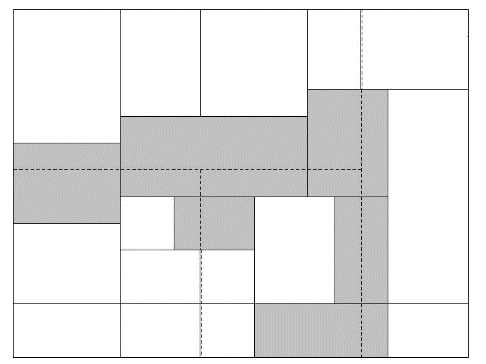
\includegraphics[width=54mm]{4.6.5.a.png} \nextRow
\hline
$\sum_{\scriptsize \begin{matrix}
  j \in \varLambda_{N} \\
  0 < n_{j} \\
\end{matrix}} {\max_{j \in \varLambda_{N}}{\sup_{\mathbf{a},\mathbf{b} \in J_{j}}\left\| \mathbf{b} - \mathbf{a} \right\|}\prod_{k' \in \varLambda_{m} \setminus \left\{ k \right\}} \left( b_{jk'} - a_{jk'} \right)}$ &
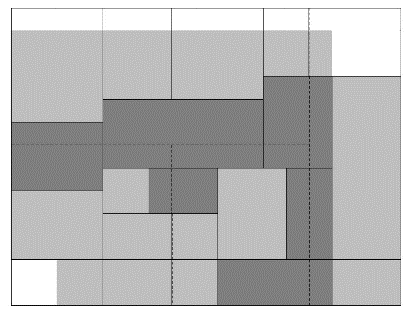
\includegraphics[width=54mm]{4.6.5.b.png} \nextRow
\hline
$\sum_{\scriptsize \begin{matrix}
  j \in \varLambda_{N} \\
  0 < n_{j} \\
\end{matrix}} {\max_{j \in \varLambda_{N}}{\sup_{\mathbf{a},\mathbf{b} \in J_{j}}\left\| \mathbf{b} - \mathbf{a} \right\|}\prod_{k' \in \varLambda_{m} \setminus \left\{ k \right\}} \left( b_{k'} - a_{k'} \right)}$ &
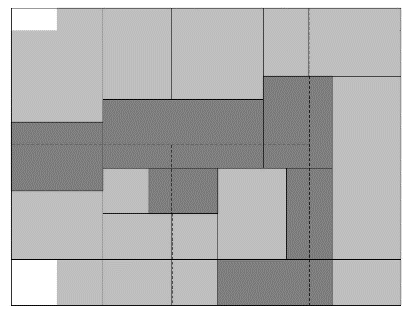
\includegraphics[width=54mm]{4.6.5.c.png} \nextRow
\hline
\end{tabular}}。
\begin{align*}
\lambda\left( \bigsqcup_{\scriptsize \begin{matrix}
j \in \varLambda_{N} \\
0 < n_{j} \\
\end{matrix} } J_{j} \right) &= \sum_{\scriptsize \begin{matrix}
j \in \varLambda_{N} \\
0 < n_{j} \\
\end{matrix}} {\lambda\left( J_{j} \right)} = \sum_{\scriptsize \begin{matrix}
j \in \varLambda_{N} \\
0 < n_{j} \\
\end{matrix}} {\prod_{k' \in \varLambda_{m}} \left( b_{jk'} - a_{jk'} \right)}\\
&= \sum_{\scriptsize \begin{matrix}
j \in \varLambda_{N} \\
0 < n_{j} \\
\end{matrix}} {\left( b_{jk'} - a_{jk'} \right)\prod_{k' \in \varLambda_{m} \setminus \left\{ k \right\}} \left( b_{jk'} - a_{jk'} \right)}\\
&\leq \sum_{\scriptsize \begin{matrix}
j \in \varLambda_{N} \\
0 < n_{j} \\
\end{matrix}} {\max_{j \in \varLambda_{N}}{\sup_{\mathbf{a},\mathbf{b} \in J_{j}}\left\| \mathbf{b} - \mathbf{a} \right\|}\prod_{k' \in \varLambda_{m} \setminus \left\{ k \right\}} \left( b_{jk'} - a_{jk'} \right)}\\
&\leq \sum_{\scriptsize \begin{matrix}
j \in \varLambda_{N} \\
0 < n_{j} \\
\end{matrix}} {\max_{j \in \varLambda_{N}}{\sup_{\mathbf{a},\mathbf{b} \in J_{j}}\left\| \mathbf{b} - \mathbf{a} \right\|}\prod_{k' \in \varLambda_{m} \setminus \left\{ k \right\}} \left( b_{k'} - a_{k'} \right)}\\
&= \sum_{k \in \varLambda_{m} } {r_{k}\max_{j \in \varLambda_{N}}{\sup_{\mathbf{a},\mathbf{b} \in J_{j}}\left\| \mathbf{b} - \mathbf{a} \right\|}\prod_{k' \in \varLambda_{m} \setminus \left\{ k \right\}} \left( b_{k'} - a_{k'} \right)}\\
&= \sum_{k \in \varLambda_{m} } {r_{k}\prod_{k' \in \varLambda_{m} \setminus \left\{ k \right\}} \left( b_{k'} - a_{k'} \right)}\mathcal{M}(\varDelta)
\end{align*}
これにより、次のようにおかれ、
\begin{align*}
c(I,\varGamma) = \sum_{k \in \varLambda_{m} } {r_{k}\prod_{k' \in \varLambda_{m} \setminus \left\{ k \right\}} \left( b_{k'} - a_{k'} \right)}
\end{align*}
$\forall\varepsilon \in \mathbb{R}^{+}$に対し、$0 < \delta < \min\left\{ e,\frac{\varepsilon}{c(I,\varGamma)\left( \sup{f|I} - \inf{f|I} \right)} \right\}$とおかれれば、$\mathcal{M}(\varDelta) < \delta$が成り立つなら、上記の議論により次のようになる。
\begin{align*}
0 &\leq s\left( f|I,B \right) - s\left( f|I,\varDelta \right)\\
&\leq \left( \sup{f|I} - \inf{f|I} \right)\sum_{\scriptsize \begin{matrix}
j \in M \\
0 < n_{j} \\
\end{matrix}} {\lambda\left( J_{j} \right)}\\
&\leq \left( \sup{f|I} - \inf{f|I} \right)c(I,\varGamma)\mathcal{M}(\varDelta)\\
&< \left( \sup{f|I} - \inf{f|I} \right)c(I,\varGamma)\delta\\
&< \left( \sup{f|I} - \inf{f|I} \right)c(I,\varGamma) \cdot \frac{\varepsilon}{c(I,\varGamma)\left( \sup{f|I} - \inf{f|I} \right)} = \varepsilon
\end{align*}
したがって、定理\ref{4.6.5.11}より$s\left( f|I,\varGamma \right) \leq s\left( f|I,B \right)$が成り立つので、次のようになる。
\begin{align*}
0 &\leq s_{I}f|I - s\left( f|I,\varDelta \right)\\
&= s_{I}f|I - s\left( f|I,\varDelta \right) + s\left( f|I,B \right) - s\left( f|I,B \right) + s\left( f|I,\varGamma \right) - s\left( f|I,\varGamma \right)\\
&= \left( s_{I}f|I - s\left( f|I,\varGamma \right) \right) + \left( s\left( f|I,B \right) - s\left( f|I,\varDelta \right) \right) - \left( s\left( f|I,B \right) - s\left( f|I,\varGamma \right) \right)\\
&\leq \left( s_{I}f|I - s\left( f|I,\varGamma \right) \right) + \left( s\left( f|I,B \right) - s\left( f|I,\varDelta \right) \right)\\
&< \varepsilon + \varepsilon = 2\varepsilon
\end{align*}\par
以上の議論により、$\lim_{\scriptsize \begin{matrix}
\mathcal{M}(\varDelta) \rightarrow 0 \\
\varDelta \in \mathcal{D}(I) \\
\end{matrix}}{s\left( f|I,\varDelta \right)} = s_{I}f|I$が成り立つので、$\varDelta_{I} = \left\{ J_{iI} \right\}_{i \in \varLambda_{I}}$とおかれれば、次のようになる。
\begin{align*}
\lim_{\scriptsize \begin{matrix}
\mathcal{M}(\varDelta) \rightarrow 0 \\
\varDelta \in \mathcal{D}(E) \\
\end{matrix}}{s(f,\varDelta)} &= \lim_{\scriptsize \begin{matrix}
\mathcal{M}\left( \varDelta_{I} \right) \rightarrow 0 \\
I \in \varDelta', \varDelta_{I}\in \mathcal{D}(I) \\
\end{matrix}}{s\left( f,\bigsqcup_{I \in \varDelta' } \varDelta_{I} \right)}\\
&= \lim_{\scriptsize \begin{matrix}
\mathcal{M}\left( \varDelta_{I} \right) \rightarrow 0 \\
I \in \varDelta', \varDelta_{I}\in \mathcal{D}(I) \\
\end{matrix}}{\sum_{I \in \varDelta' } {\sum_{\scriptsize \begin{matrix}
i \in \varLambda_{I} \\
\#\varLambda_{I} < \aleph_{0} \\
\end{matrix}} {\inf{f|J_{iI}}\lambda\left( J_{iI} \right)}}}\\
&= \sum_{I \in \varDelta' } {\lim_{\scriptsize \begin{matrix}
\mathcal{M}\left( \varDelta_{I} \right) \rightarrow 0 \\
I \in \varDelta', \varDelta_{I}\in \mathcal{D}(I) \\
\end{matrix}}{\sum_{\scriptsize \begin{matrix}
i \in \varLambda_{I} \\
\#\varLambda_{I} < \aleph_{0} \\
\end{matrix}} {\inf{f|J_{iI}}\lambda\left( J_{iI} \right)}}}\\
&= \sum_{I \in \varDelta' } {\lim_{\scriptsize \begin{matrix}
\mathcal{M}\left( \varDelta_{I} \right) \rightarrow 0 \\
\varDelta_{I}\in \mathcal{D}(I) \\
\end{matrix}}{s\left( f|I,\varDelta \right)}}\\
&= \sum_{I \in \varDelta' } {s_{I}f|I}\\
&= \sum_{I \in \varDelta' } {\sup_{\varDelta_{I}\in \mathcal{D}(I)}{s\left( f|I,\varDelta_{I} \right)}}\\
&= \sup_{I \in \varDelta', \varDelta_{I}\in \mathcal{D}(I)}{\sum_{I \in \varDelta' } {s\left( f|I,\varDelta_{I} \right)}}\\
&= \sup_{I \in \varDelta', \varDelta_{I}\in \mathcal{D}(I)}{\sum_{I \in \varDelta' } {\sum_{\scriptsize \begin{matrix}
i \in \varLambda_{I} \\
\#\varLambda_{I} < \aleph_{0} \\
\end{matrix}} {\inf{f|J_{iI}}\lambda\left( J_{iI} \right)}}}\\
&= \sup_{\varGamma \in \mathcal{D}(E)}{\sum_{I \in \varGamma } {\inf{f|I}\lambda(I)}}\\
&= \sup_{\varGamma \in \mathcal{D}(E)}{s(f,\varGamma)} = s_{E}f
\end{align*}\par
同様にして、$\lim_{\scriptsize \begin{matrix}
\mathcal{M}(\varDelta) \rightarrow 0 \\
\varDelta \in \mathcal{D}(E) \\
\end{matrix}}{S(f,\varDelta)} = S_{E}f$も成り立つことが示される。有界な関数$f:E \rightarrow \mathbb{R}^{n}$についても成分ごとで考えればよい。
\end{proof}
\begin{thm}\label{4.6.5.13}
$\forall E \in \mathfrak{F}_{m}$に対し、有界な関数$f:E \rightarrow \mathbb{R}^{n}$が与えられたとき、$f = \left( f_{k} \right)_{k \in \varLambda_{n}}$とおかれれば、次のことは同値である。
\begin{itemize}
\item
  その関数$f$がその区間塊$E$でRiemann積分可能である。
\item
  $\forall k \in \varLambda_{n}$に対し、次式が成り立つ。
\end{itemize}
\begin{align*}
\lim_{\scriptsize \begin{matrix}
\mathcal{M}(\varDelta) \rightarrow 0 \\
\varDelta \in \mathcal{D}(E) \\
\end{matrix}}\left( S\left( f_{k},\varDelta \right) - s\left( f_{k},\varDelta \right) \right) = 0
\end{align*}
\begin{itemize}
\item
  $\forall k \in \varLambda_{n}\forall\varDelta \in \mathcal{D}(E)$に対し、$\varDelta = \left\{ I_{i} \right\}_{i \in \varLambda_{N}}$とおかれれば、次式が成り立つ。
\end{itemize}
\begin{align*}
\lim_{\scriptsize \begin{matrix}
\mathcal{M}(\varDelta) \rightarrow 0 \\
\varDelta \in \mathcal{D}(E) \\
\end{matrix}}{\sum_{i \in \varLambda_{N}} {\left( \sup{f_{k}|I_{i}} - \inf{f_{k}|I_{i}} \right)\lambda\left( I_{i} \right)}} = 0
\end{align*}
\begin{itemize}
\item
  $s_{E}f = S_{E}f$が成り立つ。
\item
  $\forall k \in \varLambda_{n}\forall\varepsilon \in \mathbb{R}^{+}\exists\varDelta \in \mathcal{D}(E)$に対し、$S\left( f_{k},\varDelta \right) - s\left( f_{k},\varDelta \right) < \varepsilon$が成り立つ。
\end{itemize}
さらに、これが成り立つなら、次式が成り立つ。
\begin{align*}
s_{E}f = \int_{E} f = S_{E}f
\end{align*}
\end{thm}
\begin{proof}
$\forall E \in \mathfrak{F}_{m}$に対し、有界な関数$f:E \rightarrow \mathbb{R}^{n}$が与えられたとき、$f = \left( f_{k} \right)_{k \in \varLambda_{n}}$とおかれれば、その関数$f$がその区間塊$E$でRiemann積分可能であるなら、$\forall k \in \varLambda_{n}$に対し、$\varDelta = \left\{ I_{i} \right\}_{i \in \varLambda_{N}}$、$\Xi = \left\{ \xi_{i} \right\}_{i \in \varLambda_{N}}$とおかれれば、その分割$\varDelta$をなす区間の代表点の族$\Xi$によらず次式が成り立つ。
\begin{align*}
\int_{E} f_{k} = \lim_{\scriptsize \begin{matrix}
\mathcal{M}(\varDelta) \rightarrow 0 \\
\varDelta \in \mathcal{D}(E) \\
\end{matrix}}{S_{R}\left( f_{k},\varDelta,\Xi \right)}
\end{align*}
これが成り立つならそのときに限り、$\forall\varepsilon \in \mathbb{R}^{+}\exists\delta \in \mathbb{R}^{+}$に対し、$\mathcal{M}(\varDelta) < \delta$が成り立つなら、次式が成り立つ。
\begin{align*}
\left| S_{R}\left( f_{k},\varDelta,\Xi \right) - \int_{E} f_{k} \right| < \varepsilon
\end{align*}
したがって、これが成り立つならそのときに限り、次式が成り立つ。
\begin{align*}
- \varepsilon < S_{R}\left( f_{k},\varDelta,\Xi \right) - \int_{E} f_{k} < \varepsilon
\end{align*}
そこで、次のようになることから、
\begin{align*}
\inf{S_{R}\left( f_{k},\varDelta,\Xi \right)} &= \inf_{\xi_{i} \in I_{i}}{\sum_{i \in \varLambda_{N}} {f_{k}\left( \xi_{i} \right)\lambda\left( I_{i} \right)}}\\
&= \sum_{i \in \varLambda_{N}} {\inf{f_{k}|I_{i}}\lambda\left( I_{i} \right)}\\
&= s\left( f_{k},\varDelta \right)\\
\sup{S_{R}\left( f_{k},\varDelta,\Xi \right)} &= \sup_{\xi_{i} \in I_{i}}{\sum_{i \in \varLambda_{N}} {f_{k}\left( \xi_{i} \right)\lambda\left( I_{i} \right)}}\\
&= \sum_{i \in \varLambda_{N}} {\sup{f_{k}|I_{i}}\lambda\left( I_{i} \right)}\\
&= S\left( f_{k},\varDelta \right)
\end{align*}
次のようになる。
\begin{align*}
\left\{ \begin{matrix}
 - \varepsilon < s\left( f_{k},\varDelta \right) - \int_{E} f_{k} < \varepsilon \\
 - \varepsilon < S\left( f_{k},\varDelta \right) - \int_{E} f_{k} < \varepsilon \\
\end{matrix} \right. &\Leftrightarrow \left\{ \begin{matrix}
 - \varepsilon < \int_{E} f_{k} - s\left( f_{k},\varDelta \right) < \varepsilon \\
 - \varepsilon < S\left( f_{k},\varDelta \right) - \int_{E} f_{k} < \varepsilon \\
\end{matrix} \right.\ \\
&\Rightarrow - 2\varepsilon < S\left( f_{k},\varDelta \right) - \int_{E} f_{k} + \int_{E} f_{k} - s\left( f_{k},\varDelta \right) = S\left( f_{k},\varDelta \right) - s\left( f_{k},\varDelta \right) < 2\varepsilon\\
&\Leftrightarrow \left| S\left( f_{k},\varDelta \right) - s\left( f_{k},\varDelta \right) \right| < 2\varepsilon
\end{align*}
よって、$\forall k \in \varLambda_{n}$に対し、次式が成り立つ。
\begin{align*}
\lim_{\scriptsize \begin{matrix}
\mathcal{M}(\varDelta) \rightarrow 0 \\
\varDelta \in \mathcal{D}(E) \\
\end{matrix}}\left( S\left( f_{k},\varDelta \right) - s\left( f_{k},\varDelta \right) \right) = 0
\end{align*}\par
$\forall k \in \varLambda_{n}$に対し、次式が成り立つなら、
\begin{align*}
\lim_{\scriptsize \begin{matrix}
\mathcal{M}(\varDelta) \rightarrow 0 \\
\varDelta \in \mathcal{D}(E) \\
\end{matrix}}\left( S\left( f_{k},\varDelta \right) - s\left( f_{k},\varDelta \right) \right) = 0
\end{align*}
$\forall\varDelta \in \mathcal{D}(E)$に対し、$\varDelta = \left\{ I_{i} \right\}_{i \in \varLambda_{N}}$とおかれれば、次のようになる。
\begin{align*}
\lim_{\scriptsize \begin{matrix}
\mathcal{M}(\varDelta) \rightarrow 0 \\
\varDelta \in \mathcal{D}(E) \\
\end{matrix}}\left( S\left( f_{k},\varDelta \right) - s\left( f_{k},\varDelta \right) \right) &= \lim_{\scriptsize \begin{matrix}
\mathcal{M}(\varDelta) \rightarrow 0 \\
\varDelta \in \mathcal{D}(E) \\
\end{matrix}}\left( \sum_{i \in \varLambda_{N}} {\sup{f_{k}|I_{i}}\lambda\left( I_{i} \right)} - \sum_{i \in \varLambda_{N}} {\inf{f_{k}|I_{i}}\lambda\left( I_{i} \right)} \right)\\
&= \lim_{\scriptsize \begin{matrix}
\mathcal{M}(\varDelta) \rightarrow 0 \\
\varDelta \in \mathcal{D}(E) \\
\end{matrix}}{\sum_{i \in \varLambda_{N}} {\left( \sup{f_{k}|I_{i}} - \inf{f_{k}|I_{i}} \right)\lambda\left( I_{i} \right)}} = 0
\end{align*}
よって、次式が成り立つ。
\begin{align*}
\lim_{\scriptsize \begin{matrix}
\mathcal{M}(\varDelta) \rightarrow 0 \\
\varDelta \in \mathcal{D}(E) \\
\end{matrix}}{\sum_{i \in \varLambda_{N}} {\left( \sup{f_{k}|I_{i}} - \inf{f_{k}|I_{i}} \right)\lambda\left( I_{i} \right)}} = 0
\end{align*}
逆も同様にして示される。\par
$\forall k \in \varLambda_{n}$に対し、次式が成り立つならそのときに限り、
\begin{align*}
\lim_{\scriptsize \begin{matrix}
\mathcal{M}(\varDelta) \rightarrow 0 \\
\varDelta \in \mathcal{D}(E) \\
\end{matrix}}\left( S\left( f_{k},\varDelta \right) - s\left( f_{k},\varDelta \right) \right) = 0
\end{align*}
定理\ref{4.6.5.8}、定理\ref{4.6.5.12}より次のようになることから、
\begin{align*}
&\quad \forall k \in \varLambda_{n}\left[ \lim_{\scriptsize \begin{matrix}
\mathcal{M}(\varDelta) \rightarrow 0 \\
\varDelta \in \mathcal{D}(E) \\
\end{matrix}}\left( S\left( f_{k},\varDelta \right) - s\left( f_{k},\varDelta \right) \right) = 0 \right]\\
&\Leftrightarrow \left[ \forall k \in \varLambda_{n}\lim_{\scriptsize \begin{matrix}
\mathcal{M}(\varDelta) \rightarrow 0 \\
\varDelta \in \mathcal{D}(E) \\
\end{matrix}}{S\left( f_{k},\varDelta \right)} - \lim_{\scriptsize \begin{matrix}
\mathcal{M}(\varDelta) \rightarrow 0 \\
\varDelta \in \mathcal{D}(E) \\
\end{matrix}}{s\left( f_{k},\varDelta \right)} = 0 \right]\\
&\Leftrightarrow \forall k \in \varLambda_{n}\left[ S_{E}f_{k} - s_{E}f_{k} = 0 \right]\\
&\Leftrightarrow \forall k \in \varLambda_{n}\left[ S_{E}f_{k} = s_{E}f_{k} \right]\\
&\Leftrightarrow \left( S_{E}f_{k} \right)_{k \in \varLambda_{n}} = \left( s_{E}f_{k} \right)_{k \in \varLambda_{n}}\\
&\Leftrightarrow S_{E}f = s_{E}f
\end{align*}
$s_{E}f = S_{E}f$が成り立つ。\par
$s_{E}f = S_{E}f$が成り立つなら、定理\ref{4.6.5.8}より$\forall k \in \varLambda_{n}$に対し、$s_{E}f_{k} = S_{E}f_{k}$が成り立つ。そこで、上記の議論により$\forall\varDelta \in \mathcal{D}(E)$に対し、$\varDelta = \left\{ I_{i} \right\}_{i \in \varLambda_{N}}$、$\Xi = \left\{ \xi_{i} \right\}_{i \in \varLambda_{N}}$とおかれれば、その分割$\varDelta$をなす区間の任意の代表点の族$\Xi$に対し、次式が成り立つ。
\begin{align*}
s\left( f_{k},\varDelta \right) \leq S_{R}\left( f_{k},\varDelta,\Xi \right) \leq S\left( f_{k},\varDelta \right)
\end{align*}
したがって、定理\ref{4.6.5.12}より次のようになるので、
\begin{align*}
s_{E}f_{k} = \lim_{\scriptsize \begin{matrix}
\mathcal{M}(\varDelta) \rightarrow 0 \\
\varDelta \in \mathcal{D}(E) \\
\end{matrix}}{s(f,\varDelta)} \leq \lim_{\scriptsize \begin{matrix}
\mathcal{M}(\varDelta) \rightarrow 0 \\
\varDelta \in \mathcal{D}(E) \\
\end{matrix}}{S_{R}\left( f_{k},\varDelta,\Xi \right)} \leq \lim_{\scriptsize \begin{matrix}
\mathcal{M}(\varDelta) \rightarrow 0 \\
\varDelta \in \mathcal{D}(E) \\
\end{matrix}}{S(f,\varDelta)} = S_{E}f_{k}
\end{align*}
次式が成り立つ。
\begin{align*}
\lim_{\scriptsize \begin{matrix}
\mathcal{M}(\varDelta) \rightarrow 0 \\
\varDelta \in \mathcal{D}(E) \\
\end{matrix}}{S_{R}\left( f_{k},\varDelta,\Xi \right)} = s_{E}f_{k} = S_{E}f_{k}
\end{align*}
これにより、その関数$f_{k}$はその区間塊$E$でRiemann積分可能で定理\ref{4.6.5.7}よりその関数$f$もその区間塊$E$でRiemann積分可能である。\par
$\forall k \in \varLambda_{n}$に対し、次式が成り立つならそのときに限り、
\begin{align*}
\lim_{\scriptsize \begin{matrix}
\mathcal{M}(\varDelta) \rightarrow 0 \\
\varDelta \in \mathcal{D}(E) \\
\end{matrix}}\left( S\left( f_{k},\varDelta \right) - s\left( f_{k},\varDelta \right) \right) = 0
\end{align*}
$\forall\varepsilon \in \mathbb{R}^{+}\exists\delta \in \mathbb{R}^{+}$に対し、$\mathcal{M}(\varDelta) < \delta$が成り立つなら、次式が成り立つ。
\begin{align*}
\left| S\left( f_{k},\varDelta \right) - s\left( f_{k},\varDelta \right) \right| < \varepsilon
\end{align*}
そこで、定理\ref{4.6.5.11}より$0 \leq S\left( f_{k},\varDelta \right) - s\left( f_{k},\varDelta \right)$が成り立つので、よって、$\forall k \in \varLambda_{n}\forall\varepsilon \in \mathbb{R}^{+}\exists\varDelta \in \mathcal{D}(E)$に対し、$S\left( f_{k},\varDelta \right) - s\left( f_{k},\varDelta \right) < \varepsilon$が成り立つ。\par
逆に、$\forall k \in \varLambda_{n}\forall\varepsilon \in \mathbb{R}^{+}\exists\varDelta \in \mathcal{D}(E)$に対し、$S\left( f_{k},\varDelta \right) - s\left( f_{k},\varDelta \right) < \varepsilon$が成り立つなら、定理\ref{4.6.5.11}より$s\left( f_{k},\varDelta \right) \leq s_{E}f_{k} \leq S_{E}f_{k} \leq S\left( f_{k},\varDelta \right)$が成り立つので、次のようになることから、
\begin{align*}
s\left( f_{k},\varDelta \right) \leq s_{E}f_{k} \leq S_{E}f_{k} \leq S\left( f_{k},\varDelta \right) &\Leftrightarrow \left\{ \begin{matrix}
s\left( f_{k},\varDelta \right) \leq s_{E}f_{k} \\
s_{E}f_{k} \leq S_{E}f_{k} \\
S_{E}f_{k} \leq S\left( f_{k},\varDelta \right) \\
\end{matrix} \right. \\
&\Leftrightarrow \left\{ \begin{matrix}
 - s_{E}f_{k} \leq - s\left( f_{k},\varDelta \right) \\
0 \leq S_{E}f_{k} - s_{E}f_{k} \\
S_{E}f_{k} \leq S\left( f_{k},\varDelta \right) \\
\end{matrix} \right. \\
&\Rightarrow \left\{ \begin{matrix}
0 \leq S_{E}f_{k} - s_{E}f_{k} \\
S_{E}f_{k} - s_{E}f_{k} \leq S\left( f_{k},\varDelta \right) - s\left( f_{k},\varDelta \right) \\
\end{matrix} \right. \\
&\Rightarrow 0 \leq S_{E}f_{k} - s_{E}f_{k} \leq S\left( f_{k},\varDelta \right) - s\left( f_{k},\varDelta \right)
\end{align*}
$0 \leq S_{E}f_{k} - s_{E}f_{k} < \varepsilon$も成り立つ。その正の実数$\varepsilon$の任意性により$s_{E}f_{k} = S_{E}f_{k}$が得られるので、定理\ref{4.6.5.8}より$s_{E}f = S_{E}f$が成り立つ。\par
さらに、次のことのうちいづれかが成り立つとき、
\begin{itemize}
\item
  その関数$f$がその区間塊$E$でRiemann積分可能である。
\item
  $\forall k \in \varLambda_{n}$に対し、次式が成り立つ。
\begin{align*}
\lim_{\scriptsize \begin{matrix}
\mathcal{M}(\varDelta) \rightarrow 0 \\
\varDelta \in \mathcal{D}(E) \\
\end{matrix}}\left( S\left( f_{k},\varDelta \right) - s\left( f_{k},\varDelta \right) \right) = 0
\end{align*}
\item
  $\forall k \in \varLambda_{n}\forall\varDelta \in \mathcal{D}(E)$に対し、$\varDelta = \left\{ I_{i} \right\}_{i \in \varLambda_{N}}$とおかれれば、次式が成り立つ。
\begin{align*}
\lim_{\scriptsize \begin{matrix}
\mathcal{M}(\varDelta) \rightarrow 0 \\
\varDelta \in \mathcal{D}(E) \\
\end{matrix}}{\sum_{i \in \varLambda_{N}} {\left( \sup{f_{k}|I_{i}} - \inf{f_{k}|I_{i}} \right)\lambda\left( I_{i} \right)}} = 0
\end{align*}
\item
  $s_{E}f = S_{E}f$が成り立つ。
\item
  $\forall k \in \varLambda_{n}\forall\varepsilon \in \mathbb{R}^{+}\exists\varDelta \in \mathcal{D}(E)$に対し、$S\left( f_{k},\varDelta \right) - s\left( f_{k},\varDelta \right) < \varepsilon$が成り立つ。
\end{itemize}
$s_{E}f = S_{E}f$が成り立つなら、その関数$f$もその区間塊$E$でRiemann積分可能であることの証明を繰り返せばよくて次式が成り立つ。
\begin{align*}
s_{E}f = \int_{E} f = S_{E}f
\end{align*}
\end{proof}
%\hypertarget{riemannux7a4dux5206-1}{%
\subsubsection{Riemann積分}%\label{riemannux7a4dux5206-1}}
\begin{thm}\label{4.6.5.14}
$\forall E,F \in \mathfrak{F}_{m}\forall A \in \mathfrak{P}(E)\mathfrak{\cap P}(F)$に対し、その集合$A$が有界で関数$f:E \rightarrow \mathbb{R}^{n}$、$g:F \rightarrow \mathbb{R}^{n}$を用いた$f\chi_{A}|A = g\chi_{A}|A$なる関数たち$f\chi_{A}$、$g\chi_{A}$がそれぞれそれらの区間塊たち$E$、$F$上でRiemann積分可能なとき、次式が成り立つ。
\begin{align*}
\int_{E} {f\chi_{A}} = \int_{F} {g\chi_{A}}
\end{align*}
\end{thm}
\begin{dfn}
$\forall E \in \mathfrak{F}_{m}\forall A \in \mathfrak{P}(E)$に対し、その集合$A$が有界で関数$f:E \rightarrow \mathbb{R}^{n}$を用いた関数$f\chi_{A}$がその区間塊$E$上でRiemann積分可能なとき、その関数$f$はその有界な集合$A$上でRiemann積分可能であるといい、さらに、その実数$\int_{E} {f\chi_{A}}$をその関数$f$のその有界な集合$A$上のRiemann積分といい次のように書く。
\begin{align*}
\int_{A} f = \int_{E} {f\chi_{A}}
\end{align*}
\end{dfn}
\begin{proof}
$\forall E,F \in \mathfrak{F}_{m}\forall A \in \mathfrak{P}(E)\mathfrak{\cap P}(F)$に対し、その集合$A$が有界で関数$f:E \rightarrow \mathbb{R}^{n}$、$g:F \rightarrow \mathbb{R}^{n}$を用いた$f\chi_{A}|A = g\chi_{A}|A$なる関数たち$f\chi_{A}$、$g\chi_{A}$がそれぞれそれらの区間塊たち$E$、$F$上でRiemann積分可能なとき、区間塊$E \cup F$で考えられれば、$\varDelta = \left\{ G_{i} \right\}_{i \in \varLambda_{N}}$なるその区間塊$E \cup F$の分割$\varDelta$で$E = G_{i'}$が成り立つようなものがとられれば、$\forall i \in \varLambda$に対し、$i \neq i'$が成り立つなら、$f\chi_{A}|\mathrm{int}\left( G_{i} \right) = 0$が成り立つので、定理\ref{4.5.4.9}よりその関数$f\chi_{A}$はその区間塊$G_{i}$上で積分可能で次のようになる。
\begin{align*}
\int_{E \cup F} {f\chi_{A}} &= \sum_{i \in \varLambda_{N}} {\int_{G_{i}} {f\chi_{A}}} \\
&= \sum_{i \in \varLambda_{N} \setminus \left\{ i' \right\}} {\int_{G_{i}} {f\chi_{A}}} + \int_{G_{i'}} {f\chi_{A}} \\
&= \sum_{i \in \varLambda_{N} \setminus \left\{ i' \right\}} {\int_{G_{i}} 0} + \int_{E} {f\chi_{A}} \\
&= \int_{E} {f\chi_{A}}
\end{align*}
同様にして、次式が成り立つことが示される。
\begin{align*}
\int_{E \cup F} {f\chi_{A}} = \int_{F} {f\chi_{A}}
\end{align*}
よって、次式が成り立つ。
\begin{align*}
\int_{E} {f\chi_{A}} = \int_{F} {g\chi_{A}}
\end{align*}
\end{proof}
\begin{thm}\label{4.6.5.15}
任意の有界な関数$f:\mathbb{R}^{m} \rightarrow \mathbb{R}^{n}$は$\lambda^{*}(A) = 0$なる有界な集合$A$上でRiemann積分可能で次式が成り立つ。
\begin{align*}
\int_{A} f = 0
\end{align*}
\end{thm}
\begin{proof}
任意の有界な関数$f:\mathbb{R}^{m} \rightarrow \mathbb{R}^{n}$と$\lambda^{*}(A) = 0$なる有界な集合$A$が与えられたとき、ある非負実数$M$が存在して、$|f| \leq M$が成り立つ。その有界な集合$A$を含む区間塊$E$の$\varDelta = \left\{ E_{i} \right\}_{i \in \varLambda_{N}}$なる任意の分割$\varDelta$とその区間$E_{i}$の代表点$\xi_{i}$に対し、$\Xi = \left\{ \xi_{i} \right\}_{i \in \varLambda_{N}}$とおかれれば、次のようになるので、
\begin{align*}
\left| S_{R}\left( f\chi_{A},\varDelta,\Xi \right) \right| &= \left| \sum_{i \in \varLambda_{N}} {f\left( \xi_{i} \right)\chi_{A}\left( \xi_{i} \right)\lambda\left( I_{i} \right)} \right|\\
&\leq \sum_{i \in \varLambda_{N}} \left| f\left( \xi_{i} \right)\chi_{A}\left( \xi_{i} \right)\lambda\left( I_{i} \right) \right|\\
&= \sum_{i \in \varLambda_{N}} {\left| f\left( \xi_{i} \right) \right|\chi_{A}\left( \xi_{i} \right)\lambda\left( I_{i} \right)}\\
&\leq M\sum_{i \in \varLambda_{N}} {\chi_{A}\left( \xi_{i} \right)\lambda\left( I_{i} \right)}\\
&= MS_{R}\left( \chi_{A},\varDelta,\Xi \right)
\end{align*}
したがって、次のようになる。
\begin{align*}
0 \leq \lim_{\scriptsize \begin{matrix}
\mathcal{M}(\varDelta) \rightarrow 0 \\
\varDelta \in \mathcal{D}(E) \\
\end{matrix}}\left| S_{R}\left( f\chi_{A},\varDelta,\Xi \right) \right| \leq M\lim_{\scriptsize \begin{matrix}
\mathcal{M}(\varDelta) \rightarrow 0 \\
\varDelta \in \mathcal{D}(E) \\
\end{matrix}}{S_{R}\left( \chi_{A},\varDelta,\Xi \right)} = M\int_{E} \chi_{A} = M\lambda^{*}(A) = 0
\end{align*}
これにより、その関数$f:\mathbb{R}^{m} \rightarrow \mathbb{R}^{n}$は$\lambda^{*}(A) = 0$なる有界な集合$A$上でRiemann積分可能で次式が成り立つ。
\begin{align*}
\int_{A} f = 0
\end{align*}
\end{proof}
%\hypertarget{riemannux7a4dux5206ux3068lebesgueux7a4dux5206}{%
\subsubsection{Riemann積分とLebesgue積分}%\label{riemannux7a4dux5206ux3068lebesgueux7a4dux5206}}
\begin{thm}\label{4.6.5.16}
$\forall E \in \mathfrak{F}_{m}$に対し、有界な関数$f:E \rightarrow \mathbb{R}^{n}$が与えられたとき、その関数$f$がその区間塊$E$でRiemann積分可能であるなら、その関数$f$はLebesgue測度空間$\left( \mathbb{R}^{n},\ \ \mathfrak{M}_{C}\left( \lambda^{*} \right),\ \ \lambda \right)$で可測である。このとき、次式が成り立つ。
\begin{align*}
\int_{E} f = \int_{E} {f\lambda}
\end{align*}
\end{thm}
\begin{proof}
以下、関数の定義域がこれを含む集合へ拡張するとき、拡張された定義域から元の定義域への差集合上ではその関数は$0$としよう。$\forall E \in \mathfrak{F}_{m}$に対し、有界な関数$f:E \rightarrow \mathbb{R}^{n}$が与えられたとき、その関数$f$がその区間塊$E$でRiemann積分可能であるなら、$\forall\varDelta \in \mathcal{D}(E)$に対し、$\varDelta = \left\{ I_{i} \right\}_{i \in \varLambda_{N}}$とおかれれば、定理\ref{4.6.5.11}より$\forall k \in \varLambda_{n}$に対し、次式が成り立つ。
\begin{align*}
\sum_{i \in \varLambda_{N}} {\inf{f_{k}|I_{i}}\chi_{I_{i}}} \leq f_{k} \leq \sum_{i \in \varLambda_{N}} {\sup{f_{k}|I_{i}}\chi_{I_{i}}}
\end{align*}
実際、$\mathbf{x} \in I_{i}$のとき、次のようになることから、
\begin{align*}
\sum_{i \in \varLambda_{N}} {\inf{f_{k}|I_{i}}\chi_{I_{i}}\left( \mathbf{x} \right)} &= \inf{f_{k}|I_{i}}\chi_{I_{i}}\left( \mathbf{x} \right) = \inf{f_{k}|I_{i}}\\
\sum_{i \in \varLambda_{N}} {\sup{f_{k}|I_{i}}\chi_{I_{i}}\left( \mathbf{x} \right)} &= \sup{f_{k}|I_{i}}\chi_{I_{i}}\left( \mathbf{x} \right) = \sup{f_{k}|I_{i}}
\end{align*}
$\inf{f_{k}|I_{i}} \leq f_{k} \leq \sup{f_{k}|I_{i}}$が成り立つ。これにより、もちろん、次式が成り立つ。
\begin{align*}
\lim_{\scriptsize \begin{matrix}
\mathcal{M}(\varDelta) \rightarrow 0 \\
\varDelta \in \mathcal{D}(E) \\
\end{matrix}}{\sum_{i \in \varLambda_{N}} {\inf{f_{k}|I_{i}}\chi_{I_{i}}}} \leq f_{k} \leq \lim_{\scriptsize \begin{matrix}
\mathcal{M}(\varDelta) \rightarrow 0 \\
\varDelta \in \mathcal{D}(E) \\
\end{matrix}}{\sum_{i \in \varLambda_{N}} {\sup{f_{k}|I_{i}}\chi_{I_{i}}}}
\end{align*}\par
このとき、これらの関数たち$\sum_{i \in \varLambda_{N}} {\inf{f_{k}|I_{i}}\chi_{I_{i}}}$、$\sum_{i \in \varLambda_{N}} {\sup{f_{k}|I_{i}}\chi_{I_{i}}}$は単関数なので、Lebesgue測度空間$\left( \mathbb{R}^{n},\ \ \mathfrak{M}_{C}\left( \lambda^{*} \right),\ \ \lambda \right)$で可測である。したがって、次のようになる。
\begin{align*}
\int_{E} {\sum_{i \in \varLambda_{N}} {\inf{f_{k}|I_{i}}\chi_{I_{i}}}\lambda} &= \sum_{i \in \varLambda_{N}} {\inf{f_{k}|I_{i}}\lambda\left( I_{i} \right)} = s\left( f_{k},\varDelta \right)\\
\int_{E} {\sum_{i \in \varLambda_{N}} {\sup{f_{k}|I_{i}}\chi_{I_{i}}}\lambda} &= \sum_{i \in \varLambda_{N}} {\sup{f_{k}|I_{i}}\lambda\left( I_{i} \right)} = S\left( f_{k},\varDelta \right)
\end{align*}
その関数$f$は有界で$- \infty < \inf{f_{k}|I_{i}} < \infty$かつ$- \infty < \sup{f_{k}|I_{i}} < \infty$が成り立つので、これらの単関数たち$\sum_{i \in \varLambda_{N}} {\inf{f_{k}|I_{i}}\chi_{I_{i}}}$、$\sum_{i \in \varLambda_{N}} {\sup{f_{k}|I_{i}}\chi_{I_{i}}}$は有界でもある。したがって、定理\ref{4.6.2.7}のLebesgueの有界収束定理、定理\ref{4.6.5.12}のDarbouxの定理よりこれらの単関数たちは定積分可能で次のようになる。
\begin{align*}
s_{E}f_{k} &= \lim_{\scriptsize \begin{matrix}
\mathcal{M}(\varDelta) \rightarrow 0 \\
\varDelta \in \mathcal{D}(E) \\
\end{matrix}}{s\left( f_{k},\varDelta \right)}\\
&= \lim_{\scriptsize \begin{matrix}
\mathcal{M}(\varDelta) \rightarrow 0 \\
\varDelta \in \mathcal{D}(E) \\
\end{matrix}}{\int_{E} {\sum_{i \in \varLambda_{N}} {\inf{f_{k}|I_{i}}\chi_{I_{i}}}\lambda}}\\
&= \int_{E} {\lim_{\scriptsize \begin{matrix}
\mathcal{M}(\varDelta) \rightarrow 0 \\
\varDelta \in \mathcal{D}(E) \\
\end{matrix}}{\sum_{i \in \varLambda_{N}} {\inf{f_{k}|I_{i}}\chi_{I_{i}}}}\lambda}\\
S_{E}f_{k} &= \lim_{\scriptsize \begin{matrix}
\mathcal{M}(\varDelta) \rightarrow 0 \\
\varDelta \in \mathcal{D}(E) \\
\end{matrix}}{S\left( f_{k},\varDelta \right)}\\
&= \lim_{\scriptsize \begin{matrix}
\mathcal{M}(\varDelta) \rightarrow 0 \\
\varDelta \in \mathcal{D}(E) \\
\end{matrix}}{\int_{E} {\sum_{i \in \varLambda_{N}} {\sup{f_{k}|I_{i}}\chi_{I_{i}}}\lambda}}\\
&= \int_{E} {\lim_{\scriptsize \begin{matrix}
\mathcal{M}(\varDelta) \rightarrow 0 \\
\varDelta \in \mathcal{D}(E) \\
\end{matrix}}{\sum_{i \in \varLambda_{N}} {\sup{f_{k}|I_{i}}\chi_{I_{i}}}}\lambda}
\end{align*}
定理\ref{4.6.5.8}、定理\ref{4.6.5.13}より$s_{E}f_{k} = S_{E}f_{k}$が成り立つので、次のようになる。
\begin{align*}
0 &= S_{E}f_{k} - s_{E}f_{k}\\
&= \int_{E} {\lim_{\scriptsize \begin{matrix}
\mathcal{M}(\varDelta) \rightarrow 0 \\
\varDelta \in \mathcal{D}(E) \\
\end{matrix}}{\sum_{i \in \varLambda_{N}} {\sup{f_{k}|I_{i}}\chi_{I_{i}}}}\lambda} - \int_{E} {\lim_{\scriptsize \begin{matrix}
\mathcal{M}(\varDelta) \rightarrow 0 \\
\varDelta \in \mathcal{D}(E) \\
\end{matrix}}{\sum_{i \in \varLambda_{N}} {\inf{f_{k}|I_{i}}\chi_{I_{i}}}}\lambda}\\
&= \int_{E} {\left| \lim_{\scriptsize \begin{matrix}
\mathcal{M}(\varDelta) \rightarrow 0 \\
\varDelta \in \mathcal{D}(E) \\
\end{matrix}}{\sum_{i \in \varLambda_{N}} {\sup{f_{k}|I_{i}}\chi_{I_{i}}}} - \lim_{\scriptsize \begin{matrix}
\mathcal{M}(\varDelta) \rightarrow 0 \\
\varDelta \in \mathcal{D}(E) \\
\end{matrix}}{\sum_{i \in \varLambda_{N}} {\inf{f_{k}|I_{i}}\chi_{I_{i}}}} \right|\lambda}\\
&= \int_{X} {\left| \lim_{\scriptsize \begin{matrix}
\mathcal{M}(\varDelta) \rightarrow 0 \\
\varDelta \in \mathcal{D}(E) \\
\end{matrix}}{\sum_{i \in \varLambda_{N}} {\sup{f_{k}|I_{i}}\chi_{I_{i}}}} - \lim_{\scriptsize \begin{matrix}
\mathcal{M}(\varDelta) \rightarrow 0 \\
\varDelta \in \mathcal{D}(E) \\
\end{matrix}}{\sum_{i \in \varLambda_{N}} {\inf{f_{k}|I_{i}}\chi_{I_{i}}}} \right|\chi_{E}\lambda}\\
&= \int_{X} {\left| \lim_{\scriptsize \begin{matrix}
\mathcal{M}(\varDelta) \rightarrow 0 \\
\varDelta \in \mathcal{D}(E) \\
\end{matrix}}{\sum_{i \in \varLambda_{N}} {\sup{f_{k}|I_{i}}\chi_{I_{i}}\chi_{E}}} - \lim_{\scriptsize \begin{matrix}
\mathcal{M}(\varDelta) \rightarrow 0 \\
\varDelta \in \mathcal{D}(E) \\
\end{matrix}}{\sum_{i \in \varLambda_{N}} {\inf{f_{k}|I_{i}}\chi_{I_{i}}\chi_{E}}} \right|\lambda}\\
&= \int_{X} {\left| \lim_{\scriptsize \begin{matrix}
\mathcal{M}(\varDelta) \rightarrow 0 \\
\varDelta \in \mathcal{D}(E) \\
\end{matrix}}{\sum_{i \in \varLambda_{N}} {\sup{f_{k}|I_{i}}\chi_{I_{i} \cap E}}} - \lim_{\scriptsize \begin{matrix}
\mathcal{M}(\varDelta) \rightarrow 0 \\
\varDelta \in \mathcal{D}(E) \\
\end{matrix}}{\sum_{i \in \varLambda_{N}} {\inf{f_{k}|I_{i}}\chi_{I_{i} \cap E}}} \right|\lambda}\\
&= \int_{X} {\left| \lim_{\scriptsize \begin{matrix}
\mathcal{M}(\varDelta) \rightarrow 0 \\
\varDelta \in \mathcal{D}(E) \\
\end{matrix}}{\sum_{i \in \varLambda_{N}} {\sup{f_{k}|I_{i}}\chi_{I_{i}}}} - \lim_{\scriptsize \begin{matrix}
\mathcal{M}(\varDelta) \rightarrow 0 \\
\varDelta \in \mathcal{D}(E) \\
\end{matrix}}{\sum_{i \in \varLambda_{N}} {\inf{f_{k}|I_{i}}\chi_{I_{i}}}} \right|\lambda}
\end{align*}
定理\ref{4.6.1.20}よりLebesgue測度空間で$a.e.\ \mathbf{x} \in \mathbb{R}^{m}$に対し、次式が成り立つ。
\begin{align*}
\lim_{\scriptsize \begin{matrix}
\mathcal{M}(\varDelta) \rightarrow 0 \\
\varDelta \in \mathcal{D}(E) \\
\end{matrix}}{\sum_{i \in \varLambda_{N}} {\inf{f_{k}|I_{i}}\chi_{I_{i}}}}\left( \mathbf{x} \right) = \lim_{\scriptsize \begin{matrix}
\mathcal{M}(\varDelta) \rightarrow 0 \\
\varDelta \in \mathcal{D}(E) \\
\end{matrix}}{\sum_{i \in \varLambda_{N}} {\sup{f_{k}|I_{i}}\chi_{I_{i}}}}\left( \mathbf{x} \right)
\end{align*}\par
したがって、Lebesgue測度空間で$a.e.\ \mathbf{x} \in \mathbb{R}^{m}$に対し、次式が成り立つ。
\begin{align*}
\lim_{\scriptsize \begin{matrix}
\mathcal{M}(\varDelta) \rightarrow 0 \\
\varDelta \in \mathcal{D}(E) \\
\end{matrix}}{\sum_{i \in \varLambda_{N}} {\inf{f_{k}|I_{i}}\chi_{I_{i}}}}\left( \mathbf{x} \right) = f\left( \mathbf{x} \right) = \lim_{\scriptsize \begin{matrix}
\mathcal{M}(\varDelta) \rightarrow 0 \\
\varDelta \in \mathcal{D}(E) \\
\end{matrix}}{\sum_{i \in \varLambda_{N}} {\sup{f_{k}|I_{i}}\chi_{I_{i}}}}\left( \mathbf{x} \right)
\end{align*}
これにより、その関数$f$は可測である。定理\ref{4.6.3.5}よりこれらの単関数たちは定積分可能であるので、上記の議論により次のようになる。
\begin{align*}
s_{E}f_{k} = \int_{E} {\lim_{\scriptsize \begin{matrix}
\mathcal{M}(\varDelta) \rightarrow 0 \\
\varDelta \in \mathcal{D}(E) \\
\end{matrix}}{\sum_{i \in \varLambda_{N}} {\inf{f_{k}|I_{i}}\chi_{I_{i}}}}\lambda} = \int_{E} {f\lambda}
\end{align*}
定理\ref{4.6.5.13}より次式が成り立つ。
\begin{align*}
\int_{E} f = \int_{E} {f\lambda}
\end{align*}
\end{proof}
\begin{thebibliography}{50}
\bibitem{1}
  杉浦光夫, 解析入門I, 東京大学出版社, 198. 第34刷 p205-228,254-261 ISBN978-4-13-062005-5
\bibitem{2}
  伊藤清三, ルベーグ積分入門, 裳華房, 1963. 第24刷 p12-51,111-114 ISBN4-7853-1304-8
\end{thebibliography}
\end{document}

\clearpage
\documentclass[dvipdfmx]{jsarticle}
\setcounter{section}{6}
\setcounter{subsection}{5}
\usepackage{xr}
\externaldocument{4.1.8}
\externaldocument{4.5.4}
\externaldocument{4.5.5}
\externaldocument{4.6.1}
\externaldocument{4.6.3}
\usepackage{amsmath,amsfonts,amssymb,array,comment,mathtools,url,docmute}
\usepackage{longtable,booktabs,dcolumn,tabularx,mathtools,multirow,colortbl,xcolor}
\usepackage[dvipdfmx]{graphics}
\usepackage{bmpsize}
\usepackage{amsthm}
\usepackage{enumitem}
\setlistdepth{20}
\renewlist{itemize}{itemize}{20}
\setlist[itemize]{label=•}
\renewlist{enumerate}{enumerate}{20}
\setlist[enumerate]{label=\arabic*.}
\setcounter{MaxMatrixCols}{20}
\setcounter{tocdepth}{3}
\newcommand{\rotin}{\text{\rotatebox[origin=c]{90}{$\in $}}}
\newcommand{\amap}[6]{\text{\raisebox{-0.7cm}{\begin{tikzpicture} 
  \node (a) at (0, 1) {$\textstyle{#2}$};
  \node (b) at (#6, 1) {$\textstyle{#3}$};
  \node (c) at (0, 0) {$\textstyle{#4}$};
  \node (d) at (#6, 0) {$\textstyle{#5}$};
  \node (x) at (0, 0.5) {$\rotin $};
  \node (x) at (#6, 0.5) {$\rotin $};
  \draw[->] (a) to node[xshift=0pt, yshift=7pt] {$\textstyle{\scriptstyle{#1}}$} (b);
  \draw[|->] (c) to node[xshift=0pt, yshift=7pt] {$\textstyle{\scriptstyle{#1}}$} (d);
\end{tikzpicture}}}}
\newcommand{\twomaps}[9]{\text{\raisebox{-0.7cm}{\begin{tikzpicture} 
  \node (a) at (0, 1) {$\textstyle{#3}$};
  \node (b) at (#9, 1) {$\textstyle{#4}$};
  \node (c) at (#9+#9, 1) {$\textstyle{#5}$};
  \node (d) at (0, 0) {$\textstyle{#6}$};
  \node (e) at (#9, 0) {$\textstyle{#7}$};
  \node (f) at (#9+#9, 0) {$\textstyle{#8}$};
  \node (x) at (0, 0.5) {$\rotin $};
  \node (x) at (#9, 0.5) {$\rotin $};
  \node (x) at (#9+#9, 0.5) {$\rotin $};
  \draw[->] (a) to node[xshift=0pt, yshift=7pt] {$\textstyle{\scriptstyle{#1}}$} (b);
  \draw[|->] (d) to node[xshift=0pt, yshift=7pt] {$\textstyle{\scriptstyle{#2}}$} (e);
  \draw[->] (b) to node[xshift=0pt, yshift=7pt] {$\textstyle{\scriptstyle{#1}}$} (c);
  \draw[|->] (e) to node[xshift=0pt, yshift=7pt] {$\textstyle{\scriptstyle{#2}}$} (f);
\end{tikzpicture}}}}
\renewcommand{\thesection}{第\arabic{section}部}
\renewcommand{\thesubsection}{\arabic{section}.\arabic{subsection}}
\renewcommand{\thesubsubsection}{\arabic{section}.\arabic{subsection}.\arabic{subsubsection}}
\everymath{\displaystyle}
\allowdisplaybreaks[4]
\usepackage{vtable}
\theoremstyle{definition}
\newtheorem{thm}{定理}[subsection]
\newtheorem*{thm*}{定理}
\newtheorem{dfn}{定義}[subsection]
\newtheorem*{dfn*}{定義}
\newtheorem{axs}[dfn]{公理}
\newtheorem*{axs*}{公理}
\renewcommand{\headfont}{\bfseries}
\makeatletter
  \renewcommand{\section}{%
    \@startsection{section}{1}{\z@}%
    {\Cvs}{\Cvs}%
    {\normalfont\huge\headfont\raggedright}}
\makeatother
\makeatletter
  \renewcommand{\subsection}{%
    \@startsection{subsection}{2}{\z@}%
    {0.5\Cvs}{0.5\Cvs}%
    {\normalfont\LARGE\headfont\raggedright}}
\makeatother
\makeatletter
  \renewcommand{\subsubsection}{%
    \@startsection{subsubsection}{3}{\z@}%
    {0.4\Cvs}{0.4\Cvs}%
    {\normalfont\Large\headfont\raggedright}}
\makeatother
\makeatletter
\renewenvironment{proof}[1][\proofname]{\par
  \pushQED{\qed}%
  \normalfont \topsep6\p@\@plus6\p@\relax
  \trivlist
  \item\relax
  {
  #1\@addpunct{.}}\hspace\labelsep\ignorespaces
}{%
  \popQED\endtrivlist\@endpefalse
}
\makeatother
\renewcommand{\proofname}{\textbf{証明}}
\usepackage{tikz,graphics}
\usepackage[dvipdfmx]{hyperref}
\usepackage{pxjahyper}
\hypersetup{
 setpagesize=false,
 bookmarks=true,
 bookmarksdepth=tocdepth,
 bookmarksnumbered=true,
 colorlinks=false,
 pdftitle={},
 pdfsubject={},
 pdfauthor={},
 pdfkeywords={}}
\begin{document}
%\hypertarget{lebesgueux7a4dux5206}{%
\subsection{Lebesgue積分}%\label{lebesgueux7a4dux5206}}
%\hypertarget{riemannux7a4dux5206ux306eux7b2c1ux5e73ux5747ux5024ux306eux5b9aux7406}{%
\subsubsection{Riemann積分の第1平均値の定理}%\label{riemannux7a4dux5206ux306eux7b2c1ux5e73ux5747ux5024ux306eux5b9aux7406}}
\begin{thm}[Riemann積分の第1平均値の定理]\label{4.6.6.1}
$\forall E \in \mathfrak{F}_{m}$に対し、連続な関数$f:\mathrm{cl}E \rightarrow \mathbb{R}$、Lebesgue測度空間においてその閉包$\mathrm{cl}E$で定積分可能で$0 \leq g$な関数$g:\mathbb{R}^{n} \rightarrow \mathbb{R}$が与えられたとき、$\exists\mathbf{x} \in \mathrm{cl}E$に対し、次式が成り立つ。
\begin{align*}
\int_{\mathrm{cl}E} {fg\lambda} = f\left( \mathbf{x} \right)\int_{\mathrm{cl}E} {g\lambda}
\end{align*}
特に、$g = 1$とすれば次式が成り立つ。
\begin{align*}
\int_{\mathrm{cl}E} {f\lambda} = f\left( \mathbf{x} \right)\lambda\left( \mathrm{cl}E \right)
\end{align*}
この定理をRiemann積分の第1平均値の定理という。
\end{thm}
\begin{proof}
$\forall E \in \mathfrak{F}_{m}$に対し、連続な関数$f:\mathrm{cl}E \rightarrow \mathbb{R}$、Lebesgue測度空間で定積分可能で$0 \leq g$な関数$g:\mathbb{R}^{n} \rightarrow \mathbb{R}$が与えられたとき、定理\ref{4.1.8.7}、即ち、最大値最小値の定理よりその関数$f$の最大値$\max f$、最小値$\min f$が存在するので、その関数$f$は有界である。したがって、定理\ref{4.6.1.33}、即ち、積分の第1平均値の定理よりその関数$fg$はその集合$\mathrm{cl}E$で積分可能で$\inf{f|\mathrm{cl}E} \leq c \leq \sup{f|\mathrm{cl}E}$なるある実数$c$が存在して、$0 \leq g$が成り立つので、次式が成り立つ。
\begin{align*}
\int_{\mathrm{cl}E} {fg\lambda} = c\int_{\mathrm{cl}E} {g\lambda}
\end{align*}
このとき、$\inf{f|\mathrm{cl}E} = \min f$、$\sup{f|\mathrm{cl}E} = \max f$が成り立つので、中間値の定理の拡張より$\exists\mathbf{x} \in \mathrm{cl}E$に対し、$c = f\left( \mathbf{x} \right)$が成り立つ\footnote{中間値の定理の拡張は次のことを主張する定理です。
\begin{quote}
連結な位相空間$\left( S,\mathfrak{O} \right)$から1次元Euclid空間$E$における位相空間$\left( \mathbb{R},\mathfrak{O}_{d_{E}} \right)$への連続写像$f:S \rightarrow \mathbb{R}$について、$\forall a,b \in S$に対し、$f(a) < f(b)$が成り立つなら、$\forall\gamma \in \left[ f(a),f(b) \right]$に対し、$f(c) = \gamma$なるその集合$S$の元$c$が存在する。
\end{quote}
なお、定理\ref{4.1.8.8}より強いことを主張していることに注意です。証明は位相空間論の内容をかなり要求するので、省略いたします。}。したがって、次のようになる。
\begin{align*}
\int_{\mathrm{cl}E} {fg\lambda} = f\left( \mathbf{x} \right)\int_{\mathrm{cl}E} {g\lambda}
\end{align*}
特に、$g = 1$とすれば次式が成り立つ。
\begin{align*}
\int_{\mathrm{cl}E} {f\lambda} = f\left( \mathbf{x} \right)\lambda\left( \mathrm{cl}E \right)
\end{align*}
\end{proof}
%\hypertarget{lebesgueux7a4dux5206ux3068urysohnux306eux88dcux984c}{%
\subsubsection{Lebesgue積分とUrysohnの補題}%\label{lebesgueux7a4dux5206ux3068urysohnux306eux88dcux984c}}
\begin{thm}\label{4.6.6.2}
Lebesgue測度空間において$E \in \mathfrak{M}_{C}\left( \lambda^{*} \right)$なる集合$E$で定積分可能な関数$f:\mathbb{R}^{n} \rightarrow \mathbb{R}$が与えられたとき、$\forall\varepsilon \in \mathbb{R}^{+}$に対し、連続であり、ある有界な開集合$O$と、$\mathbf{x} \notin O$が成り立つなら、$f_{\varepsilon}\left( \mathbf{x} \right) = 0$が成り立つようなその関数$f_{\varepsilon}:\mathbb{R}^{n} \rightarrow \mathbb{R}$が存在して、次式が成り立つ。
\begin{align*}
\int_{E} {\left| f - f_{\varepsilon} \right|\lambda} < \varepsilon
\end{align*}
\end{thm}
\begin{proof}
Lebesgue測度空間において、$E \in \mathfrak{M}_{C}\left( \lambda^{*} \right)$なる集合$E$で定積分可能な関数$f:\mathbb{R}^{n} \rightarrow \mathbb{R}$が与えられたとき、$0 \leq f$と仮定すれば、定理\ref{4.5.5.18}における非負可測関数の非負単関数の列による近似での列$\left( (f)_{m} \right)_{m \in \mathbb{N}}$を用いて、点$\mathbf{0}$を中心とした半径$m$の開球が$U\left( \mathbf{0},m \right)$とおかれれば、$\forall m \in \mathbb{N}$に対し、$U\left( \mathbf{0},m \right) \subseteq U\left( \mathbf{0},m + 1 \right)$が成り立つので、$0 \leq \chi_{U\left( \mathbf{0},m \right)} \leq \chi_{U\left( \mathbf{0},m + 1 \right)}$が成り立つかつ、$0 \leq (f)_{m} \leq (f)_{m + 1}$も成り立つので、$(f)_{m}\chi_{U\left( \mathbf{0},m \right)} \leq (f)_{m + 1}\chi_{U\left( \mathbf{0},m + 1 \right)}$が成り立つ。これにより、その関数の列$\left( (f)_{m}\chi_{U\left( \mathbf{0},m \right)} \right)_{m \in \mathbb{N}}$は単調増加する。さらに、前述のことに加えて$\lim_{m \rightarrow \infty}\chi_{U\left( \mathbf{0},m \right)} = 1$が成り立つことに注意すれば、次のようになる。
\begin{align*}
(f)_{m}\chi_{U\left( \mathbf{0},m \right)} &\leq \sup\left\{ (f)_{m}\chi_{U\left( \mathbf{0},m \right)} \right\}_{m \in \mathbb{N}}\\
&= \lim_{m \rightarrow \infty}{(f)_{m}\chi_{U\left( \mathbf{0},m \right)}}\\
&= \lim_{m \rightarrow \infty}(f)_{m}\lim_{m \rightarrow \infty}\chi_{U\left( \mathbf{0},m \right)}\\
&= f \cdot 1 = f
\end{align*}
したがって、定理\ref{4.6.1.26}、即ち、単調収束定理より次のようになる。
\begin{align*}
\lim_{m \rightarrow \infty}{\int_{E} {\left| f - (f)_{m}\chi_{U\left( \mathbf{0},m \right)} \right|\lambda}} &= \lim_{m \rightarrow \infty}{\int_{E} {\left| \sup\left\{ (f)_{m}\chi_{U\left( \mathbf{0},m \right)} \right\}_{m \in \mathbb{N}} - (f)_{m}\chi_{U\left( \mathbf{0},m \right)} \right|\lambda}}\\
&= \lim_{m \rightarrow \infty}\left( \int_{E} {\sup\left\{ (f)_{m}\chi_{U\left( \mathbf{0},m \right)} \right\}_{m \in \mathbb{N}}\lambda} - \int_{E} {(f)_{m}\chi_{U\left( \mathbf{0},m \right)}\lambda} \right)\\
&= \int_{E} {\sup\left\{ (f)_{m}\chi_{U\left( \mathbf{0},m \right)} \right\}_{m \in \mathbb{N}}\lambda} - \lim_{m \rightarrow \infty}{\int_{E} {(f)_{m}\chi_{U\left( \mathbf{0},m \right)}\lambda}}\\
&= \lim_{m \rightarrow \infty}{\int_{E} {(f)_{m}\chi_{U\left( \mathbf{0},m \right)}\lambda}} - \lim_{m \rightarrow \infty}{\int_{E} {(f)_{m}\chi_{U\left( \mathbf{0},m \right)}\lambda}} = 0
\end{align*}\par
これにより、$\forall\varepsilon \in \mathbb{R}^{+}$に対し、ある自然数$m_{0}$が存在して、$m_{0} \leq m$が成り立つなら、次式が成り立つ。
\begin{align*}
0 \leq \int_{E} {\left| f - (f)_{m}\chi_{U\left( \mathbf{0},m \right)} \right|\lambda} = \left| \int_{E} {\left| f - (f)_{m}\chi_{U\left( \mathbf{0},m \right)} \right|\lambda} \right| < \frac{\varepsilon}{2}
\end{align*}
そこで、その関数$(f)_{m}\chi_{U\left( \mathbf{0},m \right)}$は単関数同士の積であるから、単関数となって$0 < \alpha_{i}$、$E_{i} \subseteq U\left( \mathbf{0},m \right)$として次のようにおかれることができる。
\begin{align*}
(f)_{m}\chi_{U\left( \mathbf{0},m \right)} = \sum_{i \in \varLambda_{k}} {\alpha_{i}\chi_{E_{i}}}
\end{align*}
なお、$E = \bigsqcup_{i \in \varLambda_{k}} E_{i}$が成り立つ。ここで、$\forall i \in \varLambda_{k}$に対し、定理\ref{4.5.4.14}と定理\ref{4.5.4.16}より開集合$O_{i}$と閉集合$A_{i}$が存在して、次式が成り立つ。
\begin{align*}
A_{i} \subseteq E_{i} \subseteq O_{i},\ \ \lambda\left( O_{i} \setminus E_{i} \right) < \frac{\varepsilon}{4k\alpha_{i}},\ \ \lambda\left( E_{i} \setminus A_{i} \right) < \frac{\varepsilon}{4k\alpha_{i}}
\end{align*}
ここで、$A_{i} \subseteq E_{i} \subseteq O_{i}$かつその集合$E_{i}$が有界であることにより、$\lambda\left( E_{i} \right) < \infty$が成り立つので、次のようになる。
\begin{align*}
\lambda\left( O_{i} \setminus E_{i} \right) + \lambda\left( E_{i} \setminus A_{i} \right) &= \lambda\left( O_{i} \right) - \lambda\left( E_{i} \right) + \lambda\left( E_{i} \right) - \lambda\left( A_{i} \right)\\
&= \lambda\left( O_{i} \right) - \lambda\left( A_{i} \right)\\
&= \lambda\left( O_{i} \setminus A_{i} \right)\\
&< \frac{\varepsilon}{4k\alpha_{i}} + \frac{\varepsilon}{4k\alpha_{i}} = \frac{\varepsilon}{2k\alpha_{i}}
\end{align*}
これにより、$\lambda\left( O_{i} \setminus A_{i} \right) < \frac{\varepsilon}{2k\alpha_{i}}$が得られる。\par
そこで、差集合$\mathbb{R}^{n} \setminus O_{i}$は閉集合で$A_{i} \subseteq O_{i}$より$\forall\mathbf{a} \in \mathbb{R}^{n}$に対し、$\mathbf{a} \in A_{i}$が成り立つなら、$\mathbf{a} \in O_{i}$が成り立つことになり、これの否定が$\mathbf{a} \in A_{i}$かつ$\mathbf{a} \notin O_{i}$が成り立つことなので、$A_{i} \cap \mathbb{R}^{n} \setminus O_{i} = \emptyset$が成り立つ。もちろん、$n$次元Euclid空間$E^{n}$における位相空間$\left( \mathbb{R}^{n},\mathfrak{O}_{d_{E^{n}}} \right)$は$\mathrm{T}_{4}$-空間なので、Urysohnの補題よりその位相空間$\left( \mathbb{R}^{n},\mathfrak{O}_{d_{E^{n}}} \right)$から1次元Euclid空間における位相空間$\left( \mathbb{R},\mathfrak{O}_{d_{E}} \right)$への連続な関数$g_{i}:\mathbb{R}^{n} \rightarrow \mathbb{R}$で次のことを満たすようなものが存在する\footnote{Urysohnの補題は次のことを主張する定理です。
  \begin{quote}
  $\mathrm{T}_{4}$-空間$\left( S,\mathfrak{O} \right)$の閉集合系を$\mathfrak{A}$とおくとき、$\forall A,B \in \mathfrak{A}$に対し、$A \cap B = \emptyset$が成り立つなら、その位相空間$\left( S,\mathfrak{O} \right)$から1次元Euclid空間における位相空間$\left( \mathbb{R},\mathfrak{O}_{d_{E}} \right)$への連続写像$f:S \rightarrow \mathbb{R}$で次のことを満たすようなものが存在する。
  \begin{itemize}
  \item
    $\forall a \in A$に対し、$f(a) = 0$が成り立つかつ、$\forall b \in B$に対し、$f(b) = 1$が成り立つ。
  \item
    $\forall c \in S$に対し、$0 \leq f(c) \leq 1$が成り立つ。
  \end{itemize}
  \end{quote}
なお、証明は大変なので割愛させていただきます。}。
\begin{itemize}
\item
  $\forall\mathbf{x} \in A_{i}$に対し、$g_{i}\left( \mathbf{x} \right) = 0$が成り立つかつ、$\forall\mathbf{x} \in \mathbb{R}^{n} \setminus O_{i}$に対し、$g_{i}\left( \mathbf{x} \right) = 1$が成り立つ。
\item
  $\forall\mathbf{x} \in \mathbb{R}^{n}$に対し、$0 \leq g_{i}\left( \mathbf{x} \right) \leq 1$が成り立つ。
\end{itemize}\par
そこで、次のように関数$f_{\varepsilon}$がおかれれば、
\begin{align*}
f_{\varepsilon} = \sum_{i \in \varLambda_{k}} {\alpha_{i}g_{i}}
\end{align*}
これは連続で、$\mathbf{x} \notin O_{i} \setminus A_{i}$のとき、$\mathbf{x} \notin O_{i} \setminus A_{i}$が成り立つならそのときに限り、$\mathbf{x} \in A_{i} \sqcup \mathbb{R}^{n} \setminus O_{i}$が成り立つので、$\mathbf{x} \in A_{i}$のとき、$A_{i} \subseteq E_{i}$より$\mathbf{x} \in E_{i}$が成り立つかつ、その関数$g_{i}$の定義より$\chi_{E_{i}}\left( \mathbf{x} \right) = g_{i}\left( \mathbf{x} \right) = 1$が成り立つ。$\mathbf{x} \in \mathbb{R}^{n} \setminus O_{i}$のとき、$E_{i} \subseteq O_{i}$より$\mathbf{x} \in \mathbb{R}^{n} \setminus E_{i}$が成り立つかつ、その関数$g_{i}$の定義より$\chi_{E_{i}}\left( \mathbf{x} \right) = g_{i}\left( \mathbf{x} \right) = 0$が成り立つ。以上の議論により、$\mathbf{x} \notin O_{i} \setminus A_{i}$のとき、$\chi_{E_{i}} = g_{i}$が成り立つことになる。\par
したがって、$\left| \chi_{E_{i}} - g_{i} \right| \leq I_{\mathbb{R}^{n}}$が成り立つことに注意すれば、次のようになる。
\begin{align*}
\int_{E} {\left| (f)_{m}\chi_{U\left( \mathbf{0},m \right)} - f_{\varepsilon} \right|\lambda} &= \int_{E} {\left| \sum_{i \in \varLambda_{k}} {\alpha_{i}\chi_{E_{i}}} - \sum_{i \in \varLambda_{k}} {\alpha_{i}g_{i}} \right|\lambda}\\
&= \int_{E} {\left| \sum_{i \in \varLambda_{k}} {\alpha_{i}\left( \chi_{E_{i}} - g_{i} \right)} \right|\lambda}\\
&\leq \int_{E} {\sum_{i \in \varLambda_{k}} {\alpha_{i}\left| \chi_{E_{i}} - g_{i} \right|}\lambda}\\
&= \sum_{i \in \varLambda_{k}} {\alpha_{i}\int_{E} {\left| \chi_{E_{i}} - g_{i} \right|\lambda}}\\
&= \sum_{i \in \varLambda_{k}} {\alpha_{i}\int_{E \setminus \left( O_{i} \setminus A_{i} \right) \sqcup O_{i} \setminus A_{i}} {\left| \chi_{E_{i}} - g_{i} \right|\lambda}}\\
&= \sum_{i \in \varLambda_{k}} {\alpha_{i}\left( \int_{E \setminus \left( O_{i} \setminus A_{i} \right)} {\left| \chi_{E_{i}} - g_{i} \right|\lambda} + \int_{O_{i} \setminus A_{i}} {\left| \chi_{E_{i}} - g_{i} \right|\lambda} \right)}\\
&= \sum_{i \in \varLambda_{k}} {\alpha_{i}\left( \int_{E \setminus \left( O_{i} \setminus A_{i} \right)} {0\lambda} + \int_{O_{i} \setminus A_{i}} {\left| \chi_{E_{i}} - g_{i} \right|\lambda} \right)}\\
&= \sum_{i \in \varLambda_{k}} {\alpha_{i}\int_{O_{i} \setminus A_{i}} {\left| \chi_{E_{i}} - g_{i} \right|\lambda}}\\
&\leq \sum_{i \in \varLambda_{k}} {\alpha_{i}\int_{O_{i} \setminus A_{i}} {I_{\mathbb{R}^{n}}\lambda}}\\
&= \sum_{i \in \varLambda_{k}} {\alpha_{i}\int_{O_{i} \setminus A_{i}} \lambda}\\
&= \sum_{i \in \varLambda_{k}} {\alpha_{i}\lambda\left( O_{i} \setminus A_{i} \right)}\\
&< \sum_{i \in \varLambda_{k}} {\alpha_{i} \cdot \frac{\varepsilon}{2k\alpha_{i}}}\\
&= \sum_{i \in \varLambda_{k}} \frac{\varepsilon}{2k} = \frac{\varepsilon}{2}
\end{align*}\par
以上の議論により、次のようになる。
\begin{align*}
\int_{E} {\left| f - f_{\varepsilon} \right|\lambda} &= \int_{E} {\left| f - (f)_{m}\chi_{U\left( \mathbf{0},m \right)} + (f)_{m}\chi_{U\left( \mathbf{0},m \right)} - f_{\varepsilon} \right|\lambda}\\
&\leq \int_{E} {\left( \left| f - (f)_{m}\chi_{U\left( \mathbf{0},m \right)} \right| + \left| (f)_{m}\chi_{U\left( \mathbf{0},m \right)} - f_{\varepsilon} \right| \right)\lambda}\\
&= \int_{E} {\left| f - (f)_{m}\chi_{U\left( \mathbf{0},m \right)} \right|\lambda} + \int_{E} {\left| (f)_{m}\chi_{U\left( \mathbf{0},m \right)} - f_{\varepsilon} \right|\lambda}\\
&< \frac{\varepsilon}{2} + \frac{\varepsilon}{2} = \varepsilon
\end{align*}\par
このとき、$O = \bigcup_{i \in \varLambda_{k}} O_{i}$とおかれれば、これは有界な開集合で、$\mathbf{x} \notin O$が成り立つなら、$\forall i \in \varLambda_{k}$に対し、$\mathbf{x} \notin O_{i}$が成り立つことになるので、次のようになる。
\begin{align*}
f_{\varepsilon}\left( \mathbf{x} \right) = \sum_{i \in \varLambda_{k}} {\alpha_{i}g_{i}}\left( \mathbf{x} \right) = \sum_{i \in \varLambda_{k}} {\alpha_{i}g_{i}\left( \mathbf{x} \right)} = \sum_{i \in \varLambda_{k}} {\alpha_{i} \cdot 0} = 0
\end{align*}\par
$E \in \mathfrak{M}_{C}\left( \lambda^{*} \right)$なる集合$E$で定積分可能な関数$f:\mathbb{R}^{n} \rightarrow \mathbb{R}$が与えられたとき、$f = (f)_{+} - (f)_{-}$が成り立つかつ、$0 \leq (f)_{+}$かつ$0 \leq (f)_{-}$が成り立つので、上記の議論により$\forall\varepsilon \in \mathbb{R}^{+}$に対し、連続であり、ある有界な開集合たち$O_{+}$、$O_{-}$と、$\mathbf{x} \notin O_{+}$が成り立つなら、$\left( f_{\varepsilon} \right)_{+}\left( \mathbf{x} \right) = 0$、$\mathbf{x} \notin O_{-}$が成り立つなら、$\left( f_{\varepsilon} \right)_{-}\left( \mathbf{x} \right) = 0$が成り立つようなそれらの関数たち$\left( f_{\varepsilon} \right)_{+}:\mathbb{R}^{n} \rightarrow \mathbb{R}$、$\left( f_{\varepsilon} \right)_{-}:\mathbb{R}^{n} \rightarrow \mathbb{R}$が存在して、次式が成り立つ。
\begin{align*}
\int_{E} {\left| (f)_{+} - \left( f_{\varepsilon} \right)_{+} \right|\lambda} < \frac{\varepsilon}{2},\ \ \int_{E} {\left| (f)_{-} - \left( f_{\varepsilon} \right)_{-} \right|\lambda} < \frac{\varepsilon}{2}
\end{align*}
そこで、$O = O_{+} \cup O_{-}$、$f_{\varepsilon} = \left( f_{\varepsilon} \right)_{+} - \left( f_{\varepsilon} \right)_{-}$とおかれれば、次のようになる。
\begin{align*}
\int_{E} {\left| f - f_{\varepsilon} \right|\lambda} &= \int_{E} {\left| \left( (f)_{+} - (f)_{-} \right) - \left( \left( f_{\varepsilon} \right)_{+} - \left( f_{\varepsilon} \right)_{-} \right) \right|\lambda}\\
&= \int_{E} {\left| (f)_{+} - \left( f_{\varepsilon} \right)_{+} - (f)_{-} + \left( f_{\varepsilon} \right)_{-} \right|\lambda}\\
&\leq \int_{E} {\left( \left| (f)_{+} - \left( f_{\varepsilon} \right)_{+} \right| + \left| - (f)_{-} + \left( f_{\varepsilon} \right)_{-} \right| \right)\lambda}\\
&= \int_{E} {\left| (f)_{+} - \left( f_{\varepsilon} \right)_{+} \right|\lambda} + \int_{E} {\left| (f)_{-} - \left( f_{\varepsilon} \right)_{-} \right|\lambda}\\
&< \frac{\varepsilon}{2} + \frac{\varepsilon}{2} = \varepsilon
\end{align*}
さらに、その集合$O$は有界な開集合で、$\mathbf{x} \notin O$が成り立つなら、$\mathbf{x} \notin O_{+}$かつ$\mathbf{x} \notin O_{-}$が成り立つので、次のようになる。
\begin{align*}
f_{\varepsilon}\left( \mathbf{x} \right) = \left( \left( f_{\varepsilon} \right)_{+} - \left( f_{\varepsilon} \right)_{-} \right)\left( \mathbf{x} \right) = \left( f_{\varepsilon} \right)_{+}\left( \mathbf{x} \right) - \left( f_{\varepsilon} \right)_{-}\left( \mathbf{x} \right) = 0 - 0 = 0
\end{align*}
\end{proof}
%\hypertarget{lebesgueux7a4dux5206ux3068affineux5909ux63db}{%
\subsubsection{Lebesgue積分とaffine変換}%\label{lebesgueux7a4dux5206ux3068affineux5909ux63db}}
\begin{thm}\label{4.6.6.3}
Lebesgue測度空間において$E \in \mathfrak{M}_{C}\left( \lambda^{*} \right)$なる集合$E$で定積分をもつ関数$f:\mathbb{R}^{n} \rightarrow \mathbb{R}$が与えられたとき、$\forall A_{nn} \in \mathrm{GL}_{n}\left( \mathbb{R} \right)\forall\mathbf{b} \in \mathbb{R}^{n}$に対し、関数$f \circ \left( A_{nn}I_{\mathbb{R}^{n}} + \mathbf{b} \right)$も可測で定積分をもち次式が成り立つ。
\begin{align*}
\int_{A_{nn}^{- 1}\left( E - \mathbf{b} \right)} {f \circ \left( A_{nn}I_{\mathbb{R}^{n}} + \mathbf{b} \right)\lambda} = \frac{1}{\left| \det A_{nn} \right|}\int_{E} {f\lambda}
\end{align*}
特に、その行列$A_{nn}$が直交行列であるなら、次式が成り立つ。
\begin{align*}
\int_{A_{nn}^{- 1}\left( E - \mathbf{b} \right)} {f \circ \left( A_{nn}I_{\mathbb{R}^{n}} + \mathbf{b} \right)\lambda} = \int_{E} {f\lambda}
\end{align*}
\end{thm}
\begin{proof}
Lebesgue測度空間において$E \in \mathfrak{M}_{C}\left( \lambda^{*} \right)$なる集合$E$で定積分をもつ関数$f:\mathbb{R}^{n} \rightarrow \mathbb{R}$が与えられたとき、$\forall A_{nn} \in \mathrm{GL}_{n}\left( \mathbb{R} \right)\forall\mathbf{b} \in \mathbb{R}^{n}$に対し、$0 \leq f$と仮定すれば、定理\ref{4.5.5.18}における非負可測関数の非負単関数の列による近似での列$\left( (f)_{m} \right)_{m \in \mathbb{N}}$を用いて、$(f)_{m} = \sum_{i \in \varLambda_{k}} {\alpha_{i}\chi_{E_{i}}}$とおかれれば、$\forall\mathbf{x} \in \mathbb{R}^{n}$に対し、次のようになることから、
\begin{align*}
(f)_{m} \circ \left( A_{nn}I_{\mathbb{R}^{n}} + \mathbf{b} \right)\left( \mathbf{x} \right) &= \sum_{i \in \varLambda_{k}} {\alpha_{i}\chi_{E_{i}}} \circ \left( A_{nn}I_{\mathbb{R}^{n}} + \mathbf{b} \right)\left( \mathbf{x} \right)\\
&= \sum_{i \in \varLambda_{k}} {\alpha_{i}\chi_{E_{i}}\left( \left( A_{nn}I_{\mathbb{R}^{n}} + \mathbf{b} \right)\left( \mathbf{x} \right) \right)}\\
&= \sum_{i \in \varLambda_{k}} {\alpha_{i}\chi_{E_{i}}\left( A_{nn}\mathbf{x} + \mathbf{b} \right)}\\
&= \sum_{i \in \varLambda_{k}} \left\{ \begin{matrix}
\alpha_{i} & \mathrm{if} & A_{nn}\mathbf{x} + \mathbf{b} \in E_{i} \\
0 & \mathrm{if} & A_{nn}\mathbf{x} + \mathbf{b} \notin E_{i} \\
\end{matrix} \right.\ \\
&= \sum_{i \in \varLambda_{k}} \left\{ \begin{matrix}
\alpha_{i} & \mathrm{if} & \mathbf{x} \in A_{nn}^{- 1}\left( E_{i} - \mathbf{b} \right) \\
0 & \mathrm{if} & \mathbf{x} \notin A_{nn}^{- 1}\left( E_{i} - \mathbf{b} \right) \\
\end{matrix} \right.\ \\
&= \sum_{i \in \varLambda_{k}} {\alpha_{i}\chi_{A_{nn}^{- 1}\left( E_{i} - \mathbf{b} \right)}\left( \mathbf{x} \right)}\\
&= \left( \sum_{i \in \varLambda_{k}} {\alpha_{i}\chi_{A_{nn}^{- 1}\left( E_{i} - \mathbf{b} \right)}} \right)\left( \mathbf{x} \right)
\end{align*}
次式が成り立つ。
\begin{align*}
(f)_{m} \circ \left( A_{nn}I_{\mathbb{R}^{n}} + \mathbf{b} \right) = \sum_{i \in \varLambda_{k}} {\alpha_{i}\chi_{A_{nn}^{- 1}\left( E_{i} - \mathbf{b} \right)}}
\end{align*}\par
このとき、その関数$(f)_{m} \circ \left( A_{nn}I_{\mathbb{R}^{n}} + \mathbf{b} \right)$が単関数であることから可測なので、次のようになることにより
\begin{align*}
f \circ \left( A_{nn}I_{\mathbb{R}^{n}} + \mathbf{b} \right) &= \sup\left\{ (f)_{m} \right\}_{m \in \mathbb{N}} \circ \left( A_{nn}I_{\mathbb{R}^{n}} + \mathbf{b} \right)\\
&= \lim_{m \rightarrow \infty}(f)_{m} \circ \left( A_{nn}I_{\mathbb{R}^{n}} + \mathbf{b} \right)\\
&= \sup\left\{ (f)_{m} \circ \left( A_{nn}I_{\mathbb{R}^{n}} + \mathbf{b} \right) \right\}_{m \in \mathbb{N}}
\end{align*}
その関数$f \circ \left( A_{nn}I_{\mathbb{R}^{n}} + \mathbf{b} \right)$も可測である。また、定理\ref{4.5.4.22}より$A_{nn}^{- 1}\left( E_{i} - \mathbf{b} \right) \in \mathfrak{M}_{C}\left( \lambda^{*} \right)$が成り立つ。\par
さらに、$\lambda\left( A_{nn}^{- 1}\left( E_{i} - \mathbf{b} \right) \right) = \frac{\lambda\left( E_{i} \right)}{\left| \det A_{nn} \right|}$が成り立つので、定理\ref{4.6.1.26}、即ち、単調収束定理より次のようになる。
\begin{align*}
\int_{A_{nn}^{- 1}\left( E - \mathbf{b} \right)} {f \circ \left( A_{nn}I_{\mathbb{R}^{n}} + \mathbf{b} \right)\lambda} &= \int_{A_{nn}^{- 1}\left( E - \mathbf{b} \right)} {\sup\left\{ (f)_{m} \right\}_{m \in \mathbb{N}} \circ \left( A_{nn}I_{\mathbb{R}^{n}} + \mathbf{b} \right)\lambda}\\
&= \int_{A_{nn}^{- 1}\left( E - \mathbf{b} \right)} {\lim_{m \rightarrow \infty}(f)_{m} \circ \left( A_{nn}I_{\mathbb{R}^{n}} + \mathbf{b} \right)\lambda}\\
&= \int_{A_{nn}^{- 1}\left( E - \mathbf{b} \right)} {\sup\left\{ (f)_{m} \circ \left( A_{nn}I_{\mathbb{R}^{n}} + \mathbf{b} \right) \right\}_{m \in \mathbb{N}}\lambda}\\
&= \lim_{m \rightarrow \infty}{\int_{A_{nn}^{- 1}\left( E - \mathbf{b} \right)} {(f)_{m} \circ \left( A_{nn}I_{\mathbb{R}^{n}} + \mathbf{b} \right)\lambda}}\\
&= \lim_{m \rightarrow \infty}{\int_{A_{nn}^{- 1}\left( E - \mathbf{b} \right)} {\sum_{i \in \varLambda_{k}} {\alpha_{i}\chi_{A_{nn}^{- 1}\left( E_{i} - \mathbf{b} \right)}}\lambda}}\\
&= \lim_{m \rightarrow \infty}{\sum_{i \in \varLambda_{k}} {\alpha_{i}\lambda\left( A_{nn}^{- 1}\left( E_{i} - \mathbf{b} \right) \right)}}\\
&= \lim_{m \rightarrow \infty}{\sum_{i \in \varLambda_{k}} \frac{\alpha_{i}\lambda\left( E_{i} \right)}{\left| \det A_{nn} \right|}}\\
&= \frac{1}{\left| \det A_{nn} \right|}\lim_{m \rightarrow \infty}{\sum_{i \in \varLambda_{k}} {\alpha_{i}\lambda\left( E_{i} \right)}}\\
&= \frac{1}{\left| \det A_{nn} \right|}\lim_{m \rightarrow \infty}{\int_{E} {\sum_{i \in \varLambda_{k}} {\alpha_{i}\chi_{E_{i}}}\lambda}}\\
&= \frac{1}{\left| \det A_{nn} \right|}\lim_{m \rightarrow \infty}{\int_{E} {(f)_{m}\lambda}}\\
&= \frac{1}{\left| \det A_{nn} \right|}\int_{E} {\sup\left\{ (f)_{m} \right\}_{m \in \mathbb{N}}\lambda}\\
&= \frac{1}{\left| \det A_{nn} \right|}\int_{E} {f\lambda}
\end{align*}\par
$E \in \mathfrak{M}_{C}\left( \lambda^{*} \right)$なる集合$E$で定積分可能な関数$f:\mathbb{R}^{n} \rightarrow \mathbb{R}$が与えられたとき、$f = (f)_{+} - (f)_{-}$が成り立つかつ、$0 \leq (f)_{+}$かつ$0 \leq (f)_{-}$が成り立つので、上記の議論により次のようになる。
\begin{align*}
\int_{A_{nn}^{- 1}\left( E - \mathbf{b} \right)} {f \circ \left( A_{nn}I_{\mathbb{R}^{n}} + \mathbf{b} \right)\lambda} &= \int_{A_{nn}^{- 1}\left( E - \mathbf{b} \right)} {\left( (f)_{+} - (f)_{-} \right) \circ \left( A_{nn}I_{\mathbb{R}^{n}} + \mathbf{b} \right)\lambda}\\
&= \int_{A_{nn}^{- 1}\left( E - \mathbf{b} \right)} {(f)_{+} \circ \left( A_{nn}I_{\mathbb{R}^{n}} + \mathbf{b} \right)\lambda} \\
&\quad - \int_{A_{nn}^{- 1}\left( E - \mathbf{b} \right)} {(f)_{-} \circ \left( A_{nn}I_{\mathbb{R}^{n}} + \mathbf{b} \right)\lambda}\\
&= \frac{1}{\left| \det A_{nn} \right|}\int_{E} {(f)_{+}\lambda} - \frac{1}{\left| \det A_{nn} \right|}\int_{E} {(f)_{-}\lambda}\\
&= \frac{1}{\left| \det A_{nn} \right|}\int_{E} {\left( (f)_{+} - (f)_{-} \right)\lambda}\\
&= \frac{1}{\left| \det A_{nn} \right|}\int_{E} {f\lambda}
\end{align*}\par
特に、その行列$A_{nn}$が直交行列であるなら、unitary行列でもあることに注意してその行列$A_{nn}$のJordan標準形が$J$とおかれれば、次のようになることから\footnote{$K \subseteq \mathbb{C}$なる体$K$上の内積空間$(V,\varPhi)$、等長変換$f:V \rightarrow V$が与えられたとき、その等長変換$f$の任意の固有値$\lambda$は、もしこれが存在するなら、$|\lambda| = 1$を満たすという定理を用いた。ただし、体$\mathbb{C}$は代数的閉体であることに注意されたい。}、
\begin{align*}
\left| \det A_{nn} \right| = \left| \det J \right| = 1
\end{align*}
次式が成り立つ。
\begin{align*}
\int_{A_{nn}^{- 1}\left( E - \mathbf{b} \right)} {f \circ \left( A_{nn}I_{\mathbb{R}^{n}} + \mathbf{b} \right)\lambda} = \int_{E} {f\lambda}
\end{align*}
\end{proof}
\begin{thm}\label{4.6.6.4}
Lebesgue測度空間において$E \in \mathfrak{M}_{C}\left( \lambda^{*} \right)$なる集合$E$で定積分可能な関数$f:\mathbb{R}^{n} \rightarrow \mathbb{R}$が与えられたとき、次式が成り立つ。
\begin{align*}
\lim_{\left\| \mathbf{h} \right\| \rightarrow 0}{\int_{E - \mathbf{h}} {\left| f \circ \left( I_{\mathbb{R}^{n}} + \mathbf{h} \right) - f \right|\lambda}} = 0
\end{align*}
\end{thm}
\begin{proof}
Lebesgue測度空間において$E \in \mathfrak{M}_{C}\left( \lambda^{*} \right)$なる集合$E$で定積分可能な関数$f:\mathbb{R}^{n} \rightarrow \mathbb{R}$が与えられたとき、$\forall\varepsilon \in \mathbb{R}^{+}$に対し、定理\ref{4.6.6.2}より連続であり、ある有界な開集合$O$と、$\mathbf{x} \notin O$が成り立つなら、$f_{\varepsilon} \circ \left( I_{\mathbb{R}^{n}} + \mathbf{h} \right)\left( \mathbf{x} \right) = 0$が成り立つようなその関数$f_{\varepsilon} \circ \left( I_{\mathbb{R}^{n}} + \mathbf{h} \right):\mathbb{R}^{n} \rightarrow \mathbb{R}$が存在して、次式が成り立つ。
\begin{align*}
\int_{E - \mathbf{h}} {\left| f \circ \left( I_{\mathbb{R}^{n}} + \mathbf{h} \right) - f_{\varepsilon} \circ \left( I_{\mathbb{R}^{n}} + \mathbf{h} \right) \right|\lambda} &= \int_{E - \mathbf{h}} {\left| f - f_{\varepsilon} \right| \circ \left( I_{\mathbb{R}^{n}} + \mathbf{h} \right)\lambda}\\
&= \int_{E} {\left| f - f_{\varepsilon} \right|\lambda} < \varepsilon
\end{align*}
そこで、その集合$O$は有界なので、ある自然数$m$が存在して、次のようになる。
\begin{align*}
\left\{ \mathbf{x} \in \mathbb{R}^{n} \middle| \left\| \mathbf{h} \right\| < 1 \land f_{\varepsilon} \circ \left( I_{\mathbb{R}^{n}} + \mathbf{h} \right)\left( \mathbf{x} \right) \neq 0 \right\} &= \left\{ \mathbf{x} \in \mathbb{R}^{n} \middle| \left\| \mathbf{h} \right\| < 1 \land f_{\varepsilon}\left( \mathbf{x} + \mathbf{h} \right) \neq 0 \right\}\\
&\subseteq \left\{ \mathbf{x} \in \mathbb{R}^{n} \middle| \left\| \mathbf{h} \right\| < 1 \land \mathbf{x} + \mathbf{h} \in O \right\}\\
&= \left\{ \mathbf{x} \in \mathbb{R}^{n} \middle| \mathbf{x} + \mathbf{h} \in O + U\left( \mathbf{0},1 \right) \right\} \subseteq U\left( \mathbf{0},m \right)
\end{align*}
このとき、その関数$f_{\varepsilon} \circ \left( I_{\mathbb{R}^{n}} + \mathbf{h} \right)$は有界な閉集合$\mathrm{cl}{U\left( \mathbf{0},m \right)}$で連続であるので、定理\ref{4.1.8.4}と定理\ref{4.1.8.5}、即ち、Heine-Borelの被覆定理よりその集合$\mathrm{cl}{U\left( \mathbf{0},m \right)}$がcompactであることに注意すれば、その写像$f_{\varepsilon}$は一様連続であるので\footnote{次のことを主張する位相幾何学の定理から従う。
  \begin{quote}
  2つの距離空間たち$(S,d)$、$(T,e)$とこれらの間の任意の写像$f:S \rightarrow T$が与えられたとする。その距離空間$(S,d)$における位相空間$\left( S,\mathfrak{O}_{d} \right)$がcompact空間であるとき、その写像$f$が連続であるなら、その写像$f$は一様連続である。
  \end{quote}
}、$\forall\varepsilon \in \mathbb{R}^{+}\exists\delta \in \mathbb{R}^{+}\forall\mathbf{x},\mathbf{h} \in \mathrm{cl}{U\left( \mathbf{0},m \right)}$に対し、$\left\| \mathbf{h} \right\| < \delta \Rightarrow \left| f_{\varepsilon}\left( \mathbf{x} + \mathbf{h} \right) - f_{\varepsilon}\left( \mathbf{x} \right) \right| < \varepsilon$が成り立つ。このとき、$\forall\varepsilon \in \mathbb{R}^{+}\exists\delta \in \mathbb{R}^{+}$に対し、$\left\| \mathbf{h} \right\| < \delta \Rightarrow \sup_{\mathbf{x} \in U\left( \mathbf{0},m \right)}\left| f_{\varepsilon} \circ \left( I_{\mathbb{R}^{n}} + \mathbf{h} \right) - f_{\varepsilon} \right| < \varepsilon$が成り立つので、次のようになる。
\begin{align*}
0 &\leq \lim_{\left\| \mathbf{h} \right\| \rightarrow 0}{\int_{E - \mathbf{h}} {\left| f \circ \left( I_{\mathbb{R}^{n}} + \mathbf{h} \right) - f \right|\lambda}}\\
&\leq \lim_{\left\| \mathbf{h} \right\| \rightarrow 0}{\int_{E - \mathbf{h}} {\sup_{\mathbf{x} \in U\left( \mathbf{0},m \right)}\left| f_{\varepsilon} \circ \left( I_{\mathbb{R}^{n}} + \mathbf{h} \right) - f_{\varepsilon} \right|\lambda}}\\
&= \lim_{\left\| \mathbf{h} \right\| \rightarrow 0}{\sup_{\mathbf{x} \in U\left( \mathbf{0},m \right)}\left| f_{\varepsilon} \circ \left( I_{\mathbb{R}^{n}} + \mathbf{h} \right) - f_{\varepsilon} \right|}\int_{E - \mathbf{h}} \lambda\\
&= \lim_{\left\| \mathbf{h} \right\| \rightarrow 0}{\sup_{\mathbf{x} \in U\left( \mathbf{0},m \right)}\left| f_{\varepsilon} \circ \left( I_{\mathbb{R}^{n}} + \mathbf{h} \right) - f_{\varepsilon} \right|}\lambda\left( E - \mathbf{h} \right) = 0
\end{align*}
したがって、次式が成り立つ。
\begin{align*}
\lim_{\left\| \mathbf{h} \right\| \rightarrow 0}{\int_{E - \mathbf{h}} {\left| f \circ \left( I_{\mathbb{R}^{n}} + \mathbf{h} \right) - f \right|\lambda}} = 0
\end{align*}\par
このとき、次のようになることから\footnote{$\lim_{\left\| \mathbf{h} \right\| \rightarrow 0}{\int_{E - \mathbf{h}} {\left| f \circ \left( I_{\mathbb{R}^{n}} + \mathbf{h} \right) - f \right|\lambda}}$ではその極限が存在するかどうか疑わしくなるため。}、
\begin{align*}
\limsup_{\left\| \mathbf{h} \right\| \rightarrow 0}{\int_{E - \mathbf{h}} {\left| f \circ \left( I_{\mathbb{R}^{n}} + \mathbf{h} \right) - f \right|\lambda}} &= \limsup_{\left\| \mathbf{h} \right\| \rightarrow 0}\int_{E - \mathbf{h}} \left| f \circ \left( I_{\mathbb{R}^{n}} + \mathbf{h} \right) - f_{\varepsilon} \circ \left( I_{\mathbb{R}^{n}} + \mathbf{h} \right) \right. \\
&\quad \left. + f_{\varepsilon} \circ \left( I_{\mathbb{R}^{n}} + \mathbf{h} \right) - f_{\varepsilon} + f_{\varepsilon} - f \right|\lambda\\
&\leq \limsup_{\left\| \mathbf{h} \right\| \rightarrow 0} \left( \int_{E - \mathbf{h}}  \left| f \circ \left( I_{\mathbb{R}^{n}} + \mathbf{h} \right) - f_{\varepsilon} \circ \left( I_{\mathbb{R}^{n}} + \mathbf{h} \right) \right| \lambda \right. \\
&\quad \left. + \int_{E - \mathbf{h}} {\left| f_{\varepsilon} \circ \left( I_{\mathbb{R}^{n}} + \mathbf{h} \right) - f_{\varepsilon} \right|\lambda} + \int_{E - \mathbf{h}}  \left| f_{\varepsilon} - f \right|\lambda \right)\\
&< \limsup_{\left\| \mathbf{h} \right\| \rightarrow 0}\left( \varepsilon + \int_{E - \mathbf{h}} {\left| f_{\varepsilon} \circ \left( I_{\mathbb{R}^{n}} + \mathbf{h} \right) - f_{\varepsilon} \right|\lambda} + \varepsilon \right)\\
&= \varepsilon + \limsup_{\left\| \mathbf{h} \right\| \rightarrow 0}{\int_{E - \mathbf{h}} {\left| f_{\varepsilon} \circ \left( I_{\mathbb{R}^{n}} + \mathbf{h} \right) - f_{\varepsilon} \right|\lambda}} + \varepsilon\\
&= 2\varepsilon + \lim_{\left\| \mathbf{h} \right\| \rightarrow 0}{\int_{E - \mathbf{h}} {\left| f_{\varepsilon} \circ \left( I_{\mathbb{R}^{n}} + \mathbf{h} \right) - f_{\varepsilon} \right|\lambda}} = 2\varepsilon
\end{align*}
その正の実数$\varepsilon$の任意性により次式が成り立つ。
\begin{align*}
\limsup_{\left\| \mathbf{h} \right\| \rightarrow 0}{\int_{E - \mathbf{h}} {\left| f \circ \left( I_{\mathbb{R}^{n}} + \mathbf{h} \right) - f \right|\lambda}} = 0
\end{align*}
このとき、次式が成り立つことから、
\begin{align*}
\liminf_{\left\| \mathbf{h} \right\| \rightarrow 0}{\int_{E - \mathbf{h}} {\left| f \circ \left( I_{\mathbb{R}^{n}} + \mathbf{h} \right) - f \right|\lambda}} = - \limsup_{\left\| \mathbf{h} \right\| \rightarrow 0}\left( - \int_{E - \mathbf{h}} {\left| f \circ \left( I_{\mathbb{R}^{n}} + \mathbf{h} \right) - f \right|\lambda} \right) = 0
\end{align*}
次式が成り立つ。
\begin{align*}
\lim_{\left\| \mathbf{h} \right\| \rightarrow 0}{\int_{E - \mathbf{h}} {\left| f \circ \left( I_{\mathbb{R}^{n}} + \mathbf{h} \right) - f \right|\lambda}} = 0
\end{align*}
\end{proof}
%\hypertarget{lebesgueux7a4dux5206ux3068ux9023ux7d9aux95a2ux6570}{%
\subsubsection{Lebesgue積分と連続関数}%\label{lebesgueux7a4dux5206ux3068ux9023ux7d9aux95a2ux6570}}
\begin{thm}\label{4.6.6.5}
Lebesgue測度空間において、$\forall E,F \in \mathfrak{M}_{C}\left( \lambda^{*} \right)$に対し、$\lambda(F) = 0$が成り立つかつ、その集合$E \setminus F$上で連続な関数$f:\mathbb{R}^{n} \rightarrow{}^{*}\mathbb{R}$はその集合$E$で定積分可能で次式が成り立つ\footnote{ちゃんというのなら、その集合$E \setminus F$上で連続な関数$f:\mathbb{R}^{n} \rightarrow{}^{*}\mathbb{R}$が与えられたとき、その関数$f\chi_{E}$はその集合$E$で定積分可能で次式が成り立つ。
\begin{align*}
\int_{E} {f\chi_{E}\lambda} = \int_{E \setminus F} {f\chi_{E}\lambda}
\end{align*}}。
\begin{align*}
\int_{E} {f\lambda} = \int_{E \setminus F} {f\lambda}
\end{align*}
\end{thm}
\begin{proof}
Lebesgue測度空間において、$\forall E,F \in \mathfrak{M}_{C}\left( \lambda^{*} \right)$に対し、$\lambda(F) = 0$が成り立つかつ、その集合$E \setminus F$上で連続な関数$f:\mathbb{R}^{n} \rightarrow{}^{*}\mathbb{R}$が与えられたとき、定理\ref{4.5.5.25}よりその関数$f\chi_{E \setminus F}$は可測である。このとき、$- \infty < f\chi_{E \setminus F} < \infty$なので、その関数$f\chi_{E \setminus F}$はその集合$\mathbb{R}^{n}$上で定積分可能でありその集合$E \setminus F$上で定積分可能で次のようになる。
\begin{align*}
\int_{\mathbb{R}^{n}} {f\chi_{E \setminus F}\lambda} = \int_{E \setminus F} {f\chi_{E \setminus F}\lambda}
\end{align*}
そこで、定理\ref{4.6.1.21}よりその関数$f\chi_{E \setminus F}$はその集合$E$上で定積分可能であり次のようになるかつ、
\begin{align*}
\int_{\mathbb{R}^{n}} {f\chi_{E \setminus F}\lambda} = \int_{E \setminus F} {f\chi_{E \setminus F}\lambda} = \int_{E} {f\chi_{E \setminus F}\lambda}
\end{align*}
$f\chi_{E}\left( \mathbf{x} \right) = f\chi_{E \setminus F}\left( \mathbf{x} \right)\ \left( \mathbb{R}^{n},\ \ \mathfrak{M}_{C}\left( \lambda^{*} \right),\ \ \lambda \right) \ \text{-} \ \mathrm{a.e.}\ \mathbf{x} \in \mathbb{R}^{n}$が成り立ち定理\ref{4.6.3.5}より次のようになることから、
\begin{align*}
\int_{E} {f\chi_{E}\lambda} = \int_{\mathbb{R}^{n}} {f\chi_{E}\lambda} = \int_{\mathbb{R}^{n}} {f\chi_{E \setminus F}\lambda} = \int_{E \setminus F} {f\chi_{E \setminus F}\lambda} = \int_{E} {f\chi_{E \setminus F}\lambda}
\end{align*}
定理\ref{4.6.1.21}よりその関数$f\chi_{E}$はそれらの集合たち$E$、$E \setminus F$上で定積分可能で次のようになる。
\begin{align*}
\int_{E} {f\lambda} = \int_{E} {f\chi_{E}\lambda} = \int_{\mathbb{R}^{n}} {f\chi_{E}\lambda} = \int_{\mathbb{R}^{n}} {f\chi_{E \setminus F}\lambda} = \int_{E \setminus F} {f\chi_{E \setminus F}\lambda} = \int_{E \setminus F} {f\chi_{E}\lambda} = \int_{E \setminus F} {f\lambda}
\end{align*}
\end{proof}
%\hypertarget{ux7a4dux5206ux306eux5f37ux5358ux8abfux6027}{%
\subsubsection{積分の強単調性}%\label{ux7a4dux5206ux306eux5f37ux5358ux8abfux6027}}
\begin{thm}[積分の強単調性]\label{4.6.6.6}
Lebesgue測度空間において、$\forall E \in \mathfrak{M}_{C}\left( \lambda^{*} \right)$に対し、その集合$E$上で連続な関数たち$f:\mathbb{R}^{n} \rightarrow \mathrm{cl}\mathbb{R}$、$g:\mathbb{R}^{n} \rightarrow{}^{*}\mathbb{R}$が$f|E \leq g|E$を満たし、$\exists\mathbf{x} \in E$に対し、$f\left( \mathbf{x} \right) < g\left( \mathbf{x} \right)$が成り立つなら、次式が成り立つ。
\begin{align*}
\int_{E} {f\lambda} < \int_{E} {g\lambda}
\end{align*}
この定理を積分の強単調性という。
\end{thm}
\begin{proof}
Lebesgue測度空間において、$\forall E \in \mathfrak{M}_{C}\left( \lambda^{*} \right)$に対し、その集合$E$上で連続な関数たち$f:\mathbb{R}^{n} \rightarrow{}^{*}\mathbb{R}$、$g:\mathbb{R}^{n} \rightarrow{}^{*}\mathbb{R}$が$f|E \leq g|E$を満たし、$\exists\mathbf{x} \in E$に対し、$f\left( \mathbf{x} \right) < g\left( \mathbf{x} \right)$が成り立つなら、$0 \leq g - f$かつ$0 < (g - f)\left( \mathbf{x} \right)$が成り立つので、$a = \frac{1}{2}(g - f)\left( \mathbf{x} \right)$とおかれれば、その関数$g - f$は連続なので、$\exists\delta \in \mathbb{R}^{+}\forall\mathbf{y} \in E$に対し、$\left\| \mathbf{x} - \mathbf{y} \right\| < \delta$が成り立つ、即ち、$\mathbf{y} \in U\left( \mathbf{x},\delta \right) \cap E$が成り立つなら、$\left| (g - f)\left( \mathbf{x} \right) - (g - f)\left( \mathbf{y} \right) \right| < a$が成り立つ。これにより、次のようになる。
\begin{align*}
\left| (g - f)\left( \mathbf{x} \right) - (g - f)\left( \mathbf{y} \right) \right| < a &\Leftrightarrow \left| 2a - (g - f)\left( \mathbf{y} \right) \right| < a\\
&\Leftrightarrow - a < 2a - (g - f)\left( \mathbf{y} \right) < a\\
&\Leftrightarrow - a < (g - f)\left( \mathbf{y} \right) - 2a < a\\
&\Leftrightarrow a < (g - f)\left( \mathbf{y} \right) < 3a
\end{align*}
ここで、定理\ref{4.5.4.11}より次式が成り立つことから、
\begin{align*}
U\left( \mathbf{x},\delta \right) \in \mathfrak{O}_{d_{E^{n}}} \subseteq \varSigma\left( \mathfrak{O}_{d_{E^{n}}} \right) = \mathfrak{B}_{\mathfrak{T}_{n}} \subseteq \mathfrak{M}_{C}\left( \lambda^{*} \right)
\end{align*}
次のようになり、
\begin{align*}
\int_{U\left( \mathbf{x},\delta \right) \cap E} {a\lambda} = a\int_{U\left( \mathbf{x},\delta \right) \cap E} \lambda = a\lambda\left( U\left( \mathbf{x},\delta \right) \cap E \right) \leq \int_{U\left( \mathbf{x},\delta \right) \cap E} {(g - f)\lambda}
\end{align*}
$0 < \lambda\left( U\left( \mathbf{x},\delta \right) \cap E \right)$が成り立つことに注意すれば、次式が成り立つので、
\begin{align*}
0 < \int_{U\left( \mathbf{x},\delta \right) \cap E} {(g - f)\lambda}
\end{align*}
次のようになる。
\begin{align*}
\int_{E} {f\lambda} &= \int_{E} {f\lambda} + \int_{E} {g\lambda} - \int_{E} {g\lambda}\\
&= - \int_{E} {(g - f)\lambda} + \int_{E} {g\lambda}\\
&= - \int_{\left( E \setminus U\left( \mathbf{x},\delta \right) \right) \sqcup \left( E \cap U\left( \mathbf{x},\delta \right) \right)} {(g - f)\lambda} + \int_{E} {g\lambda}\\
&= - \left( \int_{E \setminus U\left( \mathbf{x},\delta \right)} {(g - f)\lambda} + \int_{E \cap U\left( \mathbf{x},\delta \right)} {(g - f)\lambda} \right) + \int_{E} {g\lambda}\\
&= - \int_{E \setminus U\left( \mathbf{x},\delta \right)} {(g - f)\lambda} - \int_{E \cap U\left( \mathbf{x},\delta \right)} {(g - f)\lambda} + \int_{E} {g\lambda}\\
&< - \int_{E \setminus U\left( \mathbf{x},\delta \right)} {(g - f)\lambda} + \int_{E} {g\lambda}\\
&\leq \int_{E} {g\lambda}
\end{align*}
\end{proof}
%\hypertarget{ux7d2fux6b21ux7a4dux5206}{%
\subsubsection{累次積分}%\label{ux7d2fux6b21ux7a4dux5206}}
\begin{thm}[累次積分]\label{4.6.6.7}
$n$次元Lebesgue測度空間$\left( \mathbb{R}^{n},\ \ \mathfrak{M}_{C}\left( \gamma_{l^{n}} \right),\ \ \lambda^{n} \right)$、$n + 1$次元Lebesgue測度空間$\left( \mathbb{R}^{n + 1},\ \ \mathfrak{M}_{C}\left( \gamma_{l^{n + 1}} \right),\ \ \lambda^{n + 1} \right)$において、$\forall E \in \mathfrak{M}_{C}\left( \gamma_{l^{n}} \right)$に対し、可測な関数$f:E \rightarrow \mathrm{cl}\mathbb{R}^{+}$が与えられたとき、次式のような集合$I_{E,f}$は
\begin{align*}
I_{E,f} = \left\{ \begin{pmatrix}
\mathbf{x} \\
y \\
\end{pmatrix} \in \mathbb{R}^{n + 1} \middle| \mathbf{x} \in E \land 0 \leq y < f\left( \mathbf{x} \right) \right\}
\end{align*}
$I_{E,f} \in \mathfrak{M}_{C}\left( \gamma_{l^{n + 1}} \right)$を満たし、さらに、次式が成り立つ。
\begin{align*}
\lambda^{n + 1}\left( I_{E,f} \right) = \int_{E} {f\lambda^{n}}
\end{align*}
この定理を累次積分という。
\end{thm}
\begin{proof}
$n$次元Lebesgue測度空間$\left( \mathbb{R}^{n},\ \ \mathfrak{M}_{C}\left( \gamma_{l^{n}} \right),\ \ \lambda^{n} \right)$、$n + 1$次元Lebesgue測度空間$\left( \mathbb{R}^{n + 1},\ \ \mathfrak{M}_{C}\left( \gamma_{l^{n + 1}} \right),\ \ \lambda^{n + 1} \right)$において、$\forall E \in \mathfrak{M}_{C}\left( \gamma_{l^{n}} \right)$に対し、可測な関数$f:E \rightarrow \mathrm{cl}\mathbb{R}^{+}$が与えられたとき、定理\ref{4.5.5.18}における非負可測関数の非負単関数の列による近似での列$\left( (f)_{m} \right)_{m \in \mathbb{N}}$を用いて、$(f)_{m} = \sum_{i \in \varLambda_{k}} {\alpha_{i}\chi_{E_{i}}}$とおかれれば、次のようになるので、
\begin{align*}
I_{E,(f)_{m}} &= \left\{ \begin{pmatrix}
\mathbf{x} \\
y \\
\end{pmatrix} \in \mathbb{R}^{n + 1} \middle| \mathbf{x} \in E \land 0 \leq y < (f)_{m}\left( \mathbf{x} \right) \right\}\\
&= \left\{ \begin{pmatrix}
\mathbf{x} \\
y \\
\end{pmatrix} \in \mathbb{R}^{n + 1} \middle| \exists i \in \varLambda_{k}\left[ \mathbf{x} \in E_{i} \land 0 \leq y < (f)_{m}\left( \mathbf{x} \right) = \sum_{i \in \varLambda_{k}} {\alpha_{i}\chi_{E_{i}}}\left( \mathbf{x} \right) \right] \right\}\\
&= \left\{ \begin{pmatrix}
\mathbf{x} \\
y \\
\end{pmatrix} \in \mathbb{R}^{n + 1} \middle| \exists i \in \varLambda_{k}\left[ \mathbf{x} \in E_{i} \land 0 \leq y < \alpha_{i} \right] \right\}\\
&= \bigsqcup_{i \in \varLambda_{k}} \left\{ \begin{pmatrix}
\mathbf{x} \\
y \\
\end{pmatrix} \in \mathbb{R}^{n + 1} \middle| \mathbf{x} \in E_{i} \land 0 \leq y < \alpha_{i} \right\}\\
&= \bigsqcup_{i \in \varLambda_{k}} {E_{i} \times \left[ 0,\alpha_{i} \right)}
\end{align*}
その集合$I_{E,(f)_{m}}$は$I_{E,(f)_{m}} \in \mathfrak{M}_{C}\left( \gamma_{l^{n + 1}} \right)$を満たす。このとき、その列$\left( (f)_{m} \right)_{m \in \mathbb{N}}$は単調増加するので、その列$\left( I_{E,(f)_{m}} \right)_{m \in \mathbb{N}}$も単調増加し次式が成り立つ。
\begin{align*}
\bigcup_{m \in \mathbb{N}} I_{E,(f)_{m}} = \lim_{m \rightarrow \infty}I_{E,(f)_{m}} = I_{E,f}
\end{align*}
これにより、その集合$I_{E,f}$は$I_{E,f} \in \mathfrak{M}_{C}\left( \gamma_{l^{n + 1}} \right)$を満たす。\par
したがって、単調収束定理より次のようになる。
\begin{align*}
\lambda^{n + 1}\left( I_{E,f} \right) &= \lambda^{n + 1}\left( \lim_{m \rightarrow \infty}I_{E,(f)_{m}} \right)\\
&= \lim_{m \rightarrow \infty}{\lambda^{n + 1}\left( I_{E,(f)_{m}} \right)}\\
&= \lim_{m \rightarrow \infty}{\lambda^{n + 1}\left( \bigsqcup_{i \in \varLambda_{k}} {E_{i} \times \left[ 0,\alpha_{i} \right)} \right)}\\
&= \lim_{m \rightarrow \infty}{\sum_{i \in \varLambda_{k}} {\lambda^{n + 1}\left( E_{i} \times \left[ 0,\alpha_{i} \right) \right)}}\\
&= \lim_{m \rightarrow \infty}{\sum_{i \in \varLambda_{k}} {\lambda^{n}\left( E_{i} \right)\lambda\left( \left[ 0,\alpha_{i} \right) \right)}}\\
&= \lim_{m \rightarrow \infty}{\sum_{i \in \varLambda_{k}} {\alpha_{i}\lambda^{n}\left( E_{i} \right)}}\\
&= \lim_{m \rightarrow \infty}{\int_{E} {\sum_{i \in \varLambda_{k}} {\alpha_{i}\chi_{E_{i}}}\lambda^{n}}}\\
&= \lim_{m \rightarrow \infty}{\int_{E} {(f)_{m}\lambda^{n}}}\\
&= \int_{E} {\lim_{m \rightarrow \infty}(f)_{m}\lambda^{n}} = \int_{E} {f\lambda^{n}}
\end{align*}
\end{proof}
\begin{thebibliography}{50}
\bibitem{1}
  伊藤清三, ルベーグ積分入門, 裳華房, 1963. 第24刷 p82-86,111-114 ISBN4-7853-1304-8
\bibitem{2}
  日野正訓. "解析学 I(Lebesgue 積分論)". 京都大学. \url{https://www.math.kyoto-u.ac.jp/~hino/jugyoufile/AnalysisI210710.pdf} (2022年4月4日4:05 取得)
\bibitem{3}
  岩田耕一郎, ルベーグ積分, 森北出版, 2015. 第1版第2刷 p58-59 ISBN978-4-627-05431-8
\end{thebibliography}
\end{document}

%\clearpage
%\documentclass[dvipdfmx]{jsarticle}
\setcounter{section}{6}
\setcounter{subsection}{6}
\usepackage{xr}
\externaldocument{4.5.3}
\usepackage{amsmath,amsfonts,amssymb,array,comment,mathtools,url,docmute}
\usepackage{longtable,booktabs,dcolumn,tabularx,mathtools,multirow,colortbl,xcolor}
\usepackage[dvipdfmx]{graphics}
\usepackage{bmpsize}
\usepackage{amsthm}
\usepackage{enumitem}
\setlistdepth{20}
\renewlist{itemize}{itemize}{20}
\setlist[itemize]{label=•}
\renewlist{enumerate}{enumerate}{20}
\setlist[enumerate]{label=\arabic*.}
\setcounter{MaxMatrixCols}{20}
\setcounter{tocdepth}{3}
\newcommand{\rotin}{\text{\rotatebox[origin=c]{90}{$\in $}}}
\newcommand{\amap}[6]{\text{\raisebox{-0.7cm}{\begin{tikzpicture} 
  \node (a) at (0, 1) {$\textstyle{#2}$};
  \node (b) at (#6, 1) {$\textstyle{#3}$};
  \node (c) at (0, 0) {$\textstyle{#4}$};
  \node (d) at (#6, 0) {$\textstyle{#5}$};
  \node (x) at (0, 0.5) {$\rotin $};
  \node (x) at (#6, 0.5) {$\rotin $};
  \draw[->] (a) to node[xshift=0pt, yshift=7pt] {$\textstyle{\scriptstyle{#1}}$} (b);
  \draw[|->] (c) to node[xshift=0pt, yshift=7pt] {$\textstyle{\scriptstyle{#1}}$} (d);
\end{tikzpicture}}}}
\newcommand{\twomaps}[9]{\text{\raisebox{-0.7cm}{\begin{tikzpicture} 
  \node (a) at (0, 1) {$\textstyle{#3}$};
  \node (b) at (#9, 1) {$\textstyle{#4}$};
  \node (c) at (#9+#9, 1) {$\textstyle{#5}$};
  \node (d) at (0, 0) {$\textstyle{#6}$};
  \node (e) at (#9, 0) {$\textstyle{#7}$};
  \node (f) at (#9+#9, 0) {$\textstyle{#8}$};
  \node (x) at (0, 0.5) {$\rotin $};
  \node (x) at (#9, 0.5) {$\rotin $};
  \node (x) at (#9+#9, 0.5) {$\rotin $};
  \draw[->] (a) to node[xshift=0pt, yshift=7pt] {$\textstyle{\scriptstyle{#1}}$} (b);
  \draw[|->] (d) to node[xshift=0pt, yshift=7pt] {$\textstyle{\scriptstyle{#2}}$} (e);
  \draw[->] (b) to node[xshift=0pt, yshift=7pt] {$\textstyle{\scriptstyle{#1}}$} (c);
  \draw[|->] (e) to node[xshift=0pt, yshift=7pt] {$\textstyle{\scriptstyle{#2}}$} (f);
\end{tikzpicture}}}}
\renewcommand{\thesection}{第\arabic{section}部}
\renewcommand{\thesubsection}{\arabic{section}.\arabic{subsection}}
\renewcommand{\thesubsubsection}{\arabic{section}.\arabic{subsection}.\arabic{subsubsection}}
\everymath{\displaystyle}
\allowdisplaybreaks[4]
\usepackage{vtable}
\theoremstyle{definition}
\newtheorem{thm}{定理}[subsection]
\newtheorem*{thm*}{定理}
\newtheorem{dfn}{定義}[subsection]
\newtheorem*{dfn*}{定義}
\newtheorem{axs}[dfn]{公理}
\newtheorem*{axs*}{公理}
\renewcommand{\headfont}{\bfseries}
\makeatletter
  \renewcommand{\section}{%
    \@startsection{section}{1}{\z@}%
    {\Cvs}{\Cvs}%
    {\normalfont\huge\headfont\raggedright}}
\makeatother
\makeatletter
  \renewcommand{\subsection}{%
    \@startsection{subsection}{2}{\z@}%
    {0.5\Cvs}{0.5\Cvs}%
    {\normalfont\LARGE\headfont\raggedright}}
\makeatother
\makeatletter
  \renewcommand{\subsubsection}{%
    \@startsection{subsubsection}{3}{\z@}%
    {0.4\Cvs}{0.4\Cvs}%
    {\normalfont\Large\headfont\raggedright}}
\makeatother
\makeatletter
\renewenvironment{proof}[1][\proofname]{\par
  \pushQED{\qed}%
  \normalfont \topsep6\p@\@plus6\p@\relax
  \trivlist
  \item\relax
  {
  #1\@addpunct{.}}\hspace\labelsep\ignorespaces
}{%
  \popQED\endtrivlist\@endpefalse
}
\makeatother
\renewcommand{\proofname}{\textbf{証明}}
\usepackage{tikz,graphics}
\usepackage[dvipdfmx]{hyperref}
\usepackage{pxjahyper}
\hypersetup{
 setpagesize=false,
 bookmarks=true,
 bookmarksdepth=tocdepth,
 bookmarksnumbered=true,
 colorlinks=false,
 pdftitle={},
 pdfsubject={},
 pdfauthor={},
 pdfkeywords={}}
\begin{document}
%\hypertarget{ux52a0ux6cd5ux7684ux96c6ux5408ux95a2ux6570}{%
\subsection{加法的集合関数}%\label{ux52a0ux6cd5ux7684ux96c6ux5408ux95a2ux6570}}
%\hypertarget{ux52a0ux6cd5ux7684ux96c6ux5408ux95a2ux6570-1}{%
\subsubsection{加法的集合関数}%\label{ux52a0ux6cd5ux7684ux96c6ux5408ux95a2ux6570-1}}
\begin{dfn}
集合$X$とこれ上の$\sigma$-加法族$\varSigma$が与えられたとき、写像$\varPhi:\varSigma \rightarrow \mathbb{R}$が次のことを満たすとき、
\begin{itemize}
\item
  その$\sigma$-加法族$\varSigma$の互いに素な元の列$\left( E_{n} \right)_{n \in \mathbb{N}}$が与えられたとき、次式が成り立つ。
\begin{align*}
\varPhi\left( \bigsqcup_{n \in \mathbb{N}} E_{n} \right) = \sum_{n \in \mathbb{N}} {\varPhi\left( E_{n} \right)}
\end{align*}
\end{itemize}
その写像$\varPhi$をその集合$X$上のその$\sigma$-加法族$\varSigma$における加法的集合関数という。\par
さらに、集合$X$とこれ上の$\sigma$-加法族$\varSigma$が与えられたとき、写像$\varPhi:\varSigma \rightarrow \mathbb{C}$が次のことを満たすとき、
\begin{itemize}
\item
  その$\sigma$-加法族$\varSigma$の互いに素な元の列$\left( E_{n} \right)_{n \in \mathbb{N}}$が与えられたとき、次式が成り立つ。
\begin{align*}
\varPhi\left( \bigsqcup_{n \in \mathbb{N}} E_{n} \right) = \sum_{n \in \mathbb{N}} {\varPhi\left( E_{n} \right)}
\end{align*}
\end{itemize}
その写像$\varPhi$をその集合$X$上のその$\sigma$-加法族$\varSigma$における複素数値加法的集合関数という。
\end{dfn}
\begin{thm}\label{4.6.7.1}
集合$X$上の$\sigma$-加法族$\varSigma$における加法的集合関数$\varPhi$が与えられたとき、$\varPhi(\emptyset) = 0$が成り立つ。
\end{thm}
\begin{proof} 次のようになることから、明らかである。
\begin{align*}
\varPhi(\emptyset) &= \varPhi(\emptyset) + \varPhi(\emptyset) - \varPhi(\emptyset)\\
&= \varPhi(\emptyset) + \varPhi\left( \bigsqcup_{n \in \mathbb{N}} \emptyset \right) - \varPhi(\emptyset)\\
&= \varPhi(\emptyset) + \sum_{n \in \mathbb{N}} {\varPhi(\emptyset)} - \varPhi(\emptyset)\\
&= \sum_{n \in \mathbb{N} \cup \left\{ 0 \right\}} {\varPhi(\emptyset)} - \varPhi(\emptyset)\\
&= \varPhi\left( \bigsqcup_{n \in \mathbb{N} \cup \left\{ 0 \right\}} \emptyset \right) - \varPhi(\emptyset)\\
&= \varPhi(\emptyset) - \varPhi(\emptyset) = 0
\end{align*}
\end{proof}
\begin{thm}\label{4.6.7.2}
集合$X$上の$\sigma$-加法族$\varSigma$における複素数値加法的集合関数$\varPhi$が与えられたとき、写像たち$\mathrm{Re} \circ \varPhi$、$\mathrm{Im} \circ \varPhi$もその集合$X$上のその$\sigma$-加法族$\varSigma$における加法的集合関数となる。
\end{thm}
\begin{proof}
和と関数たち$\mathrm{Re}$、$\mathrm{Im}$との順序が交換できることから明らかである。
\end{proof}
\begin{dfn}
集合$X$上の$\sigma$-加法族$\varSigma$における加法的集合関数$\varPhi$が与えられたとき、$\forall E,F \in \varSigma$に対し、$E \subseteq F$が成り立つなら、$\varPhi(E) \leq \varPhi(F)$が成り立つとき、その加法的集合関数$\varPhi$は単調増加するという。同様に、$\forall E,F \in \varSigma$に対し、$E \subseteq F$が成り立つなら、$\varPhi(E) \geq \varPhi(F)$が成り立つとき、その加法的集合関数$\varPhi$は単調減少するという。
\end{dfn}
\begin{thm}\label{4.6.7.3}
集合$X$上の$\sigma$-加法族$\varSigma$における加法的集合関数$\varPhi$が与えられたとき、次のことが成り立つ。
\begin{itemize}
\item
  その加法的集合関数$\varPhi$が単調増加するならそのときに限り、$0 \leq \varPhi$が成り立つ。
\item
  その加法的集合関数$\varPhi$が単調減少するならそのときに限り、$0 \geq \varPhi$が成り立つ。
\end{itemize}
\end{thm}
\begin{proof}
集合$X$上の$\sigma$-加法族$\varSigma$における加法的集合関数$\varPhi$が与えられたとき、その加法的集合関数$\varPhi$が単調増加するなら、$\forall E \in \varSigma$に対し、$\emptyset \subseteq E$が成り立つので、定理\ref{4.6.7.1}より$0 = \varPhi(\emptyset) \leq \varPhi(E)$が成り立ち、したがって、$0 \leq \varPhi$が成り立つ。逆に、$0 \leq \varPhi$が成り立つなら、$\forall E,F \in \varSigma$に対し、$E \subseteq F$が成り立つなら、$F = E \sqcup (F \setminus E)$が成り立つので、$0 \leq \varPhi(F \setminus E)$より$\varPhi(E) \leq \varPhi(E) + \varPhi(F \setminus E) = \varPhi\left( E \sqcup (F \setminus E) \right) = \varPhi(F)$が成り立つので、その加法的集合関数$\varPhi$は単調増加することになる。よって、その加法的集合関数$\varPhi$が単調増加するならそのときに限り、$0 \leq \varPhi$が成り立つ。\par
同様にして、その加法的集合関数$\varPhi$が単調減少するならそのときに限り、$0 \geq \varPhi$が成り立つことが示される。
\end{proof}
\begin{thm}\label{4.6.7.4}
測度空間$(X,\varSigma,\mu)$が与えられたとき、$\mu(X) < \infty$が成り立つとし、$X = Y \sqcup Z$とおかれ、$\forall a,b \in \mathbb{R}^{+} \cup \left\{ 0 \right\}$に対し、次のようにおかれれば、
\begin{align*}
\varPhi_{\mu}:\varSigma \rightarrow \mathbb{R};E \mapsto a\mu(E \cap Y) - b\mu(E \cap Z)
\end{align*}
その写像$\varPhi_{\mu}$は加法的集合関数で、$b = 0$または$\mu(Z) = 0$が成り立つなら、その加法的集合関数$\varPhi_{\mu}$は単調増加し、$a = 0$または$\mu(Y) = 0$が成り立つなら、その加法的集合関数$\varPhi_{\mu}$は単調減少する。
\end{thm}
\begin{proof}
測度空間$(X,\varSigma,\mu)$が与えられたとき、$\mu(X) < \infty$が成り立つとし、$X = Y \sqcup Z$とおかれ、$\forall a,b \in \mathbb{R}^{+} \cup \left\{ 0 \right\}$に対し、次のようにおかれれば、
\begin{align*}
\varPhi_{\mu}:\varSigma \rightarrow \mathbb{R};E \mapsto a\mu(E \cap Y) - b\mu(E \cap Z)
\end{align*}
その$\sigma$-加法族$\varSigma$の互いに素な元の列$\left( E_{n} \right)_{n \in \mathbb{N}}$が与えられたとき、次のようになることから、
\begin{align*}
\varPhi_{\mu}\left( \bigsqcup_{n \in \mathbb{N}} E_{n} \right) &= a\mu\left( \bigsqcup_{n \in \mathbb{N}} E_{n} \cap Y \right) - b\mu\left( \bigsqcup_{n \in \mathbb{N}} E_{n} \cap Z \right)\\
&= a\mu\left( \bigsqcup_{n \in \mathbb{N}} \left( E_{n} \cap Y \right) \right) - b\mu\left( \bigsqcup_{n \in \mathbb{N}} \left( E_{n} \cap Z \right) \right)\\
&= a\sum_{n \in \mathbb{N}} {\mu\left( E_{n} \cap Y \right)} + b\sum_{n \in \mathbb{N}} {\mu\left( E_{n} \cap Z \right)}\\
&= \sum_{n \in \mathbb{N}} \left( a\mu\left( E_{n} \cap Y \right) - b\mu\left( E_{n} \cap Z \right) \right)\\
&= \sum_{n \in \mathbb{N}} {\varPhi_{\mu}\left( E_{n} \right)}
\end{align*}
その写像$\varPhi_{\mu}$は加法的集合関数である。\par
特に、$b = 0$または$\mu(Z) = 0$が成り立つなら、$\forall E \in \varSigma$に対し、$\mu(E \cap Z) = 0$が成り立つことに注意すれば、次のようになることから、
\begin{align*}
\varPhi_{\mu}(E) &= a\mu(E \cap Y) - b\mu(E \cap Z)\\
&= a\mu(E \cap Y) - 0 = a\mu(E \cap Y) \geq 0
\end{align*}
$0 \leq \varPhi_{\mu}$が得られる。定理\ref{4.6.7.3}よりその加法的集合関数$\varPhi_{\mu}$は単調増加する。同様にして、$a = 0$または$\mu(Y) = 0$が成り立つなら、その加法的集合関数$\varPhi_{\mu}$は単調減少する。
\end{proof}
\begin{thm}\label{4.6.7.5}
集合$X$上の$\sigma$-加法族$\varSigma$における加法的集合関数$\varPhi$が与えられたとき、その$\sigma$-加法族$\varSigma$の元の列$\left( A_{n} \right)_{n \in \mathbb{N}}$が単調増加する、または、単調減少するなら、次式が成り立つ。
\begin{align*}
\varPhi\left( \lim_{n \rightarrow \infty}A_{n} \right) = \lim_{n \rightarrow \infty}{\varPhi\left( A_{n} \right)}
\end{align*}
\end{thm}
\begin{proof}
集合$X$上の$\sigma$-加法族$\varSigma$における加法的集合関数$\varPhi$が与えられたとき、その$\sigma$-加法族$\varSigma$の元の列$\left( A_{n} \right)_{n \in \mathbb{N}}$が順序集合$(\varSigma, \subseteq )$で単調増加するとき、数学的帰納法により$A_{0} = \emptyset$とおけば明らかに次式のようにおける。
\begin{align*}
A_{n} = \bigsqcup_{k \in \varLambda_{n}} \left( A_{k} \setminus A_{k - 1} \right)
\end{align*}
したがって、次のようになる。
\begin{align*}
\varPhi\left( \lim_{n \rightarrow \infty}A_{n} \right) &= \varPhi\left( \lim_{n \rightarrow \infty}{\bigsqcup_{k \in \varLambda_{n}} \left( A_{k} \setminus A_{k - 1} \right)} \right)\\
&= \varPhi\left( \bigsqcup_{n \in \mathbb{N}} \left( A_{n} \setminus A_{n - 1} \right) \right)\\
&= \sum_{n \in \mathbb{N}} {\varPhi\left( A_{n} \setminus A_{n - 1} \right)}\\
&= \lim_{n \rightarrow \infty}{\sum_{k \in \varLambda_{n}} {\varPhi\left( A_{k} \setminus A_{k - 1} \right)}}\\
&= \lim_{n \rightarrow \infty}{\varPhi\left( \bigsqcup_{k \in \varLambda_{n}} \left( A_{k} \setminus A_{k - 1} \right) \right)}\\
&= \lim_{n \rightarrow \infty}{\varPhi\left( A_{n} \right)}
\end{align*}
その元の列$\left( A_{n} \right)_{n \in \mathbb{N}}$が順序集合$(\varSigma, \subseteq )$で単調減少で$\varPhi\left( A_{1} \right) < \infty$が成り立つとき、元の列$\left( A_{1} \setminus A_{n} \right)_{n \in \mathbb{N}}$とおくと、これはその集合$\varSigma$の順序集合$(\varSigma, \subseteq )$で単調増加な元の列である。したがって、$\varPhi\left( A_{1} \right) < \infty$が成り立つことに注意すれば、$\varPhi\left( A_{1} \setminus A_{n} \right) = \varPhi\left( A_{1} \right) - \varPhi\left( A_{n} \right)$が成り立つことにより次のようになる。
\begin{align*}
\varPhi\left( \lim_{n \rightarrow \infty}A_{n} \right) &= \varPhi\left( \lim_{n \rightarrow \infty}A_{n} \right) - \varPhi\left( A_{1} \right) + \varPhi\left( A_{1} \right)\\
&= - \left( \varPhi\left( A_{1} \right) - \varPhi\left( \lim_{n \rightarrow \infty}A_{n} \right) \right) + \varPhi\left( A_{1} \right)\\
&= - \varPhi\left( A_{1} \setminus \lim_{n \rightarrow \infty}A_{n} \right) + \varPhi\left( A_{1} \right)\\
&= - \varPhi\left( \lim_{n \rightarrow \infty}\left( A_{1} \setminus A_{n} \right) \right) + \varPhi\left( A_{1} \right)\\
&= - \lim_{n \rightarrow \infty}{\varPhi\left( A_{1} \setminus A_{n} \right)} + \varPhi\left( A_{1} \right)\\
&= - \lim_{n \rightarrow \infty}\left( \varPhi\left( A_{1} \right) - \varPhi\left( A_{n} \right) \right) + \varPhi\left( A_{1} \right)\\
&= - \varPhi\left( A_{1} \right) + \lim_{n \rightarrow \infty}{\varPhi\left( A_{n} \right)} + \varPhi\left( A_{1} \right) = \lim_{n \rightarrow \infty}{\varPhi\left( A_{n} \right)}
\end{align*}
\end{proof}
\begin{thm}\label{4.6.7.6}
集合$X$上の$\sigma$-加法族$\varSigma$における加法的集合関数$\varPhi$が与えられたとき、その加法的集合関数$\varPhi$が単調増加するなら、$\sigma$-加法族$\varSigma$の任意の元の列$\left( A_{n} \right)_{n \in \mathbb{N}}$に対し、次式が成り立つ。
\begin{align*}
\varPhi\left( \liminf_{n \rightarrow \infty}A_{n} \right) \leq \liminf_{n \rightarrow \infty}{\varPhi\left( A_{n} \right)},\ \ \varPhi\left( \limsup_{n \rightarrow \infty}A_{n} \right) \geq \limsup_{n \rightarrow \infty}{\varPhi\left( A_{n} \right)}
\end{align*}
特に、$\lim_{n \rightarrow \infty}A_{n}$が存在するなら、次式が成り立つ。
\begin{align*}
\varPhi\left( \lim_{n \rightarrow \infty}A_{n} \right) = \lim_{n \rightarrow \infty}{\varPhi\left( A_{n} \right)}
\end{align*}
\end{thm}
\begin{proof}
集合$X$上の$\sigma$-加法族$\varSigma$における加法的集合関数$\varPhi$が与えられたとき、その加法的集合関数$\varPhi$が単調増加するなら、定理\ref{4.6.7.3}より$0 \leq \varPhi$が成り立つ。さらに、定理\ref{4.6.7.1}より$\varPhi(\emptyset) = 0$が成り立つので、その加法的集合関数$\varPhi$は測度であり測度空間$(X,\varSigma,\varPhi)$がなされる。したがって、$\varPhi < \infty$が成り立つことに注意すれば、定理\ref{4.5.3.14}より$\sigma$-加法族$\varSigma$の任意の元の列$\left( A_{n} \right)_{n \in \mathbb{N}}$に対し、次式が成り立つ。
\begin{align*}
\varPhi\left( \liminf_{n \rightarrow \infty}A_{n} \right) \leq \liminf_{n \rightarrow \infty}{\varPhi\left( A_{n} \right)},\ \ \varPhi\left( \limsup_{n \rightarrow \infty}A_{n} \right) \geq \limsup_{n \rightarrow \infty}{\varPhi\left( A_{n} \right)}
\end{align*}
特に、$\lim_{n \rightarrow \infty}A_{n}$が存在するなら、次式が成り立つ。
\begin{align*}
\varPhi\left( \lim_{n \rightarrow \infty}A_{n} \right) = \lim_{n \rightarrow \infty}{\varPhi\left( A_{n} \right)}
\end{align*}
\end{proof}
%\hypertarget{ux5168ux5909ux52d5}{%
\subsubsection{全変動}%\label{ux5168ux5909ux52d5}}
\begin{dfn}
集合$X$上の$\sigma$-加法族$\varSigma$における加法的集合関数$\varPhi$が与えられたとき、$\forall E \in \mathfrak{P}(X)$に対し、$\sup_{A \subseteq E}{\varPhi(A)}$、$\inf_{A \subseteq E}{\varPhi(A)}$をそれぞれその集合$E$上のその加法的集合関数$\varPhi$の上変動、下変動という。また、次式のように定義される負でない実数$V(\varPhi,E)$をその加法的集合関数$\varPhi$の全変動という。
\begin{align*}
V(\varPhi,E) = \left| \sup_{A \subseteq E}{\varPhi(A)} \right| + \left| \inf_{A \subseteq E}{\varPhi(A)} \right|
\end{align*}
\end{dfn}
\begin{thm}\label{4.6.7.7}
集合$X$上の$\sigma$-加法族$\varSigma$における加法的集合関数$\varPhi$が与えられたとき、$\forall E \in \mathfrak{P}(X)$に対し、$\inf_{A \subseteq E}{\varPhi(A)} \leq 0 \leq \sup_{A \subseteq E}{\varPhi(A)}$が成り立つ。
\end{thm}
\begin{proof}
集合$X$上の$\sigma$-加法族$\varSigma$における加法的集合関数$\varPhi$が与えられたとき、$\forall E \in \mathfrak{P}(X)$に対し、もちろん、$\emptyset \subseteq E$が成り立つので、$\inf_{A \subseteq E}{\varPhi(A)} \leq \varPhi(\emptyset) \leq \sup_{A \subseteq E}{\varPhi(A)}$が成り立つ。ここで、定理\ref{4.6.7.1}より$\inf_{A \subseteq E}{\varPhi(A)} \leq 0 \leq \sup_{A \subseteq E}{\varPhi(A)}$が成り立つ。
\end{proof}
\begin{thm}\label{4.6.7.8}
集合$X$上の$\sigma$-加法族$\varSigma$における加法的集合関数$\varPhi$が与えられたとき、その上変動$\sup_{A \subseteq E}{\varPhi(A)}$、下変動$\inf_{A \subseteq E}{\varPhi(A)}$、全変動$V(\varPhi,E)$はいづれも有限である。
\end{thm}\par
この定理は次のようにして示される。
\begin{enumerate}
\item
  $\exists E \in \mathfrak{P}(X)$に対し、$V(\varPhi,E) = \infty$が成り立つと仮定する。
\item
  数学的帰納法により$\forall n \in \mathbb{N}$に対し、$X_{1} = E$として次のことを満たす単調減少する集合$\mathfrak{P}(E)$の元の列$\left( X_{n} \right)_{n \in \mathbb{N}}$が存在することを示す。
\begin{align*}
X_{n} \supseteq X_{n + 1},\ \ V\left( \varPhi,X_{n} \right) = \infty,\ \ n - 1 \leq \left| \varPhi\left( X_{n} \right) \right|
\end{align*}
\item
  $F = \lim_{n \rightarrow \infty}X_{n}$なる集合$F$が存在して、$\left| \varPhi(F) \right| = \infty$が成り立つことになるが、これは加法的集合関数の定義に矛盾することを示す。
\end{enumerate}
\begin{proof}
集合$X$上の$\sigma$-加法族$\varSigma$における加法的集合関数$\varPhi$が与えられたとき、$\exists E \in \mathfrak{P}(X)$に対し、$V(\varPhi,E) = \infty$が成り立つと仮定する。$X_{1} = E$とすれば、もちろん、$V\left( \varPhi,X_{1} \right) = \infty$かつ$0 \leq \left| \varPhi\left( X_{1} \right) \right|$が成り立つ。$n = k$のとき、次のことが成り立つとする。
\begin{align*}
X_{k - 1} \supseteq X_{k},\ \ V\left( \varPhi,X_{k} \right) = \infty,\ \ n - 1 \leq \left| \varPhi\left( X_{k} \right) \right|
\end{align*}
これにより、$\left| \inf_{A \subseteq X_{k}}{\varPhi(A)} \right| = \infty$または$\left| \sup_{A \subseteq X_{k}}{\varPhi(A)} \right| = \infty$が成り立ち、したがって、$\sup_{A \subseteq X_{k}}\left| \varPhi(A) \right| = \infty$が成り立つ。これにより、$\varPhi\left( X_{k} \right) \in \mathbb{R}$に注意すれば、$\exists F \in \mathfrak{P}\left( X_{k} \right)$に対し、$0 \leq \left| \varPhi\left( X_{k} \right) \right| \leq \left| \varPhi(F) \right| - k$が成り立つ。このとき、$\forall A \in \mathfrak{P}\left( X_{k} \right)$に対し、次のようになる。
\begin{align*}
\left| \varPhi(A) \right| &= \left| \varPhi(A \cap F) + \varPhi\left( A \cap \left( X_{k} \setminus F \right) \right) \right|\\
&\leq \left| \varPhi(A \cap F) \right| + \left| \varPhi\left( A \cap \left( X_{k} \setminus F \right) \right) \right|\\
&\leq \left| \sup_{A \subseteq F}{\varPhi(A)} \right| + \left| \inf_{A \subseteq F}{\varPhi(A)} \right| + \left| \sup_{A \subseteq X_{k} \setminus F}{\varPhi(A)} \right| + \left| \inf_{A \subseteq X_{k} \setminus F}{\varPhi(A)} \right|\\
&= V(\varPhi,F) + V\left( \varPhi,X_{k} \setminus F \right)
\end{align*}
$\sup_{A \subseteq X_{k}}\left| \varPhi(A) \right| = \infty$より$V(\varPhi,F) = \infty$または$V\left( \varPhi,X_{k} \setminus F \right) = \infty$が成り立つので、$V(\varPhi,F) = \infty$のとき、$X_{k + 1} = F$とすれば、たしかに次のことが成り立つ。
\begin{align*}
X_{k} \supseteq F = X_{k + 1},\ \ V\left( \varPhi,X_{k + 1} \right) = V(\varPhi,F) = \infty,\ \ k \leq \left| \varPhi(F) \right| = \left| \varPhi\left( X_{k + 1} \right) \right|
\end{align*}
$V\left( \varPhi,X_{k} \setminus F \right) = \infty$のとき、$X_{k + 1} = X_{k} \setminus F$とすれば、たしかに次のことが成り立つ。
\begin{align*}
X_{k} \supseteq X_{k} \setminus F = X_{k + 1}&,\ \ V\left( \varPhi,X_{k + 1} \right) = V\left( \varPhi,X_{k} \setminus F \right) = \infty,\\
k \leq \left| \varPhi(F) \right| - \left| \varPhi\left( X_{k} \right) \right| &\leq \left| \varPhi\left( X_{k} \right) - \varPhi(F) \right| = \left| \varPhi\left( X_{k} \setminus F \right) \right| = \left| \varPhi\left( X_{k + 1} \right) \right|
\end{align*}
以上、数学的帰納法により$\forall n \in \mathbb{N}$に対し、$X_{1} = E$として次のことを満たす単調減少する集合$\mathfrak{P}(E)$の元の列$\left( X_{n} \right)_{n \in \mathbb{N}}$が存在する。
\begin{align*}
X_{n} \supseteq X_{n + 1},\ \ V\left( \varPhi,X_{n} \right) = \infty,\ \ n - 1 \leq \left| \varPhi\left( X_{n} \right) \right|
\end{align*}\par
このとき、その元の列$\left( X_{n} \right)_{n \in \mathbb{N}}$が単調減少しているので、$F = \lim_{n \rightarrow \infty}X_{n}$なる集合$F$が存在して、定理\ref{4.6.7.6}より次のようになる。
\begin{align*}
\left| \varPhi(F) \right| = \left| \varPhi\left( \lim_{n \rightarrow \infty}X_{n} \right) \right| = \lim_{n \rightarrow \infty}\left| \varPhi\left( X_{n} \right) \right| = \infty
\end{align*}
しかしながら、$\varPhi(F) \in \mathbb{R}$よりこれは矛盾している。\par
よって、$V(\varPhi,E) < \infty$が成り立つので、$\left| \sup_{A \subseteq E}{\varPhi(A)} \right| < \infty$かつ$\left| \inf_{A \subseteq E}{\varPhi(A)} \right| < \infty$が成り立つことになり、したがって、その上変動$\sup_{A \subseteq E}{\varPhi(A)}$、下変動$\inf_{A \subseteq E}{\varPhi(A)}$、全変動$V(\varPhi,E)$はいづれも有限である。
\end{proof}
\begin{thebibliography}{50}
\bibitem{1}
  伊藤清三, ルベーグ積分入門, 裳華房, 1963. 第24刷 p82-86,111-114 ISBN4-7853-1304-8
\bibitem{2}
  日野正訓. "解析学 I(Lebesgue 積分論)". 京都大学. \url{https://www.math.kyoto-u.ac.jp/~hino/jugyoufile/AnalysisI210710.pdf} (2022年4月4日4:05 取得)
\bibitem{3}
  岩田耕一郎, ルベーグ積分, 森北出版, 2015. 第1版第2刷 p58-59 ISBN978-4-627-05431-8
\end{thebibliography}
\end{document}

%\clearpage
%\documentclass[a4paper]{jsarticle}
\setcounter{section}{6}
\usepackage{amsmath,amsfonts,amssymb,array,comment,mathtools,url,docmute}
\usepackage{longtable,booktabs,dcolumn,tabularx,mathtools,multirow,colortbl,xcolor}
\usepackage[dvipdfmx]{graphics}
\usepackage{bmpsize}
\usepackage{amsthm}
\usepackage{enumitem}
\setlistdepth{20}
\renewlist{itemize}{itemize}{20}
\setlist[itemize]{label=•}
\renewlist{enumerate}{enumerate}{20}
\setlist[enumerate]{label=\arabic*.}
\setcounter{MaxMatrixCols}{20}
\setcounter{tocdepth}{3}
\newcommand{\rotin}{\text{\rotatebox[origin=c]{90}{$\in $}}}
\newcommand{\amap}[6]{\text{\raisebox{-0.7cm}{\begin{tikzpicture} 
  \node (a) at (0, 1) {$\textstyle{#2}$};
  \node (b) at (#6, 1) {$\textstyle{#3}$};
  \node (c) at (0, 0) {$\textstyle{#4}$};
  \node (d) at (#6, 0) {$\textstyle{#5}$};
  \node (x) at (0, 0.5) {$\rotin $};
  \node (x) at (#6, 0.5) {$\rotin $};
  \draw[->] (a) to node[xshift=0pt, yshift=7pt] {$\textstyle{\scriptstyle{#1}}$} (b);
  \draw[|->] (c) to node[xshift=0pt, yshift=7pt] {$\textstyle{\scriptstyle{#1}}$} (d);
\end{tikzpicture}}}}
\newcommand{\twomaps}[9]{\text{\raisebox{-0.7cm}{\begin{tikzpicture} 
  \node (a) at (0, 1) {$\textstyle{#3}$};
  \node (b) at (#9, 1) {$\textstyle{#4}$};
  \node (c) at (#9+#9, 1) {$\textstyle{#5}$};
  \node (d) at (0, 0) {$\textstyle{#6}$};
  \node (e) at (#9, 0) {$\textstyle{#7}$};
  \node (f) at (#9+#9, 0) {$\textstyle{#8}$};
  \node (x) at (0, 0.5) {$\rotin $};
  \node (x) at (#9, 0.5) {$\rotin $};
  \node (x) at (#9+#9, 0.5) {$\rotin $};
  \draw[->] (a) to node[xshift=0pt, yshift=7pt] {$\textstyle{\scriptstyle{#1}}$} (b);
  \draw[|->] (d) to node[xshift=0pt, yshift=7pt] {$\textstyle{\scriptstyle{#2}}$} (e);
  \draw[->] (b) to node[xshift=0pt, yshift=7pt] {$\textstyle{\scriptstyle{#1}}$} (c);
  \draw[|->] (e) to node[xshift=0pt, yshift=7pt] {$\textstyle{\scriptstyle{#2}}$} (f);
\end{tikzpicture}}}}
\renewcommand{\thesection}{第\arabic{section}部}
\renewcommand{\thesubsection}{\arabic{section}.\arabic{subsection}}
\renewcommand{\thesubsubsection}{\arabic{section}.\arabic{subsection}.\arabic{subsubsection}}
\everymath{\displaystyle}
\allowdisplaybreaks[4]
\usepackage{vtable}
\theoremstyle{definition}
\newtheorem{thm}{定理}[subsection]
\newtheorem*{thm*}{定理}
\newtheorem{dfn}{定義}[subsection]
\newtheorem*{dfn*}{定義}
\newtheorem{axs}[dfn]{公理}
\newtheorem*{axs*}{公理}
\renewcommand{\headfont}{\bfseries}
\makeatletter
  \renewcommand{\section}{%
    \@startsection{section}{1}{\z@}%
    {\Cvs}{\Cvs}%
    {\normalfont\huge\headfont\raggedright}}
\makeatother
\makeatletter
  \renewcommand{\subsection}{%
    \@startsection{subsection}{2}{\z@}%
    {0.5\Cvs}{0.5\Cvs}%
    {\normalfont\LARGE\headfont\raggedright}}
\makeatother
\makeatletter
  \renewcommand{\subsubsection}{%
    \@startsection{subsubsection}{3}{\z@}%
    {0.4\Cvs}{0.4\Cvs}%
    {\normalfont\Large\headfont\raggedright}}
\makeatother
\makeatletter
\renewenvironment{proof}[1][\proofname]{\par
  \pushQED{\qed}%
  \normalfont \topsep6\p@\@plus6\p@\relax
  \trivlist
  \item\relax
  {
  #1\@addpunct{.}}\hspace\labelsep\ignorespaces
}{%
  \popQED\endtrivlist\@endpefalse
}
\makeatother
\renewcommand{\proofname}{\textbf{証明}}
\usepackage{tikz,graphics}
\usepackage[dvipdfmx]{hyperref}
\usepackage{pxjahyper}
\hypersetup{
 setpagesize=false,
 bookmarks=true,
 bookmarksdepth=tocdepth,
 bookmarksnumbered=true,
 colorlinks=false,
 pdftitle={},
 pdfsubject={},
 pdfauthor={},
 pdfkeywords={}}
\begin{document}
\section{広義積分}
\end{document}
%\documentclass[dvipdfmx]{jsarticle}
\setcounter{section}{7}
\setcounter{subsection}{0}
\usepackage{xr}
\externaldocument{4.5.3}
\usepackage{amsmath,amsfonts,amssymb,array,comment,mathtools,url,docmute}
\usepackage{longtable,booktabs,dcolumn,tabularx,mathtools,multirow,colortbl,xcolor}
\usepackage[dvipdfmx]{graphics}
\usepackage{bmpsize}
\usepackage{amsthm}
\usepackage{enumitem}
\setlistdepth{20}
\renewlist{itemize}{itemize}{20}
\setlist[itemize]{label=•}
\renewlist{enumerate}{enumerate}{20}
\setlist[enumerate]{label=\arabic*.}
\setcounter{MaxMatrixCols}{20}
\setcounter{tocdepth}{3}
\newcommand{\rotin}{\text{\rotatebox[origin=c]{90}{$\in $}}}
\newcommand{\amap}[6]{\text{\raisebox{-0.7cm}{\begin{tikzpicture} 
  \node (a) at (0, 1) {$\textstyle{#2}$};
  \node (b) at (#6, 1) {$\textstyle{#3}$};
  \node (c) at (0, 0) {$\textstyle{#4}$};
  \node (d) at (#6, 0) {$\textstyle{#5}$};
  \node (x) at (0, 0.5) {$\rotin $};
  \node (x) at (#6, 0.5) {$\rotin $};
  \draw[->] (a) to node[xshift=0pt, yshift=7pt] {$\textstyle{\scriptstyle{#1}}$} (b);
  \draw[|->] (c) to node[xshift=0pt, yshift=7pt] {$\textstyle{\scriptstyle{#1}}$} (d);
\end{tikzpicture}}}}
\newcommand{\twomaps}[9]{\text{\raisebox{-0.7cm}{\begin{tikzpicture} 
  \node (a) at (0, 1) {$\textstyle{#3}$};
  \node (b) at (#9, 1) {$\textstyle{#4}$};
  \node (c) at (#9+#9, 1) {$\textstyle{#5}$};
  \node (d) at (0, 0) {$\textstyle{#6}$};
  \node (e) at (#9, 0) {$\textstyle{#7}$};
  \node (f) at (#9+#9, 0) {$\textstyle{#8}$};
  \node (x) at (0, 0.5) {$\rotin $};
  \node (x) at (#9, 0.5) {$\rotin $};
  \node (x) at (#9+#9, 0.5) {$\rotin $};
  \draw[->] (a) to node[xshift=0pt, yshift=7pt] {$\textstyle{\scriptstyle{#1}}$} (b);
  \draw[|->] (d) to node[xshift=0pt, yshift=7pt] {$\textstyle{\scriptstyle{#2}}$} (e);
  \draw[->] (b) to node[xshift=0pt, yshift=7pt] {$\textstyle{\scriptstyle{#1}}$} (c);
  \draw[|->] (e) to node[xshift=0pt, yshift=7pt] {$\textstyle{\scriptstyle{#2}}$} (f);
\end{tikzpicture}}}}
\renewcommand{\thesection}{第\arabic{section}部}
\renewcommand{\thesubsection}{\arabic{section}.\arabic{subsection}}
\renewcommand{\thesubsubsection}{\arabic{section}.\arabic{subsection}.\arabic{subsubsection}}
\everymath{\displaystyle}
\allowdisplaybreaks[4]
\usepackage{vtable}
\theoremstyle{definition}
\newtheorem{thm}{定理}[subsection]
\newtheorem*{thm*}{定理}
\newtheorem{dfn}{定義}[subsection]
\newtheorem*{dfn*}{定義}
\newtheorem{axs}[dfn]{公理}
\newtheorem*{axs*}{公理}
\renewcommand{\headfont}{\bfseries}
\makeatletter
  \renewcommand{\section}{%
    \@startsection{section}{1}{\z@}%
    {\Cvs}{\Cvs}%
    {\normalfont\huge\headfont\raggedright}}
\makeatother
\makeatletter
  \renewcommand{\subsection}{%
    \@startsection{subsection}{2}{\z@}%
    {0.5\Cvs}{0.5\Cvs}%
    {\normalfont\LARGE\headfont\raggedright}}
\makeatother
\makeatletter
  \renewcommand{\subsubsection}{%
    \@startsection{subsubsection}{3}{\z@}%
    {0.4\Cvs}{0.4\Cvs}%
    {\normalfont\Large\headfont\raggedright}}
\makeatother
\makeatletter
\renewenvironment{proof}[1][\proofname]{\par
  \pushQED{\qed}%
  \normalfont \topsep6\p@\@plus6\p@\relax
  \trivlist
  \item\relax
  {
  #1\@addpunct{.}}\hspace\labelsep\ignorespaces
}{%
  \popQED\endtrivlist\@endpefalse
}
\makeatother
\renewcommand{\proofname}{\textbf{証明}}
\usepackage{tikz,graphics}
\usepackage[dvipdfmx]{hyperref}
\usepackage{pxjahyper}
\hypersetup{
 setpagesize=false,
 bookmarks=true,
 bookmarksdepth=tocdepth,
 bookmarksnumbered=true,
 colorlinks=false,
 pdftitle={},
 pdfsubject={},
 pdfauthor={},
 pdfkeywords={}}
\begin{document}
%\hypertarget{ux5e83ux7fa9ux7a4dux5206}{%
\subsection{広義積分}%\label{ux5e83ux7fa9ux7a4dux5206}}
%\hypertarget{ux5e83ux7fa9ux7a4dux5206-1}{%
\subsubsection{広義積分}%\label{ux5e83ux7fa9ux7a4dux5206-1}}
\begin{dfn} 関数$f:\mathbb{R} \rightarrow \mathbb{R}$
\end{dfn}
\begin{thebibliography}{50}
\bibitem{1}
  杉浦光夫, 解析入門I, 東京大学出版社, 1980. 第34刷 ISBN978-4-13-062005-5
\end{thebibliography}
\end{document}

%\clearpage
\end{document}